\documentclass[10pt,a4paper,oneside]{beamer}
\usepackage[utf8]{inputenc}
\usepackage{amsmath}
\usepackage{CJKutf8}
\usepackage{amsfonts}
\usepackage{amssymb}
\usepackage{pgfplots} % for matlab2tikz
\usepackage{graphicx}
\usepackage{breqn}
\usepackage{tikz} % system block diagram
\usepackage{textcomp}
\usetikzlibrary{shapes,arrows} % system block diagram
\usepackage{booktabs}
\usepackage[framed,numbered,autolinebreaks,useliterate]{mcode} % matlab code block
\author{Yangang Cao}
\newcommand{\degree}{^\circ}
\tikzset{
	delay/.style    = {draw, thick, rectangle, minimum height = 3em,
		minimum width = 3em},
	sum/.style      = {draw, circle, node distance = 2cm}, 
	prod/.style     = {draw, circle, node distance = 2cm},
	input/.style    = {coordinate}, % Input
	output/.style  = {coordinate} % Output
}
% Defining string as labels of certain blocks.
\newcommand{\product}{$\displaystyle \times$}
\newcommand{\delay}{\large$z^{-1}$}
%\documentclass[aspectratio=169]{beamer}
\usepackage[english]{babel}

% 加导航条
%\useoutertheme[width=3\baselineskip,right]{sidebar}
% 目录标数字
\setbeamertemplate{section in toc}[sections numbered] 
% 无序列表用实心点
\setbeamertemplate{itemize item}{$\bullet$}
% 设置每页标题格式
\setbeamertemplate{frametitle}
{\vspace{-0.5cm}
	\insertframetitle
	\vspace{-0.5cm}}
% 去掉下面没用的导航条
\setbeamertemplate{navigation symbols}{}
% 设置页脚格式
\makeatother
\setbeamertemplate{footline}
{
	\leavevmode%
	\hbox{%
		\begin{beamercolorbox}[wd=.4\paperwidth,ht=2.25ex,dp=1ex,center]{author in head/foot}%
			\usebeamerfont{author in head/foot}\insertshortauthor
		\end{beamercolorbox}
		
		\begin{beamercolorbox}[wd=.6\paperwidth,ht=2.25ex,dp=1ex,center]{title in head/foot}%
			\usebeamerfont{title in head/foot}\insertshorttitle\hspace*{13em}
			\insertframenumber{} / \inserttotalframenumber\hspace*{0ex}
	\end{beamercolorbox}}
	
	\vskip0pt%
}
\makeatletter


% 定义颜色
%\definecolor{alizarin}{rgb}{0.82, 0.1, 0.26} % 红色
%\definecolor{DarkFern}{HTML}{407428} % 绿色
%\colorlet{main}{DarkFern!100!white} % 第一种设置方法
%\colorlet{main}{red!70!black} % 第二种设置方法
\definecolor{bistre}{rgb}{0.24, 0.17, 0.12} % 黑色
\definecolor{mygrey}{rgb}{0.52, 0.52, 0.51} % 灰色
\colorlet{main}{green!50!black}
\colorlet{text}{bistre!100!white}

% 不同元素指定不同颜色,fg是本身颜色,bg是背景颜色,!num!改变数值提供渐变色
\setbeamercolor{title}{fg=text}
\setbeamercolor{frametitle}{fg=main}
\setbeamercolor{section in toc}{fg=text}
\setbeamercolor{normal text}{fg=text}
\setbeamercolor{block title}{fg=main,bg=mygrey!14!white}
\setbeamercolor{block body}{fg=black,bg=mygrey!10!white}
\setbeamercolor{qed symbol}{fg=main} % 证明结束后的框颜色
\setbeamercolor{math text}{fg=black}
% 设置页脚对应位置颜色
\setbeamercolor{author in head/foot}{fg=black, bg=mygrey!5!white}
\setbeamercolor{title in head/foot}{fg=black, bg=mygrey!5!white}
\setbeamercolor{structure}{fg=main, bg=mygrey!10!white} % 设置sidebar颜色

% 左右页间距的排版
\def\swidth{1cm}
\setbeamersize{sidebar width right=\swidth}
\setbeamersize{sidebar width left=\swidth}
\setbeamerfont{title in sidebar}{size=\scriptsize}
\setbeamerfont{section in sidebar}{size=\tiny}


%-------------------正文-------------------------%

\author{Yangang Cao}
\title{Speech Signal Preprocessing}
\date{April 12, 2019}

\begin{document}
	
\frame[plain]{\titlepage}

\begin{frame}[fragile]
\vspace{0.5cm}
{\bfseries Speech Signal Detrend}
\vspace{0.1cm}
\begin{lstlisting}
 y = detrend(x);
 % Bulit-in function in MATLAB
 % Remove linear trend
 % x: Signal with linear trend
 % y: Signal without linear trend
 \end{lstlisting}

 \begin{lstlisting}
 function [y,xtrend] = detrendN(x, fs, m)
 % Remove linear and nonlinear trend
 % fs: Sample rate
 % m: Highest fitting order
 x = x(:); 
 N = length(x);
 t = (0:N-1)'/fs; % Solve time sequence
 a = polyfit(t, x, m); % Returns coefficients for a polynomial x(t) of degree m
 xtrend = polyval(a, t); % Returns polynomial of coefficients a evaluated at t
 y = x - xtrend;
 end
 \end{lstlisting}

\end{frame}

\begin{frame}
\vspace{0.5cm}
% This file was created by matlab2tikz.
%
%The latest updates can be retrieved from
%  http://www.mathworks.com/matlabcentral/fileexchange/22022-matlab2tikz-matlab2tikz
%where you can also make suggestions and rate matlab2tikz.
%
\begin{tikzpicture}[scale=0.65]

\begin{axis}[%
width=2.092in,
height=0.956in,
at={(0.812in,2.113in)},
scale only axis,
xmin=0,
xmax=2.374875,
xlabel style={font=\color{white!15!black}},
xlabel={Time/s},
ymin=-1,
ymax=1,
ytick={  -1, -0.5,    0,  0.5,    1},
ylabel style={font=\color{white!15!black}},
ylabel={Amplitude},
%axis background/.style={fill=white},
title style={font=\bfseries},
title={With Linear Trend}
]
\addplot [color=black, forget plot]
  table[row sep=crcr]{%
0	-0.50048828125\\
0.000125	-0.500069435963324\\
0.00025	-0.500199907082898\\
0.000375	-0.500116755155596\\
0.0005	-0.500582919634545\\
0.000625	-0.500225109504119\\
0.00075	-0.500447133358067\\
0.000875	-0.500852262680766\\
0.001	-0.50067755801909\\
0.001125	-0.501174240076164\\
0.00125	-0.501213158461362\\
0.001375	-0.501587770205936\\
0.0015	-0.50171824132551\\
0.001625	-0.501024737835708\\
0.00175	-0.500788998017782\\
0.001875	-0.500248082418606\\
0.002	-0.50062269416318\\
0.002125	-0.500112296142128\\
0.00225	-0.499876556324202\\
0.002375	-0.499823921975026\\
0.0025	-0.500045945828975\\
0.002625	-0.499810206011048\\
0.00275	-0.500032229864997\\
0.002875	-0.500010113093946\\
0.003	-0.499164021713519\\
0.003125	-0.499080869786218\\
0.00325	-0.498631506921417\\
0.003375	-0.499341812025366\\
0.0035	-0.498678826113689\\
0.003625	-0.498504121452013\\
0.00375	-0.498695627727837\\
0.003875	-0.498002124238036\\
0.004	-0.498376735982609\\
0.004125	-0.498293584055308\\
0.00425	-0.497722150878007\\
0.004375	-0.49803572746633\\
0.0045	-0.497983093117154\\
0.004625	-0.497808388455478\\
0.00475	-0.497816789262552\\
0.004875	-0.498496576788375\\
0.005	-0.498321872126699\\
0.005125	-0.497964061996273\\
0.00525	-0.498064015537722\\
0.005375	-0.497950346032295\\
0.0055	-0.497592535901869\\
0.005625	-0.496929549990193\\
0.00575	-0.497365196891016\\
0.005875	-0.497037904338715\\
0.006	-0.496619059052039\\
0.006125	-0.496627459859113\\
0.00625	-0.496941036447436\\
0.006375	-0.49694943725451\\
0.0065	-0.496866285327209\\
0.006625	-0.496996756446783\\
0.00675	-0.497188262722606\\
0.006875	-0.496799935014055\\
0.007	-0.495984361211754\\
0.007125	-0.496420008112577\\
0.00725	-0.496153750716526\\
0.007375	-0.496803020664225\\
0.0075	-0.496750386315049\\
0.007625	-0.496423093762747\\
0.00775	-0.497011328554196\\
0.007875	-0.49653144811127\\
0.008	-0.496845024699594\\
0.008125	-0.496426179412917\\
0.00825	-0.496953379048116\\
0.008375	-0.49690074469894\\
0.0085	-0.496848110349763\\
0.008625	-0.497222722094337\\
0.00875	-0.497231122901411\\
0.008875	-0.497727804958485\\
0.009	-0.497247924515558\\
0.009125	-0.497469948369507\\
0.00925	-0.497081620660956\\
0.009375	-0.497242609358655\\
0.0095	-0.496823764071978\\
0.009625	-0.496984752769677\\
0.00975	-0.497359364514251\\
0.009875	-0.497093107118199\\
0.01	-0.497254095815898\\
0.010125	-0.496591109904222\\
0.01025	-0.497148827117546\\
0.010375	-0.496668946674619\\
0.0105	-0.496372171700443\\
0.010625	-0.496441607663767\\
0.01075	-0.495870174486466\\
0.010875	-0.496183751074789\\
0.011	-0.495307142116238\\
0.011125	-0.495742789017062\\
0.01125	-0.495690154667885\\
0.011375	-0.494752510553084\\
0.0115	-0.495218675032033\\
0.011625	-0.495166040682857\\
0.01175	-0.49480823055243\\
0.011875	-0.494450420422004\\
0.012	-0.494733479432203\\
0.012125	-0.494772397817402\\
0.01225	-0.494414587686975\\
0.012375	-0.494545058806549\\
0.0125	-0.494980705707373\\
0.012625	-0.494287202217571\\
0.01275	-0.49377680419652\\
0.012875	-0.494700732347344\\
0.013	-0.493824123388793\\
0.013125	-0.493893559352116\\
0.01325	-0.493505231643565\\
0.013375	-0.494368124638139\\
0.0135	-0.494101867242088\\
0.013625	-0.493194740705411\\
0.01375	-0.49445436221561\\
0.013875	-0.493516718100809\\
0.014	-0.493525118907882\\
0.014125	-0.493747142761831\\
0.01425	-0.494060719350155\\
0.014375	-0.494038602579104\\
0.0145	-0.494260626433052\\
0.014625	-0.494207992083876\\
0.01475	-0.494857262031575\\
0.014875	-0.494438416744899\\
0.015	-0.494385782395722\\
0.015125	-0.494790911718421\\
0.01525	-0.49489086525987\\
0.015375	-0.494838230910694\\
0.0155	-0.494449903202142\\
0.015625	-0.494946585259216\\
0.01575	-0.49458877512879\\
0.015875	-0.495024422029613\\
0.016	-0.495002305258562\\
0.016125	-0.495132776378136\\
0.01625	-0.495354800232085\\
0.016375	-0.494844402211033\\
0.0165	-0.494974873330607\\
0.016625	-0.494494992887681\\
0.01675	-0.494808569476004\\
0.016875	-0.494359206611203\\
0.017	-0.494245537105777\\
0.017125	-0.494498078537851\\
0.01725	-0.493987680516799\\
0.017375	-0.494209704370748\\
0.0175	-0.493394130568447\\
0.017625	-0.493433048953646\\
0.01775	-0.493319379448219\\
0.017875	-0.491801901349043\\
0.018	-0.491779784577992\\
0.018125	-0.491910255697566\\
0.01825	-0.491216752207764\\
0.018375	-0.490858942077338\\
0.0185	-0.491233553821912\\
0.018625	-0.49047901517586\\
0.01875	-0.491036732389184\\
0.018875	-0.490587369524383\\
0.019	-0.490321112128332\\
0.019125	-0.49017692504478\\
0.01925	-0.489483421554979\\
0.019375	-0.490682007908928\\
0.0195	-0.490232645044127\\
0.019625	-0.490820879835575\\
0.01975	-0.489791682986399\\
0.019875	-0.490959751762223\\
0.02	-0.490876599834921\\
0.020125	-0.489786367829495\\
0.02025	-0.490954436605319\\
0.020375	-0.490718696787393\\
0.0205	-0.491123826110091\\
0.020625	-0.490949121448415\\
0.02075	-0.491873049599239\\
0.020875	-0.491667827359437\\
0.021	-0.491828816057136\\
0.021125	-0.49147100592671\\
0.02125	-0.491937170405659\\
0.021375	-0.492677993087732\\
0.0215	-0.492533806004181\\
0.021625	-0.492969452905005\\
0.02175	-0.492062326368329\\
0.021875	-0.492528490847277\\
0.022	-0.492292751029351\\
0.022125	-0.492118046367675\\
0.02225	-0.492034894440374\\
0.022375	-0.492531576497447\\
0.0225	-0.492387389413896\\
0.022625	-0.491754921080345\\
0.02275	-0.492160050403043\\
0.022875	-0.491710687538242\\
0.023	-0.490925631314066\\
0.023125	-0.490232127824265\\
0.02325	-0.490515186834463\\
0.023375	-0.490676175532162\\
0.0235	-0.490440435714236\\
0.023625	-0.490052108005684\\
0.02375	-0.489633262719008\\
0.023875	-0.489122864697957\\
0.024	-0.489039712770656\\
0.024125	-0.488285174124604\\
0.02425	-0.488385127666053\\
0.024375	-0.488149387848127\\
0.0245	-0.488249341389576\\
0.024625	-0.488166189462274\\
0.02475	-0.487991484800598\\
0.024875	-0.488274543810797\\
0.025	-0.487886216102246\\
0.025125	-0.487619958706194\\
0.02525	-0.487475771622643\\
0.025375	-0.488125041570342\\
0.0255	-0.488316547846165\\
0.025625	-0.488019772871989\\
0.02575	-0.488516454929063\\
0.025875	-0.488250197533012\\
0.026	-0.488258598340085\\
0.026125	-0.488144928834659\\
0.02625	-0.488183847219858\\
0.026375	-0.488405871073807\\
0.0265	-0.48774288516213\\
0.026625	-0.488422672687954\\
0.02675	-0.488156415291903\\
0.026875	-0.488592062192726\\
0.027	-0.48866149815605\\
0.027125	-0.487327125525624\\
0.02725	-0.488037430629573\\
0.027375	-0.487832208389771\\
0.0275	-0.487291292790595\\
0.027625	-0.487330211175794\\
0.02775	-0.487613270185993\\
0.027875	-0.488140469821191\\
0.028	-0.48689764992514\\
0.028125	-0.487607955029089\\
0.02825	-0.486883933961162\\
0.028375	-0.486556641408861\\
0.0285	-0.486748147684685\\
0.028625	-0.486542925444884\\
0.02875	-0.487375300861332\\
0.028875	-0.486498691902781\\
0.029	-0.486507092709855\\
0.029125	-0.487034292345054\\
0.02925	-0.486951140417752\\
0.029375	-0.486776435756076\\
0.0295	-0.486449143203775\\
0.029625	-0.486945825260848\\
0.02975	-0.486710085442922\\
0.029875	-0.486565898359371\\
0.03	-0.48733723861957\\
0.030125	-0.487070981223518\\
0.03025	-0.487293005077467\\
0.030375	-0.486721571900166\\
0.0305	-0.486821525441614\\
0.030625	-0.486860443826813\\
0.03075	-0.486563668852637\\
0.030875	-0.486327929034711\\
0.031	-0.486458400154284\\
0.031125	-0.486466800961358\\
0.03125	-0.485651227159057\\
0.031375	-0.485629110388006\\
0.0315	-0.485698546351329\\
0.031625	-0.486256263564653\\
0.03175	-0.485318619449852\\
0.031875	-0.485571160881926\\
0.032	-0.485579561688999\\
0.032125	-0.485618480074198\\
0.03225	-0.485169117209397\\
0.032375	-0.48475027192272\\
0.0325	-0.485155401245419\\
0.032625	-0.484126204396243\\
0.03275	-0.485416343484567\\
0.032875	-0.48493646304164\\
0.033	-0.485250039629964\\
0.033125	-0.484587053718288\\
0.03325	-0.484259761165987\\
0.033375	-0.48469540806681\\
0.0335	-0.484795361608259\\
0.033625	-0.484559621790333\\
0.03375	-0.484781645644281\\
0.033875	-0.485095222232605\\
0.034	-0.485530869133429\\
0.034125	-0.485050988690503\\
0.03425	-0.485517153169451\\
0.034375	-0.48592228249215\\
0.0345	-0.486235859080474\\
0.034625	-0.485450802856298\\
0.03475	-0.485245580616496\\
0.034875	-0.485955885720445\\
0.035	-0.485781181058769\\
0.035125	-0.485453888506467\\
0.03525	-0.485645394782291\\
0.035375	-0.486508287776865\\
0.0355	-0.485875819443314\\
0.035625	-0.485548526891012\\
0.03575	-0.486167279260586\\
0.035875	-0.485901021864535\\
0.036	-0.485238035952859\\
0.036125	-0.484849708244307\\
0.03625	-0.484888626629506\\
0.036375	-0.48544634384283\\
0.0365	-0.485058016134278\\
0.036625	-0.484883311472602\\
0.03675	-0.485593616576551\\
0.036875	-0.48477804277425\\
0.037	-0.484267644753198\\
0.037125	-0.484001387357147\\
0.03725	-0.484314963945471\\
0.037375	-0.483835083502545\\
0.0375	-0.483843484309618\\
0.037625	-0.483821367538567\\
0.03775	-0.483707698033141\\
0.037875	-0.483960239465214\\
0.038	-0.483816052381663\\
0.038125	-0.483610830141862\\
0.03825	-0.482825773917686\\
0.038375	-0.482925727459134\\
0.0385	-0.482781540375583\\
0.038625	-0.482545800557657\\
0.03875	-0.483134035349106\\
0.038875	-0.483569682249929\\
0.039	-0.483211872119503\\
0.039125	-0.483403378395327\\
0.03925	-0.48347281435865\\
0.039375	-0.483389662431349\\
0.0395	-0.482818229254048\\
0.039625	-0.482521454279872\\
0.03975	-0.48292658360257\\
0.039875	-0.482599291050269\\
0.04	-0.482790797326093\\
0.040125	-0.483531620008167\\
0.04025	-0.48360105597149\\
0.040375	-0.482999105216064\\
0.0405	-0.483556822429388\\
0.040625	-0.483687293548961\\
0.04075	-0.48311586037166\\
0.040875	-0.483368401803734\\
0.041	-0.483987154173308\\
0.041125	-0.483629344042881\\
0.04125	-0.48403447336558\\
0.041375	-0.484592190578904\\
0.0415	-0.484325933182853\\
0.041625	-0.484334333989926\\
0.04175	-0.484251182062625\\
0.041875	-0.484259582869699\\
0.042	-0.483962807895522\\
0.042125	-0.483788103233846\\
0.04225	-0.484071162244045\\
0.042375	-0.483255588441744\\
0.0425	-0.483263989248817\\
0.042625	-0.483760671305891\\
0.04275	-0.483341826019215\\
0.042875	-0.483380744404414\\
0.043	-0.483694320992737\\
0.043125	-0.483550133909186\\
0.04325	-0.48227679643501\\
0.043375	-0.482987101538958\\
0.0435	-0.482995502346032\\
0.043625	-0.482424069168731\\
0.04375	-0.48234091724143\\
0.043875	-0.483234327814128\\
0.044	-0.482876517683702\\
0.044125	-0.482366119662651\\
0.04425	-0.4822219325791\\
0.044375	-0.481711534558048\\
0.0445	-0.481658900208872\\
0.044625	-0.481240054922196\\
0.04475	-0.481156902994894\\
0.044875	-0.480249776458218\\
0.045	-0.481661985859042\\
0.045125	-0.481060035103616\\
0.04525	-0.480274978879439\\
0.045375	-0.481076836717763\\
0.0455	-0.480780061743587\\
0.045625	-0.480269663722536\\
0.04575	-0.479484607498359\\
0.045875	-0.479950771977308\\
0.046	-0.480172795831257\\
0.046125	-0.47908256382583\\
0.04625	-0.479518210726654\\
0.046375	-0.480106445518103\\
0.0465	-0.480114846325177\\
0.046625	-0.48061152838225\\
0.04675	-0.479795954579949\\
0.046875	-0.480353671793273\\
0.047	-0.480148449553472\\
0.047125	-0.47976012184492\\
0.04725	-0.480134733589494\\
0.047375	-0.480417792599693\\
0.0475	-0.480609298875516\\
0.047625	-0.48019045358884\\
0.04775	-0.480900758692789\\
0.047875	-0.481427958327988\\
0.048	-0.480551349369436\\
0.048125	-0.480773373223385\\
0.04825	-0.480934361921084\\
0.048375	-0.480210340853158\\
0.0485	-0.480584952597731\\
0.048625	-0.480227142467305\\
0.04875	-0.480510201477504\\
0.048875	-0.480488084706452\\
0.049	-0.480679590982276\\
0.049125	-0.480291263273725\\
0.04925	-0.480269146502674\\
0.049375	-0.480338582465997\\
0.0495	-0.479675596554321\\
0.049625	-0.47898209306452\\
0.04975	-0.479204116918469\\
0.049875	-0.479334588038042\\
0.05	-0.478946260329491\\
0.050125	-0.47935138965219\\
0.05025	-0.479756518974888\\
0.050375	-0.479490261578837\\
0.0505	-0.478796758089036\\
0.050625	-0.479018781942985\\
0.05075	-0.478691489390683\\
0.050875	-0.478059021057132\\
0.051	-0.477945351551706\\
0.051125	-0.47838099845253\\
0.05125	-0.478419916837728\\
0.051375	-0.478764011004177\\
0.0515	-0.479382763373751\\
0.051625	-0.478780812618325\\
0.05175	-0.478911283737898\\
0.051875	-0.478248297826222\\
0.052	-0.478409286523921\\
0.052125	-0.478112511549744\\
0.05225	-0.478517640872443\\
0.052375	-0.478770182304517\\
0.0525	-0.478381854595966\\
0.052625	-0.478970089387414\\
0.05275	-0.478947972616363\\
0.052875	-0.478346021860937\\
0.053	-0.477774588683635\\
0.053125	-0.477752471912584\\
0.05325	-0.477150521157158\\
0.053375	-0.476518052823607\\
0.0535	-0.476984217302555\\
0.053625	-0.476962100531504\\
0.05375	-0.476909466182328\\
0.053875	-0.477162007614402\\
0.054	-0.4764685041246\\
0.054125	-0.476751563134799\\
0.05425	-0.476210647535623\\
0.054375	-0.476005425295822\\
0.0545	-0.475586580009145\\
0.054625	-0.475839121441219\\
0.05475	-0.476488391388918\\
0.054875	-0.476435757039741\\
0.055	-0.476505193003065\\
0.055125	-0.476452558653889\\
0.05525	-0.476918723132838\\
0.055375	-0.476438842689911\\
0.0555	-0.47629465560636\\
0.055625	-0.476455644304059\\
0.05575	-0.476341974798632\\
0.055875	-0.476441928340081\\
0.056	-0.476816540084655\\
0.056125	-0.476733388157354\\
0.05625	-0.477413175683177\\
0.056375	-0.477238471021501\\
0.0565	-0.4771553190942\\
0.056625	-0.477041649588774\\
0.05675	-0.477233155864597\\
0.056875	-0.476905863312296\\
0.057	-0.476334430134995\\
0.057125	-0.476525936410818\\
0.05725	-0.476351231749142\\
0.057375	-0.476359632556216\\
0.0575	-0.47624596305079\\
0.057625	-0.476345916592238\\
0.05775	-0.475927071305562\\
0.057875	-0.475416673284511\\
0.058	-0.475547144404085\\
0.058125	-0.475128299117408\\
0.05825	-0.474892559299482\\
0.058375	-0.474351643700306\\
0.0585	-0.474573667554255\\
0.058625	-0.474429480470703\\
0.05875	-0.474224258230902\\
0.058875	-0.474751457866101\\
0.059	-0.474546235626299\\
0.059125	-0.474676706745873\\
0.05925	-0.474471484506072\\
0.059375	-0.474540920469396\\
0.0595	-0.474152592760844\\
0.059625	-0.474344099036668\\
0.05975	-0.474321982265617\\
0.059875	-0.47426934791644\\
0.06	-0.475132240911014\\
0.060125	-0.475049088983713\\
0.06025	-0.475088007368912\\
0.060375	-0.474852267550985\\
0.0605	-0.475165844139309\\
0.060625	-0.474533375805758\\
0.06075	-0.474785917237832\\
0.060875	-0.47488587077928\\
0.061	-0.475168929789479\\
0.061125	-0.475360436065303\\
0.06125	-0.475582459919252\\
0.061375	-0.47574344861695\\
0.0615	-0.475324603330274\\
0.061625	-0.475333004137348\\
0.06175	-0.474670018225671\\
0.061875	-0.47501411239212\\
0.062	-0.475022513199194\\
0.062125	-0.475122466740643\\
0.06225	-0.474642586297716\\
0.062375	-0.47477305741729\\
0.0625	-0.474354212130614\\
0.062625	-0.474210025047063\\
0.06275	-0.474493084057261\\
0.062875	-0.474318379395585\\
0.063	-0.474418332937034\\
0.063125	-0.474396216165982\\
0.06325	-0.474252029082431\\
0.063375	-0.47447405293638\\
0.0635	-0.474360383430954\\
0.063625	-0.473697397519277\\
0.06375	-0.473888903795101\\
0.063875	-0.473775234289675\\
0.064	-0.473295353846749\\
0.064125	-0.473303754653822\\
0.06425	-0.473739401554646\\
0.064375	-0.473351073846095\\
0.0645	-0.472871193403168\\
0.064625	-0.472971146944617\\
0.06475	-0.472643854392316\\
0.064875	-0.472621737621265\\
0.065	-0.472843761475213\\
0.065125	-0.472211293141662\\
0.06525	-0.472341764261236\\
0.065375	-0.47247223538081\\
0.0655	-0.472175460406633\\
0.065625	-0.471726097541832\\
0.06575	-0.471581910458281\\
0.065875	-0.471529276109104\\
0.066	-0.470835772619303\\
0.066125	-0.470752620692002\\
0.06625	-0.470852574233451\\
0.066375	-0.470952527774899\\
0.0665	-0.470381094597598\\
0.066625	-0.470725188764047\\
0.06675	-0.470733589571121\\
0.066875	-0.470009568503194\\
0.067	-0.470323145091518\\
0.067125	-0.470026370117342\\
0.06725	-0.469790630299415\\
0.067375	-0.469463337747114\\
0.0675	-0.469929502226063\\
0.067625	-0.470090490923762\\
0.06775	-0.46988526868396\\
0.067875	-0.470229362850409\\
0.068	-0.470146210923108\\
0.068125	-0.470032541417682\\
0.06825	-0.46958317855288\\
0.068375	-0.469805202406829\\
0.0685	-0.470057743838903\\
0.068625	-0.469577863395976\\
0.06875	-0.469921957562425\\
0.068875	-0.469869323213249\\
0.069	-0.470030311910948\\
0.069125	-0.469947159983646\\
0.06925	-0.470230218993845\\
0.069375	-0.470421725269669\\
0.0695	-0.470552196389243\\
0.069625	-0.470530079618191\\
0.06975	-0.47087417378464\\
0.069875	-0.470760504279214\\
0.07	-0.470524764461287\\
0.070125	-0.470777305893361\\
0.07025	-0.470358460606685\\
0.070375	-0.470549966882509\\
0.0705	-0.470283709486457\\
0.070625	-0.470444698184156\\
0.07075	-0.470300511100605\\
0.070875	-0.470522534954554\\
0.071	-0.470530935761627\\
0.071125	-0.469898467428076\\
0.07125	-0.4696016924539\\
0.071375	-0.469213364745348\\
0.0715	-0.469038660083672\\
0.071625	-0.469016543312621\\
0.07175	-0.46881132107282\\
0.071875	-0.468728169145518\\
0.072	-0.468797605108842\\
0.072125	-0.468806005915916\\
0.07225	-0.468112502426115\\
0.072375	-0.468212455967563\\
0.0725	-0.468190339196512\\
0.072625	-0.467802011487961\\
0.07275	-0.467749377138784\\
0.072875	-0.468093471305233\\
0.073	-0.468407047893557\\
0.073125	-0.468201825653756\\
0.07325	-0.468210226460829\\
0.073375	-0.468310180002278\\
0.0735	-0.468165992918727\\
0.073625	-0.468052323413301\\
0.07375	-0.468060724220374\\
0.073875	-0.468465853543073\\
0.074	-0.468260631303272\\
0.074125	-0.468513172735345\\
0.07425	-0.468613126276794\\
0.074375	-0.468529974349493\\
0.0745	-0.468507857578442\\
0.074625	-0.468272117760515\\
0.07475	-0.468188965833214\\
0.074875	-0.468075296327788\\
0.075	-0.468327837759862\\
0.075125	-0.46848882645756\\
0.07525	-0.468344639374009\\
0.075375	-0.468749768696708\\
0.0755	-0.468697134347531\\
0.075625	-0.468705535154605\\
0.07575	-0.468530830492929\\
0.075875	-0.468447678565628\\
0.076	-0.468425561794576\\
0.076125	-0.46806775166415\\
0.07625	-0.467984599736849\\
0.076375	-0.467870930231423\\
0.0765	-0.468092954085371\\
0.076625	-0.46807083731432\\
0.07675	-0.467987685387019\\
0.076875	-0.468087638928467\\
0.077	-0.467973969423041\\
0.077125	-0.46752460655824\\
0.07725	-0.467563524943439\\
0.077375	-0.467632960906762\\
0.0775	-0.467488773823211\\
0.077625	-0.46777183283341\\
0.07775	-0.467810751218609\\
0.077875	-0.468185362963182\\
0.078	-0.468163246192131\\
0.078125	-0.468049576686705\\
0.07825	-0.467844354446903\\
0.078375	-0.467394991582102\\
0.0785	-0.467494945123551\\
0.078625	-0.467198170149375\\
0.07875	-0.466840360018948\\
0.078875	-0.466909795982272\\
0.079	-0.466643538586221\\
0.079125	-0.46649935150267\\
0.07925	-0.466294129262868\\
0.079375	-0.466149942179317\\
0.0795	-0.466127825408266\\
0.079625	-0.465983638324714\\
0.07975	-0.465686863350538\\
0.079875	-0.466122510251362\\
0.08	-0.466069875902186\\
0.080125	-0.465803618506134\\
0.08025	-0.465537361110083\\
0.080375	-0.465759384964032\\
0.0805	-0.465828820927356\\
0.080625	-0.465654116265679\\
0.08075	-0.465693034650878\\
0.080875	-0.465884540926702\\
0.081	-0.465892941733775\\
0.081125	-0.465931860118974\\
0.08125	-0.466123366394798\\
0.081375	-0.465979179311247\\
0.0815	-0.46623172074332\\
0.081625	-0.466087533659769\\
0.08175	-0.466248522357468\\
0.081875	-0.466531581367667\\
0.082	-0.466509464596615\\
0.082125	-0.466487347825564\\
0.08225	-0.466587301367013\\
0.082375	-0.466839842799086\\
0.0825	-0.46648203266866\\
0.082625	-0.466673538944484\\
0.08275	-0.466681939751558\\
0.082875	-0.466568270246131\\
0.083	-0.466515635896955\\
0.083125	-0.466585071860279\\
0.08325	-0.466471402354853\\
0.083375	-0.466662908630676\\
0.0835	-0.466396651234625\\
0.083625	-0.465977805947949\\
0.08375	-0.465894654020647\\
0.083875	-0.465536843890221\\
0.084	-0.46533162165042\\
0.084125	-0.465340022457494\\
0.08425	-0.465470493577067\\
0.084375	-0.464776990087266\\
0.0845	-0.464815908472465\\
0.084625	-0.464641203810789\\
0.08475	-0.464649604617862\\
0.084875	-0.464291794487436\\
0.085	-0.46405605466951\\
0.085125	-0.464125490632833\\
0.08525	-0.463859233236782\\
0.085375	-0.463745563731356\\
0.0855	-0.46387603485093\\
0.085625	-0.463823400501753\\
0.08575	-0.463587660683827\\
0.085875	-0.463473991178401\\
0.086	-0.4633908392511\\
0.086125	-0.463307687323798\\
0.08625	-0.463224535396497\\
0.086375	-0.462866725266071\\
0.0865	-0.462875126073144\\
0.086625	-0.462883526880218\\
0.08675	-0.462891927687292\\
0.086875	-0.462595152713116\\
0.087	-0.462573035942064\\
0.087125	-0.462672989483513\\
0.08725	-0.462589837556212\\
0.087375	-0.462476168050786\\
0.0875	-0.462759227060984\\
0.087625	-0.462859180602433\\
0.08775	-0.463020169300132\\
0.087875	-0.462967534950955\\
0.088	-0.462640242398654\\
0.088125	-0.462679160783853\\
0.08825	-0.462657044012802\\
0.088375	-0.46263492724175\\
0.0885	-0.462460222580074\\
0.088625	-0.462773799168398\\
0.08875	-0.462965305444222\\
0.088875	-0.462912671095045\\
0.089	-0.463043142214619\\
0.089125	-0.462959990287318\\
0.08925	-0.462785285625641\\
0.089375	-0.46239695791709\\
0.0895	-0.462680016927289\\
0.089625	-0.462841005624988\\
0.08975	-0.462788371275811\\
0.089875	-0.46288832481726\\
0.09	-0.462896725624334\\
0.090125	-0.462935644009533\\
0.09025	-0.463005079972856\\
0.090375	-0.462799857733055\\
0.0905	-0.462411530024504\\
0.090625	-0.462419930831578\\
0.09075	-0.462245226169901\\
0.090875	-0.461948451195725\\
0.091	-0.462078922315299\\
0.091125	-0.462239911012997\\
0.09125	-0.462126241507571\\
0.091375	-0.46173791379902\\
0.0915	-0.461990455231094\\
0.091625	-0.461785232991292\\
0.09175	-0.461274834970241\\
0.091875	-0.46119168304294\\
0.092	-0.461078013537513\\
0.092125	-0.461147449500837\\
0.09225	-0.460911709682911\\
0.092375	-0.46076752259936\\
0.0925	-0.460989546453308\\
0.092625	-0.460936912104132\\
0.09275	-0.460884277754956\\
0.092875	-0.46064853793703\\
0.093	-0.460412798119103\\
0.093125	-0.460360163769927\\
0.09325	-0.460307529420751\\
0.093375	-0.460285412649699\\
0.0935	-0.460385366191148\\
0.093625	-0.460821013091972\\
0.09375	-0.460859931477171\\
0.093875	-0.461142990487369\\
0.094	-0.461151391294443\\
0.094125	-0.461281862414017\\
0.09425	-0.461320780799216\\
0.094375	-0.461451251918789\\
0.0945	-0.461490170303988\\
0.094625	-0.461620641423562\\
0.09475	-0.461659559808761\\
0.094875	-0.461728995772084\\
0.095	-0.461889984469783\\
0.095125	-0.461745797386232\\
0.09525	-0.46178471577143\\
0.095375	-0.461640528687879\\
0.0955	-0.461648929494953\\
0.095625	-0.461657330302027\\
0.09575	-0.46136055532785\\
0.095875	-0.461094297931799\\
0.096	-0.460919593270123\\
0.096125	-0.460866958920946\\
0.09625	-0.46057018394677\\
0.096375	-0.460425996863219\\
0.0965	-0.460190257045293\\
0.096625	-0.459710376602366\\
0.09675	-0.459383084050065\\
0.096875	-0.458903203607139\\
0.097	-0.458423323164213\\
0.097125	-0.457851889986911\\
0.09725	-0.457127868918985\\
0.097375	-0.456312295116684\\
0.0975	-0.455069475220633\\
0.097625	-0.453948725637081\\
0.09775	-0.45356039792853\\
0.097875	-0.453477246001229\\
0.098	-0.453272023761427\\
0.098125	-0.453463530037251\\
0.09825	-0.4539296945162\\
0.098375	-0.454426376573274\\
0.0985	-0.454709435583472\\
0.098625	-0.455145082484296\\
0.09875	-0.455794352431995\\
0.098875	-0.456352069645318\\
0.099	-0.456848751702392\\
0.099125	-0.457436986493841\\
0.09925	-0.458116774019665\\
0.099375	-0.458643973654863\\
0.0995	-0.459049102977562\\
0.099625	-0.459088021362761\\
0.09975	-0.45912693974796\\
0.099875	-0.458921717508158\\
0.1	-0.458838565580857\\
0.100125	-0.458572308184806\\
0.10025	-0.45851967383563\\
0.100375	-0.458344969173953\\
0.1005	-0.458170264512277\\
0.100625	-0.458026077428726\\
0.10075	-0.457729302454549\\
0.100875	-0.457524080214748\\
0.101	-0.457379893131197\\
0.101125	-0.457205188469521\\
0.10125	-0.456816860760969\\
0.101375	-0.456581120943043\\
0.1015	-0.456467451437617\\
0.101625	-0.456445334666566\\
0.10175	-0.456636840942389\\
0.101875	-0.456523171436963\\
0.102	-0.456440019509662\\
0.102125	-0.45647893789486\\
0.10225	-0.456456821123809\\
0.102375	-0.456343151618383\\
0.1025	-0.456290517269207\\
0.102625	-0.456756681748155\\
0.10275	-0.457466986852104\\
0.102875	-0.457994186487303\\
0.103	-0.458399315810001\\
0.103125	-0.458773927554575\\
0.10325	-0.459301127189774\\
0.103375	-0.459736774090598\\
0.1035	-0.460050350678921\\
0.103625	-0.460424962423495\\
0.10375	-0.460738539011819\\
0.103875	-0.460777457397018\\
0.104	-0.460938446094716\\
0.104125	-0.461038399636165\\
0.10425	-0.460955247708864\\
0.104375	-0.460811060625313\\
0.1045	-0.460392215338636\\
0.104625	-0.45985129973946\\
0.10475	-0.459371419296534\\
0.104875	-0.458922056431732\\
0.105	-0.458381140832556\\
0.105125	-0.457870742811505\\
0.10525	-0.457299309634204\\
0.105375	-0.456972017081902\\
0.1055	-0.456461619060851\\
0.105625	-0.455920703461675\\
0.10575	-0.455715481221873\\
0.105875	-0.455235600778947\\
0.106	-0.454938825804771\\
0.106125	-0.45491670903372\\
0.10625	-0.454864074684543\\
0.106375	-0.454689370022867\\
0.1065	-0.454728288408066\\
0.106625	-0.45473668921514\\
0.10675	-0.454867160334713\\
0.106875	-0.454936596298037\\
0.107	-0.454975514683236\\
0.107125	-0.45510598580281\\
0.10725	-0.455205939344258\\
0.107375	-0.455214340151332\\
0.1075	-0.455222740958406\\
0.107625	-0.455444764812354\\
0.10775	-0.455361612885053\\
0.107875	-0.455278460957752\\
0.108	-0.455347896921076\\
0.108125	-0.455295262571899\\
0.10825	-0.455242628222723\\
0.108375	-0.455128958717297\\
0.1085	-0.454954254055621\\
0.108625	-0.454901619706444\\
0.10875	-0.454757432622893\\
0.108875	-0.454521692804967\\
0.109	-0.454499576033915\\
0.109125	-0.454233318637864\\
0.10925	-0.454058613976188\\
0.109375	-0.453761839002012\\
0.1095	-0.453709204652835\\
0.109625	-0.453381912100534\\
0.10975	-0.453237725016983\\
0.109875	-0.453001985199057\\
0.11	-0.45270521022488\\
0.110125	-0.452652575875704\\
0.11025	-0.452325283323403\\
0.110375	-0.452089543505476\\
0.1105	-0.45197587400005\\
0.110625	-0.451892722072749\\
0.11075	-0.451870605301698\\
0.110875	-0.451787453374396\\
0.111	-0.451643266290845\\
0.111125	-0.451804254988544\\
0.11125	-0.451904208529993\\
0.111375	-0.451760021446441\\
0.1115	-0.45185997498789\\
0.111625	-0.451929410951214\\
0.11175	-0.451937811758287\\
0.111875	-0.452007247721611\\
0.112	-0.452137718841185\\
0.112125	-0.452115602070134\\
0.11225	-0.452276590767832\\
0.112375	-0.452315509153031\\
0.1125	-0.45253753300698\\
0.112625	-0.452484898657804\\
0.11275	-0.452401746730502\\
0.112875	-0.452440665115701\\
0.113	-0.452204925297775\\
0.113125	-0.452243843682973\\
0.11325	-0.452069139021297\\
0.113375	-0.452108057406496\\
0.1135	-0.451780764854195\\
0.113625	-0.451575542614393\\
0.11375	-0.451339802796467\\
0.113875	-0.451226133291041\\
0.114	-0.45132608683249\\
0.114125	-0.451059829436438\\
0.11425	-0.450885124774762\\
0.114375	-0.450893525581836\\
0.1145	-0.450779856076409\\
0.114625	-0.450574633836608\\
0.11475	-0.450521999487432\\
0.114875	-0.450347294825756\\
0.115	-0.450386213210954\\
0.115125	-0.450333578861778\\
0.11525	-0.450219909356352\\
0.115375	-0.450136757429051\\
0.1155	-0.450084123079874\\
0.115625	-0.450092523886948\\
0.11575	-0.449948336803397\\
0.115875	-0.449926220032345\\
0.116	-0.449904103261294\\
0.116125	-0.449698881021493\\
0.11625	-0.449554693937942\\
0.116375	-0.44959361232314\\
0.1165	-0.449479942817714\\
0.116625	-0.449518861202913\\
0.11675	-0.449557779588112\\
0.116875	-0.449444110082685\\
0.117	-0.449483028467884\\
0.117125	-0.449277806228083\\
0.11725	-0.449316724613281\\
0.117375	-0.449264090264105\\
0.1175	-0.449272491071179\\
0.117625	-0.449280891878253\\
0.11775	-0.449350327841576\\
0.117875	-0.4492976934924\\
0.118	-0.449245059143224\\
0.118125	-0.449314495106548\\
0.11825	-0.449292378335496\\
0.118375	-0.44942284945507\\
0.1185	-0.449309179949644\\
0.118625	-0.449470168647342\\
0.11875	-0.449509087032541\\
0.118875	-0.449456452683365\\
0.119	-0.449556406224814\\
0.119125	-0.449503771875637\\
0.11925	-0.449603725417086\\
0.119375	-0.44979523169291\\
0.1195	-0.449834150078109\\
0.119625	-0.449903586041432\\
0.11975	-0.450034057161006\\
0.119875	-0.45010349312433\\
0.12	-0.450203446665778\\
0.120125	-0.450425470519727\\
0.12025	-0.450555941639301\\
0.120375	-0.450442272133875\\
0.1205	-0.450481190519073\\
0.120625	-0.450581144060522\\
0.12075	-0.450620062445721\\
0.120875	-0.45059794567467\\
0.121	-0.450606346481743\\
0.121125	-0.450462159398192\\
0.12125	-0.450592630517766\\
0.121375	-0.450601031324839\\
0.1215	-0.450578914553788\\
0.121625	-0.450404209892112\\
0.12175	-0.450321057964811\\
0.121875	-0.450268423615634\\
0.122	-0.450154754110208\\
0.122125	-0.450071602182907\\
0.12225	-0.450018967833731\\
0.122375	-0.449844263172054\\
0.1225	-0.449730593666628\\
0.122625	-0.449555889004952\\
0.12275	-0.44935066676515\\
0.122875	-0.449175962103474\\
0.123	-0.449245398066798\\
0.123125	-0.449101210983247\\
0.12325	-0.44892650632157\\
0.123375	-0.448812836816144\\
0.1235	-0.448760202466968\\
0.123625	-0.448707568117792\\
0.12375	-0.44844131072174\\
0.123875	-0.448480229106939\\
0.124	-0.448458112335888\\
0.124125	-0.448558065877336\\
0.12425	-0.44850543152816\\
0.124375	-0.448605385069609\\
0.1245	-0.448552750720433\\
0.124625	-0.448561151527506\\
0.12475	-0.44869162264708\\
0.124875	-0.448486400407279\\
0.125	-0.447853932073728\\
0.125125	-0.447435086787051\\
0.12525	-0.447565557906625\\
0.125375	-0.447482405979324\\
0.1255	-0.447948570458272\\
0.125625	-0.447590760327846\\
0.12575	-0.447812784181795\\
0.125875	-0.448217913504494\\
0.126	-0.448043208842817\\
0.126125	-0.448539890899891\\
0.12625	-0.44857880928509\\
0.126375	-0.448953421029664\\
0.1265	-0.449083892149237\\
0.126625	-0.448390388659436\\
0.12675	-0.44815464884151\\
0.126875	-0.447613733242334\\
0.127	-0.447988344986907\\
0.127125	-0.447477946965856\\
0.12725	-0.44724220714793\\
0.127375	-0.447189572798753\\
0.1275	-0.447411596652702\\
0.127625	-0.447175856834776\\
0.12775	-0.447397880688725\\
0.127875	-0.447375763917673\\
0.128	-0.446529672537247\\
0.128125	-0.446446520609946\\
0.12825	-0.445997157745144\\
0.128375	-0.446707462849093\\
0.1285	-0.446044476937417\\
0.128625	-0.445869772275741\\
0.12875	-0.446061278551564\\
0.128875	-0.445367775061763\\
0.129	-0.445742386806337\\
0.129125	-0.445659234879036\\
0.12925	-0.445087801701734\\
0.129375	-0.445401378290058\\
0.1295	-0.445348743940882\\
0.129625	-0.445174039279206\\
0.12975	-0.445182440086279\\
0.129875	-0.445862227612103\\
0.13	-0.445687522950427\\
0.130125	-0.44532971282\\
0.13025	-0.445429666361449\\
0.130375	-0.445315996856023\\
0.1305	-0.444958186725597\\
0.130625	-0.44429520081392\\
0.13075	-0.444730847714744\\
0.130875	-0.444403555162443\\
0.131	-0.443984709875766\\
0.131125	-0.44399311068284\\
0.13125	-0.444306687271164\\
0.131375	-0.444315088078238\\
0.1315	-0.444231936150936\\
0.131625	-0.44436240727051\\
0.13175	-0.444553913546334\\
0.131875	-0.444165585837783\\
0.132	-0.443350012035481\\
0.132125	-0.443785658936305\\
0.13225	-0.443519401540254\\
0.132375	-0.444168671487952\\
0.1325	-0.444116037138776\\
0.132625	-0.443788744586475\\
0.13275	-0.444376979377924\\
0.132875	-0.443897098934997\\
0.133	-0.444210675523321\\
0.133125	-0.443791830236645\\
0.13325	-0.444319029871844\\
0.133375	-0.444266395522667\\
0.1335	-0.444213761173491\\
0.133625	-0.444588372918065\\
0.13375	-0.444596773725139\\
0.133875	-0.445093455782212\\
0.134	-0.444613575339286\\
0.134125	-0.444835599193235\\
0.13425	-0.444447271484683\\
0.134375	-0.444608260182382\\
0.1345	-0.444189414895706\\
0.134625	-0.444350403593405\\
0.13475	-0.444725015337978\\
0.134875	-0.444458757941927\\
0.135	-0.444619746639626\\
0.135125	-0.443956760727949\\
0.13525	-0.444514477941273\\
0.135375	-0.444034597498347\\
0.1355	-0.443737822524171\\
0.135625	-0.443807258487494\\
0.13575	-0.443235825310193\\
0.135875	-0.443549401898517\\
0.136	-0.442672792939966\\
0.136125	-0.443108439840789\\
0.13625	-0.443055805491613\\
0.136375	-0.442118161376812\\
0.1365	-0.442584325855761\\
0.136625	-0.442531691506584\\
0.13675	-0.442173881376158\\
0.136875	-0.441816071245732\\
0.137	-0.44209913025593\\
0.137125	-0.442138048641129\\
0.13725	-0.441780238510703\\
0.137375	-0.441910709630277\\
0.1375	-0.4423463565311\\
0.137625	-0.441652853041299\\
0.13775	-0.441142455020248\\
0.137875	-0.442066383171071\\
0.138	-0.44118977421252\\
0.138125	-0.441259210175844\\
0.13825	-0.440870882467293\\
0.138375	-0.441733775461866\\
0.1385	-0.441467518065815\\
0.138625	-0.440560391529139\\
0.13875	-0.441820013039338\\
0.138875	-0.440882368924536\\
0.139	-0.44089076973161\\
0.139125	-0.441112793585559\\
0.13925	-0.441426370173883\\
0.139375	-0.441404253402831\\
0.1395	-0.44162627725678\\
0.139625	-0.441573642907604\\
0.13975	-0.442222912855302\\
0.139875	-0.441804067568626\\
0.14	-0.44175143321945\\
0.140125	-0.442156562542149\\
0.14025	-0.442256516083597\\
0.140375	-0.442203881734421\\
0.1405	-0.44181555402587\\
0.140625	-0.442312236082944\\
0.14075	-0.441954425952517\\
0.140875	-0.442390072853341\\
0.141	-0.44236795608229\\
0.141125	-0.442498427201863\\
0.14125	-0.442720451055812\\
0.141375	-0.442210053034761\\
0.1415	-0.442340524154335\\
0.141625	-0.441860643711408\\
0.14175	-0.442174220299732\\
0.141875	-0.441724857434931\\
0.142	-0.441611187929504\\
0.142125	-0.441863729361578\\
0.14225	-0.441353331340527\\
0.142375	-0.441575355194476\\
0.1425	-0.440759781392174\\
0.142625	-0.440798699777373\\
0.14275	-0.440685030271947\\
0.142875	-0.439167552172771\\
0.143	-0.439145435401719\\
0.143125	-0.439275906521293\\
0.14325	-0.438582403031492\\
0.143375	-0.438224592901066\\
0.1435	-0.438599204645639\\
0.143625	-0.437844665999588\\
0.14375	-0.438402383212912\\
0.143875	-0.43795302034811\\
0.144	-0.437686762952059\\
0.144125	-0.437542575868508\\
0.14425	-0.436849072378707\\
0.144375	-0.438047658732655\\
0.1445	-0.437598295867854\\
0.144625	-0.438186530659303\\
0.14475	-0.437157333810127\\
0.144875	-0.43832540258595\\
0.145	-0.438242250658649\\
0.145125	-0.437152018653223\\
0.14525	-0.438320087429046\\
0.145375	-0.43808434761112\\
0.1455	-0.438489476933819\\
0.145625	-0.438314772272143\\
0.14575	-0.439238700422966\\
0.145875	-0.439033478183165\\
0.146	-0.439194466880864\\
0.146125	-0.438836656750438\\
0.14625	-0.439302821229386\\
0.146375	-0.44004364391146\\
0.1465	-0.439899456827909\\
0.146625	-0.440335103728732\\
0.14675	-0.439427977192056\\
0.146875	-0.439894141671005\\
0.147	-0.439658401853079\\
0.147125	-0.439483697191402\\
0.14725	-0.439400545264101\\
0.147375	-0.439897227321175\\
0.1475	-0.439753040237624\\
0.147625	-0.439120571904072\\
0.14775	-0.439525701226771\\
0.147875	-0.43907633836197\\
0.148	-0.438291282137793\\
0.148125	-0.437597778647992\\
0.14825	-0.437880837658191\\
0.148375	-0.43804182635589\\
0.1485	-0.437806086537963\\
0.148625	-0.437417758829412\\
0.14875	-0.436998913542736\\
0.148875	-0.436488515521685\\
0.149	-0.436405363594383\\
0.149125	-0.435650824948332\\
0.14925	-0.435750778489781\\
0.149375	-0.435515038671854\\
0.1495	-0.435614992213303\\
0.149625	-0.435531840286002\\
0.14975	-0.435357135624326\\
0.149875	-0.435640194634524\\
0.15	-0.435251866925973\\
0.150125	-0.434985609529922\\
0.15025	-0.434841422446371\\
0.150375	-0.435490692394069\\
0.1505	-0.435682198669893\\
0.150625	-0.435385423695717\\
0.15075	-0.43588210575279\\
0.150875	-0.435615848356739\\
0.151	-0.435624249163813\\
0.151125	-0.435510579658387\\
0.15125	-0.435549498043585\\
0.151375	-0.435771521897534\\
0.1515	-0.435108535985858\\
0.151625	-0.435788323511682\\
0.15175	-0.43552206611563\\
0.151875	-0.435957713016454\\
0.152	-0.436027148979778\\
0.152125	-0.434692776349351\\
0.15225	-0.4354030814533\\
0.152375	-0.435197859213499\\
0.1525	-0.434656943614323\\
0.152625	-0.434695861999521\\
0.15275	-0.43497892100972\\
0.152875	-0.435506120644919\\
0.153	-0.434263300748868\\
0.153125	-0.434973605852816\\
0.15325	-0.43424958478489\\
0.153375	-0.433922292232589\\
0.1535	-0.434113798508412\\
0.153625	-0.433908576268611\\
0.15375	-0.43474095168506\\
0.153875	-0.433864342726509\\
0.154	-0.433872743533582\\
0.154125	-0.434399943168781\\
0.15425	-0.43431679124148\\
0.154375	-0.434142086579804\\
0.1545	-0.433814794027502\\
0.154625	-0.434311476084576\\
0.15475	-0.43407573626665\\
0.154875	-0.433931549183098\\
0.155	-0.434702889443297\\
0.155125	-0.434436632047246\\
0.15525	-0.434658655901195\\
0.155375	-0.434087222723893\\
0.1555	-0.434187176265342\\
0.155625	-0.434226094650541\\
0.15575	-0.433929319676365\\
0.155875	-0.433693579858438\\
0.156	-0.433824050978012\\
0.156125	-0.433832451785086\\
0.15625	-0.433016877982784\\
0.156375	-0.432994761211733\\
0.1565	-0.433064197175057\\
0.156625	-0.433621914388381\\
0.15675	-0.432684270273579\\
0.156875	-0.432936811705653\\
0.157	-0.432945212512727\\
0.157125	-0.432984130897926\\
0.15725	-0.432534768033124\\
0.157375	-0.432115922746448\\
0.1575	-0.432521052069147\\
0.157625	-0.43149185521997\\
0.15775	-0.432781994308294\\
0.157875	-0.432302113865368\\
0.158	-0.432615690453692\\
0.158125	-0.431952704542015\\
0.15825	-0.431625411989714\\
0.158375	-0.432061058890538\\
0.1585	-0.432161012431987\\
0.158625	-0.43192527261406\\
0.15875	-0.432147296468009\\
0.158875	-0.432460873056333\\
0.159	-0.432896519957156\\
0.159125	-0.43241663951423\\
0.15925	-0.432882803993179\\
0.159375	-0.433287933315878\\
0.1595	-0.433601509904201\\
0.159625	-0.432816453680025\\
0.15975	-0.432611231440224\\
0.159875	-0.433321536544173\\
0.16	-0.433146831882496\\
0.160125	-0.432819539330195\\
0.16025	-0.433011045606019\\
0.160375	-0.433873938600592\\
0.1605	-0.433241470267041\\
0.160625	-0.43291417771474\\
0.16075	-0.433532930084314\\
0.160875	-0.433266672688262\\
0.161	-0.432603686776586\\
0.161125	-0.432215359068035\\
0.16125	-0.432254277453234\\
0.161375	-0.432811994666557\\
0.1615	-0.432423666958006\\
0.161625	-0.43224896229633\\
0.16175	-0.432959267400278\\
0.161875	-0.432143693597977\\
0.162	-0.431633295576926\\
0.162125	-0.431367038180875\\
0.16225	-0.431680614769198\\
0.162375	-0.431200734326272\\
0.1625	-0.431209135133346\\
0.162625	-0.431187018362295\\
0.16275	-0.431073348856868\\
0.162875	-0.431325890288942\\
0.163	-0.431181703205391\\
0.163125	-0.430976480965589\\
0.16325	-0.430191424741413\\
0.163375	-0.430291378282862\\
0.1635	-0.430147191199311\\
0.163625	-0.429911451381384\\
0.16375	-0.430499686172833\\
0.163875	-0.430935333073657\\
0.164	-0.430577522943231\\
0.164125	-0.430769029219054\\
0.16425	-0.430838465182378\\
0.164375	-0.430755313255077\\
0.1645	-0.430183880077775\\
0.164625	-0.429887105103599\\
0.16475	-0.430292234426298\\
0.164875	-0.429964941873997\\
0.165	-0.43015644814982\\
0.165125	-0.430897270831894\\
0.16525	-0.430966706795218\\
0.165375	-0.430364756039792\\
0.1655	-0.430922473253115\\
0.165625	-0.431052944372689\\
0.16575	-0.430481511195388\\
0.165875	-0.430734052627461\\
0.166	-0.431352804997035\\
0.166125	-0.430994994866609\\
0.16625	-0.431400124189308\\
0.166375	-0.431957841402631\\
0.1665	-0.43169158400658\\
0.166625	-0.431699984813654\\
0.16675	-0.431616832886353\\
0.166875	-0.431625233693426\\
0.167	-0.43132845871925\\
0.167125	-0.431153754057574\\
0.16725	-0.431436813067772\\
0.167375	-0.430621239265471\\
0.1675	-0.430629640072545\\
0.167625	-0.431126322129619\\
0.16775	-0.430707476842942\\
0.167875	-0.430746395228141\\
0.168	-0.431059971816465\\
0.168125	-0.430915784732914\\
0.16825	-0.429642447258737\\
0.168375	-0.430352752362686\\
0.1685	-0.43036115316976\\
0.168625	-0.429789719992459\\
0.16875	-0.429706568065157\\
0.168875	-0.430599978637856\\
0.169	-0.43024216850743\\
0.169125	-0.429731770486378\\
0.16925	-0.429587583402827\\
0.169375	-0.429077185381776\\
0.1695	-0.4290245510326\\
0.169625	-0.428605705745923\\
0.16975	-0.428522553818622\\
0.169875	-0.427615427281946\\
0.17	-0.429027636682769\\
0.170125	-0.428425685927343\\
0.17025	-0.427640629703167\\
0.170375	-0.428442487541491\\
0.1705	-0.428145712567314\\
0.170625	-0.427635314546263\\
0.17075	-0.426850258322087\\
0.170875	-0.427316422801036\\
0.171	-0.427538446654984\\
0.171125	-0.426448214649558\\
0.17125	-0.426883861550382\\
0.171375	-0.42747209634183\\
0.1715	-0.427480497148904\\
0.171625	-0.427977179205978\\
0.17175	-0.427161605403677\\
0.171875	-0.427719322617\\
0.172	-0.427514100377199\\
0.172125	-0.427125772668648\\
0.17225	-0.427500384413222\\
0.172375	-0.42778344342342\\
0.1725	-0.427974949699244\\
0.172625	-0.427556104412568\\
0.17275	-0.428266409516517\\
0.172875	-0.428793609151715\\
0.173	-0.427917000193164\\
0.173125	-0.428139024047113\\
0.17325	-0.428300012744811\\
0.173375	-0.427575991676885\\
0.1735	-0.427950603421459\\
0.173625	-0.427592793291033\\
0.17375	-0.427875852301231\\
0.173875	-0.42785373553018\\
0.174	-0.428045241806004\\
0.174125	-0.427656914097452\\
0.17425	-0.427634797326401\\
0.174375	-0.427704233289725\\
0.1745	-0.427041247378049\\
0.174625	-0.426347743888247\\
0.17475	-0.426569767742196\\
0.174875	-0.42670023886177\\
0.175	-0.426311911153219\\
0.175125	-0.426717040475917\\
0.17525	-0.427122169798616\\
0.175375	-0.426855912402565\\
0.1755	-0.426162408912763\\
0.175625	-0.426384432766712\\
0.17575	-0.426057140214411\\
0.175875	-0.42542467188086\\
0.176	-0.425311002375433\\
0.176125	-0.425746649276257\\
0.17625	-0.425785567661456\\
0.176375	-0.426129661827905\\
0.1765	-0.426748414197478\\
0.176625	-0.426146463442052\\
0.17675	-0.426276934561626\\
0.176875	-0.42561394864995\\
0.177	-0.425774937347648\\
0.177125	-0.425478162373472\\
0.17725	-0.425883291696171\\
0.177375	-0.426135833128244\\
0.1775	-0.425747505419693\\
0.177625	-0.426335740211142\\
0.17775	-0.426313623440091\\
0.177875	-0.425711672684664\\
0.178	-0.425140239507363\\
0.178125	-0.425118122736312\\
0.17825	-0.424516171980886\\
0.178375	-0.423883703647334\\
0.1785	-0.424349868126283\\
0.178625	-0.424327751355232\\
0.17875	-0.424275117006055\\
0.178875	-0.424527658438129\\
0.179	-0.423834154948328\\
0.179125	-0.424117213958527\\
0.17925	-0.42357629835935\\
0.179375	-0.423371076119549\\
0.1795	-0.422952230832873\\
0.179625	-0.423204772264947\\
0.17975	-0.423854042212645\\
0.179875	-0.423801407863469\\
0.18	-0.423870843826793\\
0.180125	-0.423818209477616\\
0.18025	-0.424284373956565\\
0.180375	-0.423804493513639\\
0.1805	-0.423660306430088\\
0.180625	-0.423821295127786\\
0.18075	-0.42370762562236\\
0.180875	-0.423807579163809\\
0.181	-0.424182190908382\\
0.181125	-0.424099038981081\\
0.18125	-0.424778826506905\\
0.181375	-0.424604121845229\\
0.1815	-0.424520969917927\\
0.181625	-0.424407300412501\\
0.18175	-0.424598806688325\\
0.181875	-0.424271514136024\\
0.182	-0.423700080958722\\
0.182125	-0.423891587234546\\
0.18225	-0.42371688257287\\
0.182375	-0.423725283379944\\
0.1825	-0.423611613874517\\
0.182625	-0.423711567415966\\
0.18275	-0.42329272212929\\
0.182875	-0.422782324108238\\
0.183	-0.422912795227812\\
0.183125	-0.422493949941136\\
0.18325	-0.42225821012321\\
0.183375	-0.421717294524033\\
0.1835	-0.421939318377982\\
0.183625	-0.421795131294431\\
0.18375	-0.42158990905463\\
0.183875	-0.422117108689828\\
0.184	-0.421911886450027\\
0.184125	-0.422042357569601\\
0.18425	-0.421837135329799\\
0.184375	-0.421906571293123\\
0.1845	-0.421518243584572\\
0.184625	-0.421709749860396\\
0.18475	-0.421687633089344\\
0.184875	-0.421634998740168\\
0.185	-0.422497891734742\\
0.185125	-0.422414739807441\\
0.18525	-0.422453658192639\\
0.185375	-0.422217918374713\\
0.1855	-0.422531494963037\\
0.185625	-0.421899026629485\\
0.18575	-0.422151568061559\\
0.185875	-0.422251521603008\\
0.186	-0.422534580613207\\
0.186125	-0.42272608688903\\
0.18625	-0.422948110742979\\
0.186375	-0.423109099440678\\
0.1865	-0.422690254154002\\
0.186625	-0.422698654961075\\
0.18675	-0.422035669049399\\
0.186875	-0.422379763215848\\
0.187	-0.422388164022921\\
0.187125	-0.42248811756437\\
0.18725	-0.422008237121444\\
0.187375	-0.422138708241018\\
0.1875	-0.421719862954341\\
0.187625	-0.42157567587079\\
0.18775	-0.421858734880989\\
0.187875	-0.421684030219313\\
0.188	-0.421783983760761\\
0.188125	-0.42176186698971\\
0.18825	-0.421617679906159\\
0.188375	-0.421839703760107\\
0.1885	-0.421726034254681\\
0.188625	-0.421063048343005\\
0.18875	-0.421254554618829\\
0.188875	-0.421140885113402\\
0.189	-0.420661004670476\\
0.189125	-0.42066940547755\\
0.18925	-0.421105052378374\\
0.189375	-0.420716724669822\\
0.1895	-0.420236844226896\\
0.189625	-0.420336797768345\\
0.18975	-0.420009505216043\\
0.189875	-0.419987388444992\\
0.19	-0.420209412298941\\
0.190125	-0.41957694396539\\
0.19025	-0.419707415084963\\
0.190375	-0.419837886204537\\
0.1905	-0.419541111230361\\
0.190625	-0.41909174836556\\
0.19075	-0.418947561282008\\
0.190875	-0.418894926932832\\
0.191	-0.418201423443031\\
0.191125	-0.418118271515729\\
0.19125	-0.418218225057178\\
0.191375	-0.418318178598627\\
0.1915	-0.417746745421326\\
0.191625	-0.418090839587774\\
0.19175	-0.418099240394848\\
0.191875	-0.417375219326922\\
0.192	-0.417688795915246\\
0.192125	-0.417392020941069\\
0.19225	-0.417156281123143\\
0.192375	-0.416828988570842\\
0.1925	-0.41729515304979\\
0.192625	-0.417456141747489\\
0.19275	-0.417250919507688\\
0.192875	-0.417595013674137\\
0.193	-0.417511861746835\\
0.193125	-0.417398192241409\\
0.19325	-0.416948829376608\\
0.193375	-0.417170853230557\\
0.1935	-0.41742339466263\\
0.193625	-0.416943514219704\\
0.19375	-0.417287608386153\\
0.193875	-0.417234974036976\\
0.194	-0.417395962734675\\
0.194125	-0.417312810807374\\
0.19425	-0.417595869817573\\
0.194375	-0.417787376093396\\
0.1945	-0.41791784721297\\
0.194625	-0.417895730441919\\
0.19475	-0.418239824608368\\
0.194875	-0.418126155102941\\
0.195	-0.417890415285015\\
0.195125	-0.418142956717089\\
0.19525	-0.417724111430412\\
0.195375	-0.417915617706236\\
0.1955	-0.417649360310185\\
0.195625	-0.417810349007884\\
0.19575	-0.417666161924332\\
0.195875	-0.417888185778281\\
0.196	-0.417896586585355\\
0.196125	-0.417264118251804\\
0.19625	-0.416967343277627\\
0.196375	-0.416579015569076\\
0.1965	-0.4164043109074\\
0.196625	-0.416382194136348\\
0.19675	-0.416176971896547\\
0.196875	-0.416093819969246\\
0.197	-0.41616325593257\\
0.197125	-0.416171656739643\\
0.19725	-0.415478153249842\\
0.197375	-0.415578106791291\\
0.1975	-0.41555599002024\\
0.197625	-0.415167662311688\\
0.19775	-0.415115027962512\\
0.197875	-0.415459122128961\\
0.198	-0.415772698717284\\
0.198125	-0.415567476477483\\
0.19825	-0.415575877284557\\
0.198375	-0.415675830826006\\
0.1985	-0.415531643742454\\
0.198625	-0.415417974237028\\
0.19875	-0.415426375044102\\
0.198875	-0.415831504366801\\
0.199	-0.415626282126999\\
0.199125	-0.415878823559073\\
0.19925	-0.415978777100522\\
0.199375	-0.41589562517322\\
0.1995	-0.415873508402169\\
0.199625	-0.415637768584243\\
0.19975	-0.415554616656942\\
0.199875	-0.415440947151515\\
0.2	-0.415693488583589\\
0.200125	-0.415854477281288\\
0.20025	-0.415710290197737\\
0.200375	-0.416115419520435\\
0.2005	-0.416062785171259\\
0.200625	-0.416071185978333\\
0.20075	-0.415896481316656\\
0.200875	-0.415813329389355\\
0.201	-0.415791212618304\\
0.201125	-0.415433402487878\\
0.20125	-0.415350250560576\\
0.201375	-0.41523658105515\\
0.2015	-0.415458604909099\\
0.201625	-0.415436488138048\\
0.20175	-0.415353336210746\\
0.201875	-0.415453289752195\\
0.202	-0.415339620246769\\
0.202125	-0.414890257381967\\
0.20225	-0.414929175767166\\
0.202375	-0.41499861173049\\
0.2025	-0.414854424646939\\
0.202625	-0.415137483657137\\
0.20275	-0.415176402042336\\
0.202875	-0.41555101378691\\
0.203	-0.415528897015859\\
0.203125	-0.415415227510432\\
0.20325	-0.415210005270631\\
0.203375	-0.41476064240583\\
0.2035	-0.414860595947278\\
0.203625	-0.414563820973102\\
0.20375	-0.414206010842676\\
0.203875	-0.414275446806\\
0.204	-0.414009189409948\\
0.204125	-0.413865002326397\\
0.20425	-0.413659780086596\\
0.204375	-0.413515593003045\\
0.2045	-0.413493476231993\\
0.204625	-0.413349289148442\\
0.20475	-0.413052514174266\\
0.204875	-0.413488161075089\\
0.205	-0.413435526725913\\
0.205125	-0.413169269329862\\
0.20525	-0.412903011933811\\
0.205375	-0.413125035787759\\
0.2055	-0.413194471751083\\
0.205625	-0.413019767089407\\
0.20575	-0.413058685474606\\
0.205875	-0.413250191750429\\
0.206	-0.413258592557503\\
0.206125	-0.413297510942702\\
0.20625	-0.413489017218525\\
0.206375	-0.413344830134974\\
0.2065	-0.413597371567048\\
0.206625	-0.413453184483497\\
0.20675	-0.413614173181195\\
0.206875	-0.413897232191394\\
0.207	-0.413875115420343\\
0.207125	-0.413852998649292\\
0.20725	-0.41395295219074\\
0.207375	-0.414205493622814\\
0.2075	-0.413847683492388\\
0.207625	-0.414039189768211\\
0.20775	-0.414047590575285\\
0.207875	-0.413933921069859\\
0.208	-0.413881286720683\\
0.208125	-0.413950722684006\\
0.20825	-0.41383705317858\\
0.208375	-0.414028559454404\\
0.2085	-0.413762302058353\\
0.208625	-0.413343456771676\\
0.20875	-0.413260304844375\\
0.208875	-0.412902494713949\\
0.209	-0.412697272474148\\
0.209125	-0.412705673281221\\
0.20925	-0.412836144400795\\
0.209375	-0.412142640910994\\
0.2095	-0.412181559296192\\
0.209625	-0.412006854634516\\
0.20975	-0.41201525544159\\
0.209875	-0.411657445311164\\
0.21	-0.411421705493237\\
0.210125	-0.411491141456561\\
0.21025	-0.41122488406051\\
0.210375	-0.411111214555083\\
0.2105	-0.411241685674657\\
0.210625	-0.411189051325481\\
0.21075	-0.410953311507555\\
0.210875	-0.410839642002128\\
0.211	-0.410756490074827\\
0.211125	-0.410673338147526\\
0.21125	-0.410590186220225\\
0.211375	-0.410232376089798\\
0.2115	-0.410240776896872\\
0.211625	-0.410249177703946\\
0.21175	-0.41025757851102\\
0.211875	-0.409960803536843\\
0.212	-0.409938686765792\\
0.212125	-0.410038640307241\\
0.21225	-0.409955488379939\\
0.212375	-0.409841818874513\\
0.2125	-0.410124877884712\\
0.212625	-0.410224831426161\\
0.21275	-0.410385820123859\\
0.212875	-0.410333185774683\\
0.213	-0.410005893222382\\
0.213125	-0.41004481160758\\
0.21325	-0.410022694836529\\
0.213375	-0.410000578065478\\
0.2135	-0.409825873403802\\
0.213625	-0.410139449992125\\
0.21375	-0.410330956267949\\
0.213875	-0.410278321918773\\
0.214	-0.410408793038347\\
0.214125	-0.410325641111045\\
0.21425	-0.410150936449369\\
0.214375	-0.409762608740818\\
0.2145	-0.410045667751016\\
0.214625	-0.410206656448715\\
0.21475	-0.410154022099539\\
0.214875	-0.410253975640988\\
0.215	-0.410262376448061\\
0.215125	-0.41030129483326\\
0.21525	-0.410370730796584\\
0.215375	-0.410165508556783\\
0.2155	-0.409777180848231\\
0.215625	-0.409785581655305\\
0.21575	-0.409610876993629\\
0.215875	-0.409314102019453\\
0.216	-0.409444573139026\\
0.216125	-0.409605561836725\\
0.21625	-0.409491892331299\\
0.216375	-0.409103564622747\\
0.2165	-0.409356106054821\\
0.216625	-0.40915088381502\\
0.21675	-0.408640485793969\\
0.216875	-0.408557333866667\\
0.217	-0.408443664361241\\
0.217125	-0.408513100324565\\
0.21725	-0.408277360506639\\
0.217375	-0.408133173423087\\
0.2175	-0.408355197277036\\
0.217625	-0.40830256292786\\
0.21775	-0.408249928578683\\
0.217875	-0.408014188760757\\
0.218	-0.407778448942831\\
0.218125	-0.407725814593655\\
0.21825	-0.407673180244478\\
0.218375	-0.407651063473427\\
0.2185	-0.407751017014876\\
0.218625	-0.4081866639157\\
0.21875	-0.408225582300898\\
0.218875	-0.408508641311097\\
0.219	-0.408517042118171\\
0.219125	-0.408647513237744\\
0.21925	-0.408686431622943\\
0.219375	-0.408816902742517\\
0.2195	-0.408855821127716\\
0.219625	-0.408986292247289\\
0.21975	-0.409025210632488\\
0.219875	-0.409094646595812\\
0.22	-0.409255635293511\\
0.220125	-0.409111448209959\\
0.22025	-0.409150366595158\\
0.220375	-0.409006179511607\\
0.2205	-0.40901458031868\\
0.220625	-0.409022981125754\\
0.22075	-0.408726206151578\\
0.220875	-0.408459948755527\\
0.221	-0.40828524409385\\
0.221125	-0.408232609744674\\
0.22125	-0.407935834770498\\
0.221375	-0.407791647686947\\
0.2215	-0.40755590786902\\
0.221625	-0.407076027426094\\
0.22175	-0.406748734873793\\
0.221875	-0.406268854430866\\
0.222	-0.40578897398794\\
0.222125	-0.405217540810639\\
0.22225	-0.404493519742713\\
0.222375	-0.403677945940411\\
0.2225	-0.40243512604436\\
0.222625	-0.401314376460809\\
0.22275	-0.400926048752258\\
0.222875	-0.400842896824956\\
0.223	-0.400637674585155\\
0.223125	-0.400829180860979\\
0.22325	-0.401295345339927\\
0.223375	-0.401792027397001\\
0.2235	-0.4020750864072\\
0.223625	-0.402510733308024\\
0.22375	-0.403160003255722\\
0.223875	-0.403717720469046\\
0.224	-0.40421440252612\\
0.224125	-0.404802637317568\\
0.22425	-0.405482424843392\\
0.224375	-0.406009624478591\\
0.2245	-0.40641475380129\\
0.224625	-0.406453672186488\\
0.22475	-0.406492590571687\\
0.224875	-0.406287368331886\\
0.225	-0.406204216404585\\
0.225125	-0.405937959008533\\
0.22525	-0.405885324659357\\
0.225375	-0.405710619997681\\
0.2255	-0.405535915336005\\
0.225625	-0.405391728252453\\
0.22575	-0.405094953278277\\
0.225875	-0.404889731038476\\
0.226	-0.404745543954924\\
0.226125	-0.404570839293248\\
0.22625	-0.404182511584697\\
0.226375	-0.403946771766771\\
0.2265	-0.403833102261344\\
0.226625	-0.403810985490293\\
0.22675	-0.404002491766117\\
0.226875	-0.403888822260691\\
0.227	-0.403805670333389\\
0.227125	-0.403844588718588\\
0.22725	-0.403822471947537\\
0.227375	-0.40370880244211\\
0.2275	-0.403656168092934\\
0.227625	-0.404122332571883\\
0.22775	-0.404832637675832\\
0.227875	-0.40535983731103\\
0.228	-0.405764966633729\\
0.228125	-0.406139578378303\\
0.22825	-0.406666778013502\\
0.228375	-0.407102424914325\\
0.2285	-0.407416001502649\\
0.228625	-0.407790613247223\\
0.22875	-0.408104189835546\\
0.228875	-0.408143108220745\\
0.229	-0.408304096918444\\
0.229125	-0.408404050459893\\
0.22925	-0.408320898532591\\
0.229375	-0.40817671144904\\
0.2295	-0.407757866162364\\
0.229625	-0.407216950563188\\
0.22975	-0.406737070120261\\
0.229875	-0.40628770725546\\
0.23	-0.405746791656284\\
0.230125	-0.405236393635232\\
0.23025	-0.404664960457931\\
0.230375	-0.40433766790563\\
0.2305	-0.403827269884579\\
0.230625	-0.403286354285402\\
0.23075	-0.403081132045601\\
0.230875	-0.402601251602675\\
0.231	-0.402304476628499\\
0.231125	-0.402282359857447\\
0.23125	-0.402229725508271\\
0.231375	-0.402055020846595\\
0.2315	-0.402093939231793\\
0.231625	-0.402102340038867\\
0.23175	-0.402232811158441\\
0.231875	-0.402302247121765\\
0.232	-0.402341165506963\\
0.232125	-0.402471636626537\\
0.23225	-0.402571590167986\\
0.232375	-0.40257999097506\\
0.2325	-0.402588391782133\\
0.232625	-0.402810415636082\\
0.23275	-0.402727263708781\\
0.232875	-0.402644111781479\\
0.233	-0.402713547744803\\
0.233125	-0.402660913395627\\
0.23325	-0.402608279046451\\
0.233375	-0.402494609541024\\
0.2335	-0.402319904879348\\
0.233625	-0.402267270530172\\
0.23375	-0.402123083446621\\
0.233875	-0.401887343628694\\
0.234	-0.401865226857643\\
0.234125	-0.401598969461592\\
0.23425	-0.401424264799915\\
0.234375	-0.401127489825739\\
0.2345	-0.401074855476563\\
0.234625	-0.400747562924262\\
0.23475	-0.40060337584071\\
0.234875	-0.400367636022784\\
0.235	-0.400070861048608\\
0.235125	-0.400018226699432\\
0.23525	-0.39969093414713\\
0.235375	-0.399455194329204\\
0.2355	-0.399341524823778\\
0.235625	-0.399258372896476\\
0.23575	-0.399236256125425\\
0.235875	-0.399153104198124\\
0.236	-0.399008917114573\\
0.236125	-0.399169905812271\\
0.23625	-0.39926985935372\\
0.236375	-0.399125672270169\\
0.2365	-0.399225625811618\\
0.236625	-0.399295061774941\\
0.23675	-0.399303462582015\\
0.236875	-0.399372898545339\\
0.237	-0.399503369664912\\
0.237125	-0.399481252893861\\
0.23725	-0.39964224159156\\
0.237375	-0.399681159976759\\
0.2375	-0.399903183830707\\
0.237625	-0.399850549481531\\
0.23775	-0.39976739755423\\
0.237875	-0.399806315939429\\
0.238	-0.399570576121502\\
0.238125	-0.399609494506701\\
0.23825	-0.399434789845025\\
0.238375	-0.399473708230223\\
0.2385	-0.399146415677922\\
0.238625	-0.398941193438121\\
0.23875	-0.398705453620195\\
0.238875	-0.398591784114768\\
0.239	-0.398691737656217\\
0.239125	-0.398425480260166\\
0.23925	-0.39825077559849\\
0.239375	-0.398259176405563\\
0.2395	-0.398145506900137\\
0.239625	-0.397940284660336\\
0.23975	-0.397887650311159\\
0.239875	-0.397712945649483\\
0.24	-0.397751864034682\\
0.240125	-0.397699229685506\\
0.24025	-0.397585560180079\\
0.240375	-0.397502408252778\\
0.2405	-0.397449773903602\\
0.240625	-0.397458174710676\\
0.24075	-0.397313987627124\\
0.240875	-0.397291870856073\\
0.241	-0.397269754085022\\
0.241125	-0.397064531845221\\
0.24125	-0.396920344761669\\
0.241375	-0.396959263146868\\
0.2415	-0.396845593641442\\
0.241625	-0.39688451202664\\
0.24175	-0.396923430411839\\
0.241875	-0.396809760906413\\
0.242	-0.396848679291612\\
0.242125	-0.39664345705181\\
0.24225	-0.396682375437009\\
0.242375	-0.396629741087833\\
0.2425	-0.396638141894906\\
0.242625	-0.39664654270198\\
0.24275	-0.396715978665304\\
0.242875	-0.396663344316128\\
0.243	-0.396610709966951\\
0.243125	-0.396680145930275\\
0.24325	-0.396658029159224\\
0.243375	-0.396788500278798\\
0.2435	-0.396674830773371\\
0.243625	-0.39683581947107\\
0.24375	-0.396874737856269\\
0.243875	-0.396822103507092\\
0.244	-0.396922057048541\\
0.244125	-0.396869422699365\\
0.24425	-0.396969376240814\\
0.244375	-0.397160882516637\\
0.2445	-0.397199800901836\\
0.244625	-0.39726923686516\\
0.24475	-0.397399707984734\\
0.244875	-0.397469143948057\\
0.245	-0.397569097489506\\
0.245125	-0.397791121343455\\
0.24525	-0.397921592463028\\
0.245375	-0.397807922957602\\
0.2455	-0.397846841342801\\
0.245625	-0.39794679488425\\
0.24575	-0.397985713269448\\
0.245875	-0.397963596498397\\
0.246	-0.397971997305471\\
0.246125	-0.39782781022192\\
0.24625	-0.397958281341493\\
0.246375	-0.397966682148567\\
0.2465	-0.397944565377516\\
0.246625	-0.397769860715839\\
0.24675	-0.397686708788538\\
0.246875	-0.397634074439362\\
0.247	-0.397520404933936\\
0.247125	-0.397437253006634\\
0.24725	-0.397384618657458\\
0.247375	-0.397209913995782\\
0.2475	-0.397096244490356\\
0.247625	-0.396921539828679\\
0.24775	-0.396716317588878\\
0.247875	-0.396541612927202\\
0.248	-0.396611048890526\\
0.248125	-0.396466861806974\\
0.24825	-0.396292157145298\\
0.248375	-0.396178487639872\\
0.2485	-0.396125853290695\\
0.248625	-0.396073218941519\\
0.24875	-0.395806961545468\\
0.248875	-0.395845879930667\\
0.249	-0.395823763159615\\
0.249125	-0.395923716701064\\
0.24925	-0.395871082351888\\
0.249375	-0.395971035893336\\
0.2495	-0.39591840154416\\
0.249625	-0.395926802351234\\
0.24975	-0.396057273470808\\
0.249875	-0.395852051231006\\
0.25	-0.395219582897455\\
0.250125	-0.394800737610779\\
0.25025	-0.394931208730353\\
0.250375	-0.394848056803051\\
0.2505	-0.395314221282\\
0.250625	-0.394956411151574\\
0.25075	-0.395178435005523\\
0.250875	-0.395583564328221\\
0.251	-0.395408859666545\\
0.251125	-0.395905541723619\\
0.25125	-0.395944460108817\\
0.251375	-0.396319071853391\\
0.2515	-0.396449542972965\\
0.251625	-0.395756039483164\\
0.25175	-0.395520299665237\\
0.251875	-0.394979384066061\\
0.252	-0.395353995810635\\
0.252125	-0.394843597789584\\
0.25225	-0.394607857971657\\
0.252375	-0.394555223622481\\
0.2525	-0.39477724747643\\
0.252625	-0.394541507658503\\
0.25275	-0.394763531512452\\
0.252875	-0.394741414741401\\
0.253	-0.393895323360975\\
0.253125	-0.393812171433673\\
0.25325	-0.393362808568872\\
0.253375	-0.394073113672821\\
0.2535	-0.393410127761144\\
0.253625	-0.393235423099468\\
0.25375	-0.393426929375292\\
0.253875	-0.392733425885491\\
0.254	-0.393108037630064\\
0.254125	-0.393024885702763\\
0.25425	-0.392453452525462\\
0.254375	-0.392767029113786\\
0.2545	-0.392714394764609\\
0.254625	-0.392539690102933\\
0.25475	-0.392548090910007\\
0.254875	-0.393227878435831\\
0.255	-0.393053173774154\\
0.255125	-0.392695363643728\\
0.25525	-0.392795317185177\\
0.255375	-0.39268164767975\\
0.2555	-0.392323837549324\\
0.255625	-0.391660851637648\\
0.25575	-0.392096498538472\\
0.255875	-0.39176920598617\\
0.256	-0.391350360699494\\
0.256125	-0.391358761506568\\
0.25625	-0.391672338094891\\
0.256375	-0.391680738901965\\
0.2565	-0.391597586974664\\
0.256625	-0.391728058094238\\
0.25675	-0.391919564370061\\
0.256875	-0.39153123666151\\
0.257	-0.390715662859209\\
0.257125	-0.391151309760033\\
0.25725	-0.390885052363981\\
0.257375	-0.39153432231168\\
0.2575	-0.391481687962504\\
0.257625	-0.391154395410203\\
0.25775	-0.391742630201651\\
0.257875	-0.391262749758725\\
0.258	-0.391576326347049\\
0.258125	-0.391157481060372\\
0.25825	-0.391684680695571\\
0.258375	-0.391632046346395\\
0.2585	-0.391579411997219\\
0.258625	-0.391954023741792\\
0.25875	-0.391962424548866\\
0.258875	-0.39245910660594\\
0.259	-0.391979226163014\\
0.259125	-0.392201250016962\\
0.25925	-0.391812922308411\\
0.259375	-0.39197391100611\\
0.2595	-0.391555065719433\\
0.259625	-0.391716054417132\\
0.25975	-0.392090666161706\\
0.259875	-0.391824408765655\\
0.26	-0.391985397463353\\
0.260125	-0.391322411551677\\
0.26025	-0.391880128765001\\
0.260375	-0.391400248322075\\
0.2605	-0.391103473347898\\
0.260625	-0.391172909311222\\
0.26075	-0.390601476133921\\
0.260875	-0.390915052722244\\
0.261	-0.390038443763693\\
0.261125	-0.390474090664517\\
0.26125	-0.390421456315341\\
0.261375	-0.389483812200539\\
0.2615	-0.389949976679488\\
0.261625	-0.389897342330312\\
0.26175	-0.389539532199886\\
0.261875	-0.389181722069459\\
0.262	-0.389464781079658\\
0.262125	-0.389503699464857\\
0.26225	-0.38914588933443\\
0.262375	-0.389276360454004\\
0.2625	-0.389712007354828\\
0.262625	-0.389018503865027\\
0.26275	-0.388508105843975\\
0.262875	-0.389432033994799\\
0.263	-0.388555425036248\\
0.263125	-0.388624860999571\\
0.26325	-0.38823653329102\\
0.263375	-0.389099426285594\\
0.2635	-0.388833168889543\\
0.263625	-0.387926042352866\\
0.26375	-0.389185663863065\\
0.263875	-0.388248019748264\\
0.264	-0.388256420555338\\
0.264125	-0.388478444409286\\
0.26425	-0.38879202099761\\
0.264375	-0.388769904226559\\
0.2645	-0.388991928080508\\
0.264625	-0.388939293731331\\
0.26475	-0.38958856367903\\
0.264875	-0.389169718392354\\
0.265	-0.389117084043177\\
0.265125	-0.389522213365876\\
0.26525	-0.389622166907325\\
0.265375	-0.389569532558149\\
0.2655	-0.389181204849597\\
0.265625	-0.389677886906671\\
0.26575	-0.389320076776245\\
0.265875	-0.389755723677069\\
0.266	-0.389733606906017\\
0.266125	-0.389864078025591\\
0.26625	-0.39008610187954\\
0.266375	-0.389575703858488\\
0.2665	-0.389706174978062\\
0.266625	-0.389226294535136\\
0.26675	-0.38953987112346\\
0.266875	-0.389090508258658\\
0.267	-0.388976838753232\\
0.267125	-0.389229380185306\\
0.26725	-0.388718982164255\\
0.267375	-0.388941006018203\\
0.2675	-0.388125432215902\\
0.267625	-0.388164350601101\\
0.26775	-0.388050681095674\\
0.267875	-0.386533202996498\\
0.268	-0.386511086225447\\
0.268125	-0.386641557345021\\
0.26825	-0.385948053855219\\
0.268375	-0.385590243724793\\
0.2685	-0.385964855469367\\
0.268625	-0.385210316823316\\
0.26875	-0.385768034036639\\
0.268875	-0.385318671171838\\
0.269	-0.385052413775787\\
0.269125	-0.384908226692235\\
0.26925	-0.384214723202434\\
0.269375	-0.385413309556383\\
0.2695	-0.384963946691582\\
0.269625	-0.38555218148303\\
0.26975	-0.384522984633854\\
0.269875	-0.385691053409678\\
0.27	-0.385607901482377\\
0.270125	-0.38451766947695\\
0.27025	-0.385685738252774\\
0.270375	-0.385449998434848\\
0.2705	-0.385855127757546\\
0.270625	-0.38568042309587\\
0.27075	-0.386604351246694\\
0.270875	-0.386399129006893\\
0.271	-0.386560117704591\\
0.271125	-0.386202307574165\\
0.27125	-0.386668472053114\\
0.271375	-0.387409294735188\\
0.2715	-0.387265107651636\\
0.271625	-0.38770075455246\\
0.27175	-0.386793628015784\\
0.271875	-0.387259792494732\\
0.272	-0.387024052676806\\
0.272125	-0.38684934801513\\
0.27225	-0.386766196087829\\
0.272375	-0.387262878144902\\
0.2725	-0.387118691061351\\
0.272625	-0.3864862227278\\
0.27275	-0.386891352050499\\
0.272875	-0.386441989185697\\
0.273	-0.385656932961521\\
0.273125	-0.38496342947172\\
0.27325	-0.385246488481918\\
0.273375	-0.385407477179617\\
0.2735	-0.385171737361691\\
0.273625	-0.38478340965314\\
0.27375	-0.384364564366463\\
0.273875	-0.383854166345412\\
0.274	-0.383771014418111\\
0.274125	-0.38301647577206\\
0.27425	-0.383116429313508\\
0.274375	-0.382880689495582\\
0.2745	-0.382980643037031\\
0.274625	-0.382897491109729\\
0.27475	-0.382722786448053\\
0.274875	-0.383005845458252\\
0.275	-0.382617517749701\\
0.275125	-0.382351260353649\\
0.27525	-0.382207073270098\\
0.275375	-0.382856343217797\\
0.2755	-0.383047849493621\\
0.275625	-0.382751074519444\\
0.27575	-0.383247756576518\\
0.275875	-0.382981499180467\\
0.276	-0.38298989998754\\
0.276125	-0.382876230482114\\
0.27625	-0.382915148867313\\
0.276375	-0.383137172721262\\
0.2765	-0.382474186809585\\
0.276625	-0.383153974335409\\
0.27675	-0.382887716939358\\
0.276875	-0.383323363840182\\
0.277	-0.383392799803505\\
0.277125	-0.382058427173079\\
0.27725	-0.382768732277028\\
0.277375	-0.382563510037226\\
0.2775	-0.38202259443805\\
0.277625	-0.382061512823249\\
0.27775	-0.382344571833448\\
0.277875	-0.382871771468646\\
0.278	-0.381628951572595\\
0.278125	-0.382339256676544\\
0.27825	-0.381615235608618\\
0.278375	-0.381287943056316\\
0.2785	-0.38147944933214\\
0.278625	-0.381274227092339\\
0.27875	-0.382106602508787\\
0.278875	-0.381229993550236\\
0.279	-0.38123839435731\\
0.279125	-0.381765593992509\\
0.27925	-0.381682442065207\\
0.279375	-0.381507737403531\\
0.2795	-0.38118044485123\\
0.279625	-0.381677126908304\\
0.27975	-0.381441387090377\\
0.279875	-0.381297200006826\\
0.28	-0.382068540267025\\
0.280125	-0.381802282870974\\
0.28025	-0.382024306724922\\
0.280375	-0.381452873547621\\
0.2805	-0.38155282708907\\
0.280625	-0.381591745474268\\
0.28075	-0.381294970500092\\
0.280875	-0.381059230682166\\
0.281	-0.38118970180174\\
0.281125	-0.381198102608813\\
0.28125	-0.380382528806512\\
0.281375	-0.380360412035461\\
0.2815	-0.380429847998784\\
0.281625	-0.380987565212108\\
0.28175	-0.380049921097307\\
0.281875	-0.380302462529381\\
0.282	-0.380310863336454\\
0.282125	-0.380349781721653\\
0.28225	-0.379900418856852\\
0.282375	-0.379481573570176\\
0.2825	-0.379886702892874\\
0.282625	-0.378857506043698\\
0.28275	-0.380147645132022\\
0.282875	-0.379667764689095\\
0.283	-0.379981341277419\\
0.283125	-0.379318355365743\\
0.28325	-0.378991062813442\\
0.283375	-0.379426709714265\\
0.2835	-0.379526663255714\\
0.283625	-0.379290923437788\\
0.28375	-0.379512947291737\\
0.283875	-0.37982652388006\\
0.284	-0.380262170780884\\
0.284125	-0.379782290337958\\
0.28425	-0.380248454816907\\
0.284375	-0.380653584139605\\
0.2845	-0.380967160727929\\
0.284625	-0.380182104503753\\
0.28475	-0.379976882263951\\
0.284875	-0.3806871873679\\
0.285	-0.380512482706224\\
0.285125	-0.380185190153923\\
0.28525	-0.380376696429746\\
0.285375	-0.38123958942432\\
0.2855	-0.380607121090769\\
0.285625	-0.380279828538467\\
0.28575	-0.380898580908041\\
0.285875	-0.38063232351199\\
0.286	-0.379969337600314\\
0.286125	-0.379581009891762\\
0.28625	-0.379619928276961\\
0.286375	-0.380177645490285\\
0.2865	-0.379789317781734\\
0.286625	-0.379614613120057\\
0.28675	-0.380324918224006\\
0.286875	-0.379509344421705\\
0.287	-0.378998946400653\\
0.287125	-0.378732689004602\\
0.28725	-0.379046265592926\\
0.287375	-0.37856638515\\
0.2875	-0.378574785957073\\
0.287625	-0.378552669186022\\
0.28775	-0.378438999680596\\
0.287875	-0.37869154111267\\
0.288	-0.378547354029118\\
0.288125	-0.378342131789317\\
0.28825	-0.377557075565141\\
0.288375	-0.377657029106589\\
0.2885	-0.377512842023038\\
0.288625	-0.377277102205112\\
0.28875	-0.377865336996561\\
0.288875	-0.378300983897384\\
0.289	-0.377943173766958\\
0.289125	-0.378134680042782\\
0.28925	-0.378204116006106\\
0.289375	-0.378120964078804\\
0.2895	-0.377549530901503\\
0.289625	-0.377252755927327\\
0.28975	-0.377657885250026\\
0.289875	-0.377330592697724\\
0.29	-0.377522098973548\\
0.290125	-0.378262921655622\\
0.29025	-0.378332357618945\\
0.290375	-0.377730406863519\\
0.2905	-0.378288124076843\\
0.290625	-0.378418595196417\\
0.29075	-0.377847162019115\\
0.290875	-0.378099703451189\\
0.291	-0.378718455820763\\
0.291125	-0.378360645690337\\
0.29125	-0.378765775013035\\
0.291375	-0.379323492226359\\
0.2915	-0.379057234830308\\
0.291625	-0.379065635637381\\
0.29175	-0.37898248371008\\
0.291875	-0.378990884517154\\
0.292	-0.378694109542978\\
0.292125	-0.378519404881301\\
0.29225	-0.3788024638915\\
0.292375	-0.377986890089199\\
0.2925	-0.377995290896272\\
0.292625	-0.378491972953346\\
0.29275	-0.37807312766667\\
0.292875	-0.378112046051869\\
0.293	-0.378425622640192\\
0.293125	-0.378281435556641\\
0.29325	-0.377008098082465\\
0.293375	-0.377718403186414\\
0.2935	-0.377726803993487\\
0.293625	-0.377155370816186\\
0.29375	-0.377072218888885\\
0.293875	-0.377965629461584\\
0.294	-0.377607819331157\\
0.294125	-0.377097421310106\\
0.29425	-0.376953234226555\\
0.294375	-0.376442836205503\\
0.2945	-0.376390201856327\\
0.294625	-0.375971356569651\\
0.29475	-0.37588820464235\\
0.294875	-0.374981078105673\\
0.295	-0.376393287506497\\
0.295125	-0.375791336751071\\
0.29525	-0.375006280526894\\
0.295375	-0.375808138365218\\
0.2955	-0.375511363391042\\
0.295625	-0.375000965369991\\
0.29575	-0.374215909145814\\
0.295875	-0.374682073624763\\
0.296	-0.374904097478712\\
0.296125	-0.373813865473286\\
0.29625	-0.374249512374109\\
0.296375	-0.374837747165558\\
0.2965	-0.374846147972632\\
0.296625	-0.375342830029706\\
0.29675	-0.374527256227404\\
0.296875	-0.375084973440728\\
0.297	-0.374879751200927\\
0.297125	-0.374491423492375\\
0.29725	-0.374866035236949\\
0.297375	-0.375149094247148\\
0.2975	-0.375340600522972\\
0.297625	-0.374921755236295\\
0.29775	-0.375632060340244\\
0.297875	-0.376159259975443\\
0.298	-0.375282651016892\\
0.298125	-0.37550467487084\\
0.29825	-0.375665663568539\\
0.298375	-0.374941642500613\\
0.2985	-0.375316254245186\\
0.298625	-0.37495844411476\\
0.29875	-0.375241503124959\\
0.298875	-0.375219386353908\\
0.299	-0.375410892629731\\
0.299125	-0.37502256492118\\
0.29925	-0.375000448150129\\
0.299375	-0.375069884113453\\
0.2995	-0.374406898201776\\
0.299625	-0.373713394711975\\
0.29975	-0.373935418565924\\
0.299875	-0.374065889685497\\
0.3	-0.373677561976946\\
0.300125	-0.374082691299645\\
0.30025	-0.374487820622344\\
0.300375	-0.374221563226292\\
0.3005	-0.373528059736491\\
0.300625	-0.37375008359044\\
0.30075	-0.373422791038139\\
0.300875	-0.372790322704587\\
0.301	-0.372676653199161\\
0.301125	-0.373112300099985\\
0.30125	-0.373151218485183\\
0.301375	-0.373495312651632\\
0.3015	-0.374114065021206\\
0.301625	-0.37351211426578\\
0.30175	-0.373642585385353\\
0.301875	-0.372979599473677\\
0.302	-0.373140588171376\\
0.302125	-0.3728438131972\\
0.30225	-0.373248942519898\\
0.302375	-0.373501483951972\\
0.3025	-0.373113156243421\\
0.302625	-0.373701391034869\\
0.30275	-0.373679274263818\\
0.302875	-0.373077323508392\\
0.303	-0.372505890331091\\
0.303125	-0.372483773560039\\
0.30325	-0.371881822804613\\
0.303375	-0.371249354471062\\
0.3035	-0.371715518950011\\
0.303625	-0.371693402178959\\
0.30375	-0.371640767829783\\
0.303875	-0.371893309261857\\
0.304	-0.371199805772055\\
0.304125	-0.371482864782254\\
0.30425	-0.370941949183078\\
0.304375	-0.370736726943277\\
0.3045	-0.3703178816566\\
0.304625	-0.370570423088674\\
0.30475	-0.371219693036373\\
0.304875	-0.371167058687197\\
0.305	-0.37123649465052\\
0.305125	-0.371183860301344\\
0.30525	-0.371650024780293\\
0.305375	-0.371170144337366\\
0.3055	-0.371025957253815\\
0.305625	-0.371186945951514\\
0.30575	-0.371073276446088\\
0.305875	-0.371173229987536\\
0.306	-0.37154784173211\\
0.306125	-0.371464689804809\\
0.30625	-0.372144477330632\\
0.306375	-0.371969772668956\\
0.3065	-0.371886620741655\\
0.306625	-0.371772951236229\\
0.30675	-0.371964457512052\\
0.306875	-0.371637164959751\\
0.307	-0.37106573178245\\
0.307125	-0.371257238058274\\
0.30725	-0.371082533396597\\
0.307375	-0.371090934203671\\
0.3075	-0.370977264698245\\
0.307625	-0.371077218239694\\
0.30775	-0.370658372953017\\
0.307875	-0.370147974931966\\
0.308	-0.37027844605154\\
0.308125	-0.369859600764863\\
0.30825	-0.369623860946937\\
0.308375	-0.369082945347761\\
0.3085	-0.36930496920171\\
0.308625	-0.369160782118158\\
0.30875	-0.368955559878357\\
0.308875	-0.369482759513556\\
0.309	-0.369277537273755\\
0.309125	-0.369408008393328\\
0.30925	-0.369202786153527\\
0.309375	-0.369272222116851\\
0.3095	-0.368883894408299\\
0.309625	-0.369075400684123\\
0.30975	-0.369053283913072\\
0.309875	-0.369000649563896\\
0.31	-0.369863542558469\\
0.310125	-0.369780390631168\\
0.31025	-0.369819309016367\\
0.310375	-0.369583569198441\\
0.3105	-0.369897145786764\\
0.310625	-0.369264677453213\\
0.31075	-0.369517218885287\\
0.310875	-0.369617172426735\\
0.311	-0.369900231436934\\
0.311125	-0.370091737712758\\
0.31125	-0.370313761566707\\
0.311375	-0.370474750264405\\
0.3115	-0.370055904977729\\
0.311625	-0.370064305784803\\
0.31175	-0.369401319873127\\
0.311875	-0.369745414039575\\
0.312	-0.369753814846649\\
0.312125	-0.369853768388098\\
0.31225	-0.369373887945171\\
0.312375	-0.369504359064745\\
0.3125	-0.361547671981194\\
0.312625	-0.359175701694518\\
0.31275	-0.359672383751591\\
0.312875	-0.357666624402415\\
0.313	-0.357430884584489\\
0.313125	-0.359606033438438\\
0.31325	-0.363093438151761\\
0.313375	-0.364993928802585\\
0.3135	-0.366131480000284\\
0.313625	-0.370107165963607\\
0.31375	-0.373350430051931\\
0.313875	-0.375983342577755\\
0.314	-0.378219526587954\\
0.314125	-0.380181052395027\\
0.31425	-0.380433593827101\\
0.314375	-0.382028908696675\\
0.3145	-0.382464555597499\\
0.314625	-0.381862604842072\\
0.31475	-0.380131503696021\\
0.314875	-0.378980236534345\\
0.315	-0.377554311169543\\
0.315125	-0.375487516664117\\
0.31525	-0.372108466299316\\
0.315375	-0.37144548038764\\
0.3155	-0.370141625335338\\
0.315625	-0.366182740986162\\
0.31575	-0.366526835152611\\
0.315875	-0.363117267209685\\
0.316	-0.361538753954258\\
0.316125	-0.359685582495707\\
0.31625	-0.357222059474656\\
0.316375	-0.356925284500479\\
0.3165	-0.352874847416928\\
0.316625	-0.353188424005252\\
0.31675	-0.351823533796701\\
0.316875	-0.350275538119399\\
0.317	-0.349459964317098\\
0.317125	-0.348034038952297\\
0.31725	-0.345936726868746\\
0.317375	-0.342405088613319\\
0.3175	-0.342566077311018\\
0.317625	-0.339095474211842\\
0.31775	-0.337944207050165\\
0.317875	-0.335358613716614\\
0.318	-0.336862375851813\\
0.318125	-0.331835376268262\\
0.31825	-0.33425466574721\\
0.318375	-0.334140996241784\\
0.3185	-0.334271467361358\\
0.318625	-0.336660239262182\\
0.31875	-0.333983093194255\\
0.318875	-0.341773476423204\\
0.319	-0.338943742464653\\
0.319125	-0.340905268271727\\
0.31925	-0.343629733531925\\
0.319375	-0.342600536682749\\
0.3195	-0.347125539052323\\
0.319625	-0.344814603921896\\
0.31975	-0.34409058285397\\
0.319875	-0.345960555926669\\
0.32	-0.343374962593118\\
0.320125	-0.344726136837691\\
0.32025	-0.33750187162914\\
0.320375	-0.339127704076839\\
0.3205	-0.336786251368287\\
0.320625	-0.340182103347236\\
0.32075	-0.350474927982435\\
0.320875	-0.354023367852009\\
0.321	-0.358731475690332\\
0.321125	-0.365606331575531\\
0.32125	-0.377150376913855\\
0.321375	-0.387382166392804\\
0.3215	-0.402801944153002\\
0.321625	-0.405160198475701\\
0.32175	-0.413286275064025\\
0.321875	-0.426447752042973\\
0.322	-0.428134619646922\\
0.322125	-0.432262893500871\\
0.32225	-0.432820610714195\\
0.322375	-0.429227937302518\\
0.3225	-0.427802011937717\\
0.322625	-0.420455676416666\\
0.32275	-0.415123501051865\\
0.322875	-0.406648015140188\\
0.323	-0.394785078056637\\
0.323125	-0.388445822613711\\
0.32325	-0.38268640115516\\
0.323375	-0.375126442587233\\
0.3235	-0.367658036753682\\
0.323625	-0.364492609435756\\
0.32375	-0.362364779774079\\
0.323875	-0.357642955971778\\
0.324	-0.357437733731977\\
0.324125	-0.356408536882801\\
0.32425	-0.356416937689874\\
0.324375	-0.358744674434448\\
0.3245	-0.358295311569647\\
0.324625	-0.36080615378297\\
0.32475	-0.363408548730669\\
0.324875	-0.366255084303368\\
0.325	-0.369010067141692\\
0.325125	-0.371826085136265\\
0.32525	-0.375008314068339\\
0.325375	-0.378068472687913\\
0.3255	-0.379419646932487\\
0.325625	-0.38193048914581\\
0.32575	-0.384319261046634\\
0.325875	-0.381825220447458\\
0.326	-0.381742068520156\\
0.326125	-0.380621318936605\\
0.32625	-0.377425374040554\\
0.326375	-0.373741147894503\\
0.3265	-0.370972449092201\\
0.326625	-0.366098037399275\\
0.32675	-0.367845940159474\\
0.326875	-0.376795991357173\\
0.327	-0.348423044507996\\
0.327125	-0.35075078125257\\
0.32725	-0.362050685965894\\
0.327375	-0.344786137554217\\
0.3275	-0.337683942658166\\
0.327625	-0.350479208699615\\
0.32775	-0.344414611459814\\
0.327875	-0.328218178282512\\
0.328	-0.347910416980211\\
0.328125	-0.34031994083416\\
0.32825	-0.330959445156859\\
0.328375	-0.339085521745182\\
0.3285	-0.338941334661631\\
0.328625	-0.330771024531205\\
0.32875	-0.333068243697654\\
0.328875	-0.334663558567227\\
0.329	-0.327561363671176\\
0.329125	-0.32854632697825\\
0.32925	-0.329592325441573\\
0.329375	-0.326121722342397\\
0.3295	-0.324207515727596\\
0.329625	-0.32958701028467\\
0.32975	-0.327062452107368\\
0.329875	-0.325758597055067\\
0.33	-0.333091216612141\\
0.330125	-0.332062019762965\\
0.33025	-0.330575059241913\\
0.330375	-0.333696253017737\\
0.3305	-0.337641421402936\\
0.330625	-0.336459636663134\\
0.33075	-0.340008076532708\\
0.330875	-0.347798459761657\\
0.331	-0.336454321506231\\
0.331125	-0.339361892235179\\
0.33125	-0.343673271557878\\
0.331375	-0.339958527833702\\
0.3315	-0.337220346609525\\
0.331625	-0.332498522807224\\
0.33175	-0.332964687286173\\
0.331875	-0.324458683796372\\
0.332	-0.33523978968157\\
0.332125	-0.349957663144894\\
0.33225	-0.356252685045718\\
0.332375	-0.361998390540292\\
0.3325	-0.370490678066115\\
0.332625	-0.387436334732564\\
0.33275	-0.400994540227138\\
0.332875	-0.415987071893587\\
0.333	-0.42161070707566\\
0.333125	-0.425586393038984\\
0.33325	-0.435879217674183\\
0.333375	-0.441167159496881\\
0.3335	-0.438673118897705\\
0.333625	-0.432730591970404\\
0.33375	-0.424377176371228\\
0.333875	-0.414223223662676\\
0.334	-0.404862727985375\\
0.334125	-0.393121861214324\\
0.33425	-0.379366834287023\\
0.334375	-0.366313711656596\\
0.3345	-0.356098723791795\\
0.334625	-0.352200874598869\\
0.33475	-0.348364060562192\\
0.334875	-0.346205713322391\\
0.335	-0.346458254754465\\
0.335125	-0.350403423139664\\
0.33525	-0.355782917696737\\
0.335375	-0.363268125144436\\
0.3355	-0.36913590095151\\
0.335625	-0.375552993164833\\
0.33575	-0.380718864675032\\
0.335875	-0.386006806497731\\
0.336	-0.39178302957043\\
0.336125	-0.392340746783753\\
0.33625	-0.392623805793952\\
0.336375	-0.391503056210401\\
0.3365	-0.3884902167831\\
0.336625	-0.383585287512048\\
0.33675	-0.378832946131622\\
0.336875	-0.371883339126196\\
0.337	-0.365635636417645\\
0.337125	-0.362287103630968\\
0.33725	-0.356253023969292\\
0.337375	-0.352751903291991\\
0.3375	-0.350685108786564\\
0.337625	-0.348526761546763\\
0.33775	-0.348321539306962\\
0.337875	-0.346804061207786\\
0.338	-0.347972129983609\\
0.338125	-0.348896058134433\\
0.33825	-0.347531167925882\\
0.338375	-0.346990252326706\\
0.3385	-0.347547969540029\\
0.338625	-0.346457737534603\\
0.33875	-0.344146802404177\\
0.338875	-0.3434838164925\\
0.339	-0.340165801283949\\
0.339125	-0.337366584903523\\
0.33925	-0.336062729851222\\
0.339375	-0.333568689252045\\
0.3395	-0.330677920137244\\
0.339625	-0.329862346334943\\
0.33975	-0.326300190501392\\
0.339875	-0.32707153076159\\
0.34	-0.326896826099914\\
0.340125	-0.325562453469488\\
0.34025	-0.323373588651561\\
0.340375	-0.32695254609926\\
0.3405	-0.325160409796959\\
0.340625	-0.323459826229033\\
0.34075	-0.327588100082981\\
0.340875	-0.32439215518693\\
0.341	-0.328398358728379\\
0.341125	-0.325629659926078\\
0.34125	-0.328293090030026\\
0.341375	-0.3272028580246\\
0.3415	-0.328004715862924\\
0.341625	-0.327555352998122\\
0.34175	-0.327289095602071\\
0.341875	-0.33166151008102\\
0.342	-0.331273182372469\\
0.342125	-0.328290860523292\\
0.34225	-0.330099798439741\\
0.342375	-0.33044389260619\\
0.3425	-0.329109519975764\\
0.342625	-0.329606202032837\\
0.34275	-0.325311624324286\\
0.342875	-0.32617451731886\\
0.343	-0.324107722813433\\
0.343125	-0.315662754479882\\
0.34325	-0.329159924818206\\
0.343375	-0.351537710390905\\
0.3435	-0.355696501822978\\
0.343625	-0.369163154583177\\
0.34375	-0.376678879609001\\
0.343875	-0.391701928853575\\
0.344	-0.409715700754398\\
0.344125	-0.426478251952097\\
0.34425	-0.435031574634171\\
0.344375	-0.433514096534994\\
0.3445	-0.440846716092068\\
0.344625	-0.442075820024142\\
0.34475	-0.441443351690591\\
0.344875	-0.432998383357039\\
0.345	-0.418510934554738\\
0.345125	-0.402497606846187\\
0.34525	-0.394235743981386\\
0.345375	-0.382128666272834\\
0.3455	-0.367732770204908\\
0.345625	-0.354221883902607\\
0.34575	-0.34550225736593\\
0.345875	-0.341940101532379\\
0.346	-0.342925064839453\\
0.346125	-0.347266961740277\\
0.34625	-0.348465548094225\\
0.346375	-0.353265208666924\\
0.3465	-0.361726978614623\\
0.346625	-0.371287381374822\\
0.34675	-0.379779668900645\\
0.346875	-0.382198958379594\\
0.347	-0.385228599421043\\
0.347125	-0.388960144759366\\
0.34725	-0.39025028384769\\
0.347375	-0.391387835045389\\
0.3475	-0.383705806164963\\
0.347625	-0.377885349550161\\
0.34775	-0.37182075231036\\
0.347875	-0.364474416789309\\
0.348	-0.360515532440133\\
0.348125	-0.351887458637831\\
0.34825	-0.348905136788655\\
0.348375	-0.346136437986354\\
0.3485	-0.343367739184052\\
0.348625	-0.345756511084876\\
0.34875	-0.3449714548607\\
0.348875	-0.345376584183399\\
0.349	-0.347734838506097\\
0.349125	-0.348109450250671\\
0.34925	-0.34888079051087\\
0.349375	-0.348828156161694\\
0.3495	-0.348561898765642\\
0.349625	-0.344816637463341\\
0.34975	-0.342139491395415\\
0.349875	-0.341323917593113\\
0.35	-0.335808636759562\\
0.350125	-0.332154928191636\\
0.35025	-0.329325194233085\\
0.350375	-0.325152686837033\\
0.3505	-0.321834671628482\\
0.350625	-0.318791314623056\\
0.35075	-0.31879971543013\\
0.350875	-0.319418467799703\\
0.351	-0.319915149856777\\
0.351125	-0.318763882695101\\
0.35125	-0.320939031549049\\
0.351375	-0.320031905012373\\
0.3515	-0.320253928866322\\
0.351625	-0.322917358970271\\
0.35175	-0.319263650402344\\
0.351875	-0.319851885193793\\
0.352	-0.322606868032117\\
0.352125	-0.322310093057941\\
0.35225	-0.318290173552514\\
0.352375	-0.317413564593963\\
0.3525	-0.320504240791662\\
0.352625	-0.31682001464561\\
0.35275	-0.317896530687059\\
0.352875	-0.321383935400383\\
0.353	-0.314983644801207\\
0.353125	-0.318257426467655\\
0.35325	-0.320859821415354\\
0.353375	-0.320624081597428\\
0.3535	-0.317489171857627\\
0.353625	-0.319176039461575\\
0.35375	-0.314332145346774\\
0.353875	-0.309701874278848\\
0.354	-0.312090646179671\\
0.354125	-0.30504948643987\\
0.35425	-0.311283473184444\\
0.354375	-0.339917362272768\\
0.3545	-0.351430890032966\\
0.354625	-0.368986898261915\\
0.35475	-0.376838316647114\\
0.354875	-0.390762733079188\\
0.355	-0.411065323339386\\
0.355125	-0.42981151711521\\
0.35525	-0.440653658156659\\
0.355375	-0.442218455448107\\
0.3555	-0.441036670708306\\
0.355625	-0.43878677073413\\
0.35575	-0.443189702791204\\
0.355875	-0.431967634848277\\
0.356	-0.413879111827226\\
0.356125	-0.3988728641968\\
0.35625	-0.384141274769499\\
0.356375	-0.373376970498447\\
0.3565	-0.365267695524271\\
0.356625	-0.351787326800095\\
0.35675	-0.339832836982168\\
0.356875	-0.341763845211117\\
0.357	-0.345403837815066\\
0.357125	-0.351912482762765\\
0.35725	-0.360435287866713\\
0.357375	-0.363800622267537\\
0.3575	-0.367715273074611\\
0.357625	-0.38008329302231\\
0.35775	-0.384394672345008\\
0.357875	-0.386264645417707\\
0.358	-0.386212011068531\\
0.358125	-0.382344679453729\\
0.35825	-0.380644095885803\\
0.358375	-0.379157135364752\\
0.3585	-0.368667489296826\\
0.358625	-0.360802354947649\\
0.35875	-0.355042933489098\\
0.358875	-0.348581607733672\\
0.359	-0.346606365962621\\
0.359125	-0.341670919113444\\
0.35925	-0.339695677342393\\
0.359375	-0.342267554711967\\
0.3595	-0.343710281690915\\
0.359625	-0.346038018435489\\
0.35975	-0.348243684867563\\
0.359875	-0.348953989971512\\
0.36	-0.34868773257546\\
0.360125	-0.349123379476284\\
0.36025	-0.347209172861483\\
0.360375	-0.343982710387307\\
0.3605	-0.338284324085005\\
0.360625	-0.334569580360829\\
0.36075	-0.331983987027278\\
0.360875	-0.327780962053101\\
0.361	-0.323394831610175\\
0.361125	-0.321450107417249\\
0.36125	-0.319413830489948\\
0.361375	-0.318689809422021\\
0.3615	-0.31763009499472\\
0.361625	-0.315868476270544\\
0.36175	-0.318135177858868\\
0.361875	-0.317929955619066\\
0.362	-0.314917116191765\\
0.362125	-0.315932597076964\\
0.36225	-0.314811847493413\\
0.362375	-0.311036068612986\\
0.3625	-0.30970169598256\\
0.362625	-0.317583631945884\\
0.36275	-0.314326651893582\\
0.362875	-0.300541107388156\\
0.363	-0.30573749647648\\
0.363125	-0.303335008611679\\
0.36325	-0.293303126215627\\
0.363375	-0.302192142257076\\
0.3635	-0.300400005954775\\
0.363625	-0.297936482933723\\
0.36375	-0.308168272412672\\
0.363875	-0.302561438844746\\
0.364	-0.29652735918307\\
0.364125	-0.301021843974518\\
0.36425	-0.310246553375342\\
0.364375	-0.300763987385541\\
0.3645	-0.29769011280199\\
0.364625	-0.288604275327813\\
0.36475	-0.282844853869262\\
0.364875	-0.276963362098211\\
0.365	-0.283380454311534\\
0.365125	-0.357485534806108\\
0.36525	-0.417003212956932\\
0.365375	-0.429645891107756\\
0.3655	-0.433255366133579\\
0.365625	-0.440282809909403\\
0.36575	-0.433485790794602\\
0.365875	-0.442039113476676\\
0.366	-0.440185942018124\\
0.366125	-0.388650153372073\\
0.36625	-0.369249374491647\\
0.366375	-0.371088829986221\\
0.3665	-0.375430726887044\\
0.366625	-0.402264078865993\\
0.36675	-0.398366229673067\\
0.366875	-0.38360412266764\\
0.367	-0.401373753943464\\
0.367125	-0.418441480922413\\
0.36725	-0.413689139541987\\
0.367375	-0.405366241520935\\
0.3675	-0.378671761468634\\
0.367625	-0.356860093916333\\
0.36775	-0.364009608004657\\
0.367875	-0.36719183693673\\
0.368	-0.357190472118804\\
0.368125	-0.357046285035253\\
0.36825	-0.351012205373576\\
0.368375	-0.3620679694619\\
0.3685	-0.376328079253349\\
0.368625	-0.374474907794798\\
0.36875	-0.361971101570621\\
0.368875	-0.35889722698707\\
0.369	-0.353076770372269\\
0.369125	-0.359127651648092\\
0.36925	-0.359715886439541\\
0.369375	-0.34974503919974\\
0.3695	-0.352530539616189\\
0.369625	-0.357482788079512\\
0.36975	-0.357979470136586\\
0.369875	-0.358933915865535\\
0.37	-0.359125422141359\\
0.370125	-0.352664096385932\\
0.37025	-0.353313366333631\\
0.370375	-0.34773705034383\\
0.3705	-0.338712248025903\\
0.370625	-0.332891791411102\\
0.37075	-0.334487106280676\\
0.370875	-0.331047020759625\\
0.371	-0.335755128597948\\
0.371125	-0.334909037217522\\
0.37125	-0.334917438024596\\
0.371375	-0.33883208883167\\
0.3715	-0.336368565810618\\
0.371625	-0.325543226383317\\
0.37175	-0.319417593987266\\
0.371875	-0.318540985028715\\
0.372	-0.315955391695163\\
0.372125	-0.313400315939737\\
0.37225	-0.308800562449936\\
0.372375	-0.308229129272634\\
0.3725	-0.308115459767208\\
0.372625	-0.309863362527407\\
0.37275	-0.306820005521981\\
0.372875	-0.300480750079054\\
0.373	-0.297010146979878\\
0.373125	-0.292532463802577\\
0.37325	-0.290435151719026\\
0.373375	-0.291359079869849\\
0.3735	-0.291825244348798\\
0.373625	-0.291284328749622\\
0.37375	-0.296358647525445\\
0.373875	-0.290446638176269\\
0.374	-0.282886679608343\\
0.374125	-0.283658019868542\\
0.37425	-0.288854408956865\\
0.374375	-0.289900407420189\\
0.3745	-0.274741571899138\\
0.374625	-0.261780002003086\\
0.37475	-0.27100471140391\\
0.374875	-0.299089284085984\\
0.375	-0.299616483721183\\
0.375125	-0.276736700934506\\
0.37525	-0.25635935955408\\
0.375375	-0.249135094345529\\
0.3755	-0.272550477574478\\
0.375625	-0.396277140100301\\
0.37575	-0.498641497938625\\
0.375875	-0.475303951480074\\
0.376	-0.432953953849648\\
0.376125	-0.385934766766096\\
0.37625	-0.355517142182545\\
0.376375	-0.376643707052119\\
0.3765	-0.395389900827942\\
0.376625	-0.367657823119391\\
0.37675	-0.374502161426465\\
0.376875	-0.421202456764789\\
0.377	-0.449348064603112\\
0.377125	-0.469162373613311\\
0.37725	-0.439995969732885\\
0.377375	-0.381776831477459\\
0.3775	-0.362742263534532\\
0.377625	-0.372302666294731\\
0.37775	-0.374142121789305\\
0.377875	-0.378758676893253\\
0.378	-0.365430896059702\\
0.378125	-0.367819667960526\\
0.37825	-0.392455754314475\\
0.378375	-0.410164350434048\\
0.3785	-0.404343893819247\\
0.378625	-0.375787841501321\\
0.37875	-0.342776222777145\\
0.378875	-0.333842973193593\\
0.379	-0.344471491188167\\
0.379125	-0.350064608792116\\
0.37925	-0.350225597489814\\
0.379375	-0.359145131109388\\
0.3795	-0.360099576838337\\
0.379625	-0.369080145614161\\
0.37975	-0.378823653843109\\
0.379875	-0.364641380822058\\
0.38	-0.350672730847882\\
0.380125	-0.344699686342456\\
0.38025	-0.336224200430779\\
0.380375	-0.335652767253478\\
0.3805	-0.346647496185552\\
0.380625	-0.3515081919145\\
0.38075	-0.354507315377824\\
0.380875	-0.356712981809898\\
0.381	-0.348786812304472\\
0.381125	-0.338846482642795\\
0.38125	-0.335742090481119\\
0.381375	-0.331874758866318\\
0.3815	-0.330204692876517\\
0.381625	-0.333905720636715\\
0.38175	-0.338613828475039\\
0.381875	-0.339965002719613\\
0.382	-0.335273696495436\\
0.382125	-0.326523552380635\\
0.38225	-0.317102021547084\\
0.382375	-0.306063059072908\\
0.3825	-0.305400073161231\\
0.382625	-0.31160354232768\\
0.38275	-0.313534550556629\\
0.382875	-0.308721174019953\\
0.383	-0.303175375608276\\
0.383125	-0.30062029985285\\
0.38325	-0.307373085425549\\
0.383375	-0.299721574123247\\
0.3835	-0.285661371414696\\
0.383625	-0.278681246831145\\
0.38375	-0.283999706231969\\
0.383875	-0.295452198835917\\
0.384	-0.297139066439866\\
0.384125	-0.287717535606315\\
0.38425	-0.286657821179014\\
0.384375	-0.285201378236087\\
0.3845	-0.284599427480661\\
0.384625	-0.28671354117836\\
0.38475	-0.288278338469808\\
0.384875	-0.293352657245632\\
0.385	-0.296687474068331\\
0.385125	-0.274112867062905\\
0.38525	-0.248394949510603\\
0.385375	-0.249837676489552\\
0.3855	-0.291227913234126\\
0.385625	-0.3040536968537\\
0.38575	-0.285782068363898\\
0.385875	-0.269524600030347\\
0.386	-0.244264446149921\\
0.386125	-0.244303364535119\\
0.38625	-0.337115720420318\\
0.386375	-0.465877783336767\\
0.3865	-0.479619094300091\\
0.386625	-0.449109916982164\\
0.38675	-0.381003083414238\\
0.386875	-0.301909921721312\\
0.387	-0.319343859637761\\
0.387125	-0.384202113960459\\
0.38725	-0.408105778439408\\
0.387375	-0.423098310105857\\
0.3875	-0.43793825388168\\
0.387625	-0.426960326563754\\
0.38775	-0.429074440261453\\
0.387875	-0.416784257084152\\
0.388	-0.372786310234975\\
0.388125	-0.345695101667049\\
0.38825	-0.364990611849123\\
0.388375	-0.387276844687447\\
0.3885	-0.408067716197645\\
0.388625	-0.409205267395344\\
0.38875	-0.380923873280543\\
0.388875	-0.364086570962616\\
0.389	-0.366261719816565\\
0.389125	-0.364500101092389\\
0.38925	-0.363531939399463\\
0.389375	-0.354049373409661\\
0.3895	-0.34725235429486\\
0.389625	-0.358765882055059\\
0.38975	-0.365396597315258\\
0.389875	-0.362261687575456\\
0.39	-0.35250446338253\\
0.390125	-0.341465500908354\\
0.39025	-0.341107690777927\\
0.390375	-0.348776003694376\\
0.3905	-0.355101543173325\\
0.390625	-0.356513752574149\\
0.39075	-0.350632260803097\\
0.390875	-0.342309362782046\\
0.391	-0.334230605385995\\
0.391125	-0.335642814786819\\
0.39125	-0.337177094500142\\
0.391375	-0.343472116400966\\
0.3915	-0.347600390254915\\
0.391625	-0.346327052780738\\
0.39175	-0.342185062962812\\
0.391875	-0.335265973535511\\
0.392	-0.32779756770196\\
0.392125	-0.327012511477783\\
0.39225	-0.327875404472357\\
0.392375	-0.331179703716931\\
0.3925	-0.332164667024005\\
0.392625	-0.327473360799828\\
0.39275	-0.320340648325652\\
0.392875	-0.315740894835851\\
0.393	-0.312575467517924\\
0.393125	-0.312309210121873\\
0.39325	-0.309937239835197\\
0.393375	-0.305001792986021\\
0.3935	-0.299913758246219\\
0.393625	-0.297328164912668\\
0.39375	-0.301517473922867\\
0.393875	-0.300701900120566\\
0.394	-0.293569187646389\\
0.394125	-0.286894238844088\\
0.39425	-0.279731008791787\\
0.394375	-0.27680972209886\\
0.3945	-0.283196296734059\\
0.394625	-0.287538193634883\\
0.39475	-0.291178186238832\\
0.394875	-0.29255987806153\\
0.395	-0.293087077696729\\
0.395125	-0.287022480456928\\
0.39525	-0.292310422279627\\
0.395375	-0.2626557371492\\
0.3955	-0.250121413346899\\
0.395625	-0.289314384466473\\
0.39575	-0.302903107539171\\
0.395875	-0.298761117721245\\
0.396	-0.282808825168944\\
0.396125	-0.263224940819768\\
0.39625	-0.258411564283091\\
0.396375	-0.27877518969954\\
0.3965	-0.284337789725364\\
0.396625	-0.262983885844938\\
0.39675	-0.239951515167636\\
0.396875	-0.214599808552835\\
0.397	-0.288247125375534\\
0.397125	-0.460435701963857\\
0.39725	-0.521601329333431\\
0.397375	-0.477298206703005\\
0.3975	-0.382763150478829\\
0.397625	-0.268727361832777\\
0.39775	-0.254911299749226\\
0.397875	-0.3592898177438\\
0.398	-0.444961060347749\\
0.398125	-0.453666970920447\\
0.39825	-0.450287920555646\\
0.398375	-0.412118831128345\\
0.3985	-0.386736606935418\\
0.398625	-0.401210339773742\\
0.39875	-0.379001943705816\\
0.398875	-0.355786467559765\\
0.399	-0.357809028523088\\
0.399125	-0.364592331673912\\
0.39925	-0.390876367246611\\
0.399375	-0.40666235594431\\
0.3995	-0.386040873938883\\
0.399625	-0.367036823574082\\
0.39975	-0.353251279068656\\
0.399875	-0.355212804875729\\
0.4	-0.367245131464053\\
0.400125	-0.366795768599252\\
0.40025	-0.362592743625076\\
0.400375	-0.350851876854024\\
0.4005	-0.352172533520473\\
0.400625	-0.351173854249422\\
0.40075	-0.344773563650246\\
0.400875	-0.347498028910444\\
0.401	-0.343050863311268\\
0.401125	-0.347697935993342\\
0.40125	-0.354084510628541\\
0.401375	-0.354306534482489\\
0.4015	-0.347143304430188\\
0.401625	-0.333510347815387\\
0.40175	-0.321159129481835\\
0.401875	-0.321716846695159\\
0.402	-0.328713772892858\\
0.402125	-0.337572271356182\\
0.40225	-0.34487437333513\\
0.402375	-0.344150352267204\\
0.4025	-0.336285217918028\\
0.402625	-0.328603189037601\\
0.40275	-0.318235613282175\\
0.402875	-0.311133418386124\\
0.403	-0.315566868021323\\
0.403125	-0.321953442656521\\
0.40325	-0.330506765338595\\
0.403375	-0.330576201301919\\
0.4035	-0.318316535702743\\
0.403625	-0.306819809556691\\
0.40375	-0.300785729895015\\
0.403875	-0.301526552577089\\
0.404	-0.302328410415412\\
0.404125	-0.300597309269361\\
0.40425	-0.29880517296706\\
0.404375	-0.301529638227259\\
0.4045	-0.303582716768707\\
0.404625	-0.301119193747656\\
0.40475	-0.28794400080473\\
0.404875	-0.275440194580554\\
0.405	-0.273434435231377\\
0.405125	-0.282720179788451\\
0.40525	-0.29704132473615\\
0.405375	-0.293143475543224\\
0.4055	-0.274414083381547\\
0.405625	-0.276223021297996\\
0.40575	-0.28984226194882\\
0.405875	-0.293787430334018\\
0.406	-0.297030694422342\\
0.406125	-0.281322542495041\\
0.40625	-0.279744029239615\\
0.406375	-0.289792713249813\\
0.4065	-0.293188565228762\\
0.406625	-0.277327825410836\\
0.40675	-0.254936323874159\\
0.406875	-0.254639548899983\\
0.407	-0.278665283691432\\
0.407125	-0.292955911061006\\
0.40725	-0.292170854836829\\
0.407375	-0.274753718534528\\
0.4075	-0.223126377154102\\
0.407625	-0.204366467414301\\
0.40775	-0.232298452205749\\
0.407875	-0.365851774887823\\
0.408	-0.494491767491772\\
0.408125	-0.507805832361345\\
0.40825	-0.454103295668419\\
0.408375	-0.312937380069243\\
0.4085	-0.248584208610692\\
0.408625	-0.28841804887089\\
0.40875	-0.385136654756089\\
0.408875	-0.454267370016288\\
0.409	-0.473715468088987\\
0.409125	-0.438415031005435\\
0.40925	-0.390205658375009\\
0.409375	-0.374039742775833\\
0.4095	-0.372491747098532\\
0.409625	-0.366884913530605\\
0.40975	-0.359630130743929\\
0.409875	-0.365833599910378\\
0.41	-0.380826131576826\\
0.410125	-0.396184874180775\\
0.41025	-0.394118079675349\\
0.410375	-0.371635025404298\\
0.4105	-0.349853875430121\\
0.410625	-0.343392549674695\\
0.41075	-0.349504466106769\\
0.410875	-0.365046314179468\\
0.411	-0.368564236470916\\
0.411125	-0.35532800837174\\
0.41125	-0.348805647460064\\
0.411375	-0.344755210376512\\
0.4115	-0.336584900246086\\
0.411625	-0.341445595975035\\
0.41175	-0.339928117875859\\
0.411875	-0.339814448370432\\
0.412	-0.349618991755631\\
0.412125	-0.35270966795333\\
0.41225	-0.348537160557279\\
0.412375	-0.330936918786227\\
0.4125	-0.318127936780801\\
0.412625	-0.313741806337875\\
0.41275	-0.316863000113698\\
0.412875	-0.335090395061397\\
0.413	-0.343979411102846\\
0.413125	-0.34136330019117\\
0.41325	-0.336183712716993\\
0.413375	-0.324625951414692\\
0.4135	-0.315234938159266\\
0.413625	-0.309994315528839\\
0.41375	-0.306920440945288\\
0.413875	-0.311414925736737\\
0.414	-0.322379137090686\\
0.414125	-0.325042567194634\\
0.41425	-0.323738712142333\\
0.414375	-0.316300823886907\\
0.4145	-0.303491841881481\\
0.414625	-0.298678465344804\\
0.41475	-0.297923926698753\\
0.414875	-0.298695266958952\\
0.415	-0.301938531047276\\
0.415125	-0.302526765838724\\
0.41525	-0.294325938130173\\
0.415375	-0.286155627999747\\
0.4155	-0.284302456541195\\
0.415625	-0.279275456957644\\
0.41575	-0.276567793311593\\
0.415875	-0.283595237087417\\
0.416	-0.28268811055074\\
0.416125	-0.282452370732814\\
0.41625	-0.284017168024263\\
0.416375	-0.278868098128212\\
0.4165	-0.277289584872785\\
0.416625	-0.283187878257984\\
0.41675	-0.280968495861933\\
0.416875	-0.288484220887756\\
0.417	-0.293344916616705\\
0.417125	-0.273974655314404\\
0.41725	-0.273922020965228\\
0.417375	-0.270817628803551\\
0.4175	-0.2632271526575\\
0.417625	-0.266378864011449\\
0.41775	-0.266875546068522\\
0.417875	-0.257240392188096\\
0.418	-0.261246595729545\\
0.418125	-0.244226187942869\\
0.41825	-0.215700653203067\\
0.418375	-0.209178292291391\\
0.4185	-0.268695970442215\\
0.418625	-0.423703150546164\\
0.41875	-0.510198367759487\\
0.418875	-0.473433086925936\\
0.419	-0.38365877288926\\
0.419125	-0.265381040883834\\
0.41925	-0.239388465128407\\
0.419375	-0.341508682341731\\
0.4195	-0.436304680805055\\
0.419625	-0.463534761299628\\
0.41975	-0.453594431637952\\
0.419875	-0.403431934007526\\
0.42	-0.370694973486475\\
0.420125	-0.391211186793548\\
0.42025	-0.373641462600622\\
0.420375	-0.363884238407696\\
0.4205	-0.366547668511645\\
0.420625	-0.365640541974968\\
0.42075	-0.386675554110167\\
0.420875	-0.393001093589116\\
0.421	-0.366337131114939\\
0.421125	-0.346966869812638\\
0.42125	-0.347066823354087\\
0.421375	-0.356718778848661\\
0.4215	-0.381049689421359\\
0.421625	-0.375656478900308\\
0.42175	-0.349999596504257\\
0.421875	-0.331697450436331\\
0.422	-0.319102091477779\\
0.422125	-0.324634173925478\\
0.42225	-0.341122066920052\\
0.422375	-0.345280858352125\\
0.4225	-0.347944288456074\\
0.422625	-0.351584281060023\\
0.42275	-0.346130035382722\\
0.422875	-0.338631111971045\\
0.423	-0.321183458090619\\
0.423125	-0.299615931163318\\
0.42325	-0.299227603454767\\
0.423375	-0.31772965660559\\
0.4235	-0.345509053506414\\
0.423625	-0.358517942594738\\
0.42375	-0.353857153948686\\
0.423875	-0.333937576240135\\
0.424	-0.312766777828459\\
0.424125	-0.303192659104283\\
0.42425	-0.304940561864481\\
0.424375	-0.31596580837468\\
0.4245	-0.323939297072379\\
0.424625	-0.331699162723203\\
0.42475	-0.328472700249026\\
0.424875	-0.31718959714985\\
0.425	-0.307340820222549\\
0.425125	-0.294959084310872\\
0.42525	-0.285384965586696\\
0.425375	-0.28929961639377\\
0.4255	-0.298432773060219\\
0.425625	-0.300577404336042\\
0.42575	-0.302111684049366\\
0.425875	-0.288844938372065\\
0.426	-0.276310614569764\\
0.426125	-0.274304855220587\\
0.42625	-0.273153588058911\\
0.426375	-0.27062902988161\\
0.4265	-0.267372049829308\\
0.426625	-0.265885089308257\\
0.42675	-0.265100033084081\\
0.426875	-0.262544957328655\\
0.427	-0.271983289776353\\
0.427125	-0.280689200349052\\
0.42725	-0.280117767171751\\
0.427375	-0.27771527930695\\
0.4275	-0.284162889098398\\
0.427625	-0.292533106311722\\
0.42775	-0.257446292275046\\
0.427875	-0.233712017300869\\
0.428	-0.247850056779818\\
0.428125	-0.250910215399392\\
0.42825	-0.270724524409591\\
0.428375	-0.290477798263539\\
0.4285	-0.253468376804988\\
0.428625	-0.226071992455812\\
0.42875	-0.223730539747261\\
0.428875	-0.193740161257459\\
0.429	-0.213340847220783\\
0.429125	-0.386322880840357\\
0.42925	-0.471444807038055\\
0.429375	-0.454515951985754\\
0.4295	-0.423060729745953\\
0.429625	-0.278293739928027\\
0.42975	-0.2580384688601\\
0.429875	-0.336843256385924\\
0.43	-0.380095065396123\\
0.430125	-0.436164257218822\\
0.43025	-0.43101518732277\\
0.430375	-0.395226468989219\\
0.4305	-0.406099127608793\\
0.430625	-0.407358749118992\\
0.43075	-0.38951436672294\\
0.430875	-0.370510316358139\\
0.431	-0.355412515993338\\
0.431125	-0.365400164847286\\
0.43125	-0.38347497190436\\
0.431375	-0.385650120758309\\
0.4315	-0.366310377034133\\
0.431625	-0.351914480966206\\
0.43175	-0.35289944427328\\
0.431875	-0.368136116564729\\
0.432	-0.391673570106177\\
0.432125	-0.377155603725751\\
0.43225	-0.341519473282825\\
0.432375	-0.320348674871149\\
0.4325	-0.313795796381347\\
0.432625	-0.316764402266546\\
0.43275	-0.32983432651112\\
0.432875	-0.341622512474444\\
0.433	-0.345720268750267\\
0.433125	-0.354059968385466\\
0.43325	-0.347568125051915\\
0.433375	-0.328716662577738\\
0.4335	-0.311696254791062\\
0.433625	-0.293363591145011\\
0.43375	-0.293616132577085\\
0.433875	-0.313186300962283\\
0.434	-0.336540649034982\\
0.434125	-0.346772438513931\\
0.43425	-0.34662825143038\\
0.434375	-0.331805109268703\\
0.4345	-0.315669711247652\\
0.434625	-0.303440563226601\\
0.43475	-0.298352528486799\\
0.434875	-0.307424649996998\\
0.435	-0.317442816429072\\
0.435125	-0.324348189892396\\
0.43525	-0.326981102418219\\
0.435375	-0.322259278615918\\
0.4355	-0.307466654032367\\
0.435625	-0.293223345855066\\
0.43575	-0.280231258380889\\
0.435875	-0.277981358406713\\
0.436	-0.293980970151287\\
0.436125	-0.30467052330211\\
0.43625	-0.301688201452934\\
0.436375	-0.286315742885008\\
0.4365	-0.263680100723332\\
0.436625	-0.261002954655405\\
0.43675	-0.274439089837479\\
0.436875	-0.266757060957053\\
0.437	-0.257671223482877\\
0.437125	-0.260639829368075\\
0.43725	-0.255155066112649\\
0.437375	-0.259710586060348\\
0.4375	-0.263075920461171\\
0.437625	-0.258933930643245\\
0.43775	-0.252838815825319\\
0.437875	-0.269570849444893\\
0.438	-0.283312160408216\\
0.438125	-0.28081811980904\\
0.43825	-0.260806989366114\\
0.438375	-0.232617147985688\\
0.4385	-0.228444640589636\\
0.438625	-0.24249112733421\\
0.43875	-0.255561051578784\\
0.438875	-0.263809198479607\\
0.439	-0.253380587567931\\
0.439125	-0.219392406343755\\
0.43925	-0.186746998557079\\
0.439375	-0.195697049754777\\
0.4395	-0.303066290405601\\
0.439625	-0.423436019337675\\
0.43975	-0.459333092019749\\
0.439875	-0.400137391264322\\
0.44	-0.329345010821396\\
0.440125	-0.286415179206595\\
0.44025	-0.301468746029294\\
0.440375	-0.358178806992617\\
0.4405	-0.383577832799691\\
0.440625	-0.382792776575515\\
0.44075	-0.402881743788838\\
0.440875	-0.419918953189662\\
0.441	-0.425267930168611\\
0.441125	-0.40101485636631\\
0.44125	-0.351828921235883\\
0.441375	-0.349151775167957\\
0.4415	-0.362923603709406\\
0.441625	-0.380540647094605\\
0.44175	-0.383082006886053\\
0.441875	-0.362460524880627\\
0.442	-0.348674980375201\\
0.442125	-0.364430451494774\\
0.44225	-0.382383188239348\\
0.442375	-0.384649889827672\\
0.4425	-0.373183681259746\\
0.442625	-0.338035832066819\\
0.44275	-0.324647016077018\\
0.442875	-0.326333883680967\\
0.443	-0.31553906183179\\
0.443125	-0.320277687248239\\
0.44325	-0.329471879070938\\
0.443375	-0.334302057221762\\
0.4435	-0.34868423732571\\
0.443625	-0.346434337351534\\
0.44375	-0.326484242064858\\
0.443875	-0.312576627246932\\
0.444	-0.30089679563213\\
0.444125	-0.291292159329829\\
0.44425	-0.304819847246278\\
0.444375	-0.318561158209602\\
0.4445	-0.335476297297925\\
0.444625	-0.353825762558124\\
0.44475	-0.342878352818323\\
0.444875	-0.319632359094146\\
0.445	-0.30480921693247\\
0.445125	-0.295357168520794\\
0.44525	-0.301072356437243\\
0.445375	-0.316553169353691\\
0.4455	-0.321810593598265\\
0.445625	-0.324504541280339\\
0.44575	-0.326252444040537\\
0.445875	-0.314236919066361\\
0.446	-0.301794147998435\\
0.446125	-0.287978085914884\\
0.44625	-0.276450842190707\\
0.446375	-0.281097914872781\\
0.4465	-0.285928093023605\\
0.446625	-0.288683075861929\\
0.44675	-0.292597726669002\\
0.446875	-0.277713549351076\\
0.447	-0.2682615009394\\
0.447125	-0.266774540418348\\
0.44725	-0.257322492006672\\
0.447375	-0.251379965079371\\
0.4475	-0.257064635417695\\
0.447625	-0.252525917084143\\
0.44775	-0.242158341328717\\
0.447875	-0.244608148385791\\
0.448	-0.24623398083349\\
0.448125	-0.258540965624938\\
0.44825	-0.256168995338262\\
0.448375	-0.252789944973461\\
0.4485	-0.255483892655535\\
0.448625	-0.257475936040733\\
0.44875	-0.237556358332182\\
0.448875	-0.221848206404881\\
0.449	-0.218896402133829\\
0.449125	-0.227083513878403\\
0.44925	-0.242442256482352\\
0.449375	-0.255298557680051\\
0.4495	-0.228115796377749\\
0.449625	-0.190129812419198\\
0.44975	-0.189619414398147\\
0.449875	-0.297446418720846\\
0.45	-0.430328354684169\\
0.450125	-0.436226648069368\\
0.45025	-0.383287050829567\\
0.450375	-0.32811967038664\\
0.4505	-0.303103657131214\\
0.450625	-0.342998532547663\\
0.45075	-0.363362157964112\\
0.450875	-0.34594502166181\\
0.451	-0.359137016218884\\
0.451125	-0.401686920932208\\
0.45125	-0.433250497520532\\
0.451375	-0.43389976746823\\
0.4515	-0.391641322572179\\
0.451625	-0.352282047598003\\
0.45175	-0.354792889811326\\
0.451875	-0.378818624602775\\
0.452	-0.378643919941099\\
0.452125	-0.366506324654423\\
0.45225	-0.344328446164621\\
0.452375	-0.350989679002945\\
0.4525	-0.372085726294394\\
0.452625	-0.376336070460842\\
0.45275	-0.374421863846041\\
0.452875	-0.363138760746865\\
0.453	-0.340228460382064\\
0.453125	-0.336025435407887\\
0.45325	-0.321995750277461\\
0.453375	-0.302411865928285\\
0.4535	-0.313009866344734\\
0.453625	-0.320037310120557\\
0.45375	-0.330909968740131\\
0.453875	-0.34217935587533\\
0.454	-0.344537610198029\\
0.454125	-0.331698110614477\\
0.45425	-0.318950163765301\\
0.454375	-0.3026316602755\\
0.4545	-0.291440109910698\\
0.454625	-0.305944360327147\\
0.45475	-0.313490602931096\\
0.454875	-0.32741501936317\\
0.455	-0.330719318607743\\
0.455125	-0.326119565117942\\
0.45525	-0.324876745221891\\
0.455375	-0.314936415560215\\
0.4555	-0.301822257773538\\
0.455625	-0.302196869518112\\
0.45575	-0.303853219543936\\
0.455875	-0.308378221913509\\
0.456	-0.317511378579958\\
0.456125	-0.314590091887032\\
0.45625	-0.306084088397231\\
0.456375	-0.297822225532429\\
0.4565	-0.287820860714503\\
0.456625	-0.279314857224702\\
0.45675	-0.275600113500525\\
0.456875	-0.273441766260724\\
0.457	-0.275677950270923\\
0.457125	-0.277639476077997\\
0.45725	-0.27563371672882\\
0.457375	-0.262489041364019\\
0.4575	-0.257187383577343\\
0.457625	-0.255944563681292\\
0.45775	-0.24969686097274\\
0.457875	-0.249949402404814\\
0.458	-0.247546914540013\\
0.458125	-0.237423479409587\\
0.45825	-0.23096215365416\\
0.458375	-0.244245700945609\\
0.4585	-0.242270459174558\\
0.458625	-0.256011770137881\\
0.45875	-0.258461577194955\\
0.458875	-0.250840583470779\\
0.459	-0.234613632715353\\
0.459125	-0.210665734694301\\
0.45925	-0.215495912845125\\
0.459375	-0.227741862480324\\
0.4595	-0.222775898053023\\
0.459625	-0.241064328156971\\
0.45975	-0.220198705526545\\
0.459875	-0.184745680552369\\
0.46	-0.213165946593817\\
0.460125	-0.305520538807141\\
0.46025	-0.397692025551715\\
0.460375	-0.394770738858789\\
0.4605	-0.364231043962737\\
0.460625	-0.327130069769811\\
0.46075	-0.33589701549876\\
0.460875	-0.343138082321459\\
0.461	-0.338568846409782\\
0.461125	-0.329452491357481\\
0.46125	-0.35933760114893\\
0.461375	-0.410615533206003\\
0.4615	-0.422953035575577\\
0.461625	-0.411578379742026\\
0.46175	-0.395198841095975\\
0.461875	-0.372135952840548\\
0.462	-0.380353582163247\\
0.462125	-0.365072676329696\\
0.46225	-0.352294211902395\\
0.462375	-0.355415405678218\\
0.4625	-0.349259255704042\\
0.462625	-0.367700273698616\\
0.46275	-0.373964778021314\\
0.462875	-0.368632602656513\\
0.463	-0.372608288619837\\
0.463125	-0.372525136692536\\
0.46325	-0.340429045312109\\
0.463375	-0.330763373853558\\
0.4635	-0.320731491457507\\
0.463625	-0.317047265311456\\
0.46375	-0.324166261821654\\
0.463875	-0.316423197784978\\
0.464	-0.317804889607677\\
0.464125	-0.328097714242875\\
0.46425	-0.332744786924949\\
0.464375	-0.326954847888273\\
0.4645	-0.322355094398472\\
0.464625	-0.310461639736795\\
0.46475	-0.304824288590744\\
0.464875	-0.304802171819693\\
0.465	-0.297028590204892\\
0.465125	-0.31263147343384\\
0.46525	-0.316546124240914\\
0.465375	-0.315059163719863\\
0.4655	-0.322544371167561\\
0.465625	-0.305035682130885\\
0.46575	-0.305501846609834\\
0.465875	-0.308928216166908\\
0.466	-0.294074556427106\\
0.466125	-0.297287302937305\\
0.46625	-0.294304981088129\\
0.466375	-0.294679592832703\\
0.4665	-0.303019292467901\\
0.466625	-0.29701573038435\\
0.46675	-0.283748984707049\\
0.466875	-0.278844055435997\\
0.467	-0.278333657414946\\
0.467125	-0.27120094494077\\
0.46725	-0.269378291060344\\
0.467375	-0.265022678195542\\
0.4675	-0.263901928611991\\
0.467625	-0.26168254621594\\
0.46775	-0.245913359132389\\
0.467875	-0.251079230642587\\
0.468	-0.249409164652786\\
0.468125	-0.23824813186611\\
0.46825	-0.241705019001308\\
0.468375	-0.240950480355257\\
0.4685	-0.232047748349831\\
0.468625	-0.234131344469405\\
0.46875	-0.248971288245228\\
0.468875	-0.243700148036677\\
0.469	-0.242609916031251\\
0.469125	-0.2208592836352\\
0.46925	-0.210827401239148\\
0.469375	-0.224629747358722\\
0.4695	-0.220762415743921\\
0.469625	-0.218665103660369\\
0.46975	-0.194106854076818\\
0.469875	-0.181786153321392\\
0.47	-0.198762327565966\\
0.470125	-0.245584693216789\\
0.47025	-0.332690261992613\\
0.470375	-0.355922539752812\\
0.4705	-0.346012727669261\\
0.470625	-0.366437388241959\\
0.47075	-0.354788074205283\\
0.470875	-0.350524014074857\\
0.471	-0.32837665316318\\
0.471125	-0.328568159439004\\
0.47125	-0.340203757511703\\
0.471375	-0.365145019646902\\
0.4715	-0.392558205610225\\
0.471625	-0.397327348604799\\
0.47175	-0.399136286521248\\
0.471875	-0.398656406078322\\
0.472	-0.39723048071352\\
0.472125	-0.378531606129969\\
0.47225	-0.361053434671418\\
0.472375	-0.356179022978491\\
0.4725	-0.35084684761369\\
0.472625	-0.342768090217639\\
0.47275	-0.347140504696588\\
0.472875	-0.360698710191161\\
0.473	-0.36427766763886\\
0.473125	-0.370023373133434\\
0.47325	-0.358465611831133\\
0.473375	-0.348952528263206\\
0.4735	-0.340690665398405\\
0.473625	-0.331848968549229\\
0.47375	-0.319223092012553\\
0.473875	-0.307970506491501\\
0.474	-0.308162012767325\\
0.474125	-0.318058108886899\\
0.47425	-0.314129742115847\\
0.474375	-0.310872762063546\\
0.4745	-0.310911680448745\\
0.474625	-0.304969153521444\\
0.47475	-0.310196060187892\\
0.474875	-0.306389763729341\\
0.475	-0.30551315477079\\
0.475125	-0.310007639562238\\
0.47525	-0.312396411463062\\
0.475375	-0.310268581801386\\
0.4755	-0.305851933780335\\
0.475625	-0.307447248649908\\
0.47575	-0.301169028363232\\
0.475875	-0.299376892060931\\
0.476	-0.298774941305505\\
0.476125	-0.297593156565703\\
0.47625	-0.297113276122777\\
0.476375	-0.291811618336101\\
0.4765	-0.288157909768174\\
0.476625	-0.283436085965873\\
0.47675	-0.279721342241697\\
0.476875	-0.276525397345646\\
0.477	-0.271071151668344\\
0.477125	-0.264579308334793\\
0.47725	-0.262481996251242\\
0.477375	-0.258004313073941\\
0.4775	-0.248582782240389\\
0.477625	-0.247248409609963\\
0.47775	-0.245669896354537\\
0.477875	-0.24049030888036\\
0.478	-0.238972830781184\\
0.478125	-0.232847198385133\\
0.47825	-0.229925911692207\\
0.478375	-0.225509263671155\\
0.4785	-0.228294764087604\\
0.478625	-0.231263369972803\\
0.47875	-0.230386761014252\\
0.478875	-0.231676900102575\\
0.479	-0.218074461065899\\
0.479125	-0.219669775935473\\
0.47925	-0.214612258773797\\
0.479375	-0.21248442911212\\
0.4795	-0.207365876794194\\
0.479625	-0.192054453382518\\
0.47975	-0.195145129580216\\
0.479875	-0.192742641715415\\
0.48	-0.251649968303739\\
0.480125	-0.313731123017063\\
0.48025	-0.319659933980386\\
0.480375	-0.32552770978746\\
0.4805	-0.348882057860159\\
0.480625	-0.362531816089107\\
0.48075	-0.356924982521181\\
0.480875	-0.348571566922005\\
0.481	-0.338753307572829\\
0.481125	-0.343400380254902\\
0.48125	-0.365228849421351\\
0.481375	-0.3678922795253\\
0.4815	-0.371013473301124\\
0.481625	-0.374836571373822\\
0.48175	-0.380948487805896\\
0.481875	-0.378423929628595\\
0.482	-0.372511920279418\\
0.482125	-0.372978084758367\\
0.48225	-0.372131993377941\\
0.482375	-0.36179493520064\\
0.4825	-0.353349966867088\\
0.482625	-0.348902801267912\\
0.48275	-0.345981514574986\\
0.482875	-0.350231858741435\\
0.483	-0.345571070095383\\
0.483125	-0.339933718949332\\
0.48325	-0.336371563115781\\
0.483375	-0.33952327446973\\
0.4835	-0.336663022933053\\
0.483625	-0.324739050693252\\
0.48375	-0.317911514000326\\
0.483875	-0.314929192151149\\
0.484	-0.311306001161348\\
0.484125	-0.304966745718422\\
0.48425	-0.298108691447371\\
0.484375	-0.301351955535694\\
0.4845	-0.299132573139643\\
0.484625	-0.298652692696717\\
0.48475	-0.299546103269415\\
0.484875	-0.296380675951489\\
0.485	-0.303377602149188\\
0.485125	-0.306712418971887\\
0.48525	-0.30324181587271\\
0.485375	-0.301388644414159\\
0.4855	-0.299901683893108\\
0.485625	-0.300978199934557\\
0.48575	-0.30037624917913\\
0.485875	-0.295868048423704\\
0.486	-0.294625228527653\\
0.486125	-0.289994957459726\\
0.48625	-0.28664642467305\\
0.486375	-0.284213419230124\\
0.4865	-0.274547747771573\\
0.486625	-0.270558345844271\\
0.48675	-0.26876620954197\\
0.486875	-0.260870557614669\\
0.487	-0.256179251390493\\
0.487125	-0.252891753760066\\
0.48725	-0.250000984645265\\
0.487375	-0.243295518264839\\
0.4875	-0.239153528446913\\
0.487625	-0.240840396050861\\
0.48775	-0.238956707014185\\
0.487875	-0.235211445711884\\
0.488	-0.231832395347082\\
0.488125	-0.231596655529156\\
0.48825	-0.22660017352373\\
0.488375	-0.224472343862054\\
0.4885	-0.225091096231627\\
0.488625	-0.223176889616826\\
0.48875	-0.2259929076114\\
0.488875	-0.230395839668474\\
0.489	-0.222896916256797\\
0.489125	-0.222569623704496\\
0.48925	-0.217664694433445\\
0.489375	-0.215353759303018\\
0.4895	-0.213042824172592\\
0.489625	-0.229988480839041\\
0.48975	-0.25395318047424\\
0.489875	-0.264123934796938\\
0.49	-0.280703380525887\\
0.490125	-0.296825062582961\\
0.49025	-0.31096310206191\\
0.490375	-0.325040106384608\\
0.4905	-0.329229415394807\\
0.490625	-0.333754417764381\\
0.49075	-0.343223267790204\\
0.490875	-0.353760233050403\\
0.491	-0.367196368232477\\
0.491125	-0.372667415523926\\
0.49125	-0.372034947190374\\
0.491375	-0.373630262059948\\
0.4915	-0.369640860132647\\
0.491625	-0.362630217970971\\
0.49175	-0.360105659793669\\
0.491875	-0.354651414116368\\
0.492	-0.352279443829692\\
0.492125	-0.352959231355515\\
0.49225	-0.350404155600089\\
0.492375	-0.352853962657163\\
0.4925	-0.354846006042362\\
0.492625	-0.35165006114631\\
0.49275	-0.348728774453384\\
0.492875	-0.343213493619833\\
0.493	-0.339315644426907\\
0.493125	-0.33706574445273\\
0.49325	-0.333076342525429\\
0.493375	-0.328751247238753\\
0.4935	-0.322015263280201\\
0.493625	-0.316042218774775\\
0.49375	-0.309550375441224\\
0.493875	-0.302478698123298\\
0.494	-0.299404823539746\\
0.494125	-0.29587318528432\\
0.49425	-0.295820550935144\\
0.494375	-0.296927584554718\\
0.4945	-0.292968700205541\\
0.494625	-0.289070851012615\\
0.49475	-0.286729398304064\\
0.494875	-0.285303472939262\\
0.495	-0.284182723355711\\
0.495125	-0.28147505970966\\
0.49525	-0.281910706610484\\
0.495375	-0.281339273433182\\
0.4955	-0.279730242599631\\
0.495625	-0.279433467625455\\
0.49575	-0.276207005151278\\
0.495875	-0.276093335645852\\
0.496	-0.277719168093551\\
0.496125	-0.27250906304125\\
0.49625	-0.267787239238948\\
0.496375	-0.264225083405397\\
0.4965	-0.262371911946846\\
0.496625	-0.258931826425795\\
0.49675	-0.252653606139118\\
0.496875	-0.244086567493067\\
0.497	-0.235061765175141\\
0.497125	-0.229393896450965\\
0.49725	-0.227052443742413\\
0.497375	-0.225565483221362\\
0.4975	-0.224688874262811\\
0.497625	-0.224056405929259\\
0.49775	-0.217686632908208\\
0.497875	-0.215436732934032\\
0.498	-0.214102360303606\\
0.498125	-0.207457929079429\\
0.49825	-0.205360616995878\\
0.498375	-0.202073119365452\\
0.4985	-0.197961647125651\\
0.498625	-0.198610917073349\\
0.49875	-0.214549493661673\\
0.498875	-0.221485384703122\\
0.499	-0.231747691760195\\
0.499125	-0.254430653114144\\
0.49925	-0.267622647671218\\
0.499375	-0.286063665665792\\
0.4995	-0.299927046941615\\
0.499625	-0.307808982904939\\
0.49975	-0.326219483321388\\
0.499875	-0.341181497409712\\
0.5	-0.35586885329491\\
};
\addplot [color=black, forget plot]
  table[row sep=crcr]{%
0.5	-0.35586885329491\\
0.500125	-0.372295711133234\\
0.50025	-0.385090977174683\\
0.500375	-0.393339124075506\\
0.5005	-0.398199819804455\\
0.500625	-0.397475798736529\\
0.50075	-0.394523994465478\\
0.500875	-0.394379807381926\\
0.501	-0.384866723814\\
0.501125	-0.382860964464824\\
0.50125	-0.381709697303148\\
0.501375	-0.374851643032096\\
0.5015	-0.37241863758917\\
0.501625	-0.364645055974369\\
0.50175	-0.349852431390817\\
0.501875	-0.342322990401016\\
0.502	-0.332046967379965\\
0.502125	-0.321862497093289\\
0.50225	-0.315248583447237\\
0.502375	-0.305460841676186\\
0.5025	-0.29814502373326\\
0.502625	-0.290554547587209\\
0.50275	-0.281285604644282\\
0.502875	-0.273969786701356\\
0.503	-0.269431068367805\\
0.503125	-0.266631851987378\\
0.50325	-0.264168328966327\\
0.503375	-0.259904268835901\\
0.5035	-0.258875071986725\\
0.503625	-0.258425709121923\\
0.50375	-0.257854275944622\\
0.503875	-0.259785284173571\\
0.504	-0.26281492521502\\
0.504125	-0.266424400240843\\
0.50425	-0.270400086204167\\
0.504375	-0.272880410839366\\
0.5045	-0.275238665162064\\
0.504625	-0.279031245656638\\
0.50475	-0.281145359354337\\
0.504875	-0.282038769927036\\
0.505	-0.280704397296609\\
0.505125	-0.279034331306808\\
0.50525	-0.278188239926382\\
0.505375	-0.275938339952206\\
0.5055	-0.269904260290529\\
0.505625	-0.262466372035103\\
0.50575	-0.258019206435927\\
0.505875	-0.252381855289875\\
0.506	-0.244455685784449\\
0.506125	-0.238421606122773\\
0.50625	-0.229000075289222\\
0.506375	-0.22201995070567\\
0.5065	-0.217389679637744\\
0.506625	-0.199728402710443\\
0.50675	-0.189055651173767\\
0.506875	-0.18613436448084\\
0.507	-0.191208683256664\\
0.507125	-0.195947308673113\\
0.50725	-0.188173727058311\\
0.507375	-0.19059301653726\\
0.5075	-0.213977882188084\\
0.507625	-0.249905472448283\\
0.50775	-0.260869683802231\\
0.507875	-0.276686190078055\\
0.508	-0.293479258853879\\
0.508125	-0.311248890129703\\
0.50825	-0.328102994061776\\
0.508375	-0.3437974300251\\
0.5085	-0.360712569113424\\
0.508625	-0.372195579295497\\
0.50875	-0.378276978149446\\
0.508875	-0.38609787895652\\
0.509	-0.386960771951094\\
0.509125	-0.388067805570667\\
0.50925	-0.386886020830866\\
0.509375	-0.38256092554419\\
0.5095	-0.382233632991889\\
0.509625	-0.380075285752087\\
0.50975	-0.377306586949786\\
0.509875	-0.36950248775686\\
0.51	-0.359318017470183\\
0.510125	-0.352002199527257\\
0.51025	-0.341543071037456\\
0.510375	-0.333159137860155\\
0.5105	-0.326453671479728\\
0.510625	-0.314773839864927\\
0.51075	-0.307061293406376\\
0.510875	-0.296113883666575\\
0.511	-0.283732147754898\\
0.511125	-0.275073556374472\\
0.51125	-0.265255297025296\\
0.511375	-0.256169459551119\\
0.5115	-0.251111942389443\\
0.511625	-0.249350323665267\\
0.51175	-0.247314046737966\\
0.511875	-0.246742613560664\\
0.512	-0.243912879602113\\
0.512125	-0.241571426893562\\
0.51225	-0.243166741763136\\
0.512375	-0.246898287101459\\
0.5125	-0.250721385174158\\
0.512625	-0.255154834809357\\
0.51275	-0.258123440694556\\
0.512875	-0.260573247751629\\
0.513	-0.262839949339953\\
0.513125	-0.264801475147027\\
0.51325	-0.26474884079785\\
0.513375	-0.262743081448674\\
0.5135	-0.260889909990123\\
0.513625	-0.258731562750322\\
0.51375	-0.254040256526145\\
0.513875	-0.248402905380094\\
0.514	-0.243833669468418\\
0.514125	-0.238593046837991\\
0.51425	-0.22892737537944\\
0.514375	-0.220390854311514\\
0.5145	-0.210999841056088\\
0.514625	-0.195535829753786\\
0.51475	-0.190875041107735\\
0.514875	-0.195339008321059\\
0.515	-0.195286373971883\\
0.515125	-0.205487645872706\\
0.51525	-0.22350141777353\\
0.515375	-0.235655814674354\\
0.5155	-0.252662506497052\\
0.515625	-0.269425057694751\\
0.51575	-0.277429063970575\\
0.515875	-0.298250453058899\\
0.516	-0.313853336287847\\
0.516125	-0.329120526157421\\
0.51625	-0.34899587032387\\
0.516375	-0.360112669568444\\
0.5165	-0.374433814516142\\
0.516625	-0.378073807120091\\
0.51675	-0.37786858488029\\
0.516875	-0.383034456390488\\
0.517	-0.377793833760062\\
0.517125	-0.374475818551511\\
0.51725	-0.37585751037421\\
0.517375	-0.370891545946908\\
0.5175	-0.367237837378982\\
0.517625	-0.367093650295431\\
0.51775	-0.358496094071255\\
0.517875	-0.349440774175203\\
0.518	-0.344932573419777\\
0.518125	-0.332337214461226\\
0.51825	-0.324533115268299\\
0.518375	-0.317827648887873\\
0.5185	-0.305903676648072\\
0.518625	-0.298801481752021\\
0.51875	-0.289471503652844\\
0.518875	-0.275746994303668\\
0.519	-0.268156518157617\\
0.519125	-0.259650514667816\\
0.51925	-0.253555399849889\\
0.519375	-0.250542560422588\\
0.5195	-0.245515560839037\\
0.519625	-0.24375394211486\\
0.51975	-0.241870253078184\\
0.519875	-0.242489005447758\\
0.52	-0.245793304692332\\
0.520125	-0.24473359026503\\
0.52025	-0.246939256697104\\
0.520375	-0.250670802035428\\
0.5205	-0.252876468467502\\
0.520625	-0.2553567931027\\
0.52075	-0.255151570862899\\
0.520875	-0.253695127919973\\
0.521	-0.251414710367671\\
0.521125	-0.247638931487245\\
0.52125	-0.244290398700569\\
0.521375	-0.239446504585768\\
0.5215	-0.233168284299091\\
0.521625	-0.22948405815304\\
0.52175	-0.222870144506989\\
0.521875	-0.211373418360938\\
0.522	-0.202470686355511\\
0.522125	-0.18877669458446\\
0.52225	-0.177798767266534\\
0.522375	-0.179668740339233\\
0.5225	-0.183400285677556\\
0.522625	-0.18841356929713\\
0.52275	-0.198706393932329\\
0.522875	-0.208694042786277\\
0.523	-0.226585744374601\\
0.523125	-0.242463285806675\\
0.52325	-0.255838385832499\\
0.523375	-0.272570419452072\\
0.5235	-0.290004357368521\\
0.523625	-0.30481378356622\\
0.52375	-0.327588297654544\\
0.523875	-0.348440204320992\\
0.524	-0.361388058253066\\
0.524125	-0.373450902419515\\
0.52425	-0.377731764164088\\
0.524375	-0.381066580986787\\
0.5245	-0.386720733746986\\
0.524625	-0.38239563846031\\
0.52475	-0.382251451376758\\
0.524875	-0.381344324840082\\
0.525	-0.380254092834656\\
0.525125	-0.379804729969854\\
0.52525	-0.372916158120678\\
0.525375	-0.366210691740252\\
0.5255	-0.355141211687951\\
0.525625	-0.348985061713774\\
0.52575	-0.342065972286473\\
0.525875	-0.334170320359172\\
0.526	-0.329509531713121\\
0.526125	-0.318165393457694\\
0.52625	-0.307675747389768\\
0.526375	-0.297582829837467\\
0.5265	-0.281294843925791\\
0.526625	-0.270988303326614\\
0.52675	-0.261109008821188\\
0.526875	-0.252999733847012\\
0.527	-0.24748445301346\\
0.527125	-0.242030207336159\\
0.52725	-0.239230990955733\\
0.527375	-0.236797985512807\\
0.5275	-0.234517567960505\\
0.527625	-0.233701994158204\\
0.52775	-0.234137641059028\\
0.527875	-0.235519332881727\\
0.528	-0.237938622360675\\
0.528125	-0.237611329808374\\
0.52825	-0.236154886865448\\
0.528375	-0.234606891188146\\
0.5285	-0.23235699121397\\
0.528625	-0.232365392021044\\
0.52875	-0.230878431499993\\
0.528875	-0.225271597932066\\
0.529	-0.21996994014539\\
0.529125	-0.213966378061839\\
0.52925	-0.203934495665787\\
0.529375	-0.193658472644736\\
0.5295	-0.18030017423306\\
0.529625	-0.168864483243259\\
0.52975	-0.171894124284707\\
0.529875	-0.176571714544906\\
0.53	-0.18384329894573\\
0.530125	-0.196699600143429\\
0.53025	-0.208335198216127\\
0.530375	-0.224639985741951\\
0.5305	-0.2421959939709\\
0.530625	-0.254930224856099\\
0.53075	-0.273279690116297\\
0.530875	-0.291659672954621\\
0.531	-0.30512632571482\\
0.531125	-0.327809287068768\\
0.53125	-0.344999084360217\\
0.531375	-0.359869545714166\\
0.5315	-0.371016862536865\\
0.531625	-0.374748407875188\\
0.53175	-0.378693576260387\\
0.531875	-0.379129223161211\\
0.532	-0.37459050482766\\
0.532125	-0.371577665400358\\
0.53225	-0.370670538863682\\
0.532375	-0.370343246311381\\
0.5325	-0.367360924462204\\
0.532625	-0.367094667066153\\
0.53275	-0.359534708498227\\
0.532875	-0.350021624930301\\
0.533	-0.345086178081124\\
0.533125	-0.336946385528823\\
0.53325	-0.331095411335897\\
0.533375	-0.324817191049221\\
0.5335	-0.314480132871919\\
0.533625	-0.305272225085243\\
0.53375	-0.293653428626692\\
0.533875	-0.279989954433765\\
0.534	-0.270843081803339\\
0.534125	-0.260811199407288\\
0.53425	-0.253403828729987\\
0.534375	-0.248315793990185\\
0.5345	-0.244845190891009\\
0.534625	-0.240642165916833\\
0.53475	-0.237415703442657\\
0.534875	-0.23473855737473\\
0.535	-0.234533335134929\\
0.535125	-0.235426745707628\\
0.53525	-0.238181728545951\\
0.535375	-0.2382816820874\\
0.5355	-0.236397993050724\\
0.535625	-0.233720846982798\\
0.53575	-0.230524902086746\\
0.535875	-0.22833603726882\\
0.536	-0.224285600185269\\
0.536125	-0.217427545914218\\
0.53625	-0.212370028752541\\
0.536375	-0.205908702997115\\
0.5365	-0.194442494429189\\
0.536625	-0.183373014376887\\
0.53675	-0.168641424949586\\
0.536875	-0.16547599763166\\
0.537	-0.171221703126234\\
0.537125	-0.175807740652057\\
0.53725	-0.184666239115381\\
0.537375	-0.192853350859955\\
0.5375	-0.208059505573279\\
0.537625	-0.223509800911602\\
0.53775	-0.239784070859301\\
0.537875	-0.261276846666375\\
0.538	-0.280206145910948\\
0.538125	-0.297731636561772\\
0.53825	-0.319468552993846\\
0.538375	-0.33546816473842\\
0.5385	-0.352596926873618\\
0.538625	-0.364537700727567\\
0.53875	-0.373121540987766\\
0.538875	-0.381644346091715\\
0.539	-0.385558996898788\\
0.539125	-0.383461684815237\\
0.53925	-0.381883171559811\\
0.539375	-0.375818574320009\\
0.5395	-0.376956125517708\\
0.539625	-0.373516039996657\\
0.53975	-0.372669948616231\\
0.539875	-0.367307255673304\\
0.54	-0.356878644761628\\
0.540125	-0.350478354162452\\
0.54025	-0.339591979578901\\
0.540375	-0.333191688979724\\
0.5405	-0.324472062443048\\
0.540625	-0.312975336296997\\
0.54075	-0.30437778007282\\
0.540875	-0.290256542208019\\
0.541	-0.276470997702593\\
0.541125	-0.264455472728417\\
0.54125	-0.25152442041049\\
0.541375	-0.244300155201939\\
0.5415	-0.236068809915263\\
0.541625	-0.230950257597337\\
0.54175	-0.22589274043566\\
0.541875	-0.220743670539609\\
0.542	-0.217822383846683\\
0.542125	-0.216091282700631\\
0.54225	-0.215367261632705\\
0.542375	-0.216657400721029\\
0.5425	-0.217978057387478\\
0.542625	-0.218627327335176\\
0.54275	-0.21729295470475\\
0.542875	-0.216660486371199\\
0.543	-0.214471621553273\\
0.543125	-0.210024455954096\\
0.54325	-0.204631245433045\\
0.543375	-0.197010251708869\\
0.5435	-0.186551123219067\\
0.543625	-0.174993361916766\\
0.54375	-0.166914604520715\\
0.543875	-0.170646149859039\\
0.544	-0.175079599494237\\
0.544125	-0.180428576473186\\
0.54425	-0.19221676243651\\
0.544375	-0.201716130040459\\
0.5445	-0.219333173425657\\
0.544625	-0.230572042982731\\
0.54475	-0.246266478946055\\
0.544875	-0.271177223503128\\
0.545	-0.288519608685202\\
0.545125	-0.311507745820401\\
0.54525	-0.3299792813931\\
0.545375	-0.346955455637673\\
0.5455	-0.360727284179122\\
0.545625	-0.367907315845571\\
0.54575	-0.37691840219952\\
0.545875	-0.381992720975343\\
0.546	-0.383130272173042\\
0.546125	-0.382467286261366\\
0.54625	-0.378905130427814\\
0.546375	-0.378883013656763\\
0.5465	-0.378250545323212\\
0.546625	-0.375848057458411\\
0.54675	-0.373628675062359\\
0.546875	-0.364939566103808\\
0.547	-0.356067351676507\\
0.547125	-0.346249092327331\\
0.54725	-0.337773606415654\\
0.547375	-0.330183130269603\\
0.5475	-0.318655886545427\\
0.547625	-0.307098125243125\\
0.54775	-0.293892414722074\\
0.547875	-0.278733579201023\\
0.548	-0.266290808133097\\
0.548125	-0.25232215815892\\
0.54825	-0.241222160528494\\
0.548375	-0.231922700007443\\
0.5485	-0.224362741439517\\
0.548625	-0.218969530918465\\
0.54875	-0.213240627038039\\
0.548875	-0.208091557141988\\
0.549	-0.203278180605311\\
0.549125	-0.20160811461551\\
0.54925	-0.201555480266334\\
0.549375	-0.201472328339033\\
0.5495	-0.200107438130481\\
0.549625	-0.19807116120318\\
0.54975	-0.196340060057129\\
0.549875	-0.192259105395453\\
0.55	-0.186255543311901\\
0.550125	-0.18098440310335\\
0.55025	-0.170494757035424\\
0.550375	-0.159822005498747\\
0.5505	-0.152689293024571\\
0.550625	-0.15974725437852\\
0.55075	-0.166957803623094\\
0.550875	-0.174687151695792\\
0.551	-0.184613765393491\\
0.551125	-0.20162045721619\\
0.55125	-0.217070752554514\\
0.551375	-0.228645315470962\\
0.5515	-0.246140288543661\\
0.551625	-0.267633064350735\\
0.55175	-0.284700791329684\\
0.551875	-0.308055139402382\\
0.552	-0.330493960131331\\
0.552125	-0.346737712500905\\
0.55225	-0.358525898464228\\
0.552375	-0.368605100052552\\
0.5525	-0.375418920781501\\
0.552625	-0.379150466119825\\
0.55275	-0.380257499739398\\
0.552875	-0.379655548983972\\
0.553	-0.379145150962921\\
0.553125	-0.380801500988744\\
0.55325	-0.380962489686443\\
0.553375	-0.380543644399767\\
0.5535	-0.378141156534966\\
0.553625	-0.371557760467039\\
0.55375	-0.363875731586613\\
0.553875	-0.354881446846812\\
0.554	-0.349060990232011\\
0.554125	-0.339578424242209\\
0.55425	-0.328783602393033\\
0.554375	-0.317073253200107\\
0.5545	-0.301059925491555\\
0.554625	-0.285717984501754\\
0.55475	-0.270101385308828\\
0.554875	-0.253691329084652\\
0.555	-0.240821311922975\\
0.555125	-0.227920777183174\\
0.55525	-0.218682351818373\\
0.555375	-0.210420488953572\\
0.5555	-0.20179241515127\\
0.555625	-0.193896763223969\\
0.55575	-0.187313367156043\\
0.555875	-0.182988271869367\\
0.556	-0.17982284455144\\
0.556125	-0.177633979733514\\
0.55625	-0.175536667649963\\
0.556375	-0.172127099707036\\
0.5565	-0.16816821535786\\
0.556625	-0.163629497024309\\
0.55675	-0.157046100956383\\
0.556875	-0.148662167779081\\
0.557	-0.13832510960178\\
0.557125	-0.139340590486979\\
0.55725	-0.148931510825302\\
0.557375	-0.159132782726126\\
0.5575	-0.1673198944707\\
0.557625	-0.183624681996524\\
0.55775	-0.202004664834847\\
0.557875	-0.216112186735671\\
0.558	-0.23409544105837\\
0.558125	-0.254092855537319\\
0.55825	-0.276134947750642\\
0.558375	-0.295613563401466\\
0.5585	-0.32119569467729\\
0.558625	-0.339789300562488\\
0.55875	-0.357406343947687\\
0.558875	-0.366203807254761\\
0.559	-0.374390918999335\\
0.559125	-0.381082669415783\\
0.55925	-0.380999517488482\\
0.559375	-0.380336531576806\\
0.5595	-0.377140586680755\\
0.559625	-0.376874329284703\\
0.55975	-0.375967202748027\\
0.559875	-0.373991960976976\\
0.56	-0.373664668424674\\
0.560125	-0.366684543841123\\
0.56025	-0.361535473945072\\
0.560375	-0.351808767330271\\
0.5605	-0.344370879074844\\
0.560625	-0.341510627538168\\
0.56075	-0.331722885767117\\
0.560875	-0.323277917433566\\
0.561	-0.310072206912514\\
0.561125	-0.297202189750838\\
0.56125	-0.280303852276662\\
0.561375	-0.264046383943111\\
0.5615	-0.252000341390809\\
0.561625	-0.235803908213508\\
0.56175	-0.224703910583082\\
0.561875	-0.216289459827655\\
0.562	-0.205067391884729\\
0.562125	-0.195035509488678\\
0.56225	-0.185491908342627\\
0.562375	-0.178328678290325\\
0.5625	-0.171592694331774\\
0.562625	-0.167633809982598\\
0.56275	-0.164041136570922\\
0.562875	-0.157946021752995\\
0.563	-0.153437820997569\\
0.563125	-0.146732354617143\\
0.56325	-0.138073763236716\\
0.563375	-0.12727894138754\\
0.5635	-0.123808338288364\\
0.563625	-0.130072842611063\\
0.56375	-0.136886663340011\\
0.563875	-0.150322798522085\\
0.564	-0.161653220813534\\
0.564125	-0.180155273964357\\
0.56425	-0.196826272427681\\
0.564375	-0.21102534706288\\
0.5645	-0.234806941229329\\
0.564625	-0.253827793208277\\
0.56475	-0.275473156905976\\
0.564875	-0.3020318506818\\
0.565	-0.324409636254499\\
0.565125	-0.345963447217822\\
0.56525	-0.359491135134271\\
0.565375	-0.369997582816345\\
0.5655	-0.377299684795294\\
0.565625	-0.380573466461742\\
0.56575	-0.383542072346941\\
0.565875	-0.380010434091515\\
0.566	-0.379500036070463\\
0.566125	-0.381461561877537\\
0.56625	-0.380768058387736\\
0.566375	-0.378182465054185\\
0.5665	-0.373857369767508\\
0.566625	-0.366114305730832\\
0.56675	-0.356326563959781\\
0.566875	-0.347912113204355\\
0.567	-0.344685650730178\\
0.567125	-0.337858114037252\\
0.56725	-0.328253477734951\\
0.567375	-0.318007972292024\\
0.5675	-0.303795181692848\\
0.567625	-0.287507195781172\\
0.56775	-0.271585420806996\\
0.567875	-0.256975901692194\\
0.568	-0.242580005624268\\
0.568125	-0.231083279478217\\
0.56825	-0.222150029894665\\
0.568375	-0.212331770545489\\
0.5685	-0.202238852993188\\
0.568625	-0.191108337784637\\
0.56875	-0.18104593781046\\
0.568875	-0.171654924555034\\
0.569	-0.164094965987108\\
0.569125	-0.157145358981682\\
0.56925	-0.148914013695005\\
0.569375	-0.141659230908329\\
0.5695	-0.129430082887278\\
0.569625	-0.115736091116227\\
0.56975	-0.10799302707955\\
0.569875	-0.110412316558499\\
0.57	-0.120247377521823\\
0.570125	-0.126511881844521\\
0.57025	-0.13912404241722\\
0.570375	-0.159213009630544\\
0.5705	-0.175243138953243\\
0.570625	-0.192646559291566\\
0.57075	-0.21230828041114\\
0.570875	-0.232671905827589\\
0.571	-0.253310189447163\\
0.571125	-0.277915758222986\\
0.57125	-0.30282650278006\\
0.571375	-0.325021182884009\\
0.5715	-0.343187542675457\\
0.571625	-0.355555562623156\\
0.57175	-0.368350828664605\\
0.571875	-0.371990821268554\\
0.572	-0.376363235747502\\
0.572125	-0.376066460773326\\
0.57225	-0.374823640877275\\
0.572375	-0.378829844418724\\
0.5725	-0.381676379991422\\
0.572625	-0.383393765173496\\
0.57275	-0.37943488082432\\
0.572875	-0.375079267959518\\
0.573	-0.366451194157217\\
0.573125	-0.354954468011166\\
0.57325	-0.351087136396365\\
0.573375	-0.344869951265938\\
0.5735	-0.335112727073012\\
0.573625	-0.326759311473836\\
0.57375	-0.314896374390285\\
0.573875	-0.298913564259858\\
0.574	-0.281923674051307\\
0.574125	-0.268595893217756\\
0.57425	-0.251728073321704\\
0.574375	-0.238461327644403\\
0.5745	-0.229924806576477\\
0.574625	-0.219313090196051\\
0.57475	-0.208701373815624\\
0.574875	-0.198181210169573\\
0.575	-0.186074132461022\\
0.575125	-0.174882582096221\\
0.57525	-0.167658316887669\\
0.575375	-0.159640594647868\\
0.5755	-0.150646309908067\\
0.575625	-0.141590990012015\\
0.57575	-0.129087183787839\\
0.575875	-0.113836795532413\\
0.576	-0.107253399464487\\
0.576125	-0.11440291355281\\
0.57625	-0.115906675688009\\
0.576375	-0.124337928057583\\
0.5765	-0.138048721442782\\
0.576625	-0.155940423031105\\
0.57675	-0.170444673447554\\
0.576875	-0.187787058629628\\
0.577	-0.212728320764826\\
0.577125	-0.231016750868775\\
0.57725	-0.250953130191474\\
0.577375	-0.279556501701673\\
0.5775	-0.303795859539996\\
0.577625	-0.32272515878457\\
0.57775	-0.340006508810394\\
0.577875	-0.352191423289342\\
0.578	-0.357357294799541\\
0.578125	-0.363530246387865\\
0.57825	-0.366132641335564\\
0.578375	-0.364126881986387\\
0.5785	-0.364104765215336\\
0.578625	-0.36966736524116\\
0.57875	-0.374314437923234\\
0.578875	-0.373285241074057\\
0.579	-0.373385194615506\\
0.579125	-0.36655765792258\\
0.57925	-0.355640765760904\\
0.579375	-0.349820309146102\\
0.5795	-0.347387303703176\\
0.579625	-0.339125440838375\\
0.57975	-0.331748587739198\\
0.579875	-0.323700347921272\\
0.58	-0.309334969431471\\
0.580125	-0.29490855578542\\
0.58025	-0.279291956592493\\
0.580375	-0.262118960915192\\
0.5805	-0.246807537503516\\
0.580625	-0.234029073076215\\
0.58075	-0.221983030523913\\
0.580875	-0.209875952815362\\
0.581	-0.198043533309936\\
0.581125	-0.184441094273259\\
0.58125	-0.171540559533458\\
0.581375	-0.161661265028032\\
0.5815	-0.152270251772606\\
0.581625	-0.144099941642179\\
0.58175	-0.133518742839878\\
0.581875	-0.122510297943827\\
0.582	-0.108022849141526\\
0.582125	-0.104857421823599\\
0.58225	-0.111182961302548\\
0.582375	-0.115036576953372\\
0.5825	-0.122613337135445\\
0.582625	-0.136354648098769\\
0.58275	-0.154276867265218\\
0.582875	-0.168964223150417\\
0.583	-0.188107145441865\\
0.583125	-0.211308905623939\\
0.58325	-0.230146652134138\\
0.583375	-0.252066674034962\\
0.5835	-0.279724000623285\\
0.583625	-0.302254374086609\\
0.58375	-0.323045245596808\\
0.583875	-0.339319515544506\\
0.584	-0.35312186166408\\
0.584125	-0.360698621846154\\
0.58425	-0.366078116403228\\
0.584375	-0.368863616819676\\
0.5845	-0.365850777392375\\
0.584625	-0.369612840308824\\
0.58475	-0.372550928615898\\
0.584875	-0.373078128251096\\
0.585	-0.374032573980045\\
0.585125	-0.372728718927744\\
0.58525	-0.364100645125442\\
0.585375	-0.353305823276266\\
0.5855	-0.34769898970834\\
0.585625	-0.341207146374789\\
0.58575	-0.331480439759987\\
0.585875	-0.325019114004561\\
0.586	-0.314163256999135\\
0.586125	-0.298302517181209\\
0.58625	-0.283357304707032\\
0.586375	-0.268381574654731\\
0.5865	-0.251849448118055\\
0.586625	-0.237300964159503\\
0.58675	-0.225407509497827\\
0.586875	-0.213239396633026\\
0.587	-0.20268871540885\\
0.587125	-0.191100436528423\\
0.58725	-0.177803173272997\\
0.587375	-0.164414357283196\\
0.5875	-0.15355850027777\\
0.587625	-0.144075934287968\\
0.58775	-0.133006454235667\\
0.587875	-0.121753868714616\\
0.588	-0.107998841787314\\
0.588125	-0.0996759437662632\\
0.58825	-0.104536639495212\\
0.588375	-0.110465450458536\\
0.5885	-0.116028050484359\\
0.588625	-0.129738843869558\\
0.58875	-0.145372244676632\\
0.588875	-0.162378936499331\\
0.589	-0.179385628322029\\
0.589125	-0.202312730300978\\
0.58925	-0.224049646733052\\
0.589375	-0.243223086602625\\
0.5895	-0.268774700300324\\
0.589625	-0.292129048373023\\
0.58975	-0.311790769492597\\
0.589875	-0.32864487342467\\
0.59	-0.342752395325494\\
0.590125	-0.349322075429443\\
0.59025	-0.356105378580267\\
0.590375	-0.35947071298109\\
0.5905	-0.357770129413164\\
0.590625	-0.359121303657738\\
0.59075	-0.360686100949186\\
0.590875	-0.36307487285001\\
0.591	-0.364303976782084\\
0.591125	-0.366753783839158\\
0.59125	-0.359956764724356\\
0.591375	-0.34977229443768\\
0.5915	-0.345599787041629\\
0.591625	-0.339962435895578\\
0.59175	-0.332341442171401\\
0.591875	-0.326246327353475\\
0.592	-0.316061857066799\\
0.592125	-0.301269232483247\\
0.59225	-0.286171432118446\\
0.592375	-0.271500877847395\\
0.5925	-0.253900636076344\\
0.592625	-0.238070413836542\\
0.59275	-0.225078326362366\\
0.592875	-0.212727108028815\\
0.593	-0.201169346726514\\
0.593125	-0.190374524877337\\
0.59325	-0.179182974512536\\
0.593375	-0.165488982741485\\
0.5935	-0.155426582767308\\
0.593625	-0.146523850761882\\
0.59375	-0.134325220318956\\
0.593875	-0.124720584016655\\
0.594	-0.111759014120603\\
0.594125	-0.106762532115177\\
0.59425	-0.110982358703501\\
0.594375	-0.115385290760575\\
0.5945	-0.123816543130148\\
0.594625	-0.134017815030972\\
0.59475	-0.150627778338046\\
0.594875	-0.165498239691995\\
0.595	-0.182382861202193\\
0.595125	-0.205798244431142\\
0.59525	-0.223262699925716\\
0.595375	-0.243931501123414\\
0.5955	-0.270246054274238\\
0.595625	-0.290731750003187\\
0.59575	-0.308837074638386\\
0.595875	-0.324684098492334\\
0.596	-0.336716425080658\\
0.596125	-0.343835421590857\\
0.59625	-0.349550609507305\\
0.596375	-0.351817311095629\\
0.5965	-0.350757596668328\\
0.596625	-0.353146368569152\\
0.59675	-0.3551994471106\\
0.596875	-0.353681969011424\\
0.597	-0.355551942084123\\
0.597125	-0.354064981563072\\
0.59725	-0.346443987838895\\
0.597375	-0.338670406224094\\
0.5975	-0.334925144921793\\
0.597625	-0.329043653150741\\
0.59775	-0.321544729739065\\
0.597875	-0.317738433280514\\
0.598	-0.306150154400088\\
0.598125	-0.289618027863411\\
0.59825	-0.277907678670485\\
0.598375	-0.263572817758809\\
0.5985	-0.246552409972133\\
0.598625	-0.234842060779206\\
0.59875	-0.22215514908628\\
0.598875	-0.207972876065229\\
0.599	-0.197269606950428\\
0.599125	-0.185711845648126\\
0.59925	-0.170797150752075\\
0.599375	-0.156797983199774\\
0.5995	-0.146949206272472\\
0.599625	-0.134842128563921\\
0.59975	-0.122521427808495\\
0.599875	-0.110475385256194\\
0.6	-0.102579733328892\\
0.600125	-0.103045897807841\\
0.60025	-0.10754038259929\\
0.600375	-0.116063187703238\\
0.6005	-0.125135309213437\\
0.600625	-0.141287508848636\\
0.60075	-0.15716505028071\\
0.600875	-0.173317249915908\\
0.601	-0.196183316738607\\
0.601125	-0.217920233170681\\
0.60125	-0.240267501165255\\
0.601375	-0.264598411737953\\
0.6015	-0.288837769576277\\
0.601625	-0.309415018039601\\
0.60175	-0.32550618251855\\
0.601875	-0.337813167309998\\
0.602	-0.345481480226447\\
0.602125	-0.348511121267896\\
0.60225	-0.349496084574969\\
0.602375	-0.349382415069543\\
0.6025	-0.348109077595367\\
0.602625	-0.348636277230566\\
0.60275	-0.347332422178264\\
0.602875	-0.348744631579088\\
0.603	-0.347990092933037\\
0.603125	-0.33945357186511\\
0.60325	-0.331893613297184\\
0.603375	-0.326714025823008\\
0.6035	-0.321320815301957\\
0.603625	-0.31485948954653\\
0.60375	-0.309496796603604\\
0.603875	-0.300929757957553\\
0.604	-0.286808520092752\\
0.604125	-0.2740910908217\\
0.60425	-0.259817265066274\\
0.604375	-0.243712384623348\\
0.6045	-0.231208578399172\\
0.604625	-0.21885736006562\\
0.60475	-0.205468544075819\\
0.604875	-0.193727677304768\\
0.605	-0.183543207018091\\
0.605125	-0.169696627356415\\
0.60525	-0.156704539882239\\
0.605375	-0.147130421158063\\
0.6055	-0.135511624699511\\
0.605625	-0.12193970324096\\
0.60575	-0.111999373579284\\
0.605875	-0.107460655245733\\
0.606	-0.107408020896556\\
0.606125	-0.11132267170363\\
0.60625	-0.117983904541954\\
0.606375	-0.131297969411527\\
0.6065	-0.144886692484226\\
0.606625	-0.157804028838175\\
0.60675	-0.176153494098374\\
0.606875	-0.196700224983572\\
0.607	-0.216911262509396\\
0.607125	-0.23834300316022\\
0.60725	-0.263650476232919\\
0.607375	-0.285723086024367\\
0.6075	-0.304927043472066\\
0.607625	-0.322483051701015\\
0.60775	-0.335614011101838\\
0.607875	-0.342641454877662\\
0.608	-0.346891799044111\\
0.608125	-0.350501274069935\\
0.60825	-0.347732575267633\\
0.608375	-0.346550790527832\\
0.6085	-0.347352648366156\\
0.608625	-0.346903285501355\\
0.60875	-0.346545475370928\\
0.608875	-0.341701581256127\\
0.609	-0.334599386360076\\
0.609125	-0.327192015682774\\
0.60925	-0.322256568833598\\
0.609375	-0.316161454015672\\
0.6095	-0.309211847010246\\
0.609625	-0.304612093520444\\
0.60975	-0.293237437686893\\
0.609875	-0.279512928337717\\
0.61	-0.266429288129165\\
0.610125	-0.250476995576864\\
0.61025	-0.235897994040188\\
0.610375	-0.224065574534762\\
0.6105	-0.210646240966835\\
0.610625	-0.197348977711409\\
0.61075	-0.185730181252858\\
0.610875	-0.173470515653682\\
0.611	-0.158281162554505\\
0.611125	-0.145472180549079\\
0.61125	-0.134341665340528\\
0.611375	-0.121532683335102\\
0.6115	-0.1102190626578\\
0.611625	-0.103513596277374\\
0.61175	-0.102301293959448\\
0.611875	-0.104598513125896\\
0.612	-0.113548564323595\\
0.612125	-0.123505695599419\\
0.61225	-0.137552182343993\\
0.612375	-0.151812292135441\\
0.6125	-0.169276747630015\\
0.612625	-0.187626212890214\\
0.61275	-0.208539154712913\\
0.612875	-0.230337106301236\\
0.613	-0.252165575467685\\
0.613125	-0.277473048540384\\
0.61325	-0.297470463019332\\
0.613375	-0.315423199763906\\
0.6135	-0.32861519432098\\
0.613625	-0.339182677159304\\
0.61375	-0.344989417810127\\
0.613875	-0.347652847914076\\
0.614	-0.349156610049275\\
0.614125	-0.347700167106349\\
0.61425	-0.348349437054047\\
0.614375	-0.347869556611121\\
0.6145	-0.348671414449445\\
0.614625	-0.346146856272143\\
0.61475	-0.337549300047967\\
0.614875	-0.329775718433166\\
0.615	-0.321696961037115\\
0.615125	-0.315479775906688\\
0.61525	-0.309232073198137\\
0.615375	-0.303381099005211\\
0.6155	-0.29456991973416\\
0.615625	-0.280875927963108\\
0.61575	-0.267914358067057\\
0.615875	-0.252938628014756\\
0.616	-0.237138923353079\\
0.616125	-0.223902695253903\\
0.61625	-0.209873010123477\\
0.616375	-0.196484194133676\\
0.6165	-0.184956950409499\\
0.616625	-0.174284198872823\\
0.61675	-0.160529171945522\\
0.616875	-0.146072240721346\\
0.617	-0.134819655200294\\
0.617125	-0.122315848976118\\
0.61725	-0.109628937283192\\
0.617375	-0.10332019941839\\
0.6175	-0.104030504522339\\
0.617625	-0.106144618220038\\
0.61775	-0.113172061995862\\
0.617875	-0.12358695694356\\
0.618	-0.136992574547509\\
0.618125	-0.150062498792083\\
0.61825	-0.164475196474157\\
0.618375	-0.183129837515605\\
0.6185	-0.202364312541429\\
0.618625	-0.223033113739128\\
0.61875	-0.245563487202451\\
0.618875	-0.267666614572025\\
0.619	-0.288671109129099\\
0.619125	-0.305311590014298\\
0.61925	-0.318991865821371\\
0.619375	-0.329498313503445\\
0.6195	-0.334694702591769\\
0.619625	-0.337113992070718\\
0.61975	-0.339289140924666\\
0.619875	-0.33935857688799\\
0.62	-0.338237827304439\\
0.620125	-0.339222790611512\\
0.62025	-0.339353261731086\\
0.620375	-0.338659758241285\\
0.6205	-0.331038764517109\\
0.620625	-0.323600876261682\\
0.62075	-0.318116113006256\\
0.620875	-0.31147168178208\\
0.621	-0.307177104073529\\
0.621125	-0.303004596677477\\
0.62125	-0.293308407640801\\
0.621375	-0.282391515479125\\
0.6215	-0.270009779567448\\
0.621625	-0.254881461624522\\
0.62175	-0.240210907353471\\
0.621875	-0.22688312651992\\
0.622	-0.213646898420743\\
0.622125	-0.201600855868442\\
0.62225	-0.190195682456766\\
0.622375	-0.178332745373215\\
0.6225	-0.164028402039663\\
0.622625	-0.149296812612362\\
0.62275	-0.137525428263186\\
0.622875	-0.124075577117134\\
0.623	-0.112273675189833\\
0.623125	-0.106819429512532\\
0.62325	-0.107804392819606\\
0.623375	-0.111932666673554\\
0.6235	-0.117525784277503\\
0.623625	-0.128184819850202\\
0.62375	-0.140095076126026\\
0.623875	-0.154141562870599\\
0.624	-0.170873596490173\\
0.624125	-0.189711343000372\\
0.62425	-0.20928151138557\\
0.624375	-0.230041865317644\\
0.6245	-0.253457248546593\\
0.624625	-0.273515698181792\\
0.62475	-0.291468434926365\\
0.624875	-0.306857695108439\\
0.625	-0.318157599821763\\
0.625125	-0.325795395160087\\
0.62525	-0.32983211627966\\
0.625375	-0.331915712399234\\
0.6255	-0.331191691331308\\
0.625625	-0.330223529638381\\
0.62575	-0.329255367945455\\
0.625875	-0.328714452346279\\
0.626	-0.328539747684603\\
0.626125	-0.325679496147926\\
0.62625	-0.319004547345625\\
0.626375	-0.310529061433949\\
0.6265	-0.304189805991023\\
0.626625	-0.297850550548096\\
0.62675	-0.29358649041767\\
0.626875	-0.288956219349744\\
0.627	-0.279748311563067\\
0.627125	-0.268770384245141\\
0.62725	-0.257426245989715\\
0.627375	-0.243823806953039\\
0.6275	-0.230190850338237\\
0.627625	-0.217717561692186\\
0.62775	-0.205488413671135\\
0.627875	-0.193778064478209\\
0.628	-0.184539639113407\\
0.628125	-0.172341008670481\\
0.62825	-0.159532026665055\\
0.628375	-0.148279441144003\\
0.6285	-0.138461181794827\\
0.628625	-0.126170998617526\\
0.62875	-0.118397417002725\\
0.628875	-0.117215632262923\\
0.629	-0.118566806507497\\
0.629125	-0.122542492470821\\
0.62925	-0.13137047335602\\
0.629375	-0.141541227678718\\
0.6295	-0.153726142157667\\
0.629625	-0.167436935542866\\
0.62975	-0.184016381271814\\
0.629875	-0.199954957860138\\
0.63	-0.217358378198462\\
0.630125	-0.238301837599286\\
0.63025	-0.257933041140734\\
0.630375	-0.275977330619683\\
0.6305	-0.292861952129882\\
0.630625	-0.305870841218206\\
0.63075	-0.314363128744029\\
0.630875	-0.320719185801103\\
0.631	-0.324115037780052\\
0.631125	-0.321865137805876\\
0.63125	-0.320835940956699\\
0.631375	-0.319196392545023\\
0.6315	-0.316671834367722\\
0.631625	-0.315459532049795\\
0.63175	-0.314216712153744\\
0.631875	-0.308182632492068\\
0.632	-0.300439568455392\\
0.632125	-0.294710664574965\\
0.63225	-0.287547434522664\\
0.632375	-0.282459399782863\\
0.6325	-0.278805691214936\\
0.632625	-0.27277161155326\\
0.63275	-0.263990949860334\\
0.632875	-0.254325278401783\\
0.633	-0.243438903818231\\
0.633125	-0.23035526360968\\
0.63325	-0.218828019885504\\
0.633375	-0.208185785926953\\
0.6335	-0.196231296109026\\
0.633625	-0.187847362931725\\
0.63375	-0.180287404363799\\
0.633875	-0.169553617670872\\
0.634	-0.159155524337321\\
0.634125	-0.150313827488145\\
0.63425	-0.139000206810844\\
0.634375	-0.128998841992917\\
0.6345	-0.126047037721866\\
0.634625	-0.127062518607065\\
0.63475	-0.129512325664139\\
0.634875	-0.134891820221212\\
0.635	-0.147412428059536\\
0.635125	-0.15627092652286\\
0.63525	-0.167235137876808\\
0.635375	-0.182380257433882\\
0.6355	-0.198898668006581\\
0.635625	-0.21346395357928\\
0.63575	-0.232179629776978\\
0.635875	-0.252054973943427\\
0.636	-0.270068745844251\\
0.636125	-0.288387693526325\\
0.63625	-0.302403662692773\\
0.636375	-0.311811477562347\\
0.6365	-0.318075981885046\\
0.636625	-0.323424958863994\\
0.63675	-0.324196299124193\\
0.636875	-0.321732776103142\\
0.637	-0.318536831207091\\
0.637125	-0.315279851154789\\
0.63725	-0.311595625008738\\
0.637375	-0.308765891050187\\
0.6375	-0.302975952013511\\
0.637625	-0.295477028601834\\
0.63775	-0.286330155971408\\
0.637875	-0.279136408340982\\
0.638	-0.270447299382431\\
0.638125	-0.266244274408254\\
0.63825	-0.259630360762203\\
0.638375	-0.251704191256777\\
0.6385	-0.243442328391975\\
0.638625	-0.232830612011549\\
0.63875	-0.221700096802998\\
0.638875	-0.209898194875697\\
0.639	-0.199316996073395\\
0.639125	-0.187423541411719\\
0.63925	-0.178215633625043\\
0.639375	-0.171082921150866\\
0.6395	-0.161722425473565\\
0.639625	-0.153185904405639\\
0.63975	-0.146083709509588\\
0.639875	-0.137119942347911\\
0.64	-0.12818669276436\\
0.640125	-0.123739527165184\\
0.64025	-0.126158816644133\\
0.640375	-0.127845684248081\\
0.6405	-0.13600227841453\\
0.640625	-0.146447690940354\\
0.64075	-0.156191199169303\\
0.640875	-0.170146133179501\\
0.641	-0.1851997000022\\
0.641125	-0.199703950418649\\
0.64125	-0.212804392241347\\
0.641375	-0.232191455157796\\
0.6415	-0.25081557862112\\
0.641625	-0.268951420834444\\
0.64175	-0.286812604844642\\
0.641875	-0.301103232214216\\
0.642	-0.31405108614629\\
0.642125	-0.320986977187738\\
0.64225	-0.327678727604187\\
0.642375	-0.327839716301886\\
0.6425	-0.32589499210896\\
0.642625	-0.323645092134783\\
0.64275	-0.318831715598107\\
0.642875	-0.314994901561431\\
0.643	-0.30941858557163\\
0.643125	-0.304696761769328\\
0.64325	-0.296160240701402\\
0.643375	-0.285151795805351\\
0.6435	-0.2749978430968\\
0.643625	-0.264599749763248\\
0.64375	-0.256765132992197\\
0.643875	-0.248991551377396\\
0.644	-0.240729688512594\\
0.644125	-0.231826956507168\\
0.64425	-0.221856109267367\\
0.644375	-0.210420418277566\\
0.6445	-0.199289903069014\\
0.644625	-0.188617151532338\\
0.64475	-0.177578189058162\\
0.644875	-0.170811687521486\\
0.645	-0.165662617625434\\
0.645125	-0.158499387573133\\
0.64525	-0.150969946583332\\
0.645375	-0.14466120871853\\
0.6455	-0.137955742338104\\
0.645625	-0.129632844317053\\
0.64575	-0.127505014655377\\
0.645875	-0.12971068108745\\
0.646	-0.132068935410149\\
0.646125	-0.139615178014098\\
0.64625	-0.148687299524296\\
0.646375	-0.158735983534495\\
0.6465	-0.171042968325944\\
0.646625	-0.183563576164268\\
0.64675	-0.196236771893216\\
0.646875	-0.210741022309665\\
0.647	-0.228174960226114\\
0.647125	-0.246982189158188\\
0.64725	-0.265240101684011\\
0.647375	-0.28200265288171\\
0.6475	-0.295804999001284\\
0.647625	-0.308173018948983\\
0.64775	-0.316390648271681\\
0.647875	-0.32350964478188\\
0.648	-0.327271707698329\\
0.648125	-0.330118243271027\\
0.64825	-0.326067806187476\\
0.648375	-0.321468052697675\\
0.6485	-0.317081922254749\\
0.648625	-0.311932852358697\\
0.64875	-0.304464446525146\\
0.648875	-0.29690448795722\\
0.649	-0.286445359467419\\
0.649125	-0.274460352071367\\
0.64925	-0.264123293894066\\
0.649375	-0.255067973998015\\
0.6495	-0.245127644336338\\
0.649625	-0.233020566627787\\
0.64975	-0.223690588528611\\
0.649875	-0.212834731523185\\
0.65	-0.201307487799008\\
0.650125	-0.191153535090457\\
0.65025	-0.181426828475656\\
0.650375	-0.171089770298355\\
0.6505	-0.164994655480428\\
0.650625	-0.159479374646877\\
0.65075	-0.153048566469576\\
0.650875	-0.147655355948524\\
0.651	-0.142414733318098\\
0.651125	-0.138547401703297\\
0.65125	-0.136053361104121\\
0.651375	-0.139510248239319\\
0.6515	-0.140373141233893\\
0.651625	-0.142883983447217\\
0.65175	-0.148080372535541\\
0.651875	-0.155779203030114\\
0.652	-0.162959234696563\\
0.652125	-0.174320174566137\\
0.65225	-0.18867183709196\\
0.652375	-0.198812073836534\\
0.6525	-0.211790445346733\\
0.652625	-0.227301775841307\\
0.65275	-0.240768428601505\\
0.652875	-0.252007298158579\\
0.653	-0.266023267325028\\
0.653125	-0.278604910319602\\
0.65325	-0.2902405083923\\
0.653375	-0.300197639668124\\
0.6535	-0.309544419381448\\
0.653625	-0.313825281126021\\
0.65375	-0.31514593779247\\
0.653875	-0.311888957740169\\
0.654	-0.309944233547243\\
0.654125	-0.307816403885566\\
0.65425	-0.304254248052015\\
0.654375	-0.296511184015339\\
0.6545	-0.289836235213038\\
0.654625	-0.282703522738861\\
0.65475	-0.271359384483435\\
0.654875	-0.261907336071759\\
0.655	-0.252882533753832\\
0.655125	-0.242301334951531\\
0.65525	-0.231323407633605\\
0.655375	-0.222847921721929\\
0.6555	-0.213731566669627\\
0.655625	-0.203730201851701\\
0.65575	-0.195315751096275\\
0.655875	-0.188762872606474\\
0.656	-0.179005648413547\\
0.656125	-0.171964488673746\\
0.65625	-0.16635765510582\\
0.656375	-0.161818936772268\\
0.6565	-0.159477484063717\\
0.656625	-0.155793257917666\\
0.65675	-0.154062156771615\\
0.656875	-0.153582276328688\\
0.657	-0.153224466198262\\
0.657125	-0.154758745911586\\
0.65725	-0.15531646312491\\
0.657375	-0.161123203775733\\
0.6575	-0.167692883879682\\
0.657625	-0.176124136249256\\
0.65775	-0.183121062446954\\
0.657875	-0.191857490597778\\
0.658	-0.200349778123602\\
0.658125	-0.210886743383801\\
0.65825	-0.219501101222124\\
0.658375	-0.229977031326073\\
0.6585	-0.240880207523772\\
0.658625	-0.250318539971471\\
0.65875	-0.260062048200419\\
0.658875	-0.267577773226243\\
0.659	-0.275978508017692\\
0.659125	-0.281419037731015\\
0.65925	-0.288049752991214\\
0.659375	-0.290713183095163\\
0.6595	-0.292155910074112\\
0.659625	-0.29152344174056\\
0.65975	-0.289212506610134\\
0.659875	-0.285619833198458\\
0.66	-0.281874571896157\\
0.660125	-0.27638980864073\\
0.66025	-0.269165543432179\\
0.660375	-0.261971795801753\\
0.6605	-0.253404757155701\\
0.660625	-0.244074779056525\\
0.66075	-0.235507740410474\\
0.660875	-0.227459500592548\\
0.661	-0.218648321321496\\
0.661125	-0.210447493612945\\
0.66125	-0.204688072154394\\
0.661375	-0.198074158508343\\
0.6615	-0.192528360096666\\
0.661625	-0.18710463199749\\
0.66175	-0.182718501554564\\
0.661875	-0.179217380877262\\
0.662	-0.177211621528086\\
0.662125	-0.176151907100785\\
0.66225	-0.175183745407859\\
0.662375	-0.174764900121182\\
0.6625	-0.174742783350131\\
0.662625	-0.17423238532908\\
0.66275	-0.174576479495529\\
0.662875	-0.179467692802602\\
0.663	-0.180208515484676\\
0.663125	-0.18509972879175\\
0.66325	-0.188465063192573\\
0.663375	-0.194149733530897\\
0.6635	-0.201848564025471\\
0.663625	-0.20677029491067\\
0.66375	-0.212851693764618\\
0.663875	-0.221099840665442\\
0.664	-0.226387782488141\\
0.664125	-0.232377628607715\\
0.66425	-0.236383832149163\\
0.664375	-0.241061422409362\\
0.6645	-0.247905760716436\\
0.664625	-0.251911964257884\\
0.66475	-0.257321976393083\\
0.664875	-0.260504205325157\\
0.665	-0.264205233085356\\
0.665125	-0.262382579204929\\
0.66525	-0.262329944855753\\
0.665375	-0.260812466756577\\
0.6655	-0.258867742563651\\
0.665625	-0.255366621886349\\
0.66575	-0.253025169177798\\
0.665875	-0.249981812172372\\
0.666	-0.244863259854445\\
0.666125	-0.240263506364644\\
0.66625	-0.233527522406093\\
0.666375	-0.227554477900667\\
0.6665	-0.22036073027024\\
0.666625	-0.215730459202314\\
0.66675	-0.208475676415638\\
0.666875	-0.203997993238337\\
0.667	-0.19973393310791\\
0.667125	-0.196599023368109\\
0.66725	-0.193342043315808\\
0.667375	-0.193594584747881\\
0.6675	-0.190856403523705\\
0.667625	-0.191169980112029\\
0.66775	-0.194382726622228\\
0.667875	-0.192071791491801\\
0.668	-0.192568473548875\\
0.668125	-0.195964325527824\\
0.66825	-0.198871896256773\\
0.668375	-0.201687914251346\\
0.6685	-0.20444289708967\\
0.668625	-0.207747196334244\\
0.66875	-0.207603009250692\\
0.668875	-0.209961263573391\\
0.669	-0.21439471320859\\
0.669125	-0.213365516359414\\
0.66925	-0.220209854666487\\
0.669375	-0.226108148051686\\
0.6695	-0.231151949249385\\
0.669625	-0.235829539509584\\
0.66975	-0.238004688363532\\
0.669875	-0.238837063779981\\
0.67	-0.238479253649555\\
0.670125	-0.242546492347254\\
0.67025	-0.243500938076202\\
0.670375	-0.242258118180151\\
0.6705	-0.243853433049725\\
0.670625	-0.242000261591173\\
0.67075	-0.239353633101372\\
0.670875	-0.237775119845946\\
0.671	-0.23583039565302\\
0.671125	-0.232695485913218\\
0.67125	-0.229530058595292\\
0.671375	-0.225784797292991\\
0.6715	-0.216607407084439\\
0.671625	-0.212648522735263\\
0.67175	-0.208323427448587\\
0.671875	-0.206256632943161\\
0.672	-0.201931537656484\\
0.672125	-0.199223874010433\\
0.67225	-0.201002294348757\\
0.672375	-0.197592726405831\\
0.6725	-0.193237113541029\\
0.672625	-0.193123444035603\\
0.67275	-0.190659921014552\\
0.672875	-0.188562608931\\
0.673	-0.192233119113074\\
0.673125	-0.195812076560773\\
0.67325	-0.200855877758472\\
0.673375	-0.205747091065545\\
0.6735	-0.203344603200744\\
0.673625	-0.209273414164068\\
0.67375	-0.210868729033642\\
0.673875	-0.213989922809465\\
0.674	-0.215676790413414\\
0.674125	-0.217302622861113\\
0.67425	-0.222956775621311\\
0.674375	-0.224185879553385\\
0.6745	-0.230419866297959\\
0.674625	-0.235341597183158\\
0.67475	-0.235868796818356\\
0.674875	-0.235602539422305\\
0.675	-0.235427834760629\\
0.675125	-0.238365923067703\\
0.67525	-0.236970515281026\\
0.675375	-0.238169101634975\\
0.6755	-0.237872326660799\\
0.675625	-0.238033315358497\\
0.67575	-0.240513639993696\\
0.675875	-0.23887409158202\\
0.676	-0.237417648639094\\
0.676125	-0.234069115852417\\
0.67625	-0.226997438534491\\
0.676375	-0.221695780747815\\
0.6765	-0.219262775304889\\
0.676625	-0.213808529627587\\
0.67675	-0.209422399184661\\
0.676875	-0.204609022647985\\
0.677	-0.202328605095684\\
0.677125	-0.202001312543382\\
0.67725	-0.197554146944206\\
0.677375	-0.192283006735655\\
0.6775	-0.193878321605228\\
0.677625	-0.190682376709177\\
0.67775	-0.189012310719376\\
0.677875	-0.1905465904327\\
0.678	-0.191836729521023\\
0.678125	-0.195263099078097\\
0.67825	-0.196125992072671\\
0.678375	-0.196256463192244\\
0.6785	-0.199041963608693\\
0.678625	-0.199080881993892\\
0.67875	-0.201622241785341\\
0.678875	-0.204560330092414\\
0.679	-0.211221562930738\\
0.679125	-0.213427229362812\\
0.67925	-0.218043784466761\\
0.679375	-0.222660339570709\\
0.6795	-0.225018593893408\\
0.679625	-0.228963762278607\\
0.67975	-0.230101313476306\\
0.679875	-0.231421970142754\\
0.68	-0.231735546731078\\
0.680125	-0.229241506131902\\
0.68025	-0.23288149873585\\
0.680375	-0.234324225714799\\
0.6805	-0.233142440974998\\
0.680625	-0.230648400375822\\
0.68075	-0.228520570714145\\
0.680875	-0.228193278161844\\
0.681	-0.224753192640793\\
0.681125	-0.221160519229117\\
0.68125	-0.21738474034869\\
0.681375	-0.215378980999514\\
0.6815	-0.213556327119088\\
0.681625	-0.210787628316786\\
0.68175	-0.21519056037386\\
0.681875	-0.210926500243434\\
0.682	-0.208218836597383\\
0.682125	-0.211248477638831\\
0.68225	-0.205824749539655\\
0.682375	-0.206657124956104\\
0.6825	-0.207031736700677\\
0.682625	-0.201089209773376\\
0.68275	-0.204240921127325\\
0.682875	-0.201258599278149\\
0.683	-0.199802156335222\\
0.683125	-0.200420908704796\\
0.68325	-0.19908653607437\\
0.683375	-0.197691128287694\\
0.6835	-0.195349675579142\\
0.683625	-0.195022383026841\\
0.68375	-0.196129416646415\\
0.683875	-0.196900756906614\\
0.684	-0.197397438963687\\
0.684125	-0.199481035083261\\
0.68425	-0.201137385109085\\
0.684375	-0.202976840603658\\
0.6845	-0.205731823441982\\
0.684625	-0.206869374639681\\
0.68475	-0.207732267634255\\
0.684875	-0.210426215316328\\
0.685	-0.211014450107777\\
0.685125	-0.213555809899226\\
0.68525	-0.216646486096924\\
0.685375	-0.218180765810248\\
0.6855	-0.217822955679822\\
0.685625	-0.219204647502521\\
0.68575	-0.219579259247094\\
0.685875	-0.218733167866668\\
0.686	-0.218497428048742\\
0.686125	-0.218444793699566\\
0.68625	-0.217629219897264\\
0.686375	-0.218797288673088\\
0.6865	-0.220117945339537\\
0.686625	-0.221041873490361\\
0.68675	-0.221599590703684\\
0.686875	-0.221394368463883\\
0.687	-0.218686704817832\\
0.687125	-0.21756595523428\\
0.68725	-0.216902969322604\\
0.687375	-0.214286858410928\\
0.6875	-0.214722505311752\\
0.687625	-0.2129914041657\\
0.68775	-0.212542041300899\\
0.687875	-0.212977688201723\\
0.688	-0.210758305805672\\
0.688125	-0.209851179268995\\
0.68825	-0.207021445310444\\
0.688375	-0.204344299242518\\
0.6885	-0.202979409033966\\
0.688625	-0.199905534450415\\
0.68875	-0.200737909866864\\
0.688875	-0.198915255986438\\
0.689	-0.207834789606011\\
0.689125	-0.198260670881835\\
0.68925	-0.200313749423284\\
0.689375	-0.209263800620983\\
0.6895	-0.197095687756181\\
0.689625	-0.199179283875755\\
0.68975	-0.197143006948454\\
0.689875	-0.195472940958652\\
0.69	-0.214219134734476\\
0.690125	-0.195581295307175\\
0.69025	-0.211031590645499\\
0.690375	-0.209331007077572\\
0.6905	-0.199787405931521\\
0.690625	-0.21740444931672\\
0.69075	-0.203161141139419\\
0.690875	-0.210615831008992\\
0.691	-0.219260706425441\\
0.691125	-0.21069366777939\\
0.69125	-0.214699871320838\\
0.691375	-0.215715352206037\\
0.6915	-0.218928098716236\\
0.691625	-0.21271091358581\\
0.69175	-0.217113845642883\\
0.691875	-0.213582207387457\\
0.692	-0.214994416788281\\
0.692125	-0.20984534689223\\
0.69225	-0.211440661761803\\
0.692375	-0.211326992256377\\
0.6925	-0.208466740719701\\
0.692625	-0.212259321214274\\
0.69275	-0.204516257177598\\
0.692875	-0.209163329859672\\
0.693	-0.214909035354246\\
0.693125	-0.208539262333194\\
0.69325	-0.204397272515268\\
0.693375	-0.216704257306717\\
0.6935	-0.207587902254416\\
0.693625	-0.205887318686489\\
0.69375	-0.206139860118563\\
0.693875	-0.203737372253762\\
0.694	-0.204173019154585\\
0.694125	-0.193958031289784\\
0.69425	-0.201199098112483\\
0.694375	-0.191563944232057\\
0.6945	-0.193006671211005\\
0.694625	-0.195639583736829\\
0.69475	-0.189422398606403\\
0.694875	-0.196785535741602\\
0.695	-0.186601065454925\\
0.695125	-0.193414886183874\\
0.69525	-0.196871773319073\\
0.695375	-0.188518357719896\\
0.6955	-0.199970850323845\\
0.695625	-0.191007083162169\\
0.69575	-0.198400737875493\\
0.695875	-0.197829304698191\\
0.696	-0.19713580120839\\
0.696125	-0.209564856312339\\
0.69625	-0.192910659463163\\
0.696375	-0.208238884488986\\
0.6965	-0.20208273451481\\
0.696625	-0.211673654853134\\
0.69675	-0.209027026363332\\
0.696875	-0.204640895920406\\
0.697	-0.212431279149355\\
0.697125	-0.210425519800179\\
0.69725	-0.213546713576002\\
0.697375	-0.208824889773701\\
0.6975	-0.209626747612025\\
0.697625	-0.216349015606599\\
0.69775	-0.206164545319922\\
0.697875	-0.211940768392621\\
0.698	-0.211094677012195\\
0.698125	-0.219373341491143\\
0.69825	-0.207205228626342\\
0.698375	-0.211486090370916\\
0.6985	-0.214637801724865\\
0.698625	-0.205246788469438\\
0.69875	-0.218011536932762\\
0.698875	-0.209078287349211\\
0.699	-0.21082619010941\\
0.699125	-0.207264034275858\\
0.69925	-0.214535618676682\\
0.699375	-0.213811597608756\\
0.6995	-0.195906180056454\\
0.699625	-0.213645293754153\\
0.69975	-0.205169807842477\\
0.699875	-0.210915513337051\\
0.7	-0.202928308675374\\
0.700125	-0.202417910654323\\
0.70025	-0.205691692320772\\
0.700375	-0.210125141955971\\
0.7005	-0.201832761513044\\
0.700625	-0.208677099820118\\
0.70075	-0.200506789689692\\
0.700875	-0.208144585028015\\
0.701	-0.211448884272589\\
0.701125	-0.199616464767163\\
0.70125	-0.224557726902362\\
0.701375	-0.192522670678185\\
0.7015	-0.221187077344634\\
0.701625	-0.211857099245458\\
0.70175	-0.207532003958782\\
0.701875	-0.21776379343773\\
0.702	-0.204558082916679\\
0.702125	-0.226813798176878\\
0.70225	-0.217758478280826\\
0.702375	-0.204430697447275\\
0.7025	-0.231813365832474\\
0.702625	-0.213297596717673\\
0.70275	-0.213031339321621\\
0.702875	-0.211513861222445\\
0.703	-0.213017623357644\\
0.703125	-0.222639061274093\\
0.70325	-0.202505860518666\\
0.703375	-0.22363242538824\\
0.7035	-0.200722125023439\\
0.703625	-0.218919002393012\\
0.70375	-0.203668614137586\\
0.703875	-0.204012708304035\\
0.704	-0.217357290751734\\
0.704125	-0.194416472808807\\
0.70425	-0.210782295490881\\
0.704375	-0.204626145516705\\
0.7045	-0.202193140073779\\
0.704625	-0.205741579943352\\
0.70475	-0.196838847937926\\
0.704875	-0.210305500698125\\
0.705	-0.194872006973948\\
0.705125	-0.210749548406022\\
0.70525	-0.202457167963096\\
0.705375	-0.19880345939517\\
0.7055	-0.211446137545993\\
0.705625	-0.184080270774942\\
0.70575	-0.214636767285141\\
0.705875	-0.18885781457659\\
0.706	-0.201500492727413\\
0.706125	-0.209321393534487\\
0.70625	-0.195566366607186\\
0.706375	-0.195086486164259\\
0.7065	-0.200465980721333\\
0.706625	-0.215397477231532\\
0.70675	-0.186810907335481\\
0.706875	-0.204031222205054\\
0.707	-0.200041820277753\\
0.707125	-0.204963551162952\\
0.70725	-0.194870633610651\\
0.707375	-0.211266973870849\\
0.7075	-0.206148421552923\\
0.707625	-0.199381920016247\\
0.70775	-0.21092596535457\\
0.707875	-0.200649942333519\\
0.708	-0.206700823609343\\
0.708125	-0.207868892385167\\
0.70825	-0.20683969553599\\
0.708375	-0.211486768218064\\
0.7085	-0.201027639728263\\
0.708625	-0.211808745613462\\
0.70875	-0.20867383587366\\
0.708875	-0.204043564805734\\
0.709	-0.211681360144058\\
0.709125	-0.190449526576131\\
0.70925	-0.21801530043008\\
0.709375	-0.185369892643404\\
0.7095	-0.213088254387978\\
0.709625	-0.200737036054426\\
0.70975	-0.190338942720875\\
0.709875	-0.208413749777949\\
0.71	-0.185533966991273\\
0.710125	-0.209468149048346\\
0.71025	-0.183384020558545\\
0.710375	-0.207745448709369\\
0.7105	-0.194600773344567\\
0.710625	-0.196897992511016\\
0.71075	-0.199500387458715\\
0.710875	-0.192520262875164\\
0.711	-0.208489357041612\\
0.711125	-0.190492386754936\\
0.71125	-0.201944879358885\\
0.711375	-0.179461825087834\\
0.7115	-0.205593272769907\\
0.711625	-0.187779407951981\\
0.71175	-0.20008639274343\\
0.711875	-0.186331365816128\\
0.712	-0.203887374045077\\
0.712125	-0.195594993602151\\
0.71225	-0.197434449096725\\
0.712375	-0.205468972950673\\
0.7125	-0.192934649148372\\
0.712625	-0.201945735502321\\
0.71275	-0.184437046465645\\
0.712875	-0.203671521491468\\
0.713	-0.198125723079792\\
0.713125	-0.200056731308741\\
0.71325	-0.20412397000644\\
0.713375	-0.199432663782263\\
0.7135	-0.203652490370587\\
0.713625	-0.206865236880786\\
0.71375	-0.208002788078484\\
0.713875	-0.201816120526183\\
0.714	-0.206859921723882\\
0.714125	-0.199910314718456\\
0.71425	-0.203763930369279\\
0.714375	-0.206763053832603\\
0.7145	-0.197494110889677\\
0.714625	-0.195946115212375\\
0.71475	-0.211304857816324\\
0.714875	-0.201822291826523\\
0.715	-0.197954960211722\\
0.715125	-0.204677228206295\\
0.71525	-0.195652425888369\\
0.715375	-0.198682066929818\\
0.7155	-0.178365760705642\\
0.715625	-0.20129286268459\\
0.71575	-0.185035394351039\\
0.715875	-0.197739107658113\\
0.716	-0.197747508465187\\
0.716125	-0.18280229599101\\
0.71625	-0.207957181173084\\
0.716375	-0.181140630808283\\
0.7165	-0.209805037474731\\
0.716625	-0.18048604570368\\
0.71675	-0.199049134010754\\
0.716875	-0.199789956692828\\
0.717	-0.182708513749901\\
0.717125	-0.2028890336976\\
0.71725	-0.177415256770299\\
0.717375	-0.188257397811747\\
0.7175	-0.188937185337571\\
0.717625	-0.199870879113395\\
0.71775	-0.186268440076719\\
0.717875	-0.195187973696292\\
0.718	-0.184972985831491\\
0.718125	-0.203230898357315\\
0.71825	-0.190299846039389\\
0.718375	-0.198456440205837\\
0.7185	-0.187173337106661\\
0.718625	-0.206346776976235\\
0.71875	-0.193324171923933\\
0.718875	-0.189700980934132\\
0.719	-0.205853180569331\\
0.719125	-0.19276954036078\\
0.71925	-0.213377306402228\\
0.719375	-0.179724818537427\\
0.7195	-0.218398990828876\\
0.719625	-0.1947867861672\\
0.71975	-0.198182638146148\\
0.719875	-0.205179564343847\\
0.72	-0.197711158510296\\
0.720125	-0.199886307364245\\
0.72025	-0.193913262858818\\
0.720375	-0.200452425384642\\
0.7205	-0.194784556660466\\
0.720625	-0.204344959420664\\
0.72075	-0.186500577024613\\
0.720875	-0.198380315722312\\
0.721	-0.201837202857511\\
0.721125	-0.205599265773959\\
0.72125	-0.184794678299783\\
0.721375	-0.188556741216232\\
0.7215	-0.206082231867055\\
0.721625	-0.185582820174129\\
0.72175	-0.201155185824953\\
0.721875	-0.196036633507027\\
0.722	-0.191192739392225\\
0.722125	-0.198159148011799\\
0.72225	-0.196641669912623\\
0.722375	-0.199396652750947\\
0.7225	-0.19458327621427\\
0.722625	-0.201946413349469\\
0.72275	-0.204304667672168\\
0.722875	-0.188077716916742\\
0.723	-0.19226702592694\\
0.723125	-0.205092809546514\\
0.72325	-0.187339979884838\\
0.723375	-0.195282951004411\\
0.7235	-0.18927938892086\\
0.723625	-0.207628854181059\\
0.72375	-0.187800829206883\\
0.723875	-0.200382472201456\\
0.724	-0.190960941367905\\
0.724125	-0.195058697643729\\
0.72425	-0.190214803528928\\
0.724375	-0.200751768789126\\
0.7245	-0.188949866861825\\
0.724625	-0.189202408293899\\
0.72475	-0.196718133319722\\
0.724875	-0.188822481392421\\
0.725	-0.195361643918245\\
0.725125	-0.185757007615944\\
0.72525	-0.200902127173017\\
0.725375	-0.183179815089466\\
0.7255	-0.206167952224665\\
0.725625	-0.181182456547364\\
0.72575	-0.192055115166937\\
0.725875	-0.203629678083386\\
0.726	-0.179559709749835\\
0.726125	-0.213717280478783\\
0.72625	-0.178264255504607\\
0.726375	-0.205280712952306\\
0.7265	-0.18398784422813\\
0.726625	-0.203069731363328\\
0.72675	-0.195662360686027\\
0.726875	-0.189567245868101\\
0.727	-0.202331994331425\\
0.727125	-0.185342104122873\\
0.72725	-0.202745524461197\\
0.727375	-0.184443378393271\\
0.7275	-0.208133419825344\\
0.727625	-0.188732640944918\\
0.72775	-0.190022780033242\\
0.727875	-0.186735282402816\\
0.728	-0.190253204694264\\
0.728125	-0.200301888704463\\
0.72825	-0.177605211386537\\
0.728375	-0.198029871959236\\
0.7285	-0.187753848938184\\
0.728625	-0.198382366932758\\
0.72875	-0.198940084146082\\
0.728875	-0.184605223234405\\
0.729	-0.206097999041479\\
0.729125	-0.180837845161053\\
0.72925	-0.204588921749377\\
0.729375	-0.1891554280252\\
0.7295	-0.188736582738524\\
0.729625	-0.201074085108098\\
0.72975	-0.188265103102672\\
0.729875	-0.196635320315995\\
0.73	-0.187122236748069\\
0.730125	-0.204556174664518\\
0.73025	-0.176824096955966\\
0.730375	-0.19624167745054\\
0.7305	-0.195731279429489\\
0.730625	-0.183532648986563\\
0.73075	-0.193215122059261\\
0.730875	-0.19252161856946\\
0.731	-0.198603017423409\\
0.731125	-0.187594572527358\\
0.73125	-0.189922309271931\\
0.731375	-0.191395553829005\\
0.7315	-0.197995751511079\\
0.731625	-0.187689210911902\\
0.73175	-0.197310648828351\\
0.731875	-0.1800766179948\\
0.732	-0.199707821536249\\
0.732125	-0.189889562187072\\
0.73225	-0.196520277447271\\
0.732375	-0.187190299348095\\
0.7325	-0.190830291952044\\
0.732625	-0.210186837290367\\
0.73275	-0.171926195128691\\
0.732875	-0.20400857054514\\
0.733	-0.185828494789713\\
0.733125	-0.208694561612412\\
0.73325	-0.181420247575736\\
0.733375	-0.19339153900781\\
0.7335	-0.196054969111758\\
0.733625	-0.196673721481332\\
0.73375	-0.194790032444656\\
0.733875	-0.177556001611105\\
0.734	-0.206159373121303\\
0.734125	-0.186789111819002\\
0.73425	-0.195556057547951\\
0.734375	-0.179023931011274\\
0.7345	-0.196366316193348\\
0.734625	-0.192712607625422\\
0.73475	-0.187624572885621\\
0.734875	-0.196177895567694\\
0.735	-0.189197770984143\\
0.735125	-0.187130976478717\\
0.73525	-0.196203097988916\\
0.735375	-0.188032787858489\\
0.7355	-0.187949635931188\\
0.735625	-0.188537870722637\\
0.73575	-0.20081433793596\\
0.735875	-0.187211898899284\\
0.736	-0.184229577050108\\
0.736125	-0.199588319654057\\
0.73625	-0.186321573976755\\
0.736375	-0.204671039236954\\
0.7365	-0.175260494731528\\
0.736625	-0.201941258819852\\
0.73675	-0.188582960408175\\
0.736875	-0.187218070199624\\
0.737	-0.203492340147323\\
0.737125	-0.181009285876271\\
0.73725	-0.19758873160522\\
0.737375	-0.182124720302919\\
0.7375	-0.189121646500618\\
0.737625	-0.192456463323316\\
0.73775	-0.167837178583515\\
0.737875	-0.198973509078089\\
0.738	-0.186103491916413\\
0.738125	-0.170029129051611\\
0.73825	-0.209222100171185\\
0.738375	-0.166353303712634\\
0.7385	-0.200419321707207\\
0.738625	-0.170551013529906\\
0.73875	-0.195553310821355\\
0.738875	-0.199620549519054\\
0.739	-0.166273237435502\\
0.739125	-0.199820456601951\\
0.73925	-0.17629980467465\\
0.739375	-0.202126076575474\\
0.7395	-0.176621782070047\\
0.739625	-0.183710261002121\\
0.73975	-0.19504068329357\\
0.739875	-0.177867687616268\\
0.74	-0.186146352095217\\
0.740125	-0.187100797824166\\
0.74025	-0.194036688865615\\
0.740375	-0.178206466625813\\
0.7405	-0.196739037354762\\
0.740625	-0.179871217458711\\
0.74075	-0.189523172953285\\
0.740875	-0.183946856963483\\
0.741	-0.182795589801807\\
0.741125	-0.197788121468256\\
0.74125	-0.180645643369079\\
0.741375	-0.201772208238653\\
0.7415	-0.171018890295727\\
0.741625	-0.199103462977801\\
0.74175	-0.190750047378624\\
0.741875	-0.178185205998198\\
0.742	-0.209565677117772\\
0.742125	-0.184122417768596\\
0.74225	-0.197711140841294\\
0.742375	-0.187526670554618\\
0.7425	-0.194401526439817\\
0.742625	-0.188947280762515\\
0.74275	-0.192190544850839\\
0.742875	-0.194274140970413\\
0.743	-0.177589426543112\\
0.743125	-0.200241870318935\\
0.74325	-0.170587185188509\\
0.743375	-0.204775273495583\\
0.7435	-0.174845930162032\\
0.743625	-0.18764119620348\\
0.74375	-0.193417419276179\\
0.743875	-0.184484169692628\\
0.744	-0.191908341984076\\
0.744125	-0.179618158806775\\
0.74425	-0.194488620160724\\
0.744375	-0.180123241670923\\
0.7445	-0.187089650290496\\
0.744625	-0.18899014094132\\
0.74475	-0.178439459717144\\
0.744875	-0.190990585133593\\
0.745	-0.177571251565666\\
0.745125	-0.184812318388365\\
0.74525	-0.183508463336064\\
0.745375	-0.182204608283762\\
0.7455	-0.180687130184586\\
0.745625	-0.178406712632285\\
0.74575	-0.195230298986234\\
0.745875	-0.179247488855807\\
0.746	-0.185817168959756\\
0.746125	-0.187198860782455\\
0.74625	-0.184369126823904\\
0.746375	-0.189748621380977\\
0.7465	-0.189085635469301\\
0.746625	-0.189216106588875\\
0.74675	-0.193222310130323\\
0.746875	-0.181298337890522\\
0.747	-0.187745947681971\\
0.747125	-0.19144697544217\\
0.74725	-0.173083794217993\\
0.747375	-0.193142243853192\\
0.7475	-0.176945810675891\\
0.747625	-0.18809312749859\\
0.74775	-0.184378383774413\\
0.747875	-0.183654362706487\\
0.748	-0.197487226404186\\
0.748125	-0.193223166273759\\
0.74825	-0.190729125674583\\
0.748375	-0.189059059684782\\
0.7485	-0.191264726116856\\
0.748625	-0.194477472627054\\
0.74875	-0.188229769918503\\
0.748875	-0.188695934397452\\
0.749	-0.190687977782651\\
0.749125	-0.182273527027224\\
0.74925	-0.184875921974923\\
0.749375	-0.174538863797622\\
0.7495	-0.182725975542195\\
0.749625	-0.173548585333644\\
0.74975	-0.179874124812593\\
0.749875	-0.178051470932167\\
0.75	-0.174672420567365\\
0.750125	-0.179746739343189\\
0.75025	-0.193793226087763\\
0.750375	-0.174239859316712\\
0.7505	-0.181450408561285\\
0.750625	-0.192536690227734\\
0.75075	-0.172189866425433\\
0.750875	-0.188494653951256\\
0.751	-0.176997927805205\\
0.751125	-0.179173076659154\\
0.75125	-0.185132405200603\\
0.751375	-0.173727231788926\\
0.7515	-0.19320584743975\\
0.751625	-0.165473769731199\\
0.75175	-0.189926750616398\\
0.751875	-0.179162446345346\\
0.752	-0.17642426512117\\
0.752125	-0.189677294834494\\
0.75225	-0.173725002282193\\
0.752375	-0.184231449964266\\
0.7525	-0.17606113983384\\
0.752625	-0.179792685172164\\
0.75275	-0.189841369182362\\
0.752875	-0.160674965301936\\
0.753	-0.18589088564026\\
0.753125	-0.183366327462959\\
0.75325	-0.191431368895032\\
0.753375	-0.183169506030231\\
0.7535	-0.183299977149805\\
0.753625	-0.195545926785003\\
0.75375	-0.180905890092077\\
0.753875	-0.192907699102276\\
0.754	-0.19425887334685\\
0.754125	-0.187461854232048\\
0.75425	-0.187226114414122\\
0.754375	-0.179208392174321\\
0.7545	-0.19792406837202\\
0.754625	-0.172541844179093\\
0.75475	-0.189365430533042\\
0.754875	-0.182507376261991\\
0.755	-0.17729727120969\\
0.755125	-0.197966072407388\\
0.75525	-0.167121201730087\\
0.755375	-0.194686975584036\\
0.7555	-0.164788149828609\\
0.755625	-0.196107585791933\\
0.75575	-0.182322041286507\\
0.755875	-0.182299924515456\\
0.756	-0.191768774541279\\
0.756125	-0.169224685113978\\
0.75625	-0.193647148421052\\
0.756375	-0.168814240634376\\
0.7565	-0.192290659019574\\
0.756625	-0.172310046154773\\
0.75675	-0.173844325868097\\
0.756875	-0.18776874230017\\
0.757	-0.172182660685369\\
0.757125	-0.179301657195568\\
0.75725	-0.179554198627642\\
0.757375	-0.18111899591909\\
0.7575	-0.178747025632414\\
0.757625	-0.179701471361363\\
0.75775	-0.178733309668436\\
0.757875	-0.17391993313176\\
0.758	-0.183175160110709\\
0.758125	-0.173570523808408\\
0.75825	-0.175165838677981\\
0.758375	-0.19412565550068\\
0.7585	-0.168163597323379\\
0.758625	-0.194966431724203\\
0.75875	-0.166074686046901\\
0.758875	-0.18814729583835\\
0.759	-0.179091975942299\\
0.759125	-0.181450230264998\\
0.75925	-0.193329968962696\\
0.759375	-0.16983983461352\\
0.7595	-0.177721770576844\\
0.759625	-0.183894722165167\\
0.75975	-0.186375046800366\\
0.759875	-0.18174477573244\\
0.76	-0.189352053492639\\
0.760125	-0.169005229690337\\
0.76025	-0.191505085575536\\
0.760375	-0.185989804741985\\
0.7605	-0.173882727033433\\
0.760625	-0.181001723543632\\
0.76075	-0.174754020835081\\
0.760875	-0.18437545875153\\
0.761	-0.181881418152353\\
0.761125	-0.183202074818802\\
0.76125	-0.176710231485251\\
0.761375	-0.179160038542325\\
0.7615	-0.177947736224398\\
0.761625	-0.173317465156472\\
0.76175	-0.173478453854171\\
0.761875	-0.182947303879995\\
0.762	-0.172305069921443\\
0.762125	-0.172221917994142\\
0.76225	-0.186512545363716\\
0.762375	-0.170407664920789\\
0.7625	-0.180364796196613\\
0.762625	-0.176100736066187\\
0.76275	-0.169364752107636\\
0.762875	-0.186340926352209\\
0.763	-0.170022422862408\\
0.763125	-0.186784974060107\\
0.76325	-0.177088785023431\\
0.763375	-0.171268328408629\\
0.7635	-0.180798213590703\\
0.763625	-0.173909641741527\\
0.76375	-0.182615552314225\\
0.763875	-0.171546072261924\\
0.764	-0.178542998459623\\
0.764125	-0.174431526219822\\
0.76425	-0.18142845241752\\
0.764375	-0.176065759474594\\
0.7645	-0.183184755984793\\
0.764625	-0.180477092338742\\
0.76475	-0.17758632322394\\
0.764875	-0.186627927156014\\
0.765	-0.178457617025588\\
0.765125	-0.191374953379536\\
0.76525	-0.167121879577235\\
0.765375	-0.189102936634309\\
0.7655	-0.174859628457008\\
0.765625	-0.173647326139081\\
0.76575	-0.19022677186803\\
0.765875	-0.169910465643854\\
0.766	-0.186856122310303\\
0.766125	-0.164189962570501\\
0.76625	-0.183363402440075\\
0.766375	-0.173026344262774\\
0.7665	-0.178375321241722\\
0.766625	-0.178231134158171\\
0.76675	-0.166337679496495\\
0.766875	-0.183252818584819\\
0.767	-0.173129383454392\\
0.767125	-0.185558438558341\\
0.76725	-0.177205022959165\\
0.767375	-0.178251021422488\\
0.7675	-0.175848533557687\\
0.767625	-0.179793701942886\\
0.76775	-0.17485825509371\\
0.767875	-0.178009966447658\\
0.768	-0.165902888739107\\
0.768125	-0.186297031733681\\
0.76825	-0.179652600509505\\
0.768375	-0.165195669285328\\
0.7685	-0.174145720483027\\
0.768625	-0.167470771680726\\
0.76875	-0.18621696545655\\
0.768875	-0.160773706107373\\
0.769	-0.170364626445697\\
0.769125	-0.176568095612146\\
0.76925	-0.169893146809844\\
0.769375	-0.189982114023168\\
0.7695	-0.179126257017742\\
0.769625	-0.185390761340441\\
0.76975	-0.169285880897514\\
0.769875	-0.187024994595213\\
0.77	-0.177023629777287\\
0.770125	-0.183227098943736\\
0.77025	-0.181068751703934\\
0.770375	-0.164048343917258\\
0.7705	-0.193841900974332\\
0.770625	-0.170351766625155\\
0.77075	-0.184367735791604\\
0.770875	-0.174885169801803\\
0.771	-0.174435806937002\\
0.771125	-0.1753292175097\\
0.77125	-0.166823214019899\\
0.771375	-0.179587962483223\\
0.7715	-0.173736988290297\\
0.771625	-0.173775906675495\\
0.77175	-0.174120000841944\\
0.771875	-0.172602522742768\\
0.772	-0.174045249721716\\
0.772125	-0.185375672013165\\
0.77225	-0.156758584538989\\
0.772375	-0.190824602533563\\
0.7725	-0.162695796309386\\
0.772625	-0.178054538913335\\
0.77275	-0.175774121361034\\
0.772875	-0.170136770214983\\
0.773	-0.181345122193931\\
0.773125	-0.155840827688505\\
0.77325	-0.202419052714329\\
0.773375	-0.144779748443277\\
0.7735	-0.182263735187851\\
0.773625	-0.165731608651175\\
0.77375	-0.177031513364499\\
0.773875	-0.184058957140322\\
0.774	-0.146469701697396\\
0.774125	-0.203027174770095\\
0.77425	-0.141756278702169\\
0.774375	-0.192118683415492\\
0.7745	-0.162006234613191\\
0.774625	-0.16058030924839\\
0.77475	-0.192662684664838\\
0.774875	-0.155134464378162\\
0.775	-0.193167767528986\\
0.775125	-0.16009511364856\\
0.77525	-0.181221678518133\\
0.775375	-0.183152686747082\\
0.7755	-0.167780228179156\\
0.775625	-0.18799126570498\\
0.77575	-0.166088045418303\\
0.775875	-0.188893077084752\\
0.776	-0.163266712266826\\
0.776125	-0.183538784948899\\
0.77625	-0.173598455287223\\
0.776375	-0.181480391250547\\
0.7765	-0.173706809635746\\
0.776625	-0.186349487786569\\
0.77675	-0.184282693281143\\
0.776875	-0.162989824556967\\
0.777	-0.184543635520291\\
0.777125	-0.161846958202364\\
0.77725	-0.189534802368813\\
0.777375	-0.165525869191512\\
0.7775	-0.163947355936085\\
0.777625	-0.181900092680659\\
0.77775	-0.161187057940858\\
0.777875	-0.176667870857307\\
0.778	-0.17209863494563\\
0.778125	-0.162402445908954\\
0.77825	-0.178371540075403\\
0.778375	-0.171727108851227\\
0.7785	-0.17960904481455\\
0.778625	-0.166037123355999\\
0.77875	-0.172759391350573\\
0.778875	-0.175911102704521\\
0.779	-0.166825265230345\\
0.779125	-0.171594408224919\\
0.77925	-0.173128687938243\\
0.779375	-0.163859744995316\\
0.7795	-0.16826267705239\\
0.779625	-0.156582845437589\\
0.77975	-0.176091978666538\\
0.779875	-0.168379432207986\\
0.78	-0.16588539160881\\
0.780125	-0.167511224056509\\
0.78025	-0.152962740097957\\
0.780375	-0.184709422155031\\
0.7805	-0.151575733118355\\
0.780625	-0.175570950331679\\
0.78075	-0.165783208560627\\
0.780875	-0.180592634758326\\
0.781	-0.174039756268525\\
0.781125	-0.170538635591224\\
0.78125	-0.183791665304547\\
0.781375	-0.165428484080371\\
0.7815	-0.19244494152807\\
0.781625	-0.170389133350768\\
0.78175	-0.186541332985967\\
0.781875	-0.169978688871166\\
0.782	-0.176121122881365\\
0.782125	-0.178662482672813\\
0.78225	-0.162130356136137\\
0.782375	-0.177916344833836\\
0.7825	-0.16278802689091\\
0.782625	-0.170456339807358\\
0.78275	-0.166924701551932\\
0.782875	-0.169679684390256\\
0.783	-0.172007421134829\\
0.783125	-0.163928663738778\\
0.78325	-0.171749564545852\\
0.783375	-0.161961822774801\\
0.7835	-0.174085702097499\\
0.783625	-0.170370958373323\\
0.78375	-0.176025111133522\\
0.783875	-0.168434634987471\\
0.784	-0.177720379544544\\
0.784125	-0.179620870195368\\
0.78425	-0.163699095221192\\
0.784375	-0.175548316340765\\
0.7845	-0.162800369491589\\
0.784625	-0.171933526158038\\
0.78475	-0.159795930871362\\
0.784875	-0.16612147035031\\
0.785	-0.162315173891759\\
0.785125	-0.153595547355083\\
0.78525	-0.172372258709032\\
0.785375	-0.14341947787548\\
0.7855	-0.178828269307554\\
0.785625	-0.156986084177128\\
0.78575	-0.171948098265451\\
0.785875	-0.165975053760025\\
0.786	-0.155332819801474\\
0.786125	-0.193213535061673\\
0.78625	-0.141738781571871\\
0.786375	-0.190270131597695\\
0.7865	-0.163362028498519\\
0.786625	-0.172891913680593\\
0.78675	-0.179339523472041\\
0.786875	-0.155300072716615\\
0.787	-0.192112672742439\\
0.787125	-0.149976298158887\\
0.78725	-0.184133868887836\\
0.787375	-0.16705242594491\\
0.7875	-0.164741490814484\\
0.787625	-0.169663221699682\\
0.78775	-0.166009513131756\\
0.787875	-0.18091049206383\\
0.788	-0.163890084277154\\
0.788125	-0.180469530006102\\
0.78825	-0.168515040188176\\
0.788375	-0.1668754917765\\
0.7885	-0.181471294927324\\
0.788625	-0.163108113703147\\
0.78875	-0.176422178572721\\
0.788875	-0.163857337192295\\
0.789	-0.171647720421243\\
0.789125	-0.175928582165817\\
0.78925	-0.155642793519766\\
0.789375	-0.18305597948309\\
0.7895	-0.154011645915163\\
0.789625	-0.175473904144112\\
0.78975	-0.161627324482436\\
0.789875	-0.162642805367634\\
0.79	-0.176750327268458\\
0.790125	-0.150696716356782\\
0.79025	-0.171457070288856\\
0.790375	-0.164354875392804\\
0.7905	-0.166926752762378\\
0.790625	-0.157566257085077\\
0.79075	-0.167523388360901\\
0.790875	-0.165761769636724\\
0.791	-0.153654691928173\\
0.791125	-0.170234137657122\\
0.79125	-0.156479110729821\\
0.791375	-0.165490197083769\\
0.7915	-0.164155824453343\\
0.791625	-0.167460123697917\\
0.79175	-0.16813991122374\\
0.791875	-0.162441524921439\\
0.792	-0.167973607369138\\
0.792125	-0.158979322629337\\
0.79225	-0.16594573124891\\
0.792375	-0.168853301977859\\
0.7925	-0.164680794581808\\
0.792625	-0.170273912185756\\
0.79275	-0.16185946143033\\
0.792875	-0.166903262628029\\
0.793	-0.169841350935103\\
0.793125	-0.165241597445301\\
0.79325	-0.16363256661175\\
0.793375	-0.168523779918824\\
0.7935	-0.169691848694648\\
0.793625	-0.169120415517346\\
0.79375	-0.16748086710567\\
0.793875	-0.165963389006494\\
0.794	-0.171953235126067\\
0.794125	-0.167322964058141\\
0.79425	-0.17761578869334\\
0.794375	-0.171032392625414\\
0.7945	-0.166035910619987\\
0.794625	-0.178617553614561\\
0.79475	-0.16089524153101\\
0.794875	-0.176986406009959\\
0.795	-0.165947443535782\\
0.795125	-0.166810336530356\\
0.79525	-0.16767322952493\\
0.795375	-0.162218983847629\\
0.7955	-0.169307462779702\\
0.795625	-0.165165472961776\\
0.79575	-0.163434371815725\\
0.795875	-0.162985008950923\\
0.796	-0.173003175382997\\
0.796125	-0.158546244158821\\
0.79625	-0.173081012153395\\
0.796375	-0.162011532101093\\
0.7965	-0.167055333298792\\
0.796625	-0.162241956762116\\
0.79675	-0.155231314600439\\
0.796875	-0.161862029860638\\
0.797	-0.151036690433337\\
0.797125	-0.161298997490411\\
0.79725	-0.153769556500609\\
0.797375	-0.154968142854558\\
0.7975	-0.155770000692882\\
0.797625	-0.153703206187456\\
0.79775	-0.153986265197654\\
0.797875	-0.154269324207853\\
0.798	-0.154155654702427\\
0.798125	-0.153919914884501\\
0.79825	-0.155301606707199\\
0.798375	-0.157049509467398\\
0.7985	-0.159896045040097\\
0.798625	-0.150840725144045\\
0.79875	-0.162750981419869\\
0.798875	-0.158578474023818\\
0.799	-0.163195029127767\\
0.799125	-0.170558166262965\\
0.79925	-0.160953529960664\\
0.799375	-0.176922624127113\\
0.7995	-0.165639521027936\\
0.799625	-0.167631564413135\\
0.79975	-0.180976146860834\\
0.799875	-0.171524098449158\\
0.8	-0.182488309803106\\
0.800125	-0.172822638344555\\
0.80025	-0.179209212979754\\
0.800375	-0.188098229021203\\
0.8005	-0.173732850531401\\
0.800625	-0.182530313838475\\
0.80075	-0.182141986129924\\
0.800875	-0.181509517796373\\
0.801	-0.186004002587821\\
0.801125	-0.17487348737927\\
0.80125	-0.189103079592594\\
0.801375	-0.177484283134042\\
0.8015	-0.182375496441116\\
0.801625	-0.17255723709194\\
0.80175	-0.176319300008389\\
0.801875	-0.173886294565462\\
0.802	-0.163579753966286\\
0.802125	-0.16126881883586\\
0.80225	-0.152030393471059\\
0.802375	-0.147400122403132\\
0.8025	-0.137032546647706\\
0.802625	-0.13557610370478\\
0.80275	-0.125513703730603\\
0.802875	-0.121371713912677\\
0.803	-0.117321276829126\\
0.803125	-0.116566738183075\\
0.80325	-0.109647648755773\\
0.803375	-0.111029340578472\\
0.8035	-0.108413229666796\\
0.803625	-0.10457641563012\\
0.80375	-0.107850197296568\\
0.803875	-0.111703812947392\\
0.804	-0.116747614145091\\
0.804125	-0.122645907530289\\
0.80425	-0.136692394274863\\
0.804375	-0.141217396644437\\
0.8045	-0.152212125576511\\
0.804625	-0.178099432633584\\
0.80475	-0.176002120550033\\
0.804875	-0.199509056513357\\
0.805	-0.208398072554806\\
0.805125	-0.221559549533754\\
0.80525	-0.238352618309578\\
0.805375	-0.238574642163527\\
0.8055	-0.26061673437685\\
0.805625	-0.252324353933924\\
0.80575	-0.259718008647248\\
0.805875	-0.257712249298072\\
0.806	-0.25170868721452\\
0.806125	-0.245460984505969\\
0.80625	-0.233781152891168\\
0.806375	-0.225580325182617\\
0.8065	-0.209811138099065\\
0.806625	-0.201060993984264\\
0.80675	-0.184528867447588\\
0.806875	-0.171750403020286\\
0.807	-0.165868911249235\\
0.807125	-0.144392937056309\\
0.80725	-0.138633515597758\\
0.807375	-0.126343332420456\\
0.8075	-0.115029711743155\\
0.807625	-0.108629421143979\\
0.80775	-0.0944166305448025\\
0.807875	-0.0916784493206262\\
0.808	-0.0819212251277\\
0.808125	-0.0689291376535237\\
0.80825	-0.0632307513512224\\
0.808375	-0.0462408611426712\\
0.8085	-0.0496977482778699\\
0.808625	-0.0529410123661936\\
0.80875	-0.0342726553607673\\
0.808875	-0.0634863784334661\\
0.809	-0.0640135780686648\\
0.809125	-0.0731467347351135\\
0.80925	-0.0901839441359373\\
0.809375	-0.119367149630511\\
0.8095	-0.133230530906335\\
0.809625	-0.148406168041533\\
0.80975	-0.191474871582982\\
0.809875	-0.202988399343181\\
0.81	-0.22286374350963\\
0.810125	-0.243166333769828\\
0.81025	-0.257823172076902\\
0.810375	-0.268054961555851\\
0.8105	-0.26601868462855\\
0.810625	-0.276280991685623\\
0.81075	-0.263929773352072\\
0.810875	-0.256888613612271\\
0.811	-0.250732463638094\\
0.811125	-0.230049946476418\\
0.81125	-0.226976071892867\\
0.811375	-0.214441748090566\\
0.8115	-0.196963576632014\\
0.811625	-0.201366508689088\\
0.81175	-0.186360261058662\\
0.811875	-0.181882577881361\\
0.812	-0.184332384938434\\
0.812125	-0.177596400979883\\
0.81225	-0.177421696318207\\
0.812375	-0.17608732368778\\
0.8125	-0.175821066291729\\
0.812625	-0.169390258114428\\
0.81275	-0.167415016343377\\
0.812875	-0.159458329259825\\
0.813	-0.148999200770024\\
0.813125	-0.138387484389598\\
0.81325	-0.125761607852922\\
0.813375	-0.104834950066245\\
0.8135	-0.088241788373319\\
0.813625	-0.0720758727741427\\
0.81375	-0.0450151817843414\\
0.813875	-0.0262247544664152\\
0.814	-0.00111718847661391\\
0.814125	-0.0107081088149376\\
0.81425	0.0109204532686136\\
0.814375	0.00148212082091492\\
0.8145	-0.0185152936580338\\
0.814625	-0.0135493292307325\\
0.81475	-0.0524371245690562\\
0.814875	-0.07508956834488\\
0.815	-0.106531074620704\\
0.815125	-0.137606369959027\\
0.81525	-0.176372094984851\\
0.815375	-0.2127269313388\\
0.8155	-0.236203349723999\\
0.815625	-0.265935871624822\\
0.81575	-0.288985043916271\\
0.815875	-0.29750784902022\\
0.816	-0.301544570139794\\
0.816125	-0.305947502196867\\
0.81625	-0.293596283863316\\
0.816375	-0.278620553811015\\
0.8165	-0.261752733914963\\
0.816625	-0.236309474565787\\
0.81675	-0.217580082404111\\
0.816875	-0.193967877742435\\
0.817	-0.182837362533883\\
0.817125	-0.164169005528457\\
0.81725	-0.156364906335531\\
0.817375	-0.15786866847073\\
0.8175	-0.141946893496553\\
0.817625	-0.163744845084877\\
0.81775	-0.159694408001326\\
0.817875	-0.163364918183399\\
0.818	-0.178571072896723\\
0.818125	-0.180349493235047\\
0.81825	-0.183775862792121\\
0.818375	-0.184974449146069\\
0.8185	-0.183670594093768\\
0.818625	-0.174554239041467\\
0.81875	-0.165132708207916\\
0.818875	-0.149882319952489\\
0.819	-0.131030857478313\\
0.819125	-0.109097119613512\\
0.81925	-0.0861868192487105\\
0.819375	-0.0539686575557842\\
0.8195	-0.0376806716441079\\
0.819625	0.00711073223631836\\
0.81975	0.0176614134604946\\
0.819875	-0.0083479639090791\\
0.82	0.0367486157525972\\
0.820125	0.00448313486739843\\
0.82025	-0.0101126682834253\\
0.820375	-0.032032690184249\\
0.8205	-0.0583472433350727\\
0.820625	-0.0900634078140214\\
0.82075	-0.149947296902345\\
0.820875	-0.162101693803169\\
0.821	-0.217285875860243\\
0.821125	-0.250253261042316\\
0.82125	-0.27083050950564\\
0.821375	-0.310664349765839\\
0.8215	-0.305454244713538\\
0.821625	-0.319195555676861\\
0.82175	-0.314870460390185\\
0.821875	-0.299559036978509\\
0.822	-0.277716851848082\\
0.822125	-0.253891024139531\\
0.82225	-0.23146900502473\\
0.822375	-0.191468860909929\\
0.8225	-0.172831021482627\\
0.822625	-0.159961004320951\\
0.82275	-0.138362959815525\\
0.822875	-0.125920188747599\\
0.823	-0.136487671585922\\
0.823125	-0.132742410283621\\
0.82325	-0.135741533746945\\
0.823375	-0.161598323225893\\
0.8235	-0.167344028720467\\
0.823625	-0.178247204918166\\
0.82375	-0.19363646510024\\
0.823875	-0.205760344422938\\
0.824	-0.203357856558137\\
0.824125	-0.208188034708961\\
0.82425	-0.201482568328535\\
0.824375	-0.185408205463733\\
0.8245	-0.173789409005182\\
0.824625	-0.153137409421631\\
0.82475	-0.121773739916204\\
0.824875	-0.0988329219732782\\
0.825	-0.075617445827227\\
0.825125	-0.0348848798374257\\
0.82525	0.00154470763675063\\
0.825375	0.0225018830015519\\
0.8255	0.0267354255538532\\
0.825625	0.0297482649811544\\
0.82575	0.0371861532365807\\
0.825875	0.00391359227325699\\
0.826	-0.0119639491588168\\
0.826125	-0.0420626819971405\\
0.82625	-0.0776545788979642\\
0.826375	-0.125514542205038\\
0.8265	-0.163303704730862\\
0.826625	-0.194989351631685\\
0.82675	-0.245748484860634\\
0.826875	-0.264830371995833\\
0.827	-0.291297513037282\\
0.827125	-0.31440772048498\\
0.82725	-0.305504988479554\\
0.827375	-0.312257774052253\\
0.8275	-0.303721252984327\\
0.827625	-0.278186440900775\\
0.82775	-0.252468523348474\\
0.827875	-0.226598017905548\\
0.828	-0.194868137462621\\
0.828125	-0.15712629412907\\
0.82825	-0.143706960561144\\
0.828375	-0.126900175821343\\
0.8285	-0.118333137175291\\
0.828625	-0.10524949696674\\
0.82875	-0.129824548164439\\
0.828875	-0.127544130612137\\
0.829	-0.144611857591086\\
0.829125	-0.172849018163785\\
0.82925	-0.180090084986484\\
0.829375	-0.201247167434182\\
0.8295	-0.215049513553756\\
0.829625	-0.224426810845205\\
0.82975	-0.219796539777279\\
0.829875	-0.224870858553102\\
0.83	-0.214106554282051\\
0.830125	-0.189517787120375\\
0.83025	-0.177136051208698\\
0.830375	-0.150838299672022\\
0.8305	-0.120695333291596\\
0.830625	-0.0928106676924197\\
0.83075	-0.0609892345151184\\
0.830875	-0.0349051060253171\\
0.831	0.00314191308948414\\
0.831125	0.0374352700949104\\
0.83125	0.0457886856940867\\
0.831375	0.037113292699513\\
0.8315	0.0388749114236892\\
0.831625	0.0247063543666155\\
0.83175	-0.0137847124560832\\
0.831875	-0.045683982403782\\
0.832	-0.0739516605546057\\
0.832125	-0.131973977377304\\
0.83225	-0.177880815684378\\
0.832375	-0.208650935241452\\
0.8325	-0.252665683704776\\
0.832625	-0.287219982949349\\
0.83275	-0.299954213834548\\
0.832875	-0.320409391985372\\
0.833	-0.32472077130807\\
0.833125	-0.304251877193269\\
0.83325	-0.299530053390968\\
0.833375	-0.274208864354292\\
0.8335	-0.234422343286365\\
0.833625	-0.205316974562189\\
0.83375	-0.173709164431763\\
0.833875	-0.134777135551337\\
0.834	-0.110401991436535\\
0.834125	-0.102079093415484\\
0.83425	-0.0990662539881828\\
0.834375	-0.0933373501077565\\
0.8345	-0.10652934466483\\
0.834625	-0.139893458362529\\
0.83475	-0.141183597450853\\
0.834875	-0.175280133023551\\
0.835	-0.203669881486875\\
0.835125	-0.215091856512699\\
0.83525	-0.231945960444773\\
0.835375	-0.242299820236221\\
0.8355	-0.24258287924642\\
0.835625	-0.237800020287869\\
0.83575	-0.226486399610567\\
0.835875	-0.201684009402016\\
0.836	-0.180726834037215\\
0.836125	-0.156534795391164\\
0.83625	-0.119922102448237\\
0.836375	-0.0900537942709361\\
0.8365	-0.0624743044530099\\
0.836625	-0.0282419826038336\\
0.83675	0.0015958079953427\\
0.836875	0.0236516161726439\\
0.837	0.0722271997405702\\
0.837125	0.0463704102616215\\
0.83725	0.0495358375795478\\
0.837375	0.0507786574755991\\
0.8375	0.000324700027900304\\
0.837625	-0.0194590914041734\\
0.83775	-0.0691806269768722\\
0.837875	-0.0967158832526959\\
0.838	-0.175612223512895\\
0.838125	-0.192924091116843\\
0.83825	-0.233612423564542\\
0.838375	-0.284066381012241\\
0.8385	-0.29301643220994\\
0.838625	-0.309778983407638\\
0.83875	-0.313998809995962\\
0.838875	-0.318279671740536\\
0.839	-0.279591783485109\\
0.839125	-0.271329920620308\\
0.83925	-0.248877383927382\\
0.839375	-0.189956341375081\\
0.8395	-0.172661275385279\\
0.839625	-0.137177732832978\\
0.83975	-0.100107276218177\\
0.839875	-0.0849789582752505\\
0.84	-0.0831563043948242\\
0.840125	-0.0884747637956479\\
0.84025	-0.0978520610870967\\
0.840375	-0.115774280253545\\
0.8405	-0.154509487701244\\
0.840625	-0.171912908039568\\
0.84075	-0.198105390877892\\
0.840875	-0.230279319028715\\
0.841	-0.240694213976414\\
0.841125	-0.247660622595988\\
0.84125	-0.255054277309312\\
0.841375	-0.24715862538201\\
0.8415	-0.231175815251584\\
0.841625	-0.217939587152408\\
0.84175	-0.190817861006356\\
0.841875	-0.15823348837593\\
0.842	-0.138466498558004\\
0.842125	-0.103532272411953\\
0.84225	-0.0700628900159013\\
0.842375	-0.0479460466823501\\
0.8425	-0.0206412150675488\\
0.842625	0.0138962825628775\\
0.84275	0.0238060946464287\\
0.842875	0.07247323094873\\
0.843	0.0645912949854063\\
0.843125	0.0337906578502076\\
0.84325	0.0464165343868839\\
0.843375	0.00649114139231011\\
0.8435	-0.0448783433991386\\
0.843625	-0.0695449473312124\\
0.84375	-0.108982059075786\\
0.843875	-0.17716672941411\\
0.844	-0.202474202486809\\
0.844125	-0.232420347434507\\
0.84425	-0.273780066600956\\
0.844375	-0.293167129517405\\
0.8445	-0.294670891652603\\
0.844625	-0.299958833475302\\
0.84475	-0.303904001860501\\
0.844875	-0.265155078448825\\
0.845	-0.246700344490273\\
0.845125	-0.232334966000472\\
0.84525	-0.176892927354421\\
0.845375	-0.14623116214587\\
0.8455	-0.124388977015443\\
0.845625	-0.088966469619392\\
0.84575	-0.0691384446452157\\
0.845875	-0.0824830270929144\\
0.846	-0.0835290255562381\\
0.846125	-0.0997422603476869\\
0.84625	-0.132465504904761\\
0.846375	-0.156338651805584\\
0.8465	-0.191503302612658\\
0.846625	-0.212385726857232\\
0.84675	-0.245627770242431\\
0.846875	-0.249450868315129\\
0.847	-0.254342081622203\\
0.847125	-0.262956439460527\\
0.84725	-0.244623775814475\\
0.847375	-0.228885106309049\\
0.8475	-0.211712110631748\\
0.847625	-0.183949515345072\\
0.84775	-0.15023599232402\\
0.847875	-0.124304451724844\\
0.848	-0.0985560165944178\\
0.848125	-0.0635912728702415\\
0.84825	-0.0424509920366903\\
0.848375	-0.021829510031264\\
0.8485	0.00590256767728731\\
0.848625	0.0175823992920885\\
0.84875	0.0500752191881398\\
0.848875	0.0739925996310661\\
0.849	0.0326023628864924\\
0.849125	0.00247311247004367\\
0.84925	0.0359119772879699\\
0.849375	-0.0564120973472288\\
0.8495	-0.0839168360449276\\
0.849625	-0.0980243579457513\\
0.84975	-0.162119672815325\\
0.849875	-0.203570944716149\\
0.85	-0.232784667788847\\
0.850125	-0.238957619377171\\
0.85025	-0.28581050260612\\
0.850375	-0.285330622163194\\
0.8505	-0.272338534689017\\
0.850625	-0.292335949167966\\
0.85075	-0.255204457396915\\
0.850875	-0.228418424610239\\
0.851	-0.214358221901687\\
0.851125	-0.176982589505636\\
0.85125	-0.13335085359396\\
0.851375	-0.113217652838533\\
0.8515	-0.0934201454424822\\
0.851625	-0.0661763489839309\\
0.85175	-0.0757977869003796\\
0.851875	-0.0959172716918283\\
0.852	-0.0974515514051521\\
0.852125	-0.134813467837226\\
0.85225	-0.17150399755055\\
0.852375	-0.190646919841998\\
0.8525	-0.219341844086572\\
0.852625	-0.245900537862396\\
0.85275	-0.259306155466344\\
0.852875	-0.250617046507793\\
0.853	-0.258712605517992\\
0.853125	-0.248955381325066\\
0.85325	-0.224580237210264\\
0.853375	-0.208627944657963\\
0.8535	-0.184741081793162\\
0.853625	-0.151759980647111\\
0.85375	-0.125462229110434\\
0.853875	-0.101727954136258\\
0.854	-0.0750029565058317\\
0.854125	-0.0534659471566555\\
0.85425	-0.0400466135887292\\
0.854375	-0.0235755222083029\\
0.8545	0.00223394807837335\\
0.854625	-0.000917763275575356\\
0.85475	0.0472305741986009\\
0.854875	0.0554008843290272\\
0.855	-0.00265195007179653\\
0.855125	0.00286333076175471\\
0.85525	0.00770722487655601\\
0.855375	-0.0839454630398928\\
0.8555	-0.0956726138469665\\
0.855625	-0.10764390527904\\
0.85575	-0.177415489679864\\
0.855875	-0.204401429549438\\
0.856	-0.218234293247136\\
0.856125	-0.23209767452296\\
0.85625	-0.268605098767534\\
0.856375	-0.259305638246483\\
0.8565	-0.244177320303556\\
0.856625	-0.26512077970438\\
0.85675	-0.223320098480204\\
0.856875	-0.197937874287277\\
0.857	-0.187814439156851\\
0.857125	-0.1481194708233\\
0.85725	-0.113673525927249\\
0.857375	-0.0980264091561974\\
0.8575	-0.0846681107445211\\
0.857625	-0.0680749490515948\\
0.85775	-0.0834031740774185\\
0.857875	-0.109473586603242\\
0.858	-0.115371879988441\\
0.858125	-0.16356753665489\\
0.85825	-0.196260263633838\\
0.858375	-0.203287707409662\\
0.8585	-0.247516078919861\\
0.858625	-0.256862858633185\\
0.85875	-0.255803144205883\\
0.858875	-0.258832785247332\\
0.859	-0.253317504413781\\
0.859125	-0.235686745064605\\
0.85925	-0.206276200559178\\
0.859375	-0.198105890428752\\
0.8595	-0.164728060767076\\
0.859625	-0.130953502589774\\
0.85975	-0.117869862381223\\
0.859875	-0.0941050698289219\\
0.86	-0.0665560975891207\\
0.860125	-0.0605525355055694\\
0.86025	-0.0495135730313931\\
0.860375	-0.0278239757915918\\
0.8605	-0.0225833531611656\\
0.860625	-0.000680132874489314\\
0.86075	0.014234562021562\\
0.860875	0.0620166885582383\\
0.861	-0.0151706673269605\\
0.861125	-0.0156673493840342\\
0.86125	0.033365997855767\\
0.861375	-0.0957622759981817\\
0.8615	-0.0809391338365054\\
0.861625	-0.0998073979248291\\
0.86175	-0.150566531153778\\
0.861875	-0.204774150710852\\
0.862	-0.2012119948773\\
0.862125	-0.205645444512499\\
0.86225	-0.264125525007073\\
0.862375	-0.232273574251646\\
0.8625	-0.22239427974622\\
0.862625	-0.229269135631419\\
0.86275	-0.198729440735368\\
0.862875	-0.178596239979941\\
0.863	-0.16069082242764\\
0.863125	-0.145074223234714\\
0.86325	-0.114381940448038\\
0.863375	-0.0998944916457363\\
0.8635	-0.100909972530935\\
0.863625	-0.0895353166973837\\
0.86375	-0.109441178441957\\
0.863875	-0.142133905420906\\
0.864	-0.156332980056105\\
0.864125	-0.187225169925679\\
0.86425	-0.230660084404627\\
0.864375	-0.226731717633576\\
0.8645	-0.2410833801594\\
0.864625	-0.258608870810224\\
0.86475	-0.236522545054797\\
0.864875	-0.222706482971246\\
0.865	-0.21716068455957\\
0.865125	-0.196417132241643\\
0.86525	-0.166243648283092\\
0.865375	-0.168723972918291\\
0.8655	-0.15283271552224\\
0.865625	-0.126443411251188\\
0.86575	-0.126268706589512\\
0.865875	-0.114833015599711\\
0.866	-0.0923499613286596\\
0.866125	-0.0836303347919833\\
0.86625	-0.082967348880307\\
0.866375	-0.0683273121873808\\
0.8665	-0.0459663282288295\\
0.866625	-0.0333709692702782\\
0.86675	-0.00768356929610192\\
0.866875	0.0452865455218243\\
0.867	0.0509544142460006\\
0.867125	-0.0165893869516981\\
0.86725	0.0393104153662281\\
0.867375	-0.00793919637834556\\
0.8675	-0.0997749897635443\\
0.867625	-0.075582951117493\\
0.86775	-0.123290326533942\\
0.867875	-0.16483315116914\\
0.868	-0.184037108616839\\
0.868125	-0.159722999658288\\
0.86825	-0.185213578199737\\
0.868375	-0.21299297510056\\
0.8685	-0.173084383720134\\
0.868625	-0.186123790386583\\
0.86875	-0.202489613068657\\
0.868875	-0.164503629110105\\
0.869	-0.155570379526554\\
0.869125	-0.154449629943003\\
0.86925	-0.145607933093826\\
0.869375	-0.129350464760275\\
0.8695	-0.148432351895474\\
0.869625	-0.171023760515048\\
0.86975	-0.179668635931496\\
0.869875	-0.20683768126982\\
0.87	-0.232724988326894\\
0.870125	-0.238714834446468\\
0.87025	-0.246718840722291\\
0.870375	-0.251915229810615\\
0.8705	-0.234070847414564\\
0.870625	-0.227395898612263\\
0.87075	-0.213488283794336\\
0.870875	-0.189967631867035\\
0.871	-0.175663288533484\\
0.871125	-0.161023251840557\\
0.87125	-0.136037756163256\\
0.871375	-0.123747572985955\\
0.8715	-0.119819206214904\\
0.871625	-0.107590058193852\\
0.87175	-0.098565255875926\\
0.871875	-0.105501146917375\\
0.872	-0.105448512568198\\
0.872125	-0.0968814739221472\\
0.87225	-0.0967372868385959\\
0.872375	-0.0967456876456697\\
0.8725	-0.0677623892339934\\
0.872625	-0.0491550673848171\\
0.87275	-0.0252987220981409\\
0.872875	0.0208964903760354\\
0.873	0.0680072301939617\\
0.873125	0.0151729016525129\\
0.87325	-0.00879179798268576\\
0.873375	0.0578807094133655\\
0.8735	-0.0753979550655832\\
0.873625	-0.085446639075782\\
0.87375	-0.0897275008203557\\
0.873875	-0.139449036393054\\
0.874	-0.174979898137628\\
0.874125	-0.179352312616577\\
0.87425	-0.150185908736151\\
0.874375	-0.196458957980724\\
0.8745	-0.184596020897173\\
0.874625	-0.162570730297997\\
0.87475	-0.174877715089445\\
0.874875	-0.169972785818394\\
0.875	-0.153684799906718\\
0.875125	-0.135657312041917\\
0.87525	-0.154617128864615\\
0.875375	-0.143944377327939\\
0.8755	-0.142915180478763\\
0.875625	-0.174204098863962\\
0.87575	-0.193133398108535\\
0.875875	-0.206203322353109\\
0.876	-0.224857963394558\\
0.876125	-0.245313141545382\\
0.87625	-0.242269784539955\\
0.876375	-0.249724474409529\\
0.8765	-0.238685511935353\\
0.876625	-0.225846012351801\\
0.87675	-0.21727897370575\\
0.876875	-0.190523458497199\\
0.877	-0.177836546804273\\
0.877125	-0.157092994486346\\
0.87725	-0.14483332888717\\
0.877375	-0.132848321491119\\
0.8775	-0.124891634407568\\
0.877625	-0.122702769589641\\
0.87775	-0.11584471531859\\
0.877875	-0.112496182531914\\
0.878	-0.115312200526487\\
0.878125	-0.112574019302311\\
0.87825	-0.104586814640635\\
0.878375	-0.101573975213334\\
0.8785	-0.0873917021922823\\
0.878625	-0.0617348197962311\\
0.87875	-0.0926880448220548\\
0.878875	-0.0870506936760035\\
0.879	-0.0310593386237022\\
0.879125	0.072539438303599\\
0.87925	0.0468962718715253\\
0.879375	0.0141119921582016\\
0.8795	0.0305830835386279\\
0.879625	-0.0254555907059459\\
0.87975	-0.10047619854427\\
0.879875	-0.0889794723982184\\
0.88	-0.128325031408417\\
0.880125	-0.174445492762366\\
0.88025	-0.163925329116315\\
0.880375	-0.157219862735888\\
0.8805	-0.164644035027337\\
0.880625	-0.178812592084411\\
0.88075	-0.163104440157109\\
0.880875	-0.143306932761058\\
0.881	-0.182927149974382\\
0.881125	-0.154096439453331\\
0.88125	-0.141073834401029\\
0.881375	-0.161498494973728\\
0.8815	-0.167854552030802\\
0.881625	-0.164628089556626\\
0.88175	-0.175622818488699\\
0.881875	-0.218325311092648\\
0.882	-0.207499971665347\\
0.882125	-0.224201487706795\\
0.88225	-0.241696460779494\\
0.882375	-0.242071072524068\\
0.8825	-0.229841924503017\\
0.882625	-0.222251448356965\\
0.88275	-0.217956870648414\\
0.882875	-0.190682556611738\\
0.883	-0.177751504293812\\
0.883125	-0.17016102814776\\
0.88325	-0.148410395751709\\
0.883375	-0.138592136402533\\
0.8835	-0.134297558693981\\
0.883625	-0.130155568876055\\
0.88375	-0.122504057573754\\
0.883875	-0.121627448615203\\
0.884	-0.115959579891026\\
0.884125	-0.1137707150731\\
0.88425	-0.112070131505174\\
0.884375	-0.106585368249748\\
0.8845	-0.0989338569474463\\
0.884625	-0.085911251895145\\
0.88475	-0.0642521722334687\\
0.884875	-0.0434475847592924\\
0.885	-0.00256243087886615\\
0.885125	0.0197680355015601\\
0.88525	0.0665735995382364\\
0.885375	0.0646425913092877\\
0.8855	0.0220621690178389\\
0.885625	0.0223589439920152\\
0.88575	-0.00349784548693355\\
0.885875	-0.0870328576221323\\
0.886	-0.098454832647956\\
0.886125	-0.10291879986128\\
0.88625	-0.165030472152728\\
0.886375	-0.166625787022302\\
0.8865	-0.146034822595001\\
0.886625	-0.14601270582395\\
0.88675	-0.166437366396648\\
0.886875	-0.171420132438097\\
0.887	-0.131755681682671\\
0.887125	-0.166187910614745\\
0.88725	-0.174252952046818\\
0.887375	-0.145605346994517\\
0.8875	-0.149214822020341\\
0.887625	-0.177574052905539\\
0.88775	-0.176605891212613\\
0.887875	-0.169564731472812\\
0.888	-0.207262341264261\\
0.888125	-0.213740468633834\\
0.88825	-0.213016447565908\\
0.888375	-0.227185004622982\\
0.8885	-0.226857712070681\\
0.888625	-0.227293358971504\\
0.88875	-0.207984132825453\\
0.888875	-0.201339701601277\\
0.889	-0.19402388365835\\
0.889125	-0.173341366496674\\
0.88925	-0.166819005584998\\
0.889375	-0.156481947407697\\
0.8895	-0.145473502511645\\
0.889625	-0.141484100584344\\
0.88975	-0.136609688891418\\
0.889875	-0.130667161964117\\
0.89	-0.127776392849315\\
0.890125	-0.122749393265764\\
0.89025	-0.114609600713463\\
0.890375	-0.114282308161161\\
0.8905	-0.11175774998386\\
0.890625	-0.102793982822184\\
0.89075	-0.0838204500355076\\
0.890875	-0.0719880305300813\\
0.891	-0.0483758258684051\\
0.891125	-0.00788740050360381\\
0.89125	0.00586762642369748\\
0.891375	0.0522459443666237\\
0.8915	0.0808630318408\\
0.891625	0.0558912521274763\\
0.89175	-0.00411470727334745\\
0.891875	0.0359464719977038\\
0.892	-0.0454217920906199\\
0.892125	-0.102223405788319\\
0.89225	-0.0885599315953924\\
0.892375	-0.127844455449341\\
0.8925	-0.15418952617829\\
0.892625	-0.156669850813489\\
0.89275	-0.139557890292437\\
0.892875	-0.148599494224511\\
0.893	-0.17293040479721\\
0.893125	-0.153560143494908\\
0.89325	-0.155369081411357\\
0.893375	-0.173016642374681\\
0.8935	-0.168447406463005\\
0.893625	-0.153288570941953\\
0.89375	-0.160193944405277\\
0.893875	-0.184555372556101\\
0.894	-0.1717769081288\\
0.894125	-0.187990142920248\\
0.89425	-0.204874764430447\\
0.894375	-0.203235216018771\\
0.8945	-0.222439173466469\\
0.894625	-0.219029605523543\\
0.89475	-0.214948650861867\\
0.894875	-0.217978291903316\\
0.895	-0.201293577476014\\
0.895125	-0.189461157970588\\
0.89525	-0.187607986512037\\
0.895375	-0.172388115834736\\
0.8955	-0.165194368204309\\
0.895625	-0.153667124480133\\
0.89575	-0.150288074115332\\
0.895875	-0.144498135078655\\
0.896	-0.133733830807604\\
0.896125	-0.133681196458428\\
0.89625	-0.126334860937377\\
0.896375	-0.114410888697575\\
0.8965	-0.109597512160899\\
0.896625	-0.108720903202348\\
0.89675	-0.0985059153375465\\
0.896875	-0.0806615329414953\\
0.897	-0.067608410311069\\
0.897125	-0.0519612935400177\\
0.89725	-0.0144635908314665\\
0.897375	0.00399114312708482\\
0.8975	0.0452425079450111\\
0.897625	0.0720895758879374\\
0.89775	0.0913072492996136\\
0.897875	0.0159509481019149\\
0.898	0.0421571469042162\\
0.898125	0.00064483984714242\\
0.89825	-0.0833784535380563\\
0.898375	-0.086957410985755\\
0.8985	-0.108328116480329\\
0.898625	-0.133879730178027\\
0.89875	-0.177650338016351\\
0.898875	-0.145493211479675\\
0.899	-0.147058008771124\\
0.899125	-0.170625979890697\\
0.89925	-0.165660015463396\\
0.899375	-0.170581746348595\\
0.8995	-0.156399473327544\\
0.899625	-0.178197424915867\\
0.89975	-0.165296890176066\\
0.899875	-0.15120616988939\\
0.9	-0.166076631243338\\
0.900125	-0.175667551581662\\
0.90025	-0.178086841060611\\
0.900375	-0.18294753678956\\
0.9005	-0.193392949315383\\
0.900625	-0.216930402856832\\
0.90075	-0.217213461867031\\
0.900875	-0.20229876697098\\
0.901	-0.218573036918678\\
0.901125	-0.217787980694502\\
0.90125	-0.180839594392201\\
0.901375	-0.187622897543024\\
0.9015	-0.189950634287598\\
0.901625	-0.168077931579047\\
0.90175	-0.154689115589246\\
0.901875	-0.154758551552569\\
0.902	-0.153668319547143\\
0.902125	-0.135884972307342\\
0.90225	-0.126371888739416\\
0.902375	-0.129309977046489\\
0.9025	-0.116348407150438\\
0.902625	-0.0943841517075117\\
0.90275	-0.0983903552489605\\
0.902875	-0.0969339123060342\\
0.903	-0.0743287877224829\\
0.903125	-0.0603296201701817\\
0.90325	-0.0523729330866304\\
0.903375	-0.0215585799874541\\
0.9035	-0.00243245931015285\\
0.903625	0.0296941496483984\\
0.90375	0.0642011297006997\\
0.903875	0.079939799206126\\
0.904	0.0506955585553022\\
0.904125	0.0290807124357285\\
0.90425	0.0189709932692798\\
0.904375	-0.0514414602721689\\
0.9045	-0.0842257399854927\\
0.904625	-0.0993403419644414\\
0.90475	-0.12678404550589\\
0.904875	-0.157798305687964\\
0.905	-0.158508610791913\\
0.905125	-0.149972089723986\\
0.90525	-0.155321066702935\\
0.905375	-0.161616088603759\\
0.9055	-0.174197731598332\\
0.905625	-0.157696122639781\\
0.90575	-0.160756281259355\\
0.905875	-0.166196810972679\\
0.906	-0.155340953967252\\
0.906125	-0.151626210243076\\
0.90625	-0.16262093917515\\
0.906375	-0.179017279435349\\
0.9065	-0.181680709539297\\
0.906625	-0.184923973627621\\
0.90675	-0.203609132247195\\
0.906875	-0.226810892429268\\
0.907	-0.207959429955092\\
0.907125	-0.205953670605916\\
0.90725	-0.228453526491115\\
0.907375	-0.195167249563813\\
0.9075	-0.186844351542762\\
0.907625	-0.189965545318586\\
0.90775	-0.17923175862566\\
0.907875	-0.161692552010858\\
0.908	-0.148547876646057\\
0.908125	-0.149380252062506\\
0.90825	-0.138524395057079\\
0.908375	-0.121473469692278\\
0.9085	-0.114890073624352\\
0.908625	-0.111755163884551\\
0.90875	-0.0941244045353744\\
0.908875	-0.0893720631549481\\
0.909	-0.0892278760713969\\
0.909125	-0.0769987280503456\\
0.90925	-0.0658987304199193\\
0.909375	-0.045368801148868\\
0.9095	-0.0299963425809417\\
0.909625	-0.0115721262005155\\
0.90975	0.0139321683049108\\
0.909875	0.046058777263462\\
0.91	0.0763848491126383\\
0.910125	0.0562348467430646\\
0.91025	0.0247017877328659\\
0.910375	0.0287217072382921\\
0.9105	-0.0243567619281566\\
0.910625	-0.0749938248446053\\
0.91075	-0.098928006901679\\
0.910875	-0.102720587396253\\
0.911	-0.148352767500201\\
0.911125	-0.154647789401025\\
0.91125	-0.145500916770599\\
0.911375	-0.152284219921423\\
0.9115	-0.146799456665996\\
0.911625	-0.164782710988695\\
0.91175	-0.163295750467644\\
0.911875	-0.145085157134093\\
0.912	-0.161634085284916\\
0.912125	-0.155630523201365\\
0.91225	-0.154906502133439\\
0.912375	-0.152504014268638\\
0.9125	-0.176010950231961\\
0.912625	-0.18404547408591\\
0.91275	-0.185823894424234\\
0.912875	-0.196879658512557\\
0.913	-0.226978391350881\\
0.913125	-0.22005930192358\\
0.91325	-0.206029616793154\\
0.913375	-0.226881523459602\\
0.9135	-0.208030060985426\\
0.913625	-0.187988412964375\\
0.91375	-0.186928698537074\\
0.913875	-0.178727870828522\\
0.914	-0.159845890776221\\
0.914125	-0.14529740681767\\
0.91425	-0.139965231452868\\
0.914375	-0.132679931088067\\
0.9145	-0.119901466660766\\
0.914625	-0.10697041434284\\
0.91475	-0.105941217493663\\
0.914875	-0.0945970792382371\\
0.915	-0.0858164175453108\\
0.915125	-0.0839022109305095\\
0.91525	-0.0784174476750832\\
0.915375	-0.0659746766071569\\
0.9155	-0.0571024621798557\\
0.915625	-0.0317202379869294\\
0.91575	-0.0191553966065032\\
0.915875	0.00302248188329812\\
0.916	0.0389332705293494\\
0.916125	0.0592190591754007\\
0.91625	0.073523402508952\\
0.916375	0.0211773552175032\\
0.9165	0.0228474212073045\\
0.916625	0.00101895204085578\\
0.91675	-0.063473091344343\\
0.916875	-0.0848437968389167\\
0.917	-0.10297963905224\\
0.917125	-0.115988528140564\\
0.91725	-0.151610942619513\\
0.917375	-0.138374714520337\\
0.9175	-0.13911553720241\\
0.917625	-0.146173498556359\\
0.91775	-0.151522475535308\\
0.917875	-0.165782585326756\\
0.918	-0.15083737285258\\
0.918125	-0.153256662331529\\
0.91825	-0.166296068997978\\
0.918375	-0.156752467851926\\
0.9185	-0.158805546393375\\
0.918625	-0.170807355403574\\
0.91875	-0.186288168320023\\
0.918875	-0.190385924595846\\
0.919	-0.19289676680917\\
0.919125	-0.217441300428744\\
0.91925	-0.222057855532693\\
0.919375	-0.207722994621016\\
0.9195	-0.20986762589684\\
0.919625	-0.206824268891414\\
0.91975	-0.189834378682862\\
0.919875	-0.174278814646186\\
0.92	-0.16977061389076\\
0.920125	-0.156473350635334\\
0.92025	-0.141436585426782\\
0.920375	-0.130641763577606\\
0.9205	-0.122868181962805\\
0.920625	-0.118787227301129\\
0.92075	-0.106863255061327\\
0.920875	-0.097807935165276\\
0.921	-0.0920179961285997\\
0.921125	-0.0883642875606734\\
0.92125	-0.0826353836802471\\
0.921375	-0.0727255715966959\\
0.9215	-0.0658064821693946\\
0.921625	-0.0567206446952183\\
0.92175	-0.0355803638616671\\
0.921875	-0.0135550732624908\\
0.922	0.00200049077418546\\
0.922125	0.0338829591077368\\
0.92225	0.061767624706913\\
0.922375	0.0571815871810893\\
0.9225	0.0299515066865156\\
0.922625	0.0215507718950668\\
0.92275	-0.00171202344325688\\
0.922875	-0.0448417621409556\\
0.923	-0.0767105145105293\\
0.923125	-0.0894447453957281\\
0.92325	-0.109991476280927\\
0.923375	-0.132094603650501\\
0.9235	-0.137016334535699\\
0.923625	-0.139191483389648\\
0.92375	-0.138345392009222\\
0.923875	-0.15657278695692\\
0.924	-0.167323375263994\\
0.924125	-0.161533436227318\\
0.92425	-0.155163663206267\\
0.924375	-0.16353388041959\\
0.9245	-0.168272505836039\\
0.924625	-0.157111473049363\\
0.92475	-0.164505127762687\\
0.924875	-0.17702573560101\\
0.925	-0.186525103204959\\
0.925125	-0.184458308699533\\
0.92525	-0.195819248569106\\
0.925375	-0.20943848921993\\
0.9255	-0.197361929089504\\
0.925625	-0.195722380677828\\
0.92575	-0.189840888906776\\
0.925875	-0.1811212623701\\
0.926	-0.172401635833424\\
0.926125	-0.161118532734248\\
0.92625	-0.147180400338196\\
0.926375	-0.13681282458277\\
0.9265	-0.128703549608594\\
0.926625	-0.115986120337542\\
0.92675	-0.112546034816491\\
0.926875	-0.106023673904815\\
0.927	-0.0991351020556386\\
0.927125	-0.0923380829408373\\
0.92725	-0.0859683099197861\\
0.927375	-0.0846644548674848\\
0.9275	-0.0802783244245585\\
0.927625	-0.0690257389035073\\
0.92775	-0.062533895569956\\
0.927875	-0.0555842885645297\\
0.928	-0.0381366346841034\\
0.928125	-0.0271892249443021\\
0.92825	-0.0122134948920009\\
0.928375	0.00749245976967539\\
0.9285	0.0186534925563516\\
0.928625	0.00784186909302792\\
0.92875	-0.00748635593279579\\
0.928875	-0.00905115322424455\\
0.929	-0.0260273274688183\\
0.929125	-0.042240562260267\\
0.92925	-0.0602848517392157\\
0.929375	-0.0720425201244145\\
0.9295	-0.0809315361658632\\
0.929625	-0.0920483354104369\\
0.92975	-0.102676853405011\\
0.929875	-0.117974560852709\\
0.93	-0.120851614003533\\
0.930125	-0.135783110513732\\
0.93025	-0.148669929289556\\
0.930375	-0.151608017596629\\
0.9305	-0.154240930122453\\
0.930625	-0.160291811398277\\
0.93075	-0.162894206345975\\
0.930875	-0.160064472387424\\
0.931	-0.163399289210123\\
0.931125	-0.164689428298447\\
0.93125	-0.165460768558645\\
0.931375	-0.168826102959469\\
0.9315	-0.173564728375918\\
0.931625	-0.177082650667367\\
0.93175	-0.17287962569319\\
0.931875	-0.173620448375264\\
0.932	-0.173018497619838\\
0.932125	-0.172477582020661\\
0.93225	-0.17208925431211\\
0.932375	-0.170052977384809\\
0.9325	-0.166155128191883\\
0.932625	-0.161402786811456\\
0.93275	-0.159671685665405\\
0.932875	-0.150891023972479\\
0.933	-0.146382823217053\\
0.933125	-0.141172718164751\\
0.93325	-0.1285773592062\\
0.933375	-0.120040838138274\\
0.9335	-0.110253096367222\\
0.933625	-0.0982680889711712\\
0.93375	-0.0831702886063699\\
0.933875	-0.0710021757415686\\
0.934	-0.0615501273298923\\
0.934125	-0.0481918289182161\\
0.93425	-0.0359016457409148\\
0.934375	-0.0237335328761136\\
0.9345	-0.00570604501131228\\
0.934625	0.00960537840036402\\
0.93475	0.0226585010307903\\
0.934875	0.0307067408487166\\
0.935	0.0253577638697678\\
0.935125	0.0211074197033191\\
0.93525	0.0171927688962454\\
0.935375	0.00805961222979662\\
0.9355	-0.00671929638977709\\
0.935625	-0.0206742303999758\\
0.93575	-0.0320046526914246\\
0.935875	-0.0492249675609983\\
0.936	-0.067330292196197\\
0.936125	-0.0862595914407707\\
0.93625	-0.107660814513469\\
0.936375	-0.128909449695543\\
0.9365	-0.146740116127617\\
0.936625	-0.161152813809691\\
0.93675	-0.175412923601139\\
0.936875	-0.185736265814463\\
0.937	-0.190261268184037\\
0.937125	-0.195884903366111\\
0.93725	-0.195130364720059\\
0.937375	-0.197274995995883\\
0.9375	-0.199389109693582\\
0.937625	-0.19808525464128\\
0.93775	-0.201389553885854\\
0.937875	-0.204144536724178\\
0.938	-0.197011824250002\\
0.938125	-0.194822959432075\\
0.93825	-0.191474426645399\\
0.938375	-0.184738442686848\\
0.9385	-0.182122331775172\\
0.938625	-0.17752257828537\\
0.93875	-0.169413303311194\\
0.938875	-0.162311108415143\\
0.939	-0.152706472112841\\
0.939125	-0.141484404169915\\
0.93925	-0.131177863570739\\
0.939375	-0.118948715549688\\
0.9395	-0.104980065575511\\
0.939625	-0.0921710835700851\\
0.93975	-0.0835735273459088\\
0.939875	-0.0714359320592325\\
0.94	-0.0564907195850563\\
0.940125	-0.046031591095255\\
0.94025	-0.0368236833085788\\
0.940375	-0.0231907266937775\\
0.9405	-0.0139828189071012\\
0.940625	-0.00291333885479994\\
0.94075	0.0110247935412514\\
0.940875	0.0268244982029276\\
0.941	0.0340487634114789\\
0.941125	0.0334910461981552\\
0.94125	0.0265551551567064\\
0.941375	0.0215418715371327\\
0.9415	0.011981468776934\\
0.941625	-0.00432331874888975\\
0.94175	-0.0179730769778385\\
0.941875	-0.0307073078630372\\
0.942	-0.0474393414826109\\
0.942125	-0.0668569219771847\\
0.94225	-0.0873121001280084\\
0.942375	-0.106851750935082\\
0.9425	-0.125720015023406\\
0.942625	-0.14525966583048\\
0.94275	-0.161137207262553\\
0.942875	-0.170270363929002\\
0.943	-0.180959917079826\\
0.943125	-0.184020075699399\\
0.94325	-0.187690585881473\\
0.943375	-0.189377453485422\\
0.9435	-0.189050160933121\\
0.943625	-0.188875456271444\\
0.94375	-0.189738349266018\\
0.943875	-0.193683517651217\\
0.944	-0.197109887208291\\
0.944125	-0.197515016530989\\
0.94425	-0.191450419291188\\
0.944375	-0.191062091582637\\
0.9445	-0.18862908613971\\
0.944625	-0.185921422493659\\
0.94475	-0.180772352597608\\
0.944875	-0.172785147935932\\
0.945	-0.165347259680505\\
0.945125	-0.156719185878204\\
0.94525	-0.143269334732153\\
0.945375	-0.133145899601727\\
0.9455	-0.122747806268175\\
0.945625	-0.108931744184624\\
0.94575	-0.0969467367885727\\
0.945875	-0.0881355575175215\\
0.946	-0.0758148567620952\\
0.946125	-0.062456558350419\\
0.94625	-0.0513565607199927\\
0.946375	-0.0415383013708164\\
0.9465	-0.0291565654591401\\
0.946625	-0.0204674565005888\\
0.94675	-0.0118393826982876\\
0.946875	0.000725458682138691\\
0.947	0.015182389906315\\
0.947125	0.0298224265992412\\
0.94725	0.0376570433702925\\
0.947375	0.0332846288913438\\
0.9475	0.0282713452717701\\
0.947625	0.0227392628240713\\
0.94775	0.0108595241263726\\
0.947875	-0.00306489230570112\\
0.948	-0.0167756856908999\\
0.948125	-0.0322870161854736\\
0.94825	-0.0478288642581723\\
0.948375	-0.067917831471496\\
0.9485	-0.0877931756379448\\
0.948625	-0.104921937773144\\
0.94875	-0.124644694048967\\
0.948875	-0.144794696418541\\
0.949	-0.156155636288115\\
0.949125	-0.166692601548313\\
0.94925	-0.173536939855387\\
0.949375	-0.178122977381211\\
0.9495	-0.182403839125785\\
0.949625	-0.181832405948483\\
0.94975	-0.181871324333682\\
0.949875	-0.183405604047006\\
0.95	-0.184787295869704\\
0.950125	-0.188762981833028\\
0.95025	-0.195759908030727\\
0.950375	-0.192441892822176\\
0.9505	-0.190008887379249\\
0.950625	-0.190475051858198\\
0.95075	-0.188133599149647\\
0.950875	-0.183350740191096\\
0.951	-0.178445810920044\\
0.951125	-0.171465686336493\\
0.95125	-0.163478481674817\\
0.951375	-0.151371403966266\\
0.9515	-0.140485029382714\\
0.951625	-0.130239523939788\\
0.95175	-0.117888305606237\\
0.951875	-0.105598122428935\\
0.952	-0.0940403611266342\\
0.952125	-0.0827877756055829\\
0.95225	-0.0719624361782816\\
0.952375	-0.0591839717509803\\
0.9525	-0.046558095214304\\
0.952625	-0.0361294843026278\\
0.95275	-0.0261281194847015\\
0.952875	-0.0175915984167752\\
0.953	-0.00701039961447397\\
0.953125	0.00531030114095232\\
0.95325	0.0214151815838786\\
0.953375	0.0352312436674299\\
0.9535	0.0385187412978562\\
0.953625	0.0327425182251574\\
0.95375	0.0289804553087087\\
0.953875	0.0221666345797599\\
0.954	0.00717410291331122\\
0.954125	-0.00476667094063749\\
0.95425	-0.0188131576852112\\
0.954375	-0.035301050679785\\
0.9545	-0.0518499788306087\\
0.954625	-0.0714811823720574\\
0.95475	-0.0904409991947561\\
0.954875	-0.108668394142455\\
0.955	-0.129550818387029\\
0.955125	-0.147228896928477\\
0.95525	-0.158895012579301\\
0.955375	-0.170011811823875\\
0.9555	-0.178778757552824\\
0.955625	-0.183944629063022\\
0.95575	-0.188256008385721\\
0.955875	-0.18872217286467\\
0.956	-0.188577985781118\\
0.956125	-0.190631064322567\\
0.95625	-0.193508117473391\\
0.956375	-0.200474526092965\\
0.9565	-0.201093278462538\\
0.956625	-0.195822138253987\\
0.95675	-0.194182589842311\\
0.956875	-0.191596996508759\\
0.957	-0.184647389503333\\
0.957125	-0.179193143826032\\
0.95725	-0.172945441117481\\
0.957375	-0.163401839971429\\
0.9575	-0.153278404841003\\
0.957625	-0.140713563460577\\
0.95775	-0.130162882236401\\
0.957875	-0.119337542809099\\
0.958	-0.106375972913048\\
0.958125	-0.0931702623919968\\
0.95825	-0.0837182139803205\\
0.958375	-0.0729844272873942\\
0.9585	-0.061029937469468\\
0.958625	-0.0503266683546667\\
0.95875	-0.0369683699429904\\
0.958875	-0.0276383918438142\\
0.959	-0.0195596344477629\\
0.959125	-0.00961930478608664\\
0.95925	0.000473612766214659\\
0.959375	0.015479860396641\\
0.9595	0.0295400631051922\\
0.959625	0.0407316134699935\\
0.95975	0.0404485544597947\\
0.959875	0.033756804043346\\
0.96	0.0313680321425223\\
0.960125	0.0209226196166986\\
0.96025	0.00754751959087485\\
0.960375	-0.00314203355994891\\
0.9605	-0.0191416453045226\\
0.960625	-0.0359652316584713\\
0.96075	-0.0523310543405451\\
0.960875	-0.0729693379601188\\
0.961	-0.0916239790015675\\
0.961125	-0.111224664964891\\
0.96125	-0.13262588803759\\
0.961375	-0.147526866969664\\
0.9615	-0.158094349807987\\
0.961625	-0.168631315068186\\
0.96175	-0.17620807525026\\
0.961875	-0.181923263166709\\
0.962	-0.185136009676907\\
0.962125	-0.183069215171481\\
0.96225	-0.186434549572305\\
0.962375	-0.188609698426254\\
0.9625	-0.191273128530202\\
0.962625	-0.197873326212276\\
0.96275	-0.196752576628725\\
0.962875	-0.191481436420173\\
0.963	-0.191337249336622\\
0.963125	-0.186035591549946\\
0.96325	-0.178689256028895\\
0.963375	-0.173418115820343\\
0.9635	-0.164179690455542\\
0.963625	-0.154391948684491\\
0.96375	-0.142071247929065\\
0.963875	-0.131123838189263\\
0.964	-0.121000403058837\\
0.964125	-0.107367446444036\\
0.96425	-0.0943143238136094\\
0.964375	-0.0835195019644331\\
0.9645	-0.0731824437871319\\
0.964625	-0.0624181395160806\\
0.96475	-0.0524472922762794\\
0.964875	-0.0403096969896031\\
0.965	-0.0307355782654268\\
0.965125	-0.0216802583693755\\
0.96525	-0.0116788935514492\\
0.965375	-0.003874794358523\\
0.9655	0.00960557436565329\\
0.965625	0.0263208063710795\\
0.96575	0.0372376985327558\\
0.965875	0.0422952156944321\\
0.966	0.0406999008248584\\
0.966125	0.0350152304865347\\
0.96625	0.0274079527263359\\
0.966375	0.0161385655911372\\
0.9665	0.00483866087781348\\
0.966625	-0.00960455438238528\\
0.96675	-0.025909341908209\\
0.966875	-0.0412070493559077\\
0.967	-0.0604720419598564\\
0.967125	-0.0812323958919302\\
0.96725	-0.0997039314646289\\
0.967375	-0.120067556881078\\
0.9675	-0.137837188156901\\
0.967625	-0.1498389971671\\
0.96775	-0.158728013208549\\
0.967875	-0.168257898390623\\
0.968	-0.174095156619571\\
0.968125	-0.17773514922352\\
0.96825	-0.178659077374344\\
0.968375	-0.178575925447042\\
0.9685	-0.180201757894741\\
0.968625	-0.18371968018619\\
0.96875	-0.190869194274514\\
0.968875	-0.191396393909712\\
0.969	-0.187529062294911\\
0.969125	-0.18701866427386\\
0.96925	-0.182540981096559\\
0.969375	-0.175804997138007\\
0.9695	-0.171052655757581\\
0.969625	-0.16352321476778\\
0.96975	-0.155017211277978\\
0.969875	-0.144741188256927\\
0.97	-0.131932206251501\\
0.970125	-0.1229379215117\\
0.97025	-0.112204134818773\\
0.970375	-0.0983880727352221\\
0.9705	-0.0858232313547958\\
0.970625	-0.0775003333337446\\
0.97075	-0.0665834411720683\\
0.970875	-0.055605513854142\\
0.971	-0.0459703599737157\\
0.971125	-0.0345346689839144\\
0.97125	-0.0242281283847382\\
0.971375	-0.0157831600511869\\
0.9715	-0.00645318195201067\\
0.971625	0.00574544849091563\\
0.97175	0.0209958367463419\\
0.971875	0.0334386078142682\\
0.972	0.0434094550540695\\
0.972125	0.0436451948719957\\
0.97225	0.037106032346172\\
0.972375	0.0332829342734733\\
0.9725	0.0227154514351495\\
0.972625	0.0105000193780758\\
0.97275	-0.000982990803997941\\
0.972875	-0.0171046728610716\\
0.973	-0.0333484252306454\\
0.973125	-0.0511485740845941\\
0.97325	-0.0726718674697928\\
0.973375	-0.0908077096831166\\
0.9735	-0.110194772599565\\
0.973625	-0.129581835516014\\
0.97375	-0.142834865229338\\
0.973875	-0.152486820723911\\
0.974	-0.16253550473411\\
0.974125	-0.169501913353684\\
0.97425	-0.173416564160758\\
0.974375	-0.176141029420956\\
0.9745	-0.17529493804053\\
0.974625	-0.176829217753854\\
0.97475	-0.179187472076553\\
0.974875	-0.184536449055501\\
0.975	-0.18988542603445\\
0.975125	-0.186781033872774\\
0.97525	-0.184897344836097\\
0.975375	-0.183776595252546\\
0.9755	-0.176857505825245\\
0.975625	-0.172166199601069\\
0.97575	-0.165918496892517\\
0.975875	-0.157565081293341\\
0.976	-0.148479243819165\\
0.976125	-0.135914402438739\\
0.97625	-0.126187695823937\\
0.976375	-0.116186331006011\\
0.9765	-0.102522856813085\\
0.976625	-0.0894697341826585\\
0.97675	-0.0800176857709822\\
0.976875	-0.0692228639218059\\
0.977	-0.0594656397288796\\
0.977125	-0.0492201342859534\\
0.97725	-0.0373877147805271\\
0.977375	-0.0280882542594758\\
0.9775	-0.0199789792852996\\
0.977625	-0.0101302023579983\\
0.97775	-6.78023838220354e-05\\
0.977875	0.0133820487622293\\
0.978	0.0288155424864056\\
0.978125	0.0400681280074568\\
0.97825	0.0440575299347581\\
0.978375	0.0402954670183093\\
0.9785	0.0367775447268606\\
0.978625	0.0284073275135369\\
0.97875	0.0177177743627132\\
0.978875	0.00779116066501445\\
0.979	-0.00762861709518431\\
0.979125	-0.022865289386633\\
0.97925	-0.0388649011312068\\
0.979375	-0.0593505968601555\\
0.9795	-0.0778526500109792\\
0.979625	-0.0969345371461779\\
0.97975	-0.116992986781377\\
0.979875	-0.131741377822825\\
0.98	-0.142888694645524\\
0.980125	-0.152937378655723\\
0.98025	-0.161124490400297\\
0.980375	-0.166290361910495\\
0.9805	-0.169838801780069\\
0.980625	-0.169511509227768\\
0.98075	-0.170374402222341\\
0.980875	-0.17340404326379\\
0.981	-0.177745940164614\\
0.981125	-0.183888374174813\\
0.98125	-0.186216110919386\\
0.981375	-0.182714990242085\\
0.9815	-0.182753908627284\\
0.981625	-0.178550883653108\\
0.98175	-0.171601276647681\\
0.981875	-0.16822222628288\\
0.982	-0.159258459121204\\
0.982125	-0.150508315006402\\
0.98225	-0.140018668938476\\
0.982375	-0.12843039005805\\
0.9825	-0.118245919771374\\
0.982625	-0.107329027609697\\
0.98275	-0.0929331315417711\\
0.982875	-0.0818636514894698\\
0.983	-0.0728998843277936\\
0.983125	-0.0621355800567423\\
0.98325	-0.053782164457566\\
0.983375	-0.0438113172177648\\
0.9835	-0.0330164953685885\\
0.983625	-0.0252734313319122\\
0.98375	-0.0166148399514859\\
0.983875	-0.00746796732105964\\
0.984	0.0035709951531166\\
0.984125	0.0181194791116679\\
0.98425	0.0323017521327191\\
0.984375	0.0415706950756454\\
0.9845	0.0425388567685717\\
0.984625	0.039143004789623\\
0.98475	0.0355945649200493\\
0.984875	0.0265834785661005\\
0.985	0.0169315230715268\\
0.985125	0.00508230195195308\\
0.98525	-0.00890314963637068\\
0.985375	-0.0236210230996944\\
0.9855	-0.0424587696098931\\
0.985625	-0.0609303051825918\\
0.98575	-0.0802868505209156\\
0.985875	-0.100803063827989\\
0.986	-0.117779238072563\\
0.986125	-0.132008830285887\\
0.98625	-0.14343080531171\\
0.986375	-0.153693112368784\\
0.9865	-0.160659520988358\\
0.986625	-0.165733839764182\\
0.98675	-0.168732963227505\\
0.986875	-0.168314117940829\\
0.987	-0.170153573435403\\
0.987125	-0.173702013304977\\
0.98725	-0.179539271533925\\
0.987375	-0.183423404762874\\
0.9875	-0.182882489163698\\
0.987625	-0.179747579423897\\
0.98775	-0.17969494507472\\
0.987875	-0.172562232600544\\
0.988	-0.165582108016993\\
0.988125	-0.161012872105316\\
0.98825	-0.150614778771765\\
0.988375	-0.140796519422589\\
0.9885	-0.130123767885913\\
0.988625	-0.118688076896111\\
0.98875	-0.10963275700006\\
0.988875	-0.0975867144477588\\
0.989	-0.0842284160360825\\
0.989125	-0.0753867191869062\\
0.98925	-0.066392434447105\\
0.989375	-0.0553534719729287\\
0.9895	-0.0470305739518774\\
0.989625	-0.0356254005402011\\
0.98975	-0.0261428345503998\\
0.989875	-0.0190711572324736\\
0.99	-0.00928341546142231\\
0.990125	0.000290703262753933\\
0.99025	0.0116958766744302\\
0.990375	0.0277397219611065\\
0.9905	0.0398162820915328\\
0.990625	0.0455451859719591\\
0.99075	0.0457809257898853\\
0.990875	0.0420493804515616\\
0.991	0.0351440069882379\\
0.991125	0.0269874128217891\\
0.99125	0.0160842366240904\\
0.991375	0.00438760339514166\\
0.9915	-0.010513375536932\\
0.991625	-0.0259636708752558\\
0.99175	-0.0443741712917045\\
0.991875	-0.0631814002237782\\
0.992	-0.081713970952727\\
0.992125	-0.102962606134801\\
0.99225	-0.118473936629374\\
0.992375	-0.132703528842698\\
0.9925	-0.143179458946647\\
0.992625	-0.153991082409971\\
0.99275	-0.160560762513919\\
0.992875	-0.165696116445993\\
0.993	-0.168786792643692\\
0.993125	-0.168673123138265\\
0.99325	-0.170634648945339\\
0.993375	-0.173908430611788\\
0.9935	-0.178402915403237\\
0.993625	-0.182531189257185\\
0.99375	-0.179121621314259\\
0.993875	-0.176658098293208\\
0.994	-0.175262690506532\\
0.994125	-0.166482028813605\\
0.99425	-0.160600537042554\\
0.994375	-0.154780080427753\\
0.9945	-0.144046293734827\\
0.994625	-0.135113044151275\\
0.99475	-0.125599960583349\\
0.994875	-0.114377892640423\\
0.995	-0.105993959463121\\
0.995125	-0.0938563641764452\\
0.99525	-0.0828174017022689\\
0.995375	-0.0734263884468426\\
0.9955	-0.0633945060507913\\
0.995625	-0.05501057287349\\
0.99575	-0.0453143838368138\\
0.995875	-0.0347331850345125\\
0.996	-0.0263797694353363\\
0.996125	-0.01827049446116\\
0.99625	-0.00887948120573367\\
0.996375	-0.000220889825307435\\
0.9965	0.0127711976488689\\
0.996625	0.0279300331699201\\
0.99675	0.0390300308003464\\
0.996875	0.0469256827276477\\
0.997	0.0456965787955739\\
0.997125	0.0422702092385002\\
0.99725	0.0368907146814265\\
0.997375	0.0276660052806028\\
0.9975	0.0174647333797791\\
0.997625	0.00668362749458029\\
0.99775	-0.00879718542186841\\
0.997875	-0.0244916213851922\\
0.998	-0.0414677956297659\\
0.998125	-0.0619840089368396\\
0.99825	-0.0802724390407883\\
0.998375	-0.100239335941612\\
0.9985	-0.117551203545561\\
0.998625	-0.129522494977635\\
0.99875	-0.141890514925333\\
0.998875	-0.151511952841782\\
0.999	-0.157257658336356\\
0.999125	-0.164132514221554\\
0.99925	-0.166460250966128\\
0.999375	-0.165492089273202\\
0.9995	-0.168369142424026\\
0.999625	-0.170849467059224\\
0.99975	-0.174306354194423\\
0.999875	-0.178739803829622\\
1	-0.173926427292946\\
};
\addplot [color=black, forget plot]
  table[row sep=crcr]{%
1	-0.173926427292946\\
1.000125	-0.171676527318769\\
1.00025	-0.169853873438343\\
1.000375	-0.160554412917292\\
1.0005	-0.15564948364624\\
1.000625	-0.151049730156439\\
1.00075	-0.139888697369763\\
1.000875	-0.132115115754962\\
1.001	-0.12287669039016\\
1.001125	-0.111257893931609\\
1.00125	-0.103331724426183\\
1.001375	-0.0914077521863815\\
1.0015	-0.0790260162747052\\
1.001625	-0.069787590909904\\
1.00175	-0.0605186479669777\\
1.001875	-0.0513107401803015\\
1.002	-0.0422554202842502\\
1.002125	-0.0310028347631989\\
1.00225	-0.0225273488515226\\
1.002375	-0.0133194410648463\\
1.0025	-0.0033180762469201\\
1.002625	0.0038451538053812\\
1.00275	0.0164099951858075\\
1.002875	0.0308669264099837\\
1.003	0.041020879118535\\
1.003125	0.0478789333895863\\
1.00325	0.0468634525043876\\
1.003375	0.0429488016973139\\
1.0035	0.0377218950308651\\
1.003625	0.0279173516456664\\
1.00375	0.0183569488854676\\
1.003875	0.00684342112526892\\
1.004	-0.00912567304117978\\
1.004125	-0.0229585367388785\\
1.00425	-0.0401788516084522\\
1.004375	-0.059871090306151\\
1.0045	-0.0775491688475997\\
1.004625	-0.0979738294202984\\
1.00475	-0.113851370852372\\
1.004875	-0.126677154471946\\
1.005	-0.13840430527902\\
1.005125	-0.145797959992343\\
1.00525	-0.153344202596292\\
1.005375	-0.159944400278366\\
1.0055	-0.160105388976065\\
1.005625	-0.160327412830013\\
1.00575	-0.163418089027712\\
1.005875	-0.165135474209786\\
1.006	-0.170087722673109\\
1.006125	-0.173086846136433\\
1.00625	-0.168944856318507\\
1.006375	-0.167671518844331\\
1.0065	-0.164017810276404\\
1.006625	-0.155633877099103\\
1.00675	-0.152224309156177\\
1.006875	-0.145488325197626\\
1.007	-0.135364890067199\\
1.007125	-0.129269775249273\\
1.00725	-0.118810646759472\\
1.007375	-0.109053422566545\\
1.0075	-0.100272760873619\\
1.007625	-0.0876774019150679\\
1.00775	-0.0767299921752667\\
1.007875	-0.0678272601698404\\
1.008	-0.0571545086331641\\
1.008125	-0.0480686711589878\\
1.00825	-0.0377316129816865\\
1.008375	-0.0265095450387603\\
1.0085	-0.018522340377084\\
1.008625	-0.00842942282478271\\
1.00875	-0.000564288475606467\\
1.008875	0.00809430290481983\\
1.009	0.0214220837383711\\
1.009125	0.0344141712125474\\
1.00925	0.0442934657179737\\
1.009375	0.0524332582702749\\
1.0095	0.0492205117600762\\
1.009625	0.0449091324373774\\
1.00975	0.0402620597553037\\
1.009875	0.029480953870105\\
1.01	0.0208971136099063\\
1.010125	0.00874271670908255\\
1.01025	-0.00661602589486621\\
1.010375	-0.0201131962331899\\
1.0105	-0.0369062650090136\\
1.010625	-0.0586126638629624\\
1.01075	-0.0753752150606611\\
1.010875	-0.0936331275864848\\
1.011	-0.110090503002934\\
1.011125	-0.123007839356882\\
1.01125	-0.133514287038956\\
1.011375	-0.14261692612728\\
1.0115	-0.150895590606228\\
1.011625	-0.156549743366427\\
1.01175	-0.157778847298501\\
1.011875	-0.158702775449325\\
1.012	-0.160389643053273\\
1.012125	-0.163541354407222\\
1.01225	-0.167486522792421\\
1.012375	-0.17033305836512\\
1.0125	-0.167716947453443\\
1.012625	-0.165222906854267\\
1.01275	-0.161782821333216\\
1.012875	-0.153520958468414\\
1.013	-0.149867249900488\\
1.013125	-0.142612467113812\\
1.01325	-0.133801287842761\\
1.013375	-0.127462032399834\\
1.0135	-0.116270482035033\\
1.013625	-0.106299634795232\\
1.01375	-0.0973358676335556\\
1.013875	-0.0840996395343793\\
1.014	-0.073182747372703\\
1.014125	-0.0639443220079017\\
1.01425	-0.0531800177368505\\
1.014375	-0.0442467681532992\\
1.0145	-0.0346421318509979\\
1.014625	-0.0231148881268217\\
1.01475	-0.0149750955745204\\
1.014875	-0.00628598661596913\\
1.015	0.00240312234258216\\
1.015125	0.0113058543480085\\
1.01525	0.0228025804940597\\
1.015375	0.034940175780736\\
1.0155	0.0447279175517872\\
1.015625	0.0509145851040885\\
1.01575	0.0485563307813898\\
1.015875	0.0440313284118161\\
1.016	0.0385602811203674\\
1.016125	0.0287557377351686\\
1.01625	0.0195005107562199\\
1.016375	0.00740714901164619\\
1.0165	-0.00651726742042757\\
1.016625	-0.0206553068993763\\
1.01675	-0.0375704459877\\
1.016875	-0.0568964737478987\\
1.017	-0.0751238686955975\\
1.017125	-0.0922221132526712\\
1.01725	-0.109381392965995\\
1.017375	-0.121932518382444\\
1.0175	-0.132133790283267\\
1.017625	-0.142457132496591\\
1.01775	-0.150461138772415\\
1.017875	-0.156206844266989\\
1.018	-0.157924229449062\\
1.018125	-0.158787122443636\\
1.01825	-0.16111485918821\\
1.018375	-0.162404998276533\\
1.0185	-0.166411201817982\\
1.018625	-0.169959641687556\\
1.01875	-0.16569558155713\\
1.018875	-0.163903445254828\\
1.019	-0.159730937858777\\
1.019125	-0.151469074993976\\
1.01925	-0.147418637910425\\
1.019375	-0.140865759420623\\
1.0195	-0.131505263743322\\
1.019625	-0.125257561034771\\
1.01975	-0.114951020435594\\
1.019875	-0.104095163430168\\
1.02	-0.0951924314247419\\
1.020125	-0.0823529318411906\\
1.02025	-0.0704594771795144\\
1.020375	-0.0610684639240881\\
1.0205	-0.0503041596530369\\
1.020625	-0.0410657342882356\\
1.02075	-0.0311559222046843\\
1.020875	-0.019689713636758\\
1.021	-0.0116719913969567\\
1.021125	-0.0033796109540305\\
1.02125	0.0054926034732708\\
1.021375	0.013937571806822\\
1.0215	0.0243051475622483\\
1.021625	0.0366563658957996\\
1.02175	0.0460168615731009\\
1.021875	0.0511048963129022\\
1.022	0.0487161244120784\\
1.022125	0.0439469814175047\\
1.02225	0.037957135297931\\
1.022375	0.0280305216002322\\
1.0225	0.0196297868087835\\
1.022625	0.00860454029858476\\
1.02275	-0.00541142886786394\\
1.022875	-0.0174742730343126\\
1.023	-0.0347556230601364\\
1.023125	-0.0552413187890851\\
1.02325	-0.0705695438149089\\
1.023375	-0.0896514309501076\\
1.0235	-0.107024333710306\\
1.023625	-0.117134052876755\\
1.02375	-0.129105344308829\\
1.023875	-0.139764379881528\\
1.024	-0.146578200610476\\
1.024125	-0.152964775245675\\
1.02425	-0.155353547146499\\
1.024375	-0.155392465531697\\
1.0245	-0.157659167120021\\
1.024625	-0.159010341364595\\
1.02475	-0.163321720687294\\
1.024875	-0.165588422275617\\
1.025	-0.160683493004566\\
1.025125	-0.159562743421015\\
1.02525	-0.155756446962463\\
1.025375	-0.146487504019537\\
1.0255	-0.143840875529736\\
1.025625	-0.136738680633685\\
1.02575	-0.126767833393883\\
1.025875	-0.121496693185332\\
1.026	-0.110671353758031\\
1.026125	-0.0999680846432296\\
1.02625	-0.0917062217784283\\
1.026375	-0.0788362046167521\\
1.0265	-0.0672174081582008\\
1.026625	-0.0575822542777745\\
1.02675	-0.0462991511785982\\
1.026875	-0.0374269367512969\\
1.027	-0.0266626324802457\\
1.027125	-0.0148607305529444\\
1.02725	-0.00812474659439311\\
1.027375	0.00144937212978313\\
1.0275	0.00897881311958443\\
1.027625	0.0157453146562607\\
1.02775	0.026845312286687\\
1.027875	0.0369382298389882\\
1.028	0.0452916454381645\\
1.028125	0.0525769458029658\\
1.02825	0.049547304761517\\
1.028375	0.0438931520013183\\
1.0285	0.0405888527567446\\
1.028625	0.0296246414027959\\
1.02875	0.0209797659863472\\
1.028875	0.0121517851011484\\
1.029	-0.00152849070592531\\
1.029125	-0.0146899676848741\\
1.02925	-0.0295604290388228\\
1.029375	-0.0487949040646465\\
1.0295	-0.0656490079967202\\
1.029625	-0.0837543326319189\\
1.02975	-0.100730506876493\\
1.029875	-0.112549210417941\\
1.03	-0.124337396381265\\
1.030125	-0.135484713203964\\
1.03025	-0.141871287839163\\
1.030375	-0.149142872239986\\
1.0305	-0.151867337500185\\
1.030625	-0.151570562526009\\
1.03075	-0.153654158645583\\
1.030875	-0.154822227421406\\
1.031	-0.158096009087855\\
1.031125	-0.161308755598054\\
1.03125	-0.157288836092627\\
1.031375	-0.155099971274701\\
1.0315	-0.152422825206775\\
1.031625	-0.143459058045099\\
1.03175	-0.140232595570922\\
1.031875	-0.134320586221746\\
1.032	-0.12486853781007\\
1.032125	-0.118864975726518\\
1.03225	-0.108588952705467\\
1.032375	-0.098038271481291\\
1.0325	-0.0889219164289897\\
1.032625	-0.0765706980954384\\
1.03275	-0.0643415500743871\\
1.032875	-0.0537603512720859\\
1.033	-0.0437284688760346\\
1.033125	-0.0349172896049833\\
1.03325	-0.0241835029120571\\
1.033375	-0.0138464447347558\\
1.0335	-0.00646959163557953\\
1.033625	0.00225003490109676\\
1.03375	0.00916912432839806\\
1.033875	0.0152947567244493\\
1.034	0.0246552524017506\\
1.034125	0.0340157480790518\\
1.03425	0.0418503648501031\\
1.034375	0.0486473839649044\\
1.0345	0.0480896667515807\\
1.034625	0.043167935866382\\
1.03475	0.0397720838874332\\
1.034875	0.0318291127678595\\
1.035	0.0220550869607857\\
1.035125	0.013471246700587\\
1.03525	0.00153047284663832\\
1.035375	-0.0118141096010604\\
1.0355	-0.0256774908768841\\
1.035625	-0.0428367705902079\\
1.03575	-0.0609420952254066\\
1.035875	-0.0781929276731053\\
1.036	-0.0944977151989291\\
1.036125	-0.108391614052878\\
1.03625	-0.119050649625577\\
1.036375	-0.129160368792025\\
1.0365	-0.138232490302224\\
1.036625	-0.144344406734298\\
1.03675	-0.148350610275746\\
1.036875	-0.150159548192195\\
1.037	-0.150351054468019\\
1.037125	-0.153411213087593\\
1.03725	-0.156929135379041\\
1.037375	-0.157547887748615\\
1.0375	-0.156549208477564\\
1.037625	-0.154207755769013\\
1.03775	-0.148143158529211\\
1.037875	-0.142719430430035\\
1.038	-0.137234667174609\\
1.038125	-0.129918849231682\\
1.03825	-0.123732181679381\\
1.038375	-0.11418858053333\\
1.0385	-0.104400838762279\\
1.038625	-0.0947962024599773\\
1.03875	-0.0826891247514261\\
1.038875	-0.0714975743866248\\
1.039	-0.0598177427718235\\
1.039125	-0.0477717002195223\\
1.03925	-0.039784495557846\\
1.039375	-0.0304545174586697\\
1.0395	-0.0199038362344934\\
1.039625	-0.0128321589165671\\
1.03975	-0.0039294269111409\\
1.039875	0.0040272601724104\\
1.04	0.00938995311533664\\
1.040125	0.0170414644176379\\
1.04025	0.0245098702511892\\
1.040375	0.0314289596784905\\
1.0405	0.0411556662932918\\
1.040625	0.046762499861218\\
1.04075	0.0466625463197693\\
1.040875	0.0440601513720706\\
1.041	0.0394130786899968\\
1.041125	0.0311954493672981\\
1.04125	0.0222453981695994\\
1.041375	0.0136920754875257\\
1.0415	0.00123250280545195\\
1.041625	-0.0115322456578718\\
1.04175	-0.0244495820118205\\
1.041875	-0.0412426507876443\\
1.042	-0.058249342610343\\
1.042125	-0.0744320598236667\\
1.04225	-0.0908284000838654\\
1.042375	-0.105027474719064\\
1.0425	-0.115381334510513\\
1.042625	-0.125796229458212\\
1.04275	-0.13438006971841\\
1.042875	-0.140186810369234\\
1.043	-0.145810445551308\\
1.043125	-0.147222654952132\\
1.04325	-0.14842124130608\\
1.043375	-0.151572952660029\\
1.0435	-0.152588433545228\\
1.043625	-0.153695467164801\\
1.04375	-0.1532461043\\
1.043875	-0.148432727763324\\
1.044	-0.143222622711023\\
1.044125	-0.137280095783721\\
1.04425	-0.13042204151267\\
1.044375	-0.124784690366619\\
1.0445	-0.117316284533068\\
1.044625	-0.107894753699516\\
1.04475	-0.098290117397215\\
1.044875	-0.0877394361730387\\
1.045	-0.0754797705738625\\
1.045125	-0.0649596069278112\\
1.04525	-0.0534628807817599\\
1.045375	-0.0434615159638336\\
1.0455	-0.0351691355209073\\
1.045625	-0.0263884738279811\\
1.04575	-0.0184317867444298\\
1.045875	-0.00983423052025356\\
1.046	-0.000748393046077267\\
1.046125	0.00681156552184903\\
1.04625	0.0140053131522753\\
1.046375	0.0204971564858266\\
1.0465	0.0270805525537528\\
1.046625	0.0350372396373041\\
1.04675	0.0434516903927304\\
1.046875	0.0488449009137816\\
1.047	0.0494163340910829\\
1.047125	0.0456542711746342\\
1.04725	0.0406409875550605\\
1.047375	0.0331557801073618\\
1.0475	0.023076578519038\\
1.047625	0.0133330702900893\\
1.04775	0.00130074370176553\\
1.047875	-0.0117081453865582\\
1.048	-0.0248085872092569\\
1.048125	-0.0419373493444556\\
1.04825	-0.0573266095265293\\
1.048375	-0.0738755376773531\\
1.0485	-0.0910348173906768\\
1.048625	-0.103921636166501\\
1.04875	-0.114306013536074\\
1.048875	-0.124873496374398\\
1.049	-0.132023010462722\\
1.049125	-0.137463540176045\\
1.04925	-0.143209245670619\\
1.049375	-0.142790400383943\\
1.0495	-0.144568820722267\\
1.049625	-0.14750690902934\\
1.04975	-0.146965993430164\\
1.049875	-0.148713896190363\\
1.05	-0.147623664184937\\
1.050125	-0.14146751421076\\
1.05025	-0.137295006814709\\
1.050375	-0.130711610746783\\
1.0505	-0.123792521319481\\
1.050625	-0.119040179939055\\
1.05075	-0.111052975277379\\
1.050875	-0.101661962021953\\
1.051	-0.0929728530634014\\
1.051125	-0.0815981972298501\\
1.05125	-0.0702235413962988\\
1.051375	-0.0604968347814975\\
1.0515	-0.0487254504323213\\
1.051625	-0.039395472333145\\
1.05175	-0.0314387852495938\\
1.051875	-0.0225360532441675\\
1.052	-0.0147014364731162\\
1.052125	-0.00604284509268993\\
1.05225	0.00340920331898636\\
1.052375	0.0115795134494126\\
1.0525	0.0185596380329639\\
1.052625	0.0253566571477652\\
1.05275	0.0317569477469414\\
1.052875	0.0398357051429927\\
1.053	0.046693759414044\\
1.053125	0.0504085031382203\\
1.05325	0.0498202683467716\\
1.053375	0.0458140648053228\\
1.0535	0.0404650878263741\\
1.053625	0.0311488256911753\\
1.05375	0.0222598096497266\\
1.053875	0.0113566334520279\\
1.054	-0.00171329079254584\\
1.054125	-0.0137456173808695\\
1.05425	-0.0279141744379433\\
1.054375	-0.044585172901267\\
1.0545	-0.0593335639427157\\
1.054625	-0.0755467987341645\\
1.05475	-0.0918210686818632\\
1.054875	-0.103517701910812\\
1.055	-0.113780008967886\\
1.055125	-0.123645587509334\\
1.05525	-0.129879574253908\\
1.055375	-0.136510289514107\\
1.0555	-0.139387342664931\\
1.055625	-0.140189200503254\\
1.05575	-0.142242279044703\\
1.055875	-0.143074654461152\\
1.056	-0.1451277330026\\
1.056125	-0.145258204122174\\
1.05625	-0.142855716257373\\
1.056375	-0.138347515501947\\
1.0565	-0.13243550615277\\
1.056625	-0.126279356178594\\
1.05675	-0.120855628079418\\
1.056875	-0.113814468339617\\
1.057	-0.10594933399044\\
1.057125	-0.097229707453764\\
1.05725	-0.0869842020108377\\
1.057375	-0.0760367922710365\\
1.0575	-0.0659438747187352\\
1.057625	-0.054813359510184\\
1.05775	-0.0440795728172577\\
1.057875	-0.0352683935462064\\
1.058	-0.0263351439626551\\
1.058125	-0.0181953514103538\\
1.05825	-0.00953676002992759\\
1.058375	9.83938504987014e-05\\
1.0585	0.009489407105925\\
1.058625	0.0171409184082262\\
1.05875	0.0235106914292775\\
1.058875	0.0306739214815788\\
1.059	0.0373183527057551\\
1.059125	0.0439933015080564\\
1.05925	0.0502410042166076\\
1.059375	0.0522772811439089\\
1.0595	0.0479964193993351\\
1.059625	0.0441733213266364\\
1.05975	0.0365355259883127\\
1.059875	0.026334254087489\\
1.06	0.0170179919522903\\
1.060125	0.0055349817702165\\
1.06025	-0.00848098739623221\\
1.060375	-0.0198724448439309\\
1.0605	-0.0351091171353797\\
1.060625	-0.0519021859112034\\
1.06075	-0.0664064363276521\\
1.060875	-0.0829858820566008\\
1.061	-0.0974596148949246\\
1.061125	-0.107538816483248\\
1.06125	-0.117251807134072\\
1.061375	-0.125133743097396\\
1.0615	-0.132557915388844\\
1.061625	-0.137937409945918\\
1.06175	-0.137976328331117\\
1.061875	-0.139266467419441\\
1.062	-0.141624721742139\\
1.062125	-0.140900700674213\\
1.06225	-0.142282392496912\\
1.062375	-0.142107687835236\\
1.0625	-0.135737914814184\\
1.062625	-0.132053688668133\\
1.06275	-0.126904618772082\\
1.062875	-0.118429132860406\\
1.063	-0.112730746558104\\
1.063125	-0.105018200099553\\
1.06325	-0.0936435442660017\\
1.063375	-0.0851680583543254\\
1.0635	-0.0752277286926492\\
1.063625	-0.0638225552809729\\
1.06375	-0.0544925771817966\\
1.063875	-0.0429348158794953\\
1.064	-0.033147074108444\\
1.064125	-0.0253124573373928\\
1.06425	-0.0162266198632165\\
1.064375	-0.0084225206702902\\
1.0645	0.000571764069511038\\
1.064625	0.0109393398249373\\
1.06475	0.0173701480022386\\
1.064875	0.0232211221951649\\
1.065	0.0298350358412162\\
1.065125	0.0348925530028924\\
1.06525	0.0419031951645687\\
1.065375	0.0485476263887449\\
1.0655	0.0510111494097962\\
1.065625	0.0492937642277225\\
1.06575	0.0456842892018988\\
1.065875	0.0385652926917001\\
1.066	0.0296152414940013\\
1.066125	0.0199632859994276\\
1.06625	0.00857182855172889\\
1.066375	-0.00394877928659487\\
1.0665	-0.0154928246249186\\
1.066625	-0.0292646531663673\\
1.06675	-0.044837018817191\\
1.066875	-0.0595854098586397\\
1.067	-0.0752188106657135\\
1.067125	-0.0902418599102872\\
1.06725	-0.101358659154861\\
1.067375	-0.110034052149435\\
1.0675	-0.118709445144008\\
1.067625	-0.126072582279207\\
1.06775	-0.131940358086281\\
1.067875	-0.13374929600273\\
1.068	-0.133757696809803\\
1.068125	-0.136115951132502\\
1.06825	-0.135575035533326\\
1.068375	-0.136041200012274\\
1.0685	-0.137117716053723\\
1.068625	-0.132395892251422\\
1.06875	-0.127857173917871\\
1.068875	-0.123593113787444\\
1.069	-0.116216260688268\\
1.069125	-0.110365286495342\\
1.06925	-0.103018950974291\\
1.069375	-0.0923767170157393\\
1.0695	-0.0837791607915631\\
1.069625	-0.0737777959736368\\
1.06975	-0.0625557280307105\\
1.069875	-0.0535919608690342\\
1.07	-0.042186787457358\\
1.070125	-0.0329788796706817\\
1.07025	-0.0250221925871304\\
1.070375	-0.0162110133160792\\
1.0705	-0.00932244146690286\\
1.070625	-0.000633332508351625\\
1.07075	0.00955113777832467\\
1.070875	0.016042981111876\\
1.071	0.0220465431954272\\
1.071125	0.0292402908258535\\
1.07125	0.0331381400187797\\
1.071375	0.039324807571081\\
1.0715	0.0467932134046323\\
1.071625	0.0495619122069336\\
1.07175	0.0494924762436099\\
1.071875	0.0464323176240361\\
1.072	0.0416021394732124\\
1.072125	0.0325605355411387\\
1.07225	0.0237935898121899\\
1.072375	0.0131345542394912\\
1.0725	0.000797051869917464\\
1.072625	-0.0103502649527812\\
1.07275	-0.0231760485723549\\
1.072875	-0.0377718517231787\\
1.073	-0.0525507603427524\\
1.073125	-0.0672381162279512\\
1.07325	-0.0821696127381499\\
1.073375	-0.0944765975295986\\
1.0735	-0.103640271774172\\
1.073625	-0.112224112034371\\
1.07375	-0.11977035463832\\
1.073875	-0.126858833570394\\
1.074	-0.128210007814967\\
1.074125	-0.129591699637666\\
1.07425	-0.131644778179115\\
1.074375	-0.131134380158063\\
1.0745	-0.132455036824512\\
1.074625	-0.133745175912836\\
1.07475	-0.12978629156366\\
1.074875	-0.125979995105108\\
1.075	-0.122509392005932\\
1.075125	-0.114522187344256\\
1.07525	-0.109098459245079\\
1.075375	-0.102301440130278\\
1.0755	-0.091628688593602\\
1.075625	-0.0833973433069257\\
1.07575	-0.0740673652077494\\
1.075875	-0.0633030609366981\\
1.076	-0.0539730828375219\\
1.076125	-0.0432087785664706\\
1.07625	-0.0335125895297944\\
1.076375	-0.0252202090868681\\
1.0765	-0.0170498989564418\\
1.076625	-0.00939838765414053\\
1.07675	-0.00104497205496423\\
1.076875	0.00883432245046201\\
1.077	0.0161196228152633\\
1.077125	0.0219095618519395\\
1.07725	0.0282488172948658\\
1.077375	0.0326654653159171\\
1.0775	0.0380281582588434\\
1.077625	0.0442148258111447\\
1.07775	0.0482652628946959\\
1.077875	0.0495691179469972\\
1.078	0.0468141351086735\\
1.078125	0.0433572479734747\\
1.07825	0.036604462400776\\
1.078375	0.0268609541718273\\
1.0785	0.0172395162553786\\
1.078625	0.00654996310455486\\
1.07875	-0.0059401271556439\\
1.078875	-0.0169043385095926\\
1.079	-0.0299437451760414\\
1.079125	-0.0454550756706151\\
1.07925	-0.0584944823370638\\
1.079375	-0.0729682151753875\\
1.0795	-0.0867095261387112\\
1.079625	-0.09572061249266\\
1.07975	-0.104914804315359\\
1.079875	-0.114841418013057\\
1.08	-0.120831264132631\\
1.080125	-0.124806950095955\\
1.08025	-0.126158124340529\\
1.080375	-0.127112570069477\\
1.0805	-0.128219603689051\\
1.080625	-0.128777320902375\\
1.08075	-0.129975907256324\\
1.080875	-0.128458429157147\\
1.081	-0.124011263557971\\
1.081125	-0.12069324834942\\
1.08125	-0.114170887437743\\
1.081375	-0.107282315588567\\
1.0815	-0.100698919520641\\
1.081625	-0.0915520468902146\\
1.08175	-0.0825882797285383\\
1.081875	-0.0735939949887371\\
1.082	-0.0636841829051858\\
1.082125	-0.0536828180872596\\
1.08225	-0.0436814532693333\\
1.082375	-0.033588535717032\\
1.0825	-0.0248994267584807\\
1.082625	-0.0173089506124294\\
1.08275	-0.00996261509137819\\
1.082875	-0.0023111037890769\\
1.083	0.0064695579038494\\
1.083125	0.0138464110030256\\
1.08325	0.0195447973053269\\
1.083375	0.0257009472795032\\
1.0835	0.0304838062380545\\
1.083625	0.0349309718372307\\
1.08375	0.040446252670782\\
1.083875	0.0451680764730833\\
1.084	0.0477536698066345\\
1.084125	0.0476231986870608\\
1.08425	0.0435864775674871\\
1.084375	0.0395497564479134\\
1.0845	0.0327664532970897\\
1.084625	0.0216191364743909\\
1.08475	0.0134930598860672\\
1.084875	0.00316971767274343\\
1.085	-0.00834381008745527\\
1.085125	-0.019369056597654\\
1.08525	-0.0324389808422277\\
1.085375	-0.0466685730555514\\
1.0855	-0.0598605676126252\\
1.085625	-0.0726558336540739\\
1.08575	-0.0848102305548976\\
1.085875	-0.0933635532369714\\
1.086	-0.10310706146592\\
1.086125	-0.111751936882369\\
1.08625	-0.116368491986318\\
1.086375	-0.119428650605891\\
1.0865	-0.120840860006715\\
1.086625	-0.121978411204414\\
1.08675	-0.122658198730237\\
1.086875	-0.123704197193561\\
1.087	-0.12313276401626\\
1.087125	-0.121157522245209\\
1.08725	-0.117473296099157\\
1.087375	-0.111866462531231\\
1.0875	-0.106686875057055\\
1.087625	-0.0992489868016285\\
1.08775	-0.0913533348743273\\
1.087875	-0.083549235681401\\
1.088	-0.0737004587540998\\
1.088125	-0.0653775607330485\\
1.08825	-0.0560170650557472\\
1.088375	-0.0449475850034459\\
1.0885	-0.0358007123730196\\
1.088625	-0.0274472967738434\\
1.08875	-0.0183309417215421\\
1.088875	-0.0114728874504908\\
1.089	-0.00434017497631456\\
1.089125	0.00560015468536174\\
1.08925	0.012824419893913\\
1.089375	0.0194078159618393\\
1.0895	0.0265710460141406\\
1.089625	0.0311402819258168\\
1.08975	0.0362283166656181\\
1.089875	0.0409806580460443\\
1.09	0.0450616127077206\\
1.090125	0.0484101454943969\\
1.09025	0.0494088247654482\\
1.090375	0.0467453946614995\\
1.0905	0.0438683415106757\\
1.090625	0.038763505156727\\
1.09075	0.0291725848184032\\
1.090875	0.0206497797144545\\
1.091	0.0111504121105058\\
1.091125	-0.000668291430942936\\
1.09125	-0.0116935379411416\\
1.091375	-0.0232375832794654\\
1.0915	-0.0377723512740391\\
1.091625	-0.0501403712217378\\
1.09175	-0.0619285571850616\\
1.091875	-0.0745712353358853\\
1.092	-0.084406296299209\\
1.092125	-0.0936004881219077\\
1.09225	-0.103038820569606\\
1.092375	-0.109974711611055\\
1.0925	-0.112760212027504\\
1.092625	-0.116033993693953\\
1.09275	-0.117263097626026\\
1.092875	-0.11745460390185\\
1.093	-0.119507682443299\\
1.093125	-0.118905731687873\\
1.09325	-0.117998605151196\\
1.093375	-0.11635905673952\\
1.0935	-0.111484645046594\\
1.093625	-0.106518680619292\\
1.09375	-0.0997521790826162\\
1.093875	-0.0913682459053149\\
1.094	-0.0843576037436387\\
1.094125	-0.0759431529882124\\
1.09425	-0.0665216221546611\\
1.094375	-0.0584123471804848\\
1.0945	-0.0485635702531836\\
1.094625	-0.0383790999665073\\
1.09475	-0.030544483195456\\
1.094875	-0.0212755402525298\\
1.095	-0.0132578180127285\\
1.095125	-0.00655235163230222\\
1.09525	0.00265555615437407\\
1.095375	0.0105817256598004\\
1.0955	0.0163411471183516\\
1.095625	0.0231686838112779\\
1.09575	0.0281956833948291\\
1.095875	0.0326123314158804\\
1.096	0.0377003661556817\\
1.096125	0.041323557145483\\
1.09625	0.0443974317290343\\
1.096375	0.0475933766250855\\
1.0965	0.0468220363648868\\
1.096625	0.0432735964953131\\
1.09675	0.0395420511569893\\
1.096875	0.0333385819905406\\
1.097	0.0243885307928419\\
1.097125	0.0164760772513932\\
1.09725	0.00712929753806946\\
1.097375	-0.0035602556127543\\
1.0975	-0.013761527513578\\
1.097625	-0.0274112857425268\\
1.09775	-0.0395962002214755\\
1.097875	-0.0511402455597992\\
1.098	-0.0628368787887479\\
1.098125	-0.0732517737364466\\
1.09825	-0.0829952819653954\\
1.098375	-0.0920979210537191\\
1.0985	-0.100254515220168\\
1.098625	-0.105725562511617\\
1.09875	-0.11049470550619\\
1.098875	-0.111998467641389\\
1.099	-0.113380159464088\\
1.099125	-0.116013071989912\\
1.09925	-0.11489232240636\\
1.099375	-0.115511074775934\\
1.0995	-0.115153264645508\\
1.099625	-0.110553511155706\\
1.09975	-0.107052390478405\\
1.099875	-0.101811767847979\\
1.1	-0.0939161159206776\\
1.100125	-0.0875768604777513\\
1.10025	-0.080138972222325\\
1.100375	-0.0706258886543988\\
1.1005	-0.0634321410239725\\
1.100625	-0.0543157859716712\\
1.10075	-0.043643034434995\\
1.100875	-0.0357168649295687\\
1.101	-0.0266920626116424\\
1.101125	-0.0177282954499661\\
1.10125	-0.0101683368820398\\
1.101375	-0.00181492128286359\\
1.1015	0.0061417658006877\\
1.101625	0.0125725739779889\\
1.10175	0.0190644173115402\\
1.101875	0.0251595321294665\\
1.102	0.0296066977286428\\
1.102125	0.0338402402809441\\
1.10225	0.0376770543176203\\
1.102375	0.0410255871042966\\
1.1025	0.0437332507503479\\
1.102625	0.0446708948651491\\
1.10275	0.0430755799955754\\
1.102875	0.0393745522353767\\
1.103	0.034117127990803\\
1.103125	0.0282188346056043\\
1.10325	0.0197265470797805\\
1.103375	0.0109901189289568\\
1.1035	0.00356594663750803\\
1.103625	-0.00773395807581567\\
1.10375	-0.0193695561485144\\
1.103875	-0.0292656522680881\\
1.104	-0.0413284964345368\\
1.104125	-0.0526589187259856\\
1.10425	-0.0619141457049343\\
1.104375	-0.072145935183883\\
1.1045	-0.0816453027878318\\
1.104625	-0.0883370532042805\\
1.10475	-0.0943879344801042\\
1.104875	-0.100805026693428\\
1.105	-0.103865185313002\\
1.105125	-0.105948781432575\\
1.10525	-0.107696684192774\\
1.105375	-0.107766120156098\\
1.1055	-0.108110214322547\\
1.105625	-0.10787447450462\\
1.10575	-0.105319398749194\\
1.105875	-0.101909830806268\\
1.106	-0.0975847355195915\\
1.106125	-0.0922525601547902\\
1.10625	-0.085638646508739\\
1.106375	-0.0787500746595627\\
1.1065	-0.0722582313260114\\
1.106625	-0.0641794739299602\\
1.10675	-0.0552767419245339\\
1.106875	-0.0464045274972326\\
1.107	-0.0375017954918063\\
1.107125	-0.029056827158255\\
1.10725	-0.0212222103872038\\
1.107375	-0.0127467244755275\\
1.1075	-0.00479003739197625\\
1.107625	0.00191542898845004\\
1.10775	0.00898710630637634\\
1.107875	0.0157536078430526\\
1.108	0.0219097578172289\\
1.108125	0.0271198628695301\\
1.10825	0.0311092647968314\\
1.108375	0.0346409030522577\\
1.1085	0.0378673655264339\\
1.108625	0.0404834764381102\\
1.10875	0.0417873314904115\\
1.108875	0.0413822021677128\\
1.109	0.0400615455012641\\
1.109125	0.0359027540691903\\
1.10925	0.0300349782621166\\
1.109375	0.0249911770644178\\
1.1095	0.0173838993042191\\
1.109625	0.00895264693464543\\
1.10975	0.00107071097132166\\
1.109875	-0.00900849061700204\\
1.11	-0.0190266570490758\\
1.110125	-0.0287091301217745\\
1.11025	-0.0389409196007232\\
1.110375	-0.048684427829672\\
1.1105	-0.0580922426992457\\
1.110625	-0.0671643642094444\\
1.11075	-0.0746800892352681\\
1.110875	-0.0814023572298418\\
1.111	-0.0891011877244156\\
1.111125	-0.0935956725158643\\
1.11125	-0.0963811729323131\\
1.111375	-0.0992582260831368\\
1.1115	-0.0998159432964605\\
1.111625	-0.101167117541034\\
1.11175	-0.101724834754358\\
1.111875	-0.100085286342682\\
1.112	-0.0991476422278804\\
1.112125	-0.0958296270193292\\
1.11225	-0.0904058989201529\\
1.112375	-0.0855620048053516\\
1.1125	-0.0797720657686753\\
1.112625	-0.0721815896226241\\
1.11275	-0.0656897462890728\\
1.112875	-0.0581297877211465\\
1.113	-0.0492880908719702\\
1.113125	-0.041941755350919\\
1.11325	-0.0334662694392427\\
1.113375	-0.0250518186838165\\
1.1135	-0.0175223776940152\\
1.113625	-0.00956569061046386\\
1.11375	-0.00298229454253762\\
1.113875	0.00369265425976367\\
1.114	0.0104286382183149\\
1.114125	0.0158828838956162\\
1.11425	0.0210624713697925\\
1.114375	0.0257842951720937\\
1.1145	0.028919204911895\\
1.114625	0.0318404916048213\\
1.11475	0.0346702255633726\\
1.114875	0.0355163169437989\\
1.115	0.0359046446523501\\
1.115125	0.0357436559546514\\
1.11525	0.0338736828819526\\
1.115375	0.0300811023873789\\
1.1155	0.0257086879084302\\
1.115625	0.0203597109294815\\
1.11575	0.0134238198880328\\
1.115875	0.006152235487209\\
1.116	-0.000783655554239704\\
1.116125	-0.00933697823631341\\
1.11625	-0.0178597833402622\\
1.116375	-0.0255280962567109\\
1.1165	-0.0349664287044096\\
1.116625	-0.0436418216989833\\
1.11675	-0.051065993990432\\
1.116875	-0.0590700002662558\\
1.117	-0.0665552077139545\\
1.117125	-0.0723619483647783\\
1.11725	-0.077588855031227\\
1.117375	-0.0828767968539257\\
1.1175	-0.0853571214891244\\
1.117625	-0.0880205515930731\\
1.11775	-0.0905008762282719\\
1.117875	-0.0904787594572206\\
1.118	-0.0910364766705443\\
1.118125	-0.0908312544307431\\
1.11825	-0.0890696357065668\\
1.118375	-0.0863619720605155\\
1.1185	-0.0827998162269643\\
1.118625	-0.077864369377788\\
1.11875	-0.0729594401067367\\
1.118875	-0.0674136416950604\\
1.119	-0.0614100796115092\\
1.119125	-0.0554065175279579\\
1.11925	-0.0481212171631566\\
1.119375	-0.0410800574233554\\
1.1195	-0.0340999328398041\\
1.119625	-0.0266010094281278\\
1.11975	-0.0197429551570765\\
1.119875	-0.0131595590891503\\
1.12	-0.00657616302122399\\
1.120125	-0.000816741562672696\\
1.12025	0.00466802169275354\\
1.120375	0.0102138201044298\\
1.1205	0.0148746087504811\\
1.120625	0.0194133270840324\\
1.12075	0.0229754829175837\\
1.120875	0.0254390059386349\\
1.121	0.0277499410690612\\
1.121125	0.0290232785432374\\
1.12125	0.0292285007830387\\
1.121375	0.02894544177284\\
1.1215	0.0275027147938913\\
1.121625	0.0248698022680676\\
1.12175	0.0218401612266188\\
1.121875	0.0175898170601701\\
1.122	0.0117525588312214\\
1.122125	0.00625099396164763\\
1.12225	0.000291665420198928\\
1.122375	-0.00734612991812483\\
1.1225	-0.0137937397095735\\
1.122625	-0.0206685955947722\\
1.12275	-0.028336908511221\\
1.122875	-0.0348150358807947\\
1.123	-0.0416288566097435\\
1.123125	-0.0485037124949422\\
1.12325	-0.0543104531457659\\
1.123375	-0.0602087465309646\\
1.1235	-0.0652525477286633\\
1.123625	-0.0697165149419871\\
1.12375	-0.0732344372334358\\
1.123875	-0.0755926915561345\\
1.124	-0.0774321470507083\\
1.124125	-0.078630733404657\\
1.12425	-0.0785780990554807\\
1.124375	-0.0784644295500544\\
1.1245	-0.0776793733258782\\
1.124625	-0.0755515436642019\\
1.12475	-0.0735152667369006\\
1.124875	-0.0705024273095994\\
1.125	-0.0658416386635481\\
1.125125	-0.0618217191581218\\
1.12525	-0.0570388601995706\\
1.125375	-0.0512489211628943\\
1.1255	-0.046252439157468\\
1.125625	-0.0402488770739167\\
1.12575	-0.0340011743653655\\
1.125875	-0.0286079638443142\\
1.126	-0.0222687084013879\\
1.126125	-0.0160210056928367\\
1.12625	-0.0108719357967854\\
1.126375	-0.00517354949448412\\
1.1265	-0.000268620223432825\\
1.126625	0.00469734420386847\\
1.12675	0.00920554495929471\\
1.126875	0.012950806261596\\
1.127	0.0164214093607722\\
1.127125	0.0196478718349485\\
1.12725	0.0215620784497498\\
1.127375	0.0224386874083011\\
1.1275	0.0230406381637274\\
1.127625	0.0226049912629036\\
1.12775	0.0209791588152049\\
1.127875	0.0195974669925062\\
1.128	0.0169950720448074\\
1.128125	0.0139349134252337\\
1.12825	0.01044750871191\\
1.128375	0.00540370751421126\\
1.1285	0.000390423894637559\\
1.128625	-0.0044092366780612\\
1.12875	-0.00984976639138491\\
1.128875	-0.0150766730578337\\
1.129	-0.0197847808961574\\
1.129125	-0.0252558281876061\\
1.12925	-0.0302691118071798\\
1.129375	-0.0353129130048785\\
1.1295	-0.0407229251400773\\
1.129625	-0.045583620869026\\
1.12975	-0.0502306935510997\\
1.129875	-0.0538706861550485\\
1.13	-0.0569918799308722\\
1.130125	-0.0598384155035709\\
1.13025	-0.0618304588887696\\
1.130375	-0.0633342210239684\\
1.1305	-0.0646853952685421\\
1.130625	-0.0656398409974908\\
1.13075	-0.0653735836014396\\
1.130875	-0.0649547383147633\\
1.131	-0.063467777793712\\
1.131125	-0.0609432196164107\\
1.13125	-0.0585102141734845\\
1.131375	-0.0547954704493082\\
1.1315	-0.0510502091470069\\
1.131625	-0.0474575357353306\\
1.13175	-0.0432545107611544\\
1.131875	-0.0388378627401031\\
1.132	-0.0345738026096769\\
1.132125	-0.0299130139636256\\
1.13225	-0.0251301550050743\\
1.132375	-0.020530401515273\\
1.1325	-0.0156254722442217\\
1.132625	-0.0104764023481705\\
1.13275	-0.00667010588961919\\
1.132875	-0.00258915122794295\\
1.133	0.00133921554310834\\
1.133125	0.00468774832978464\\
1.13325	0.00757851744458587\\
1.133375	0.0104387689812622\\
1.1335	0.0126581513773134\\
1.133625	0.0142061470546147\\
1.13375	0.015143791169416\\
1.133875	0.0151048727842172\\
1.134	0.0146387083052685\\
1.134125	0.0133790867950698\\
1.13425	0.0115091137223711\\
1.134375	0.00979172854029736\\
1.1345	0.0073419214832236\\
1.134625	0.0043122804417749\\
1.13475	0.00140470971282614\\
1.134875	-0.00254045867237257\\
1.135	-0.00648562705757127\\
1.135125	-0.01000354934902\\
1.13525	-0.0139182001560937\\
1.135375	-0.0175581927600425\\
1.1355	-0.0206793865358662\\
1.135625	-0.0242888615616899\\
1.13575	-0.0276847135406387\\
1.135875	-0.0307753897383374\\
1.136	-0.0342017592954111\\
1.136125	-0.0376281288524848\\
1.13625	-0.0405967347376835\\
1.136375	-0.0434432703103823\\
1.1365	-0.045648936742456\\
1.136625	-0.0477020152839048\\
1.13675	-0.0494499180441035\\
1.136875	-0.0509231626011772\\
1.137	-0.0515724325488759\\
1.137125	-0.0517029036684497\\
1.13725	-0.0520164802567734\\
1.137375	-0.0508957306732221\\
1.1375	-0.0497749810896708\\
1.137625	-0.0481964678342446\\
1.13775	-0.0457634623913183\\
1.137875	-0.043422009682767\\
1.138	-0.0406533108804658\\
1.138125	-0.0378540945000395\\
1.13825	-0.0347191847602382\\
1.138375	-0.0317368629110619\\
1.1385	-0.0283272949681357\\
1.138625	-0.0247041039783344\\
1.13875	-0.0210503954104081\\
1.138875	-0.0173051341081069\\
1.139	-0.0140176364776806\\
1.139125	-0.0105775509566293\\
1.13925	-0.00777833457620303\\
1.139375	-0.00513170608640173\\
1.1395	-0.00242404244035049\\
1.139625	-0.000265695200549199\\
1.13975	0.00177058172675204\\
1.139875	0.00371530591967834\\
1.14	0.00517174886260457\\
1.140125	0.00629249844615587\\
1.14025	0.00677237888908216\\
1.140375	0.0063062144101334\\
1.1405	0.0053822862593097\\
1.140625	0.00445835810848594\\
1.14075	0.00261890261391223\\
1.140875	0.000962552588088528\\
1.141	-0.000480174390860233\\
1.141125	-0.00265532324480894\\
1.14125	-0.0045863314737577\\
1.141375	-0.0070056209527064\\
1.1415	-0.00969956863478011\\
1.141625	-0.0120883405356039\\
1.14175	-0.0146297003270526\\
1.141875	-0.0172931304310013\\
1.142	-0.0197734550662\\
1.142125	-0.0222842972795237\\
1.14225	-0.0244899637115975\\
1.142375	-0.0272144289717962\\
1.1425	-0.029694753606995\\
1.142625	-0.0322971485546937\\
1.14275	-0.0341976392055174\\
1.142875	-0.0363117529032161\\
1.143	-0.0381206908196648\\
1.143125	-0.0392887595954886\\
1.14325	-0.0405178635275623\\
1.143375	-0.041228168631511\\
1.1435	-0.0415722627979598\\
1.143625	-0.0415196284487835\\
1.14375	-0.0409481952714822\\
1.143875	-0.039674857797306\\
1.144	-0.0386151433700047\\
1.144125	-0.0370061125364534\\
1.14425	-0.0351834586560271\\
1.144375	-0.0332387344631009\\
1.1445	-0.0309888344889246\\
1.144625	-0.0288610048272483\\
1.14475	-0.0265500696968221\\
1.144875	-0.0239644763632708\\
1.145	-0.0217145763890945\\
1.145125	-0.0194341588367932\\
1.14525	-0.0167264951907419\\
1.145375	-0.0145071127946907\\
1.1455	-0.0121046249298894\\
1.145625	-0.00951903159633816\\
1.14575	-0.00748275466903686\\
1.145875	-0.00556854805423557\\
1.146	-0.00408158753318433\\
1.146125	-0.00302187310588303\\
1.14625	-0.00193164110045679\\
1.146375	-0.0011771024544055\\
1.1465	-0.0010329153708542\\
1.146625	-0.000614070084177964\\
1.14675	-0.00101919940687667\\
1.146875	-0.00172950451082543\\
1.147	-0.00210411625539914\\
1.147125	-0.0033332201874729\\
1.14725	-0.0045623241195466\\
1.147375	-0.00536418195787031\\
1.1475	-0.00683742651494407\\
1.147625	-0.00803601286889277\\
1.14775	-0.00908201133221653\\
1.147875	-0.0106468086236652\\
1.148	-0.0118148773994889\\
1.148125	-0.0131355340659377\\
1.14825	-0.0148224016698864\\
1.148375	-0.0160820231800852\\
1.1485	-0.0175247501590339\\
1.148625	-0.0190285122942326\\
1.14875	-0.0208069326325563\\
1.148875	-0.02221914203338\\
1.149	-0.0235703162779538\\
1.149125	-0.0249214905225275\\
1.14925	-0.0265168053921012\\
1.149375	-0.0276543565898\\
1.1495	-0.0286393198968737\\
1.149625	-0.0290749667976974\\
1.14975	-0.0293580258078961\\
1.149875	-0.0293969441930949\\
1.15	-0.0288560285939186\\
1.150125	-0.0285287360416173\\
1.15025	-0.0282319610674411\\
1.150375	-0.0275079399995148\\
1.1505	-0.0265702958847135\\
1.150625	-0.0255105814574123\\
1.15075	-0.024359314295736\\
1.150875	-0.0233606350246847\\
1.151	-0.0215684987223834\\
1.151125	-0.0201120557794571\\
1.15125	-0.0188692358834059\\
1.151375	-0.0172602050498546\\
1.1515	-0.0158647972631784\\
1.151625	-0.0144693894765021\\
1.15175	-0.0129519113773258\\
1.151875	-0.0114039157000245\\
1.152	-0.0100085079133482\\
1.152125	-0.00885724075167199\\
1.15225	-0.0072787274962457\\
1.152375	-0.0067072943189444\\
1.1525	-0.00567809746976816\\
1.152625	-0.00522873460496687\\
1.15275	-0.00545075845891563\\
1.152875	-0.00487932528161433\\
1.153	-0.00522341944806304\\
1.153125	-0.0052623378332618\\
1.15325	-0.0050876331715855\\
1.153375	-0.00582845585365926\\
1.1535	-0.00641669064510797\\
1.153625	-0.00718803090530667\\
1.15375	-0.00805092389988044\\
1.153875	-0.00866967626945414\\
1.154	-0.0086475594984029\\
1.154125	-0.00932734702422661\\
1.15425	-0.00979351150317537\\
1.154375	-0.0102596759821241\\
1.1545	-0.0110310162423228\\
1.154625	-0.0120770147056465\\
1.15475	-0.0130009428564702\\
1.154875	-0.014107976476044\\
1.155	-0.0149403518924927\\
1.155125	-0.0157422097308164\\
1.15525	-0.0166356203035152\\
1.155375	-0.0171628199387139\\
1.1555	-0.0179951953551626\\
1.155625	-0.0185834301466113\\
1.15575	-0.0191411473599351\\
1.155875	-0.0196073118388838\\
1.156	-0.0196767478022075\\
1.156125	-0.0197461837655313\\
1.15625	-0.01935785605698\\
1.156375	-0.0193052217078037\\
1.1565	-0.0187948236867524\\
1.156625	-0.0184675311344512\\
1.15675	-0.0182012737383999\\
1.156875	-0.0176603581392236\\
1.157	-0.0169668546494223\\
1.157125	-0.0163649038939961\\
1.15725	-0.0155188125135698\\
1.157375	-0.0147337562893936\\
1.1575	-0.0138876649089673\\
1.157625	-0.013163643841041\\
1.15775	-0.0124091051949897\\
1.157875	-0.0114714610801884\\
1.158	-0.0109305454810122\\
1.158125	-0.00987083105371089\\
1.15825	-0.0089637045170346\\
1.158375	-0.00851434165223336\\
1.1585	-0.00788187331868206\\
1.158625	-0.00746302803200583\\
1.15875	-0.00707470032345453\\
1.158875	-0.00683896050552824\\
1.159	-0.006938914046977\\
1.159125	-0.0072219730571757\\
1.15925	-0.00726089144237446\\
1.159375	-0.00763550318694817\\
1.1595	-0.00825425555652187\\
1.159625	-0.00856783214484563\\
1.15975	-0.00878985599879434\\
1.159875	-0.0090423974308681\\
1.16	-0.0092949388629418\\
1.160125	-0.00945592756064051\\
1.16025	-0.00967795141458927\\
1.160375	-0.010052563159163\\
1.1605	-0.0102440694349867\\
1.160625	-0.0104660932889354\\
1.16075	-0.0105660468303841\\
1.160875	-0.0108185882624579\\
1.161	-0.0111626824289066\\
1.161125	-0.0117814347984804\\
1.16125	-0.0124307047461791\\
1.161375	-0.0127747989126278\\
1.1615	-0.0130883755009515\\
1.161625	-0.0134019520892752\\
1.16175	-0.013593458365099\\
1.161875	-0.0138154822190477\\
1.162	-0.0140375060729965\\
1.162125	-0.0143510826613202\\
1.16225	-0.0146341416715189\\
1.162375	-0.0146425424785926\\
1.1625	-0.0145288729731664\\
1.162625	-0.0138964046396151\\
1.16275	-0.0133554890404388\\
1.162875	-0.0130892316443875\\
1.163	-0.0126703863577113\\
1.163125	-0.012373611383535\\
1.16325	-0.0121683891437337\\
1.163375	-0.0117495438570575\\
1.1635	-0.0111170755235062\\
1.163625	-0.0105151247680799\\
1.16375	-0.00988265643452862\\
1.163875	-0.00900604747597739\\
1.164	-0.00858720218930109\\
1.164125	-0.0082293920588748\\
1.16425	-0.00778002919407356\\
1.164375	-0.00739170148552226\\
1.1645	-0.00706440893322102\\
1.164625	-0.00664556364654473\\
1.16475	-0.00640982382861843\\
1.164875	-0.00611304885444219\\
1.165	-0.0060604145052659\\
1.165125	-0.00628243835921466\\
1.16525	-0.00644342705691336\\
1.165375	-0.00666545091086207\\
1.1655	-0.00697902749918583\\
1.165625	-0.00726208650938454\\
1.16575	-0.0079418740352083\\
1.165875	-0.008194415467282\\
1.166	-0.00850799205560571\\
1.166125	-0.00863846317517947\\
1.16625	-0.00873841671662817\\
1.166375	-0.00902147572682693\\
1.1665	-0.00915194684640064\\
1.166625	-0.00903827734097434\\
1.16675	-0.0092297836167981\\
1.166875	-0.00917714926762181\\
1.167	-0.00927710280907057\\
1.167125	-0.00940757392864427\\
1.16725	-0.00969063293884298\\
1.167375	-0.00994317437091674\\
1.1675	-0.0100736454904904\\
1.167625	-0.0103567045006892\\
1.16775	-0.0107007986671379\\
1.167875	-0.0106176467398367\\
1.168	-0.0108091530156604\\
1.168125	-0.0106344483539841\\
1.16825	-0.0104902612704328\\
1.168375	-0.0104986620775065\\
1.1685	-0.0102934398377053\\
1.168625	-0.00996614728540401\\
1.16875	-0.00969988988935272\\
1.168875	-0.00906742155580148\\
1.169	-0.00867909384725019\\
1.169125	-0.00832128371682395\\
1.16925	-0.00781088569577265\\
1.169375	-0.00733100525284636\\
1.1695	-0.00712578301304512\\
1.169625	-0.00661538499199382\\
1.16975	-0.00604395181469258\\
1.169875	-0.00583872957489129\\
1.17	-0.00523677881946499\\
1.170125	-0.00484845111091375\\
1.17025	-0.00461271129298746\\
1.170375	-0.00419386600631122\\
1.1705	-0.00404967892275993\\
1.170625	-0.00384445668295863\\
1.17075	-0.00382233991190739\\
1.170875	-0.0035560825158561\\
1.171	-0.00341189543230486\\
1.171125	-0.00393909506750356\\
1.17125	-0.00410008376520227\\
1.171375	-0.00435262519727603\\
1.1715	-0.00475775451997473\\
1.171625	-0.00525443657704849\\
1.17175	-0.0055374955872472\\
1.171875	-0.0060036600661959\\
1.172	-0.00616464876389466\\
1.172125	-0.00650874293034337\\
1.17225	-0.00712749529991713\\
1.172375	-0.00731900157574084\\
1.1725	-0.00723584964843954\\
1.172625	-0.0074273559242633\\
1.17275	-0.00725265126258701\\
1.172875	-0.00723053449153577\\
1.173	-0.00711686498610947\\
1.173125	-0.00709474821505818\\
1.17325	-0.00710314902213194\\
1.173375	-0.00708103225108064\\
1.1735	-0.0070283979019044\\
1.173625	-0.00725042175585311\\
1.17375	-0.00728934014105181\\
1.173875	-0.00741981126062558\\
1.174	-0.00736717691144928\\
1.174125	-0.00728402498414804\\
1.17425	-0.00732294336934675\\
1.174375	-0.00739237933267045\\
1.1745	-0.00721767467099421\\
1.174625	-0.00716504032181792\\
1.17475	-0.00686826534764168\\
1.174875	-0.00647993763909038\\
1.175	-0.00603057477428914\\
1.175125	-0.00570328222198785\\
1.17525	-0.00522340177906155\\
1.175375	-0.00465196860176031\\
1.1755	-0.00429415847133402\\
1.175625	-0.00405841865340778\\
1.17575	-0.00354802063235649\\
1.175875	-0.00315969292380519\\
1.176	-0.00277136521525395\\
1.176125	-0.00250510781920266\\
1.17625	-0.00202522737627642\\
1.176375	-0.00160638208960012\\
1.1765	-0.00143167742792383\\
1.176625	-0.00116542003187259\\
1.17675	-0.00105175052644629\\
1.176875	-0.000907563442895054\\
1.177	-0.00103803456246876\\
1.177125	-0.000771777166417464\\
1.17725	-0.00105483617661623\\
1.177375	-0.00121582487431493\\
1.1775	-0.00134629599388869\\
1.177625	-0.0018429780509624\\
1.17775	-0.0022786249517861\\
1.177875	-0.00247013122760986\\
1.178	-0.00287526055030857\\
1.178125	-0.00318883713863233\\
1.17825	-0.00353293130508103\\
1.178375	-0.00393806062777974\\
1.1785	-0.0044042251067285\\
1.178625	-0.0047178016950522\\
1.17875	-0.00524500133025096\\
1.178875	-0.00534495487169967\\
1.179	-0.00538387325689837\\
1.179125	-0.00560589711084714\\
1.17925	-0.00579740338667084\\
1.179375	-0.0059889096624946\\
1.1795	-0.00639403898519331\\
1.179625	-0.00661606283914201\\
1.17975	-0.00686860427121577\\
1.179875	-0.00709062812516448\\
1.18	-0.00709902893223824\\
1.180125	-0.00695484184868694\\
1.18025	-0.00702427781201065\\
1.180375	-0.00694112588470941\\
1.1805	-0.00685797395740811\\
1.180625	-0.00665275171760688\\
1.18075	-0.00638649432155558\\
1.180875	-0.00602868419112929\\
1.181	-0.00570139163882805\\
1.181125	-0.00534358150840175\\
1.18125	-0.00477214833110051\\
1.181375	-0.00432278546629922\\
1.1815	-0.00369031713274792\\
1.181625	-0.00339354215857168\\
1.18175	-0.00309676718439539\\
1.181875	-0.00249481642896915\\
1.182	-0.00195390082979285\\
1.182125	-0.00165712585561661\\
1.18225	-0.00114672783456532\\
1.182375	-0.000849952860389025\\
1.1825	-0.000675248198712786\\
1.182625	-0.000286920490161491\\
1.18275	-0.000203768562860251\\
1.182875	-2.90639011839566e-05\\
1.183	0.000420298963617338\\
1.183125	0.000472933312793578\\
1.18325	0.000617120396344872\\
1.183375	0.000456131698646112\\
1.1835	0.000478248469697407\\
1.183625	0.000561400396998701\\
1.18375	0.000186788652424941\\
1.183875	-0.000126787935898764\\
1.184	1.73991476524749e-05\\
1.184125	-0.00038773017504623\\
1.18425	-0.000975964966494935\\
1.184375	-0.0011369536641937\\
1.1845	-0.0014200126743924\\
1.184625	-0.00179462441896616\\
1.18475	-0.00168095491353987\\
1.184875	-0.00184194361123857\\
1.185	-0.00227759051206233\\
1.185125	-0.00222495616288604\\
1.18525	-0.0022028393918348\\
1.185375	-0.0025164159801585\\
1.1855	-0.00237222889660721\\
1.185625	-0.00213648907868097\\
1.18575	-0.00238903051075467\\
1.185875	-0.00230587858345344\\
1.186	-0.00219220907802714\\
1.186125	-0.00241423293197585\\
1.18625	-0.00251418647342461\\
1.186375	-0.00255310485862331\\
1.1865	-0.00262254082194707\\
1.186625	-0.00281404709777078\\
1.18675	-0.00266986001421948\\
1.186875	-0.00283084871191824\\
1.187	-0.00259510889399195\\
1.187125	-0.00248143938856571\\
1.18725	-0.00236776988313941\\
1.187375	-0.00191840701833812\\
1.1875	-0.00153007930978688\\
1.187625	-0.00117226917936059\\
1.18775	-0.000875494205184291\\
1.187875	-0.000517684074758051\\
1.188	-0.000220909100581757\\
1.188125	0.000136901029844483\\
1.18825	0.000494711160270778\\
1.188375	0.000760968556322072\\
1.1885	0.000844120483623312\\
1.188625	0.00114089545779961\\
1.18875	0.00140715285385085\\
1.188875	0.00167341024990214\\
1.189	0.00193966764595344\\
1.189125	0.00235851293262967\\
1.18925	0.00262477032868097\\
1.189375	0.00289102772473221\\
1.1895	0.0030657323864085\\
1.189625	0.0032709546262098\\
1.18975	0.00326255381913604\\
1.189875	0.00325415301206233\\
1.19	0.00309316431436357\\
1.190125	0.00314579866353987\\
1.19025	0.00301532754396616\\
1.190375	0.0026712333775174\\
1.1905	0.0026323149923187\\
1.190625	0.00222718566961994\\
1.19075	0.00176102119067123\\
1.190875	0.00175262038359753\\
1.191	0.00165266684214876\\
1.191125	0.00152219572257506\\
1.19125	0.0013612070248763\\
1.191375	0.00144435895217759\\
1.1915	0.00128337025447889\\
1.191625	0.00118341671303013\\
1.19175	0.00102242801533142\\
1.191875	0.000769886583257662\\
1.192	0.000730968198058957\\
1.192125	0.000539461922235251\\
1.19225	0.000470025958911491\\
1.192375	0.000248002104962786\\
1.1925	0.000117530985389025\\
1.192625	0.00020068291269032\\
1.19275	0.000131246949366615\\
1.192875	0.000122846142292854\\
1.193	2.28926008441488e-05\\
1.193125	0.000197597262520388\\
1.19325	0.000433337080446683\\
1.193375	0.000608041742122922\\
1.1935	0.000874299138174217\\
1.193625	0.00111003895610051\\
1.19375	0.00158991939902675\\
1.193875	0.00194772952945305\\
1.194	0.00227502208175429\\
1.194125	0.00278542010280558\\
1.19425	0.00286857203010688\\
1.194375	0.00340948762928311\\
1.1945	0.00373678018158441\\
1.194625	0.00391148484326065\\
1.19475	0.00436084770806194\\
1.194875	0.00456606994786324\\
1.195	0.00477129218766448\\
1.195125	0.00509858473996577\\
1.19525	0.00521225424539201\\
1.195375	0.00535644132894331\\
1.1955	0.0055921811468696\\
1.195625	0.00579740338667084\\
1.19575	0.00597210804834714\\
1.195875	0.00608577755377337\\
1.196	0.00619944705919967\\
1.196125	0.00634363414275096\\
1.19625	0.0061216102888022\\
1.196375	0.0060521743254785\\
1.1965	0.00622687898715474\\
1.196625	0.00597433755508103\\
1.19675	0.00572179612300733\\
1.196875	0.00543873711280857\\
1.197	0.00536930114948486\\
1.197125	0.0053914179205361\\
1.19725	0.0049557710197124\\
1.197375	0.00513047568138869\\
1.1975	0.00524414518681493\\
1.197625	0.00490005102036623\\
1.19775	0.00489165021329246\\
1.197875	0.00482221424996876\\
1.198	0.00469174313039505\\
1.198125	0.00450023685457129\\
1.19825	0.00440028331312259\\
1.198375	0.00442240008417383\\
1.1985	0.00420037623022512\\
1.198625	0.00397835237627642\\
1.19875	0.00372581094420266\\
1.198875	0.00353430466837895\\
1.199	0.00334279839255519\\
1.199125	0.00324284485110649\\
1.19925	0.00305133857528278\\
1.199375	0.00322604323695902\\
1.1995	0.00309557211738531\\
1.199625	0.00293458341968655\\
1.19975	0.00320084081573785\\
1.199875	0.00325347516491414\\
1.2	0.00315352162346538\\
1.200125	0.00338926144139168\\
1.20025	0.00368603641556792\\
1.200375	0.00383022349911921\\
1.2005	0.00415751605142045\\
1.200625	0.00427118555684675\\
1.20075	0.00478158357789804\\
1.200875	0.00492577066144928\\
1.201	0.00534461594812558\\
1.201125	0.00530569756292681\\
1.20125	0.00572454284960311\\
1.201375	0.0061739057144044\\
1.2015	0.00625705764170564\\
1.201625	0.00646227988150694\\
1.20175	0.00682009001193318\\
1.201875	0.00708634740798447\\
1.202	0.00732208722591077\\
1.202125	0.00740523915321201\\
1.20225	0.0073663207680133\\
1.202375	0.00751050785156454\\
1.2025	0.00747158946636584\\
1.202625	0.00731060076866713\\
1.20275	0.00714961207096837\\
1.202875	0.00723276399826966\\
1.203	0.0071633280349459\\
1.203125	0.0071549272278722\\
1.20325	0.00745170220204849\\
1.203375	0.00732123108247473\\
1.2035	0.00737386543165103\\
1.203625	0.00733494704645227\\
1.20375	0.00750965170812856\\
1.203875	0.00744021574480486\\
1.204	0.0075538852502311\\
1.204125	0.00766755475565739\\
1.20425	0.00759811879233363\\
1.204375	0.00737609493838493\\
1.2045	0.00748976444381122\\
1.204625	0.00714567027736246\\
1.20475	0.00710675189216375\\
1.204875	0.00709835108508999\\
1.205	0.00696787996551629\\
1.205125	0.00674585611156758\\
1.20525	0.00673745530449382\\
1.205375	0.00660698418492012\\
1.2055	0.00647651306534636\\
1.205625	0.00643759468014765\\
1.20575	0.00661229934182395\\
1.205875	0.00651234580037519\\
1.206	0.00665653288392648\\
1.206125	0.00655657934247772\\
1.20625	0.00648714337915401\\
1.206375	0.00663133046270531\\
1.2065	0.00674499996813155\\
1.206625	0.00698073978605784\\
1.20675	0.00709440929148408\\
1.206875	0.00723859637503538\\
1.207	0.00738278345858667\\
1.207125	0.00746593538588791\\
1.20725	0.00779322793818921\\
1.207375	0.00793741502174045\\
1.2075	0.00811211968341674\\
1.207625	0.00846992981384298\\
1.20775	0.00852256416301927\\
1.207875	0.00897192702782057\\
1.208	0.00905507895512181\\
1.208125	0.0093823715074231\\
1.20825	0.00961811132534934\\
1.208375	0.00976229840890064\\
1.2085	0.00981493275807693\\
1.208625	0.00974549679475317\\
1.20875	0.0100422717689295\\
1.208875	0.0101254236962307\\
1.209	0.010055987732907\\
1.209125	0.0102001748164583\\
1.20925	0.0101612564312595\\
1.209375	0.0102749259366858\\
1.2095	0.0102970427077371\\
1.209625	0.0105022649475384\\
1.20975	0.0107074871873397\\
1.209875	0.0106075336458909\\
1.21	0.0105075801044422\\
1.210125	0.0107738375004934\\
1.21025	0.0107959542715447\\
1.210375	0.010818071042596\\
1.2105	0.0109012229698973\\
1.210625	0.0110759276315736\\
1.21075	0.0110064916682498\\
1.210875	0.0107844678143011\\
1.211	0.0106845142728524\\
1.211125	0.0107371486220286\\
1.21125	0.0104540896118299\\
1.211375	0.0104456888047562\\
1.2115	0.0104067704195575\\
1.211625	0.0102762992999837\\
1.21175	0.010298416071035\\
1.211875	0.00998483948271128\\
1.212	0.0101595441443875\\
1.212125	0.00999855544668882\\
1.21225	0.00986808432711511\\
1.212375	0.00982916594191635\\
1.2125	0.00975972997859265\\
1.212625	0.0101480576871439\\
1.21275	0.0100786217238202\\
1.212875	0.0102838439636215\\
1.213	0.0103975134690477\\
1.213125	0.010144972036974\\
1.21325	0.0102891591205252\\
1.213375	0.0104028286259515\\
1.2135	0.0106385684438778\\
1.213625	0.0105996500586791\\
1.21375	0.0106828019859804\\
1.213875	0.0110100945382816\\
1.214	0.0113679046687079\\
1.214125	0.0115426093303841\\
1.21425	0.0117783491483104\\
1.214375	0.0118615010756117\\
1.2145	0.012005688159163\\
1.214625	0.0122414279770893\\
1.21475	0.0124161326387655\\
1.214875	0.0127434251910668\\
1.215	0.0127960595402431\\
1.215125	0.0130928345144193\\
1.21525	0.0132065040198456\\
1.215375	0.0134117262596469\\
1.2155	0.0134033254525732\\
1.215625	0.0134559598017495\\
1.21575	0.0136001468853007\\
1.215875	0.013683298812602\\
1.216	0.0138885210524032\\
1.216125	0.0141242608703295\\
1.21625	0.0141768952195058\\
1.216375	0.0142905647249321\\
1.2165	0.0143431990741084\\
1.216625	0.0143958334232846\\
1.21675	0.0144179501943359\\
1.216875	0.0144095493872622\\
1.217	0.0141570079551884\\
1.217125	0.0140570544137397\\
1.21725	0.013987618450416\\
1.217375	0.0138571473308423\\
1.2175	0.0135740883206436\\
1.217625	0.0135656875135698\\
1.21775	0.0134352163939961\\
1.217875	0.0133047452744223\\
1.218	0.0131742741548486\\
1.218125	0.0129217327227749\\
1.21825	0.0129438494938262\\
1.218375	0.0126607904836274\\
1.2185	0.0126218720984287\\
1.218625	0.012674506447605\\
1.21875	0.0123609298592813\\
1.218875	0.0124745993647075\\
1.219	0.0124356809795088\\
1.219125	0.0122136571255601\\
1.21925	0.0122357738966113\\
1.219375	0.0120747851989126\\
1.2195	0.0121579371262139\\
1.219625	0.0123021242097652\\
1.21975	0.0120801003558164\\
1.219875	0.0122853225956177\\
1.22	0.012460027257294\\
1.220125	0.0122990385595952\\
1.22025	0.0121990850181465\\
1.220375	0.0121906842110728\\
1.2205	0.0123348712946241\\
1.220625	0.0124790583781754\\
1.22075	0.0124706575711016\\
1.220875	0.0128895028577779\\
1.221	0.0131252426757041\\
1.221125	0.0130252891342554\\
1.22125	0.0130779234834317\\
1.221375	0.013161075410733\\
1.2215	0.0133662976505343\\
1.221625	0.0132968616872105\\
1.22175	0.0133494960363868\\
1.221875	0.013798858901188\\
1.222	0.0138820108284893\\
1.222125	0.0139346451776656\\
1.22225	0.0141093498393419\\
1.222375	0.0143450896572682\\
1.2225	0.0145503118970694\\
1.222625	0.0144503583556207\\
1.22275	0.014655580595422\\
1.222875	0.0150439083039732\\
1.223	0.0152186129656495\\
1.223125	0.0154848703617008\\
1.22325	0.0157511277577521\\
1.223375	0.0160173851538034\\
1.2235	0.0157953612998546\\
1.223625	0.0155123022896559\\
1.22375	0.0157175245294571\\
1.223875	0.0156175709880084\\
1.224	0.0155481350246847\\
1.224125	0.015600769373861\\
1.22425	0.0157449564574123\\
1.224375	0.0159501786972135\\
1.2245	0.0155450493745148\\
1.224625	0.0152619903643161\\
1.22475	0.0153756598697423\\
1.224875	0.0150010481251686\\
1.225	0.0147485066930949\\
1.225125	0.0148926937766461\\
1.22525	0.0149453281258224\\
1.225375	0.0148758921624987\\
1.2255	0.01465386830855\\
1.225625	0.0148590905483512\\
1.22575	0.0148201721631525\\
1.225875	0.0145981483092038\\
1.226	0.01489492328338\\
1.226125	0.0152222158356813\\
1.22625	0.0152748501848576\\
1.226375	0.0149307560184089\\
1.2265	0.0149223552113352\\
1.226625	0.0154022356542614\\
1.22675	0.0154243524253127\\
1.226875	0.0157211273994889\\
1.227	0.0158653144830402\\
1.227125	0.0157348433634665\\
1.22725	0.0159400656032678\\
1.227375	0.0158095944836941\\
1.2275	0.0157096409422453\\
1.227625	0.0158538280257966\\
1.22775	0.0158149096405979\\
1.227875	0.0156539209428991\\
1.228	0.0157675904483254\\
1.228125	0.0159117775318767\\
1.22825	0.015750788834178\\
1.228375	0.0159865286521042\\
1.2285	0.0164969266731555\\
1.228625	0.0167631840692068\\
1.22875	0.016968406309008\\
1.228875	0.0171431109706843\\
1.229	0.0173788507886106\\
1.229125	0.0174009675596619\\
1.22925	0.0175756722213382\\
1.229375	0.0179029647736394\\
1.2295	0.0178335288103157\\
1.229625	0.0180082334719919\\
1.22975	0.0182439732899182\\
1.229875	0.0185407482640945\\
1.23	0.0184713123007708\\
1.230125	0.0185544642280721\\
1.23025	0.0186681337334983\\
1.230375	0.0182935219889246\\
1.2305	0.0184682266506009\\
1.230625	0.0186124137341521\\
1.23075	0.0181767668333284\\
1.230875	0.0181683660262547\\
1.231	0.018434623422306\\
1.231125	0.0182125995683572\\
1.23125	0.0183262690737835\\
1.231375	0.0182263155323348\\
1.2315	0.018156879569011\\
1.231625	0.0178738205588123\\
1.23175	0.0180180076423636\\
1.231875	0.0178265013665398\\
1.232	0.0176960302469661\\
1.232125	0.0178096997523924\\
1.23225	0.0178928516796937\\
1.232375	0.017731862981995\\
1.2325	0.0179065676436712\\
1.232625	0.0182338601959725\\
1.23275	0.0183170121232737\\
1.232875	0.018461199206825\\
1.233	0.0182391753528763\\
1.233125	0.0185054327489276\\
1.23325	0.0182528913168539\\
1.233375	0.0185496662910301\\
1.2335	0.0186023006402064\\
1.233625	0.0183802767862577\\
1.23375	0.0186465341823089\\
1.233875	0.0185160630627352\\
1.234	0.0187212853025365\\
1.234125	0.0190790954329628\\
1.23425	0.0188570715790141\\
1.234375	0.0188791883500653\\
1.2345	0.0192980336367416\\
1.234625	0.0194727382984178\\
1.23475	0.0198305484288441\\
1.234875	0.0203714640280204\\
1.235	0.0207597917365717\\
1.235125	0.020812426085748\\
1.23525	0.0206819549661742\\
1.235375	0.0209176947841005\\
1.2355	0.0210313642895267\\
1.235625	0.021572279888703\\
1.23575	0.0213502560347543\\
1.235875	0.0219216892120556\\
1.236	0.0221269114518569\\
1.236125	0.0219659227541581\\
1.23625	0.0223542504627094\\
1.236375	0.0223763672337607\\
1.2365	0.0222153785360619\\
1.236625	0.0222985304633632\\
1.23675	0.0227478933281645\\
1.236875	0.0226479397867158\\
1.237	0.022517468667142\\
1.237125	0.0224785502819433\\
1.23725	0.0227142900998696\\
1.237375	0.0224312310896708\\
1.2375	0.0226669709075971\\
1.237625	0.0224449470536484\\
1.23775	0.0225280989809497\\
1.237875	0.0224891805957509\\
1.238	0.0222976743199272\\
1.238125	0.0222282383566035\\
1.23825	0.0222503551276548\\
1.238375	0.022180919164331\\
1.2385	0.0220199304666323\\
1.238625	0.0216453187220585\\
1.23875	0.0217895058056098\\
1.238875	0.0215674819516611\\
1.239	0.0214064932539624\\
1.239125	0.0213980924468887\\
1.23925	0.0213591740616899\\
1.239375	0.0213812908327412\\
1.2395	0.0212203021350425\\
1.239625	0.0211813837498437\\
1.23975	0.02086780716152\\
1.239875	0.0207068184638213\\
1.24	0.0206068649223726\\
1.240125	0.0207205344277989\\
1.24025	0.0206510984644751\\
1.240375	0.0207647679699014\\
1.2405	0.0212141308347026\\
1.240625	0.0212362476057539\\
1.24075	0.0213193995330552\\
1.240875	0.0214635866166065\\
1.241	0.0213025979189078\\
1.241125	0.021629890471209\\
1.24125	0.0218656302891353\\
1.241375	0.0222234404195616\\
1.2415	0.0225202153937378\\
1.241625	0.0232137188835391\\
1.24175	0.0232968708108404\\
1.241875	0.0232884700037667\\
1.242	0.023432657087318\\
1.242125	0.0237599496396192\\
1.24225	0.0237820664106705\\
1.242375	0.0238957359160967\\
1.2425	0.023765264796523\\
1.242625	0.0240925573488243\\
1.24275	0.0243588147448756\\
1.242875	0.0243809315159269\\
1.243	0.0245556361776031\\
1.243125	0.0245472353705294\\
1.24325	0.0245388345634556\\
1.243375	0.0248661271157569\\
1.2435	0.0244915153711832\\
1.243625	0.0246357024547345\\
1.24375	0.0247798895382857\\
1.243875	0.024618900840587\\
1.244	0.0245494648772633\\
1.244125	0.0248462398514396\\
1.24425	0.0245326632631158\\
1.244375	0.0242496042529171\\
1.2445	0.0243937913364684\\
1.244625	0.0244159081075196\\
1.24475	0.0241328490973209\\
1.244875	0.0240939307121222\\
1.245	0.0241465650612985\\
1.245125	0.0241991994104747\\
1.24525	0.024221316181526\\
1.245375	0.0241518802182023\\
1.2455	0.0239908915205035\\
1.245625	0.0236467973540548\\
1.24575	0.0238215020157311\\
1.245875	0.0235994781617824\\
1.246	0.0236826300890837\\
1.246125	0.0237352644382599\\
1.24625	0.0236047933186862\\
1.246375	0.0235048397772374\\
1.2465	0.0235879917045387\\
1.246625	0.02373217878809\\
1.24675	0.0234491197778913\\
1.246875	0.0238069299083176\\
1.247	0.0240121521481188\\
1.247125	0.0240342689191701\\
1.24725	0.0243005263152214\\
1.247375	0.0246278188675226\\
1.2475	0.0246804532166989\\
1.247625	0.0247941227221252\\
1.24775	0.0252740031650515\\
1.247875	0.0252961199361028\\
1.248	0.025562377332154\\
1.248125	0.0258896698844553\\
1.24825	0.0260643745461315\\
1.248375	0.0262695967859328\\
1.2485	0.0264137838694841\\
1.248625	0.0267715939999104\\
1.24875	0.0271294041303367\\
1.248875	0.0273346263701379\\
1.249	0.0275093310318142\\
1.249125	0.0274704126466155\\
1.24925	0.0276756348864167\\
1.249375	0.027697751657468\\
1.2495	0.0276893508503943\\
1.249625	0.0276809500433206\\
1.24975	0.0276115140799968\\
1.249875	0.0276031132729231\\
1.25	0.0276862652002244\\
1.250125	0.0277694171275256\\
1.25025	0.0276999811642019\\
1.250375	0.0278746858258782\\
1.2505	0.0277747322844294\\
1.250625	0.0273085678054807\\
1.25075	0.027300166998407\\
1.250875	0.0274138365038333\\
1.251	0.0271307774936345\\
1.251125	0.0270613415303108\\
1.25125	0.0269003528326121\\
1.251375	0.0267698817130383\\
1.2515	0.0267919984840896\\
1.251625	0.0267835976770159\\
1.25175	0.0265310562449422\\
1.251875	0.0267362784847435\\
1.252	0.0267278776776697\\
1.252125	0.026353265933096\\
1.25225	0.0266500409072722\\
1.252375	0.0266721576783235\\
1.2525	0.0266942744493748\\
1.252625	0.0270215670016761\\
1.25275	0.0272267892414774\\
1.252875	0.0271573532781536\\
1.253	0.0273625755179549\\
1.253125	0.0274762450233812\\
1.25325	0.0276509496850574\\
1.253375	0.0279172070811087\\
1.2535	0.028152946899035\\
1.253625	0.0280529933575863\\
1.25375	0.0280751101286376\\
1.253875	0.0282192972121888\\
1.254	0.0283634842957401\\
1.254125	0.0281414604417913\\
1.25425	0.0283161651034676\\
1.254375	0.0283077642963939\\
1.2545	0.0285435041143202\\
1.254625	0.0285961384634965\\
1.25475	0.0288013607032977\\
1.254875	0.028792959896224\\
1.255	0.0287540415110253\\
1.255125	0.0290813340633265\\
1.25525	0.0291950035687528\\
1.255375	0.0294612609648041\\
1.2555	0.0294528601577304\\
1.255625	0.0294139417725316\\
1.25575	0.0295886464342079\\
1.255875	0.0298243862521342\\
1.256	0.0299075381794354\\
1.256125	0.0300212076848617\\
1.25625	0.030226429924663\\
1.256375	0.0302180291175893\\
1.2565	0.0303011810448905\\
1.256625	0.0303843329721918\\
1.25675	0.0305590376338681\\
1.256875	0.0305506368267943\\
1.257	0.0306032711759706\\
1.257125	0.0307169406813969\\
1.25725	0.0308916453430731\\
1.257375	0.0307611742234994\\
1.2575	0.0308443261508007\\
1.257625	0.030774890187477\\
1.25775	0.0309190772710283\\
1.257875	0.0309717116202045\\
1.258	0.0308107229225058\\
1.258125	0.030832839693557\\
1.25825	0.0308854740427333\\
1.258375	0.0307855205012846\\
1.2585	0.0306855669598359\\
1.258625	0.0306771661527622\\
1.25875	0.0305466950331884\\
1.258875	0.0305382942261147\\
1.259	0.030224717637791\\
1.259125	0.0300942465182172\\
1.25925	0.0300553281330185\\
1.259375	0.0300164097478198\\
1.2595	0.0300995616751211\\
1.259625	0.0302132311805474\\
1.25975	0.0303269006859736\\
1.259875	0.0307762635507749\\
1.26	0.0306457924312011\\
1.260125	0.0299049697491274\\
1.26025	0.0296829458951787\\
1.260375	0.02939988688498\\
1.2605	0.0291168278747813\\
1.260625	0.0292610149583325\\
1.26075	0.0292526141512588\\
1.260875	0.0292442133441851\\
1.261	0.0293884004277363\\
1.261125	0.0290137886831626\\
1.26125	0.0288222824073389\\
1.261375	0.0285697409752652\\
1.2615	0.0284087522775665\\
1.261625	0.0284613866267427\\
1.26175	0.028788679179044\\
1.261875	0.0292075244657202\\
1.262	0.0297484400648965\\
1.262125	0.0302588380859478\\
1.26225	0.0309218239976241\\
1.262375	0.0313711868624253\\
1.2625	0.0319426200397266\\
1.262625	0.0330023344670279\\
1.26275	0.0329634160818292\\
1.262875	0.0328329449622554\\
1.263	0.0328550617333067\\
1.263125	0.032785625769983\\
1.26325	0.0327467073847842\\
1.263375	0.0333791757183355\\
1.2635	0.0334012924893868\\
1.263625	0.0340337608229381\\
1.26375	0.0344220885314893\\
1.263875	0.0344442053025406\\
1.264	0.0342832166048418\\
1.264125	0.0338780872821431\\
1.26425	0.0335339931156944\\
1.264375	0.0332204165273707\\
1.2645	0.032845804782797\\
1.264625	0.0330205094444732\\
1.26475	0.0330121086373995\\
1.264875	0.0329731902522008\\
1.265	0.033025824601377\\
1.265125	0.0328343183255533\\
1.26525	0.0325817768934796\\
1.265375	0.0319630245239059\\
1.2655	0.0312222018418322\\
1.265625	0.0304813791597584\\
1.26575	0.0301372849933097\\
1.265875	0.0296406029362359\\
1.266	0.0296016845510372\\
1.266125	0.0296238013220885\\
1.26625	0.0297679884056398\\
1.266375	0.0298206227548161\\
1.2665	0.0299037746821173\\
1.266625	0.0299258914531686\\
1.26675	0.0297343851773449\\
1.266875	0.0298785722608961\\
1.267	0.0303584527038224\\
1.267125	0.0307162628342487\\
1.26725	0.031379248745925\\
1.267375	0.0322253401263513\\
1.2675	0.0327967733036525\\
1.267625	0.0332156185903288\\
1.26775	0.03366498145513\\
1.267875	0.0338091685386813\\
1.268	0.0342585314034826\\
1.268125	0.0343416833307839\\
1.26825	0.0346079407268352\\
1.268375	0.0350573035916364\\
1.2685	0.0353845961439377\\
1.268625	0.035833959008739\\
1.26875	0.0360086636704152\\
1.268875	0.0363054386445915\\
1.269	0.0361139323687678\\
1.269125	0.035922426092944\\
1.26925	0.0358224725514953\\
1.269375	0.0356309662756716\\
1.2695	0.0354089424217229\\
1.269625	0.0351564009896491\\
1.26975	0.0349954122919504\\
1.269875	0.0348039060161267\\
1.27	0.0347344700528029\\
1.270125	0.0345429637769792\\
1.27025	0.0341378344542805\\
1.270375	0.0338242578659568\\
1.2705	0.033602234012008\\
1.270625	0.0331665871111843\\
1.27075	0.0331276687259856\\
1.270875	0.0332718558095368\\
1.271	0.0331108671118381\\
1.271125	0.0332245366172644\\
1.27125	0.0332466533883157\\
1.271375	0.033207735003117\\
1.2715	0.0334434748210432\\
1.271625	0.0334961091702195\\
1.27175	0.0338234017225207\\
1.271875	0.034059141540447\\
1.272	0.0341422934677483\\
1.272125	0.0345916563325496\\
1.27225	0.0348273961504759\\
1.272375	0.0352157238590271\\
1.2725	0.0355124988332034\\
1.272625	0.0356872034948797\\
1.27275	0.0358924257346809\\
1.272875	0.0357314370369822\\
1.273	0.0358451065424085\\
1.273125	0.0358977408915848\\
1.27325	0.0360114103970111\\
1.273375	0.0362776677930623\\
1.2735	0.0363303021422386\\
1.273625	0.0362913837570398\\
1.27375	0.0361609126374661\\
1.273875	0.0361525118303924\\
1.274	0.0359915231326937\\
1.274125	0.03586105201312\\
1.27425	0.0358526512060462\\
1.274375	0.0359052855552225\\
1.2745	0.0360189550606488\\
1.274625	0.0361631421442\\
1.27475	0.0361547413371263\\
1.274875	0.0362989284206776\\
1.275	0.0364125979261039\\
1.275125	0.0365873025877801\\
1.27525	0.0368230424057064\\
1.275375	0.0367841240205077\\
1.2755	0.0369893462603089\\
1.275625	0.0371945685001102\\
1.27575	0.0375523786305365\\
1.275875	0.0377576008703377\\
1.276	0.037962823110139\\
1.276125	0.0381985629280653\\
1.27625	0.0384648203241166\\
1.276375	0.0386090074076679\\
1.2765	0.0387531944912191\\
1.276625	0.0387447936841454\\
1.27675	0.0387974280333216\\
1.276875	0.0390026502731229\\
1.277	0.0393299428254242\\
1.277125	0.0394436123308505\\
1.27725	0.0395877994144018\\
1.277375	0.039640433763578\\
1.2775	0.0397235856908793\\
1.277625	0.0397151848838055\\
1.27775	0.0397983368111068\\
1.277875	0.0396678656915331\\
1.278	0.0397205000407094\\
1.278125	0.0394984761867607\\
1.27825	0.0396121456921869\\
1.278375	0.0395121921507382\\
1.2785	0.0395648264999145\\
1.278625	0.0394343553803407\\
1.27875	0.039181813948267\\
1.278875	0.0390513428286933\\
1.279	0.0390124244434946\\
1.279125	0.0390650587926709\\
1.27925	0.0391482107199721\\
1.279375	0.0391398099128984\\
1.2795	0.0391008915276996\\
1.279625	0.0390314555643759\\
1.27975	0.0389620196010522\\
1.279875	0.0389536187939785\\
1.28	0.0389147004087798\\
1.280125	0.038723194132956\\
1.28025	0.0389589339508823\\
1.280375	0.0387674276750586\\
1.2805	0.0389116147586098\\
1.280625	0.0391778721546611\\
1.28075	0.0391694713475874\\
1.280875	0.0394967638998887\\
1.281	0.0394883630928149\\
1.281125	0.0396630677544912\\
1.28125	0.0397767372599175\\
1.281375	0.0400735122340937\\
1.2815	0.039973558692645\\
1.281625	0.0399041227293213\\
1.28175	0.0401093449691226\\
1.281875	0.0402535320526738\\
1.282	0.0404892718706001\\
1.282125	0.0405724237979014\\
1.28225	0.0405945405689527\\
1.282375	0.0403114815587539\\
1.2825	0.0404251510641802\\
1.282625	0.0403251975227314\\
1.28275	0.0403167967156577\\
1.282875	0.040277878330459\\
1.283	0.0401474072108853\\
1.283125	0.0401390064038116\\
1.28325	0.0400695704404878\\
1.283375	0.0400306520552891\\
1.2835	0.0399612160919654\\
1.283625	0.0399833328630166\\
1.28375	0.0396697562746929\\
1.283875	0.0397223906238692\\
1.284	0.0397445073949205\\
1.284125	0.0397361065878468\\
1.28425	0.039849776093273\\
1.284375	0.0400549983330743\\
1.2845	0.0398940096353755\\
1.284625	0.0400687142970518\\
1.28475	0.0401213486462281\\
1.284875	0.0401739829954044\\
1.285	0.0402266173445807\\
1.285125	0.0402792516937569\\
1.28525	0.0404234387773082\\
1.285375	0.0405676258608594\\
1.2855	0.0407423305225357\\
1.285625	0.040794964871712\\
1.28575	0.0408170816427633\\
1.285875	0.0407476456794396\\
1.286	0.0408918327629908\\
1.286125	0.0407613616434171\\
1.28625	0.0408139959925934\\
1.286375	0.0410497358105196\\
1.2865	0.0411023701596959\\
1.286625	0.0410024166182472\\
1.28675	0.0413602267486735\\
1.286875	0.0415044138322248\\
1.287	0.041557048181401\\
1.287125	0.0415486473743273\\
1.28725	0.0417843871922535\\
1.287375	0.0416233984945548\\
1.2875	0.0417370679999811\\
1.287625	0.0418202199272824\\
1.28775	0.0416897488077086\\
1.287875	0.0418339358912599\\
1.288	0.0420391581310612\\
1.288125	0.0422138627927375\\
1.28825	0.0424190850325387\\
1.288375	0.042471719381715\\
1.2885	0.0424938361527663\\
1.288625	0.0424244001894425\\
1.28875	0.0426601400073688\\
1.288875	0.0426822567784201\\
1.289	0.0426738559713464\\
1.289125	0.0427264903205226\\
1.28925	0.0428096422478239\\
1.289375	0.0429843469095002\\
1.2895	0.0431895691493014\\
1.289625	0.0431811683422277\\
1.28975	0.043325355425779\\
1.289875	0.0434390249312053\\
1.29	0.0434916592803816\\
1.290125	0.0435748112076828\\
1.29025	0.0437495158693591\\
1.290375	0.0436800799060353\\
1.2905	0.0438547845677116\\
1.290625	0.0439074189168879\\
1.29075	0.0439295356879392\\
1.290875	0.0439821700371155\\
1.291	0.0439737692300417\\
1.291125	0.043934850844843\\
1.29125	0.0438654148815193\\
1.291375	0.0437959789181955\\
1.2915	0.0437875781111218\\
1.291625	0.0439622827727981\\
1.29175	0.0440149171219744\\
1.291875	0.0440980690492756\\
1.292	0.0440591506640769\\
1.292125	0.0440507498570032\\
1.29225	0.0439507963155544\\
1.292375	0.0439423955084807\\
1.2925	0.043933994701407\\
1.292625	0.0439866290505833\\
1.29275	0.0439477106653846\\
1.292875	0.0440003450145608\\
1.293	0.0442055672543621\\
1.293125	0.0441666488691633\\
1.29325	0.0442803183745896\\
1.293375	0.0443329527237659\\
1.2935	0.0442940343385672\\
1.293625	0.0444077038439935\\
1.29375	0.0443993030369197\\
1.293875	0.044604525276721\\
1.294	0.0445961244696473\\
1.294125	0.0446792763969485\\
1.29425	0.0450370865273748\\
1.294375	0.0450897208765511\\
1.2945	0.0452339079601023\\
1.294625	0.0455306829342786\\
1.29475	0.0456138348615799\\
1.294875	0.0457275043670062\\
1.295	0.0459022090286824\\
1.295125	0.0460463961122337\\
1.29525	0.04609903046141\\
1.295375	0.0463958054355862\\
1.2955	0.0464484397847625\\
1.295625	0.0464705565558138\\
1.29575	0.0465537084831151\\
1.295875	0.0465453076760414\\
1.296	0.0467200123377176\\
1.296125	0.0466810939525189\\
1.29625	0.0466726931454451\\
1.296375	0.0467863626508714\\
1.2965	0.0469000321562977\\
1.296625	0.046891631349224\\
1.29675	0.0469137481202753\\
1.296875	0.0470274176257015\\
1.297	0.0470800519748778\\
1.297125	0.0470106160115541\\
1.29725	0.0471548030951053\\
1.297375	0.0471158847099066\\
1.2975	0.0472600717934579\\
1.297625	0.0472516709863842\\
1.29775	0.0472127526011855\\
1.297875	0.0473264221066117\\
1.298	0.047379056455788\\
1.298125	0.0477979017424642\\
1.29825	0.0476674306228905\\
1.298375	0.0476285122376918\\
1.2985	0.0476506290087431\\
1.298625	0.0475506754672944\\
1.29875	0.0475727922383456\\
1.298875	0.0475033562750219\\
1.299	0.0474339203116981\\
1.299125	0.0474865546608744\\
1.29925	0.0474171186975507\\
1.299375	0.047500270624852\\
1.2995	0.0474613522396533\\
1.299625	0.0474834690107045\\
1.29975	0.0473835154692558\\
1.299875	0.0474361498184321\\
1.3	0.0473056786988583\\
1.300125	0.0473277954699096\\
1.30025	0.0473804298190859\\
1.300375	0.0473415114338872\\
1.3005	0.0475162160955634\\
1.300625	0.0475383328666147\\
1.30075	0.047590967215791\\
1.300875	0.0476130839868422\\
1.301	0.0477267534922685\\
1.301125	0.0475657647945698\\
1.30125	0.047557363987496\\
1.301375	0.0476710334929223\\
1.3015	0.0476931502639736\\
1.301625	0.0478373373475249\\
1.30175	0.0478594541185762\\
1.301875	0.0478510533115024\\
1.302	0.0479647228169287\\
1.302125	0.0480478747442299\\
1.30225	0.0479479212027812\\
1.302375	0.0480615907082075\\
1.3025	0.0481142250573838\\
1.302625	0.0480753066721851\\
1.30275	0.0482194937557363\\
1.302875	0.0482721281049126\\
1.303	0.0483552800322139\\
1.303125	0.0484079143813901\\
1.30325	0.0484300311524414\\
1.303375	0.0484826655016177\\
1.3035	0.048596335007044\\
1.303625	0.0486794869343453\\
1.30375	0.0487321212835215\\
1.303875	0.0488152732108228\\
1.304	0.048684802091249\\
1.304125	0.0487984715966753\\
1.30425	0.0490952465708516\\
1.304375	0.0493615039669029\\
1.3045	0.0492615504254542\\
1.304625	0.0493447023527554\\
1.30475	0.0492447488113067\\
1.304875	0.049144795269858\\
1.305	0.0492279471971592\\
1.305125	0.0490364409213355\\
1.30525	0.0491501104267618\\
1.305375	0.0492332623540631\\
1.3055	0.0492858967032393\\
1.305625	0.0492774958961656\\
1.30575	0.0493606478234669\\
1.305875	0.0495353524851431\\
1.306	0.0493438462093194\\
1.306125	0.0493659629803707\\
1.30625	0.049388079751422\\
1.306375	0.0494101965224732\\
1.3065	0.0494933484497745\\
1.306625	0.0495154652208258\\
1.30675	0.049507064413752\\
1.306875	0.0494681460285533\\
1.307	0.0495207803777296\\
1.307125	0.0496954850394059\\
1.30725	0.0497481193885821\\
1.307375	0.0496786834252584\\
1.3075	0.0497008001963097\\
1.307625	0.049692399389236\\
1.30775	0.0496534810040372\\
1.307875	0.0497366329313385\\
1.308	0.0496671969680147\\
1.308125	0.049933454364066\\
1.30825	0.0499555711351173\\
1.308375	0.0501302757967936\\
1.3085	0.0501829101459699\\
1.308625	0.0504186499638961\\
1.30875	0.0505323194693224\\
1.308875	0.0506765065528737\\
1.309	0.0507901760582999\\
1.309125	0.0509038455637262\\
1.30925	0.0511701029597775\\
1.309375	0.0512837724652038\\
1.3095	0.0513974419706301\\
1.309625	0.0515416290541813\\
1.30975	0.0517773688721076\\
1.309875	0.0517994856431588\\
1.31	0.0518521199923351\\
1.310125	0.0517216488727614\\
1.31025	0.0518048008000627\\
1.310375	0.051918470305489\\
1.3105	0.0519100694984152\\
1.310625	0.0521458093163415\\
1.31075	0.0522289612436428\\
1.310875	0.052342630749069\\
1.311	0.0522426772076203\\
1.311125	0.0521122060880466\\
1.31125	0.0520122525465979\\
1.311375	0.0520343693176492\\
1.3115	0.0519038981980754\\
1.311625	0.0519565325472517\\
1.31175	0.0518565790058029\\
1.311875	0.0519702485112292\\
1.312	0.0518702949697805\\
1.312125	0.0518313765845818\\
1.31225	0.0520365988243831\\
1.312375	0.0522418210641843\\
1.3125	0.0521723851008606\\
1.312625	0.0519503612469118\\
1.31275	0.0520029955960881\\
1.312875	0.0519640772108894\\
1.313	0.0518946412475657\\
1.313125	0.0520388283311169\\
1.31325	0.0521219802584182\\
1.313375	0.0521440970294695\\
1.3135	0.0522272489567708\\
1.313625	0.052432471196572\\
1.31375	0.0523630352332483\\
1.313875	0.0523241168480496\\
1.314	0.0523462336191008\\
1.314125	0.0525209382807771\\
1.31425	0.0526040902080784\\
1.314375	0.0527482772916297\\
1.3145	0.0527398764845559\\
1.314625	0.0528535459899822\\
1.31475	0.0532113561204085\\
1.314875	0.0532029553133347\\
1.315	0.053408177553136\\
1.315125	0.0536439173710623\\
1.31525	0.0538186220327386\\
1.315375	0.0539017739600399\\
1.3155	0.0540764786217161\\
1.315625	0.0543122184396424\\
1.31575	0.0543953703669436\\
1.315875	0.0546005926067449\\
1.316	0.0548058148465462\\
1.316125	0.0547363788832225\\
1.31625	0.0548195308105238\\
1.316375	0.054963717894075\\
1.3165	0.0548942819307513\\
1.316625	0.0550995041705526\\
1.31675	0.0550911033634788\\
1.316875	0.0552352904470301\\
1.317	0.0551048193274564\\
1.317125	0.0554931470360077\\
1.31725	0.055484746228934\\
1.317375	0.0552627223749852\\
1.3175	0.0554069094585365\\
1.317625	0.0553069559170877\\
1.31775	0.055359590266264\\
1.317875	0.0552901543029403\\
1.318	0.0553427886521166\\
1.318125	0.0553343878450429\\
1.31825	0.0552039167254691\\
1.318375	0.0551344807621454\\
1.3185	0.0551260799550717\\
1.318625	0.0551176791479979\\
1.31875	0.0550482431846742\\
1.318875	0.0549482896432255\\
1.319	0.0547873009455268\\
1.319125	0.054900970450953\\
1.31925	0.0548315344876293\\
1.319375	0.0548841688368056\\
1.3195	0.0547536977172318\\
1.319625	0.0548673672226581\\
1.31975	0.0549505191499594\\
1.319875	0.0549421183428856\\
1.32	0.0550252702701869\\
1.320125	0.0550168694631132\\
1.32025	0.0550695038122895\\
1.320375	0.0552747260520907\\
1.3205	0.055205290088767\\
1.320625	0.0552274068598183\\
1.32075	0.0553410763652445\\
1.320875	0.0554242282925458\\
1.321	0.0555378977979721\\
1.321125	0.0557736376158984\\
1.32125	0.0557652368088247\\
1.321375	0.0558178711580009\\
1.3215	0.0560536109759272\\
1.321625	0.0561062453251034\\
1.32175	0.0561588796742797\\
1.321875	0.056180996445331\\
1.322	0.0563557011070073\\
1.322125	0.0561947124093086\\
1.32225	0.0562473467584848\\
1.322375	0.0562084283732861\\
1.3225	0.0562610627224624\\
1.322625	0.0564052498060136\\
1.32275	0.0563968489989399\\
1.322875	0.0565105185043662\\
1.323	0.0565631528535425\\
1.323125	0.0568904454058438\\
1.32325	0.05682100944252\\
1.323375	0.0569346789479463\\
1.3235	0.0571399011877475\\
1.323625	0.0571620179587988\\
1.32375	0.0572146523079751\\
1.323875	0.0572978042352764\\
1.324	0.0572588858500777\\
1.324125	0.0574641080898789\\
1.32425	0.0574251897046802\\
1.324375	0.0574473064757315\\
1.3245	0.0574083880905327\\
1.324625	0.057583092752209\\
1.32475	0.0577577974138853\\
1.324875	0.0577493966068116\\
1.325	0.0577715133778628\\
1.325125	0.0578241477270391\\
1.32525	0.0578767820762154\\
1.325375	0.0580514867378916\\
1.3255	0.0581041210870679\\
1.325625	0.0580041675456192\\
1.32575	0.0580262843166705\\
1.325875	0.0582315065564717\\
1.326	0.058375693640023\\
1.326125	0.0585809158798243\\
1.32625	0.0586640678071256\\
1.326375	0.0587777373125518\\
1.3265	0.0589524419742281\\
1.326625	0.0590661114796543\\
1.32675	0.0591797809850806\\
1.326875	0.0593239680686319\\
1.327	0.0594071199959332\\
1.327125	0.0595207895013595\\
1.32725	0.0596649765849107\\
1.327375	0.059961751559087\\
1.3275	0.0601669737988882\\
1.327625	0.0603721960386895\\
1.32775	0.0604553479659908\\
1.327875	0.0606910877839171\\
1.328	0.0608352748674684\\
1.328125	0.0610404971072696\\
1.32825	0.0611541666126959\\
1.328375	0.0611457658056222\\
1.3285	0.0614425407797984\\
1.328625	0.0615562102852247\\
1.32875	0.061486774321901\\
1.328875	0.0616309614054523\\
1.329	0.0616835957546286\\
1.329125	0.0616446773694298\\
1.32925	0.0617583468748561\\
1.329375	0.0618109812240323\\
1.3295	0.0617110276825836\\
1.329625	0.0617026268755099\\
1.32975	0.0617857788028112\\
1.329875	0.0618384131519875\\
1.33	0.0618910475011637\\
1.330125	0.061913164272215\\
1.33025	0.0616606228401413\\
1.330375	0.0615606692986925\\
1.3305	0.0612470927103688\\
1.330625	0.0607198930751701\\
1.33075	0.0602842461743464\\
1.330875	0.0580175445860227\\
1.331	0.0570630988570739\\
1.331125	0.0550100203156252\\
1.33125	0.0317167073991764\\
1.331375	0.0571904843264777\\
1.3315	0.047141800316279\\
1.331625	0.0487508311498303\\
1.33175	0.0479794908896315\\
1.331875	0.0473302209419328\\
1.332	0.0569653748223591\\
1.332125	0.0575368079996604\\
1.33225	0.0668667860988366\\
1.332375	0.0381413442761379\\
1.3325	0.0329449551878142\\
1.332625	0.0436177067244904\\
1.33275	0.0514218059174167\\
1.332875	0.062338698079093\\
1.333	0.0532055414126443\\
1.333125	0.0496571015430705\\
1.33325	0.0526394233922468\\
1.333375	0.062335612428923\\
1.3335	0.0738628561530993\\
1.333625	0.0616779416741506\\
1.33375	0.0591060643045769\\
1.333875	0.0384372631068782\\
1.334	0.0385204150341794\\
1.334125	0.0478198755552307\\
1.33425	0.056325879045032\\
1.334375	0.0756045876129582\\
1.3345	0.0757182571183845\\
1.334625	0.0782428152956858\\
1.33475	0.0802485746448621\\
1.334875	0.0881747441502884\\
1.335	0.0964671245932146\\
1.335125	0.100944807770516\\
1.33525	0.105483526104067\\
1.335375	0.106299099906368\\
1.3355	0.106229663943045\\
1.335625	0.109700267042221\\
1.33575	0.106304415063272\\
1.335875	0.102450799412449\\
1.336	0.0885569005584998\\
1.336125	0.0759752575639261\\
1.33625	0.0678796985537273\\
1.336375	0.0611269129810286\\
1.3365	0.0540384340489549\\
1.336625	0.0469194375387562\\
1.33675	0.0399835464973075\\
1.336875	0.0328950675652337\\
1.337	0.03392426441441\\
1.337125	0.0361741643885862\\
1.33725	0.0398583905346375\\
1.337375	0.0369508198056888\\
1.3375	0.0379800166548651\\
1.337625	0.0351334810821664\\
1.33775	0.0354302560563426\\
1.337875	0.0370698044680189\\
1.338	0.0437752708484452\\
1.338125	0.0480088134007464\\
1.33825	0.0555077368124227\\
1.338375	0.059466621161599\\
1.3385	0.0634560230889002\\
1.338625	0.0658890285318265\\
1.33875	0.0725334597560028\\
1.338875	0.0795135843395541\\
1.339	0.0829536698606053\\
1.339125	0.0841354546004066\\
1.33925	0.0886131377777079\\
1.339375	0.0941589361893841\\
1.3395	0.0963172834291854\\
1.339625	0.106806929497112\\
1.33975	0.113787054080663\\
1.339875	0.114572110304839\\
1.34	0.107544666529016\\
1.340125	0.104850718846942\\
1.34025	0.105361116867993\\
1.340375	0.111028985592169\\
1.3405	0.116025467597596\\
1.340625	0.124378883196772\\
1.34075	0.131877806608448\\
1.340875	0.133090108926374\\
1.341	0.132532391713051\\
1.341125	0.129624820984102\\
1.34125	0.133614222911403\\
1.341375	0.13977037288558\\
1.3415	0.154410409578506\\
1.341625	0.182783356427682\\
1.34175	0.193883354058108\\
1.341875	0.116482375126035\\
1.342	0.0226629391627109\\
1.342125	-0.0319414089099879\\
1.34225	-0.0779092823733116\\
1.342375	-0.0943361402116353\\
1.3425	-0.031295224612459\\
1.342625	0.0326001831742173\\
1.34275	0.0267629249452685\\
1.342875	0.0221768874194448\\
1.343	0.046399443643621\\
1.343125	0.0364728299459223\\
1.34325	-0.00058391070490138\\
1.343375	-0.00263698924635014\\
1.3435	-0.00935925724092385\\
1.343625	-0.0483080877354976\\
1.34375	-0.0524058440113213\\
1.343875	-0.01118499677152\\
1.344	0.0153874129682812\\
1.344125	0.0186138754424575\\
1.34425	0.0460102597916338\\
1.344375	0.0659603550783101\\
1.3445	0.0545383800524863\\
1.344625	0.0436962390110376\\
1.34475	0.0389881311727139\\
1.344875	0.0137722108343901\\
1.345	-0.00183067239455859\\
1.345125	0.00463065336086771\\
1.34525	0.0174396353662939\\
1.345375	0.0283260099498452\\
1.3455	0.0458346989865215\\
1.345625	0.0595286907575728\\
1.34575	0.0322680926848741\\
1.345875	0.0233180414871753\\
1.346	0.0357608125551016\\
1.346125	0.0406352242480278\\
1.34625	0.0272296066440791\\
1.346375	0.0346980124776304\\
1.3465	0.0492770140143067\\
1.346625	0.052686581957233\\
1.34675	0.0634814038064092\\
1.346875	0.0810816455774605\\
1.347	0.0741457545360118\\
1.347125	0.056620263885188\\
1.34725	0.0630510720624893\\
1.347375	0.0816583939116656\\
1.3475	0.0853426200577169\\
1.347625	0.0863718169068931\\
1.34775	0.0970140508654444\\
1.347875	0.102987095370871\\
1.348	0.106091487532547\\
1.348125	0.119999102350473\\
1.34825	0.120387430059024\\
1.348375	0.108995972611326\\
1.3485	0.112680198757377\\
1.348625	0.131012862403428\\
1.34875	0.135337957690105\\
1.348875	0.128188443601781\\
1.349	0.147985950997832\\
1.349125	0.142759044331383\\
1.34925	0.15111245993056\\
1.349375	0.144725885295361\\
1.3495	0.132510453238287\\
1.349625	0.123804542665588\\
1.34975	0.147966063733515\\
1.349875	0.194191793785816\\
1.35	0.251953168369367\\
1.350125	0.274527775374794\\
1.35025	0.22868197222397\\
1.350375	0.0325981319637711\\
1.3505	-0.136660757124553\\
1.350625	-0.145183562228501\\
1.35075	-0.0718887403793251\\
1.350875	0.0303062279542262\\
1.351	0.106469702147153\\
1.351125	0.133988156808829\\
1.35125	0.06949611342363\\
1.351375	0.0302726247259313\\
1.3515	0.0376799954032326\\
1.351625	0.00431588170553387\\
1.35175	-0.0624344624609149\\
1.351875	-0.0723915937367386\\
1.352	-0.0493592230594374\\
1.352125	-0.0201928191790111\\
1.35225	0.0254225593107902\\
1.352375	0.0736014143630915\\
1.3525	0.0707548787903928\\
1.352625	0.047553118608319\\
1.35275	0.0528852939731203\\
1.352875	0.0554098521504216\\
1.353	0.0294004747808478\\
1.353125	-0.00680177368247586\\
1.35325	-0.0195665221457996\\
1.353375	-0.00648288193724833\\
1.3535	0.024911305146303\\
1.353625	0.0691839101986042\\
1.35375	0.0947797574384055\\
1.353875	0.0902852726469567\\
1.354	0.069219742933633\\
1.354125	0.0584081194703093\\
1.35425	0.0458264764757356\\
1.354375	0.0329701752780369\\
1.3545	0.0251492744709631\\
1.354625	0.0337163131170144\\
1.35475	0.0347455099661906\\
1.354875	0.0536274900184919\\
1.355	0.0827938938989182\\
1.355125	0.0913609325449695\\
1.35525	0.0735913012691458\\
1.355375	0.060796035227697\\
1.3555	0.0555691285612483\\
1.355625	0.0500065285354246\\
1.35575	0.0560100906189758\\
1.355875	0.0786152152025271\\
1.356	0.0839779081454534\\
1.356125	0.0782627202290047\\
1.35625	0.085364915125056\\
1.356375	0.0900562213492322\\
1.3565	0.0761928400734085\\
1.356625	0.0747195955163347\\
1.35675	0.079532972053011\\
1.356875	0.0747333114803123\\
1.357	0.0811030845013636\\
1.357125	0.102060259866165\\
1.35725	0.113373880543466\\
1.357375	0.114860841064517\\
1.3575	0.121108543773069\\
1.357625	0.120367721090995\\
1.35775	0.111356634737046\\
1.357875	0.110554776898722\\
1.358	0.129375721794774\\
1.358125	0.143802135440825\\
1.35825	0.144434603774376\\
1.358375	0.136430597498553\\
1.3585	0.104653397863354\\
1.358625	0.0949709247906551\\
1.35875	0.136313842342956\\
1.358875	0.165419211067133\\
1.359	0.165166669635059\\
1.359125	0.160336491484235\\
1.35925	0.126972377786536\\
1.359375	0.105296496510713\\
1.3595	0.158449716797389\\
1.359625	0.21517349372469\\
1.35975	0.225174858542617\\
1.359875	0.173072951876168\\
1.36	0.0723260256784691\\
1.360125	-0.0423979513004796\\
1.36025	-0.0874808149981783\\
1.360375	-0.0207167548677521\\
1.3605	0.0490685454970492\\
1.360625	0.109484949377475\\
1.36075	0.101694566148527\\
1.360875	0.081361458310203\\
1.361	0.0551079403156293\\
1.361125	0.0250702426335556\\
1.36125	0.000861402373356857\\
1.361375	-0.0333877210899669\\
1.3615	-0.0352882117407906\\
1.361625	-0.00081174926661437\\
1.36175	0.0291786292231869\\
1.361875	0.0616714491192382\\
1.362	0.0752738881559145\\
1.362125	0.0557952725050908\\
1.36225	0.035645270135517\\
1.362375	0.0419234904221933\\
1.3625	0.0502158708651195\\
1.362625	0.0255797845111708\\
1.36275	0.00274423526659712\\
1.362875	0.00798485789702336\\
1.363	0.0256461348243247\\
1.363125	0.0564910055016259\\
1.36325	0.0814154660226772\\
1.363375	0.0741743991999785\\
1.3635	0.0602499827679047\\
1.363625	0.052093388601456\\
1.36375	0.0570593530287573\\
1.363875	0.0447218506591835\\
1.364	0.0349783424302348\\
1.364125	0.0364347853731611\\
1.36425	0.0533636404254624\\
1.364375	0.0622053372746386\\
1.3645	0.0671407841238149\\
1.364625	0.0780271587073662\\
1.36475	0.0797277422752924\\
1.364875	0.0616834527963437\\
1.365	0.055479983629895\\
1.365125	0.0617887214946963\\
1.36525	0.0612920394376226\\
1.365375	0.0598493124586738\\
1.3655	0.0744893491516001\\
1.365625	0.0901059483445263\\
1.36575	0.0913792858187026\\
1.365875	0.0892346545428789\\
1.366	0.0957570154545552\\
1.366125	0.0908352845693565\\
1.36625	0.0831364540747827\\
1.366375	0.085050660689584\\
1.3665	0.0866596915231353\\
1.366625	0.0866512907160615\\
1.36675	0.101138739518363\\
1.366875	0.115900846523789\\
1.367	0.11696056095109\\
1.367125	0.120644787097142\\
1.36725	0.130096835508818\\
1.367375	0.129264460092369\\
1.3675	0.12940864717592\\
1.367625	0.120061867462597\\
1.36775	0.132077392436773\\
1.367875	0.121845602957824\\
1.368	0.134349409182001\\
1.368125	0.120150334546802\\
1.36825	0.103937099755353\\
1.368375	0.127366198948279\\
1.3685	0.138923960250581\\
1.368625	0.149352571162257\\
1.36875	0.150870049261433\\
1.368875	0.132612136735609\\
1.369	0.0968981695222857\\
1.369125	0.081142698402712\\
1.36925	0.139911153064388\\
1.369375	0.167368572569815\\
1.3695	0.174226626840866\\
1.369625	0.182763147908792\\
1.36975	0.204422227570468\\
1.369875	0.143073494732145\\
1.37	-0.00131356818430411\\
1.370125	-0.0850927209445028\\
1.37025	-0.0627012194078266\\
1.370375	0.00629062392572471\\
1.3705	0.070369137181151\\
1.370625	0.114885882858452\\
1.37075	0.0864350992388785\\
1.370875	0.0509652726505548\\
1.371	0.0269700554372311\\
1.371125	0.00498899838015737\\
1.37125	-0.0261168145362914\\
1.371375	-0.0434286821402401\\
1.3715	-0.0226240946660639\\
1.371625	0.0218316158549874\\
1.37175	0.0628083224697887\\
1.371875	0.07284020486584\\
1.372	0.0564438646056413\\
1.372125	0.0393456200485675\\
1.37225	0.0380554809602438\\
1.372375	0.0333168555437951\\
1.3725	0.0249466383304713\\
1.372625	0.0211540578358976\\
1.37275	0.0269745144506989\\
1.372875	0.0402412601280002\\
1.373	0.0603134257271765\\
1.373125	0.0743736284357277\\
1.37325	0.070458977628654\\
1.373375	0.0588844147122052\\
1.3735	0.0560378791395065\\
1.373625	0.0431205427855578\\
1.37375	0.0335906576034841\\
1.373875	0.0358710751557854\\
1.374	0.0475203891924616\\
1.374125	0.0638694102603879\\
1.37425	0.0871154039845642\\
1.374375	0.0960486535681154\\
1.3745	0.0836501160422917\\
1.374625	0.069023795313343\\
1.37475	0.0614470351312693\\
1.374875	0.0567694448710706\\
1.375	0.0642378507046218\\
1.375125	0.0772299381787981\\
1.37525	0.0867430217467243\\
1.375375	0.0972937029709006\\
1.3755	0.101771386148202\\
1.375625	0.102220749013003\\
1.37575	0.0876554634403044\\
1.375875	0.0787054122426057\\
1.376	0.084495351279282\\
1.376125	0.0848836789878332\\
1.37625	0.0893918797432595\\
1.376375	0.0940831859674358\\
1.3765	0.0968518847697371\\
1.376625	0.0962941675564133\\
1.37675	0.0960416261243396\\
1.376875	0.115320334692266\\
1.377	0.129960371385192\\
1.377125	0.119545476437493\\
1.37725	0.142150601021045\\
1.377375	0.144125842792096\\
1.3775	0.109235850188147\\
1.377625	0.112614900552949\\
1.37775	0.12612578685525\\
1.377875	0.128863968079426\\
1.378	0.107096534069227\\
1.378125	0.122591062949654\\
1.37825	0.132622945345705\\
1.378375	0.132645062116756\\
1.3785	0.159370059747182\\
1.378625	0.134276209721359\\
1.37875	0.106191637039285\\
1.378875	0.0973331385759613\\
1.379	0.159672149878263\\
1.379125	0.140590262743064\\
1.37925	0.08919026037349\\
1.379375	0.117837865425791\\
1.3795	0.162842892353093\\
1.379625	0.205620136077269\\
1.37975	0.21852067081707\\
1.379875	0.153326723134996\\
1.38	-0.0228901737658273\\
1.380125	-0.121256728869776\\
1.38025	-0.0174138113174748\\
1.380375	0.0541109910004515\\
1.3805	0.0616404319902528\\
1.380625	0.0477465331363041\\
1.38075	0.0725184057667304\\
1.380875	0.0811159619909066\\
1.381	0.0530008717307079\\
1.381125	0.0345903713142591\\
1.38125	-0.0414983517584396\\
1.381375	-0.0625943990498883\\
1.3815	0.00178928998678796\\
1.381625	0.0418809868359643\\
1.38175	0.0626550567320155\\
1.381875	0.0692079352218168\\
1.382	0.0531778058991181\\
1.382125	0.0572282429826693\\
1.38225	0.0585931331912206\\
1.382375	0.0501313632435219\\
1.3825	0.0193917612645731\\
1.382625	0.0206650987387494\\
1.38275	0.0396386315254257\\
1.382875	0.039599713140227\\
1.383	0.0508217810831532\\
1.383125	0.0688187513698295\\
1.38325	0.0779351064221308\\
1.383375	0.060958932177557\\
1.3835	0.0558540958236083\\
1.383625	0.0525497965790346\\
1.38375	0.0484825578813359\\
1.383875	0.0509765984805121\\
1.384	0.0659523285328134\\
1.384125	0.0725662421788647\\
1.38425	0.0817131148092909\\
1.384375	0.0958953878303422\\
1.3845	0.0896614010857685\\
1.384625	0.0719222873880698\\
1.38475	0.0737754588466211\\
1.384875	0.0770324388989223\\
1.385	0.0716224267637236\\
1.385125	0.0901076783003998\\
1.38525	0.0924186134308261\\
1.385375	0.0896331130143774\\
1.3855	0.0900824758791787\\
1.385625	0.08857871374398\\
1.38575	0.0921103519994062\\
1.385875	0.0851744609579575\\
1.386	0.0885535113227588\\
1.386125	0.08717181950006\\
1.38625	0.0901846589273613\\
1.386375	0.0984465217921626\\
1.3865	0.100665904188214\\
1.386625	0.0984297201780152\\
1.38675	0.118196709995941\\
1.386875	0.137414383407618\\
1.387	0.127640357600544\\
1.387125	0.128578001715345\\
1.38725	0.134581563798897\\
1.387375	0.131521405179323\\
1.3875	0.122784977028499\\
1.387625	0.12488228911205\\
1.38775	0.137172472289352\\
1.387875	0.136004403513528\\
1.388	0.118814606222079\\
1.388125	0.13598760189938\\
1.38825	0.141350294842307\\
1.388375	0.144454687003983\\
1.3885	0.113196286196909\\
1.388625	0.11736879359296\\
1.38875	0.127736369348387\\
1.388875	0.072247011510063\\
1.389	0.164004968124864\\
1.389125	0.172297348567791\\
1.38925	0.123460822760717\\
1.389375	0.127877470781768\\
1.3895	0.156097829740319\\
1.389625	0.190818432839496\\
1.38975	0.186568088673047\\
1.389875	0.177465449584723\\
1.39	-0.0130031563004755\\
1.390125	-0.0999866547637993\\
1.39025	0.023448547944752\\
1.390375	0.0668361432314283\\
1.3905	0.0254459064868546\\
1.390625	0.0227214412266559\\
1.39075	0.0965960970602071\\
1.390875	0.0850520517218834\\
1.391	0.0497348130241846\\
1.391125	0.0473460411233609\\
1.39125	-0.00838745733996277\\
1.391375	-0.0361363366626615\\
1.3915	0.00697660042088977\\
1.391625	0.034098326566941\\
1.39175	0.0300921230254923\\
1.391875	0.0506525698746686\\
1.392	0.0811007120363448\\
1.392125	0.0729136002917711\\
1.39225	0.0601183342503224\\
1.392375	0.0618799529744987\\
1.3925	0.0424318549018\\
1.392625	0.0254556806572262\\
1.39275	0.0292619771157775\\
1.392875	0.0336175899805787\\
1.393	0.04932574190788\\
1.393125	0.0780343821164313\\
1.39325	0.0832139695906076\\
1.393375	0.0622094750335339\\
1.3935	0.0713563476639601\\
1.393625	0.0693643042787614\\
1.39375	0.0536698683154377\\
1.393875	0.0487481374302389\\
1.394	0.0514558010762902\\
1.394125	0.0552010623785915\\
1.39425	0.0712754252433928\\
1.394375	0.097023860373819\\
1.3945	0.100250322847995\\
1.394625	0.0853493439159216\\
1.39475	0.0901322028744728\\
1.394875	0.0859734114423991\\
1.395	0.0734833211822004\\
1.395125	0.0706367856095017\\
1.39525	0.0792648594118029\\
1.395375	0.0896019175891042\\
1.3955	0.10070191521953\\
1.395625	0.109055330818707\\
1.39575	0.105812066730383\\
1.395875	0.100859818267059\\
1.396	0.0909637221474855\\
1.396125	0.0885139150904118\\
1.39625	0.0903365689708381\\
1.396375	0.101802777538764\\
1.3965	0.107134952903566\\
1.396625	0.111307460299617\\
1.39675	0.127595446211293\\
1.396875	0.136284555169844\\
1.397	0.126968293034646\\
1.397125	0.134284110977572\\
1.39725	0.130674635951748\\
1.397375	0.1284994870978\\
1.3975	0.124310178087601\\
1.397625	0.141239033139902\\
1.39775	0.159815837410953\\
1.397875	0.15132354988513\\
1.398	0.146584924468681\\
1.398125	0.131928086161607\\
1.39825	0.108085456838908\\
1.398375	0.15772915564121\\
1.3985	0.138860891552886\\
1.398625	0.123990430198937\\
1.39875	0.149708347751239\\
1.398875	0.169536372725415\\
1.399	0.136904680902716\\
1.399125	0.116541055486267\\
1.39925	0.163804383194819\\
1.399375	0.12018636324712\\
1.3995	0.174072005408796\\
1.399625	0.241599004992347\\
1.39975	0.209455594419649\\
1.399875	0.119603443612575\\
1.4	-0.0268588146163737\\
1.400125	-0.0474665806578224\\
1.40025	0.00413024314447885\\
1.400375	0.0158711099155301\\
1.4005	0.00762296301470639\\
1.400625	0.0460972282232576\\
1.40075	0.114692343041184\\
1.400875	0.0909107488747352\\
1.401	0.0645046429895365\\
1.401125	0.0495121113230877\\
1.40125	0.010410692937889\\
1.401375	-0.0125164090410597\\
1.4015	-0.00822183133250842\\
1.401625	0.0192355881729178\\
1.40175	0.0377208397095941\\
1.401875	0.0495532592150204\\
1.402	0.0675502295016966\\
1.402125	0.0775515943196229\\
1.40225	0.0828227345281742\\
1.402375	0.0907183864554755\\
1.4025	0.0687678469765267\\
1.402625	0.038150315310078\\
1.40275	0.0171763383311293\\
1.402875	0.0321825859615555\\
1.403	0.0573206695294818\\
1.403125	0.0586245245817831\\
1.40325	0.0694803815872094\\
1.403375	0.0918108479676357\\
1.4035	0.0976923397386869\\
1.403625	0.0823335971347382\\
1.40375	0.0770151377339144\\
1.403875	0.0604356920049657\\
1.404	0.040224654479142\\
1.404125	0.0536134704689433\\
1.40425	0.0551919837243696\\
1.404375	0.0709916883860458\\
1.4045	0.0922845571102221\\
1.404625	0.104879916068773\\
1.40475	0.105390314089825\\
1.404875	0.0971116496108759\\
1.405	0.0886498796631772\\
1.405125	0.0748170159654785\\
1.40525	0.0675454315646547\\
1.405375	0.080171308101331\\
1.4055	0.0854729658880073\\
1.405625	0.0926667135184335\\
1.40575	0.11414268771136\\
1.405875	0.115995859169911\\
1.406	0.102986970081587\\
1.406125	0.100689750915139\\
1.40625	0.0966530297955649\\
1.406375	0.0884659180509912\\
1.4065	0.0922416969314174\\
1.406625	0.113168354718094\\
1.40675	0.117218791801645\\
1.406875	0.122734072635196\\
1.407	0.143996423781248\\
1.407125	0.142340073755424\\
1.40725	0.127164436620225\\
1.407375	0.140644805344401\\
1.4075	0.138164480709203\\
1.407625	0.113772534980254\\
1.40775	0.121179905657555\\
1.407875	0.159684688444231\\
1.408	0.158730242715283\\
1.408125	0.166442789173834\\
1.40825	0.183676820007385\\
1.408375	0.145033165294062\\
1.4085	0.148625838705738\\
1.408625	0.136379889070539\\
1.40875	0.13695132224784\\
1.408875	0.139384327690767\\
1.409	0.167482616336818\\
1.409125	0.171288912795369\\
1.40925	0.15605224050392\\
1.409375	0.173408341649972\\
1.4095	0.201567665452273\\
1.409625	0.220113952145199\\
1.40975	0.216534994697501\\
1.409875	0.109501447406052\\
1.41	0.0140035446458531\\
1.410125	-0.00428488545809563\\
1.41025	0.00898186021920561\\
1.410375	-0.0049425562128681\\
1.4105	-0.0120310351449419\\
1.410625	0.0659329761573594\\
1.41075	0.0969304347252857\\
1.410875	0.074796789777587\\
1.411	0.0836690042048883\\
1.411125	0.0717892655071895\\
1.41125	0.0363804740751158\\
1.411375	0.000361331080542093\\
1.4115	-0.000532079492156667\\
1.411625	0.00840117009139463\\
1.41175	0.0227055134249459\\
1.411875	0.0353619075397472\\
1.412	0.0433796297795485\\
1.412125	0.0681820199880997\\
1.41225	0.097562046915401\\
1.412375	0.0915416832177022\\
1.4125	0.0759693175668785\\
1.412625	0.0604885046504298\\
1.41275	0.0550784925152311\\
1.412875	0.0392314686612824\\
1.413	0.0380633998854586\\
1.413125	0.0494990908752599\\
1.41325	0.0546176431931862\\
1.413375	0.0717296037142374\\
1.4135	0.0839282341571637\\
1.413625	0.099453280615715\\
1.41375	0.0873904364492663\\
1.413875	0.0880534223609425\\
1.414	0.0787981953819938\\
1.414125	0.0668574215280451\\
1.41425	0.0667879855647213\\
1.414375	0.0670542429607726\\
1.4145	0.0663134202786989\\
1.414625	0.0814112206435001\\
1.41475	0.0855532104614264\\
1.414875	0.0837137549668527\\
1.415	0.086940217441029\\
1.415125	0.0899530568683303\\
1.41525	0.0857942654362565\\
1.415375	0.0871286380666828\\
1.4155	0.089164914993984\\
1.415625	0.0929712114525353\\
1.41575	0.0975099297860866\\
1.415875	0.0915200836665129\\
1.416	0.0947770637188142\\
1.416125	0.105785508614865\\
1.41625	0.109561287495292\\
1.416375	0.104883697235093\\
1.4165	0.110429495646769\\
1.416625	0.117470655386571\\
1.41675	0.124755955751372\\
1.416875	0.125632564709923\\
1.417	0.127729876793474\\
1.417125	0.129827188877026\\
1.41725	0.141507020491827\\
1.417375	0.141010338434753\\
1.4175	0.142924545049554\\
1.417625	0.150362433304981\\
1.41775	0.153863553982282\\
1.417875	0.151413746925208\\
1.418	0.156013500415009\\
1.418125	0.177977755857936\\
1.41825	0.171682733957112\\
1.418375	0.160993180806288\\
1.4185	0.18652799288984\\
1.418625	0.155239074504641\\
1.41875	0.132983359244442\\
1.418875	0.157694196718618\\
1.419	0.18115381348967\\
1.419125	0.176476223229471\\
1.41925	0.162521289219272\\
1.419375	0.174231638412199\\
1.4195	0.218412690730125\\
1.419625	0.229024407110551\\
1.41975	0.145214736772227\\
1.419875	0.0717200078401536\\
1.42	0.0464125347674549\\
1.420125	0.0287344562260061\\
1.42025	-0.000631854737317583\\
1.420375	0.00152649250248371\\
1.4205	0.01427443935166\\
1.420625	0.0519857651070862\\
1.42075	0.0544187705500125\\
1.420875	0.0697912291179388\\
1.421	0.0815015783108651\\
1.421125	0.0790822888319163\\
1.42125	0.0446805774779676\\
1.421375	0.0243169520615188\\
1.4215	0.0379193910981951\\
1.421625	0.0304952188067464\\
1.42175	0.0284726578434227\\
1.421875	0.027762352739474\\
1.422	0.0467664031042752\\
1.422125	0.0675404730003265\\
1.42225	0.0802273846932528\\
1.422375	0.082172108886179\\
1.4225	0.0833538936259803\\
1.422625	0.0780049166470316\\
1.42275	0.0672543283399579\\
1.422875	0.0621800095641342\\
1.423	0.0677563255539354\\
1.423125	0.0630787352937367\\
1.42325	0.0615139380022879\\
1.423375	0.0754215528202142\\
1.4235	0.0845989430287655\\
1.423625	0.0873981594091918\\
1.42375	0.0847042117271181\\
1.423875	0.0936374613106693\\
1.424	0.0888378007379706\\
1.424125	0.0852283257121469\\
1.42425	0.0922084502956981\\
1.424375	0.0909183112073744\\
1.4245	0.0906352521971757\\
1.424625	0.082722798655727\\
1.42475	0.0825312923799032\\
1.424875	0.0850558505572045\\
1.425	0.0840708872501308\\
1.425125	0.074876695427432\\
1.42525	0.0741969079016083\\
1.425375	0.0807497863914096\\
1.4255	0.0842509070687109\\
1.425625	0.0842730238397622\\
1.42575	0.0853327382670634\\
1.425875	0.0866671108974897\\
1.426	0.0866281925122909\\
1.426125	0.0971483561583422\\
1.42625	0.0959802873825185\\
1.426375	0.10131246274732\\
1.4265	0.106797226002746\\
1.426625	0.115303229492547\\
1.42675	0.119689359935474\\
1.426875	0.122946339987775\\
1.427	0.130048534883826\\
1.427125	0.135624850873627\\
1.42725	0.139339594597804\\
1.427375	0.14158949457198\\
1.4275	0.142710244155531\\
1.427625	0.147004821864082\\
1.42775	0.155480307775759\\
1.427875	0.164322004624935\\
1.428	0.175971318661611\\
1.428125	0.176451199104538\\
1.42825	0.194265063922464\\
1.428375	0.19505012014664\\
1.4285	0.186679902933316\\
1.428625	0.172358757985618\\
1.42875	0.165819595459794\\
1.428875	0.17618717121522\\
1.429	0.178406553611272\\
1.429125	0.192344686007323\\
1.42925	0.194503033247124\\
1.429375	0.23770752306505\\
1.4295	0.266538233586102\\
1.429625	0.172901903091528\\
1.42975	0.0555228968157041\\
1.429875	0.0890838319461304\\
1.43	0.0727180092640567\\
1.430125	-0.0453934188867671\\
1.43025	-0.0103676400063408\\
1.430375	0.0432433439522105\\
1.4305	0.0348731267388868\\
1.430625	0.0165236614786881\\
1.43075	0.0823416766872393\\
1.430875	0.102139184083291\\
1.431	0.0635260469480918\\
1.431125	0.0590010445785181\\
1.43125	0.0599081711151944\\
1.431375	0.0638060203081207\\
1.4315	0.031296398797922\\
1.431625	0.0278700292408482\\
1.43175	0.0328970288243995\\
1.431875	0.0396635303610757\\
1.432	0.046216408850877\\
1.432125	0.0544172365594283\\
1.43225	0.0771444314554796\\
1.432375	0.0771055130702809\\
1.4325	0.0701085868725821\\
1.432625	0.0791639067686334\\
1.43275	0.0948720586959347\\
1.432875	0.0858609723419859\\
1.433	0.0731877766130372\\
1.433125	0.0872784968997135\\
1.43325	0.0903828890613897\\
1.433375	0.075268287082441\\
1.4335	0.0732762436972423\\
1.433625	0.0829419151557936\\
1.43375	0.0796681334893448\\
1.433875	0.0779812658853961\\
1.434	0.0817265271876974\\
1.434125	0.0921246205212486\\
1.43425	0.104384286120425\\
1.434375	0.101842926328976\\
1.4345	0.0993626016937775\\
1.434625	0.0966686540117038\\
1.43475	0.09495126882963\\
1.434875	0.0775478484913063\\
1.435	0.0814456976842325\\
1.435125	0.0710002851584088\\
1.43525	0.0735248433357101\\
1.435375	0.0845638058098864\\
1.4355	0.0784518893778127\\
1.435625	0.0891551584926139\\
1.43575	0.0869800096386652\\
1.435875	0.0914882103940915\\
1.436	0.0997805908370177\\
1.436125	0.103129123623694\\
1.43625	0.102846064613495\\
1.436375	0.110589128650172\\
1.4365	0.124283120421223\\
1.436625	0.126929748911024\\
1.43675	0.12985103560395\\
1.436875	0.137319441437502\\
1.437	0.143323003521053\\
1.437125	0.144504788260854\\
1.43725	0.146541065188155\\
1.437375	0.146258006177957\\
1.4375	0.150430513574008\\
1.437625	0.160523431126309\\
1.43775	0.164787491256736\\
1.437875	0.174300574824662\\
1.438	0.185858336126963\\
1.438125	0.200589925554264\\
1.43825	0.204060528653441\\
1.438375	0.200695194252617\\
1.4385	0.205417018054918\\
1.438625	0.203760668029094\\
1.43875	0.210862862925146\\
1.438875	0.189400604696197\\
1.439	0.192199821076623\\
1.439125	0.241416273785175\\
1.43925	0.251051427665601\\
1.439375	0.157933895999152\\
1.4395	0.0657318916764534\\
1.439625	0.13389976040063\\
1.43975	0.0716660177966809\\
1.439875	-0.0218482423853928\\
1.44	0.0190674290731584\\
1.440125	0.0592811962348347\\
1.44025	0.00601962159963598\\
1.440375	-0.00769117178556272\\
1.4405	0.0861724977198636\\
1.440625	0.0748725930065398\\
1.44075	0.0558212234494661\\
1.440875	0.0599326956892673\\
1.441	0.0898620390228186\\
1.441125	0.0833533940751199\\
1.44125	0.0535293194399212\\
1.441375	0.0534598834765975\\
1.4415	0.0578154963413987\\
1.441625	0.0520392732687\\
1.44175	0.0404036751960013\\
1.441875	0.0557150986076775\\
1.442	0.0683104575662288\\
1.442125	0.0723608946497801\\
1.44225	0.0581313024364564\\
1.442375	0.0778677746762577\\
1.4425	0.100778075041059\\
1.442625	0.0930182093902352\\
1.44275	0.0887678652237864\\
1.442875	0.106246036682338\\
1.443	0.111913905406514\\
1.443125	0.0923742545994403\\
1.44325	0.0912977385579916\\
1.443375	0.0922964178290428\\
1.4435	0.0813627240532191\\
1.443625	0.0775091084023954\\
1.44375	0.0805219478296966\\
1.443875	0.0858236056163729\\
1.444	0.0889890329342992\\
1.444125	0.0911778977522255\\
1.44425	0.103742739132652\\
1.444375	0.101262414497453\\
1.4445	0.0928311621278793\\
1.444625	0.0974309156176805\\
1.44475	0.0967816456699818\\
1.444875	0.0821553249410331\\
1.445	0.0783932620245844\\
1.445125	0.0799107401237606\\
1.44525	0.0816723588479369\\
1.445375	0.0870045342127382\\
1.4455	0.0899563384837895\\
1.445625	0.0931217658017157\\
1.44575	0.099308433354017\\
1.445875	0.103450423171943\\
1.446	0.10014612392737\\
1.446125	0.117685330542171\\
1.44625	0.121888355516347\\
1.446375	0.122307200803023\\
1.4465	0.135573946480325\\
1.446625	0.148047235126376\\
1.44675	0.151273697600552\\
1.446875	0.153187904215353\\
1.447	0.16715655418953\\
1.447125	0.164676229554331\\
1.44725	0.168390973278507\\
1.447375	0.175615238487059\\
1.4475	0.174325099398735\\
1.447625	0.181732470076036\\
1.44775	0.184012887628337\\
1.447875	0.206679047368139\\
1.448	0.205083732498565\\
1.448125	0.207303114894616\\
1.44825	0.236133825415667\\
1.448375	0.233104184374219\\
1.4485	0.234072346067145\\
1.448625	0.250696025338196\\
1.44875	0.279587771015498\\
1.448875	0.180763452239674\\
1.449	0.0863641822919751\\
1.449125	0.151968574453651\\
1.44925	0.0783212576309526\\
1.449375	-0.0067091158323711\\
1.4495	0.0172998173449302\\
1.449625	0.0618775981784814\\
1.44975	0.00937896299640772\\
1.449875	-0.00518632257629104\\
1.45	0.0788812043510103\\
1.450125	0.0695344246376866\\
1.45025	0.0567391585962378\\
1.450375	0.0622544394297891\\
1.4505	0.0965477964352153\\
1.450625	0.100109952268767\\
1.45075	0.0701332897429429\\
1.450875	0.0710404162796192\\
1.451	0.0819878260194205\\
1.451125	0.0638214662279717\\
1.45125	0.039368485342773\\
1.451375	0.0591049575825743\\
1.4515	0.0612938224005005\\
1.451625	0.0566162321403018\\
1.45175	0.0525795110207281\\
1.451875	0.0711868328699043\\
1.452	0.0937919574534556\\
1.452125	0.0932037226620069\\
1.45225	0.0963691499799332\\
1.452375	0.116197174954109\\
1.4525	0.124672660865786\\
1.452625	0.110595656543087\\
1.45275	0.108725683470388\\
1.452875	0.11619408930394\\
1.453	0.100133442403116\\
1.453125	0.0815703540960421\\
1.45325	0.0851935450858433\\
1.453375	0.0877181032631446\\
1.4535	0.0850241555810709\\
1.453625	0.0818114090708721\\
1.45375	0.0919043266231734\\
1.453875	0.0961378691754747\\
1.454	0.094481519149651\\
1.454125	0.0964567609207023\\
1.45425	0.0983099323792535\\
1.454375	0.0942426936815548\\
1.4545	0.080653970608856\\
1.454625	0.0909605112080323\\
1.45475	0.0934850693853336\\
1.454875	0.0863050377188849\\
1.455	0.0912099669899362\\
1.455125	0.0961454138391124\\
1.45525	0.103095020844539\\
1.455375	0.10415473527184\\
1.4555	0.107167574699141\\
1.455625	0.110210931704568\\
1.45575	0.115054825819369\\
1.455875	0.12191288009042\\
1.456	0.130846129673971\\
1.456125	0.145638754257523\\
1.45625	0.149414533137949\\
1.456375	0.165763554205875\\
1.4565	0.173292995195676\\
1.456625	0.176763598294853\\
1.45675	0.193417795144029\\
1.456875	0.18959469707133\\
1.457	0.185802116576756\\
1.457125	0.201845961863433\\
1.45725	0.200799963400109\\
1.457375	0.18989678720241\\
1.4575	0.217873005535962\\
1.457625	0.212676616447638\\
1.45775	0.227499758609314\\
1.457875	0.25172231483349\\
1.458	0.274785203088917\\
1.458125	0.261654243688093\\
1.45825	0.155414153427894\\
1.458375	0.176859610042696\\
1.4585	0.153932508063747\\
1.458625	0.057274937334798\\
1.45875	0.0256808431683493\\
1.458875	0.0528636044706506\\
1.459	0.0250842075698269\\
1.459125	-0.0398045643309968\\
1.45925	0.0324831774400544\\
1.459375	0.0519755090548557\\
1.4595	0.0284685730915319\\
1.459625	0.0519281898625832\\
1.45975	0.0878389785086345\\
1.459875	0.100495372623436\\
1.46	0.0916673917382371\\
1.460125	0.101760309290538\\
1.46025	0.110052689733465\\
1.460375	0.0945413592388908\\
1.4605	0.0757341303068171\\
1.460625	0.0743829560622434\\
1.46075	0.0697969185364197\\
1.460875	0.052912297026221\\
1.461	0.0407884177035222\\
1.461125	0.0510034055683235\\
1.46125	0.0597840672612498\\
1.461375	0.063346223094801\\
1.4615	0.0775284961158523\\
1.461625	0.100225173433779\\
1.46175	0.117184546064205\\
1.461875	0.123767942132131\\
1.462	0.133769306950057\\
1.462125	0.146822429580484\\
1.46225	0.137933413539035\\
1.462375	0.126297815466336\\
1.4625	0.119300889268638\\
1.462625	0.112364998227189\\
1.46275	0.0979523005451151\\
1.462875	0.0745063997380413\\
1.463	0.0913742196340926\\
1.463125	0.0702781723426439\\
1.46325	0.0689269980980701\\
1.463375	0.0832008238534964\\
1.4635	0.0821548253901727\\
1.463625	0.088799256614349\\
1.46375	0.0885772327604002\\
1.463875	0.106482650312701\\
1.464	0.105467169427503\\
1.464125	0.105580838932929\\
1.46425	0.10773918617273\\
1.464375	0.114353099818782\\
1.4645	0.109400851355458\\
1.464625	0.108721063829634\\
1.46475	0.115396012631935\\
1.464875	0.115723305184237\\
1.465	0.112510558674038\\
1.465125	0.123946249663839\\
1.46525	0.137426618388016\\
1.465375	0.130856938284067\\
1.4655	0.150471340211368\\
1.465625	0.162364794873044\\
1.46575	0.173953073753471\\
1.465875	0.189935883883897\\
1.466	0.195725822920573\\
1.466125	0.211586562738499\\
1.46625	0.223815710759551\\
1.466375	0.212424253311852\\
1.4665	0.222211995082903\\
1.466625	0.246648174353954\\
1.46675	0.220486209093756\\
1.466875	0.243121851255432\\
1.467	0.293711594979608\\
1.467125	0.221559639485035\\
1.46725	0.141106902740461\\
1.467375	0.198990347636512\\
1.4675	0.150672620657563\\
1.467625	0.0314625596942397\\
1.46775	0.078420711621541\\
1.467875	0.0823795959707172\\
1.468	0.0079693396948935\\
1.468125	5.68861534447351e-05\\
1.46825	0.069201317377621\\
1.468375	0.0435886685236723\\
1.4685	0.0141308048259736\\
1.468625	0.0591968669095249\\
1.46875	0.0904384661024511\\
1.468875	0.0778263055297524\\
1.469	0.0778484223008037\\
1.469125	0.123097589853105\\
1.46925	0.119701737874156\\
1.469375	0.0984836202702075\\
1.4695	0.104639770244384\\
1.469625	0.11653322490606\\
1.46975	0.0885707225364863\\
1.469875	0.0652163744637876\\
1.47	0.0665202295160888\\
1.470125	0.0598895142558901\\
1.47025	0.0487116798550664\\
1.470375	0.0497408767042427\\
1.4705	0.0679514700377939\\
1.470625	0.0786242215744702\\
1.47075	0.0843531254548965\\
1.470875	0.106042722694698\\
1.471	0.129746480090749\\
1.471125	0.13336967108055\\
1.47125	0.138366153085977\\
1.471375	0.143606775716403\\
1.4715	0.147931871003079\\
1.471625	0.134800911602255\\
1.47175	0.121425811576432\\
1.471875	0.120715506472483\\
1.472	0.102793287306034\\
1.472125	0.0775468493895855\\
1.47225	0.0858392298325117\\
1.472375	0.079239032150438\\
1.4725	0.0584481606402393\\
1.472625	0.0788865371769156\\
1.47275	0.0934655387135919\\
1.472875	0.0858277433752681\\
1.473	0.100254157021319\\
1.473125	0.119410795276746\\
1.47325	0.122301564391547\\
1.473375	0.123605419443848\\
1.4735	0.138153903402399\\
1.473625	0.137321527985951\\
1.47375	0.130110978741377\\
1.473875	0.135137978324928\\
1.474	0.139096862674105\\
1.474125	0.139912436476406\\
1.47425	0.139354719263082\\
1.474375	0.149996953221633\\
1.4745	0.16567458757081\\
1.474625	0.162248218013736\\
1.47475	0.173226145331662\\
1.474875	0.191986055071463\\
1.475	0.206046257780015\\
1.475125	0.217451431191691\\
1.47525	0.222814124134617\\
1.475375	0.258511289733794\\
1.4755	0.268482136973595\\
1.475625	0.288645855307146\\
1.47575	0.275911624421947\\
1.475875	0.183404444317999\\
1.476	0.217575731010925\\
1.476125	0.183112984500726\\
1.47625	0.0642080993186525\\
1.476375	0.0807402258553288\\
1.4765	0.08112855356388\\
1.476625	0.00867142228805629\\
1.47675	-0.0271035800815174\\
1.476875	0.0423155093457838\\
1.477	0.0207311808043351\\
1.477125	-0.0151658918777386\\
1.47725	0.0521780022370626\\
1.477375	0.0659330291643639\\
1.4775	0.0717229682010402\\
1.477625	0.0935346357533415\\
1.47775	0.130635609946268\\
1.477875	0.139599377107944\\
1.478	0.135776279035245\\
1.478125	0.146967829400047\\
1.47825	0.150774125858598\\
1.478375	0.125008889114024\\
1.4785	0.0996403808850754\\
1.478625	0.0958172828123767\\
1.47875	0.0647114698959279\\
1.478875	0.0479489186982292\\
1.479	0.0465977444536554\\
1.479125	0.0472302127872067\\
1.47925	0.049937876433258\\
1.479375	0.0612209795324343\\
1.4795	0.0803776177878606\\
1.479625	0.0983440704964118\\
1.47975	0.111336157970588\\
1.479875	0.125732054038514\\
1.48	0.131583028231441\\
1.480125	0.136915203596242\\
1.48025	0.141972720757918\\
1.480375	0.140957239872719\\
1.4805	0.141986436721896\\
1.480625	0.123453865992947\\
1.48075	0.120943023779623\\
1.480875	0.1163569862538\\
1.481	0.0939792006811008\\
1.481125	0.0917124990927771\\
1.48125	0.0935046353950784\\
1.481375	0.0863551213067547\\
1.4815	0.0910769451090559\\
1.481625	0.105808534536357\\
1.48175	0.111201745057408\\
1.481875	0.11799876417221\\
1.482	0.134378302818261\\
1.482125	0.148957304354937\\
1.48225	0.146995778547864\\
1.482375	0.158187328912665\\
1.4825	0.170263889043091\\
1.482625	0.170560664017267\\
1.48275	0.175099382350819\\
1.482875	0.183880044043745\\
1.483	0.187442199877296\\
1.483125	0.179865439695222\\
1.48325	0.188737654122524\\
1.483375	0.2022180228467\\
1.4835	0.188812405242751\\
1.483625	0.215415332560678\\
1.48375	0.230085886831729\\
1.483875	0.241430025087155\\
1.484	0.278012200451956\\
1.484125	0.269031631676133\\
1.48425	0.175212195712809\\
1.484375	0.23749017185886\\
1.4845	0.213555989801786\\
1.484625	0.0760048643853377\\
1.48475	0.138984744828264\\
1.484875	0.0947258557399402\\
1.485	0.0310272693859915\\
1.485125	-0.00465618024920716\\
1.48525	0.0519455263655941\\
1.485375	-0.000156380300854631\\
1.4855	-0.0330322127485534\\
1.485625	0.0438942008974979\\
1.48575	0.0200515715747992\\
1.485875	0.0452812078771004\\
1.486	0.0618133344137767\\
1.486125	0.110541505872328\\
1.48625	0.113401757409004\\
1.486375	0.122243454258181\\
1.4865	0.154461615951107\\
1.486625	0.163211760065908\\
1.48675	0.146754384649459\\
1.486875	0.142259899858011\\
1.487	0.142434604519687\\
1.487125	0.102905940040738\\
1.48725	0.0979231739992895\\
1.487375	0.0834189235828407\\
1.4875	0.066931030588267\\
1.487625	0.0610022196249433\\
1.48775	0.0625807328803695\\
1.487875	0.0714224297295458\\
1.488	0.0737028472818471\\
1.488125	0.0874273566310234\\
1.48825	0.0965742292614496\\
1.488375	0.108467683923126\\
1.4885	0.119872857334802\\
1.488625	0.121451370590228\\
1.48875	0.134565528376905\\
1.488875	0.135320067022956\\
1.489	0.134090963090882\\
1.489125	0.136340863065059\\
1.48925	0.132304141945485\\
1.489375	0.126833094654036\\
1.4895	0.120049791503212\\
1.489625	0.119797250071139\\
1.48975	0.119666778951565\\
1.489875	0.118346122285116\\
1.49	0.123342604290542\\
1.490125	0.127057348014719\\
1.49025	0.135776974551395\\
1.490375	0.147792499525571\\
1.4905	0.152422770593498\\
1.490625	0.160257387364549\\
1.49075	0.176484338119975\\
1.490875	0.183342392391026\\
1.491	0.190444587287078\\
1.491125	0.200537504839379\\
1.49125	0.21392632082918\\
1.491375	0.222645947365856\\
1.4915	0.229381931324408\\
1.491625	0.235965327392334\\
1.49175	0.279261369944635\\
1.491875	0.263170205465687\\
1.492	0.284890320283613\\
1.492125	0.213959067914039\\
1.49225	0.21276048156009\\
1.492375	0.238478399112392\\
1.4925	0.117162625258443\\
1.492625	0.133114917810744\\
1.49275	0.125873850988045\\
1.492875	0.0718493368997217\\
1.493	0.016970330623898\\
1.493125	0.0485171055980743\\
1.49325	0.0342875133847505\\
1.493375	-0.0289227917191982\\
1.4935	0.0317682703643531\\
1.493625	0.0276705140885293\\
1.49375	0.0248544960939556\\
1.493875	0.0499925796618819\\
1.494	0.0916406729954332\\
1.494125	0.0932802214071095\\
1.49425	0.103159515912536\\
1.494375	0.138215812371087\\
1.4945	0.146630263126513\\
1.494625	0.141342321303815\\
1.49475	0.138984066981116\\
1.494875	0.147062824377167\\
1.495	0.121175517320093\\
1.495125	0.10944836651302\\
1.49525	0.106754418830946\\
1.495375	0.0868485570863721\\
1.4955	0.0730156933886734\\
1.495625	0.0708710621128497\\
1.49575	0.071381460133901\\
1.495875	0.0628586550299522\\
1.496	0.0702355081291285\\
1.496125	0.0863098709939298\\
1.49625	0.0849586967493561\\
1.496375	0.0941666045360323\\
1.4965	0.110729248650834\\
1.496625	0.121371482609385\\
1.49675	0.126154341567936\\
1.496875	0.139665227870237\\
1.497	0.147957608313164\\
1.497125	0.14196776219359\\
1.49725	0.149893931699016\\
1.497375	0.152174349251318\\
1.4975	0.143407403522369\\
1.497625	0.148525955840295\\
1.49775	0.150073951517596\\
1.497875	0.144633421804273\\
1.498	0.146456075684699\\
1.498125	0.152856366283875\\
1.49825	0.152115543601801\\
1.498375	0.161842250216603\\
1.4985	0.167815294722029\\
1.498625	0.17583301696183\\
1.49875	0.180432770451632\\
1.498875	0.204624809097683\\
1.499	0.207820753993734\\
1.499125	0.23057846646791\\
1.49925	0.245706784410837\\
1.499375	0.261628559385013\\
1.4995	0.294762248421689\\
1.499625	0.255325136677115\\
1.49975	0.234045983916917\\
1.499875	0.257688706156718\\
1.5	0.213002570974644\\
};
\addplot [color=black, forget plot]
  table[row sep=crcr]{%
1.5	0.213002570974644\\
1.500125	0.124096465089445\\
1.50025	0.182620779126122\\
1.500375	0.118006665428423\\
1.5005	0.0474721415744743\\
1.500625	0.0559781450642756\\
1.50075	0.0512395196478269\\
1.500875	0.00337955634075315\\
1.501	-0.0159464714194456\\
1.501125	0.0365963973047307\\
1.50125	0.00216416837265698\\
1.501375	0.0175061093624582\\
1.5015	0.0596119663678845\\
1.501625	0.0746487315764358\\
1.50175	0.0819950670974871\\
1.501875	0.111771822540413\\
1.502	0.14899486704584\\
1.502125	0.141662247488766\\
1.50225	0.152457069337942\\
1.502375	0.175672545483993\\
1.5025	0.156041341942545\\
1.502625	0.142696759494846\\
1.50275	0.146106327437772\\
1.502875	0.123270778193198\\
1.503	0.0946368891048748\\
1.503125	0.090508615250926\\
1.50325	0.0755466011626023\\
1.503375	0.0529857101211536\\
1.5035	0.0587451315797048\\
1.503625	0.0555323850695061\\
1.50375	0.0556765721530574\\
1.503875	0.0631449779866087\\
1.504	0.077785014679535\\
1.504125	0.0835444361380862\\
1.50425	0.100015527518513\\
1.504375	0.117585251711439\\
1.5045	0.122337593091865\\
1.504625	0.140334563378541\\
1.50475	0.145605703587093\\
1.504875	0.153714978561269\\
1.505	0.155720737910445\\
1.505125	0.162426204290871\\
1.50525	0.163058672624423\\
1.505375	0.160669900723599\\
1.5055	0.16765002530715\\
1.505625	0.165200218250076\\
1.50575	0.168548751036753\\
1.505875	0.177787176401554\\
1.506	0.178053433797605\\
1.506125	0.186345814240532\\
1.50625	0.208371104839708\\
1.506375	0.213581209892009\\
1.5065	0.22758037744431\\
1.506625	0.264803421949737\\
1.50675	0.277917579736413\\
1.506875	0.292435546116839\\
1.507	0.23734291679414\\
1.507125	0.274626996455817\\
1.50725	0.263082951117493\\
1.507375	0.163190517107294\\
1.5075	0.209965563565846\\
1.507625	0.158840219399397\\
1.50775	0.0972473459360731\\
1.507875	0.0805458298946244\\
1.508	0.0855728294781757\\
1.508125	0.0240104735929769\\
1.50825	-0.00968933346409678\\
1.508375	0.0356513868225795\\
1.5085	-0.00979768781261925\\
1.508625	-0.00605242651031795\\
1.50875	0.0229308719013583\\
1.508875	0.0405616312505346\\
1.509	0.0423842851309608\\
1.509125	0.0822013237770121\\
1.50925	0.115457083126188\\
1.509375	0.12213203192849\\
1.5095	0.146293552996416\\
1.509625	0.174178218595592\\
1.50975	0.170629778726018\\
1.509875	0.165372354481445\\
1.51	0.179310486877496\\
1.510125	0.164989341929797\\
1.51025	0.138918929403974\\
1.510375	0.1400091614094\\
1.5105	0.120591580914826\\
1.510625	0.0907369887015024\\
1.51075	0.0987241933631787\\
1.510875	0.0749731167748549\\
1.511	0.0672437687021562\\
1.511125	0.0699819499263325\\
1.51125	0.0694242327130087\\
1.511375	0.07237603698406\\
1.5115	0.0833539643019863\\
1.511625	0.0980855537292876\\
1.51175	0.0995114790940889\\
1.511875	0.12309316617764\\
1.512	0.134437304433066\\
1.512125	0.142668649719743\\
1.51225	0.154867280162669\\
1.512375	0.16959886958997\\
1.5125	0.176884169954771\\
1.512625	0.179439245710198\\
1.51275	0.189013364434374\\
1.512875	0.18931013940855\\
1.513	0.189576396804602\\
1.513125	0.194420290919403\\
1.51325	0.187972681127954\\
1.513375	0.201544602586505\\
1.5135	0.195463203732557\\
1.513625	0.206258025581733\\
1.51375	0.231975943134034\\
1.513875	0.245303723967585\\
1.514	0.252741612223012\\
1.514125	0.243761043447188\\
1.51425	0.230996294983864\\
1.514375	0.264953958629916\\
1.5145	0.193107178916592\\
1.514625	0.209181541781393\\
1.51475	0.207342086286819\\
1.514875	0.137631537042246\\
1.515	0.127399747563297\\
1.515125	0.110789784256223\\
1.51525	0.0799281119647745\\
1.515375	0.0286501799077007\\
1.5155	0.044297296678752\\
1.515625	0.0174334271216783\\
1.51575	-0.00857595024789543\\
1.515875	0.0213839106637808\\
1.516	0.0185984102473321\\
1.516125	0.0234117867840083\\
1.51625	0.0489465988675596\\
1.516375	0.0804323386854859\\
1.5165	0.0902200804565372\\
1.516625	0.113984873008838\\
1.51675	0.14733218509239\\
1.516875	0.150253471785316\\
1.517	0.157111526056367\\
1.517125	0.171446386968044\\
1.51725	0.170919187332845\\
1.517375	0.155102681057021\\
1.5175	0.155857219703072\\
1.517625	0.145594912645999\\
1.51775	0.119829675901425\\
1.517875	0.125955308297476\\
1.518	0.109925178974777\\
1.518125	0.0894700008239537\\
1.51825	0.099257742595005\\
1.518375	0.0861267831941813\\
1.5185	0.0822731675433576\\
1.518625	0.0899246788456588\\
1.51875	0.0972404967885851\\
1.518875	0.0986053869971364\\
1.519	0.111261781111938\\
1.519125	0.125566124445489\\
1.51925	0.13150865137279\\
1.519375	0.144439703690716\\
1.5195	0.159262845852393\\
1.519625	0.169081105201569\\
1.51975	0.178411083300745\\
1.519875	0.187863131712422\\
1.52	0.195056879342848\\
1.520125	0.201090959004524\\
1.52025	0.20645365194745\\
1.520375	0.207757506999752\\
1.5205	0.219437338614553\\
1.520625	0.214973371401229\\
1.52075	0.24349890614103\\
1.520875	0.238821315880832\\
1.521	0.252179614292508\\
1.521125	0.274845774032309\\
1.52125	0.231929658381486\\
1.521375	0.250384392340037\\
1.5215	0.242166763017338\\
1.521625	0.186006018460264\\
1.52175	0.215508115700066\\
1.521875	0.168075398486742\\
1.522	0.130286235960918\\
1.522125	0.120329104685094\\
1.52225	0.110829737081146\\
1.522375	0.064953416352197\\
1.5225	0.0445287557794983\\
1.522625	0.0561780698161746\\
1.52275	0.0216237705716008\\
1.522875	0.0094388560926521\\
1.523	0.0293584338012033\\
1.523125	0.0233380701035046\\
1.52325	0.0276326478120559\\
1.523375	0.0506650184893572\\
1.5235	0.0704014907291585\\
1.523625	0.0818371817189597\\
1.52375	0.106303878568136\\
1.523875	0.132571112526687\\
1.524	0.132562711719614\\
1.524125	0.15031554138129\\
1.52425	0.165535412058591\\
1.524375	0.161376620626517\\
1.5245	0.156912653413194\\
1.524625	0.16880610807487\\
1.52475	0.142735695549046\\
1.524875	0.142910400210722\\
1.525	0.135577780653649\\
1.525125	0.117258832971575\\
1.52525	0.114351262242626\\
1.525375	0.103356533310553\\
1.5255	0.0996860231284788\\
1.525625	0.0925059914620301\\
1.52575	0.0990893875299563\\
1.525875	0.101858086332258\\
1.526	0.104138503884559\\
1.526125	0.116459204639985\\
1.52625	0.126094358520411\\
1.526375	0.139055928416463\\
1.5265	0.151407146750014\\
1.526625	0.16623028891169\\
1.52675	0.178001673260867\\
1.526875	0.191085313469418\\
1.527	0.204077400943594\\
1.527125	0.21163735951152\\
1.52725	0.216206595423197\\
1.527375	0.228588331334873\\
1.5275	0.229770116074674\\
1.527625	0.231623287533225\\
1.52775	0.250261126960527\\
1.527875	0.249825480059703\\
1.528	0.266205018705754\\
1.528125	0.243735680398681\\
1.52825	0.255232406544732\\
1.528375	0.245610968628283\\
1.5285	0.214291532664959\\
1.528625	0.206104420920386\\
1.52875	0.214335766207062\\
1.528875	0.166628390790613\\
1.529	0.136316034905414\\
1.529125	0.148728288395216\\
1.52925	0.102150063369392\\
1.529375	0.0813897094373183\\
1.5295	0.0683503027708695\\
1.529625	0.0508858472762958\\
1.52975	0.027684087094222\\
1.529875	0.0252037624590233\\
1.53	0.0330078616519496\\
1.530125	0.0136207987355009\\
1.53025	0.0357071244909272\\
1.530375	0.0447319268088534\\
1.5305	0.0603485260017797\\
1.530625	0.076972205272831\\
1.53075	0.103361509543882\\
1.530875	0.117086018893059\\
1.531	0.121777325117235\\
1.531125	0.152103396966411\\
1.53125	0.153315699284337\\
1.531375	0.153307298477264\\
1.5315	0.161752266810815\\
1.531625	0.159180389441241\\
1.53175	0.155845572618542\\
1.531875	0.147505872983344\\
1.532	0.14969473780127\\
1.532125	0.139310360431696\\
1.53225	0.127705279937122\\
1.532375	0.132457621317549\\
1.5325	0.12399585136985\\
1.532625	0.119745507203401\\
1.53275	0.121232467724453\\
1.532875	0.119270941917379\\
1.533	0.12557967978218\\
1.533125	0.129874257490731\\
1.53325	0.136762829339908\\
1.533375	0.144444858220334\\
1.5335	0.15780315663201\\
1.533625	0.168567460903062\\
1.53375	0.176920876502238\\
1.533875	0.192232299913914\\
1.534	0.202935569028715\\
1.534125	0.209702070565392\\
1.53425	0.219489812336443\\
1.534375	0.227843227935619\\
1.5345	0.23555577439417\\
1.534625	0.242932627493347\\
1.53475	0.252659334108148\\
1.534875	0.263057427441699\\
1.535	0.242876907494001\\
1.535125	0.244852149265052\\
1.53525	0.249635008223603\\
1.535375	0.218864888666529\\
1.5355	0.212966595281331\\
1.535625	0.201300479630507\\
1.53575	0.182157557339058\\
1.535875	0.153126939735109\\
1.536	0.141643929553036\\
1.536125	0.119144073667837\\
1.53625	0.0864818642670133\\
1.536375	0.0822010025224395\\
1.5365	0.0561000724184908\\
1.536625	0.041839962627042\\
1.53675	0.0347514836949683\\
1.536875	0.0379169110128946\\
1.537	0.0311336078620709\\
1.537125	0.0363437129143722\\
1.53725	0.0528453218729234\\
1.537375	0.0593676827845997\\
1.5375	0.0764796433056509\\
1.537625	0.0936221214048272\\
1.53775	0.104081249894629\\
1.537875	0.118904392056305\\
1.538	0.130828364296106\\
1.538125	0.137625383410907\\
1.53825	0.140760293150709\\
1.538375	0.14420037867176\\
1.5385	0.152065513020936\\
1.538625	0.143725813385737\\
1.53875	0.142527227031789\\
1.538875	0.149965115287215\\
1.539	0.138329517214516\\
1.539125	0.136642649610567\\
1.53925	0.137977022240994\\
1.539375	0.13497789877767\\
1.5395	0.132772232345596\\
1.539625	0.135937659663523\\
1.53975	0.137638243231449\\
1.539875	0.139949178361875\\
1.54	0.148821392789176\\
1.540125	0.155496341591478\\
1.54025	0.160431788440654\\
1.540375	0.17128764544608\\
1.5405	0.184737496592132\\
1.540625	0.190008636800683\\
1.54075	0.200925528962359\\
1.540875	0.21193397385841\\
1.541	0.215892858207587\\
1.541125	0.225314389041138\\
1.54125	0.232477619093439\\
1.541375	0.242112772973865\\
1.5415	0.244789919041792\\
1.541625	0.261352563156593\\
1.54175	0.252310959224519\\
1.541875	0.25495758771432\\
1.542	0.245092009172872\\
1.542125	0.232846059537673\\
1.54225	0.231861096230599\\
1.542375	0.207438632923526\\
1.5425	0.191347468444577\\
1.542625	0.171655229746878\\
1.54275	0.155594582846054\\
1.542875	0.135810791413981\\
1.543	0.101744773419407\\
1.543125	0.0924590288623332\\
1.54325	0.0733466241490095\\
1.543375	0.0475508698263108\\
1.5435	0.042842761987987\\
1.543625	0.0330687361809133\\
1.54375	0.0276587240457146\\
1.543875	0.0325331357386409\\
1.544	0.0407949986034421\\
1.544125	0.0487211681088684\\
1.54425	0.0597296130049197\\
1.544375	0.0830061243072209\\
1.5445	0.0888265809220222\\
1.544625	0.105846988708698\\
1.54475	0.113345912120375\\
1.544875	0.127955431235176\\
1.545	0.127580819490602\\
1.545125	0.137917877667904\\
1.54525	0.145691459282705\\
1.545375	0.136008986210006\\
1.5455	0.147505712356057\\
1.545625	0.142614499048984\\
1.54575	0.14016469199191\\
1.545875	0.141376994309836\\
1.546	0.139049257565262\\
1.546125	0.137453942695689\\
1.54625	0.135187241107365\\
1.546375	0.145066535612791\\
1.5465	0.143990019571343\\
1.546625	0.150115651967394\\
1.54675	0.159720288269695\\
1.546875	0.167951633556371\\
1.547	0.172703974936798\\
1.547125	0.187405046785974\\
1.54725	0.19588053269765\\
1.547375	0.203745667046827\\
1.5475	0.215028770146003\\
1.547625	0.221093367385804\\
1.54775	0.230942144313105\\
1.547875	0.233680325537282\\
1.548	0.244688770433333\\
1.548125	0.251028025876259\\
1.54825	0.254559664131685\\
1.548375	0.245609612933987\\
1.5485	0.258052384001913\\
1.548625	0.246447303507339\\
1.54875	0.229288023794015\\
1.548875	0.231659994080692\\
1.549	0.211021710461118\\
1.549125	0.199233524497794\\
1.54925	0.173865016268846\\
1.549375	0.160306810774272\\
1.5495	0.142415109185948\\
1.549625	0.116985565800749\\
1.54975	0.103763053665551\\
1.549875	0.081110609889727\\
1.55	0.0681932735357782\\
1.550125	0.0564661227287045\\
1.55025	0.0469972727028807\\
1.550375	0.041892436348932\\
1.5505	0.0461870140574833\\
1.550625	0.0457818847347846\\
1.55075	0.0570955054120859\\
1.550875	0.0674935987456371\\
1.551	0.0797532643448134\\
1.551125	0.0941186428346146\\
1.55125	0.102136365074416\\
1.551375	0.118271763095467\\
1.5515	0.121345637679018\\
1.551625	0.130736650934445\\
1.55175	0.138540750127371\\
1.551875	0.137189575882797\\
1.552	0.142186057888224\\
1.552125	0.145259932471775\\
1.55225	0.139941473070951\\
1.552375	0.139322720701377\\
1.5525	0.144319202706804\\
1.552625	0.13839039174348\\
1.55275	0.135269197967656\\
1.552875	0.142981744426207\\
1.553	0.142973343619134\\
1.553125	0.145253761171435\\
1.55325	0.157818602551861\\
1.553375	0.161472311119788\\
1.5535	0.167475873203339\\
1.553625	0.18550336106814\\
1.55375	0.192880214167316\\
1.553875	0.200196032110243\\
1.554	0.213249154740669\\
1.554125	0.225142609402345\\
1.55425	0.227880790626521\\
1.554375	0.236173171069448\\
1.5545	0.248738012449874\\
1.554625	0.2545889866428\\
1.55475	0.251101581929477\\
1.554875	0.252832683075528\\
1.555	0.266557192424704\\
1.555125	0.23865572521138\\
1.55525	0.242217881044932\\
1.555375	0.233847663831608\\
1.5555	0.214887847008909\\
1.555625	0.20532744424871\\
1.55575	0.180569287582262\\
1.555875	0.168628513728313\\
1.556	0.148173335577489\\
1.556125	0.125398821489166\\
1.55625	0.107110391385217\\
1.556375	0.0889135140156431\\
1.5565	0.0736158065679444\\
1.556625	0.0629567709952457\\
1.55675	0.0494290830787969\\
1.556875	0.0490239537560982\\
1.557	0.0467877697458995\\
1.557125	0.0488545642513257\\
1.55725	0.056628145866127\\
1.557375	0.0669957216215533\\
1.5575	0.0794384926894796\\
1.557625	0.0892872696167809\\
1.55775	0.102950743809707\\
1.557875	0.112952108627633\\
1.558	0.123167096492435\\
1.558125	0.135182621466611\\
1.55825	0.136242335893912\\
1.558375	0.147189745633713\\
1.5585	0.150873971779765\\
1.558625	0.150560395191441\\
1.55875	0.155617912353117\\
1.558875	0.152923964671044\\
1.559	0.150504675192095\\
1.559125	0.150282651338146\\
1.55925	0.150579426312322\\
1.559375	0.147336162223999\\
1.5595	0.149708132510675\\
1.559625	0.155376001234851\\
1.55975	0.158663498865277\\
1.559875	0.166620185948829\\
1.56	0.175950164048005\\
1.560125	0.186897573787806\\
1.56025	0.197539807746358\\
1.560375	0.208853428423659\\
1.5605	0.225629695585335\\
1.560625	0.231328081887636\\
1.56075	0.246090188893063\\
1.560875	0.257403809570364\\
1.561	0.26453652204454\\
1.561125	0.261842574362466\\
1.56125	0.264824896211643\\
1.561375	0.264023038373319\\
1.5615	0.248938953972495\\
1.561625	0.249174693790422\\
1.56175	0.221456332045848\\
1.561875	0.222882257410649\\
1.562	0.1981241007442\\
1.562125	0.178737037827752\\
1.56225	0.161394652645678\\
1.562375	0.143197775276104\\
1.5625	0.12805265571903\\
1.562625	0.101310856474457\\
1.56275	0.090377162698633\\
1.562875	0.0782838009540593\\
1.563	0.0701577243657355\\
1.563125	0.0561417551992868\\
1.56325	0.0617485887672131\\
1.563375	0.0580780785851394\\
1.5635	0.0630135254343157\\
1.563625	0.0742355933772419\\
1.56375	0.0756310011639182\\
1.563875	0.0918884694974694\\
1.564	0.0965492581435207\\
1.564125	0.107710290930197\\
1.56425	0.111516587388748\\
1.564375	0.124081428769175\\
1.5645	0.129749297493351\\
1.564625	0.131846609576902\\
1.56475	0.139864331816703\\
1.564875	0.14095456382213\\
1.565	0.146073116140056\\
1.565125	0.145393328614232\\
1.56525	0.148741861400908\\
1.565375	0.15010675160946\\
1.5655	0.151685264864886\\
1.565625	0.156101912885937\\
1.56575	0.158321295281989\\
1.565875	0.165637113224915\\
1.566	0.168039601089716\\
1.566125	0.174928172938892\\
1.56625	0.182396578772444\\
1.566375	0.18916308030912\\
1.5665	0.200934464658296\\
1.566625	0.204832313851222\\
1.56675	0.219747008747274\\
1.566875	0.227154379424575\\
1.567	0.238651105570626\\
1.567125	0.248194706716678\\
1.56725	0.253648952393979\\
1.567375	0.260537524243155\\
1.5675	0.255859933982956\\
1.567625	0.260246064425883\\
1.56775	0.255721062056309\\
1.567875	0.25867286632736\\
1.568	0.229611731145286\\
1.568125	0.236713926041338\\
1.56825	0.217509968593639\\
1.568375	0.19659702677094\\
1.5685	0.180353274401367\\
1.568625	0.158219629453668\\
1.56875	0.146767136849719\\
1.568875	0.11920136299577\\
1.569	0.100699309844947\\
1.569125	0.0894909578659979\\
1.56925	0.0779163949495492\\
1.569375	0.0634121445331005\\
1.5695	0.0626408042729017\\
1.569625	0.058695635887703\\
1.56975	0.0643940221900042\\
1.569875	0.0716488049766805\\
1.57	0.0757907947946068\\
1.570125	0.0885692592219081\\
1.57025	0.0976245791179594\\
1.570375	0.109212857998386\\
1.5705	0.113537953285062\\
1.570625	0.125034679431113\\
1.57075	0.135249667295914\\
1.570875	0.135912653207591\\
1.571	0.145517289509892\\
1.571125	0.147156837921568\\
1.57125	0.149650878520745\\
1.571375	0.153670798026171\\
1.5715	0.151983930422222\\
1.571625	0.153684513990148\\
1.57175	0.1537066307612\\
1.571875	0.157299304172876\\
1.572	0.160159555709552\\
1.572125	0.164209992793103\\
1.57225	0.17128167011103\\
1.572375	0.176949538835206\\
1.5725	0.186035376309382\\
1.572625	0.195517942299184\\
1.57275	0.20075856492961\\
1.572875	0.213567546935036\\
1.573	0.222287173471712\\
1.573125	0.229236780477139\\
1.57325	0.244792344513815\\
1.573375	0.244417732769241\\
1.5735	0.258722076102792\\
1.573625	0.246506644045719\\
1.57375	0.263771192457395\\
1.573875	0.251464207665946\\
1.574	0.253164791233873\\
1.574125	0.240339007614299\\
1.57425	0.235569864619725\\
1.574375	0.230465028265776\\
1.5745	0.203753746599328\\
1.574625	0.200632552823504\\
1.57475	0.17633215982893\\
1.574875	0.164940702381231\\
1.575	0.145614674621033\\
1.575125	0.122382396860834\\
1.57525	0.115446505819385\\
1.575375	0.0969749702466865\\
1.5755	0.0864990401427378\\
1.575625	0.077274330741914\\
1.57575	0.0759536740754653\\
1.575875	0.0705436619402666\\
1.576	0.0744720287113179\\
1.576125	0.0755622607167442\\
1.57625	0.0847701685034204\\
1.576375	0.0918113282432217\\
1.5765	0.096472116889273\\
1.576625	0.105985200457199\\
1.57675	0.117451409025126\\
1.576875	0.124828262124302\\
1.577	0.128909216785978\\
1.577125	0.142359067932029\\
1.57725	0.143693440562456\\
1.577375	0.149941143271007\\
1.5775	0.155059695588933\\
1.577625	0.155570093609984\\
1.57775	0.159590013115411\\
1.577875	0.159886788089587\\
1.578	0.161739959548138\\
1.578125	0.161609488428564\\
1.57825	0.163615247777741\\
1.578375	0.168764317673792\\
1.5785	0.171655086788593\\
1.578625	0.17616328754402\\
1.57875	0.183051859393196\\
1.578875	0.192687013273622\\
1.579	0.199850243325923\\
1.579125	0.210736617909475\\
1.57925	0.220554877258651\\
1.579375	0.234554044810952\\
1.5795	0.246081288535129\\
1.579625	0.24939930374368\\
1.57975	0.262879672467856\\
1.579875	0.263481623223282\\
1.58	0.255386064213084\\
1.580125	0.268591774734135\\
1.58025	0.254148559473936\\
1.580375	0.241322775854362\\
1.5805	0.239971601609789\\
1.580625	0.219272282833965\\
1.58075	0.212672085151891\\
1.580875	0.186601672626067\\
1.581	0.169747568693994\\
1.581125	0.161529939371295\\
1.58125	0.130942925282971\\
1.581375	0.122786331116523\\
1.5815	0.105718604137574\\
1.581625	0.0933505841898751\\
1.58175	0.0872691853359264\\
1.581875	0.0787463802319777\\
1.582	0.080233340753029\\
1.582125	0.0788211313522052\\
1.58225	0.0822917344513815\\
1.582375	0.0886920250505578\\
1.5825	0.091826934790359\\
1.582625	0.101095877733285\\
1.58275	0.107007887082462\\
1.582875	0.112370580025388\\
1.583	0.121273312030814\\
1.583125	0.128802753020615\\
1.58325	0.130076090494792\\
1.583375	0.143464906484593\\
1.5835	0.142479943177519\\
1.583625	0.149460067761071\\
1.58375	0.153907233360247\\
1.583875	0.157072660678173\\
1.584	0.159902394636724\\
1.584125	0.162915234064026\\
1.58425	0.168888278569452\\
1.584375	0.168055903153003\\
1.5845	0.177233293361554\\
1.584625	0.177530068335731\\
1.58475	0.184235534716157\\
1.584875	0.189872885862208\\
1.585	0.195327131539509\\
1.585125	0.199621709248061\\
1.58525	0.208921169769112\\
1.585375	0.216420093180788\\
1.5855	0.222576243154965\\
1.585625	0.235598848207266\\
1.58575	0.236567009900192\\
1.585875	0.240525894249368\\
1.586	0.255654212192295\\
1.586125	0.241394102400846\\
1.58625	0.251578572687522\\
1.586375	0.247633404302324\\
1.5865	0.245458255448375\\
1.586625	0.231594874172551\\
1.58675	0.226093309302977\\
1.586875	0.221293648730279\\
1.587	0.20147933972008\\
1.587125	0.186547843209881\\
1.58725	0.174149305684057\\
1.587375	0.157142613861359\\
1.5875	0.13952557047616\\
1.587625	0.124990802481586\\
1.58775	0.112836405580762\\
1.587875	0.102390993054939\\
1.588	0.092800072716615\\
1.588125	0.0874510957376663\\
1.58825	0.0871375191493426\\
1.588375	0.0880751632641438\\
1.5885	0.0883414206601951\\
1.588625	0.0936125608687464\\
1.58875	0.0998907811554227\\
1.588875	0.104582087379599\\
1.589	0.111104448291275\\
1.589125	0.116039895140451\\
1.58925	0.126895752145878\\
1.589375	0.129450827901304\\
1.5895	0.139116499359855\\
1.589625	0.144784368084032\\
1.58975	0.149292568839458\\
1.589875	0.154807849673009\\
1.59	0.15885828675656\\
1.590125	0.162359407433862\\
1.59025	0.163632744908038\\
1.590375	0.168598709335339\\
1.5905	0.17020774016889\\
1.590625	0.174197142096192\\
1.59075	0.178461202226618\\
1.590875	0.181290936185169\\
1.591	0.189247623268721\\
1.591125	0.196380335742897\\
1.59125	0.199881456420198\\
1.591375	0.209150399363124\\
1.5915	0.217808990743551\\
1.591625	0.223934623139602\\
1.59175	0.237170851238778\\
1.591875	0.242411473869204\\
1.592	0.240572018374631\\
1.592125	0.259331928114432\\
1.59225	0.246353556604233\\
1.592375	0.25012933548466\\
1.5925	0.252196129990086\\
1.592625	0.239675522151762\\
1.59275	0.234753791266563\\
1.592875	0.22009695295949\\
1.593	0.218623708402416\\
1.593125	0.196764721657842\\
1.59325	0.184884982960143\\
1.593375	0.17364611340307\\
1.5935	0.155357683299121\\
1.593625	0.145522622335797\\
1.59375	0.130987854341224\\
1.593875	0.123624717206025\\
1.594	0.110768416008326\\
1.594125	0.109112065982502\\
1.59425	0.100009426894179\\
1.594375	0.100245166712105\\
1.5945	0.101976267858156\\
1.594625	0.0976038533792075\\
1.59475	0.104004143978384\\
1.594875	0.107139053718185\\
1.595	0.112227088457986\\
1.595125	0.113225767729038\\
1.59525	0.118710530984464\\
1.595375	0.12804050908364\\
1.5955	0.130656619995316\\
1.595625	0.136171900828868\\
1.59575	0.145288255881169\\
1.595875	0.14842316562097\\
1.596	0.154060516767021\\
1.596125	0.158934928459948\\
1.59625	0.162344496402874\\
1.596375	0.1657540643458\\
1.5965	0.170567440882477\\
1.596625	0.172603717809778\\
1.59675	0.177661234971454\\
1.596875	0.18162011932063\\
1.597	0.184266747810432\\
1.597125	0.191185837237733\\
1.59725	0.196884223540034\\
1.597375	0.197699797342335\\
1.5975	0.207762197316512\\
1.597625	0.214284558228188\\
1.59775	0.221783481639864\\
1.597875	0.228427912864041\\
1.598	0.240840166353842\\
1.598125	0.237261208906143\\
1.59825	0.245980835442819\\
1.598375	0.258637229557621\\
1.5985	0.236412031875547\\
1.598625	0.252638982630973\\
1.59875	0.244573941198899\\
1.598875	0.240811878282451\\
1.599	0.224720713803502\\
1.599125	0.222148836433928\\
1.59925	0.21667778914248\\
1.599375	0.187891312163531\\
1.5995	0.184159766825207\\
1.599625	0.169533446096258\\
1.59975	0.155059713257935\\
1.599875	0.138785443310236\\
1.6	0.132795597190662\\
1.600125	0.121190516696088\\
1.60025	0.11352220377964\\
1.600375	0.109851693597566\\
1.6005	0.104258575993617\\
1.600625	0.109071952530294\\
1.60075	0.104455397426345\\
1.600875	0.108017553259896\\
1.601	0.111335568468447\\
1.601125	0.114104267270749\\
1.60125	0.11467570044805\\
1.601375	0.121045473469101\\
1.6015	0.124027795318277\\
1.601625	0.127895126933079\\
1.60175	0.13273902104788\\
1.601875	0.138345854615806\\
1.602	0.144166311230608\\
1.602125	0.147179150657909\\
1.60225	0.15422031039771\\
1.602375	0.159064204512511\\
1.6025	0.163694475580438\\
1.602625	0.169698037663989\\
1.60275	0.17411468568504\\
1.602875	0.178165122768591\\
1.603	0.183161604774018\\
1.603125	0.189348272326319\\
1.60325	0.193124051206745\\
1.603375	0.197662769540297\\
1.6035	0.204520823811348\\
1.603625	0.210554903473024\\
1.60375	0.215398797587825\\
1.603875	0.226468277640127\\
1.604	0.231129066286178\\
1.604125	0.240459044385354\\
1.60425	0.246035360375155\\
1.604375	0.246789899021207\\
1.6045	0.256333500167258\\
1.604625	0.251564357172684\\
1.60475	0.252349413396861\\
1.604875	0.255301217667912\\
1.605	0.241346283657713\\
1.605125	0.237492668006889\\
1.60525	0.232418349231066\\
1.605375	0.217914098814617\\
1.6055	0.204142270273168\\
1.605625	0.192109943684844\\
1.60575	0.178582255768396\\
1.605875	0.161575563945697\\
1.606	0.145789575247998\\
1.606125	0.137053147097175\\
1.60625	0.123769599805726\\
1.606375	0.111065886498652\\
1.6065	0.110935415379078\\
1.606625	0.102321057540755\\
1.60675	0.100206943843056\\
1.606875	0.104623591864107\\
1.607	0.103425005510158\\
1.607125	0.107444925015585\\
1.60725	0.113021241005386\\
1.607375	0.117682029651437\\
1.6075	0.122251265563113\\
1.607625	0.127644476084165\\
1.60775	0.135479092855216\\
1.607875	0.139010731110642\\
1.608	0.145075328350444\\
1.608125	0.15104837285587\\
1.60825	0.156136407595671\\
1.608375	0.157226639601097\\
1.6085	0.167350074731524\\
1.608625	0.16770788486195\\
1.60875	0.170415548508001\\
1.608875	0.177792401607178\\
1.609	0.179523502753229\\
1.609125	0.18296358827428\\
1.60925	0.188936632779706\\
1.609375	0.192254647988258\\
1.6095	0.198136139759309\\
1.609625	0.20304106903036\\
1.60975	0.210173781504536\\
1.609875	0.214895605306838\\
1.61	0.225354733796639\\
1.610125	0.231632954083315\\
1.61025	0.239376018119992\\
1.610375	0.247027529422293\\
1.6105	0.252268152052719\\
1.610625	0.25265647976127\\
1.61075	0.267815315282322\\
1.610875	0.255508330490873\\
1.611	0.253058523433799\\
1.611125	0.260862622626725\\
1.61125	0.249165989397777\\
1.611375	0.236828487028203\\
1.6115	0.229221209268004\\
1.611625	0.222559976429681\\
1.61175	0.202928772888232\\
1.611875	0.188455040049908\\
1.612	0.179382918539709\\
1.612125	0.161186041170136\\
1.61225	0.146834378644312\\
1.612375	0.137182423149738\\
1.6125	0.127652537967664\\
1.612625	0.116932467238716\\
1.61275	0.114269037134767\\
1.612875	0.107546769140193\\
1.613	0.10711112223937\\
1.613125	0.108537047604171\\
1.61325	0.107826742500222\\
1.613375	0.108764386615023\\
1.6135	0.1165074506517\\
1.613625	0.117414577188376\\
1.61375	0.121648119740677\\
1.613875	0.128353586121103\\
1.614	0.131610566173405\\
1.614125	0.139872429038206\\
1.61425	0.143800795809257\\
1.614375	0.150689367658433\\
1.6145	0.15544170903886\\
1.614625	0.160804401981786\\
1.61475	0.167540385940337\\
1.614875	0.170217532008264\\
1.615	0.17558022495119\\
1.615125	0.180454636644116\\
1.61525	0.183467476071417\\
1.615375	0.186449797920594\\
1.6155	0.19181249086352\\
1.615625	0.196168103728321\\
1.61575	0.198631626749373\\
1.615875	0.206893489614174\\
1.616	0.21121858490085\\
1.616125	0.213743143078151\\
1.61625	0.226399537192953\\
1.616375	0.229595482089004\\
1.6165	0.24240446409443\\
1.616625	0.250391668756106\\
1.61675	0.251085172245908\\
1.616875	0.254098011673209\\
1.617	0.270813243678635\\
1.617125	0.259574374121561\\
1.61725	0.256910944017613\\
1.617375	0.265264359616789\\
1.6175	0.253842384590965\\
1.617625	0.244281981830767\\
1.61775	0.235423483367443\\
1.617875	0.229677777872869\\
1.618	0.211419865347045\\
1.618125	0.193467128602472\\
1.61825	0.184883288342273\\
1.618375	0.167052621910199\\
1.6185	0.150473176181251\\
1.618625	0.138379814436677\\
1.61875	0.130040114801478\\
1.618875	0.116542944463154\\
1.619	0.112597776077956\\
1.619125	0.106852070583382\\
1.61925	0.104585368995058\\
1.619375	0.105828188891109\\
1.6195	0.105697717771536\\
1.619625	0.109900742745712\\
1.61975	0.113920662251138\\
1.619875	0.11809316964719\\
1.62	0.122174124308866\\
1.620125	0.130008741079917\\
1.62025	0.133662449647843\\
1.620375	0.139177730481395\\
1.6205	0.146829241783696\\
1.620625	0.151398477695372\\
1.62075	0.157402039778923\\
1.620875	0.16325301397185\\
1.621	0.166784652227276\\
1.621125	0.171659063920202\\
1.62125	0.175404325222503\\
1.621375	0.180492359962305\\
1.6215	0.182253978686481\\
1.621625	0.187647189207532\\
1.62175	0.184495477853584\\
1.621875	0.182625504780885\\
1.622	0.189514076630061\\
1.622125	0.203696349651112\\
1.62225	0.212629599234664\\
1.622375	0.219121442568215\\
1.6225	0.223568608167391\\
1.622625	0.233936183922818\\
1.62275	0.240366992100119\\
1.622875	0.24753022215242\\
1.623	0.254266206110971\\
1.623125	0.258316643194523\\
1.62325	0.259559463090574\\
1.623375	0.268614782986625\\
1.6235	0.261007505226426\\
1.623625	0.260724446216228\\
1.62375	0.262577617674779\\
1.623875	0.25228479303958\\
1.624	0.241717310201256\\
1.624125	0.238443528534808\\
1.62425	0.222932198040234\\
1.624375	0.20809225426441\\
1.6245	0.197829947207337\\
1.624625	0.180426526869013\\
1.62475	0.163816563561939\\
1.624875	0.153188045567365\\
1.625	0.139263629135292\\
1.625125	0.127383890437593\\
1.62525	0.119746095099269\\
1.625375	0.113634178667195\\
1.6255	0.107003463406997\\
1.625625	0.106140570412423\\
1.62575	0.107688566089724\\
1.625875	0.106032216063901\\
1.626	0.109930065256827\\
1.626125	0.114773959371628\\
1.62625	0.118275080048929\\
1.626375	0.122905351116856\\
1.6265	0.130862038200407\\
1.626625	0.134759887393333\\
1.62675	0.140458273695634\\
1.626875	0.152504316247936\\
1.627	0.153350407628362\\
1.627125	0.159689663071288\\
1.62725	0.170118273982965\\
1.627375	0.171757822394641\\
1.6275	0.176143952837567\\
1.627625	0.183764946561743\\
1.62775	0.184519485207795\\
1.627875	0.187990088306971\\
1.628	0.194115720703022\\
1.628125	0.193527485911573\\
1.62825	0.198981731588875\\
1.628375	0.203642520234926\\
1.6285	0.207570887005977\\
1.628625	0.212811509636404\\
1.62875	0.21994422211058\\
1.628875	0.223353790053506\\
1.629	0.230517020105807\\
1.629125	0.242929273595609\\
1.62925	0.242798802476035\\
1.629375	0.251976192684586\\
1.6295	0.260848407111887\\
1.629625	0.255682535601689\\
1.62975	0.264219056669615\\
1.629875	0.268300011331291\\
1.63	0.258739608571093\\
1.630125	0.263583502685894\\
1.63025	0.25887539484757\\
1.630375	0.248338429587371\\
1.6305	0.241402538545923\\
1.630625	0.234436129926349\\
1.63075	0.21657494591615\\
1.630875	0.204786759952826\\
1.631	0.191655800552003\\
1.631125	0.173825134119929\\
1.63125	0.16188436026598\\
1.631375	0.147471662583907\\
1.6315	0.135195195370583\\
1.631625	0.125817898079134\\
1.63175	0.120529956256435\\
1.631875	0.112251291777487\\
1.632	0.108184053079788\\
1.632125	0.110739128835214\\
1.63225	0.10877760302814\\
1.632375	0.110111975658567\\
1.6325	0.115047422507743\\
1.632625	0.117205769747544\\
1.63275	0.122232769331096\\
1.632875	0.128510989617772\\
1.633	0.135063868107573\\
1.633125	0.138748094253624\\
1.63325	0.145697701259051\\
1.633375	0.156828216467602\\
1.6335	0.157124991441778\\
1.633625	0.164776502744079\\
1.63375	0.174320103890131\\
1.633875	0.175593441364307\\
1.634	0.180010089385358\\
1.634125	0.18857712803141\\
1.63425	0.189270631521211\\
1.634375	0.193412621339137\\
1.6345	0.199843429516438\\
1.634625	0.20114728456874\\
1.63475	0.204984098605416\\
1.634875	0.211231801313967\\
1.635	0.213146007928768\\
1.635125	0.218020419621695\\
1.63525	0.225641413345871\\
1.635375	0.229295121913797\\
1.6355	0.234047463294224\\
1.635625	0.2424008788934\\
1.63575	0.245291648008201\\
1.635875	0.251051069466752\\
1.636	0.257420842487804\\
1.636125	0.26217318386823\\
1.63625	0.258594226420531\\
1.636375	0.261362925222832\\
1.6365	0.262605745118884\\
1.636625	0.256280205639935\\
1.63675	0.254501785301611\\
1.636875	0.250434546603913\\
1.637	0.242216917281214\\
1.637125	0.23531154381789\\
1.63725	0.225354412542066\\
1.637375	0.209751529313118\\
1.6375	0.201167689052919\\
1.637625	0.18965416129272\\
1.63775	0.169229500720021\\
1.637875	0.161347564756698\\
1.638	0.150963187387124\\
1.638125	0.134383741658175\\
1.63825	0.129126317413602\\
1.638375	0.124723385356528\\
1.6385	0.115010394705704\\
1.638625	0.113506632570505\\
1.63875	0.114779970044682\\
1.638875	0.112818444237608\\
1.639	0.113969711399284\\
1.639125	0.11933240434221\\
1.63925	0.122101103144512\\
1.639375	0.126059987493688\\
1.6395	0.133742016374114\\
1.639625	0.139409885098291\\
1.63975	0.143673945228717\\
1.639875	0.151966325671643\\
1.64	0.160869057677069\\
1.640125	0.163332580698121\\
1.64025	0.170923056844172\\
1.640375	0.181443220490223\\
1.6405	0.181648442730024\\
1.640625	0.186919582938576\\
1.64075	0.195608691897127\\
1.640875	0.197400828199428\\
1.641	0.19809433168923\\
1.641125	0.204891350804031\\
1.64125	0.206775039840707\\
1.641375	0.206339392939883\\
1.6415	0.213197447210935\\
1.641625	0.216851155778861\\
1.64175	0.217025860440537\\
1.641875	0.223700809242838\\
1.642	0.22793435179514\\
1.642125	0.230794603331816\\
1.64225	0.236340401743492\\
1.642375	0.238956512655169\\
1.6425	0.24538732083247\\
1.642625	0.249315687603521\\
1.64275	0.255014073905822\\
1.642875	0.250031307864374\\
1.643	0.2539291570573\\
1.643125	0.263655863672101\\
1.64325	0.249182130833777\\
1.643375	0.252713769089204\\
1.6435	0.25679472375088\\
1.643625	0.239116645209431\\
1.64375	0.235537687761733\\
1.643875	0.236170156095284\\
1.644	0.21779017325696\\
1.644125	0.205116977528011\\
1.64425	0.203033381408438\\
1.644375	0.181388017710739\\
1.6445	0.165693581747415\\
1.644625	0.163365845002841\\
1.64475	0.145016379742643\\
1.644875	0.132404219169944\\
1.645	0.13172443164412\\
1.645125	0.123445767165172\\
1.64525	0.116418323389348\\
1.645375	0.120468760472899\\
1.6455	0.12061294755645\\
1.645625	0.117888482296252\\
1.64575	0.123983597114178\\
1.645875	0.129895606463354\\
1.646	0.131382566984405\\
1.646125	0.138118550942957\\
1.64625	0.146166790760883\\
1.646375	0.151529483703809\\
1.6465	0.156922694224861\\
1.646625	0.164299547324037\\
1.64675	0.172012093782588\\
1.646875	0.177008575788014\\
1.647	0.181974540215316\\
1.647125	0.191060377689492\\
1.64725	0.194347875319918\\
1.647375	0.197635372950344\\
1.6475	0.203913593237021\\
1.647625	0.205400553758072\\
1.64775	0.207650453732248\\
1.647875	0.2108463986283\\
1.648	0.212363876727476\\
1.648125	0.213301520842277\\
1.64825	0.216497465738328\\
1.648375	0.218869436025005\\
1.6485	0.220692089905431\\
1.648625	0.224559421520232\\
1.64875	0.227602778525658\\
1.648875	0.229791643343585\\
1.649	0.235947793317761\\
1.649125	0.236458191338812\\
1.64925	0.240508628422364\\
1.649375	0.24916721980279\\
1.6495	0.248670537745716\\
1.649625	0.253087185766767\\
1.64975	0.256069507615944\\
1.649875	0.25514557946512\\
1.65	0.261210176704921\\
1.650125	0.252229607929097\\
1.65025	0.253625015715774\\
1.650375	0.2561800914712\\
1.6505	0.241004454336001\\
1.650625	0.234251668763303\\
1.65075	0.233541363659354\\
1.650875	0.217572269492905\\
1.651	0.200321437045206\\
1.651125	0.196467821394383\\
1.65125	0.182970651056059\\
1.651375	0.161538910405235\\
1.6515	0.159699454910661\\
1.651625	0.148857313869213\\
1.65175	0.133132360327764\\
1.651875	0.13367327592694\\
1.652	0.129636554807367\\
1.652125	0.123127909859668\\
1.65225	0.125774538349469\\
1.652375	0.128695825042395\\
1.6525	0.127466721110322\\
1.652625	0.131730781240748\\
1.65275	0.138863493714924\\
1.652875	0.139740102673475\\
1.653	0.147086438194527\\
1.653125	0.155928135043703\\
1.65325	0.159459773299129\\
1.653375	0.16692817913268\\
1.6535	0.177082131841232\\
1.653625	0.180003418534158\\
1.65375	0.187502341945834\\
1.653875	0.194909712623136\\
1.654	0.197647893847312\\
1.654125	0.202430752805863\\
1.65425	0.206694812936289\\
1.654375	0.208425914082341\\
1.6545	0.210004427337767\\
1.654625	0.212406915202568\\
1.65475	0.212825760489245\\
1.654875	0.211718726869671\\
1.655	0.213724486218847\\
1.655125	0.214387472130523\\
1.65525	0.21462321194845\\
1.655375	0.216873111922626\\
1.6555	0.219367152521802\\
1.655625	0.220243761480353\\
1.65575	0.22426368098578\\
1.655875	0.228832916897456\\
1.656	0.231906791481007\\
1.656125	0.234614455127058\\
1.65625	0.23781040002311\\
1.656375	0.241647214059786\\
1.6565	0.246704731221462\\
1.656625	0.250114299164389\\
1.65675	0.25044159171669\\
1.656875	0.250768884268991\\
1.657	0.252530502993167\\
1.657125	0.249256721326719\\
1.65725	0.245708281457145\\
1.657375	0.248293874790696\\
1.6575	0.240686597030497\\
1.657625	0.229142551692174\\
1.65775	0.2270589555726\\
1.657875	0.219604265703026\\
1.658	0.203757241849078\\
1.658125	0.194898743385754\\
1.65825	0.18884786210993\\
1.658375	0.172421004271606\\
1.6585	0.160266607370783\\
1.658625	0.159190091329334\\
1.65875	0.146028614350385\\
1.658875	0.138604442058937\\
1.659	0.139633638908113\\
1.659125	0.136573480288539\\
1.65925	0.132841934950215\\
1.659375	0.137105995080642\\
1.6595	0.140698668492318\\
1.659625	0.137485921982119\\
1.65975	0.14544260906567\\
1.659875	0.150957889899222\\
1.66	0.151071559404648\\
1.660125	0.159150316800699\\
1.66025	0.167259591774875\\
1.660375	0.170547089405302\\
1.6605	0.176642204223228\\
1.660625	0.186490981150529\\
1.66075	0.188649328390331\\
1.660875	0.193279599458257\\
1.661	0.201724567791808\\
1.661125	0.203486186515984\\
1.66125	0.205125734927661\\
1.661375	0.211190332167462\\
1.6615	0.211181931360388\\
1.661625	0.210746284459565\\
1.66175	0.214216887558741\\
1.661875	0.214025381282917\\
1.662	0.211880750007093\\
1.662125	0.21223856013752\\
1.66225	0.213572932767946\\
1.662375	0.213381426492122\\
1.6625	0.214990457325673\\
1.662625	0.21687414636235\\
1.66275	0.217262474070901\\
1.662875	0.219664961935702\\
1.663	0.224783514253628\\
1.663125	0.22389010368093\\
1.66325	0.224675159905106\\
1.663375	0.231685802066782\\
1.6635	0.226489412978459\\
1.663625	0.23102813131201\\
1.66375	0.241426224645561\\
1.663875	0.237206398057237\\
1.664	0.238113524593914\\
1.664125	0.24756557300559\\
1.66425	0.243193158526641\\
1.664375	0.247457218657067\\
1.6645	0.242230311990619\\
1.664625	0.241550524464795\\
1.66475	0.239711068970221\\
1.664875	0.233690705272523\\
1.665	0.226327568137324\\
1.665125	0.219940993502125\\
1.66525	0.214653051679426\\
1.665375	0.199202756341103\\
1.6655	0.193090839909029\\
1.665625	0.185575114883205\\
1.66575	0.170429995326131\\
1.665875	0.164501184362808\\
1.666	0.159701523790109\\
1.666125	0.149561287045535\\
1.66625	0.146409575691587\\
1.666375	0.146919973712638\\
1.6665	0.141845654936814\\
1.666625	0.144248142801615\\
1.66675	0.147627193166417\\
1.666875	0.146764300171843\\
1.667	0.148281778271019\\
1.667125	0.155353455588945\\
1.66725	0.157206627047497\\
1.667375	0.158968245771673\\
1.6675	0.168969610589599\\
1.667625	0.173447293766901\\
1.66775	0.176978932022327\\
1.667875	0.186675121059003\\
1.668	0.192587130408179\\
1.668125	0.195783075304231\\
1.66825	0.202274918637782\\
1.668375	0.209438148690083\\
1.6685	0.210192687336134\\
1.668625	0.213846395904061\\
1.66875	0.219697370096987\\
1.668875	0.217674809133663\\
1.669	0.217757961060965\\
1.669125	0.220740282910141\\
1.66925	0.217252878196817\\
1.669375	0.214101166842868\\
1.6695	0.21558812736392\\
1.669625	0.211398818353721\\
1.66975	0.208125036687272\\
1.669875	0.210741147598948\\
1.67	0.210000324916875\\
1.670125	0.207092754187926\\
1.67025	0.210288699083977\\
1.670375	0.212202905698779\\
1.6705	0.213171067391705\\
1.670625	0.213406807209631\\
1.67075	0.216358611480682\\
1.670875	0.223552359111109\\
1.671	0.223360852835285\\
1.671125	0.223749180543836\\
1.67125	0.233048641064887\\
1.671375	0.238869097679689\\
1.6715	0.23925742538824\\
1.671625	0.250326905440541\\
1.67175	0.250379539789718\\
1.671875	0.244389693670144\\
1.672	0.259365423722445\\
1.672125	0.251300382290371\\
1.67225	0.244120350623923\\
1.672375	0.249208385363724\\
1.6725	0.245507357603525\\
1.672625	0.231369318124576\\
1.67275	0.230689530598753\\
1.672875	0.222502418854179\\
1.673	0.20396984812523\\
1.673125	0.199048117240032\\
1.67325	0.190403241823583\\
1.673375	0.172114811719634\\
1.6735	0.16636910622506\\
1.673625	0.162332385105487\\
1.67375	0.148926767501538\\
1.673875	0.147423005366339\\
1.674	0.148330131903015\\
1.674125	0.142706496720942\\
1.67425	0.144956396695118\\
1.674375	0.149861325966169\\
1.6745	0.149578266955971\\
1.674625	0.151980754820772\\
1.67475	0.160822451669948\\
1.674875	0.164537195394124\\
1.675	0.168068833649551\\
1.675125	0.178436409404977\\
1.67525	0.184531524222903\\
1.675375	0.189772146853329\\
1.6755	0.198644361280631\\
1.675625	0.204434300317307\\
1.67575	0.208515254978983\\
1.675875	0.214213641281285\\
1.676	0.217562174067961\\
1.676125	0.219934144354637\\
1.67625	0.222519737688188\\
1.676375	0.22241978414674\\
1.6765	0.223052252480291\\
1.676625	0.221823148548217\\
1.67675	0.218824025084893\\
1.676875	0.217381298105945\\
1.677	0.213619235189496\\
1.677125	0.209887689851172\\
1.67725	0.208231339825349\\
1.677375	0.2052016987839\\
1.6775	0.202019469851826\\
1.677625	0.203567465529127\\
1.67775	0.203803205347054\\
1.677875	0.20330652328998\\
1.678	0.205586940842281\\
1.678125	0.210247729488332\\
1.67825	0.209476389228134\\
1.678375	0.213770966936685\\
1.6785	0.218767448942111\\
1.678625	0.222054946572538\\
1.67875	0.225769690296714\\
1.678875	0.22777544964589\\
1.679	0.236617146495066\\
1.679125	0.235754253500493\\
1.67925	0.237271731599669\\
1.679375	0.245319971417595\\
1.6795	0.253124070610521\\
1.679625	0.248538033084698\\
1.67975	0.253992278761999\\
1.679875	0.254472159204925\\
1.68	0.250832166600977\\
1.680125	0.254089146653278\\
1.68025	0.249167415768079\\
1.680375	0.248914874336005\\
1.6805	0.240636209857057\\
1.680625	0.234127564909358\\
1.68075	0.230457054727284\\
1.680875	0.22141545079521\\
1.681	0.208437079285012\\
1.681125	0.199822721446688\\
1.68125	0.192886830405239\\
1.681375	0.179359142488791\\
1.6815	0.170164950666092\\
1.681625	0.167593073296518\\
1.68175	0.158063188114444\\
1.681875	0.151646095901121\\
1.682	0.156123779078422\\
1.682125	0.151964987646348\\
1.68225	0.149942426683024\\
1.682375	0.157014104000951\\
1.6825	0.158134853584502\\
1.682625	0.156905749652428\\
1.68275	0.16413001486098\\
1.682875	0.169004426553906\\
1.683	0.169301201528082\\
1.683125	0.177410476502258\\
1.68325	0.186130103038935\\
1.683375	0.187586545981861\\
1.6835	0.195238057284162\\
1.683625	0.205605633039588\\
1.68375	0.207916568170015\\
1.683875	0.211844934941066\\
1.684	0.221876817337117\\
1.684125	0.223302742701919\\
1.68425	0.222745025488595\\
1.684375	0.229908255540896\\
1.6845	0.229075880124447\\
1.684625	0.224856053536124\\
1.68475	0.2274721644478\\
1.684875	0.225541156218851\\
1.685	0.217567667521152\\
1.685125	0.218291688589079\\
1.68525	0.215780846375755\\
1.685375	0.207288558849931\\
1.6855	0.206944464683483\\
1.685625	0.208309354892034\\
1.68575	0.201678639631835\\
1.685875	0.201670238824761\\
1.686	0.206971896611438\\
1.686125	0.203606562210614\\
1.68625	0.20195021218479\\
1.686375	0.208167397315216\\
1.6865	0.209349182055018\\
1.686625	0.209706992185444\\
1.68675	0.215466413643995\\
1.686875	0.220249272602547\\
1.687	0.219905178436098\\
1.687125	0.224901660441524\\
1.68725	0.2281281229157\\
1.687375	0.230591645936752\\
1.6875	0.234397942395303\\
1.687625	0.238417861900729\\
1.68775	0.24106449039053\\
1.687875	0.245267515364707\\
1.688	0.252705403620133\\
1.688125	0.254863750859934\\
1.68825	0.255221560990361\\
1.688375	0.256159205105162\\
1.6885	0.255021653907463\\
1.688625	0.261452462084764\\
1.68875	0.252288787840191\\
1.688875	0.251181754220617\\
1.689	0.254042005757293\\
1.689125	0.242345372528344\\
1.68925	0.234829647502521\\
1.689375	0.233264850211072\\
1.6895	0.221629252138373\\
1.689625	0.205934816175049\\
1.68975	0.201867577477351\\
1.689875	0.193833053623402\\
1.69	0.174873236800703\\
1.690125	0.17150790239988\\
1.69025	0.169485341436556\\
1.690375	0.155347301957607\\
1.6905	0.154545444119283\\
1.690625	0.158290705421585\\
1.69075	0.151537919848886\\
1.690875	0.152445046385562\\
1.691	0.160920532297239\\
1.691125	0.15923366469329\\
1.69125	0.159744062714341\\
1.691375	0.171301824016642\\
1.6915	0.173368618522069\\
1.691625	0.174702991152495\\
1.69175	0.186657480970421\\
1.691875	0.192203279382097\\
1.692	0.194117485996899\\
1.692125	0.20451557933045\\
1.69225	0.212228125789001\\
1.692375	0.214050779669427\\
1.6925	0.221122456987354\\
1.692625	0.22862138039903\\
1.69275	0.227239688576331\\
1.692875	0.233548426441133\\
1.693	0.235767808837184\\
1.693125	0.233592659983235\\
1.69325	0.233980987691786\\
1.693375	0.231897391572213\\
1.6935	0.228165846233889\\
1.693625	0.22440378331744\\
1.69375	0.219359982119742\\
1.693875	0.216482928968918\\
1.694	0.212385172693094\\
1.694125	0.20670050235477\\
1.69425	0.203426720688322\\
1.694375	0.201861923396873\\
1.6945	0.198008307746049\\
1.694625	0.1961993698296\\
1.69475	0.197625295194402\\
1.694875	0.196152050637328\\
1.695	0.196876071705254\\
1.695125	0.201201166991931\\
1.69525	0.203237443919232\\
1.695375	0.206250283346533\\
1.6955	0.211246765351959\\
1.695625	0.215297202435511\\
1.69575	0.219805403190937\\
1.695875	0.226907598086988\\
1.696	0.229310085951789\\
1.696125	0.234398120691591\\
1.69625	0.238753733556392\\
1.696375	0.244970918686818\\
1.6965	0.247464959285994\\
1.696625	0.251790054572671\\
1.69675	0.256389808062472\\
1.696875	0.261203184599148\\
1.697	0.26848848496395\\
1.697125	0.271287701344376\\
1.69725	0.275368656006052\\
1.697375	0.277404932933353\\
1.6975	0.27391752822003\\
1.697625	0.279341256319206\\
1.69775	0.279332855512132\\
1.697875	0.264767569939434\\
1.698	0.26854334881986\\
1.698125	0.265391637465911\\
1.69825	0.246675961268212\\
1.698375	0.238610919836139\\
1.6985	0.238297343247815\\
1.698625	0.214332643612616\\
1.69875	0.198302514289917\\
1.698875	0.198660324420344\\
1.699	0.177869452910145\\
1.699125	0.160038786478071\\
1.69925	0.165248891530372\\
1.699375	0.153277600098299\\
1.6995	0.13743057624435\\
1.699625	0.147279353171651\\
1.69975	0.146202837130203\\
1.699875	0.136581399213754\\
1.7	0.146125000359805\\
1.700125	0.154386863224606\\
1.70025	0.147237349136283\\
1.700375	0.155987493251084\\
1.7005	0.169925625647135\\
1.700625	0.167201160386936\\
1.70075	0.174364390439238\\
1.700875	0.190988069710289\\
1.701	0.193115899371965\\
1.701125	0.198783768096142\\
1.70125	0.214430884867193\\
1.701375	0.219183226247619\\
1.7015	0.22256227661242\\
1.701625	0.233784344555347\\
1.70175	0.239269107810773\\
1.701875	0.238467249972449\\
1.702	0.243524767134125\\
1.702125	0.246934335077052\\
1.70225	0.242989166691853\\
1.702375	0.241241263931654\\
1.7025	0.240469923671456\\
1.702625	0.236555272864382\\
1.70275	0.227666256822933\\
1.702875	0.224972309140859\\
1.703	0.221332316536911\\
1.703125	0.211680361042337\\
1.70325	0.208345544219638\\
1.703375	0.205315903178189\\
1.7035	0.197495002371116\\
1.703625	0.194801054689042\\
1.70375	0.194426442944468\\
1.703875	0.19011506362177\\
1.704	0.189252170627196\\
1.704125	0.193882441695122\\
1.70425	0.192561785028673\\
1.704375	0.195269448674725\\
1.7045	0.203500793961401\\
1.704625	0.206727256435577\\
1.70475	0.211082869300379\\
1.704875	0.219619390368305\\
1.705	0.226538479795606\\
1.705125	0.232877735238532\\
1.70525	0.237660594197084\\
1.705375	0.24192465432751\\
1.7055	0.250247552348561\\
1.705625	0.253992813650862\\
1.70575	0.260240516359414\\
1.705875	0.263924742505465\\
1.706	0.268738119042141\\
1.706125	0.269858868625692\\
1.70625	0.273207401412369\\
1.706375	0.27725783849592\\
1.7065	0.278256517766971\\
1.706625	0.281116769303648\\
1.70675	0.283275116543449\\
1.706875	0.288881950111375\\
1.707	0.279382582507426\\
1.707125	0.273087560606603\\
1.70725	0.282814267221404\\
1.707375	0.268920368367455\\
1.7075	0.254385600372881\\
1.707625	0.263105226909558\\
1.70775	0.247105615164984\\
1.707875	0.222225388186035\\
1.708	0.228076362378962\\
1.708125	0.216501799462513\\
1.70825	0.183961660374189\\
1.708375	0.181817029098365\\
1.7085	0.181961216181917\\
1.708625	0.147254329046718\\
1.70875	0.143919512224019\\
1.708875	0.155141580166945\\
1.709	0.131054810219247\\
1.709125	0.126560325427798\\
1.70925	0.146846114073849\\
1.709375	0.137285711313651\\
1.7095	0.132089322225327\\
1.709625	0.156800159699503\\
1.70975	0.158256602642429\\
1.709875	0.151381746757231\\
1.71	0.174597222903282\\
1.710125	0.184476517408708\\
1.71025	0.179249610742259\\
1.710375	0.199016600560186\\
1.7105	0.212985250534362\\
1.710625	0.210626996211663\\
1.71075	0.22343597821709\\
1.710875	0.239754481706891\\
1.711	0.237579332852942\\
1.711125	0.242819955483368\\
1.71125	0.256178253895045\\
1.711375	0.253545341369221\\
1.7115	0.252224684702772\\
1.711625	0.259693090536323\\
1.71175	0.256693967073\\
1.711875	0.249880146344051\\
1.712	0.250543132255727\\
1.712125	0.246597963870529\\
1.71225	0.23935689704783\\
1.712375	0.232390488428256\\
1.7125	0.229482917699307\\
1.712625	0.221478911423484\\
1.71275	0.21085039342891\\
1.712875	0.208766797309336\\
1.713	0.202776951189762\\
1.713125	0.192972407804564\\
1.71325	0.19076674137249\\
1.713375	0.188988321034166\\
1.7135	0.182143982727093\\
1.713625	0.181860923716894\\
1.71375	0.18575877290982\\
1.713875	0.182240850618371\\
1.714	0.185284207623798\\
1.714125	0.195071949394849\\
1.71425	0.19649787475965\\
1.714375	0.202379366530701\\
1.7145	0.216378534083003\\
1.714625	0.221161393041554\\
1.71475	0.228080482468855\\
1.714875	0.241255675411782\\
1.715	0.247106649604708\\
1.715125	0.251248639422634\\
1.71525	0.25960205502181\\
1.715375	0.266765285074112\\
1.7155	0.267275683095163\\
1.715625	0.271692331116214\\
1.71575	0.274949311168515\\
1.715875	0.273506584189567\\
1.716	0.279052382601243\\
1.716125	0.278555700544169\\
1.71625	0.278242123955846\\
1.716375	0.281010822758147\\
1.7165	0.281429668044823\\
1.716625	0.282580935206499\\
1.71675	0.287241723852551\\
1.716875	0.293214768357977\\
1.717	0.277672920285278\\
1.717125	0.273727751900079\\
1.71725	0.293860952655506\\
1.717375	0.263182385832807\\
1.7175	0.254445957681983\\
1.717625	0.270764461171785\\
1.71775	0.242344195130336\\
1.717875	0.220088479870137\\
1.718	0.230730713828688\\
1.718125	0.21360195169349\\
1.71825	0.173951216902041\\
1.718375	0.184837591485592\\
1.7185	0.178145841069143\\
1.718625	0.135443348465195\\
1.71875	0.148465953517496\\
1.718875	0.152577425757297\\
1.719	0.122966974168974\\
1.719125	0.130679520627525\\
1.71925	0.150141334664201\\
1.719375	0.135515013935252\\
1.7195	0.137551290862554\\
1.719625	0.168579267008605\\
1.71975	0.161002506826531\\
1.719875	0.159773402894457\\
1.72	0.189885851696759\\
1.720125	0.193051279014685\\
1.72025	0.190052155551361\\
1.720375	0.213481254744288\\
1.7205	0.226503859796589\\
1.720625	0.22115488281764\\
1.72075	0.237381833573066\\
1.720875	0.253181538234743\\
1.721	0.246764446021419\\
1.721125	0.25392767607372\\
1.72125	0.265393884641646\\
1.721375	0.259098862740823\\
1.7215	0.257289924824374\\
1.721625	0.26124880917355\\
1.72175	0.257090017741477\\
1.721875	0.247193921621903\\
1.722	0.246880345033579\\
1.722125	0.241012569226505\\
1.72225	0.230475603966307\\
1.722375	0.226194742221733\\
1.7225	0.222035950789659\\
1.722625	0.21394039177946\\
1.72275	0.207431746831762\\
1.722875	0.201808111649688\\
1.723	0.199266751858239\\
1.723125	0.194467091285541\\
1.72325	0.187836376025342\\
1.723375	0.188743502562018\\
1.7235	0.188460443551819\\
1.723625	0.183386124775996\\
1.72375	0.186948280609547\\
1.723875	0.191822692302473\\
1.724	0.191692221182899\\
1.724125	0.197573712953951\\
1.72425	0.206812138318752\\
1.724375	0.210862575402303\\
1.7245	0.220101000767105\\
1.724625	0.232909982772531\\
1.72475	0.239066132746707\\
1.724875	0.247785759283383\\
1.725	0.26132716316381\\
1.725125	0.267391760403611\\
1.72525	0.271442197487162\\
1.725375	0.279398884570713\\
1.7255	0.284853130248015\\
1.725625	0.285058352487816\\
1.72575	0.287949121602617\\
1.725875	0.287971238373669\\
1.726	0.28634540592597\\
1.726125	0.285085784415771\\
1.72625	0.288922598452447\\
1.726375	0.286900037489124\\
1.7265	0.28103226168205\\
1.726625	0.289538265171851\\
1.72675	0.290353838974152\\
1.726875	0.286957986995204\\
1.727	0.30062146118813\\
1.727125	0.293624534990431\\
1.72725	0.262457686917733\\
1.727375	0.298673651345034\\
1.7275	0.280202115772335\\
1.727625	0.240398793090261\\
1.72775	0.270389171580063\\
1.727875	0.257380282491739\\
1.728	0.21083257504404\\
1.728125	0.219918412518216\\
1.72825	0.227020607414268\\
1.728375	0.170585204654069\\
1.7285	0.163191549940745\\
1.728625	0.189641889368046\\
1.72875	0.131131291295348\\
1.728875	0.124470058457024\\
1.729	0.156413561946825\\
1.729125	0.123690317389752\\
1.72925	0.110406770098303\\
1.729375	0.147355156400604\\
1.7295	0.14551570090603\\
1.729625	0.126311743458332\\
1.72975	0.166556028198133\\
1.729875	0.179273457469184\\
1.73	0.161015544943361\\
1.730125	0.193355776948787\\
1.73025	0.213000696454213\\
1.730375	0.205576524162764\\
1.7305	0.219545174136941\\
1.730625	0.246331206923617\\
1.73075	0.242477591272793\\
1.730875	0.245765088903219\\
1.731	0.267057957627396\\
1.731125	0.265950924007822\\
1.73125	0.262921282966373\\
1.731375	0.270328653643675\\
1.7315	0.272609071195976\\
1.731625	0.265123863748277\\
1.73175	0.259957992238078\\
1.731875	0.262207892212255\\
1.732	0.252616971873931\\
1.732125	0.240950856223107\\
1.73225	0.239874340181658\\
1.732375	0.230893771405835\\
1.7325	0.219014032708136\\
1.732625	0.216411637760437\\
1.73275	0.212527504531488\\
1.732875	0.20186846895879\\
1.733	0.200029013464216\\
1.733125	0.198433698594642\\
1.73325	0.191314702084444\\
1.733375	0.187369533699245\\
1.7335	0.191969287189046\\
1.733625	0.189427927397597\\
1.73375	0.182827729715524\\
1.733875	0.191394768361575\\
1.734	0.193736221070126\\
1.734125	0.191591589794303\\
1.73425	0.199578794455979\\
1.734375	0.20625374325828\\
1.7345	0.209358135419956\\
1.734625	0.215819461175383\\
1.73475	0.227957056462059\\
1.734875	0.233258714248735\\
1.735	0.240544014613536\\
1.735125	0.253169891150213\\
1.73525	0.259600699327514\\
1.735375	0.26685548211419\\
1.7355	0.275971837166491\\
1.735625	0.283592830890668\\
1.73575	0.286666705474219\\
1.735875	0.290930765604645\\
1.736	0.295896730031947\\
1.736125	0.295766258912373\\
1.73625	0.298748580761549\\
1.736375	0.2985265569076\\
1.7365	0.297663663913027\\
1.736625	0.301408925215328\\
1.73675	0.297707897455129\\
1.736875	0.301697299382431\\
1.737	0.299918879044107\\
1.737125	0.306502275112033\\
1.73725	0.308721657508084\\
1.737375	0.317227660997886\\
1.7375	0.298542502378312\\
1.737625	0.276714033211863\\
1.73775	0.328768620686039\\
1.737875	0.270074917144591\\
1.738	0.243027942118767\\
1.738125	0.296455820608568\\
1.73825	0.251067781129619\\
1.738375	0.197409477978796\\
1.7385	0.228071243187347\\
1.738625	0.228673193942773\\
1.73875	0.1441921368857\\
1.738875	0.158435445063001\\
1.739	0.192667766912177\\
1.739125	0.103090274308228\\
1.73925	0.118035486782405\\
1.739375	0.156967515662831\\
1.7395	0.110511360949507\\
1.739625	0.103514434751808\\
1.73975	0.15151018433536\\
1.739875	0.150342115559536\\
1.74	0.124027562408712\\
1.740125	0.179988399882889\\
1.74025	0.190172870169565\\
1.740375	0.173379801393741\\
1.7405	0.208252992383542\\
1.740625	0.227928429467094\\
1.74075	0.226119491550645\\
1.740875	0.232367194259196\\
1.741	0.262052396967747\\
1.741125	0.256642384832549\\
1.74125	0.2576410641036\\
1.741375	0.272525241421526\\
1.7415	0.270472162880078\\
1.741625	0.267595109729254\\
1.74175	0.26130008782843\\
1.741875	0.266632263193231\\
1.742	0.254722006917408\\
1.742125	0.243513654938459\\
1.74225	0.244054570537635\\
1.742375	0.233395534964936\\
1.7425	0.223285815798488\\
1.742625	0.214335764600789\\
1.74275	0.21295407277809\\
1.742875	0.204705925877267\\
1.743	0.196946060226443\\
1.743125	0.200386145747494\\
1.74325	0.19641045978417\\
1.743375	0.193869099992722\\
1.7435	0.193677593716898\\
1.743625	0.197758548378574\\
1.74375	0.198146876087126\\
1.743875	0.198321580748802\\
1.744	0.203287545176103\\
1.744125	0.207795745931529\\
1.74425	0.209313224030706\\
1.744375	0.212875379864257\\
1.7445	0.222510533744683\\
1.744625	0.223661800906359\\
1.74475	0.227803790724286\\
1.744875	0.237347391870337\\
1.745	0.241855592625763\\
1.745125	0.245936547287439\\
1.74525	0.254289962886616\\
1.745375	0.261544745673292\\
1.7455	0.264588102678718\\
1.745625	0.27413170382477\\
1.74575	0.279494396767696\\
1.745875	0.283819492054372\\
1.746	0.291165827575423\\
1.746125	0.29359883301835\\
1.74625	0.298198586508151\\
1.746375	0.301455566560452\\
1.7465	0.303247702862753\\
1.746625	0.30610795439943\\
1.74675	0.304390569217356\\
1.746875	0.305175625441532\\
1.747	0.306967761743834\\
1.747125	0.308149546483635\\
1.74725	0.307713899582811\\
1.747375	0.304257012447612\\
1.7475	0.313709060859289\\
1.747625	0.31904123622409\\
1.74775	0.318025755338891\\
1.747875	0.284325948281817\\
1.748	0.288925701771619\\
1.748125	0.32257818963642\\
1.74825	0.236052454844971\\
1.748375	0.243765001303523\\
1.7485	0.281567879793324\\
1.748625	0.21149111961125\\
1.74875	0.173335746147926\\
1.748875	0.213580030887728\\
1.749	0.192758641799404\\
1.749125	0.10669067067983\\
1.74925	0.155144183935256\\
1.749375	0.159347208909433\\
1.7495	0.087134218258609\\
1.749625	0.11828426471716\\
1.74975	0.146474106097587\\
1.749875	0.113476203337388\\
1.75	0.119205107217814\\
1.750125	0.169153981801365\\
1.75025	0.164659497009917\\
1.750375	0.161812961437218\\
1.7505	0.212433222739519\\
1.750625	0.214622087557445\\
1.75075	0.220320473859747\\
1.750875	0.243627502740173\\
1.751	0.258572715214349\\
1.751125	0.261860212844776\\
1.75125	0.265239263209577\\
1.751375	0.280489651465003\\
1.7515	0.274133594407929\\
1.751625	0.279282664303981\\
1.75175	0.270485200996907\\
1.751875	0.270720940814833\\
1.752	0.266318008757759\\
1.752125	0.247663367716311\\
1.75225	0.248478941518612\\
1.752375	0.238949056336538\\
1.7525	0.22670310670134\\
1.752625	0.215708377769266\\
1.75275	0.218232935946567\\
1.752875	0.205071458967618\\
1.753	0.197067452691795\\
1.753125	0.202857391728471\\
1.75325	0.197386344437022\\
1.753375	0.198415541286198\\
1.7535	0.19978043149475\\
1.753625	0.208439022875176\\
1.75375	0.206965778318102\\
1.753875	0.209703959542279\\
1.754	0.21650097865708\\
1.754125	0.220490380584381\\
1.75425	0.220207321574182\\
1.754375	0.220900825063984\\
1.7545	0.23139047113191\\
1.754625	0.225248037121711\\
1.75475	0.225422741783387\\
1.754875	0.233470981601314\\
1.755	0.23297429954424\\
1.755125	0.229914140924666\\
1.75525	0.236161843633218\\
1.755375	0.244088013138644\\
1.7555	0.240325950222195\\
1.755625	0.250601973243246\\
1.75575	0.258222966967423\\
1.755875	0.261968228269724\\
1.756	0.269558704415775\\
1.756125	0.279651621968076\\
1.75625	0.287852449676628\\
1.756375	0.291109429728929\\
1.7565	0.29796748399998\\
1.756625	0.303787940614782\\
1.75675	0.309059080823333\\
1.756875	0.309203267906884\\
1.757	0.307882611240435\\
1.757125	0.317151554183362\\
1.75725	0.309452723688788\\
1.757375	0.311244859991089\\
1.7575	0.317584115434015\\
1.757625	0.308115265408192\\
1.75775	0.311646903663618\\
1.757875	0.315453200122169\\
1.758	0.323531957518221\\
1.758125	0.329474484445522\\
1.75825	0.292875507466573\\
1.758375	0.280049723846999\\
1.7585	0.340557680461801\\
1.758625	0.250461389029727\\
1.75875	0.222651474550778\\
1.758875	0.304125007337454\\
1.759	0.217324614342881\\
1.759125	0.171356740879557\\
1.75925	0.207908398666233\\
1.759375	0.21406454864041\\
1.7595	0.107031001348961\\
1.759625	0.145291643510637\\
1.75975	0.185261270047313\\
1.759875	0.0870473028339896\\
1.76	0.128786948901916\\
1.760125	0.156366438719842\\
1.76025	0.139146123850268\\
1.760375	0.131325223043195\\
1.7605	0.182525318329871\\
1.760625	0.192923411663422\\
1.76075	0.181837129996974\\
1.760875	0.229344598330525\\
1.761	0.229061539320326\\
1.761125	0.246753333825752\\
1.76125	0.249338927159304\\
1.761375	0.263521200180355\\
1.7615	0.270959088435781\\
1.761625	0.265884769659957\\
1.76175	0.267432765337259\\
1.761875	0.26519658132706\\
1.762	0.270467721535611\\
1.762125	0.243664887134788\\
1.76225	0.250034660155839\\
1.762375	0.246425185130015\\
1.7625	0.222094274557316\\
1.762625	0.222055356172118\\
1.76275	0.218293293255669\\
1.762875	0.210289286979845\\
1.763	0.197768679141521\\
1.763125	0.208655053725073\\
1.76325	0.203489182214874\\
1.763375	0.201130927892175\\
1.7635	0.210705046616352\\
1.763625	0.215426870418653\\
1.76375	0.223902356330329\\
1.763875	0.226579502398255\\
1.764	0.236397761747432\\
1.764125	0.243438921487233\\
1.76425	0.247855569508284\\
1.764375	0.23716601635746\\
1.7645	0.251592430003512\\
1.764625	0.249661421774563\\
1.76475	0.231067815889364\\
1.764875	0.244700772504165\\
1.765	0.238039539665842\\
1.765125	0.228234996280643\\
1.76525	0.225815706801694\\
1.765375	0.234138604822746\\
1.7655	0.224974930578172\\
1.765625	0.222250465317973\\
1.76575	0.240186400448399\\
1.765875	0.232457052375701\\
1.766	0.244564130084252\\
1.766125	0.253466862089678\\
1.76625	0.263285121438855\\
1.766375	0.271363878834906\\
1.7665	0.279717294434082\\
1.766625	0.294601471752008\\
1.76675	0.29901811977306\\
1.766875	0.306913771700361\\
1.767	0.308492284955787\\
1.767125	0.318005368523713\\
1.76725	0.313388813419765\\
1.767375	0.314295939956441\\
1.7675	0.314775820399367\\
1.767625	0.311105310217294\\
1.76775	0.30627513206647\\
1.767875	0.303367561337521\\
1.768	0.311965117561697\\
1.768125	0.301702810504624\\
1.76825	0.29998542532255\\
1.768375	0.313343723734226\\
1.7685	0.318706416677152\\
1.768625	0.335146990479454\\
1.76875	0.277735025219255\\
1.768875	0.285783265037181\\
1.769	0.349342979464483\\
1.769125	0.239379744673034\\
1.76925	0.229880377069085\\
1.769375	0.307173001652636\\
1.7695	0.227147511001813\\
1.769625	0.165585155116614\\
1.76975	0.21696835587204\\
1.769875	0.221629144518091\\
1.77	0.107240860898518\\
1.770125	0.153680213997694\\
1.77025	0.18693597334687\\
1.770375	0.102882162383547\\
1.7705	0.131499249857723\\
1.770625	0.161489628347524\\
1.77075	0.156140651368575\\
1.770875	0.141788988842752\\
1.771	0.187465402488803\\
1.771125	0.206499970431729\\
1.77125	0.20206652079653\\
1.771375	0.232575698114457\\
1.7715	0.237022863713633\\
1.771625	0.267074277359684\\
1.77175	0.25247847420886\\
1.771875	0.265897807776787\\
1.772	0.280751467516588\\
1.772125	0.272442285459514\\
1.77225	0.261752732308691\\
1.772375	0.265803169392242\\
1.7725	0.274339690460168\\
1.772625	0.236489492778094\\
1.77275	0.246399304861646\\
1.772875	0.243491734132697\\
1.773	0.222212581372498\\
1.773125	0.215063067284175\\
1.77325	0.219967996555226\\
1.773375	0.214344361373152\\
1.7735	0.199565452753578\\
1.773625	0.21637223749338\\
1.77375	0.210718084733181\\
1.773875	0.216233365566732\\
1.774	0.221565540931533\\
1.774125	0.22924756981196\\
1.77425	0.240622225645511\\
1.774375	0.240857965463437\\
1.7745	0.255253861531363\\
1.774625	0.259487404083665\\
1.77475	0.265490966167216\\
1.774875	0.263376852469517\\
1.775	0.252290570803069\\
1.775125	0.25841620319912\\
1.77525	0.249649257470171\\
1.775375	0.229590807834972\\
1.7755	0.233519174606024\\
1.775625	0.2330835277052\\
1.77575	0.210736259710626\\
1.775875	0.211673903825428\\
1.776	0.219416967862104\\
1.776125	0.213823850258155\\
1.77625	0.212198017810456\\
1.776375	0.225953044737758\\
1.7765	0.232505923227559\\
1.776625	0.239455530232985\\
1.77675	0.256384385285286\\
1.776875	0.268064216900088\\
1.777	0.280781646171139\\
1.777125	0.292430960207815\\
1.77725	0.306399610181991\\
1.777375	0.316126316796793\\
1.7775	0.320726070286594\\
1.777625	0.325997210495145\\
1.77775	0.327148477656822\\
1.777875	0.327567322943498\\
1.778	0.323591636980174\\
1.778125	0.316411605313725\\
1.77825	0.323056036537902\\
1.778375	0.309803006824578\\
1.7785	0.304362477111254\\
1.778625	0.306459789194805\\
1.77875	0.310662814168982\\
1.778875	0.298477899690033\\
1.779	0.303810075054834\\
1.779125	0.318602699638386\\
1.77925	0.321707091800062\\
1.779375	0.323041464430488\\
1.7795	0.304234235498414\\
1.779625	0.288356694066341\\
1.77975	0.339617824509267\\
1.779875	0.254495898311568\\
1.78	0.25097797602012\\
1.780125	0.297295258806796\\
1.78025	0.221664299405972\\
1.780375	0.194891982583273\\
1.7805	0.2048933474012\\
1.780625	0.219838559875376\\
1.78075	0.116345051646427\\
1.780875	0.157565898886228\\
1.781	0.17412854300103\\
1.781125	0.110216333600206\\
1.78125	0.137887376152507\\
1.781375	0.147125801517308\\
1.7815	0.161399627272735\\
1.781625	0.141951529200036\\
1.78175	0.188207776830462\\
1.781875	0.198392247117139\\
1.782	0.20982793810694\\
1.782125	0.231792193549866\\
1.78225	0.235995218524042\\
1.782375	0.267480958341969\\
1.7825	0.25663881730052\\
1.782625	0.267433639149696\\
1.78275	0.273223578186372\\
1.782875	0.279410245738674\\
1.783	0.2617016496191\\
1.783125	0.259679088655776\\
1.78325	0.272304965192453\\
1.783375	0.242541925713504\\
1.7835	0.23923762646893\\
1.783625	0.237825417068106\\
1.78375	0.229516235011033\\
1.783875	0.215866476782084\\
1.784	0.215034101365635\\
1.784125	0.224089421261686\\
1.78425	0.210622768501488\\
1.784375	0.217938586444414\\
1.7845	0.226505625090465\\
1.784625	0.232844880533392\\
1.78475	0.235003227773193\\
1.784875	0.244150100403619\\
1.785	0.261658789440295\\
1.785125	0.258903806601972\\
1.78525	0.268447407748023\\
1.785375	0.276922893659699\\
1.7855	0.279172793633875\\
1.785625	0.270619470951802\\
1.78575	0.266033433425978\\
1.785875	0.262759651759529\\
1.786	0.249506622046206\\
1.786125	0.238847586473507\\
1.78625	0.230172193478933\\
1.786375	0.227295140328109\\
1.7865	0.211966915302286\\
1.786625	0.214125262542087\\
1.78675	0.212255289469388\\
1.786875	0.211972230459189\\
1.787	0.217701134339616\\
1.787125	0.224406600720042\\
1.78725	0.235262457725468\\
1.787375	0.24321914480902\\
1.7875	0.259598683455071\\
1.787625	0.270607128351122\\
1.78775	0.286437350590923\\
1.787875	0.295919916580725\\
1.788	0.309491838039276\\
1.788125	0.317295937232202\\
1.78825	0.321285339159503\\
1.788375	0.32756355944618\\
1.7885	0.323130109810981\\
1.788625	0.326936406269532\\
1.78875	0.322808132415584\\
1.788875	0.318191577311635\\
1.789	0.317969553457686\\
1.789125	0.313047822572487\\
1.78925	0.309957146374789\\
1.789375	0.311352554161465\\
1.7895	0.315341956088766\\
1.789625	0.316798399031692\\
1.78975	0.323534382990244\\
1.789875	0.333261089605045\\
1.79	0.350739261063596\\
1.790125	0.326683008694023\\
1.79025	0.270857957496324\\
1.790375	0.37143549418925\\
1.7905	0.290128265257176\\
1.790625	0.225117423043853\\
1.79075	0.311290662861779\\
1.790875	0.257632359710955\\
1.791	0.186395931560131\\
1.791125	0.184342853018683\\
1.79125	0.245918924867859\\
1.791375	0.124877809217035\\
1.7915	0.121939720909962\\
1.791625	0.191084152134138\\
1.79175	0.114903876327064\\
1.791875	0.12521041692624\\
1.792	0.144397572759792\\
1.792125	0.171366711015218\\
1.79225	0.147768222317519\\
1.792375	0.180718805885445\\
1.7925	0.215439408984622\\
1.792625	0.214088234740048\\
1.79275	0.247069335886099\\
1.792875	0.240377585469651\\
1.793	0.280957563568827\\
1.793125	0.274143742839878\\
1.79325	0.272365322501554\\
1.793375	0.284686023256981\\
1.7935	0.287332651746782\\
1.793625	0.273438752892833\\
1.79375	0.255608086460759\\
1.793875	0.278762527450561\\
1.794	0.246069800471612\\
1.794125	0.235227659430163\\
1.79425	0.23906447346684\\
1.794375	0.226665935941016\\
1.7945	0.218173648415192\\
1.794625	0.212275355029993\\
1.79475	0.22264293078542\\
1.794875	0.216103768259596\\
1.795	0.221771636983772\\
1.795125	0.225089652192323\\
1.79525	0.242598341229\\
1.795375	0.245946874015676\\
1.7955	0.246243648989852\\
1.795625	0.272236224745279\\
1.79575	0.272838175500705\\
1.795875	0.275515321568631\\
1.796	0.283105797714682\\
1.796125	0.293564926204484\\
1.79625	0.28452332227241\\
1.796375	0.270476835527836\\
1.7965	0.271780690580137\\
1.796625	0.258741283913689\\
1.79675	0.23935422099724\\
1.796875	0.231746943237041\\
1.797	0.226489518992467\\
1.797125	0.215067543966644\\
1.79725	0.20675836190957\\
1.797375	0.209618613446246\\
1.7975	0.211960066154798\\
1.797625	0.213019780582099\\
1.79775	0.2210375028219\\
1.797875	0.234426318811701\\
1.798	0.244305613317128\\
1.798125	0.256382173447554\\
1.79825	0.27419603826548\\
1.798375	0.287035537849032\\
1.7985	0.296640174151333\\
1.798625	0.313538511625509\\
1.79875	0.32161726902156\\
1.798875	0.323623028370737\\
1.799	0.333838016235538\\
1.799125	0.333646509959714\\
1.79925	0.32710734743389\\
1.799375	0.328106026704942\\
1.7995	0.325412079022868\\
1.799625	0.318048941887669\\
1.79975	0.319535902408721\\
1.799875	0.312783116836022\\
1.8	0.307403622278948\\
1.800125	0.316306354284374\\
1.80025	0.312727396836676\\
1.800375	0.320043214779602\\
1.8005	0.327755761238153\\
1.800625	0.337909713946704\\
1.80075	0.347514350249006\\
1.800875	0.352693937723182\\
1.801	0.303765859181733\\
1.801125	0.326248913452785\\
1.80125	0.357124301708211\\
1.801375	0.244078791526137\\
1.8015	0.277639726656563\\
1.801625	0.29404978288074\\
1.80175	0.209538208245541\\
1.801875	0.183711936344717\\
1.802	0.200823896865768\\
1.802125	0.18912726363682\\
1.80225	0.094361782751621\\
1.802375	0.158653919053922\\
1.8025	0.140518076840599\\
1.802625	0.1058111897054\\
1.80275	0.139158501788951\\
1.802875	0.145955520903752\\
1.803	0.168896338846679\\
1.803125	0.161136473195855\\
1.80325	0.213007955201281\\
1.803375	0.221086712597332\\
1.8035	0.250253116477759\\
1.803625	0.26046810434256\\
1.80375	0.270408434004236\\
1.803875	0.304640755853413\\
1.804	0.282262970280714\\
1.804125	0.292722098770515\\
1.80425	0.295887526088441\\
1.804375	0.292705297156368\\
1.8045	0.264376583849294\\
1.804625	0.26980031194847\\
1.80475	0.269273112313271\\
1.804875	0.233345522053073\\
1.805	0.238525109527249\\
1.805125	0.23018540989205\\
1.80525	0.225446784475602\\
1.805375	0.211766508668528\\
1.8055	0.223751516064579\\
1.805625	0.22786298830438\\
1.80575	0.223154880466057\\
1.805875	0.240968745283983\\
1.806	0.246056780023784\\
1.806125	0.261581826482335\\
1.80625	0.261817566300262\\
1.806375	0.278227622524438\\
1.8065	0.287221907264239\\
1.806625	0.287579717394665\\
1.80675	0.293888455259467\\
1.806875	0.293239185311768\\
1.807	0.292895091145319\\
1.807125	0.278726534088246\\
1.80725	0.274872918437422\\
1.807375	0.261986099661598\\
1.8075	0.246474769167024\\
1.807625	0.230719298047451\\
1.80775	0.224912557396627\\
1.807875	0.212666607761428\\
1.808	0.20237378312623\\
1.808125	0.207736476069156\\
1.80825	0.203425096746457\\
1.808375	0.209733834611258\\
1.8085	0.21915536544481\\
1.808625	0.231659171668986\\
1.80875	0.239005507190037\\
1.808875	0.256910924742338\\
1.809	0.27628118604464\\
1.809125	0.282559406331316\\
1.80925	0.299884989899242\\
1.809375	0.314463991435919\\
1.8095	0.32419069805072\\
1.809625	0.328332687868646\\
1.80975	0.336289374952197\\
1.809875	0.339485319848249\\
1.81	0.335326528416175\\
1.810125	0.334158459640351\\
1.81025	0.331769687739527\\
1.810375	0.329960749823079\\
1.8105	0.32082759315663\\
1.810625	0.324420266568306\\
1.81075	0.320383545448732\\
1.810875	0.315400779407284\\
1.811	0.322869185240835\\
1.811125	0.323043889902511\\
1.81125	0.330756436361063\\
1.811375	0.334715320710239\\
1.8115	0.35103382420004\\
1.811625	0.352612337455466\\
1.81175	0.363437676882768\\
1.811875	0.305445877638194\\
1.812	0.33754196901862\\
1.812125	0.350228880711547\\
1.81225	0.226746358810723\\
1.812375	0.300865155269274\\
1.8125	0.261458561102825\\
1.812625	0.199682582170752\\
1.81275	0.169248155973053\\
1.812875	0.207234139931604\\
1.813	0.161174713733905\\
1.813125	0.0836516644893317\\
1.81325	0.175562208994758\\
1.813375	0.117631444906434\\
1.8135	0.124642087068111\\
1.813625	0.140624897198537\\
1.81375	0.166800578422713\\
1.813875	0.180189394412514\\
1.814	0.180913415480441\\
1.814125	0.240383774438992\\
1.81425	0.237293098241293\\
1.814375	0.276286162277969\\
1.8145	0.267275075924021\\
1.814625	0.299523755195072\\
1.81475	0.310471164934873\\
1.814875	0.286262324674674\\
1.815	0.301756853555101\\
1.815125	0.296407876576152\\
1.81525	0.288495423034703\\
1.815375	0.254887168712005\\
1.8155	0.272334822592431\\
1.815625	0.254565191316607\\
1.81575	0.226511136212658\\
1.815875	0.235596973686835\\
1.816	0.225456736942261\\
1.816125	0.222396578322687\\
1.81625	0.213690667749988\\
1.816375	0.23348817514604\\
1.8165	0.232381141526466\\
1.816625	0.239147643063142\\
1.81675	0.252475423896694\\
1.816875	0.263911114886495\\
1.817	0.277360966032546\\
1.817125	0.275826686319222\\
1.81725	0.295715746449649\\
1.817375	0.2967144257207\\
1.8175	0.298842255382376\\
1.817625	0.296697624106552\\
1.81775	0.296231459627604\\
1.817875	0.285267248273655\\
1.818	0.271281796685331\\
1.818125	0.266176960331383\\
1.81825	0.248712504836809\\
1.818375	0.23317065676411\\
1.8185	0.220039697363286\\
1.818625	0.222289597337463\\
1.81875	0.206564643796014\\
1.818875	0.204572600410815\\
1.819	0.215550527728742\\
1.819125	0.216030408171668\\
1.81925	0.225085728067719\\
1.819375	0.23768108702627\\
1.8195	0.256654619812947\\
1.819625	0.262444558849623\\
1.81975	0.282242066245674\\
1.819875	0.2996897201261\\
1.82	0.307921065412777\\
1.820125	0.319936590386953\\
1.82025	0.329968472783004\\
1.820375	0.338535511429055\\
1.8205	0.335383800075107\\
1.820625	0.338854403174283\\
1.82075	0.338083062914084\\
1.820875	0.332062699216386\\
1.821	0.329490821846812\\
1.821125	0.326674803852238\\
1.82125	0.323980856170164\\
1.821375	0.317563763956841\\
1.8215	0.319569523306017\\
1.821625	0.322307704530193\\
1.82175	0.321688952160619\\
1.821875	0.334253793541046\\
1.822	0.331681916171472\\
1.822125	0.351357353255023\\
1.82225	0.362670973932325\\
1.822375	0.364676733281501\\
1.8225	0.368483029740052\\
1.822625	0.289464619167353\\
1.82275	0.38619694101653\\
1.822875	0.316547426928206\\
1.823	0.234172082761757\\
1.823125	0.305910508126559\\
1.82325	0.24526367958511\\
1.823375	0.201981352996786\\
1.8235	0.152015676799087\\
1.823625	0.222899609976389\\
1.82375	0.12514340643494\\
1.823875	0.106732906018491\\
1.824	0.173130755211417\\
1.824125	0.114284463779344\\
1.82425	0.14137567234727\\
1.824375	0.138681724665196\\
1.8245	0.191529769170622\\
1.824625	0.181755743363549\\
1.82475	0.207870389431475\\
1.824875	0.245978443702526\\
1.825	0.257414134692328\\
1.825125	0.293050265135254\\
1.82525	0.27039782135943\\
1.825375	0.320987565083606\\
1.8255	0.304591224823408\\
1.825625	0.297838439250709\\
1.82575	0.29883711852176\\
1.825875	0.297424909120936\\
1.826	0.281516850110738\\
1.826125	0.251967433678664\\
1.82625	0.27393168912159\\
1.826375	0.240323434798892\\
1.8265	0.234272553523068\\
1.826625	0.230144279669119\\
1.82675	0.22790809565892\\
1.826875	0.229944372586222\\
1.827	0.219621030372898\\
1.827125	0.243629963550199\\
1.82725	0.244964336180625\\
1.827375	0.255270876779802\\
1.8275	0.261060815816478\\
1.827625	0.284184739228154\\
1.82775	0.286587227092956\\
1.827875	0.285907439567132\\
1.828	0.304636831728808\\
1.828125	0.301881848890484\\
1.82825	0.297875645349036\\
1.828375	0.293014949620087\\
1.8285	0.292274126938013\\
1.828625	0.274077249568439\\
1.82875	0.261953370245741\\
1.828875	0.252850731157417\\
1.829	0.237400435819093\\
1.829125	0.22085150766827\\
1.82925	0.213305265064321\\
1.829375	0.215463612304122\\
1.8295	0.203461803293923\\
1.829625	0.209343295064975\\
1.82975	0.219253107148526\\
1.829875	0.226843583294577\\
1.83	0.237424782096878\\
1.830125	0.25392639105543\\
1.83025	0.270489035170231\\
1.830375	0.282351972253782\\
1.8305	0.298578923009209\\
1.830625	0.313218959702135\\
1.83075	0.323586535457561\\
1.830875	0.329468027228612\\
1.831	0.340018708452789\\
1.831125	0.341780327176965\\
1.83125	0.339086379494891\\
1.831375	0.340786963062817\\
1.8315	0.339100095458869\\
1.831625	0.33015004426117\\
1.83175	0.332735637594721\\
1.831875	0.328119082490773\\
1.832	0.321427332074324\\
1.832125	0.32947557189225\\
1.83225	0.328032844913301\\
1.832375	0.328756865981228\\
1.8325	0.343396902674154\\
1.832625	0.340611402257705\\
1.83275	0.355312474106881\\
1.832875	0.378588985409183\\
1.833	0.365946307258359\\
1.833125	0.39892740840441\\
1.83325	0.331078431425462\\
1.833375	0.333480919290263\\
1.8335	0.399146346608189\\
1.833625	0.23870703759799\\
1.83375	0.286977445384667\\
1.833875	0.276532032858843\\
1.834	0.229282421114269\\
1.834125	0.155482516400945\\
1.83425	0.184069086296997\\
1.834375	0.197274796818048\\
1.8345	0.0755317768703493\\
1.834625	0.159111022547651\\
1.83475	0.134413901037452\\
1.834875	0.132147199449128\\
1.835	0.139859745907679\\
1.835125	0.165577663459981\\
1.83525	0.207775073199782\\
1.835375	0.185061594267708\\
1.8355	0.247858369241884\\
1.835625	0.249375847341061\\
1.83575	0.297859878174612\\
1.835875	0.280792151195663\\
1.836	0.30281744179484\\
1.836125	0.328748982394016\\
1.83625	0.297734722211942\\
1.836375	0.304287600701743\\
1.8365	0.29378115301967\\
1.836625	0.299021775650096\\
1.83675	0.256593941249272\\
1.836875	0.261468352942198\\
1.837	0.262375479478875\\
1.837125	0.231635877499926\\
1.83725	0.236083043099102\\
1.837375	0.226461605182654\\
1.8375	0.240033526641205\\
1.837625	0.225193582865381\\
1.83775	0.237514283620807\\
1.837875	0.254656761719984\\
1.838	0.26050773591291\\
1.838125	0.268159247215211\\
1.83825	0.281914274142512\\
1.838375	0.304092152632314\\
1.8385	0.293982433465865\\
1.838625	0.307127108830666\\
1.83875	0.313222223648593\\
1.838875	0.306560990810269\\
1.839	0.298679054846945\\
1.839125	0.290461425524246\\
1.83925	0.282640524717173\\
1.839375	0.264138471566349\\
1.8395	0.2502445727124\\
1.839625	0.234763759795951\\
1.83975	0.229903064067003\\
1.839875	0.214880014822429\\
1.84	0.210171906984105\\
1.840125	0.218647392895782\\
1.84025	0.215861892479333\\
1.840375	0.220705786594134\\
1.8405	0.239099485396435\\
1.840625	0.254960225214362\\
1.84075	0.262764324407288\\
1.840875	0.284606509537714\\
1.841	0.30168795248064\\
1.841125	0.313428819251692\\
1.84125	0.325932625475868\\
1.841375	0.338741607481294\\
1.8415	0.341907034799221\\
1.841625	0.344217969929647\\
1.84175	0.350984471466323\\
1.841875	0.344567379252999\\
1.842	0.341415667899051\\
1.842125	0.337256876466977\\
1.84225	0.334593446363028\\
1.842375	0.327443932274704\\
1.8425	0.329236068577006\\
1.842625	0.330936652144932\\
1.84275	0.326014921259733\\
1.842875	0.333422291937035\\
1.843	0.348733715348711\\
1.843125	0.349976535244762\\
1.84325	0.360832392250188\\
1.843375	0.383895280505615\\
1.8435	0.394690102354791\\
1.843625	0.381650695688342\\
1.84375	0.321278525350018\\
1.843875	0.41267027102732\\
1.844	0.314578374126496\\
1.844125	0.271082424491297\\
1.84425	0.328874316652974\\
1.844375	0.24347773225215\\
1.8445	0.210144136132576\\
1.844625	0.176963127903627\\
1.84475	0.233198623580929\\
1.844875	0.11688773253948\\
1.845	0.131649839544906\\
1.845125	0.165515950456582\\
1.84525	0.123973125821384\\
1.845375	0.145296512123685\\
1.8455	0.144952417957236\\
1.845625	0.201676194884537\\
1.84575	0.189888008921214\\
1.845875	0.22485275264539\\
1.846	0.253988638947691\\
1.846125	0.284314710796868\\
1.84625	0.287266515067919\\
1.846375	0.281703915042095\\
1.8465	0.318774371656896\\
1.846625	0.290262552881073\\
1.84675	0.283784425511499\\
1.846875	0.284752587204425\\
1.847	0.296035690303602\\
1.847125	0.269141303168403\\
1.84725	0.263761808611329\\
1.847375	0.274129384366755\\
1.8475	0.253002819497182\\
1.847625	0.243900180408858\\
1.84775	0.239893976867409\\
1.847875	0.25743318348221\\
1.848	0.250405739706387\\
1.848125	0.256653442414938\\
1.84825	0.280601340435989\\
1.848375	0.285384199394541\\
1.8485	0.282598698978092\\
1.848625	0.288876919264768\\
1.84875	0.302021594629569\\
1.848875	0.285442148900621\\
1.849	0.290102937546672\\
1.849125	0.292932671505223\\
1.84925	0.286027298041899\\
1.849375	0.276985694109826\\
1.8495	0.270934812834002\\
1.849625	0.264914449136303\\
1.84975	0.248029827626104\\
1.849875	0.241856876037781\\
1.85	0.232174402965082\\
1.850125	0.231555650595508\\
1.85025	0.23066224002281\\
1.850375	0.232606964215736\\
1.8505	0.250359793877412\\
1.850625	0.257584059085963\\
1.85075	0.26258054109139\\
1.850875	0.271696896143691\\
1.851	0.280080829320992\\
1.851125	0.282544352342044\\
1.85125	0.28577081481622\\
1.851375	0.300166710884146\\
1.8515	0.305895614764572\\
1.851625	0.308694831144999\\
1.85175	0.31762808072855\\
1.851875	0.322624562733976\\
1.852	0.323257031067527\\
1.852125	0.325445895885454\\
1.85225	0.32867235835963\\
1.852375	0.331257951693181\\
1.8525	0.335064248151733\\
1.852625	0.337985534844659\\
1.85275	0.349756919193835\\
1.852875	0.350877668777386\\
1.853	0.363381475001563\\
1.853125	0.365753445288239\\
1.85325	0.379538989793665\\
1.853375	0.384291331174091\\
1.8535	0.390203340523268\\
1.853625	0.412838982684944\\
1.85375	0.412739029143495\\
1.853875	0.433757239664546\\
1.854	0.340548155263723\\
1.854125	0.393457234925399\\
1.85425	0.361161236462075\\
1.854375	0.243904300498752\\
1.8545	0.291289698519803\\
1.854625	0.262747362165854\\
1.85475	0.210096139093155\\
1.854875	0.163121185551707\\
1.855	0.228115226150883\\
1.855125	0.186328260890684\\
1.85525	0.137278112036735\\
1.855375	0.194581722948412\\
1.8555	0.167443195188213\\
1.855625	0.183151347115514\\
1.85575	0.170417116230316\\
1.855875	0.223021020110742\\
1.856	0.223928146647418\\
1.856125	0.226452704824719\\
1.85625	0.228336393861396\\
1.856375	0.246058705944947\\
1.8565	0.251696057090998\\
1.856625	0.207254062533924\\
1.85675	0.246125056258101\\
1.856875	0.237846391779152\\
1.857	0.230208596440828\\
1.857125	0.231359863602505\\
1.85725	0.256497947170431\\
1.857375	0.257374556128982\\
1.8575	0.245067571337533\\
1.857625	0.274447598264835\\
1.85775	0.280603748239011\\
1.857875	0.297288462666312\\
1.858	0.295418489593613\\
1.858125	0.321746758708415\\
1.85825	0.330161209463841\\
1.858375	0.317640601625517\\
1.8585	0.320409300427819\\
1.858625	0.327847188683245\\
1.85875	0.313892254673046\\
1.858875	0.288310123397222\\
1.859	0.299227015558899\\
1.859125	0.285363634283075\\
1.85925	0.268204354569751\\
1.859375	0.269569244778302\\
1.8595	0.271544486549354\\
1.859625	0.26061079277353\\
1.85975	0.249707616575831\\
1.859875	0.252903561471883\\
1.86	0.245906635274184\\
1.860125	0.24132059774836\\
1.86025	0.233682802410036\\
1.860375	0.246766442618588\\
1.8605	0.243065414858389\\
1.860625	0.24247718006694\\
1.86075	0.252234404259866\\
1.860875	0.255918630405918\\
1.861	0.259724926864469\\
1.861125	0.26206637957302\\
1.86125	0.272525508062822\\
1.861375	0.277338884599498\\
1.8615	0.283250893948674\\
1.861625	0.28940704392285\\
1.86175	0.302429648975152\\
1.861875	0.306724226683703\\
1.862	0.311812261423504\\
1.862125	0.325933499288306\\
1.86225	0.329159961762482\\
1.862375	0.331806590252283\\
1.8625	0.344524019523334\\
1.862625	0.349489983950636\\
1.86275	0.349634171034187\\
1.862875	0.355912391320863\\
1.863	0.358833678013789\\
1.863125	0.365935872909841\\
1.86325	0.366629376399642\\
1.863375	0.378675418951943\\
1.8635	0.386479518144869\\
1.863625	0.379757250150296\\
1.86375	0.403155831765097\\
1.863875	0.413004608692398\\
1.864	0.415132438354075\\
1.864125	0.432091810984501\\
1.86425	0.370346349630552\\
1.864375	0.363898739839103\\
1.8645	0.379728962078905\\
1.864625	0.271993510490581\\
1.86475	0.270276125308507\\
1.864875	0.276493310438933\\
1.865	0.23253959713186\\
1.865125	0.182207709996661\\
1.86525	0.215249846298962\\
1.865375	0.218293203304389\\
1.8655	0.15599842554419\\
1.865625	0.188277622393366\\
1.86575	0.183142268461292\\
1.865875	0.192960527810469\\
1.866	0.181660623097145\\
1.866125	0.214031372680696\\
1.86625	0.236026145701747\\
1.866375	0.232019942160299\\
1.8665	0.22374127768135\\
1.866625	0.236946988202401\\
1.86675	0.250030628410953\\
1.866875	0.211295420963254\\
1.867	0.229261873671805\\
1.867125	0.237065972864731\\
1.86725	0.231778031042033\\
1.867375	0.228626319688084\\
1.8675	0.24546362200601\\
1.867625	0.259218648933311\\
1.86775	0.252557416094988\\
1.867875	0.261368595366039\\
1.868	0.28318026291834\\
1.868125	0.302153795705017\\
1.86825	0.297476205444818\\
1.868375	0.316205597606494\\
1.8685	0.33566741164317\\
1.868625	0.325099928804847\\
1.86875	0.316882299482148\\
1.868875	0.329965939690699\\
1.869	0.319642597477375\\
1.869125	0.295983073623427\\
1.86925	0.294937075160103\\
1.869375	0.293769006384279\\
1.8695	0.279264755967831\\
1.869625	0.270375739926382\\
1.86975	0.272839262947433\\
1.869875	0.266086477374734\\
1.87	0.249262891020786\\
1.870125	0.241991306619962\\
1.87025	0.245400874562888\\
1.870375	0.236633928833939\\
1.8705	0.232658242870616\\
1.870625	0.242537537376042\\
1.87075	0.246191245943968\\
1.870875	0.246243880293145\\
1.871	0.254871954095446\\
1.871125	0.263103299382122\\
1.87125	0.268374439590673\\
1.871375	0.270593821986725\\
1.8715	0.278642061804651\\
1.871625	0.290382928575702\\
1.87175	0.295379410581128\\
1.871875	0.301474525399055\\
1.872	0.313551085529481\\
1.872125	0.322758993316157\\
1.87225	0.324581647196584\\
1.872375	0.333759037405135\\
1.8725	0.344553859254311\\
1.872625	0.346956347119112\\
1.87275	0.350579538108914\\
1.872875	0.36064193808309\\
1.873	0.364173576338516\\
1.873125	0.363768447015817\\
1.87325	0.378652624333744\\
1.873375	0.38194012196417\\
1.8735	0.384922443813346\\
1.873625	0.394923808631273\\
1.87375	0.404253786730449\\
1.873875	0.41556740740775\\
1.874	0.425202561288176\\
1.874125	0.432152168293603\\
1.87425	0.438155730377154\\
1.874375	0.36234166550758\\
1.8745	0.385923352591131\\
1.874625	0.362416416627808\\
1.87475	0.263592097851984\\
1.874875	0.28549531813866\\
1.875	0.256434182956587\\
1.875125	0.235826416915138\\
1.87525	0.178506004389314\\
1.875375	0.22476225201974\\
1.8755	0.199210638322042\\
1.875625	0.166823087124343\\
1.87575	0.183599354286019\\
1.875875	0.18270594371332\\
1.876	0.196857699156247\\
1.876125	0.192363214364798\\
1.87625	0.221895829182724\\
1.876375	0.245416481110026\\
1.8765	0.240220092021702\\
1.876625	0.232948507620878\\
1.87675	0.253447919313804\\
1.876875	0.250357243116106\\
1.877	0.234296596215282\\
1.877125	0.240696886814458\\
1.87725	0.246639413741759\\
1.877375	0.245135651606561\\
1.8775	0.240763237127612\\
1.877625	0.252534621476788\\
1.87775	0.259056982388465\\
1.877875	0.261123776893891\\
1.878	0.263221088977442\\
1.878125	0.283659465514118\\
1.87825	0.30376214869142\\
1.878375	0.304638757649971\\
1.8785	0.315311509186647\\
1.878625	0.335322639629573\\
1.87875	0.331041777885\\
1.878875	0.323587088015426\\
1.879	0.328766675489602\\
1.879125	0.324211155541903\\
1.87925	0.308058955906705\\
1.879375	0.299169939865256\\
1.8795	0.293973550776932\\
1.879625	0.289082337469859\\
1.87975	0.27360152455341\\
1.879875	0.264468367886961\\
1.88	0.259790777626762\\
1.880125	0.246202054554064\\
1.88025	0.235054737731365\\
1.880375	0.235870311533666\\
1.8805	0.241538180257843\\
1.880625	0.238630609528894\\
1.88075	0.242436905987445\\
1.880875	0.255001747367871\\
1.881	0.259174254763923\\
1.881125	0.262583822706849\\
1.88125	0.2723715644779\\
1.881375	0.283807255467701\\
1.8815	0.287552516770003\\
1.881625	0.297035082759804\\
1.88175	0.30813508039023\\
1.881875	0.315572968645657\\
1.882	0.322003776822958\\
1.882125	0.329868911172134\\
1.88225	0.33443814708381\\
1.882375	0.342455869323612\\
1.8825	0.347360798594663\\
1.882625	0.349702251303214\\
1.88275	0.357842043855515\\
1.882875	0.360122461407817\\
1.883	0.360083543022618\\
1.883125	0.366422798465544\\
1.88325	0.372945159377221\\
1.883375	0.374432119898272\\
1.8835	0.381229139013073\\
1.883625	0.394617955002874\\
1.88375	0.402116878414551\\
1.883875	0.407906817451227\\
1.884	0.417938699847278\\
1.884125	0.435477906462079\\
1.88425	0.412550804483131\\
1.884375	0.368108809926057\\
1.8845	0.384335760681483\\
1.884625	0.35429806299941\\
1.88475	0.289683949301711\\
1.884875	0.296999767244637\\
1.885	0.278253573468813\\
1.885125	0.24388237969299\\
1.88525	0.214516068729666\\
1.885375	0.228149025344467\\
1.8855	0.206534179224893\\
1.885625	0.18174550498032\\
1.88575	0.181462445970121\\
1.885875	0.181942326413047\\
1.886	0.193500087715349\\
1.886125	0.1976725951114\\
1.88625	0.210725717741826\\
1.886375	0.235070344278502\\
1.8865	0.240738213002679\\
1.886625	0.232673171570605\\
1.88675	0.246092505138531\\
1.886875	0.254598508628332\\
1.887	0.249554707430634\\
1.887125	0.24582316209231\\
1.88725	0.257167300347736\\
1.887375	0.261278772587538\\
1.8875	0.259805528030464\\
1.887625	0.25790503737964\\
1.88775	0.265709136572566\\
1.887875	0.272353567796743\\
1.888	0.268866163083419\\
1.888125	0.277952000557595\\
1.88825	0.298787105609896\\
1.888375	0.306438616912198\\
1.8885	0.306491251261374\\
1.888625	0.3203988660793\\
1.88875	0.323655846131601\\
1.888875	0.319832748058903\\
1.889	0.318817267173704\\
1.889125	0.317862821444755\\
1.88925	0.308455006575182\\
1.889375	0.307897289361858\\
1.8895	0.298855685429784\\
1.889625	0.290821161575835\\
1.88975	0.285838395534387\\
1.889875	0.275301430274188\\
1.89	0.264733947435864\\
1.890125	0.25862203100379\\
1.89025	0.259101911446717\\
1.890375	0.253112065327143\\
1.8905	0.255789211395069\\
1.890625	0.258374804728621\\
1.89075	0.256932077749672\\
1.890875	0.259151460145723\\
1.891	0.262774651135524\\
1.891125	0.261820205406576\\
1.89125	0.266694617099502\\
1.891375	0.279045835433053\\
1.8915	0.284011799860355\\
1.891625	0.296332500615781\\
1.89175	0.307920779496207\\
1.891875	0.316030054470383\\
1.892	0.32505485678831\\
1.892125	0.333194649340611\\
1.89225	0.340113738767912\\
1.892375	0.349291128976463\\
1.8925	0.35563038441939\\
1.892625	0.359741856659191\\
1.89275	0.370628231242742\\
1.892875	0.373427447623168\\
1.893	0.373968363222345\\
1.893125	0.378415528821521\\
1.89325	0.378956444420697\\
1.893375	0.377818893222999\\
1.8935	0.3819303654628\\
1.893625	0.389002042780726\\
1.89375	0.393723866583027\\
1.893875	0.398293102494704\\
1.894	0.404662875515755\\
1.894125	0.407370539161806\\
1.89425	0.395643388354732\\
1.894375	0.380254128172659\\
1.8945	0.37545446759996\\
1.894625	0.364337668355386\\
1.89475	0.339915205048313\\
1.894875	0.328706853069364\\
1.895	0.31789522960604\\
1.895125	0.293076037783341\\
1.89525	0.275062265882518\\
1.895375	0.255766755700444\\
1.8955	0.22841460489337\\
1.895625	0.207989944320672\\
1.89575	0.192814307185473\\
1.895875	0.176265379034649\\
1.896	0.1734798786182\\
1.896125	0.180612591092377\\
1.89625	0.181153506691553\\
1.896375	0.185936365650104\\
1.8965	0.198165513671155\\
1.896625	0.203345101145332\\
1.89675	0.207212432760133\\
1.896875	0.218129324921809\\
1.897	0.22694050419286\\
1.897125	0.234408910026412\\
1.89725	0.251002071719338\\
1.897375	0.264055194349764\\
1.8975	0.269448404870816\\
1.897625	0.276306459141867\\
1.89775	0.285544884506668\\
1.897875	0.289076522762094\\
1.898	0.294774909064396\\
1.898125	0.308652006304197\\
1.89825	0.314594533231498\\
1.898375	0.319652050393174\\
1.8985	0.327150973804851\\
1.898625	0.330041742919652\\
1.89875	0.330552140940703\\
1.898875	0.330696328024255\\
1.899	0.328307556123431\\
1.899125	0.323263754925732\\
1.89925	0.319288068962408\\
1.899375	0.31296252948346\\
1.8995	0.306636990004511\\
1.899625	0.299121264978687\\
1.89975	0.291300364171613\\
1.899875	0.28463913133329\\
1.9	0.276421502010591\\
1.900125	0.268936294562892\\
1.90025	0.264563880083944\\
1.900375	0.259520078886245\\
1.9005	0.257161824563546\\
1.900625	0.255902203053347\\
1.90075	0.255863284668149\\
1.900875	0.262202540111075\\
1.901	0.264147264304001\\
1.901125	0.267923043184428\\
1.90125	0.280060638471104\\
1.901375	0.28823094860153\\
1.9015	0.295943495060081\\
1.901625	0.310675084487383\\
1.90175	0.325070980555309\\
1.901875	0.33449251138886\\
1.902	0.346599589097411\\
1.902125	0.360568239071588\\
1.90225	0.369593041389514\\
1.902375	0.380296310504315\\
1.9025	0.390145087431616\\
1.902625	0.397491422952668\\
1.90275	0.404013783864344\\
1.902875	0.404951427979145\\
1.903	0.406896152172072\\
1.903125	0.409023981833748\\
1.90325	0.411212846651674\\
1.903375	0.4134017114696\\
1.9035	0.419588379021902\\
1.903625	0.422296042667953\\
1.90375	0.413468061782754\\
1.903875	0.394813420741305\\
1.904	0.380278652746732\\
1.904125	0.368856677720908\\
1.90425	0.341626597226334\\
1.904375	0.323826448372386\\
1.9045	0.312404473346562\\
1.904625	0.289263748320738\\
1.90475	0.269663062357414\\
1.904875	0.253480345144091\\
1.905	0.228020284180767\\
1.905125	0.206954754467443\\
1.90525	0.192358951316619\\
1.905375	0.173460169650171\\
1.9055	0.168446886030597\\
1.905625	0.176556161004773\\
1.90575	0.176028961369575\\
1.905875	0.181727347671876\\
1.906	0.195665480067927\\
1.906125	0.200387303870228\\
1.90625	0.206421383531905\\
1.906375	0.218620013974831\\
1.9065	0.229048624886507\\
1.906625	0.240148622516933\\
1.90675	0.258176110381735\\
1.906875	0.273212875590286\\
1.907	0.285411506033212\\
1.907125	0.294070097413639\\
1.90725	0.302057302075315\\
1.907375	0.308488110252616\\
1.9075	0.313881320773667\\
1.907625	0.324035273482219\\
1.90775	0.328604509393895\\
1.907875	0.331983559758696\\
1.908	0.335667785904747\\
1.908125	0.337917685878924\\
1.90825	0.335620466712475\\
1.908375	0.334849126452276\\
1.9085	0.332643460020203\\
1.908625	0.324456348275629\\
1.90875	0.316391306843555\\
1.908875	0.311774751739606\\
1.909	0.305266106791908\\
1.909125	0.293935684500459\\
1.90925	0.287762732912135\\
1.909375	0.279880796948811\\
1.9095	0.269496419579238\\
1.909625	0.262255352756539\\
1.90975	0.25678430546509\\
1.909875	0.253052760126767\\
1.91	0.252556078069693\\
1.910125	0.251540597184494\\
1.91025	0.25531637606492\\
1.910375	0.261808219398472\\
1.9105	0.264302259997648\\
1.910625	0.272228429503074\\
1.91075	0.28277911072725\\
1.910875	0.292383747029552\\
1.911	0.304643412628728\\
1.911125	0.321724855571654\\
1.91125	0.335479882498956\\
1.911375	0.345725387941882\\
1.9115	0.362165961744183\\
1.911625	0.373143889062109\\
1.91175	0.380215566380036\\
1.911875	0.393482312057337\\
1.912	0.402842807734638\\
1.912125	0.408693781927564\\
1.91225	0.416101152604866\\
1.912375	0.423783181485292\\
1.9125	0.426002563881343\\
1.912625	0.431273704089895\\
1.91275	0.441275068907821\\
1.912875	0.446393621225747\\
1.913	0.442723111043673\\
1.913125	0.4244041633616\\
1.91325	0.410235606304526\\
1.913375	0.397379305106827\\
1.9135	0.368867486331003\\
1.913625	0.34981611677393\\
1.91375	0.332473731591856\\
1.913875	0.306189696019157\\
1.914	0.287931783493334\\
1.914125	0.26442484753001\\
1.91425	0.231182804144811\\
1.914375	0.211490565447112\\
1.9145	0.190943834561914\\
1.914625	0.169054330239215\\
1.91475	0.163033966541516\\
1.914875	0.170319266906317\\
1.915	0.168876539927369\\
1.915125	0.175215795370295\\
1.91525	0.188940304719471\\
1.915375	0.192685566021773\\
1.9155	0.201923991386574\\
1.915625	0.212535707767\\
1.91575	0.223849328444301\\
1.915875	0.234186386621603\\
1.916	0.251023688939529\\
1.916125	0.26837979008558\\
1.91625	0.280456350216006\\
1.916375	0.290915478705808\\
1.9165	0.300947361101859\\
1.916625	0.31097924349791\\
1.91675	0.316830217690837\\
1.916875	0.329913857899388\\
1.917	0.338572449279814\\
1.917125	0.34137166566024\\
1.91725	0.348229719931292\\
1.917375	0.348557012483593\\
1.9175	0.349769314801519\\
1.917625	0.349272632744445\\
1.91775	0.342031565921747\\
1.917875	0.337231905349048\\
1.918	0.331028436182599\\
1.918125	0.321437515844275\\
1.91825	0.312487464646577\\
1.918375	0.305826231808253\\
1.9185	0.296235311469929\\
1.918625	0.285332135272231\\
1.91875	0.276900882902657\\
1.918875	0.269812403970583\\
1.919	0.263639452382259\\
1.919125	0.258046334778311\\
1.91925	0.256725678111862\\
1.919375	0.261447501914163\\
1.9195	0.26272083938834\\
1.919625	0.265031774518766\\
1.91975	0.274331235039817\\
1.919875	0.278564777592118\\
1.92	0.284476786941295\\
1.920125	0.299360964259221\\
1.92025	0.311193383764647\\
1.920375	0.323758225145073\\
1.9205	0.33992414074425\\
1.920625	0.354808318062176\\
1.92075	0.366152456317602\\
1.920875	0.379358166838654\\
1.921	0.392502842203455\\
1.921125	0.403175593740131\\
1.92125	0.418700640198682\\
1.921375	0.430044778454109\\
1.9215	0.43910009835016\\
1.921625	0.451787010043086\\
1.92175	0.459591109236012\\
1.921875	0.459338567803939\\
1.922	0.448343838871865\\
1.922125	0.432588367752291\\
1.92225	0.424004527492092\\
1.922375	0.400070345435019\\
1.9225	0.378943780565445\\
1.922625	0.359526200070871\\
1.92275	0.335866676216923\\
1.922875	0.318859984394224\\
1.923	0.29004298983715\\
1.923125	0.263057049967576\\
1.92325	0.241381168691753\\
1.923375	0.215799037415929\\
1.9235	0.196930773327605\\
1.923625	0.181694101036157\\
1.92375	0.180129303744708\\
1.923875	0.179449516218884\\
1.924	0.181668898614935\\
1.924125	0.185353124760987\\
1.92425	0.191783932938288\\
1.924375	0.198886127834339\\
1.9245	0.19951859616789\\
1.924625	0.210221865282692\\
1.92475	0.222634118772493\\
1.924875	0.234466538277919\\
1.925	0.252280403095846\\
1.925125	0.266065947601272\\
1.92525	0.278752859294198\\
1.925375	0.288571118643374\\
1.9255	0.298084202211301\\
1.925625	0.310588008435477\\
1.92575	0.321840593956528\\
1.925875	0.331475747836954\\
1.926	0.341843323592381\\
1.926125	0.348976036066557\\
1.92625	0.349364363775108\\
1.926375	0.35420825788991\\
1.9265	0.353803128567211\\
1.926625	0.350407276588262\\
1.92675	0.349178172656188\\
1.926875	0.343249361692865\\
1.927	0.335214837838916\\
1.927125	0.329530167500592\\
1.92725	0.321007362396643\\
1.927375	0.31105023112082\\
1.9275	0.306342123282496\\
1.927625	0.298521222475422\\
1.92775	0.291158085340223\\
1.927875	0.288250514611275\\
1.928	0.281558764194826\\
1.928125	0.280146554794002\\
1.92825	0.279894013361929\\
1.928375	0.27967198950798\\
1.9285	0.284027602372781\\
1.928625	0.287284582425082\\
1.92875	0.290907773414884\\
1.928875	0.299352741748435\\
1.929	0.307278911253861\\
1.929125	0.315205080759287\\
1.92925	0.330516504170964\\
1.929375	0.342989792817015\\
1.9295	0.354089790447441\\
1.929625	0.368424651359118\\
1.92975	0.380287588442669\\
1.929875	0.39263880677622\\
1.93	0.406912632531646\\
1.930125	0.423200618443323\\
1.93025	0.437321856308124\\
1.930375	0.45086326018855\\
1.9305	0.452746949225227\\
1.930625	0.440928245683778\\
1.93075	0.430757491361079\\
1.930875	0.42138019406963\\
1.931	0.402634000293807\\
1.931125	0.385932484252358\\
1.93125	0.367399913523409\\
1.931375	0.34612076076321\\
1.9315	0.331891168549887\\
1.931625	0.304600052899063\\
1.93175	0.276149269279489\\
1.931875	0.257158934878665\\
1.932	0.230417135634092\\
1.932125	0.214081830530143\\
1.93225	0.203636418004319\\
1.932375	0.196792079697246\\
1.9325	0.196020739437047\\
1.932625	0.201108774176848\\
1.93275	0.201497101885399\\
1.932875	0.210094658109576\\
1.933	0.214908034646252\\
1.933125	0.215693090870428\\
1.93325	0.22334460217273\\
1.933375	0.232308369334406\\
1.9335	0.244476482199207\\
1.933625	0.260184634126508\\
1.93375	0.271101526288185\\
1.933875	0.281926865715486\\
1.934	0.293057380924037\\
1.934125	0.296955230116963\\
1.93425	0.304545706263015\\
1.934375	0.318148145299691\\
1.9345	0.323419285508242\\
1.934625	0.329178706966794\\
1.93475	0.33887489600347\\
1.934875	0.341185831133896\\
1.935	0.341635193998697\\
1.935125	0.344281822488499\\
1.93525	0.341465804493925\\
1.935375	0.340206182983726\\
1.9355	0.339129666942277\\
1.935625	0.334848805197704\\
1.93575	0.33215485751563\\
1.935875	0.328911593427306\\
1.936	0.322494501213982\\
1.936125	0.317938981266284\\
1.93625	0.316618324599835\\
1.936375	0.311910216761511\\
1.9365	0.307476767126313\\
1.936625	0.305484723741114\\
1.93675	0.30254663543404\\
1.936875	0.300188381111341\\
1.937	0.302224658038643\\
1.937125	0.303803171294069\\
1.93725	0.30590048337762\\
1.937375	0.312789055226796\\
1.9375	0.320226943482223\\
1.937625	0.330594519237649\\
1.93775	0.341938657493075\\
1.937875	0.354381428561002\\
1.938	0.366152812910178\\
1.938125	0.380914919915604\\
1.93825	0.392289575749155\\
1.938375	0.409065842910832\\
1.9385	0.425140205775633\\
1.938625	0.439505584265434\\
1.93875	0.452589224473985\\
1.938875	0.444432630307537\\
1.939	0.437191563484838\\
1.939125	0.430530330646514\\
1.93925	0.408366168120691\\
1.939375	0.391908792704242\\
1.9395	0.375085206350293\\
1.939625	0.353409325074469\\
1.93975	0.337867477001771\\
1.939875	0.316679876975947\\
1.94	0.288747892184498\\
1.940125	0.267895985518049\\
1.94025	0.246586315179726\\
1.940375	0.222072299138277\\
1.9405	0.209490656143703\\
1.940625	0.202127519008505\\
1.94075	0.199158913123306\\
1.940875	0.200706908800607\\
1.941	0.200210226743533\\
1.941125	0.209265546639585\\
1.94125	0.217008610676261\\
1.941375	0.218342983306687\\
1.9415	0.225323107890238\\
1.941625	0.23230323247379\\
1.94175	0.243616853151091\\
1.941875	0.256273247265892\\
1.942	0.270028274193194\\
1.942125	0.28234897494862\\
1.94225	0.293479490157171\\
1.942375	0.298048726068847\\
1.9425	0.305791790105524\\
1.942625	0.317837832657825\\
1.94275	0.320606531460126\\
1.942875	0.330516343543677\\
1.943	0.340883919299104\\
1.943125	0.34325588958578\\
1.94325	0.346940115731831\\
1.943375	0.349312086018508\\
1.9435	0.346740208648934\\
1.943625	0.344381954326235\\
1.94375	0.342450946097286\\
1.943875	0.341038736696463\\
1.944	0.339962220655014\\
1.944125	0.33500997219169\\
1.94425	0.334421737400242\\
1.944375	0.330049322921293\\
1.9445	0.324273099848594\\
1.944625	0.323135548650895\\
1.94475	0.318976757218822\\
1.944875	0.314421237271123\\
1.945	0.312734369667174\\
1.945125	0.312329240344475\\
1.94525	0.312381874693652\\
1.945375	0.313777282480328\\
1.9455	0.316881674642004\\
1.945625	0.322457990631805\\
1.94575	0.329438115215357\\
1.945875	0.337120144095783\\
1.946	0.349807055788709\\
1.946125	0.360601877637886\\
1.94625	0.373777070580812\\
1.946375	0.391835076023738\\
1.9465	0.409282729904164\\
1.946625	0.425448645503341\\
1.94675	0.442377500555642\\
1.946875	0.443833943498568\\
1.947	0.438301861050869\\
1.947125	0.438751223915671\\
1.94725	0.423545069202347\\
1.947375	0.405805955504648\\
1.9475	0.393529488291325\\
1.947625	0.370846526937376\\
1.94775	0.352863272614677\\
1.947875	0.339915418682603\\
1.948	0.31030496709428\\
1.948125	0.287255794802831\\
1.94825	0.268173907667632\\
1.948375	0.240241922876183\\
1.9485	0.22570715488161\\
1.948625	0.217123314621411\\
1.94875	0.209424484126837\\
1.948875	0.206455878241639\\
1.949	0.206142301653315\\
1.949125	0.208849965299366\\
1.94925	0.218759777382917\\
1.949375	0.219209140247719\\
1.9495	0.22197783905002\\
1.949625	0.228744340586696\\
1.94975	0.233740822592122\\
1.949875	0.245145996003799\\
1.95	0.2589010229311\\
1.950125	0.266949262749026\\
1.95025	0.279330998660703\\
1.950375	0.286921474806754\\
1.9505	0.29210106228093\\
1.950625	0.302560190770731\\
1.95075	0.312622590744908\\
1.950875	0.318900811031584\\
1.951	0.328749587958885\\
1.951125	0.338415259417436\\
1.95125	0.343961057829113\\
1.951375	0.347370625772039\\
1.9515	0.34995621910559\\
1.951625	0.348910220642267\\
1.95175	0.348230433116443\\
1.951875	0.347703233481244\\
1.952	0.349129158846045\\
1.952125	0.349486968976472\\
1.95225	0.347037161919398\\
1.952375	0.346113233768574\\
1.9525	0.34348032124275\\
1.952625	0.340694820826302\\
1.95275	0.338000873144228\\
1.952875	0.334818644212154\\
1.953	0.332002626217581\\
1.953125	0.329217125801132\\
1.95325	0.329025619525308\\
1.953375	0.329932746061984\\
1.9535	0.331389189004911\\
1.953625	0.335012379994712\\
1.95375	0.340954906922013\\
1.953875	0.347111056896189\\
1.954	0.356166376792241\\
1.954125	0.368303972078917\\
1.95425	0.382364174787468\\
1.954375	0.398591125542895\\
1.9545	0.415458945438946\\
1.954625	0.430617780959997\\
1.95475	0.432806645777923\\
1.954875	0.42840371372085\\
1.955	0.434498828538776\\
1.955125	0.420299753903577\\
1.95525	0.406192232002753\\
1.955375	0.393519036273805\\
1.9555	0.371599014372981\\
1.955625	0.360421179972157\\
1.95575	0.342010679555709\\
1.955875	0.319602376404885\\
1.956	0.300306866222811\\
1.956125	0.280278934165737\\
1.95625	0.258267359530539\\
1.956375	0.24199308958284\\
1.9565	0.235331856744516\\
1.956625	0.227449920781192\\
1.95675	0.225732535599119\\
1.956875	0.222123060573295\\
1.957	0.226600743750596\\
1.957125	0.235137264818522\\
1.95725	0.232779010495824\\
1.957375	0.235852885079375\\
1.9575	0.240513673725426\\
1.957625	0.241329247527728\\
1.95775	0.251055954142529\\
1.957875	0.26194232872608\\
1.958	0.266511564637756\\
1.958125	0.277794667736933\\
1.95825	0.281967175132984\\
1.958375	0.286994174716535\\
1.9585	0.297422785628212\\
1.958625	0.305043779352388\\
1.95875	0.313702370732814\\
1.958875	0.323001831253865\\
1.959	0.331050071071792\\
1.959125	0.338121748389718\\
1.95925	0.342752019457644\\
1.959375	0.345093472166195\\
1.9595	0.345542835030997\\
1.959625	0.344771494770798\\
1.95975	0.346655183807474\\
1.959875	0.347348687297276\\
1.96	0.346760452505827\\
1.960125	0.346904639589378\\
1.96025	0.344424314954179\\
1.960375	0.343042623131481\\
1.9605	0.341172650058782\\
1.960625	0.340462344954833\\
1.96075	0.338989100397759\\
1.960875	0.336081529668811\\
1.961	0.337965218705487\\
1.961125	0.340032013210913\\
1.96125	0.342709159278839\\
1.961375	0.349323072924891\\
1.9615	0.356242162352192\\
1.961625	0.364381954904493\\
1.96175	0.374169696675545\\
1.961875	0.384110026337221\\
1.962	0.397681947795772\\
1.962125	0.414671838004323\\
1.96225	0.427023056337875\\
1.962375	0.433942145765176\\
1.9625	0.428318510583102\\
1.962625	0.432155324619779\\
1.96275	0.42918671873458\\
1.962875	0.413187106990006\\
1.963	0.404664301886057\\
1.963125	0.382255998735234\\
1.96325	0.364761025662535\\
1.963375	0.352789734230461\\
1.9635	0.325407065845262\\
1.963625	0.308034163085064\\
1.96375	0.29209558649674\\
1.963875	0.265689480611541\\
1.964	0.251734546601343\\
1.964125	0.240892405559894\\
1.96425	0.232796846549695\\
1.964375	0.227325799258246\\
1.9645	0.227653091810548\\
1.964625	0.225600013269099\\
1.96475	0.235662413243275\\
1.964875	0.240414754623701\\
1.965	0.243122418269753\\
1.965125	0.246898197150179\\
1.96525	0.250368800249355\\
1.965375	0.257593065457907\\
1.9655	0.268570992775833\\
1.965625	0.274879730640634\\
1.96575	0.28451488452106\\
1.965875	0.293203993479612\\
1.966	0.296064245016288\\
1.966125	0.303410580537339\\
1.96625	0.313472980511515\\
1.966375	0.320361552360692\\
1.9665	0.329020143741118\\
1.966625	0.335908715590294\\
1.96675	0.34346867415822\\
1.966875	0.348892402257397\\
1.967	0.350104704575323\\
1.967125	0.351652700252624\\
1.96725	0.350271008429926\\
1.967375	0.348980869341602\\
1.9675	0.349765925565778\\
1.967625	0.347865434914954\\
1.96775	0.345751321217256\\
1.967875	0.342874268066432\\
1.968	0.339112205149983\\
1.968125	0.336967573874159\\
1.96825	0.334822942598336\\
1.968375	0.333258145306887\\
1.9685	0.332181629265438\\
1.968625	0.332173228458365\\
1.96875	0.335216585463791\\
1.968875	0.339267022547342\\
1.969	0.344782303380893\\
1.969125	0.354325904526945\\
1.96925	0.366158324032371\\
1.969375	0.377624532600297\\
1.9695	0.392386639605724\\
1.969625	0.40946808254865\\
1.96975	0.424901576272826\\
1.969875	0.433712755543877\\
1.97	0.429340341064929\\
1.970125	0.43082730158598\\
1.97025	0.432924613669531\\
1.970375	0.418237257784332\\
1.9705	0.411545507367884\\
1.970625	0.397285397576435\\
1.97075	0.378203510441236\\
1.970875	0.366110148696662\\
1.971	0.343305117030214\\
1.971125	0.323979089270015\\
1.97125	0.310573471666066\\
1.971375	0.286578254452743\\
1.9715	0.270700713020669\\
1.971625	0.26010271260422\\
1.97175	0.251396802031521\\
1.971875	0.241836399271323\\
1.972	0.239661250417374\\
1.972125	0.235960222657175\\
1.97225	0.241414468334476\\
1.972375	0.246014221824278\\
1.9725	0.247440147189079\\
1.972625	0.25155161942888\\
1.97275	0.253343755731182\\
1.972875	0.260079739689733\\
1.973	0.268982471695159\\
1.973125	0.275016551356835\\
1.97325	0.285231539221637\\
1.973375	0.293401849352063\\
1.9735	0.298093155576239\\
1.973625	0.305622596566041\\
1.97375	0.313792906696467\\
1.973875	0.321352865264393\\
1.974	0.329187482035444\\
1.974125	0.337022098806496\\
1.97425	0.342873072999422\\
1.974375	0.347961107739223\\
1.9745	0.350943429588399\\
1.974625	0.352399872531326\\
1.97475	0.352177848677377\\
1.974875	0.352108412714053\\
1.975	0.353229162297604\\
1.975125	0.352549374771781\\
1.97525	0.352418903652207\\
1.975375	0.351220317298258\\
1.9755	0.348160158678685\\
1.975625	0.347663476621611\\
1.97575	0.347075241830162\\
1.975875	0.346151313679338\\
1.976	0.347363615997265\\
1.976125	0.347294180033941\\
1.97625	0.350276501883117\\
1.976375	0.354784702638543\\
1.9765	0.35904876276897\\
1.976625	0.368867022118146\\
1.97675	0.380180642795447\\
1.976875	0.389876831832124\\
1.977	0.4061648177438\\
1.977125	0.419034834905476\\
1.97725	0.423756658707777\\
1.977375	0.420879605556954\\
1.9775	0.421939319984255\\
1.977625	0.420588145739681\\
1.97775	0.410661532041982\\
1.977875	0.407052057016159\\
1.978	0.389465531209085\\
1.978125	0.374198341339511\\
1.97825	0.360670653423063\\
1.978375	0.336156637381614\\
1.9785	0.31857011157454\\
1.978625	0.304889835767466\\
1.97875	0.283274989647893\\
1.978875	0.269014879856444\\
1.979	0.26027845170562\\
1.979125	0.251847199336046\\
1.97925	0.244423027044598\\
1.979375	0.245055495378149\\
1.9795	0.24196481918045\\
1.979625	0.249372189857752\\
1.97975	0.255619892566303\\
1.979875	0.256862712462354\\
1.98	0.26112677259278\\
1.980125	0.262888391316957\\
1.98025	0.268312119416133\\
1.980375	0.277123298687184\\
1.9805	0.28108218303636\\
1.980625	0.290229055666787\\
1.98075	0.297514356031588\\
1.980875	0.301229099755764\\
1.981	0.306591792698691\\
1.981125	0.315494524704117\\
1.98125	0.324427774287668\\
1.981375	0.330767029730594\\
1.9815	0.338571128923521\\
1.981625	0.345734358975822\\
1.98175	0.350181524574998\\
1.981875	0.353743680408549\\
1.982	0.355749439757726\\
1.982125	0.355344310435027\\
1.98225	0.357380587362328\\
1.982375	0.358348749055255\\
1.9825	0.358431900982556\\
1.982625	0.359186439628607\\
1.98275	0.356492491946533\\
1.982875	0.35343233332696\\
1.983	0.353179791894886\\
1.983125	0.352469486790937\\
1.98325	0.353285060593238\\
1.983375	0.35501616173929\\
1.9835	0.357113473822841\\
1.983625	0.361377533953267\\
1.98375	0.366709709318069\\
1.983875	0.375185195229745\\
1.984	0.387017614735171\\
1.984125	0.398941586974972\\
1.98425	0.413795246714774\\
1.984375	0.42751975606395\\
1.9845	0.430135866975626\\
1.984625	0.427411401715427\\
1.98475	0.427860764580229\\
1.984875	0.42293903369503\\
1.985	0.413470183669206\\
1.985125	0.407693960596508\\
1.98525	0.391633313695684\\
1.985375	0.37654922929486\\
1.9855	0.362350154659661\\
1.985625	0.336096636665088\\
1.98575	0.318784769061139\\
1.985875	0.303212403410315\\
1.986	0.280529442056366\\
1.986125	0.268466597889918\\
1.98625	0.258173773254719\\
1.986375	0.250597013072645\\
1.9865	0.243844227499947\\
1.986625	0.243072887239748\\
1.98675	0.241111361432674\\
1.986875	0.250471857109975\\
1.987	0.255407303959152\\
1.987125	0.258145485183328\\
1.98725	0.264088012110629\\
1.987375	0.26740602731918\\
1.9875	0.274080976121482\\
1.987625	0.284601139767533\\
1.98775	0.288529506538584\\
1.987875	0.297188097919011\\
1.988	0.303649423674437\\
1.988125	0.307120026773613\\
1.98825	0.311323051747789\\
1.988375	0.319035598206341\\
1.9885	0.326168310680517\\
1.988625	0.331775144248443\\
1.98875	0.339304585238244\\
1.988875	0.343965373884296\\
1.989	0.349114443780347\\
1.989125	0.352249353520148\\
1.98925	0.352363023025575\\
1.989375	0.353239631984126\\
1.9895	0.356130401098927\\
1.989625	0.356518728807478\\
1.98975	0.35922639245353\\
1.989875	0.359401097115206\\
1.99	0.357348018573757\\
1.990125	0.356820818938558\\
1.99025	0.35568326774086\\
1.990375	0.356407288808786\\
1.9905	0.358748741517337\\
1.990625	0.360815536022764\\
1.99075	0.364438727012565\\
1.990875	0.370259183627366\\
1.991	0.377269825789042\\
1.991125	0.388308788263219\\
1.99125	0.401483981206145\\
1.991375	0.415544183914696\\
1.9915	0.429604386623247\\
1.991625	0.433441200659924\\
1.99175	0.4284889521966\\
1.991875	0.434767172483276\\
1.992	0.428411115426203\\
1.992125	0.420162968525379\\
1.99225	0.41548537826518\\
1.992375	0.399638354411231\\
1.9925	0.388033273916658\\
1.992625	0.370446748109584\\
1.99275	0.349167595349385\\
1.992875	0.327278091026686\\
1.993	0.314055578891488\\
1.993125	0.283499082381289\\
1.99325	0.302045369074215\\
1.993375	0.312687603032767\\
1.9935	0.282894045975693\\
1.993625	0.259081934231119\\
1.99375	0.24213627756467\\
1.993875	0.241670113085722\\
1.994	0.248131438841148\\
1.994125	0.250503409127824\\
1.99425	0.252051404805125\\
1.994375	0.256284947357427\\
1.9945	0.260304866862853\\
1.994625	0.266888262930779\\
1.99475	0.276737039858081\\
1.994875	0.282008180066632\\
1.995	0.291582298790808\\
1.995125	0.300637618686859\\
1.99525	0.303619940536036\\
1.995375	0.311942838557087\\
1.9955	0.323348011968763\\
1.995625	0.330846935380439\\
1.99575	0.340817782620241\\
1.995875	0.350056207985042\\
1.996	0.356792191943593\\
1.996125	0.363955421995895\\
1.99625	0.367364989938821\\
1.996375	0.368302634053622\\
1.9965	0.370155805512173\\
1.996625	0.37240570548635\\
1.99675	0.373007656241776\\
1.996875	0.376264636294077\\
1.997	0.375035532362003\\
1.997125	0.37209744405493\\
1.99725	0.372150078404106\\
1.997375	0.369944411972032\\
1.9975	0.369630835383709\\
1.997625	0.371819700201635\\
1.99775	0.372970967363311\\
1.997875	0.375983806790612\\
1.998	0.381438052467914\\
1.998125	0.388784387988965\\
1.99825	0.398144883666266\\
1.998375	0.409855232859192\\
1.9985	0.419459869161494\\
1.998625	0.423327200776295\\
1.99875	0.419107374187971\\
1.998875	0.419953465568398\\
1.999	0.417717281558199\\
1.999125	0.406295306532375\\
1.99925	0.403326700647176\\
1.999375	0.389890565465103\\
1.9995	0.375203209579904\\
1.999625	0.36939646892908\\
1.99975	0.345797980231381\\
1.999875	0.326655057939933\\
2	0.315080495023484\\
};
\addplot [color=black, forget plot]
  table[row sep=crcr]{%
2	0.315080495023484\\
2.000125	0.295388256325785\\
2.00025	0.282837130909336\\
2.000375	0.273612421508513\\
2.0005	0.267836198435814\\
2.000625	0.26074771950374\\
2.00075	0.257473937837292\\
2.000875	0.252521689373968\\
2.001	0.258830427238769\\
2.001125	0.26123291510357\\
2.00125	0.260797268202747\\
2.001375	0.265305468958173\\
2.0015	0.266670359166724\\
2.001625	0.271239595078401\\
2.00175	0.281393547786952\\
2.001875	0.285627090339253\\
2.002	0.292363074297804\\
2.002125	0.301082700834481\\
2.00225	0.305651936746157\\
2.002375	0.311350323048458\\
2.0025	0.321870486694509\\
2.002625	0.329918726512436\\
2.00275	0.338394212424112\\
2.002875	0.348609200288913\\
2.003	0.35299533073184\\
2.003125	0.360616324456016\\
2.00325	0.367047132633317\\
2.003375	0.367435460341868\\
2.0035	0.368037411097295\\
2.003625	0.372667682165221\\
2.00375	0.374764994248772\\
2.003875	0.376953859066698\\
2.004	0.37770839771275\\
2.004125	0.377669479327551\\
2.00425	0.376409857817352\\
2.004375	0.374722990213403\\
2.0045	0.37599632768758\\
2.004625	0.379436413208631\\
2.00475	0.380984408885932\\
2.004875	0.384546564719484\\
2.005	0.392564286959285\\
2.005125	0.399819069745961\\
2.00525	0.410552856438887\\
2.005375	0.422202170475564\\
2.0055	0.431013349746615\\
2.005625	0.433324284877041\\
2.00575	0.428951870398092\\
2.005875	0.430866077012894\\
2.006	0.425517100033945\\
2.006125	0.415926179695621\\
2.00625	0.409051323810423\\
2.006375	0.394943801909599\\
2.0065	0.38178232493065\\
2.006625	0.370055174123576\\
2.00675	0.347128072144628\\
2.006875	0.328198772900054\\
2.007	0.31244330178048\\
2.007125	0.293025721285907\\
2.00725	0.282030992353833\\
2.007375	0.273508187249884\\
2.0075	0.26623660284906\\
2.007625	0.262199881729487\\
2.00775	0.257522291469288\\
2.007875	0.254675755896589\\
2.008	0.26049621251139\\
2.008125	0.260640399594942\\
2.00825	0.261730631600368\\
2.008375	0.263675355793294\\
2.0085	0.265436974517471\\
2.008625	0.269945175272897\\
2.00875	0.277444098684573\\
2.008875	0.279846586549374\\
2.009	0.286277394726676\\
2.009125	0.292219921653977\\
2.00925	0.295965182956278\\
2.009375	0.303250483321079\\
2.0095	0.315632219232756\\
2.009625	0.323588906316307\\
2.00975	0.334963562149858\\
2.009875	0.345697348842784\\
2.01	0.352616438270086\\
2.010125	0.363014531603637\\
2.01025	0.367858425718438\\
2.010375	0.371084888192615\\
2.0105	0.376752756916791\\
2.010625	0.380467500640967\\
2.01075	0.386654168193268\\
2.010875	0.391101333792445\\
2.011	0.392588294313496\\
2.011125	0.393770079053297\\
2.01125	0.393334432152473\\
2.011375	0.39241050400165\\
2.0115	0.395789554366451\\
2.011625	0.397947901606252\\
2.01175	0.399801073064804\\
2.011875	0.407025338273355\\
2.012	0.412113373013156\\
2.012125	0.421199210487332\\
2.01225	0.431749891711509\\
2.012375	0.436807408873185\\
2.0125	0.436219174081736\\
2.012625	0.430259845540288\\
2.01275	0.432113016998839\\
2.012875	0.42401745798864\\
2.013	0.415433617728441\\
2.013125	0.408284103640118\\
2.01325	0.392528632520544\\
2.013375	0.38135079811972\\
2.0135	0.366297231297021\\
2.013625	0.346055676193073\\
2.01375	0.329506748042249\\
2.013875	0.309967097235175\\
2.014	0.292441606584351\\
2.014125	0.283216897183528\\
2.01425	0.275640137001454\\
2.014375	0.267056296741255\\
2.0145	0.265827192809182\\
2.014625	0.262217717783358\\
2.01475	0.260530850179409\\
2.014875	0.266748035309835\\
2.015	0.266861704815262\\
2.015125	0.269081087211313\\
2.01525	0.269805108279239\\
2.015375	0.27220759614404\\
2.0155	0.278363746118217\\
2.015625	0.284336790623643\\
2.01575	0.286739278488444\\
2.015875	0.293841473384496\\
2.016	0.297251041327422\\
2.016125	0.299348353410973\\
2.01625	0.309258165494524\\
2.016375	0.319167977578076\\
2.0165	0.326605865833502\\
2.016625	0.338590873229553\\
2.01675	0.346333937266229\\
2.016875	0.355450292318531\\
2.017	0.363834225495832\\
2.017125	0.367030170391883\\
2.01725	0.371080607475435\\
2.017375	0.376534853152736\\
2.0175	0.379974938673787\\
2.017625	0.386161606226088\\
2.01775	0.389876349950265\\
2.017875	0.391058134690066\\
2.018	0.393124929195492\\
2.018125	0.393299633857168\\
2.01825	0.39558005140947\\
2.018375	0.400790156461771\\
2.0185	0.403894548623447\\
2.018625	0.410111733753874\\
2.01875	0.4188923954468\\
2.018875	0.427459434092851\\
2.019	0.438132185629527\\
2.019125	0.446058355134954\\
2.01925	0.447057034406005\\
2.019375	0.440945117973931\\
2.0195	0.438739451541857\\
2.019625	0.432230806594159\\
2.01975	0.419771233912085\\
2.019875	0.414574844823761\\
2.02	0.398056434251063\\
2.020125	0.383826842037739\\
2.02025	0.373259359199415\\
2.020375	0.348989483782966\\
2.0205	0.332318485319643\\
2.020625	0.316868189981319\\
2.02075	0.29662663487737\\
2.020875	0.284563790710921\\
2.021	0.279703094981973\\
2.021125	0.273560660971774\\
2.02125	0.268089613680325\\
2.021375	0.269057775373252\\
2.0215	0.266669003472428\\
2.021625	0.272184284305979\\
2.02175	0.272542094436405\\
2.021875	0.274730959254332\\
2.022	0.276706201025383\\
2.022125	0.276819870530809\\
2.02225	0.281999458004985\\
2.022375	0.289284758369787\\
2.0225	0.291168447406463\\
2.022625	0.296470105193139\\
2.02275	0.301436069620441\\
2.022875	0.301885432485242\\
2.023	0.308926592225043\\
2.023125	0.319294167980469\\
2.02325	0.325206177329646\\
2.023375	0.336763938631947\\
2.0235	0.345422530012373\\
2.023625	0.351456609674049\\
2.02375	0.362068326054476\\
2.023875	0.366423938919277\\
2.024	0.368368663112203\\
2.024125	0.374982576758255\\
2.02425	0.379551812669931\\
2.024375	0.384670364987857\\
2.0245	0.389788917305783\\
2.024625	0.39234399306121\\
2.02475	0.393830953582261\\
2.024875	0.394066693400187\\
2.025	0.395980900014988\\
2.025125	0.40100789959854\\
2.02525	0.403929186291466\\
2.025375	0.410054818687517\\
2.0255	0.419201691317944\\
2.025625	0.426242851057745\\
2.02575	0.437373366266296\\
2.025875	0.446825414677972\\
2.026	0.447305295120899\\
2.026125	0.4427497751732\\
2.02625	0.443199138038001\\
2.026375	0.435561342699677\\
2.0265	0.427954064939479\\
2.026625	0.420133164132405\\
2.02675	0.406941169575331\\
2.026875	0.393718657440133\\
2.027	0.379794241008059\\
2.027125	0.362146680044735\\
2.02725	0.341233738222036\\
2.027375	0.324471187024338\\
2.0275	0.304412737389139\\
2.027625	0.29228885806644\\
2.02775	0.283277771712491\\
2.027875	0.275914634577293\\
2.028	0.273831038457719\\
2.028125	0.269977422806895\\
2.02825	0.267466580593572\\
2.028375	0.272798755958373\\
2.0285	0.273095530932549\\
2.028625	0.274551973875475\\
2.02875	0.277015496896527\\
2.028875	0.278502457417578\\
2.029	0.282064613251129\\
2.029125	0.289868712444055\\
2.02925	0.291874471793232\\
2.029375	0.296565778017408\\
2.0295	0.301623295179084\\
2.029625	0.302103175622011\\
2.02975	0.308015184971187\\
2.029875	0.317375680648488\\
2.03	0.324416840388289\\
2.030125	0.334204582159341\\
2.03025	0.344236464555392\\
2.030375	0.350178991482693\\
2.0305	0.360210873878744\\
2.030625	0.366244953540421\\
2.03075	0.369715556639597\\
2.030875	0.377153444895023\\
2.031	0.381997339009825\\
2.031125	0.388428147187126\\
2.03125	0.395988105755052\\
2.031375	0.397566619010478\\
2.0315	0.40137291546903\\
2.031625	0.402859875990081\\
2.03175	0.403004063073632\\
2.031875	0.407207088047808\\
2.032	0.41174580638136\\
2.032125	0.416162454402411\\
2.03225	0.423508789923462\\
2.032375	0.430519432085139\\
2.0325	0.43896440041869\\
2.032625	0.446158148049116\\
2.03275	0.446088712085792\\
2.032875	0.441105946044344\\
2.033	0.439602183909145\\
2.033125	0.433459749898946\\
2.03325	0.423411065888747\\
2.033375	0.418367264691049\\
2.0335	0.4058161392746\\
2.033625	0.390762572451901\\
2.03375	0.382087179457328\\
2.033875	0.360716473962754\\
2.034	0.342489079015055\\
2.034125	0.329144496567356\\
2.03425	0.309147082088408\\
2.034375	0.296748544562584\\
2.0345	0.28898867891176\\
2.034625	0.283212455839061\\
2.03475	0.278138137063238\\
2.034875	0.276695410084289\\
2.035	0.27397094482409\\
2.035125	0.278723286204517\\
2.03525	0.280545940084943\\
2.035375	0.281849795137244\\
2.0355	0.28568660917392\\
2.035625	0.287173569694972\\
2.03575	0.291651252872273\\
2.035875	0.299485869643324\\
2.036	0.302681814539375\\
2.036125	0.306152417638552\\
2.03625	0.310904759018978\\
2.036375	0.312056026180654\\
2.0365	0.315709734748581\\
2.036625	0.324734537066507\\
2.03675	0.329608948759433\\
2.036875	0.339274620217984\\
2.037	0.347322860035911\\
2.037125	0.351892095947587\\
2.03725	0.361862943187388\\
2.037375	0.365730274802189\\
2.0375	0.368621043916991\\
2.037625	0.374807711469292\\
2.03775	0.380170404412218\\
2.037875	0.38611293133952\\
2.038	0.393154091079321\\
2.038125	0.396838317225372\\
2.03825	0.400369955480798\\
2.038375	0.402925031236225\\
2.0385	0.405205448788526\\
2.038625	0.410171413215827\\
2.03875	0.414954272174378\\
2.038875	0.419767648711055\\
2.039	0.428060029153981\\
2.039125	0.434246696706282\\
2.03925	0.441196303711708\\
2.039375	0.446986242748385\\
2.0395	0.444566953269436\\
2.039625	0.439797810274862\\
2.03975	0.437714214155289\\
2.039875	0.430564700066965\\
2.04	0.421523096134891\\
2.040125	0.416601365249692\\
2.04025	0.402219185145744\\
2.040375	0.39091928043242\\
2.0405	0.380931631578471\\
2.040625	0.358309705380773\\
2.04075	0.345880650276824\\
2.040875	0.331040706501\\
2.041	0.312447100615801\\
2.041125	0.302215311136853\\
2.04125	0.296591675954779\\
2.041375	0.28947267944458\\
2.0415	0.285374923168756\\
2.041625	0.284786688377308\\
2.04175	0.281329801242109\\
2.041875	0.28556334379441\\
2.042	0.285341319940462\\
2.042125	0.286767245305263\\
2.04225	0.288162653091939\\
2.042375	0.289313920253615\\
2.0425	0.294768165930917\\
2.042625	0.301870360826968\\
2.04275	0.304211813535519\\
2.042875	0.30899467249407\\
2.043	0.314998234577622\\
2.043125	0.315142421661173\\
2.04325	0.322122546244724\\
2.043375	0.3323070165314\\
2.0435	0.336326936036827\\
2.043625	0.346908134839128\\
2.04375	0.353613601219554\\
2.043875	0.358884741428106\\
2.044	0.367787473433532\\
2.044125	0.371074971063958\\
2.04425	0.374087810491259\\
2.044375	0.380366030777936\\
2.0445	0.385576135830237\\
2.044625	0.391427110023163\\
2.04475	0.398285164294215\\
2.044875	0.400474029112141\\
2.045	0.403517386117567\\
2.045125	0.405980909138618\\
2.04525	0.40813925637842\\
2.045375	0.413624019633846\\
2.0455	0.418254290701772\\
2.045625	0.423098184816573\\
2.04575	0.429284852368875\\
2.045875	0.434525474999301\\
2.046	0.441230941379727\\
2.046125	0.444976202682029\\
2.04625	0.442160184687455\\
2.046375	0.436811207708506\\
2.0465	0.436222972917057\\
2.046625	0.426784640469359\\
2.04675	0.420794794349785\\
2.046875	0.413095963855211\\
2.047	0.398530678282512\\
2.047125	0.390435119272314\\
2.04725	0.37577828096524\\
2.047375	0.359320905548791\\
2.0475	0.345701664897967\\
2.047625	0.330342922294019\\
2.04775	0.31669316406507\\
2.047875	0.307682077711121\\
2.048	0.301081880029048\\
2.048125	0.295214104221974\\
2.04825	0.2942291409149\\
2.048375	0.289765173701576\\
2.0485	0.289024351019503\\
2.048625	0.291854084978054\\
2.04875	0.291265850186605\\
2.048875	0.292874881020156\\
2.049	0.293720972400583\\
2.049125	0.294292405577884\\
2.04925	0.29849543055206\\
2.049375	0.304193816854362\\
2.0495	0.306199576203538\\
2.049625	0.311684339458964\\
2.04975	0.31411734490189\\
2.049875	0.318869686282317\\
2.05	0.327802935865868\\
2.050125	0.334386331933794\\
2.05025	0.34371631003297\\
2.050375	0.353229393600897\\
2.0505	0.359782272090698\\
2.050625	0.367128607611749\\
2.05075	0.374444425554676\\
2.050875	0.378311757169477\\
2.051	0.383216686440528\\
2.051125	0.388518344227204\\
2.05125	0.393423273498256\\
2.051375	0.400952714488057\\
2.0515	0.404728493368483\\
2.051625	0.407375121858285\\
2.05175	0.410906760113711\\
2.051875	0.411417158134762\\
2.052	0.414704655765188\\
2.052125	0.419884243239365\\
2.05225	0.423171740869791\\
2.052375	0.427344248265842\\
2.0525	0.431638825974393\\
2.052625	0.435567192745445\\
2.05275	0.439342971625871\\
2.052875	0.439487158709422\\
2.053	0.435572507902348\\
2.053125	0.431230611001525\\
2.05325	0.426461468006951\\
2.053375	0.418030215637377\\
2.0535	0.412315027720929\\
2.053625	0.40135081636698\\
2.05375	0.390386605013031\\
2.053875	0.380582061627832\\
2.054	0.367084891289509\\
2.054125	0.35398444946681\\
2.05425	0.341128148269111\\
2.054375	0.328912716212037\\
2.0545	0.317887469701839\\
2.054625	0.31162296537914\\
2.05475	0.306243470822066\\
2.054875	0.303610558296243\\
2.055	0.302228866473544\\
2.055125	0.29965698910397\\
2.05525	0.301388090250021\\
2.055375	0.303180226552323\\
2.0555	0.304636669495249\\
2.055625	0.305543796031925\\
2.05575	0.305565912802977\\
2.055875	0.306625627230278\\
2.056	0.308448281110704\\
2.056125	0.311033874444255\\
2.05625	0.312856528324682\\
2.056375	0.316815412673858\\
2.0565	0.319431523585534\\
2.056625	0.32528249777846\\
2.05675	0.332720386033887\\
2.056875	0.339486887570563\\
2.057	0.347443574654114\\
2.057125	0.354179558612665\\
2.05725	0.360335708586842\\
2.057375	0.367987219889143\\
2.0575	0.375058897207069\\
2.057625	0.381215047181246\\
2.05775	0.388073101452297\\
2.057875	0.394168216270223\\
2.058	0.400660059603774\\
2.058125	0.406572068952951\\
2.05825	0.409829049005252\\
2.058375	0.412628265385678\\
2.0585	0.414908682937979\\
2.058625	0.417158582912156\\
2.05875	0.421758336401957\\
2.058875	0.426815853563633\\
2.059	0.43095784338156\\
2.059125	0.434611551949486\\
2.05925	0.437349733173662\\
2.059375	0.440545678069713\\
2.0595	0.44157487491889\\
2.059625	0.440193183096191\\
2.05975	0.436461637757867\\
2.059875	0.430624379528918\\
2.06	0.425000744346845\\
2.060125	0.416508456821021\\
2.06025	0.407314264998322\\
2.060375	0.396319536066249\\
2.0605	0.384897561040425\\
2.060625	0.372499023514601\\
2.06075	0.359581687160652\\
2.060875	0.345870893775454\\
2.061	0.33383856718713\\
2.061125	0.322508144895681\\
2.06125	0.312489978463607\\
2.061375	0.306591685078409\\
2.0615	0.302738069427585\\
2.061625	0.299464287761136\\
2.06175	0.298692947500938\\
2.061875	0.298409888490739\\
2.062	0.298279417371165\\
2.062125	0.301414327110966\\
2.06225	0.301558514194518\\
2.062375	0.300543033309319\\
2.0625	0.303952601252245\\
2.062625	0.305195421148296\\
2.06275	0.308360848466223\\
2.062875	0.314364410549774\\
2.063	0.317133109352075\\
2.063125	0.323258741748127\\
2.06325	0.329689549925428\\
2.063375	0.335265865915229\\
2.0635	0.344046527608155\\
2.063625	0.353223917816707\\
2.06375	0.361668886150258\\
2.063875	0.370998864249434\\
2.064	0.37971849078611\\
2.064125	0.387492072400912\\
2.06425	0.395479277062588\\
2.064375	0.401055593052389\\
2.0645	0.406570873885941\\
2.064625	0.411842014094492\\
2.06475	0.415373652349918\\
2.064875	0.419118913652219\\
2.065	0.421399331204521\\
2.065125	0.422459045631822\\
2.06525	0.424922568652873\\
2.065375	0.427416609252049\\
2.0655	0.429330815866851\\
2.065625	0.431275540059777\\
2.06575	0.434105274018328\\
2.065875	0.435927927898755\\
2.066	0.436896089591681\\
2.066125	0.436216302065857\\
2.06625	0.434620987196283\\
2.066375	0.42948563326421\\
2.0665	0.422336119175886\\
2.066625	0.416620931259437\\
2.06675	0.406328106624238\\
2.066875	0.39774426636404\\
2.067	0.388519556963216\\
2.067125	0.376548265531142\\
2.06725	0.366713204567819\\
2.067375	0.35532174712012\\
2.0675	0.342679068969296\\
2.067625	0.332203138865347\\
2.06775	0.322795323995774\\
2.067875	0.31479131771995\\
2.068	0.310571491131626\\
2.068125	0.307999613762052\\
2.06825	0.306404298892479\\
2.068375	0.308165917616655\\
2.0685	0.307760788293956\\
2.068625	0.309125678502507\\
2.06875	0.311375578476684\\
2.068875	0.311336660091485\\
2.069	0.312121716315661\\
2.069125	0.314310581133588\\
2.06925	0.316438410795264\\
2.069375	0.31972590842569\\
2.0695	0.324569802540491\\
2.069625	0.326819702514668\\
2.06975	0.331877219676344\\
2.069875	0.33620231496302\\
2.07	0.340679998140322\\
2.070125	0.347995816083248\\
2.07025	0.355372669182424\\
2.070375	0.362657969547225\\
2.0705	0.371438631240152\\
2.070625	0.378907037073703\\
2.07075	0.386070267126004\\
2.070875	0.39387436631893\\
2.071	0.398840330746232\\
2.071125	0.404203023689158\\
2.07125	0.409718304522709\\
2.071375	0.413463565825011\\
2.0715	0.417910731424187\\
2.071625	0.420709947804613\\
2.07175	0.422288461060039\\
2.071875	0.424874054393591\\
2.072	0.426452567649017\\
2.072125	0.428092116060693\\
2.07225	0.429945287519244\\
2.072375	0.431096554680921\\
2.0725	0.432217304264472\\
2.072625	0.433338053848023\\
2.07275	0.432749819056575\\
2.072875	0.431062951452626\\
2.073	0.427270370958052\\
2.073125	0.420731208432228\\
2.07325	0.414985502937655\\
2.073375	0.406889943927456\\
2.0735	0.398763867339132\\
2.073625	0.390637790750808\\
2.07375	0.38101635283436\\
2.073875	0.371883196167911\\
2.074	0.362261758251462\\
2.074125	0.351602722678764\\
2.07425	0.34176766171544\\
2.074375	0.333458479658366\\
2.0745	0.325668096429417\\
2.074625	0.321143094059844\\
2.07475	0.318113453018395\\
2.074875	0.315541575648821\\
2.075	0.315716280310497\\
2.075125	0.314670281847174\\
2.07525	0.3136853185401\\
2.075375	0.315111243904901\\
2.0755	0.315255430988453\\
2.075625	0.316315145415754\\
2.07575	0.318534527811805\\
2.075875	0.321303226614106\\
2.076	0.325506251588283\\
2.076125	0.329495653515584\\
2.07625	0.332508492942885\\
2.076375	0.336772553073311\\
2.0765	0.341524894453738\\
2.076625	0.346734999506039\\
2.07675	0.35359305377709\\
2.076875	0.361061459610642\\
2.077	0.368712970912943\\
2.077125	0.376791728308994\\
2.07725	0.38368030015817\\
2.077375	0.390690942319847\\
2.0775	0.396633469247148\\
2.077625	0.402118232502574\\
2.07775	0.407877653961125\\
2.077875	0.412691030497802\\
2.078	0.417534924612603\\
2.078125	0.422561924196154\\
2.07825	0.425483210889081\\
2.078375	0.427275347191382\\
2.0785	0.429281106540558\\
2.078625	0.430005127608484\\
2.07875	0.430820701410786\\
2.078875	0.431117476384962\\
2.079	0.431109075577888\\
2.079125	0.430978604458314\\
2.07925	0.430237781776241\\
2.079375	0.427910045031667\\
2.0795	0.424453157896468\\
2.079625	0.420477471933144\\
2.07975	0.413480545735446\\
2.079875	0.407032935943997\\
2.08	0.401012572246298\\
2.080125	0.3926728726111\\
2.08025	0.386164227663401\\
2.080375	0.378770572950077\\
2.0805	0.369454310814878\\
2.080625	0.361816515476555\\
2.08075	0.352713876388231\\
2.080875	0.344099518549907\\
2.081	0.337346732977209\\
2.081125	0.330563429826385\\
2.08125	0.326892919644311\\
2.081375	0.324351559852862\\
2.0815	0.321596577014539\\
2.081625	0.320245402769965\\
2.08175	0.320237001962891\\
2.081875	0.318397546468317\\
2.082	0.320769516754994\\
2.082125	0.322866828838545\\
2.08225	0.324323271781471\\
2.082375	0.328556814333772\\
2.0825	0.331905347120449\\
2.082625	0.33552853811025\\
2.08275	0.340647090428176\\
2.082875	0.344392351730478\\
2.083	0.348870034907779\\
2.083125	0.355453430975705\\
2.08325	0.361243370012381\\
2.083375	0.368406600064683\\
2.0835	0.375813970741984\\
2.083625	0.38166494493491\\
2.08375	0.388156788268462\\
2.083875	0.393427928477013\\
2.084	0.397936129232439\\
2.084125	0.40339037490974\\
2.08425	0.407684952618292\\
2.084375	0.412223670951843\\
2.0845	0.416884459597894\\
2.084625	0.420751791212695\\
2.08475	0.424222394311872\\
2.084875	0.426685917332923\\
2.085	0.427470973557099\\
2.085125	0.428042406734401\\
2.08525	0.427789865302327\\
2.085375	0.427445771135878\\
2.0855	0.427223747281929\\
2.085625	0.425597914834231\\
2.08575	0.423483801136532\\
2.085875	0.421339169860708\\
2.086	0.416753132334884\\
2.086125	0.411770366293436\\
2.08625	0.406879152986362\\
2.086375	0.399882226788663\\
2.0865	0.394014450981589\\
2.086625	0.387933052127641\\
2.08675	0.381821135695567\\
2.086875	0.376533193872868\\
2.087	0.37057386533142\\
2.087125	0.363729527024346\\
2.08725	0.357342952389147\\
2.087375	0.351200518378948\\
2.0875	0.34536326015\\
2.087625	0.340685669889801\\
2.08775	0.336893089395227\\
2.087875	0.333893965931903\\
2.088	0.33223761590608\\
2.088125	0.330855924083381\\
2.08825	0.330603382651307\\
2.088375	0.331113780672359\\
2.0885	0.331776766584035\\
2.088625	0.333752008355086\\
2.08875	0.336703812626137\\
2.088875	0.339075782912814\\
2.089	0.34272949148074\\
2.089125	0.347420797704916\\
2.08925	0.350555707444717\\
2.089375	0.355338566403269\\
2.0895	0.360640224189945\\
2.089625	0.365331530414121\\
2.08975	0.371060434294548\\
2.089875	0.376850373331224\\
2.09	0.38172478502415\\
2.090125	0.386934890076451\\
2.09025	0.392144995128753\\
2.090375	0.396348020102929\\
2.0905	0.400673115389605\\
2.090625	0.404357341535657\\
2.09075	0.407522768853583\\
2.090875	0.411023889530884\\
2.091	0.413731553176935\\
2.091125	0.416164558619862\\
2.09125	0.417865142187788\\
2.091375	0.418894339036964\\
2.0915	0.41961836010489\\
2.091625	0.419335301094692\\
2.09175	0.418747066303243\\
2.091875	0.417578997527419\\
2.092	0.41595316507972\\
2.092125	0.414083192007022\\
2.09225	0.411633384949948\\
2.092375	0.408725814220999\\
2.0925	0.405360479820176\\
2.092625	0.401659452059977\\
2.09275	0.397164967268528\\
2.092875	0.393219798883329\\
2.093	0.389335665654381\\
2.093125	0.385176874222307\\
2.09325	0.381170670680858\\
2.093375	0.377225502295659\\
2.0935	0.373799132738586\\
2.093625	0.370220175290887\\
2.09375	0.366946393624438\\
2.093875	0.364374516254865\\
2.094	0.361589015838416\\
2.094125	0.359535937296967\\
2.09425	0.357849069693018\\
2.094375	0.35652841302657\\
2.0945	0.355268791516371\\
2.094625	0.354833144615547\\
2.09475	0.354733191074099\\
2.094875	0.354724790267025\\
2.095	0.355662434381826\\
2.095125	0.356600078496627\\
2.09525	0.357934451127054\\
2.095375	0.359299341335605\\
2.0955	0.360969407325406\\
2.095625	0.362822578783957\\
2.09575	0.364797820555009\\
2.095875	0.366803579904185\\
2.096	0.368931409565861\\
2.096125	0.371394932586912\\
2.09625	0.373644832561089\\
2.096375	0.37629146105089\\
2.0965	0.379029642275066\\
2.096625	0.381615235608618\\
2.09675	0.384170311364044\\
2.096875	0.38690849258822\\
2.097	0.389372015609271\\
2.097125	0.391866056208448\\
2.09725	0.393993885870124\\
2.097375	0.3959996452193\\
2.0975	0.397700228787226\\
2.097625	0.399583917823903\\
2.09775	0.400979325610579\\
2.097875	0.40240525097538\\
2.098	0.403373412668307\\
2.098125	0.404158468892483\\
2.09825	0.404699384491659\\
2.098375	0.40484357157521\\
2.0985	0.404652065299387\\
2.098625	0.403972277773563\\
2.09875	0.402773691419614\\
2.098875	0.40166665780004\\
2.099	0.400040825352342\\
2.099125	0.398140334701518\\
2.09925	0.396514502253819\\
2.099375	0.394461423712371\\
2.0995	0.392042134233422\\
2.099625	0.390019573270098\\
2.09975	0.388027529884899\\
2.099875	0.386035486499701\\
2.1	0.383890855223877\\
2.100125	0.382051399729303\\
2.10025	0.380608672750354\\
2.100375	0.379349051240156\\
2.1005	0.377997876995582\\
2.100625	0.376982396110383\\
2.10075	0.376394161318935\\
2.100875	0.375561785902486\\
2.101	0.375156656579787\\
2.101125	0.374629456944588\\
2.10125	0.374376915512515\\
2.101375	0.374337997127316\\
2.1015	0.373993902960867\\
2.101625	0.374290677935043\\
2.10175	0.37440434744047\\
2.101875	0.374731639992771\\
2.102	0.375181002857572\\
2.102125	0.375691400878624\\
2.10225	0.375957658274675\\
2.102375	0.376620644186351\\
2.1025	0.377375182832402\\
2.102625	0.377794028119079\\
2.10275	0.378640119499505\\
2.102875	0.379150517520556\\
2.103	0.379691433119732\\
2.103125	0.380568042078284\\
2.10325	0.38141413345871\\
2.103375	0.382138154526636\\
2.1035	0.383167351375813\\
2.103625	0.383952407599989\\
2.10375	0.384859534136665\\
2.103875	0.386010801298341\\
2.104	0.386582234475643\\
2.104125	0.387611431324819\\
2.10425	0.388640628173995\\
2.104375	0.389395166820046\\
2.1045	0.390546433981723\\
2.104625	0.391545113252774\\
2.10475	0.392238616742575\\
2.104875	0.393359366326127\\
2.105	0.393839246769053\\
2.105125	0.394441197524479\\
2.10525	0.39519573617053\\
2.105375	0.395309405675957\\
2.1055	0.395514627915758\\
2.105625	0.395597779843059\\
2.10575	0.395223168098485\\
2.105875	0.395214767291412\\
2.106	0.395084296171838\\
2.106125	0.394251920755389\\
2.10625	0.393480580495191\\
2.106375	0.392831310547492\\
2.1065	0.391754794506043\\
2.106625	0.390891901511469\\
2.10675	0.389723832735646\\
2.106875	0.388830422162947\\
2.107	0.388059081902748\\
2.107125	0.386982565861299\\
2.10725	0.386028120132351\\
2.107375	0.385745061122152\\
2.1075	0.385004238440078\\
2.107625	0.38429393333613\\
2.10775	0.384255014950931\\
2.107875	0.383880403206357\\
2.108	0.383688896930533\\
2.108125	0.383772048857835\\
2.10825	0.383550025003886\\
2.108375	0.383389036306187\\
2.1085	0.383685811280363\\
2.108625	0.383585857738915\\
2.10875	0.383455386619341\\
2.108875	0.383813196749767\\
2.109	0.383682725630194\\
2.109125	0.38379639513562\\
2.10925	0.383879547062921\\
2.109375	0.383901663833972\\
2.1095	0.383649122401899\\
2.109625	0.38367123917295\\
2.10975	0.383571285631501\\
2.109875	0.383532367246302\\
2.11	0.383340860970479\\
2.110125	0.383515565632155\\
2.11025	0.383385094512581\\
2.110375	0.383498764018008\\
2.1105	0.384161749929684\\
2.110625	0.384122831544485\\
2.11075	0.384633229565536\\
2.110875	0.385448803367838\\
2.111	0.385959201388889\\
2.111125	0.38665270487869\\
2.11125	0.387742936884116\\
2.111375	0.388466957952043\\
2.1115	0.389190979019969\\
2.111625	0.390159140712895\\
2.11175	0.390944196937071\\
2.111875	0.391820805895623\\
2.112	0.392453274229174\\
2.112125	0.393024707406475\\
2.11225	0.393413035115027\\
2.112375	0.393709810089203\\
2.1125	0.394037102641504\\
2.112625	0.39421180730318\\
2.11275	0.394355994386732\\
2.112875	0.394225523267158\\
2.113	0.394278157616334\\
2.113125	0.394422344699886\\
2.11325	0.394139285689687\\
2.113375	0.393917261835738\\
2.1135	0.393847825872414\\
2.113625	0.393656319596591\\
2.11375	0.393281707852017\\
2.113875	0.392937613685568\\
2.114	0.392685072253494\\
2.114125	0.392432530821421\\
2.11425	0.391874813608097\\
2.114375	0.391835895222898\\
2.1145	0.39149180105645\\
2.114625	0.391178224468126\\
2.11475	0.390986718192302\\
2.114875	0.390551071291478\\
2.115	0.39002387165628\\
2.115125	0.389832365380456\\
2.11525	0.389335683323382\\
2.115375	0.389113659469433\\
2.1155	0.38867801256861\\
2.115625	0.388150812933411\\
2.11575	0.387806718766962\\
2.115875	0.387432107022389\\
2.116	0.386935424965315\\
2.116125	0.386591330798866\\
2.11625	0.386155683898042\\
2.116375	0.385689519419094\\
2.1165	0.385528530721395\\
2.116625	0.385184436554946\\
2.11675	0.385053965435372\\
2.116875	0.385076082206424\\
2.117	0.38494561108685\\
2.117125	0.384998245436026\\
2.11725	0.385295020410203\\
2.117375	0.385713865696879\\
2.1175	0.386071675827305\\
2.117625	0.386704144160856\\
2.11775	0.387580753119408\\
2.117875	0.388426844499834\\
2.118	0.389181383145885\\
2.118125	0.389996956948186\\
2.11825	0.391117706531738\\
2.118375	0.391872245177789\\
2.1185	0.392779371714465\\
2.118625	0.393564427938641\\
2.11875	0.394318966584693\\
2.118875	0.395256610699494\\
2.119	0.395644938408045\\
2.119125	0.396246889163472\\
2.11925	0.396421593825148\\
2.119375	0.396687851221199\\
2.1195	0.396893073461\\
2.119625	0.396793119919552\\
2.11975	0.396998342159353\\
2.119875	0.396928906196029\\
2.12	0.396828952654581\\
2.120125	0.396759516691257\\
2.12025	0.396537492837308\\
2.120375	0.396193398670859\\
2.1205	0.395940857238786\\
2.120625	0.395505210337962\\
2.12075	0.395222151327763\\
2.120875	0.395030645051939\\
2.121	0.394839138776116\\
2.121125	0.394739185234667\\
2.12125	0.394547678958843\\
2.121375	0.394478242995519\\
2.1215	0.394073113672821\\
2.121625	0.394003677709497\\
2.12175	0.393659583543048\\
2.121875	0.393590147579725\\
2.122	0.393459676460151\\
2.122125	0.393359722918702\\
2.12225	0.393168216642878\\
2.122375	0.39294619278893\\
2.1225	0.392632616200606\\
2.122625	0.392380074768532\\
2.12275	0.391913910289584\\
2.122875	0.39123412276376\\
2.123	0.390828993441061\\
2.123125	0.390118688337112\\
2.12325	0.389591488701914\\
2.123375	0.389125324222965\\
2.1235	0.388537089431516\\
2.123625	0.388254030421317\\
2.12375	0.387940453832994\\
2.123875	0.387657394822795\\
2.124	0.387771064328221\\
2.124125	0.387915251411773\\
2.12425	0.387998403339074\\
2.124375	0.3886003540945\\
2.1245	0.388958164224926\\
2.124625	0.389407527089728\\
2.12475	0.390192583313904\\
2.124875	0.39091660438183\\
2.125	0.391640625449756\\
2.125125	0.392395164095808\\
2.12525	0.393271773054359\\
2.125375	0.394362005059785\\
2.1255	0.395391201908961\\
2.125625	0.396237293289388\\
2.12575	0.397419078029189\\
2.125875	0.39823465183149\\
2.126	0.398989190477542\\
2.126125	0.399957352170468\\
2.12625	0.400589820504019\\
2.126375	0.40103918336882\\
2.1265	0.401702169280497\\
2.126625	0.402029461832798\\
2.12675	0.402234684072599\\
2.126875	0.402592494203026\\
2.127	0.402400987927202\\
2.127125	0.402362069542003\\
2.12725	0.402170563266179\\
2.127375	0.401734916365356\\
2.1275	0.401482374933282\\
2.127625	0.401138280766833\\
2.12775	0.400641598709759\\
2.127875	0.399900776027686\\
2.128	0.399465129126862\\
2.128125	0.398968447069788\\
2.12825	0.398654870481464\\
2.128375	0.397853012643141\\
2.1285	0.397447883320442\\
2.128625	0.397012236419618\\
2.12875	0.39654607194067\\
2.128875	0.396110425039846\\
2.129	0.395644260560897\\
2.129125	0.395269648816323\\
2.12925	0.39477296675925\\
2.129375	0.394032144077176\\
2.1295	0.393596497176352\\
2.129625	0.393160850275528\\
2.12975	0.39263365064033\\
2.129875	0.392167486161381\\
2.13	0.391914944729307\\
2.130125	0.391662403297234\\
2.13025	0.391501414599535\\
2.130375	0.391340425901836\\
2.1305	0.391270989938512\\
2.130625	0.391476212178314\\
2.13075	0.391559364105615\\
2.130875	0.391825621501666\\
2.131	0.392336019522717\\
2.131125	0.392785382387519\\
2.13125	0.39347888587732\\
2.131375	0.394294459679621\\
2.1315	0.394896410435048\\
2.131625	0.395681466659224\\
2.13175	0.39664962835215\\
2.131875	0.397282096685701\\
2.132	0.398372328691128\\
2.132125	0.399309972805929\\
2.13225	0.400095029030105\\
2.132375	0.401215778613656\\
2.1325	0.402244975462833\\
2.132625	0.402907961374509\\
2.13275	0.40396767580181\\
2.132875	0.404722214447862\\
2.133	0.405080024578288\\
2.133125	0.405743010489964\\
2.13325	0.406070303042265\\
2.133375	0.406122937391442\\
2.1335	0.406541782678118\\
2.133625	0.406533381871044\\
2.13375	0.406341875595221\\
2.133875	0.406272439631897\\
2.134	0.406019898199823\\
2.134125	0.405523216142749\\
2.13425	0.405453780179426\\
2.134375	0.404804510231727\\
2.1345	0.404429898487153\\
2.134625	0.403963734008204\\
2.13475	0.403406016794881\\
2.134875	0.402817782003432\\
2.135	0.402137994477608\\
2.135125	0.401549759686159\\
2.13525	0.400900489738461\\
2.135375	0.400068114322012\\
2.1355	0.399540914686813\\
2.135625	0.398769574426615\\
2.13575	0.397937199010166\\
2.135875	0.397318446640592\\
2.136	0.396638659114768\\
2.136125	0.395714730963945\\
2.13625	0.395157013750621\\
2.136375	0.394690849271672\\
2.1365	0.393919509011473\\
2.136625	0.393575414845025\\
2.13675	0.393078732787951\\
2.136875	0.392643085887127\\
2.137	0.392634685080054\\
2.137125	0.392473696382355\\
2.13725	0.392434777997156\\
2.137375	0.392731552971332\\
2.1375	0.393089363101759\\
2.137625	0.393508208388435\\
2.13775	0.394262747034486\\
2.137875	0.394742627477412\\
2.138	0.395314060654714\\
2.138125	0.396190669613265\\
2.13825	0.396853655524941\\
2.138375	0.397638711749118\\
2.1385	0.398576355863919\\
2.138625	0.39939192966622\\
2.13875	0.400634749562271\\
2.138875	0.401663946411448\\
2.139	0.402662625682499\\
2.139125	0.40366130495355\\
2.13925	0.404598949068351\\
2.139375	0.405628145917528\\
2.1395	0.406718377922954\\
2.139625	0.40762550445963\\
2.13975	0.408288490371307\\
2.139875	0.408920958704858\\
2.14	0.409675497350909\\
2.140125	0.40988071959071\\
2.14025	0.410085941830512\\
2.140375	0.410199611335938\\
2.1405	0.410008105060114\\
2.140625	0.409664010893665\\
2.14075	0.409319916727217\\
2.140875	0.408853752248268\\
2.141	0.408112929566194\\
2.141125	0.407646765087246\\
2.14125	0.406875424827047\\
2.141375	0.405951496676223\\
2.1415	0.405454814619149\\
2.141625	0.404591921624576\\
2.14175	0.403973169255002\\
2.141875	0.403079758682303\\
2.142	0.402186348109604\\
2.142125	0.401415007849406\\
2.14225	0.400826773057957\\
2.142375	0.399994397641508\\
2.1425	0.39952823316256\\
2.142625	0.398787410480486\\
2.14275	0.397985552642162\\
2.142875	0.397549905741338\\
2.143	0.39696167094989\\
2.143125	0.396617576783441\\
2.14325	0.396365035351367\\
2.143375	0.396356634544293\\
2.1435	0.396256681002845\\
2.143625	0.396461903242646\\
2.14375	0.396422984857447\\
2.143875	0.396841830144124\\
2.144	0.3971386051183\\
2.144125	0.397343827358101\\
2.14425	0.398159401160402\\
2.144375	0.398791869493954\\
2.1445	0.39921071478063\\
2.144625	0.399904218270431\\
2.14475	0.400475651447732\\
2.144875	0.400833461578159\\
2.145	0.40152696506796\\
2.145125	0.402220468557761\\
2.14525	0.402791901735063\\
2.145375	0.403668510693614\\
2.1455	0.404300979027165\\
2.145625	0.405116552829466\\
2.14575	0.405718503584893\\
2.145875	0.406442524652819\\
2.146	0.40695292267387\\
2.146125	0.407554873429296\\
2.14625	0.408156824184723\\
2.146375	0.408606187049524\\
2.1465	0.40896399717995\\
2.146625	0.409321807310377\\
2.14675	0.409893240487678\\
2.146875	0.410006909993104\\
2.147	0.41024264981103\\
2.147125	0.410234249003957\\
2.14725	0.409981707571883\\
2.147375	0.409881754030434\\
2.1475	0.409659730176485\\
2.147625	0.409010460228787\\
2.14775	0.408544295749838\\
2.147875	0.408017096114639\\
2.148	0.407215238276316\\
2.148125	0.406260792547367\\
2.14825	0.405947215959043\\
2.148375	0.405114840542594\\
2.1485	0.404435053016771\\
2.148625	0.404029923694072\\
2.14875	0.403197548277623\\
2.148875	0.402792418954924\\
2.149	0.402448324788476\\
2.149125	0.401341291168902\\
2.14925	0.400875126689953\\
2.149375	0.400653102836005\\
2.1495	0.399607104372681\\
2.149625	0.399507150831232\\
2.14975	0.399315644555408\\
2.149875	0.39872740976396\\
2.15	0.398413833175636\\
2.150125	0.398222326899812\\
2.15025	0.397847715155238\\
2.150375	0.39799190223879\\
2.1505	0.397952983853591\\
2.150625	0.398188723671517\\
2.15075	0.398699121692568\\
2.150875	0.399179002135495\\
2.151	0.399780952890921\\
2.151125	0.400291350911972\\
2.15125	0.401015371979899\\
2.151375	0.401861463360325\\
2.1515	0.402677037162626\\
2.151625	0.403645198855552\\
2.15175	0.404491290235979\\
2.151875	0.40536789919453\\
2.152	0.406458131199956\\
2.152125	0.407365257736633\\
2.15225	0.408211349117059\\
2.152375	0.40908795807561\\
2.1525	0.409995084612286\\
2.152625	0.410505482633338\\
2.15275	0.411290538857514\\
2.152875	0.411984042347315\\
2.153	0.412128229430866\\
2.153125	0.412638627451918\\
2.15325	0.412721779379219\\
2.153375	0.41292700161902\\
2.1535	0.412949118390072\\
2.153625	0.412879682426748\\
2.15375	0.412657658572799\\
2.153875	0.4123745995626\\
2.154	0.411755847193027\\
2.154125	0.411198129979703\\
2.15425	0.410884553391379\\
2.154375	0.41017424828743\\
2.1545	0.409555495917857\\
2.154625	0.409089331438908\\
2.15475	0.408501096647459\\
2.154875	0.407638203652886\\
2.155	0.406866863392687\\
2.155125	0.406095523132488\\
2.15525	0.405080042247289\\
2.155375	0.404461289877716\\
2.1555	0.403873055086267\\
2.155625	0.403345855451068\\
2.15575	0.403032278862744\\
2.155875	0.402352491336921\\
2.156	0.401703221389222\\
2.156125	0.401633785425898\\
2.15625	0.4009845154782\\
2.156375	0.401433878343001\\
2.1565	0.400143739254677\\
2.156625	0.405140221260103\\
2.15675	0.40317869545303\\
2.156875	0.401400275114706\\
2.157	0.403192411417007\\
2.157125	0.402299000844308\\
2.15725	0.40256525824036\\
2.157375	0.402526339855161\\
2.1575	0.404196405844962\\
2.157625	0.406537858553514\\
2.15775	0.405766518293315\\
2.157875	0.406856750298741\\
2.158	0.407519736210417\\
2.158125	0.407816511184594\\
2.15825	0.406678959986895\\
2.158375	0.407708156836071\\
2.1585	0.408188037278997\\
2.158625	0.409125681393799\\
2.15875	0.4098191848836\\
2.158875	0.410299065326526\\
2.159	0.411053603972578\\
2.159125	0.412143835978004\\
2.15925	0.41237957579593\\
2.159375	0.412554280457606\\
2.1595	0.412820537853658\\
2.159625	0.414032840171584\\
2.15975	0.41451272061451\\
2.159875	0.414473802229311\\
2.16	0.414770577203488\\
2.160125	0.415036834599539\\
2.16025	0.414540152542465\\
2.160375	0.414440199001016\\
2.1605	0.414187657568943\\
2.160625	0.414453914964994\\
2.16075	0.413926715329795\\
2.160875	0.413124857491472\\
2.161	0.412597657856273\\
2.161125	0.412223046111699\\
2.16125	0.411726364054625\\
2.161375	0.411504340200677\\
2.1615	0.410397306581103\\
2.161625	0.410022694836529\\
2.16175	0.409892223716955\\
2.161875	0.409059848300507\\
2.162	0.408807306868433\\
2.162125	0.408035966608234\\
2.16225	0.407234108769911\\
2.162375	0.406859497025337\\
2.1625	0.406576438015138\\
2.162625	0.405805097754939\\
2.16275	0.405857732104116\\
2.162875	0.405910366453292\\
2.163	0.405108508614968\\
2.163125	0.40452027382352\\
2.16325	0.404939119110196\\
2.163375	0.404533989787497\\
2.1635	0.404250930777298\\
2.163625	0.404486670595225\\
2.16375	0.405058103772526\\
2.163875	0.405843159996702\\
2.164	0.406170452549003\\
2.164125	0.40671136814818\\
2.16425	0.407465906794231\\
2.164375	0.407823716924657\\
2.1645	0.408151009476958\\
2.164625	0.408752960232385\\
2.16475	0.409354910987811\\
2.164875	0.409956861743237\\
2.165	0.410894505858039\\
2.165125	0.411252315988465\\
2.16525	0.411915301900141\\
2.165375	0.412822428436817\\
2.1655	0.413332826457869\\
2.165625	0.413080285025795\\
2.16575	0.414017929140596\\
2.165875	0.414955573255398\\
2.166	0.415527006432699\\
2.166125	0.415945851719375\\
2.16625	0.416547802474801\\
2.166375	0.417515964167728\\
2.1665	0.417812739141904\\
2.166625	0.418017961381705\\
2.16675	0.418070595730881\\
2.166875	0.418031677345683\\
2.167	0.418145346851109\\
2.167125	0.41798435815341\\
2.16725	0.417945439768211\\
2.167375	0.418272732320513\\
2.1675	0.417806567841564\\
2.167625	0.417218333050115\\
2.16775	0.416111299430542\\
2.167875	0.416011345889093\\
2.168	0.415819839613269\\
2.168125	0.41523160482182\\
2.16825	0.414856993077247\\
2.168375	0.414848592270173\\
2.1685	0.414351910213099\\
2.168625	0.413855228156025\\
2.16875	0.413480616411452\\
2.168875	0.412739793729378\\
2.169	0.411998971047304\\
2.169125	0.411654876880856\\
2.16925	0.411127677245657\\
2.169375	0.410875135813583\\
2.1695	0.410531041647134\\
2.169625	0.410278500215061\\
2.16975	0.409873370892362\\
2.169875	0.409468241569663\\
2.17	0.409490358340714\\
2.170125	0.409268334486766\\
2.17025	0.409046310632817\\
2.170375	0.409221015294493\\
2.1705	0.409548307846795\\
2.170625	0.409784047664721\\
2.17075	0.410111340217022\\
2.170875	0.410194492144323\\
2.171	0.4102471264935\\
2.171125	0.411001665139551\\
2.17125	0.411451028004352\\
2.171375	0.411900390869153\\
2.1715	0.412654929515205\\
2.171625	0.413348433005006\\
2.17175	0.413523137666682\\
2.171875	0.414094570843984\\
2.172	0.41487962706816\\
2.172125	0.415725718448586\\
2.17225	0.416449739516512\\
2.172375	0.416777032068814\\
2.1725	0.41780622891799\\
2.172625	0.418774390610916\\
2.17275	0.418796507381967\\
2.172875	0.418849141731144\\
2.173	0.41951212764282\\
2.173125	0.419839420195121\\
2.17325	0.419678431497423\\
2.173375	0.420219347096599\\
2.1735	0.4203024990239\\
2.173625	0.420568756419951\\
2.17375	0.420865531394128\\
2.173875	0.420643507540179\\
2.174	0.420452001264355\\
2.174125	0.420535153191656\\
2.17425	0.420313129337708\\
2.174375	0.419938517593134\\
2.1745	0.419533388270435\\
2.174625	0.419341881994612\\
2.17475	0.419180893296913\\
2.174875	0.418592658505464\\
2.175	0.418431669807765\\
2.175125	0.417660329547567\\
2.17525	0.416950024443618\\
2.175375	0.416361789652169\\
2.1755	0.415926142751345\\
2.175625	0.415307390381772\\
2.17575	0.415329507152823\\
2.175875	0.415015930564499\\
2.176	0.414488730929301\\
2.176125	0.413839460981602\\
2.17625	0.413129155877653\\
2.176375	0.412998684758079\\
2.1765	0.412410449966631\\
2.176625	0.412585154628307\\
2.17675	0.412485201086858\\
2.176875	0.412934563951659\\
2.177	0.412743057675836\\
2.177125	0.412978797493762\\
2.17725	0.412787291217938\\
2.177375	0.412168538848365\\
2.1775	0.412495831400666\\
2.177625	0.412731571218592\\
2.17775	0.413364039552143\\
2.177875	0.41378288483882\\
2.178	0.414110177391121\\
2.178125	0.414864716037172\\
2.17825	0.415192008589473\\
2.178375	0.4150615374699\\
2.1785	0.416579015569076\\
2.178625	0.417119931168252\\
2.17875	0.417782917079929\\
2.178875	0.418445902991605\\
2.179	0.419017336168906\\
2.179125	0.419405663877457\\
2.17925	0.419793991586009\\
2.179375	0.42036542476331\\
2.1795	0.420967375518736\\
2.179625	0.421081045024162\\
2.17975	0.421713513357714\\
2.179875	0.42207132348814\\
2.18	0.422154475415441\\
2.180125	0.422329180077118\\
2.18025	0.422320779270044\\
2.180375	0.42273962455672\\
2.1805	0.423066917109021\\
2.180625	0.422509199895698\\
2.18075	0.422561834244874\\
2.180875	0.422828091640925\\
2.181	0.422087268958851\\
2.181125	0.421834727526778\\
2.18125	0.422009432188454\\
2.181375	0.421665338022005\\
2.1815	0.420588821980557\\
2.181625	0.419786964142233\\
2.18175	0.419259764507034\\
2.181875	0.41900722307496\\
2.182	0.417991742189762\\
2.182125	0.417800235913938\\
2.18225	0.417395106591239\\
2.182375	0.41698997726854\\
2.1825	0.416554330367717\\
2.182625	0.416118683466893\\
2.18275	0.415683036566069\\
2.182875	0.415613600602746\\
2.183	0.415147436123797\\
2.183125	0.415200070472973\\
2.18325	0.415435810290899\\
2.183375	0.415213786436951\\
2.1835	0.414991762583002\\
2.183625	0.414861291463428\\
2.18375	0.415432724640729\\
2.183875	0.415546394146156\\
2.184	0.415782133964082\\
2.184125	0.416262014407008\\
2.18425	0.416253613599935\\
2.184375	0.416428318261611\\
2.1845	0.417243892063912\\
2.184625	0.417388079147463\\
2.18475	0.418325723262265\\
2.184875	0.419995789252066\\
2.185	0.419712730241867\\
2.185125	0.420650374356668\\
2.18525	0.421557500893345\\
2.185375	0.421793240711271\\
2.1855	0.422303638732322\\
2.185625	0.422722484018999\\
2.18575	0.423812716024425\\
2.185875	0.423285516389226\\
2.186	0.423429703472777\\
2.186125	0.423573890556329\\
2.18625	0.423626524905505\\
2.186375	0.423435018629681\\
2.1865	0.423945416650732\\
2.186625	0.424181156468659\\
2.18675	0.42395913261471\\
2.186875	0.424255907588886\\
2.187	0.423911813422438\\
2.187125	0.423384613787239\\
2.18725	0.423498283292665\\
2.187375	0.423795058266841\\
2.1875	0.422901647694143\\
2.187625	0.423228940246444\\
2.18775	0.423128986704995\\
2.187875	0.423059550741671\\
2.188	0.422471315950223\\
2.188125	0.421913598736899\\
2.18825	0.42169157488295\\
2.188375	0.421957832279002\\
2.1885	0.421247527175053\\
2.188625	0.420659292383604\\
2.18875	0.421230725560905\\
2.188875	0.421161289597582\\
2.189	0.420450984493633\\
2.189125	0.420228960639684\\
2.18925	0.42058677077011\\
2.189375	0.420425782072412\\
2.1895	0.419532371499713\\
2.189625	0.419188277333264\\
2.18975	0.420186956604316\\
2.189875	0.419598721812867\\
2.19	0.418705311240168\\
2.190125	0.418483287386219\\
2.19025	0.418505404157271\\
2.190375	0.418466485772072\\
2.1905	0.418336014652498\\
2.190625	0.419029518142299\\
2.19075	0.419112670069601\\
2.190875	0.419317892309402\\
2.191	0.419217938767953\\
2.191125	0.41896539733588\\
2.19125	0.419475795356931\\
2.191375	0.419925158221732\\
2.1915	0.419855722258408\\
2.191625	0.41999990934196\\
2.19175	0.421273246816136\\
2.191875	0.421692092102812\\
2.192	0.422110937389488\\
2.192125	0.42225512447304\\
2.19225	0.422918110384716\\
2.192375	0.423916789655767\\
2.1925	0.424549257989319\\
2.192625	0.42499862085412\\
2.19275	0.426241440750171\\
2.192875	0.427667366114972\\
2.193	0.427811553198524\\
2.193125	0.427589529344575\\
2.19325	0.428557691037501\\
2.193375	0.429007053902302\\
2.1935	0.428052608173354\\
2.193625	0.428013689788155\\
2.19375	0.428340982340456\\
2.193875	0.428485169424007\\
2.194	0.427286583070059\\
2.194125	0.42712559437236\\
2.19425	0.427819097862161\\
2.194375	0.427719144320713\\
2.1945	0.426215382185514\\
2.194625	0.426176463800315\\
2.19475	0.425679781743241\\
2.194875	0.426190179764293\\
2.195	0.424869523097844\\
2.195125	0.424403358618895\\
2.19525	0.424944274218072\\
2.195375	0.424417074582873\\
2.1955	0.423187970650799\\
2.195625	0.4225387007031\\
2.19575	0.422774440521027\\
2.195875	0.421942065104578\\
2.196	0.420560373281879\\
2.196125	0.420674042787305\\
2.19625	0.421306511120857\\
2.196375	0.420504653282533\\
2.1965	0.420007971225459\\
2.196625	0.420182675887136\\
2.19675	0.420418415705062\\
2.196875	0.420959331304238\\
2.197	0.419943850419039\\
2.197125	0.421278223049466\\
2.19725	0.421666550758017\\
2.197375	0.421627632372818\\
2.1975	0.421710784300119\\
2.197625	0.422709463571171\\
2.19775	0.423586072529722\\
2.197875	0.423211460785148\\
2.198	0.423996517009325\\
2.198125	0.424506915030376\\
2.19825	0.425017313051427\\
2.198375	0.425192017713103\\
2.1985	0.42542775753103\\
2.198625	0.425632979770831\\
2.19875	0.426234930526257\\
2.198875	0.426806363703558\\
2.199	0.426920033208985\\
2.199125	0.427705089433161\\
2.19925	0.428001864407337\\
2.199375	0.428054498756513\\
2.1995	0.42829023857444\\
2.199625	0.429014259642366\\
2.19975	0.429555175241542\\
2.199875	0.428509176778219\\
2.2	0.42859232870552\\
2.200125	0.429011173992196\\
2.20025	0.428758632560122\\
2.200375	0.428658679018674\\
2.2005	0.428924936414725\\
2.200625	0.429343781701401\\
2.20075	0.429518486363077\\
2.200875	0.429174392196629\\
2.201	0.429349096858305\\
2.201125	0.429493283941856\\
2.20125	0.429362812822283\\
2.201375	0.428560954983959\\
2.2015	0.428369448708135\\
2.201625	0.428330530322936\\
2.20175	0.428657822875238\\
2.201875	0.427672859568164\\
2.202	0.427267730245465\\
2.202125	0.427137259125892\\
2.20225	0.427006788006318\\
2.202375	0.425991307121119\\
2.2025	0.425799800845295\\
2.202625	0.426218646131972\\
2.20275	0.425050577356148\\
2.202875	0.423546815220949\\
2.203	0.424270836288875\\
2.203125	0.424170882747427\\
2.20325	0.424223517096603\\
2.203375	0.424276151445779\\
2.2035	0.424572926419955\\
2.203625	0.425022289284757\\
2.20375	0.424556124805808\\
2.203875	0.424395136108109\\
2.204	0.424966569285411\\
2.204125	0.425415932150212\\
2.20425	0.424827697358763\\
2.204375	0.426131552411064\\
2.2045	0.426641950432116\\
2.204625	0.426572514468792\\
2.20475	0.426991359755468\\
2.204875	0.427074511682769\\
2.205	0.427401804235071\\
2.205125	0.427790131943622\\
2.20525	0.427354485042798\\
2.205375	0.427834365485725\\
2.2055	0.429321326006776\\
2.205625	0.429404477934077\\
2.20575	0.429396077127003\\
2.205875	0.43012009819493\\
2.206	0.430813601684731\\
2.206125	0.430591577830782\\
2.20625	0.431224046164334\\
2.206375	0.431917549654135\\
2.2065	0.432183807050186\\
2.206625	0.431748160149362\\
2.20675	0.432624769107914\\
2.206875	0.43292154408209\\
2.207	0.433004696009391\\
2.207125	0.432752154577317\\
2.20725	0.432957376817119\\
2.207375	0.433193116635045\\
2.2075	0.432726952156096\\
2.207625	0.432535445880272\\
2.20775	0.432740668120074\\
2.207875	0.432396573953625\\
2.208	0.432144032521551\\
2.208125	0.431708385620728\\
2.20825	0.431577914501154\\
2.208375	0.43211883010033\\
2.2085	0.431164384371381\\
2.208625	0.430270973798683\\
2.20875	0.430079467522859\\
2.208875	0.43010158429391\\
2.209	0.429055585830586\\
2.209125	0.429199772914138\\
2.20925	0.429404995153939\\
2.209375	0.42845054942499\\
2.2095	0.427770761899167\\
2.209625	0.427304597420218\\
2.20975	0.427662407550644\\
2.209875	0.426646926665445\\
2.21	0.426608008280247\\
2.210125	0.426508054738798\\
2.21025	0.426530171509849\\
2.210375	0.42722367499965\\
2.2105	0.427062686301952\\
2.210625	0.427023767916753\\
2.21075	0.427259507734679\\
2.210875	0.428288704583856\\
2.211	0.427975127995532\\
2.211125	0.428668631485333\\
2.21125	0.429484205287634\\
2.211375	0.429353734168061\\
2.2115	0.429681026720362\\
2.211625	0.430252459897663\\
2.21175	0.430671305184339\\
2.211875	0.431944642658516\\
2.212	0.432210900054567\\
2.212125	0.432416122294368\\
2.21225	0.43304859062792\\
2.212375	0.433223295289596\\
2.2125	0.433825246045022\\
2.212625	0.433908397972323\\
2.21275	0.43463241904025\\
2.212875	0.435112299483176\\
2.213	0.435103898676102\\
2.213125	0.435400673650278\\
2.21325	0.43609417714008\\
2.213375	0.435780600551756\\
2.2135	0.435650129432182\\
2.213625	0.435550175890734\\
2.21375	0.43578591570866\\
2.213875	0.435411303964086\\
2.214	0.435250315266387\\
2.214125	0.434753633209314\\
2.21425	0.434714714824115\\
2.214375	0.435316665579541\\
2.2145	0.434209631959967\\
2.214625	0.433926572949769\\
2.21475	0.434162312767695\\
2.214875	0.433970806491871\\
2.215	0.433107913497298\\
2.215125	0.432733301752724\\
2.21525	0.433060594305025\\
2.215375	0.432014595841701\\
2.2155	0.431884124722128\\
2.215625	0.431906241493179\\
2.21575	0.431958875842355\\
2.215875	0.431858922300906\\
2.216	0.431331722665708\\
2.216125	0.430896075764884\\
2.21625	0.430429911285935\\
2.216375	0.430604615947612\\
2.2165	0.430230004203038\\
2.216625	0.430465744020964\\
2.21675	0.430365790479515\\
2.216875	0.430998258813067\\
2.217	0.431172963474743\\
2.217125	0.431103527511419\\
2.21725	0.430973056391845\\
2.217375	0.432093805975397\\
2.2175	0.431566606340198\\
2.217625	0.431863381314374\\
2.21775	0.432404296913551\\
2.217875	0.433341941028352\\
2.218	0.433577680846278\\
2.218125	0.433904973398579\\
2.21825	0.433957607747756\\
2.218375	0.434406970612557\\
2.2185	0.434764780742983\\
2.218625	0.434908967826534\\
2.21875	0.435022637331961\\
2.218875	0.435685623243637\\
2.219	0.435829810327188\\
2.219125	0.43560778647324\\
2.21925	0.436118184494291\\
2.219375	0.436506512202842\\
2.2195	0.436131900458268\\
2.219625	0.436184534807445\\
2.21975	0.436115098844121\\
2.219875	0.435984627724547\\
2.22	0.436372955433098\\
2.220125	0.435937308532275\\
2.22025	0.435715284678326\\
2.220375	0.436317235433752\\
2.2205	0.436400387361054\\
2.220625	0.43633095139773\\
2.22075	0.436597208793781\\
2.220875	0.436985536502332\\
2.221	0.437068688429634\\
2.221125	0.43638890090381\\
2.22125	0.436655158299861\\
2.221375	0.436646757492787\\
2.2215	0.436180593013839\\
2.221625	0.435989086738015\\
2.22175	0.436194308977816\\
2.221875	0.435850214811368\\
2.222	0.435872331582419\\
2.222125	0.43558927257222\\
2.22225	0.435184143249521\\
2.222375	0.434321250254948\\
2.2225	0.434526472494749\\
2.222625	0.434579106843925\\
2.22275	0.433380520489976\\
2.222875	0.434501270073528\\
2.223	0.435042185672704\\
2.223125	0.434453950881255\\
2.22325	0.434445550074182\\
2.223375	0.434986465673358\\
2.2235	0.435008582444409\\
2.223625	0.434145689449835\\
2.22375	0.434747640205262\\
2.223875	0.435746319476313\\
2.224	0.435432742887989\\
2.224125	0.435546412393415\\
2.22425	0.436087327992592\\
2.224375	0.436292550232393\\
2.2245	0.436009491222194\\
2.224625	0.436001090415121\\
2.22475	0.436603041170547\\
2.224875	0.436625157941598\\
2.225	0.436952450493899\\
2.225125	0.436638873905576\\
2.22525	0.436538920364127\\
2.225375	0.437262941432053\\
2.2255	0.436979882421854\\
2.225625	0.437215622239781\\
2.22575	0.437390326901457\\
2.225875	0.437717619453758\\
2.226	0.437281972552935\\
2.226125	0.437151501433361\\
2.22625	0.438150180704412\\
2.226375	0.438050227162963\\
2.2265	0.438682695496515\\
2.226625	0.438460671642566\\
2.22675	0.438574341147992\\
2.226875	0.439481467684668\\
2.227	0.43901530320572\\
2.227125	0.439006902398646\\
2.22725	0.439700405888447\\
2.227375	0.439753040237624\\
2.2275	0.43986670974305\\
2.227625	0.439736238623476\\
2.22775	0.439453179613277\\
2.227875	0.439963577634329\\
2.228	0.439161719796005\\
2.228125	0.438726072895181\\
2.22825	0.439022847869357\\
2.228375	0.439350140421659\\
2.2285	0.43802948375521\\
2.228625	0.438509364198136\\
2.22875	0.439233385266063\\
2.228875	0.438065316490239\\
2.229	0.43790432779254\\
2.229125	0.437651786360466\\
2.22925	0.437857008600268\\
2.229375	0.437207738652569\\
2.2295	0.436894162064245\\
2.229625	0.436916278835296\\
2.22975	0.436663737403223\\
2.229875	0.436533266283649\\
2.23	0.436402795164075\\
2.230125	0.435845077950752\\
2.23025	0.435958747456178\\
2.230375	0.436133452117854\\
2.2305	0.43527055912328\\
2.230625	0.435628369253707\\
2.23075	0.436291355165383\\
2.230875	0.436282954358309\\
2.231	0.43618300081686\\
2.231125	0.436968057041037\\
2.23125	0.437203796858963\\
2.231375	0.437103843317514\\
2.2315	0.437827864385441\\
2.231625	0.438124639359617\\
2.23175	0.438299344021293\\
2.231875	0.438657154151719\\
2.232	0.440083079516521\\
2.232125	0.440227266600072\\
2.23225	0.440890252511748\\
2.232375	0.441187027485924\\
2.2325	0.441209144256976\\
2.232625	0.442085753215527\\
2.23275	0.441589071158453\\
2.232875	0.442465680117004\\
2.233	0.442243656263056\\
2.233125	0.442601466393482\\
2.23325	0.442593065586408\\
2.233375	0.44261518235746\\
2.2335	0.443186615534761\\
2.233625	0.442903556524562\\
2.23375	0.442528944779988\\
2.233875	0.44267313186354\\
2.234	0.443000424415841\\
2.234125	0.442534259936892\\
2.23425	0.442434306395444\\
2.234375	0.442395388010245\\
2.2345	0.442325952046921\\
2.234625	0.441981857880472\\
2.23475	0.442248115276524\\
2.234875	0.441476775016325\\
2.235	0.441224233584251\\
2.235125	0.441215832777177\\
2.23525	0.440444492516979\\
2.235375	0.440924372959905\\
2.2355	0.440824419418456\\
2.235625	0.440602395564508\\
2.23575	0.439647949835559\\
2.235875	0.440127830278485\\
2.236	0.439295454862036\\
2.236125	0.438981878273713\\
2.23625	0.439248135669764\\
2.236375	0.43899559423769\\
2.2365	0.439628062571241\\
2.236625	0.438673616842293\\
2.23675	0.439000909394594\\
2.236875	0.43954182499377\\
2.237	0.439045142936696\\
2.237125	0.438640013613998\\
2.23725	0.438753683119424\\
2.237375	0.4390504580936\\
2.2375	0.439011539708402\\
2.237625	0.439277797104453\\
2.23775	0.439727159969254\\
2.237875	0.440603768927805\\
2.238	0.440870026323857\\
2.238125	0.440556449735533\\
2.23825	0.441646681740959\\
2.238375	0.442309667652636\\
2.2385	0.441782468017437\\
2.238625	0.441713032054113\\
2.23875	0.443077922262664\\
2.238875	0.443313662080591\\
2.239	0.443732507367267\\
2.239125	0.443815659294568\\
2.23925	0.445027961612494\\
2.239375	0.445050078383546\\
2.2395	0.444461843592097\\
2.239625	0.444392407628773\\
2.23975	0.444414524399824\\
2.239875	0.445230098202126\\
2.24	0.444306170051302\\
2.240125	0.444755532916103\\
2.24025	0.445204895780905\\
2.240375	0.445013389505081\\
2.2405	0.445004988698007\\
2.240625	0.444294683594058\\
2.24075	0.444957669505735\\
2.240875	0.445040821433036\\
2.241	0.445001903047837\\
2.241125	0.444718844037639\\
2.24125	0.44504613658994\\
2.241375	0.444915665470366\\
2.2415	0.444083290053917\\
2.241625	0.444410582606219\\
2.24175	0.44449373453352\\
2.241875	0.444088605210821\\
2.242	0.444141239559997\\
2.242125	0.444407496956049\\
2.24225	0.4443075434146\\
2.242375	0.444177072295026\\
2.2425	0.443894013284827\\
2.242625	0.444099235524629\\
2.24275	0.444090834717555\\
2.242875	0.444143469066731\\
2.243	0.444501279197158\\
2.243125	0.444340290499459\\
2.24325	0.444514995161135\\
2.243375	0.444262453729061\\
2.2435	0.443582666203238\\
2.243625	0.443574265396164\\
2.24375	0.44387104037034\\
2.243875	0.444045745032016\\
2.244	0.443884756334318\\
2.244125	0.444212048886619\\
2.24425	0.44521072815767\\
2.244375	0.445293880084972\\
2.2445	0.444919268340398\\
2.244625	0.445185525736449\\
2.24475	0.445573853445\\
2.244875	0.445718040528552\\
2.245	0.445587569408978\\
2.245125	0.446159002586279\\
2.24525	0.446730435763581\\
2.245375	0.446477894331507\\
2.2455	0.446896739618183\\
2.245625	0.446735750920484\\
2.24575	0.447093561050911\\
2.245875	0.446841019618837\\
2.246	0.446680030921138\\
2.246125	0.446915770739064\\
2.24625	0.447487203916366\\
2.246375	0.447356732796792\\
2.2465	0.447500919880343\\
2.246625	0.447431483917019\\
2.24675	0.447575671000571\\
2.246875	0.447994516287247\\
2.247	0.447284211183298\\
2.247125	0.447703056469975\\
2.24725	0.448121901756651\\
2.247375	0.447808325168327\\
2.2475	0.447983029830003\\
2.247625	0.447699970819805\\
2.24775	0.448118816106481\\
2.247875	0.447561098893157\\
2.248	0.447461145351709\\
2.248125	0.447696885169635\\
2.24825	0.447932624987561\\
2.248375	0.448076812071112\\
2.2485	0.447335989389039\\
2.248625	0.44784638741009\\
2.24875	0.447990574493641\\
2.248875	0.447799068217817\\
2.249	0.447088763113869\\
2.249125	0.447324502931795\\
2.24925	0.447834900952846\\
2.249375	0.447277183739522\\
2.2495	0.446872054416824\\
2.249625	0.4472908997035\\
2.24975	0.448198026240176\\
2.249875	0.447060475042478\\
2.25	0.446960521501029\\
2.250125	0.447623507412705\\
2.25025	0.447645624183756\\
2.250375	0.447484635486058\\
2.2505	0.446286049132109\\
2.250625	0.44752886902816\\
2.25075	0.447337362752336\\
2.250875	0.446779645539013\\
2.251	0.447351078716314\\
2.251125	0.446884914237365\\
2.25125	0.447334277102167\\
2.251375	0.446837595045093\\
2.2515	0.446585053613019\\
2.251625	0.44721752194657\\
2.25175	0.447300673873872\\
2.251875	0.446895544551173\\
2.252	0.447039731634724\\
2.252125	0.448465656999525\\
2.25225	0.448457256192452\\
2.252375	0.448845583901003\\
2.2525	0.449111841297054\\
2.252625	0.449713792052481\\
2.25275	0.449339180307907\\
2.252875	0.449666472860208\\
2.253	0.450421011506259\\
2.253125	0.450504163433561\\
2.25325	0.450892491142112\\
2.253375	0.450670467288163\\
2.2535	0.451058794996714\\
2.253625	0.451019876611516\\
2.25375	0.451103028538817\\
2.253875	0.450606346481743\\
2.254	0.450933639034045\\
2.254125	0.451444037055096\\
2.25425	0.451435636248022\\
2.254375	0.451488270597198\\
2.2545	0.451174694008875\\
2.254625	0.451654574451801\\
2.25475	0.450913751769727\\
2.254875	0.449898270884528\\
2.255	0.450439186483705\\
2.255125	0.450735961457881\\
2.25525	0.450269796978932\\
2.255375	0.449376386406234\\
2.2555	0.449947819583535\\
2.255625	0.449725795729586\\
2.25575	0.449564807031887\\
2.255875	0.448732431615439\\
2.256	0.44899868901149\\
2.256125	0.449142876095041\\
2.25625	0.448646194037967\\
2.256375	0.448576758074644\\
2.2565	0.448659910001945\\
2.256625	0.448773579507371\\
2.25675	0.448856731434673\\
2.256875	0.448665225158849\\
2.257	0.448351648570525\\
2.257125	0.449319810263451\\
2.25725	0.449006233675128\\
2.257375	0.448814727399304\\
2.2575	0.44929460784223\\
2.257625	0.449652417972656\\
2.25775	0.449247288649958\\
2.257875	0.448842159327259\\
2.258	0.45002394406706\\
2.258125	0.449832437791237\\
2.25825	0.449366273312288\\
2.258375	0.450364952583339\\
2.2585	0.45063120997939\\
2.258625	0.450439703703567\\
2.25875	0.450492338052743\\
2.258875	0.450117726308169\\
2.259	0.450780712219845\\
2.259125	0.450772311412772\\
2.25925	0.450550287558823\\
2.259375	0.450877580111124\\
2.2595	0.451693153913426\\
2.259625	0.452081481621977\\
2.25975	0.451340658939903\\
2.259875	0.451393293289079\\
2.26	0.452025761622631\\
2.260125	0.451345974096807\\
2.26025	0.451184985399108\\
2.260375	0.451909006467034\\
2.2605	0.452175263863086\\
2.260625	0.452105827899762\\
2.26075	0.451761733733313\\
2.260875	0.45254678995749\\
2.261	0.452752012197291\\
2.261125	0.451644978577717\\
2.26125	0.452307964489393\\
2.261375	0.45248266915107\\
2.2615	0.452199610140871\\
2.261625	0.452252244490047\\
2.26175	0.452671089776723\\
2.261875	0.45290682959465\\
2.262	0.452776358475076\\
2.262125	0.452615369777377\\
2.26225	0.453247838110929\\
2.262375	0.45272063847573\\
2.2625	0.452193438840531\\
2.262625	0.452612284127207\\
2.26275	0.452481813007634\\
2.262875	0.452564964934935\\
2.263	0.452098800455986\\
2.263125	0.452456610586412\\
2.26325	0.452234586732464\\
2.263375	0.451829457409765\\
2.2635	0.452004162071441\\
2.263625	0.451507480014368\\
2.26375	0.451468561629169\\
2.263875	0.451093949884595\\
2.264	0.450963478765021\\
2.264125	0.451656982254823\\
2.26425	0.451892722072749\\
2.264375	0.452433637671925\\
2.2645	0.452059025927351\\
2.264625	0.452569423948403\\
2.26475	0.452805163766329\\
2.264875	0.452857798115505\\
2.265	0.452635774261557\\
2.265125	0.452871514079483\\
2.26525	0.452649490225534\\
2.265375	0.452671606996585\\
2.2655	0.453517698377012\\
2.265625	0.453600850304313\\
2.26575	0.454050213169114\\
2.265875	0.453339908065165\\
2.266	0.454002893976842\\
2.266125	0.454177598638518\\
2.26625	0.453986092362694\\
2.266375	0.454679595852496\\
2.2665	0.454304984107922\\
2.266625	0.454388136035223\\
2.26675	0.454959569212524\\
2.266875	0.454645992624201\\
2.267	0.454698626973377\\
2.267125	0.454873331635053\\
2.26725	0.454864930827979\\
2.267375	0.454185143302156\\
2.2675	0.454359847963832\\
2.267625	0.454717658094258\\
2.26775	0.45461770455281\\
2.267875	0.454731374058236\\
2.268	0.455089184188662\\
2.268125	0.455752170100338\\
2.26825	0.455316523199515\\
2.268375	0.455643815751816\\
2.2685	0.456062661038492\\
2.268625	0.456054260231418\\
2.26875	0.455740683643095\\
2.268875	0.455732282836021\\
2.269	0.455815434763322\\
2.269125	0.455684963643748\\
2.26925	0.455493457367925\\
2.269375	0.455881785076476\\
2.2695	0.456697358878777\\
2.269625	0.456261711977954\\
2.26975	0.456527969374005\\
2.269875	0.455878699426306\\
2.27	0.455931333775482\\
2.270125	0.456258626327784\\
2.27025	0.455670391536335\\
2.270375	0.456150271979261\\
2.2705	0.455836695390938\\
2.270625	0.456255540677614\\
2.27075	0.455728341042415\\
2.270875	0.455780975391591\\
2.271	0.455833609740768\\
2.271125	0.455458997996194\\
2.27125	0.45545059718912\\
2.271375	0.454953915132046\\
2.2715	0.455433795574973\\
2.271625	0.455211771721024\\
2.27175	0.455600099429575\\
2.271875	0.455439110731876\\
2.272	0.455857956018553\\
2.272125	0.455696967320854\\
2.27225	0.45532235557628\\
2.272375	0.455588612972332\\
2.2725	0.455427624274633\\
2.272625	0.456090610186309\\
2.27275	0.455532892972985\\
2.272875	0.456012773415912\\
2.273	0.456309548390088\\
2.273125	0.456240112426764\\
2.27325	0.456811545604066\\
2.273375	0.456497969015742\\
2.2735	0.457374577974293\\
2.273625	0.456938931073469\\
2.27375	0.456991565422646\\
2.273875	0.457929209537447\\
2.274	0.457463045058498\\
2.274125	0.457515679407674\\
2.27425	0.457873489538101\\
2.274375	0.458231299668527\\
2.2745	0.457948240658328\\
2.274625	0.45790932227313\\
2.27475	0.458267132403556\\
2.274875	0.458136661283982\\
2.275	0.457701014383158\\
2.275125	0.45839451787296\\
2.27525	0.458904915894011\\
2.275375	0.457980987743187\\
2.2755	0.458857596701738\\
2.275625	0.458788160738415\\
2.27575	0.459176488446966\\
2.275875	0.458313595452392\\
2.276	0.458579852848443\\
2.276125	0.45948697938512\\
2.27625	0.458227357874921\\
2.276375	0.459165001989722\\
2.2765	0.459156601182649\\
2.276625	0.4589345773287\\
2.27675	0.458621000740376\\
2.276875	0.458643117511427\\
2.277	0.458421093657479\\
2.277125	0.458473728006655\\
2.27725	0.457824458058956\\
2.277375	0.458243303345633\\
2.2775	0.458295937694809\\
2.277625	0.45789080837211\\
2.27775	0.457790854830661\\
2.277875	0.457843489179838\\
2.278	0.458231816888389\\
2.278125	0.457735134831315\\
2.27825	0.458092944961741\\
2.278375	0.457657298060918\\
2.2785	0.457679414831969\\
2.278625	0.457548943712395\\
2.27875	0.457326919858446\\
2.278875	0.457837317879498\\
2.279	0.457706846759924\\
2.279125	0.45818672720285\\
2.27925	0.457873150614527\\
2.279375	0.458322513479328\\
2.2795	0.458436182984754\\
2.279625	0.45818364155268\\
2.27975	0.458694039573732\\
2.279875	0.458472015719783\\
2.28	0.459287589522084\\
2.280125	0.459248671136886\\
2.28025	0.459362340642312\\
2.280375	0.460879818741488\\
2.2805	0.460901935512539\\
2.280625	0.460771464392966\\
2.28075	0.461464967882767\\
2.280875	0.461822778013193\\
2.281	0.461448166268619\\
2.281125	0.462202704914671\\
2.28125	0.461644987701347\\
2.281375	0.462094350566148\\
2.2815	0.462360607962199\\
2.281625	0.462504795045751\\
2.28175	0.463198298535552\\
2.281875	0.461999712181603\\
2.282	0.462449075046405\\
2.282125	0.461860840254956\\
2.28225	0.462890037104132\\
2.282375	0.461721968328308\\
2.2825	0.46180512025561\\
2.282625	0.462895352261036\\
2.28275	0.461727283485212\\
2.282875	0.461963023303138\\
2.283	0.46155789398044\\
2.283125	0.461732598642116\\
2.28325	0.460808670491292\\
2.283375	0.461013892731094\\
2.2835	0.460852904033395\\
2.283625	0.461210714163821\\
2.28375	0.460744549684872\\
2.283875	0.460003727002799\\
2.284	0.46014791408635\\
2.284125	0.459712267185526\\
2.28425	0.460619393722203\\
2.284375	0.460153229243254\\
2.2845	0.46038896906118\\
2.284625	0.460563673722856\\
2.28475	0.460646825650158\\
2.284875	0.460150143593084\\
2.285	0.460294330676635\\
2.285125	0.460926799010186\\
2.28525	0.460521669687488\\
2.285375	0.460971032552289\\
2.2855	0.461756088776465\\
2.285625	0.462449592266266\\
2.28575	0.462166533256068\\
2.285875	0.462005544558369\\
2.286	0.462241284376295\\
2.286125	0.462629612084847\\
2.28625	0.463048457371523\\
2.286375	0.463558855392574\\
2.2865	0.463642007319875\\
2.286625	0.464396545965927\\
2.28675	0.464296592424478\\
2.286875	0.464532332242404\\
2.287	0.464432378700955\\
2.287125	0.464515530628257\\
2.28725	0.464690235289933\\
2.287375	0.464407176279734\\
2.2875	0.464795503988286\\
2.287625	0.465061761384337\\
2.28775	0.465205948467888\\
2.287875	0.464556678520189\\
2.288	0.464365172244366\\
2.288125	0.464661947218542\\
2.28825	0.464165265161468\\
2.288375	0.464431522557519\\
2.2885	0.464423121750446\\
2.288625	0.464536791255872\\
2.28875	0.464497872870673\\
2.288875	0.464275849016725\\
2.289	0.464938834928401\\
2.289125	0.464259047402577\\
2.28925	0.464525304798628\\
2.289375	0.464089657897805\\
2.2895	0.464020221934481\\
2.289625	0.465354594564907\\
2.28975	0.464644289460958\\
2.289875	0.46484951170076\\
2.29	0.465390427299936\\
2.290125	0.465351508914737\\
2.29025	0.465068449904539\\
2.290375	0.46454125026934\\
2.2905	0.465784070165391\\
2.290625	0.465073765061442\\
2.29075	0.465797786129369\\
2.290875	0.46612507868167\\
2.291	0.465933572405846\\
2.291125	0.466138794645647\\
2.29125	0.465306419229199\\
2.291375	0.46618302818775\\
2.2915	0.466174627380676\\
2.291625	0.465647427745478\\
2.29175	0.465730579672779\\
2.291875	0.465905284334455\\
2.292	0.466232576886756\\
2.292125	0.465735894829683\\
2.29225	0.465971634647609\\
2.292375	0.46611582173116\\
2.2925	0.465344481470961\\
2.292625	0.465610738867013\\
2.29275	0.465388715013064\\
2.292875	0.465960148190365\\
2.293	0.465860194648917\\
2.293125	0.465821276263718\\
2.29325	0.466118051237894\\
2.293375	0.46635379105582\\
2.2935	0.466223319936247\\
2.293625	0.466214919129173\\
2.29375	0.467030492931474\\
2.293875	0.467052609702525\\
2.294	0.466983173739202\\
2.294125	0.466425456525878\\
2.29425	0.467363100640679\\
2.294375	0.467110559208606\\
2.2945	0.467102158401532\\
2.294625	0.467063240016333\\
2.29475	0.467512602881134\\
2.294875	0.467931448167811\\
2.295	0.467526318845112\\
2.295125	0.468555515694288\\
2.29525	0.467265376605964\\
2.295375	0.467745257048891\\
2.2955	0.467431680460567\\
2.295625	0.468094666372243\\
2.29575	0.468421958924545\\
2.295875	0.467986312023721\\
2.296	0.467886358482272\\
2.296125	0.468122098300198\\
2.29625	0.46790007444625\\
2.296375	0.467586497857926\\
2.2965	0.467150850957102\\
2.296625	0.467630731400028\\
2.29675	0.46716456692108\\
2.296875	0.466759437598381\\
2.297	0.466445861010057\\
2.297125	0.467230917234234\\
2.29725	0.467436139474035\\
2.297375	0.466725834370086\\
2.2975	0.466900539031762\\
2.297625	0.467227831584064\\
2.29775	0.46703632530824\\
2.297875	0.466173432313666\\
2.298	0.466805900647217\\
2.298125	0.467133193199519\\
2.29825	0.466514440829945\\
2.298375	0.466780698225996\\
2.2985	0.467443684137673\\
2.298625	0.467832011846224\\
2.29875	0.467793093461025\\
2.298875	0.467235376247701\\
2.299	0.467623703956253\\
2.299125	0.467798408617929\\
2.29925	0.46708810351398\\
2.299375	0.467903677316281\\
2.2995	0.468414075337333\\
2.299625	0.468680332733384\\
2.29975	0.46836675614506\\
2.299875	0.468846636587987\\
2.3	0.468838235780913\\
2.300125	0.468860352551964\\
2.30025	0.46897402205739\\
2.300375	0.468721480625317\\
2.3005	0.468865667708868\\
2.300625	0.469070889948669\\
2.30075	0.469855946172845\\
2.300875	0.469755992631397\\
2.301	0.469900179714948\\
2.301125	0.470135919532874\\
2.30125	0.469547684741426\\
2.301375	0.469112037840602\\
2.3015	0.469469847971028\\
2.301625	0.469278341695204\\
2.30175	0.469208905731881\\
2.301875	0.469292057659182\\
2.302	0.469863490836483\\
2.302125	0.470160265810659\\
2.30225	0.469755136487961\\
2.302375	0.470082429040262\\
2.3025	0.469890922764438\\
2.302625	0.469150100082365\\
2.30275	0.469080664119041\\
2.302875	0.469682614874467\\
2.303	0.469124897661143\\
2.303125	0.46899442654157\\
2.30325	0.469565859718871\\
2.303375	0.469313318286797\\
2.3035	0.468694565917223\\
2.303625	0.46905237604765\\
2.30375	0.468647246724951\\
2.303875	0.468089529511627\\
2.304	0.468355786907679\\
2.304125	0.468347386100605\\
2.30425	0.468430538027906\\
2.304375	0.468422137220832\\
2.3045	0.468718912195009\\
2.304625	0.468893616856685\\
2.30475	0.468610557846486\\
2.304875	0.469426131648787\\
2.305	0.469417730841714\\
2.305125	0.46892104878464\\
2.30525	0.469339894071316\\
2.305375	0.469300975686118\\
2.3055	0.468987399097794\\
2.305625	0.469131586181345\\
2.30575	0.470404923655521\\
2.305875	0.469694618551573\\
2.306	0.469686217744499\\
2.306125	0.4702576509218\\
2.30625	0.470340802849101\\
2.306375	0.469447392276403\\
2.3065	0.469805202406829\\
2.306625	0.47031560042788\\
2.30675	0.470459787511432\\
2.306875	0.470970185532483\\
2.307	0.471022819881659\\
2.307125	0.471441665168335\\
2.30725	0.471524817095637\\
2.307375	0.472431943632313\\
2.3075	0.471019734231489\\
2.307625	0.471621684986915\\
2.30775	0.472406741211092\\
2.307875	0.471604883372768\\
2.308	0.471901658346944\\
2.308125	0.472412056367996\\
2.30825	0.473197112592172\\
2.308375	0.472730948113223\\
2.3085	0.472508924259274\\
2.308625	0.473599156264701\\
2.30875	0.473163509363877\\
2.308875	0.472575274572428\\
2.309	0.472566873765354\\
2.309125	0.472070191708281\\
2.30925	0.472885765510582\\
2.309375	0.472328048297258\\
2.3095	0.47253327053706\\
2.309625	0.472921598245611\\
2.30975	0.472546986501037\\
2.309875	0.472263927490838\\
2.31	0.472072421215015\\
2.310125	0.472491266501691\\
2.31025	0.471780961397742\\
2.310375	0.471253761762543\\
2.3105	0.472130370721095\\
2.310625	0.471908346867146\\
2.31075	0.471747358169447\\
2.310875	0.472471379237374\\
2.311	0.4720967674928\\
2.311125	0.472454577623226\\
2.31125	0.472171518613027\\
2.311375	0.472193635384079\\
2.3115	0.472002129108255\\
2.311625	0.472390456816806\\
2.31175	0.472412573587857\\
2.311875	0.472343137624534\\
2.312	0.47300612353621\\
2.312125	0.473699627026011\\
2.31225	0.473477603172063\\
2.312375	0.473347132052489\\
2.3125	0.47373545976104\\
2.312625	0.473330330438341\\
2.31275	0.472925201115643\\
2.312875	0.473191458511694\\
2.313	0.473884962001495\\
2.313125	0.473662938147546\\
2.31325	0.473990230699848\\
2.313375	0.474622699033399\\
2.3135	0.474736368538825\\
2.313625	0.474300721638002\\
2.31375	0.474261803252803\\
2.313875	0.473917709086354\\
2.314	0.47329895671678\\
2.314125	0.473900907472207\\
2.31425	0.473770436352633\\
2.314375	0.474433422264309\\
2.3145	0.47427243356661\\
2.314625	0.474569208540787\\
2.31475	0.474164079218088\\
2.314875	0.473911537786014\\
2.315	0.474299865494565\\
2.315125	0.473711630703117\\
2.31525	0.473733747474168\\
2.315375	0.474335698229594\\
2.3155	0.474907131406896\\
2.315625	0.474929248177947\\
2.31575	0.475531198933373\\
2.315875	0.476163667266924\\
2.316	0.475697502787976\\
2.316125	0.475719619559027\\
2.31625	0.475772253908203\\
2.316375	0.47551971247613\\
2.3165	0.476213215965931\\
2.316625	0.475930156955732\\
2.31675	0.476471072554908\\
2.316875	0.47667629479471\\
2.317	0.477095140081386\\
2.317125	0.476842598649312\\
2.31725	0.476193328701613\\
2.317375	0.47624596305079\\
2.3175	0.476176527087466\\
2.317625	0.476229161436642\\
2.31775	0.475762996957693\\
2.317875	0.47624287740062\\
2.318	0.476387064484171\\
2.318125	0.476226075786472\\
2.31825	0.476339745291899\\
2.318375	0.47623979175045\\
2.3185	0.475865180005876\\
2.318625	0.475948331933177\\
2.31875	0.475268544407354\\
2.318875	0.47544324906903\\
2.319	0.475526400996331\\
2.319125	0.475640070501757\\
2.31925	0.475448564225934\\
2.319375	0.475775856778235\\
2.3195	0.476347289955536\\
2.319625	0.476155783679713\\
2.31975	0.476330488341389\\
2.319875	0.476322087534315\\
2.32	0.476435757039741\\
2.320125	0.476335803498293\\
2.32025	0.476754648784969\\
2.320375	0.47726504680602\\
2.3205	0.477134575686447\\
2.320625	0.477553420973123\\
2.32075	0.477789160791049\\
2.320875	0.478330076390225\\
2.321	0.478108052536277\\
2.321125	0.478252239619828\\
2.32125	0.478457461859629\\
2.321375	0.47793026222443\\
2.3215	0.478135484464232\\
2.321625	0.478005013344658\\
2.32175	0.478210235584459\\
2.321875	0.478140799621135\\
2.322	0.478529127329687\\
2.322125	0.478337621053863\\
2.32225	0.478359737824914\\
2.322375	0.478412372174091\\
2.3225	0.477549479179517\\
2.322625	0.477632631106818\\
2.32275	0.477593712721619\\
2.322875	0.477829452539546\\
2.323	0.477515875951222\\
2.323125	0.478148344284773\\
2.32325	0.4778958028527\\
2.323375	0.477795849311251\\
2.3235	0.477512790301052\\
2.323625	0.477321284025228\\
2.32375	0.47709926017128\\
2.323875	0.476938271473581\\
2.324	0.477357116760257\\
2.324125	0.477348715953183\\
2.32425	0.47801170186486\\
2.324375	0.477667607698411\\
2.3245	0.477659206891337\\
2.324625	0.477559253349888\\
2.32475	0.478039133792815\\
2.324875	0.477908662673241\\
2.325	0.478327507959917\\
2.325125	0.478471695043469\\
2.32525	0.47818863603327\\
2.325375	0.478363340694946\\
2.3255	0.478263387153497\\
2.325625	0.478285503924549\\
2.32575	0.4784296910081\\
2.325875	0.478207667154151\\
2.326	0.478321336659577\\
2.326125	0.478984322571254\\
2.32625	0.47879281629543\\
2.326375	0.478906485800856\\
2.3265	0.479386366243783\\
2.326625	0.479377965436709\\
2.32675	0.478942318535885\\
2.326875	0.479330646244436\\
2.327	0.479810526687363\\
2.327125	0.479710573145914\\
2.32725	0.480037865698215\\
2.327375	0.480059982469266\\
2.3275	0.479837958615318\\
2.327625	0.480470426948869\\
2.32775	0.480339955829295\\
2.327875	0.480209484709722\\
2.328	0.480506259683898\\
2.328125	0.480955622548699\\
2.32825	0.48109980963225\\
2.328375	0.481152443981427\\
2.3285	0.481845947471228\\
2.328625	0.481929099398529\\
2.32875	0.48182914585708\\
2.328875	0.481729192315632\\
2.329	0.482300625492933\\
2.329125	0.481956531326484\\
2.32925	0.481948130519411\\
2.329375	0.482672151587337\\
2.3295	0.482358574999013\\
2.329625	0.482655349973189\\
2.32975	0.482891089791116\\
2.329875	0.483218382343417\\
2.33	0.482752217864468\\
2.330125	0.482591229166769\\
2.33025	0.482796451406571\\
2.330375	0.482452357240122\\
2.3305	0.482535509167423\\
2.330625	0.48264917867285\\
2.33075	0.483098541537651\\
2.330875	0.482876517683702\\
2.331	0.482623976251628\\
2.331125	0.483103856694555\\
2.33125	0.482759762528106\\
2.331375	0.482812396877282\\
2.3315	0.482651408179583\\
2.331625	0.482734560106885\\
2.33175	0.482451501096686\\
2.331875	0.482259994820862\\
2.332	0.482129523701289\\
2.332125	0.48215164047234\\
2.33225	0.481807546305891\\
2.332375	0.481921215811317\\
2.3325	0.482156955629244\\
2.332625	0.48190441419717\\
2.33275	0.482323259483846\\
2.332875	0.482131753208022\\
2.333	0.482398010604074\\
2.333125	0.482237021906375\\
2.33325	0.482381208989926\\
2.333375	0.482159185135978\\
2.3335	0.482150784328904\\
2.333625	0.482783252662455\\
2.33375	0.483080027636631\\
2.333875	0.483468355345183\\
2.334	0.483643060006859\\
2.334125	0.48366517677791\\
2.33425	0.483870399017711\\
2.334375	0.483953550945013\\
2.3345	0.483884114981689\\
2.334625	0.483875714174615\\
2.33475	0.484569217664417\\
2.334875	0.484469264122968\\
2.335	0.484491380894019\\
2.335125	0.48487970860257\\
2.33525	0.484932342951747\\
2.335375	0.484588248785298\\
2.3355	0.484274672196974\\
2.335625	0.484479894436775\\
2.33575	0.484471493629702\\
2.335875	0.484371540088253\\
2.336	0.484515727171804\\
2.336125	0.484629396677231\\
2.33625	0.484620995870157\\
2.336375	0.484215866547458\\
2.3365	0.484421088787259\\
2.336625	0.484168547355186\\
2.33675	0.484068593813737\\
2.336875	0.484151745741038\\
2.337	0.484173862512089\\
2.337125	0.484409602330016\\
2.33725	0.484492754257317\\
2.337375	0.484606423762743\\
2.3375	0.48435388233067\\
2.337625	0.484192893632971\\
2.33775	0.484337080716522\\
2.337875	0.483931951393823\\
2.338	0.483984585743\\
2.338125	0.483976184935926\\
2.33825	0.484150889597602\\
2.338375	0.484234041524903\\
2.3385	0.484256158295955\\
2.338625	0.484613968426381\\
2.33875	0.484697120353682\\
2.338875	0.484810789859109\\
2.339	0.48458876600516\\
2.339125	0.484610882776211\\
2.33925	0.484694034703512\\
2.339375	0.484594081162064\\
2.3395	0.48470775066749\\
2.339625	0.485157113532291\\
2.33975	0.485118195147092\\
2.339875	0.485048759183769\\
2.34	0.48519294626732\\
2.340125	0.484909887257121\\
2.34025	0.484870968871923\\
2.340375	0.484496357127349\\
2.3405	0.4845184738984\\
2.340625	0.484632143403826\\
2.34075	0.484837365643628\\
2.340875	0.485286728508429\\
2.341	0.48518677496698\\
2.341125	0.485483549941156\\
2.34125	0.485841360071583\\
2.341375	0.485771924108259\\
2.3415	0.48603818150431\\
2.341625	0.486182368587862\\
2.34175	0.486387590827663\\
2.341875	0.486531777911214\\
2.342	0.486553894682265\\
2.342125	0.486698081765817\\
2.34225	0.486994856739993\\
2.342375	0.486559209839169\\
2.3425	0.486611844188345\\
2.342625	0.486878101584397\\
2.34275	0.487144358980448\\
2.342875	0.486922335126499\\
2.343	0.486852899163176\\
2.343125	0.487027603824852\\
2.34325	0.486988685439653\\
2.343375	0.486797179163829\\
2.3435	0.486788778356756\\
2.343625	0.486749859971557\\
2.34375	0.486558353695733\\
2.343875	0.486702540779284\\
2.344	0.486449999347211\\
2.344125	0.486594186430762\\
2.34425	0.486433197733063\\
2.344375	0.486150138722864\\
2.3445	0.486172255493916\\
2.344625	0.486194372264967\\
2.34475	0.486094418723518\\
2.344875	0.485841877291445\\
2.345	0.486199687421871\\
2.345125	0.486008181146047\\
2.34525	0.485999780338973\\
2.345375	0.4861134498444\\
2.3455	0.486166084193576\\
2.345625	0.486096648230252\\
2.34575	0.486210317735679\\
2.345875	0.486018811459855\\
2.346	0.486285068855906\\
2.346125	0.486703914142582\\
2.34625	0.486787066069884\\
2.346375	0.48714487620031\\
2.3465	0.487350098440111\\
2.346625	0.487341697633037\\
2.34675	0.487211226513464\\
2.346875	0.487904730003265\\
2.347	0.487865811618066\\
2.347125	0.488040516279743\\
2.34725	0.488032115472669\\
2.347375	0.488389925603095\\
2.3475	0.488625665421021\\
2.347625	0.488556229457698\\
2.34775	0.488822486853749\\
2.347875	0.488936156359175\\
2.348	0.488805685239601\\
2.348125	0.488858319588778\\
2.34825	0.489094059406704\\
2.348375	0.48920772891213\\
2.3485	0.489290880839432\\
2.348625	0.489374032766733\\
2.34875	0.489457184694034\\
2.348875	0.48981499482446\\
2.349	0.489806594017387\\
2.349125	0.489798193210313\\
2.34925	0.489789792403239\\
2.349375	0.490086567377415\\
2.3495	0.490108684148467\\
2.349625	0.490008730607018\\
2.34975	0.490091882534319\\
2.349875	0.490205552039746\\
2.35	0.489922493029547\\
2.350125	0.489822539488098\\
2.35025	0.489661550790399\\
2.350375	0.489714185139576\\
2.3505	0.490041477691877\\
2.350625	0.490002559306678\\
2.35075	0.490024676077729\\
2.350875	0.490046792848781\\
2.351	0.490221497510457\\
2.351125	0.489907920922133\\
2.35125	0.489716414646309\\
2.351375	0.489769048995486\\
2.3515	0.489638577875912\\
2.351625	0.489721729803213\\
2.35175	0.48989643446489\\
2.351875	0.490284762173441\\
2.352	0.490001703163242\\
2.352125	0.489840714465543\\
2.35225	0.48989334881472\\
2.352375	0.489793395273271\\
2.3525	0.489784994466197\\
2.352625	0.489746076080999\\
2.35275	0.489676640117675\\
2.352875	0.489881862357476\\
2.353	0.490270190066027\\
2.353125	0.490261789258954\\
2.35325	0.49043649392063\\
2.353375	0.490733268894806\\
2.3535	0.490602797775232\\
2.353625	0.490441809077534\\
2.35375	0.49055547858296\\
2.353875	0.490943806291511\\
2.354	0.490691264859437\\
2.354125	0.490896487099239\\
2.35425	0.49140688512029\\
2.354375	0.491490037047591\\
2.3545	0.491603706553018\\
2.354625	0.491534270589694\\
2.35475	0.49177001040762\\
2.354875	0.491914197491171\\
2.355	0.491692173637223\\
2.355125	0.491744807986399\\
2.35525	0.491797442335575\\
2.355375	0.492033182153502\\
2.3555	0.492268921971428\\
2.355625	0.492321556320604\\
2.35575	0.49237419066978\\
2.355875	0.492396307440832\\
2.356	0.492296353899383\\
2.356125	0.491860706998559\\
2.35625	0.49182178861336\\
2.356375	0.491538729603162\\
2.3565	0.491530328796088\\
2.356625	0.491399857676514\\
2.35675	0.491360939291316\\
2.356875	0.491230468171742\\
2.357	0.491191549786543\\
2.357125	0.491061078666969\\
2.35725	0.491022160281771\\
2.357375	0.490952724318447\\
2.3575	0.490791735620748\\
2.357625	0.490935922704299\\
2.35775	0.490897004319101\\
2.357875	0.491041191402652\\
2.358	0.491032790595578\\
2.358125	0.491024389788504\\
2.35825	0.491321164762681\\
2.358375	0.491587422158732\\
2.3585	0.491762126820408\\
2.358625	0.491814761169585\\
2.35875	0.492111536143761\\
2.358875	0.492255723227312\\
2.359	0.492491463045238\\
2.359125	0.492971343488165\\
2.35925	0.493298636040466\\
2.359375	0.493778516483392\\
2.3595	0.494258396926319\\
2.359625	0.49482983010362\\
2.35975	0.495553851171546\\
2.359875	0.496369424973847\\
2.36	0.497612244869899\\
2.360125	0.49873299445345\\
2.36025	0.499121322162001\\
2.360375	0.499204474089302\\
2.3605	0.499409696329104\\
2.360625	0.49921819005328\\
2.36075	0.498752025574331\\
2.360875	0.498255343517257\\
2.361	0.497972284507059\\
2.361125	0.497536637606235\\
2.36125	0.496887367658536\\
2.361375	0.496329650445213\\
2.3615	0.495832968388139\\
2.361625	0.49524473359669\\
2.36175	0.494564946070866\\
2.361875	0.494037746435668\\
2.362	0.493632617112969\\
2.362125	0.49359369872777\\
2.36225	0.493554780342571\\
2.362375	0.493760002582373\\
2.3625	0.493843154509674\\
2.362625	0.494109411905725\\
2.36275	0.494162046254902\\
2.362875	0.494336750916578\\
2.363	0.494511455578254\\
2.363125	0.494655642661805\\
2.36325	0.494952417635982\\
2.363375	0.495157639875783\\
2.3635	0.495301826959334\\
2.363625	0.49547653162101\\
2.36375	0.495864859329562\\
2.363875	0.496100599147488\\
2.364	0.496214268652914\\
2.364125	0.496236385423966\\
2.36425	0.496044879148142\\
2.364375	0.496158548653568\\
2.3645	0.496241700580869\\
2.364625	0.496202782195671\\
2.36475	0.496224898966722\\
2.364875	0.496338568472148\\
2.365	0.496391202821324\\
2.365125	0.495925038342376\\
2.36525	0.495214733238427\\
2.365375	0.494687533603228\\
2.3655	0.49428240428053\\
2.365625	0.493907792535956\\
2.36575	0.493380592900757\\
2.365875	0.492944945999933\\
2.366	0.49263136941161\\
2.366125	0.492256757667036\\
2.36625	0.491943181078712\\
2.366375	0.491904262693513\\
2.3665	0.491743273995815\\
2.366625	0.491643320454366\\
2.36675	0.491726472381667\\
2.366875	0.491870659465219\\
2.367	0.492289504751895\\
2.367125	0.492830420351071\\
2.36725	0.493310300793997\\
2.367375	0.493759663658799\\
2.3675	0.494300579257975\\
2.367625	0.494810977279026\\
2.36775	0.495382410456327\\
2.367875	0.495709703008629\\
2.368	0.49622010102968\\
2.368125	0.496761016628856\\
2.36825	0.496966238868658\\
2.368375	0.497446119311584\\
2.3685	0.49774289428576\\
2.368625	0.497765011056811\\
2.36875	0.497817645405988\\
2.368875	0.497992350067664\\
2.369	0.497953431682465\\
2.369125	0.497945030875391\\
2.36925	0.497814559755818\\
2.369375	0.497745123792494\\
2.3695	0.497706205407295\\
2.369625	0.497575734287722\\
2.36975	0.497475780746273\\
2.369875	0.497467379939199\\
2.37	0.497458979132125\\
2.370125	0.497236955278177\\
2.37025	0.497320107205478\\
2.370375	0.497403259132779\\
2.3705	0.497333823169455\\
2.370625	0.497386457518632\\
2.37075	0.497439091867808\\
2.370875	0.497552761373234\\
2.371	0.497727466034911\\
2.371125	0.497780100384087\\
2.37125	0.497924287467638\\
2.371375	0.498160027285564\\
2.3715	0.498182144056616\\
2.371625	0.498448401452667\\
2.37175	0.498623106114343\\
2.371875	0.498919881088519\\
2.372	0.498972515437696\\
2.372125	0.499299807989997\\
2.37225	0.499443995073548\\
2.372375	0.499679734891475\\
2.3725	0.499976509865651\\
2.372625	0.500029144214827\\
2.37275	0.500356436767128\\
2.372875	0.500592176585055\\
2.373	0.500705846090481\\
2.373125	0.500788998017782\\
2.37325	0.500811114788833\\
2.373375	0.500894266716135\\
2.3735	0.501038453799686\\
2.373625	0.500877465101987\\
2.37375	0.500777511560539\\
2.373875	0.50092169864409\\
2.374	0.500821745102641\\
2.374125	0.500752309139317\\
2.37425	0.500743908332244\\
2.374375	0.50067447236892\\
2.3745	0.500544001249346\\
2.374625	0.500566118020398\\
2.37475	0.500405129322699\\
2.374875	0.5003662109375\\
};
\addplot [color=red, line width=2.0pt, forget plot]
  table[row sep=crcr]{%
0	-0.5\\
0.000125	-0.499947365650824\\
0.00025	-0.499894731301647\\
0.000375	-0.499842096952471\\
0.0005	-0.499789462603295\\
0.000625	-0.499736828254119\\
0.00075	-0.499684193904942\\
0.000875	-0.499631559555766\\
0.001	-0.49957892520659\\
0.001125	-0.499526290857414\\
0.00125	-0.499473656508237\\
0.001375	-0.499421022159061\\
0.0015	-0.499368387809885\\
0.001625	-0.499315753460708\\
0.00175	-0.499263119111532\\
0.001875	-0.499210484762356\\
0.002	-0.49915785041318\\
0.002125	-0.499105216064003\\
0.00225	-0.499052581714827\\
0.002375	-0.498999947365651\\
0.0025	-0.498947313016475\\
0.002625	-0.498894678667298\\
0.00275	-0.498842044318122\\
0.002875	-0.498789409968946\\
0.003	-0.498736775619769\\
0.003125	-0.498684141270593\\
0.00325	-0.498631506921417\\
0.003375	-0.498578872572241\\
0.0035	-0.498526238223064\\
0.003625	-0.498473603873888\\
0.00375	-0.498420969524712\\
0.003875	-0.498368335175536\\
0.004	-0.498315700826359\\
0.004125	-0.498263066477183\\
0.00425	-0.498210432128007\\
0.004375	-0.49815779777883\\
0.0045	-0.498105163429654\\
0.004625	-0.498052529080478\\
0.00475	-0.497999894731302\\
0.004875	-0.497947260382125\\
0.005	-0.497894626032949\\
0.005125	-0.497841991683773\\
0.00525	-0.497789357334597\\
0.005375	-0.49773672298542\\
0.0055	-0.497684088636244\\
0.005625	-0.497631454287068\\
0.00575	-0.497578819937891\\
0.005875	-0.497526185588715\\
0.006	-0.497473551239539\\
0.006125	-0.497420916890363\\
0.00625	-0.497368282541186\\
0.006375	-0.49731564819201\\
0.0065	-0.497263013842834\\
0.006625	-0.497210379493658\\
0.00675	-0.497157745144481\\
0.006875	-0.497105110795305\\
0.007	-0.497052476446129\\
0.007125	-0.496999842096952\\
0.00725	-0.496947207747776\\
0.007375	-0.4968945733986\\
0.0075	-0.496841939049424\\
0.007625	-0.496789304700247\\
0.00775	-0.496736670351071\\
0.007875	-0.496684036001895\\
0.008	-0.496631401652719\\
0.008125	-0.496578767303542\\
0.00825	-0.496526132954366\\
0.008375	-0.49647349860519\\
0.0085	-0.496420864256013\\
0.008625	-0.496368229906837\\
0.00875	-0.496315595557661\\
0.008875	-0.496262961208485\\
0.009	-0.496210326859308\\
0.009125	-0.496157692510132\\
0.00925	-0.496105058160956\\
0.009375	-0.49605242381178\\
0.0095	-0.495999789462603\\
0.009625	-0.495947155113427\\
0.00975	-0.495894520764251\\
0.009875	-0.495841886415074\\
0.01	-0.495789252065898\\
0.010125	-0.495736617716722\\
0.01025	-0.495683983367546\\
0.010375	-0.495631349018369\\
0.0105	-0.495578714669193\\
0.010625	-0.495526080320017\\
0.01075	-0.495473445970841\\
0.010875	-0.495420811621664\\
0.011	-0.495368177272488\\
0.011125	-0.495315542923312\\
0.01125	-0.495262908574135\\
0.011375	-0.495210274224959\\
0.0115	-0.495157639875783\\
0.011625	-0.495105005526607\\
0.01175	-0.49505237117743\\
0.011875	-0.494999736828254\\
0.012	-0.494947102479078\\
0.012125	-0.494894468129902\\
0.01225	-0.494841833780725\\
0.012375	-0.494789199431549\\
0.0125	-0.494736565082373\\
0.012625	-0.494683930733196\\
0.01275	-0.49463129638402\\
0.012875	-0.494578662034844\\
0.013	-0.494526027685668\\
0.013125	-0.494473393336491\\
0.01325	-0.494420758987315\\
0.013375	-0.494368124638139\\
0.0135	-0.494315490288963\\
0.013625	-0.494262855939786\\
0.01375	-0.49421022159061\\
0.013875	-0.494157587241434\\
0.014	-0.494104952892257\\
0.014125	-0.494052318543081\\
0.01425	-0.493999684193905\\
0.014375	-0.493947049844729\\
0.0145	-0.493894415495552\\
0.014625	-0.493841781146376\\
0.01475	-0.4937891467972\\
0.014875	-0.493736512448024\\
0.015	-0.493683878098847\\
0.015125	-0.493631243749671\\
0.01525	-0.493578609400495\\
0.015375	-0.493525975051319\\
0.0155	-0.493473340702142\\
0.015625	-0.493420706352966\\
0.01575	-0.49336807200379\\
0.015875	-0.493315437654613\\
0.016	-0.493262803305437\\
0.016125	-0.493210168956261\\
0.01625	-0.493157534607085\\
0.016375	-0.493104900257908\\
0.0165	-0.493052265908732\\
0.016625	-0.492999631559556\\
0.01675	-0.492946997210379\\
0.016875	-0.492894362861203\\
0.017	-0.492841728512027\\
0.017125	-0.492789094162851\\
0.01725	-0.492736459813674\\
0.017375	-0.492683825464498\\
0.0175	-0.492631191115322\\
0.017625	-0.492578556766146\\
0.01775	-0.492525922416969\\
0.017875	-0.492473288067793\\
0.018	-0.492420653718617\\
0.018125	-0.492368019369441\\
0.01825	-0.492315385020264\\
0.018375	-0.492262750671088\\
0.0185	-0.492210116321912\\
0.018625	-0.492157481972735\\
0.01875	-0.492104847623559\\
0.018875	-0.492052213274383\\
0.019	-0.491999578925207\\
0.019125	-0.49194694457603\\
0.01925	-0.491894310226854\\
0.019375	-0.491841675877678\\
0.0195	-0.491789041528502\\
0.019625	-0.491736407179325\\
0.01975	-0.491683772830149\\
0.019875	-0.491631138480973\\
0.02	-0.491578504131796\\
0.020125	-0.49152586978262\\
0.02025	-0.491473235433444\\
0.020375	-0.491420601084268\\
0.0205	-0.491367966735091\\
0.020625	-0.491315332385915\\
0.02075	-0.491262698036739\\
0.020875	-0.491210063687562\\
0.021	-0.491157429338386\\
0.021125	-0.49110479498921\\
0.02125	-0.491052160640034\\
0.021375	-0.490999526290857\\
0.0215	-0.490946891941681\\
0.021625	-0.490894257592505\\
0.02175	-0.490841623243329\\
0.021875	-0.490788988894152\\
0.022	-0.490736354544976\\
0.022125	-0.4906837201958\\
0.02225	-0.490631085846624\\
0.022375	-0.490578451497447\\
0.0225	-0.490525817148271\\
0.022625	-0.490473182799095\\
0.02275	-0.490420548449918\\
0.022875	-0.490367914100742\\
0.023	-0.490315279751566\\
0.023125	-0.49026264540239\\
0.02325	-0.490210011053213\\
0.023375	-0.490157376704037\\
0.0235	-0.490104742354861\\
0.023625	-0.490052108005684\\
0.02375	-0.489999473656508\\
0.023875	-0.489946839307332\\
0.024	-0.489894204958156\\
0.024125	-0.489841570608979\\
0.02425	-0.489788936259803\\
0.024375	-0.489736301910627\\
0.0245	-0.489683667561451\\
0.024625	-0.489631033212274\\
0.02475	-0.489578398863098\\
0.024875	-0.489525764513922\\
0.025	-0.489473130164746\\
0.025125	-0.489420495815569\\
0.02525	-0.489367861466393\\
0.025375	-0.489315227117217\\
0.0255	-0.48926259276804\\
0.025625	-0.489209958418864\\
0.02575	-0.489157324069688\\
0.025875	-0.489104689720512\\
0.026	-0.489052055371335\\
0.026125	-0.488999421022159\\
0.02625	-0.488946786672983\\
0.026375	-0.488894152323807\\
0.0265	-0.48884151797463\\
0.026625	-0.488788883625454\\
0.02675	-0.488736249276278\\
0.026875	-0.488683614927101\\
0.027	-0.488630980577925\\
0.027125	-0.488578346228749\\
0.02725	-0.488525711879573\\
0.027375	-0.488473077530396\\
0.0275	-0.48842044318122\\
0.027625	-0.488367808832044\\
0.02775	-0.488315174482868\\
0.027875	-0.488262540133691\\
0.028	-0.488209905784515\\
0.028125	-0.488157271435339\\
0.02825	-0.488104637086162\\
0.028375	-0.488052002736986\\
0.0285	-0.48799936838781\\
0.028625	-0.487946734038634\\
0.02875	-0.487894099689457\\
0.028875	-0.487841465340281\\
0.029	-0.487788830991105\\
0.029125	-0.487736196641929\\
0.02925	-0.487683562292752\\
0.029375	-0.487630927943576\\
0.0295	-0.4875782935944\\
0.029625	-0.487525659245223\\
0.02975	-0.487473024896047\\
0.029875	-0.487420390546871\\
0.03	-0.487367756197695\\
0.030125	-0.487315121848518\\
0.03025	-0.487262487499342\\
0.030375	-0.487209853150166\\
0.0305	-0.487157218800989\\
0.030625	-0.487104584451813\\
0.03075	-0.487051950102637\\
0.030875	-0.486999315753461\\
0.031	-0.486946681404284\\
0.031125	-0.486894047055108\\
0.03125	-0.486841412705932\\
0.031375	-0.486788778356756\\
0.0315	-0.486736144007579\\
0.031625	-0.486683509658403\\
0.03175	-0.486630875309227\\
0.031875	-0.486578240960051\\
0.032	-0.486525606610874\\
0.032125	-0.486472972261698\\
0.03225	-0.486420337912522\\
0.032375	-0.486367703563345\\
0.0325	-0.486315069214169\\
0.032625	-0.486262434864993\\
0.03275	-0.486209800515817\\
0.032875	-0.48615716616664\\
0.033	-0.486104531817464\\
0.033125	-0.486051897468288\\
0.03325	-0.485999263119112\\
0.033375	-0.485946628769935\\
0.0335	-0.485893994420759\\
0.033625	-0.485841360071583\\
0.03375	-0.485788725722406\\
0.033875	-0.48573609137323\\
0.034	-0.485683457024054\\
0.034125	-0.485630822674878\\
0.03425	-0.485578188325701\\
0.034375	-0.485525553976525\\
0.0345	-0.485472919627349\\
0.034625	-0.485420285278173\\
0.03475	-0.485367650928996\\
0.034875	-0.48531501657982\\
0.035	-0.485262382230644\\
0.035125	-0.485209747881467\\
0.03525	-0.485157113532291\\
0.035375	-0.485104479183115\\
0.0355	-0.485051844833939\\
0.035625	-0.484999210484762\\
0.03575	-0.484946576135586\\
0.035875	-0.48489394178641\\
0.036	-0.484841307437234\\
0.036125	-0.484788673088057\\
0.03625	-0.484736038738881\\
0.036375	-0.484683404389705\\
0.0365	-0.484630770040528\\
0.036625	-0.484578135691352\\
0.03675	-0.484525501342176\\
0.036875	-0.484472866993\\
0.037	-0.484420232643823\\
0.037125	-0.484367598294647\\
0.03725	-0.484314963945471\\
0.037375	-0.484262329596295\\
0.0375	-0.484209695247118\\
0.037625	-0.484157060897942\\
0.03775	-0.484104426548766\\
0.037875	-0.484051792199589\\
0.038	-0.483999157850413\\
0.038125	-0.483946523501237\\
0.03825	-0.483893889152061\\
0.038375	-0.483841254802884\\
0.0385	-0.483788620453708\\
0.038625	-0.483735986104532\\
0.03875	-0.483683351755356\\
0.038875	-0.483630717406179\\
0.039	-0.483578083057003\\
0.039125	-0.483525448707827\\
0.03925	-0.48347281435865\\
0.039375	-0.483420180009474\\
0.0395	-0.483367545660298\\
0.039625	-0.483314911311122\\
0.03975	-0.483262276961945\\
0.039875	-0.483209642612769\\
0.04	-0.483157008263593\\
0.040125	-0.483104373914417\\
0.04025	-0.48305173956524\\
0.040375	-0.482999105216064\\
0.0405	-0.482946470866888\\
0.040625	-0.482893836517711\\
0.04075	-0.482841202168535\\
0.040875	-0.482788567819359\\
0.041	-0.482735933470183\\
0.041125	-0.482683299121006\\
0.04125	-0.48263066477183\\
0.041375	-0.482578030422654\\
0.0415	-0.482525396073478\\
0.041625	-0.482472761724301\\
0.04175	-0.482420127375125\\
0.041875	-0.482367493025949\\
0.042	-0.482314858676772\\
0.042125	-0.482262224327596\\
0.04225	-0.48220958997842\\
0.042375	-0.482156955629244\\
0.0425	-0.482104321280067\\
0.042625	-0.482051686930891\\
0.04275	-0.481999052581715\\
0.042875	-0.481946418232539\\
0.043	-0.481893783883362\\
0.043125	-0.481841149534186\\
0.04325	-0.48178851518501\\
0.043375	-0.481735880835833\\
0.0435	-0.481683246486657\\
0.043625	-0.481630612137481\\
0.04375	-0.481577977788305\\
0.043875	-0.481525343439128\\
0.044	-0.481472709089952\\
0.044125	-0.481420074740776\\
0.04425	-0.4813674403916\\
0.044375	-0.481314806042423\\
0.0445	-0.481262171693247\\
0.044625	-0.481209537344071\\
0.04475	-0.481156902994894\\
0.044875	-0.481104268645718\\
0.045	-0.481051634296542\\
0.045125	-0.480998999947366\\
0.04525	-0.480946365598189\\
0.045375	-0.480893731249013\\
0.0455	-0.480841096899837\\
0.045625	-0.480788462550661\\
0.04575	-0.480735828201484\\
0.045875	-0.480683193852308\\
0.046	-0.480630559503132\\
0.046125	-0.480577925153955\\
0.04625	-0.480525290804779\\
0.046375	-0.480472656455603\\
0.0465	-0.480420022106427\\
0.046625	-0.48036738775725\\
0.04675	-0.480314753408074\\
0.046875	-0.480262119058898\\
0.047	-0.480209484709722\\
0.047125	-0.480156850360545\\
0.04725	-0.480104216011369\\
0.047375	-0.480051581662193\\
0.0475	-0.479998947313016\\
0.047625	-0.47994631296384\\
0.04775	-0.479893678614664\\
0.047875	-0.479841044265488\\
0.048	-0.479788409916311\\
0.048125	-0.479735775567135\\
0.04825	-0.479683141217959\\
0.048375	-0.479630506868783\\
0.0485	-0.479577872519606\\
0.048625	-0.47952523817043\\
0.04875	-0.479472603821254\\
0.048875	-0.479419969472077\\
0.049	-0.479367335122901\\
0.049125	-0.479314700773725\\
0.04925	-0.479262066424549\\
0.049375	-0.479209432075372\\
0.0495	-0.479156797726196\\
0.049625	-0.47910416337702\\
0.04975	-0.479051529027844\\
0.049875	-0.478998894678667\\
0.05	-0.478946260329491\\
0.050125	-0.478893625980315\\
0.05025	-0.478840991631138\\
0.050375	-0.478788357281962\\
0.0505	-0.478735722932786\\
0.050625	-0.47868308858361\\
0.05075	-0.478630454234433\\
0.050875	-0.478577819885257\\
0.051	-0.478525185536081\\
0.051125	-0.478472551186905\\
0.05125	-0.478419916837728\\
0.051375	-0.478367282488552\\
0.0515	-0.478314648139376\\
0.051625	-0.4782620137902\\
0.05175	-0.478209379441023\\
0.051875	-0.478156745091847\\
0.052	-0.478104110742671\\
0.052125	-0.478051476393494\\
0.05225	-0.477998842044318\\
0.052375	-0.477946207695142\\
0.0525	-0.477893573345966\\
0.052625	-0.477840938996789\\
0.05275	-0.477788304647613\\
0.052875	-0.477735670298437\\
0.053	-0.47768303594926\\
0.053125	-0.477630401600084\\
0.05325	-0.477577767250908\\
0.053375	-0.477525132901732\\
0.0535	-0.477472498552555\\
0.053625	-0.477419864203379\\
0.05375	-0.477367229854203\\
0.053875	-0.477314595505027\\
0.054	-0.47726196115585\\
0.054125	-0.477209326806674\\
0.05425	-0.477156692457498\\
0.054375	-0.477104058108322\\
0.0545	-0.477051423759145\\
0.054625	-0.476998789409969\\
0.05475	-0.476946155060793\\
0.054875	-0.476893520711616\\
0.055	-0.47684088636244\\
0.055125	-0.476788252013264\\
0.05525	-0.476735617664088\\
0.055375	-0.476682983314911\\
0.0555	-0.476630348965735\\
0.055625	-0.476577714616559\\
0.05575	-0.476525080267382\\
0.055875	-0.476472445918206\\
0.056	-0.47641981156903\\
0.056125	-0.476367177219854\\
0.05625	-0.476314542870677\\
0.056375	-0.476261908521501\\
0.0565	-0.476209274172325\\
0.056625	-0.476156639823149\\
0.05675	-0.476104005473972\\
0.056875	-0.476051371124796\\
0.057	-0.47599873677562\\
0.057125	-0.475946102426443\\
0.05725	-0.475893468077267\\
0.057375	-0.475840833728091\\
0.0575	-0.475788199378915\\
0.057625	-0.475735565029738\\
0.05775	-0.475682930680562\\
0.057875	-0.475630296331386\\
0.058	-0.47557766198221\\
0.058125	-0.475525027633033\\
0.05825	-0.475472393283857\\
0.058375	-0.475419758934681\\
0.0585	-0.475367124585505\\
0.058625	-0.475314490236328\\
0.05875	-0.475261855887152\\
0.058875	-0.475209221537976\\
0.059	-0.475156587188799\\
0.059125	-0.475103952839623\\
0.05925	-0.475051318490447\\
0.059375	-0.474998684141271\\
0.0595	-0.474946049792094\\
0.059625	-0.474893415442918\\
0.05975	-0.474840781093742\\
0.059875	-0.474788146744565\\
0.06	-0.474735512395389\\
0.060125	-0.474682878046213\\
0.06025	-0.474630243697037\\
0.060375	-0.47457760934786\\
0.0605	-0.474524974998684\\
0.060625	-0.474472340649508\\
0.06075	-0.474419706300332\\
0.060875	-0.474367071951155\\
0.061	-0.474314437601979\\
0.061125	-0.474261803252803\\
0.06125	-0.474209168903627\\
0.061375	-0.47415653455445\\
0.0615	-0.474103900205274\\
0.061625	-0.474051265856098\\
0.06175	-0.473998631506921\\
0.061875	-0.473945997157745\\
0.062	-0.473893362808569\\
0.062125	-0.473840728459393\\
0.06225	-0.473788094110216\\
0.062375	-0.47373545976104\\
0.0625	-0.473682825411864\\
0.062625	-0.473630191062688\\
0.06275	-0.473577556713511\\
0.062875	-0.473524922364335\\
0.063	-0.473472288015159\\
0.063125	-0.473419653665982\\
0.06325	-0.473367019316806\\
0.063375	-0.47331438496763\\
0.0635	-0.473261750618454\\
0.063625	-0.473209116269277\\
0.06375	-0.473156481920101\\
0.063875	-0.473103847570925\\
0.064	-0.473051213221749\\
0.064125	-0.472998578872572\\
0.06425	-0.472945944523396\\
0.064375	-0.47289331017422\\
0.0645	-0.472840675825043\\
0.064625	-0.472788041475867\\
0.06475	-0.472735407126691\\
0.064875	-0.472682772777515\\
0.065	-0.472630138428338\\
0.065125	-0.472577504079162\\
0.06525	-0.472524869729986\\
0.065375	-0.47247223538081\\
0.0655	-0.472419601031633\\
0.065625	-0.472366966682457\\
0.06575	-0.472314332333281\\
0.065875	-0.472261697984104\\
0.066	-0.472209063634928\\
0.066125	-0.472156429285752\\
0.06625	-0.472103794936576\\
0.066375	-0.472051160587399\\
0.0665	-0.471998526238223\\
0.066625	-0.471945891889047\\
0.06675	-0.471893257539871\\
0.066875	-0.471840623190694\\
0.067	-0.471787988841518\\
0.067125	-0.471735354492342\\
0.06725	-0.471682720143165\\
0.067375	-0.471630085793989\\
0.0675	-0.471577451444813\\
0.067625	-0.471524817095637\\
0.06775	-0.47147218274646\\
0.067875	-0.471419548397284\\
0.068	-0.471366914048108\\
0.068125	-0.471314279698932\\
0.06825	-0.471261645349755\\
0.068375	-0.471209011000579\\
0.0685	-0.471156376651403\\
0.068625	-0.471103742302226\\
0.06875	-0.47105110795305\\
0.068875	-0.470998473603874\\
0.069	-0.470945839254698\\
0.069125	-0.470893204905521\\
0.06925	-0.470840570556345\\
0.069375	-0.470787936207169\\
0.0695	-0.470735301857993\\
0.069625	-0.470682667508816\\
0.06975	-0.47063003315964\\
0.069875	-0.470577398810464\\
0.07	-0.470524764461287\\
0.070125	-0.470472130112111\\
0.07025	-0.470419495762935\\
0.070375	-0.470366861413759\\
0.0705	-0.470314227064582\\
0.070625	-0.470261592715406\\
0.07075	-0.47020895836623\\
0.070875	-0.470156324017054\\
0.071	-0.470103689667877\\
0.071125	-0.470051055318701\\
0.07125	-0.469998420969525\\
0.071375	-0.469945786620348\\
0.0715	-0.469893152271172\\
0.071625	-0.469840517921996\\
0.07175	-0.46978788357282\\
0.071875	-0.469735249223643\\
0.072	-0.469682614874467\\
0.072125	-0.469629980525291\\
0.07225	-0.469577346176115\\
0.072375	-0.469524711826938\\
0.0725	-0.469472077477762\\
0.072625	-0.469419443128586\\
0.07275	-0.469366808779409\\
0.072875	-0.469314174430233\\
0.073	-0.469261540081057\\
0.073125	-0.469208905731881\\
0.07325	-0.469156271382704\\
0.073375	-0.469103637033528\\
0.0735	-0.469051002684352\\
0.073625	-0.468998368335176\\
0.07375	-0.468945733985999\\
0.073875	-0.468893099636823\\
0.074	-0.468840465287647\\
0.074125	-0.46878783093847\\
0.07425	-0.468735196589294\\
0.074375	-0.468682562240118\\
0.0745	-0.468629927890942\\
0.074625	-0.468577293541765\\
0.07475	-0.468524659192589\\
0.074875	-0.468472024843413\\
0.075	-0.468419390494237\\
0.075125	-0.46836675614506\\
0.07525	-0.468314121795884\\
0.075375	-0.468261487446708\\
0.0755	-0.468208853097531\\
0.075625	-0.468156218748355\\
0.07575	-0.468103584399179\\
0.075875	-0.468050950050003\\
0.076	-0.467998315700826\\
0.076125	-0.46794568135165\\
0.07625	-0.467893047002474\\
0.076375	-0.467840412653298\\
0.0765	-0.467787778304121\\
0.076625	-0.467735143954945\\
0.07675	-0.467682509605769\\
0.076875	-0.467629875256592\\
0.077	-0.467577240907416\\
0.077125	-0.46752460655824\\
0.07725	-0.467471972209064\\
0.077375	-0.467419337859887\\
0.0775	-0.467366703510711\\
0.077625	-0.467314069161535\\
0.07775	-0.467261434812359\\
0.077875	-0.467208800463182\\
0.078	-0.467156166114006\\
0.078125	-0.46710353176483\\
0.07825	-0.467050897415653\\
0.078375	-0.466998263066477\\
0.0785	-0.466945628717301\\
0.078625	-0.466892994368125\\
0.07875	-0.466840360018948\\
0.078875	-0.466787725669772\\
0.079	-0.466735091320596\\
0.079125	-0.46668245697142\\
0.07925	-0.466629822622243\\
0.079375	-0.466577188273067\\
0.0795	-0.466524553923891\\
0.079625	-0.466471919574714\\
0.07975	-0.466419285225538\\
0.079875	-0.466366650876362\\
0.08	-0.466314016527186\\
0.080125	-0.466261382178009\\
0.08025	-0.466208747828833\\
0.080375	-0.466156113479657\\
0.0805	-0.466103479130481\\
0.080625	-0.466050844781304\\
0.08075	-0.465998210432128\\
0.080875	-0.465945576082952\\
0.081	-0.465892941733775\\
0.081125	-0.465840307384599\\
0.08125	-0.465787673035423\\
0.081375	-0.465735038686247\\
0.0815	-0.46568240433707\\
0.081625	-0.465629769987894\\
0.08175	-0.465577135638718\\
0.081875	-0.465524501289542\\
0.082	-0.465471866940365\\
0.082125	-0.465419232591189\\
0.08225	-0.465366598242013\\
0.082375	-0.465313963892836\\
0.0825	-0.46526132954366\\
0.082625	-0.465208695194484\\
0.08275	-0.465156060845308\\
0.082875	-0.465103426496131\\
0.083	-0.465050792146955\\
0.083125	-0.464998157797779\\
0.08325	-0.464945523448603\\
0.083375	-0.464892889099426\\
0.0835	-0.46484025475025\\
0.083625	-0.464787620401074\\
0.08375	-0.464734986051897\\
0.083875	-0.464682351702721\\
0.084	-0.464629717353545\\
0.084125	-0.464577083004369\\
0.08425	-0.464524448655192\\
0.084375	-0.464471814306016\\
0.0845	-0.46441917995684\\
0.084625	-0.464366545607664\\
0.08475	-0.464313911258487\\
0.084875	-0.464261276909311\\
0.085	-0.464208642560135\\
0.085125	-0.464156008210958\\
0.08525	-0.464103373861782\\
0.085375	-0.464050739512606\\
0.0855	-0.46399810516343\\
0.085625	-0.463945470814253\\
0.08575	-0.463892836465077\\
0.085875	-0.463840202115901\\
0.086	-0.463787567766725\\
0.086125	-0.463734933417548\\
0.08625	-0.463682299068372\\
0.086375	-0.463629664719196\\
0.0865	-0.463577030370019\\
0.086625	-0.463524396020843\\
0.08675	-0.463471761671667\\
0.086875	-0.463419127322491\\
0.087	-0.463366492973314\\
0.087125	-0.463313858624138\\
0.08725	-0.463261224274962\\
0.087375	-0.463208589925786\\
0.0875	-0.463155955576609\\
0.087625	-0.463103321227433\\
0.08775	-0.463050686878257\\
0.087875	-0.46299805252908\\
0.088	-0.462945418179904\\
0.088125	-0.462892783830728\\
0.08825	-0.462840149481552\\
0.088375	-0.462787515132375\\
0.0885	-0.462734880783199\\
0.088625	-0.462682246434023\\
0.08875	-0.462629612084847\\
0.088875	-0.46257697773567\\
0.089	-0.462524343386494\\
0.089125	-0.462471709037318\\
0.08925	-0.462419074688141\\
0.089375	-0.462366440338965\\
0.0895	-0.462313805989789\\
0.089625	-0.462261171640613\\
0.08975	-0.462208537291436\\
0.089875	-0.46215590294226\\
0.09	-0.462103268593084\\
0.090125	-0.462050634243908\\
0.09025	-0.461997999894731\\
0.090375	-0.461945365545555\\
0.0905	-0.461892731196379\\
0.090625	-0.461840096847203\\
0.09075	-0.461787462498026\\
0.090875	-0.46173482814885\\
0.091	-0.461682193799674\\
0.091125	-0.461629559450497\\
0.09125	-0.461576925101321\\
0.091375	-0.461524290752145\\
0.0915	-0.461471656402969\\
0.091625	-0.461419022053792\\
0.09175	-0.461366387704616\\
0.091875	-0.46131375335544\\
0.092	-0.461261119006263\\
0.092125	-0.461208484657087\\
0.09225	-0.461155850307911\\
0.092375	-0.461103215958735\\
0.0925	-0.461050581609558\\
0.092625	-0.460997947260382\\
0.09275	-0.460945312911206\\
0.092875	-0.46089267856203\\
0.093	-0.460840044212853\\
0.093125	-0.460787409863677\\
0.09325	-0.460734775514501\\
0.093375	-0.460682141165324\\
0.0935	-0.460629506816148\\
0.093625	-0.460576872466972\\
0.09375	-0.460524238117796\\
0.093875	-0.460471603768619\\
0.094	-0.460418969419443\\
0.094125	-0.460366335070267\\
0.09425	-0.460313700721091\\
0.094375	-0.460261066371914\\
0.0945	-0.460208432022738\\
0.094625	-0.460155797673562\\
0.09475	-0.460103163324386\\
0.094875	-0.460050528975209\\
0.095	-0.459997894626033\\
0.095125	-0.459945260276857\\
0.09525	-0.45989262592768\\
0.095375	-0.459839991578504\\
0.0955	-0.459787357229328\\
0.095625	-0.459734722880152\\
0.09575	-0.459682088530975\\
0.095875	-0.459629454181799\\
0.096	-0.459576819832623\\
0.096125	-0.459524185483446\\
0.09625	-0.45947155113427\\
0.096375	-0.459418916785094\\
0.0965	-0.459366282435918\\
0.096625	-0.459313648086741\\
0.09675	-0.459261013737565\\
0.096875	-0.459208379388389\\
0.097	-0.459155745039213\\
0.097125	-0.459103110690036\\
0.09725	-0.45905047634086\\
0.097375	-0.458997841991684\\
0.0975	-0.458945207642508\\
0.097625	-0.458892573293331\\
0.09775	-0.458839938944155\\
0.097875	-0.458787304594979\\
0.098	-0.458734670245802\\
0.098125	-0.458682035896626\\
0.09825	-0.45862940154745\\
0.098375	-0.458576767198274\\
0.0985	-0.458524132849097\\
0.098625	-0.458471498499921\\
0.09875	-0.458418864150745\\
0.098875	-0.458366229801568\\
0.099	-0.458313595452392\\
0.099125	-0.458260961103216\\
0.09925	-0.45820832675404\\
0.099375	-0.458155692404863\\
0.0995	-0.458103058055687\\
0.099625	-0.458050423706511\\
0.09975	-0.457997789357335\\
0.099875	-0.457945155008158\\
0.1	-0.457892520658982\\
0.100125	-0.457839886309806\\
0.10025	-0.45778725196063\\
0.100375	-0.457734617611453\\
0.1005	-0.457681983262277\\
0.100625	-0.457629348913101\\
0.10075	-0.457576714563924\\
0.100875	-0.457524080214748\\
0.101	-0.457471445865572\\
0.101125	-0.457418811516396\\
0.10125	-0.457366177167219\\
0.101375	-0.457313542818043\\
0.1015	-0.457260908468867\\
0.101625	-0.457208274119691\\
0.10175	-0.457155639770514\\
0.101875	-0.457103005421338\\
0.102	-0.457050371072162\\
0.102125	-0.456997736722985\\
0.10225	-0.456945102373809\\
0.102375	-0.456892468024633\\
0.1025	-0.456839833675457\\
0.102625	-0.45678719932628\\
0.10275	-0.456734564977104\\
0.102875	-0.456681930627928\\
0.103	-0.456629296278751\\
0.103125	-0.456576661929575\\
0.10325	-0.456524027580399\\
0.103375	-0.456471393231223\\
0.1035	-0.456418758882046\\
0.103625	-0.45636612453287\\
0.10375	-0.456313490183694\\
0.103875	-0.456260855834518\\
0.104	-0.456208221485341\\
0.104125	-0.456155587136165\\
0.10425	-0.456102952786989\\
0.104375	-0.456050318437813\\
0.1045	-0.455997684088636\\
0.104625	-0.45594504973946\\
0.10475	-0.455892415390284\\
0.104875	-0.455839781041107\\
0.105	-0.455787146691931\\
0.105125	-0.455734512342755\\
0.10525	-0.455681877993579\\
0.105375	-0.455629243644402\\
0.1055	-0.455576609295226\\
0.105625	-0.45552397494605\\
0.10575	-0.455471340596873\\
0.105875	-0.455418706247697\\
0.106	-0.455366071898521\\
0.106125	-0.455313437549345\\
0.10625	-0.455260803200168\\
0.106375	-0.455208168850992\\
0.1065	-0.455155534501816\\
0.106625	-0.45510290015264\\
0.10675	-0.455050265803463\\
0.106875	-0.454997631454287\\
0.107	-0.454944997105111\\
0.107125	-0.454892362755935\\
0.10725	-0.454839728406758\\
0.107375	-0.454787094057582\\
0.1075	-0.454734459708406\\
0.107625	-0.454681825359229\\
0.10775	-0.454629191010053\\
0.107875	-0.454576556660877\\
0.108	-0.454523922311701\\
0.108125	-0.454471287962524\\
0.10825	-0.454418653613348\\
0.108375	-0.454366019264172\\
0.1085	-0.454313384914996\\
0.108625	-0.454260750565819\\
0.10875	-0.454208116216643\\
0.108875	-0.454155481867467\\
0.109	-0.45410284751829\\
0.109125	-0.454050213169114\\
0.10925	-0.453997578819938\\
0.109375	-0.453944944470762\\
0.1095	-0.453892310121585\\
0.109625	-0.453839675772409\\
0.10975	-0.453787041423233\\
0.109875	-0.453734407074057\\
0.11	-0.45368177272488\\
0.110125	-0.453629138375704\\
0.11025	-0.453576504026528\\
0.110375	-0.453523869677351\\
0.1105	-0.453471235328175\\
0.110625	-0.453418600978999\\
0.11075	-0.453365966629823\\
0.110875	-0.453313332280646\\
0.111	-0.45326069793147\\
0.111125	-0.453208063582294\\
0.11125	-0.453155429233118\\
0.111375	-0.453102794883941\\
0.1115	-0.453050160534765\\
0.111625	-0.452997526185589\\
0.11175	-0.452944891836412\\
0.111875	-0.452892257487236\\
0.112	-0.45283962313806\\
0.112125	-0.452786988788884\\
0.11225	-0.452734354439707\\
0.112375	-0.452681720090531\\
0.1125	-0.452629085741355\\
0.112625	-0.452576451392179\\
0.11275	-0.452523817043002\\
0.112875	-0.452471182693826\\
0.113	-0.45241854834465\\
0.113125	-0.452365913995473\\
0.11325	-0.452313279646297\\
0.113375	-0.452260645297121\\
0.1135	-0.452208010947945\\
0.113625	-0.452155376598768\\
0.11375	-0.452102742249592\\
0.113875	-0.452050107900416\\
0.114	-0.45199747355124\\
0.114125	-0.451944839202063\\
0.11425	-0.451892204852887\\
0.114375	-0.451839570503711\\
0.1145	-0.451786936154534\\
0.114625	-0.451734301805358\\
0.11475	-0.451681667456182\\
0.114875	-0.451629033107006\\
0.115	-0.451576398757829\\
0.115125	-0.451523764408653\\
0.11525	-0.451471130059477\\
0.115375	-0.451418495710301\\
0.1155	-0.451365861361124\\
0.115625	-0.451313227011948\\
0.11575	-0.451260592662772\\
0.115875	-0.451207958313595\\
0.116	-0.451155323964419\\
0.116125	-0.451102689615243\\
0.11625	-0.451050055266067\\
0.116375	-0.45099742091689\\
0.1165	-0.450944786567714\\
0.116625	-0.450892152218538\\
0.11675	-0.450839517869362\\
0.116875	-0.450786883520185\\
0.117	-0.450734249171009\\
0.117125	-0.450681614821833\\
0.11725	-0.450628980472656\\
0.117375	-0.45057634612348\\
0.1175	-0.450523711774304\\
0.117625	-0.450471077425128\\
0.11775	-0.450418443075951\\
0.117875	-0.450365808726775\\
0.118	-0.450313174377599\\
0.118125	-0.450260540028423\\
0.11825	-0.450207905679246\\
0.118375	-0.45015527133007\\
0.1185	-0.450102636980894\\
0.118625	-0.450050002631717\\
0.11875	-0.449997368282541\\
0.118875	-0.449944733933365\\
0.119	-0.449892099584189\\
0.119125	-0.449839465235012\\
0.11925	-0.449786830885836\\
0.119375	-0.44973419653666\\
0.1195	-0.449681562187484\\
0.119625	-0.449628927838307\\
0.11975	-0.449576293489131\\
0.119875	-0.449523659139955\\
0.12	-0.449471024790778\\
0.120125	-0.449418390441602\\
0.12025	-0.449365756092426\\
0.120375	-0.44931312174325\\
0.1205	-0.449260487394073\\
0.120625	-0.449207853044897\\
0.12075	-0.449155218695721\\
0.120875	-0.449102584346545\\
0.121	-0.449049949997368\\
0.121125	-0.448997315648192\\
0.12125	-0.448944681299016\\
0.121375	-0.448892046949839\\
0.1215	-0.448839412600663\\
0.121625	-0.448786778251487\\
0.12175	-0.448734143902311\\
0.121875	-0.448681509553134\\
0.122	-0.448628875203958\\
0.122125	-0.448576240854782\\
0.12225	-0.448523606505606\\
0.122375	-0.448470972156429\\
0.1225	-0.448418337807253\\
0.122625	-0.448365703458077\\
0.12275	-0.4483130691089\\
0.122875	-0.448260434759724\\
0.123	-0.448207800410548\\
0.123125	-0.448155166061372\\
0.12325	-0.448102531712195\\
0.123375	-0.448049897363019\\
0.1235	-0.447997263013843\\
0.123625	-0.447944628664667\\
0.12375	-0.44789199431549\\
0.123875	-0.447839359966314\\
0.124	-0.447786725617138\\
0.124125	-0.447734091267961\\
0.12425	-0.447681456918785\\
0.124375	-0.447628822569609\\
0.1245	-0.447576188220433\\
0.124625	-0.447523553871256\\
0.12475	-0.44747091952208\\
0.124875	-0.447418285172904\\
0.125	-0.447365650823728\\
0.125125	-0.447313016474551\\
0.12525	-0.447260382125375\\
0.125375	-0.447207747776199\\
0.1255	-0.447155113427022\\
0.125625	-0.447102479077846\\
0.12575	-0.44704984472867\\
0.125875	-0.446997210379494\\
0.126	-0.446944576030317\\
0.126125	-0.446891941681141\\
0.12625	-0.446839307331965\\
0.126375	-0.446786672982789\\
0.1265	-0.446734038633612\\
0.126625	-0.446681404284436\\
0.12675	-0.44662876993526\\
0.126875	-0.446576135586084\\
0.127	-0.446523501236907\\
0.127125	-0.446470866887731\\
0.12725	-0.446418232538555\\
0.127375	-0.446365598189378\\
0.1275	-0.446312963840202\\
0.127625	-0.446260329491026\\
0.12775	-0.44620769514185\\
0.127875	-0.446155060792673\\
0.128	-0.446102426443497\\
0.128125	-0.446049792094321\\
0.12825	-0.445997157745144\\
0.128375	-0.445944523395968\\
0.1285	-0.445891889046792\\
0.128625	-0.445839254697616\\
0.12875	-0.445786620348439\\
0.128875	-0.445733985999263\\
0.129	-0.445681351650087\\
0.129125	-0.445628717300911\\
0.12925	-0.445576082951734\\
0.129375	-0.445523448602558\\
0.1295	-0.445470814253382\\
0.129625	-0.445418179904206\\
0.12975	-0.445365545555029\\
0.129875	-0.445312911205853\\
0.13	-0.445260276856677\\
0.130125	-0.4452076425075\\
0.13025	-0.445155008158324\\
0.130375	-0.445102373809148\\
0.1305	-0.445049739459972\\
0.130625	-0.444997105110795\\
0.13075	-0.444944470761619\\
0.130875	-0.444891836412443\\
0.131	-0.444839202063266\\
0.131125	-0.44478656771409\\
0.13125	-0.444733933364914\\
0.131375	-0.444681299015738\\
0.1315	-0.444628664666561\\
0.131625	-0.444576030317385\\
0.13175	-0.444523395968209\\
0.131875	-0.444470761619033\\
0.132	-0.444418127269856\\
0.132125	-0.44436549292068\\
0.13225	-0.444312858571504\\
0.132375	-0.444260224222327\\
0.1325	-0.444207589873151\\
0.132625	-0.444154955523975\\
0.13275	-0.444102321174799\\
0.132875	-0.444049686825622\\
0.133	-0.443997052476446\\
0.133125	-0.44394441812727\\
0.13325	-0.443891783778094\\
0.133375	-0.443839149428917\\
0.1335	-0.443786515079741\\
0.133625	-0.443733880730565\\
0.13375	-0.443681246381389\\
0.133875	-0.443628612032212\\
0.134	-0.443575977683036\\
0.134125	-0.44352334333386\\
0.13425	-0.443470708984683\\
0.134375	-0.443418074635507\\
0.1345	-0.443365440286331\\
0.134625	-0.443312805937155\\
0.13475	-0.443260171587978\\
0.134875	-0.443207537238802\\
0.135	-0.443154902889626\\
0.135125	-0.443102268540449\\
0.13525	-0.443049634191273\\
0.135375	-0.442996999842097\\
0.1355	-0.442944365492921\\
0.135625	-0.442891731143744\\
0.13575	-0.442839096794568\\
0.135875	-0.442786462445392\\
0.136	-0.442733828096216\\
0.136125	-0.442681193747039\\
0.13625	-0.442628559397863\\
0.136375	-0.442575925048687\\
0.1365	-0.442523290699511\\
0.136625	-0.442470656350334\\
0.13675	-0.442418022001158\\
0.136875	-0.442365387651982\\
0.137	-0.442312753302805\\
0.137125	-0.442260118953629\\
0.13725	-0.442207484604453\\
0.137375	-0.442154850255277\\
0.1375	-0.4421022159061\\
0.137625	-0.442049581556924\\
0.13775	-0.441996947207748\\
0.137875	-0.441944312858571\\
0.138	-0.441891678509395\\
0.138125	-0.441839044160219\\
0.13825	-0.441786409811043\\
0.138375	-0.441733775461866\\
0.1385	-0.44168114111269\\
0.138625	-0.441628506763514\\
0.13875	-0.441575872414338\\
0.138875	-0.441523238065161\\
0.139	-0.441470603715985\\
0.139125	-0.441417969366809\\
0.13925	-0.441365335017633\\
0.139375	-0.441312700668456\\
0.1395	-0.44126006631928\\
0.139625	-0.441207431970104\\
0.13975	-0.441154797620927\\
0.139875	-0.441102163271751\\
0.14	-0.441049528922575\\
0.140125	-0.440996894573399\\
0.14025	-0.440944260224222\\
0.140375	-0.440891625875046\\
0.1405	-0.44083899152587\\
0.140625	-0.440786357176694\\
0.14075	-0.440733722827517\\
0.140875	-0.440681088478341\\
0.141	-0.440628454129165\\
0.141125	-0.440575819779988\\
0.14125	-0.440523185430812\\
0.141375	-0.440470551081636\\
0.1415	-0.44041791673246\\
0.141625	-0.440365282383283\\
0.14175	-0.440312648034107\\
0.141875	-0.440260013684931\\
0.142	-0.440207379335754\\
0.142125	-0.440154744986578\\
0.14225	-0.440102110637402\\
0.142375	-0.440049476288226\\
0.1425	-0.439996841939049\\
0.142625	-0.439944207589873\\
0.14275	-0.439891573240697\\
0.142875	-0.439838938891521\\
0.143	-0.439786304542344\\
0.143125	-0.439733670193168\\
0.14325	-0.439681035843992\\
0.143375	-0.439628401494816\\
0.1435	-0.439575767145639\\
0.143625	-0.439523132796463\\
0.14375	-0.439470498447287\\
0.143875	-0.43941786409811\\
0.144	-0.439365229748934\\
0.144125	-0.439312595399758\\
0.14425	-0.439259961050582\\
0.144375	-0.439207326701405\\
0.1445	-0.439154692352229\\
0.144625	-0.439102058003053\\
0.14475	-0.439049423653877\\
0.144875	-0.4389967893047\\
0.145	-0.438944154955524\\
0.145125	-0.438891520606348\\
0.14525	-0.438838886257171\\
0.145375	-0.438786251907995\\
0.1455	-0.438733617558819\\
0.145625	-0.438680983209643\\
0.14575	-0.438628348860466\\
0.145875	-0.43857571451129\\
0.146	-0.438523080162114\\
0.146125	-0.438470445812938\\
0.14625	-0.438417811463761\\
0.146375	-0.438365177114585\\
0.1465	-0.438312542765409\\
0.146625	-0.438259908416232\\
0.14675	-0.438207274067056\\
0.146875	-0.43815463971788\\
0.147	-0.438102005368704\\
0.147125	-0.438049371019527\\
0.14725	-0.437996736670351\\
0.147375	-0.437944102321175\\
0.1475	-0.437891467971999\\
0.147625	-0.437838833622822\\
0.14775	-0.437786199273646\\
0.147875	-0.43773356492447\\
0.148	-0.437680930575293\\
0.148125	-0.437628296226117\\
0.14825	-0.437575661876941\\
0.148375	-0.437523027527765\\
0.1485	-0.437470393178588\\
0.148625	-0.437417758829412\\
0.14875	-0.437365124480236\\
0.148875	-0.43731249013106\\
0.149	-0.437259855781883\\
0.149125	-0.437207221432707\\
0.14925	-0.437154587083531\\
0.149375	-0.437101952734354\\
0.1495	-0.437049318385178\\
0.149625	-0.436996684036002\\
0.14975	-0.436944049686826\\
0.149875	-0.436891415337649\\
0.15	-0.436838780988473\\
0.150125	-0.436786146639297\\
0.15025	-0.436733512290121\\
0.150375	-0.436680877940944\\
0.1505	-0.436628243591768\\
0.150625	-0.436575609242592\\
0.15075	-0.436522974893415\\
0.150875	-0.436470340544239\\
0.151	-0.436417706195063\\
0.151125	-0.436365071845887\\
0.15125	-0.43631243749671\\
0.151375	-0.436259803147534\\
0.1515	-0.436207168798358\\
0.151625	-0.436154534449182\\
0.15175	-0.436101900100005\\
0.151875	-0.436049265750829\\
0.152	-0.435996631401653\\
0.152125	-0.435943997052476\\
0.15225	-0.4358913627033\\
0.152375	-0.435838728354124\\
0.1525	-0.435786094004948\\
0.152625	-0.435733459655771\\
0.15275	-0.435680825306595\\
0.152875	-0.435628190957419\\
0.153	-0.435575556608243\\
0.153125	-0.435522922259066\\
0.15325	-0.43547028790989\\
0.153375	-0.435417653560714\\
0.1535	-0.435365019211537\\
0.153625	-0.435312384862361\\
0.15375	-0.435259750513185\\
0.153875	-0.435207116164009\\
0.154	-0.435154481814832\\
0.154125	-0.435101847465656\\
0.15425	-0.43504921311648\\
0.154375	-0.434996578767304\\
0.1545	-0.434943944418127\\
0.154625	-0.434891310068951\\
0.15475	-0.434838675719775\\
0.154875	-0.434786041370598\\
0.155	-0.434733407021422\\
0.155125	-0.434680772672246\\
0.15525	-0.43462813832307\\
0.155375	-0.434575503973893\\
0.1555	-0.434522869624717\\
0.155625	-0.434470235275541\\
0.15575	-0.434417600926365\\
0.155875	-0.434364966577188\\
0.156	-0.434312332228012\\
0.156125	-0.434259697878836\\
0.15625	-0.434207063529659\\
0.156375	-0.434154429180483\\
0.1565	-0.434101794831307\\
0.156625	-0.434049160482131\\
0.15675	-0.433996526132954\\
0.156875	-0.433943891783778\\
0.157	-0.433891257434602\\
0.157125	-0.433838623085426\\
0.15725	-0.433785988736249\\
0.157375	-0.433733354387073\\
0.1575	-0.433680720037897\\
0.157625	-0.43362808568872\\
0.15775	-0.433575451339544\\
0.157875	-0.433522816990368\\
0.158	-0.433470182641192\\
0.158125	-0.433417548292015\\
0.15825	-0.433364913942839\\
0.158375	-0.433312279593663\\
0.1585	-0.433259645244487\\
0.158625	-0.43320701089531\\
0.15875	-0.433154376546134\\
0.158875	-0.433101742196958\\
0.159	-0.433049107847781\\
0.159125	-0.432996473498605\\
0.15925	-0.432943839149429\\
0.159375	-0.432891204800253\\
0.1595	-0.432838570451076\\
0.159625	-0.4327859361019\\
0.15975	-0.432733301752724\\
0.159875	-0.432680667403548\\
0.16	-0.432628033054371\\
0.160125	-0.432575398705195\\
0.16025	-0.432522764356019\\
0.160375	-0.432470130006842\\
0.1605	-0.432417495657666\\
0.160625	-0.43236486130849\\
0.16075	-0.432312226959314\\
0.160875	-0.432259592610137\\
0.161	-0.432206958260961\\
0.161125	-0.432154323911785\\
0.16125	-0.432101689562609\\
0.161375	-0.432049055213432\\
0.1615	-0.431996420864256\\
0.161625	-0.43194378651508\\
0.16175	-0.431891152165903\\
0.161875	-0.431838517816727\\
0.162	-0.431785883467551\\
0.162125	-0.431733249118375\\
0.16225	-0.431680614769198\\
0.162375	-0.431627980420022\\
0.1625	-0.431575346070846\\
0.162625	-0.43152271172167\\
0.16275	-0.431470077372493\\
0.162875	-0.431417443023317\\
0.163	-0.431364808674141\\
0.163125	-0.431312174324964\\
0.16325	-0.431259539975788\\
0.163375	-0.431206905626612\\
0.1635	-0.431154271277436\\
0.163625	-0.431101636928259\\
0.16375	-0.431049002579083\\
0.163875	-0.430996368229907\\
0.164	-0.430943733880731\\
0.164125	-0.430891099531554\\
0.16425	-0.430838465182378\\
0.164375	-0.430785830833202\\
0.1645	-0.430733196484025\\
0.164625	-0.430680562134849\\
0.16475	-0.430627927785673\\
0.164875	-0.430575293436497\\
0.165	-0.43052265908732\\
0.165125	-0.430470024738144\\
0.16525	-0.430417390388968\\
0.165375	-0.430364756039792\\
0.1655	-0.430312121690615\\
0.165625	-0.430259487341439\\
0.16575	-0.430206852992263\\
0.165875	-0.430154218643086\\
0.166	-0.43010158429391\\
0.166125	-0.430048949944734\\
0.16625	-0.429996315595558\\
0.166375	-0.429943681246381\\
0.1665	-0.429891046897205\\
0.166625	-0.429838412548029\\
0.16675	-0.429785778198853\\
0.166875	-0.429733143849676\\
0.167	-0.4296805095005\\
0.167125	-0.429627875151324\\
0.16725	-0.429575240802147\\
0.167375	-0.429522606452971\\
0.1675	-0.429469972103795\\
0.167625	-0.429417337754619\\
0.16775	-0.429364703405442\\
0.167875	-0.429312069056266\\
0.168	-0.42925943470709\\
0.168125	-0.429206800357914\\
0.16825	-0.429154166008737\\
0.168375	-0.429101531659561\\
0.1685	-0.429048897310385\\
0.168625	-0.428996262961209\\
0.16875	-0.428943628612032\\
0.168875	-0.428890994262856\\
0.169	-0.42883835991368\\
0.169125	-0.428785725564503\\
0.16925	-0.428733091215327\\
0.169375	-0.428680456866151\\
0.1695	-0.428627822516975\\
0.169625	-0.428575188167798\\
0.16975	-0.428522553818622\\
0.169875	-0.428469919469446\\
0.17	-0.428417285120269\\
0.170125	-0.428364650771093\\
0.17025	-0.428312016421917\\
0.170375	-0.428259382072741\\
0.1705	-0.428206747723564\\
0.170625	-0.428154113374388\\
0.17075	-0.428101479025212\\
0.170875	-0.428048844676036\\
0.171	-0.427996210326859\\
0.171125	-0.427943575977683\\
0.17125	-0.427890941628507\\
0.171375	-0.42783830727933\\
0.1715	-0.427785672930154\\
0.171625	-0.427733038580978\\
0.17175	-0.427680404231802\\
0.171875	-0.427627769882625\\
0.172	-0.427575135533449\\
0.172125	-0.427522501184273\\
0.17225	-0.427469866835097\\
0.172375	-0.42741723248592\\
0.1725	-0.427364598136744\\
0.172625	-0.427311963787568\\
0.17275	-0.427259329438392\\
0.172875	-0.427206695089215\\
0.173	-0.427154060740039\\
0.173125	-0.427101426390863\\
0.17325	-0.427048792041686\\
0.173375	-0.42699615769251\\
0.1735	-0.426943523343334\\
0.173625	-0.426890888994158\\
0.17375	-0.426838254644981\\
0.173875	-0.426785620295805\\
0.174	-0.426732985946629\\
0.174125	-0.426680351597452\\
0.17425	-0.426627717248276\\
0.174375	-0.4265750828991\\
0.1745	-0.426522448549924\\
0.174625	-0.426469814200747\\
0.17475	-0.426417179851571\\
0.174875	-0.426364545502395\\
0.175	-0.426311911153219\\
0.175125	-0.426259276804042\\
0.17525	-0.426206642454866\\
0.175375	-0.42615400810569\\
0.1755	-0.426101373756513\\
0.175625	-0.426048739407337\\
0.17575	-0.425996105058161\\
0.175875	-0.425943470708985\\
0.176	-0.425890836359808\\
0.176125	-0.425838202010632\\
0.17625	-0.425785567661456\\
0.176375	-0.42573293331228\\
0.1765	-0.425680298963103\\
0.176625	-0.425627664613927\\
0.17675	-0.425575030264751\\
0.176875	-0.425522395915575\\
0.177	-0.425469761566398\\
0.177125	-0.425417127217222\\
0.17725	-0.425364492868046\\
0.177375	-0.425311858518869\\
0.1775	-0.425259224169693\\
0.177625	-0.425206589820517\\
0.17775	-0.425153955471341\\
0.177875	-0.425101321122164\\
0.178	-0.425048686772988\\
0.178125	-0.424996052423812\\
0.17825	-0.424943418074636\\
0.178375	-0.424890783725459\\
0.1785	-0.424838149376283\\
0.178625	-0.424785515027107\\
0.17875	-0.42473288067793\\
0.178875	-0.424680246328754\\
0.179	-0.424627611979578\\
0.179125	-0.424574977630402\\
0.17925	-0.424522343281225\\
0.179375	-0.424469708932049\\
0.1795	-0.424417074582873\\
0.179625	-0.424364440233697\\
0.17975	-0.42431180588452\\
0.179875	-0.424259171535344\\
0.18	-0.424206537186168\\
0.180125	-0.424153902836991\\
0.18025	-0.424101268487815\\
0.180375	-0.424048634138639\\
0.1805	-0.423995999789463\\
0.180625	-0.423943365440286\\
0.18075	-0.42389073109111\\
0.180875	-0.423838096741934\\
0.181	-0.423785462392757\\
0.181125	-0.423732828043581\\
0.18125	-0.423680193694405\\
0.181375	-0.423627559345229\\
0.1815	-0.423574924996052\\
0.181625	-0.423522290646876\\
0.18175	-0.4234696562977\\
0.181875	-0.423417021948524\\
0.182	-0.423364387599347\\
0.182125	-0.423311753250171\\
0.18225	-0.423259118900995\\
0.182375	-0.423206484551819\\
0.1825	-0.423153850202642\\
0.182625	-0.423101215853466\\
0.18275	-0.42304858150429\\
0.182875	-0.422995947155113\\
0.183	-0.422943312805937\\
0.183125	-0.422890678456761\\
0.18325	-0.422838044107585\\
0.183375	-0.422785409758408\\
0.1835	-0.422732775409232\\
0.183625	-0.422680141060056\\
0.18375	-0.42262750671088\\
0.183875	-0.422574872361703\\
0.184	-0.422522238012527\\
0.184125	-0.422469603663351\\
0.18425	-0.422416969314174\\
0.184375	-0.422364334964998\\
0.1845	-0.422311700615822\\
0.184625	-0.422259066266646\\
0.18475	-0.422206431917469\\
0.184875	-0.422153797568293\\
0.185	-0.422101163219117\\
0.185125	-0.422048528869941\\
0.18525	-0.421995894520764\\
0.185375	-0.421943260171588\\
0.1855	-0.421890625822412\\
0.185625	-0.421837991473235\\
0.18575	-0.421785357124059\\
0.185875	-0.421732722774883\\
0.186	-0.421680088425707\\
0.186125	-0.42162745407653\\
0.18625	-0.421574819727354\\
0.186375	-0.421522185378178\\
0.1865	-0.421469551029002\\
0.186625	-0.421416916679825\\
0.18675	-0.421364282330649\\
0.186875	-0.421311647981473\\
0.187	-0.421259013632296\\
0.187125	-0.42120637928312\\
0.18725	-0.421153744933944\\
0.187375	-0.421101110584768\\
0.1875	-0.421048476235591\\
0.187625	-0.420995841886415\\
0.18775	-0.420943207537239\\
0.187875	-0.420890573188063\\
0.188	-0.420837938838886\\
0.188125	-0.42078530448971\\
0.18825	-0.420732670140534\\
0.188375	-0.420680035791357\\
0.1885	-0.420627401442181\\
0.188625	-0.420574767093005\\
0.18875	-0.420522132743829\\
0.188875	-0.420469498394652\\
0.189	-0.420416864045476\\
0.189125	-0.4203642296963\\
0.18925	-0.420311595347124\\
0.189375	-0.420258960997947\\
0.1895	-0.420206326648771\\
0.189625	-0.420153692299595\\
0.18975	-0.420101057950418\\
0.189875	-0.420048423601242\\
0.19	-0.419995789252066\\
0.190125	-0.41994315490289\\
0.19025	-0.419890520553713\\
0.190375	-0.419837886204537\\
0.1905	-0.419785251855361\\
0.190625	-0.419732617506185\\
0.19075	-0.419679983157008\\
0.190875	-0.419627348807832\\
0.191	-0.419574714458656\\
0.191125	-0.419522080109479\\
0.19125	-0.419469445760303\\
0.191375	-0.419416811411127\\
0.1915	-0.419364177061951\\
0.191625	-0.419311542712774\\
0.19175	-0.419258908363598\\
0.191875	-0.419206274014422\\
0.192	-0.419153639665246\\
0.192125	-0.419101005316069\\
0.19225	-0.419048370966893\\
0.192375	-0.418995736617717\\
0.1925	-0.41894310226854\\
0.192625	-0.418890467919364\\
0.19275	-0.418837833570188\\
0.192875	-0.418785199221012\\
0.193	-0.418732564871835\\
0.193125	-0.418679930522659\\
0.19325	-0.418627296173483\\
0.193375	-0.418574661824307\\
0.1935	-0.41852202747513\\
0.193625	-0.418469393125954\\
0.19375	-0.418416758776778\\
0.193875	-0.418364124427601\\
0.194	-0.418311490078425\\
0.194125	-0.418258855729249\\
0.19425	-0.418206221380073\\
0.194375	-0.418153587030896\\
0.1945	-0.41810095268172\\
0.194625	-0.418048318332544\\
0.19475	-0.417995683983368\\
0.194875	-0.417943049634191\\
0.195	-0.417890415285015\\
0.195125	-0.417837780935839\\
0.19525	-0.417785146586662\\
0.195375	-0.417732512237486\\
0.1955	-0.41767987788831\\
0.195625	-0.417627243539134\\
0.19575	-0.417574609189957\\
0.195875	-0.417521974840781\\
0.196	-0.417469340491605\\
0.196125	-0.417416706142429\\
0.19625	-0.417364071793252\\
0.196375	-0.417311437444076\\
0.1965	-0.4172588030949\\
0.196625	-0.417206168745723\\
0.19675	-0.417153534396547\\
0.196875	-0.417100900047371\\
0.197	-0.417048265698195\\
0.197125	-0.416995631349018\\
0.19725	-0.416942996999842\\
0.197375	-0.416890362650666\\
0.1975	-0.41683772830149\\
0.197625	-0.416785093952313\\
0.19775	-0.416732459603137\\
0.197875	-0.416679825253961\\
0.198	-0.416627190904784\\
0.198125	-0.416574556555608\\
0.19825	-0.416521922206432\\
0.198375	-0.416469287857256\\
0.1985	-0.416416653508079\\
0.198625	-0.416364019158903\\
0.19875	-0.416311384809727\\
0.198875	-0.416258750460551\\
0.199	-0.416206116111374\\
0.199125	-0.416153481762198\\
0.19925	-0.416100847413022\\
0.199375	-0.416048213063845\\
0.1995	-0.415995578714669\\
0.199625	-0.415942944365493\\
0.19975	-0.415890310016317\\
0.199875	-0.41583767566714\\
0.2	-0.415785041317964\\
0.200125	-0.415732406968788\\
0.20025	-0.415679772619612\\
0.200375	-0.415627138270435\\
0.2005	-0.415574503921259\\
0.200625	-0.415521869572083\\
0.20075	-0.415469235222906\\
0.200875	-0.41541660087373\\
0.201	-0.415363966524554\\
0.201125	-0.415311332175378\\
0.20125	-0.415258697826201\\
0.201375	-0.415206063477025\\
0.2015	-0.415153429127849\\
0.201625	-0.415100794778673\\
0.20175	-0.415048160429496\\
0.201875	-0.41499552608032\\
0.202	-0.414942891731144\\
0.202125	-0.414890257381967\\
0.20225	-0.414837623032791\\
0.202375	-0.414784988683615\\
0.2025	-0.414732354334439\\
0.202625	-0.414679719985262\\
0.20275	-0.414627085636086\\
0.202875	-0.41457445128691\\
0.203	-0.414521816937734\\
0.203125	-0.414469182588557\\
0.20325	-0.414416548239381\\
0.203375	-0.414363913890205\\
0.2035	-0.414311279541028\\
0.203625	-0.414258645191852\\
0.20375	-0.414206010842676\\
0.203875	-0.4141533764935\\
0.204	-0.414100742144323\\
0.204125	-0.414048107795147\\
0.20425	-0.413995473445971\\
0.204375	-0.413942839096795\\
0.2045	-0.413890204747618\\
0.204625	-0.413837570398442\\
0.20475	-0.413784936049266\\
0.204875	-0.413732301700089\\
0.205	-0.413679667350913\\
0.205125	-0.413627033001737\\
0.20525	-0.413574398652561\\
0.205375	-0.413521764303384\\
0.2055	-0.413469129954208\\
0.205625	-0.413416495605032\\
0.20575	-0.413363861255856\\
0.205875	-0.413311226906679\\
0.206	-0.413258592557503\\
0.206125	-0.413205958208327\\
0.20625	-0.41315332385915\\
0.206375	-0.413100689509974\\
0.2065	-0.413048055160798\\
0.206625	-0.412995420811622\\
0.20675	-0.412942786462445\\
0.206875	-0.412890152113269\\
0.207	-0.412837517764093\\
0.207125	-0.412784883414917\\
0.20725	-0.41273224906574\\
0.207375	-0.412679614716564\\
0.2075	-0.412626980367388\\
0.207625	-0.412574346018211\\
0.20775	-0.412521711669035\\
0.207875	-0.412469077319859\\
0.208	-0.412416442970683\\
0.208125	-0.412363808621506\\
0.20825	-0.41231117427233\\
0.208375	-0.412258539923154\\
0.2085	-0.412205905573978\\
0.208625	-0.412153271224801\\
0.20875	-0.412100636875625\\
0.208875	-0.412048002526449\\
0.209	-0.411995368177273\\
0.209125	-0.411942733828096\\
0.20925	-0.41189009947892\\
0.209375	-0.411837465129744\\
0.2095	-0.411784830780567\\
0.209625	-0.411732196431391\\
0.20975	-0.411679562082215\\
0.209875	-0.411626927733039\\
0.21	-0.411574293383862\\
0.210125	-0.411521659034686\\
0.21025	-0.41146902468551\\
0.210375	-0.411416390336333\\
0.2105	-0.411363755987157\\
0.210625	-0.411311121637981\\
0.21075	-0.411258487288805\\
0.210875	-0.411205852939628\\
0.211	-0.411153218590452\\
0.211125	-0.411100584241276\\
0.21125	-0.4110479498921\\
0.211375	-0.410995315542923\\
0.2115	-0.410942681193747\\
0.211625	-0.410890046844571\\
0.21175	-0.410837412495395\\
0.211875	-0.410784778146218\\
0.212	-0.410732143797042\\
0.212125	-0.410679509447866\\
0.21225	-0.410626875098689\\
0.212375	-0.410574240749513\\
0.2125	-0.410521606400337\\
0.212625	-0.410468972051161\\
0.21275	-0.410416337701984\\
0.212875	-0.410363703352808\\
0.213	-0.410311069003632\\
0.213125	-0.410258434654455\\
0.21325	-0.410205800305279\\
0.213375	-0.410153165956103\\
0.2135	-0.410100531606927\\
0.213625	-0.41004789725775\\
0.21375	-0.409995262908574\\
0.213875	-0.409942628559398\\
0.214	-0.409889994210222\\
0.214125	-0.409837359861045\\
0.21425	-0.409784725511869\\
0.214375	-0.409732091162693\\
0.2145	-0.409679456813516\\
0.214625	-0.40962682246434\\
0.21475	-0.409574188115164\\
0.214875	-0.409521553765988\\
0.215	-0.409468919416811\\
0.215125	-0.409416285067635\\
0.21525	-0.409363650718459\\
0.215375	-0.409311016369283\\
0.2155	-0.409258382020106\\
0.215625	-0.40920574767093\\
0.21575	-0.409153113321754\\
0.215875	-0.409100478972578\\
0.216	-0.409047844623401\\
0.216125	-0.408995210274225\\
0.21625	-0.408942575925049\\
0.216375	-0.408889941575872\\
0.2165	-0.408837307226696\\
0.216625	-0.40878467287752\\
0.21675	-0.408732038528344\\
0.216875	-0.408679404179167\\
0.217	-0.408626769829991\\
0.217125	-0.408574135480815\\
0.21725	-0.408521501131639\\
0.217375	-0.408468866782462\\
0.2175	-0.408416232433286\\
0.217625	-0.40836359808411\\
0.21775	-0.408310963734933\\
0.217875	-0.408258329385757\\
0.218	-0.408205695036581\\
0.218125	-0.408153060687405\\
0.21825	-0.408100426338228\\
0.218375	-0.408047791989052\\
0.2185	-0.407995157639876\\
0.218625	-0.4079425232907\\
0.21875	-0.407889888941523\\
0.218875	-0.407837254592347\\
0.219	-0.407784620243171\\
0.219125	-0.407731985893994\\
0.21925	-0.407679351544818\\
0.219375	-0.407626717195642\\
0.2195	-0.407574082846466\\
0.219625	-0.407521448497289\\
0.21975	-0.407468814148113\\
0.219875	-0.407416179798937\\
0.22	-0.407363545449761\\
0.220125	-0.407310911100584\\
0.22025	-0.407258276751408\\
0.220375	-0.407205642402232\\
0.2205	-0.407153008053055\\
0.220625	-0.407100373703879\\
0.22075	-0.407047739354703\\
0.220875	-0.406995105005527\\
0.221	-0.40694247065635\\
0.221125	-0.406889836307174\\
0.22125	-0.406837201957998\\
0.221375	-0.406784567608822\\
0.2215	-0.406731933259645\\
0.221625	-0.406679298910469\\
0.22175	-0.406626664561293\\
0.221875	-0.406574030212116\\
0.222	-0.40652139586294\\
0.222125	-0.406468761513764\\
0.22225	-0.406416127164588\\
0.222375	-0.406363492815411\\
0.2225	-0.406310858466235\\
0.222625	-0.406258224117059\\
0.22275	-0.406205589767883\\
0.222875	-0.406152955418706\\
0.223	-0.40610032106953\\
0.223125	-0.406047686720354\\
0.22325	-0.405995052371177\\
0.223375	-0.405942418022001\\
0.2235	-0.405889783672825\\
0.223625	-0.405837149323649\\
0.22375	-0.405784514974472\\
0.223875	-0.405731880625296\\
0.224	-0.40567924627612\\
0.224125	-0.405626611926943\\
0.22425	-0.405573977577767\\
0.224375	-0.405521343228591\\
0.2245	-0.405468708879415\\
0.224625	-0.405416074530238\\
0.22475	-0.405363440181062\\
0.224875	-0.405310805831886\\
0.225	-0.40525817148271\\
0.225125	-0.405205537133533\\
0.22525	-0.405152902784357\\
0.225375	-0.405100268435181\\
0.2255	-0.405047634086005\\
0.225625	-0.404994999736828\\
0.22575	-0.404942365387652\\
0.225875	-0.404889731038476\\
0.226	-0.404837096689299\\
0.226125	-0.404784462340123\\
0.22625	-0.404731827990947\\
0.226375	-0.404679193641771\\
0.2265	-0.404626559292594\\
0.226625	-0.404573924943418\\
0.22675	-0.404521290594242\\
0.226875	-0.404468656245066\\
0.227	-0.404416021895889\\
0.227125	-0.404363387546713\\
0.22725	-0.404310753197537\\
0.227375	-0.40425811884836\\
0.2275	-0.404205484499184\\
0.227625	-0.404152850150008\\
0.22775	-0.404100215800832\\
0.227875	-0.404047581451655\\
0.228	-0.403994947102479\\
0.228125	-0.403942312753303\\
0.22825	-0.403889678404127\\
0.228375	-0.40383704405495\\
0.2285	-0.403784409705774\\
0.228625	-0.403731775356598\\
0.22875	-0.403679141007421\\
0.228875	-0.403626506658245\\
0.229	-0.403573872309069\\
0.229125	-0.403521237959893\\
0.22925	-0.403468603610716\\
0.229375	-0.40341596926154\\
0.2295	-0.403363334912364\\
0.229625	-0.403310700563188\\
0.22975	-0.403258066214011\\
0.229875	-0.403205431864835\\
0.23	-0.403152797515659\\
0.230125	-0.403100163166482\\
0.23025	-0.403047528817306\\
0.230375	-0.40299489446813\\
0.2305	-0.402942260118954\\
0.230625	-0.402889625769777\\
0.23075	-0.402836991420601\\
0.230875	-0.402784357071425\\
0.231	-0.402731722722249\\
0.231125	-0.402679088373072\\
0.23125	-0.402626454023896\\
0.231375	-0.40257381967472\\
0.2315	-0.402521185325543\\
0.231625	-0.402468550976367\\
0.23175	-0.402415916627191\\
0.231875	-0.402363282278015\\
0.232	-0.402310647928838\\
0.232125	-0.402258013579662\\
0.23225	-0.402205379230486\\
0.232375	-0.40215274488131\\
0.2325	-0.402100110532133\\
0.232625	-0.402047476182957\\
0.23275	-0.401994841833781\\
0.232875	-0.401942207484604\\
0.233	-0.401889573135428\\
0.233125	-0.401836938786252\\
0.23325	-0.401784304437076\\
0.233375	-0.401731670087899\\
0.2335	-0.401679035738723\\
0.233625	-0.401626401389547\\
0.23375	-0.401573767040371\\
0.233875	-0.401521132691194\\
0.234	-0.401468498342018\\
0.234125	-0.401415863992842\\
0.23425	-0.401363229643665\\
0.234375	-0.401310595294489\\
0.2345	-0.401257960945313\\
0.234625	-0.401205326596137\\
0.23475	-0.40115269224696\\
0.234875	-0.401100057897784\\
0.235	-0.401047423548608\\
0.235125	-0.400994789199432\\
0.23525	-0.400942154850255\\
0.235375	-0.400889520501079\\
0.2355	-0.400836886151903\\
0.235625	-0.400784251802726\\
0.23575	-0.40073161745355\\
0.235875	-0.400678983104374\\
0.236	-0.400626348755198\\
0.236125	-0.400573714406021\\
0.23625	-0.400521080056845\\
0.236375	-0.400468445707669\\
0.2365	-0.400415811358493\\
0.236625	-0.400363177009316\\
0.23675	-0.40031054266014\\
0.236875	-0.400257908310964\\
0.237	-0.400205273961787\\
0.237125	-0.400152639612611\\
0.23725	-0.400100005263435\\
0.237375	-0.400047370914259\\
0.2375	-0.399994736565082\\
0.237625	-0.399942102215906\\
0.23775	-0.39988946786673\\
0.237875	-0.399836833517554\\
0.238	-0.399784199168377\\
0.238125	-0.399731564819201\\
0.23825	-0.399678930470025\\
0.238375	-0.399626296120848\\
0.2385	-0.399573661771672\\
0.238625	-0.399521027422496\\
0.23875	-0.39946839307332\\
0.238875	-0.399415758724143\\
0.239	-0.399363124374967\\
0.239125	-0.399310490025791\\
0.23925	-0.399257855676615\\
0.239375	-0.399205221327438\\
0.2395	-0.399152586978262\\
0.239625	-0.399099952629086\\
0.23975	-0.399047318279909\\
0.239875	-0.398994683930733\\
0.24	-0.398942049581557\\
0.240125	-0.398889415232381\\
0.24025	-0.398836780883204\\
0.240375	-0.398784146534028\\
0.2405	-0.398731512184852\\
0.240625	-0.398678877835676\\
0.24075	-0.398626243486499\\
0.240875	-0.398573609137323\\
0.241	-0.398520974788147\\
0.241125	-0.398468340438971\\
0.24125	-0.398415706089794\\
0.241375	-0.398363071740618\\
0.2415	-0.398310437391442\\
0.241625	-0.398257803042265\\
0.24175	-0.398205168693089\\
0.241875	-0.398152534343913\\
0.242	-0.398099899994737\\
0.242125	-0.39804726564556\\
0.24225	-0.397994631296384\\
0.242375	-0.397941996947208\\
0.2425	-0.397889362598031\\
0.242625	-0.397836728248855\\
0.24275	-0.397784093899679\\
0.242875	-0.397731459550503\\
0.243	-0.397678825201326\\
0.243125	-0.39762619085215\\
0.24325	-0.397573556502974\\
0.243375	-0.397520922153798\\
0.2435	-0.397468287804621\\
0.243625	-0.397415653455445\\
0.24375	-0.397363019106269\\
0.243875	-0.397310384757092\\
0.244	-0.397257750407916\\
0.244125	-0.39720511605874\\
0.24425	-0.397152481709564\\
0.244375	-0.397099847360387\\
0.2445	-0.397047213011211\\
0.244625	-0.396994578662035\\
0.24475	-0.396941944312859\\
0.244875	-0.396889309963682\\
0.245	-0.396836675614506\\
0.245125	-0.39678404126533\\
0.24525	-0.396731406916153\\
0.245375	-0.396678772566977\\
0.2455	-0.396626138217801\\
0.245625	-0.396573503868625\\
0.24575	-0.396520869519448\\
0.245875	-0.396468235170272\\
0.246	-0.396415600821096\\
0.246125	-0.39636296647192\\
0.24625	-0.396310332122743\\
0.246375	-0.396257697773567\\
0.2465	-0.396205063424391\\
0.246625	-0.396152429075214\\
0.24675	-0.396099794726038\\
0.246875	-0.396047160376862\\
0.247	-0.395994526027686\\
0.247125	-0.395941891678509\\
0.24725	-0.395889257329333\\
0.247375	-0.395836622980157\\
0.2475	-0.395783988630981\\
0.247625	-0.395731354281804\\
0.24775	-0.395678719932628\\
0.247875	-0.395626085583452\\
0.248	-0.395573451234276\\
0.248125	-0.395520816885099\\
0.24825	-0.395468182535923\\
0.248375	-0.395415548186747\\
0.2485	-0.39536291383757\\
0.248625	-0.395310279488394\\
0.24875	-0.395257645139218\\
0.248875	-0.395205010790042\\
0.249	-0.395152376440865\\
0.249125	-0.395099742091689\\
0.24925	-0.395047107742513\\
0.249375	-0.394994473393336\\
0.2495	-0.39494183904416\\
0.249625	-0.394889204694984\\
0.24975	-0.394836570345808\\
0.249875	-0.394783935996631\\
0.25	-0.394731301647455\\
0.250125	-0.394678667298279\\
0.25025	-0.394626032949103\\
0.250375	-0.394573398599926\\
0.2505	-0.39452076425075\\
0.250625	-0.394468129901574\\
0.25075	-0.394415495552398\\
0.250875	-0.394362861203221\\
0.251	-0.394310226854045\\
0.251125	-0.394257592504869\\
0.25125	-0.394204958155692\\
0.251375	-0.394152323806516\\
0.2515	-0.39409968945734\\
0.251625	-0.394047055108164\\
0.25175	-0.393994420758987\\
0.251875	-0.393941786409811\\
0.252	-0.393889152060635\\
0.252125	-0.393836517711459\\
0.25225	-0.393783883362282\\
0.252375	-0.393731249013106\\
0.2525	-0.39367861466393\\
0.252625	-0.393625980314753\\
0.25275	-0.393573345965577\\
0.252875	-0.393520711616401\\
0.253	-0.393468077267225\\
0.253125	-0.393415442918048\\
0.25325	-0.393362808568872\\
0.253375	-0.393310174219696\\
0.2535	-0.393257539870519\\
0.253625	-0.393204905521343\\
0.25375	-0.393152271172167\\
0.253875	-0.393099636822991\\
0.254	-0.393047002473814\\
0.254125	-0.392994368124638\\
0.25425	-0.392941733775462\\
0.254375	-0.392889099426286\\
0.2545	-0.392836465077109\\
0.254625	-0.392783830727933\\
0.25475	-0.392731196378757\\
0.254875	-0.392678562029581\\
0.255	-0.392625927680404\\
0.255125	-0.392573293331228\\
0.25525	-0.392520658982052\\
0.255375	-0.392468024632875\\
0.2555	-0.392415390283699\\
0.255625	-0.392362755934523\\
0.25575	-0.392310121585347\\
0.255875	-0.39225748723617\\
0.256	-0.392204852886994\\
0.256125	-0.392152218537818\\
0.25625	-0.392099584188641\\
0.256375	-0.392046949839465\\
0.2565	-0.391994315490289\\
0.256625	-0.391941681141113\\
0.25675	-0.391889046791936\\
0.256875	-0.39183641244276\\
0.257	-0.391783778093584\\
0.257125	-0.391731143744408\\
0.25725	-0.391678509395231\\
0.257375	-0.391625875046055\\
0.2575	-0.391573240696879\\
0.257625	-0.391520606347703\\
0.25775	-0.391467971998526\\
0.257875	-0.39141533764935\\
0.258	-0.391362703300174\\
0.258125	-0.391310068950997\\
0.25825	-0.391257434601821\\
0.258375	-0.391204800252645\\
0.2585	-0.391152165903469\\
0.258625	-0.391099531554292\\
0.25875	-0.391046897205116\\
0.258875	-0.39099426285594\\
0.259	-0.390941628506764\\
0.259125	-0.390888994157587\\
0.25925	-0.390836359808411\\
0.259375	-0.390783725459235\\
0.2595	-0.390731091110058\\
0.259625	-0.390678456760882\\
0.25975	-0.390625822411706\\
0.259875	-0.39057318806253\\
0.26	-0.390520553713353\\
0.260125	-0.390467919364177\\
0.26025	-0.390415285015001\\
0.260375	-0.390362650665825\\
0.2605	-0.390310016316648\\
0.260625	-0.390257381967472\\
0.26075	-0.390204747618296\\
0.260875	-0.390152113269119\\
0.261	-0.390099478919943\\
0.261125	-0.390046844570767\\
0.26125	-0.389994210221591\\
0.261375	-0.389941575872414\\
0.2615	-0.389888941523238\\
0.261625	-0.389836307174062\\
0.26175	-0.389783672824886\\
0.261875	-0.389731038475709\\
0.262	-0.389678404126533\\
0.262125	-0.389625769777357\\
0.26225	-0.38957313542818\\
0.262375	-0.389520501079004\\
0.2625	-0.389467866729828\\
0.262625	-0.389415232380652\\
0.26275	-0.389362598031475\\
0.262875	-0.389309963682299\\
0.263	-0.389257329333123\\
0.263125	-0.389204694983946\\
0.26325	-0.38915206063477\\
0.263375	-0.389099426285594\\
0.2635	-0.389046791936418\\
0.263625	-0.388994157587241\\
0.26375	-0.388941523238065\\
0.263875	-0.388888888888889\\
0.264	-0.388836254539713\\
0.264125	-0.388783620190536\\
0.26425	-0.38873098584136\\
0.264375	-0.388678351492184\\
0.2645	-0.388625717143008\\
0.264625	-0.388573082793831\\
0.26475	-0.388520448444655\\
0.264875	-0.388467814095479\\
0.265	-0.388415179746302\\
0.265125	-0.388362545397126\\
0.26525	-0.38830991104795\\
0.265375	-0.388257276698774\\
0.2655	-0.388204642349597\\
0.265625	-0.388152008000421\\
0.26575	-0.388099373651245\\
0.265875	-0.388046739302069\\
0.266	-0.387994104952892\\
0.266125	-0.387941470603716\\
0.26625	-0.38788883625454\\
0.266375	-0.387836201905363\\
0.2665	-0.387783567556187\\
0.266625	-0.387730933207011\\
0.26675	-0.387678298857835\\
0.266875	-0.387625664508658\\
0.267	-0.387573030159482\\
0.267125	-0.387520395810306\\
0.26725	-0.38746776146113\\
0.267375	-0.387415127111953\\
0.2675	-0.387362492762777\\
0.267625	-0.387309858413601\\
0.26775	-0.387257224064424\\
0.267875	-0.387204589715248\\
0.268	-0.387151955366072\\
0.268125	-0.387099321016896\\
0.26825	-0.387046686667719\\
0.268375	-0.386994052318543\\
0.2685	-0.386941417969367\\
0.268625	-0.386888783620191\\
0.26875	-0.386836149271014\\
0.268875	-0.386783514921838\\
0.269	-0.386730880572662\\
0.269125	-0.386678246223485\\
0.26925	-0.386625611874309\\
0.269375	-0.386572977525133\\
0.2695	-0.386520343175957\\
0.269625	-0.38646770882678\\
0.26975	-0.386415074477604\\
0.269875	-0.386362440128428\\
0.27	-0.386309805779252\\
0.270125	-0.386257171430075\\
0.27025	-0.386204537080899\\
0.270375	-0.386151902731723\\
0.2705	-0.386099268382546\\
0.270625	-0.38604663403337\\
0.27075	-0.385993999684194\\
0.270875	-0.385941365335018\\
0.271	-0.385888730985841\\
0.271125	-0.385836096636665\\
0.27125	-0.385783462287489\\
0.271375	-0.385730827938313\\
0.2715	-0.385678193589136\\
0.271625	-0.38562555923996\\
0.27175	-0.385572924890784\\
0.271875	-0.385520290541607\\
0.272	-0.385467656192431\\
0.272125	-0.385415021843255\\
0.27225	-0.385362387494079\\
0.272375	-0.385309753144902\\
0.2725	-0.385257118795726\\
0.272625	-0.38520448444655\\
0.27275	-0.385151850097374\\
0.272875	-0.385099215748197\\
0.273	-0.385046581399021\\
0.273125	-0.384993947049845\\
0.27325	-0.384941312700668\\
0.273375	-0.384888678351492\\
0.2735	-0.384836044002316\\
0.273625	-0.38478340965314\\
0.27375	-0.384730775303963\\
0.273875	-0.384678140954787\\
0.274	-0.384625506605611\\
0.274125	-0.384572872256435\\
0.27425	-0.384520237907258\\
0.274375	-0.384467603558082\\
0.2745	-0.384414969208906\\
0.274625	-0.384362334859729\\
0.27475	-0.384309700510553\\
0.274875	-0.384257066161377\\
0.275	-0.384204431812201\\
0.275125	-0.384151797463024\\
0.27525	-0.384099163113848\\
0.275375	-0.384046528764672\\
0.2755	-0.383993894415496\\
0.275625	-0.383941260066319\\
0.27575	-0.383888625717143\\
0.275875	-0.383835991367967\\
0.276	-0.38378335701879\\
0.276125	-0.383730722669614\\
0.27625	-0.383678088320438\\
0.276375	-0.383625453971262\\
0.2765	-0.383572819622085\\
0.276625	-0.383520185272909\\
0.27675	-0.383467550923733\\
0.276875	-0.383414916574557\\
0.277	-0.38336228222538\\
0.277125	-0.383309647876204\\
0.27725	-0.383257013527028\\
0.277375	-0.383204379177851\\
0.2775	-0.383151744828675\\
0.277625	-0.383099110479499\\
0.27775	-0.383046476130323\\
0.277875	-0.382993841781146\\
0.278	-0.38294120743197\\
0.278125	-0.382888573082794\\
0.27825	-0.382835938733618\\
0.278375	-0.382783304384441\\
0.2785	-0.382730670035265\\
0.278625	-0.382678035686089\\
0.27875	-0.382625401336912\\
0.278875	-0.382572766987736\\
0.279	-0.38252013263856\\
0.279125	-0.382467498289384\\
0.27925	-0.382414863940207\\
0.279375	-0.382362229591031\\
0.2795	-0.382309595241855\\
0.279625	-0.382256960892679\\
0.27975	-0.382204326543502\\
0.279875	-0.382151692194326\\
0.28	-0.38209905784515\\
0.280125	-0.382046423495974\\
0.28025	-0.381993789146797\\
0.280375	-0.381941154797621\\
0.2805	-0.381888520448445\\
0.280625	-0.381835886099268\\
0.28075	-0.381783251750092\\
0.280875	-0.381730617400916\\
0.281	-0.38167798305174\\
0.281125	-0.381625348702563\\
0.28125	-0.381572714353387\\
0.281375	-0.381520080004211\\
0.2815	-0.381467445655034\\
0.281625	-0.381414811305858\\
0.28175	-0.381362176956682\\
0.281875	-0.381309542607506\\
0.282	-0.381256908258329\\
0.282125	-0.381204273909153\\
0.28225	-0.381151639559977\\
0.282375	-0.381099005210801\\
0.2825	-0.381046370861624\\
0.282625	-0.380993736512448\\
0.28275	-0.380941102163272\\
0.282875	-0.380888467814095\\
0.283	-0.380835833464919\\
0.283125	-0.380783199115743\\
0.28325	-0.380730564766567\\
0.283375	-0.38067793041739\\
0.2835	-0.380625296068214\\
0.283625	-0.380572661719038\\
0.28375	-0.380520027369862\\
0.283875	-0.380467393020685\\
0.284	-0.380414758671509\\
0.284125	-0.380362124322333\\
0.28425	-0.380309489973157\\
0.284375	-0.38025685562398\\
0.2845	-0.380204221274804\\
0.284625	-0.380151586925628\\
0.28475	-0.380098952576451\\
0.284875	-0.380046318227275\\
0.285	-0.379993683878099\\
0.285125	-0.379941049528923\\
0.28525	-0.379888415179746\\
0.285375	-0.37983578083057\\
0.2855	-0.379783146481394\\
0.285625	-0.379730512132217\\
0.28575	-0.379677877783041\\
0.285875	-0.379625243433865\\
0.286	-0.379572609084689\\
0.286125	-0.379519974735512\\
0.28625	-0.379467340386336\\
0.286375	-0.37941470603716\\
0.2865	-0.379362071687984\\
0.286625	-0.379309437338807\\
0.28675	-0.379256802989631\\
0.286875	-0.379204168640455\\
0.287	-0.379151534291278\\
0.287125	-0.379098899942102\\
0.28725	-0.379046265592926\\
0.287375	-0.37899363124375\\
0.2875	-0.378940996894573\\
0.287625	-0.378888362545397\\
0.28775	-0.378835728196221\\
0.287875	-0.378783093847045\\
0.288	-0.378730459497868\\
0.288125	-0.378677825148692\\
0.28825	-0.378625190799516\\
0.288375	-0.378572556450339\\
0.2885	-0.378519922101163\\
0.288625	-0.378467287751987\\
0.28875	-0.378414653402811\\
0.288875	-0.378362019053634\\
0.289	-0.378309384704458\\
0.289125	-0.378256750355282\\
0.28925	-0.378204116006106\\
0.289375	-0.378151481656929\\
0.2895	-0.378098847307753\\
0.289625	-0.378046212958577\\
0.28975	-0.377993578609401\\
0.289875	-0.377940944260224\\
0.29	-0.377888309911048\\
0.290125	-0.377835675561872\\
0.29025	-0.377783041212695\\
0.290375	-0.377730406863519\\
0.2905	-0.377677772514343\\
0.290625	-0.377625138165167\\
0.29075	-0.37757250381599\\
0.290875	-0.377519869466814\\
0.291	-0.377467235117638\\
0.291125	-0.377414600768462\\
0.29125	-0.377361966419285\\
0.291375	-0.377309332070109\\
0.2915	-0.377256697720933\\
0.291625	-0.377204063371756\\
0.29175	-0.37715142902258\\
0.291875	-0.377098794673404\\
0.292	-0.377046160324228\\
0.292125	-0.376993525975051\\
0.29225	-0.376940891625875\\
0.292375	-0.376888257276699\\
0.2925	-0.376835622927522\\
0.292625	-0.376782988578346\\
0.29275	-0.37673035422917\\
0.292875	-0.376677719879994\\
0.293	-0.376625085530817\\
0.293125	-0.376572451181641\\
0.29325	-0.376519816832465\\
0.293375	-0.376467182483289\\
0.2935	-0.376414548134112\\
0.293625	-0.376361913784936\\
0.29375	-0.37630927943576\\
0.293875	-0.376256645086584\\
0.294	-0.376204010737407\\
0.294125	-0.376151376388231\\
0.29425	-0.376098742039055\\
0.294375	-0.376046107689878\\
0.2945	-0.375993473340702\\
0.294625	-0.375940838991526\\
0.29475	-0.37588820464235\\
0.294875	-0.375835570293173\\
0.295	-0.375782935943997\\
0.295125	-0.375730301594821\\
0.29525	-0.375677667245644\\
0.295375	-0.375625032896468\\
0.2955	-0.375572398547292\\
0.295625	-0.375519764198116\\
0.29575	-0.375467129848939\\
0.295875	-0.375414495499763\\
0.296	-0.375361861150587\\
0.296125	-0.375309226801411\\
0.29625	-0.375256592452234\\
0.296375	-0.375203958103058\\
0.2965	-0.375151323753882\\
0.296625	-0.375098689404706\\
0.29675	-0.375046055055529\\
0.296875	-0.374993420706353\\
0.297	-0.374940786357177\\
0.297125	-0.374888152008\\
0.29725	-0.374835517658824\\
0.297375	-0.374782883309648\\
0.2975	-0.374730248960472\\
0.297625	-0.374677614611295\\
0.29775	-0.374624980262119\\
0.297875	-0.374572345912943\\
0.298	-0.374519711563767\\
0.298125	-0.37446707721459\\
0.29825	-0.374414442865414\\
0.298375	-0.374361808516238\\
0.2985	-0.374309174167061\\
0.298625	-0.374256539817885\\
0.29875	-0.374203905468709\\
0.298875	-0.374151271119533\\
0.299	-0.374098636770356\\
0.299125	-0.37404600242118\\
0.29925	-0.373993368072004\\
0.299375	-0.373940733722828\\
0.2995	-0.373888099373651\\
0.299625	-0.373835465024475\\
0.29975	-0.373782830675299\\
0.299875	-0.373730196326122\\
0.3	-0.373677561976946\\
0.300125	-0.37362492762777\\
0.30025	-0.373572293278594\\
0.300375	-0.373519658929417\\
0.3005	-0.373467024580241\\
0.300625	-0.373414390231065\\
0.30075	-0.373361755881889\\
0.300875	-0.373309121532712\\
0.301	-0.373256487183536\\
0.301125	-0.37320385283436\\
0.30125	-0.373151218485183\\
0.301375	-0.373098584136007\\
0.3015	-0.373045949786831\\
0.301625	-0.372993315437655\\
0.30175	-0.372940681088478\\
0.301875	-0.372888046739302\\
0.302	-0.372835412390126\\
0.302125	-0.37278277804095\\
0.30225	-0.372730143691773\\
0.302375	-0.372677509342597\\
0.3025	-0.372624874993421\\
0.302625	-0.372572240644244\\
0.30275	-0.372519606295068\\
0.302875	-0.372466971945892\\
0.303	-0.372414337596716\\
0.303125	-0.372361703247539\\
0.30325	-0.372309068898363\\
0.303375	-0.372256434549187\\
0.3035	-0.372203800200011\\
0.303625	-0.372151165850834\\
0.30375	-0.372098531501658\\
0.303875	-0.372045897152482\\
0.304	-0.371993262803305\\
0.304125	-0.371940628454129\\
0.30425	-0.371887994104953\\
0.304375	-0.371835359755777\\
0.3045	-0.3717827254066\\
0.304625	-0.371730091057424\\
0.30475	-0.371677456708248\\
0.304875	-0.371624822359072\\
0.305	-0.371572188009895\\
0.305125	-0.371519553660719\\
0.30525	-0.371466919311543\\
0.305375	-0.371414284962366\\
0.3055	-0.37136165061319\\
0.305625	-0.371309016264014\\
0.30575	-0.371256381914838\\
0.305875	-0.371203747565661\\
0.306	-0.371151113216485\\
0.306125	-0.371098478867309\\
0.30625	-0.371045844518132\\
0.306375	-0.370993210168956\\
0.3065	-0.37094057581978\\
0.306625	-0.370887941470604\\
0.30675	-0.370835307121427\\
0.306875	-0.370782672772251\\
0.307	-0.370730038423075\\
0.307125	-0.370677404073899\\
0.30725	-0.370624769724722\\
0.307375	-0.370572135375546\\
0.3075	-0.37051950102637\\
0.307625	-0.370466866677194\\
0.30775	-0.370414232328017\\
0.307875	-0.370361597978841\\
0.308	-0.370308963629665\\
0.308125	-0.370256329280488\\
0.30825	-0.370203694931312\\
0.308375	-0.370151060582136\\
0.3085	-0.37009842623296\\
0.308625	-0.370045791883783\\
0.30875	-0.369993157534607\\
0.308875	-0.369940523185431\\
0.309	-0.369887888836255\\
0.309125	-0.369835254487078\\
0.30925	-0.369782620137902\\
0.309375	-0.369729985788726\\
0.3095	-0.369677351439549\\
0.309625	-0.369624717090373\\
0.30975	-0.369572082741197\\
0.309875	-0.369519448392021\\
0.31	-0.369466814042844\\
0.310125	-0.369414179693668\\
0.31025	-0.369361545344492\\
0.310375	-0.369308910995316\\
0.3105	-0.369256276646139\\
0.310625	-0.369203642296963\\
0.31075	-0.369151007947787\\
0.310875	-0.36909837359861\\
0.311	-0.369045739249434\\
0.311125	-0.368993104900258\\
0.31125	-0.368940470551082\\
0.311375	-0.368887836201905\\
0.3115	-0.368835201852729\\
0.311625	-0.368782567503553\\
0.31175	-0.368729933154377\\
0.311875	-0.3686772988052\\
0.312	-0.368624664456024\\
0.312125	-0.368572030106848\\
0.31225	-0.368519395757671\\
0.312375	-0.368466761408495\\
0.3125	-0.368414127059319\\
0.312625	-0.368361492710143\\
0.31275	-0.368308858360966\\
0.312875	-0.36825622401179\\
0.313	-0.368203589662614\\
0.313125	-0.368150955313438\\
0.31325	-0.368098320964261\\
0.313375	-0.368045686615085\\
0.3135	-0.367993052265909\\
0.313625	-0.367940417916732\\
0.31375	-0.367887783567556\\
0.313875	-0.36783514921838\\
0.314	-0.367782514869204\\
0.314125	-0.367729880520027\\
0.31425	-0.367677246170851\\
0.314375	-0.367624611821675\\
0.3145	-0.367571977472499\\
0.314625	-0.367519343123322\\
0.31475	-0.367466708774146\\
0.314875	-0.36741407442497\\
0.315	-0.367361440075793\\
0.315125	-0.367308805726617\\
0.31525	-0.367256171377441\\
0.315375	-0.367203537028265\\
0.3155	-0.367150902679088\\
0.315625	-0.367098268329912\\
0.31575	-0.367045633980736\\
0.315875	-0.36699299963156\\
0.316	-0.366940365282383\\
0.316125	-0.366887730933207\\
0.31625	-0.366835096584031\\
0.316375	-0.366782462234854\\
0.3165	-0.366729827885678\\
0.316625	-0.366677193536502\\
0.31675	-0.366624559187326\\
0.316875	-0.366571924838149\\
0.317	-0.366519290488973\\
0.317125	-0.366466656139797\\
0.31725	-0.366414021790621\\
0.317375	-0.366361387441444\\
0.3175	-0.366308753092268\\
0.317625	-0.366256118743092\\
0.31775	-0.366203484393915\\
0.317875	-0.366150850044739\\
0.318	-0.366098215695563\\
0.318125	-0.366045581346387\\
0.31825	-0.36599294699721\\
0.318375	-0.365940312648034\\
0.3185	-0.365887678298858\\
0.318625	-0.365835043949682\\
0.31875	-0.365782409600505\\
0.318875	-0.365729775251329\\
0.319	-0.365677140902153\\
0.319125	-0.365624506552977\\
0.31925	-0.3655718722038\\
0.319375	-0.365519237854624\\
0.3195	-0.365466603505448\\
0.319625	-0.365413969156271\\
0.31975	-0.365361334807095\\
0.319875	-0.365308700457919\\
0.32	-0.365256066108743\\
0.320125	-0.365203431759566\\
0.32025	-0.36515079741039\\
0.320375	-0.365098163061214\\
0.3205	-0.365045528712037\\
0.320625	-0.364992894362861\\
0.32075	-0.364940260013685\\
0.320875	-0.364887625664509\\
0.321	-0.364834991315332\\
0.321125	-0.364782356966156\\
0.32125	-0.36472972261698\\
0.321375	-0.364677088267804\\
0.3215	-0.364624453918627\\
0.321625	-0.364571819569451\\
0.32175	-0.364519185220275\\
0.321875	-0.364466550871098\\
0.322	-0.364413916521922\\
0.322125	-0.364361282172746\\
0.32225	-0.36430864782357\\
0.322375	-0.364256013474393\\
0.3225	-0.364203379125217\\
0.322625	-0.364150744776041\\
0.32275	-0.364098110426865\\
0.322875	-0.364045476077688\\
0.323	-0.363992841728512\\
0.323125	-0.363940207379336\\
0.32325	-0.36388757303016\\
0.323375	-0.363834938680983\\
0.3235	-0.363782304331807\\
0.323625	-0.363729669982631\\
0.32375	-0.363677035633454\\
0.323875	-0.363624401284278\\
0.324	-0.363571766935102\\
0.324125	-0.363519132585926\\
0.32425	-0.363466498236749\\
0.324375	-0.363413863887573\\
0.3245	-0.363361229538397\\
0.324625	-0.36330859518922\\
0.32475	-0.363255960840044\\
0.324875	-0.363203326490868\\
0.325	-0.363150692141692\\
0.325125	-0.363098057792515\\
0.32525	-0.363045423443339\\
0.325375	-0.362992789094163\\
0.3255	-0.362940154744987\\
0.325625	-0.36288752039581\\
0.32575	-0.362834886046634\\
0.325875	-0.362782251697458\\
0.326	-0.362729617348281\\
0.326125	-0.362676982999105\\
0.32625	-0.362624348649929\\
0.326375	-0.362571714300753\\
0.3265	-0.362519079951576\\
0.326625	-0.3624664456024\\
0.32675	-0.362413811253224\\
0.326875	-0.362361176904048\\
0.327	-0.362308542554871\\
0.327125	-0.362255908205695\\
0.32725	-0.362203273856519\\
0.327375	-0.362150639507342\\
0.3275	-0.362098005158166\\
0.327625	-0.36204537080899\\
0.32775	-0.361992736459814\\
0.327875	-0.361940102110637\\
0.328	-0.361887467761461\\
0.328125	-0.361834833412285\\
0.32825	-0.361782199063109\\
0.328375	-0.361729564713932\\
0.3285	-0.361676930364756\\
0.328625	-0.36162429601558\\
0.32875	-0.361571661666404\\
0.328875	-0.361519027317227\\
0.329	-0.361466392968051\\
0.329125	-0.361413758618875\\
0.32925	-0.361361124269698\\
0.329375	-0.361308489920522\\
0.3295	-0.361255855571346\\
0.329625	-0.36120322122217\\
0.32975	-0.361150586872993\\
0.329875	-0.361097952523817\\
0.33	-0.361045318174641\\
0.330125	-0.360992683825465\\
0.33025	-0.360940049476288\\
0.330375	-0.360887415127112\\
0.3305	-0.360834780777936\\
0.330625	-0.360782146428759\\
0.33075	-0.360729512079583\\
0.330875	-0.360676877730407\\
0.331	-0.360624243381231\\
0.331125	-0.360571609032054\\
0.33125	-0.360518974682878\\
0.331375	-0.360466340333702\\
0.3315	-0.360413705984525\\
0.331625	-0.360361071635349\\
0.33175	-0.360308437286173\\
0.331875	-0.360255802936997\\
0.332	-0.36020316858782\\
0.332125	-0.360150534238644\\
0.33225	-0.360097899889468\\
0.332375	-0.360045265540292\\
0.3325	-0.359992631191115\\
0.332625	-0.359939996841939\\
0.33275	-0.359887362492763\\
0.332875	-0.359834728143587\\
0.333	-0.35978209379441\\
0.333125	-0.359729459445234\\
0.33325	-0.359676825096058\\
0.333375	-0.359624190746881\\
0.3335	-0.359571556397705\\
0.333625	-0.359518922048529\\
0.33375	-0.359466287699353\\
0.333875	-0.359413653350176\\
0.334	-0.359361019001\\
0.334125	-0.359308384651824\\
0.33425	-0.359255750302648\\
0.334375	-0.359203115953471\\
0.3345	-0.359150481604295\\
0.334625	-0.359097847255119\\
0.33475	-0.359045212905942\\
0.334875	-0.358992578556766\\
0.335	-0.35893994420759\\
0.335125	-0.358887309858414\\
0.33525	-0.358834675509237\\
0.335375	-0.358782041160061\\
0.3355	-0.358729406810885\\
0.335625	-0.358676772461708\\
0.33575	-0.358624138112532\\
0.335875	-0.358571503763356\\
0.336	-0.35851886941418\\
0.336125	-0.358466235065003\\
0.33625	-0.358413600715827\\
0.336375	-0.358360966366651\\
0.3365	-0.358308332017475\\
0.336625	-0.358255697668298\\
0.33675	-0.358203063319122\\
0.336875	-0.358150428969946\\
0.337	-0.35809779462077\\
0.337125	-0.358045160271593\\
0.33725	-0.357992525922417\\
0.337375	-0.357939891573241\\
0.3375	-0.357887257224064\\
0.337625	-0.357834622874888\\
0.33775	-0.357781988525712\\
0.337875	-0.357729354176536\\
0.338	-0.357676719827359\\
0.338125	-0.357624085478183\\
0.33825	-0.357571451129007\\
0.338375	-0.357518816779831\\
0.3385	-0.357466182430654\\
0.338625	-0.357413548081478\\
0.33875	-0.357360913732302\\
0.338875	-0.357308279383125\\
0.339	-0.357255645033949\\
0.339125	-0.357203010684773\\
0.33925	-0.357150376335597\\
0.339375	-0.35709774198642\\
0.3395	-0.357045107637244\\
0.339625	-0.356992473288068\\
0.33975	-0.356939838938892\\
0.339875	-0.356887204589715\\
0.34	-0.356834570240539\\
0.340125	-0.356781935891363\\
0.34025	-0.356729301542186\\
0.340375	-0.35667666719301\\
0.3405	-0.356624032843834\\
0.340625	-0.356571398494658\\
0.34075	-0.356518764145481\\
0.340875	-0.356466129796305\\
0.341	-0.356413495447129\\
0.341125	-0.356360861097953\\
0.34125	-0.356308226748776\\
0.341375	-0.3562555923996\\
0.3415	-0.356202958050424\\
0.341625	-0.356150323701247\\
0.34175	-0.356097689352071\\
0.341875	-0.356045055002895\\
0.342	-0.355992420653719\\
0.342125	-0.355939786304542\\
0.34225	-0.355887151955366\\
0.342375	-0.35583451760619\\
0.3425	-0.355781883257014\\
0.342625	-0.355729248907837\\
0.34275	-0.355676614558661\\
0.342875	-0.355623980209485\\
0.343	-0.355571345860308\\
0.343125	-0.355518711511132\\
0.34325	-0.355466077161956\\
0.343375	-0.35541344281278\\
0.3435	-0.355360808463603\\
0.343625	-0.355308174114427\\
0.34375	-0.355255539765251\\
0.343875	-0.355202905416075\\
0.344	-0.355150271066898\\
0.344125	-0.355097636717722\\
0.34425	-0.355045002368546\\
0.344375	-0.354992368019369\\
0.3445	-0.354939733670193\\
0.344625	-0.354887099321017\\
0.34475	-0.354834464971841\\
0.344875	-0.354781830622664\\
0.345	-0.354729196273488\\
0.345125	-0.354676561924312\\
0.34525	-0.354623927575136\\
0.345375	-0.354571293225959\\
0.3455	-0.354518658876783\\
0.345625	-0.354466024527607\\
0.34575	-0.35441339017843\\
0.345875	-0.354360755829254\\
0.346	-0.354308121480078\\
0.346125	-0.354255487130902\\
0.34625	-0.354202852781725\\
0.346375	-0.354150218432549\\
0.3465	-0.354097584083373\\
0.346625	-0.354044949734197\\
0.34675	-0.35399231538502\\
0.346875	-0.353939681035844\\
0.347	-0.353887046686668\\
0.347125	-0.353834412337491\\
0.34725	-0.353781777988315\\
0.347375	-0.353729143639139\\
0.3475	-0.353676509289963\\
0.347625	-0.353623874940786\\
0.34775	-0.35357124059161\\
0.347875	-0.353518606242434\\
0.348	-0.353465971893258\\
0.348125	-0.353413337544081\\
0.34825	-0.353360703194905\\
0.348375	-0.353308068845729\\
0.3485	-0.353255434496552\\
0.348625	-0.353202800147376\\
0.34875	-0.3531501657982\\
0.348875	-0.353097531449024\\
0.349	-0.353044897099847\\
0.349125	-0.352992262750671\\
0.34925	-0.352939628401495\\
0.349375	-0.352886994052319\\
0.3495	-0.352834359703142\\
0.349625	-0.352781725353966\\
0.34975	-0.35272909100479\\
0.349875	-0.352676456655613\\
0.35	-0.352623822306437\\
0.350125	-0.352571187957261\\
0.35025	-0.352518553608085\\
0.350375	-0.352465919258908\\
0.3505	-0.352413284909732\\
0.350625	-0.352360650560556\\
0.35075	-0.35230801621138\\
0.350875	-0.352255381862203\\
0.351	-0.352202747513027\\
0.351125	-0.352150113163851\\
0.35125	-0.352097478814674\\
0.351375	-0.352044844465498\\
0.3515	-0.351992210116322\\
0.351625	-0.351939575767146\\
0.35175	-0.351886941417969\\
0.351875	-0.351834307068793\\
0.352	-0.351781672719617\\
0.352125	-0.351729038370441\\
0.35225	-0.351676404021264\\
0.352375	-0.351623769672088\\
0.3525	-0.351571135322912\\
0.352625	-0.351518500973735\\
0.35275	-0.351465866624559\\
0.352875	-0.351413232275383\\
0.353	-0.351360597926207\\
0.353125	-0.35130796357703\\
0.35325	-0.351255329227854\\
0.353375	-0.351202694878678\\
0.3535	-0.351150060529502\\
0.353625	-0.351097426180325\\
0.35375	-0.351044791831149\\
0.353875	-0.350992157481973\\
0.354	-0.350939523132796\\
0.354125	-0.35088688878362\\
0.35425	-0.350834254434444\\
0.354375	-0.350781620085268\\
0.3545	-0.350728985736091\\
0.354625	-0.350676351386915\\
0.35475	-0.350623717037739\\
0.354875	-0.350571082688563\\
0.355	-0.350518448339386\\
0.355125	-0.35046581399021\\
0.35525	-0.350413179641034\\
0.355375	-0.350360545291857\\
0.3555	-0.350307910942681\\
0.355625	-0.350255276593505\\
0.35575	-0.350202642244329\\
0.355875	-0.350150007895152\\
0.356	-0.350097373545976\\
0.356125	-0.3500447391968\\
0.35625	-0.349992104847624\\
0.356375	-0.349939470498447\\
0.3565	-0.349886836149271\\
0.356625	-0.349834201800095\\
0.35675	-0.349781567450918\\
0.356875	-0.349728933101742\\
0.357	-0.349676298752566\\
0.357125	-0.34962366440339\\
0.35725	-0.349571030054213\\
0.357375	-0.349518395705037\\
0.3575	-0.349465761355861\\
0.357625	-0.349413127006685\\
0.35775	-0.349360492657508\\
0.357875	-0.349307858308332\\
0.358	-0.349255223959156\\
0.358125	-0.349202589609979\\
0.35825	-0.349149955260803\\
0.358375	-0.349097320911627\\
0.3585	-0.349044686562451\\
0.358625	-0.348992052213274\\
0.35875	-0.348939417864098\\
0.358875	-0.348886783514922\\
0.359	-0.348834149165746\\
0.359125	-0.348781514816569\\
0.35925	-0.348728880467393\\
0.359375	-0.348676246118217\\
0.3595	-0.34862361176904\\
0.359625	-0.348570977419864\\
0.35975	-0.348518343070688\\
0.359875	-0.348465708721512\\
0.36	-0.348413074372335\\
0.360125	-0.348360440023159\\
0.36025	-0.348307805673983\\
0.360375	-0.348255171324807\\
0.3605	-0.34820253697563\\
0.360625	-0.348149902626454\\
0.36075	-0.348097268277278\\
0.360875	-0.348044633928101\\
0.361	-0.347991999578925\\
0.361125	-0.347939365229749\\
0.36125	-0.347886730880573\\
0.361375	-0.347834096531396\\
0.3615	-0.34778146218222\\
0.361625	-0.347728827833044\\
0.36175	-0.347676193483868\\
0.361875	-0.347623559134691\\
0.362	-0.347570924785515\\
0.362125	-0.347518290436339\\
0.36225	-0.347465656087163\\
0.362375	-0.347413021737986\\
0.3625	-0.34736038738881\\
0.362625	-0.347307753039634\\
0.36275	-0.347255118690457\\
0.362875	-0.347202484341281\\
0.363	-0.347149849992105\\
0.363125	-0.347097215642929\\
0.36325	-0.347044581293752\\
0.363375	-0.346991946944576\\
0.3635	-0.3469393125954\\
0.363625	-0.346886678246223\\
0.36375	-0.346834043897047\\
0.363875	-0.346781409547871\\
0.364	-0.346728775198695\\
0.364125	-0.346676140849518\\
0.36425	-0.346623506500342\\
0.364375	-0.346570872151166\\
0.3645	-0.34651823780199\\
0.364625	-0.346465603452813\\
0.36475	-0.346412969103637\\
0.364875	-0.346360334754461\\
0.365	-0.346307700405284\\
0.365125	-0.346255066056108\\
0.36525	-0.346202431706932\\
0.365375	-0.346149797357756\\
0.3655	-0.346097163008579\\
0.365625	-0.346044528659403\\
0.36575	-0.345991894310227\\
0.365875	-0.345939259961051\\
0.366	-0.345886625611874\\
0.366125	-0.345833991262698\\
0.36625	-0.345781356913522\\
0.366375	-0.345728722564346\\
0.3665	-0.345676088215169\\
0.366625	-0.345623453865993\\
0.36675	-0.345570819516817\\
0.366875	-0.34551818516764\\
0.367	-0.345465550818464\\
0.367125	-0.345412916469288\\
0.36725	-0.345360282120112\\
0.367375	-0.345307647770935\\
0.3675	-0.345255013421759\\
0.367625	-0.345202379072583\\
0.36775	-0.345149744723407\\
0.367875	-0.34509711037423\\
0.368	-0.345044476025054\\
0.368125	-0.344991841675878\\
0.36825	-0.344939207326701\\
0.368375	-0.344886572977525\\
0.3685	-0.344833938628349\\
0.368625	-0.344781304279173\\
0.36875	-0.344728669929996\\
0.368875	-0.34467603558082\\
0.369	-0.344623401231644\\
0.369125	-0.344570766882467\\
0.36925	-0.344518132533291\\
0.369375	-0.344465498184115\\
0.3695	-0.344412863834939\\
0.369625	-0.344360229485762\\
0.36975	-0.344307595136586\\
0.369875	-0.34425496078741\\
0.37	-0.344202326438234\\
0.370125	-0.344149692089057\\
0.37025	-0.344097057739881\\
0.370375	-0.344044423390705\\
0.3705	-0.343991789041528\\
0.370625	-0.343939154692352\\
0.37075	-0.343886520343176\\
0.370875	-0.343833885994\\
0.371	-0.343781251644823\\
0.371125	-0.343728617295647\\
0.37125	-0.343675982946471\\
0.371375	-0.343623348597295\\
0.3715	-0.343570714248118\\
0.371625	-0.343518079898942\\
0.37175	-0.343465445549766\\
0.371875	-0.34341281120059\\
0.372	-0.343360176851413\\
0.372125	-0.343307542502237\\
0.37225	-0.343254908153061\\
0.372375	-0.343202273803884\\
0.3725	-0.343149639454708\\
0.372625	-0.343097005105532\\
0.37275	-0.343044370756356\\
0.372875	-0.342991736407179\\
0.373	-0.342939102058003\\
0.373125	-0.342886467708827\\
0.37325	-0.342833833359651\\
0.373375	-0.342781199010474\\
0.3735	-0.342728564661298\\
0.373625	-0.342675930312122\\
0.37375	-0.342623295962945\\
0.373875	-0.342570661613769\\
0.374	-0.342518027264593\\
0.374125	-0.342465392915417\\
0.37425	-0.34241275856624\\
0.374375	-0.342360124217064\\
0.3745	-0.342307489867888\\
0.374625	-0.342254855518711\\
0.37475	-0.342202221169535\\
0.374875	-0.342149586820359\\
0.375	-0.342096952471183\\
0.375125	-0.342044318122006\\
0.37525	-0.34199168377283\\
0.375375	-0.341939049423654\\
0.3755	-0.341886415074478\\
0.375625	-0.341833780725301\\
0.37575	-0.341781146376125\\
0.375875	-0.341728512026949\\
0.376	-0.341675877677773\\
0.376125	-0.341623243328596\\
0.37625	-0.34157060897942\\
0.376375	-0.341517974630244\\
0.3765	-0.341465340281067\\
0.376625	-0.341412705931891\\
0.37675	-0.341360071582715\\
0.376875	-0.341307437233539\\
0.377	-0.341254802884362\\
0.377125	-0.341202168535186\\
0.37725	-0.34114953418601\\
0.377375	-0.341096899836834\\
0.3775	-0.341044265487657\\
0.377625	-0.340991631138481\\
0.37775	-0.340938996789305\\
0.377875	-0.340886362440128\\
0.378	-0.340833728090952\\
0.378125	-0.340781093741776\\
0.37825	-0.3407284593926\\
0.378375	-0.340675825043423\\
0.3785	-0.340623190694247\\
0.378625	-0.340570556345071\\
0.37875	-0.340517921995895\\
0.378875	-0.340465287646718\\
0.379	-0.340412653297542\\
0.379125	-0.340360018948366\\
0.37925	-0.340307384599189\\
0.379375	-0.340254750250013\\
0.3795	-0.340202115900837\\
0.379625	-0.340149481551661\\
0.37975	-0.340096847202484\\
0.379875	-0.340044212853308\\
0.38	-0.339991578504132\\
0.380125	-0.339938944154956\\
0.38025	-0.339886309805779\\
0.380375	-0.339833675456603\\
0.3805	-0.339781041107427\\
0.380625	-0.33972840675825\\
0.38075	-0.339675772409074\\
0.380875	-0.339623138059898\\
0.381	-0.339570503710722\\
0.381125	-0.339517869361545\\
0.38125	-0.339465235012369\\
0.381375	-0.339412600663193\\
0.3815	-0.339359966314017\\
0.381625	-0.33930733196484\\
0.38175	-0.339254697615664\\
0.381875	-0.339202063266488\\
0.382	-0.339149428917311\\
0.382125	-0.339096794568135\\
0.38225	-0.339044160218959\\
0.382375	-0.338991525869783\\
0.3825	-0.338938891520606\\
0.382625	-0.33888625717143\\
0.38275	-0.338833622822254\\
0.382875	-0.338780988473078\\
0.383	-0.338728354123901\\
0.383125	-0.338675719774725\\
0.38325	-0.338623085425549\\
0.383375	-0.338570451076372\\
0.3835	-0.338517816727196\\
0.383625	-0.33846518237802\\
0.38375	-0.338412548028844\\
0.383875	-0.338359913679667\\
0.384	-0.338307279330491\\
0.384125	-0.338254644981315\\
0.38425	-0.338202010632139\\
0.384375	-0.338149376282962\\
0.3845	-0.338096741933786\\
0.384625	-0.33804410758461\\
0.38475	-0.337991473235433\\
0.384875	-0.337938838886257\\
0.385	-0.337886204537081\\
0.385125	-0.337833570187905\\
0.38525	-0.337780935838728\\
0.385375	-0.337728301489552\\
0.3855	-0.337675667140376\\
0.385625	-0.3376230327912\\
0.38575	-0.337570398442023\\
0.385875	-0.337517764092847\\
0.386	-0.337465129743671\\
0.386125	-0.337412495394494\\
0.38625	-0.337359861045318\\
0.386375	-0.337307226696142\\
0.3865	-0.337254592346966\\
0.386625	-0.337201957997789\\
0.38675	-0.337149323648613\\
0.386875	-0.337096689299437\\
0.387	-0.337044054950261\\
0.387125	-0.336991420601084\\
0.38725	-0.336938786251908\\
0.387375	-0.336886151902732\\
0.3875	-0.336833517553555\\
0.387625	-0.336780883204379\\
0.38775	-0.336728248855203\\
0.387875	-0.336675614506027\\
0.388	-0.33662298015685\\
0.388125	-0.336570345807674\\
0.38825	-0.336517711458498\\
0.388375	-0.336465077109322\\
0.3885	-0.336412442760145\\
0.388625	-0.336359808410969\\
0.38875	-0.336307174061793\\
0.388875	-0.336254539712616\\
0.389	-0.33620190536344\\
0.389125	-0.336149271014264\\
0.38925	-0.336096636665088\\
0.389375	-0.336044002315911\\
0.3895	-0.335991367966735\\
0.389625	-0.335938733617559\\
0.38975	-0.335886099268383\\
0.389875	-0.335833464919206\\
0.39	-0.33578083057003\\
0.390125	-0.335728196220854\\
0.39025	-0.335675561871677\\
0.390375	-0.335622927522501\\
0.3905	-0.335570293173325\\
0.390625	-0.335517658824149\\
0.39075	-0.335465024474972\\
0.390875	-0.335412390125796\\
0.391	-0.33535975577662\\
0.391125	-0.335307121427444\\
0.39125	-0.335254487078267\\
0.391375	-0.335201852729091\\
0.3915	-0.335149218379915\\
0.391625	-0.335096584030738\\
0.39175	-0.335043949681562\\
0.391875	-0.334991315332386\\
0.392	-0.33493868098321\\
0.392125	-0.334886046634033\\
0.39225	-0.334833412284857\\
0.392375	-0.334780777935681\\
0.3925	-0.334728143586505\\
0.392625	-0.334675509237328\\
0.39275	-0.334622874888152\\
0.392875	-0.334570240538976\\
0.393	-0.334517606189799\\
0.393125	-0.334464971840623\\
0.39325	-0.334412337491447\\
0.393375	-0.334359703142271\\
0.3935	-0.334307068793094\\
0.393625	-0.334254434443918\\
0.39375	-0.334201800094742\\
0.393875	-0.334149165745566\\
0.394	-0.334096531396389\\
0.394125	-0.334043897047213\\
0.39425	-0.333991262698037\\
0.394375	-0.33393862834886\\
0.3945	-0.333885993999684\\
0.394625	-0.333833359650508\\
0.39475	-0.333780725301332\\
0.394875	-0.333728090952155\\
0.395	-0.333675456602979\\
0.395125	-0.333622822253803\\
0.39525	-0.333570187904627\\
0.395375	-0.33351755355545\\
0.3955	-0.333464919206274\\
0.395625	-0.333412284857098\\
0.39575	-0.333359650507921\\
0.395875	-0.333307016158745\\
0.396	-0.333254381809569\\
0.396125	-0.333201747460393\\
0.39625	-0.333149113111216\\
0.396375	-0.33309647876204\\
0.3965	-0.333043844412864\\
0.396625	-0.332991210063688\\
0.39675	-0.332938575714511\\
0.396875	-0.332885941365335\\
0.397	-0.332833307016159\\
0.397125	-0.332780672666982\\
0.39725	-0.332728038317806\\
0.397375	-0.33267540396863\\
0.3975	-0.332622769619454\\
0.397625	-0.332570135270277\\
0.39775	-0.332517500921101\\
0.397875	-0.332464866571925\\
0.398	-0.332412232222749\\
0.398125	-0.332359597873572\\
0.39825	-0.332306963524396\\
0.398375	-0.33225432917522\\
0.3985	-0.332201694826043\\
0.398625	-0.332149060476867\\
0.39875	-0.332096426127691\\
0.398875	-0.332043791778515\\
0.399	-0.331991157429338\\
0.399125	-0.331938523080162\\
0.39925	-0.331885888730986\\
0.399375	-0.33183325438181\\
0.3995	-0.331780620032633\\
0.399625	-0.331727985683457\\
0.39975	-0.331675351334281\\
0.399875	-0.331622716985104\\
0.4	-0.331570082635928\\
0.400125	-0.331517448286752\\
0.40025	-0.331464813937576\\
0.400375	-0.331412179588399\\
0.4005	-0.331359545239223\\
0.400625	-0.331306910890047\\
0.40075	-0.331254276540871\\
0.400875	-0.331201642191694\\
0.401	-0.331149007842518\\
0.401125	-0.331096373493342\\
0.40125	-0.331043739144166\\
0.401375	-0.330991104794989\\
0.4015	-0.330938470445813\\
0.401625	-0.330885836096637\\
0.40175	-0.33083320174746\\
0.401875	-0.330780567398284\\
0.402	-0.330727933049108\\
0.402125	-0.330675298699932\\
0.40225	-0.330622664350755\\
0.402375	-0.330570030001579\\
0.4025	-0.330517395652403\\
0.402625	-0.330464761303226\\
0.40275	-0.33041212695405\\
0.402875	-0.330359492604874\\
0.403	-0.330306858255698\\
0.403125	-0.330254223906521\\
0.40325	-0.330201589557345\\
0.403375	-0.330148955208169\\
0.4035	-0.330096320858993\\
0.403625	-0.330043686509816\\
0.40375	-0.32999105216064\\
0.403875	-0.329938417811464\\
0.404	-0.329885783462287\\
0.404125	-0.329833149113111\\
0.40425	-0.329780514763935\\
0.404375	-0.329727880414759\\
0.4045	-0.329675246065582\\
0.404625	-0.329622611716406\\
0.40475	-0.32956997736723\\
0.404875	-0.329517343018054\\
0.405	-0.329464708668877\\
0.405125	-0.329412074319701\\
0.40525	-0.329359439970525\\
0.405375	-0.329306805621349\\
0.4055	-0.329254171272172\\
0.405625	-0.329201536922996\\
0.40575	-0.32914890257382\\
0.405875	-0.329096268224643\\
0.406	-0.329043633875467\\
0.406125	-0.328990999526291\\
0.40625	-0.328938365177115\\
0.406375	-0.328885730827938\\
0.4065	-0.328833096478762\\
0.406625	-0.328780462129586\\
0.40675	-0.328727827780409\\
0.406875	-0.328675193431233\\
0.407	-0.328622559082057\\
0.407125	-0.328569924732881\\
0.40725	-0.328517290383704\\
0.407375	-0.328464656034528\\
0.4075	-0.328412021685352\\
0.407625	-0.328359387336176\\
0.40775	-0.328306752986999\\
0.407875	-0.328254118637823\\
0.408	-0.328201484288647\\
0.408125	-0.32814884993947\\
0.40825	-0.328096215590294\\
0.408375	-0.328043581241118\\
0.4085	-0.327990946891942\\
0.408625	-0.327938312542765\\
0.40875	-0.327885678193589\\
0.408875	-0.327833043844413\\
0.409	-0.327780409495237\\
0.409125	-0.32772777514606\\
0.40925	-0.327675140796884\\
0.409375	-0.327622506447708\\
0.4095	-0.327569872098532\\
0.409625	-0.327517237749355\\
0.40975	-0.327464603400179\\
0.409875	-0.327411969051003\\
0.41	-0.327359334701826\\
0.410125	-0.32730670035265\\
0.41025	-0.327254066003474\\
0.410375	-0.327201431654298\\
0.4105	-0.327148797305121\\
0.410625	-0.327096162955945\\
0.41075	-0.327043528606769\\
0.410875	-0.326990894257593\\
0.411	-0.326938259908416\\
0.411125	-0.32688562555924\\
0.41125	-0.326832991210064\\
0.411375	-0.326780356860887\\
0.4115	-0.326727722511711\\
0.411625	-0.326675088162535\\
0.41175	-0.326622453813359\\
0.411875	-0.326569819464182\\
0.412	-0.326517185115006\\
0.412125	-0.32646455076583\\
0.41225	-0.326411916416654\\
0.412375	-0.326359282067477\\
0.4125	-0.326306647718301\\
0.412625	-0.326254013369125\\
0.41275	-0.326201379019948\\
0.412875	-0.326148744670772\\
0.413	-0.326096110321596\\
0.413125	-0.32604347597242\\
0.41325	-0.325990841623243\\
0.413375	-0.325938207274067\\
0.4135	-0.325885572924891\\
0.413625	-0.325832938575714\\
0.41375	-0.325780304226538\\
0.413875	-0.325727669877362\\
0.414	-0.325675035528186\\
0.414125	-0.325622401179009\\
0.41425	-0.325569766829833\\
0.414375	-0.325517132480657\\
0.4145	-0.325464498131481\\
0.414625	-0.325411863782304\\
0.41475	-0.325359229433128\\
0.414875	-0.325306595083952\\
0.415	-0.325253960734776\\
0.415125	-0.325201326385599\\
0.41525	-0.325148692036423\\
0.415375	-0.325096057687247\\
0.4155	-0.32504342333807\\
0.415625	-0.324990788988894\\
0.41575	-0.324938154639718\\
0.415875	-0.324885520290542\\
0.416	-0.324832885941365\\
0.416125	-0.324780251592189\\
0.41625	-0.324727617243013\\
0.416375	-0.324674982893837\\
0.4165	-0.32462234854466\\
0.416625	-0.324569714195484\\
0.41675	-0.324517079846308\\
0.416875	-0.324464445497131\\
0.417	-0.324411811147955\\
0.417125	-0.324359176798779\\
0.41725	-0.324306542449603\\
0.417375	-0.324253908100426\\
0.4175	-0.32420127375125\\
0.417625	-0.324148639402074\\
0.41775	-0.324096005052897\\
0.417875	-0.324043370703721\\
0.418	-0.323990736354545\\
0.418125	-0.323938102005369\\
0.41825	-0.323885467656192\\
0.418375	-0.323832833307016\\
0.4185	-0.32378019895784\\
0.418625	-0.323727564608664\\
0.41875	-0.323674930259487\\
0.418875	-0.323622295910311\\
0.419	-0.323569661561135\\
0.419125	-0.323517027211959\\
0.41925	-0.323464392862782\\
0.419375	-0.323411758513606\\
0.4195	-0.32335912416443\\
0.419625	-0.323306489815253\\
0.41975	-0.323253855466077\\
0.419875	-0.323201221116901\\
0.42	-0.323148586767725\\
0.420125	-0.323095952418548\\
0.42025	-0.323043318069372\\
0.420375	-0.322990683720196\\
0.4205	-0.32293804937102\\
0.420625	-0.322885415021843\\
0.42075	-0.322832780672667\\
0.420875	-0.322780146323491\\
0.421	-0.322727511974314\\
0.421125	-0.322674877625138\\
0.42125	-0.322622243275962\\
0.421375	-0.322569608926786\\
0.4215	-0.322516974577609\\
0.421625	-0.322464340228433\\
0.42175	-0.322411705879257\\
0.421875	-0.322359071530081\\
0.422	-0.322306437180904\\
0.422125	-0.322253802831728\\
0.42225	-0.322201168482552\\
0.422375	-0.322148534133375\\
0.4225	-0.322095899784199\\
0.422625	-0.322043265435023\\
0.42275	-0.321990631085847\\
0.422875	-0.32193799673667\\
0.423	-0.321885362387494\\
0.423125	-0.321832728038318\\
0.42325	-0.321780093689142\\
0.423375	-0.321727459339965\\
0.4235	-0.321674824990789\\
0.423625	-0.321622190641613\\
0.42375	-0.321569556292436\\
0.423875	-0.32151692194326\\
0.424	-0.321464287594084\\
0.424125	-0.321411653244908\\
0.42425	-0.321359018895731\\
0.424375	-0.321306384546555\\
0.4245	-0.321253750197379\\
0.424625	-0.321201115848203\\
0.42475	-0.321148481499026\\
0.424875	-0.32109584714985\\
0.425	-0.321043212800674\\
0.425125	-0.320990578451497\\
0.42525	-0.320937944102321\\
0.425375	-0.320885309753145\\
0.4255	-0.320832675403969\\
0.425625	-0.320780041054792\\
0.42575	-0.320727406705616\\
0.425875	-0.32067477235644\\
0.426	-0.320622138007264\\
0.426125	-0.320569503658087\\
0.42625	-0.320516869308911\\
0.426375	-0.320464234959735\\
0.4265	-0.320411600610558\\
0.426625	-0.320358966261382\\
0.42675	-0.320306331912206\\
0.426875	-0.32025369756303\\
0.427	-0.320201063213853\\
0.427125	-0.320148428864677\\
0.42725	-0.320095794515501\\
0.427375	-0.320043160166325\\
0.4275	-0.319990525817148\\
0.427625	-0.319937891467972\\
0.42775	-0.319885257118796\\
0.427875	-0.319832622769619\\
0.428	-0.319779988420443\\
0.428125	-0.319727354071267\\
0.42825	-0.319674719722091\\
0.428375	-0.319622085372914\\
0.4285	-0.319569451023738\\
0.428625	-0.319516816674562\\
0.42875	-0.319464182325386\\
0.428875	-0.319411547976209\\
0.429	-0.319358913627033\\
0.429125	-0.319306279277857\\
0.42925	-0.31925364492868\\
0.429375	-0.319201010579504\\
0.4295	-0.319148376230328\\
0.429625	-0.319095741881152\\
0.42975	-0.319043107531975\\
0.429875	-0.318990473182799\\
0.43	-0.318937838833623\\
0.430125	-0.318885204484447\\
0.43025	-0.31883257013527\\
0.430375	-0.318779935786094\\
0.4305	-0.318727301436918\\
0.430625	-0.318674667087742\\
0.43075	-0.318622032738565\\
0.430875	-0.318569398389389\\
0.431	-0.318516764040213\\
0.431125	-0.318464129691036\\
0.43125	-0.31841149534186\\
0.431375	-0.318358860992684\\
0.4315	-0.318306226643508\\
0.431625	-0.318253592294331\\
0.43175	-0.318200957945155\\
0.431875	-0.318148323595979\\
0.432	-0.318095689246802\\
0.432125	-0.318043054897626\\
0.43225	-0.31799042054845\\
0.432375	-0.317937786199274\\
0.4325	-0.317885151850097\\
0.432625	-0.317832517500921\\
0.43275	-0.317779883151745\\
0.432875	-0.317727248802569\\
0.433	-0.317674614453392\\
0.433125	-0.317621980104216\\
0.43325	-0.31756934575504\\
0.433375	-0.317516711405863\\
0.4335	-0.317464077056687\\
0.433625	-0.317411442707511\\
0.43375	-0.317358808358335\\
0.433875	-0.317306174009158\\
0.434	-0.317253539659982\\
0.434125	-0.317200905310806\\
0.43425	-0.31714827096163\\
0.434375	-0.317095636612453\\
0.4345	-0.317043002263277\\
0.434625	-0.316990367914101\\
0.43475	-0.316937733564924\\
0.434875	-0.316885099215748\\
0.435	-0.316832464866572\\
0.435125	-0.316779830517396\\
0.43525	-0.316727196168219\\
0.435375	-0.316674561819043\\
0.4355	-0.316621927469867\\
0.435625	-0.316569293120691\\
0.43575	-0.316516658771514\\
0.435875	-0.316464024422338\\
0.436	-0.316411390073162\\
0.436125	-0.316358755723985\\
0.43625	-0.316306121374809\\
0.436375	-0.316253487025633\\
0.4365	-0.316200852676457\\
0.436625	-0.31614821832728\\
0.43675	-0.316095583978104\\
0.436875	-0.316042949628928\\
0.437	-0.315990315279752\\
0.437125	-0.315937680930575\\
0.43725	-0.315885046581399\\
0.437375	-0.315832412232223\\
0.4375	-0.315779777883046\\
0.437625	-0.31572714353387\\
0.43775	-0.315674509184694\\
0.437875	-0.315621874835518\\
0.438	-0.315569240486341\\
0.438125	-0.315516606137165\\
0.43825	-0.315463971787989\\
0.438375	-0.315411337438813\\
0.4385	-0.315358703089636\\
0.438625	-0.31530606874046\\
0.43875	-0.315253434391284\\
0.438875	-0.315200800042107\\
0.439	-0.315148165692931\\
0.439125	-0.315095531343755\\
0.43925	-0.315042896994579\\
0.439375	-0.314990262645402\\
0.4395	-0.314937628296226\\
0.439625	-0.31488499394705\\
0.43975	-0.314832359597874\\
0.439875	-0.314779725248697\\
0.44	-0.314727090899521\\
0.440125	-0.314674456550345\\
0.44025	-0.314621822201169\\
0.440375	-0.314569187851992\\
0.4405	-0.314516553502816\\
0.440625	-0.31446391915364\\
0.44075	-0.314411284804463\\
0.440875	-0.314358650455287\\
0.441	-0.314306016106111\\
0.441125	-0.314253381756935\\
0.44125	-0.314200747407758\\
0.441375	-0.314148113058582\\
0.4415	-0.314095478709406\\
0.441625	-0.31404284436023\\
0.44175	-0.313990210011053\\
0.441875	-0.313937575661877\\
0.442	-0.313884941312701\\
0.442125	-0.313832306963524\\
0.44225	-0.313779672614348\\
0.442375	-0.313727038265172\\
0.4425	-0.313674403915996\\
0.442625	-0.313621769566819\\
0.44275	-0.313569135217643\\
0.442875	-0.313516500868467\\
0.443	-0.31346386651929\\
0.443125	-0.313411232170114\\
0.44325	-0.313358597820938\\
0.443375	-0.313305963471762\\
0.4435	-0.313253329122585\\
0.443625	-0.313200694773409\\
0.44375	-0.313148060424233\\
0.443875	-0.313095426075057\\
0.444	-0.31304279172588\\
0.444125	-0.312990157376704\\
0.44425	-0.312937523027528\\
0.444375	-0.312884888678352\\
0.4445	-0.312832254329175\\
0.444625	-0.312779619979999\\
0.44475	-0.312726985630823\\
0.444875	-0.312674351281646\\
0.445	-0.31262171693247\\
0.445125	-0.312569082583294\\
0.44525	-0.312516448234118\\
0.445375	-0.312463813884941\\
0.4455	-0.312411179535765\\
0.445625	-0.312358545186589\\
0.44575	-0.312305910837412\\
0.445875	-0.312253276488236\\
0.446	-0.31220064213906\\
0.446125	-0.312148007789884\\
0.44625	-0.312095373440707\\
0.446375	-0.312042739091531\\
0.4465	-0.311990104742355\\
0.446625	-0.311937470393179\\
0.44675	-0.311884836044002\\
0.446875	-0.311832201694826\\
0.447	-0.31177956734565\\
0.447125	-0.311726932996473\\
0.44725	-0.311674298647297\\
0.447375	-0.311621664298121\\
0.4475	-0.311569029948945\\
0.447625	-0.311516395599768\\
0.44775	-0.311463761250592\\
0.447875	-0.311411126901416\\
0.448	-0.31135849255224\\
0.448125	-0.311305858203063\\
0.44825	-0.311253223853887\\
0.448375	-0.311200589504711\\
0.4485	-0.311147955155535\\
0.448625	-0.311095320806358\\
0.44875	-0.311042686457182\\
0.448875	-0.310990052108006\\
0.449	-0.310937417758829\\
0.449125	-0.310884783409653\\
0.44925	-0.310832149060477\\
0.449375	-0.310779514711301\\
0.4495	-0.310726880362124\\
0.449625	-0.310674246012948\\
0.44975	-0.310621611663772\\
0.449875	-0.310568977314596\\
0.45	-0.310516342965419\\
0.450125	-0.310463708616243\\
0.45025	-0.310411074267067\\
0.450375	-0.31035843991789\\
0.4505	-0.310305805568714\\
0.450625	-0.310253171219538\\
0.45075	-0.310200536870362\\
0.450875	-0.310147902521185\\
0.451	-0.310095268172009\\
0.451125	-0.310042633822833\\
0.45125	-0.309989999473657\\
0.451375	-0.30993736512448\\
0.4515	-0.309884730775304\\
0.451625	-0.309832096426128\\
0.45175	-0.309779462076951\\
0.451875	-0.309726827727775\\
0.452	-0.309674193378599\\
0.452125	-0.309621559029423\\
0.45225	-0.309568924680246\\
0.452375	-0.30951629033107\\
0.4525	-0.309463655981894\\
0.452625	-0.309411021632717\\
0.45275	-0.309358387283541\\
0.452875	-0.309305752934365\\
0.453	-0.309253118585189\\
0.453125	-0.309200484236012\\
0.45325	-0.309147849886836\\
0.453375	-0.30909521553766\\
0.4535	-0.309042581188484\\
0.453625	-0.308989946839307\\
0.45375	-0.308937312490131\\
0.453875	-0.308884678140955\\
0.454	-0.308832043791779\\
0.454125	-0.308779409442602\\
0.45425	-0.308726775093426\\
0.454375	-0.30867414074425\\
0.4545	-0.308621506395073\\
0.454625	-0.308568872045897\\
0.45475	-0.308516237696721\\
0.454875	-0.308463603347545\\
0.455	-0.308410968998368\\
0.455125	-0.308358334649192\\
0.45525	-0.308305700300016\\
0.455375	-0.30825306595084\\
0.4555	-0.308200431601663\\
0.455625	-0.308147797252487\\
0.45575	-0.308095162903311\\
0.455875	-0.308042528554134\\
0.456	-0.307989894204958\\
0.456125	-0.307937259855782\\
0.45625	-0.307884625506606\\
0.456375	-0.307831991157429\\
0.4565	-0.307779356808253\\
0.456625	-0.307726722459077\\
0.45675	-0.3076740881099\\
0.456875	-0.307621453760724\\
0.457	-0.307568819411548\\
0.457125	-0.307516185062372\\
0.45725	-0.307463550713195\\
0.457375	-0.307410916364019\\
0.4575	-0.307358282014843\\
0.457625	-0.307305647665667\\
0.45775	-0.30725301331649\\
0.457875	-0.307200378967314\\
0.458	-0.307147744618138\\
0.458125	-0.307095110268962\\
0.45825	-0.307042475919785\\
0.458375	-0.306989841570609\\
0.4585	-0.306937207221433\\
0.458625	-0.306884572872256\\
0.45875	-0.30683193852308\\
0.458875	-0.306779304173904\\
0.459	-0.306726669824728\\
0.459125	-0.306674035475551\\
0.45925	-0.306621401126375\\
0.459375	-0.306568766777199\\
0.4595	-0.306516132428023\\
0.459625	-0.306463498078846\\
0.45975	-0.30641086372967\\
0.459875	-0.306358229380494\\
0.46	-0.306305595031317\\
0.460125	-0.306252960682141\\
0.46025	-0.306200326332965\\
0.460375	-0.306147691983789\\
0.4605	-0.306095057634612\\
0.460625	-0.306042423285436\\
0.46075	-0.30598978893626\\
0.460875	-0.305937154587084\\
0.461	-0.305884520237907\\
0.461125	-0.305831885888731\\
0.46125	-0.305779251539555\\
0.461375	-0.305726617190378\\
0.4615	-0.305673982841202\\
0.461625	-0.305621348492026\\
0.46175	-0.30556871414285\\
0.461875	-0.305516079793673\\
0.462	-0.305463445444497\\
0.462125	-0.305410811095321\\
0.46225	-0.305358176746145\\
0.462375	-0.305305542396968\\
0.4625	-0.305252908047792\\
0.462625	-0.305200273698616\\
0.46275	-0.305147639349439\\
0.462875	-0.305095005000263\\
0.463	-0.305042370651087\\
0.463125	-0.304989736301911\\
0.46325	-0.304937101952734\\
0.463375	-0.304884467603558\\
0.4635	-0.304831833254382\\
0.463625	-0.304779198905206\\
0.46375	-0.304726564556029\\
0.463875	-0.304673930206853\\
0.464	-0.304621295857677\\
0.464125	-0.3045686615085\\
0.46425	-0.304516027159324\\
0.464375	-0.304463392810148\\
0.4645	-0.304410758460972\\
0.464625	-0.304358124111795\\
0.46475	-0.304305489762619\\
0.464875	-0.304252855413443\\
0.465	-0.304200221064267\\
0.465125	-0.30414758671509\\
0.46525	-0.304094952365914\\
0.465375	-0.304042318016738\\
0.4655	-0.303989683667561\\
0.465625	-0.303937049318385\\
0.46575	-0.303884414969209\\
0.465875	-0.303831780620033\\
0.466	-0.303779146270856\\
0.466125	-0.30372651192168\\
0.46625	-0.303673877572504\\
0.466375	-0.303621243223328\\
0.4665	-0.303568608874151\\
0.466625	-0.303515974524975\\
0.46675	-0.303463340175799\\
0.466875	-0.303410705826622\\
0.467	-0.303358071477446\\
0.467125	-0.30330543712827\\
0.46725	-0.303252802779094\\
0.467375	-0.303200168429917\\
0.4675	-0.303147534080741\\
0.467625	-0.303094899731565\\
0.46775	-0.303042265382389\\
0.467875	-0.302989631033212\\
0.468	-0.302936996684036\\
0.468125	-0.30288436233486\\
0.46825	-0.302831727985683\\
0.468375	-0.302779093636507\\
0.4685	-0.302726459287331\\
0.468625	-0.302673824938155\\
0.46875	-0.302621190588978\\
0.468875	-0.302568556239802\\
0.469	-0.302515921890626\\
0.469125	-0.30246328754145\\
0.46925	-0.302410653192273\\
0.469375	-0.302358018843097\\
0.4695	-0.302305384493921\\
0.469625	-0.302252750144744\\
0.46975	-0.302200115795568\\
0.469875	-0.302147481446392\\
0.47	-0.302094847097216\\
0.470125	-0.302042212748039\\
0.47025	-0.301989578398863\\
0.470375	-0.301936944049687\\
0.4705	-0.301884309700511\\
0.470625	-0.301831675351334\\
0.47075	-0.301779041002158\\
0.470875	-0.301726406652982\\
0.471	-0.301673772303805\\
0.471125	-0.301621137954629\\
0.47125	-0.301568503605453\\
0.471375	-0.301515869256277\\
0.4715	-0.3014632349071\\
0.471625	-0.301410600557924\\
0.47175	-0.301357966208748\\
0.471875	-0.301305331859572\\
0.472	-0.301252697510395\\
0.472125	-0.301200063161219\\
0.47225	-0.301147428812043\\
0.472375	-0.301094794462866\\
0.4725	-0.30104216011369\\
0.472625	-0.300989525764514\\
0.47275	-0.300936891415338\\
0.472875	-0.300884257066161\\
0.473	-0.300831622716985\\
0.473125	-0.300778988367809\\
0.47325	-0.300726354018633\\
0.473375	-0.300673719669456\\
0.4735	-0.30062108532028\\
0.473625	-0.300568450971104\\
0.47375	-0.300515816621928\\
0.473875	-0.300463182272751\\
0.474	-0.300410547923575\\
0.474125	-0.300357913574399\\
0.47425	-0.300305279225222\\
0.474375	-0.300252644876046\\
0.4745	-0.30020001052687\\
0.474625	-0.300147376177694\\
0.47475	-0.300094741828517\\
0.474875	-0.300042107479341\\
0.475	-0.299989473130165\\
0.475125	-0.299936838780988\\
0.47525	-0.299884204431812\\
0.475375	-0.299831570082636\\
0.4755	-0.29977893573346\\
0.475625	-0.299726301384283\\
0.47575	-0.299673667035107\\
0.475875	-0.299621032685931\\
0.476	-0.299568398336755\\
0.476125	-0.299515763987578\\
0.47625	-0.299463129638402\\
0.476375	-0.299410495289226\\
0.4765	-0.299357860940049\\
0.476625	-0.299305226590873\\
0.47675	-0.299252592241697\\
0.476875	-0.299199957892521\\
0.477	-0.299147323543344\\
0.477125	-0.299094689194168\\
0.47725	-0.299042054844992\\
0.477375	-0.298989420495816\\
0.4775	-0.298936786146639\\
0.477625	-0.298884151797463\\
0.47775	-0.298831517448287\\
0.477875	-0.29877888309911\\
0.478	-0.298726248749934\\
0.478125	-0.298673614400758\\
0.47825	-0.298620980051582\\
0.478375	-0.298568345702405\\
0.4785	-0.298515711353229\\
0.478625	-0.298463077004053\\
0.47875	-0.298410442654877\\
0.478875	-0.2983578083057\\
0.479	-0.298305173956524\\
0.479125	-0.298252539607348\\
0.47925	-0.298199905258172\\
0.479375	-0.298147270908995\\
0.4795	-0.298094636559819\\
0.479625	-0.298042002210643\\
0.47975	-0.297989367861466\\
0.479875	-0.29793673351229\\
0.48	-0.297884099163114\\
0.480125	-0.297831464813938\\
0.48025	-0.297778830464761\\
0.480375	-0.297726196115585\\
0.4805	-0.297673561766409\\
0.480625	-0.297620927417232\\
0.48075	-0.297568293068056\\
0.480875	-0.29751565871888\\
0.481	-0.297463024369704\\
0.481125	-0.297410390020527\\
0.48125	-0.297357755671351\\
0.481375	-0.297305121322175\\
0.4815	-0.297252486972999\\
0.481625	-0.297199852623822\\
0.48175	-0.297147218274646\\
0.481875	-0.29709458392547\\
0.482	-0.297041949576293\\
0.482125	-0.296989315227117\\
0.48225	-0.296936680877941\\
0.482375	-0.296884046528765\\
0.4825	-0.296831412179588\\
0.482625	-0.296778777830412\\
0.48275	-0.296726143481236\\
0.482875	-0.29667350913206\\
0.483	-0.296620874782883\\
0.483125	-0.296568240433707\\
0.48325	-0.296515606084531\\
0.483375	-0.296462971735355\\
0.4835	-0.296410337386178\\
0.483625	-0.296357703037002\\
0.48375	-0.296305068687826\\
0.483875	-0.296252434338649\\
0.484	-0.296199799989473\\
0.484125	-0.296147165640297\\
0.48425	-0.296094531291121\\
0.484375	-0.296041896941944\\
0.4845	-0.295989262592768\\
0.484625	-0.295936628243592\\
0.48475	-0.295883993894415\\
0.484875	-0.295831359545239\\
0.485	-0.295778725196063\\
0.485125	-0.295726090846887\\
0.48525	-0.29567345649771\\
0.485375	-0.295620822148534\\
0.4855	-0.295568187799358\\
0.485625	-0.295515553450182\\
0.48575	-0.295462919101005\\
0.485875	-0.295410284751829\\
0.486	-0.295357650402653\\
0.486125	-0.295305016053476\\
0.48625	-0.2952523817043\\
0.486375	-0.295199747355124\\
0.4865	-0.295147113005948\\
0.486625	-0.295094478656771\\
0.48675	-0.295041844307595\\
0.486875	-0.294989209958419\\
0.487	-0.294936575609243\\
0.487125	-0.294883941260066\\
0.48725	-0.29483130691089\\
0.487375	-0.294778672561714\\
0.4875	-0.294726038212538\\
0.487625	-0.294673403863361\\
0.48775	-0.294620769514185\\
0.487875	-0.294568135165009\\
0.488	-0.294515500815832\\
0.488125	-0.294462866466656\\
0.48825	-0.29441023211748\\
0.488375	-0.294357597768304\\
0.4885	-0.294304963419127\\
0.488625	-0.294252329069951\\
0.48875	-0.294199694720775\\
0.488875	-0.294147060371599\\
0.489	-0.294094426022422\\
0.489125	-0.294041791673246\\
0.48925	-0.29398915732407\\
0.489375	-0.293936522974893\\
0.4895	-0.293883888625717\\
0.489625	-0.293831254276541\\
0.48975	-0.293778619927365\\
0.489875	-0.293725985578188\\
0.49	-0.293673351229012\\
0.490125	-0.293620716879836\\
0.49025	-0.29356808253066\\
0.490375	-0.293515448181483\\
0.4905	-0.293462813832307\\
0.490625	-0.293410179483131\\
0.49075	-0.293357545133954\\
0.490875	-0.293304910784778\\
0.491	-0.293252276435602\\
0.491125	-0.293199642086426\\
0.49125	-0.293147007737249\\
0.491375	-0.293094373388073\\
0.4915	-0.293041739038897\\
0.491625	-0.292989104689721\\
0.49175	-0.292936470340544\\
0.491875	-0.292883835991368\\
0.492	-0.292831201642192\\
0.492125	-0.292778567293015\\
0.49225	-0.292725932943839\\
0.492375	-0.292673298594663\\
0.4925	-0.292620664245487\\
0.492625	-0.29256802989631\\
0.49275	-0.292515395547134\\
0.492875	-0.292462761197958\\
0.493	-0.292410126848782\\
0.493125	-0.292357492499605\\
0.49325	-0.292304858150429\\
0.493375	-0.292252223801253\\
0.4935	-0.292199589452076\\
0.493625	-0.2921469551029\\
0.49375	-0.292094320753724\\
0.493875	-0.292041686404548\\
0.494	-0.291989052055371\\
0.494125	-0.291936417706195\\
0.49425	-0.291883783357019\\
0.494375	-0.291831149007843\\
0.4945	-0.291778514658666\\
0.494625	-0.29172588030949\\
0.49475	-0.291673245960314\\
0.494875	-0.291620611611137\\
0.495	-0.291567977261961\\
0.495125	-0.291515342912785\\
0.49525	-0.291462708563609\\
0.495375	-0.291410074214432\\
0.4955	-0.291357439865256\\
0.495625	-0.29130480551608\\
0.49575	-0.291252171166903\\
0.495875	-0.291199536817727\\
0.496	-0.291146902468551\\
0.496125	-0.291094268119375\\
0.49625	-0.291041633770198\\
0.496375	-0.290988999421022\\
0.4965	-0.290936365071846\\
0.496625	-0.29088373072267\\
0.49675	-0.290831096373493\\
0.496875	-0.290778462024317\\
0.497	-0.290725827675141\\
0.497125	-0.290673193325965\\
0.49725	-0.290620558976788\\
0.497375	-0.290567924627612\\
0.4975	-0.290515290278436\\
0.497625	-0.290462655929259\\
0.49775	-0.290410021580083\\
0.497875	-0.290357387230907\\
0.498	-0.290304752881731\\
0.498125	-0.290252118532554\\
0.49825	-0.290199484183378\\
0.498375	-0.290146849834202\\
0.4985	-0.290094215485026\\
0.498625	-0.290041581135849\\
0.49875	-0.289988946786673\\
0.498875	-0.289936312437497\\
0.499	-0.28988367808832\\
0.499125	-0.289831043739144\\
0.49925	-0.289778409389968\\
0.499375	-0.289725775040792\\
0.4995	-0.289673140691615\\
0.499625	-0.289620506342439\\
0.49975	-0.289567871993263\\
0.499875	-0.289515237644087\\
0.5	-0.28946260329491\\
};
\addplot [color=red, line width=2.0pt, forget plot]
  table[row sep=crcr]{%
0.5	-0.28946260329491\\
0.500125	-0.289409968945734\\
0.50025	-0.289357334596558\\
0.500375	-0.289304700247381\\
0.5005	-0.289252065898205\\
0.500625	-0.289199431549029\\
0.50075	-0.289146797199853\\
0.500875	-0.289094162850676\\
0.501	-0.2890415285015\\
0.501125	-0.288988894152324\\
0.50125	-0.288936259803148\\
0.501375	-0.288883625453971\\
0.5015	-0.288830991104795\\
0.501625	-0.288778356755619\\
0.50175	-0.288725722406442\\
0.501875	-0.288673088057266\\
0.502	-0.28862045370809\\
0.502125	-0.288567819358914\\
0.50225	-0.288515185009737\\
0.502375	-0.288462550660561\\
0.5025	-0.288409916311385\\
0.502625	-0.288357281962209\\
0.50275	-0.288304647613032\\
0.502875	-0.288252013263856\\
0.503	-0.28819937891468\\
0.503125	-0.288146744565503\\
0.50325	-0.288094110216327\\
0.503375	-0.288041475867151\\
0.5035	-0.287988841517975\\
0.503625	-0.287936207168798\\
0.50375	-0.287883572819622\\
0.503875	-0.287830938470446\\
0.504	-0.28777830412127\\
0.504125	-0.287725669772093\\
0.50425	-0.287673035422917\\
0.504375	-0.287620401073741\\
0.5045	-0.287567766724564\\
0.504625	-0.287515132375388\\
0.50475	-0.287462498026212\\
0.504875	-0.287409863677036\\
0.505	-0.287357229327859\\
0.505125	-0.287304594978683\\
0.50525	-0.287251960629507\\
0.505375	-0.287199326280331\\
0.5055	-0.287146691931154\\
0.505625	-0.287094057581978\\
0.50575	-0.287041423232802\\
0.505875	-0.286988788883625\\
0.506	-0.286936154534449\\
0.506125	-0.286883520185273\\
0.50625	-0.286830885836097\\
0.506375	-0.28677825148692\\
0.5065	-0.286725617137744\\
0.506625	-0.286672982788568\\
0.50675	-0.286620348439392\\
0.506875	-0.286567714090215\\
0.507	-0.286515079741039\\
0.507125	-0.286462445391863\\
0.50725	-0.286409811042686\\
0.507375	-0.28635717669351\\
0.5075	-0.286304542344334\\
0.507625	-0.286251907995158\\
0.50775	-0.286199273645981\\
0.507875	-0.286146639296805\\
0.508	-0.286094004947629\\
0.508125	-0.286041370598453\\
0.50825	-0.285988736249276\\
0.508375	-0.2859361019001\\
0.5085	-0.285883467550924\\
0.508625	-0.285830833201747\\
0.50875	-0.285778198852571\\
0.508875	-0.285725564503395\\
0.509	-0.285672930154219\\
0.509125	-0.285620295805042\\
0.50925	-0.285567661455866\\
0.509375	-0.28551502710669\\
0.5095	-0.285462392757514\\
0.509625	-0.285409758408337\\
0.50975	-0.285357124059161\\
0.509875	-0.285304489709985\\
0.51	-0.285251855360808\\
0.510125	-0.285199221011632\\
0.51025	-0.285146586662456\\
0.510375	-0.28509395231328\\
0.5105	-0.285041317964103\\
0.510625	-0.284988683614927\\
0.51075	-0.284936049265751\\
0.510875	-0.284883414916575\\
0.511	-0.284830780567398\\
0.511125	-0.284778146218222\\
0.51125	-0.284725511869046\\
0.511375	-0.284672877519869\\
0.5115	-0.284620243170693\\
0.511625	-0.284567608821517\\
0.51175	-0.284514974472341\\
0.511875	-0.284462340123164\\
0.512	-0.284409705773988\\
0.512125	-0.284357071424812\\
0.51225	-0.284304437075636\\
0.512375	-0.284251802726459\\
0.5125	-0.284199168377283\\
0.512625	-0.284146534028107\\
0.51275	-0.284093899678931\\
0.512875	-0.284041265329754\\
0.513	-0.283988630980578\\
0.513125	-0.283935996631402\\
0.51325	-0.283883362282225\\
0.513375	-0.283830727933049\\
0.5135	-0.283778093583873\\
0.513625	-0.283725459234697\\
0.51375	-0.28367282488552\\
0.513875	-0.283620190536344\\
0.514	-0.283567556187168\\
0.514125	-0.283514921837991\\
0.51425	-0.283462287488815\\
0.514375	-0.283409653139639\\
0.5145	-0.283357018790463\\
0.514625	-0.283304384441286\\
0.51475	-0.28325175009211\\
0.514875	-0.283199115742934\\
0.515	-0.283146481393758\\
0.515125	-0.283093847044581\\
0.51525	-0.283041212695405\\
0.515375	-0.282988578346229\\
0.5155	-0.282935943997052\\
0.515625	-0.282883309647876\\
0.51575	-0.2828306752987\\
0.515875	-0.282778040949524\\
0.516	-0.282725406600347\\
0.516125	-0.282672772251171\\
0.51625	-0.282620137901995\\
0.516375	-0.282567503552819\\
0.5165	-0.282514869203642\\
0.516625	-0.282462234854466\\
0.51675	-0.28240960050529\\
0.516875	-0.282356966156113\\
0.517	-0.282304331806937\\
0.517125	-0.282251697457761\\
0.51725	-0.282199063108585\\
0.517375	-0.282146428759408\\
0.5175	-0.282093794410232\\
0.517625	-0.282041160061056\\
0.51775	-0.28198852571188\\
0.517875	-0.281935891362703\\
0.518	-0.281883257013527\\
0.518125	-0.281830622664351\\
0.51825	-0.281777988315174\\
0.518375	-0.281725353965998\\
0.5185	-0.281672719616822\\
0.518625	-0.281620085267646\\
0.51875	-0.281567450918469\\
0.518875	-0.281514816569293\\
0.519	-0.281462182220117\\
0.519125	-0.281409547870941\\
0.51925	-0.281356913521764\\
0.519375	-0.281304279172588\\
0.5195	-0.281251644823412\\
0.519625	-0.281199010474235\\
0.51975	-0.281146376125059\\
0.519875	-0.281093741775883\\
0.52	-0.281041107426707\\
0.520125	-0.28098847307753\\
0.52025	-0.280935838728354\\
0.520375	-0.280883204379178\\
0.5205	-0.280830570030002\\
0.520625	-0.280777935680825\\
0.52075	-0.280725301331649\\
0.520875	-0.280672666982473\\
0.521	-0.280620032633296\\
0.521125	-0.28056739828412\\
0.52125	-0.280514763934944\\
0.521375	-0.280462129585768\\
0.5215	-0.280409495236591\\
0.521625	-0.280356860887415\\
0.52175	-0.280304226538239\\
0.521875	-0.280251592189063\\
0.522	-0.280198957839886\\
0.522125	-0.28014632349071\\
0.52225	-0.280093689141534\\
0.522375	-0.280041054792358\\
0.5225	-0.279988420443181\\
0.522625	-0.279935786094005\\
0.52275	-0.279883151744829\\
0.522875	-0.279830517395652\\
0.523	-0.279777883046476\\
0.523125	-0.2797252486973\\
0.52325	-0.279672614348124\\
0.523375	-0.279619979998947\\
0.5235	-0.279567345649771\\
0.523625	-0.279514711300595\\
0.52375	-0.279462076951419\\
0.523875	-0.279409442602242\\
0.524	-0.279356808253066\\
0.524125	-0.27930417390389\\
0.52425	-0.279251539554713\\
0.524375	-0.279198905205537\\
0.5245	-0.279146270856361\\
0.524625	-0.279093636507185\\
0.52475	-0.279041002158008\\
0.524875	-0.278988367808832\\
0.525	-0.278935733459656\\
0.525125	-0.278883099110479\\
0.52525	-0.278830464761303\\
0.525375	-0.278777830412127\\
0.5255	-0.278725196062951\\
0.525625	-0.278672561713774\\
0.52575	-0.278619927364598\\
0.525875	-0.278567293015422\\
0.526	-0.278514658666246\\
0.526125	-0.278462024317069\\
0.52625	-0.278409389967893\\
0.526375	-0.278356755618717\\
0.5265	-0.278304121269541\\
0.526625	-0.278251486920364\\
0.52675	-0.278198852571188\\
0.526875	-0.278146218222012\\
0.527	-0.278093583872835\\
0.527125	-0.278040949523659\\
0.52725	-0.277988315174483\\
0.527375	-0.277935680825307\\
0.5275	-0.27788304647613\\
0.527625	-0.277830412126954\\
0.52775	-0.277777777777778\\
0.527875	-0.277725143428602\\
0.528	-0.277672509079425\\
0.528125	-0.277619874730249\\
0.52825	-0.277567240381073\\
0.528375	-0.277514606031896\\
0.5285	-0.27746197168272\\
0.528625	-0.277409337333544\\
0.52875	-0.277356702984368\\
0.528875	-0.277304068635191\\
0.529	-0.277251434286015\\
0.529125	-0.277198799936839\\
0.52925	-0.277146165587662\\
0.529375	-0.277093531238486\\
0.5295	-0.27704089688931\\
0.529625	-0.276988262540134\\
0.52975	-0.276935628190957\\
0.529875	-0.276882993841781\\
0.53	-0.276830359492605\\
0.530125	-0.276777725143429\\
0.53025	-0.276725090794252\\
0.530375	-0.276672456445076\\
0.5305	-0.2766198220959\\
0.530625	-0.276567187746724\\
0.53075	-0.276514553397547\\
0.530875	-0.276461919048371\\
0.531	-0.276409284699195\\
0.531125	-0.276356650350018\\
0.53125	-0.276304016000842\\
0.531375	-0.276251381651666\\
0.5315	-0.27619874730249\\
0.531625	-0.276146112953313\\
0.53175	-0.276093478604137\\
0.531875	-0.276040844254961\\
0.532	-0.275988209905785\\
0.532125	-0.275935575556608\\
0.53225	-0.275882941207432\\
0.532375	-0.275830306858256\\
0.5325	-0.275777672509079\\
0.532625	-0.275725038159903\\
0.53275	-0.275672403810727\\
0.532875	-0.275619769461551\\
0.533	-0.275567135112374\\
0.533125	-0.275514500763198\\
0.53325	-0.275461866414022\\
0.533375	-0.275409232064846\\
0.5335	-0.275356597715669\\
0.533625	-0.275303963366493\\
0.53375	-0.275251329017317\\
0.533875	-0.27519869466814\\
0.534	-0.275146060318964\\
0.534125	-0.275093425969788\\
0.53425	-0.275040791620612\\
0.534375	-0.274988157271435\\
0.5345	-0.274935522922259\\
0.534625	-0.274882888573083\\
0.53475	-0.274830254223907\\
0.534875	-0.27477761987473\\
0.535	-0.274724985525554\\
0.535125	-0.274672351176378\\
0.53525	-0.274619716827201\\
0.535375	-0.274567082478025\\
0.5355	-0.274514448128849\\
0.535625	-0.274461813779673\\
0.53575	-0.274409179430496\\
0.535875	-0.27435654508132\\
0.536	-0.274303910732144\\
0.536125	-0.274251276382968\\
0.53625	-0.274198642033791\\
0.536375	-0.274146007684615\\
0.5365	-0.274093373335439\\
0.536625	-0.274040738986262\\
0.53675	-0.273988104637086\\
0.536875	-0.27393547028791\\
0.537	-0.273882835938734\\
0.537125	-0.273830201589557\\
0.53725	-0.273777567240381\\
0.537375	-0.273724932891205\\
0.5375	-0.273672298542029\\
0.537625	-0.273619664192852\\
0.53775	-0.273567029843676\\
0.537875	-0.2735143954945\\
0.538	-0.273461761145323\\
0.538125	-0.273409126796147\\
0.53825	-0.273356492446971\\
0.538375	-0.273303858097795\\
0.5385	-0.273251223748618\\
0.538625	-0.273198589399442\\
0.53875	-0.273145955050266\\
0.538875	-0.27309332070109\\
0.539	-0.273040686351913\\
0.539125	-0.272988052002737\\
0.53925	-0.272935417653561\\
0.539375	-0.272882783304384\\
0.5395	-0.272830148955208\\
0.539625	-0.272777514606032\\
0.53975	-0.272724880256856\\
0.539875	-0.272672245907679\\
0.54	-0.272619611558503\\
0.540125	-0.272566977209327\\
0.54025	-0.272514342860151\\
0.540375	-0.272461708510974\\
0.5405	-0.272409074161798\\
0.540625	-0.272356439812622\\
0.54075	-0.272303805463445\\
0.540875	-0.272251171114269\\
0.541	-0.272198536765093\\
0.541125	-0.272145902415917\\
0.54125	-0.27209326806674\\
0.541375	-0.272040633717564\\
0.5415	-0.271987999368388\\
0.541625	-0.271935365019212\\
0.54175	-0.271882730670035\\
0.541875	-0.271830096320859\\
0.542	-0.271777461971683\\
0.542125	-0.271724827622506\\
0.54225	-0.27167219327333\\
0.542375	-0.271619558924154\\
0.5425	-0.271566924574978\\
0.542625	-0.271514290225801\\
0.54275	-0.271461655876625\\
0.542875	-0.271409021527449\\
0.543	-0.271356387178273\\
0.543125	-0.271303752829096\\
0.54325	-0.27125111847992\\
0.543375	-0.271198484130744\\
0.5435	-0.271145849781567\\
0.543625	-0.271093215432391\\
0.54375	-0.271040581083215\\
0.543875	-0.270987946734039\\
0.544	-0.270935312384862\\
0.544125	-0.270882678035686\\
0.54425	-0.27083004368651\\
0.544375	-0.270777409337334\\
0.5445	-0.270724774988157\\
0.544625	-0.270672140638981\\
0.54475	-0.270619506289805\\
0.544875	-0.270566871940628\\
0.545	-0.270514237591452\\
0.545125	-0.270461603242276\\
0.54525	-0.2704089688931\\
0.545375	-0.270356334543923\\
0.5455	-0.270303700194747\\
0.545625	-0.270251065845571\\
0.54575	-0.270198431496395\\
0.545875	-0.270145797147218\\
0.546	-0.270093162798042\\
0.546125	-0.270040528448866\\
0.54625	-0.269987894099689\\
0.546375	-0.269935259750513\\
0.5465	-0.269882625401337\\
0.546625	-0.269829991052161\\
0.54675	-0.269777356702984\\
0.546875	-0.269724722353808\\
0.547	-0.269672088004632\\
0.547125	-0.269619453655456\\
0.54725	-0.269566819306279\\
0.547375	-0.269514184957103\\
0.5475	-0.269461550607927\\
0.547625	-0.26940891625875\\
0.54775	-0.269356281909574\\
0.547875	-0.269303647560398\\
0.548	-0.269251013211222\\
0.548125	-0.269198378862045\\
0.54825	-0.269145744512869\\
0.548375	-0.269093110163693\\
0.5485	-0.269040475814517\\
0.548625	-0.26898784146534\\
0.54875	-0.268935207116164\\
0.548875	-0.268882572766988\\
0.549	-0.268829938417811\\
0.549125	-0.268777304068635\\
0.54925	-0.268724669719459\\
0.549375	-0.268672035370283\\
0.5495	-0.268619401021106\\
0.549625	-0.26856676667193\\
0.54975	-0.268514132322754\\
0.549875	-0.268461497973578\\
0.55	-0.268408863624401\\
0.550125	-0.268356229275225\\
0.55025	-0.268303594926049\\
0.550375	-0.268250960576872\\
0.5505	-0.268198326227696\\
0.550625	-0.26814569187852\\
0.55075	-0.268093057529344\\
0.550875	-0.268040423180167\\
0.551	-0.267987788830991\\
0.551125	-0.267935154481815\\
0.55125	-0.267882520132639\\
0.551375	-0.267829885783462\\
0.5515	-0.267777251434286\\
0.551625	-0.26772461708511\\
0.55175	-0.267671982735934\\
0.551875	-0.267619348386757\\
0.552	-0.267566714037581\\
0.552125	-0.267514079688405\\
0.55225	-0.267461445339228\\
0.552375	-0.267408810990052\\
0.5525	-0.267356176640876\\
0.552625	-0.2673035422917\\
0.55275	-0.267250907942523\\
0.552875	-0.267198273593347\\
0.553	-0.267145639244171\\
0.553125	-0.267093004894994\\
0.55325	-0.267040370545818\\
0.553375	-0.266987736196642\\
0.5535	-0.266935101847466\\
0.553625	-0.266882467498289\\
0.55375	-0.266829833149113\\
0.553875	-0.266777198799937\\
0.554	-0.266724564450761\\
0.554125	-0.266671930101584\\
0.55425	-0.266619295752408\\
0.554375	-0.266566661403232\\
0.5545	-0.266514027054055\\
0.554625	-0.266461392704879\\
0.55475	-0.266408758355703\\
0.554875	-0.266356124006527\\
0.555	-0.26630348965735\\
0.555125	-0.266250855308174\\
0.55525	-0.266198220958998\\
0.555375	-0.266145586609822\\
0.5555	-0.266092952260645\\
0.555625	-0.266040317911469\\
0.55575	-0.265987683562293\\
0.555875	-0.265935049213117\\
0.556	-0.26588241486394\\
0.556125	-0.265829780514764\\
0.55625	-0.265777146165588\\
0.556375	-0.265724511816411\\
0.5565	-0.265671877467235\\
0.556625	-0.265619243118059\\
0.55675	-0.265566608768883\\
0.556875	-0.265513974419706\\
0.557	-0.26546134007053\\
0.557125	-0.265408705721354\\
0.55725	-0.265356071372177\\
0.557375	-0.265303437023001\\
0.5575	-0.265250802673825\\
0.557625	-0.265198168324649\\
0.55775	-0.265145533975472\\
0.557875	-0.265092899626296\\
0.558	-0.26504026527712\\
0.558125	-0.264987630927944\\
0.55825	-0.264934996578767\\
0.558375	-0.264882362229591\\
0.5585	-0.264829727880415\\
0.558625	-0.264777093531238\\
0.55875	-0.264724459182062\\
0.558875	-0.264671824832886\\
0.559	-0.26461919048371\\
0.559125	-0.264566556134533\\
0.55925	-0.264513921785357\\
0.559375	-0.264461287436181\\
0.5595	-0.264408653087005\\
0.559625	-0.264356018737828\\
0.55975	-0.264303384388652\\
0.559875	-0.264250750039476\\
0.56	-0.264198115690299\\
0.560125	-0.264145481341123\\
0.56025	-0.264092846991947\\
0.560375	-0.264040212642771\\
0.5605	-0.263987578293594\\
0.560625	-0.263934943944418\\
0.56075	-0.263882309595242\\
0.560875	-0.263829675246066\\
0.561	-0.263777040896889\\
0.561125	-0.263724406547713\\
0.56125	-0.263671772198537\\
0.561375	-0.263619137849361\\
0.5615	-0.263566503500184\\
0.561625	-0.263513869151008\\
0.56175	-0.263461234801832\\
0.561875	-0.263408600452655\\
0.562	-0.263355966103479\\
0.562125	-0.263303331754303\\
0.56225	-0.263250697405127\\
0.562375	-0.26319806305595\\
0.5625	-0.263145428706774\\
0.562625	-0.263092794357598\\
0.56275	-0.263040160008422\\
0.562875	-0.262987525659245\\
0.563	-0.262934891310069\\
0.563125	-0.262882256960893\\
0.56325	-0.262829622611716\\
0.563375	-0.26277698826254\\
0.5635	-0.262724353913364\\
0.563625	-0.262671719564188\\
0.56375	-0.262619085215011\\
0.563875	-0.262566450865835\\
0.564	-0.262513816516659\\
0.564125	-0.262461182167482\\
0.56425	-0.262408547818306\\
0.564375	-0.26235591346913\\
0.5645	-0.262303279119954\\
0.564625	-0.262250644770777\\
0.56475	-0.262198010421601\\
0.564875	-0.262145376072425\\
0.565	-0.262092741723249\\
0.565125	-0.262040107374072\\
0.56525	-0.261987473024896\\
0.565375	-0.26193483867572\\
0.5655	-0.261882204326544\\
0.565625	-0.261829569977367\\
0.56575	-0.261776935628191\\
0.565875	-0.261724301279015\\
0.566	-0.261671666929838\\
0.566125	-0.261619032580662\\
0.56625	-0.261566398231486\\
0.566375	-0.26151376388231\\
0.5665	-0.261461129533133\\
0.566625	-0.261408495183957\\
0.56675	-0.261355860834781\\
0.566875	-0.261303226485605\\
0.567	-0.261250592136428\\
0.567125	-0.261197957787252\\
0.56725	-0.261145323438076\\
0.567375	-0.261092689088899\\
0.5675	-0.261040054739723\\
0.567625	-0.260987420390547\\
0.56775	-0.260934786041371\\
0.567875	-0.260882151692194\\
0.568	-0.260829517343018\\
0.568125	-0.260776882993842\\
0.56825	-0.260724248644665\\
0.568375	-0.260671614295489\\
0.5685	-0.260618979946313\\
0.568625	-0.260566345597137\\
0.56875	-0.26051371124796\\
0.568875	-0.260461076898784\\
0.569	-0.260408442549608\\
0.569125	-0.260355808200432\\
0.56925	-0.260303173851255\\
0.569375	-0.260250539502079\\
0.5695	-0.260197905152903\\
0.569625	-0.260145270803727\\
0.56975	-0.26009263645455\\
0.569875	-0.260040002105374\\
0.57	-0.259987367756198\\
0.570125	-0.259934733407021\\
0.57025	-0.259882099057845\\
0.570375	-0.259829464708669\\
0.5705	-0.259776830359493\\
0.570625	-0.259724196010316\\
0.57075	-0.25967156166114\\
0.570875	-0.259618927311964\\
0.571	-0.259566292962788\\
0.571125	-0.259513658613611\\
0.57125	-0.259461024264435\\
0.571375	-0.259408389915259\\
0.5715	-0.259355755566082\\
0.571625	-0.259303121216906\\
0.57175	-0.25925048686773\\
0.571875	-0.259197852518554\\
0.572	-0.259145218169377\\
0.572125	-0.259092583820201\\
0.57225	-0.259039949471025\\
0.572375	-0.258987315121849\\
0.5725	-0.258934680772672\\
0.572625	-0.258882046423496\\
0.57275	-0.25882941207432\\
0.572875	-0.258776777725143\\
0.573	-0.258724143375967\\
0.573125	-0.258671509026791\\
0.57325	-0.258618874677615\\
0.573375	-0.258566240328438\\
0.5735	-0.258513605979262\\
0.573625	-0.258460971630086\\
0.57375	-0.25840833728091\\
0.573875	-0.258355702931733\\
0.574	-0.258303068582557\\
0.574125	-0.258250434233381\\
0.57425	-0.258197799884204\\
0.574375	-0.258145165535028\\
0.5745	-0.258092531185852\\
0.574625	-0.258039896836676\\
0.57475	-0.257987262487499\\
0.574875	-0.257934628138323\\
0.575	-0.257881993789147\\
0.575125	-0.257829359439971\\
0.57525	-0.257776725090794\\
0.575375	-0.257724090741618\\
0.5755	-0.257671456392442\\
0.575625	-0.257618822043265\\
0.57575	-0.257566187694089\\
0.575875	-0.257513553344913\\
0.576	-0.257460918995737\\
0.576125	-0.25740828464656\\
0.57625	-0.257355650297384\\
0.576375	-0.257303015948208\\
0.5765	-0.257250381599032\\
0.576625	-0.257197747249855\\
0.57675	-0.257145112900679\\
0.576875	-0.257092478551503\\
0.577	-0.257039844202326\\
0.577125	-0.25698720985315\\
0.57725	-0.256934575503974\\
0.577375	-0.256881941154798\\
0.5775	-0.256829306805621\\
0.577625	-0.256776672456445\\
0.57775	-0.256724038107269\\
0.577875	-0.256671403758092\\
0.578	-0.256618769408916\\
0.578125	-0.25656613505974\\
0.57825	-0.256513500710564\\
0.578375	-0.256460866361387\\
0.5785	-0.256408232012211\\
0.578625	-0.256355597663035\\
0.57875	-0.256302963313859\\
0.578875	-0.256250328964682\\
0.579	-0.256197694615506\\
0.579125	-0.25614506026633\\
0.57925	-0.256092425917154\\
0.579375	-0.256039791567977\\
0.5795	-0.255987157218801\\
0.579625	-0.255934522869625\\
0.57975	-0.255881888520448\\
0.579875	-0.255829254171272\\
0.58	-0.255776619822096\\
0.580125	-0.25572398547292\\
0.58025	-0.255671351123743\\
0.580375	-0.255618716774567\\
0.5805	-0.255566082425391\\
0.580625	-0.255513448076215\\
0.58075	-0.255460813727038\\
0.580875	-0.255408179377862\\
0.581	-0.255355545028686\\
0.581125	-0.255302910679509\\
0.58125	-0.255250276330333\\
0.581375	-0.255197641981157\\
0.5815	-0.255145007631981\\
0.581625	-0.255092373282804\\
0.58175	-0.255039738933628\\
0.581875	-0.254987104584452\\
0.582	-0.254934470235276\\
0.582125	-0.254881835886099\\
0.58225	-0.254829201536923\\
0.582375	-0.254776567187747\\
0.5825	-0.25472393283857\\
0.582625	-0.254671298489394\\
0.58275	-0.254618664140218\\
0.582875	-0.254566029791042\\
0.583	-0.254513395441865\\
0.583125	-0.254460761092689\\
0.58325	-0.254408126743513\\
0.583375	-0.254355492394337\\
0.5835	-0.25430285804516\\
0.583625	-0.254250223695984\\
0.58375	-0.254197589346808\\
0.583875	-0.254144954997631\\
0.584	-0.254092320648455\\
0.584125	-0.254039686299279\\
0.58425	-0.253987051950103\\
0.584375	-0.253934417600926\\
0.5845	-0.25388178325175\\
0.584625	-0.253829148902574\\
0.58475	-0.253776514553398\\
0.584875	-0.253723880204221\\
0.585	-0.253671245855045\\
0.585125	-0.253618611505869\\
0.58525	-0.253565977156692\\
0.585375	-0.253513342807516\\
0.5855	-0.25346070845834\\
0.585625	-0.253408074109164\\
0.58575	-0.253355439759987\\
0.585875	-0.253302805410811\\
0.586	-0.253250171061635\\
0.586125	-0.253197536712459\\
0.58625	-0.253144902363282\\
0.586375	-0.253092268014106\\
0.5865	-0.25303963366493\\
0.586625	-0.252986999315753\\
0.58675	-0.252934364966577\\
0.586875	-0.252881730617401\\
0.587	-0.252829096268225\\
0.587125	-0.252776461919048\\
0.58725	-0.252723827569872\\
0.587375	-0.252671193220696\\
0.5875	-0.25261855887152\\
0.587625	-0.252565924522343\\
0.58775	-0.252513290173167\\
0.587875	-0.252460655823991\\
0.588	-0.252408021474814\\
0.588125	-0.252355387125638\\
0.58825	-0.252302752776462\\
0.588375	-0.252250118427286\\
0.5885	-0.252197484078109\\
0.588625	-0.252144849728933\\
0.58875	-0.252092215379757\\
0.588875	-0.252039581030581\\
0.589	-0.251986946681404\\
0.589125	-0.251934312332228\\
0.58925	-0.251881677983052\\
0.589375	-0.251829043633875\\
0.5895	-0.251776409284699\\
0.589625	-0.251723774935523\\
0.58975	-0.251671140586347\\
0.589875	-0.25161850623717\\
0.59	-0.251565871887994\\
0.590125	-0.251513237538818\\
0.59025	-0.251460603189642\\
0.590375	-0.251407968840465\\
0.5905	-0.251355334491289\\
0.590625	-0.251302700142113\\
0.59075	-0.251250065792936\\
0.590875	-0.25119743144376\\
0.591	-0.251144797094584\\
0.591125	-0.251092162745408\\
0.59125	-0.251039528396231\\
0.591375	-0.250986894047055\\
0.5915	-0.250934259697879\\
0.591625	-0.250881625348703\\
0.59175	-0.250828990999526\\
0.591875	-0.25077635665035\\
0.592	-0.250723722301174\\
0.592125	-0.250671087951997\\
0.59225	-0.250618453602821\\
0.592375	-0.250565819253645\\
0.5925	-0.250513184904469\\
0.592625	-0.250460550555292\\
0.59275	-0.250407916206116\\
0.592875	-0.25035528185694\\
0.593	-0.250302647507764\\
0.593125	-0.250250013158587\\
0.59325	-0.250197378809411\\
0.593375	-0.250144744460235\\
0.5935	-0.250092110111058\\
0.593625	-0.250039475761882\\
0.59375	-0.249986841412706\\
0.593875	-0.24993420706353\\
0.594	-0.249881572714353\\
0.594125	-0.249828938365177\\
0.59425	-0.249776304016001\\
0.594375	-0.249723669666825\\
0.5945	-0.249671035317648\\
0.594625	-0.249618400968472\\
0.59475	-0.249565766619296\\
0.594875	-0.24951313227012\\
0.595	-0.249460497920943\\
0.595125	-0.249407863571767\\
0.59525	-0.249355229222591\\
0.595375	-0.249302594873414\\
0.5955	-0.249249960524238\\
0.595625	-0.249197326175062\\
0.59575	-0.249144691825886\\
0.595875	-0.249092057476709\\
0.596	-0.249039423127533\\
0.596125	-0.248986788778357\\
0.59625	-0.24893415442918\\
0.596375	-0.248881520080004\\
0.5965	-0.248828885730828\\
0.596625	-0.248776251381652\\
0.59675	-0.248723617032475\\
0.596875	-0.248670982683299\\
0.597	-0.248618348334123\\
0.597125	-0.248565713984947\\
0.59725	-0.24851307963577\\
0.597375	-0.248460445286594\\
0.5975	-0.248407810937418\\
0.597625	-0.248355176588241\\
0.59775	-0.248302542239065\\
0.597875	-0.248249907889889\\
0.598	-0.248197273540713\\
0.598125	-0.248144639191536\\
0.59825	-0.24809200484236\\
0.598375	-0.248039370493184\\
0.5985	-0.247986736144008\\
0.598625	-0.247934101794831\\
0.59875	-0.247881467445655\\
0.598875	-0.247828833096479\\
0.599	-0.247776198747303\\
0.599125	-0.247723564398126\\
0.59925	-0.24767093004895\\
0.599375	-0.247618295699774\\
0.5995	-0.247565661350597\\
0.599625	-0.247513027001421\\
0.59975	-0.247460392652245\\
0.599875	-0.247407758303069\\
0.6	-0.247355123953892\\
0.600125	-0.247302489604716\\
0.60025	-0.24724985525554\\
0.600375	-0.247197220906363\\
0.6005	-0.247144586557187\\
0.600625	-0.247091952208011\\
0.60075	-0.247039317858835\\
0.600875	-0.246986683509658\\
0.601	-0.246934049160482\\
0.601125	-0.246881414811306\\
0.60125	-0.24682878046213\\
0.601375	-0.246776146112953\\
0.6015	-0.246723511763777\\
0.601625	-0.246670877414601\\
0.60175	-0.246618243065425\\
0.601875	-0.246565608716248\\
0.602	-0.246512974367072\\
0.602125	-0.246460340017896\\
0.60225	-0.246407705668719\\
0.602375	-0.246355071319543\\
0.6025	-0.246302436970367\\
0.602625	-0.246249802621191\\
0.60275	-0.246197168272014\\
0.602875	-0.246144533922838\\
0.603	-0.246091899573662\\
0.603125	-0.246039265224485\\
0.60325	-0.245986630875309\\
0.603375	-0.245933996526133\\
0.6035	-0.245881362176957\\
0.603625	-0.24582872782778\\
0.60375	-0.245776093478604\\
0.603875	-0.245723459129428\\
0.604	-0.245670824780252\\
0.604125	-0.245618190431075\\
0.60425	-0.245565556081899\\
0.604375	-0.245512921732723\\
0.6045	-0.245460287383547\\
0.604625	-0.24540765303437\\
0.60475	-0.245355018685194\\
0.604875	-0.245302384336018\\
0.605	-0.245249749986841\\
0.605125	-0.245197115637665\\
0.60525	-0.245144481288489\\
0.605375	-0.245091846939313\\
0.6055	-0.245039212590136\\
0.605625	-0.24498657824096\\
0.60575	-0.244933943891784\\
0.605875	-0.244881309542608\\
0.606	-0.244828675193431\\
0.606125	-0.244776040844255\\
0.60625	-0.244723406495079\\
0.606375	-0.244670772145902\\
0.6065	-0.244618137796726\\
0.606625	-0.24456550344755\\
0.60675	-0.244512869098374\\
0.606875	-0.244460234749197\\
0.607	-0.244407600400021\\
0.607125	-0.244354966050845\\
0.60725	-0.244302331701669\\
0.607375	-0.244249697352492\\
0.6075	-0.244197063003316\\
0.607625	-0.24414442865414\\
0.60775	-0.244091794304963\\
0.607875	-0.244039159955787\\
0.608	-0.243986525606611\\
0.608125	-0.243933891257435\\
0.60825	-0.243881256908258\\
0.608375	-0.243828622559082\\
0.6085	-0.243775988209906\\
0.608625	-0.24372335386073\\
0.60875	-0.243670719511553\\
0.608875	-0.243618085162377\\
0.609	-0.243565450813201\\
0.609125	-0.243512816464024\\
0.60925	-0.243460182114848\\
0.609375	-0.243407547765672\\
0.6095	-0.243354913416496\\
0.609625	-0.243302279067319\\
0.60975	-0.243249644718143\\
0.609875	-0.243197010368967\\
0.61	-0.24314437601979\\
0.610125	-0.243091741670614\\
0.61025	-0.243039107321438\\
0.610375	-0.242986472972262\\
0.6105	-0.242933838623085\\
0.610625	-0.242881204273909\\
0.61075	-0.242828569924733\\
0.610875	-0.242775935575557\\
0.611	-0.24272330122638\\
0.611125	-0.242670666877204\\
0.61125	-0.242618032528028\\
0.611375	-0.242565398178852\\
0.6115	-0.242512763829675\\
0.611625	-0.242460129480499\\
0.61175	-0.242407495131323\\
0.611875	-0.242354860782146\\
0.612	-0.24230222643297\\
0.612125	-0.242249592083794\\
0.61225	-0.242196957734618\\
0.612375	-0.242144323385441\\
0.6125	-0.242091689036265\\
0.612625	-0.242039054687089\\
0.61275	-0.241986420337913\\
0.612875	-0.241933785988736\\
0.613	-0.24188115163956\\
0.613125	-0.241828517290384\\
0.61325	-0.241775882941207\\
0.613375	-0.241723248592031\\
0.6135	-0.241670614242855\\
0.613625	-0.241617979893679\\
0.61375	-0.241565345544502\\
0.613875	-0.241512711195326\\
0.614	-0.24146007684615\\
0.614125	-0.241407442496974\\
0.61425	-0.241354808147797\\
0.614375	-0.241302173798621\\
0.6145	-0.241249539449445\\
0.614625	-0.241196905100268\\
0.61475	-0.241144270751092\\
0.614875	-0.241091636401916\\
0.615	-0.24103900205274\\
0.615125	-0.240986367703563\\
0.61525	-0.240933733354387\\
0.615375	-0.240881099005211\\
0.6155	-0.240828464656035\\
0.615625	-0.240775830306858\\
0.61575	-0.240723195957682\\
0.615875	-0.240670561608506\\
0.616	-0.240617927259329\\
0.616125	-0.240565292910153\\
0.61625	-0.240512658560977\\
0.616375	-0.240460024211801\\
0.6165	-0.240407389862624\\
0.616625	-0.240354755513448\\
0.61675	-0.240302121164272\\
0.616875	-0.240249486815096\\
0.617	-0.240196852465919\\
0.617125	-0.240144218116743\\
0.61725	-0.240091583767567\\
0.617375	-0.24003894941839\\
0.6175	-0.239986315069214\\
0.617625	-0.239933680720038\\
0.61775	-0.239881046370862\\
0.617875	-0.239828412021685\\
0.618	-0.239775777672509\\
0.618125	-0.239723143323333\\
0.61825	-0.239670508974157\\
0.618375	-0.23961787462498\\
0.6185	-0.239565240275804\\
0.618625	-0.239512605926628\\
0.61875	-0.239459971577451\\
0.618875	-0.239407337228275\\
0.619	-0.239354702879099\\
0.619125	-0.239302068529923\\
0.61925	-0.239249434180746\\
0.619375	-0.23919679983157\\
0.6195	-0.239144165482394\\
0.619625	-0.239091531133218\\
0.61975	-0.239038896784041\\
0.619875	-0.238986262434865\\
0.62	-0.238933628085689\\
0.620125	-0.238880993736512\\
0.62025	-0.238828359387336\\
0.620375	-0.23877572503816\\
0.6205	-0.238723090688984\\
0.620625	-0.238670456339807\\
0.62075	-0.238617821990631\\
0.620875	-0.238565187641455\\
0.621	-0.238512553292279\\
0.621125	-0.238459918943102\\
0.62125	-0.238407284593926\\
0.621375	-0.23835465024475\\
0.6215	-0.238302015895573\\
0.621625	-0.238249381546397\\
0.62175	-0.238196747197221\\
0.621875	-0.238144112848045\\
0.622	-0.238091478498868\\
0.622125	-0.238038844149692\\
0.62225	-0.237986209800516\\
0.622375	-0.23793357545134\\
0.6225	-0.237880941102163\\
0.622625	-0.237828306752987\\
0.62275	-0.237775672403811\\
0.622875	-0.237723038054634\\
0.623	-0.237670403705458\\
0.623125	-0.237617769356282\\
0.62325	-0.237565135007106\\
0.623375	-0.237512500657929\\
0.6235	-0.237459866308753\\
0.623625	-0.237407231959577\\
0.62375	-0.237354597610401\\
0.623875	-0.237301963261224\\
0.624	-0.237249328912048\\
0.624125	-0.237196694562872\\
0.62425	-0.237144060213695\\
0.624375	-0.237091425864519\\
0.6245	-0.237038791515343\\
0.624625	-0.236986157166167\\
0.62475	-0.23693352281699\\
0.624875	-0.236880888467814\\
0.625	-0.236828254118638\\
0.625125	-0.236775619769462\\
0.62525	-0.236722985420285\\
0.625375	-0.236670351071109\\
0.6255	-0.236617716721933\\
0.625625	-0.236565082372756\\
0.62575	-0.23651244802358\\
0.625875	-0.236459813674404\\
0.626	-0.236407179325228\\
0.626125	-0.236354544976051\\
0.62625	-0.236301910626875\\
0.626375	-0.236249276277699\\
0.6265	-0.236196641928523\\
0.626625	-0.236144007579346\\
0.62675	-0.23609137323017\\
0.626875	-0.236038738880994\\
0.627	-0.235986104531817\\
0.627125	-0.235933470182641\\
0.62725	-0.235880835833465\\
0.627375	-0.235828201484289\\
0.6275	-0.235775567135112\\
0.627625	-0.235722932785936\\
0.62775	-0.23567029843676\\
0.627875	-0.235617664087584\\
0.628	-0.235565029738407\\
0.628125	-0.235512395389231\\
0.62825	-0.235459761040055\\
0.628375	-0.235407126690878\\
0.6285	-0.235354492341702\\
0.628625	-0.235301857992526\\
0.62875	-0.23524922364335\\
0.628875	-0.235196589294173\\
0.629	-0.235143954944997\\
0.629125	-0.235091320595821\\
0.62925	-0.235038686246645\\
0.629375	-0.234986051897468\\
0.6295	-0.234933417548292\\
0.629625	-0.234880783199116\\
0.62975	-0.234828148849939\\
0.629875	-0.234775514500763\\
0.63	-0.234722880151587\\
0.630125	-0.234670245802411\\
0.63025	-0.234617611453234\\
0.630375	-0.234564977104058\\
0.6305	-0.234512342754882\\
0.630625	-0.234459708405706\\
0.63075	-0.234407074056529\\
0.630875	-0.234354439707353\\
0.631	-0.234301805358177\\
0.631125	-0.234249171009001\\
0.63125	-0.234196536659824\\
0.631375	-0.234143902310648\\
0.6315	-0.234091267961472\\
0.631625	-0.234038633612295\\
0.63175	-0.233985999263119\\
0.631875	-0.233933364913943\\
0.632	-0.233880730564767\\
0.632125	-0.23382809621559\\
0.63225	-0.233775461866414\\
0.632375	-0.233722827517238\\
0.6325	-0.233670193168061\\
0.632625	-0.233617558818885\\
0.63275	-0.233564924469709\\
0.632875	-0.233512290120533\\
0.633	-0.233459655771356\\
0.633125	-0.23340702142218\\
0.63325	-0.233354387073004\\
0.633375	-0.233301752723828\\
0.6335	-0.233249118374651\\
0.633625	-0.233196484025475\\
0.63375	-0.233143849676299\\
0.633875	-0.233091215327122\\
0.634	-0.233038580977946\\
0.634125	-0.23298594662877\\
0.63425	-0.232933312279594\\
0.634375	-0.232880677930417\\
0.6345	-0.232828043581241\\
0.634625	-0.232775409232065\\
0.63475	-0.232722774882889\\
0.634875	-0.232670140533712\\
0.635	-0.232617506184536\\
0.635125	-0.23256487183536\\
0.63525	-0.232512237486183\\
0.635375	-0.232459603137007\\
0.6355	-0.232406968787831\\
0.635625	-0.232354334438655\\
0.63575	-0.232301700089478\\
0.635875	-0.232249065740302\\
0.636	-0.232196431391126\\
0.636125	-0.23214379704195\\
0.63625	-0.232091162692773\\
0.636375	-0.232038528343597\\
0.6365	-0.231985893994421\\
0.636625	-0.231933259645244\\
0.63675	-0.231880625296068\\
0.636875	-0.231827990946892\\
0.637	-0.231775356597716\\
0.637125	-0.231722722248539\\
0.63725	-0.231670087899363\\
0.637375	-0.231617453550187\\
0.6375	-0.231564819201011\\
0.637625	-0.231512184851834\\
0.63775	-0.231459550502658\\
0.637875	-0.231406916153482\\
0.638	-0.231354281804306\\
0.638125	-0.231301647455129\\
0.63825	-0.231249013105953\\
0.638375	-0.231196378756777\\
0.6385	-0.2311437444076\\
0.638625	-0.231091110058424\\
0.63875	-0.231038475709248\\
0.638875	-0.230985841360072\\
0.639	-0.230933207010895\\
0.639125	-0.230880572661719\\
0.63925	-0.230827938312543\\
0.639375	-0.230775303963366\\
0.6395	-0.23072266961419\\
0.639625	-0.230670035265014\\
0.63975	-0.230617400915838\\
0.639875	-0.230564766566661\\
0.64	-0.230512132217485\\
0.640125	-0.230459497868309\\
0.64025	-0.230406863519133\\
0.640375	-0.230354229169956\\
0.6405	-0.23030159482078\\
0.640625	-0.230248960471604\\
0.64075	-0.230196326122428\\
0.640875	-0.230143691773251\\
0.641	-0.230091057424075\\
0.641125	-0.230038423074899\\
0.64125	-0.229985788725722\\
0.641375	-0.229933154376546\\
0.6415	-0.22988052002737\\
0.641625	-0.229827885678194\\
0.64175	-0.229775251329017\\
0.641875	-0.229722616979841\\
0.642	-0.229669982630665\\
0.642125	-0.229617348281488\\
0.64225	-0.229564713932312\\
0.642375	-0.229512079583136\\
0.6425	-0.22945944523396\\
0.642625	-0.229406810884783\\
0.64275	-0.229354176535607\\
0.642875	-0.229301542186431\\
0.643	-0.229248907837255\\
0.643125	-0.229196273488078\\
0.64325	-0.229143639138902\\
0.643375	-0.229091004789726\\
0.6435	-0.22903837044055\\
0.643625	-0.228985736091373\\
0.64375	-0.228933101742197\\
0.643875	-0.228880467393021\\
0.644	-0.228827833043844\\
0.644125	-0.228775198694668\\
0.64425	-0.228722564345492\\
0.644375	-0.228669929996316\\
0.6445	-0.228617295647139\\
0.644625	-0.228564661297963\\
0.64475	-0.228512026948787\\
0.644875	-0.228459392599611\\
0.645	-0.228406758250434\\
0.645125	-0.228354123901258\\
0.64525	-0.228301489552082\\
0.645375	-0.228248855202905\\
0.6455	-0.228196220853729\\
0.645625	-0.228143586504553\\
0.64575	-0.228090952155377\\
0.645875	-0.2280383178062\\
0.646	-0.227985683457024\\
0.646125	-0.227933049107848\\
0.64625	-0.227880414758671\\
0.646375	-0.227827780409495\\
0.6465	-0.227775146060319\\
0.646625	-0.227722511711143\\
0.64675	-0.227669877361966\\
0.646875	-0.22761724301279\\
0.647	-0.227564608663614\\
0.647125	-0.227511974314438\\
0.64725	-0.227459339965261\\
0.647375	-0.227406705616085\\
0.6475	-0.227354071266909\\
0.647625	-0.227301436917733\\
0.64775	-0.227248802568556\\
0.647875	-0.22719616821938\\
0.648	-0.227143533870204\\
0.648125	-0.227090899521027\\
0.64825	-0.227038265171851\\
0.648375	-0.226985630822675\\
0.6485	-0.226932996473499\\
0.648625	-0.226880362124322\\
0.64875	-0.226827727775146\\
0.648875	-0.22677509342597\\
0.649	-0.226722459076794\\
0.649125	-0.226669824727617\\
0.64925	-0.226617190378441\\
0.649375	-0.226564556029265\\
0.6495	-0.226511921680088\\
0.649625	-0.226459287330912\\
0.64975	-0.226406652981736\\
0.649875	-0.22635401863256\\
0.65	-0.226301384283383\\
0.650125	-0.226248749934207\\
0.65025	-0.226196115585031\\
0.650375	-0.226143481235855\\
0.6505	-0.226090846886678\\
0.650625	-0.226038212537502\\
0.65075	-0.225985578188326\\
0.650875	-0.225932943839149\\
0.651	-0.225880309489973\\
0.651125	-0.225827675140797\\
0.65125	-0.225775040791621\\
0.651375	-0.225722406442444\\
0.6515	-0.225669772093268\\
0.651625	-0.225617137744092\\
0.65175	-0.225564503394916\\
0.651875	-0.225511869045739\\
0.652	-0.225459234696563\\
0.652125	-0.225406600347387\\
0.65225	-0.22535396599821\\
0.652375	-0.225301331649034\\
0.6525	-0.225248697299858\\
0.652625	-0.225196062950682\\
0.65275	-0.225143428601505\\
0.652875	-0.225090794252329\\
0.653	-0.225038159903153\\
0.653125	-0.224985525553977\\
0.65325	-0.2249328912048\\
0.653375	-0.224880256855624\\
0.6535	-0.224827622506448\\
0.653625	-0.224774988157271\\
0.65375	-0.224722353808095\\
0.653875	-0.224669719458919\\
0.654	-0.224617085109743\\
0.654125	-0.224564450760566\\
0.65425	-0.22451181641139\\
0.654375	-0.224459182062214\\
0.6545	-0.224406547713038\\
0.654625	-0.224353913363861\\
0.65475	-0.224301279014685\\
0.654875	-0.224248644665509\\
0.655	-0.224196010316332\\
0.655125	-0.224143375967156\\
0.65525	-0.22409074161798\\
0.655375	-0.224038107268804\\
0.6555	-0.223985472919627\\
0.655625	-0.223932838570451\\
0.65575	-0.223880204221275\\
0.655875	-0.223827569872099\\
0.656	-0.223774935522922\\
0.656125	-0.223722301173746\\
0.65625	-0.22366966682457\\
0.656375	-0.223617032475393\\
0.6565	-0.223564398126217\\
0.656625	-0.223511763777041\\
0.65675	-0.223459129427865\\
0.656875	-0.223406495078688\\
0.657	-0.223353860729512\\
0.657125	-0.223301226380336\\
0.65725	-0.22324859203116\\
0.657375	-0.223195957681983\\
0.6575	-0.223143323332807\\
0.657625	-0.223090688983631\\
0.65775	-0.223038054634454\\
0.657875	-0.222985420285278\\
0.658	-0.222932785936102\\
0.658125	-0.222880151586926\\
0.65825	-0.222827517237749\\
0.658375	-0.222774882888573\\
0.6585	-0.222722248539397\\
0.658625	-0.222669614190221\\
0.65875	-0.222616979841044\\
0.658875	-0.222564345491868\\
0.659	-0.222511711142692\\
0.659125	-0.222459076793515\\
0.65925	-0.222406442444339\\
0.659375	-0.222353808095163\\
0.6595	-0.222301173745987\\
0.659625	-0.22224853939681\\
0.65975	-0.222195905047634\\
0.659875	-0.222143270698458\\
0.66	-0.222090636349282\\
0.660125	-0.222038002000105\\
0.66025	-0.221985367650929\\
0.660375	-0.221932733301753\\
0.6605	-0.221880098952576\\
0.660625	-0.2218274646034\\
0.66075	-0.221774830254224\\
0.660875	-0.221722195905048\\
0.661	-0.221669561555871\\
0.661125	-0.221616927206695\\
0.66125	-0.221564292857519\\
0.661375	-0.221511658508343\\
0.6615	-0.221459024159166\\
0.661625	-0.22140638980999\\
0.66175	-0.221353755460814\\
0.661875	-0.221301121111637\\
0.662	-0.221248486762461\\
0.662125	-0.221195852413285\\
0.66225	-0.221143218064109\\
0.662375	-0.221090583714932\\
0.6625	-0.221037949365756\\
0.662625	-0.22098531501658\\
0.66275	-0.220932680667404\\
0.662875	-0.220880046318227\\
0.663	-0.220827411969051\\
0.663125	-0.220774777619875\\
0.66325	-0.220722143270698\\
0.663375	-0.220669508921522\\
0.6635	-0.220616874572346\\
0.663625	-0.22056424022317\\
0.66375	-0.220511605873993\\
0.663875	-0.220458971524817\\
0.664	-0.220406337175641\\
0.664125	-0.220353702826465\\
0.66425	-0.220301068477288\\
0.664375	-0.220248434128112\\
0.6645	-0.220195799778936\\
0.664625	-0.220143165429759\\
0.66475	-0.220090531080583\\
0.664875	-0.220037896731407\\
0.665	-0.219985262382231\\
0.665125	-0.219932628033054\\
0.66525	-0.219879993683878\\
0.665375	-0.219827359334702\\
0.6655	-0.219774724985526\\
0.665625	-0.219722090636349\\
0.66575	-0.219669456287173\\
0.665875	-0.219616821937997\\
0.666	-0.21956418758882\\
0.666125	-0.219511553239644\\
0.66625	-0.219458918890468\\
0.666375	-0.219406284541292\\
0.6665	-0.219353650192115\\
0.666625	-0.219301015842939\\
0.66675	-0.219248381493763\\
0.666875	-0.219195747144587\\
0.667	-0.21914311279541\\
0.667125	-0.219090478446234\\
0.66725	-0.219037844097058\\
0.667375	-0.218985209747881\\
0.6675	-0.218932575398705\\
0.667625	-0.218879941049529\\
0.66775	-0.218827306700353\\
0.667875	-0.218774672351176\\
0.668	-0.218722038002\\
0.668125	-0.218669403652824\\
0.66825	-0.218616769303648\\
0.668375	-0.218564134954471\\
0.6685	-0.218511500605295\\
0.668625	-0.218458866256119\\
0.66875	-0.218406231906942\\
0.668875	-0.218353597557766\\
0.669	-0.21830096320859\\
0.669125	-0.218248328859414\\
0.66925	-0.218195694510237\\
0.669375	-0.218143060161061\\
0.6695	-0.218090425811885\\
0.669625	-0.218037791462709\\
0.66975	-0.217985157113532\\
0.669875	-0.217932522764356\\
0.67	-0.21787988841518\\
0.670125	-0.217827254066004\\
0.67025	-0.217774619716827\\
0.670375	-0.217721985367651\\
0.6705	-0.217669351018475\\
0.670625	-0.217616716669298\\
0.67075	-0.217564082320122\\
0.670875	-0.217511447970946\\
0.671	-0.21745881362177\\
0.671125	-0.217406179272593\\
0.67125	-0.217353544923417\\
0.671375	-0.217300910574241\\
0.6715	-0.217248276225064\\
0.671625	-0.217195641875888\\
0.67175	-0.217143007526712\\
0.671875	-0.217090373177536\\
0.672	-0.217037738828359\\
0.672125	-0.216985104479183\\
0.67225	-0.216932470130007\\
0.672375	-0.216879835780831\\
0.6725	-0.216827201431654\\
0.672625	-0.216774567082478\\
0.67275	-0.216721932733302\\
0.672875	-0.216669298384125\\
0.673	-0.216616664034949\\
0.673125	-0.216564029685773\\
0.67325	-0.216511395336597\\
0.673375	-0.21645876098742\\
0.6735	-0.216406126638244\\
0.673625	-0.216353492289068\\
0.67375	-0.216300857939892\\
0.673875	-0.216248223590715\\
0.674	-0.216195589241539\\
0.674125	-0.216142954892363\\
0.67425	-0.216090320543186\\
0.674375	-0.21603768619401\\
0.6745	-0.215985051844834\\
0.674625	-0.215932417495658\\
0.67475	-0.215879783146481\\
0.674875	-0.215827148797305\\
0.675	-0.215774514448129\\
0.675125	-0.215721880098953\\
0.67525	-0.215669245749776\\
0.675375	-0.2156166114006\\
0.6755	-0.215563977051424\\
0.675625	-0.215511342702247\\
0.67575	-0.215458708353071\\
0.675875	-0.215406074003895\\
0.676	-0.215353439654719\\
0.676125	-0.215300805305542\\
0.67625	-0.215248170956366\\
0.676375	-0.21519553660719\\
0.6765	-0.215142902258014\\
0.676625	-0.215090267908837\\
0.67675	-0.215037633559661\\
0.676875	-0.214984999210485\\
0.677	-0.214932364861309\\
0.677125	-0.214879730512132\\
0.67725	-0.214827096162956\\
0.677375	-0.21477446181378\\
0.6775	-0.214721827464603\\
0.677625	-0.214669193115427\\
0.67775	-0.214616558766251\\
0.677875	-0.214563924417075\\
0.678	-0.214511290067898\\
0.678125	-0.214458655718722\\
0.67825	-0.214406021369546\\
0.678375	-0.214353387020369\\
0.6785	-0.214300752671193\\
0.678625	-0.214248118322017\\
0.67875	-0.214195483972841\\
0.678875	-0.214142849623664\\
0.679	-0.214090215274488\\
0.679125	-0.214037580925312\\
0.67925	-0.213984946576136\\
0.679375	-0.213932312226959\\
0.6795	-0.213879677877783\\
0.679625	-0.213827043528607\\
0.67975	-0.213774409179431\\
0.679875	-0.213721774830254\\
0.68	-0.213669140481078\\
0.680125	-0.213616506131902\\
0.68025	-0.213563871782725\\
0.680375	-0.213511237433549\\
0.6805	-0.213458603084373\\
0.680625	-0.213405968735197\\
0.68075	-0.21335333438602\\
0.680875	-0.213300700036844\\
0.681	-0.213248065687668\\
0.681125	-0.213195431338492\\
0.68125	-0.213142796989315\\
0.681375	-0.213090162640139\\
0.6815	-0.213037528290963\\
0.681625	-0.212984893941786\\
0.68175	-0.21293225959261\\
0.681875	-0.212879625243434\\
0.682	-0.212826990894258\\
0.682125	-0.212774356545081\\
0.68225	-0.212721722195905\\
0.682375	-0.212669087846729\\
0.6825	-0.212616453497552\\
0.682625	-0.212563819148376\\
0.68275	-0.2125111847992\\
0.682875	-0.212458550450024\\
0.683	-0.212405916100847\\
0.683125	-0.212353281751671\\
0.68325	-0.212300647402495\\
0.683375	-0.212248013053319\\
0.6835	-0.212195378704142\\
0.683625	-0.212142744354966\\
0.68375	-0.21209011000579\\
0.683875	-0.212037475656614\\
0.684	-0.211984841307437\\
0.684125	-0.211932206958261\\
0.68425	-0.211879572609085\\
0.684375	-0.211826938259908\\
0.6845	-0.211774303910732\\
0.684625	-0.211721669561556\\
0.68475	-0.21166903521238\\
0.684875	-0.211616400863203\\
0.685	-0.211563766514027\\
0.685125	-0.211511132164851\\
0.68525	-0.211458497815674\\
0.685375	-0.211405863466498\\
0.6855	-0.211353229117322\\
0.685625	-0.211300594768146\\
0.68575	-0.211247960418969\\
0.685875	-0.211195326069793\\
0.686	-0.211142691720617\\
0.686125	-0.211090057371441\\
0.68625	-0.211037423022264\\
0.686375	-0.210984788673088\\
0.6865	-0.210932154323912\\
0.686625	-0.210879519974736\\
0.68675	-0.210826885625559\\
0.686875	-0.210774251276383\\
0.687	-0.210721616927207\\
0.687125	-0.21066898257803\\
0.68725	-0.210616348228854\\
0.687375	-0.210563713879678\\
0.6875	-0.210511079530502\\
0.687625	-0.210458445181325\\
0.68775	-0.210405810832149\\
0.687875	-0.210353176482973\\
0.688	-0.210300542133797\\
0.688125	-0.21024790778462\\
0.68825	-0.210195273435444\\
0.688375	-0.210142639086268\\
0.6885	-0.210090004737091\\
0.688625	-0.210037370387915\\
0.68875	-0.209984736038739\\
0.688875	-0.209932101689563\\
0.689	-0.209879467340386\\
0.689125	-0.20982683299121\\
0.68925	-0.209774198642034\\
0.689375	-0.209721564292858\\
0.6895	-0.209668929943681\\
0.689625	-0.209616295594505\\
0.68975	-0.209563661245329\\
0.689875	-0.209511026896152\\
0.69	-0.209458392546976\\
0.690125	-0.2094057581978\\
0.69025	-0.209353123848624\\
0.690375	-0.209300489499447\\
0.6905	-0.209247855150271\\
0.690625	-0.209195220801095\\
0.69075	-0.209142586451919\\
0.690875	-0.209089952102742\\
0.691	-0.209037317753566\\
0.691125	-0.20898468340439\\
0.69125	-0.208932049055213\\
0.691375	-0.208879414706037\\
0.6915	-0.208826780356861\\
0.691625	-0.208774146007685\\
0.69175	-0.208721511658508\\
0.691875	-0.208668877309332\\
0.692	-0.208616242960156\\
0.692125	-0.20856360861098\\
0.69225	-0.208510974261803\\
0.692375	-0.208458339912627\\
0.6925	-0.208405705563451\\
0.692625	-0.208353071214274\\
0.69275	-0.208300436865098\\
0.692875	-0.208247802515922\\
0.693	-0.208195168166746\\
0.693125	-0.208142533817569\\
0.69325	-0.208089899468393\\
0.693375	-0.208037265119217\\
0.6935	-0.207984630770041\\
0.693625	-0.207931996420864\\
0.69375	-0.207879362071688\\
0.693875	-0.207826727722512\\
0.694	-0.207774093373335\\
0.694125	-0.207721459024159\\
0.69425	-0.207668824674983\\
0.694375	-0.207616190325807\\
0.6945	-0.20756355597663\\
0.694625	-0.207510921627454\\
0.69475	-0.207458287278278\\
0.694875	-0.207405652929102\\
0.695	-0.207353018579925\\
0.695125	-0.207300384230749\\
0.69525	-0.207247749881573\\
0.695375	-0.207195115532396\\
0.6955	-0.20714248118322\\
0.695625	-0.207089846834044\\
0.69575	-0.207037212484868\\
0.695875	-0.206984578135691\\
0.696	-0.206931943786515\\
0.696125	-0.206879309437339\\
0.69625	-0.206826675088163\\
0.696375	-0.206774040738986\\
0.6965	-0.20672140638981\\
0.696625	-0.206668772040634\\
0.69675	-0.206616137691457\\
0.696875	-0.206563503342281\\
0.697	-0.206510868993105\\
0.697125	-0.206458234643929\\
0.69725	-0.206405600294752\\
0.697375	-0.206352965945576\\
0.6975	-0.2063003315964\\
0.697625	-0.206247697247224\\
0.69775	-0.206195062898047\\
0.697875	-0.206142428548871\\
0.698	-0.206089794199695\\
0.698125	-0.206037159850518\\
0.69825	-0.205984525501342\\
0.698375	-0.205931891152166\\
0.6985	-0.20587925680299\\
0.698625	-0.205826622453813\\
0.69875	-0.205773988104637\\
0.698875	-0.205721353755461\\
0.699	-0.205668719406285\\
0.699125	-0.205616085057108\\
0.69925	-0.205563450707932\\
0.699375	-0.205510816358756\\
0.6995	-0.205458182009579\\
0.699625	-0.205405547660403\\
0.69975	-0.205352913311227\\
0.699875	-0.205300278962051\\
0.7	-0.205247644612874\\
0.700125	-0.205195010263698\\
0.70025	-0.205142375914522\\
0.700375	-0.205089741565346\\
0.7005	-0.205037107216169\\
0.700625	-0.204984472866993\\
0.70075	-0.204931838517817\\
0.700875	-0.20487920416864\\
0.701	-0.204826569819464\\
0.701125	-0.204773935470288\\
0.70125	-0.204721301121112\\
0.701375	-0.204668666771935\\
0.7015	-0.204616032422759\\
0.701625	-0.204563398073583\\
0.70175	-0.204510763724407\\
0.701875	-0.20445812937523\\
0.702	-0.204405495026054\\
0.702125	-0.204352860676878\\
0.70225	-0.204300226327701\\
0.702375	-0.204247591978525\\
0.7025	-0.204194957629349\\
0.702625	-0.204142323280173\\
0.70275	-0.204089688930996\\
0.702875	-0.20403705458182\\
0.703	-0.203984420232644\\
0.703125	-0.203931785883468\\
0.70325	-0.203879151534291\\
0.703375	-0.203826517185115\\
0.7035	-0.203773882835939\\
0.703625	-0.203721248486762\\
0.70375	-0.203668614137586\\
0.703875	-0.20361597978841\\
0.704	-0.203563345439234\\
0.704125	-0.203510711090057\\
0.70425	-0.203458076740881\\
0.704375	-0.203405442391705\\
0.7045	-0.203352808042529\\
0.704625	-0.203300173693352\\
0.70475	-0.203247539344176\\
0.704875	-0.203194904995\\
0.705	-0.203142270645823\\
0.705125	-0.203089636296647\\
0.70525	-0.203037001947471\\
0.705375	-0.202984367598295\\
0.7055	-0.202931733249118\\
0.705625	-0.202879098899942\\
0.70575	-0.202826464550766\\
0.705875	-0.20277383020159\\
0.706	-0.202721195852413\\
0.706125	-0.202668561503237\\
0.70625	-0.202615927154061\\
0.706375	-0.202563292804884\\
0.7065	-0.202510658455708\\
0.706625	-0.202458024106532\\
0.70675	-0.202405389757356\\
0.706875	-0.202352755408179\\
0.707	-0.202300121059003\\
0.707125	-0.202247486709827\\
0.70725	-0.202194852360651\\
0.707375	-0.202142218011474\\
0.7075	-0.202089583662298\\
0.707625	-0.202036949313122\\
0.70775	-0.201984314963945\\
0.707875	-0.201931680614769\\
0.708	-0.201879046265593\\
0.708125	-0.201826411916417\\
0.70825	-0.20177377756724\\
0.708375	-0.201721143218064\\
0.7085	-0.201668508868888\\
0.708625	-0.201615874519712\\
0.70875	-0.201563240170535\\
0.708875	-0.201510605821359\\
0.709	-0.201457971472183\\
0.709125	-0.201405337123006\\
0.70925	-0.20135270277383\\
0.709375	-0.201300068424654\\
0.7095	-0.201247434075478\\
0.709625	-0.201194799726301\\
0.70975	-0.201142165377125\\
0.709875	-0.201089531027949\\
0.71	-0.201036896678773\\
0.710125	-0.200984262329596\\
0.71025	-0.20093162798042\\
0.710375	-0.200878993631244\\
0.7105	-0.200826359282067\\
0.710625	-0.200773724932891\\
0.71075	-0.200721090583715\\
0.710875	-0.200668456234539\\
0.711	-0.200615821885362\\
0.711125	-0.200563187536186\\
0.71125	-0.20051055318701\\
0.711375	-0.200457918837834\\
0.7115	-0.200405284488657\\
0.711625	-0.200352650139481\\
0.71175	-0.200300015790305\\
0.711875	-0.200247381441128\\
0.712	-0.200194747091952\\
0.712125	-0.200142112742776\\
0.71225	-0.2000894783936\\
0.712375	-0.200036844044423\\
0.7125	-0.199984209695247\\
0.712625	-0.199931575346071\\
0.71275	-0.199878940996895\\
0.712875	-0.199826306647718\\
0.713	-0.199773672298542\\
0.713125	-0.199721037949366\\
0.71325	-0.19966840360019\\
0.713375	-0.199615769251013\\
0.7135	-0.199563134901837\\
0.713625	-0.199510500552661\\
0.71375	-0.199457866203484\\
0.713875	-0.199405231854308\\
0.714	-0.199352597505132\\
0.714125	-0.199299963155956\\
0.71425	-0.199247328806779\\
0.714375	-0.199194694457603\\
0.7145	-0.199142060108427\\
0.714625	-0.19908942575925\\
0.71475	-0.199036791410074\\
0.714875	-0.198984157060898\\
0.715	-0.198931522711722\\
0.715125	-0.198878888362545\\
0.71525	-0.198826254013369\\
0.715375	-0.198773619664193\\
0.7155	-0.198720985315017\\
0.715625	-0.19866835096584\\
0.71575	-0.198615716616664\\
0.715875	-0.198563082267488\\
0.716	-0.198510447918312\\
0.716125	-0.198457813569135\\
0.71625	-0.198405179219959\\
0.716375	-0.198352544870783\\
0.7165	-0.198299910521606\\
0.716625	-0.19824727617243\\
0.71675	-0.198194641823254\\
0.716875	-0.198142007474078\\
0.717	-0.198089373124901\\
0.717125	-0.198036738775725\\
0.71725	-0.197984104426549\\
0.717375	-0.197931470077372\\
0.7175	-0.197878835728196\\
0.717625	-0.19782620137902\\
0.71775	-0.197773567029844\\
0.717875	-0.197720932680667\\
0.718	-0.197668298331491\\
0.718125	-0.197615663982315\\
0.71825	-0.197563029633139\\
0.718375	-0.197510395283962\\
0.7185	-0.197457760934786\\
0.718625	-0.19740512658561\\
0.71875	-0.197352492236433\\
0.718875	-0.197299857887257\\
0.719	-0.197247223538081\\
0.719125	-0.197194589188905\\
0.71925	-0.197141954839728\\
0.719375	-0.197089320490552\\
0.7195	-0.197036686141376\\
0.719625	-0.1969840517922\\
0.71975	-0.196931417443023\\
0.719875	-0.196878783093847\\
0.72	-0.196826148744671\\
0.720125	-0.196773514395495\\
0.72025	-0.196720880046318\\
0.720375	-0.196668245697142\\
0.7205	-0.196615611347966\\
0.720625	-0.196562976998789\\
0.72075	-0.196510342649613\\
0.720875	-0.196457708300437\\
0.721	-0.196405073951261\\
0.721125	-0.196352439602084\\
0.72125	-0.196299805252908\\
0.721375	-0.196247170903732\\
0.7215	-0.196194536554555\\
0.721625	-0.196141902205379\\
0.72175	-0.196089267856203\\
0.721875	-0.196036633507027\\
0.722	-0.19598399915785\\
0.722125	-0.195931364808674\\
0.72225	-0.195878730459498\\
0.722375	-0.195826096110322\\
0.7225	-0.195773461761145\\
0.722625	-0.195720827411969\\
0.72275	-0.195668193062793\\
0.722875	-0.195615558713617\\
0.723	-0.19556292436444\\
0.723125	-0.195510290015264\\
0.72325	-0.195457655666088\\
0.723375	-0.195405021316911\\
0.7235	-0.195352386967735\\
0.723625	-0.195299752618559\\
0.72375	-0.195247118269383\\
0.723875	-0.195194483920206\\
0.724	-0.19514184957103\\
0.724125	-0.195089215221854\\
0.72425	-0.195036580872678\\
0.724375	-0.194983946523501\\
0.7245	-0.194931312174325\\
0.724625	-0.194878677825149\\
0.72475	-0.194826043475972\\
0.724875	-0.194773409126796\\
0.725	-0.19472077477762\\
0.725125	-0.194668140428444\\
0.72525	-0.194615506079267\\
0.725375	-0.194562871730091\\
0.7255	-0.194510237380915\\
0.725625	-0.194457603031739\\
0.72575	-0.194404968682562\\
0.725875	-0.194352334333386\\
0.726	-0.19429969998421\\
0.726125	-0.194247065635033\\
0.72625	-0.194194431285857\\
0.726375	-0.194141796936681\\
0.7265	-0.194089162587505\\
0.726625	-0.194036528238328\\
0.72675	-0.193983893889152\\
0.726875	-0.193931259539976\\
0.727	-0.1938786251908\\
0.727125	-0.193825990841623\\
0.72725	-0.193773356492447\\
0.727375	-0.193720722143271\\
0.7275	-0.193668087794094\\
0.727625	-0.193615453444918\\
0.72775	-0.193562819095742\\
0.727875	-0.193510184746566\\
0.728	-0.193457550397389\\
0.728125	-0.193404916048213\\
0.72825	-0.193352281699037\\
0.728375	-0.193299647349861\\
0.7285	-0.193247013000684\\
0.728625	-0.193194378651508\\
0.72875	-0.193141744302332\\
0.728875	-0.193089109953155\\
0.729	-0.193036475603979\\
0.729125	-0.192983841254803\\
0.72925	-0.192931206905627\\
0.729375	-0.19287857255645\\
0.7295	-0.192825938207274\\
0.729625	-0.192773303858098\\
0.72975	-0.192720669508922\\
0.729875	-0.192668035159745\\
0.73	-0.192615400810569\\
0.730125	-0.192562766461393\\
0.73025	-0.192510132112216\\
0.730375	-0.19245749776304\\
0.7305	-0.192404863413864\\
0.730625	-0.192352229064688\\
0.73075	-0.192299594715511\\
0.730875	-0.192246960366335\\
0.731	-0.192194326017159\\
0.731125	-0.192141691667983\\
0.73125	-0.192089057318806\\
0.731375	-0.19203642296963\\
0.7315	-0.191983788620454\\
0.731625	-0.191931154271277\\
0.73175	-0.191878519922101\\
0.731875	-0.191825885572925\\
0.732	-0.191773251223749\\
0.732125	-0.191720616874572\\
0.73225	-0.191667982525396\\
0.732375	-0.19161534817622\\
0.7325	-0.191562713827044\\
0.732625	-0.191510079477867\\
0.73275	-0.191457445128691\\
0.732875	-0.191404810779515\\
0.733	-0.191352176430338\\
0.733125	-0.191299542081162\\
0.73325	-0.191246907731986\\
0.733375	-0.19119427338281\\
0.7335	-0.191141639033633\\
0.733625	-0.191089004684457\\
0.73375	-0.191036370335281\\
0.733875	-0.190983735986105\\
0.734	-0.190931101636928\\
0.734125	-0.190878467287752\\
0.73425	-0.190825832938576\\
0.734375	-0.190773198589399\\
0.7345	-0.190720564240223\\
0.734625	-0.190667929891047\\
0.73475	-0.190615295541871\\
0.734875	-0.190562661192694\\
0.735	-0.190510026843518\\
0.735125	-0.190457392494342\\
0.73525	-0.190404758145166\\
0.735375	-0.190352123795989\\
0.7355	-0.190299489446813\\
0.735625	-0.190246855097637\\
0.73575	-0.19019422074846\\
0.735875	-0.190141586399284\\
0.736	-0.190088952050108\\
0.736125	-0.190036317700932\\
0.73625	-0.189983683351755\\
0.736375	-0.189931049002579\\
0.7365	-0.189878414653403\\
0.736625	-0.189825780304227\\
0.73675	-0.18977314595505\\
0.736875	-0.189720511605874\\
0.737	-0.189667877256698\\
0.737125	-0.189615242907521\\
0.73725	-0.189562608558345\\
0.737375	-0.189509974209169\\
0.7375	-0.189457339859993\\
0.737625	-0.189404705510816\\
0.73775	-0.18935207116164\\
0.737875	-0.189299436812464\\
0.738	-0.189246802463288\\
0.738125	-0.189194168114111\\
0.73825	-0.189141533764935\\
0.738375	-0.189088899415759\\
0.7385	-0.189036265066582\\
0.738625	-0.188983630717406\\
0.73875	-0.18893099636823\\
0.738875	-0.188878362019054\\
0.739	-0.188825727669877\\
0.739125	-0.188773093320701\\
0.73925	-0.188720458971525\\
0.739375	-0.188667824622349\\
0.7395	-0.188615190273172\\
0.739625	-0.188562555923996\\
0.73975	-0.18850992157482\\
0.739875	-0.188457287225643\\
0.74	-0.188404652876467\\
0.740125	-0.188352018527291\\
0.74025	-0.188299384178115\\
0.740375	-0.188246749828938\\
0.7405	-0.188194115479762\\
0.740625	-0.188141481130586\\
0.74075	-0.18808884678141\\
0.740875	-0.188036212432233\\
0.741	-0.187983578083057\\
0.741125	-0.187930943733881\\
0.74125	-0.187878309384704\\
0.741375	-0.187825675035528\\
0.7415	-0.187773040686352\\
0.741625	-0.187720406337176\\
0.74175	-0.187667771987999\\
0.741875	-0.187615137638823\\
0.742	-0.187562503289647\\
0.742125	-0.187509868940471\\
0.74225	-0.187457234591294\\
0.742375	-0.187404600242118\\
0.7425	-0.187351965892942\\
0.742625	-0.187299331543765\\
0.74275	-0.187246697194589\\
0.742875	-0.187194062845413\\
0.743	-0.187141428496237\\
0.743125	-0.18708879414706\\
0.74325	-0.187036159797884\\
0.743375	-0.186983525448708\\
0.7435	-0.186930891099532\\
0.743625	-0.186878256750355\\
0.74375	-0.186825622401179\\
0.743875	-0.186772988052003\\
0.744	-0.186720353702826\\
0.744125	-0.18666771935365\\
0.74425	-0.186615085004474\\
0.744375	-0.186562450655298\\
0.7445	-0.186509816306121\\
0.744625	-0.186457181956945\\
0.74475	-0.186404547607769\\
0.744875	-0.186351913258593\\
0.745	-0.186299278909416\\
0.745125	-0.18624664456024\\
0.74525	-0.186194010211064\\
0.745375	-0.186141375861887\\
0.7455	-0.186088741512711\\
0.745625	-0.186036107163535\\
0.74575	-0.185983472814359\\
0.745875	-0.185930838465182\\
0.746	-0.185878204116006\\
0.746125	-0.18582556976683\\
0.74625	-0.185772935417654\\
0.746375	-0.185720301068477\\
0.7465	-0.185667666719301\\
0.746625	-0.185615032370125\\
0.74675	-0.185562398020948\\
0.746875	-0.185509763671772\\
0.747	-0.185457129322596\\
0.747125	-0.18540449497342\\
0.74725	-0.185351860624243\\
0.747375	-0.185299226275067\\
0.7475	-0.185246591925891\\
0.747625	-0.185193957576715\\
0.74775	-0.185141323227538\\
0.747875	-0.185088688878362\\
0.748	-0.185036054529186\\
0.748125	-0.184983420180009\\
0.74825	-0.184930785830833\\
0.748375	-0.184878151481657\\
0.7485	-0.184825517132481\\
0.748625	-0.184772882783304\\
0.74875	-0.184720248434128\\
0.748875	-0.184667614084952\\
0.749	-0.184614979735776\\
0.749125	-0.184562345386599\\
0.74925	-0.184509711037423\\
0.749375	-0.184457076688247\\
0.7495	-0.18440444233907\\
0.749625	-0.184351807989894\\
0.74975	-0.184299173640718\\
0.749875	-0.184246539291542\\
0.75	-0.184193904942365\\
0.750125	-0.184141270593189\\
0.75025	-0.184088636244013\\
0.750375	-0.184036001894837\\
0.7505	-0.18398336754566\\
0.750625	-0.183930733196484\\
0.75075	-0.183878098847308\\
0.750875	-0.183825464498131\\
0.751	-0.183772830148955\\
0.751125	-0.183720195799779\\
0.75125	-0.183667561450603\\
0.751375	-0.183614927101426\\
0.7515	-0.18356229275225\\
0.751625	-0.183509658403074\\
0.75175	-0.183457024053898\\
0.751875	-0.183404389704721\\
0.752	-0.183351755355545\\
0.752125	-0.183299121006369\\
0.75225	-0.183246486657193\\
0.752375	-0.183193852308016\\
0.7525	-0.18314121795884\\
0.752625	-0.183088583609664\\
0.75275	-0.183035949260487\\
0.752875	-0.182983314911311\\
0.753	-0.182930680562135\\
0.753125	-0.182878046212959\\
0.75325	-0.182825411863782\\
0.753375	-0.182772777514606\\
0.7535	-0.18272014316543\\
0.753625	-0.182667508816253\\
0.75375	-0.182614874467077\\
0.753875	-0.182562240117901\\
0.754	-0.182509605768725\\
0.754125	-0.182456971419548\\
0.75425	-0.182404337070372\\
0.754375	-0.182351702721196\\
0.7545	-0.18229906837202\\
0.754625	-0.182246434022843\\
0.75475	-0.182193799673667\\
0.754875	-0.182141165324491\\
0.755	-0.182088530975315\\
0.755125	-0.182035896626138\\
0.75525	-0.181983262276962\\
0.755375	-0.181930627927786\\
0.7555	-0.181877993578609\\
0.755625	-0.181825359229433\\
0.75575	-0.181772724880257\\
0.755875	-0.181720090531081\\
0.756	-0.181667456181904\\
0.756125	-0.181614821832728\\
0.75625	-0.181562187483552\\
0.756375	-0.181509553134376\\
0.7565	-0.181456918785199\\
0.756625	-0.181404284436023\\
0.75675	-0.181351650086847\\
0.756875	-0.18129901573767\\
0.757	-0.181246381388494\\
0.757125	-0.181193747039318\\
0.75725	-0.181141112690142\\
0.757375	-0.181088478340965\\
0.7575	-0.181035843991789\\
0.757625	-0.180983209642613\\
0.75775	-0.180930575293436\\
0.757875	-0.18087794094426\\
0.758	-0.180825306595084\\
0.758125	-0.180772672245908\\
0.75825	-0.180720037896731\\
0.758375	-0.180667403547555\\
0.7585	-0.180614769198379\\
0.758625	-0.180562134849203\\
0.75875	-0.180509500500026\\
0.758875	-0.18045686615085\\
0.759	-0.180404231801674\\
0.759125	-0.180351597452498\\
0.75925	-0.180298963103321\\
0.759375	-0.180246328754145\\
0.7595	-0.180193694404969\\
0.759625	-0.180141060055792\\
0.75975	-0.180088425706616\\
0.759875	-0.18003579135744\\
0.76	-0.179983157008264\\
0.760125	-0.179930522659087\\
0.76025	-0.179877888309911\\
0.760375	-0.179825253960735\\
0.7605	-0.179772619611558\\
0.760625	-0.179719985262382\\
0.76075	-0.179667350913206\\
0.760875	-0.17961471656403\\
0.761	-0.179562082214853\\
0.761125	-0.179509447865677\\
0.76125	-0.179456813516501\\
0.761375	-0.179404179167325\\
0.7615	-0.179351544818148\\
0.761625	-0.179298910468972\\
0.76175	-0.179246276119796\\
0.761875	-0.17919364177062\\
0.762	-0.179141007421443\\
0.762125	-0.179088373072267\\
0.76225	-0.179035738723091\\
0.762375	-0.178983104373914\\
0.7625	-0.178930470024738\\
0.762625	-0.178877835675562\\
0.76275	-0.178825201326386\\
0.762875	-0.178772566977209\\
0.763	-0.178719932628033\\
0.763125	-0.178667298278857\\
0.76325	-0.178614663929681\\
0.763375	-0.178562029580504\\
0.7635	-0.178509395231328\\
0.763625	-0.178456760882152\\
0.76375	-0.178404126532975\\
0.763875	-0.178351492183799\\
0.764	-0.178298857834623\\
0.764125	-0.178246223485447\\
0.76425	-0.17819358913627\\
0.764375	-0.178140954787094\\
0.7645	-0.178088320437918\\
0.764625	-0.178035686088742\\
0.76475	-0.177983051739565\\
0.764875	-0.177930417390389\\
0.765	-0.177877783041213\\
0.765125	-0.177825148692036\\
0.76525	-0.17777251434286\\
0.765375	-0.177719879993684\\
0.7655	-0.177667245644508\\
0.765625	-0.177614611295331\\
0.76575	-0.177561976946155\\
0.765875	-0.177509342596979\\
0.766	-0.177456708247803\\
0.766125	-0.177404073898626\\
0.76625	-0.17735143954945\\
0.766375	-0.177298805200274\\
0.7665	-0.177246170851097\\
0.766625	-0.177193536501921\\
0.76675	-0.177140902152745\\
0.766875	-0.177088267803569\\
0.767	-0.177035633454392\\
0.767125	-0.176982999105216\\
0.76725	-0.17693036475604\\
0.767375	-0.176877730406863\\
0.7675	-0.176825096057687\\
0.767625	-0.176772461708511\\
0.76775	-0.176719827359335\\
0.767875	-0.176667193010158\\
0.768	-0.176614558660982\\
0.768125	-0.176561924311806\\
0.76825	-0.17650928996263\\
0.768375	-0.176456655613453\\
0.7685	-0.176404021264277\\
0.768625	-0.176351386915101\\
0.76875	-0.176298752565925\\
0.768875	-0.176246118216748\\
0.769	-0.176193483867572\\
0.769125	-0.176140849518396\\
0.76925	-0.176088215169219\\
0.769375	-0.176035580820043\\
0.7695	-0.175982946470867\\
0.769625	-0.175930312121691\\
0.76975	-0.175877677772514\\
0.769875	-0.175825043423338\\
0.77	-0.175772409074162\\
0.770125	-0.175719774724986\\
0.77025	-0.175667140375809\\
0.770375	-0.175614506026633\\
0.7705	-0.175561871677457\\
0.770625	-0.17550923732828\\
0.77075	-0.175456602979104\\
0.770875	-0.175403968629928\\
0.771	-0.175351334280752\\
0.771125	-0.175298699931575\\
0.77125	-0.175246065582399\\
0.771375	-0.175193431233223\\
0.7715	-0.175140796884047\\
0.771625	-0.17508816253487\\
0.77175	-0.175035528185694\\
0.771875	-0.174982893836518\\
0.772	-0.174930259487341\\
0.772125	-0.174877625138165\\
0.77225	-0.174824990788989\\
0.772375	-0.174772356439813\\
0.7725	-0.174719722090636\\
0.772625	-0.17466708774146\\
0.77275	-0.174614453392284\\
0.772875	-0.174561819043108\\
0.773	-0.174509184693931\\
0.773125	-0.174456550344755\\
0.77325	-0.174403915995579\\
0.773375	-0.174351281646402\\
0.7735	-0.174298647297226\\
0.773625	-0.17424601294805\\
0.77375	-0.174193378598874\\
0.773875	-0.174140744249697\\
0.774	-0.174088109900521\\
0.774125	-0.174035475551345\\
0.77425	-0.173982841202169\\
0.774375	-0.173930206852992\\
0.7745	-0.173877572503816\\
0.774625	-0.17382493815464\\
0.77475	-0.173772303805463\\
0.774875	-0.173719669456287\\
0.775	-0.173667035107111\\
0.775125	-0.173614400757935\\
0.77525	-0.173561766408758\\
0.775375	-0.173509132059582\\
0.7755	-0.173456497710406\\
0.775625	-0.17340386336123\\
0.77575	-0.173351229012053\\
0.775875	-0.173298594662877\\
0.776	-0.173245960313701\\
0.776125	-0.173193325964524\\
0.77625	-0.173140691615348\\
0.776375	-0.173088057266172\\
0.7765	-0.173035422916996\\
0.776625	-0.172982788567819\\
0.77675	-0.172930154218643\\
0.776875	-0.172877519869467\\
0.777	-0.172824885520291\\
0.777125	-0.172772251171114\\
0.77725	-0.172719616821938\\
0.777375	-0.172666982472762\\
0.7775	-0.172614348123585\\
0.777625	-0.172561713774409\\
0.77775	-0.172509079425233\\
0.777875	-0.172456445076057\\
0.778	-0.17240381072688\\
0.778125	-0.172351176377704\\
0.77825	-0.172298542028528\\
0.778375	-0.172245907679352\\
0.7785	-0.172193273330175\\
0.778625	-0.172140638980999\\
0.77875	-0.172088004631823\\
0.778875	-0.172035370282646\\
0.779	-0.17198273593347\\
0.779125	-0.171930101584294\\
0.77925	-0.171877467235118\\
0.779375	-0.171824832885941\\
0.7795	-0.171772198536765\\
0.779625	-0.171719564187589\\
0.77975	-0.171666929838413\\
0.779875	-0.171614295489236\\
0.78	-0.17156166114006\\
0.780125	-0.171509026790884\\
0.78025	-0.171456392441707\\
0.780375	-0.171403758092531\\
0.7805	-0.171351123743355\\
0.780625	-0.171298489394179\\
0.78075	-0.171245855045002\\
0.780875	-0.171193220695826\\
0.781	-0.17114058634665\\
0.781125	-0.171087951997474\\
0.78125	-0.171035317648297\\
0.781375	-0.170982683299121\\
0.7815	-0.170930048949945\\
0.781625	-0.170877414600768\\
0.78175	-0.170824780251592\\
0.781875	-0.170772145902416\\
0.782	-0.17071951155324\\
0.782125	-0.170666877204063\\
0.78225	-0.170614242854887\\
0.782375	-0.170561608505711\\
0.7825	-0.170508974156535\\
0.782625	-0.170456339807358\\
0.78275	-0.170403705458182\\
0.782875	-0.170351071109006\\
0.783	-0.170298436759829\\
0.783125	-0.170245802410653\\
0.78325	-0.170193168061477\\
0.783375	-0.170140533712301\\
0.7835	-0.170087899363124\\
0.783625	-0.170035265013948\\
0.78375	-0.169982630664772\\
0.783875	-0.169929996315596\\
0.784	-0.169877361966419\\
0.784125	-0.169824727617243\\
0.78425	-0.169772093268067\\
0.784375	-0.16971945891889\\
0.7845	-0.169666824569714\\
0.784625	-0.169614190220538\\
0.78475	-0.169561555871362\\
0.784875	-0.169508921522185\\
0.785	-0.169456287173009\\
0.785125	-0.169403652823833\\
0.78525	-0.169351018474657\\
0.785375	-0.16929838412548\\
0.7855	-0.169245749776304\\
0.785625	-0.169193115427128\\
0.78575	-0.169140481077951\\
0.785875	-0.169087846728775\\
0.786	-0.169035212379599\\
0.786125	-0.168982578030423\\
0.78625	-0.168929943681246\\
0.786375	-0.16887730933207\\
0.7865	-0.168824674982894\\
0.786625	-0.168772040633718\\
0.78675	-0.168719406284541\\
0.786875	-0.168666771935365\\
0.787	-0.168614137586189\\
0.787125	-0.168561503237012\\
0.78725	-0.168508868887836\\
0.787375	-0.16845623453866\\
0.7875	-0.168403600189484\\
0.787625	-0.168350965840307\\
0.78775	-0.168298331491131\\
0.787875	-0.168245697141955\\
0.788	-0.168193062792779\\
0.788125	-0.168140428443602\\
0.78825	-0.168087794094426\\
0.788375	-0.16803515974525\\
0.7885	-0.167982525396074\\
0.788625	-0.167929891046897\\
0.78875	-0.167877256697721\\
0.788875	-0.167824622348545\\
0.789	-0.167771987999368\\
0.789125	-0.167719353650192\\
0.78925	-0.167666719301016\\
0.789375	-0.16761408495184\\
0.7895	-0.167561450602663\\
0.789625	-0.167508816253487\\
0.78975	-0.167456181904311\\
0.789875	-0.167403547555134\\
0.79	-0.167350913205958\\
0.790125	-0.167298278856782\\
0.79025	-0.167245644507606\\
0.790375	-0.167193010158429\\
0.7905	-0.167140375809253\\
0.790625	-0.167087741460077\\
0.79075	-0.167035107110901\\
0.790875	-0.166982472761724\\
0.791	-0.166929838412548\\
0.791125	-0.166877204063372\\
0.79125	-0.166824569714196\\
0.791375	-0.166771935365019\\
0.7915	-0.166719301015843\\
0.791625	-0.166666666666667\\
0.79175	-0.16661403231749\\
0.791875	-0.166561397968314\\
0.792	-0.166508763619138\\
0.792125	-0.166456129269962\\
0.79225	-0.166403494920785\\
0.792375	-0.166350860571609\\
0.7925	-0.166298226222433\\
0.792625	-0.166245591873256\\
0.79275	-0.16619295752408\\
0.792875	-0.166140323174904\\
0.793	-0.166087688825728\\
0.793125	-0.166035054476551\\
0.79325	-0.165982420127375\\
0.793375	-0.165929785778199\\
0.7935	-0.165877151429023\\
0.793625	-0.165824517079846\\
0.79375	-0.16577188273067\\
0.793875	-0.165719248381494\\
0.794	-0.165666614032317\\
0.794125	-0.165613979683141\\
0.79425	-0.165561345333965\\
0.794375	-0.165508710984789\\
0.7945	-0.165456076635612\\
0.794625	-0.165403442286436\\
0.79475	-0.16535080793726\\
0.794875	-0.165298173588084\\
0.795	-0.165245539238907\\
0.795125	-0.165192904889731\\
0.79525	-0.165140270540555\\
0.795375	-0.165087636191379\\
0.7955	-0.165035001842202\\
0.795625	-0.164982367493026\\
0.79575	-0.16492973314385\\
0.795875	-0.164877098794673\\
0.796	-0.164824464445497\\
0.796125	-0.164771830096321\\
0.79625	-0.164719195747145\\
0.796375	-0.164666561397968\\
0.7965	-0.164613927048792\\
0.796625	-0.164561292699616\\
0.79675	-0.164508658350439\\
0.796875	-0.164456024001263\\
0.797	-0.164403389652087\\
0.797125	-0.164350755302911\\
0.79725	-0.164298120953734\\
0.797375	-0.164245486604558\\
0.7975	-0.164192852255382\\
0.797625	-0.164140217906206\\
0.79775	-0.164087583557029\\
0.797875	-0.164034949207853\\
0.798	-0.163982314858677\\
0.798125	-0.163929680509501\\
0.79825	-0.163877046160324\\
0.798375	-0.163824411811148\\
0.7985	-0.163771777461972\\
0.798625	-0.163719143112795\\
0.79875	-0.163666508763619\\
0.798875	-0.163613874414443\\
0.799	-0.163561240065267\\
0.799125	-0.16350860571609\\
0.79925	-0.163455971366914\\
0.799375	-0.163403337017738\\
0.7995	-0.163350702668561\\
0.799625	-0.163298068319385\\
0.79975	-0.163245433970209\\
0.799875	-0.163192799621033\\
0.8	-0.163140165271856\\
0.800125	-0.16308753092268\\
0.80025	-0.163034896573504\\
0.800375	-0.162982262224328\\
0.8005	-0.162929627875151\\
0.800625	-0.162876993525975\\
0.80075	-0.162824359176799\\
0.800875	-0.162771724827623\\
0.801	-0.162719090478446\\
0.801125	-0.16266645612927\\
0.80125	-0.162613821780094\\
0.801375	-0.162561187430917\\
0.8015	-0.162508553081741\\
0.801625	-0.162455918732565\\
0.80175	-0.162403284383389\\
0.801875	-0.162350650034212\\
0.802	-0.162298015685036\\
0.802125	-0.16224538133586\\
0.80225	-0.162192746986684\\
0.802375	-0.162140112637507\\
0.8025	-0.162087478288331\\
0.802625	-0.162034843939155\\
0.80275	-0.161982209589978\\
0.802875	-0.161929575240802\\
0.803	-0.161876940891626\\
0.803125	-0.16182430654245\\
0.80325	-0.161771672193273\\
0.803375	-0.161719037844097\\
0.8035	-0.161666403494921\\
0.803625	-0.161613769145745\\
0.80375	-0.161561134796568\\
0.803875	-0.161508500447392\\
0.804	-0.161455866098216\\
0.804125	-0.161403231749039\\
0.80425	-0.161350597399863\\
0.804375	-0.161297963050687\\
0.8045	-0.161245328701511\\
0.804625	-0.161192694352334\\
0.80475	-0.161140060003158\\
0.804875	-0.161087425653982\\
0.805	-0.161034791304806\\
0.805125	-0.160982156955629\\
0.80525	-0.160929522606453\\
0.805375	-0.160876888257277\\
0.8055	-0.1608242539081\\
0.805625	-0.160771619558924\\
0.80575	-0.160718985209748\\
0.805875	-0.160666350860572\\
0.806	-0.160613716511395\\
0.806125	-0.160561082162219\\
0.80625	-0.160508447813043\\
0.806375	-0.160455813463867\\
0.8065	-0.16040317911469\\
0.806625	-0.160350544765514\\
0.80675	-0.160297910416338\\
0.806875	-0.160245276067161\\
0.807	-0.160192641717985\\
0.807125	-0.160140007368809\\
0.80725	-0.160087373019633\\
0.807375	-0.160034738670456\\
0.8075	-0.15998210432128\\
0.807625	-0.159929469972104\\
0.80775	-0.159876835622928\\
0.807875	-0.159824201273751\\
0.808	-0.159771566924575\\
0.808125	-0.159718932575399\\
0.80825	-0.159666298226222\\
0.808375	-0.159613663877046\\
0.8085	-0.15956102952787\\
0.808625	-0.159508395178694\\
0.80875	-0.159455760829517\\
0.808875	-0.159403126480341\\
0.809	-0.159350492131165\\
0.809125	-0.159297857781989\\
0.80925	-0.159245223432812\\
0.809375	-0.159192589083636\\
0.8095	-0.15913995473446\\
0.809625	-0.159087320385283\\
0.80975	-0.159034686036107\\
0.809875	-0.158982051686931\\
0.81	-0.158929417337755\\
0.810125	-0.158876782988578\\
0.81025	-0.158824148639402\\
0.810375	-0.158771514290226\\
0.8105	-0.15871887994105\\
0.810625	-0.158666245591873\\
0.81075	-0.158613611242697\\
0.810875	-0.158560976893521\\
0.811	-0.158508342544344\\
0.811125	-0.158455708195168\\
0.81125	-0.158403073845992\\
0.811375	-0.158350439496816\\
0.8115	-0.158297805147639\\
0.811625	-0.158245170798463\\
0.81175	-0.158192536449287\\
0.811875	-0.158139902100111\\
0.812	-0.158087267750934\\
0.812125	-0.158034633401758\\
0.81225	-0.157981999052582\\
0.812375	-0.157929364703405\\
0.8125	-0.157876730354229\\
0.812625	-0.157824096005053\\
0.81275	-0.157771461655877\\
0.812875	-0.1577188273067\\
0.813	-0.157666192957524\\
0.813125	-0.157613558608348\\
0.81325	-0.157560924259172\\
0.813375	-0.157508289909995\\
0.8135	-0.157455655560819\\
0.813625	-0.157403021211643\\
0.81375	-0.157350386862466\\
0.813875	-0.15729775251329\\
0.814	-0.157245118164114\\
0.814125	-0.157192483814938\\
0.81425	-0.157139849465761\\
0.814375	-0.157087215116585\\
0.8145	-0.157034580767409\\
0.814625	-0.156981946418233\\
0.81475	-0.156929312069056\\
0.814875	-0.15687667771988\\
0.815	-0.156824043370704\\
0.815125	-0.156771409021527\\
0.81525	-0.156718774672351\\
0.815375	-0.156666140323175\\
0.8155	-0.156613505973999\\
0.815625	-0.156560871624822\\
0.81575	-0.156508237275646\\
0.815875	-0.15645560292647\\
0.816	-0.156402968577294\\
0.816125	-0.156350334228117\\
0.81625	-0.156297699878941\\
0.816375	-0.156245065529765\\
0.8165	-0.156192431180588\\
0.816625	-0.156139796831412\\
0.81675	-0.156087162482236\\
0.816875	-0.15603452813306\\
0.817	-0.155981893783883\\
0.817125	-0.155929259434707\\
0.81725	-0.155876625085531\\
0.817375	-0.155823990736355\\
0.8175	-0.155771356387178\\
0.817625	-0.155718722038002\\
0.81775	-0.155666087688826\\
0.817875	-0.155613453339649\\
0.818	-0.155560818990473\\
0.818125	-0.155508184641297\\
0.81825	-0.155455550292121\\
0.818375	-0.155402915942944\\
0.8185	-0.155350281593768\\
0.818625	-0.155297647244592\\
0.81875	-0.155245012895416\\
0.818875	-0.155192378546239\\
0.819	-0.155139744197063\\
0.819125	-0.155087109847887\\
0.81925	-0.15503447549871\\
0.819375	-0.154981841149534\\
0.8195	-0.154929206800358\\
0.819625	-0.154876572451182\\
0.81975	-0.154823938102005\\
0.819875	-0.154771303752829\\
0.82	-0.154718669403653\\
0.820125	-0.154666035054477\\
0.82025	-0.1546134007053\\
0.820375	-0.154560766356124\\
0.8205	-0.154508132006948\\
0.820625	-0.154455497657771\\
0.82075	-0.154402863308595\\
0.820875	-0.154350228959419\\
0.821	-0.154297594610243\\
0.821125	-0.154244960261066\\
0.82125	-0.15419232591189\\
0.821375	-0.154139691562714\\
0.8215	-0.154087057213538\\
0.821625	-0.154034422864361\\
0.82175	-0.153981788515185\\
0.821875	-0.153929154166009\\
0.822	-0.153876519816832\\
0.822125	-0.153823885467656\\
0.82225	-0.15377125111848\\
0.822375	-0.153718616769304\\
0.8225	-0.153665982420127\\
0.822625	-0.153613348070951\\
0.82275	-0.153560713721775\\
0.822875	-0.153508079372599\\
0.823	-0.153455445023422\\
0.823125	-0.153402810674246\\
0.82325	-0.15335017632507\\
0.823375	-0.153297541975893\\
0.8235	-0.153244907626717\\
0.823625	-0.153192273277541\\
0.82375	-0.153139638928365\\
0.823875	-0.153087004579188\\
0.824	-0.153034370230012\\
0.824125	-0.152981735880836\\
0.82425	-0.15292910153166\\
0.824375	-0.152876467182483\\
0.8245	-0.152823832833307\\
0.824625	-0.152771198484131\\
0.82475	-0.152718564134954\\
0.824875	-0.152665929785778\\
0.825	-0.152613295436602\\
0.825125	-0.152560661087426\\
0.82525	-0.152508026738249\\
0.825375	-0.152455392389073\\
0.8255	-0.152402758039897\\
0.825625	-0.152350123690721\\
0.82575	-0.152297489341544\\
0.825875	-0.152244854992368\\
0.826	-0.152192220643192\\
0.826125	-0.152139586294015\\
0.82625	-0.152086951944839\\
0.826375	-0.152034317595663\\
0.8265	-0.151981683246487\\
0.826625	-0.15192904889731\\
0.82675	-0.151876414548134\\
0.826875	-0.151823780198958\\
0.827	-0.151771145849782\\
0.827125	-0.151718511500605\\
0.82725	-0.151665877151429\\
0.827375	-0.151613242802253\\
0.8275	-0.151560608453077\\
0.827625	-0.1515079741039\\
0.82775	-0.151455339754724\\
0.827875	-0.151402705405548\\
0.828	-0.151350071056371\\
0.828125	-0.151297436707195\\
0.82825	-0.151244802358019\\
0.828375	-0.151192168008843\\
0.8285	-0.151139533659666\\
0.828625	-0.15108689931049\\
0.82875	-0.151034264961314\\
0.828875	-0.150981630612137\\
0.829	-0.150928996262961\\
0.829125	-0.150876361913785\\
0.82925	-0.150823727564609\\
0.829375	-0.150771093215432\\
0.8295	-0.150718458866256\\
0.829625	-0.15066582451708\\
0.82975	-0.150613190167904\\
0.829875	-0.150560555818727\\
0.83	-0.150507921469551\\
0.830125	-0.150455287120375\\
0.83025	-0.150402652771198\\
0.830375	-0.150350018422022\\
0.8305	-0.150297384072846\\
0.830625	-0.15024474972367\\
0.83075	-0.150192115374493\\
0.830875	-0.150139481025317\\
0.831	-0.150086846676141\\
0.831125	-0.150034212326965\\
0.83125	-0.149981577977788\\
0.831375	-0.149928943628612\\
0.8315	-0.149876309279436\\
0.831625	-0.149823674930259\\
0.83175	-0.149771040581083\\
0.831875	-0.149718406231907\\
0.832	-0.149665771882731\\
0.832125	-0.149613137533554\\
0.83225	-0.149560503184378\\
0.832375	-0.149507868835202\\
0.8325	-0.149455234486026\\
0.832625	-0.149402600136849\\
0.83275	-0.149349965787673\\
0.832875	-0.149297331438497\\
0.833	-0.14924469708932\\
0.833125	-0.149192062740144\\
0.83325	-0.149139428390968\\
0.833375	-0.149086794041792\\
0.8335	-0.149034159692615\\
0.833625	-0.148981525343439\\
0.83375	-0.148928890994263\\
0.833875	-0.148876256645087\\
0.834	-0.14882362229591\\
0.834125	-0.148770987946734\\
0.83425	-0.148718353597558\\
0.834375	-0.148665719248382\\
0.8345	-0.148613084899205\\
0.834625	-0.148560450550029\\
0.83475	-0.148507816200853\\
0.834875	-0.148455181851676\\
0.835	-0.1484025475025\\
0.835125	-0.148349913153324\\
0.83525	-0.148297278804148\\
0.835375	-0.148244644454971\\
0.8355	-0.148192010105795\\
0.835625	-0.148139375756619\\
0.83575	-0.148086741407442\\
0.835875	-0.148034107058266\\
0.836	-0.14798147270909\\
0.836125	-0.147928838359914\\
0.83625	-0.147876204010737\\
0.836375	-0.147823569661561\\
0.8365	-0.147770935312385\\
0.836625	-0.147718300963209\\
0.83675	-0.147665666614032\\
0.836875	-0.147613032264856\\
0.837	-0.14756039791568\\
0.837125	-0.147507763566504\\
0.83725	-0.147455129217327\\
0.837375	-0.147402494868151\\
0.8375	-0.147349860518975\\
0.837625	-0.147297226169798\\
0.83775	-0.147244591820622\\
0.837875	-0.147191957471446\\
0.838	-0.14713932312227\\
0.838125	-0.147086688773093\\
0.83825	-0.147034054423917\\
0.838375	-0.146981420074741\\
0.8385	-0.146928785725565\\
0.838625	-0.146876151376388\\
0.83875	-0.146823517027212\\
0.838875	-0.146770882678036\\
0.839	-0.146718248328859\\
0.839125	-0.146665613979683\\
0.83925	-0.146612979630507\\
0.839375	-0.146560345281331\\
0.8395	-0.146507710932154\\
0.839625	-0.146455076582978\\
0.83975	-0.146402442233802\\
0.839875	-0.146349807884626\\
0.84	-0.146297173535449\\
0.840125	-0.146244539186273\\
0.84025	-0.146191904837097\\
0.840375	-0.14613927048792\\
0.8405	-0.146086636138744\\
0.840625	-0.146034001789568\\
0.84075	-0.145981367440392\\
0.840875	-0.145928733091215\\
0.841	-0.145876098742039\\
0.841125	-0.145823464392863\\
0.84125	-0.145770830043687\\
0.841375	-0.14571819569451\\
0.8415	-0.145665561345334\\
0.841625	-0.145612926996158\\
0.84175	-0.145560292646981\\
0.841875	-0.145507658297805\\
0.842	-0.145455023948629\\
0.842125	-0.145402389599453\\
0.84225	-0.145349755250276\\
0.842375	-0.1452971209011\\
0.8425	-0.145244486551924\\
0.842625	-0.145191852202747\\
0.84275	-0.145139217853571\\
0.842875	-0.145086583504395\\
0.843	-0.145033949155219\\
0.843125	-0.144981314806042\\
0.84325	-0.144928680456866\\
0.843375	-0.14487604610769\\
0.8435	-0.144823411758514\\
0.843625	-0.144770777409337\\
0.84375	-0.144718143060161\\
0.843875	-0.144665508710985\\
0.844	-0.144612874361809\\
0.844125	-0.144560240012632\\
0.84425	-0.144507605663456\\
0.844375	-0.14445497131428\\
0.8445	-0.144402336965103\\
0.844625	-0.144349702615927\\
0.84475	-0.144297068266751\\
0.844875	-0.144244433917575\\
0.845	-0.144191799568398\\
0.845125	-0.144139165219222\\
0.84525	-0.144086530870046\\
0.845375	-0.14403389652087\\
0.8455	-0.143981262171693\\
0.845625	-0.143928627822517\\
0.84575	-0.143875993473341\\
0.845875	-0.143823359124164\\
0.846	-0.143770724774988\\
0.846125	-0.143718090425812\\
0.84625	-0.143665456076636\\
0.846375	-0.143612821727459\\
0.8465	-0.143560187378283\\
0.846625	-0.143507553029107\\
0.84675	-0.143454918679931\\
0.846875	-0.143402284330754\\
0.847	-0.143349649981578\\
0.847125	-0.143297015632402\\
0.84725	-0.143244381283225\\
0.847375	-0.143191746934049\\
0.8475	-0.143139112584873\\
0.847625	-0.143086478235697\\
0.84775	-0.14303384388652\\
0.847875	-0.142981209537344\\
0.848	-0.142928575188168\\
0.848125	-0.142875940838992\\
0.84825	-0.142823306489815\\
0.848375	-0.142770672140639\\
0.8485	-0.142718037791463\\
0.848625	-0.142665403442286\\
0.84875	-0.14261276909311\\
0.848875	-0.142560134743934\\
0.849	-0.142507500394758\\
0.849125	-0.142454866045581\\
0.84925	-0.142402231696405\\
0.849375	-0.142349597347229\\
0.8495	-0.142296962998053\\
0.849625	-0.142244328648876\\
0.84975	-0.1421916942997\\
0.849875	-0.142139059950524\\
0.85	-0.142086425601347\\
0.850125	-0.142033791252171\\
0.85025	-0.141981156902995\\
0.850375	-0.141928522553819\\
0.8505	-0.141875888204642\\
0.850625	-0.141823253855466\\
0.85075	-0.14177061950629\\
0.850875	-0.141717985157114\\
0.851	-0.141665350807937\\
0.851125	-0.141612716458761\\
0.85125	-0.141560082109585\\
0.851375	-0.141507447760408\\
0.8515	-0.141454813411232\\
0.851625	-0.141402179062056\\
0.85175	-0.14134954471288\\
0.851875	-0.141296910363703\\
0.852	-0.141244276014527\\
0.852125	-0.141191641665351\\
0.85225	-0.141139007316175\\
0.852375	-0.141086372966998\\
0.8525	-0.141033738617822\\
0.852625	-0.140981104268646\\
0.85275	-0.140928469919469\\
0.852875	-0.140875835570293\\
0.853	-0.140823201221117\\
0.853125	-0.140770566871941\\
0.85325	-0.140717932522764\\
0.853375	-0.140665298173588\\
0.8535	-0.140612663824412\\
0.853625	-0.140560029475236\\
0.85375	-0.140507395126059\\
0.853875	-0.140454760776883\\
0.854	-0.140402126427707\\
0.854125	-0.14034949207853\\
0.85425	-0.140296857729354\\
0.854375	-0.140244223380178\\
0.8545	-0.140191589031002\\
0.854625	-0.140138954681825\\
0.85475	-0.140086320332649\\
0.854875	-0.140033685983473\\
0.855	-0.139981051634297\\
0.855125	-0.13992841728512\\
0.85525	-0.139875782935944\\
0.855375	-0.139823148586768\\
0.8555	-0.139770514237591\\
0.855625	-0.139717879888415\\
0.85575	-0.139665245539239\\
0.855875	-0.139612611190063\\
0.856	-0.139559976840886\\
0.856125	-0.13950734249171\\
0.85625	-0.139454708142534\\
0.856375	-0.139402073793358\\
0.8565	-0.139349439444181\\
0.856625	-0.139296805095005\\
0.85675	-0.139244170745829\\
0.856875	-0.139191536396652\\
0.857	-0.139138902047476\\
0.857125	-0.1390862676983\\
0.85725	-0.139033633349124\\
0.857375	-0.138980998999947\\
0.8575	-0.138928364650771\\
0.857625	-0.138875730301595\\
0.85775	-0.138823095952419\\
0.857875	-0.138770461603242\\
0.858	-0.138717827254066\\
0.858125	-0.13866519290489\\
0.85825	-0.138612558555713\\
0.858375	-0.138559924206537\\
0.8585	-0.138507289857361\\
0.858625	-0.138454655508185\\
0.85875	-0.138402021159008\\
0.858875	-0.138349386809832\\
0.859	-0.138296752460656\\
0.859125	-0.13824411811148\\
0.85925	-0.138191483762303\\
0.859375	-0.138138849413127\\
0.8595	-0.138086215063951\\
0.859625	-0.138033580714774\\
0.85975	-0.137980946365598\\
0.859875	-0.137928312016422\\
0.86	-0.137875677667246\\
0.860125	-0.137823043318069\\
0.86025	-0.137770408968893\\
0.860375	-0.137717774619717\\
0.8605	-0.137665140270541\\
0.860625	-0.137612505921364\\
0.86075	-0.137559871572188\\
0.860875	-0.137507237223012\\
0.861	-0.137454602873835\\
0.861125	-0.137401968524659\\
0.86125	-0.137349334175483\\
0.861375	-0.137296699826307\\
0.8615	-0.13724406547713\\
0.861625	-0.137191431127954\\
0.86175	-0.137138796778778\\
0.861875	-0.137086162429602\\
0.862	-0.137033528080425\\
0.862125	-0.136980893731249\\
0.86225	-0.136928259382073\\
0.862375	-0.136875625032896\\
0.8625	-0.13682299068372\\
0.862625	-0.136770356334544\\
0.86275	-0.136717721985368\\
0.862875	-0.136665087636191\\
0.863	-0.136612453287015\\
0.863125	-0.136559818937839\\
0.86325	-0.136507184588663\\
0.863375	-0.136454550239486\\
0.8635	-0.13640191589031\\
0.863625	-0.136349281541134\\
0.86375	-0.136296647191957\\
0.863875	-0.136244012842781\\
0.864	-0.136191378493605\\
0.864125	-0.136138744144429\\
0.86425	-0.136086109795252\\
0.864375	-0.136033475446076\\
0.8645	-0.1359808410969\\
0.864625	-0.135928206747724\\
0.86475	-0.135875572398547\\
0.864875	-0.135822938049371\\
0.865	-0.135770303700195\\
0.865125	-0.135717669351018\\
0.86525	-0.135665035001842\\
0.865375	-0.135612400652666\\
0.8655	-0.13555976630349\\
0.865625	-0.135507131954313\\
0.86575	-0.135454497605137\\
0.865875	-0.135401863255961\\
0.866	-0.135349228906785\\
0.866125	-0.135296594557608\\
0.86625	-0.135243960208432\\
0.866375	-0.135191325859256\\
0.8665	-0.13513869151008\\
0.866625	-0.135086057160903\\
0.86675	-0.135033422811727\\
0.866875	-0.134980788462551\\
0.867	-0.134928154113374\\
0.867125	-0.134875519764198\\
0.86725	-0.134822885415022\\
0.867375	-0.134770251065846\\
0.8675	-0.134717616716669\\
0.867625	-0.134664982367493\\
0.86775	-0.134612348018317\\
0.867875	-0.13455971366914\\
0.868	-0.134507079319964\\
0.868125	-0.134454444970788\\
0.86825	-0.134401810621612\\
0.868375	-0.134349176272435\\
0.8685	-0.134296541923259\\
0.868625	-0.134243907574083\\
0.86875	-0.134191273224907\\
0.868875	-0.13413863887573\\
0.869	-0.134086004526554\\
0.869125	-0.134033370177378\\
0.86925	-0.133980735828201\\
0.869375	-0.133928101479025\\
0.8695	-0.133875467129849\\
0.869625	-0.133822832780673\\
0.86975	-0.133770198431496\\
0.869875	-0.13371756408232\\
0.87	-0.133664929733144\\
0.870125	-0.133612295383968\\
0.87025	-0.133559661034791\\
0.870375	-0.133507026685615\\
0.8705	-0.133454392336439\\
0.870625	-0.133401757987263\\
0.87075	-0.133349123638086\\
0.870875	-0.13329648928891\\
0.871	-0.133243854939734\\
0.871125	-0.133191220590557\\
0.87125	-0.133138586241381\\
0.871375	-0.133085951892205\\
0.8715	-0.133033317543029\\
0.871625	-0.132980683193852\\
0.87175	-0.132928048844676\\
0.871875	-0.1328754144955\\
0.872	-0.132822780146323\\
0.872125	-0.132770145797147\\
0.87225	-0.132717511447971\\
0.872375	-0.132664877098795\\
0.8725	-0.132612242749618\\
0.872625	-0.132559608400442\\
0.87275	-0.132506974051266\\
0.872875	-0.13245433970209\\
0.873	-0.132401705352913\\
0.873125	-0.132349071003737\\
0.87325	-0.132296436654561\\
0.873375	-0.132243802305385\\
0.8735	-0.132191167956208\\
0.873625	-0.132138533607032\\
0.87375	-0.132085899257856\\
0.873875	-0.132033264908679\\
0.874	-0.131980630559503\\
0.874125	-0.131927996210327\\
0.87425	-0.131875361861151\\
0.874375	-0.131822727511974\\
0.8745	-0.131770093162798\\
0.874625	-0.131717458813622\\
0.87475	-0.131664824464445\\
0.874875	-0.131612190115269\\
0.875	-0.131559555766093\\
0.875125	-0.131506921416917\\
0.87525	-0.13145428706774\\
0.875375	-0.131401652718564\\
0.8755	-0.131349018369388\\
0.875625	-0.131296384020212\\
0.87575	-0.131243749671035\\
0.875875	-0.131191115321859\\
0.876	-0.131138480972683\\
0.876125	-0.131085846623507\\
0.87625	-0.13103321227433\\
0.876375	-0.130980577925154\\
0.8765	-0.130927943575978\\
0.876625	-0.130875309226801\\
0.87675	-0.130822674877625\\
0.876875	-0.130770040528449\\
0.877	-0.130717406179273\\
0.877125	-0.130664771830096\\
0.87725	-0.13061213748092\\
0.877375	-0.130559503131744\\
0.8775	-0.130506868782568\\
0.877625	-0.130454234433391\\
0.87775	-0.130401600084215\\
0.877875	-0.130348965735039\\
0.878	-0.130296331385862\\
0.878125	-0.130243697036686\\
0.87825	-0.13019106268751\\
0.878375	-0.130138428338334\\
0.8785	-0.130085793989157\\
0.878625	-0.130033159639981\\
0.87875	-0.129980525290805\\
0.878875	-0.129927890941628\\
0.879	-0.129875256592452\\
0.879125	-0.129822622243276\\
0.87925	-0.1297699878941\\
0.879375	-0.129717353544923\\
0.8795	-0.129664719195747\\
0.879625	-0.129612084846571\\
0.87975	-0.129559450497395\\
0.879875	-0.129506816148218\\
0.88	-0.129454181799042\\
0.880125	-0.129401547449866\\
0.88025	-0.12934891310069\\
0.880375	-0.129296278751513\\
0.8805	-0.129243644402337\\
0.880625	-0.129191010053161\\
0.88075	-0.129138375703984\\
0.880875	-0.129085741354808\\
0.881	-0.129033107005632\\
0.881125	-0.128980472656456\\
0.88125	-0.128927838307279\\
0.881375	-0.128875203958103\\
0.8815	-0.128822569608927\\
0.881625	-0.128769935259751\\
0.88175	-0.128717300910574\\
0.881875	-0.128664666561398\\
0.882	-0.128612032212222\\
0.882125	-0.128559397863045\\
0.88225	-0.128506763513869\\
0.882375	-0.128454129164693\\
0.8825	-0.128401494815517\\
0.882625	-0.12834886046634\\
0.88275	-0.128296226117164\\
0.882875	-0.128243591767988\\
0.883	-0.128190957418812\\
0.883125	-0.128138323069635\\
0.88325	-0.128085688720459\\
0.883375	-0.128033054371283\\
0.8835	-0.127980420022106\\
0.883625	-0.12792778567293\\
0.88375	-0.127875151323754\\
0.883875	-0.127822516974578\\
0.884	-0.127769882625401\\
0.884125	-0.127717248276225\\
0.88425	-0.127664613927049\\
0.884375	-0.127611979577873\\
0.8845	-0.127559345228696\\
0.884625	-0.12750671087952\\
0.88475	-0.127454076530344\\
0.884875	-0.127401442181167\\
0.885	-0.127348807831991\\
0.885125	-0.127296173482815\\
0.88525	-0.127243539133639\\
0.885375	-0.127190904784462\\
0.8855	-0.127138270435286\\
0.885625	-0.12708563608611\\
0.88575	-0.127033001736934\\
0.885875	-0.126980367387757\\
0.886	-0.126927733038581\\
0.886125	-0.126875098689405\\
0.88625	-0.126822464340228\\
0.886375	-0.126769829991052\\
0.8865	-0.126717195641876\\
0.886625	-0.1266645612927\\
0.88675	-0.126611926943523\\
0.886875	-0.126559292594347\\
0.887	-0.126506658245171\\
0.887125	-0.126454023895995\\
0.88725	-0.126401389546818\\
0.887375	-0.126348755197642\\
0.8875	-0.126296120848466\\
0.887625	-0.126243486499289\\
0.88775	-0.126190852150113\\
0.887875	-0.126138217800937\\
0.888	-0.126085583451761\\
0.888125	-0.126032949102584\\
0.88825	-0.125980314753408\\
0.888375	-0.125927680404232\\
0.8885	-0.125875046055056\\
0.888625	-0.125822411705879\\
0.88875	-0.125769777356703\\
0.888875	-0.125717143007527\\
0.889	-0.12566450865835\\
0.889125	-0.125611874309174\\
0.88925	-0.125559239959998\\
0.889375	-0.125506605610822\\
0.8895	-0.125453971261645\\
0.889625	-0.125401336912469\\
0.88975	-0.125348702563293\\
0.889875	-0.125296068214117\\
0.89	-0.12524343386494\\
0.890125	-0.125190799515764\\
0.89025	-0.125138165166588\\
0.890375	-0.125085530817411\\
0.8905	-0.125032896468235\\
0.890625	-0.124980262119059\\
0.89075	-0.124927627769883\\
0.890875	-0.124874993420706\\
0.891	-0.12482235907153\\
0.891125	-0.124769724722354\\
0.89125	-0.124717090373178\\
0.891375	-0.124664456024001\\
0.8915	-0.124611821674825\\
0.891625	-0.124559187325649\\
0.89175	-0.124506552976472\\
0.891875	-0.124453918627296\\
0.892	-0.12440128427812\\
0.892125	-0.124348649928944\\
0.89225	-0.124296015579767\\
0.892375	-0.124243381230591\\
0.8925	-0.124190746881415\\
0.892625	-0.124138112532239\\
0.89275	-0.124085478183062\\
0.892875	-0.124032843833886\\
0.893	-0.12398020948471\\
0.893125	-0.123927575135533\\
0.89325	-0.123874940786357\\
0.893375	-0.123822306437181\\
0.8935	-0.123769672088005\\
0.893625	-0.123717037738828\\
0.89375	-0.123664403389652\\
0.893875	-0.123611769040476\\
0.894	-0.1235591346913\\
0.894125	-0.123506500342123\\
0.89425	-0.123453865992947\\
0.894375	-0.123401231643771\\
0.8945	-0.123348597294594\\
0.894625	-0.123295962945418\\
0.89475	-0.123243328596242\\
0.894875	-0.123190694247066\\
0.895	-0.123138059897889\\
0.895125	-0.123085425548713\\
0.89525	-0.123032791199537\\
0.895375	-0.122980156850361\\
0.8955	-0.122927522501184\\
0.895625	-0.122874888152008\\
0.89575	-0.122822253802832\\
0.895875	-0.122769619453655\\
0.896	-0.122716985104479\\
0.896125	-0.122664350755303\\
0.89625	-0.122611716406127\\
0.896375	-0.12255908205695\\
0.8965	-0.122506447707774\\
0.896625	-0.122453813358598\\
0.89675	-0.122401179009422\\
0.896875	-0.122348544660245\\
0.897	-0.122295910311069\\
0.897125	-0.122243275961893\\
0.89725	-0.122190641612716\\
0.897375	-0.12213800726354\\
0.8975	-0.122085372914364\\
0.897625	-0.122032738565188\\
0.89775	-0.121980104216011\\
0.897875	-0.121927469866835\\
0.898	-0.121874835517659\\
0.898125	-0.121822201168483\\
0.89825	-0.121769566819306\\
0.898375	-0.12171693247013\\
0.8985	-0.121664298120954\\
0.898625	-0.121611663771777\\
0.89875	-0.121559029422601\\
0.898875	-0.121506395073425\\
0.899	-0.121453760724249\\
0.899125	-0.121401126375072\\
0.89925	-0.121348492025896\\
0.899375	-0.12129585767672\\
0.8995	-0.121243223327544\\
0.899625	-0.121190588978367\\
0.89975	-0.121137954629191\\
0.899875	-0.121085320280015\\
0.9	-0.121032685930838\\
0.900125	-0.120980051581662\\
0.90025	-0.120927417232486\\
0.900375	-0.12087478288331\\
0.9005	-0.120822148534133\\
0.900625	-0.120769514184957\\
0.90075	-0.120716879835781\\
0.900875	-0.120664245486605\\
0.901	-0.120611611137428\\
0.901125	-0.120558976788252\\
0.90125	-0.120506342439076\\
0.901375	-0.120453708089899\\
0.9015	-0.120401073740723\\
0.901625	-0.120348439391547\\
0.90175	-0.120295805042371\\
0.901875	-0.120243170693194\\
0.902	-0.120190536344018\\
0.902125	-0.120137901994842\\
0.90225	-0.120085267645666\\
0.902375	-0.120032633296489\\
0.9025	-0.119979998947313\\
0.902625	-0.119927364598137\\
0.90275	-0.119874730248961\\
0.902875	-0.119822095899784\\
0.903	-0.119769461550608\\
0.903125	-0.119716827201432\\
0.90325	-0.119664192852255\\
0.903375	-0.119611558503079\\
0.9035	-0.119558924153903\\
0.903625	-0.119506289804727\\
0.90375	-0.11945365545555\\
0.903875	-0.119401021106374\\
0.904	-0.119348386757198\\
0.904125	-0.119295752408021\\
0.90425	-0.119243118058845\\
0.904375	-0.119190483709669\\
0.9045	-0.119137849360493\\
0.904625	-0.119085215011316\\
0.90475	-0.11903258066214\\
0.904875	-0.118979946312964\\
0.905	-0.118927311963788\\
0.905125	-0.118874677614611\\
0.90525	-0.118822043265435\\
0.905375	-0.118769408916259\\
0.9055	-0.118716774567082\\
0.905625	-0.118664140217906\\
0.90575	-0.11861150586873\\
0.905875	-0.118558871519554\\
0.906	-0.118506237170377\\
0.906125	-0.118453602821201\\
0.90625	-0.118400968472025\\
0.906375	-0.118348334122849\\
0.9065	-0.118295699773672\\
0.906625	-0.118243065424496\\
0.90675	-0.11819043107532\\
0.906875	-0.118137796726143\\
0.907	-0.118085162376967\\
0.907125	-0.118032528027791\\
0.90725	-0.117979893678615\\
0.907375	-0.117927259329438\\
0.9075	-0.117874624980262\\
0.907625	-0.117821990631086\\
0.90775	-0.11776935628191\\
0.907875	-0.117716721932733\\
0.908	-0.117664087583557\\
0.908125	-0.117611453234381\\
0.90825	-0.117558818885204\\
0.908375	-0.117506184536028\\
0.9085	-0.117453550186852\\
0.908625	-0.117400915837676\\
0.90875	-0.117348281488499\\
0.908875	-0.117295647139323\\
0.909	-0.117243012790147\\
0.909125	-0.117190378440971\\
0.90925	-0.117137744091794\\
0.909375	-0.117085109742618\\
0.9095	-0.117032475393442\\
0.909625	-0.116979841044266\\
0.90975	-0.116927206695089\\
0.909875	-0.116874572345913\\
0.91	-0.116821937996737\\
0.910125	-0.11676930364756\\
0.91025	-0.116716669298384\\
0.910375	-0.116664034949208\\
0.9105	-0.116611400600032\\
0.910625	-0.116558766250855\\
0.91075	-0.116506131901679\\
0.910875	-0.116453497552503\\
0.911	-0.116400863203326\\
0.911125	-0.11634822885415\\
0.91125	-0.116295594504974\\
0.911375	-0.116242960155798\\
0.9115	-0.116190325806621\\
0.911625	-0.116137691457445\\
0.91175	-0.116085057108269\\
0.911875	-0.116032422759093\\
0.912	-0.115979788409916\\
0.912125	-0.11592715406074\\
0.91225	-0.115874519711564\\
0.912375	-0.115821885362388\\
0.9125	-0.115769251013211\\
0.912625	-0.115716616664035\\
0.91275	-0.115663982314859\\
0.912875	-0.115611347965682\\
0.913	-0.115558713616506\\
0.913125	-0.11550607926733\\
0.91325	-0.115453444918154\\
0.913375	-0.115400810568977\\
0.9135	-0.115348176219801\\
0.913625	-0.115295541870625\\
0.91375	-0.115242907521449\\
0.913875	-0.115190273172272\\
0.914	-0.115137638823096\\
0.914125	-0.11508500447392\\
0.91425	-0.115032370124743\\
0.914375	-0.114979735775567\\
0.9145	-0.114927101426391\\
0.914625	-0.114874467077215\\
0.91475	-0.114821832728038\\
0.914875	-0.114769198378862\\
0.915	-0.114716564029686\\
0.915125	-0.114663929680509\\
0.91525	-0.114611295331333\\
0.915375	-0.114558660982157\\
0.9155	-0.114506026632981\\
0.915625	-0.114453392283804\\
0.91575	-0.114400757934628\\
0.915875	-0.114348123585452\\
0.916	-0.114295489236276\\
0.916125	-0.114242854887099\\
0.91625	-0.114190220537923\\
0.916375	-0.114137586188747\\
0.9165	-0.114084951839571\\
0.916625	-0.114032317490394\\
0.91675	-0.113979683141218\\
0.916875	-0.113927048792042\\
0.917	-0.113874414442865\\
0.917125	-0.113821780093689\\
0.91725	-0.113769145744513\\
0.917375	-0.113716511395337\\
0.9175	-0.11366387704616\\
0.917625	-0.113611242696984\\
0.91775	-0.113558608347808\\
0.917875	-0.113505973998631\\
0.918	-0.113453339649455\\
0.918125	-0.113400705300279\\
0.91825	-0.113348070951103\\
0.918375	-0.113295436601926\\
0.9185	-0.11324280225275\\
0.918625	-0.113190167903574\\
0.91875	-0.113137533554398\\
0.918875	-0.113084899205221\\
0.919	-0.113032264856045\\
0.919125	-0.112979630506869\\
0.91925	-0.112926996157693\\
0.919375	-0.112874361808516\\
0.9195	-0.11282172745934\\
0.919625	-0.112769093110164\\
0.91975	-0.112716458760987\\
0.919875	-0.112663824411811\\
0.92	-0.112611190062635\\
0.920125	-0.112558555713459\\
0.92025	-0.112505921364282\\
0.920375	-0.112453287015106\\
0.9205	-0.11240065266593\\
0.920625	-0.112348018316754\\
0.92075	-0.112295383967577\\
0.920875	-0.112242749618401\\
0.921	-0.112190115269225\\
0.921125	-0.112137480920048\\
0.92125	-0.112084846570872\\
0.921375	-0.112032212221696\\
0.9215	-0.11197957787252\\
0.921625	-0.111926943523343\\
0.92175	-0.111874309174167\\
0.921875	-0.111821674824991\\
0.922	-0.111769040475815\\
0.922125	-0.111716406126638\\
0.92225	-0.111663771777462\\
0.922375	-0.111611137428286\\
0.9225	-0.111558503079109\\
0.922625	-0.111505868729933\\
0.92275	-0.111453234380757\\
0.922875	-0.111400600031581\\
0.923	-0.111347965682404\\
0.923125	-0.111295331333228\\
0.92325	-0.111242696984052\\
0.923375	-0.111190062634876\\
0.9235	-0.111137428285699\\
0.923625	-0.111084793936523\\
0.92375	-0.111032159587347\\
0.923875	-0.11097952523817\\
0.924	-0.110926890888994\\
0.924125	-0.110874256539818\\
0.92425	-0.110821622190642\\
0.924375	-0.110768987841465\\
0.9245	-0.110716353492289\\
0.924625	-0.110663719143113\\
0.92475	-0.110611084793937\\
0.924875	-0.11055845044476\\
0.925	-0.110505816095584\\
0.925125	-0.110453181746408\\
0.92525	-0.110400547397231\\
0.925375	-0.110347913048055\\
0.9255	-0.110295278698879\\
0.925625	-0.110242644349703\\
0.92575	-0.110190010000526\\
0.925875	-0.11013737565135\\
0.926	-0.110084741302174\\
0.926125	-0.110032106952998\\
0.92625	-0.109979472603821\\
0.926375	-0.109926838254645\\
0.9265	-0.109874203905469\\
0.926625	-0.109821569556292\\
0.92675	-0.109768935207116\\
0.926875	-0.10971630085794\\
0.927	-0.109663666508764\\
0.927125	-0.109611032159587\\
0.92725	-0.109558397810411\\
0.927375	-0.109505763461235\\
0.9275	-0.109453129112059\\
0.927625	-0.109400494762882\\
0.92775	-0.109347860413706\\
0.927875	-0.10929522606453\\
0.928	-0.109242591715353\\
0.928125	-0.109189957366177\\
0.92825	-0.109137323017001\\
0.928375	-0.109084688667825\\
0.9285	-0.109032054318648\\
0.928625	-0.108979419969472\\
0.92875	-0.108926785620296\\
0.928875	-0.10887415127112\\
0.929	-0.108821516921943\\
0.929125	-0.108768882572767\\
0.92925	-0.108716248223591\\
0.929375	-0.108663613874414\\
0.9295	-0.108610979525238\\
0.929625	-0.108558345176062\\
0.92975	-0.108505710826886\\
0.929875	-0.108453076477709\\
0.93	-0.108400442128533\\
0.930125	-0.108347807779357\\
0.93025	-0.108295173430181\\
0.930375	-0.108242539081004\\
0.9305	-0.108189904731828\\
0.930625	-0.108137270382652\\
0.93075	-0.108084636033475\\
0.930875	-0.108032001684299\\
0.931	-0.107979367335123\\
0.931125	-0.107926732985947\\
0.93125	-0.10787409863677\\
0.931375	-0.107821464287594\\
0.9315	-0.107768829938418\\
0.931625	-0.107716195589242\\
0.93175	-0.107663561240065\\
0.931875	-0.107610926890889\\
0.932	-0.107558292541713\\
0.932125	-0.107505658192536\\
0.93225	-0.10745302384336\\
0.932375	-0.107400389494184\\
0.9325	-0.107347755145008\\
0.932625	-0.107295120795831\\
0.93275	-0.107242486446655\\
0.932875	-0.107189852097479\\
0.933	-0.107137217748303\\
0.933125	-0.107084583399126\\
0.93325	-0.10703194904995\\
0.933375	-0.106979314700774\\
0.9335	-0.106926680351597\\
0.933625	-0.106874046002421\\
0.93375	-0.106821411653245\\
0.933875	-0.106768777304069\\
0.934	-0.106716142954892\\
0.934125	-0.106663508605716\\
0.93425	-0.10661087425654\\
0.934375	-0.106558239907364\\
0.9345	-0.106505605558187\\
0.934625	-0.106452971209011\\
0.93475	-0.106400336859835\\
0.934875	-0.106347702510658\\
0.935	-0.106295068161482\\
0.935125	-0.106242433812306\\
0.93525	-0.10618979946313\\
0.935375	-0.106137165113953\\
0.9355	-0.106084530764777\\
0.935625	-0.106031896415601\\
0.93575	-0.105979262066425\\
0.935875	-0.105926627717248\\
0.936	-0.105873993368072\\
0.936125	-0.105821359018896\\
0.93625	-0.105768724669719\\
0.936375	-0.105716090320543\\
0.9365	-0.105663455971367\\
0.936625	-0.105610821622191\\
0.93675	-0.105558187273014\\
0.936875	-0.105505552923838\\
0.937	-0.105452918574662\\
0.937125	-0.105400284225486\\
0.93725	-0.105347649876309\\
0.937375	-0.105295015527133\\
0.9375	-0.105242381177957\\
0.937625	-0.10518974682878\\
0.93775	-0.105137112479604\\
0.937875	-0.105084478130428\\
0.938	-0.105031843781252\\
0.938125	-0.104979209432075\\
0.93825	-0.104926575082899\\
0.938375	-0.104873940733723\\
0.9385	-0.104821306384547\\
0.938625	-0.10476867203537\\
0.93875	-0.104716037686194\\
0.938875	-0.104663403337018\\
0.939	-0.104610768987841\\
0.939125	-0.104558134638665\\
0.93925	-0.104505500289489\\
0.939375	-0.104452865940313\\
0.9395	-0.104400231591136\\
0.939625	-0.10434759724196\\
0.93975	-0.104294962892784\\
0.939875	-0.104242328543608\\
0.94	-0.104189694194431\\
0.940125	-0.104137059845255\\
0.94025	-0.104084425496079\\
0.940375	-0.104031791146902\\
0.9405	-0.103979156797726\\
0.940625	-0.10392652244855\\
0.94075	-0.103873888099374\\
0.940875	-0.103821253750197\\
0.941	-0.103768619401021\\
0.941125	-0.103715985051845\\
0.94125	-0.103663350702669\\
0.941375	-0.103610716353492\\
0.9415	-0.103558082004316\\
0.941625	-0.10350544765514\\
0.94175	-0.103452813305963\\
0.941875	-0.103400178956787\\
0.942	-0.103347544607611\\
0.942125	-0.103294910258435\\
0.94225	-0.103242275909258\\
0.942375	-0.103189641560082\\
0.9425	-0.103137007210906\\
0.942625	-0.10308437286173\\
0.94275	-0.103031738512553\\
0.942875	-0.102979104163377\\
0.943	-0.102926469814201\\
0.943125	-0.102873835465024\\
0.94325	-0.102821201115848\\
0.943375	-0.102768566766672\\
0.9435	-0.102715932417496\\
0.943625	-0.102663298068319\\
0.94375	-0.102610663719143\\
0.943875	-0.102558029369967\\
0.944	-0.102505395020791\\
0.944125	-0.102452760671614\\
0.94425	-0.102400126322438\\
0.944375	-0.102347491973262\\
0.9445	-0.102294857624085\\
0.944625	-0.102242223274909\\
0.94475	-0.102189588925733\\
0.944875	-0.102136954576557\\
0.945	-0.10208432022738\\
0.945125	-0.102031685878204\\
0.94525	-0.101979051529028\\
0.945375	-0.101926417179852\\
0.9455	-0.101873782830675\\
0.945625	-0.101821148481499\\
0.94575	-0.101768514132323\\
0.945875	-0.101715879783147\\
0.946	-0.10166324543397\\
0.946125	-0.101610611084794\\
0.94625	-0.101557976735618\\
0.946375	-0.101505342386441\\
0.9465	-0.101452708037265\\
0.946625	-0.101400073688089\\
0.94675	-0.101347439338913\\
0.946875	-0.101294804989736\\
0.947	-0.10124217064056\\
0.947125	-0.101189536291384\\
0.94725	-0.101136901942207\\
0.947375	-0.101084267593031\\
0.9475	-0.101031633243855\\
0.947625	-0.100978998894679\\
0.94775	-0.100926364545502\\
0.947875	-0.100873730196326\\
0.948	-0.10082109584715\\
0.948125	-0.100768461497974\\
0.94825	-0.100715827148797\\
0.948375	-0.100663192799621\\
0.9485	-0.100610558450445\\
0.948625	-0.100557924101269\\
0.94875	-0.100505289752092\\
0.948875	-0.100452655402916\\
0.949	-0.10040002105374\\
0.949125	-0.100347386704563\\
0.94925	-0.100294752355387\\
0.949375	-0.100242118006211\\
0.9495	-0.100189483657035\\
0.949625	-0.100136849307858\\
0.94975	-0.100084214958682\\
0.949875	-0.100031580609506\\
0.95	-0.0999789462603295\\
0.950125	-0.0999263119111532\\
0.95025	-0.099873677561977\\
0.950375	-0.0998210432128007\\
0.9505	-0.0997684088636244\\
0.950625	-0.0997157745144481\\
0.95075	-0.0996631401652719\\
0.950875	-0.0996105058160956\\
0.951	-0.0995578714669193\\
0.951125	-0.0995052371177431\\
0.95125	-0.0994526027685668\\
0.951375	-0.0993999684193905\\
0.9515	-0.0993473340702142\\
0.951625	-0.0992946997210379\\
0.95175	-0.0992420653718617\\
0.951875	-0.0991894310226854\\
0.952	-0.0991367966735092\\
0.952125	-0.0990841623243329\\
0.95225	-0.0990315279751566\\
0.952375	-0.0989788936259803\\
0.9525	-0.098926259276804\\
0.952625	-0.0988736249276278\\
0.95275	-0.0988209905784515\\
0.952875	-0.0987683562292752\\
0.953	-0.098715721880099\\
0.953125	-0.0986630875309227\\
0.95325	-0.0986104531817464\\
0.953375	-0.0985578188325701\\
0.9535	-0.0985051844833938\\
0.953625	-0.0984525501342176\\
0.95375	-0.0983999157850413\\
0.953875	-0.0983472814358651\\
0.954	-0.0982946470866888\\
0.954125	-0.0982420127375125\\
0.95425	-0.0981893783883362\\
0.954375	-0.09813674403916\\
0.9545	-0.0980841096899837\\
0.954625	-0.0980314753408074\\
0.95475	-0.0979788409916311\\
0.954875	-0.0979262066424549\\
0.955	-0.0978735722932786\\
0.955125	-0.0978209379441023\\
0.95525	-0.0977683035949261\\
0.955375	-0.0977156692457498\\
0.9555	-0.0976630348965735\\
0.955625	-0.0976104005473972\\
0.95575	-0.097557766198221\\
0.955875	-0.0975051318490447\\
0.956	-0.0974524974998684\\
0.956125	-0.0973998631506922\\
0.95625	-0.0973472288015159\\
0.956375	-0.0972945944523396\\
0.9565	-0.0972419601031633\\
0.956625	-0.097189325753987\\
0.95675	-0.0971366914048108\\
0.956875	-0.0970840570556345\\
0.957	-0.0970314227064583\\
0.957125	-0.096978788357282\\
0.95725	-0.0969261540081057\\
0.957375	-0.0968735196589294\\
0.9575	-0.0968208853097531\\
0.957625	-0.0967682509605769\\
0.95775	-0.0967156166114006\\
0.957875	-0.0966629822622244\\
0.958	-0.0966103479130481\\
0.958125	-0.0965577135638718\\
0.95825	-0.0965050792146955\\
0.958375	-0.0964524448655192\\
0.9585	-0.096399810516343\\
0.958625	-0.0963471761671667\\
0.95875	-0.0962945418179904\\
0.958875	-0.0962419074688142\\
0.959	-0.0961892731196379\\
0.959125	-0.0961366387704616\\
0.95925	-0.0960840044212853\\
0.959375	-0.096031370072109\\
0.9595	-0.0959787357229328\\
0.959625	-0.0959261013737565\\
0.95975	-0.0958734670245803\\
0.959875	-0.095820832675404\\
0.96	-0.0957681983262277\\
0.960125	-0.0957155639770514\\
0.96025	-0.0956629296278751\\
0.960375	-0.0956102952786989\\
0.9605	-0.0955576609295226\\
0.960625	-0.0955050265803463\\
0.96075	-0.0954523922311701\\
0.960875	-0.0953997578819938\\
0.961	-0.0953471235328175\\
0.961125	-0.0952944891836413\\
0.96125	-0.095241854834465\\
0.961375	-0.0951892204852887\\
0.9615	-0.0951365861361124\\
0.961625	-0.0950839517869362\\
0.96175	-0.0950313174377599\\
0.961875	-0.0949786830885836\\
0.962	-0.0949260487394074\\
0.962125	-0.0948734143902311\\
0.96225	-0.0948207800410548\\
0.962375	-0.0947681456918785\\
0.9625	-0.0947155113427022\\
0.962625	-0.094662876993526\\
0.96275	-0.0946102426443497\\
0.962875	-0.0945576082951735\\
0.963	-0.0945049739459972\\
0.963125	-0.0944523395968209\\
0.96325	-0.0943997052476446\\
0.963375	-0.0943470708984683\\
0.9635	-0.0942944365492921\\
0.963625	-0.0942418022001158\\
0.96375	-0.0941891678509395\\
0.963875	-0.0941365335017633\\
0.964	-0.094083899152587\\
0.964125	-0.0940312648034107\\
0.96425	-0.0939786304542344\\
0.964375	-0.0939259961050581\\
0.9645	-0.0938733617558819\\
0.964625	-0.0938207274067056\\
0.96475	-0.0937680930575294\\
0.964875	-0.0937154587083531\\
0.965	-0.0936628243591768\\
0.965125	-0.0936101900100005\\
0.96525	-0.0935575556608242\\
0.965375	-0.093504921311648\\
0.9655	-0.0934522869624717\\
0.965625	-0.0933996526132955\\
0.96575	-0.0933470182641192\\
0.965875	-0.0932943839149429\\
0.966	-0.0932417495657666\\
0.966125	-0.0931891152165903\\
0.96625	-0.0931364808674141\\
0.966375	-0.0930838465182378\\
0.9665	-0.0930312121690615\\
0.966625	-0.0929785778198853\\
0.96675	-0.092925943470709\\
0.966875	-0.0928733091215327\\
0.967	-0.0928206747723564\\
0.967125	-0.0927680404231802\\
0.96725	-0.0927154060740039\\
0.967375	-0.0926627717248276\\
0.9675	-0.0926101373756514\\
0.967625	-0.0925575030264751\\
0.96775	-0.0925048686772988\\
0.967875	-0.0924522343281226\\
0.968	-0.0923995999789463\\
0.968125	-0.09234696562977\\
0.96825	-0.0922943312805937\\
0.968375	-0.0922416969314174\\
0.9685	-0.0921890625822412\\
0.968625	-0.0921364282330649\\
0.96875	-0.0920837938838887\\
0.968875	-0.0920311595347124\\
0.969	-0.0919785251855361\\
0.969125	-0.0919258908363598\\
0.96925	-0.0918732564871835\\
0.969375	-0.0918206221380073\\
0.9695	-0.091767987788831\\
0.969625	-0.0917153534396547\\
0.96975	-0.0916627190904785\\
0.969875	-0.0916100847413022\\
0.97	-0.0915574503921259\\
0.970125	-0.0915048160429496\\
0.97025	-0.0914521816937733\\
0.970375	-0.0913995473445971\\
0.9705	-0.0913469129954208\\
0.970625	-0.0912942786462446\\
0.97075	-0.0912416442970683\\
0.970875	-0.091189009947892\\
0.971	-0.0911363755987157\\
0.971125	-0.0910837412495394\\
0.97125	-0.0910311069003632\\
0.971375	-0.0909784725511869\\
0.9715	-0.0909258382020107\\
0.971625	-0.0908732038528344\\
0.97175	-0.0908205695036581\\
0.971875	-0.0907679351544818\\
0.972	-0.0907153008053055\\
0.972125	-0.0906626664561293\\
0.97225	-0.090610032106953\\
0.972375	-0.0905573977577767\\
0.9725	-0.0905047634086005\\
0.972625	-0.0904521290594242\\
0.97275	-0.0903994947102479\\
0.972875	-0.0903468603610716\\
0.973	-0.0902942260118954\\
0.973125	-0.0902415916627191\\
0.97325	-0.0901889573135428\\
0.973375	-0.0901363229643666\\
0.9735	-0.0900836886151903\\
0.973625	-0.090031054266014\\
0.97375	-0.0899784199168377\\
0.973875	-0.0899257855676615\\
0.974	-0.0898731512184852\\
0.974125	-0.0898205168693089\\
0.97425	-0.0897678825201326\\
0.974375	-0.0897152481709564\\
0.9745	-0.0896626138217801\\
0.974625	-0.0896099794726039\\
0.97475	-0.0895573451234276\\
0.974875	-0.0895047107742513\\
0.975	-0.089452076425075\\
0.975125	-0.0893994420758987\\
0.97525	-0.0893468077267225\\
0.975375	-0.0892941733775462\\
0.9755	-0.0892415390283699\\
0.975625	-0.0891889046791937\\
0.97575	-0.0891362703300174\\
0.975875	-0.0890836359808411\\
0.976	-0.0890310016316648\\
0.976125	-0.0889783672824885\\
0.97625	-0.0889257329333123\\
0.976375	-0.088873098584136\\
0.9765	-0.0888204642349598\\
0.976625	-0.0887678298857835\\
0.97675	-0.0887151955366072\\
0.976875	-0.0886625611874309\\
0.977	-0.0886099268382546\\
0.977125	-0.0885572924890784\\
0.97725	-0.0885046581399021\\
0.977375	-0.0884520237907258\\
0.9775	-0.0883993894415496\\
0.977625	-0.0883467550923733\\
0.97775	-0.088294120743197\\
0.977875	-0.0882414863940207\\
0.978	-0.0881888520448444\\
0.978125	-0.0881362176956682\\
0.97825	-0.0880835833464919\\
0.978375	-0.0880309489973157\\
0.9785	-0.0879783146481394\\
0.978625	-0.0879256802989631\\
0.97875	-0.0878730459497868\\
0.978875	-0.0878204116006105\\
0.979	-0.0877677772514343\\
0.979125	-0.087715142902258\\
0.97925	-0.0876625085530818\\
0.979375	-0.0876098742039055\\
0.9795	-0.0875572398547292\\
0.979625	-0.0875046055055529\\
0.97975	-0.0874519711563767\\
0.979875	-0.0873993368072004\\
0.98	-0.0873467024580241\\
0.980125	-0.0872940681088478\\
0.98025	-0.0872414337596716\\
0.980375	-0.0871887994104953\\
0.9805	-0.087136165061319\\
0.980625	-0.0870835307121428\\
0.98075	-0.0870308963629665\\
0.980875	-0.0869782620137902\\
0.981	-0.0869256276646139\\
0.981125	-0.0868729933154377\\
0.98125	-0.0868203589662614\\
0.981375	-0.0867677246170851\\
0.9815	-0.0867150902679089\\
0.981625	-0.0866624559187326\\
0.98175	-0.0866098215695563\\
0.981875	-0.08655718722038\\
0.982	-0.0865045528712037\\
0.982125	-0.0864519185220275\\
0.98225	-0.0863992841728512\\
0.982375	-0.086346649823675\\
0.9825	-0.0862940154744987\\
0.982625	-0.0862413811253224\\
0.98275	-0.0861887467761461\\
0.982875	-0.0861361124269698\\
0.983	-0.0860834780777936\\
0.983125	-0.0860308437286173\\
0.98325	-0.085978209379441\\
0.983375	-0.0859255750302648\\
0.9835	-0.0858729406810885\\
0.983625	-0.0858203063319122\\
0.98375	-0.0857676719827359\\
0.983875	-0.0857150376335596\\
0.984	-0.0856624032843834\\
0.984125	-0.0856097689352071\\
0.98425	-0.0855571345860309\\
0.984375	-0.0855045002368546\\
0.9845	-0.0854518658876783\\
0.984625	-0.085399231538502\\
0.98475	-0.0853465971893257\\
0.984875	-0.0852939628401495\\
0.985	-0.0852413284909732\\
0.985125	-0.0851886941417969\\
0.98525	-0.0851360597926207\\
0.985375	-0.0850834254434444\\
0.9855	-0.0850307910942681\\
0.985625	-0.0849781567450918\\
0.98575	-0.0849255223959156\\
0.985875	-0.0848728880467393\\
0.986	-0.084820253697563\\
0.986125	-0.0847676193483868\\
0.98625	-0.0847149849992105\\
0.986375	-0.0846623506500342\\
0.9865	-0.084609716300858\\
0.986625	-0.0845570819516817\\
0.98675	-0.0845044476025054\\
0.986875	-0.0844518132533291\\
0.987	-0.0843991789041529\\
0.987125	-0.0843465445549766\\
0.98725	-0.0842939102058003\\
0.987375	-0.0842412758566241\\
0.9875	-0.0841886415074478\\
0.987625	-0.0841360071582715\\
0.98775	-0.0840833728090952\\
0.987875	-0.0840307384599189\\
0.988	-0.0839781041107427\\
0.988125	-0.0839254697615664\\
0.98825	-0.0838728354123902\\
0.988375	-0.0838202010632139\\
0.9885	-0.0837675667140376\\
0.988625	-0.0837149323648613\\
0.98875	-0.083662298015685\\
0.988875	-0.0836096636665088\\
0.989	-0.0835570293173325\\
0.989125	-0.0835043949681562\\
0.98925	-0.08345176061898\\
0.989375	-0.0833991262698037\\
0.9895	-0.0833464919206274\\
0.989625	-0.0832938575714511\\
0.98975	-0.0832412232222748\\
0.989875	-0.0831885888730986\\
0.99	-0.0831359545239223\\
0.990125	-0.0830833201747461\\
0.99025	-0.0830306858255698\\
0.990375	-0.0829780514763935\\
0.9905	-0.0829254171272172\\
0.990625	-0.0828727827780409\\
0.99075	-0.0828201484288647\\
0.990875	-0.0827675140796884\\
0.991	-0.0827148797305121\\
0.991125	-0.0826622453813359\\
0.99125	-0.0826096110321596\\
0.991375	-0.0825569766829833\\
0.9915	-0.082504342333807\\
0.991625	-0.0824517079846308\\
0.99175	-0.0823990736354545\\
0.991875	-0.0823464392862782\\
0.992	-0.082293804937102\\
0.992125	-0.0822411705879257\\
0.99225	-0.0821885362387494\\
0.992375	-0.0821359018895731\\
0.9925	-0.0820832675403969\\
0.992625	-0.0820306331912206\\
0.99275	-0.0819779988420443\\
0.992875	-0.0819253644928681\\
0.993	-0.0818727301436918\\
0.993125	-0.0818200957945155\\
0.99325	-0.0817674614453393\\
0.993375	-0.081714827096163\\
0.9935	-0.0816621927469867\\
0.993625	-0.0816095583978104\\
0.99375	-0.0815569240486341\\
0.993875	-0.0815042896994579\\
0.994	-0.0814516553502816\\
0.994125	-0.0813990210011054\\
0.99425	-0.0813463866519291\\
0.994375	-0.0812937523027528\\
0.9945	-0.0812411179535765\\
0.994625	-0.0811884836044002\\
0.99475	-0.081135849255224\\
0.994875	-0.0810832149060477\\
0.995	-0.0810305805568714\\
0.995125	-0.0809779462076952\\
0.99525	-0.0809253118585189\\
0.995375	-0.0808726775093426\\
0.9955	-0.0808200431601663\\
0.995625	-0.08076740881099\\
0.99575	-0.0807147744618138\\
0.995875	-0.0806621401126375\\
0.996	-0.0806095057634613\\
0.996125	-0.080556871414285\\
0.99625	-0.0805042370651087\\
0.996375	-0.0804516027159324\\
0.9965	-0.0803989683667561\\
0.996625	-0.0803463340175799\\
0.99675	-0.0802936996684036\\
0.996875	-0.0802410653192273\\
0.997	-0.0801884309700511\\
0.997125	-0.0801357966208748\\
0.99725	-0.0800831622716985\\
0.997375	-0.0800305279225222\\
0.9975	-0.0799778935733459\\
0.997625	-0.0799252592241697\\
0.99775	-0.0798726248749934\\
0.997875	-0.0798199905258172\\
0.998	-0.0797673561766409\\
0.998125	-0.0797147218274646\\
0.99825	-0.0796620874782883\\
0.998375	-0.0796094531291121\\
0.9985	-0.0795568187799358\\
0.998625	-0.0795041844307595\\
0.99875	-0.0794515500815832\\
0.998875	-0.079398915732407\\
0.999	-0.0793462813832307\\
0.999125	-0.0792936470340544\\
0.99925	-0.0792410126848782\\
0.999375	-0.0791883783357019\\
0.9995	-0.0791357439865256\\
0.999625	-0.0790831096373493\\
0.99975	-0.0790304752881731\\
0.999875	-0.0789778409389968\\
1	-0.0789252065898206\\
};
\addplot [color=red, line width=2.0pt, forget plot]
  table[row sep=crcr]{%
1	-0.0789252065898206\\
1.000125	-0.0788725722406443\\
1.00025	-0.078819937891468\\
1.000375	-0.0787673035422917\\
1.0005	-0.0787146691931154\\
1.000625	-0.0786620348439392\\
1.00075	-0.0786094004947629\\
1.000875	-0.0785567661455866\\
1.001	-0.0785041317964104\\
1.001125	-0.0784514974472341\\
1.00125	-0.0783988630980578\\
1.001375	-0.0783462287488815\\
1.0015	-0.0782935943997052\\
1.001625	-0.078240960050529\\
1.00175	-0.0781883257013527\\
1.001875	-0.0781356913521765\\
1.002	-0.0780830570030002\\
1.002125	-0.0780304226538239\\
1.00225	-0.0779777883046476\\
1.002375	-0.0779251539554713\\
1.0025	-0.0778725196062951\\
1.002625	-0.0778198852571188\\
1.00275	-0.0777672509079425\\
1.002875	-0.0777146165587663\\
1.003	-0.07766198220959\\
1.003125	-0.0776093478604137\\
1.00325	-0.0775567135112374\\
1.003375	-0.0775040791620611\\
1.0035	-0.0774514448128849\\
1.003625	-0.0773988104637086\\
1.00375	-0.0773461761145324\\
1.003875	-0.0772935417653561\\
1.004	-0.0772409074161798\\
1.004125	-0.0771882730670035\\
1.00425	-0.0771356387178272\\
1.004375	-0.077083004368651\\
1.0045	-0.0770303700194747\\
1.004625	-0.0769777356702984\\
1.00475	-0.0769251013211222\\
1.004875	-0.0768724669719459\\
1.005	-0.0768198326227696\\
1.005125	-0.0767671982735934\\
1.00525	-0.0767145639244171\\
1.005375	-0.0766619295752408\\
1.0055	-0.0766092952260645\\
1.005625	-0.0765566608768883\\
1.00575	-0.076504026527712\\
1.005875	-0.0764513921785357\\
1.006	-0.0763987578293595\\
1.006125	-0.0763461234801832\\
1.00625	-0.0762934891310069\\
1.006375	-0.0762408547818306\\
1.0065	-0.0761882204326544\\
1.006625	-0.0761355860834781\\
1.00675	-0.0760829517343018\\
1.006875	-0.0760303173851256\\
1.007	-0.0759776830359493\\
1.007125	-0.075925048686773\\
1.00725	-0.0758724143375967\\
1.007375	-0.0758197799884204\\
1.0075	-0.0757671456392442\\
1.007625	-0.0757145112900679\\
1.00775	-0.0756618769408917\\
1.007875	-0.0756092425917154\\
1.008	-0.0755566082425391\\
1.008125	-0.0755039738933628\\
1.00825	-0.0754513395441865\\
1.008375	-0.0753987051950103\\
1.0085	-0.075346070845834\\
1.008625	-0.0752934364966577\\
1.00875	-0.0752408021474815\\
1.008875	-0.0751881677983052\\
1.009	-0.0751355334491289\\
1.009125	-0.0750828990999526\\
1.00925	-0.0750302647507763\\
1.009375	-0.0749776304016001\\
1.0095	-0.0749249960524238\\
1.009625	-0.0748723617032476\\
1.00975	-0.0748197273540713\\
1.009875	-0.074767093004895\\
1.01	-0.0747144586557187\\
1.010125	-0.0746618243065424\\
1.01025	-0.0746091899573662\\
1.010375	-0.0745565556081899\\
1.0105	-0.0745039212590136\\
1.010625	-0.0744512869098374\\
1.01075	-0.0743986525606611\\
1.010875	-0.0743460182114848\\
1.011	-0.0742933838623085\\
1.011125	-0.0742407495131323\\
1.01125	-0.074188115163956\\
1.011375	-0.0741354808147797\\
1.0115	-0.0740828464656035\\
1.011625	-0.0740302121164272\\
1.01175	-0.0739775777672509\\
1.011875	-0.0739249434180747\\
1.012	-0.0738723090688984\\
1.012125	-0.0738196747197221\\
1.01225	-0.0737670403705458\\
1.012375	-0.0737144060213695\\
1.0125	-0.0736617716721933\\
1.012625	-0.073609137323017\\
1.01275	-0.0735565029738408\\
1.012875	-0.0735038686246645\\
1.013	-0.0734512342754882\\
1.013125	-0.0733985999263119\\
1.01325	-0.0733459655771356\\
1.013375	-0.0732933312279594\\
1.0135	-0.0732406968787831\\
1.013625	-0.0731880625296069\\
1.01375	-0.0731354281804306\\
1.013875	-0.0730827938312543\\
1.014	-0.073030159482078\\
1.014125	-0.0729775251329017\\
1.01425	-0.0729248907837255\\
1.014375	-0.0728722564345492\\
1.0145	-0.0728196220853729\\
1.014625	-0.0727669877361967\\
1.01475	-0.0727143533870204\\
1.014875	-0.0726617190378441\\
1.015	-0.0726090846886678\\
1.015125	-0.0725564503394915\\
1.01525	-0.0725038159903153\\
1.015375	-0.072451181641139\\
1.0155	-0.0723985472919628\\
1.015625	-0.0723459129427865\\
1.01575	-0.0722932785936102\\
1.015875	-0.0722406442444339\\
1.016	-0.0721880098952576\\
1.016125	-0.0721353755460814\\
1.01625	-0.0720827411969051\\
1.016375	-0.0720301068477288\\
1.0165	-0.0719774724985526\\
1.016625	-0.0719248381493763\\
1.01675	-0.0718722038002\\
1.016875	-0.0718195694510237\\
1.017	-0.0717669351018475\\
1.017125	-0.0717143007526712\\
1.01725	-0.0716616664034949\\
1.017375	-0.0716090320543187\\
1.0175	-0.0715563977051424\\
1.017625	-0.0715037633559661\\
1.01775	-0.0714511290067898\\
1.017875	-0.0713984946576136\\
1.018	-0.0713458603084373\\
1.018125	-0.071293225959261\\
1.01825	-0.0712405916100847\\
1.018375	-0.0711879572609085\\
1.0185	-0.0711353229117322\\
1.018625	-0.071082688562556\\
1.01875	-0.0710300542133797\\
1.018875	-0.0709774198642034\\
1.019	-0.0709247855150271\\
1.019125	-0.0708721511658508\\
1.01925	-0.0708195168166746\\
1.019375	-0.0707668824674983\\
1.0195	-0.070714248118322\\
1.019625	-0.0706616137691458\\
1.01975	-0.0706089794199695\\
1.019875	-0.0705563450707932\\
1.02	-0.0705037107216169\\
1.020125	-0.0704510763724406\\
1.02025	-0.0703984420232644\\
1.020375	-0.0703458076740881\\
1.0205	-0.0702931733249119\\
1.020625	-0.0702405389757356\\
1.02075	-0.0701879046265593\\
1.020875	-0.070135270277383\\
1.021	-0.0700826359282067\\
1.021125	-0.0700300015790305\\
1.02125	-0.0699773672298542\\
1.021375	-0.069924732880678\\
1.0215	-0.0698720985315017\\
1.021625	-0.0698194641823254\\
1.02175	-0.0697668298331491\\
1.021875	-0.0697141954839728\\
1.022	-0.0696615611347966\\
1.022125	-0.0696089267856203\\
1.02225	-0.069556292436444\\
1.022375	-0.0695036580872678\\
1.0225	-0.0694510237380915\\
1.022625	-0.0693983893889152\\
1.02275	-0.0693457550397389\\
1.022875	-0.0692931206905626\\
1.023	-0.0692404863413864\\
1.023125	-0.0691878519922101\\
1.02325	-0.0691352176430339\\
1.023375	-0.0690825832938576\\
1.0235	-0.0690299489446813\\
1.023625	-0.068977314595505\\
1.02375	-0.0689246802463288\\
1.023875	-0.0688720458971525\\
1.024	-0.0688194115479762\\
1.024125	-0.0687667771987999\\
1.02425	-0.0687141428496237\\
1.024375	-0.0686615085004474\\
1.0245	-0.0686088741512711\\
1.024625	-0.0685562398020949\\
1.02475	-0.0685036054529186\\
1.024875	-0.0684509711037423\\
1.025	-0.068398336754566\\
1.025125	-0.0683457024053898\\
1.02525	-0.0682930680562135\\
1.025375	-0.0682404337070372\\
1.0255	-0.068187799357861\\
1.025625	-0.0681351650086847\\
1.02575	-0.0680825306595084\\
1.025875	-0.0680298963103321\\
1.026	-0.0679772619611558\\
1.026125	-0.0679246276119796\\
1.02625	-0.0678719932628033\\
1.026375	-0.0678193589136271\\
1.0265	-0.0677667245644508\\
1.026625	-0.0677140902152745\\
1.02675	-0.0676614558660982\\
1.026875	-0.0676088215169219\\
1.027	-0.0675561871677457\\
1.027125	-0.0675035528185694\\
1.02725	-0.0674509184693931\\
1.027375	-0.0673982841202169\\
1.0275	-0.0673456497710406\\
1.027625	-0.0672930154218643\\
1.02775	-0.067240381072688\\
1.027875	-0.0671877467235118\\
1.028	-0.0671351123743355\\
1.028125	-0.0670824780251592\\
1.02825	-0.067029843675983\\
1.028375	-0.0669772093268067\\
1.0285	-0.0669245749776304\\
1.028625	-0.0668719406284541\\
1.02875	-0.0668193062792778\\
1.028875	-0.0667666719301016\\
1.029	-0.0667140375809253\\
1.029125	-0.0666614032317491\\
1.02925	-0.0666087688825728\\
1.029375	-0.0665561345333965\\
1.0295	-0.0665035001842202\\
1.029625	-0.0664508658350439\\
1.02975	-0.0663982314858677\\
1.029875	-0.0663455971366914\\
1.03	-0.0662929627875151\\
1.030125	-0.0662403284383389\\
1.03025	-0.0661876940891626\\
1.030375	-0.0661350597399863\\
1.0305	-0.0660824253908101\\
1.030625	-0.0660297910416338\\
1.03075	-0.0659771566924575\\
1.030875	-0.0659245223432812\\
1.031	-0.065871887994105\\
1.031125	-0.0658192536449287\\
1.03125	-0.0657666192957524\\
1.031375	-0.0657139849465762\\
1.0315	-0.0656613505973999\\
1.031625	-0.0656087162482236\\
1.03175	-0.0655560818990473\\
1.031875	-0.065503447549871\\
1.032	-0.0654508132006948\\
1.032125	-0.0653981788515185\\
1.03225	-0.0653455445023423\\
1.032375	-0.065292910153166\\
1.0325	-0.0652402758039897\\
1.032625	-0.0651876414548134\\
1.03275	-0.0651350071056371\\
1.032875	-0.0650823727564609\\
1.033	-0.0650297384072846\\
1.033125	-0.0649771040581083\\
1.03325	-0.0649244697089321\\
1.033375	-0.0648718353597558\\
1.0335	-0.0648192010105795\\
1.033625	-0.0647665666614032\\
1.03375	-0.0647139323122269\\
1.033875	-0.0646612979630507\\
1.034	-0.0646086636138744\\
1.034125	-0.0645560292646982\\
1.03425	-0.0645033949155219\\
1.034375	-0.0644507605663456\\
1.0345	-0.0643981262171693\\
1.034625	-0.064345491867993\\
1.03475	-0.0642928575188168\\
1.034875	-0.0642402231696405\\
1.035	-0.0641875888204643\\
1.035125	-0.064134954471288\\
1.03525	-0.0640823201221117\\
1.035375	-0.0640296857729354\\
1.0355	-0.0639770514237591\\
1.035625	-0.0639244170745829\\
1.03575	-0.0638717827254066\\
1.035875	-0.0638191483762303\\
1.036	-0.0637665140270541\\
1.036125	-0.0637138796778778\\
1.03625	-0.0636612453287015\\
1.036375	-0.0636086109795252\\
1.0365	-0.063555976630349\\
1.036625	-0.0635033422811727\\
1.03675	-0.0634507079319964\\
1.036875	-0.0633980735828202\\
1.037	-0.0633454392336439\\
1.037125	-0.0632928048844676\\
1.03725	-0.0632401705352914\\
1.037375	-0.0631875361861151\\
1.0375	-0.0631349018369388\\
1.037625	-0.0630822674877625\\
1.03775	-0.0630296331385862\\
1.037875	-0.06297699878941\\
1.038	-0.0629243644402337\\
1.038125	-0.0628717300910575\\
1.03825	-0.0628190957418812\\
1.038375	-0.0627664613927049\\
1.0385	-0.0627138270435286\\
1.038625	-0.0626611926943523\\
1.03875	-0.0626085583451761\\
1.038875	-0.0625559239959998\\
1.039	-0.0625032896468235\\
1.039125	-0.0624506552976473\\
1.03925	-0.062398020948471\\
1.039375	-0.0623453865992947\\
1.0395	-0.0622927522501184\\
1.039625	-0.0622401179009421\\
1.03975	-0.0621874835517659\\
1.039875	-0.0621348492025896\\
1.04	-0.0620822148534134\\
1.040125	-0.0620295805042371\\
1.04025	-0.0619769461550608\\
1.040375	-0.0619243118058845\\
1.0405	-0.0618716774567082\\
1.040625	-0.061819043107532\\
1.04075	-0.0617664087583557\\
1.040875	-0.0617137744091794\\
1.041	-0.0616611400600032\\
1.041125	-0.0616085057108269\\
1.04125	-0.0615558713616506\\
1.041375	-0.0615032370124743\\
1.0415	-0.061450602663298\\
1.041625	-0.0613979683141218\\
1.04175	-0.0613453339649455\\
1.041875	-0.0612926996157693\\
1.042	-0.061240065266593\\
1.042125	-0.0611874309174167\\
1.04225	-0.0611347965682404\\
1.042375	-0.0610821622190642\\
1.0425	-0.0610295278698879\\
1.042625	-0.0609768935207116\\
1.04275	-0.0609242591715354\\
1.042875	-0.0608716248223591\\
1.043	-0.0608189904731828\\
1.043125	-0.0607663561240065\\
1.04325	-0.0607137217748303\\
1.043375	-0.060661087425654\\
1.0435	-0.0606084530764777\\
1.043625	-0.0605558187273014\\
1.04375	-0.0605031843781252\\
1.043875	-0.0604505500289489\\
1.044	-0.0603979156797727\\
1.044125	-0.0603452813305964\\
1.04425	-0.0602926469814201\\
1.044375	-0.0602400126322438\\
1.0445	-0.0601873782830675\\
1.044625	-0.0601347439338913\\
1.04475	-0.060082109584715\\
1.044875	-0.0600294752355387\\
1.045	-0.0599768408863625\\
1.045125	-0.0599242065371862\\
1.04525	-0.0598715721880099\\
1.045375	-0.0598189378388336\\
1.0455	-0.0597663034896573\\
1.045625	-0.0597136691404811\\
1.04575	-0.0596610347913048\\
1.045875	-0.0596084004421286\\
1.046	-0.0595557660929523\\
1.046125	-0.059503131743776\\
1.04625	-0.0594504973945997\\
1.046375	-0.0593978630454234\\
1.0465	-0.0593452286962472\\
1.046625	-0.0592925943470709\\
1.04675	-0.0592399599978946\\
1.046875	-0.0591873256487184\\
1.047	-0.0591346912995421\\
1.047125	-0.0590820569503658\\
1.04725	-0.0590294226011895\\
1.047375	-0.0589767882520132\\
1.0475	-0.058924153902837\\
1.047625	-0.0588715195536607\\
1.04775	-0.0588188852044845\\
1.047875	-0.0587662508553082\\
1.048	-0.0587136165061319\\
1.048125	-0.0586609821569556\\
1.04825	-0.0586083478077793\\
1.048375	-0.0585557134586031\\
1.0485	-0.0585030791094268\\
1.048625	-0.0584504447602506\\
1.04875	-0.0583978104110743\\
1.048875	-0.058345176061898\\
1.049	-0.0582925417127217\\
1.049125	-0.0582399073635455\\
1.04925	-0.0581872730143692\\
1.049375	-0.0581346386651929\\
1.0495	-0.0580820043160166\\
1.049625	-0.0580293699668404\\
1.04975	-0.0579767356176641\\
1.049875	-0.0579241012684878\\
1.05	-0.0578714669193116\\
1.050125	-0.0578188325701353\\
1.05025	-0.057766198220959\\
1.050375	-0.0577135638717827\\
1.0505	-0.0576609295226065\\
1.050625	-0.0576082951734302\\
1.05075	-0.0575556608242539\\
1.050875	-0.0575030264750777\\
1.051	-0.0574503921259014\\
1.051125	-0.0573977577767251\\
1.05125	-0.0573451234275488\\
1.051375	-0.0572924890783725\\
1.0515	-0.0572398547291963\\
1.051625	-0.05718722038002\\
1.05175	-0.0571345860308438\\
1.051875	-0.0570819516816675\\
1.052	-0.0570293173324912\\
1.052125	-0.0569766829833149\\
1.05225	-0.0569240486341386\\
1.052375	-0.0568714142849624\\
1.0525	-0.0568187799357861\\
1.052625	-0.0567661455866098\\
1.05275	-0.0567135112374336\\
1.052875	-0.0566608768882573\\
1.053	-0.056608242539081\\
1.053125	-0.0565556081899047\\
1.05325	-0.0565029738407284\\
1.053375	-0.0564503394915522\\
1.0535	-0.0563977051423759\\
1.053625	-0.0563450707931997\\
1.05375	-0.0562924364440234\\
1.053875	-0.0562398020948471\\
1.054	-0.0561871677456708\\
1.054125	-0.0561345333964945\\
1.05425	-0.0560818990473183\\
1.054375	-0.056029264698142\\
1.0545	-0.0559766303489657\\
1.054625	-0.0559239959997895\\
1.05475	-0.0558713616506132\\
1.054875	-0.0558187273014369\\
1.055	-0.0557660929522606\\
1.055125	-0.0557134586030844\\
1.05525	-0.0556608242539081\\
1.055375	-0.0556081899047318\\
1.0555	-0.0555555555555556\\
1.055625	-0.0555029212063793\\
1.05575	-0.055450286857203\\
1.055875	-0.0553976525080268\\
1.056	-0.0553450181588505\\
1.056125	-0.0552923838096742\\
1.05625	-0.0552397494604979\\
1.056375	-0.0551871151113217\\
1.0565	-0.0551344807621454\\
1.056625	-0.0550818464129691\\
1.05675	-0.0550292120637929\\
1.056875	-0.0549765777146166\\
1.057	-0.0549239433654403\\
1.057125	-0.054871309016264\\
1.05725	-0.0548186746670877\\
1.057375	-0.0547660403179115\\
1.0575	-0.0547134059687352\\
1.057625	-0.054660771619559\\
1.05775	-0.0546081372703827\\
1.057875	-0.0545555029212064\\
1.058	-0.0545028685720301\\
1.058125	-0.0544502342228538\\
1.05825	-0.0543975998736776\\
1.058375	-0.0543449655245013\\
1.0585	-0.054292331175325\\
1.058625	-0.0542396968261488\\
1.05875	-0.0541870624769725\\
1.058875	-0.0541344281277962\\
1.059	-0.0540817937786199\\
1.059125	-0.0540291594294436\\
1.05925	-0.0539765250802674\\
1.059375	-0.0539238907310911\\
1.0595	-0.0538712563819149\\
1.059625	-0.0538186220327386\\
1.05975	-0.0537659876835623\\
1.059875	-0.053713353334386\\
1.06	-0.0536607189852097\\
1.060125	-0.0536080846360335\\
1.06025	-0.0535554502868572\\
1.060375	-0.0535028159376809\\
1.0605	-0.0534501815885047\\
1.060625	-0.0533975472393284\\
1.06075	-0.0533449128901521\\
1.060875	-0.0532922785409758\\
1.061	-0.0532396441917996\\
1.061125	-0.0531870098426233\\
1.06125	-0.053134375493447\\
1.061375	-0.0530817411442708\\
1.0615	-0.0530291067950945\\
1.061625	-0.0529764724459182\\
1.06175	-0.0529238380967419\\
1.061875	-0.0528712037475657\\
1.062	-0.0528185693983894\\
1.062125	-0.0527659350492131\\
1.06225	-0.0527133007000368\\
1.062375	-0.0526606663508606\\
1.0625	-0.0526080320016843\\
1.062625	-0.0525553976525081\\
1.06275	-0.0525027633033318\\
1.062875	-0.0524501289541555\\
1.063	-0.0523974946049792\\
1.063125	-0.0523448602558029\\
1.06325	-0.0522922259066267\\
1.063375	-0.0522395915574504\\
1.0635	-0.0521869572082742\\
1.063625	-0.0521343228590979\\
1.06375	-0.0520816885099216\\
1.063875	-0.0520290541607453\\
1.064	-0.051976419811569\\
1.064125	-0.0519237854623928\\
1.06425	-0.0518711511132165\\
1.064375	-0.0518185167640402\\
1.0645	-0.051765882414864\\
1.064625	-0.0517132480656877\\
1.06475	-0.0516606137165114\\
1.064875	-0.0516079793673351\\
1.065	-0.0515553450181588\\
1.065125	-0.0515027106689826\\
1.06525	-0.0514500763198063\\
1.065375	-0.0513974419706301\\
1.0655	-0.0513448076214538\\
1.065625	-0.0512921732722775\\
1.06575	-0.0512395389231012\\
1.065875	-0.0511869045739249\\
1.066	-0.0511342702247487\\
1.066125	-0.0510816358755724\\
1.06625	-0.0510290015263961\\
1.066375	-0.0509763671772199\\
1.0665	-0.0509237328280436\\
1.066625	-0.0508710984788673\\
1.06675	-0.050818464129691\\
1.066875	-0.0507658297805147\\
1.067	-0.0507131954313385\\
1.067125	-0.0506605610821622\\
1.06725	-0.050607926732986\\
1.067375	-0.0505552923838097\\
1.0675	-0.0505026580346334\\
1.067625	-0.0504500236854571\\
1.06775	-0.0503973893362809\\
1.067875	-0.0503447549871046\\
1.068	-0.0502921206379283\\
1.068125	-0.050239486288752\\
1.06825	-0.0501868519395758\\
1.068375	-0.0501342175903995\\
1.0685	-0.0500815832412232\\
1.068625	-0.050028948892047\\
1.06875	-0.0499763145428707\\
1.068875	-0.0499236801936944\\
1.069	-0.0498710458445181\\
1.069125	-0.0498184114953419\\
1.06925	-0.0497657771461656\\
1.069375	-0.0497131427969893\\
1.0695	-0.0496605084478131\\
1.069625	-0.0496078740986368\\
1.06975	-0.0495552397494605\\
1.069875	-0.0495026054002842\\
1.07	-0.049449971051108\\
1.070125	-0.0493973367019317\\
1.07025	-0.0493447023527554\\
1.070375	-0.0492920680035792\\
1.0705	-0.0492394336544029\\
1.070625	-0.0491867993052266\\
1.07075	-0.0491341649560503\\
1.070875	-0.049081530606874\\
1.071	-0.0490288962576978\\
1.071125	-0.0489762619085215\\
1.07125	-0.0489236275593453\\
1.071375	-0.048870993210169\\
1.0715	-0.0488183588609927\\
1.071625	-0.0487657245118164\\
1.07175	-0.0487130901626401\\
1.071875	-0.0486604558134639\\
1.072	-0.0486078214642876\\
1.072125	-0.0485551871151113\\
1.07225	-0.0485025527659351\\
1.072375	-0.0484499184167588\\
1.0725	-0.0483972840675825\\
1.072625	-0.0483446497184062\\
1.07275	-0.0482920153692299\\
1.072875	-0.0482393810200537\\
1.073	-0.0481867466708774\\
1.073125	-0.0481341123217012\\
1.07325	-0.0480814779725249\\
1.073375	-0.0480288436233486\\
1.0735	-0.0479762092741723\\
1.073625	-0.047923574924996\\
1.07375	-0.0478709405758198\\
1.073875	-0.0478183062266435\\
1.074	-0.0477656718774672\\
1.074125	-0.047713037528291\\
1.07425	-0.0476604031791147\\
1.074375	-0.0476077688299384\\
1.0745	-0.0475551344807622\\
1.074625	-0.0475025001315859\\
1.07475	-0.0474498657824096\\
1.074875	-0.0473972314332333\\
1.075	-0.0473445970840571\\
1.075125	-0.0472919627348808\\
1.07525	-0.0472393283857045\\
1.075375	-0.0471866940365283\\
1.0755	-0.047134059687352\\
1.075625	-0.0470814253381757\\
1.07575	-0.0470287909889994\\
1.075875	-0.0469761566398231\\
1.076	-0.0469235222906469\\
1.076125	-0.0468708879414706\\
1.07625	-0.0468182535922944\\
1.076375	-0.0467656192431181\\
1.0765	-0.0467129848939418\\
1.076625	-0.0466603505447655\\
1.07675	-0.0466077161955892\\
1.076875	-0.046555081846413\\
1.077	-0.0465024474972367\\
1.077125	-0.0464498131480605\\
1.07725	-0.0463971787988842\\
1.077375	-0.0463445444497079\\
1.0775	-0.0462919101005316\\
1.077625	-0.0462392757513553\\
1.07775	-0.0461866414021791\\
1.077875	-0.0461340070530028\\
1.078	-0.0460813727038265\\
1.078125	-0.0460287383546503\\
1.07825	-0.045976104005474\\
1.078375	-0.0459234696562977\\
1.0785	-0.0458708353071214\\
1.078625	-0.0458182009579451\\
1.07875	-0.0457655666087689\\
1.078875	-0.0457129322595926\\
1.079	-0.0456602979104164\\
1.079125	-0.0456076635612401\\
1.07925	-0.0455550292120638\\
1.079375	-0.0455023948628875\\
1.0795	-0.0454497605137112\\
1.079625	-0.045397126164535\\
1.07975	-0.0453444918153587\\
1.079875	-0.0452918574661824\\
1.08	-0.0452392231170062\\
1.080125	-0.0451865887678299\\
1.08025	-0.0451339544186536\\
1.080375	-0.0450813200694773\\
1.0805	-0.0450286857203011\\
1.080625	-0.0449760513711248\\
1.08075	-0.0449234170219485\\
1.080875	-0.0448707826727723\\
1.081	-0.044818148323596\\
1.081125	-0.0447655139744197\\
1.08125	-0.0447128796252435\\
1.081375	-0.0446602452760672\\
1.0815	-0.0446076109268909\\
1.081625	-0.0445549765777146\\
1.08175	-0.0445023422285383\\
1.081875	-0.0444497078793621\\
1.082	-0.0443970735301858\\
1.082125	-0.0443444391810096\\
1.08225	-0.0442918048318333\\
1.082375	-0.044239170482657\\
1.0825	-0.0441865361334807\\
1.082625	-0.0441339017843044\\
1.08275	-0.0440812674351282\\
1.082875	-0.0440286330859519\\
1.083	-0.0439759987367756\\
1.083125	-0.0439233643875994\\
1.08325	-0.0438707300384231\\
1.083375	-0.0438180956892468\\
1.0835	-0.0437654613400705\\
1.083625	-0.0437128269908943\\
1.08375	-0.043660192641718\\
1.083875	-0.0436075582925417\\
1.084	-0.0435549239433655\\
1.084125	-0.0435022895941892\\
1.08425	-0.0434496552450129\\
1.084375	-0.0433970208958366\\
1.0845	-0.0433443865466603\\
1.084625	-0.0432917521974841\\
1.08475	-0.0432391178483078\\
1.084875	-0.0431864834991316\\
1.085	-0.0431338491499553\\
1.085125	-0.043081214800779\\
1.08525	-0.0430285804516027\\
1.085375	-0.0429759461024264\\
1.0855	-0.0429233117532502\\
1.085625	-0.0428706774040739\\
1.08575	-0.0428180430548976\\
1.085875	-0.0427654087057214\\
1.086	-0.0427127743565451\\
1.086125	-0.0426601400073688\\
1.08625	-0.0426075056581925\\
1.086375	-0.0425548713090163\\
1.0865	-0.04250223695984\\
1.086625	-0.0424496026106637\\
1.08675	-0.0423969682614875\\
1.086875	-0.0423443339123112\\
1.087	-0.0422916995631349\\
1.087125	-0.0422390652139586\\
1.08725	-0.0421864308647824\\
1.087375	-0.0421337965156061\\
1.0875	-0.0420811621664298\\
1.087625	-0.0420285278172535\\
1.08775	-0.0419758934680773\\
1.087875	-0.041923259118901\\
1.088	-0.0418706247697248\\
1.088125	-0.0418179904205485\\
1.08825	-0.0417653560713722\\
1.088375	-0.0417127217221959\\
1.0885	-0.0416600873730196\\
1.088625	-0.0416074530238434\\
1.08875	-0.0415548186746671\\
1.088875	-0.0415021843254908\\
1.089	-0.0414495499763146\\
1.089125	-0.0413969156271383\\
1.08925	-0.041344281277962\\
1.089375	-0.0412916469287857\\
1.0895	-0.0412390125796094\\
1.089625	-0.0411863782304332\\
1.08975	-0.0411337438812569\\
1.089875	-0.0410811095320807\\
1.09	-0.0410284751829044\\
1.090125	-0.0409758408337281\\
1.09025	-0.0409232064845518\\
1.090375	-0.0408705721353755\\
1.0905	-0.0408179377861993\\
1.090625	-0.040765303437023\\
1.09075	-0.0407126690878468\\
1.090875	-0.0406600347386705\\
1.091	-0.0406074003894942\\
1.091125	-0.0405547660403179\\
1.09125	-0.0405021316911416\\
1.091375	-0.0404494973419654\\
1.0915	-0.0403968629927891\\
1.091625	-0.0403442286436128\\
1.09175	-0.0402915942944366\\
1.091875	-0.0402389599452603\\
1.092	-0.040186325596084\\
1.092125	-0.0401336912469077\\
1.09225	-0.0400810568977314\\
1.092375	-0.0400284225485552\\
1.0925	-0.0399757881993789\\
1.092625	-0.0399231538502027\\
1.09275	-0.0398705195010264\\
1.092875	-0.0398178851518501\\
1.093	-0.0397652508026738\\
1.093125	-0.0397126164534976\\
1.09325	-0.0396599821043213\\
1.093375	-0.039607347755145\\
1.0935	-0.0395547134059687\\
1.093625	-0.0395020790567925\\
1.09375	-0.0394494447076162\\
1.093875	-0.0393968103584399\\
1.094	-0.0393441760092637\\
1.094125	-0.0392915416600874\\
1.09425	-0.0392389073109111\\
1.094375	-0.0391862729617348\\
1.0945	-0.0391336386125586\\
1.094625	-0.0390810042633823\\
1.09475	-0.039028369914206\\
1.094875	-0.0389757355650298\\
1.095	-0.0389231012158535\\
1.095125	-0.0388704668666772\\
1.09525	-0.0388178325175009\\
1.095375	-0.0387651981683246\\
1.0955	-0.0387125638191484\\
1.095625	-0.0386599294699721\\
1.09575	-0.0386072951207959\\
1.095875	-0.0385546607716196\\
1.096	-0.0385020264224433\\
1.096125	-0.038449392073267\\
1.09625	-0.0383967577240907\\
1.096375	-0.0383441233749145\\
1.0965	-0.0382914890257382\\
1.096625	-0.0382388546765619\\
1.09675	-0.0381862203273857\\
1.096875	-0.0381335859782094\\
1.097	-0.0380809516290331\\
1.097125	-0.0380283172798568\\
1.09725	-0.0379756829306805\\
1.097375	-0.0379230485815043\\
1.0975	-0.037870414232328\\
1.097625	-0.0378177798831518\\
1.09775	-0.0377651455339755\\
1.097875	-0.0377125111847992\\
1.098	-0.0376598768356229\\
1.098125	-0.0376072424864466\\
1.09825	-0.0375546081372704\\
1.098375	-0.0375019737880941\\
1.0985	-0.0374493394389179\\
1.098625	-0.0373967050897416\\
1.09875	-0.0373440707405653\\
1.098875	-0.037291436391389\\
1.099	-0.0372388020422127\\
1.099125	-0.0371861676930365\\
1.09925	-0.0371335333438602\\
1.099375	-0.0370808989946839\\
1.0995	-0.0370282646455077\\
1.099625	-0.0369756302963314\\
1.09975	-0.0369229959471551\\
1.099875	-0.0368703615979789\\
1.1	-0.0368177272488026\\
1.100125	-0.0367650928996263\\
1.10025	-0.03671245855045\\
1.100375	-0.0366598242012738\\
1.1005	-0.0366071898520975\\
1.100625	-0.0365545555029212\\
1.10075	-0.036501921153745\\
1.100875	-0.0364492868045687\\
1.101	-0.0363966524553924\\
1.101125	-0.0363440181062161\\
1.10125	-0.0362913837570398\\
1.101375	-0.0362387494078636\\
1.1015	-0.0361861150586873\\
1.101625	-0.0361334807095111\\
1.10175	-0.0360808463603348\\
1.101875	-0.0360282120111585\\
1.102	-0.0359755776619822\\
1.102125	-0.0359229433128059\\
1.10225	-0.0358703089636297\\
1.102375	-0.0358176746144534\\
1.1025	-0.0357650402652771\\
1.102625	-0.0357124059161009\\
1.10275	-0.0356597715669246\\
1.102875	-0.0356071372177483\\
1.103	-0.035554502868572\\
1.103125	-0.0355018685193957\\
1.10325	-0.0354492341702195\\
1.103375	-0.0353965998210432\\
1.1035	-0.035343965471867\\
1.103625	-0.0352913311226907\\
1.10375	-0.0352386967735144\\
1.103875	-0.0351860624243381\\
1.104	-0.0351334280751618\\
1.104125	-0.0350807937259856\\
1.10425	-0.0350281593768093\\
1.104375	-0.034975525027633\\
1.1045	-0.0349228906784568\\
1.104625	-0.0348702563292805\\
1.10475	-0.0348176219801042\\
1.104875	-0.0347649876309279\\
1.105	-0.0347123532817517\\
1.105125	-0.0346597189325754\\
1.10525	-0.0346070845833991\\
1.105375	-0.0345544502342229\\
1.1055	-0.0345018158850466\\
1.105625	-0.0344491815358703\\
1.10575	-0.034396547186694\\
1.105875	-0.0343439128375178\\
1.106	-0.0342912784883415\\
1.106125	-0.0342386441391652\\
1.10625	-0.034186009789989\\
1.106375	-0.0341333754408127\\
1.1065	-0.0340807410916364\\
1.106625	-0.0340281067424602\\
1.10675	-0.0339754723932839\\
1.106875	-0.0339228380441076\\
1.107	-0.0338702036949313\\
1.107125	-0.033817569345755\\
1.10725	-0.0337649349965788\\
1.107375	-0.0337123006474025\\
1.1075	-0.0336596662982263\\
1.107625	-0.03360703194905\\
1.10775	-0.0335543975998737\\
1.107875	-0.0335017632506974\\
1.108	-0.0334491289015211\\
1.108125	-0.0333964945523449\\
1.10825	-0.0333438602031686\\
1.108375	-0.0332912258539923\\
1.1085	-0.0332385915048161\\
1.108625	-0.0331859571556398\\
1.10875	-0.0331333228064635\\
1.108875	-0.0330806884572872\\
1.109	-0.0330280541081109\\
1.109125	-0.0329754197589347\\
1.10925	-0.0329227854097584\\
1.109375	-0.0328701510605822\\
1.1095	-0.0328175167114059\\
1.109625	-0.0327648823622296\\
1.10975	-0.0327122480130533\\
1.109875	-0.032659613663877\\
1.11	-0.0326069793147008\\
1.110125	-0.0325543449655245\\
1.11025	-0.0325017106163482\\
1.110375	-0.032449076267172\\
1.1105	-0.0323964419179957\\
1.110625	-0.0323438075688194\\
1.11075	-0.0322911732196431\\
1.110875	-0.0322385388704668\\
1.111	-0.0321859045212906\\
1.111125	-0.0321332701721143\\
1.11125	-0.0320806358229381\\
1.111375	-0.0320280014737618\\
1.1115	-0.0319753671245855\\
1.111625	-0.0319227327754092\\
1.11175	-0.031870098426233\\
1.111875	-0.0318174640770567\\
1.112	-0.0317648297278804\\
1.112125	-0.0317121953787042\\
1.11225	-0.0316595610295279\\
1.112375	-0.0316069266803516\\
1.1125	-0.0315542923311753\\
1.112625	-0.0315016579819991\\
1.11275	-0.0314490236328228\\
1.112875	-0.0313963892836465\\
1.113	-0.0313437549344702\\
1.113125	-0.031291120585294\\
1.11325	-0.0312384862361177\\
1.113375	-0.0311858518869415\\
1.1135	-0.0311332175377652\\
1.113625	-0.0310805831885889\\
1.11375	-0.0310279488394126\\
1.113875	-0.0309753144902363\\
1.114	-0.0309226801410601\\
1.114125	-0.0308700457918838\\
1.11425	-0.0308174114427075\\
1.114375	-0.0307647770935313\\
1.1145	-0.030712142744355\\
1.114625	-0.0306595083951787\\
1.11475	-0.0306068740460024\\
1.114875	-0.0305542396968261\\
1.115	-0.0305016053476499\\
1.115125	-0.0304489709984736\\
1.11525	-0.0303963366492974\\
1.115375	-0.0303437023001211\\
1.1155	-0.0302910679509448\\
1.115625	-0.0302384336017685\\
1.11575	-0.0301857992525922\\
1.115875	-0.030133164903416\\
1.116	-0.0300805305542397\\
1.116125	-0.0300278962050634\\
1.11625	-0.0299752618558872\\
1.116375	-0.0299226275067109\\
1.1165	-0.0298699931575346\\
1.116625	-0.0298173588083583\\
1.11675	-0.029764724459182\\
1.116875	-0.0297120901100058\\
1.117	-0.0296594557608295\\
1.117125	-0.0296068214116533\\
1.11725	-0.029554187062477\\
1.117375	-0.0295015527133007\\
1.1175	-0.0294489183641244\\
1.117625	-0.0293962840149481\\
1.11775	-0.0293436496657719\\
1.117875	-0.0292910153165956\\
1.118	-0.0292383809674193\\
1.118125	-0.0291857466182431\\
1.11825	-0.0291331122690668\\
1.118375	-0.0290804779198905\\
1.1185	-0.0290278435707143\\
1.118625	-0.028975209221538\\
1.11875	-0.0289225748723617\\
1.118875	-0.0288699405231854\\
1.119	-0.0288173061740092\\
1.119125	-0.0287646718248329\\
1.11925	-0.0287120374756566\\
1.119375	-0.0286594031264804\\
1.1195	-0.0286067687773041\\
1.119625	-0.0285541344281278\\
1.11975	-0.0285015000789515\\
1.119875	-0.0284488657297753\\
1.12	-0.028396231380599\\
1.120125	-0.0283435970314227\\
1.12025	-0.0282909626822465\\
1.120375	-0.0282383283330702\\
1.1205	-0.0281856939838939\\
1.120625	-0.0281330596347176\\
1.12075	-0.0280804252855413\\
1.120875	-0.0280277909363651\\
1.121	-0.0279751565871888\\
1.121125	-0.0279225222380126\\
1.12125	-0.0278698878888363\\
1.121375	-0.02781725353966\\
1.1215	-0.0277646191904837\\
1.121625	-0.0277119848413074\\
1.12175	-0.0276593504921312\\
1.121875	-0.0276067161429549\\
1.122	-0.0275540817937786\\
1.122125	-0.0275014474446024\\
1.12225	-0.0274488130954261\\
1.122375	-0.0273961787462498\\
1.1225	-0.0273435443970735\\
1.122625	-0.0272909100478972\\
1.12275	-0.027238275698721\\
1.122875	-0.0271856413495447\\
1.123	-0.0271330070003685\\
1.123125	-0.0270803726511922\\
1.12325	-0.0270277383020159\\
1.123375	-0.0269751039528396\\
1.1235	-0.0269224696036633\\
1.123625	-0.0268698352544871\\
1.12375	-0.0268172009053108\\
1.123875	-0.0267645665561345\\
1.124	-0.0267119322069583\\
1.124125	-0.026659297857782\\
1.12425	-0.0266066635086057\\
1.124375	-0.0265540291594294\\
1.1245	-0.0265013948102532\\
1.124625	-0.0264487604610769\\
1.12475	-0.0263961261119006\\
1.124875	-0.0263434917627244\\
1.125	-0.0262908574135481\\
1.125125	-0.0262382230643718\\
1.12525	-0.0261855887151956\\
1.125375	-0.0261329543660193\\
1.1255	-0.026080320016843\\
1.125625	-0.0260276856676667\\
1.12575	-0.0259750513184905\\
1.125875	-0.0259224169693142\\
1.126	-0.0258697826201379\\
1.126125	-0.0258171482709617\\
1.12625	-0.0257645139217854\\
1.126375	-0.0257118795726091\\
1.1265	-0.0256592452234328\\
1.126625	-0.0256066108742565\\
1.12675	-0.0255539765250803\\
1.126875	-0.025501342175904\\
1.127	-0.0254487078267278\\
1.127125	-0.0253960734775515\\
1.12725	-0.0253434391283752\\
1.127375	-0.0252908047791989\\
1.1275	-0.0252381704300226\\
1.127625	-0.0251855360808464\\
1.12775	-0.0251329017316701\\
1.127875	-0.0250802673824938\\
1.128	-0.0250276330333176\\
1.128125	-0.0249749986841413\\
1.12825	-0.024922364334965\\
1.128375	-0.0248697299857887\\
1.1285	-0.0248170956366124\\
1.128625	-0.0247644612874362\\
1.12875	-0.0247118269382599\\
1.128875	-0.0246591925890837\\
1.129	-0.0246065582399074\\
1.129125	-0.0245539238907311\\
1.12925	-0.0245012895415548\\
1.129375	-0.0244486551923785\\
1.1295	-0.0243960208432023\\
1.129625	-0.024343386494026\\
1.12975	-0.0242907521448497\\
1.129875	-0.0242381177956735\\
1.13	-0.0241854834464972\\
1.130125	-0.0241328490973209\\
1.13025	-0.0240802147481446\\
1.130375	-0.0240275803989684\\
1.1305	-0.0239749460497921\\
1.130625	-0.0239223117006158\\
1.13075	-0.0238696773514396\\
1.130875	-0.0238170430022633\\
1.131	-0.023764408653087\\
1.131125	-0.0237117743039107\\
1.13125	-0.0236591399547345\\
1.131375	-0.0236065056055582\\
1.1315	-0.0235538712563819\\
1.131625	-0.0235012369072056\\
1.13175	-0.0234486025580294\\
1.131875	-0.0233959682088531\\
1.132	-0.0233433338596769\\
1.132125	-0.0232906995105006\\
1.13225	-0.0232380651613243\\
1.132375	-0.023185430812148\\
1.1325	-0.0231327964629717\\
1.132625	-0.0230801621137955\\
1.13275	-0.0230275277646192\\
1.132875	-0.022974893415443\\
1.133	-0.0229222590662667\\
1.133125	-0.0228696247170904\\
1.13325	-0.0228169903679141\\
1.133375	-0.0227643560187378\\
1.1335	-0.0227117216695616\\
1.133625	-0.0226590873203853\\
1.13375	-0.022606452971209\\
1.133875	-0.0225538186220328\\
1.134	-0.0225011842728565\\
1.134125	-0.0224485499236802\\
1.13425	-0.0223959155745039\\
1.134375	-0.0223432812253276\\
1.1345	-0.0222906468761514\\
1.134625	-0.0222380125269751\\
1.13475	-0.0221853781777989\\
1.134875	-0.0221327438286226\\
1.135	-0.0220801094794463\\
1.135125	-0.02202747513027\\
1.13525	-0.0219748407810937\\
1.135375	-0.0219222064319175\\
1.1355	-0.0218695720827412\\
1.135625	-0.0218169377335649\\
1.13575	-0.0217643033843887\\
1.135875	-0.0217116690352124\\
1.136	-0.0216590346860361\\
1.136125	-0.0216064003368598\\
1.13625	-0.0215537659876835\\
1.136375	-0.0215011316385073\\
1.1365	-0.021448497289331\\
1.136625	-0.0213958629401548\\
1.13675	-0.0213432285909785\\
1.136875	-0.0212905942418022\\
1.137	-0.0212379598926259\\
1.137125	-0.0211853255434497\\
1.13725	-0.0211326911942734\\
1.137375	-0.0210800568450971\\
1.1375	-0.0210274224959208\\
1.137625	-0.0209747881467446\\
1.13775	-0.0209221537975683\\
1.137875	-0.020869519448392\\
1.138	-0.0208168850992158\\
1.138125	-0.0207642507500395\\
1.13825	-0.0207116164008632\\
1.138375	-0.0206589820516869\\
1.1385	-0.0206063477025107\\
1.138625	-0.0205537133533344\\
1.13875	-0.0205010790041581\\
1.138875	-0.0204484446549819\\
1.139	-0.0203958103058056\\
1.139125	-0.0203431759566293\\
1.13925	-0.020290541607453\\
1.139375	-0.0202379072582767\\
1.1395	-0.0201852729091005\\
1.139625	-0.0201326385599242\\
1.13975	-0.020080004210748\\
1.139875	-0.0200273698615717\\
1.14	-0.0199747355123954\\
1.140125	-0.0199221011632191\\
1.14025	-0.0198694668140428\\
1.140375	-0.0198168324648666\\
1.1405	-0.0197641981156903\\
1.140625	-0.0197115637665141\\
1.14075	-0.0196589294173378\\
1.140875	-0.0196062950681615\\
1.141	-0.0195536607189852\\
1.141125	-0.0195010263698089\\
1.14125	-0.0194483920206327\\
1.141375	-0.0193957576714564\\
1.1415	-0.0193431233222801\\
1.141625	-0.0192904889731039\\
1.14175	-0.0192378546239276\\
1.141875	-0.0191852202747513\\
1.142	-0.019132585925575\\
1.142125	-0.0190799515763987\\
1.14225	-0.0190273172272225\\
1.142375	-0.0189746828780462\\
1.1425	-0.01892204852887\\
1.142625	-0.0188694141796937\\
1.14275	-0.0188167798305174\\
1.142875	-0.0187641454813411\\
1.143	-0.0187115111321648\\
1.143125	-0.0186588767829886\\
1.14325	-0.0186062424338123\\
1.143375	-0.018553608084636\\
1.1435	-0.0185009737354598\\
1.143625	-0.0184483393862835\\
1.14375	-0.0183957050371072\\
1.143875	-0.018343070687931\\
1.144	-0.0182904363387547\\
1.144125	-0.0182378019895784\\
1.14425	-0.0181851676404021\\
1.144375	-0.0181325332912259\\
1.1445	-0.0180798989420496\\
1.144625	-0.0180272645928733\\
1.14475	-0.0179746302436971\\
1.144875	-0.0179219958945208\\
1.145	-0.0178693615453445\\
1.145125	-0.0178167271961682\\
1.14525	-0.0177640928469919\\
1.145375	-0.0177114584978157\\
1.1455	-0.0176588241486394\\
1.145625	-0.0176061897994632\\
1.14575	-0.0175535554502869\\
1.145875	-0.0175009211011106\\
1.146	-0.0174482867519343\\
1.146125	-0.017395652402758\\
1.14625	-0.0173430180535818\\
1.146375	-0.0172903837044055\\
1.1465	-0.0172377493552292\\
1.146625	-0.017185115006053\\
1.14675	-0.0171324806568767\\
1.146875	-0.0170798463077004\\
1.147	-0.0170272119585241\\
1.147125	-0.0169745776093479\\
1.14725	-0.0169219432601716\\
1.147375	-0.0168693089109953\\
1.1475	-0.0168166745618191\\
1.147625	-0.0167640402126428\\
1.14775	-0.0167114058634665\\
1.147875	-0.0166587715142902\\
1.148	-0.0166061371651139\\
1.148125	-0.0165535028159377\\
1.14825	-0.0165008684667614\\
1.148375	-0.0164482341175852\\
1.1485	-0.0163955997684089\\
1.148625	-0.0163429654192326\\
1.14875	-0.0162903310700563\\
1.148875	-0.01623769672088\\
1.149	-0.0161850623717038\\
1.149125	-0.0161324280225275\\
1.14925	-0.0160797936733512\\
1.149375	-0.016027159324175\\
1.1495	-0.0159745249749987\\
1.149625	-0.0159218906258224\\
1.14975	-0.0158692562766461\\
1.149875	-0.0158166219274699\\
1.15	-0.0157639875782936\\
1.150125	-0.0157113532291173\\
1.15025	-0.0156587188799411\\
1.150375	-0.0156060845307648\\
1.1505	-0.0155534501815885\\
1.150625	-0.0155008158324123\\
1.15075	-0.015448181483236\\
1.150875	-0.0153955471340597\\
1.151	-0.0153429127848834\\
1.151125	-0.0152902784357071\\
1.15125	-0.0152376440865309\\
1.151375	-0.0151850097373546\\
1.1515	-0.0151323753881784\\
1.151625	-0.0150797410390021\\
1.15175	-0.0150271066898258\\
1.151875	-0.0149744723406495\\
1.152	-0.0149218379914732\\
1.152125	-0.014869203642297\\
1.15225	-0.0148165692931207\\
1.152375	-0.0147639349439444\\
1.1525	-0.0147113005947682\\
1.152625	-0.0146586662455919\\
1.15275	-0.0146060318964156\\
1.152875	-0.0145533975472393\\
1.153	-0.014500763198063\\
1.153125	-0.0144481288488868\\
1.15325	-0.0143954944997105\\
1.153375	-0.0143428601505343\\
1.1535	-0.014290225801358\\
1.153625	-0.0142375914521817\\
1.15375	-0.0141849571030054\\
1.153875	-0.0141323227538291\\
1.154	-0.0140796884046529\\
1.154125	-0.0140270540554766\\
1.15425	-0.0139744197063004\\
1.154375	-0.0139217853571241\\
1.1545	-0.0138691510079478\\
1.154625	-0.0138165166587715\\
1.15475	-0.0137638823095952\\
1.154875	-0.013711247960419\\
1.155	-0.0136586136112427\\
1.155125	-0.0136059792620664\\
1.15525	-0.0135533449128902\\
1.155375	-0.0135007105637139\\
1.1555	-0.0134480762145376\\
1.155625	-0.0133954418653613\\
1.15575	-0.0133428075161851\\
1.155875	-0.0132901731670088\\
1.156	-0.0132375388178325\\
1.156125	-0.0131849044686563\\
1.15625	-0.01313227011948\\
1.156375	-0.0130796357703037\\
1.1565	-0.0130270014211274\\
1.156625	-0.0129743670719512\\
1.15675	-0.0129217327227749\\
1.156875	-0.0128690983735986\\
1.157	-0.0128164640244223\\
1.157125	-0.0127638296752461\\
1.15725	-0.0127111953260698\\
1.157375	-0.0126585609768936\\
1.1575	-0.0126059266277173\\
1.157625	-0.012553292278541\\
1.15775	-0.0125006579293647\\
1.157875	-0.0124480235801884\\
1.158	-0.0123953892310122\\
1.158125	-0.0123427548818359\\
1.15825	-0.0122901205326596\\
1.158375	-0.0122374861834834\\
1.1585	-0.0121848518343071\\
1.158625	-0.0121322174851308\\
1.15875	-0.0120795831359545\\
1.158875	-0.0120269487867782\\
1.159	-0.011974314437602\\
1.159125	-0.0119216800884257\\
1.15925	-0.0118690457392495\\
1.159375	-0.0118164113900732\\
1.1595	-0.0117637770408969\\
1.159625	-0.0117111426917206\\
1.15975	-0.0116585083425443\\
1.159875	-0.0116058739933681\\
1.16	-0.0115532396441918\\
1.160125	-0.0115006052950155\\
1.16025	-0.0114479709458393\\
1.160375	-0.011395336596663\\
1.1605	-0.0113427022474867\\
1.160625	-0.0112900678983104\\
1.16075	-0.0112374335491341\\
1.160875	-0.0111847991999579\\
1.161	-0.0111321648507816\\
1.161125	-0.0110795305016054\\
1.16125	-0.0110268961524291\\
1.161375	-0.0109742618032528\\
1.1615	-0.0109216274540765\\
1.161625	-0.0108689931049002\\
1.16175	-0.010816358755724\\
1.161875	-0.0107637244065477\\
1.162	-0.0107110900573715\\
1.162125	-0.0106584557081952\\
1.16225	-0.0106058213590189\\
1.162375	-0.0105531870098426\\
1.1625	-0.0105005526606664\\
1.162625	-0.0104479183114901\\
1.16275	-0.0103952839623138\\
1.162875	-0.0103426496131375\\
1.163	-0.0102900152639613\\
1.163125	-0.010237380914785\\
1.16325	-0.0101847465656087\\
1.163375	-0.0101321122164325\\
1.1635	-0.0100794778672562\\
1.163625	-0.0100268435180799\\
1.16375	-0.00997420916890362\\
1.163875	-0.00992157481972739\\
1.164	-0.00986894047055109\\
1.164125	-0.0098163061213748\\
1.16425	-0.00976367177219856\\
1.164375	-0.00971103742302226\\
1.1645	-0.00965840307384602\\
1.164625	-0.00960576872466973\\
1.16475	-0.00955313437549343\\
1.164875	-0.00950050002631719\\
1.165	-0.0094478656771409\\
1.165125	-0.00939523132796466\\
1.16525	-0.00934259697878836\\
1.165375	-0.00928996262961207\\
1.1655	-0.00923732828043583\\
1.165625	-0.00918469393125954\\
1.16575	-0.0091320595820833\\
1.165875	-0.009079425232907\\
1.166	-0.00902679088373071\\
1.166125	-0.00897415653455447\\
1.16625	-0.00892152218537817\\
1.166375	-0.00886888783620193\\
1.1665	-0.00881625348702564\\
1.166625	-0.00876361913784934\\
1.16675	-0.0087109847886731\\
1.166875	-0.00865835043949681\\
1.167	-0.00860571609032057\\
1.167125	-0.00855308174114427\\
1.16725	-0.00850044739196798\\
1.167375	-0.00844781304279174\\
1.1675	-0.00839517869361545\\
1.167625	-0.00834254434443921\\
1.16775	-0.00828990999526291\\
1.167875	-0.00823727564608667\\
1.168	-0.00818464129691038\\
1.168125	-0.00813200694773408\\
1.16825	-0.00807937259855784\\
1.168375	-0.00802673824938155\\
1.1685	-0.00797410390020531\\
1.168625	-0.00792146955102901\\
1.16875	-0.00786883520185272\\
1.168875	-0.00781620085267648\\
1.169	-0.00776356650350019\\
1.169125	-0.00771093215432395\\
1.16925	-0.00765829780514765\\
1.169375	-0.00760566345597136\\
1.1695	-0.00755302910679512\\
1.169625	-0.00750039475761882\\
1.16975	-0.00744776040844258\\
1.169875	-0.00739512605926629\\
1.17	-0.00734249171008999\\
1.170125	-0.00728985736091375\\
1.17025	-0.00723722301173746\\
1.170375	-0.00718458866256122\\
1.1705	-0.00713195431338493\\
1.170625	-0.00707931996420863\\
1.17075	-0.00702668561503239\\
1.170875	-0.0069740512658561\\
1.171	-0.00692141691667986\\
1.171125	-0.00686878256750356\\
1.17125	-0.00681614821832727\\
1.171375	-0.00676351386915103\\
1.1715	-0.00671087951997473\\
1.171625	-0.00665824517079849\\
1.17175	-0.0066056108216222\\
1.171875	-0.0065529764724459\\
1.172	-0.00650034212326966\\
1.172125	-0.00644770777409337\\
1.17225	-0.00639507342491713\\
1.172375	-0.00634243907574084\\
1.1725	-0.00628980472656454\\
1.172625	-0.0062371703773883\\
1.17275	-0.00618453602821201\\
1.172875	-0.00613190167903577\\
1.173	-0.00607926732985947\\
1.173125	-0.00602663298068318\\
1.17325	-0.00597399863150694\\
1.173375	-0.00592136428233064\\
1.1735	-0.0058687299331544\\
1.173625	-0.00581609558397811\\
1.17375	-0.00576346123480181\\
1.173875	-0.00571082688562558\\
1.174	-0.00565819253644928\\
1.174125	-0.00560555818727304\\
1.17425	-0.00555292383809675\\
1.174375	-0.00550028948892045\\
1.1745	-0.00544765513974421\\
1.174625	-0.00539502079056792\\
1.17475	-0.00534238644139168\\
1.174875	-0.00528975209221538\\
1.175	-0.00523711774303914\\
1.175125	-0.00518448339386285\\
1.17525	-0.00513184904468655\\
1.175375	-0.00507921469551031\\
1.1755	-0.00502658034633402\\
1.175625	-0.00497394599715778\\
1.17575	-0.00492131164798149\\
1.175875	-0.00486867729880519\\
1.176	-0.00481604294962895\\
1.176125	-0.00476340860045266\\
1.17625	-0.00471077425127642\\
1.176375	-0.00465813990210012\\
1.1765	-0.00460550555292383\\
1.176625	-0.00455287120374759\\
1.17675	-0.00450023685457129\\
1.176875	-0.00444760250539505\\
1.177	-0.00439496815621876\\
1.177125	-0.00434233380704246\\
1.17725	-0.00428969945786623\\
1.177375	-0.00423706510868993\\
1.1775	-0.00418443075951369\\
1.177625	-0.0041317964103374\\
1.17775	-0.0040791620611611\\
1.177875	-0.00402652771198486\\
1.178	-0.00397389336280857\\
1.178125	-0.00392125901363233\\
1.17825	-0.00386862466445603\\
1.178375	-0.00381599031527974\\
1.1785	-0.0037633559661035\\
1.178625	-0.0037107216169272\\
1.17875	-0.00365808726775096\\
1.178875	-0.00360545291857467\\
1.179	-0.00355281856939837\\
1.179125	-0.00350018422022214\\
1.17925	-0.00344754987104584\\
1.179375	-0.0033949155218696\\
1.1795	-0.00334228117269331\\
1.179625	-0.00328964682351701\\
1.17975	-0.00323701247434077\\
1.179875	-0.00318437812516448\\
1.18	-0.00313174377598824\\
1.180125	-0.00307910942681194\\
1.18025	-0.00302647507763565\\
1.180375	-0.00297384072845941\\
1.1805	-0.00292120637928311\\
1.180625	-0.00286857203010688\\
1.18075	-0.00281593768093058\\
1.180875	-0.00276330333175429\\
1.181	-0.00271066898257805\\
1.181125	-0.00265803463340175\\
1.18125	-0.00260540028422551\\
1.181375	-0.00255276593504922\\
1.1815	-0.00250013158587292\\
1.181625	-0.00244749723669668\\
1.18175	-0.00239486288752039\\
1.181875	-0.00234222853834415\\
1.182	-0.00228959418916785\\
1.182125	-0.00223695983999161\\
1.18225	-0.00218432549081532\\
1.182375	-0.00213169114163902\\
1.1825	-0.00207905679246279\\
1.182625	-0.00202642244328649\\
1.18275	-0.00197378809411025\\
1.182875	-0.00192115374493396\\
1.183	-0.00186851939575766\\
1.183125	-0.00181588504658142\\
1.18325	-0.00176325069740513\\
1.183375	-0.00171061634822889\\
1.1835	-0.00165798199905259\\
1.183625	-0.0016053476498763\\
1.18375	-0.00155271330070006\\
1.183875	-0.00150007895152376\\
1.184	-0.00144744460234753\\
1.184125	-0.00139481025317123\\
1.18425	-0.00134217590399494\\
1.184375	-0.0012895415548187\\
1.1845	-0.0012369072056424\\
1.184625	-0.00118427285646616\\
1.18475	-0.00113163850728987\\
1.184875	-0.00107900415811357\\
1.185	-0.00102636980893733\\
1.185125	-0.000973735459761038\\
1.18525	-0.000921101110584799\\
1.185375	-0.000868466761408504\\
1.1855	-0.000815832412232209\\
1.185625	-0.00076319806305597\\
1.18575	-0.000710563713879675\\
1.185875	-0.000657929364703436\\
1.186	-0.000605295015527141\\
1.186125	-0.000552660666350846\\
1.18625	-0.000500026317174607\\
1.186375	-0.000447391967998312\\
1.1865	-0.000394757618822072\\
1.186625	-0.000342123269645778\\
1.18675	-0.000289488920469483\\
1.186875	-0.000236854571293243\\
1.187	-0.000184220222116949\\
1.187125	-0.000131585872940709\\
1.18725	-7.89515237644145e-05\\
1.187375	-2.63171745881197e-05\\
1.1875	2.63171745881197e-05\\
1.187625	7.89515237644145e-05\\
1.18775	0.000131585872940709\\
1.187875	0.000184220222116949\\
1.188	0.000236854571293243\\
1.188125	0.000289488920469483\\
1.18825	0.000342123269645778\\
1.188375	0.000394757618822072\\
1.1885	0.000447391967998312\\
1.188625	0.000500026317174607\\
1.18875	0.000552660666350846\\
1.188875	0.000605295015527141\\
1.189	0.000657929364703436\\
1.189125	0.000710563713879675\\
1.18925	0.00076319806305597\\
1.189375	0.000815832412232209\\
1.1895	0.000868466761408504\\
1.189625	0.000921101110584799\\
1.18975	0.000973735459761038\\
1.189875	0.00102636980893733\\
1.19	0.00107900415811357\\
1.190125	0.00113163850728987\\
1.19025	0.00118427285646616\\
1.190375	0.0012369072056424\\
1.1905	0.0012895415548187\\
1.190625	0.00134217590399494\\
1.19075	0.00139481025317123\\
1.190875	0.00144744460234753\\
1.191	0.00150007895152376\\
1.191125	0.00155271330070006\\
1.19125	0.0016053476498763\\
1.191375	0.00165798199905259\\
1.1915	0.00171061634822889\\
1.191625	0.00176325069740513\\
1.19175	0.00181588504658142\\
1.191875	0.00186851939575766\\
1.192	0.00192115374493396\\
1.192125	0.00197378809411025\\
1.19225	0.00202642244328649\\
1.192375	0.00207905679246279\\
1.1925	0.00213169114163902\\
1.192625	0.00218432549081532\\
1.19275	0.00223695983999161\\
1.192875	0.00228959418916785\\
1.193	0.00234222853834415\\
1.193125	0.00239486288752039\\
1.19325	0.00244749723669668\\
1.193375	0.00250013158587292\\
1.1935	0.00255276593504922\\
1.193625	0.00260540028422551\\
1.19375	0.00265803463340175\\
1.193875	0.00271066898257805\\
1.194	0.00276330333175429\\
1.194125	0.00281593768093058\\
1.19425	0.00286857203010688\\
1.194375	0.00292120637928311\\
1.1945	0.00297384072845941\\
1.194625	0.00302647507763565\\
1.19475	0.00307910942681194\\
1.194875	0.00313174377598824\\
1.195	0.00318437812516448\\
1.195125	0.00323701247434077\\
1.19525	0.00328964682351701\\
1.195375	0.00334228117269331\\
1.1955	0.0033949155218696\\
1.195625	0.00344754987104584\\
1.19575	0.00350018422022214\\
1.195875	0.00355281856939837\\
1.196	0.00360545291857467\\
1.196125	0.00365808726775096\\
1.19625	0.0037107216169272\\
1.196375	0.0037633559661035\\
1.1965	0.00381599031527974\\
1.196625	0.00386862466445603\\
1.19675	0.00392125901363233\\
1.196875	0.00397389336280857\\
1.197	0.00402652771198486\\
1.197125	0.0040791620611611\\
1.19725	0.0041317964103374\\
1.197375	0.00418443075951369\\
1.1975	0.00423706510868993\\
1.197625	0.00428969945786623\\
1.19775	0.00434233380704246\\
1.197875	0.00439496815621876\\
1.198	0.00444760250539505\\
1.198125	0.00450023685457129\\
1.19825	0.00455287120374759\\
1.198375	0.00460550555292383\\
1.1985	0.00465813990210012\\
1.198625	0.00471077425127642\\
1.19875	0.00476340860045266\\
1.198875	0.00481604294962895\\
1.199	0.00486867729880519\\
1.199125	0.00492131164798149\\
1.19925	0.00497394599715778\\
1.199375	0.00502658034633402\\
1.1995	0.00507921469551031\\
1.199625	0.00513184904468655\\
1.19975	0.00518448339386285\\
1.199875	0.00523711774303914\\
1.2	0.00528975209221538\\
1.200125	0.00534238644139168\\
1.20025	0.00539502079056792\\
1.200375	0.00544765513974421\\
1.2005	0.00550028948892045\\
1.200625	0.00555292383809675\\
1.20075	0.00560555818727304\\
1.200875	0.00565819253644928\\
1.201	0.00571082688562558\\
1.201125	0.00576346123480181\\
1.20125	0.00581609558397811\\
1.201375	0.0058687299331544\\
1.2015	0.00592136428233064\\
1.201625	0.00597399863150694\\
1.20175	0.00602663298068318\\
1.201875	0.00607926732985947\\
1.202	0.00613190167903577\\
1.202125	0.00618453602821201\\
1.20225	0.0062371703773883\\
1.202375	0.00628980472656454\\
1.2025	0.00634243907574084\\
1.202625	0.00639507342491713\\
1.20275	0.00644770777409337\\
1.202875	0.00650034212326966\\
1.203	0.0065529764724459\\
1.203125	0.0066056108216222\\
1.20325	0.00665824517079849\\
1.203375	0.00671087951997473\\
1.2035	0.00676351386915103\\
1.203625	0.00681614821832727\\
1.20375	0.00686878256750356\\
1.203875	0.00692141691667986\\
1.204	0.0069740512658561\\
1.204125	0.00702668561503239\\
1.20425	0.00707931996420863\\
1.204375	0.00713195431338493\\
1.2045	0.00718458866256122\\
1.204625	0.00723722301173746\\
1.20475	0.00728985736091375\\
1.204875	0.00734249171008999\\
1.205	0.00739512605926629\\
1.205125	0.00744776040844258\\
1.20525	0.00750039475761882\\
1.205375	0.00755302910679512\\
1.2055	0.00760566345597136\\
1.205625	0.00765829780514765\\
1.20575	0.00771093215432395\\
1.205875	0.00776356650350019\\
1.206	0.00781620085267648\\
1.206125	0.00786883520185272\\
1.20625	0.00792146955102901\\
1.206375	0.00797410390020531\\
1.2065	0.00802673824938155\\
1.206625	0.00807937259855784\\
1.20675	0.00813200694773408\\
1.206875	0.00818464129691038\\
1.207	0.00823727564608667\\
1.207125	0.00828990999526291\\
1.20725	0.00834254434443921\\
1.207375	0.00839517869361545\\
1.2075	0.00844781304279174\\
1.207625	0.00850044739196798\\
1.20775	0.00855308174114427\\
1.207875	0.00860571609032057\\
1.208	0.00865835043949681\\
1.208125	0.0087109847886731\\
1.20825	0.00876361913784934\\
1.208375	0.00881625348702564\\
1.2085	0.00886888783620193\\
1.208625	0.00892152218537817\\
1.20875	0.00897415653455447\\
1.208875	0.00902679088373071\\
1.209	0.009079425232907\\
1.209125	0.0091320595820833\\
1.20925	0.00918469393125954\\
1.209375	0.00923732828043583\\
1.2095	0.00928996262961207\\
1.209625	0.00934259697878836\\
1.20975	0.00939523132796466\\
1.209875	0.0094478656771409\\
1.21	0.00950050002631719\\
1.210125	0.00955313437549343\\
1.21025	0.00960576872466973\\
1.210375	0.00965840307384602\\
1.2105	0.00971103742302226\\
1.210625	0.00976367177219856\\
1.21075	0.0098163061213748\\
1.210875	0.00986894047055109\\
1.211	0.00992157481972739\\
1.211125	0.00997420916890362\\
1.21125	0.0100268435180799\\
1.211375	0.0100794778672562\\
1.2115	0.0101321122164325\\
1.211625	0.0101847465656087\\
1.21175	0.010237380914785\\
1.211875	0.0102900152639613\\
1.212	0.0103426496131375\\
1.212125	0.0103952839623138\\
1.21225	0.0104479183114901\\
1.212375	0.0105005526606664\\
1.2125	0.0105531870098426\\
1.212625	0.0106058213590189\\
1.21275	0.0106584557081952\\
1.212875	0.0107110900573715\\
1.213	0.0107637244065477\\
1.213125	0.010816358755724\\
1.21325	0.0108689931049002\\
1.213375	0.0109216274540765\\
1.2135	0.0109742618032528\\
1.213625	0.0110268961524291\\
1.21375	0.0110795305016054\\
1.213875	0.0111321648507816\\
1.214	0.0111847991999579\\
1.214125	0.0112374335491341\\
1.21425	0.0112900678983104\\
1.214375	0.0113427022474867\\
1.2145	0.011395336596663\\
1.214625	0.0114479709458393\\
1.21475	0.0115006052950155\\
1.214875	0.0115532396441918\\
1.215	0.0116058739933681\\
1.215125	0.0116585083425443\\
1.21525	0.0117111426917206\\
1.215375	0.0117637770408969\\
1.2155	0.0118164113900732\\
1.215625	0.0118690457392495\\
1.21575	0.0119216800884257\\
1.215875	0.011974314437602\\
1.216	0.0120269487867782\\
1.216125	0.0120795831359545\\
1.21625	0.0121322174851308\\
1.216375	0.0121848518343071\\
1.2165	0.0122374861834834\\
1.216625	0.0122901205326596\\
1.21675	0.0123427548818359\\
1.216875	0.0123953892310122\\
1.217	0.0124480235801884\\
1.217125	0.0125006579293647\\
1.21725	0.012553292278541\\
1.217375	0.0126059266277173\\
1.2175	0.0126585609768936\\
1.217625	0.0127111953260698\\
1.21775	0.0127638296752461\\
1.217875	0.0128164640244223\\
1.218	0.0128690983735986\\
1.218125	0.0129217327227749\\
1.21825	0.0129743670719512\\
1.218375	0.0130270014211274\\
1.2185	0.0130796357703037\\
1.218625	0.01313227011948\\
1.21875	0.0131849044686563\\
1.218875	0.0132375388178325\\
1.219	0.0132901731670088\\
1.219125	0.0133428075161851\\
1.21925	0.0133954418653613\\
1.219375	0.0134480762145376\\
1.2195	0.0135007105637139\\
1.219625	0.0135533449128902\\
1.21975	0.0136059792620664\\
1.219875	0.0136586136112427\\
1.22	0.013711247960419\\
1.220125	0.0137638823095952\\
1.22025	0.0138165166587715\\
1.220375	0.0138691510079478\\
1.2205	0.0139217853571241\\
1.220625	0.0139744197063004\\
1.22075	0.0140270540554766\\
1.220875	0.0140796884046529\\
1.221	0.0141323227538291\\
1.221125	0.0141849571030054\\
1.22125	0.0142375914521817\\
1.221375	0.014290225801358\\
1.2215	0.0143428601505343\\
1.221625	0.0143954944997105\\
1.22175	0.0144481288488868\\
1.221875	0.014500763198063\\
1.222	0.0145533975472393\\
1.222125	0.0146060318964156\\
1.22225	0.0146586662455919\\
1.222375	0.0147113005947682\\
1.2225	0.0147639349439444\\
1.222625	0.0148165692931207\\
1.22275	0.014869203642297\\
1.222875	0.0149218379914732\\
1.223	0.0149744723406495\\
1.223125	0.0150271066898258\\
1.22325	0.0150797410390021\\
1.223375	0.0151323753881784\\
1.2235	0.0151850097373546\\
1.223625	0.0152376440865309\\
1.22375	0.0152902784357071\\
1.223875	0.0153429127848834\\
1.224	0.0153955471340597\\
1.224125	0.015448181483236\\
1.22425	0.0155008158324123\\
1.224375	0.0155534501815885\\
1.2245	0.0156060845307648\\
1.224625	0.0156587188799411\\
1.22475	0.0157113532291173\\
1.224875	0.0157639875782936\\
1.225	0.0158166219274699\\
1.225125	0.0158692562766461\\
1.22525	0.0159218906258224\\
1.225375	0.0159745249749987\\
1.2255	0.016027159324175\\
1.225625	0.0160797936733512\\
1.22575	0.0161324280225275\\
1.225875	0.0161850623717038\\
1.226	0.01623769672088\\
1.226125	0.0162903310700563\\
1.22625	0.0163429654192326\\
1.226375	0.0163955997684089\\
1.2265	0.0164482341175852\\
1.226625	0.0165008684667614\\
1.22675	0.0165535028159377\\
1.226875	0.0166061371651139\\
1.227	0.0166587715142902\\
1.227125	0.0167114058634665\\
1.22725	0.0167640402126428\\
1.227375	0.0168166745618191\\
1.2275	0.0168693089109953\\
1.227625	0.0169219432601716\\
1.22775	0.0169745776093479\\
1.227875	0.0170272119585241\\
1.228	0.0170798463077004\\
1.228125	0.0171324806568767\\
1.22825	0.017185115006053\\
1.228375	0.0172377493552292\\
1.2285	0.0172903837044055\\
1.228625	0.0173430180535818\\
1.22875	0.017395652402758\\
1.228875	0.0174482867519343\\
1.229	0.0175009211011106\\
1.229125	0.0175535554502869\\
1.22925	0.0176061897994632\\
1.229375	0.0176588241486394\\
1.2295	0.0177114584978157\\
1.229625	0.0177640928469919\\
1.22975	0.0178167271961682\\
1.229875	0.0178693615453445\\
1.23	0.0179219958945208\\
1.230125	0.0179746302436971\\
1.23025	0.0180272645928733\\
1.230375	0.0180798989420496\\
1.2305	0.0181325332912259\\
1.230625	0.0181851676404021\\
1.23075	0.0182378019895784\\
1.230875	0.0182904363387547\\
1.231	0.018343070687931\\
1.231125	0.0183957050371072\\
1.23125	0.0184483393862835\\
1.231375	0.0185009737354598\\
1.2315	0.018553608084636\\
1.231625	0.0186062424338123\\
1.23175	0.0186588767829886\\
1.231875	0.0187115111321648\\
1.232	0.0187641454813411\\
1.232125	0.0188167798305174\\
1.23225	0.0188694141796937\\
1.232375	0.01892204852887\\
1.2325	0.0189746828780462\\
1.232625	0.0190273172272225\\
1.23275	0.0190799515763987\\
1.232875	0.019132585925575\\
1.233	0.0191852202747513\\
1.233125	0.0192378546239276\\
1.23325	0.0192904889731039\\
1.233375	0.0193431233222801\\
1.2335	0.0193957576714564\\
1.233625	0.0194483920206327\\
1.23375	0.0195010263698089\\
1.233875	0.0195536607189852\\
1.234	0.0196062950681615\\
1.234125	0.0196589294173378\\
1.23425	0.0197115637665141\\
1.234375	0.0197641981156903\\
1.2345	0.0198168324648666\\
1.234625	0.0198694668140428\\
1.23475	0.0199221011632191\\
1.234875	0.0199747355123954\\
1.235	0.0200273698615717\\
1.235125	0.020080004210748\\
1.23525	0.0201326385599242\\
1.235375	0.0201852729091005\\
1.2355	0.0202379072582767\\
1.235625	0.020290541607453\\
1.23575	0.0203431759566293\\
1.235875	0.0203958103058056\\
1.236	0.0204484446549819\\
1.236125	0.0205010790041581\\
1.23625	0.0205537133533344\\
1.236375	0.0206063477025107\\
1.2365	0.0206589820516869\\
1.236625	0.0207116164008632\\
1.23675	0.0207642507500395\\
1.236875	0.0208168850992158\\
1.237	0.020869519448392\\
1.237125	0.0209221537975683\\
1.23725	0.0209747881467446\\
1.237375	0.0210274224959208\\
1.2375	0.0210800568450971\\
1.237625	0.0211326911942734\\
1.23775	0.0211853255434497\\
1.237875	0.0212379598926259\\
1.238	0.0212905942418022\\
1.238125	0.0213432285909785\\
1.23825	0.0213958629401548\\
1.238375	0.021448497289331\\
1.2385	0.0215011316385073\\
1.238625	0.0215537659876835\\
1.23875	0.0216064003368598\\
1.238875	0.0216590346860361\\
1.239	0.0217116690352124\\
1.239125	0.0217643033843887\\
1.23925	0.0218169377335649\\
1.239375	0.0218695720827412\\
1.2395	0.0219222064319175\\
1.239625	0.0219748407810937\\
1.23975	0.02202747513027\\
1.239875	0.0220801094794463\\
1.24	0.0221327438286226\\
1.240125	0.0221853781777989\\
1.24025	0.0222380125269751\\
1.240375	0.0222906468761514\\
1.2405	0.0223432812253276\\
1.240625	0.0223959155745039\\
1.24075	0.0224485499236802\\
1.240875	0.0225011842728565\\
1.241	0.0225538186220328\\
1.241125	0.022606452971209\\
1.24125	0.0226590873203853\\
1.241375	0.0227117216695616\\
1.2415	0.0227643560187378\\
1.241625	0.0228169903679141\\
1.24175	0.0228696247170904\\
1.241875	0.0229222590662667\\
1.242	0.022974893415443\\
1.242125	0.0230275277646192\\
1.24225	0.0230801621137955\\
1.242375	0.0231327964629717\\
1.2425	0.023185430812148\\
1.242625	0.0232380651613243\\
1.24275	0.0232906995105006\\
1.242875	0.0233433338596769\\
1.243	0.0233959682088531\\
1.243125	0.0234486025580294\\
1.24325	0.0235012369072056\\
1.243375	0.0235538712563819\\
1.2435	0.0236065056055582\\
1.243625	0.0236591399547345\\
1.24375	0.0237117743039107\\
1.243875	0.023764408653087\\
1.244	0.0238170430022633\\
1.244125	0.0238696773514396\\
1.24425	0.0239223117006158\\
1.244375	0.0239749460497921\\
1.2445	0.0240275803989684\\
1.244625	0.0240802147481446\\
1.24475	0.0241328490973209\\
1.244875	0.0241854834464972\\
1.245	0.0242381177956735\\
1.245125	0.0242907521448497\\
1.24525	0.024343386494026\\
1.245375	0.0243960208432023\\
1.2455	0.0244486551923785\\
1.245625	0.0245012895415548\\
1.24575	0.0245539238907311\\
1.245875	0.0246065582399074\\
1.246	0.0246591925890837\\
1.246125	0.0247118269382599\\
1.24625	0.0247644612874362\\
1.246375	0.0248170956366124\\
1.2465	0.0248697299857887\\
1.246625	0.024922364334965\\
1.24675	0.0249749986841413\\
1.246875	0.0250276330333176\\
1.247	0.0250802673824938\\
1.247125	0.0251329017316701\\
1.24725	0.0251855360808464\\
1.247375	0.0252381704300226\\
1.2475	0.0252908047791989\\
1.247625	0.0253434391283752\\
1.24775	0.0253960734775515\\
1.247875	0.0254487078267278\\
1.248	0.025501342175904\\
1.248125	0.0255539765250803\\
1.24825	0.0256066108742565\\
1.248375	0.0256592452234328\\
1.2485	0.0257118795726091\\
1.248625	0.0257645139217854\\
1.24875	0.0258171482709617\\
1.248875	0.0258697826201379\\
1.249	0.0259224169693142\\
1.249125	0.0259750513184905\\
1.24925	0.0260276856676667\\
1.249375	0.026080320016843\\
1.2495	0.0261329543660193\\
1.249625	0.0261855887151956\\
1.24975	0.0262382230643718\\
1.249875	0.0262908574135481\\
1.25	0.0263434917627244\\
1.250125	0.0263961261119006\\
1.25025	0.0264487604610769\\
1.250375	0.0265013948102532\\
1.2505	0.0265540291594294\\
1.250625	0.0266066635086057\\
1.25075	0.026659297857782\\
1.250875	0.0267119322069583\\
1.251	0.0267645665561345\\
1.251125	0.0268172009053108\\
1.25125	0.0268698352544871\\
1.251375	0.0269224696036633\\
1.2515	0.0269751039528396\\
1.251625	0.0270277383020159\\
1.25175	0.0270803726511922\\
1.251875	0.0271330070003685\\
1.252	0.0271856413495447\\
1.252125	0.027238275698721\\
1.25225	0.0272909100478972\\
1.252375	0.0273435443970735\\
1.2525	0.0273961787462498\\
1.252625	0.0274488130954261\\
1.25275	0.0275014474446024\\
1.252875	0.0275540817937786\\
1.253	0.0276067161429549\\
1.253125	0.0276593504921312\\
1.25325	0.0277119848413074\\
1.253375	0.0277646191904837\\
1.2535	0.02781725353966\\
1.253625	0.0278698878888363\\
1.25375	0.0279225222380126\\
1.253875	0.0279751565871888\\
1.254	0.0280277909363651\\
1.254125	0.0280804252855413\\
1.25425	0.0281330596347176\\
1.254375	0.0281856939838939\\
1.2545	0.0282383283330702\\
1.254625	0.0282909626822465\\
1.25475	0.0283435970314227\\
1.254875	0.028396231380599\\
1.255	0.0284488657297753\\
1.255125	0.0285015000789515\\
1.25525	0.0285541344281278\\
1.255375	0.0286067687773041\\
1.2555	0.0286594031264804\\
1.255625	0.0287120374756566\\
1.25575	0.0287646718248329\\
1.255875	0.0288173061740092\\
1.256	0.0288699405231854\\
1.256125	0.0289225748723617\\
1.25625	0.028975209221538\\
1.256375	0.0290278435707143\\
1.2565	0.0290804779198905\\
1.256625	0.0291331122690668\\
1.25675	0.0291857466182431\\
1.256875	0.0292383809674193\\
1.257	0.0292910153165956\\
1.257125	0.0293436496657719\\
1.25725	0.0293962840149481\\
1.257375	0.0294489183641244\\
1.2575	0.0295015527133007\\
1.257625	0.029554187062477\\
1.25775	0.0296068214116533\\
1.257875	0.0296594557608295\\
1.258	0.0297120901100058\\
1.258125	0.029764724459182\\
1.25825	0.0298173588083583\\
1.258375	0.0298699931575346\\
1.2585	0.0299226275067109\\
1.258625	0.0299752618558872\\
1.25875	0.0300278962050634\\
1.258875	0.0300805305542397\\
1.259	0.030133164903416\\
1.259125	0.0301857992525922\\
1.25925	0.0302384336017685\\
1.259375	0.0302910679509448\\
1.2595	0.0303437023001211\\
1.259625	0.0303963366492974\\
1.25975	0.0304489709984736\\
1.259875	0.0305016053476499\\
1.26	0.0305542396968261\\
1.260125	0.0306068740460024\\
1.26025	0.0306595083951787\\
1.260375	0.030712142744355\\
1.2605	0.0307647770935313\\
1.260625	0.0308174114427075\\
1.26075	0.0308700457918838\\
1.260875	0.0309226801410601\\
1.261	0.0309753144902363\\
1.261125	0.0310279488394126\\
1.26125	0.0310805831885889\\
1.261375	0.0311332175377652\\
1.2615	0.0311858518869415\\
1.261625	0.0312384862361177\\
1.26175	0.031291120585294\\
1.261875	0.0313437549344702\\
1.262	0.0313963892836465\\
1.262125	0.0314490236328228\\
1.26225	0.0315016579819991\\
1.262375	0.0315542923311753\\
1.2625	0.0316069266803516\\
1.262625	0.0316595610295279\\
1.26275	0.0317121953787042\\
1.262875	0.0317648297278804\\
1.263	0.0318174640770567\\
1.263125	0.031870098426233\\
1.26325	0.0319227327754092\\
1.263375	0.0319753671245855\\
1.2635	0.0320280014737618\\
1.263625	0.0320806358229381\\
1.26375	0.0321332701721143\\
1.263875	0.0321859045212906\\
1.264	0.0322385388704668\\
1.264125	0.0322911732196431\\
1.26425	0.0323438075688194\\
1.264375	0.0323964419179957\\
1.2645	0.032449076267172\\
1.264625	0.0325017106163482\\
1.26475	0.0325543449655245\\
1.264875	0.0326069793147008\\
1.265	0.032659613663877\\
1.265125	0.0327122480130533\\
1.26525	0.0327648823622296\\
1.265375	0.0328175167114059\\
1.2655	0.0328701510605822\\
1.265625	0.0329227854097584\\
1.26575	0.0329754197589347\\
1.265875	0.0330280541081109\\
1.266	0.0330806884572872\\
1.266125	0.0331333228064635\\
1.26625	0.0331859571556398\\
1.266375	0.0332385915048161\\
1.2665	0.0332912258539923\\
1.266625	0.0333438602031686\\
1.26675	0.0333964945523449\\
1.266875	0.0334491289015211\\
1.267	0.0335017632506974\\
1.267125	0.0335543975998737\\
1.26725	0.03360703194905\\
1.267375	0.0336596662982263\\
1.2675	0.0337123006474025\\
1.267625	0.0337649349965788\\
1.26775	0.033817569345755\\
1.267875	0.0338702036949313\\
1.268	0.0339228380441076\\
1.268125	0.0339754723932839\\
1.26825	0.0340281067424602\\
1.268375	0.0340807410916364\\
1.2685	0.0341333754408127\\
1.268625	0.034186009789989\\
1.26875	0.0342386441391652\\
1.268875	0.0342912784883415\\
1.269	0.0343439128375178\\
1.269125	0.034396547186694\\
1.26925	0.0344491815358703\\
1.269375	0.0345018158850466\\
1.2695	0.0345544502342229\\
1.269625	0.0346070845833991\\
1.26975	0.0346597189325754\\
1.269875	0.0347123532817517\\
1.27	0.0347649876309279\\
1.270125	0.0348176219801042\\
1.27025	0.0348702563292805\\
1.270375	0.0349228906784568\\
1.2705	0.034975525027633\\
1.270625	0.0350281593768093\\
1.27075	0.0350807937259856\\
1.270875	0.0351334280751618\\
1.271	0.0351860624243381\\
1.271125	0.0352386967735144\\
1.27125	0.0352913311226907\\
1.271375	0.035343965471867\\
1.2715	0.0353965998210432\\
1.271625	0.0354492341702195\\
1.27175	0.0355018685193957\\
1.271875	0.035554502868572\\
1.272	0.0356071372177483\\
1.272125	0.0356597715669246\\
1.27225	0.0357124059161009\\
1.272375	0.0357650402652771\\
1.2725	0.0358176746144534\\
1.272625	0.0358703089636297\\
1.27275	0.0359229433128059\\
1.272875	0.0359755776619822\\
1.273	0.0360282120111585\\
1.273125	0.0360808463603348\\
1.27325	0.0361334807095111\\
1.273375	0.0361861150586873\\
1.2735	0.0362387494078636\\
1.273625	0.0362913837570398\\
1.27375	0.0363440181062161\\
1.273875	0.0363966524553924\\
1.274	0.0364492868045687\\
1.274125	0.036501921153745\\
1.27425	0.0365545555029212\\
1.274375	0.0366071898520975\\
1.2745	0.0366598242012738\\
1.274625	0.03671245855045\\
1.27475	0.0367650928996263\\
1.274875	0.0368177272488026\\
1.275	0.0368703615979789\\
1.275125	0.0369229959471551\\
1.27525	0.0369756302963314\\
1.275375	0.0370282646455077\\
1.2755	0.0370808989946839\\
1.275625	0.0371335333438602\\
1.27575	0.0371861676930365\\
1.275875	0.0372388020422127\\
1.276	0.037291436391389\\
1.276125	0.0373440707405653\\
1.27625	0.0373967050897416\\
1.276375	0.0374493394389179\\
1.2765	0.0375019737880941\\
1.276625	0.0375546081372704\\
1.27675	0.0376072424864466\\
1.276875	0.0376598768356229\\
1.277	0.0377125111847992\\
1.277125	0.0377651455339755\\
1.27725	0.0378177798831518\\
1.277375	0.037870414232328\\
1.2775	0.0379230485815043\\
1.277625	0.0379756829306805\\
1.27775	0.0380283172798568\\
1.277875	0.0380809516290331\\
1.278	0.0381335859782094\\
1.278125	0.0381862203273857\\
1.27825	0.0382388546765619\\
1.278375	0.0382914890257382\\
1.2785	0.0383441233749145\\
1.278625	0.0383967577240907\\
1.27875	0.038449392073267\\
1.278875	0.0385020264224433\\
1.279	0.0385546607716196\\
1.279125	0.0386072951207959\\
1.27925	0.0386599294699721\\
1.279375	0.0387125638191484\\
1.2795	0.0387651981683246\\
1.279625	0.0388178325175009\\
1.27975	0.0388704668666772\\
1.279875	0.0389231012158535\\
1.28	0.0389757355650298\\
1.280125	0.039028369914206\\
1.28025	0.0390810042633823\\
1.280375	0.0391336386125586\\
1.2805	0.0391862729617348\\
1.280625	0.0392389073109111\\
1.28075	0.0392915416600874\\
1.280875	0.0393441760092637\\
1.281	0.0393968103584399\\
1.281125	0.0394494447076162\\
1.28125	0.0395020790567925\\
1.281375	0.0395547134059687\\
1.2815	0.039607347755145\\
1.281625	0.0396599821043213\\
1.28175	0.0397126164534976\\
1.281875	0.0397652508026738\\
1.282	0.0398178851518501\\
1.282125	0.0398705195010264\\
1.28225	0.0399231538502027\\
1.282375	0.0399757881993789\\
1.2825	0.0400284225485552\\
1.282625	0.0400810568977314\\
1.28275	0.0401336912469077\\
1.282875	0.040186325596084\\
1.283	0.0402389599452603\\
1.283125	0.0402915942944366\\
1.28325	0.0403442286436128\\
1.283375	0.0403968629927891\\
1.2835	0.0404494973419654\\
1.283625	0.0405021316911416\\
1.28375	0.0405547660403179\\
1.283875	0.0406074003894942\\
1.284	0.0406600347386705\\
1.284125	0.0407126690878468\\
1.28425	0.040765303437023\\
1.284375	0.0408179377861993\\
1.2845	0.0408705721353755\\
1.284625	0.0409232064845518\\
1.28475	0.0409758408337281\\
1.284875	0.0410284751829044\\
1.285	0.0410811095320807\\
1.285125	0.0411337438812569\\
1.28525	0.0411863782304332\\
1.285375	0.0412390125796094\\
1.2855	0.0412916469287857\\
1.285625	0.041344281277962\\
1.28575	0.0413969156271383\\
1.285875	0.0414495499763146\\
1.286	0.0415021843254908\\
1.286125	0.0415548186746671\\
1.28625	0.0416074530238434\\
1.286375	0.0416600873730196\\
1.2865	0.0417127217221959\\
1.286625	0.0417653560713722\\
1.28675	0.0418179904205485\\
1.286875	0.0418706247697248\\
1.287	0.041923259118901\\
1.287125	0.0419758934680773\\
1.28725	0.0420285278172535\\
1.287375	0.0420811621664298\\
1.2875	0.0421337965156061\\
1.287625	0.0421864308647824\\
1.28775	0.0422390652139586\\
1.287875	0.0422916995631349\\
1.288	0.0423443339123112\\
1.288125	0.0423969682614875\\
1.28825	0.0424496026106637\\
1.288375	0.04250223695984\\
1.2885	0.0425548713090163\\
1.288625	0.0426075056581925\\
1.28875	0.0426601400073688\\
1.288875	0.0427127743565451\\
1.289	0.0427654087057214\\
1.289125	0.0428180430548976\\
1.28925	0.0428706774040739\\
1.289375	0.0429233117532502\\
1.2895	0.0429759461024264\\
1.289625	0.0430285804516027\\
1.28975	0.043081214800779\\
1.289875	0.0431338491499553\\
1.29	0.0431864834991316\\
1.290125	0.0432391178483078\\
1.29025	0.0432917521974841\\
1.290375	0.0433443865466603\\
1.2905	0.0433970208958366\\
1.290625	0.0434496552450129\\
1.29075	0.0435022895941892\\
1.290875	0.0435549239433655\\
1.291	0.0436075582925417\\
1.291125	0.043660192641718\\
1.29125	0.0437128269908943\\
1.291375	0.0437654613400705\\
1.2915	0.0438180956892468\\
1.291625	0.0438707300384231\\
1.29175	0.0439233643875994\\
1.291875	0.0439759987367756\\
1.292	0.0440286330859519\\
1.292125	0.0440812674351282\\
1.29225	0.0441339017843044\\
1.292375	0.0441865361334807\\
1.2925	0.044239170482657\\
1.292625	0.0442918048318333\\
1.29275	0.0443444391810096\\
1.292875	0.0443970735301858\\
1.293	0.0444497078793621\\
1.293125	0.0445023422285383\\
1.29325	0.0445549765777146\\
1.293375	0.0446076109268909\\
1.2935	0.0446602452760672\\
1.293625	0.0447128796252435\\
1.29375	0.0447655139744197\\
1.293875	0.044818148323596\\
1.294	0.0448707826727723\\
1.294125	0.0449234170219485\\
1.29425	0.0449760513711248\\
1.294375	0.0450286857203011\\
1.2945	0.0450813200694773\\
1.294625	0.0451339544186536\\
1.29475	0.0451865887678299\\
1.294875	0.0452392231170062\\
1.295	0.0452918574661824\\
1.295125	0.0453444918153587\\
1.29525	0.045397126164535\\
1.295375	0.0454497605137112\\
1.2955	0.0455023948628875\\
1.295625	0.0455550292120638\\
1.29575	0.0456076635612401\\
1.295875	0.0456602979104164\\
1.296	0.0457129322595926\\
1.296125	0.0457655666087689\\
1.29625	0.0458182009579451\\
1.296375	0.0458708353071214\\
1.2965	0.0459234696562977\\
1.296625	0.045976104005474\\
1.29675	0.0460287383546503\\
1.296875	0.0460813727038265\\
1.297	0.0461340070530028\\
1.297125	0.0461866414021791\\
1.29725	0.0462392757513553\\
1.297375	0.0462919101005316\\
1.2975	0.0463445444497079\\
1.297625	0.0463971787988842\\
1.29775	0.0464498131480605\\
1.297875	0.0465024474972367\\
1.298	0.046555081846413\\
1.298125	0.0466077161955892\\
1.29825	0.0466603505447655\\
1.298375	0.0467129848939418\\
1.2985	0.0467656192431181\\
1.298625	0.0468182535922944\\
1.29875	0.0468708879414706\\
1.298875	0.0469235222906469\\
1.299	0.0469761566398231\\
1.299125	0.0470287909889994\\
1.29925	0.0470814253381757\\
1.299375	0.047134059687352\\
1.2995	0.0471866940365283\\
1.299625	0.0472393283857045\\
1.29975	0.0472919627348808\\
1.299875	0.0473445970840571\\
1.3	0.0473972314332333\\
1.300125	0.0474498657824096\\
1.30025	0.0475025001315859\\
1.300375	0.0475551344807622\\
1.3005	0.0476077688299384\\
1.300625	0.0476604031791147\\
1.30075	0.047713037528291\\
1.300875	0.0477656718774672\\
1.301	0.0478183062266435\\
1.301125	0.0478709405758198\\
1.30125	0.047923574924996\\
1.301375	0.0479762092741723\\
1.3015	0.0480288436233486\\
1.301625	0.0480814779725249\\
1.30175	0.0481341123217012\\
1.301875	0.0481867466708774\\
1.302	0.0482393810200537\\
1.302125	0.0482920153692299\\
1.30225	0.0483446497184062\\
1.302375	0.0483972840675825\\
1.3025	0.0484499184167588\\
1.302625	0.0485025527659351\\
1.30275	0.0485551871151113\\
1.302875	0.0486078214642876\\
1.303	0.0486604558134639\\
1.303125	0.0487130901626401\\
1.30325	0.0487657245118164\\
1.303375	0.0488183588609927\\
1.3035	0.048870993210169\\
1.303625	0.0489236275593453\\
1.30375	0.0489762619085215\\
1.303875	0.0490288962576978\\
1.304	0.049081530606874\\
1.304125	0.0491341649560503\\
1.30425	0.0491867993052266\\
1.304375	0.0492394336544029\\
1.3045	0.0492920680035792\\
1.304625	0.0493447023527554\\
1.30475	0.0493973367019317\\
1.304875	0.049449971051108\\
1.305	0.0495026054002842\\
1.305125	0.0495552397494605\\
1.30525	0.0496078740986368\\
1.305375	0.0496605084478131\\
1.3055	0.0497131427969893\\
1.305625	0.0497657771461656\\
1.30575	0.0498184114953419\\
1.305875	0.0498710458445181\\
1.306	0.0499236801936944\\
1.306125	0.0499763145428707\\
1.30625	0.050028948892047\\
1.306375	0.0500815832412232\\
1.3065	0.0501342175903995\\
1.306625	0.0501868519395758\\
1.30675	0.050239486288752\\
1.306875	0.0502921206379283\\
1.307	0.0503447549871046\\
1.307125	0.0503973893362809\\
1.30725	0.0504500236854571\\
1.307375	0.0505026580346334\\
1.3075	0.0505552923838097\\
1.307625	0.050607926732986\\
1.30775	0.0506605610821622\\
1.307875	0.0507131954313385\\
1.308	0.0507658297805147\\
1.308125	0.050818464129691\\
1.30825	0.0508710984788673\\
1.308375	0.0509237328280436\\
1.3085	0.0509763671772199\\
1.308625	0.0510290015263961\\
1.30875	0.0510816358755724\\
1.308875	0.0511342702247487\\
1.309	0.0511869045739249\\
1.309125	0.0512395389231012\\
1.30925	0.0512921732722775\\
1.309375	0.0513448076214538\\
1.3095	0.0513974419706301\\
1.309625	0.0514500763198063\\
1.30975	0.0515027106689826\\
1.309875	0.0515553450181588\\
1.31	0.0516079793673351\\
1.310125	0.0516606137165114\\
1.31025	0.0517132480656877\\
1.310375	0.051765882414864\\
1.3105	0.0518185167640402\\
1.310625	0.0518711511132165\\
1.31075	0.0519237854623928\\
1.310875	0.051976419811569\\
1.311	0.0520290541607453\\
1.311125	0.0520816885099216\\
1.31125	0.0521343228590979\\
1.311375	0.0521869572082742\\
1.3115	0.0522395915574504\\
1.311625	0.0522922259066267\\
1.31175	0.0523448602558029\\
1.311875	0.0523974946049792\\
1.312	0.0524501289541555\\
1.312125	0.0525027633033318\\
1.31225	0.0525553976525081\\
1.312375	0.0526080320016843\\
1.3125	0.0526606663508606\\
1.312625	0.0527133007000368\\
1.31275	0.0527659350492131\\
1.312875	0.0528185693983894\\
1.313	0.0528712037475657\\
1.313125	0.0529238380967419\\
1.31325	0.0529764724459182\\
1.313375	0.0530291067950945\\
1.3135	0.0530817411442708\\
1.313625	0.053134375493447\\
1.31375	0.0531870098426233\\
1.313875	0.0532396441917996\\
1.314	0.0532922785409758\\
1.314125	0.0533449128901521\\
1.31425	0.0533975472393284\\
1.314375	0.0534501815885047\\
1.3145	0.0535028159376809\\
1.314625	0.0535554502868572\\
1.31475	0.0536080846360335\\
1.314875	0.0536607189852097\\
1.315	0.053713353334386\\
1.315125	0.0537659876835623\\
1.31525	0.0538186220327386\\
1.315375	0.0538712563819149\\
1.3155	0.0539238907310911\\
1.315625	0.0539765250802674\\
1.31575	0.0540291594294436\\
1.315875	0.0540817937786199\\
1.316	0.0541344281277962\\
1.316125	0.0541870624769725\\
1.31625	0.0542396968261488\\
1.316375	0.054292331175325\\
1.3165	0.0543449655245013\\
1.316625	0.0543975998736776\\
1.31675	0.0544502342228538\\
1.316875	0.0545028685720301\\
1.317	0.0545555029212064\\
1.317125	0.0546081372703827\\
1.31725	0.054660771619559\\
1.317375	0.0547134059687352\\
1.3175	0.0547660403179115\\
1.317625	0.0548186746670877\\
1.31775	0.054871309016264\\
1.317875	0.0549239433654403\\
1.318	0.0549765777146166\\
1.318125	0.0550292120637929\\
1.31825	0.0550818464129691\\
1.318375	0.0551344807621454\\
1.3185	0.0551871151113217\\
1.318625	0.0552397494604979\\
1.31875	0.0552923838096742\\
1.318875	0.0553450181588505\\
1.319	0.0553976525080268\\
1.319125	0.055450286857203\\
1.31925	0.0555029212063793\\
1.319375	0.0555555555555556\\
1.3195	0.0556081899047318\\
1.319625	0.0556608242539081\\
1.31975	0.0557134586030844\\
1.319875	0.0557660929522606\\
1.32	0.0558187273014369\\
1.320125	0.0558713616506132\\
1.32025	0.0559239959997895\\
1.320375	0.0559766303489657\\
1.3205	0.056029264698142\\
1.320625	0.0560818990473183\\
1.32075	0.0561345333964945\\
1.320875	0.0561871677456708\\
1.321	0.0562398020948471\\
1.321125	0.0562924364440234\\
1.32125	0.0563450707931997\\
1.321375	0.0563977051423759\\
1.3215	0.0564503394915522\\
1.321625	0.0565029738407284\\
1.32175	0.0565556081899047\\
1.321875	0.056608242539081\\
1.322	0.0566608768882573\\
1.322125	0.0567135112374336\\
1.32225	0.0567661455866098\\
1.322375	0.0568187799357861\\
1.3225	0.0568714142849624\\
1.322625	0.0569240486341386\\
1.32275	0.0569766829833149\\
1.322875	0.0570293173324912\\
1.323	0.0570819516816675\\
1.323125	0.0571345860308438\\
1.32325	0.05718722038002\\
1.323375	0.0572398547291963\\
1.3235	0.0572924890783725\\
1.323625	0.0573451234275488\\
1.32375	0.0573977577767251\\
1.323875	0.0574503921259014\\
1.324	0.0575030264750777\\
1.324125	0.0575556608242539\\
1.32425	0.0576082951734302\\
1.324375	0.0576609295226065\\
1.3245	0.0577135638717827\\
1.324625	0.057766198220959\\
1.32475	0.0578188325701353\\
1.324875	0.0578714669193116\\
1.325	0.0579241012684878\\
1.325125	0.0579767356176641\\
1.32525	0.0580293699668404\\
1.325375	0.0580820043160166\\
1.3255	0.0581346386651929\\
1.325625	0.0581872730143692\\
1.32575	0.0582399073635455\\
1.325875	0.0582925417127217\\
1.326	0.058345176061898\\
1.326125	0.0583978104110743\\
1.32625	0.0584504447602506\\
1.326375	0.0585030791094268\\
1.3265	0.0585557134586031\\
1.326625	0.0586083478077793\\
1.32675	0.0586609821569556\\
1.326875	0.0587136165061319\\
1.327	0.0587662508553082\\
1.327125	0.0588188852044845\\
1.32725	0.0588715195536607\\
1.327375	0.058924153902837\\
1.3275	0.0589767882520132\\
1.327625	0.0590294226011895\\
1.32775	0.0590820569503658\\
1.327875	0.0591346912995421\\
1.328	0.0591873256487184\\
1.328125	0.0592399599978946\\
1.32825	0.0592925943470709\\
1.328375	0.0593452286962472\\
1.3285	0.0593978630454234\\
1.328625	0.0594504973945997\\
1.32875	0.059503131743776\\
1.328875	0.0595557660929523\\
1.329	0.0596084004421286\\
1.329125	0.0596610347913048\\
1.32925	0.0597136691404811\\
1.329375	0.0597663034896573\\
1.3295	0.0598189378388336\\
1.329625	0.0598715721880099\\
1.32975	0.0599242065371862\\
1.329875	0.0599768408863625\\
1.33	0.0600294752355387\\
1.330125	0.060082109584715\\
1.33025	0.0601347439338913\\
1.330375	0.0601873782830675\\
1.3305	0.0602400126322438\\
1.330625	0.0602926469814201\\
1.33075	0.0603452813305964\\
1.330875	0.0603979156797727\\
1.331	0.0604505500289489\\
1.331125	0.0605031843781252\\
1.33125	0.0605558187273014\\
1.331375	0.0606084530764777\\
1.3315	0.060661087425654\\
1.331625	0.0607137217748303\\
1.33175	0.0607663561240065\\
1.331875	0.0608189904731828\\
1.332	0.0608716248223591\\
1.332125	0.0609242591715354\\
1.33225	0.0609768935207116\\
1.332375	0.0610295278698879\\
1.3325	0.0610821622190642\\
1.332625	0.0611347965682404\\
1.33275	0.0611874309174167\\
1.332875	0.061240065266593\\
1.333	0.0612926996157693\\
1.333125	0.0613453339649455\\
1.33325	0.0613979683141218\\
1.333375	0.061450602663298\\
1.3335	0.0615032370124743\\
1.333625	0.0615558713616506\\
1.33375	0.0616085057108269\\
1.333875	0.0616611400600032\\
1.334	0.0617137744091794\\
1.334125	0.0617664087583557\\
1.33425	0.061819043107532\\
1.334375	0.0618716774567082\\
1.3345	0.0619243118058845\\
1.334625	0.0619769461550608\\
1.33475	0.0620295805042371\\
1.334875	0.0620822148534134\\
1.335	0.0621348492025896\\
1.335125	0.0621874835517659\\
1.33525	0.0622401179009421\\
1.335375	0.0622927522501184\\
1.3355	0.0623453865992947\\
1.335625	0.062398020948471\\
1.33575	0.0624506552976473\\
1.335875	0.0625032896468235\\
1.336	0.0625559239959998\\
1.336125	0.0626085583451761\\
1.33625	0.0626611926943523\\
1.336375	0.0627138270435286\\
1.3365	0.0627664613927049\\
1.336625	0.0628190957418812\\
1.33675	0.0628717300910575\\
1.336875	0.0629243644402337\\
1.337	0.06297699878941\\
1.337125	0.0630296331385862\\
1.33725	0.0630822674877625\\
1.337375	0.0631349018369388\\
1.3375	0.0631875361861151\\
1.337625	0.0632401705352914\\
1.33775	0.0632928048844676\\
1.337875	0.0633454392336439\\
1.338	0.0633980735828202\\
1.338125	0.0634507079319964\\
1.33825	0.0635033422811727\\
1.338375	0.063555976630349\\
1.3385	0.0636086109795252\\
1.338625	0.0636612453287015\\
1.33875	0.0637138796778778\\
1.338875	0.0637665140270541\\
1.339	0.0638191483762303\\
1.339125	0.0638717827254066\\
1.33925	0.0639244170745829\\
1.339375	0.0639770514237591\\
1.3395	0.0640296857729354\\
1.339625	0.0640823201221117\\
1.33975	0.064134954471288\\
1.339875	0.0641875888204643\\
1.34	0.0642402231696405\\
1.340125	0.0642928575188168\\
1.34025	0.064345491867993\\
1.340375	0.0643981262171693\\
1.3405	0.0644507605663456\\
1.340625	0.0645033949155219\\
1.34075	0.0645560292646982\\
1.340875	0.0646086636138744\\
1.341	0.0646612979630507\\
1.341125	0.0647139323122269\\
1.34125	0.0647665666614032\\
1.341375	0.0648192010105795\\
1.3415	0.0648718353597558\\
1.341625	0.0649244697089321\\
1.34175	0.0649771040581083\\
1.341875	0.0650297384072846\\
1.342	0.0650823727564609\\
1.342125	0.0651350071056371\\
1.34225	0.0651876414548134\\
1.342375	0.0652402758039897\\
1.3425	0.065292910153166\\
1.342625	0.0653455445023423\\
1.34275	0.0653981788515185\\
1.342875	0.0654508132006948\\
1.343	0.065503447549871\\
1.343125	0.0655560818990473\\
1.34325	0.0656087162482236\\
1.343375	0.0656613505973999\\
1.3435	0.0657139849465762\\
1.343625	0.0657666192957524\\
1.34375	0.0658192536449287\\
1.343875	0.065871887994105\\
1.344	0.0659245223432812\\
1.344125	0.0659771566924575\\
1.34425	0.0660297910416338\\
1.344375	0.0660824253908101\\
1.3445	0.0661350597399863\\
1.344625	0.0661876940891626\\
1.34475	0.0662403284383389\\
1.344875	0.0662929627875151\\
1.345	0.0663455971366914\\
1.345125	0.0663982314858677\\
1.34525	0.0664508658350439\\
1.345375	0.0665035001842202\\
1.3455	0.0665561345333965\\
1.345625	0.0666087688825728\\
1.34575	0.0666614032317491\\
1.345875	0.0667140375809253\\
1.346	0.0667666719301016\\
1.346125	0.0668193062792778\\
1.34625	0.0668719406284541\\
1.346375	0.0669245749776304\\
1.3465	0.0669772093268067\\
1.346625	0.067029843675983\\
1.34675	0.0670824780251592\\
1.346875	0.0671351123743355\\
1.347	0.0671877467235118\\
1.347125	0.067240381072688\\
1.34725	0.0672930154218643\\
1.347375	0.0673456497710406\\
1.3475	0.0673982841202169\\
1.347625	0.0674509184693931\\
1.34775	0.0675035528185694\\
1.347875	0.0675561871677457\\
1.348	0.0676088215169219\\
1.348125	0.0676614558660982\\
1.34825	0.0677140902152745\\
1.348375	0.0677667245644508\\
1.3485	0.0678193589136271\\
1.348625	0.0678719932628033\\
1.34875	0.0679246276119796\\
1.348875	0.0679772619611558\\
1.349	0.0680298963103321\\
1.349125	0.0680825306595084\\
1.34925	0.0681351650086847\\
1.349375	0.068187799357861\\
1.3495	0.0682404337070372\\
1.349625	0.0682930680562135\\
1.34975	0.0683457024053898\\
1.349875	0.068398336754566\\
1.35	0.0684509711037423\\
1.350125	0.0685036054529186\\
1.35025	0.0685562398020949\\
1.350375	0.0686088741512711\\
1.3505	0.0686615085004474\\
1.350625	0.0687141428496237\\
1.35075	0.0687667771987999\\
1.350875	0.0688194115479762\\
1.351	0.0688720458971525\\
1.351125	0.0689246802463288\\
1.35125	0.068977314595505\\
1.351375	0.0690299489446813\\
1.3515	0.0690825832938576\\
1.351625	0.0691352176430339\\
1.35175	0.0691878519922101\\
1.351875	0.0692404863413864\\
1.352	0.0692931206905626\\
1.352125	0.0693457550397389\\
1.35225	0.0693983893889152\\
1.352375	0.0694510237380915\\
1.3525	0.0695036580872678\\
1.352625	0.069556292436444\\
1.35275	0.0696089267856203\\
1.352875	0.0696615611347966\\
1.353	0.0697141954839728\\
1.353125	0.0697668298331491\\
1.35325	0.0698194641823254\\
1.353375	0.0698720985315017\\
1.3535	0.069924732880678\\
1.353625	0.0699773672298542\\
1.35375	0.0700300015790305\\
1.353875	0.0700826359282067\\
1.354	0.070135270277383\\
1.354125	0.0701879046265593\\
1.35425	0.0702405389757356\\
1.354375	0.0702931733249119\\
1.3545	0.0703458076740881\\
1.354625	0.0703984420232644\\
1.35475	0.0704510763724406\\
1.354875	0.0705037107216169\\
1.355	0.0705563450707932\\
1.355125	0.0706089794199695\\
1.35525	0.0706616137691458\\
1.355375	0.070714248118322\\
1.3555	0.0707668824674983\\
1.355625	0.0708195168166746\\
1.35575	0.0708721511658508\\
1.355875	0.0709247855150271\\
1.356	0.0709774198642034\\
1.356125	0.0710300542133797\\
1.35625	0.071082688562556\\
1.356375	0.0711353229117322\\
1.3565	0.0711879572609085\\
1.356625	0.0712405916100847\\
1.35675	0.071293225959261\\
1.356875	0.0713458603084373\\
1.357	0.0713984946576136\\
1.357125	0.0714511290067898\\
1.35725	0.0715037633559661\\
1.357375	0.0715563977051424\\
1.3575	0.0716090320543187\\
1.357625	0.0716616664034949\\
1.35775	0.0717143007526712\\
1.357875	0.0717669351018475\\
1.358	0.0718195694510237\\
1.358125	0.0718722038002\\
1.35825	0.0719248381493763\\
1.358375	0.0719774724985526\\
1.3585	0.0720301068477288\\
1.358625	0.0720827411969051\\
1.35875	0.0721353755460814\\
1.358875	0.0721880098952576\\
1.359	0.0722406442444339\\
1.359125	0.0722932785936102\\
1.35925	0.0723459129427865\\
1.359375	0.0723985472919628\\
1.3595	0.072451181641139\\
1.359625	0.0725038159903153\\
1.35975	0.0725564503394915\\
1.359875	0.0726090846886678\\
1.36	0.0726617190378441\\
1.360125	0.0727143533870204\\
1.36025	0.0727669877361967\\
1.360375	0.0728196220853729\\
1.3605	0.0728722564345492\\
1.360625	0.0729248907837255\\
1.36075	0.0729775251329017\\
1.360875	0.073030159482078\\
1.361	0.0730827938312543\\
1.361125	0.0731354281804306\\
1.36125	0.0731880625296069\\
1.361375	0.0732406968787831\\
1.3615	0.0732933312279594\\
1.361625	0.0733459655771356\\
1.36175	0.0733985999263119\\
1.361875	0.0734512342754882\\
1.362	0.0735038686246645\\
1.362125	0.0735565029738408\\
1.36225	0.073609137323017\\
1.362375	0.0736617716721933\\
1.3625	0.0737144060213695\\
1.362625	0.0737670403705458\\
1.36275	0.0738196747197221\\
1.362875	0.0738723090688984\\
1.363	0.0739249434180747\\
1.363125	0.0739775777672509\\
1.36325	0.0740302121164272\\
1.363375	0.0740828464656035\\
1.3635	0.0741354808147797\\
1.363625	0.074188115163956\\
1.36375	0.0742407495131323\\
1.363875	0.0742933838623085\\
1.364	0.0743460182114848\\
1.364125	0.0743986525606611\\
1.36425	0.0744512869098374\\
1.364375	0.0745039212590136\\
1.3645	0.0745565556081899\\
1.364625	0.0746091899573662\\
1.36475	0.0746618243065424\\
1.364875	0.0747144586557187\\
1.365	0.074767093004895\\
1.365125	0.0748197273540713\\
1.36525	0.0748723617032476\\
1.365375	0.0749249960524238\\
1.3655	0.0749776304016001\\
1.365625	0.0750302647507763\\
1.36575	0.0750828990999526\\
1.365875	0.0751355334491289\\
1.366	0.0751881677983052\\
1.366125	0.0752408021474815\\
1.36625	0.0752934364966577\\
1.366375	0.075346070845834\\
1.3665	0.0753987051950103\\
1.366625	0.0754513395441865\\
1.36675	0.0755039738933628\\
1.366875	0.0755566082425391\\
1.367	0.0756092425917154\\
1.367125	0.0756618769408917\\
1.36725	0.0757145112900679\\
1.367375	0.0757671456392442\\
1.3675	0.0758197799884204\\
1.367625	0.0758724143375967\\
1.36775	0.075925048686773\\
1.367875	0.0759776830359493\\
1.368	0.0760303173851256\\
1.368125	0.0760829517343018\\
1.36825	0.0761355860834781\\
1.368375	0.0761882204326544\\
1.3685	0.0762408547818306\\
1.368625	0.0762934891310069\\
1.36875	0.0763461234801832\\
1.368875	0.0763987578293595\\
1.369	0.0764513921785357\\
1.369125	0.076504026527712\\
1.36925	0.0765566608768883\\
1.369375	0.0766092952260645\\
1.3695	0.0766619295752408\\
1.369625	0.0767145639244171\\
1.36975	0.0767671982735934\\
1.369875	0.0768198326227696\\
1.37	0.0768724669719459\\
1.370125	0.0769251013211222\\
1.37025	0.0769777356702984\\
1.370375	0.0770303700194747\\
1.3705	0.077083004368651\\
1.370625	0.0771356387178272\\
1.37075	0.0771882730670035\\
1.370875	0.0772409074161798\\
1.371	0.0772935417653561\\
1.371125	0.0773461761145324\\
1.37125	0.0773988104637086\\
1.371375	0.0774514448128849\\
1.3715	0.0775040791620611\\
1.371625	0.0775567135112374\\
1.37175	0.0776093478604137\\
1.371875	0.07766198220959\\
1.372	0.0777146165587663\\
1.372125	0.0777672509079425\\
1.37225	0.0778198852571188\\
1.372375	0.0778725196062951\\
1.3725	0.0779251539554713\\
1.372625	0.0779777883046476\\
1.37275	0.0780304226538239\\
1.372875	0.0780830570030002\\
1.373	0.0781356913521765\\
1.373125	0.0781883257013527\\
1.37325	0.078240960050529\\
1.373375	0.0782935943997052\\
1.3735	0.0783462287488815\\
1.373625	0.0783988630980578\\
1.37375	0.0784514974472341\\
1.373875	0.0785041317964104\\
1.374	0.0785567661455866\\
1.374125	0.0786094004947629\\
1.37425	0.0786620348439392\\
1.374375	0.0787146691931154\\
1.3745	0.0787673035422917\\
1.374625	0.078819937891468\\
1.37475	0.0788725722406443\\
1.374875	0.0789252065898206\\
1.375	0.0789778409389968\\
1.375125	0.0790304752881731\\
1.37525	0.0790831096373493\\
1.375375	0.0791357439865256\\
1.3755	0.0791883783357019\\
1.375625	0.0792410126848782\\
1.37575	0.0792936470340544\\
1.375875	0.0793462813832307\\
1.376	0.079398915732407\\
1.376125	0.0794515500815832\\
1.37625	0.0795041844307595\\
1.376375	0.0795568187799358\\
1.3765	0.0796094531291121\\
1.376625	0.0796620874782883\\
1.37675	0.0797147218274646\\
1.376875	0.0797673561766409\\
1.377	0.0798199905258172\\
1.377125	0.0798726248749934\\
1.37725	0.0799252592241697\\
1.377375	0.0799778935733459\\
1.3775	0.0800305279225222\\
1.377625	0.0800831622716985\\
1.37775	0.0801357966208748\\
1.377875	0.0801884309700511\\
1.378	0.0802410653192273\\
1.378125	0.0802936996684036\\
1.37825	0.0803463340175799\\
1.378375	0.0803989683667561\\
1.3785	0.0804516027159324\\
1.378625	0.0805042370651087\\
1.37875	0.080556871414285\\
1.378875	0.0806095057634613\\
1.379	0.0806621401126375\\
1.379125	0.0807147744618138\\
1.37925	0.08076740881099\\
1.379375	0.0808200431601663\\
1.3795	0.0808726775093426\\
1.379625	0.0809253118585189\\
1.37975	0.0809779462076952\\
1.379875	0.0810305805568714\\
1.38	0.0810832149060477\\
1.380125	0.081135849255224\\
1.38025	0.0811884836044002\\
1.380375	0.0812411179535765\\
1.3805	0.0812937523027528\\
1.380625	0.0813463866519291\\
1.38075	0.0813990210011054\\
1.380875	0.0814516553502816\\
1.381	0.0815042896994579\\
1.381125	0.0815569240486341\\
1.38125	0.0816095583978104\\
1.381375	0.0816621927469867\\
1.3815	0.081714827096163\\
1.381625	0.0817674614453393\\
1.38175	0.0818200957945155\\
1.381875	0.0818727301436918\\
1.382	0.0819253644928681\\
1.382125	0.0819779988420443\\
1.38225	0.0820306331912206\\
1.382375	0.0820832675403969\\
1.3825	0.0821359018895731\\
1.382625	0.0821885362387494\\
1.38275	0.0822411705879257\\
1.382875	0.082293804937102\\
1.383	0.0823464392862782\\
1.383125	0.0823990736354545\\
1.38325	0.0824517079846308\\
1.383375	0.082504342333807\\
1.3835	0.0825569766829833\\
1.383625	0.0826096110321596\\
1.38375	0.0826622453813359\\
1.383875	0.0827148797305121\\
1.384	0.0827675140796884\\
1.384125	0.0828201484288647\\
1.38425	0.0828727827780409\\
1.384375	0.0829254171272172\\
1.3845	0.0829780514763935\\
1.384625	0.0830306858255698\\
1.38475	0.0830833201747461\\
1.384875	0.0831359545239223\\
1.385	0.0831885888730986\\
1.385125	0.0832412232222748\\
1.38525	0.0832938575714511\\
1.385375	0.0833464919206274\\
1.3855	0.0833991262698037\\
1.385625	0.08345176061898\\
1.38575	0.0835043949681562\\
1.385875	0.0835570293173325\\
1.386	0.0836096636665088\\
1.386125	0.083662298015685\\
1.38625	0.0837149323648613\\
1.386375	0.0837675667140376\\
1.3865	0.0838202010632139\\
1.386625	0.0838728354123902\\
1.38675	0.0839254697615664\\
1.386875	0.0839781041107427\\
1.387	0.0840307384599189\\
1.387125	0.0840833728090952\\
1.38725	0.0841360071582715\\
1.387375	0.0841886415074478\\
1.3875	0.0842412758566241\\
1.387625	0.0842939102058003\\
1.38775	0.0843465445549766\\
1.387875	0.0843991789041529\\
1.388	0.0844518132533291\\
1.388125	0.0845044476025054\\
1.38825	0.0845570819516817\\
1.388375	0.084609716300858\\
1.3885	0.0846623506500342\\
1.388625	0.0847149849992105\\
1.38875	0.0847676193483868\\
1.388875	0.084820253697563\\
1.389	0.0848728880467393\\
1.389125	0.0849255223959156\\
1.38925	0.0849781567450918\\
1.389375	0.0850307910942681\\
1.3895	0.0850834254434444\\
1.389625	0.0851360597926207\\
1.38975	0.0851886941417969\\
1.389875	0.0852413284909732\\
1.39	0.0852939628401495\\
1.390125	0.0853465971893257\\
1.39025	0.085399231538502\\
1.390375	0.0854518658876783\\
1.3905	0.0855045002368546\\
1.390625	0.0855571345860309\\
1.39075	0.0856097689352071\\
1.390875	0.0856624032843834\\
1.391	0.0857150376335596\\
1.391125	0.0857676719827359\\
1.39125	0.0858203063319122\\
1.391375	0.0858729406810885\\
1.3915	0.0859255750302648\\
1.391625	0.085978209379441\\
1.39175	0.0860308437286173\\
1.391875	0.0860834780777936\\
1.392	0.0861361124269698\\
1.392125	0.0861887467761461\\
1.39225	0.0862413811253224\\
1.392375	0.0862940154744987\\
1.3925	0.086346649823675\\
1.392625	0.0863992841728512\\
1.39275	0.0864519185220275\\
1.392875	0.0865045528712037\\
1.393	0.08655718722038\\
1.393125	0.0866098215695563\\
1.39325	0.0866624559187326\\
1.393375	0.0867150902679089\\
1.3935	0.0867677246170851\\
1.393625	0.0868203589662614\\
1.39375	0.0868729933154377\\
1.393875	0.0869256276646139\\
1.394	0.0869782620137902\\
1.394125	0.0870308963629665\\
1.39425	0.0870835307121428\\
1.394375	0.087136165061319\\
1.3945	0.0871887994104953\\
1.394625	0.0872414337596716\\
1.39475	0.0872940681088478\\
1.394875	0.0873467024580241\\
1.395	0.0873993368072004\\
1.395125	0.0874519711563767\\
1.39525	0.0875046055055529\\
1.395375	0.0875572398547292\\
1.3955	0.0876098742039055\\
1.395625	0.0876625085530818\\
1.39575	0.087715142902258\\
1.395875	0.0877677772514343\\
1.396	0.0878204116006105\\
1.396125	0.0878730459497868\\
1.39625	0.0879256802989631\\
1.396375	0.0879783146481394\\
1.3965	0.0880309489973157\\
1.396625	0.0880835833464919\\
1.39675	0.0881362176956682\\
1.396875	0.0881888520448444\\
1.397	0.0882414863940207\\
1.397125	0.088294120743197\\
1.39725	0.0883467550923733\\
1.397375	0.0883993894415496\\
1.3975	0.0884520237907258\\
1.397625	0.0885046581399021\\
1.39775	0.0885572924890784\\
1.397875	0.0886099268382546\\
1.398	0.0886625611874309\\
1.398125	0.0887151955366072\\
1.39825	0.0887678298857835\\
1.398375	0.0888204642349598\\
1.3985	0.088873098584136\\
1.398625	0.0889257329333123\\
1.39875	0.0889783672824885\\
1.398875	0.0890310016316648\\
1.399	0.0890836359808411\\
1.399125	0.0891362703300174\\
1.39925	0.0891889046791937\\
1.399375	0.0892415390283699\\
1.3995	0.0892941733775462\\
1.399625	0.0893468077267225\\
1.39975	0.0893994420758987\\
1.399875	0.089452076425075\\
1.4	0.0895047107742513\\
1.400125	0.0895573451234276\\
1.40025	0.0896099794726039\\
1.400375	0.0896626138217801\\
1.4005	0.0897152481709564\\
1.400625	0.0897678825201326\\
1.40075	0.0898205168693089\\
1.400875	0.0898731512184852\\
1.401	0.0899257855676615\\
1.401125	0.0899784199168377\\
1.40125	0.090031054266014\\
1.401375	0.0900836886151903\\
1.4015	0.0901363229643666\\
1.401625	0.0901889573135428\\
1.40175	0.0902415916627191\\
1.401875	0.0902942260118954\\
1.402	0.0903468603610716\\
1.402125	0.0903994947102479\\
1.40225	0.0904521290594242\\
1.402375	0.0905047634086005\\
1.4025	0.0905573977577767\\
1.402625	0.090610032106953\\
1.40275	0.0906626664561293\\
1.402875	0.0907153008053055\\
1.403	0.0907679351544818\\
1.403125	0.0908205695036581\\
1.40325	0.0908732038528344\\
1.403375	0.0909258382020107\\
1.4035	0.0909784725511869\\
1.403625	0.0910311069003632\\
1.40375	0.0910837412495394\\
1.403875	0.0911363755987157\\
1.404	0.091189009947892\\
1.404125	0.0912416442970683\\
1.40425	0.0912942786462446\\
1.404375	0.0913469129954208\\
1.4045	0.0913995473445971\\
1.404625	0.0914521816937733\\
1.40475	0.0915048160429496\\
1.404875	0.0915574503921259\\
1.405	0.0916100847413022\\
1.405125	0.0916627190904785\\
1.40525	0.0917153534396547\\
1.405375	0.091767987788831\\
1.4055	0.0918206221380073\\
1.405625	0.0918732564871835\\
1.40575	0.0919258908363598\\
1.405875	0.0919785251855361\\
1.406	0.0920311595347124\\
1.406125	0.0920837938838887\\
1.40625	0.0921364282330649\\
1.406375	0.0921890625822412\\
1.4065	0.0922416969314174\\
1.406625	0.0922943312805937\\
1.40675	0.09234696562977\\
1.406875	0.0923995999789463\\
1.407	0.0924522343281226\\
1.407125	0.0925048686772988\\
1.40725	0.0925575030264751\\
1.407375	0.0926101373756514\\
1.4075	0.0926627717248276\\
1.407625	0.0927154060740039\\
1.40775	0.0927680404231802\\
1.407875	0.0928206747723564\\
1.408	0.0928733091215327\\
1.408125	0.092925943470709\\
1.40825	0.0929785778198853\\
1.408375	0.0930312121690615\\
1.4085	0.0930838465182378\\
1.408625	0.0931364808674141\\
1.40875	0.0931891152165903\\
1.408875	0.0932417495657666\\
1.409	0.0932943839149429\\
1.409125	0.0933470182641192\\
1.40925	0.0933996526132955\\
1.409375	0.0934522869624717\\
1.4095	0.093504921311648\\
1.409625	0.0935575556608242\\
1.40975	0.0936101900100005\\
1.409875	0.0936628243591768\\
1.41	0.0937154587083531\\
1.410125	0.0937680930575294\\
1.41025	0.0938207274067056\\
1.410375	0.0938733617558819\\
1.4105	0.0939259961050581\\
1.410625	0.0939786304542344\\
1.41075	0.0940312648034107\\
1.410875	0.094083899152587\\
1.411	0.0941365335017633\\
1.411125	0.0941891678509395\\
1.41125	0.0942418022001158\\
1.411375	0.0942944365492921\\
1.4115	0.0943470708984683\\
1.411625	0.0943997052476446\\
1.41175	0.0944523395968209\\
1.411875	0.0945049739459972\\
1.412	0.0945576082951735\\
1.412125	0.0946102426443497\\
1.41225	0.094662876993526\\
1.412375	0.0947155113427022\\
1.4125	0.0947681456918785\\
1.412625	0.0948207800410548\\
1.41275	0.0948734143902311\\
1.412875	0.0949260487394074\\
1.413	0.0949786830885836\\
1.413125	0.0950313174377599\\
1.41325	0.0950839517869362\\
1.413375	0.0951365861361124\\
1.4135	0.0951892204852887\\
1.413625	0.095241854834465\\
1.41375	0.0952944891836413\\
1.413875	0.0953471235328175\\
1.414	0.0953997578819938\\
1.414125	0.0954523922311701\\
1.41425	0.0955050265803463\\
1.414375	0.0955576609295226\\
1.4145	0.0956102952786989\\
1.414625	0.0956629296278751\\
1.41475	0.0957155639770514\\
1.414875	0.0957681983262277\\
1.415	0.095820832675404\\
1.415125	0.0958734670245803\\
1.41525	0.0959261013737565\\
1.415375	0.0959787357229328\\
1.4155	0.096031370072109\\
1.415625	0.0960840044212853\\
1.41575	0.0961366387704616\\
1.415875	0.0961892731196379\\
1.416	0.0962419074688142\\
1.416125	0.0962945418179904\\
1.41625	0.0963471761671667\\
1.416375	0.096399810516343\\
1.4165	0.0964524448655192\\
1.416625	0.0965050792146955\\
1.41675	0.0965577135638718\\
1.416875	0.0966103479130481\\
1.417	0.0966629822622244\\
1.417125	0.0967156166114006\\
1.41725	0.0967682509605769\\
1.417375	0.0968208853097531\\
1.4175	0.0968735196589294\\
1.417625	0.0969261540081057\\
1.41775	0.096978788357282\\
1.417875	0.0970314227064583\\
1.418	0.0970840570556345\\
1.418125	0.0971366914048108\\
1.41825	0.097189325753987\\
1.418375	0.0972419601031633\\
1.4185	0.0972945944523396\\
1.418625	0.0973472288015159\\
1.41875	0.0973998631506922\\
1.418875	0.0974524974998684\\
1.419	0.0975051318490447\\
1.419125	0.097557766198221\\
1.41925	0.0976104005473972\\
1.419375	0.0976630348965735\\
1.4195	0.0977156692457498\\
1.419625	0.0977683035949261\\
1.41975	0.0978209379441023\\
1.419875	0.0978735722932786\\
1.42	0.0979262066424549\\
1.420125	0.0979788409916311\\
1.42025	0.0980314753408074\\
1.420375	0.0980841096899837\\
1.4205	0.09813674403916\\
1.420625	0.0981893783883362\\
1.42075	0.0982420127375125\\
1.420875	0.0982946470866888\\
1.421	0.0983472814358651\\
1.421125	0.0983999157850413\\
1.42125	0.0984525501342176\\
1.421375	0.0985051844833938\\
1.4215	0.0985578188325701\\
1.421625	0.0986104531817464\\
1.42175	0.0986630875309227\\
1.421875	0.098715721880099\\
1.422	0.0987683562292752\\
1.422125	0.0988209905784515\\
1.42225	0.0988736249276278\\
1.422375	0.098926259276804\\
1.4225	0.0989788936259803\\
1.422625	0.0990315279751566\\
1.42275	0.0990841623243329\\
1.422875	0.0991367966735092\\
1.423	0.0991894310226854\\
1.423125	0.0992420653718617\\
1.42325	0.0992946997210379\\
1.423375	0.0993473340702142\\
1.4235	0.0993999684193905\\
1.423625	0.0994526027685668\\
1.42375	0.0995052371177431\\
1.423875	0.0995578714669193\\
1.424	0.0996105058160956\\
1.424125	0.0996631401652719\\
1.42425	0.0997157745144481\\
1.424375	0.0997684088636244\\
1.4245	0.0998210432128007\\
1.424625	0.099873677561977\\
1.42475	0.0999263119111532\\
1.424875	0.0999789462603295\\
1.425	0.100031580609506\\
1.425125	0.100084214958682\\
1.42525	0.100136849307858\\
1.425375	0.100189483657035\\
1.4255	0.100242118006211\\
1.425625	0.100294752355387\\
1.42575	0.100347386704563\\
1.425875	0.10040002105374\\
1.426	0.100452655402916\\
1.426125	0.100505289752092\\
1.42625	0.100557924101269\\
1.426375	0.100610558450445\\
1.4265	0.100663192799621\\
1.426625	0.100715827148797\\
1.42675	0.100768461497974\\
1.426875	0.10082109584715\\
1.427	0.100873730196326\\
1.427125	0.100926364545502\\
1.42725	0.100978998894679\\
1.427375	0.101031633243855\\
1.4275	0.101084267593031\\
1.427625	0.101136901942207\\
1.42775	0.101189536291384\\
1.427875	0.10124217064056\\
1.428	0.101294804989736\\
1.428125	0.101347439338913\\
1.42825	0.101400073688089\\
1.428375	0.101452708037265\\
1.4285	0.101505342386441\\
1.428625	0.101557976735618\\
1.42875	0.101610611084794\\
1.428875	0.10166324543397\\
1.429	0.101715879783147\\
1.429125	0.101768514132323\\
1.42925	0.101821148481499\\
1.429375	0.101873782830675\\
1.4295	0.101926417179852\\
1.429625	0.101979051529028\\
1.42975	0.102031685878204\\
1.429875	0.10208432022738\\
1.43	0.102136954576557\\
1.430125	0.102189588925733\\
1.43025	0.102242223274909\\
1.430375	0.102294857624085\\
1.4305	0.102347491973262\\
1.430625	0.102400126322438\\
1.43075	0.102452760671614\\
1.430875	0.102505395020791\\
1.431	0.102558029369967\\
1.431125	0.102610663719143\\
1.43125	0.102663298068319\\
1.431375	0.102715932417496\\
1.4315	0.102768566766672\\
1.431625	0.102821201115848\\
1.43175	0.102873835465024\\
1.431875	0.102926469814201\\
1.432	0.102979104163377\\
1.432125	0.103031738512553\\
1.43225	0.10308437286173\\
1.432375	0.103137007210906\\
1.4325	0.103189641560082\\
1.432625	0.103242275909258\\
1.43275	0.103294910258435\\
1.432875	0.103347544607611\\
1.433	0.103400178956787\\
1.433125	0.103452813305963\\
1.43325	0.10350544765514\\
1.433375	0.103558082004316\\
1.4335	0.103610716353492\\
1.433625	0.103663350702669\\
1.43375	0.103715985051845\\
1.433875	0.103768619401021\\
1.434	0.103821253750197\\
1.434125	0.103873888099374\\
1.43425	0.10392652244855\\
1.434375	0.103979156797726\\
1.4345	0.104031791146902\\
1.434625	0.104084425496079\\
1.43475	0.104137059845255\\
1.434875	0.104189694194431\\
1.435	0.104242328543608\\
1.435125	0.104294962892784\\
1.43525	0.10434759724196\\
1.435375	0.104400231591136\\
1.4355	0.104452865940313\\
1.435625	0.104505500289489\\
1.43575	0.104558134638665\\
1.435875	0.104610768987841\\
1.436	0.104663403337018\\
1.436125	0.104716037686194\\
1.43625	0.10476867203537\\
1.436375	0.104821306384547\\
1.4365	0.104873940733723\\
1.436625	0.104926575082899\\
1.43675	0.104979209432075\\
1.436875	0.105031843781252\\
1.437	0.105084478130428\\
1.437125	0.105137112479604\\
1.43725	0.10518974682878\\
1.437375	0.105242381177957\\
1.4375	0.105295015527133\\
1.437625	0.105347649876309\\
1.43775	0.105400284225486\\
1.437875	0.105452918574662\\
1.438	0.105505552923838\\
1.438125	0.105558187273014\\
1.43825	0.105610821622191\\
1.438375	0.105663455971367\\
1.4385	0.105716090320543\\
1.438625	0.105768724669719\\
1.43875	0.105821359018896\\
1.438875	0.105873993368072\\
1.439	0.105926627717248\\
1.439125	0.105979262066425\\
1.43925	0.106031896415601\\
1.439375	0.106084530764777\\
1.4395	0.106137165113953\\
1.439625	0.10618979946313\\
1.43975	0.106242433812306\\
1.439875	0.106295068161482\\
1.44	0.106347702510658\\
1.440125	0.106400336859835\\
1.44025	0.106452971209011\\
1.440375	0.106505605558187\\
1.4405	0.106558239907364\\
1.440625	0.10661087425654\\
1.44075	0.106663508605716\\
1.440875	0.106716142954892\\
1.441	0.106768777304069\\
1.441125	0.106821411653245\\
1.44125	0.106874046002421\\
1.441375	0.106926680351597\\
1.4415	0.106979314700774\\
1.441625	0.10703194904995\\
1.44175	0.107084583399126\\
1.441875	0.107137217748303\\
1.442	0.107189852097479\\
1.442125	0.107242486446655\\
1.44225	0.107295120795831\\
1.442375	0.107347755145008\\
1.4425	0.107400389494184\\
1.442625	0.10745302384336\\
1.44275	0.107505658192536\\
1.442875	0.107558292541713\\
1.443	0.107610926890889\\
1.443125	0.107663561240065\\
1.44325	0.107716195589242\\
1.443375	0.107768829938418\\
1.4435	0.107821464287594\\
1.443625	0.10787409863677\\
1.44375	0.107926732985947\\
1.443875	0.107979367335123\\
1.444	0.108032001684299\\
1.444125	0.108084636033475\\
1.44425	0.108137270382652\\
1.444375	0.108189904731828\\
1.4445	0.108242539081004\\
1.444625	0.108295173430181\\
1.44475	0.108347807779357\\
1.444875	0.108400442128533\\
1.445	0.108453076477709\\
1.445125	0.108505710826886\\
1.44525	0.108558345176062\\
1.445375	0.108610979525238\\
1.4455	0.108663613874414\\
1.445625	0.108716248223591\\
1.44575	0.108768882572767\\
1.445875	0.108821516921943\\
1.446	0.10887415127112\\
1.446125	0.108926785620296\\
1.44625	0.108979419969472\\
1.446375	0.109032054318648\\
1.4465	0.109084688667825\\
1.446625	0.109137323017001\\
1.44675	0.109189957366177\\
1.446875	0.109242591715353\\
1.447	0.10929522606453\\
1.447125	0.109347860413706\\
1.44725	0.109400494762882\\
1.447375	0.109453129112059\\
1.4475	0.109505763461235\\
1.447625	0.109558397810411\\
1.44775	0.109611032159587\\
1.447875	0.109663666508764\\
1.448	0.10971630085794\\
1.448125	0.109768935207116\\
1.44825	0.109821569556292\\
1.448375	0.109874203905469\\
1.4485	0.109926838254645\\
1.448625	0.109979472603821\\
1.44875	0.110032106952998\\
1.448875	0.110084741302174\\
1.449	0.11013737565135\\
1.449125	0.110190010000526\\
1.44925	0.110242644349703\\
1.449375	0.110295278698879\\
1.4495	0.110347913048055\\
1.449625	0.110400547397231\\
1.44975	0.110453181746408\\
1.449875	0.110505816095584\\
1.45	0.11055845044476\\
1.450125	0.110611084793937\\
1.45025	0.110663719143113\\
1.450375	0.110716353492289\\
1.4505	0.110768987841465\\
1.450625	0.110821622190642\\
1.45075	0.110874256539818\\
1.450875	0.110926890888994\\
1.451	0.11097952523817\\
1.451125	0.111032159587347\\
1.45125	0.111084793936523\\
1.451375	0.111137428285699\\
1.4515	0.111190062634876\\
1.451625	0.111242696984052\\
1.45175	0.111295331333228\\
1.451875	0.111347965682404\\
1.452	0.111400600031581\\
1.452125	0.111453234380757\\
1.45225	0.111505868729933\\
1.452375	0.111558503079109\\
1.4525	0.111611137428286\\
1.452625	0.111663771777462\\
1.45275	0.111716406126638\\
1.452875	0.111769040475815\\
1.453	0.111821674824991\\
1.453125	0.111874309174167\\
1.45325	0.111926943523343\\
1.453375	0.11197957787252\\
1.4535	0.112032212221696\\
1.453625	0.112084846570872\\
1.45375	0.112137480920048\\
1.453875	0.112190115269225\\
1.454	0.112242749618401\\
1.454125	0.112295383967577\\
1.45425	0.112348018316754\\
1.454375	0.11240065266593\\
1.4545	0.112453287015106\\
1.454625	0.112505921364282\\
1.45475	0.112558555713459\\
1.454875	0.112611190062635\\
1.455	0.112663824411811\\
1.455125	0.112716458760987\\
1.45525	0.112769093110164\\
1.455375	0.11282172745934\\
1.4555	0.112874361808516\\
1.455625	0.112926996157693\\
1.45575	0.112979630506869\\
1.455875	0.113032264856045\\
1.456	0.113084899205221\\
1.456125	0.113137533554398\\
1.45625	0.113190167903574\\
1.456375	0.11324280225275\\
1.4565	0.113295436601926\\
1.456625	0.113348070951103\\
1.45675	0.113400705300279\\
1.456875	0.113453339649455\\
1.457	0.113505973998631\\
1.457125	0.113558608347808\\
1.45725	0.113611242696984\\
1.457375	0.11366387704616\\
1.4575	0.113716511395337\\
1.457625	0.113769145744513\\
1.45775	0.113821780093689\\
1.457875	0.113874414442865\\
1.458	0.113927048792042\\
1.458125	0.113979683141218\\
1.45825	0.114032317490394\\
1.458375	0.114084951839571\\
1.4585	0.114137586188747\\
1.458625	0.114190220537923\\
1.45875	0.114242854887099\\
1.458875	0.114295489236276\\
1.459	0.114348123585452\\
1.459125	0.114400757934628\\
1.45925	0.114453392283804\\
1.459375	0.114506026632981\\
1.4595	0.114558660982157\\
1.459625	0.114611295331333\\
1.45975	0.114663929680509\\
1.459875	0.114716564029686\\
1.46	0.114769198378862\\
1.460125	0.114821832728038\\
1.46025	0.114874467077215\\
1.460375	0.114927101426391\\
1.4605	0.114979735775567\\
1.460625	0.115032370124743\\
1.46075	0.11508500447392\\
1.460875	0.115137638823096\\
1.461	0.115190273172272\\
1.461125	0.115242907521449\\
1.46125	0.115295541870625\\
1.461375	0.115348176219801\\
1.4615	0.115400810568977\\
1.461625	0.115453444918154\\
1.46175	0.11550607926733\\
1.461875	0.115558713616506\\
1.462	0.115611347965682\\
1.462125	0.115663982314859\\
1.46225	0.115716616664035\\
1.462375	0.115769251013211\\
1.4625	0.115821885362388\\
1.462625	0.115874519711564\\
1.46275	0.11592715406074\\
1.462875	0.115979788409916\\
1.463	0.116032422759093\\
1.463125	0.116085057108269\\
1.46325	0.116137691457445\\
1.463375	0.116190325806621\\
1.4635	0.116242960155798\\
1.463625	0.116295594504974\\
1.46375	0.11634822885415\\
1.463875	0.116400863203326\\
1.464	0.116453497552503\\
1.464125	0.116506131901679\\
1.46425	0.116558766250855\\
1.464375	0.116611400600032\\
1.4645	0.116664034949208\\
1.464625	0.116716669298384\\
1.46475	0.11676930364756\\
1.464875	0.116821937996737\\
1.465	0.116874572345913\\
1.465125	0.116927206695089\\
1.46525	0.116979841044266\\
1.465375	0.117032475393442\\
1.4655	0.117085109742618\\
1.465625	0.117137744091794\\
1.46575	0.117190378440971\\
1.465875	0.117243012790147\\
1.466	0.117295647139323\\
1.466125	0.117348281488499\\
1.46625	0.117400915837676\\
1.466375	0.117453550186852\\
1.4665	0.117506184536028\\
1.466625	0.117558818885204\\
1.46675	0.117611453234381\\
1.466875	0.117664087583557\\
1.467	0.117716721932733\\
1.467125	0.11776935628191\\
1.46725	0.117821990631086\\
1.467375	0.117874624980262\\
1.4675	0.117927259329438\\
1.467625	0.117979893678615\\
1.46775	0.118032528027791\\
1.467875	0.118085162376967\\
1.468	0.118137796726143\\
1.468125	0.11819043107532\\
1.46825	0.118243065424496\\
1.468375	0.118295699773672\\
1.4685	0.118348334122849\\
1.468625	0.118400968472025\\
1.46875	0.118453602821201\\
1.468875	0.118506237170377\\
1.469	0.118558871519554\\
1.469125	0.11861150586873\\
1.46925	0.118664140217906\\
1.469375	0.118716774567082\\
1.4695	0.118769408916259\\
1.469625	0.118822043265435\\
1.46975	0.118874677614611\\
1.469875	0.118927311963788\\
1.47	0.118979946312964\\
1.470125	0.11903258066214\\
1.47025	0.119085215011316\\
1.470375	0.119137849360493\\
1.4705	0.119190483709669\\
1.470625	0.119243118058845\\
1.47075	0.119295752408021\\
1.470875	0.119348386757198\\
1.471	0.119401021106374\\
1.471125	0.11945365545555\\
1.47125	0.119506289804727\\
1.471375	0.119558924153903\\
1.4715	0.119611558503079\\
1.471625	0.119664192852255\\
1.47175	0.119716827201432\\
1.471875	0.119769461550608\\
1.472	0.119822095899784\\
1.472125	0.119874730248961\\
1.47225	0.119927364598137\\
1.472375	0.119979998947313\\
1.4725	0.120032633296489\\
1.472625	0.120085267645666\\
1.47275	0.120137901994842\\
1.472875	0.120190536344018\\
1.473	0.120243170693194\\
1.473125	0.120295805042371\\
1.47325	0.120348439391547\\
1.473375	0.120401073740723\\
1.4735	0.120453708089899\\
1.473625	0.120506342439076\\
1.47375	0.120558976788252\\
1.473875	0.120611611137428\\
1.474	0.120664245486605\\
1.474125	0.120716879835781\\
1.47425	0.120769514184957\\
1.474375	0.120822148534133\\
1.4745	0.12087478288331\\
1.474625	0.120927417232486\\
1.47475	0.120980051581662\\
1.474875	0.121032685930838\\
1.475	0.121085320280015\\
1.475125	0.121137954629191\\
1.47525	0.121190588978367\\
1.475375	0.121243223327544\\
1.4755	0.12129585767672\\
1.475625	0.121348492025896\\
1.47575	0.121401126375072\\
1.475875	0.121453760724249\\
1.476	0.121506395073425\\
1.476125	0.121559029422601\\
1.47625	0.121611663771777\\
1.476375	0.121664298120954\\
1.4765	0.12171693247013\\
1.476625	0.121769566819306\\
1.47675	0.121822201168483\\
1.476875	0.121874835517659\\
1.477	0.121927469866835\\
1.477125	0.121980104216011\\
1.47725	0.122032738565188\\
1.477375	0.122085372914364\\
1.4775	0.12213800726354\\
1.477625	0.122190641612716\\
1.47775	0.122243275961893\\
1.477875	0.122295910311069\\
1.478	0.122348544660245\\
1.478125	0.122401179009422\\
1.47825	0.122453813358598\\
1.478375	0.122506447707774\\
1.4785	0.12255908205695\\
1.478625	0.122611716406127\\
1.47875	0.122664350755303\\
1.478875	0.122716985104479\\
1.479	0.122769619453655\\
1.479125	0.122822253802832\\
1.47925	0.122874888152008\\
1.479375	0.122927522501184\\
1.4795	0.122980156850361\\
1.479625	0.123032791199537\\
1.47975	0.123085425548713\\
1.479875	0.123138059897889\\
1.48	0.123190694247066\\
1.480125	0.123243328596242\\
1.48025	0.123295962945418\\
1.480375	0.123348597294594\\
1.4805	0.123401231643771\\
1.480625	0.123453865992947\\
1.48075	0.123506500342123\\
1.480875	0.1235591346913\\
1.481	0.123611769040476\\
1.481125	0.123664403389652\\
1.48125	0.123717037738828\\
1.481375	0.123769672088005\\
1.4815	0.123822306437181\\
1.481625	0.123874940786357\\
1.48175	0.123927575135533\\
1.481875	0.12398020948471\\
1.482	0.124032843833886\\
1.482125	0.124085478183062\\
1.48225	0.124138112532239\\
1.482375	0.124190746881415\\
1.4825	0.124243381230591\\
1.482625	0.124296015579767\\
1.48275	0.124348649928944\\
1.482875	0.12440128427812\\
1.483	0.124453918627296\\
1.483125	0.124506552976472\\
1.48325	0.124559187325649\\
1.483375	0.124611821674825\\
1.4835	0.124664456024001\\
1.483625	0.124717090373178\\
1.48375	0.124769724722354\\
1.483875	0.12482235907153\\
1.484	0.124874993420706\\
1.484125	0.124927627769883\\
1.48425	0.124980262119059\\
1.484375	0.125032896468235\\
1.4845	0.125085530817411\\
1.484625	0.125138165166588\\
1.48475	0.125190799515764\\
1.484875	0.12524343386494\\
1.485	0.125296068214117\\
1.485125	0.125348702563293\\
1.48525	0.125401336912469\\
1.485375	0.125453971261645\\
1.4855	0.125506605610822\\
1.485625	0.125559239959998\\
1.48575	0.125611874309174\\
1.485875	0.12566450865835\\
1.486	0.125717143007527\\
1.486125	0.125769777356703\\
1.48625	0.125822411705879\\
1.486375	0.125875046055056\\
1.4865	0.125927680404232\\
1.486625	0.125980314753408\\
1.48675	0.126032949102584\\
1.486875	0.126085583451761\\
1.487	0.126138217800937\\
1.487125	0.126190852150113\\
1.48725	0.126243486499289\\
1.487375	0.126296120848466\\
1.4875	0.126348755197642\\
1.487625	0.126401389546818\\
1.48775	0.126454023895995\\
1.487875	0.126506658245171\\
1.488	0.126559292594347\\
1.488125	0.126611926943523\\
1.48825	0.1266645612927\\
1.488375	0.126717195641876\\
1.4885	0.126769829991052\\
1.488625	0.126822464340228\\
1.48875	0.126875098689405\\
1.488875	0.126927733038581\\
1.489	0.126980367387757\\
1.489125	0.127033001736934\\
1.48925	0.12708563608611\\
1.489375	0.127138270435286\\
1.4895	0.127190904784462\\
1.489625	0.127243539133639\\
1.48975	0.127296173482815\\
1.489875	0.127348807831991\\
1.49	0.127401442181167\\
1.490125	0.127454076530344\\
1.49025	0.12750671087952\\
1.490375	0.127559345228696\\
1.4905	0.127611979577873\\
1.490625	0.127664613927049\\
1.49075	0.127717248276225\\
1.490875	0.127769882625401\\
1.491	0.127822516974578\\
1.491125	0.127875151323754\\
1.49125	0.12792778567293\\
1.491375	0.127980420022106\\
1.4915	0.128033054371283\\
1.491625	0.128085688720459\\
1.49175	0.128138323069635\\
1.491875	0.128190957418812\\
1.492	0.128243591767988\\
1.492125	0.128296226117164\\
1.49225	0.12834886046634\\
1.492375	0.128401494815517\\
1.4925	0.128454129164693\\
1.492625	0.128506763513869\\
1.49275	0.128559397863045\\
1.492875	0.128612032212222\\
1.493	0.128664666561398\\
1.493125	0.128717300910574\\
1.49325	0.128769935259751\\
1.493375	0.128822569608927\\
1.4935	0.128875203958103\\
1.493625	0.128927838307279\\
1.49375	0.128980472656456\\
1.493875	0.129033107005632\\
1.494	0.129085741354808\\
1.494125	0.129138375703984\\
1.49425	0.129191010053161\\
1.494375	0.129243644402337\\
1.4945	0.129296278751513\\
1.494625	0.12934891310069\\
1.49475	0.129401547449866\\
1.494875	0.129454181799042\\
1.495	0.129506816148218\\
1.495125	0.129559450497395\\
1.49525	0.129612084846571\\
1.495375	0.129664719195747\\
1.4955	0.129717353544923\\
1.495625	0.1297699878941\\
1.49575	0.129822622243276\\
1.495875	0.129875256592452\\
1.496	0.129927890941628\\
1.496125	0.129980525290805\\
1.49625	0.130033159639981\\
1.496375	0.130085793989157\\
1.4965	0.130138428338334\\
1.496625	0.13019106268751\\
1.49675	0.130243697036686\\
1.496875	0.130296331385862\\
1.497	0.130348965735039\\
1.497125	0.130401600084215\\
1.49725	0.130454234433391\\
1.497375	0.130506868782568\\
1.4975	0.130559503131744\\
1.497625	0.13061213748092\\
1.49775	0.130664771830096\\
1.497875	0.130717406179273\\
1.498	0.130770040528449\\
1.498125	0.130822674877625\\
1.49825	0.130875309226801\\
1.498375	0.130927943575978\\
1.4985	0.130980577925154\\
1.498625	0.13103321227433\\
1.49875	0.131085846623507\\
1.498875	0.131138480972683\\
1.499	0.131191115321859\\
1.499125	0.131243749671035\\
1.49925	0.131296384020212\\
1.499375	0.131349018369388\\
1.4995	0.131401652718564\\
1.499625	0.13145428706774\\
1.49975	0.131506921416917\\
1.499875	0.131559555766093\\
1.5	0.131612190115269\\
};
\addplot [color=red, line width=2.0pt, forget plot]
  table[row sep=crcr]{%
1.5	0.131612190115269\\
1.500125	0.131664824464445\\
1.50025	0.131717458813622\\
1.500375	0.131770093162798\\
1.5005	0.131822727511974\\
1.500625	0.131875361861151\\
1.50075	0.131927996210327\\
1.500875	0.131980630559503\\
1.501	0.132033264908679\\
1.501125	0.132085899257856\\
1.50125	0.132138533607032\\
1.501375	0.132191167956208\\
1.5015	0.132243802305385\\
1.501625	0.132296436654561\\
1.50175	0.132349071003737\\
1.501875	0.132401705352913\\
1.502	0.13245433970209\\
1.502125	0.132506974051266\\
1.50225	0.132559608400442\\
1.502375	0.132612242749618\\
1.5025	0.132664877098795\\
1.502625	0.132717511447971\\
1.50275	0.132770145797147\\
1.502875	0.132822780146323\\
1.503	0.1328754144955\\
1.503125	0.132928048844676\\
1.50325	0.132980683193852\\
1.503375	0.133033317543029\\
1.5035	0.133085951892205\\
1.503625	0.133138586241381\\
1.50375	0.133191220590557\\
1.503875	0.133243854939734\\
1.504	0.13329648928891\\
1.504125	0.133349123638086\\
1.50425	0.133401757987263\\
1.504375	0.133454392336439\\
1.5045	0.133507026685615\\
1.504625	0.133559661034791\\
1.50475	0.133612295383968\\
1.504875	0.133664929733144\\
1.505	0.13371756408232\\
1.505125	0.133770198431496\\
1.50525	0.133822832780673\\
1.505375	0.133875467129849\\
1.5055	0.133928101479025\\
1.505625	0.133980735828201\\
1.50575	0.134033370177378\\
1.505875	0.134086004526554\\
1.506	0.13413863887573\\
1.506125	0.134191273224907\\
1.50625	0.134243907574083\\
1.506375	0.134296541923259\\
1.5065	0.134349176272435\\
1.506625	0.134401810621612\\
1.50675	0.134454444970788\\
1.506875	0.134507079319964\\
1.507	0.13455971366914\\
1.507125	0.134612348018317\\
1.50725	0.134664982367493\\
1.507375	0.134717616716669\\
1.5075	0.134770251065846\\
1.507625	0.134822885415022\\
1.50775	0.134875519764198\\
1.507875	0.134928154113374\\
1.508	0.134980788462551\\
1.508125	0.135033422811727\\
1.50825	0.135086057160903\\
1.508375	0.13513869151008\\
1.5085	0.135191325859256\\
1.508625	0.135243960208432\\
1.50875	0.135296594557608\\
1.508875	0.135349228906785\\
1.509	0.135401863255961\\
1.509125	0.135454497605137\\
1.50925	0.135507131954313\\
1.509375	0.13555976630349\\
1.5095	0.135612400652666\\
1.509625	0.135665035001842\\
1.50975	0.135717669351018\\
1.509875	0.135770303700195\\
1.51	0.135822938049371\\
1.510125	0.135875572398547\\
1.51025	0.135928206747724\\
1.510375	0.1359808410969\\
1.5105	0.136033475446076\\
1.510625	0.136086109795252\\
1.51075	0.136138744144429\\
1.510875	0.136191378493605\\
1.511	0.136244012842781\\
1.511125	0.136296647191957\\
1.51125	0.136349281541134\\
1.511375	0.13640191589031\\
1.5115	0.136454550239486\\
1.511625	0.136507184588663\\
1.51175	0.136559818937839\\
1.511875	0.136612453287015\\
1.512	0.136665087636191\\
1.512125	0.136717721985368\\
1.51225	0.136770356334544\\
1.512375	0.13682299068372\\
1.5125	0.136875625032896\\
1.512625	0.136928259382073\\
1.51275	0.136980893731249\\
1.512875	0.137033528080425\\
1.513	0.137086162429602\\
1.513125	0.137138796778778\\
1.51325	0.137191431127954\\
1.513375	0.13724406547713\\
1.5135	0.137296699826307\\
1.513625	0.137349334175483\\
1.51375	0.137401968524659\\
1.513875	0.137454602873835\\
1.514	0.137507237223012\\
1.514125	0.137559871572188\\
1.51425	0.137612505921364\\
1.514375	0.137665140270541\\
1.5145	0.137717774619717\\
1.514625	0.137770408968893\\
1.51475	0.137823043318069\\
1.514875	0.137875677667246\\
1.515	0.137928312016422\\
1.515125	0.137980946365598\\
1.51525	0.138033580714774\\
1.515375	0.138086215063951\\
1.5155	0.138138849413127\\
1.515625	0.138191483762303\\
1.51575	0.13824411811148\\
1.515875	0.138296752460656\\
1.516	0.138349386809832\\
1.516125	0.138402021159008\\
1.51625	0.138454655508185\\
1.516375	0.138507289857361\\
1.5165	0.138559924206537\\
1.516625	0.138612558555713\\
1.51675	0.13866519290489\\
1.516875	0.138717827254066\\
1.517	0.138770461603242\\
1.517125	0.138823095952419\\
1.51725	0.138875730301595\\
1.517375	0.138928364650771\\
1.5175	0.138980998999947\\
1.517625	0.139033633349124\\
1.51775	0.1390862676983\\
1.517875	0.139138902047476\\
1.518	0.139191536396652\\
1.518125	0.139244170745829\\
1.51825	0.139296805095005\\
1.518375	0.139349439444181\\
1.5185	0.139402073793358\\
1.518625	0.139454708142534\\
1.51875	0.13950734249171\\
1.518875	0.139559976840886\\
1.519	0.139612611190063\\
1.519125	0.139665245539239\\
1.51925	0.139717879888415\\
1.519375	0.139770514237591\\
1.5195	0.139823148586768\\
1.519625	0.139875782935944\\
1.51975	0.13992841728512\\
1.519875	0.139981051634297\\
1.52	0.140033685983473\\
1.520125	0.140086320332649\\
1.52025	0.140138954681825\\
1.520375	0.140191589031002\\
1.5205	0.140244223380178\\
1.520625	0.140296857729354\\
1.52075	0.14034949207853\\
1.520875	0.140402126427707\\
1.521	0.140454760776883\\
1.521125	0.140507395126059\\
1.52125	0.140560029475236\\
1.521375	0.140612663824412\\
1.5215	0.140665298173588\\
1.521625	0.140717932522764\\
1.52175	0.140770566871941\\
1.521875	0.140823201221117\\
1.522	0.140875835570293\\
1.522125	0.140928469919469\\
1.52225	0.140981104268646\\
1.522375	0.141033738617822\\
1.5225	0.141086372966998\\
1.522625	0.141139007316175\\
1.52275	0.141191641665351\\
1.522875	0.141244276014527\\
1.523	0.141296910363703\\
1.523125	0.14134954471288\\
1.52325	0.141402179062056\\
1.523375	0.141454813411232\\
1.5235	0.141507447760408\\
1.523625	0.141560082109585\\
1.52375	0.141612716458761\\
1.523875	0.141665350807937\\
1.524	0.141717985157114\\
1.524125	0.14177061950629\\
1.52425	0.141823253855466\\
1.524375	0.141875888204642\\
1.5245	0.141928522553819\\
1.524625	0.141981156902995\\
1.52475	0.142033791252171\\
1.524875	0.142086425601347\\
1.525	0.142139059950524\\
1.525125	0.1421916942997\\
1.52525	0.142244328648876\\
1.525375	0.142296962998053\\
1.5255	0.142349597347229\\
1.525625	0.142402231696405\\
1.52575	0.142454866045581\\
1.525875	0.142507500394758\\
1.526	0.142560134743934\\
1.526125	0.14261276909311\\
1.52625	0.142665403442286\\
1.526375	0.142718037791463\\
1.5265	0.142770672140639\\
1.526625	0.142823306489815\\
1.52675	0.142875940838992\\
1.526875	0.142928575188168\\
1.527	0.142981209537344\\
1.527125	0.14303384388652\\
1.52725	0.143086478235697\\
1.527375	0.143139112584873\\
1.5275	0.143191746934049\\
1.527625	0.143244381283225\\
1.52775	0.143297015632402\\
1.527875	0.143349649981578\\
1.528	0.143402284330754\\
1.528125	0.143454918679931\\
1.52825	0.143507553029107\\
1.528375	0.143560187378283\\
1.5285	0.143612821727459\\
1.528625	0.143665456076636\\
1.52875	0.143718090425812\\
1.528875	0.143770724774988\\
1.529	0.143823359124164\\
1.529125	0.143875993473341\\
1.52925	0.143928627822517\\
1.529375	0.143981262171693\\
1.5295	0.14403389652087\\
1.529625	0.144086530870046\\
1.52975	0.144139165219222\\
1.529875	0.144191799568398\\
1.53	0.144244433917575\\
1.530125	0.144297068266751\\
1.53025	0.144349702615927\\
1.530375	0.144402336965103\\
1.5305	0.14445497131428\\
1.530625	0.144507605663456\\
1.53075	0.144560240012632\\
1.530875	0.144612874361809\\
1.531	0.144665508710985\\
1.531125	0.144718143060161\\
1.53125	0.144770777409337\\
1.531375	0.144823411758514\\
1.5315	0.14487604610769\\
1.531625	0.144928680456866\\
1.53175	0.144981314806042\\
1.531875	0.145033949155219\\
1.532	0.145086583504395\\
1.532125	0.145139217853571\\
1.53225	0.145191852202747\\
1.532375	0.145244486551924\\
1.5325	0.1452971209011\\
1.532625	0.145349755250276\\
1.53275	0.145402389599453\\
1.532875	0.145455023948629\\
1.533	0.145507658297805\\
1.533125	0.145560292646981\\
1.53325	0.145612926996158\\
1.533375	0.145665561345334\\
1.5335	0.14571819569451\\
1.533625	0.145770830043687\\
1.53375	0.145823464392863\\
1.533875	0.145876098742039\\
1.534	0.145928733091215\\
1.534125	0.145981367440392\\
1.53425	0.146034001789568\\
1.534375	0.146086636138744\\
1.5345	0.14613927048792\\
1.534625	0.146191904837097\\
1.53475	0.146244539186273\\
1.534875	0.146297173535449\\
1.535	0.146349807884626\\
1.535125	0.146402442233802\\
1.53525	0.146455076582978\\
1.535375	0.146507710932154\\
1.5355	0.146560345281331\\
1.535625	0.146612979630507\\
1.53575	0.146665613979683\\
1.535875	0.146718248328859\\
1.536	0.146770882678036\\
1.536125	0.146823517027212\\
1.53625	0.146876151376388\\
1.536375	0.146928785725565\\
1.5365	0.146981420074741\\
1.536625	0.147034054423917\\
1.53675	0.147086688773093\\
1.536875	0.14713932312227\\
1.537	0.147191957471446\\
1.537125	0.147244591820622\\
1.53725	0.147297226169798\\
1.537375	0.147349860518975\\
1.5375	0.147402494868151\\
1.537625	0.147455129217327\\
1.53775	0.147507763566504\\
1.537875	0.14756039791568\\
1.538	0.147613032264856\\
1.538125	0.147665666614032\\
1.53825	0.147718300963209\\
1.538375	0.147770935312385\\
1.5385	0.147823569661561\\
1.538625	0.147876204010737\\
1.53875	0.147928838359914\\
1.538875	0.14798147270909\\
1.539	0.148034107058266\\
1.539125	0.148086741407442\\
1.53925	0.148139375756619\\
1.539375	0.148192010105795\\
1.5395	0.148244644454971\\
1.539625	0.148297278804148\\
1.53975	0.148349913153324\\
1.539875	0.1484025475025\\
1.54	0.148455181851676\\
1.540125	0.148507816200853\\
1.54025	0.148560450550029\\
1.540375	0.148613084899205\\
1.5405	0.148665719248382\\
1.540625	0.148718353597558\\
1.54075	0.148770987946734\\
1.540875	0.14882362229591\\
1.541	0.148876256645087\\
1.541125	0.148928890994263\\
1.54125	0.148981525343439\\
1.541375	0.149034159692615\\
1.5415	0.149086794041792\\
1.541625	0.149139428390968\\
1.54175	0.149192062740144\\
1.541875	0.14924469708932\\
1.542	0.149297331438497\\
1.542125	0.149349965787673\\
1.54225	0.149402600136849\\
1.542375	0.149455234486026\\
1.5425	0.149507868835202\\
1.542625	0.149560503184378\\
1.54275	0.149613137533554\\
1.542875	0.149665771882731\\
1.543	0.149718406231907\\
1.543125	0.149771040581083\\
1.54325	0.149823674930259\\
1.543375	0.149876309279436\\
1.5435	0.149928943628612\\
1.543625	0.149981577977788\\
1.54375	0.150034212326965\\
1.543875	0.150086846676141\\
1.544	0.150139481025317\\
1.544125	0.150192115374493\\
1.54425	0.15024474972367\\
1.544375	0.150297384072846\\
1.5445	0.150350018422022\\
1.544625	0.150402652771198\\
1.54475	0.150455287120375\\
1.544875	0.150507921469551\\
1.545	0.150560555818727\\
1.545125	0.150613190167904\\
1.54525	0.15066582451708\\
1.545375	0.150718458866256\\
1.5455	0.150771093215432\\
1.545625	0.150823727564609\\
1.54575	0.150876361913785\\
1.545875	0.150928996262961\\
1.546	0.150981630612137\\
1.546125	0.151034264961314\\
1.54625	0.15108689931049\\
1.546375	0.151139533659666\\
1.5465	0.151192168008843\\
1.546625	0.151244802358019\\
1.54675	0.151297436707195\\
1.546875	0.151350071056371\\
1.547	0.151402705405548\\
1.547125	0.151455339754724\\
1.54725	0.1515079741039\\
1.547375	0.151560608453077\\
1.5475	0.151613242802253\\
1.547625	0.151665877151429\\
1.54775	0.151718511500605\\
1.547875	0.151771145849782\\
1.548	0.151823780198958\\
1.548125	0.151876414548134\\
1.54825	0.15192904889731\\
1.548375	0.151981683246487\\
1.5485	0.152034317595663\\
1.548625	0.152086951944839\\
1.54875	0.152139586294015\\
1.548875	0.152192220643192\\
1.549	0.152244854992368\\
1.549125	0.152297489341544\\
1.54925	0.152350123690721\\
1.549375	0.152402758039897\\
1.5495	0.152455392389073\\
1.549625	0.152508026738249\\
1.54975	0.152560661087426\\
1.549875	0.152613295436602\\
1.55	0.152665929785778\\
1.550125	0.152718564134954\\
1.55025	0.152771198484131\\
1.550375	0.152823832833307\\
1.5505	0.152876467182483\\
1.550625	0.15292910153166\\
1.55075	0.152981735880836\\
1.550875	0.153034370230012\\
1.551	0.153087004579188\\
1.551125	0.153139638928365\\
1.55125	0.153192273277541\\
1.551375	0.153244907626717\\
1.5515	0.153297541975893\\
1.551625	0.15335017632507\\
1.55175	0.153402810674246\\
1.551875	0.153455445023422\\
1.552	0.153508079372599\\
1.552125	0.153560713721775\\
1.55225	0.153613348070951\\
1.552375	0.153665982420127\\
1.5525	0.153718616769304\\
1.552625	0.15377125111848\\
1.55275	0.153823885467656\\
1.552875	0.153876519816832\\
1.553	0.153929154166009\\
1.553125	0.153981788515185\\
1.55325	0.154034422864361\\
1.553375	0.154087057213538\\
1.5535	0.154139691562714\\
1.553625	0.15419232591189\\
1.55375	0.154244960261066\\
1.553875	0.154297594610243\\
1.554	0.154350228959419\\
1.554125	0.154402863308595\\
1.55425	0.154455497657771\\
1.554375	0.154508132006948\\
1.5545	0.154560766356124\\
1.554625	0.1546134007053\\
1.55475	0.154666035054477\\
1.554875	0.154718669403653\\
1.555	0.154771303752829\\
1.555125	0.154823938102005\\
1.55525	0.154876572451182\\
1.555375	0.154929206800358\\
1.5555	0.154981841149534\\
1.555625	0.15503447549871\\
1.55575	0.155087109847887\\
1.555875	0.155139744197063\\
1.556	0.155192378546239\\
1.556125	0.155245012895416\\
1.55625	0.155297647244592\\
1.556375	0.155350281593768\\
1.5565	0.155402915942944\\
1.556625	0.155455550292121\\
1.55675	0.155508184641297\\
1.556875	0.155560818990473\\
1.557	0.155613453339649\\
1.557125	0.155666087688826\\
1.55725	0.155718722038002\\
1.557375	0.155771356387178\\
1.5575	0.155823990736355\\
1.557625	0.155876625085531\\
1.55775	0.155929259434707\\
1.557875	0.155981893783883\\
1.558	0.15603452813306\\
1.558125	0.156087162482236\\
1.55825	0.156139796831412\\
1.558375	0.156192431180588\\
1.5585	0.156245065529765\\
1.558625	0.156297699878941\\
1.55875	0.156350334228117\\
1.558875	0.156402968577294\\
1.559	0.15645560292647\\
1.559125	0.156508237275646\\
1.55925	0.156560871624822\\
1.559375	0.156613505973999\\
1.5595	0.156666140323175\\
1.559625	0.156718774672351\\
1.55975	0.156771409021527\\
1.559875	0.156824043370704\\
1.56	0.15687667771988\\
1.560125	0.156929312069056\\
1.56025	0.156981946418233\\
1.560375	0.157034580767409\\
1.5605	0.157087215116585\\
1.560625	0.157139849465761\\
1.56075	0.157192483814938\\
1.560875	0.157245118164114\\
1.561	0.15729775251329\\
1.561125	0.157350386862466\\
1.56125	0.157403021211643\\
1.561375	0.157455655560819\\
1.5615	0.157508289909995\\
1.561625	0.157560924259172\\
1.56175	0.157613558608348\\
1.561875	0.157666192957524\\
1.562	0.1577188273067\\
1.562125	0.157771461655877\\
1.56225	0.157824096005053\\
1.562375	0.157876730354229\\
1.5625	0.157929364703405\\
1.562625	0.157981999052582\\
1.56275	0.158034633401758\\
1.562875	0.158087267750934\\
1.563	0.158139902100111\\
1.563125	0.158192536449287\\
1.56325	0.158245170798463\\
1.563375	0.158297805147639\\
1.5635	0.158350439496816\\
1.563625	0.158403073845992\\
1.56375	0.158455708195168\\
1.563875	0.158508342544344\\
1.564	0.158560976893521\\
1.564125	0.158613611242697\\
1.56425	0.158666245591873\\
1.564375	0.15871887994105\\
1.5645	0.158771514290226\\
1.564625	0.158824148639402\\
1.56475	0.158876782988578\\
1.564875	0.158929417337755\\
1.565	0.158982051686931\\
1.565125	0.159034686036107\\
1.56525	0.159087320385283\\
1.565375	0.15913995473446\\
1.5655	0.159192589083636\\
1.565625	0.159245223432812\\
1.56575	0.159297857781989\\
1.565875	0.159350492131165\\
1.566	0.159403126480341\\
1.566125	0.159455760829517\\
1.56625	0.159508395178694\\
1.566375	0.15956102952787\\
1.5665	0.159613663877046\\
1.566625	0.159666298226222\\
1.56675	0.159718932575399\\
1.566875	0.159771566924575\\
1.567	0.159824201273751\\
1.567125	0.159876835622928\\
1.56725	0.159929469972104\\
1.567375	0.15998210432128\\
1.5675	0.160034738670456\\
1.567625	0.160087373019633\\
1.56775	0.160140007368809\\
1.567875	0.160192641717985\\
1.568	0.160245276067161\\
1.568125	0.160297910416338\\
1.56825	0.160350544765514\\
1.568375	0.16040317911469\\
1.5685	0.160455813463867\\
1.568625	0.160508447813043\\
1.56875	0.160561082162219\\
1.568875	0.160613716511395\\
1.569	0.160666350860572\\
1.569125	0.160718985209748\\
1.56925	0.160771619558924\\
1.569375	0.1608242539081\\
1.5695	0.160876888257277\\
1.569625	0.160929522606453\\
1.56975	0.160982156955629\\
1.569875	0.161034791304806\\
1.57	0.161087425653982\\
1.570125	0.161140060003158\\
1.57025	0.161192694352334\\
1.570375	0.161245328701511\\
1.5705	0.161297963050687\\
1.570625	0.161350597399863\\
1.57075	0.161403231749039\\
1.570875	0.161455866098216\\
1.571	0.161508500447392\\
1.571125	0.161561134796568\\
1.57125	0.161613769145745\\
1.571375	0.161666403494921\\
1.5715	0.161719037844097\\
1.571625	0.161771672193273\\
1.57175	0.16182430654245\\
1.571875	0.161876940891626\\
1.572	0.161929575240802\\
1.572125	0.161982209589978\\
1.57225	0.162034843939155\\
1.572375	0.162087478288331\\
1.5725	0.162140112637507\\
1.572625	0.162192746986684\\
1.57275	0.16224538133586\\
1.572875	0.162298015685036\\
1.573	0.162350650034212\\
1.573125	0.162403284383389\\
1.57325	0.162455918732565\\
1.573375	0.162508553081741\\
1.5735	0.162561187430917\\
1.573625	0.162613821780094\\
1.57375	0.16266645612927\\
1.573875	0.162719090478446\\
1.574	0.162771724827623\\
1.574125	0.162824359176799\\
1.57425	0.162876993525975\\
1.574375	0.162929627875151\\
1.5745	0.162982262224328\\
1.574625	0.163034896573504\\
1.57475	0.16308753092268\\
1.574875	0.163140165271856\\
1.575	0.163192799621033\\
1.575125	0.163245433970209\\
1.57525	0.163298068319385\\
1.575375	0.163350702668561\\
1.5755	0.163403337017738\\
1.575625	0.163455971366914\\
1.57575	0.16350860571609\\
1.575875	0.163561240065267\\
1.576	0.163613874414443\\
1.576125	0.163666508763619\\
1.57625	0.163719143112795\\
1.576375	0.163771777461972\\
1.5765	0.163824411811148\\
1.576625	0.163877046160324\\
1.57675	0.163929680509501\\
1.576875	0.163982314858677\\
1.577	0.164034949207853\\
1.577125	0.164087583557029\\
1.57725	0.164140217906206\\
1.577375	0.164192852255382\\
1.5775	0.164245486604558\\
1.577625	0.164298120953734\\
1.57775	0.164350755302911\\
1.577875	0.164403389652087\\
1.578	0.164456024001263\\
1.578125	0.164508658350439\\
1.57825	0.164561292699616\\
1.578375	0.164613927048792\\
1.5785	0.164666561397968\\
1.578625	0.164719195747145\\
1.57875	0.164771830096321\\
1.578875	0.164824464445497\\
1.579	0.164877098794673\\
1.579125	0.16492973314385\\
1.57925	0.164982367493026\\
1.579375	0.165035001842202\\
1.5795	0.165087636191379\\
1.579625	0.165140270540555\\
1.57975	0.165192904889731\\
1.579875	0.165245539238907\\
1.58	0.165298173588084\\
1.580125	0.16535080793726\\
1.58025	0.165403442286436\\
1.580375	0.165456076635612\\
1.5805	0.165508710984789\\
1.580625	0.165561345333965\\
1.58075	0.165613979683141\\
1.580875	0.165666614032317\\
1.581	0.165719248381494\\
1.581125	0.16577188273067\\
1.58125	0.165824517079846\\
1.581375	0.165877151429023\\
1.5815	0.165929785778199\\
1.581625	0.165982420127375\\
1.58175	0.166035054476551\\
1.581875	0.166087688825728\\
1.582	0.166140323174904\\
1.582125	0.16619295752408\\
1.58225	0.166245591873256\\
1.582375	0.166298226222433\\
1.5825	0.166350860571609\\
1.582625	0.166403494920785\\
1.58275	0.166456129269962\\
1.582875	0.166508763619138\\
1.583	0.166561397968314\\
1.583125	0.16661403231749\\
1.58325	0.166666666666667\\
1.583375	0.166719301015843\\
1.5835	0.166771935365019\\
1.583625	0.166824569714196\\
1.58375	0.166877204063372\\
1.583875	0.166929838412548\\
1.584	0.166982472761724\\
1.584125	0.167035107110901\\
1.58425	0.167087741460077\\
1.584375	0.167140375809253\\
1.5845	0.167193010158429\\
1.584625	0.167245644507606\\
1.58475	0.167298278856782\\
1.584875	0.167350913205958\\
1.585	0.167403547555134\\
1.585125	0.167456181904311\\
1.58525	0.167508816253487\\
1.585375	0.167561450602663\\
1.5855	0.16761408495184\\
1.585625	0.167666719301016\\
1.58575	0.167719353650192\\
1.585875	0.167771987999368\\
1.586	0.167824622348545\\
1.586125	0.167877256697721\\
1.58625	0.167929891046897\\
1.586375	0.167982525396074\\
1.5865	0.16803515974525\\
1.586625	0.168087794094426\\
1.58675	0.168140428443602\\
1.586875	0.168193062792779\\
1.587	0.168245697141955\\
1.587125	0.168298331491131\\
1.58725	0.168350965840307\\
1.587375	0.168403600189484\\
1.5875	0.16845623453866\\
1.587625	0.168508868887836\\
1.58775	0.168561503237012\\
1.587875	0.168614137586189\\
1.588	0.168666771935365\\
1.588125	0.168719406284541\\
1.58825	0.168772040633718\\
1.588375	0.168824674982894\\
1.5885	0.16887730933207\\
1.588625	0.168929943681246\\
1.58875	0.168982578030423\\
1.588875	0.169035212379599\\
1.589	0.169087846728775\\
1.589125	0.169140481077951\\
1.58925	0.169193115427128\\
1.589375	0.169245749776304\\
1.5895	0.16929838412548\\
1.589625	0.169351018474657\\
1.58975	0.169403652823833\\
1.589875	0.169456287173009\\
1.59	0.169508921522185\\
1.590125	0.169561555871362\\
1.59025	0.169614190220538\\
1.590375	0.169666824569714\\
1.5905	0.16971945891889\\
1.590625	0.169772093268067\\
1.59075	0.169824727617243\\
1.590875	0.169877361966419\\
1.591	0.169929996315596\\
1.591125	0.169982630664772\\
1.59125	0.170035265013948\\
1.591375	0.170087899363124\\
1.5915	0.170140533712301\\
1.591625	0.170193168061477\\
1.59175	0.170245802410653\\
1.591875	0.170298436759829\\
1.592	0.170351071109006\\
1.592125	0.170403705458182\\
1.59225	0.170456339807358\\
1.592375	0.170508974156535\\
1.5925	0.170561608505711\\
1.592625	0.170614242854887\\
1.59275	0.170666877204063\\
1.592875	0.17071951155324\\
1.593	0.170772145902416\\
1.593125	0.170824780251592\\
1.59325	0.170877414600768\\
1.593375	0.170930048949945\\
1.5935	0.170982683299121\\
1.593625	0.171035317648297\\
1.59375	0.171087951997474\\
1.593875	0.17114058634665\\
1.594	0.171193220695826\\
1.594125	0.171245855045002\\
1.59425	0.171298489394179\\
1.594375	0.171351123743355\\
1.5945	0.171403758092531\\
1.594625	0.171456392441707\\
1.59475	0.171509026790884\\
1.594875	0.17156166114006\\
1.595	0.171614295489236\\
1.595125	0.171666929838413\\
1.59525	0.171719564187589\\
1.595375	0.171772198536765\\
1.5955	0.171824832885941\\
1.595625	0.171877467235118\\
1.59575	0.171930101584294\\
1.595875	0.17198273593347\\
1.596	0.172035370282646\\
1.596125	0.172088004631823\\
1.59625	0.172140638980999\\
1.596375	0.172193273330175\\
1.5965	0.172245907679352\\
1.596625	0.172298542028528\\
1.59675	0.172351176377704\\
1.596875	0.17240381072688\\
1.597	0.172456445076057\\
1.597125	0.172509079425233\\
1.59725	0.172561713774409\\
1.597375	0.172614348123585\\
1.5975	0.172666982472762\\
1.597625	0.172719616821938\\
1.59775	0.172772251171114\\
1.597875	0.172824885520291\\
1.598	0.172877519869467\\
1.598125	0.172930154218643\\
1.59825	0.172982788567819\\
1.598375	0.173035422916996\\
1.5985	0.173088057266172\\
1.598625	0.173140691615348\\
1.59875	0.173193325964524\\
1.598875	0.173245960313701\\
1.599	0.173298594662877\\
1.599125	0.173351229012053\\
1.59925	0.17340386336123\\
1.599375	0.173456497710406\\
1.5995	0.173509132059582\\
1.599625	0.173561766408758\\
1.59975	0.173614400757935\\
1.599875	0.173667035107111\\
1.6	0.173719669456287\\
1.600125	0.173772303805463\\
1.60025	0.17382493815464\\
1.600375	0.173877572503816\\
1.6005	0.173930206852992\\
1.600625	0.173982841202169\\
1.60075	0.174035475551345\\
1.600875	0.174088109900521\\
1.601	0.174140744249697\\
1.601125	0.174193378598874\\
1.60125	0.17424601294805\\
1.601375	0.174298647297226\\
1.6015	0.174351281646402\\
1.601625	0.174403915995579\\
1.60175	0.174456550344755\\
1.601875	0.174509184693931\\
1.602	0.174561819043108\\
1.602125	0.174614453392284\\
1.60225	0.17466708774146\\
1.602375	0.174719722090636\\
1.6025	0.174772356439813\\
1.602625	0.174824990788989\\
1.60275	0.174877625138165\\
1.602875	0.174930259487341\\
1.603	0.174982893836518\\
1.603125	0.175035528185694\\
1.60325	0.17508816253487\\
1.603375	0.175140796884047\\
1.6035	0.175193431233223\\
1.603625	0.175246065582399\\
1.60375	0.175298699931575\\
1.603875	0.175351334280752\\
1.604	0.175403968629928\\
1.604125	0.175456602979104\\
1.60425	0.17550923732828\\
1.604375	0.175561871677457\\
1.6045	0.175614506026633\\
1.604625	0.175667140375809\\
1.60475	0.175719774724986\\
1.604875	0.175772409074162\\
1.605	0.175825043423338\\
1.605125	0.175877677772514\\
1.60525	0.175930312121691\\
1.605375	0.175982946470867\\
1.6055	0.176035580820043\\
1.605625	0.176088215169219\\
1.60575	0.176140849518396\\
1.605875	0.176193483867572\\
1.606	0.176246118216748\\
1.606125	0.176298752565925\\
1.60625	0.176351386915101\\
1.606375	0.176404021264277\\
1.6065	0.176456655613453\\
1.606625	0.17650928996263\\
1.60675	0.176561924311806\\
1.606875	0.176614558660982\\
1.607	0.176667193010158\\
1.607125	0.176719827359335\\
1.60725	0.176772461708511\\
1.607375	0.176825096057687\\
1.6075	0.176877730406863\\
1.607625	0.17693036475604\\
1.60775	0.176982999105216\\
1.607875	0.177035633454392\\
1.608	0.177088267803569\\
1.608125	0.177140902152745\\
1.60825	0.177193536501921\\
1.608375	0.177246170851097\\
1.6085	0.177298805200274\\
1.608625	0.17735143954945\\
1.60875	0.177404073898626\\
1.608875	0.177456708247803\\
1.609	0.177509342596979\\
1.609125	0.177561976946155\\
1.60925	0.177614611295331\\
1.609375	0.177667245644508\\
1.6095	0.177719879993684\\
1.609625	0.17777251434286\\
1.60975	0.177825148692036\\
1.609875	0.177877783041213\\
1.61	0.177930417390389\\
1.610125	0.177983051739565\\
1.61025	0.178035686088742\\
1.610375	0.178088320437918\\
1.6105	0.178140954787094\\
1.610625	0.17819358913627\\
1.61075	0.178246223485447\\
1.610875	0.178298857834623\\
1.611	0.178351492183799\\
1.611125	0.178404126532975\\
1.61125	0.178456760882152\\
1.611375	0.178509395231328\\
1.6115	0.178562029580504\\
1.611625	0.178614663929681\\
1.61175	0.178667298278857\\
1.611875	0.178719932628033\\
1.612	0.178772566977209\\
1.612125	0.178825201326386\\
1.61225	0.178877835675562\\
1.612375	0.178930470024738\\
1.6125	0.178983104373914\\
1.612625	0.179035738723091\\
1.61275	0.179088373072267\\
1.612875	0.179141007421443\\
1.613	0.17919364177062\\
1.613125	0.179246276119796\\
1.61325	0.179298910468972\\
1.613375	0.179351544818148\\
1.6135	0.179404179167325\\
1.613625	0.179456813516501\\
1.61375	0.179509447865677\\
1.613875	0.179562082214853\\
1.614	0.17961471656403\\
1.614125	0.179667350913206\\
1.61425	0.179719985262382\\
1.614375	0.179772619611558\\
1.6145	0.179825253960735\\
1.614625	0.179877888309911\\
1.61475	0.179930522659087\\
1.614875	0.179983157008264\\
1.615	0.18003579135744\\
1.615125	0.180088425706616\\
1.61525	0.180141060055792\\
1.615375	0.180193694404969\\
1.6155	0.180246328754145\\
1.615625	0.180298963103321\\
1.61575	0.180351597452498\\
1.615875	0.180404231801674\\
1.616	0.18045686615085\\
1.616125	0.180509500500026\\
1.61625	0.180562134849203\\
1.616375	0.180614769198379\\
1.6165	0.180667403547555\\
1.616625	0.180720037896731\\
1.61675	0.180772672245908\\
1.616875	0.180825306595084\\
1.617	0.18087794094426\\
1.617125	0.180930575293436\\
1.61725	0.180983209642613\\
1.617375	0.181035843991789\\
1.6175	0.181088478340965\\
1.617625	0.181141112690142\\
1.61775	0.181193747039318\\
1.617875	0.181246381388494\\
1.618	0.18129901573767\\
1.618125	0.181351650086847\\
1.61825	0.181404284436023\\
1.618375	0.181456918785199\\
1.6185	0.181509553134376\\
1.618625	0.181562187483552\\
1.61875	0.181614821832728\\
1.618875	0.181667456181904\\
1.619	0.181720090531081\\
1.619125	0.181772724880257\\
1.61925	0.181825359229433\\
1.619375	0.181877993578609\\
1.6195	0.181930627927786\\
1.619625	0.181983262276962\\
1.61975	0.182035896626138\\
1.619875	0.182088530975315\\
1.62	0.182141165324491\\
1.620125	0.182193799673667\\
1.62025	0.182246434022843\\
1.620375	0.18229906837202\\
1.6205	0.182351702721196\\
1.620625	0.182404337070372\\
1.62075	0.182456971419548\\
1.620875	0.182509605768725\\
1.621	0.182562240117901\\
1.621125	0.182614874467077\\
1.62125	0.182667508816253\\
1.621375	0.18272014316543\\
1.6215	0.182772777514606\\
1.621625	0.182825411863782\\
1.62175	0.182878046212959\\
1.621875	0.182930680562135\\
1.622	0.182983314911311\\
1.622125	0.183035949260487\\
1.62225	0.183088583609664\\
1.622375	0.18314121795884\\
1.6225	0.183193852308016\\
1.622625	0.183246486657193\\
1.62275	0.183299121006369\\
1.622875	0.183351755355545\\
1.623	0.183404389704721\\
1.623125	0.183457024053898\\
1.62325	0.183509658403074\\
1.623375	0.18356229275225\\
1.6235	0.183614927101426\\
1.623625	0.183667561450603\\
1.62375	0.183720195799779\\
1.623875	0.183772830148955\\
1.624	0.183825464498131\\
1.624125	0.183878098847308\\
1.62425	0.183930733196484\\
1.624375	0.18398336754566\\
1.6245	0.184036001894837\\
1.624625	0.184088636244013\\
1.62475	0.184141270593189\\
1.624875	0.184193904942365\\
1.625	0.184246539291542\\
1.625125	0.184299173640718\\
1.62525	0.184351807989894\\
1.625375	0.18440444233907\\
1.6255	0.184457076688247\\
1.625625	0.184509711037423\\
1.62575	0.184562345386599\\
1.625875	0.184614979735776\\
1.626	0.184667614084952\\
1.626125	0.184720248434128\\
1.62625	0.184772882783304\\
1.626375	0.184825517132481\\
1.6265	0.184878151481657\\
1.626625	0.184930785830833\\
1.62675	0.184983420180009\\
1.626875	0.185036054529186\\
1.627	0.185088688878362\\
1.627125	0.185141323227538\\
1.62725	0.185193957576715\\
1.627375	0.185246591925891\\
1.6275	0.185299226275067\\
1.627625	0.185351860624243\\
1.62775	0.18540449497342\\
1.627875	0.185457129322596\\
1.628	0.185509763671772\\
1.628125	0.185562398020948\\
1.62825	0.185615032370125\\
1.628375	0.185667666719301\\
1.6285	0.185720301068477\\
1.628625	0.185772935417654\\
1.62875	0.18582556976683\\
1.628875	0.185878204116006\\
1.629	0.185930838465182\\
1.629125	0.185983472814359\\
1.62925	0.186036107163535\\
1.629375	0.186088741512711\\
1.6295	0.186141375861887\\
1.629625	0.186194010211064\\
1.62975	0.18624664456024\\
1.629875	0.186299278909416\\
1.63	0.186351913258593\\
1.630125	0.186404547607769\\
1.63025	0.186457181956945\\
1.630375	0.186509816306121\\
1.6305	0.186562450655298\\
1.630625	0.186615085004474\\
1.63075	0.18666771935365\\
1.630875	0.186720353702826\\
1.631	0.186772988052003\\
1.631125	0.186825622401179\\
1.63125	0.186878256750355\\
1.631375	0.186930891099532\\
1.6315	0.186983525448708\\
1.631625	0.187036159797884\\
1.63175	0.18708879414706\\
1.631875	0.187141428496237\\
1.632	0.187194062845413\\
1.632125	0.187246697194589\\
1.63225	0.187299331543765\\
1.632375	0.187351965892942\\
1.6325	0.187404600242118\\
1.632625	0.187457234591294\\
1.63275	0.187509868940471\\
1.632875	0.187562503289647\\
1.633	0.187615137638823\\
1.633125	0.187667771987999\\
1.63325	0.187720406337176\\
1.633375	0.187773040686352\\
1.6335	0.187825675035528\\
1.633625	0.187878309384704\\
1.63375	0.187930943733881\\
1.633875	0.187983578083057\\
1.634	0.188036212432233\\
1.634125	0.18808884678141\\
1.63425	0.188141481130586\\
1.634375	0.188194115479762\\
1.6345	0.188246749828938\\
1.634625	0.188299384178115\\
1.63475	0.188352018527291\\
1.634875	0.188404652876467\\
1.635	0.188457287225643\\
1.635125	0.18850992157482\\
1.63525	0.188562555923996\\
1.635375	0.188615190273172\\
1.6355	0.188667824622349\\
1.635625	0.188720458971525\\
1.63575	0.188773093320701\\
1.635875	0.188825727669877\\
1.636	0.188878362019054\\
1.636125	0.18893099636823\\
1.63625	0.188983630717406\\
1.636375	0.189036265066582\\
1.6365	0.189088899415759\\
1.636625	0.189141533764935\\
1.63675	0.189194168114111\\
1.636875	0.189246802463288\\
1.637	0.189299436812464\\
1.637125	0.18935207116164\\
1.63725	0.189404705510816\\
1.637375	0.189457339859993\\
1.6375	0.189509974209169\\
1.637625	0.189562608558345\\
1.63775	0.189615242907521\\
1.637875	0.189667877256698\\
1.638	0.189720511605874\\
1.638125	0.18977314595505\\
1.63825	0.189825780304227\\
1.638375	0.189878414653403\\
1.6385	0.189931049002579\\
1.638625	0.189983683351755\\
1.63875	0.190036317700932\\
1.638875	0.190088952050108\\
1.639	0.190141586399284\\
1.639125	0.19019422074846\\
1.63925	0.190246855097637\\
1.639375	0.190299489446813\\
1.6395	0.190352123795989\\
1.639625	0.190404758145166\\
1.63975	0.190457392494342\\
1.639875	0.190510026843518\\
1.64	0.190562661192694\\
1.640125	0.190615295541871\\
1.64025	0.190667929891047\\
1.640375	0.190720564240223\\
1.6405	0.190773198589399\\
1.640625	0.190825832938576\\
1.64075	0.190878467287752\\
1.640875	0.190931101636928\\
1.641	0.190983735986105\\
1.641125	0.191036370335281\\
1.64125	0.191089004684457\\
1.641375	0.191141639033633\\
1.6415	0.19119427338281\\
1.641625	0.191246907731986\\
1.64175	0.191299542081162\\
1.641875	0.191352176430338\\
1.642	0.191404810779515\\
1.642125	0.191457445128691\\
1.64225	0.191510079477867\\
1.642375	0.191562713827044\\
1.6425	0.19161534817622\\
1.642625	0.191667982525396\\
1.64275	0.191720616874572\\
1.642875	0.191773251223749\\
1.643	0.191825885572925\\
1.643125	0.191878519922101\\
1.64325	0.191931154271277\\
1.643375	0.191983788620454\\
1.6435	0.19203642296963\\
1.643625	0.192089057318806\\
1.64375	0.192141691667983\\
1.643875	0.192194326017159\\
1.644	0.192246960366335\\
1.644125	0.192299594715511\\
1.64425	0.192352229064688\\
1.644375	0.192404863413864\\
1.6445	0.19245749776304\\
1.644625	0.192510132112216\\
1.64475	0.192562766461393\\
1.644875	0.192615400810569\\
1.645	0.192668035159745\\
1.645125	0.192720669508922\\
1.64525	0.192773303858098\\
1.645375	0.192825938207274\\
1.6455	0.19287857255645\\
1.645625	0.192931206905627\\
1.64575	0.192983841254803\\
1.645875	0.193036475603979\\
1.646	0.193089109953155\\
1.646125	0.193141744302332\\
1.64625	0.193194378651508\\
1.646375	0.193247013000684\\
1.6465	0.193299647349861\\
1.646625	0.193352281699037\\
1.64675	0.193404916048213\\
1.646875	0.193457550397389\\
1.647	0.193510184746566\\
1.647125	0.193562819095742\\
1.64725	0.193615453444918\\
1.647375	0.193668087794094\\
1.6475	0.193720722143271\\
1.647625	0.193773356492447\\
1.64775	0.193825990841623\\
1.647875	0.1938786251908\\
1.648	0.193931259539976\\
1.648125	0.193983893889152\\
1.64825	0.194036528238328\\
1.648375	0.194089162587505\\
1.6485	0.194141796936681\\
1.648625	0.194194431285857\\
1.64875	0.194247065635033\\
1.648875	0.19429969998421\\
1.649	0.194352334333386\\
1.649125	0.194404968682562\\
1.64925	0.194457603031739\\
1.649375	0.194510237380915\\
1.6495	0.194562871730091\\
1.649625	0.194615506079267\\
1.64975	0.194668140428444\\
1.649875	0.19472077477762\\
1.65	0.194773409126796\\
1.650125	0.194826043475972\\
1.65025	0.194878677825149\\
1.650375	0.194931312174325\\
1.6505	0.194983946523501\\
1.650625	0.195036580872678\\
1.65075	0.195089215221854\\
1.650875	0.19514184957103\\
1.651	0.195194483920206\\
1.651125	0.195247118269383\\
1.65125	0.195299752618559\\
1.651375	0.195352386967735\\
1.6515	0.195405021316911\\
1.651625	0.195457655666088\\
1.65175	0.195510290015264\\
1.651875	0.19556292436444\\
1.652	0.195615558713617\\
1.652125	0.195668193062793\\
1.65225	0.195720827411969\\
1.652375	0.195773461761145\\
1.6525	0.195826096110322\\
1.652625	0.195878730459498\\
1.65275	0.195931364808674\\
1.652875	0.19598399915785\\
1.653	0.196036633507027\\
1.653125	0.196089267856203\\
1.65325	0.196141902205379\\
1.653375	0.196194536554555\\
1.6535	0.196247170903732\\
1.653625	0.196299805252908\\
1.65375	0.196352439602084\\
1.653875	0.196405073951261\\
1.654	0.196457708300437\\
1.654125	0.196510342649613\\
1.65425	0.196562976998789\\
1.654375	0.196615611347966\\
1.6545	0.196668245697142\\
1.654625	0.196720880046318\\
1.65475	0.196773514395495\\
1.654875	0.196826148744671\\
1.655	0.196878783093847\\
1.655125	0.196931417443023\\
1.65525	0.1969840517922\\
1.655375	0.197036686141376\\
1.6555	0.197089320490552\\
1.655625	0.197141954839728\\
1.65575	0.197194589188905\\
1.655875	0.197247223538081\\
1.656	0.197299857887257\\
1.656125	0.197352492236433\\
1.65625	0.19740512658561\\
1.656375	0.197457760934786\\
1.6565	0.197510395283962\\
1.656625	0.197563029633139\\
1.65675	0.197615663982315\\
1.656875	0.197668298331491\\
1.657	0.197720932680667\\
1.657125	0.197773567029844\\
1.65725	0.19782620137902\\
1.657375	0.197878835728196\\
1.6575	0.197931470077372\\
1.657625	0.197984104426549\\
1.65775	0.198036738775725\\
1.657875	0.198089373124901\\
1.658	0.198142007474078\\
1.658125	0.198194641823254\\
1.65825	0.19824727617243\\
1.658375	0.198299910521606\\
1.6585	0.198352544870783\\
1.658625	0.198405179219959\\
1.65875	0.198457813569135\\
1.658875	0.198510447918312\\
1.659	0.198563082267488\\
1.659125	0.198615716616664\\
1.65925	0.19866835096584\\
1.659375	0.198720985315017\\
1.6595	0.198773619664193\\
1.659625	0.198826254013369\\
1.65975	0.198878888362545\\
1.659875	0.198931522711722\\
1.66	0.198984157060898\\
1.660125	0.199036791410074\\
1.66025	0.19908942575925\\
1.660375	0.199142060108427\\
1.6605	0.199194694457603\\
1.660625	0.199247328806779\\
1.66075	0.199299963155956\\
1.660875	0.199352597505132\\
1.661	0.199405231854308\\
1.661125	0.199457866203484\\
1.66125	0.199510500552661\\
1.661375	0.199563134901837\\
1.6615	0.199615769251013\\
1.661625	0.19966840360019\\
1.66175	0.199721037949366\\
1.661875	0.199773672298542\\
1.662	0.199826306647718\\
1.662125	0.199878940996895\\
1.66225	0.199931575346071\\
1.662375	0.199984209695247\\
1.6625	0.200036844044423\\
1.662625	0.2000894783936\\
1.66275	0.200142112742776\\
1.662875	0.200194747091952\\
1.663	0.200247381441128\\
1.663125	0.200300015790305\\
1.66325	0.200352650139481\\
1.663375	0.200405284488657\\
1.6635	0.200457918837834\\
1.663625	0.20051055318701\\
1.66375	0.200563187536186\\
1.663875	0.200615821885362\\
1.664	0.200668456234539\\
1.664125	0.200721090583715\\
1.66425	0.200773724932891\\
1.664375	0.200826359282067\\
1.6645	0.200878993631244\\
1.664625	0.20093162798042\\
1.66475	0.200984262329596\\
1.664875	0.201036896678773\\
1.665	0.201089531027949\\
1.665125	0.201142165377125\\
1.66525	0.201194799726301\\
1.665375	0.201247434075478\\
1.6655	0.201300068424654\\
1.665625	0.20135270277383\\
1.66575	0.201405337123006\\
1.665875	0.201457971472183\\
1.666	0.201510605821359\\
1.666125	0.201563240170535\\
1.66625	0.201615874519712\\
1.666375	0.201668508868888\\
1.6665	0.201721143218064\\
1.666625	0.20177377756724\\
1.66675	0.201826411916417\\
1.666875	0.201879046265593\\
1.667	0.201931680614769\\
1.667125	0.201984314963945\\
1.66725	0.202036949313122\\
1.667375	0.202089583662298\\
1.6675	0.202142218011474\\
1.667625	0.202194852360651\\
1.66775	0.202247486709827\\
1.667875	0.202300121059003\\
1.668	0.202352755408179\\
1.668125	0.202405389757356\\
1.66825	0.202458024106532\\
1.668375	0.202510658455708\\
1.6685	0.202563292804884\\
1.668625	0.202615927154061\\
1.66875	0.202668561503237\\
1.668875	0.202721195852413\\
1.669	0.20277383020159\\
1.669125	0.202826464550766\\
1.66925	0.202879098899942\\
1.669375	0.202931733249118\\
1.6695	0.202984367598295\\
1.669625	0.203037001947471\\
1.66975	0.203089636296647\\
1.669875	0.203142270645823\\
1.67	0.203194904995\\
1.670125	0.203247539344176\\
1.67025	0.203300173693352\\
1.670375	0.203352808042529\\
1.6705	0.203405442391705\\
1.670625	0.203458076740881\\
1.67075	0.203510711090057\\
1.670875	0.203563345439234\\
1.671	0.20361597978841\\
1.671125	0.203668614137586\\
1.67125	0.203721248486762\\
1.671375	0.203773882835939\\
1.6715	0.203826517185115\\
1.671625	0.203879151534291\\
1.67175	0.203931785883468\\
1.671875	0.203984420232644\\
1.672	0.20403705458182\\
1.672125	0.204089688930996\\
1.67225	0.204142323280173\\
1.672375	0.204194957629349\\
1.6725	0.204247591978525\\
1.672625	0.204300226327701\\
1.67275	0.204352860676878\\
1.672875	0.204405495026054\\
1.673	0.20445812937523\\
1.673125	0.204510763724407\\
1.67325	0.204563398073583\\
1.673375	0.204616032422759\\
1.6735	0.204668666771935\\
1.673625	0.204721301121112\\
1.67375	0.204773935470288\\
1.673875	0.204826569819464\\
1.674	0.20487920416864\\
1.674125	0.204931838517817\\
1.67425	0.204984472866993\\
1.674375	0.205037107216169\\
1.6745	0.205089741565346\\
1.674625	0.205142375914522\\
1.67475	0.205195010263698\\
1.674875	0.205247644612874\\
1.675	0.205300278962051\\
1.675125	0.205352913311227\\
1.67525	0.205405547660403\\
1.675375	0.205458182009579\\
1.6755	0.205510816358756\\
1.675625	0.205563450707932\\
1.67575	0.205616085057108\\
1.675875	0.205668719406285\\
1.676	0.205721353755461\\
1.676125	0.205773988104637\\
1.67625	0.205826622453813\\
1.676375	0.20587925680299\\
1.6765	0.205931891152166\\
1.676625	0.205984525501342\\
1.67675	0.206037159850518\\
1.676875	0.206089794199695\\
1.677	0.206142428548871\\
1.677125	0.206195062898047\\
1.67725	0.206247697247224\\
1.677375	0.2063003315964\\
1.6775	0.206352965945576\\
1.677625	0.206405600294752\\
1.67775	0.206458234643929\\
1.677875	0.206510868993105\\
1.678	0.206563503342281\\
1.678125	0.206616137691457\\
1.67825	0.206668772040634\\
1.678375	0.20672140638981\\
1.6785	0.206774040738986\\
1.678625	0.206826675088163\\
1.67875	0.206879309437339\\
1.678875	0.206931943786515\\
1.679	0.206984578135691\\
1.679125	0.207037212484868\\
1.67925	0.207089846834044\\
1.679375	0.20714248118322\\
1.6795	0.207195115532396\\
1.679625	0.207247749881573\\
1.67975	0.207300384230749\\
1.679875	0.207353018579925\\
1.68	0.207405652929102\\
1.680125	0.207458287278278\\
1.68025	0.207510921627454\\
1.680375	0.20756355597663\\
1.6805	0.207616190325807\\
1.680625	0.207668824674983\\
1.68075	0.207721459024159\\
1.680875	0.207774093373335\\
1.681	0.207826727722512\\
1.681125	0.207879362071688\\
1.68125	0.207931996420864\\
1.681375	0.207984630770041\\
1.6815	0.208037265119217\\
1.681625	0.208089899468393\\
1.68175	0.208142533817569\\
1.681875	0.208195168166746\\
1.682	0.208247802515922\\
1.682125	0.208300436865098\\
1.68225	0.208353071214274\\
1.682375	0.208405705563451\\
1.6825	0.208458339912627\\
1.682625	0.208510974261803\\
1.68275	0.20856360861098\\
1.682875	0.208616242960156\\
1.683	0.208668877309332\\
1.683125	0.208721511658508\\
1.68325	0.208774146007685\\
1.683375	0.208826780356861\\
1.6835	0.208879414706037\\
1.683625	0.208932049055213\\
1.68375	0.20898468340439\\
1.683875	0.209037317753566\\
1.684	0.209089952102742\\
1.684125	0.209142586451919\\
1.68425	0.209195220801095\\
1.684375	0.209247855150271\\
1.6845	0.209300489499447\\
1.684625	0.209353123848624\\
1.68475	0.2094057581978\\
1.684875	0.209458392546976\\
1.685	0.209511026896152\\
1.685125	0.209563661245329\\
1.68525	0.209616295594505\\
1.685375	0.209668929943681\\
1.6855	0.209721564292858\\
1.685625	0.209774198642034\\
1.68575	0.20982683299121\\
1.685875	0.209879467340386\\
1.686	0.209932101689563\\
1.686125	0.209984736038739\\
1.68625	0.210037370387915\\
1.686375	0.210090004737091\\
1.6865	0.210142639086268\\
1.686625	0.210195273435444\\
1.68675	0.21024790778462\\
1.686875	0.210300542133797\\
1.687	0.210353176482973\\
1.687125	0.210405810832149\\
1.68725	0.210458445181325\\
1.687375	0.210511079530502\\
1.6875	0.210563713879678\\
1.687625	0.210616348228854\\
1.68775	0.21066898257803\\
1.687875	0.210721616927207\\
1.688	0.210774251276383\\
1.688125	0.210826885625559\\
1.68825	0.210879519974736\\
1.688375	0.210932154323912\\
1.6885	0.210984788673088\\
1.688625	0.211037423022264\\
1.68875	0.211090057371441\\
1.688875	0.211142691720617\\
1.689	0.211195326069793\\
1.689125	0.211247960418969\\
1.68925	0.211300594768146\\
1.689375	0.211353229117322\\
1.6895	0.211405863466498\\
1.689625	0.211458497815674\\
1.68975	0.211511132164851\\
1.689875	0.211563766514027\\
1.69	0.211616400863203\\
1.690125	0.21166903521238\\
1.69025	0.211721669561556\\
1.690375	0.211774303910732\\
1.6905	0.211826938259908\\
1.690625	0.211879572609085\\
1.69075	0.211932206958261\\
1.690875	0.211984841307437\\
1.691	0.212037475656614\\
1.691125	0.21209011000579\\
1.69125	0.212142744354966\\
1.691375	0.212195378704142\\
1.6915	0.212248013053319\\
1.691625	0.212300647402495\\
1.69175	0.212353281751671\\
1.691875	0.212405916100847\\
1.692	0.212458550450024\\
1.692125	0.2125111847992\\
1.69225	0.212563819148376\\
1.692375	0.212616453497552\\
1.6925	0.212669087846729\\
1.692625	0.212721722195905\\
1.69275	0.212774356545081\\
1.692875	0.212826990894258\\
1.693	0.212879625243434\\
1.693125	0.21293225959261\\
1.69325	0.212984893941786\\
1.693375	0.213037528290963\\
1.6935	0.213090162640139\\
1.693625	0.213142796989315\\
1.69375	0.213195431338492\\
1.693875	0.213248065687668\\
1.694	0.213300700036844\\
1.694125	0.21335333438602\\
1.69425	0.213405968735197\\
1.694375	0.213458603084373\\
1.6945	0.213511237433549\\
1.694625	0.213563871782725\\
1.69475	0.213616506131902\\
1.694875	0.213669140481078\\
1.695	0.213721774830254\\
1.695125	0.213774409179431\\
1.69525	0.213827043528607\\
1.695375	0.213879677877783\\
1.6955	0.213932312226959\\
1.695625	0.213984946576136\\
1.69575	0.214037580925312\\
1.695875	0.214090215274488\\
1.696	0.214142849623664\\
1.696125	0.214195483972841\\
1.69625	0.214248118322017\\
1.696375	0.214300752671193\\
1.6965	0.214353387020369\\
1.696625	0.214406021369546\\
1.69675	0.214458655718722\\
1.696875	0.214511290067898\\
1.697	0.214563924417075\\
1.697125	0.214616558766251\\
1.69725	0.214669193115427\\
1.697375	0.214721827464603\\
1.6975	0.21477446181378\\
1.697625	0.214827096162956\\
1.69775	0.214879730512132\\
1.697875	0.214932364861309\\
1.698	0.214984999210485\\
1.698125	0.215037633559661\\
1.69825	0.215090267908837\\
1.698375	0.215142902258014\\
1.6985	0.21519553660719\\
1.698625	0.215248170956366\\
1.69875	0.215300805305542\\
1.698875	0.215353439654719\\
1.699	0.215406074003895\\
1.699125	0.215458708353071\\
1.69925	0.215511342702247\\
1.699375	0.215563977051424\\
1.6995	0.2156166114006\\
1.699625	0.215669245749776\\
1.69975	0.215721880098953\\
1.699875	0.215774514448129\\
1.7	0.215827148797305\\
1.700125	0.215879783146481\\
1.70025	0.215932417495658\\
1.700375	0.215985051844834\\
1.7005	0.21603768619401\\
1.700625	0.216090320543186\\
1.70075	0.216142954892363\\
1.700875	0.216195589241539\\
1.701	0.216248223590715\\
1.701125	0.216300857939892\\
1.70125	0.216353492289068\\
1.701375	0.216406126638244\\
1.7015	0.21645876098742\\
1.701625	0.216511395336597\\
1.70175	0.216564029685773\\
1.701875	0.216616664034949\\
1.702	0.216669298384125\\
1.702125	0.216721932733302\\
1.70225	0.216774567082478\\
1.702375	0.216827201431654\\
1.7025	0.216879835780831\\
1.702625	0.216932470130007\\
1.70275	0.216985104479183\\
1.702875	0.217037738828359\\
1.703	0.217090373177536\\
1.703125	0.217143007526712\\
1.70325	0.217195641875888\\
1.703375	0.217248276225064\\
1.7035	0.217300910574241\\
1.703625	0.217353544923417\\
1.70375	0.217406179272593\\
1.703875	0.21745881362177\\
1.704	0.217511447970946\\
1.704125	0.217564082320122\\
1.70425	0.217616716669298\\
1.704375	0.217669351018475\\
1.7045	0.217721985367651\\
1.704625	0.217774619716827\\
1.70475	0.217827254066004\\
1.704875	0.21787988841518\\
1.705	0.217932522764356\\
1.705125	0.217985157113532\\
1.70525	0.218037791462709\\
1.705375	0.218090425811885\\
1.7055	0.218143060161061\\
1.705625	0.218195694510237\\
1.70575	0.218248328859414\\
1.705875	0.21830096320859\\
1.706	0.218353597557766\\
1.706125	0.218406231906942\\
1.70625	0.218458866256119\\
1.706375	0.218511500605295\\
1.7065	0.218564134954471\\
1.706625	0.218616769303648\\
1.70675	0.218669403652824\\
1.706875	0.218722038002\\
1.707	0.218774672351176\\
1.707125	0.218827306700353\\
1.70725	0.218879941049529\\
1.707375	0.218932575398705\\
1.7075	0.218985209747881\\
1.707625	0.219037844097058\\
1.70775	0.219090478446234\\
1.707875	0.21914311279541\\
1.708	0.219195747144587\\
1.708125	0.219248381493763\\
1.70825	0.219301015842939\\
1.708375	0.219353650192115\\
1.7085	0.219406284541292\\
1.708625	0.219458918890468\\
1.70875	0.219511553239644\\
1.708875	0.21956418758882\\
1.709	0.219616821937997\\
1.709125	0.219669456287173\\
1.70925	0.219722090636349\\
1.709375	0.219774724985526\\
1.7095	0.219827359334702\\
1.709625	0.219879993683878\\
1.70975	0.219932628033054\\
1.709875	0.219985262382231\\
1.71	0.220037896731407\\
1.710125	0.220090531080583\\
1.71025	0.220143165429759\\
1.710375	0.220195799778936\\
1.7105	0.220248434128112\\
1.710625	0.220301068477288\\
1.71075	0.220353702826465\\
1.710875	0.220406337175641\\
1.711	0.220458971524817\\
1.711125	0.220511605873993\\
1.71125	0.22056424022317\\
1.711375	0.220616874572346\\
1.7115	0.220669508921522\\
1.711625	0.220722143270698\\
1.71175	0.220774777619875\\
1.711875	0.220827411969051\\
1.712	0.220880046318227\\
1.712125	0.220932680667404\\
1.71225	0.22098531501658\\
1.712375	0.221037949365756\\
1.7125	0.221090583714932\\
1.712625	0.221143218064109\\
1.71275	0.221195852413285\\
1.712875	0.221248486762461\\
1.713	0.221301121111637\\
1.713125	0.221353755460814\\
1.71325	0.22140638980999\\
1.713375	0.221459024159166\\
1.7135	0.221511658508343\\
1.713625	0.221564292857519\\
1.71375	0.221616927206695\\
1.713875	0.221669561555871\\
1.714	0.221722195905048\\
1.714125	0.221774830254224\\
1.71425	0.2218274646034\\
1.714375	0.221880098952576\\
1.7145	0.221932733301753\\
1.714625	0.221985367650929\\
1.71475	0.222038002000105\\
1.714875	0.222090636349282\\
1.715	0.222143270698458\\
1.715125	0.222195905047634\\
1.71525	0.22224853939681\\
1.715375	0.222301173745987\\
1.7155	0.222353808095163\\
1.715625	0.222406442444339\\
1.71575	0.222459076793515\\
1.715875	0.222511711142692\\
1.716	0.222564345491868\\
1.716125	0.222616979841044\\
1.71625	0.222669614190221\\
1.716375	0.222722248539397\\
1.7165	0.222774882888573\\
1.716625	0.222827517237749\\
1.71675	0.222880151586926\\
1.716875	0.222932785936102\\
1.717	0.222985420285278\\
1.717125	0.223038054634454\\
1.71725	0.223090688983631\\
1.717375	0.223143323332807\\
1.7175	0.223195957681983\\
1.717625	0.22324859203116\\
1.71775	0.223301226380336\\
1.717875	0.223353860729512\\
1.718	0.223406495078688\\
1.718125	0.223459129427865\\
1.71825	0.223511763777041\\
1.718375	0.223564398126217\\
1.7185	0.223617032475393\\
1.718625	0.22366966682457\\
1.71875	0.223722301173746\\
1.718875	0.223774935522922\\
1.719	0.223827569872099\\
1.719125	0.223880204221275\\
1.71925	0.223932838570451\\
1.719375	0.223985472919627\\
1.7195	0.224038107268804\\
1.719625	0.22409074161798\\
1.71975	0.224143375967156\\
1.719875	0.224196010316332\\
1.72	0.224248644665509\\
1.720125	0.224301279014685\\
1.72025	0.224353913363861\\
1.720375	0.224406547713038\\
1.7205	0.224459182062214\\
1.720625	0.22451181641139\\
1.72075	0.224564450760566\\
1.720875	0.224617085109743\\
1.721	0.224669719458919\\
1.721125	0.224722353808095\\
1.72125	0.224774988157271\\
1.721375	0.224827622506448\\
1.7215	0.224880256855624\\
1.721625	0.2249328912048\\
1.72175	0.224985525553977\\
1.721875	0.225038159903153\\
1.722	0.225090794252329\\
1.722125	0.225143428601505\\
1.72225	0.225196062950682\\
1.722375	0.225248697299858\\
1.7225	0.225301331649034\\
1.722625	0.22535396599821\\
1.72275	0.225406600347387\\
1.722875	0.225459234696563\\
1.723	0.225511869045739\\
1.723125	0.225564503394916\\
1.72325	0.225617137744092\\
1.723375	0.225669772093268\\
1.7235	0.225722406442444\\
1.723625	0.225775040791621\\
1.72375	0.225827675140797\\
1.723875	0.225880309489973\\
1.724	0.225932943839149\\
1.724125	0.225985578188326\\
1.72425	0.226038212537502\\
1.724375	0.226090846886678\\
1.7245	0.226143481235855\\
1.724625	0.226196115585031\\
1.72475	0.226248749934207\\
1.724875	0.226301384283383\\
1.725	0.22635401863256\\
1.725125	0.226406652981736\\
1.72525	0.226459287330912\\
1.725375	0.226511921680088\\
1.7255	0.226564556029265\\
1.725625	0.226617190378441\\
1.72575	0.226669824727617\\
1.725875	0.226722459076794\\
1.726	0.22677509342597\\
1.726125	0.226827727775146\\
1.72625	0.226880362124322\\
1.726375	0.226932996473499\\
1.7265	0.226985630822675\\
1.726625	0.227038265171851\\
1.72675	0.227090899521027\\
1.726875	0.227143533870204\\
1.727	0.22719616821938\\
1.727125	0.227248802568556\\
1.72725	0.227301436917733\\
1.727375	0.227354071266909\\
1.7275	0.227406705616085\\
1.727625	0.227459339965261\\
1.72775	0.227511974314438\\
1.727875	0.227564608663614\\
1.728	0.22761724301279\\
1.728125	0.227669877361966\\
1.72825	0.227722511711143\\
1.728375	0.227775146060319\\
1.7285	0.227827780409495\\
1.728625	0.227880414758671\\
1.72875	0.227933049107848\\
1.728875	0.227985683457024\\
1.729	0.2280383178062\\
1.729125	0.228090952155377\\
1.72925	0.228143586504553\\
1.729375	0.228196220853729\\
1.7295	0.228248855202905\\
1.729625	0.228301489552082\\
1.72975	0.228354123901258\\
1.729875	0.228406758250434\\
1.73	0.228459392599611\\
1.730125	0.228512026948787\\
1.73025	0.228564661297963\\
1.730375	0.228617295647139\\
1.7305	0.228669929996316\\
1.730625	0.228722564345492\\
1.73075	0.228775198694668\\
1.730875	0.228827833043844\\
1.731	0.228880467393021\\
1.731125	0.228933101742197\\
1.73125	0.228985736091373\\
1.731375	0.22903837044055\\
1.7315	0.229091004789726\\
1.731625	0.229143639138902\\
1.73175	0.229196273488078\\
1.731875	0.229248907837255\\
1.732	0.229301542186431\\
1.732125	0.229354176535607\\
1.73225	0.229406810884783\\
1.732375	0.22945944523396\\
1.7325	0.229512079583136\\
1.732625	0.229564713932312\\
1.73275	0.229617348281488\\
1.732875	0.229669982630665\\
1.733	0.229722616979841\\
1.733125	0.229775251329017\\
1.73325	0.229827885678194\\
1.733375	0.22988052002737\\
1.7335	0.229933154376546\\
1.733625	0.229985788725722\\
1.73375	0.230038423074899\\
1.733875	0.230091057424075\\
1.734	0.230143691773251\\
1.734125	0.230196326122428\\
1.73425	0.230248960471604\\
1.734375	0.23030159482078\\
1.7345	0.230354229169956\\
1.734625	0.230406863519133\\
1.73475	0.230459497868309\\
1.734875	0.230512132217485\\
1.735	0.230564766566661\\
1.735125	0.230617400915838\\
1.73525	0.230670035265014\\
1.735375	0.23072266961419\\
1.7355	0.230775303963366\\
1.735625	0.230827938312543\\
1.73575	0.230880572661719\\
1.735875	0.230933207010895\\
1.736	0.230985841360072\\
1.736125	0.231038475709248\\
1.73625	0.231091110058424\\
1.736375	0.2311437444076\\
1.7365	0.231196378756777\\
1.736625	0.231249013105953\\
1.73675	0.231301647455129\\
1.736875	0.231354281804306\\
1.737	0.231406916153482\\
1.737125	0.231459550502658\\
1.73725	0.231512184851834\\
1.737375	0.231564819201011\\
1.7375	0.231617453550187\\
1.737625	0.231670087899363\\
1.73775	0.231722722248539\\
1.737875	0.231775356597716\\
1.738	0.231827990946892\\
1.738125	0.231880625296068\\
1.73825	0.231933259645244\\
1.738375	0.231985893994421\\
1.7385	0.232038528343597\\
1.738625	0.232091162692773\\
1.73875	0.23214379704195\\
1.738875	0.232196431391126\\
1.739	0.232249065740302\\
1.739125	0.232301700089478\\
1.73925	0.232354334438655\\
1.739375	0.232406968787831\\
1.7395	0.232459603137007\\
1.739625	0.232512237486183\\
1.73975	0.23256487183536\\
1.739875	0.232617506184536\\
1.74	0.232670140533712\\
1.740125	0.232722774882889\\
1.74025	0.232775409232065\\
1.740375	0.232828043581241\\
1.7405	0.232880677930417\\
1.740625	0.232933312279594\\
1.74075	0.23298594662877\\
1.740875	0.233038580977946\\
1.741	0.233091215327122\\
1.741125	0.233143849676299\\
1.74125	0.233196484025475\\
1.741375	0.233249118374651\\
1.7415	0.233301752723828\\
1.741625	0.233354387073004\\
1.74175	0.23340702142218\\
1.741875	0.233459655771356\\
1.742	0.233512290120533\\
1.742125	0.233564924469709\\
1.74225	0.233617558818885\\
1.742375	0.233670193168061\\
1.7425	0.233722827517238\\
1.742625	0.233775461866414\\
1.74275	0.23382809621559\\
1.742875	0.233880730564767\\
1.743	0.233933364913943\\
1.743125	0.233985999263119\\
1.74325	0.234038633612295\\
1.743375	0.234091267961472\\
1.7435	0.234143902310648\\
1.743625	0.234196536659824\\
1.74375	0.234249171009001\\
1.743875	0.234301805358177\\
1.744	0.234354439707353\\
1.744125	0.234407074056529\\
1.74425	0.234459708405706\\
1.744375	0.234512342754882\\
1.7445	0.234564977104058\\
1.744625	0.234617611453234\\
1.74475	0.234670245802411\\
1.744875	0.234722880151587\\
1.745	0.234775514500763\\
1.745125	0.234828148849939\\
1.74525	0.234880783199116\\
1.745375	0.234933417548292\\
1.7455	0.234986051897468\\
1.745625	0.235038686246645\\
1.74575	0.235091320595821\\
1.745875	0.235143954944997\\
1.746	0.235196589294173\\
1.746125	0.23524922364335\\
1.74625	0.235301857992526\\
1.746375	0.235354492341702\\
1.7465	0.235407126690878\\
1.746625	0.235459761040055\\
1.74675	0.235512395389231\\
1.746875	0.235565029738407\\
1.747	0.235617664087584\\
1.747125	0.23567029843676\\
1.74725	0.235722932785936\\
1.747375	0.235775567135112\\
1.7475	0.235828201484289\\
1.747625	0.235880835833465\\
1.74775	0.235933470182641\\
1.747875	0.235986104531817\\
1.748	0.236038738880994\\
1.748125	0.23609137323017\\
1.74825	0.236144007579346\\
1.748375	0.236196641928523\\
1.7485	0.236249276277699\\
1.748625	0.236301910626875\\
1.74875	0.236354544976051\\
1.748875	0.236407179325228\\
1.749	0.236459813674404\\
1.749125	0.23651244802358\\
1.74925	0.236565082372756\\
1.749375	0.236617716721933\\
1.7495	0.236670351071109\\
1.749625	0.236722985420285\\
1.74975	0.236775619769462\\
1.749875	0.236828254118638\\
1.75	0.236880888467814\\
1.750125	0.23693352281699\\
1.75025	0.236986157166167\\
1.750375	0.237038791515343\\
1.7505	0.237091425864519\\
1.750625	0.237144060213695\\
1.75075	0.237196694562872\\
1.750875	0.237249328912048\\
1.751	0.237301963261224\\
1.751125	0.237354597610401\\
1.75125	0.237407231959577\\
1.751375	0.237459866308753\\
1.7515	0.237512500657929\\
1.751625	0.237565135007106\\
1.75175	0.237617769356282\\
1.751875	0.237670403705458\\
1.752	0.237723038054634\\
1.752125	0.237775672403811\\
1.75225	0.237828306752987\\
1.752375	0.237880941102163\\
1.7525	0.23793357545134\\
1.752625	0.237986209800516\\
1.75275	0.238038844149692\\
1.752875	0.238091478498868\\
1.753	0.238144112848045\\
1.753125	0.238196747197221\\
1.75325	0.238249381546397\\
1.753375	0.238302015895573\\
1.7535	0.23835465024475\\
1.753625	0.238407284593926\\
1.75375	0.238459918943102\\
1.753875	0.238512553292279\\
1.754	0.238565187641455\\
1.754125	0.238617821990631\\
1.75425	0.238670456339807\\
1.754375	0.238723090688984\\
1.7545	0.23877572503816\\
1.754625	0.238828359387336\\
1.75475	0.238880993736512\\
1.754875	0.238933628085689\\
1.755	0.238986262434865\\
1.755125	0.239038896784041\\
1.75525	0.239091531133218\\
1.755375	0.239144165482394\\
1.7555	0.23919679983157\\
1.755625	0.239249434180746\\
1.75575	0.239302068529923\\
1.755875	0.239354702879099\\
1.756	0.239407337228275\\
1.756125	0.239459971577451\\
1.75625	0.239512605926628\\
1.756375	0.239565240275804\\
1.7565	0.23961787462498\\
1.756625	0.239670508974157\\
1.75675	0.239723143323333\\
1.756875	0.239775777672509\\
1.757	0.239828412021685\\
1.757125	0.239881046370862\\
1.75725	0.239933680720038\\
1.757375	0.239986315069214\\
1.7575	0.24003894941839\\
1.757625	0.240091583767567\\
1.75775	0.240144218116743\\
1.757875	0.240196852465919\\
1.758	0.240249486815096\\
1.758125	0.240302121164272\\
1.75825	0.240354755513448\\
1.758375	0.240407389862624\\
1.7585	0.240460024211801\\
1.758625	0.240512658560977\\
1.75875	0.240565292910153\\
1.758875	0.240617927259329\\
1.759	0.240670561608506\\
1.759125	0.240723195957682\\
1.75925	0.240775830306858\\
1.759375	0.240828464656035\\
1.7595	0.240881099005211\\
1.759625	0.240933733354387\\
1.75975	0.240986367703563\\
1.759875	0.24103900205274\\
1.76	0.241091636401916\\
1.760125	0.241144270751092\\
1.76025	0.241196905100268\\
1.760375	0.241249539449445\\
1.7605	0.241302173798621\\
1.760625	0.241354808147797\\
1.76075	0.241407442496974\\
1.760875	0.24146007684615\\
1.761	0.241512711195326\\
1.761125	0.241565345544502\\
1.76125	0.241617979893679\\
1.761375	0.241670614242855\\
1.7615	0.241723248592031\\
1.761625	0.241775882941207\\
1.76175	0.241828517290384\\
1.761875	0.24188115163956\\
1.762	0.241933785988736\\
1.762125	0.241986420337913\\
1.76225	0.242039054687089\\
1.762375	0.242091689036265\\
1.7625	0.242144323385441\\
1.762625	0.242196957734618\\
1.76275	0.242249592083794\\
1.762875	0.24230222643297\\
1.763	0.242354860782146\\
1.763125	0.242407495131323\\
1.76325	0.242460129480499\\
1.763375	0.242512763829675\\
1.7635	0.242565398178852\\
1.763625	0.242618032528028\\
1.76375	0.242670666877204\\
1.763875	0.24272330122638\\
1.764	0.242775935575557\\
1.764125	0.242828569924733\\
1.76425	0.242881204273909\\
1.764375	0.242933838623085\\
1.7645	0.242986472972262\\
1.764625	0.243039107321438\\
1.76475	0.243091741670614\\
1.764875	0.24314437601979\\
1.765	0.243197010368967\\
1.765125	0.243249644718143\\
1.76525	0.243302279067319\\
1.765375	0.243354913416496\\
1.7655	0.243407547765672\\
1.765625	0.243460182114848\\
1.76575	0.243512816464024\\
1.765875	0.243565450813201\\
1.766	0.243618085162377\\
1.766125	0.243670719511553\\
1.76625	0.24372335386073\\
1.766375	0.243775988209906\\
1.7665	0.243828622559082\\
1.766625	0.243881256908258\\
1.76675	0.243933891257435\\
1.766875	0.243986525606611\\
1.767	0.244039159955787\\
1.767125	0.244091794304963\\
1.76725	0.24414442865414\\
1.767375	0.244197063003316\\
1.7675	0.244249697352492\\
1.767625	0.244302331701669\\
1.76775	0.244354966050845\\
1.767875	0.244407600400021\\
1.768	0.244460234749197\\
1.768125	0.244512869098374\\
1.76825	0.24456550344755\\
1.768375	0.244618137796726\\
1.7685	0.244670772145902\\
1.768625	0.244723406495079\\
1.76875	0.244776040844255\\
1.768875	0.244828675193431\\
1.769	0.244881309542608\\
1.769125	0.244933943891784\\
1.76925	0.24498657824096\\
1.769375	0.245039212590136\\
1.7695	0.245091846939313\\
1.769625	0.245144481288489\\
1.76975	0.245197115637665\\
1.769875	0.245249749986841\\
1.77	0.245302384336018\\
1.770125	0.245355018685194\\
1.77025	0.24540765303437\\
1.770375	0.245460287383547\\
1.7705	0.245512921732723\\
1.770625	0.245565556081899\\
1.77075	0.245618190431075\\
1.770875	0.245670824780252\\
1.771	0.245723459129428\\
1.771125	0.245776093478604\\
1.77125	0.24582872782778\\
1.771375	0.245881362176957\\
1.7715	0.245933996526133\\
1.771625	0.245986630875309\\
1.77175	0.246039265224485\\
1.771875	0.246091899573662\\
1.772	0.246144533922838\\
1.772125	0.246197168272014\\
1.77225	0.246249802621191\\
1.772375	0.246302436970367\\
1.7725	0.246355071319543\\
1.772625	0.246407705668719\\
1.77275	0.246460340017896\\
1.772875	0.246512974367072\\
1.773	0.246565608716248\\
1.773125	0.246618243065425\\
1.77325	0.246670877414601\\
1.773375	0.246723511763777\\
1.7735	0.246776146112953\\
1.773625	0.24682878046213\\
1.77375	0.246881414811306\\
1.773875	0.246934049160482\\
1.774	0.246986683509658\\
1.774125	0.247039317858835\\
1.77425	0.247091952208011\\
1.774375	0.247144586557187\\
1.7745	0.247197220906363\\
1.774625	0.24724985525554\\
1.77475	0.247302489604716\\
1.774875	0.247355123953892\\
1.775	0.247407758303069\\
1.775125	0.247460392652245\\
1.77525	0.247513027001421\\
1.775375	0.247565661350597\\
1.7755	0.247618295699774\\
1.775625	0.24767093004895\\
1.77575	0.247723564398126\\
1.775875	0.247776198747303\\
1.776	0.247828833096479\\
1.776125	0.247881467445655\\
1.77625	0.247934101794831\\
1.776375	0.247986736144008\\
1.7765	0.248039370493184\\
1.776625	0.24809200484236\\
1.77675	0.248144639191536\\
1.776875	0.248197273540713\\
1.777	0.248249907889889\\
1.777125	0.248302542239065\\
1.77725	0.248355176588241\\
1.777375	0.248407810937418\\
1.7775	0.248460445286594\\
1.777625	0.24851307963577\\
1.77775	0.248565713984947\\
1.777875	0.248618348334123\\
1.778	0.248670982683299\\
1.778125	0.248723617032475\\
1.77825	0.248776251381652\\
1.778375	0.248828885730828\\
1.7785	0.248881520080004\\
1.778625	0.24893415442918\\
1.77875	0.248986788778357\\
1.778875	0.249039423127533\\
1.779	0.249092057476709\\
1.779125	0.249144691825886\\
1.77925	0.249197326175062\\
1.779375	0.249249960524238\\
1.7795	0.249302594873414\\
1.779625	0.249355229222591\\
1.77975	0.249407863571767\\
1.779875	0.249460497920943\\
1.78	0.24951313227012\\
1.780125	0.249565766619296\\
1.78025	0.249618400968472\\
1.780375	0.249671035317648\\
1.7805	0.249723669666825\\
1.780625	0.249776304016001\\
1.78075	0.249828938365177\\
1.780875	0.249881572714353\\
1.781	0.24993420706353\\
1.781125	0.249986841412706\\
1.78125	0.250039475761882\\
1.781375	0.250092110111058\\
1.7815	0.250144744460235\\
1.781625	0.250197378809411\\
1.78175	0.250250013158587\\
1.781875	0.250302647507764\\
1.782	0.25035528185694\\
1.782125	0.250407916206116\\
1.78225	0.250460550555292\\
1.782375	0.250513184904469\\
1.7825	0.250565819253645\\
1.782625	0.250618453602821\\
1.78275	0.250671087951997\\
1.782875	0.250723722301174\\
1.783	0.25077635665035\\
1.783125	0.250828990999526\\
1.78325	0.250881625348703\\
1.783375	0.250934259697879\\
1.7835	0.250986894047055\\
1.783625	0.251039528396231\\
1.78375	0.251092162745408\\
1.783875	0.251144797094584\\
1.784	0.25119743144376\\
1.784125	0.251250065792936\\
1.78425	0.251302700142113\\
1.784375	0.251355334491289\\
1.7845	0.251407968840465\\
1.784625	0.251460603189642\\
1.78475	0.251513237538818\\
1.784875	0.251565871887994\\
1.785	0.25161850623717\\
1.785125	0.251671140586347\\
1.78525	0.251723774935523\\
1.785375	0.251776409284699\\
1.7855	0.251829043633875\\
1.785625	0.251881677983052\\
1.78575	0.251934312332228\\
1.785875	0.251986946681404\\
1.786	0.252039581030581\\
1.786125	0.252092215379757\\
1.78625	0.252144849728933\\
1.786375	0.252197484078109\\
1.7865	0.252250118427286\\
1.786625	0.252302752776462\\
1.78675	0.252355387125638\\
1.786875	0.252408021474814\\
1.787	0.252460655823991\\
1.787125	0.252513290173167\\
1.78725	0.252565924522343\\
1.787375	0.25261855887152\\
1.7875	0.252671193220696\\
1.787625	0.252723827569872\\
1.78775	0.252776461919048\\
1.787875	0.252829096268225\\
1.788	0.252881730617401\\
1.788125	0.252934364966577\\
1.78825	0.252986999315753\\
1.788375	0.25303963366493\\
1.7885	0.253092268014106\\
1.788625	0.253144902363282\\
1.78875	0.253197536712459\\
1.788875	0.253250171061635\\
1.789	0.253302805410811\\
1.789125	0.253355439759987\\
1.78925	0.253408074109164\\
1.789375	0.25346070845834\\
1.7895	0.253513342807516\\
1.789625	0.253565977156692\\
1.78975	0.253618611505869\\
1.789875	0.253671245855045\\
1.79	0.253723880204221\\
1.790125	0.253776514553398\\
1.79025	0.253829148902574\\
1.790375	0.25388178325175\\
1.7905	0.253934417600926\\
1.790625	0.253987051950103\\
1.79075	0.254039686299279\\
1.790875	0.254092320648455\\
1.791	0.254144954997631\\
1.791125	0.254197589346808\\
1.79125	0.254250223695984\\
1.791375	0.25430285804516\\
1.7915	0.254355492394337\\
1.791625	0.254408126743513\\
1.79175	0.254460761092689\\
1.791875	0.254513395441865\\
1.792	0.254566029791042\\
1.792125	0.254618664140218\\
1.79225	0.254671298489394\\
1.792375	0.25472393283857\\
1.7925	0.254776567187747\\
1.792625	0.254829201536923\\
1.79275	0.254881835886099\\
1.792875	0.254934470235276\\
1.793	0.254987104584452\\
1.793125	0.255039738933628\\
1.79325	0.255092373282804\\
1.793375	0.255145007631981\\
1.7935	0.255197641981157\\
1.793625	0.255250276330333\\
1.79375	0.255302910679509\\
1.793875	0.255355545028686\\
1.794	0.255408179377862\\
1.794125	0.255460813727038\\
1.79425	0.255513448076215\\
1.794375	0.255566082425391\\
1.7945	0.255618716774567\\
1.794625	0.255671351123743\\
1.79475	0.25572398547292\\
1.794875	0.255776619822096\\
1.795	0.255829254171272\\
1.795125	0.255881888520448\\
1.79525	0.255934522869625\\
1.795375	0.255987157218801\\
1.7955	0.256039791567977\\
1.795625	0.256092425917154\\
1.79575	0.25614506026633\\
1.795875	0.256197694615506\\
1.796	0.256250328964682\\
1.796125	0.256302963313859\\
1.79625	0.256355597663035\\
1.796375	0.256408232012211\\
1.7965	0.256460866361387\\
1.796625	0.256513500710564\\
1.79675	0.25656613505974\\
1.796875	0.256618769408916\\
1.797	0.256671403758092\\
1.797125	0.256724038107269\\
1.79725	0.256776672456445\\
1.797375	0.256829306805621\\
1.7975	0.256881941154798\\
1.797625	0.256934575503974\\
1.79775	0.25698720985315\\
1.797875	0.257039844202326\\
1.798	0.257092478551503\\
1.798125	0.257145112900679\\
1.79825	0.257197747249855\\
1.798375	0.257250381599032\\
1.7985	0.257303015948208\\
1.798625	0.257355650297384\\
1.79875	0.25740828464656\\
1.798875	0.257460918995737\\
1.799	0.257513553344913\\
1.799125	0.257566187694089\\
1.79925	0.257618822043265\\
1.799375	0.257671456392442\\
1.7995	0.257724090741618\\
1.799625	0.257776725090794\\
1.79975	0.257829359439971\\
1.799875	0.257881993789147\\
1.8	0.257934628138323\\
1.800125	0.257987262487499\\
1.80025	0.258039896836676\\
1.800375	0.258092531185852\\
1.8005	0.258145165535028\\
1.800625	0.258197799884204\\
1.80075	0.258250434233381\\
1.800875	0.258303068582557\\
1.801	0.258355702931733\\
1.801125	0.25840833728091\\
1.80125	0.258460971630086\\
1.801375	0.258513605979262\\
1.8015	0.258566240328438\\
1.801625	0.258618874677615\\
1.80175	0.258671509026791\\
1.801875	0.258724143375967\\
1.802	0.258776777725143\\
1.802125	0.25882941207432\\
1.80225	0.258882046423496\\
1.802375	0.258934680772672\\
1.8025	0.258987315121849\\
1.802625	0.259039949471025\\
1.80275	0.259092583820201\\
1.802875	0.259145218169377\\
1.803	0.259197852518554\\
1.803125	0.25925048686773\\
1.80325	0.259303121216906\\
1.803375	0.259355755566082\\
1.8035	0.259408389915259\\
1.803625	0.259461024264435\\
1.80375	0.259513658613611\\
1.803875	0.259566292962788\\
1.804	0.259618927311964\\
1.804125	0.25967156166114\\
1.80425	0.259724196010316\\
1.804375	0.259776830359493\\
1.8045	0.259829464708669\\
1.804625	0.259882099057845\\
1.80475	0.259934733407021\\
1.804875	0.259987367756198\\
1.805	0.260040002105374\\
1.805125	0.26009263645455\\
1.80525	0.260145270803727\\
1.805375	0.260197905152903\\
1.8055	0.260250539502079\\
1.805625	0.260303173851255\\
1.80575	0.260355808200432\\
1.805875	0.260408442549608\\
1.806	0.260461076898784\\
1.806125	0.26051371124796\\
1.80625	0.260566345597137\\
1.806375	0.260618979946313\\
1.8065	0.260671614295489\\
1.806625	0.260724248644665\\
1.80675	0.260776882993842\\
1.806875	0.260829517343018\\
1.807	0.260882151692194\\
1.807125	0.260934786041371\\
1.80725	0.260987420390547\\
1.807375	0.261040054739723\\
1.8075	0.261092689088899\\
1.807625	0.261145323438076\\
1.80775	0.261197957787252\\
1.807875	0.261250592136428\\
1.808	0.261303226485605\\
1.808125	0.261355860834781\\
1.80825	0.261408495183957\\
1.808375	0.261461129533133\\
1.8085	0.26151376388231\\
1.808625	0.261566398231486\\
1.80875	0.261619032580662\\
1.808875	0.261671666929838\\
1.809	0.261724301279015\\
1.809125	0.261776935628191\\
1.80925	0.261829569977367\\
1.809375	0.261882204326544\\
1.8095	0.26193483867572\\
1.809625	0.261987473024896\\
1.80975	0.262040107374072\\
1.809875	0.262092741723249\\
1.81	0.262145376072425\\
1.810125	0.262198010421601\\
1.81025	0.262250644770777\\
1.810375	0.262303279119954\\
1.8105	0.26235591346913\\
1.810625	0.262408547818306\\
1.81075	0.262461182167482\\
1.810875	0.262513816516659\\
1.811	0.262566450865835\\
1.811125	0.262619085215011\\
1.81125	0.262671719564188\\
1.811375	0.262724353913364\\
1.8115	0.26277698826254\\
1.811625	0.262829622611716\\
1.81175	0.262882256960893\\
1.811875	0.262934891310069\\
1.812	0.262987525659245\\
1.812125	0.263040160008422\\
1.81225	0.263092794357598\\
1.812375	0.263145428706774\\
1.8125	0.26319806305595\\
1.812625	0.263250697405127\\
1.81275	0.263303331754303\\
1.812875	0.263355966103479\\
1.813	0.263408600452655\\
1.813125	0.263461234801832\\
1.81325	0.263513869151008\\
1.813375	0.263566503500184\\
1.8135	0.263619137849361\\
1.813625	0.263671772198537\\
1.81375	0.263724406547713\\
1.813875	0.263777040896889\\
1.814	0.263829675246066\\
1.814125	0.263882309595242\\
1.81425	0.263934943944418\\
1.814375	0.263987578293594\\
1.8145	0.264040212642771\\
1.814625	0.264092846991947\\
1.81475	0.264145481341123\\
1.814875	0.264198115690299\\
1.815	0.264250750039476\\
1.815125	0.264303384388652\\
1.81525	0.264356018737828\\
1.815375	0.264408653087005\\
1.8155	0.264461287436181\\
1.815625	0.264513921785357\\
1.81575	0.264566556134533\\
1.815875	0.26461919048371\\
1.816	0.264671824832886\\
1.816125	0.264724459182062\\
1.81625	0.264777093531238\\
1.816375	0.264829727880415\\
1.8165	0.264882362229591\\
1.816625	0.264934996578767\\
1.81675	0.264987630927944\\
1.816875	0.26504026527712\\
1.817	0.265092899626296\\
1.817125	0.265145533975472\\
1.81725	0.265198168324649\\
1.817375	0.265250802673825\\
1.8175	0.265303437023001\\
1.817625	0.265356071372177\\
1.81775	0.265408705721354\\
1.817875	0.26546134007053\\
1.818	0.265513974419706\\
1.818125	0.265566608768883\\
1.81825	0.265619243118059\\
1.818375	0.265671877467235\\
1.8185	0.265724511816411\\
1.818625	0.265777146165588\\
1.81875	0.265829780514764\\
1.818875	0.26588241486394\\
1.819	0.265935049213117\\
1.819125	0.265987683562293\\
1.81925	0.266040317911469\\
1.819375	0.266092952260645\\
1.8195	0.266145586609822\\
1.819625	0.266198220958998\\
1.81975	0.266250855308174\\
1.819875	0.26630348965735\\
1.82	0.266356124006527\\
1.820125	0.266408758355703\\
1.82025	0.266461392704879\\
1.820375	0.266514027054055\\
1.8205	0.266566661403232\\
1.820625	0.266619295752408\\
1.82075	0.266671930101584\\
1.820875	0.266724564450761\\
1.821	0.266777198799937\\
1.821125	0.266829833149113\\
1.82125	0.266882467498289\\
1.821375	0.266935101847466\\
1.8215	0.266987736196642\\
1.821625	0.267040370545818\\
1.82175	0.267093004894994\\
1.821875	0.267145639244171\\
1.822	0.267198273593347\\
1.822125	0.267250907942523\\
1.82225	0.2673035422917\\
1.822375	0.267356176640876\\
1.8225	0.267408810990052\\
1.822625	0.267461445339228\\
1.82275	0.267514079688405\\
1.822875	0.267566714037581\\
1.823	0.267619348386757\\
1.823125	0.267671982735934\\
1.82325	0.26772461708511\\
1.823375	0.267777251434286\\
1.8235	0.267829885783462\\
1.823625	0.267882520132639\\
1.82375	0.267935154481815\\
1.823875	0.267987788830991\\
1.824	0.268040423180167\\
1.824125	0.268093057529344\\
1.82425	0.26814569187852\\
1.824375	0.268198326227696\\
1.8245	0.268250960576872\\
1.824625	0.268303594926049\\
1.82475	0.268356229275225\\
1.824875	0.268408863624401\\
1.825	0.268461497973578\\
1.825125	0.268514132322754\\
1.82525	0.26856676667193\\
1.825375	0.268619401021106\\
1.8255	0.268672035370283\\
1.825625	0.268724669719459\\
1.82575	0.268777304068635\\
1.825875	0.268829938417811\\
1.826	0.268882572766988\\
1.826125	0.268935207116164\\
1.82625	0.26898784146534\\
1.826375	0.269040475814517\\
1.8265	0.269093110163693\\
1.826625	0.269145744512869\\
1.82675	0.269198378862045\\
1.826875	0.269251013211222\\
1.827	0.269303647560398\\
1.827125	0.269356281909574\\
1.82725	0.26940891625875\\
1.827375	0.269461550607927\\
1.8275	0.269514184957103\\
1.827625	0.269566819306279\\
1.82775	0.269619453655456\\
1.827875	0.269672088004632\\
1.828	0.269724722353808\\
1.828125	0.269777356702984\\
1.82825	0.269829991052161\\
1.828375	0.269882625401337\\
1.8285	0.269935259750513\\
1.828625	0.269987894099689\\
1.82875	0.270040528448866\\
1.828875	0.270093162798042\\
1.829	0.270145797147218\\
1.829125	0.270198431496395\\
1.82925	0.270251065845571\\
1.829375	0.270303700194747\\
1.8295	0.270356334543923\\
1.829625	0.2704089688931\\
1.82975	0.270461603242276\\
1.829875	0.270514237591452\\
1.83	0.270566871940628\\
1.830125	0.270619506289805\\
1.83025	0.270672140638981\\
1.830375	0.270724774988157\\
1.8305	0.270777409337334\\
1.830625	0.27083004368651\\
1.83075	0.270882678035686\\
1.830875	0.270935312384862\\
1.831	0.270987946734039\\
1.831125	0.271040581083215\\
1.83125	0.271093215432391\\
1.831375	0.271145849781567\\
1.8315	0.271198484130744\\
1.831625	0.27125111847992\\
1.83175	0.271303752829096\\
1.831875	0.271356387178273\\
1.832	0.271409021527449\\
1.832125	0.271461655876625\\
1.83225	0.271514290225801\\
1.832375	0.271566924574978\\
1.8325	0.271619558924154\\
1.832625	0.27167219327333\\
1.83275	0.271724827622506\\
1.832875	0.271777461971683\\
1.833	0.271830096320859\\
1.833125	0.271882730670035\\
1.83325	0.271935365019212\\
1.833375	0.271987999368388\\
1.8335	0.272040633717564\\
1.833625	0.27209326806674\\
1.83375	0.272145902415917\\
1.833875	0.272198536765093\\
1.834	0.272251171114269\\
1.834125	0.272303805463445\\
1.83425	0.272356439812622\\
1.834375	0.272409074161798\\
1.8345	0.272461708510974\\
1.834625	0.272514342860151\\
1.83475	0.272566977209327\\
1.834875	0.272619611558503\\
1.835	0.272672245907679\\
1.835125	0.272724880256856\\
1.83525	0.272777514606032\\
1.835375	0.272830148955208\\
1.8355	0.272882783304384\\
1.835625	0.272935417653561\\
1.83575	0.272988052002737\\
1.835875	0.273040686351913\\
1.836	0.27309332070109\\
1.836125	0.273145955050266\\
1.83625	0.273198589399442\\
1.836375	0.273251223748618\\
1.8365	0.273303858097795\\
1.836625	0.273356492446971\\
1.83675	0.273409126796147\\
1.836875	0.273461761145323\\
1.837	0.2735143954945\\
1.837125	0.273567029843676\\
1.83725	0.273619664192852\\
1.837375	0.273672298542029\\
1.8375	0.273724932891205\\
1.837625	0.273777567240381\\
1.83775	0.273830201589557\\
1.837875	0.273882835938734\\
1.838	0.27393547028791\\
1.838125	0.273988104637086\\
1.83825	0.274040738986262\\
1.838375	0.274093373335439\\
1.8385	0.274146007684615\\
1.838625	0.274198642033791\\
1.83875	0.274251276382968\\
1.838875	0.274303910732144\\
1.839	0.27435654508132\\
1.839125	0.274409179430496\\
1.83925	0.274461813779673\\
1.839375	0.274514448128849\\
1.8395	0.274567082478025\\
1.839625	0.274619716827201\\
1.83975	0.274672351176378\\
1.839875	0.274724985525554\\
1.84	0.27477761987473\\
1.840125	0.274830254223907\\
1.84025	0.274882888573083\\
1.840375	0.274935522922259\\
1.8405	0.274988157271435\\
1.840625	0.275040791620612\\
1.84075	0.275093425969788\\
1.840875	0.275146060318964\\
1.841	0.27519869466814\\
1.841125	0.275251329017317\\
1.84125	0.275303963366493\\
1.841375	0.275356597715669\\
1.8415	0.275409232064846\\
1.841625	0.275461866414022\\
1.84175	0.275514500763198\\
1.841875	0.275567135112374\\
1.842	0.275619769461551\\
1.842125	0.275672403810727\\
1.84225	0.275725038159903\\
1.842375	0.275777672509079\\
1.8425	0.275830306858256\\
1.842625	0.275882941207432\\
1.84275	0.275935575556608\\
1.842875	0.275988209905785\\
1.843	0.276040844254961\\
1.843125	0.276093478604137\\
1.84325	0.276146112953313\\
1.843375	0.27619874730249\\
1.8435	0.276251381651666\\
1.843625	0.276304016000842\\
1.84375	0.276356650350018\\
1.843875	0.276409284699195\\
1.844	0.276461919048371\\
1.844125	0.276514553397547\\
1.84425	0.276567187746724\\
1.844375	0.2766198220959\\
1.8445	0.276672456445076\\
1.844625	0.276725090794252\\
1.84475	0.276777725143429\\
1.844875	0.276830359492605\\
1.845	0.276882993841781\\
1.845125	0.276935628190957\\
1.84525	0.276988262540134\\
1.845375	0.27704089688931\\
1.8455	0.277093531238486\\
1.845625	0.277146165587662\\
1.84575	0.277198799936839\\
1.845875	0.277251434286015\\
1.846	0.277304068635191\\
1.846125	0.277356702984368\\
1.84625	0.277409337333544\\
1.846375	0.27746197168272\\
1.8465	0.277514606031896\\
1.846625	0.277567240381073\\
1.84675	0.277619874730249\\
1.846875	0.277672509079425\\
1.847	0.277725143428602\\
1.847125	0.277777777777778\\
1.84725	0.277830412126954\\
1.847375	0.27788304647613\\
1.8475	0.277935680825307\\
1.847625	0.277988315174483\\
1.84775	0.278040949523659\\
1.847875	0.278093583872835\\
1.848	0.278146218222012\\
1.848125	0.278198852571188\\
1.84825	0.278251486920364\\
1.848375	0.278304121269541\\
1.8485	0.278356755618717\\
1.848625	0.278409389967893\\
1.84875	0.278462024317069\\
1.848875	0.278514658666246\\
1.849	0.278567293015422\\
1.849125	0.278619927364598\\
1.84925	0.278672561713774\\
1.849375	0.278725196062951\\
1.8495	0.278777830412127\\
1.849625	0.278830464761303\\
1.84975	0.278883099110479\\
1.849875	0.278935733459656\\
1.85	0.278988367808832\\
1.850125	0.279041002158008\\
1.85025	0.279093636507185\\
1.850375	0.279146270856361\\
1.8505	0.279198905205537\\
1.850625	0.279251539554713\\
1.85075	0.27930417390389\\
1.850875	0.279356808253066\\
1.851	0.279409442602242\\
1.851125	0.279462076951419\\
1.85125	0.279514711300595\\
1.851375	0.279567345649771\\
1.8515	0.279619979998947\\
1.851625	0.279672614348124\\
1.85175	0.2797252486973\\
1.851875	0.279777883046476\\
1.852	0.279830517395652\\
1.852125	0.279883151744829\\
1.85225	0.279935786094005\\
1.852375	0.279988420443181\\
1.8525	0.280041054792358\\
1.852625	0.280093689141534\\
1.85275	0.28014632349071\\
1.852875	0.280198957839886\\
1.853	0.280251592189063\\
1.853125	0.280304226538239\\
1.85325	0.280356860887415\\
1.853375	0.280409495236591\\
1.8535	0.280462129585768\\
1.853625	0.280514763934944\\
1.85375	0.28056739828412\\
1.853875	0.280620032633296\\
1.854	0.280672666982473\\
1.854125	0.280725301331649\\
1.85425	0.280777935680825\\
1.854375	0.280830570030002\\
1.8545	0.280883204379178\\
1.854625	0.280935838728354\\
1.85475	0.28098847307753\\
1.854875	0.281041107426707\\
1.855	0.281093741775883\\
1.855125	0.281146376125059\\
1.85525	0.281199010474235\\
1.855375	0.281251644823412\\
1.8555	0.281304279172588\\
1.855625	0.281356913521764\\
1.85575	0.281409547870941\\
1.855875	0.281462182220117\\
1.856	0.281514816569293\\
1.856125	0.281567450918469\\
1.85625	0.281620085267646\\
1.856375	0.281672719616822\\
1.8565	0.281725353965998\\
1.856625	0.281777988315174\\
1.85675	0.281830622664351\\
1.856875	0.281883257013527\\
1.857	0.281935891362703\\
1.857125	0.28198852571188\\
1.85725	0.282041160061056\\
1.857375	0.282093794410232\\
1.8575	0.282146428759408\\
1.857625	0.282199063108585\\
1.85775	0.282251697457761\\
1.857875	0.282304331806937\\
1.858	0.282356966156113\\
1.858125	0.28240960050529\\
1.85825	0.282462234854466\\
1.858375	0.282514869203642\\
1.8585	0.282567503552819\\
1.858625	0.282620137901995\\
1.85875	0.282672772251171\\
1.858875	0.282725406600347\\
1.859	0.282778040949524\\
1.859125	0.2828306752987\\
1.85925	0.282883309647876\\
1.859375	0.282935943997052\\
1.8595	0.282988578346229\\
1.859625	0.283041212695405\\
1.85975	0.283093847044581\\
1.859875	0.283146481393758\\
1.86	0.283199115742934\\
1.860125	0.28325175009211\\
1.86025	0.283304384441286\\
1.860375	0.283357018790463\\
1.8605	0.283409653139639\\
1.860625	0.283462287488815\\
1.86075	0.283514921837991\\
1.860875	0.283567556187168\\
1.861	0.283620190536344\\
1.861125	0.28367282488552\\
1.86125	0.283725459234697\\
1.861375	0.283778093583873\\
1.8615	0.283830727933049\\
1.861625	0.283883362282225\\
1.86175	0.283935996631402\\
1.861875	0.283988630980578\\
1.862	0.284041265329754\\
1.862125	0.284093899678931\\
1.86225	0.284146534028107\\
1.862375	0.284199168377283\\
1.8625	0.284251802726459\\
1.862625	0.284304437075636\\
1.86275	0.284357071424812\\
1.862875	0.284409705773988\\
1.863	0.284462340123164\\
1.863125	0.284514974472341\\
1.86325	0.284567608821517\\
1.863375	0.284620243170693\\
1.8635	0.284672877519869\\
1.863625	0.284725511869046\\
1.86375	0.284778146218222\\
1.863875	0.284830780567398\\
1.864	0.284883414916575\\
1.864125	0.284936049265751\\
1.86425	0.284988683614927\\
1.864375	0.285041317964103\\
1.8645	0.28509395231328\\
1.864625	0.285146586662456\\
1.86475	0.285199221011632\\
1.864875	0.285251855360808\\
1.865	0.285304489709985\\
1.865125	0.285357124059161\\
1.86525	0.285409758408337\\
1.865375	0.285462392757514\\
1.8655	0.28551502710669\\
1.865625	0.285567661455866\\
1.86575	0.285620295805042\\
1.865875	0.285672930154219\\
1.866	0.285725564503395\\
1.866125	0.285778198852571\\
1.86625	0.285830833201747\\
1.866375	0.285883467550924\\
1.8665	0.2859361019001\\
1.866625	0.285988736249276\\
1.86675	0.286041370598453\\
1.866875	0.286094004947629\\
1.867	0.286146639296805\\
1.867125	0.286199273645981\\
1.86725	0.286251907995158\\
1.867375	0.286304542344334\\
1.8675	0.28635717669351\\
1.867625	0.286409811042686\\
1.86775	0.286462445391863\\
1.867875	0.286515079741039\\
1.868	0.286567714090215\\
1.868125	0.286620348439392\\
1.86825	0.286672982788568\\
1.868375	0.286725617137744\\
1.8685	0.28677825148692\\
1.868625	0.286830885836097\\
1.86875	0.286883520185273\\
1.868875	0.286936154534449\\
1.869	0.286988788883625\\
1.869125	0.287041423232802\\
1.86925	0.287094057581978\\
1.869375	0.287146691931154\\
1.8695	0.287199326280331\\
1.869625	0.287251960629507\\
1.86975	0.287304594978683\\
1.869875	0.287357229327859\\
1.87	0.287409863677036\\
1.870125	0.287462498026212\\
1.87025	0.287515132375388\\
1.870375	0.287567766724564\\
1.8705	0.287620401073741\\
1.870625	0.287673035422917\\
1.87075	0.287725669772093\\
1.870875	0.28777830412127\\
1.871	0.287830938470446\\
1.871125	0.287883572819622\\
1.87125	0.287936207168798\\
1.871375	0.287988841517975\\
1.8715	0.288041475867151\\
1.871625	0.288094110216327\\
1.87175	0.288146744565503\\
1.871875	0.28819937891468\\
1.872	0.288252013263856\\
1.872125	0.288304647613032\\
1.87225	0.288357281962209\\
1.872375	0.288409916311385\\
1.8725	0.288462550660561\\
1.872625	0.288515185009737\\
1.87275	0.288567819358914\\
1.872875	0.28862045370809\\
1.873	0.288673088057266\\
1.873125	0.288725722406442\\
1.87325	0.288778356755619\\
1.873375	0.288830991104795\\
1.8735	0.288883625453971\\
1.873625	0.288936259803148\\
1.87375	0.288988894152324\\
1.873875	0.2890415285015\\
1.874	0.289094162850676\\
1.874125	0.289146797199853\\
1.87425	0.289199431549029\\
1.874375	0.289252065898205\\
1.8745	0.289304700247381\\
1.874625	0.289357334596558\\
1.87475	0.289409968945734\\
1.874875	0.28946260329491\\
1.875	0.289515237644087\\
1.875125	0.289567871993263\\
1.87525	0.289620506342439\\
1.875375	0.289673140691615\\
1.8755	0.289725775040792\\
1.875625	0.289778409389968\\
1.87575	0.289831043739144\\
1.875875	0.28988367808832\\
1.876	0.289936312437497\\
1.876125	0.289988946786673\\
1.87625	0.290041581135849\\
1.876375	0.290094215485026\\
1.8765	0.290146849834202\\
1.876625	0.290199484183378\\
1.87675	0.290252118532554\\
1.876875	0.290304752881731\\
1.877	0.290357387230907\\
1.877125	0.290410021580083\\
1.87725	0.290462655929259\\
1.877375	0.290515290278436\\
1.8775	0.290567924627612\\
1.877625	0.290620558976788\\
1.87775	0.290673193325965\\
1.877875	0.290725827675141\\
1.878	0.290778462024317\\
1.878125	0.290831096373493\\
1.87825	0.29088373072267\\
1.878375	0.290936365071846\\
1.8785	0.290988999421022\\
1.878625	0.291041633770198\\
1.87875	0.291094268119375\\
1.878875	0.291146902468551\\
1.879	0.291199536817727\\
1.879125	0.291252171166903\\
1.87925	0.29130480551608\\
1.879375	0.291357439865256\\
1.8795	0.291410074214432\\
1.879625	0.291462708563609\\
1.87975	0.291515342912785\\
1.879875	0.291567977261961\\
1.88	0.291620611611137\\
1.880125	0.291673245960314\\
1.88025	0.29172588030949\\
1.880375	0.291778514658666\\
1.8805	0.291831149007843\\
1.880625	0.291883783357019\\
1.88075	0.291936417706195\\
1.880875	0.291989052055371\\
1.881	0.292041686404548\\
1.881125	0.292094320753724\\
1.88125	0.2921469551029\\
1.881375	0.292199589452076\\
1.8815	0.292252223801253\\
1.881625	0.292304858150429\\
1.88175	0.292357492499605\\
1.881875	0.292410126848782\\
1.882	0.292462761197958\\
1.882125	0.292515395547134\\
1.88225	0.29256802989631\\
1.882375	0.292620664245487\\
1.8825	0.292673298594663\\
1.882625	0.292725932943839\\
1.88275	0.292778567293015\\
1.882875	0.292831201642192\\
1.883	0.292883835991368\\
1.883125	0.292936470340544\\
1.88325	0.292989104689721\\
1.883375	0.293041739038897\\
1.8835	0.293094373388073\\
1.883625	0.293147007737249\\
1.88375	0.293199642086426\\
1.883875	0.293252276435602\\
1.884	0.293304910784778\\
1.884125	0.293357545133954\\
1.88425	0.293410179483131\\
1.884375	0.293462813832307\\
1.8845	0.293515448181483\\
1.884625	0.29356808253066\\
1.88475	0.293620716879836\\
1.884875	0.293673351229012\\
1.885	0.293725985578188\\
1.885125	0.293778619927365\\
1.88525	0.293831254276541\\
1.885375	0.293883888625717\\
1.8855	0.293936522974893\\
1.885625	0.29398915732407\\
1.88575	0.294041791673246\\
1.885875	0.294094426022422\\
1.886	0.294147060371599\\
1.886125	0.294199694720775\\
1.88625	0.294252329069951\\
1.886375	0.294304963419127\\
1.8865	0.294357597768304\\
1.886625	0.29441023211748\\
1.88675	0.294462866466656\\
1.886875	0.294515500815832\\
1.887	0.294568135165009\\
1.887125	0.294620769514185\\
1.88725	0.294673403863361\\
1.887375	0.294726038212538\\
1.8875	0.294778672561714\\
1.887625	0.29483130691089\\
1.88775	0.294883941260066\\
1.887875	0.294936575609243\\
1.888	0.294989209958419\\
1.888125	0.295041844307595\\
1.88825	0.295094478656771\\
1.888375	0.295147113005948\\
1.8885	0.295199747355124\\
1.888625	0.2952523817043\\
1.88875	0.295305016053476\\
1.888875	0.295357650402653\\
1.889	0.295410284751829\\
1.889125	0.295462919101005\\
1.88925	0.295515553450182\\
1.889375	0.295568187799358\\
1.8895	0.295620822148534\\
1.889625	0.29567345649771\\
1.88975	0.295726090846887\\
1.889875	0.295778725196063\\
1.89	0.295831359545239\\
1.890125	0.295883993894415\\
1.89025	0.295936628243592\\
1.890375	0.295989262592768\\
1.8905	0.296041896941944\\
1.890625	0.296094531291121\\
1.89075	0.296147165640297\\
1.890875	0.296199799989473\\
1.891	0.296252434338649\\
1.891125	0.296305068687826\\
1.89125	0.296357703037002\\
1.891375	0.296410337386178\\
1.8915	0.296462971735355\\
1.891625	0.296515606084531\\
1.89175	0.296568240433707\\
1.891875	0.296620874782883\\
1.892	0.29667350913206\\
1.892125	0.296726143481236\\
1.89225	0.296778777830412\\
1.892375	0.296831412179588\\
1.8925	0.296884046528765\\
1.892625	0.296936680877941\\
1.89275	0.296989315227117\\
1.892875	0.297041949576293\\
1.893	0.29709458392547\\
1.893125	0.297147218274646\\
1.89325	0.297199852623822\\
1.893375	0.297252486972999\\
1.8935	0.297305121322175\\
1.893625	0.297357755671351\\
1.89375	0.297410390020527\\
1.893875	0.297463024369704\\
1.894	0.29751565871888\\
1.894125	0.297568293068056\\
1.89425	0.297620927417232\\
1.894375	0.297673561766409\\
1.8945	0.297726196115585\\
1.894625	0.297778830464761\\
1.89475	0.297831464813938\\
1.894875	0.297884099163114\\
1.895	0.29793673351229\\
1.895125	0.297989367861466\\
1.89525	0.298042002210643\\
1.895375	0.298094636559819\\
1.8955	0.298147270908995\\
1.895625	0.298199905258172\\
1.89575	0.298252539607348\\
1.895875	0.298305173956524\\
1.896	0.2983578083057\\
1.896125	0.298410442654877\\
1.89625	0.298463077004053\\
1.896375	0.298515711353229\\
1.8965	0.298568345702405\\
1.896625	0.298620980051582\\
1.89675	0.298673614400758\\
1.896875	0.298726248749934\\
1.897	0.29877888309911\\
1.897125	0.298831517448287\\
1.89725	0.298884151797463\\
1.897375	0.298936786146639\\
1.8975	0.298989420495816\\
1.897625	0.299042054844992\\
1.89775	0.299094689194168\\
1.897875	0.299147323543344\\
1.898	0.299199957892521\\
1.898125	0.299252592241697\\
1.89825	0.299305226590873\\
1.898375	0.299357860940049\\
1.8985	0.299410495289226\\
1.898625	0.299463129638402\\
1.89875	0.299515763987578\\
1.898875	0.299568398336755\\
1.899	0.299621032685931\\
1.899125	0.299673667035107\\
1.89925	0.299726301384283\\
1.899375	0.29977893573346\\
1.8995	0.299831570082636\\
1.899625	0.299884204431812\\
1.89975	0.299936838780988\\
1.899875	0.299989473130165\\
1.9	0.300042107479341\\
1.900125	0.300094741828517\\
1.90025	0.300147376177694\\
1.900375	0.30020001052687\\
1.9005	0.300252644876046\\
1.900625	0.300305279225222\\
1.90075	0.300357913574399\\
1.900875	0.300410547923575\\
1.901	0.300463182272751\\
1.901125	0.300515816621928\\
1.90125	0.300568450971104\\
1.901375	0.30062108532028\\
1.9015	0.300673719669456\\
1.901625	0.300726354018633\\
1.90175	0.300778988367809\\
1.901875	0.300831622716985\\
1.902	0.300884257066161\\
1.902125	0.300936891415338\\
1.90225	0.300989525764514\\
1.902375	0.30104216011369\\
1.9025	0.301094794462866\\
1.902625	0.301147428812043\\
1.90275	0.301200063161219\\
1.902875	0.301252697510395\\
1.903	0.301305331859572\\
1.903125	0.301357966208748\\
1.90325	0.301410600557924\\
1.903375	0.3014632349071\\
1.9035	0.301515869256277\\
1.903625	0.301568503605453\\
1.90375	0.301621137954629\\
1.903875	0.301673772303805\\
1.904	0.301726406652982\\
1.904125	0.301779041002158\\
1.90425	0.301831675351334\\
1.904375	0.301884309700511\\
1.9045	0.301936944049687\\
1.904625	0.301989578398863\\
1.90475	0.302042212748039\\
1.904875	0.302094847097216\\
1.905	0.302147481446392\\
1.905125	0.302200115795568\\
1.90525	0.302252750144744\\
1.905375	0.302305384493921\\
1.9055	0.302358018843097\\
1.905625	0.302410653192273\\
1.90575	0.30246328754145\\
1.905875	0.302515921890626\\
1.906	0.302568556239802\\
1.906125	0.302621190588978\\
1.90625	0.302673824938155\\
1.906375	0.302726459287331\\
1.9065	0.302779093636507\\
1.906625	0.302831727985683\\
1.90675	0.30288436233486\\
1.906875	0.302936996684036\\
1.907	0.302989631033212\\
1.907125	0.303042265382389\\
1.90725	0.303094899731565\\
1.907375	0.303147534080741\\
1.9075	0.303200168429917\\
1.907625	0.303252802779094\\
1.90775	0.30330543712827\\
1.907875	0.303358071477446\\
1.908	0.303410705826622\\
1.908125	0.303463340175799\\
1.90825	0.303515974524975\\
1.908375	0.303568608874151\\
1.9085	0.303621243223328\\
1.908625	0.303673877572504\\
1.90875	0.30372651192168\\
1.908875	0.303779146270856\\
1.909	0.303831780620033\\
1.909125	0.303884414969209\\
1.90925	0.303937049318385\\
1.909375	0.303989683667561\\
1.9095	0.304042318016738\\
1.909625	0.304094952365914\\
1.90975	0.30414758671509\\
1.909875	0.304200221064267\\
1.91	0.304252855413443\\
1.910125	0.304305489762619\\
1.91025	0.304358124111795\\
1.910375	0.304410758460972\\
1.9105	0.304463392810148\\
1.910625	0.304516027159324\\
1.91075	0.3045686615085\\
1.910875	0.304621295857677\\
1.911	0.304673930206853\\
1.911125	0.304726564556029\\
1.91125	0.304779198905206\\
1.911375	0.304831833254382\\
1.9115	0.304884467603558\\
1.911625	0.304937101952734\\
1.91175	0.304989736301911\\
1.911875	0.305042370651087\\
1.912	0.305095005000263\\
1.912125	0.305147639349439\\
1.91225	0.305200273698616\\
1.912375	0.305252908047792\\
1.9125	0.305305542396968\\
1.912625	0.305358176746145\\
1.91275	0.305410811095321\\
1.912875	0.305463445444497\\
1.913	0.305516079793673\\
1.913125	0.30556871414285\\
1.91325	0.305621348492026\\
1.913375	0.305673982841202\\
1.9135	0.305726617190378\\
1.913625	0.305779251539555\\
1.91375	0.305831885888731\\
1.913875	0.305884520237907\\
1.914	0.305937154587084\\
1.914125	0.30598978893626\\
1.91425	0.306042423285436\\
1.914375	0.306095057634612\\
1.9145	0.306147691983789\\
1.914625	0.306200326332965\\
1.91475	0.306252960682141\\
1.914875	0.306305595031317\\
1.915	0.306358229380494\\
1.915125	0.30641086372967\\
1.91525	0.306463498078846\\
1.915375	0.306516132428023\\
1.9155	0.306568766777199\\
1.915625	0.306621401126375\\
1.91575	0.306674035475551\\
1.915875	0.306726669824728\\
1.916	0.306779304173904\\
1.916125	0.30683193852308\\
1.91625	0.306884572872256\\
1.916375	0.306937207221433\\
1.9165	0.306989841570609\\
1.916625	0.307042475919785\\
1.91675	0.307095110268962\\
1.916875	0.307147744618138\\
1.917	0.307200378967314\\
1.917125	0.30725301331649\\
1.91725	0.307305647665667\\
1.917375	0.307358282014843\\
1.9175	0.307410916364019\\
1.917625	0.307463550713195\\
1.91775	0.307516185062372\\
1.917875	0.307568819411548\\
1.918	0.307621453760724\\
1.918125	0.3076740881099\\
1.91825	0.307726722459077\\
1.918375	0.307779356808253\\
1.9185	0.307831991157429\\
1.918625	0.307884625506606\\
1.91875	0.307937259855782\\
1.918875	0.307989894204958\\
1.919	0.308042528554134\\
1.919125	0.308095162903311\\
1.91925	0.308147797252487\\
1.919375	0.308200431601663\\
1.9195	0.30825306595084\\
1.919625	0.308305700300016\\
1.91975	0.308358334649192\\
1.919875	0.308410968998368\\
1.92	0.308463603347545\\
1.920125	0.308516237696721\\
1.92025	0.308568872045897\\
1.920375	0.308621506395073\\
1.9205	0.30867414074425\\
1.920625	0.308726775093426\\
1.92075	0.308779409442602\\
1.920875	0.308832043791779\\
1.921	0.308884678140955\\
1.921125	0.308937312490131\\
1.92125	0.308989946839307\\
1.921375	0.309042581188484\\
1.9215	0.30909521553766\\
1.921625	0.309147849886836\\
1.92175	0.309200484236012\\
1.921875	0.309253118585189\\
1.922	0.309305752934365\\
1.922125	0.309358387283541\\
1.92225	0.309411021632717\\
1.922375	0.309463655981894\\
1.9225	0.30951629033107\\
1.922625	0.309568924680246\\
1.92275	0.309621559029423\\
1.922875	0.309674193378599\\
1.923	0.309726827727775\\
1.923125	0.309779462076951\\
1.92325	0.309832096426128\\
1.923375	0.309884730775304\\
1.9235	0.30993736512448\\
1.923625	0.309989999473657\\
1.92375	0.310042633822833\\
1.923875	0.310095268172009\\
1.924	0.310147902521185\\
1.924125	0.310200536870362\\
1.92425	0.310253171219538\\
1.924375	0.310305805568714\\
1.9245	0.31035843991789\\
1.924625	0.310411074267067\\
1.92475	0.310463708616243\\
1.924875	0.310516342965419\\
1.925	0.310568977314596\\
1.925125	0.310621611663772\\
1.92525	0.310674246012948\\
1.925375	0.310726880362124\\
1.9255	0.310779514711301\\
1.925625	0.310832149060477\\
1.92575	0.310884783409653\\
1.925875	0.310937417758829\\
1.926	0.310990052108006\\
1.926125	0.311042686457182\\
1.92625	0.311095320806358\\
1.926375	0.311147955155535\\
1.9265	0.311200589504711\\
1.926625	0.311253223853887\\
1.92675	0.311305858203063\\
1.926875	0.31135849255224\\
1.927	0.311411126901416\\
1.927125	0.311463761250592\\
1.92725	0.311516395599768\\
1.927375	0.311569029948945\\
1.9275	0.311621664298121\\
1.927625	0.311674298647297\\
1.92775	0.311726932996473\\
1.927875	0.31177956734565\\
1.928	0.311832201694826\\
1.928125	0.311884836044002\\
1.92825	0.311937470393179\\
1.928375	0.311990104742355\\
1.9285	0.312042739091531\\
1.928625	0.312095373440707\\
1.92875	0.312148007789884\\
1.928875	0.31220064213906\\
1.929	0.312253276488236\\
1.929125	0.312305910837412\\
1.92925	0.312358545186589\\
1.929375	0.312411179535765\\
1.9295	0.312463813884941\\
1.929625	0.312516448234118\\
1.92975	0.312569082583294\\
1.929875	0.31262171693247\\
1.93	0.312674351281646\\
1.930125	0.312726985630823\\
1.93025	0.312779619979999\\
1.930375	0.312832254329175\\
1.9305	0.312884888678352\\
1.930625	0.312937523027528\\
1.93075	0.312990157376704\\
1.930875	0.31304279172588\\
1.931	0.313095426075057\\
1.931125	0.313148060424233\\
1.93125	0.313200694773409\\
1.931375	0.313253329122585\\
1.9315	0.313305963471762\\
1.931625	0.313358597820938\\
1.93175	0.313411232170114\\
1.931875	0.31346386651929\\
1.932	0.313516500868467\\
1.932125	0.313569135217643\\
1.93225	0.313621769566819\\
1.932375	0.313674403915996\\
1.9325	0.313727038265172\\
1.932625	0.313779672614348\\
1.93275	0.313832306963524\\
1.932875	0.313884941312701\\
1.933	0.313937575661877\\
1.933125	0.313990210011053\\
1.93325	0.31404284436023\\
1.933375	0.314095478709406\\
1.9335	0.314148113058582\\
1.933625	0.314200747407758\\
1.93375	0.314253381756935\\
1.933875	0.314306016106111\\
1.934	0.314358650455287\\
1.934125	0.314411284804463\\
1.93425	0.31446391915364\\
1.934375	0.314516553502816\\
1.9345	0.314569187851992\\
1.934625	0.314621822201169\\
1.93475	0.314674456550345\\
1.934875	0.314727090899521\\
1.935	0.314779725248697\\
1.935125	0.314832359597874\\
1.93525	0.31488499394705\\
1.935375	0.314937628296226\\
1.9355	0.314990262645402\\
1.935625	0.315042896994579\\
1.93575	0.315095531343755\\
1.935875	0.315148165692931\\
1.936	0.315200800042107\\
1.936125	0.315253434391284\\
1.93625	0.31530606874046\\
1.936375	0.315358703089636\\
1.9365	0.315411337438813\\
1.936625	0.315463971787989\\
1.93675	0.315516606137165\\
1.936875	0.315569240486341\\
1.937	0.315621874835518\\
1.937125	0.315674509184694\\
1.93725	0.31572714353387\\
1.937375	0.315779777883046\\
1.9375	0.315832412232223\\
1.937625	0.315885046581399\\
1.93775	0.315937680930575\\
1.937875	0.315990315279752\\
1.938	0.316042949628928\\
1.938125	0.316095583978104\\
1.93825	0.31614821832728\\
1.938375	0.316200852676457\\
1.9385	0.316253487025633\\
1.938625	0.316306121374809\\
1.93875	0.316358755723985\\
1.938875	0.316411390073162\\
1.939	0.316464024422338\\
1.939125	0.316516658771514\\
1.93925	0.316569293120691\\
1.939375	0.316621927469867\\
1.9395	0.316674561819043\\
1.939625	0.316727196168219\\
1.93975	0.316779830517396\\
1.939875	0.316832464866572\\
1.94	0.316885099215748\\
1.940125	0.316937733564924\\
1.94025	0.316990367914101\\
1.940375	0.317043002263277\\
1.9405	0.317095636612453\\
1.940625	0.31714827096163\\
1.94075	0.317200905310806\\
1.940875	0.317253539659982\\
1.941	0.317306174009158\\
1.941125	0.317358808358335\\
1.94125	0.317411442707511\\
1.941375	0.317464077056687\\
1.9415	0.317516711405863\\
1.941625	0.31756934575504\\
1.94175	0.317621980104216\\
1.941875	0.317674614453392\\
1.942	0.317727248802569\\
1.942125	0.317779883151745\\
1.94225	0.317832517500921\\
1.942375	0.317885151850097\\
1.9425	0.317937786199274\\
1.942625	0.31799042054845\\
1.94275	0.318043054897626\\
1.942875	0.318095689246802\\
1.943	0.318148323595979\\
1.943125	0.318200957945155\\
1.94325	0.318253592294331\\
1.943375	0.318306226643508\\
1.9435	0.318358860992684\\
1.943625	0.31841149534186\\
1.94375	0.318464129691036\\
1.943875	0.318516764040213\\
1.944	0.318569398389389\\
1.944125	0.318622032738565\\
1.94425	0.318674667087742\\
1.944375	0.318727301436918\\
1.9445	0.318779935786094\\
1.944625	0.31883257013527\\
1.94475	0.318885204484447\\
1.944875	0.318937838833623\\
1.945	0.318990473182799\\
1.945125	0.319043107531975\\
1.94525	0.319095741881152\\
1.945375	0.319148376230328\\
1.9455	0.319201010579504\\
1.945625	0.31925364492868\\
1.94575	0.319306279277857\\
1.945875	0.319358913627033\\
1.946	0.319411547976209\\
1.946125	0.319464182325386\\
1.94625	0.319516816674562\\
1.946375	0.319569451023738\\
1.9465	0.319622085372914\\
1.946625	0.319674719722091\\
1.94675	0.319727354071267\\
1.946875	0.319779988420443\\
1.947	0.319832622769619\\
1.947125	0.319885257118796\\
1.94725	0.319937891467972\\
1.947375	0.319990525817148\\
1.9475	0.320043160166325\\
1.947625	0.320095794515501\\
1.94775	0.320148428864677\\
1.947875	0.320201063213853\\
1.948	0.32025369756303\\
1.948125	0.320306331912206\\
1.94825	0.320358966261382\\
1.948375	0.320411600610558\\
1.9485	0.320464234959735\\
1.948625	0.320516869308911\\
1.94875	0.320569503658087\\
1.948875	0.320622138007264\\
1.949	0.32067477235644\\
1.949125	0.320727406705616\\
1.94925	0.320780041054792\\
1.949375	0.320832675403969\\
1.9495	0.320885309753145\\
1.949625	0.320937944102321\\
1.94975	0.320990578451497\\
1.949875	0.321043212800674\\
1.95	0.32109584714985\\
1.950125	0.321148481499026\\
1.95025	0.321201115848203\\
1.950375	0.321253750197379\\
1.9505	0.321306384546555\\
1.950625	0.321359018895731\\
1.95075	0.321411653244908\\
1.950875	0.321464287594084\\
1.951	0.32151692194326\\
1.951125	0.321569556292436\\
1.95125	0.321622190641613\\
1.951375	0.321674824990789\\
1.9515	0.321727459339965\\
1.951625	0.321780093689142\\
1.95175	0.321832728038318\\
1.951875	0.321885362387494\\
1.952	0.32193799673667\\
1.952125	0.321990631085847\\
1.95225	0.322043265435023\\
1.952375	0.322095899784199\\
1.9525	0.322148534133375\\
1.952625	0.322201168482552\\
1.95275	0.322253802831728\\
1.952875	0.322306437180904\\
1.953	0.322359071530081\\
1.953125	0.322411705879257\\
1.95325	0.322464340228433\\
1.953375	0.322516974577609\\
1.9535	0.322569608926786\\
1.953625	0.322622243275962\\
1.95375	0.322674877625138\\
1.953875	0.322727511974314\\
1.954	0.322780146323491\\
1.954125	0.322832780672667\\
1.95425	0.322885415021843\\
1.954375	0.32293804937102\\
1.9545	0.322990683720196\\
1.954625	0.323043318069372\\
1.95475	0.323095952418548\\
1.954875	0.323148586767725\\
1.955	0.323201221116901\\
1.955125	0.323253855466077\\
1.95525	0.323306489815253\\
1.955375	0.32335912416443\\
1.9555	0.323411758513606\\
1.955625	0.323464392862782\\
1.95575	0.323517027211959\\
1.955875	0.323569661561135\\
1.956	0.323622295910311\\
1.956125	0.323674930259487\\
1.95625	0.323727564608664\\
1.956375	0.32378019895784\\
1.9565	0.323832833307016\\
1.956625	0.323885467656192\\
1.95675	0.323938102005369\\
1.956875	0.323990736354545\\
1.957	0.324043370703721\\
1.957125	0.324096005052897\\
1.95725	0.324148639402074\\
1.957375	0.32420127375125\\
1.9575	0.324253908100426\\
1.957625	0.324306542449603\\
1.95775	0.324359176798779\\
1.957875	0.324411811147955\\
1.958	0.324464445497131\\
1.958125	0.324517079846308\\
1.95825	0.324569714195484\\
1.958375	0.32462234854466\\
1.9585	0.324674982893837\\
1.958625	0.324727617243013\\
1.95875	0.324780251592189\\
1.958875	0.324832885941365\\
1.959	0.324885520290542\\
1.959125	0.324938154639718\\
1.95925	0.324990788988894\\
1.959375	0.32504342333807\\
1.9595	0.325096057687247\\
1.959625	0.325148692036423\\
1.95975	0.325201326385599\\
1.959875	0.325253960734776\\
1.96	0.325306595083952\\
1.960125	0.325359229433128\\
1.96025	0.325411863782304\\
1.960375	0.325464498131481\\
1.9605	0.325517132480657\\
1.960625	0.325569766829833\\
1.96075	0.325622401179009\\
1.960875	0.325675035528186\\
1.961	0.325727669877362\\
1.961125	0.325780304226538\\
1.96125	0.325832938575714\\
1.961375	0.325885572924891\\
1.9615	0.325938207274067\\
1.961625	0.325990841623243\\
1.96175	0.32604347597242\\
1.961875	0.326096110321596\\
1.962	0.326148744670772\\
1.962125	0.326201379019948\\
1.96225	0.326254013369125\\
1.962375	0.326306647718301\\
1.9625	0.326359282067477\\
1.962625	0.326411916416654\\
1.96275	0.32646455076583\\
1.962875	0.326517185115006\\
1.963	0.326569819464182\\
1.963125	0.326622453813359\\
1.96325	0.326675088162535\\
1.963375	0.326727722511711\\
1.9635	0.326780356860887\\
1.963625	0.326832991210064\\
1.96375	0.32688562555924\\
1.963875	0.326938259908416\\
1.964	0.326990894257593\\
1.964125	0.327043528606769\\
1.96425	0.327096162955945\\
1.964375	0.327148797305121\\
1.9645	0.327201431654298\\
1.964625	0.327254066003474\\
1.96475	0.32730670035265\\
1.964875	0.327359334701826\\
1.965	0.327411969051003\\
1.965125	0.327464603400179\\
1.96525	0.327517237749355\\
1.965375	0.327569872098532\\
1.9655	0.327622506447708\\
1.965625	0.327675140796884\\
1.96575	0.32772777514606\\
1.965875	0.327780409495237\\
1.966	0.327833043844413\\
1.966125	0.327885678193589\\
1.96625	0.327938312542765\\
1.966375	0.327990946891942\\
1.9665	0.328043581241118\\
1.966625	0.328096215590294\\
1.96675	0.32814884993947\\
1.966875	0.328201484288647\\
1.967	0.328254118637823\\
1.967125	0.328306752986999\\
1.96725	0.328359387336176\\
1.967375	0.328412021685352\\
1.9675	0.328464656034528\\
1.967625	0.328517290383704\\
1.96775	0.328569924732881\\
1.967875	0.328622559082057\\
1.968	0.328675193431233\\
1.968125	0.328727827780409\\
1.96825	0.328780462129586\\
1.968375	0.328833096478762\\
1.9685	0.328885730827938\\
1.968625	0.328938365177115\\
1.96875	0.328990999526291\\
1.968875	0.329043633875467\\
1.969	0.329096268224643\\
1.969125	0.32914890257382\\
1.96925	0.329201536922996\\
1.969375	0.329254171272172\\
1.9695	0.329306805621349\\
1.969625	0.329359439970525\\
1.96975	0.329412074319701\\
1.969875	0.329464708668877\\
1.97	0.329517343018054\\
1.970125	0.32956997736723\\
1.97025	0.329622611716406\\
1.970375	0.329675246065582\\
1.9705	0.329727880414759\\
1.970625	0.329780514763935\\
1.97075	0.329833149113111\\
1.970875	0.329885783462287\\
1.971	0.329938417811464\\
1.971125	0.32999105216064\\
1.97125	0.330043686509816\\
1.971375	0.330096320858993\\
1.9715	0.330148955208169\\
1.971625	0.330201589557345\\
1.97175	0.330254223906521\\
1.971875	0.330306858255698\\
1.972	0.330359492604874\\
1.972125	0.33041212695405\\
1.97225	0.330464761303226\\
1.972375	0.330517395652403\\
1.9725	0.330570030001579\\
1.972625	0.330622664350755\\
1.97275	0.330675298699932\\
1.972875	0.330727933049108\\
1.973	0.330780567398284\\
1.973125	0.33083320174746\\
1.97325	0.330885836096637\\
1.973375	0.330938470445813\\
1.9735	0.330991104794989\\
1.973625	0.331043739144166\\
1.97375	0.331096373493342\\
1.973875	0.331149007842518\\
1.974	0.331201642191694\\
1.974125	0.331254276540871\\
1.97425	0.331306910890047\\
1.974375	0.331359545239223\\
1.9745	0.331412179588399\\
1.974625	0.331464813937576\\
1.97475	0.331517448286752\\
1.974875	0.331570082635928\\
1.975	0.331622716985104\\
1.975125	0.331675351334281\\
1.97525	0.331727985683457\\
1.975375	0.331780620032633\\
1.9755	0.33183325438181\\
1.975625	0.331885888730986\\
1.97575	0.331938523080162\\
1.975875	0.331991157429338\\
1.976	0.332043791778515\\
1.976125	0.332096426127691\\
1.97625	0.332149060476867\\
1.976375	0.332201694826043\\
1.9765	0.33225432917522\\
1.976625	0.332306963524396\\
1.97675	0.332359597873572\\
1.976875	0.332412232222749\\
1.977	0.332464866571925\\
1.977125	0.332517500921101\\
1.97725	0.332570135270277\\
1.977375	0.332622769619454\\
1.9775	0.33267540396863\\
1.977625	0.332728038317806\\
1.97775	0.332780672666982\\
1.977875	0.332833307016159\\
1.978	0.332885941365335\\
1.978125	0.332938575714511\\
1.97825	0.332991210063688\\
1.978375	0.333043844412864\\
1.9785	0.33309647876204\\
1.978625	0.333149113111216\\
1.97875	0.333201747460393\\
1.978875	0.333254381809569\\
1.979	0.333307016158745\\
1.979125	0.333359650507921\\
1.97925	0.333412284857098\\
1.979375	0.333464919206274\\
1.9795	0.33351755355545\\
1.979625	0.333570187904627\\
1.97975	0.333622822253803\\
1.979875	0.333675456602979\\
1.98	0.333728090952155\\
1.980125	0.333780725301332\\
1.98025	0.333833359650508\\
1.980375	0.333885993999684\\
1.9805	0.33393862834886\\
1.980625	0.333991262698037\\
1.98075	0.334043897047213\\
1.980875	0.334096531396389\\
1.981	0.334149165745566\\
1.981125	0.334201800094742\\
1.98125	0.334254434443918\\
1.981375	0.334307068793094\\
1.9815	0.334359703142271\\
1.981625	0.334412337491447\\
1.98175	0.334464971840623\\
1.981875	0.334517606189799\\
1.982	0.334570240538976\\
1.982125	0.334622874888152\\
1.98225	0.334675509237328\\
1.982375	0.334728143586505\\
1.9825	0.334780777935681\\
1.982625	0.334833412284857\\
1.98275	0.334886046634033\\
1.982875	0.33493868098321\\
1.983	0.334991315332386\\
1.983125	0.335043949681562\\
1.98325	0.335096584030738\\
1.983375	0.335149218379915\\
1.9835	0.335201852729091\\
1.983625	0.335254487078267\\
1.98375	0.335307121427444\\
1.983875	0.33535975577662\\
1.984	0.335412390125796\\
1.984125	0.335465024474972\\
1.98425	0.335517658824149\\
1.984375	0.335570293173325\\
1.9845	0.335622927522501\\
1.984625	0.335675561871677\\
1.98475	0.335728196220854\\
1.984875	0.33578083057003\\
1.985	0.335833464919206\\
1.985125	0.335886099268383\\
1.98525	0.335938733617559\\
1.985375	0.335991367966735\\
1.9855	0.336044002315911\\
1.985625	0.336096636665088\\
1.98575	0.336149271014264\\
1.985875	0.33620190536344\\
1.986	0.336254539712616\\
1.986125	0.336307174061793\\
1.98625	0.336359808410969\\
1.986375	0.336412442760145\\
1.9865	0.336465077109322\\
1.986625	0.336517711458498\\
1.98675	0.336570345807674\\
1.986875	0.33662298015685\\
1.987	0.336675614506027\\
1.987125	0.336728248855203\\
1.98725	0.336780883204379\\
1.987375	0.336833517553555\\
1.9875	0.336886151902732\\
1.987625	0.336938786251908\\
1.98775	0.336991420601084\\
1.987875	0.337044054950261\\
1.988	0.337096689299437\\
1.988125	0.337149323648613\\
1.98825	0.337201957997789\\
1.988375	0.337254592346966\\
1.9885	0.337307226696142\\
1.988625	0.337359861045318\\
1.98875	0.337412495394494\\
1.988875	0.337465129743671\\
1.989	0.337517764092847\\
1.989125	0.337570398442023\\
1.98925	0.3376230327912\\
1.989375	0.337675667140376\\
1.9895	0.337728301489552\\
1.989625	0.337780935838728\\
1.98975	0.337833570187905\\
1.989875	0.337886204537081\\
1.99	0.337938838886257\\
1.990125	0.337991473235433\\
1.99025	0.33804410758461\\
1.990375	0.338096741933786\\
1.9905	0.338149376282962\\
1.990625	0.338202010632139\\
1.99075	0.338254644981315\\
1.990875	0.338307279330491\\
1.991	0.338359913679667\\
1.991125	0.338412548028844\\
1.99125	0.33846518237802\\
1.991375	0.338517816727196\\
1.9915	0.338570451076372\\
1.991625	0.338623085425549\\
1.99175	0.338675719774725\\
1.991875	0.338728354123901\\
1.992	0.338780988473078\\
1.992125	0.338833622822254\\
1.99225	0.33888625717143\\
1.992375	0.338938891520606\\
1.9925	0.338991525869783\\
1.992625	0.339044160218959\\
1.99275	0.339096794568135\\
1.992875	0.339149428917311\\
1.993	0.339202063266488\\
1.993125	0.339254697615664\\
1.99325	0.33930733196484\\
1.993375	0.339359966314017\\
1.9935	0.339412600663193\\
1.993625	0.339465235012369\\
1.99375	0.339517869361545\\
1.993875	0.339570503710722\\
1.994	0.339623138059898\\
1.994125	0.339675772409074\\
1.99425	0.33972840675825\\
1.994375	0.339781041107427\\
1.9945	0.339833675456603\\
1.994625	0.339886309805779\\
1.99475	0.339938944154956\\
1.994875	0.339991578504132\\
1.995	0.340044212853308\\
1.995125	0.340096847202484\\
1.99525	0.340149481551661\\
1.995375	0.340202115900837\\
1.9955	0.340254750250013\\
1.995625	0.340307384599189\\
1.99575	0.340360018948366\\
1.995875	0.340412653297542\\
1.996	0.340465287646718\\
1.996125	0.340517921995895\\
1.99625	0.340570556345071\\
1.996375	0.340623190694247\\
1.9965	0.340675825043423\\
1.996625	0.3407284593926\\
1.99675	0.340781093741776\\
1.996875	0.340833728090952\\
1.997	0.340886362440128\\
1.997125	0.340938996789305\\
1.99725	0.340991631138481\\
1.997375	0.341044265487657\\
1.9975	0.341096899836834\\
1.997625	0.34114953418601\\
1.99775	0.341202168535186\\
1.997875	0.341254802884362\\
1.998	0.341307437233539\\
1.998125	0.341360071582715\\
1.99825	0.341412705931891\\
1.998375	0.341465340281067\\
1.9985	0.341517974630244\\
1.998625	0.34157060897942\\
1.99875	0.341623243328596\\
1.998875	0.341675877677773\\
1.999	0.341728512026949\\
1.999125	0.341781146376125\\
1.99925	0.341833780725301\\
1.999375	0.341886415074478\\
1.9995	0.341939049423654\\
1.999625	0.34199168377283\\
1.99975	0.342044318122006\\
1.999875	0.342096952471183\\
2	0.342149586820359\\
};
\addplot [color=red, line width=2.0pt, forget plot]
  table[row sep=crcr]{%
2	0.342149586820359\\
2.000125	0.342202221169535\\
2.00025	0.342254855518711\\
2.000375	0.342307489867888\\
2.0005	0.342360124217064\\
2.000625	0.34241275856624\\
2.00075	0.342465392915417\\
2.000875	0.342518027264593\\
2.001	0.342570661613769\\
2.001125	0.342623295962945\\
2.00125	0.342675930312122\\
2.001375	0.342728564661298\\
2.0015	0.342781199010474\\
2.001625	0.342833833359651\\
2.00175	0.342886467708827\\
2.001875	0.342939102058003\\
2.002	0.342991736407179\\
2.002125	0.343044370756356\\
2.00225	0.343097005105532\\
2.002375	0.343149639454708\\
2.0025	0.343202273803884\\
2.002625	0.343254908153061\\
2.00275	0.343307542502237\\
2.002875	0.343360176851413\\
2.003	0.34341281120059\\
2.003125	0.343465445549766\\
2.00325	0.343518079898942\\
2.003375	0.343570714248118\\
2.0035	0.343623348597295\\
2.003625	0.343675982946471\\
2.00375	0.343728617295647\\
2.003875	0.343781251644823\\
2.004	0.343833885994\\
2.004125	0.343886520343176\\
2.00425	0.343939154692352\\
2.004375	0.343991789041528\\
2.0045	0.344044423390705\\
2.004625	0.344097057739881\\
2.00475	0.344149692089057\\
2.004875	0.344202326438234\\
2.005	0.34425496078741\\
2.005125	0.344307595136586\\
2.00525	0.344360229485762\\
2.005375	0.344412863834939\\
2.0055	0.344465498184115\\
2.005625	0.344518132533291\\
2.00575	0.344570766882467\\
2.005875	0.344623401231644\\
2.006	0.34467603558082\\
2.006125	0.344728669929996\\
2.00625	0.344781304279173\\
2.006375	0.344833938628349\\
2.0065	0.344886572977525\\
2.006625	0.344939207326701\\
2.00675	0.344991841675878\\
2.006875	0.345044476025054\\
2.007	0.34509711037423\\
2.007125	0.345149744723407\\
2.00725	0.345202379072583\\
2.007375	0.345255013421759\\
2.0075	0.345307647770935\\
2.007625	0.345360282120112\\
2.00775	0.345412916469288\\
2.007875	0.345465550818464\\
2.008	0.34551818516764\\
2.008125	0.345570819516817\\
2.00825	0.345623453865993\\
2.008375	0.345676088215169\\
2.0085	0.345728722564346\\
2.008625	0.345781356913522\\
2.00875	0.345833991262698\\
2.008875	0.345886625611874\\
2.009	0.345939259961051\\
2.009125	0.345991894310227\\
2.00925	0.346044528659403\\
2.009375	0.346097163008579\\
2.0095	0.346149797357756\\
2.009625	0.346202431706932\\
2.00975	0.346255066056108\\
2.009875	0.346307700405284\\
2.01	0.346360334754461\\
2.010125	0.346412969103637\\
2.01025	0.346465603452813\\
2.010375	0.34651823780199\\
2.0105	0.346570872151166\\
2.010625	0.346623506500342\\
2.01075	0.346676140849518\\
2.010875	0.346728775198695\\
2.011	0.346781409547871\\
2.011125	0.346834043897047\\
2.01125	0.346886678246223\\
2.011375	0.3469393125954\\
2.0115	0.346991946944576\\
2.011625	0.347044581293752\\
2.01175	0.347097215642929\\
2.011875	0.347149849992105\\
2.012	0.347202484341281\\
2.012125	0.347255118690457\\
2.01225	0.347307753039634\\
2.012375	0.34736038738881\\
2.0125	0.347413021737986\\
2.012625	0.347465656087163\\
2.01275	0.347518290436339\\
2.012875	0.347570924785515\\
2.013	0.347623559134691\\
2.013125	0.347676193483868\\
2.01325	0.347728827833044\\
2.013375	0.34778146218222\\
2.0135	0.347834096531396\\
2.013625	0.347886730880573\\
2.01375	0.347939365229749\\
2.013875	0.347991999578925\\
2.014	0.348044633928101\\
2.014125	0.348097268277278\\
2.01425	0.348149902626454\\
2.014375	0.34820253697563\\
2.0145	0.348255171324807\\
2.014625	0.348307805673983\\
2.01475	0.348360440023159\\
2.014875	0.348413074372335\\
2.015	0.348465708721512\\
2.015125	0.348518343070688\\
2.01525	0.348570977419864\\
2.015375	0.34862361176904\\
2.0155	0.348676246118217\\
2.015625	0.348728880467393\\
2.01575	0.348781514816569\\
2.015875	0.348834149165746\\
2.016	0.348886783514922\\
2.016125	0.348939417864098\\
2.01625	0.348992052213274\\
2.016375	0.349044686562451\\
2.0165	0.349097320911627\\
2.016625	0.349149955260803\\
2.01675	0.349202589609979\\
2.016875	0.349255223959156\\
2.017	0.349307858308332\\
2.017125	0.349360492657508\\
2.01725	0.349413127006685\\
2.017375	0.349465761355861\\
2.0175	0.349518395705037\\
2.017625	0.349571030054213\\
2.01775	0.34962366440339\\
2.017875	0.349676298752566\\
2.018	0.349728933101742\\
2.018125	0.349781567450918\\
2.01825	0.349834201800095\\
2.018375	0.349886836149271\\
2.0185	0.349939470498447\\
2.018625	0.349992104847624\\
2.01875	0.3500447391968\\
2.018875	0.350097373545976\\
2.019	0.350150007895152\\
2.019125	0.350202642244329\\
2.01925	0.350255276593505\\
2.019375	0.350307910942681\\
2.0195	0.350360545291857\\
2.019625	0.350413179641034\\
2.01975	0.35046581399021\\
2.019875	0.350518448339386\\
2.02	0.350571082688563\\
2.020125	0.350623717037739\\
2.02025	0.350676351386915\\
2.020375	0.350728985736091\\
2.0205	0.350781620085268\\
2.020625	0.350834254434444\\
2.02075	0.35088688878362\\
2.020875	0.350939523132796\\
2.021	0.350992157481973\\
2.021125	0.351044791831149\\
2.02125	0.351097426180325\\
2.021375	0.351150060529502\\
2.0215	0.351202694878678\\
2.021625	0.351255329227854\\
2.02175	0.35130796357703\\
2.021875	0.351360597926207\\
2.022	0.351413232275383\\
2.022125	0.351465866624559\\
2.02225	0.351518500973735\\
2.022375	0.351571135322912\\
2.0225	0.351623769672088\\
2.022625	0.351676404021264\\
2.02275	0.351729038370441\\
2.022875	0.351781672719617\\
2.023	0.351834307068793\\
2.023125	0.351886941417969\\
2.02325	0.351939575767146\\
2.023375	0.351992210116322\\
2.0235	0.352044844465498\\
2.023625	0.352097478814674\\
2.02375	0.352150113163851\\
2.023875	0.352202747513027\\
2.024	0.352255381862203\\
2.024125	0.35230801621138\\
2.02425	0.352360650560556\\
2.024375	0.352413284909732\\
2.0245	0.352465919258908\\
2.024625	0.352518553608085\\
2.02475	0.352571187957261\\
2.024875	0.352623822306437\\
2.025	0.352676456655613\\
2.025125	0.35272909100479\\
2.02525	0.352781725353966\\
2.025375	0.352834359703142\\
2.0255	0.352886994052319\\
2.025625	0.352939628401495\\
2.02575	0.352992262750671\\
2.025875	0.353044897099847\\
2.026	0.353097531449024\\
2.026125	0.3531501657982\\
2.02625	0.353202800147376\\
2.026375	0.353255434496552\\
2.0265	0.353308068845729\\
2.026625	0.353360703194905\\
2.02675	0.353413337544081\\
2.026875	0.353465971893258\\
2.027	0.353518606242434\\
2.027125	0.35357124059161\\
2.02725	0.353623874940786\\
2.027375	0.353676509289963\\
2.0275	0.353729143639139\\
2.027625	0.353781777988315\\
2.02775	0.353834412337491\\
2.027875	0.353887046686668\\
2.028	0.353939681035844\\
2.028125	0.35399231538502\\
2.02825	0.354044949734197\\
2.028375	0.354097584083373\\
2.0285	0.354150218432549\\
2.028625	0.354202852781725\\
2.02875	0.354255487130902\\
2.028875	0.354308121480078\\
2.029	0.354360755829254\\
2.029125	0.35441339017843\\
2.02925	0.354466024527607\\
2.029375	0.354518658876783\\
2.0295	0.354571293225959\\
2.029625	0.354623927575136\\
2.02975	0.354676561924312\\
2.029875	0.354729196273488\\
2.03	0.354781830622664\\
2.030125	0.354834464971841\\
2.03025	0.354887099321017\\
2.030375	0.354939733670193\\
2.0305	0.354992368019369\\
2.030625	0.355045002368546\\
2.03075	0.355097636717722\\
2.030875	0.355150271066898\\
2.031	0.355202905416075\\
2.031125	0.355255539765251\\
2.03125	0.355308174114427\\
2.031375	0.355360808463603\\
2.0315	0.35541344281278\\
2.031625	0.355466077161956\\
2.03175	0.355518711511132\\
2.031875	0.355571345860308\\
2.032	0.355623980209485\\
2.032125	0.355676614558661\\
2.03225	0.355729248907837\\
2.032375	0.355781883257014\\
2.0325	0.35583451760619\\
2.032625	0.355887151955366\\
2.03275	0.355939786304542\\
2.032875	0.355992420653719\\
2.033	0.356045055002895\\
2.033125	0.356097689352071\\
2.03325	0.356150323701247\\
2.033375	0.356202958050424\\
2.0335	0.3562555923996\\
2.033625	0.356308226748776\\
2.03375	0.356360861097953\\
2.033875	0.356413495447129\\
2.034	0.356466129796305\\
2.034125	0.356518764145481\\
2.03425	0.356571398494658\\
2.034375	0.356624032843834\\
2.0345	0.35667666719301\\
2.034625	0.356729301542186\\
2.03475	0.356781935891363\\
2.034875	0.356834570240539\\
2.035	0.356887204589715\\
2.035125	0.356939838938892\\
2.03525	0.356992473288068\\
2.035375	0.357045107637244\\
2.0355	0.35709774198642\\
2.035625	0.357150376335597\\
2.03575	0.357203010684773\\
2.035875	0.357255645033949\\
2.036	0.357308279383125\\
2.036125	0.357360913732302\\
2.03625	0.357413548081478\\
2.036375	0.357466182430654\\
2.0365	0.357518816779831\\
2.036625	0.357571451129007\\
2.03675	0.357624085478183\\
2.036875	0.357676719827359\\
2.037	0.357729354176536\\
2.037125	0.357781988525712\\
2.03725	0.357834622874888\\
2.037375	0.357887257224064\\
2.0375	0.357939891573241\\
2.037625	0.357992525922417\\
2.03775	0.358045160271593\\
2.037875	0.35809779462077\\
2.038	0.358150428969946\\
2.038125	0.358203063319122\\
2.03825	0.358255697668298\\
2.038375	0.358308332017475\\
2.0385	0.358360966366651\\
2.038625	0.358413600715827\\
2.03875	0.358466235065003\\
2.038875	0.35851886941418\\
2.039	0.358571503763356\\
2.039125	0.358624138112532\\
2.03925	0.358676772461708\\
2.039375	0.358729406810885\\
2.0395	0.358782041160061\\
2.039625	0.358834675509237\\
2.03975	0.358887309858414\\
2.039875	0.35893994420759\\
2.04	0.358992578556766\\
2.040125	0.359045212905942\\
2.04025	0.359097847255119\\
2.040375	0.359150481604295\\
2.0405	0.359203115953471\\
2.040625	0.359255750302648\\
2.04075	0.359308384651824\\
2.040875	0.359361019001\\
2.041	0.359413653350176\\
2.041125	0.359466287699353\\
2.04125	0.359518922048529\\
2.041375	0.359571556397705\\
2.0415	0.359624190746881\\
2.041625	0.359676825096058\\
2.04175	0.359729459445234\\
2.041875	0.35978209379441\\
2.042	0.359834728143587\\
2.042125	0.359887362492763\\
2.04225	0.359939996841939\\
2.042375	0.359992631191115\\
2.0425	0.360045265540292\\
2.042625	0.360097899889468\\
2.04275	0.360150534238644\\
2.042875	0.36020316858782\\
2.043	0.360255802936997\\
2.043125	0.360308437286173\\
2.04325	0.360361071635349\\
2.043375	0.360413705984525\\
2.0435	0.360466340333702\\
2.043625	0.360518974682878\\
2.04375	0.360571609032054\\
2.043875	0.360624243381231\\
2.044	0.360676877730407\\
2.044125	0.360729512079583\\
2.04425	0.360782146428759\\
2.044375	0.360834780777936\\
2.0445	0.360887415127112\\
2.044625	0.360940049476288\\
2.04475	0.360992683825465\\
2.044875	0.361045318174641\\
2.045	0.361097952523817\\
2.045125	0.361150586872993\\
2.04525	0.36120322122217\\
2.045375	0.361255855571346\\
2.0455	0.361308489920522\\
2.045625	0.361361124269698\\
2.04575	0.361413758618875\\
2.045875	0.361466392968051\\
2.046	0.361519027317227\\
2.046125	0.361571661666404\\
2.04625	0.36162429601558\\
2.046375	0.361676930364756\\
2.0465	0.361729564713932\\
2.046625	0.361782199063109\\
2.04675	0.361834833412285\\
2.046875	0.361887467761461\\
2.047	0.361940102110637\\
2.047125	0.361992736459814\\
2.04725	0.36204537080899\\
2.047375	0.362098005158166\\
2.0475	0.362150639507342\\
2.047625	0.362203273856519\\
2.04775	0.362255908205695\\
2.047875	0.362308542554871\\
2.048	0.362361176904048\\
2.048125	0.362413811253224\\
2.04825	0.3624664456024\\
2.048375	0.362519079951576\\
2.0485	0.362571714300753\\
2.048625	0.362624348649929\\
2.04875	0.362676982999105\\
2.048875	0.362729617348281\\
2.049	0.362782251697458\\
2.049125	0.362834886046634\\
2.04925	0.36288752039581\\
2.049375	0.362940154744987\\
2.0495	0.362992789094163\\
2.049625	0.363045423443339\\
2.04975	0.363098057792515\\
2.049875	0.363150692141692\\
2.05	0.363203326490868\\
2.050125	0.363255960840044\\
2.05025	0.36330859518922\\
2.050375	0.363361229538397\\
2.0505	0.363413863887573\\
2.050625	0.363466498236749\\
2.05075	0.363519132585926\\
2.050875	0.363571766935102\\
2.051	0.363624401284278\\
2.051125	0.363677035633454\\
2.05125	0.363729669982631\\
2.051375	0.363782304331807\\
2.0515	0.363834938680983\\
2.051625	0.36388757303016\\
2.05175	0.363940207379336\\
2.051875	0.363992841728512\\
2.052	0.364045476077688\\
2.052125	0.364098110426865\\
2.05225	0.364150744776041\\
2.052375	0.364203379125217\\
2.0525	0.364256013474393\\
2.052625	0.36430864782357\\
2.05275	0.364361282172746\\
2.052875	0.364413916521922\\
2.053	0.364466550871098\\
2.053125	0.364519185220275\\
2.05325	0.364571819569451\\
2.053375	0.364624453918627\\
2.0535	0.364677088267804\\
2.053625	0.36472972261698\\
2.05375	0.364782356966156\\
2.053875	0.364834991315332\\
2.054	0.364887625664509\\
2.054125	0.364940260013685\\
2.05425	0.364992894362861\\
2.054375	0.365045528712037\\
2.0545	0.365098163061214\\
2.054625	0.36515079741039\\
2.05475	0.365203431759566\\
2.054875	0.365256066108743\\
2.055	0.365308700457919\\
2.055125	0.365361334807095\\
2.05525	0.365413969156271\\
2.055375	0.365466603505448\\
2.0555	0.365519237854624\\
2.055625	0.3655718722038\\
2.05575	0.365624506552977\\
2.055875	0.365677140902153\\
2.056	0.365729775251329\\
2.056125	0.365782409600505\\
2.05625	0.365835043949682\\
2.056375	0.365887678298858\\
2.0565	0.365940312648034\\
2.056625	0.36599294699721\\
2.05675	0.366045581346387\\
2.056875	0.366098215695563\\
2.057	0.366150850044739\\
2.057125	0.366203484393915\\
2.05725	0.366256118743092\\
2.057375	0.366308753092268\\
2.0575	0.366361387441444\\
2.057625	0.366414021790621\\
2.05775	0.366466656139797\\
2.057875	0.366519290488973\\
2.058	0.366571924838149\\
2.058125	0.366624559187326\\
2.05825	0.366677193536502\\
2.058375	0.366729827885678\\
2.0585	0.366782462234854\\
2.058625	0.366835096584031\\
2.05875	0.366887730933207\\
2.058875	0.366940365282383\\
2.059	0.36699299963156\\
2.059125	0.367045633980736\\
2.05925	0.367098268329912\\
2.059375	0.367150902679088\\
2.0595	0.367203537028265\\
2.059625	0.367256171377441\\
2.05975	0.367308805726617\\
2.059875	0.367361440075793\\
2.06	0.36741407442497\\
2.060125	0.367466708774146\\
2.06025	0.367519343123322\\
2.060375	0.367571977472499\\
2.0605	0.367624611821675\\
2.060625	0.367677246170851\\
2.06075	0.367729880520027\\
2.060875	0.367782514869204\\
2.061	0.36783514921838\\
2.061125	0.367887783567556\\
2.06125	0.367940417916732\\
2.061375	0.367993052265909\\
2.0615	0.368045686615085\\
2.061625	0.368098320964261\\
2.06175	0.368150955313438\\
2.061875	0.368203589662614\\
2.062	0.36825622401179\\
2.062125	0.368308858360966\\
2.06225	0.368361492710143\\
2.062375	0.368414127059319\\
2.0625	0.368466761408495\\
2.062625	0.368519395757671\\
2.06275	0.368572030106848\\
2.062875	0.368624664456024\\
2.063	0.3686772988052\\
2.063125	0.368729933154377\\
2.06325	0.368782567503553\\
2.063375	0.368835201852729\\
2.0635	0.368887836201905\\
2.063625	0.368940470551082\\
2.06375	0.368993104900258\\
2.063875	0.369045739249434\\
2.064	0.36909837359861\\
2.064125	0.369151007947787\\
2.06425	0.369203642296963\\
2.064375	0.369256276646139\\
2.0645	0.369308910995316\\
2.064625	0.369361545344492\\
2.06475	0.369414179693668\\
2.064875	0.369466814042844\\
2.065	0.369519448392021\\
2.065125	0.369572082741197\\
2.06525	0.369624717090373\\
2.065375	0.369677351439549\\
2.0655	0.369729985788726\\
2.065625	0.369782620137902\\
2.06575	0.369835254487078\\
2.065875	0.369887888836255\\
2.066	0.369940523185431\\
2.066125	0.369993157534607\\
2.06625	0.370045791883783\\
2.066375	0.37009842623296\\
2.0665	0.370151060582136\\
2.066625	0.370203694931312\\
2.06675	0.370256329280488\\
2.066875	0.370308963629665\\
2.067	0.370361597978841\\
2.067125	0.370414232328017\\
2.06725	0.370466866677194\\
2.067375	0.37051950102637\\
2.0675	0.370572135375546\\
2.067625	0.370624769724722\\
2.06775	0.370677404073899\\
2.067875	0.370730038423075\\
2.068	0.370782672772251\\
2.068125	0.370835307121427\\
2.06825	0.370887941470604\\
2.068375	0.37094057581978\\
2.0685	0.370993210168956\\
2.068625	0.371045844518132\\
2.06875	0.371098478867309\\
2.068875	0.371151113216485\\
2.069	0.371203747565661\\
2.069125	0.371256381914838\\
2.06925	0.371309016264014\\
2.069375	0.37136165061319\\
2.0695	0.371414284962366\\
2.069625	0.371466919311543\\
2.06975	0.371519553660719\\
2.069875	0.371572188009895\\
2.07	0.371624822359072\\
2.070125	0.371677456708248\\
2.07025	0.371730091057424\\
2.070375	0.3717827254066\\
2.0705	0.371835359755777\\
2.070625	0.371887994104953\\
2.07075	0.371940628454129\\
2.070875	0.371993262803305\\
2.071	0.372045897152482\\
2.071125	0.372098531501658\\
2.07125	0.372151165850834\\
2.071375	0.372203800200011\\
2.0715	0.372256434549187\\
2.071625	0.372309068898363\\
2.07175	0.372361703247539\\
2.071875	0.372414337596716\\
2.072	0.372466971945892\\
2.072125	0.372519606295068\\
2.07225	0.372572240644244\\
2.072375	0.372624874993421\\
2.0725	0.372677509342597\\
2.072625	0.372730143691773\\
2.07275	0.37278277804095\\
2.072875	0.372835412390126\\
2.073	0.372888046739302\\
2.073125	0.372940681088478\\
2.07325	0.372993315437655\\
2.073375	0.373045949786831\\
2.0735	0.373098584136007\\
2.073625	0.373151218485183\\
2.07375	0.37320385283436\\
2.073875	0.373256487183536\\
2.074	0.373309121532712\\
2.074125	0.373361755881889\\
2.07425	0.373414390231065\\
2.074375	0.373467024580241\\
2.0745	0.373519658929417\\
2.074625	0.373572293278594\\
2.07475	0.37362492762777\\
2.074875	0.373677561976946\\
2.075	0.373730196326122\\
2.075125	0.373782830675299\\
2.07525	0.373835465024475\\
2.075375	0.373888099373651\\
2.0755	0.373940733722828\\
2.075625	0.373993368072004\\
2.07575	0.37404600242118\\
2.075875	0.374098636770356\\
2.076	0.374151271119533\\
2.076125	0.374203905468709\\
2.07625	0.374256539817885\\
2.076375	0.374309174167061\\
2.0765	0.374361808516238\\
2.076625	0.374414442865414\\
2.07675	0.37446707721459\\
2.076875	0.374519711563767\\
2.077	0.374572345912943\\
2.077125	0.374624980262119\\
2.07725	0.374677614611295\\
2.077375	0.374730248960472\\
2.0775	0.374782883309648\\
2.077625	0.374835517658824\\
2.07775	0.374888152008\\
2.077875	0.374940786357177\\
2.078	0.374993420706353\\
2.078125	0.375046055055529\\
2.07825	0.375098689404706\\
2.078375	0.375151323753882\\
2.0785	0.375203958103058\\
2.078625	0.375256592452234\\
2.07875	0.375309226801411\\
2.078875	0.375361861150587\\
2.079	0.375414495499763\\
2.079125	0.375467129848939\\
2.07925	0.375519764198116\\
2.079375	0.375572398547292\\
2.0795	0.375625032896468\\
2.079625	0.375677667245644\\
2.07975	0.375730301594821\\
2.079875	0.375782935943997\\
2.08	0.375835570293173\\
2.080125	0.37588820464235\\
2.08025	0.375940838991526\\
2.080375	0.375993473340702\\
2.0805	0.376046107689878\\
2.080625	0.376098742039055\\
2.08075	0.376151376388231\\
2.080875	0.376204010737407\\
2.081	0.376256645086584\\
2.081125	0.37630927943576\\
2.08125	0.376361913784936\\
2.081375	0.376414548134112\\
2.0815	0.376467182483289\\
2.081625	0.376519816832465\\
2.08175	0.376572451181641\\
2.081875	0.376625085530817\\
2.082	0.376677719879994\\
2.082125	0.37673035422917\\
2.08225	0.376782988578346\\
2.082375	0.376835622927522\\
2.0825	0.376888257276699\\
2.082625	0.376940891625875\\
2.08275	0.376993525975051\\
2.082875	0.377046160324228\\
2.083	0.377098794673404\\
2.083125	0.37715142902258\\
2.08325	0.377204063371756\\
2.083375	0.377256697720933\\
2.0835	0.377309332070109\\
2.083625	0.377361966419285\\
2.08375	0.377414600768462\\
2.083875	0.377467235117638\\
2.084	0.377519869466814\\
2.084125	0.37757250381599\\
2.08425	0.377625138165167\\
2.084375	0.377677772514343\\
2.0845	0.377730406863519\\
2.084625	0.377783041212695\\
2.08475	0.377835675561872\\
2.084875	0.377888309911048\\
2.085	0.377940944260224\\
2.085125	0.377993578609401\\
2.08525	0.378046212958577\\
2.085375	0.378098847307753\\
2.0855	0.378151481656929\\
2.085625	0.378204116006106\\
2.08575	0.378256750355282\\
2.085875	0.378309384704458\\
2.086	0.378362019053634\\
2.086125	0.378414653402811\\
2.08625	0.378467287751987\\
2.086375	0.378519922101163\\
2.0865	0.378572556450339\\
2.086625	0.378625190799516\\
2.08675	0.378677825148692\\
2.086875	0.378730459497868\\
2.087	0.378783093847045\\
2.087125	0.378835728196221\\
2.08725	0.378888362545397\\
2.087375	0.378940996894573\\
2.0875	0.37899363124375\\
2.087625	0.379046265592926\\
2.08775	0.379098899942102\\
2.087875	0.379151534291278\\
2.088	0.379204168640455\\
2.088125	0.379256802989631\\
2.08825	0.379309437338807\\
2.088375	0.379362071687984\\
2.0885	0.37941470603716\\
2.088625	0.379467340386336\\
2.08875	0.379519974735512\\
2.088875	0.379572609084689\\
2.089	0.379625243433865\\
2.089125	0.379677877783041\\
2.08925	0.379730512132217\\
2.089375	0.379783146481394\\
2.0895	0.37983578083057\\
2.089625	0.379888415179746\\
2.08975	0.379941049528923\\
2.089875	0.379993683878099\\
2.09	0.380046318227275\\
2.090125	0.380098952576451\\
2.09025	0.380151586925628\\
2.090375	0.380204221274804\\
2.0905	0.38025685562398\\
2.090625	0.380309489973157\\
2.09075	0.380362124322333\\
2.090875	0.380414758671509\\
2.091	0.380467393020685\\
2.091125	0.380520027369862\\
2.09125	0.380572661719038\\
2.091375	0.380625296068214\\
2.0915	0.38067793041739\\
2.091625	0.380730564766567\\
2.09175	0.380783199115743\\
2.091875	0.380835833464919\\
2.092	0.380888467814095\\
2.092125	0.380941102163272\\
2.09225	0.380993736512448\\
2.092375	0.381046370861624\\
2.0925	0.381099005210801\\
2.092625	0.381151639559977\\
2.09275	0.381204273909153\\
2.092875	0.381256908258329\\
2.093	0.381309542607506\\
2.093125	0.381362176956682\\
2.09325	0.381414811305858\\
2.093375	0.381467445655034\\
2.0935	0.381520080004211\\
2.093625	0.381572714353387\\
2.09375	0.381625348702563\\
2.093875	0.38167798305174\\
2.094	0.381730617400916\\
2.094125	0.381783251750092\\
2.09425	0.381835886099268\\
2.094375	0.381888520448445\\
2.0945	0.381941154797621\\
2.094625	0.381993789146797\\
2.09475	0.382046423495974\\
2.094875	0.38209905784515\\
2.095	0.382151692194326\\
2.095125	0.382204326543502\\
2.09525	0.382256960892679\\
2.095375	0.382309595241855\\
2.0955	0.382362229591031\\
2.095625	0.382414863940207\\
2.09575	0.382467498289384\\
2.095875	0.38252013263856\\
2.096	0.382572766987736\\
2.096125	0.382625401336912\\
2.09625	0.382678035686089\\
2.096375	0.382730670035265\\
2.0965	0.382783304384441\\
2.096625	0.382835938733618\\
2.09675	0.382888573082794\\
2.096875	0.38294120743197\\
2.097	0.382993841781146\\
2.097125	0.383046476130323\\
2.09725	0.383099110479499\\
2.097375	0.383151744828675\\
2.0975	0.383204379177851\\
2.097625	0.383257013527028\\
2.09775	0.383309647876204\\
2.097875	0.38336228222538\\
2.098	0.383414916574557\\
2.098125	0.383467550923733\\
2.09825	0.383520185272909\\
2.098375	0.383572819622085\\
2.0985	0.383625453971262\\
2.098625	0.383678088320438\\
2.09875	0.383730722669614\\
2.098875	0.38378335701879\\
2.099	0.383835991367967\\
2.099125	0.383888625717143\\
2.09925	0.383941260066319\\
2.099375	0.383993894415496\\
2.0995	0.384046528764672\\
2.099625	0.384099163113848\\
2.09975	0.384151797463024\\
2.099875	0.384204431812201\\
2.1	0.384257066161377\\
2.100125	0.384309700510553\\
2.10025	0.384362334859729\\
2.100375	0.384414969208906\\
2.1005	0.384467603558082\\
2.100625	0.384520237907258\\
2.10075	0.384572872256435\\
2.100875	0.384625506605611\\
2.101	0.384678140954787\\
2.101125	0.384730775303963\\
2.10125	0.38478340965314\\
2.101375	0.384836044002316\\
2.1015	0.384888678351492\\
2.101625	0.384941312700668\\
2.10175	0.384993947049845\\
2.101875	0.385046581399021\\
2.102	0.385099215748197\\
2.102125	0.385151850097374\\
2.10225	0.38520448444655\\
2.102375	0.385257118795726\\
2.1025	0.385309753144902\\
2.102625	0.385362387494079\\
2.10275	0.385415021843255\\
2.102875	0.385467656192431\\
2.103	0.385520290541607\\
2.103125	0.385572924890784\\
2.10325	0.38562555923996\\
2.103375	0.385678193589136\\
2.1035	0.385730827938313\\
2.103625	0.385783462287489\\
2.10375	0.385836096636665\\
2.103875	0.385888730985841\\
2.104	0.385941365335018\\
2.104125	0.385993999684194\\
2.10425	0.38604663403337\\
2.104375	0.386099268382546\\
2.1045	0.386151902731723\\
2.104625	0.386204537080899\\
2.10475	0.386257171430075\\
2.104875	0.386309805779252\\
2.105	0.386362440128428\\
2.105125	0.386415074477604\\
2.10525	0.38646770882678\\
2.105375	0.386520343175957\\
2.1055	0.386572977525133\\
2.105625	0.386625611874309\\
2.10575	0.386678246223485\\
2.105875	0.386730880572662\\
2.106	0.386783514921838\\
2.106125	0.386836149271014\\
2.10625	0.386888783620191\\
2.106375	0.386941417969367\\
2.1065	0.386994052318543\\
2.106625	0.387046686667719\\
2.10675	0.387099321016896\\
2.106875	0.387151955366072\\
2.107	0.387204589715248\\
2.107125	0.387257224064424\\
2.10725	0.387309858413601\\
2.107375	0.387362492762777\\
2.1075	0.387415127111953\\
2.107625	0.38746776146113\\
2.10775	0.387520395810306\\
2.107875	0.387573030159482\\
2.108	0.387625664508658\\
2.108125	0.387678298857835\\
2.10825	0.387730933207011\\
2.108375	0.387783567556187\\
2.1085	0.387836201905363\\
2.108625	0.38788883625454\\
2.10875	0.387941470603716\\
2.108875	0.387994104952892\\
2.109	0.388046739302069\\
2.109125	0.388099373651245\\
2.10925	0.388152008000421\\
2.109375	0.388204642349597\\
2.1095	0.388257276698774\\
2.109625	0.38830991104795\\
2.10975	0.388362545397126\\
2.109875	0.388415179746302\\
2.11	0.388467814095479\\
2.110125	0.388520448444655\\
2.11025	0.388573082793831\\
2.110375	0.388625717143008\\
2.1105	0.388678351492184\\
2.110625	0.38873098584136\\
2.11075	0.388783620190536\\
2.110875	0.388836254539713\\
2.111	0.388888888888889\\
2.111125	0.388941523238065\\
2.11125	0.388994157587241\\
2.111375	0.389046791936418\\
2.1115	0.389099426285594\\
2.111625	0.38915206063477\\
2.11175	0.389204694983946\\
2.111875	0.389257329333123\\
2.112	0.389309963682299\\
2.112125	0.389362598031475\\
2.11225	0.389415232380652\\
2.112375	0.389467866729828\\
2.1125	0.389520501079004\\
2.112625	0.38957313542818\\
2.11275	0.389625769777357\\
2.112875	0.389678404126533\\
2.113	0.389731038475709\\
2.113125	0.389783672824886\\
2.11325	0.389836307174062\\
2.113375	0.389888941523238\\
2.1135	0.389941575872414\\
2.113625	0.389994210221591\\
2.11375	0.390046844570767\\
2.113875	0.390099478919943\\
2.114	0.390152113269119\\
2.114125	0.390204747618296\\
2.11425	0.390257381967472\\
2.114375	0.390310016316648\\
2.1145	0.390362650665825\\
2.114625	0.390415285015001\\
2.11475	0.390467919364177\\
2.114875	0.390520553713353\\
2.115	0.39057318806253\\
2.115125	0.390625822411706\\
2.11525	0.390678456760882\\
2.115375	0.390731091110058\\
2.1155	0.390783725459235\\
2.115625	0.390836359808411\\
2.11575	0.390888994157587\\
2.115875	0.390941628506764\\
2.116	0.39099426285594\\
2.116125	0.391046897205116\\
2.11625	0.391099531554292\\
2.116375	0.391152165903469\\
2.1165	0.391204800252645\\
2.116625	0.391257434601821\\
2.11675	0.391310068950997\\
2.116875	0.391362703300174\\
2.117	0.39141533764935\\
2.117125	0.391467971998526\\
2.11725	0.391520606347703\\
2.117375	0.391573240696879\\
2.1175	0.391625875046055\\
2.117625	0.391678509395231\\
2.11775	0.391731143744408\\
2.117875	0.391783778093584\\
2.118	0.39183641244276\\
2.118125	0.391889046791936\\
2.11825	0.391941681141113\\
2.118375	0.391994315490289\\
2.1185	0.392046949839465\\
2.118625	0.392099584188641\\
2.11875	0.392152218537818\\
2.118875	0.392204852886994\\
2.119	0.39225748723617\\
2.119125	0.392310121585347\\
2.11925	0.392362755934523\\
2.119375	0.392415390283699\\
2.1195	0.392468024632875\\
2.119625	0.392520658982052\\
2.11975	0.392573293331228\\
2.119875	0.392625927680404\\
2.12	0.392678562029581\\
2.120125	0.392731196378757\\
2.12025	0.392783830727933\\
2.120375	0.392836465077109\\
2.1205	0.392889099426286\\
2.120625	0.392941733775462\\
2.12075	0.392994368124638\\
2.120875	0.393047002473814\\
2.121	0.393099636822991\\
2.121125	0.393152271172167\\
2.12125	0.393204905521343\\
2.121375	0.393257539870519\\
2.1215	0.393310174219696\\
2.121625	0.393362808568872\\
2.12175	0.393415442918048\\
2.121875	0.393468077267225\\
2.122	0.393520711616401\\
2.122125	0.393573345965577\\
2.12225	0.393625980314753\\
2.122375	0.39367861466393\\
2.1225	0.393731249013106\\
2.122625	0.393783883362282\\
2.12275	0.393836517711459\\
2.122875	0.393889152060635\\
2.123	0.393941786409811\\
2.123125	0.393994420758987\\
2.12325	0.394047055108164\\
2.123375	0.39409968945734\\
2.1235	0.394152323806516\\
2.123625	0.394204958155692\\
2.12375	0.394257592504869\\
2.123875	0.394310226854045\\
2.124	0.394362861203221\\
2.124125	0.394415495552398\\
2.12425	0.394468129901574\\
2.124375	0.39452076425075\\
2.1245	0.394573398599926\\
2.124625	0.394626032949103\\
2.12475	0.394678667298279\\
2.124875	0.394731301647455\\
2.125	0.394783935996631\\
2.125125	0.394836570345808\\
2.12525	0.394889204694984\\
2.125375	0.39494183904416\\
2.1255	0.394994473393336\\
2.125625	0.395047107742513\\
2.12575	0.395099742091689\\
2.125875	0.395152376440865\\
2.126	0.395205010790042\\
2.126125	0.395257645139218\\
2.12625	0.395310279488394\\
2.126375	0.39536291383757\\
2.1265	0.395415548186747\\
2.126625	0.395468182535923\\
2.12675	0.395520816885099\\
2.126875	0.395573451234276\\
2.127	0.395626085583452\\
2.127125	0.395678719932628\\
2.12725	0.395731354281804\\
2.127375	0.395783988630981\\
2.1275	0.395836622980157\\
2.127625	0.395889257329333\\
2.12775	0.395941891678509\\
2.127875	0.395994526027686\\
2.128	0.396047160376862\\
2.128125	0.396099794726038\\
2.12825	0.396152429075214\\
2.128375	0.396205063424391\\
2.1285	0.396257697773567\\
2.128625	0.396310332122743\\
2.12875	0.39636296647192\\
2.128875	0.396415600821096\\
2.129	0.396468235170272\\
2.129125	0.396520869519448\\
2.12925	0.396573503868625\\
2.129375	0.396626138217801\\
2.1295	0.396678772566977\\
2.129625	0.396731406916153\\
2.12975	0.39678404126533\\
2.129875	0.396836675614506\\
2.13	0.396889309963682\\
2.130125	0.396941944312859\\
2.13025	0.396994578662035\\
2.130375	0.397047213011211\\
2.1305	0.397099847360387\\
2.130625	0.397152481709564\\
2.13075	0.39720511605874\\
2.130875	0.397257750407916\\
2.131	0.397310384757092\\
2.131125	0.397363019106269\\
2.13125	0.397415653455445\\
2.131375	0.397468287804621\\
2.1315	0.397520922153798\\
2.131625	0.397573556502974\\
2.13175	0.39762619085215\\
2.131875	0.397678825201326\\
2.132	0.397731459550503\\
2.132125	0.397784093899679\\
2.13225	0.397836728248855\\
2.132375	0.397889362598031\\
2.1325	0.397941996947208\\
2.132625	0.397994631296384\\
2.13275	0.39804726564556\\
2.132875	0.398099899994737\\
2.133	0.398152534343913\\
2.133125	0.398205168693089\\
2.13325	0.398257803042265\\
2.133375	0.398310437391442\\
2.1335	0.398363071740618\\
2.133625	0.398415706089794\\
2.13375	0.398468340438971\\
2.133875	0.398520974788147\\
2.134	0.398573609137323\\
2.134125	0.398626243486499\\
2.13425	0.398678877835676\\
2.134375	0.398731512184852\\
2.1345	0.398784146534028\\
2.134625	0.398836780883204\\
2.13475	0.398889415232381\\
2.134875	0.398942049581557\\
2.135	0.398994683930733\\
2.135125	0.399047318279909\\
2.13525	0.399099952629086\\
2.135375	0.399152586978262\\
2.1355	0.399205221327438\\
2.135625	0.399257855676615\\
2.13575	0.399310490025791\\
2.135875	0.399363124374967\\
2.136	0.399415758724143\\
2.136125	0.39946839307332\\
2.13625	0.399521027422496\\
2.136375	0.399573661771672\\
2.1365	0.399626296120848\\
2.136625	0.399678930470025\\
2.13675	0.399731564819201\\
2.136875	0.399784199168377\\
2.137	0.399836833517554\\
2.137125	0.39988946786673\\
2.13725	0.399942102215906\\
2.137375	0.399994736565082\\
2.1375	0.400047370914259\\
2.137625	0.400100005263435\\
2.13775	0.400152639612611\\
2.137875	0.400205273961787\\
2.138	0.400257908310964\\
2.138125	0.40031054266014\\
2.13825	0.400363177009316\\
2.138375	0.400415811358493\\
2.1385	0.400468445707669\\
2.138625	0.400521080056845\\
2.13875	0.400573714406021\\
2.138875	0.400626348755198\\
2.139	0.400678983104374\\
2.139125	0.40073161745355\\
2.13925	0.400784251802726\\
2.139375	0.400836886151903\\
2.1395	0.400889520501079\\
2.139625	0.400942154850255\\
2.13975	0.400994789199432\\
2.139875	0.401047423548608\\
2.14	0.401100057897784\\
2.140125	0.40115269224696\\
2.14025	0.401205326596137\\
2.140375	0.401257960945313\\
2.1405	0.401310595294489\\
2.140625	0.401363229643665\\
2.14075	0.401415863992842\\
2.140875	0.401468498342018\\
2.141	0.401521132691194\\
2.141125	0.401573767040371\\
2.14125	0.401626401389547\\
2.141375	0.401679035738723\\
2.1415	0.401731670087899\\
2.141625	0.401784304437076\\
2.14175	0.401836938786252\\
2.141875	0.401889573135428\\
2.142	0.401942207484604\\
2.142125	0.401994841833781\\
2.14225	0.402047476182957\\
2.142375	0.402100110532133\\
2.1425	0.40215274488131\\
2.142625	0.402205379230486\\
2.14275	0.402258013579662\\
2.142875	0.402310647928838\\
2.143	0.402363282278015\\
2.143125	0.402415916627191\\
2.14325	0.402468550976367\\
2.143375	0.402521185325543\\
2.1435	0.40257381967472\\
2.143625	0.402626454023896\\
2.14375	0.402679088373072\\
2.143875	0.402731722722249\\
2.144	0.402784357071425\\
2.144125	0.402836991420601\\
2.14425	0.402889625769777\\
2.144375	0.402942260118954\\
2.1445	0.40299489446813\\
2.144625	0.403047528817306\\
2.14475	0.403100163166482\\
2.144875	0.403152797515659\\
2.145	0.403205431864835\\
2.145125	0.403258066214011\\
2.14525	0.403310700563188\\
2.145375	0.403363334912364\\
2.1455	0.40341596926154\\
2.145625	0.403468603610716\\
2.14575	0.403521237959893\\
2.145875	0.403573872309069\\
2.146	0.403626506658245\\
2.146125	0.403679141007421\\
2.14625	0.403731775356598\\
2.146375	0.403784409705774\\
2.1465	0.40383704405495\\
2.146625	0.403889678404127\\
2.14675	0.403942312753303\\
2.146875	0.403994947102479\\
2.147	0.404047581451655\\
2.147125	0.404100215800832\\
2.14725	0.404152850150008\\
2.147375	0.404205484499184\\
2.1475	0.40425811884836\\
2.147625	0.404310753197537\\
2.14775	0.404363387546713\\
2.147875	0.404416021895889\\
2.148	0.404468656245066\\
2.148125	0.404521290594242\\
2.14825	0.404573924943418\\
2.148375	0.404626559292594\\
2.1485	0.404679193641771\\
2.148625	0.404731827990947\\
2.14875	0.404784462340123\\
2.148875	0.404837096689299\\
2.149	0.404889731038476\\
2.149125	0.404942365387652\\
2.14925	0.404994999736828\\
2.149375	0.405047634086005\\
2.1495	0.405100268435181\\
2.149625	0.405152902784357\\
2.14975	0.405205537133533\\
2.149875	0.40525817148271\\
2.15	0.405310805831886\\
2.150125	0.405363440181062\\
2.15025	0.405416074530238\\
2.150375	0.405468708879415\\
2.1505	0.405521343228591\\
2.150625	0.405573977577767\\
2.15075	0.405626611926943\\
2.150875	0.40567924627612\\
2.151	0.405731880625296\\
2.151125	0.405784514974472\\
2.15125	0.405837149323649\\
2.151375	0.405889783672825\\
2.1515	0.405942418022001\\
2.151625	0.405995052371177\\
2.15175	0.406047686720354\\
2.151875	0.40610032106953\\
2.152	0.406152955418706\\
2.152125	0.406205589767883\\
2.15225	0.406258224117059\\
2.152375	0.406310858466235\\
2.1525	0.406363492815411\\
2.152625	0.406416127164588\\
2.15275	0.406468761513764\\
2.152875	0.40652139586294\\
2.153	0.406574030212116\\
2.153125	0.406626664561293\\
2.15325	0.406679298910469\\
2.153375	0.406731933259645\\
2.1535	0.406784567608822\\
2.153625	0.406837201957998\\
2.15375	0.406889836307174\\
2.153875	0.40694247065635\\
2.154	0.406995105005527\\
2.154125	0.407047739354703\\
2.15425	0.407100373703879\\
2.154375	0.407153008053055\\
2.1545	0.407205642402232\\
2.154625	0.407258276751408\\
2.15475	0.407310911100584\\
2.154875	0.407363545449761\\
2.155	0.407416179798937\\
2.155125	0.407468814148113\\
2.15525	0.407521448497289\\
2.155375	0.407574082846466\\
2.1555	0.407626717195642\\
2.155625	0.407679351544818\\
2.15575	0.407731985893994\\
2.155875	0.407784620243171\\
2.156	0.407837254592347\\
2.156125	0.407889888941523\\
2.15625	0.4079425232907\\
2.156375	0.407995157639876\\
2.1565	0.408047791989052\\
2.156625	0.408100426338228\\
2.15675	0.408153060687405\\
2.156875	0.408205695036581\\
2.157	0.408258329385757\\
2.157125	0.408310963734933\\
2.15725	0.40836359808411\\
2.157375	0.408416232433286\\
2.1575	0.408468866782462\\
2.157625	0.408521501131639\\
2.15775	0.408574135480815\\
2.157875	0.408626769829991\\
2.158	0.408679404179167\\
2.158125	0.408732038528344\\
2.15825	0.40878467287752\\
2.158375	0.408837307226696\\
2.1585	0.408889941575872\\
2.158625	0.408942575925049\\
2.15875	0.408995210274225\\
2.158875	0.409047844623401\\
2.159	0.409100478972578\\
2.159125	0.409153113321754\\
2.15925	0.40920574767093\\
2.159375	0.409258382020106\\
2.1595	0.409311016369283\\
2.159625	0.409363650718459\\
2.15975	0.409416285067635\\
2.159875	0.409468919416811\\
2.16	0.409521553765988\\
2.160125	0.409574188115164\\
2.16025	0.40962682246434\\
2.160375	0.409679456813516\\
2.1605	0.409732091162693\\
2.160625	0.409784725511869\\
2.16075	0.409837359861045\\
2.160875	0.409889994210222\\
2.161	0.409942628559398\\
2.161125	0.409995262908574\\
2.16125	0.41004789725775\\
2.161375	0.410100531606927\\
2.1615	0.410153165956103\\
2.161625	0.410205800305279\\
2.16175	0.410258434654455\\
2.161875	0.410311069003632\\
2.162	0.410363703352808\\
2.162125	0.410416337701984\\
2.16225	0.410468972051161\\
2.162375	0.410521606400337\\
2.1625	0.410574240749513\\
2.162625	0.410626875098689\\
2.16275	0.410679509447866\\
2.162875	0.410732143797042\\
2.163	0.410784778146218\\
2.163125	0.410837412495395\\
2.16325	0.410890046844571\\
2.163375	0.410942681193747\\
2.1635	0.410995315542923\\
2.163625	0.4110479498921\\
2.16375	0.411100584241276\\
2.163875	0.411153218590452\\
2.164	0.411205852939628\\
2.164125	0.411258487288805\\
2.16425	0.411311121637981\\
2.164375	0.411363755987157\\
2.1645	0.411416390336333\\
2.164625	0.41146902468551\\
2.16475	0.411521659034686\\
2.164875	0.411574293383862\\
2.165	0.411626927733039\\
2.165125	0.411679562082215\\
2.16525	0.411732196431391\\
2.165375	0.411784830780567\\
2.1655	0.411837465129744\\
2.165625	0.41189009947892\\
2.16575	0.411942733828096\\
2.165875	0.411995368177273\\
2.166	0.412048002526449\\
2.166125	0.412100636875625\\
2.16625	0.412153271224801\\
2.166375	0.412205905573978\\
2.1665	0.412258539923154\\
2.166625	0.41231117427233\\
2.16675	0.412363808621506\\
2.166875	0.412416442970683\\
2.167	0.412469077319859\\
2.167125	0.412521711669035\\
2.16725	0.412574346018211\\
2.167375	0.412626980367388\\
2.1675	0.412679614716564\\
2.167625	0.41273224906574\\
2.16775	0.412784883414917\\
2.167875	0.412837517764093\\
2.168	0.412890152113269\\
2.168125	0.412942786462445\\
2.16825	0.412995420811622\\
2.168375	0.413048055160798\\
2.1685	0.413100689509974\\
2.168625	0.41315332385915\\
2.16875	0.413205958208327\\
2.168875	0.413258592557503\\
2.169	0.413311226906679\\
2.169125	0.413363861255856\\
2.16925	0.413416495605032\\
2.169375	0.413469129954208\\
2.1695	0.413521764303384\\
2.169625	0.413574398652561\\
2.16975	0.413627033001737\\
2.169875	0.413679667350913\\
2.17	0.413732301700089\\
2.170125	0.413784936049266\\
2.17025	0.413837570398442\\
2.170375	0.413890204747618\\
2.1705	0.413942839096795\\
2.170625	0.413995473445971\\
2.17075	0.414048107795147\\
2.170875	0.414100742144323\\
2.171	0.4141533764935\\
2.171125	0.414206010842676\\
2.17125	0.414258645191852\\
2.171375	0.414311279541028\\
2.1715	0.414363913890205\\
2.171625	0.414416548239381\\
2.17175	0.414469182588557\\
2.171875	0.414521816937734\\
2.172	0.41457445128691\\
2.172125	0.414627085636086\\
2.17225	0.414679719985262\\
2.172375	0.414732354334439\\
2.1725	0.414784988683615\\
2.172625	0.414837623032791\\
2.17275	0.414890257381967\\
2.172875	0.414942891731144\\
2.173	0.41499552608032\\
2.173125	0.415048160429496\\
2.17325	0.415100794778673\\
2.173375	0.415153429127849\\
2.1735	0.415206063477025\\
2.173625	0.415258697826201\\
2.17375	0.415311332175378\\
2.173875	0.415363966524554\\
2.174	0.41541660087373\\
2.174125	0.415469235222906\\
2.17425	0.415521869572083\\
2.174375	0.415574503921259\\
2.1745	0.415627138270435\\
2.174625	0.415679772619612\\
2.17475	0.415732406968788\\
2.174875	0.415785041317964\\
2.175	0.41583767566714\\
2.175125	0.415890310016317\\
2.17525	0.415942944365493\\
2.175375	0.415995578714669\\
2.1755	0.416048213063845\\
2.175625	0.416100847413022\\
2.17575	0.416153481762198\\
2.175875	0.416206116111374\\
2.176	0.416258750460551\\
2.176125	0.416311384809727\\
2.17625	0.416364019158903\\
2.176375	0.416416653508079\\
2.1765	0.416469287857256\\
2.176625	0.416521922206432\\
2.17675	0.416574556555608\\
2.176875	0.416627190904784\\
2.177	0.416679825253961\\
2.177125	0.416732459603137\\
2.17725	0.416785093952313\\
2.177375	0.41683772830149\\
2.1775	0.416890362650666\\
2.177625	0.416942996999842\\
2.17775	0.416995631349018\\
2.177875	0.417048265698195\\
2.178	0.417100900047371\\
2.178125	0.417153534396547\\
2.17825	0.417206168745723\\
2.178375	0.4172588030949\\
2.1785	0.417311437444076\\
2.178625	0.417364071793252\\
2.17875	0.417416706142429\\
2.178875	0.417469340491605\\
2.179	0.417521974840781\\
2.179125	0.417574609189957\\
2.17925	0.417627243539134\\
2.179375	0.41767987788831\\
2.1795	0.417732512237486\\
2.179625	0.417785146586662\\
2.17975	0.417837780935839\\
2.179875	0.417890415285015\\
2.18	0.417943049634191\\
2.180125	0.417995683983368\\
2.18025	0.418048318332544\\
2.180375	0.41810095268172\\
2.1805	0.418153587030896\\
2.180625	0.418206221380073\\
2.18075	0.418258855729249\\
2.180875	0.418311490078425\\
2.181	0.418364124427601\\
2.181125	0.418416758776778\\
2.18125	0.418469393125954\\
2.181375	0.41852202747513\\
2.1815	0.418574661824307\\
2.181625	0.418627296173483\\
2.18175	0.418679930522659\\
2.181875	0.418732564871835\\
2.182	0.418785199221012\\
2.182125	0.418837833570188\\
2.18225	0.418890467919364\\
2.182375	0.41894310226854\\
2.1825	0.418995736617717\\
2.182625	0.419048370966893\\
2.18275	0.419101005316069\\
2.182875	0.419153639665246\\
2.183	0.419206274014422\\
2.183125	0.419258908363598\\
2.18325	0.419311542712774\\
2.183375	0.419364177061951\\
2.1835	0.419416811411127\\
2.183625	0.419469445760303\\
2.18375	0.419522080109479\\
2.183875	0.419574714458656\\
2.184	0.419627348807832\\
2.184125	0.419679983157008\\
2.18425	0.419732617506185\\
2.184375	0.419785251855361\\
2.1845	0.419837886204537\\
2.184625	0.419890520553713\\
2.18475	0.41994315490289\\
2.184875	0.419995789252066\\
2.185	0.420048423601242\\
2.185125	0.420101057950418\\
2.18525	0.420153692299595\\
2.185375	0.420206326648771\\
2.1855	0.420258960997947\\
2.185625	0.420311595347124\\
2.18575	0.4203642296963\\
2.185875	0.420416864045476\\
2.186	0.420469498394652\\
2.186125	0.420522132743829\\
2.18625	0.420574767093005\\
2.186375	0.420627401442181\\
2.1865	0.420680035791357\\
2.186625	0.420732670140534\\
2.18675	0.42078530448971\\
2.186875	0.420837938838886\\
2.187	0.420890573188063\\
2.187125	0.420943207537239\\
2.18725	0.420995841886415\\
2.187375	0.421048476235591\\
2.1875	0.421101110584768\\
2.187625	0.421153744933944\\
2.18775	0.42120637928312\\
2.187875	0.421259013632296\\
2.188	0.421311647981473\\
2.188125	0.421364282330649\\
2.18825	0.421416916679825\\
2.188375	0.421469551029002\\
2.1885	0.421522185378178\\
2.188625	0.421574819727354\\
2.18875	0.42162745407653\\
2.188875	0.421680088425707\\
2.189	0.421732722774883\\
2.189125	0.421785357124059\\
2.18925	0.421837991473235\\
2.189375	0.421890625822412\\
2.1895	0.421943260171588\\
2.189625	0.421995894520764\\
2.18975	0.422048528869941\\
2.189875	0.422101163219117\\
2.19	0.422153797568293\\
2.190125	0.422206431917469\\
2.19025	0.422259066266646\\
2.190375	0.422311700615822\\
2.1905	0.422364334964998\\
2.190625	0.422416969314174\\
2.19075	0.422469603663351\\
2.190875	0.422522238012527\\
2.191	0.422574872361703\\
2.191125	0.42262750671088\\
2.19125	0.422680141060056\\
2.191375	0.422732775409232\\
2.1915	0.422785409758408\\
2.191625	0.422838044107585\\
2.19175	0.422890678456761\\
2.191875	0.422943312805937\\
2.192	0.422995947155113\\
2.192125	0.42304858150429\\
2.19225	0.423101215853466\\
2.192375	0.423153850202642\\
2.1925	0.423206484551819\\
2.192625	0.423259118900995\\
2.19275	0.423311753250171\\
2.192875	0.423364387599347\\
2.193	0.423417021948524\\
2.193125	0.4234696562977\\
2.19325	0.423522290646876\\
2.193375	0.423574924996052\\
2.1935	0.423627559345229\\
2.193625	0.423680193694405\\
2.19375	0.423732828043581\\
2.193875	0.423785462392757\\
2.194	0.423838096741934\\
2.194125	0.42389073109111\\
2.19425	0.423943365440286\\
2.194375	0.423995999789463\\
2.1945	0.424048634138639\\
2.194625	0.424101268487815\\
2.19475	0.424153902836991\\
2.194875	0.424206537186168\\
2.195	0.424259171535344\\
2.195125	0.42431180588452\\
2.19525	0.424364440233697\\
2.195375	0.424417074582873\\
2.1955	0.424469708932049\\
2.195625	0.424522343281225\\
2.19575	0.424574977630402\\
2.195875	0.424627611979578\\
2.196	0.424680246328754\\
2.196125	0.42473288067793\\
2.19625	0.424785515027107\\
2.196375	0.424838149376283\\
2.1965	0.424890783725459\\
2.196625	0.424943418074636\\
2.19675	0.424996052423812\\
2.196875	0.425048686772988\\
2.197	0.425101321122164\\
2.197125	0.425153955471341\\
2.19725	0.425206589820517\\
2.197375	0.425259224169693\\
2.1975	0.425311858518869\\
2.197625	0.425364492868046\\
2.19775	0.425417127217222\\
2.197875	0.425469761566398\\
2.198	0.425522395915575\\
2.198125	0.425575030264751\\
2.19825	0.425627664613927\\
2.198375	0.425680298963103\\
2.1985	0.42573293331228\\
2.198625	0.425785567661456\\
2.19875	0.425838202010632\\
2.198875	0.425890836359808\\
2.199	0.425943470708985\\
2.199125	0.425996105058161\\
2.19925	0.426048739407337\\
2.199375	0.426101373756513\\
2.1995	0.42615400810569\\
2.199625	0.426206642454866\\
2.19975	0.426259276804042\\
2.199875	0.426311911153219\\
2.2	0.426364545502395\\
2.200125	0.426417179851571\\
2.20025	0.426469814200747\\
2.200375	0.426522448549924\\
2.2005	0.4265750828991\\
2.200625	0.426627717248276\\
2.20075	0.426680351597452\\
2.200875	0.426732985946629\\
2.201	0.426785620295805\\
2.201125	0.426838254644981\\
2.20125	0.426890888994158\\
2.201375	0.426943523343334\\
2.2015	0.42699615769251\\
2.201625	0.427048792041686\\
2.20175	0.427101426390863\\
2.201875	0.427154060740039\\
2.202	0.427206695089215\\
2.202125	0.427259329438392\\
2.20225	0.427311963787568\\
2.202375	0.427364598136744\\
2.2025	0.42741723248592\\
2.202625	0.427469866835097\\
2.20275	0.427522501184273\\
2.202875	0.427575135533449\\
2.203	0.427627769882625\\
2.203125	0.427680404231802\\
2.20325	0.427733038580978\\
2.203375	0.427785672930154\\
2.2035	0.42783830727933\\
2.203625	0.427890941628507\\
2.20375	0.427943575977683\\
2.203875	0.427996210326859\\
2.204	0.428048844676036\\
2.204125	0.428101479025212\\
2.20425	0.428154113374388\\
2.204375	0.428206747723564\\
2.2045	0.428259382072741\\
2.204625	0.428312016421917\\
2.20475	0.428364650771093\\
2.204875	0.428417285120269\\
2.205	0.428469919469446\\
2.205125	0.428522553818622\\
2.20525	0.428575188167798\\
2.205375	0.428627822516975\\
2.2055	0.428680456866151\\
2.205625	0.428733091215327\\
2.20575	0.428785725564503\\
2.205875	0.42883835991368\\
2.206	0.428890994262856\\
2.206125	0.428943628612032\\
2.20625	0.428996262961209\\
2.206375	0.429048897310385\\
2.2065	0.429101531659561\\
2.206625	0.429154166008737\\
2.20675	0.429206800357914\\
2.206875	0.42925943470709\\
2.207	0.429312069056266\\
2.207125	0.429364703405442\\
2.20725	0.429417337754619\\
2.207375	0.429469972103795\\
2.2075	0.429522606452971\\
2.207625	0.429575240802147\\
2.20775	0.429627875151324\\
2.207875	0.4296805095005\\
2.208	0.429733143849676\\
2.208125	0.429785778198853\\
2.20825	0.429838412548029\\
2.208375	0.429891046897205\\
2.2085	0.429943681246381\\
2.208625	0.429996315595558\\
2.20875	0.430048949944734\\
2.208875	0.43010158429391\\
2.209	0.430154218643086\\
2.209125	0.430206852992263\\
2.20925	0.430259487341439\\
2.209375	0.430312121690615\\
2.2095	0.430364756039792\\
2.209625	0.430417390388968\\
2.20975	0.430470024738144\\
2.209875	0.43052265908732\\
2.21	0.430575293436497\\
2.210125	0.430627927785673\\
2.21025	0.430680562134849\\
2.210375	0.430733196484025\\
2.2105	0.430785830833202\\
2.210625	0.430838465182378\\
2.21075	0.430891099531554\\
2.210875	0.430943733880731\\
2.211	0.430996368229907\\
2.211125	0.431049002579083\\
2.21125	0.431101636928259\\
2.211375	0.431154271277436\\
2.2115	0.431206905626612\\
2.211625	0.431259539975788\\
2.21175	0.431312174324964\\
2.211875	0.431364808674141\\
2.212	0.431417443023317\\
2.212125	0.431470077372493\\
2.21225	0.43152271172167\\
2.212375	0.431575346070846\\
2.2125	0.431627980420022\\
2.212625	0.431680614769198\\
2.21275	0.431733249118375\\
2.212875	0.431785883467551\\
2.213	0.431838517816727\\
2.213125	0.431891152165903\\
2.21325	0.43194378651508\\
2.213375	0.431996420864256\\
2.2135	0.432049055213432\\
2.213625	0.432101689562609\\
2.21375	0.432154323911785\\
2.213875	0.432206958260961\\
2.214	0.432259592610137\\
2.214125	0.432312226959314\\
2.21425	0.43236486130849\\
2.214375	0.432417495657666\\
2.2145	0.432470130006842\\
2.214625	0.432522764356019\\
2.21475	0.432575398705195\\
2.214875	0.432628033054371\\
2.215	0.432680667403548\\
2.215125	0.432733301752724\\
2.21525	0.4327859361019\\
2.215375	0.432838570451076\\
2.2155	0.432891204800253\\
2.215625	0.432943839149429\\
2.21575	0.432996473498605\\
2.215875	0.433049107847781\\
2.216	0.433101742196958\\
2.216125	0.433154376546134\\
2.21625	0.43320701089531\\
2.216375	0.433259645244487\\
2.2165	0.433312279593663\\
2.216625	0.433364913942839\\
2.21675	0.433417548292015\\
2.216875	0.433470182641192\\
2.217	0.433522816990368\\
2.217125	0.433575451339544\\
2.21725	0.43362808568872\\
2.217375	0.433680720037897\\
2.2175	0.433733354387073\\
2.217625	0.433785988736249\\
2.21775	0.433838623085426\\
2.217875	0.433891257434602\\
2.218	0.433943891783778\\
2.218125	0.433996526132954\\
2.21825	0.434049160482131\\
2.218375	0.434101794831307\\
2.2185	0.434154429180483\\
2.218625	0.434207063529659\\
2.21875	0.434259697878836\\
2.218875	0.434312332228012\\
2.219	0.434364966577188\\
2.219125	0.434417600926365\\
2.21925	0.434470235275541\\
2.219375	0.434522869624717\\
2.2195	0.434575503973893\\
2.219625	0.43462813832307\\
2.21975	0.434680772672246\\
2.219875	0.434733407021422\\
2.22	0.434786041370598\\
2.220125	0.434838675719775\\
2.22025	0.434891310068951\\
2.220375	0.434943944418127\\
2.2205	0.434996578767304\\
2.220625	0.43504921311648\\
2.22075	0.435101847465656\\
2.220875	0.435154481814832\\
2.221	0.435207116164009\\
2.221125	0.435259750513185\\
2.22125	0.435312384862361\\
2.221375	0.435365019211537\\
2.2215	0.435417653560714\\
2.221625	0.43547028790989\\
2.22175	0.435522922259066\\
2.221875	0.435575556608243\\
2.222	0.435628190957419\\
2.222125	0.435680825306595\\
2.22225	0.435733459655771\\
2.222375	0.435786094004948\\
2.2225	0.435838728354124\\
2.222625	0.4358913627033\\
2.22275	0.435943997052476\\
2.222875	0.435996631401653\\
2.223	0.436049265750829\\
2.223125	0.436101900100005\\
2.22325	0.436154534449182\\
2.223375	0.436207168798358\\
2.2235	0.436259803147534\\
2.223625	0.43631243749671\\
2.22375	0.436365071845887\\
2.223875	0.436417706195063\\
2.224	0.436470340544239\\
2.224125	0.436522974893415\\
2.22425	0.436575609242592\\
2.224375	0.436628243591768\\
2.2245	0.436680877940944\\
2.224625	0.436733512290121\\
2.22475	0.436786146639297\\
2.224875	0.436838780988473\\
2.225	0.436891415337649\\
2.225125	0.436944049686826\\
2.22525	0.436996684036002\\
2.225375	0.437049318385178\\
2.2255	0.437101952734354\\
2.225625	0.437154587083531\\
2.22575	0.437207221432707\\
2.225875	0.437259855781883\\
2.226	0.43731249013106\\
2.226125	0.437365124480236\\
2.22625	0.437417758829412\\
2.226375	0.437470393178588\\
2.2265	0.437523027527765\\
2.226625	0.437575661876941\\
2.22675	0.437628296226117\\
2.226875	0.437680930575293\\
2.227	0.43773356492447\\
2.227125	0.437786199273646\\
2.22725	0.437838833622822\\
2.227375	0.437891467971999\\
2.2275	0.437944102321175\\
2.227625	0.437996736670351\\
2.22775	0.438049371019527\\
2.227875	0.438102005368704\\
2.228	0.43815463971788\\
2.228125	0.438207274067056\\
2.22825	0.438259908416232\\
2.228375	0.438312542765409\\
2.2285	0.438365177114585\\
2.228625	0.438417811463761\\
2.22875	0.438470445812938\\
2.228875	0.438523080162114\\
2.229	0.43857571451129\\
2.229125	0.438628348860466\\
2.22925	0.438680983209643\\
2.229375	0.438733617558819\\
2.2295	0.438786251907995\\
2.229625	0.438838886257171\\
2.22975	0.438891520606348\\
2.229875	0.438944154955524\\
2.23	0.4389967893047\\
2.230125	0.439049423653877\\
2.23025	0.439102058003053\\
2.230375	0.439154692352229\\
2.2305	0.439207326701405\\
2.230625	0.439259961050582\\
2.23075	0.439312595399758\\
2.230875	0.439365229748934\\
2.231	0.43941786409811\\
2.231125	0.439470498447287\\
2.23125	0.439523132796463\\
2.231375	0.439575767145639\\
2.2315	0.439628401494816\\
2.231625	0.439681035843992\\
2.23175	0.439733670193168\\
2.231875	0.439786304542344\\
2.232	0.439838938891521\\
2.232125	0.439891573240697\\
2.23225	0.439944207589873\\
2.232375	0.439996841939049\\
2.2325	0.440049476288226\\
2.232625	0.440102110637402\\
2.23275	0.440154744986578\\
2.232875	0.440207379335754\\
2.233	0.440260013684931\\
2.233125	0.440312648034107\\
2.23325	0.440365282383283\\
2.233375	0.44041791673246\\
2.2335	0.440470551081636\\
2.233625	0.440523185430812\\
2.23375	0.440575819779988\\
2.233875	0.440628454129165\\
2.234	0.440681088478341\\
2.234125	0.440733722827517\\
2.23425	0.440786357176694\\
2.234375	0.44083899152587\\
2.2345	0.440891625875046\\
2.234625	0.440944260224222\\
2.23475	0.440996894573399\\
2.234875	0.441049528922575\\
2.235	0.441102163271751\\
2.235125	0.441154797620927\\
2.23525	0.441207431970104\\
2.235375	0.44126006631928\\
2.2355	0.441312700668456\\
2.235625	0.441365335017633\\
2.23575	0.441417969366809\\
2.235875	0.441470603715985\\
2.236	0.441523238065161\\
2.236125	0.441575872414338\\
2.23625	0.441628506763514\\
2.236375	0.44168114111269\\
2.2365	0.441733775461866\\
2.236625	0.441786409811043\\
2.23675	0.441839044160219\\
2.236875	0.441891678509395\\
2.237	0.441944312858571\\
2.237125	0.441996947207748\\
2.23725	0.442049581556924\\
2.237375	0.4421022159061\\
2.2375	0.442154850255277\\
2.237625	0.442207484604453\\
2.23775	0.442260118953629\\
2.237875	0.442312753302805\\
2.238	0.442365387651982\\
2.238125	0.442418022001158\\
2.23825	0.442470656350334\\
2.238375	0.442523290699511\\
2.2385	0.442575925048687\\
2.238625	0.442628559397863\\
2.23875	0.442681193747039\\
2.238875	0.442733828096216\\
2.239	0.442786462445392\\
2.239125	0.442839096794568\\
2.23925	0.442891731143744\\
2.239375	0.442944365492921\\
2.2395	0.442996999842097\\
2.239625	0.443049634191273\\
2.23975	0.443102268540449\\
2.239875	0.443154902889626\\
2.24	0.443207537238802\\
2.240125	0.443260171587978\\
2.24025	0.443312805937155\\
2.240375	0.443365440286331\\
2.2405	0.443418074635507\\
2.240625	0.443470708984683\\
2.24075	0.44352334333386\\
2.240875	0.443575977683036\\
2.241	0.443628612032212\\
2.241125	0.443681246381389\\
2.24125	0.443733880730565\\
2.241375	0.443786515079741\\
2.2415	0.443839149428917\\
2.241625	0.443891783778094\\
2.24175	0.44394441812727\\
2.241875	0.443997052476446\\
2.242	0.444049686825622\\
2.242125	0.444102321174799\\
2.24225	0.444154955523975\\
2.242375	0.444207589873151\\
2.2425	0.444260224222327\\
2.242625	0.444312858571504\\
2.24275	0.44436549292068\\
2.242875	0.444418127269856\\
2.243	0.444470761619033\\
2.243125	0.444523395968209\\
2.24325	0.444576030317385\\
2.243375	0.444628664666561\\
2.2435	0.444681299015738\\
2.243625	0.444733933364914\\
2.24375	0.44478656771409\\
2.243875	0.444839202063266\\
2.244	0.444891836412443\\
2.244125	0.444944470761619\\
2.24425	0.444997105110795\\
2.244375	0.445049739459972\\
2.2445	0.445102373809148\\
2.244625	0.445155008158324\\
2.24475	0.4452076425075\\
2.244875	0.445260276856677\\
2.245	0.445312911205853\\
2.245125	0.445365545555029\\
2.24525	0.445418179904206\\
2.245375	0.445470814253382\\
2.2455	0.445523448602558\\
2.245625	0.445576082951734\\
2.24575	0.445628717300911\\
2.245875	0.445681351650087\\
2.246	0.445733985999263\\
2.246125	0.445786620348439\\
2.24625	0.445839254697616\\
2.246375	0.445891889046792\\
2.2465	0.445944523395968\\
2.246625	0.445997157745144\\
2.24675	0.446049792094321\\
2.246875	0.446102426443497\\
2.247	0.446155060792673\\
2.247125	0.44620769514185\\
2.24725	0.446260329491026\\
2.247375	0.446312963840202\\
2.2475	0.446365598189378\\
2.247625	0.446418232538555\\
2.24775	0.446470866887731\\
2.247875	0.446523501236907\\
2.248	0.446576135586084\\
2.248125	0.44662876993526\\
2.24825	0.446681404284436\\
2.248375	0.446734038633612\\
2.2485	0.446786672982789\\
2.248625	0.446839307331965\\
2.24875	0.446891941681141\\
2.248875	0.446944576030317\\
2.249	0.446997210379494\\
2.249125	0.44704984472867\\
2.24925	0.447102479077846\\
2.249375	0.447155113427022\\
2.2495	0.447207747776199\\
2.249625	0.447260382125375\\
2.24975	0.447313016474551\\
2.249875	0.447365650823728\\
2.25	0.447418285172904\\
2.250125	0.44747091952208\\
2.25025	0.447523553871256\\
2.250375	0.447576188220433\\
2.2505	0.447628822569609\\
2.250625	0.447681456918785\\
2.25075	0.447734091267961\\
2.250875	0.447786725617138\\
2.251	0.447839359966314\\
2.251125	0.44789199431549\\
2.25125	0.447944628664667\\
2.251375	0.447997263013843\\
2.2515	0.448049897363019\\
2.251625	0.448102531712195\\
2.25175	0.448155166061372\\
2.251875	0.448207800410548\\
2.252	0.448260434759724\\
2.252125	0.4483130691089\\
2.25225	0.448365703458077\\
2.252375	0.448418337807253\\
2.2525	0.448470972156429\\
2.252625	0.448523606505606\\
2.25275	0.448576240854782\\
2.252875	0.448628875203958\\
2.253	0.448681509553134\\
2.253125	0.448734143902311\\
2.25325	0.448786778251487\\
2.253375	0.448839412600663\\
2.2535	0.448892046949839\\
2.253625	0.448944681299016\\
2.25375	0.448997315648192\\
2.253875	0.449049949997368\\
2.254	0.449102584346545\\
2.254125	0.449155218695721\\
2.25425	0.449207853044897\\
2.254375	0.449260487394073\\
2.2545	0.44931312174325\\
2.254625	0.449365756092426\\
2.25475	0.449418390441602\\
2.254875	0.449471024790778\\
2.255	0.449523659139955\\
2.255125	0.449576293489131\\
2.25525	0.449628927838307\\
2.255375	0.449681562187484\\
2.2555	0.44973419653666\\
2.255625	0.449786830885836\\
2.25575	0.449839465235012\\
2.255875	0.449892099584189\\
2.256	0.449944733933365\\
2.256125	0.449997368282541\\
2.25625	0.450050002631717\\
2.256375	0.450102636980894\\
2.2565	0.45015527133007\\
2.256625	0.450207905679246\\
2.25675	0.450260540028423\\
2.256875	0.450313174377599\\
2.257	0.450365808726775\\
2.257125	0.450418443075951\\
2.25725	0.450471077425128\\
2.257375	0.450523711774304\\
2.2575	0.45057634612348\\
2.257625	0.450628980472656\\
2.25775	0.450681614821833\\
2.257875	0.450734249171009\\
2.258	0.450786883520185\\
2.258125	0.450839517869362\\
2.25825	0.450892152218538\\
2.258375	0.450944786567714\\
2.2585	0.45099742091689\\
2.258625	0.451050055266067\\
2.25875	0.451102689615243\\
2.258875	0.451155323964419\\
2.259	0.451207958313595\\
2.259125	0.451260592662772\\
2.25925	0.451313227011948\\
2.259375	0.451365861361124\\
2.2595	0.451418495710301\\
2.259625	0.451471130059477\\
2.25975	0.451523764408653\\
2.259875	0.451576398757829\\
2.26	0.451629033107006\\
2.260125	0.451681667456182\\
2.26025	0.451734301805358\\
2.260375	0.451786936154534\\
2.2605	0.451839570503711\\
2.260625	0.451892204852887\\
2.26075	0.451944839202063\\
2.260875	0.45199747355124\\
2.261	0.452050107900416\\
2.261125	0.452102742249592\\
2.26125	0.452155376598768\\
2.261375	0.452208010947945\\
2.2615	0.452260645297121\\
2.261625	0.452313279646297\\
2.26175	0.452365913995473\\
2.261875	0.45241854834465\\
2.262	0.452471182693826\\
2.262125	0.452523817043002\\
2.26225	0.452576451392179\\
2.262375	0.452629085741355\\
2.2625	0.452681720090531\\
2.262625	0.452734354439707\\
2.26275	0.452786988788884\\
2.262875	0.45283962313806\\
2.263	0.452892257487236\\
2.263125	0.452944891836412\\
2.26325	0.452997526185589\\
2.263375	0.453050160534765\\
2.2635	0.453102794883941\\
2.263625	0.453155429233118\\
2.26375	0.453208063582294\\
2.263875	0.45326069793147\\
2.264	0.453313332280646\\
2.264125	0.453365966629823\\
2.26425	0.453418600978999\\
2.264375	0.453471235328175\\
2.2645	0.453523869677351\\
2.264625	0.453576504026528\\
2.26475	0.453629138375704\\
2.264875	0.45368177272488\\
2.265	0.453734407074057\\
2.265125	0.453787041423233\\
2.26525	0.453839675772409\\
2.265375	0.453892310121585\\
2.2655	0.453944944470762\\
2.265625	0.453997578819938\\
2.26575	0.454050213169114\\
2.265875	0.45410284751829\\
2.266	0.454155481867467\\
2.266125	0.454208116216643\\
2.26625	0.454260750565819\\
2.266375	0.454313384914996\\
2.2665	0.454366019264172\\
2.266625	0.454418653613348\\
2.26675	0.454471287962524\\
2.266875	0.454523922311701\\
2.267	0.454576556660877\\
2.267125	0.454629191010053\\
2.26725	0.454681825359229\\
2.267375	0.454734459708406\\
2.2675	0.454787094057582\\
2.267625	0.454839728406758\\
2.26775	0.454892362755935\\
2.267875	0.454944997105111\\
2.268	0.454997631454287\\
2.268125	0.455050265803463\\
2.26825	0.45510290015264\\
2.268375	0.455155534501816\\
2.2685	0.455208168850992\\
2.268625	0.455260803200168\\
2.26875	0.455313437549345\\
2.268875	0.455366071898521\\
2.269	0.455418706247697\\
2.269125	0.455471340596873\\
2.26925	0.45552397494605\\
2.269375	0.455576609295226\\
2.2695	0.455629243644402\\
2.269625	0.455681877993579\\
2.26975	0.455734512342755\\
2.269875	0.455787146691931\\
2.27	0.455839781041107\\
2.270125	0.455892415390284\\
2.27025	0.45594504973946\\
2.270375	0.455997684088636\\
2.2705	0.456050318437813\\
2.270625	0.456102952786989\\
2.27075	0.456155587136165\\
2.270875	0.456208221485341\\
2.271	0.456260855834518\\
2.271125	0.456313490183694\\
2.27125	0.45636612453287\\
2.271375	0.456418758882046\\
2.2715	0.456471393231223\\
2.271625	0.456524027580399\\
2.27175	0.456576661929575\\
2.271875	0.456629296278751\\
2.272	0.456681930627928\\
2.272125	0.456734564977104\\
2.27225	0.45678719932628\\
2.272375	0.456839833675457\\
2.2725	0.456892468024633\\
2.272625	0.456945102373809\\
2.27275	0.456997736722985\\
2.272875	0.457050371072162\\
2.273	0.457103005421338\\
2.273125	0.457155639770514\\
2.27325	0.457208274119691\\
2.273375	0.457260908468867\\
2.2735	0.457313542818043\\
2.273625	0.457366177167219\\
2.27375	0.457418811516396\\
2.273875	0.457471445865572\\
2.274	0.457524080214748\\
2.274125	0.457576714563924\\
2.27425	0.457629348913101\\
2.274375	0.457681983262277\\
2.2745	0.457734617611453\\
2.274625	0.45778725196063\\
2.27475	0.457839886309806\\
2.274875	0.457892520658982\\
2.275	0.457945155008158\\
2.275125	0.457997789357335\\
2.27525	0.458050423706511\\
2.275375	0.458103058055687\\
2.2755	0.458155692404863\\
2.275625	0.45820832675404\\
2.27575	0.458260961103216\\
2.275875	0.458313595452392\\
2.276	0.458366229801568\\
2.276125	0.458418864150745\\
2.27625	0.458471498499921\\
2.276375	0.458524132849097\\
2.2765	0.458576767198274\\
2.276625	0.45862940154745\\
2.27675	0.458682035896626\\
2.276875	0.458734670245802\\
2.277	0.458787304594979\\
2.277125	0.458839938944155\\
2.27725	0.458892573293331\\
2.277375	0.458945207642508\\
2.2775	0.458997841991684\\
2.277625	0.45905047634086\\
2.27775	0.459103110690036\\
2.277875	0.459155745039213\\
2.278	0.459208379388389\\
2.278125	0.459261013737565\\
2.27825	0.459313648086741\\
2.278375	0.459366282435918\\
2.2785	0.459418916785094\\
2.278625	0.45947155113427\\
2.27875	0.459524185483446\\
2.278875	0.459576819832623\\
2.279	0.459629454181799\\
2.279125	0.459682088530975\\
2.27925	0.459734722880152\\
2.279375	0.459787357229328\\
2.2795	0.459839991578504\\
2.279625	0.45989262592768\\
2.27975	0.459945260276857\\
2.279875	0.459997894626033\\
2.28	0.460050528975209\\
2.280125	0.460103163324386\\
2.28025	0.460155797673562\\
2.280375	0.460208432022738\\
2.2805	0.460261066371914\\
2.280625	0.460313700721091\\
2.28075	0.460366335070267\\
2.280875	0.460418969419443\\
2.281	0.460471603768619\\
2.281125	0.460524238117796\\
2.28125	0.460576872466972\\
2.281375	0.460629506816148\\
2.2815	0.460682141165324\\
2.281625	0.460734775514501\\
2.28175	0.460787409863677\\
2.281875	0.460840044212853\\
2.282	0.46089267856203\\
2.282125	0.460945312911206\\
2.28225	0.460997947260382\\
2.282375	0.461050581609558\\
2.2825	0.461103215958735\\
2.282625	0.461155850307911\\
2.28275	0.461208484657087\\
2.282875	0.461261119006263\\
2.283	0.46131375335544\\
2.283125	0.461366387704616\\
2.28325	0.461419022053792\\
2.283375	0.461471656402969\\
2.2835	0.461524290752145\\
2.283625	0.461576925101321\\
2.28375	0.461629559450497\\
2.283875	0.461682193799674\\
2.284	0.46173482814885\\
2.284125	0.461787462498026\\
2.28425	0.461840096847203\\
2.284375	0.461892731196379\\
2.2845	0.461945365545555\\
2.284625	0.461997999894731\\
2.28475	0.462050634243908\\
2.284875	0.462103268593084\\
2.285	0.46215590294226\\
2.285125	0.462208537291436\\
2.28525	0.462261171640613\\
2.285375	0.462313805989789\\
2.2855	0.462366440338965\\
2.285625	0.462419074688141\\
2.28575	0.462471709037318\\
2.285875	0.462524343386494\\
2.286	0.46257697773567\\
2.286125	0.462629612084847\\
2.28625	0.462682246434023\\
2.286375	0.462734880783199\\
2.2865	0.462787515132375\\
2.286625	0.462840149481552\\
2.28675	0.462892783830728\\
2.286875	0.462945418179904\\
2.287	0.46299805252908\\
2.287125	0.463050686878257\\
2.28725	0.463103321227433\\
2.287375	0.463155955576609\\
2.2875	0.463208589925786\\
2.287625	0.463261224274962\\
2.28775	0.463313858624138\\
2.287875	0.463366492973314\\
2.288	0.463419127322491\\
2.288125	0.463471761671667\\
2.28825	0.463524396020843\\
2.288375	0.463577030370019\\
2.2885	0.463629664719196\\
2.288625	0.463682299068372\\
2.28875	0.463734933417548\\
2.288875	0.463787567766725\\
2.289	0.463840202115901\\
2.289125	0.463892836465077\\
2.28925	0.463945470814253\\
2.289375	0.46399810516343\\
2.2895	0.464050739512606\\
2.289625	0.464103373861782\\
2.28975	0.464156008210958\\
2.289875	0.464208642560135\\
2.29	0.464261276909311\\
2.290125	0.464313911258487\\
2.29025	0.464366545607664\\
2.290375	0.46441917995684\\
2.2905	0.464471814306016\\
2.290625	0.464524448655192\\
2.29075	0.464577083004369\\
2.290875	0.464629717353545\\
2.291	0.464682351702721\\
2.291125	0.464734986051897\\
2.29125	0.464787620401074\\
2.291375	0.46484025475025\\
2.2915	0.464892889099426\\
2.291625	0.464945523448603\\
2.29175	0.464998157797779\\
2.291875	0.465050792146955\\
2.292	0.465103426496131\\
2.292125	0.465156060845308\\
2.29225	0.465208695194484\\
2.292375	0.46526132954366\\
2.2925	0.465313963892836\\
2.292625	0.465366598242013\\
2.29275	0.465419232591189\\
2.292875	0.465471866940365\\
2.293	0.465524501289542\\
2.293125	0.465577135638718\\
2.29325	0.465629769987894\\
2.293375	0.46568240433707\\
2.2935	0.465735038686247\\
2.293625	0.465787673035423\\
2.29375	0.465840307384599\\
2.293875	0.465892941733775\\
2.294	0.465945576082952\\
2.294125	0.465998210432128\\
2.29425	0.466050844781304\\
2.294375	0.466103479130481\\
2.2945	0.466156113479657\\
2.294625	0.466208747828833\\
2.29475	0.466261382178009\\
2.294875	0.466314016527186\\
2.295	0.466366650876362\\
2.295125	0.466419285225538\\
2.29525	0.466471919574714\\
2.295375	0.466524553923891\\
2.2955	0.466577188273067\\
2.295625	0.466629822622243\\
2.29575	0.46668245697142\\
2.295875	0.466735091320596\\
2.296	0.466787725669772\\
2.296125	0.466840360018948\\
2.29625	0.466892994368125\\
2.296375	0.466945628717301\\
2.2965	0.466998263066477\\
2.296625	0.467050897415653\\
2.29675	0.46710353176483\\
2.296875	0.467156166114006\\
2.297	0.467208800463182\\
2.297125	0.467261434812359\\
2.29725	0.467314069161535\\
2.297375	0.467366703510711\\
2.2975	0.467419337859887\\
2.297625	0.467471972209064\\
2.29775	0.46752460655824\\
2.297875	0.467577240907416\\
2.298	0.467629875256592\\
2.298125	0.467682509605769\\
2.29825	0.467735143954945\\
2.298375	0.467787778304121\\
2.2985	0.467840412653298\\
2.298625	0.467893047002474\\
2.29875	0.46794568135165\\
2.298875	0.467998315700826\\
2.299	0.468050950050003\\
2.299125	0.468103584399179\\
2.29925	0.468156218748355\\
2.299375	0.468208853097531\\
2.2995	0.468261487446708\\
2.299625	0.468314121795884\\
2.29975	0.46836675614506\\
2.299875	0.468419390494237\\
2.3	0.468472024843413\\
2.300125	0.468524659192589\\
2.30025	0.468577293541765\\
2.300375	0.468629927890942\\
2.3005	0.468682562240118\\
2.300625	0.468735196589294\\
2.30075	0.46878783093847\\
2.300875	0.468840465287647\\
2.301	0.468893099636823\\
2.301125	0.468945733985999\\
2.30125	0.468998368335176\\
2.301375	0.469051002684352\\
2.3015	0.469103637033528\\
2.301625	0.469156271382704\\
2.30175	0.469208905731881\\
2.301875	0.469261540081057\\
2.302	0.469314174430233\\
2.302125	0.469366808779409\\
2.30225	0.469419443128586\\
2.302375	0.469472077477762\\
2.3025	0.469524711826938\\
2.302625	0.469577346176115\\
2.30275	0.469629980525291\\
2.302875	0.469682614874467\\
2.303	0.469735249223643\\
2.303125	0.46978788357282\\
2.30325	0.469840517921996\\
2.303375	0.469893152271172\\
2.3035	0.469945786620348\\
2.303625	0.469998420969525\\
2.30375	0.470051055318701\\
2.303875	0.470103689667877\\
2.304	0.470156324017054\\
2.304125	0.47020895836623\\
2.30425	0.470261592715406\\
2.304375	0.470314227064582\\
2.3045	0.470366861413759\\
2.304625	0.470419495762935\\
2.30475	0.470472130112111\\
2.304875	0.470524764461287\\
2.305	0.470577398810464\\
2.305125	0.47063003315964\\
2.30525	0.470682667508816\\
2.305375	0.470735301857993\\
2.3055	0.470787936207169\\
2.305625	0.470840570556345\\
2.30575	0.470893204905521\\
2.305875	0.470945839254698\\
2.306	0.470998473603874\\
2.306125	0.47105110795305\\
2.30625	0.471103742302226\\
2.306375	0.471156376651403\\
2.3065	0.471209011000579\\
2.306625	0.471261645349755\\
2.30675	0.471314279698932\\
2.306875	0.471366914048108\\
2.307	0.471419548397284\\
2.307125	0.47147218274646\\
2.30725	0.471524817095637\\
2.307375	0.471577451444813\\
2.3075	0.471630085793989\\
2.307625	0.471682720143165\\
2.30775	0.471735354492342\\
2.307875	0.471787988841518\\
2.308	0.471840623190694\\
2.308125	0.471893257539871\\
2.30825	0.471945891889047\\
2.308375	0.471998526238223\\
2.3085	0.472051160587399\\
2.308625	0.472103794936576\\
2.30875	0.472156429285752\\
2.308875	0.472209063634928\\
2.309	0.472261697984104\\
2.309125	0.472314332333281\\
2.30925	0.472366966682457\\
2.309375	0.472419601031633\\
2.3095	0.47247223538081\\
2.309625	0.472524869729986\\
2.30975	0.472577504079162\\
2.309875	0.472630138428338\\
2.31	0.472682772777515\\
2.310125	0.472735407126691\\
2.31025	0.472788041475867\\
2.310375	0.472840675825043\\
2.3105	0.47289331017422\\
2.310625	0.472945944523396\\
2.31075	0.472998578872572\\
2.310875	0.473051213221749\\
2.311	0.473103847570925\\
2.311125	0.473156481920101\\
2.31125	0.473209116269277\\
2.311375	0.473261750618454\\
2.3115	0.47331438496763\\
2.311625	0.473367019316806\\
2.31175	0.473419653665982\\
2.311875	0.473472288015159\\
2.312	0.473524922364335\\
2.312125	0.473577556713511\\
2.31225	0.473630191062688\\
2.312375	0.473682825411864\\
2.3125	0.47373545976104\\
2.312625	0.473788094110216\\
2.31275	0.473840728459393\\
2.312875	0.473893362808569\\
2.313	0.473945997157745\\
2.313125	0.473998631506921\\
2.31325	0.474051265856098\\
2.313375	0.474103900205274\\
2.3135	0.47415653455445\\
2.313625	0.474209168903627\\
2.31375	0.474261803252803\\
2.313875	0.474314437601979\\
2.314	0.474367071951155\\
2.314125	0.474419706300332\\
2.31425	0.474472340649508\\
2.314375	0.474524974998684\\
2.3145	0.47457760934786\\
2.314625	0.474630243697037\\
2.31475	0.474682878046213\\
2.314875	0.474735512395389\\
2.315	0.474788146744565\\
2.315125	0.474840781093742\\
2.31525	0.474893415442918\\
2.315375	0.474946049792094\\
2.3155	0.474998684141271\\
2.315625	0.475051318490447\\
2.31575	0.475103952839623\\
2.315875	0.475156587188799\\
2.316	0.475209221537976\\
2.316125	0.475261855887152\\
2.31625	0.475314490236328\\
2.316375	0.475367124585505\\
2.3165	0.475419758934681\\
2.316625	0.475472393283857\\
2.31675	0.475525027633033\\
2.316875	0.47557766198221\\
2.317	0.475630296331386\\
2.317125	0.475682930680562\\
2.31725	0.475735565029738\\
2.317375	0.475788199378915\\
2.3175	0.475840833728091\\
2.317625	0.475893468077267\\
2.31775	0.475946102426443\\
2.317875	0.47599873677562\\
2.318	0.476051371124796\\
2.318125	0.476104005473972\\
2.31825	0.476156639823149\\
2.318375	0.476209274172325\\
2.3185	0.476261908521501\\
2.318625	0.476314542870677\\
2.31875	0.476367177219854\\
2.318875	0.47641981156903\\
2.319	0.476472445918206\\
2.319125	0.476525080267382\\
2.31925	0.476577714616559\\
2.319375	0.476630348965735\\
2.3195	0.476682983314911\\
2.319625	0.476735617664088\\
2.31975	0.476788252013264\\
2.319875	0.47684088636244\\
2.32	0.476893520711616\\
2.320125	0.476946155060793\\
2.32025	0.476998789409969\\
2.320375	0.477051423759145\\
2.3205	0.477104058108322\\
2.320625	0.477156692457498\\
2.32075	0.477209326806674\\
2.320875	0.47726196115585\\
2.321	0.477314595505027\\
2.321125	0.477367229854203\\
2.32125	0.477419864203379\\
2.321375	0.477472498552555\\
2.3215	0.477525132901732\\
2.321625	0.477577767250908\\
2.32175	0.477630401600084\\
2.321875	0.47768303594926\\
2.322	0.477735670298437\\
2.322125	0.477788304647613\\
2.32225	0.477840938996789\\
2.322375	0.477893573345966\\
2.3225	0.477946207695142\\
2.322625	0.477998842044318\\
2.32275	0.478051476393494\\
2.322875	0.478104110742671\\
2.323	0.478156745091847\\
2.323125	0.478209379441023\\
2.32325	0.4782620137902\\
2.323375	0.478314648139376\\
2.3235	0.478367282488552\\
2.323625	0.478419916837728\\
2.32375	0.478472551186905\\
2.323875	0.478525185536081\\
2.324	0.478577819885257\\
2.324125	0.478630454234433\\
2.32425	0.47868308858361\\
2.324375	0.478735722932786\\
2.3245	0.478788357281962\\
2.324625	0.478840991631138\\
2.32475	0.478893625980315\\
2.324875	0.478946260329491\\
2.325	0.478998894678667\\
2.325125	0.479051529027844\\
2.32525	0.47910416337702\\
2.325375	0.479156797726196\\
2.3255	0.479209432075372\\
2.325625	0.479262066424549\\
2.32575	0.479314700773725\\
2.325875	0.479367335122901\\
2.326	0.479419969472077\\
2.326125	0.479472603821254\\
2.32625	0.47952523817043\\
2.326375	0.479577872519606\\
2.3265	0.479630506868783\\
2.326625	0.479683141217959\\
2.32675	0.479735775567135\\
2.326875	0.479788409916311\\
2.327	0.479841044265488\\
2.327125	0.479893678614664\\
2.32725	0.47994631296384\\
2.327375	0.479998947313016\\
2.3275	0.480051581662193\\
2.327625	0.480104216011369\\
2.32775	0.480156850360545\\
2.327875	0.480209484709722\\
2.328	0.480262119058898\\
2.328125	0.480314753408074\\
2.32825	0.48036738775725\\
2.328375	0.480420022106427\\
2.3285	0.480472656455603\\
2.328625	0.480525290804779\\
2.32875	0.480577925153955\\
2.328875	0.480630559503132\\
2.329	0.480683193852308\\
2.329125	0.480735828201484\\
2.32925	0.480788462550661\\
2.329375	0.480841096899837\\
2.3295	0.480893731249013\\
2.329625	0.480946365598189\\
2.32975	0.480998999947366\\
2.329875	0.481051634296542\\
2.33	0.481104268645718\\
2.330125	0.481156902994894\\
2.33025	0.481209537344071\\
2.330375	0.481262171693247\\
2.3305	0.481314806042423\\
2.330625	0.4813674403916\\
2.33075	0.481420074740776\\
2.330875	0.481472709089952\\
2.331	0.481525343439128\\
2.331125	0.481577977788305\\
2.33125	0.481630612137481\\
2.331375	0.481683246486657\\
2.3315	0.481735880835833\\
2.331625	0.48178851518501\\
2.33175	0.481841149534186\\
2.331875	0.481893783883362\\
2.332	0.481946418232539\\
2.332125	0.481999052581715\\
2.33225	0.482051686930891\\
2.332375	0.482104321280067\\
2.3325	0.482156955629244\\
2.332625	0.48220958997842\\
2.33275	0.482262224327596\\
2.332875	0.482314858676772\\
2.333	0.482367493025949\\
2.333125	0.482420127375125\\
2.33325	0.482472761724301\\
2.333375	0.482525396073478\\
2.3335	0.482578030422654\\
2.333625	0.48263066477183\\
2.33375	0.482683299121006\\
2.333875	0.482735933470183\\
2.334	0.482788567819359\\
2.334125	0.482841202168535\\
2.33425	0.482893836517711\\
2.334375	0.482946470866888\\
2.3345	0.482999105216064\\
2.334625	0.48305173956524\\
2.33475	0.483104373914417\\
2.334875	0.483157008263593\\
2.335	0.483209642612769\\
2.335125	0.483262276961945\\
2.33525	0.483314911311122\\
2.335375	0.483367545660298\\
2.3355	0.483420180009474\\
2.335625	0.48347281435865\\
2.33575	0.483525448707827\\
2.335875	0.483578083057003\\
2.336	0.483630717406179\\
2.336125	0.483683351755356\\
2.33625	0.483735986104532\\
2.336375	0.483788620453708\\
2.3365	0.483841254802884\\
2.336625	0.483893889152061\\
2.33675	0.483946523501237\\
2.336875	0.483999157850413\\
2.337	0.484051792199589\\
2.337125	0.484104426548766\\
2.33725	0.484157060897942\\
2.337375	0.484209695247118\\
2.3375	0.484262329596295\\
2.337625	0.484314963945471\\
2.33775	0.484367598294647\\
2.337875	0.484420232643823\\
2.338	0.484472866993\\
2.338125	0.484525501342176\\
2.33825	0.484578135691352\\
2.338375	0.484630770040528\\
2.3385	0.484683404389705\\
2.338625	0.484736038738881\\
2.33875	0.484788673088057\\
2.338875	0.484841307437234\\
2.339	0.48489394178641\\
2.339125	0.484946576135586\\
2.33925	0.484999210484762\\
2.339375	0.485051844833939\\
2.3395	0.485104479183115\\
2.339625	0.485157113532291\\
2.33975	0.485209747881467\\
2.339875	0.485262382230644\\
2.34	0.48531501657982\\
2.340125	0.485367650928996\\
2.34025	0.485420285278173\\
2.340375	0.485472919627349\\
2.3405	0.485525553976525\\
2.340625	0.485578188325701\\
2.34075	0.485630822674878\\
2.340875	0.485683457024054\\
2.341	0.48573609137323\\
2.341125	0.485788725722406\\
2.34125	0.485841360071583\\
2.341375	0.485893994420759\\
2.3415	0.485946628769935\\
2.341625	0.485999263119112\\
2.34175	0.486051897468288\\
2.341875	0.486104531817464\\
2.342	0.48615716616664\\
2.342125	0.486209800515817\\
2.34225	0.486262434864993\\
2.342375	0.486315069214169\\
2.3425	0.486367703563345\\
2.342625	0.486420337912522\\
2.34275	0.486472972261698\\
2.342875	0.486525606610874\\
2.343	0.486578240960051\\
2.343125	0.486630875309227\\
2.34325	0.486683509658403\\
2.343375	0.486736144007579\\
2.3435	0.486788778356756\\
2.343625	0.486841412705932\\
2.34375	0.486894047055108\\
2.343875	0.486946681404284\\
2.344	0.486999315753461\\
2.344125	0.487051950102637\\
2.34425	0.487104584451813\\
2.344375	0.487157218800989\\
2.3445	0.487209853150166\\
2.344625	0.487262487499342\\
2.34475	0.487315121848518\\
2.344875	0.487367756197695\\
2.345	0.487420390546871\\
2.345125	0.487473024896047\\
2.34525	0.487525659245223\\
2.345375	0.4875782935944\\
2.3455	0.487630927943576\\
2.345625	0.487683562292752\\
2.34575	0.487736196641929\\
2.345875	0.487788830991105\\
2.346	0.487841465340281\\
2.346125	0.487894099689457\\
2.34625	0.487946734038634\\
2.346375	0.48799936838781\\
2.3465	0.488052002736986\\
2.346625	0.488104637086162\\
2.34675	0.488157271435339\\
2.346875	0.488209905784515\\
2.347	0.488262540133691\\
2.347125	0.488315174482868\\
2.34725	0.488367808832044\\
2.347375	0.48842044318122\\
2.3475	0.488473077530396\\
2.347625	0.488525711879573\\
2.34775	0.488578346228749\\
2.347875	0.488630980577925\\
2.348	0.488683614927101\\
2.348125	0.488736249276278\\
2.34825	0.488788883625454\\
2.348375	0.48884151797463\\
2.3485	0.488894152323807\\
2.348625	0.488946786672983\\
2.34875	0.488999421022159\\
2.348875	0.489052055371335\\
2.349	0.489104689720512\\
2.349125	0.489157324069688\\
2.34925	0.489209958418864\\
2.349375	0.48926259276804\\
2.3495	0.489315227117217\\
2.349625	0.489367861466393\\
2.34975	0.489420495815569\\
2.349875	0.489473130164746\\
2.35	0.489525764513922\\
2.350125	0.489578398863098\\
2.35025	0.489631033212274\\
2.350375	0.489683667561451\\
2.3505	0.489736301910627\\
2.350625	0.489788936259803\\
2.35075	0.489841570608979\\
2.350875	0.489894204958156\\
2.351	0.489946839307332\\
2.351125	0.489999473656508\\
2.35125	0.490052108005684\\
2.351375	0.490104742354861\\
2.3515	0.490157376704037\\
2.351625	0.490210011053213\\
2.35175	0.49026264540239\\
2.351875	0.490315279751566\\
2.352	0.490367914100742\\
2.352125	0.490420548449918\\
2.35225	0.490473182799095\\
2.352375	0.490525817148271\\
2.3525	0.490578451497447\\
2.352625	0.490631085846624\\
2.35275	0.4906837201958\\
2.352875	0.490736354544976\\
2.353	0.490788988894152\\
2.353125	0.490841623243329\\
2.35325	0.490894257592505\\
2.353375	0.490946891941681\\
2.3535	0.490999526290857\\
2.353625	0.491052160640034\\
2.35375	0.49110479498921\\
2.353875	0.491157429338386\\
2.354	0.491210063687562\\
2.354125	0.491262698036739\\
2.35425	0.491315332385915\\
2.354375	0.491367966735091\\
2.3545	0.491420601084268\\
2.354625	0.491473235433444\\
2.35475	0.49152586978262\\
2.354875	0.491578504131796\\
2.355	0.491631138480973\\
2.355125	0.491683772830149\\
2.35525	0.491736407179325\\
2.355375	0.491789041528502\\
2.3555	0.491841675877678\\
2.355625	0.491894310226854\\
2.35575	0.49194694457603\\
2.355875	0.491999578925207\\
2.356	0.492052213274383\\
2.356125	0.492104847623559\\
2.35625	0.492157481972735\\
2.356375	0.492210116321912\\
2.3565	0.492262750671088\\
2.356625	0.492315385020264\\
2.35675	0.492368019369441\\
2.356875	0.492420653718617\\
2.357	0.492473288067793\\
2.357125	0.492525922416969\\
2.35725	0.492578556766146\\
2.357375	0.492631191115322\\
2.3575	0.492683825464498\\
2.357625	0.492736459813674\\
2.35775	0.492789094162851\\
2.357875	0.492841728512027\\
2.358	0.492894362861203\\
2.358125	0.492946997210379\\
2.35825	0.492999631559556\\
2.358375	0.493052265908732\\
2.3585	0.493104900257908\\
2.358625	0.493157534607085\\
2.35875	0.493210168956261\\
2.358875	0.493262803305437\\
2.359	0.493315437654613\\
2.359125	0.49336807200379\\
2.35925	0.493420706352966\\
2.359375	0.493473340702142\\
2.3595	0.493525975051319\\
2.359625	0.493578609400495\\
2.35975	0.493631243749671\\
2.359875	0.493683878098847\\
2.36	0.493736512448024\\
2.360125	0.4937891467972\\
2.36025	0.493841781146376\\
2.360375	0.493894415495552\\
2.3605	0.493947049844729\\
2.360625	0.493999684193905\\
2.36075	0.494052318543081\\
2.360875	0.494104952892257\\
2.361	0.494157587241434\\
2.361125	0.49421022159061\\
2.36125	0.494262855939786\\
2.361375	0.494315490288963\\
2.3615	0.494368124638139\\
2.361625	0.494420758987315\\
2.36175	0.494473393336491\\
2.361875	0.494526027685668\\
2.362	0.494578662034844\\
2.362125	0.49463129638402\\
2.36225	0.494683930733196\\
2.362375	0.494736565082373\\
2.3625	0.494789199431549\\
2.362625	0.494841833780725\\
2.36275	0.494894468129902\\
2.362875	0.494947102479078\\
2.363	0.494999736828254\\
2.363125	0.49505237117743\\
2.36325	0.495105005526607\\
2.363375	0.495157639875783\\
2.3635	0.495210274224959\\
2.363625	0.495262908574135\\
2.36375	0.495315542923312\\
2.363875	0.495368177272488\\
2.364	0.495420811621664\\
2.364125	0.495473445970841\\
2.36425	0.495526080320017\\
2.364375	0.495578714669193\\
2.3645	0.495631349018369\\
2.364625	0.495683983367546\\
2.36475	0.495736617716722\\
2.364875	0.495789252065898\\
2.365	0.495841886415074\\
2.365125	0.495894520764251\\
2.36525	0.495947155113427\\
2.365375	0.495999789462603\\
2.3655	0.49605242381178\\
2.365625	0.496105058160956\\
2.36575	0.496157692510132\\
2.365875	0.496210326859308\\
2.366	0.496262961208485\\
2.366125	0.496315595557661\\
2.36625	0.496368229906837\\
2.366375	0.496420864256013\\
2.3665	0.49647349860519\\
2.366625	0.496526132954366\\
2.36675	0.496578767303542\\
2.366875	0.496631401652719\\
2.367	0.496684036001895\\
2.367125	0.496736670351071\\
2.36725	0.496789304700247\\
2.367375	0.496841939049424\\
2.3675	0.4968945733986\\
2.367625	0.496947207747776\\
2.36775	0.496999842096952\\
2.367875	0.497052476446129\\
2.368	0.497105110795305\\
2.368125	0.497157745144481\\
2.36825	0.497210379493658\\
2.368375	0.497263013842834\\
2.3685	0.49731564819201\\
2.368625	0.497368282541186\\
2.36875	0.497420916890363\\
2.368875	0.497473551239539\\
2.369	0.497526185588715\\
2.369125	0.497578819937891\\
2.36925	0.497631454287068\\
2.369375	0.497684088636244\\
2.3695	0.49773672298542\\
2.369625	0.497789357334597\\
2.36975	0.497841991683773\\
2.369875	0.497894626032949\\
2.37	0.497947260382125\\
2.370125	0.497999894731302\\
2.37025	0.498052529080478\\
2.370375	0.498105163429654\\
2.3705	0.49815779777883\\
2.370625	0.498210432128007\\
2.37075	0.498263066477183\\
2.370875	0.498315700826359\\
2.371	0.498368335175536\\
2.371125	0.498420969524712\\
2.37125	0.498473603873888\\
2.371375	0.498526238223064\\
2.3715	0.498578872572241\\
2.371625	0.498631506921417\\
2.37175	0.498684141270593\\
2.371875	0.498736775619769\\
2.372	0.498789409968946\\
2.372125	0.498842044318122\\
2.37225	0.498894678667298\\
2.372375	0.498947313016475\\
2.3725	0.498999947365651\\
2.372625	0.499052581714827\\
2.37275	0.499105216064003\\
2.372875	0.49915785041318\\
2.373	0.499210484762356\\
2.373125	0.499263119111532\\
2.37325	0.499315753460708\\
2.373375	0.499368387809885\\
2.3735	0.499421022159061\\
2.373625	0.499473656508237\\
2.37375	0.499526290857414\\
2.373875	0.49957892520659\\
2.374	0.499631559555766\\
2.374125	0.499684193904942\\
2.37425	0.499736828254119\\
2.374375	0.499789462603295\\
2.3745	0.499842096952471\\
2.374625	0.499894731301647\\
2.37475	0.499947365650824\\
2.374875	0.5\\
};
\end{axis}

\begin{axis}[%
width=2.092in,
height=0.956in,
at={(0.812in,0.507in)},
scale only axis,
xmin=0,
xmax=2.374875,
xlabel style={font=\color{white!15!black}},
xlabel={Time/s},
ymin=-1,
ymax=1,
ytick={  -1, -0.5,    0,  0.5,    1},
ylabel style={font=\color{white!15!black}},
ylabel={Amplitude},
%axis background/.style={fill=white},
title style={font=\bfseries},
title={Normlized Without Linear Trend}
]
\addplot [color=black, forget plot]
  table[row sep=crcr]{%
0	-0.00213805913725791\\
0.000125	-0.000472028647841437\\
0.00025	-0.0013050387929308\\
0.000375	-0.0011661998023784\\
0.0005	-0.00352640144633259\\
0.000625	-0.00213804213852715\\
0.00075	-0.00338755905603419\\
0.000875	-0.0054700895183766\\
0.001	-0.00491474375540702\\
0.001125	-0.00741378099016711\\
0.00125	-0.00783028436283804\\
0.001375	-0.00977397923437405\\
0.0015	-0.0106069893794634\\
0.001625	-0.00769143857279363\\
0.00175	-0.00685842162821226\\
0.001875	-0.00463704877557196\\
0.002	-0.00658074364710797\\
0.002125	-0.00449820638527355\\
0.00225	-0.00366518944069194\\
0.002375	-0.00366518604094593\\
0.0025	-0.00491470295845273\\
0.002625	-0.00408168601387111\\
0.00275	-0.0053312029313784\\
0.002875	-0.00547003512243779\\
0.003	-0.00186030636173854\\
0.003125	-0.00172146737118639\\
0.00325	8.33987090364828e-05\\
0.003375	-0.00338748766136487\\
0.0035	-0.000610772445500731\\
0.003625	-5.54266825311527e-05\\
0.00375	-0.00116610800923205\\
0.003875	0.00174944279743773\\
0.004	-0.000194252074098536\\
0.004125	-5.54130835461345e-05\\
0.00425	0.00230479535990007\\
0.004375	0.000638771669975592\\
0.0045	0.000638775069721594\\
0.004625	0.00119412083269143\\
0.00475	0.000916453050825892\\
0.004875	-0.00241559772876956\\
0.005	-0.00186025196579973\\
0.005125	-0.000471892657994791\\
0.00525	-0.00116606721227801\\
0.005375	-0.000888392630919964\\
0.0055	0.000499966676884979\\
0.005625	0.00327668189274911\\
0.00575	0.00105531583960081\\
0.005875	0.00230483955660011\\
0.006	0.0039708700460171\\
0.006125	0.00369320226415131\\
0.00625	0.00202717857422684\\
0.006375	0.00174951079236105\\
0.0065	0.0018883497829132\\
0.006625	0.00105533963782409\\
0.00675	-5.53416888768095e-05\\
0.006875	0.00147185320973428\\
0.007	0.00494274637962763\\
0.007125	0.00272138032647958\\
0.00725	0.0036932328618671\\
0.007375	0.000500017673077534\\
0.0075	0.000500021072823789\\
0.007625	0.00174954478982284\\
0.00775	-0.00116599921735468\\
0.007875	0.000777702453674088\\
0.008	-0.000888321236250639\\
0.008125	0.000777709253166345\\
0.00825	-0.00186016357239964\\
0.008375	-0.00186016017265339\\
0.0085	-0.00186015677290713\\
0.008625	-0.00380385164444365\\
0.00875	-0.00408151942630918\\
0.008875	-0.00658055666106927\\
0.009	-0.0046368549900405\\
0.009125	-0.00588637190754729\\
0.00925	-0.00435917700893646\\
0.009375	-0.00533102274483146\\
0.0095	-0.00366499225541473\\
0.009625	-0.00463683799130948\\
0.00975	-0.00658053286284574\\
0.009875	-0.00560868032745848\\
0.01	-0.00658052606335349\\
0.010125	-0.0038038108474896\\
0.01025	-0.00658051926386123\\
0.010375	-0.00463681759283246\\
0.0105	-0.0035261294666393\\
0.010625	-0.00408146843011662\\
0.01075	-0.00172125998667042\\
0.010875	-0.0033872836765949\\
0.011	0.000361280674910244\\
0.011125	-0.00186008537823781\\
0.01125	-0.00186008197849155\\
0.011375	0.00216615355462538\\
0.0115	-0.000194048089328567\\
0.011625	-0.000194044689582565\\
0.01175	0.00119431461822263\\
0.011875	0.00258267392602783\\
0.012	0.00105548582690899\\
0.012125	0.000638982454237565\\
0.01225	0.00202734176204276\\
0.012375	0.00119433161695365\\
0.0125	-0.0010270344361944\\
0.012625	0.00188851637047538\\
0.01275	0.00397105363231004\\
0.012875	-0.000471681873732565\\
0.013	0.00327688247777283\\
0.013125	0.00272154351429551\\
0.01325	0.00424873841290634\\
0.013375	8.36740884757769e-05\\
0.0135	0.00105552662386304\\
0.013625	0.00494292656617433\\
0.01375	-0.00102700043873286\\
0.013875	0.00299923509438407\\
0.014	0.00272156731251853\\
0.014125	0.00147205039501149\\
0.01425	-0.000193973294912987\\
0.014375	-0.000332805485972627\\
0.0145	-0.00158232240347967\\
0.014625	-0.00158231900373342\\
0.01475	-0.00477553419252298\\
0.014875	-0.00310950370310599\\
0.015	-0.00310950030335974\\
0.015125	-0.0051920307657019\\
0.01525	-0.00588620531998511\\
0.015375	-0.00588620192023911\\
0.0155	-0.00435900702162802\\
0.015625	-0.00685804425638786\\
0.01575	-0.00546968494858292\\
0.015875	-0.00769105100173097\\
0.016	-0.00782988319279086\\
0.016125	-0.00866289333787997\\
0.01625	-0.00991241025538676\\
0.016375	-0.00782987299355235\\
0.0165	-0.00866288313864146\\
0.016625	-0.00671918146761294\\
0.01675	-0.00838520515753741\\
0.016875	-0.00658033907731454\\
0.017	-0.00630266449595675\\
0.017125	-0.00769101700426943\\
0.01725	-0.00560847974243502\\
0.017375	-0.00685799665994181\\
0.0175	-0.00338710349004821\\
0.017625	-0.00380360686271989\\
0.01775	-0.00352593228136159\\
0.017875	0.00313817947706733\\
0.018	0.00299934728600769\\
0.018125	0.00216633714091832\\
0.01825	0.00508188794758835\\
0.018375	0.00647024725539355\\
0.0185	0.00452655238385704\\
0.018625	0.00771977437213885\\
0.01875	0.00494306595576697\\
0.018875	0.00674793203598985\\
0.019	0.00771978457137736\\
0.019125	0.00813629474354105\\
0.01925	0.0110518455502111\\
0.019375	0.00535958972691542\\
0.0195	0.0071644558071383\\
0.019625	0.00424891179996078\\
0.01975	0.00869165410549539\\
0.019875	0.00313823387300588\\
0.02	0.00327707286355778\\
0.020125	0.00799748635070443\\
0.02025	0.00244406611821492\\
0.020375	0.00327708306279629\\
0.0205	0.00119455260045413\\
0.020625	0.00174989836342397\\
0.02075	-0.00269283714261839\\
0.020875	-0.00199865578884267\\
0.021	-0.00297050152473792\\
0.021125	-0.00158214221693273\\
0.02125	-0.00394234386088692\\
0.021375	-0.00755206582209391\\
0.0215	-0.00713555564992998\\
0.021625	-0.00935692170307828\\
0.02175	-0.00546952176076699\\
0.021875	-0.00782972340472119\\
0.022	-0.00699670646013957\\
0.022125	-0.00644136069716974\\
0.02225	-0.00630252170661784\\
0.022375	-0.00880155894137768\\
0.0225	-0.008385048769214\\
0.022625	-0.00574716914415576\\
0.02275	-0.00782969960649791\\
0.022875	-0.00602483352627529\\
0.023	-0.00269277594718758\\
0.023125	0.000222774859482202\\
0.02325	-0.00130441323963613\\
0.023375	-0.00227625897553113\\
0.0235	-0.00144324203094976\\
0.023625	8.39528676613256e-05\\
0.02375	0.00174998335707806\\
0.023875	0.00383252061891272\\
0.024	0.00397135960946462\\
0.024125	0.00716458159774644\\
0.02425	0.00647040704346322\\
0.024375	0.00730342398804459\\
0.0245	0.00660924943376137\\
0.024625	0.00674808842431352\\
0.02475	0.0073034341872831\\
0.024875	0.00577624608816452\\
0.025	0.00730344098677535\\
0.025125	0.00827529352216287\\
0.02525	0.00869180369432655\\
0.025375	0.00549858850553724\\
0.0255	0.00438790717883634\\
0.025625	0.0054985953050295\\
0.02575	0.00299955807026966\\
0.025875	0.00397141060565692\\
0.026	0.00369374282379139\\
0.026125	0.00397141740514968\\
0.02625	0.003554914032478\\
0.026375	0.00230539711497121\\
0.0265	0.00508211233083509\\
0.026625	0.00175006155123989\\
0.02675	0.0027219140866274\\
0.026875	0.0005005480334791\\
0.027	-5.47909299982213e-05\\
0.027125	0.00577630728359533\\
0.02725	0.00230542091319423\\
0.027375	0.00299960226696996\\
0.0275	0.00522097511961027\\
0.027625	0.00480447174693884\\
0.02775	0.00327728364782001\\
0.027875	0.000639410822254273\\
0.028	0.0060540022634304\\
0.028125	0.00258311589302905\\
0.02825	0.00563750229050497\\
0.028375	0.00688702600750402\\
0.0285	0.00577634468080312\\
0.028625	0.00647052603457885\\
0.02875	0.00244429730095417\\
0.028875	0.00619286165245957\\
0.029	0.00591519387059378\\
0.029125	0.00327732104502805\\
0.02925	0.0034161600355802\\
0.029375	0.00397150579854978\\
0.0295	0.00522102951554908\\
0.029625	0.00272199228078898\\
0.02975	0.0035550092253706\\
0.029875	0.00397151939753454\\
0.03	0.000222961845521403\\
0.030125	0.00119481438090892\\
0.03025	-5.47025365981286e-05\\
0.030375	0.00230550590684832\\
0.0305	0.00161133135256511\\
0.030625	0.00119482797989343\\
0.03075	0.00230551610608684\\
0.030875	0.0031385330506682\\
0.031	0.00230552290557909\\
0.031125	0.00202785512371331\\
0.03125	0.00549874829360691\\
0.031375	0.00535991610254727\\
0.0315	0.00480457713906995\\
0.031625	0.00202786872269832\\
0.03175	0.00605410425581551\\
0.031875	0.00466575174750257\\
0.032	0.00438808396563703\\
0.032125	0.00397158059296535\\
0.03225	0.00577644667318823\\
0.032375	0.00744247716260496\\
0.0325	0.00535994670026281\\
0.032625	0.00980268900579767\\
0.03275	0.00369392641008433\\
0.032875	0.00563762808111311\\
0.033	0.00397160439118838\\
0.033125	0.00674831960705252\\
0.03325	0.00799784332405182\\
0.033375	0.00577647727090351\\
0.0335	0.0050823027166203\\
0.033625	0.00591531966120166\\
0.03375	0.00466580274369487\\
0.033875	0.0029997790537704\\
0.034	0.000778413000622094\\
0.034125	0.00272211467165087\\
0.03425	0.000361913027696921\\
0.034375	-0.00172061743464524\\
0.0345	-0.00338664112456971\\
0.034625	-5.45835454822502e-05\\
0.03475	0.000639597808293475\\
0.034875	-0.00283128856210787\\
0.035	-0.00227594279913804\\
0.035125	-0.00102641908213874\\
0.03525	-0.00213710040883989\\
0.035375	-0.00630216473327046\\
0.0355	-0.00366428510821247\\
0.035625	-0.00241476139121317\\
0.03575	-0.00546914098919659\\
0.035875	-0.00449728845380932\\
0.036	-0.00172057323794519\\
0.036125	-0.000193378339334352\\
0.03625	-0.00060988171200578\\
0.036375	-0.00338659012837741\\
0.0365	-0.00185939522976657\\
0.036625	-0.00130404946679674\\
0.03675	-0.00477493583719809\\
0.036875	-0.00130404266730448\\
0.037	0.000778494594530183\\
0.037125	0.0017503471299177\\
0.03725	8.43234399932214e-05\\
0.037375	0.00202802511102174\\
0.0375	0.00175035732915621\\
0.037625	0.00161152513809657\\
0.03775	0.00188919971945436\\
0.037875	0.000500847211141671\\
0.038	0.000917357383305355\\
0.038125	0.00161153873708108\\
0.03825	0.00494359631616854\\
0.038375	0.00424942176188532\\
0.0385	0.00466593193404926\\
0.038625	0.00549894887863063\\
0.03875	0.00258340487145311\\
0.038875	0.000362038818305056\\
0.039	0.00175039812611\\
0.039125	0.000639716799409101\\
0.03925	8.43778359315263e-05\\
0.039375	0.000223216826483675\\
0.0395	0.00258342526992988\\
0.039625	0.00369411339612328\\
0.03975	0.00161158293378138\\
0.039875	0.00286110665078043\\
0.04	0.00175042532407953\\
0.040125	-0.00185929663712771\\
0.04025	-0.00241463560060504\\
0.040375	8.44084336473121e-05\\
0.0405	-0.00269229998272457\\
0.040625	-0.00352531012781368\\
0.04075	-0.00116510168436748\\
0.040875	-0.00255345419268016\\
0.041	-0.00560783379066358\\
0.041125	-0.00421947448285863\\
0.04125	-0.00630200494520079\\
0.041375	-0.00907871336157267\\
0.0415	-0.00810686082618516\\
0.041625	-0.00838452860805069\\
0.04175	-0.00824568961749879\\
0.041875	-0.00852335739936433\\
0.042	-0.00741266927317117\\
0.042125	-0.00685732351020134\\
0.04225	-0.00838451160931992\\
0.042375	-0.00491361843942632\\
0.0425	-0.0051912862212921\\
0.042625	-0.00769032345605194\\
0.04275	-0.00602429296663496\\
0.042875	-0.00644079633930639\\
0.043	-0.00810682002923111\\
0.043125	-0.00769030985706718\\
0.04325	-0.00213688282508541\\
0.043375	-0.00560776919548651\\
0.0435	-0.00588543697735204\\
0.043625	-0.00352522853390584\\
0.04375	-0.00338638954335369\\
0.043875	-0.00769028945859041\\
0.044	-0.00630193015078521\\
0.044125	-0.00421939288895055\\
0.04425	-0.00380288271678686\\
0.044375	-0.0017203454549522\\
0.0445	-0.00172034205520619\\
0.044625	-5.43115657892106e-05\\
0.04475	8.4527424762938e-05\\
0.044875	0.00397192736707397\\
0.045	-0.00269217759186269\\
0.045125	-0.000193133557610592\\
0.04525	0.00313892402147737\\
0.045375	-0.000748469121341659\\
0.0455	0.000362219004851748\\
0.045625	0.00244475626668641\\
0.04575	0.00577681384577387\\
0.045875	0.00341661220181993\\
0.046	0.00216709528431314\\
0.046125	0.00688750877145954\\
0.04625	0.00466614271831149\\
0.046375	0.00175059871113371\\
0.0465	0.00147293092926818\\
0.046625	-0.00102610630549191\\
0.04675	0.00244478686440169\\
0.046875	-0.000331921551969932\\
0.047	0.00036225980180554\\
0.047125	0.00188945470041663\\
0.04725	-5.42401711198856e-05\\
0.047375	-0.00158142827023847\\
0.0475	-0.00269210959693936\\
0.047625	-0.00102607910752263\\
0.04775	-0.00449696547792373\\
0.047875	-0.00713483830348972\\
0.048	-0.00338627395198407\\
0.048125	-0.00463579086949086\\
0.04825	-0.00560763660538612\\
0.048375	-0.00255325020791019\\
0.0485	-0.00449694507944671\\
0.048625	-0.00310858577164151\\
0.04875	-0.00463577387076009\\
0.048875	-0.00477460606181998\\
0.049	-0.00588528738852088\\
0.049125	-0.00435809248991005\\
0.04925	-0.00449692468096969\\
0.049375	-0.00505226364444701\\
0.0495	-0.00227554842858312\\
0.049625	0.000640002378086906\\
0.04975	-0.000609514539420139\\
0.049875	-0.00144252468450925\\
0.05	8.46702141018406e-05\\
0.050125	-0.00199786024824057\\
0.05025	-0.00408039071058273\\
0.050375	-0.00310853817519546\\
0.0505	-0.000192987368525434\\
0.050625	-0.00144250428603223\\
0.05075	-0.000192980569032925\\
0.050875	0.00244489905602532\\
0.051	0.00272257363738311\\
0.051125	0.000501207584235056\\
0.05125	8.47042115636284e-05\\
0.051375	-0.00172015506916699\\
0.0515	-0.00477453466715041\\
0.051625	-0.00227549063289831\\
0.05175	-0.00310850077798742\\
0.051875	-0.000331785562123286\\
0.052	-0.00130363129801854\\
0.052125	-0.000192943171825136\\
0.05225	-0.00227547363416754\\
0.052375	-0.00366382614248023\\
0.0525	-0.00213663124386939\\
0.052625	-0.00505217525104691\\
0.05275	-0.00519100744210655\\
0.052875	-0.00269196340785446\\
0.053	-0.000331754964408005\\
0.053125	-0.000470587155467645\\
0.05325	0.00202845687878445\\
0.053375	0.00466633650384294\\
0.0535	0.00230613485988849\\
0.053625	0.00216730266882911\\
0.05375	0.00216730606857511\\
0.053875	0.000778953560262424\\
0.054	0.00369450436693245\\
0.054125	0.00216731626781362\\
0.05425	0.00438868912045418\\
0.054375	0.00508287047422965\\
0.0545	0.00674890096364664\\
0.054625	0.00536054845533395\\
0.05475	0.00216733326654439\\
0.054875	0.00216733666629064\\
0.055	0.00161199770281307\\
0.055125	0.00161200110255932\\
0.05525	-0.000748200541394621\\
0.055375	0.0011955011296339\\
0.0555	0.00161201130179783\\
0.055625	0.000640165565902578\\
0.05575	0.000917840147260621\\
0.055875	0.000223665592977405\\
0.056	-0.00172002927855911\\
0.056125	-0.00158119028800696\\
0.05625	-0.00491324106760216\\
0.056375	-0.00435789530463233\\
0.0565	-0.00421905631408019\\
0.056625	-0.00394138173272239\\
0.05675	-0.00505206305942329\\
0.056875	-0.00380253934242424\\
0.057	-0.00144233089897779\\
0.057125	-0.00255301222567869\\
0.05725	-0.00199766646270911\\
0.057375	-0.00227533424457464\\
0.0575	-0.00199765966321685\\
0.057625	-0.00269183421750007\\
0.05775	-0.00102580372808309\\
0.057875	0.00105673353375133\\
0.058	0.000223723388662217\\
0.058125	0.00188975387807895\\
0.05825	0.00272277082266057\\
0.058375	0.00494414367530113\\
0.0585	0.00369462675779408\\
0.058625	0.00411113692995802\\
0.05875	0.00480531828373349\\
0.058875	0.00216744545816776\\
0.059	0.00286162681194348\\
0.059125	0.00202861666685437\\
0.05925	0.0027227980206301\\
0.059375	0.00216745905715252\\
0.0595	0.00369465395576361\\
0.059625	0.00258397262906246\\
0.05975	0.00244514043800282\\
0.059875	0.00244514383774908\\
0.06	-0.00171992048668174\\
0.060125	-0.00158108149612959\\
0.06025	-0.00199758486880102\\
0.060375	-0.00116456792421966\\
0.0605	-0.00283059161414413\\
0.060625	-0.00019271198908614\\
0.06075	-0.00158106449739883\\
0.060875	-0.00227523905168229\\
0.061	-0.00380242715080087\\
0.061125	-0.00491310847750177\\
0.06125	-0.00616262539500882\\
0.061375	-0.00713447113090382\\
0.0615	-0.00546844064148709\\
0.061625	-0.00574610842335262\\
0.06175	-0.00296939320748824\\
0.061875	-0.00477425248821886\\
0.062	-0.00505192027008439\\
0.062125	-0.00574609482436786\\
0.06225	-0.00380239315333909\\
0.062375	-0.0046354032984282\\
0.0625	-0.00296937280901147\\
0.062625	-0.00255286263684753\\
0.06275	-0.00408005073596636\\
0.062875	-0.00352470497299653\\
0.063	-0.00421887952727975\\
0.063125	-0.00435771171833964\\
0.06325	-0.0039412015461757\\
0.063375	-0.00519071846368275\\
0.0635	-0.0049130438823247\\
0.063625	-0.00213632866646057\\
0.06375	-0.00324700999316172\\
0.063875	-0.00296933541180368\\
0.064	-0.00102563374077516\\
0.064125	-0.00130330152264069\\
0.06425	-0.00352466757578874\\
0.064375	-0.00199747267717791\\
0.0645	-5.37710061491335e-05\\
0.064625	-0.000747945560432349\\
0.06475	0.000501578156566952\\
0.064875	0.000362745965507312\\
0.065	-0.000886770951999732\\
0.065125	0.00175110867305851\\
0.06525	0.000918098527969147\\
0.065375	8.50883828800373e-05\\
0.0655	0.00119577650907344\\
0.065625	0.00300064258929607\\
0.06575	0.00341715276146001\\
0.065875	0.00341715616120601\\
0.066	0.00633270696787604\\
0.066125	0.00647154595842819\\
0.06625	0.00577737140414472\\
0.066375	0.0050831968498615\\
0.0665	0.0074434052933077\\
0.066625	0.00563854601257734\\
0.06675	0.00536087823071155\\
0.066875	0.00841526462818747\\
0.067	0.006749240938263\\
0.067125	0.00785992906445615\\
0.06725	0.00869294600903803\\
0.067375	0.00994246972603733\\
0.0675	0.00758226808208313\\
0.067625	0.00661042234618812\\
0.06775	0.0073046036999636\\
0.067875	0.00549974441923323\\
0.068	0.00563858340978513\\
0.068125	0.00591625799114317\\
0.06825	0.00772112407136605\\
0.068375	0.006471607153859\\
0.0685	0.00508325464554631\\
0.068625	0.00702695631657483\\
0.06875	0.00522209703584446\\
0.068875	0.00522210043559072\\
0.069	0.00425025469969546\\
0.069125	0.00438909369024761\\
0.06925	0.00286190559112878\\
0.069375	0.00175122426442788\\
0.0695	0.000918214119338771\\
0.069625	0.000779381928278879\\
0.06975	-0.00102547735245149\\
0.069875	-0.000747802771093447\\
0.07	8.52141734879198e-05\\
0.070125	-0.00130313833482451\\
0.07025	0.000362892154592217\\
0.070375	-0.000747789172108681\\
0.0705	0.000224063363278579\\
0.070625	-0.000747782372616424\\
0.07075	-0.000331272200452488\\
0.070875	-0.00158078911795953\\
0.071	-0.00185845689982507\\
0.071125	0.000779422725232923\\
0.07125	0.00189011085142633\\
0.071375	0.00341730575003742\\
0.0715	0.003972651513007\\
0.071625	0.00383381932194736\\
0.07175	0.00452800067572283\\
0.071875	0.00466683966627498\\
0.072	0.00411150070279766\\
0.072125	0.00383383292093187\\
0.07225	0.0067493837276019\\
0.072375	0.00605520917331843\\
0.0725	0.00591637698225879\\
0.072625	0.00744357188086963\\
0.07275	0.00744357528061614\\
0.072875	0.00563871599988577\\
0.073	0.00397269230996104\\
0.073125	0.00466687366373677\\
0.07325	0.00438920588187123\\
0.073375	0.00369503132758777\\
0.0735	0.0041115414997517\\
0.073625	0.00438921608110949\\
0.07375	0.00411154829924396\\
0.073875	0.00202901783690155\\
0.074	0.00272319919067727\\
0.074125	0.00133484668236459\\
0.07425	0.00064067212808112\\
0.074375	0.000779511118633269\\
0.0745	0.000640678927573629\\
0.074625	0.001473695872155\\
0.07475	0.00161253486270714\\
0.074875	0.00189020944406493\\
0.075	0.000501856935752248\\
0.075125	-0.000469988800143008\\
0.07525	-5.34786279790717e-05\\
0.075375	-0.00213600909032098\\
0.0755	-0.00213600569057523\\
0.075625	-0.00241367347244051\\
0.07575	-0.00185832770947093\\
0.075875	-0.00171948871891878\\
0.076	-0.00185832090997842\\
0.076125	-0.000469961602173477\\
0.07625	-0.000331122611621329\\
0.076375	-5.34480302635385e-05\\
0.0765	-0.00130296494777033\\
0.076625	-0.00144179713882997\\
0.07675	-0.00130295814827807\\
0.076875	-0.00199713270256129\\
0.077	-0.0017194581212035\\
0.077125	8.54079590193777e-05\\
0.07725	-0.00033109541365205\\
0.077375	-0.000886434377129624\\
0.0775	-0.000469924204965687\\
0.077625	-0.00199711230408452\\
0.07775	-0.00241361567675595\\
0.077875	-0.00435731054829221\\
0.078	-0.00449614273935185\\
0.078125	-0.00421846815799406\\
0.07825	-0.00352428680421833\\
0.078375	-0.00171942072399571\\
0.0785	-0.00241359527827893\\
0.078625	-0.00130290715208552\\
0.07875	8.54521557196766e-05\\
0.078875	-0.000469886807757898\\
0.079	0.000501965727629615\\
0.079125	0.000918475899793552\\
0.07925	0.00161265725356902\\
0.079375	0.00202916742573296\\
0.0795	0.00189033523467307\\
0.079625	0.00230684540683701\\
0.07975	0.00341753353303016\\
0.079875	0.00119616747988211\\
0.08	0.00119617087962836\\
0.080125	0.00216802341501562\\
0.08025	0.00313987595040314\\
0.080375	0.00189035903289635\\
0.0805	0.00133502006941877\\
0.080625	0.0018903658323886\\
0.08075	0.00147386245971692\\
0.080875	0.000363181133016277\\
0.081	8.55133511504906e-05\\
0.081125	-0.000330990021520937\\
0.08125	-0.00144167134822184\\
0.081375	-0.00102516117605815\\
0.0815	-0.00241351368437084\\
0.081625	-0.0019970035122069\\
0.08175	-0.00296884924810216\\
0.081875	-0.00449603734722074\\
0.082	-0.00463486953828063\\
0.082125	-0.00477370172934027\\
0.08225	-0.00546787628362374\\
0.082375	-0.00685622879193642\\
0.0825	-0.00546786948413123\\
0.082625	-0.00657855081083238\\
0.08275	-0.00685621859269791\\
0.082875	-0.00657854401134012\\
0.083	-0.00657854061159387\\
0.083125	-0.00713387957507119\\
0.08325	-0.0068562049937134\\
0.083375	-0.0079668863204143\\
0.0835	-0.00699503378502704\\
0.083625	-0.00532900329561005\\
0.08375	-0.00519016430505765\\
0.083875	-0.00380180499725271\\
0.084	-0.00310762364347698\\
0.084125	-0.00338529142534277\\
0.08425	-0.00421830157043188\\
0.084375	-0.00130275076376185\\
0.0845	-0.00171925413643353\\
0.084625	-0.0011639083734637\\
0.08475	-0.00144157615532949\\
0.084875	-5.32168475242907e-05\\
0.085	0.000779800097057328\\
0.085125	0.000224461133579754\\
0.08525	0.00119631366896727\\
0.085375	0.00147398825032506\\
0.0855	0.000640978105235947\\
0.085625	0.000640981504981949\\
0.08575	0.00147399844956357\\
0.085875	0.00175167303092161\\
0.086	0.00189051202147351\\
0.086125	0.00202935101202566\\
0.08625	0.0021681900025778\\
0.086375	0.003556549310383\\
0.0865	0.00327888152851721\\
0.086625	0.00300121374665168\\
0.08675	0.00272354596478615\\
0.086875	0.0038342340909793\\
0.087	0.00369540189991966\\
0.087125	0.00300122734563645\\
0.08725	0.00314006633618834\\
0.087375	0.00341774091754638\\
0.0875	0.0018905528184278\\
0.087625	0.00119637826414434\\
0.08775	0.000224532528249332\\
0.087875	0.000224535927995334\\
0.088	0.00147405964499463\\
0.088125	0.00105755627232295\\
0.08825	0.000918724081263315\\
0.088375	0.000779891890203675\\
0.0885	0.00133523765317325\\
0.088625	-0.000330786036751221\\
0.08875	-0.00144146736345212\\
0.088875	-0.00144146396370612\\
0.089	-0.00227447410879523\\
0.089125	-0.00213563511824333\\
0.08925	-0.00158028935527325\\
0.089375	-5.30944566626628e-05\\
0.0895	-0.00158028255578099\\
0.089625	-0.00255212829167599\\
0.08975	-0.00255212489192999\\
0.089875	-0.00324629944621321\\
0.09	-0.00352396722807899\\
0.090125	-0.00394047060075042\\
0.09025	-0.00449580956422774\\
0.090375	-0.00380162821045227\\
0.0905	-0.00227443331184118\\
0.090625	-0.00255210109370697\\
0.09075	-0.00199675533073714\\
0.090875	-0.00088606720454373\\
0.091	-0.00171907734963309\\
0.091125	-0.0026909230855281\\
0.09125	-0.00241324850417031\\
0.091375	-0.000886053605559217\\
0.0915	-0.0022744061138719\\
0.091625	-0.00158022476009643\\
0.09175	0.000502312501738234\\
0.091875	0.000641151492290131\\
0.092	0.000918826073648173\\
0.092125	0.000363487110171104\\
0.09225	0.00119650405475247\\
0.092375	0.00161301422691641\\
0.0925	0.000363497309409363\\
0.092625	0.000363500709155617\\
0.09275	0.000363504108901619\\
0.092875	0.00119652105348324\\
0.093	0.00202953799806486\\
0.093125	0.00202954139781086\\
0.09325	0.00202954479755711\\
0.093375	0.00189071260649747\\
0.0935	0.00119653805221401\\
0.093625	-0.00102482800093404\\
0.09375	-0.00144133137360573\\
0.093875	-0.00296851947272431\\
0.094	-0.00324618725459009\\
0.094125	-0.0040791973996792\\
0.09425	-0.00449570077235063\\
0.094375	-0.00532871091743999\\
0.0945	-0.00574521429011142\\
0.094625	-0.00657822443520053\\
0.09475	-0.00699472780787196\\
0.094875	-0.00755006677134953\\
0.095	-0.00852191250724453\\
0.095125	-0.0081054023350806\\
0.09525	-0.00852190570775228\\
0.095375	-0.00810539553558834\\
0.0955	-0.00838306331745388\\
0.095625	-0.00866073109931966\\
0.09575	-0.00755004297312625\\
0.095875	-0.00657819043773874\\
0.096	-0.00602284467476916\\
0.096125	-0.00602284127502291\\
0.09625	-0.00491215314882975\\
0.096375	-0.00449564297666582\\
0.0965	-0.00366262603208445\\
0.096625	-0.00171892436105568\\
0.09675	-0.000469400644056378\\
0.096875	0.00147430102697214\\
0.097	0.00341800269800091\\
0.097125	0.00577821114144737\\
0.09725	0.00883259753892304\\
0.097375	0.0123034907088169\\
0.0975	0.0177180821499925\\
0.097625	0.0225773312279453\\
0.09775	0.0241045261265561\\
0.097875	0.0242433651171083\\
0.098	0.024937546470884\\
0.098125	0.0238268651441829\\
0.09825	0.0214666635002289\\
0.098375	0.0189676262654688\\
0.0985	0.0174404381663503\\
0.098625	0.0152190721132022\\
0.09875	0.0120258569244126\\
0.098875	0.00924914850804102\\
0.099	0.00675011127328093\\
0.099125	0.00383456726610341\\
0.09925	0.000502516486508204\\
0.099375	-0.00213535633905778\\
0.0995	-0.00421788680139994\\
0.099625	-0.00463439017407162\\
0.09975	-0.00505089354674305\\
0.099875	-0.00435671219296757\\
0.1	-0.00421787320241517\\
0.100125	-0.00324602066702791\\
0.10025	-0.00324601726728166\\
0.100375	-0.00269067150431183\\
0.1005	-0.002135325741342\\
0.100625	-0.00171881556917831\\
0.10075	-0.000608127442984905\\
0.100875	8.60539107905677e-05\\
0.101	0.000502564082954504\\
0.101125	0.00105790984592408\\
0.10125	0.00258510474453517\\
0.101375	0.00341812168911679\\
0.1015	0.00369579627047458\\
0.101625	0.00355696407941494\\
0.10175	0.00244628275271404\\
0.101875	0.00272395733407183\\
0.102	0.00286279632462398\\
0.102125	0.0024462929519523\\
0.10225	0.00230746076089266\\
0.102375	0.00258513534225045\\
0.1025	0.00258513874199671\\
0.102625	0.000224937098042763\\
0.10275	-0.00324594927235859\\
0.102875	-0.00588382209792407\\
0.103	-0.00796635256026648\\
0.103125	-0.00991004743180274\\
0.10325	-0.0125479202573685\\
0.103375	-0.0147692863105168\\
0.1035	-0.0164353100004412\\
0.103625	-0.0183790048719778\\
0.10375	-0.0200450285619022\\
0.103875	-0.0204615319345737\\
0.104	-0.0214333776704689\\
0.104125	-0.0221275522247521\\
0.10425	-0.0219887132342002\\
0.104375	-0.0215722030620363\\
0.1045	-0.0199061725726193\\
0.104625	-0.017684799719979\\
0.10475	-0.0157410980489502\\
0.104875	-0.0139362319687276\\
0.105	-0.0117148591160871\\
0.105125	-0.00963232185425239\\
0.10525	-0.00727211341080619\\
0.105375	-0.00602258969380689\\
0.1055	-0.00394005243197248\\
0.105625	-0.00171867957933192\\
0.10575	-0.00102449822555594\\
0.105875	0.000919203445472578\\
0.106	0.00202989157166599\\
0.106125	0.00189105938060609\\
0.10625	0.00189106278035235\\
0.106375	0.00244640854332218\\
0.1065	0.0020299051706505\\
0.106625	0.00175223738878496\\
0.10675	0.000919227243695602\\
0.106875	0.000363888280218281\\
0.107	-5.26150924533996e-05\\
0.107125	-0.000885625237542509\\
0.10725	-0.00157979979182573\\
0.107375	-0.00185746757369151\\
0.1075	-0.00213513535555704\\
0.107625	-0.00338465227306384\\
0.10775	-0.00324581328251194\\
0.107875	-0.00310697429195979\\
0.108	-0.00366231325543737\\
0.108125	-0.00366230985569111\\
0.10825	-0.00366230645594511\\
0.108375	-0.00338463187458707\\
0.1085	-0.00282928611161724\\
0.108625	-0.00282928271187098\\
0.10875	-0.00241277253970705\\
0.108875	-0.00157975559512543\\
0.109	-0.00171858778618532\\
0.109125	-0.000746735250797805\\
0.10925	-0.000191389487828227\\
0.109375	0.00091929863836518\\
0.1095	0.000919302038111182\\
0.109625	0.00216882575511048\\
0.10975	0.00258533592727442\\
0.109875	0.00341835287185579\\
0.11	0.00452904099804919\\
0.110125	0.00452904439779545\\
0.11025	0.0057785681147945\\
0.110375	0.00661158505937611\\
0.1105	0.00688925964073391\\
0.110625	0.00702809863128605\\
0.11075	0.00688926644022616\\
0.110875	0.00702810543077831\\
0.111	0.00744461560294225\\
0.111125	0.00647276986704699\\
0.11125	0.00577859531276403\\
0.111375	0.00619510548492746\\
0.1115	0.0055009309306445\\
0.111625	0.00494559196716717\\
0.11175	0.00466792418530139\\
0.111875	0.00411258522182407\\
0.112	0.0032795750767347\\
0.112125	0.00314074288567506\\
0.11225	0.00216889714978006\\
0.112375	0.00175239377710838\\
0.1125	0.000502876859601588\\
0.112625	0.00050288025934759\\
0.11275	0.000641719249899739\\
0.112875	0.000225215877228311\\
0.113	0.00105823282180968\\
0.113125	0.00064172944913825\\
0.11325	0.00119707521210783\\
0.113375	0.000780571839436401\\
0.1135	0.0020300955564357\\
0.113625	0.00272427691021117\\
0.11375	0.00355729385479279\\
0.113875	0.00383496843615084\\
0.114	0.00314079388186737\\
0.114125	0.00411264641725488\\
0.11425	0.00466799218022446\\
0.114375	0.00439032439835918\\
0.1145	0.00466799897971697\\
0.114625	0.00536218033349269\\
0.11475	0.00536218373323895\\
0.114875	0.00591752949620853\\
0.115	0.0055010261235371\\
0.115125	0.0055010295232831\\
0.11525	0.00577870410464114\\
0.115375	0.00591754309519304\\
0.1155	0.00591754649493929\\
0.115625	0.00563987871307376\\
0.11575	0.00605638888523744\\
0.115875	0.0059175566941778\\
0.116	0.00577872450311816\\
0.116125	0.00647290585689364\\
0.11625	0.00688941602905757\\
0.116375	0.00647291265638589\\
0.1165	0.00675058723774419\\
0.116625	0.00633408386507226\\
0.11675	0.00591758049240108\\
0.116875	0.00619525507375912\\
0.117	0.00577875170108744\\
0.117125	0.00647293305486317\\
0.11725	0.00605642968219174\\
0.117375	0.00605643308193774\\
0.1175	0.00577876530007221\\
0.117625	0.00550109751820642\\
0.11775	0.0049457585547291\\
0.117875	0.0049457619544751\\
0.118	0.00494576535422136\\
0.118125	0.00439042639074404\\
0.11825	0.00425159419968414\\
0.118375	0.00341858405459503\\
0.1185	0.00369625863595282\\
0.118625	0.00272441290005782\\
0.11875	0.00230790952738639\\
0.118875	0.00230791292713239\\
0.119	0.00161373837284918\\
0.119125	0.00161374177259518\\
0.11925	0.000919567218311965\\
0.119375	-0.000191114108388681\\
0.1195	-0.000607617481060361\\
0.119625	-0.00116295644453768\\
0.11975	-0.00199596658962704\\
0.119875	-0.00255130555310437\\
0.12	-0.00324548010738758\\
0.120125	-0.00449499702489463\\
0.12025	-0.00532800716998374\\
0.120375	-0.00505033258862595\\
0.1205	-0.00546683596129737\\
0.120625	-0.00616101051558059\\
0.12075	-0.00657751388825227\\
0.120875	-0.00671634607931191\\
0.121	-0.0069940138611777\\
0.121125	-0.00657750368901376\\
0.12125	-0.00741051383410312\\
0.121375	-0.00768818161596866\\
0.1215	-0.00782701380702829\\
0.121625	-0.00727166804405872\\
0.12175	-0.00713282905350657\\
0.121875	-0.00713282565376031\\
0.122	-0.00685515107240252\\
0.122125	-0.00671631208185037\\
0.12225	-0.00671630868210412\\
0.122375	-0.00616096291913429\\
0.1225	-0.0058832883377765\\
0.122625	-0.00532794257480667\\
0.12275	-0.00463376122103094\\
0.122875	-0.00407841545806137\\
0.123	-0.00463375442153869\\
0.123125	-0.00421724424937475\\
0.12325	-0.00366189848640517\\
0.123375	-0.00338422390504713\\
0.1235	-0.00338422050530113\\
0.123625	-0.00338421710555487\\
0.12375	-0.00241236457016761\\
0.123875	-0.00282886794283904\\
0.124	-0.00296770013389868\\
0.124125	-0.00366187468818215\\
0.12425	-0.00366187128843589\\
0.124375	-0.00435604584271911\\
0.1245	-0.00435604244297311\\
0.124625	-0.00463371022483864\\
0.12475	-0.005466720369928\\
0.124875	-0.00477253901615203\\
0.125	-0.00213465939109429\\
0.125125	-0.000468628901677053\\
0.12525	-0.00130163904676616\\
0.125375	-0.00116280005621427\\
0.1255	-0.00352300170016821\\
0.125625	-0.00213464239236327\\
0.12575	-0.00338415930987006\\
0.125875	-0.00546668977221222\\
0.126	-0.00491134400924264\\
0.126125	-0.00741038124400248\\
0.12625	-0.00782688461667416\\
0.126375	-0.00977057948821042\\
0.1265	-0.0106035896332995\\
0.126625	-0.00768803882662975\\
0.12675	-0.00685502188204813\\
0.126875	-0.00463364902940783\\
0.127	-0.00657734390094409\\
0.127125	-0.00449480663910942\\
0.12725	-0.00366178969452806\\
0.127375	-0.0036617862947818\\
0.1275	-0.00491130321228885\\
0.127625	-0.00407828626770723\\
0.12775	-0.00532780318521377\\
0.127875	-0.00546663537627391\\
0.128	-0.00185690661557416\\
0.128125	-0.00171806762502226\\
0.12825	8.6798455200614e-05\\
0.128375	-0.00338408791520074\\
0.1285	-0.0006073726993366\\
0.128625	-5.2026936366769e-05\\
0.12875	-0.00116270826306792\\
0.128875	0.00175284254360211\\
0.129	-0.000190852327934152\\
0.129125	-5.20133373822559e-05\\
0.12925	0.0023081951060642\\
0.129375	0.000642171416139471\\
0.1295	0.000642174815885725\\
0.129625	0.0011975205788553\\
0.12975	0.00091985279698977\\
0.129875	-0.00241219798260543\\
0.13	-0.00185685221963585\\
0.130125	-0.000468492911830659\\
0.13025	-0.00116266746611388\\
0.130375	-0.000884992884756085\\
0.1305	0.00050336642304911\\
0.130625	0.00328008163891325\\
0.13075	0.0010587155857652\\
0.130875	0.00230823930276424\\
0.131	0.00397426979218123\\
0.131125	0.00369660201031569\\
0.13125	0.00203057832039097\\
0.131375	0.00175291053852543\\
0.1315	0.00189174952907758\\
0.131625	0.00105873938398822\\
0.13175	-5.19419427126784e-05\\
0.131875	0.00147525295589816\\
0.132	0.00494614612579176\\
0.132125	0.00272478007264346\\
0.13225	0.00369663260803097\\
0.132375	0.000503417419241666\\
0.1325	0.000503420818987667\\
0.132625	0.00175294453598697\\
0.13275	-0.0011625994711908\\
0.132875	0.000781102199837967\\
0.133	-0.000884921490086255\\
0.133125	0.000781108999330223\\
0.13325	-0.00185676382623526\\
0.133375	-0.00185676042648951\\
0.1335	-0.001856757026743\\
0.133625	-0.00380045189827926\\
0.13375	-0.00407811968014505\\
0.133875	-0.00657715691490489\\
0.134	-0.00463345524387637\\
0.134125	-0.00588297216138316\\
0.13425	-0.00435577726277207\\
0.134375	-0.00532762299866733\\
0.1345	-0.00366159250925034\\
0.134625	-0.0046334382451456\\
0.13475	-0.00657713311668186\\
0.134875	-0.00560528058129435\\
0.135	-0.00657712631718961\\
0.135125	-0.00380041110132547\\
0.13525	-0.00657711951769735\\
0.135375	-0.00463341784666858\\
0.1355	-0.00352272972047542\\
0.135625	-0.00407806868395249\\
0.13575	-0.00171786024050629\\
0.135875	-0.00338388393043077\\
0.136	0.000364680421074375\\
0.136125	-0.00185668563207342\\
0.13625	-0.00185668223232742\\
0.136375	0.00216955330078976\\
0.1365	-0.000190648343164435\\
0.136625	-0.000190644943418181\\
0.13675	0.00119771436438676\\
0.136875	0.00258607367219196\\
0.137	0.00105888557307338\\
0.137125	0.000642382200401697\\
0.13725	0.00203074150820689\\
0.137375	0.00119773136311778\\
0.1375	-0.00102363469003052\\
0.137625	0.00189191611663951\\
0.13775	0.00397445337847392\\
0.137875	-0.000468282127568434\\
0.138	0.00328028222393671\\
0.138125	0.00272494326045939\\
0.13825	0.00425213815907048\\
0.138375	8.70738346396555e-05\\
0.1385	0.00105892637002742\\
0.138625	0.00494632631233846\\
0.13875	-0.00102360069256873\\
0.138875	0.00300263484054845\\
0.139	0.00272496705868266\\
0.139125	0.00147545014117587\\
0.13925	-0.000190573548748856\\
0.139375	-0.000329405739808495\\
0.1395	-0.00157892265731529\\
0.139625	-0.00157891925756929\\
0.13975	-0.00477213444635859\\
0.139875	-0.00310610395694186\\
0.14	-0.00310610055719561\\
0.140125	-0.00518863101953777\\
0.14025	-0.00588280557382123\\
0.140375	-0.00588280217407498\\
0.1405	-0.00435560727546414\\
0.140625	-0.00685464451022398\\
0.14075	-0.00546628520241879\\
0.140875	-0.00768765125556709\\
0.141	-0.00782648344662673\\
0.141125	-0.00865949359171609\\
0.14125	-0.00990901050922288\\
0.141375	-0.00782647324738796\\
0.1415	-0.00865948339247758\\
0.141625	-0.00671578172144856\\
0.14175	-0.00838180541137328\\
0.141875	-0.00657693933115041\\
0.142	-0.00629926474979236\\
0.142125	-0.0076876172581053\\
0.14225	-0.00560507999627064\\
0.142375	-0.00685459691377768\\
0.1425	-0.00338370374388407\\
0.142625	-0.00380020711655575\\
0.14275	-0.00352253253519771\\
0.142875	0.00314157922323146\\
0.143	0.00300274703217157\\
0.143125	0.00216973688708246\\
0.14325	0.00508528769375249\\
0.143375	0.00647364700155743\\
0.1435	0.00452995213002117\\
0.143625	0.00772317411830273\\
0.14375	0.0049464657019311\\
0.143875	0.00675133178215373\\
0.144	0.00772318431754124\\
0.144125	0.00813969448970518\\
0.14425	0.0110552452963752\\
0.144375	0.00536298947307981\\
0.1445	0.00716785555330268\\
0.144625	0.00425231154612491\\
0.14475	0.00869505385165978\\
0.144875	0.00314163361917002\\
0.145	0.00328047260972216\\
0.145125	0.00800088609686856\\
0.14525	0.00244746586437906\\
0.145375	0.00328048280896067\\
0.1455	0.00119795234661827\\
0.145625	0.0017532981095881\\
0.14575	-0.00268943739645426\\
0.145875	-0.00199525604267879\\
0.146	-0.00296710177857379\\
0.146125	-0.00157874247076885\\
0.14625	-0.00393894411472279\\
0.146375	-0.00754866607593004\\
0.1465	-0.0071321559037661\\
0.146625	-0.00935352195691415\\
0.14675	-0.00546612201460311\\
0.146875	-0.00782632365855706\\
0.147	-0.00699330671397569\\
0.147125	-0.00643796095100561\\
0.14725	-0.00629912196045346\\
0.147375	-0.00879815919521355\\
0.1475	-0.00838164902304961\\
0.147625	-0.00574376939799163\\
0.14775	-0.00782629986033378\\
0.147875	-0.0060214337801109\\
0.148	-0.00268937620102344\\
0.148125	0.000226174605646585\\
0.14825	-0.00130101349347225\\
0.148375	-0.00227285922936725\\
0.1485	-0.00143984228478588\\
0.148625	8.73526138252042e-05\\
0.14875	0.00175338310324219\\
0.148875	0.0038359203650766\\
0.149	0.00397475935562875\\
0.149125	0.00716798134391057\\
0.14925	0.0064738067896271\\
0.149375	0.00730682373420872\\
0.1495	0.0066126491799255\\
0.149625	0.0067514881704774\\
0.14975	0.00730683393344723\\
0.149875	0.0057796458343284\\
0.15	0.00730684073293974\\
0.150125	0.008278693268327\\
0.15025	0.00869520344049094\\
0.150375	0.00550198825170163\\
0.1505	0.00439130692500048\\
0.150625	0.00550199505119388\\
0.15075	0.00300295781643379\\
0.150875	0.0039748103518213\\
0.151	0.00369714256995552\\
0.151125	0.00397481715131356\\
0.15125	0.00355831377864213\\
0.151375	0.00230879686113509\\
0.1515	0.00508551207699922\\
0.151625	0.00175346129740402\\
0.15175	0.00272531383279128\\
0.151875	0.000503947779643232\\
0.152	-5.13911838343427e-05\\
0.152125	0.00577970702975971\\
0.15225	0.00230882065935811\\
0.152375	0.00300300201313409\\
0.1525	0.0052243748657744\\
0.152625	0.00480787149310297\\
0.15275	0.00328068339398439\\
0.152875	0.000642810568418657\\
0.153	0.00605740200959427\\
0.153125	0.00258651563919343\\
0.15325	0.0056409020366691\\
0.153375	0.0068904257536684\\
0.1535	0.00577974442696725\\
0.153625	0.00647392578074298\\
0.15375	0.0024476970471183\\
0.153875	0.00619626139862345\\
0.154	0.00591859361675791\\
0.154125	0.00328072079119218\\
0.15425	0.00341955978174408\\
0.154375	0.00397490554471365\\
0.1545	0.00522442926171296\\
0.154625	0.00272539202695312\\
0.15475	0.00355840897153473\\
0.154875	0.00397491914369842\\
0.155	0.000226361591685534\\
0.155125	0.00119821412707279\\
0.15525	-5.1302790433745e-05\\
0.155375	0.00230890565301246\\
0.1555	0.00161473109872924\\
0.155625	0.00119822772605731\\
0.15575	0.00230891585225097\\
0.155875	0.00314193279683259\\
0.156	0.00230892265174322\\
0.156125	0.00203125486987769\\
0.15625	0.0055021480397713\\
0.156375	0.0053633158487114\\
0.1565	0.00480797688523408\\
0.156625	0.0020312684688622\\
0.15675	0.00605750400197939\\
0.156875	0.00466915149366645\\
0.157	0.00439148371180091\\
0.157125	0.00397498033912949\\
0.15725	0.00577984641935211\\
0.157375	0.00744587690876909\\
0.1575	0.00536334644642694\\
0.157625	0.00980608875196155\\
0.15775	0.00369732615624847\\
0.157875	0.00564102782727724\\
0.158	0.00397500413735251\\
0.158125	0.00675171935321665\\
0.15825	0.00800124307021569\\
0.158375	0.0057798770170679\\
0.1585	0.00508570246278443\\
0.158625	0.00591871940736605\\
0.15875	0.00466920248985925\\
0.158875	0.00300317879993453\\
0.159	0.000781812746786478\\
0.159125	0.002725514417815\\
0.15925	0.000365312773861052\\
0.159375	-0.00171721768848136\\
0.1595	-0.00338324137840583\\
0.159625	-5.11837993181191e-05\\
0.15975	0.000642997554457353\\
0.159875	-0.00282788881594374\\
0.16	-0.00227254305297391\\
0.160125	-0.00102301933597486\\
0.16025	-0.00213370066267576\\
0.160375	-0.00629876498710658\\
0.1605	-0.00366088536204809\\
0.160625	-0.00241136164504929\\
0.16075	-0.00546574124303245\\
0.160875	-0.00449388870764519\\
0.161	-0.00171717349178106\\
0.161125	-0.000189978593169969\\
0.16125	-0.000606481965841396\\
0.161375	-0.00338319038221328\\
0.1615	-0.00185599548360244\\
0.161625	-0.00130064972063261\\
0.16175	-0.00477153609103371\\
0.161875	-0.00130064292114035\\
0.162	0.000781894340694314\\
0.162125	0.00175374687608183\\
0.16225	8.77231861571e-05\\
0.162375	0.00203142485718587\\
0.1625	0.00175375707532009\\
0.162625	0.00161492488426045\\
0.16275	0.00189259946561824\\
0.162875	0.00050424695730555\\
0.163	0.000920757129469487\\
0.163125	0.00161493848324521\\
0.16325	0.00494699606233267\\
0.163375	0.00425282150804971\\
0.1635	0.00466933168021314\\
0.163625	0.00550234862479501\\
0.16375	0.00258680461761699\\
0.163875	0.000365438564469187\\
0.164	0.00175379787227413\\
0.164125	0.000643116545573232\\
0.16425	8.777758209591e-05\\
0.164375	0.000226616572647806\\
0.1645	0.00258682501609426\\
0.164625	0.00369751314228767\\
0.16475	0.00161498267994526\\
0.164875	0.00286450639694456\\
0.165	0.00175382507024341\\
0.165125	-0.00185589689096358\\
0.16525	-0.00241123585444116\\
0.165375	8.78081798111907e-05\\
0.1655	-0.00268890023656044\\
0.165625	-0.0035219103816498\\
0.16575	-0.00116170193820334\\
0.165875	-0.00255005444651603\\
0.166	-0.00560443404449945\\
0.166125	-0.0042160747366945\\
0.16625	-0.00629860519903666\\
0.166375	-0.00907531361540854\\
0.1665	-0.00810346108002103\\
0.166625	-0.00838112886188656\\
0.16675	-0.00824228987133441\\
0.166875	-0.0085199576532002\\
0.167	-0.00740926952700679\\
0.167125	-0.00685392376403696\\
0.16725	-0.00838111186315579\\
0.167375	-0.00491021869326219\\
0.1675	-0.00518788647512797\\
0.167625	-0.00768692370988781\\
0.16775	-0.00602089322047108\\
0.167875	-0.00643739659314251\\
0.168	-0.00810342028306698\\
0.168125	-0.0076869101109033\\
0.16825	-0.00213348307892128\\
0.168375	-0.00560436944932238\\
0.1685	-0.00588203723118816\\
0.168625	-0.00352182878774171\\
0.16875	-0.00338298979718981\\
0.168875	-0.00768688971242602\\
0.169	-0.00629853040462133\\
0.169125	-0.00421599314278641\\
0.16925	-0.00379948297062248\\
0.169375	-0.00171694570878806\\
0.1695	-0.00171694230904181\\
0.169625	-5.09118196250795e-05\\
0.16975	8.79271709270691e-05\\
0.169875	0.0039753271132381\\
0.17	-0.00268877784569856\\
0.170125	-0.000189733811446208\\
0.17025	0.00314232376764125\\
0.170375	-0.000745069375177528\\
0.1705	0.000365618751015879\\
0.170625	0.00244815601285029\\
0.17075	0.005780213591938\\
0.170875	0.00342001194798381\\
0.171	0.00217049503047702\\
0.171125	0.00689090851762342\\
0.17125	0.00466954246447562\\
0.171375	0.00175399845729784\\
0.1715	0.00147633067543206\\
0.171625	-0.00102270655932778\\
0.17175	0.00244818661056608\\
0.171875	-0.000328521805805801\\
0.172	0.000365659547969924\\
0.172125	0.00189285444658051\\
0.17225	-5.08404249555019e-05\\
0.172375	-0.00157802852407433\\
0.1725	-0.00268870985077523\\
0.172625	-0.00102267936135825\\
0.17275	-0.0044935657317596\\
0.172875	-0.00713143855732533\\
0.173	-0.00338287420581994\\
0.173125	-0.00463239112332698\\
0.17325	-0.00560423685922199\\
0.173375	-0.00254985046174631\\
0.1735	-0.00449354533328258\\
0.173625	-0.00310518602547763\\
0.17375	-0.00463237412459621\\
0.173875	-0.0047712063156556\\
0.174	-0.005881887642357\\
0.174125	-0.00435469274374591\\
0.17425	-0.00449352493480555\\
0.174375	-0.00504886389828288\\
0.1745	-0.00227214868241925\\
0.174625	0.000643402124251037\\
0.17475	-0.000606114793256008\\
0.174875	-0.00143912493834512\\
0.175	8.80699602659717e-05\\
0.175125	-0.00199446050207618\\
0.17525	-0.00407699096441859\\
0.175375	-0.00310513842903108\\
0.1755	-0.000189587622361051\\
0.175625	-0.0014391045398681\\
0.17575	-0.000189580822869047\\
0.175875	0.0024482988021892\\
0.176	0.00272597338354724\\
0.176125	0.000504607330398935\\
0.17625	8.8103957727507e-05\\
0.176375	-0.00171675532300286\\
0.1765	-0.00477113492098653\\
0.176625	-0.00227209088673418\\
0.17675	-0.00310510103182354\\
0.176875	-0.000328385815959408\\
0.177	-0.00130023155185441\\
0.177125	-0.000189543425661257\\
0.17725	-0.00227207388800316\\
0.177375	-0.00366042639631635\\
0.1775	-0.00213323149770501\\
0.177625	-0.00504877550488253\\
0.17775	-0.00518760769594242\\
0.177875	-0.00268856366169008\\
0.178	-0.000328355218243874\\
0.178125	-0.000467187409303514\\
0.17825	0.00203185662494858\\
0.178375	0.00466973625000682\\
0.1785	0.00230953460605288\\
0.178625	0.00217070241499299\\
0.17875	0.00217070581473924\\
0.178875	0.000782353306426555\\
0.179	0.00369790411309633\\
0.179125	0.00217071601397775\\
0.17925	0.00439208886661806\\
0.179375	0.00508627022039378\\
0.1795	0.00675230070981051\\
0.179625	0.00536394820149808\\
0.17975	0.00217073301270852\\
0.179875	0.00217073641245477\\
0.18	0.0016153974489772\\
0.180125	0.00161540084872371\\
0.18025	-0.000744800795230743\\
0.180375	0.00119890087579828\\
0.1805	0.00161541104796197\\
0.180625	0.000643565312066962\\
0.18075	0.000921239893424752\\
0.180875	0.000227065339141536\\
0.181	-0.00171662953239473\\
0.181125	-0.00157779054184283\\
0.18125	-0.00490984132143803\\
0.181375	-0.0043544955584682\\
0.1815	-0.00421565656791631\\
0.181625	-0.00393798198655852\\
0.18175	-0.00504866331325941\\
0.181875	-0.00379913959626011\\
0.182	-0.00143893115281391\\
0.182125	-0.00254961247951481\\
0.18225	-0.00199426671654498\\
0.182375	-0.00227193449841077\\
0.1825	-0.00199425991705247\\
0.182625	-0.00268843447133594\\
0.18275	-0.00102240398191896\\
0.182875	0.00106013327991521\\
0.183	0.000227123134826348\\
0.183125	0.00189315362424333\\
0.18325	0.0027261705688247\\
0.183375	0.00494754342146526\\
0.1835	0.00369802650395847\\
0.183625	0.00411453667612215\\
0.18375	0.00480871802989787\\
0.183875	0.00217084520433189\\
0.184	0.00286502655810761\\
0.184125	0.00203201641301825\\
0.18425	0.00272619776679398\\
0.184375	0.00217085880331665\\
0.1845	0.00369805370192749\\
0.184625	0.00258737237522659\\
0.18475	0.00244854018416695\\
0.184875	0.00244854358391296\\
0.185	-0.00171652074051761\\
0.185125	-0.00157768174996546\\
0.18525	-0.00199418512263714\\
0.185375	-0.00116116817805552\\
0.1855	-0.00282719186798025\\
0.185625	-0.000189312242921757\\
0.18575	-0.0015776647512347\\
0.185875	-0.00227183930551791\\
0.186	-0.00379902740463649\\
0.186125	-0.00490970873133764\\
0.18625	-0.00615922564884443\\
0.186375	-0.00713107138473969\\
0.1865	-0.00546504089532271\\
0.186625	-0.00574270867718849\\
0.18675	-0.00296599346132436\\
0.186875	-0.00477085274205473\\
0.187	-0.00504852052392051\\
0.187125	-0.00574269507820373\\
0.18725	-0.00379899340717496\\
0.187375	-0.00463200355226432\\
0.1875	-0.00296597306284734\\
0.187625	-0.00254946289068365\\
0.18775	-0.00407665098980198\\
0.187875	-0.00352130522683265\\
0.188	-0.00421547978111562\\
0.188125	-0.00435431197217551\\
0.18825	-0.00393780180001157\\
0.188375	-0.00518731871751836\\
0.1885	-0.00490964413616032\\
0.188625	-0.00213292892029669\\
0.18875	-0.00324361024699759\\
0.188875	-0.00296593566563955\\
0.189	-0.00102223399461077\\
0.189125	-0.00129990177647656\\
0.18925	-0.00352126782962461\\
0.189375	-0.00199407293101352\\
0.1895	-5.03712599850023e-05\\
0.189625	-0.000744545814268218\\
0.18975	0.000504977902731083\\
0.189875	0.000366145711671191\\
0.19	-0.000883371205835854\\
0.190125	0.00175450841922239\\
0.19025	0.000921498274133278\\
0.190375	8.84881290441684e-05\\
0.1905	0.00119917625523732\\
0.190625	0.0030040423354602\\
0.19075	0.00342055250762388\\
0.190875	0.00342055590737039\\
0.191	0.00633610671403992\\
0.191125	0.00647494570459232\\
0.19125	0.0057807711503086\\
0.191375	0.00508659659602563\\
0.1915	0.00744680503947209\\
0.191625	0.00564194575874147\\
0.19175	0.00536427797687593\\
0.191875	0.00841866437435186\\
0.192	0.00675264068442713\\
0.192125	0.00786332881062054\\
0.19225	0.0086963457552019\\
0.192375	0.0099458694722012\\
0.1925	0.00758566782824701\\
0.192625	0.006613822092352\\
0.19275	0.00730800344612773\\
0.192875	0.00550314416539711\\
0.193	0.00564198315594926\\
0.193125	0.0059196577373073\\
0.19325	0.00772452381752992\\
0.193375	0.00647500690002313\\
0.1935	0.00508665439171045\\
0.193625	0.00703035606273896\\
0.19375	0.0052254967820086\\
0.193875	0.0052255001817546\\
0.194	0.00425365444585985\\
0.194125	0.00439249343641174\\
0.19425	0.00286530533729316\\
0.194375	0.00175462401059226\\
0.1945	0.000921613865502902\\
0.194625	0.000782781674443263\\
0.19475	-0.00102207760628736\\
0.194875	-0.000744403024929315\\
0.195	8.86139196520509e-05\\
0.195125	-0.00129973858866064\\
0.19525	0.000366291900756348\\
0.195375	-0.000744389425944802\\
0.1955	0.000227463109442711\\
0.195625	-0.000744382626452293\\
0.19575	-0.000327872454288609\\
0.195875	-0.00157738937179565\\
0.196	-0.00185505715366119\\
0.196125	0.000782822471397307\\
0.19625	0.00189351059759021\\
0.196375	0.0034207054962013\\
0.1965	0.00397605125917113\\
0.196625	0.00383721906811149\\
0.19675	0.00453140042188721\\
0.196875	0.00467023941243936\\
0.197	0.00411490044896179\\
0.197125	0.003837232667096\\
0.19725	0.00675278347376603\\
0.197375	0.00605860891948282\\
0.1975	0.00591977672842292\\
0.197625	0.00744697162703401\\
0.19775	0.00744697502678027\\
0.197875	0.00564211574604965\\
0.198	0.00397609205612517\\
0.198125	0.00467027340990065\\
0.19825	0.00439260562803511\\
0.198375	0.00369843107375164\\
0.1985	0.00411494124591558\\
0.198625	0.00439261582727362\\
0.19875	0.00411494804540809\\
0.198875	0.00203241758306568\\
0.199	0.00272659893684141\\
0.199125	0.00133824642852847\\
0.19925	0.000644071874245504\\
0.199375	0.000782910864797147\\
0.1995	0.00064407867373776\\
0.199625	0.00147709561831913\\
0.19975	0.00161593460887128\\
0.199875	0.00189360919022932\\
0.2	0.000505256681916379\\
0.200125	-0.000466589053978625\\
0.20025	-5.00788818146881e-05\\
0.200375	-0.0021326093441571\\
0.2005	-0.00213260594441084\\
0.200625	-0.00241027372627663\\
0.20075	-0.0018549279633068\\
0.200875	-0.0017160889727549\\
0.201	-0.00185492116381454\\
0.201125	-0.000466561856009346\\
0.20125	-0.00032772286545745\\
0.201375	-5.00482840994073e-05\\
0.2015	-0.0012995652016062\\
0.201625	-0.00143839739266584\\
0.20175	-0.00129955840211394\\
0.201875	-0.00199373295639716\\
0.202	-0.00171605837503937\\
0.202125	8.88077051835089e-05\\
0.20225	-0.000327695667487919\\
0.202375	-0.00088303463096524\\
0.2025	-0.000466524458801556\\
0.202625	-0.00199371255792014\\
0.20275	-0.00241021593059156\\
0.202875	-0.00435391080212808\\
0.203	-0.00449274299318797\\
0.203125	-0.00421506841182993\\
0.20325	-0.0035208870580542\\
0.203375	-0.00171602097783158\\
0.2035	-0.00241019553211479\\
0.203625	-0.00129950740592139\\
0.20375	8.88519018835552e-05\\
0.203875	-0.000466487061593767\\
0.204	0.000505365473793746\\
0.204125	0.000921875645957431\\
0.20425	0.00161605699973316\\
0.204375	0.00203256717189684\\
0.2045	0.00189373498083745\\
0.204625	0.00231024515300088\\
0.20475	0.00342093327919454\\
0.204875	0.00119956722604649\\
0.205	0.0011995706257925\\
0.205125	0.00217142316117976\\
0.20525	0.00314327569656727\\
0.205375	0.00189375877906048\\
0.2055	0.0013384198155829\\
0.205625	0.00189376557855273\\
0.20575	0.00147726220588131\\
0.205875	0.000366580879180155\\
0.206	8.89130973146217e-05\\
0.206125	-0.000327590275356806\\
0.20625	-0.00143827160205796\\
0.206375	-0.00102176142989402\\
0.2065	-0.00241011393820696\\
0.206625	-0.00199360376604302\\
0.20675	-0.00296544950193828\\
0.206875	-0.00449263760105661\\
0.207	-0.0046314697921165\\
0.207125	-0.00477030198317639\\
0.20725	-0.00546447653745961\\
0.207375	-0.00685282904577204\\
0.2075	-0.0054644697379671\\
0.207625	-0.00657515106466799\\
0.20775	-0.00685281884653403\\
0.207875	-0.00657514426517574\\
0.208	-0.00657514086542974\\
0.208125	-0.00713047982890706\\
0.20825	-0.00685280524754902\\
0.208375	-0.00796348657425017\\
0.2085	-0.00699163403886265\\
0.208625	-0.00532560354944567\\
0.20875	-0.00518676455889377\\
0.208875	-0.00379840525108858\\
0.209	-0.00310422389731311\\
0.209125	-0.00338189167917864\\
0.20925	-0.004214901824268\\
0.209375	-0.00129935101759797\\
0.2095	-0.0017158543902694\\
0.209625	-0.00116050862729982\\
0.20975	-0.00143817640916535\\
0.209875	-4.98171013601596e-05\\
0.21	0.000783199843221459\\
0.210125	0.000227860879743633\\
0.21025	0.0011997134151314\\
0.210375	0.00147738799648919\\
0.2105	0.000644377851400078\\
0.210625	0.000644381251146333\\
0.21075	0.00147739819572795\\
0.210875	0.00175507277708574\\
0.211	0.00189391176763789\\
0.211125	0.00203275075819004\\
0.21125	0.00217158974874194\\
0.211375	0.00355994905654688\\
0.2115	0.00328228127468134\\
0.211625	0.00300461349281581\\
0.21175	0.00272694571095002\\
0.211875	0.00383763383714343\\
0.212	0.00369880164608379\\
0.212125	0.00300462709180032\\
0.21225	0.00314346608235247\\
0.212375	0.00342114066371026\\
0.2125	0.00189395256459168\\
0.212625	0.00119977801030847\\
0.21275	0.00022793227441321\\
0.212875	0.000227935674159717\\
0.213	0.00147745939115851\\
0.213125	0.00106095601848734\\
0.21325	0.000922123827427699\\
0.213375	0.000783291636367807\\
0.2135	0.00133863739933738\\
0.213625	-0.000327386290587089\\
0.21375	-0.00143806761728799\\
0.213875	-0.00143806421754199\\
0.214	-0.0022710743626311\\
0.214125	-0.00213223537207895\\
0.21425	-0.00157688960910937\\
0.214375	-4.96947104982791e-05\\
0.2145	-0.00157688280961686\\
0.214625	-0.00254872854551212\\
0.21475	-0.00254872514576586\\
0.214875	-0.00324289970004933\\
0.215	-0.00352056748191486\\
0.215125	-0.00393707085458654\\
0.21525	-0.00449240981806361\\
0.215375	-0.00379822846428814\\
0.2155	-0.0022710335656773\\
0.215625	-0.00254870134754284\\
0.21575	-0.00199335558457275\\
0.215875	-0.000882667458379852\\
0.216	-0.00171567760346871\\
0.216125	-0.00268752333936422\\
0.21625	-0.00240984875800592\\
0.216375	-0.000882653859395086\\
0.2165	-0.00227100636770777\\
0.216625	-0.00157682501393205\\
0.21675	0.000505712247902366\\
0.216875	0.000644551238454514\\
0.217	0.000922225819812557\\
0.217125	0.000366886856334983\\
0.21725	0.00119990380091635\\
0.217375	0.00161641397308029\\
0.2175	0.000366897055573494\\
0.217625	0.000366900455319496\\
0.21775	0.00036690385506575\\
0.217875	0.00119992079964737\\
0.218	0.00203293774422874\\
0.218125	0.00203294114397499\\
0.21825	0.00203294454372124\\
0.218375	0.00189411235266161\\
0.2185	0.00119993779837788\\
0.218625	-0.00102142825476991\\
0.21875	-0.00143793162744159\\
0.218875	-0.00296511972656017\\
0.219	-0.00324278750842571\\
0.219125	-0.00407579765351482\\
0.21925	-0.0044923010261865\\
0.219375	-0.00532531117127561\\
0.2195	-0.00574181454394729\\
0.219625	-0.0065748246890364\\
0.21975	-0.00699132806170808\\
0.219875	-0.0075466670251854\\
0.22	-0.0085185127610804\\
0.220125	-0.00810200258891672\\
0.22025	-0.00851850596158815\\
0.220375	-0.00810199578942421\\
0.2205	-0.00837966357129\\
0.220625	-0.00865733135315553\\
0.22075	-0.00754664322696238\\
0.220875	-0.00657479069157486\\
0.221	-0.00601944492860503\\
0.221125	-0.00601944152885903\\
0.22125	-0.00490875340266537\\
0.221375	-0.00449224323050169\\
0.2215	-0.00365922628592007\\
0.221625	-0.0017155246148913\\
0.22175	-0.000466000897892247\\
0.221875	0.00147770077313652\\
0.222	0.00342140244416504\\
0.222125	0.0057816108876115\\
0.22225	0.00883599728508717\\
0.222375	0.0123068904549808\\
0.2225	0.0177214818961569\\
0.222625	0.0225807309741092\\
0.22275	0.0241079258727203\\
0.222875	0.0242467648632724\\
0.223	0.0249409462170479\\
0.223125	0.023830264890347\\
0.22325	0.0214700632463928\\
0.223375	0.018971026011633\\
0.2235	0.0174438379125141\\
0.223625	0.0152224718593663\\
0.22375	0.0120292566705768\\
0.223875	0.00925254825420515\\
0.224	0.00675351101944531\\
0.224125	0.00383796701226779\\
0.22425	0.000505916232672082\\
0.224375	-0.00213195659289365\\
0.2245	-0.00421448705523581\\
0.224625	-0.00463099042790723\\
0.22475	-0.00504749380057891\\
0.224875	-0.00435331244680319\\
0.225	-0.00421447345625104\\
0.225125	-0.00324262092086378\\
0.22525	-0.00324261752111753\\
0.225375	-0.00268727175814795\\
0.2255	-0.00213192599517812\\
0.225625	-0.00171541582301443\\
0.22575	-0.000604727696821026\\
0.225875	8.94536569546989e-05\\
0.226	0.000505963829118383\\
0.226125	0.00106130959208821\\
0.22625	0.0025885044906993\\
0.226375	0.00342152143528067\\
0.2265	0.00369919601663896\\
0.226625	0.00356036382557882\\
0.22675	0.00244968249887817\\
0.226875	0.00272735708023571\\
0.227	0.00286619607078811\\
0.227125	0.00244969269811669\\
0.22725	0.00231086050705679\\
0.227375	0.00258853508841484\\
0.2275	0.00258853848816109\\
0.227625	0.000228336844206894\\
0.22775	-0.0032425495261942\\
0.227875	-0.00588042235176019\\
0.228	-0.00796295281410235\\
0.228125	-0.00990664768563886\\
0.22825	-0.0125445205112046\\
0.228375	-0.0147658865643526\\
0.2285	-0.0164319102542774\\
0.228625	-0.0183756051258136\\
0.22875	-0.0200416288157381\\
0.228875	-0.0204581321884098\\
0.229	-0.0214299779243048\\
0.229125	-0.022124152478588\\
0.22925	-0.0219853134880361\\
0.229375	-0.0215688033158722\\
0.2295	-0.0199027728264554\\
0.229625	-0.0176813999738146\\
0.22975	-0.0157376983027861\\
0.229875	-0.0139328322225632\\
0.23	-0.0117114593699229\\
0.230125	-0.00962892210808826\\
0.23025	-0.00726871366464181\\
0.230375	-0.00601918994764276\\
0.2305	-0.00393665268580809\\
0.230625	-0.00171527983316779\\
0.23075	-0.00102109847939206\\
0.230875	0.000922603191636709\\
0.231	0.00203329131782986\\
0.231125	0.00189445912677022\\
0.23125	0.00189446252651648\\
0.231375	0.00244980828948606\\
0.2315	0.00203330491681438\\
0.231625	0.00175563713494884\\
0.23175	0.000922626989859986\\
0.231875	0.000367288026382159\\
0.232	-4.92153462892685e-05\\
0.232125	-0.000882225491378378\\
0.23225	-0.00157640004566159\\
0.232375	-0.00185406782752713\\
0.2325	-0.00213173560939291\\
0.232625	-0.00338125252689996\\
0.23275	-0.00324241353634781\\
0.232875	-0.00310357454579566\\
0.233	-0.00365891350927298\\
0.233125	-0.00365891010952698\\
0.23325	-0.00365890670978073\\
0.233375	-0.00338123212842268\\
0.2335	-0.00282588636545311\\
0.233625	-0.00282588296570685\\
0.23375	-0.00240937279354317\\
0.233875	-0.00157635584896155\\
0.234	-0.00171518804002144\\
0.234125	-0.000743335504633927\\
0.23425	-0.000187989741664096\\
0.234375	0.000922698384529058\\
0.2345	0.000922701784275313\\
0.234625	0.00217222550127461\\
0.23475	0.0025887356734383\\
0.234875	0.00342175261802017\\
0.235	0.00453244074421307\\
0.235125	0.00453244414395958\\
0.23525	0.00578196786095837\\
0.235375	0.00661498480554025\\
0.2355	0.00689265938689829\\
0.235625	0.00703149837745019\\
0.23575	0.00689266618639055\\
0.235875	0.00703150517694269\\
0.236	0.00744801534910638\\
0.236125	0.00647616961321137\\
0.23625	0.00578199505892791\\
0.236375	0.00619850523109184\\
0.2365	0.00550433067680837\\
0.236625	0.00494899171333105\\
0.23675	0.00467132393146552\\
0.236875	0.00411598496798794\\
0.237	0.00328297482289884\\
0.237125	0.0031441426318392\\
0.23725	0.00217229689594394\\
0.237375	0.00175579352327251\\
0.2375	0.000506276605765719\\
0.237625	0.000506280005511722\\
0.23775	0.00064511899606387\\
0.237875	0.00022861562339219\\
0.238	0.00106163256797406\\
0.238125	0.000645129195302381\\
0.23825	0.00120047495827221\\
0.238375	0.000783971585600784\\
0.2385	0.00203349530259983\\
0.238625	0.00272767665637531\\
0.23875	0.00356069360095692\\
0.238875	0.00383836818231497\\
0.239	0.0031441936280315\\
0.239125	0.00411604616341901\\
0.23925	0.00467139192638884\\
0.239375	0.00439372414452306\\
0.2395	0.0046713987258811\\
0.239625	0.00536558007965657\\
0.23975	0.00536558347940283\\
0.239875	0.0059209292423724\\
0.24	0.00550442586970098\\
0.240125	0.00550442926944748\\
0.24025	0.00578210385080502\\
0.240375	0.00592094284135742\\
0.2405	0.00592094624110342\\
0.240625	0.00564327845923789\\
0.24075	0.00605978863140158\\
0.240875	0.00592095644034194\\
0.241	0.0057821242492823\\
0.241125	0.00647630560305777\\
0.24125	0.0068928157752217\\
0.241375	0.00647631240255028\\
0.2415	0.00675398698390807\\
0.241625	0.00633748361123664\\
0.24175	0.00592098023856521\\
0.241875	0.006198654819923\\
0.242	0.00578215144725157\\
0.242125	0.00647633280102705\\
0.24225	0.00605982942835562\\
0.242375	0.00605983282810162\\
0.2425	0.00578216504623609\\
0.242625	0.00550449726437055\\
0.24275	0.00494915830089298\\
0.242875	0.00494916170063923\\
0.243	0.00494916510038574\\
0.243125	0.00439382613690791\\
0.24325	0.00425499394584853\\
0.243375	0.00342198380075891\\
0.2435	0.00369965838211721\\
0.243625	0.00272781264622195\\
0.24375	0.00231130927355052\\
0.243875	0.00231131267329678\\
0.244	0.00161713811901331\\
0.244125	0.00161714151875956\\
0.24425	0.000922966964476349\\
0.244375	-0.000187714362224802\\
0.2445	-0.00060421773489623\\
0.244625	-0.0011595566983738\\
0.24475	-0.00199256684346291\\
0.244875	-0.00254790580694049\\
0.245	-0.0032420803612237\\
0.245125	-0.0044915972787305\\
0.24525	-0.00532460742381986\\
0.245375	-0.00504693284246182\\
0.2455	-0.00546343621513324\\
0.245625	-0.00615761076941646\\
0.24575	-0.00657411414208839\\
0.245875	-0.00671294633314778\\
0.246	-0.00699061411501356\\
0.246125	-0.00657410394284963\\
0.24625	-0.00740711408793874\\
0.246375	-0.00768478186980427\\
0.2465	-0.00782361406086416\\
0.246625	-0.00726826829789433\\
0.24675	-0.00712942930734244\\
0.246875	-0.00712942590759618\\
0.247	-0.00685175132623839\\
0.247125	-0.00671291233568624\\
0.24725	-0.00671290893593999\\
0.247375	-0.00615756317297041\\
0.2475	-0.00587988859161237\\
0.247625	-0.00532454282864254\\
0.24775	-0.00463036147486706\\
0.247875	-0.00407501571189723\\
0.248	-0.00463035467537481\\
0.248125	-0.00421384450321087\\
0.24825	-0.00365849874024104\\
0.248375	-0.00338082415888325\\
0.2485	-0.003380820759137\\
0.248625	-0.00338081735939099\\
0.24875	-0.00240896482400323\\
0.248875	-0.00282546819667466\\
0.249	-0.00296430038773455\\
0.249125	-0.00365847494201802\\
0.24925	-0.00365847154227176\\
0.249375	-0.00435264609655498\\
0.2495	-0.00435264269680898\\
0.249625	-0.00463031047867451\\
0.24975	-0.00546332062376362\\
0.249875	-0.00476913926998815\\
0.25	-0.0021312596449299\\
0.250125	-0.000465229155512922\\
0.25025	-0.00129823930060228\\
0.250375	-0.00115940031005014\\
0.2505	-0.00351960195400433\\
0.250625	-0.00213124264619914\\
0.25075	-0.00338075956370618\\
0.250875	-0.00546329002604809\\
0.251	-0.00490794426307851\\
0.251125	-0.0074069814978386\\
0.25125	-0.00782348487051003\\
0.251375	-0.00976717974204604\\
0.2515	-0.0106001898871357\\
0.251625	-0.00768463908046562\\
0.25175	-0.00685162213588426\\
0.251875	-0.00463024928324344\\
0.252	-0.00657394415477996\\
0.252125	-0.00449140689294529\\
0.25225	-0.00365838994836367\\
0.252375	-0.00365838654861767\\
0.2525	-0.00490790346612446\\
0.252625	-0.00407488652154284\\
0.25275	-0.00532440343904989\\
0.252875	-0.00546323563010978\\
0.253	-0.00185350686941028\\
0.253125	-0.00171466787885813\\
0.25325	9.01982013644925e-05\\
0.253375	-0.0033806881690366\\
0.2535	-0.000603972953172469\\
0.253625	-4.86271902028904e-05\\
0.25375	-0.00115930851690379\\
0.253875	0.00175624228976599\\
0.254	-0.000187452581770021\\
0.254125	-4.86135912183774e-05\\
0.25425	0.00231159485222833\\
0.254375	0.000645571162303602\\
0.2545	0.000645574562049857\\
0.254625	0.00120092032501969\\
0.25475	0.000923252543154154\\
0.254875	-0.0024087982364413\\
0.255	-0.00185345247347147\\
0.255125	-0.000465093165666528\\
0.25525	-0.00115926771994974\\
0.255375	-0.000881593138591954\\
0.2555	0.000506766169213241\\
0.255625	0.00328348138507738\\
0.25575	0.00106211533192907\\
0.255875	0.00231163904892838\\
0.256	0.00397766953834536\\
0.256125	0.00370000175647957\\
0.25625	0.0020339780665551\\
0.256375	0.00175631028468931\\
0.2565	0.00189514927524146\\
0.256625	0.00106213913015235\\
0.25675	-4.85421965487998e-05\\
0.256875	0.00147865270206254\\
0.257	0.00494954587195564\\
0.257125	0.00272817981880785\\
0.25725	0.00370003235419536\\
0.257375	0.000506817165405797\\
0.2575	0.000506820565152051\\
0.257625	0.0017563442821511\\
0.25775	-0.00115919972502642\\
0.257875	0.000784501946002098\\
0.258	-0.000881521743922376\\
0.258125	0.000784508745494607\\
0.25825	-0.00185336408007138\\
0.258375	-0.00185336068032512\\
0.2585	-0.00185335728057887\\
0.258625	-0.00379705215211538\\
0.25875	-0.00407471993398117\\
0.258875	-0.00657375716874101\\
0.259	-0.00463005549771224\\
0.259125	-0.00587957241521928\\
0.25925	-0.00435237751660819\\
0.259375	-0.0053242232525032\\
0.2595	-0.00365819276308621\\
0.259625	-0.00463003849898147\\
0.25975	-0.00657373337051748\\
0.259875	-0.00560188083513047\\
0.26	-0.00657372657102548\\
0.260125	-0.00379701135516134\\
0.26025	-0.00657371977153297\\
0.260375	-0.00463001810050445\\
0.2605	-0.00351932997431104\\
0.260625	-0.00407466893778836\\
0.26075	-0.00171446049434216\\
0.260875	-0.00338048418426664\\
0.261	0.000368080167238506\\
0.261125	-0.00185328588590954\\
0.26125	-0.00185328248616354\\
0.261375	0.00217295304695364\\
0.2615	-0.000187248597000304\\
0.261625	-0.000187245197254302\\
0.26175	0.00120111411055089\\
0.261875	0.00258947341835609\\
0.262	0.00106228531923726\\
0.262125	0.00064578194656608\\
0.26225	0.00203414125437077\\
0.262375	0.00120113110928191\\
0.2625	-0.00102023494386664\\
0.262625	0.00189531586280364\\
0.26275	0.00397785312463831\\
0.262875	-0.000464882381404303\\
0.263	0.00328368197010109\\
0.263125	0.00272834300662377\\
0.26325	0.00425553790523461\\
0.263375	9.04735808040392e-05\\
0.2635	0.0010623261161913\\
0.263625	0.00494972605850259\\
0.26375	-0.00102020094640485\\
0.263875	0.00300603458671233\\
0.264	0.00272836680484679\\
0.264125	0.00147884988733975\\
0.26425	-0.000187173802584725\\
0.264375	-0.000326005993644364\\
0.2645	-0.00157552291115141\\
0.264625	-0.00157551951140515\\
0.26475	-0.00476873470019446\\
0.264875	-0.00310270421077773\\
0.265	-0.00310270081103148\\
0.265125	-0.00518523127337389\\
0.26525	-0.00587940582765685\\
0.265375	-0.00587940242791085\\
0.2655	-0.00435220752929976\\
0.265625	-0.00685124476405985\\
0.26575	-0.00546288545625465\\
0.265875	-0.00768425150940296\\
0.266	-0.0078230837004626\\
0.266125	-0.00865609384555171\\
0.26625	-0.00990561076305875\\
0.266375	-0.00782307350122409\\
0.2665	-0.0086560836463132\\
0.266625	-0.00671238197528468\\
0.26675	-0.00837840566520915\\
0.266875	-0.00657353958498627\\
0.267	-0.00629586500362848\\
0.267125	-0.00768421751194142\\
0.26725	-0.00560168025010676\\
0.267375	-0.0068511971676133\\
0.2675	-0.0033803039977202\\
0.267625	-0.00379680737039162\\
0.26775	-0.00351913278903358\\
0.267875	0.00314497896939559\\
0.268	0.0030061467783357\\
0.268125	0.00217313663324659\\
0.26825	0.00508868743991636\\
0.268375	0.00647704674772156\\
0.2685	0.0045333518761853\\
0.268625	0.00772657386446712\\
0.26875	0.00494986544809524\\
0.268875	0.00675473152831811\\
0.269	0.00772658406370563\\
0.269125	0.00814309423586931\\
0.26925	0.0110586450425393\\
0.269375	0.00536638921924369\\
0.2695	0.00717125529946656\\
0.269625	0.00425571129228879\\
0.26975	0.00869845359782366\\
0.269875	0.00314503336533415\\
0.27	0.00328387235588604\\
0.270125	0.0080042858430327\\
0.27025	0.00245086561054319\\
0.270375	0.00328388255512455\\
0.2705	0.00120135209278265\\
0.270625	0.00175669785575198\\
0.27075	-0.00268603765029013\\
0.270875	-0.00199185629651491\\
0.271	-0.00296370203240966\\
0.271125	-0.00157534272460446\\
0.27125	-0.00393554436855866\\
0.271375	-0.00754526632976565\\
0.2715	-0.00712875615760172\\
0.271625	-0.00935012221075002\\
0.27175	-0.00546272226843873\\
0.271875	-0.00782292391239293\\
0.272	-0.00698990696781131\\
0.272125	-0.00643456120484173\\
0.27225	-0.00629572221428958\\
0.272375	-0.00879475944904942\\
0.2725	-0.00837824927688574\\
0.272625	-0.00574036965182749\\
0.27275	-0.00782290011416965\\
0.272875	-0.00601803403394703\\
0.273	-0.00268597645485957\\
0.273125	0.000229574351810716\\
0.27325	-0.00129761374730812\\
0.273375	-0.00226945948320312\\
0.2735	-0.00143644253862175\\
0.273625	9.07523599895879e-05\\
0.27375	0.00175678284940632\\
0.273875	0.00383932011124098\\
0.274	0.00397815910179313\\
0.274125	0.0071713810900747\\
0.27425	0.00647720653579123\\
0.274375	0.00731022348037285\\
0.2745	0.00661604892608963\\
0.274625	0.00675488791664153\\
0.27475	0.00731023367961136\\
0.274875	0.00578304558049278\\
0.275	0.00731024047910362\\
0.275125	0.00828209301449113\\
0.27525	0.00869860318665481\\
0.275375	0.00550538799786551\\
0.2755	0.00439470667116435\\
0.275625	0.00550539479735776\\
0.27575	0.00300635756259817\\
0.275875	0.00397821009798518\\
0.276	0.0037005423161199\\
0.276125	0.00397821689747769\\
0.27625	0.00356171352480626\\
0.276375	0.00231219660729922\\
0.2765	0.00508891182316336\\
0.276625	0.00175686104356815\\
0.27675	0.00272871357895541\\
0.276875	0.000507347525807363\\
0.277	-4.7991437669959e-05\\
0.277125	0.00578310677592359\\
0.27725	0.0023122204055225\\
0.277375	0.00300640175929822\\
0.2775	0.00522777461193853\\
0.277625	0.0048112712392671\\
0.27775	0.00328408314014827\\
0.277875	0.000646210314582536\\
0.278	0.00606080175575841\\
0.278125	0.00258991538535731\\
0.27825	0.00564430178283323\\
0.278375	0.00689382549983228\\
0.2785	0.00578314417313138\\
0.278625	0.00647732552690736\\
0.27875	0.00245109679328218\\
0.278875	0.00619966114478783\\
0.279	0.00592199336292179\\
0.279125	0.00328412053735631\\
0.27925	0.00342295952790821\\
0.279375	0.00397830529087804\\
0.2795	0.00522782900787734\\
0.279625	0.00272879177311725\\
0.27975	0.00356180871769887\\
0.279875	0.0039783188898628\\
0.28	0.000229761337849665\\
0.280125	0.00120161387323693\\
0.28025	-4.79030442698664e-05\\
0.280375	0.00231230539917659\\
0.2805	0.00161813084489312\\
0.280625	0.00120162747222169\\
0.28075	0.0023123155984151\\
0.280875	0.00314533254299646\\
0.281	0.00231232239790735\\
0.281125	0.00203465461604182\\
0.28125	0.00550554778593543\\
0.281375	0.00536671559487528\\
0.2815	0.00481137663139821\\
0.281625	0.00203466821502633\\
0.28175	0.00606090374814352\\
0.281875	0.00467255123983083\\
0.282	0.0043948834579653\\
0.282125	0.00397838008529362\\
0.28225	0.00578324616551649\\
0.282375	0.00744927665493323\\
0.2825	0.00536674619259107\\
0.282625	0.00980948849812568\\
0.28275	0.0037007259024126\\
0.282875	0.00564442757344137\\
0.283	0.00397840388351664\\
0.283125	0.00675511909938078\\
0.28325	0.00800464281638008\\
0.283375	0.00578327676323178\\
0.2835	0.00508910220894856\\
0.283625	0.00592211915352993\\
0.28375	0.00467260223602313\\
0.283875	0.00300657854609866\\
0.284	0.000785212492950356\\
0.284125	0.00272891416397913\\
0.28425	0.000368712520024931\\
0.284375	-0.00171381794231697\\
0.2845	-0.00337984163224145\\
0.284625	-4.77840531539879e-05\\
0.28475	0.000646397300621484\\
0.284875	-0.00282448906977961\\
0.285	-0.00226914330680978\\
0.285125	-0.00101961958981073\\
0.28525	-0.00213030091651163\\
0.285375	-0.0062953652409422\\
0.2855	-0.00365748561588421\\
0.285625	-0.00240796189888491\\
0.28575	-0.00546234149686832\\
0.285875	-0.00449048896148106\\
0.286	-0.00171377374561693\\
0.286125	-0.00018657884700609\\
0.28625	-0.000603082219677518\\
0.286375	-0.0033797906360494\\
0.2865	-0.00185259573743806\\
0.286625	-0.00129724997446848\\
0.28675	-0.00476813634486983\\
0.286875	-0.00129724317497622\\
0.287	0.000785294086858698\\
0.287125	0.00175714662224571\\
0.28725	9.11229323212312e-05\\
0.287375	0.00203482460334975\\
0.2875	0.00175715682148447\\
0.287625	0.00161832463042458\\
0.28775	0.00189599921178262\\
0.287875	0.000507646703469934\\
0.288	0.000924156875633618\\
0.288125	0.00161833822940934\\
0.28825	0.00495039580849705\\
0.288375	0.00425622125421359\\
0.2885	0.00467273142637727\\
0.288625	0.00550574837095889\\
0.28875	0.00259020436378137\\
0.288875	0.000368838310633066\\
0.289	0.00175719761843826\\
0.289125	0.000646516291737363\\
0.28925	9.11773282597886e-05\\
0.289375	0.000230016318811937\\
0.2895	0.00259022476225814\\
0.289625	0.0037009128884518\\
0.28975	0.00161838242610914\\
0.289875	0.00286790614310869\\
0.29	0.00175722481640754\\
0.290125	-0.00185249714479945\\
0.29025	-0.00240783610827677\\
0.290375	9.12079259755744e-05\\
0.2905	-0.00268550049039656\\
0.290625	-0.00351851063548541\\
0.29075	-0.00115830219203921\\
0.290875	-0.0025466547003519\\
0.291	-0.00560103429833557\\
0.291125	-0.00421267499053037\\
0.29125	-0.00629520545287253\\
0.291375	-0.00907191386924441\\
0.2915	-0.00810006133385689\\
0.291625	-0.00837772911572243\\
0.29175	-0.00823889012517053\\
0.291875	-0.00851655790703607\\
0.292	-0.00740586978084291\\
0.292125	-0.00685052401787308\\
0.29225	-0.00837771211699166\\
0.292375	-0.00490681894709831\\
0.2925	-0.00518448672896384\\
0.292625	-0.00768352396372393\\
0.29275	-0.0060174934743067\\
0.292875	-0.00643399684697838\\
0.293	-0.00810002053690285\\
0.293125	-0.00768351036473891\\
0.29325	-0.00213008333275715\\
0.293375	-0.00560096970315825\\
0.2935	-0.00587863748502403\\
0.293625	-0.00351842904157758\\
0.29375	-0.00337959005102543\\
0.293875	-0.00768348996626214\\
0.294	-0.00629513065845695\\
0.294125	-0.00421259339662228\\
0.29425	-0.0037960832244586\\
0.294375	-0.00171354596262419\\
0.2945	-0.00171354256287793\\
0.294625	-4.75120734609484e-05\\
0.29475	9.13269170909477e-05\\
0.294875	0.00397872685940224\\
0.295	-0.00268537809953442\\
0.295125	-0.000186334065282329\\
0.29525	0.00314572351380538\\
0.295375	-0.000741669629013144\\
0.2955	0.000369018497179758\\
0.295625	0.00245155575901442\\
0.29575	0.00578361333810214\\
0.295875	0.00342341169414819\\
0.296	0.00217389477664115\\
0.296125	0.0068943082637878\\
0.29625	0.00467294221063975\\
0.296375	0.00175739820346198\\
0.2965	0.00147973042159644\\
0.296625	-0.00101930681316365\\
0.29675	0.00245158635672996\\
0.296875	-0.000325122059641923\\
0.297	0.000369059294133802\\
0.297125	0.00189625419274489\\
0.29725	-4.74406787913708e-05\\
0.297375	-0.0015746287779102\\
0.2975	-0.0026853101046111\\
0.297625	-0.00101927961519437\\
0.29775	-0.00449016598559572\\
0.297875	-0.0071280388111612\\
0.298	-0.00337947445965581\\
0.298125	-0.0046289913771631\\
0.29825	-0.00560083711305785\\
0.298375	-0.00254645071558218\\
0.2985	-0.00449014558711845\\
0.298625	-0.0031017862793135\\
0.29875	-0.00462897437843183\\
0.298875	-0.00476780656949172\\
0.299	-0.00587848789619287\\
0.299125	-0.00435129299758153\\
0.29925	-0.00449012518864142\\
0.299375	-0.005045464152119\\
0.2995	-0.00226874893625486\\
0.299625	0.000646801870415168\\
0.29975	-0.000602715047091877\\
0.299875	-0.00143572519218099\\
0.3	9.14697064301029e-05\\
0.300125	-0.00199106075591205\\
0.30025	-0.00407359121825472\\
0.300375	-0.00310173868286695\\
0.3005	-0.000186187876197172\\
0.300625	-0.00143570479370396\\
0.30075	-0.000186181076704916\\
0.300875	0.00245169854835358\\
0.301	0.00272937312971112\\
0.301125	0.000508007076563318\\
0.30125	9.15037038918906e-05\\
0.301375	-0.00171335557683873\\
0.3015	-0.00476773517482265\\
0.301625	-0.00226869114057005\\
0.30175	-0.00310170128565941\\
0.301875	-0.000324986069795276\\
0.302	-0.00129683180569028\\
0.302125	-0.000186143679496873\\
0.30225	-0.00226867414183928\\
0.302375	-0.00365702665015197\\
0.3025	-0.00212983175154063\\
0.302625	-0.00504537575871865\\
0.30275	-0.00518420794977854\\
0.302875	-0.0026851639155262\\
0.303	-0.000324955472079743\\
0.303125	-0.000463787663139635\\
0.30325	0.00203525637111297\\
0.303375	0.00467313599617095\\
0.3035	0.00231293435221701\\
0.303625	0.00217410216115687\\
0.30375	0.00217410556090362\\
0.303875	0.000785753052590433\\
0.304	0.00370130385926046\\
0.304125	0.00217411576014163\\
0.30425	0.00439548861278244\\
0.304375	0.00508966996655792\\
0.3045	0.0067557004559749\\
0.304625	0.00536734794766221\\
0.30475	0.00217413275887265\\
0.304875	0.00217413615861865\\
0.305	0.00161879719514158\\
0.305125	0.00161880059488759\\
0.30525	-0.000741401049066611\\
0.305375	0.00120230062196216\\
0.3055	0.0016188107941261\\
0.305625	0.000646965058231093\\
0.30575	0.000924639639588883\\
0.305875	0.00023046508530592\\
0.306	-0.00171322978623085\\
0.306125	-0.00157439079567895\\
0.30625	-0.0049064415752739\\
0.306375	-0.00435109581230407\\
0.3065	-0.00421225682175243\\
0.306625	-0.00393458224039413\\
0.30675	-0.00504526356709528\\
0.306875	-0.00379573985009598\\
0.307	-0.00143553140664978\\
0.307125	-0.00254621273335043\\
0.30725	-0.00199086697038085\\
0.307375	-0.00226853475224663\\
0.3075	-0.00199086017088859\\
0.307625	-0.00268503472517181\\
0.30775	-0.00101900423575508\\
0.307875	0.00106353302607959\\
0.308	0.000230522880990479\\
0.308125	0.00189655337040721\\
0.30825	0.00272957031498883\\
0.308375	0.00495094316762939\\
0.3085	0.00370142625012234\\
0.308625	0.00411793642228603\\
0.30875	0.00481211777606201\\
0.308875	0.00217424495049602\\
0.309	0.00286842630427174\\
0.309125	0.00203541615918238\\
0.30925	0.00272959751295836\\
0.309375	0.00217425854948053\\
0.3095	0.00370145344809188\\
0.309625	0.00259077212139098\\
0.30975	0.00245193993033108\\
0.309875	0.00245194333007709\\
0.31	-0.00171312099435348\\
0.310125	-0.00157428200380158\\
0.31025	-0.00199078537647301\\
0.310375	-0.00115776843189139\\
0.3105	-0.00282379212181587\\
0.310625	-0.000185912496757878\\
0.31075	-0.00157426500507082\\
0.310875	-0.00226843955935353\\
0.311	-0.00379562765847261\\
0.311125	-0.00490630898517351\\
0.31125	-0.00615582590268056\\
0.311375	-0.00712767163857556\\
0.3115	-0.00546164114915883\\
0.311625	-0.00573930893102411\\
0.31175	-0.00296259371516023\\
0.311875	-0.00476745299589059\\
0.312	-0.00504512077775663\\
0.312125	-0.00573929533203934\\
0.31225	-0.00379559366101108\\
0.312375	-0.00462860380610019\\
0.3125	0.0313298176123724\\
0.312625	0.0418813259133668\\
0.31275	0.0393822886786067\\
0.312875	0.0482677698899302\\
0.313	0.0491007868345118\\
0.313125	0.0389657921054276\\
0.31325	0.0228608669716899\\
0.313375	0.0139753925598591\\
0.3135	0.00856080791817528\\
0.313625	-0.00976548666845673\\
0.31375	-0.024759727075747\\
0.313875	-0.0369772556669195\\
0.314	-0.0473899215776153\\
0.314125	-0.0565530671710583\\
0.31425	-0.0579414196793707\\
0.314375	-0.0654385381831432\\
0.3145	-0.0676599042362913\\
0.314625	-0.0651608602020392\\
0.31475	-0.0575248993079685\\
0.314875	-0.0525268146392106\\
0.315	-0.0462792096531988\\
0.315125	-0.0371160572602636\\
0.31525	-0.0219829744626751\\
0.315375	-0.0192062592468112\\
0.3155	-0.0135139966240231\\
0.315625	0.00425696239887738\\
0.31575	0.00245210311814676\\
0.315875	0.0177240215065414\\
0.316	0.0246658044465823\\
0.316125	0.0328571077038761\\
0.31625	0.043825122777288\\
0.316375	0.0449358109034816\\
0.3165	0.0631232766987995\\
0.316625	0.061457253008875\\
0.31675	0.0674271868132747\\
0.316875	0.0742301341625095\\
0.317	0.0777010273324029\\
0.317125	0.0839486323184146\\
0.31725	0.0932506203021555\\
0.317375	0.109077881053774\\
0.3175	0.108106035317878\\
0.317625	0.123655624887885\\
0.31775	0.128653709556643\\
0.317875	0.140177066993278\\
0.318	0.133096455261924\\
0.318125	0.155726659963031\\
0.31825	0.1444809805075\\
0.318375	0.144758655088858\\
0.3185	0.143925644943768\\
0.318625	0.132818801079043\\
0.31875	0.144758665288096\\
0.318875	0.109077921850728\\
0.319	0.12171196401381\\
0.319125	0.112548818420367\\
0.31925	0.0999147830567772\\
0.319375	0.104357525362312\\
0.3195	0.083532190141174\\
0.319625	0.0938060272605562\\
0.31975	0.0968604136580323\\
0.319875	0.0881137748370068\\
0.32	0.0996371322736425\\
0.320125	0.0932506984963174\\
0.32025	0.125877065735449\\
0.320375	0.118241111640871\\
0.3205	0.128653784351059\\
0.320625	0.112965365989739\\
0.32075	0.065900104106287\\
0.320875	0.0495175077909375\\
0.321	0.0278591590249645\\
0.321125	-0.00365651668822742\\
0.32125	-0.0564140377947209\\
0.321375	-0.103201628496561\\
0.3215	-0.173591269635403\\
0.321625	-0.184559277909323\\
0.32175	-0.221767212845556\\
0.321875	-0.281883020264762\\
0.322	-0.289796645540952\\
0.322125	-0.308817118081613\\
0.32225	-0.311593826497985\\
0.322375	-0.295488894564755\\
0.3225	-0.289241289578744\\
0.322625	-0.256059579976389\\
0.32275	-0.232041019367223\\
0.322875	-0.19372239290505\\
0.323	-0.139993015863423\\
0.323125	-0.111392880757662\\
0.32325	-0.0854306218772145\\
0.323375	-0.051277063139218\\
0.3235	-0.0175400111736395\\
0.323625	-0.00337877751169231\\
0.32375	0.00606204606285449\\
0.323875	0.0273038948559028\\
0.324	0.0279980762096783\\
0.324125	0.0324408185152129\\
0.32425	0.0321631507333473\\
0.324375	0.0213339780502339\\
0.3245	0.0231388441304565\\
0.324625	0.0114766579025076\\
0.32475	-0.000602035097858646\\
0.324875	-0.0137914128246728\\
0.325	-0.0265642837790688\\
0.325125	-0.0396148259150766\\
0.32525	-0.0543313951407554\\
0.325375	-0.0684926220032106\\
0.3255	-0.0748790557805352\\
0.325625	-0.0865412420084843\\
0.32575	-0.0976480858732096\\
0.325875	-0.086541235208992\\
0.326	-0.0864023962184396\\
0.326125	-0.0815431471404876\\
0.32625	-0.0672430778877343\\
0.326375	-0.0507216391820864\\
0.3265	-0.0383652682006158\\
0.326625	-0.0164292414535385\\
0.32675	-0.02462053791134\\
0.326875	-0.0655770337993325\\
0.327	0.0632623978682832\\
0.327125	0.0524332251851697\\
0.32725	0.000786388805123365\\
0.327375	0.0790896654193936\\
0.3275	0.111160690295301\\
0.327625	0.0527109099657663\\
0.32775	0.0800615247542734\\
0.327875	0.153505555690338\\
0.328	0.0636789318386701\\
0.328125	0.0979713261674725\\
0.32825	0.140316184763016\\
0.328375	0.103108249826783\\
0.3285	0.103524759998947\\
0.328625	0.140455030553061\\
0.32875	0.129764693460753\\
0.328875	0.122267574956981\\
0.329	0.154338599832889\\
0.329125	0.149618193145234\\
0.32925	0.144620115275968\\
0.329375	0.160169704845975\\
0.3295	0.16863867928488\\
0.329625	0.143925947521177\\
0.32975	0.155171633776201\\
0.329875	0.160863896398989\\
0.33	0.127265686823708\\
0.330125	0.131708429129243\\
0.33025	0.138233705296867\\
0.330375	0.123794807252799\\
0.3305	0.105607348256973\\
0.330625	0.110744268516538\\
0.33075	0.0943616722011886\\
0.330875	0.0586809287638198\\
0.331	0.110050100761747\\
0.331125	0.0965830518533211\\
0.33125	0.0767295657678245\\
0.331375	0.0933898400642778\\
0.3315	0.105607375454943\\
0.331625	0.126849224247991\\
0.33175	0.124489022604037\\
0.331875	0.162946484657016\\
0.332	0.113659853320669\\
0.332125	0.0464634307703626\\
0.33225	0.0175856312824832\\
0.332375	-0.00879312757089093\\
0.3325	-0.047667089596795\\
0.332625	-0.124998510275932\\
0.33275	-0.186919180375614\\
0.332875	-0.255365123243174\\
0.333	-0.281188539733324\\
0.333125	-0.299514834319956\\
0.33325	-0.346580096203408\\
0.333375	-0.370876321194693\\
0.3335	-0.359769470530475\\
0.333625	-0.332974198105192\\
0.33375	-0.295210914006243\\
0.333875	-0.249256330049745\\
0.334	-0.206911471454201\\
0.334125	-0.153737436775798\\
0.33425	-0.0914002531042051\\
0.334375	-0.032256288021148\\
0.3345	0.0139759671169605\\
0.334625	0.0314692549582494\\
0.33475	0.0486848716179268\\
0.334875	0.0582645307832795\\
0.335	0.0568761782749665\\
0.335125	0.0386887192791407\\
0.33525	0.0139759875154378\\
0.335375	-0.020316400013872\\
0.3355	-0.047250501230469\\
0.335625	-0.0766836430815725\\
0.33575	-0.100424525709634\\
0.335875	-0.12472075070092\\
0.336	-0.151238345145099\\
0.336125	-0.154015053561471\\
0.33625	-0.15554224166059\\
0.336375	-0.150682992582637\\
0.3365	-0.137215936874719\\
0.336625	-0.115141074536836\\
0.33675	-0.093760390152982\\
0.336875	-0.0623835432311039\\
0.337	-0.0341999148977612\\
0.337125	-0.0192056676909786\\
0.33725	0.0080061115067229\\
0.337375	0.0236945366675352\\
0.3375	0.0328576890604702\\
0.337625	0.0424373482258229\\
0.33775	0.0431315295795989\\
0.337875	0.0497956413380278\\
0.338	0.0442422211055383\\
0.338125	0.0397994855994959\\
0.33825	0.0457694194038954\\
0.338375	0.0479907922565357\\
0.3385	0.045214083840164\\
0.338625	0.0499344973273109\\
0.33875	0.0602083344466929\\
0.338875	0.0629850496625572\\
0.339	0.0778404612785339\\
0.339125	0.0903356678508106\\
0.33925	0.096027930473598\\
0.339375	0.107134781137816\\
0.3395	0.12004649448251\\
0.339625	0.123517387652404\\
0.33975	0.139483483994828\\
0.339875	0.135734926442815\\
0.34	0.136290272205784\\
0.340125	0.142121370419378\\
0.34025	0.151839865175537\\
0.340375	0.135318433269382\\
0.3405	0.143232065345064\\
0.340625	0.150729190648329\\
0.34075	0.131708718107667\\
0.340875	0.14600878736042\\
0.341	0.127543657182983\\
0.341125	0.139900028164453\\
0.34125	0.127543663982475\\
0.341375	0.132264077469621\\
0.3415	0.128376684326803\\
0.341625	0.130181550407025\\
0.34175	0.131153402942413\\
0.341875	0.111022245675304\\
0.342	0.112549440573916\\
0.342125	0.125877660691027\\
0.34225	0.117408693051614\\
0.342375	0.115603833770883\\
0.3425	0.121434931984477\\
0.342625	0.118935894749717\\
0.34275	0.138234045271483\\
0.342875	0.134068980947052\\
0.343	0.143232133339987\\
0.343125	0.181411924211354\\
0.34325	0.119768925293284\\
0.343375	0.0177247694506974\\
0.3435	-0.00143453868076972\\
0.343625	-0.0629387020080345\\
0.34375	-0.0973699251281503\\
0.343875	-0.165954703586515\\
0.344	-0.248145369943859\\
0.344125	-0.32464377707816\\
0.34425	-0.363795410285676\\
0.344375	-0.357131298527247\\
0.3445	-0.390729508102527\\
0.344625	-0.396560599516629\\
0.34475	-0.393922719891571\\
0.344875	-0.355742929020203\\
0.345	-0.29007369116927\\
0.345125	-0.217462673778041\\
0.34525	-0.180115896451509\\
0.345375	-0.125275834683435\\
0.3455	-0.0600231036049187\\
0.345625	0.00120339534022708\\
0.34575	0.0406327065288472\\
0.345875	0.0565988028712711\\
0.346	0.0518783961836169\\
0.346125	0.0318860745073144\\
0.34625	0.0261938186840188\\
0.346375	0.00411896314562763\\
0.3465	-0.0346161632894703\\
0.346625	-0.0783493709935809\\
0.34675	-0.117223333019485\\
0.346875	-0.128469012475016\\
0.347	-0.142491403746665\\
0.347125	-0.15970701360685\\
0.34725	-0.165815776202563\\
0.347375	-0.171230360844247\\
0.3475	-0.136521459743028\\
0.347625	-0.110281529680968\\
0.34775	-0.0829309148924597\\
0.347875	-0.049749205290105\\
0.348	-0.0319782462672045\\
0.348125	0.0070345581489977\\
0.34825	0.02036277826611\\
0.348375	0.0327191492475804\\
0.3485	0.0450755202290514\\
0.348625	0.0339686763643262\\
0.34875	0.0373007339434136\\
0.348875	0.0352182034810712\\
0.349	0.0242501952071518\\
0.349125	0.0223065003356156\\
0.34925	0.0185579427836024\\
0.349375	0.0185579461833489\\
0.3495	0.0195297987187362\\
0.349625	0.0363289086059954\\
0.34975	0.0482687728150485\\
0.349875	0.0517396659849424\\
0.35	0.0765912401389432\\
0.350125	0.0929738432537849\\
0.35025	0.105607885416867\\
0.350375	0.12435069357541\\
0.3505	0.139206105191386\\
0.350625	0.15281199649011\\
0.35075	0.152534328708244\\
0.350875	0.149479949110261\\
0.351	0.146980911875501\\
0.351125	0.151978996544259\\
0.35125	0.141844001815175\\
0.351375	0.145731401757486\\
0.3515	0.144481884839979\\
0.351625	0.132125520658001\\
0.35175	0.148508123772843\\
0.351875	0.145592579765665\\
0.352	0.132819708811269\\
0.352125	0.133930396937462\\
0.35225	0.151979027141975\\
0.352375	0.15572759149348\\
0.3525	0.141427529040219\\
0.352625	0.157948967745866\\
0.35275	0.152812054285795\\
0.352875	0.136707129152057\\
0.353	0.165584935439429\\
0.353125	0.150451859441333\\
0.35325	0.138373166440967\\
0.353375	0.139206183385548\\
0.3535	0.153228581456689\\
0.353625	0.1453149561805\\
0.35375	0.167112147336771\\
0.353875	0.187937489357401\\
0.354	0.176830645492676\\
0.354125	0.208623999186972\\
0.35425	0.180023870880704\\
0.354375	0.0495184189229097\\
0.3545	-0.00310026659277788\\
0.354625	-0.0832083990880325\\
0.35475	-0.119166813707013\\
0.354875	-0.182753510896366\\
0.355	-0.275356846564152\\
0.355125	-0.360879567100836\\
0.35525	-0.410443869618794\\
0.355375	-0.41780215253176\\
0.3555	-0.412665232272196\\
0.355625	-0.402669066334425\\
0.35575	-0.42293905919234\\
0.355875	-0.372125229557636\\
0.356	-0.290073391991607\\
0.356125	-0.222043949096973\\
0.35625	-0.155264026519592\\
0.356375	-0.106532730746977\\
0.3565	-0.0698801313744744\\
0.356625	-0.00879246802013472\\
0.35675	0.0453534157939097\\
0.356875	0.0363291057912731\\
0.357	0.0195300027035062\\
0.357125	-0.010319645920015\\
0.35725	-0.0493324435367253\\
0.357375	-0.0648820263072392\\
0.3575	-0.0829306497122591\\
0.357625	-0.139436731770512\\
0.35775	-0.159290217856008\\
0.357875	-0.168036856677034\\
0.358	-0.168036853277288\\
0.358125	-0.150682401026805\\
0.35825	-0.14318527572354\\
0.358375	-0.136659999555917\\
0.3585	-0.0891782241005551\\
0.358625	-0.0536363094544999\\
0.35875	-0.0276740505740515\\
0.358875	0.001481426894932\\
0.359	0.0102280725154498\\
0.359125	0.0324417704441389\\
0.35925	0.0411884160646565\\
0.359375	0.0292485586550958\\
0.3595	0.0224456181053533\\
0.359625	0.0116164454222395\\
0.35975	0.00134261510234938\\
0.359875	-0.00212827126805171\\
0.36	-0.0011564187326642\\
0.360125	-0.0033777847858125\\
0.36025	0.00509118965309329\\
0.360375	0.0195300944966525\\
0.3605	0.0452146821954889\\
0.360625	0.0618749564919422\\
0.36075	0.0733983139285779\\
0.360875	0.0922799576779258\\
0.361	0.111994614972108\\
0.361125	0.12060242500182\\
0.36125	0.12962674180395\\
0.361375	0.132681128201425\\
0.3615	0.137262706097766\\
0.361625	0.145037502582643\\
0.36175	0.134486001081141\\
0.361875	0.135180182434916\\
0.362	0.148647238142834\\
0.362125	0.143787995864374\\
0.36225	0.148647244942326\\
0.362375	0.165585190420392\\
0.3625	0.171416288633985\\
0.362625	0.135319038424199\\
0.36275	0.149896778858564\\
0.362875	0.212372798120963\\
0.363	0.188493079902095\\
0.363125	0.199183423793895\\
0.36325	0.244582665387168\\
0.363375	0.203903840680788\\
0.3635	0.21181747275647\\
0.363625	0.222785487829882\\
0.36375	0.175997897128042\\
0.363875	0.20126597805446\\
0.364	0.228477757252162\\
0.364125	0.20779125762183\\
0.36425	0.165585241416584\\
0.364375	0.208485442375351\\
0.3645	0.222230169264881\\
0.364625	0.263325507543172\\
0.36475	0.28928776642362\\
0.364875	0.315805367667292\\
0.365	0.286372225816189\\
0.365125	-0.0509982564423875\\
0.36525	-0.322005326295746\\
0.365375	-0.379760928671252\\
0.3655	-0.396421196168213\\
0.365625	-0.428631049835435\\
0.36575	-0.397948380867586\\
0.365875	-0.437100014075102\\
0.366	-0.428908710817808\\
0.366125	-0.194693065728518\\
0.36625	-0.106671297757836\\
0.366375	-0.115279100988055\\
0.3665	-0.135271422664358\\
0.366625	-0.257585574764604\\
0.36675	-0.240092286923315\\
0.366875	-0.173173528755128\\
0.367	-0.254253510386024\\
0.367125	-0.332140273428384\\
0.36725	-0.310759589044531\\
0.367375	-0.273135140536387\\
0.3675	-0.151931666363095\\
0.367625	-0.0529418867187467\\
0.36775	-0.0857070827491917\\
0.367875	-0.10042365197487\\
0.368	-0.0551632459724025\\
0.368125	-0.0547467358002388\\
0.36825	-0.0275349566025373\\
0.368375	-0.0780711082561365\\
0.3685	-0.143184996944355\\
0.368625	-0.134993693687061\\
0.36875	-0.0783487692385098\\
0.368875	-0.0646040423489803\\
0.369	-0.0383641122869203\\
0.369125	-0.0661312270483526\\
0.36925	-0.0690467710555301\\
0.369375	-0.0239252006438688\\
0.3695	-0.0368369071890704\\
0.369625	-0.0596059406814911\\
0.36975	-0.0621049779162509\\
0.369875	-0.0666865490130994\\
0.37	-0.0677972303398001\\
0.370125	-0.0386417528708163\\
0.37025	-0.0418349680596059\\
0.370375	-0.0167057227239928\\
0.3705	0.0241119443726863\\
0.370625	0.050351874434746\\
0.37075	0.0428547559309743\\
0.370875	0.0582655099101748\\
0.371	0.0366071611442013\\
0.371125	0.0402168899049008\\
0.37125	0.0399392221230353\\
0.371375	0.021890598718015\\
0.3715	0.0328586137914267\\
0.371625	0.0818675807456538\\
0.37175	0.109495866715773\\
0.371875	0.113244431067278\\
0.372	0.124767788503913\\
0.372125	0.136152310349743\\
0.37225	0.156838816779567\\
0.372375	0.159199025223014\\
0.3725	0.159476699804372\\
0.372625	0.15128540334657\\
0.37275	0.164891294645293\\
0.372875	0.193491429751054\\
0.373	0.20904101932106\\
0.373125	0.229172183387661\\
0.37325	0.238474171371402\\
0.373375	0.23403143586536\\
0.3735	0.231671234221406\\
0.373625	0.233892607074046\\
0.37375	0.210568231218403\\
0.373875	0.23722466805288\\
0.374	0.271378226790876\\
0.374125	0.267629669238863\\
0.37425	0.243749951019996\\
0.374375	0.238751873150729\\
0.3745	0.307475493999394\\
0.374625	0.366202952310033\\
0.37475	0.323996936104787\\
0.374875	0.195990524781499\\
0.375	0.193352651955933\\
0.375125	0.297201677278488\\
0.37525	0.38966618415496\\
0.375375	0.422292551394091\\
0.3755	0.315527985464105\\
0.375625	-0.247589167444856\\
0.37575	-0.71352140678969\\
0.375875	-0.607589847605047\\
0.376	-0.415163715348331\\
0.376125	-0.201495737698314\\
0.37625	-0.0633543214467033\\
0.376375	-0.159706218066248\\
0.3765	-0.245228938602932\\
0.376625	-0.11930505434224\\
0.37675	-0.150681894464626\\
0.376875	-0.36337801617951\\
0.377	-0.49166209868441\\
0.377125	-0.5820440648993\\
0.37725	-0.449594907870732\\
0.377375	-0.184974268394951\\
0.3775	-0.0986185275139391\\
0.377625	-0.142351735218049\\
0.37775	-0.150959538448269\\
0.377875	-0.172201380441824\\
0.378	-0.111807895041514\\
0.378125	-0.12291473890624\\
0.37825	-0.235232728468462\\
0.378375	-0.316035038917746\\
0.3785	-0.289795108855686\\
0.378625	-0.160122663643235\\
0.37875	-0.0101802221731228\\
0.378875	0.0302209381511387\\
0.379	-0.0183715152311783\\
0.379125	-0.0440560961305224\\
0.37925	-0.0450279418664174\\
0.379375	-0.0858456021636043\\
0.3795	-0.0904271732604525\\
0.379625	-0.131522504739251\\
0.37975	-0.176088725988197\\
0.379875	-0.111807844045322\\
0.38	-0.0484988112380877\\
0.380125	-0.0215647032219983\\
0.38025	0.0167539232401747\\
0.380375	0.0191141316836209\\
0.3805	-0.0311443487883662\\
0.380625	-0.0534968755083694\\
0.38075	-0.0673804311892126\\
0.380875	-0.0776542615091022\\
0.381	-0.0418346756814355\\
0.381125	0.00314805913941987\\
0.38125	0.0170316216197558\\
0.381375	0.0343860738702386\\
0.3815	0.0417443635826972\\
0.381625	0.0246675893133185\\
0.38175	0.00300924054734525\\
0.381875	-0.00337719322997987\\
0.382	0.017725819972262\\
0.382125	0.0572939667516883\\
0.38225	0.0999164965288438\\
0.382375	0.149897312618712\\
0.3825	0.152674027834576\\
0.382625	0.124212735119114\\
0.38275	0.115188425116477\\
0.382875	0.136846780681943\\
0.383	0.16183719042675\\
0.383125	0.173221712272579\\
0.38325	0.142261378922611\\
0.383375	0.176831444433025\\
0.3835	0.240556984012676\\
0.383625	0.27207266652536\\
0.38375	0.247637605943269\\
0.383875	0.195296591609193\\
0.384	0.187382966333003\\
0.384125	0.230005496110159\\
0.38425	0.2345870740065\\
0.384375	0.240973514583317\\
0.3845	0.243472558617569\\
0.384625	0.233615235070097\\
0.38475	0.226256952157131\\
0.384875	0.202932576301487\\
0.385	0.187521829121779\\
0.385125	0.289982498536275\\
0.38525	0.406743233803778\\
0.385375	0.399940293254035\\
0.3855	0.211401564339377\\
0.385625	0.152812948419036\\
0.38575	0.235697799529901\\
0.385875	0.309419501647577\\
0.386	0.424097703052992\\
0.386125	0.42368119968032\\
0.38625	0.00120450025773051\\
0.386375	-0.584820525134202\\
0.3865	-0.64757420877872\\
0.386625	-0.509016285754692\\
0.38675	-0.199412914857802\\
0.386875	0.16017126872921\\
0.387	0.0806184785971787\\
0.387125	-0.214684819647212\\
0.38725	-0.323670755030092\\
0.387375	-0.392116697897652\\
0.3875	-0.459868462811182\\
0.387625	-0.410165317902926\\
0.38775	-0.420022641450398\\
0.387875	-0.364349566137489\\
0.388	-0.164426311977255\\
0.388125	-0.0414179751234867\\
0.38825	-0.129439736294678\\
0.388375	-0.231067385364845\\
0.3885	-0.325892090485525\\
0.388625	-0.331306675127209\\
0.38875	-0.202883750232011\\
0.388875	-0.126524171889022\\
0.389	-0.136659166618107\\
0.389125	-0.128884370133231\\
0.38925	-0.124719299009307\\
0.389375	-0.0818190980505401\\
0.3895	-0.0511364290826915\\
0.389625	-0.103755114598379\\
0.38975	-0.134160105585124\\
0.389875	-0.120137707513982\\
0.39	-0.0759879862379617\\
0.390125	-0.0260071701480936\\
0.39025	-0.0246188108402887\\
0.390375	-0.0597442119144339\\
0.3905	-0.0887608469931192\\
0.390625	-0.0954249519520561\\
0.39075	-0.0689073507083841\\
0.390875	-0.0312829022002408\\
0.391	0.00523086158145558\\
0.391125	-0.00143324337748134\\
0.39125	-0.00865269069964132\\
0.391375	-0.0375304901875213\\
0.3915	-0.0565509627281825\\
0.391625	-0.050997535696201\\
0.39175	-0.0323935631284647\\
0.391875	-0.00115555179739253\\
0.392	0.032581500168186\\
0.392125	0.0359135577472734\\
0.39225	0.0317484934228431\\
0.392375	0.0164765818339408\\
0.3925	0.0117561751462866\\
0.392625	0.0328591883485288\\
0.39275	0.0650690488152422\\
0.392875	0.0857555552450662\\
0.393	0.0999167889070139\\
0.393125	0.100888641442401\\
0.39325	0.111440149743395\\
0.393375	0.133653847672085\\
0.3935	0.156561723554803\\
0.393625	0.168085080991439\\
0.39375	0.148786937269166\\
0.393875	0.152257830439059\\
0.394	0.184467690905773\\
0.394125	0.214595017510398\\
0.39425	0.246943713567917\\
0.394375	0.259994262503418\\
0.3945	0.23069995624312\\
0.394625	0.210707634566818\\
0.39475	0.193908531479051\\
0.394875	0.18738326211092\\
0.395	0.184745389285353\\
0.395125	0.212096004073861\\
0.39525	0.187799779082576\\
0.395375	0.322470305564039\\
0.3955	0.379254065603396\\
0.395625	0.200711499226763\\
0.39575	0.138651993536274\\
0.395875	0.15725596610401\\
0.396	0.229589312313627\\
0.396125	0.318444093829145\\
0.39625	0.340102449394611\\
0.396375	0.247221442545214\\
0.3965	0.221675697236676\\
0.396625	0.318582943018936\\
0.39675	0.42312614629552\\
0.396875	0.538220854473353\\
0.397	0.202932906076865\\
0.397125	-0.580655165031855\\
0.39725	-0.859159356788732\\
0.397375	-0.65784774672044\\
0.3975	-0.228012754185646\\
0.397625	0.290538180874115\\
0.39775	0.353153035727319\\
0.397875	-0.121942352610704\\
0.398	-0.511931523784715\\
0.398125	-0.55177733494626\\
0.39825	-0.536644252148672\\
0.398375	-0.363238595832364\\
0.3985	-0.248005052063725\\
0.398625	-0.314090789887585\\
0.39875	-0.21329614756276\\
0.398875	-0.10791993074134\\
0.399	-0.117360747516394\\
0.399125	-0.148459916457168\\
0.39925	-0.268275027922909\\
0.399375	-0.340330696151422\\
0.3995	-0.246755504548503\\
0.399625	-0.160538599258297\\
0.39975	-0.0980625799958981\\
0.399875	-0.107225725589341\\
0.4	-0.162204616148729\\
0.400125	-0.160399750068506\\
0.40025	-0.141518106319158\\
0.400375	-0.0883440716407548\\
0.4005	-0.094591669827274\\
0.400625	-0.0902877631125448\\
0.40075	-0.0614099568251728\\
0.400875	-0.0740439921887629\\
0.401	-0.0540516637129679\\
0.401125	-0.0754323412973296\\
0.40125	-0.104726647557627\\
0.401375	-0.105976164475134\\
0.4015	-0.0736274684176144\\
0.401625	-0.0118456271092456\\
0.40175	0.044105119385276\\
0.401875	0.0413284109689043\\
0.402	0.00925739289248907\\
0.402125	-0.0312825962230862\\
0.40225	-0.06474197020756\\
0.402375	-0.0616875838100845\\
0.4025	-0.0261456691640294\\
0.402625	0.00856323193719012\\
0.40275	0.0554896650293288\\
0.402875	0.0875606899052361\\
0.403	0.0671518614565162\\
0.403125	0.0378575551962188\\
0.40325	-0.00129407801129734\\
0.403375	-0.00184941697477491\\
0.4035	0.0536848227473292\\
0.403625	0.105748172699285\\
0.40375	0.132959951896987\\
0.403875	0.12935022993578\\
0.404	0.125462836792961\\
0.404125	0.133098797687031\\
0.40425	0.141012429762713\\
0.404375	0.128378394399123\\
0.4045	0.118798742033263\\
0.404625	0.129766757106674\\
0.40475	0.189466064552955\\
0.404875	0.246110989001506\\
0.405	0.254996470212829\\
0.405125	0.212512782825972\\
0.40525	0.147121222956142\\
0.405375	0.164614510797431\\
0.4055	0.249581895770384\\
0.405625	0.241112928130971\\
0.40575	0.178914586849676\\
0.405875	0.16072712785385\\
0.406	0.14573288744656\\
0.406125	0.21695554892973\\
0.40625	0.223897331869771\\
0.406375	0.177942754712766\\
0.4065	0.162254336351446\\
0.406625	0.234171175788645\\
0.40675	0.335798831658306\\
0.406875	0.336909519784499\\
0.407	0.227368242038395\\
0.407125	0.162115517759371\\
0.40725	0.165447575338459\\
0.407375	0.244445029906759\\
0.4075	0.479077181768466\\
0.407625	0.564183402332225\\
0.40775	0.436871168962966\\
0.407875	-0.170951044185492\\
0.408	-0.756420727214201\\
0.408125	-0.817230712587436\\
0.40825	-0.573157740550928\\
0.408375	0.0688180347352718\\
0.4085	0.361344627963037\\
0.408625	0.17988651417948\\
0.40875	-0.260361140866264\\
0.408875	-0.57510142182348\\
0.409	-0.6638173609487\\
0.409125	-0.503462250168146\\
0.40925	-0.2843796844767\\
0.409375	-0.211074489131441\\
0.4095	-0.204271541782206\\
0.409625	-0.179003460855788\\
0.40975	-0.14623825802585\\
0.409875	-0.174699550741312\\
0.41	-0.243145493608872\\
0.410125	-0.313257463566102\\
0.41025	-0.304094311173167\\
0.410375	-0.202050148531089\\
0.4105	-0.103199204477546\\
0.410625	-0.0740437270085619\\
0.41075	-0.102088512951607\\
0.410875	-0.173033496453672\\
0.411	-0.189277257178216\\
0.411125	-0.129300278550323\\
0.41125	-0.0998671298997279\\
0.411375	-0.0816796641044093\\
0.4115	-0.0447493935502952\\
0.411625	-0.0671019202702981\\
0.41175	-0.0604378085118692\\
0.411875	-0.0601601339305109\\
0.412	-0.105004026361069\\
0.412125	-0.11930408881433\\
0.41225	-0.100561280655788\\
0.412375	-0.0207308125426525\\
0.4125	0.0373024678139572\\
0.412625	0.0570171251081404\\
0.41275	0.042578227064074\\
0.412875	-0.0405842884289108\\
0.413	-0.0812631131352915\\
0.413125	-0.0696009201078504\\
0.41325	-0.0462765374527137\\
0.413375	0.00606448368085409\\
0.4135	0.0485481778672042\\
0.413625	0.0721502317039522\\
0.41375	0.0858949585934819\\
0.413875	0.06520845896315\\
0.414	0.0150888140819685\\
0.414125	0.00273244989998965\\
0.41425	0.00842471252277756\\
0.414375	0.0420229288975499\\
0.4145	0.10005620925416\\
0.414625	0.121714564819626\\
0.41475	0.124907786807907\\
0.414875	0.121159229255895\\
0.415	0.106164988848604\\
0.415125	0.103249444841427\\
0.41525	0.140318550986346\\
0.415375	0.17724882154046\\
0.4155	0.185440124797754\\
0.415625	0.208070329498861\\
0.41575	0.22014902929872\\
0.415875	0.187939175631499\\
0.416	0.19182657557381\\
0.416125	0.192659592518392\\
0.41625	0.185301309605425\\
0.416375	0.208486856669756\\
0.4165	0.215428639609797\\
0.416625	0.188355702802394\\
0.41675	0.198213033149358\\
0.416875	0.163781810029243\\
0.417	0.14142928330924\\
0.417125	0.229312215689117\\
0.41725	0.229312219088863\\
0.417375	0.243195781569199\\
0.4175	0.277488175898001\\
0.417625	0.262910442263128\\
0.41775	0.260411405028368\\
0.417875	0.304005783941165\\
0.418	0.285540653763727\\
0.418125	0.36273324565155\\
0.41825	0.492266855273196\\
0.418375	0.521700003923791\\
0.4185	0.250692934070433\\
0.418625	-0.454730699414569\\
0.41875	-0.848468431540339\\
0.418875	-0.681449212401102\\
0.419	-0.273272572032027\\
0.419125	0.264576510149753\\
0.41925	0.382586765734509\\
0.419375	-0.0822347888838786\\
0.4195	-0.513735801708851\\
0.419625	-0.637854816489574\\
0.41975	-0.592872081668718\\
0.419875	-0.364904038165694\\
0.42	-0.216211117012835\\
0.420125	-0.309786301816262\\
0.42025	-0.230094669293933\\
0.420375	-0.185944948017912\\
0.4205	-0.198301312199891\\
0.420625	-0.194413912257579\\
0.42075	-0.290349302104706\\
0.420875	-0.319365937183392\\
0.421	-0.198301298600906\\
0.421125	-0.110418366221029\\
0.42125	-0.111112540775312\\
0.421375	-0.15526225525184\\
0.4215	-0.266191888906003\\
0.421625	-0.241895657115225\\
0.42175	-0.125412593029335\\
0.421875	-0.0423889063276634\\
0.422	0.014672524893305\\
0.422125	-0.0107343848244273\\
0.42225	-0.0859832716414757\\
0.422375	-0.105142579772943\\
0.4225	-0.117498943954922\\
0.422625	-0.134298047042689\\
0.42275	-0.109724144070299\\
0.422875	-0.0758482565139146\\
0.423	0.00328803364519099\\
0.423125	0.101167128563093\\
0.42325	0.102694323461704\\
0.423375	0.0182822876514661\\
0.4235	-0.108335767763763\\
0.423625	-0.167757397228939\\
0.42375	-0.146793219617503\\
0.423875	-0.0564112466031204\\
0.424	0.0396629856343045\\
0.424125	0.0829796933654897\\
0.42425	0.0747883969076882\\
0.424375	0.0243910808448947\\
0.4245	-0.012122676137309\\
0.424625	-0.0476645839838721\\
0.42475	-0.0332256791403129\\
0.424875	0.0178658216760024\\
0.425	0.0624320497244407\\
0.425125	0.118521631809768\\
0.42525	0.161838339540953\\
0.425375	0.143789716135933\\
0.4255	0.102000206703105\\
0.425625	0.0920040475648269\\
0.42575	0.0847846002426666\\
0.425875	0.144900414461365\\
0.426	0.201684174500721\\
0.426125	0.210569655712045\\
0.42625	0.215567740380803\\
0.426375	0.226813426635827\\
0.4265	0.241391167070192\\
0.426625	0.247916443237815\\
0.42675	0.251248500816903\\
0.426875	0.262633022662732\\
0.427	0.219455157321845\\
0.427125	0.1796093461603\\
0.42725	0.181969554603746\\
0.427375	0.192659898495546\\
0.4275	0.163087921053637\\
0.427625	0.124769301390956\\
0.42775	0.284152563035869\\
0.427875	0.391888984900989\\
0.428	0.327330438575994\\
0.428125	0.313169211713539\\
0.42825	0.222787245498649\\
0.428375	0.132682950465369\\
0.4285	0.300812854331053\\
0.428625	0.42520954709288\\
0.42875	0.435622219803069\\
0.428875	0.571819937783397\\
0.429	0.482409820704148\\
0.429125	-0.304787975765526\\
0.42925	-0.69227810630503\\
0.429375	-0.615502021189624\\
0.4295	-0.472640194850613\\
0.429625	0.185718180150682\\
0.42975	0.277627344663931\\
0.429875	-0.0811238185787537\\
0.43	-0.278131518532571\\
0.430125	-0.533450166624864\\
0.43025	-0.510264619560533\\
0.430375	-0.347688139327085\\
0.4305	-0.397391277435849\\
0.430625	-0.403361204440757\\
0.43075	-0.322420051601174\\
0.430875	-0.236203146310968\\
0.431	-0.167757196643916\\
0.431125	-0.213434102619309\\
0.43125	-0.295902440158264\\
0.431375	-0.306037434887348\\
0.4315	-0.218293338098277\\
0.431625	-0.15304060701976\\
0.43175	-0.157761013707415\\
0.431875	-0.227317641301422\\
0.432	-0.334637549594631\\
0.432125	-0.268829476152891\\
0.43225	-0.106947173873473\\
0.432375	-0.0108729416360479\\
0.4325	0.0186990426053538\\
0.432625	0.0049543225153165\\
0.43275	-0.054744978131472\\
0.432875	-0.108613183964412\\
0.433	-0.127494820914268\\
0.433125	-0.165674604986143\\
0.43325	-0.136380291926353\\
0.433375	-0.0508575645901759\\
0.4335	0.026335027297647\\
0.433625	0.109497549590124\\
0.43375	0.108109197081811\\
0.433875	0.0188379155933674\\
0.434	-0.0876489791550071\\
0.434125	-0.134436569856847\\
0.43425	-0.134020059684683\\
0.434375	-0.0668236303348847\\
0.4345	0.00634272941956774\\
0.434625	0.0617381335508657\\
0.43475	0.0846460094335842\\
0.434875	0.0431341711823682\\
0.435	-0.00268157038383036\\
0.435125	-0.0343360816878285\\
0.43525	-0.0465536102790006\\
0.435375	-0.0253117614859528\\
0.4355	0.0417458322730403\\
0.435625	0.106304385397527\\
0.43575	0.165170679298972\\
0.435875	0.175166845236743\\
0.436	0.102139327872589\\
0.436125	0.0532692033086602\\
0.43625	0.0665974234257723\\
0.436375	0.136292893410077\\
0.4365	0.239031234006185\\
0.436625	0.250971098215238\\
0.43675	0.189605770478779\\
0.436875	0.224314671579998\\
0.437	0.265410009858289\\
0.437125	0.251665289768252\\
0.43725	0.276378028331447\\
0.437375	0.255413857519504\\
0.4375	0.23986427474899\\
0.437625	0.258468247316725\\
0.43775	0.285957697696038\\
0.437875	0.209598126152543\\
0.438	0.146844442508025\\
0.438125	0.157951293172243\\
0.43825	0.248749772959044\\
0.438375	0.376756191081824\\
0.4385	0.395498999240366\\
0.438625	0.331356959687789\\
0.43875	0.271657659041001\\
0.438875	0.233894381741544\\
0.439	0.281098486015294\\
0.439125	0.435483666391195\\
0.43925	0.583760080771636\\
0.439375	0.542803584883643\\
0.4395	0.0541023086466419\\
0.439625	-0.49374292927367\\
0.43975	-0.657291251843267\\
0.439875	-0.388227873461698\\
0.44	-0.0664069705738893\\
0.440125	0.128657037908138\\
0.44025	0.0599334238589663\\
0.440375	-0.19830077164025\\
0.4405	-0.31408965097262\\
0.440625	-0.310757593393532\\
0.44075	-0.402389079925676\\
0.440875	-0.480137007377231\\
0.441	-0.504710903550128\\
0.441125	-0.394614276641308\\
0.44125	-0.171088972044072\\
0.441375	-0.159149107835019\\
0.4415	-0.222041627070343\\
0.441625	-0.302427430747209\\
0.44175	-0.314228452565964\\
0.441875	-0.220653260963046\\
0.442	-0.158177241700647\\
0.442125	-0.230094074338354\\
0.44225	-0.312007069514085\\
0.442375	-0.322558571015587\\
0.4425	-0.270634056654436\\
0.442625	-0.110973123827912\\
0.44275	-0.0503019672459903\\
0.442875	-0.0582155925221798\\
0.443	-0.00934546115875904\\
0.443125	-0.0311426455155384\\
0.44325	-0.073209826129978\\
0.443375	-0.0954235172591746\\
0.4435	-0.161092748310617\\
0.443625	-0.151096582372846\\
0.44375	-0.0605757737676569\\
0.443875	0.00245558785796523\\
0.444	0.0553519513547566\\
0.444125	0.098807494676748\\
0.44425	0.0370256601678711\\
0.444375	-0.0257280234766467\\
0.4445	-0.102920608564978\\
0.444625	-0.186638466421185\\
0.44475	-0.137074157103735\\
0.444875	-0.0315591046915098\\
0.445	0.0356373246582892\\
0.445125	0.0783986900262508\\
0.44525	0.0521587667636828\\
0.445375	-0.018508545556771\\
0.4455	-0.0426659349572503\\
0.445625	-0.0551611347300348\\
0.44575	-0.063352431187836\\
0.445875	-0.00892887619217952\\
0.446	0.0474383770747597\\
0.446125	0.110053231927964\\
0.44625	0.162255417470726\\
0.446375	0.140874739886365\\
0.4465	0.118661048757168\\
0.446625	0.105888177802772\\
0.44675	0.0878395543977519\\
0.446875	0.155313654929162\\
0.447	0.198075020297124\\
0.447125	0.204600296464747\\
0.44725	0.247361661832709\\
0.447375	0.274156934257992\\
0.4475	0.24805584658623\\
0.447625	0.268464681834443\\
0.44775	0.315391114926581\\
0.447875	0.304006599880244\\
0.448	0.296370645785666\\
0.448125	0.240142234909026\\
0.44825	0.250693743210019\\
0.448375	0.265826826007608\\
0.4485	0.253331626234824\\
0.448625	0.244029645050575\\
0.44875	0.334411618064958\\
0.448875	0.405634279548128\\
0.449	0.418823664074434\\
0.449125	0.381338057956589\\
0.44925	0.311226087999359\\
0.449375	0.252498636488212\\
0.4495	0.375923480114397\\
0.449625	0.54849612288587\\
0.44975	0.550578660147705\\
0.449875	0.0597948500486152\\
0.45	-0.544972980102113\\
0.450125	-0.572045916909516\\
0.45025	-0.331443834643156\\
0.450375	-0.0807067542479649\\
0.4505	0.0328607624310027\\
0.450625	-0.148875022534167\\
0.45075	-0.241756029383564\\
0.450875	-0.162758574815264\\
0.451	-0.223013217825276\\
0.451125	-0.416827699190558\\
0.45125	-0.560661367865717\\
0.451375	-0.563854583054507\\
0.4515	-0.371844957570209\\
0.451625	-0.193024713212472\\
0.45175	-0.20468689944042\\
0.451875	-0.314228177186525\\
0.452	-0.313672831423555\\
0.452125	-0.258693934064675\\
0.45225	-0.158038127330655\\
0.452375	-0.188581953908206\\
0.4525	-0.284795014936944\\
0.452625	-0.304370829840829\\
0.45275	-0.295901855401924\\
0.452875	-0.244810354585608\\
0.453	-0.140822493672247\\
0.453125	-0.1219408499229\\
0.45325	-0.0583541459340544\\
0.453375	0.0305006355814644\\
0.4535	-0.0179529822100467\\
0.453625	-0.0501628358772681\\
0.45375	-0.0998659739860319\\
0.453875	-0.151373974775272\\
0.454	-0.162341983049192\\
0.454125	-0.104169867101776\\
0.45425	-0.0464142579267779\\
0.454375	0.0275851153725099\\
0.4545	0.0782601094164069\\
0.454625	0.012035536001742\\
0.45475	-0.0225345227091796\\
0.454875	-0.0861212198985329\\
0.455	-0.101393131487435\\
0.455125	-0.0807066250576105\\
0.45525	-0.0752920336164346\\
0.455375	-0.0303092987955787\\
0.4555	0.02911233746909\\
0.455625	0.0271686425975537\\
0.45575	0.0193938529121694\\
0.455875	-0.00143148230896821\\
0.456	-0.0432209917417961\\
0.456125	-0.030170442806296\\
0.45625	0.00828701924668289\\
0.456375	0.0456337965732146\\
0.4565	0.0908942025756824\\
0.456625	0.129351664628661\\
0.45675	0.146011938925115\\
0.456875	0.155591598090467\\
0.457	0.145178932179771\\
0.457125	0.136015786586328\\
0.45725	0.144901267797652\\
0.457375	0.204461739653126\\
0.4575	0.228341464671487\\
0.457625	0.233756056112663\\
0.45775	0.261939684446005\\
0.457875	0.260551331937692\\
0.458	0.271241675829493\\
0.458125	0.317057424195184\\
0.45825	0.346212901664168\\
0.458375	0.285541751881738\\
0.4585	0.294288397502256\\
0.458625	0.231534713857738\\
0.45875	0.220150198811401\\
0.458875	0.254581428731009\\
0.459	0.328164295257878\\
0.459125	0.436872566258639\\
0.45925	0.414658875129443\\
0.459375	0.358708135434414\\
0.4595	0.381060668953909\\
0.459625	0.297620482279313\\
0.45975	0.392306358608678\\
0.459875	0.553355647343262\\
0.46	0.423822044521109\\
0.460125	0.00342787896060771\\
0.46025	-0.416133273055058\\
0.460375	-0.403082724119558\\
0.4605	-0.264385965504723\\
0.460625	-0.0958395548666218\\
0.46075	-0.135963037209779\\
0.460875	-0.169144740012642\\
0.461	-0.148597069173623\\
0.461125	-0.107362895304526\\
0.46125	-0.243560606485362\\
0.461375	-0.47708206682113\\
0.4615	-0.533449313288577\\
0.461625	-0.481941305699844\\
0.46175	-0.407664261218945\\
0.461875	-0.302982222351554\\
0.462	-0.340606664060205\\
0.462125	-0.271327700848318\\
0.46225	-0.213433256082514\\
0.462375	-0.227872154126581\\
0.4625	-0.200105032565656\\
0.462625	-0.284239397194281\\
0.46275	-0.312978361091355\\
0.462875	-0.28895980048219\\
0.463	-0.307286095068821\\
0.463125	-0.307147256078269\\
0.46325	-0.161369882332334\\
0.463375	-0.117636667828732\\
0.4635	-0.072237426235458\\
0.463625	-0.0557159875298106\\
0.46375	-0.0883423479694494\\
0.463875	-0.0533557756866179\\
0.464	-0.0598810450547489\\
0.464125	-0.106946306938201\\
0.46425	-0.128326984522562\\
0.464375	-0.102225890051308\\
0.4645	-0.0815393836214838\\
0.464625	-0.0276711709890507\\
0.46475	-0.00226425447182581\\
0.464875	-0.00240308666288545\\
0.465	0.0327223212107515\\
0.465125	-0.0385003334729254\\
0.46525	-0.0565489568779459\\
0.465375	-0.0500236807103229\\
0.4655	-0.0843160682396324\\
0.465625	-0.00490210689891452\\
0.46575	-0.00726230854286897\\
0.465875	-0.0230895624949944\\
0.466	0.0442457024456102\\
0.466125	0.0293902976291258\\
0.46625	0.0427185177462374\\
0.466375	0.0407748228747016\\
0.4665	0.00259503880282653\\
0.466625	0.0296679824097221\\
0.46675	0.0897837966284205\\
0.466875	0.111858658966304\\
0.467	0.113941196228138\\
0.467125	0.146151056694852\\
0.46725	0.15420352436134\\
0.467375	0.173779346064717\\
0.4675	0.178638595142669\\
0.467625	0.188495925489634\\
0.46775	0.259996258154416\\
0.467875	0.236255375526354\\
0.468	0.243613665238813\\
0.468125	0.294149823691904\\
0.46825	0.278183734148973\\
0.468375	0.281376956137254\\
0.4685	0.32163928087071\\
0.468625	0.311920792914043\\
0.46875	0.244169028000513\\
0.468875	0.267909917428067\\
0.469	0.272630330915214\\
0.469125	0.371342439377951\\
0.46925	0.416741680971224\\
0.469375	0.353710326145094\\
0.4695	0.371064778395577\\
0.469625	0.380366766379319\\
0.46975	0.491851749196198\\
0.469875	0.547663660099913\\
0.47	0.47019340382997\\
0.470125	0.256941939751863\\
0.47025	-0.139572504190024\\
0.470375	-0.245504056575175\\
0.4705	-0.200660157345125\\
0.470625	-0.293818835376134\\
0.47075	-0.241061307470148\\
0.470875	-0.221901992539188\\
0.471	-0.121385021395975\\
0.471125	-0.122495702722676\\
0.47125	-0.175669730601587\\
0.471375	-0.289376076071868\\
0.4715	-0.414328104397427\\
0.471625	-0.436264124345012\\
0.47175	-0.444733091984425\\
0.471875	-0.442789390313396\\
0.472	-0.436541785327385\\
0.472125	-0.351713235945238\\
0.47225	-0.272438110195326\\
0.472375	-0.250502083448248\\
0.4725	-0.226483522839083\\
0.472625	-0.189969759057386\\
0.47275	-0.210100916324495\\
0.472875	-0.272021586424178\\
0.473	-0.288543018330333\\
0.473125	-0.314921777183706\\
0.47325	-0.262580756050138\\
0.473375	-0.219541719500565\\
0.4735	-0.182194942174033\\
0.473625	-0.14221028862219\\
0.47375	-0.0850100218104149\\
0.473875	-0.0340573565849058\\
0.474	-0.0351680379116064\\
0.474125	-0.0804284371145822\\
0.47425	-0.0627963136824871\\
0.474375	-0.048218573248122\\
0.4745	-0.0486350766207936\\
0.474625	-0.0218398041955103\\
0.47475	-0.0458583580051833\\
0.474875	-0.0287815769363125\\
0.475	-0.0250330125848071\\
0.475125	-0.0457195122151391\\
0.47525	-0.0568263560798644\\
0.475375	-0.0473855325053176\\
0.4755	-0.0275320396203285\\
0.475625	-0.0350291581241002\\
0.47575	-0.0067066941999521\\
0.475875	0.00120693787572986\\
0.476	0.00370598190998221\\
0.476125	0.00884290216954654\\
0.47625	0.0107866038405751\\
0.476375	0.0346663288589353\\
0.4765	0.0510489319737768\\
0.476625	0.0722907807668249\\
0.47675	0.0889510550632782\\
0.476875	0.103251124316032\\
0.477	0.127825027288421\\
0.477125	0.157119340348211\\
0.47725	0.166421328331952\\
0.477375	0.186552492398553\\
0.4775	0.229175022175708\\
0.477625	0.235006120389302\\
0.47775	0.241947903329343\\
0.477875	0.265272285984479\\
0.478	0.271936397742908\\
0.478125	0.299564683713028\\
0.47825	0.312615232648528\\
0.478375	0.332468725533516\\
0.4785	0.319557018988315\\
0.478625	0.305812298898277\\
0.47875	0.309560863249783\\
0.478875	0.303452100654069\\
0.479	0.365095106371633\\
0.479125	0.35759798786786\\
0.47925	0.380367028159773\\
0.479375	0.38980785173432\\
0.4795	0.412854563207845\\
0.479625	0.482272362010538\\
0.47975	0.467972299557277\\
0.479875	0.478662643449077\\
0.48	0.210432285411836\\
0.480125	-0.0722369740692185\\
0.48025	-0.0994487464674272\\
0.480375	-0.126382847684025\\
0.4805	-0.232869742432399\\
0.480625	-0.295206919304499\\
0.48075	-0.269938838378081\\
0.480875	-0.232175554279131\\
0.481	-0.187748161821499\\
0.481125	-0.20912883940586\\
0.48125	-0.308673954613941\\
0.481375	-0.321030318795919\\
0.4815	-0.335469216839986\\
0.481625	-0.353101333472588\\
0.48175	-0.381146119415633\\
0.481875	-0.369900433160609\\
0.482	-0.343243996326131\\
0.482125	-0.345604197970085\\
0.48225	-0.341994469209386\\
0.482375	-0.295206871708053\\
0.4825	-0.257027080836686\\
0.482625	-0.237034752360891\\
0.48275	-0.223984203425391\\
0.482875	-0.243560018329276\\
0.483	-0.22259584071784\\
0.483125	-0.197188924200615\\
0.48325	-0.181222827858191\\
0.483375	-0.195800561493064\\
0.4835	-0.183027683739175\\
0.483625	-0.129020635515936\\
0.48375	-0.0981991309572818\\
0.483875	-0.0848709108401697\\
0.484	-0.0686271433161339\\
0.484125	-0.0400270082103737\\
0.48425	-0.00906666806091305\\
0.484375	-0.0240609084682036\\
0.4845	-0.0142035781212389\\
0.484625	-0.0122598764502104\\
0.48475	-0.0165637763654466\\
0.484875	-0.00240254270349937\\
0.485	-0.0344735607799146\\
0.485125	-0.0498843079596229\\
0.48525	-0.0343347183896162\\
0.485375	-0.0261434151323227\\
0.4855	-0.0196181389646995\\
0.485625	-0.0247550524247715\\
0.48575	-0.0222560083905189\\
0.485875	-0.00198600873311241\\
0.486	0.00342858270806371\\
0.486125	0.0242539247286941\\
0.48625	0.0392481719354766\\
0.486375	0.0500773514180824\\
0.4865	0.0938105659216855\\
0.486625	0.111720360535392\\
0.48675	0.119633992611074\\
0.486875	0.155314742847935\\
0.487	0.176417756050177\\
0.487125	0.191134332075348\\
0.48725	0.204046045420042\\
0.487375	0.234312207615474\\
0.4875	0.252916180183209\\
0.487625	0.245002554907019\\
0.48775	0.253332693755119\\
0.487875	0.270131803642379\\
0.488	0.285264886439967\\
0.488125	0.286097903384549\\
0.48825	0.30858927249485\\
0.488375	0.318030096069397\\
0.4885	0.314975716471413\\
0.488625	0.323444690910319\\
0.48875	0.310394148774311\\
0.488875	0.290124155916397\\
0.489	0.324000043472781\\
0.489125	0.32524956718978\\
0.48925	0.347324429527663\\
0.489375	0.357598266647046\\
0.4895	0.367872103766428\\
0.489625	0.290540683087291\\
0.48975	0.181277076522799\\
0.489875	0.134767157002571\\
0.49	0.0591017634131043\\
0.490125	-0.0144810963142735\\
0.49025	-0.0790396426392677\\
0.490375	-0.143320517782651\\
0.4905	-0.162618661504924\\
0.490625	-0.183443996726062\\
0.49075	-0.226760697657754\\
0.490875	-0.274936644267654\\
0.491	-0.336301972004112\\
0.491125	-0.361431210540233\\
0.49125	-0.358793330915175\\
0.491375	-0.366290449418947\\
0.4915	-0.348380654805241\\
0.491625	-0.316726136701751\\
0.49175	-0.305480450446727\\
0.491875	-0.280906547474338\\
0.492	-0.270355039173343\\
0.492125	-0.273687089952939\\
0.49225	-0.262302568107109\\
0.492375	-0.273687083153446\\
0.4925	-0.282989064337695\\
0.492625	-0.268688995084942\\
0.49275	-0.255638446149442\\
0.492875	-0.23078687199544\\
0.493	-0.213293584154152\\
0.493125	-0.203297418216381\\
0.49325	-0.185387623602675\\
0.493375	-0.165950637490103\\
0.4935	-0.135545639703867\\
0.493625	-0.108611531687777\\
0.49375	-0.0793172186279872\\
0.493875	-0.0473850293428853\\
0.494	-0.0336403024533558\\
0.494125	-0.0178130417017373\\
0.49425	-0.0178130383019913\\
0.494375	-0.0230887873528691\\
0.4945	-0.00531782832996837\\
0.494625	0.0121754595113203\\
0.49475	0.0225881322215083\\
0.494875	0.0288357372075201\\
0.495	0.0336949862854724\\
0.495125	0.0457736860853312\\
0.49525	0.0435523200321831\\
0.495375	0.0459125284756296\\
0.4955	0.0529931470064764\\
0.495625	0.0541038351326696\\
0.49575	0.0685427399762291\\
0.495875	0.0688204145575866\\
0.496	0.0611844604630087\\
0.496125	0.084647678708951\\
0.49625	0.105889527501999\\
0.496375	0.121855623844423\\
0.4965	0.130046927101717\\
0.496625	0.145457681080917\\
0.49675	0.173780145005066\\
0.496875	0.212515278239656\\
0.497	0.253332945336336\\
0.497125	0.278878697444366\\
0.49725	0.289291370154554\\
0.497375	0.295816646322177\\
0.4975	0.299565210673683\\
0.497625	0.302203090298741\\
0.49775	0.330942060995307\\
0.497875	0.340938226933078\\
0.498	0.346769325146671\\
0.498125	0.376757816160491\\
0.49825	0.386059804144232\\
0.498375	0.400776380169403\\
0.4985	0.419241517146333\\
0.498625	0.416048301957543\\
0.49875	0.343298455775001\\
0.498875	0.311505108880198\\
0.499	0.264578682587551\\
0.499125	0.161146170836907\\
0.49925	0.100891527826894\\
0.499375	0.0167571631982692\\
0.4995	-0.0465518628094723\\
0.499625	-0.0826491130192587\\
0.49975	-0.166644642057079\\
0.499875	-0.234951749333832\\
0.5	-0.302009336293333\\
};
\addplot [color=black, forget plot]
  table[row sep=crcr]{%
0.5	-0.302009336293333\\
0.500125	-0.37698055192877\\
0.50025	-0.435430332258305\\
0.500375	-0.473193609557762\\
0.5005	-0.495546136277765\\
0.500625	-0.492491749880289\\
0.50075	-0.479302365353983\\
0.500875	-0.478885855181819\\
0.501	-0.435846818632245\\
0.501125	-0.426961337420922\\
0.50125	-0.421963252752164\\
0.501375	-0.391002912602703\\
0.5015	-0.380173733120097\\
0.501625	-0.34504832524646\\
0.50175	-0.277990731487467\\
0.501875	-0.243976008340277\\
0.502	-0.197466082020556\\
0.502125	-0.151372662473253\\
0.50225	-0.12152300705024\\
0.502375	-0.0772344501834135\\
0.5025	-0.0441915761718642\\
0.502625	-0.00989918184306239\\
0.50275	0.0320291699800639\\
0.502875	0.0650720439916129\\
0.503	0.0854808792398253\\
0.503125	0.0979760858121018\\
0.50325	0.108944100885514\\
0.503375	0.128103415816474\\
0.5035	0.132546158122008\\
0.503625	0.134351024202231\\
0.50375	0.136711232645677\\
0.503875	0.12768692264304\\
0.504	0.113664531371391\\
0.504125	0.0970042638744303\\
0.50425	0.0786779692877981\\
0.504375	0.0671546186506551\\
0.5045	0.0561866103767355\\
0.504625	0.0386933293349393\\
0.50475	0.0288360057874666\\
0.504875	0.0245321058722304\\
0.505	0.0303632040858242\\
0.505125	0.0377214937982826\\
0.50525	0.0413312225589821\\
0.505375	0.0513273884967527\\
0.5055	0.0785391676944537\\
0.505625	0.112137384069226\\
0.50575	0.132129712545021\\
0.505875	0.157536629062246\\
0.506	0.193356214889913\\
0.506125	0.220567994087614\\
0.50625	0.26319052386477\\
0.506375	0.294706206377454\\
0.5065	0.315531548398085\\
0.506625	0.395639687692832\\
0.50675	0.443954476693029\\
0.506875	0.457005025628529\\
0.507	0.433680649772885\\
0.507125	0.411883465416106\\
0.50725	0.447008873289743\\
0.507375	0.435763193834212\\
0.5075	0.329137463495032\\
0.507625	0.165450305334628\\
0.50775	0.115330660453447\\
0.507875	0.0431361566341281\\
0.508	-0.0335010860909792\\
0.508125	-0.114581067721875\\
0.50825	-0.191495981628594\\
0.508375	-0.263135143084689\\
0.5085	-0.340327728173021\\
0.508625	-0.392807578097902\\
0.50875	-0.420713528450141\\
0.508875	-0.456533107478315\\
0.509	-0.460698171802746\\
0.509125	-0.465973920853624\\
0.50925	-0.46083700059406\\
0.509375	-0.441400014481488\\
0.5095	-0.440150490764489\\
0.509625	-0.430570831599136\\
0.50975	-0.418214460617666\\
0.509875	-0.382950217153222\\
0.51	-0.336856797605919\\
0.510125	-0.30381392359437\\
0.51025	-0.256470983729814\\
0.510375	-0.218568864040059\\
0.5105	-0.188302701844628\\
0.510625	-0.135406338347836\\
0.51075	-0.100558601655811\\
0.510875	-0.05099429233836\\
0.511	0.00509528974696717\\
0.511125	0.0442469297539755\\
0.51125	0.0886743222116079\\
0.511375	0.129769660489899\\
0.5115	0.152538700781811\\
0.511625	0.160313497266688\\
0.51175	0.169337814068817\\
0.511875	0.171698022512263\\
0.512	0.184332064675346\\
0.512125	0.194744737385534\\
0.51225	0.187247618881762\\
0.512375	0.170032009021577\\
0.5125	0.152399892388975\\
0.512625	0.131991063940255\\
0.51275	0.118246343850217\\
0.512875	0.10686182880388\\
0.513	0.0963103273023784\\
0.513125	0.0871471817089351\\
0.51325	0.0871471851086816\\
0.513375	0.0960326663200051\\
0.5135	0.104223969577299\\
0.513625	0.113803628742652\\
0.51375	0.134906641944894\\
0.513875	0.160313558462119\\
0.514	0.180861229301137\\
0.514125	0.204463283137885\\
0.51425	0.248196497641488\\
0.514375	0.286792795285273\\
0.5145	0.329276489471622\\
0.514625	0.399388466228345\\
0.51475	0.420352643839781\\
0.514875	0.399804979800255\\
0.515	0.399804983200001\\
0.515125	0.353156228088967\\
0.51525	0.270965561731624\\
0.515375	0.215431328809013\\
0.5155	0.137822236948264\\
0.515625	0.0613238298139624\\
0.51575	0.0246712372409526\\
0.515875	-0.0702923034705327\\
0.516	-0.141514958154211\\
0.516125	-0.211210421339023\\
0.51625	-0.301870058735526\\
0.516375	-0.352683881570737\\
0.5165	-0.418075441440567\\
0.516625	-0.434874544528334\\
0.51675	-0.434180363174558\\
0.516875	-0.45792124580262\\
0.517	-0.434319191965871\\
0.517125	-0.419463780349895\\
0.51725	-0.425989049718025\\
0.517375	-0.403636516198531\\
0.5175	-0.387253913083689\\
0.517625	-0.386837402911525\\
0.51775	-0.347963434086129\\
0.517875	-0.307006931398644\\
0.518	-0.286736931741237\\
0.518125	-0.229675500520268\\
0.51825	-0.194411257055825\\
0.518375	-0.164145094860394\\
0.5185	-0.110138046637155\\
0.518625	-0.0780670217612477\\
0.51875	-0.0358609987565094\\
0.518875	0.0263373493242774\\
0.519	0.0606297436530793\\
0.519125	0.0990872057060582\\
0.51925	0.126576656085371\\
0.519375	0.140043711793289\\
0.5195	0.162673916494396\\
0.519625	0.170448712979272\\
0.51975	0.178778851827372\\
0.519875	0.175724472229388\\
0.52	0.160452560640486\\
0.520125	0.165034138536827\\
0.52025	0.154760308216937\\
0.520375	0.137544698356753\\
0.5205	0.127270868036862\\
0.520625	0.115747517399719\\
0.52075	0.116441698753495\\
0.520875	0.122828139330313\\
0.521	0.132963140858889\\
0.521125	0.149901086336954\\
0.52125	0.164895333543737\\
0.521375	0.186692524700008\\
0.5215	0.215014988624157\\
0.521625	0.231536427329804\\
0.52175	0.261386082752818\\
0.521875	0.313449432704774\\
0.522	0.353711757438229\\
0.522125	0.415771269928211\\
0.52225	0.465474414836467\\
0.522375	0.456727776015441\\
0.5225	0.439512166155257\\
0.522625	0.416465461481225\\
0.52275	0.369400199597773\\
0.522875	0.32372329362238\\
0.523	0.24208796962826\\
0.523125	0.169615794627329\\
0.52325	0.108528138072482\\
0.523375	0.0321685665289869\\
0.5235	-0.0473842236030442\\
0.523625	-0.114997152925769\\
0.52375	-0.218846171448831\\
0.523875	-0.313948547751123\\
0.524	-0.373092506034687\\
0.524125	-0.428210232184881\\
0.52425	-0.447924882679572\\
0.524375	-0.46333562985928\\
0.5245	-0.489297881940236\\
0.524625	-0.469860895827665\\
0.52475	-0.469444385655501\\
0.524875	-0.46555698571319\\
0.525	-0.460836572226043\\
0.525125	-0.45903170614582\\
0.52525	-0.427932530405554\\
0.525375	-0.397666368210122\\
0.5255	-0.347546716529449\\
0.525625	-0.319779594968524\\
0.52575	-0.288541583637452\\
0.525875	-0.252860833400591\\
0.526	-0.231896655789154\\
0.526125	-0.180527483791227\\
0.52625	-0.133045708335865\\
0.526375	-0.0873687955609798\\
0.5265	-0.0135082578524984\\
0.526625	0.0331405040580285\\
0.52675	0.0778455676972724\\
0.526875	0.114498167069775\\
0.527	0.139349741223775\\
0.527125	0.163923644196165\\
0.52725	0.176418850768442\\
0.527375	0.187248030251048\\
0.5275	0.197383031779624\\
0.527625	0.200853924949518\\
0.52775	0.19863255889637\\
0.527875	0.192107289528238\\
0.528	0.180861610072708\\
0.528125	0.182111133789707\\
0.52825	0.188497574366524\\
0.528375	0.195300521715759\\
0.5285	0.20529668765353\\
0.528625	0.205019019871664\\
0.52875	0.211544296039287\\
0.528875	0.236812376965706\\
0.529	0.260692101984066\\
0.529125	0.287765045590961\\
0.52925	0.333164287184235\\
0.529375	0.379674213503955\\
0.5295	0.440206534495071\\
0.529625	0.491992213265416\\
0.52975	0.477969821993767\\
0.529875	0.456450308818599\\
0.53	0.423129770424931\\
0.530125	0.364402318913784\\
0.53025	0.311228291034873\\
0.530375	0.23681241776266\\
0.5305	0.156704285267405\\
0.530625	0.0985321761194817\\
0.53075	0.0148143182632736\\
0.530875	-0.0690423751837399\\
0.531	-0.130546538511005\\
0.531125	-0.23397905026165\\
0.53125	-0.312421155667234\\
0.531375	-0.38031175617157\\
0.5315	-0.431264414597587\\
0.531625	-0.448480024457772\\
0.53175	-0.466667483453598\\
0.531875	-0.468888849506746\\
0.532	-0.448480014258533\\
0.532125	-0.435012958550615\\
0.53225	-0.431125558608304\\
0.532375	-0.429876034891305\\
0.5325	-0.416547814774193\\
0.532625	-0.415575962238805\\
0.53275	-0.381422403500809\\
0.532875	-0.338383366951236\\
0.533	-0.316169669022547\\
0.533125	-0.279378234059239\\
0.53325	-0.252999468406373\\
0.533375	-0.224677004482224\\
0.5335	-0.177889406980892\\
0.533625	-0.136238726339377\\
0.53375	-0.0836200340241972\\
0.533875	-0.0216993571250222\\
0.534	0.0196736523348805\\
0.534125	0.0650728939281536\\
0.53425	0.0985322747121205\\
0.534375	0.121440150594839\\
0.5345	0.136989740164845\\
0.534625	0.155871383914193\\
0.53475	0.170310288757753\\
0.534875	0.182250152966805\\
0.535	0.182944334320581\\
0.535125	0.178640434405344\\
0.53525	0.165867563450948\\
0.535375	0.165173388896665\\
0.5355	0.173503527744765\\
0.535625	0.185443391953818\\
0.53575	0.199743461206571\\
0.535875	0.20946195596273\\
0.536	0.227649421758048\\
0.536125	0.258609761907509\\
0.53625	0.281378802199421\\
0.536375	0.310534279668406\\
0.5365	0.362458794029556\\
0.536625	0.41257844571023\\
0.53675	0.479358368287611\\
0.536875	0.493519601949559\\
0.537	0.467140843096185\\
0.537125	0.446037836693435\\
0.53725	0.40549784757786\\
0.537375	0.368012241460015\\
0.5375	0.298594449456814\\
0.537625	0.228065972727166\\
0.53775	0.153788935045759\\
0.537875	0.0557710113365438\\
0.538	-0.0305847227449761\\
0.538125	-0.110554019649425\\
0.53825	-0.209682628085087\\
0.538375	-0.282710145449241\\
0.5385	-0.360874579673213\\
0.538625	-0.415436963460184\\
0.53875	-0.454727432258506\\
0.538875	-0.493740229875216\\
0.539	-0.511788853280236\\
0.539125	-0.502486865296495\\
0.53925	-0.495545082356454\\
0.539375	-0.468194467567946\\
0.5395	-0.47360905220963\\
0.539625	-0.45819829823043\\
0.53975	-0.45458856946973\\
0.539875	-0.430431173269759\\
0.54	-0.383227068996008\\
0.540125	-0.354349262708636\\
0.54025	-0.305062624572798\\
0.540375	-0.276184818285426\\
0.5405	-0.236755507096805\\
0.540625	-0.184692157144849\\
0.54075	-0.145818188319453\\
0.540875	-0.0818149775581891\\
0.541	-0.0193389582957906\\
0.541125	0.0350845966998659\\
0.54125	0.0936732194196992\\
0.541375	0.126299586658831\\
0.5415	0.163507528394556\\
0.541625	0.186554239868081\\
0.54175	0.209323280159994\\
0.541875	0.232508827224324\\
0.542	0.245559376159824\\
0.542125	0.253195337053895\\
0.54225	0.256249723451371\\
0.542375	0.250140960855658\\
0.5425	0.243893362669138\\
0.542625	0.240700147480349\\
0.54275	0.246531245693943\\
0.542875	0.249169125319001\\
0.543	0.258887620075159\\
0.543125	0.278879948550955\\
0.54325	0.303176180341732\\
0.543375	0.33760741026134\\
0.5435	0.384950350125896\\
0.543625	0.437291371259464\\
0.54375	0.47380513504116\\
0.543875	0.456589525180976\\
0.544	0.436180696732256\\
0.544125	0.411606800559358\\
0.54425	0.357738594726418\\
0.544375	0.314283058203919\\
0.5445	0.233897254527053\\
0.544625	0.182528089328618\\
0.54475	0.110888927872523\\
0.544875	-0.00267858200695242\\
0.545	-0.081814865366566\\
0.545125	-0.18663573302527\\
0.54525	-0.270908933244701\\
0.545375	-0.348379189514644\\
0.5455	-0.411271708749968\\
0.545625	-0.444175740371219\\
0.54575	-0.485409907440823\\
0.545875	-0.508734283296467\\
0.546	-0.514148867938151\\
0.546125	-0.511372152722287\\
0.54625	-0.495406056379863\\
0.546375	-0.495544888570922\\
0.5465	-0.492907008945864\\
0.546625	-0.482216665054064\\
0.54675	-0.472359334707099\\
0.546875	-0.433068859109285\\
0.547	-0.392945369966636\\
0.547125	-0.348517977509004\\
0.54725	-0.310199351046831\\
0.547375	-0.275906956718029\\
0.5475	-0.223704771175266\\
0.547625	-0.171363750041698\\
0.54775	-0.111525607004612\\
0.547875	-0.0428019861559477\\
0.548	0.0135652671109913\\
0.548125	0.0768742999182255\\
0.54825	0.127132787189705\\
0.548375	0.169199974603637\\
0.5485	0.203353533341633\\
0.548625	0.227649765132411\\
0.54875	0.253473188422053\\
0.548875	0.276658735486384\\
0.549	0.298317091051849\\
0.549125	0.305675380764308\\
0.54925	0.305675384164054\\
0.549375	0.305814223154606\\
0.5495	0.311784156959006\\
0.549625	0.320808473761135\\
0.54975	0.328444434655205\\
0.549875	0.34677073604133\\
0.55	0.373843679648225\\
0.550125	0.397584569075779\\
0.55025	0.445066344531141\\
0.550375	0.493381133531338\\
0.5505	0.525590993998052\\
0.550625	0.493242304740025\\
0.55075	0.460199437527968\\
0.550875	0.424796365272211\\
0.551	0.37939713047843\\
0.551125	0.301788038617681\\
0.55125	0.231259561888034\\
0.551375	0.178363205190734\\
0.5515	0.0985327438770913\\
0.551625	0.000514820167876094\\
0.55175	-0.0773719428744845\\
0.551875	-0.183858837622859\\
0.552	-0.286180664647057\\
0.552125	-0.360318866737658\\
0.55225	-0.414187072570599\\
0.552375	-0.460280485318409\\
0.5525	-0.491518489849989\\
0.552625	-0.508734099710174\\
0.55275	-0.514009848761052\\
0.552875	-0.5115108047268\\
0.553	-0.509428267464965\\
0.553125	-0.517203057150349\\
0.55325	-0.518174902886244\\
0.553375	-0.516508872396827\\
0.5535	-0.505818528505027\\
0.553625	-0.476107708672819\\
0.55375	-0.4413988075716\\
0.553875	-0.400719976065727\\
0.554	-0.374480046003666\\
0.554125	-0.331579845044899\\
0.55425	-0.282709713681479\\
0.554375	-0.229674514593881\\
0.5545	-0.157063497202652\\
0.554625	-0.0875068628091529\\
0.55475	-0.0167007080984007\\
0.554875	0.0577151719733048\\
0.555	0.116026123511526\\
0.555125	0.174475910640554\\
0.55525	0.216265426872874\\
0.555375	0.253612204199406\\
0.5555	0.292625008615608\\
0.555625	0.328305758852469\\
0.55575	0.358016578684677\\
0.555875	0.377453564797248\\
0.556	0.391614798459196\\
0.556125	0.401333293215354\\
0.55625	0.410635281199095\\
0.556375	0.425907199587489\\
0.5565	0.443678158610391\\
0.556625	0.464086993858603\\
0.55675	0.49379781369081\\
0.556875	0.531699933380565\\
0.557	0.578487530881898\\
0.557125	0.573628288603438\\
0.55725	0.529756245308522\\
0.557375	0.483107490197488\\
0.5575	0.445621884079642\\
0.557625	0.371206010807429\\
0.55775	0.287349317360415\\
0.557875	0.222929606626227\\
0.558	0.140877775859689\\
0.558125	0.049662796099963\\
0.55825	-0.050854168243758\\
0.558375	-0.139708942959784\\
0.5585	-0.256330835836989\\
0.558625	-0.341159378419644\\
0.55875	-0.421545182096511\\
0.558875	-0.461807500030474\\
0.559	-0.499293106148319\\
0.559125	-0.529975768316675\\
0.55925	-0.529836929326123\\
0.559375	-0.527060214110259\\
0.5595	-0.512760144857506\\
0.559625	-0.511788292322119\\
0.55975	-0.507900892379808\\
0.559875	-0.49915424675929\\
0.56	-0.497904723042291\\
0.560125	-0.466389040529607\\
0.56025	-0.443203493465276\\
0.560375	-0.399192607780061\\
0.5605	-0.365594391405289\\
0.560625	-0.352821513651401\\
0.56075	-0.308532956784574\\
0.560875	-0.270353165913207\\
0.561	-0.210515022876121\\
0.561125	-0.152204071337899\\
0.56125	-0.0755668218132993\\
0.561375	-0.00184511969562357\\
0.5615	0.0527172708908393\\
0.561625	0.126161301826903\\
0.56175	0.176419789098383\\
0.561875	0.214460744378944\\
0.562	0.265274574013648\\
0.562125	0.310673815606921\\
0.56225	0.353851687747301\\
0.562375	0.38620038380482\\
0.5625	0.416605381591057\\
0.562625	0.434376340613957\\
0.56275	0.450481272547187\\
0.562875	0.4779707229265\\
0.563	0.498240722583907\\
0.563125	0.528506884779338\\
0.56325	0.567658524786347\\
0.563375	0.616528656149767\\
0.5635	0.632078245719774\\
0.563625	0.6033392818227\\
0.56375	0.57210127729112\\
0.563875	0.510735949554661\\
0.564	0.458950277583808\\
0.564125	0.374538241773571\\
0.56425	0.298456341411687\\
0.564375	0.233620123905081\\
0.5645	0.125189530885424\\
0.564625	0.0384172900314863\\
0.56475	-0.0602948116317586\\
0.564875	-0.181359443414751\\
0.565	-0.283403599257338\\
0.565125	-0.381699194148165\\
0.56525	-0.443481028657041\\
0.565375	-0.491518139676134\\
0.5655	-0.524977513660609\\
0.565625	-0.540110589658705\\
0.56575	-0.553855309748742\\
0.565875	-0.538028048997124\\
0.566	-0.53594551173529\\
0.566125	-0.545108657328732\\
0.56625	-0.542193106522063\\
0.566375	-0.530669749085427\\
0.5665	-0.511232762972856\\
0.566625	-0.476246190690024\\
0.56675	-0.431957633823198\\
0.566875	-0.393916678542637\\
0.567	-0.379477773699078\\
0.567125	-0.348656269140423\\
0.56725	-0.305200725818432\\
0.567375	-0.258829635089518\\
0.5675	-0.194409917555836\\
0.567625	-0.120549379847355\\
0.56775	-0.0483548692285434\\
0.567875	0.0178697109856143\\
0.568	0.0831224420641305\\
0.568125	0.135185792016087\\
0.56825	0.175586952340348\\
0.568375	0.22001434479798\\
0.5685	0.265691257572866\\
0.568625	0.316088580435152\\
0.56875	0.361626657619231\\
0.568875	0.404110351805581\\
0.569	0.438263910543577\\
0.569125	0.469640757465455\\
0.56925	0.506848699201181\\
0.569375	0.539613902031118\\
0.5695	0.595009306162416\\
0.569625	0.657068818652397\\
0.56975	0.692055390935228\\
0.569875	0.680809711479697\\
0.57	0.635826983458333\\
0.570125	0.60708801956126\\
0.57025	0.54947125277656\\
0.570375	0.457839766244416\\
0.5705	0.384673413289456\\
0.570625	0.30525945874823\\
0.57075	0.215571670487369\\
0.570875	0.122690663637972\\
0.571	0.028560136471322\\
0.571125	-0.0836190175000941\\
0.57125	-0.197186527379569\\
0.571375	-0.29839766967732\\
0.5715	-0.381282513988693\\
0.571625	-0.437788596046945\\
0.57175	-0.496238376376481\\
0.571875	-0.513037479464248\\
0.572	-0.533168636731356\\
0.572125	-0.532057948605163\\
0.57225	-0.526643357163987\\
0.572375	-0.545108487341424\\
0.5725	-0.558297865068238\\
0.572625	-0.566350325935234\\
0.57275	-0.548579366912333\\
0.572875	-0.529003545208956\\
0.573	-0.489990740792754\\
0.573125	-0.437927390840797\\
0.57325	-0.420572938590314\\
0.573375	-0.392528145847778\\
0.5735	-0.348378424571757\\
0.573625	-0.310615140472808\\
0.57375	-0.25688576343118\\
0.573875	-0.184413581630758\\
0.574	-0.10735982533374\\
0.574125	-0.04696633993343\\
0.57425	0.0295320740003636\\
0.574375	0.0896478882190617\\
0.5745	0.128244185862847\\
0.574625	0.176281303681432\\
0.57475	0.224318421500017\\
0.574875	0.271939032546185\\
0.575	0.32677909431426\\
0.575125	0.377454088358157\\
0.57525	0.410080455597289\\
0.575375	0.446316548197373\\
0.5755	0.486995379703246\\
0.575625	0.527951882390731\\
0.57575	0.584596806839282\\
0.575875	0.653736934460364\\
0.576	0.683447754292571\\
0.576125	0.650682558262126\\
0.57625	0.643601946530772\\
0.576375	0.605005655686479\\
0.5765	0.542390807632767\\
0.576625	0.460755483638648\\
0.57675	0.394530910223982\\
0.576875	0.315394626864369\\
0.577	0.201688281394088\\
0.577125	0.118248094719492\\
0.57725	0.0273107861413771\\
0.577375	-0.103055830225611\\
0.5775	-0.213568957107356\\
0.577625	-0.299924691188877\\
0.57775	-0.378783303366878\\
0.577875	-0.434456371880296\\
0.578	-0.458197254508357\\
0.578125	-0.486519711633014\\
0.57825	-0.49859840463338\\
0.578375	-0.489712923422057\\
0.5785	-0.489851755613116\\
0.578625	-0.515397500921655\\
0.57875	-0.536778178506016\\
0.578875	-0.532335436200482\\
0.579	-0.533029610754765\\
0.579125	-0.50220810619611\\
0.57925	-0.452782632469466\\
0.579375	-0.426542702407406\\
0.5795	-0.4157135229248\\
0.579625	-0.378366745598268\\
0.57975	-0.345046200405107\\
0.579875	-0.308671272214217\\
0.58	-0.243557376726506\\
0.580125	-0.178165810057184\\
0.58025	-0.107359655346432\\
0.580375	-0.0294728855045792\\
0.5805	0.0399449132981138\\
0.580625	0.0978393580639179\\
0.58075	0.15240174865038\\
0.580875	0.207241810418455\\
0.581	0.260832351869276\\
0.581125	0.322475357586839\\
0.58125	0.380925144715867\\
0.581375	0.425630208355111\\
0.5815	0.46811390254146\\
0.581625	0.505044173095574\\
0.58175	0.552942455323354\\
0.581875	0.602784435822416\\
0.582	0.66845367367335\\
0.582125	0.682614907335298\\
0.58225	0.653598272256612\\
0.582375	0.635827320033204\\
0.5825	0.601118425731476\\
0.582625	0.538364742086958\\
0.58275	0.456590582502033\\
0.582875	0.389532995542532\\
0.583	0.302205412325371\\
0.583125	0.196412695531026\\
0.58325	0.110473468221924\\
0.583375	0.0105118462414261\\
0.5835	-0.11555086681058\\
0.583625	-0.218289200607195\\
0.58375	-0.313113905727874\\
0.583875	-0.387390943409282\\
0.584	-0.450422298235411\\
0.584125	-0.485131192537139\\
0.58425	-0.509843924300842\\
0.584375	-0.522755630846044\\
0.5845	-0.509288575138126\\
0.584625	-0.526643020589116\\
0.58475	-0.540248905088348\\
0.584875	-0.542886777913914\\
0.585	-0.547468349010762\\
0.585125	-0.541776086387974\\
0.58525	-0.502763281971772\\
0.585375	-0.453893150608351\\
0.5855	-0.428625069681932\\
0.585625	-0.399330756622142\\
0.58575	-0.355319870936928\\
0.585875	-0.326164393467944\\
0.586	-0.277016590922911\\
0.586125	-0.205099751485712\\
0.58625	-0.137347979772689\\
0.586375	-0.0694573724688608\\
0.5865	0.00551384996606779\\
0.586625	0.071460758998614\\
0.58675	0.125328971631047\\
0.586875	0.180446704580733\\
0.587	0.228206151217707\\
0.587125	0.280686007942081\\
0.58725	0.340940657751585\\
0.587375	0.401611814333507\\
0.5875	0.450759616878539\\
0.587625	0.493659817837307\\
0.58775	0.543779469517981\\
0.587875	0.59473213474349\\
0.588	0.657069318415083\\
0.588125	0.694693766923226\\
0.58825	0.672341240203224\\
0.588375	0.645129467805015\\
0.5885	0.619583722496476\\
0.588625	0.556968874442764\\
0.58875	0.485607384168281\\
0.588875	0.407998292307532\\
0.589	0.330389200446783\\
0.589125	0.225846003969691\\
0.58925	0.126717395534029\\
0.589375	0.0392509767260619\\
0.5895	-0.0772320805603367\\
0.589625	-0.183718975308711\\
0.58975	-0.273406763569573\\
0.589875	-0.350321677476292\\
0.59	-0.414741388210481\\
0.590125	-0.444868708015613\\
0.59025	-0.475967876956388\\
0.590375	-0.491517459726902\\
0.5905	-0.484020334423637\\
0.590625	-0.490406768200962\\
0.59075	-0.497765051113928\\
0.590875	-0.508871894978654\\
0.591	-0.514702986392755\\
0.591125	-0.526087501439092\\
0.59125	-0.495404832471244\\
0.591375	-0.44931141292394\\
0.5915	-0.430568604765399\\
0.591625	-0.405161688248174\\
0.59175	-0.370730458328566\\
0.591875	-0.343241007949253\\
0.592	-0.29714758840195\\
0.592125	-0.230089994642957\\
0.59225	-0.161644044975905\\
0.592375	-0.0951417935801355\\
0.5925	-0.0153113254670004\\
0.592625	0.0564666783793933\\
0.59275	0.115332972280838\\
0.592875	0.17128371877536\\
0.593	0.223624739908928\\
0.593125	0.272494871272349\\
0.59325	0.323169865316246\\
0.593375	0.385229377806228\\
0.5935	0.430767454990307\\
0.593625	0.471029779723762\\
0.59375	0.526286348264254\\
0.593875	0.569741891586245\\
0.594	0.628469349896885\\
0.594125	0.650960719007186\\
0.59425	0.631523739694106\\
0.594375	0.611253746836192\\
0.5945	0.5726574559919\\
0.594625	0.526008700880866\\
0.59475	0.450204471700594\\
0.594875	0.382313871196257\\
0.595	0.305260121698732\\
0.595125	0.198495555768746\\
0.59525	0.118803930045909\\
0.595375	0.0245345672884533\\
0.5955	-0.0954193797680932\\
0.595625	-0.188855728980714\\
0.59575	-0.271462902110475\\
0.595875	-0.343796241520599\\
0.596	-0.398775132079987\\
0.596125	-0.431401492519626\\
0.59625	-0.457641415782194\\
0.596375	-0.468192917283695\\
0.5965	-0.463611339387355\\
0.596625	-0.47471818325208\\
0.59675	-0.484297835617941\\
0.596875	-0.477633723859512\\
0.597	-0.486380362680537\\
0.597125	-0.479855086512914\\
0.59725	-0.445423856593306\\
0.597375	-0.410298448719669\\
0.5975	-0.393499338832409\\
0.597625	-0.366981737588737\\
0.59775	-0.333105850032353\\
0.597875	-0.316029068963482\\
0.598	-0.263549212239108\\
0.598125	-0.188577989804179\\
0.59825	-0.135542790716581\\
0.598375	-0.0705677308196763\\
0.5985	0.00662486106814704\\
0.598625	0.0596600601557446\\
0.59875	0.117137998149131\\
0.598875	0.181418880092006\\
0.599	0.229872504683009\\
0.599125	0.282213525816578\\
0.59925	0.349826461938794\\
0.599375	0.413274330336834\\
0.5995	0.457840558385272\\
0.599625	0.512680620153346\\
0.59975	0.568492531057062\\
0.599875	0.623054921643524\\
0.6	0.658735671880385\\
0.600125	0.656375470236431\\
0.60025	0.635688970606099\\
0.600375	0.596676172989389\\
0.6005	0.555164334738173\\
0.600625	0.481442639419989\\
0.60075	0.408970464419059\\
0.600875	0.335248769100875\\
0.601	0.230983243805395\\
0.601125	0.131854635369733\\
0.60125	0.0299493151179526\\
0.601375	-0.0809803185362105\\
0.6015	-0.191493445417956\\
0.601625	-0.285346301402994\\
0.60175	-0.358790325539566\\
0.601875	-0.415018736416207\\
0.602	-0.450144137490352\\
0.602125	-0.464166528762001\\
0.60225	-0.468886935449655\\
0.602375	-0.468609260868297\\
0.6025	-0.463055833836315\\
0.602625	-0.465693706661881\\
0.60275	-0.460001444039093\\
0.602875	-0.46666554899803\\
0.603	-0.463472327009749\\
0.603125	-0.424876029365964\\
0.60325	-0.390722470627968\\
0.603375	-0.367398087972831\\
0.6035	-0.343101856182053\\
0.603625	-0.31394637871307\\
0.60375	-0.289788982513098\\
0.603875	-0.251053849278507\\
0.604	-0.187050638517244\\
0.604125	-0.129433864933052\\
0.60425	-0.0647364762177591\\
0.604375	0.00829104794588719\\
0.6045	0.0649359723944382\\
0.604625	0.12088671888896\\
0.60475	0.181557875470882\\
0.604875	0.234731910149285\\
0.605	0.280825329696588\\
0.605125	0.343579020140599\\
0.60525	0.402445314042044\\
0.605375	0.445762021773229\\
0.6055	0.498380714088409\\
0.605625	0.559884884215166\\
0.60575	0.604867619036022\\
0.605875	0.625276454284235\\
0.606	0.625276457683981\\
0.606125	0.60722783427896\\
0.60625	0.57668400770141\\
0.606375	0.515874022328175\\
0.6065	0.453814516637686\\
0.606625	0.394809393944928\\
0.60675	0.311091536088719\\
0.606875	0.217377515694487\\
0.607	0.12519068679912\\
0.607125	0.0274504342715164\\
0.60725	-0.0879219382884356\\
0.607375	-0.188577738222963\\
0.6075	-0.276182992621735\\
0.607625	-0.35629112511699\\
0.60775	-0.41626809694539\\
0.607875	-0.448477950612612\\
0.608	-0.468053765516496\\
0.608125	-0.484714033013458\\
0.60825	-0.472357662031987\\
0.608375	-0.467220741772423\\
0.6085	-0.471108134915242\\
0.608625	-0.469303268835019\\
0.60875	-0.467914909527213\\
0.608875	-0.446117718370942\\
0.609	-0.414046693495034\\
0.609125	-0.380587312711068\\
0.60925	-0.358373614782379\\
0.609375	-0.330884164403065\\
0.6095	-0.299507317481187\\
0.609625	-0.278820811051363\\
0.60975	-0.22731280346263\\
0.609875	-0.165114455381843\\
0.61	-0.10583165470798\\
0.610125	-0.0334983084983633\\
0.61025	0.0325874361249886\\
0.610375	0.0861779775758097\\
0.6105	0.146987969748538\\
0.610625	0.207242619558042\\
0.61075	0.259861311873222\\
0.610875	0.315395551595326\\
0.611	0.384258008034795\\
0.611125	0.442291288391405\\
0.61125	0.492688611253691\\
0.611375	0.550721891610301\\
0.6115	0.601952228017422\\
0.611625	0.632218390212853\\
0.61175	0.637494146063223\\
0.611875	0.626803808970915\\
0.612	0.585847313082923\\
0.612125	0.540309242698336\\
0.61225	0.476167203145759\\
0.612375	0.41105331445754\\
0.6125	0.331361688734704\\
0.612625	0.247643830878496\\
0.61275	0.152263783394593\\
0.612875	0.0528575037773184\\
0.613	-0.0466876114307614\\
0.613125	-0.162059983990713\\
0.61325	-0.253274963750439\\
0.613375	-0.335187958926171\\
0.6135	-0.395442601936183\\
0.613625	-0.443757384136888\\
0.61375	-0.470413814171873\\
0.613875	-0.482770178353851\\
0.614	-0.489850790085206\\
0.614125	-0.483464349508389\\
0.61425	-0.486657564697178\\
0.614375	-0.484713863026149\\
0.6145	-0.488601256168968\\
0.614625	-0.477355569913944\\
0.61475	-0.438481601088548\\
0.614875	-0.403356193214911\\
0.615	-0.366842429433214\\
0.615125	-0.338797636690678\\
0.61525	-0.310614008357335\\
0.615375	-0.284235242704469\\
0.6155	-0.244389424743431\\
0.615625	-0.182329912253451\\
0.61575	-0.123602453942811\\
0.615875	-0.0557118466389826\\
0.616	0.0159273216166047\\
0.616125	0.0759043002444972\\
0.61625	0.139491004233343\\
0.616375	0.200162160815265\\
0.6165	0.252364346358027\\
0.616625	0.300679135358224\\
0.61675	0.363016319029817\\
0.616875	0.428546721289945\\
0.617	0.479499386515455\\
0.617125	0.536144310964005\\
0.61725	0.593622248957391\\
0.617375	0.622083548472346\\
0.6175	0.618612662101945\\
0.617625	0.608755338554473\\
0.61775	0.576545484887251\\
0.617875	0.528924880640576\\
0.618	0.467698388494923\\
0.618125	0.407999087848134\\
0.61825	0.342191021205887\\
0.618375	0.25708480744162\\
0.6185	0.169340717452041\\
0.618625	0.0750713546945854\\
0.61875	-0.0276669791020305\\
0.618875	-0.128461614627363\\
0.619	-0.224258168883684\\
0.619125	-0.300201233654762\\
0.61925	-0.362677246117668\\
0.619375	-0.410714357136761\\
0.6195	-0.434594075355629\\
0.619625	-0.44583975481116\\
0.61975	-0.455974749540244\\
0.619875	-0.456530088503721\\
0.62	-0.451670839425769\\
0.620125	-0.456391246113423\\
0.62025	-0.457224256258512\\
0.620375	-0.454308705451843\\
0.6205	-0.419877475532235\\
0.620625	-0.386279259157462\\
0.62075	-0.361566520594267\\
0.620875	-0.331578029580448\\
0.621	-0.312279879058682\\
0.621125	-0.29353707090014\\
0.62125	-0.249665020805732\\
0.621375	-0.200239547079087\\
0.6215	-0.14414996499376\\
0.621625	-0.0755651797359021\\
0.62175	-0.00906292834013231\\
0.621875	0.0513305570601776\\
0.622	0.11130753568807\\
0.622125	0.165869926274532\\
0.62225	0.217516769454071\\
0.622375	0.271246146495699\\
0.6225	0.336082370801797\\
0.622625	0.402862293379178\\
0.62275	0.456175163648387\\
0.622875	0.517123991411921\\
0.623	0.570575697271937\\
0.623125	0.595149600244326\\
0.62325	0.590429193556672\\
0.623375	0.571408721016011\\
0.6235	0.545724140116666\\
0.623625	0.496992851143544\\
0.62375	0.442569302947379\\
0.623875	0.378427263394803\\
0.624	0.302067691851307\\
0.624125	0.216128464542205\\
0.62425	0.126857183053761\\
0.624375	0.0321713135238873\\
0.6245	-0.074593252406099\\
0.624625	-0.166085903347437\\
0.62475	-0.247998898523168\\
0.624875	-0.318249704071204\\
0.625	-0.369896540451251\\
0.625125	-0.40488310593459\\
0.62525	-0.423487071702834\\
0.625375	-0.4332055596595\\
0.6255	-0.430151173262024\\
0.625625	-0.425986102138101\\
0.62575	-0.421821031014178\\
0.625875	-0.419599658161538\\
0.626	-0.419044312398568\\
0.626125	-0.40627143464468\\
0.62625	-0.376144108040055\\
0.626375	-0.337825481577882\\
0.6265	-0.309225346472121\\
0.626625	-0.280625211366361\\
0.62675	-0.261465896435401\\
0.626875	-0.240640554414771\\
0.627	-0.198989873773257\\
0.627125	-0.149286728865001\\
0.62725	-0.0979175568670736\\
0.627375	-0.0362745511495101\\
0.6275	0.0255072901588585\\
0.627625	0.0820133790166036\\
0.62775	0.137408783147901\\
0.627875	0.190443982235499\\
0.628	0.23223349846782\\
0.628125	0.287490067008312\\
0.62825	0.345523347364921\\
0.628375	0.39647601259043\\
0.6285	0.440903405048063\\
0.628625	0.496576480360973\\
0.62875	0.53170188823461\\
0.628875	0.536838808494174\\
0.629	0.530452374716849\\
0.629125	0.512126080130217\\
0.62925	0.471724926605448\\
0.629375	0.42521500708522\\
0.6295	0.369541938571803\\
0.629625	0.306927090518091\\
0.62975	0.231261696928625\\
0.629875	0.158511850746082\\
0.63	0.0790978962048569\\
0.630125	-0.016420986869852\\
0.63025	-0.105969939539908\\
0.630375	-0.188299441488056\\
0.6305	-0.265353190985582\\
0.630625	-0.324774820450758\\
0.63075	-0.363648782476662\\
0.630875	-0.392804253146154\\
0.631	-0.408492671507474\\
0.631125	-0.398496505569703\\
0.63125	-0.394053763264168\\
0.631375	-0.386834309142516\\
0.6315	-0.375588622887492\\
0.631625	-0.370312867037122\\
0.63175	-0.364898275595946\\
0.631875	-0.337686496398244\\
0.632	-0.302699924115413\\
0.632125	-0.276876500825771\\
0.63225	-0.244527804768251\\
0.632375	-0.221619928885533\\
0.6325	-0.205237325770691\\
0.632625	-0.178025546572989\\
0.63275	-0.138318564202758\\
0.632875	-0.0945853496991545\\
0.633	-0.0452987115633161\\
0.633125	0.0139840891105467\\
0.63325	0.0661862746533091\\
0.633375	0.1143622280627\\
0.6335	0.168508111876746\\
0.633625	0.206410231566501\\
0.63375	0.240563790304497\\
0.633875	0.289156250486306\\
0.634	0.33622151916925\\
0.634125	0.376206172721094\\
0.63425	0.427436509128215\\
0.634375	0.472696915130682\\
0.6345	0.485886299656989\\
0.634625	0.481027057378528\\
0.63475	0.469642542332191\\
0.634875	0.444929810568488\\
0.635	0.387729550556206\\
0.635125	0.347189561440631\\
0.63525	0.297069916559449\\
0.635375	0.227929795737861\\
0.6355	0.152542073330006\\
0.635625	0.086039828733729\\
0.63575	0.000655943787850179\\
0.635875	-0.0900036936086524\\
0.636	-0.172194359965995\\
0.636125	-0.255773382231397\\
0.63625	-0.319776586193169\\
0.636375	-0.36281561594325\\
0.6365	-0.391554579840324\\
0.636625	-0.41612847601322\\
0.63675	-0.419877033565233\\
0.636875	-0.408909018491822\\
0.637	-0.394608949239068\\
0.637125	-0.380031208804704\\
0.63725	-0.363509770099056\\
0.637375	-0.350875727935973\\
0.6375	-0.324774633464719\\
0.637625	-0.290898745908335\\
0.63775	-0.249525736448432\\
0.637875	-0.217038204800107\\
0.638	-0.177747729202293\\
0.638125	-0.158866085452945\\
0.63825	-0.129016430029932\\
0.638375	-0.0931968442022644\\
0.6385	-0.0558500668757326\\
0.638625	-0.00781294905714753\\
0.63875	0.0425843738051383\\
0.638875	0.0960360796651535\\
0.639	0.143934361892933\\
0.639125	0.197802574525367\\
0.63925	0.239453255166881\\
0.639375	0.271663115633595\\
0.6395	0.314007974229138\\
0.639625	0.352604271872923\\
0.63975	0.384675296748831\\
0.639875	0.425215292663898\\
0.64	0.465616452988159\\
0.640125	0.485608781463954\\
0.64025	0.474363102008423\\
0.640375	0.466449476732233\\
0.6405	0.429102706205194\\
0.640625	0.381343266367712\\
0.64075	0.336777045118766\\
0.640875	0.273051512338607\\
0.641	0.204327898289436\\
0.641125	0.13810332487477\\
0.64125	0.0782651886371764\\
0.641375	-0.0101730793064321\\
0.6415	-0.0951404574798928\\
0.641625	-0.177886466200459\\
0.64175	-0.259382954603773\\
0.641875	-0.324635678882797\\
0.642	-0.383779637166362\\
0.642125	-0.415572984061166\\
0.64225	-0.446255646229522\\
0.642375	-0.447227491965417\\
0.6425	-0.438619681935705\\
0.642625	-0.428623515997935\\
0.64275	-0.406965160432469\\
0.642875	-0.389749543772792\\
0.643	-0.364620298437179\\
0.643125	-0.343378449644131\\
0.64325	-0.304782152000347\\
0.643375	-0.254940171501285\\
0.6435	-0.208985587544788\\
0.643625	-0.161920318861843\\
0.64375	-0.126517239806594\\
0.643875	-0.0913918319329568\\
0.644	-0.0540450546064248\\
0.644125	-0.0137827298729696\\
0.64425	0.031338840538692\\
0.644375	0.0831245193090367\\
0.6445	0.133521842171322\\
0.644625	0.18183663117152\\
0.64475	0.231817447261388\\
0.644875	0.262361280638431\\
0.645	0.285546827702761\\
0.645125	0.31789552376028\\
0.64525	0.351910246907471\\
0.645375	0.380371546422425\\
0.6455	0.410637708617856\\
0.645625	0.448262157126\\
0.64575	0.457702980700547\\
0.645875	0.447429150380657\\
0.646	0.436461142106737\\
0.646125	0.401891083395816\\
0.64625	0.3603792451446\\
0.646375	0.314424667987595\\
0.6465	0.258196257110954\\
0.646625	0.200995997098672\\
0.64675	0.14310155913236\\
0.646875	0.0768769857176948\\
0.647	-0.00267580441433645\\
0.647125	-0.0884761961326325\\
0.64725	-0.171777547216423\\
0.647375	-0.248275954350725\\
0.6475	-0.311307309176854\\
0.647625	-0.367813391235107\\
0.64775	-0.405437832943758\\
0.647875	-0.438064193383397\\
0.648	-0.455418638834387\\
0.648125	-0.468608016561201\\
0.64825	-0.450420550765883\\
0.648375	-0.429734044336059\\
0.6485	-0.410019387041876\\
0.648625	-0.386833839977545\\
0.64875	-0.353096788011967\\
0.648875	-0.31894322927397\\
0.649	-0.271600289409414\\
0.649125	-0.217315570004564\\
0.64925	-0.170527972503231\\
0.649375	-0.129571469815747\\
0.6495	-0.0845887349948904\\
0.649625	-0.029748673226816\\
0.64975	0.0124573497779216\\
0.649875	0.0616051523229543\\
0.65	0.113807337865717\\
0.650125	0.159761921822214\\
0.65025	0.203772807507429\\
0.650375	0.250560405008761\\
0.6505	0.278049855388074\\
0.650625	0.302901429542075\\
0.65075	0.331918071420253\\
0.650875	0.356214303211031\\
0.651	0.379816357047779\\
0.651125	0.397170809298262\\
0.65125	0.40827765996248\\
0.651375	0.392311570419548\\
0.6515	0.388146506095117\\
0.651625	0.376484319867168\\
0.65175	0.352604601648301\\
0.651875	0.31734036498335\\
0.652	0.284436333362099\\
0.652125	0.232511825800441\\
0.65225	0.166981430339805\\
0.652375	0.120610346410383\\
0.6525	0.0613275525360119\\
0.652625	-0.00947859537524759\\
0.65275	-0.0709827587025124\\
0.652875	-0.122351923900947\\
0.653	-0.186355127862718\\
0.653125	-0.243833059056613\\
0.65325	-0.297007086935523\\
0.653375	-0.34254515732011\\
0.6535	-0.38530651588858\\
0.653625	-0.405021166383271\\
0.65375	-0.41126876456979\\
0.653875	-0.396691024135425\\
0.654	-0.388083214105713\\
0.654125	-0.378642390531166\\
0.65425	-0.362676294188742\\
0.654375	-0.327689721905911\\
0.6545	-0.297562395301285\\
0.654625	-0.265352534834572\\
0.65475	-0.213983362836645\\
0.654875	-0.171221997468683\\
0.655	-0.130404330372004\\
0.655125	-0.0825060481442245\\
0.65525	-0.0328029032359682\\
0.655375	0.00551572322620429\\
0.6555	0.0467498970953011\\
0.655625	0.0920103030977685\\
0.65575	0.13005125837833\\
0.655875	0.159623242619731\\
0.656	0.203772963895752\\
0.656125	0.235566317590048\\
0.65625	0.260834398516467\\
0.656375	0.281243233764679\\
0.6565	0.291655906474867\\
0.656625	0.308177345180515\\
0.65675	0.315813306074586\\
0.656875	0.317757007745614\\
0.657	0.319145367053419\\
0.657125	0.311925919731259\\
0.65725	0.309149211314887\\
0.657375	0.282492781279902\\
0.6575	0.252365461474769\\
0.657625	0.213769170630477\\
0.65775	0.181698152554061\\
0.657875	0.14171350580171\\
0.658	0.102839543775806\\
0.658125	0.0546635971659066\\
0.65825	0.015234292776779\\
0.658375	-0.0326639826515085\\
0.6585	-0.0825059563510784\\
0.658625	-0.125683821691965\\
0.65875	-0.170250042940911\\
0.658875	-0.204681266061026\\
0.659	-0.243138721314513\\
0.659125	-0.268129124259828\\
0.65925	-0.298534115246572\\
0.659375	-0.310890479428551\\
0.6595	-0.317693419978293\\
0.659625	-0.315055540353235\\
0.65975	-0.304781703233853\\
0.659875	-0.288676771300623\\
0.66	-0.271877661413364\\
0.660125	-0.247164922850169\\
0.66025	-0.214538555611037\\
0.660375	-0.182051023962712\\
0.6605	-0.143315890728121\\
0.660625	-0.101109867723383\\
0.66075	-0.0623747344887925\\
0.660875	-0.0259998062979022\\
0.661	0.0138460116631353\\
0.661125	0.0509151178080553\\
0.66125	0.0768773766885038\\
0.661375	0.106727032111517\\
0.6615	0.131717441856324\\
0.661625	0.156152509237908\\
0.66175	0.175867166532091\\
0.661875	0.191555591692903\\
0.662	0.200441072904226\\
0.662125	0.205022650800567\\
0.66225	0.20918772192449\\
0.662375	0.210853752413907\\
0.6625	0.210714920222847\\
0.662625	0.212797457484682\\
0.66275	0.210992598203951\\
0.662875	0.188501235893143\\
0.663	0.184891513931935\\
0.663125	0.162400151621127\\
0.66325	0.146850568850613\\
0.663375	0.120749481178851\\
0.6635	0.0854852445139\\
0.663625	0.0628550466122853\\
0.66375	0.0349490962600471\\
0.663875	-0.00281418103940985\\
0.664	-0.0271104060306953\\
0.664125	-0.0545998496105163\\
0.66425	-0.0730649797879542\\
0.664375	-0.0945844929631213\\
0.6645	-0.125961333085507\\
0.664625	-0.144426463262945\\
0.66475	-0.169278030617454\\
0.664875	-0.183994599843133\\
0.665	-0.201071374112511\\
0.665125	-0.193018906446023\\
0.66525	-0.193018903046277\\
0.665375	-0.186354791287848\\
0.6655	-0.177746981258137\\
0.665625	-0.162058556097324\\
0.66575	-0.151645883387136\\
0.665875	-0.138039992088412\\
0.666	-0.114993280614888\\
0.666125	-0.0943067741850635\\
0.66625	-0.0639017763988262\\
0.666375	-0.0369676683827365\\
0.6665	-0.00448013673441151\\
0.666625	0.0163452052862189\\
0.66675	0.0491104081161559\\
0.666875	0.069241572182757\\
0.667	0.0884008871137166\\
0.667125	0.102423285184858\\
0.66725	0.117001025619223\\
0.667375	0.11561267311091\\
0.6675	0.127830208501575\\
0.667625	0.126164184811651\\
0.66775	0.111308779995166\\
0.667875	0.121582617114548\\
0.668	0.119083579879789\\
0.668125	0.103395161518468\\
0.66825	0.089928112610043\\
0.668375	0.076877570474035\\
0.6685	0.064104699519639\\
0.668625	0.0488327879307369\\
0.66875	0.0492492981029008\\
0.668875	0.0382812898289812\\
0.669	0.0178724613802608\\
0.669125	0.0223152036857956\\
0.66925	-0.00906163643659018\\
0.669375	-0.0361345732439933\\
0.6695	-0.0593201135088313\\
0.669625	-0.0808396266839989\\
0.66975	-0.0909746214130832\\
0.669875	-0.0950008501467078\\
0.67	-0.0936124908389026\\
0.670125	-0.112355292197952\\
0.67025	-0.116936863294801\\
0.670375	-0.111522271853624\\
0.6705	-0.119019390357397\\
0.670625	-0.110828087100103\\
0.67075	-0.0990270584818557\\
0.670875	-0.0920852755418148\\
0.671	-0.0834774655121031\\
0.671125	-0.0694550674409615\\
0.67125	-0.0552938337790143\\
0.671375	-0.0384947238917552\\
0.6715	0.00301712115895342\\
0.671625	0.0207880801818541\\
0.67175	0.0402250662944255\\
0.671875	0.0493882186873608\\
0.672	0.068825204799932\\
0.672125	0.0809039045997908\\
0.67225	0.0725737725511834\\
0.672375	0.087845690939578\\
0.6725	0.107421512642955\\
0.672625	0.107699187224313\\
0.67275	0.118667202297725\\
0.672875	0.127969190281466\\
0.673	0.111031251602893\\
0.673125	0.0945098196967379\\
0.67325	0.0713242794318996\\
0.673375	0.048832917121091\\
0.6735	0.0595232610128911\\
0.673625	0.0323114886146819\\
0.67375	0.0248143701109099\\
0.673875	0.0103754720668429\\
0.674	0.00246184679065316\\
0.674125	-0.00517410730392475\\
0.67425	-0.0311363593848807\\
0.674375	-0.036967450798982\\
0.6745	-0.0655675791052504\\
0.674625	-0.0881977770068649\\
0.67475	-0.0908356498324306\\
0.674875	-0.0898637972970431\\
0.675	-0.0893084515340733\\
0.675125	-0.102914336033305\\
0.67525	-0.0968055666380996\\
0.675375	-0.102497822461395\\
0.6755	-0.101387134335202\\
0.675625	-0.102358980071097\\
0.67575	-0.11388233070824\\
0.675875	-0.106662876586587\\
0.676	-0.10027643600977\\
0.676125	-0.0852821888029871\\
0.67625	-0.0533499995178852\\
0.676375	-0.0294702744995254\\
0.6765	-0.0186410950169194\\
0.676625	0.00593280795547009\\
0.67675	0.0256474652496533\\
0.676875	0.0473058208151188\\
0.677	0.057440822343695\\
0.677125	0.0586903460606943\\
0.67725	0.0786826745364891\\
0.677375	0.102423563964043\\
0.6775	0.0949264454602715\\
0.677625	0.109226514713024\\
0.67775	0.116584804425483\\
0.677875	0.109365357103323\\
0.678	0.10325659450761\\
0.678125	0.087429340555484\\
0.67825	0.0832642762310531\\
0.678375	0.082431266085964\\
0.6785	0.0695195595407619\\
0.678625	0.0691030561680905\\
0.67875	0.0573020343493357\\
0.678875	0.0436961498501041\\
0.679	0.0131523232725537\\
0.679125	0.00287849295266375\\
0.67925	-0.018363349040892\\
0.679375	-0.0396051910344476\\
0.6795	-0.0505731993083672\\
0.679625	-0.0687606583041931\\
0.67975	-0.0741752429458767\\
0.679875	-0.0804228411323957\\
0.68	-0.0820888648223204\\
0.680125	-0.0709820141581029\\
0.68025	-0.0877811172458698\\
0.680375	-0.0945840577956124\\
0.6805	-0.089447137536048\\
0.680625	-0.0783402868718302\\
0.68075	-0.0688994632972834\\
0.680875	-0.0676499395802844\\
0.681	-0.0522391856010839\\
0.681125	-0.0361342536678539\\
0.68125	-0.0191963081897886\\
0.681375	-0.0103108269784654\\
0.6815	-0.00225835931197726\\
0.681625	0.0100980116694933\\
0.68175	-0.010171981188421\\
0.681875	0.00898733374253867\\
0.682	0.0210660335423975\\
0.682125	0.0070436422707484\\
0.68225	0.031478709652332\\
0.682375	0.0274524809187071\\
0.6825	0.0255087860471708\\
0.682625	0.0523040584724544\\
0.68275	0.0377263248375818\\
0.682875	0.0510545449546938\\
0.683	0.0574409855315112\\
0.683125	0.0543866059335278\\
0.68325	0.0602177041471211\\
0.683375	0.0663264735423267\\
0.6835	0.076739146252515\\
0.683625	0.0779886699695143\\
0.68375	0.0727129209186366\\
0.683875	0.0689643633666235\\
0.684	0.0664653261318634\\
0.684125	0.056746838175197\\
0.68425	0.0489720484898132\\
0.684375	0.0403642452595938\\
0.6845	0.0275913743051978\\
0.684625	0.0221767896635142\\
0.68475	0.0180117253390836\\
0.684875	0.00551652556629915\\
0.685	0.00260098155912138\\
0.685125	-0.00920004025963336\\
0.68525	-0.0235001027128942\\
0.685375	-0.0307195500350544\\
0.6855	-0.0293311907272492\\
0.685625	-0.0358564600953805\\
0.68575	-0.0378001549669168\\
0.685875	-0.0341904262062173\\
0.686	-0.0333574092616357\\
0.686125	-0.0333574058618894\\
0.68625	-0.029886512691996\\
0.686375	-0.0354399329244858\\
0.6865	-0.0416875311110048\\
0.686625	-0.0461302666170471\\
0.68675	-0.0489069750334188\\
0.686875	-0.0482127936796433\\
0.687	-0.0361340938797843\\
0.687125	-0.0312748448018317\\
0.68725	-0.0284981295859678\\
0.687375	-0.0168359365585265\\
0.6875	-0.0190573026116748\\
0.687625	-0.0114213417176043\\
0.68775	-0.00961647563738122\\
0.687875	-0.0118378416905295\\
0.688	-0.00198051134356504\\
0.688125	0.001906888598746\\
0.68825	0.0145409307618286\\
0.688375	0.026480794970882\\
0.6885	0.0324507287752815\\
0.688625	0.0461954556648112\\
0.68875	0.042169226931186\\
0.688875	0.0502216945976742\\
0.689	0.00940403430048781\\
0.689125	0.0527207420316728\\
0.68925	0.0431410896658123\\
0.689375	0.00218459377781957\\
0.6895	0.0573023267275058\\
0.689625	0.0475838387708394\\
0.68975	0.0566081555729686\\
0.689875	0.0639664452854272\\
0.69	-0.0215562752512575\\
0.690125	0.0629946029492782\\
0.69025	-0.00753387378036948\\
0.690375	-3.67484771054537e-05\\
0.6905	0.0431411236632739\\
0.690625	-0.0372446800135928\\
0.69075	0.0273138731108942\\
0.690875	-0.0068396788276095\\
0.691	-0.046407818807543\\
0.691125	-0.0076726855729526\\
0.69125	-0.0261378157503905\\
0.691375	-0.0309970580288506\\
0.6915	-0.045852462845335\\
0.691625	-0.0178076701027981\\
0.69175	-0.0380776629607124\\
0.691875	-0.0222504022090945\\
0.692	-0.0289145071680314\\
0.692125	-0.00572896010370081\\
0.69225	-0.0132260786074728\\
0.692375	-0.0129484040261148\\
0.6925	-0.000175526272226536\\
0.692625	-0.0176688073140229\\
0.69275	0.0173177649688084\\
0.692875	-0.00406291261555306\\
0.693	-0.0304416714689267\\
0.693125	-0.0017027007723606\\
0.69325	0.0169012717953755\\
0.693375	-0.0393271390812654\\
0.6935	0.00190703478783141\\
0.693625	0.00940416009109569\\
0.69375	0.00801580758278275\\
0.693875	0.0187061514745828\\
0.694	0.0164847854214348\\
0.694125	0.0627170405595438\\
0.69425	0.0295353377566813\\
0.694375	0.0731297166694778\\
0.6945	0.0663267761197353\\
0.694625	0.0541092475285629\\
0.69475	0.0821540402710997\\
0.694875	0.0484169951050137\\
0.695	0.0945104146523165\\
0.695125	0.0632724101207364\\
0.69525	0.0473063205778048\\
0.695375	0.0850696046767543\\
0.6955	0.0327285903426784\\
0.695625	0.0732685862577455\\
0.69575	0.0393927055008536\\
0.695875	0.0417529139443001\\
0.696	0.0446684647509698\\
0.696125	-0.0121152884888946\\
0.69625	0.0634112763092578\\
0.696375	-0.00656185805716655\\
0.6965	0.0212052635037585\\
0.696625	-0.0226667797911578\\
0.69675	-0.0108657511729108\\
0.696875	0.0088489061212722\\
0.697	-0.0268318373160963\\
0.697125	-0.0179463561047728\\
0.69725	-0.0323852541488396\\
0.697375	-0.0111434053557915\\
0.6975	-0.0150307984986108\\
0.697625	-0.0458522962577728\\
0.69775	0.000241123289530049\\
0.697875	-0.0262764711546495\\
0.698	-0.0226667423939502\\
0.698125	-0.060568855284213\\
0.69825	-0.00545112233452659\\
0.698375	-0.0251657728292178\\
0.6985	-0.0397435064640904\\
0.698625	0.00274018772225917\\
0.69875	-0.0555707570164701\\
0.698875	-0.0151695966922084\\
0.699	-0.0233608931500102\\
0.699125	-0.00739479680758633\\
0.69925	-0.0407153352012549\\
0.699375	-0.037660948803779\\
0.6995	0.0435578752174156\\
0.699625	-0.0373832708226747\\
0.69975	0.000935355639498329\\
0.699875	-0.0254434032138755\\
0.7	0.0106538537954029\\
0.700125	0.0127363910572378\\
0.70025	-0.00239668494085862\\
0.700375	-0.0228055133895788\\
0.7005	0.0146800995277586\\
0.700625	-0.0166967405946272\\
0.70075	0.0202335299594869\\
0.700875	-0.0147530355238524\\
0.701	-0.0300249471127545\\
0.701125	0.0235655943380666\\
0.70125	-0.0901407511322144\\
0.701375	0.0553589514321091\\
0.7015	-0.0752853361164915\\
0.701625	-0.0330793131117534\\
0.70175	-0.0136423269991822\\
0.701875	-0.0604299177010223\\
0.702	-0.000591774663935439\\
0.702125	-0.102080588143298\\
0.70225	-0.061124085455813\\
0.702375	-0.000730600055503327\\
0.7025	-0.125543792790256\\
0.702625	-0.0415482569529434\\
0.70275	-0.0405764044175562\\
0.702875	-0.033912292659127\\
0.703	-0.0409929043904816\\
0.703125	-0.085003783276204\\
0.70325	0.0063500388738208\\
0.703375	-0.0900018577457237\\
0.7035	0.0139860031676372\\
0.703625	-0.0690376767345414\\
0.70375	0.00010245088654008\\
0.703875	-0.00170240839419029\\
0.704	-0.0626512293582318\\
0.704125	0.041475467145935\\
0.70425	-0.03321807730789\\
0.704375	-0.00545095574696492\\
0.7045	0.00537822373564133\\
0.704625	-0.0110043725797082\\
0.70475	0.0292579521537471\\
0.704875	-0.032246211173518\\
0.705	0.0377269299923989\\
0.705125	-0.0347452450085315\\
0.70525	0.00274036790880611\\
0.705375	0.0191229710236479\\
0.7055	-0.0386326313518583\\
0.705625	0.0856252258191631\\
0.70575	-0.0536268683594024\\
0.705875	0.0634115380897126\\
0.706	0.00565593571420691\\
0.706125	-0.0301636433139678\\
0.70625	0.0321735403576247\\
0.706375	0.0341172420286535\\
0.7065	0.00940451026495056\\
0.706625	-0.0587637614209972\\
0.70675	0.0710475193822598\\
0.706875	-0.00753342161413\\
0.707	0.0103763729995766\\
0.707125	-0.0122538249020381\\
0.70725	0.0334230878728473\\
0.707375	-0.0414092921717836\\
0.7075	-0.0183625806982587\\
0.707625	0.012181252678784\\
0.70775	-0.0405762684277095\\
0.707875	0.005933657892011\\
0.708	-0.0218334568694218\\
0.708125	-0.0273868771019111\\
0.70825	-0.0229441347963765\\
0.708375	-0.0443248123807379\\
0.7085	0.00301812748381824\\
0.708625	-0.0462685038525281\\
0.70875	-0.0322461057813866\\
0.708875	-0.0114207637607565\\
0.709	-0.0464073292440955\\
0.709125	0.0499445741749412\\
0.70925	-0.0757016321046469\\
0.709375	0.0725747822757944\\
0.7095	-0.0537656019578234\\
0.709625	0.00218514453669816\\
0.70975	0.0492504132196425\\
0.709875	-0.0332179243193126\\
0.71	0.0706311010032427\\
0.710125	-0.038493669970444\\
0.71025	0.0799330923867296\\
0.710375	-0.0311353768582394\\
0.7105	0.0284250949972352\\
0.710625	0.0177347579049278\\
0.71075	0.00565606490456105\\
0.710875	0.0371717474172453\\
0.711	-0.0357169343561029\\
0.711125	0.0459183964375086\\
0.71125	-0.00642261789656697\\
0.711375	0.0956215447455112\\
0.7115	-0.0234993887661997\\
0.711625	0.0573029284825769\\
0.71175	0.00107451760593582\\
0.711875	0.0634117012775285\\
0.712	-0.0166964312177264\\
0.712125	0.0207891816996113\\
0.71225	0.0121813784693919\\
0.712375	-0.0246100496944238\\
0.7125	0.0321737103449334\\
0.712625	-0.00906045672467142\\
0.71275	0.0703535046160462\\
0.712875	-0.0173905853735328\\
0.713	0.00759982437127438\\
0.713125	-0.00142448563136223\\
0.71325	-0.0201672869904119\\
0.713375	0.000935726211830225\\
0.7135	-0.0185012531012492\\
0.713625	-0.0333566579177336\\
0.71375	-0.038771242559417\\
0.713875	-0.0108652854076863\\
0.714	-0.0340508256725243\\
0.714125	-0.00267397875064625\\
0.71425	-0.0204449309740547\\
0.714375	-0.0343284866548976\\
0.7145	0.00759986516822842\\
0.714625	0.0144028125174635\\
0.71475	-0.055709157439767\\
0.714875	-0.0128089564809995\\
0.715	0.00454549576948377\\
0.715125	-0.026276001989679\\
0.71525	0.0145416651070001\\
0.715375	0.000519273835350848\\
0.7155	0.0927061095302108\\
0.715625	-0.011837086946881\\
0.71575	0.0618846151707948\\
0.715875	0.00385134161367707\\
0.716	0.00357367383181128\\
0.716125	0.0713254455448338\\
0.71625	-0.0433527490610881\\
0.716375	0.0784060674754269\\
0.7165	-0.0522382200731731\\
0.716625	0.080905114909425\\
0.71675	-0.00378459208242408\\
0.716875	-0.00739431404363082\\
0.717	0.0700759490258041\\
0.717125	-0.0219720442787574\\
0.71725	0.0936780062622983\\
0.717375	0.0441137037443406\\
0.7175	0.0407816529647452\\
0.717625	-0.00919915632563067\\
0.71775	0.0524438493919325\\
0.717875	0.0116261890947457\\
0.718	0.0578584442328549\\
0.718125	-0.0254429068509353\\
0.71825	0.0331457158688978\\
0.718375	-0.00420105465814146\\
0.7185	0.0468904461581736\\
0.718625	-0.0405759726497932\\
0.71875	0.018429156842458\\
0.718875	0.0346729243664936\\
0.719	-0.0390487709516901\\
0.719125	0.0202340297221727\\
0.71925	-0.0737576618536711\\
0.719375	0.0791003270233643\\
0.7195	-0.0970820343095691\\
0.719625	0.0100990451923274\\
0.71975	-0.00558937316899261\\
0.719875	-0.0376603912454079\\
0.72	-0.00392333927982963\\
0.720125	-0.0140583340089136\\
0.72025	0.0128757740071761\\
0.720375	-0.0171127102071511\\
0.7205	0.00843304190087996\\
0.720625	-0.0353001658032309\\
0.72075	0.0456409870363516\\
0.720875	-0.00864372556900675\\
0.721	-0.0246098151119386\\
0.721125	-0.0419642605629288\\
0.72125	0.0524439445848252\\
0.721375	0.0350894991338344\\
0.7215	-0.0448797977706143\\
0.721625	0.0481400514690807\\
0.72175	-0.0229437676237906\\
0.721875	0.000102943849733856\\
0.722	0.0219001350060055\\
0.722125	-0.0100320474796039\\
0.72225	-0.00336793572117524\\
0.722375	-0.016140806675571\\
0.7225	0.00551754888989449\\
0.722625	-0.0282194962761915\\
0.72275	-0.0391875045501109\\
0.722875	0.034395361976759\\
0.723	0.0150972182544859\\
0.723125	-0.0434913976658553\\
0.72325	0.0370332484013095\\
0.723375	0.000658327009911477\\
0.7235	0.0277312706168068\\
0.723625	-0.0559865872394008\\
0.72375	0.0339788790025646\\
0.723875	-0.0234990521913296\\
0.724	0.0191234775858262\\
0.724125	0.000241840635970564\\
0.72425	0.0220390317922424\\
0.724375	-0.0261369148176568\\
0.7245	0.0273147910423587\\
0.724625	0.0259264385340457\\
0.72475	-0.00850478458606999\\
0.724875	0.0271759656507913\\
0.725	-0.00281251856353583\\
0.725125	0.0406430247584553\\
0.72525	-0.0284970960631337\\
0.725375	0.0518887144132247\\
0.7255	-0.0529321532454788\\
0.725625	0.0604965278426826\\
0.72575	0.0107933897339188\\
0.725875	-0.0421029669633806\\
0.726	0.0671606464006041\\
0.726125	-0.0884740474930567\\
0.72625	0.0725752412415262\\
0.726375	-0.0505719244035556\\
0.7265	0.0460576501970927\\
0.726625	-0.0409922618384567\\
0.72675	-0.00753288105448967\\
0.726875	0.0199565693248234\\
0.727	-0.0383543754139061\\
0.727125	0.0386993808831111\\
0.72725	-0.0407145736581138\\
0.727375	0.0423091130435571\\
0.7275	-0.0657049732036825\\
0.727625	0.0223167947670006\\
0.72775	0.016208032171287\\
0.727875	0.0309246081964583\\
0.728	0.0146808474719149\\
0.728125	-0.03127372968509\\
0.72825	0.0717422820926296\\
0.728375	-0.0214163959383793\\
0.7285	0.0250935303813417\\
0.728625	-0.0234989230009752\\
0.72875	-0.0262756314173471\\
0.728875	0.0386994284795576\\
0.729	-0.0593184952296576\\
0.729125	0.0553597061757574\\
0.72925	-0.0529320512530937\\
0.729375	0.0170410899128226\\
0.7295	0.0187071204022396\\
0.729625	-0.0376601260652074\\
0.72975	0.0203731542914029\\
0.729875	-0.0179454653712776\\
0.73	0.0250935711782955\\
0.730125	-0.0544592189537358\\
0.73025	0.0714646653069562\\
0.730375	-0.0171124382274578\\
0.7305	-0.0150299009656231\\
0.730625	0.0402266675748687\\
0.73075	-0.00406188249246521\\
0.730875	-0.00114633168579543\\
0.731	-0.0290522820380339\\
0.731125	0.0207896984610283\\
0.73125	0.00996052577791461\\
0.731375	0.00301874963736616\\
0.7315	-0.0272474057585727\\
0.731625	0.0194013561519542\\
0.73175	-0.0246095227337682\\
0.731875	0.0535549182896961\\
0.732	-0.0359940343803593\\
0.732125	0.0084333580772728\\
0.73225	-0.0219716329094715\\
0.732375	0.0202343900952666\\
0.7325	0.00343528700749937\\
0.732625	-0.0848641453453032\\
0.73275	0.0889580177434221\\
0.732875	-0.0572358559754378\\
0.733	0.0252324883630093\\
0.733125	-0.0790330369324709\\
0.73325	0.0448083134661328\\
0.733375	-0.00989290591164368\\
0.7335	-0.0222492700936218\\
0.733625	-0.0253036496916054\\
0.73375	-0.0169735108435055\\
0.733875	0.0611909301799591\\
0.734	-0.0691756861870294\\
0.734125	0.0187072461928478\\
0.73425	-0.0214162361503096\\
0.734375	0.0535549862846194\\
0.7345	-0.0255812970749939\\
0.734625	-0.00919869396015243\\
0.73475	0.0137091819225666\\
0.734875	-0.0254424512849495\\
0.735	0.00607323122773443\\
0.735125	0.0152363836206697\\
0.73525	-0.0262754546305466\\
0.735375	0.0106548159235677\\
0.7355	0.0107936549141196\\
0.735625	0.00787811090694207\\
0.73575	-0.0482114643788931\\
0.735875	0.0134315413386698\\
0.736	0.0267597614557822\\
0.736125	-0.0433522085014483\\
0.73625	0.0167636057172501\\
0.736375	-0.0669542521389578\\
0.7365	0.066605589616058\\
0.736625	-0.0550143845301587\\
0.73675	0.00551793646095716\\
0.736875	0.0114878702653569\\
0.737	-0.0627891674160502\\
0.737125	0.0392549952260282\\
0.73725	-0.0364103983634378\\
0.737375	0.0337015783932844\\
0.7375	0.00163056031686914\\
0.737625	-0.0137801868628388\\
0.73775	0.0979824671356521\\
0.737875	-0.0439075032682253\\
0.738	0.0144034482699962\\
0.738125	0.0872921368428365\\
0.73825	-0.091250429533797\\
0.738375	0.103535907766619\\
0.7385	-0.0516822793546246\\
0.738625	0.0839600962624799\\
0.73875	-0.0300239203894129\\
0.738875	-0.0487667217484624\\
0.739	0.102702911220514\\
0.739125	-0.050155070857029\\
0.73925	0.0566095018724495\\
0.739375	-0.0611230757312024\\
0.7395	0.0546658104006595\\
0.739625	0.0221782855518265\\
0.73975	-0.029607386419026\\
0.739875	0.0482793834228266\\
0.74	0.0103772705325638\\
0.740125	0.00579569943571529\\
0.74025	-0.0259976474590879\\
0.740375	0.0457803563873055\\
0.7405	-0.0387705150137382\\
0.740625	0.0377278989200557\\
0.74075	-0.00642181555647262\\
0.740875	0.0187074297791407\\
0.741	0.0237055144478992\\
0.741125	-0.0447404284196606\\
0.74125	0.0330075058313863\\
0.741375	-0.0633443907881584\\
0.7415	0.0763242169623175\\
0.741625	-0.0516821943609706\\
0.74175	-0.0139189102620214\\
0.741875	0.0430036853681415\\
0.742	-0.0999969697621834\\
0.742125	0.0155142451880667\\
0.74225	-0.0465452605024217\\
0.742375	-0.000451840955118875\\
0.7425	-0.0319675166683106\\
0.742625	-0.00739361369592132\\
0.74275	-0.0223878541032114\\
0.742875	-0.032106342059878\\
0.743	0.0435590583290803\\
0.743125	-0.0597346178307586\\
0.74325	0.0749359086507046\\
0.743375	-0.080837620833762\\
0.7435	0.0550824259649545\\
0.743625	-0.00336735436458086\\
0.74375	-0.0298849488087606\\
0.743875	0.0105162115155005\\
0.744	-0.023498504832197\\
0.744125	0.0321745704807128\\
0.74425	-0.0357160300236234\\
0.744375	0.0293978654640872\\
0.7445	-0.00253431702152273\\
0.744625	-0.0114197914333534\\
0.74475	0.0363396552036204\\
0.744875	-0.0209994403994679\\
0.745	0.03981055177326\\
0.745125	0.0066288489703973\\
0.74525	0.0123211115931852\\
0.745375	0.0180133742159731\\
0.7455	0.024677485974402\\
0.745625	0.0348124875029786\\
0.74575	-0.0419635908129349\\
0.745875	0.0305085909874884\\
0.746	0.000381271182355598\\
0.746125	-0.00614399818577567\\
0.74625	0.00649004397730694\\
0.746375	-0.0182226877863962\\
0.7465	-0.0154459725705318\\
0.746625	-0.0162789827156209\\
0.74675	-0.0347441128930588\\
0.746875	0.01926293533018\\
0.747	-0.0103090421117295\\
0.747125	-0.0273858163811079\\
0.74725	0.0559155415021745\\
0.747375	-0.0355771094391634\\
0.7475	0.0378669214969008\\
0.747625	-0.0130857369291161\\
0.74775	0.00357453736733721\\
0.747875	0.00662892376481288\\
0.748	-0.0565412666521227\\
0.748125	-0.037381951721163\\
0.74825	-0.0262751010569452\\
0.748375	-0.0189168113444866\\
0.7485	-0.029190641664377\\
0.748625	-0.0440460464808614\\
0.74875	-0.0158624181475187\\
0.748875	-0.0182226197914726\\
0.749	-0.0275246009757213\\
0.749125	0.0105163543048397\\
0.74925	-0.00156233869552708\\
0.749375	0.0452252588058055\\
0.7495	0.00773965268796033\\
0.749625	0.0492514977386689\\
0.74975	0.0202348626599831\\
0.749875	0.0282873303264712\\
0.75	0.0434204131240599\\
0.750125	0.0200960372684157\\
0.75025	-0.0440460022841611\\
0.750375	0.0446699436405512\\
0.7505	0.0116270764284946\\
0.750625	-0.0390479108159104\\
0.75075	0.0532777604697554\\
0.750875	-0.0211381128024578\\
0.751	0.0309252371494984\\
0.751125	0.0207902424204144\\
0.75125	-0.00656036556860046\\
0.751375	0.0450864776109384\\
0.7515	-0.0437682971050876\\
0.751625	0.0821555871556041\\
0.75175	-0.0293293888617826\\
0.751875	0.0194019069108325\\
0.752	0.0316194423014974\\
0.752125	-0.0289128718901261\\
0.75225	0.0434204743194907\\
0.752375	-0.00461663669960241\\
0.7525	0.0323136338545114\\
0.752625	0.0150980239943268\\
0.75275	-0.0308565531626779\\
0.752875	0.101592603865891\\
0.753	-0.013363261921643\\
0.753125	-0.00211757566661929\\
0.75325	-0.0390478394212411\\
0.753375	-0.00170106209470935\\
0.7535	-0.00253407223979871\\
0.753625	-0.0584848119348278\\
0.75375	0.00787860387013585\\
0.753875	-0.0469614510984461\\
0.754	-0.0533478848757709\\
0.754125	-0.0226652159079226\\
0.75425	-0.021832198963341\\
0.754375	0.0144038936367434\\
0.7545	-0.070979991309135\\
0.754625	0.0442535524595034\\
0.75475	-0.03252252585641\\
0.754875	-0.00156218570694967\\
0.755	0.0219010325389924\\
0.755125	-0.0723683302184631\\
0.75525	0.0677167843044302\\
0.755375	-0.0579294219751579\\
0.7555	0.0778517892327528\\
0.755625	-0.0648711947159606\\
0.75575	-0.00239517545356175\\
0.755875	-0.00253400764462139\\
0.756	-0.0458507085763143\\
0.756125	0.0564711252473758\\
0.75625	-0.0548750151792052\\
0.756375	0.0578594879549273\\
0.7565	-0.049182749156671\\
0.756625	0.0414768950393238\\
0.75675	0.0342574477171636\\
0.756875	-0.0293292494721899\\
0.757	0.0413380696477567\\
0.757125	0.00871170920811781\\
0.75725	0.00732335669980462\\
0.757375	-3.49262131615077e-05\\
0.7575	0.0105165820878327\\
0.757625	0.00593501099098445\\
0.75775	0.0101000821149075\\
0.757875	0.031758437680373\\
0.758	-0.0105864141156787\\
0.758125	0.0328691292063124\\
0.75825	0.0253720107025404\\
0.758375	-0.0611225589697854\\
0.7585	0.0567488610241647\\
0.758625	-0.0654264554852758\\
0.75875	0.0657731812260403\\
0.758875	-0.0348826187084869\\
0.759	0.00607388397899813\\
0.759125	-0.0048941242949215\\
0.75925	-0.0591788369002798\\
0.759375	0.0474469002383931\\
0.7595	0.0113496500286069\\
0.759625	-0.0169728070960495\\
0.75975	-0.0284961577331927\\
0.759875	-0.00767081571256236\\
0.76	-0.0425185456050955\\
0.760125	0.0498071256805703\\
0.76025	-0.0527923725252392\\
0.760375	-0.0279407983712384\\
0.7605	0.026899263396836\\
0.760625	-0.00572709704280282\\
0.76075	0.0224565312905399\\
0.760875	-0.0215543475951822\\
0.761	-0.0104474969309647\\
0.761125	-0.0166950951174837\\
0.76125	0.012599217942306\\
0.761375	0.00121470289596891\\
0.7615	0.00649045874633888\\
0.761625	0.0273158007669692\\
0.76175	0.0263439550310742\\
0.761875	-0.0169727459006185\\
0.762	0.0312032075087728\\
0.762125	0.0313420464993247\\
0.76225	-0.0339106777796993\\
0.762375	0.0391168463839473\\
0.7625	-0.00642122400063973\\
0.762625	0.0127380909303199\\
0.76275	0.0431430887165567\\
0.762875	-0.0343271675533862\\
0.763	0.0396722057459016\\
0.763125	-0.0368262013883998\\
0.76325	0.00704584870600901\\
0.763375	0.033285778768069\\
0.7635	-0.0103085933452355\\
0.763625	0.0207905823950308\\
0.76375	-0.0190552287665146\\
0.763875	0.0310644229141595\\
0.764	-0.00100659516225607\\
0.764125	0.0174585418146741\\
0.76425	-0.0146124762617412\\
0.764375	0.00954491993823039\\
0.7645	-0.0230814405014085\\
0.764625	-0.0110027407015497\\
0.76475	0.00190897264314472\\
0.764875	-0.0394640300172655\\
0.765	-0.00253375946315138\\
0.765125	-0.0615388821559101\\
0.76525	0.0485577447529096\\
0.765375	-0.0516815484091996\\
0.7655	0.0128770047152874\\
0.765625	0.0181527605656576\\
0.76575	-0.0575126330238084\\
0.765875	0.0346742026710513\\
0.766	-0.0426572180080857\\
0.766125	0.060219958178828\\
0.76625	-0.027246460629139\\
0.766375	0.0195411368721936\\
0.7665	-0.00503275930070368\\
0.766625	-0.00461624912853974\\
0.76675	0.0492519635038932\\
0.766875	-0.0279406215844377\\
0.767	0.0178751267812536\\
0.767125	-0.0389086264586111\\
0.76725	-0.00114534235966162\\
0.767375	-0.0061434202289273\\
0.7675	0.00454692366287254\\
0.767625	-0.0136405353329536\\
0.76775	0.00857316259573548\\
0.767875	-0.00600457103913715\\
0.768	0.0488354907289373\\
0.768125	-0.0441843517112655\\
0.76825	-0.0141958606974461\\
0.768375	0.0513345415626816\\
0.7685	0.0103780456746891\\
0.768625	0.0405053722793144\\
0.76875	-0.0450173482573701\\
0.768875	0.07049386669288\\
0.769	0.0266218233979635\\
0.769125	-0.00183946931749879\\
0.76925	0.0282878572871265\\
0.769375	-0.0633436292450174\\
0.7695	-0.0141958266999846\\
0.769625	-0.0429347905970587\\
0.76975	0.0300927335665879\\
0.769875	-0.0508484124735021\\
0.77	-0.00558800647103465\\
0.770125	-0.0340492991864967\\
0.77025	-0.024469640021144\\
0.770375	0.0527229518666794\\
0.7705	-0.0830582525417388\\
0.770625	0.0235674845969341\\
0.77075	-0.040435719364837\\
0.770875	0.00246448159393023\\
0.771	0.0042693476741531\\
0.771125	-3.45522410833573e-05\\
0.77125	0.0384229098118956\\
0.771375	-0.0198880349268337\\
0.7715	0.00649073072603217\\
0.771625	0.00607422735336049\\
0.77175	0.00426936807263013\\
0.771875	0.0109334798310593\\
0.772	0.00413053928131674\\
0.772125	-0.0476551326895357\\
0.77225	0.0822949837045274\\
0.772375	-0.0729232034167162\\
0.7725	0.0548055435244526\\
0.772625	-0.0153064264327777\\
0.77275	-0.00517142490420139\\
0.772875	0.0202354916130235\\
0.773	-0.0309948379946052\\
0.773125	0.0847940481372565\\
0.77325	-0.127346731214403\\
0.773375	0.134636032036065\\
0.7735	-0.0361317412554387\\
0.773625	0.0388394811794903\\
0.77375	-0.012807355200556\\
0.773875	-0.0450172088677772\\
0.774	0.125750571223218\\
0.774125	-0.131789446321969\\
0.77425	0.146714752234401\\
0.774375	-0.08264164037719\\
0.7745	0.0541114199663619\\
0.774625	0.0603590249523732\\
0.77475	-0.0858348487664873\\
0.774875	0.0846552601428969\\
0.775	-0.0886115537831127\\
0.775125	0.0616085588686107\\
0.77525	-0.0347433377509335\\
0.775375	-0.0437676477535704\\
0.7755	0.0259278222307345\\
0.775625	-0.0662590066646329\\
0.77575	0.0331472797521332\\
0.775875	-0.0708405743617352\\
0.776	0.0455036541333503\\
0.776125	-0.0469608459436289\\
0.77625	-0.00197811112277297\\
0.776375	-0.0380753613325597\\
0.7765	-0.00294995345892223\\
0.776625	-0.0607055558344279\\
0.77675	-0.0515424034414926\\
0.776875	0.0450871711591559\\
0.777	-0.0532084237316711\\
0.777125	0.0498075880460483\\
0.77725	-0.0763939605967629\\
0.777375	0.0325919815856099\\
0.7775	0.0395337645256509\\
0.777625	-0.0423792306500806\\
0.77775	0.0516124677252559\\
0.777875	-0.0190548445951976\\
0.778	0.00149282624382043\\
0.778125	0.0453648763382292\\
0.77825	-0.0275238054351192\\
0.778375	0.0024646855787002\\
0.7785	-0.0336325646310858\\
0.778625	0.0278716054956713\\
0.77875	-0.00294989226349116\\
0.778875	-0.017527625898364\\
0.779	0.0235677123799269\\
0.779125	0.00163169243234211\\
0.77925	-0.00558775488981838\\
0.779375	0.0363405969333079\\
0.7795	0.0160706040753931\\
0.779625	0.068966967572185\\
0.77975	-0.0200266427346466\\
0.779875	0.0148210939573788\\
0.78	0.0259279446215966\\
0.780125	0.0182919905270184\\
0.78025	0.0842388995595644\\
0.780375	-0.060427782660431\\
0.7805	0.0900700011729042\\
0.780625	-0.0193324409823941\\
0.78075	0.0249561158844321\\
0.780875	-0.0426568134382921\\
0.781	-0.0130848291968901\\
0.781125	0.00260359596392167\\
0.78125	-0.0579287182277019\\
0.781375	0.0253726396555806\\
0.7815	-0.0977745259895012\\
0.781625	0.0023259383812949\\
0.78175	-0.0713957569368888\\
0.781875	0.00371430108884584\\
0.782	-0.0244693204450047\\
0.782125	-0.0362703422637594\\
0.78225	0.0387008801711697\\
0.782375	-0.0333547880573431\\
0.7825	0.0352299972005148\\
0.782625	0.000104596126369621\\
0.78275	0.0159318568779875\\
0.782875	0.00315898592359155\\
0.783	-0.00767018675952194\\
0.783125	0.0288435770221745\\
0.78325	-0.00697600200600021\\
0.783375	0.0373125548608263\\
0.7835	-0.0180828424709795\\
0.783625	-0.00142256817452594\\
0.78375	-0.0273848202554819\\
0.783875	0.00690757407331997\\
0.784	-0.0355761133135374\\
0.784125	-0.0444615877253683\\
0.78425	0.0277329228934426\\
0.784375	-0.0264129541211098\\
0.7845	0.0313426550538881\\
0.784625	-0.0104468543789398\\
0.78475	0.0445320429799405\\
0.784875	0.0155154079012549\\
0.785	0.0325921889701262\\
0.785125	0.0720215001587458\\
0.78525	-0.0136400559687446\\
0.785375	0.117837251924183\\
0.7855	-0.0434897011925193\\
0.785625	0.0556389140426353\\
0.78575	-0.0126681932341185\\
0.785875	0.0142659147819709\\
0.786	0.0624418681913624\\
0.786125	-0.110130767780618\\
0.78625	0.12380720612706\\
0.786375	-0.0972190510361773\\
0.7865	0.0249562722727558\\
0.786625	-0.0186380998405487\\
0.78675	-0.0482100772824581\\
0.786875	0.0609147004907208\\
0.787	-0.106798689803053\\
0.787125	0.0846555933180212\\
0.78725	-0.07097910057564\\
0.787375	0.00649116249379514\\
0.7875	0.0167649996131773\\
0.787625	-0.00586519828843743\\
0.78775	0.0105174048264046\\
0.787875	-0.0575120312687375\\
0.788	0.0196805606190858\\
0.788125	-0.0559848329703802\\
0.78825	-0.00183894915633574\\
0.788375	0.00538050496531726\\
0.7885	-0.0612605752217659\\
0.788625	0.0220407826615168\\
0.78875	-0.0387692027117185\\
0.788875	0.018153392918444\\
0.789	-0.0175273505189242\\
0.789125	-0.0372420010136154\\
0.78925	0.0548059990904386\\
0.789375	-0.0701460292351201\\
0.7895	0.0617477854302255\\
0.789625	-0.0361313026881833\\
0.78975	0.0266223877558268\\
0.789875	0.0217631454773666\\
0.79	-0.0426565652568223\\
0.790125	0.0756313615095457\\
0.79025	-0.0190545080203275\\
0.790375	0.01301651685558\\
0.7905	0.00107665944601936\\
0.790625	0.0434215180415628\\
0.79075	-0.0021165523430242\\
0.790875	0.00565824414185237\\
0.791	0.0604983059099265\\
0.791125	-0.0151670876795395\\
0.79125	0.047170095992053\\
0.791375	0.00593592892244868\\
0.7915	0.0117670271360425\\
0.791625	-0.00350488445285986\\
0.79175	-0.00683693523245507\\
0.791875	0.0188476524663813\\
0.792	-0.00655925725135102\\
0.792125	0.0341195742545224\\
0.79225	0.00218739176891256\\
0.792375	-0.0112796571395129\\
0.7925	0.00746315101902879\\
0.792625	-0.0182214298803154\\
0.79275	0.0198195254002461\\
0.792875	-0.00336601486459218\\
0.793	-0.0169718993638235\\
0.793125	0.00371460706600042\\
0.79325	0.0107952255968473\\
0.793375	-0.0116961367139611\\
0.7935	-0.0172495569464508\\
0.793625	-0.0148893485030044\\
0.79375	-0.00766989438135187\\
0.793875	-0.00100578262292296\\
0.794	-0.0284952262027435\\
0.794125	-0.00766988418211336\\
0.79425	-0.0547351460655652\\
0.794375	-0.0250243262333579\\
0.7945	-0.00253295712305677\\
0.794625	-0.0600108883169507\\
0.79475	0.020374922159408\\
0.794875	-0.0530691019771637\\
0.795	-0.00308828588729583\\
0.795125	-0.0072533502117264\\
0.79525	-0.0114184145361567\\
0.795375	0.0131554884362325\\
0.7955	-0.0193320364126007\\
0.795625	-0.000728063844864868\\
0.79575	0.00690789704920556\\
0.795875	0.00871276312942869\\
0.796	-0.0371029784367704\\
0.796125	0.0284274238233579\\
0.79625	-0.0379359851821137\\
0.796375	0.0121836664985603\\
0.7965	-0.0110018737662778\\
0.796625	0.010656481799188\\
0.79675	0.0423109999026781\\
0.796875	0.0119060089159333\\
0.797	0.0609149758701601\\
0.797125	0.0139885495775139\\
0.79725	0.0480032727247042\\
0.797375	0.0423110169014088\\
0.7975	0.0384236237585898\\
0.797625	0.0475867761515253\\
0.79775	0.0460595880524065\\
0.797875	0.0445323999532877\\
0.798	0.0448100745346457\\
0.798125	0.0456430914792271\\
0.79825	0.0391178221110966\\
0.798375	0.0309265256532948\\
0.7985	0.0177371479264811\\
0.798625	0.0586936506139659\\
0.79875	0.00427010241780141\\
0.798875	0.0230129105763436\\
0.799	0.00177106858278782\\
0.799125	-0.0319659765832982\\
0.79925	0.0114895667386929\\
0.799375	-0.0613991150346557\\
0.7995	-0.0103076142183402\\
0.799625	-0.0196095954025891\\
0.79975	-0.0805584163666303\\
0.799875	-0.0377970509986687\\
0.8	-0.0879166958798505\\
0.800125	-0.0441834813762473\\
0.80025	-0.0734777876365452\\
0.800375	-0.114156612342926\\
0.8005	-0.0490427168552154\\
0.800625	-0.0893050347891786\\
0.80075	-0.0877778398905673\\
0.800875	-0.0851399602655093\\
0.801	-0.105826459895842\\
0.801125	-0.0554291370335557\\
0.80125	-0.120404190130968\\
0.801375	-0.0677854978157878\\
0.8015	-0.0902768601265966\\
0.801625	-0.0458494676689643\\
0.80175	-0.0632039131199548\\
0.801875	-0.0523747336373493\\
0.802	-0.00572597172682237\\
0.802125	0.0045478653925598\\
0.80225	0.0463373816248802\\
0.802375	0.0671627236455105\\
0.8025	0.114089156737649\\
0.802625	0.120475597314466\\
0.80275	0.166013674498545\\
0.802875	0.184617647066281\\
0.803	0.2028051128616\\
0.803125	0.205998334849881\\
0.80325	0.237236346180954\\
0.803375	0.230711076812823\\
0.8035	0.242373269840264\\
0.803625	0.259588886499941\\
0.80375	0.244455810501845\\
0.803875	0.226684858278437\\
0.804	0.203499318013599\\
0.804125	0.176426381206195\\
0.80425	0.112284341653618\\
0.804375	0.0914590064324803\\
0.8045	0.0412005259604932\\
0.804625	-0.0768097228247708\\
0.80475	-0.0675077348410296\\
0.804875	-0.174688807543434\\
0.805	-0.215367632249815\\
0.805125	-0.27548343966902\\
0.80525	-0.352120682394128\\
0.805375	-0.353370199311635\\
0.8055	-0.453887163655356\\
0.805625	-0.416401550738018\\
0.80575	-0.45027743149491\\
0.805875	-0.441391950283587\\
0.806	-0.414319006676691\\
0.806125	-0.386135378343349\\
0.80625	-0.333239014846557\\
0.806375	-0.296169908701637\\
0.8065	-0.224669576036855\\
0.806625	-0.18510142925743\\
0.80675	-0.110130206822501\\
0.806875	-0.0522357620566965\\
0.807	-0.0257181608130245\\
0.807125	0.0717444273324592\\
0.80725	0.0977066862129076\\
0.807375	0.153379761525817\\
0.8075	0.204610097932938\\
0.807625	0.233487904220311\\
0.80775	0.297907621753991\\
0.807875	0.310125157144656\\
0.808	0.354274878420677\\
0.808125	0.413141172322122\\
0.80825	0.438825760020959\\
0.808375	0.515879516317976\\
0.8085	0.499913426775044\\
0.808625	0.484919186367754\\
0.80875	0.569608900159096\\
0.808875	0.436465571975989\\
0.809	0.433827699150423\\
0.809125	0.392038189717595\\
0.80925	0.314290262266041\\
0.809375	0.181285769673741\\
0.8095	0.117976743665999\\
0.809625	0.0486977872536041\\
0.80975	-0.147476899155378\\
0.809875	-0.200095584671066\\
0.81	-0.290755222067568\\
0.810125	-0.383358557735354\\
0.81025	-0.450277309104048\\
0.810375	-0.497064899805888\\
0.8105	-0.488040583003759\\
0.810625	-0.534967009296405\\
0.81075	-0.479016262801884\\
0.810875	-0.447222909107588\\
0.811	-0.419455787546663\\
0.811125	-0.325602924762133\\
0.81125	-0.311858197872602\\
0.811375	-0.255074437833246\\
0.8115	-0.175799312083334\\
0.811625	-0.196069304941249\\
0.81175	-0.128039862046614\\
0.811875	-0.107908697980013\\
0.812	-0.119293213026351\\
0.812125	-0.0888882152401139\\
0.81225	-0.088332869477144\\
0.812375	-0.0825017712635505\\
0.8125	-0.0815299187281627\\
0.812625	-0.0525132768499849\\
0.81275	-0.0437666312294673\\
0.812875	-0.00780820981099446\\
0.813	0.0395347300535612\\
0.813125	0.087571847872147\\
0.81325	0.144772114683921\\
0.813375	0.239735662194899\\
0.8135	0.31498455581144\\
0.813625	0.388289751156698\\
0.81375	0.511159252419661\\
0.813875	0.596404308574226\\
0.814	0.710388332025611\\
0.814125	0.666516288730695\\
0.81425	0.764673054830208\\
0.814375	0.721495189489321\\
0.8145	0.630280209729594\\
0.814625	0.65263274324909\\
0.81475	0.475478532780515\\
0.814875	0.372184856620676\\
0.815	0.22890653030874\\
0.815125	0.0872942310864738\\
0.81525	-0.0893046370188772\\
0.815375	-0.254935493450563\\
0.8155	-0.361977730562161\\
0.815625	-0.497481263788967\\
0.81575	-0.602579802629283\\
0.815875	-0.641592600245993\\
0.816	-0.660196566014237\\
0.816125	-0.680466558872151\\
0.81625	-0.62451581237763\\
0.816375	-0.556625205073801\\
0.8165	-0.480126791140007\\
0.816625	-0.364615576189757\\
0.81675	-0.279648191216804\\
0.816875	-0.172467111714907\\
0.817	-0.122069788852622\\
0.817125	-0.0373800750612805\\
0.81725	-0.00211583159683743\\
0.817375	-0.00919644332819152\\
0.8175	0.0629980672906196\\
0.817625	-0.0364082123266545\\
0.81775	-0.0182207465313364\\
0.817875	-0.0351586852099095\\
0.818	-0.10457647721311\\
0.818125	-0.112906609261717\\
0.81825	-0.128733863213843\\
0.818375	-0.134426119037139\\
0.8185	-0.128733856414351\\
0.818625	-0.0874996825452542\\
0.81875	-0.0448771527680985\\
0.818875	0.0242629748529827\\
0.819	0.10978570218916\\
0.819125	0.209330824196732\\
0.81925	0.313318685110093\\
0.819375	0.459651401219251\\
0.8195	0.533511938927733\\
0.819625	0.73704491844892\\
0.81975	0.784804365085893\\
0.819875	0.666238773937406\\
0.82	0.871160109366652\\
0.820125	0.724133222102956\\
0.82025	0.657492141915873\\
0.820375	0.557530519935376\\
0.8205	0.43757657287883\\
0.820625	0.29304872624964\\
0.82075	0.0203756293066103\\
0.820875	-0.0351586036160014\\
0.821	-0.286451019574924\\
0.821125	-0.436671125427154\\
0.82125	-0.530523981412193\\
0.821375	-0.71198209519575\\
0.8215	-0.688518876949808\\
0.821625	-0.751272560594326\\
0.82175	-0.731835574481755\\
0.821875	-0.662417775679061\\
0.822	-0.563289160443907\\
0.822125	-0.455136231806369\\
0.82225	-0.353369740345903\\
0.822375	-0.171633948581241\\
0.8225	-0.0870830703807054\\
0.822625	-0.0287721188424839\\
0.82275	0.0692458116662235\\
0.822875	0.125613064933163\\
0.823	0.0772982827324579\\
0.823125	0.0940973926197173\\
0.82325	0.0802138369388737\\
0.823375	-0.0376575762555841\\
0.8235	-0.064036335108958\\
0.823625	-0.113878308808527\\
0.82375	-0.184129114356564\\
0.823875	-0.239524511688369\\
0.824	-0.228834167796569\\
0.824125	-0.251047858925767\\
0.82425	-0.220781696730335\\
0.824375	-0.147893008157495\\
0.8245	-0.0952743158423146\\
0.824625	-0.00156028864858989\\
0.82475	0.140885030918003\\
0.824875	0.24501172742217\\
0.825	0.35038794424359\\
0.825125	0.535455790187593\\
0.82525	0.700947817827965\\
0.825375	0.796050200929748\\
0.8255	0.815070680269902\\
0.825625	0.82853773597782\\
0.82575	0.862135952352592\\
0.825875	0.710527490592302\\
0.826	0.638055315591372\\
0.826125	0.500885755274895\\
0.82625	0.338725788613357\\
0.826375	0.120753914447849\\
0.8265	-0.0514022147517136\\
0.826625	-0.195791225790097\\
0.82675	-0.426952481082164\\
0.826875	-0.514002393117714\\
0.827	-0.63465051812829\\
0.827125	-0.740026728150217\\
0.82725	-0.699764403416762\\
0.827375	-0.73072473676673\\
0.8275	-0.692128439122945\\
0.827625	-0.576200717400278\\
0.82775	-0.459439982132774\\
0.827875	-0.341985068911242\\
0.828	-0.197873722254977\\
0.828125	-0.0264117642099526\\
0.82825	0.0343982279627753\\
0.828375	0.110618970714957\\
0.8285	0.149354103949548\\
0.828625	0.208636904623411\\
0.82875	0.0965965862428006\\
0.828875	0.106731587771377\\
0.829	0.0288448247290165\\
0.829125	-0.099855764548301\\
0.82925	-0.133037467351163\\
0.829375	-0.229528199561514\\
0.8295	-0.292559554387643\\
0.829625	-0.335459748546919\\
0.82975	-0.314634406526288\\
0.829875	-0.337958782381932\\
0.83	-0.289227486609317\\
0.830125	-0.177603668201632\\
0.83025	-0.121514086116305\\
0.830375	-0.0021154746234898\\
0.8305	0.134776421310868\\
0.830625	0.261394483525589\\
0.83075	0.405922336954271\\
0.830875	0.524349099311445\\
0.831	0.697199413264529\\
0.831125	0.852972949548489\\
0.83125	0.890736233647438\\
0.831375	0.851029258076698\\
0.8315	0.858804054561574\\
0.831625	0.794106672645774\\
0.83175	0.618757324857676\\
0.831875	0.473396464683651\\
0.832	0.344557039815528\\
0.832125	0.0803529139116571\\
0.83225	-0.128733482442273\\
0.832375	-0.26895742575648\\
0.8325	-0.469436015480445\\
0.832625	-0.626875572054582\\
0.83275	-0.685047681202506\\
0.832875	-0.77834519482432\\
0.833	-0.798198680909817\\
0.833125	-0.705317667260928\\
0.83325	-0.68407581846788\\
0.833375	-0.569119945880854\\
0.8335	-0.388356003251833\\
0.833625	-0.256184517404876\\
0.83375	-0.112628513111835\\
0.833875	0.0642480329746199\\
0.834	0.174900002246663\\
0.834125	0.212524450754807\\
0.83425	0.225991506462725\\
0.834375	0.251814929752368\\
0.8345	0.191560286742356\\
0.834625	0.0395353182096475\\
0.83475	0.0334265556139347\\
0.834875	-0.121930467098114\\
0.835	-0.251325234329462\\
0.835125	-0.303527413072732\\
0.83525	-0.380442326979451\\
0.835375	-0.427785260044515\\
0.8355	-0.429312448143633\\
0.835625	-0.407792928168974\\
0.83575	-0.356562591761852\\
0.835875	-0.243966924218526\\
0.836	-0.148864541116743\\
0.836125	-0.0390455853895342\\
0.83625	0.127279455795673\\
0.836375	0.262921831412778\\
0.8365	0.38815153771944\\
0.836625	0.543647402821788\\
0.83675	0.679150942848087\\
0.836875	0.779251407218882\\
0.837	1\\
0.837125	0.882128586805542\\
0.83725	0.89628982046749\\
0.837375	0.901704411908666\\
0.8375	0.671931512524657\\
0.837625	0.581688381900572\\
0.83775	0.355247536695905\\
0.837875	0.229740166007123\\
0.838	-0.129427504007979\\
0.838125	-0.208424951776786\\
0.83825	-0.393770462102909\\
0.838375	-0.623543361486917\\
0.8385	-0.66449985737491\\
0.838625	-0.740998264509211\\
0.83875	-0.76043524382229\\
0.838875	-0.780149894316981\\
0.839	-0.604384032956973\\
0.839125	-0.567037255630441\\
0.83925	-0.465131928579169\\
0.839375	-0.197318070514853\\
0.8395	-0.118875958309777\\
0.839625	0.0423121660156123\\
0.83975	0.210719741062908\\
0.839875	0.279304526320766\\
0.84	0.287356993987254\\
0.840125	0.262921933405163\\
0.84025	0.220021739245887\\
0.840375	0.138247579660962\\
0.8405	-0.0382124528535832\\
0.840625	-0.117626407394808\\
0.84075	-0.237025012088131\\
0.840875	-0.383635392579409\\
0.841	-0.431255996826085\\
0.841125	-0.463188179311694\\
0.84125	-0.497064060068586\\
0.841375	-0.461383309831725\\
0.8415	-0.388911128031302\\
0.841625	-0.32893414940341\\
0.84175	-0.205786976958836\\
0.841875	-0.0577882337600065\\
0.842	0.0318995613003473\\
0.842125	0.190588644991231\\
0.84225	0.342613620323431\\
0.842375	0.442991755875838\\
0.8425	0.566971941865248\\
0.842625	0.723856162875654\\
0.84275	0.768700062105704\\
0.842875	0.98986516165924\\
0.843	0.953767911449453\\
0.843125	0.813405132544441\\
0.84325	0.870605399356215\\
0.843375	0.68873077880024\\
0.8435	0.454792811692055\\
0.843625	0.342335986539027\\
0.84375	0.162682735435946\\
0.843875	-0.147753642206287\\
0.844	-0.263126014766239\\
0.844125	-0.399601397128687\\
0.84425	-0.588001290452539\\
0.844375	-0.676439558396147\\
0.8445	-0.683520170127501\\
0.844625	-0.707816395118787\\
0.84475	-0.726003854114613\\
0.844875	-0.549960321572993\\
0.845	-0.466242456917293\\
0.845125	-0.401128561429582\\
0.84525	-0.149141960717138\\
0.845375	-0.00988985973908018\\
0.8455	0.0892387554960742\\
0.845625	0.250149208639851\\
0.84575	0.340114674881817\\
0.845875	0.279165853917776\\
0.846	0.27416777604851\\
0.846125	0.200168409548714\\
0.84625	0.0510589884229303\\
0.846375	-0.0577881113691446\\
0.8465	-0.2180043797594\\
0.846625	-0.313245591652497\\
0.84675	-0.464715217821982\\
0.846875	-0.482347334454584\\
0.847	-0.504838696765393\\
0.847125	-0.54426800115452\\
0.84725	-0.461105478862044\\
0.847375	-0.389743981788068\\
0.8475	-0.311857211946215\\
0.847625	-0.185794492094717\\
0.84775	-0.0326588320360697\\
0.847875	0.0850737523670747\\
0.848	0.201973323225383\\
0.848125	0.360801242507072\\
0.84825	0.456736639153691\\
0.848375	0.55031183075661\\
0.8485	0.676235715017302\\
0.848625	0.729132078514094\\
0.84875	0.876714314940505\\
0.848875	0.985283750350461\\
0.849	0.796745021435803\\
0.849125	0.65943662552852\\
0.84925	0.811322765269914\\
0.849375	0.391067435300219\\
0.8495	0.265698900202243\\
0.849625	0.201279189468054\\
0.84975	-0.090553219006189\\
0.849875	-0.279369619102459\\
0.85	-0.412512947285565\\
0.850125	-0.440835404410221\\
0.85025	-0.654225704079134\\
0.850375	-0.652282002408106\\
0.8505	-0.593415708506661\\
0.850625	-0.684630688266387\\
0.85075	-0.515945442037479\\
0.850875	-0.39432546109177\\
0.851	-0.330599921512118\\
0.851125	-0.160803990556764\\
0.85125	0.0374532365137991\\
0.851375	0.128807058663824\\
0.8515	0.218633689314983\\
0.851625	0.342336204122781\\
0.85175	0.298325325237059\\
0.851875	0.206555003114109\\
0.852	0.199335555791949\\
0.852125	0.0291231248636687\\
0.85225	-0.138034923066882\\
0.852375	-0.225362506284043\\
0.8525	-0.356145629423449\\
0.852625	-0.477210261206442\\
0.85275	-0.538436753352095\\
0.852875	-0.499146277754281\\
0.853	-0.536215377099709\\
0.853125	-0.492065655823688\\
0.85325	-0.381413686551644\\
0.853375	-0.309080340342027\\
0.8535	-0.200649740522878\\
0.853625	-0.0508461346435724\\
0.85375	0.0685524768492427\\
0.853875	0.176288898714363\\
0.854	0.29763120847846\\
0.854125	0.395371467805556\\
0.85425	0.456181459978284\\
0.854375	0.530875011231601\\
0.8545	0.648052253271522\\
0.854625	0.633474519636649\\
0.85475	0.852279414146484\\
0.854875	0.889209684700598\\
0.855	0.624866723205922\\
0.855125	0.649718297359923\\
0.85525	0.671515488516195\\
0.855375	0.254314541544229\\
0.8555	0.2007240068929\\
0.855625	0.146022787515124\\
0.85575	-0.171633040849015\\
0.855875	-0.294641370903291\\
0.856	-0.357811561320227\\
0.856125	-0.421120587327969\\
0.85625	-0.587445621713683\\
0.856375	-0.545378434299751\\
0.8565	-0.476793649041893\\
0.856625	-0.572312532116602\\
0.85675	-0.382385440494393\\
0.856875	-0.267151896725755\\
0.857	-0.221336148360064\\
0.857125	-0.0409887125034611\\
0.85725	0.115479001734528\\
0.857375	0.186423992036086\\
0.8575	0.246956313027202\\
0.857625	0.322205206643742\\
0.85775	0.252232072277318\\
0.857875	0.133388809947219\\
0.858	0.106315873139816\\
0.858125	-0.113183192524556\\
0.85825	-0.262153778059535\\
0.858375	-0.294363631726756\\
0.8585	-0.495814070586363\\
0.858625	-0.538575429154832\\
0.85875	-0.533993851258491\\
0.858875	-0.54801624253014\\
0.859	-0.523164668376139\\
0.859125	-0.443195364672198\\
0.85925	-0.309635522917182\\
0.859375	-0.272705252363067\\
0.8595	-0.121096783803285\\
0.859625	0.0323165474369743\\
0.85975	0.091599348110837\\
0.859875	0.199474605566763\\
0.86	0.32456547628262\\
0.860125	0.351638419889515\\
0.86025	0.401619235979383\\
0.860375	0.500053673260508\\
0.8605	0.523655727097256\\
0.860625	0.623062013514023\\
0.86075	0.690674949636239\\
0.860875	0.907813817056404\\
0.861	0.556420940126432\\
0.861125	0.553921902891672\\
0.86125	0.776753029534878\\
0.861375	0.189061977053275\\
0.8615	0.256258406403074\\
0.861625	0.170180343503165\\
0.86175	-0.060980911788902\\
0.861875	-0.307830588842035\\
0.862	-0.291864492499611\\
0.862125	-0.312273320948331\\
0.86225	-0.57855998071429\\
0.862375	-0.433893291694803\\
0.8625	-0.389188228055559\\
0.862625	-0.42070390376875\\
0.86275	-0.282007145153916\\
0.862875	-0.190653323003891\\
0.863	-0.109434498982697\\
0.863125	-0.0386283442719452\\
0.86325	0.100762592296919\\
0.863375	0.166431830147853\\
0.8635	0.161572587869393\\
0.863625	0.213080595458125\\
0.86375	0.122282122470817\\
0.863875	-0.0266884630641613\\
0.864	-0.0915246805707676\\
0.864125	-0.232303966248198\\
0.86425	-0.430144679746851\\
0.864375	-0.412512556314756\\
0.8645	-0.478042951775392\\
0.864625	-0.558012248679841\\
0.86475	-0.457772948718239\\
0.864875	-0.395158093865035\\
0.865	-0.370167684120228\\
0.865125	-0.276037150154085\\
0.86525	-0.139006418628922\\
0.865375	-0.150529769266065\\
0.8655	-0.0784740942380598\\
0.865625	0.0413410240271731\\
0.86575	0.0418963697901429\\
0.865875	0.0936820485604876\\
0.866	0.195726211202566\\
0.866125	0.235155522391186\\
0.86625	0.23793223760705\\
0.866375	0.304295653412013\\
0.8665	0.405784473690868\\
0.866625	0.462845904911837\\
0.86675	0.579467804588534\\
0.866875	0.820208722445701\\
0.867	0.845754474553731\\
0.867125	0.538233644318422\\
0.86725	0.792302778892954\\
0.867375	0.577107616543565\\
0.8675	0.159073656026764\\
0.867625	0.268892611753972\\
0.86775	0.051614915542494\\
0.867875	-0.137617991326194\\
0.868	-0.225223245724966\\
0.868125	-0.114848947634534\\
0.86825	-0.231054333739322\\
0.868375	-0.357672389154551\\
0.8685	-0.176353104162307\\
0.868625	-0.235913569218289\\
0.86875	-0.310607113672114\\
0.868875	-0.138034470900642\\
0.869	-0.0976333105763805\\
0.869125	-0.092774061498428\\
0.86925	-0.052789407946584\\
0.869375	0.0209322941710918\\
0.8695	-0.0661176178644578\\
0.869625	-0.169133622842685\\
0.86975	-0.208701762822619\\
0.869875	-0.33254310642173\\
0.87	-0.450553355206994\\
0.870125	-0.478042798786814\\
0.87025	-0.514695391359825\\
0.870375	-0.538575109578692\\
0.8705	-0.45763395673911\\
0.870625	-0.427506630134485\\
0.87075	-0.364475268508862\\
0.870875	-0.257710695779384\\
0.871	-0.192874471473285\\
0.871125	-0.126511055668321\\
0.87125	-0.01308237458016\\
0.871375	0.0425907007327498\\
0.8715	0.0602228241648443\\
0.871625	0.115618228296142\\
0.87175	0.156435895392822\\
0.871875	0.124642548498018\\
0.872	0.124642551897764\\
0.872125	0.163377685132354\\
0.87225	0.163794195304518\\
0.872375	0.163516527522653\\
0.8725	0.295132671006387\\
0.872625	0.379544713616116\\
0.87275	0.48783647784446\\
0.872875	0.697755894542718\\
0.873	0.911840378965153\\
0.873125	0.671238303498284\\
0.87325	0.561974696933792\\
0.873375	0.865052795062805\\
0.8735	0.2584801022316\\
0.873625	0.212525525074595\\
0.87375	0.192810874579904\\
0.873875	-0.0336299706247627\\
0.874	-0.195512266104689\\
0.874125	-0.215643423371798\\
0.87425	-0.0831942663432287\\
0.874375	-0.29394668978683\\
0.8745	-0.240217312745202\\
0.874625	-0.140255683965213\\
0.87475	-0.196484094841853\\
0.874875	-0.17440923250397\\
0.875	-0.100548694795488\\
0.875125	-0.0187745284110705\\
0.87525	-0.105269098083397\\
0.875375	-0.0569543090831991\\
0.8755	-0.0525115667776643\\
0.875625	-0.195095715135571\\
0.87575	-0.281451449217091\\
0.875875	-0.34115074986388\\
0.876	-0.426256963628146\\
0.876125	-0.519554477249961\\
0.87625	-0.505948585951237\\
0.876375	-0.540102137889741\\
0.8765	-0.490121321799873\\
0.876625	-0.431949205852457\\
0.87675	-0.393214072617867\\
0.876875	-0.271732927262963\\
0.877	-0.214254989269577\\
0.877125	-0.120124455303435\\
0.87725	-0.0645902155813305\\
0.877375	-0.0103054961764802\\
0.8775	0.0256529252419926\\
0.877625	0.0353714199981515\\
0.87775	0.0663317601476119\\
0.877875	0.0813260073543949\\
0.878	0.0682754652183869\\
0.878125	0.0804930006090518\\
0.87825	0.11659025761833\\
0.878375	0.130057313326248\\
0.8785	0.194338195269123\\
0.878625	0.310821259355015\\
0.87875	0.169764302495972\\
0.878875	0.195171219013197\\
0.879	0.449656860360147\\
0.879125	0.920726023364292\\
0.87925	0.803826459305475\\
0.879375	0.654439366998079\\
0.8795	0.729132918251397\\
0.879625	0.473953105749909\\
0.87975	0.132417555767156\\
0.879875	0.184480905719113\\
0.88	0.00524416138844953\\
0.880125	-0.204814084101122\\
0.88025	-0.157193473054954\\
0.880375	-0.126927310859523\\
0.8805	-0.160942027207221\\
0.880625	-0.225639409123022\\
0.88075	-0.154416747639852\\
0.880875	-0.0645901169886922\\
0.881	-0.245076381636608\\
0.881125	-0.114154416106904\\
0.88125	-0.0551492866146526\\
0.881375	-0.148307964645662\\
0.8815	-0.177463435315153\\
0.881625	-0.163024530471594\\
0.88175	-0.213283010943581\\
0.881875	-0.407791670262893\\
0.882	-0.358782703308666\\
0.882125	-0.435003439261356\\
0.88225	-0.514833900574999\\
0.882375	-0.516777595446535\\
0.8825	-0.461382191315237\\
0.882625	-0.427089796986435\\
0.88275	-0.40779164646467\\
0.882875	-0.283950296066066\\
0.883	-0.225361673346233\\
0.883125	-0.191069279017431\\
0.88325	-0.0923571705546939\\
0.883375	-0.0479297780970616\\
0.8835	-0.0286316275752958\\
0.883625	-0.01002765500756\\
0.88375	0.0245424105028537\\
0.883875	0.0282909748543588\\
0.884	0.0538367269623896\\
0.884125	0.0635552217185487\\
0.88425	0.0710523470218129\\
0.884375	0.0957650855850083\\
0.8845	0.130335151095422\\
0.884625	0.189340280587673\\
0.88475	0.287635882277992\\
0.884875	0.382044087425746\\
0.885	0.567806111323779\\
0.885125	0.669156096011828\\
0.88525	0.881852224526204\\
0.885375	0.872827914523567\\
0.8855	0.678874597567479\\
0.885625	0.679985285693672\\
0.88575	0.562113872499214\\
0.885875	0.181843192681617\\
0.886	0.129641013938347\\
0.886125	0.10909334989882\\
0.88625	-0.17371474517304\\
0.886375	-0.181211863676812\\
0.8865	-0.0877755076646988\\
0.886625	-0.0879143398557584\\
0.88675	-0.181073017886767\\
0.886875	-0.203980886969994\\
0.887	-0.0237722867041974\\
0.887125	-0.180656500915111\\
0.88725	-0.217586764669733\\
0.887375	-0.087497812684864\\
0.8875	-0.104158080181825\\
0.887625	-0.233414011822366\\
0.88775	-0.229248940698443\\
0.887875	-0.197455587004148\\
0.888	-0.369195209431292\\
0.888125	-0.398906022464007\\
0.88825	-0.395851636066532\\
0.888375	-0.460549017982332\\
0.8885	-0.459299494265333\\
0.888625	-0.461520860318481\\
0.88875	-0.373915599120216\\
0.888875	-0.343927108106397\\
0.889	-0.310884234094847\\
0.889125	-0.217031371310317\\
0.88925	-0.187598222659721\\
0.889375	-0.140810625158389\\
0.8895	-0.0909686446593268\\
0.889625	-0.0730588500456199\\
0.88975	-0.0511228232985427\\
0.889875	-0.0243275508732589\\
0.89	-0.0114158375285645\\
0.890125	0.011214367172542\\
0.89025	0.0480058021358504\\
0.890375	0.0492553258528495\\
0.8905	0.0605010121078732\\
0.890625	0.10104100802294\\
0.89075	0.187119077722341\\
0.890875	0.240709619173162\\
0.891	0.347890698675058\\
0.891125	0.531847859892614\\
0.89125	0.594185043564207\\
0.891375	0.8049374738073\\
0.8915	0.934887590201363\\
0.891625	0.821042409140276\\
0.89175	0.547813969834023\\
0.891875	0.729827432780296\\
0.892	0.359414079909917\\
0.892125	0.100763377638283\\
0.89225	0.162684054537458\\
0.892375	-0.0162750186115937\\
0.8925	-0.136367801258946\\
0.892625	-0.147891151896089\\
0.89275	-0.070282053235848\\
0.892875	-0.111655055896258\\
0.893	-0.222584689550421\\
0.893125	-0.134701757170544\\
0.89325	-0.143170724809958\\
0.893375	-0.22369536407763\\
0.8935	-0.203147693238612\\
0.893625	-0.134424072389948\\
0.89375	-0.166078583693946\\
0.893875	-0.277147052938915\\
0.894	-0.219252608173111\\
0.894125	-0.293251974672906\\
0.89425	-0.370305724170431\\
0.894375	-0.363086270048779\\
0.8945	-0.450691524447552\\
0.894625	-0.435419606059157\\
0.89475	-0.417093304673033\\
0.894875	-0.431115695944682\\
0.895	-0.355450295555724\\
0.895125	-0.301859754104902\\
0.89525	-0.293668450847608\\
0.895375	-0.224667158817333\\
0.8955	-0.192179627169007\\
0.895625	-0.139977441626245\\
0.89575	-0.124844358828657\\
0.895875	-0.0987432643574022\\
0.896	-0.0500119685847873\\
0.896125	-0.0500119651850411\\
0.89625	-0.0168302555826864\\
0.896375	0.0371767926405529\\
0.8965	0.0588351482060184\\
0.896625	0.0625837125575235\\
0.89675	0.108815967695632\\
0.896875	0.189757120535215\\
0.897	0.248901085618272\\
0.897125	0.31984607591983\\
0.89725	0.490197349238408\\
0.897375	0.573915213894108\\
0.8975	0.761343264881811\\
0.897625	0.883240917009133\\
0.89775	0.970429671434981\\
0.897875	0.627366929953362\\
0.898	0.74634903467376\\
0.898125	0.557254963395878\\
0.89825	0.174762914125386\\
0.898375	0.158241482219231\\
0.8985	0.0607789008732394\\
0.898625	-0.0557041564131594\\
0.89875	-0.255072061410677\\
0.898875	-0.10901701648313\\
0.899	-0.116375299396097\\
0.899125	-0.223834043280113\\
0.89925	-0.201481509760617\\
0.899375	-0.224111707662232\\
0.8995	-0.159830825719357\\
0.899625	-0.259237105336631\\
0.89975	-0.200787318207603\\
0.899875	-0.136922943037146\\
0.9	-0.204813543541482\\
0.900125	-0.248685586836398\\
0.90025	-0.259931266291929\\
0.900375	-0.282283793011932\\
0.9005	-0.330043232849414\\
0.900625	-0.437363141142624\\
0.90075	-0.438890329241742\\
0.900875	-0.371277393119526\\
0.901	-0.445554430800933\\
0.901125	-0.442222373221845\\
0.90125	-0.274370140537773\\
0.901375	-0.305469309478547\\
0.9015	-0.316298482161661\\
0.901625	-0.2170310313357\\
0.90175	-0.156359874753779\\
0.901875	-0.156915213717256\\
0.902	-0.152194800230109\\
0.902125	-0.071531318572139\\
0.90225	-0.0284922820225656\\
0.902375	-0.0420981665217969\\
0.9025	0.0166292917888422\\
0.902625	0.116313249387221\\
0.90275	0.0978481192097828\\
0.902875	0.1042345597866\\
0.903	0.206834064791902\\
0.903125	0.270281933189941\\
0.90325	0.306240354608415\\
0.903375	0.446186633540502\\
0.9035	0.532958881193932\\
0.903625	0.678875090530673\\
0.90375	0.835620475950273\\
0.903875	0.906981973024249\\
0.904	0.773699809250337\\
0.904125	0.675126543177898\\
0.90425	0.628894294839282\\
0.904375	0.308322919068218\\
0.9045	0.158935826760822\\
0.904625	0.0899345415300391\\
0.90475	-0.0351563223863252\\
0.904875	-0.176490950426979\\
0.905	-0.17996183679738\\
0.905125	-0.141365539153595\\
0.90525	-0.165939435326493\\
0.905375	-0.194817234814373\\
0.9055	-0.252295166008266\\
0.905625	-0.177462779164143\\
0.90575	-0.191624006026598\\
0.905875	-0.216614408971913\\
0.906	-0.16746660642688\\
0.906125	-0.150806332130427\\
0.90625	-0.201064812602415\\
0.906375	-0.275897192647045\\
0.9065	-0.288253556829024\\
0.906625	-0.303247797236314\\
0.90675	-0.388492846591387\\
0.906875	-0.494285563385732\\
0.907	-0.408762836049555\\
0.907125	-0.399877354838232\\
0.90725	-0.502476853044041\\
0.907375	-0.351284891256676\\
0.9075	-0.313660442748533\\
0.907625	-0.3280993407926\\
0.90775	-0.279506880610791\\
0.907875	-0.199954083679267\\
0.908	-0.140393611823793\\
0.908125	-0.144419840557417\\
0.90825	-0.0952720380123844\\
0.908375	-0.0179406105337555\\
0.9085	0.0117702092984519\\
0.908625	0.0257926073695932\\
0.90875	0.105761911073535\\
0.908875	0.127142595457389\\
0.909	0.127559105629552\\
0.909125	0.18295450976085\\
0.90925	0.23321299703233\\
0.909375	0.326371681862831\\
0.9095	0.396067151847136\\
0.909625	0.47964618091203\\
0.90975	0.595435067043892\\
0.909875	0.741351276380633\\
0.91	0.879076185859826\\
0.910125	0.787167028146071\\
0.91025	0.643472195061716\\
0.910375	0.661520825266229\\
0.9105	0.419808065072913\\
0.910625	0.18920215214407\\
0.91075	0.0800773811703831\\
0.910875	0.0625841001285862\\
0.911	-0.145252775908091\\
0.911125	-0.174130575395971\\
0.91125	-0.132757565936068\\
0.911375	-0.163856734876842\\
0.9115	-0.139143996313647\\
0.911625	-0.221195827080184\\
0.91175	-0.214670550912561\\
0.911875	-0.132063370983308\\
0.912	-0.207589928981968\\
0.912125	-0.180516985375073\\
0.91225	-0.177462598977597\\
0.912375	-0.166772255085797\\
0.9125	-0.273953327788201\\
0.912625	-0.310744755952016\\
0.91275	-0.319074888000624\\
0.912875	-0.369611039654223\\
0.913	-0.506780599970701\\
0.913125	-0.475542588639628\\
0.91325	-0.411955884650782\\
0.913375	-0.507058260953074\\
0.9135	-0.421535533616897\\
0.913625	-0.33059821823929\\
0.91375	-0.326016640342949\\
0.913875	-0.288947534198029\\
0.914	-0.203285971271047\\
0.914125	-0.137339062238501\\
0.91425	-0.113320501629335\\
0.914375	-0.0804164632085919\\
0.9145	-0.0225220184427878\\
0.914625	0.0360666042770455\\
0.91475	0.0405093465825804\\
0.914875	0.0918785185805069\\
0.915	0.131585500950739\\
0.915125	0.140054475389645\\
0.91525	0.16476721395284\\
0.915375	0.221134467219779\\
0.9155	0.261257956362429\\
0.915625	0.376491500131067\\
0.91575	0.43341409576123\\
0.915875	0.534069902495249\\
0.916	0.697201725091921\\
0.916125	0.789249725195975\\
0.91625	0.854085949502074\\
0.916375	0.615705243488099\\
0.9165	0.623063533200558\\
0.916625	0.523518417992478\\
0.91675	0.229881146837758\\
0.916875	0.132418565491767\\
0.917	0.0496725567712002\\
0.917125	-0.0097490726939762\\
0.91725	-0.17204787494632\\
0.917375	-0.112070896318428\\
0.9175	-0.115680618279635\\
0.917625	-0.148029307537662\\
0.91775	-0.172603203710559\\
0.917875	-0.237717092398777\\
0.918	-0.169965320685755\\
0.918125	-0.181211000141286\\
0.91825	-0.240771465197269\\
0.918375	-0.197593593056889\\
0.9185	-0.20717324542275\\
0.918625	-0.262013300391332\\
0.91875	-0.332680612711786\\
0.918875	-0.351562249661641\\
0.919	-0.36322443588959\\
0.919125	-0.475125918679395\\
0.91925	-0.49636776067295\\
0.919375	-0.431392700776045\\
0.9195	-0.441388859914324\\
0.919625	-0.4277829686156\\
0.91975	-0.350729212318583\\
0.919875	-0.280200728789442\\
0.92	-0.259930729132035\\
0.920125	-0.199676079322531\\
0.92025	-0.131507800837091\\
0.920375	-0.0826376694736705\\
0.9205	-0.047512261600033\\
0.920625	-0.0291859602139088\\
0.92075	0.02482108800933\\
0.920875	0.065777590696815\\
0.921	0.0918786851680694\\
0.921125	0.108261288282911\\
0.92125	0.134084711572553\\
0.921375	0.178928610802603\\
0.9215	0.210166622133676\\
0.921625	0.251261960411967\\
0.92175	0.347197357058586\\
0.921875	0.447158985838576\\
0.922	0.517687469367715\\
0.922125	0.662492993978009\\
0.92225	0.789111056192731\\
0.922375	0.768008049789981\\
0.9225	0.643889035009258\\
0.922625	0.605431579755772\\
0.92275	0.499361191779814\\
0.922875	0.30290883418922\\
0.923	0.157686809606002\\
0.923125	0.0995147004580784\\
0.92325	0.00580068006384586\\
0.923375	-0.094993955461487\\
0.9235	-0.117624153363102\\
0.923625	-0.127759148092186\\
0.92375	-0.124149419331486\\
0.923875	-0.207311934824471\\
0.924	-0.256459730570011\\
0.924125	-0.230358636098757\\
0.92425	-0.20161966540219\\
0.924375	-0.239938285064871\\
0.9245	-0.26173546942165\\
0.924625	-0.211199310968559\\
0.92475	-0.245075191725451\\
0.924875	-0.302275451737733\\
0.925	-0.345730988260231\\
0.925125	-0.336567835867297\\
0.92525	-0.388492343428955\\
0.925375	-0.450690684710249\\
0.9255	-0.395989458532981\\
0.925625	-0.388770004411328\\
0.92575	-0.362252403167656\\
0.925875	-0.322823091979036\\
0.926	-0.283393780790416\\
0.926125	-0.232302279974101\\
0.92625	-0.169132082757673\\
0.926375	-0.122205649665534\\
0.9265	-0.0855530502930321\\
0.926625	-0.0279362767088398\\
0.92675	-0.0125255227296396\\
0.926875	0.0169076259209562\\
0.927	0.0480068016612225\\
0.927125	0.0786894706290714\\
0.92725	0.107428441325638\\
0.927375	0.113120703948426\\
0.9275	0.132835361242609\\
0.927625	0.183788026468118\\
0.92775	0.213082339527908\\
0.927875	0.244459186449786\\
0.928	0.323595476608892\\
0.928125	0.373159785926342\\
0.92825	0.44105039323017\\
0.928375	0.530460517108912\\
0.9285	0.580996675562004\\
0.928625	0.531571208634852\\
0.92875	0.461598074268427\\
0.928875	0.454239791355461\\
0.929	0.376769535085518\\
0.929125	0.302770168585723\\
0.92925	0.220440666637574\\
0.929375	0.166711296395439\\
0.9295	0.126032471689058\\
0.929625	0.0752186488538473\\
0.92975	0.0266261954715307\\
0.929875	-0.0432081033040878\\
0.93	-0.0565363166217079\\
0.930125	-0.124704588307656\\
0.93025	-0.183570875409608\\
0.930375	-0.19717675990884\\
0.9305	-0.209394288500012\\
0.930625	-0.237161403261445\\
0.93075	-0.249240096261812\\
0.930875	-0.236606054098729\\
0.931	-0.252016801278437\\
0.931125	-0.25812556387415\\
0.93125	-0.261874121426163\\
0.931375	-0.277423704196677\\
0.9315	-0.299220888553457\\
0.931625	-0.315464649278\\
0.93175	-0.296583005528652\\
0.931875	-0.300192727489859\\
0.932	-0.297693683455607\\
0.932125	-0.295472310602967\\
0.93225	-0.293945115704355\\
0.932375	-0.284920798902226\\
0.9325	-0.267427511060938\\
0.932625	-0.246046826677084\\
0.93275	-0.238410865783013\\
0.932875	-0.198703883412781\\
0.933	-0.178433883755375\\
0.933125	-0.154970665509433\\
0.93325	-0.097909234288464\\
0.933375	-0.0593129366446792\\
0.9335	-0.0150243797778527\\
0.933625	0.0392603396269981\\
0.93375	0.10770628929405\\
0.933875	0.162824022243736\\
0.934	0.205585387611697\\
0.934125	0.266117708602814\\
0.93425	0.321790783915723\\
0.934375	0.376908516865409\\
0.9345	0.458682683249827\\
0.934625	0.52810048205252\\
0.93475	0.587244447135577\\
0.934875	0.623619375326468\\
0.935	0.599045479153571\\
0.935125	0.579469664249686\\
0.93525	0.561421040844666\\
0.935375	0.519631531411838\\
0.9355	0.452157437679919\\
0.935625	0.38843190489976\\
0.93575	0.336646232928908\\
0.935875	0.258065291932518\\
0.936	0.175458118802757\\
0.936125	0.0891023847212374\\
0.93625	-0.0084990322155601\\
0.936375	-0.105406271198328\\
0.9365	-0.186763924010836\\
0.936625	-0.252571990653083\\
0.93675	-0.317685879341301\\
0.936875	-0.364889976815559\\
0.937	-0.385715312036697\\
0.937125	-0.411538728526848\\
0.93725	-0.408345506538566\\
0.937375	-0.418341665676844\\
0.9375	-0.428198989224316\\
0.937625	-0.422506726601528\\
0.93775	-0.437778638190431\\
0.937875	-0.450551509144827\\
0.938	-0.418341648678113\\
0.938125	-0.408623153921954\\
0.93825	-0.393628906715172\\
0.938375	-0.363223908928935\\
0.9385	-0.351561715901493\\
0.938625	-0.330875209471669\\
0.93875	-0.294222610099167\\
0.938875	-0.262151585223259\\
0.939	-0.218696041901268\\
0.939125	-0.167882212266565\\
0.93925	-0.121233450356038\\
0.939375	-0.0658380462247403\\
0.9395	-0.00252901341750656\\
0.939625	0.0555042669391034\\
0.93975	0.0943782357645\\
0.939875	0.14935713312338\\
0.94	0.217108904836403\\
0.940125	0.264451844700959\\
0.94025	0.306102525342473\\
0.940375	0.367884366650842\\
0.9405	0.409535047292357\\
0.940625	0.45965469897303\\
0.94075	0.522824896189458\\
0.940875	0.594464064445046\\
0.941	0.627090431684177\\
0.941125	0.624313723267805\\
0.94125	0.592520376373002\\
0.941375	0.56947367169897\\
0.9415	0.525740463994859\\
0.941625	0.451324590722646\\
0.94175	0.388987413850546\\
0.941875	0.330815304702622\\
0.942	0.254455733159127\\
0.942125	0.165878629624713\\
0.94225	0.072581116002898\\
0.942375	-0.0165513298947398\\
0.9425	-0.102629392794648\\
0.942625	-0.191761838692286\\
0.94275	-0.264234013693217\\
0.942875	-0.306023523126044\\
0.943	-0.354893647689973\\
0.943125	-0.369054874552428\\
0.94325	-0.385992813231001\\
0.943375	-0.393906438507191\\
0.9435	-0.392656914790191\\
0.943625	-0.392101569027222\\
0.94375	-0.396266633351653\\
0.943875	-0.414454092347478\\
0.944	-0.430281346299604\\
0.944125	-0.432363876761946\\
0.94425	-0.405013261973439\\
0.944375	-0.403486067074828\\
0.9445	-0.392656887592222\\
0.944625	-0.380578187792363\\
0.94475	-0.357392640728033\\
0.944875	-0.321295383718754\\
0.945	-0.287697167343982\\
0.945125	-0.248684362927779\\
0.94525	-0.187735535164246\\
0.945375	-0.141919786798554\\
0.9455	-0.0948545181156102\\
0.945625	-0.0322396632624057\\
0.94575	0.0220450561424454\\
0.945875	0.0618908741034827\\
0.946	0.117702785007198\\
0.946125	0.178235105998314\\
0.94625	0.228493593269794\\
0.946375	0.272920985727427\\
0.9465	0.329010567812754\\
0.946625	0.368301043410568\\
0.94675	0.40731384782677\\
0.946875	0.464236443456933\\
0.947	0.529766845717061\\
0.947125	0.596130261522025\\
0.94725	0.631533340577274\\
0.947375	0.611402183310165\\
0.9475	0.588355478636133\\
0.947625	0.562948568918401\\
0.94775	0.508663856313042\\
0.947875	0.445077159123689\\
0.948	0.382462311069977\\
0.948125	0.311656163158717\\
0.94825	0.240711179656652\\
0.948375	0.149079693124508\\
0.9485	0.0584200557280049\\
0.948625	-0.0197443784959674\\
0.94875	-0.109709837938441\\
0.948875	-0.201618995652196\\
0.949	-0.253543503213854\\
0.949125	-0.301719449823753\\
0.94925	-0.33309628994614\\
0.949375	-0.354199296348889\\
0.9495	-0.37391394684358\\
0.949625	-0.371553738400133\\
0.94975	-0.371970241772805\\
0.949875	-0.379189689094966\\
0.95	-0.385714958463096\\
0.950125	-0.404041253049728\\
0.95025	-0.436112271126143\\
0.950375	-0.421256859510167\\
0.9505	-0.410427680027561\\
0.950625	-0.412787881671515\\
0.95075	-0.402375208961327\\
0.950875	-0.380855688986667\\
0.951	-0.358780826648783\\
0.951125	-0.327265144136099\\
0.95125	-0.291167887126821\\
0.951375	-0.236327825358746\\
0.9515	-0.187041187222908\\
0.951625	-0.140670096493993\\
0.95175	-0.0847193499994717\\
0.951875	-0.029046274686562\\
0.952	0.0232947464470064\\
0.952125	0.0742474116725157\\
0.95225	0.123256378626742\\
0.952375	0.181150823392546\\
0.9525	0.238351090204321\\
0.952625	0.285555194478071\\
0.95275	0.330815600480539\\
0.952875	0.369411898124324\\
0.953	0.417310180352103\\
0.953125	0.473122091255818\\
0.95325	0.546149615419465\\
0.953375	0.608764470272669\\
0.9535	0.62348104629784\\
0.953625	0.596963451853661\\
0.95375	0.57960900640267\\
0.953875	0.54837100187109\\
0.954	0.47992505900353\\
0.954125	0.42536267521656\\
0.95425	0.361220635663983\\
0.954375	0.285971748846935\\
0.9545	0.210445190848275\\
0.954625	0.120896238178219\\
0.95475	0.0344016685058935\\
0.954875	-0.0487608469870911\\
0.955	-0.144002058880188\\
0.955125	-0.224665533738666\\
0.95525	-0.277978397208383\\
0.955375	-0.328792220043595\\
0.9555	-0.368915702386752\\
0.955625	-0.392656585014813\\
0.95575	-0.41251007110031\\
0.955875	-0.414870272744264\\
0.956	-0.4144537625721\\
0.956125	-0.424033414937961\\
0.95625	-0.437361628255581\\
0.956375	-0.46929381074119\\
0.9565	-0.472348190339174\\
0.956625	-0.448607300911619\\
0.95675	-0.441387846789967\\
0.956875	-0.429864489353331\\
0.957	-0.398487642431453\\
0.957125	-0.373913739459064\\
0.95725	-0.345730111125721\\
0.957375	-0.302552238985342\\
0.9575	-0.256736490619651\\
0.957625	-0.199813894989488\\
0.95775	-0.152054448352514\\
0.957875	-0.103045481398288\\
0.958	-0.0443180230876484\\
0.958125	0.0155201199494385\\
0.95825	0.0582814853173998\\
0.958375	0.106873945499209\\
0.9585	0.161019829313254\\
0.958625	0.209473453904257\\
0.95875	0.270005774895373\\
0.958875	0.312211797900111\\
0.959	0.348725561681807\\
0.959125	0.393708296502663\\
0.95925	0.439385209277548\\
0.959375	0.507414652172183\\
0.9595	0.571140191751834\\
0.959625	0.621815185795732\\
0.95975	0.620287997696613\\
0.959875	0.589605335528256\\
0.96	0.578498491663531\\
0.960125	0.53073905182605\\
0.96025	0.469651395271203\\
0.960375	0.420781270707274\\
0.9605	0.34775375334312\\
0.960625	0.270977675027207\\
0.96075	0.196284130573382\\
0.960875	0.102153603406732\\
0.961	0.0170473896424646\\
0.961125	-0.0723627274367849\\
0.96125	-0.169964144373582\\
0.961375	-0.237993580468724\\
0.9615	-0.286308362669429\\
0.961625	-0.334484309279328\\
0.96175	-0.369193203581056\\
0.961875	-0.395433126843623\\
0.962	-0.410288531660108\\
0.962125	-0.401125379267173\\
0.96225	-0.416674962037687\\
0.962375	-0.426809956766771\\
0.9625	-0.439166320948749\\
0.962625	-0.469432476344688\\
0.96275	-0.464573227266735\\
0.962875	-0.440832337839181\\
0.963	-0.440415827667017\\
0.963125	-0.416536102648657\\
0.96325	-0.383354393046303\\
0.963375	-0.359613503618749\\
0.9635	-0.317823987386429\\
0.963625	-0.273535430519602\\
0.96375	-0.217723519615886\\
0.963875	-0.168159210298436\\
0.964	-0.122343461932745\\
0.964125	-0.0605616206243761\\
0.96425	-0.00141765554131894\\
0.964375	0.0474524758221023\\
0.9645	0.0942400733234346\\
0.964625	0.14297136909605\\
0.96475	0.188092939507711\\
0.964875	0.243071836866592\\
0.965	0.286388544597776\\
0.965125	0.327345047285261\\
0.96525	0.372605453287729\\
0.965375	0.407869696752172\\
0.9655	0.468957360106512\\
0.965625	0.544761596086276\\
0.96575	0.594187069812921\\
0.965875	0.616956110104834\\
0.966	0.609458991601061\\
0.966125	0.5833579039293\\
0.96625	0.548510174036766\\
0.966375	0.497002173247526\\
0.9665	0.445355336867479\\
0.966625	0.379408434634426\\
0.96675	0.304992561362213\\
0.966875	0.235158262586594\\
0.967	0.147275337006209\\
0.967125	0.0525894674763359\\
0.96725	-0.0316837327430958\\
0.967375	-0.124564739592493\\
0.9675	-0.205644721223389\\
0.967625	-0.260484776191971\\
0.96775	-0.301163600898351\\
0.967875	-0.344757973011656\\
0.968	-0.371553238637447\\
0.968125	-0.388352341725215\\
0.96825	-0.392795077231257\\
0.968375	-0.392656238240705\\
0.9685	-0.400292192335283\\
0.968625	-0.416535953059826\\
0.96875	-0.449301149090271\\
0.968875	-0.451939021915837\\
0.969	-0.434584569665354\\
0.969125	-0.43250203240352\\
0.96925	-0.412370868336918\\
0.969375	-0.381965870550682\\
0.9695	-0.360585186166828\\
0.969625	-0.326570463019637\\
0.96975	-0.288113000966659\\
0.969875	-0.241603074646938\\
0.97	-0.183569794290328\\
0.970125	-0.142890962784455\\
0.97025	-0.0942985026026459\\
0.970375	-0.0316836477494417\\
0.9705	0.0252389478807212\\
0.970625	0.0628633963888644\\
0.97075	0.112288870115509\\
0.970875	0.161992015023765\\
0.971	0.205586393936562\\
0.971125	0.257372072706907\\
0.97125	0.304020834617433\\
0.971375	0.3422006254888\\
0.9715	0.384406648493538\\
0.971625	0.43966321703403\\
0.97175	0.508803344655112\\
0.971875	0.565170597922051\\
0.972	0.610292168333713\\
0.972125	0.611125185278294\\
0.97225	0.581136701063967\\
0.972375	0.563504584431365\\
0.9725	0.51518980223066\\
0.972625	0.459377898126437\\
0.97275	0.406898048201555\\
0.972875	0.333315188474177\\
0.973	0.259176986383576\\
0.973125	0.177958169161874\\
0.97325	0.0798014098618531\\
0.973375	-0.00294459885871376\\
0.9735	-0.091382866802322\\
0.973625	-0.17982113474593\\
0.97375	-0.240353448937554\\
0.973875	-0.284503163414082\\
0.974	-0.330457740571087\\
0.974125	-0.362389923056696\\
0.97425	-0.380438546461716\\
0.974375	-0.393072581825307\\
0.9745	-0.389462853064607\\
0.974625	-0.396682300386768\\
0.97475	-0.407650308660687\\
0.974875	-0.432224204833584\\
0.975	-0.456798101006481\\
0.975125	-0.442914538526145\\
0.97525	-0.434584399678046\\
0.975375	-0.429725150600093\\
0.9755	-0.398487139269021\\
0.975625	-0.377384126066779\\
0.97575	-0.349200497733436\\
0.975875	-0.311437213634487\\
0.976	-0.270341875356196\\
0.976125	-0.213419279726033\\
0.97625	-0.169408394040819\\
0.976375	-0.124147988038351\\
0.9765	-0.0622273111391764\\
0.976625	-0.00308334605611906\\
0.97675	0.0396780193118426\\
0.976875	0.088548150675263\\
0.977	0.132697871951284\\
0.977125	0.179068962680198\\
0.97725	0.23265950413102\\
0.977375	0.274726691544952\\
0.9775	0.311379290917454\\
0.977625	0.355945518965892\\
0.97775	0.401483596149971\\
0.977875	0.462432423913505\\
0.978	0.532405565079422\\
0.978125	0.583358230304931\\
0.97825	0.601268024918638\\
0.978375	0.583913579467647\\
0.9785	0.567669818743104\\
0.978625	0.529351199080423\\
0.97875	0.480481074516495\\
0.978875	0.435081839722713\\
0.979	0.364692198583871\\
0.979125	0.295135570989865\\
0.97925	0.22210805362571\\
0.979375	0.12867170441309\\
0.9795	0.0442596686028524\\
0.979625	-0.0427902434326972\\
0.97975	-0.134282894374035\\
0.979875	-0.201618152515147\\
0.98	-0.252570810941164\\
0.980125	-0.298525388098169\\
0.98025	-0.336010994216015\\
0.980375	-0.359751876844076\\
0.9805	-0.376134473159426\\
0.980625	-0.374884949442426\\
0.98075	-0.379050013766857\\
0.980875	-0.393072405038506\\
0.981	-0.413064726714809\\
0.981125	-0.441248348248659\\
0.98125	-0.452077520931773\\
0.981375	-0.43638909577096\\
0.9815	-0.436805599143632\\
0.981625	-0.417923955394284\\
0.98175	-0.386547108472406\\
0.981875	-0.371414025674817\\
0.982	-0.33087402975975\\
0.982125	-0.291305882980324\\
0.98225	-0.243824107524962\\
0.982375	-0.191344250800588\\
0.9825	-0.145250831253285\\
0.982625	-0.0958253575266406\\
0.98275	-0.0305726264481244\\
0.982875	0.0195470252325499\\
0.983	0.0600870211476169\\
0.983125	0.108818316920232\\
0.98325	0.146581601019181\\
0.983375	0.191703171430843\\
0.9835	0.240573302794264\\
0.983625	0.275559875077095\\
0.98375	0.314711515084104\\
0.983875	0.356084524544006\\
0.984	0.406065340633874\\
0.984125	0.47201224966642\\
0.98425	0.536293131609295\\
0.984375	0.578221483432421\\
0.9845	0.582386554556344\\
0.984625	0.566698136195025\\
0.98475	0.550315539879675\\
0.984875	0.509081372810071\\
0.985	0.464931658333543\\
0.985125	0.41078578131899\\
0.98525	0.346921412948025\\
0.985375	0.279724990397719\\
0.9855	0.193785763088616\\
0.985625	0.109512562869185\\
0.98575	0.0212131305163819\\
0.985875	-0.0723620542870442\\
0.986	-0.149832310556987\\
0.986125	-0.214807363654399\\
0.98625	-0.267009542397669\\
0.986375	-0.313935968690315\\
0.9865	-0.345868151175925\\
0.986625	-0.369192527031569\\
0.98675	-0.383076082712412\\
0.986875	-0.381410052222995\\
0.987	-0.390017855453214\\
0.987125	-0.406400451768563\\
0.98725	-0.433195717394355\\
0.987375	-0.451105505208569\\
0.9875	-0.448884132355929\\
0.987625	-0.434861734284788\\
0.98775	-0.434861730885041\\
0.987875	-0.402651870418327\\
0.988	-0.371136187905644\\
0.988125	-0.350588517066625\\
0.98825	-0.303523248383681\\
0.988375	-0.259095855926048\\
0.9885	-0.210781066925851\\
0.988625	-0.158995388155506\\
0.98875	-0.118038885468021\\
0.988875	-0.0634764948815594\\
0.989	-0.00294417389044305\\
0.989125	0.0370404796614007\\
0.98925	0.0777193111672737\\
0.989375	0.127700127257142\\
0.9895	0.165324575765285\\
0.989625	0.216971418944824\\
0.98975	0.259871619903591\\
0.989875	0.291803809188693\\
0.99	0.33609236605552\\
0.990125	0.379409073786704\\
0.99025	0.431055916966244\\
0.990375	0.503805769948278\\
0.9905	0.558506996125546\\
0.990625	0.584330419415189\\
0.99075	0.58516343635977\\
0.990875	0.567947826499586\\
0.991	0.536293315195588\\
0.991125	0.498946544668549\\
0.99125	0.449104570968979\\
0.991375	0.395652871908456\\
0.9915	0.327623435813314\\
0.991625	0.257094959083666\\
0.99175	0.173099430045846\\
0.991875	0.0872990383275499\\
0.992	0.00274816692650619\\
0.992125	-0.0941590720562614\\
0.99225	-0.164965219967521\\
0.992375	-0.229940273064934\\
0.9925	-0.277838548493221\\
0.992625	-0.327264015420373\\
0.99275	-0.357391335225505\\
0.992875	-0.380993382262762\\
0.993	-0.395293444716023\\
0.993125	-0.395015770134665\\
0.99325	-0.404178915728108\\
0.993375	-0.419311991726203\\
0.9935	-0.439998491356536\\
0.993625	-0.459018963897197\\
0.99375	-0.443747045508803\\
0.993875	-0.432779030435391\\
0.994	-0.426670261040185\\
0.994125	-0.386963278669953\\
0.99425	-0.360445677426281\\
0.994375	-0.334205747364221\\
0.9945	-0.285613287182412\\
0.994625	-0.245212126858151\\
0.99475	-0.202173090308578\\
0.994875	-0.151359260673874\\
0.995	-0.113457140984119\\
0.995125	-0.0584782436252385\\
0.99525	-0.00849742753537064\\
0.995375	0.033986266650979\\
0.9955	0.0793855082442526\\
0.995625	0.117287627934008\\
0.99575	0.161159678028417\\
0.995875	0.209057960256196\\
0.996	0.246821244355145\\
0.996125	0.283473843727648\\
0.99625	0.325957537913997\\
0.996375	0.365109177921006\\
0.9965	0.423975471822451\\
0.996625	0.492699092671115\\
0.99675	0.542957579942595\\
0.996875	0.578638330179455\\
0.997	0.572807238765354\\
0.997125	0.556979984813228\\
0.99725	0.532267253049525\\
0.997375	0.49006123684428\\
0.9975	0.443412481733246\\
0.997625	0.394125850396899\\
0.99775	0.323458538076445\\
0.997875	0.25181937662035\\
0.998	0.174349120350407\\
0.998125	0.0807739355469811\\
0.99825	-0.002666251127615\\
0.998375	-0.0937423952965355\\
0.9985	-0.172739843065343\\
0.998625	-0.227441062443119\\
0.99875	-0.283947144501372\\
0.998875	-0.327958023387094\\
0.999	-0.354336782240468\\
0.999125	-0.38585245795366\\
0.99925	-0.396681630636773\\
0.999375	-0.39251655951285\\
0.9995	-0.40584477283047\\
0.999625	-0.417368123467613\\
0.99975	-0.433334213010545\\
0.999875	-0.453743041459265\\
1	-0.4320846858938\\
};
\addplot [color=black, forget plot]
  table[row sep=crcr]{%
1	-0.4320846858938\\
1.000125	-0.422088519956029\\
1.00025	-0.414036052289541\\
1.000375	-0.371968864875609\\
1.0005	-0.349894002537725\\
1.000625	-0.329207496107901\\
1.00075	-0.278671337654809\\
1.000875	-0.243545929781172\\
1.001	-0.201756413548852\\
1.001125	-0.149137721233672\\
1.00125	-0.113318135406005\\
1.001375	-0.0593110871827657\\
1.0015	-0.00322150509743823\\
1.001625	0.0385680111348816\\
1.00175	0.0804963629580079\\
1.001875	0.122147043599522\\
1.002	0.163103546287007\\
1.002125	0.214056211512517\\
1.00225	0.25237483797469\\
1.002375	0.294025518616204\\
1.0025	0.339285924618671\\
1.002625	0.371634620676191\\
1.00275	0.428557216306354\\
1.002875	0.494087618566482\\
1.003	0.540042202522979\\
1.003125	0.571002542672439\\
1.00325	0.566143300393979\\
1.003375	0.548094676988959\\
1.0035	0.524076123179286\\
1.003625	0.479232230748728\\
1.00375	0.435499023044618\\
1.003875	0.38288033752893\\
1.004	0.309991655755582\\
1.004125	0.246821465338646\\
1.00425	0.168240524342256\\
1.004375	0.0784139004905891\\
1.0045	-0.00224957436788913\\
1.004625	-0.0954082523988978\\
1.00475	-0.167880427399829\\
1.004875	-0.22646904332017\\
1.005	-0.280059577971499\\
1.005125	-0.313935458728391\\
1.00525	-0.348505517439312\\
1.005375	-0.378771672835251\\
1.0055	-0.379743518571146\\
1.005625	-0.380993035488653\\
1.00575	-0.395293097941914\\
1.005875	-0.403345558808909\\
1.006	-0.42611459230133\\
1.006125	-0.439998147982173\\
1.00625	-0.421394175414437\\
1.006375	-0.415840748382455\\
1.0065	-0.399458145267614\\
1.006625	-0.361556025577858\\
1.00675	-0.346284107189464\\
1.006875	-0.315879109403227\\
1.007	-0.270063361037535\\
1.007125	-0.242573910658223\\
1.00725	-0.195230970793667\\
1.007375	-0.151081249517646\\
1.0075	-0.111374267147414\\
1.007625	-0.0543128359264453\\
1.00775	-0.00474852660899513\\
1.007875	0.0355137981244604\\
1.008	0.0838285871246575\\
1.008125	0.124923925402948\\
1.00825	0.171711522904281\\
1.008375	0.222525352538984\\
1.0085	0.258622609548263\\
1.008625	0.304299522323148\\
1.00875	0.339841436969203\\
1.008875	0.378993076976212\\
1.009	0.439386562376522\\
1.009125	0.498252856277967\\
1.00925	0.542957919917211\\
1.009375	0.579749354880519\\
1.0095	0.564893950064035\\
1.009625	0.545040463978538\\
1.00975	0.523659786394176\\
1.009875	0.47437315505783\\
1.01	0.435082686259508\\
1.010125	0.379548453336897\\
1.01025	0.309436483379666\\
1.010375	0.247793484461595\\
1.0105	0.171156241736488\\
1.010625	0.072166468891632\\
1.01075	-0.00433193824266936\\
1.010875	-0.0876332893264598\\
1.011	-0.162743340552702\\
1.011125	-0.221748463245461\\
1.01125	-0.269785574264554\\
1.011375	-0.311436248106576\\
1.0115	-0.349338360996839\\
1.011625	-0.375300613077795\\
1.01175	-0.381131704491897\\
1.011875	-0.385574439997939\\
1.012	-0.393488065274129\\
1.012125	-0.408065798909002\\
1.01225	-0.426253257904828\\
1.012375	-0.439442635631641\\
1.0125	-0.4277804426042\\
1.012625	-0.416673591939982\\
1.01275	-0.401262837960782\\
1.012875	-0.36391606063425\\
1.013	-0.347533457519409\\
1.013125	-0.314768254689471\\
1.01325	-0.274922436728434\\
1.013375	-0.246322301622673\\
1.0135	-0.195647307578776\\
1.013625	-0.150525737167114\\
1.01375	-0.109985741252047\\
1.013875	-0.0500087626241544\\
1.014	-0.000583288897510129\\
1.014125	0.0412062273348102\\
1.01425	0.0899375231074253\\
1.014375	0.130338683431686\\
1.0145	0.173794226753678\\
1.014625	0.22599641229644\\
1.01475	0.262787847259748\\
1.014875	0.302078322857562\\
1.015	0.341368798455376\\
1.015125	0.381631123188832\\
1.01525	0.433694473140788\\
1.015375	0.488673370499668\\
1.0155	0.532961927366495\\
1.015625	0.560867884518226\\
1.01575	0.549899876244306\\
1.015875	0.529074541023168\\
1.016	0.503945302487047\\
1.016125	0.45910141005649\\
1.01625	0.416756558260439\\
1.016375	0.361499996519439\\
1.0165	0.297913299330085\\
1.016625	0.233354753005091\\
1.01675	0.15616216791676\\
1.016875	0.0680015711547634\\
1.017	-0.0151609443382209\\
1.017125	-0.0931865429713874\\
1.01725	-0.171489812786165\\
1.017375	-0.228828908389253\\
1.0175	-0.275477663500288\\
1.017625	-0.322681760974545\\
1.01775	-0.359334353547556\\
1.017875	-0.385713112400929\\
1.018	-0.393765573267925\\
1.018125	-0.397930637592355\\
1.01825	-0.408759810275469\\
1.018375	-0.414868572871182\\
1.0185	-0.43333370304862\\
1.018625	-0.449716299363969\\
1.01875	-0.43055698443301\\
1.018875	-0.422643352357327\\
1.019	-0.403900544198786\\
1.019125	-0.366553766872254\\
1.01925	-0.348366301076936\\
1.019375	-0.318794316835534\\
1.0195	-0.27644945823999\\
1.019625	-0.248265829906648\\
1.01975	-0.201617067996121\\
1.019875	-0.152469265451089\\
1.02	-0.112206940717633\\
1.020125	-0.0540348247702172\\
1.02025	-0.000166612137784266\\
1.020375	0.0423170820485656\\
1.0205	0.0910483778211806\\
1.020625	0.132837894053501\\
1.02075	0.177681793283551\\
1.020875	0.229606307644701\\
1.021	0.265842400244786\\
1.021125	0.303328013162123\\
1.02125	0.343451502304773\\
1.021375	0.38163129317614\\
1.0215	0.428557726268278\\
1.021625	0.4845084727628\\
1.02175	0.526853331358344\\
1.021875	0.549761207241062\\
1.022	0.538654363376337\\
1.022125	0.516718343428752\\
1.02225	0.489228899848931\\
1.022375	0.44382966505515\\
1.0225	0.405372209801663\\
1.022625	0.35497489373887\\
1.02275	0.290971689777099\\
1.022875	0.235853963626905\\
1.023	0.156995351448904\\
1.023125	0.0635590022362829\\
1.02325	-0.00641413213014166\\
1.023375	-0.093464044165691\\
1.0235	-0.17273916311611\\
1.023625	-0.218971411454727\\
1.02375	-0.273672630832503\\
1.023875	-0.322403919805626\\
1.024	-0.353641924337206\\
1.024125	-0.382936230597503\\
1.02425	-0.394043074462228\\
1.024375	-0.3944595778349\\
1.0245	-0.405011079336402\\
1.024625	-0.411397513113727\\
1.02475	-0.431250999199223\\
1.024875	-0.441802500700725\\
1.025	-0.419727638362842\\
1.025125	-0.414868389284889\\
1.02525	-0.397791608216018\\
1.025375	-0.355863256392892\\
1.0255	-0.344062227774645\\
1.025625	-0.311991202898737\\
1.02575	-0.266869632487076\\
1.025875	-0.243128743059521\\
1.026	-0.194119776105294\\
1.026125	-0.145666151514291\\
1.02625	-0.10831937418776\\
1.026375	-0.0500084226495383\\
1.0265	0.0026102696656418\\
1.026625	0.046204648578439\\
1.02675	0.0972961493947541\\
1.026875	0.137419638537404\\
1.027	0.186150934310018\\
1.027125	0.239602640170034\\
1.02725	0.270007637956271\\
1.027375	0.313324345687456\\
1.0275	0.347339068834646\\
1.027625	0.377882902211689\\
1.02775	0.428141389483169\\
1.027875	0.473818302258054\\
1.028	0.511581586357003\\
1.028125	0.544485624777747\\
1.02825	0.530463233506097\\
1.028375	0.504500981425141\\
1.0285	0.489229069836239\\
1.028625	0.439109424955058\\
1.02875	0.399541284975124\\
1.028875	0.359140131450355\\
1.029	0.296664118987449\\
1.029125	0.236548311568243\\
1.02925	0.168657711063907\\
1.029375	0.0809136210743281\\
1.0295	0.00399870716760857\\
1.029625	-0.0786084659621521\\
1.02975	-0.156078722232095\\
1.029875	-0.210085763655841\\
1.03	-0.263953969488782\\
1.030125	-0.314906627914799\\
1.03025	-0.344200934175097\\
1.030375	-0.377521472568765\\
1.0305	-0.390155507932355\\
1.030625	-0.389044819806162\\
1.03075	-0.398763307762828\\
1.030875	-0.404316727995318\\
1.031	-0.419449803993414\\
1.031125	-0.434305208809899\\
1.03125	-0.416256578605386\\
1.031375	-0.406538083849228\\
1.0315	-0.394598219640174\\
1.031625	-0.354058223725107\\
1.03175	-0.339619318881548\\
1.031875	-0.31296288204707\\
1.032	-0.270201516679109\\
1.032125	-0.243128573072213\\
1.03225	-0.196618646752493\\
1.032375	-0.148859200115519\\
1.0325	-0.107625026246422\\
1.032625	-0.0516742797519009\\
1.03275	0.00372112437939713\\
1.032875	0.0516194066071768\\
1.033	0.0970186482004504\\
1.033125	0.136864466161488\\
1.03325	0.185456926343297\\
1.033375	0.23224452384463\\
1.0335	0.26556506903779\\
1.033625	0.304994380226411\\
1.03375	0.336232391557483\\
1.033875	0.363860677527602\\
1.034	0.406205536123146\\
1.034125	0.44855039471869\\
1.03425	0.483953473773939\\
1.034375	0.514636142741788\\
1.0345	0.511859434325416\\
1.034625	0.489229236423802\\
1.03475	0.473540818062481\\
1.034875	0.437165896671083\\
1.035	0.392460839831331\\
1.035125	0.35317037103301\\
1.03525	0.29860798724604\\
1.035375	0.237659166281998\\
1.0355	0.174350140274257\\
1.035625	0.0960468704594785\\
1.03575	0.0134396973297178\\
1.035875	-0.0652800792574779\\
1.036	-0.139695952529691\\
1.036125	-0.203143814128238\\
1.03625	-0.251875103101361\\
1.036375	-0.298107351439978\\
1.0365	-0.339619189691194\\
1.036625	-0.367663975634238\\
1.03675	-0.386129105811676\\
1.036875	-0.39459807345109\\
1.037	-0.39570875477779\\
1.037125	-0.409869981640245\\
1.03725	-0.426113742364789\\
1.037375	-0.429168121962772\\
1.0375	-0.424864215248044\\
1.037625	-0.414451542537855\\
1.03775	-0.387100927749348\\
1.037875	-0.362665860367764\\
1.038	-0.337953121804569\\
1.038125	-0.30491024779302\\
1.03825	-0.27700429064129\\
1.038375	-0.23382641850091\\
1.0385	-0.189537861634084\\
1.038625	-0.146082318312093\\
1.03875	-0.0912422565440185\\
1.038875	-0.0405672625001209\\
1.039	0.012329100996671\\
1.039125	0.0668914915831334\\
1.03925	0.102988748592412\\
1.039375	0.14519477159715\\
1.0395	0.192954218234124\\
1.039625	0.224886407519226\\
1.03975	0.265148732252681\\
1.039875	0.301107153671154\\
1.04	0.325264549871125\\
1.040125	0.359834615381539\\
1.04025	0.393571667347118\\
1.040375	0.42480967867819\\
1.0405	0.468820564363405\\
1.040625	0.494088645289823\\
1.04075	0.49339447073554\\
1.040875	0.481315777735174\\
1.041	0.459935100150812\\
1.041125	0.422310658442161\\
1.04125	0.381354162554168\\
1.041375	0.342202529346652\\
1.0415	0.285279940515982\\
1.041625	0.226968995777253\\
1.04175	0.167963873084494\\
1.041875	0.0913266303593863\\
1.042	0.0137175384986378\\
1.042125	-0.0601429924103519\\
1.04225	-0.134975372454983\\
1.042375	-0.199811589961589\\
1.0425	-0.247154523026653\\
1.042625	-0.294775127273328\\
1.04275	-0.33406559607165\\
1.042875	-0.360722026106635\\
1.043	-0.386545442596786\\
1.043125	-0.393209547555722\\
1.04325	-0.398901803379018\\
1.043375	-0.41347953701389\\
1.0435	-0.418338779292351\\
1.043625	-0.423614528343228\\
1.04375	-0.421809662263006\\
1.043875	-0.40015130669754\\
1.044	-0.376688088451598\\
1.044125	-0.349892816026314\\
1.04425	-0.318932475876853\\
1.044375	-0.293525559359629\\
1.0445	-0.25978850739405\\
1.044625	-0.217165977616895\\
1.04475	-0.173710434294904\\
1.044875	-0.12595098765793\\
1.045	-0.0704167479358262\\
1.045125	-0.022796136889658\\
1.04525	0.0292672130622983\\
1.045375	0.0745276190647657\\
1.0455	0.112013231982103\\
1.045625	0.151720214352335\\
1.04575	0.187678635770808\\
1.045875	0.226552604596204\\
1.046	0.267647942874495\\
1.046125	0.301801501612491\\
1.04625	0.334289033260817\\
1.046375	0.363583346320607\\
1.0465	0.393294166152814\\
1.046625	0.429252587571287\\
1.04675	0.467293542851848\\
1.046875	0.491589774642626\\
1.047	0.493949983086072\\
1.047125	0.476595537635081\\
1.04725	0.453548832961049\\
1.047375	0.41925644543174\\
1.0475	0.373163032683929\\
1.047625	0.328596811434983\\
1.04775	0.273617920875595\\
1.047875	0.214196291410418\\
1.048	0.154358155172824\\
1.048125	0.076193720948852\\
1.04825	0.00594291540081614\\
1.048375	-0.0695836425978442\\
1.0485	-0.147886912412622\\
1.048625	-0.206753199514576\\
1.04875	-0.254234968170445\\
1.048875	-0.30254975037115\\
1.049	-0.335314946401595\\
1.049125	-0.360305349346909\\
1.04925	-0.386684108200283\\
1.049375	-0.385018077710866\\
1.0495	-0.393348209759474\\
1.049625	-0.406954094258705\\
1.04975	-0.404732721406065\\
1.049875	-0.412924017863866\\
1.05	-0.40820360437672\\
1.050125	-0.380436482815795\\
1.05025	-0.361693674657253\\
1.050375	-0.331982854825045\\
1.0505	-0.300744843493973\\
1.050625	-0.279364159110119\\
1.05075	-0.24326690210084\\
1.050875	-0.200783207914491\\
1.051	-0.161492732316677\\
1.051125	-0.109984724727944\\
1.05125	-0.0584767171392111\\
1.051375	-0.0144658314539962\\
1.0515	0.0388470388152131\\
1.051625	0.0810530618199512\\
1.05175	0.117011483238423\\
1.051875	0.157273807971879\\
1.052	0.192676887027129\\
1.052125	0.231828527034137\\
1.05225	0.274589892402098\\
1.052375	0.311520162956212\\
1.0525	0.343035845468896\\
1.052625	0.373718514436745\\
1.05275	0.402596320724117\\
1.052875	0.439110084505814\\
1.053	0.470070424655274\\
1.053125	0.486730698951727\\
1.05325	0.48381515494455\\
1.053375	0.465350024767112\\
1.0535	0.440776128594215\\
1.053625	0.398153605616551\\
1.05375	0.357474780910171\\
1.053875	0.307632807210601\\
1.054	0.247933506563813\\
1.054125	0.192954616004425\\
1.05425	0.128257234088624\\
1.054375	0.0521753337267408\\
1.0545	-0.0151599244143716\\
1.054625	-0.0891592909141671\\
1.05475	-0.163436328595574\\
1.054875	-0.216888027656098\\
1.055	-0.263814453948743\\
1.055125	-0.308936017560913\\
1.05525	-0.337536145867181\\
1.055375	-0.367941136853925\\
1.0555	-0.381269350171545\\
1.055625	-0.385156743314364\\
1.05575	-0.394736395680225\\
1.055875	-0.398762624413849\\
1.056	-0.40834227677971\\
1.056125	-0.409175286924799\\
1.05625	-0.398484943032999\\
1.056375	-0.378214943375592\\
1.0565	-0.351558506541115\\
1.056625	-0.32379138498019\\
1.05675	-0.299356317598606\\
1.056875	-0.26756296390431\\
1.057	-0.232021049258255\\
1.057125	-0.192591738069635\\
1.05725	-0.14622064734072\\
1.057375	-0.0966563380232701\\
1.0575	-0.0509794252483844\\
1.057625	-0.000582102386098862\\
1.05775	0.0480103577957103\\
1.057875	0.0878561757567482\\
1.058	0.128257336081009\\
1.058125	0.165048771044318\\
1.05825	0.204200411051326\\
1.058375	0.247794789964123\\
1.0585	0.290278484150472\\
1.058625	0.324848549660886\\
1.05875	0.353587520357453\\
1.058875	0.385936216414972\\
1.059	0.415924707428791\\
1.059125	0.446052034033416\\
1.05925	0.474235662366759\\
1.059375	0.483259979168889\\
1.0595	0.463545328674198\\
1.059625	0.445913212041595\\
1.05975	0.410926646558256\\
1.059875	0.364277891447222\\
1.06	0.321655368469559\\
1.060125	0.269175518544677\\
1.06025	0.205172314582906\\
1.060375	0.153108971430442\\
1.0605	0.0835523438364345\\
1.060625	0.00691510111132751\\
1.06075	-0.059309472303338\\
1.060875	-0.134974865892804\\
1.061	-0.201060603716663\\
1.061125	-0.247154016464474\\
1.06125	-0.291581402122614\\
1.061375	-0.3276786523324\\
1.0615	-0.361693368680098\\
1.061625	-0.386406100443801\\
1.06175	-0.386822603816473\\
1.061875	-0.392931366412186\\
1.062	-0.403899374686105\\
1.062125	-0.40084498828863\\
1.06225	-0.40737025765676\\
1.062375	-0.406814911893791\\
1.0625	-0.378075941197224\\
1.062625	-0.361554502491577\\
1.06275	-0.338368955427246\\
1.062875	-0.300050328965074\\
1.063	-0.274365741266237\\
1.063125	-0.239518004574211\\
1.06325	-0.188009996985478\\
1.063375	-0.149691370523305\\
1.0635	-0.10470863570245\\
1.063625	-0.0530617925229111\\
1.06375	-0.0108557695181728\\
1.063875	0.0414852516153952\\
1.064	0.0857738084822217\\
1.064125	0.121176887537471\\
1.06425	0.162272225815762\\
1.064375	0.197536469280205\\
1.0645	0.238215300786078\\
1.064625	0.285141733878216\\
1.06475	0.314158375756394\\
1.064875	0.340537141409261\\
1.065	0.370386796832274\\
1.065125	0.393155837124187\\
1.06525	0.424810355227677\\
1.065375	0.454798846241496\\
1.0655	0.465766861314908\\
1.065625	0.457714400447912\\
1.06575	0.441054132950951\\
1.065875	0.408427772511312\\
1.066	0.367471276623319\\
1.066125	0.323321562146791\\
1.06625	0.271258218994327\\
1.066375	0.214057958982045\\
1.0665	0.161300437875551\\
1.066625	0.0984079186402274\\
1.06675	0.0273240995473561\\
1.066875	-0.0400111585937565\\
1.067	-0.11137264886824\\
1.067125	-0.179957427326605\\
1.06725	-0.230771250161817\\
1.067375	-0.270478225732556\\
1.0675	-0.310185201303295\\
1.067625	-0.343922246469382\\
1.06775	-0.370856347685979\\
1.067875	-0.379325315325393\\
1.068	-0.379602983107258\\
1.068125	-0.390570991381177\\
1.06825	-0.388349618528537\\
1.068375	-0.390709820172491\\
1.0685	-0.395846733632563\\
1.068625	-0.374604884839515\\
1.06875	-0.354196049591302\\
1.068875	-0.335036734660343\\
1.069	-0.301716189467182\\
1.069125	-0.275337423814316\\
1.06925	-0.242155714211961\\
1.069375	-0.19397976080257\\
1.0695	-0.155105791977173\\
1.069625	-0.109845385974706\\
1.06975	-0.0590315563400024\\
1.069875	-0.0184915604249348\\
1.07	0.0331552827546035\\
1.070125	0.074805963396118\\
1.07025	0.110764384814591\\
1.070375	0.150610202775628\\
1.0705	0.181709378515895\\
1.070625	0.220999854113709\\
1.07075	0.267093273661012\\
1.070875	0.296387586720802\\
1.071	0.323460530327697\\
1.071125	0.355948061976023\\
1.07125	0.373441349817312\\
1.071375	0.401347306969043\\
1.0715	0.435084358934621\\
1.071625	0.447440729916091\\
1.07175	0.446885390952614\\
1.071875	0.432724164090159\\
1.072	0.410510472960962\\
1.072125	0.369137470300552\\
1.07225	0.329013987957395\\
1.072375	0.280282698984272\\
1.0725	0.223915452516825\\
1.072625	0.172962794090808\\
1.07275	0.114374178170467\\
1.072875	0.0477330979833842\\
1.073	-0.0197409957485338\\
1.073125	-0.0867985827080346\\
1.07325	-0.154966854393983\\
1.073375	-0.211195265270623\\
1.0735	-0.253123610294257\\
1.073625	-0.292414079092579\\
1.07375	-0.326984137803501\\
1.073875	-0.359471662652334\\
1.074	-0.365858096429659\\
1.074125	-0.372383365797789\\
1.07425	-0.38196301816365\\
1.074375	-0.379880480901815\\
1.0745	-0.386128079088334\\
1.074625	-0.392236841684048\\
1.07475	-0.374465882661147\\
1.074875	-0.357389101592276\\
1.075	-0.34183951202227\\
1.075125	-0.305742255012991\\
1.07525	-0.281307187631407\\
1.075375	-0.250624518663559\\
1.0755	-0.202309729663361\\
1.075625	-0.165101787927636\\
1.07575	-0.122895764922898\\
1.075875	-0.0741644691502827\\
1.076	-0.0319584461455446\\
1.076125	0.0167728496270704\\
1.07625	0.060644899721479\\
1.076375	0.0981305126388164\\
1.0765	0.13506078319293\\
1.076625	0.169630848703344\\
1.07675	0.207394132802294\\
1.076875	0.252099196441538\\
1.077	0.285003234862281\\
1.077125	0.311104329333535\\
1.07725	0.339704464439295\\
1.077375	0.359557957324284\\
1.0775	0.383715353524256\\
1.077625	0.411621310675987\\
1.07775	0.429808776471305\\
1.077875	0.435501039094093\\
1.078	0.422728168139697\\
1.078125	0.406762078596765\\
1.07825	0.375801745246797\\
1.078375	0.331235523997851\\
1.0785	0.287224645112129\\
1.078625	0.238354520548201\\
1.07875	0.181293096126724\\
1.078875	0.131173451245542\\
1.079	0.0716129861895599\\
1.079125	0.000806838278300454\\
1.07925	-0.0587536267776818\\
1.079375	-0.124839364601541\\
1.0795	-0.187593048246059\\
1.079625	-0.228827215315664\\
1.07975	-0.270894395930103\\
1.079875	-0.316293630723885\\
1.08	-0.343783074303706\\
1.080125	-0.362109368890337\\
1.08025	-0.368495802667662\\
1.080375	-0.373077373764511\\
1.0805	-0.378353122815388\\
1.080625	-0.38112983123176\\
1.08075	-0.386822087055056\\
1.080875	-0.380157975296627\\
1.081	-0.360165646820832\\
1.081125	-0.345310235204855\\
1.08125	-0.315877086554259\\
1.081375	-0.284777910813993\\
1.0815	-0.255067090981785\\
1.081625	-0.213694081521883\\
1.08175	-0.173154085606815\\
1.081875	-0.132475254100942\\
1.082	-0.0876313548708925\\
1.082125	-0.042370948868425\\
1.08225	0.00288945713404296\\
1.082375	0.0485663699089284\\
1.0825	0.0878568455067424\\
1.082625	0.122149239835544\\
1.08275	0.155330949437899\\
1.082875	0.189901014948313\\
1.083	0.229607997318545\\
1.083125	0.262928542511706\\
1.08325	0.288613130210542\\
1.083375	0.316380251771467\\
1.0835	0.337899771746127\\
1.083625	0.357892100221922\\
1.08375	0.382743674375923\\
1.083875	0.403985523168971\\
1.084	0.415508880605606\\
1.084125	0.414675870460517\\
1.08425	0.396071904692273\\
1.084375	0.37746793892403\\
1.0845	0.346368769983256\\
1.084625	0.295416111557239\\
1.08475	0.258208176621005\\
1.084875	0.211004079146747\\
1.085	0.15838539363106\\
1.085125	0.107988077568266\\
1.08525	0.0482887769214781\\
1.085375	-0.016686276175934\\
1.0855	-0.076940919185946\\
1.085625	-0.135390699515481\\
1.08575	-0.190924932438093\\
1.085875	-0.230076565645608\\
1.086	-0.274642786894554\\
1.086125	-0.314210926874488\\
1.08625	-0.335452768868044\\
1.086375	-0.349613995730499\\
1.0865	-0.356278100689435\\
1.086625	-0.361692685331119\\
1.08675	-0.365024736110715\\
1.086875	-0.370022813979981\\
1.087	-0.367662605536534\\
1.087125	-0.358915959916017\\
1.08725	-0.342394521210369\\
1.087375	-0.31712644028395\\
1.0875	-0.293802057628814\\
1.087625	-0.260203841254041\\
1.08775	-0.22452309101718\\
1.087875	-0.189258847552737\\
1.088	-0.144692619504299\\
1.088125	-0.107068170996155\\
1.08825	-0.0647233124006115\\
1.088375	-0.0146036607199378\\
1.0885	0.0267693487399649\\
1.088625	0.0645326328389141\\
1.08875	0.105766806708011\\
1.088875	0.136727146857472\\
1.089	0.168937007324185\\
1.089125	0.213919742145041\\
1.08925	0.246546109384172\\
1.089375	0.27625692921638\\
1.0895	0.308605625273899\\
1.089625	0.329153296112918\\
1.08975	0.352061171995637\\
1.089875	0.37344185637949\\
1.09	0.391768157765614\\
1.090125	0.406762404972397\\
1.09025	0.411066311687126\\
1.090375	0.398709947505148\\
1.0905	0.385381734187528\\
1.090625	0.361918522741078\\
1.09075	0.318046479446161\\
1.090875	0.279033681829451\\
1.091	0.235578145306953\\
1.091125	0.181571103883206\\
1.09125	0.131173787820413\\
1.091375	0.0784162667139191\\
1.0915	0.012052857708448\\
1.091625	-0.0444532243498047\\
1.09175	-0.0983214301827455\\
1.091875	-0.156077032558251\\
1.092	-0.201059760579615\\
1.092125	-0.243126941194054\\
1.09225	-0.286304806534941\\
1.092375	-0.318098153429745\\
1.0925	-0.331009859974947\\
1.092625	-0.346142935973043\\
1.09275	-0.351974027387144\\
1.092875	-0.353084708713845\\
1.093	-0.362664361079706\\
1.093125	-0.360165317045454\\
1.09325	-0.356277917103143\\
1.093375	-0.34905846298149\\
1.0935	-0.327122436234412\\
1.093625	-0.304769902714917\\
1.09375	-0.274226069337875\\
1.093875	-0.236323949648119\\
1.094	-0.204669431544629\\
1.094125	-0.166628476264068\\
1.09425	-0.124005946486913\\
1.094375	-0.0873533471144103\\
1.0945	-0.0427871190659721\\
1.094625	0.003306300481331\\
1.09475	0.03870937953658\\
1.094875	0.080637731359706\\
1.095	0.116873823959791\\
1.095125	0.147139986155222\\
1.09525	0.188790666796736\\
1.095375	0.224610252624403\\
1.0955	0.250572511504851\\
1.095625	0.281394016063506\\
1.09575	0.304024220764613\\
1.095875	0.323877713649602\\
1.096	0.346785589532321\\
1.096125	0.363029357056356\\
1.09625	0.376774083945886\\
1.096375	0.391074153198639\\
1.0965	0.387325595646626\\
1.096625	0.370942999331277\\
1.09675	0.353727389471092\\
1.096875	0.32526609675563\\
1.097	0.284309600867638\\
1.097125	0.248073515067045\\
1.09725	0.205312156498576\\
1.097375	0.156442031934647\\
1.0975	0.109793276823613\\
1.097625	0.0474560999515131\\
1.09775	-0.00821696856190412\\
1.097875	-0.0609744896683981\\
1.098	-0.114426188728921\\
1.098125	-0.162046792975596\\
1.09825	-0.206613014224542\\
1.098375	-0.248263688066564\\
1.0985	-0.285610458593604\\
1.098625	-0.310739697129724\\
1.09875	-0.33267571707731\\
1.098875	-0.339756328808664\\
1.099	-0.346281598176795\\
1.099125	-0.358499126767967\\
1.09925	-0.353639877690015\\
1.099375	-0.356694257287998\\
1.0995	-0.355305897980193\\
1.099625	-0.334619391550369\\
1.09975	-0.318930966389557\\
1.099875	-0.295328912552808\\
1.1	-0.259648162315947\\
1.100125	-0.231048027210187\\
1.10025	-0.197449810835415\\
1.100375	-0.154410774285841\\
1.1005	-0.121923242637516\\
1.100625	-0.0806890687684192\\
1.10075	-0.0323742797682218\\
1.100875	0.00344530605944507\\
1.101	0.0442629731561239\\
1.101125	0.084802969071191\\
1.10125	0.118956527809187\\
1.101375	0.156719811908137\\
1.1015	0.192678233326609\\
1.101625	0.221694875204787\\
1.10175	0.250989188264577\\
1.101875	0.27847863864389\\
1.102	0.298470967119685\\
1.102125	0.317491446459839\\
1.10225	0.334707063119516\\
1.102375	0.349701310326299\\
1.1025	0.361780010126158\\
1.102625	0.365806245659275\\
1.10275	0.358309127155503\\
1.102875	0.341232352886124\\
1.103	0.317074963485644\\
1.103125	0.290002026678241\\
1.10325	0.251128064652337\\
1.103375	0.211143417899986\\
1.1035	0.177128701552288\\
1.103625	0.125481865172241\\
1.10375	0.0723078372933304\\
1.103875	0.0270474380903549\\
1.104	-0.0280702880598388\\
1.104125	-0.0798559600306913\\
1.10425	-0.122200811826743\\
1.104375	-0.168988402528583\\
1.1045	-0.212443939051082\\
1.104625	-0.243126601219438\\
1.10475	-0.270893715980871\\
1.104875	-0.300326857831974\\
1.105	-0.314488084694429\\
1.105125	-0.324206572651096\\
1.10525	-0.332397869108897\\
1.105375	-0.332953208072375\\
1.1055	-0.334758067353105\\
1.105625	-0.333925050408523\\
1.10575	-0.322540528562694\\
1.105875	-0.307268610174299\\
1.106	-0.287831624061728\\
1.106125	-0.263813063452562\\
1.10625	-0.233963408029549\\
1.106375	-0.202864232289282\\
1.1065	-0.173569919229492\\
1.106625	-0.137056155447797\\
1.10675	-0.096793830714341\\
1.106875	-0.0566703415716914\\
1.107	-0.0164080168382358\\
1.107125	0.0217717740331313\\
1.10725	0.0571748530883803\\
1.107375	0.0954934795505533\\
1.1075	0.131451900969026\\
1.107625	0.161718063164457\\
1.10775	0.193650252449559\\
1.107875	0.224194085826602\\
1.108	0.251961207387527\\
1.108125	0.275424425633469\\
1.10825	0.293334220247175\\
1.108375	0.309161480998794\\
1.1085	0.323600385842353\\
1.108625	0.335262578869794\\
1.10875	0.340954841492582\\
1.108875	0.33887231103024\\
1.109	0.33262471284372\\
1.109125	0.313465404712253\\
1.10925	0.286531303495656\\
1.109375	0.263345763230818\\
1.1095	0.228498033338285\\
1.109625	0.189901742493992\\
1.10975	0.153804492284206\\
1.109875	0.107711079536395\\
1.11	0.0618953379701962\\
1.110125	0.0176067879028623\\
1.11025	-0.0291808027989778\\
1.110375	-0.0737470240479238\\
1.1105	-0.116786053798005\\
1.110625	-0.158297892049221\\
1.11075	-0.192729115169336\\
1.110875	-0.223550612928499\\
1.111	-0.25881484959345\\
1.111125	-0.279501349223782\\
1.11125	-0.292413055768984\\
1.111375	-0.305741269086603\\
1.1115	-0.308517977502975\\
1.111625	-0.3149044112803\\
1.11175	-0.317681119696672\\
1.111875	-0.310461665575019\\
1.112	-0.306435430041902\\
1.112125	-0.291580018425925\\
1.11225	-0.267144951044342\\
1.112375	-0.24534775988807\\
1.1125	-0.219246665416816\\
1.112625	-0.184954271088014\\
1.11275	-0.155659958028224\\
1.112875	-0.121506399290228\\
1.113	-0.0815217457383845\\
1.113125	-0.0483400361360296\\
1.11325	-0.0100214096738565\\
1.113375	0.0280195456067044\\
1.1135	0.0620342687538947\\
1.113625	0.0979926901723678\\
1.11375	0.127703510004575\\
1.113875	0.1578308366092\\
1.114	0.188235834395437\\
1.114125	0.212809737367826\\
1.11425	0.236134120022963\\
1.114375	0.257375968816011\\
1.1145	0.271398366887153\\
1.114625	0.284448915822652\\
1.11475	0.297082957985735\\
1.114875	0.300692686746435\\
1.115	0.302219881645045\\
1.115125	0.301248035909151\\
1.11525	0.292501397088125\\
1.115375	0.275008116046329\\
1.1155	0.25487695877922\\
1.115625	0.230303062606323\\
1.11575	0.19850971571152\\
1.115875	0.165189177317851\\
1.116	0.133395830423048\\
1.116125	0.094244197215532\\
1.11625	0.0552313995988215\\
1.116375	0.0201059985246766\\
1.1165	-0.0230718668162105\\
1.116625	-0.0627788423869499\\
1.11675	-0.0967935587346475\\
1.116875	-0.133446151307657\\
1.117	-0.167738538836967\\
1.117125	-0.194394968871953\\
1.11725	-0.218413522681626\\
1.117375	-0.242709747672911\\
1.1175	-0.254233098310055\\
1.117625	-0.266589462492033\\
1.11775	-0.278112813129176\\
1.117875	-0.278251645320236\\
1.118	-0.281028353736607\\
1.118125	-0.280334172382832\\
1.11825	-0.272559375897956\\
1.118375	-0.260480676098097\\
1.1185	-0.244514579755673\\
1.118625	-0.222300881826983\\
1.11875	-0.2002260194891\\
1.118875	-0.175235609744293\\
1.119	-0.148162666137398\\
1.119125	-0.121089722530502\\
1.11925	-0.088185684109759\\
1.119375	-0.0563923304154632\\
1.1195	-0.024876647902779\\
1.119625	0.00899923965360513\\
1.11975	0.0399595798030658\\
1.119875	0.0696703996352733\\
1.12	0.0993812194674809\\
1.120125	0.125343478347929\\
1.12025	0.150056216911124\\
1.120375	0.175046626655931\\
1.1205	0.196010804267368\\
1.120625	0.21641963951558\\
1.12075	0.232385735858004\\
1.120875	0.243353750931416\\
1.121	0.253627588050798\\
1.121125	0.25918101508278\\
1.12125	0.259875196436556\\
1.121375	0.258348008337437\\
1.1215	0.251545067787695\\
1.121625	0.239327539196522\\
1.12175	0.225305147924873\\
1.121875	0.205729333020988\\
1.122	0.178934067395197\\
1.122125	0.15366599326827\\
1.12225	0.126315385279255\\
1.122375	0.0913288197959161\\
1.1225	0.061756842354007\\
1.122625	0.030241166640815\\
1.12275	-0.00488423443333019\\
1.122875	-0.0345950474660453\\
1.123	-0.0658330519976252\\
1.123125	-0.0973487277108169\\
1.12325	-0.124005157745802\\
1.123375	-0.151078094553206\\
1.1235	-0.174263634818044\\
1.123625	-0.19481129885757\\
1.12375	-0.211055059582113\\
1.123875	-0.222023067856033\\
1.124	-0.230630871086252\\
1.124125	-0.236323126909548\\
1.12425	-0.236323123509802\\
1.124375	-0.236045448928444\\
1.1245	-0.232713391349356\\
1.124625	-0.223272567774809\\
1.12475	-0.214248250972679\\
1.124875	-0.200781195264762\\
1.125	-0.179817017653326\\
1.125125	-0.161768387448813\\
1.12525	-0.140248867474154\\
1.125375	-0.114147773002899\\
1.1255	-0.0916564038925981\\
1.125625	-0.0645834602857026\\
1.12575	-0.0363998319523603\\
1.125875	-0.0121036001615826\\
1.126	0.0164965349441781\\
1.126125	0.0446801632775206\\
1.12625	0.0678657103418512\\
1.126375	0.0935502980406876\\
1.1265	0.115625160378571\\
1.126625	0.137977693898066\\
1.12675	0.158247693555473\\
1.126875	0.175046803442732\\
1.127	0.190596393012738\\
1.127125	0.205035297856298\\
1.12725	0.213504272295204\\
1.127375	0.217252836646708\\
1.1275	0.219751880680961\\
1.127625	0.217530514627813\\
1.12775	0.209894560533235\\
1.127875	0.203369291165104\\
1.128	0.191290598164737\\
1.128125	0.177129371302282\\
1.12825	0.161024446168544\\
1.128375	0.137838905903706\\
1.1285	0.114792201229674\\
1.128625	0.0927173456912833\\
1.12875	0.0677269427459686\\
1.128875	0.0437083889362949\\
1.129	0.0220500401703214\\
1.129125	-0.00307919836579888\\
1.12925	-0.0261259030398313\\
1.129375	-0.0493114433046693\\
1.1295	-0.0741630106591784\\
1.129625	-0.0965155373791811\\
1.12975	-0.117896214963542\\
1.129875	-0.13469531805131\\
1.13	-0.149134216095376\\
1.130125	-0.16232359382219\\
1.13025	-0.171625575006439\\
1.130375	-0.178706186737793\\
1.1305	-0.185092620515118\\
1.130625	-0.189674191611967\\
1.13075	-0.188702339076579\\
1.130875	-0.187036308587162\\
1.131	-0.180511032419539\\
1.131125	-0.169265346164516\\
1.13125	-0.15843616668191\\
1.131375	-0.141775892385456\\
1.1315	-0.124976782498197\\
1.131625	-0.108871850564967\\
1.13175	-0.0899902068156192\\
1.131875	-0.0701367139306301\\
1.132	-0.0509773989996707\\
1.132125	-0.0300132213882347\\
1.13225	-0.00849370141357465\\
1.132375	0.0121928050162496\\
1.1325	0.034267667354133\\
1.132625	0.0574532144184633\\
1.13275	0.0745299954873345\\
1.132875	0.0928562968734585\\
1.133	0.110488420305553\\
1.133125	0.125482667512336\\
1.13325	0.13839438085703\\
1.133375	0.151167258610919\\
1.1335	0.161024588957884\\
1.133625	0.167827536307119\\
1.13375	0.171853771840236\\
1.133875	0.171437268467564\\
1.134	0.16907706682361\\
1.134125	0.163107139818703\\
1.13425	0.154360500997678\\
1.134375	0.146308040130682\\
1.1345	0.134923525084344\\
1.134625	0.120901133812696\\
1.13475	0.10743408490427\\
1.134875	0.0892466259084441\\
1.135	0.0710591669126182\\
1.135125	0.0548154061880746\\
1.13525	0.0367667827830546\\
1.135375	0.0199676796952875\\
1.1355	0.00552878165122074\\
1.135625	-0.0111314858457403\\
1.13575	-0.0268199042070603\\
1.135875	-0.0411199666603209\\
1.136	-0.0569472206124468\\
1.136125	-0.0727744745645727\\
1.13625	-0.08651919465461\\
1.136375	-0.0997085723814239\\
1.1365	-0.109982402701314\\
1.136625	-0.119562055067174\\
1.13675	-0.127753351524976\\
1.136875	-0.134695127665524\\
1.137	-0.137888342854314\\
1.137125	-0.138721352999403\\
1.13725	-0.140387376689328\\
1.137375	-0.135528127611375\\
1.1375	-0.130668878533423\\
1.137625	-0.123727095593382\\
1.13775	-0.112897916110776\\
1.137875	-0.102485243400588\\
1.138	-0.0901288724191169\\
1.138125	-0.0776336658468402\\
1.13825	-0.0636112677756989\\
1.138375	-0.0502830476585866\\
1.1385	-0.0350111292701925\\
1.138625	-0.0187673617461566\\
1.13875	-0.00238475863131488\\
1.138875	0.0144143512559443\\
1.139	0.0291309272811156\\
1.139125	0.0445416812603158\\
1.13925	0.0570368878325923\\
1.139375	0.0688379164508395\\
1.1395	0.0809166162506983\\
1.139625	0.0904962754160515\\
1.13975	0.0995205922181806\\
1.139875	0.108128402247892\\
1.14	0.114514842824709\\
1.140125	0.119374091902662\\
1.14025	0.121317793573691\\
1.140375	0.118957591929737\\
1.1405	0.114514856423694\\
1.140625	0.110072120917652\\
1.14075	0.101464317687432\\
1.140875	0.0936895280020486\\
1.141	0.0868865874523058\\
1.141125	0.0767515927232218\\
1.14125	0.0677272827205847\\
1.141375	0.0564816032650535\\
1.1415	0.0439864034922696\\
1.141625	0.0328795596275438\\
1.14175	0.0210785378087891\\
1.141875	0.00872217362681049\\
1.142	-0.00280117701033247\\
1.142125	-0.0144633632382811\\
1.14225	-0.0247371935581712\\
1.142375	-0.0373712289217613\\
1.1425	-0.0488945795589048\\
1.142625	-0.0609732725592713\\
1.14275	-0.069858746971102\\
1.142875	-0.0797160705185745\\
1.143	-0.0881850381579878\\
1.143125	-0.0937384583904775\\
1.14325	-0.0995695498045788\\
1.143375	-0.10304043617498\\
1.1435	-0.104845295455711\\
1.143625	-0.104845292055964\\
1.14375	-0.102485083612518\\
1.143875	-0.0969316565805358\\
1.144	-0.0923500786841953\\
1.144125	-0.0852694601533487\\
1.14425	-0.0772169924868606\\
1.144375	-0.0686091824571492\\
1.1445	-0.0586130165193783\\
1.144625	-0.0491721929448313\\
1.14475	-0.0388983558254491\\
1.144875	-0.0273749983888139\\
1.145	-0.0173788324510435\\
1.145125	-0.00724383092246673\\
1.14525	0.0048348688773923\\
1.145375	0.0146921992243568\\
1.1455	0.0253825431161569\\
1.145625	0.0369059005527918\\
1.14575	0.0459302173549215\\
1.145875	0.0543991917938273\\
1.146	0.0609244679614503\\
1.146125	0.065506045857791\\
1.14625	0.0702264593449374\\
1.146375	0.0734196813332195\\
1.1465	0.0738361915053832\\
1.146625	0.0755022219947999\\
1.14675	0.0734196915324578\\
1.146875	0.0699488051620564\\
1.147	0.0680051102905204\\
1.147125	0.0621740188764189\\
1.14725	0.0563429274623173\\
1.147375	0.0524555343194985\\
1.1475	0.0455137581789498\\
1.147625	0.0398215023556547\\
1.14775	0.0348234244863885\\
1.147875	0.0274651415734224\\
1.148	0.0219117213409326\\
1.148125	0.0156641231544134\\
1.14825	0.00775049787822392\\
1.148375	0.00178057087331647\\
1.1485	-0.00502236967642608\\
1.148625	-0.0121029814077804\\
1.14875	-0.0204331134563881\\
1.148875	-0.0270972184153247\\
1.149	-0.0334836521926499\\
1.149125	-0.0398700859699747\\
1.14925	-0.0473672044737467\\
1.149375	-0.0527817891154306\\
1.1495	-0.0575021958030845\\
1.149625	-0.0597235618562331\\
1.14975	-0.0612507499553516\\
1.149875	-0.0616672533280231\\
1.15	-0.0594458804753828\\
1.150125	-0.0581963567583832\\
1.15025	-0.0570856686321901\\
1.150375	-0.0540312822347144\\
1.1505	-0.0500050467015972\\
1.150625	-0.0454234688052567\\
1.15075	-0.040425384136498\\
1.150875	-0.0361214774217693\\
1.151	-0.0282078453460871\\
1.151125	-0.0218214047692697\\
1.15125	-0.0164068133280941\\
1.151375	-0.00932619479724696\\
1.1515	-0.00321742540204162\\
1.151625	0.00289134399316397\\
1.15175	0.00955545575159314\\
1.151875	0.016358403100828\\
1.152	0.0224671724960335\\
1.152125	0.0274652571647917\\
1.15225	0.0344070401048327\\
1.152375	0.0367672485482791\\
1.1525	0.0412099908538138\\
1.152625	0.0430148569340369\\
1.15275	0.0417653400165298\\
1.152875	0.044125548459976\\
1.153	0.0423206891792457\\
1.153125	0.0419041858065742\\
1.15325	0.0424595315695441\\
1.153375	0.0388498096083368\\
1.1535	0.0359342656011593\\
1.153625	0.0321857080491462\\
1.15375	0.0280206437247156\\
1.153875	0.0249662641267322\\
1.154	0.0248274319356723\\
1.154125	0.0214953811560771\\
1.15425	0.0191351795121229\\
1.154375	0.016774977868169\\
1.1545	0.0130264203161561\\
1.154625	0.00802834244688989\\
1.15475	0.00358560694084753\\
1.154875	-0.00169014211003044\\
1.155	-0.00571637084365486\\
1.155125	-0.00960376398647364\\
1.15525	-0.0139076639017106\\
1.155375	-0.0165455367272763\\
1.1555	-0.0205717654609013\\
1.155625	-0.0234873094680785\\
1.15575	-0.0262640178844502\\
1.155875	-0.0286242195284044\\
1.156	-0.0291795584918819\\
1.156125	-0.0297348974553595\\
1.15625	-0.0282077025567482\\
1.156375	-0.0282076991570019\\
1.1565	-0.0261251618951675\\
1.156625	-0.0248756381781682\\
1.15675	-0.0239037856427812\\
1.156875	-0.0216824127901404\\
1.157	-0.0187668619834703\\
1.157125	-0.0162678179492182\\
1.15725	-0.0126580891885188\\
1.157375	-0.00932603160943129\\
1.1575	-0.00571630284873154\\
1.157625	-0.00266191645125587\\
1.15775	0.000531305537025698\\
1.157875	0.00455754107014288\\
1.158	0.00677891392278319\\
1.158125	0.0113604918191242\\
1.15825	0.0152478917614355\\
1.158375	0.0170527578416579\\
1.1585	0.0196906374667161\\
1.158625	0.0213566679561328\\
1.15875	0.0228838628547442\\
1.158875	0.0237168797993258\\
1.159	0.0230227052450423\\
1.159125	0.0214955171459235\\
1.15925	0.0210790137732518\\
1.159375	0.0191353189017158\\
1.1595	0.0160809393037324\\
1.159625	0.0144149156138077\\
1.15975	0.0131653986963009\\
1.159875	0.0117770461879879\\
1.16	0.0103886936796752\\
1.160125	0.00941684794378024\\
1.16025	0.0081673310262732\\
1.160375	0.00622363615473693\\
1.1605	0.00511295482803578\\
1.160625	0.00386343791052924\\
1.16075	0.00316926335624577\\
1.160875	0.00178091084793284\\
1.161	-2.39484327975328e-05\\
1.161125	-0.0030783280307812\\
1.16125	-0.00627154321957026\\
1.161375	-0.00807640250030088\\
1.1615	-0.00974242619022535\\
1.161625	-0.0114084498801501\\
1.16175	-0.0125191312068512\\
1.161875	-0.0137686481243578\\
1.162	-0.0150181650418648\\
1.162125	-0.0166841887317893\\
1.16225	-0.0182113768309079\\
1.162375	-0.0184890446127739\\
1.1625	-0.0182113700314156\\
1.162625	-0.0155734904063576\\
1.16275	-0.0133521175537171\\
1.162875	-0.0123802650183295\\
1.163	-0.0107142345289126\\
1.163125	-0.00960354640271941\\
1.16325	-0.00890936504894394\\
1.163375	-0.00724333455952696\\
1.1635	-0.00460545493446871\\
1.163625	-0.00210641090021637\\
1.16375	0.000531468724841876\\
1.163875	0.00428003307634702\\
1.164	0.00594606356576375\\
1.164125	0.00733442287356894\\
1.16425	0.00913928895379182\\
1.164375	0.0106664838524029\\
1.1645	0.011916007569402\\
1.164625	0.0135820380588189\\
1.16475	0.0144150550034003\\
1.164875	0.0155257431295937\\
1.165	0.01552574652934\\
1.165125	0.0142762296118329\\
1.16525	0.0133043838759379\\
1.165375	0.0120548669584311\\
1.1655	0.0103888432685064\\
1.165625	0.00886165516938782\\
1.16575	0.00552960438979237\\
1.165875	0.00414125188147968\\
1.166	0.00247522819155521\\
1.166125	0.0016422180464661\\
1.16625	0.000948043492182881\\
1.166375	-0.000579144606936204\\
1.1665	-0.00141215475202531\\
1.166625	-0.00113448017066727\\
1.16675	-0.00224516149736817\\
1.166875	-0.00224515809762192\\
1.167	-0.00293933265190538\\
1.167125	-0.00377234279699475\\
1.16725	-0.00529953089611333\\
1.167375	-0.00668788340442601\\
1.1675	-0.00752089354951512\\
1.167625	-0.00904808164863396\\
1.16775	-0.0108529409293643\\
1.167875	-0.0107141019388124\\
1.168	-0.0118247832655133\\
1.168125	-0.0112694375025435\\
1.16825	-0.0108529273303798\\
1.168375	-0.0111305951122453\\
1.1685	-0.0104364137584699\\
1.168625	-0.00918689004147032\\
1.16875	-0.00821503750608306\\
1.168875	-0.00557715788102507\\
1.169	-0.00404996298241398\\
1.169125	-0.00266160367460904\\
1.16925	-0.000579066412774118\\
1.169375	0.00136463525825465\\
1.1695	0.00205881661202987\\
1.169625	0.00414135387386454\\
1.16975	0.00650156231731074\\
1.169875	0.00719574367108672\\
1.17	0.00969478770533906\\
1.170125	0.0112219826039499\\
1.17025	0.0120549995485315\\
1.170375	0.013721030037948\\
1.1705	0.0141375402101122\\
1.170625	0.0148317215638879\\
1.17075	0.014692889372828\\
1.170875	0.0156647419082155\\
1.171	0.0160812520803792\\
1.171125	0.0134433792548135\\
1.17125	0.0124715335189185\\
1.171375	0.0110831810106055\\
1.1715	0.00900065054826339\\
1.171625	0.0065016133135033\\
1.17175	0.00497442521438497\\
1.171875	0.00261422357043077\\
1.172	0.00164237783453551\\
1.172125	-0.000162481446194854\\
1.17225	-0.00321686104417852\\
1.172375	-0.00432754237087917\\
1.1725	-0.00418870338032702\\
1.172625	-0.00529938470702817\\
1.17275	-0.00474403894405859\\
1.172875	-0.00488287113511823\\
1.173	-0.00460519655376019\\
1.173125	-0.00474402874481983\\
1.17325	-0.00502169652668561\\
1.173375	-0.00516052871774525\\
1.1735	-0.00516052531799925\\
1.173625	-0.00641004223550604\\
1.17375	-0.00682654560817747\\
1.173875	-0.00765955575326683\\
1.174	-0.00765955235352058\\
1.174125	-0.00752071336296843\\
1.17425	-0.00793721673564011\\
1.174375	-0.00849255569911743\\
1.1745	-0.00793720993614785\\
1.174625	-0.0079372065364016\\
1.17475	-0.00682651841020819\\
1.174875	-0.0052993235115971\\
1.175	-0.00349445743137448\\
1.175125	-0.00224493371437543\\
1.17525	-0.000301232043346657\\
1.175375	0.0020589764000998\\
1.1755	0.00344733570790499\\
1.175625	0.00428035265248636\\
1.17575	0.00636288991432102\\
1.175875	0.00789008481293186\\
1.176	0.00941727971154295\\
1.176125	0.0103891322469305\\
1.17625	0.012332833917959\\
1.176375	0.013998864407376\\
1.1765	0.0145542101703458\\
1.176625	0.0155260627057333\\
1.17675	0.0158037372870911\\
1.176875	0.0162202474592548\\
1.177	0.0153872373141657\\
1.177125	0.0163590898495532\\
1.17725	0.0148319017504346\\
1.177375	0.0138600560145396\\
1.1775	0.01302704586945\\
1.177625	0.0105280086346901\\
1.17775	0.0083066425815421\\
1.177875	0.0071959612548412\\
1.178	0.00511343079249904\\
1.178125	0.00344740710257432\\
1.17825	0.0016425478218437\\
1.178375	-0.000439982640498461\\
1.1785	-0.00280018428445241\\
1.178625	-0.00446620797437688\\
1.17875	-0.00710408079994287\\
1.178875	-0.00779825535422608\\
1.179	-0.00821475872689751\\
1.179125	-0.00946427564440455\\
1.17925	-0.0105749569711055\\
1.179375	-0.0116856382978066\\
1.1795	-0.0137681687601488\\
1.179625	-0.0150176856776555\\
1.17975	-0.0164060381859682\\
1.179875	-0.0176555551034753\\
1.18	-0.0179332228853411\\
1.180125	-0.0175167127131771\\
1.18025	-0.0180720516766544\\
1.180375	-0.0179332126861023\\
1.1805	-0.0177943736955502\\
1.180625	-0.0171001923417749\\
1.18075	-0.0161283398063874\\
1.180875	-0.0147399804985822\\
1.181	-0.0134904567815829\\
1.181125	-0.0121020974737777\\
1.18125	-0.00974188903033153\\
1.181375	-0.00793702295010865\\
1.1815	-0.00529914332505066\\
1.181625	-0.00418845519885726\\
1.18175	-0.00307776707266385\\
1.181875	-0.000578723038411753\\
1.182	0.00164264981422881\\
1.182125	0.00275333794042196\\
1.18225	0.00483587520225663\\
1.182375	0.00594656332845003\\
1.1825	0.00650190909141961\\
1.182625	0.0080291039900307\\
1.18275	0.00816794298058285\\
1.182875	0.00872328874355268\\
1.183	0.0105281548237753\\
1.183125	0.0105281582235213\\
1.18325	0.0109446683956852\\
1.183375	0.00997282265979024\\
1.1835	0.0098339904687306\\
1.183625	0.00997282945928275\\
1.18375	0.00802913458774623\\
1.183875	0.00636311089782151\\
1.184	0.00677962106998544\\
1.184125	0.00469709060764329\\
1.18425	0.00178154660046577\\
1.184375	0.00080970086457051\\
1.1845	-0.00071748723454807\\
1.184625	-0.00266118210608458\\
1.18475	-0.00238350752472654\\
1.184875	-0.00335535326062155\\
1.185	-0.00557671931376985\\
1.185125	-0.00557671591402359\\
1.18525	-0.00571554810508323\\
1.185375	-0.00738157179500771\\
1.1855	-0.00696506162284402\\
1.185625	-0.00613204467826266\\
1.18575	-0.00752039718657534\\
1.185875	-0.00738155819602319\\
1.186	-0.00710388361466515\\
1.186125	-0.00835340053217194\\
1.18625	-0.00904757508645567\\
1.186375	-0.00946407845912709\\
1.1865	-0.0100194174226044\\
1.186625	-0.0111300987493053\\
1.18675	-0.0107135885771414\\
1.186875	-0.0116854343130366\\
1.187	-0.0108524173684553\\
1.187125	-0.0105747427870972\\
1.18725	-0.0102970682057392\\
1.187375	-0.0084922021255163\\
1.1875	-0.00696500722690572\\
1.187625	-0.00557664791910027\\
1.18775	-0.00446595979290712\\
1.187875	-0.00307760048510192\\
1.188	-0.00196691235890826\\
1.188125	-0.000578553051103067\\
1.18825	0.000809806256701876\\
1.188375	0.00178165879208914\\
1.1885	0.00192049778264128\\
1.188625	0.00303118590883444\\
1.18875	0.00400303844422195\\
1.188875	0.00497489097960921\\
1.189	0.00594674351499647\\
1.189125	0.00761277400441346\\
1.18925	0.00858462653980122\\
1.189375	0.00955647907518874\\
1.1895	0.0101118248381583\\
1.189625	0.0108060061919343\\
1.18975	0.0105283384100683\\
1.189875	0.0102506706282025\\
1.19	0.00927882489230746\\
1.190125	0.00927882829205346\\
1.19025	0.00844581814696461\\
1.190375	0.00664095886623373\\
1.1905	0.00622445549356306\\
1.190625	0.0041419250312204\\
1.19075	0.0017817233872662\\
1.190875	0.00150405560540092\\
1.191	0.000809881051117203\\
1.191125	-2.31290939716545e-05\\
1.19125	-0.000994974829867164\\
1.191375	-0.000856135839315267\\
1.1915	-0.00182798157521002\\
1.191625	-0.00252215612949374\\
1.19175	-0.00349400186538799\\
1.191875	-0.00488235437370118\\
1.192	-0.00529885774637235\\
1.192125	-0.0064095390730735\\
1.19225	-0.00696487803655133\\
1.192375	-0.00821439495405787\\
1.1925	-0.00904740509914748\\
1.192625	-0.00890856610859508\\
1.19275	-0.00946390507207266\\
1.192875	-0.00974157285393819\\
1.193	-0.0104357474082212\\
1.193125	-0.00988040164525183\\
1.19325	-0.00904738470066996\\
1.193375	-0.00849203893770063\\
1.1935	-0.00752018640231287\\
1.193625	-0.0066871694577315\\
1.19375	-0.00474346778670323\\
1.193875	-0.00335510847889779\\
1.194	-0.00210558476189899\\
1.194125	-2.30475000640709e-05\\
1.19425	0.00011579149048833\\
1.194375	0.00233716434312889\\
1.1945	0.00358668806012794\\
1.194625	0.00414203382309726\\
1.19475	0.00594689990332039\\
1.194875	0.00664108125709587\\
1.195	0.00733526261087159\\
1.195125	0.00858478632787064\\
1.19525	0.00886246090922868\\
1.195375	0.00927897108139237\\
1.1955	0.0101119880259742\\
1.195625	0.01080616937975\\
1.19575	0.0113615151427195\\
1.195875	0.0116391897240776\\
1.196	0.0119168643054354\\
1.196125	0.0123333744775996\\
1.19625	0.0110838575600923\\
1.196375	0.0105285185966147\\
1.1965	0.0110838643595845\\
1.196625	0.00969551185127158\\
1.19675	0.00830715934295966\\
1.196875	0.00677997124384057\\
1.197	0.006224632280363\\
1.197125	0.00608580008930336\\
1.19725	0.00386443403615505\\
1.197375	0.00441977979912514\\
1.1975	0.00469745438048267\\
1.197625	0.00289259509975256\\
1.19775	0.00261492731788652\\
1.197875	0.00205958835440945\\
1.198	0.00122657820932059\\
1.198125	0.000115896882619191\\
1.19825	-0.000578277671663773\\
1.198375	-0.000717109862723917\\
1.1985	-0.00196662678023046\\
1.198625	-0.0032161436977375\\
1.19875	-0.00460449620605069\\
1.198875	-0.00571517753275134\\
1.199	-0.00682585885945274\\
1.199125	-0.0075200334137352\\
1.19925	-0.00863071474043635\\
1.199375	-0.00807536897746702\\
1.1995	-0.00890837912255588\\
1.199625	-0.00988022485845139\\
1.19975	-0.00890837232306362\\
1.199875	-0.00890836892331762\\
1.2	-0.00960254347760084\\
1.200125	-0.00876952653301947\\
1.20025	-0.00765883840682657\\
1.200375	-0.00724232823466188\\
1.2005	-0.00599280451766308\\
1.200625	-0.00571512993630478\\
1.20075	-0.00363259267447037\\
1.200875	-0.00321608250230644\\
1.201	-0.0015500520128897\\
1.201125	-0.00196655538556164\\
1.20125	-0.000300524896144401\\
1.201375	0.00150434118407822\\
1.2015	0.00164318017463037\\
1.201625	0.00233736152840635\\
1.20175	0.00372572083621104\\
1.201875	0.00469757337159881\\
1.202	0.00553059031618017\\
1.202125	0.00566942930673232\\
1.20225	0.00525292593406064\\
1.202375	0.00566943610622458\\
1.2025	0.0052529327335529\\
1.202625	0.00428108699765764\\
1.20275	0.00330924126176264\\
1.202875	0.00344808025231504\\
1.203	0.00289274128883772\\
1.203125	0.00261507350697193\\
1.20325	0.00372576163316559\\
1.203375	0.00289275148807597\\
1.2035	0.00289275488782198\\
1.203625	0.00247625151515055\\
1.20375	0.00303159727812013\\
1.203875	0.00247625831464306\\
1.204	0.0027539328960006\\
1.204125	0.00303160747735889\\
1.20425	0.00247626851388157\\
1.204375	0.00122675159637452\\
1.2045	0.00150442617773282\\
1.204625	-0.000300433102998054\\
1.20475	-0.000716936475669229\\
1.204875	-0.000994604257535268\\
1.205	-0.00182761440262463\\
1.205125	-0.00307713132013117\\
1.20525	-0.00335479910199721\\
1.205375	-0.00418780924708556\\
1.2055	-0.00502081939217518\\
1.205625	-0.00543732276484635\\
1.20575	-0.00488197700187677\\
1.205875	-0.00557615155616049\\
1.206	-0.0051596413839963\\
1.206125	-0.00585381593828002\\
1.20625	-0.00640915490175709\\
1.206375	-0.00599264472959341\\
1.2065	-0.00571497014823587\\
1.206625	-0.0048819532036535\\
1.20675	-0.00460427862229596\\
1.206875	-0.00418776845013177\\
1.207	-0.00377125827796808\\
1.207125	-0.00363241928741594\\
1.20725	-0.00238289557041689\\
1.207375	-0.00196638539825346\\
1.2075	-0.00141103963528337\\
1.207625	-2.26803274786821e-05\\
1.20775	-2.267692773167e-05\\
1.207875	0.00178218915249095\\
1.208	0.0019210281430431\\
1.208125	0.00317055186004215\\
1.20825	0.00400356880462327\\
1.208375	0.00442007897678745\\
1.2085	0.00442008237653346\\
1.208625	0.00386474341305614\\
1.20875	0.00497543153924929\\
1.208875	0.00511427052980093\\
1.209	0.00455893156632437\\
1.209125	0.00497544173848805\\
1.20925	0.00455893836581663\\
1.209375	0.00483661294717442\\
1.2095	0.00469778075611478\\
1.209625	0.00539196210989025\\
1.20975	0.00608614346366572\\
1.209875	0.00539196890938251\\
1.21	0.00469779435509904\\
1.210125	0.00566964689048655\\
1.21025	0.00553081469942716\\
1.210375	0.00539198250836778\\
1.2105	0.00553082149891942\\
1.210625	0.006086167261889\\
1.21075	0.00553082829841168\\
1.210875	0.00428131138090463\\
1.211	0.00358713682662167\\
1.211125	0.00358714022636742\\
1.21125	0.00205995212724909\\
1.211375	0.00178228434538305\\
1.2115	0.00136578097271188\\
1.211625	0.000532770827623019\\
1.21175	0.000393938636562874\\
1.211875	-0.00127208505336135\\
1.212	-0.000716739290392022\\
1.212125	-0.00168858502628728\\
1.21225	-0.00252159517137614\\
1.212375	-0.00293809854404807\\
1.2125	-0.00349343750752514\\
1.212625	-0.00196624260891455\\
1.21275	-0.00252158157239112\\
1.212875	-0.00182740021861564\\
1.213	-0.00154972563725811\\
1.213125	-0.00293807814557054\\
1.21325	-0.00252156797340711\\
1.213375	-0.00224389339204881\\
1.2135	-0.00141087644746745\\
1.213625	-0.00182737982013888\\
1.21375	-0.00168854082958698\\
1.213875	-0.000439017112588183\\
1.214	0.00094934219521777\\
1.214125	0.0015046879581871\\
1.21425	0.00233770490276897\\
1.214375	0.00247654389332086\\
1.2145	0.00289305406548429\\
1.214625	0.00372607101006617\\
1.21475	0.00428141677303549\\
1.214875	0.00553094049003505\\
1.215	0.00553094388978105\\
1.215125	0.00664163201597446\\
1.21525	0.00691930659733275\\
1.215375	0.00761348795110797\\
1.2155	0.00733582016924269\\
1.215625	0.00733582356898869\\
1.21575	0.00775233374115263\\
1.215875	0.00789117273170452\\
1.216	0.00858535408548025\\
1.216125	0.00941837103006161\\
1.21625	0.00941837442980762\\
1.216375	0.00969604901116566\\
1.2165	0.00969605241091217\\
1.216625	0.00969605581065842\\
1.21675	0.00955722361959853\\
1.216875	0.00927955583773274\\
1.217	0.00789120332942006\\
1.217125	0.00719702877513659\\
1.21725	0.00664168981165927\\
1.217375	0.0058086796665699\\
1.2175	0.00428149156745158\\
1.217625	0.00400382378558604\\
1.21775	0.00317081364049668\\
1.217875	0.00233780349540757\\
1.218	0.00150479335031821\\
1.218125	0.000116440842005775\\
1.21825	-2.23913490543698e-05\\
1.218375	-0.0015495794481727\\
1.2185	-0.00196608282084463\\
1.218625	-0.00196607942109863\\
1.21875	-0.00363210311102285\\
1.218875	-0.00335442852966481\\
1.219	-0.00377093190233598\\
1.219125	-0.00502044881984328\\
1.21925	-0.00515928101090317\\
1.219375	-0.00613112674679792\\
1.2195	-0.00599228775624628\\
1.219625	-0.00557577758408209\\
1.21975	-0.00682529450158939\\
1.219875	-0.00613111314781341\\
1.22	-0.00557576738484383\\
1.220125	-0.00654761312073884\\
1.22025	-0.0072417876750218\\
1.220375	-0.00751945545688784\\
1.2205	-0.00710294528472365\\
1.220625	-0.00668643511255996\\
1.22075	-0.0069641028944255\\
1.220875	-0.00529807240500877\\
1.221	-0.00446505546042765\\
1.221125	-0.00515923001471062\\
1.22125	-0.00515922661496487\\
1.221375	-0.00502038762441196\\
1.2215	-0.00432620627063649\\
1.221625	-0.00488154523411431\\
1.22175	-0.00488154183436781\\
1.221875	-0.00307667575414544\\
1.222	-0.00293783676359303\\
1.222125	-0.00293783336384703\\
1.22225	-0.0023824876008772\\
1.222375	-0.00154947065629584\\
1.2225	-0.000855289302520615\\
1.222625	-0.00154946385680307\\
1.22275	-0.000855282503027601\\
1.222875	0.000671912395583488\\
1.223	0.00122725815855307\\
1.223125	0.00219911069394058\\
1.22325	0.00317096322932784\\
1.223375	0.0041428157647151\\
1.2235	0.00289329884720831\\
1.223625	0.00136611074808948\\
1.22375	0.0020602921018652\\
1.223875	0.00136611754758224\\
1.224	0.000810778584104663\\
1.224125	0.000810781983850917\\
1.22425	0.0012272921560146\\
1.224375	0.00192147350979033\\
1.2245	-0.000161056952552083\\
1.224625	-0.00168824505167041\\
1.22475	-0.00141057047031287\\
1.224875	-0.00335426534184939\\
1.225	-0.00474261785016207\\
1.225125	-0.00432610767799788\\
1.22525	-0.00432610427825138\\
1.225375	-0.0048814432417292\\
1.2255	-0.00613096015923574\\
1.225625	-0.00543677880546052\\
1.22575	-0.0058532821781322\\
1.225875	-0.00710279909563874\\
1.226	-0.00599211096944584\\
1.226125	-0.00474258725244629\\
1.22625	-0.00474258385270054\\
1.226375	-0.00654744313343065\\
1.2265	-0.00682511091529594\\
1.226625	-0.00488140924426767\\
1.22675	-0.00502024143532706\\
1.226875	-0.00390955330913415\\
1.227	-0.00349304313696996\\
1.227125	-0.00432605328205933\\
1.22725	-0.00363187192828411\\
1.227375	-0.00446488207337296\\
1.2275	-0.00515905662765618\\
1.227625	-0.00474254645549199\\
1.22775	-0.00515904982816367\\
1.227875	-0.00613089556405867\\
1.228	-0.00585322098270089\\
1.228125	-0.00543671081053745\\
1.22825	-0.0064085565464322\\
1.228375	-0.00557553960185109\\
1.2285	-0.00349300234001617\\
1.228625	-0.00252114980462891\\
1.22875	-0.00182696845085268\\
1.228875	-0.0012716226878831\\
1.229	-0.00043860574330199\\
1.229125	-0.000577437934361377\\
1.22925	-2.2092171391799e-05\\
1.229375	0.0012274315456075\\
1.2295	0.000672092582129928\\
1.229625	0.00122743834509925\\
1.22975	0.00206045528968113\\
1.229875	0.00317114341587428\\
1.23	0.00261580445239746\\
1.230125	0.00275464344294936\\
1.23025	0.0030323180243074\\
1.230375	0.00108862315277089\\
1.2305	0.00164396891574047\\
1.230625	0.0020604790879044\\
1.23075	-0.000160886965243901\\
1.230875	-0.000438554747109435\\
1.231	0.000533297788277826\\
1.231125	-0.000716219129228714\\
1.23125	-0.000438544547870671\\
1.231375	-0.00113271910215414\\
1.2315	-0.00168805806563146\\
1.231625	-0.00321524616475029\\
1.23175	-0.0027987359925861\\
1.231875	-0.00390941731928751\\
1.232	-0.00474242746437687\\
1.232125	-0.00446475288301883\\
1.23225	-0.00432591389246693\\
1.232375	-0.00529775962836168\\
1.2325	-0.00474241386539185\\
1.232625	-0.0034928901483923\\
1.23275	-0.00335405115784065\\
1.232875	-0.00293754098567697\\
1.233	-0.00418705790318351\\
1.233125	-0.0032152053677965\\
1.23325	-0.00460355787610894\\
1.233375	-0.00349286974991603\\
1.2335	-0.00349286635016953\\
1.233625	-0.00474238326767657\\
1.23375	-0.00377053073228906\\
1.233875	-0.00460354087737792\\
1.234	-0.0039093595236027\\
1.234125	-0.00252100021579725\\
1.23425	-0.00377051713330429\\
1.234375	-0.00390934932436444\\
1.2345	-0.0022433188349472\\
1.234625	-0.00168797307197788\\
1.23475	-0.000299613764172428\\
1.234875	0.00192175908846788\\
1.235	0.00344895398707947\\
1.235125	0.00344895738682548\\
1.23525	0.00261594724173586\\
1.235375	0.00344896418631773\\
1.2355	0.00372663876767527\\
1.235625	0.00594801162031608\\
1.23575	0.00469849470280904\\
1.235875	0.00705870314625549\\
1.236	0.00775288450003096\\
1.236125	0.00678103876413545\\
1.23625	0.0083082336627473\\
1.236375	0.00816940147168741\\
1.2365	0.0071975557357924\\
1.236625	0.0073363947263443\\
1.23675	0.00914126080656667\\
1.236875	0.00844708625228371\\
1.237	0.00761407610719435\\
1.237125	0.00719757273452292\\
1.23725	0.00803058967910429\\
1.237375	0.00650340157998621\\
1.2375	0.00733641852456758\\
1.237625	0.00608690160706053\\
1.23775	0.00622574059761268\\
1.237875	0.005809237224941\\
1.238	0.0046985558982401\\
1.238125	0.00414321693476253\\
1.23825	0.00400438474370314\\
1.238375	0.00344904578022532\\
1.2385	0.00247720004433006\\
1.238625	0.000533505172794302\\
1.23875	0.000950015344957986\\
1.238875	-0.000299501572548554\\
1.239	-0.00127134730844406\\
1.239125	-0.00154901509030985\\
1.23925	-0.00196551846298128\\
1.239375	-0.00210435065404117\\
1.2395	-0.00307619638993592\\
1.239625	-0.00349269976260785\\
1.23975	-0.00515872345253207\\
1.239875	-0.00613056918842708\\
1.24	-0.00682474374271055\\
1.240125	-0.00654706916135225\\
1.24025	-0.00710240812483008\\
1.240375	-0.00682473354347178\\
1.2405	-0.00501986746324941\\
1.240625	-0.0051586996543088\\
1.24075	-0.0050198606637569\\
1.240875	-0.00460335049159347\\
1.241	-0.00557519622748822\\
1.241125	-0.00432567251048892\\
1.24125	-0.00349265556590705\\
1.241375	-0.00210429625810211\\
1.2415	-0.000993608131909204\\
1.241625	0.00192194267476108\\
1.24175	0.00206078166531272\\
1.241875	0.00178311388344744\\
1.242	0.00219962405561112\\
1.242125	0.00344914777261043\\
1.24225	0.00331031558155053\\
1.242375	0.00358799016290858\\
1.2425	0.00275498001781972\\
1.242625	0.00400450373481852\\
1.24275	0.00497635627020628\\
1.242875	0.00483752407914639\\
1.243	0.00539286984211622\\
1.243125	0.00511520206025043\\
1.24325	0.0048375342783844\\
1.243375	0.00608705799538395\\
1.2435	0.00414336312384743\\
1.243625	0.00455987329601188\\
1.24375	0.00497638346817556\\
1.243875	0.00400453773228056\\
1.244	0.00344919876880298\\
1.244125	0.00455988689499614\\
1.24425	0.00289386320507166\\
1.244375	0.00136667510595283\\
1.2445	0.00178318527811677\\
1.244625	0.00164435308705687\\
1.24475	0.000117164987938041\\
1.244875	-0.000299338384732881\\
1.245	-0.000299334984986879\\
1.245125	-0.000299331585240625\\
1.24525	-0.000438163776300517\\
1.245375	-0.000993502739777586\\
1.2455	-0.0019653484756731\\
1.245625	-0.00377020775640372\\
1.24575	-0.00321486199343388\\
1.245875	-0.00446437891094093\\
1.246	-0.00432553992038853\\
1.246125	-0.00432553652064227\\
1.24625	-0.00515854666573113\\
1.246375	-0.00585272122001485\\
1.2465	-0.00571388222946296\\
1.246625	-0.00529737205729877\\
1.24675	-0.00682456015641785\\
1.246875	-0.0054362008486124\\
1.247	-0.00474201949483718\\
1.247125	-0.00488085168589708\\
1.24725	-0.00390899915050881\\
1.247375	-0.00265947543351001\\
1.2475	-0.0026594720337635\\
1.247625	-0.00238179745240597\\
1.24775	-0.000438095781376941\\
1.247875	-0.000576927972436833\\
1.248	0.000394924562950175\\
1.248125	0.00164444827994973\\
1.24825	0.00219979404291905\\
1.248375	0.00289397539669503\\
1.2485	0.00331048556885922\\
1.248625	0.00469884487666442\\
1.24875	0.00608720418446936\\
1.248875	0.00678138553824458\\
1.249	0.00733673130121466\\
1.249125	0.00692022792854298\\
1.24925	0.00761440928231871\\
1.249375	0.00747557709125881\\
1.2495	0.00719790930939278\\
1.249625	0.00692024152752749\\
1.24975	0.00636490256405017\\
1.249875	0.00608723478218489\\
1.25	0.00622607377273679\\
1.250125	0.00636491276328894\\
1.25025	0.00580957379981136\\
1.250375	0.00636491956278069\\
1.2505	0.00567074500849772\\
1.250625	0.00331054336454353\\
1.25075	0.00303287558267799\\
1.250875	0.00331055016403578\\
1.251	0.00178336206491771\\
1.251125	0.00122802310144013\\
1.25125	0.000256177365544878\\
1.251375	-0.000576832779544232\\
1.2515	-0.000715664970604124\\
1.251625	-0.000993332752469657\\
1.25175	-0.0023816852607826\\
1.251875	-0.00168750390700712\\
1.252	-0.00196517168887266\\
1.252125	-0.00390886656040917\\
1.25225	-0.00279817843421526\\
1.252375	-0.00293701062527515\\
1.2525	-0.00307584281633454\\
1.252625	-0.00182631909933574\\
1.25275	-0.00113213774556027\\
1.252875	-0.00168747670903759\\
1.253	-0.00099329535526212\\
1.253125	-0.000715620773903825\\
1.25325	-0.000160275010934499\\
1.253375	0.000811577524453266\\
1.2535	0.00164459446903489\\
1.253625	0.000950419914751417\\
1.25375	0.00081158772369203\\
1.253875	0.00122809789585546\\
1.254	0.00164460806801965\\
1.254125	0.000395091150512354\\
1.25425	0.000950436913481932\\
1.254375	0.000672769131616651\\
1.2545	0.00150578607619776\\
1.254625	0.00150578947594427\\
1.25475	0.00219997082972\\
1.254875	0.00192230304785472\\
1.255	0.00150579967518304\\
1.255125	0.00275532339218183\\
1.25525	0.00303299797354013\\
1.255375	0.00400485050892713\\
1.2555	0.00372718272706185\\
1.255625	0.00331067935439017\\
1.25575	0.00386602511736\\
1.255875	0.00469904206194137\\
1.256	0.00483788105249352\\
1.256125	0.00511555563385181\\
1.25625	0.00580973698762703\\
1.256375	0.00553206920576175\\
1.2565	0.00567090819631365\\
1.256625	0.00580974718686529\\
1.25675	0.00636509294983538\\
1.256875	0.00608742516796934\\
1.257	0.00608742856771584\\
1.257125	0.00636510314907414\\
1.25725	0.00692044891204397\\
1.257375	0.00608743876695461\\
1.2575	0.00622627775750625\\
1.257625	0.00567093879402918\\
1.25775	0.00608744896619287\\
1.257875	0.00608745236593912\\
1.258	0.00511560663004387\\
1.258125	0.00497677443898423\\
1.25825	0.00497677783873023\\
1.258375	0.00428260328444726\\
1.2585	0.00358842873016405\\
1.258625	0.00331076094829826\\
1.25875	0.00247775080320915\\
1.258875	0.00220008302134337\\
1.259	0.000534059331419145\\
1.259125	-0.00029895081367047\\
1.25925	-0.000715454186342151\\
1.259375	-0.00113195755901358\\
1.2595	-0.000993118568461682\\
1.259625	-0.000715443987102882\\
1.25975	-0.000437769405745344\\
1.259875	0.00136709667447728\\
1.26	0.000534086529388171\\
1.260125	-0.00307563543181907\\
1.26025	-0.00432515234932561\\
1.260375	-0.0058523404484447\\
1.2605	-0.00737952854756303\\
1.260625	-0.00696301837539959\\
1.26075	-0.00724068615726538\\
1.260875	-0.00751835393913016\\
1.261	-0.00710184376696672\\
1.261125	-0.00904553863850273\\
1.26125	-0.0101562199652041\\
1.261375	-0.0115445724735166\\
1.2615	-0.0125164182094118\\
1.261625	-0.0125164148096661\\
1.26175	-0.0112668910926665\\
1.261875	-0.00960086060325005\\
1.262	-0.00737948775060923\\
1.262125	-0.00529695048877432\\
1.26225	-0.00252023527291068\\
1.262375	-0.000715369192687555\\
1.2625	0.00164483925075839\\
1.262625	0.00622641714709941\\
1.26275	0.00580991377442772\\
1.262875	0.00497690362933861\\
1.263	0.00483807143827872\\
1.263125	0.0042827324748009\\
1.26325	0.00386622910212972\\
1.263375	0.00650410872718796\\
1.2635	0.00636527653612858\\
1.263625	0.00900315616118656\\
1.26375	0.0105303510597977\\
1.263875	0.0103915188687378\\
1.264	0.00941967313284225\\
1.264125	0.00733714267050035\\
1.26425	0.00553228338976973\\
1.264375	0.00386625969984525\\
1.2645	0.00192256482830874\\
1.264625	0.00247791059127857\\
1.26475	0.00220024280941329\\
1.264875	0.00178373943674161\\
1.265	0.00178374283648786\\
1.265125	0.000673061509786713\\
1.26525	-0.000715290998525973\\
1.265375	-0.00376967059650964\\
1.2655	-0.00737939255771688\\
1.265625	-0.0109891145189239\\
1.26575	-0.0127939737996545\\
1.265875	-0.0152930110344138\\
1.266	-0.0157095144070855\\
1.266125	-0.0158483465981449\\
1.26625	-0.0154318364259815\\
1.266375	-0.0154318330262355\\
1.2665	-0.0152929940356833\\
1.266625	-0.0154318262267432\\
1.26675	-0.0165425075534439\\
1.266875	-0.0161259973812804\\
1.267	-0.0141822957102514\\
1.267125	-0.0127939364024462\\
1.26725	-0.0100172211865823\\
1.267375	-0.00640749242588257\\
1.2675	-0.00404728398243662\\
1.267625	-0.00238125349301938\\
1.26775	-0.000576387412797009\\
1.267875	-0.000159877240633325\\
1.268	0.00164498883958981\\
1.268125	0.00178382783014145\\
1.26825	0.00275568036552972\\
1.268375	0.00456054644575209\\
1.2685	0.00581007016275165\\
1.268625	0.00761493624297427\\
1.26875	0.0081702820059436\\
1.268875	0.00928097013213726\\
1.269	0.00817028880543585\\
1.269125	0.00705960747873521\\
1.26925	0.00636543292445174\\
1.269375	0.00525475159775034\\
1.2695	0.0040052346802443\\
1.269625	0.00261688217193111\\
1.26975	0.00164503643603636\\
1.269875	0.000534355109335208\\
1.27	-2.09838541421135e-05\\
1.270125	-0.00113166518084326\\
1.27025	-0.00321419564318593\\
1.270375	-0.00488021933311015\\
1.2705	-0.00612973625061744\\
1.270625	-0.00835110230376524\\
1.27075	-0.00876760567643642\\
1.270875	-0.00835109550427248\\
1.271	-0.00932294124016774\\
1.271125	-0.0090452666588102\\
1.27125	-0.00918409884986959\\
1.271375	-0.00960060222254127\\
1.2715	-0.00876758527795965\\
1.271625	-0.00876758187821365\\
1.27175	-0.00751805816121485\\
1.271875	-0.00668504121663298\\
1.272	-0.00654620222608058\\
1.272125	-0.0047413361458577\\
1.27225	-0.00390831920127633\\
1.272375	-0.00238112430266524\\
1.2725	-0.00127043617647209\\
1.272625	-0.000715090413502511\\
1.27275	-2.09090597267865e-05\\
1.272875	-0.000992754795622043\\
1.273	-0.000715080214264\\
1.273125	-0.000715076814517998\\
1.27325	-0.000437402233159198\\
1.273375	0.00053445030222781\\
1.2735	0.000534453701973812\\
1.273625	0.000117950329302384\\
1.27375	-0.000715059815786978\\
1.273875	-0.000992727597652259\\
1.274	-0.00196457333354777\\
1.274125	-0.00279758347863663\\
1.27425	-0.00307525126050266\\
1.274375	-0.00307524786075666\\
1.2745	-0.00279757327939786\\
1.274625	-0.00238106310723443\\
1.27475	-0.00265873088909971\\
1.274875	-0.00224222071693628\\
1.275	-0.00196454613557849\\
1.275125	-0.00140920037260841\\
1.27525	-0.000576183428027292\\
1.275375	-0.000992686800698467\\
1.2755	-0.000298505446923248\\
1.275625	0.00039567590685273\\
1.27575	0.00178403521465818\\
1.275875	0.0024782165684334\\
1.276	0.00317239792220937\\
1.276125	0.00400541486679049\\
1.27625	0.00497726740217825\\
1.276375	0.00539377757434194\\
1.2765	0.00581028774650588\\
1.276625	0.00553261996464009\\
1.27675	0.00553262336438584\\
1.276875	0.00622680471816232\\
1.277	0.00747632843516137\\
1.277125	0.00775400301651941\\
1.27725	0.0081705131886831\\
1.277375	0.00817051658842885\\
1.2775	0.00830935557898125\\
1.277625	0.00803168779711521\\
1.27775	0.00817052678766761\\
1.277875	0.00733751664257825\\
1.278	0.0073375200423245\\
1.278125	0.00608800312481796\\
1.27825	0.0063656777061755\\
1.278375	0.00567150315189254\\
1.2785	0.00567150655163854\\
1.278625	0.00483849640654943\\
1.27875	0.00345014389823649\\
1.278875	0.00261713375314738\\
1.279	0.0022006303804757\\
1.279125	0.0022006337802217\\
1.27925	0.00233947277077385\\
1.279375	0.00206180498890857\\
1.2795	0.00164530161623714\\
1.279625	0.00108996265275957\\
1.27975	0.000534623689281993\\
1.279875	0.00025695590741646\\
1.28	-0.000159547465255221\\
1.280125	-0.00127022879195612\\
1.28025	-0.000437211847374752\\
1.280375	-0.0015478931740754\\
1.2805	-0.00113138300191197\\
1.280625	-0.0001595304665242\\
1.28075	-0.000437198248389734\\
1.280875	0.000812325468609315\\
1.281	0.000534657686744034\\
1.281125	0.00109000344971336\\
1.28125	0.00136767803107165\\
1.281375	0.00247836615726456\\
1.2815	0.00178419160298109\\
1.281625	0.00122885263950402\\
1.28175	0.00192303399327924\\
1.281875	0.00233954416544393\\
1.282	0.00317256111002505\\
1.282125	0.00331140010057694\\
1.28225	0.00317256790951756\\
1.282375	0.00164537981039847\\
1.2825	0.00192305439175677\\
1.282625	0.00122887983747305\\
1.28275	0.000951212055607764\\
1.282875	0.000534708682936084\\
1.283	-0.000298301462153531\\
1.283125	-0.000575969244018307\\
1.28325	-0.00113130820749613\\
1.283375	-0.00154781158016731\\
1.2835	-0.00210315054364488\\
1.283625	-0.00224198273470452\\
1.28375	-0.00390800642462925\\
1.283875	-0.0039080030248835\\
1.284	-0.00404683521594289\\
1.284125	-0.00432450299780867\\
1.28425	-0.00404682841645063\\
1.284375	-0.00335264706267465\\
1.2845	-0.00432449279857016\\
1.284625	-0.00376914703560008\\
1.28475	-0.00376914363585433\\
1.284875	-0.00376914023610782\\
1.285	-0.00376913683636182\\
1.285125	-0.00376913343661557\\
1.28525	-0.00335262326445188\\
1.285375	-0.00293611309228845\\
1.2855	-0.00238076732931837\\
1.285625	-0.00238076392957186\\
1.28575	-0.0025195961206315\\
1.285875	-0.00307493508410907\\
1.286	-0.00265842491194514\\
1.286125	-0.0034914350570345\\
1.28625	-0.0034914316572885\\
1.286375	-0.00265841471270688\\
1.2865	-0.00265841131296088\\
1.286625	-0.00335258586724409\\
1.28675	-0.00196422655943864\\
1.286875	-0.00154771638727496\\
1.287	-0.00154771298752871\\
1.287125	-0.00182538076939449\\
1.28725	-0.000992363824812872\\
1.287375	-0.00196420956070813\\
1.2875	-0.00168653497934983\\
1.287625	-0.00154769598879819\\
1.28775	-0.00238070613388755\\
1.287875	-0.00196419596172362\\
1.288	-0.00127001460794764\\
1.288125	-0.000714668844977555\\
1.28825	-2.04874912023352e-05\\
1.288375	-2.04840914558281e-05\\
1.2885	-0.000159316282515973\\
1.288625	-0.000714655245993547\\
1.28875	0.000118361698588324\\
1.288875	-2.04704924718201e-05\\
1.289	-0.000298138274337101\\
1.289125	-0.000298134874591352\\
1.28925	-0.000159295884038445\\
1.289375	0.000396049878931133\\
1.2895	0.00109023123270635\\
1.289625	0.000812563450841071\\
1.28975	0.0012290736230045\\
1.289875	0.0015067482043628\\
1.29	0.0015067516041088\\
1.290125	0.00164559059466044\\
1.29025	0.00220093635763053\\
1.290375	0.0016455973941527\\
1.2905	0.00220094315712329\\
1.290625	0.00220094655686929\\
1.29075	0.00206211436580965\\
1.290875	0.00206211776555565\\
1.291	0.00178444998368961\\
1.291125	0.00136794661101844\\
1.29125	0.000812607647540865\\
1.291375	0.000257268684063544\\
1.2915	-2.03990978022425e-05\\
1.291625	0.000534946665167588\\
1.29175	0.000534950064914095\\
1.291875	0.000673789055465739\\
1.292	0.000257285682794564\\
1.292125	-2.03820990712224e-05\\
1.29225	-0.000714556653354438\\
1.292375	-0.000992224435220224\\
1.2925	-0.00126989221708626\\
1.292625	-0.00126988881733976\\
1.29275	-0.00168639219001144\\
1.292875	-0.00168638879026518\\
1.293	-0.000992207436489204\\
1.293125	-0.00140871080916063\\
1.29325	-0.00113103622780284\\
1.293375	-0.00113103282805684\\
1.2935	-0.00154753620072827\\
1.293625	-0.00126986161937048\\
1.29375	-0.00154752940123601\\
1.293875	-0.000853348047460538\\
1.294	-0.00113101582932582\\
1.294125	-0.000992176838774176\\
1.29425	0.000396182469031272\\
1.294375	0.000396185868777526\\
1.2945	0.000812696040941211\\
1.294625	0.00192338416713487\\
1.29475	0.00206222315768651\\
1.294875	0.0023398977390443\\
1.295	0.00289524350201413\\
1.295125	0.00331175367417782\\
1.29525	0.00331175707392433\\
1.295375	0.00442244520011723\\
1.2955	0.00442244859986424\\
1.295625	0.0042836164088041\\
1.29575	0.00442245539935599\\
1.295875	0.00414478761749071\\
1.296	0.00470013338046004\\
1.296125	0.00428363000778886\\
1.29625	0.00400596222592282\\
1.296375	0.00428363680728112\\
1.2965	0.00456131138863891\\
1.296625	0.00428364360677337\\
1.29675	0.00414481141571399\\
1.296875	0.00442248599707152\\
1.297	0.00442248939681803\\
1.297125	0.00386715043334046\\
1.29725	0.00428366060550389\\
1.297375	0.00386715723283271\\
1.2975	0.00428366740499615\\
1.297625	0.00400599962313086\\
1.29775	0.00358949625045918\\
1.297875	0.00386717083181773\\
1.298	0.00386717423156373\\
1.298125	0.00553320472098021\\
1.29825	0.00470019457589135\\
1.298375	0.00428369120321942\\
1.2985	0.00414485901216004\\
1.298625	0.00345068445787657\\
1.29875	0.00331185226681693\\
1.298875	0.00275651330333935\\
1.299	0.00220117433986153\\
1.299125	0.00220117773960854\\
1.29925	0.00164583877613096\\
1.299375	0.00178467776668311\\
1.2995	0.00136817439401143\\
1.299625	0.00122934220295129\\
1.29975	0.000535167648668325\\
1.299875	0.000535171048414327\\
1.3	-0.000297839096674783\\
1.300125	-0.000436671287734675\\
1.30025	-0.00043666788798842\\
1.300375	-0.000853171260659595\\
1.3005	-0.000297825497690017\\
1.300625	-0.000436657688749657\\
1.30075	-0.000436654289003655\\
1.300875	-0.000575486480063294\\
1.301	-0.000297811898705504\\
1.301125	-0.00126965763460026\\
1.30125	-0.00154732541646629\\
1.301375	-0.0012696508351085\\
1.3015	-0.00140848302616814\\
1.301625	-0.000991972854003954\\
1.30175	-0.00113080504506334\\
1.301875	-0.00140847282692938\\
1.302	-0.00113079824557159\\
1.302125	-0.000991959255019441\\
1.30225	-0.00168613380930291\\
1.302375	-0.00140845922794461\\
1.3025	-0.00140845582819886\\
1.302625	-0.00182495920087004\\
1.30275	-0.00140844902870661\\
1.302875	-0.0014084456289601\\
1.303	-0.0012696066384077\\
1.303125	-0.00126960323866195\\
1.30325	-0.00140843542972134\\
1.303375	-0.00140843202997559\\
1.3035	-0.00113075744861729\\
1.303625	-0.000991918458065397\\
1.30375	-0.000991915058319647\\
1.303875	-0.000853076067767246\\
1.304	-0.00168608621285686\\
1.304125	-0.00140841163149806\\
1.30425	-0.000297723505304906\\
1.304375	0.000674129030082102\\
1.3045	-2.00455242008618e-05\\
1.304625	0.000118793466350782\\
1.30475	-0.000575381087932182\\
1.304875	-0.00126955564221565\\
1.305	-0.0011307166516635\\
1.305125	-0.00224139797836465\\
1.30525	-0.00196372339700711\\
1.305375	-0.00182488440645421\\
1.3055	-0.00182488100670846\\
1.305625	-0.00210254878857374\\
1.30575	-0.00196370979802184\\
1.305875	-0.00140836403505201\\
1.306	-0.00251904536175316\\
1.306125	-0.00265787755281331\\
1.30625	-0.00279670974387269\\
1.306375	-0.00293554193493259\\
1.3065	-0.00279670294437993\\
1.306625	-0.00293553513543983\\
1.30675	-0.00321320291730536\\
1.306875	-0.00362970628997704\\
1.307	-0.00362970289023104\\
1.307125	-0.00307435712726121\\
1.30725	-0.0030743537275152\\
1.307375	-0.00362969269099253\\
1.3075	-0.00376852488205242\\
1.307625	-0.0040461926639182\\
1.30775	-0.00446269603658913\\
1.307875	-0.00432385704603723\\
1.308	-0.00487919600951455\\
1.308125	-0.00390734347412729\\
1.30825	-0.00404617566518668\\
1.308375	-0.00349082990221735\\
1.3085	-0.00349082650247135\\
1.308625	-0.00265780955788973\\
1.30875	-0.00238013497653194\\
1.308875	-0.00196362480436775\\
1.309	-0.00168595022300971\\
1.309125	-0.00140827564165142\\
1.30925	-0.000436423106264407\\
1.309375	-0.000158748524906617\\
1.3095	0.000118926056451678\\
1.309625	0.00053543622861511\\
1.30975	0.00136845317319698\\
1.309875	0.00122962098213684\\
1.31	0.00122962438188284\\
1.310125	0.000396614236793982\\
1.31025	0.00053545322734613\\
1.310375	0.000813127808704425\\
1.3105	0.000535460026838387\\
1.310625	0.00136847697142026\\
1.31075	0.00150731596197215\\
1.310875	0.00178499054332969\\
1.311	0.00109081598904673\\
1.311125	0.000257805843957114\\
1.31125	-0.00043636871032585\\
1.311375	-0.000575200901385742\\
1.3115	-0.00140821104647435\\
1.311625	-0.00140820764672834\\
1.31175	-0.00210238220101207\\
1.311875	-0.00182470761965377\\
1.312	-0.00251888217393724\\
1.312125	-0.00293538554660867\\
1.31225	-0.00224120419283319\\
1.312375	-0.00154702283905797\\
1.3125	-0.00210236180253504\\
1.312625	-0.00335187872004234\\
1.31275	-0.00335187532029533\\
1.312875	-0.00376837869296701\\
1.313	-0.00432371765644433\\
1.313125	-0.00390720748428065\\
1.31325	-0.003768368493729\\
1.313375	-0.00390720068478839\\
1.3135	-0.00376836169423649\\
1.313625	-0.00307418034046077\\
1.31375	-0.00362951930393834\\
1.313875	-0.00404602267660977\\
1.314	-0.00418485486766916\\
1.314125	-0.00362950910469958\\
1.31425	-0.00349067011414743\\
1.314375	-0.00307415994198375\\
1.3145	-0.00335182772384928\\
1.314625	-0.00307415314249149\\
1.31475	-0.00168579383468655\\
1.314875	-0.00196346161655208\\
1.315	-0.00126928026277661\\
1.315125	-0.000436263318194989\\
1.31525	0.000119082444775094\\
1.315375	0.000257921435327495\\
1.3155	0.000813267198296821\\
1.315625	0.00164628414287819\\
1.31575	0.00178512313343034\\
1.315875	0.00247930448720581\\
1.316	0.00317348584098179\\
1.316125	0.00261814687750396\\
1.31625	0.00275698586805636\\
1.316375	0.0031734960402203\\
1.3165	0.00261815707674272\\
1.316625	0.0033123384305187\\
1.31675	0.00303467064865266\\
1.316875	0.00345118082081685\\
1.317	0.00261817067572724\\
1.317125	0.00414536557433807\\
1.31725	0.00386769779247279\\
1.317375	0.00261818087496549\\
1.3175	0.00303469104712968\\
1.317625	0.00234051649284647\\
1.31775	0.00234051989259297\\
1.317875	0.0017851809291154\\
1.318	0.00178518432886115\\
1.318125	0.00150751654699587\\
1.31825	0.000674506401906254\\
1.318375	0.000119167438429185\\
1.3185	-0.000158500343436601\\
1.318625	-0.000436168125302135\\
1.31875	-0.000991507088779709\\
1.318875	-0.00168568164306293\\
1.319	-0.00265752737895768\\
1.319125	-0.00237985279759989\\
1.31925	-0.00293519176107721\\
1.319375	-0.00293518836133121\\
1.3195	-0.00376819850642082\\
1.319625	-0.00349052392506253\\
1.31975	-0.00335168493451088\\
1.319875	-0.00362935271637616\\
1.32	-0.00349051372582427\\
1.320125	-0.0037681815076893\\
1.32025	-0.00376817810794329\\
1.320375	-0.00307399675416807\\
1.3205	-0.00362933571764514\\
1.320625	-0.00376816790870504\\
1.32075	-0.00349049332734699\\
1.320875	-0.0033516543367951\\
1.321	-0.00307397975543705\\
1.321125	-0.00224096281085569\\
1.32125	-0.00251863059272147\\
1.321375	-0.00251862719297471\\
1.3215	-0.00168561024839335\\
1.321625	-0.00168560684864709\\
1.32175	-0.00168560344890109\\
1.321875	-0.00182443563996048\\
1.322	-0.00126908987699115\\
1.322125	-0.00224093561288641\\
1.32225	-0.00224093221314015\\
1.322375	-0.00265743558581183\\
1.3225	-0.00265743218606533\\
1.322625	-0.00224092201390139\\
1.32275	-0.00251858979576718\\
1.322875	-0.00224091521440913\\
1.323	-0.00224091181466313\\
1.323125	-0.000991388097663578\\
1.32325	-0.00154672706114141\\
1.323375	-0.00126905247978311\\
1.3235	-0.00057487112600789\\
1.323625	-0.000713703317067782\\
1.32375	-0.000713699917321275\\
1.323875	-0.000574860926769126\\
1.324	-0.000991364299440302\\
1.324125	-0.000297182945665082\\
1.32425	-0.000713686318336257\\
1.324375	-0.000852518509396149\\
1.3245	-0.00126902188206808\\
1.324625	-0.000713676119097998\\
1.32475	-0.000158330356128673\\
1.324875	-0.000435998137993954\\
1.325	-0.000574830329053846\\
1.325125	-0.000574826929307591\\
1.32525	-0.000574823529561084\\
1.325375	-1.94777665917585e-05\\
1.3255	-1.94743668452514e-05\\
1.325625	-0.00071364892112872\\
1.32575	-0.000852481112188359\\
1.325875	-0.000158299758412887\\
1.326	0.000258210413750545\\
1.326125	0.000952391767526522\\
1.32625	0.00109123075807892\\
1.326375	0.00136890533943697\\
1.3265	0.00192425110240654\\
1.326625	0.00220192568376459\\
1.32675	0.00247960026512238\\
1.326875	0.00289611043728581\\
1.327	0.00303494942783821\\
1.327125	0.003312624009196\\
1.32725	0.00372913418135994\\
1.327375	0.00483982230755309\\
1.3275	0.00553400366132882\\
1.327625	0.00622818501510479\\
1.32775	0.00636702400565669\\
1.327875	0.00720004095023831\\
1.328	0.00761655112240199\\
1.328125	0.00831073247617772\\
1.32825	0.00858840705753551\\
1.328375	0.00831073927566972\\
1.3285	0.00942142740186313\\
1.328625	0.00969910198322092\\
1.32875	0.0091437630197441\\
1.328875	0.00956027319190779\\
1.329	0.00956027659165429\\
1.329125	0.00914377321898236\\
1.32925	0.00942144780034015\\
1.329375	0.0094214512000864\\
1.3295	0.00872727664580294\\
1.329625	0.00844960886393766\\
1.32975	0.0085884478544893\\
1.329875	0.0085884512542353\\
1.33	0.00858845465398206\\
1.330125	0.00844962246292217\\
1.33025	0.00706126995460974\\
1.330375	0.00636709540032601\\
1.3305	0.00470107171040179\\
1.330625	0.00206319888483556\\
1.33075	-0.000158167168312748\\
1.330875	-0.0107096686698142\\
1.331	-0.0152912397666629\\
1.331125	-0.0248708921325231\\
1.33125	-0.131080115699286\\
1.331375	-0.0154300651582296\\
1.3315	-0.0613846423152345\\
1.331625	-0.0543040237843882\\
1.33175	-0.0580525813364008\\
1.331875	-0.0612457965251906\\
1.332	-0.0176514176123934\\
1.332125	-0.0152912091689472\\
1.33225	0.0269148138357904\\
1.332375	-0.104007144894421\\
1.3325	-0.127886863113289\\
1.332625	-0.0795720741130911\\
1.33275	-0.044307830648648\\
1.332875	0.00511764307799654\\
1.333	-0.0366718663548316\\
1.333125	-0.0530544626701813\\
1.33325	-0.039726242553069\\
1.333375	0.00414580754133929\\
1.3335	0.056347993084102\\
1.333625	0.000674924570684451\\
1.33375	-0.0112649328388757\\
1.333875	-0.105534295596332\\
1.334	-0.10539545660578\\
1.334125	-0.0633282691918477\\
1.33425	-0.024870807138869\\
1.334375	0.0625956184685905\\
1.3345	0.0628732930499483\\
1.334625	0.0741189793049714\\
1.33475	0.0830044605162952\\
1.334875	0.118824046343962\\
1.335	0.1563096592613\\
1.335125	0.176440823327901\\
1.33525	0.196849658576113\\
1.335375	0.200320551746007\\
1.3355	0.199765212782529\\
1.335625	0.215314802352535\\
1.33575	0.199626383991215\\
1.335875	0.181855431767807\\
1.336	0.11840757016926\\
1.336125	0.0609296389753666\\
1.33625	0.0238605396299386\\
1.336375	-0.00709979372002979\\
1.3365	-0.0395873185688627\\
1.336625	-0.0722136790085018\\
1.33675	-0.104007025903305\\
1.336875	-0.136494550752139\\
1.337	-0.132051808446603\\
1.337125	-0.122055642508833\\
1.33725	-0.105534203803186\\
1.337375	-0.119001252711611\\
1.3375	-0.114558510406076\\
1.337625	-0.12774788813289\\
1.33775	-0.126637200006697\\
1.337875	-0.119417745885044\\
1.338	-0.0891515836896129\\
1.338125	-0.0701311043494596\\
1.33825	-0.036255216793075\\
1.338375	-0.0184842577701748\\
1.3385	-0.000574463156467952\\
1.338625	0.0102547163261383\\
1.33875	0.0402432073399572\\
1.338875	0.0717588898526416\\
1.339	0.0871696438318416\\
1.339125	0.0923065640914062\\
1.33925	0.112437728158007\\
1.339375	0.137428137902814\\
1.3395	0.147007797068167\\
1.339625	0.194489572523528\\
1.33975	0.226005255036213\\
1.339875	0.229337312615301\\
1.34	0.197127458948079\\
1.340125	0.184632259175295\\
1.34025	0.186714796437129\\
1.340375	0.21226054854516\\
1.3405	0.234751917655461\\
1.340625	0.27251520175441\\
1.34075	0.306391089310795\\
1.340875	0.311666845161165\\
1.341	0.308890136744793\\
1.341125	0.295423087836368\\
1.34125	0.313332882450074\\
1.341375	0.341100004010999\\
1.3415	0.407463419815963\\
1.341625	0.536302851483578\\
1.34175	0.586561338755058\\
1.341875	0.234196612689445\\
1.342	-0.192861661229739\\
1.342125	-0.441516200963349\\
1.34225	-0.650880268498891\\
1.342375	-0.725851484134327\\
1.3425	-0.439294821311216\\
1.342625	-0.148850761945539\\
1.34275	-0.175646027571331\\
1.342875	-0.196749033974081\\
1.343	-0.0867912426560663\\
1.343125	-0.132190477449848\\
1.34325	-0.301014552470068\\
1.343375	-0.310594204835929\\
1.3435	-0.341415702595092\\
1.343625	-0.518847584245278\\
1.34375	-0.537729221195133\\
1.343875	-0.350440005798236\\
1.344	-0.229791873988168\\
1.344125	-0.215352969144608\\
1.34425	-0.0909562763827816\\
1.344375	-0.00043546777759264\\
1.3445	-0.0526376465208623\\
1.344625	-0.102201949038821\\
1.34475	-0.123860297804794\\
1.344875	-0.238816163592328\\
1.345	-0.310038818276005\\
1.345125	-0.280883340807021\\
1.34525	-0.222850060450412\\
1.345375	-0.173563422314573\\
1.3455	-0.0941494609738556\\
1.345625	-0.0320899484838744\\
1.34575	-0.156347798855404\\
1.345875	-0.197304294743397\\
1.346	-0.140937041476457\\
1.346125	-0.11900101472938\\
1.34625	-0.180227506875032\\
1.346375	-0.146490454909454\\
1.3465	-0.0804047102861023\\
1.346625	-0.065132791897708\\
1.34675	-0.0162626605342875\\
1.346875	0.0635678075788481\\
1.347	0.0317744606840444\\
1.347125	-0.0481948362204044\\
1.34725	-0.019178194342226\\
1.347375	0.0652338482675033\\
1.3475	0.0817552869731512\\
1.347625	0.0861980292786856\\
1.34775	0.134373982688077\\
1.347875	0.161308090704167\\
1.348	0.175191653184502\\
1.348125	0.238223014810124\\
1.34825	0.239750209708735\\
1.348375	0.187686866556271\\
1.3485	0.204208305261919\\
1.348625	0.287370827554396\\
1.34875	0.306807813666967\\
1.348875	0.274042617636522\\
1.349	0.363869248287682\\
1.349125	0.339850694478008\\
1.34925	0.377613978576958\\
1.349375	0.34831967231666\\
1.3495	0.292507768212437\\
1.349625	0.252661957050891\\
1.34975	0.362342077187294\\
1.349875	0.572400329476358\\
1.35	0.83493843509005\\
1.350125	0.937399104504546\\
1.35025	0.728590379332227\\
1.350375	-0.163705959377508\\
1.3505	-0.933965813768862\\
1.350625	-0.972978611385572\\
1.35075	-0.63977319005168\\
1.350875	-0.175090464224607\\
1.351	0.17116550264504\\
1.351125	0.29611753777009\\
1.35125	0.00248026661537084\\
1.351375	-0.176201135352069\\
1.3515	-0.142741754568103\\
1.351625	-0.29476672310081\\
1.35175	-0.598677827975166\\
1.351875	-0.644215898359753\\
1.352	-0.539672695083169\\
1.352125	-0.4072235380546\\
1.35225	-0.199941997581653\\
1.352375	0.0190017325189873\\
1.3525	0.00581235479217383\\
1.352625	-0.0999803620021717\\
1.35275	-0.0759618013930055\\
1.352875	-0.0647161151379821\\
1.353	-0.18328170628647\\
1.353125	-0.348218384764126\\
1.35325	-0.406529329502855\\
1.353375	-0.347246528828992\\
1.3535	-0.204662373671592\\
1.353625	-0.00348959919410553\\
1.35375	0.112715793710174\\
1.353875	0.0920292940798413\\
1.354	-0.00404493135809085\\
1.354125	-0.0534703982852431\\
1.35425	-0.110948329479137\\
1.354375	-0.169675780990284\\
1.3545	-0.205495360018459\\
1.354625	-0.166760226783868\\
1.35475	-0.162317484478333\\
1.354875	-0.0766559215513502\\
1.355	0.0557932354772188\\
1.355125	0.0945283687118095\\
1.35525	0.0134483870809133\\
1.355375	-0.0450013932486223\\
1.3555	-0.0690199470582955\\
1.355625	-0.094565692366834\\
1.35575	-0.0674927487599384\\
1.355875	0.0351067562453638\\
1.356	0.0592641524453357\\
1.356125	0.0330242291827677\\
1.35625	0.0650952540586752\\
1.356375	0.0861982672609174\\
1.3565	0.0228892412531757\\
1.356625	0.0159474651126272\\
1.35675	0.0376058206780927\\
1.356875	0.015530965139702\\
1.357	0.0442699358362679\\
1.357125	0.139372318938052\\
1.35725	0.190602655345173\\
1.357375	0.197127931512796\\
1.3575	0.225311559846139\\
1.357625	0.221701837884932\\
1.35775	0.180467670815327\\
1.357875	0.176580277672508\\
1.358	0.261964169417879\\
1.358125	0.327355736087202\\
1.35825	0.329993615712259\\
1.358375	0.29334102313925\\
1.3585	0.148535505328449\\
1.358625	0.104246955261114\\
1.35875	0.292091513021236\\
1.358875	0.424262998868192\\
1.359	0.42287464635988\\
1.359125	0.400660955230683\\
1.35925	0.248635986697975\\
1.359375	0.149785049443925\\
1.3595	0.391358980845926\\
1.359625	0.649176676372218\\
1.35975	0.694437082374686\\
1.359875	0.457167061087159\\
1.36	-0.00140689194496294\\
1.360125	-0.523567545566185\\
1.36025	-0.728905380968356\\
1.360375	-0.425410776066925\\
1.3605	-0.108171447675711\\
1.360625	0.166445354338093\\
1.36075	0.130764610900725\\
1.360875	0.0380224396421343\\
1.361	-0.0816538362328007\\
1.361125	-0.218545725367666\\
1.36125	-0.328920016658605\\
1.361375	-0.484971217324684\\
1.3615	-0.493856691736515\\
1.361625	-0.337250141907721\\
1.36175	-0.201052423927393\\
1.361875	-0.0534701875009814\\
1.362	0.00817281821658205\\
1.362125	-0.0806819564994436\\
1.36225	-0.172591114213199\\
1.362375	-0.144268650289051\\
1.3625	-0.106783037371714\\
1.362625	-0.219101026933936\\
1.36275	-0.32322771663861\\
1.362875	-0.299625662801862\\
1.363	-0.219517523507115\\
1.363125	-0.0794324089842216\\
1.36325	0.0337186009223281\\
1.363375	0.000536898119465924\\
1.3635	-0.0630497990698873\\
1.363625	-0.100396569596927\\
1.36375	-0.0780440360774316\\
1.363875	-0.134411282544879\\
1.364	-0.178977503793824\\
1.364125	-0.172591063217007\\
1.36425	-0.0958149781016018\\
1.364375	-0.055830324549758\\
1.3645	-0.033616626621069\\
1.364625	0.0156700115147704\\
1.36475	0.0231671368180344\\
1.364875	-0.0591623651301147\\
1.365	-0.0876236578455768\\
1.365125	-0.0591623583306225\\
1.36525	-0.0616613955653821\\
1.365375	-0.0684643361151251\\
1.3655	-0.00210092031016125\\
1.365625	0.0687052344005905\\
1.36575	0.0742586614325727\\
1.365875	0.0642625022942949\\
1.366	0.0936956509448902\\
1.366125	0.0710654530432759\\
1.36625	0.0358012163783246\\
1.366375	0.0442701908172306\\
1.3665	0.0513508093480772\\
1.366625	0.0510731415662112\\
1.36675	0.116742379417146\\
1.366875	0.183661137585332\\
1.367	0.188242715481674\\
1.367125	0.204764154187321\\
1.36725	0.247525519555283\\
1.367375	0.243499290821658\\
1.3675	0.243915800993821\\
1.367625	0.201154442425352\\
1.36775	0.255577997421009\\
1.367875	0.208790406719169\\
1.368	0.26543533116772\\
1.368125	0.200599113661113\\
1.36825	0.126599747161318\\
1.368375	0.232947813118379\\
1.3685	0.285288834251948\\
1.368625	0.332492938525698\\
1.36875	0.339157050284127\\
1.368875	0.255855699200336\\
1.369	0.0931403901755742\\
1.369125	0.0212235575378676\\
1.36925	0.288343237648154\\
1.369375	0.413017601591593\\
1.3695	0.443977941741054\\
1.369625	0.482574239384839\\
1.36975	0.580869841075158\\
1.369875	0.301532635773445\\
1.37	-0.355576212111106\\
1.370125	-0.736957576655151\\
1.37025	-0.63532992078549\\
1.370375	-0.321700317755229\\
1.3705	-0.0304232448447175\\
1.370625	0.171860214359216\\
1.37075	0.0421877759462579\\
1.370875	-0.119416848352057\\
1.371	-0.228819290507355\\
1.371125	-0.329058583669464\\
1.37125	-0.470809718482536\\
1.371375	-0.549807166251344\\
1.3715	-0.45539896110359\\
1.371625	-0.253393173081268\\
1.37175	-0.0672146424108174\\
1.371875	-0.0218154008175443\\
1.372	-0.0966477808621742\\
1.372125	-0.174673379495341\\
1.37225	-0.180782142091054\\
1.372375	-0.202579326447833\\
1.3725	-0.240897946110514\\
1.372625	-0.25839122715231\\
1.37275	-0.232151297090251\\
1.372875	-0.172035482871552\\
1.373	-0.0809593319031394\\
1.373125	-0.0172337923234882\\
1.37325	-0.0352824157285075\\
1.373375	-0.0881787724258074\\
1.3735	-0.101368150152621\\
1.373625	-0.16037327284538\\
1.37375	-0.203967644958685\\
1.373875	-0.193832643430108\\
1.374	-0.141075115524122\\
1.374125	-0.0669369066340285\\
1.37425	0.038578145778197\\
1.374375	0.0789793061024584\\
1.3745	0.0223343884534001\\
1.374625	-0.0444455273244892\\
1.37475	-0.0791544216262162\\
1.374875	-0.100673934801384\\
1.375	-0.0669368828358052\\
1.375125	-0.00807058893436017\\
1.37525	0.0349684476152127\\
1.375375	0.0827278942521868\\
1.3755	0.102859058318787\\
1.375625	0.104663924399011\\
1.37575	0.0381616798027336\\
1.375875	-0.00279481608525892\\
1.376	0.0233062783859952\\
1.376125	0.0248334732846058\\
1.37625	0.0451034729420128\\
1.376375	0.0662064861442547\\
1.3765	0.0785628571257255\\
1.376625	0.0757861487093536\\
1.37675	0.0743977962010409\\
1.376875	0.161864221808501\\
1.377	0.228227637613464\\
1.377125	0.180607033366789\\
1.37725	0.28320653837209\\
1.377375	0.291953183992608\\
1.3775	0.132986435919605\\
1.377625	0.148119518717194\\
1.37775	0.209346017662339\\
1.377875	0.221563553053004\\
1.378	0.122296109026536\\
1.378125	0.192546921374065\\
1.37825	0.237946162967339\\
1.378375	0.237807330776279\\
1.3785	0.359149640540376\\
1.378625	0.244749117116066\\
1.37875	0.116742705792777\\
1.378875	0.0762027166772026\\
1.379	0.359566160911778\\
1.379125	0.272516248876229\\
1.37925	0.0384394461772375\\
1.379375	0.168528398162107\\
1.3795	0.373033226818935\\
1.379625	0.567403057346933\\
1.37975	0.625852844475961\\
1.379875	0.329022354732705\\
1.38	-0.472892014362393\\
1.380125	-0.920636791311655\\
1.38025	-0.448456943581064\\
1.380375	-0.123303986513913\\
1.3805	-0.0892892633667235\\
1.380625	-0.15273712496527\\
1.38075	-0.0402802930127499\\
1.380875	-0.00140632418735384\\
1.381	-0.129551571101448\\
1.381125	-0.213547100139268\\
1.38125	-0.559941895800227\\
1.381375	-0.656154956828966\\
1.3815	-0.363489528010395\\
1.381625	-0.181337229473316\\
1.38175	-0.0870678599163677\\
1.381875	-0.0574958756749653\\
1.382	-0.130662228629925\\
1.382125	-0.112474762834607\\
1.38225	-0.106504829030208\\
1.382375	-0.145239955465306\\
1.3825	-0.285325063188707\\
1.382625	-0.279771636156725\\
1.38275	-0.193693566457325\\
1.382875	-0.194110069829996\\
1.383	-0.143296240195293\\
1.383125	-0.0616609094016805\\
1.38325	-0.0204267355325843\\
1.383375	-0.0978969918025266\\
1.3835	-0.121360203248977\\
1.383625	-0.136632114837879\\
1.38375	-0.155374916196929\\
1.383875	-0.144268065532711\\
1.384	-0.0763774582288825\\
1.384125	-0.0465278028058693\\
1.38425	-0.00515479334596663\\
1.384375	0.0591260885969088\\
1.3845	0.0305259602906409\\
1.384625	-0.0504151857494493\\
1.38475	-0.0422238824921551\\
1.384875	-0.0276461420577904\\
1.385	-0.0524977094122995\\
1.385125	0.0313589908342068\\
1.38525	0.0416328279535889\\
1.385375	0.0287211214083873\\
1.3855	0.0305259874886102\\
1.385625	0.0234453757572556\\
1.38575	0.0392726365088738\\
1.385875	0.00747928961407003\\
1.386	0.022612372411659\\
1.386125	0.0160871030435277\\
1.38625	0.0295541587514459\\
1.386375	0.0669009360779772\\
1.3865	0.0767582664249417\\
1.386625	0.0663456005142461\\
1.38675	0.1560333955746\\
1.386875	0.243222150000448\\
1.387	0.198517093160696\\
1.387125	0.202543328693813\\
1.38725	0.229616272300709\\
1.387375	0.215455045438253\\
1.3875	0.175470398685902\\
1.387625	0.184772386669643\\
1.38775	0.240445461982553\\
1.387875	0.234892041750063\\
1.388	0.156449936344479\\
1.388125	0.234336706186332\\
1.38825	0.258494102386304\\
1.388375	0.27237766486664\\
1.3885	0.129932352099538\\
1.388625	0.14867516025808\\
1.38875	0.195601593350218\\
1.388875	-0.0570791785167631\\
1.389	0.360121775254695\\
1.389125	0.397607388172032\\
1.38925	0.175192775100737\\
1.389375	0.195046267985726\\
1.3895	0.323191521699312\\
1.389625	0.480908756254554\\
1.38975	0.461332941350669\\
1.389875	0.419682267508647\\
1.39	-0.447068322492804\\
1.390125	-0.843027424071467\\
1.39025	-0.281715127043492\\
1.390375	-0.0845685846993764\\
1.3905	-0.273107313614034\\
1.390625	-0.285741348977624\\
1.39075	0.0501019485815802\\
1.390875	-0.00265557252491359\\
1.391	-0.163566018869199\\
1.391125	-0.174672862733924\\
1.39125	-0.428464319327352\\
1.391375	-0.554943539151776\\
1.3915	-0.359046517124913\\
1.391625	-0.235899344680339\\
1.39175	-0.254364474857776\\
1.391875	-0.161066954436469\\
1.392	-0.0227867025940527\\
1.392125	-0.0602723087118981\\
1.39225	-0.118722089041433\\
1.392375	-0.110947292556557\\
1.3925	-0.199663231681777\\
1.392625	-0.27713348795172\\
1.39275	-0.260056706882849\\
1.392875	-0.240480885179472\\
1.393	-0.169258223696302\\
1.393125	-0.0388916005298206\\
1.39325	-0.0155672178746847\\
1.393375	-0.111363772131005\\
1.3935	-0.0699907626711029\\
1.393625	-0.0792927438553518\\
1.39375	-0.150931905311447\\
1.393875	-0.173562103213062\\
1.394	-0.161483403413202\\
1.394125	-0.144684293525943\\
1.39425	-0.071795604953102\\
1.394375	0.0451039659052068\\
1.3945	0.0595428707487656\\
1.394625	-0.00848656534637603\\
1.39475	0.0130329546282833\\
1.394875	-0.00612635350318358\\
1.395	-0.06318777792466\\
1.395125	-0.0763771556514742\\
1.39525	-0.0373643512352715\\
1.395375	0.00942324626606107\\
1.3955	0.0596817335375412\\
1.395625	0.0974450176364904\\
1.39575	0.0824507772292001\\
1.395875	0.0596817437367795\\
1.396	0.0144213445338038\\
1.396125	0.00303682948746697\\
1.39625	0.0110892971539548\\
1.396375	0.0630138115151055\\
1.3965	0.0870323721242711\\
1.396625	0.105775180282814\\
1.39675	0.179635717991295\\
1.396875	0.218926193589109\\
1.397	0.176303670611446\\
1.397125	0.209346544622995\\
1.39725	0.192686277126034\\
1.397375	0.18255128239695\\
1.3975	0.163253138674676\\
1.397625	0.240029223790082\\
1.39775	0.324302430809006\\
1.397875	0.285428468783102\\
1.398	0.263631284426323\\
1.398125	0.196712533057628\\
1.39825	0.088004268856359\\
1.398375	0.313612107315683\\
1.3985	0.227534044415775\\
1.398625	0.159643443911439\\
1.39875	0.276404179178942\\
1.398875	0.366369645420907\\
1.399	0.217676731067541\\
1.399125	0.124795724218144\\
1.39925	0.339574386594608\\
1.399375	0.14090065955112\\
1.3995	0.385806645132463\\
1.399625	0.692772139804042\\
1.39975	0.546300594903569\\
1.399875	0.137290947789152\\
1.4	-0.5292587202702\\
1.400125	-0.623250411846044\\
1.40025	-0.388757095575143\\
1.400375	-0.335583060896739\\
1.4005	-0.373346338196196\\
1.400625	-0.198552325971829\\
1.40075	0.113272414377955\\
1.400875	0.00484182135829798\\
1.401	-0.115528632470666\\
1.401125	-0.183974575338226\\
1.40125	-0.362100634942442\\
1.401375	-0.466643831419534\\
1.4015	-0.447345680897768\\
1.401625	-0.322671316954329\\
1.40175	-0.238814616707823\\
1.401875	-0.185224075257002\\
1.402	-0.10358874446339\\
1.402125	-0.0583283384609223\\
1.40225	-0.0345874490333681\\
1.402375	0.00109330120349263\\
1.4025	-0.0990071563678112\\
1.402625	-0.238536921727988\\
1.40275	-0.334194640393503\\
1.402875	-0.266165197498868\\
1.403	-0.152042338456678\\
1.403125	-0.14635007583389\\
1.40325	-0.0972022732888571\\
1.403375	0.00414771139919158\\
1.4035	0.0306653126428636\\
1.403625	-0.0394466573143669\\
1.40375	-0.063881717896458\\
1.403875	-0.139547111485924\\
1.404	-0.231733940381292\\
1.404125	-0.171062783799369\\
1.40425	-0.164121000859329\\
1.404375	-0.0924818326037412\\
1.4045	0.00414774199690711\\
1.404625	0.0612091732178758\\
1.40475	0.0632917104797102\\
1.404875	0.0253895975894472\\
1.405	-0.013345528845651\\
1.405125	-0.0765157192625868\\
1.40525	-0.109836257656255\\
1.405375	-0.0526359908444803\\
1.4055	-0.0287562658261205\\
1.405625	0.00373126582220496\\
1.40575	0.101193853967689\\
1.405875	0.109385157224983\\
1.406	0.0499635277598059\\
1.406125	0.0392731906674986\\
1.40625	0.0206692248992546\\
1.406375	-0.0168163812185908\\
1.4065	0.000121564259474996\\
1.406625	0.0950851117704525\\
1.40675	0.113272577565771\\
1.406875	0.138124151719772\\
1.407	0.234614890729615\\
1.407125	0.226840101044231\\
1.40725	0.157561144631835\\
1.407375	0.218648807986175\\
1.4075	0.207125457349032\\
1.407625	0.0959181525132572\\
1.40775	0.129377533297224\\
1.407875	0.304310381112396\\
1.408	0.299728810015548\\
1.408125	0.334576546707574\\
1.40825	0.412740987731038\\
1.408375	0.236697461988911\\
1.4085	0.252802393922141\\
1.408625	0.196851654227111\\
1.40875	0.199211862670557\\
1.408875	0.210041042153164\\
1.409	0.337630953503527\\
1.409125	0.354707734572398\\
1.40925	0.285151106978391\\
1.409375	0.363870890365079\\
1.4095	0.491738472897054\\
1.409625	0.575872844325171\\
1.40975	0.559351412419016\\
1.409875	0.0721773276808801\\
1.41	-0.362516903732628\\
1.410125	-0.445957090407224\\
1.41025	-0.385841276188526\\
1.410375	-0.449427973377879\\
1.4105	-0.481915498226712\\
1.410625	-0.127468231499518\\
1.41075	0.0133110609774043\\
1.410875	-0.0876224101387344\\
1.411	-0.047498920996085\\
1.411125	-0.101783633601444\\
1.41125	-0.263110586718146\\
1.411375	-0.427214251650967\\
1.4115	-0.431518151566203\\
1.411625	-0.391116991241942\\
1.41175	-0.326280766935843\\
1.411875	-0.268941664533263\\
1.412	-0.232705571933178\\
1.412125	-0.120109904389852\\
1.41225	0.0133111017743581\\
1.412375	-0.0143171773962686\\
1.4125	-0.0854009964891403\\
1.412625	-0.156068308809594\\
1.41275	-0.180919876164103\\
1.412875	-0.253253215574227\\
1.413	-0.258806635806717\\
1.413125	-0.207020957036373\\
1.41325	-0.183974245562848\\
1.413375	-0.106365146902607\\
1.4135	-0.0511085783621152\\
1.413625	0.0192810695762193\\
1.41375	-0.0358366565739746\\
1.413875	-0.0330599413581102\\
1.414	-0.0754047931541617\\
1.414125	-0.129967176941132\\
1.41425	-0.130522515904609\\
1.414375	-0.129550663369222\\
1.4145	-0.133160385330429\\
1.414625	-0.0647144356633773\\
1.41475	-0.046110463095641\\
1.414875	-0.0547182663258607\\
1.415	-0.0402793614823012\\
1.415125	-0.026812305774383\\
1.41525	-0.0459716139058506\\
1.415375	-0.0401405156922565\\
1.4155	-0.0311161988901277\\
1.415625	-0.0140394178212562\\
1.41575	0.00636941742695625\\
1.415875	-0.021120026152865\\
1.416	-0.00654228571849965\\
1.416125	0.0432996947805621\\
1.41625	0.0602376402586277\\
1.416375	0.0387181270834606\\
1.4165	0.0637085368282678\\
1.416625	0.0955018905225635\\
1.41675	0.128405928943306\\
1.416875	0.132154493294812\\
1.417	0.141456481278553\\
1.417125	0.150758469262294\\
1.41725	0.203654832759085\\
1.417375	0.201155795524326\\
1.4175	0.209624769963231\\
1.417625	0.243222986338004\\
1.41775	0.258911411498816\\
1.417875	0.247526896452479\\
1.418	0.268213402882303\\
1.418125	0.367897360480681\\
1.41825	0.339019560992801\\
1.418375	0.290149436428873\\
1.4185	0.406077158151541\\
1.418625	0.263493009793634\\
1.41875	0.162004196314271\\
1.418875	0.27418335708518\\
1.419	0.380670258633047\\
1.419125	0.359150745457879\\
1.41925	0.29542521267772\\
1.419375	0.348460411765318\\
1.4195	0.549216679470387\\
1.419625	0.597253797288972\\
1.41975	0.215733597154122\\
1.419875	-0.118860173288337\\
1.42	-0.234232545848289\\
1.420125	-0.314896020706767\\
1.42025	-0.448733526843903\\
1.420375	-0.439153867678549\\
1.4205	-0.381398258503552\\
1.420625	-0.210075136049332\\
1.42075	-0.199245956566726\\
1.420875	-0.129550486582422\\
1.421	-0.0765152874948236\\
1.421125	-0.0877609669503553\\
1.42125	-0.244506345570463\\
1.421375	-0.33738735241986\\
1.4215	-0.275744346702297\\
1.421625	-0.309759063049995\\
1.42175	-0.31919987982505\\
1.421875	-0.32267076619545\\
1.422	-0.236453860905245\\
1.422125	-0.142184491348296\\
1.42225	-0.0847065533549098\\
1.422375	-0.0760987433251986\\
1.4225	-0.070961823065634\\
1.422625	-0.095535719238531\\
1.42275	-0.144683514984071\\
1.422875	-0.168007890839715\\
1.423	-0.142878645504103\\
1.423125	-0.16439815867927\\
1.42325	-0.171756441592236\\
1.423375	-0.108725079966614\\
1.4235	-0.0672132349159056\\
1.423625	-0.0547180283436289\\
1.42375	-0.0672132281164134\\
1.423875	-0.026812067792152\\
1.424	-0.0488869233305426\\
1.424125	-0.0655471908275039\\
1.42425	-0.0340315083148197\\
1.424375	-0.040140270910533\\
1.4245	-0.0416674590096516\\
1.424625	-0.0779035448102439\\
1.42475	-0.0790142261369454\\
1.424875	-0.0677685398819214\\
1.425	-0.0724889465695753\\
1.425125	-0.114556127184015\\
1.42525	-0.11788817796361\\
1.425375	-0.0883161937222092\\
1.4255	-0.0726277685613967\\
1.425625	-0.0727666007524566\\
1.42575	-0.0681850228561158\\
1.425875	-0.0623539246425223\\
1.426	-0.0627704280151937\\
1.426125	-0.015149816969026\\
1.42625	-0.0207032372015153\\
1.426375	0.00331532340765064\\
1.4265	0.0280280619708458\\
1.426625	0.0664855240238247\\
1.42675	0.0862001813180076\\
1.426875	0.100777921752373\\
1.427	0.13284894662828\\
1.427125	0.157978191963893\\
1.42725	0.174638466260347\\
1.427375	0.184634632198117\\
1.4275	0.18949388127607\\
1.427625	0.208792031797835\\
1.42775	0.247110658260008\\
1.427875	0.287095311811852\\
1.428	0.339852839717838\\
1.428125	0.341796541388867\\
1.42825	0.422598858637643\\
1.428375	0.425930916216731\\
1.4285	0.38761229655405\\
1.428625	0.32222073668422\\
1.42875	0.292232252469893\\
1.428875	0.339158685562031\\
1.429	0.349016015908996\\
1.429125	0.412186213125424\\
1.42925	0.421765872290777\\
1.429375	0.618079401090057\\
1.4295	0.749001366619761\\
1.429625	0.322776106245413\\
1.42975	-0.211463243775922\\
1.429875	-0.0590217616713034\\
1.43	-0.133715306125128\\
1.430125	-0.671286710325804\\
1.43025	-0.512181119862503\\
1.430375	-0.268524654598413\\
1.4305	-0.306843274261093\\
1.430625	-0.390561132117301\\
1.43075	-0.0913704305308535\\
1.430875	-0.00154379987969403\\
1.431	-0.177448490031016\\
1.431125	-0.198273825252154\\
1.43125	-0.194386425309842\\
1.431375	-0.176893137468553\\
1.4315	-0.325030709458696\\
1.431625	-0.340857963410822\\
1.43175	-0.318227758709715\\
1.431875	-0.287683925332673\\
1.432	-0.258111941091271\\
1.432125	-0.221042834946351\\
1.43225	-0.117887987577825\\
1.432375	-0.118304490950497\\
1.4325	-0.150375509026912\\
1.432625	-0.109419006339427\\
1.43275	-0.0381963448562575\\
1.432875	-0.0794305119258618\\
1.433	-0.137324949892174\\
1.433125	-0.0734605747217161\\
1.43325	-0.0595770122413807\\
1.433375	-0.128578297472164\\
1.4335	-0.137880278656413\\
1.433625	-0.09414706415281\\
1.43375	-0.109280140150906\\
1.433875	-0.117193765427096\\
1.434	-0.100394655539836\\
1.434125	-0.0533293868568922\\
1.43425	0.00220485286521146\\
1.434375	-0.00959616895354328\\
1.4345	-0.0211195195906865\\
1.434625	-0.0336147193634704\\
1.43475	-0.0416671802304666\\
1.434875	-0.121081134771691\\
1.435	-0.103587846930403\\
1.435125	-0.151347286767884\\
1.43525	-0.14010160051286\\
1.435375	-0.0901207844229926\\
1.4355	-0.118165570366037\\
1.435625	-0.0697119457750339\\
1.43575	-0.0798469405041181\\
1.435875	-0.0595769408467111\\
1.436	-0.022091327929374\\
1.436125	-0.00709708072259038\\
1.43625	-0.00862426882170947\\
1.436375	0.0263623034611223\\
1.4365	0.088421815951103\\
1.436625	0.10022284456935\\
1.43675	0.11327339350485\\
1.436875	0.147010445470428\\
1.437	0.174083389077324\\
1.437125	0.179220309336888\\
1.43725	0.188244626139018\\
1.437375	0.186717438039899\\
1.4375	0.205460246198441\\
1.437625	0.251137158973326\\
1.43775	0.270296473904286\\
1.437875	0.313335510453859\\
1.438	0.365676531587427\\
1.438125	0.432456454164808\\
1.43825	0.448006043734815\\
1.438375	0.432456460964301\\
1.4385	0.453698309757349\\
1.438625	0.445923520071965\\
1.43875	0.477994544947873\\
1.438875	0.380115456829464\\
1.439	0.39261066340174\\
1.439125	0.616274803589782\\
1.43925	0.659869182502578\\
1.439375	0.23600412717193\\
1.4395	-0.183695860434542\\
1.439625	0.12618518164396\\
1.43975	-0.157178255791124\\
1.439875	-0.582848173802249\\
1.44	-0.39694731431341\\
1.440125	-0.214239673413107\\
1.44025	-0.456785447151258\\
1.440375	-0.51940029520497\\
1.4405	-0.092619685667906\\
1.440625	-0.144266522047952\\
1.44075	-0.231177598492696\\
1.440875	-0.212712461515766\\
1.441	-0.0767924147170496\\
1.441125	-0.10664206334057\\
1.44125	-0.242562103339794\\
1.441375	-0.243117442303272\\
1.4415	-0.223541620599895\\
1.441625	-0.250059215044074\\
1.44175	-0.303233242922985\\
1.441875	-0.233815444120292\\
1.442	-0.176754012899324\\
1.442125	-0.158566547104006\\
1.44225	-0.223541600201418\\
1.442375	-0.133992640731869\\
1.4425	-0.030004779818509\\
1.442625	-0.0655466876650714\\
1.44275	-0.0851225025689567\\
1.442875	-0.00584737681904515\\
1.443	0.0196983752889859\\
1.443125	-0.0694340706086524\\
1.44325	-0.074570984068724\\
1.443375	-0.0702670773539955\\
1.4435	-0.120247886644371\\
1.443625	-0.138018838867779\\
1.44375	-0.124551783159861\\
1.443875	-0.100672058141501\\
1.444	-0.0865108244795541\\
1.444125	-0.076792329723395\\
1.44425	-0.0198697340932324\\
1.444375	-0.0313930847303754\\
1.4445	-0.0699893755746679\\
1.444625	-0.0493028691448439\\
1.44475	-0.0524960843336325\\
1.444875	-0.119276000111522\\
1.445	-0.136630445562512\\
1.445125	-0.129966333804083\\
1.44525	-0.122191537319207\\
1.445375	-0.0981729767100411\\
1.4455	-0.0849835921837352\\
1.445625	-0.0708223585217877\\
1.44575	-0.042916401370057\\
1.445875	-0.024312428802321\\
1.446	-0.0395843403912228\\
1.446125	0.0399684565403002\\
1.44625	0.0588501002896483\\
1.446375	0.0605161307790651\\
1.4465	0.120631944997763\\
1.446625	0.177138033855508\\
1.44675	0.191576938699068\\
1.446875	0.200045913137973\\
1.447	0.263354945945207\\
1.447125	0.251831595308064\\
1.44725	0.268491869604518\\
1.447375	0.301118236843649\\
1.4475	0.295009474247936\\
1.447625	0.328468855031903\\
1.44775	0.338603856560479\\
1.447875	0.441481032747392\\
1.448	0.43398391424362\\
1.448125	0.443841244590585\\
1.44825	0.574763210120289\\
1.448375	0.56074081884864\\
1.4485	0.564905889972563\\
1.448625	0.64029361917991\\
1.44875	0.771493255891226\\
1.448875	0.321665945079875\\
1.449	-0.108030205064621\\
1.449125	0.190188647386186\\
1.44925	-0.145099301010302\\
1.449375	-0.532172924777389\\
1.4495	-0.423186982595016\\
1.449625	-0.220625852209471\\
1.44975	-0.459700736177473\\
1.449875	-0.526202980773751\\
1.45	-0.143988595885378\\
1.450125	-0.186749954453847\\
1.45025	-0.245199734783383\\
1.450375	-0.220348160629381\\
1.4505	-0.0645746243454224\\
1.450625	-0.048608528002998\\
1.45075	-0.185222745956252\\
1.450875	-0.181335346013941\\
1.451	-0.13177103669649\\
1.451125	-0.214655881007863\\
1.45125	-0.326140857025249\\
1.451375	-0.236591897555702\\
1.4515	-0.226873402799543\\
1.451625	-0.24839291597471\\
1.45175	-0.266996881742954\\
1.451875	-0.182584839133224\\
1.452	-0.0799853341279226\\
1.452125	-0.0829008781351001\\
1.45225	-0.0687396444731524\\
1.452375	0.0212258217688132\\
1.4525	0.059544448230986\\
1.452625	-0.00473642691239721\\
1.45275	-0.013483065733422\\
1.452875	0.0202539862321562\\
1.453	-0.0530512023136096\\
1.453125	-0.137740909305459\\
1.45325	-0.121497141781424\\
1.453375	-0.1102514555264\\
1.4535	-0.122746655299184\\
1.453625	-0.137602060115668\\
1.45375	-0.0919251473407829\\
1.453875	-0.0729046680006292\\
1.454	-0.0806794576860132\\
1.454125	-0.0719328120654959\\
1.45425	-0.0637415088082019\\
1.454375	-0.0824843101672516\\
1.4545	-0.14454381585774\\
1.454625	-0.0978950539472131\\
1.45475	-0.0866493676921891\\
1.454875	-0.11955339931344\\
1.455	-0.0974785369755571\\
1.455125	-0.0752648390468678\\
1.45525	-0.0438879921249898\\
1.455375	-0.0393064142286488\\
1.4555	-0.0258393585207313\\
1.455625	-0.0122334672220077\\
1.45575	0.00956372393426397\\
1.455875	0.0405240640837249\\
1.456	0.0809252244079865\\
1.456125	0.147982818166979\\
1.45625	0.164920763645045\\
1.456375	0.239058972535138\\
1.4565	0.273073695682328\\
1.456625	0.288623285252335\\
1.45675	0.364149850050487\\
1.456875	0.346517733417885\\
1.457	0.329024452376088\\
1.457125	0.401774305358123\\
1.45725	0.396776227488857\\
1.457375	0.346934253789287\\
1.4575	0.473968822776426\\
1.457625	0.450089104557558\\
1.45775	0.517285533907358\\
1.457875	0.627243325225372\\
1.458	0.731925364092762\\
1.458125	0.671948392264362\\
1.45825	0.188384032887179\\
1.458375	0.285707785441857\\
1.4585	0.181164588964765\\
1.458625	-0.258805394899367\\
1.45875	-0.402777899165333\\
1.458875	-0.279353055539147\\
1.459	-0.405971110954376\\
1.459125	-0.701413244789573\\
1.45925	-0.372789397952275\\
1.459375	-0.284351123209175\\
1.4595	-0.391532195911579\\
1.459625	-0.285045294363712\\
1.45975	-0.12191347176704\\
1.459875	-0.0645743693644596\\
1.46	-0.104975522889229\\
1.460125	-0.0592986101143434\\
1.46025	-0.021812997197006\\
1.460375	-0.0926191451082662\\
1.4605	-0.178419536826562\\
1.460625	-0.184805970603887\\
1.46075	-0.205908977006637\\
1.460875	-0.282962726504162\\
1.461	-0.338358123835967\\
1.461125	-0.292125868697858\\
1.46125	-0.252418886327627\\
1.461375	-0.236452789985203\\
1.4615	-0.172171908042328\\
1.461625	-0.069155896264608\\
1.46175	0.00775902444160327\\
1.461875	0.0374698442738111\\
1.462	0.0827302502762783\\
1.462125	0.141874215359336\\
1.46225	0.101195390652955\\
1.462375	0.0480213627740436\\
1.4625	0.0159503446976285\\
1.462625	-0.0158430021971754\\
1.46275	-0.0816510688394227\\
1.462875	-0.188554470360215\\
1.463	-0.112056056426422\\
1.463125	-0.20826911745516\\
1.46325	-0.214655551232485\\
1.463375	-0.149958162517192\\
1.4635	-0.154956240386458\\
1.463625	-0.124967749372639\\
1.46375	-0.126217266290145\\
1.463875	-0.0449984422689517\\
1.464	-0.0498576845474114\\
1.464125	-0.0495800099660539\\
1.46425	-0.0400003508007007\\
1.464375	-0.0101506953776875\\
1.4645	-0.0329197288701079\\
1.464625	-0.0362517796497028\\
1.46475	-0.00612445304507805\\
1.464875	-0.00487492932807849\\
1.465	-0.0197303341445632\\
1.465125	0.0320553446257816\\
1.46525	0.093143007980121\\
1.465375	0.0630156881749877\\
1.4655	0.152009305281312\\
1.465625	0.205877517913745\\
1.46575	0.25835737463812\\
1.465875	0.330829556438543\\
1.466	0.356930650909796\\
1.466125	0.428847490346996\\
1.46625	0.484242894478294\\
1.466375	0.43217955132583\\
1.4665	0.476468108192656\\
1.466625	0.587397748646312\\
1.46675	0.468137979543795\\
1.466875	0.570876320139902\\
1.467	0.80078806191421\\
1.467125	0.47230305746721\\
1.46725	0.106054772321008\\
1.467375	0.369148220297923\\
1.4675	0.149093812270327\\
1.467625	-0.393475673199361\\
1.46775	-0.180085366730955\\
1.467875	-0.162314407708055\\
1.468	-0.50107324587469\\
1.468125	-0.537309331675282\\
1.46825	-0.222985550690992\\
1.468375	-0.339746279159003\\
1.4685	-0.474000292068556\\
1.468625	-0.269217792230116\\
1.46875	-0.127327815026746\\
1.468875	-0.184944581811446\\
1.469	-0.185083414002506\\
1.469125	0.0205320993807692\\
1.46925	0.00484368101944921\\
1.469375	-0.0919247223725127\\
1.4695	-0.0641576008115874\\
1.469625	-0.010289388179154\\
1.46975	-0.137740457139219\\
1.469875	-0.244227351887593\\
1.47	-0.238535089264806\\
1.470125	-0.268940080251551\\
1.47025	-0.320031574268373\\
1.470375	-0.315588831962839\\
1.4705	-0.232981652033585\\
1.470625	-0.184666863033388\\
1.47075	-0.158843439743746\\
1.470875	-0.0604090024626202\\
1.471	0.0471885838116935\\
1.471125	0.0634323513357296\\
1.47125	0.0859237204460302\\
1.471375	0.109525774282779\\
1.4715	0.12896276039535\\
1.471625	0.0689857885669493\\
1.47175	0.00789813201210246\\
1.471875	0.00442724564170085\\
1.472	-0.0773469139432237\\
1.472125	-0.192441615321564\\
1.47225	-0.154956002404226\\
1.472375	-0.185222157800165\\
1.4725	-0.280046862920845\\
1.472625	-0.187304684862761\\
1.47275	-0.12121894023941\\
1.472875	-0.156205505722749\\
1.473	-0.0908139390534267\\
1.473125	-0.00390285580919126\\
1.47325	0.00900885753550391\\
1.473375	0.0147011201582916\\
1.4735	0.0806480291908375\\
1.473625	0.0766218004572126\\
1.47375	0.043578933245156\\
1.473875	0.0662091379462628\\
1.474	0.083980096969163\\
1.474125	0.0874509901390568\\
1.47425	0.0846742817226849\\
1.474375	0.132850235132077\\
1.4745	0.203934061024441\\
1.474625	0.188106807072315\\
1.47475	0.237809951980571\\
1.474875	0.32291617254433\\
1.475	0.386641712123982\\
1.475125	0.43828855530352\\
1.47525	0.462445951503492\\
1.475375	0.624605924964522\\
1.4755	0.669727495376184\\
1.475625	0.761220153117015\\
1.47575	0.703048043969091\\
1.475875	0.281959700454561\\
1.476	0.437177894375297\\
1.476125	0.280154844573577\\
1.47625	-0.261026284988052\\
1.476375	-0.186055062553124\\
1.4765	-0.184527867654513\\
1.476625	-0.514401228009571\\
1.47675	-0.677394208215944\\
1.476875	-0.361820906914401\\
1.477	-0.460255337396033\\
1.477125	-0.62380365996563\\
1.47725	-0.317671178838888\\
1.477375	-0.255333995167295\\
1.4775	-0.229232900696041\\
1.477625	-0.130243121051692\\
1.47775	0.0383032895864089\\
1.477875	0.0788432855014765\\
1.478	0.061211168868874\\
1.478125	0.111886162912772\\
1.47825	0.128962943981643\\
1.478375	0.0115080375596024\\
1.4785	-0.104142006181961\\
1.478625	-0.121774122814563\\
1.47875	-0.263525257627636\\
1.478875	-0.340023664761937\\
1.479	-0.346410098539262\\
1.479125	-0.343772218914204\\
1.47925	-0.331693519114345\\
1.479375	-0.280602018298029\\
1.4795	-0.193690935053793\\
1.479625	-0.112194439850988\\
1.47975	-0.0533281459495421\\
1.479875	0.0119245851289741\\
1.48	0.0383033507818402\\
1.480125	0.0623219113910059\\
1.48025	0.0850909516829188\\
1.480375	0.0802317094044585\\
1.4805	0.0846744517099931\\
1.480625	0.0001235803089504\\
1.48075	-0.0115386059189987\\
1.480875	-0.0326416123217483\\
1.481	-0.134685768164334\\
1.481125	-0.145237269665837\\
1.48125	-0.137323637590154\\
1.481375	-0.170088833620599\\
1.4815	-0.148846984827551\\
1.481625	-0.0820670622501701\\
1.48175	-0.0577708304593924\\
1.481875	-0.0270881614915433\\
1.482	0.047188882989356\\
1.482125	0.113274627612708\\
1.48225	0.104111482019265\\
1.482375	0.154786476063162\\
1.4825	0.209487702240431\\
1.482625	0.210598390366624\\
1.48275	0.231007225614837\\
1.482875	0.270714207985068\\
1.483	0.286680304327492\\
1.483125	0.251971410025765\\
1.48325	0.292094899168415\\
1.483375	0.353182562522754\\
1.4835	0.291956070377101\\
1.483625	0.412743037777975\\
1.48375	0.479245289173744\\
1.483875	0.530614461171672\\
1.484	0.696800666766073\\
1.484125	0.655705335287274\\
1.48425	0.22864706136809\\
1.484375	0.511732834421055\\
1.4845	0.402608063447368\\
1.484625	-0.223401612096662\\
1.48475	0.0628773795448379\\
1.484875	-0.138711894905575\\
1.485	-0.428739440699341\\
1.485125	-0.591315914133297\\
1.48525	-0.334053560970229\\
1.485375	-0.571323582257756\\
1.4855	-0.721127181337569\\
1.485625	-0.371400324697775\\
1.48575	-0.480108588899045\\
1.485875	-0.365569223084436\\
1.486	-0.290598000649507\\
1.486125	-0.0691552299143601\\
1.48625	-0.0563823521604713\\
1.486375	-0.0163976986086278\\
1.4865	0.129935017500531\\
1.486625	0.169503164279957\\
1.48675	0.0943931130537141\\
1.486875	0.0737066134233824\\
1.487	0.074261959186352\\
1.487125	-0.105807798689146\\
1.48725	-0.128715667772373\\
1.487375	-0.194940241187038\\
1.4875	-0.270189128004087\\
1.487625	-0.297400900402296\\
1.48775	-0.290459117462255\\
1.487875	-0.250474463910411\\
1.488	-0.240339462381834\\
1.488125	-0.178141114301048\\
1.48825	-0.136768104841146\\
1.488375	-0.0828998922087123\\
1.4885	-0.0312530490291737\\
1.488625	-0.0243112660891327\\
1.48875	0.0351103701755359\\
1.488875	0.0383035921638178\\
1.489	0.0324725007497162\\
1.489125	0.0424686666874866\\
1.48925	0.0238647009192435\\
1.489375	-0.00126453761687729\\
1.4895	-0.0323637065576513\\
1.489625	-0.0337520590659642\\
1.48975	-0.0345850692110531\\
1.489875	-0.0408326673975726\\
1.49	-0.0183412982872717\\
1.490125	-0.0016810239908182\\
1.49025	0.0377482871978017\\
1.490375	0.0921718421934587\\
1.4905	0.112997184214089\\
1.490625	0.148400263269338\\
1.49075	0.221983129796208\\
1.490875	0.252943469945669\\
1.491	0.285014494821577\\
1.491125	0.330691407596461\\
1.49125	0.391362564178384\\
1.491375	0.430791875367003\\
1.4915	0.46119687315324\\
1.491625	0.490907692985448\\
1.49175	0.687637728557146\\
1.491875	0.614193704420575\\
1.492	0.712766977292505\\
1.492125	0.389835396477742\\
1.49225	0.384143140654446\\
1.492375	0.500903875921949\\
1.4925	-0.0512452653133451\\
1.492625	0.0210880808962715\\
1.49275	-0.0120936219065907\\
1.492875	-0.258110285414889\\
1.493	-0.508014345465752\\
1.493125	-0.364736012354323\\
1.49325	-0.429711065451735\\
1.493375	-0.717517241792607\\
1.4935	-0.44165091946155\\
1.493625	-0.460532556411405\\
1.49375	-0.473583098547413\\
1.493875	-0.359460239505223\\
1.494	-0.170227325837042\\
1.494125	-0.16300787171539\\
1.49425	-0.118302808076145\\
1.494375	0.0409416179779611\\
1.4945	0.0789825732585224\\
1.494625	0.0546863482672369\\
1.49475	0.043718339993317\\
1.494875	0.0802321037750137\\
1.495	-0.0377781450102503\\
1.495125	-0.0913686796615791\\
1.49525	-0.103863879434364\\
1.495375	-0.194662352421672\\
1.4955	-0.257832542838607\\
1.495625	-0.267828701976886\\
1.49575	-0.265746164715051\\
1.495875	-0.304758962331761\\
1.496	-0.2714384171386\\
1.496125	-0.19854972856576\\
1.49625	-0.204936162343085\\
1.496375	-0.163285481701571\\
1.4965	-0.088175423675836\\
1.496625	-0.039999470266444\\
1.49675	-0.0184799502917844\\
1.496875	0.0427465486533614\\
1.497	0.0802321615706985\\
1.497125	0.0527427179908775\\
1.49725	0.0885623038185444\\
1.497375	0.0986973053471207\\
1.4975	0.0585738230039638\\
1.497625	0.0816205344774879\\
1.49775	0.0884234818267233\\
1.497875	0.0634330788814086\\
1.498	0.0714855465478964\\
1.498125	0.100363352835269\\
1.49825	0.0967536308740614\\
1.498375	0.140764516559276\\
1.4985	0.167698624575366\\
1.498625	0.20393471717545\\
1.49875	0.224621223605275\\
1.498875	0.334440179332483\\
1.499	0.348740248585236\\
1.499125	0.452033931544568\\
1.49925	0.520618716802426\\
1.499375	0.592813227421237\\
1.4995	0.743311011254572\\
1.499625	0.563657760151491\\
1.49975	0.466611685577917\\
1.499875	0.57393160067062\\
1.5	0.370398627948925\\
};
\addplot [color=black, forget plot]
  table[row sep=crcr]{%
1.5	0.370398627948925\\
1.500125	-0.03430711585051\\
1.50025	0.231701879533329\\
1.500375	-0.0624907339846143\\
1.5005	-0.383617452118901\\
1.500625	-0.345159990065922\\
1.50075	-0.366957174422701\\
1.500875	-0.584929048588209\\
1.501	-0.673089645350206\\
1.501125	-0.434292425764322\\
1.50125	-0.591176639975236\\
1.501375	-0.521620005581737\\
1.5015	-0.330304558051469\\
1.501625	-0.262136279566028\\
1.50175	-0.228954569963673\\
1.501875	-0.0937287011189866\\
1.502	0.0753730518823389\\
1.502125	0.0417748423070585\\
1.50225	0.0906449736704795\\
1.502375	0.196021190491899\\
1.5025	0.106472237821844\\
1.502625	0.0455234168578021\\
1.50275	0.0607953352461965\\
1.502875	-0.0433313544584773\\
1.503	-0.173836806416272\\
1.503125	-0.192857278956933\\
1.50325	-0.261164386233687\\
1.503375	-0.364041555621108\\
1.5035	-0.33807929674066\\
1.503625	-0.352934701557145\\
1.50375	-0.352518191384981\\
1.503875	-0.318781139419402\\
1.504	-0.252417723614438\\
1.504125	-0.22645546473399\\
1.50425	-0.151761913480673\\
1.504375	-0.0720702809583436\\
1.5045	-0.0506895965744899\\
1.504625	0.0309457342191223\\
1.50475	0.054686623646676\\
1.504875	0.0913392230191785\\
1.505	0.100224704230501\\
1.505125	0.130490866425932\\
1.50525	0.133128746050991\\
1.505375	0.122021902186266\\
1.5055	0.15353758469895\\
1.505625	0.142153069652613\\
1.50575	0.157147316859395\\
1.505875	0.198936833091716\\
1.506	0.199908685627103\\
1.506125	0.237394298544441\\
1.50625	0.33735592732443\\
1.506375	0.360819145570373\\
1.5065	0.424267013968413\\
1.506625	0.593368766969738\\
1.50675	0.652790403234407\\
1.506875	0.718598476676146\\
1.507	0.467722567489642\\
1.507125	0.637101991672579\\
1.50725	0.584344470566085\\
1.507375	0.129657914076528\\
1.5075	0.342215207000098\\
1.507625	0.10938792461836\\
1.50775	-0.171059965409799\\
1.507875	-0.247280701362489\\
1.508	-0.224650496661382\\
1.508125	-0.504959551098736\\
1.50825	-0.658511711130309\\
1.508375	-0.452479690974616\\
1.5085	-0.659483553466458\\
1.508625	-0.642684443579199\\
1.50875	-0.511068300095465\\
1.508875	-0.431098996391524\\
1.509	-0.423046528725036\\
1.509125	-0.242143750505209\\
1.50925	-0.0910906243086507\\
1.509375	-0.0609632977040254\\
1.5095	0.0487168224323769\\
1.509625	0.175334884647099\\
1.50975	0.158952288331749\\
1.509875	0.134794898931269\\
1.51	0.197965096147698\\
1.510125	0.132573536277867\\
1.51025	0.0137302739477689\\
1.510375	0.0184506874349153\\
1.5105	-0.0701264160994986\\
1.510625	-0.206185291689529\\
1.51075	-0.170088034680251\\
1.510875	-0.278379792109102\\
1.511	-0.313782864364859\\
1.511125	-0.301565328974194\\
1.51125	-0.304342037390566\\
1.511375	-0.29115265286426\\
1.5115	-0.241449507956003\\
1.511625	-0.174669585378622\\
1.51175	-0.16842198039261\\
1.511875	-0.06137973648152\\
1.512	-0.0100105644835927\\
1.512125	0.0271973772521327\\
1.51225	0.0824539457926245\\
1.512375	0.149233868370006\\
1.5125	0.182137906790749\\
1.512625	0.193522428636579\\
1.51275	0.236839136367764\\
1.512875	0.237949824493957\\
1.513	0.238921677029345\\
1.513125	0.260718868185616\\
1.51325	0.231146890743707\\
1.513375	0.292651060870464\\
1.5135	0.264745110518225\\
1.513625	0.313615241881646\\
1.51375	0.430375977149149\\
1.513875	0.490769462549459\\
1.514	0.524367678924232\\
1.514125	0.483272347445434\\
1.51425	0.424961402706704\\
1.514375	0.579207747491799\\
1.5145	0.252111098952858\\
1.514625	0.324999787525698\\
1.51475	0.31639198429548\\
1.514875	-0.000986172887048263\\
1.515	-0.0477737635888883\\
1.515125	-0.12357799276916\\
1.51525	-0.264218442855784\\
1.515375	-0.497739903191552\\
1.5155	-0.426794912889994\\
1.515625	-0.549247900581047\\
1.51575	-0.667813491729534\\
1.515875	-0.531754609340012\\
1.516	-0.544666315885214\\
1.516125	-0.523007960319749\\
1.51625	-0.407080238597081\\
1.516375	-0.264079576667263\\
1.5165	-0.219791019800437\\
1.516625	-0.111915762344511\\
1.51675	0.0395538706244656\\
1.516875	0.0526044195599657\\
1.517	0.083564759709426\\
1.517125	0.148539819606331\\
1.51725	0.145901946780765\\
1.517375	0.0737074429614461\\
1.5175	0.0769006649497276\\
1.517625	0.0299742386570825\\
1.51775	-0.0874806677649582\\
1.517875	-0.0598523817948393\\
1.518	-0.133018734749799\\
1.518125	-0.226316248371614\\
1.51825	-0.182027691504787\\
1.518375	-0.242004663333188\\
1.5185	-0.259775615556596\\
1.518625	-0.225205550046182\\
1.51875	-0.192162676034634\\
1.518875	-0.186192742230233\\
1.519	-0.128853639827653\\
1.519125	-0.064017415521554\\
1.51925	-0.0372221430962707\\
1.519375	0.0213664796235626\\
1.5195	0.0885629089733618\\
1.519625	0.132990301430994\\
1.51975	0.175196324435732\\
1.519875	0.217957689803693\\
1.52	0.250445221452019\\
1.520125	0.277657000649721\\
1.52025	0.301814396849692\\
1.520375	0.30750665947248\\
1.5205	0.360403022969271\\
1.520625	0.339855358929746\\
1.52075	0.469388968551391\\
1.520875	0.447869455376223\\
1.521	0.508401776367339\\
1.521125	0.611278952554252\\
1.52125	0.4157984440993\\
1.521375	0.499516308755001\\
1.5215	0.46189186704635\\
1.521625	0.206156712181639\\
1.52175	0.340133060709072\\
1.521875	0.124104884814848\\
1.522	-0.0480512443847149\\
1.522125	-0.0935893147693019\\
1.52225	-0.137044851291801\\
1.522375	-0.345992412054925\\
1.5225	-0.439151090085934\\
1.522625	-0.386393562179948\\
1.52275	-0.543833118754085\\
1.522875	-0.599506187267503\\
1.523	-0.50912421425312\\
1.523125	-0.536752493423746\\
1.52325	-0.517454342901981\\
1.523375	-0.412911139625397\\
1.5235	-0.323362180155849\\
1.523625	-0.271576501385504\\
1.52375	-0.160508025341043\\
1.523875	-0.0412482494390333\\
1.524	-0.0415259172208991\\
1.524125	0.0389987288462655\\
1.52425	0.108000020876541\\
1.524375	0.0888407127450737\\
1.5245	0.0682930487055477\\
1.524625	0.122161261337981\\
1.52475	0.00331799900788174\\
1.524875	0.00387334477085107\\
1.525	-0.0297248648044288\\
1.525125	-0.113303887069831\\
1.52525	-0.126770935978256\\
1.525375	-0.177029416450244\\
1.5255	-0.193967355128817\\
1.525625	-0.226871386750067\\
1.52575	-0.19716056691786\\
1.525875	-0.18480419593639\\
1.526	-0.174669194407813\\
1.526125	-0.118857283504098\\
1.52625	-0.0752629045913\\
1.526375	-0.0165354462806611\\
1.5265	0.0394153002138602\\
1.526625	0.106611729563659\\
1.52675	0.159924599832869\\
1.526875	0.219207400506732\\
1.527	0.278073694408177\\
1.527125	0.312227253146173\\
1.52725	0.332774923985191\\
1.527375	0.388864506070518\\
1.5275	0.394001426330083\\
1.527625	0.402192729587377\\
1.52775	0.486743607787913\\
1.527875	0.484522241734765\\
1.528	0.558799286215664\\
1.528125	0.45633862360066\\
1.52825	0.508401973552616\\
1.528375	0.464391094666895\\
1.5285	0.321668110718181\\
1.528625	0.284182504600336\\
1.52875	0.321390446336062\\
1.528875	0.104112750124584\\
1.529	-0.0340286593275341\\
1.529125	0.022199758348599\\
1.52925	-0.189941021003061\\
1.529375	-0.284626890532935\\
1.5295	-0.344187355588917\\
1.529625	-0.423878981311754\\
1.52975	-0.5296716981061\\
1.529875	-0.541195048743242\\
1.53	-0.505930805278799\\
1.530125	-0.594369073222407\\
1.53025	-0.494129773260806\\
1.530375	-0.453312106164126\\
1.5305	-0.382505951453374\\
1.530625	-0.307118222246028\\
1.53075	-0.187303103980795\\
1.530875	-0.125104755900009\\
1.531	-0.104001742697766\\
1.531125	0.0337231667814265\\
1.53125	0.038998922631797\\
1.531375	0.0387212548499314\\
1.5315	0.0769010457212983\\
1.531625	0.0649611883117377\\
1.53175	0.0495504411320294\\
1.531875	0.0113706570601551\\
1.532	0.0210891518163134\\
1.532125	-0.0263926168395564\\
1.53225	-0.0794278091276617\\
1.532375	-0.058047124743808\\
1.5325	-0.0967822511789054\\
1.532625	-0.116358066082791\\
1.53275	-0.109832789915167\\
1.532875	-0.11899593550861\\
1.533	-0.0905346359936562\\
1.533125	-0.0712364854718904\\
1.53325	-0.0401373097316244\\
1.533375	-0.00542840863040433\\
1.5335	0.0551039123607112\\
1.533625	0.103835208133326\\
1.53375	0.141598492232276\\
1.533875	0.211016291034969\\
1.534	0.259469915625973\\
1.534125	0.290013749003015\\
1.53425	0.334302305869842\\
1.534375	0.372065589968791\\
1.5345	0.406913326660816\\
1.534625	0.440233871853977\\
1.53475	0.484244757539191\\
1.534875	0.531310026222136\\
1.535	0.439262032917575\\
1.535125	0.448008678538092\\
1.53525	0.469528198512752\\
1.535375	0.329304255198545\\
1.5355	0.302231318391142\\
1.535625	0.248918454921424\\
1.53575	0.161590871704263\\
1.535875	0.0292805570659923\\
1.536	-0.02319929285889\\
1.536125	-0.125798791064699\\
1.53625	-0.274630541008871\\
1.536375	-0.294345191503562\\
1.5365	-0.413327289424467\\
1.536625	-0.478441178112685\\
1.53675	-0.510928702961518\\
1.536875	-0.496767469299571\\
1.537	-0.527866638240345\\
1.537125	-0.504403419994403\\
1.53725	-0.42957103315028\\
1.537375	-0.400137884499684\\
1.5375	-0.322528785839443\\
1.537625	-0.244780851588396\\
1.53775	-0.19743791172384\\
1.537875	-0.130241482374041\\
1.538	-0.0762344341508024\\
1.538125	-0.0455517651829536\\
1.53825	-0.0315293671118123\\
1.538375	-0.016118613132612\\
1.5385	0.0194233015134431\\
1.538625	-0.0187564825584313\\
1.53875	-0.0244487383817267\\
1.538875	0.0091494779930457\\
1.539	-0.0440245498858652\\
1.539125	-0.0519381751620554\\
1.53925	-0.0461070769484619\\
1.539375	-0.059990632629305\\
1.5395	-0.0702644629491952\\
1.539625	-0.0561032292872475\\
1.53975	-0.0486061039839835\\
1.539875	-0.0383322668646003\\
1.54	0.00179122227804885\\
1.540125	0.0319185488826739\\
1.54025	0.0541322468113634\\
1.540375	0.103280049356396\\
1.5405	0.16422887711993\\
1.540625	0.187969766547483\\
1.54075	0.237395240274128\\
1.540875	0.28723722077319\\
1.541	0.30500817979609\\
1.541125	0.347630709573247\\
1.54125	0.379979405630766\\
1.541375	0.423573784543563\\
1.5415	0.435513648752616\\
1.541625	0.51062370677835\\
1.54175	0.46925070411794\\
1.541875	0.481051732736187\\
1.542	0.435930169124018\\
1.542125	0.379979429428989\\
1.54225	0.375259022741335\\
1.542375	0.263912882314754\\
1.5425	0.190468858178182\\
1.542625	0.100642234326515\\
1.54275	0.0273370457807489\\
1.542875	-0.0629060848433359\\
1.543	-0.21812427196458\\
1.543125	-0.260607959351437\\
1.54325	-0.347796706977792\\
1.543375	-0.465390448990639\\
1.5435	-0.487048797756612\\
1.543625	-0.531753854596363\\
1.54375	-0.556605421950872\\
1.543875	-0.534669395203795\\
1.544	-0.497322617877263\\
1.544125	-0.461503032049596\\
1.54425	-0.411661051550534\\
1.544375	-0.306007163547503\\
1.5445	-0.279767233485443\\
1.544625	-0.202574641597619\\
1.54475	-0.168698754041235\\
1.544875	-0.102474173827077\\
1.545	-0.104417868698613\\
1.545125	-0.0576302711972812\\
1.54525	-0.0225048633236437\\
1.545375	-0.0667934133909779\\
1.5455	-0.0147300634390211\\
1.545625	-0.0372214257498302\\
1.54575	-0.0486059407961675\\
1.545875	-0.0433301849457973\\
1.546	-0.0541593576289105\\
1.546125	-0.0616564761326823\\
1.54625	-0.0722079776341845\\
1.546375	-0.0275029139949406\\
1.5465	-0.0326398274550124\\
1.546625	-0.00501154148489352\\
1.54675	0.0384440018370978\\
1.546875	0.0756519435728232\\
1.547	0.0970326279566774\\
1.547125	0.163673714943252\\
1.54725	0.201992341405426\\
1.547375	0.237534256051481\\
1.5475	0.288625756867796\\
1.547625	0.315976371656303\\
1.54775	0.360542599704741\\
1.547875	0.372760135095406\\
1.548	0.422602115594468\\
1.548125	0.451202250700228\\
1.54825	0.467029511451847\\
1.548375	0.426073015563854\\
1.5485	0.482440268830794\\
1.548625	0.429405076542688\\
1.54875	0.35110180672791\\
1.548875	0.361653315028904\\
1.549	0.267522787862254\\
1.549125	0.213654582029313\\
1.54925	0.0980045382877495\\
1.549375	0.036083868188067\\
1.5495	-0.0455514558060527\\
1.549625	-0.161479170729229\\
1.54975	-0.221872649330045\\
1.549875	-0.325166325489885\\
1.55	-0.384171448182643\\
1.550125	-0.437761982833972\\
1.55025	-0.481078683765665\\
1.550375	-0.504541895212115\\
1.5505	-0.48524374469035\\
1.550625	-0.487326275152692\\
1.55075	-0.436095938745571\\
1.550875	-0.389030670062627\\
1.551	-0.333496430340523\\
1.551125	-0.268382534852813\\
1.55125	-0.232146442252728\\
1.551375	-0.158980082498276\\
1.5515	-0.145235355608746\\
1.551625	-0.102751661422396\\
1.55175	-0.0674874179579529\\
1.551875	-0.0738738517352781\\
1.552	-0.0513824826249772\\
1.552125	-0.0376377557354475\\
1.55225	-0.0620728163175383\\
1.552375	-0.0651271959155217\\
1.5525	-0.0426358268052209\\
1.552625	-0.0698475992034296\\
1.55275	-0.0842864972474968\\
1.552875	-0.0494387605554714\\
1.553	-0.049716428337337\\
1.553125	-0.0395814268087607\\
1.55325	0.0173411688214024\\
1.553375	0.0337237719362436\\
1.5535	0.0607967155431395\\
1.553625	0.142570881927557\\
1.55375	0.175891427120718\\
1.553875	0.208934301132267\\
1.554	0.268078266215324\\
1.554125	0.321946478847757\\
1.55425	0.334164014238422\\
1.554375	0.371649627155759\\
1.5545	0.428572222785922\\
1.554625	0.454950988438788\\
1.55475	0.438846063305051\\
1.554875	0.446482024199121\\
1.555	0.508680372279908\\
1.555125	0.381506974501455\\
1.55525	0.397473070843879\\
1.555375	0.359154451181198\\
1.5555	0.272659881508872\\
1.555625	0.228926673804762\\
1.55575	0.116053341879316\\
1.555875	0.0614909580923465\\
1.556	-0.0318065555294683\\
1.556125	-0.135655574052531\\
1.55625	-0.219095760727127\\
1.556375	-0.302119440629306\\
1.5565	-0.371953739404924\\
1.556625	-0.420685028378047\\
1.55675	-0.482466862886924\\
1.556875	-0.484549393349266\\
1.557	-0.494962059259962\\
1.557125	-0.485798906867026\\
1.55725	-0.450673498993389\\
1.557375	-0.403747065901251\\
1.5575	-0.347379812634312\\
1.557625	-0.302813584585874\\
1.55775	-0.240892907686699\\
1.557875	-0.195632501684231\\
1.558	-0.149400246546122\\
1.558125	-0.0949766915504658\\
1.55825	-0.090395113654125\\
1.558375	-0.0408308043366743\\
1.5585	-0.0243093656310269\\
1.558625	-0.0259753893209514\\
1.55875	-0.00320634902903879\\
1.558875	-0.015701548801823\\
1.559	-0.0269472282573544\\
1.559125	-0.0281967451748615\\
1.55925	-0.0270860570486681\\
1.559375	-0.0420802974559586\\
1.5595	-0.0315287891549644\\
1.559625	-0.0059830370469334\\
1.55975	0.00873353897823788\\
1.559875	0.0446919603967102\\
1.56	0.086897983401448\\
1.560125	0.136462292718898\\
1.56025	0.18463824612829\\
1.560375	0.235868582535411\\
1.5605	0.311950489696787\\
1.560625	0.337635077395624\\
1.56075	0.40455383556381\\
1.560875	0.455784171970932\\
1.561	0.487994032437646\\
1.561125	0.475498832664861\\
1.56125	0.488827052781973\\
1.561375	0.484939659639154\\
1.5615	0.416077209999177\\
1.561625	0.416910226943758\\
1.56175	0.290569842710141\\
1.561875	0.296817447696152\\
1.562	0.183944115770706\\
1.562125	0.0955058478270987\\
1.56225	0.0163695644674851\\
1.562375	-0.0666541154346938\\
1.5625	-0.135794236256283\\
1.562625	-0.257691881584112\\
1.56275	-0.307672690874487\\
1.562875	-0.362929252615487\\
1.563	-0.40013718755172\\
1.563125	-0.464140391513491\\
1.56325	-0.438872310587073\\
1.563375	-0.455810249265645\\
1.5635	-0.433596551336956\\
1.563625	-0.382782721702253\\
1.56375	-0.376673952307047\\
1.563875	-0.302952250189372\\
1.564	-0.281988072577935\\
1.564125	-0.231451914124844\\
1.56425	-0.214375133055972\\
1.564375	-0.15745253742581\\
1.5645	-0.131906785317779\\
1.564625	-0.122604797334038\\
1.56475	-0.0863687047339534\\
1.564875	-0.0816482912468068\\
1.565	-0.0586015797732823\\
1.565125	-0.0619336305528775\\
1.56525	-0.046939383346095\\
1.565375	-0.0409694495416953\\
1.5655	-0.0340276666016546\\
1.565625	-0.0141741737166657\\
1.56575	-0.00431684336970049\\
1.565875	0.0287260306418483\\
1.566	0.0394163745336484\\
1.566125	0.0705155502739147\\
1.56625	0.104252602239493\\
1.566375	0.134796435616536\\
1.5665	0.188109305885745\\
1.566625	0.205602593727034\\
1.56675	0.273215529849251\\
1.566875	0.306674910633218\\
1.567	0.358738260585174\\
1.567125	0.401916132725553\\
1.56725	0.426490035697943\\
1.567375	0.457589211438209\\
1.5675	0.436069698263042\\
1.567625	0.455784355557225\\
1.56775	0.434959020336087\\
1.567875	0.448148404862393\\
1.568	0.315699254633316\\
1.568125	0.347770279509224\\
1.56825	0.260165025110451\\
1.568375	0.164784977626548\\
1.5685	0.0906467755359464\\
1.568625	-0.0102866955801926\\
1.56875	-0.0626277099142682\\
1.568875	-0.188273916193857\\
1.569	-0.272685952004094\\
1.569125	-0.323916281611723\\
1.56925	-0.376812638309022\\
1.569375	-0.443037211723687\\
1.5695	-0.4467857692757\\
1.569625	-0.464973228271526\\
1.56975	-0.43928864057269\\
1.569875	-0.406523437742752\\
1.57	-0.387919465175016\\
1.570125	-0.330025020409212\\
1.57025	-0.289068517721728\\
1.570375	-0.236588660997354\\
1.5705	-0.217151674884782\\
1.570625	-0.165088324932826\\
1.57075	-0.118856069794716\\
1.570875	-0.116079354578853\\
1.571	-0.0726238112568615\\
1.571125	-0.065404357135209\\
1.57125	-0.0542975064709914\\
1.571375	-0.036248876266479\\
1.5715	-0.0441625015426689\\
1.571625	-0.0366653762394044\\
1.57175	-0.0368042084304643\\
1.571875	-0.0206992764972348\\
1.572	-0.00792639874334555\\
1.572125	0.0102610670519726\\
1.57225	0.0421932563370745\\
1.572375	0.067739008445105\\
1.5725	0.108834346723396\\
1.572625	0.151734547682163\\
1.57275	0.175336601518911\\
1.572875	0.233369881875521\\
1.573	0.272799193064141\\
1.573125	0.304176039986019\\
1.57325	0.37470452351516\\
1.573375	0.372760828643624\\
1.5735	0.437597052949722\\
1.573625	0.381785148845499\\
1.57375	0.460088425459769\\
1.573875	0.403860014583128\\
1.574	0.411357139886393\\
1.574125	0.352768523966052\\
1.57425	0.330832504018466\\
1.574375	0.307369292572017\\
1.5745	0.185610482834994\\
1.574625	0.171171584790927\\
1.57475	0.0603807867275697\\
1.574875	0.00831744357510589\\
1.575	-0.0798431531868911\\
1.575125	-0.185774705572042\\
1.57525	-0.217568052466845\\
1.575375	-0.301841252686277\\
1.5755	-0.349739528114564\\
1.575625	-0.39194554431981\\
1.57575	-0.398193142506329\\
1.575875	-0.423044709860838\\
1.576	-0.405412586428743\\
1.576125	-0.400692172941596\\
1.57625	-0.359041492300083\\
1.576375	-0.327248138605786\\
1.5765	-0.30628396099435\\
1.576625	-0.263244924444777\\
1.57675	-0.211320410083626\\
1.576875	-0.177999864890466\\
1.577	-0.159673563504341\\
1.577125	-0.0987247357408076\\
1.57725	-0.0928936375272138\\
1.577375	-0.0647100091938713\\
1.5775	-0.0416632977203472\\
1.577625	-0.0395807604585122\\
1.57775	-0.021532130254\\
1.577875	-0.0204214421278066\\
1.578	-0.0122301388705128\\
1.578125	-0.0130631490156015\\
1.57825	-0.00417766780427823\\
1.578375	0.0190078792600521\\
1.5785	0.0319195926047465\\
1.578625	0.052189592262153\\
1.57875	0.0832887680024195\\
1.578875	0.126883146915216\\
1.579	0.159231842972735\\
1.579125	0.208518481108574\\
1.57925	0.252945873566206\\
1.579375	0.316393741964247\\
1.5795	0.368595927507009\\
1.579625	0.383451339122986\\
1.57975	0.444539002477325\\
1.579875	0.447038046511577\\
1.58	0.40996894716615\\
1.580125	0.469807090203236\\
1.58025	0.403860187970183\\
1.580375	0.345271572049841\\
1.5805	0.338885138272517\\
1.580625	0.244476939924255\\
1.58075	0.214210784528316\\
1.580875	0.0953675221982171\\
1.581	0.0184526082914978\\
1.581125	-0.019171833417153\\
1.58125	-0.158562763186525\\
1.581375	-0.195909533713564\\
1.5815	-0.273796296755925\\
1.581625	-0.330302378814178\\
1.58175	-0.358208329166416\\
1.581875	-0.397221126783126\\
1.582	-0.390695850615502\\
1.582125	-0.397359955574439\\
1.58225	-0.381810366004433\\
1.582375	-0.352932559717061\\
1.5825	-0.33891016164592\\
1.582625	-0.296981809822793\\
1.58275	-0.270325372988316\\
1.582875	-0.246167976788344\\
1.583	-0.205905652054888\\
1.583125	-0.171890928907698\\
1.58325	-0.166337501875716\\
1.583375	-0.105666345293794\\
1.5835	-0.110386751981448\\
1.583625	-0.0788710694687643\\
1.58375	-0.0588787409929698\\
1.583875	-0.0447175073310221\\
1.584	-0.03208346516794\\
1.584125	-0.0186164094600218\\
1.58425	0.00831769855606816\\
1.584375	0.00429146982244349\\
1.5845	0.0458033148731518\\
1.584625	0.0469140029993447\\
1.58475	0.0771801651947761\\
1.584875	0.102587081712001\\
1.585	0.12716098468439\\
1.585125	0.146459135206156\\
1.58525	0.188526322620088\\
1.585375	0.222402210176472\\
1.5855	0.250169331737397\\
1.585625	0.309174461229648\\
1.58575	0.313339532353571\\
1.585875	0.331110491376472\\
1.586	0.39969527663433\\
1.586125	0.334581387946112\\
1.58625	0.380674807493414\\
1.586375	0.362487348497588\\
1.5865	0.352352353768504\\
1.586625	0.289043327760763\\
1.58675	0.263775253633837\\
1.586875	0.241700398095445\\
1.587	0.151318431880554\\
1.587125	0.0831501601946066\\
1.58725	0.0265052425455479\\
1.587375	-0.0511038493152007\\
1.5875	-0.131489652992067\\
1.587625	-0.197853061997538\\
1.58775	-0.25338729492015\\
1.587875	-0.301146734757632\\
1.588	-0.345018778052547\\
1.588125	-0.369592674225445\\
1.58825	-0.371258697915369\\
1.588375	-0.367232462382252\\
1.5885	-0.366260609846864\\
1.588625	-0.342519720419311\\
1.58875	-0.314197256495162\\
1.588875	-0.29309424329292\\
1.589	-0.263661094642325\\
1.589125	-0.241447396713635\\
1.58925	-0.192299594168602\\
1.589375	-0.180915072322773\\
1.5895	-0.13718185781917\\
1.589625	-0.11163610571114\\
1.58975	-0.0913661060537326\\
1.589875	-0.0665145318997318\\
1.59	-0.0483270661044132\\
1.590125	-0.0326386409436012\\
1.59025	-0.0270852139116197\\
1.590375	-0.00473268039212421\\
1.5905	0.00234793813872264\\
1.590625	0.0202577327524295\\
1.59075	0.0394170476833889\\
1.590875	0.0520510898464715\\
1.591	0.0880095112649441\\
1.591125	0.120219371731657\\
1.59125	0.13590779689247\\
1.591375	0.177836148715596\\
1.5915	0.216987788722604\\
1.591625	0.244616074692723\\
1.59175	0.304593053320616\\
1.591875	0.328195107157364\\
1.592	0.319587303927145\\
1.592125	0.404693524490904\\
1.59225	0.345410730616533\\
1.592375	0.362348676094599\\
1.5925	0.371511828487534\\
1.592625	0.314311568475251\\
1.59275	0.291681370573637\\
1.592875	0.224762619204942\\
1.593	0.217820843064394\\
1.593125	0.118136892265508\\
1.59325	0.0638521796601495\\
1.593375	0.0124830144617147\\
1.5935	-0.0709571722128816\\
1.593625	-0.115939900234245\\
1.59375	-0.182303309239716\\
1.593875	-0.216040354405802\\
1.594	-0.27476780591695\\
1.594125	-0.282542595602333\\
1.59425	-0.324193269444355\\
1.594375	-0.323360252499774\\
1.5945	-0.315724291605703\\
1.594625	-0.335855448872812\\
1.59475	-0.306977642585439\\
1.594875	-0.292955244514298\\
1.595	-0.27004736863158\\
1.595125	-0.265743461916851\\
1.59525	-0.241030723353656\\
1.595375	-0.198824700348917\\
1.5955	-0.187162507321476\\
1.595625	-0.162310933167475\\
1.59575	-0.121076759298378\\
1.595875	-0.107054361227237\\
1.596	-0.0816474447100119\\
1.596125	-0.0597114179629348\\
1.59625	-0.04443949957454\\
1.596375	-0.0291675811861459\\
1.5965	-0.00750922562068042\\
1.596625	0.00151509118144971\\
1.59675	0.0242841314733621\\
1.596875	0.042055090496263\\
1.597	0.0538561191145098\\
1.597125	0.0850941304455824\\
1.59725	0.110778718144419\\
1.597375	0.114249611314312\\
1.5975	0.159787688498392\\
1.597625	0.189220837148987\\
1.59775	0.223096724705372\\
1.597875	0.253085215719191\\
1.598	0.309313633395325\\
1.598125	0.292792201489169\\
1.59825	0.332221512677789\\
1.598375	0.38956061508037\\
1.5985	0.288210637191813\\
1.598625	0.361793503718683\\
1.59875	0.324863239964061\\
1.598875	0.30750879451307\\
1.599	0.234064770376499\\
1.599125	0.222124912966938\\
1.59925	0.196995674430818\\
1.599375	0.065796044518994\\
1.5995	0.0485804346588094\\
1.599625	-0.0181994811190797\\
1.59975	-0.0842852189429392\\
1.599875	-0.158562256624346\\
1.6	-0.186051700204167\\
1.600125	-0.239086892492273\\
1.60025	-0.274212293566418\\
1.600375	-0.29115023224499\\
1.6005	-0.316834813144335\\
1.600625	-0.295176457578869\\
1.60075	-0.316418299572425\\
1.600875	-0.300452203230001\\
1.601	-0.285596791614024\\
1.601125	-0.273240420632553\\
1.60125	-0.270880212189107\\
1.601375	-0.242141241492541\\
1.6015	-0.228813021375429\\
1.601625	-0.211458569124945\\
1.60175	-0.189661377968674\\
1.601875	-0.164393297042255\\
1.602	-0.138153366980195\\
1.602125	-0.124686311272277\\
1.60225	-0.0928929575779813\\
1.602375	-0.07109576642171\\
1.6025	-0.0502704244010794\\
1.602625	-0.0231974807941843\\
1.60275	-0.00334398790919491\\
1.602875	0.0148434778861235\\
1.603	0.0373348469964243\\
1.603125	0.0652408041481555\\
1.60325	0.0821787496262203\\
1.603375	0.102587584874433\\
1.6035	0.133547925023893\\
1.603625	0.160759704221595\\
1.60375	0.182556895377867\\
1.603875	0.23267654705854\\
1.604	0.253640724669977\\
1.604125	0.295846747674715\\
1.60425	0.320975993010328\\
1.604375	0.32416921499861\\
1.6045	0.367347087138988\\
1.604625	0.345411067191404\\
1.60475	0.348743124770491\\
1.604875	0.361932509296797\\
1.605	0.298206976516638\\
1.605125	0.28043602429323\\
1.60525	0.257111648437586\\
1.605375	0.19088707502292\\
1.6055	0.127994555787597\\
1.605625	0.0730156652282087\\
1.60575	0.0112338307193321\\
1.605875	-0.0663752611414167\\
1.606	-0.138430929369929\\
1.606125	-0.178415576122281\\
1.60625	-0.239086725904711\\
1.606375	-0.297119999461828\\
1.6065	-0.297953009606917\\
1.606625	-0.337382313996045\\
1.60675	-0.347239637543517\\
1.606875	-0.327386144658528\\
1.607	-0.333078400481824\\
1.607125	-0.315029770277311\\
1.60725	-0.289900524941698\\
1.607375	-0.268936347330262\\
1.6075	-0.248388676491244\\
1.607625	-0.224092444700466\\
1.60775	-0.188689365645217\\
1.607875	-0.172862104893599\\
1.608	-0.145511490105092\\
1.608125	-0.118577382089002\\
1.60825	-0.0956695062062833\\
1.608375	-0.0909490927191364\\
1.6085	-0.0451333443534456\\
1.608625	-0.0437449850456407\\
1.60875	-0.0316662852457816\\
1.608875	0.00165425994737895\\
1.609	0.00929022084145014\\
1.609125	0.0247009748206501\\
1.60925	0.0516350828367396\\
1.609375	0.0664904944527165\\
1.6095	0.0930080956963883\\
1.609625	0.115082958034272\\
1.60975	0.147292818500985\\
1.609875	0.168534667294033\\
1.61	0.215877607158589\\
1.610125	0.244200071082737\\
1.61025	0.27918664336557\\
1.610375	0.313756708875983\\
1.6105	0.337358762712732\\
1.610625	0.338885957611342\\
1.61075	0.407609578460006\\
1.610875	0.351381167583365\\
1.611	0.339996652537028\\
1.611125	0.375260896001471\\
1.61125	0.321809196940948\\
1.611375	0.265441950473501\\
1.6115	0.230594220580968\\
1.611625	0.200050394003417\\
1.61175	0.110501441333362\\
1.611875	0.0444157035095024\\
1.612	0.0029038652582866\\
1.612125	-0.080119814643892\\
1.61225	-0.145650210104528\\
1.612375	-0.189799924581056\\
1.6125	-0.233394296694361\\
1.612625	-0.282403256849095\\
1.61275	-0.294759621031073\\
1.612875	-0.325581118790235\\
1.613	-0.327802484843384\\
1.613125	-0.321554879857372\\
1.61325	-0.325025766227774\\
1.613375	-0.320999530694657\\
1.6135	-0.286012958411825\\
1.613625	-0.282125558469514\\
1.61375	-0.26310507912936\\
1.613875	-0.232838916933929\\
1.614	-0.218261176499564\\
1.614125	-0.180914399173032\\
1.61425	-0.163282275740938\\
1.614375	-0.132183100000671\\
1.6145	-0.110802415616818\\
1.614625	-0.0866450194168458\\
1.61475	-0.0562400216306089\\
1.614875	-0.0443001574215561\\
1.615	-0.0201427612215842\\
1.615125	0.00179326552549353\\
1.61525	0.0152603212334115\\
1.615375	0.0285885413505233\\
1.6155	0.0527459375504954\\
1.615625	0.0723217592538722\\
1.61575	0.0832897743272839\\
1.615875	0.120636551653816\\
1.616	0.140073537766387\\
1.616125	0.151319224021411\\
1.61625	0.208658326423991\\
1.616375	0.222958395676744\\
1.6165	0.280991676033354\\
1.616625	0.317088933042633\\
1.61675	0.320004483849303\\
1.616875	0.33347153955722\\
1.617	0.409275775536985\\
1.617125	0.35790661033855\\
1.61725	0.345550246156572\\
1.617375	0.383313530255521\\
1.6175	0.331111351512251\\
1.617625	0.287378143808141\\
1.61775	0.246838154692566\\
1.617875	0.220459395839193\\
1.618	0.137158044755402\\
1.618125	0.0552450495796703\\
1.61825	0.0159545807813488\\
1.618375	-0.0654030720311594\\
1.6185	-0.141068465620625\\
1.618625	-0.196325027361625\\
1.61875	-0.2345048114335\\
1.618875	-0.29614781035157\\
1.619	-0.314335269347396\\
1.619125	-0.34071402820077\\
1.61925	-0.351265529702272\\
1.619375	-0.345850938261096\\
1.6195	-0.346683948406185\\
1.619625	-0.327802304656838\\
1.61975	-0.309753674452325\\
1.619875	-0.291010866293783\\
1.62	-0.272684564907659\\
1.620125	-0.237281485852409\\
1.62025	-0.220898882737568\\
1.620375	-0.196047308583567\\
1.6205	-0.161477243073153\\
1.620625	-0.140929572234134\\
1.62075	-0.113856628627239\\
1.620875	-0.0874778629743729\\
1.621	-0.071650602222755\\
1.621125	-0.0497145754756775\\
1.62125	-0.0329154655884183\\
1.621375	-0.0100075897056993\\
1.6215	-0.00223279322082296\\
1.621625	0.0220634385699545\\
1.62175	0.00748570493508188\\
1.621875	-0.00126093388594344\\
1.622	0.0298382418543228\\
1.622125	0.094119123797198\\
1.62225	0.134520284121459\\
1.622375	0.163814597181249\\
1.6225	0.183806925657044\\
1.622625	0.230733358749183\\
1.62275	0.259750000627361\\
1.622875	0.29209869668488\\
1.623	0.322503694471117\\
1.623125	0.340691160266435\\
1.62325	0.346105751707612\\
1.623375	0.387062254395096\\
1.6235	0.352214524502563\\
1.623625	0.350687336403444\\
1.62375	0.358878639660738\\
1.623875	0.311813377777287\\
1.624	0.263498595576581\\
1.624125	0.248365519578485\\
1.62425	0.177559371667225\\
1.624375	0.109807606753695\\
1.6245	0.0628811804610492\\
1.624625	-0.0165327740801765\\
1.62475	-0.0923370032604481\\
1.624875	-0.140929456642765\\
1.625	-0.204516153832118\\
1.625125	-0.258800866437476\\
1.62525	-0.293787431920816\\
1.625375	-0.32183221786386\\
1.6255	-0.352237208850605\\
1.625625	-0.356402273175035\\
1.62575	-0.349599325825801\\
1.625875	-0.357374115511184\\
1.626	-0.339880827669896\\
1.626125	-0.318083636513625\\
1.62625	-0.302395211352812\\
1.626375	-0.281569869332181\\
1.6265	-0.245611447913709\\
1.626625	-0.22811816007242\\
1.62675	-0.202433572373584\\
1.626875	-0.147871181787121\\
1.627	-0.144261453026422\\
1.627125	-0.115661317920661\\
1.62725	-0.0684572136469113\\
1.627375	-0.0612377595252585\\
1.6275	-0.0415231022310751\\
1.627625	-0.00709187231146732\\
1.62775	-0.00389865032318551\\
1.627875	0.0116509392468206\\
1.628	0.0392792252169398\\
1.628125	0.036363681209762\\
1.62825	0.0609375841821515\\
1.628375	0.0819017617935875\\
1.6285	0.0995338852256821\\
1.628625	0.12313593906243\\
1.62875	0.155345799529144\\
1.628875	0.170617717917539\\
1.629	0.202966413975058\\
1.629125	0.259194831651191\\
1.62925	0.258361821506102\\
1.629375	0.299873666556811\\
1.6295	0.33999715569946\\
1.629625	0.316256273071398\\
1.62975	0.354852570715183\\
1.629875	0.373178872101307\\
1.63	0.329445664397197\\
1.630125	0.351242855553469\\
1.63025	0.329584506787495\\
1.630375	0.281408560177596\\
1.6305	0.249615213282792\\
1.630625	0.217683030797183\\
1.63075	0.136186542393869\\
1.630875	0.0823183365609283\\
1.631	0.0223413647325286\\
1.631125	-0.0590162880799796\\
1.63125	-0.113578671866949\\
1.631375	-0.179386738509197\\
1.6315	-0.235476313795032\\
1.631625	-0.278376507954307\\
1.63175	-0.302672732945593\\
1.631875	-0.340574845835855\\
1.632	-0.359317647194905\\
1.632125	-0.347933125349075\\
1.63225	-0.357096270942518\\
1.632375	-0.351265172728925\\
1.6325	-0.329051474800235\\
1.632625	-0.319471815634883\\
1.63275	-0.296841610933775\\
1.632875	-0.268519147009627\\
1.633	-0.238947162768225\\
1.633125	-0.222425724062578\\
1.63325	-0.1910488771407\\
1.633375	-0.140651554278414\\
1.6335	-0.139540866152221\\
1.633625	-0.104970800641806\\
1.63375	-0.0617929285014274\\
1.633875	-0.0562395014694454\\
1.634	-0.0363860085844565\\
1.634125	0.00234912465013391\\
1.63425	0.00526467545680394\\
1.634375	0.0238686480245397\\
1.6345	0.0528852899027179\\
1.634625	0.0585775525255055\\
1.63475	0.0757931691851824\\
1.634875	0.103976797518526\\
1.635	0.112445771957431\\
1.635125	0.134381798704509\\
1.63525	0.168813028624116\\
1.635375	0.185195631738958\\
1.6355	0.206576316122812\\
1.635625	0.244339600221761\\
1.63575	0.257251313566455\\
1.635875	0.283213572446904\\
1.636	0.31195254314347\\
1.636125	0.333333227527324\\
1.63625	0.316811795621169\\
1.636375	0.32916816660264\\
1.6365	0.334582758043815\\
1.636625	0.30556612296513\\
1.63675	0.297235990916522\\
1.636875	0.278493189557473\\
1.637	0.240868747848822\\
1.637125	0.209214236544824\\
1.63725	0.163676166160237\\
1.637375	0.0924535114765595\\
1.6375	0.053163042678238\\
1.637625	0.000544357162549889\\
1.63775	-0.0926143208684585\\
1.637875	-0.128711571078245\\
1.638	-0.176193339734115\\
1.638125	-0.251858733323581\\
1.63825	-0.276016122724061\\
1.638375	-0.296286115581975\\
1.6385	-0.340713501240115\\
1.638625	-0.347794112971469\\
1.63875	-0.342240685939487\\
1.638875	-0.35140383153293\\
1.639	-0.346405746864171\\
1.639125	-0.3222483506642\\
1.63925	-0.309891979682729\\
1.639375	-0.292121020659828\\
1.6395	-0.257412119558609\\
1.639625	-0.231866367450578\\
1.63975	-0.212707052519619\\
1.639875	-0.175221439602281\\
1.64	-0.134959114868825\\
1.640125	-0.123991099795414\\
1.64025	-0.0896987054666117\\
1.640375	-0.0420780944204443\\
1.6405	-0.0413839130666683\\
1.640625	-0.0176430236391144\\
1.64075	0.0216474519586999\\
1.640875	0.0295610840343818\\
1.641	0.0324766348410519\\
1.641125	0.063159303808901\\
1.64125	0.0714894426570006\\
1.641375	0.0692680766038526\\
1.6415	0.100228416753313\\
1.641625	0.116611019868155\\
1.64175	0.117166365631124\\
1.641875	0.147293692235749\\
1.642	0.166314171575903\\
1.642125	0.179087049329791\\
1.64225	0.204077459074598\\
1.642375	0.21573965210204\\
1.6425	0.244756293980218\\
1.642625	0.262388417412313\\
1.64275	0.288073005111149\\
1.642875	0.265165136027923\\
1.643	0.282658423869212\\
1.643125	0.326669309554426\\
1.64325	0.260583571730567\\
1.643375	0.276410832482185\\
1.6435	0.294737133868309\\
1.643625	0.214073659009831\\
1.64375	0.197552227103676\\
1.643875	0.200190106728734\\
1.644	0.11633341328172\\
1.644125	0.0584389753154082\\
1.64425	0.0487204873587416\\
1.644375	-0.0499916143045029\\
1.6445	-0.121630775760598\\
1.644625	-0.132459948443711\\
1.64475	-0.216177806299919\\
1.644875	-0.273794573084619\\
1.645	-0.277126623864215\\
1.645125	-0.315028736754478\\
1.64525	-0.347238590421699\\
1.645375	-0.329051124626381\\
1.6455	-0.328634614454216\\
1.645625	-0.341268649817807\\
1.64575	-0.313779199438494\\
1.645875	-0.287122762604016\\
1.646	-0.280597486436393\\
1.646125	-0.250192488650155\\
1.64625	-0.213817560459265\\
1.646375	-0.189660164259293\\
1.6465	-0.165363932468516\\
1.646625	-0.132043387275355\\
1.64675	-0.0971956505833295\\
1.646875	-0.0747042814730289\\
1.647	-0.0523517479535335\\
1.647125	-0.0112564096752428\\
1.64725	0.0034601663499287\\
1.647375	0.0181767423750995\\
1.6475	0.0464992062992476\\
1.647625	0.0530244824668711\\
1.64775	0.0630206484046415\\
1.647875	0.0773207176573949\\
1.648	0.0839848294158238\\
1.648125	0.088011064948941\\
1.64825	0.102311134201694\\
1.648375	0.112862642502688\\
1.6485	0.120915110169177\\
1.648625	0.138269562419659\\
1.64875	0.151875453718383\\
1.648875	0.161593948474542\\
1.649	0.189361070035467\\
1.649125	0.191443607297301\\
1.64925	0.209631073092619\\
1.649375	0.248782713099628\\
1.6495	0.246283675864868\\
1.649625	0.266137168749857\\
1.64975	0.279465388866969\\
1.649875	0.275022653360927\\
1.65	0.302373268149434\\
1.650125	0.261277936670635\\
1.65025	0.267386706065841\\
1.650375	0.27877122791167\\
1.6505	0.209492271499276\\
1.650625	0.178531938149307\\
1.65075	0.175061051778906\\
1.650875	0.102172370005557\\
1.651	0.0234525934183621\\
1.651125	0.00568164119495412\\
1.65125	-0.0559613577231171\\
1.651375	-0.15370161025072\\
1.6515	-0.16230941348094\\
1.651625	-0.211873715998898\\
1.65175	-0.283651713045799\\
1.651875	-0.281430340193159\\
1.652	-0.300034305961402\\
1.652125	-0.329883954584923\\
1.65225	-0.318082925966676\\
1.652375	-0.305032377031175\\
1.6525	-0.310863468445277\\
1.652625	-0.291704153514317\\
1.65275	-0.259494293047604\\
1.652875	-0.255745728696098\\
1.653	-0.222564019093744\\
1.653125	-0.1825793655419\\
1.65325	-0.166752104790282\\
1.653375	-0.133015052824703\\
1.6535	-0.0870604688682061\\
1.653625	-0.074009919932706\\
1.65375	-0.0401340323763216\\
1.653875	-0.00667465159235513\\
1.654	0.0055428837983093\\
1.654125	0.0270624037729694\\
1.65425	0.0462217187039288\\
1.654375	0.0538576795979992\\
1.6545	0.0607994625380399\\
1.654625	0.07148980642984\\
1.65475	0.0731558369192572\\
1.654875	0.0678800878683793\\
1.655	0.0767655690797027\\
1.655125	0.0795422842955666\\
1.65525	0.0803753012401482\\
1.655375	0.0903714671779186\\
1.6555	0.101478317842136\\
1.655625	0.105226882193642\\
1.65575	0.123275512398154\\
1.655875	0.143823183237173\\
1.656	0.157567910126702\\
1.656125	0.169646609926561\\
1.65625	0.183946679179314\\
1.656375	0.201162295838991\\
1.6565	0.223931336130904\\
1.656625	0.239203254519299\\
1.65675	0.240452778236298\\
1.656875	0.241702301953297\\
1.657	0.249477098438173\\
1.657125	0.234344022440077\\
1.65725	0.217961426124728\\
1.657375	0.229484783561363\\
1.6575	0.19463705366883\\
1.657625	0.141879532562337\\
1.65775	0.13216104460567\\
1.657875	0.0980074926671659\\
1.658	0.0256741532570413\\
1.658125	-0.0148658358585338\\
1.65825	-0.0426329506199661\\
1.658375	-0.117604166255403\\
1.6585	-0.173138399178014\\
1.658625	-0.178275312638086\\
1.65875	-0.238391120057292\\
1.658875	-0.27240583640499\\
1.659	-0.267963094099455\\
1.659125	-0.28212432096191\\
1.65925	-0.299339930822095\\
1.659375	-0.280180615891136\\
1.6595	-0.264075683957906\\
1.659625	-0.27893108877439\\
1.65975	-0.242972667355917\\
1.659875	-0.218121093201916\\
1.66	-0.217843418620558\\
1.660125	-0.181329654838862\\
1.66025	-0.14467705546636\\
1.660375	-0.129960479441189\\
1.6605	-0.102471029061876\\
1.660625	-0.0579048010134373\\
1.66075	-0.0483251418480847\\
1.660875	-0.0274997998274538\\
1.661	0.0106799910439131\\
1.661125	0.0184547875287889\\
1.66125	0.0256742416504419\\
1.661375	0.053024856438949\\
1.6615	0.0527471886570835\\
1.661625	0.0505258226039352\\
1.66175	0.0660754121739411\\
1.661875	0.0649647308472404\\
1.662	0.0549685717089621\\
1.662125	0.0563569310167678\\
1.66225	0.0621880292303613\\
1.662375	0.0610773479036604\\
1.6625	0.068157966434507\\
1.662625	0.0764881052826067\\
1.66275	0.0780153001812178\\
1.662875	0.0887056440730176\\
1.663	0.111752355546542\\
1.663125	0.107448455631306\\
1.66325	0.110780513210394\\
1.663375	0.142435031313884\\
1.6635	0.118555313095016\\
1.663625	0.138964148343229\\
1.66375	0.186029417026173\\
1.663875	0.166592437713094\\
1.664	0.170479837655405\\
1.664125	0.213241203023367\\
1.66425	0.193110045756258\\
1.664375	0.212269360687217\\
1.6645	0.188250806877544\\
1.664625	0.184918756097949\\
1.66475	0.17631095286773\\
1.664875	0.148682673697103\\
1.665	0.114945628531016\\
1.665125	0.085651322270719\\
1.66525	0.0613550972794335\\
1.665375	-0.00917337945021414\\
1.6655	-0.037218165393259\\
1.665625	-0.0716493885133742\\
1.66575	-0.140789509334963\\
1.665875	-0.168001281733172\\
1.666	-0.190076137271563\\
1.666125	-0.236447221200986\\
1.66625	-0.251024954835858\\
1.666375	-0.248942417574024\\
1.6665	-0.272266793429668\\
1.666625	-0.261576449537868\\
1.66675	-0.24644336674028\\
1.666875	-0.25060843106471\\
1.667	-0.243944319306281\\
1.667125	-0.212012130021179\\
1.66725	-0.203820826763885\\
1.667375	-0.196046030279009\\
1.6675	-0.150785624276541\\
1.667625	-0.130654460209941\\
1.66775	-0.114827199458322\\
1.667875	-0.0709551493639139\\
1.668	-0.044298712529436\\
1.668125	-0.0299986432766829\\
1.66825	-0.000704330216893019\\
1.668375	0.0316443658406268\\
1.6685	0.0348375878289084\\
1.668625	0.0512201909437501\\
1.66875	0.077598956596616\\
1.668875	0.0681581398215615\\
1.669	0.0682969788121134\\
1.669125	0.0816251989292252\\
1.66925	0.0655202737954877\\
1.669375	0.0509425401606149\\
1.6695	0.0574678163282386\\
1.669625	0.0381696726059654\\
1.66975	0.0230365966078689\\
1.669875	0.0346987896353103\\
1.67	0.031089067674103\\
1.670125	0.0176220187656776\\
1.67025	0.0319220880184306\\
1.670375	0.0403910624573364\\
1.6705	0.0445561335812593\\
1.670625	0.0453891505258406\\
1.67075	0.0585785350521473\\
1.670875	0.0910660667004725\\
1.671	0.0899553853737716\\
1.671125	0.0914825802723825\\
1.67125	0.133549767686315\\
1.671375	0.159789697748375\\
1.6715	0.161316892646985\\
1.671625	0.211436544327659\\
1.67175	0.211436547727405\\
1.671875	0.183947104147585\\
1.672	0.251837711451413\\
1.672125	0.214907447696792\\
1.67225	0.182003416075541\\
1.672375	0.204911291958259\\
1.6725	0.187834517688881\\
1.672625	0.123275971363886\\
1.67275	0.119943920584291\\
1.672875	0.0824583144664454\\
1.673	-0.00209255693459807\\
1.673125	-0.0247227548362118\\
1.67325	-0.0642908948161459\\
1.673375	-0.147731081490742\\
1.6735	-0.174109840344116\\
1.673625	-0.192713806112359\\
1.67375	-0.253940298258012\\
1.673875	-0.261020909989367\\
1.674	-0.257133510047056\\
1.674125	-0.282956926537206\\
1.67425	-0.272960760599435\\
1.674375	-0.250885898261552\\
1.6745	-0.252413086360671\\
1.674625	-0.24172274246887\\
1.67475	-0.201738088917027\\
1.674875	-0.185077814620573\\
1.675	-0.169250553868955\\
1.675125	-0.122324120776817\\
1.67525	-0.094834670397504\\
1.675375	-0.0712326165607562\\
1.6755	-0.0311091274181064\\
1.675625	-0.00500803294685177\\
1.67575	0.0133182684392725\\
1.675875	0.0390028561381089\\
1.676	0.0539971033448917\\
1.676125	0.0645486116458857\\
1.67625	0.0760719690825209\\
1.676375	0.0753777945282377\\
1.6765	0.0780156741532957\\
1.676625	0.0721845827391944\\
1.67675	0.058301027058351\\
1.676875	0.0514980865086087\\
1.677	0.0341436410576181\\
1.677125	0.0169280311974333\\
1.67725	0.00915324151204947\\
1.677375	-0.00486914975959983\\
1.6775	-0.0195857189852783\\
1.677625	-0.0127827716360435\\
1.67775	-0.0119497546914622\\
1.677875	-0.014448791926222\\
1.678	-0.00431379039764573\\
1.678125	0.016650387213791\\
1.67825	0.0129018296617779\\
1.678375	0.0321999801835437\\
1.6785	0.0546913492938443\\
1.678625	0.069407925319015\\
1.67875	0.0860681996154686\\
1.678875	0.0949536808267918\\
1.679	0.134938334378636\\
1.679125	0.130773270054205\\
1.67925	0.137437381812634\\
1.679375	0.173812310003525\\
1.6795	0.209076553467968\\
1.679625	0.187973547065218\\
1.67975	0.212547450037607\\
1.679875	0.214491151708636\\
1.68	0.197692048620869\\
1.680125	0.212269789055234\\
1.68025	0.18963959115362\\
1.680375	0.188251238645306\\
1.6805	0.150349125755044\\
1.680625	0.120499477131523\\
1.68075	0.10356153845295\\
1.680875	0.0621885357925399\\
1.681	0.00290574191816885\\
1.681125	-0.0365235624709586\\
1.68125	-0.0683169093657626\\
1.681375	-0.130098743874639\\
1.6815	-0.172165924489079\\
1.681625	-0.184105781898639\\
1.68175	-0.227700154011944\\
1.681875	-0.257133295863047\\
1.682	-0.237002131796446\\
1.682125	-0.256161439927914\\
1.68225	-0.265602256702968\\
1.682375	-0.233670067417867\\
1.6825	-0.228810818339915\\
1.682625	-0.234641909754016\\
1.68275	-0.202015542514884\\
1.682875	-0.180079515767807\\
1.683	-0.178968827641613\\
1.683125	-0.142316228269111\\
1.68325	-0.102886917080491\\
1.683375	-0.096500476503674\\
1.6835	-0.0619304109932601\\
1.683625	-0.0150039779011219\\
1.68375	-0.0047301407817395\\
1.683875	0.0129019826503551\\
1.684	0.0583012242436289\\
1.684125	0.0645488292296399\\
1.68425	0.0617721208132685\\
1.684375	0.0941208168707881\\
1.6845	0.0900945881371632\\
1.684625	0.0706576088240843\\
1.68475	0.0823198018515254\\
1.684875	0.0732954918488883\\
1.685	0.0367817348666844\\
1.685125	0.03983612126416\\
1.68525	0.0281739350362112\\
1.685375	-0.0107000269896931\\
1.6855	-0.0125048862704228\\
1.685625	-0.00653495246602356\\
1.68575	-0.0369399434527684\\
1.685875	-0.0372176112346339\\
1.686	-0.0133378862162741\\
1.686125	-0.0288874689867877\\
1.68625	-0.0366622586721721\\
1.686375	-0.00861746592963495\\
1.6865	-0.00348054567007112\\
1.686625	-0.00209218636226618\\
1.68675	0.023870072518183\\
1.686875	0.0453895924928423\\
1.687	0.0435847332121122\\
1.687125	0.0660761023224128\\
1.68725	0.0805150071659718\\
1.687375	0.091483022239384\\
1.6875	0.108559803308255\\
1.687625	0.126608433512767\\
1.68775	0.138409462131014\\
1.687875	0.157291105880362\\
1.688	0.190889322255135\\
1.688125	0.200468981420488\\
1.68825	0.201857340728293\\
1.688375	0.20588357626141\\
1.6885	0.200468991619726\\
1.688625	0.229485633497904\\
1.68875	0.18755728847427\\
1.688875	0.182281539423392\\
1.689	0.19505441717728\\
1.689125	0.141602718116758\\
1.68925	0.107171494996643\\
1.689375	0.0998132120836764\\
1.6895	0.046639184204765\\
1.689625	-0.0249999772513306\\
1.68975	-0.0437427786103798\\
1.689875	-0.0805342067741957\\
1.69	-0.167028776446521\\
1.690125	-0.182578359217036\\
1.69025	-0.19201917599209\\
1.690375	-0.256577722317085\\
1.6905	-0.260465115459903\\
1.690625	-0.243666005572644\\
1.69075	-0.274626338922612\\
1.690875	-0.270738938980301\\
1.691	-0.232420312518128\\
1.691125	-0.240333937794318\\
1.69125	-0.238251400532484\\
1.691375	-0.185910379398916\\
1.6915	-0.17674722700598\\
1.691625	-0.170916128792387\\
1.69175	-0.116770244978341\\
1.691875	-0.0917798352335343\\
1.692	-0.0833108607946288\\
1.692125	-0.0362455921116845\\
1.69225	-0.00139785541965904\\
1.692375	0.00665461224682907\\
1.6925	0.0385868015319307\\
1.692625	0.0724626890883154\\
1.69275	0.0659374197201841\\
1.692875	0.0943987192351389\\
1.693	0.104256049582104\\
1.693125	0.0941210548530193\\
1.69325	0.0956482497516307\\
1.693375	0.0859297617949639\\
1.6935	0.0687141519347795\\
1.693625	0.0513597064837885\\
1.69375	0.0281741662189502\\
1.693875	0.0148459529013309\\
1.694	-0.00403568404852498\\
1.694125	-0.0301367717202861\\
1.69425	-0.0452698477183828\\
1.694375	-0.0526281306313491\\
1.6945	-0.0703990828547571\\
1.694625	-0.0788680504941709\\
1.69475	-0.0726204455081591\\
1.694875	-0.0795622216487081\\
1.695	-0.0765078352512319\\
1.695125	-0.0570708491386607\\
1.69525	-0.0480465323365319\\
1.695375	-0.0345794766286131\\
1.6955	-0.0120881075183125\\
1.695625	0.00609935827700609\\
1.69575	0.0263693579344126\\
1.695875	0.0584403828103204\\
1.696	0.0691307267021203\\
1.696125	0.0920386025848385\\
1.69625	0.111614424288216\\
1.696375	0.139659217030753\\
1.6965	0.15076606769497\\
1.696625	0.170203053807542\\
1.69675	0.190889560237367\\
1.696875	0.212547915802832\\
1.697	0.245451954223575\\
1.697125	0.257947160795852\\
1.69725	0.276273462181976\\
1.697375	0.285297778984105\\
1.6975	0.269192853850367\\
1.697625	0.293627921231951\\
1.69775	0.293350253450085\\
1.697875	0.226848008853808\\
1.698	0.243785954331874\\
1.698125	0.229208220697001\\
1.69825	0.143824335751122\\
1.698375	0.106894071996501\\
1.6985	0.105228048306576\\
1.698625	-0.00403555825791659\\
1.69875	-0.0772019112128768\\
1.698875	-0.0758135519050716\\
1.699	-0.170638257025751\\
1.699125	-0.251995909838258\\
1.69925	-0.228532691592316\\
1.699375	-0.283233910970093\\
1.6995	-0.355567250380217\\
1.699625	-0.311001022331779\\
1.69975	-0.316137935791851\\
1.699875	-0.360148814677573\\
1.7	-0.316970942537194\\
1.700125	-0.279624165210663\\
1.70025	-0.312389361241107\\
1.700375	-0.272821214461681\\
1.7005	-0.209651017245253\\
1.700625	-0.222285052608843\\
1.70075	-0.189936356551324\\
1.700875	-0.114548627343977\\
1.701	-0.10510780376943\\
1.701125	-0.0795620516613999\\
1.70125	-0.00861706135984152\\
1.701375	0.0127636230240119\\
1.7015	0.0278967058216009\\
1.701625	0.0787105354563046\\
1.70175	0.1034232740195\\
1.701875	0.099535880876681\\
1.702	0.122304921168593\\
1.702125	0.137576839556988\\
1.70225	0.119389380561162\\
1.702375	0.11119808410336\\
1.7025	0.107449526551347\\
1.702625	0.089400903146327\\
1.70275	0.048722078439947\\
1.702875	0.0362268786671626\\
1.703	0.0194277755793956\\
1.703125	-0.0247219388971327\\
1.70325	-0.0401326860768412\\
1.703375	-0.05415507734849\\
1.7035	-0.0899746563766646\\
1.703625	-0.102469856149449\\
1.70375	-0.104413551020985\\
1.703875	-0.124267037106482\\
1.704	-0.128432101430912\\
1.704125	-0.107606759410282\\
1.70425	-0.113854357596801\\
1.704375	-0.101775657796942\\
1.7045	-0.0645677160612165\\
1.704625	-0.0501288112176575\\
1.70475	-0.0305529895142804\\
1.704875	0.00804330812950437\\
1.705	0.0392813194605765\\
1.705125	0.067881454566337\\
1.70525	0.0894009745409971\\
1.705375	0.108560289471957\\
1.7055	0.1461847379801\\
1.705625	0.162983847867359\\
1.70575	0.191167476200702\\
1.705875	0.207688914906349\\
1.706	0.229347270471815\\
1.706125	0.234206519549767\\
1.70625	0.24920076675655\\
1.706375	0.267388232551868\\
1.7065	0.271692139266598\\
1.706625	0.284465017020486\\
1.70675	0.294044676185839\\
1.706875	0.319312757112258\\
1.707	0.275857220589759\\
1.707125	0.246979421101879\\
1.70725	0.290990306787094\\
1.707375	0.227542445188546\\
1.7075	0.161179036183075\\
1.707625	0.200608347371695\\
1.70775	0.127580830007542\\
1.707875	0.0141521557188718\\
1.708	0.0405309213717377\\
1.708125	-0.0123654353255615\\
1.70825	-0.160641842906511\\
1.708375	-0.170638002044788\\
1.7085	-0.170221491872625\\
1.708625	-0.328355226400792\\
1.70875	-0.3437659735805\\
1.708875	-0.292952143945797\\
1.709	-0.402771092873512\\
1.709125	-0.423457592503845\\
1.70925	-0.331409592399791\\
1.709375	-0.375142800103901\\
1.7095	-0.399022518322769\\
1.709625	-0.28684335755186\\
1.70975	-0.280456916975043\\
1.709875	-0.311972592688235\\
1.71	-0.206596375866815\\
1.710125	-0.161891312227571\\
1.71025	-0.185909866037244\\
1.710375	-0.0962220709768909\\
1.7105	-0.0329130381696567\\
1.710625	-0.0438810464435763\\
1.71075	0.0141522339130336\\
1.710875	0.0881516072123212\\
1.711	0.0780166124832372\\
1.711125	0.101618666319985\\
1.71125	0.162150987311101\\
1.711375	0.149933458719929\\
1.7115	0.14368586053341\\
1.711625	0.177422912498988\\
1.71175	0.163539356818145\\
1.711875	0.132301352286565\\
1.712	0.135078067502429\\
1.712125	0.116890608506603\\
1.71225	0.0837089057037403\\
1.712375	0.0517767232181307\\
1.7125	0.0383096743097052\\
1.712625	0.00165708173669572\\
1.71275	-0.0469353716456212\\
1.712875	-0.0566538596022875\\
1.713	-0.0841433031821086\\
1.713125	-0.128987195612666\\
1.71325	-0.139261025932556\\
1.713375	-0.147591157981163\\
1.7135	-0.17896799810355\\
1.713625	-0.180495186202669\\
1.71375	-0.16300189836138\\
1.713875	-0.179245659085923\\
1.714	-0.165639767787199\\
1.714125	-0.121351210920373\\
1.71425	-0.115103605934361\\
1.714375	-0.0885860046906894\\
1.7145	-0.0251381362926498\\
1.714625	-0.00361861631798969\\
1.71475	0.0276193950130822\\
1.714875	0.0873187024593632\\
1.715	0.113697468112229\\
1.715125	0.132301440679965\\
1.71525	0.170064724778915\\
1.715375	0.202413420836434\\
1.7155	0.204495958098269\\
1.715625	0.224349450983257\\
1.71575	0.238927191417623\\
1.715875	0.23212425086788\\
1.716	0.257114660612687\\
1.716125	0.254615623377927\\
1.71625	0.252949599688002\\
1.716375	0.265305970669474\\
1.7165	0.26697200115889\\
1.716625	0.271970085827649\\
1.71675	0.292934263439085\\
1.716875	0.319868371455174\\
1.717	0.248923387953109\\
1.717125	0.230735928957283\\
1.71725	0.322089751107307\\
1.717375	0.182282314565518\\
1.7175	0.142297667813166\\
1.717625	0.216297041112455\\
1.71775	0.0867634382903014\\
1.717875	-0.0147253751890609\\
1.718	0.0334505782203304\\
1.718125	-0.0447138560036417\\
1.71825	-0.225338956242364\\
1.718375	-0.176052318106526\\
1.7185	-0.206734980274882\\
1.718625	-0.401243639594193\\
1.71875	-0.342238510101942\\
1.718875	-0.323773373125012\\
1.719	-0.458721563988594\\
1.719125	-0.423873827296569\\
1.71925	-0.335574388144275\\
1.719375	-0.402354303922163\\
1.7195	-0.393329987120034\\
1.719625	-0.252411859052305\\
1.71975	-0.287120753354033\\
1.719875	-0.292951844768135\\
1.72	-0.156198784424583\\
1.720125	-0.142037550762635\\
1.72025	-0.155921106443478\\
1.720375	-0.0495730404864172\\
1.7205	0.00943208900583427\\
1.720625	-0.0151418071670632\\
1.72075	0.0584410593598066\\
1.720875	0.130080227615394\\
1.721	0.100647085764291\\
1.721125	0.132995781821811\\
1.72125	0.184920296182961\\
1.721375	0.156042496695082\\
1.7215	0.147573529055668\\
1.721625	0.165344488078568\\
1.72175	0.146185179947101\\
1.721875	0.100924780744126\\
1.722	0.0992587570542015\\
1.722125	0.0723246558376038\\
1.72225	0.0241487092277046\\
1.722375	0.00443405873301413\\
1.7225	-0.014725249398453\\
1.722625	-0.0517943487438802\\
1.72275	-0.0816439973674017\\
1.722875	-0.107467413857551\\
1.723	-0.119268435676306\\
1.723125	-0.141343291214698\\
1.72325	-0.171748282201442\\
1.723375	-0.167860882259131\\
1.7235	-0.16938807035825\\
1.723625	-0.192712446213894\\
1.72375	-0.176746349871469\\
1.723875	-0.154810323124392\\
1.724	-0.155643333269482\\
1.724125	-0.129125732025809\\
1.72425	-0.0873362157934893\\
1.724375	-0.0691487499981709\\
1.7245	-0.0273592337658508\\
1.724625	0.0306740465907587\\
1.72475	0.058441168151684\\
1.724875	0.0978704793403039\\
1.725	0.159235813876256\\
1.725125	0.186586428664763\\
1.72525	0.204773894460081\\
1.725375	0.240732315878554\\
1.7255	0.265306218850943\\
1.725625	0.266000400204719\\
1.72575	0.278912113549413\\
1.725875	0.278773281358353\\
1.726	0.271137327263775\\
1.726125	0.265167400258868\\
1.72625	0.282383016918545\\
1.726375	0.272942200143491\\
1.7265	0.246008098926893\\
1.726625	0.284465560979872\\
1.72675	0.287936454149766\\
1.726875	0.272248035788446\\
1.727	0.334168712687621\\
1.727125	0.302097694611205\\
1.72725	0.160068888616522\\
1.727375	0.324589067121252\\
1.7275	0.240315866901821\\
1.727625	0.0589965887090699\\
1.72775	0.195194306689398\\
1.727875	0.135772677224221\\
1.728	-0.0762292665366329\\
1.728125	-0.0351339282583423\\
1.72825	-0.00306290338243422\\
1.728375	-0.260047578564398\\
1.7285	-0.29392345932129\\
1.728625	-0.173830669874446\\
1.72875	-0.44025616523121\\
1.728875	-0.47079999180876\\
1.729	-0.325716796016855\\
1.729125	-0.474826217142639\\
1.72925	-0.535497366925069\\
1.729375	-0.367645134240996\\
1.7295	-0.376252937471216\\
1.729625	-0.463858191869989\\
1.72975	-0.28101171537888\\
1.729875	-0.223394941794689\\
1.73	-0.306696292878478\\
1.730125	-0.159808234406096\\
1.73025	-0.0706757817089663\\
1.730375	-0.104690498056664\\
1.7305	-0.0413814652494304\\
1.730625	0.0802385156962793\\
1.73075	0.0624675634728708\\
1.730875	0.0771841394980419\\
1.731	0.17381371409869\\
1.731125	0.168537965047812\\
1.73125	0.154515573776164\\
1.731375	0.18797495456013\\
1.7315	0.198109956088707\\
1.731625	0.163817568559397\\
1.73175	0.140076685931335\\
1.731875	0.150072851869106\\
1.732	0.106200808574189\\
1.732125	0.0528879451044719\\
1.73225	0.0477510316443999\\
1.732375	0.00665570016560198\\
1.7325	-0.0476290124397566\\
1.732625	-0.0597077054401234\\
1.73275	-0.0776174932543374\\
1.732875	-0.12634878222746\\
1.733	-0.134956585457679\\
1.733125	-0.142453703961452\\
1.73325	-0.175080064401091\\
1.733375	-0.193267523396917\\
1.7335	-0.172581016967092\\
1.733625	-0.184382038785847\\
1.73375	-0.214648194181786\\
1.733875	-0.175913060947195\\
1.734	-0.165500388237007\\
1.734125	-0.175496547375285\\
1.73425	-0.139399290366007\\
1.734375	-0.109271963761382\\
1.7345	-0.0953884012810459\\
1.734625	-0.0662329238120621\\
1.73475	-0.0112540264531815\\
1.734875	0.0126256985651785\\
1.735	0.0455297369859214\\
1.735125	0.102730003797696\\
1.73525	0.131746645675874\\
1.735375	0.164511848505811\\
1.7355	0.205746022374908\\
1.735625	0.240177252294516\\
1.73575	0.253921979184045\\
1.735875	0.273081294115005\\
1.736	0.2954338276345\\
1.736125	0.294600817489411\\
1.73625	0.307929037606523\\
1.736375	0.306679520689016\\
1.7365	0.302514456364586\\
1.736625	0.319313566251845\\
1.73675	0.302236791982466\\
1.736875	0.320146586596172\\
1.737	0.311816454547565\\
1.737125	0.341527274379772\\
1.73725	0.351384604726737\\
1.737375	0.389842066779716\\
1.7375	0.304597017424643\\
1.737625	0.205051902216563\\
1.73775	0.441627752349553\\
1.737875	0.174369243447953\\
1.738	0.0510832422120652\\
1.738125	0.29390669393132\\
1.73825	0.0871805026210895\\
1.738375	-0.157170133797538\\
1.7385	-0.0179180328194798\\
1.738625	-0.015418988785227\\
1.73875	-0.399993571917808\\
1.738875	-0.335435018793321\\
1.739	-0.179939153690973\\
1.739125	-0.587699280488138\\
1.73925	-0.519947508775116\\
1.739375	-0.34307096268866\\
1.7395	-0.554656399677097\\
1.739625	-0.586727417753512\\
1.73975	-0.368616701197707\\
1.739875	-0.374170121430196\\
1.74	-0.494124068486742\\
1.740125	-0.239777262730598\\
1.74025	-0.193683843183295\\
1.740375	-0.270321085908402\\
1.7405	-0.111909673399131\\
1.740625	-0.0226383851111954\\
1.74075	-0.0311073527506087\\
1.740875	-0.00292372441726622\\
1.741	0.131885637655003\\
1.741125	0.107034070300495\\
1.74125	0.111337977015224\\
1.741375	0.178812077546634\\
1.7415	0.169232425180773\\
1.741625	0.155904211863154\\
1.74175	0.127026412375274\\
1.741875	0.15104497298444\\
1.742	0.0966214247882754\\
1.742125	0.045391095180647\\
1.74225	0.0476124680332875\\
1.742375	-0.0011188209398353\\
1.7425	-0.0473510692784515\\
1.742625	-0.0883075651664445\\
1.74275	-0.094832834534575\\
1.742875	-0.132596111834032\\
1.743	-0.168138019680595\\
1.743125	-0.152727265701395\\
1.74325	-0.171053560288027\\
1.743375	-0.182854582106781\\
1.7435	-0.183965263433482\\
1.743625	-0.165638962047358\\
1.74375	-0.164111767148747\\
1.743875	-0.163556421385778\\
1.744	-0.141203887866282\\
1.744125	-0.120933888208876\\
1.74425	-0.114269776450446\\
1.744375	-0.0983036801080226\\
1.7445	-0.0547093011952256\\
1.744625	-0.0497112165264674\\
1.74475	-0.0311072439587313\\
1.744875	0.0120706281816482\\
1.745	0.0323406278390548\\
1.745125	0.050666929225179\\
1.74525	0.0884302133241282\\
1.745375	0.121195416154065\\
1.7455	0.134801307452789\\
1.745625	0.177979179593168\\
1.74575	0.20213657579314\\
1.745875	0.221573561905711\\
1.746	0.254755271508067\\
1.746125	0.265584450990672\\
1.74625	0.286270957420497\\
1.746375	0.300848697854862\\
1.7465	0.308762329930544\\
1.746625	0.321535207684432\\
1.74675	0.313482746817436\\
1.746875	0.316814804396524\\
1.747	0.324728436472206\\
1.747125	0.32986535673177\\
1.74725	0.327643990678622\\
1.747375	0.311677901135691\\
1.7475	0.354439266503652\\
1.747625	0.378457827112818\\
1.74775	0.373598584834358\\
1.747875	0.220046424802785\\
1.748	0.240732931232609\\
1.748125	0.393590920109645\\
1.74825	-0.000285647606930515\\
1.748375	0.0345620890850954\\
1.7485	0.206301718311733\\
1.748625	-0.112742465960466\\
1.74875	-0.286564622249699\\
1.748875	-0.103718145758591\\
1.749	-0.198681686470076\\
1.749125	-0.590475720324563\\
1.74925	-0.370282469906668\\
1.749375	-0.351400826157321\\
1.7495	-0.680163501785932\\
1.749625	-0.53869003135498\\
1.74975	-0.410683613232199\\
1.749875	-0.561042554675236\\
1.75	-0.535219131385594\\
1.750125	-0.308222937018211\\
1.75025	-0.328909436648543\\
1.750375	-0.342098814375357\\
1.7505	-0.112048237010244\\
1.750625	-0.102329742254086\\
1.75075	-0.0766451545552487\\
1.750875	0.0291475690385886\\
1.751	0.0968993407516112\\
1.751125	0.111615916776782\\
1.75125	0.126748999574371\\
1.751375	0.195889127195452\\
1.7515	0.166733656525961\\
1.751625	0.189919203590291\\
1.75175	0.149656885656328\\
1.751875	0.150489902600909\\
1.752	0.130219909742995\\
1.752125	0.0451136959787285\\
1.75225	0.0485845891486221\\
1.752375	0.00499021703531733\\
1.7525	-0.0509605226597122\\
1.752625	-0.101219003131699\\
1.75275	-0.089973316876676\\
1.752875	-0.150089124295882\\
1.753	-0.186741716868892\\
1.753125	-0.160640622397638\\
1.75325	-0.185769860933758\\
1.753375	-0.181327118628223\\
1.7535	-0.175357184823824\\
1.753625	-0.136205544816815\\
1.75375	-0.143147320957364\\
1.753875	-0.130929785566699\\
1.754	-0.10024711659885\\
1.754125	-0.082337321985144\\
1.75425	-0.0838645100842628\\
1.754375	-0.0809489592775928\\
1.7545	-0.033467183822231\\
1.754625	-0.0616508053560808\\
1.75475	-0.0610954595931112\\
1.754875	-0.0247205314022209\\
1.755	-0.0272195686369808\\
1.755125	-0.041380795499436\\
1.75525	-0.0131971671660932\\
1.755375	0.0226224186615735\\
1.7555	0.00526797321058321\\
1.755625	0.0517778995303035\\
1.75575	0.0862091294499112\\
1.755875	0.103008239337171\\
1.756	0.137300633665973\\
1.756125	0.182977546440859\\
1.75625	0.220046652585778\\
1.756375	0.234624393020143\\
1.7565	0.265584733169604\\
1.756625	0.291824663231664\\
1.75675	0.315565552659218\\
1.756875	0.315982062831381\\
1.757	0.309734464644863\\
1.757125	0.351662816467989\\
1.75725	0.316398579803038\\
1.757375	0.32431221187872\\
1.7575	0.35291234698448\\
1.757625	0.309595646052788\\
1.75775	0.325422906804405\\
1.757875	0.342499687873277\\
1.758	0.379013451654973\\
1.758125	0.405808724080256\\
1.75825	0.239067182922124\\
1.758375	0.180478567001783\\
1.7585	0.455511875788006\\
1.758625	0.0453915439471407\\
1.75875	-0.0813653470588943\\
1.758875	0.289048012610977\\
1.759	-0.106078075422852\\
1.759125	-0.315442142958393\\
1.75925	-0.149394772954798\\
1.759375	-0.121627651393873\\
1.7595	-0.608801736132009\\
1.759625	-0.434979573043283\\
1.75975	-0.253382616869428\\
1.759875	-0.700433215864661\\
1.76	-0.510783795424063\\
1.760125	-0.385554089117401\\
1.76025	-0.46413503011379\\
1.760375	-0.499954609141965\\
1.7605	-0.267266155551541\\
1.760625	-0.220200886868596\\
1.76075	-0.270875874113002\\
1.760875	-0.0549865270100897\\
1.761	-0.0565137151092085\\
1.761125	0.0237332597763448\\
1.76125	0.0352566172129797\\
1.761375	0.0995374991558547\\
1.7615	0.133135715530627\\
1.761625	0.109811339674983\\
1.76175	0.116614287024218\\
1.761875	0.106201621113522\\
1.762	0.129942510541077\\
1.762125	0.007767194031636\\
1.76225	0.0365061647282021\\
1.762375	0.019845897231241\\
1.7625	-0.0910837364229223\\
1.762625	-0.0915002397955935\\
1.76275	-0.108854685246584\\
1.762875	-0.145507277819595\\
1.763	-0.202707537831877\\
1.763125	-0.153420899696038\\
1.76325	-0.177161782324099\\
1.763375	-0.188129790598019\\
1.7635	-0.144813082866834\\
1.763625	-0.123571234073786\\
1.76375	-0.0852526076116132\\
1.763875	-0.0733127434025598\\
1.764	-0.028885350944928\\
1.764125	0.00290800274936826\\
1.76425	0.0227614956343569\\
1.764375	-0.0261086289295713\\
1.7645	0.0392829377397513\\
1.764625	0.0302586277371139\\
1.76475	-0.0545699148455409\\
1.764875	0.00721192646282775\\
1.765	-0.0233319001147224\\
1.765125	-0.0681757925452802\\
1.76525	-0.0794214720008119\\
1.765375	-0.0417970234926681\\
1.7655	-0.0837253685163023\\
1.765625	-0.0963594038798922\\
1.76575	-0.0150017442678918\\
1.765875	-0.0504048165236485\\
1.766	0.00443524524442565\\
1.766125	0.0446975699778807\\
1.76625	0.0891249624355133\\
1.766375	0.125638726217209\\
1.7665	0.163402010316159\\
1.766625	0.230876110847569\\
1.76675	0.250729603732558\\
1.766875	0.286410353969419\\
1.767	0.29335213690946\\
1.767125	0.336391173459034\\
1.76725	0.315149331465478\\
1.767375	0.319036731407789\\
1.7675	0.320980433078818\\
1.767625	0.304042494400245\\
1.76775	0.281828803271048\\
1.767875	0.268361754362622\\
1.768	0.307235723188019\\
1.768125	0.260309296895373\\
1.76825	0.252256836028378\\
1.768375	0.312789157019493\\
1.7685	0.336946553219465\\
1.768625	0.411501268881976\\
1.76875	0.150073854794224\\
1.768875	0.186448782985114\\
1.769	0.475365650851926\\
1.769125	-0.0251366506035757\\
1.76925	-0.0685921871260748\\
1.769375	0.282800696603389\\
1.7695	-0.0815038902715302\\
1.769625	-0.361812944708884\\
1.76975	-0.128291477573624\\
1.769875	-0.107327299962188\\
1.77	-0.627960762084545\\
1.770125	-0.41693066065984\\
1.77025	-0.265877534463281\\
1.770375	-0.648508419324578\\
1.7705	-0.518558302930516\\
1.770625	-0.382360584950187\\
1.77075	-0.406934481123084\\
1.770875	-0.47246487658372\\
1.771	-0.264905664929162\\
1.771125	-0.17854992404815\\
1.77125	-0.19895875249687\\
1.771375	-0.0604008294728422\\
1.7715	-0.040408500997047\\
1.771625	0.0960668881648929\\
1.77175	0.0294258079778095\\
1.771875	0.0902358001505381\\
1.772	0.157571065091142\\
1.772125	0.119530116610074\\
1.77225	0.0706599920461453\\
1.772375	0.0888474578414632\\
1.7725	0.127443755485248\\
1.772625	-0.0449900448959264\\
1.77275	-0.000146145665876156\\
1.772875	-0.0136131945743019\\
1.773	-0.110659269147876\\
1.773125	-0.14342446517832\\
1.77325	-0.121349602840437\\
1.773375	-0.147173019330587\\
1.7735	-0.214647113062505\\
1.773625	-0.138426370310323\\
1.77375	-0.16438862239128\\
1.773875	-0.139537048237278\\
1.774	-0.115518487628113\\
1.774125	-0.0808095865268931\\
1.77425	-0.0293015789381601\\
1.774375	-0.0284685619935782\\
1.7745	0.0367841690849382\\
1.774625	0.0558046484250917\\
1.77475	0.0828775920319876\\
1.774875	0.0730202684845148\\
1.775	0.0223452812401095\\
1.775125	0.0499735672102287\\
1.77525	0.00985008486707129\\
1.775375	-0.0816425660742666\\
1.7755	-0.0640104426421721\\
1.775625	-0.0662318086953199\\
1.77575	-0.1681371289471\\
1.775875	-0.164110893413983\\
1.776	-0.129124321131151\\
1.776125	-0.154808902030496\\
1.77625	-0.162444856125073\\
1.776375	-0.100107672453481\\
1.7765	-0.0705356882120798\\
1.776625	-0.0391588412902015\\
1.77675	0.0376172438252039\\
1.776875	0.0905136073219965\\
1.777	0.148130380906188\\
1.777125	0.200887908812175\\
1.77725	0.264196941619408\\
1.777375	0.308207827304622\\
1.7775	0.328894333734447\\
1.777625	0.352635223162001\\
1.77775	0.357633307830759\\
1.777875	0.359299338320176\\
1.778	0.340973043733544\\
1.778125	0.308069012112294\\
1.77825	0.338057503126113\\
1.778375	0.27752518893449\\
1.7785	0.252534785989174\\
1.778625	0.261836773972916\\
1.77875	0.280718417722263\\
1.778875	0.225045349208846\\
1.779	0.249063909818012\\
1.779125	0.316121503577004\\
1.77925	0.33000506605734\\
1.779375	0.335836164270934\\
1.7795	0.250035772552638\\
1.779625	0.177563597551707\\
1.77975	0.410529722323743\\
1.779875	0.0230395917842396\\
1.78	0.00679583105969601\\
1.780125	0.217270590121178\\
1.78025	-0.127041671677694\\
1.780375	-0.249078152596329\\
1.7805	-0.203817746593861\\
1.780625	-0.136065974880838\\
1.78075	-0.60713513108549\\
1.780875	-0.419845915688593\\
1.781	-0.344735857662858\\
1.781125	-0.635735252592266\\
1.78125	-0.510089039513186\\
1.781375	-0.468299523280866\\
1.7815	-0.403602134565573\\
1.781625	-0.492318073690793\\
1.78175	-0.282120985810923\\
1.781875	-0.23602756626362\\
1.782	-0.184241887493275\\
1.782125	-0.0845579298948975\\
1.78225	-0.0656762861455496\\
1.782375	0.0773243757842673\\
1.7825	0.0277600732663096\\
1.782625	0.0766302046297301\\
1.78275	0.102731299100984\\
1.782875	0.130637256252715\\
1.783	0.0498349458034313\\
1.783125	0.0403941290283767\\
1.78325	0.0975943958401511\\
1.783375	-0.0380479729774609\\
1.7835	-0.0533198845663635\\
1.783625	-0.0599839895253004\\
1.78375	-0.0980249380063689\\
1.783875	-0.16036211487847\\
1.784	-0.164388343612094\\
1.784125	-0.12343184092461\\
1.78425	-0.184936004251874\\
1.784375	-0.151893130240325\\
1.7845	-0.113157997005735\\
1.784625	-0.0845578618999739\\
1.78475	-0.0749782027346215\\
1.784875	-0.0336051932747185\\
1.785	0.0458087680659989\\
1.785125	0.0330358971116024\\
1.78525	0.0762137692519817\\
1.785375	0.114532395714154\\
1.7855	0.124528561651926\\
1.785625	0.0853769284444095\\
1.78575	0.0642739220416601\\
1.785875	0.0491408460435636\\
1.786	-0.0113914681480604\\
1.786125	-0.0601227571211828\\
1.78625	-0.0998297326919225\\
1.786375	-0.113157946009542\\
1.7865	-0.183131080375967\\
1.786625	-0.173551421210614\\
1.78675	-0.182298060031639\\
1.786875	-0.183825248130758\\
1.787	-0.158001824841115\\
1.787125	-0.127735662645684\\
1.78725	-0.0785878601006511\\
1.787375	-0.0426294386821786\\
1.7875	0.0316476057987208\\
1.787625	0.081489586297783\\
1.78775	0.153267590144176\\
1.787875	0.196167791102944\\
1.788	0.257671961229701\\
1.788125	0.292936204694145\\
1.78825	0.310845999307851\\
1.788375	0.339168463231999\\
1.7885	0.318759634783279\\
1.788625	0.33583641585215\\
1.78875	0.316815943311489\\
1.788875	0.295574101317933\\
1.789	0.294324584400426\\
1.789125	0.271694386498812\\
1.78925	0.257394324045551\\
1.789375	0.263503093440757\\
1.7895	0.281412888054463\\
1.789625	0.287799328631281\\
1.78975	0.318204326417517\\
1.789875	0.362215212102732\\
1.79	0.441490337852644\\
1.790125	0.331810224515733\\
1.79025	0.0776022611498873\\
1.790375	0.534926700664248\\
1.7905	0.164791018975482\\
1.790625	-0.131206457222939\\
1.79075	0.26058758343104\\
1.790875	0.0162369470124134\\
1.791	-0.308082989710409\\
1.791125	-0.31766264207627\\
1.79125	-0.0377700876118414\\
1.791375	-0.588669708529883\\
1.7915	-0.602275593029114\\
1.791625	-0.287951812044824\\
1.79175	-0.634763114478201\\
1.791875	-0.588114352567674\\
1.792	-0.501064433732632\\
1.792125	-0.378611439242088\\
1.79225	-0.486209018716909\\
1.792375	-0.33654424842841\\
1.7925	-0.178827013873168\\
1.792625	-0.185213447650493\\
1.79275	-0.0354098417711874\\
1.792875	-0.066092503939543\\
1.793	0.11828116405043\\
1.793125	0.0870431595188499\\
1.79325	0.0787130274702428\\
1.793375	0.134524938373958\\
1.7935	0.146325966992205\\
1.793625	0.0828781053936576\\
1.79375	0.00152045258115018\\
1.793875	0.106618998220958\\
1.794	-0.0423515873140206\\
1.794125	-0.0919158898319778\\
1.79425	-0.0747002731723009\\
1.794375	-0.131345190821359\\
1.7945	-0.170219152847264\\
1.794625	-0.197292089654667\\
1.79475	-0.150365656562529\\
1.794875	-0.180354140776856\\
1.795	-0.154808388668825\\
1.795125	-0.139952977052848\\
1.79525	-0.0605390157121307\\
1.795375	-0.0455447685053476\\
1.7955	-0.0444340803791545\\
1.795625	0.0735761752056018\\
1.79575	0.0760752192398536\\
1.795875	0.0880150834489073\\
1.796	0.122307477777709\\
1.796125	0.169650417642265\\
1.79625	0.128277414981855\\
1.796375	0.0641353754292775\\
1.7965	0.0698276380520654\\
1.796625	0.0102671729960833\\
1.79675	-0.0781710949475247\\
1.796875	-0.113018824840058\\
1.797	-0.137176214240538\\
1.797125	-0.189378392983808\\
1.79725	-0.227419341464877\\
1.797375	-0.214646463710988\\
1.7975	-0.2042337910008\\
1.797625	-0.199652213104459\\
1.79775	-0.163416120504375\\
1.797875	-0.102744963922453\\
1.798	-0.0580399002832085\\
1.798125	-0.00333867410594048\\
1.79825	0.0774636431428361\\
1.798375	0.135635759090252\\
1.7985	0.179091302412243\\
1.798625	0.255728551936842\\
1.79875	0.292242315718538\\
1.798875	0.301127796929862\\
1.799	0.347360052067971\\
1.799125	0.346249370741271\\
1.79925	0.316260886526943\\
1.799375	0.320564793241672\\
1.7995	0.308069593468888\\
1.799625	0.274332548302801\\
1.79975	0.280857824470425\\
1.799875	0.249897491120456\\
1.8	0.225184759356754\\
1.800125	0.265447084090209\\
1.80025	0.248925652184053\\
1.800375	0.281968526195603\\
1.8005	0.316816262887629\\
1.800625	0.362770846844126\\
1.80075	0.406226390166116\\
1.800875	0.429550772821253\\
1.801	0.206719652977539\\
1.801125	0.308763815619617\\
1.80125	0.448987765733316\\
1.801375	-0.0655369303935809\\
1.8015	0.0869045517110375\\
1.801625	0.161320431782742\\
1.80175	-0.223392986940643\\
1.801875	-0.341125564544296\\
1.802	-0.263516465884055\\
1.802125	-0.316968164944578\\
1.80225	-0.748330342178745\\
1.802375	-0.456081420132591\\
1.8025	-0.538827428853158\\
1.802625	-0.696961163381326\\
1.80275	-0.545491530412348\\
1.802875	-0.5148088614445\\
1.803	-0.410682164940333\\
1.803125	-0.446224072786896\\
1.80325	-0.210481236198742\\
1.803375	-0.173967472417045\\
1.8035	-0.0415183153884764\\
1.803625	0.00471393974963253\\
1.80375	0.0496966745704882\\
1.803875	0.205192539672836\\
1.804	0.10314838383025\\
1.804125	0.150491323694806\\
1.80425	0.164652557356754\\
1.804375	0.149935988131075\\
1.8045	0.0208188920813395\\
1.804625	0.0452539594629229\\
1.80475	0.0426160866373574\\
1.804875	-0.121071071523046\\
1.805	-0.0977466888679092\\
1.805125	-0.135926472939784\\
1.80525	-0.157723657296563\\
1.805375	-0.220199669759469\\
1.8055	-0.165914950354619\\
1.805625	-0.147449813377688\\
1.80575	-0.169108162143662\\
1.805875	-0.0883058448948857\\
1.806	-0.0653979690121666\\
1.806125	0.00499167892616739\\
1.80625	0.00582469587074926\\
1.806375	0.0802405759424545\\
1.8065	0.120919407448328\\
1.806625	0.122307766756133\\
1.80675	0.150769066271087\\
1.806875	0.147575851082298\\
1.807	0.145770991801567\\
1.807125	0.0810736098857671\\
1.80725	0.0633026576623587\\
1.807375	0.00443637056040585\\
1.8075	-0.0663697773508541\\
1.807625	-0.138286609988561\\
1.80775	-0.164943040023546\\
1.807875	-0.220893779718576\\
1.808	-0.267959041602027\\
1.808125	-0.243801645402056\\
1.80825	-0.263655131487553\\
1.808375	-0.235193831972598\\
1.8085	-0.192571302195443\\
1.808625	-0.135926377746892\\
1.80875	-0.102744668144537\\
1.808875	-0.0215258441233423\\
1.809	0.0663570882565349\\
1.809125	0.094679552180683\\
1.80925	0.173260499976566\\
1.809375	0.239346244599917\\
1.8095	0.283357130285132\\
1.809625	0.301961102852868\\
1.80975	0.337919524271341\\
1.809875	0.352219593524094\\
1.81	0.333060285392626\\
1.810125	0.327506865160137\\
1.81025	0.316400021295412\\
1.810375	0.307931053655998\\
1.8105	0.26614154422317\\
1.810625	0.2822464761564\\
1.81075	0.263642510388156\\
1.810875	0.24073464130493\\
1.811	0.274471693270509\\
1.811125	0.275027039033478\\
1.81125	0.309874775725504\\
1.811375	0.327645734748405\\
1.8115	0.401645108047692\\
1.811625	0.408586890987733\\
1.81175	0.45759585794196\\
1.811875	0.193530567628896\\
1.812	0.33930794137483\\
1.812125	0.396785879368217\\
1.81225	-0.165220588814296\\
1.812375	0.171733393471354\\
1.8125	-0.00778102204092043\\
1.812625	-0.289061925613915\\
1.81275	-0.427758677429257\\
1.812875	-0.255186034657785\\
1.813	-0.464966608965745\\
1.813125	-0.817886677394581\\
1.81325	-0.399991545669094\\
1.813375	-0.663779164800546\\
1.8135	-0.632124646697056\\
1.813625	-0.559652464896634\\
1.81375	-0.440809195767042\\
1.813875	-0.38013803918512\\
1.814	-0.377083652787644\\
1.814125	-0.106770754088823\\
1.81425	-0.121070816542083\\
1.814375	0.0560834007259836\\
1.8145	0.0148492336563794\\
1.814625	0.161320785356344\\
1.81475	0.210885094673794\\
1.814875	0.100510803382854\\
1.815	0.170761615730382\\
1.815125	0.146187719557486\\
1.81525	0.109951633756894\\
1.815375	-0.0431840195022616\\
1.8155	0.0359522706568445\\
1.815625	-0.0451277109740516\\
1.81575	-0.172995286706534\\
1.815875	-0.131899948428243\\
1.816	-0.178271032357665\\
1.816125	-0.192432259220121\\
1.81625	-0.232278070381667\\
1.816375	-0.142451439730506\\
1.8165	-0.147727188781384\\
1.816625	-0.117183355404341\\
1.81675	-0.0567898700040312\\
1.816875	-0.00500419123368616\\
1.817	0.0559446365298471\\
1.817125	0.0487251892076863\\
1.81725	0.138968326631264\\
1.817375	0.143272233345993\\
1.8175	0.15271305692054\\
1.817625	0.142716897782262\\
1.81775	0.140356696138308\\
1.817875	0.0902370512571262\\
1.818	0.0263726828861609\\
1.818125	0.00290947143971133\\
1.81825	-0.0767821542831261\\
1.818375	-0.147727137785192\\
1.8185	-0.207704109613592\\
1.818625	-0.197707943675822\\
1.81875	-0.269485940722723\\
1.818875	-0.278787921906971\\
1.819	-0.229084776998714\\
1.819125	-0.227141075327686\\
1.81925	-0.186184572640201\\
1.819375	-0.129123141419232\\
1.8195	-0.0430450717198323\\
1.819625	-0.016943977248578\\
1.81975	0.0728826534025815\\
1.819875	0.152018943561688\\
1.82	0.189226885297413\\
1.820125	0.24365044029307\\
1.82025	0.289049681886344\\
1.820375	0.327784815120934\\
1.8205	0.313207081486062\\
1.820625	0.328756671056068\\
1.82075	0.325008113504055\\
1.820875	0.297379834333428\\
1.821	0.285439976923867\\
1.821125	0.272389434787859\\
1.82125	0.259894235015075\\
1.821375	0.230461093163972\\
1.8215	0.239346574375295\\
1.821625	0.25156410976596\\
1.82175	0.248509730167977\\
1.821875	0.305432325798139\\
1.822	0.293492468388578\\
1.822125	0.382763756676514\\
1.82225	0.433994093083636\\
1.822375	0.442879574294959\\
1.8225	0.45995635536383\\
1.822625	0.100233342985505\\
1.82275	0.540064498058323\\
1.822875	0.222964012057408\\
1.823	-0.152030915309567\\
1.823125	0.174093890893225\\
1.82325	-0.102050095819952\\
1.823375	-0.299196631364576\\
1.8235	-0.52674816129569\\
1.823625	-0.204510751635464\\
1.82375	-0.649478816768607\\
1.823875	-0.733474345806427\\
1.824	-0.431645767994667\\
1.824125	-0.699598454850297\\
1.82425	-0.576590117996529\\
1.824375	-0.589085317769313\\
1.8245	-0.34889974227537\\
1.824625	-0.393604799115122\\
1.82475	-0.275039201167142\\
1.824875	-0.101911216032446\\
1.825	-0.0501255372621012\\
1.825125	0.111756765017317\\
1.82525	0.00846308885747855\\
1.825375	0.238374830631785\\
1.8255	0.163542450587154\\
1.825625	0.132582117237186\\
1.82575	0.136886023951915\\
1.825875	0.130221918992978\\
1.826	0.0576109084012413\\
1.826125	-0.0770596112807294\\
1.82625	0.0226243463176488\\
1.826375	-0.130511306941506\\
1.8265	-0.158278421702939\\
1.826625	-0.1772988942436\\
1.82675	-0.187711560154296\\
1.826875	-0.178687243352167\\
1.827	-0.225891340826425\\
1.827125	-0.116905398644052\\
1.82725	-0.111074300430458\\
1.827375	-0.0644255385199315\\
1.8275	-0.0383244440486772\\
1.827625	0.0666352660003252\\
1.82775	0.0773256098921251\\
1.827875	0.0739935591125299\\
1.828	0.158960944085483\\
1.828125	0.146188073131087\\
1.82825	0.127722942953649\\
1.828375	0.105370416233646\\
1.8285	0.101760694272439\\
1.828625	0.0187370143702606\\
1.82875	-0.0366583829615444\\
1.828875	-0.0783090568035666\\
1.829	-0.148837533533215\\
1.829125	-0.224364091531875\\
1.82925	-0.258934150242797\\
1.829375	-0.249354491077444\\
1.8295	-0.304194546046026\\
1.829625	-0.277676944802354\\
1.82975	-0.232833045572304\\
1.829875	-0.198540651243502\\
1.83	-0.150642369015722\\
1.830125	-0.0758099821715993\\
1.83025	-0.000699924145863808\\
1.830375	0.0530294528957629\\
1.8305	0.126612319422633\\
1.830625	0.192975735227596\\
1.83075	0.239902168319735\\
1.830875	0.266419769563407\\
1.831	0.31417921620038\\
1.831125	0.321954012685257\\
1.83125	0.309458812912473\\
1.831375	0.316955938215737\\
1.8315	0.309042312939547\\
1.831625	0.268085817051554\\
1.83175	0.27960917448819\\
1.831875	0.258367332494634\\
1.832	0.227684670326278\\
1.832125	0.264059598517168\\
1.83225	0.257256657967425\\
1.832375	0.260311044364902\\
1.8325	0.326674460169865\\
1.832625	0.313762753624663\\
1.83275	0.380403840611238\\
1.832875	0.48605772861427\\
1.833	0.428302126238764\\
1.833125	0.57810573211807\\
1.83325	0.269196545974702\\
1.833375	0.279886889866501\\
1.8335	0.57838341349892\\
1.833625	-0.15175295514953\\
1.83375	0.0676072817235282\\
1.833875	0.0198478418860469\\
1.834	-0.195347320463343\\
1.834125	-0.53132944681386\\
1.83425	-0.401518166010603\\
1.834375	-0.341680022973517\\
1.8345	-0.895772862480094\\
1.834625	-0.515779847044616\\
1.83475	-0.62837550778845\\
1.834875	-0.638927009289951\\
1.835	-0.604079272597925\\
1.835125	-0.487318537330423\\
1.83525	-0.295586583027737\\
1.835375	-0.399157930369187\\
1.8355	-0.113711952272523\\
1.835625	-0.107047840514094\\
1.83575	0.113284245494606\\
1.835875	0.0353974824522456\\
1.836	0.135359111232235\\
1.836125	0.25309169563538\\
1.83625	0.111757067594726\\
1.836375	0.141329051836127\\
1.8365	0.0932919408170344\\
1.836625	0.116893994653782\\
1.83675	-0.0763651443482759\\
1.836875	-0.0544291176011986\\
1.837	-0.0505417176588876\\
1.837125	-0.190626825382288\\
1.83725	-0.170634496906494\\
1.837375	-0.214645375792215\\
1.8375	-0.153141205665458\\
1.837625	-0.220892970578988\\
1.83775	-0.165081059675273\\
1.837875	-0.0873331254242262\\
1.838	-0.0609543597713601\\
1.838125	-0.0263842942609465\\
1.83825	0.0359528894106465\\
1.838375	0.136608696144665\\
1.8385	0.0903764478060484\\
1.838625	0.149936919661524\\
1.83875	0.177426370040837\\
1.838875	0.146882543463287\\
1.839	0.1107852932535\\
1.839125	0.0731608515448493\\
1.83925	0.0373412725166744\\
1.839375	-0.0470707632935632\\
1.8395	-0.11051862489211\\
1.839625	-0.181185937212565\\
1.83975	-0.203538463932567\\
1.839875	-0.272123242390932\\
1.84	-0.293781591156905\\
1.840125	-0.255462964694733\\
1.84025	-0.268374671239935\\
1.840375	-0.246577480083663\\
1.8405	-0.163137286609575\\
1.840625	-0.0912204471723754\\
1.84075	-0.0559562037079323\\
1.840875	0.0431724115272218\\
1.841	0.120642674596657\\
1.841125	0.173816709275061\\
1.84125	0.230461633723612\\
1.841375	0.288494914080222\\
1.8415	0.302656147742169\\
1.841625	0.312929984861551\\
1.84175	0.343473818238594\\
1.841875	0.314040676387491\\
1.842	0.299462942752618\\
1.842125	0.280303634621151\\
1.84225	0.267947270439173\\
1.842375	0.235182074408728\\
1.8425	0.24309570648441\\
1.842625	0.250592831787674\\
1.84275	0.22796263388606\\
1.842875	0.261422014670026\\
1.843	0.33083981347272\\
1.843125	0.336254404913895\\
1.84325	0.385402207458928\\
1.843375	0.490084246326318\\
1.8435	0.538954377689739\\
1.843625	0.479393912633757\\
1.84375	0.204499446237833\\
1.843875	0.62003437291962\\
1.844	0.173539116287611\\
1.844125	-0.0245792683926539\\
1.84425	0.238097672811844\\
1.844375	-0.150641978044914\\
1.8445	-0.302528110986815\\
1.844625	-0.453720065974688\\
1.84475	-0.19812373990129\\
1.844875	-0.727503844244418\\
1.845	-0.660585086076231\\
1.845125	-0.506755248063555\\
1.84525	-0.695988154932242\\
1.845375	-0.599219744740787\\
1.8455	-0.601024604021518\\
1.845625	-0.343206908495227\\
1.84575	-0.397075114328167\\
1.845875	-0.238247195046479\\
1.846	-0.105936873608715\\
1.846125	0.0317880358704779\\
1.84625	0.0449774203967843\\
1.846375	0.0194316750882455\\
1.8465	0.187839250135541\\
1.846625	0.0578891405409707\\
1.84675	0.0281783275082551\\
1.846875	0.0323433986321782\\
1.847	0.0834348994484935\\
1.847125	-0.0391569238333647\\
1.84725	-0.0638696555970676\\
1.847375	-0.0169432225049294\\
1.8475	-0.113295119124473\\
1.847625	-0.154945792966496\\
1.84775	-0.173410923143933\\
1.847875	-0.09385812621241\\
1.848	-0.126067979879632\\
1.848125	-0.0978843515462889\\
1.84825	0.0108239194544722\\
1.848375	0.0323434394291323\\
1.8485	0.0194317328839304\\
1.848625	0.0477541968080793\\
1.84875	0.107314668663554\\
1.848875	0.0316492750740873\\
1.849	0.0526134526855238\\
1.849125	0.0652474948486062\\
1.84925	0.0335929835446086\\
1.849375	-0.00778001911580211\\
1.8495	-0.0355471338772344\\
1.849625	-0.0631754130478613\\
1.84975	-0.140229162545386\\
1.849875	-0.168551619670042\\
1.85	-0.212840169737376\\
1.850125	-0.21589454933536\\
1.85025	-0.220198449250597\\
1.850375	-0.211590639220885\\
1.8505	-0.13106599315372\\
1.850625	-0.0984396259145894\\
1.85075	-0.075948256804288\\
1.850875	-0.034714082935191\\
1.851	0.00318803675456433\\
1.851125	0.014156051827976\\
1.85125	0.0285949566715349\\
1.851375	0.0938476877500514\\
1.8515	0.119671111039693\\
1.851625	0.132166317611971\\
1.85175	0.172567477936232\\
1.851875	0.195058847046533\\
1.852	0.197696726671591\\
1.852125	0.20741522142775\\
1.85225	0.221854126271309\\
1.852375	0.233377483707944\\
1.8525	0.250454264776816\\
1.852625	0.263504813712315\\
1.85275	0.316817683981525\\
1.852875	0.321676933059478\\
1.853	0.378321857508028\\
1.853125	0.388873365809022\\
1.85325	0.451349385071421\\
1.853375	0.472730069455275\\
1.8535	0.499386506289753\\
1.853625	0.60212484688586\\
1.85375	0.601430672331577\\
1.853875	0.696810726614972\\
1.854	0.272529164511906\\
1.854125	0.512992411187461\\
1.85425	0.36582668833296\\
1.854375	-0.167857319325151\\
1.8545	0.0474766854145364\\
1.854625	-0.0826122597708393\\
1.85475	-0.322381321692873\\
1.854875	-0.536326963725009\\
1.855	-0.24088482309032\\
1.855125	-0.431228414685455\\
1.85525	-0.654614876892393\\
1.855375	-0.394159305140789\\
1.8555	-0.517861813149095\\
1.855625	-0.446639151665925\\
1.85575	-0.504811260813848\\
1.855875	-0.265736370046352\\
1.856	-0.261848970104041\\
1.856125	-0.250603283849017\\
1.85625	-0.242273145000918\\
1.856375	-0.161887334524559\\
1.8565	-0.136480418007334\\
1.856625	-0.338902706002581\\
1.85675	-0.162303831097738\\
1.856875	-0.200205943988002\\
1.857	-0.23519250947134\\
1.857125	-0.230194424802582\\
1.85725	-0.11607156576039\\
1.857375	-0.112323001408885\\
1.8575	-0.168551412285526\\
1.857625	-0.035130406121316\\
1.85775	-0.00736328456039143\\
1.857875	0.0683021158285673\\
1.858	0.059555477007542\\
1.858125	0.179092924091163\\
1.85825	0.217133879371724\\
1.858375	0.159933619359442\\
1.8585	0.172289990340913\\
1.858625	0.205888206715685\\
1.85875	0.142162673935527\\
1.858875	0.0255407810583212\\
1.859	0.0749662547849658\\
1.859125	0.0116572287772241\\
1.85925	-0.0666460410375542\\
1.859375	-0.0606761072331545\\
1.8595	-0.0519294616126371\\
1.859625	-0.101910270903012\\
1.85975	-0.151752244602582\\
1.859875	-0.137452175349829\\
1.86	-0.169523193426244\\
1.860125	-0.190626199828994\\
1.86025	-0.225612765312333\\
1.860375	-0.166329964638471\\
1.8605	-0.183406738907849\\
1.860625	-0.186322282915027\\
1.86075	-0.142172561639006\\
1.860875	-0.125651122933358\\
1.861	-0.108574341864488\\
1.861125	-0.0981616691542993\\
1.86125	-0.0508187292897434\\
1.861375	-0.0291603737242774\\
1.8615	-0.00250393688980003\\
1.861625	0.0252631846711248\\
1.86175	0.0842683141633763\\
1.861875	0.103566464685141\\
1.862	0.126474340567861\\
1.862125	0.190477551329124\\
1.86225	0.204916456172683\\
1.862375	0.21671748479093\\
1.8625	0.274334258375122\\
1.862625	0.296686791894617\\
1.86275	0.297103302066781\\
1.862875	0.32542576599093\\
1.863	0.33847631492643\\
1.863125	0.370547339802337\\
1.86325	0.373462890609008\\
1.863375	0.42802528119547\\
1.8635	0.463289524659914\\
1.863625	0.432468026900751\\
1.86375	0.538677257267006\\
1.863875	0.583243485315444\\
1.864	0.592684308889991\\
1.864125	0.669599229596203\\
1.86425	0.388457161614013\\
1.864375	0.358885184172104\\
1.8645	0.430663188018498\\
1.864625	-0.0597041153081735\\
1.86475	-0.0677565761751696\\
1.864875	-0.0397117834326333\\
1.865	-0.239912701974986\\
1.865125	-0.469130258995771\\
1.86525	-0.319048981934853\\
1.865375	-0.30544309063613\\
1.8655	-0.589084199252825\\
1.865625	-0.442473811962055\\
1.86575	-0.466075858999311\\
1.865875	-0.421648466541678\\
1.866	-0.473295302921725\\
1.866125	-0.326268408858537\\
1.86625	-0.226445615669353\\
1.866375	-0.244910745846791\\
1.8665	-0.282812858737053\\
1.866625	-0.222974715699967\\
1.86675	-0.163691915026104\\
1.866875	-0.340151947540649\\
1.867	-0.258655452337843\\
1.867125	-0.2233912088734\\
1.86725	-0.247687433864685\\
1.867375	-0.262265167499558\\
1.8675	-0.18590558915657\\
1.867625	-0.123568405484977\\
1.86775	-0.154112232062528\\
1.867875	-0.11426641410149\\
1.868	-0.0152766344571416\\
1.868125	0.0708014352422585\\
1.86825	0.0492819220670917\\
1.868375	0.134249307040045\\
1.8685	0.22254874619234\\
1.868625	0.174233963991635\\
1.86875	0.136609522282983\\
1.868875	0.195892322956847\\
1.869	0.148688225482588\\
1.869125	0.0408129748261551\\
1.86925	0.035814896956889\\
1.869375	0.0302614767243994\\
1.8695	-0.0359630966902658\\
1.869625	-0.0766419213966467\\
1.86975	-0.0656739063232346\\
1.869875	-0.0966342396732032\\
1.87	-0.173410317989116\\
1.870125	-0.206730856382785\\
1.87025	-0.19145893799439\\
1.870375	-0.231582420337547\\
1.8705	-0.249908714924179\\
1.870625	-0.205203651284935\\
1.87075	-0.188821048170094\\
1.870875	-0.188821044770347\\
1.871	-0.149808240354145\\
1.871125	-0.112600298618419\\
1.87125	-0.0888594091908651\\
1.871375	-0.0790020788439006\\
1.8715	-0.0426271506530101\\
1.871625	0.0105468840253933\\
1.87175	0.0330382531356947\\
1.871875	0.0605277035150079\\
1.872	0.115228929692276\\
1.872125	0.156879610333791\\
1.87225	0.164932078000279\\
1.872375	0.206443923050987\\
1.8725	0.255314054414408\\
1.872625	0.266004398306208\\
1.87275	0.282248165830244\\
1.872875	0.327786243014323\\
1.873	0.343613503765941\\
1.873125	0.341530973303599\\
1.87325	0.40900507383501\\
1.873375	0.423721649860181\\
1.8735	0.437049869977292\\
1.873625	0.48231027597976\\
1.87375	0.524516298984498\\
1.873875	0.575746635391619\\
1.874	0.619341014304416\\
1.874125	0.650717861226294\\
1.87425	0.67779080483319\\
1.874375	0.332645529489483\\
1.8745	0.439687773400574\\
1.874625	0.33250670069817\\
1.87475	-0.117320610113181\\
1.874875	-0.0179143236964146\\
1.875	-0.150363473925491\\
1.875125	-0.244355165501335\\
1.87525	-0.50536607281667\\
1.875375	-0.295168984936801\\
1.8755	-0.4116520422232\\
1.875625	-0.559234271850118\\
1.87575	-0.483152364688742\\
1.875875	-0.487456264603979\\
1.876	-0.42331421825191\\
1.876125	-0.444000717882242\\
1.87625	-0.309885533764002\\
1.876375	-0.203120961034523\\
1.8765	-0.227000679253391\\
1.876625	-0.26032121764706\\
1.87675	-0.167301368407365\\
1.876875	-0.181601430860625\\
1.877	-0.254906619406391\\
1.877125	-0.226028813119019\\
1.87725	-0.199233540693735\\
1.877375	-0.206314152425089\\
1.8775	-0.226445309692198\\
1.877625	-0.173132439422989\\
1.87775	-0.143699290772393\\
1.877875	-0.134536138379458\\
1.878	-0.125234150395717\\
1.878125	-0.0324919723376329\\
1.87825	0.0587230142215852\\
1.878375	0.0624715785730909\\
1.8785	0.110786367573288\\
1.878625	0.201584847360089\\
1.87875	0.181870196865398\\
1.878875	0.147716644926895\\
1.879	0.171041027582031\\
1.879125	0.150076856770086\\
1.87925	0.0763551614519031\\
1.879375	0.0356763367455226\\
1.8795	0.0117966185266551\\
1.879625	-0.0106947437841538\\
1.87975	-0.0813620561046073\\
1.879875	-0.123151565537436\\
1.88	-0.144671078712604\\
1.880125	-0.206730584403091\\
1.88025	-0.257683242829109\\
1.880375	-0.254212349659215\\
1.8805	-0.228666597551184\\
1.880625	-0.24213364645961\\
1.88075	-0.225056865390739\\
1.880875	-0.168134269760576\\
1.881	-0.149391461602034\\
1.881125	-0.13411954321364\\
1.88125	-0.0898309863468133\\
1.881375	-0.0380453075764686\\
1.8815	-0.0212461976892096\\
1.881625	0.0216540032695579\\
1.88175	0.071912490541038\\
1.881875	0.105510706915811\\
1.882	0.134527348793989\\
1.882125	0.170069263440044\\
1.88225	0.190616934279062\\
1.882375	0.226853026879146\\
1.8825	0.24892788921703\\
1.882625	0.259340561927218\\
1.88275	0.296131996890526\\
1.882875	0.306266998419102\\
1.883	0.305850495046432\\
1.883125	0.334450630152192\\
1.88325	0.363883778802787\\
1.883375	0.370409054970411\\
1.8835	0.401091723938259\\
1.883625	0.461762880520181\\
1.88375	0.495638768076565\\
1.883875	0.521739862547819\\
1.884	0.567139104141093\\
1.884125	0.646691901072616\\
1.88425	0.542148704595525\\
1.884375	0.339726416600277\\
1.8845	0.413309283127147\\
1.884625	0.276417393992282\\
1.88475	-0.0177752195256617\\
1.884875	0.0152676544858873\\
1.885	-0.0702550660507976\\
1.885125	-0.2268616090801\\
1.88525	-0.360699115217236\\
1.885375	-0.298917273908866\\
1.8855	-0.397490539981305\\
1.885625	-0.510502707497556\\
1.88575	-0.512029895596675\\
1.885875	-0.510086193925647\\
1.886	-0.457745172792078\\
1.886125	-0.439002364633536\\
1.88625	-0.37985839955048\\
1.886375	-0.269345265869242\\
1.8865	-0.243799513761211\\
1.886625	-0.280729777515833\\
1.88675	-0.219919785343105\\
1.886875	-0.181462323290125\\
1.887	-0.204647863554964\\
1.887125	-0.221863473415149\\
1.88725	-0.170494301417222\\
1.887375	-0.152029164440292\\
1.8875	-0.15897094058084\\
1.887625	-0.167856414992672\\
1.88775	-0.132592171528228\\
1.887875	-0.102603680514409\\
1.888	-0.118708605648146\\
1.888125	-0.0776132673698552\\
1.88825	0.0169337733687044\\
1.888375	0.0515038388791183\\
1.8885	0.0515038422788646\\
1.888625	0.114535203904486\\
1.88875	0.129112944338851\\
1.888875	0.111480827706249\\
1.889	0.106621585427789\\
1.889125	0.10204001433094\\
1.88925	0.0590009845808601\\
1.889375	0.0562242761644882\\
1.8895	0.0148512735040775\\
1.889625	-0.0219401546597381\\
1.88975	-0.0448480237429646\\
1.889875	-0.0930239703528634\\
1.89	-0.141338752553569\\
1.890125	-0.169383538496613\\
1.89025	-0.167439836825584\\
1.890375	-0.194929280405405\\
1.8905	-0.182989416196352\\
1.890625	-0.171466058759717\\
1.89075	-0.178268999309459\\
1.890875	-0.168411668962495\\
1.891	-0.152167901438459\\
1.891125	-0.156749472535307\\
1.89125	-0.13481344578823\\
1.891375	-0.0788626992937084\\
1.8915	-0.0565101657742135\\
1.891625	-0.000698254870497275\\
1.89175	0.0517816018538767\\
1.891875	0.0884342012263787\\
1.892	0.129251868323058\\
1.892125	0.166043303286365\\
1.89225	0.197281314617438\\
1.892375	0.238793159668147\\
1.8925	0.267393294773907\\
1.892625	0.285858431750837\\
1.89275	0.335145069886675\\
1.892875	0.347640276458952\\
1.893	0.349861649311593\\
1.893125	0.369853977787388\\
1.89325	0.372075350640028\\
1.893375	0.366660765998344\\
1.8935	0.385125902975274\\
1.893625	0.417058092260376\\
1.89375	0.438299941053424\\
1.893875	0.458847611892442\\
1.894	0.487586582589009\\
1.894125	0.499665282388868\\
1.89425	0.446074747737539\\
1.894375	0.375823942189503\\
1.8945	0.353749086651112\\
1.894625	0.302935263815901\\
1.89475	0.19158912338932\\
1.894875	0.140358793781691\\
1.895	0.0909333268545386\\
1.895125	-0.022217676252519\\
1.89525	-0.104408342609862\\
1.895375	-0.192430103781052\\
1.8955	-0.317104460924999\\
1.895625	-0.410263138956008\\
1.89575	-0.479542095368403\\
1.895875	-0.555068653367063\\
1.896	-0.567980359912265\\
1.896125	-0.535770499445551\\
1.89625	-0.533549126592911\\
1.896375	-0.512029606618251\\
1.8965	-0.456634202486954\\
1.896625	-0.433309819831817\\
1.89675	-0.415955367581334\\
1.896875	-0.36652989385469\\
1.897	-0.326684075893652\\
1.897125	-0.292947023928074\\
1.89725	-0.217698130311533\\
1.897375	-0.158554165228476\\
1.8975	-0.134257933437698\\
1.897625	-0.103297593288238\\
1.89775	-0.0615080770559175\\
1.897875	-0.0456808163042988\\
1.898	-0.0199962286054626\\
1.898125	0.0428962974293534\\
1.89825	0.0696915698546375\\
1.898375	0.0924606101465498\\
1.8985	0.126336497702934\\
1.898625	0.139248211047629\\
1.89875	0.141330748309463\\
1.898875	0.141747258481627\\
1.899	0.130640414616901\\
1.899125	0.107454874352064\\
1.89925	0.0891285797654316\\
1.899375	0.0601119446867463\\
1.8995	0.0310953096080604\\
1.899625	-0.00333591351205503\\
1.89975	-0.0391554925402297\\
1.899875	-0.0696993191177804\\
1.9	-0.107323760826431\\
1.900125	-0.141616148355742\\
1.90025	-0.161747305622849\\
1.900375	-0.184932845887687\\
1.9005	-0.195900854161607\\
1.900625	-0.201870781166514\\
1.90075	-0.202287284539186\\
1.900875	-0.173687149433426\\
1.901	-0.165079339403714\\
1.901125	-0.148141393925648\\
1.90125	-0.0931624965667687\\
1.901375	-0.0562322260126551\\
1.9015	-0.0213844893206285\\
1.901625	0.0453954332567523\\
1.90175	0.110648164335269\\
1.901875	0.153270694112424\\
1.902	0.208110755880499\\
1.902125	0.271419788687732\\
1.90225	0.312237455784411\\
1.902375	0.360691080375415\\
1.9025	0.405257308423853\\
1.902625	0.438439018026207\\
1.90275	0.467872166676804\\
1.902875	0.471898402209921\\
1.903	0.480506212239632\\
1.903125	0.489947035814179\\
1.90325	0.499665530570338\\
1.903375	0.509384025326496\\
1.9035	0.537289982478228\\
1.903625	0.549368682278086\\
1.90375	0.508967528753317\\
1.903875	0.42386131498905\\
1.904	0.357497905983579\\
1.904125	0.30529572724031\\
1.90425	0.181176712459586\\
1.904375	0.0999578952378845\\
1.9045	0.0477557164946144\\
1.904625	-0.0577593291181194\\
1.90475	-0.147169446197369\\
1.904875	-0.221029977106358\\
1.905	-0.337096527620339\\
1.905125	-0.433170753058272\\
1.90525	-0.499811833245355\\
1.905375	-0.586028731736069\\
1.9055	-0.609075436410101\\
1.905625	-0.572422837037599\\
1.90575	-0.575060709863165\\
1.905875	-0.549376122164328\\
1.906	-0.4862059249479\\
1.906125	-0.464964076154853\\
1.90625	-0.437752296957151\\
1.906375	-0.38249572841666\\
1.9065	-0.335291624142909\\
1.906625	-0.285033136871429\\
1.90675	-0.203258970487011\\
1.906875	-0.135090692001571\\
1.907	-0.0798341234610792\\
1.907125	-0.0406824834540708\\
1.90725	-0.00458522644479261\\
1.907375	0.024431415433386\\
1.9075	0.0487276472241632\\
1.907625	0.0946822311806604\\
1.90775	0.115229902019679\\
1.907875	0.130362984817268\\
1.908	0.146884423522915\\
1.908125	0.156880589460686\\
1.90825	0.146190252368378\\
1.908375	0.142441694816365\\
1.9085	0.132167864496475\\
1.908625	0.0946822583786299\\
1.90875	0.0577519946240079\\
1.908875	0.0365101526304523\\
1.909	0.00666050400693161\\
1.909125	-0.0451251679639204\\
1.90925	-0.073447625088577\\
1.909375	-0.109544875298363\\
1.9095	-0.157026643954233\\
1.909625	-0.190208346757096\\
1.90975	-0.215337585293216\\
1.909875	-0.232553195153401\\
1.91	-0.235052232388161\\
1.910125	-0.239911474666621\\
1.91025	-0.222973529188556\\
1.910375	-0.193679216128765\\
1.9105	-0.182572365464548\\
1.910625	-0.146752779636881\\
1.91075	-0.0989933329999075\\
1.910875	-0.0555377896779169\\
1.911	-3.5499558129986e-06\\
1.911125	0.0774667131136219\\
1.91125	0.139803896785215\\
1.911375	0.18617498751413\\
1.9115	0.260729703176641\\
1.911625	0.310432848084897\\
1.91175	0.342365037369999\\
1.911875	0.402480851588697\\
1.912	0.444825710184241\\
1.912125	0.471204475837107\\
1.91225	0.504663856621073\\
1.912375	0.539372757722293\\
1.9125	0.549230088069258\\
1.912625	0.572970977496812\\
1.91275	0.61823138349928\\
1.912875	0.641278094972805\\
1.913	0.624340156294232\\
1.913125	0.540761134028829\\
1.91325	0.476063752113029\\
1.913375	0.417336300601882\\
1.9135	0.287386191007311\\
1.913625	0.200475114562568\\
1.91375	0.121338831202954\\
1.913875	0.00152371973721418\\
1.914	-0.0817776313465763\\
1.914125	-0.18895870404898\\
1.91425	-0.340428330218465\\
1.914375	-0.430254954070132\\
1.9145	-0.523968974464364\\
1.914625	-0.623791760854056\\
1.91475	-0.651420040024683\\
1.914875	-0.61851600160394\\
1.915	-0.625318942153683\\
1.915125	-0.596718807047922\\
1.91525	-0.534520458967135\\
1.915375	-0.517721349079876\\
1.9155	-0.475931832847556\\
1.915625	-0.42789471502897\\
1.91575	-0.376664378621849\\
1.915875	-0.329876781120517\\
1.916	-0.253517202777529\\
1.916125	-0.174797419390841\\
1.91625	-0.120096193213572\\
1.916375	-0.0727532533490161\\
1.9165	-0.0273540117557427\\
1.916625	0.0180452298375311\\
1.91675	0.0444239954903968\\
1.916875	0.10370679616426\\
1.917	0.142858436171268\\
1.917125	0.155353642743545\\
1.91725	0.186313982893005\\
1.917375	0.187563506610004\\
1.9175	0.192839262460375\\
1.917625	0.190340225225615\\
1.91775	0.157158522422753\\
1.917875	0.135083666884361\\
1.918	0.106622374168899\\
1.918125	0.0627503308739826\\
1.91825	0.0217938349859898\\
1.918375	-0.00874999159156036\\
1.9185	-0.0526220348864771\\
1.918625	-0.102464008586047\\
1.91875	-0.141060299430339\\
1.918875	-0.173547824279172\\
1.919	-0.201870281403828\\
1.919125	-0.227554862303172\\
1.91925	-0.233802460489691\\
1.919375	-0.212560611696644\\
1.9195	-0.207007184664662\\
1.919625	-0.196733347545279\\
1.91975	-0.154666160131348\\
1.919875	-0.135645680791194\\
1.92	-0.108989243956716\\
1.920125	-0.0415151434253048\\
1.92025	0.0120753980255163\\
1.920375	0.0689979936556794\\
1.9205	0.142303189000937\\
1.920625	0.209777289532347\\
1.92075	0.261146461530275\\
1.920875	0.320984604567361\\
1.921	0.380545076422836\\
1.921125	0.428859865423033\\
1.92125	0.499249513361368\\
1.921375	0.550618685359295\\
1.9215	0.591575188046779\\
1.921625	0.649053126040166\\
1.92175	0.684317369504609\\
1.921875	0.682929016996296\\
1.922	0.632670536524309\\
1.922125	0.560753703886602\\
1.92225	0.52146323508828\\
1.922375	0.412338464114593\\
1.9225	0.31598656749505\\
1.922625	0.227409463960635\\
1.92275	0.119534213304202\\
1.922875	0.0419251214434531\\
1.923	-0.0894133440591769\\
1.923125	-0.212421674113453\\
1.92325	-0.311272611367503\\
1.923375	-0.427894504244708\\
1.9235	-0.513972567144616\\
1.923625	-0.583529194738623\\
1.92375	-0.590887477651589\\
1.923875	-0.594219528431184\\
1.924	-0.58436219808422\\
1.924125	-0.567840759378572\\
1.92425	-0.538824117500394\\
1.924375	-0.506753092624487\\
1.9245	-0.504115212999429\\
1.924625	-0.455661588408425\\
1.92475	-0.399433170732292\\
1.924875	-0.345842629281471\\
1.925	-0.265040312032694\\
1.925125	-0.202564292770295\\
1.92525	-0.145086354776909\\
1.925375	-0.100658962319277\\
1.9255	-0.0576199257697036\\
1.925625	-0.000975001321153083\\
1.92575	0.0499776639043565\\
1.925875	0.0935720428171533\\
1.926	0.140498475909291\\
1.926125	0.172708336376005\\
1.92625	0.174235531274616\\
1.926375	0.196032722430888\\
1.9265	0.193950191968545\\
1.926625	0.178261773607226\\
1.92675	0.172430682193124\\
1.926875	0.145218909794915\\
1.927	0.108427481631099\\
1.927125	0.0823263939593374\\
1.92725	0.0433135963426274\\
1.927375	-0.00222447404195983\\
1.9275	-0.0238828228079323\\
1.927625	-0.0597024018361072\\
1.92775	-0.0934394470021937\\
1.927875	-0.106906495910619\\
1.928	-0.137589158078976\\
1.928125	-0.144253263037912\\
1.92825	-0.145641615546225\\
1.928375	-0.146891132463732\\
1.9285	-0.127315310760355\\
1.928625	-0.11273757032599\\
1.92875	-0.0964938028019534\\
1.928875	-0.0583140119305867\\
1.929	-0.0224944261029198\\
1.929125	0.0133251597247469\\
1.92925	0.0827429585274399\\
1.929375	0.139249047385185\\
1.9295	0.189507534656665\\
1.929625	0.25448259455357\\
1.92975	0.308211971595196\\
1.929875	0.364162718089718\\
1.93	0.428860106805011\\
1.930125	0.502720644513493\\
1.93025	0.566723855274756\\
1.930375	0.628089189810707\\
1.9305	0.636419328658807\\
1.930625	0.58241228723506\\
1.93075	0.535902367714832\\
1.930875	0.493002173555557\\
1.931	0.407479453018872\\
1.931125	0.331258717066183\\
1.93125	0.24670784566514\\
1.931375	0.149661771091566\\
1.9315	0.0846867179941535\\
1.931625	-0.0397099679681816\\
1.93175	-0.16938240638114\\
1.931875	-0.256015811644272\\
1.932	-0.377913456972101\\
1.932125	-0.45246816583512\\
1.93225	-0.500227605672601\\
1.932375	-0.531604445794987\\
1.9325	-0.535353003347\\
1.932625	-0.512445127464281\\
1.93275	-0.510917932565671\\
1.932875	-0.472043963740274\\
1.933	-0.450385608174808\\
1.933125	-0.44705355059572\\
1.93325	-0.412483485085307\\
1.933375	-0.37194348917024\\
1.9335	-0.316825756220554\\
1.933625	-0.245603094737384\\
1.93375	-0.196177621010739\\
1.933875	-0.147168654056512\\
1.934	-0.096771331194227\\
1.934125	-0.0792780433529378\\
1.93425	-0.044985649024136\\
1.934375	0.0166573566934272\\
1.9345	0.0403982461209811\\
1.934625	0.0663605050014298\\
1.93475	0.110232555095838\\
1.934875	0.12050639221522\\
1.935	0.122311258295444\\
1.935125	0.134112286913691\\
1.93525	0.121061744777683\\
1.935375	0.115091817772775\\
1.9355	0.109954904312704\\
1.935625	0.0902402538180126\\
1.93575	0.0777450540452279\\
1.935875	0.0627508136379381\\
1.936	0.0333176717868343\\
1.936125	0.0123535009748911\\
1.93625	0.00610590278837183\\
1.936375	-0.0155524459776016\\
1.9365	-0.0359612744263218\\
1.936625	-0.0452632556105707\\
1.93675	-0.0588691401098018\\
1.936875	-0.0698371483837217\\
1.937	-0.0608128315815923\\
1.937125	-0.0538710486415514\\
1.93725	-0.0445690606578107\\
1.937375	-0.0134698849175437\\
1.9375	0.0201283314572287\\
1.937625	0.0670547645493674\\
1.93775	0.118423936547294\\
1.937875	0.174791189814233\\
1.938	0.228104060083443\\
1.938125	0.295022818251629\\
1.93825	0.346530825840362\\
1.938375	0.422612733001738\\
1.9385	0.495501421574579\\
1.938625	0.56061531706229\\
1.93875	0.619898117736153\\
1.938875	0.582551347209114\\
1.939	0.549369644406251\\
1.939125	0.5188258178287\\
1.93925	0.417753511121756\\
1.939375	0.342643459895513\\
1.9395	0.265867381579599\\
1.939625	0.167016444325549\\
1.93975	0.096071460823484\\
1.939875	-0.000558106977672484\\
1.94	-0.127870340346931\\
1.940125	-0.222972716649222\\
1.94025	-0.320157626813602\\
1.940375	-0.431920274012601\\
1.9405	-0.489398205206495\\
1.940625	-0.523135250372581\\
1.94075	-0.536879970462618\\
1.940875	-0.530077023113383\\
1.941	-0.532576060348143\\
1.941125	-0.491619557660658\\
1.94125	-0.456632985377826\\
1.941375	-0.450801887164233\\
1.9415	-0.419286204651549\\
1.941625	-0.387770522138865\\
1.94175	-0.336540185731743\\
1.941875	-0.279201083329163\\
1.942	-0.216863899657571\\
1.942125	-0.161051988753855\\
1.94225	-0.110654665891569\\
1.942375	-0.0901069950525506\\
1.9425	-0.0551204227697193\\
1.942625	-0.0005580321832564\\
1.94275	0.0117983387982139\\
1.942875	0.0566422380282635\\
1.943	0.103568671120402\\
1.943125	0.114120179421396\\
1.94325	0.130641618127044\\
1.943375	0.141193126428038\\
1.9435	0.129253269018477\\
1.943625	0.118285260744558\\
1.94375	0.109260950741921\\
1.943875	0.102596845782984\\
1.944	0.0974599323229121\\
1.944125	0.0746908988304917\\
1.94425	0.0717753548233142\\
1.944375	0.0516441975562053\\
1.9445	0.0251266031120258\\
1.944625	0.0197120184703419\\
1.94475	0.000552710338875565\\
1.944875	-0.0204114604730687\\
1.945	-0.0283250857492581\\
1.945125	-0.0304076162116006\\
1.94525	-0.0304076128118548\\
1.945375	-0.0242988434166492\\
1.9455	-0.0104152809363138\\
1.945625	0.0147139643992995\\
1.94575	0.0462296469119832\\
1.945875	0.0809385480132033\\
1.946	0.13841648600659\\
1.946125	0.18728661737001\\
1.94625	0.246985924816291\\
1.946375	0.328898926791515\\
1.9465	0.408035216950621\\
1.946625	0.481340412295878\\
1.94675	0.558116497411284\\
1.946875	0.564502937988102\\
1.947	0.539096028270369\\
1.947125	0.540900894350592\\
1.94725	0.471483102347391\\
1.947375	0.390541956307301\\
1.9475	0.334452381021466\\
1.947625	0.231019869270821\\
1.94775	0.148968038504284\\
1.947875	0.0898240802207188\\
1.948	-0.0451241106428637\\
1.948125	-0.15022264948318\\
1.94825	-0.237272561518729\\
1.948375	-0.364584794887988\\
1.9485	-0.430948203893459\\
1.948625	-0.47023867269178\\
1.94875	-0.505502909356731\\
1.948875	-0.519247629446768\\
1.949	-0.520913653136693\\
1.949125	-0.508834953336835\\
1.94925	-0.463991054106785\\
1.949375	-0.462186188026562\\
1.9495	-0.449829817045091\\
1.949625	-0.419285983668048\\
1.94975	-0.396794614557747\\
1.949875	-0.345147771378208\\
1.95	-0.282810587706616\\
1.950125	-0.246435659515725\\
1.95025	-0.190346077430398\\
1.950375	-0.156053683101596\\
1.9505	-0.13272930044646\\
1.950625	-0.0853863605819034\\
1.95075	-0.0398482833978244\\
1.950875	-0.0115258194736755\\
1.951	0.033040408574763\\
1.951125	0.0767736230783653\\
1.95125	0.101764032823173\\
1.951375	0.117035951211567\\
1.9515	0.128559308648202\\
1.951625	0.123561230778936\\
1.95175	0.120229179999341\\
1.951875	0.117591307173775\\
1.952	0.123838912159786\\
1.952125	0.125227271467592\\
1.95225	0.113842756421255\\
1.952375	0.109400020915212\\
1.9525	0.0971824923240396\\
1.952625	0.0842707857788374\\
1.95275	0.0717755860060535\\
1.952875	0.0570590167803744\\
1.953	0.0440084746443669\\
1.953125	0.0310967680991647\\
1.95325	0.0299860867724633\\
1.953375	0.0338734867147754\\
1.9535	0.0402599272915925\\
1.953625	0.0565036948156284\\
1.95375	0.0832989672409117\\
1.953875	0.111066088801836\\
1.954	0.152022591489322\\
1.954125	0.207001488848202\\
1.95425	0.270727028427853\\
1.954375	0.344309894954723\\
1.9545	0.420808308888517\\
1.954625	0.489531929737181\\
1.95475	0.49925042449334\\
1.954875	0.478980431635426\\
1.955	0.506469882014738\\
1.955125	0.441633664508132\\
1.95525	0.377213953773943\\
1.955375	0.319319515807632\\
1.9555	0.219357893827134\\
1.955625	0.168266399810311\\
1.95575	0.0842708707724915\\
1.955875	-0.0179121206609003\\
1.956	-0.10593388183209\\
1.956125	-0.197287697182623\\
1.95625	-0.297665825935539\\
1.956375	-0.371942863616945\\
1.9565	-0.402486690194496\\
1.956625	-0.438583940404282\\
1.95675	-0.446636401271278\\
1.956875	-0.463296668768239\\
1.957	-0.443165504701639\\
1.957125	-0.404569207057854\\
1.95725	-0.415537215331773\\
1.957375	-0.401792488442243\\
1.9575	-0.380828310830807\\
1.957625	-0.377357417660914\\
1.95775	-0.333346531975699\\
1.957875	-0.284059893839861\\
1.958	-0.263512223000842\\
1.958125	-0.212420722184527\\
1.95825	-0.193677914025985\\
1.958375	-0.171047709324878\\
1.9585	-0.123843605051128\\
1.958625	-0.0894123751315201\\
1.95875	-0.0502607351245118\\
1.958875	-0.00819354771057986\\
1.959	0.0281813804803109\\
1.959125	0.0601135697654123\\
1.95925	0.0809389117860429\\
1.959375	0.091351584496231\\
1.9595	0.0931564505764538\\
1.959625	0.0894078930244409\\
1.95975	0.0977380318725406\\
1.959875	0.100653582679211\\
1.96	0.0977380386720328\\
1.960125	0.098154548844197\\
1.96025	0.0866311982070538\\
1.960375	0.0801059288389226\\
1.9605	0.0713592900178977\\
1.960625	0.0678884036474964\\
1.96075	0.0609466275069484\\
1.960875	0.0474795785985225\\
1.961	0.0558097174466226\\
1.961125	0.0649728698395576\\
1.96125	0.0769127340486103\\
1.961375	0.106762389471624\\
1.9615	0.138000400802696\\
1.961625	0.174791835766004\\
1.96175	0.219080392632831\\
1.961875	0.264063127453686\\
1.962	0.325567297580444\\
1.962125	0.402621053877461\\
1.96225	0.458571800371983\\
1.962375	0.489809811703055\\
1.9625	0.463986395212905\\
1.962625	0.481202011872582\\
1.96275	0.467457291782544\\
1.962875	0.39442977441839\\
1.963	0.35541697680168\\
1.963125	0.253233985368289\\
1.96325	0.173403524054646\\
1.963375	0.11870230467687\\
1.9635	-0.00611088805788306\\
1.963625	-0.0853860070083026\\
1.96375	-0.158135853190845\\
1.963875	-0.278506307019809\\
1.964	-0.342231839799968\\
1.964125	-0.391796142317926\\
1.96425	-0.428865241663354\\
1.964375	-0.453994480199474\\
1.9645	-0.452744956482475\\
1.964625	-0.462324608848335\\
1.96475	-0.416786531664256\\
1.964875	-0.395405847280402\\
1.965	-0.383327147480543\\
1.965125	-0.366389202002478\\
1.96525	-0.350839612432472\\
1.965375	-0.318213245193341\\
1.9655	-0.268510100285085\\
1.965625	-0.24004880077013\\
1.96575	-0.196454421857333\\
1.965875	-0.157163946259519\\
1.966	-0.14439106850563\\
1.966125	-0.111209358903275\\
1.96625	-0.0656712817191963\\
1.966375	-0.0345721059789295\\
1.9665	0.00457953402807862\\
1.966625	0.0356787097683446\\
1.96675	0.0698322685063408\\
1.966875	0.0942673358879242\\
1.967	0.0995430917382952\\
1.967125	0.10634603908753\\
1.96725	0.0998207697193992\\
1.967375	0.0937120071236859\\
1.9675	0.0970440647027731\\
1.967625	0.0881585902909424\\
1.96775	0.0783012667434699\\
1.967875	0.0649730534258503\\
1.968	0.0476186079748593\\
1.968125	0.0376224488365815\\
1.96825	0.0276262896983036\\
1.968375	0.020268006785337\\
1.9685	0.0151310933252654\\
1.968625	0.0148534255433996\\
1.96875	0.0284593168421235\\
1.968875	0.0466467826374416\\
1.969	0.0714983567914426\\
1.969125	0.114676228931822\\
1.96925	0.168266770382643\\
1.969375	0.220191284743794\\
1.9695	0.287110042911981\\
1.969625	0.364580305981416\\
1.96975	0.434553447147333\\
1.969875	0.47439926510837\\
1.97	0.454268107841262\\
1.970125	0.460793384008885\\
1.97025	0.470095371992627\\
1.970375	0.403037785033125\\
1.9705	0.372355122864769\\
1.970625	0.307241234176551\\
1.97075	0.220191322141002\\
1.970875	0.164934760400002\\
1.971	0.0609469062861335\\
1.971125	-0.0272136904758627\\
1.97125	-0.0884401826215163\\
1.971375	-0.197842624776815\\
1.9715	-0.270314799777745\\
1.971625	-0.318768417569256\\
1.97175	-0.358614228730802\\
1.971875	-0.402347436434912\\
1.972	-0.412482431163995\\
1.972125	-0.429559205433375\\
1.97225	-0.404985302460985\\
1.972375	-0.384298796031161\\
1.9725	-0.37805119104515\\
1.972625	-0.35958605406822\\
1.97275	-0.351672421992537\\
1.972875	-0.3212674242063\\
1.973	-0.281005099472845\\
1.973125	-0.253793320275144\\
1.97325	-0.207561065137034\\
1.973375	-0.170630794582921\\
1.9735	-0.149527781380678\\
1.973625	-0.115513058233488\\
1.97375	-0.0785827876793747\\
1.973875	-0.0444292289413785\\
1.974	-0.00902614988612953\\
1.974125	0.02637692916912\\
1.97425	0.0527556948219856\\
1.974375	0.0756635707047051\\
1.9745	0.0889917908218169\\
1.974625	0.0953782313986338\\
1.97475	0.0941287144811273\\
1.974875	0.0935733755176497\\
1.975	0.0984326245956023\\
1.975125	0.0951005738160065\\
1.97525	0.0942675636709177\\
1.975375	0.088575307847622\\
1.9755	0.0744140809851666\\
1.975625	0.0719150437504075\\
1.97575	0.0689994997432297\\
1.975875	0.0645567642371874\\
1.976	0.0698325200875574\\
1.976125	0.0692771811240798\\
1.97625	0.0826054012411919\\
1.976375	0.102875400898598\\
1.9765	0.122034715829558\\
1.976625	0.16646210828719\\
1.97675	0.217692444694311\\
1.976875	0.26156449478872\\
1.977	0.335425032497202\\
1.977125	0.393735984035424\\
1.97725	0.414977832828471\\
1.977375	0.401649619510852\\
1.9775	0.406231197407192\\
1.977625	0.399844763629868\\
1.97775	0.354445528836086\\
1.977875	0.337785261339125\\
1.978	0.257538293253064\\
1.978125	0.187842830068252\\
1.97825	0.126060995559376\\
1.978375	0.0142983483603768\\
1.9785	-0.0659486197256837\\
1.978625	-0.12842463218859\\
1.97875	-0.226997898261029\\
1.978875	-0.292111786949247\\
1.979	-0.332096433701598\\
1.979125	-0.37069272454589\\
1.97925	-0.404707440893588\\
1.979375	-0.40206956126853\\
1.9795	-0.416369623721791\\
1.979625	-0.382910242937825\\
1.97975	-0.354726614604482\\
1.979875	-0.349312023163306\\
1.98	-0.330152708232346\\
1.980125	-0.32237791174747\\
1.98025	-0.297942844365887\\
1.980375	-0.258097026404849\\
1.9805	-0.240326067381948\\
1.980625	-0.198953057922045\\
1.98075	-0.166049019501302\\
1.980875	-0.149388745204849\\
1.981	-0.125231349004877\\
1.981125	-0.0849690242714221\\
1.98125	-0.0445678639471604\\
1.981375	-0.0159677288414005\\
1.9815	0.0192965146230431\\
1.981625	0.0516452106805624\\
1.98175	0.0716375391563574\\
1.981875	0.0876036354987817\\
1.982	0.0964891167101049\\
1.982125	0.0944065862477628\\
1.98225	0.103430903049892\\
1.982375	0.107595974173815\\
1.9825	0.107734813164367\\
1.982625	0.110928035152648\\
1.98275	0.0984328353798642\\
1.982875	0.084271608517409\\
1.983	0.0828832560090969\\
1.983125	0.0794123696386955\\
1.98325	0.0828832628085894\\
1.983375	0.0905192237026593\\
1.9835	0.0998212116863999\\
1.983625	0.11898052661736\\
1.98375	0.142999087226525\\
1.983875	0.181317713688699\\
1.984	0.23490825513952\\
1.984125	0.288915303362758\\
1.98425	0.356250568303364\\
1.984375	0.41844891638415\\
1.9845	0.430111109411592\\
1.984625	0.417477074048001\\
1.98475	0.419281940128224\\
1.984875	0.396651742226609\\
1.985	0.353335041294917\\
1.985125	0.326817446850737\\
1.98525	0.253512258304971\\
1.985375	0.184649808664994\\
1.9855	0.119813591158388\\
1.985625	0.000137315283453318\\
1.98575	-0.0788601324853541\\
1.985875	-0.149943951578226\\
1.986	-0.253376463328871\\
1.986125	-0.308494189479065\\
1.98625	-0.355559451362516\\
1.986375	-0.390268345664244\\
1.9865	-0.421228679014213\\
1.986625	-0.424977236566225\\
1.98675	-0.434140382159668\\
1.986875	-0.391795523564124\\
1.987	-0.369581825635435\\
1.987125	-0.35736429024477\\
1.98725	-0.330569017819487\\
1.987375	-0.31571360620351\\
1.9875	-0.285586279598884\\
1.987625	-0.237965668552717\\
1.98775	-0.220333545120622\\
1.987875	-0.181181905113614\\
1.988	-0.152026427644629\\
1.988125	-0.136476838074623\\
1.98825	-0.117595194325276\\
1.988375	-0.0827474576332499\\
1.9885	-0.0505375971665367\\
1.988625	-0.0252695162401175\\
1.98875	0.00874520690707259\\
1.988875	0.0297093845185083\\
1.989	0.0528949315828392\\
1.989125	0.066917329653981\\
1.98925	0.067195004235339\\
1.989375	0.0709435685868439\\
1.9895	0.0838552819315385\\
1.989625	0.0853824768301494\\
1.98975	0.0974611766300079\\
1.989875	0.098016522392978\\
1.99	0.0884368700271173\\
1.990125	0.0857989972015516\\
1.99025	0.0803844125598677\\
1.990375	0.0834387989573444\\
1.9905	0.0938514716675322\\
1.990625	0.103014624060467\\
1.99075	0.119258391584503\\
1.990875	0.145498321646563\\
1.991	0.177152839750053\\
1.991125	0.227133655839921\\
1.99125	0.286832963286201\\
1.991375	0.350558502865853\\
1.9915	0.414284042445504\\
1.991625	0.431499659105182\\
1.99175	0.408730625612761\\
1.991875	0.43705308953691\\
1.992	0.407897618867418\\
1.992125	0.370134341567961\\
1.99225	0.348614828392794\\
1.992375	0.276281488982669\\
1.9925	0.223246296694564\\
1.992625	0.142999328608503\\
1.99275	0.0459532540349293\\
1.992875	-0.0538695323547618\\
1.993	-0.11426301095558\\
1.993125	-0.253515105134145\\
1.99325	-0.169380733706028\\
1.993375	-0.121204780296636\\
1.9935	-0.256985984705055\\
1.993625	-0.365555413315517\\
1.99375	-0.442886833994654\\
1.993875	-0.445247035638609\\
1.994	-0.416091558169625\\
1.994125	-0.40554004986863\\
1.99425	-0.398737102519395\\
1.994375	-0.379716623179242\\
1.9945	-0.361667992974729\\
1.994625	-0.331957173142522\\
1.99475	-0.287390945094084\\
1.994875	-0.263650055666529\\
1.995	-0.220333347935344\\
1.995125	-0.179376845247859\\
1.99525	-0.166048625130748\\
1.995375	-0.128424176622604\\
1.9955	-0.076777333443065\\
1.995625	-0.0429014458866811\\
1.99575	0.00222012452498102\\
1.995875	0.0440096407573011\\
1.996	0.0744146385435382\\
1.996125	0.106763334601058\\
1.99625	0.122035252989452\\
1.996375	0.126061488522569\\
1.9965	0.134252791779863\\
1.996625	0.144248957717634\\
1.99675	0.146748001751886\\
1.996875	0.161325742186251\\
1.997	0.15549465077215\\
1.997125	0.141888766272918\\
1.99725	0.141888769672664\\
1.997375	0.131614939352774\\
1.9975	0.12994891566285\\
1.997625	0.139667410419008\\
1.99775	0.144665495087766\\
1.997875	0.158132550795685\\
1.998	0.182706453768074\\
1.998125	0.215888163370429\\
1.99825	0.258233021965973\\
1.998375	0.311268221053571\\
1.9985	0.354723764375561\\
1.998625	0.372078216626044\\
1.99875	0.352641237312965\\
1.998875	0.356250966073664\\
1.999	0.345838300162969\\
1.999125	0.293636121419699\\
1.99925	0.279891401329662\\
1.999375	0.218526073593203\\
1.9995	0.151468486633702\\
1.999625	0.124812056598717\\
1.99975	0.0172144771238944\\
1.999875	-0.0701131060932667\\
2	-0.123009462790566\\
};
\addplot [color=black, forget plot]
  table[row sep=crcr]{%
2	-0.123009462790566\\
2.000125	-0.212836086642234\\
2.00025	-0.270175182245321\\
2.000375	-0.312381198450567\\
2.0005	-0.338898792894746\\
2.000625	-0.37138631774358\\
2.00075	-0.386519393741676\\
2.000875	-0.409288427234096\\
2.001	-0.380827127719142\\
2.001125	-0.370136783827342\\
2.00125	-0.37235814988049\\
2.001375	-0.352088150223083\\
2.0015	-0.346118216418684\\
2.001625	-0.325570545579665\\
2.00175	-0.279615961623168\\
2.001875	-0.260595482283015\\
2.002	-0.230190484496777\\
2.002125	-0.190761173308158\\
2.00225	-0.170213502469139\\
2.002375	-0.144528914770303\\
2.0025	-0.0969083037241352\\
2.002625	-0.0605333755332444\\
2.00275	-0.0222147490710714\\
2.002875	0.0240175060670378\\
2.003	0.0437321633612208\\
2.003125	0.0781633932808288\\
2.00325	0.107180035159007\\
2.003375	0.108707230057617\\
2.0035	0.11120627409187\\
2.003625	0.1320316161125\\
2.00375	0.141333604096241\\
2.003875	0.1510520988524\\
2.004	0.154245320840682\\
2.004125	0.15382881746801\\
2.00425	0.147858890463103\\
2.004375	0.139945265186913\\
2.0045	0.145498692218895\\
2.004625	0.160909446198096\\
2.00475	0.16771239354733\\
2.004875	0.183678489889754\\
2.005	0.219914582489839\\
2.005125	0.252679785319776\\
2.00525	0.301272245501585\\
2.005375	0.354029773407571\\
2.0055	0.393875591368609\\
2.005625	0.404149428487991\\
2.00575	0.384018271220882\\
2.005875	0.392487245659789\\
2.006	0.367913349486891\\
2.006125	0.324041306191975\\
2.00625	0.292525630478783\\
2.006375	0.228105919744594\\
2.0065	0.167990112325389\\
2.006625	0.114399577674059\\
2.00675	0.00985638119696777\\
2.006875	-0.0764993528845526\\
2.007	-0.148416185522259\\
2.007125	-0.236993289056674\\
2.00725	-0.287251769528662\\
2.007375	-0.326264567145371\\
2.0075	-0.35958510553904\\
2.007625	-0.378189071307283\\
2.00775	-0.399708584482451\\
2.007875	-0.412897962209264\\
2.008	-0.386658032147204\\
2.008125	-0.386241521975041\\
2.00825	-0.381521108487894\\
2.008375	-0.372913298458182\\
2.0085	-0.365138501973306\\
2.008625	-0.3448685023159\\
2.00875	-0.310992614759515\\
2.008875	-0.300302270867715\\
2.009	-0.271285628989537\\
2.009125	-0.244490356564253\\
2.00925	-0.227691246676994\\
2.009375	-0.194787208256251\\
2.0095	-0.138697626170924\\
2.009625	-0.102739204752451\\
2.00975	-0.051231197163718\\
2.009875	-0.00263873698190937\\
2.01	0.0285992743491633\\
2.010125	0.0756645430321079\\
2.01025	0.0974617341883795\\
2.010375	0.111900639031939\\
2.0105	0.137446391139969\\
2.010625	0.154106665436423\\
2.01075	0.182012622588153\\
2.010875	0.202004951063948\\
2.011	0.208530227231571\\
2.011125	0.213667147491136\\
2.01125	0.211445781437987\\
2.011375	0.207003045931945\\
2.0115	0.222136128729534\\
2.011625	0.231715787894887\\
2.01175	0.239907091152181\\
2.011875	0.272533458391312\\
2.012	0.29544133427403\\
2.012125	0.336536672552321\\
2.01225	0.384296119189295\\
2.012375	0.407065159481208\\
2.0125	0.40414961547403\\
2.012625	0.376799007485016\\
2.01275	0.384990310742309\\
2.012875	0.347921211396881\\
2.013	0.30863074259856\\
2.013125	0.275865546568115\\
2.01325	0.203948713930408\\
2.013375	0.152857219913585\\
2.0135	0.0841336058644138\\
2.013625	-0.00819205862176002\\
2.01375	-0.0837186166204204\\
2.013875	-0.172851062518057\\
2.014	-0.252820359422507\\
2.014125	-0.295026375627752\\
2.01425	-0.329735269929479\\
2.014375	-0.369025738727802\\
2.0145	-0.374856830141903\\
2.014625	-0.391517097638864\\
2.01475	-0.399430722915054\\
2.014875	-0.371385930172517\\
2.015	-0.371108255591159\\
2.015125	-0.361250925244194\\
2.01525	-0.358196538846719\\
2.015375	-0.347506194954919\\
2.0155	-0.319739073393994\\
2.015625	-0.292804965377904\\
2.01575	-0.282114621486104\\
2.015875	-0.250043596610196\\
2.016	-0.234771678221802\\
2.016125	-0.225469690238061\\
2.01625	-0.180625791008011\\
2.016375	-0.135781891777961\\
2.0165	-0.102183675403188\\
2.016625	-0.0478989559983376\\
2.01675	-0.0129123837155063\\
2.016875	0.0283217901535907\\
2.017	0.0662239098433455\\
2.017125	0.0805239790960991\\
2.01725	0.0987114448914173\\
2.017375	0.123285347863807\\
2.0175	0.138696101843007\\
2.017625	0.166602058994738\\
2.01775	0.183262333291192\\
2.017875	0.188399253550756\\
2.018	0.197562405943691\\
2.018125	0.198117751706661\\
2.01825	0.208252753235237\\
2.018375	0.231715971481179\\
2.0185	0.245599533961515\\
2.018625	0.273644326704052\\
2.01875	0.313351309074284\\
2.018875	0.352086442308875\\
2.019	0.400401231309072\\
2.019125	0.436220817136738\\
2.01925	0.440524723851467\\
2.019375	0.412479937908423\\
2.0195	0.402206107588533\\
2.019625	0.372356458965012\\
2.01975	0.315433870134341\\
2.019875	0.291554151915473\\
2.02	0.216166429507619\\
2.020125	0.151191376410208\\
2.02025	0.102876594209502\\
2.020375	-0.00777536826304914\\
2.0205	-0.0838572686249331\\
2.020625	-0.154385745354581\\
2.02075	-0.246711409840755\\
2.020875	-0.301829135990949\\
2.021	-0.324181662710951\\
2.021125	-0.352365284244802\\
2.02125	-0.377494522780922\\
2.021375	-0.373329451656999\\
2.0215	-0.384436295521724\\
2.021625	-0.359584721367723\\
2.02175	-0.358196362059918\\
2.021875	-0.348477867303759\\
2.022	-0.339731221683242\\
2.022125	-0.339453547101884\\
2.02225	-0.316129164446748\\
2.022375	-0.283225126026005\\
2.0225	-0.274894987177905\\
2.022625	-0.251015262159545\\
2.02275	-0.228662728640049\\
2.022875	-0.226857862559827\\
2.023	-0.195064508865531\\
2.023125	-0.148138075773392\\
2.02325	-0.121481638938915\\
2.023375	-0.0691406178053465\\
2.0235	-0.0299889777983383\\
2.023625	-0.00277719860063686\\
2.02375	0.0452599192179487\\
2.023875	0.0648357409213263\\
2.024	0.0734435509510377\\
2.024125	0.103293206374051\\
2.02425	0.12384087721307\\
2.024375	0.146887588686594\\
2.0245	0.169934300160119\\
2.024625	0.181318822005948\\
2.02475	0.187844098173571\\
2.024875	0.188677115118153\\
2.025	0.197146089557058\\
2.025125	0.219776294258166\\
2.02525	0.232826843193666\\
2.025375	0.260455129163785\\
2.0255	0.301828138623687\\
2.025625	0.333621492317983\\
2.02575	0.384018815180269\\
2.025875	0.42678018054823\\
2.026	0.428723882219259\\
2.026125	0.407759711407315\\
2.02625	0.409564577487538\\
2.026375	0.374578012004199\\
2.0265	0.339730282111666\\
2.026625	0.303910703083491\\
2.02675	0.243656060073479\\
2.026875	0.183262581472662\\
2.027	0.119675884283308\\
2.027125	0.0391512450156352\\
2.02725	-0.0562288024682672\\
2.027375	-0.132727209602569\\
2.0275	-0.224219860543907\\
2.027625	-0.279615257875712\\
2.02775	-0.320849424945316\\
2.027875	-0.354586470111403\\
2.028	-0.364304958068069\\
2.028125	-0.382075910291477\\
2.02825	-0.393738096519427\\
2.028375	-0.369719535910261\\
2.0285	-0.368608847784067\\
2.028625	-0.362222407207249\\
2.02875	-0.351254392133838\\
2.028875	-0.344729115966215\\
2.029	-0.328763019623791\\
2.029125	-0.293498776159348\\
2.02925	-0.284613294948024\\
2.029375	-0.263510281745782\\
2.0295	-0.24074124145387\\
2.029625	-0.238797539782841\\
2.02975	-0.212141102948363\\
2.029875	-0.169796244352819\\
2.03	-0.138002890658523\\
2.030125	-0.0937143337916965\\
2.03025	-0.0483150921984232\\
2.030375	-0.0215198197731399\\
2.0305	0.023879421820134\\
2.030625	0.0510912010178352\\
2.03075	0.0666407905878416\\
2.030875	0.100239006962614\\
2.031	0.122036198118886\\
2.031125	0.151052839997064\\
2.03125	0.18520639873506\\
2.031375	0.192148181675101\\
2.0315	0.209224962743972\\
2.031625	0.215750238911595\\
2.03175	0.216166749083759\\
2.031875	0.235048392833106\\
2.032	0.255457228081319\\
2.032125	0.275310720966308\\
2.03225	0.308492430568663\\
2.032375	0.340146948672153\\
2.0325	0.37832673954352\\
2.032625	0.410814271191846\\
2.03275	0.410258932228368\\
2.032875	0.387351063145142\\
2.033	0.380270451413787\\
2.033125	0.352086829879937\\
2.03325	0.306132252722932\\
2.033375	0.282946712458094\\
2.0335	0.225607616855006\\
2.033625	0.156884002805835\\
2.03375	0.117177027235095\\
2.033875	0.0197144458891035\\
2.034	-0.0634480696038805\\
2.034125	-0.124396890567922\\
2.03425	-0.215611870327649\\
2.034375	-0.272256787976707\\
2.0345	-0.30779869582327\\
2.034625	-0.33431629026745\\
2.03475	-0.357640666123094\\
2.034875	-0.364443606672836\\
2.035	-0.377077642036426\\
2.035125	-0.355696957652572\\
2.03525	-0.347644489986084\\
2.035375	-0.341952227363297\\
2.0355	-0.32473661070362\\
2.035625	-0.318211334535996\\
2.03575	-0.298080170469395\\
2.035875	-0.262677091414147\\
2.036	-0.248377022161394\\
2.036125	-0.232827432591386\\
2.03625	-0.211446748207533\\
2.036375	-0.206448663538774\\
2.0365	-0.190066060423933\\
2.036625	-0.149248393327254\\
2.03675	-0.127312366580177\\
2.036875	-0.0835791520765741\\
2.037	-0.0472042238856833\\
2.037125	-0.0266565530466652\\
2.03725	0.0184650173649968\\
2.037375	0.0358194696154801\\
2.0375	0.048731182960174\\
2.037625	0.0766371401119052\\
2.03775	0.100794536311877\\
2.037875	0.127589808737161\\
2.038	0.159383162431456\\
2.038125	0.175904601137104\\
2.03825	0.191731861888722\\
2.038375	0.203116383734551\\
2.0385	0.213251385263128\\
2.038625	0.235603918782623\\
2.03875	0.257123438757283\\
2.038875	0.278781794322749\\
2.039	0.316267407240086\\
2.039125	0.344173364391817\\
2.03925	0.375550211313695\\
2.039375	0.401651305784949\\
2.0395	0.390405626329418\\
2.039625	0.368469606381833\\
2.03975	0.358751118425167\\
2.039875	0.325985922394722\\
2.04	0.284612919734312\\
2.040125	0.261982721832697\\
2.04025	0.196313490781255\\
2.040375	0.144666654401209\\
2.0405	0.0989897484258157\\
2.040625	-0.00416509214321755\\
2.04075	-0.0609488453830822\\
2.040875	-0.128700610296612\\
2.041	-0.213529152879267\\
2.041125	-0.260316743581107\\
2.04125	-0.286140160071257\\
2.041375	-0.318766520510896\\
2.0415	-0.337648157460752\\
2.041625	-0.34056370146793\\
2.04175	-0.356529791010861\\
2.041875	-0.337509311670708\\
2.042	-0.338758828588214\\
2.042125	-0.332511223602203\\
2.04225	-0.326402454206997\\
2.042375	-0.321404369538239\\
2.0425	-0.29683046656585\\
2.042625	-0.264759441689942\\
2.04275	-0.254346768979754\\
2.042875	-0.232827249005094\\
2.043	-0.205754305398199\\
2.043125	-0.205337795226035\\
2.04325	-0.173822112713351\\
2.043375	-0.127728693166048\\
2.0435	-0.109680062961535\\
2.043625	-0.0617817807337553\\
2.04375	-0.0315156185383241\\
2.043875	-0.00777472911077045\\
2.044	0.0324875956226848\\
2.044125	0.0472041716478561\\
2.04425	0.0606712273557736\\
2.044375	0.0889936912799225\\
2.0445	0.112456909525865\\
2.044625	0.13883567517873\\
2.04475	0.169796015328192\\
2.044875	0.17951451008435\\
2.045	0.193120401383074\\
2.045125	0.204088416456485\\
2.04525	0.213668075621839\\
2.045375	0.238380814185034\\
2.0455	0.259206156205664\\
2.045625	0.281003347361935\\
2.04575	0.308909304513666\\
2.045875	0.332511358350414\\
2.046	0.362777520545846\\
2.046125	0.379576630433106\\
2.04625	0.366526088297097\\
2.046375	0.3419521921242\\
2.0465	0.339036648117022\\
2.046625	0.295858782776135\\
2.04675	0.268369339196315\\
2.046875	0.233105102531364\\
2.047	0.166602857935086\\
2.047125	0.129533758589659\\
2.04725	0.0626150072209642\\
2.047375	-0.0124950440052777\\
2.0475	-0.0746933852865725\\
2.047625	-0.144805355243803\\
2.04775	-0.207142532115903\\
2.047875	-0.248376699185508\\
2.048	-0.278642854581446\\
2.048125	-0.305576955798044\\
2.04825	-0.310297362485698\\
2.048375	-0.330845026525224\\
2.0485	-0.334454748486431\\
2.048625	-0.321820706323348\\
2.04875	-0.324736250330526\\
2.048875	-0.317655631799679\\
2.049	-0.31404590303898\\
2.049125	-0.311685694595533\\
2.04925	-0.292804050846186\\
2.049375	-0.26711946314735\\
2.0495	-0.258233981936026\\
2.049625	-0.233521243372831\\
2.04975	-0.222692063890225\\
2.049875	-0.201311379506371\\
2.05	-0.160910219182109\\
2.050125	-0.131199399349902\\
2.05025	-0.0889933763451643\\
2.050375	-0.0459543397955906\\
2.0505	-0.0163823555541894\\
2.050625	0.0167993540481657\\
2.05075	0.0498422280597145\\
2.050875	0.067196680310198\\
2.051	0.089271542648081\\
2.051125	0.113151267666441\\
2.05125	0.135226130004324\\
2.051375	0.169240853151514\\
2.0515	0.18617879862958\\
2.051625	0.197979827247827\\
2.05175	0.213807087999444\\
2.051875	0.215889625261279\\
2.052	0.23060620128645\\
2.052125	0.253930583941587\\
2.05225	0.268647159966758\\
2.052375	0.2873899681253\\
2.0525	0.306688118647065\\
2.052625	0.324320242079159\\
2.05275	0.341258187557225\\
2.052875	0.341674697729389\\
2.053	0.323626074324369\\
2.053125	0.303633752648066\\
2.05325	0.281697732700481\\
2.053375	0.243101441856189\\
2.0535	0.216861518593621\\
2.053625	0.166741873712439\\
2.05375	0.116622228831258\\
2.053875	0.0717783364007001\\
2.054	0.0101353374826292\\
2.054125	-0.0497027987549652\\
2.05425	-0.108430250266112\\
2.054375	-0.164242154370336\\
2.0545	-0.214639470433129\\
2.054625	-0.243378434330202\\
2.05475	-0.268091166093905\\
2.054875	-0.280308694685078\\
2.055	-0.286833964053209\\
2.055125	-0.29877382146277\\
2.05525	-0.291137860568699\\
2.055375	-0.283224228493017\\
2.0555	-0.2768377879162\\
2.055625	-0.272950387973889\\
2.05575	-0.273089220164948\\
2.055875	-0.268507642268608\\
2.056	-0.26045517460212\\
2.056125	-0.248931817165484\\
2.05625	-0.240879349498996\\
2.056375	-0.223108390476096\\
2.0565	-0.211446197448654\\
2.056625	-0.185067431795788\\
2.05675	-0.151469215421016\\
2.056875	-0.120925382043973\\
2.057	-0.0849669606255004\\
2.057125	-0.0545619628392629\\
2.05725	-0.0267948412783383\\
2.057375	0.00777522423207532\\
2.0575	0.0397074135171775\\
2.057625	0.067474535078102\\
2.05775	0.0984348752275629\\
2.057875	0.125924325606876\\
2.058	0.155218638666666\\
2.058125	0.181875075501143\\
2.05825	0.196452815935509\\
2.058375	0.208948022507786\\
2.0585	0.219083024036362\\
2.058625	0.229079189974133\\
2.05875	0.249765696403957\\
2.058875	0.27253473669587\\
2.059	0.291138709263605\\
2.059125	0.307521312378447\\
2.05925	0.319738847769112\\
2.059375	0.334038917021865\\
2.0595	0.3384816593274\\
2.059625	0.331956389959269\\
2.05975	0.314740780099084\\
2.059875	0.287945514473293\\
2.06	0.262122097983143\\
2.060125	0.223248135957239\\
2.06025	0.181180955342799\\
2.060375	0.130922474870812\\
2.0605	0.0787202961275413\\
2.060625	0.0220753784784823\\
2.06075	-0.0369297442142757\\
2.060875	-0.0995445922679879\\
2.061	-0.154523482827376\\
2.061125	-0.206309154798228\\
2.06125	-0.252124896364427\\
2.061375	-0.27919783317183\\
2.0615	-0.296968785395239\\
2.061625	-0.312101861393335\\
2.06175	-0.315850418945348\\
2.061875	-0.317377607044467\\
2.062	-0.318210617189556\\
2.062125	-0.304188219118414\\
2.06225	-0.30377170894625\\
2.062375	-0.308630951224711\\
2.0625	-0.293359032836316\\
2.062625	-0.28794444139514\\
2.06275	-0.273783207733193\\
2.062875	-0.246710264126297\\
2.063	-0.234353893144827\\
2.063125	-0.206725607174708\\
2.06325	-0.177708965296529\\
2.063375	-0.152579719960916\\
2.0635	-0.112872737590684\\
2.063625	-0.0713608925399756\\
2.06375	-0.0331811016686087\\
2.063875	0.00902492133612881\\
2.064	0.048454232524749\\
2.064125	0.0835796403983864\\
2.06425	0.119676897407665\\
2.064375	0.144806142743278\\
2.0645	0.169657716897279\\
2.064625	0.193398606324834\\
2.06475	0.209225867076451\\
2.064875	0.226024976963711\\
2.065	0.236159978492287\\
2.065125	0.240741556388628\\
2.06525	0.251709571462039\\
2.065375	0.262816422126257\\
2.0655	0.271285396565163\\
2.065625	0.279893206594874\\
2.06575	0.292527248757958\\
2.065875	0.300579716424445\\
2.066	0.304744787548368\\
2.066125	0.301412736768773\\
2.06625	0.293915618265001\\
2.066375	0.270313571227745\\
2.0665	0.2375483751973\\
2.066625	0.211308451934732\\
2.06675	0.16424319005128\\
2.066875	0.124952721252958\\
2.067	0.0827467050477132\\
2.067125	0.0280454856699369\\
2.06725	-0.0169372423514265\\
2.067375	-0.0690005855038908\\
2.0675	-0.126756187879396\\
2.067625	-0.174654463307684\\
2.06775	-0.217693493057765\\
2.067875	-0.254346085630775\\
2.068	-0.273783064943854\\
2.068125	-0.285722922353414\\
2.06825	-0.293220040857186\\
2.068375	-0.28544524437231\\
2.0685	-0.287527774834653\\
2.068625	-0.281557841030253\\
2.06875	-0.271561675092482\\
2.068875	-0.271978178465154\\
2.069	-0.268646120886066\\
2.069125	-0.258927626129908\\
2.06925	-0.249486802555361\\
2.069375	-0.23477022653019\\
2.0695	-0.212973035373918\\
2.069625	-0.202976869436147\\
2.06975	-0.180207829144235\\
2.069875	-0.160770843031663\\
2.07	-0.140639678965063\\
2.070125	-0.107596804953514\\
2.07025	-0.0742762597603532\\
2.070375	-0.0413722213396103\\
2.0705	-0.00166523896937809\\
2.070625	0.0320718129962004\\
2.07075	0.0644205090537202\\
2.070875	0.0996847525181633\\
2.071	0.122037286037658\\
2.071125	0.14619468223763\\
2.07125	0.171046256391631\\
2.071375	0.187845366278891\\
2.0715	0.207837694754685\\
2.071625	0.220332901326962\\
2.07175	0.227274684267003\\
2.071875	0.238798041703638\\
2.072	0.245739824643679\\
2.072125	0.252959278765332\\
2.07225	0.261150582022626\\
2.072375	0.266148666691384\\
2.0725	0.271007915769336\\
2.072625	0.275867164847289\\
2.07275	0.272951620840111\\
2.072875	0.265037995563921\\
2.073	0.247544714522125\\
2.073125	0.217556230307798\\
2.07325	0.191177471454425\\
2.073375	0.154108372108997\\
2.0735	0.116900437172764\\
2.073625	0.0796925022365297\\
2.07375	0.0356816233508078\\
2.073875	-0.00610788608202035\\
2.074	-0.0501187649677425\\
2.074125	-0.0988500539408653\\
2.07425	-0.143832781962229\\
2.074375	-0.181873730443297\\
2.0745	-0.217554473880666\\
2.074625	-0.238379809101804\\
2.07475	-0.252402200373453\\
2.074875	-0.264342057783014\\
2.075	-0.263786712020044\\
2.075125	-0.26878478988931\\
2.07525	-0.273505196576965\\
2.075375	-0.267257591590953\\
2.0755	-0.266841081418789\\
2.075625	-0.262259503522448\\
2.07575	-0.252402173175484\\
2.075875	-0.240045802194013\\
2.076	-0.221164158444665\\
2.076125	-0.203254363830959\\
2.07625	-0.189787308123041\\
2.076375	-0.170627993192081\\
2.0765	-0.149247308808228\\
2.076625	-0.125784090562286\\
2.07675	-0.0948237504128248\\
2.076875	-0.0610866984472463\\
2.077	-0.0265166329368324\\
2.077125	0.00999713084486395\\
2.07725	0.04109630658513\\
2.077375	0.0727508246886201\\
2.0775	0.0995460971139036\\
2.077625	0.124258835677099\\
2.07775	0.150221094557547\\
2.077875	0.171879450123013\\
2.078	0.193676641279285\\
2.078125	0.216306845980392\\
2.07825	0.229357394915892\\
2.078375	0.237271026991574\\
2.0785	0.246156508202898\\
2.078625	0.249210894600373\\
2.07875	0.252681787770267\\
2.078875	0.25379247589646\\
2.079	0.253514808114594\\
2.079125	0.252681797969505\\
2.07925	0.249072076008298\\
2.079375	0.238242903325185\\
2.0795	0.222276813782253\\
2.079625	0.203950519195621\\
2.07975	0.171879501119206\\
2.079875	0.142307523677296\\
2.08	0.11467924450667\\
2.080125	0.0764994604347948\\
2.08025	0.0466498118112738\\
2.080375	0.0127739310543817\\
2.0805	-0.0298485919232813\\
2.080625	-0.0648351574066203\\
2.08075	-0.106485831248643\\
2.080875	-0.14591513563777\\
2.081	-0.176875468987739\\
2.081125	-0.207974637928513\\
2.08125	-0.224912576607086\\
2.081375	-0.236713598425841\\
2.0815	-0.249486469380237\\
2.081625	-0.255872903157562\\
2.08175	-0.256150570939427\\
2.081875	-0.264758374169646\\
2.082	-0.254206865868653\\
2.082125	-0.244904877884911\\
2.08225	-0.238518437308094\\
2.082375	-0.21949795796794\\
2.0825	-0.204503710761158\\
2.082625	-0.188259943237122\\
2.08275	-0.165213231763597\\
2.082875	-0.148414121876338\\
2.083	-0.128282957809737\\
2.083125	-0.0985721379775295\\
2.08325	-0.0724710435062752\\
2.083375	-0.0401223474487559\\
2.0835	-0.0066629666647889\\
2.083625	0.0197157989880767\\
2.08375	0.0490101120478664\\
2.083875	0.0727510014754208\\
2.084	0.093021001132827\\
2.084125	0.117594904105217\\
2.08425	0.136893054626982\\
2.084375	0.157301889875195\\
2.0845	0.178266067486631\\
2.084625	0.195620519737114\\
2.08475	0.21117010930712\\
2.084875	0.222138124380532\\
2.085	0.22547018195962\\
2.085125	0.227830390403066\\
2.08525	0.226442037894753\\
2.085375	0.224637178614023\\
2.0855	0.223387661696516\\
2.085625	0.215751707601938\\
2.08575	0.205894384054465\\
2.085875	0.195898224916188\\
2.086	0.174795218513438\\
2.086125	0.151887349430211\\
2.08625	0.129395987119403\\
2.086375	0.0973249690429871\\
2.0865	0.0703908678263899\\
2.086625	0.0424849174741509\\
2.08675	0.0144401315311073\\
2.086875	-0.00985609346017811\\
2.087	-0.0372067014491935\\
2.087125	-0.068583541571579\\
2.08725	-0.0978778478318767\\
2.087375	-0.126061469365727\\
2.0875	-0.152856734991518\\
2.087625	-0.174376248166686\\
2.08775	-0.191869529208482\\
2.087875	-0.205753084889326\\
2.088	-0.213527874574709\\
2.088125	-0.22005314394284\\
2.08825	-0.221441496451153\\
2.088375	-0.219358959189318\\
2.0885	-0.216582243973455\\
2.088625	-0.207835598352937\\
2.08875	-0.194646213826631\\
2.088875	-0.184094705525637\\
2.089	-0.167712102410795\\
2.089125	-0.146609089208553\\
2.08925	-0.132586691137411\\
2.089375	-0.111067171162752\\
2.0895	-0.0871874461443918\\
2.089625	-0.0660844329421499\\
2.08975	-0.0402610096525071\\
2.089875	-0.0141599151812532\\
2.09	0.00777611156582402\\
2.090125	0.0312393298117664\\
2.09025	0.0547025480577085\\
2.090375	0.0735841918070568\\
2.0905	0.093021177919628\\
2.090625	0.109542616625276\\
2.09075	0.123703850287223\\
2.090875	0.139392275448035\\
2.091	0.151470975247894\\
2.091125	0.1623001547305\\
2.09125	0.169797280033764\\
2.091375	0.174240022339299\\
2.0915	0.177294408736775\\
2.091625	0.175767220637656\\
2.09175	0.172851676630479\\
2.091875	0.167298256397989\\
2.092	0.159662302303411\\
2.092125	0.150915663482386\\
2.09225	0.139531148436049\\
2.092375	0.126064099527623\\
2.0925	0.110514516757109\\
2.092625	0.09343774248773\\
2.09275	0.0727512428573983\\
2.092875	0.0545637838615724\\
2.093	0.0366539960473586\\
2.093125	0.0174946879158912\\
2.09325	-0.000970442261546963\\
2.093375	-0.0191579012573726\\
2.0935	-0.0349851552094985\\
2.093625	-0.0515065871156536\\
2.09375	-0.0666396631137503\\
2.093875	-0.0785795205233107\\
2.094	-0.0914912270685129\\
2.094125	-0.101070879434373\\
2.09425	-0.108984504710563\\
2.094375	-0.115232102897082\\
2.0945	-0.121202029901989\\
2.094625	-0.123423395955137\\
2.09475	-0.124117570509421\\
2.094875	-0.124395238291286\\
2.095	-0.12036900275817\\
2.095125	-0.116342767225052\\
2.09525	-0.110511669011459\\
2.095375	-0.104541735207059\\
2.0955	-0.0971834454946002\\
2.095625	-0.0889921422373065\\
2.09575	-0.0802454966167889\\
2.095875	-0.0713600154054657\\
2.096	-0.0619191918309186\\
2.096125	-0.050951176757507\\
2.09625	-0.0409550108197364\\
2.096375	-0.0291539822014894\\
2.0965	-0.0169364468108247\\
2.096625	-0.00541308937418872\\
2.09675	0.00597143247164059\\
2.096875	0.0181889678623058\\
2.097	0.0291569829357172\\
2.097125	0.0402638335999347\\
2.09725	0.0497046571744817\\
2.097375	0.058590138385805\\
2.0975	0.0660872636890695\\
2.097625	0.0744174025371691\\
2.09775	0.080526171932375\\
2.097875	0.0867737769183865\\
2.098	0.0909388480423093\\
2.098125	0.0942709056213973\\
2.09825	0.0964922784740373\\
2.098375	0.0969087886462015\\
2.0985	0.0957981073195001\\
2.098625	0.0924660565399052\\
2.09875	0.0867738007166092\\
2.098875	0.0814980516657313\\
2.099	0.0738620975711541\\
2.099125	0.0649766231593226\\
2.09925	0.057340669064745\\
2.099375	0.0477610166988843\\
2.0995	0.0365153372433526\\
2.099625	0.0270745204682983\\
2.09975	0.0177725392840492\\
2.099875	0.00847055809980078\\
2.1	-0.00152560103847784\\
2.100125	-0.0101334042686968\\
2.10025	-0.0169363448184391\\
2.100375	-0.0229062718233468\\
2.1005	-0.0292927056006714\\
2.100625	-0.0341519478791317\\
2.10075	-0.0370674918863092\\
2.100875	-0.0410937206199344\\
2.101	-0.0431762510822763\\
2.101125	-0.0458141239078423\\
2.10125	-0.0472024764161555\\
2.101375	-0.0476189797888266\\
2.1015	-0.0494238390695567\\
2.101625	-0.0483131509433633\\
2.10175	-0.0480354763620056\\
2.101875	-0.046785952645006\\
2.102	-0.0449810865647836\\
2.102125	-0.0428985493029495\\
2.10225	-0.0419266967675617\\
2.102375	-0.0391499815516978\\
2.1025	-0.035956759563416\\
2.102625	-0.0342907290739993\\
2.10275	-0.0306810003132995\\
2.102875	-0.0285984630514648\\
2.103	-0.0263770901988245\\
2.103125	-0.0226285258473191\\
2.10325	-0.0190187970866199\\
2.103375	-0.015964410689144\\
2.1035	-0.0115216683836094\\
2.103625	-0.0081896108045219\\
2.10375	-0.00430221086221062\\
2.103875	0.000695873806547573\\
2.104	0.00305608224999478\\
2.104125	0.00749882455552914\\
2.10425	0.0119415668610643\\
2.104375	0.0151347888493456\\
2.1045	0.0201328735181038\\
2.104625	0.0244367802328327\\
2.10475	0.0273523310395025\\
2.104875	0.0322115801174553\\
2.105	0.0341552817884836\\
2.105125	0.0366543258227357\\
2.10525	0.0398475478110182\\
2.105375	0.0401252223923758\\
2.1055	0.0408194037461518\\
2.105625	0.0409582427367034\\
2.10575	0.0390145478651674\\
2.105875	0.0387368800833014\\
2.106	0.037903869938212\\
2.106125	0.0338776412045876\\
2.10625	0.0301290836525742\\
2.106375	0.0269358684637851\\
2.1065	0.0217989550037136\\
2.106625	0.017633890679283\\
2.10675	0.0120804704467932\\
2.106875	0.00777657053155626\\
2.107	0.00402801297954363\\
2.107125	-0.0011089004805287\\
2.10725	-0.0056904715773767\\
2.107375	-0.00721765967649553\\
2.1075	-0.010827381637703\\
2.107625	-0.0142982680081039\\
2.10775	-0.0147147713807751\\
2.107875	-0.0166584662523113\\
2.108	-0.0177691475790127\\
2.108125	-0.0176303085884603\\
2.10825	-0.0188798255059674\\
2.108375	-0.0198516712418629\\
2.1085	-0.0187409831156692\\
2.108625	-0.0194351576699527\\
2.10875	-0.0202681678150418\\
2.108875	-0.0188798085072363\\
2.109	-0.0197128186523252\\
2.109125	-0.0194351440709677\\
2.10925	-0.019296305080416\\
2.109375	-0.0194351372714754\\
2.1095	-0.0208234897797883\\
2.109625	-0.020962321970848\\
2.10975	-0.0216564965251314\\
2.109875	-0.0220729998978031\\
2.11	-0.023183681224504\\
2.110125	-0.0226283354615339\\
2.11025	-0.0234613456066231\\
2.110375	-0.0231836710252653\\
2.1105	-0.0204069558094011\\
2.110625	-0.0208234591820728\\
2.11075	-0.0187409219202384\\
2.110875	-0.0152700287503448\\
2.111	-0.0131874914885104\\
2.111125	-0.0102719406818401\\
2.11125	-0.00555152719469395\\
2.111375	-0.00249714079721726\\
2.1115	0.000557245600258155\\
2.111625	0.00472231672418098\\
2.11175	0.00805437430326869\\
2.111875	0.0118029386547738\\
2.112	0.0144408182798323\\
2.112125	0.0168010267232783\\
2.11225	0.0183282216218891\\
2.112375	0.0194389097480828\\
2.1125	0.0206884334650816\\
2.112625	0.0212437792280522\\
2.11275	0.0216602894002156\\
2.112875	0.0208272792551267\\
2.113	0.0208272826548725\\
2.113125	0.0212437928270362\\
2.11325	0.0197166047279178\\
2.113375	0.0184670878104105\\
2.1135	0.0179117488469335\\
2.113625	0.0168010675202323\\
2.11375	0.0148573726486961\\
2.113875	0.0130525133679659\\
2.114	0.0116641608596528\\
2.114125	0.0102758083513403\\
2.11425	0.00749909993496819\\
2.114375	0.00708259656229701\\
2.1145	0.00527773728156639\\
2.114625	0.00361171359164141\\
2.11475	0.00250103226494076\\
2.114875	0.000279666211792462\\
2.115	-0.00235820661377327\\
2.115125	-0.00346888794047417\\
2.11525	-0.00596792517523376\\
2.115375	-0.0072174420927408\\
2.1155	-0.00943880814588936\\
2.115625	-0.0120766809714548\\
2.11575	-0.0138815402521855\\
2.115875	-0.0158252351237217\\
2.116	-0.0183242723584818\\
2.116125	-0.0201291316392119\\
2.11625	-0.0223504976923605\\
2.116375	-0.0247106993363144\\
2.1165	-0.0256825450722092\\
2.116625	-0.0274874043529398\\
2.11675	-0.0283204144980289\\
2.116875	-0.0284592466890888\\
2.117	-0.0292922568341782\\
2.117125	-0.0292922534344319\\
2.11725	-0.0281815653082388\\
2.117375	-0.0265155348188218\\
2.1175	-0.0251271755110168\\
2.117625	-0.0224892958859581\\
2.11775	-0.0187407315344529\\
2.117875	-0.0151310027737537\\
2.118	-0.0119377807854719\\
2.118125	-0.00846688761557852\\
2.11825	-0.00360763853762572\\
2.118375	-0.000414416549344407\\
2.1185	0.00347298339296713\\
2.118625	0.00680504097205434\\
2.11875	0.00999826296033641\\
2.118875	0.0140244984934536\\
2.119	0.0155516933920644\\
2.119125	0.018050737426317\\
2.11925	0.0186060831892864\\
2.119375	0.0195779357246741\\
2.1195	0.0202721170784496\\
2.119625	0.0195779425241659\\
2.11975	0.0202721238779419\\
2.119875	0.019716784914464\\
2.12	0.0190226103601816\\
2.120125	0.0184672713967037\\
2.12025	0.0172177544791967\\
2.120375	0.0154128951984666\\
2.1205	0.0140245426901534\\
2.120625	0.0118031766370056\\
2.12075	0.0102759885378868\\
2.120875	0.00916530721118586\\
2.121	0.00805462588448471\\
2.121125	0.00736045133020099\\
2.12125	0.00624977000350085\\
2.121375	0.00569443104002302\\
2.1215	0.00361190057768112\\
2.121625	0.00305656161420354\\
2.12175	0.00125170233347317\\
2.121875	0.0006963633699956\\
2.122	-0.000136646775093763\\
2.122125	-0.000830821329376978\\
2.12225	-0.00194150265607838\\
2.122375	-0.00319101957358492\\
2.1225	-0.00485704326350914\\
2.122625	-0.00624539577182233\\
2.12275	-0.00860559741577603\\
2.122875	-0.0119376481953715\\
2.123	-0.0140201786577136\\
2.123125	-0.017491065028115\\
2.12325	-0.0201289378536805\\
2.123375	-0.0224891394976349\\
2.1235	-0.0254046835048129\\
2.123625	-0.0269318716039313\\
2.12375	-0.0285978952938555\\
2.123875	-0.0301250833929741\\
2.124	-0.0298474088116163\\
2.124125	-0.0294308986394521\\
2.12425	-0.0292920596489004\\
2.124375	-0.0267930156146484\\
2.1245	-0.0254046563068432\\
2.124625	-0.0235997902266205\\
2.12475	-0.0202677326475328\\
2.124875	-0.0172133462500571\\
2.125	-0.014158959852581\\
2.125125	-0.0109657378642992\\
2.12525	-0.00721717351279402\\
2.125375	-0.00249676002564711\\
2.1255	0.00194598227988725\\
2.125625	0.005555711040587\\
2.12575	0.0106926313001508\\
2.125875	0.0141635244700442\\
2.126	0.017356746458326\\
2.126125	0.0215218175822488\\
2.12625	0.0241596972073078\\
2.126375	0.0259645632875302\\
2.1265	0.0287412785033946\\
2.126625	0.0299908022203936\\
2.12675	0.0306849835741689\\
2.126875	0.0320733428819743\\
2.127	0.0309626615552729\\
2.127125	0.0305461581826017\\
2.12725	0.0294354768559003\\
2.127375	0.027214110802752\\
2.1275	0.0258257582944401\\
2.127625	0.0240208990137092\\
2.12775	0.0215218617789496\\
2.127875	0.0179121398177424\\
2.128	0.0156907737645943\\
2.128125	0.0131917365298342\\
2.12825	0.0115257128399093\\
2.128375	0.00763831969709074\\
2.1285	0.00555578923474808\\
2.128625	0.00333442318160079\\
2.12875	0.000974221537646589\\
2.128875	-0.00124714451550146\\
2.129	-0.00360734615945566\\
2.129125	-0.00555104103099217\\
2.12925	-0.00805007826575201\\
2.129375	-0.0116598002269595\\
2.1295	-0.0138811662801073\\
2.129625	-0.0161025323332556\\
2.12975	-0.0187404051588218\\
2.129875	-0.021100606802775\\
2.13	-0.022488959311088\\
2.130125	-0.0238773118194007\\
2.13025	-0.0248491575552959\\
2.130375	-0.0258210032911909\\
2.1305	-0.0263763422546685\\
2.130625	-0.0256821609008933\\
2.13075	-0.0255433219103409\\
2.130875	-0.0245714693749536\\
2.131	-0.0224889321131189\\
2.131125	-0.0206840660328958\\
2.13125	-0.0177685152262255\\
2.131375	-0.0142976220563324\\
2.1315	-0.0117985780220803\\
2.131625	-0.00846652044299263\\
2.13175	-0.0043014493190698\\
2.131875	-0.00166356969401156\\
2.132	0.00305684379313484\\
2.132125	0.00708307932625177\\
2.13225	0.0104151369053395\\
2.132375	0.0152743859832923\\
2.1325	0.0197171282888274\\
2.132625	0.022493843504691\\
2.13275	0.027075421401032\\
2.132875	0.0302686433893134\\
2.133	0.0316570026971183\\
2.133125	0.0344337179129824\\
2.13325	0.0356832416299815\\
2.133375	0.035683245029728\\
2.1335	0.0373492755191445\\
2.133625	0.0370716077372797\\
2.13375	0.0359609264105785\\
2.133875	0.0354055874471007\\
2.134	0.0340172349387883\\
2.134125	0.0315181977040279\\
2.13425	0.0309628587405509\\
2.134375	0.0277696435517611\\
2.1345	0.025825948680225\\
2.134625	0.0234657470362708\\
2.13475	0.0206890386198987\\
2.134875	0.017773494612722\\
2.135	0.0144414438331265\\
2.135125	0.011525899825949\\
2.13525	0.00833268463715941\\
2.135375	0.00430645590353423\\
2.1355	0.00166858307796875\\
2.135625	-0.00207997447404464\\
2.13575	-0.00610620320766906\\
2.135875	-0.00916058280565272\\
2.136	-0.0124926335852479\\
2.136125	-0.01693536909129\\
2.13625	-0.0197120775076619\\
2.136375	-0.0220722791516159\\
2.1365	-0.0258208367036292\\
2.136625	-0.0276256959843594\\
2.13675	-0.0301247332191195\\
2.136875	-0.0323460992722675\\
2.137	-0.0326237670541333\\
2.137125	-0.0335956127900285\\
2.13725	-0.0340121161627\\
2.137375	-0.0329014280365063\\
2.1375	-0.0315130687287011\\
2.137625	-0.0298470382392844\\
2.13775	-0.0266538162510031\\
2.137875	-0.024710114579974\\
2.138	-0.0223499061365278\\
2.138125	-0.0186013417850225\\
2.13825	-0.0158246265691586\\
2.138375	-0.0124925689900706\\
2.1385	-0.00846633345695342\\
2.138625	-0.00499544028706007\\
2.13875	0.000419151154116053\\
2.138875	0.00486189345965066\\
2.139	0.00916580017437964\\
2.139125	0.0134697068891084\\
2.13925	0.0174959424222258\\
2.139375	0.0219386847277601\\
2.1395	0.0266590982149065\\
2.139625	0.0305464981572181\\
2.13975	0.0333232133730822\\
2.139875	0.0359610929981407\\
2.14	0.039154314986422\\
2.140125	0.0398484963401975\\
2.14025	0.0405426776939732\\
2.140375	0.040820352275331\\
2.1405	0.0397096709486304\\
2.140625	0.0379048116678995\\
2.14075	0.0360999523871694\\
2.140875	0.0337397507432152\\
2.141	0.0301300287820082\\
2.141125	0.0277698271380545\\
2.14125	0.0240212695860411\\
2.141375	0.019578534079999\\
2.1415	0.0170794968452387\\
2.141625	0.0129144325208084\\
2.14175	0.00986005292282469\\
2.141875	0.00555615300758772\\
2.142	0.00125225309235151\\
2.142125	-0.00249630445966163\\
2.14225	-0.00541184846683864\\
2.142375	-0.00943807720046357\\
2.1425	-0.011798278844418\\
2.142625	-0.0154080008056248\\
2.14275	-0.019295393948444\\
2.142875	-0.0215167600015918\\
2.143	-0.0244323040087696\\
2.143125	-0.0262371632895\\
2.14325	-0.0276255157978129\\
2.143375	-0.0279031835796787\\
2.1435	-0.0285973581339614\\
2.143625	-0.0279031767801862\\
2.14375	-0.0283196801528574\\
2.143875	-0.0266536496634406\\
2.144	-0.0255429615372472\\
2.144125	-0.0248487801834718\\
2.14425	-0.0213778870135784\\
2.144375	-0.0187400073885202\\
2.1445	-0.0170739768991034\\
2.144625	-0.0141584260924334\\
2.14475	-0.0117982176489867\\
2.144875	-0.010409858341182\\
2.145	-0.00749430753451173\\
2.145125	-0.00457875672784195\\
2.14525	-0.0022185482843955\\
2.145375	0.00153001606710965\\
2.1455	0.00416789569216814\\
2.145625	0.00763878886206124\\
2.14575	0.0101378328963133\\
2.145875	0.0131922192937893\\
2.146	0.0152747565556242\\
2.146125	0.0177738005898765\\
2.14625	0.0202728446241286\\
2.146375	0.0220777107043518\\
2.1465	0.0234660700121564\\
2.146625	0.0248544293199614\\
2.14675	0.0272146377634081\\
2.146875	0.0274923123447656\\
2.147	0.0283253292893475\\
2.147125	0.0280476615074815\\
2.14725	0.026659308999169\\
2.147375	0.0259651344448858\\
2.1475	0.0247156175273788\\
2.147625	0.0215224023385897\\
2.14775	0.0191622006946353\\
2.147875	0.0165243278690698\\
2.148	0.0126369347262507\\
2.148125	0.00805536362940199\\
2.14825	0.00638933993947777\\
2.148375	0.0023631112058531\\
2.1485	-0.000968939573741852\\
2.148625	-0.00305147003608451\\
2.14875	-0.00707769876970893\\
2.148875	-0.00916022923205134\\
2.149	-0.0109650885127822\\
2.149125	-0.0162408375636597\\
2.14925	-0.0186010392076139\\
2.149375	-0.0198505561251207\\
2.1495	-0.0248486339943869\\
2.149625	-0.0255428085486696\\
2.14975	-0.0266534898753707\\
2.149875	-0.0295690338825487\\
2.15	-0.031235057572473\\
2.150125	-0.0323457388991741\\
2.15025	-0.0342894337707104\\
2.150375	-0.0338729235985467\\
2.1505	-0.0342894269712184\\
2.150625	-0.0334564100266368\\
2.15075	-0.0313738727648026\\
2.150875	-0.0294301710937731\\
2.151	-0.026931127059521\\
2.151125	-0.0248485897976863\\
2.15125	-0.0217942034002106\\
2.151375	-0.0181844746395114\\
2.1515	-0.0147135814696178\\
2.151625	-0.010548510345695\\
2.15175	-0.00693878158499546\\
2.151875	-0.00319021723349032\\
2.152	0.00153019625365634\\
2.152125	0.00541759619596788\\
2.15225	0.00902732495666713\\
2.152375	0.0127758893081725\\
2.1525	0.0166632892504836\\
2.152625	0.0187458265123185\\
2.15275	0.0220778840914057\\
2.152875	0.0249934348980755\\
2.153	0.0254099450702394\\
2.153125	0.0274924823320738\\
2.15325	0.027631321322626\\
2.153375	0.0283255026764019\\
2.1535	0.0281866704853425\\
2.153625	0.0276313315218647\\
2.15375	0.0263818146043577\\
2.153875	0.0248546265052393\\
2.154	0.0218002469072554\\
2.154125	0.0190235384908841\\
2.15425	0.0173575148009591\\
2.154375	0.0138866284305582\\
2.1545	0.0108322488325743\\
2.154625	0.00847204718862062\\
2.15475	0.00555650318144335\\
2.154875	0.00139143885701228\\
2.155	-0.00235711869500036\\
2.155125	-0.00610567624701349\\
2.15525	-0.010964918525474\\
2.155375	-0.0140192981234572\\
2.1555	-0.0169348421306352\\
2.155625	-0.0195727149562007\\
2.15575	-0.0212387386461257\\
2.155875	-0.0245707894257201\\
2.156	-0.0277640046145097\\
2.156125	-0.0283193435779875\\
2.15625	-0.0315125587667766\\
2.156375	-0.0297076926865539\\
2.1565	-0.035816455282267\\
2.156625	-0.0133250861719664\\
2.15675	-0.0224882317654089\\
2.156875	-0.0308183638140166\\
2.157	-0.0229047317383349\\
2.157125	-0.0272086316535706\\
2.15725	-0.0262367791181833\\
2.157375	-0.0266532824908547\\
2.1575	-0.0192949927783964\\
2.157625	-0.0088823200682083\\
2.15775	-0.0126308776202212\\
2.157875	-0.00791046413307504\\
2.158	-0.00513374891721065\\
2.158125	-0.0040230607910175\\
2.15825	-0.00943764543270061\\
2.158375	-0.00499490312716599\\
2.1585	-0.00305120145613748\\
2.158625	0.000975034076979706\\
2.15875	0.00389058488364948\\
2.158875	0.00583428655467825\\
2.159	0.00902750854295982\\
2.159125	0.0137479220301065\\
2.15925	0.0145809389746878\\
2.159375	0.0151362847376574\\
2.1595	0.0161081372730454\\
2.159625	0.0213838931234154\\
2.15975	0.0233275947944444\\
2.159875	0.0229110914217725\\
2.16	0.0240217795479657\\
2.160125	0.0249936320833532\\
2.16025	0.0224945948485931\\
2.160375	0.0218004202943099\\
2.1605	0.0204120677859969\\
2.160625	0.0213839203213847\\
2.16075	0.018746047495819\\
2.160875	0.0148586543529999\\
2.161	0.0122207815274344\\
2.161125	0.0102770866558977\\
2.16125	0.00777804942113809\\
2.161375	0.0065285325036308\\
2.1615	0.00125278345275333\\
2.161625	-0.000690911418783439\\
2.16175	-0.0015239215638728\\
2.161875	-0.00555015029749722\\
2.162	-0.00693850280580991\\
2.162125	-0.0106870603578225\\
2.16225	-0.0145744535006416\\
2.162375	-0.0165181483721783\\
2.1625	-0.0180453364712967\\
2.162625	-0.0217938940233101\\
2.16275	-0.0217938906235636\\
2.162875	-0.0217938872238178\\
2.163	-0.0256812803666363\\
2.163125	-0.0285968243738141\\
2.16325	-0.0269307938843971\\
2.163375	-0.029013324346739\\
2.1635	-0.0305405124458579\\
2.163625	-0.0297074955012762\\
2.16375	-0.0273472870578303\\
2.163875	-0.0240152294787423\\
2.164	-0.0227657057617433\\
2.164125	-0.0205443329091032\\
2.16425	-0.0173511109208211\\
2.164375	-0.0159627516130162\\
2.1645	-0.0147132278960164\\
2.164625	-0.0122141838617643\\
2.16475	-0.0097151398275117\\
2.164875	-0.00721609579325986\\
2.165	-0.00318986026014318\\
2.165125	-0.00180150095233774\\
2.16525	0.000975214263526146\\
2.165375	0.00486261420583743\\
2.1655	0.00694515146767185\\
2.165625	0.00555679895935891\\
2.16575	0.0095830344924766\\
2.165875	0.0136092700255935\\
2.166	0.01596947846904\\
2.166125	0.0176355089584567\\
2.16625	0.0201345529927091\\
2.166375	0.0242996241166319\\
2.1665	0.025410312242825\\
2.166625	0.0261044935966008\\
2.16675	0.0261044969963468\\
2.166875	0.0256879936236756\\
2.167	0.0259656682050336\\
2.167125	0.0249938224691389\\
2.16725	0.0245773190964669\\
2.167375	0.025826842813466\\
2.1675	0.0234666411695121\\
2.167625	0.0205510971623343\\
2.16775	0.0152753481114568\\
2.167875	0.0145811735571731\\
2.168	0.0134704922304719\\
2.168125	0.0105549482232952\\
2.16825	0.00861125335175841\\
2.168375	0.00833358556989313\\
2.1685	0.00583454833513278\\
2.168625	0.0033355111003732\\
2.16875	0.00139181622883643\\
2.168875	-0.00221790573237081\\
2.169	-0.00582762769357755\\
2.169125	-0.00763248697430843\\
2.16925	-0.0102703597998739\\
2.169375	-0.0116587123081863\\
2.1695	-0.0134635715889167\\
2.169625	-0.0148519240972296\\
2.16975	-0.0169344545595723\\
2.169875	-0.0190169850219142\\
2.17	-0.0191558172129744\\
2.170125	-0.0204053341304809\\
2.17025	-0.0216548510479879\\
2.170375	-0.0210995052850186\\
2.1705	-0.0198499815680191\\
2.170625	-0.0190169646234372\\
2.17075	-0.0177674409064379\\
2.170875	-0.0176286019158862\\
2.171	-0.0176285985161397\\
2.171125	-0.0144353765278582\\
2.17125	-0.0126305104476358\\
2.171375	-0.0108256443674127\\
2.1715	-0.0076324223791311\\
2.171625	-0.00471687157246108\\
2.17175	-0.0041615258094915\\
2.171875	-0.00180131736604429\\
2.172	0.00153074021304292\\
2.172125	0.00514046897374192\\
2.17225	0.00819485537121809\\
2.172375	0.00944437908821714\\
2.1725	0.013887121393752\\
2.172625	0.0180521925176748\\
2.17275	0.0179133603266149\\
2.172875	0.0179133637263612\\
2.173	0.0206900789422251\\
2.173125	0.0219396026592249\\
2.17325	0.0209677569233296\\
2.173375	0.0231891297759702\\
2.1735	0.0233279687665221\\
2.173625	0.0242998213019093\\
2.17375	0.0254105094281027\\
2.173875	0.0241609925105957\\
2.174	0.0230503111838951\\
2.174125	0.0231891501744467\\
2.17425	0.0219396332569402\\
2.174375	0.0199959383854039\\
2.1745	0.0179134079230615\\
2.174625	0.0168027265963606\\
2.17475	0.0158308808604653\\
2.174875	0.0129153368532881\\
2.175	0.0119434911173926\\
2.175125	0.00819493356537942\\
2.17525	0.00472404719497858\\
2.175375	0.00180850318780055\\
2.1755	-0.000412862865347246\\
2.175625	-0.00346724246333066\\
2.17575	-0.00360607465439005\\
2.175875	-0.00527209834431503\\
2.176	-0.00790997116988101\\
2.176125	-0.0111031863586701\\
2.17625	-0.0145740727290717\\
2.176375	-0.0154070828741605\\
2.1765	-0.0183226268813383\\
2.176625	-0.0177672811183685\\
2.17675	-0.0184614556726519\\
2.176875	-0.0166565895924291\\
2.177	-0.0177672709191297\\
2.177125	-0.0169342539745486\\
2.17725	-0.0180449353012492\\
2.177375	-0.0210993148992329\\
2.1775	-0.0198497911822341\\
2.177625	-0.0190167742376522\\
2.17775	-0.0163788946125943\\
2.177875	-0.0147128641231773\\
2.178	-0.013463340406178\\
2.178125	-0.0102701184178959\\
2.17825	-0.00902059470089685\\
2.178375	-0.00985360484598646\\
2.1785	-0.00318949308755704\\
2.178625	-0.000968120234916732\\
2.17875	0.0018085949809474\\
2.178875	0.00458531019681129\\
2.179	0.00694551864025799\\
2.179125	0.00847271353886858\\
2.17925	0.00999990843747967\\
2.179375	0.0123601168809264\\
2.1795	0.0148591609151785\\
2.179625	0.0151368354965365\\
2.17975	0.0177747151215945\\
2.179875	0.0191630744293999\\
2.18	0.0193019134199516\\
2.180125	0.0198572591829212\\
2.18025	0.0195795914010556\\
2.180375	0.0212456218904724\\
2.1805	0.0224951456074722\\
2.180625	0.0197184371911003\\
2.18075	0.0197184405908463\\
2.180875	0.0206902931262338\\
2.181	0.0170805711650266\\
2.181125	0.0156922186567141\\
2.18125	0.0162475644196835\\
2.181375	0.0144427051389533\\
2.1815	0.00930579167888101\\
2.181625	0.00541839853606198\\
2.18175	0.00278052571049675\\
2.181875	0.00139217320218381\\
2.182	-0.00346706907627597\\
2.182125	-0.00457775040297738\\
2.18225	-0.00666028086531928\\
2.182375	-0.00874281132766169\\
2.1825	-0.0109641773808102\\
2.182625	-0.013185543433958\\
2.18275	-0.0154069094871066\\
2.182875	-0.0159622484505837\\
2.183	-0.0183224500945376\\
2.183125	-0.0183224466947916\\
2.18325	-0.0174894297502097\\
2.183375	-0.018738946667717\\
2.1835	-0.0199884635852236\\
2.183625	-0.0208214737303129\\
2.18375	-0.0184612652868665\\
2.183875	-0.0181835907055087\\
2.184	-0.0173505737609276\\
2.184125	-0.0154068720898986\\
2.18425	-0.0156845398717641\\
2.184375	-0.015129194108794\\
2.1845	-0.0116583009389007\\
2.184625	-0.0112417907667367\\
2.18475	-0.00721555523361979\\
2.184875	0.000142734478838602\\
2.185	-0.00138445362027998\\
2.185125	0.0026417819128367\\
2.18525	0.00652918185514824\\
2.185375	0.00736219879972961\\
2.1855	0.00944473606156427\\
2.185625	0.0111107665509815\\
2.18575	0.0158311800381279\\
2.185875	0.0131933072125622\\
2.186	0.0136098173847259\\
2.186125	0.01402632755689\\
2.18625	0.0140263309566358\\
2.186375	0.0129156496299344\\
2.1865	0.0149981868917693\\
2.186625	0.0158312038363507\\
2.18675	0.0145816869188444\\
2.186875	0.0156923750450375\\
2.187	0.0138875157643074\\
2.187125	0.0112496429387412\\
2.18725	0.011527317520099\\
2.187375	0.0126380056462924\\
2.1875	0.00833410573105568\\
2.187625	0.00958362944805498\\
2.18775	0.00888945489377151\\
2.187875	0.00833411593029444\\
2.188	0.00541857192311692\\
2.188125	0.00264186350674504\\
2.18825	0.0013923465892385\\
2.188375	0.00236419912462551\\
2.1885	-0.00110668724577534\\
2.188625	-0.00402223125295336\\
2.18875	-0.00166202280950716\\
2.188875	-0.00221736177298448\\
2.189	-0.00568824814338583\\
2.189125	-0.00693776506089187\\
2.18925	-0.00554940575308718\\
2.189375	-0.00652125148898193\\
2.1895	-0.0108251514042186\\
2.189625	-0.0126300106849495\\
2.18975	-0.00832610397022029\\
2.189875	-0.0112416479773983\\
2.19	-0.0155455478926345\\
2.190125	-0.0167950648101418\\
2.19025	-0.0169338970012017\\
2.190375	-0.0173504003738724\\
2.1905	-0.018183410518962\\
2.190625	-0.0152678597122917\\
2.19075	-0.0151290207217398\\
2.190875	-0.0144348393679641\\
2.191	-0.0151290139222476\\
2.191125	-0.0165173664305608\\
2.19125	-0.0144348291687258\\
2.191375	-0.0126299630885035\\
2.1915	-0.0131853020519805\\
2.191625	-0.0127687918798163\\
2.19175	-0.00721536484783433\\
2.191875	-0.0055493343584176\\
2.192	-0.00388330386900087\\
2.192125	-0.00346679369683693\\
2.19225	-0.0006900784809733\\
2.192375	0.00361382823375592\\
2.1925	0.00625170785881391\\
2.192625	0.00805657393903628\\
2.19275	0.0134711653802127\\
2.192875	0.0197187703662244\\
2.193	0.0201352805383883\\
2.193125	0.0188857636208813\\
2.19325	0.0230508347448046\\
2.193375	0.024855700825027\\
2.1935	0.0202741297281782\\
2.193625	0.0198576263555071\\
2.19375	0.0211071500725061\\
2.193875	0.02152366024467\\
2.194	0.0158314044213744\\
2.194125	0.0148595586854801\\
2.19425	0.0177751094921497\\
2.194375	0.0170809349378662\\
2.1945	0.0100003232065119\\
2.194625	0.00958381983384018\\
2.19475	0.00708478259908034\\
2.194875	0.00916731986091476\\
2.195	0.00291972167439553\\
2.195125	0.000559520030441581\\
2.19525	0.00278089288308189\\
2.195375	0.000143020057516913\\
2.1955	-0.00568807135658489\\
2.195625	-0.00888128654537394\\
2.19575	-0.00804826960079283\\
2.195875	-0.0120744983344178\\
2.196	-0.0185997677025485\\
2.196125	-0.0183220931211907\\
2.19625	-0.0156842134961322\\
2.196375	-0.0195716066389515\\
2.1965	-0.0220706438737111\\
2.196625	-0.021515298110741\\
2.19675	-0.0206822811661599\\
2.196875	-0.0184609083135191\\
2.197	-0.0233201505919796\\
2.197125	-0.0174890523783856\\
2.19725	-0.015961857479775\\
2.197375	-0.0163783608524462\\
2.1975	-0.0162395218618943\\
2.197625	-0.0119356151471658\\
2.19775	-0.00818705079565966\\
2.197875	-0.0101307456671962\\
2.198	-0.00679868808810847\\
2.198125	-0.00471615082627405\\
2.19825	-0.00263361356443989\\
2.198375	-0.00207826780146981\\
2.1985	-0.0012452508568887\\
2.198625	-0.000551069503112718\\
2.19875	0.00194797453113938\\
2.198875	0.00430818297458583\\
2.199	0.00458585755594413\\
2.199125	0.00791791513503159\\
2.19925	0.00902860326122499\\
2.199375	0.00902860666097074\\
2.1995	0.00986162360555261\\
2.199625	0.0129160100030283\\
2.19975	0.0151373828556688\\
2.199875	0.0101393049864027\\
2.2	0.0102781439769546\\
2.200125	0.0119441744663715\\
2.20025	0.0105558219580591\\
2.200375	0.00986164740377614\\
2.2005	0.0108334999391632\\
2.200625	0.0124995304285796\\
2.20075	0.0130548761915497\\
2.200875	0.0112500169108191\\
2.201	0.0118053626737889\\
2.201125	0.0122218728459526\\
2.20125	0.0113888627008637\\
2.201375	0.00750146955804446\\
2.2015	0.00639078823134382\\
2.201625	0.00597428485867239\\
2.20175	0.00722380857567144\\
2.201875	0.0025034018880173\\
2.202	0.000420871425674888\\
2.202125	-0.000412138719413969\\
2.20225	-0.00124514886450358\\
2.202375	-0.00610439114296387\\
2.2025	-0.00721507246966452\\
2.202625	-0.00554904198024804\\
2.20275	-0.0111024622127368\\
2.202875	-0.0181830739440916\\
2.203	-0.015128687546616\\
2.203125	-0.0158228621008992\\
2.20325	-0.0158228587011532\\
2.203375	-0.0158228553014067\\
2.2035	-0.0147121671752138\\
2.203625	-0.0129073010949906\\
2.20375	-0.0152675027389448\\
2.203875	-0.0162393484748403\\
2.204	-0.0138791400313931\\
2.204125	-0.0120742739511708\\
2.20425	-0.014989817958348\\
2.204375	-0.00929755533556063\\
2.2045	-0.00721501807372571\\
2.204625	-0.00777035703720328\\
2.20475	-0.00610432654778681\\
2.204875	-0.0059654875572344\\
2.205	-0.00471596384023536\\
2.205125	-0.00318876894162427\\
2.20525	-0.00541013499477206\\
2.205375	-0.0034664333237438\\
2.2055	0.00305884284387973\\
2.205625	0.00319768183443137\\
2.20575	0.00292001405256609\\
2.205875	0.00597440045004176\\
2.206	0.00888995125671179\\
2.206125	0.00764043433920475\\
2.20625	0.0102783139642627\\
2.206375	0.0131938647709328\\
2.2065	0.0141657173063203\\
2.206625	0.0119443512531725\\
2.20675	0.0156929156046776\\
2.206875	0.016803603730871\\
2.207	0.0169424427214229\\
2.207125	0.01555409021311\\
2.20725	0.0162482715668857\\
2.207375	0.0170812885114671\\
2.2075	0.0147210868675131\\
2.207625	0.0136104055408125\\
2.20775	0.0143045868945877\\
2.207875	0.0124997276138576\\
2.208	0.0111113751055447\\
2.208125	0.00889000905239661\\
2.20825	0.00805699890730724\\
2.208375	0.0102783717599481\\
2.2085	0.0056968006630993\\
2.208625	0.00139290074786259\\
2.20875	0.000282219421161688\\
2.208875	0.000143387230102301\\
2.209	-0.00485469063916363\\
2.209125	-0.00443818046699995\\
2.20925	-0.00374399911322397\\
2.209375	-0.00832557021007272\\
2.2095	-0.0116576209896682\\
2.209625	-0.0140178226336219\\
2.20975	-0.0126294633258172\\
2.209875	-0.017488705604277\\
2.21	-0.0179052089769489\\
2.210125	-0.0185993835312319\\
2.21025	-0.0187382157222915\\
2.210375	-0.0158226649156217\\
2.2105	-0.0167945106515165\\
2.210625	-0.0172110140241884\\
2.21075	-0.0163779970796065\\
2.210875	-0.0119352547740719\\
2.211	-0.0136012784639969\\
2.211125	-0.0106857276573266\\
2.21125	-0.00721483448743352\\
2.211375	-0.00804784463252187\\
2.2115	-0.00679832091552308\\
2.211625	-0.00443811247207637\\
2.21175	-0.00277208198265964\\
2.211875	0.00278134504932187\\
2.212	0.00375319758470964\\
2.212125	0.00444737893848511\\
2.21225	0.00708525856354335\\
2.212375	0.00764060432651293\\
2.2125	0.0101396483607653\\
2.212625	0.0102784873513177\\
2.21275	0.0133328737487931\\
2.212875	0.0152765754198221\\
2.213	0.0149989076379563\\
2.213125	0.0161095957641497\\
2.21325	0.0190251465708195\\
2.213375	0.0173591228808948\\
2.2135	0.0165261127358057\\
2.213625	0.015831938181522\\
2.21375	0.0166649551261038\\
2.213875	0.0147212602545678\\
2.214	0.0137494145186728\\
2.214125	0.0112503772839127\\
2.21425	0.010833873911241\\
2.214375	0.0133329179454934\\
2.2145	0.00805716889461542\\
2.214625	0.00652998079549684\\
2.21475	0.00736299774007821\\
2.214875	0.00625231641337731\\
2.215	0.00208725208894649\\
2.215125	0.000143557217410483\\
2.21525	0.00139308093440978\\
2.215375	-0.0036049969348564\\
2.2155	-0.00443800707994526\\
2.215625	-0.0045768392710054\\
2.21575	-0.0045768358712594\\
2.215875	-0.00527101042554262\\
2.216	-0.0079088832511086\\
2.216125	-0.0101302493042567\\
2.21625	-0.0124904509482108\\
2.216375	-0.0119351051852403\\
2.2165	-0.013878800056777\\
2.216625	-0.0130457831121957\\
2.21675	-0.0137399576664786\\
2.216875	-0.0111020780414209\\
2.217	-0.0105467322784508\\
2.217125	-0.0111020712419286\\
2.21725	-0.0119350813870175\\
2.217375	-0.00707583230906545\\
2.2175	-0.00971370513463093\\
2.217625	-0.00860301700843727\\
2.21775	-0.00638164415579721\\
2.217875	-0.00235540862267978\\
2.218	-0.00152239167809841\\
2.218125	-0.000272867961099616\\
2.21825	-0.000272864561353109\\
2.218375	0.00153200151886926\\
2.2185	0.00292036082667471\\
2.218625	0.00333687099883814\\
2.21875	0.00361454558019694\\
2.218875	0.00639126079606083\\
2.219	0.00680777096822426\\
2.219125	0.00555825405071772\\
2.21925	0.00764079131255213\\
2.219375	0.00916798621116322\\
2.2195	0.00722429133962671\\
2.219625	0.00722429473937296\\
2.21975	0.00666895577589539\\
2.219875	0.00583594563080577\\
2.22	0.00736314052941762\\
2.220125	0.00514177447626931\\
2.22025	0.00389225755876252\\
2.220375	0.00639130159301462\\
2.2205	0.00653014058356651\\
2.220625	0.00597480162008919\\
2.22075	0.0069466541554762\\
2.220875	0.00847384905408754\\
2.221	0.00861268804463944\\
2.221125	0.00528063726504424\\
2.22125	0.006252489800432\\
2.221375	0.00597482201856621\\
2.2215	0.00361462037461227\\
2.221625	0.00250393904791112\\
2.22175	0.00319812040168684\\
2.221875	0.00139326112095622\\
2.222	0.00125442892989658\\
2.222125	-0.000272759169222249\\
2.22225	-0.00235528963156466\\
2.222375	-0.00652035395599523\\
2.2225	-0.00582617260221925\\
2.222625	-0.00582616920247274\\
2.22275	-0.0115184250257686\\
2.222875	-0.00665917594781635\\
2.223	-0.00443780309517579\\
2.223125	-0.00735334710235357\\
2.22325	-0.0076310148842191\\
2.223375	-0.00540964203157879\\
2.2235	-0.00554847422263818\\
2.223625	-0.00971353854706925\\
2.22375	-0.00721449451281665\\
2.223875	-0.00291058779808743\\
2.224	-0.00457661148801241\\
2.224125	-0.00429893690665411\\
2.22425	-0.00207756405401406\\
2.224375	-0.00138338270023808\\
2.2245	-0.00291057079935717\\
2.224625	-0.00318823858122295\\
2.22475	-0.000689194546970353\\
2.224875	-0.000828026738030498\\
2.225	0.000421496978969561\\
2.225125	-0.00124452671095517\\
2.22525	-0.00193870126523889\\
2.225375	0.00111568513223729\\
2.2255	-0.000411502966881796\\
2.225625	0.000421513977700076\\
2.22575	0.000976859740669402\\
2.225875	0.00222638345766896\\
2.226	5.01740452065224e-06\\
2.226125	-0.000827992740568963\\
2.22625	0.00347591397416077\\
2.226375	0.0027817394198773\\
2.2265	0.00541961904493554\\
2.226625	0.00417010212742849\\
2.22675	0.00444777670878654\\
2.226875	0.00833517665109757\\
2.227	0.00597497500714312\\
2.227125	0.00569730722527784\\
2.22725	0.00861285803194762\\
2.227375	0.00861286143169438\\
2.2275	0.00889053601305217\\
2.227625	0.00805752586796306\\
2.22775	0.00653033776884423\\
2.227875	0.00861287503067864\\
2.228	0.00472548188785986\\
2.228125	0.00250411583471156\\
2.22825	0.00361480396090496\\
2.228375	0.00486432767790401\\
2.2285	-0.00138327050861522\\
2.228625	0.000560431162414059\\
2.22875	0.00361481755988973\\
2.228875	-0.00193860267259978\\
2.229	-0.00291044840849503\\
2.229125	-0.00429880091680772\\
2.22925	-0.00360461956303225\\
2.229375	-0.00679783475182181\\
2.2295	-0.00846385844174628\\
2.229625	-0.00860269063280618\\
2.22975	-0.00999104314111861\\
2.229875	-0.0108240532862077\\
2.23	-0.0116570634312966\\
2.230125	-0.0144337718476687\\
2.23025	-0.0141560972663109\\
2.230375	-0.0136007515033411\\
2.2305	-0.0177658158277719\\
2.230625	-0.0163774565199665\\
2.23075	-0.0136007413041028\\
2.230875	-0.0138784090859686\\
2.231	-0.0145725836402516\\
2.231125	-0.0112405260611639\\
2.23125	-0.010407509116582\\
2.231375	-0.0111016836708657\\
2.2315	-0.00804729727338954\\
2.231625	-0.00693660914719664\\
2.23175	-0.00638126338422706\\
2.231875	-0.00499290407642161\\
2.232	0.00125470090958937\\
2.232125	0.00167121108175356\\
2.23225	0.00444792629761744\\
2.232375	0.00555861442381136\\
2.2325	0.00541978223275146\\
2.232625	0.00916834658425635\\
2.23275	0.00666930934949677\\
2.232875	0.0104178737010017\\
2.233	0.00916835678349512\\
2.233125	0.0105567160913001\\
2.23325	0.010279048309434\\
2.233375	0.0101402161183746\\
2.2335	0.0125004245618206\\
2.233625	0.0109732364627028\\
2.23375	0.00902954159116624\\
2.233875	0.00944605176333018\\
2.234	0.0106955754803292\\
2.234125	0.00833537383637478\\
2.23425	0.00764119928209182\\
2.234375	0.00722469590942014\\
2.2345	0.00666935694594281\\
2.234625	0.00486449766521219\\
2.23475	0.00583635020059971\\
2.234875	0.00208779264858707\\
2.235	0.000699440140274136\\
2.235125	0.000421772358408602\\
2.23525	-0.00332678519360454\\
2.235375	-0.00138308352257576\\
2.2355	-0.00207725807685923\\
2.235625	-0.00332677499436628\\
2.23575	-0.00790834609121453\\
2.235875	-0.00596464442018601\\
2.236	-0.00999087315381068\\
2.236125	-0.0116568968437349\\
2.23625	-0.0106850443083474\\
2.236375	-0.0120733968166603\\
2.2365	-0.00943551719160234\\
2.236625	-0.0140170882884506\\
2.23675	-0.0127675645714515\\
2.236875	-0.0105461917188107\\
2.237	-0.0130452289535711\\
2.237125	-0.015127759415913\\
2.23725	-0.0148500848345549\\
2.237375	-0.0137393967083618\\
2.2375	-0.0141559000810332\\
2.237625	-0.0131840475456459\\
2.23775	-0.0113791814654228\\
2.237875	-0.00763061711391793\\
2.238	-0.00665876457853067\\
2.238125	-0.00832478826845489\\
2.23825	-0.00360437478130874\\
2.238375	-0.000827659565444352\\
2.2385	-0.00346553239101008\\
2.238625	-0.00402087135448715\\
2.23875	0.00194906244991204\\
2.238875	0.00278207939449341\\
2.239	0.00444810988391064\\
2.239125	0.00458694887446229\\
2.23925	0.00986270472483277\\
2.239375	0.00972387253377288\\
2.2395	0.00680832852659536\\
2.239625	0.00625298956311778\\
2.23975	0.00611415737205814\\
2.239875	0.009585050541952\\
2.24	0.00514231503590914\\
2.240125	0.00694718111613227\\
2.24025	0.00875204719635489\\
2.240375	0.00764136586965349\\
2.2405	0.00736369808778821\\
2.240625	0.00389281171738661\\
2.24075	0.006669526933251\\
2.240875	0.00680836592380289\\
2.241	0.00639186255113197\\
2.241125	0.00486467445201314\\
2.24125	0.00611419816901193\\
2.241375	0.00528118802392308\\
2.2415	0.00125495929029815\\
2.241625	0.00250448300729745\\
2.24175	0.00264332199784935\\
2.241875	0.000560791535507191\\
2.242	0.000560794935253193\\
2.242125	0.00153264747064045\\
2.24225	0.000838472916357743\\
2.242375	5.4627712683802e-06\\
2.2425	-0.0015217253278502\\
2.242625	-0.000827543974074728\\
2.24275	-0.00110521175594001\\
2.242875	-0.00110520835619426\\
2.243	0.000283150951610683\\
2.243125	-0.000688694784284321\\
2.24325	-0.000133349021314742\\
2.243375	-0.00152170152962743\\
2.2435	-0.00485375230922238\\
2.243625	-0.00513142009108817\\
2.24375	-0.00402073196489476\\
2.243875	-0.00346538620192518\\
2.244	-0.00443723193781993\\
2.244125	-0.00318770822082113\\
2.24425	0.00111619849390809\\
2.244375	0.00125503748445973\\
2.2445	-0.000688657387076783\\
2.244625	0.00028319514831073\\
2.24475	0.00181039004692207\\
2.244875	0.00222690021908626\\
2.245	0.00139389007399665\\
2.245125	0.00375409851744335\\
2.24525	0.00611430696088955\\
2.245375	0.00472595445257636\\
2.2455	0.0063919849419936\\
2.245625	0.00542013920609809\\
2.24575	0.00680849851390354\\
2.245875	0.00542014600559035\\
2.246	0.00444830026969559\\
2.246125	0.00528131721427747\\
2.24625	0.00764152565772341\\
2.246375	0.00680851551263456\\
2.2465	0.00722502568479824\\
2.246625	0.00666968672132092\\
2.24675	0.0070861968934846\\
2.246875	0.00875222738290108\\
2.247	0.00528134101250024\\
2.247125	0.00694737150191722\\
2.24725	0.00861340199133446\\
2.247375	0.00694737830140973\\
2.2475	0.00750272406437956\\
2.247625	0.00597553596526073\\
2.24775	0.00764156645467721\\
2.247875	0.00486485803830583\\
2.248	0.00417068348402236\\
2.248125	0.00500370042860398\\
2.24825	0.00583671737318535\\
2.248375	0.00625322754534928\\
2.2485	0.00264350558414255\\
2.248625	0.00472604284597696\\
2.24875	0.0051425530181409\\
2.248875	0.00403187169143975\\
2.249	0.000560985321038649\\
2.249125	0.00139400226562002\\
2.24925	0.00347653952745443\\
2.249375	0.000699831111082801\\
2.2495	-0.00138269935125961\\
2.249625	0.000283331138157881\\
2.24975	0.00417073108046892\\
2.249875	-0.00124385356121444\\
2.25	-0.00193802811549817\\
2.250125	0.000838687100365718\\
2.25025	0.000699854909306078\\
2.250375	-0.000271990826589178\\
2.2505	-0.00596424664988458\\
2.250625	-0.00054965520870871\\
2.25075	-0.00166033653540986\\
2.250875	-0.00443704495178098\\
2.251	-0.00207683650833478\\
2.251125	-0.00443703815228847\\
2.25125	-0.0026321720720661\\
2.251375	-0.00513120930682569\\
2.2515	-0.00651956181513888\\
2.251625	-0.00388168219008089\\
2.25175	-0.00374284319952874\\
2.251875	-0.00582537366187115\\
2.252	-0.00540886348970696\\
2.252125	0.000838741496304528\\
2.25225	0.000561073714439247\\
2.252375	0.00208826861305008\\
2.2525	0.00306012114843709\\
2.252625	0.00555916518268969\\
2.25275	0.00361547031115292\\
2.252875	0.00486499402815248\\
2.253	0.00805821601643379\\
2.253125	0.00819705500698569\\
2.25325	0.00972424990559703\\
2.253375	0.00847473298809024\\
2.2535	0.0100019278867016\\
2.253625	0.0095854245140299\\
2.25375	0.00972426350458205\\
2.253875	0.00722522626982196\\
2.254	0.00847474998682075\\
2.254125	0.0105572872486557\\
2.25425	0.0102796194667896\\
2.254375	0.0102796228665361\\
2.2545	0.00861359917661141\\
2.254625	0.0105573008476407\\
2.25475	0.00694757888643344\\
2.254875	0.0020883366079729\\
2.255	0.00430970946061371\\
2.255125	0.00542039758680687\\
2.25525	0.00306019594285292\\
2.255375	-0.00124370397238379\\
2.2555	0.00111650447106216\\
2.255625	-0.000133012446444382\\
2.25575	-0.00110485818233964\\
2.255875	-0.00513108691596381\\
2.256	-0.00415923438057655\\
2.256125	-0.00374272420841261\\
2.25625	-0.0062417614431727\\
2.256375	-0.00679710040665027\\
2.2565	-0.00665826141609813\\
2.256625	-0.00638058683474034\\
2.25675	-0.00624174784418819\\
2.256875	-0.00735242917088934\\
2.257	-0.00901845286081305\\
2.257125	-0.00485338173689048\\
2.25725	-0.00651940542681521\\
2.257375	-0.00763008675351611\\
2.2575	-0.00568638508248759\\
2.257625	-0.00429802577468239\\
2.25775	-0.0063805562370248\\
2.257875	-0.00846308669936671\\
2.258	-0.00332616643980288\\
2.258125	-0.00443684776650403\\
2.25825	-0.00679704941045721\\
2.258375	-0.00249314269572875\\
2.2585	-0.00152129016034098\\
2.258625	-0.00263197148704239\\
2.25875	-0.00263196808729638\\
2.258875	-0.00457566295883265\\
2.259	-0.00179894774296876\\
2.259125	-0.00207661552483404\\
2.25925	-0.00332613244234134\\
2.259375	-0.00207660872534179\\
2.2595	0.00139428444455207\\
2.259625	0.00292147934316266\\
2.25975	-0.000688242618044084\\
2.259875	-0.000688239218298334\\
2.26	0.00194964040676016\\
2.260125	-0.00138241037283555\\
2.26025	-0.0023542561087303\\
2.260375	0.000700130288745372\\
2.2605	0.00167198282413238\\
2.260625	0.00111664386065531\\
2.26075	-0.000688215420074805\\
2.260875	0.00264384215901291\\
2.261	0.00333802351278838\\
2.261125	-0.00193772553808985\\
2.26125	0.000838989677774543\\
2.261375	0.00139433544074387\\
2.2615	-0.000132852658374459\\
2.261625	-0.000132849258628457\\
2.26175	0.00153318123078853\\
2.261875	0.00236619817536989\\
2.262	0.00153318803028078\\
2.262125	0.000561342294386032\\
2.26225	0.00319922191944402\\
2.262375	0.000561349093878288\\
2.2625	-0.0020765237316877\\
2.262625	-0.000410493242270714\\
2.26275	-0.00124350338736008\\
2.262875	-0.00110466439680818\\
2.263	-0.00346486604076212\\
2.263125	-0.00207650673295718\\
2.26325	-0.00332602365046347\\
2.263375	-0.00540855411280588\\
2.2635	-0.0048532083498363\\
2.263625	-0.00735224558459614\\
2.26375	-0.00776874895726782\\
2.263875	-0.00971244382880408\\
2.264	-0.0105454539738934\\
2.264125	-0.00762990316722316\\
2.26425	-0.00679688622264205\\
2.264375	-0.00457551337000174\\
2.2645	-0.0065192082415375\\
2.264625	-0.00443667097970308\\
2.26475	-0.00360365403512147\\
2.264875	-0.00360365063537546\\
2.265	-0.004853167552882\\
2.265125	-0.00402015060830089\\
2.26525	-0.00526966752580793\\
2.265375	-0.00540849971686732\\
2.2655	-0.00179877095616833\\
2.265625	-0.00165993196561592\\
2.26575	0.000144934114606953\\
2.265875	-0.0033259522557944\\
2.266	-0.000549237039930261\\
2.266125	6.10872303931762e-06\\
2.26625	-0.00110457260366133\\
2.266375	0.0018109782030082\\
2.2665	-0.000132716668527813\\
2.266625	6.12232202408325e-06\\
2.26675	0.00236633076547003\\
2.266875	0.000700307075546315\\
2.267	0.000700310475292065\\
2.267125	0.00125565623826215\\
2.26725	0.000977988456396109\\
2.267375	-0.00235406232319884\\
2.2675	-0.00179871656022926\\
2.267625	-0.000410357252424573\\
2.26775	-0.00110453180670754\\
2.267875	-0.000826857225349746\\
2.268	0.000561502082455449\\
2.268125	0.00333821729831984\\
2.26825	0.00111685124517128\\
2.268375	0.00236637496217084\\
2.2685	0.00403240545158731\\
2.268625	0.00375473766972203\\
2.26875	0.00208871397979731\\
2.268875	0.00181104619793177\\
2.269	0.00194988518848367\\
2.269125	0.00111687504339405\\
2.26925	6.19371669340827e-06\\
2.269375	0.00153338861530475\\
2.2695	0.00500428178519836\\
2.269625	0.00278291573205005\\
2.26975	0.00375476826743757\\
2.269875	0.000561553078648005\\
2.27	0.000561556478394007\\
2.270125	0.00181108019539331\\
2.27025	-0.00110446381178447\\
2.270375	0.000839237859244306\\
2.2705	-0.000826785830680421\\
2.270625	0.000839244658736815\\
2.27075	-0.00179862816682892\\
2.270875	-0.00179862476708292\\
2.271	-0.00179862136733666\\
2.271125	-0.00374231623887318\\
2.27125	-0.00401998402073846\\
2.271375	-0.0065190212554988\\
2.2715	-0.00457531958447028\\
2.271625	-0.00582483650197707\\
2.27175	-0.00429764160336624\\
2.271875	-0.00526948733926074\\
2.272	-0.00360345684984401\\
2.272125	-0.00457530258573876\\
2.27225	-0.00651899745727552\\
2.272375	-0.00554714492188826\\
2.2725	-0.00651899065778302\\
2.272625	-0.00374227544191938\\
2.27275	-0.00651898385829076\\
2.272875	-0.00457528218726249\\
2.273	-0.00346459406106934\\
2.273125	-0.00401993302454615\\
2.27325	-0.00165972458109995\\
2.273375	-0.00332574827102417\\
2.2735	0.000422816080480714\\
2.273625	-0.00179854997266708\\
2.27375	-0.00179854657292108\\
2.273875	0.0022276889601956\\
2.274	-0.000132512683758096\\
2.274125	-0.000132509284012347\\
2.27425	0.0012558500237931\\
2.274375	0.0026442093315983\\
2.2745	0.00111702123247997\\
2.274625	0.000700517859808288\\
2.27475	0.00208887716761298\\
2.274875	0.00125586702252412\\
2.275	-0.000965499030624182\\
2.275125	0.00195005177604585\\
2.27525	0.00403258903788026\\
2.275375	-0.000410146468162095\\
2.2755	0.00333841788334305\\
2.275625	0.00278307891986573\\
2.27575	0.00431027381847707\\
2.275875	0.000145209494046247\\
2.276	0.00111706202943376\\
2.276125	0.0050044619717448\\
2.27625	-0.000965465033162899\\
2.276375	0.00306077049995454\\
2.2765	0.00278310271808875\\
2.276625	0.00153358580058196\\
2.27675	-0.000132437889342264\\
2.276875	-0.000271270080401904\\
2.277	-0.00152078699790895\\
2.277125	-0.00152078359816295\\
2.27725	-0.00471399878695226\\
2.277375	-0.00304796829753552\\
2.2775	-0.00304796489778927\\
2.277625	-0.00513049536013168\\
2.27775	-0.00582466991441464\\
2.277875	-0.00582466651466889\\
2.278	-0.00429747161605755\\
2.278125	-0.00679650885081739\\
2.27825	-0.00540814954301245\\
2.278375	-0.00762951559616024\\
2.2785	-0.00776834778722039\\
2.278625	-0.00860135793230975\\
2.27875	-0.00985087484981654\\
2.278875	-0.00776833758798213\\
2.279	-0.00860134773307124\\
2.279125	-0.00665764606204272\\
2.27925	-0.00832366975196644\\
2.279375	-0.00651880367174407\\
2.2795	-0.00624112909038628\\
2.279625	-0.00762948159869871\\
2.27975	-0.00554694433686455\\
2.279875	-0.00679646125437109\\
2.28	-0.00332556808447799\\
2.280125	-0.00374207145714916\\
2.28025	-0.00346439687579163\\
2.280375	0.00319971488263729\\
2.2805	0.00306088269157841\\
2.280625	0.0022278725464888\\
2.28075	0.00514342335315908\\
2.280875	0.00653178266096402\\
2.281	0.00458808778942725\\
2.281125	0.00778130977770932\\
2.28125	0.00500460136133719\\
2.281375	0.00680946744156032\\
2.2815	0.00778131997694733\\
2.281625	0.00819783014911152\\
2.28175	0.0111133809557818\\
2.281875	0.00542112513248589\\
2.282	0.00722599121270902\\
2.282125	0.00431044720553125\\
2.28225	0.00875318951106611\\
2.282375	0.00319976927857635\\
2.2825	0.0033386082691285\\
2.282625	0.0080590217562749\\
2.28275	0.00250560152378489\\
2.282875	0.00333861846836676\\
2.283	0.00125608800602486\\
2.283125	0.00181143376899469\\
2.28325	-0.00263130173704792\\
2.283375	-0.0019371203832727\\
2.2835	-0.00290896611916745\\
2.283625	-0.00152060681136251\\
2.28375	-0.00388080845531645\\
2.283875	-0.0074905304165237\\
2.284	-0.00707402024435976\\
2.284125	-0.00929538629750806\\
2.28425	-0.00540798635519652\\
2.284375	-0.00776818799915047\\
2.2845	-0.0069351710545691\\
2.284625	-0.00637982529159927\\
2.28475	-0.00624098630104737\\
2.284875	-0.00874002353580696\\
2.285	-0.00832351336364353\\
2.285125	-0.00568563373858554\\
2.28525	-0.00776816420092769\\
2.285375	-0.00596329812070507\\
2.2855	-0.0026312405416166\\
2.285625	0.000284310265052924\\
2.28575	-0.00124287783406591\\
2.285875	-0.00221472356996091\\
2.286	-0.00138170662537955\\
2.286125	0.000145488273231543\\
2.28625	0.00181151876264827\\
2.286375	0.00389405602448319\\
2.2865	0.00403289501503484\\
2.286625	0.00722611700331691\\
2.28675	0.00653194244903394\\
2.286875	0.00736495939361506\\
2.287	0.00667078483933209\\
2.287125	0.00680962382988374\\
2.28725	0.00736496959285382\\
2.287375	0.00583778149373474\\
2.2875	0.00736497639234557\\
2.287625	0.00833682892773334\\
2.28775	0.00875333909989677\\
2.287875	0.00556012391110822\\
2.288	0.00444944258440707\\
2.288125	0.00556013071059997\\
2.28825	0.00306109347584038\\
2.288375	0.00403294601122739\\
2.2885	0.00375527822936211\\
2.288625	0.00403295281071965\\
2.28875	0.00361644943804847\\
2.288875	0.00236693252054143\\
2.289	0.00514364773640506\\
2.289125	0.00181159695681061\\
2.28925	0.00278344949219787\\
2.289375	0.000562083439049823\\
2.2895	6.74447557224905e-06\\
2.289625	0.00583784268916605\\
2.28975	0.0023669563187647\\
2.289875	0.00306113767253992\\
2.29	0.00528251052518074\\
2.290125	0.00486600715250906\\
2.29025	0.00333881905339048\\
2.290375	0.000700946227824996\\
2.2905	0.00611553766900112\\
2.290625	0.00264465129859977\\
2.29075	0.00569903769607544\\
2.290875	0.00694856141307474\\
2.291	0.00583788008637359\\
2.291125	0.00653206144014932\\
2.29125	0.00250583270652439\\
2.291375	0.00625439705802953\\
2.2915	0.005976729276164\\
2.291625	0.00333885645059852\\
2.29175	0.00347769544115067\\
2.291875	0.00403304120412025\\
2.292	0.0052825649211198\\
2.292125	0.00278352768635946\\
2.29225	0.00361654463094082\\
2.292375	0.00403305480310476\\
2.2925	0.000284497251091621\\
2.292625	0.00125634978647939\\
2.29275	6.83286897208916e-06\\
2.292875	0.0023670413124193\\
2.293	0.00167286675813558\\
2.293125	0.0012563633854639\\
2.29325	0.00236705151165731\\
2.293375	0.00320006845623867\\
2.2935	0.00236705831114982\\
2.293625	0.00208939052928378\\
2.29375	0.00556028369917713\\
2.293875	0.00542145150811774\\
2.294	0.00486611254463992\\
2.294125	0.00208940412826905\\
2.29425	0.00611563966138572\\
2.294375	0.00472728715307329\\
2.2945	0.00444961937120725\\
2.294625	0.00403311599853557\\
2.29475	0.0058379820787587\\
2.294875	0.00750401256817518\\
2.295	0.00542148210583328\\
2.295125	0.00986422441136789\\
2.29525	0.0037554618156548\\
2.295375	0.00569916348668383\\
2.2955	0.00403313979675885\\
2.295625	0.00680985501262324\\
2.29575	0.00805937872962203\\
2.295875	0.00583801267647424\\
2.296	0.00514383812219077\\
2.296125	0.00597685506677188\\
2.29625	0.00472733814926534\\
2.296375	0.00306131445934061\\
2.2965	0.000839948406193069\\
2.296625	0.00278365007722159\\
2.29675	0.000423448433267644\\
2.296875	-0.00165908202907477\\
2.297	-0.00332510571899974\\
2.297125	6.95186008822013e-06\\
2.29725	0.000701133213863692\\
2.297375	-0.0027697531565374\\
2.2975	-0.00221440739356783\\
2.297625	-0.000964883676568525\\
2.29775	-0.00207556500326917\\
2.297875	-0.00624062932769999\\
2.298	-0.00360274970264175\\
2.298125	-0.0023532259856427\\
2.29825	-0.00540760558362612\\
2.298375	-0.00443575304823885\\
2.2985	-0.00165903783237497\\
2.298625	-0.000131842933763882\\
2.29875	-0.000548346306435562\\
2.298875	-0.00332505472280719\\
2.299	-0.00179785982419585\\
2.299125	-0.00124251406122602\\
2.29925	-0.00471340043162737\\
2.299375	-0.00124250726173401\\
2.2995	0.000840030000100653\\
2.299625	0.00181188253548791\\
2.29975	0.000145858845563692\\
2.299875	0.00208956051659196\\
2.3	0.00181189273472668\\
2.300125	0.00167306054366653\\
2.30025	0.00195073512502483\\
2.300375	0.000562382616712142\\
2.3005	0.000978892788875826\\
2.300625	0.0016730741426518\\
2.30075	0.00500513172173901\\
2.300875	0.00431095716745554\\
2.301	0.00472746733961973\\
2.301125	0.00556048428420085\\
2.30125	0.00264494027702358\\
2.301375	0.000423574223875021\\
2.3015	0.00181193353168097\\
2.301625	0.000701252204979571\\
2.30175	0.000145913241501997\\
2.301875	0.000284752232054398\\
2.302	0.00264496067550035\\
2.302125	0.00375564880169401\\
2.30225	0.0016731183393516\\
2.302375	0.0029226420563509\\
2.3025	0.00181196072964975\\
2.302625	-0.00179776123155775\\
2.30275	-0.00235310019503431\\
2.302875	0.00014594383921753\\
2.303	-0.00263076457715384\\
2.303125	-0.00346377472224321\\
2.30325	-0.00110356627879726\\
2.303375	-0.00249191878710969\\
2.3035	-0.00554629838509361\\
2.303625	-0.00415793907728816\\
2.30375	-0.00624046953963057\\
2.303875	-0.0090171779560022\\
2.304	-0.00804532542061443\\
2.304125	-0.00832299320248047\\
2.30425	-0.00818415421192807\\
2.304375	-0.00846182199379386\\
2.3045	-0.00735113386760045\\
2.304625	-0.00679578810463087\\
2.30475	-0.00832297620374945\\
2.304875	-0.0048520830338561\\
2.305	-0.00512975081572188\\
2.305125	-0.00762878805048172\\
2.30525	-0.00596275756106449\\
2.305375	-0.00637926093373592\\
2.3055	-0.00804528462366064\\
2.305625	-0.00762877445149645\\
2.30575	-0.00207534741951494\\
2.305875	-0.00554623378991629\\
2.306	-0.00582390157178182\\
2.306125	-0.00346369312833562\\
2.30625	-0.00332485413778322\\
2.306375	-0.00762875405301968\\
2.3065	-0.00624039474521474\\
2.306625	-0.00415785748338008\\
2.30675	-0.00374134731121639\\
2.306875	-0.00165881004938147\\
2.307	-0.00165880664963572\\
2.307125	7.22383978151225e-06\\
2.30725	0.000146062830333156\\
2.307375	0.00403346277264419\\
2.3075	-0.00263064218629247\\
2.307625	-0.000131598152039869\\
2.30775	0.0032004594270481\\
2.307875	-0.000686933715771188\\
2.308	0.000423754410422471\\
2.308125	0.00250629167225688\\
2.30825	0.00583834925134409\\
2.308375	0.0034781476073904\\
2.3085	0.0022286306898831\\
2.308625	0.00694904417703001\\
2.30875	0.00472767812388145\\
2.308875	0.00181213411670418\\
2.309	0.0015344663348389\\
2.309125	-0.000964570899921441\\
2.30925	0.00250632226997242\\
2.309375	-0.000270386146399714\\
2.3095	0.000423795207376263\\
2.309625	0.0019509901059871\\
2.30975	7.2952344503322e-06\\
2.309875	-0.001519892864668\\
2.31	-0.0026305741913694\\
2.310125	-0.000964543701951657\\
2.31025	-0.00443543007235301\\
2.310375	-0.00707330289791874\\
2.3105	-0.0033247385464136\\
2.310625	-0.00457425546392089\\
2.31075	-0.00554610119981565\\
2.310875	-0.00249171480233998\\
2.311	-0.00443540967387624\\
2.311125	-0.00304705036607129\\
2.31125	-0.00457423846519038\\
2.311375	-0.00471307065624926\\
2.3115	-0.00582375198295041\\
2.311625	-0.00429655708433932\\
2.31175	-0.00443538927539922\\
2.311875	-0.00499072823887654\\
2.312	-0.00221401302301265\\
2.312125	0.000701537783657124\\
2.31225	-0.000547979133849669\\
2.312375	-0.00138098927893903\\
2.3125	0.000146205619672058\\
2.312625	-0.00193632484266985\\
2.31275	-0.00401885530501175\\
2.312875	-0.00304700276962474\\
2.313	-0.000131451962954964\\
2.313125	-0.00138096888046176\\
2.31325	-0.000131445163462708\\
2.313375	0.00250643446159579\\
2.3135	0.00278410904295332\\
2.313625	0.000562742989805021\\
2.31375	0.000146239617133594\\
2.313875	-0.00165861966359652\\
2.314	-0.00471299926157968\\
2.314125	-0.00221395522732784\\
2.31425	-0.0030469653724167\\
2.314375	-0.000270250156553068\\
2.3145	-0.00124209589244832\\
2.314625	-0.000131407766254918\\
2.31475	-0.00221393822859733\\
2.314875	-0.00360229073690976\\
2.315	-0.00207509583829918\\
2.315125	-0.00499063984547594\\
2.31525	-0.00512947203653583\\
2.315375	-0.00263042800228399\\
2.3155	-0.000270219558837283\\
2.315625	-0.000409051749897427\\
2.31575	0.00208999228435517\\
2.315875	0.00472787190941291\\
2.316	0.00236767026545871\\
2.316125	0.00222883807439933\\
2.31625	0.00222884147414558\\
2.316375	0.000840488965833147\\
2.3165	0.00375603977250267\\
2.316625	0.00222885167338434\\
2.31675	0.00445022452602465\\
2.316875	0.00514440587979987\\
2.317	0.00681043636921711\\
2.317125	0.00542208386090392\\
2.31725	0.00222886867211486\\
2.317375	0.00222887207186086\\
2.3175	0.00167353310838404\\
2.317625	0.00167353650813005\\
2.31775	-0.000686665135824403\\
2.317875	0.00125703653520462\\
2.318	0.0016735467073683\\
2.318125	0.000701700971473301\\
2.31825	0.000979375552831091\\
2.318375	0.00028520099854737\\
2.3185	-0.00165849387298864\\
2.318625	-0.00151965488243674\\
2.31875	-0.00485170566203144\\
2.318875	-0.00429635989906186\\
2.319	-0.00415752090850971\\
2.319125	-0.00387984632715192\\
2.31925	-0.00499052765385307\\
2.319375	-0.00374100393685377\\
2.3195	-0.00138079549340757\\
2.319625	-0.00249147682010847\\
2.31975	-0.00193613105713889\\
2.319875	-0.00221379883900417\\
2.32	-0.00193612425764613\\
2.320125	-0.0026302988119296\\
2.32025	-0.000964268322512616\\
2.320375	0.0011182689393218\\
2.3205	0.00028525879423294\\
2.320625	0.00195128928364942\\
2.32075	0.00278430622823129\\
2.320875	0.00500567908087134\\
2.321	0.0037561621633643\\
2.321125	0.00417267233552849\\
2.32125	0.00486685368930421\\
2.321375	0.00222898086373873\\
2.3215	0.00292316221751395\\
2.321625	0.00209015207242459\\
2.32175	0.00278433342620032\\
2.321875	0.00222899446272274\\
2.322	0.00375618936133408\\
2.322125	0.00264550803463268\\
2.32225	0.00250667584357329\\
2.322375	0.0025066792433193\\
2.3225	-0.00165838508111127\\
2.322625	-0.00151954609055887\\
2.32275	-0.0019360494632308\\
2.322875	-0.00110303251864893\\
2.323	-0.00276905620857391\\
2.323125	-0.000131176583515417\\
2.32325	-0.00151952909182836\\
2.323375	-0.00221370364611208\\
2.3235	-0.0037408917452304\\
2.323625	-0.00485157307193181\\
2.32375	-0.00610108998943784\\
2.323875	-0.0070729357253331\\
2.324	-0.00540690523591662\\
2.324125	-0.0056845730177819\\
2.32425	-0.00290785780191827\\
2.324375	-0.00471271708264839\\
2.3245	-0.00499038486451417\\
2.324625	-0.00568455941879739\\
2.32475	-0.00374085774776887\\
2.324875	-0.00457386789285848\\
2.325	-0.00290783740344074\\
2.325125	-0.00249132723127706\\
2.32525	-0.00401851533039564\\
2.325375	-0.00346316956742606\\
2.3255	-0.00415734412170928\\
2.325625	-0.00429617631276917\\
2.32575	-0.00387966614060548\\
2.325875	-0.00512918305811228\\
2.326	-0.00485150847675449\\
2.326125	-0.00207479326088985\\
2.32625	-0.003185474587591\\
2.326375	-0.00290780000623321\\
2.3265	-0.000964098335204435\\
2.326625	-0.00124176611707022\\
2.32675	-0.00346313217021827\\
2.326875	-0.00193593727160743\\
2.327	7.7643994215894e-06\\
2.327125	-0.000686410154862132\\
2.32725	0.000563113562136917\\
2.327375	0.000424281371077783\\
2.3275	-0.000825235546429262\\
2.327625	0.00181264407862923\\
2.32775	0.000979633933539618\\
2.327875	0.00014662378845076\\
2.328	0.00125731191464366\\
2.328125	0.00306217799486629\\
2.32825	0.00347868816703048\\
2.328375	0.00347869156677623\\
2.3285	0.00639424237344651\\
2.328625	0.00653308136399866\\
2.32875	0.00583890680971519\\
2.328875	0.00514473225543197\\
2.329	0.00750494069887817\\
2.329125	0.00570008141814806\\
2.32925	0.00542241363628202\\
2.329375	0.0084768000337582\\
2.3295	0.00681077634383347\\
2.329625	0.00792146447002637\\
2.32975	0.00875448141460824\\
2.329875	0.0100040051316075\\
2.33	0.00764380348765385\\
2.330125	0.00667195775175834\\
2.33025	0.00736613910553432\\
2.330375	0.0055612798248037\\
2.3305	0.00570011881535534\\
2.330625	0.00597779339671364\\
2.33075	0.00778265947693601\\
2.330875	0.00653314255942947\\
2.331	0.00514479005111653\\
2.331125	0.0070884917221453\\
2.33125	0.00528363244141519\\
2.331375	0.00528363584116094\\
2.3315	0.00431179010526619\\
2.331625	0.00445062909581808\\
2.33175	0.0029234409966995\\
2.331875	0.00181275966999835\\
2.332	0.000979749524908736\\
2.332125	0.000840917333849349\\
2.33225	-0.000963941946881272\\
2.332375	-0.000686267365522724\\
2.3325	0.000146749579058643\\
2.332625	-0.00124160292925404\\
2.33275	0.000424427560162687\\
2.332875	-0.000686253766538463\\
2.333	0.00028559876884905\\
2.333125	-0.000686246967046207\\
2.33325	-0.00026973679488227\\
2.333375	-0.00151925371238931\\
2.3335	-0.0017969214942551\\
2.333625	0.000840958130803646\\
2.33375	0.0019516462569968\\
2.333875	0.00347884115560789\\
2.334	0.00403418691857747\\
2.334125	0.00389535472751808\\
2.33425	0.0045895360812933\\
2.334375	0.0047283750718452\\
2.3345	0.00417303610836788\\
2.334625	0.00389536832650209\\
2.33475	0.00681091913317237\\
2.334875	0.00611674457888916\\
2.335	0.00597791238782977\\
2.335125	0.00750510728644035\\
2.33525	0.00750511068618635\\
2.335375	0.00570025140545624\\
2.3355	0.00403422771553126\\
2.335625	0.00472840906930724\\
2.33575	0.0044507412874412\\
2.335875	0.00375656673315824\\
2.336	0.00417307690532217\\
2.336125	0.00445075148667996\\
2.33625	0.00417308370481468\\
2.336375	0.00209055324247202\\
2.3365	0.002784734596248\\
2.336625	0.00139638208793506\\
2.33675	0.000702207533651338\\
2.336875	0.000841046524203739\\
2.337	0.000702214333143594\\
2.337125	0.00153523127772547\\
2.33725	0.00167407026827761\\
2.337375	0.00195174484963591\\
2.3375	0.000563392341322971\\
2.337625	-0.000408453394572538\\
2.33775	8.05677759165114e-06\\
2.337875	-0.00207447368475101\\
2.338	-0.0020744702850045\\
2.338125	-0.00235213806687029\\
2.33825	-0.00179679230390046\\
2.338375	-0.00165795331334856\\
2.3385	-0.0017967855044082\\
2.338625	-0.000408426196602754\\
2.33875	-0.000269587206050858\\
2.338875	8.08737530718438e-06\\
2.339	-0.00124142954219986\\
2.339125	-0.00138026173326\\
2.33925	-0.0012414227427076\\
2.339375	-0.00193559729699107\\
2.3395	-0.00165792271563303\\
2.339625	0.000146943364589596\\
2.33975	-0.000269560008081327\\
2.339875	-0.000824898971558901\\
2.34	-0.000408388799395217\\
2.340125	-0.0019355768985138\\
2.34025	-0.00235208027118548\\
2.340375	-0.00429577514272174\\
2.3405	-0.00443460733378163\\
2.340625	-0.00415693275242334\\
2.34075	-0.00346275139864812\\
2.340875	-0.00165788531842549\\
2.341	-0.0023520598727082\\
2.341125	-0.00124137174651505\\
2.34125	0.000146987561290399\\
2.341375	-0.000408351402187427\\
2.3415	0.000563501133199833\\
2.341625	0.00098001130536377\\
2.34175	0.00167419265913924\\
2.341875	0.00209070283130343\\
2.342	0.00195187064024329\\
2.342125	0.00236838081240748\\
2.34225	0.00347906893860088\\
2.342375	0.00125770288545258\\
2.3425	0.00125770628519909\\
2.342625	0.0022295588205861\\
2.34275	0.00320141135597386\\
2.342875	0.00195189443846656\\
2.343	0.00139655547498949\\
2.343125	0.00195190123795882\\
2.34325	0.00153539786528714\\
2.343375	0.000424716538586494\\
2.3435	0.000147048756720961\\
2.343625	-0.000269454615950214\\
2.34375	-0.00138013594265136\\
2.343875	-0.000963625770487933\\
2.344	-0.00235197827880037\\
2.344125	-0.00193546810663694\\
2.34425	-0.00290731384253169\\
2.344375	-0.00443450194165077\\
2.3445	-0.00457333413271016\\
2.344625	-0.00471216632377005\\
2.34475	-0.00540634087805327\\
2.344875	-0.0067946933863657\\
2.345	-0.00540633407856101\\
2.345125	-0.00651701540526166\\
2.34525	-0.00679468318712744\\
2.345375	-0.0065170086057694\\
2.3455	-0.0065170052060234\\
2.345625	-0.00707234416950122\\
2.34575	-0.00679466958814293\\
2.345875	-0.00790535091484357\\
2.346	-0.00693349837945606\\
2.346125	-0.00526746789003933\\
2.34625	-0.00512862889948769\\
2.346375	-0.00374026959168224\\
2.3465	-0.00304608823790677\\
2.346625	-0.0033237560197723\\
2.34675	-0.00415676616486166\\
2.346875	-0.00124121535819163\\
2.347	-0.00165771873086331\\
2.347125	-0.00110237296789323\\
2.34725	-0.00138004074975876\\
2.347375	8.31855804617963e-06\\
2.3475	0.000841335502627799\\
2.347625	0.000285996539150224\\
2.34775	0.00125784907453799\\
2.347875	0.00153552365589553\\
2.348	0.000702513510806165\\
2.348125	0.00070251691055242\\
2.34825	0.00153553385513379\\
2.348375	0.00181320843649259\\
2.3485	0.00195204742704423\\
2.348625	0.00209088641759613\\
2.34875	0.00222972540814827\\
2.348875	0.00361808471595322\\
2.349	0.00334041693408794\\
2.349125	0.0030627491522219\\
2.34925	0.00278508137035662\\
2.349375	0.00389576949654952\\
2.3495	0.00375693730548963\\
2.349625	0.00306276275120717\\
2.34975	0.00320160174175881\\
2.349875	0.00347927632311711\\
2.35	0.00195208822399802\\
2.350125	0.00125791366971506\\
2.35025	0.000286067933819549\\
2.350375	0.000286071333565551\\
2.3505	0.0015355950505651\\
2.350625	0.00111909167789317\\
2.35075	0.000980259486833785\\
2.350875	0.000841427295774398\\
2.351	0.00139677305874372\\
2.351125	-0.000269250631180498\\
2.35125	-0.0013799319578819\\
2.351375	-0.00137992855813539\\
2.3515	-0.00221293870322501\\
2.351625	-0.00207409971267261\\
2.35175	-0.00151875394970303\\
2.351875	8.44094890755499e-06\\
2.352	-0.00151874715021077\\
2.352125	-0.00249059288610578\\
2.35225	-0.00249058948635927\\
2.352375	-0.00318476404064274\\
2.3525	-0.00346243182250827\\
2.352625	-0.00387893519517995\\
2.35275	-0.00443427415865778\\
2.352875	-0.0037400928048818\\
2.353	-0.00221289790627096\\
2.353125	-0.0024905656881365\\
2.35325	-0.00193521992516692\\
2.353375	-0.000824531798973007\\
2.3535	-0.00165754194406237\\
2.353625	-0.00262938767995763\\
2.35375	-0.00235171309859958\\
2.353875	-0.000824518199988747\\
2.354	-0.00221287070830143\\
2.354125	-0.00151868935452596\\
2.35425	0.000563847907308452\\
2.354375	0.000702686897860601\\
2.3545	0.000980361479218391\\
2.354625	0.000425022515741574\\
2.35475	0.00125803946032294\\
2.354875	0.00167454963248713\\
2.355	0.000425032714979833\\
2.355125	0.000425036114725835\\
2.35525	0.000425039514472089\\
2.355375	0.00125805645905346\\
2.3555	0.00209107340363533\\
2.355625	0.00209107680338108\\
2.35575	0.00209108020312809\\
2.355875	0.00195224801206794\\
2.356	0.00125807345778448\\
2.356125	-0.000963292595363322\\
2.35625	-0.00137979596803525\\
2.356375	-0.00290698406715358\\
2.3565	-0.00318465184901962\\
2.356625	-0.00401766199410898\\
2.35675	-0.00443416536678016\\
2.356875	-0.00526717551186977\\
2.357	-0.00568367888454044\\
2.357125	-0.00651668902963006\\
2.35725	-0.00693319240230123\\
2.357375	-0.00748853136577906\\
2.3575	-0.00846037710167432\\
2.357625	-0.00804386692951013\\
2.35775	-0.00846037030218206\\
2.357875	-0.00804386013001787\\
2.358	-0.00832152791188391\\
2.358125	-0.00859919569374919\\
2.35825	-0.00748850756755553\\
2.358375	-0.00651665503216852\\
2.3585	-0.00596130926919844\\
2.358625	-0.00596130586945269\\
2.35875	-0.00485061774325903\\
2.358875	-0.00443410757109535\\
2.359	-0.00360109062651423\\
2.359125	-0.00165738895548521\\
2.35925	-0.000407865238486413\\
2.359375	0.00153583643254261\\
2.3595	0.00347953810357164\\
2.359625	0.00583974654701809\\
2.35975	0.00889413294449376\\
2.359875	0.0123650261143869\\
2.36	0.0177796175555632\\
2.360125	0.0226388666335155\\
2.36025	0.0241660615321266\\
2.360375	0.0243049005226785\\
2.3605	0.0249990818764542\\
2.360625	0.0238884005497531\\
2.36075	0.0215281989057994\\
2.360875	0.0190291616710396\\
2.361	0.0175019735719207\\
2.361125	0.0152806075187727\\
2.36125	0.0120873923299831\\
2.361375	0.00931068391361124\\
2.3615	0.0068116466788514\\
2.361625	0.00389610267167362\\
2.36175	0.000564051892078421\\
2.361875	-0.00207382093348756\\
2.362	-0.00415635139582896\\
2.362125	-0.0045728547685009\\
2.36225	-0.00498935814117258\\
2.362375	-0.00429517678739685\\
2.3625	-0.00415633779684496\\
2.362625	-0.00318448526145719\\
2.36275	-0.00318448186171144\\
2.362875	-0.00262913609874136\\
2.363	-0.00207379033577203\\
2.363125	-0.00165728016360835\\
2.36325	-0.000546592037414182\\
2.363375	0.000147589316361038\\
2.3635	0.000564099488525227\\
2.363625	0.00111944525149455\\
2.36375	0.00264664015010539\\
2.363875	0.00347965709468726\\
2.364	0.0037573316760448\\
2.364125	0.00361849948498541\\
2.36425	0.00250781815828401\\
2.364375	0.0027854927396423\\
2.3645	0.00292433173019445\\
2.364625	0.00250782835752277\\
2.36475	0.00236899616646339\\
2.364875	0.00264667074782092\\
2.365	0.00264667414756743\\
2.365125	0.00028647250361298\\
2.36525	-0.00318441386678786\\
2.365375	-0.00582228669235385\\
2.3655	-0.00790481715469651\\
2.365625	-0.00984851202623202\\
2.36575	-0.0124863848517983\\
2.365875	-0.0147077509049461\\
2.366	-0.0163737745948708\\
2.366125	-0.0183174694664075\\
2.36625	-0.0199834931563318\\
2.366375	-0.0203999965290037\\
2.3665	-0.0213718422648985\\
2.366625	-0.0220660168191819\\
2.36675	-0.0219271778286298\\
2.366875	-0.0215106676564656\\
2.367	-0.0198446371670491\\
2.367125	-0.0176232643144083\\
2.36725	-0.0156795626433798\\
2.367375	-0.0138746965631569\\
2.3675	-0.0116533237105166\\
2.367625	-0.00957078644868192\\
2.36775	-0.00721057800523572\\
2.367875	-0.00596105428823667\\
2.368	-0.00387851702640201\\
2.368125	-0.0016571441737612\\
2.36825	-0.00096296281998547\\
2.368375	0.000980738851043048\\
2.3685	0.00209142697723671\\
2.368625	0.00195259478617656\\
2.36875	0.00195259818592257\\
2.368875	0.0025079439488924\\
2.369	0.00209144057622072\\
2.369125	0.00181377279435544\\
2.36925	0.00098076264926582\\
2.369375	0.000425423685788751\\
2.3695	8.92031311732327e-06\\
2.369625	-0.000824089831972039\\
2.36975	-0.001518264386255\\
2.369875	-0.00179593216812104\\
2.37	-0.00207359994998632\\
2.370125	-0.00332311686749362\\
2.37025	-0.00318427787694172\\
2.370375	-0.00304543888638932\\
2.3705	-0.00360077784986715\\
2.370625	-0.00360077445012014\\
2.37075	-0.00360077105037439\\
2.370875	-0.00332309646901609\\
2.371	-0.00276775070604651\\
2.371125	-0.00276774730630076\\
2.37125	-0.00235123713413658\\
2.371375	-0.00151822018955546\\
2.3715	-0.00165705238061485\\
2.371625	-0.00068519984522784\\
2.37175	-0.000129854082258262\\
2.371875	0.000980834043935903\\
2.372	0.000980837443681652\\
2.372125	0.00223036116068121\\
2.37225	0.00264687133284464\\
2.372375	0.00347988827742651\\
2.3725	0.00459057640361966\\
2.372625	0.00459057980336516\\
2.37275	0.00584010352036497\\
2.372875	0.00667312046494608\\
2.373	0.00695079504630463\\
2.373125	0.00708963403685678\\
2.37325	0.00695080184579714\\
2.373375	0.00708964083634878\\
2.3735	0.00750615100851221\\
2.373625	0.00653430527261771\\
2.37375	0.0058401307183345\\
2.373875	0.00625664089049843\\
2.374	0.00556246633621471\\
2.374125	0.00500712737273689\\
2.37425	0.00472945959087135\\
2.374375	0.00417412062739454\\
2.3745	0.00334111048230543\\
2.374625	0.00320227829124579\\
2.37475	0.00223043255535078\\
2.374875	0.00181392918267885\\
};
\end{axis}

\begin{axis}[%
width=2.092in,
height=0.956in,
at={(3.565in,2.113in)},
scale only axis,
xmin=0,
xmax=2.374875,
xlabel style={font=\color{white!15!black}},
xlabel={Time/s},
ymin=-1,
ymax=1,
ytick={  -1, -0.5,    0,  0.5,    1},
ylabel style={font=\color{white!15!black}},
ylabel={Amplitude},
%axis background/.style={fill=white},
title style={font=\bfseries},
title={With Nonlinear Trend}
]
\addplot [color=black, forget plot]
  table[row sep=crcr]{%
0	-0.50048828125\\
0.000125	-0.500122067542125\\
0.00025	-0.500305164699751\\
0.000375	-0.500274633269753\\
0.0005	-0.500793412705255\\
0.000625	-0.500488211990632\\
0.00075	-0.500762839719635\\
0.000875	-0.501220567376639\\
0.001	-0.501098455508518\\
0.001125	-0.501647724818398\\
0.00125	-0.501739224915654\\
0.001375	-0.502166412831535\\
0.0015	-0.502349454581666\\
0.001625	-0.501708516181673\\
0.00175	-0.501525335912806\\
0.001875	-0.50103697432194\\
0.002	-0.501464134534073\\
0.002125	-0.501006279439833\\
0.00225	-0.500823077007968\\
0.002375	-0.500822974504104\\
0.0025	-0.501097524662615\\
0.002625	-0.500914305608501\\
0.00275	-0.501188844685514\\
0.002875	-0.501219237596777\\
0.003	-0.500425650357915\\
0.003125	-0.500394997031429\\
0.00325	-0.499998127226694\\
0.003375	-0.500760919849959\\
0.0035	-0.50015041591685\\
0.003625	-0.500028187692991\\
0.00375	-0.500272164865883\\
0.003875	-0.499631126732401\\
0.004	-0.500058198292544\\
0.004125	-0.500027500640062\\
0.00425	-0.499508516196832\\
0.004375	-0.499874535978476\\
0.0045	-0.499874339281872\\
0.004625	-0.499752066732018\\
0.00475	-0.499812894110164\\
0.004875	-0.500545102666311\\
0.005	-0.500422813494209\\
0.005125	-0.500117413312607\\
0.00525	-0.500269771262131\\
0.005375	-0.50020850062403\\
0.0055	-0.49990308382018\\
0.005625	-0.499292485694331\\
0.00575	-0.499780514840232\\
0.005875	-0.499505598992258\\
0.006	-0.499139124869161\\
0.006125	-0.499199891299064\\
0.00625	-0.499565827969467\\
0.006375	-0.499626583317871\\
0.0065	-0.49959578039115\\
0.006625	-0.499778594970556\\
0.00675	-0.500022439165461\\
0.006875	-0.499686443835243\\
0.007	-0.498923196870524\\
0.007125	-0.499411165068182\\
0.00725	-0.499197223428215\\
0.007375	-0.499898803591248\\
0.0075	-0.499898473916657\\
0.007625	-0.499623480498192\\
0.00775	-0.500264008882727\\
0.007875	-0.499836416492138\\
0.008	-0.50020227559205\\
0.008125	-0.499835707276212\\
0.00825	-0.500415178341499\\
0.008375	-0.500414809881662\\
0.0085	-0.500414435881076\\
0.008625	-0.50084130243349\\
0.00875	-0.500901952507655\\
0.008875	-0.501450878291071\\
0.009	-0.501023236033737\\
0.009125	-0.501297492532528\\
0.00925	-0.50096139192807\\
0.009375	-0.501174602189113\\
0.0095	-0.500807972925031\\
0.009625	-0.501021172104575\\
0.00975	-0.501447988790245\\
0.009875	-0.50123393079454\\
0.01	-0.501447113351835\\
0.010125	-0.500836315759007\\
0.01025	-0.501446215750428\\
0.010375	-0.501018512544851\\
0.0105	-0.500773909267274\\
0.010625	-0.500895511386447\\
0.01075	-0.500376238824246\\
0.010875	-0.500741970486921\\
0.011	-0.499917511061971\\
0.011125	-0.500405301955647\\
0.01125	-0.500404806058573\\
0.011375	-0.499519294855125\\
0.0115	-0.500037586704677\\
0.011625	-0.500037074185355\\
0.01175	-0.499731380344034\\
0.011875	-0.499425680961963\\
0.012	-0.499760845179768\\
0.012125	-0.499851863231823\\
0.01225	-0.499546147227504\\
0.012375	-0.499728706932436\\
0.0125	-0.500216436877868\\
0.012625	-0.499575010891926\\
0.01275	-0.499116684833984\\
0.012875	-0.500092679407168\\
0.013	-0.499268131330227\\
0.013125	-0.499389622634412\\
0.01325	-0.499053344725972\\
0.013375	-0.499968281979908\\
0.0135	-0.49975406330247\\
0.013625	-0.498898969943657\\
0.01375	-0.50021061909097\\
0.013875	-0.499324997072534\\
0.014	-0.499385414435222\\
0.014125	-0.499659449304037\\
0.01425	-0.500025031366477\\
0.014375	-0.500054914528793\\
0.0145	-0.500328932775359\\
0.014625	-0.500328287278051\\
0.01475	-0.501029540536868\\
0.014875	-0.500662673020561\\
0.015	-0.500662010901005\\
0.015125	-0.501119106912574\\
0.01525	-0.501271021602144\\
0.015375	-0.501270342860339\\
0.0155	-0.50093396521841\\
0.015625	-0.501482591801356\\
0.01575	-0.501176720656053\\
0.015875	-0.501664301001251\\
0.016	-0.501694112133824\\
0.016125	-0.501876505616272\\
0.01625	-0.502150446292347\\
0.016375	-0.501691959552672\\
0.0165	-0.501874336412872\\
0.016625	-0.501446356169823\\
0.01675	-0.501811827417275\\
0.016875	-0.501414353670852\\
0.017	-0.501352567743054\\
0.017125	-0.501656987212008\\
0.01725	-0.501198461687087\\
0.017375	-0.501472352496416\\
0.0175	-0.500708640108746\\
0.017625	-0.500799414367827\\
0.01775	-0.500737595195533\\
0.017875	-0.49927196188874\\
0.018	-0.499301684369322\\
0.018125	-0.49948398919978\\
0.01825	-0.498842313880113\\
0.018375	-0.498536326379072\\
0.0185	-0.498962755212282\\
0.018625	-0.498260028114117\\
0.01875	-0.498869551334578\\
0.018875	-0.498471988936164\\
0.019	-0.498257526465751\\
0.019125	-0.498165128767088\\
0.01925	-0.497523409121427\\
0.019375	-0.498773773778765\\
0.0195	-0.498376183676604\\
0.019625	-0.499016185689944\\
0.01975	-0.498038750521909\\
0.019875	-0.499258575438125\\
0.02	-0.499227174110467\\
0.020125	-0.498188687163934\\
0.02025	-0.499408495457902\\
0.020375	-0.49922448961737\\
0.0205	-0.499681347376713\\
0.020625	-0.499558365610933\\
0.02075	-0.500534011116903\\
0.020875	-0.500380500691498\\
0.021	-0.500593195662844\\
0.021125	-0.500287086265316\\
0.02125	-0.500804945936413\\
0.021375	-0.501597458269886\\
0.0215	-0.501504955296984\\
0.021625	-0.501992280767708\\
0.02175	-0.501136827260183\\
0.021875	-0.501654659227533\\
0.022	-0.501470581357259\\
0.022125	-0.501347533102485\\
0.02225	-0.501316032041337\\
0.022375	-0.501864359423814\\
0.0225	-0.501771812124917\\
0.022625	-0.501190978035271\\
0.02275	-0.501647736061125\\
0.022875	-0.501249996358729\\
0.023	-0.50051655775621\\
0.023125	-0.499874666347315\\
0.02325	-0.500209331897672\\
0.023375	-0.500421921594779\\
0.0235	-0.500237777235511\\
0.023625	-0.499901039444869\\
0.02375	-0.499533778535353\\
0.023875	-0.499074959350712\\
0.024	-0.499043380719072\\
0.024125	-0.498340409827933\\
0.02425	-0.498491925583544\\
0.024375	-0.49830774243903\\
0.0245	-0.498459247113142\\
0.024625	-0.498427640777755\\
0.02475	-0.498304476167243\\
0.024875	-0.498639069687857\\
0.025	-0.498302270948972\\
0.025125	-0.498087536981837\\
0.02525	-0.497994867786452\\
0.025375	-0.498695650081568\\
0.0255	-0.49893866316406\\
0.025625	-0.498693389455802\\
0.02575	-0.499241567238045\\
0.025875	-0.499026800026414\\
0.026	-0.499086685477158\\
0.026125	-0.499024495074652\\
0.02625	-0.499114887022022\\
0.026375	-0.499388378897393\\
0.0265	-0.49877685546639\\
0.026625	-0.499508099932136\\
0.02675	-0.499293293935259\\
0.026875	-0.499780386694507\\
0.027	-0.499901262975505\\
0.027125	-0.498618325122005\\
0.02725	-0.499380059462129\\
0.027375	-0.499226260917755\\
0.0275	-0.498736763473256\\
0.027625	-0.498827094472382\\
0.02775	-0.499161560555759\\
0.027875	-0.499740161723387\\
0.028	-0.498548737819015\\
0.028125	-0.499310433373894\\
0.02825	-0.498637797216148\\
0.028375	-0.498361884033278\\
0.0285	-0.498604764137783\\
0.028625	-0.498450910185915\\
0.02875	-0.499334648349546\\
0.028875	-0.498509396597428\\
0.029	-0.498569149070186\\
0.029125	-0.49914769483032\\
0.02925	-0.499115883487203\\
0.029375	-0.498992513868963\\
0.0295	-0.498716550819348\\
0.029625	-0.499264556838359\\
0.02975	-0.49908013544162\\
0.029875	-0.498987261238507\\
0.03	-0.499809908838394\\
0.030125	-0.499594953241282\\
0.03025	-0.499868273353421\\
0.030375	-0.49934813089356\\
0.0305	-0.499499369611699\\
0.030625	-0.49958956763284\\
0.03075	-0.499344066753855\\
0.030875	-0.499159595490372\\
0.031	-0.499341329623639\\
0.031125	-0.499400987903656\\
0.03125	-0.498636666033549\\
0.031375	-0.498665795653943\\
0.0315	-0.498786472467962\\
0.031625	-0.499395424991232\\
0.03175	-0.498509010645628\\
0.031875	-0.498812776306149\\
0.032	-0.49887239580092\\
0.032125	-0.498962527333067\\
0.03225	-0.498564372074465\\
0.032375	-0.498196728853238\\
0.0325	-0.498653054700637\\
0.032625	-0.497675048835411\\
0.03275	-0.499016373366936\\
0.032875	-0.498587672826462\\
0.033	-0.498952423776488\\
0.033125	-0.498340606685765\\
0.03325	-0.498064477413667\\
0.033375	-0.498551282053945\\
0.0335	-0.498702387794098\\
0.033625	-0.498517794634127\\
0.03375	-0.498790959605282\\
0.033875	-0.499155671770062\\
0.034	-0.499642448706593\\
0.034125	-0.499213692758624\\
0.03425	-0.499730976191781\\
0.034375	-0.500187218927938\\
0.0345	-0.500551903388972\\
0.034625	-0.499817949496755\\
0.03475	-0.499663824048164\\
0.034875	-0.500425220402574\\
0.035	-0.500301601450609\\
0.035125	-0.50002538906727\\
0.03525	-0.500267969971307\\
0.035375	-0.501181932053344\\
0.0355	-0.500600527266506\\
0.035625	-0.50032429272017\\
0.03575	-0.500994097554958\\
0.035875	-0.500778887083373\\
0.036	-0.500166942555412\\
0.036125	-0.499829650689828\\
0.03625	-0.499919599377244\\
0.036375	-0.500528341352036\\
0.0365	-0.500191032864203\\
0.036625	-0.500067341882496\\
0.03675	-0.500828655125664\\
0.036875	-0.500064083921833\\
0.037	-0.499604682958502\\
0.037125	-0.499389417079422\\
0.03725	-0.499753979643968\\
0.037375	-0.499325079636514\\
0.0375	-0.499384455338311\\
0.037625	-0.499413307921234\\
0.03775	-0.499350602229031\\
0.037875	-0.49965410193358\\
0.038	-0.499560867581754\\
0.038125	-0.499406592532929\\
0.03825	-0.498672477958979\\
0.038375	-0.498823367609905\\
0.0385	-0.498730111095081\\
0.038625	-0.498545296305133\\
0.03875	-0.499184450583811\\
0.038875	-0.499671011431114\\
0.039	-0.499364109706417\\
0.039125	-0.499606518847222\\
0.03925	-0.499726852134776\\
0.039375	-0.499694591990957\\
0.0395	-0.499174045056388\\
0.039625	-0.498928150784194\\
0.03975	-0.499384155268126\\
0.039875	-0.499107732336309\\
0.04	-0.499350102691867\\
0.040125	-0.500141783912926\\
0.04025	-0.500262072874486\\
0.040375	-0.499710969576546\\
0.0405	-0.500319528706606\\
0.040625	-0.500500836202167\\
0.04075	-0.499980233860104\\
0.040875	-0.500283600586666\\
0.041	-0.500953172709979\\
0.041125	-0.500646176792543\\
0.04125	-0.501102114787481\\
0.041375	-0.501710635132296\\
0.0415	-0.501495175326986\\
0.041625	-0.501554368184052\\
0.04175	-0.501522002765993\\
0.041875	-0.50158118454156\\
0.042	-0.501335184995128\\
0.042125	-0.501211250220446\\
0.04225	-0.501545073576889\\
0.042375	-0.500780258580083\\
0.0425	-0.500839412651903\\
0.042625	-0.501386842432973\\
0.04275	-0.501018739329544\\
0.042875	-0.501108394357241\\
0.043	-0.501472702047313\\
0.043125	-0.50137924052476\\
0.04325	-0.500156623070833\\
0.043375	-0.500917642654282\\
0.0435	-0.500976752400106\\
0.043625	-0.500456022620806\\
0.04375	-0.500423568550757\\
0.043875	-0.501367671439958\\
0.044	-0.501060548085284\\
0.044125	-0.500600831299237\\
0.04425	-0.500507319909939\\
0.044375	-0.500047592042393\\
0.0445	-0.500045622305972\\
0.044625	-0.499677436091301\\
0.04475	-0.499644937695256\\
0.044875	-0.498788459149087\\
0.045	-0.500251310999668\\
0.045125	-0.49969999715325\\
0.04525	-0.498965572297332\\
0.045375	-0.499818055963165\\
0.0455	-0.499571901275749\\
0.045625	-0.499112118000708\\
0.04575	-0.498377670981792\\
0.045875	-0.498894439125252\\
0.046	-0.499167061102963\\
0.046125	-0.49812742168055\\
0.04625	-0.498613655623637\\
0.046375	-0.499252471916599\\
0.0465	-0.499311448684437\\
0.046625	-0.499858701161526\\
0.04675	-0.49909369223849\\
0.046875	-0.49970196879033\\
0.047	-0.499547300348295\\
0.047125	-0.499209520896761\\
0.04725	-0.499634675357603\\
0.047375	-0.49996827154332\\
0.0475	-0.500210309453913\\
0.047625	-0.499841990261256\\
0.04775	-0.500602815918475\\
0.047875	-0.501180530566194\\
0.048	-0.500354431079414\\
0.048125	-0.500626958864384\\
0.04825	-0.500838445952356\\
0.048375	-0.500164917733952\\
0.0485	-0.5005900167873\\
0.048625	-0.500282688424897\\
0.04875	-0.500616223662371\\
0.048875	-0.500644577577845\\
0.049	-0.500886548999444\\
0.049125	-0.500548680895919\\
0.04925	-0.500577018189145\\
0.049375	-0.500696902675996\\
0.0495	-0.500084359747098\\
0.049625	-0.499441293699326\\
0.04975	-0.499713749454554\\
0.049875	-0.499894646934657\\
0.05	-0.499556740045886\\
0.050125	-0.500012284647616\\
0.05025	-0.500467823708596\\
0.050375	-0.500251970510077\\
0.0505	-0.499608865677059\\
0.050625	-0.499881282647041\\
0.05075	-0.499604377670023\\
0.050875	-0.499022291371007\\
0.051	-0.498958998359365\\
0.051125	-0.499445016213225\\
0.05125	-0.499534300010709\\
0.051375	-0.499928754048695\\
0.0515	-0.500597860749056\\
0.051625	-0.500046258783668\\
0.05175	-0.50022707315253\\
0.051875	-0.499614424949392\\
0.052	-0.499825745814881\\
0.052125	-0.499579297467745\\
0.05225	-0.500034747876734\\
0.052375	-0.500337604854349\\
0.0525	-0.49999958715059\\
0.052625	-0.500638126406081\\
0.05275	-0.500666308558323\\
0.052875	-0.50011465118544\\
0.053	-0.499593505849933\\
0.053125	-0.499621671379926\\
0.05325	-0.499069997384796\\
0.053375	-0.49848780027079\\
0.0535	-0.499004230428535\\
0.053625	-0.499032373795531\\
0.05375	-0.499029994043653\\
0.053875	-0.499332784532274\\
0.054	-0.498689524558272\\
0.054125	-0.49902282154352\\
0.05425	-0.498532138378644\\
0.054375	-0.498377143032393\\
0.0545	-0.498008519098518\\
0.054625	-0.498311276342643\\
0.05475	-0.499010756561644\\
0.054875	-0.49900832694302\\
0.055	-0.499127962096148\\
0.055125	-0.499125521396025\\
0.05525	-0.499641873983278\\
0.055375	-0.499212176107907\\
0.0555	-0.499118166051162\\
0.055625	-0.499329326234917\\
0.05575	-0.499265822674797\\
0.055875	-0.499415936620803\\
0.056	-0.499840703229185\\
0.056125	-0.499807700624942\\
0.05625	-0.500537631933075\\
0.056375	-0.500413065512958\\
0.0565	-0.500380046286467\\
0.056625	-0.500316503941102\\
0.05675	-0.500558131836237\\
0.056875	-0.500280955362498\\
0.057	-0.499759632723009\\
0.057125	-0.500001243995896\\
0.05725	-0.499876638790533\\
0.057375	-0.499935133513171\\
0.0575	-0.49987155238256\\
0.057625	-0.500021588758074\\
0.05775	-0.499652820764714\\
0.057875	-0.499192494496229\\
0.058	-0.49937303182762\\
0.058125	-0.499004247212011\\
0.05825	-0.498818562524403\\
0.058375	-0.498327696514796\\
0.0585	-0.498599764417564\\
0.058625	-0.498505615842083\\
0.05875	-0.498350426569602\\
0.058875	-0.498927653631372\\
0.059	-0.498772453277392\\
0.059125	-0.498952940742038\\
0.05925	-0.49879772930656\\
0.059375	-0.498917170533457\\
0.0595	-0.49857884254773\\
0.059625	-0.498820343005628\\
0.05975	-0.498848214875902\\
0.059875	-0.498845563627301\\
0.06	-0.499758434181701\\
0.060125	-0.499725254273477\\
0.06025	-0.499814139137003\\
0.060375	-0.499628360256655\\
0.0605	-0.499991892241807\\
0.060625	-0.499409373764335\\
0.06075	-0.499711859511739\\
0.060875	-0.499861751827768\\
0.061	-0.500194744071797\\
0.061125	-0.500436178040703\\
0.06125	-0.500708124046983\\
0.061375	-0.500919029356265\\
0.0615	-0.500550095140422\\
0.061625	-0.500608401477579\\
0.06175	-0.499995315555237\\
0.061875	-0.500389304170271\\
0.062	-0.50044759388518\\
0.062125	-0.500597430793715\\
0.06225	-0.500167428177125\\
0.062375	-0.500347771582286\\
0.0625	-0.499978793040448\\
0.062625	-0.499884467160985\\
0.06275	-0.500217381834522\\
0.062875	-0.500092527295436\\
0.063	-0.500242325418724\\
0.063125	-0.500270047688764\\
0.06325	-0.500175694105554\\
0.063375	-0.500447545919094\\
0.0635	-0.50038369883251\\
0.063625	-0.499770529798927\\
0.06375	-0.500011847412094\\
0.063875	-0.499947983703262\\
0.064	-0.49951790351618\\
0.064125	-0.499576099038349\\
0.06425	-0.500061535113519\\
0.064375	-0.499722991038564\\
0.0645	-0.499292888688485\\
0.064625	-0.499442614782031\\
0.06475	-0.499165089241078\\
0.064875	-0.499192733940625\\
0.065	-0.499464513724423\\
0.065125	-0.498881795779972\\
0.06525	-0.499062011747896\\
0.065375	-0.49924222217507\\
0.0655	-0.498995180967746\\
0.065625	-0.498595546329047\\
0.06575	-0.498501081930848\\
0.065875	-0.498498164726275\\
0.066	-0.497854372840328\\
0.066125	-0.497820926976131\\
0.06625	-0.497970581039934\\
0.066375	-0.498120229562989\\
0.0665	-0.497598485826544\\
0.066625	-0.497992263893099\\
0.06675	-0.49805034305953\\
0.066875	-0.497375994810212\\
0.067	-0.497739238676394\\
0.067125	-0.497492125439326\\
0.06725	-0.49730604181776\\
0.067375	-0.497028399921069\\
0.0675	-0.497544209514878\\
0.067625	-0.497754837786688\\
0.06775	-0.497599249580249\\
0.067875	-0.49799297223931\\
0.068	-0.497959443263872\\
0.068125	-0.497895391169559\\
0.06825	-0.497495640175122\\
0.068375	-0.497767270358685\\
0.0685	-0.498069412579624\\
0.068625	-0.497639127384814\\
0.06875	-0.498032811258629\\
0.068875	-0.49802976107607\\
0.069	-0.498240328399636\\
0.069125	-0.498206749557453\\
0.06925	-0.49853937611202\\
0.069375	-0.498780444391464\\
0.0695	-0.498960471973907\\
0.069625	-0.498987906124976\\
0.06975	-0.499381545672796\\
0.069875	-0.499317416007992\\
0.07	-0.499131210489937\\
0.070125	-0.499433280681134\\
0.07025	-0.499063958612831\\
0.070375	-0.499304982566279\\
0.0705	-0.499088237307102\\
0.070625	-0.499298732600926\\
0.07075	-0.49920404657275\\
0.070875	-0.499475565941325\\
0.071	-0.499533456722275\\
0.071125	-0.498950472821852\\
0.07125	-0.498703176740053\\
0.071375	-0.49836432238313\\
0.0715	-0.498239085532333\\
0.071625	-0.498266431031412\\
0.07175	-0.49811066552099\\
0.071875	-0.49807696478232\\
0.072	-0.498195846393525\\
0.072125	-0.498253687307731\\
0.07225	-0.497609618384312\\
0.072375	-0.497759000951394\\
0.0725	-0.497786307665226\\
0.072625	-0.497447397900809\\
0.07275	-0.497444175955018\\
0.072875	-0.497837676984102\\
0.073	-0.498200654894312\\
0.073125	-0.498044828435647\\
0.07325	-0.498102619483108\\
0.073375	-0.498251957724194\\
0.0735	-0.498157149799531\\
0.073625	-0.498092853912244\\
0.07375	-0.498150622796707\\
0.073875	-0.498605114656045\\
0.074	-0.498449249412135\\
0.074125	-0.498751142299349\\
0.07425	-0.49890044175519\\
0.074375	-0.498866630201531\\
0.0745	-0.498893848263372\\
0.074625	-0.49870743773759\\
0.07475	-0.498673609561682\\
0.074875	-0.498609258266901\\
0.075	-0.498911112368869\\
0.075125	-0.499121408195714\\
0.07525	-0.499026522700559\\
0.075375	-0.499480948070904\\
0.0755	-0.499477604228626\\
0.075625	-0.499535290001847\\
0.07575	-0.49940986476557\\
0.075875	-0.499375986722918\\
0.076	-0.499403138295766\\
0.076125	-0.49909459096849\\
0.07625	-0.49906069630359\\
0.076375	-0.498996278519815\\
0.0765	-0.499267548554666\\
0.076625	-0.499294672423767\\
0.07675	-0.499260755595869\\
0.076875	-0.499409938695971\\
0.077	-0.499345493208449\\
0.077125	-0.498945348820803\\
0.07725	-0.499033480142407\\
0.077375	-0.499152123501387\\
0.0775	-0.499057138272742\\
0.077625	-0.499389393597098\\
0.07775	-0.499477502755705\\
0.077875	-0.499901299732937\\
0.078	-0.499928362653794\\
0.078125	-0.499863867299527\\
0.07825	-0.499707813670136\\
0.078375	-0.499307613874996\\
0.0785	-0.499456724945355\\
0.078625	-0.499209101959341\\
0.07875	-0.498900438276327\\
0.078875	-0.499019015146314\\
0.079	-0.498801893116176\\
0.079125	-0.498706835857789\\
0.07925	-0.498550737902402\\
0.079375	-0.498455669562516\\
0.0795	-0.498482665994381\\
0.079625	-0.498387586572996\\
0.07975	-0.498139913720236\\
0.079875	-0.498624657201727\\
0.08	-0.498621113892469\\
0.080125	-0.498403941995587\\
0.08025	-0.498186764557955\\
0.080375	-0.498457862829573\\
0.0805	-0.498576367669817\\
0.080625	-0.498450726344312\\
0.08075	-0.498538702524932\\
0.080875	-0.498779261055428\\
0.081	-0.498836708576424\\
0.081125	-0.498924668134796\\
0.08125	-0.499165210043044\\
0.081375	-0.499070053051167\\
0.0815	-0.499371619034166\\
0.081625	-0.49927645096079\\
0.08175	-0.499486453127915\\
0.081875	-0.49981852006679\\
0.082	-0.499845405683666\\
0.082125	-0.499872285759793\\
0.08225	-0.50002123060767\\
0.082375	-0.500322757805423\\
0.0825	-0.500013927899926\\
0.082625	-0.50025440885993\\
0.08275	-0.500311778810434\\
0.082875	-0.500247072907689\\
0.083	-0.500243396620445\\
0.083125	-0.500361785104951\\
0.08325	-0.500297062579958\\
0.083375	-0.500537510295465\\
0.0835	-0.500320188798348\\
0.083625	-0.499950273869856\\
0.08375	-0.49991604675999\\
0.083875	-0.49960715590625\\
0.084	-0.499450847402385\\
0.084125	-0.499508156404646\\
0.08425	-0.499687530178657\\
0.084375	-0.499042923802544\\
0.0845	-0.499130733760681\\
0.084625	-0.499004915131194\\
0.08475	-0.499062196429708\\
0.084875	-0.498753261249972\\
0.085	-0.498566390841987\\
0.085125	-0.498684690674502\\
0.08525	-0.498467291606893\\
0.085375	-0.49840247488916\\
0.0855	-0.498581793255677\\
0.085625	-0.498578000612694\\
0.08575	-0.498391096960212\\
0.085875	-0.498326258079481\\
0.086	-0.498291931236125\\
0.086125	-0.49825759885202\\
0.08625	-0.498223260927166\\
0.086375	-0.497914259258437\\
0.0865	-0.497971462986459\\
0.086625	-0.498028661173731\\
0.08675	-0.498085853820253\\
0.086875	-0.497837865144777\\
0.087	-0.497864529131676\\
0.087125	-0.498013257890325\\
0.08725	-0.497978875639475\\
0.087375	-0.497913970269751\\
0.0875	-0.498245787874902\\
0.087625	-0.498394494470554\\
0.08775	-0.498604230681706\\
0.087875	-0.498600338305234\\
0.088	-0.498321782184888\\
0.088125	-0.498409431461292\\
0.08825	-0.498436040040697\\
0.088375	-0.498462643079352\\
0.0885	-0.498336652686633\\
0.088625	-0.498698938003164\\
0.08875	-0.498939147466446\\
0.088875	-0.498935210763979\\
0.089	-0.499114373989512\\
0.089125	-0.49907990862742\\
0.08925	-0.498953884990204\\
0.089375	-0.498614232765364\\
0.0895	-0.498945961718525\\
0.089625	-0.499155614818436\\
0.08975	-0.499151639330722\\
0.089875	-0.499300246192884\\
0.09	-0.499357294779922\\
0.090125	-0.499444855404335\\
0.09025	-0.499562928066124\\
0.090375	-0.499406336984039\\
0.0905	-0.499066634892454\\
0.090625	-0.499123655775744\\
0.09075	-0.498997565649535\\
0.090875	-0.498749399670077\\
0.091	-0.498928474243619\\
0.091125	-0.499138060854537\\
0.09125	-0.49907298372158\\
0.091375	-0.49873324284475\\
0.0915	-0.499034365567794\\
0.091625	-0.498877719078214\\
0.09175	-0.498415891266635\\
0.091875	-0.498381304008056\\
0.092	-0.498316193630603\\
0.092125	-0.498434183181151\\
0.09225	-0.498246991409699\\
0.092375	-0.498151346831872\\
0.0925	-0.498421907650796\\
0.092625	-0.498417804725846\\
0.09275	-0.498413696260146\\
0.092875	-0.498226476784947\\
0.093	-0.498039251768999\\
0.093125	-0.498035126681051\\
0.09325	-0.498030996052353\\
0.093375	-0.498057377461032\\
0.0935	-0.49820582364146\\
0.093625	-0.498689957640515\\
0.09375	-0.498777357583195\\
0.093875	-0.499108892610125\\
0.094	-0.499165763893181\\
0.094125	-0.499344699947988\\
0.09425	-0.49943207772767\\
0.094375	-0.499611002700978\\
0.0945	-0.499698369399161\\
0.094625	-0.49987728329097\\
0.09475	-0.499964638907654\\
0.094875	-0.500082506561714\\
0.095	-0.5002919214094\\
0.095125	-0.500196154935086\\
0.09525	-0.500283488388773\\
0.095375	-0.50018771083296\\
0.0955	-0.500244515627023\\
0.095625	-0.500301314880337\\
0.09575	-0.500052932811651\\
0.095875	-0.499835062780341\\
0.096	-0.499708739942656\\
0.096125	-0.499704481876722\\
0.09625	-0.499456077645038\\
0.096375	-0.49936025576323\\
0.0965	-0.499172875606297\\
0.096625	-0.498741349283615\\
0.09675	-0.498462405310809\\
0.096875	-0.498030867906628\\
0.097	-0.497599324961698\\
0.097125	-0.497076223741644\\
0.09725	-0.496400529090215\\
0.097375	-0.495633276163661\\
0.0975	-0.494438771602608\\
0.097625	-0.493366331813306\\
0.09775	-0.493026308358254\\
0.097875	-0.492991455143703\\
0.098	-0.492834526075902\\
0.098125	-0.493074319982977\\
0.09825	-0.493588766552428\\
0.098375	-0.494133725159254\\
0.0985	-0.494465055178456\\
0.098625	-0.494948967547533\\
0.09875	-0.495646497422736\\
0.098875	-0.496252469022814\\
0.099	-0.496797399925893\\
0.099125	-0.497433878022598\\
0.09925	-0.498161903312928\\
0.099375	-0.498737335171884\\
0.0995	-0.49919069117759\\
0.099625	-0.499277830705047\\
0.09975	-0.499364964691754\\
0.099875	-0.499207952512712\\
0.1	-0.499173005105421\\
0.100125	-0.49895494668863\\
0.10025	-0.498950505777965\\
0.100375	-0.49882398901405\\
0.1005	-0.498697466709386\\
0.100625	-0.498601456442097\\
0.10075	-0.498352852743434\\
0.100875	-0.498195796238397\\
0.101	-0.49809976934886\\
0.101125	-0.497973219340449\\
0.10125	-0.497633040744413\\
0.101375	-0.497445444498253\\
0.1015	-0.497379913023843\\
0.101625	-0.497405928743059\\
0.10175	-0.497645561968401\\
0.101875	-0.497580013871743\\
0.102	-0.497544977812461\\
0.102125	-0.497632006524929\\
0.10225	-0.497657994540398\\
0.102375	-0.497592424280743\\
0.1025	-0.497587883636588\\
0.102625	-0.498102136279808\\
0.10275	-0.49886052400728\\
0.102875	-0.499435800725251\\
0.103	-0.499889001589974\\
0.103125	-0.500311679335822\\
0.10325	-0.500886939431545\\
0.103375	-0.501370641252144\\
0.1035	-0.501732267219494\\
0.103625	-0.502154922802344\\
0.10375	-0.502516537688195\\
0.103875	-0.502603488830171\\
0.104	-0.502812504743898\\
0.104125	-0.502960479960626\\
0.10425	-0.502925344167854\\
0.104375	-0.502829167678082\\
0.1045	-0.502458327444437\\
0.104625	-0.501965411357541\\
0.10475	-0.501533524886147\\
0.104875	-0.501132150452128\\
0.105	-0.500639217742984\\
0.105125	-0.500176797071216\\
0.10525	-0.499653335702449\\
0.105375	-0.499374009417932\\
0.1055	-0.498911572123916\\
0.105625	-0.498418611711025\\
0.10575	-0.49826133911676\\
0.105875	-0.497829402778621\\
0.106	-0.497580566368482\\
0.106125	-0.497606382620719\\
0.10625	-0.497601675754081\\
0.106375	-0.497474893034194\\
0.1065	-0.497561727820432\\
0.106625	-0.497618039487796\\
0.10675	-0.497796415926911\\
0.106875	-0.497913751669026\\
0.107	-0.498000564292267\\
0.107125	-0.498178924109133\\
0.10725	-0.498326760807125\\
0.107375	-0.498383039229992\\
0.1075	-0.49843931211211\\
0.107625	-0.498709202500354\\
0.10775	-0.498673911566598\\
0.107875	-0.498638615092092\\
0.108	-0.498755900967463\\
0.108125	-0.498751110989584\\
0.10825	-0.498746315470955\\
0.108375	-0.498680479255327\\
0.1085	-0.4985536023427\\
0.108625	-0.498548790201823\\
0.10875	-0.498452419785821\\
0.108875	-0.498264491094696\\
0.109	-0.498290179909696\\
0.109125	-0.498071722558946\\
0.10925	-0.497944812401822\\
0.109375	-0.497695826391449\\
0.1095	-0.497690975465326\\
0.109625	-0.497411460795329\\
0.10975	-0.497315046053332\\
0.109875	-0.497127073036211\\
0.11	-0.49687805932209\\
0.110125	-0.49687318069222\\
0.11025	-0.496593638318476\\
0.110375	-0.496405643138357\\
0.1105	-0.496339712729989\\
0.110625	-0.496304294358996\\
0.11075	-0.496329905603504\\
0.110875	-0.496294476151013\\
0.111	-0.496198006001522\\
0.111125	-0.496406706092531\\
0.11125	-0.496554365486542\\
0.111375	-0.496457878714802\\
0.1115	-0.496605527027314\\
0.111625	-0.496722652220951\\
0.11175	-0.496778736717588\\
0.111875	-0.496895850829726\\
0.112	-0.497073994557365\\
0.112125	-0.497099544853629\\
0.11225	-0.497308195077894\\
0.112375	-0.497394769448909\\
0.1125	-0.497664443747925\\
0.112625	-0.497659454303067\\
0.11275	-0.497623941739334\\
0.112875	-0.497710493947351\\
0.113	-0.497522382411495\\
0.113125	-0.497608923538013\\
0.11325	-0.497481836076908\\
0.113375	-0.497568366121928\\
0.1135	-0.497288679688698\\
0.113625	-0.497131058027219\\
0.11375	-0.496942913246866\\
0.113875	-0.496876833238263\\
0.114	-0.497024370735786\\
0.114125	-0.496805691755059\\
0.11425	-0.496678559967958\\
0.114375	-0.496734528108858\\
0.1145	-0.496668420396508\\
0.114625	-0.496510754409034\\
0.11475	-0.496505670771435\\
0.114875	-0.496378511280587\\
0.115	-0.496464969295864\\
0.115125	-0.496459869036017\\
0.11525	-0.496393728079171\\
0.115375	-0.4963580991597\\
0.1155	-0.496352982277605\\
0.115625	-0.49640889501101\\
0.11575	-0.496312214313041\\
0.115875	-0.496337598386822\\
0.116	-0.496362976919854\\
0.116125	-0.496205244443387\\
0.11625	-0.49610854158242\\
0.116375	-0.496194938649454\\
0.1165	-0.496128742285113\\
0.116625	-0.496215128270648\\
0.11675	-0.496301508715433\\
0.116875	-0.496235295728844\\
0.117	-0.496321665092131\\
0.117125	-0.496163888289668\\
0.11725	-0.496250246571456\\
0.117375	-0.496245046578119\\
0.1175	-0.496300876200283\\
0.117625	-0.496356700281697\\
0.11775	-0.496473553978612\\
0.117875	-0.496468331822278\\
0.118	-0.496463104125194\\
0.118125	-0.496579941199861\\
0.11825	-0.496605219999403\\
0.118375	-0.496783081148821\\
0.1185	-0.49671679613249\\
0.118625	-0.496925163778534\\
0.11875	-0.497011455571328\\
0.118875	-0.497006189088998\\
0.119	-0.497153504956544\\
0.119125	-0.497148227392715\\
0.11925	-0.497295532178762\\
0.119375	-0.497534384158435\\
0.1195	-0.497620642706733\\
0.119625	-0.497737413292407\\
0.11975	-0.497915213493581\\
0.119875	-0.498031972997756\\
0.12	-0.498179244539306\\
0.120125	-0.498448580852607\\
0.12025	-0.498626358890783\\
0.120375	-0.49855999076321\\
0.1205	-0.498646204985513\\
0.120625	-0.498793448823316\\
0.12075	-0.49887965196412\\
0.120875	-0.498904814407924\\
0.121	-0.498960488889104\\
0.121125	-0.49886356993891\\
0.12125	-0.499041303651091\\
0.121375	-0.499096961510023\\
0.1215	-0.49912209625008\\
0.121625	-0.498994637558763\\
0.12175	-0.498958726061071\\
0.121875	-0.498953326600755\\
0.122	-0.498886886443439\\
0.122125	-0.4988509583235\\
0.12225	-0.498845542240935\\
0.122375	-0.498718050305122\\
0.1225	-0.498651587984808\\
0.122625	-0.498524084967496\\
0.12275	-0.498366058831309\\
0.122875	-0.498238544732497\\
0.123	-0.498355165717936\\
0.123125	-0.498258158115751\\
0.12325	-0.498130627394691\\
0.123375	-0.498064126289132\\
0.1235	-0.498058654799074\\
0.123625	-0.498053177768266\\
0.12375	-0.497834072149833\\
0.123875	-0.497920136771901\\
0.124	-0.49794516069697\\
0.124125	-0.498092249393789\\
0.12425	-0.498086744659234\\
0.124375	-0.498233822274554\\
0.1245	-0.4982283064585\\
0.124625	-0.498283820257947\\
0.12475	-0.498461398829144\\
0.124875	-0.498303278500217\\
0.125	-0.49771790653679\\
0.125125	-0.497346152079489\\
0.12525	-0.497523708487689\\
0.125375	-0.497487636308264\\
0.1255	-0.498000874994339\\
0.125625	-0.49769013353029\\
0.12575	-0.497959220509867\\
0.125875	-0.498411407417444\\
0.126	-0.498283754799897\\
0.126125	-0.498827483360351\\
0.12625	-0.49891344270818\\
0.126375	-0.499335089874634\\
0.1265	-0.49951259087534\\
0.126625	-0.49886611172592\\
0.12675	-0.498677390707627\\
0.126875	-0.498183488367333\\
0.127	-0.498605107830041\\
0.127125	-0.498141711986374\\
0.12725	-0.497952968805083\\
0.127375	-0.497947325551792\\
0.1275	-0.498216334960877\\
0.127625	-0.498027575157337\\
0.12775	-0.498296573484923\\
0.127875	-0.498321425646759\\
0.128	-0.497522297658471\\
0.128125	-0.497486103582559\\
0.12825	-0.497083693028397\\
0.128375	-0.497840944902236\\
0.1285	-0.4972249002197\\
0.128625	-0.497097131246415\\
0.12875	-0.497335567669881\\
0.128875	-0.496688988786972\\
0.129	-0.497110519597688\\
0.129125	-0.497074281195781\\
0.12925	-0.496549756003124\\
0.129375	-0.496910235035342\\
0.1295	-0.496904497589311\\
0.129625	-0.49677668429003\\
0.12975	-0.49683197091875\\
0.129875	-0.497558638725471\\
0.13	-0.497430808803942\\
0.130125	-0.497119867872914\\
0.13025	-0.497266685073012\\
0.130375	-0.497199873685484\\
0.1305	-0.496888916132208\\
0.130625	-0.496272777256932\\
0.13075	-0.496755265653407\\
0.130875	-0.496474809056007\\
0.131	-0.496102794183483\\
0.131125	-0.496158019863959\\
0.13125	-0.496518415784936\\
0.131375	-0.496573630383914\\
0.1315	-0.496537286707767\\
0.131625	-0.496714560537746\\
0.13175	-0.496952863983225\\
0.131875	-0.49661132790358\\
0.132	-0.495842540189435\\
0.132125	-0.496324967637666\\
0.13225	-0.496105485248273\\
0.132375	-0.49680152466188\\
0.1325	-0.496795654237862\\
0.132625	-0.496515120069971\\
0.13275	-0.49715010770508\\
0.132875	-0.496716974565064\\
0.133	-0.497077292915549\\
0.133125	-0.496705183850285\\
0.13325	-0.497279114166146\\
0.133375	-0.497273204956883\\
0.1335	-0.49726729020687\\
0.133625	-0.497688616009858\\
0.13375	-0.497743725334596\\
0.133875	-0.498287110368585\\
0.134	-0.497853927361825\\
0.134125	-0.49812264311119\\
0.13425	-0.497781001757306\\
0.134375	-0.497988671268922\\
0.1345	-0.497616501255414\\
0.134625	-0.497824159685531\\
0.13475	-0.498245435621774\\
0.134875	-0.498025836876643\\
0.135	-0.498233478684512\\
0.135125	-0.497617140342257\\
0.13525	-0.498221499584252\\
0.135375	-0.497788255629248\\
0.1355	-0.497538111602245\\
0.135625	-0.497654172971992\\
0.13575	-0.497129359660364\\
0.135875	-0.497489550573612\\
0.136	-0.496659550399236\\
0.136125	-0.497141800543486\\
0.13625	-0.497135763896985\\
0.136375	-0.496244711944111\\
0.1365	-0.496757463044237\\
0.136625	-0.496751409775489\\
0.13675	-0.496440175184741\\
0.136875	-0.496128935053244\\
0.137	-0.496458558521622\\
0.137125	-0.496544035824251\\
0.13725	-0.496232779070505\\
0.137375	-0.496409798026011\\
0.1375	-0.496891987222016\\
0.137625	-0.496245020486647\\
0.13775	-0.495781153679279\\
0.137875	-0.496751607503037\\
0.138	-0.49592151867667\\
0.138125	-0.496037469231428\\
0.13825	-0.495695650573562\\
0.138375	-0.496605047078072\\
0.1385	-0.496385287651207\\
0.138625	-0.495524653542968\\
0.13875	-0.496830761940854\\
0.138875	-0.495939599172991\\
0.139	-0.495994475786254\\
0.139125	-0.496262969905642\\
0.13925	-0.496623011218656\\
0.139375	-0.496647353631545\\
0.1395	-0.496915831128685\\
0.139625	-0.49690964488195\\
0.13975	-0.497605357391341\\
0.139875	-0.497232949125608\\
0.14	-0.497226746256625\\
0.140125	-0.497678301518767\\
0.14025	-0.497824675458911\\
0.140375	-0.497818455967679\\
0.1405	-0.497476537576324\\
0.140625	-0.498019623409844\\
0.14075	-0.497708211515114\\
0.140875	-0.498190251110886\\
0.141	-0.498214521494032\\
0.141125	-0.498391374227055\\
0.14125	-0.498659774153702\\
0.141375	-0.498195746664601\\
0.1415	-0.498372582775375\\
0.141625	-0.497939061782899\\
0.14175	-0.498298992280925\\
0.141875	-0.497895977785075\\
0.142	-0.497828651107852\\
0.142125	-0.498127529827379\\
0.14225	-0.497663463553031\\
0.142375	-0.497931813612934\\
0.1425	-0.497162560475838\\
0.142625	-0.497247793985492\\
0.14275	-0.497180434063771\\
0.142875	-0.495709260007552\\
0.143	-0.495733441738708\\
0.143125	-0.495910205819739\\
0.14325	-0.495262989750646\\
0.143375	-0.494951461500179\\
0.1435	-0.495372349583962\\
0.143625	-0.494664081736371\\
0.14375	-0.495268064207405\\
0.143875	-0.494864961059565\\
0.144	-0.494644957839725\\
0.144125	-0.494547019391637\\
0.14425	-0.493899758996548\\
0.144375	-0.49514458290446\\
0.1445	-0.494741452052873\\
0.144625	-0.495375913316786\\
0.14475	-0.494392937399325\\
0.144875	-0.495607221566115\\
0.145	-0.49557027948903\\
0.145125	-0.494526251793071\\
0.14525	-0.495740519337612\\
0.145375	-0.495550972747654\\
0.1455	-0.496002289757571\\
0.145625	-0.495873767242364\\
0.14575	-0.496843871998907\\
0.145875	-0.496684820824076\\
0.146	-0.496891975045996\\
0.146125	-0.496580324899041\\
0.14625	-0.497092643820712\\
0.146375	-0.497879615404759\\
0.1465	-0.49778157168243\\
0.146625	-0.498263356403728\\
0.14675	-0.497402362146776\\
0.146875	-0.4979146533647\\
0.147	-0.497725034744999\\
0.147125	-0.497596445740799\\
0.14725	-0.497559403930224\\
0.147375	-0.498102190563275\\
0.1475	-0.498004102514952\\
0.147625	-0.497417727675879\\
0.14775	-0.497868944952306\\
0.147875	-0.497465664500485\\
0.148	-0.496726685148539\\
0.148125	-0.496079252990218\\
0.14825	-0.496408377791148\\
0.148375	-0.496615426738829\\
0.1485	-0.496425741630135\\
0.148625	-0.496083463090066\\
0.14875	-0.495710661431124\\
0.148875	-0.495246301497057\\
0.149	-0.49520918211599\\
0.149125	-0.494500670475424\\
0.14925	-0.494646645481608\\
0.149375	-0.494456921587669\\
0.1495	-0.494602885512354\\
0.149625	-0.494565738427541\\
0.14975	-0.494437033067603\\
0.149875	-0.49476608583879\\
0.15	-0.494423746350478\\
0.150125	-0.494203471633917\\
0.15025	-0.494105261689106\\
0.150375	-0.494800503234795\\
0.1505	-0.495037975567861\\
0.150625	-0.494787161110177\\
0.15075	-0.495329798142993\\
0.150875	-0.495109490181935\\
0.151	-0.495163834883253\\
0.151125	-0.495096103731321\\
0.15125	-0.495180954929265\\
0.151375	-0.495448906055209\\
0.1515	-0.494831841874779\\
0.151625	-0.495557545591099\\
0.15175	-0.495337198844795\\
0.151875	-0.495818750854617\\
0.152	-0.495934086386189\\
0.152125	-0.494645607783262\\
0.15225	-0.49540180137396\\
0.152375	-0.495242462080159\\
0.1525	-0.494747423886234\\
0.152625	-0.494832214135934\\
0.15275	-0.495161139469884\\
0.152875	-0.495734199888085\\
0.153	-0.494537235234287\\
0.153125	-0.49529339003974\\
0.15325	-0.494615213132568\\
0.153375	-0.494333759200271\\
0.1535	-0.49457109855535\\
0.153625	-0.494411703854055\\
0.15375	-0.49528990126826\\
0.153875	-0.494459108766716\\
0.154	-0.494513320490047\\
0.154125	-0.495086325500754\\
0.15425	-0.495048973408212\\
0.154375	-0.494920063040545\\
0.1545	-0.494638559241503\\
0.154625	-0.495181024511088\\
0.15475	-0.494991062364922\\
0.154875	-0.494892647412383\\
0.155	-0.495709754262844\\
0.155125	-0.495489257916305\\
0.15525	-0.495757037279017\\
0.155375	-0.49523135406973\\
0.1555	-0.495377052038443\\
0.155625	-0.495461709310157\\
0.15575	-0.495210667681746\\
0.155875	-0.495020655668836\\
0.156	-0.495196849052677\\
0.156125	-0.495250966583268\\
0.15625	-0.494481103963735\\
0.156375	-0.494504692834702\\
0.1565	-0.494619828899295\\
0.156625	-0.495223240673138\\
0.15675	-0.494331285578107\\
0.156875	-0.494629510489202\\
0.157	-0.494683589234547\\
0.157125	-0.494768180017268\\
0.15725	-0.494364484009239\\
0.157375	-0.493991300038586\\
0.1575	-0.494442085136558\\
0.157625	-0.493458538521906\\
0.15775	-0.494794322304005\\
0.157875	-0.494360081014104\\
0.158	-0.494719291214704\\
0.158125	-0.494101933374554\\
0.15825	-0.49382026335303\\
0.158375	-0.494301527243881\\
0.1585	-0.494447092234608\\
0.158625	-0.494256958325211\\
0.15875	-0.494524582546939\\
0.158875	-0.494883753962293\\
0.159	-0.495364990149397\\
0.159125	-0.494930693452002\\
0.15925	-0.495442436135732\\
0.159375	-0.495893138122463\\
0.1595	-0.49625228183407\\
0.159625	-0.495512787192427\\
0.15975	-0.49535312099441\\
0.159875	-0.496108976599393\\
0.16	-0.495979816898002\\
0.160125	-0.495698063765237\\
0.16025	-0.495935103919847\\
0.160375	-0.496843525252457\\
0.1605	-0.496256579716193\\
0.160625	-0.49597480442043\\
0.16075	-0.496639068505793\\
0.160875	-0.49641831728478\\
0.161	-0.495800832007394\\
0.161125	-0.495457999392383\\
0.16125	-0.495542407330373\\
0.161375	-0.496145608555738\\
0.1615	-0.495802759318479\\
0.161625	-0.495673527587345\\
0.16175	-0.496429300081087\\
0.161875	-0.495659188127829\\
0.162	-0.495194246415072\\
0.162125	-0.494973439786566\\
0.16225	-0.495332461601685\\
0.162375	-0.494898020844805\\
0.1625	-0.494951855797175\\
0.162625	-0.494975167630671\\
0.16275	-0.494906921189043\\
0.162875	-0.495204880144165\\
0.163	-0.495106105042913\\
0.163125	-0.494946289244661\\
0.16325	-0.494206633921285\\
0.163375	-0.494351982822784\\
0.1635	-0.494253185558534\\
0.163625	-0.49406283001916\\
0.16375	-0.494696443548411\\
0.163875	-0.495177463646287\\
0.164	-0.494865021172165\\
0.164125	-0.495101889563542\\
0.16425	-0.495216682101671\\
0.164375	-0.495178881208425\\
0.1645	-0.494652793524429\\
0.164625	-0.494401358502809\\
0.16475	-0.494851822237315\\
0.164875	-0.494569858556071\\
0.165	-0.494806688162203\\
0.165125	-0.495592828633836\\
0.16525	-0.495707576845969\\
0.165375	-0.495150932798602\\
0.1655	-0.495753951179236\\
0.165625	-0.495929717925371\\
0.16575	-0.495403574833881\\
0.165875	-0.495701400811017\\
0.166	-0.496365432184904\\
0.166125	-0.496052895518041\\
0.16625	-0.496503292763553\\
0.166375	-0.497106272358941\\
0.1665	-0.496885271804205\\
0.166625	-0.496938923911844\\
0.16675	-0.496901017744359\\
0.166875	-0.4969546587705\\
0.167	-0.496703118474641\\
0.167125	-0.496573642950532\\
0.16725	-0.496901925557549\\
0.167375	-0.496131569811317\\
0.1675	-0.496185183133711\\
0.167625	-0.496727072165354\\
0.16775	-0.496353428312499\\
0.167875	-0.496437542590769\\
0.168	-0.496796309531415\\
0.168125	-0.496697307259436\\
0.16825	-0.495469149056082\\
0.168375	-0.496224627890105\\
0.1685	-0.496278196886503\\
0.168625	-0.495751926357776\\
0.16875	-0.4957139315383\\
0.168875	-0.496652493678075\\
0.169	-0.496339829573975\\
0.169125	-0.495874572038501\\
0.16925	-0.495775519899777\\
0.169375	-0.495310251282804\\
0.1695	-0.495302740796957\\
0.169625	-0.49492901383286\\
0.16975	-0.494890974687388\\
0.169875	-0.494028955391792\\
0.17	-0.495486266492947\\
0.170125	-0.494929411897103\\
0.17025	-0.494189446291758\\
0.170375	-0.495036389208165\\
0.1705	-0.494784693771322\\
0.170625	-0.494319369746855\\
0.17075	-0.493579381978513\\
0.170875	-0.494090609372547\\
0.171	-0.494357690600831\\
0.171125	-0.493312510428991\\
0.17125	-0.493793203622652\\
0.171375	-0.494426479166188\\
0.1715	-0.494479915184599\\
0.171625	-0.495021626912262\\
0.17175	-0.494251077239799\\
0.171875	-0.494853813042213\\
0.172	-0.494693603850752\\
0.172125	-0.494350283649791\\
0.17225	-0.494769897361206\\
0.172375	-0.495097952797497\\
0.1725	-0.495334449958663\\
0.172625	-0.49496059001658\\
0.17275	-0.495715874924373\\
0.172875	-0.496288048822666\\
0.173	-0.495456408586459\\
0.173125	-0.495723395622003\\
0.17325	-0.495929341960548\\
0.173375	-0.495250272992718\\
0.1735	-0.495669831296639\\
0.173625	-0.49535696218481\\
0.17375	-0.495684956672857\\
0.173875	-0.495707769838905\\
0.174	-0.495944200511078\\
0.174125	-0.495600791658127\\
0.17425	-0.495623588201926\\
0.174375	-0.495737931939351\\
0.1745	-0.495119848261026\\
0.174625	-0.494471241463827\\
0.17475	-0.494738156469629\\
0.174875	-0.494913513200306\\
0.175	-0.494570065562109\\
0.175125	-0.495020069414412\\
0.17525	-0.495470067725966\\
0.175375	-0.49524867377802\\
0.1755	-0.494600028195575\\
0.175625	-0.494866904416131\\
0.17575	-0.494584458689687\\
0.175875	-0.493996831641244\\
0.176	-0.493927997880176\\
0.176125	-0.494408474984609\\
0.17625	-0.494492218032668\\
0.176375	-0.494881131321227\\
0.1765	-0.495544697272161\\
0.176625	-0.494987554557346\\
0.17675	-0.495162828176782\\
0.176875	-0.494544639224219\\
0.177	-0.49475041934028\\
0.177125	-0.494498430243718\\
0.17725	-0.494948339903281\\
0.177375	-0.49524565613147\\
0.1775	-0.494902097678284\\
0.177625	-0.495535096184349\\
0.17775	-0.495557737587164\\
0.177875	-0.495000539464855\\
0.178	-0.494473853379921\\
0.178125	-0.494496478160488\\
0.17825	-0.493939263415931\\
0.178375	-0.493351525552499\\
0.1785	-0.493862414960818\\
0.178625	-0.493885017578387\\
0.17875	-0.493877097077082\\
0.178875	-0.494174346816278\\
0.179	-0.493525546092849\\
0.179125	-0.493853302328671\\
0.17925	-0.493357078414368\\
0.179375	-0.493196542318691\\
0.1795	-0.492822377635389\\
0.179625	-0.493119594130088\\
0.17975	-0.493813533599662\\
0.179875	-0.493805563231613\\
0.18	-0.493919657635313\\
0.180125	-0.493911676185764\\
0.18025	-0.494422488023591\\
0.180375	-0.493987249398794\\
0.1805	-0.493887698592622\\
0.180625	-0.49409331802695\\
0.18075	-0.494024273717404\\
0.180875	-0.494168846913984\\
0.181	-0.494588072772939\\
0.181125	-0.49454952941927\\
0.18125	-0.495273919977976\\
0.181375	-0.495143812808433\\
0.1815	-0.495105252832516\\
0.181625	-0.495036169737724\\
0.18175	-0.495272256883433\\
0.181875	-0.494989539660267\\
0.182	-0.494462676271352\\
0.182125	-0.494698746794812\\
0.18225	-0.494568600840023\\
0.182375	-0.494621554813235\\
0.1825	-0.494552432933197\\
0.182625	-0.494696928559285\\
0.18275	-0.494322619816498\\
0.182875	-0.493856752798587\\
0.183	-0.494031749380551\\
0.183125	-0.493657424015516\\
0.18325	-0.493466198578482\\
0.183375	-0.492969791819448\\
0.1835	-0.49323631897279\\
0.183625	-0.493136629647882\\
0.18375	-0.492975899625975\\
0.183875	-0.493547585938318\\
0.184	-0.493386844834912\\
0.184125	-0.493561791550132\\
0.18425	-0.493401039365227\\
0.184375	-0.493514939842698\\
0.1845	-0.493171071107544\\
0.184625	-0.493407030816016\\
0.18475	-0.493429361936864\\
0.184875	-0.493421169938837\\
0.185	-0.49432849974381\\
0.185125	-0.49428977908616\\
0.18525	-0.494373123200259\\
0.185375	-0.494181803570485\\
0.1855	-0.494539794806211\\
0.185625	-0.493951735579312\\
0.18575	-0.494248680577289\\
0.185875	-0.494393032143892\\
0.186	-0.494720483638495\\
0.186125	-0.494956376857974\\
0.18625	-0.495222782114828\\
0.186375	-0.495428146674683\\
0.1865	-0.495053671709413\\
0.186625	-0.495106437297144\\
0.18675	-0.494487810625376\\
0.186875	-0.494876258490983\\
0.187	-0.494929007456466\\
0.187125	-0.495073303615575\\
0.18725	-0.494637760249558\\
0.187375	-0.494812562905293\\
0.1875	-0.494438043614028\\
0.187625	-0.494338176985139\\
0.18775	-0.49466555090925\\
0.187875	-0.494535155620737\\
0.188	-0.494679412994599\\
0.188125	-0.494701594515212\\
0.18825	-0.494601700182576\\
0.188375	-0.49486801124669\\
0.1885	-0.494798623410679\\
0.188625	-0.49417991362767\\
0.18875	-0.49441569049141\\
0.188875	-0.494346286033152\\
0.189	-0.493910665096644\\
0.189125	-0.493963319869386\\
0.18925	-0.494443215195129\\
0.189375	-0.494099130370748\\
0.1895	-0.493663487271242\\
0.189625	-0.493807672615362\\
0.18975	-0.493524606324983\\
0.189875	-0.493546710275104\\
0.19	-0.493812949309475\\
0.190125	-0.493224690615597\\
0.19025	-0.493399365834095\\
0.190375	-0.493574035511843\\
0.1905	-0.493321453555092\\
0.190625	-0.492916278166967\\
0.19075	-0.492816273019341\\
0.190875	-0.492807815065342\\
0.191	-0.492158482429968\\
0.191125	-0.492119495816345\\
0.19125	-0.492263609130722\\
0.191375	-0.49240771690435\\
0.1915	-0.491880432418479\\
0.191625	-0.492268669735608\\
0.19175	-0.492321208152612\\
0.191875	-0.491641319153867\\
0.192	-0.491999022270623\\
0.192125	-0.491746368284129\\
0.19225	-0.491554743913136\\
0.192375	-0.491271561267019\\
0.1925	-0.491781830111402\\
0.192625	-0.491986917633785\\
0.19275	-0.491825788677919\\
0.192875	-0.492213970587554\\
0.193	-0.49217490086269\\
0.193125	-0.49210530801895\\
0.19325	-0.491700016275087\\
0.193375	-0.491966105709224\\
0.1935	-0.492262707180737\\
0.193625	-0.4918268812365\\
0.19375	-0.492215024360889\\
0.193875	-0.492206433428903\\
0.194	-0.492411460003043\\
0.194125	-0.492372340411433\\
0.19425	-0.492699426216574\\
0.194375	-0.492934953746591\\
0.1945	-0.493109440579608\\
0.194625	-0.493131333981251\\
0.19475	-0.493519432779644\\
0.194875	-0.493449762365413\\
0.195	-0.493258016097933\\
0.195125	-0.493554545539703\\
0.19525	-0.493179682721973\\
0.195375	-0.493415165925995\\
0.1955	-0.493192879917391\\
0.195625	-0.493397834461789\\
0.19575	-0.493297607684187\\
0.195875	-0.493563586303335\\
0.196	-0.493615936334859\\
0.196125	-0.493027411685009\\
0.19625	-0.492774574853784\\
0.196375	-0.492430179747435\\
0.1965	-0.492299402147211\\
0.196625	-0.492321206896863\\
0.19675	-0.492159900637016\\
0.196875	-0.492120659148919\\
0.197	-0.492234000010698\\
0.197125	-0.492286300175477\\
0.19725	-0.491636690502632\\
0.197375	-0.491780532320287\\
0.1975	-0.491802298284693\\
0.197625	-0.49145784777085\\
0.19775	-0.491449085075632\\
0.197875	-0.491837045355289\\
0.198	-0.492194482516073\\
0.198125	-0.492033115307982\\
0.19825	-0.492085365606016\\
0.198375	-0.492229163097676\\
0.1985	-0.492128814423587\\
0.198625	-0.492058977786873\\
0.19875	-0.492111205921909\\
0.198875	-0.492560157031822\\
0.199	-0.492398751038485\\
0.199125	-0.492695103176273\\
0.19925	-0.492838861882687\\
0.199375	-0.492799509579602\\
0.1995	-0.492821186892017\\
0.199625	-0.492629235616807\\
0.19975	-0.492589866691474\\
0.199875	-0.492519974647266\\
0.2	-0.492816287999808\\
0.200125	-0.493021043077226\\
0.20025	-0.492920616832645\\
0.200375	-0.493369501453564\\
0.2005	-0.493360616861859\\
0.200625	-0.493412761885654\\
0.20075	-0.49328179589995\\
0.200875	-0.493242377107871\\
0.201	-0.493263987931293\\
0.201125	-0.492949899854591\\
0.20125	-0.492910464440264\\
0.201375	-0.492840505907063\\
0.2015	-0.493106235192487\\
0.201625	-0.493127818312162\\
0.20175	-0.493088360734837\\
0.201875	-0.493232003085513\\
0.202	-0.493162016848565\\
0.202125	-0.492756331711492\\
0.20225	-0.49283892228367\\
0.202375	-0.492952024893223\\
0.2025	-0.492851498915152\\
0.202625	-0.493178213490082\\
0.20275	-0.493260781899262\\
0.202875	-0.493679038127067\\
0.203	-0.493700560298499\\
0.203125	-0.493630524194805\\
0.20325	-0.493468929815988\\
0.203375	-0.493063189271421\\
0.2035	-0.493206759592354\\
0.203625	-0.492953595856913\\
0.20375	-0.492639391424473\\
0.203875	-0.492752427545033\\
0.204	-0.492529764765469\\
0.204125	-0.492429166757655\\
0.20425	-0.492267528052842\\
0.204375	-0.49216691896353\\
0.2045	-0.492188374645968\\
0.204625	-0.492087754475157\\
0.20475	-0.491834540872971\\
0.204875	-0.492313743605036\\
0.205	-0.492304659546351\\
0.205125	-0.492081946900042\\
0.20525	-0.491859228712983\\
0.205375	-0.492124786235176\\
0.2055	-0.492237750325993\\
0.205625	-0.492106568251062\\
0.20575	-0.492189003682255\\
0.205875	-0.492424021463325\\
0.206	-0.492475928234895\\
0.206125	-0.49255834704384\\
0.20625	-0.492793348202661\\
0.206375	-0.492692650461358\\
0.2065	-0.49298867569493\\
0.206625	-0.492887966872128\\
0.20675	-0.493092428289827\\
0.206875	-0.493418954479276\\
0.207	-0.493440299346725\\
0.207125	-0.493461638673425\\
0.20725	-0.493605042771876\\
0.207375	-0.493901029220202\\
0.2075	-0.493586658565279\\
0.207625	-0.493821598775857\\
0.20775	-0.493873427976935\\
0.207875	-0.493803181324763\\
0.208	-0.493793964288092\\
0.208125	-0.493906812023172\\
0.20825	-0.493836548748752\\
0.208375	-0.494071455714833\\
0.2085	-0.49384859346829\\
0.208625	-0.493473137790372\\
0.20875	-0.493433369931079\\
0.208875	-0.493118938327912\\
0.209	-0.492957089074621\\
0.209125	-0.493008857327455\\
0.20925	-0.49318269035204\\
0.209375	-0.492532543226501\\
0.2095	-0.492614812435212\\
0.209625	-0.492483453056298\\
0.20975	-0.492535193605386\\
0.209875	-0.492220717676223\\
0.21	-0.492028306518812\\
0.210125	-0.492141065601901\\
0.21025	-0.491918125784865\\
0.210375	-0.491847768317705\\
0.2105	-0.492021545934796\\
0.210625	-0.492012212542387\\
0.21075	-0.491819768140479\\
0.210875	-0.491749388510321\\
0.211	-0.491709520917539\\
0.211125	-0.491669647784008\\
0.21125	-0.491629769109727\\
0.211375	-0.491315226691571\\
0.2115	-0.491366889670166\\
0.211625	-0.491418547108012\\
0.21175	-0.491470199005109\\
0.211875	-0.491216669580205\\
0.212	-0.491237792817678\\
0.212125	-0.491380980826901\\
0.21225	-0.491341057826625\\
0.212375	-0.491270611707474\\
0.2125	-0.491596888563199\\
0.212625	-0.491740054409424\\
0.21275	-0.49194424987115\\
0.212875	-0.491934816745252\\
0.213	-0.491650719875479\\
0.213125	-0.491732828402456\\
0.21325	-0.491753896232435\\
0.213375	-0.491774958521663\\
0.2135	-0.491643427379518\\
0.213625	-0.492000171946623\\
0.21375	-0.492234840660478\\
0.213875	-0.492225363208584\\
0.214	-0.492398985684691\\
0.214125	-0.492358979573173\\
0.21425	-0.492227415186531\\
0.214375	-0.491882222212265\\
0.2145	-0.492208410415999\\
0.214625	-0.492412522766483\\
0.21475	-0.492403006529343\\
0.214875	-0.492546072642079\\
0.215	-0.49259758047969\\
0.215125	-0.492679600354677\\
0.21525	-0.492792132267039\\
0.215375	-0.492630000435527\\
0.2155	-0.492284757594516\\
0.215625	-0.49233623772838\\
0.21575	-0.492204606852745\\
0.215875	-0.49195090012386\\
0.216	-0.492124433947976\\
0.216125	-0.492328479809467\\
0.21625	-0.492257861927084\\
0.216375	-0.491912580300827\\
0.2165	-0.492208162274445\\
0.216625	-0.492045975035439\\
0.21675	-0.491578606474433\\
0.216875	-0.491538478466428\\
0.217	-0.491467827339549\\
0.217125	-0.49158027614067\\
0.21725	-0.491387543619791\\
0.217375	-0.491286358292538\\
0.2175	-0.491551378362036\\
0.217625	-0.491541734687659\\
0.21775	-0.491532085472533\\
0.217875	-0.491339325247908\\
0.218	-0.491146559482533\\
0.218125	-0.491136893645158\\
0.21825	-0.491127222267035\\
0.218375	-0.491148062926286\\
0.2185	-0.491290968357289\\
0.218625	-0.491769561606917\\
0.21875	-0.49185142080017\\
0.218875	-0.492177415077674\\
0.219	-0.492228745611304\\
0.219125	-0.492402140916684\\
0.21925	-0.49248397794694\\
0.219375	-0.492657362170821\\
0.2195	-0.492739188119578\\
0.219625	-0.49291256126196\\
0.21975	-0.492994376129219\\
0.219875	-0.493106703033852\\
0.22	-0.493310577132111\\
0.220125	-0.493209269908371\\
0.22025	-0.493291062612632\\
0.220375	-0.493189744307392\\
0.2205	-0.493241008352029\\
0.220625	-0.493292266855916\\
0.22075	-0.493038344037804\\
0.220875	-0.492814933257067\\
0.221	-0.492683069669956\\
0.221125	-0.492673270854595\\
0.22125	-0.492419325873485\\
0.221375	-0.492317963242251\\
0.2215	-0.492125042335892\\
0.221625	-0.491687975263783\\
0.22175	-0.491403490541551\\
0.221875	-0.490966412387943\\
0.222	-0.490529328693587\\
0.222125	-0.490000686724106\\
0.22225	-0.48931945132325\\
0.222375	-0.48854665764727\\
0.2225	-0.487346612336791\\
0.222625	-0.486268631798062\\
0.22275	-0.485923067593584\\
0.222875	-0.485882673629607\\
0.223	-0.48572020381238\\
0.223125	-0.485954456970028\\
0.22325	-0.486463362790052\\
0.223375	-0.487002780647452\\
0.2235	-0.487328569917227\\
0.223625	-0.487806941536878\\
0.22375	-0.488498930662655\\
0.223875	-0.489099361513307\\
0.224	-0.489638751666959\\
0.224125	-0.490269689014237\\
0.22425	-0.490992173555141\\
0.224375	-0.49156206466467\\
0.2245	-0.49200987992095\\
0.224625	-0.492091478698981\\
0.22475	-0.492173071936262\\
0.224875	-0.492010519007793\\
0.225	-0.491970030851075\\
0.225125	-0.491746431684858\\
0.22525	-0.491736450024766\\
0.225375	-0.491604392511425\\
0.2255	-0.491472329457335\\
0.225625	-0.49137077844062\\
0.22575	-0.49111663399253\\
0.225875	-0.490954036738067\\
0.226	-0.490852469099103\\
0.226125	-0.490720378341266\\
0.22625	-0.490374658995803\\
0.226375	-0.490181522000217\\
0.2265	-0.490110449776381\\
0.226625	-0.490130924746171\\
0.22675	-0.490365017222086\\
0.226875	-0.490293928376002\\
0.227	-0.490253351567293\\
0.227125	-0.490334839530335\\
0.22725	-0.490355286796377\\
0.227375	-0.490284175787295\\
0.2275	-0.490274094393714\\
0.227625	-0.490782806287508\\
0.22775	-0.491535653265553\\
0.227875	-0.492105389234098\\
0.228	-0.492553049349394\\
0.228125	-0.492970186345816\\
0.22825	-0.493539905692113\\
0.228375	-0.494018066763285\\
0.2285	-0.494374151981209\\
0.228625	-0.494791266814632\\
0.22875	-0.495147340951057\\
0.228875	-0.495228751343607\\
0.229	-0.495432226507907\\
0.229125	-0.495574660975208\\
0.22925	-0.49553398443301\\
0.229375	-0.495432267193812\\
0.2295	-0.49505588621074\\
0.229625	-0.494557429374418\\
0.22975	-0.494120002153597\\
0.229875	-0.493713086970152\\
0.23	-0.493214613511582\\
0.230125	-0.492746652090388\\
0.23025	-0.492217649972194\\
0.230375	-0.491932782938251\\
0.2305	-0.491464804894808\\
0.230625	-0.490966303732491\\
0.23075	-0.4908034903888\\
0.230875	-0.490366013301234\\
0.231	-0.490111636141668\\
0.231125	-0.490131911644479\\
0.23125	-0.490121664028415\\
0.231375	-0.489989340559101\\
0.2315	-0.490070634595913\\
0.231625	-0.490121405513851\\
0.23175	-0.490294241203539\\
0.231875	-0.490406036196227\\
0.232	-0.490487308070042\\
0.232125	-0.490660127137481\\
0.23225	-0.490802423086047\\
0.232375	-0.490853160759488\\
0.2325	-0.49090389289218\\
0.232625	-0.491168242530997\\
0.23275	-0.491127410847814\\
0.232875	-0.491086573623883\\
0.233	-0.491198318749827\\
0.233125	-0.491187988022521\\
0.23325	-0.491177651754466\\
0.233375	-0.491106274789412\\
0.2335	-0.490973857127358\\
0.233625	-0.490963504237054\\
0.23375	-0.490861593071627\\
0.233875	-0.490668123631075\\
0.234	-0.490688271696648\\
0.234125	-0.490464273596472\\
0.23425	-0.490331822689922\\
0.234375	-0.490077295930122\\
0.2345	-0.490066904254573\\
0.234625	-0.489781848835149\\
0.23475	-0.489679893343726\\
0.234875	-0.489486379577178\\
0.235	-0.489231825113631\\
0.235125	-0.489221405734335\\
0.23525	-0.488936322611164\\
0.235375	-0.488742786681619\\
0.2355	-0.488671315523824\\
0.235625	-0.488630356403405\\
0.23575	-0.488650426898487\\
0.235875	-0.488609456696569\\
0.236	-0.488507445797651\\
0.236125	-0.488710605139235\\
0.23625	-0.488852723783818\\
0.236375	-0.488750696262653\\
0.2365	-0.488892803825738\\
0.236625	-0.489004388269948\\
0.23675	-0.489054932017159\\
0.236875	-0.489166505379871\\
0.237	-0.489339108358083\\
0.237125	-0.489359117904921\\
0.23725	-0.489562227379759\\
0.237375	-0.489643261001348\\
0.2375	-0.489907394550938\\
0.237625	-0.489896864356653\\
0.23775	-0.489855811043493\\
0.237875	-0.489936822502085\\
0.238	-0.489743170216802\\
0.238125	-0.489824170593894\\
0.23825	-0.489691542383362\\
0.238375	-0.489772531678955\\
0.2385	-0.4894873044963\\
0.238625	-0.489324142085394\\
0.23875	-0.489130456555614\\
0.238875	-0.489058835797585\\
0.239	-0.489200832545682\\
0.239125	-0.488976612815529\\
0.23925	-0.488843940279001\\
0.239375	-0.488894367670474\\
0.2395	-0.488822719208698\\
0.239625	-0.488659512471797\\
0.23975	-0.488648888084772\\
0.239875	-0.488516187844498\\
0.24	-0.488597105110348\\
0.240125	-0.488586464101075\\
0.24025	-0.488514782394802\\
0.240375	-0.488473612725905\\
0.2405	-0.488462955094383\\
0.240625	-0.488513327078362\\
0.24075	-0.488411105630966\\
0.240875	-0.488430948955321\\
0.241	-0.488450786738927\\
0.241125	-0.488287513513033\\
0.24125	-0.48818526990264\\
0.241375	-0.488266126220247\\
0.2415	-0.48819438910648\\
0.241625	-0.488275234342589\\
0.24175	-0.488356074037948\\
0.241875	-0.488284320301932\\
0.242	-0.488365148915792\\
0.242125	-0.488201831363903\\
0.24225	-0.488282648896264\\
0.242375	-0.488271908153501\\
0.2425	-0.488322197026239\\
0.242625	-0.488372480358227\\
0.24275	-0.488483793305715\\
0.242875	-0.488473030399955\\
0.243	-0.488462261953444\\
0.243125	-0.488573558278685\\
0.24325	-0.4885932963288\\
0.243375	-0.488765616728792\\
0.2435	-0.488693790963034\\
0.243625	-0.488896617859652\\
0.24375	-0.48897736890302\\
0.243875	-0.488966561671264\\
0.244	-0.489108336789383\\
0.244125	-0.489097518476128\\
0.24425	-0.489239282512748\\
0.244375	-0.489472593742994\\
0.2445	-0.489553311541866\\
0.244625	-0.489664541378113\\
0.24475	-0.489836800829861\\
0.244875	-0.489948019584609\\
0.245	-0.490089750376733\\
0.245125	-0.490353545940608\\
0.24525	-0.490525783229358\\
0.245375	-0.490453874352359\\
0.2455	-0.490534547825235\\
0.245625	-0.490676250913612\\
0.24575	-0.490756913304989\\
0.245875	-0.490776534999367\\
0.246	-0.49082666873112\\
0.246125	-0.4907242090315\\
0.24625	-0.490896401994254\\
0.246375	-0.490946519103759\\
0.2465	-0.49096611309439\\
0.246625	-0.490833113653647\\
0.24675	-0.490791661406529\\
0.246875	-0.490780721196786\\
0.247	-0.490708740290044\\
0.247125	-0.490667271420678\\
0.24725	-0.490656314588687\\
0.247375	-0.490523281903447\\
0.2475	-0.490451278833707\\
0.247625	-0.490318235066968\\
0.24775	-0.490154668181355\\
0.247875	-0.490021613333117\\
0.248	-0.49013269356913\\
0.248125	-0.490030145217518\\
0.24825	-0.489897073747032\\
0.248375	-0.489825031892046\\
0.2485	-0.489814019652561\\
0.248625	-0.489803001872327\\
0.24875	-0.489578355504468\\
0.248875	-0.48965887937711\\
0.249	-0.489678362552752\\
0.249125	-0.489819910500145\\
0.24925	-0.489808865016163\\
0.249375	-0.489950401882057\\
0.2495	-0.489939345316577\\
0.249625	-0.489989318366597\\
0.24975	-0.490161356188368\\
0.249875	-0.489997695110014\\
0.25	-0.489406782397161\\
0.250125	-0.489029487190433\\
0.25025	-0.489201502849206\\
0.250375	-0.489159889920355\\
0.2505	-0.489667587857004\\
0.250625	-0.489351305643529\\
0.25075	-0.489614851873679\\
0.250875	-0.49006149803183\\
0.251	-0.489928304664857\\
0.251125	-0.490466492475884\\
0.25125	-0.490546911074286\\
0.251375	-0.490963017491314\\
0.2515	-0.491134977742593\\
0.251625	-0.490482957843747\\
0.25175	-0.490288696076027\\
0.251875	-0.489789252986308\\
0.252	-0.490205331699589\\
0.252125	-0.489736395106496\\
0.25225	-0.489542111175778\\
0.252375	-0.489530927173061\\
0.2525	-0.489794395832719\\
0.252625	-0.489600095279753\\
0.25275	-0.489863552857912\\
0.252875	-0.489882864270322\\
0.253	-0.489078195532608\\
0.253125	-0.489036460707269\\
0.25325	-0.488628509403681\\
0.253375	-0.489380220528093\\
0.2535	-0.488758635096131\\
0.253625	-0.48862532537342\\
0.25375	-0.488858221047459\\
0.253875	-0.488206101415123\\
0.254	-0.488622091476414\\
0.254125	-0.48858031232508\\
0.25425	-0.488050246382996\\
0.254375	-0.488405184665788\\
0.2545	-0.48839390647033\\
0.254625	-0.488260552421623\\
0.25475	-0.488310298300917\\
0.254875	-0.489031425358211\\
0.255	-0.488898054687256\\
0.255125	-0.488581573006802\\
0.25525	-0.488722849457473\\
0.255375	-0.488650497320519\\
0.2555	-0.488333999017816\\
0.255625	-0.487712319393114\\
0.25575	-0.488189267040162\\
0.255875	-0.487903269693336\\
0.256	-0.487525714071385\\
0.256125	-0.487575399002435\\
0.25625	-0.487930254173986\\
0.256375	-0.487979928023537\\
0.2565	-0.487938043597964\\
0.256625	-0.488109776678516\\
0.25675	-0.488342539374569\\
0.256875	-0.487995462545497\\
0.257	-0.487221134081926\\
0.257125	-0.487698020780731\\
0.25725	-0.487472997641911\\
0.257375	-0.488163496306092\\
0.2575	-0.488152085132648\\
0.257625	-0.48786601021533\\
0.25775	-0.488495457101012\\
0.257875	-0.48805678321157\\
0.258	-0.488411560812629\\
0.258125	-0.488033910997938\\
0.25825	-0.488602300564373\\
0.258375	-0.488590850605683\\
0.2585	-0.488579395106244\\
0.258625	-0.488995180159805\\
0.25875	-0.489044748735117\\
0.258875	-0.48958259301968\\
0.259	-0.489143869263493\\
0.259125	-0.489407044263432\\
0.25925	-0.489059862160121\\
0.259375	-0.489261990922311\\
0.2595	-0.488884280159377\\
0.259625	-0.489086397840068\\
0.25975	-0.489502133026884\\
0.259875	-0.489276993532327\\
0.26	-0.489479094590769\\
0.260125	-0.488857215499088\\
0.26025	-0.489456033991656\\
0.260375	-0.489017249287226\\
0.2605	-0.488761564510796\\
0.260625	-0.488872085131117\\
0.26075	-0.488341731070063\\
0.260875	-0.488696381233885\\
0.261	-0.487860840310082\\
0.261125	-0.488337549704905\\
0.26125	-0.488325972308978\\
0.261375	-0.487429379606677\\
0.2615	-0.487936589957377\\
0.261625	-0.487924995939202\\
0.26175	-0.487608220599028\\
0.261875	-0.487291439718105\\
0.262	-0.487615522437056\\
0.262125	-0.487695458990259\\
0.26225	-0.487378661487087\\
0.262375	-0.487550139693166\\
0.2625	-0.488026788139745\\
0.262625	-0.48737428065495\\
0.26275	-0.486904873098155\\
0.262875	-0.487869786172486\\
0.263	-0.487034156596693\\
0.263125	-0.487144566402025\\
0.26325	-0.486797206994732\\
0.263375	-0.487701062749816\\
0.2635	-0.487475762573524\\
0.263625	-0.486609587715859\\
0.26375	-0.487910155364319\\
0.263875	-0.487013451847029\\
0.264	-0.487062787710865\\
0.264125	-0.487325741080827\\
0.26425	-0.487680241644414\\
0.264375	-0.487699043307877\\
0.2645	-0.487961980055591\\
0.264625	-0.48795025305943\\
0.26475	-0.488640424819394\\
0.264875	-0.488262475804234\\
0.265	-0.488250732185825\\
0.265125	-0.488696746698541\\
0.26525	-0.488837579889258\\
0.265375	-0.488825819648601\\
0.2655	-0.488478360507819\\
0.265625	-0.489015905591912\\
0.26575	-0.488698952947756\\
0.265875	-0.489175451794101\\
0.266	-0.489194181427821\\
0.266125	-0.489365493411417\\
0.26625	-0.489628352588639\\
0.266375	-0.489158784350111\\
0.2665	-0.489330079711458\\
0.266625	-0.488891017969556\\
0.26675	-0.489245407718155\\
0.266875	-0.488836852472879\\
0.267	-0.488763985046229\\
0.267125	-0.48905732301633\\
0.26725	-0.488587715992556\\
0.267375	-0.488850525303032\\
0.2675	-0.48807573141651\\
0.267625	-0.488155424176737\\
0.26775	-0.488082523505591\\
0.267875	-0.486605808699945\\
0.268	-0.486624449681674\\
0.268125	-0.486795673013279\\
0.26825	-0.48614291619476\\
0.268375	-0.485825847194866\\
0.2685	-0.486241194529223\\
0.268625	-0.485527385932205\\
0.26875	-0.486125827653813\\
0.268875	-0.485717183756546\\
0.269	-0.48549163978728\\
0.269125	-0.485388160589765\\
0.26925	-0.48473535944525\\
0.269375	-0.485974642603736\\
0.2695	-0.485565971002722\\
0.269625	-0.486194891517209\\
0.26975	-0.485206374850322\\
0.269875	-0.486415118267685\\
0.27	-0.486372635441173\\
0.270125	-0.485323066995788\\
0.27025	-0.486531793790903\\
0.270375	-0.486336706451518\\
0.2705	-0.486782482712009\\
0.270625	-0.486648419447375\\
0.27075	-0.487612983454492\\
0.270875	-0.487448391530235\\
0.271	-0.487650005002728\\
0.271125	-0.487332814106347\\
0.27125	-0.487839592278592\\
0.271375	-0.488621023113211\\
0.2715	-0.488517438641457\\
0.271625	-0.488993682613328\\
0.27175	-0.48812714760695\\
0.271875	-0.488633898075447\\
0.272	-0.48843873870632\\
0.272125	-0.488304608952693\\
0.27225	-0.488262026392692\\
0.272375	-0.488799272276317\\
0.2725	-0.488695643478567\\
0.272625	-0.488103727890068\\
0.27275	-0.488549404417069\\
0.272875	-0.488140583215821\\
0.273	-0.487396063114448\\
0.273125	-0.486743090206701\\
0.27325	-0.487066674258205\\
0.273375	-0.487268182456459\\
0.2735	-0.487072956598338\\
0.273625	-0.486725137308844\\
0.27375	-0.486346794900475\\
0.273875	-0.485876894216981\\
0.274	-0.485834234086488\\
0.274125	-0.485120181696496\\
0.27425	-0.485260615953254\\
0.274375	-0.485065351309887\\
0.2745	-0.485205774485147\\
0.274625	-0.485163086650907\\
0.27475	-0.485028840541542\\
0.274875	-0.485352352563303\\
0.275	-0.485004472325565\\
0.275125	-0.484778656859577\\
0.27525	-0.48467490616534\\
0.275375	-0.485364606961603\\
0.2755	-0.485596538545242\\
0.275625	-0.485340183338131\\
0.27575	-0.485877279621521\\
0.275875	-0.485651430911037\\
0.276	-0.485700234862928\\
0.276125	-0.48562696296157\\
0.27625	-0.485706273410087\\
0.276375	-0.485968683786605\\
0.2765	-0.485346078856749\\
0.276625	-0.486066241823643\\
0.27675	-0.485840354327912\\
0.276875	-0.486316365588307\\
0.277	-0.486426160370453\\
0.277125	-0.485132141018099\\
0.27725	-0.485882793859371\\
0.277375	-0.485717913816144\\
0.2775	-0.485217334872792\\
0.277625	-0.485296584373066\\
0.27775	-0.48561996895759\\
0.277875	-0.486187488626365\\
0.278	-0.48498498322314\\
0.278125	-0.485735597279166\\
0.27825	-0.485051879622567\\
0.278375	-0.484764884940844\\
0.2785	-0.484996683546497\\
0.278625	-0.484831748095775\\
0.27875	-0.485704404760554\\
0.278875	-0.484868071509583\\
0.279	-0.484916742483488\\
0.279125	-0.485484206744769\\
0.27925	-0.4854413139028\\
0.279375	-0.485306862785707\\
0.2795	-0.485019818237239\\
0.279625	-0.485556742757397\\
0.27975	-0.485361239861805\\
0.279875	-0.485257284159839\\
0.28	-0.486068850260874\\
0.280125	-0.485842813164909\\
0.28025	-0.486105051778194\\
0.280375	-0.485573827819481\\
0.2805	-0.485713985038768\\
0.280625	-0.485793101561055\\
0.28075	-0.485536519183218\\
0.280875	-0.485340966420881\\
0.281	-0.485511619055296\\
0.281125	-0.48556019583646\\
0.28125	-0.484784792467501\\
0.281375	-0.484802840589041\\
0.2815	-0.484912435904208\\
0.281625	-0.485510306928625\\
0.28175	-0.484612811084167\\
0.281875	-0.484905495245835\\
0.282	-0.484954033241754\\
0.282125	-0.485033083275048\\
0.28225	-0.484623846517593\\
0.282375	-0.484245121797514\\
0.2825	-0.48469036614606\\
0.282625	-0.483701278781981\\
0.28275	-0.485031521814653\\
0.282875	-0.484591739775326\\
0.283	-0.4849454092265\\
0.283125	-0.484322510636923\\
0.28325	-0.484035299865973\\
0.283375	-0.484511023007398\\
0.2835	-0.484651047248698\\
0.283625	-0.484455372589875\\
0.28375	-0.484717456062176\\
0.283875	-0.485071086728104\\
0.284	-0.485546782165782\\
0.284125	-0.48510694471896\\
0.28425	-0.485613146653264\\
0.284375	-0.486058307890569\\
0.2845	-0.486411910852749\\
0.284625	-0.48566687546168\\
0.28475	-0.485501668514236\\
0.284875	-0.486251983369793\\
0.285	-0.486117282918975\\
0.285125	-0.485829989036783\\
0.28525	-0.486061488441967\\
0.285375	-0.486964369025151\\
0.2855	-0.486371882739461\\
0.285625	-0.486084566694271\\
0.28575	-0.486743290030207\\
0.285875	-0.486516998059769\\
0.286	-0.485893972032956\\
0.286125	-0.485545598668518\\
0.28625	-0.485624465857082\\
0.286375	-0.48622212633302\\
0.2865	-0.485873736346335\\
0.286625	-0.485738963865775\\
0.28675	-0.48648919561009\\
0.286875	-0.485713542907406\\
0.287	-0.485243060445223\\
0.287125	-0.48501671306729\\
0.28725	-0.485370194132983\\
0.287375	-0.484930212626676\\
0.2875	-0.48497850682962\\
0.287625	-0.48499627791369\\
0.28775	-0.484922490722635\\
0.287875	-0.485214908928331\\
0.288	-0.485110593077652\\
0.288125	-0.484945236529974\\
0.28825	-0.484200040457171\\
0.288375	-0.484339848609244\\
0.2885	-0.484235510595568\\
0.288625	-0.484039614306767\\
0.28875	-0.484667687086591\\
0.288875	-0.485143166435042\\
0.289	-0.484825183211492\\
0.289125	-0.485056510853444\\
0.28925	-0.485165762642146\\
0.289375	-0.485122420999473\\
0.2895	-0.484590792566051\\
0.289625	-0.484333816795005\\
0.28975	-0.484778739780084\\
0.289875	-0.484491235349414\\
0.29	-0.48472252420612\\
0.290125	-0.485503123928326\\
0.29025	-0.485612331391032\\
0.290375	-0.485050146594239\\
0.2905	-0.485647624225447\\
0.290625	-0.485817850222155\\
0.29075	-0.485286166381239\\
0.290875	-0.485578451608949\\
0.291	-0.486236942233409\\
0.291125	-0.485918864817119\\
0.29125	-0.486363721313205\\
0.291375	-0.486961160159167\\
0.2915	-0.486734618855005\\
0.291625	-0.486782730213217\\
0.29175	-0.486739283296306\\
0.291875	-0.48678738357302\\
0.292	-0.486530302527734\\
0.292125	-0.4863952862542\\
0.29225	-0.48671802811179\\
0.292375	-0.485942131616132\\
0.2925	-0.485990204189099\\
0.292625	-0.486526552471316\\
0.29275	-0.486147367869034\\
0.292875	-0.486225941397878\\
0.293	-0.486579167589097\\
0.293125	-0.486474624567692\\
0.29325	-0.485240925614912\\
0.293375	-0.485990863699508\\
0.2935	-0.486038891946479\\
0.293625	-0.485507080668326\\
0.29375	-0.485463545099424\\
0.293875	-0.486396566489772\\
0.294	-0.486078361636246\\
0.294125	-0.485607563351345\\
0.29425	-0.485502970463195\\
0.294375	-0.485032161096796\\
0.2945	-0.485019109861522\\
0.294625	-0.484639842147998\\
0.29475	-0.484596262253101\\
0.294875	-0.483728702208079\\
0.295	-0.485180472559807\\
0.295125	-0.484618077214536\\
0.29525	-0.483872570859765\\
0.295375	-0.484713973026745\\
0.2955	-0.484456736840476\\
0.295625	-0.483985872066582\\
0.29575	-0.483240343548814\\
0.295875	-0.483746030193421\\
0.296	-0.484007570672279\\
0.296125	-0.482956849751013\\
0.29625	-0.483432002195247\\
0.296375	-0.484059736989357\\
0.2965	-0.484107632258342\\
0.296625	-0.484643803236578\\
0.29675	-0.483867712814689\\
0.296875	-0.484464907867676\\
0.297	-0.484299157926789\\
0.297125	-0.483950296976402\\
0.29725	-0.48436436993839\\
0.297375	-0.484686884625255\\
0.2975	-0.484917841036995\\
0.297625	-0.484538440345485\\
0.29775	-0.485288184503851\\
0.297875	-0.485854817652718\\
0.298	-0.485017636667085\\
0.298125	-0.485279082953202\\
0.29825	-0.485479488542321\\
0.298375	-0.484794878825065\\
0.2985	-0.485208896379559\\
0.298625	-0.484890486518304\\
0.29875	-0.485212940256924\\
0.298875	-0.485230212673546\\
0.299	-0.485461102596292\\
0.299125	-0.485112152993915\\
0.29925	-0.485129408788287\\
0.299375	-0.485238211776286\\
0.2995	-0.484614587348535\\
0.299625	-0.48396043980191\\
0.29975	-0.484221814058285\\
0.299875	-0.484391630039535\\
0.3	-0.484042641651912\\
0.300125	-0.484487104754789\\
0.30025	-0.484931562316916\\
0.300375	-0.484704627619544\\
0.3005	-0.484050441287673\\
0.300625	-0.484311776758802\\
0.30075	-0.484023790282932\\
0.300875	-0.483430622485062\\
0.301	-0.483356247974568\\
0.301125	-0.483831184329574\\
0.30125	-0.483909386628206\\
0.301375	-0.484292759167339\\
0.3015	-0.484950784368847\\
0.301625	-0.484388100904606\\
0.30175	-0.484557833774615\\
0.301875	-0.483934104072625\\
0.302	-0.484134343439261\\
0.302125	-0.483876813593272\\
0.30225	-0.484321182503408\\
0.302375	-0.484612957982171\\
0.3025	-0.484263858779558\\
0.302625	-0.484891316536197\\
0.30275	-0.484908417189586\\
0.302875	-0.48434567831785\\
0.303	-0.48381345148349\\
0.303125	-0.483830535514631\\
0.30325	-0.483267780020647\\
0.303375	-0.482674501407789\\
0.3035	-0.483179850066681\\
0.303625	-0.483196911934824\\
0.30375	-0.483183450684093\\
0.303875	-0.483475159673862\\
0.304	-0.482820818201006\\
0.304125	-0.483143033687402\\
0.30425	-0.482641269023672\\
0.304375	-0.482475192178569\\
0.3045	-0.482095486745841\\
0.304625	-0.482387162491113\\
0.30475	-0.483075561211261\\
0.304875	-0.483062050093785\\
0.305	-0.483170603748059\\
0.305125	-0.483157081549084\\
0.30525	-0.483662352637485\\
0.305375	-0.48322157326326\\
0.3055	-0.483116481707662\\
0.305625	-0.483316560392564\\
0.30575	-0.483241975333592\\
0.305875	-0.483381007780745\\
0.306	-0.483794692890274\\
0.306125	-0.483750608787178\\
0.30625	-0.484469458596458\\
0.306375	-0.484333810677489\\
0.3065	-0.484289709952145\\
0.306625	-0.484215086107927\\
0.30675	-0.484445632504209\\
0.306875	-0.484157374531617\\
0.307	-0.483624970393275\\
0.307125	-0.483855500167309\\
0.30725	-0.483719813463094\\
0.307375	-0.483767226686879\\
0.3075	-0.483692564057415\\
0.307625	-0.483831518934076\\
0.30775	-0.483451669441863\\
0.307875	-0.482980261674525\\
0.308	-0.483149717507063\\
0.308125	-0.482769851392602\\
0.30825	-0.482573085206141\\
0.308375	-0.482071137697681\\
0.3085	-0.482332124101596\\
0.308625	-0.482226894027262\\
0.30875	-0.482060623255929\\
0.308875	-0.482626768818846\\
0.309	-0.482460486966013\\
0.309125	-0.482629892931806\\
0.30925	-0.482463599997475\\
0.309375	-0.482571959725519\\
0.3095	-0.482222550240939\\
0.309625	-0.482452969199985\\
0.30975	-0.482469759571406\\
0.309875	-0.482456026823952\\
0.31	-0.4833578158795\\
0.310125	-0.483313554472422\\
0.31025	-0.483391357837096\\
0.310375	-0.483194497457895\\
0.3105	-0.483546947944194\\
0.310625	-0.482953347967869\\
0.31075	-0.48324475221642\\
0.310875	-0.483383563033596\\
0.311	-0.483705473778773\\
0.311125	-0.483935826248825\\
0.31125	-0.484196690756253\\
0.311375	-0.484396514566682\\
0.3115	-0.484016498851986\\
0.311625	-0.48406372369029\\
0.31175	-0.483439556269096\\
0.311875	-0.483822463385276\\
0.312	-0.483869671601333\\
0.312125	-0.484008427011015\\
0.31225	-0.483567342895572\\
0.312375	-0.48373660480188\\
0.3125	-0.475818702964314\\
0.312625	-0.473485512382873\\
0.31275	-0.474020968604433\\
0.312875	-0.472053977878993\\
0.313	-0.471857001144054\\
0.313125	-0.474070907540241\\
0.31325	-0.477597064255053\\
0.313375	-0.479536301366616\\
0.3135	-0.480712593484304\\
0.313625	-0.484727014826868\\
0.31375	-0.488009008753682\\
0.313875	-0.490680645577247\\
0.314	-0.492955548344438\\
0.314125	-0.494955787367754\\
0.31425	-0.49524703647532\\
0.314375	-0.496881053479638\\
0.3145	-0.497355396974456\\
0.314625	-0.496792137272274\\
0.31475	-0.495099721638718\\
0.314875	-0.493987134448788\\
0.315	-0.492599883514983\\
0.315125	-0.490571757899803\\
0.31525	-0.4872313708845\\
0.315375	-0.486607042781572\\
0.3155	-0.485341839997269\\
0.315625	-0.481421602375342\\
0.31575	-0.481804337728291\\
0.315875	-0.478433405431115\\
0.316	-0.476893522280689\\
0.316125	-0.47507897538639\\
0.31625	-0.472654071388841\\
0.316375	-0.472395909897417\\
0.3165	-0.468384080755869\\
0.316625	-0.468736259745447\\
0.31675	-0.4674099663974\\
0.316875	-0.465900562039854\\
0.317	-0.465123574016558\\
0.317125	-0.463736228890013\\
0.31725	-0.461677491503968\\
0.317375	-0.458184422405299\\
0.3175	-0.458383974719006\\
0.317625	-0.454951929695088\\
0.31775	-0.453839215067921\\
0.317875	-0.451292168728129\\
0.318	-0.452834472316338\\
0.318125	-0.447846008645047\\
0.31825	-0.450303828495508\\
0.318375	-0.450228683820843\\
0.3185	-0.450397674230429\\
0.318625	-0.452824959880516\\
0.31875	-0.450186322021103\\
0.318875	-0.458015207917816\\
0.319	-0.45522397108628\\
0.319125	-0.457223988479619\\
0.31925	-0.459986939785334\\
0.319375	-0.458996223440924\\
0.3195	-0.463559700774515\\
0.319625	-0.461287235067356\\
0.31975	-0.460601677881948\\
0.319875	-0.462510109296415\\
0.32	-0.459962968763883\\
0.320125	-0.461352590268727\\
0.32025	-0.454166766779696\\
0.320375	-0.455831035406166\\
0.3205	-0.453528013335636\\
0.320625	-0.456962290411857\\
0.32075	-0.467293534603579\\
0.320875	-0.470880388488926\\
0.321	-0.475626904802274\\
0.321125	-0.482540163621747\\
0.32125	-0.494122606353596\\
0.321375	-0.50439278768532\\
0.3215	-0.519850951757545\\
0.321625	-0.522247586851521\\
0.32175	-0.530412038670372\\
0.321875	-0.543611885339098\\
0.322	-0.545337117092076\\
0.322125	-0.549503749554304\\
0.32225	-0.550099819835157\\
0.322375	-0.546545493950261\\
0.3225	-0.545157910571491\\
0.322625	-0.537849911495721\\
0.32275	-0.532556067035451\\
0.322875	-0.524118906487558\\
0.323	-0.512294289227039\\
0.323125	-0.505993348066397\\
0.32325	-0.50027223534938\\
0.323375	-0.492750579982238\\
0.3235	-0.485320471808723\\
0.323625	-0.482193336610082\\
0.32375	-0.480103793526943\\
0.323875	-0.475420250762428\\
0.324	-0.475253304019665\\
0.324125	-0.474262377126777\\
0.32425	-0.474309042349389\\
0.324375	-0.476675037968753\\
0.3245	-0.476263928437991\\
0.324625	-0.478813018444606\\
0.32475	-0.481453655644845\\
0.324875	-0.484338427929336\\
0.325	-0.487131641938702\\
0.325125	-0.489985885563569\\
0.32525	-0.493206334585186\\
0.325375	-0.496304707753553\\
0.3255	-0.497694091006172\\
0.325625	-0.500243136686791\\
0.32575	-0.50267010651416\\
0.325875	-0.50021425830078\\
0.326	-0.500169293218526\\
0.326125	-0.499086724939272\\
0.32625	-0.495928955806769\\
0.326375	-0.492282899883516\\
0.3265	-0.489552365763264\\
0.326625	-0.484716113211637\\
0.32675	-0.486502169572387\\
0.326875	-0.495490368829886\\
0.327	-0.467155564499761\\
0.327125	-0.469521438222637\\
0.32725	-0.480859474373513\\
0.327375	-0.46363305185864\\
0.3275	-0.456568977318643\\
0.327625	-0.469402358175396\\
0.32775	-0.46337587021015\\
0.327875	-0.447217540766654\\
0.328	-0.466947877657409\\
0.328125	-0.459395494163664\\
0.32825	-0.45007308559792\\
0.328375	-0.458237243757051\\
0.3285	-0.458131132703558\\
0.328625	-0.449998893062441\\
0.32875	-0.452334177177449\\
0.328875	-0.453967551454833\\
0.329	-0.446903410425843\\
0.329125	-0.447926422059227\\
0.32925	-0.449010463308113\\
0.329375	-0.445577897453749\\
0.3295	-0.443701722543011\\
0.329625	-0.449119243263398\\
0.32975	-0.446632705708661\\
0.329875	-0.445366865738174\\
0.33	-0.452737494836313\\
0.330125	-0.451746301987453\\
0.33025	-0.450297339925968\\
0.330375	-0.453456526620609\\
0.3305	-0.457439682383875\\
0.330625	-0.456295879481392\\
0.33075	-0.459882295647534\\
0.330875	-0.467710649632302\\
0.331	-0.456404476591946\\
0.331125	-0.459350006995215\\
0.33125	-0.463699340451484\\
0.331375	-0.46002254532013\\
0.3315	-0.457322307148026\\
0.331625	-0.452638420857047\\
0.33175	-0.453142517306569\\
0.331875	-0.444674440246591\\
0.332	-0.455493467020865\\
0.332125	-0.470249255832513\\
0.33225	-0.476582187540913\\
0.332375	-0.482365797302312\\
0.3325	-0.490895983554213\\
0.332625	-0.507879533405989\\
0.33275	-0.521475626545141\\
0.332875	-0.536506040315418\\
0.333	-0.54216755206057\\
0.333125	-0.546181109046224\\
0.33325	-0.556511799163003\\
0.333375	-0.561837600926532\\
0.3335	-0.559381414727437\\
0.333625	-0.553476736659468\\
0.33375	-0.545161164378874\\
0.333875	-0.535045049448156\\
0.334	-0.525722386007938\\
0.334125	-0.514019345933221\\
0.33425	-0.500302140161504\\
0.334375	-0.487286833145913\\
0.3345	-0.477109655355198\\
0.334625	-0.473249610695608\\
0.33475	-0.469450595651519\\
0.334875	-0.467330041863555\\
0.335	-0.467620371206717\\
0.335125	-0.471603321962255\\
0.33525	-0.477020593348918\\
0.335375	-0.484543572085456\\
0.3355	-0.49044911364062\\
0.335625	-0.496903966061285\\
0.33575	-0.502107592238076\\
0.335875	-0.507433283186617\\
0.336	-0.513247249844408\\
0.336125	-0.513842705102075\\
0.33625	-0.514163496615868\\
0.336375	-0.513080473995161\\
0.3365	-0.510105355989955\\
0.336625	-0.505238142600249\\
0.33675	-0.500523511560419\\
0.336875	-0.49361160935484\\
0.337	-0.487401605905386\\
0.337125	-0.484090766837057\\
0.33725	-0.47809437535298\\
0.337375	-0.474630937312527\\
0.3375	-0.472601819903201\\
0.337625	-0.47048114421875\\
0.33775	-0.470313587993549\\
0.337875	-0.468833770368224\\
0.338	-0.47003949407715\\
0.338125	-0.471001071620326\\
0.33825	-0.469673825263378\\
0.338375	-0.469170547975055\\
0.3385	-0.469765897958483\\
0.338625	-0.468713293182412\\
0.33875	-0.466439979740591\\
0.338875	-0.465814609976771\\
0.339	-0.462534205375326\\
0.339125	-0.459772594061257\\
0.33925	-0.458506338534563\\
0.339375	-0.456049891920245\\
0.3395	-0.453196711249553\\
0.339625	-0.452418720350611\\
0.33975	-0.44889414187967\\
0.339875	-0.449703053961729\\
0.34	-0.449565915581164\\
0.340125	-0.448269103691099\\
0.34025	-0.446117794072785\\
0.340375	-0.449734301179347\\
0.3405	-0.447979708995159\\
0.340625	-0.446316664004597\\
0.34075	-0.45048247089516\\
0.340875	-0.447324053494974\\
0.341	-0.451367778991538\\
0.341125	-0.448636596603603\\
0.34125	-0.451337537581169\\
0.341375	-0.45028481090861\\
0.3415	-0.451124168539052\\
0.341625	-0.450712299925619\\
0.34175	-0.450483531240187\\
0.341875	-0.454893428889005\\
0.342	-0.454542578809574\\
0.342125	-0.451597729048769\\
0.34225	-0.453444133512839\\
0.342375	-0.45382568868616\\
0.3425	-0.452528771521856\\
0.342625	-0.453062903504303\\
0.34275	-0.448805770180376\\
0.342875	-0.449706102018824\\
0.343	-0.447676740816522\\
0.343125	-0.439269200245347\\
0.34325	-0.452803792805296\\
0.343375	-0.475218995058872\\
0.3435	-0.479415197631073\\
0.343625	-0.492919255990649\\
0.34375	-0.500472381075101\\
0.343875	-0.515532824837554\\
0.344	-0.533583985715507\\
0.344125	-0.550383920349586\\
0.34425	-0.55897462092729\\
0.344375	-0.557494515182995\\
0.3445	-0.5648645015542\\
0.344625	-0.566130966759657\\
0.34475	-0.565535854158738\\
0.344875	-0.55712823601707\\
0.345	-0.542678131865903\\
0.345125	-0.526702143267737\\
0.34525	-0.518477613972571\\
0.345375	-0.506407864292905\\
0.3455	-0.492049290713115\\
0.345625	-0.478575721358201\\
0.34575	-0.469893406228162\\
0.345875	-0.466368556260499\\
0.346	-0.467390819892711\\
0.346125	-0.471770011577924\\
0.34625	-0.473005887175513\\
0.346375	-0.477842831451102\\
0.3465	-0.486341879560942\\
0.346625	-0.495939554942532\\
0.34675	-0.504469109548998\\
0.346875	-0.506925660567839\\
0.347	-0.509992557608431\\
0.347125	-0.513761353405149\\
0.34725	-0.515088737411117\\
0.347375	-0.51626352798571\\
0.3475	-0.50861873294143\\
0.347625	-0.502835504622025\\
0.34775	-0.49680813013687\\
0.347875	-0.489499011829716\\
0.348	-0.485577339153687\\
0.348125	-0.476986471483785\\
0.34825	-0.474041350226257\\
0.348375	-0.471309846474856\\
0.3485	-0.468578337182704\\
0.348625	-0.471004293052929\\
0.34875	-0.470256415257404\\
0.348875	-0.470698717468004\\
0.349	-0.473094139137856\\
0.349125	-0.473505912688832\\
0.34925	-0.474314409214685\\
0.349375	-0.474298925590412\\
0.3495	-0.474069813378516\\
0.349625	-0.47036169171962\\
0.34975	-0.467721679754349\\
0.349875	-0.466943234513955\\
0.35	-0.46146507670156\\
0.350125	-0.457848485614042\\
0.35025	-0.455055863595149\\
0.350375	-0.450920462598006\\
0.3505	-0.447639548247614\\
0.350625	-0.444633286559598\\
0.35075	-0.444678777143332\\
0.350875	-0.445334613748817\\
0.351	-0.445868374501052\\
0.351125	-0.444754180493788\\
0.35125	-0.446966396961399\\
0.351375	-0.446096332497636\\
0.3515	-0.446355412883749\\
0.351625	-0.449055893979112\\
0.35175	-0.445439230861851\\
0.351875	-0.446064505563215\\
0.352	-0.448856522770705\\
0.352125	-0.448596776624946\\
0.35225	-0.444613880407187\\
0.352375	-0.443774289195553\\
0.3525	-0.446901977599421\\
0.352625	-0.443254758118788\\
0.35275	-0.444368275284907\\
0.352875	-0.447892675582151\\
0.353	-0.441529375026145\\
0.353125	-0.444840141195015\\
0.35325	-0.447479515104386\\
0.353375	-0.447280748707382\\
0.3535	-0.444182806847754\\
0.353625	-0.445906636791126\\
0.35375	-0.441099699474999\\
0.353875	-0.436506379664998\\
0.354	-0.438932097282997\\
0.354125	-0.431927877719622\\
0.35425	-0.438198799099872\\
0.354375	-0.466869617283123\\
0.3545	-0.478420068597499\\
0.354625	-0.496012994839876\\
0.35475	-0.503901325697753\\
0.354875	-0.517862649061757\\
0.355	-0.538202140713135\\
0.355125	-0.55698523033939\\
0.35525	-0.567864261690519\\
0.355375	-0.5694659437509\\
0.3555	-0.568321038239281\\
0.355625	-0.566108011952537\\
0.35575	-0.570547812156294\\
0.355875	-0.559362606819302\\
0.356	-0.541310940863435\\
0.356125	-0.526341544757444\\
0.35625	-0.511646801313829\\
0.356375	-0.500919337485714\\
0.3565	-0.492846897413724\\
0.356625	-0.479403358050985\\
0.35675	-0.467485692053747\\
0.356875	-0.469453518562634\\
0.357	-0.473130323905772\\
0.357125	-0.479675776051911\\
0.35725	-0.48823538281355\\
0.357375	-0.491637513331314\\
0.3575	-0.495588954714579\\
0.357625	-0.50799375969772\\
0.35775	-0.512341918515111\\
0.357875	-0.514248665541753\\
0.358	-0.514232799605771\\
0.358125	-0.510402230863414\\
0.35825	-0.508738404627182\\
0.358375	-0.507288195897077\\
0.3585	-0.496835296079346\\
0.358625	-0.489006902439617\\
0.35875	-0.483284216149762\\
0.358875	-0.476859620022284\\
0.359	-0.474921102338431\\
0.359125	-0.470022374035704\\
0.35925	-0.468083845270352\\
0.359375	-0.470692430104875\\
0.3595	-0.472171859008025\\
0.359625	-0.47453629213605\\
0.35975	-0.476778649410825\\
0.359875	-0.477525639816726\\
0.36	-0.477296062181878\\
0.360125	-0.477768383303155\\
0.36025	-0.475890845368058\\
0.360375	-0.472701046032836\\
0.3605	-0.46703931732874\\
0.360625	-0.46336122566202\\
0.36075	-0.460812278845175\\
0.360875	-0.456645894846955\\
0.361	-0.452296399839237\\
0.361125	-0.450388305540768\\
0.36125	-0.448388652967176\\
0.361375	-0.447701250712209\\
0.3615	-0.446678149557117\\
0.361625	-0.444953138564401\\
0.36175	-0.447256442343436\\
0.361875	-0.447087816753596\\
0.362	-0.444111568435507\\
0.362125	-0.445163634889168\\
0.36225	-0.44407946533333\\
0.362375	-0.440340260939868\\
0.3625	-0.439042457255656\\
0.362625	-0.446960956624445\\
0.36275	-0.443740534436859\\
0.362875	-0.429991542255399\\
0.363	-0.435224478126939\\
0.363125	-0.432858531504605\\
0.36325	-0.422863184810271\\
0.363375	-0.431788731012689\\
0.3635	-0.430033119330606\\
0.363625	-0.427606115389024\\
0.36375	-0.437874418406693\\
0.363875	-0.432304092836738\\
0.364	-0.426306515632283\\
0.364125	-0.430837497340203\\
0.36425	-0.440098698116749\\
0.364375	-0.430652617961921\\
0.3645	-0.427615223672593\\
0.364625	-0.418565860951891\\
0.36475	-0.412842908706065\\
0.364875	-0.406997880606989\\
0.365	-0.413451430951538\\
0.365125	-0.487592964036588\\
0.36525	-0.547147089237139\\
0.365375	-0.55982620889694\\
0.3655	-0.563472119890992\\
0.365625	-0.570535994094295\\
0.36575	-0.563775399866223\\
0.365875	-0.572365141894276\\
0.366	-0.570548384240955\\
0.366125	-0.519049003859385\\
0.36625	-0.49968462770269\\
0.366375	-0.501560480380246\\
0.3665	-0.505938768923303\\
0.366625	-0.532808507003735\\
0.36675	-0.528947038371542\\
0.366875	-0.514221306386101\\
0.367	-0.532027307141159\\
0.367125	-0.549131398058594\\
0.36725	-0.544415415075904\\
0.367375	-0.536128869911839\\
0.3675	-0.509470737175775\\
0.367625	-0.487695411398962\\
0.36775	-0.494881261722024\\
0.367875	-0.498099821348087\\
0.368	-0.4881347816834\\
0.368125	-0.488026914212339\\
0.36825	-0.482029148622403\\
0.368375	-0.493121221241718\\
0.3685	-0.507417634023409\\
0.368625	-0.50560076001435\\
0.36875	-0.493133245698917\\
0.368875	-0.490095657483359\\
0.369	-0.484311481695802\\
0.369125	-0.490398638258121\\
0.36925	-0.491023142795315\\
0.369375	-0.481088559760509\\
0.3695	-0.483910318841205\\
0.369625	-0.488898820428025\\
0.36975	-0.489431750067847\\
0.369875	-0.490422437838794\\
0.37	-0.490650180615866\\
0.370125	-0.484225085820939\\
0.37025	-0.484910581188388\\
0.370375	-0.479370485077587\\
0.3705	-0.470381897097912\\
0.370625	-0.464597649280612\\
0.37075	-0.466229167406938\\
0.370875	-0.46282527960189\\
0.371	-0.467569579615467\\
0.371125	-0.466759674869545\\
0.37125	-0.466804256770373\\
0.371375	-0.470755083130452\\
0.3715	-0.468327730121656\\
0.371625	-0.457538555165861\\
0.37175	-0.451449081700567\\
0.371875	-0.450608626132023\\
0.372	-0.448059180647729\\
0.372125	-0.445540247200812\\
0.37225	-0.44097663047877\\
0.372375	-0.440441328528478\\
0.3725	-0.440363784709312\\
0.372625	-0.442147807615021\\
0.37275	-0.439140565214357\\
0.372875	-0.432837418835442\\
0.373	-0.429402919259529\\
0.373125	-0.42496133406474\\
0.37325	-0.422900114422953\\
0.373375	-0.423860129474791\\
0.3735	-0.424362375314004\\
0.373625	-0.423857535534344\\
0.37375	-0.428967924588933\\
0.373875	-0.423091979977774\\
0.374	-0.415568080607114\\
0.374125	-0.416375474523831\\
0.37425	-0.421607911727923\\
0.374375	-0.422689952766266\\
0.3745	-0.407567154279484\\
0.374625	-0.394641615876952\\
0.37475	-0.403902351230547\\
0.374875	-0.432022944324642\\
0.375	-0.432586158831112\\
0.375125	-0.409742385374958\\
0.37525	-0.389401047784305\\
0.375375	-0.382212780824777\\
0.3755	-0.405664156762\\
0.375625	-0.529426806455348\\
0.37575	-0.631827145920447\\
0.375875	-0.608525575547921\\
0.376	-0.566211548462771\\
0.376125	-0.519228326383747\\
0.37625	-0.488846661263973\\
0.376375	-0.510009180056575\\
0.3765	-0.528791322214677\\
0.376625	-0.501095187347655\\
0.37675	-0.507975462955509\\
0.376875	-0.554711690053863\\
0.377	-0.582893224111467\\
0.377125	-0.602743453800198\\
0.37725	-0.573612965057553\\
0.377375	-0.51542973639916\\
0.3775	-0.496431072512517\\
0.377625	-0.506027373788249\\
0.37775	-0.507902722257607\\
0.377875	-0.512555164795591\\
0.378	-0.499263265855325\\
0.378125	-0.501687914108685\\
0.37825	-0.52635987127442\\
0.378375	-0.544104332665031\\
0.3785	-0.538319735780518\\
0.378625	-0.50979953765213\\
0.37875	-0.476823767576742\\
0.378875	-0.467926361101231\\
0.379	-0.478590716663094\\
0.379125	-0.484219666293584\\
0.37925	-0.484416481477074\\
0.379375	-0.493371836041689\\
0.3795	-0.49436209717493\\
0.379625	-0.503378475814297\\
0.37975	-0.513157788366039\\
0.379875	-0.499011314127032\\
0.38	-0.485078457394151\\
0.380125	-0.47914120058927\\
0.38025	-0.470701496837389\\
0.380375	-0.470165840279134\\
0.3805	-0.481196340289505\\
0.380625	-0.486092801556001\\
0.38075	-0.489127685016123\\
0.380875	-0.491369105904245\\
0.381	-0.483478685314118\\
0.381125	-0.473574099026992\\
0.38125	-0.470505444699116\\
0.381375	-0.466673845377366\\
0.3815	-0.465039506139866\\
0.381625	-0.468776255111617\\
0.38175	-0.473520078620743\\
0.381875	-0.47490696299537\\
0.382	-0.470251361360498\\
0.382125	-0.461536916294251\\
0.38225	-0.452151078968505\\
0.382375	-0.441147804461384\\
0.3825	-0.440520500976014\\
0.382625	-0.446759647028019\\
0.38275	-0.448726326601775\\
0.382875	-0.443948615869157\\
0.383	-0.438438477720789\\
0.383125	-0.435919056687922\\
0.38325	-0.44270749144243\\
0.383375	-0.435091623781189\\
0.3835	-0.421067059172949\\
0.383625	-0.414122567148959\\
0.38375	-0.419476653568594\\
0.383875	-0.430964767650605\\
0.384	-0.432687251191867\\
0.384125	-0.423301330754879\\
0.38425	-0.422277221183392\\
0.384375	-0.420856377555531\\
0.3845	-0.42029002057442\\
0.384625	-0.422439722505685\\
0.38475	-0.42404010248995\\
0.384875	-0.429149998417841\\
0.385	-0.432520386851857\\
0.385125	-0.409981345916999\\
0.38525	-0.384298988894516\\
0.385375	-0.385777270862534\\
0.3855	-0.427203057055428\\
0.385625	-0.440064384582572\\
0.38575	-0.421828294459592\\
0.385875	-0.405606358952112\\
0.386	-0.380381732357008\\
0.386125	-0.38045617248678\\
0.38625	-0.473304044575802\\
0.386375	-0.602101618155324\\
0.3865	-0.615878434240973\\
0.386625	-0.585404756504621\\
0.38675	-0.517333416977521\\
0.386875	-0.438275743784671\\
0.387	-0.455745164660446\\
0.387125	-0.520638896401722\\
0.38725	-0.544578032758499\\
0.387375	-0.559606030762026\\
0.3875	-0.574481435334179\\
0.387625	-0.563538963271833\\
0.38775	-0.565688526684361\\
0.387875	-0.553433787681141\\
0.388	-0.509471279465296\\
0.388125	-0.482415503989952\\
0.38825	-0.501746441723858\\
0.388375	-0.524068096573265\\
0.3885	-0.544894384553797\\
0.388625	-0.54606734668108\\
0.38875	-0.517821357955114\\
0.388875	-0.501019455485273\\
0.389	-0.503229998646558\\
0.389125	-0.501503768688968\\
0.38925	-0.500570990221879\\
0.389375	-0.491123801917165\\
0.3895	-0.484362154946702\\
0.389625	-0.49591104931049\\
0.38975	-0.502577125633528\\
0.389875	-0.499477571415817\\
0.39	-0.489755697204231\\
0.390125	-0.478752079170646\\
0.39025	-0.478429607940061\\
0.390375	-0.486133254215602\\
0.3905	-0.492494121512894\\
0.390625	-0.493941653191311\\
0.39075	-0.488095478157104\\
0.390875	-0.479807891332147\\
0.391	-0.471764439591441\\
0.391125	-0.47321194910686\\
0.39125	-0.47478152339403\\
0.391375	-0.481111834327951\\
0.3915	-0.485275391674247\\
0.391625	-0.484037332151669\\
0.39175	-0.479930614744591\\
0.391875	-0.473046792187389\\
0.392	-0.465613647683187\\
0.392125	-0.464863847247611\\
0.39225	-0.465761990490036\\
0.392375	-0.469101534441711\\
0.3925	-0.470121736915137\\
0.392625	-0.465465664316563\\
0.39275	-0.45836817992724\\
0.392875	-0.453803648981543\\
0.393	-0.450673438666971\\
0.393125	-0.450442392733524\\
0.39325	-0.448105628368704\\
0.393375	-0.443205381900633\\
0.3935	-0.438152542001189\\
0.393625	-0.435602137967245\\
0.39375	-0.439826630736301\\
0.393875	-0.439046235152108\\
0.394	-0.431948695355291\\
0.394125	-0.425308913689599\\
0.39425	-0.418180845233158\\
0.394375	-0.415294714595342\\
0.3945	-0.421716439744902\\
0.394625	-0.426093481619338\\
0.39475	-0.429768613656149\\
0.394875	-0.43118543937096\\
0.395	-0.431747767357523\\
0.395125	-0.425718292928335\\
0.39525	-0.431041352020899\\
0.395375	-0.401421778619588\\
0.3955	-0.388922561005652\\
0.395625	-0.428150632772842\\
0.39575	-0.441774450952408\\
0.395875	-0.437667550700599\\
0.396	-0.421750342173666\\
0.396125	-0.402201536309108\\
0.39625	-0.397423232716301\\
0.396375	-0.41782192553587\\
0.3965	-0.423419587424064\\
0.396625	-0.402100739865259\\
0.39675	-0.379103419968829\\
0.396875	-0.35378675859415\\
0.397	-0.427469115116221\\
0.397125	-0.599692725863168\\
0.39725	-0.660893381850616\\
0.397375	-0.616625282297314\\
0.3975	-0.522125243609513\\
0.397625	-0.408124466959087\\
0.39775	-0.394343411330412\\
0.397875	-0.498756930239112\\
0.398	-0.584463168216438\\
0.398125	-0.593204068621765\\
0.39825	-0.589860002548842\\
0.398375	-0.55172589187267\\
0.3985	-0.526378640890123\\
0.398625	-0.540887341398077\\
0.39875	-0.518713907459031\\
0.398875	-0.495533387901111\\
0.399	-0.497590899911817\\
0.399125	-0.504409148569273\\
0.39925	-0.530728124107855\\
0.399375	-0.546549047230687\\
0.3995	-0.525962494109645\\
0.399625	-0.506993367088478\\
0.39975	-0.493242740385937\\
0.399875	-0.495239178455147\\
0.4	-0.507306411764857\\
0.400125	-0.506891950080693\\
0.40025	-0.502723820746404\\
0.400375	-0.491017844074491\\
0.4005	-0.492373385299328\\
0.400625	-0.491409585045916\\
0.40075	-0.48504416792363\\
0.400875	-0.487803501119969\\
0.401	-0.483391197916184\\
0.401125	-0.488073127452899\\
0.40125	-0.49449455340199\\
0.401375	-0.494751423029082\\
0.4015	-0.487623033209174\\
0.401625	-0.474024911286016\\
0.40175	-0.46170852210336\\
0.401875	-0.462301062926828\\
0.402	-0.469332807193923\\
0.402125	-0.478226118185893\\
0.40225	-0.485563027152738\\
0.402375	-0.484873807531959\\
0.4025	-0.477043469089181\\
0.402625	-0.469396230574403\\
0.40275	-0.459063439643876\\
0.402875	-0.451996024031974\\
0.403	-0.456464247410573\\
0.403125	-0.462885590248423\\
0.40325	-0.471473675592398\\
0.403375	-0.471577868676873\\
0.4035	-0.4593529546581\\
0.403625	-0.447890974551701\\
0.40375	-0.441891635388929\\
0.403875	-0.442667193029157\\
0.404	-0.443503780284885\\
0.404125	-0.441807403015489\\
0.40425	-0.440049985049094\\
0.404375	-0.442809163104449\\
0.4045	-0.444896948900305\\
0.404625	-0.442468127592911\\
0.40475	-0.429327630822893\\
0.404875	-0.416858515230876\\
0.405	-0.414887440973109\\
0.405125	-0.424207865080843\\
0.40525	-0.438563684038452\\
0.405375	-0.434700503314687\\
0.4055	-0.416005774081422\\
0.405625	-0.417849369385533\\
0.40575	-0.43150326188327\\
0.405875	-0.435483076574632\\
0.406	-0.43876098142837\\
0.406125	-0.423087464725733\\
0.40625	-0.421543581154222\\
0.406375	-0.431626889307586\\
0.4065	-0.435057359888951\\
0.406625	-0.419231233132692\\
0.40675	-0.396874339116933\\
0.406875	-0.396612166122925\\
0.407	-0.420672497353792\\
0.407125	-0.434997715622035\\
0.40725	-0.434247244755778\\
0.407375	-0.416864688270647\\
0.4075	-0.365271921166642\\
0.407625	-0.346546580162512\\
0.40775	-0.374513128148883\\
0.407875	-0.508101008485129\\
0.408	-0.636775553202501\\
0.408125	-0.650124164644748\\
0.40825	-0.596456168983746\\
0.408375	-0.455324788875745\\
0.4085	-0.391006147367619\\
0.408625	-0.430874512037494\\
0.40875	-0.527627636791619\\
0.408875	-0.596792865379995\\
0.409	-0.616275471240122\\
0.409125	-0.581009536403249\\
0.40925	-0.532834660478751\\
0.409375	-0.516703236044754\\
0.4095	-0.515189725991883\\
0.409625	-0.509617372507638\\
0.40975	-0.502397064263892\\
0.409875	-0.508635002432523\\
0.41	-0.523661997560404\\
0.410125	-0.539055198085036\\
0.41025	-0.537022855959543\\
0.410375	-0.514574248527676\\
0.4105	-0.492827539851934\\
0.410625	-0.486400649854193\\
0.41075	-0.492546996503202\\
0.410875	-0.508123269252087\\
0.411	-0.511675610678973\\
0.411125	-0.498473796174484\\
0.41125	-0.491985843316746\\
0.411375	-0.487969808746383\\
0.4115	-0.479833895588396\\
0.411625	-0.484728982749035\\
0.41175	-0.483245890540799\\
0.411875	-0.483166601385564\\
0.412	-0.493005519580204\\
0.412125	-0.496130565046595\\
0.41225	-0.491992421378486\\
0.412375	-0.474426537794628\\
0.4125	-0.461651908435646\\
0.412625	-0.457300125098414\\
0.41275	-0.460455660439182\\
0.412875	-0.478717391411077\\
0.413	-0.487640737935971\\
0.413125	-0.485058951966992\\
0.41325	-0.479913683894763\\
0.413375	-0.468390236453659\\
0.4135	-0.459033531518681\\
0.413625	-0.453827211667954\\
0.41375	-0.450787634323352\\
0.413875	-0.455316410813001\\
0.414	-0.466314908324401\\
0.414125	-0.469012619045051\\
0.41425	-0.467743039068701\\
0.414375	-0.460339420348477\\
0.4145	-0.447564702337504\\
0.414625	-0.442785584254531\\
0.41475	-0.442065298521434\\
0.414875	-0.442870886153838\\
0.415	-0.446148392073617\\
0.415125	-0.446770863155771\\
0.41525	-0.438604266197176\\
0.415375	-0.430468181275957\\
0.4155	-0.428649229485863\\
0.415625	-0.42365644403002\\
0.41575	-0.420982988970928\\
0.415875	-0.428044635792961\\
0.416	-0.427171706761744\\
0.416125	-0.426970158908528\\
0.41625	-0.428569142623938\\
0.416375	-0.423454253611099\\
0.4165	-0.421909915698134\\
0.416625	-0.427842378885046\\
0.41675	-0.425657160749958\\
0.416875	-0.433207044495995\\
0.417	-0.438101893404409\\
0.417125	-0.418765779740822\\
0.41725	-0.418747287489612\\
0.417375	-0.415677031885152\\
0.4175	-0.408120686755567\\
0.417625	-0.411306523585233\\
0.41775	-0.411837325577275\\
0.417875	-0.402236286091067\\
0.418	-0.406276598485985\\
0.418125	-0.389290294012028\\
0.41825	-0.360798857044197\\
0.418375	-0.354310588363741\\
0.4185	-0.413862353205037\\
0.418625	-0.568903614458707\\
0.41875	-0.655432907281003\\
0.418875	-0.618701696515675\\
0.419	-0.528961447006473\\
0.419125	-0.41071777398777\\
0.41925	-0.384759251678319\\
0.419375	-0.486913516796868\\
0.4195	-0.581743557624668\\
0.419625	-0.609007674942968\\
0.41975	-0.599101376564269\\
0.419875	-0.54897290467607\\
0.42	-0.516269964356497\\
0.420125	-0.536820192324299\\
0.42025	-0.519284477251353\\
0.420375	-0.509561256637656\\
0.4205	-0.512258684780085\\
0.420625	-0.51138555074114\\
0.42075	-0.532454549833321\\
0.420875	-0.538814070728502\\
0.421	-0.512184084129808\\
0.421125	-0.49284779316224\\
0.42125	-0.492981711497673\\
0.421375	-0.502667626245481\\
0.4215	-0.527032490530665\\
0.421625	-0.521673228181349\\
0.42175	-0.496050288416284\\
0.421875	-0.477782079438595\\
0.422	-0.465220652029531\\
0.422125	-0.470786660485968\\
0.42225	-0.48730847394853\\
0.422375	-0.491501180307843\\
0.4225	-0.494198519798281\\
0.422625	-0.49787241624797\\
0.42275	-0.49245206887566\\
0.422875	-0.484987038228225\\
0.423	-0.467573271571291\\
0.423125	-0.446039626326732\\
0.42325	-0.445685174760174\\
0.423375	-0.464221098512241\\
0.4235	-0.492034360473559\\
0.423625	-0.505077109081628\\
0.42375	-0.500450174414572\\
0.423875	-0.480564445144267\\
0.424	-0.459427489630087\\
0.424125	-0.449887208262658\\
0.42425	-0.451668942838854\\
0.424375	-0.462728015624301\\
0.4245	-0.470735325056499\\
0.424625	-0.478529005901072\\
0.42475	-0.475336353079896\\
0.424875	-0.46408705409297\\
0.425	-0.45427207573717\\
0.425125	-0.441924132856245\\
0.42525	-0.432383801622072\\
0.425375	-0.436332234378398\\
0.4255	-0.44549916745335\\
0.425625	-0.447677569596928\\
0.42575	-0.449245614637256\\
0.425875	-0.43601262874621\\
0.426	-0.423512059189415\\
0.426125	-0.421540048544995\\
0.42625	-0.420422524547325\\
0.426375	-0.417931703993282\\
0.4265	-0.414708456023488\\
0.426625	-0.413255222044196\\
0.42675	-0.412503886821029\\
0.426875	-0.409982526525862\\
0.427	-0.419454568893071\\
0.427125	-0.428194183844531\\
0.42725	-0.427656449505241\\
0.427375	-0.425287654937702\\
0.4275	-0.431768952485663\\
0.427625	-0.44017285191475\\
0.42775	-0.405119714553088\\
0.427875	-0.381419110713176\\
0.428	-0.395590815785639\\
0.428125	-0.398684634457979\\
0.42825	-0.418532597980193\\
0.428375	-0.438319520805409\\
0.4285	-0.401343742777375\\
0.428625	-0.373980996317966\\
0.42875	-0.371673175958433\\
0.428875	-0.341716424276901\\
0.429	-0.361350731507744\\
0.429125	-0.534366380854088\\
0.42925	-0.619521917237807\\
0.429375	-0.602626666830777\\
0.4295	-0.571205043695498\\
0.429625	-0.426471647441344\\
0.42975	-0.406249964396441\\
0.429875	-0.485088334404538\\
0.43	-0.528373720356261\\
0.430125	-0.584476483579734\\
0.43025	-0.579360979543708\\
0.430375	-0.543605821529433\\
0.4305	-0.554512034927533\\
0.430625	-0.555805205675509\\
0.43075	-0.537994366976485\\
0.430875	-0.519023854767962\\
0.431	-0.503959587018689\\
0.431125	-0.513980762947417\\
0.43125	-0.532089091538521\\
0.431375	-0.53429775638575\\
0.4315	-0.514991523114105\\
0.431625	-0.50062913195796\\
0.43175	-0.501647594636066\\
0.431875	-0.516917760757797\\
0.432	-0.540488702588779\\
0.432125	-0.526004218957137\\
0.43225	-0.490401565722245\\
0.432375	-0.469264238977854\\
0.4325	-0.462744826614588\\
0.432625	-0.465746893085573\\
0.43275	-0.478850272375183\\
0.432875	-0.490671907842794\\
0.433	-0.494803108082156\\
0.433125	-0.503176246140143\\
0.43325	-0.496717835688631\\
0.433375	-0.477899800555744\\
0.4335	-0.460912814569608\\
0.433625	-0.442613567183347\\
0.43375	-0.442899519334462\\
0.433875	-0.462503092897953\\
0.434	-0.485890840608194\\
0.434125	-0.496156024183936\\
0.43425	-0.496045225656428\\
0.434375	-0.481255466510046\\
0.4345	-0.46515344596354\\
0.434625	-0.452957669876284\\
0.43475	-0.447903001529528\\
0.434875	-0.457008483892024\\
0.435	-0.467060005635644\\
0.435125	-0.473998728869766\\
0.43525	-0.476664985625638\\
0.435375	-0.471976500512635\\
0.4355	-0.457217209077633\\
0.435625	-0.443007228508132\\
0.43575	-0.430048463101006\\
0.435875	-0.427831879653131\\
0.436	-0.443864802383256\\
0.436125	-0.454587660978882\\
0.43625	-0.451638639033759\\
0.436375	-0.436299474829136\\
0.4365	-0.413697121490013\\
0.436625	-0.411053258703892\\
0.43675	-0.42452267162702\\
0.436875	-0.4168739149469\\
0.437	-0.40782134413228\\
0.437125	-0.410823211136285\\
0.43725	-0.405371703458916\\
0.437375	-0.409960473443923\\
0.4375	-0.413359052341305\\
0.437625	-0.409250301479188\\
0.43775	-0.403188420076321\\
0.437875	-0.419953681570205\\
0.438	-0.43372821486709\\
0.438125	-0.431267391060725\\
0.43825	-0.411289471869861\\
0.438375	-0.383132836200747\\
0.4385	-0.378993528975259\\
0.438625	-0.393073210349646\\
0.43875	-0.406176323683284\\
0.438875	-0.414457654132423\\
0.439	-0.404062221228312\\
0.439125	-0.370107212470952\\
0.43925	-0.337494971610342\\
0.439375	-0.346478184193358\\
0.4395	-0.453880580688749\\
0.439625	-0.574283459924641\\
0.43975	-0.610213677369784\\
0.439875	-0.551051115836677\\
0.44	-0.480291869075321\\
0.440125	-0.43739516560134\\
0.44025	-0.45248185502411\\
0.440375	-0.509225033046755\\
0.4405	-0.534657170372401\\
0.440625	-0.533905220126048\\
0.44075	-0.554027287776445\\
0.440875	-0.571097592073593\\
0.441	-0.576479658408116\\
0.441125	-0.55225966842064\\
0.44125	-0.503106811564289\\
0.441375	-0.500462738229689\\
0.4415	-0.514267633963715\\
0.441625	-0.531917739000741\\
0.44175	-0.534492154903268\\
0.441875	-0.51390372346817\\
0.442	-0.500151223992323\\
0.442125	-0.515939734600727\\
0.44225	-0.533925505293381\\
0.442375	-0.536225235289035\\
0.4425	-0.52479204958769\\
0.442625	-0.489677217720596\\
0.44275	-0.476321413515878\\
0.442875	-0.478041287364159\\
0.443	-0.467279466218567\\
0.443125	-0.47205108679785\\
0.44325	-0.481278268242634\\
0.443375	-0.486141430474793\\
0.4435	-0.500556589119328\\
0.443625	-0.498339662144988\\
0.44375	-0.478422534317399\\
0.443875	-0.46454788141781\\
0.444	-0.452901006180597\\
0.444125	-0.443329320715135\\
0.44425	-0.456889953927673\\
0.444375	-0.470664204646337\\
0.4445	-0.487612277949251\\
0.444625	-0.505994671883291\\
0.44475	-0.495080185276582\\
0.444875	-0.471867109144748\\
0.445	-0.457076879034665\\
0.445125	-0.447657737133832\\
0.44525	-0.453405826020375\\
0.445375	-0.468919534366168\\
0.4455	-0.474209848499337\\
0.445625	-0.476936680529257\\
0.44575	-0.478717462096552\\
0.445875	-0.466734810388722\\
0.446	-0.454324907046394\\
0.446125	-0.44054170714769\\
0.44625	-0.429047320067613\\
0.446375	-0.433727243853036\\
0.4465	-0.438590267566459\\
0.446625	-0.441378090426633\\
0.44675	-0.445325575714808\\
0.446875	-0.430474227337233\\
0.447	-0.421055002325159\\
0.447125	-0.419600859662961\\
0.44725	-0.410181623569388\\
0.447375	-0.40427190341944\\
0.4475	-0.409989374994368\\
0.447625	-0.405483452356672\\
0.44775	-0.395148666756351\\
0.447875	-0.397631258427781\\
0.448	-0.399289869949087\\
0.448125	-0.411629628273393\\
0.44825	-0.409290425978824\\
0.448375	-0.405944138065381\\
0.4485	-0.408670842658064\\
0.448625	-0.410695637413122\\
0.44875	-0.390808805533681\\
0.448875	-0.375133393894741\\
0.449	-0.372214324371301\\
0.449125	-0.380434165322736\\
0.44925	-0.395825631592797\\
0.449375	-0.408714650915859\\
0.4495	-0.381564602198171\\
0.449625	-0.343611325283484\\
0.44975	-0.343133628765548\\
0.449875	-0.450993329050612\\
0.45	-0.583907955435551\\
0.450125	-0.589838933701617\\
0.45025	-0.536932015801932\\
0.450375	-0.481797309158374\\
0.4505	-0.456813964161565\\
0.450625	-0.496741502295883\\
0.45075	-0.517137784889451\\
0.450875	-0.49975330022352\\
0.451	-0.512977940876214\\
0.451125	-0.555560486144409\\
0.45125	-0.587156697746854\\
0.451375	-0.587838597167925\\
0.4515	-0.545612776204496\\
0.451625	-0.506286119622193\\
0.45175	-0.508829574686641\\
0.451875	-0.532887916788464\\
0.452	-0.532745813896413\\
0.452125	-0.520640814838612\\
0.45225	-0.498495527036937\\
0.452375	-0.505189345022638\\
0.4525	-0.526317971920714\\
0.452625	-0.530600890153041\\
0.45275	-0.528719252063368\\
0.452875	-0.517468711948571\\
0.453	-0.494590969027399\\
0.453125	-0.490420495956103\\
0.45325	-0.476423357187807\\
0.453375	-0.456872013660012\\
0.4535	-0.467502549357093\\
0.453625	-0.474562522872799\\
0.45375	-0.485467705691506\\
0.453875	-0.496769611485089\\
0.454	-0.499160378925422\\
0.454125	-0.486353386918755\\
0.45425	-0.473637942105714\\
0.454375	-0.457351935111299\\
0.4545	-0.446192875701134\\
0.454625	-0.46072961153147\\
0.45475	-0.468308334008556\\
0.454875	-0.482265224773018\\
0.455	-0.485601992809231\\
0.455125	-0.481034702570319\\
0.45525	-0.479824340384408\\
0.455375	-0.469916462892122\\
0.4555	-0.456834751734087\\
0.455625	-0.457241804566552\\
0.45575	-0.458930590139518\\
0.455875	-0.463488022515485\\
0.456	-0.472653603647577\\
0.456125	-0.469764735879545\\
0.45625	-0.461291145773888\\
0.456375	-0.453061690752482\\
0.4565	-0.443092728237201\\
0.456625	-0.434619121509296\\
0.45675	-0.430936769006267\\
0.456875	-0.428810807446863\\
0.457	-0.43107937159671\\
0.457125	-0.433073272002682\\
0.45725	-0.431099881711655\\
0.457375	-0.417987569864253\\
0.4575	-0.412718270054227\\
0.457625	-0.411507802594077\\
0.45775	-0.405292446780677\\
0.457875	-0.405577329567153\\
0.458	-0.403207177516004\\
0.458125	-0.393116072658481\\
0.45825	-0.386687071635208\\
0.458375	-0.400002938118061\\
0.4585	-0.398060009997665\\
0.458625	-0.411833629070894\\
0.45875	-0.414315738697124\\
0.458875	-0.406727042001354\\
0.459	-0.390532382733585\\
0.459125	-0.366616770659442\\
0.45925	-0.371479229216424\\
0.459375	-0.383757453717031\\
0.4595	-0.378823758614389\\
0.459625	-0.397144452502248\\
0.45975	-0.376311088114983\\
0.459875	-0.340890315843217\\
0.46	-0.369342829046328\\
0.460125	-0.461729662880564\\
0.46025	-0.553933385705301\\
0.460375	-0.551044329551788\\
0.4605	-0.520536859654401\\
0.460625	-0.483468104919389\\
0.46075	-0.492267264565503\\
0.460875	-0.499540539764617\\
0.461	-0.495003506688608\\
0.461125	-0.485919348931223\\
0.46125	-0.515836650476839\\
0.461375	-0.567146768747331\\
0.4615	-0.579516451789574\\
0.461625	-0.568173971087942\\
0.46175	-0.55182660203306\\
0.461875	-0.528795877828054\\
0.462	-0.537045665660424\\
0.462125	-0.521796912795794\\
0.46225	-0.509050595796665\\
0.462375	-0.512203931459911\\
0.4625	-0.506079917832408\\
0.462625	-0.524553066632906\\
0.46275	-0.530849696220779\\
0.462875	-0.525549640580403\\
0.463	-0.529557440727402\\
0.463125	-0.529506397443027\\
0.46325	-0.497442409164777\\
0.463375	-0.487808835267653\\
0.4635	-0.47780904489228\\
0.463625	-0.474156905226157\\
0.46375	-0.481307982675534\\
0.463875	-0.473596994037288\\
0.464	-0.475010755717666\\
0.464125	-0.485335644669796\\
0.46425	-0.490014776128051\\
0.464375	-0.484256890326806\\
0.4645	-0.479689184531688\\
0.464625	-0.467827772023944\\
0.46475	-0.462222457491077\\
0.464875	-0.462232371792459\\
0.465	-0.454490815709343\\
0.465125	-0.470125718929227\\
0.46525	-0.474072384186487\\
0.465375	-0.472617432574872\\
0.4655	-0.480134643391257\\
0.465625	-0.462657952182519\\
0.46575	-0.463156108948656\\
0.465875	-0.466614465252168\\
0.466	-0.451792786718056\\
0.466125	-0.455037508893195\\
0.46625	-0.452087157168209\\
0.466375	-0.452493733496224\\
0.4665	-0.460865392174114\\
0.466625	-0.454893783592505\\
0.46675	-0.441658985876396\\
0.466875	-0.436785999025788\\
0.467	-0.436307537884431\\
0.467125	-0.429206756749199\\
0.46725	-0.427416028666968\\
0.467375	-0.423092336059612\\
0.4675	-0.422003501192757\\
0.467625	-0.419816027972652\\
0.46775	-0.404078744524299\\
0.467875	-0.409276514128945\\
0.468	-0.407638340692842\\
0.468125	-0.396509194919115\\
0.46825	-0.399997963526514\\
0.468375	-0.399275300811912\\
0.4685	-0.390404439197187\\
0.468625	-0.392519900166712\\
0.46875	-0.407391703251738\\
0.468875	-0.402152416811639\\
0.469	-0.401094033033916\\
0.469125	-0.379375243324818\\
0.46925	-0.369375198074971\\
0.469375	-0.383209375799999\\
0.4695	-0.379373870249903\\
0.469625	-0.377308378690308\\
0.46975	-0.352781944089963\\
0.469875	-0.340493052776994\\
0.47	-0.357501030923276\\
0.470125	-0.404355194935058\\
0.47025	-0.49149255653109\\
0.470375	-0.514756621570748\\
0.4705	-0.504878591225907\\
0.470625	-0.525335027996566\\
0.47075	-0.513717484617101\\
0.470875	-0.509485189603136\\
0.471	-0.487369588267172\\
0.471125	-0.487592848577959\\
0.47125	-0.499260195144871\\
0.471375	-0.524233200233533\\
0.4715	-0.551678123609572\\
0.471625	-0.556478998476111\\
0.47175	-0.558319662723775\\
0.471875	-0.557871503071315\\
0.472	-0.55647729295623\\
0.472125	-0.537810128081647\\
0.47225	-0.520363660791313\\
0.472375	-0.515520947725856\\
0.4725	-0.510220465447774\\
0.472625	-0.502173395597692\\
0.47275	-0.506577492081861\\
0.472875	-0.520167374040906\\
0.473	-0.523778002412326\\
0.473125	-0.529555373289871\\
0.47325	-0.518029271829793\\
0.473375	-0.50854784256334\\
0.4735	-0.500317628459262\\
0.473625	-0.49150757483006\\
0.47375	-0.478913335972609\\
0.473875	-0.467692382590033\\
0.474	-0.467915515463582\\
0.474125	-0.477843232640133\\
0.47425	-0.473946481385309\\
0.474375	-0.470721111308485\\
0.4745	-0.470791634128412\\
0.474625	-0.46488070609509\\
0.47475	-0.470139206114768\\
0.474875	-0.466364497468697\\
0.475	-0.465519470781876\\
0.475125	-0.470045532304306\\
0.47525	-0.472465875395361\\
0.475375	-0.470369611383167\\
0.4755	-0.465984523470849\\
0.475625	-0.467611392908406\\
0.47575	-0.461364721648964\\
0.475875	-0.459604128833147\\
0.476	-0.459033716023456\\
0.476125	-0.457883463688641\\
0.47625	-0.457435110109951\\
0.476375	-0.452164973646761\\
0.4765	-0.448542780861573\\
0.476625	-0.443852467301259\\
0.47675	-0.440169228278322\\
0.476875	-0.43700478254276\\
0.477	-0.431582030485198\\
0.477125	-0.425121675230637\\
0.47725	-0.423055845685327\\
0.477375	-0.418609639505517\\
0.4775	-0.409219580128708\\
0.477625	-0.407916673414274\\
0.47775	-0.406369620534091\\
0.477875	-0.401221487894409\\
0.478	-0.399735459088977\\
0.478125	-0.39364127044592\\
0.47825	-0.39075142196524\\
0.478375	-0.386366206615684\\
0.4785	-0.38918313416288\\
0.478625	-0.392183161638076\\
0.47875	-0.391337968728772\\
0.478875	-0.392659518325594\\
0.479	-0.379088484256667\\
0.479125	-0.38071519855324\\
0.47925	-0.375689075277814\\
0.479375	-0.373592633961638\\
0.4795	-0.368505464448463\\
0.479625	-0.353225418300789\\
0.47975	-0.35634746622174\\
0.479875	-0.353976344539442\\
0.48	-0.412915031769519\\
0.480125	-0.475027541583847\\
0.48025	-0.480987702107425\\
0.480375	-0.486886821934004\\
0.4805	-0.510272508485459\\
0.480625	-0.523953599652414\\
0.48075	-0.518378093481745\\
0.480875	-0.510055999739076\\
0.481	-0.500269056705658\\
0.481125	-0.50494744016274\\
0.48125	-0.526807214563448\\
0.481375	-0.529501944360907\\
0.4815	-0.532654432289491\\
0.481625	-0.536508818974201\\
0.48175	-0.542652018477536\\
0.481875	-0.540158737830747\\
0.482	-0.534278000471333\\
0.482125	-0.534775431399295\\
0.48225	-0.533960600927133\\
0.482375	-0.523654798117346\\
0.4825	-0.51524107961056\\
0.482625	-0.510825158297399\\
0.48275	-0.507935110349739\\
0.482875	-0.512216687720704\\
0.483	-0.50758712673842\\
0.483125	-0.501980997715387\\
0.48325	-0.498450058464104\\
0.483375	-0.501632980859572\\
0.4835	-0.498803934823665\\
0.483625	-0.486911162543884\\
0.48375	-0.480114820270229\\
0.483875	-0.477163687299574\\
0.484	-0.473571679647544\\
0.484125	-0.46726360200164\\
0.48425	-0.460436719986862\\
0.484375	-0.46371115079071\\
0.4845	-0.461522929569432\\
0.484625	-0.461074204760531\\
0.48475	-0.461998765426505\\
0.484875	-0.458864482661105\\
0.485	-0.46589254787058\\
0.485125	-0.469258498164306\\
0.48525	-0.465819022995407\\
0.485375	-0.463996973926384\\
0.4855	-0.462541130254111\\
0.485625	-0.463648757603589\\
0.48575	-0.463077912615443\\
0.485875	-0.458600812086547\\
0.486	-0.457389086876277\\
0.486125	-0.452789904953383\\
0.48625	-0.449472455770988\\
0.486375	-0.447070528391595\\
0.4865	-0.437435929455827\\
0.486625	-0.43347759451056\\
0.48675	-0.431716519649543\\
0.486875	-0.423851923622777\\
0.487	-0.419191667758386\\
0.487125	-0.415935214946996\\
0.48725	-0.413075485110482\\
0.487375	-0.406401052467593\\
0.4875	-0.402290090846454\\
0.487625	-0.404007981106442\\
0.48775	-0.402155309185054\\
0.487875	-0.398441059457293\\
0.488	-0.395093015126282\\
0.488125	-0.394888275801396\\
0.48825	-0.389922788748261\\
0.488375	-0.387825948498127\\
0.4885	-0.388475684738493\\
0.488625	-0.386592456453735\\
0.48875	-0.389439447237603\\
0.488875	-0.393873346543221\\
0.489	-0.386405384839339\\
0.489125	-0.386109048454083\\
0.48925	-0.381235069809328\\
0.489375	-0.378955079764448\\
0.4895	-0.376675084178819\\
0.489625	-0.393651674849316\\
0.48975	-0.417647302947813\\
0.489875	-0.42784898019306\\
0.49	-0.444459343303808\\
0.490125	-0.460611937201932\\
0.49025	-0.474780882981181\\
0.490375	-0.488888788063431\\
0.4905	-0.493108992292432\\
0.490625	-0.497664884340058\\
0.49075	-0.507164618503184\\
0.490875	-0.517732462359936\\
0.491	-0.531199470597814\\
0.491125	-0.536701385404318\\
0.49125	-0.536099779045071\\
0.491375	-0.537725950348201\\
0.4915	-0.533767399313706\\
0.491625	-0.526787602504087\\
0.49175	-0.524293884138093\\
0.491875	-0.518870472731349\\
0.492	-0.516529331174482\\
0.492125	-0.517239941889365\\
0.49225	-0.514715683782248\\
0.492375	-0.517196302946882\\
0.4925	-0.519219152898892\\
0.492625	-0.516054009028902\\
0.49275	-0.513163517821288\\
0.492875	-0.507679026932299\\
0.493	-0.503811962143186\\
0.493125	-0.501592841032074\\
0.49325	-0.497634212427087\\
0.493375	-0.493339884921975\\
0.4935	-0.486634663204239\\
0.493625	-0.480692375398879\\
0.49375	-0.474231283224645\\
0.493875	-0.467190351525285\\
0.494	-0.464147217019552\\
0.494125	-0.460646313301194\\
0.49425	-0.460624407948337\\
0.494375	-0.46176216502348\\
0.4945	-0.457833998589124\\
0.494625	-0.453966861770268\\
0.49475	-0.451656115895038\\
0.494875	-0.450260891822809\\
0.495	-0.44917083799108\\
0.495125	-0.446493864556101\\
0.49525	-0.446960196127249\\
0.495375	-0.446419442079521\\
0.4955	-0.444841084834795\\
0.495625	-0.444574977908694\\
0.49575	-0.441379177941843\\
0.495875	-0.441296165402993\\
0.496	-0.442952649276519\\
0.496125	-0.437773190109295\\
0.49625	-0.433082006651322\\
0.496375	-0.42955048562135\\
0.4965	-0.427727943425627\\
0.496625	-0.424318481626656\\
0.49675	-0.41807087952131\\
0.496875	-0.40953445351584\\
0.497	-0.400540258297745\\
0.497125	-0.394902991132651\\
0.49725	-0.392592134442432\\
0.497375	-0.391135764398964\\
0.4975	-0.390289740377247\\
0.497625	-0.38968785143978\\
0.49775	-0.383348652274064\\
0.497875	-0.381129320614473\\
0.498	-0.379825510757883\\
0.498125	-0.373211636766793\\
0.49825	-0.371144876375579\\
0.498375	-0.367887924896741\\
0.4985	-0.363806993267778\\
0.498625	-0.364486798285566\\
0.49875	-0.380455904403229\\
0.498875	-0.387422319433268\\
0.499	-0.397715144938182\\
0.499125	-0.420428619199222\\
0.49925	-0.433651121122638\\
0.499375	-0.452122640942804\\
0.4995	-0.466016518503471\\
0.499625	-0.473928945210888\\
0.49975	-0.492369930830681\\
0.499875	-0.5073624245816\\
0.5	-0.522080254588644\\
};
\addplot [color=black, forget plot]
  table[row sep=crcr]{%
0.5	-0.522080254588644\\
0.500125	-0.538537581008063\\
0.50025	-0.551363310089859\\
0.500375	-0.559641914490279\\
0.5005	-0.564533062178076\\
0.500625	-0.563839487528248\\
0.50075	-0.560918124134545\\
0.500875	-0.560804372387593\\
0.501	-0.551321718615517\\
0.501125	-0.549346383521441\\
0.50125	-0.548225535074116\\
0.501375	-0.541397893976666\\
0.5015	-0.538995296166592\\
0.501625	-0.531252116643893\\
0.50175	-0.516489888611695\\
0.501875	-0.508990838632498\\
0.502	-0.498745201081301\\
0.502125	-0.48859111072373\\
0.50225	-0.482007571466034\\
0.502375	-0.472250198542589\\
0.5025	-0.46496474390652\\
0.502625	-0.457404625526576\\
0.50275	-0.448166034809008\\
0.502875	-0.44088056355069\\
0.503	-0.436372186360998\\
0.503125	-0.433603305583681\\
0.50325	-0.43117011262499\\
0.503375	-0.426936377016174\\
0.5035	-0.425937499147859\\
0.503625	-0.42551844972317\\
0.50375	-0.424977324445231\\
0.503875	-0.426938635032793\\
0.504	-0.429998572892106\\
0.504125	-0.433638339195044\\
0.50425	-0.437644310894732\\
0.504375	-0.440154915725546\\
0.5045	-0.442543444703111\\
0.504625	-0.446366294311801\\
0.50475	-0.448510671582867\\
0.504875	-0.449434340188183\\
0.505	-0.448130220049625\\
0.505125	-0.446490401010943\\
0.50525	-0.445674551040886\\
0.505375	-0.44345488693633\\
0.5055	-0.437451037603524\\
0.505625	-0.430043374136219\\
0.50575	-0.425626427784414\\
0.505875	-0.420019290344985\\
0.506	-0.412123329005432\\
0.506125	-0.406119451968879\\
0.50625	-0.396728118219702\\
0.506375	-0.389778185179775\\
0.5065	-0.385178100114724\\
0.506625	-0.367547003649548\\
0.50675	-0.356904427034248\\
0.506875	-0.354013309721949\\
0.507	-0.35911779233765\\
0.507125	-0.363886576053227\\
0.50725	-0.356143147196804\\
0.507375	-0.358592583893382\\
0.5075	-0.382007591221085\\
0.507625	-0.417965317617414\\
0.50775	-0.428959659566744\\
0.507875	-0.444806290897199\\
0.508	-0.461629479186905\\
0.508125	-0.479429224435861\\
0.50825	-0.496313436800318\\
0.508375	-0.512037975655276\\
0.5085	-0.528983212094484\\
0.508625	-0.540496314086692\\
0.50875	-0.546607799210026\\
0.508875	-0.554458780745736\\
0.509	-0.555351748928196\\
0.509125	-0.556488852194907\\
0.50925	-0.555337131561494\\
0.509375	-0.551042094840456\\
0.5095	-0.550744855313044\\
0.509625	-0.548616555557382\\
0.50975	-0.545877898698471\\
0.509875	-0.538103835908185\\
0.51	-0.5279493964834\\
0.510125	-0.520663603861615\\
0.51025	-0.510234495152206\\
0.510375	-0.501880576214548\\
0.5105	-0.495205118533015\\
0.510625	-0.483555290076358\\
0.51075	-0.475872741235201\\
0.510875	-0.464955323572045\\
0.511	-0.452603574196265\\
0.511125	-0.443974963810985\\
0.51125	-0.434186679916206\\
0.511375	-0.425130812355677\\
0.5115	-0.420103259566899\\
0.511625	-0.418371599674871\\
0.51175	-0.416365276038969\\
0.511875	-0.415823790612318\\
0.512	-0.413023998863667\\
0.512125	-0.410712482824266\\
0.51225	-0.412337728822242\\
0.512375	-0.416099199748217\\
0.5125	-0.419952217867819\\
0.512625	-0.424415582009171\\
0.51275	-0.427414096859773\\
0.512875	-0.429893807341501\\
0.513	-0.43219040681373\\
0.513125	-0.434181824963959\\
0.51325	-0.434159077417189\\
0.513375	-0.43218319932967\\
0.5135	-0.430359903592026\\
0.513625	-0.428231426532382\\
0.51375	-0.423569984947614\\
0.513875	-0.417962492900222\\
0.514	-0.413423110546455\\
0.514125	-0.408212335933189\\
0.51425	-0.398576506951049\\
0.514375	-0.390069822818783\\
0.5145	-0.380708640958269\\
0.514625	-0.36527445551013\\
0.51475	-0.360643487177492\\
0.514875	-0.365137269163479\\
0.515	-0.365114444046217\\
0.515125	-0.375345519638206\\
0.51525	-0.393389089689445\\
0.515375	-0.405573279199934\\
0.5155	-0.422609758091549\\
0.515625	-0.439402090817415\\
0.51575	-0.447435873080656\\
0.515875	-0.468287032615648\\
0.516	-0.483919680750516\\
0.516125	-0.499216629985259\\
0.51625	-0.519121727976127\\
0.516375	-0.530268275504372\\
0.5165	-0.544619163194991\\
0.516625	-0.548288893001111\\
0.51675	-0.548113402422732\\
0.516875	-0.553309000053604\\
0.517	-0.548098098003101\\
0.517125	-0.544809797833724\\
0.51725	-0.546221199154847\\
0.517375	-0.541284938685221\\
0.5175	-0.53766092853422\\
0.517625	-0.537546434326845\\
0.51775	-0.528978565438095\\
0.517875	-0.519952927336721\\
0.518	-0.515474402835223\\
0.518125	-0.50290871458985\\
0.51825	-0.495134280569353\\
0.518375	-0.488458473820606\\
0.5185	-0.476564155671735\\
0.518625	-0.469491609325865\\
0.51875	-0.46019127423612\\
0.518875	-0.446496402355625\\
0.519	-0.438935558137507\\
0.519125	-0.430459181034888\\
0.51925	-0.424393687063396\\
0.519375	-0.421410462941779\\
0.5195	-0.416413073123162\\
0.519625	-0.414681058623171\\
0.51975	-0.412826968269931\\
0.519875	-0.413475313782191\\
0.52	-0.416809200628702\\
0.520125	-0.415779068262588\\
0.52025	-0.4180143112151\\
0.520375	-0.421775427533113\\
0.5205	-0.424010659404126\\
0.520625	-0.426520543937515\\
0.52075	-0.426344876055154\\
0.520875	-0.424917981928919\\
0.521	-0.422667107652559\\
0.521125	-0.418920866507325\\
0.52125	-0.415601865915092\\
0.521375	-0.410787498453984\\
0.5215	-0.404538799280251\\
0.521625	-0.400884088706395\\
0.52175	-0.394299685091789\\
0.521875	-0.382832463436433\\
0.522	-0.373959230380953\\
0.522125	-0.360294732019098\\
0.52225	-0.34934629256962\\
0.522375	-0.351245747970016\\
0.5225	-0.355006770095289\\
0.522625	-0.360049524961061\\
0.52275	-0.37037181530171\\
0.522875	-0.380388924320359\\
0.523	-0.398310080532633\\
0.523125	-0.414217071047909\\
0.52325	-0.427621614616184\\
0.523375	-0.444383086237461\\
0.5235	-0.461846456614862\\
0.523625	-0.476685309732765\\
0.52375	-0.499489245200543\\
0.523875	-0.520370567705697\\
0.524	-0.533347831935726\\
0.524125	-0.54544008085938\\
0.52425	-0.549750341820411\\
0.524375	-0.553114552318817\\
0.5245	-0.558798093213973\\
0.524625	-0.554502380521505\\
0.52475	-0.554387570491413\\
0.524875	-0.553509815467446\\
0.525	-0.55244894943398\\
0.525125	-0.552028947000389\\
0.52525	-0.545169730041674\\
0.525375	-0.538493613010959\\
0.5255	-0.52745347676762\\
0.525625	-0.521326665061657\\
0.52575	-0.514436908361819\\
0.525875	-0.506570583621232\\
0.526	-0.501939116621145\\
0.526125	-0.490624294470934\\
0.52625	-0.480163958967474\\
0.526375	-0.470100346438889\\
0.5265	-0.453841660010179\\
0.526625	-0.443564413353221\\
0.52675	-0.433714407249262\\
0.526875	-0.425634415135805\\
0.527	-0.420148411622223\\
0.527125	-0.414723437724141\\
0.52725	-0.411953487582185\\
0.527375	-0.40954974283698\\
0.5275	-0.40729858044165\\
0.527625	-0.406512256255571\\
0.52775	-0.406977147231867\\
0.527875	-0.408388077589289\\
0.528	-0.410836600062212\\
0.528125	-0.410538534963135\\
0.52825	-0.409111313932684\\
0.528375	-0.407592534627108\\
0.5285	-0.405371845483908\\
0.528625	-0.405409451581208\\
0.52875	-0.403951690809634\\
0.528875	-0.398374051450435\\
0.529	-0.393101582331738\\
0.529125	-0.387127203375415\\
0.52925	-0.377124498565843\\
0.529375	-0.366877647590522\\
0.5295	-0.353548515683827\\
0.529625	-0.342141985658257\\
0.52975	-0.345200782123187\\
0.529875	-0.349907522266118\\
0.53	-0.357208251008925\\
0.530125	-0.370093691007857\\
0.53025	-0.38175842234104\\
0.530375	-0.398092337586599\\
0.5305	-0.415677467994533\\
0.530625	-0.428440815517967\\
0.53075	-0.446819391875652\\
0.530875	-0.465228480270713\\
0.531	-0.478724233046899\\
0.531125	-0.501436288876086\\
0.53125	-0.518655175102024\\
0.531375	-0.533554719849711\\
0.5315	-0.5447311145254\\
0.531625	-0.548491732175964\\
0.53175	-0.552465967332654\\
0.531875	-0.552930675464219\\
0.532	-0.54842101282066\\
0.532125	-0.545437223542602\\
0.53225	-0.544559141614419\\
0.532375	-0.544260888129861\\
0.5325	-0.541307599807679\\
0.532625	-0.541070370397873\\
0.53275	-0.533539434275442\\
0.532875	-0.524055367612262\\
0.533	-0.519148932127083\\
0.533125	-0.511038145398029\\
0.53325	-0.5052161714876\\
0.533375	-0.498966945942673\\
0.5335	-0.48865887696637\\
0.533625	-0.479479952839944\\
0.53375	-0.467890134500893\\
0.533875	-0.454255632886717\\
0.534	-0.445137727294292\\
0.534125	-0.435134806395493\\
0.53425	-0.427756391674694\\
0.534375	-0.422697307350646\\
0.5345	-0.419255649126473\\
0.534625	-0.415081563486551\\
0.53475	-0.411884034805879\\
0.534875	-0.409235816990708\\
0.535	-0.409059517462913\\
0.535125	-0.409981845206868\\
0.53525	-0.412765739675699\\
0.535375	-0.412894599306905\\
0.5355	-0.411039810819237\\
0.535625	-0.40839155975957\\
0.53575	-0.405224504331028\\
0.535875	-0.403064523439862\\
0.536	-0.399042964742321\\
0.536125	-0.392213783316531\\
0.53625	-0.387185133459366\\
0.536375	-0.380752669467702\\
0.5365	-0.369315317122789\\
0.536625	-0.358274687752751\\
0.53675	-0.343571943466963\\
0.536875	-0.340435355749802\\
0.537	-0.34620989530439\\
0.537125	-0.35082476134948\\
0.53725	-0.35971208279132\\
0.537375	-0.36792801197366\\
0.5375	-0.383162978584001\\
0.537625	-0.398642080278593\\
0.53775	-0.41494515104181\\
0.537875	-0.436466722123653\\
0.538	-0.455424811102247\\
0.538125	-0.47297908594634\\
0.53825	-0.494744781030935\\
0.538375	-0.51077316588728\\
0.5385	-0.527930695593501\\
0.538625	-0.539900231477722\\
0.53875	-0.548512828227444\\
0.538875	-0.557064384280166\\
0.539	-0.561007780495264\\
0.539125	-0.558939208278988\\
0.53925	-0.557389429350087\\
0.539375	-0.551353560896062\\
0.5395	-0.552519835338787\\
0.539625	-0.549108467522013\\
0.53975	-0.548291088305114\\
0.539875	-0.542957101984966\\
0.54	-0.532557192155319\\
0.540125	-0.526185597097422\\
0.54025	-0.515327912514401\\
0.540375	-0.508956306375005\\
0.5405	-0.50026535875736\\
0.540625	-0.48879730598959\\
0.54075	-0.480228417602946\\
0.540875	-0.466135842034928\\
0.541	-0.452378954285535\\
0.541125	-0.440392080526643\\
0.54125	-0.427489673883251\\
0.541375	-0.420294048808485\\
0.5415	-0.412091338114845\\
0.541625	-0.407001414849205\\
0.54175	-0.401972521199065\\
0.541875	-0.396852069273802\\
0.542	-0.393959395010913\\
0.542125	-0.392256900754151\\
0.54225	-0.391561481034764\\
0.542375	-0.392880215930877\\
0.5425	-0.394229462864366\\
0.542625	-0.394907317538356\\
0.54275	-0.393601524093471\\
0.542875	-0.392997629404712\\
0.543	-0.390837332690828\\
0.543125	-0.386418729654945\\
0.54325	-0.381054076156437\\
0.543375	-0.373461633914055\\
0.5435	-0.363031051365299\\
0.543625	-0.351501830463293\\
0.54375	-0.343451607926788\\
0.543875	-0.347211682583908\\
0.544	-0.351673655997154\\
0.544125	-0.357051151213401\\
0.54425	-0.368867849873273\\
0.544375	-0.378395724633021\\
0.5445	-0.396041269633269\\
0.544625	-0.407308635264643\\
0.54475	-0.423031561761517\\
0.544875	-0.447970791311392\\
0.545	-0.465341655945518\\
0.545125	-0.488358266992019\\
0.54525	-0.50685827093527\\
0.545375	-0.523862908009648\\
0.5455	-0.53766319384015\\
0.545625	-0.544871677254904\\
0.54575	-0.553911209816408\\
0.545875	-0.559013969259037\\
0.546	-0.560179955582792\\
0.546125	-0.559545399256423\\
0.54625	-0.556011667467429\\
0.546375	-0.556017969200186\\
0.5465	-0.555413913829694\\
0.546625	-0.553039833387202\\
0.54675	-0.55084885287271\\
0.546875	-0.542188140254969\\
0.547	-0.533344316627729\\
0.547125	-0.523554442537864\\
0.54725	-0.51510733634475\\
0.547375	-0.507545234376511\\
0.5475	-0.496046359289398\\
0.547625	-0.484516961083411\\
0.54775	-0.471339608117924\\
0.547875	-0.456209124611688\\
0.548	-0.443794700017827\\
0.548125	-0.429854390976967\\
0.54825	-0.418782728739107\\
0.548375	-0.409511598069874\\
0.5485	-0.401979963813015\\
0.548625	-0.396615072062282\\
0.54875	-0.390914481411425\\
0.548875	-0.385793719204193\\
0.549	-0.381008644815587\\
0.549125	-0.379366875433107\\
0.54925	-0.379342532150502\\
0.549375	-0.379287665749022\\
0.5495	-0.377951055525543\\
0.549625	-0.375943053042565\\
0.54975	-0.374240220800087\\
0.549875	-0.370187529501235\\
0.55	-0.364212225239759\\
0.550125	-0.358969337312533\\
0.55025	-0.348507937985182\\
0.550375	-0.337863427648333\\
0.5505	-0.330758950833233\\
0.550625	-0.33784514230551\\
0.55075	-0.345083916127662\\
0.550875	-0.352841483237189\\
0.551	-0.362796310430967\\
0.551125	-0.379831210208996\\
0.55125	-0.3953097079619\\
0.551375	-0.40691246775218\\
0.5515	-0.42443563215796\\
0.551625	-0.445956593757366\\
0.55175	-0.463052500987898\\
0.551875	-0.48643502377143\\
0.552	-0.508902013670462\\
0.552125	-0.52517392966937\\
0.55225	-0.536990273721279\\
0.552375	-0.547097627857439\\
0.5525	-0.553939595593474\\
0.552625	-0.557699282398134\\
0.55275	-0.558834451943295\\
0.552875	-0.558260631572707\\
0.553	-0.557778358395744\\
0.553125	-0.559462827724907\\
0.55325	-0.559651930185195\\
0.553375	-0.559261193120359\\
0.5535	-0.556886807936649\\
0.553625	-0.550331509009064\\
0.55375	-0.54267757172823\\
0.553875	-0.533711373047271\\
0.554	-0.527918996950563\\
0.554125	-0.518464505938105\\
0.55425	-0.507697753525523\\
0.554375	-0.496015468228442\\
0.5545	-0.480030198874986\\
0.554625	-0.46471631069953\\
0.55475	-0.449127758780201\\
0.554875	-0.432745744288871\\
0.555	-0.419903763319293\\
0.555125	-0.40703125923084\\
0.55525	-0.397820858976637\\
0.555375	-0.389587015681686\\
0.5555	-0.380986955908484\\
0.555625	-0.373119312469534\\
0.55575	-0.366563919349208\\
0.555875	-0.362266821469384\\
0.556	-0.35912938601756\\
0.556125	-0.356968507524986\\
0.55625	-0.354899176226039\\
0.556375	-0.351517583526966\\
0.5565	-0.347586668880895\\
0.556625	-0.343075914709698\\
0.55675	-0.336520477263378\\
0.556875	-0.328164497166933\\
0.557	-0.317855386529738\\
0.557125	-0.318898809414295\\
0.55725	-0.328517666211226\\
0.557375	-0.338746869029909\\
0.5575	-0.346961906151592\\
0.557625	-0.363294613513775\\
0.55775	-0.381702510647709\\
0.557875	-0.395837941303394\\
0.558	-0.413849098840204\\
0.558125	-0.433874410992515\\
0.55825	-0.455944395338451\\
0.558375	-0.475450897581138\\
0.5585	-0.501060909908075\\
0.558625	-0.519682391303638\\
0.55875	-0.537327304658452\\
0.558875	-0.546152632394391\\
0.559	-0.554367603027081\\
0.559125	-0.561087206790896\\
0.55925	-0.561031902670212\\
0.559375	-0.560396759024404\\
0.5595	-0.557228650853471\\
0.559625	-0.556990224641788\\
0.55975	-0.556110923748732\\
0.559875	-0.55416350208055\\
0.56	-0.55386402409037\\
0.560125	-0.54691170852819\\
0.56025	-0.54179044211276\\
0.560375	-0.532091533437831\\
0.5605	-0.524681437581528\\
0.560625	-0.521848972903225\\
0.56075	-0.512089012449798\\
0.560875	-0.503671819893121\\
0.561	-0.490493879608195\\
0.561125	-0.477651627141895\\
0.56125	-0.460781048822345\\
0.561375	-0.44455133410267\\
0.5615	-0.432533039623497\\
0.561625	-0.416364348978573\\
0.56175	-0.405292088339776\\
0.561875	-0.396905369035229\\
0.562	-0.385711027002432\\
0.562125	-0.375706864975761\\
0.56225	-0.366190978658341\\
0.562375	-0.359055457893921\\
0.5625	-0.352347177682502\\
0.562625	-0.348415991539709\\
0.56275	-0.344851010793666\\
0.562875	-0.338783583100623\\
0.563	-0.334303063929331\\
0.563125	-0.32762527359229\\
0.56325	-0.318994352714499\\
0.563375	-0.308227195827209\\
0.5635	-0.304784252149169\\
0.563625	-0.311076410352255\\
0.56375	-0.317917879420842\\
0.563875	-0.331381657401804\\
0.564	-0.342739716951392\\
0.564125	-0.361269401819605\\
0.56425	-0.377968026459569\\
0.564375	-0.392194721730658\\
0.5645	-0.416003930992248\\
0.564625	-0.435052392525589\\
0.56475	-0.45672536023693\\
0.564875	-0.483311652485647\\
0.565	-0.505717030990489\\
0.565125	-0.527298429345207\\
0.56525	-0.5408536991123\\
0.565375	-0.551387723104269\\
0.5655	-0.558717395852364\\
0.565625	-0.562018742747209\\
0.56575	-0.565014908320055\\
0.565875	-0.561510824211526\\
0.566	-0.561027974796623\\
0.566125	-0.563017043669096\\
0.56625	-0.562351077703944\\
0.566375	-0.559793016354292\\
0.5665	-0.555495447510766\\
0.566625	-0.547779904376491\\
0.56675	-0.538019677967091\\
0.566875	-0.529632737032567\\
0.567	-0.526433778838544\\
0.567125	-0.519633740885021\\
0.56725	-0.510056597781374\\
0.567375	-0.499838579996352\\
0.5675	-0.48565327151433\\
0.567625	-0.46939276217906\\
0.56775	-0.45349845824054\\
0.567875	-0.438916404620645\\
0.568	-0.424547968506876\\
0.568125	-0.413078696774233\\
0.56825	-0.40417289606334\\
0.568375	-0.394382080046073\\
0.5685	-0.384316600284931\\
0.568625	-0.37321351732679\\
0.56875	-0.363178544062275\\
0.568875	-0.35381495197576\\
0.569	-0.346282409035995\\
0.569125	-0.339360212117982\\
0.56925	-0.331156271377968\\
0.569375	-0.323928887597206\\
0.5695	-0.311727133041319\\
0.569625	-0.298060529194682\\
0.56975	-0.290344847541671\\
0.569875	-0.292791513863536\\
0.57	-0.302653946129026\\
0.570125	-0.308945816213142\\
0.57025	-0.321585337006508\\
0.570375	-0.34170165889975\\
0.5705	-0.357759137361618\\
0.570625	-0.375189901298361\\
0.57075	-0.394878960475605\\
0.570875	-0.415269918408974\\
0.571	-0.435935529004719\\
0.571125	-0.460568419215964\\
0.57125	-0.48550647966771\\
0.571375	-0.507728470125582\\
0.5715	-0.525922134730204\\
0.571625	-0.538317453950327\\
0.57175	-0.55114001372345\\
0.571875	-0.554807294518324\\
0.572	-0.559206991647448\\
0.572125	-0.558937493782698\\
0.57225	-0.557721945455324\\
0.572375	-0.5617554150247\\
0.5725	-0.564629211084577\\
0.572625	-0.566373851213079\\
0.57275	-0.562442216269582\\
0.572875	-0.55811384726971\\
0.573	-0.549513011791589\\
0.573125	-0.538043518428969\\
0.57325	-0.534203414056849\\
0.573375	-0.528013450628355\\
0.5735	-0.518283442596611\\
0.573625	-0.509957237617868\\
0.57375	-0.498121505614\\
0.573875	-0.482165895022508\\
0.574	-0.465203198812142\\
0.574125	-0.451902606436026\\
0.57425	-0.435061969456661\\
0.574375	-0.421822401155296\\
0.5745	-0.413313051922557\\
0.574625	-0.402728501836568\\
0.57475	-0.39214394620983\\
0.574875	-0.381650937776718\\
0.575	-0.369571009740356\\
0.575125	-0.358406603506995\\
0.57525	-0.351209476889134\\
0.575375	-0.343218887699274\\
0.5755	-0.334251730468665\\
0.575625	-0.325223532541056\\
0.57575	-0.312746842744572\\
0.575875	-0.29752356537609\\
0.576	-0.290967274654357\\
0.576125	-0.298143888548126\\
0.57625	-0.29967474494802\\
0.576375	-0.308133086041539\\
0.5765	-0.321870962609934\\
0.576625	-0.339789741840705\\
0.57675	-0.354321064358851\\
0.576875	-0.371690516101873\\
0.577	-0.39665883925727\\
0.577125	-0.414974324840668\\
0.57725	-0.434937754102067\\
0.577375	-0.463568170010216\\
0.5775	-0.48783456670574\\
0.577625	-0.506790899266766\\
0.57775	-0.524099277068291\\
0.577875	-0.536311213782193\\
0.578	-0.541504101986595\\
0.578125	-0.547704064728372\\
0.57825	-0.550333465288775\\
0.578375	-0.548354706011554\\
0.5785	-0.548359583771708\\
0.578625	-0.553949172787988\\
0.57875	-0.558623228919768\\
0.578875	-0.557621009979549\\
0.579	-0.557747935889206\\
0.579125	-0.550947366023738\\
0.57925	-0.540057435148771\\
0.579375	-0.534263934279929\\
0.5795	-0.531857879042213\\
0.579625	-0.523622960841872\\
0.57975	-0.516273046866407\\
0.579875	-0.508251740631443\\
0.58	-0.493913290183854\\
0.580125	-0.479513799039266\\
0.58025	-0.463924116807053\\
0.580375	-0.446778032549716\\
0.5805	-0.431493515017254\\
0.580625	-0.418741950928418\\
0.58075	-0.406722803173833\\
0.580875	-0.394642614722248\\
0.581	-0.382837078933039\\
0.581125	-0.36926151807183\\
0.58125	-0.356387855966747\\
0.581375	-0.346535428555289\\
0.5815	-0.337171276853082\\
0.581625	-0.329027822735126\\
0.58175	-0.318473474404545\\
0.581875	-0.307491874439465\\
0.582	-0.293031265027385\\
0.582125	-0.289892671558931\\
0.58225	-0.296245039346602\\
0.582375	-0.300125477765399\\
0.5825	-0.307729055174697\\
0.582625	-0.321497177824495\\
0.58275	-0.339446203136669\\
0.582875	-0.354160359626843\\
0.583	-0.373330076982518\\
0.583125	-0.396558626688069\\
0.58325	-0.415423157180995\\
0.583375	-0.437369957523796\\
0.5835	-0.465054057013348\\
0.583625	-0.487611197837151\\
0.58375	-0.508428831167079\\
0.583875	-0.524729857393758\\
0.584	-0.538558954251563\\
0.584125	-0.546162459631118\\
0.58425	-0.551568693844924\\
0.584375	-0.554380928377355\\
0.5845	-0.551394817525287\\
0.584625	-0.555183603476219\\
0.58475	-0.558148409277027\\
0.584875	-0.55870232086521\\
0.585	-0.559683473006394\\
0.585125	-0.558406318825579\\
0.58525	-0.549804940354014\\
0.585375	-0.539036808294825\\
0.5855	-0.533456658976136\\
0.585625	-0.526991494351073\\
0.58575	-0.517291460904011\\
0.585875	-0.510856802775574\\
0.586	-0.500027607856388\\
0.586125	-0.484193524583952\\
0.58625	-0.469274963114517\\
0.586375	-0.454325878526207\\
0.5865	-0.437820391912773\\
0.586625	-0.423298542336714\\
0.58675	-0.411431716516782\\
0.586875	-0.399290226952974\\
0.587	-0.388766163489042\\
0.587125	-0.377204496828111\\
0.58725	-0.363933840251431\\
0.587375	-0.350571625399626\\
0.5875	-0.339742363991446\\
0.587625	-0.330286388058142\\
0.58775	-0.319243492521589\\
0.587875	-0.308017485975536\\
0.588	-0.294289032482484\\
0.588125	-0.285992702354932\\
0.58825	-0.290879960436631\\
0.588375	-0.296835328211956\\
0.5885	-0.302424479509031\\
0.588625	-0.316161818624732\\
0.58875	-0.331821759621558\\
0.588875	-0.34885498609326\\
0.589	-0.365888207024212\\
0.589125	-0.388841832570665\\
0.58925	-0.410605267029494\\
0.589375	-0.429805219385073\\
0.5895	-0.455383340028028\\
0.589625	-0.478764189505233\\
0.58975	-0.498452406488564\\
0.589875	-0.515333000743645\\
0.59	-0.529467007426727\\
0.590125	-0.536063166772185\\
0.59025	-0.542872943623768\\
0.590375	-0.546264746184602\\
0.5905	-0.544590625235936\\
0.590625	-0.545968256559021\\
0.59075	-0.547559505388232\\
0.590875	-0.549974723286068\\
0.591	-0.551230267674404\\
0.591125	-0.553706509646991\\
0.59125	-0.546935919906954\\
0.591375	-0.536777873454293\\
0.5915	-0.532631784351506\\
0.591625	-0.527020845957971\\
0.59175	-0.519426259445561\\
0.591875	-0.513357546298651\\
0.592	-0.503199472142243\\
0.592125	-0.488433238148209\\
0.59225	-0.473361822832177\\
0.592375	-0.458717648069145\\
0.5925	-0.441143780265363\\
0.592625	-0.425339926452082\\
0.59275	-0.412374201863677\\
0.592875	-0.400049340875147\\
0.593	-0.388517931377118\\
0.593125	-0.377749455791464\\
0.59325	-0.366584246149436\\
0.593375	-0.352916589560409\\
0.5935	-0.342880519227507\\
0.593625	-0.334004111322605\\
0.59375	-0.321831799439455\\
0.593875	-0.312253476156179\\
0.594	-0.299318213738405\\
0.594125	-0.294348033670506\\
0.59425	-0.298594156655607\\
0.594375	-0.303023379568709\\
0.5945	-0.311480917253562\\
0.594625	-0.321708468928915\\
0.59475	-0.338344706469769\\
0.594875	-0.353241436516748\\
0.595	-0.370152321179228\\
0.595125	-0.393593962019709\\
0.59525	-0.411084669585065\\
0.595375	-0.431779717312797\\
0.5955	-0.458120511452904\\
0.595625	-0.478632442630387\\
0.59575	-0.49676399717337\\
0.595875	-0.512637245394354\\
0.596	-0.524695790808964\\
0.596125	-0.531841000604699\\
0.59625	-0.537582396265934\\
0.596375	-0.539875300058296\\
0.5965	-0.538841782294283\\
0.596625	-0.541256745317645\\
0.59675	-0.543336009440883\\
0.596875	-0.541844711382746\\
0.597	-0.543740858955736\\
0.597125	-0.542280067394225\\
0.59725	-0.534685237088841\\
0.597375	-0.526937813352081\\
0.5975	-0.523218704387073\\
0.597625	-0.517363359412565\\
0.59775	-0.509890577256682\\
0.597875	-0.506110416513176\\
0.598	-0.494548267807044\\
0.598125	-0.478042265903914\\
0.59825	-0.466358035803783\\
0.598375	-0.452049288444154\\
0.5985	-0.435054988668775\\
0.598625	-0.423370741946397\\
0.59875	-0.410709927183269\\
0.598875	-0.396553745551266\\
0.599	-0.385876562284765\\
0.599125	-0.374344881290014\\
0.59925	-0.359456261160763\\
0.599375	-0.345483162834513\\
0.5995	-0.335660449592514\\
0.599625	-0.323579430028515\\
0.59975	-0.311284781876892\\
0.599875	-0.299264786387644\\
0.6	-0.291395175982647\\
0.600125	-0.29188737644315\\
0.60025	-0.296407891675404\\
0.600375	-0.304956721679409\\
0.6005	-0.314054862548914\\
0.600625	-0.33023307600267\\
0.60075	-0.346136625712551\\
0.600875	-0.362314828084808\\
0.601	-0.385206892103816\\
0.601125	-0.406969800191449\\
0.60125	-0.429343054300832\\
0.601375	-0.453699945447592\\
0.6015	-0.477965278319226\\
0.601625	-0.498568496275112\\
0.60175	-0.514685624705873\\
0.601875	-0.527018567908384\\
0.602	-0.534712833695146\\
0.602125	-0.537768422066159\\
0.60225	-0.538779327162047\\
0.602375	-0.538691593904686\\
0.6025	-0.537444187137825\\
0.602625	-0.53799731193959\\
0.60275	-0.536719376513106\\
0.602875	-0.538157499998997\\
0.603	-0.537428869897264\\
0.603125	-0.528918251832906\\
0.60325	-0.521384190727799\\
0.603375	-0.516230495175692\\
0.6035	-0.510863171035961\\
0.603625	-0.504427726121105\\
0.60375	-0.499090908478001\\
0.603875	-0.490549739591021\\
0.604	-0.476454365944542\\
0.604125	-0.463762795351064\\
0.60425	-0.449514822732462\\
0.604375	-0.43343578988561\\
0.6045	-0.420957825716758\\
0.604625	-0.408632443897782\\
0.60475	-0.395269458881807\\
0.604875	-0.383554417543832\\
0.605	-0.373395767149483\\
0.605125	-0.359575001839385\\
0.60525	-0.346608723176037\\
0.605375	-0.337060407721939\\
0.6055	-0.325467408992717\\
0.605625	-0.311921279722746\\
0.60575	-0.3020067367089\\
0.605875	-0.29749379948243\\
0.606	-0.297466940699586\\
0.606125	-0.301407361532242\\
0.60625	-0.308094358855398\\
0.606375	-0.321434182669055\\
0.6065	-0.335048659145088\\
0.606625	-0.347991743361621\\
0.60675	-0.366366950943655\\
0.606875	-0.38693941860994\\
0.607	-0.4071761873761\\
0.607125	-0.42863365372651\\
0.60725	-0.453966846958046\\
0.607375	-0.476065171367583\\
0.6075	-0.495294837892621\\
0.607625	-0.512876549658158\\
0.60775	-0.526033207054822\\
0.607875	-0.533086343285736\\
0.608	-0.537362374366525\\
0.608125	-0.540997530765941\\
0.60825	-0.538254507796481\\
0.608375	-0.537098393348773\\
0.6085	-0.53792591593844\\
0.608625	-0.537502212284232\\
0.60875	-0.53717005582365\\
0.608875	-0.532351809837944\\
0.609	-0.525275257530238\\
0.609125	-0.517893523900533\\
0.60925	-0.512983708558203\\
0.609375	-0.506914219706374\\
0.6095	-0.499990233126296\\
0.609625	-0.495416094521093\\
0.60975	-0.48406704803139\\
0.609875	-0.470368142485313\\
0.61	-0.457310100539112\\
0.610125	-0.441383400708412\\
0.61025	-0.426829986352587\\
0.610375	-0.415023148487262\\
0.6105	-0.401629391018688\\
0.610625	-0.388357698321865\\
0.61075	-0.376764466881167\\
0.610875	-0.364530360759095\\
0.611	-0.349366561596273\\
0.611125	-0.336583127986452\\
0.61125	-0.325478155632757\\
0.611375	-0.312694710941437\\
0.6115	-0.301406622037492\\
0.611625	-0.294726681889674\\
0.61175	-0.293539900263605\\
0.611875	-0.295862634581163\\
0.612	-0.304838195389221\\
0.612125	-0.314820830734654\\
0.61225	-0.328892816008089\\
0.612375	-0.343178418787648\\
0.6125	-0.360668361729583\\
0.612625	-0.379043308896394\\
0.61275	-0.399981727084956\\
0.612875	-0.421805149498393\\
0.613	-0.443659083949205\\
0.613125	-0.468992016765518\\
0.61325	-0.489014885447332\\
0.613375	-0.506993070854021\\
0.6135	-0.520210508532461\\
0.613625	-0.530803428951402\\
0.61375	-0.536635601642093\\
0.613875	-0.539324458245159\\
0.614	-0.540853641338726\\
0.614125	-0.539422613813419\\
0.61425	-0.540097293637987\\
0.614375	-0.539642817531181\\
0.6145	-0.540470074164876\\
0.614625	-0.537970909242196\\
0.61475	-0.529398740731891\\
0.614875	-0.521650541290212\\
0.615	-0.513597160526534\\
0.615125	-0.507405346487731\\
0.61525	-0.501183009330054\\
0.615375	-0.495357395147253\\
0.6155	-0.486571570345577\\
0.615625	-0.472902927503151\\
0.61575	-0.459966700994976\\
0.615875	-0.445016308789802\\
0.616	-0.429241936434503\\
0.616125	-0.416031035100955\\
0.61625	-0.402026671195408\\
0.616375	-0.388663170889736\\
0.6165	-0.377161237308939\\
0.616625	-0.366513790374894\\
0.61675	-0.352784062509473\\
0.616875	-0.338352424806429\\
0.617	-0.32712512726576\\
0.617125	-0.314646603481216\\
0.61725	-0.301984968687173\\
0.617375	-0.295701502180506\\
0.6175	-0.296437073101839\\
0.617625	-0.298576447076173\\
0.61775	-0.305629145587882\\
0.617875	-0.316069289730717\\
0.618	-0.329500150989053\\
0.618125	-0.342595313347264\\
0.61825	-0.357033243602225\\
0.618375	-0.375713111675813\\
0.6185	-0.394972808193025\\
0.618625	-0.415666825341364\\
0.61875	-0.438222409214578\\
0.618875	-0.460350741453292\\
0.619	-0.481380435338757\\
0.619125	-0.498046110011598\\
0.61925	-0.511751574065564\\
0.619375	-0.522283204453781\\
0.6195	-0.527504770707498\\
0.619625	-0.529949231811091\\
0.61975	-0.532149546748935\\
0.619875	-0.532244143255404\\
0.62	-0.531148548674249\\
0.620125	-0.532158661442969\\
0.62025	-0.53231427648344\\
0.620375	-0.531645911373786\\
0.6205	-0.524050050489008\\
0.620625	-0.51663728953223\\
0.62075	-0.511177648034704\\
0.620875	-0.504558333027677\\
0.621	-0.500288865995526\\
0.621125	-0.496141463735126\\
0.62125	-0.486470374293352\\
0.621375	-0.475578576185828\\
0.6215	-0.463221928787554\\
0.621625	-0.448118693817281\\
0.62175	-0.433473216978134\\
0.621875	-0.420170508035737\\
0.622	-0.406959346286966\\
0.622125	-0.394938364544321\\
0.62225	-0.383558246401551\\
0.622375	-0.371720359046156\\
0.6225	-0.357441059900012\\
0.622625	-0.342734509119369\\
0.62275	-0.330988157876101\\
0.622875	-0.317563334295209\\
0.623	-0.305786454392318\\
0.623125	-0.300357225198677\\
0.62325	-0.301367199448661\\
0.623375	-0.305520478704772\\
0.6235	-0.311138596170132\\
0.623625	-0.321822626063493\\
0.62375	-0.33375787111923\\
0.623875	-0.347829341102968\\
0.624	-0.364586352420956\\
0.624125	-0.383449071088819\\
0.62425	-0.403044206090934\\
0.624375	-0.423829521099173\\
0.6245	-0.447269859863539\\
0.624625	-0.467353259493405\\
0.62475	-0.485330940691896\\
0.624875	-0.500745139787138\\
0.625	-0.512069977872881\\
0.625125	-0.519732701042874\\
0.62525	-0.523794344453368\\
0.625375	-0.525902857323112\\
0.6255	-0.525203747464607\\
0.625625	-0.524260491440352\\
0.62575	-0.523317229875348\\
0.625875	-0.522801208863345\\
0.626	-0.522651393248092\\
0.626125	-0.51981602521709\\
0.62625	-0.513165954379713\\
0.626375	-0.504715340892212\\
0.6265	-0.498400952332712\\
0.626625	-0.492086558232462\\
0.62675	-0.487847353903963\\
0.626875	-0.483241933097214\\
0.627	-0.474058870030966\\
0.627125	-0.463105781892718\\
0.62725	-0.451786477276221\\
0.627375	-0.438208866337724\\
0.6275	-0.424600732280353\\
0.627625	-0.412152260650983\\
0.62775	-0.399947924105863\\
0.627875	-0.388262380848119\\
0.628	-0.379048755877751\\
0.628125	-0.366874920288508\\
0.62825	-0.354090727596015\\
0.628375	-0.342862925847148\\
0.6285	-0.333069444729407\\
0.628625	-0.320804034242791\\
0.62875	-0.313055219777926\\
0.628875	-0.311898196647311\\
0.629	-0.313274126960322\\
0.629125	-0.317274563451334\\
0.62925	-0.326127289323471\\
0.629375	-0.336322783092359\\
0.6295	-0.348532431476747\\
0.629625	-0.362267953226636\\
0.62975	-0.378872121779525\\
0.629875	-0.39483541565104\\
0.63	-0.412263547731806\\
0.630125	-0.433231713334322\\
0.63025	-0.452887617536714\\
0.630375	-0.470956602135856\\
0.6305	-0.487865913225499\\
0.630625	-0.500899486352517\\
0.63075	-0.509416452376286\\
0.630875	-0.515797182390556\\
0.631	-0.519217701785951\\
0.631125	-0.516992463687472\\
0.63125	-0.515987923173243\\
0.631375	-0.514373025555765\\
0.6315	-0.511873112631912\\
0.631625	-0.510685450026685\\
0.63175	-0.509467264302584\\
0.631875	-0.503457813272108\\
0.632	-0.495739372325883\\
0.632125	-0.490035085995158\\
0.63225	-0.482896467951809\\
0.632375	-0.47783303968021\\
0.6325	-0.474203932039737\\
0.632625	-0.468194447764765\\
0.63275	-0.459438375917793\\
0.632875	-0.449797288764447\\
0.633	-0.438935492945351\\
0.633125	-0.425876425960506\\
0.63325	-0.414373749919287\\
0.633375	-0.403756078102943\\
0.6335	-0.391826144886474\\
0.633625	-0.383466762769881\\
0.63375	-0.375931349721914\\
0.633875	-0.365222103008197\\
0.634	-0.354848544113106\\
0.634125	-0.346031376161641\\
0.63425	-0.334742278841301\\
0.634375	-0.324765431839587\\
0.6345	-0.321838139843998\\
0.634625	-0.32287812746391\\
0.63475	-0.325352435714947\\
0.634875	-0.330756425925235\\
0.635	-0.343301523876023\\
0.635125	-0.352184506911062\\
0.63525	-0.363173197295977\\
0.635375	-0.378342790343267\\
0.6355	-0.394885668865433\\
0.635625	-0.40947541684685\\
0.63575	-0.428215549912516\\
0.635875	-0.448115345406184\\
0.636	-0.466153563093477\\
0.636125	-0.484496951021271\\
0.63625	-0.49853735489269\\
0.636375	-0.507969598926485\\
0.6365	-0.514258526872655\\
0.636625	-0.519631921934326\\
0.63675	-0.520427674736498\\
0.636875	-0.51798855871667\\
0.637	-0.514817015281092\\
0.637125	-0.511584431148516\\
0.63725	-0.50792459538144\\
0.637375	-0.505119246261114\\
0.6375	-0.499353686521914\\
0.637625	-0.491879136866964\\
0.63775	-0.482756632452516\\
0.637875	-0.475587247497317\\
0.638	-0.466922495673245\\
0.638125	-0.462743822292797\\
0.63825	-0.456154254699726\\
0.638375	-0.44825242570653\\
0.6385	-0.440014897813209\\
0.638625	-0.429427510863514\\
0.63875	-0.418321319544945\\
0.638875	-0.406543735966876\\
0.639	-0.395986849973058\\
0.639125	-0.384117702579116\\
0.63925	-0.374934096519424\\
0.639375	-0.367825680231482\\
0.6395	-0.358489475199666\\
0.639625	-0.349977239236476\\
0.63975	-0.342899323904411\\
0.639875	-0.333959830765972\\
0.64	-0.325050849664909\\
0.640125	-0.320627947007471\\
0.64025	-0.323071493887408\\
0.640375	-0.324782613351597\\
0.6405	-0.332963453837535\\
0.640625	-0.3434331071421\\
0.64075	-0.353200850609039\\
0.640875	-0.36718001431648\\
0.641	-0.382257805295671\\
0.641125	-0.396786274327863\\
0.64125	-0.409910929225555\\
0.641375	-0.429322199676248\\
0.6415	-0.447970525133066\\
0.641625	-0.466130563799135\\
0.64175	-0.484015938721329\\
0.641875	-0.498330751462149\\
0.642	-0.51130278522472\\
0.642125	-0.518262850555916\\
0.64225	-0.524978769721363\\
0.642375	-0.52516392162731\\
0.6425	-0.523243355101883\\
0.642625	-0.521017607254457\\
0.64275	-0.516228377303781\\
0.642875	-0.512415704312355\\
0.643	-0.506863523827056\\
0.643125	-0.502165829988506\\
0.64325	-0.493653433343583\\
0.643375	-0.482669107329785\\
0.6435	-0.472539267962737\\
0.643625	-0.46216528242994\\
0.64375	-0.454354767918894\\
0.643875	-0.446605283023348\\
0.644	-0.438367511337053\\
0.644125	-0.429488864969383\\
0.64425	-0.419542097826589\\
0.644375	-0.408130481393046\\
0.6445	-0.397024035200003\\
0.644625	-0.386375347138085\\
0.64475	-0.375360442597919\\
0.644875	-0.368617993454503\\
0.645	-0.363492970410962\\
0.645125	-0.356353781670422\\
0.64525	-0.348848376451632\\
0.645375	-0.342563668817094\\
0.6455	-0.33588222712618\\
0.645625	-0.327583348253892\\
0.64575	-0.32547953220023\\
0.645875	-0.327709206699569\\
0.646	-0.330091463548783\\
0.646125	-0.337661703138497\\
0.64625	-0.346757816093712\\
0.646375	-0.356830486008178\\
0.6465	-0.369161451163144\\
0.646625	-0.381706033824236\\
0.64675	-0.394403198835204\\
0.646875	-0.408931412992922\\
0.647	-0.42638930910989\\
0.647125	-0.445220490701734\\
0.64725	-0.463502350346579\\
0.647375	-0.480288843122549\\
0.6475	-0.494115125279645\\
0.647625	-0.506507075724117\\
0.64775	-0.514748630002839\\
0.647875	-0.521891545928311\\
0.648	-0.525677522719284\\
0.648125	-0.528547966625758\\
0.64825	-0.524521432335232\\
0.648375	-0.519945576097707\\
0.6485	-0.515583337366308\\
0.648625	-0.510458153641034\\
0.64875	-0.50301362843751\\
0.648875	-0.495477544958862\\
0.649	-0.48504228601759\\
0.649125	-0.473081142629319\\
0.64925	-0.462767942919047\\
0.649375	-0.453736475949277\\
0.6495	-0.443819993673132\\
0.649625	-0.431736757809362\\
0.64975	-0.422430616014219\\
0.649875	-0.411598589772075\\
0.65	-0.400095171270433\\
0.650125	-0.389965038243666\\
0.65025	-0.380262145769899\\
0.650375	-0.369948896192883\\
0.6505	-0.363877584434493\\
0.650625	-0.358386101119728\\
0.65075	-0.351979084920464\\
0.650875	-0.3466096608367\\
0.651	-0.341392819102812\\
0.651125	-0.3375492628438\\
0.65125	-0.335078992059663\\
0.651375	-0.338559643469151\\
0.6515	-0.339446295197265\\
0.651625	-0.34198089060338\\
0.65175	-0.347201027343746\\
0.651875	-0.354923599949612\\
0.652	-0.362127368186603\\
0.652125	-0.37351203908597\\
0.65225	-0.387887427100838\\
0.652375	-0.398051383793706\\
0.6525	-0.41105346971145\\
0.652625	-0.426588509072819\\
0.65275	-0.440078865159064\\
0.652875	-0.451341432501435\\
0.653	-0.465381093912431\\
0.653125	-0.477986423610803\\
0.65325	-0.48964570284655\\
0.653375	-0.499626509744673\\
0.6535	-0.508996959539546\\
0.653625	-0.51330148582492\\
0.65375	-0.514645801491419\\
0.653875	-0.51141247489842\\
0.654	-0.509491398624045\\
0.654125	-0.507387211340172\\
0.65425	-0.503848692343673\\
0.654375	-0.496129259603301\\
0.6545	-0.489477936556554\\
0.654625	-0.482368844297182\\
0.65475	-0.471048320715811\\
0.654875	-0.461619881437441\\
0.655	-0.452618682712071\\
0.655125	-0.442061081961577\\
0.65525	-0.431106747154709\\
0.655375	-0.422654848213341\\
0.6555	-0.413562074590598\\
0.655625	-0.403584285661481\\
0.65575	-0.395193405254115\\
0.655875	-0.388664091571624\\
0.656	-0.378930426645259\\
0.656125	-0.37191282063127\\
0.65625	-0.366329535248406\\
0.656375	-0.361814359559167\\
0.6565	-0.359496443954179\\
0.656625	-0.355835749370942\\
0.65675	-0.354128174246955\\
0.656875	-0.353671814285344\\
0.657	-0.353337519095484\\
0.657125	-0.354895308208624\\
0.65725	-0.355476529281014\\
0.657375	-0.361306768250156\\
0.6575	-0.367899941131672\\
0.657625	-0.376354680738065\\
0.65775	-0.383375088631833\\
0.657875	-0.392134992937976\\
0.658	-0.40065075107837\\
0.658125	-0.41121118141239\\
0.65825	-0.419848998783785\\
0.658375	-0.430348382880056\\
0.6585	-0.441275007529327\\
0.658625	-0.450736782887849\\
0.65875	-0.460503728486871\\
0.658875	-0.468042885342019\\
0.659	-0.476467046422043\\
0.659125	-0.481930996883192\\
0.65925	-0.488585127350467\\
0.659375	-0.491271967120742\\
0.6595	-0.492738098225268\\
0.659625	-0.492129028476545\\
0.65975	-0.489841486390197\\
0.659875	-0.486272200481849\\
0.66	-0.482550321142128\\
0.660125	-0.477088934308531\\
0.66025	-0.469888039981061\\
0.660375	-0.462717657690966\\
0.6605	-0.454173978844496\\
0.660625	-0.444867355004152\\
0.66075	-0.436323665076184\\
0.660875	-0.428298768435591\\
0.661	-0.419510926801124\\
0.661125	-0.411333431188407\\
0.66125	-0.405597336284941\\
0.661375	-0.399006743653226\\
0.6615	-0.393484260715136\\
0.661625	-0.388083842548797\\
0.66175	-0.383721016497958\\
0.661875	-0.380243194671995\\
0.662	-0.378260728633407\\
0.662125	-0.377224301975945\\
0.66225	-0.376279422512109\\
0.662375	-0.375883853913773\\
0.6625	-0.375885008290313\\
0.662625	-0.375397875876103\\
0.66275	-0.375765230108644\\
0.662875	-0.38067969794106\\
0.663	-0.381443769607727\\
0.663125	-0.386358226358645\\
0.66325	-0.389746798662563\\
0.663375	-0.395454701363231\\
0.6635	-0.403176758679401\\
0.663625	-0.408121710845446\\
0.66375	-0.414226325439491\\
0.663875	-0.422497682539662\\
0.664	-0.427808829020959\\
0.664125	-0.433821874258381\\
0.66425	-0.437851271376928\\
0.664375	-0.442552049673477\\
0.6645	-0.449419570476151\\
0.664625	-0.45344895097245\\
0.66475	-0.45888213452175\\
0.664875	-0.462087529327176\\
0.665	-0.465811717419977\\
0.665125	-0.464012218331403\\
0.66525	-0.463982733233331\\
0.665375	-0.462488398844509\\
0.6655	-0.460566812821187\\
0.665625	-0.457088824772741\\
0.66575	-0.454770499152296\\
0.665875	-0.451750263694226\\
0.666	-0.446654827382907\\
0.666125	-0.442078184358963\\
0.66625	-0.43536530532552\\
0.666375	-0.429415360204452\\
0.6665	-0.422244706417635\\
0.666625	-0.417637523652569\\
0.66675	-0.410405823628003\\
0.666875	-0.405951217672063\\
0.667	-0.401710229222248\\
0.667125	-0.398598385622309\\
0.66725	-0.395364466169121\\
0.667375	-0.395640062659558\\
0.6675	-0.392924930952995\\
0.667625	-0.393261551518184\\
0.66775	-0.396497336464497\\
0.667875	-0.394209434229437\\
0.668	-0.394729143641127\\
0.668125	-0.398148017433942\\
0.66825	-0.401078604436008\\
0.668375	-0.40391763316295\\
0.6685	-0.406695621192892\\
0.668625	-0.410022920088335\\
0.66875	-0.409901727114903\\
0.668875	-0.412282970006972\\
0.669	-0.416739402670792\\
0.669125	-0.415733183309487\\
0.66925	-0.422600493563683\\
0.669375	-0.428521753355254\\
0.6695	-0.433588515418576\\
0.669625	-0.438289061003648\\
0.66975	-0.440487159641721\\
0.669875	-0.441342479301544\\
0.67	-0.441007607873744\\
0.670125	-0.445097779733318\\
0.67025	-0.446075153083394\\
0.670375	-0.444855255267719\\
0.6705	-0.446473486676921\\
0.670625	-0.444643226217248\\
0.67075	-0.442019503185575\\
0.670875	-0.440463889847528\\
0.671	-0.438542060031232\\
0.671125	-0.435430039127311\\
0.67125	-0.432287495104516\\
0.671375	-0.428565111556597\\
0.6715	-0.419410593561678\\
0.671625	-0.415474575885384\\
0.67175	-0.411172341730841\\
0.671875	-0.409128402816799\\
0.672	-0.404826157580757\\
0.672125	-0.402141338444591\\
0.67225	-0.403942597752051\\
0.672375	-0.400555863237511\\
0.6725	-0.396223078260346\\
0.672625	-0.396132231101807\\
0.67275	-0.393691524886894\\
0.672875	-0.391617024068731\\
0.673	-0.395310339975444\\
0.673125	-0.398912097607033\\
0.67325	-0.403978693447872\\
0.673375	-0.408892695857336\\
0.6735	-0.406512991554176\\
0.673625	-0.412464580538392\\
0.67375	-0.414082667888108\\
0.673875	-0.417226628603325\\
0.674	-0.418936257605918\\
0.674125	-0.420584845911511\\
0.67425	-0.426261748988854\\
0.674375	-0.427513597697324\\
0.6745	-0.433770323677543\\
0.674625	-0.438714788257639\\
0.67475	-0.439264716046985\\
0.674875	-0.439021181264331\\
0.675	-0.438869193675303\\
0.675125	-0.441829993514276\\
0.67525	-0.440457291718749\\
0.675375	-0.441678578523098\\
0.6755	-0.441404498458572\\
0.675625	-0.441588176525172\\
0.67575	-0.444091184988522\\
0.675875	-0.442474314864248\\
0.676	-0.441040544667975\\
0.676125	-0.437714679087202\\
0.67625	-0.43066566343443\\
0.676375	-0.425386661772158\\
0.6765	-0.422976306912887\\
0.676625	-0.417544706278492\\
0.67675	-0.413181215337722\\
0.676875	-0.408390472762453\\
0.677	-0.406132683630809\\
0.677125	-0.405828013958416\\
0.67725	-0.401403465698398\\
0.677375	-0.396154937288256\\
0.6775	-0.397772858415489\\
0.677625	-0.394599514236349\\
0.67775	-0.392952043422708\\
0.677875	-0.394508912771444\\
0.678	-0.395821635954429\\
0.678125	-0.399270584065416\\
0.67825	-0.400156050073153\\
0.678375	-0.40030908866514\\
0.6785	-0.403117151013253\\
0.678625	-0.403178625789367\\
0.67875	-0.405742536430981\\
0.678875	-0.408703170047471\\
0.679	-0.415386942654461\\
0.679125	-0.417615143314452\\
0.67925	-0.422254227105569\\
0.679375	-0.426893305355936\\
0.6795	-0.429274077284304\\
0.679625	-0.433241757734422\\
0.67975	-0.434401815456291\\
0.679875	-0.43574497310616\\
0.68	-0.436081045137155\\
0.680125	-0.433609494439901\\
0.68025	-0.437271971405022\\
0.680375	-0.438737177204394\\
0.6805	-0.437577865744266\\
0.680625	-0.435106292884014\\
0.68075	-0.433000925420512\\
0.680875	-0.432696089525636\\
0.681	-0.429278455121261\\
0.681125	-0.425708227285511\\
0.68125	-0.421954888440262\\
0.681375	-0.419971563585513\\
0.6815	-0.418171338658765\\
0.681625	-0.415425063269392\\
0.68175	-0.419850413198645\\
0.681875	-0.415608765399649\\
0.682	-0.412923508544278\\
0.682125	-0.415975550835658\\
0.68225	-0.410574218445663\\
0.682375	-0.411428984030544\\
0.6825	-0.411825980402801\\
0.682625	-0.405905832562433\\
0.68275	-0.409079917462565\\
0.682875	-0.406119963618823\\
0.683	-0.404685883140582\\
0.683125	-0.405326992434091\\
0.68325	-0.404014971186851\\
0.683375	-0.402641909242612\\
0.6835	-0.400322796835748\\
0.683625	-0.400017839044385\\
0.68375	-0.401147201884147\\
0.683875	-0.401940865823785\\
0.684	-0.402459866019548\\
0.684125	-0.404565774737062\\
0.68425	-0.406244431820076\\
0.684375	-0.408106188831091\\
0.6845	-0.410883467645107\\
0.684625	-0.412043309277748\\
0.68475	-0.412928487166515\\
0.684875	-0.415644714202032\\
0.685	-0.416255222806175\\
0.685125	-0.418818850869569\\
0.68525	-0.421931789798463\\
0.685375	-0.423488326702233\\
0.6855	-0.423152768221503\\
0.685625	-0.424556706153149\\
0.68575	-0.42495355846592\\
0.685875	-0.424129702112942\\
0.686	-0.423916191781714\\
0.686125	-0.423885781378488\\
0.68625	-0.423092425981386\\
0.686375	-0.42428270762166\\
0.6865	-0.42562557161181\\
0.686625	-0.426571701545586\\
0.68675	-0.427151615001112\\
0.686875	-0.426968583462763\\
0.687	-0.424283104977415\\
0.687125	-0.423184535013818\\
0.68725	-0.422543723181346\\
0.687375	-0.419949780808125\\
0.6875	-0.420407590706654\\
0.687625	-0.418698647017559\\
0.68775	-0.418271436068965\\
0.687875	-0.418729229345246\\
0.688	-0.416531987783903\\
0.688125	-0.415646996541185\\
0.68825	-0.412839392335843\\
0.688375	-0.410184370480376\\
0.6885	-0.408841598943535\\
0.688625	-0.405789837490945\\
0.68875	-0.406644320497605\\
0.688875	-0.404843768666641\\
0.689	-0.413785398794927\\
0.689125	-0.404233371038714\\
0.68925	-0.406308535007376\\
0.689375	-0.415280666091539\\
0.6895	-0.403134627572453\\
0.689625	-0.405240292496992\\
0.68975	-0.403226078833907\\
0.689875	-0.401578070567572\\
0.69	-0.420346316526113\\
0.690125	-0.401730523740779\\
0.69025	-0.417202860180321\\
0.690375	-0.415524312172864\\
0.6905	-0.406002741046532\\
0.690625	-0.423641808910701\\
0.69075	-0.40942051967162\\
0.690875	-0.416897222938665\\
0.691	-0.425564106211836\\
0.691125	-0.417019069881757\\
0.69125	-0.421047270198428\\
0.691375	-0.422084742318101\\
0.6915	-0.425319474522023\\
0.691625	-0.419124269544572\\
0.69175	-0.423549176213871\\
0.691875	-0.42003950702992\\
0.692	-0.42147367996147\\
0.692125	-0.416346568055396\\
0.69225	-0.417963835374197\\
0.692375	-0.417872112777249\\
0.6925	-0.415033802608301\\
0.692625	-0.418848318929854\\
0.69275	-0.411127185179407\\
0.692875	-0.415796182606961\\
0.693	-0.421563807306266\\
0.693125	-0.415215947949196\\
0.69325	-0.411095866254502\\
0.693375	-0.423424753628434\\
0.6935	-0.414330295617865\\
0.693625	-0.412651603550923\\
0.69375	-0.412926030943231\\
0.693875	-0.410545423497915\\
0.694	-0.411002945277474\\
0.694125	-0.400809826750659\\
0.69425	-0.408072757370594\\
0.694375	-0.398459461746655\\
0.6945	-0.399924041441342\\
0.694625	-0.402578801142154\\
0.69475	-0.396383457645966\\
0.694875	-0.403768430874655\\
0.695	-0.393605791140718\\
0.695125	-0.400441436881658\\
0.69525	-0.403920143488098\\
0.695375	-0.395588541819413\\
0.6955	-0.407062842813104\\
0.695625	-0.398120878500421\\
0.69575	-0.405536330521988\\
0.695875	-0.404986689112181\\
0.696	-0.404314971849125\\
0.696125	-0.416765807639069\\
0.69625	-0.400133385935138\\
0.696375	-0.415483380565458\\
0.6965	-0.409348994655029\\
0.696625	-0.41896167351635\\
0.69675	-0.416336798008797\\
0.696875	-0.41197241500737\\
0.697	-0.419784540137068\\
0.697125	-0.417800517147891\\
0.69725	-0.420943441742965\\
0.697375	-0.416243343219165\\
0.6975	-0.41706692079524\\
0.697625	-0.423810902986816\\
0.69775	-0.413648141356393\\
0.697875	-0.419446067544595\\
0.698	-0.418621673738922\\
0.698125	-0.426922030251875\\
0.69825	-0.414775603880329\\
0.698375	-0.419078146577408\\
0.6985	-0.422251533343113\\
0.698625	-0.412882189958694\\
0.69875	-0.425668602752275\\
0.698875	-0.416757011958231\\
0.699	-0.418526567967189\\
0.699125	-0.414986059841646\\
0.69925	-0.42227928640973\\
0.699375	-0.421576901968313\\
0.6995	-0.403693115501773\\
0.699625	-0.421453854744483\\
0.69975	-0.412999988837069\\
0.699875	-0.418767308795155\\
0.7	-0.410801713056242\\
0.700125	-0.410312918417204\\
0.70025	-0.413608297924917\\
0.700375	-0.41806333986063\\
0.7005	-0.409792546177469\\
0.700625	-0.416658465703559\\
0.70075	-0.408509731251399\\
0.700875	-0.41616909672724\\
0.701	-0.419494960568581\\
0.701125	-0.407684100119173\\
0.70125	-0.432646915769641\\
0.701375	-0.400633407519984\\
0.7015	-0.429319356620202\\
0.701625	-0.420010915414047\\
0.70175	-0.415707351479642\\
0.701875	-0.425960666770112\\
0.702	-0.412776476519833\\
0.702125	-0.435053706510054\\
0.70225	-0.426019895803276\\
0.702375	-0.412713618618249\\
0.7025	-0.440117785111222\\
0.702625	-0.421623508563446\\
0.70275	-0.42137873819367\\
0.702875	-0.41988274158002\\
0.703	-0.421407979659996\\
0.703125	-0.431050887980472\\
0.70325	-0.410939152088324\\
0.703375	-0.432087176280426\\
0.7035	-0.409198329697404\\
0.703625	-0.427416655308007\\
0.70375	-0.412187709752861\\
0.703875	-0.412553241078841\\
0.704	-0.425919255145321\\
0.704125	-0.402999863280427\\
0.70425	-0.419387106499783\\
0.704375	-0.41325237152214\\
0.7045	-0.410840775534997\\
0.704625	-0.414410619319605\\
0.70475	-0.405529285688464\\
0.704875	-0.419017331282198\\
0.705	-0.403605224850807\\
0.705125	-0.419504148034918\\
0.70525	-0.411233143803279\\
0.705375	-0.40760080590589\\
0.7055	-0.420264849186502\\
0.705625	-0.39292034200449\\
0.70575	-0.423498192562978\\
0.705875	-0.397740588361966\\
0.706	-0.410404609479581\\
0.706125	-0.418246847712696\\
0.70625	-0.404513152670686\\
0.706375	-0.404054598572302\\
0.7065	-0.409455413933169\\
0.706625	-0.424408225706411\\
0.70675	-0.395842965532654\\
0.706875	-0.413084584583772\\
0.707	-0.409116481297266\\
0.707125	-0.41405950528251\\
0.70725	-0.403987875289505\\
0.707375	-0.420405497568251\\
0.7075	-0.415308221728122\\
0.707625	-0.408562991128494\\
0.70775	-0.420128301863116\\
0.707875	-0.409873538697614\\
0.708	-0.415945674288238\\
0.708125	-0.417134991838112\\
0.70825	-0.416127038222236\\
0.708375	-0.420795348596861\\
0.7085	-0.410357452258862\\
0.708625	-0.421159784755114\\
0.70875	-0.418046096085615\\
0.708875	-0.413437040547243\\
0.709	-0.421096045874371\\
0.709125	-0.3998854167545\\
0.70925	-0.427472389515754\\
0.709375	-0.394848175095634\\
0.7095	-0.422587724666014\\
0.709625	-0.41025768861752\\
0.70975	-0.399880772028276\\
0.709875	-0.417976750288908\\
0.71	-0.395118133165041\\
0.710125	-0.419073475344174\\
0.71025	-0.393010501435683\\
0.710375	-0.417393078627067\\
0.7105	-0.404269546762077\\
0.710625	-0.406587903887588\\
0.71075	-0.409211431253599\\
0.710875	-0.402252433547611\\
0.711	-0.418242649050873\\
0.711125	-0.400266794560261\\
0.71125	-0.411740397419524\\
0.711375	-0.389278447863038\\
0.7115	-0.415430994718928\\
0.711625	-0.397638223534068\\
0.71175	-0.409966296417833\\
0.711875	-0.3962323520421\\
0.712	-0.413809437281867\\
0.712125	-0.405538128309009\\
0.71225	-0.407398649732902\\
0.712375	-0.41545423397542\\
0.7125	-0.40294096502094\\
0.712625	-0.411973100681959\\
0.71275	-0.394485455411605\\
0.712875	-0.413740968663\\
0.713	-0.408216202936147\\
0.713125	-0.410168238309169\\
0.71325	-0.414256498610191\\
0.713375	-0.409586208448589\\
0.7135	-0.413827045558738\\
0.713625	-0.417060797050012\\
0.71375	-0.418219347688037\\
0.713875	-0.412053674035313\\
0.714	-0.417118463591839\\
0.714125	-0.41018983940449\\
0.71425	-0.414064432332642\\
0.714375	-0.417084527532545\\
0.7145	-0.407836550785449\\
0.714625	-0.406309515763227\\
0.71475	-0.421689213481507\\
0.714875	-0.412227597065287\\
0.715	-0.408381209483317\\
0.715125	-0.415124415969974\\
0.71525	-0.40612054660338\\
0.715375	-0.409171115055413\\
0.7155	-0.388875730701071\\
0.715625	-0.411823749009104\\
0.71575	-0.395587191463888\\
0.715875	-0.408311810018548\\
0.716	-0.408341110532458\\
0.716125	-0.393416792224369\\
0.71625	-0.41859256603178\\
0.716375	-0.391796898751567\\
0.7165	-0.420482182961854\\
0.716625	-0.391184063193892\\
0.71675	-0.409768017963306\\
0.716875	-0.41052970156697\\
0.717	-0.393469114004885\\
0.717125	-0.413670483792675\\
0.71725	-0.388217551164716\\
0.717375	-0.399080530964758\\
0.7175	-0.399781151708425\\
0.717625	-0.410735673161342\\
0.71775	-0.397154056261011\\
0.717875	-0.406094406476179\\
0.718	-0.395900229666224\\
0.718125	-0.414178947706144\\
0.71825	-0.401268695361564\\
0.718375	-0.40944608396061\\
0.7185	-0.398183769753282\\
0.718625	-0.417377992973954\\
0.71875	-0.404376165732002\\
0.718875	-0.4007737470118\\
0.719	-0.416946713375849\\
0.719125	-0.403883834355399\\
0.71925	-0.424512356044199\\
0.719375	-0.390880618286\\
0.7195	-0.429575535143301\\
0.719625	-0.405984069506728\\
0.71975	-0.40940065497003\\
0.719875	-0.416418309111333\\
0.72	-0.408970625680637\\
0.720125	-0.411166491396691\\
0.72025	-0.40521415821262\\
0.720375	-0.411774026519051\\
0.7205	-0.406126858034731\\
0.720625	-0.415707955494038\\
0.72075	-0.397884262256345\\
0.720875	-0.409784684571652\\
0.721	-0.41326224978371\\
0.721125	-0.417044985236269\\
0.72125	-0.396261064757453\\
0.721375	-0.400043789128513\\
0.7215	-0.417589935693199\\
0.721625	-0.397111174373385\\
0.72175	-0.412704184856571\\
0.721875	-0.407606271830258\\
0.722	-0.402783011466321\\
0.722125	-0.409770048296009\\
0.72225	-0.408273192866198\\
0.722375	-0.411048792833138\\
0.7225	-0.406256027884328\\
0.722625	-0.413639771066643\\
0.72275	-0.416018625895709\\
0.722875	-0.399812270105901\\
0.723	-0.404022168540968\\
0.723125	-0.416868536044661\\
0.72325	-0.399136284726355\\
0.723375	-0.407099828648549\\
0.7235	-0.401116833826868\\
0.723625	-0.419486860808189\\
0.72375	-0.399679392014384\\
0.723875	-0.412281585648581\\
0.724	-0.402880599913903\\
0.724125	-0.40699889574785\\
0.72425	-0.402175535650423\\
0.724375	-0.412733029387247\\
0.7245	-0.400951650395821\\
0.724625	-0.401224709223021\\
0.72475	-0.408760946103221\\
0.724875	-0.400885800489547\\
0.725	-0.407445463788248\\
0.725125	-0.397861322718075\\
0.72525	-0.413026931966528\\
0.725375	-0.395325104033606\\
0.7255	-0.418333719778685\\
0.725625	-0.393368697170514\\
0.72575	-0.404261823318469\\
0.725875	-0.41585684822255\\
0.726	-0.391807336335881\\
0.726125	-0.425985357970962\\
0.72625	-0.39055277836217\\
0.726375	-0.417589675634502\\
0.7265	-0.396317241194211\\
0.726625	-0.415419557072545\\
0.72675	-0.408032609597629\\
0.726875	-0.401957912441339\\
0.727	-0.41474307302555\\
0.727125	-0.397773589397136\\
0.72725	-0.415197410774848\\
0.727375	-0.39691566020556\\
0.7275	-0.420626091595523\\
0.727625	-0.401245697132237\\
0.72775	-0.402556215096951\\
0.727875	-0.399289090802166\\
0.728	-0.402827380888506\\
0.728125	-0.412896427152847\\
0.72825	-0.390220106548313\\
0.728375	-0.410665118293655\\
0.7285	-0.400409440904498\\
0.728625	-0.411058298990216\\
0.72875	-0.411636350753934\\
0.728875	-0.397321818851904\\
0.729	-0.418834918127874\\
0.729125	-0.393595082175594\\
0.72925	-0.417366471151315\\
0.729375	-0.401953284273786\\
0.7295	-0.401554740293009\\
0.729625	-0.413912538427731\\
0.72975	-0.401123846646705\\
0.729875	-0.409514348543678\\
0.73	-0.400021544118653\\
0.730125	-0.417475755637253\\
0.73025	-0.389763945990103\\
0.730375	-0.40920178900533\\
0.7305	-0.408711647964181\\
0.730625	-0.396533268960409\\
0.73075	-0.406235987931511\\
0.730875	-0.405562724799365\\
0.731	-0.411664358470219\\
0.731125	-0.400676142850323\\
0.73125	-0.403024103330304\\
0.731375	-0.404517566082034\\
0.7315	-0.411137976418016\\
0.731625	-0.400851642931998\\
0.73175	-0.410493282420855\\
0.731875	-0.393279447618963\\
0.732	-0.412930841651322\\
0.732125	-0.403132767252306\\
0.73225	-0.409783661921916\\
0.732375	-0.400473857691401\\
0.7325	-0.404134018623262\\
0.732625	-0.423510726748748\\
0.73275	-0.385270241833485\\
0.732875	-0.417372768955598\\
0.733	-0.399212839365086\\
0.733125	-0.42209904681195\\
0.73325	-0.394844867858689\\
0.733375	-0.406836288833429\\
0.7335	-0.409519842939295\\
0.733625	-0.410158713770036\\
0.73375	-0.408295137653777\\
0.733875	-0.391081214199894\\
0.734	-0.419704687549012\\
0.734125	-0.400354522544881\\
0.73425	-0.409141559031249\\
0.734375	-0.392629517711244\\
0.7345	-0.409991982569239\\
0.734625	-0.406358348136485\\
0.73475	-0.401290381991106\\
0.734875	-0.409863767726853\\
0.735	-0.402903700656225\\
0.735125	-0.400856958122973\\
0.73525	-0.409949126064597\\
0.735375	-0.401798856824846\\
0.7355	-0.40173574024747\\
0.735625	-0.402344004848096\\
0.73575	-0.414640496329846\\
0.735875	-0.401058076020848\\
0.736	-0.3980957673586\\
0.736125	-0.413474517608727\\
0.73625	-0.400227774036855\\
0.736375	-0.418597235861734\\
0.7365	-0.389206682380238\\
0.736625	-0.415907431951743\\
0.73675	-0.402569113482498\\
0.736875	-0.401224197675629\\
0.737	-0.417518436484261\\
0.737125	-0.395055345533393\\
0.73725	-0.411654749041776\\
0.737375	-0.396210689978159\\
0.7375	-0.403227562873793\\
0.737625	-0.406582320853677\\
0.73775	-0.381982971730312\\
0.737875	-0.413139232300573\\
0.738	-0.400289139673834\\
0.738125	-0.384234695803221\\
0.73825	-0.423447580376233\\
0.738375	-0.380598691830371\\
0.7385	-0.414684612196884\\
0.738625	-0.384836200850773\\
0.73875	-0.409858389432663\\
0.738875	-0.413945513880053\\
0.739	-0.380618082005444\\
0.739125	-0.414185175840085\\
0.73925	-0.390684393040227\\
0.739375	-0.416530528527744\\
0.7395	-0.391046092068262\\
0.739625	-0.398154423505531\\
0.73975	-0.409504692761425\\
0.739875	-0.39235153850782\\
0.74	-0.400650038869715\\
0.740125	-0.401624314940861\\
0.74025	-0.408580030783757\\
0.740375	-0.392769627804654\\
0.7405	-0.411322012253552\\
0.740625	-0.3944740005367\\
0.74075	-0.404145758669724\\
0.740875	-0.398589239777623\\
0.741	-0.397457764172898\\
0.741125	-0.412470081855549\\
0.74125	-0.395347384231825\\
0.741375	-0.416493724036101\\
0.7415	-0.385760175487129\\
0.741625	-0.413864512022406\\
0.74175	-0.405530854735685\\
0.741875	-0.392985766126964\\
0.742	-0.424385984477493\\
0.742125	-0.398962466818523\\
0.74225	-0.412570926040679\\
0.742375	-0.40240618636271\\
0.7425	-0.409300767315867\\
0.742625	-0.403866241165774\\
0.74275	-0.407129219240557\\
0.742875	-0.409232523805841\\
0.743	-0.3925675122835\\
0.743125	-0.415239653423534\\
0.74325	-0.385604660116569\\
0.743375	-0.419812434706355\\
0.7435	-0.389902772114767\\
0.743625	-0.402717713357429\\
0.74375	-0.408513606090591\\
0.743875	-0.399600020626754\\
0.744	-0.407043851497168\\
0.744125	-0.394773321358082\\
0.74425	-0.409663430209497\\
0.744375	-0.395317693676412\\
0.7445	-0.402303738711953\\
0.744625	-0.404223860237995\\
0.74475	-0.393692804348287\\
0.744875	-0.406263549558455\\
0.745	-0.392863830243498\\
0.745125	-0.400124505778417\\
0.74525	-0.398840253897586\\
0.745375	-0.397555996476006\\
0.7455	-0.396058110466802\\
0.745625	-0.393797279463723\\
0.74575	-0.410640446826144\\
0.745875	-0.394677212163442\\
0.746	-0.401266462194364\\
0.746125	-0.402667718403288\\
0.74625	-0.399857543290212\\
0.746375	-0.405256591152011\\
0.7465	-0.404613153004312\\
0.746625	-0.404763166347112\\
0.74675	-0.408788906571039\\
0.746875	-0.396884465472965\\
0.747	-0.403351600865393\\
0.747125	-0.407072148685821\\
0.74725	-0.388728481981124\\
0.747375	-0.408806440595054\\
0.7475	-0.392629510855733\\
0.747625	-0.403796325575664\\
0.74775	-0.400101074207969\\
0.747875	-0.399396539955776\\
0.748	-0.413248884928458\\
0.748125	-0.409004300532266\\
0.74825	-0.406529730126574\\
0.748375	-0.404879128789507\\
0.7485	-0.407104254333567\\
0.748625	-0.410336454415002\\
0.74875	-0.404108199736937\\
0.748875	-0.404593806705623\\
0.749	-0.40660528703981\\
0.749125	-0.398210267692622\\
0.74925	-0.40083208850781\\
0.749375	-0.390514450657248\\
0.7495	-0.398720977187812\\
0.749625	-0.389562996224501\\
0.74975	-0.395907939407941\\
0.749875	-0.394104683691257\\
0.75	-0.390745025949448\\
0.750125	-0.395838731807515\\
0.75025	-0.409904600093582\\
0.750375	-0.390370609323275\\
0.7505	-0.397600529027844\\
0.750625	-0.408706175613538\\
0.75075	-0.388378711189732\\
0.750875	-0.404702852553303\\
0.751	-0.393225474704249\\
0.751125	-0.395419966314445\\
0.75125	-0.401398632071392\\
0.751375	-0.390012790334464\\
0.7515	-0.409510732119287\\
0.751625	-0.381797975003986\\
0.75175	-0.406270270941685\\
0.751875	-0.395525276182385\\
0.752	-0.39280639892921\\
0.752125	-0.406078727072786\\
0.75225	-0.390145727409988\\
0.752375	-0.400671462440815\\
0.7525	-0.392520434118393\\
0.752625	-0.396271255723971\\
0.75275	-0.406339210460675\\
0.752875	-0.377192071766004\\
0.753	-0.402427251749334\\
0.753125	-0.39992194767629\\
0.75325	-0.408006237671871\\
0.753375	-0.399763617829827\\
0.7535	-0.39991332643141\\
0.753625	-0.412178508007867\\
0.75375	-0.397557697715451\\
0.753875	-0.40957872758541\\
0.754	-0.410949117148994\\
0.754125	-0.404171307812455\\
0.75425	-0.40395477223204\\
0.754375	-0.395956248689001\\
0.7545	-0.414691118042713\\
0.754625	-0.389328081465051\\
0.75475	-0.406170849893514\\
0.754875	-0.399331972156227\\
0.755	-0.394141038096941\\
0.755125	-0.414829004746906\\
0.75525	-0.384003293981121\\
0.755375	-0.411588222205837\\
0.7555	-0.381708545280429\\
0.755625	-0.413047124533021\\
0.75575	-0.399280717776113\\
0.755875	-0.399277733212831\\
0.756	-0.408765709905675\\
0.756125	-0.386240741604644\\
0.75625	-0.410682320497239\\
0.756375	-0.385868522755335\\
0.7565	-0.409364045644556\\
0.756625	-0.389402531743027\\
0.75675	-0.390955904878875\\
0.756875	-0.404899409192722\\
0.757	-0.389332409918946\\
0.757125	-0.39647048322942\\
0.75725	-0.396742095921019\\
0.757375	-0.398325958931244\\
0.7575	-0.395973048822595\\
0.757625	-0.396946549188821\\
0.75775	-0.395997436592423\\
0.757875	-0.391203103611525\\
0.758	-0.400477368605503\\
0.758125	-0.390891764777481\\
0.75825	-0.392506106580585\\
0.758375	-0.411484944796065\\
0.7585	-0.385541902470795\\
0.758625	-0.412363747182901\\
0.75875	-0.383491006276132\\
0.758875	-0.405582615297364\\
0.759	-0.396546289090347\\
0.759125	-0.39892353156133\\
0.75925	-0.410822252866563\\
0.759375	-0.387351095584173\\
0.7595	-0.395252003073532\\
0.759625	-0.401443920647143\\
0.75975	-0.403943205726879\\
0.759875	-0.39933188956274\\
0.76	-0.406958116685977\\
0.760125	-0.386630236705965\\
0.76025	-0.409149030872703\\
0.760375	-0.403652682779942\\
0.7605	-0.391564532271431\\
0.760625	-0.398702450440921\\
0.76075	-0.392473663850912\\
0.760875	-0.402114012345153\\
0.761	-0.39963887678302\\
0.761125	-0.400978432945762\\
0.76125	-0.394505483567755\\
0.761375	-0.396974179039623\\
0.7615	-0.395780759595742\\
0.761625	-0.391169365861112\\
0.76175	-0.391349226351357\\
0.761875	-0.400836942628977\\
0.762	-0.390213569381474\\
0.762125	-0.390149272624471\\
0.76225	-0.404458749623593\\
0.762375	-0.388372713269466\\
0.7625	-0.398348683093339\\
0.762625	-0.394103455970214\\
0.76275	-0.387386299478213\\
0.762875	-0.404381295648589\\
0.763	-0.388081608543839\\
0.763125	-0.404862970585841\\
0.76325	-0.395185586852718\\
0.763375	-0.38938393000072\\
0.7635	-0.398932609404849\\
0.763625	-0.392062826236977\\
0.76375	-0.400787519950232\\
0.763875	-0.389736817497736\\
0.764	-0.396752515754492\\
0.764125	-0.392659810032998\\
0.76425	-0.399675497208254\\
0.764375	-0.394331559702137\\
0.7645	-0.401469306108394\\
0.764625	-0.398780386817653\\
0.76475	-0.395908356517412\\
0.764875	-0.404968693723296\\
0.765	-0.396817111325931\\
0.765125	-0.409753169872192\\
0.76525	-0.385518812721453\\
0.765375	-0.407518580889339\\
0.7655	-0.393293978282102\\
0.765625	-0.39210037599349\\
0.76575	-0.408698516211003\\
0.765875	-0.388400898934642\\
0.766	-0.405365239008157\\
0.766125	-0.382717757134672\\
0.76625	-0.401909869329813\\
0.766375	-0.391591477937329\\
0.7665	-0.396959116160346\\
0.766625	-0.396833584780113\\
0.76675	-0.384958780281007\\
0.766875	-0.40189256399115\\
0.767	-0.391787767941794\\
0.767125	-0.404235456586064\\
0.76725	-0.395900668986459\\
0.767375	-0.396965289908605\\
0.7675	-0.394581418961877\\
0.767625	-0.398545198724399\\
0.76775	-0.393628357711797\\
0.767875	-0.39679866936157\\
0.768	-0.384710186408094\\
0.768125	-0.405122918616993\\
0.76825	-0.398497071066393\\
0.768375	-0.384058717975043\\
0.7685	-0.39302734176482\\
0.768625	-0.386370960013846\\
0.76875	-0.405135715300248\\
0.768875	-0.379711011920901\\
0.769	-0.389320482688305\\
0.769125	-0.395542496743084\\
0.76925	-0.388886087288363\\
0.769375	-0.408993588308518\\
0.7695	-0.398156259569174\\
0.769625	-0.404439286617205\\
0.76975	-0.388352923358862\\
0.769875	-0.406110548700394\\
0.77	-0.396127689985552\\
0.770125	-0.402349659714336\\
0.77025	-0.40020980749612\\
0.770375	-0.38320788919028\\
0.7705	-0.41301993018744\\
0.770625	-0.389548274237601\\
0.77075	-0.403582716262637\\
0.770875	-0.394118617590674\\
0.771	-0.393687716502962\\
0.771125	-0.394599583312\\
0.77125	-0.386112030517789\\
0.771375	-0.398895224135953\\
0.7715	-0.393062689557118\\
0.771625	-0.393120042015658\\
0.77175	-0.393482564714699\\
0.771875	-0.391983509607366\\
0.772	-0.393444654037408\\
0.772125	-0.404793488239201\\
0.77225	-0.376194807134619\\
0.772375	-0.410279225958038\\
0.7725	-0.382168815021957\\
0.772625	-0.397545947373252\\
0.77275	-0.395283914027548\\
0.772875	-0.389664941547344\\
0.773	-0.400891666651391\\
0.773125	-0.375405739730313\\
0.77325	-0.422002326799736\\
0.773375	-0.364381379031534\\
0.7735	-0.401883716738208\\
0.773625	-0.385369935622883\\
0.77375	-0.396688180216808\\
0.773875	-0.403733958332484\\
0.774	-0.36616303168866\\
0.774125	-0.422738828019712\\
0.77425	-0.36148624966939\\
0.774375	-0.411866966559568\\
0.7745	-0.381772824393371\\
0.774625	-0.380365200123925\\
0.77475	-0.41246587109498\\
0.774875	-0.37495594082216\\
0.775	-0.413007528446091\\
0.775125	-0.379953153498023\\
0.77525	-0.401097991759205\\
0.775375	-0.403047267839013\\
0.7755	-0.387693071581196\\
0.775625	-0.40792236587638\\
0.77575	-0.386037396818314\\
0.775875	-0.408860674172624\\
0.776	-0.383252549501809\\
0.776125	-0.403542856790245\\
0.77625	-0.393620756194182\\
0.776375	-0.401520915682369\\
0.7765	-0.393765552051682\\
0.776625	-0.40642644264587\\
0.77675	-0.404377855043059\\
0.776875	-0.383103187680749\\
0.777	-0.404675194465189\\
0.777125	-0.38199670742763\\
0.77725	-0.409702736333696\\
0.777375	-0.385711982355263\\
0.7775	-0.384151642757955\\
0.777625	-0.402122547619898\\
0.77775	-0.381427675456717\\
0.777875	-0.396926645409036\\
0.778	-0.39237556099248\\
0.778125	-0.382697517910176\\
0.77825	-0.398684752490246\\
0.778375	-0.392058456138943\\
0.7785	-0.39995852143439\\
0.778625	-0.386404723767212\\
0.77875	-0.39314511001241\\
0.778875	-0.396314934076234\\
0.779	-0.387247203771183\\
0.779125	-0.392034448394133\\
0.77925	-0.393586824195084\\
0.779375	-0.384335971799035\\
0.7795	-0.388756988862236\\
0.779625	-0.377095236712813\\
0.77975	-0.396622443866391\\
0.779875	-0.388927965791719\\
0.78	-0.386451988035673\\
0.780125	-0.388095877785753\\
0.78025	-0.373565445588833\\
0.780375	-0.405330173866788\\
0.7805	-0.372214525510244\\
0.780625	-0.396227777862951\\
0.78075	-0.386458065690533\\
0.780875	-0.401285515946116\\
0.781	-0.39475065597345\\
0.781125	-0.391267548272534\\
0.78125	-0.404538585421493\\
0.781375	-0.386193406092204\\
0.7815	-0.413227859894039\\
0.781625	-0.391190042530126\\
0.78175	-0.407360227437962\\
0.781875	-0.39081556305505\\
0.782	-0.396975971256388\\
0.782125	-0.399535299698227\\
0.78225	-0.383021136271191\\
0.782375	-0.39882508253778\\
0.7825	-0.383714716622996\\
0.782625	-0.391400976026837\\
0.78275	-0.387887278718053\\
0.782875	-0.39066019696227\\
0.783	-0.393005863571988\\
0.783125	-0.384945030500331\\
0.78325	-0.39278385009105\\
0.783375	-0.383014021562894\\
0.7835	-0.395155808587739\\
0.783625	-0.39145896702496\\
0.78375	-0.397131016405806\\
0.783875	-0.389558431339652\\
0.784	-0.398862061435874\\
0.784125	-0.400780432085097\\
0.78425	-0.384876531568571\\
0.784375	-0.396743621605045\\
0.7845	-0.384013538132019\\
0.784625	-0.393164552633869\\
0.78475	-0.381044809641845\\
0.784875	-0.387388195874696\\
0.785	-0.383599740629298\\
0.785125	-0.374897949765025\\
0.78525	-0.393692491250628\\
0.785375	-0.364757535007982\\
0.7855	-0.400184145490211\\
0.785625	-0.37835977386919\\
0.78575	-0.393339595926171\\
0.785875	-0.387384353848651\\
0.786	-0.376759916777258\\
0.786125	-0.414658423383865\\
0.78625	-0.363201455699722\\
0.786375	-0.411750585990455\\
0.7865	-0.384860257615439\\
0.786625	-0.394407911980923\\
0.78675	-0.400873285415033\\
0.786875	-0.376851592761519\\
0.787	-0.413681945348505\\
0.787125	-0.371563317785366\\
0.78725	-0.405738629993978\\
0.787375	-0.388674922989966\\
0.7875	-0.386381718257704\\
0.787625	-0.391321174000318\\
0.78775	-0.387685184749057\\
0.787875	-0.402603877457047\\
0.788	-0.385601177905538\\
0.788125	-0.402198326328904\\
0.78825	-0.390261533664646\\
0.788375	-0.388639676865888\\
0.7885	-0.403253166088881\\
0.788625	-0.384907665396124\\
0.78875	-0.398239405256368\\
0.788875	-0.385692233325863\\
0.789	-0.393500280463983\\
0.789125	-0.397798800576979\\
0.78925	-0.3775306647586\\
0.789375	-0.404961498008847\\
0.7895	-0.375934806187095\\
0.789625	-0.397414700621468\\
0.78975	-0.383585751624466\\
0.789875	-0.38461885763359\\
0.79	-0.39874399911759\\
0.790125	-0.37270800224834\\
0.79025	-0.393485964682091\\
0.790375	-0.386401372746968\\
0.7905	-0.38899084753672\\
0.790625	-0.379647943738847\\
0.79075	-0.389622661353351\\
0.790875	-0.387878623427104\\
0.791	-0.375789120975734\\
0.791125	-0.392386136421114\\
0.79125	-0.378648673669494\\
0.791375	-0.387677318658375\\
0.7915	-0.386360499122132\\
0.791625	-0.389682345920139\\
0.79175	-0.390379675458647\\
0.791875	-0.38469882562828\\
0.792	-0.390248439007164\\
0.792125	-0.381271679657798\\
0.79225	-0.388255608127059\\
0.792375	-0.391180693164944\\
0.7925	-0.38702569453708\\
0.792625	-0.392636315368467\\
0.79275	-0.384239362299729\\
0.792875	-0.389300655643367\\
0.793	-0.392256230555631\\
0.793125	-0.38767395813027\\
0.79325	-0.38608240282041\\
0.793375	-0.390991086110425\\
0.7935	-0.392176619328441\\
0.793625	-0.391622645052582\\
0.79375	-0.390000550001599\\
0.793875	-0.388500519722367\\
0.794	-0.394507808121135\\
0.794125	-0.389894973791653\\
0.79425	-0.400205229624548\\
0.794375	-0.393639259213567\\
0.7945	-0.388660197324338\\
0.794625	-0.401259254894359\\
0.79475	-0.383554351845505\\
0.794875	-0.399662919818402\\
0.795	-0.388641355297425\\
0.795125	-0.389521640704448\\
0.79525	-0.390401920570722\\
0.795375	-0.384965056224372\\
0.7955	-0.392070910946647\\
0.795625	-0.387946291378172\\
0.79575	-0.386232554940823\\
0.795875	-0.385800551243975\\
0.796	-0.395836071303252\\
0.796125	-0.38139648816553\\
0.79625	-0.395948598705808\\
0.796375	-0.384896455658462\\
0.7965	-0.389957588320367\\
0.796625	-0.385161537707147\\
0.79675	-0.378168215928178\\
0.796875	-0.384816246030334\\
0.797	-0.374008215904241\\
0.797125	-0.384287826721773\\
0.79725	-0.376775683951681\\
0.797375	-0.37799156298459\\
0.7975	-0.378810707961124\\
0.797625	-0.376761195053159\\
0.79775	-0.377061530120069\\
0.797875	-0.37736185964623\\
0.798	-0.377265455116017\\
0.798125	-0.377046974732554\\
0.79825	-0.378445920448966\\
0.798375	-0.380211071562129\\
0.7985	-0.383074849947043\\
0.798625	-0.374036767322457\\
0.79875	-0.385964255328997\\
0.798875	-0.381808974122913\\
0.799	-0.386442749876079\\
0.799125	-0.393823102119745\\
0.79925	-0.384235675385163\\
0.799375	-0.40022197357858\\
0.7995	-0.388956068965624\\
0.799625	-0.390965305296293\\
0.79975	-0.404327075148712\\
0.799875	-0.394892208601007\\
0.8	-0.405873596278178\\
0.800125	-0.396225095602099\\
0.80025	-0.402628835479021\\
0.800375	-0.411535011221443\\
0.8005	-0.397186786891866\\
0.800625	-0.406001398818415\\
0.80075	-0.405630214188589\\
0.800875	-0.405014883393013\\
0.801	-0.409526500181688\\
0.801125	-0.398413111429614\\
0.80125	-0.412659824558666\\
0.801375	-0.401058143475093\\
0.8015	-0.405966466616395\\
0.801625	-0.396165311560698\\
0.80175	-0.399944473229877\\
0.801875	-0.397528560998931\\
0.802	-0.387239108070986\\
0.802125	-0.384945255071041\\
0.80225	-0.375723906295972\\
0.802375	-0.371110706277029\\
0.8025	-0.360760196029836\\
0.802625	-0.359320813054393\\
0.80275	-0.349275467506952\\
0.802875	-0.345150526575011\\
0.803	-0.341117132836695\\
0.803125	-0.34037963199513\\
0.80325	-0.333477574831565\\
0.803375	-0.334876293377252\\
0.8035	-0.332277203647813\\
0.803625	-0.328457405252626\\
0.80375	-0.331748197019813\\
0.803875	-0.335618817230627\\
0.804	-0.340679617447566\\
0.804125	-0.346594904311255\\
0.80425	-0.36065837899357\\
0.804375	-0.365200363760136\\
0.8045	-0.376212069548452\\
0.804625	-0.402116347921019\\
0.80475	-0.400036001612212\\
0.804875	-0.42355989780953\\
0.805	-0.432465868544223\\
0.805125	-0.445644294675667\\
0.80525	-0.462454307063237\\
0.805375	-0.462693268988182\\
0.8055	-0.484752293731753\\
0.805625	-0.476476840278325\\
0.80575	-0.483887416440397\\
0.805875	-0.481898572999219\\
0.806	-0.475911921282917\\
0.806125	-0.469681123400866\\
0.80625	-0.458018191071816\\
0.806375	-0.449834257108265\\
0.8065	-0.434081958228966\\
0.806625	-0.425348696777667\\
0.80675	-0.408833447363743\\
0.806875	-0.396071854518446\\
0.807	-0.390207228788648\\
0.807125	-0.368748115096227\\
0.80725	-0.363005548597431\\
0.807375	-0.350732214839135\\
0.8075	-0.33943543804009\\
0.807625	-0.333051985778421\\
0.80775	-0.318856027976002\\
0.807875	-0.316134674007834\\
0.808	-0.306394271530166\\
0.808125	-0.293419000230499\\
0.80825	-0.287737424561957\\
0.808375	-0.270764339446416\\
0.8085	-0.274238026133876\\
0.808625	-0.277498084233711\\
0.80875	-0.258846515699047\\
0.808875	-0.288077021701758\\
0.809	-0.28862099872622\\
0.809125	-0.297770927241183\\
0.80925	-0.314824902949771\\
0.809375	-0.34402486921136\\
0.8095	-0.357905005713449\\
0.809625	-0.373097392534164\\
0.80975	-0.416182840220379\\
0.809875	-0.427713106584595\\
0.81	-0.447605183814311\\
0.810125	-0.467924501597029\\
0.81025	-0.482598061885871\\
0.810375	-0.492846567805839\\
0.8105	-0.490827001778808\\
0.810625	-0.501106014195403\\
0.81075	-0.488771495680623\\
0.810875	-0.481747030218843\\
0.811	-0.475607568981939\\
0.811125	-0.454941735016786\\
0.81125	-0.451884538089008\\
0.811375	-0.439366886401731\\
0.8115	-0.421905381517454\\
0.811625	-0.426324974608053\\
0.81175	-0.411335382470403\\
0.811875	-0.406874349245128\\
0.812	-0.409340800713479\\
0.812125	-0.402621455625455\\
0.81225	-0.402463384293557\\
0.812375	-0.401145639452159\\
0.8125	-0.400896004304387\\
0.812625	-0.394481812834616\\
0.81275	-0.392523182230345\\
0.812875	-0.384583100772825\\
0.813	-0.374140572368305\\
0.813125	-0.363545450532411\\
0.81325	-0.350936162999517\\
0.813375	-0.330026088675874\\
0.8135	-0.313449504905232\\
0.813625	-0.29730016168759\\
0.81375	-0.270256037538574\\
0.813875	-0.251482171520683\\
0.814	-0.226391161290168\\
0.814125	-0.235998631847028\\
0.81425	-0.214386614441264\\
0.814375	-0.223841486026001\\
0.8145	-0.243855434101238\\
0.814625	-0.238905997729476\\
0.81475	-0.277810315582589\\
0.814875	-0.300479276332453\\
0.815	-0.331937294041567\\
0.815125	-0.363029095272432\\
0.81525	-0.401811320650048\\
0.815375	-0.438182651815039\\
0.8155	-0.461675559470531\\
0.815625	-0.491424565100898\\
0.81575	-0.514490215581141\\
0.815875	-0.523029493333135\\
0.816	-0.527082681560004\\
0.816125	-0.531502075183623\\
0.81625	-0.519167312875868\\
0.816375	-0.504208033308614\\
0.8165	-0.487356658356861\\
0.816625	-0.461929838411232\\
0.81675	-0.443216880112355\\
0.816875	-0.419621103772728\\
0.817	-0.408507011345477\\
0.817125	-0.389855071580601\\
0.81725	-0.382067384087476\\
0.817375	-0.383587552381726\\
0.8175	-0.367682178025852\\
0.817625	-0.389496524691728\\
0.81775	-0.385462477144981\\
0.817875	-0.389149371323108\\
0.818	-0.404371904491736\\
0.818125	-0.406166697744615\\
0.81825	-0.409609434675495\\
0.818375	-0.4108243828625\\
0.8185	-0.409536884102505\\
0.818625	-0.400436879801761\\
0.81875	-0.391031694179018\\
0.818875	-0.37579764559365\\
0.819	-0.356962517248783\\
0.819125	-0.335045107972541\\
0.81925	-0.31215113065555\\
0.819375	-0.279949286469685\\
0.8195	-0.26367761252432\\
0.819625	-0.218902515069456\\
0.81975	-0.208368134730092\\
0.819875	-0.234393807443729\\
0.82	-0.189313517585366\\
0.820125	-0.221595282733129\\
0.82025	-0.236207364605768\\
0.820375	-0.258143659687657\\
0.8205	-0.284474480478796\\
0.820625	-0.316206907057312\\
0.82075	-0.376107052704452\\
0.820875	-0.388277700623344\\
0.821	-0.443478128157736\\
0.821125	-0.476461753276378\\
0.82125	-0.497055236135522\\
0.821375	-0.53690530525079\\
0.8215	-0.53171142351281\\
0.821625	-0.545468952249704\\
0.82175	-0.54116006919585\\
0.821875	-0.525864852476246\\
0.822	-0.504038868497142\\
0.822125	-0.480229236399165\\
0.82225	-0.457823407354187\\
0.822375	-0.417839447768461\\
0.8225	-0.399217787329484\\
0.822625	-0.386363943615384\\
0.82275	-0.364782067016784\\
0.822875	-0.352355458314935\\
0.823	-0.362939097978586\\
0.823125	-0.359209987960862\\
0.82325	-0.362225257168015\\
0.823375	-0.388098186850043\\
0.8235	-0.393860027006946\\
0.823625	-0.404779332326225\\
0.82375	-0.42018471608913\\
0.823875	-0.43232471345191\\
0.824	-0.429938338086441\\
0.824125	-0.434784623195847\\
0.82425	-0.428095258233254\\
0.824375	-0.412036991245536\\
0.8245	-0.400434285123319\\
0.824625	-0.379798370335353\\
0.82475	-0.348450780084762\\
0.824875	-0.325526035855922\\
0.825	-0.302326627883207\\
0.825125	-0.261610124525993\\
0.82525	-0.225196594143655\\
0.825375	-0.204255470329942\\
0.8255	-0.200037973787979\\
0.825625	-0.197041174830268\\
0.82575	-0.189619321503681\\
0.825875	-0.222907911855096\\
0.826	-0.238801477134511\\
0.826125	-0.268916228279426\\
0.82625	-0.304524137946092\\
0.826375	-0.352400108478259\\
0.8265	-0.390205272688426\\
0.826625	-0.421906915732844\\
0.82675	-0.472682039564637\\
0.826875	-0.491779911761931\\
0.827	-0.518263032324726\\
0.827125	-0.541389213753021\\
0.82725	-0.532502450187442\\
0.827375	-0.539271198659238\\
0.8275	-0.53075063494966\\
0.827625	-0.505231774683707\\
0.82775	-0.479529803408255\\
0.827875	-0.453675238701429\\
0.828	-0.421961293453853\\
0.828125	-0.384235379774902\\
0.82825	-0.370831970320828\\
0.828375	-0.354041104154128\\
0.8285	-0.34548997854043\\
0.828625	-0.332422245823482\\
0.82875	-0.357013198972034\\
0.828875	-0.354748677829838\\
0.829	-0.371832295678141\\
0.829125	-0.400085341579446\\
0.82925	-0.40734228819\\
0.829375	-0.428515244884806\\
0.8295	-0.442333459710737\\
0.829625	-0.451726620167793\\
0.82975	-0.447112206724726\\
0.829875	-0.452202377584658\\
0.83	-0.441453919856967\\
0.830125	-0.4168809936979\\
0.83025	-0.404515093248085\\
0.830375	-0.37823317163252\\
0.8305	-0.348106029632455\\
0.830625	-0.320237182872892\\
0.83075	-0.288431562994453\\
0.830875	-0.262363242262766\\
0.831	-0.224332025365328\\
0.831125	-0.190054465036517\\
0.83125	-0.181716840573206\\
0.831375	-0.190408019162896\\
0.8315	-0.188662180493086\\
0.831625	-0.202846512063776\\
0.83175	-0.241353347859343\\
0.831875	-0.27326838123916\\
0.832	-0.301551817281352\\
0.832125	-0.35958988645467\\
0.83225	-0.405512471571614\\
0.832375	-0.436298332397808\\
0.8325	-0.480328816589503\\
0.832625	-0.514898846021698\\
0.83275	-0.527648801553769\\
0.832875	-0.548119698810715\\
0.833	-0.552446791698787\\
0.833125	-0.53199360560861\\
0.83325	-0.527287484290183\\
0.833375	-0.501981992196632\\
0.8335	-0.462211162531081\\
0.833625	-0.433121479668531\\
0.83375	-0.401529349858982\\
0.833875	-0.362612995758683\\
0.834	-0.33825352088326\\
0.834125	-0.329946286560837\\
0.83425	-0.326949105291415\\
0.834375	-0.321235854028118\\
0.8345	-0.334443495661572\\
0.834625	-0.367823250894901\\
0.83475	-0.369129025978106\\
0.834875	-0.403241192004937\\
0.835	-0.431646565381643\\
0.835125	-0.4430841597801\\
0.83525	-0.459953877544058\\
0.835375	-0.47032334562664\\
0.8355	-0.470622007387224\\
0.835625	-0.465854745638308\\
0.83575	-0.454556716629893\\
0.835875	-0.429769912549478\\
0.836	-0.408828317772064\\
0.836125	-0.38465185417265\\
0.83625	-0.348054730735612\\
0.836375	-0.31820198652345\\
0.8365	-0.290638055129913\\
0.836625	-0.256421286164377\\
0.83675	-0.226599042908091\\
0.836875	-0.204558776532931\\
0.837	-0.155998729226396\\
0.837125	-0.181871049425987\\
0.83725	-0.178721147287954\\
0.837375	-0.177493847031046\\
0.8375	-0.227963318577138\\
0.837625	-0.247762618566857\\
0.83775	-0.297499657156451\\
0.837875	-0.32505041090842\\
0.838	-0.403962243104015\\
0.838125	-0.42128959710261\\
0.83825	-0.461993410404207\\
0.838375	-0.512462843165053\\
0.8385	-0.521428364135151\\
0.838625	-0.538206379564499\\
0.83875	-0.542441664843722\\
0.838875	-0.546737979738446\\
0.839	-0.508065539092421\\
0.839125	-0.499819118296271\\
0.83925	-0.477382018131246\\
0.839375	-0.418476406566098\\
0.8395	-0.4011967660227\\
0.839625	-0.365728643376052\\
0.83975	-0.328673601126155\\
0.839875	-0.313560692007384\\
0.84	-0.311753441410363\\
0.840125	-0.317087298553843\\
0.84025	-0.326479988047198\\
0.840375	-0.344417593874804\\
0.8405	-0.38316818244291\\
0.840625	-0.400586978360892\\
0.84075	-0.426794831238125\\
0.840875	-0.458984123887108\\
0.841	-0.469414377792217\\
0.841125	-0.476396139828451\\
0.84125	-0.483805142417686\\
0.841375	-0.475924832825547\\
0.8415	-0.459957359489533\\
0.841625	-0.446736462644019\\
0.84175	-0.419630062210882\\
0.841875	-0.387061009752619\\
0.842	-0.367309334566108\\
0.842125	-0.332390417510722\\
0.84225	-0.298936338664586\\
0.842375	-0.276834793340201\\
0.8425	-0.249545254193817\\
0.842625	-0.215023043491058\\
0.84275	-0.205128512794425\\
0.842875	-0.156476652338292\\
0.843	-0.164373858607035\\
0.843125	-0.195189760506904\\
0.84325	-0.182579143194148\\
0.843375	-0.222519789871892\\
0.8435	-0.273904522805763\\
0.843625	-0.298586369339508\\
0.84375	-0.338038718145005\\
0.843875	-0.406238620003502\\
0.844	-0.431561319055624\\
0.844125	-0.461522684441997\\
0.84425	-0.502897618506371\\
0.844375	-0.522299890779995\\
0.8445	-0.52381885673162\\
0.844625	-0.529121996829996\\
0.84475	-0.533082357950121\\
0.844875	-0.494348621732623\\
0.845	-0.4759090694275\\
0.845125	-0.461558867050378\\
0.84525	-0.406131998976256\\
0.845375	-0.375485398798885\\
0.8455	-0.353658373158889\\
0.845625	-0.318251019712519\\
0.84575	-0.298438143147275\\
0.845875	-0.311797868463156\\
0.846	-0.312859004253913\\
0.846125	-0.329087370832045\\
0.84625	-0.361825741635053\\
0.846375	-0.385714009241061\\
0.8465	-0.42089377521257\\
0.846625	-0.44179130908083\\
0.84675	-0.475048456548965\\
0.846875	-0.478886653163851\\
0.847	-0.483792959472362\\
0.847125	-0.492422404771374\\
0.84725	-0.474104823045261\\
0.847375	-0.458381229919024\\
0.8475	-0.441223305080163\\
0.847625	-0.413475775091177\\
0.84775	-0.379777311827067\\
0.847875	-0.353860825444082\\
0.848	-0.328127438989098\\
0.848125	-0.293177738399615\\
0.84825	-0.272052495160007\\
0.848375	-0.251446045207774\\
0.8485	-0.223728994011667\\
0.848625	-0.212064183368561\\
0.84875	-0.179586378903455\\
0.848875	-0.155684008350725\\
0.849	-0.197089249444746\\
0.849125	-0.227233498669892\\
0.84925	-0.193809627119913\\
0.849375	-0.286148689482311\\
0.8495	-0.313668410366458\\
0.849625	-0.327790908912982\\
0.84975	-0.391901194887506\\
0.849875	-0.43336743235253\\
0.85	-0.46259611544868\\
0.850125	-0.468784021519706\\
0.85025	-0.515651853690607\\
0.850375	-0.515186916648884\\
0.8505	-0.502209767035161\\
0.850625	-0.522222113833814\\
0.85075	-0.485105548841718\\
0.850875	-0.458334437293247\\
0.851	-0.444289150282151\\
0.851125	-0.406928428042807\\
0.85125	-0.363311596747087\\
0.851375	-0.343193295066869\\
0.8515	-0.323410681205276\\
0.851625	-0.296181772740433\\
0.85175	-0.305818093109841\\
0.851875	-0.3259524548135\\
0.852	-0.327501605898284\\
0.852125	-0.364878388161069\\
0.85225	-0.401583778164354\\
0.852375	-0.420741555205015\\
0.8525	-0.449451328658052\\
0.852625	-0.476024866101589\\
0.85275	-0.489445321832502\\
0.852875	-0.480771045460165\\
0.853	-0.488881431515829\\
0.853125	-0.479139028827618\\
0.85325	-0.454778700676783\\
0.853375	-0.438841218547699\\
0.8535	-0.414969160565365\\
0.853625	-0.382002858761031\\
0.85375	-0.355719901025324\\
0.853875	-0.332000414311367\\
0.854	-0.30529019940041\\
0.854125	-0.283767967229954\\
0.85425	-0.270363405299999\\
0.854375	-0.253907080016794\\
0.8545	-0.228112370286589\\
0.854625	-0.231278836656261\\
0.85475	-0.183145248657058\\
0.854875	-0.174989682460855\\
0.855	-0.233057255255153\\
0.855125	-0.227556707274327\\
0.85525	-0.222727540471501\\
0.855375	-0.314394950159175\\
0.8555	-0.326136817196726\\
0.855625	-0.338122819318527\\
0.85575	-0.407909108868328\\
0.855875	-0.43490974834613\\
0.856	-0.448757306111308\\
0.856125	-0.462635375913861\\
0.85625	-0.499157483144415\\
0.856375	-0.489872700068594\\
0.8565	-0.474759054030149\\
0.856625	-0.495717179794704\\
0.85675	-0.45393115939351\\
0.856875	-0.428563590482817\\
0.857	-0.418454805093874\\
0.857125	-0.378774480961057\\
0.85725	-0.34434317472499\\
0.857375	-0.328710691073174\\
0.8575	-0.315367020239983\\
0.857625	-0.298788480584794\\
0.85775	-0.314131322107604\\
0.857875	-0.340216345589665\\
0.858	-0.346129244390352\\
0.858125	-0.394339500931539\\
0.85825	-0.427046822244477\\
0.858375	-0.434088854813541\\
0.8585	-0.47833180957623\\
0.858625	-0.487693167001295\\
0.85875	-0.486648024744985\\
0.858875	-0.489692232416676\\
0.859	-0.484191512672617\\
0.859125	-0.466575308872184\\
0.85925	-0.437179314374751\\
0.859375	-0.429023548711569\\
0.8595	-0.395660257976388\\
0.859625	-0.361900233184832\\
0.85975	-0.348831120821277\\
0.859875	-0.325080850573222\\
0.86	-0.297546395096918\\
0.860125	-0.291557344236115\\
0.86025	-0.280532887443937\\
0.860375	-0.258857790345385\\
0.8605	-0.253631662315458\\
0.860625	-0.231742931088532\\
0.86075	-0.216842719711481\\
0.860875	-0.169075071153056\\
0.861	-0.246276899475757\\
0.861125	-0.246788048429583\\
0.86125	-0.197769162545784\\
0.861375	-0.326911892214987\\
0.8615	-0.312103200327815\\
0.861625	-0.330985909149893\\
0.86175	-0.381759481571847\\
0.861875	-0.435981534781177\\
0.862	-0.432433807059132\\
0.862125	-0.436881679265087\\
0.86225	-0.495376176789669\\
0.862375	-0.4635386375235\\
0.8625	-0.453673748966583\\
0.862625	-0.460563005259541\\
0.86275	-0.430037705230499\\
0.862875	-0.409918893801334\\
0.863	-0.392027860034543\\
0.863125	-0.376425639086378\\
0.86325	-0.345747729003714\\
0.863375	-0.331274647364676\\
0.8635	-0.332304489872388\\
0.863625	-0.3209441901206\\
0.86375	-0.340864402406189\\
0.863875	-0.373571474385402\\
0.864	-0.387784888480117\\
0.864125	-0.418691412268456\\
0.86425	-0.462140655125422\\
0.864375	-0.458226611191638\\
0.8645	-0.47259259101398\\
0.864625	-0.490132393420572\\
0.86475	-0.468060373880164\\
0.864875	-0.454258612470883\\
0.865	-0.448727109192727\\
0.865125	-0.427997846467571\\
0.86525	-0.397838646561041\\
0.865375	-0.400333249707512\\
0.8655	-0.384456265281983\\
0.865625	-0.358081228440705\\
0.86575	-0.357920785668052\\
0.865875	-0.346499351026525\\
0.866	-0.324030547562998\\
0.866125	-0.315325166293097\\
0.86625	-0.314676420107447\\
0.866375	-0.300050617599797\\
0.8665	-0.277703862285773\\
0.866625	-0.265122726430999\\
0.86675	-0.239449544019851\\
0.866875	-0.186493641224204\\
0.867	-0.180839978981557\\
0.867125	-0.248397981120036\\
0.86725	-0.19251237420214\\
0.867375	-0.239776175805995\\
0.8675	-0.331626153509725\\
0.867625	-0.307448293641456\\
0.86775	-0.355169842294937\\
0.867875	-0.396726834626419\\
0.868	-0.415944954229652\\
0.868125	-0.391645001885885\\
0.86825	-0.417149731501369\\
0.868375	-0.444943273935479\\
0.8685	-0.405048822547588\\
0.868625	-0.418102363665824\\
0.86875	-0.434482315258935\\
0.868875	-0.396510454670672\\
0.869	-0.387591322916659\\
0.869125	-0.386484685621897\\
0.86925	-0.37765709552076\\
0.869375	-0.361413728394499\\
0.8695	-0.380509711196239\\
0.869625	-0.403115209941604\\
0.86975	-0.411774169943094\\
0.869875	-0.438957294325711\\
0.87	-0.464858674886328\\
0.870125	-0.470862588968695\\
0.87025	-0.478880657666563\\
0.870375	-0.484091103636182\\
0.8705	-0.466260772580676\\
0.870625	-0.45959986957817\\
0.87075	-0.445706295019291\\
0.870875	-0.422199677810286\\
0.871	-0.407909363654283\\
0.871125	-0.393283350598155\\
0.87125	-0.368311873016902\\
0.871375	-0.356035702394901\\
0.8715	-0.352121342638399\\
0.871625	-0.339906196091149\\
0.87175	-0.330895389706273\\
0.871875	-0.337845271140024\\
0.872	-0.3378066216424\\
0.872125	-0.329253562307152\\
0.87225	-0.329123348993654\\
0.872375	-0.329145718030031\\
0.8725	-0.30017638230691\\
0.872625	-0.281583017605539\\
0.87275	-0.257740623925918\\
0.872875	-0.211559357518048\\
0.873	-0.164462558225679\\
0.873125	-0.217310821751935\\
0.87325	-0.241289450831192\\
0.873375	-0.174630867338449\\
0.8735	-0.307923450179957\\
0.873625	-0.317986047011965\\
0.87375	-0.322280816037599\\
0.873875	-0.372016253350609\\
0.874	-0.407561011294744\\
0.874125	-0.411947316432505\\
0.87425	-0.382794797670141\\
0.874375	-0.429081726492028\\
0.8745	-0.417232663445041\\
0.874625	-0.395221241341679\\
0.87475	-0.407542089088192\\
0.874875	-0.402651017231456\\
0.875	-0.386376883193346\\
0.875125	-0.368363241661362\\
0.87525	-0.387336899276128\\
0.875375	-0.376677982990769\\
0.8755	-0.375662615852161\\
0.875625	-0.406965358407179\\
0.87575	-0.425908476280822\\
0.875875	-0.438992213613716\\
0.876	-0.457660662202735\\
0.876125	-0.47812964236038\\
0.87625	-0.475100081821026\\
0.876375	-0.482568562615922\\
0.8765	-0.471543385526318\\
0.876625	-0.458717665786591\\
0.87675	-0.450164401443613\\
0.876875	-0.423422654997387\\
0.877	-0.410749506526036\\
0.877125	-0.390019711888935\\
0.87725	-0.377773798429835\\
0.877375	-0.365802537633111\\
0.8775	-0.357859591608137\\
0.877625	-0.355684462308039\\
0.87775	-0.348840138014066\\
0.877875	-0.345505329663719\\
0.878	-0.348335066553873\\
0.878125	-0.345610598684527\\
0.87825	-0.337637101836932\\
0.878375	-0.334637964682962\\
0.8785	-0.320469388394493\\
0.878625	-0.294826197190274\\
0.87875	-0.325793107867181\\
0.878875	-0.320169436831464\\
0.879	-0.264191756348747\\
0.879125	-0.160606648450281\\
0.87925	-0.18626347837044\\
0.879375	-0.2190614160311\\
0.8795	-0.20260397705726\\
0.879625	-0.258656298167671\\
0.87975	-0.333690547331083\\
0.879875	-0.32220745696937\\
0.88	-0.361566646223158\\
0.880125	-0.407700732279946\\
0.88025	-0.397194187795985\\
0.880375	-0.390502335036899\\
0.8805	-0.397940115408939\\
0.880625	-0.412122275005855\\
0.88075	-0.396427720077646\\
0.880875	-0.376643804139938\\
0.881	-0.416277607270855\\
0.881125	-0.387460477126648\\
0.88125	-0.374451446910441\\
0.881375	-0.394889676778485\\
0.8815	-0.401259297590155\\
0.881625	-0.398046393329825\\
0.88175	-0.409054674934996\\
0.881875	-0.451770714671292\\
0.882	-0.440958916835589\\
0.882125	-0.457673968927887\\
0.88225	-0.475182472510685\\
0.882375	-0.475570609224608\\
0.8825	-0.463354980632157\\
0.882625	-0.455778018373957\\
0.88275	-0.451496949012508\\
0.882875	-0.424236137782183\\
0.883	-0.41131858272986\\
0.883125	-0.403741598308662\\
0.88325	-0.382004452096715\\
0.883375	-0.372199673390893\\
0.8835	-0.367918570784947\\
0.883625	-0.363790050528876\\
0.88375	-0.356152003247681\\
0.883875	-0.355288852769486\\
0.884	-0.349634436984917\\
0.884125	-0.347459019565849\\
0.88425	-0.345771877856031\\
0.884375	-0.340300550917964\\
0.8845	-0.332662470392273\\
0.884625	-0.319653290575831\\
0.88475	-0.298007630609266\\
0.884875	-0.277216457289451\\
0.885	-0.236344712022637\\
0.885125	-0.214027648715073\\
0.88525	-0.16723548221051\\
0.885375	-0.169179882430822\\
0.8855	-0.211773691172885\\
0.885625	-0.211490297108574\\
0.88575	-0.237360461956638\\
0.885875	-0.320908843920202\\
0.886	-0.332344183233643\\
0.886125	-0.336821509193834\\
0.88625	-0.3989465346914\\
0.886375	-0.400555197226342\\
0.8865	-0.379977574923659\\
0.886625	-0.379968794736478\\
0.88675	-0.400406786352296\\
0.886875	-0.405402877896116\\
0.887	-0.36575174710231\\
0.887125	-0.400197290455256\\
0.88725	-0.408275640767452\\
0.887375	-0.379641339054523\\
0.8875	-0.38326411187897\\
0.887625	-0.411636635022043\\
0.88775	-0.410681760046241\\
0.887875	-0.403653881482815\\
0.888	-0.44136476690989\\
0.888125	-0.44785616437434\\
0.88825	-0.44714540786054\\
0.888375	-0.461327223930991\\
0.8885	-0.461013184851318\\
0.888625	-0.46146207968402\\
0.88875	-0.442166095929098\\
0.888875	-0.435534901555302\\
0.889	-0.428232314922006\\
0.889125	-0.40756302352921\\
0.88925	-0.401053882845666\\
0.889375	-0.390730039355746\\
0.8895	-0.379734803606328\\
0.889625	-0.37575860528491\\
0.88975	-0.370897391657117\\
0.889875	-0.3649680572542\\
0.89	-0.362090475123034\\
0.890125	-0.357076656982368\\
0.89025	-0.348950040332203\\
0.890375	-0.348635918141288\\
0.8905	-0.346124524784624\\
0.890625	-0.337173916902835\\
0.89075	-0.318213537855297\\
0.890875	-0.30639426654826\\
0.891	-0.282795204544223\\
0.891125	-0.242319916296312\\
0.89125	-0.228578020945151\\
0.891375	-0.182212829037616\\
0.8915	-0.153608862058082\\
0.891625	-0.178593756725298\\
0.89175	-0.238612825539264\\
0.891875	-0.198564750140606\\
0.892	-0.279946112560574\\
0.892125	-0.336760819049168\\
0.89225	-0.323110432106387\\
0.892375	-0.362408037669731\\
0.8925	-0.388766184567326\\
0.892625	-0.391259579830422\\
0.89275	-0.374160684396518\\
0.892875	-0.38321534787499\\
0.893	-0.407559312453337\\
0.893125	-0.388202099615935\\
0.89325	-0.390024080456534\\
0.893375	-0.407684678803258\\
0.8935	-0.403128474734232\\
0.893625	-0.387982665515083\\
0.89375	-0.394901059739558\\
0.893875	-0.419275503110785\\
0.894	-0.406510048363137\\
0.894125	-0.422736287293489\\
0.89425	-0.439633907401842\\
0.894375	-0.438007352047571\\
0.8945	-0.457224297011925\\
0.894625	-0.453827711044905\\
0.89475	-0.449759732818386\\
0.894875	-0.452802344754242\\
0.895	-0.436130595680598\\
0.895125	-0.42431113598808\\
0.89525	-0.422470918801688\\
0.895375	-0.407263996855796\\
0.8955	-0.40008319241603\\
0.895625	-0.388568886341765\\
0.89575	-0.385202768086125\\
0.895875	-0.37942575561786\\
0.896	-0.368674372374471\\
0.896125	-0.368634653512208\\
0.89625	-0.36130122793732\\
0.896375	-0.349390160102933\\
0.8965	-0.344589682430921\\
0.896625	-0.343725966796286\\
0.89675	-0.33352386671465\\
0.896875	-0.315692366561015\\
0.897	-0.302652120632256\\
0.897125	-0.287017875022122\\
0.89725	-0.249533037933739\\
0.897375	-0.231091164054607\\
0.8975	-0.18985265377535\\
0.897625	-0.163018434830343\\
0.89775	-0.143813604875837\\
0.897875	-0.219182743989957\\
0.898	-0.192989377563327\\
0.898125	-0.234514511455323\\
0.89825	-0.318550626134695\\
0.898375	-0.322142399335817\\
0.8985	-0.343525915043064\\
0.898625	-0.369090333412688\\
0.89875	-0.412873740382186\\
0.898875	-0.380729407435936\\
0.899	-0.382306992777061\\
0.899125	-0.405887746405561\\
0.89925	-0.400934558946437\\
0.899375	-0.405869061259064\\
0.8995	-0.391699554124691\\
0.899625	-0.413510266058944\\
0.89975	-0.400622486124322\\
0.899875	-0.386544515102076\\
0.9	-0.401427720179706\\
0.900125	-0.411031378700961\\
0.90025	-0.413463400822091\\
0.900375	-0.418336823652472\\
0.9005	-0.428794957738979\\
0.900625	-0.452345127300362\\
0.90075	-0.452640896789745\\
0.900875	-0.437738906832128\\
0.901	-0.454025876177512\\
0.901125	-0.453253513810272\\
0.90125	-0.416317815824157\\
0.901375	-0.423113801750418\\
0.9015	-0.425454215729679\\
0.901625	-0.403594184715066\\
0.90175	-0.390218034878454\\
0.901875	-0.390300131454217\\
0.902	-0.38922255452048\\
0.902125	-0.37145185681162\\
0.90225	-0.361951417233884\\
0.902375	-0.3649021439904\\
0.9025	-0.351953207003041\\
0.902625	-0.330001578928057\\
0.90275	-0.334020404296699\\
0.902875	-0.332576577640217\\
0.903	-0.30998406380236\\
0.903125	-0.295997501455004\\
0.90325	-0.288053414035649\\
0.903375	-0.257251655059919\\
0.9035	-0.238138122965314\\
0.903625	-0.20602409704871\\
0.90375	-0.171529694497607\\
0.903875	-0.155803596952629\\
0.904	-0.185060404023152\\
0.904125	-0.206687811021676\\
0.90425	-0.216810085526325\\
0.904375	-0.287235088865224\\
0.9045	-0.320031912835249\\
0.904625	-0.33515905353015\\
0.90475	-0.362615290246801\\
0.904875	-0.393642078063328\\
0.905	-0.394364905260981\\
0.905125	-0.385840900746009\\
0.90525	-0.391202388737162\\
0.905375	-0.397509916109441\\
0.9055	-0.410104059034721\\
0.905625	-0.393614944466126\\
0.90575	-0.396687591934907\\
0.905875	-0.402140604956689\\
0.906	-0.391297225718971\\
0.906125	-0.387594954221753\\
0.90625	-0.398602149840036\\
0.906375	-0.415010951245695\\
0.9065	-0.417686836954354\\
0.906625	-0.420942551106639\\
0.90675	-0.439640154249425\\
0.906875	-0.462854353413961\\
0.907	-0.444015324381497\\
0.907125	-0.442021992933285\\
0.90725	-0.464534271178697\\
0.907375	-0.431260411070861\\
0.9075	-0.422949924328525\\
0.907625	-0.426083523842314\\
0.90775	-0.415362137346604\\
0.907875	-0.39783532538827\\
0.908	-0.384703039139186\\
0.908125	-0.385547798130603\\
0.90825	-0.374704319159395\\
0.908375	-0.357665766288063\\
0.9085	-0.351094737172857\\
0.908625	-0.347972188845026\\
0.90875	-0.33035378536707\\
0.908875	-0.325613794317116\\
0.909	-0.325481952023286\\
0.909125	-0.313265143251208\\
0.90925	-0.302177479329005\\
0.909375	-0.281659878225427\\
0.9095	-0.266299742284225\\
0.909625	-0.247887842989774\\
0.90975	-0.222395860029573\\
0.909875	-0.190281557075498\\
0.91	-0.159967785690048\\
0.910125	-0.180130082982599\\
0.91025	-0.211675431375026\\
0.910375	-0.207667795711078\\
0.9105	-0.260758543178256\\
0.910625	-0.311407878854684\\
0.91075	-0.335354328130988\\
0.910875	-0.339159170304042\\
0.911	-0.384803606545722\\
0.911125	-0.391110879043528\\
0.91125	-0.381976251469334\\
0.911375	-0.38877179413564\\
0.9115	-0.383299264854948\\
0.911625	-0.40129474761163\\
0.91175	-0.399820009983814\\
0.911875	-0.381621634002748\\
0.912	-0.398182773965307\\
0.912125	-0.392191418152742\\
0.91225	-0.391479597815053\\
0.912375	-0.389089305139739\\
0.9125	-0.412608430751801\\
0.912625	-0.420655138713739\\
0.91275	-0.422445737619302\\
0.912875	-0.433513674734115\\
0.913	-0.463624575058179\\
0.913125	-0.456717647575869\\
0.91325	-0.442700118849684\\
0.913375	-0.463564176379625\\
0.9135	-0.444724859228192\\
0.913625	-0.424695350989134\\
0.91375	-0.423647770803076\\
0.913875	-0.41545907179502\\
0.914	-0.396589214902463\\
0.914125	-0.382052848562908\\
0.91425	-0.376732785276352\\
0.914375	-0.369459591449048\\
0.9145	-0.356693228018494\\
0.914625	-0.343774271156566\\
0.91475	-0.342757164222638\\
0.914875	-0.33142511034171\\
0.915	-0.322656527482534\\
0.915125	-0.320754394160733\\
0.91525	-0.315281698657557\\
0.915375	-0.302850989801132\\
0.9155	-0.293990832044583\\
0.915625	-0.268620658981659\\
0.91575	-0.256067863190486\\
0.915875	-0.233902024749188\\
0.916	-0.198003270610891\\
0.916125	-0.177729510931845\\
0.91625	-0.163437191024549\\
0.916375	-0.215795256201503\\
0.9165	-0.214137202556458\\
0.916625	-0.235977678526914\\
0.91675	-0.300481723175371\\
0.916875	-0.321864424392452\\
0.917	-0.340012256787535\\
0.917125	-0.353033130516868\\
0.91725	-0.388667524096077\\
0.917375	-0.375443269556411\\
0.9175	-0.376196060257246\\
0.917625	-0.383265984089206\\
0.91775	-0.388626918005417\\
0.917875	-0.402898979193378\\
0.918	-0.387965712574966\\
0.918125	-0.390396942368928\\
0.91825	-0.403448283809641\\
0.918375	-0.393916611897105\\
0.9185	-0.39598161413132\\
0.918625	-0.407995341293535\\
0.91875	-0.42348806682125\\
0.918875	-0.427597730167591\\
0.919	-0.430120473910683\\
0.919125	-0.454676903519275\\
0.91925	-0.459305349071493\\
0.919375	-0.444982373067336\\
0.9195	-0.44713888370993\\
0.919625	-0.444107400530525\\
0.91975	-0.427129378607245\\
0.919875	-0.411585677315091\\
0.92	-0.407089333763437\\
0.920125	-0.393803922171034\\
0.92025	-0.378779003084756\\
0.920375	-0.367996021817104\\
0.9205	-0.360234275243078\\
0.920625	-0.356165150081427\\
0.92075	-0.344253001800902\\
0.920875	-0.335209500323377\\
0.921	-0.329431374164478\\
0.921125	-0.325789472933579\\
0.92125	-0.320072370849431\\
0.921375	-0.310174355021409\\
0.9215	-0.303267056308887\\
0.921625	-0.294193004008741\\
0.92175	-0.27306450280847\\
0.921875	-0.251050986301825\\
0.922	-0.23550719081693\\
0.922125	-0.203636485494411\\
0.92225	-0.175763577365518\\
0.922375	-0.180361366820875\\
0.9225	-0.207603193704233\\
0.922625	-0.216015669343716\\
0.92275	-0.239290199989325\\
0.922875	-0.282431668453559\\
0.923	-0.314312145048919\\
0.923125	-0.327058094619155\\
0.92325	-0.347616538648641\\
0.923375	-0.369731373621753\\
0.9235	-0.37466480656974\\
0.923625	-0.376851651945728\\
0.92375	-0.376017251546592\\
0.923875	-0.394256331934831\\
0.924	-0.405018600141695\\
0.924125	-0.399240335464061\\
0.92425	-0.392882231261301\\
0.924375	-0.401264111752168\\
0.9245	-0.40601439490541\\
0.924625	-0.394865014314777\\
0.92475	-0.402270315683395\\
0.924875	-0.414802564636264\\
0.925	-0.424313567814008\\
0.925125	-0.422258403341628\\
0.92525	-0.433630967703498\\
0.925375	-0.447261827305869\\
0.9255	-0.435196880586241\\
0.925625	-0.433568940044613\\
0.92575	-0.42769905060286\\
0.925875	-0.418991020854733\\
0.926	-0.410282985565857\\
0.926125	-0.399011468173732\\
0.92625	-0.385084915943982\\
0.926375	-0.374728914814107\\
0.9265	-0.366631208924733\\
0.926625	-0.353925343197735\\
0.92675	-0.350496815679987\\
0.926875	-0.343986007230865\\
0.927	-0.337108982303493\\
0.927125	-0.330323504569747\\
0.92725	-0.323965267389002\\
0.927375	-0.322672942636257\\
0.9275	-0.318298336952138\\
0.927625	-0.307057270649144\\
0.92775	-0.300576940992901\\
0.927875	-0.293638842124033\\
0.928	-0.276202690839416\\
0.928125	-0.265266778154675\\
0.92825	-0.250302539616684\\
0.928375	-0.230608070928568\\
0.9285	-0.219458518574704\\
0.928625	-0.23028161693009\\
0.92875	-0.245621311307226\\
0.928875	-0.247197572409238\\
0.929	-0.264185204923625\\
0.929125	-0.280409892444139\\
0.92925	-0.298465629111402\\
0.929375	-0.310234739144167\\
0.9295	-0.319135191292432\\
0.929625	-0.330263421103072\\
0.92975	-0.340903364122963\\
0.929875	-0.356212491055229\\
0.93	-0.359100958149872\\
0.930125	-0.374043863063139\\
0.93025	-0.386942084701283\\
0.930375	-0.389891570329927\\
0.9305	-0.392535874636571\\
0.930625	-0.398598142152466\\
0.93075	-0.401211917799487\\
0.930875	-0.398393558999508\\
0.931	-0.40173974544003\\
0.931125	-0.403041248605427\\
0.93125	-0.40382394740195\\
0.931375	-0.407200634798348\\
0.9315	-0.411950607669622\\
0.931625	-0.415479871875147\\
0.93175	-0.411288183274297\\
0.931875	-0.412040336788948\\
0.932	-0.411449711325349\\
0.932125	-0.410920115477251\\
0.93225	-0.410543101979028\\
0.932375	-0.408518133721307\\
0.9325	-0.40463158765721\\
0.932625	-0.399890543864864\\
0.93275	-0.398170734766144\\
0.932875	-0.389401359579799\\
0.933	-0.384904439790205\\
0.933125	-0.379705610162987\\
0.93325	-0.367121521088769\\
0.933375	-0.358596264364427\\
0.9335	-0.34881978139621\\
0.933625	-0.336846027262244\\
0.93375	-0.321759474618778\\
0.933875	-0.309602603934563\\
0.934	-0.300161792162723\\
0.934125	-0.286814724850134\\
0.93425	-0.274535767231171\\
0.934375	-0.262378874383958\\
0.9345	-0.244362600995996\\
0.934625	-0.229062386520409\\
0.93475	-0.216020467285323\\
0.934875	-0.207983425321988\\
0.935	-0.213343594614778\\
0.935125	-0.217605125554319\\
0.93525	-0.221530957593735\\
0.935375	-0.230675289951777\\
0.9355	-0.245465368722194\\
0.935625	-0.259431467342487\\
0.93575	-0.270773048703281\\
0.935875	-0.28800451710145\\
0.936	-0.306120989724494\\
0.936125	-0.325061431416165\\
0.93625	-0.346473791395211\\
0.936375	-0.367733557942882\\
0.9365	-0.385575350199804\\
0.936625	-0.399999168165976\\
0.93675	-0.414270392700775\\
0.936875	-0.424604844116698\\
0.937	-0.429140950148123\\
0.937125	-0.434775683451297\\
0.93725	-0.434032237385598\\
0.937375	-0.436187955701024\\
0.9375	-0.438313150897575\\
0.937625	-0.437020371803377\\
0.93775	-0.440335741465305\\
0.937875	-0.443101789180234\\
0.938	-0.435980136041912\\
0.938125	-0.433802325019092\\
0.93825	-0.430464840486772\\
0.938375	-0.423739899241827\\
0.9385	-0.421134825503009\\
0.938625	-0.416546103645315\\
0.93875	-0.408447854762498\\
0.938875	-0.401356680417055\\
0.939	-0.391763059124614\\
0.939125	-0.380552000650798\\
0.93925	-0.370256463979983\\
0.939375	-0.358038314346543\\
0.9395	-0.344080657219228\\
0.939625	-0.331282662519915\\
0.93975	-0.322696088061102\\
0.939875	-0.310569468999039\\
0.94	-0.295635227208727\\
0.940125	-0.285187063862041\\
0.94025	-0.27599011567773\\
0.940375	-0.262368113124545\\
0.9405	-0.253171153858735\\
0.940625	-0.242112616786551\\
0.94075	-0.228185421829867\\
0.940875	-0.21239664906681\\
0.941	-0.205183310216127\\
0.941125	-0.20575194824657\\
0.94125	-0.212698754564389\\
0.941375	-0.217722947919583\\
0.9415	-0.227294254874653\\
0.941625	-0.243609941054599\\
0.94175	-0.25727059239692\\
0.941875	-0.270015710854742\\
0.942	-0.286758626506189\\
0.942125	-0.306187083491887\\
0.94225	-0.326653132593085\\
0.942375	-0.346203648809784\\
0.9425	-0.365082772766983\\
0.942625	-0.384633277902183\\
0.94275	-0.400521668121634\\
0.942875	-0.40966566803471\\
0.943	-0.420366058891412\\
0.943125	-0.423437049676115\\
0.94325	-0.427118386482568\\
0.943375	-0.428816075170146\\
0.9435	-0.428499598160725\\
0.943625	-0.42833570350118\\
0.94375	-0.429209400957135\\
0.943875	-0.433165368262966\\
0.944	-0.436602531199922\\
0.944125	-0.437018448361754\\
0.94425	-0.430964633420337\\
0.944375	-0.43058708246942\\
0.9445	-0.428164848243379\\
0.944625	-0.425467950273463\\
0.94475	-0.420329640512798\\
0.944875	-0.412353190445758\\
0.945	-0.404926051244219\\
0.945125	-0.396308720955056\\
0.94525	-0.382869607781393\\
0.945375	-0.372756905082605\\
0.9455	-0.362369538639944\\
0.945625	-0.348564197906533\\
0.94575	-0.336589906319872\\
0.945875	-0.327789437317462\\
0.946	-0.315479441289928\\
0.946125	-0.302131842065394\\
0.94625	-0.29104253808136\\
0.946375	-0.281234966837828\\
0.9465	-0.268863913491046\\
0.946625	-0.260185481556639\\
0.94675	-0.251568079237733\\
0.946875	-0.239013903799953\\
0.947	-0.224567632977673\\
0.947125	-0.209938251145893\\
0.94725	-0.20211428369524\\
0.947375	-0.206497341953837\\
0.9475	-0.211521263812309\\
0.947625	-0.217063978958157\\
0.94775	-0.228954344813256\\
0.947875	-0.24288938286198\\
0.948	-0.25661079232308\\
0.948125	-0.272132733352805\\
0.94825	-0.287685186419906\\
0.948375	-0.307784753086882\\
0.9485	-0.327670691166234\\
0.948625	-0.344810041673587\\
0.94875	-0.364543380780815\\
0.948875	-0.384703960441044\\
0.949	-0.396075472060523\\
0.949125	-0.406623003529878\\
0.94925	-0.413477902505359\\
0.949375	-0.41807449515884\\
0.9495	-0.422365906490321\\
0.949625	-0.421805017359179\\
0.94975	-0.421854474249786\\
0.949875	-0.42339928692777\\
0.95	-0.424791506174379\\
0.950125	-0.428777714020863\\
0.95025	-0.435785156560973\\
0.950375	-0.432477652154084\\
0.9505	-0.43005515197207\\
0.950625	-0.430531816171182\\
0.95075	-0.428200857642044\\
0.950875	-0.423428487322157\\
0.951	-0.418534041149021\\
0.951125	-0.411564394122635\\
0.95125	-0.403587661477374\\
0.951375	-0.39149105024449\\
0.9515	-0.380615136595855\\
0.951625	-0.370380086547097\\
0.95175	-0.358039318066964\\
0.951875	-0.345759579202331\\
0.952	-0.334212256671949\\
0.952125	-0.322970104382068\\
0.95225	-0.312155192645187\\
0.952375	-0.299387150367557\\
0.9525	-0.286771690439803\\
0.952625	-0.276353490596299\\
0.95275	-0.266362531305795\\
0.952875	-0.257836410224542\\
0.953	-0.247265605868165\\
0.953125	-0.234955294017913\\
0.95325	-0.218860796939412\\
0.953375	-0.205055112679536\\
0.9535	-0.201777987332036\\
0.953625	-0.207564577146912\\
0.95375	-0.211337001264788\\
0.953875	-0.218161177654415\\
0.954	-0.233164059440792\\
0.954125	-0.24511517787392\\
0.95425	-0.259172003656923\\
0.954375	-0.275670230149177\\
0.9545	-0.292229486256932\\
0.954625	-0.311871012214562\\
0.95475	-0.330841145912693\\
0.954875	-0.349078852195074\\
0.955	-0.369971582233581\\
0.955125	-0.387659961028213\\
0.95525	-0.399336371391471\\
0.955375	-0.41046345980773\\
0.9555	-0.419240689167614\\
0.955625	-0.424416838767999\\
0.95575	-0.428738490640134\\
0.955875	-0.42921492212777\\
0.956	-0.429080996512157\\
0.956125	-0.431144330980794\\
0.95625	-0.434031634518056\\
0.956375	-0.441008287983319\\
0.9565	-0.441637279657833\\
0.956625	-0.436376373213472\\
0.95675	-0.434747053025237\\
0.956875	-0.432171682374378\\
0.957	-0.425232292510894\\
0.957125	-0.419788258434786\\
0.95725	-0.413550761786678\\
0.957375	-0.40401736116032\\
0.9575	-0.393904121008839\\
0.957625	-0.381349469066608\\
0.95775	-0.370808971739877\\
0.957875	-0.359993810669272\\
0.958	-0.347042413589168\\
0.958125	-0.333846870343314\\
0.95825	-0.324404983666086\\
0.958375	-0.313681353166858\\
0.9585	-0.301737014001881\\
0.958625	-0.29104388999928\\
0.95875	-0.277695731159054\\
0.958875	-0.268375887090578\\
0.959	-0.260307258184479\\
0.959125	-0.250377051472004\\
0.95925	-0.240294251328156\\
0.959375	-0.225298115565433\\
0.9595	-0.211248019183835\\
0.959625	-0.200066569605238\\
0.95975	-0.200359723860892\\
0.959875	-0.207061563982046\\
0.96	-0.209460420046826\\
0.960125	-0.219915911195856\\
0.96025	-0.233301084304137\\
0.960375	-0.244000704996669\\
0.9605	-0.260010378742201\\
0.960625	-0.276844021556359\\
0.96075	-0.293219895157892\\
0.960875	-0.313868224156176\\
0.961	-0.332532905035585\\
0.961125	-0.35214362529612\\
0.96125	-0.373554877125281\\
0.961375	-0.388465879273067\\
0.9615	-0.399043379786354\\
0.961625	-0.409590357180766\\
0.96175	-0.417177123956304\\
0.961875	-0.422902312925467\\
0.962	-0.426125054947631\\
0.962125	-0.424068250413421\\
0.96225	-0.427443569244711\\
0.962375	-0.429628696988376\\
0.9625	-0.432302100441293\\
0.962625	-0.438912265931585\\
0.96275	-0.437801478615502\\
0.962875	-0.43254029513367\\
0.963	-0.432406059236089\\
0.963125	-0.427114347094633\\
0.96325	-0.419777951678052\\
0.963375	-0.414516746033223\\
0.9635	-0.405288249691394\\
0.963625	-0.395510431402565\\
0.96375	-0.383199648588612\\
0.963875	-0.372262151249535\\
0.964	-0.362148622979083\\
0.964125	-0.348525567683507\\
0.96425	-0.335482340831556\\
0.964375	-0.324697409220106\\
0.9645	-0.314370235739781\\
0.964625	-0.303615810624957\\
0.96475	-0.293654837000634\\
0.964875	-0.281527109788686\\
0.965	-0.271962853598489\\
0.965125	-0.262917390695667\\
0.96525	-0.252925877330221\\
0.965375	-0.245131624049026\\
0.9655	-0.231661095695831\\
0.965625	-0.214955698520636\\
0.96575	-0.204048635648442\\
0.965875	-0.199000942235499\\
0.966	-0.200606075313057\\
0.966125	-0.206300558318614\\
0.96625	-0.213917643205298\\
0.966375	-0.225196831926232\\
0.9665	-0.236506532684542\\
0.966625	-0.250959538448977\\
0.96675	-0.267274110938288\\
0.966875	-0.282581597808724\\
0.967	-0.301856364294661\\
0.967125	-0.322626486567973\\
0.96725	-0.341107784941161\\
0.967375	-0.36148116761735\\
0.9675	-0.379260550612164\\
0.967625	-0.391272105800604\\
0.96775	-0.400170862479544\\
0.967875	-0.40971048275836\\
0.968	-0.415557470543302\\
0.968125	-0.419207187162494\\
0.96825	-0.420140833787812\\
0.968375	-0.420067394794255\\
0.9685	-0.421702934634949\\
0.968625	-0.425230558778643\\
0.96875	-0.432389769178463\\
0.968875	-0.432926659584409\\
0.969	-0.429069013199605\\
0.969125	-0.428568294867801\\
0.96925	-0.424100285838999\\
0.969375	-0.417373970488197\\
0.9695	-0.41263129217477\\
0.969625	-0.405111508711219\\
0.96975	-0.396615157206919\\
0.969875	-0.386348780630619\\
0.97	-0.373549439529194\\
0.970125	-0.364564790152646\\
0.97025	-0.353840633282222\\
0.970375	-0.340034195480425\\
0.9705	-0.327478972841003\\
0.970625	-0.319165688020206\\
0.97075	-0.308258403518036\\
0.970875	-0.297290078318865\\
0.971	-0.287664521016446\\
0.971125	-0.276238421063901\\
0.97125	-0.265941465961233\\
0.971375	-0.25750607758344\\
0.9715	-0.248185673899272\\
0.971625	-0.235996612330606\\
0.97175	-0.220755787408689\\
0.971875	-0.208322574133524\\
0.972	-0.198361279145733\\
0.972125	-0.198135086039069\\
0.97225	-0.204683789735405\\
0.972375	-0.208516423437867\\
0.9725	-0.219093436365204\\
0.972625	-0.231318392970541\\
0.97275	-0.24281092216013\\
0.972875	-0.258942117683969\\
0.973	-0.275195377979558\\
0.973125	-0.293005029218773\\
0.97325	-0.314537819448489\\
0.973375	-0.33268315296558\\
0.9735	-0.352079701645047\\
0.973625	-0.371476244783764\\
0.97375	-0.384738749178607\\
0.973875	-0.39440017381395\\
0.974	-0.404458321424169\\
0.974125	-0.411434188103014\\
0.97425	-0.415358291428609\\
0.974375	-0.41809220366658\\
0.9745	-0.417255553723176\\
0.974625	-0.418799269332773\\
0.97475	-0.421166954010996\\
0.974875	-0.426525355804719\\
0.975	-0.431883752057693\\
0.975125	-0.428788773629292\\
0.97525	-0.426914492785142\\
0.975375	-0.425803145853367\\
0.9755	-0.418893453537093\\
0.975625	-0.414211538883194\\
0.97575	-0.407973222204171\\
0.975875	-0.399629187093774\\
0.976	-0.390552724567627\\
0.976125	-0.377997252594481\\
0.97625	-0.368279909846211\\
0.976375	-0.358287903354065\\
0.9765	-0.344633781946171\\
0.976625	-0.331590006560027\\
0.97675	-0.322147299851884\\
0.976875	-0.311361814165491\\
0.977	-0.301613920594599\\
0.977125	-0.291377740232957\\
0.97725	-0.279554640268066\\
0.977375	-0.270264493746801\\
0.9775	-0.262164527231661\\
0.977625	-0.252325053222646\\
0.97775	-0.242271950626008\\
0.977875	-0.228831391316745\\
0.978	-0.213407183888607\\
0.978125	-0.202163879122845\\
0.97825	-0.198183752410084\\
0.978375	-0.201955085000323\\
0.9785	-0.205482271424812\\
0.978625	-0.213861747230428\\
0.97875	-0.224560553432793\\
0.978875	-0.234496414641285\\
0.979	-0.249925434371527\\
0.979125	-0.265171343092269\\
0.97925	-0.281180185725388\\
0.979375	-0.301675106802131\\
0.9795	-0.320186379760001\\
0.979625	-0.339277481161495\\
0.97975	-0.359345139522241\\
0.979875	-0.374102733748487\\
0.98	-0.385259248215233\\
0.980125	-0.395317124328731\\
0.98025	-0.403513422635853\\
0.980375	-0.408688475167852\\
0.9805	-0.412246090518476\\
0.980625	-0.411927967906475\\
0.98075	-0.4128000253006\\
0.980875	-0.415838825200851\\
0.981	-0.420189875419727\\
0.981125	-0.426341457207229\\
0.98125	-0.428678336188356\\
0.981375	-0.425186352206859\\
0.9815	-0.425234401747112\\
0.981625	-0.421040502387241\\
0.98175	-0.414100015455371\\
0.981875	-0.410730079623376\\
0.982	-0.401775421453757\\
0.982125	-0.393034380790263\\
0.98225	-0.382553832632895\\
0.982375	-0.370974646122278\\
0.9825	-0.360799262664661\\
0.982625	-0.349891451791294\\
0.98275	-0.335504631470928\\
0.982875	-0.324444221625438\\
0.983	-0.315489519129824\\
0.983125	-0.304734273984085\\
0.98325	-0.296389911969471\\
0.983375	-0.286428112773483\\
0.9835	-0.275642333427371\\
0.983625	-0.267908306353009\\
0.98375	-0.259258746394148\\
0.983875	-0.250120899644537\\
0.984	-0.239090957510427\\
0.984125	-0.224551488351193\\
0.98425	-0.210378224588709\\
0.984375	-0.2011182853636\\
0.9845	-0.200159121847743\\
0.984625	-0.20356396646301\\
0.98475	-0.207121393428154\\
0.984875	-0.216141461336923\\
0.985	-0.225802392845567\\
0.985125	-0.237660584438462\\
0.98525	-0.251655000959358\\
0.985375	-0.266381833814504\\
0.9855	-0.285228534175776\\
0.985625	-0.303709018058798\\
0.98575	-0.323074506166696\\
0.985875	-0.343599656702595\\
0.986	-0.360584762635244\\
0.986125	-0.374823280995894\\
0.98625	-0.386254176628294\\
0.986375	-0.396525398751195\\
0.9865	-0.403500716895846\\
0.986625	-0.408583939655998\\
0.98675	-0.411591961562901\\
0.986875	-0.411182009179054\\
0.987	-0.413030352035708\\
0.987125	-0.416587673726612\\
0.98725	-0.422433808236142\\
0.987375	-0.426326812204922\\
0.9875	-0.425794761804828\\
0.987625	-0.42266871172336\\
0.98775	-0.422624931491767\\
0.987875	-0.415501067594425\\
0.988	-0.408529786046958\\
0.988125	-0.403969387630617\\
0.98825	-0.393580126251651\\
0.988375	-0.383770693316311\\
0.9885	-0.373106762652722\\
0.988625	-0.361679886995258\\
0.98875	-0.352633376890795\\
0.988875	-0.340596138589332\\
0.989	-0.327246638887745\\
0.989125	-0.318413735207908\\
0.98925	-0.309428238096697\\
0.989375	-0.298398057710362\\
0.9895	-0.290083936236402\\
0.989625	-0.278687533831068\\
0.98975	-0.269213733306859\\
0.989875	-0.262150815913776\\
0.99	-0.252371828526819\\
0.990125	-0.242806458645987\\
0.99025	-0.231410028536905\\
0.990375	-0.215374921012074\\
0.9905	-0.203307093102744\\
0.990625	-0.197586915902665\\
0.99075	-0.197359897224336\\
0.990875	-0.201100158161507\\
0.991	-0.208014241682929\\
0.991125	-0.216179540366727\\
0.99125	-0.227091415541025\\
0.991375	-0.238796742205824\\
0.9915	-0.253706409032998\\
0.991625	-0.269165386725673\\
0.99175	-0.287584563955723\\
0.991875	-0.306400464160649\\
0.992	-0.324941700621701\\
0.992125	-0.346198995995128\\
0.99225	-0.361718981140306\\
0.992375	-0.375957222463485\\
0.9925	-0.386441796136539\\
0.992625	-0.397262057628218\\
0.99275	-0.403840370219773\\
0.992875	-0.408984351098704\\
0.993	-0.41208364870251\\
0.993125	-0.411978595062442\\
0.99325	-0.413948731194124\\
0.993375	-0.417231117644432\\
0.9935	-0.421734201678991\\
0.993625	-0.4258710692353\\
0.99375	-0.422470089453984\\
0.993875	-0.420015149053795\\
0.994	-0.418628318347231\\
0.994125	-0.409856228193667\\
0.99425	-0.403983302421229\\
0.994375	-0.398171406264291\\
0.9945	-0.38744617448848\\
0.994625	-0.378521474281293\\
0.99475	-0.369016934548983\\
0.994875	-0.357803404900922\\
0.995	-0.349428004477738\\
0.995125	-0.337298936404429\\
0.99525	-0.32626849560287\\
0.995375	-0.316885998479313\\
0.9955	-0.30686262667438\\
0.995625	-0.298487198547448\\
0.99575	-0.288799509020392\\
0.995875	-0.278226804186962\\
0.996	-0.269881877015907\\
0.996125	-0.261781084929102\\
0.99625	-0.252398549020298\\
0.996375	-0.243748429445745\\
0.9965	-0.230764808236692\\
0.996625	-0.215614433440015\\
0.99675	-0.204522890993214\\
0.996875	-0.196635688708788\\
0.997	-0.197873236742987\\
0.997125	-0.201308044861438\\
0.99725	-0.206695972439138\\
0.997375	-0.21592910931984\\
0.9975	-0.226138803159792\\
0.997625	-0.236928325443369\\
0.99775	-0.252417549217447\\
0.997875	-0.268120390497651\\
0.998	-0.285104964518355\\
0.998125	-0.30562957206081\\
0.99825	-0.32392639085939\\
0.998375	-0.343901670914096\\
0.9985	-0.361221916131177\\
0.998625	-0.373201579635634\\
0.99875	-0.385577966114967\\
0.998875	-0.3952077650223\\
0.999	-0.400961825967009\\
0.999125	-0.407845031761593\\
0.99925	-0.410181112874803\\
0.999375	-0.409221290009764\\
0.9995	-0.412106676447725\\
0.999625	-0.414595328829311\\
0.99975	-0.418060538170149\\
0.999875	-0.422502304470236\\
1	-0.4176972390577\\
};
\addplot [color=black, forget plot]
  table[row sep=crcr]{%
1	-0.4176972390577\\
1.000125	-0.415455644666914\\
1.00025	-0.413641290829128\\
1.000375	-0.404350124809968\\
1.0005	-0.399453484500059\\
1.000625	-0.39486201443065\\
1.00075	-0.383709259523617\\
1.000875	-0.375943950247709\\
1.001	-0.366713791681052\\
1.001125	-0.355103256479896\\
1.00125	-0.347185342691115\\
1.001375	-0.335269620627209\\
1.0015	-0.32289612935068\\
1.001625	-0.313665943080276\\
1.00175	-0.304405233690997\\
1.001875	-0.295205553917219\\
1.002	-0.286158456493316\\
1.002125	-0.274914087903664\\
1.00225	-0.266446813382638\\
1.002375	-0.257247111445862\\
1.0025	-0.247253946937087\\
1.002625	-0.240098911653188\\
1.00275	-0.227542259500414\\
1.002875	-0.21309351196314\\
1.003	-0.202947737400742\\
1.003125	-0.196097855735095\\
1.00325	-0.197121503684948\\
1.003375	-0.201044316015927\\
1.0035	-0.206279378665532\\
1.003625	-0.216092072493137\\
1.00375	-0.225660620154992\\
1.003875	-0.237182287276098\\
1.004	-0.253159515262705\\
1.004125	-0.267000507239812\\
1.00425	-0.284228944848045\\
1.004375	-0.303929300743654\\
1.0045	-0.321615490942262\\
1.004625	-0.342048257631372\\
1.00475	-0.357933899639107\\
1.004875	-0.370767778293593\\
1.005	-0.382503018594829\\
1.005125	-0.389904757261566\\
1.00525	-0.397459078278179\\
1.005375	-0.404067348832167\\
1.0055	-0.40423640486103\\
1.005625	-0.404466490505394\\
1.00575	-0.407565222952759\\
1.005875	-0.409290658843749\\
1.006	-0.41425095247524\\
1.006125	-0.417258115565982\\
1.00625	-0.413124159834724\\
1.006375	-0.411858850906466\\
1.0065	-0.40821316534371\\
1.006625	-0.399837249630828\\
1.00675	-0.396435693611573\\
1.006875	-0.389707716035943\\
1.007	-0.379592281747688\\
1.007125	-0.373505162231184\\
1.00725	-0.363054023502056\\
1.007375	-0.353304783529053\\
1.0075	-0.344532100515301\\
1.007625	-0.331944714695174\\
1.00775	-0.321005272553048\\
1.007875	-0.312110502604548\\
1.008	-0.301445707584048\\
1.008125	-0.292367821085298\\
1.00825	-0.282038708342674\\
1.008375	-0.270824580293676\\
1.0085	-0.262845309985179\\
1.008625	-0.252760321245306\\
1.00875	-0.24490311016781\\
1.008875	-0.236252436518314\\
1.009	-0.222932567874944\\
1.009125	-0.209948387050199\\
1.00925	-0.200076993653455\\
1.009375	-0.191945096669086\\
1.0095	-0.195165733206468\\
1.009625	-0.199484997015601\\
1.00975	-0.204139948643359\\
1.009875	-0.214928927933492\\
1.01	-0.223520636057877\\
1.010125	-0.235682895282136\\
1.01025	-0.251049494668772\\
1.010375	-0.264554516249033\\
1.0105	-0.281355430726044\\
1.010625	-0.303069669740431\\
1.01075	-0.319840055557819\\
1.010875	-0.338105797162582\\
1.011	-0.354570996117221\\
1.011125	-0.367496150468611\\
1.01125	-0.378010410607376\\
1.011375	-0.387120856611641\\
1.0115	-0.395407322465782\\
1.011625	-0.401069271060424\\
1.01175	-0.402306165286191\\
1.011875	-0.403237878189959\\
1.012	-0.404932525006103\\
1.012125	-0.408092010031497\\
1.01225	-0.412044946547391\\
1.012375	-0.414899244710036\\
1.0125	-0.412290890847557\\
1.012625	-0.409804601756828\\
1.01275	-0.406372262203475\\
1.012875	-0.398118139765622\\
1.013	-0.394472166083896\\
1.013125	-0.387225112642669\\
1.01325	-0.378421657176318\\
1.013375	-0.372090119997343\\
1.0135	-0.360906282355743\\
1.013625	-0.350943142298394\\
1.01375	-0.341987076778421\\
1.013875	-0.328758544780198\\
1.014	-0.317849343178725\\
1.014125	-0.308618602833378\\
1.01425	-0.297861978041032\\
1.014375	-0.288936402395436\\
1.0145	-0.279339434490341\\
1.014625	-0.267819853622622\\
1.01475	-0.259687718386028\\
1.014875	-0.251006261202435\\
1.015	-0.242324798478092\\
1.015125	-0.233429707166124\\
1.01525	-0.221940616172783\\
1.015375	-0.209810650498067\\
1.0155	-0.200030532798226\\
1.015625	-0.193851483776386\\
1.01575	-0.196217351088797\\
1.015875	-0.200749960907333\\
1.016	-0.206228610106995\\
1.016125	-0.216040749859657\\
1.01625	-0.22530356766532\\
1.016375	-0.237404514695859\\
1.0165	-0.251336510873148\\
1.016625	-0.265482124556562\\
1.01675	-0.282404832308603\\
1.016875	-0.301738423191768\\
1.017	-0.319973375721685\\
1.017125	-0.337079172320227\\
1.01725	-0.354245998534269\\
1.017375	-0.366804664910687\\
1.0175	-0.377013472230731\\
1.017625	-0.387344344322525\\
1.01775	-0.39535587493607\\
1.017875	-0.401109099227615\\
1.018	-0.402833997665911\\
1.018125	-0.403704398375958\\
1.01825	-0.406039637295255\\
1.018375	-0.407337273017553\\
1.0185	-0.411350967652226\\
1.018625	-0.414906893074275\\
1.01875	-0.410650312955574\\
1.018875	-0.408865651124249\\
1.019	-0.404700612658424\\
1.019125	-0.396446213183101\\
1.01925	-0.392403233948277\\
1.019375	-0.385857807766455\\
1.0195	-0.376504758856382\\
1.019625	-0.370264497374311\\
1.01975	-0.359965392460865\\
1.019875	-0.349116965600419\\
1.02	-0.340221658199224\\
1.020125	-0.327389577679155\\
1.02025	-0.315503536540211\\
1.020375	-0.306119931266768\\
1.0205	-0.295363029436951\\
1.020625	-0.286132000972634\\
1.02075	-0.276229580248817\\
1.020875	-0.264770757499876\\
1.021	-0.256760415538311\\
1.021125	-0.248475409832871\\
1.02125	-0.239610564602307\\
1.021375	-0.231172959924744\\
1.0215	-0.220812742284556\\
1.021625	-0.208468876525493\\
1.02175	-0.199115727881932\\
1.021875	-0.19403503463512\\
1.022	-0.196431142488185\\
1.022125	-0.201207615894249\\
1.02225	-0.207204786884565\\
1.022375	-0.217138719912256\\
1.0225	-0.225546768492948\\
1.022625	-0.23657932325164\\
1.02275	-0.250602595125832\\
1.022875	-0.262672736459276\\
1.023	-0.279961378111345\\
1.023125	-0.300454359925789\\
1.02325	-0.315789865496359\\
1.023375	-0.334879027635555\\
1.0235	-0.352259199859001\\
1.023625	-0.362376182947948\\
1.02375	-0.37435473276177\\
1.023875	-0.385021021175468\\
1.024	-0.391842089204666\\
1.024125	-0.398235905599366\\
1.02425	-0.40063191371894\\
1.024375	-0.40067806278214\\
1.0245	-0.402951989507716\\
1.024625	-0.404310383348793\\
1.02475	-0.408628976727244\\
1.024875	-0.410902886830572\\
1.025	-0.406005160533775\\
1.025125	-0.404891608383729\\
1.02525	-0.401092503817933\\
1.025375	-0.391830747227013\\
1.0255	-0.389191299548468\\
1.025625	-0.382096279922924\\
1.02575	-0.37213260241288\\
1.025875	-0.366868626393338\\
1.026	-0.356050445614295\\
1.026125	-0.345354329607004\\
1.02625	-0.337099614308962\\
1.026375	-0.324236739173297\\
1.0265	-0.312625079200007\\
1.026625	-0.302997056264092\\
1.02675	-0.291721078568678\\
1.026875	-0.28285598400439\\
1.027	-0.272098794055602\\
1.027125	-0.260304000909815\\
1.02725	-0.253575120192028\\
1.027375	-0.244008099167867\\
1.0275	-0.236485750337332\\
1.027625	-0.229726335419172\\
1.02775	-0.218633418866513\\
1.027875	-0.208547576851229\\
1.028	-0.200201231248321\\
1.028125	-0.192922995339038\\
1.02825	-0.195959695295256\\
1.028375	-0.201620901429475\\
1.0285	-0.204932248507319\\
1.028625	-0.215903502153789\\
1.02875	-0.224555414322009\\
1.028875	-0.23339042641823\\
1.029	-0.247077727895576\\
1.029125	-0.260246225004048\\
1.02925	-0.275123700946771\\
1.029375	-0.294365185020619\\
1.0295	-0.311226292459968\\
1.029625	-0.329338615061692\\
1.02975	-0.346321781732042\\
1.029875	-0.358147472158517\\
1.03	-0.369942639466118\\
1.030125	-0.381096932092345\\
1.03025	-0.387490476990322\\
1.030375	-0.394769026113175\\
1.0305	-0.397500450554653\\
1.030625	-0.397210629221007\\
1.03075	-0.399301173440361\\
1.030875	-0.400476184775216\\
1.031	-0.403756903459947\\
1.031125	-0.406976581447678\\
1.03125	-0.402963587879035\\
1.031375	-0.400781643457142\\
1.0315	-0.3981114122445\\
1.031625	-0.389154554397359\\
1.03175	-0.385934995696968\\
1.031875	-0.380029884580827\\
1.032	-0.370584728861438\\
1.032125	-0.364588053929423\\
1.03225	-0.35431891251916\\
1.032375	-0.343775107365022\\
1.0325	-0.334665622842009\\
1.032625	-0.322321269496997\\
1.03275	-0.310098980923736\\
1.032875	-0.299524636028475\\
1.033	-0.289499601998715\\
1.033125	-0.280695265553205\\
1.03325	-0.269968316145071\\
1.033375	-0.259638089711813\\
1.0335	-0.25226806281593\\
1.033625	-0.243555256941797\\
1.03375	-0.23664298263629\\
1.033875	-0.230524159821284\\
1.034	-0.221170468184279\\
1.034125	-0.211816771006524\\
1.03425	-0.203988947194269\\
1.034375	-0.197198715497515\\
1.0345	-0.197763214588137\\
1.034625	-0.202691721809884\\
1.03475	-0.206094344584632\\
1.034875	-0.214044080959255\\
1.035	-0.223824866480629\\
1.035125	-0.232415460914379\\
1.03525	-0.244362983401129\\
1.035375	-0.25771430894088\\
1.0355	-0.271584427768006\\
1.035625	-0.288750439491883\\
1.03575	-0.306862490596885\\
1.035875	-0.324120043973638\\
1.036	-0.340431546887767\\
1.036125	-0.354332155589271\\
1.03625	-0.364997895468775\\
1.036375	-0.375114313401281\\
1.0365	-0.384193128136787\\
1.036625	-0.390311732253418\\
1.03675	-0.394324617938675\\
1.036875	-0.396140232458183\\
1.037	-0.396338409796316\\
1.037125	-0.399405233937449\\
1.03725	-0.402929816209709\\
1.037375	-0.403555223019343\\
1.0375	-0.402563192647604\\
1.037625	-0.400228383297615\\
1.03775	-0.394170423875626\\
1.037875	-0.388753328053514\\
1.038	-0.383275191534401\\
1.038125	-0.37596599478704\\
1.03825	-0.369785942889554\\
1.038375	-0.360248951857568\\
1.0385	-0.350467814659833\\
1.038625	-0.340869777390099\\
1.03875	-0.328769293173365\\
1.038875	-0.317584330759631\\
1.039	-0.305911081555149\\
1.039125	-0.293871615872417\\
1.03925	-0.28589098253956\\
1.039375	-0.276567570228454\\
1.0395	-0.266023449251599\\
1.039625	-0.258958326640244\\
1.03975	-0.25006214380064\\
1.039875	-0.242112000342161\\
1.04	-0.236755845483558\\
1.040125	-0.22911086672483\\
1.04025	-0.221648987894103\\
1.040375	-0.214736419928877\\
1.0405	-0.205016229235401\\
1.040625	-0.199415906048051\\
1.04075	-0.199522364429326\\
1.040875	-0.202131258676102\\
1.041	-0.206784825116504\\
1.041125	-0.215008942656781\\
1.04125	-0.223965476531309\\
1.041375	-0.232525276349462\\
1.0415	-0.244991320626866\\
1.041625	-0.25776253514477\\
1.04175	-0.27068633201255\\
1.041875	-0.287485855761455\\
1.042	-0.304498997016486\\
1.042125	-0.320688158121393\\
1.04225	-0.337090936732425\\
1.042375	-0.351296444177708\\
1.0425	-0.361656731238492\\
1.042625	-0.372078047914775\\
1.04275	-0.38066830436281\\
1.042875	-0.38648145566072\\
1.043	-0.392111495949131\\
1.043125	-0.393530104915542\\
1.04325	-0.394735085294329\\
1.043375	-0.397893185132366\\
1.0435	-0.398915048960904\\
1.043625	-0.400028459983068\\
1.04375	-0.399585468980107\\
1.043875	-0.394778458764521\\
1.044	-0.389574714492562\\
1.044125	-0.383638542804853\\
1.04425	-0.376786838232644\\
1.044375	-0.371155831244686\\
1.0445	-0.363693764028478\\
1.044625	-0.354278566271522\\
1.04475	-0.344680257505065\\
1.044875	-0.334135898275985\\
1.045	-0.321882549131154\\
1.045125	-0.3113686963987\\
1.04525	-0.299878275625496\\
1.045375	-0.289883210639667\\
1.0455	-0.281597124488089\\
1.045625	-0.272822751545762\\
1.04575	-0.264872347672061\\
1.045875	-0.256281069116984\\
1.046	-0.247201503771159\\
1.046125	-0.239647811790834\\
1.04625	-0.232460325207259\\
1.046375	-0.225974737379811\\
1.0465	-0.219397591277237\\
1.046625	-0.21144714861829\\
1.04675	-0.203038936746717\\
1.046875	-0.197651959568771\\
1.047	-0.197086754193825\\
1.047125	-0.20085503937188\\
1.04725	-0.20587453971231\\
1.047375	-0.213365958340115\\
1.0475	-0.223451365567797\\
1.047625	-0.233201073895354\\
1.04775	-0.245239595041536\\
1.047875	-0.258254673146969\\
1.048	-0.271361298446028\\
1.048125	-0.288496238516837\\
1.04825	-0.303891671093772\\
1.048375	-0.320446766098707\\
1.0485	-0.337612207125393\\
1.048625	-0.350505181673829\\
1.04875	-0.360895709275266\\
1.048875	-0.371469336804704\\
1.049	-0.378624990043392\\
1.049125	-0.384071653366331\\
1.04925	-0.38982348692977\\
1.049375	-0.38941076417121\\
1.0495	-0.391195301496901\\
1.049625	-0.394139501250592\\
1.04975	-0.393604691557284\\
1.049875	-0.395358694682601\\
1.05	-0.394274557501544\\
1.050125	-0.388124496810987\\
1.05025	-0.383958073157806\\
1.050375	-0.377380755292\\
1.0505	-0.370467738526071\\
1.050625	-0.365721464266266\\
1.05075	-0.357740321184462\\
1.050875	-0.348355363968159\\
1.051	-0.339672305507982\\
1.051125	-0.328303694632055\\
1.05125	-0.316935078215378\\
1.051375	-0.307214405476702\\
1.0515	-0.295449049462902\\
1.051625	-0.286125094158352\\
1.05175	-0.278174424328678\\
1.051875	-0.269277704036379\\
1.052	-0.261449093437706\\
1.052125	-0.252796502688909\\
1.05225	-0.243350449368112\\
1.052375	-0.235186128787816\\
1.0525	-0.228211988213645\\
1.052625	-0.221420947567475\\
1.05275	-0.21502662989618\\
1.052875	-0.206953839887261\\
1.053	-0.200101747462593\\
1.053125	-0.19639296004405\\
1.05325	-0.196987145600382\\
1.053375	-0.200999294365966\\
1.0535	-0.2063542110283\\
1.053625	-0.215676407306134\\
1.05375	-0.224571351949469\\
1.053875	-0.235480451208305\\
1.054	-0.248556292973266\\
1.054125	-0.260594531541227\\
1.05425	-0.27476899503719\\
1.054375	-0.291445894398653\\
1.0545	-0.306200180797491\\
1.054625	-0.32241930540558\\
1.05475	-0.33869945962917\\
1.054875	-0.35040197159326\\
1.055	-0.360670151844726\\
1.055125	-0.370541598039817\\
1.05525	-0.376781446897284\\
1.055375	-0.383418018729626\\
1.0555	-0.386300922911844\\
1.055625	-0.387108626240813\\
1.05575	-0.389167544732157\\
1.055875	-0.390005754557752\\
1.056	-0.392064661967597\\
1.056125	-0.392200956414818\\
1.05625	-0.389804286336914\\
1.056375	-0.385301897827636\\
1.0565	-0.379395695183859\\
1.056625	-0.373245346374332\\
1.05675	-0.367827413899056\\
1.056875	-0.360792044242405\\
1.057	-0.35293269443563\\
1.057125	-0.344218846900606\\
1.05725	-0.333979114918582\\
1.057375	-0.323037473098933\\
1.0575	-0.312950317926036\\
1.057625	-0.301825559556138\\
1.05775	-0.291097524161117\\
1.057875	-0.282292090647221\\
1.058	-0.273364581280075\\
1.058125	-0.26523052340343\\
1.05825	-0.256577661157911\\
1.058375	-0.246948230871642\\
1.0585	-0.237562935669624\\
1.058625	-0.229917136879981\\
1.05875	-0.223553070830839\\
1.058875	-0.216395542209698\\
1.059	-0.209756806875932\\
1.059125	-0.203087548423291\\
1.05925	-0.196845530523652\\
1.059375	-0.194814932864512\\
1.0595	-0.199101468336499\\
1.059625	-0.202930234595861\\
1.05975	-0.210573692580098\\
1.059875	-0.220780621586086\\
1.06	-0.2301025352857\\
1.060125	-0.241591191491439\\
1.06025	-0.255612801140804\\
1.060375	-0.26700989353067\\
1.0605	-0.282252195223536\\
1.060625	-0.299050887860027\\
1.06075	-0.313560756596394\\
1.060875	-0.330145815104512\\
1.061	-0.344625155181255\\
1.061125	-0.354709958467249\\
1.06125	-0.364428545274993\\
1.061375	-0.372316071854488\\
1.0615	-0.379745829221359\\
1.061625	-0.385130903313105\\
1.06175	-0.385175395692227\\
1.061875	-0.386471103233724\\
1.062	-0.388834920468847\\
1.062125	-0.388116456772595\\
1.06225	-0.389503700426219\\
1.062375	-0.389334542054719\\
1.0625	-0.382970309783094\\
1.062625	-0.37929161884572\\
1.06275	-0.374148078617596\\
1.062875	-0.365678116833098\\
1.063	-0.359985249117225\\
1.063125	-0.352278215704353\\
1.06325	-0.340909067375732\\
1.063375	-0.332439083428236\\
1.0635	-0.322504250189991\\
1.063625	-0.311104567660996\\
1.06375	-0.301780074903752\\
1.063875	-0.290227793402634\\
1.064	-0.280445525892016\\
1.064125	-0.272616377840648\\
1.06425	-0.263536003545406\\
1.064375	-0.255737361990665\\
1.0645	-0.246748529348299\\
1.064625	-0.236386400149559\\
1.06475	-0.229961032988195\\
1.064875	-0.224115494270456\\
1.065	-0.217507010558842\\
1.065125	-0.212454917790855\\
1.06525	-0.205449694482117\\
1.065375	-0.198810676570131\\
1.0655	-0.19635256132052\\
1.065625	-0.198075348733284\\
1.06575	-0.201690220449049\\
1.065875	-0.20881460810844\\
1.066	-0.217770044914581\\
1.066125	-0.227427380476848\\
1.06625	-0.23882421245149\\
1.066375	-0.251350189276008\\
1.0665	-0.262899598059777\\
1.066625	-0.276676784505921\\
1.06675	-0.29225450252069\\
1.066875	-0.307008240385336\\
1.067	-0.322646982474856\\
1.067125	-0.337675367461128\\
1.06725	-0.34879749690665\\
1.067375	-0.357478214561422\\
1.0675	-0.366158926675445\\
1.067625	-0.373527377389344\\
1.06775	-0.379400461234368\\
1.067875	-0.381214701648018\\
1.068	-0.381228399411543\\
1.068125	-0.383591945149944\\
1.06825	-0.383056315425721\\
1.068375	-0.383527760238873\\
1.0685	-0.384609551073776\\
1.068625	-0.379892996524179\\
1.06875	-0.375359541902583\\
1.068875	-0.371100739943362\\
1.069	-0.363729139474642\\
1.069125	-0.357883412371423\\
1.06925	-0.350542318399329\\
1.069375	-0.339905320448985\\
1.0695	-0.331312994692268\\
1.069625	-0.321316854801051\\
1.06975	-0.310100006244084\\
1.069875	-0.301141452927618\\
1.07	-0.289741487820403\\
1.070125	-0.280538782797438\\
1.07025	-0.272587292936848\\
1.070375	-0.26378130534801\\
1.0705	-0.256897919640297\\
1.070625	-0.248213991282459\\
1.07075	-0.238034696055747\\
1.070875	-0.231548022241411\\
1.071	-0.225549624136325\\
1.071125	-0.218361034943614\\
1.07125	-0.214468338647655\\
1.071375	-0.208286818451571\\
1.0715	-0.200823554433487\\
1.071625	-0.198059991905904\\
1.07175	-0.198134558603197\\
1.071875	-0.20119984241599\\
1.072	-0.206035140219284\\
1.072125	-0.215081858263078\\
1.07225	-0.223853912562998\\
1.072375	-0.234518051165918\\
1.0725	-0.246860651024964\\
1.072625	-0.258013059796386\\
1.07275	-0.270843929823933\\
1.072875	-0.285444813841981\\
1.073	-0.300228797788029\\
1.073125	-0.314921223458953\\
1.07325	-0.329857784214127\\
1.073375	-0.342169827709803\\
1.0735	-0.351338555117853\\
1.073625	-0.359927443000779\\
1.07375	-0.367478727686706\\
1.073875	-0.374572243160008\\
1.074	-0.375928448405061\\
1.074125	-0.37731516568749\\
1.07425	-0.379373264147919\\
1.074375	-0.378867880505099\\
1.0745	-0.380193546009029\\
1.074625	-0.381488688394085\\
1.07475	-0.377534801800891\\
1.074875	-0.373733497557573\\
1.075	-0.37026788113288\\
1.075125	-0.362285657604938\\
1.07525	-0.356866905098747\\
1.075375	-0.350074856036181\\
1.0755	-0.339407069010991\\
1.075625	-0.331180682695052\\
1.07575	-0.321855658025862\\
1.075875	-0.311096301644049\\
1.076	-0.301771265893361\\
1.076125	-0.291011898430049\\
1.07625	-0.281320640660362\\
1.076375	-0.273033185943676\\
1.0765	-0.26486779599874\\
1.076625	-0.25722119934118\\
1.07675	-0.248872692845996\\
1.076875	-0.238998301903812\\
1.077	-0.231717899561503\\
1.077125	-0.225932853006571\\
1.07725	-0.219598484504639\\
1.077375	-0.215186717883832\\
1.0775	-0.209828900800401\\
1.077625	-0.203647103566845\\
1.07775	-0.199601531261291\\
1.077875	-0.198302535446236\\
1.078	-0.201062371981058\\
1.078125	-0.204524107272004\\
1.07825	-0.211281735459702\\
1.078375	-0.2210300807629\\
1.0785	-0.230656350212848\\
1.078625	-0.241350729356422\\
1.07875	-0.253845640068622\\
1.078875	-0.264814666333823\\
1.079	-0.277858882370773\\
1.079125	-0.2933750166951\\
1.07925	-0.306419221650552\\
1.079375	-0.320897747237129\\
1.0795	-0.334643845407958\\
1.079625	-0.343659713428661\\
1.07975	-0.352858681377366\\
1.079875	-0.36279006566032\\
1.08	-0.368784676824401\\
1.080125	-0.372765122291482\\
1.08025	-0.374121050499064\\
1.080375	-0.375080244650271\\
1.0805	-0.376192021151353\\
1.080625	-0.376754475705437\\
1.08075	-0.377957793859396\\
1.080875	-0.37644504201948\\
1.081	-0.372002597138815\\
1.081125	-0.368689297108026\\
1.08125	-0.362171645833362\\
1.081375	-0.355287778080449\\
1.0815	-0.348709080568036\\
1.081625	-0.339566900952374\\
1.08175	-0.330607821264712\\
1.081875	-0.321618218458176\\
1.082	-0.311713082767141\\
1.082125	-0.301716388800981\\
1.08225	-0.291719689294072\\
1.082375	-0.281631431512038\\
1.0825	-0.272946976783005\\
1.082625	-0.265361149325723\\
1.08275	-0.258019456952691\\
1.082875	-0.25037258325766\\
1.083	-0.241596553631254\\
1.083125	-0.234224327057849\\
1.08325	-0.228530561740569\\
1.083375	-0.222379027210665\\
1.0835	-0.217600778155636\\
1.083625	-0.213158216919233\\
1.08375	-0.207647534907706\\
1.083875	-0.202930304386679\\
1.084	-0.200349298793653\\
1.084125	-0.200484352113002\\
1.08425	-0.204525649891602\\
1.084375	-0.208566942129453\\
1.0845	-0.215354810857804\\
1.084625	-0.226506687717281\\
1.08475	-0.234637318801633\\
1.084875	-0.244965209970236\\
1.085	-0.256483281144964\\
1.085125	-0.267513065528943\\
1.08525	-0.280587522106548\\
1.085375	-0.294821641112153\\
1.0855	-0.308018156920759\\
1.085625	-0.32081793867299\\
1.08575	-0.332976845743847\\
1.085875	-0.341534673055204\\
1.086	-0.351282680372687\\
1.086125	-0.359932049336921\\
1.08625	-0.364553092447905\\
1.086375	-0.367617733533764\\
1.0865	-0.369034419860125\\
1.086625	-0.37017644244261\\
1.08675	-0.370860695812472\\
1.086875	-0.371911154579084\\
1.087	-0.371344176164321\\
1.087125	-0.36937338361506\\
1.08725	-0.365693601150048\\
1.087375	-0.360091205722413\\
1.0875	-0.354916050847777\\
1.087625	-0.347482589651143\\
1.08775	-0.339591359241884\\
1.087875	-0.33179167602625\\
1.088	-0.321947309535493\\
1.088125	-0.313628816410235\\
1.08825	-0.304272720087979\\
1.088375	-0.293207633849973\\
1.0885	-0.284065149493092\\
1.088625	-0.275716116626712\\
1.08875	-0.266604138766458\\
1.088875	-0.259750456146704\\
1.089	-0.252622109783076\\
1.089125	-0.242686140691198\\
1.08925	-0.235466230511696\\
1.089375	-0.228887183932069\\
1.0895	-0.221728297827318\\
1.089625	-0.217163400322443\\
1.08975	-0.212079698448693\\
1.089875	-0.207331684393569\\
1.09	-0.203255051516445\\
1.090125	-0.199910834973572\\
1.09025	-0.198916466405575\\
1.090375	-0.201584201671828\\
1.0905	-0.204465554444206\\
1.090625	-0.20957468487896\\
1.09075	-0.21916989375734\\
1.090875	-0.227696981860596\\
1.091	-0.237200626923102\\
1.091125	-0.249023602382358\\
1.09125	-0.260053115269615\\
1.091375	-0.271601421444248\\
1.0915	-0.286140444734381\\
1.091625	-0.29851271443689\\
1.09175	-0.310305144614274\\
1.091875	-0.322952061438409\\
1.092	-0.332791355534295\\
1.092125	-0.341989774948806\\
1.09225	-0.351432329447567\\
1.092375	-0.35837243699933\\
1.0925	-0.361162148385342\\
1.092625	-0.364440135480606\\
1.09275	-0.365673439300745\\
1.092875	-0.365869139923884\\
1.093	-0.367926407271899\\
1.093125	-0.36732863978229\\
1.09325	-0.366425690970681\\
1.093375	-0.364790314743323\\
1.0935	-0.359920069693965\\
1.093625	-0.354958266369483\\
1.09375	-0.348195920394877\\
1.093875	-0.339816137238896\\
1.094	-0.332809639557791\\
1.094125	-0.324399327742186\\
1.09425	-0.314981930307707\\
1.094375	-0.306876783191853\\
1.0945	-0.297032128582125\\
1.094625	-0.286851775072273\\
1.09475	-0.279021269537296\\
1.094875	-0.269756432289695\\
1.095	-0.261742810204469\\
1.095125	-0.255041438437869\\
1.09525	-0.245837619724269\\
1.095375	-0.23791553375117\\
1.0955	-0.232160190284197\\
1.095625	-0.225336726042099\\
1.09575	-0.220313793368627\\
1.095875	-0.215901206716905\\
1.096	-0.210817227805684\\
1.096125	-0.207198087103713\\
1.09625	-0.204128257267243\\
1.096375	-0.200936351577524\\
1.0965	-0.201711725503305\\
1.096625	-0.205264193497712\\
1.09675	-0.208999761420119\\
1.096875	-0.215207247629902\\
1.097	-0.224161310330185\\
1.097125	-0.232077769833469\\
1.09725	-0.241428549967879\\
1.097375	-0.252122097999039\\
1.0975	-0.26232735923945\\
1.097625	-0.275981101267236\\
1.09775	-0.288169994004273\\
1.097875	-0.299718012059936\\
1.098	-0.311418612465474\\
1.098125	-0.321837469049012\\
1.09825	-0.331584933373052\\
1.098375	-0.340691523015716\\
1.0985	-0.348852062195757\\
1.098625	-0.354327048960047\\
1.09875	-0.359100125886714\\
1.098875	-0.360607816413256\\
1.099	-0.361993431086549\\
1.099125	-0.364630260922217\\
1.09925	-0.363513423107761\\
1.099375	-0.36413608170568\\
1.0995	-0.36378217226285\\
1.099625	-0.359186313919895\\
1.09975	-0.355689082848691\\
1.099875	-0.350452344283613\\
1.1	-0.34256057088091\\
1.100125	-0.336225188421833\\
1.10025	-0.328791167609507\\
1.100375	-0.31928194594393\\
1.1005	-0.312092054675105\\
1.100625	-0.302979550443655\\
1.10075	-0.292310644187081\\
1.100875	-0.284388314421007\\
1.101	-0.275367346301684\\
1.101125	-0.266407407797861\\
1.10125	-0.258851272347039\\
1.101375	-0.250501674324218\\
1.1015	-0.242548799276272\\
1.101625	-0.236121797593826\\
1.10175	-0.229633755214382\\
1.101875	-0.223542435809812\\
1.102	-0.219099060083244\\
1.102125	-0.214869301862801\\
1.10225	-0.211036266617233\\
1.102375	-0.207691507080917\\
1.1025	-0.204987611144475\\
1.102625	-0.204053729198534\\
1.10275	-0.205652800696219\\
1.102875	-0.20935757954378\\
1.103	-0.214618749334966\\
1.103125	-0.220520782726027\\
1.10325	-0.229016804716964\\
1.103375	-0.237756961792152\\
1.1035	-0.245184857467215\\
1.103625	-0.256488480023404\\
1.10375	-0.268127790398219\\
1.103875	-0.278027593279159\\
1.104	-0.290094138666224\\
1.104125	-0.30142825663754\\
1.10425	-0.310687173755607\\
1.104375	-0.320922647832924\\
1.1045	-0.330425694494492\\
1.104625	-0.337121118427811\\
1.10475	-0.343175667679755\\
1.104875	-0.349596422328449\\
1.105	-0.352660237842645\\
1.105125	-0.35474748531609\\
1.10525	-0.356499033889412\\
1.105375	-0.356572110125108\\
1.1055	-0.356919839023181\\
1.105625	-0.356687728396129\\
1.10575	-0.354136276290828\\
1.105875	-0.350730326457277\\
1.106	-0.346408843739227\\
1.106125	-0.341080275402302\\
1.10625	-0.334469963243378\\
1.106375	-0.327584987340579\\
1.1065	-0.321096734412656\\
1.106625	-0.313021561881484\\
1.10675	-0.304122409200187\\
1.106875	-0.295253768556266\\
1.107	-0.28635460479347\\
1.107125	-0.2779131991618\\
1.10725	-0.270082139551881\\
1.107375	-0.261610205260587\\
1.1075	-0.253657064256668\\
1.107625	-0.246955138415126\\
1.10775	-0.239886996095333\\
1.107875	-0.233124024016042\\
1.108	-0.226971397958501\\
1.108125	-0.221764811282085\\
1.10825	-0.21777892218992\\
1.108375	-0.214250791228881\\
1.1085	-0.211027830508342\\
1.108625	-0.208415215809554\\
1.10875	-0.207114851429391\\
1.108875	-0.207523465883479\\
1.109	-0.208847602140568\\
1.109125	-0.213009867622532\\
1.10925	-0.218881111938746\\
1.109375	-0.223928376104837\\
1.1095	-0.231539111292677\\
1.109625	-0.239973815549144\\
1.10975	-0.247859197858611\\
1.109875	-0.257941840252328\\
1.11	-0.267963441949046\\
1.110125	-0.27764934474564\\
1.11025	-0.287884558407734\\
1.110375	-0.297631485279079\\
1.1105	-0.3070427132503\\
1.110625	-0.316118242321396\\
1.11075	-0.323637369367367\\
1.110875	-0.330363033841339\\
1.111	-0.338065255274562\\
1.111125	-0.34256312546391\\
1.11125	-0.345352005737509\\
1.111375	-0.348232433204734\\
1.1115	-0.348793519193708\\
1.111625	-0.350148056673184\\
1.11175	-0.35070913158066\\
1.111875	-0.349072935322387\\
1.112	-0.348138637820239\\
1.112125	-0.344823963683592\\
1.11225	-0.339403571115571\\
1.112375	-0.334563006991174\\
1.1125	-0.328776392404154\\
1.112625	-0.321189235167009\\
1.11275	-0.314700705201615\\
1.112875	-0.307144054461096\\
1.113	-0.298305659898578\\
1.113125	-0.290962621123436\\
1.11325	-0.282490426416919\\
1.113375	-0.274079261325902\\
1.1135	-0.266553100459761\\
1.113625	-0.258599687959121\\
1.11375	-0.252019560933356\\
1.113875	-0.245347875632467\\
1.114	-0.238615149634579\\
1.114125	-0.233164156377191\\
1.11425	-0.227987815782178\\
1.114375	-0.223269233318292\\
1.1145	-0.220137559376155\\
1.114625	-0.217219502940145\\
1.11475	-0.21439299369776\\
1.114875	-0.21355012149275\\
1.115	-0.213165007418866\\
1.115125	-0.213329204210483\\
1.11525	-0.21520237983635\\
1.115375	-0.218998157343343\\
1.1155	-0.223373763293961\\
1.115625	-0.22872592620383\\
1.11575	-0.235664997635449\\
1.115875	-0.242939756885695\\
1.116	-0.249878817235815\\
1.116125	-0.258435303685811\\
1.11625	-0.266961267016933\\
1.116375	-0.274632732619805\\
1.1165	-0.284074212213178\\
1.116625	-0.292752746812677\\
1.11675	-0.300180055168301\\
1.116875	-0.308187191967551\\
1.117	-0.315675524397926\\
1.117125	-0.321485384490677\\
1.11725	-0.326715405058303\\
1.117375	-0.33200645524143\\
1.1175	-0.334489882696308\\
1.117625	-0.337156410079186\\
1.11775	-0.339639826452564\\
1.117875	-0.339620795878944\\
1.118	-0.340181593748948\\
1.118125	-0.339979446625079\\
1.11825	-0.338220897476085\\
1.118375	-0.335516297864466\\
1.1185	-0.331957200524598\\
1.118625	-0.327024806628356\\
1.11875	-0.322122924769489\\
1.118875	-0.316580168229248\\
1.119	-0.310579642476383\\
1.119125	-0.304579111182768\\
1.11925	-0.297296836067153\\
1.119375	-0.290258696035789\\
1.1195	-0.283281585619926\\
1.119625	-0.275785670835188\\
1.11975	-0.268930619650326\\
1.119875	-0.26235022112784\\
1.12	-0.255769817064603\\
1.120125	-0.250013382069993\\
1.12025	-0.244531599737758\\
1.120375	-0.238988776708524\\
1.1205	-0.234330957904165\\
1.120625	-0.229795203871557\\
1.12075	-0.226236006798199\\
1.120875	-0.223775436996593\\
1.121	-0.221467449544861\\
1.121125	-0.22019705420863\\
1.12125	-0.219994768566025\\
1.121375	-0.22028075863267\\
1.1215	-0.221726411127316\\
1.121625	-0.224362243628088\\
1.12175	-0.227394799103735\\
1.121875	-0.231648052163632\\
1.122	-0.23748821374528\\
1.122125	-0.242992676426804\\
1.12225	-0.248954897239453\\
1.122375	-0.256595579308228\\
1.1225	-0.263046070289379\\
1.122625	-0.26992380182353\\
1.12275	-0.277594984848181\\
1.122875	-0.284075976785209\\
1.123	-0.290892656540861\\
1.123125	-0.297770365912015\\
1.12325	-0.303579954508044\\
1.123375	-0.309481090297698\\
1.1235	-0.314527728359103\\
1.123625	-0.318994526895384\\
1.12375	-0.32251527496904\\
1.123875	-0.324876349533197\\
1.124	-0.326718619728479\\
1.124125	-0.327920015242387\\
1.12425	-0.327870184512421\\
1.124375	-0.327759313085455\\
1.1245	-0.326977049398989\\
1.124625	-0.324852006734275\\
1.12475	-0.322818511263185\\
1.124875	-0.319808447751347\\
1.125	-0.315150429480009\\
1.125125	-0.311133274808546\\
1.12525	-0.306353175143209\\
1.125375	-0.300565989858998\\
1.1255	-0.295572256065287\\
1.125625	-0.289571436652702\\
1.12575	-0.283326471074367\\
1.125875	-0.277935992142783\\
1.126	-0.271599462748575\\
1.126125	-0.265354480547992\\
1.12625	-0.26020812561916\\
1.126375	-0.254512448743328\\
1.1265	-0.249610223357997\\
1.126625	-0.244646957275666\\
1.12675	-0.240141449324461\\
1.126875	-0.236398875285631\\
1.127	-0.232930953909178\\
1.127125	-0.229707167616974\\
1.12725	-0.227795631643397\\
1.127375	-0.226921687785319\\
1.1275	-0.226322396589618\\
1.127625	-0.226760697509417\\
1.12775	-0.228389178435341\\
1.127875	-0.229773513195516\\
1.128	-0.232378545539942\\
1.128125	-0.235441336015493\\
1.12825	-0.238931367044045\\
1.128375	-0.243977789016223\\
1.1285	-0.248993687869526\\
1.128625	-0.253795958135204\\
1.12875	-0.259239092000758\\
1.128875	-0.264468597278688\\
1.129	-0.269179298187743\\
1.129125	-0.274652933009174\\
1.12925	-0.279668798617981\\
1.129375	-0.284715176264163\\
1.1295	-0.290127759307095\\
1.129625	-0.294991020403028\\
1.12975	-0.299640652911337\\
1.129875	-0.303283199800772\\
1.13	-0.306406942321331\\
1.130125	-0.309256021098017\\
1.13025	-0.311250602146453\\
1.130375	-0.312756896404139\\
1.1305	-0.314110597230452\\
1.130625	-0.315067564000389\\
1.13075	-0.314803822104578\\
1.130875	-0.314387486777392\\
1.131	-0.312903030675081\\
1.131125	-0.310380971375771\\
1.13125	-0.307950459270087\\
1.131375	-0.304238203342403\\
1.1315	-0.300495424295845\\
1.131625	-0.296905227599162\\
1.13175	-0.29270467379923\\
1.131875	-0.288290491411673\\
1.132	-0.284028891373993\\
1.132125	-0.279370557279937\\
1.13225	-0.274590147332632\\
1.132375	-0.269992837313328\\
1.1325	-0.265090345972024\\
1.132625	-0.259943708464971\\
1.13275	-0.256139838854669\\
1.132875	-0.252061305500492\\
1.133	-0.248135354496191\\
1.133125	-0.244789231935515\\
1.13325	-0.241900867505965\\
1.133375	-0.23904301511379\\
1.1335	-0.236826026321491\\
1.133625	-0.235280418707192\\
1.13375	-0.234345157114645\\
1.133875	-0.234386452481347\\
1.134	-0.23485498840105\\
1.134125	-0.236116975811254\\
1.13425	-0.237989309243209\\
1.134375	-0.239709049243789\\
1.1345	-0.242161205578619\\
1.134625	-0.245193190357075\\
1.13475	-0.248103099282282\\
1.134875	-0.252050600322989\\
1.135	-0.255998095822947\\
1.135125	-0.259518339688405\\
1.13525	-0.263435306528739\\
1.135375	-0.267077609625199\\
1.1355	-0.270201108352784\\
1.135625	-0.27381288278962\\
1.13575	-0.277211028638831\\
1.135875	-0.280303993166043\\
1.136	-0.28373264551188\\
1.136125	-0.287161292316968\\
1.13625	-0.290132169909432\\
1.136375	-0.292980971648646\\
1.1365	-0.295188898706486\\
1.136625	-0.297244232332951\\
1.13675	-0.298994384637417\\
1.136875	-0.300469873198008\\
1.137	-0.301121381608475\\
1.137125	-0.301254085650068\\
1.13725	-0.301569889619661\\
1.137375	-0.30045136187663\\
1.1375	-0.299332828592849\\
1.137625	-0.297756526096444\\
1.13775	-0.295325725871789\\
1.137875	-0.29298647284076\\
1.138	-0.290219968175232\\
1.138125	-0.287422940390829\\
1.13825	-0.284290213706302\\
1.138375	-0.28131006937165\\
1.1385	-0.277902673402499\\
1.138625	-0.274281648845723\\
1.13875	-0.270630101170073\\
1.138875	-0.266886995219299\\
1.139	-0.26360164739965\\
1.139125	-0.260163706148627\\
1.13925	-0.257366628497479\\
1.139375	-0.254722133196207\\
1.1395	-0.252016597197936\\
1.139625	-0.249860372065165\\
1.13975	-0.247826211704144\\
1.139875	-0.245883598536749\\
1.14	-0.244429261078605\\
1.140125	-0.243310611439087\\
1.14025	-0.242832825399444\\
1.140375	-0.243301078740926\\
1.1405	-0.244227090213534\\
1.140625	-0.245153096145393\\
1.14075	-0.246994623880252\\
1.140875	-0.248653040605612\\
1.141	-0.250097828743347\\
1.141125	-0.252275033215333\\
1.14125	-0.254208091521569\\
1.141375	-0.256629425537057\\
1.1415	-0.259325412214919\\
1.141625	-0.261716217570782\\
1.14175	-0.264259605276521\\
1.141875	-0.266925057754011\\
1.142	-0.269407399222001\\
1.142125	-0.271920252727366\\
1.14225	-0.274127924910732\\
1.142375	-0.276854390381474\\
1.1425	-0.279336709686466\\
1.142625	-0.281941093763209\\
1.14275	-0.283843568002327\\
1.142875	-0.285959659747571\\
1.143	-0.287770570170816\\
1.143125	-0.288940605912686\\
1.14325	-0.290171671270056\\
1.143375	-0.290883932258553\\
1.1435	-0.2912299767688\\
1.143625	-0.291179287222672\\
1.14375	-0.29060979330767\\
1.143875	-0.289338389555044\\
1.144	-0.288280603308543\\
1.144125	-0.286673495115042\\
1.14425	-0.284852758333918\\
1.144375	-0.282909945699543\\
1.1445	-0.28066195174317\\
1.144625	-0.278536022558547\\
1.14475	-0.276226982364424\\
1.144875	-0.273643278426428\\
1.145	-0.271395262307056\\
1.145125	-0.269116723068811\\
1.14525	-0.266410932196065\\
1.145375	-0.264193417032571\\
1.1455	-0.261792790859577\\
1.145625	-0.259209053677083\\
1.14575	-0.257174627360091\\
1.145875	-0.255262265814848\\
1.146	-0.253777144822607\\
1.146125	-0.252719264383365\\
1.14625	-0.25163086082525\\
1.146375	-0.25087814508576\\
1.1465	-0.25073577536802\\
1.146625	-0.250318741906407\\
1.14675	-0.250725677513418\\
1.146875	-0.251437783360931\\
1.147	-0.251814190308319\\
1.147125	-0.253045083902457\\
1.14725	-0.254275971955846\\
1.147375	-0.255079608374736\\
1.1475	-0.256554625971626\\
1.147625	-0.257754979824642\\
1.14775	-0.258802740246283\\
1.147875	-0.2603692939553\\
1.148	-0.261539113607942\\
1.148125	-0.26286151561046\\
1.14825	-0.264550123009729\\
1.148375	-0.265811478774498\\
1.1485	-0.267255934467268\\
1.148625	-0.268761419775538\\
1.14875	-0.270541557746184\\
1.148875	-0.271955479238581\\
1.149	-0.273308360033978\\
1.149125	-0.274661235288626\\
1.14925	-0.276258245627524\\
1.149375	-0.277397486753797\\
1.1495	-0.278384134448697\\
1.149625	-0.278821460196597\\
1.14975	-0.279106192513122\\
1.149875	-0.279146778663898\\
1.15	-0.27860752528955\\
1.150125	-0.278281889421327\\
1.15025	-0.27798676559048\\
1.150375	-0.277264390125133\\
1.1505	-0.276328386072162\\
1.150625	-0.275270306165942\\
1.15075	-0.274120667984597\\
1.150875	-0.273123612153128\\
1.151	-0.271333093749659\\
1.151125	-0.269878263164816\\
1.15125	-0.268637050086098\\
1.151375	-0.267029620529131\\
1.1515	-0.26563580847829\\
1.151625	-0.264241990886699\\
1.15175	-0.262726097441858\\
1.151875	-0.261179680878144\\
1.152	-0.259785846664304\\
1.152125	-0.258636147534716\\
1.15225	-0.257059196770628\\
1.152375	-0.256489320543915\\
1.1525	-0.255461675104579\\
1.152625	-0.255013858108867\\
1.15275	-0.255237422291157\\
1.152875	-0.254667523901446\\
1.153	-0.255013147314737\\
1.153125	-0.255053589406028\\
1.15325	-0.254880402909694\\
1.153375	-0.255622738216362\\
1.1535	-0.256212480091654\\
1.153625	-0.256985321894947\\
1.15375	-0.257849710891866\\
1.153875	-0.258469953723036\\
1.154	-0.258449321872831\\
1.154125	-0.259130588778751\\
1.15425	-0.259598227097047\\
1.154375	-0.260065859874594\\
1.1545	-0.260838662892642\\
1.154625	-0.261886118573064\\
1.15475	-0.262811498400238\\
1.154875	-0.263919978155412\\
1.155	-0.264753794166712\\
1.155125	-0.265557087059137\\
1.15525	-0.266451927145187\\
1.155375	-0.266980550752989\\
1.1555	-0.267814344601291\\
1.155625	-0.268403992283843\\
1.15575	-0.268963116847521\\
1.155875	-0.269430683136075\\
1.156	-0.269501515368254\\
1.156125	-0.269572342059684\\
1.15625	-0.269185399538489\\
1.156375	-0.26913414483592\\
1.1565	-0.268625120920726\\
1.156625	-0.268299196933533\\
1.15675	-0.268034302561841\\
1.156875	-0.267494744446274\\
1.157	-0.266802592899333\\
1.157125	-0.266201988546017\\
1.15725	-0.265357238026952\\
1.157375	-0.264573517123388\\
1.1575	-0.263728755522824\\
1.157625	-0.263006058694011\\
1.15775	-0.262252838746323\\
1.157875	-0.261316507789136\\
1.158	-0.260776899806824\\
1.158125	-0.259718487455638\\
1.15825	-0.258812657454327\\
1.158375	-0.258364585584142\\
1.1585	-0.257733402704458\\
1.158625	-0.257315837330899\\
1.15875	-0.256928783994716\\
1.158875	-0.256694313008408\\
1.159	-0.256795529840726\\
1.159125	-0.257079846601045\\
1.15925	-0.257120017195614\\
1.159375	-0.257495875608809\\
1.1595	-0.258115869106254\\
1.159625	-0.2584306812817\\
1.15975	-0.258653935182021\\
1.159875	-0.258907701119718\\
1.16	-0.259161461516666\\
1.160125	-0.259323663638489\\
1.16025	-0.259546895375812\\
1.160375	-0.259922709463012\\
1.1605	-0.260115412540712\\
1.160625	-0.260338627655787\\
1.16075	-0.260439766917613\\
1.160875	-0.260693488529315\\
1.161	-0.261038757334642\\
1.161125	-0.261658678802344\\
1.16125	-0.262309112307423\\
1.161375	-0.262654364490502\\
1.1615	-0.262969093554706\\
1.161625	-0.263283817078161\\
1.16175	-0.263476464748367\\
1.161875	-0.263699624455948\\
1.162	-0.263922778622779\\
1.162125	-0.264237479983237\\
1.16225	-0.264521658224819\\
1.162375	-0.264531172722528\\
1.1625	-0.264418611366987\\
1.162625	-0.263787245642572\\
1.16275	-0.263247427111782\\
1.162875	-0.262982261243367\\
1.163	-0.262564501943579\\
1.163125	-0.262268807415541\\
1.16325	-0.262064660081128\\
1.163375	-0.261646884159091\\
1.1635	-0.26101547964943\\
1.163625	-0.260414587177144\\
1.16375	-0.259783171585984\\
1.163875	-0.258907609829074\\
1.164	-0.25848980620329\\
1.164125	-0.258133032193006\\
1.16425	-0.257684699907598\\
1.164375	-0.257297397237691\\
1.1645	-0.256971124183284\\
1.164625	-0.256553292853753\\
1.16475	-0.256318561452222\\
1.164875	-0.256022789353692\\
1.165	-0.255971152339413\\
1.165125	-0.256194167987509\\
1.16525	-0.256356142938605\\
1.165375	-0.256579147505202\\
1.1655	-0.256893699265425\\
1.165625	-0.257177727906774\\
1.16575	-0.257858479522998\\
1.165875	-0.258111979504722\\
1.166	-0.258426509101947\\
1.166125	-0.258557927689673\\
1.16625	-0.258658823158524\\
1.166375	-0.258942818555376\\
1.1665	-0.259074220520853\\
1.166625	-0.258961476320581\\
1.16675	-0.25915390236081\\
1.166875	-0.259102182235289\\
1.167	-0.259203044459643\\
1.167125	-0.259334418721374\\
1.16725	-0.259618375332979\\
1.167375	-0.259871808825711\\
1.1675	-0.260003166465193\\
1.167625	-0.26028710645455\\
1.16775	-0.260632076059408\\
1.167875	-0.260549794029767\\
1.168	-0.260742164662501\\
1.168125	-0.260568318816986\\
1.16825	-0.260424985008846\\
1.168375	-0.260434233550582\\
1.1685	-0.260229853504694\\
1.168625	-0.259903397605556\\
1.16875	-0.259637971321919\\
1.168875	-0.259006328560032\\
1.169	-0.258618820882396\\
1.169125	-0.258261825242135\\
1.16925	-0.2577522361705\\
1.169375	-0.257273159136241\\
1.1695	-0.257068734764357\\
1.169625	-0.256559129070474\\
1.16975	-0.255988482679591\\
1.169875	-0.255784041685459\\
1.17	-0.255182866634952\\
1.170125	-0.254795309090571\\
1.17025	-0.254560333896066\\
1.170375	-0.254142247692061\\
1.1705	-0.253998814150432\\
1.170625	-0.253794339911803\\
1.17075	-0.253772965601175\\
1.170875	-0.253507445124797\\
1.171	-0.25336398942017\\
1.171125	-0.253891914893544\\
1.17125	-0.254053623888668\\
1.171375	-0.254306880077418\\
1.1715	-0.254712718616043\\
1.171625	-0.255210104348294\\
1.17175	-0.25549386149292\\
1.171875	-0.255960718565547\\
1.172	-0.256122394316175\\
1.172125	-0.256467169994803\\
1.17225	-0.257086598335807\\
1.172375	-0.257278775042311\\
1.1725	-0.257196288004941\\
1.172625	-0.257388453629947\\
1.17275	-0.257214402776703\\
1.172875	-0.257192934273334\\
1.173	-0.257079907494842\\
1.173125	-0.257058427909974\\
1.17325	-0.257067460362483\\
1.173375	-0.257045969696117\\
1.1735	-0.256993955910876\\
1.173625	-0.257216594788011\\
1.17375	-0.257256122655647\\
1.173875	-0.257387197716908\\
1.174	-0.25733516176867\\
1.174125	-0.257252602701557\\
1.17425	-0.257292108406195\\
1.174375	-0.257362126148209\\
1.1745	-0.257187997724473\\
1.174625	-0.257135934072487\\
1.17475	-0.256839724254753\\
1.174875	-0.256451956161893\\
1.175	-0.256003147372035\\
1.175125	-0.255676403353927\\
1.17525	-0.255197065904444\\
1.175375	-0.254626170179837\\
1.1755	-0.254268891961356\\
1.175625	-0.254033678514625\\
1.17575	-0.25352380132402\\
1.175875	-0.253135988905165\\
1.176	-0.252748170945561\\
1.176125	-0.252482417757708\\
1.17625	-0.25200303598223\\
1.176375	-0.251584683822253\\
1.1765	-0.251410466746526\\
1.176625	-0.251144691395675\\
1.17675	-0.251031498394699\\
1.176875	-0.250887782274849\\
1.177	-0.251018718817375\\
1.177125	-0.250752921303526\\
1.17725	-0.251036434655177\\
1.177375	-0.25119787215358\\
1.1775	-0.251328786533108\\
1.177625	-0.251825906309386\\
1.17775	-0.252261985388665\\
1.177875	-0.252453918302194\\
1.178	-0.25285946872185\\
1.178125	-0.25317346086638\\
1.17825	-0.253517965048287\\
1.178375	-0.253923498845693\\
1.1785	-0.254390062258601\\
1.178625	-0.254704032240134\\
1.17875	-0.255231619727793\\
1.178875	-0.255331955580952\\
1.179	-0.255371250737111\\
1.179125	-0.255593645821272\\
1.17925	-0.255785517786558\\
1.179375	-0.255977384211094\\
1.1795	-0.256382868141756\\
1.179625	-0.256605241062919\\
1.17975	-0.256858126021457\\
1.179875	-0.25708048786112\\
1.18	-0.25708922111316\\
1.180125	-0.256945360933825\\
1.18025	-0.257015118260615\\
1.180375	-0.256932282156031\\
1.1805	-0.256849440510698\\
1.180625	-0.256644523012115\\
1.18075	-0.256378564816533\\
1.180875	-0.256021048345826\\
1.181	-0.255694043912495\\
1.181125	-0.255336516360289\\
1.18125	-0.254765360220459\\
1.181375	-0.25431626885238\\
1.1815	-0.253684066474801\\
1.181625	-0.253387551915848\\
1.18175	-0.253091031816145\\
1.181875	-0.252489330394443\\
1.182	-0.251948658588242\\
1.182125	-0.251652121866291\\
1.18225	-0.251141956556716\\
1.182375	-0.250845408753266\\
1.1825	-0.250670925721566\\
1.182625	-0.250282814102243\\
1.18275	-0.25019987272342\\
1.182875	-0.250025373069472\\
1.183	-0.24957620967165\\
1.183125	-0.249523769248704\\
1.18325	-0.249379770550633\\
1.183375	-0.249540942093063\\
1.1835	-0.249519002625993\\
1.183625	-0.249436022461924\\
1.18375	-0.249810800428981\\
1.183875	-0.250124537699038\\
1.184	-0.249980505756471\\
1.184125	-0.250385784679404\\
1.18425	-0.250974163530338\\
1.184375	-0.251135290746772\\
1.1845	-0.251418482734957\\
1.184625	-0.251793221916768\\
1.18475	-0.251679674307829\\
1.184875	-0.251840779361265\\
1.185	-0.252276537077078\\
1.185125	-0.25222400800214\\
1.18525	-0.252201990964579\\
1.185375	-0.252515661745643\\
1.1855	-0.252371563314082\\
1.185625	-0.252135906607397\\
1.18575	-0.252388525609963\\
1.185875	-0.252305445712404\\
1.186	-0.252191842695971\\
1.186125	-0.252413927498164\\
1.18625	-0.252513936447107\\
1.186375	-0.25255290469905\\
1.1865	-0.252622384988369\\
1.186625	-0.252813930049439\\
1.18675	-0.252669776210384\\
1.186875	-0.25283079261183\\
1.187	-0.252595074956902\\
1.187125	-0.252481422073724\\
1.18725	-0.252367763649796\\
1.187375	-0.251918406325744\\
1.1875	-0.251530078617193\\
1.187625	-0.251172262946017\\
1.18775	-0.250875476890342\\
1.187875	-0.250517650137668\\
1.188	-0.250220853000494\\
1.188125	-0.24986301516632\\
1.18825	-0.249505171791398\\
1.188375	-0.2492388756101\\
1.1885	-0.249155679356804\\
1.188625	-0.248858854515883\\
1.18875	-0.248592541712337\\
1.188875	-0.248326223368042\\
1.189	-0.248059899482998\\
1.189125	-0.247640982166579\\
1.18925	-0.247374647200036\\
1.189375	-0.247108306692743\\
1.1895	-0.246933513379076\\
1.189625	-0.246728196946534\\
1.18975	-0.246736498020118\\
1.189875	-0.246744793552953\\
1.19	-0.246905671435663\\
1.190125	-0.246852920730749\\
1.19025	-0.246983269953835\\
1.190375	-0.247327236683047\\
1.1905	-0.24736602209026\\
1.190625	-0.247771012894223\\
1.19075	-0.248237033313686\\
1.190875	-0.248245284520526\\
1.191	-0.24834508292099\\
1.191125	-0.248475393358831\\
1.19125	-0.248636215834047\\
1.191375	-0.248552892143513\\
1.1915	-0.24871370353723\\
1.191625	-0.248813474233948\\
1.19175	-0.248974274546166\\
1.191875	-0.24922662205201\\
1.192	-0.249265340970229\\
1.192125	-0.249456642238324\\
1.19225	-0.24952586765317\\
1.192375	-0.249747675417891\\
1.1925	-0.249877924907488\\
1.192625	-0.24979454580946\\
1.19275	-0.249863749061308\\
1.192875	-0.249871911616156\\
1.193	-0.24997162136463\\
1.193125	-0.24979666736923\\
1.19325	-0.24956067267683\\
1.193375	-0.24938570759993\\
1.1935	-0.249119184247907\\
1.193625	-0.248883172933258\\
1.19375	-0.248403015452861\\
1.193875	-0.248044922744214\\
1.194	-0.247717342072942\\
1.194125	-0.247206650392172\\
1.19425	-0.247123199264401\\
1.194375	-0.246581978924006\\
1.1945	-0.246254376089737\\
1.194625	-0.246079355605344\\
1.19475	-0.245629671377076\\
1.194875	-0.245424122233058\\
1.195	-0.245218567548292\\
1.195125	-0.244890937010275\\
1.19525	-0.244776923978384\\
1.195375	-0.244632387827619\\
1.1955	-0.24439629340173\\
1.195625	-0.244190711013216\\
1.19575	-0.244015640662077\\
1.195875	-0.24390159992644\\
1.196	-0.243787553650052\\
1.196125	-0.243642984254791\\
1.19625	-0.243864620256279\\
1.196375	-0.243933662826394\\
1.1965	-0.243758559230759\\
1.196625	-0.244010696188125\\
1.19675	-0.244262827604741\\
1.196875	-0.244545471058732\\
1.197	-0.2446144859251\\
1.197125	-0.244591942516343\\
1.19725	-0.245027157238711\\
1.197375	-0.24485201485783\\
1.1975	-0.24473790209245\\
1.197625	-0.245081547458195\\
1.19775	-0.245089493923816\\
1.197875	-0.245158470004937\\
1.198	-0.245288475701559\\
1.198125	-0.245479511013682\\
1.19825	-0.24557898805068\\
1.198375	-0.245556389234428\\
1.1985	-0.245777925502427\\
1.198625	-0.245999456229677\\
1.19875	-0.246251498994302\\
1.198875	-0.246442501061928\\
1.199	-0.246633497588805\\
1.199125	-0.246732935840557\\
1.19925	-0.246923921285935\\
1.199375	-0.246748690253063\\
1.1995	-0.246878629460692\\
1.199625	-0.247039080705696\\
1.19975	-0.246772280316201\\
1.199875	-0.246719097432831\\
1.2	-0.246818496899338\\
1.200125	-0.246582197465719\\
1.20025	-0.246284857335101\\
1.200375	-0.246140099554359\\
1.2005	-0.245812230764118\\
1.200625	-0.245697979480002\\
1.20075	-0.245186994139511\\
1.200875	-0.245042214195771\\
1.201	-0.244622770508157\\
1.201125	-0.244661084951668\\
1.20125	-0.244241630182555\\
1.201375	-0.243791652294567\\
1.2015	-0.24370787980333\\
1.201625	-0.243502031458844\\
1.20175	-0.243143589682983\\
1.201875	-0.242876695100748\\
1.202	-0.242640312555888\\
1.202125	-0.242556512360904\\
1.20225	-0.24259477693767\\
1.202375	-0.242449930504937\\
1.2025	-0.242488184000205\\
1.202625	-0.242648502267223\\
1.20275	-0.242808814993491\\
1.202875	-0.242724981554011\\
1.203	-0.242793730464406\\
1.203125	-0.242801438677801\\
1.20325	-0.242503965569197\\
1.203375	-0.242633733013594\\
1.2035	-0.242580389448491\\
1.203625	-0.242618593077013\\
1.20375	-0.242443168117912\\
1.203875	-0.242511878243061\\
1.204	-0.24239747735871\\
1.204125	-0.24228307093361\\
1.20425	-0.242351764436511\\
1.204375	-0.242573040289287\\
1.2045	-0.242458617241939\\
1.204625	-0.242801952325716\\
1.20475	-0.242840106087494\\
1.204875	-0.242847736730397\\
1.205	-0.242977432145051\\
1.205125	-0.243198674753331\\
1.20525	-0.243206288773986\\
1.205375	-0.243335967566392\\
1.2055	-0.243465640818048\\
1.205625	-0.24350375579458\\
1.20575	-0.243328242183487\\
1.205875	-0.243427381234771\\
1.206	-0.243282374120304\\
1.206125	-0.243381502090088\\
1.20625	-0.243450106940998\\
1.206375	-0.243305083204283\\
1.2065	-0.243190571504944\\
1.206625	-0.242953983952356\\
1.20675	-0.242839461171518\\
1.206875	-0.242694415271805\\
1.207	-0.242549363831344\\
1.207125	-0.242465342006383\\
1.20725	-0.242137174015672\\
1.207375	-0.241992105952962\\
1.2075	-0.241816514771377\\
1.207625	-0.241457812580293\\
1.20775	-0.24140428062971\\
1.207875	-0.240954014622752\\
1.208	-0.240869954012545\\
1.208125	-0.240541747236588\\
1.20825	-0.240305087654257\\
1.208375	-0.240159975265552\\
1.2085	-0.240106410070472\\
1.208625	-0.240174909647143\\
1.20875	-0.239877192745564\\
1.208875	-0.239793093350111\\
1.209	-0.239861576304533\\
1.209125	-0.239716430671331\\
1.20925	-0.23975438496613\\
1.209375	-0.239639745829554\\
1.2095	-0.239616653886603\\
1.209625	-0.239410450934154\\
1.20975	-0.239204242440954\\
1.209875	-0.239303204188256\\
1.21	-0.239402160394808\\
1.210125	-0.23913490012311\\
1.21025	-0.239111774935663\\
1.210375	-0.239088644207467\\
1.2105	-0.239004472782271\\
1.210625	-0.238828743081951\\
1.21075	-0.238897148465882\\
1.210875	-0.239118136199688\\
1.211	-0.239217048080244\\
1.211125	-0.239163366529426\\
1.21125	-0.239445372797234\\
1.211375	-0.239452715321167\\
1.2115	-0.239490569882476\\
1.211625	-0.239619971637411\\
1.21175	-0.239596779960971\\
1.211875	-0.239909276103156\\
1.212	-0.239733485454592\\
1.212125	-0.239893382624654\\
1.21225	-0.240022756675841\\
1.212375	-0.240060572451904\\
1.2125	-0.240128900265343\\
1.212625	-0.239739458866157\\
1.21275	-0.239807775598096\\
1.212875	-0.239601428586161\\
1.213	-0.239486628767852\\
1.213125	-0.239738034346294\\
1.21325	-0.23959270586836\\
1.213375	-0.239477889427803\\
1.2135	-0.239240997133996\\
1.213625	-0.239278757502564\\
1.21375	-0.239194442017884\\
1.213875	-0.238865980367453\\
1.214	-0.238506995598149\\
1.214125	-0.238331110756845\\
1.21425	-0.238094185218541\\
1.214375	-0.238009842030113\\
1.2145	-0.237864458144686\\
1.214625	-0.237627515984134\\
1.21475	-0.237451603439083\\
1.214875	-0.237123097462657\\
1.215	-0.237069244148607\\
1.215125	-0.236771244668808\\
1.21525	-0.236656345117008\\
1.215375	-0.236449887290085\\
1.2155	-0.236457046969287\\
1.215625	-0.23640316595149\\
1.21575	-0.236257726658569\\
1.215875	-0.236173316981147\\
1.216	-0.235966831450477\\
1.216125	-0.235729822800932\\
1.21625	-0.235675914079388\\
1.216375	-0.235560964660844\\
1.2165	-0.235507044857801\\
1.216625	-0.235453119514008\\
1.21675	-0.235429706207591\\
1.216875	-0.235436804938549\\
1.217	-0.235688038753759\\
1.217125	-0.235786679137593\\
1.21725	-0.235854796402554\\
1.217375	-0.235983943283014\\
1.2175	-0.236265672513351\\
1.217625	-0.236272737999813\\
1.21775	-0.236401868258025\\
1.217875	-0.236530992975488\\
1.218	-0.236660112152202\\
1.218125	-0.236911296100666\\
1.21825	-0.236887816305256\\
1.218375	-0.237169506750346\\
1.2185	-0.237207051029687\\
1.218625	-0.237153037033904\\
1.21875	-0.237465228434871\\
1.218875	-0.237350168201339\\
1.219	-0.237387690317682\\
1.219125	-0.237608312362026\\
1.21925	-0.23758478824062\\
1.219375	-0.237744364047215\\
1.2195	-0.237659793688061\\
1.219625	-0.237514182631907\\
1.21975	-0.237734776972504\\
1.219875	-0.237528119678601\\
1.22	-0.237351974422074\\
1.220125	-0.237511516984172\\
1.22025	-0.237610018849271\\
1.220375	-0.237616962439246\\
1.2205	-0.237471312597846\\
1.220625	-0.237325657215697\\
1.22075	-0.237332584183423\\
1.220875	-0.23691225951665\\
1.221	-0.236675034777877\\
1.221125	-0.23677349785773\\
1.22125	-0.236719367506209\\
1.221375	-0.236634714035813\\
1.2215	-0.236427984712168\\
1.221625	-0.236495908050898\\
1.22175	-0.236441755536379\\
1.221875	-0.235990868965486\\
1.222	-0.235906187791343\\
1.222125	-0.235852018654575\\
1.22225	-0.235675773664558\\
1.222375	-0.235438487977542\\
1.2225	-0.235231714327902\\
1.222625	-0.235330110918761\\
1.22275	-0.235123326187622\\
1.222875	-0.234733430446983\\
1.223	-0.23455715221247\\
1.223125	-0.234289315702832\\
1.22325	-0.234021473652445\\
1.223375	-0.233753626061308\\
1.2235	-0.233974054179422\\
1.223625	-0.234255511913036\\
1.22375	-0.234048682855901\\
1.223875	-0.234147024039267\\
1.224	-0.234214842103758\\
1.224125	-0.234160584315\\
1.22425	-0.234014768251117\\
1.224375	-0.233807911490235\\
1.2245	-0.234211400751104\\
1.224625	-0.234492814158723\\
1.22475	-0.234377493509968\\
1.224875	-0.234750448570463\\
1.225	-0.235001327777709\\
1.225125	-0.23485547292858\\
1.22525	-0.234801165273077\\
1.225375	-0.234868922389324\\
1.2255	-0.235089261855448\\
1.225625	-0.234882349687071\\
1.22575	-0.234919572602945\\
1.225875	-0.23513989544682\\
1.226	-0.234841413921821\\
1.226125	-0.234512409277947\\
1.22625	-0.234458057296448\\
1.226375	-0.234800428289825\\
1.2265	-0.234807100383078\\
1.226625	-0.234325485685581\\
1.22675	-0.23430162911921\\
1.226875	-0.234003108808964\\
1.227	-0.233857170848594\\
1.227125	-0.2339858855506\\
1.22725	-0.233778901352481\\
1.227375	-0.233907604972988\\
1.2275	-0.23400578547462\\
1.227625	-0.233859819810503\\
1.22775	-0.233896954074386\\
1.227875	-0.23405615311002\\
1.228	-0.23394068840178\\
1.228125	-0.233794700574665\\
1.22825	-0.233953882988051\\
1.228375	-0.233716331345062\\
1.2285	-0.233204115958199\\
1.228625	-0.232936035655586\\
1.22875	-0.232728984968474\\
1.228875	-0.232552446318738\\
1.229	-0.232314866972002\\
1.229125	-0.232290905131392\\
1.22925	-0.232114349859407\\
1.229375	-0.231785201156048\\
1.2295	-0.231852775427564\\
1.229625	-0.231676203533331\\
1.22975	-0.231438590942099\\
1.229875	-0.231139937653867\\
1.23	-0.231207489762386\\
1.230125	-0.23112244843953\\
1.23025	-0.2310068839978\\
1.230375	-0.231379595265321\\
1.2305	-0.231202984585842\\
1.230625	-0.231056885943738\\
1.23075	-0.231490615745261\\
1.230875	-0.231497093912283\\
1.231	-0.231228908335432\\
1.231125	-0.23144899846783\\
1.23125	-0.231333389700105\\
1.231375	-0.231431398438505\\
1.2315	-0.231498884058031\\
1.231625	-0.231779987183682\\
1.23175	-0.231633838674834\\
1.231875	-0.231823377984611\\
1.232	-0.231951876597389\\
1.232125	-0.231836229044417\\
1.23225	-0.231751093528822\\
1.232375	-0.231910093097476\\
1.2325	-0.231733393766006\\
1.232625	-0.231404101003162\\
1.23275	-0.231318943324569\\
1.232875	-0.231172744948975\\
1.233	-0.231392751970133\\
1.233125	-0.231124472200541\\
1.23325	-0.231374985718325\\
1.233375	-0.231076177289109\\
1.2335	-0.231021503944144\\
1.233625	-0.231241483261554\\
1.23375	-0.230973175788215\\
1.233875	-0.231101591289752\\
1.234	-0.230894307891164\\
1.234125	-0.230534431061201\\
1.23425	-0.230754382674865\\
1.234375	-0.230730188122778\\
1.2345	-0.230309259514318\\
1.234625	-0.230132465990108\\
1.23475	-0.229772561456398\\
1.234875	-0.22922954591319\\
1.235	-0.228839112719856\\
1.235125	-0.228784367345148\\
1.23525	-0.228912721898441\\
1.235375	-0.228674859973485\\
1.2355	-0.228559062820279\\
1.235625	-0.228016014032573\\
1.23575	-0.228235899157243\\
1.235875	-0.227662321709914\\
1.236	-0.227454949659335\\
1.236125	-0.227613783005507\\
1.23625	-0.22722329440468\\
1.236375	-0.227199011200603\\
1.2365	-0.227357827924526\\
1.236625	-0.2272724984827\\
1.23675	-0.226820952562625\\
1.236875	-0.22691871750805\\
1.237	-0.227046994490851\\
1.237125	-0.227083713198528\\
1.23725	-0.22684576816233\\
1.237375	-0.227126616413507\\
1.2375	-0.22688866029581\\
1.237625	-0.227108462309239\\
1.23775	-0.227023083000668\\
1.237875	-0.227059768463848\\
1.238	-0.227249036276904\\
1.238125	-0.22731622823671\\
1.23825	-0.227291861921391\\
1.238375	-0.227359042799699\\
1.2385	-0.227517770871631\\
1.238625	-0.22789011644969\\
1.23875	-0.227743657658873\\
1.238875	-0.227963404264808\\
1.239	-0.228122110173743\\
1.239125	-0.228128222651304\\
1.23925	-0.22816484716624\\
1.239375	-0.228140430984177\\
1.2395	-0.228299114730114\\
1.239625	-0.228335722622802\\
1.23975	-0.228646983177865\\
1.239875	-0.228805650301554\\
1.24	-0.228903276728244\\
1.240125	-0.228787274567309\\
1.24025	-0.228854372334375\\
1.240375	-0.228738359091941\\
1.2405	-0.228286646949383\\
1.240625	-0.228262175359826\\
1.24075	-0.228176663073269\\
1.240875	-0.228030110089713\\
1.241	-0.228188727346657\\
1.241125	-0.227859057812852\\
1.24125	-0.227620935472672\\
1.241375	-0.227260737279243\\
1.2415	-0.226961568701314\\
1.241625	-0.226265666067011\\
1.24175	-0.226180109454459\\
1.241875	-0.226186100035532\\
1.242	-0.226039497185231\\
1.242125	-0.22570978332543\\
1.24225	-0.22568523970613\\
1.242375	-0.225569137811706\\
1.2425	-0.225697171001532\\
1.242625	-0.225367434978734\\
1.24275	-0.225098728571436\\
1.242875	-0.225074157248389\\
1.243	-0.224896992493967\\
1.243125	-0.224902927667546\\
1.24325	-0.224908857300376\\
1.243375	-0.224579088033081\\
1.2435	-0.224951217521912\\
1.243625	-0.224804542641868\\
1.24375	-0.224657862221075\\
1.243875	-0.224816352040782\\
1.244	-0.224883283585365\\
1.244125	-0.224583998651699\\
1.24425	-0.224895059739783\\
1.244375	-0.225175597708992\\
1.2445	-0.225028884043703\\
1.244625	-0.225004235150164\\
1.24475	-0.225284756497125\\
1.244875	-0.225321131678337\\
1.245	-0.225265948584425\\
1.245125	-0.225210759949763\\
1.24525	-0.225186083352476\\
1.245375	-0.225252953948816\\
1.2455	-0.225411371738781\\
1.245625	-0.225752889456746\\
1.24575	-0.225575602805837\\
1.245875	-0.225795039129804\\
1.246	-0.225709294131771\\
1.246125	-0.225654061171114\\
1.24625	-0.225781928138457\\
1.246375	-0.225879271986926\\
1.2465	-0.225793504825895\\
1.246625	-0.225646696967865\\
1.24675	-0.225927129662836\\
1.246875	-0.225566687676432\\
1.247	-0.225358828039904\\
1.247125	-0.225334068331376\\
1.24725	-0.225065162457099\\
1.247375	-0.224735215885823\\
1.2475	-0.224679921976922\\
1.247625	-0.224563587371021\\
1.24775	-0.224081036286871\\
1.247875	-0.224056243333847\\
1.248	-0.223787304215073\\
1.248125	-0.2234573243993\\
1.24825	-0.223279926933403\\
1.248375	-0.223072006348631\\
1.2485	-0.22292511537936\\
1.248625	-0.222564595822464\\
1.24875	-0.222204070724818\\
1.248875	-0.221996127977049\\
1.249	-0.221818697266655\\
1.249125	-0.221854884062386\\
1.24925	-0.221646924692368\\
1.249375	-0.221622065250351\\
1.2495	-0.221627717845709\\
1.249625	-0.221633364900318\\
1.24975	-0.221700041570427\\
1.249875	-0.221705677543537\\
1.25	-0.221619755241523\\
1.250125	-0.221533827398759\\
1.25025	-0.221600481905871\\
1.250375	-0.221422990247233\\
1.2505	-0.221520151250971\\
1.250625	-0.221983517651459\\
1.25075	-0.221989114839323\\
1.250875	-0.221872636173938\\
1.251	-0.222152880483428\\
1.251125	-0.222219496205293\\
1.25125	-0.222377659120785\\
1.251375	-0.222505298917401\\
1.2515	-0.222480345282644\\
1.251625	-0.222485903685262\\
1.25175	-0.22273559717213\\
1.251875	-0.222527521446374\\
1.252	-0.222533063226744\\
1.252125	-0.222904810403864\\
1.25225	-0.222605165321485\\
1.252375	-0.222580172901482\\
1.2525	-0.222555174940729\\
1.252625	-0.222224995657976\\
1.25275	-0.222016881146974\\
1.252875	-0.222083419298348\\
1.253	-0.221875293705847\\
1.253125	-0.221758715306972\\
1.25325	-0.221581096211098\\
1.253375	-0.221311918840099\\
1.2535	-0.221073253506475\\
1.253625	-0.221170275991477\\
1.25375	-0.22114522262323\\
1.253875	-0.220998093401733\\
1.254	-0.220850958639487\\
1.254125	-0.221070029273992\\
1.25425	-0.220892365852122\\
1.254375	-0.220897802358252\\
1.2545	-0.220659092698634\\
1.254625	-0.220603482967015\\
1.25475	-0.220395279804023\\
1.254875	-0.220400694147156\\
1.255	-0.220436620527664\\
1.255125	-0.220106330429923\\
1.25525	-0.219989657838308\\
1.255375	-0.219720391815318\\
1.2555	-0.219725778454703\\
1.255625	-0.219761677131465\\
1.25575	-0.219583947220602\\
1.255875	-0.219345176612739\\
1.256	-0.219258988354752\\
1.256125	-0.219142276977891\\
1.25625	-0.218934007325905\\
1.256375	-0.218939355180045\\
1.2565	-0.21885314475906\\
1.256625	-0.218766928797326\\
1.25675	-0.218589154560468\\
1.256875	-0.21859448025161\\
1.257	-0.218538765245752\\
1.257125	-0.218422009542895\\
1.25725	-0.218244213143039\\
1.257375	-0.218371586983684\\
1.2575	-0.218285332236704\\
1.257625	-0.218351659839599\\
1.25775	-0.21820435885487\\
1.257875	-0.218148605063767\\
1.258	-0.218306468778789\\
1.258125	-0.218281221484312\\
1.25825	-0.21822545107096\\
1.258375	-0.218322263007484\\
1.2585	-0.218419069403259\\
1.258625	-0.218424317523909\\
1.25875	-0.21855163041631\\
1.258875	-0.218556867455461\\
1.259	-0.218867274735113\\
1.259125	-0.218994571005265\\
1.25925	-0.219030309000293\\
1.259375	-0.219066041454572\\
1.2595	-0.218979698055601\\
1.259625	-0.218862831537755\\
1.25975	-0.21874595947916\\
1.259875	-0.218293388520441\\
1.26	-0.218420646005348\\
1.260125	-0.219158249512005\\
1.26025	-0.219377048649787\\
1.260375	-0.21965687740307\\
1.2605	-0.219936700615604\\
1.260625	-0.219789272193638\\
1.26075	-0.219794426121548\\
1.260875	-0.219799574508709\\
1.261	-0.219652129464495\\
1.261125	-0.220023477707656\\
1.26125	-0.220211714941318\\
1.261375	-0.220460981790481\\
1.2615	-0.220618690364519\\
1.261625	-0.220562770350933\\
1.26175	-0.220232186593473\\
1.261875	-0.219810044560888\\
1.262	-0.219265826675053\\
1.262125	-0.218752120826594\\
1.26225	-0.218085821546761\\
1.262375	-0.217633139773053\\
1.2625	-0.217058382146096\\
1.262625	-0.21599533772839\\
1.26275	-0.216030920582434\\
1.262875	-0.216158050630103\\
1.263	-0.216132587246398\\
1.263125	-0.216198671056319\\
1.26325	-0.216234231747366\\
1.263375	-0.215598400178913\\
1.2635	-0.21557291463221\\
1.263625	-0.214937071982258\\
1.26375	-0.214545364416557\\
1.263875	-0.214519862247606\\
1.264	-0.214677460006655\\
1.264125	-0.215079192849956\\
1.26425	-0.215419884996257\\
1.264375	-0.215730054023683\\
1.2645	-0.21610125266661\\
1.264625	-0.215923129362538\\
1.26475	-0.215928105986466\\
1.264875	-0.21596359464777\\
1.265	-0.215907525033949\\
1.265125	-0.216095590504379\\
1.26525	-0.21634468559031\\
1.265375	-0.216959986072991\\
1.2655	-0.217697351327422\\
1.265625	-0.218434711041105\\
1.26575	-0.218775336698412\\
1.265875	-0.219268544705596\\
1.266	-0.219303983500155\\
1.266125	-0.219278381597714\\
1.26625	-0.219130703842024\\
1.266375	-0.21907457327996\\
1.2665	-0.218987919599021\\
1.266625	-0.218962295533583\\
1.26675	-0.21915028897427\\
1.266875	-0.219002583514833\\
1.267	-0.218519179155272\\
1.267125	-0.218157839567461\\
1.26725	-0.217491318657651\\
1.267375	-0.216641686738341\\
1.2675	-0.216066707481407\\
1.267625	-0.215644310574348\\
1.26775	-0.215191390548415\\
1.267875	-0.215043640762983\\
1.268	-0.214590709655551\\
1.268125	-0.214503983944869\\
1.26825	-0.214234147224689\\
1.268375	-0.213781199495008\\
1.2685	-0.213450316537079\\
1.268625	-0.2129973577259\\
1.26875	-0.212819051577096\\
1.268875	-0.212518669575043\\
1.269	-0.212706563282241\\
1.269125	-0.212894451448689\\
1.26925	-0.212990781340013\\
1.269375	-0.213178658424963\\
1.2695	-0.213397047547288\\
1.269625	-0.213645948706988\\
1.26975	-0.213803291591564\\
1.269875	-0.213991146513516\\
1.27	-0.214056925582219\\
1.270125	-0.214244769422671\\
1.27025	-0.21464623076925\\
1.270375	-0.214956133840704\\
1.2705	-0.215174478637033\\
1.270625	-0.215606440939488\\
1.27075	-0.215641669185569\\
1.270875	-0.215493786422151\\
1.271	-0.215651073899232\\
1.271125	-0.21553369763244\\
1.27125	-0.215507868559273\\
1.271375	-0.215543069101606\\
1.2715	-0.215303605900066\\
1.271625	-0.215247242626525\\
1.27175	-0.214916215609111\\
1.271875	-0.214676735785322\\
1.272	-0.214589838311408\\
1.272125	-0.214136724359245\\
1.27225	-0.213897227913208\\
1.272375	-0.213505138035796\\
1.2725	-0.21320459535201\\
1.272625	-0.213026117439974\\
1.27275	-0.212817116409064\\
1.272875	-0.212974320774904\\
1.273	-0.212856861396871\\
1.273125	-0.212800431634337\\
1.27325	-0.212682961174804\\
1.273375	-0.212412897283897\\
1.2735	-0.212356450899116\\
1.273625	-0.212391551707959\\
1.27375	-0.212518199710429\\
1.273875	-0.212522771859649\\
1.274	-0.212679926358745\\
1.274125	-0.212806557738966\\
1.27425	-0.212811113265938\\
1.274375	-0.21275462809591\\
1.2745	-0.212637102228883\\
1.274625	-0.212489053242981\\
1.27475	-0.212493586606955\\
1.274875	-0.212345526539555\\
1.275	-0.21222797850953\\
1.275125	-0.212049389782506\\
1.27525	-0.211809760358483\\
1.275375	-0.211844783596835\\
1.2755	-0.211635660669437\\
1.275625	-0.21142653220129\\
1.27575	-0.211064810301769\\
1.275875	-0.210855670752123\\
1.276	-0.210646525661728\\
1.276125	-0.210406857452458\\
1.27625	-0.210136666124314\\
1.276375	-0.209988539567921\\
1.2765	-0.209840407470778\\
1.276625	-0.209844857723511\\
1.27675	-0.209788267279244\\
1.276875	-0.209579083403603\\
1.277	-0.209247823674712\\
1.277125	-0.209130181451947\\
1.27725	-0.208982016110308\\
1.277375	-0.208925397962294\\
1.2775	-0.208838256695406\\
1.277625	-0.208842662622143\\
1.27775	-0.208755510273756\\
1.277875	-0.208881975431494\\
1.278	-0.208825329579733\\
1.278125	-0.209043336390348\\
1.27825	-0.208925644300838\\
1.278375	-0.209021569717454\\
1.2785	-0.208964901702695\\
1.278625	-0.209091333615937\\
1.27875	-0.209339830300929\\
1.278875	-0.209466251132672\\
1.279	-0.209501113689291\\
1.279125	-0.209444417970785\\
1.27925	-0.209357199133405\\
1.279375	-0.20936152748965\\
1.2795	-0.209396367883271\\
1.279625	-0.209461720314267\\
1.27975	-0.209527067204514\\
1.279875	-0.209531373397762\\
1.28	-0.209566191628385\\
1.280125	-0.209753592208884\\
1.28025	-0.209513741154883\\
1.280375	-0.209701130653883\\
1.2805	-0.209552821252759\\
1.280625	-0.209282435998385\\
1.28075	-0.209286703406386\\
1.280875	-0.208955271914263\\
1.281	-0.208959528240766\\
1.281125	-0.20878067355777\\
1.28125	-0.208662848490273\\
1.281375	-0.208361912413278\\
1.2815	-0.208457699311158\\
1.281625	-0.208522963090164\\
1.28175	-0.208313563125295\\
1.281875	-0.208165192775927\\
1.282	-0.207925264151434\\
1.282125	-0.207837917876817\\
1.28225	-0.2078116012177\\
1.282375	-0.208090454799084\\
1.2825	-0.207972574324094\\
1.282625	-0.208068311355229\\
1.28275	-0.20807249011124\\
1.282875	-0.208107180904626\\
1.283	-0.208233418891638\\
1.283125	-0.208237581025401\\
1.28325	-0.208302772774664\\
1.283375	-0.208337441405053\\
1.2835	-0.208402622072817\\
1.283625	-0.208376244465457\\
1.28375	-0.208685554676722\\
1.283875	-0.208628648409738\\
1.284	-0.20860225418013\\
1.284125	-0.208606371987897\\
1.28425	-0.208488413942414\\
1.284375	-0.208278897621808\\
1.2845	-0.208435586697952\\
1.284625	-0.208256576873971\\
1.28475	-0.208199631821741\\
1.284875	-0.208142681228761\\
1.285	-0.208085725095033\\
1.285125	-0.208028763420554\\
1.28525	-0.207880243470952\\
1.285375	-0.207731717980599\\
1.2855	-0.207552669371373\\
1.285625	-0.207495685533897\\
1.28575	-0.207469213733796\\
1.285875	-0.207534289127321\\
1.286	-0.207385735933222\\
1.286125	-0.207511835401498\\
1.28625	-0.207454823860275\\
1.286375	-0.207214701309553\\
1.2865	-0.207157678686831\\
1.286625	-0.207253238413984\\
1.28675	-0.206891028928513\\
1.286875	-0.206742436949168\\
1.287	-0.206685392163449\\
1.287125	-0.206689376993229\\
1.28725	-0.206449215657261\\
1.287375	-0.206605777296168\\
1.2875	-0.2064876751912\\
1.287625	-0.206400085123609\\
1.28775	-0.206526112562142\\
1.287875	-0.206377476256802\\
1.288	-0.206167799254461\\
1.288125	-0.205988634289497\\
1.28825	-0.205778946205658\\
1.288375	-0.205721840471695\\
1.2885	-0.205695246775107\\
1.288625	-0.205760200272145\\
1.28875	-0.205519972447183\\
1.288875	-0.205493362128347\\
1.289	-0.205497263846886\\
1.289125	-0.205440124868426\\
1.28925	-0.205352462771092\\
1.289375	-0.205173242398633\\
1.2895	-0.2049634989073\\
1.289625	-0.204967372922092\\
1.28975	-0.20481865350551\\
1.289875	-0.204700446126304\\
1.29	-0.204643268362598\\
1.290125	-0.204555567480017\\
1.29025	-0.204376308322313\\
1.290375	-0.204441184248858\\
1.2905	-0.204261914009655\\
1.290625	-0.204204708542202\\
1.29075	-0.204178015112124\\
1.290875	-0.204120798563172\\
1.291	-0.204124611629721\\
1.291125	-0.204158936733645\\
1.29125	-0.204223773874945\\
1.291375	-0.204288605475495\\
1.2915	-0.204292396379046\\
1.291625	-0.204113076273098\\
1.29175	-0.2040558209389\\
1.291875	-0.203968042485828\\
1.292	-0.204002328804506\\
1.292125	-0.20400609200431\\
1.29225	-0.204101402397739\\
1.292375	-0.204105154516044\\
1.2925	-0.204108901093599\\
1.292625	-0.204051606974156\\
1.29275	-0.204085860048337\\
1.292875	-0.204028554847395\\
1.293	-0.203818656215077\\
1.293125	-0.203852892667011\\
1.29325	-0.20373453568757\\
1.293375	-0.203677208323629\\
1.2935	-0.203711428153314\\
1.293625	-0.203593054551625\\
1.29375	-0.203596745721686\\
1.293875	-0.203386808304123\\
1.294	-0.203390488392685\\
1.294125	-0.203302610206124\\
1.29425	-0.202940068275687\\
1.294375	-0.202882696585751\\
1.2945	-0.202733766620691\\
1.294625	-0.202432243224256\\
1.29475	-0.202344337333947\\
1.294875	-0.202225908324764\\
1.295	-0.202046438618581\\
1.295125	-0.201897480949773\\
1.29525	-0.201840070474591\\
1.295375	-0.20153851383366\\
1.2955	-0.201481092276979\\
1.295625	-0.201454182757674\\
1.29575	-0.20136623254137\\
1.295875	-0.201369829518691\\
1.296	-0.201190315486512\\
1.296125	-0.20122441896046\\
1.29625	-0.201227999315532\\
1.296375	-0.201109503817355\\
1.2965	-0.200991002778429\\
1.296625	-0.200994566511254\\
1.29675	-0.200967607125204\\
1.296875	-0.20084908946403\\
1.297	-0.200791601418356\\
1.297125	-0.200856178144432\\
1.29725	-0.200707126282885\\
1.297375	-0.200741174349338\\
1.2975	-0.200592111406291\\
1.297625	-0.20059563081312\\
1.29775	-0.200629662257325\\
1.297875	-0.200511100270155\\
1.298	-0.200453567898486\\
1.298125	-0.200029819048567\\
1.29825	-0.200155381064149\\
1.298375	-0.200189384804607\\
1.2985	-0.200162347848065\\
1.298625	-0.200257375663273\\
1.29875	-0.200230327625233\\
1.298875	-0.200294826780817\\
1.299	-0.200359320395653\\
1.299125	-0.200301738157239\\
1.29925	-0.200366220690575\\
1.299375	-0.200278109792537\\
1.2995	-0.20031206366625\\
1.299625	-0.200284976842963\\
1.29975	-0.200379954791427\\
1.299875	-0.200322339308516\\
1.3	-0.200447823753606\\
1.300125	-0.200420714767322\\
1.30025	-0.200363082662163\\
1.300375	-0.20039699775063\\
1.3005	-0.200217284251472\\
1.300625	-0.20019015310219\\
1.30075	-0.200132498834033\\
1.300875	-0.200105356603252\\
1.301	-0.199986656097346\\
1.301125	-0.200142608253817\\
1.30125	-0.200145966978912\\
1.301375	-0.200027249850758\\
1.3015	-0.20000007991623\\
1.301625	-0.199850834128453\\
1.30175	-0.199823653112426\\
1.301875	-0.199826984133774\\
1.302	-0.199708239301873\\
1.302125	-0.199620006507348\\
1.30225	-0.199714873640823\\
1.302375	-0.199596112186674\\
1.3025	-0.199538380348026\\
1.302625	-0.199572195703003\\
1.30275	-0.19942290004848\\
1.302875	-0.199365151587583\\
1.303	-0.199276880007812\\
1.303125	-0.199219120465416\\
1.30325	-0.199191872960396\\
1.303375	-0.199134102336502\\
1.3035	-0.199015291015608\\
1.303625	-0.198926991732089\\
1.30375	-0.198869204485946\\
1.303875	-0.198780894120929\\
1.304	-0.198906201262037\\
1.304125	-0.198787362237396\\
1.30425	-0.198485412203256\\
1.304375	-0.198213974206491\\
1.3045	-0.198308741606476\\
1.304625	-0.198220397996963\\
1.30475	-0.198315154315449\\
1.304875	-0.198409905093187\\
1.305	-0.198321544861424\\
1.305125	-0.198507837292038\\
1.30525	-0.198388948400652\\
1.305375	-0.198300571546642\\
1.3055	-0.198242706730007\\
1.305625	-0.198245871528873\\
1.30575	-0.198157478052614\\
1.305875	-0.197977526301231\\
1.306	-0.198163779946598\\
1.306125	-0.198136405004341\\
1.30625	-0.198109024521335\\
1.306375	-0.198081638497579\\
1.3065	-0.197993211776824\\
1.306625	-0.197965814671569\\
1.30675	-0.19796892960369\\
1.306875	-0.198002556573187\\
1.307	-0.197944625267559\\
1.307125	-0.197764618108682\\
1.30725	-0.197706675721555\\
1.307375	-0.197770798106178\\
1.3075	-0.197743362215678\\
1.307625	-0.197746438362553\\
1.30775	-0.197780026546803\\
1.307875	-0.197691538877804\\
1.308	-0.197755633558681\\
1.308125	-0.197484029339433\\
1.30825	-0.197456560204436\\
1.308375	-0.197276497638064\\
1.3085	-0.197218499843443\\
1.308625	-0.196977391039323\\
1.30875	-0.196858347006953\\
1.308875	-0.196708779855709\\
1.309	-0.19658972474184\\
1.309125	-0.196470664087222\\
1.30925	-0.196199010001229\\
1.309375	-0.196079938265112\\
1.3095	-0.195960860988246\\
1.309625	-0.195811260592505\\
1.30975	-0.195570101921639\\
1.309875	-0.1955425607569\\
1.31	-0.195484496473286\\
1.310125	-0.195609532117672\\
1.31025	-0.195520939174434\\
1.310375	-0.195401823112322\\
1.3105	-0.19540477182196\\
1.310625	-0.195163574365848\\
1.31075	-0.195074959259613\\
1.310875	-0.194955821034502\\
1.311	-0.195050300315518\\
1.311125	-0.195175291633909\\
1.31125	-0.195269759833426\\
1.311375	-0.195242152179693\\
1.3115	-0.195367126875835\\
1.311625	-0.195308990562479\\
1.31175	-0.195403436598997\\
1.311875	-0.195284254047892\\
1.312	-0.195378689002912\\
1.312125	-0.195412083260933\\
1.31225	-0.195201331353204\\
1.312375	-0.194990573904725\\
1.3125	-0.195054469118623\\
1.312625	-0.195270946682396\\
1.31275	-0.195212760502294\\
1.312875	-0.195246121515818\\
1.313	-0.195309994566718\\
1.313125	-0.195160239029993\\
1.31325	-0.195071513108769\\
1.313375	-0.195043816803045\\
1.3135	-0.194955079800322\\
1.313625	-0.194744266944349\\
1.31375	-0.194808106750752\\
1.313875	-0.194841423438281\\
1.314	-0.19481369942881\\
1.314125	-0.194633381987965\\
1.31425	-0.194544611740745\\
1.314375	-0.194394800796526\\
1.3145	-0.194397572202183\\
1.314625	-0.19427826775459\\
1.31475	-0.193914817141247\\
1.314875	-0.193917571924656\\
1.315	-0.193706698120439\\
1.315125	-0.193465301197349\\
1.31525	-0.193284933889759\\
1.315375	-0.193196113775794\\
1.3155	-0.193015735386705\\
1.315625	-0.192774316300617\\
1.31575	-0.192685479564404\\
1.315875	-0.192474566974942\\
1.316	-0.19226364884473\\
1.316125	-0.192327383376894\\
1.31625	-0.192238524477684\\
1.316375	-0.192088624881474\\
1.3165	-0.192152342791389\\
1.316625	-0.191941396957431\\
1.31675	-0.191944068629597\\
1.316875	-0.19179414687039\\
1.317	-0.191918877773558\\
1.317125	-0.191524804307851\\
1.31725	-0.19152745381702\\
1.317375	-0.191743720832315\\
1.3175	-0.19159377136936\\
1.317625	-0.191687956990656\\
1.31775	-0.191629549180578\\
1.317875	-0.19169320614225\\
1.318	-0.191634787250672\\
1.318125	-0.191637397974595\\
1.31825	-0.191762073470269\\
1.318375	-0.191825708268943\\
1.3185	-0.191828302370618\\
1.318625	-0.191830890931543\\
1.31875	-0.19189450910797\\
1.318875	-0.191988639321771\\
1.319	-0.192143799151073\\
1.319125	-0.192024295236501\\
1.31925	-0.192087891249929\\
1.319375	-0.192029411410108\\
1.3195	-0.192154031498287\\
1.319625	-0.192034505420717\\
1.31975	-0.191945491380523\\
1.319875	-0.191948024533954\\
1.32	-0.191858999412261\\
1.320125	-0.191861521484193\\
1.32025	-0.191803002859126\\
1.320375	-0.191591890802685\\
1.3205	-0.191655431408619\\
1.320625	-0.191627413739428\\
1.32075	-0.191507837795113\\
1.320875	-0.191418773888174\\
1.321	-0.19129918686236\\
1.321125	-0.191057523983297\\
1.32125	-0.191059996188485\\
1.321375	-0.191001427696673\\
1.3215	-0.190759748195361\\
1.321625	-0.19070116862205\\
1.32175	-0.19064258350799\\
1.321875	-0.190614510431306\\
1.322	-0.190433843923246\\
1.322125	-0.190588865233813\\
1.32225	-0.190530257956755\\
1.322375	-0.190563197873323\\
1.3225	-0.190504579514766\\
1.322625	-0.190354402881085\\
1.32275	-0.190356808597279\\
1.322875	-0.190237138460224\\
1.323	-0.190178497938669\\
1.323125	-0.18984519367324\\
1.32325	-0.189908612382687\\
1.323375	-0.189788920082634\\
1.3235	-0.189577669507457\\
1.323625	-0.18954951886028\\
1.32375	-0.189490845094229\\
1.323875	-0.189401648209304\\
1.324	-0.189434516096129\\
1.324125	-0.189223237817205\\
1.32425	-0.189256094622531\\
1.324375	-0.189227910730858\\
1.3245	-0.189260756454685\\
1.324625	-0.189079973590888\\
1.32475	-0.188899185186341\\
1.324875	-0.188901496709796\\
1.325	-0.188873285114375\\
1.325125	-0.18881455040008\\
1.32525	-0.188755810145036\\
1.325375	-0.188574994036743\\
1.3255	-0.1885162427002\\
1.325625	-0.188610073713532\\
1.32575	-0.188581828873615\\
1.325875	-0.188370473024199\\
1.326	-0.188220146790283\\
1.326125	-0.188008779859368\\
1.32625	-0.187919477700203\\
1.326375	-0.187799652422164\\
1.3265	-0.187618786447126\\
1.326625	-0.187498950087588\\
1.32675	-0.187379108187301\\
1.326875	-0.187228743168139\\
1.327	-0.187139407764478\\
1.327125	-0.187019549241942\\
1.32725	-0.186869167600532\\
1.327375	-0.186566192527748\\
1.3275	-0.186354764648589\\
1.327625	-0.186143331228681\\
1.32775	-0.186053962580523\\
1.327875	-0.185812000500991\\
1.328	-0.185661585615084\\
1.328125	-0.185450130032178\\
1.32825	-0.185330221642898\\
1.328375	-0.185332378025368\\
1.3285	-0.185029353085839\\
1.328625	-0.18490942807431\\
1.32875	-0.184972602990782\\
1.328875	-0.184822149319629\\
1.329	-0.184763242842102\\
1.329125	-0.184795883558201\\
1.32925	-0.184675930842925\\
1.329375	-0.18461700774315\\
1.3295	-0.18471066699325\\
1.329625	-0.184712767968226\\
1.32975	-0.184623310668078\\
1.329875	-0.184564365405305\\
1.33	-0.184505414601782\\
1.330125	-0.184476975835635\\
1.33025	-0.184723189731864\\
1.330375	-0.184816810196718\\
1.3305	-0.185124048167698\\
1.330625	-0.185644903644804\\
1.33075	-0.186074200846785\\
1.330875	-0.188334547195516\\
1.331	-0.189282632144124\\
1.331125	-0.191329344364481\\
1.33125	-0.21461628541909\\
1.331375	-0.189136131089199\\
1.3315	-0.199178432156058\\
1.331625	-0.197563012838418\\
1.33175	-0.198327959073779\\
1.331875	-0.19897082945589\\
1.332	-0.189329270469127\\
1.332125	-0.188751426644739\\
1.33225	-0.179415032357727\\
1.332375	-0.208134052451841\\
1.3325	-0.21332401427083\\
1.332625	-0.202644829924069\\
1.33275	-0.19483429238031\\
1.332875	-0.18391095632705\\
1.333	-0.193037663561167\\
1.333125	-0.196579648457659\\
1.33325	-0.193590866094651\\
1.333375	-0.183888211003394\\
1.3335	-0.172354495683888\\
1.333625	-0.184532933026757\\
1.33375	-0.187098327719502\\
1.333875	-0.207760640699623\\
1.334	-0.207670995013994\\
1.334125	-0.198365035193865\\
1.33425	-0.189852526864237\\
1.334375	-0.170567307915735\\
1.3345	-0.170447122488983\\
1.334625	-0.167916042849607\\
1.33475	-0.165903756497606\\
1.334875	-0.157971054448606\\
1.335	-0.149672135921357\\
1.335125	-0.145187909118983\\
1.33525	-0.14064264161961\\
1.335375	-0.139820513110737\\
1.3355	-0.13988338882674\\
1.335625	-0.136406219939493\\
1.33575	-0.139795500589622\\
1.335875	-0.143642539370877\\
1.336	-0.157529855814507\\
1.336125	-0.170104910858013\\
1.33625	-0.178193876376394\\
1.336375	-0.184940062916526\\
1.3365	-0.192021937275283\\
1.336625	-0.199134323671416\\
1.33675	-0.20606359905805\\
1.336875	-0.213145456794559\\
1.337	-0.212109633209069\\
1.337125	-0.209853100957829\\
1.33725	-0.206162236993965\\
1.337375	-0.209063164364351\\
1.3375	-0.208027318615863\\
1.337625	-0.210867199748501\\
1.33775	-0.210563764793514\\
1.337875	-0.208917550860278\\
1.338	-0.202205413417542\\
1.338125	-0.197965194262182\\
1.33825	-0.190459588706697\\
1.338375	-0.186494016672964\\
1.3385	-0.182497921520355\\
1.338625	-0.180058217311372\\
1.33875	-0.17340708178039\\
1.338875	-0.166420247349284\\
1.339	-0.162973446439927\\
1.339125	-0.161784940771072\\
1.33925	-0.157300531123967\\
1.339375	-0.151748000701737\\
1.3395	-0.149582915910634\\
1.339625	-0.139086526750656\\
1.33975	-0.132099653534303\\
1.339875	-0.131307843136576\\
1.34	-0.138328527198099\\
1.340125	-0.141015709625123\\
1.34025	-0.140498540808273\\
1.340375	-0.134823895747548\\
1.3405	-0.129820631864824\\
1.340625	-0.1214604288476\\
1.34075	-0.113954712477127\\
1.340875	-0.112735611659655\\
1.341	-0.113286524832683\\
1.341125	-0.116187285980587\\
1.34125	-0.112191068931491\\
1.341375	-0.106028098294771\\
1.3415	-0.091381235398551\\
1.341625	-0.0630014568053319\\
1.34175	-0.0518946218901135\\
1.341875	-0.129288757996645\\
1.342	-0.223101345593678\\
1.342125	-0.277698839759336\\
1.34225	-0.32365985377487\\
1.342375	-0.340079846624655\\
1.3425	-0.27703206049619\\
1.342625	-0.213129776639475\\
1.34275	-0.218960153257636\\
1.342875	-0.223539303631923\\
1.343	-0.19930985471546\\
1.343125	-0.209229570180123\\
1.34325	-0.246279407057161\\
1.343375	-0.248325576284075\\
1.3435	-0.255040929423365\\
1.343625	-0.293982839521905\\
1.34375	-0.298073669860946\\
1.343875	-0.256845891143612\\
1.344	-0.230266544385529\\
1.344125	-0.227033139352321\\
1.34425	-0.199629806903364\\
1.344375	-0.179672757976158\\
1.3445	-0.191087773820702\\
1.344625	-0.201922950140122\\
1.34475	-0.206624087715667\\
1.344875	-0.231833032250463\\
1.345	-0.247428934135134\\
1.345125	-0.240960621494681\\
1.34525	-0.228144647063479\\
1.345375	-0.217251274513402\\
1.3455	-0.199735581969451\\
1.345625	-0.186034581150375\\
1.34575	-0.2132881646343\\
1.345875	-0.222231195702476\\
1.346	-0.209781398964276\\
1.346125	-0.204899956060328\\
1.34625	-0.218298536912505\\
1.346375	-0.210823088786433\\
1.3465	-0.196237039416487\\
1.346625	-0.19282041809954\\
1.34675	-0.182018537335595\\
1.346875	-0.164411231109025\\
1.347	-0.171340052154205\\
1.347125	-0.188858467268012\\
1.34725	-0.182420578012943\\
1.347375	-0.163806169545251\\
1.3475	-0.160114851239934\\
1.347625	-0.159078556690742\\
1.34775	-0.148429219491426\\
1.347875	-0.142449066204486\\
1.348	-0.139337559720546\\
1.348125	-0.125422825039607\\
1.34825	-0.125027371927293\\
1.348375	-0.13641169843048\\
1.3485	-0.132720335799168\\
1.348625	-0.114380530127106\\
1.34875	-0.110048287273669\\
1.348875	-0.117190648254484\\
1.349	-0.0973859822101734\\
1.349125	-0.102605724687614\\
1.34925	-0.0942451393586797\\
1.349375	-0.100624538723371\\
1.3495	-0.112832789969188\\
1.349625	-0.121531514189881\\
1.34975	-0.0973628012291992\\
1.349875	-0.051129873743393\\
1.35	0.00663870381441267\\
1.350125	0.0292205193348427\\
1.35025	-0.0166180697602277\\
1.350375	-0.212694690423924\\
1.3505	-0.381946354374996\\
1.350625	-0.390461928800943\\
1.35075	-0.317159870733016\\
1.350875	-0.214957660639964\\
1.351	-0.138786939146788\\
1.351125	-0.111261231644113\\
1.35125	-0.175746016647563\\
1.351375	-0.214962241422763\\
1.3515	-0.207547601282215\\
1.351625	-0.240904439975916\\
1.35175	-0.307647503597619\\
1.351875	-0.317597348787947\\
1.352	-0.2945576864844\\
1.352125	-0.26538398543698\\
1.35225	-0.219761304239434\\
1.352375	-0.17157514093864\\
1.3525	-0.174414362722095\\
1.352625	-0.197608803574177\\
1.35275	-0.192269303338634\\
1.352875	-0.189737414749841\\
1.353	-0.215739456167175\\
1.353125	-0.251934363137508\\
1.35325	-0.264691764567093\\
1.353375	-0.251600771784052\\
1.3535	-0.220199226585263\\
1.353625	-0.175919257876974\\
1.35375	-0.150316041440435\\
1.353875	-0.154803151494398\\
1.354	-0.175861300929485\\
1.354125	-0.186665538573824\\
1.35425	-0.199239790208663\\
1.354375	-0.212088694505877\\
1.3545	-0.219902192871717\\
1.354625	-0.211327746243683\\
1.35475	-0.210291135871774\\
1.354875	-0.191401736755991\\
1.355	-0.162227908271333\\
1.355125	-0.153653439480301\\
1.35525	-0.171415635070394\\
1.355375	-0.184203459885363\\
1.3555	-0.189422919784583\\
1.355625	-0.194978067502428\\
1.35575	-0.188967047570149\\
1.355875	-0.16635445959712\\
1.356	-0.160984297723967\\
1.356125	-0.16669201116944\\
1.35625	-0.159582336261663\\
1.356375	-0.154883544485011\\
1.3565	-0.168739434667611\\
1.356625	-0.17020518259071\\
1.35675	-0.165384303879311\\
1.356875	-0.170176456736537\\
1.357	-0.163799170459263\\
1.357125	-0.14283447629749\\
1.35725	-0.131513331282468\\
1.357375	-0.130018840882946\\
1.3575	-0.123763602755175\\
1.357625	-0.124496884477279\\
1.35775	-0.133500424330509\\
1.357875	-0.134294730127365\\
1.358	-0.115466227649096\\
1.358125	-0.101032250880078\\
1.35825	-0.10039221388281\\
1.358375	-0.108388645954168\\
1.3585	-0.140158265844151\\
1.358625	-0.149833153630885\\
1.35875	-0.108482645251869\\
1.358875	-0.0793696801602295\\
1.359	-0.0796146196840903\\
1.359125	-0.0844371903859515\\
1.35925	-0.117793691093938\\
1.359375	-0.139461953839301\\
1.3595	-0.0863011094814136\\
1.359625	-0.0295697029421522\\
1.35975	-0.0195607029715164\\
1.359875	-0.0716549689445061\\
1.36	-0.172394248907996\\
1.360125	-0.287110574111987\\
1.36025	-0.332185780493978\\
1.360375	-0.265414057507096\\
1.3605	-0.195621088745088\\
1.360625	-0.135197010926706\\
1.36075	-0.14297971467695\\
1.360875	-0.163305137495819\\
1.361	-0.189550964930189\\
1.361125	-0.219580966511309\\
1.36125	-0.243782105129806\\
1.361375	-0.278023521410677\\
1.3615	-0.279916299338299\\
1.361625	-0.245432118600172\\
1.36175	-0.21543401630567\\
1.361875	-0.182933467064169\\
1.362	-0.169323293141294\\
1.362125	-0.188794168365169\\
1.36225	-0.208936424767044\\
1.362375	-0.20265045297192\\
1.3625	-0.194350315479797\\
1.362625	-0.218978639243799\\
1.36275	-0.241806420357677\\
1.362875	-0.236558024055806\\
1.363	-0.21888896791631\\
1.363125	-0.188036312486064\\
1.36325	-0.16310406167132\\
1.363375	-0.170337332659575\\
1.3635	-0.184253947716457\\
1.363625	-0.192402734966964\\
1.36375	-0.187428958082971\\
1.363875	-0.199758642455104\\
1.364	-0.209494327145863\\
1.364125	-0.208030055123997\\
1.36425	-0.191093365452007\\
1.364375	-0.182243828442392\\
1.3645	-0.177300535892028\\
1.364625	-0.166406310066539\\
1.36475	-0.164697869715927\\
1.364875	-0.182734296871439\\
1.365	-0.188929898173702\\
1.365125	-0.182613286903966\\
1.36525	-0.183102090015355\\
1.365375	-0.18453693250787\\
1.3655	-0.169889005787761\\
1.365625	-0.154264511026902\\
1.36575	-0.152983272444044\\
1.365875	-0.155119997070436\\
1.366	-0.148589723968579\\
1.366125	-0.153503537122847\\
1.36625	-0.161194444345741\\
1.366375	-0.159272308918511\\
1.3665	-0.157655343731781\\
1.366625	-0.157655804644926\\
1.36675	-0.143160410407948\\
1.366875	-0.128390352427094\\
1.367	-0.127322681483617\\
1.367125	-0.12363049328064\\
1.36725	-0.114170477271288\\
1.367375	-0.114994879549312\\
1.3675	-0.114842713786587\\
1.367625	-0.124181509279987\\
1.36775	-0.112157994545138\\
1.367875	-0.122381788722664\\
1.368	-0.109869981656317\\
1.368125	-0.124061049908594\\
1.36825	-0.140266272776372\\
1.368375	-0.116829156119026\\
1.3685	-0.105263371811555\\
1.368625	-0.0948267323539599\\
1.36875	-0.0933012201681154\\
1.368875	-0.111551093066521\\
1.369	-0.147257015111678\\
1.369125	-0.163004435522335\\
1.36925	-0.104227924610993\\
1.369375	-0.0767624433151511\\
1.3695	-0.0698963217129349\\
1.369625	-0.0613517277730944\\
1.36975	-0.0396845696987544\\
1.369875	-0.101025218583665\\
1.37	-0.245404192005951\\
1.370125	-0.329175249731238\\
1.37025	-0.3067756476189\\
1.370375	-0.237775698168938\\
1.3705	-0.173689073256352\\
1.370625	-0.129164210381141\\
1.37075	-0.157606871262055\\
1.370875	-0.19306856957097\\
1.371	-0.217055652964136\\
1.371125	-0.239028570660302\\
1.37125	-0.270126238675094\\
1.371375	-0.287429955836637\\
1.3715	-0.266617212379305\\
1.371625	-0.222153340334348\\
1.37175	-0.181168466654893\\
1.371875	-0.171128411653437\\
1.372	-0.187516573767483\\
1.372125	-0.204606634637654\\
1.37225	-0.205888584498325\\
1.372375	-0.210619015146372\\
1.3725	-0.218981032050545\\
1.372625	-0.222765406695218\\
1.37275	-0.216936738689767\\
1.372875	-0.203661776081066\\
1.373	-0.183581388009741\\
1.373125	-0.169512957288291\\
1.37325	-0.173419374541718\\
1.373375	-0.184985698363769\\
1.3735	-0.187823989301321\\
1.373625	-0.200733075479374\\
1.37375	-0.210254704944802\\
1.373875	-0.207966026135106\\
1.374	-0.196308445300286\\
1.374125	-0.179951151893466\\
1.37425	-0.156696880289647\\
1.374375	-0.147755347285703\\
1.3745	-0.160145595850385\\
1.374625	-0.174763622077442\\
1.37475	-0.182332082216875\\
1.374875	-0.187001366893684\\
1.375	-0.179524649935993\\
1.375125	-0.166524245796927\\
1.37525	-0.157002840023363\\
1.375375	-0.146443831052798\\
1.3755	-0.14195781458836\\
1.375625	-0.141500112895672\\
1.37575	-0.156057054099734\\
1.375875	-0.164998755388048\\
1.376	-0.159200460901236\\
1.376125	-0.1588037722018\\
1.37625	-0.15428720491474\\
1.376375	-0.149587526618181\\
1.3765	-0.146810450202747\\
1.376625	-0.147359784262188\\
1.37675	-0.14760393699963\\
1.376875	-0.128316834196323\\
1.377	-0.113668397727266\\
1.377125	-0.124074887358085\\
1.37725	-0.101461351916905\\
1.377375	-0.0994776937474746\\
1.3775	-0.134359264412295\\
1.377625	-0.130971786567616\\
1.37775	-0.117452467244688\\
1.377875	-0.114705847459135\\
1.378	-0.136464837367208\\
1.378125	-0.120961858843907\\
1.37825	-0.110921521264231\\
1.378375	-0.110890943768805\\
1.3785	-0.0841574798732553\\
1.378625	-0.109242858093206\\
1.37875	-0.137318953428657\\
1.378875	-0.146168969004609\\
1.379	-0.0838214692741867\\
1.379125	-0.102894862440515\\
1.37925	-0.154286365300468\\
1.379375	-0.125630255197798\\
1.3795	-0.0806167176793772\\
1.379625	-0.0378309578233325\\
1.37975	-0.0249219014109135\\
1.379875	-0.09010732187962\\
1.38	-0.266315686026327\\
1.380125	-0.36467370283541\\
1.38025	-0.260822241447493\\
1.380375	-0.189288889753201\\
1.3805	-0.181750893846286\\
1.380625	-0.195636232242371\\
1.38075	-0.170855793613331\\
1.380875	-0.162249665849792\\
1.381	-0.190356179029879\\
1.381125	-0.208758096825466\\
1.38125	-0.284838231736554\\
1.381375	-0.305925685325642\\
1.3815	-0.241533397045856\\
1.381625	-0.201433095412821\\
1.38175	-0.180650415192161\\
1.381875	-0.174088920837001\\
1.382	-0.190110428753593\\
1.382125	-0.186051364723184\\
1.38225	-0.184677842027027\\
1.382375	-0.19313097394637\\
1.3825	-0.223861932356213\\
1.382625	-0.222579945772182\\
1.38275	-0.203597758334902\\
1.382875	-0.203628016528747\\
1.383	-0.192397282853718\\
1.383125	-0.174391641294189\\
1.38325	-0.165266609428286\\
1.383375	-0.182234101318509\\
1.3835	-0.187330249777357\\
1.383625	-0.190625855586081\\
1.38375	-0.19468439530718\\
1.383875	-0.192181650190655\\
1.384	-0.177197210080255\\
1.384125	-0.170574580835356\\
1.38425	-0.161418987065333\\
1.384375	-0.147227987363935\\
1.3845	-0.153453241887412\\
1.384625	-0.171183617823266\\
1.38475	-0.16932170306212\\
1.384875	-0.166055974166474\\
1.385	-0.171457231917579\\
1.385125	-0.15296322045606\\
1.38525	-0.150643519860041\\
1.385375	-0.153420249270147\\
1.3855	-0.152962109858255\\
1.385625	-0.154457089905613\\
1.38575	-0.150916664021596\\
1.385875	-0.157843761893705\\
1.386	-0.154455912818814\\
1.386125	-0.155828800390675\\
1.38625	-0.152807151171785\\
1.386375	-0.144536472974647\\
1.3865	-0.142308269705509\\
1.386625	-0.144535627301871\\
1.38675	-0.124759805529359\\
1.386875	-0.105533294622348\\
1.387	-0.115298477393337\\
1.387125	-0.114351984701701\\
1.38725	-0.108339568500567\\
1.387375	-0.111390867461808\\
1.3875	-0.120118430413549\\
1.387625	-0.118012247590166\\
1.38775	-0.105713188132284\\
1.387875	-0.106872375086777\\
1.388	-0.124053285016146\\
1.388125	-0.106871396436015\\
1.38825	-0.10149980504951\\
1.388375	-0.0983865089035054\\
1.3885	-0.129636000185501\\
1.388625	-0.125454577723623\\
1.38875	-0.11507808136162\\
1.388875	-0.170558513052618\\
1.389	-0.0787916247497413\\
1.389125	-0.0704903070779903\\
1.38925	-0.11931789011549\\
1.389375	-0.114892293784115\\
1.3895	-0.0866629809744904\\
1.389625	-0.0519334184834916\\
1.38975	-0.0561747977173684\\
1.389875	-0.0652684663323708\\
1.39	-0.255728096203499\\
1.390125	-0.342702613112002\\
1.39025	-0.219258423307881\\
1.390375	-0.175861835384886\\
1.3905	-0.217243073952391\\
1.390625	-0.219958535494772\\
1.39075	-0.146074870402653\\
1.390875	-0.15760990094166\\
1.391	-0.192918119299293\\
1.391125	-0.195297865319301\\
1.39125	-0.251022332361059\\
1.391375	-0.278762174721444\\
1.3915	-0.235640195134829\\
1.391625	-0.208509420944964\\
1.39175	-0.21250657090185\\
1.391875	-0.191937064927361\\
1.392	-0.161479858099624\\
1.392125	-0.169657899637386\\
1.39225	-0.182444089931274\\
1.392375	-0.180673389918788\\
1.3925	-0.200112401162428\\
1.392625	-0.217079483037193\\
1.39275	-0.213264088668083\\
1.392875	-0.208899372351974\\
1.393	-0.193182111432616\\
1.393125	-0.164464356691258\\
1.39325	-0.159275649143526\\
1.393375	-0.180271018086295\\
1.3935	-0.171115014300814\\
1.393625	-0.173097920990208\\
1.39375	-0.188783214716978\\
1.393875	-0.193695797824874\\
1.394	-0.19097898086077\\
1.394125	-0.187224560699667\\
1.39425	-0.171141033435315\\
1.394375	-0.145383428364588\\
1.3945	-0.142147790409361\\
1.394625	-0.157039588319635\\
1.39475	-0.152247542798535\\
1.394875	-0.15639714212731\\
1.395	-0.168878034743461\\
1.395125	-0.171715367131363\\
1.39525	-0.163078084603515\\
1.395375	-0.152731812159917\\
1.3955	-0.141622594722445\\
1.395625	-0.133259953775474\\
1.39575	-0.136493986975253\\
1.395875	-0.141436999009283\\
1.396	-0.151323853158814\\
1.396125	-0.153764412705095\\
1.39625	-0.151932505773126\\
1.396375	-0.140457038612909\\
1.3965	-0.135115599115066\\
1.396625	-0.130933822045225\\
1.39675	-0.114636560919009\\
1.396875	-0.105938171205168\\
1.397	-0.115245147044328\\
1.397125	-0.107920037264614\\
1.39725	-0.1115202149129\\
1.397375	-0.113686060848562\\
1.3975	-0.117866061399724\\
1.397625	-0.100927892347637\\
1.39775	-0.0823417685360504\\
1.397875	-0.0908247309805895\\
1.398	-0.095554025775004\\
1.398125	-0.110201527919294\\
1.39825	-0.13403481553846\\
1.398375	-0.0843817694918765\\
1.3985	-0.103240680795169\\
1.398625	-0.118101783823336\\
1.39875	-0.092374502404504\\
1.398875	-0.0725371080230476\\
1.399	-0.105159424897717\\
1.399125	-0.125513669825387\\
1.39925	-0.0782409560873071\\
1.399375	-0.121849584464728\\
1.3995	-0.0679545451920245\\
1.399625	-0.00041814295669651\\
1.39975	-0.0325521453368692\\
1.399875	-0.122394882410668\\
1.4	-0.268847721365591\\
1.400125	-0.289446062592266\\
1.40025	-0.237839808434441\\
1.400375	-0.226089505767116\\
1.4005	-0.234328211230917\\
1.400625	-0.195844499044594\\
1.40075	-0.127239931708146\\
1.400875	-0.151012067815324\\
1.401	-0.177408710100503\\
1.401125	-0.192391772626181\\
1.40125	-0.231483716329861\\
1.401375	-0.254401338086541\\
1.4015	-0.250097274614972\\
1.401625	-0.222630363805778\\
1.40175	-0.204135615424585\\
1.401875	-0.192293693533892\\
1.402	-0.1742872153212\\
1.402125	-0.164276337036509\\
1.40225	-0.158995677820443\\
1.402375	-0.151090501344878\\
1.4025	-0.173031510734813\\
1.402625	-0.203639506771499\\
1.40275	-0.224603942579935\\
1.402875	-0.209588148238247\\
1.403	-0.18444051241831\\
1.403125	-0.183127099573248\\
1.40325	-0.172261679234312\\
1.403375	-0.149921643979626\\
1.4035	-0.144030577793566\\
1.403625	-0.159379740441756\\
1.40375	-0.164688614346073\\
1.403875	-0.181258469037764\\
1.404	-0.201459909985581\\
1.404125	-0.188061491877024\\
1.40425	-0.186473370962092\\
1.404375	-0.170664053100161\\
1.4045	-0.149361565634981\\
1.404625	-0.136756582394676\\
1.40475	-0.136236554551121\\
1.404875	-0.144505583666817\\
1.405	-0.152957712710514\\
1.405125	-0.166780929963462\\
1.40525	-0.174042862378785\\
1.405375	-0.161407328315858\\
1.4055	-0.156096007462182\\
1.405625	-0.148892591224007\\
1.40575	-0.127406942882582\\
1.405875	-0.125544091734783\\
1.406	-0.138543295593109\\
1.406125	-0.140830823988811\\
1.40625	-0.144857848796888\\
1.406375	-0.153035258689216\\
1.4065	-0.149249772415795\\
1.406625	-0.128313401695374\\
1.40675	-0.124253246137329\\
1.406875	-0.118728241288535\\
1.407	-0.0974561605864904\\
1.407125	-0.0991027755155719\\
1.40725	-0.114268672013279\\
1.407375	-0.100778557110862\\
1.4075	-0.10324913002707\\
1.407625	-0.127631318496279\\
1.40775	-0.120214185018488\\
1.407875	-0.081699633890573\\
1.408	-0.0826443057375334\\
1.408125	-0.0749219798562445\\
1.40825	-0.0576781640592063\\
1.408375	-0.0963120282682935\\
1.4085	-0.0927095588116314\\
1.408625	-0.104945706861095\\
1.40875	-0.104364466557309\\
1.408875	-0.101921648447148\\
1.409	-0.0738135415931133\\
1.409125	-0.069997421385829\\
1.40925	-0.0852242643877953\\
1.409375	-0.0678583284115122\\
1.4095	-0.0396891642382295\\
1.409625	-0.0211330316335726\\
1.40975	-0.024702137628791\\
1.409875	-0.13172582792701\\
1.41	-0.22721386815323\\
1.410125	-0.24549243018245\\
1.41025	-0.232215810889671\\
1.410375	-0.246130348165517\\
1.4105	-0.253208942400614\\
1.410625	-0.175235040860587\\
1.41075	-0.144227686514185\\
1.410875	-0.166351430142659\\
1.411	-0.157469308855383\\
1.411125	-0.169339135152358\\
1.41125	-0.204738008642958\\
1.411375	-0.240747228155309\\
1.4115	-0.241630709705036\\
1.411625	-0.232687525557763\\
1.41175	-0.218373242119741\\
1.411875	-0.205706902359719\\
1.412	-0.197679228933948\\
1.412125	-0.172866881998678\\
1.41225	-0.143476892803908\\
1.412375	-0.149487288693388\\
1.4125	-0.165049680995244\\
1.412625	-0.180520515021976\\
1.41275	-0.185920542726708\\
1.412875	-0.201757576609441\\
1.413	-0.2029156498733\\
1.413125	-0.191469957830784\\
1.41325	-0.186341398919393\\
1.413375	-0.169219426264129\\
1.4135	-0.157010778146239\\
1.413625	-0.141475708471976\\
1.41375	-0.153528523881963\\
1.413875	-0.152855503673075\\
1.414	-0.162100690814063\\
1.414125	-0.174031419289302\\
1.41425	-0.174090804333166\\
1.414375	-0.173814490476906\\
1.4145	-0.174545251158021\\
1.414625	-0.159437383251512\\
1.41475	-0.155285320351128\\
1.414875	-0.157114697222496\\
1.415	-0.153878150584363\\
1.415125	-0.150855221452357\\
1.41525	-0.155003917638975\\
1.415375	-0.153659444222345\\
1.4155	-0.15161306096809\\
1.415625	-0.147796652641835\\
1.41575	-0.143247816899831\\
1.415875	-0.149227540070203\\
1.416	-0.14596043152795\\
1.416125	-0.134941852601198\\
1.41625	-0.131155934149321\\
1.416375	-0.13582337929732\\
1.4165	-0.130267430232695\\
1.416625	-0.123216114299195\\
1.41675	-0.115920652199946\\
1.416875	-0.115033875966197\\
1.417	-0.112926391066699\\
1.417125	-0.110818900626451\\
1.41725	-0.0991288851142039\\
1.417375	-0.0996153777330824\\
1.4175	-0.0976909761393366\\
1.417625	-0.0902428873642163\\
1.41775	-0.0867315606264716\\
1.417875	-0.0891711560823524\\
1.418	-0.0845611854506088\\
1.418125	-0.0625867073249907\\
1.41825	-0.0688715010023733\\
1.418375	-0.0795508203890065\\
1.4185	-0.0540057690005152\\
1.418625	-0.0852844425400245\\
1.41875	-0.107529907413784\\
1.418875	-0.0828088140124197\\
1.419	-0.0593389357734306\\
1.419125	-0.0640062590249423\\
1.41925	-0.0779509204857045\\
1.419375	-0.0662302932025922\\
1.4195	-0.0220389572537306\\
1.419625	-0.0114169517016193\\
1.41975	-0.0952163273275087\\
1.419875	-0.168700756006399\\
1.42	-0.193997923285164\\
1.420125	-0.211665690491931\\
1.42025	-0.241021684579822\\
1.420375	-0.23885301492384\\
1.4205	-0.226094740117732\\
1.420625	-0.188373080864626\\
1.42075	-0.18592973638327\\
1.420875	-0.170546933236165\\
1.421	-0.15882623392331\\
1.421125	-0.161235167741581\\
1.42125	-0.195626517894102\\
1.421375	-0.215979776568374\\
1.4215	-0.202366965248771\\
1.421625	-0.209780759716544\\
1.42175	-0.211792937315443\\
1.421875	-0.212492853514217\\
1.422	-0.193478408703492\\
1.422125	-0.172693938820767\\
1.42225	-0.159996621600418\\
1.422375	-0.158041486339319\\
1.4225	-0.156849284990597\\
1.422625	-0.162187839819874\\
1.42275	-0.172928000436527\\
1.422875	-0.177991885981181\\
1.423	-0.172405131219461\\
1.423125	-0.17707227716699\\
1.42325	-0.178626624605021\\
1.423375	-0.164708554392927\\
1.4235	-0.155520703249459\\
1.423625	-0.152711020393366\\
1.42375	-0.155394496059024\\
1.423875	-0.146450768918307\\
1.424	-0.151239946393091\\
1.424125	-0.15483893278025\\
1.42425	-0.147848314017286\\
1.424375	-0.149127953385446\\
1.4245	-0.149400507134733\\
1.424625	-0.157302449874519\\
1.42475	-0.157483439807932\\
1.424875	-0.15494835974747\\
1.425	-0.155922795630633\\
1.425125	-0.165106454488672\\
1.42525	-0.165775703509087\\
1.425375	-0.159212280973127\\
1.4255	-0.155700610708918\\
1.425625	-0.155667938810209\\
1.42575	-0.154597663714501\\
1.425875	-0.153252724874919\\
1.426	-0.153281071510212\\
1.426125	-0.142750330573506\\
1.42625	-0.143907816517925\\
1.426375	-0.13856505278097\\
1.4265	-0.13306969561264\\
1.426625	-0.124553092669186\\
1.42675	-0.120156357231858\\
1.426875	-0.116888766644405\\
1.427	-0.109775955672453\\
1.427125	-0.104189018066001\\
1.42725	-0.100463647184425\\
1.427375	-0.0982031145120992\\
1.4275	-0.0970717266896492\\
1.427625	-0.0927665052014499\\
1.42775	-0.084280369969376\\
1.427875	-0.0754280182590528\\
1.428	-0.06376804382048\\
1.428125	-0.0632774974349077\\
1.42825	-0.0454529611335863\\
1.428375	-0.0446572278852653\\
1.4285	-0.0530167625336949\\
1.428625	-0.0673272193757501\\
1.42875	-0.0738556882551808\\
1.428875	-0.0634774133126121\\
1.429	-0.0612473261886689\\
1.429125	-0.0472984835239764\\
1.42925	-0.0451294204747845\\
1.429375	-0.00191420930671815\\
1.4295	0.0269272281052226\\
1.429625	-0.066698369957712\\
1.42975	-0.184066638261147\\
1.429875	-0.150494959617583\\
1.43	-0.16685003324577\\
1.430125	-0.284950706801957\\
1.43025	-0.249914167786144\\
1.430375	-0.196292418151458\\
1.4305	-0.204651864147896\\
1.430625	-0.222990552650461\\
1.43075	-0.157161755143526\\
1.430875	-0.137353459908341\\
1.431	-0.175955803663657\\
1.431125	-0.180470007112599\\
1.43125	-0.179552076114541\\
1.431375	-0.175643416919484\\
1.4315	-0.208142222886802\\
1.431625	-0.211557771360246\\
1.43175	-0.206519945152316\\
1.431875	-0.199742611450511\\
1.432	-0.193178895254831\\
1.432125	-0.184967224299653\\
1.43225	-0.162229180616224\\
1.432375	-0.162257244673297\\
1.4325	-0.16924331100212\\
1.432625	-0.160177125696443\\
1.43275	-0.144458102818767\\
1.432875	-0.153458312681592\\
1.433	-0.166120626378667\\
1.433125	-0.152019018519368\\
1.43325	-0.148903733244319\\
1.433375	-0.164007436569146\\
1.4335	-0.165988575759474\\
1.433625	-0.156311994565302\\
1.43375	-0.159574860955381\\
1.433875	-0.16125080774221\\
1.434	-0.15749462008204\\
1.434125	-0.14708559484987\\
1.43425	-0.134814991811326\\
1.434375	-0.137345408622658\\
1.4345	-0.13981478473699\\
1.434625	-0.142497778357447\\
1.43475	-0.144204203937156\\
1.434875	-0.161596659132365\\
1.435	-0.157687839255574\\
1.435125	-0.168122275556784\\
1.43525	-0.16558673561412\\
1.435375	-0.154536785833831\\
1.4355	-0.160637709419042\\
1.435625	-0.14992344191663\\
1.43575	-0.152087586842218\\
1.435875	-0.147568376617681\\
1.436	-0.139264981164895\\
1.436125	-0.13590542782761\\
1.43625	-0.13617746074645\\
1.436375	-0.128423365077665\\
1.4365	-0.114718336133757\\
1.436625	-0.112060664930349\\
1.43675	-0.109128329983066\\
1.436875	-0.101648870354409\\
1.437	-0.0956342489350028\\
1.437125	-0.0944413993185969\\
1.43725	-0.0923940519739416\\
1.437375	-0.0926660350260368\\
1.4375	-0.0884824461311328\\
1.437625	-0.0783784415392292\\
1.43775	-0.0741032888284514\\
1.437875	-0.064579107139424\\
1.438	-0.0530102421752721\\
1.438125	-0.0382675435453709\\
1.43825	-0.0347858257028451\\
1.438375	-0.03814003981957\\
1.4385	-0.0334070901924206\\
1.438625	-0.0350523088526467\\
1.43875	-0.0279389770502483\\
1.438875	-0.0493900928321004\\
1.439	-0.0465797284638282\\
1.439125	0.00264787777331849\\
1.43925	0.0122941907230896\\
1.439375	-0.080812176333265\\
1.4395	-0.17300301050512\\
1.439625	-0.104823966089351\\
1.43975	-0.167046527460957\\
1.439875	-0.260549600869939\\
1.44	-0.219622737097546\\
1.440125	-0.179397772081279\\
1.44025	-0.232648143321137\\
1.440375	-0.246347727770247\\
1.4405	-0.152472843787981\\
1.440625	-0.163761528483716\\
1.44075	-0.182801672482452\\
1.440875	-0.178678969143564\\
1.441	-0.148738389170176\\
1.441125	-0.155235791937288\\
1.44125	-0.185048618851151\\
1.441375	-0.18510680155239\\
1.4415	-0.180739929884754\\
1.441625	-0.186504888613869\\
1.44175	-0.198129216802234\\
1.441875	-0.182806517965475\\
1.442	-0.170199878041092\\
1.442125	-0.166138154450959\\
1.44225	-0.180356454616952\\
1.442375	-0.16060868478907\\
1.4425	-0.137687081295439\\
1.442625	-0.145435638276683\\
1.44275	-0.149674668232803\\
1.442875	-0.132185177023174\\
1.443	-0.12650598300717\\
1.443125	-0.146034302981666\\
1.44325	-0.147099482649789\\
1.443375	-0.146089461464662\\
1.4435	-0.15701180778566\\
1.443625	-0.160854070440909\\
1.44375	-0.157829872477284\\
1.443875	-0.152516850613534\\
1.444	-0.149340053677784\\
1.444125	-0.147139813701286\\
1.44425	-0.134563591621538\\
1.444375	-0.137032530016665\\
1.4445	-0.145452390605418\\
1.444625	-0.140841239794047\\
1.44475	-0.141479106879426\\
1.444875	-0.156094019205305\\
1.445	-0.159844668177936\\
1.445125	-0.158315770594192\\
1.44525	-0.156542726844698\\
1.445375	-0.15119912091383\\
1.4455	-0.148235880535963\\
1.445625	-0.145059011570471\\
1.44575	-0.138860896829855\\
1.445875	-0.134707454282864\\
1.446	-0.138000295257624\\
1.446125	-0.120449624832259\\
1.44625	-0.11623513050677\\
1.446375	-0.115804810328032\\
1.4465	-0.102526584217919\\
1.446625	-0.0900418095983068\\
1.44675	-0.0868038556098202\\
1.446875	-0.0848781519399591\\
1.447	-0.0708979993699737\\
1.447125	-0.0733668158686138\\
1.44725	-0.0696405584671293\\
1.447375	-0.0624047740405205\\
1.4475	-0.0636833883700372\\
1.447625	-0.0562644873931796\\
1.44775	-0.0539725340005726\\
1.447875	-0.0312948328797161\\
1.448	-0.0328786008274852\\
1.448125	-0.0306476659688797\\
1.44825	-0.0018053974445249\\
1.448375	-0.0048234749419207\\
1.4485	-0.00384374416419214\\
1.448625	0.0127915097324109\\
1.44875	0.0416948355760133\\
1.448875	-0.0571178974927596\\
1.449	-0.151505576192658\\
1.449125	-0.0858895872424325\\
1.44925	-0.159525301735832\\
1.449375	-0.244544067329108\\
1.4495	-0.220523520741009\\
1.449625	-0.17593412095591\\
1.44975	-0.228421131645687\\
1.449875	-0.24297478718534\\
1.45	-0.158895624684243\\
1.450125	-0.168230763283022\\
1.45025	-0.181014382669176\\
1.450375	-0.175487449639581\\
1.4505	-0.141182434897362\\
1.450625	-0.137608615786268\\
1.45075	-0.1675736094938\\
1.450875	-0.166654808598082\\
1.451	-0.15569571895849\\
1.451125	-0.173850393309398\\
1.45125	-0.198291683213307\\
1.451375	-0.178543514451467\\
1.4515	-0.176342947570752\\
1.451625	-0.181008830227413\\
1.45175	-0.185033838202699\\
1.451875	-0.166414797668486\\
1.452	-0.143797948859148\\
1.452125	-0.144374453884061\\
1.45225	-0.14119729125885\\
1.452375	-0.121357525436639\\
1.4525	-0.112870293136179\\
1.452625	-0.126935545529344\\
1.45275	-0.12879376113176\\
1.452875	-0.121313592287176\\
1.453	-0.137362470636218\\
1.453125	-0.155913784850761\\
1.45325	-0.152278814227679\\
1.453375	-0.149742470876348\\
1.4535	-0.152424627843642\\
1.453625	-0.155625578098312\\
1.45375	-0.145520858749732\\
1.453875	-0.141275508860403\\
1.454	-0.14292004600845\\
1.454125	-0.140932985818872\\
1.45425	-0.139067990401045\\
1.454375	-0.143123399598718\\
1.4545	-0.156700287630642\\
1.454625	-0.146381906449942\\
1.45475	-0.143845502150367\\
1.454875	-0.151013682153792\\
1.455	-0.146096895678968\\
1.455125	-0.14114958608527\\
1.45525	-0.134188110794573\\
1.455375	-0.133116522541251\\
1.4555	-0.130091803747179\\
1.455625	-0.127036561834233\\
1.45575	-0.122180777271163\\
1.455875	-0.115310827011093\\
1.456	-0.106365675897774\\
1.456125	-0.091561144243705\\
1.45625	-0.0877734527520119\\
1.456375	-0.0714125135320695\\
1.4565	-0.0638711488495025\\
1.456625	-0.060388616516811\\
1.45675	-0.0437224848933703\\
1.456875	-0.0475336426510551\\
1.457	-0.0513142772898655\\
1.457125	-0.0352584806066765\\
1.45725	-0.0362925221327379\\
1.457375	-0.047183735852425\\
1.4575	-0.0191955495001126\\
1.457625	-0.0243799650289259\\
1.45775	-0.00954484376698972\\
1.457875	0.0146896970981958\\
1.458	0.0377645755353809\\
1.458125	0.0246456118570654\\
1.45825	-0.0815824771398757\\
1.458375	-0.0601250137210673\\
1.4585	-0.0830401033552596\\
1.458625	-0.179685656198702\\
1.45875	-0.211267726938896\\
1.458875	-0.18407293666959\\
1.459	-0.211840299062659\\
1.459125	-0.276717030914979\\
1.45925	-0.204417243554675\\
1.459375	-0.184912860809871\\
1.4595	-0.208407740102443\\
1.459625	-0.184936061119891\\
1.45975	-0.149013204721589\\
1.459875	-0.136344737313787\\
1.46	-0.145160639365236\\
1.460125	-0.135055637438436\\
1.46025	-0.126751167080261\\
1.460375	-0.142250402118837\\
1.4605	-0.161045530054164\\
1.460625	-0.162384597761241\\
1.46075	-0.166958523208818\\
1.460875	-0.183831027100021\\
1.461	-0.195942783262975\\
1.461125	-0.185715666697679\\
1.46125	-0.176922870763509\\
1.461375	-0.173348575147965\\
1.4615	-0.159154156804171\\
1.461625	-0.136445328622752\\
1.46175	-0.119473799588084\\
1.461875	-0.112878241575167\\
1.462	-0.1028647092715\\
1.462125	-0.0897994136145844\\
1.46225	-0.0986762510887939\\
1.462375	-0.110299665053504\\
1.4625	-0.117284401602464\\
1.462625	-0.124208097454426\\
1.46275	-0.138608594406262\\
1.462875	-0.16204228894235\\
1.463	-0.145162257234563\\
1.463125	-0.166246087173526\\
1.46325	-0.167585038524865\\
1.463375	-0.153298984335455\\
1.4635	-0.154332748824045\\
1.463625	-0.147676078084386\\
1.46375	-0.147885856882102\\
1.463875	-0.129968188732819\\
1.464	-0.130971413480286\\
1.464125	-0.13084548229638\\
1.46425	-0.128674867837348\\
1.464375	-0.122048681431317\\
1.4645	-0.126988651593912\\
1.464625	-0.127656155278258\\
1.46475	-0.120968917093729\\
1.464875	-0.12062932961845\\
1.465	-0.123829775664922\\
1.465125	-0.112381778670645\\
1.46525	-0.0988890984012429\\
1.465375	-0.105446461419217\\
1.4655	-0.0858197368651911\\
1.465625	-0.073913954036041\\
1.46575	-0.0623133414473915\\
1.465875	-0.0463181920679925\\
1.466	-0.0405159082415942\\
1.466125	-0.0246428180931965\\
1.46625	-0.0124013142009243\\
1.466375	-0.0237804102366528\\
1.4665	-0.0139803015128817\\
1.466625	0.0104682502516388\\
1.46675	-0.0156813369743412\\
1.466875	0.00696668876230305\\
1.467	0.0575688216021968\\
1.467125	-0.0145707392359101\\
1.46725	-0.0950110757832676\\
1.467375	-0.0371152251492504\\
1.4675	-0.085420540849484\\
1.467625	-0.204618184993343\\
1.46775	-0.157647610705828\\
1.467875	-0.153676298455688\\
1.468	-0.228074121289799\\
1.468125	-0.235974135848785\\
1.46825	-0.166817260101397\\
1.468375	-0.192417458891385\\
1.4685	-0.221862866984373\\
1.468625	-0.176784343755362\\
1.46875	-0.145530277876226\\
1.468875	-0.158129966221966\\
1.469	-0.158095371683206\\
1.469125	-0.112833720822447\\
1.46925	-0.116217083952189\\
1.469375	-0.137422707166181\\
1.4695	-0.131254057261299\\
1.469625	-0.119348097128167\\
1.46975	-0.147298088485536\\
1.469875	-0.17063992000528\\
1.47	-0.169323542859275\\
1.470125	-0.175941730485021\\
1.47025	-0.187107031710642\\
1.470375	-0.186065296145514\\
1.4705	-0.167842158555261\\
1.470625	-0.157156857221134\\
1.47075	-0.151415398002508\\
1.470875	-0.129713239883756\\
1.471	-0.105996916068006\\
1.471125	-0.102361153117756\\
1.47125	-0.0973520936111322\\
1.471375	-0.0920988879387585\\
1.4715	-0.0877612040693853\\
1.471625	-0.100879569346763\\
1.47175	-0.114242069708391\\
1.471875	-0.114939769607394\\
1.472	-0.132849378028149\\
1.472125	-0.158083199658154\\
1.47225	-0.149778197388034\\
1.472375	-0.156365767702165\\
1.4725	-0.177144006303671\\
1.472625	-0.156692991317553\\
1.47275	-0.142101345790686\\
1.472875	-0.149726491598069\\
1.473	-0.135287422880328\\
1.473125	-0.116118124012462\\
1.47325	-0.113214688744472\\
1.473375	-0.111898161998233\\
1.4735	-0.0973370008049937\\
1.473625	-0.0981566934460054\\
1.47375	-0.105354554374393\\
1.473875	-0.100314860933906\\
1.474	-0.0963432771870439\\
1.474125	-0.0955149984463078\\
1.47425	-0.0960600051804472\\
1.474375	-0.0854050552019624\\
1.4745	-0.0697146992921031\\
1.474625	-0.0731283417477444\\
1.47475	-0.0621376817876362\\
1.474875	-0.0433650338649035\\
1.475	-0.0292920874326715\\
1.475125	-0.0178741647565649\\
1.47525	-0.0124987170084591\\
1.475375	0.0232112089366462\\
1.4755	0.0331948220631259\\
1.475625	0.053371311824105\\
1.47575	0.0406498579070837\\
1.475875	-0.0518445396879383\\
1.476	-0.0176604649453358\\
1.476125	-0.0521104178651089\\
1.47625	-0.171002503916008\\
1.476375	-0.154457572707407\\
1.4765	-0.154056434786182\\
1.476625	-0.226500750308582\\
1.47675	-0.262262931383983\\
1.476875	-0.19283101512176\\
1.477	-0.214402511287537\\
1.477125	-0.25028674605319\\
1.47725	-0.182930008481218\\
1.477375	-0.169162132555997\\
1.4775	-0.163359338980651\\
1.477625	-0.141534811348931\\
1.47775	-0.104420971535837\\
1.477875	-0.095444333213243\\
1.478	-0.0992545545842747\\
1.478125	-0.0880501219770571\\
1.47825	-0.0842309377353399\\
1.478375	-0.109983281155998\\
1.4785	-0.135338890520282\\
1.478625	-0.139149084187567\\
1.47875	-0.170241987157852\\
1.478875	-0.186991622868638\\
1.479	-0.188329876085549\\
1.479125	-0.187684481183586\\
1.47925	-0.184963885428373\\
1.479375	-0.173667844679286\\
1.4795	-0.1544982632332\\
1.479625	-0.136518861793239\\
1.47975	-0.123513820046904\\
1.479875	-0.109104964166069\\
1.48	-0.103241024619485\\
1.480125	-0.0978958783602767\\
1.48025	-0.0928253847634438\\
1.480375	-0.0938278836727365\\
1.4805	-0.0927856993069047\\
1.480625	-0.111305276978449\\
1.48075	-0.113803120593618\\
1.480875	-0.118376153980538\\
1.481	-0.140740929873583\\
1.481125	-0.142994616241504\\
1.48125	-0.141189459178051\\
1.481375	-0.148325946964473\\
1.4815	-0.143591091319521\\
1.481625	-0.128846464508819\\
1.48175	-0.123440211063618\\
1.481875	-0.116630143483918\\
1.482	-0.100237550832218\\
1.482125	-0.0856454897491435\\
1.48225	-0.0875939504690698\\
1.482375	-0.0763893294763716\\
1.4825	-0.0642996931772989\\
1.482625	-0.0639898364937267\\
1.48275	-0.0594380309100304\\
1.482875	-0.0506442764262095\\
1.483	-0.0470690222610142\\
1.483125	-0.0546326785706945\\
1.48325	-0.0457473547302502\\
1.483375	-0.0322538710521816\\
1.4835	-0.0456463681614885\\
1.483625	-0.0190303148081711\\
1.48375	-0.00434662896097926\\
1.483875	0.00701064641133703\\
1.484	0.0436059644337777\\
1.484125	0.034638543856343\\
1.48425	-0.0591677383678424\\
1.484375	0.00312339705809667\\
1.4845	-0.0207976201783399\\
1.484625	-0.158335575233402\\
1.48475	-0.0953425188883398\\
1.484875	-0.139588226533778\\
1.485	-0.203273625904092\\
1.485125	-0.238943883014906\\
1.48525	-0.182328978334971\\
1.485375	-0.234417681395537\\
1.4855	-0.267280304696603\\
1.485625	-0.19034067636317\\
1.48575	-0.214170085457737\\
1.485875	-0.188927223386555\\
1.486	-0.172381865540248\\
1.486125	-0.123640457231317\\
1.48625	-0.120766963303512\\
1.486375	-0.111912018522457\\
1.4865	-0.0796806033569029\\
1.486625	-0.0709172002287241\\
1.48675	-0.0873613110910461\\
1.486875	-0.0918425257876184\\
1.487	-0.0916545454903165\\
1.487125	-0.13116992879289\\
1.48725	-0.136139408117214\\
1.487375	-0.150630366275789\\
1.4875	-0.167104961471739\\
1.487625	-0.17302046909569\\
1.48775	-0.171428646960142\\
1.487875	-0.162573635690094\\
1.488	-0.160279898176171\\
1.488125	-0.146542063324625\\
1.48825	-0.137381859651078\\
1.488375	-0.125475068405533\\
1.4885	-0.114056552869237\\
1.488625	-0.112464691948443\\
1.48875	-0.0993371809556491\\
1.488875	-0.0985692835627308\\
1.489	-0.099785023207188\\
1.489125	-0.0975217534046457\\
1.48925	-0.101545099155104\\
1.489375	-0.107002765536688\\
1.4895	-0.113772682236897\\
1.489625	-0.114011831677608\\
1.48975	-0.114128905265068\\
1.489875	-0.115436158858654\\
1.49	-0.110426268239616\\
1.490125	-0.106698110361079\\
1.49025	-0.0979650641292915\\
1.490375	-0.085936113919255\\
1.4905	-0.0812924120747192\\
1.490625	-0.0734443589863089\\
1.49075	-0.0572039663727741\\
1.490875	-0.0503324647028648\\
1.491	-0.0432168168672061\\
1.491125	-0.0331104408345481\\
1.49125	-0.0197081608236407\\
1.491375	-0.0109750647251088\\
1.4915	-0.00422560566395253\\
1.491625	0.00237127104732832\\
1.49175	0.0456807997837335\\
1.491875	0.0296031270296381\\
1.492	0.0513367391131672\\
1.492125	-0.0195810104500544\\
1.49225	-0.0207660884569016\\
1.492375	0.00496534298325069\\
1.4925	-0.116336911442098\\
1.492625	-0.100371093920446\\
1.49275	-0.107598630233046\\
1.492875	-0.161609608270521\\
1.493	-0.216475072954746\\
1.493125	-0.184914750848223\\
1.49325	-0.199130790388449\\
1.493375	-0.262327537278551\\
1.4935	-0.201622911440404\\
1.493625	-0.205707098420883\\
1.49375	-0.208509541579362\\
1.493875	-0.183357877634591\\
1.494	-0.141696198383446\\
1.494125	-0.140043058513427\\
1.49425	-0.130150167008908\\
1.494375	-0.0950802680105152\\
1.4945	-0.0866522091744977\\
1.494625	-0.0919265373758558\\
1.49475	-0.0942711725364644\\
1.494875	-0.0861787904375736\\
1.495	-0.112052467251058\\
1.495125	-0.123765982273794\\
1.49525	-0.126446288630779\\
1.495375	-0.146338503509516\\
1.4955	-0.160157714800628\\
1.495625	-0.162288688129116\\
1.49575	-0.161764626619979\\
1.495875	-0.170273762695092\\
1.496	-0.162883235026332\\
1.496125	-0.146795192051197\\
1.49625	-0.148132680644687\\
1.496375	-0.138911081666178\\
1.4965	-0.122334740818795\\
1.496625	-0.111678804586912\\
1.49675	-0.10688223781428\\
1.496875	-0.093357638157148\\
1.497	-0.085051538818642\\
1.497125	-0.0910276605018865\\
1.49725	-0.0830877610193816\\
1.497375	-0.0807936079492523\\
1.4975	-0.0895468126196234\\
1.497625	-0.0844145137023702\\
1.49775	-0.0828527658849925\\
1.497875	-0.0882795379174904\\
1.498	-0.086443120815489\\
1.498125	-0.0800290614539881\\
1.49825	-0.0807561098329878\\
1.498375	-0.0710156233743629\\
1.4985	-0.0650287934843637\\
1.498625	-0.05699728031924\\
1.49875	-0.052383730363367\\
1.498875	-0.0281778897104946\\
1.499	-0.0249681372668727\\
1.499125	-0.00219661170437641\\
1.49925	0.0129455248676195\\
1.499375	0.0288811240116147\\
1.4995	0.0620286427588593\\
1.499625	0.0226053662656033\\
1.49975	0.00134005429747175\\
1.499875	0.0249966228700896\\
1.5	-0.019675660438418\\
};
\addplot [color=black, forget plot]
  table[row sep=crcr]{%
1.5	-0.019675660438418\\
1.500125	-0.108567908909301\\
1.50025	-0.05002973191756\\
1.500375	-0.114629977119444\\
1.5005	-0.185150626936829\\
1.500625	-0.176630743869715\\
1.50075	-0.181355484168101\\
1.500875	-0.229201556816363\\
1.501	-0.248513688377\\
1.501125	-0.195956917912513\\
1.50125	-0.230375239563526\\
1.501375	-0.215019385751915\\
1.5015	-0.17289961038393\\
1.501625	-0.15784892127207\\
1.50175	-0.150488656306961\\
1.501875	-0.120697965879227\\
1.502	-0.0834609808482438\\
1.502125	-0.0907796543390113\\
1.50225	-0.0799708808827793\\
1.502375	-0.0567414475889229\\
1.5025	-0.0763586884418171\\
1.502625	-0.0896893026602117\\
1.50275	-0.0862657609472319\\
1.502875	-0.109087330881003\\
1.503	-0.137707235117774\\
1.503125	-0.141821518579421\\
1.50325	-0.156769536734694\\
1.503375	-0.179316426302342\\
1.5035	-0.173542997829241\\
1.503625	-0.17674173178414\\
1.50375	-0.17658352660454\\
1.503875	-0.169101097134191\\
1.504	-0.154447031263717\\
1.504125	-0.148673575086868\\
1.50425	-0.132188443447395\\
1.504375	-0.114604673454673\\
1.5045	-0.109838280733701\\
1.504625	-0.0918272535657303\\
1.50475	-0.0865420509351348\\
1.504875	-0.0784187079981649\\
1.505	-0.0763988751454456\\
1.505125	-0.0696793297207267\\
1.50525	-0.0690327768021333\\
1.505375	-0.0714074585771657\\
1.5055	-0.0644132383270737\\
1.505625	-0.0668489441768572\\
1.50575	-0.0634863046421413\\
1.505875	-0.0542337669885509\\
1.506	-0.0539533917629611\\
1.506125	-0.0456468879497468\\
1.50625	-0.0236074684395332\\
1.506375	-0.0183832289354452\\
1.5065	-0.00436992139060771\\
1.506625	0.0328672686481041\\
1.50675	0.0459955775088156\\
1.506875	0.0605277005040263\\
1.507	0.00544923333686165\\
1.507125	0.0427474806948212\\
1.50725	0.0312176085935302\\
1.507375	-0.0686606466388863\\
1.5075	-0.0218714158618035\\
1.507625	-0.072982570168971\\
1.50775	-0.134561248232264\\
1.507875	-0.151248563332933\\
1.508	-0.146207357267852\\
1.508125	-0.207755501130772\\
1.50825	-0.241441090624818\\
1.508375	-0.196086147234364\\
1.5085	-0.241520993225036\\
1.508625	-0.237761497737458\\
1.50875	-0.208763959599756\\
1.508875	-0.191118954983804\\
1.509	-0.189282050295853\\
1.509125	-0.149450755301528\\
1.50925	-0.116180734063328\\
1.509375	-0.109491517831254\\
1.5095	-0.0853157237928048\\
1.509625	-0.0574167796823567\\
1.50975	-0.0609509354999092\\
1.509875	-0.0661940701517122\\
1.51	-0.0522416426221408\\
1.510125	-0.0665484868955698\\
1.51025	-0.0926045932063746\\
1.510375	-0.0915000494451798\\
1.5105	-0.110903312643236\\
1.510625	-0.140743582019292\\
1.51075	-0.132742048979599\\
1.510875	-0.156478791649157\\
1.511	-0.16419380026234\\
1.511125	-0.161441274037898\\
1.51125	-0.161984640710208\\
1.511375	-0.159018480357393\\
1.5115	-0.148026191416953\\
1.511625	-0.133280234826389\\
1.51175	-0.131839936757576\\
1.511875	-0.108243871429263\\
1.512	-0.0968853493883257\\
1.512125	-0.088639614775389\\
1.51225	-0.0764265894654529\\
1.512375	-0.0616805996303925\\
1.5125	-0.0543808933170825\\
1.512625	-0.051811406072398\\
1.51275	-0.0422228703182143\\
1.512875	-0.041911672773281\\
1.513	-0.0416309872657233\\
1.513125	-0.0367726594986663\\
1.51325	-0.0432058300971098\\
1.513375	-0.0296194639048039\\
1.5135	-0.0356864124842484\\
1.513625	-0.0248771348198185\\
1.51375	0.000855244088485696\\
1.513875	0.0141974918187893\\
1.514	0.0216498525117174\\
1.514125	0.0126837617141448\\
1.51425	-6.65032301781499e-05\\
1.514375	0.0339056494756231\\
1.5145	-0.0379266356372009\\
1.514625	-0.0218377726311508\\
1.51475	-0.0236627224437262\\
1.514875	-0.0933587604655521\\
1.515	-0.103576033181004\\
1.515125	-0.120171474183831\\
1.51525	-0.151018618630283\\
1.515375	-0.202282017301612\\
1.5155	-0.186620361604065\\
1.515625	-0.213469686693895\\
1.51575	-0.239464514055475\\
1.515875	-0.209490097595055\\
1.516	-0.212261036922011\\
1.516125	-0.207433093755093\\
1.51625	-0.18188370950055\\
1.516375	-0.150383391970883\\
1.5165	-0.140581066947342\\
1.516625	-0.1168016856018\\
1.51675	-0.0834397791842601\\
1.516875	-0.0805038926165951\\
1.517	-0.0736312329300557\\
1.517125	-0.059281761062142\\
1.51725	-0.0597943442003538\\
1.517375	-0.0755962284384413\\
1.5175	-0.0748270622139043\\
1.517625	-0.0850747361517428\\
1.51775	-0.110825334236332\\
1.517875	-0.104685057639547\\
1.518	-0.120700537220762\\
1.518125	-0.141141060089353\\
1.51825	-0.131338657495319\\
1.518375	-0.144454950532411\\
1.5185	-0.148293894278754\\
1.518625	-0.140627705531222\\
1.51875	-0.133297204602316\\
1.518875	-0.131917625867035\\
1.519	-0.119246537684755\\
1.519125	-0.104927494742975\\
1.51925	-0.0989702626666963\\
1.519375	-0.0860244996590428\\
1.5195	-0.0711866412668898\\
1.519625	-0.0613536601464876\\
1.51975	-0.052008954735336\\
1.519875	-0.0425421734709349\\
1.52	-0.0353336874470344\\
1.520125	-0.0292848638511343\\
1.52025	-0.0239074214332349\\
1.520375	-0.022588811365211\\
1.5205	-0.0108942191939378\\
1.520625	-0.0153434203100402\\
1.52075	0.0131968860677319\\
1.520875	0.00853407298625342\\
1.521	0.0219071541173995\\
1.521125	0.0445881021174198\\
1.52125	0.00168678026756469\\
1.521375	0.0201563135678339\\
1.5215	0.0119534891276025\\
1.521625	-0.0441924450062544\\
1.52175	-0.0146755318024869\\
1.521875	-0.0620934275110949\\
1.522	-0.0998677629914534\\
1.522125	-0.109810061681063\\
1.52225	-0.119294591158048\\
1.522375	-0.165156068219283\\
1.5225	-0.185565879583519\\
1.522625	-0.17390171079763\\
1.52275	-0.208441149752242\\
1.522875	-0.22061119840048\\
1.523	-0.200676749320468\\
1.523125	-0.206682236105957\\
1.52325	-0.202372775944446\\
1.523375	-0.179325517273436\\
1.5235	-0.159574151499177\\
1.523625	-0.148123561434168\\
1.52375	-0.123641959969034\\
1.523875	-0.0973598158537768\\
1.524	-0.0973533009633946\\
1.524125	-0.079585550063513\\
1.52425	-0.064350752607257\\
1.524375	-0.0684946117196265\\
1.5245	-0.0729436410724966\\
1.524625	-0.0610352430096172\\
1.52475	-0.0870907065934884\\
1.524875	-0.0869010474491103\\
1.525	-0.0942187069827328\\
1.525125	-0.112522689100606\\
1.52525	-0.115415288724604\\
1.525375	-0.126395041010978\\
1.5255	-0.130050569006603\\
1.525625	-0.137215612945853\\
1.52575	-0.130617223609979\\
1.525875	-0.127833525998981\\
1.526	-0.125538104097232\\
1.526125	-0.11320239345161\\
1.52625	-0.103552224140238\\
1.526375	-0.0905756332724919\\
1.5265	-0.0782093884264962\\
1.526625	-0.0633712142116261\\
1.52675	-0.0515847922685065\\
1.526875	-0.0384861089252624\\
1.527	-0.025478972775644\\
1.527125	-0.0179039599915261\\
1.52725	-0.0133196643229089\\
1.527375	-0.000922863113542227\\
1.5275	0.000273992464698891\\
1.527625	0.00214224030243942\\
1.52775	0.0207951616496795\\
1.527875	0.020374602209544\\
1.528	0.0367692338570328\\
1.528125	0.014314994092146\\
1.52825	0.0258268243211337\\
1.528375	0.0162204960283708\\
1.5285	-0.0150838247705176\\
1.528625	-0.0232558158099067\\
1.52875	-0.0150093442772962\\
1.528875	-0.0627015879070614\\
1.529	-0.0929988064648272\\
1.529125	-0.0805714101068435\\
1.52925	-0.127134486723736\\
1.529375	-0.147879686706128\\
1.5295	-0.160903933882146\\
1.529625	-0.178353224345539\\
1.52975	-0.201539813955684\\
1.529875	-0.204004962478203\\
1.53	-0.196185681631849\\
1.530125	-0.21555755735412\\
1.53025	-0.193456038863766\\
1.530375	-0.184416038270163\\
1.5305	-0.168784235260811\\
1.530625	-0.152145346632584\\
1.53075	-0.125740827463608\\
1.530875	-0.112001097675757\\
1.531	-0.107294565472157\\
1.531125	-0.0769532621028077\\
1.53125	-0.0757257227239587\\
1.531375	-0.0757188809293604\\
1.5315	-0.0672586644533876\\
1.531625	-0.0698152881397904\\
1.53175	-0.0731348457385689\\
1.531875	-0.0814592806090977\\
1.532	-0.0792551454857522\\
1.532125	-0.0896242470091573\\
1.53225	-0.101214046116813\\
1.532375	-0.0964464178087193\\
1.5325	-0.104892895288001\\
1.532625	-0.109127941445284\\
1.53275	-0.107625677374316\\
1.532875	-0.109571894090725\\
1.533	-0.103247841594509\\
1.533125	-0.0989379437137937\\
1.53325	-0.092034046151704\\
1.533375	-0.0843366860176148\\
1.5335	-0.0709630508115263\\
1.533625	-0.0601834042053132\\
1.53375	-0.0518146407302256\\
1.533875	-0.0364878639018887\\
1.534	-0.0257692358296775\\
1.534125	-0.0189873697948418\\
1.53425	-0.00918425798488165\\
1.534375	-0.000815466806046994\\
1.5345	0.00691246077291197\\
1.534625	0.0143047005332455\\
1.53475	0.0240467993499534\\
1.534875	0.0344602904261606\\
1.535	0.0142951737618673\\
1.535125	0.0162858243570734\\
1.53525	0.021084097680529\\
1.535375	-0.00967060197089098\\
1.5355	-0.0155534699096865\\
1.535625	-0.0272041545733577\\
1.53575	-0.0463316403369045\\
1.535875	-0.0753468158722018\\
1.536	-0.0868143784448747\\
1.536125	-0.109298781179923\\
1.53625	-0.141945531889847\\
1.536375	-0.146210929402772\\
1.5365	-0.172296389734322\\
1.536625	-0.186541024212623\\
1.53675	-0.193614022290799\\
1.536875	-0.190433108578226\\
1.537	-0.197200919793653\\
1.537125	-0.191975317265206\\
1.53725	-0.17545820528976\\
1.537375	-0.168920335820439\\
1.5375	-0.151792861200994\\
1.537625	-0.134634863462674\\
1.53775	-0.12416020979298\\
1.537875	-0.109321536910661\\
1.538	-0.0973820284094684\\
1.538125	-0.0905694674925261\\
1.53825	-0.0874190104098344\\
1.538375	-0.0839633720051431\\
1.5385	-0.0760826792315775\\
1.538625	-0.0844068149016373\\
1.53875	-0.0855898317496979\\
1.538875	-0.0781363684476338\\
1.539	-0.0897563859329455\\
1.539125	-0.0914276674087577\\
1.53925	-0.0900777031094456\\
1.539375	-0.093061229363134\\
1.5395	-0.0952512930448228\\
1.539625	-0.0920702574357622\\
1.53975	-0.0903540600359524\\
1.539875	-0.088027505532893\\
1.54	-0.0791396661922093\\
1.540125	-0.0724490869357762\\
1.54025	-0.0674980040917184\\
1.540375	-0.0566265055506614\\
1.5405	-0.0431610073282298\\
1.540625	-0.037874214502549\\
1.54075	-0.0269416641829937\\
1.540875	-0.0159175555883139\\
1.541	-0.0119430019997598\\
1.541125	-0.00250579638608112\\
1.54125	0.00467311398709691\\
1.541375	0.0143239537291495\\
1.5415	0.0170167911994513\\
1.541625	0.0335951322573776\\
1.54175	0.0245692308091783\\
1.541875	0.0272315673236034\\
1.542	0.0173817023475281\\
1.542125	0.00515147181845227\\
1.54225	0.00418223315825067\\
1.542375	-0.0202244999612015\\
1.5425	-0.0362999287117792\\
1.542625	-0.0559764261403575\\
1.54275	-0.0720213262313113\\
1.542875	-0.0917893653127658\\
1.543	-0.125839625415971\\
1.543125	-0.135109606540926\\
1.54325	-0.154206242281382\\
1.543375	-0.179986222090464\\
1.5435	-0.184678549874422\\
1.543625	-0.194436790086379\\
1.54375	-0.199831011085713\\
1.543875	-0.194940802716172\\
1.544	-0.186663137634006\\
1.544125	-0.178721160370466\\
1.54425	-0.167696902175552\\
1.544375	-0.144404572033639\\
1.5445	-0.138568291038475\\
1.544625	-0.121532053330688\\
1.54475	-0.114017294457151\\
1.544875	-0.0993919343397394\\
1.545	-0.0997506995409536\\
1.545125	-0.0893977892795434\\
1.54525	-0.0816083500398838\\
1.545375	-0.0912749599469745\\
1.5455	-0.0797623650945659\\
1.545625	-0.084637704154533\\
1.54575	-0.0870716314237506\\
1.545875	-0.0858434437772189\\
1.546	-0.0881552896524376\\
1.546125	-0.0897347081119069\\
1.54625	-0.0919855077493768\\
1.546375	-0.0820903057523472\\
1.5465	-0.0831509087614433\\
1.546625	-0.07700935779229\\
1.54675	-0.0673887973761372\\
1.546875	-0.05914152243486\\
1.547	-0.0543732458590833\\
1.547125	-0.0396562332738072\\
1.54725	-0.0311648010852816\\
1.547375	-0.0232837149185067\\
1.5475	-0.0119846544609824\\
1.547625	-0.00590409432208366\\
1.54775	0.00396065104506449\\
1.547875	0.00671480624983722\\
1.548	0.0177392306672344\\
1.548125	0.0240944711722559\\
1.54825	0.0276421000305268\\
1.548375	0.018708044976422\\
1.5485	0.0311668177286918\\
1.548625	0.0195777444592111\\
1.54875	0.00243447751172965\\
1.548875	0.00482246610499781\\
1.549	-0.0157997936672348\\
1.549125	-0.0275719502424679\\
1.54925	-0.0529244235425766\\
1.549375	-0.0664665885675609\\
1.5495	-0.0843422441455456\\
1.549625	-0.109755735979656\\
1.54975	-0.122962191023017\\
1.549875	-0.145598572166253\\
1.55	-0.158499840346866\\
1.550125	-0.170210917439853\\
1.55025	-0.179663688210842\\
1.550375	-0.184752439769205\\
1.5505	-0.18044177172432\\
1.550625	-0.180830805169935\\
1.55075	-0.1695010830748\\
1.550875	-0.159086882782666\\
1.551	-0.146811104684158\\
1.551125	-0.132429608154276\\
1.55125	-0.124395762333643\\
1.551375	-0.108244235191012\\
1.5515	-0.105154225945131\\
1.551625	-0.0957470724866253\\
1.55175	-0.0879268275498705\\
1.551875	-0.0892618505098662\\
1.552	-0.0842492116791124\\
1.552125	-0.0811591747294843\\
1.55225	-0.0864614662234816\\
1.552375	-0.0870640451454797\\
1.5525	-0.0820513841517283\\
1.552625	-0.0879640105859775\\
1.55275	-0.0910690142919773\\
1.552875	-0.0833402722228525\\
1.553	-0.0833324718786034\\
1.553125	-0.0810358476342298\\
1.55325	-0.0684547940209818\\
1.553375	-0.0647848676794844\\
1.5535	-0.0587650822816126\\
1.553625	-0.0407213655617414\\
1.55375	-0.0333282780667457\\
1.553875	-0.0259962201872505\\
1.554	-0.012926852079506\\
1.554125	-0.00101714639976208\\
1.55425	0.00173729138323131\\
1.554375	0.0100459339257241\\
1.5545	0.0226270429464664\\
1.554625	0.028494290320458\\
1.55475	0.0250231643289492\\
1.554875	0.0267705497375647\\
1.555	0.0405113488900546\\
1.555125	0.0126261770207939\\
1.55525	0.0162046337391577\\
1.555375	0.00785072295139599\\
1.5555	-0.0110927819049914\\
1.555625	-0.0206368671581292\\
1.55575	-0.0453787007767678\\
1.555875	-0.0573031460421569\\
1.556	-0.0777419900636716\\
1.556125	-0.100500164481937\\
1.55625	-0.118772249375077\\
1.556375	-0.136952775993094\\
1.5565	-0.152234127148486\\
1.556625	-0.162876800888128\\
1.55675	-0.176388121430771\\
1.556875	-0.176776877838915\\
1.557	-0.178996683393809\\
1.557125	-0.176913504892329\\
1.55725	-0.169123533740724\\
1.557375	-0.158739562907745\\
1.5575	-0.146280391221517\\
1.557625	-0.136415208135164\\
1.55775	-0.122735322242437\\
1.557875	-0.11271754018396\\
1.558	-0.102486129537859\\
1.558125	-0.0904541762416331\\
1.55825	-0.0893780279515331\\
1.558375	-0.0784141788081837\\
1.5585	-0.0747135077178349\\
1.558625	-0.0750106338211116\\
1.55875	-0.0699366606336387\\
1.558875	-0.0726141467491666\\
1.559	-0.0750169691208199\\
1.559125	-0.0752225203267239\\
1.55925	-0.0749092671637536\\
1.559375	-0.0781360475225337\\
1.5595	-0.0757475879655645\\
1.559625	-0.0700632244303456\\
1.55975	-0.0667592264481274\\
1.559875	-0.0587860334720349\\
1.56	-0.0494395439395679\\
1.560125	-0.0384756172257265\\
1.56025	-0.0278168607523857\\
1.560375	-0.0164867120195453\\
1.5605	0.000306088738419363\\
1.560625	0.00602101417775858\\
1.56075	0.0207996658609721\\
1.560875	0.03212983675681\\
1.561	0.0392791049902724\\
1.561125	0.0366017186082342\\
1.56125	0.0396006072981956\\
1.561375	0.0388153218414062\\
1.5615	0.0237478153628665\\
1.561625	0.0240001386438259\\
1.56175	-0.00370163409696511\\
1.561875	-0.00225911418763175\\
1.562	-0.027000670768799\\
1.562125	-0.0463711280592166\\
1.56225	-0.0636969020745098\\
1.562375	-0.0818771627365538\\
1.5625	-0.0970056600453483\\
1.562625	-0.123730831500893\\
1.56275	-0.134647891946939\\
1.562875	-0.146724614820985\\
1.563	-0.154834046998032\\
1.563125	-0.168833366212454\\
1.56325	-0.163209877151752\\
1.563375	-0.166863726300301\\
1.5635	-0.16191161287685\\
1.563625	-0.150672872818899\\
1.56375	-0.14926078737645\\
1.563875	-0.132986635846375\\
1.564	-0.128309158463052\\
1.564125	-0.117131431398354\\
1.56425	-0.113308435121031\\
1.564375	-0.100726888381084\\
1.5645	-0.0950423087566379\\
1.564625	-0.092928280232067\\
1.56475	-0.0848938360104967\\
1.564875	-0.0837868764825521\\
1.565	-0.0786515911013581\\
1.565125	-0.0793146400231647\\
1.56525	-0.0759493630917218\\
1.565375	-0.0745677231976545\\
1.5655	-0.0729724547159626\\
1.565625	-0.0685390459278963\\
1.56575	-0.0663028972240808\\
1.565875	-0.0589703074326408\\
1.566	-0.0565510421785763\\
1.566125	-0.0496456873993875\\
1.56625	-0.0421604930950741\\
1.566375	-0.0353771975468863\\
1.5665	-0.0235890136454491\\
1.566625	-0.0196743593595125\\
1.56675	-0.00474285382970152\\
1.566875	0.00268133302210888\\
1.567	0.0141948808834187\\
1.567125	0.0237553092854781\\
1.56725	0.0292263877595368\\
1.567375	0.0361317979462201\\
1.5675	0.0314710515642777\\
1.567625	0.0358740314262096\\
1.56775	0.031365884016391\\
1.567875	0.0343345487879468\\
1.568	0.00529027964712719\\
1.568125	0.012409346125182\\
1.56825	-0.00677773419976385\\
1.568375	-0.0276737933589603\\
1.5685	-0.0439006575242823\\
1.568625	-0.06601740872698\\
1.56875	-0.077453002045178\\
1.568875	-0.105001871072627\\
1.569	-0.123487013856201\\
1.569125	-0.134678449927151\\
1.56925	-0.146236091394851\\
1.569375	-0.160723414821802\\
1.5695	-0.161477822551754\\
1.569625	-0.165406052865956\\
1.56975	-0.159690722951909\\
1.569875	-0.152418991012737\\
1.57	-0.148260046501566\\
1.570125	-0.135464621840271\\
1.57025	-0.126392336169476\\
1.570375	-0.114787085973556\\
1.5705	-0.110445013830637\\
1.570625	-0.098931305287594\\
1.57075	-0.0886993294850514\\
1.570875	-0.0880193500948843\\
1.571	-0.0783977147733428\\
1.571125	-0.0767411618016769\\
1.57125	-0.0742301111017614\\
1.571375	-0.0701931759548467\\
1.5715	-0.0718630223765573\\
1.571625	-0.0701454120856437\\
1.57175	-0.0701062630508557\\
1.571875	-0.0664965518346932\\
1.572	-0.0636192569527813\\
1.572125	-0.0595517709832449\\
1.57225	-0.0524630392385841\\
1.572375	-0.0467781105469238\\
1.5725	-0.0376752075645142\\
1.572625	-0.0281755705257302\\
1.57275	-0.0229178713055717\\
1.572875	-0.0100918071696638\\
1.573	-0.00135509296175634\\
1.573125	0.00561160725565035\\
1.57325	0.0211842700450567\\
1.573375	0.0208267625939623\\
1.5735	0.0351482157617423\\
1.573625	0.0229498990796467\\
1.57375	0.0402315684070506\\
1.573875	0.027941710072079\\
1.574	0.0296594256372319\\
1.574125	0.016850779555634\\
1.57425	0.0120987796397856\\
1.574375	0.00701109190531157\\
1.5745	-0.019683035600913\\
1.574625	-0.022787069675763\\
1.57475	-0.0470702974286137\\
1.574875	-0.0584445840938398\\
1.575	-0.0777534355308168\\
1.575125	-0.100968531427044\\
1.57525	-0.107887235063772\\
1.575375	-0.126341577691001\\
1.5755	-0.13680030930873\\
1.575625	-0.146007814682585\\
1.57575	-0.147311261781315\\
1.575875	-0.152704058808046\\
1.576	-0.148758471387777\\
1.576125	-0.147651013192384\\
1.57625	-0.138425873674992\\
1.576375	-0.131367476663725\\
1.5765	-0.126689445205458\\
1.576625	-0.117159113284568\\
1.57675	-0.105675650822928\\
1.576875	-0.098281538289288\\
1.577	-0.0941833186523991\\
1.577125	-0.0807161969903856\\
1.57725	-0.0793645483032477\\
1.577375	-0.0730995639972354\\
1.5775	-0.0679637245410987\\
1.577625	-0.0674360338410877\\
1.57775	-0.0633988161159521\\
1.577875	-0.0630847373813172\\
1.578	-0.0612142566215577\\
1.578125	-0.0613274128991739\\
1.57825	-0.0593043331672905\\
1.578375	-0.0541379373477829\\
1.5785	-0.0512298367687758\\
1.578625	-0.0467042990083943\\
1.57875	-0.0397983846135134\\
1.578875	-0.0301458826466329\\
1.579	-0.0229652989671281\\
1.579125	-0.0120615652156238\\
1.57925	-0.00222594115774516\\
1.579375	0.0117905966440079\\
1.5795	0.0233352161583854\\
1.579625	0.0266706126978873\\
1.57975	0.0401683682937637\\
1.579875	0.0407877114616397\\
1.58	0.0327095504046399\\
1.580125	0.0459326644196394\\
1.58025	0.0315068581941385\\
1.580375	0.018698489150012\\
1.5805	0.017364735021635\\
1.580625	-0.00331715809724265\\
1.58075	-0.00989992458162076\\
1.580875	-0.0359529003689996\\
1.581	-0.052789562021879\\
1.581125	-0.060989743524634\\
1.58125	-0.0915593042522646\\
1.581375	-0.0996984395172705\\
1.5815	-0.116748702054027\\
1.581625	-0.129099252018784\\
1.58175	-0.135163175349042\\
1.581875	-0.143668499388551\\
1.582	-0.14216405226231\\
1.582125	-0.143558769517194\\
1.58225	-0.140070668731329\\
1.582375	-0.133652874904715\\
1.5825	-0.130500456396726\\
1.582625	-0.121213999144863\\
1.58275	-0.115284469946\\
1.582875	-0.109904251612638\\
1.583	-0.100983988676027\\
1.583125	-0.0934370112142909\\
1.58325	-0.0921461317274305\\
1.583375	-0.0787397681841958\\
1.5835	-0.0797071783970866\\
1.583625	-0.0727094951786031\\
1.58375	-0.0682447654037451\\
1.583875	-0.0650617683693875\\
1.584	-0.0622144591536557\\
1.584125	-0.0591840389284243\\
1.58425	-0.0531934080843186\\
1.584375	-0.0540081916213385\\
1.5845	-0.044813203992609\\
1.584625	-0.044498826057505\\
1.58475	-0.0377757511754015\\
1.584875	-0.0321207859869235\\
1.585	-0.0266489207264463\\
1.585125	-0.0223367178939696\\
1.58525	-0.0130196267082435\\
1.585375	-0.00550306709114301\\
1.5855	0.000670724629207087\\
1.585625	0.0137109769684315\\
1.58575	0.0146967914890304\\
1.585875	0.0186733342066286\\
1.586	0.0338193160587263\\
1.586125	0.0195768757171984\\
1.58625	0.0297790209945449\\
1.586375	0.025851533140766\\
1.5865	0.0236940703589864\\
1.586625	0.00984838069608129\\
1.58675	0.00436451298017548\\
1.586875	-0.000417444898105856\\
1.587	-0.0202140456731378\\
1.587125	-0.0351278284074203\\
1.58725	-0.0475086466165783\\
1.587375	-0.0644976135818619\\
1.5875	-0.082096926568896\\
1.587625	-0.0966139586245558\\
1.58775	-0.108750614045716\\
1.587875	-0.119178279551127\\
1.588	-0.128751447328289\\
1.588125	-0.134082666205326\\
1.58825	-0.134378479150988\\
1.588375	-0.133423065852776\\
1.5885	-0.133139033732565\\
1.588625	-0.127850113259105\\
1.58875	-0.12155410716677\\
1.588875	-0.116845009596185\\
1.589	-0.110304851797351\\
1.589125	-0.105351602520268\\
1.58925	-0.0944779375461848\\
1.589375	-0.0919050482813527\\
1.5895	-0.0822215577726461\\
1.589625	-0.0765358644575651\\
1.58975	-0.0720098335704845\\
1.589875	-0.0664767170645296\\
1.59	-0.0624084387678251\\
1.590125	-0.0588894713366214\\
1.59025	-0.0575982815677933\\
1.590375	-0.0526144593050907\\
1.5905	-0.0509875650953887\\
1.590625	-0.0469802942511871\\
1.59075	-0.0426983596631111\\
1.590875	-0.0398507457061608\\
1.591	-0.0318761730834611\\
1.591125	-0.024725569529387\\
1.59125	-0.0212065522314384\\
1.591375	-0.0119197071271153\\
1.5915	-0.00324320804454287\\
1.591625	0.00290033759440417\\
1.59175	0.0161544844772254\\
1.591875	0.0214130314320461\\
1.592	0.0195915058026163\\
1.592125	0.0383693509483108\\
1.59225	0.0254089203847549\\
1.592375	0.0292026457525733\\
1.5925	0.0312873922861413\\
1.592625	0.0187847420167085\\
1.59275	0.0138809742411502\\
1.592875	-0.000757895415533671\\
1.593	-0.00221316578146813\\
1.593125	-0.0240541727941531\\
1.59325	-0.0359159262192136\\
1.593375	-0.0471368049628997\\
1.5935	-0.0654072387127114\\
1.593625	-0.0752242977811488\\
1.59375	-0.0897410583400867\\
1.593875	-0.0970861824989002\\
1.594	-0.109924465179464\\
1.594125	-0.111562791147404\\
1.59425	-0.120647400637094\\
1.594375	-0.120393625679785\\
1.5945	-0.118644483853601\\
1.594625	-0.122998852111668\\
1.59475	-0.11658050975086\\
1.594875	-0.113427542708678\\
1.595	-0.108321445125747\\
1.595125	-0.107304697470816\\
1.59525	-0.101801860290761\\
1.595375	-0.0924538027262061\\
1.5955	-0.0898196068084021\\
1.595625	-0.0842862354279734\\
1.59575	-0.0751517842880455\\
1.595875	-0.071998772919868\\
1.596	-0.0663433146046912\\
1.596125	-0.06145079020189\\
1.59625	-0.0580231040083394\\
1.596375	-0.0545954122740394\\
1.5965	-0.0497639064052398\\
1.596625	-0.0477094946050657\\
1.59675	-0.0426338370297674\\
1.596875	-0.0386568067262196\\
1.597	-0.0359920267412974\\
1.597125	-0.0290547802781259\\
1.59725	-0.0233382313992047\\
1.597375	-0.0225044894795342\\
1.5975	-0.0124239158472392\\
1.597625	-0.00588337573669484\\
1.59775	0.00163373241459885\\
1.597875	0.00829635391914202\\
1.598	0.0207268032300597\\
1.598125	0.0171660471442268\\
1.59825	0.0259038805835182\\
1.598375	0.0385784871416843\\
1.5985	0.0163715074437246\\
1.598625	0.0326166817240143\\
1.59875	0.0245698693575534\\
1.598875	0.020826041047467\\
1.599	0.00475311671563017\\
1.599125	0.0021994850339177\\
1.59925	-0.0032533110289204\\
1.599375	-0.0320215312385091\\
1.5995	-0.0357348142667234\\
1.599625	-0.0503428671448133\\
1.59975	-0.0647983265915286\\
1.599875	-0.0810543176068696\\
1.6	-0.087025879253336\\
1.600125	-0.0986126697340532\\
1.60025	-0.106262687095896\\
1.600375	-0.109914896182614\\
1.6005	-0.115489707150458\\
1.600625	-0.110658018436927\\
1.60075	-0.115256255823272\\
1.600875	-0.111675776731368\\
1.601	-0.108339432723714\\
1.601125	-0.105552399581561\\
1.60125	-0.104962626523658\\
1.601375	-0.0985745080812561\\
1.6015	-0.0955738352699794\\
1.601625	-0.0916881471523284\\
1.60175	-0.0868258909939279\\
1.601875	-0.0812006898416531\\
1.602	-0.0753618601017539\\
1.602125	-0.0723306420086052\\
1.60225	-0.0652710980622071\\
1.602375	-0.0604088142000594\\
1.6025	-0.0557601478440374\\
1.602625	-0.049738184931641\\
1.60275	-0.0453031305409952\\
1.602875	-0.0412342815471\\
1.603	-0.0362193820905803\\
1.603125	-0.0300142915464361\\
1.60325	-0.0262200841334176\\
1.603375	-0.0216629317265245\\
1.6035	-0.0147864378413822\\
1.603625	-0.00873391302486543\\
1.60375	-0.00387156821447421\\
1.603875	0.00721636807416642\\
1.604	0.0118956184973066\\
1.604125	0.0212440639143212\\
1.60425	0.0268388527627102\\
1.604375	0.0276118698080985\\
1.6045	0.0371739548942363\\
1.604625	0.0324233013804985\\
1.60475	0.0332268526262601\\
1.604875	0.0361971574596463\\
1.605	0.0222607295525319\\
1.605125	0.0184256255455418\\
1.60525	0.0133698239543011\\
1.605375	-0.00111590373681514\\
1.6055	-0.0148692040121819\\
1.605625	-0.0268829967936742\\
1.60575	-0.0403921453625422\\
1.605875	-0.0573802922969106\\
1.606	-0.0731477305655297\\
1.606125	-0.0818656027465244\\
1.60625	-0.0951305885273946\\
1.606375	-0.10781573478314\\
1.6065	-0.107927633310637\\
1.606625	-0.116523413016134\\
1.60675	-0.118618943040256\\
1.606875	-0.114183705804879\\
1.607	-0.115363697403753\\
1.607125	-0.111325177602502\\
1.60725	-0.105730255776127\\
1.607375	-0.101050855752752\\
1.6075	-0.0964630029230034\\
1.607625	-0.0910511699431298\\
1.60775	-0.083197925172507\\
1.607875	-0.0796476533767597\\
1.608	-0.073564417055888\\
1.608125	-0.0675727279286419\\
1.60825	-0.0624660430262712\\
1.608375	-0.0613571553175261\\
1.6085	-0.0512150589430316\\
1.608625	-0.0508385820277878\\
1.60875	-0.0481122460561695\\
1.608875	-0.0407167150906769\\
1.609	-0.0389669305375596\\
1.609125	-0.0355081560686931\\
1.60925	-0.0295164170747019\\
1.609375	-0.0261797018368365\\
1.6095	-0.0202795044957217\\
1.609625	-0.0153558641138575\\
1.60975	-0.00820443498811879\\
1.609875	-0.00346388899350553\\
1.61	0.00701396722935699\\
1.610125	0.0133109207898441\\
1.61025	0.0210727236410805\\
1.610375	0.0287429792986912\\
1.6105	0.0340023518251765\\
1.610625	0.0344094349705362\\
1.61075	0.0495870314691454\\
1.610875	0.037298813196004\\
1.611	0.034867778197987\\
1.611125	0.0426906549907193\\
1.61125	0.0310128049023262\\
1.611375	0.0186940912140574\\
1.6115	0.0111056076759131\\
1.611625	0.00446317460039319\\
1.61175	-0.0151492236375022\\
1.611875	-0.0296041456315232\\
1.612	-0.0386574507566699\\
1.612125	-0.0568355062004421\\
1.61225	-0.0711683412597149\\
1.612375	-0.0808014637469881\\
1.6125	-0.0903125103810121\\
1.612625	-0.101013737021161\\
1.61275	-0.103658317495562\\
1.612875	-0.110361730319837\\
1.613	-0.110778516509613\\
1.613125	-0.109333724893015\\
1.61325	-0.110025158204417\\
1.613375	-0.10906863675632\\
1.6135	-0.101306689845599\\
1.613625	-0.100380674894128\\
1.61375	-0.0961282383862826\\
1.613875	-0.0894038725095629\\
1.614	-0.0861279874202187\\
1.614125	-0.077847213977625\\
1.61425	-0.0738999310880318\\
1.614375	-0.0669924375795643\\
1.6145	-0.0622211689990975\\
1.614625	-0.0568395433153812\\
1.61475	-0.0500846210752904\\
1.614875	-0.0473885311850751\\
1.615	-0.0420068888791105\\
1.615125	-0.0371135222823964\\
1.61525	-0.034081722410558\\
1.615375	-0.0310804345760951\\
1.6155	-0.0256987701071328\\
1.615625	-0.021324180175546\\
1.61575	-0.0188416745469598\\
1.615875	-0.0105608235338742\\
1.616	-0.00621673455816407\\
1.616125	-0.00367317715107962\\
1.61625	0.00900222173425419\\
1.616375	0.0122171769415875\\
1.6165	0.0250451747990452\\
1.616625	0.0330514008535024\\
1.61675	0.0337639312768341\\
1.616875	0.0367958031784151\\
1.617	0.0535300731988705\\
1.617125	0.0423102471975754\\
1.61725	0.0396658661901546\\
1.617375	0.0480383364266085\\
1.6175	0.0366354215788116\\
1.617625	0.0270940845373893\\
1.61775	0.0182546573335912\\
1.617875	0.0125280286392926\\
1.618	-0.00571080154550657\\
1.618125	-0.0236444504083063\\
1.61825	-0.0322091972459815\\
1.618375	-0.0500207647147824\\
1.6185	-0.0665811059397087\\
1.618625	-0.0786553576395108\\
1.61875	-0.0869759416891884\\
1.618875	-0.100453990901242\\
1.619	-0.10438003261942\\
1.619125	-0.110106605906225\\
1.61925	-0.112354169746029\\
1.619375	-0.11109220656071\\
1.6195	-0.111203528850266\\
1.619625	-0.106981349505323\\
1.61975	-0.10294227008838\\
1.619875	-0.0987505972400624\\
1.62	-0.0946504715853708\\
1.620125	-0.0867966782805545\\
1.62025	-0.0831237876381141\\
1.620375	-0.0775893191892991\\
1.6205	-0.0699186147309848\\
1.620625	-0.065330180122546\\
1.62075	-0.0593074138014827\\
1.620875	-0.053437229830295\\
1.621	-0.0498863762558578\\
1.621125	-0.0449927437031714\\
1.62125	-0.0412282560003605\\
1.621375	-0.0361209893193001\\
1.6215	-0.0343401331131154\\
1.621625	-0.028927679569306\\
1.62175	-0.0320601423597474\\
1.621875	-0.0339108613281893\\
1.622	-0.0270030298340068\\
1.622125	-0.0128014916271999\\
1.62225	-0.00384897131714357\\
1.622375	0.00266214828366218\\
1.6225	0.00712859569084245\\
1.622625	0.0175154587950222\\
1.62275	0.0239655598618262\\
1.622875	0.0311480883443797\\
1.623	0.0379033762739325\\
1.623125	0.0419731228692349\\
1.62325	0.0432352578177868\\
1.623375	0.0523098983070879\\
1.6235	0.0447219466808886\\
1.623625	0.0444582193454386\\
1.62375	0.0463307280194881\\
1.623875	0.0360572461405369\\
1.624	0.0255091115992102\\
1.624125	0.022254683770508\\
1.62425	0.00676271265443018\\
1.624375	-0.0080578662021481\\
1.6245	-0.0183008027992271\\
1.624625	-0.0356848471368067\\
1.62475	-0.0522754289023868\\
1.624875	-0.0628845598147176\\
1.625	-0.0767895836237987\\
1.625125	-0.0886499241577555\\
1.62525	-0.0962683157915879\\
1.625375	-0.102360822978421\\
1.6255	-0.10897212345263\\
1.625625	-0.109815596120464\\
1.62575	-0.108248174575673\\
1.625875	-0.109885093193259\\
1.626	-0.105967807051344\\
1.626125	-0.101104470446806\\
1.62625	-0.0975839017390179\\
1.626375	-0.0929341770998555\\
1.6265	-0.0849580309043186\\
1.626625	-0.0810407170586573\\
1.62675	-0.0753228605628716\\
1.626875	-0.0632573422763363\\
1.627	-0.0623917696209269\\
1.627125	-0.0560330273622679\\
1.62725	-0.0455849240941095\\
1.627375	-0.0439258777852017\\
1.6275	-0.0395202439042944\\
1.627625	-0.0318797412013875\\
1.62775	-0.0311056880358564\\
1.627875	-0.0276155648764509\\
1.628	-0.021470406879421\\
1.628125	-0.0220391105291417\\
1.62825	-0.0165653281693629\\
1.628375	-0.0118849973000845\\
1.6285	-0.00793708276505678\\
1.628625	-0.00267690682990468\\
1.62875	0.00447536448974678\\
1.628875	0.00790449681889771\\
1.629	0.0150872967981731\\
1.629125	0.027519125755698\\
1.62925	0.0274082356445972\\
1.629375	0.0366052124023709\\
1.6295	0.045497018919644\\
1.629625	0.0403507450401664\\
1.62975	0.0489068692795633\\
1.629875	0.0530074326534597\\
1.63	0.0434666441462306\\
1.630125	0.0483301580547508\\
1.63025	0.0436416755508955\\
1.630375	0.0331243411659146\\
1.6305	0.026208086540433\\
1.630625	0.0192613198775759\\
1.63075	0.00141978336484322\\
1.630875	-0.0103487495602649\\
1.631	-0.0234600503821236\\
1.631125	-0.041271052694483\\
1.63125	-0.053192156887968\\
1.631375	-0.0675851793688285\\
1.6315	-0.0798419658401897\\
1.631625	-0.0891995768489262\\
1.63175	-0.0944678268481635\\
1.631875	-0.102726793962901\\
1.632	-0.10677432975564\\
1.632125	-0.104199545554504\\
1.63225	-0.106141357375118\\
1.632375	-0.104787265217483\\
1.6325	-0.0998320933003489\\
1.632625	-0.0976540154518402\\
1.63275	-0.0926072797188319\\
1.632875	-0.0863093177419494\\
1.633	-0.0797366920211924\\
1.633125	-0.076032713103436\\
1.63325	-0.0690633477855551\\
1.633375	-0.0579130687237997\\
1.6335	-0.0575965243556699\\
1.633625	-0.0499252381186657\\
1.63375	-0.0403618564971622\\
1.633875	-0.0390687330067842\\
1.634	-0.0346322934287818\\
1.634125	-0.0260454576850299\\
1.63425	-0.0253321515567786\\
1.634375	-0.0211703535596527\\
1.6345	-0.0147197316624026\\
1.634625	-0.0133960573494031\\
1.63475	-0.00953941851127921\\
1.634875	-0.00327188546053081\\
1.635	-0.00133784296278283\\
1.635125	0.0035564101538394\\
1.63525	0.0111972508424612\\
1.635375	0.0148708119155823\\
1.6355	0.0196430113419528\\
1.635625	0.0280162905278227\\
1.63575	0.0309269287700671\\
1.635875	0.0367062248968111\\
1.636	0.0430958781268043\\
1.636125	0.0478681052569221\\
1.63625	0.0443090390996642\\
1.636375	0.0470976347331556\\
1.6365	0.0483603570011466\\
1.636625	0.0420547254348869\\
1.63675	0.0402962185500019\\
1.636875	0.0362488988464912\\
1.637	0.0280511940587299\\
1.637125	0.0211657506710929\\
1.63725	0.0112285550117054\\
1.637375	-0.0043543870600577\\
1.6375	-0.0129182806223212\\
1.637625	-0.0244118561438355\\
1.63775	-0.0448165589371001\\
1.637875	-0.0526785315802405\\
1.638	-0.0630429400888814\\
1.638125	-0.079602411416148\\
1.63825	-0.0848398557182901\\
1.638375	-0.0892228022921826\\
1.6385	-0.0989158019190758\\
1.638625	-0.100399567489594\\
1.63875	-0.0991062279099889\\
1.638875	-0.101047746070884\\
1.639	-0.0998764657222794\\
1.639125	-0.0944937540516755\\
1.63925	-0.0917050309809471\\
1.639375	-0.0877261168225942\\
1.6395	-0.080024052592242\\
1.639625	-0.0743361429773904\\
1.63975	-0.0700520364155394\\
1.639875	-0.061739604000439\\
1.64	-0.052816814482089\\
1.640125	-0.0503332284073647\\
1.64025	-0.0427226836668908\\
1.640375	-0.0321824458856677\\
1.6405	-0.0319571439699451\\
1.640625	-0.0266659185447231\\
1.64075	-0.0179567188287517\\
1.640875	-0.0161444862282807\\
1.641	-0.0154308808995604\\
1.641125	-0.00861375440509055\\
1.64125	-0.00670995244799644\\
1.641375	-0.00712548088765286\\
1.6415	-0.000247302614684863\\
1.641625	0.00342653549590755\\
1.64175	0.00362137524099954\\
1.641875	0.0103164646674659\\
1.642	0.0145701533846816\\
1.642125	0.0174505566270217\\
1.64225	0.0230165122851113\\
1.642375	0.0256527859839503\\
1.6425	0.0321037624891636\\
1.642625	0.0360523031288766\\
1.64275	0.041770868840589\\
1.642875	0.0368082877493007\\
1.643	0.0407263274331368\\
1.643125	0.0504732300795973\\
1.64325	0.0360196988136823\\
1.643375	0.0395715441822668\\
1.6435	0.0436727114978506\\
1.643625	0.026014851151059\\
1.64375	0.0224561174387666\\
1.643875	0.0231088150484737\\
1.644	0.00474906702705524\\
1.644125	-0.00790388834423883\\
1.64425	-0.00996723856540832\\
1.644375	-0.0315923508239535\\
1.6445	-0.0472665298073742\\
1.644625	-0.0495740040312955\\
1.64475	-0.0679032012300924\\
1.644875	-0.0804950882006399\\
1.645	-0.081154596583563\\
1.645125	-0.0894129763788615\\
1.64525	-0.0964201299302856\\
1.645375	-0.0923493970815854\\
1.6455	-0.0921849086921357\\
1.645625	-0.0948890671056867\\
1.64575	-0.0887736399003632\\
1.645875	-0.0828413126230402\\
1.646	-0.0813340286330928\\
1.646125	-0.0745777156648959\\
1.64625	-0.0665091412965747\\
1.646375	-0.0611261082625041\\
1.6465	-0.0557125521095591\\
1.646625	-0.0483153478377396\\
1.64675	-0.0405824446657956\\
1.646875	-0.0355656004062272\\
1.647	-0.0305792681840343\\
1.647125	-0.0214730573742172\\
1.64725	-0.0181651808674006\\
1.647375	-0.0148572988198346\\
1.6475	-0.00855868857526909\\
1.647625	-0.00705133255557905\\
1.64775	-0.00478103154201465\\
1.647875	-0.00156468006582589\\
1.648	-2.67898457627092e-05\\
1.648125	0.000931271930674826\\
1.64825	0.00414764002911183\\
1.648375	0.00654003905892347\\
1.6485	0.00838312722323431\\
1.648625	0.0122708986626697\\
1.64875	0.0153347010334794\\
1.648875	0.0175440167575386\\
1.649	0.0237206231785972\\
1.649125	0.0242514831872802\\
1.64925	0.0283223877992128\\
1.649375	0.0370014522487696\\
1.6495	0.036525248801576\\
1.649625	0.0409623809732567\\
1.64975	0.0439651925138119\\
1.649875	0.0430617595951164\\
1.65	0.0491468576077954\\
1.650125	0.0401867951455989\\
1.65025	0.0416027147866518\\
1.650375	0.0441783079372042\\
1.6505	0.0290231937378809\\
1.650625	0.022290936641807\\
1.65075	0.0216011655552325\\
1.650875	0.0056526109469075\\
1.651	-0.011577676401918\\
1.651125	-0.015410741413119\\
1.65125	-0.0288873555710707\\
1.651375	-0.0502985345007731\\
1.6515	-0.052117422733476\\
1.651625	-0.0629389909723045\\
1.65175	-0.0786433661703834\\
1.651875	-0.078081866687088\\
1.652	-0.082097998381793\\
1.652125	-0.0885860483638738\\
1.65225	-0.0859188193677052\\
1.652375	-0.0829769266276621\\
1.6525	-0.0841854189718696\\
1.652625	-0.0799007417128275\\
1.65275	-0.0727474065692861\\
1.652875	-0.0718501694006202\\
1.653	-0.064483200128705\\
1.653125	-0.0556208639879153\\
1.65325	-0.0520685809001263\\
1.653375	-0.0445795246934628\\
1.6535	-0.0344049160710497\\
1.653625	-0.0314629679235122\\
1.65375	-0.0239433775164755\\
1.653875	-0.0165153343030642\\
1.654	-0.0137564750020286\\
1.654125	-0.00895293242586859\\
1.65425	-0.00466818313708395\\
1.654375	-0.002916387291925\\
1.6545	-0.00131717379664154\\
1.654625	0.00110601984876624\\
1.65475	0.00154557645679837\\
1.654875	0.000459259699330028\\
1.655	0.00248574145136105\\
1.655125	0.00316945530664164\\
1.65525	0.00342592860892155\\
1.655375	0.00569656760820103\\
1.6555	0.00821135277322976\\
1.655625	0.00910871183838291\\
1.65575	0.0131493869911605\\
1.655875	0.0177393840909376\\
1.656	0.0208340254033391\\
1.656125	0.02356246131899\\
1.65625	0.0267791840253905\\
1.656375	0.0306367814131652\\
1.6565	0.0357150874666893\\
1.656625	0.0391454498422129\\
1.65675	0.0394935423678609\\
1.656875	0.0398416404342585\\
1.657	0.0416240702132805\\
1.657125	0.0383711051424268\\
1.65725	0.0348434874091975\\
1.657375	0.0374499084198426\\
1.6575	0.0298634638774872\\
1.657625	0.0183402572977563\\
1.65775	0.0162775054775248\\
1.657875	0.00884366544804277\\
1.658	-0.00698250302506492\\
1.658125	-0.0158201405667983\\
1.65825	-0.0218501553802821\\
1.658375	-0.0382561412155166\\
1.6585	-0.0503896605725014\\
1.658625	-0.0514452935293621\\
1.65875	-0.0645858818829731\\
1.658875	-0.0719891600083348\\
1.659	-0.0709390634523221\\
1.659125	-0.0739783168243101\\
1.65925	-0.0776889513742985\\
1.659375	-0.0734039749147874\\
1.6595	-0.0697903796332768\\
1.659625	-0.072982198732892\\
1.65975	-0.0650045786980078\\
1.659875	-0.0594683593723741\\
1.66	-0.059333745834116\\
1.660125	-0.0512340388644834\\
1.66025	-0.0431038087759764\\
1.660375	-0.0397953504904699\\
1.6605	-0.0336792694767141\\
1.660625	-0.0238095208128339\\
1.66075	-0.0216301962957042\\
1.660875	-0.0169789424097002\\
1.661	-0.00851298571732145\\
1.661125	-0.00673037309356855\\
1.66125	-0.00506982524156602\\
1.661375	0.00101577697931077\\
1.6615	0.00102838669406197\\
1.661625	0.000613755855812581\\
1.66175	0.00410538055831267\\
1.661875	0.00393490142656228\\
1.662	0.00181130283556136\\
1.662125	0.00219015119155969\\
1.66225	0.00354556758830749\\
1.662375	0.0033751106195547\\
1.6625	0.00500519630092627\\
1.662625	0.00690994572617248\\
1.66275	0.00731933936404294\\
1.662875	0.00974289869891304\\
1.663	0.0148825280276573\\
1.663125	0.0140102000065261\\
1.66325	0.0148163443230193\\
1.663375	0.0218480801177619\\
1.6635	0.0166727902032541\\
1.663625	0.0212326132513705\\
1.66375	0.0316518168402365\\
1.663875	0.0274531060479769\\
1.664	0.0283813539214666\\
1.664125	0.0378545292107058\\
1.66425	0.0335032471500694\\
1.664375	0.0377884452395575\\
1.6645	0.03258268207292\\
1.664625	0.031924043587657\\
1.66475	0.0301057426743933\\
1.664875	0.024106539098754\\
1.665	0.0167645676263642\\
1.665125	0.0103991641947238\\
1.66525	0.0051323991163329\\
1.665375	-0.0102967139369335\\
1.6655	-0.0163874425432006\\
1.665625	-0.0238819742024683\\
1.66575	-0.0390058948522367\\
1.665875	-0.0449135013675055\\
1.666	-0.0496919519513998\\
1.666125	-0.0598109731664198\\
1.66625	-0.0629414634500652\\
1.666375	-0.0624098388179614\\
1.6665	-0.0674629254419832\\
1.666625	-0.0650391998846305\\
1.66675	-0.0616389062865283\\
1.666875	-0.0624805505070516\\
1.667	-0.0609418180930757\\
1.667125	-0.0538488809196001\\
1.66725	-0.0519744440647503\\
1.667375	-0.050191554403526\\
1.6675	-0.0401689131078024\\
1.667625	-0.0356699479119543\\
1.66775	-0.0321170220972316\\
1.667875	-0.0223995399605095\\
1.668	-0.0164662319705381\\
1.668125	-0.0132489828929423\\
1.66825	-0.00673582983709703\\
1.668375	0.000448715478247652\\
1.6685	0.00122457492809186\\
1.668625	0.00489960984056037\\
1.66875	0.0107719159187785\\
1.668875	0.00877069238149586\\
1.669	0.00887518727558767\\
1.669125	0.0118788576323038\\
1.66925	0.00841280696726954\\
1.669375	0.00528245520235976\\
1.6695	0.00679078085319923\\
1.669625	0.00262284251353834\\
1.66975	-0.000629562941623307\\
1.669875	0.00200792972208946\\
1.67	0.00128849433280165\\
1.670125	-0.0015976835626117\\
1.67025	0.00161965970772449\\
1.670375	0.00355527023755997\\
1.6705	0.00454484138627004\\
1.670625	0.00480199620072941\\
1.67075	0.00777522100906314\\
1.670875	0.0149903947175213\\
1.671	0.014820320060479\\
1.671125	0.0152300849285611\\
1.67125	0.0245509881498928\\
1.671375	0.0303928930057237\\
1.6715	0.030802674496054\\
1.671625	0.0418936138708838\\
1.67175	0.0419677130833379\\
1.671875	0.0359993373677917\\
1.672	0.0509965433648697\\
1.672125	0.0429529834183223\\
1.67225	0.0357944387781492\\
1.672375	0.0409039660849755\\
1.6725	0.0372244364325512\\
1.672625	0.0231079006021264\\
1.67275	0.0224496222655762\\
1.672875	0.0142840252510252\\
1.673	-0.00422702520715124\\
1.673125	-0.00912723028082835\\
1.67325	-0.0177505743450061\\
1.673375	-0.0360174675559344\\
1.6735	-0.0417416306167382\\
1.673625	-0.0457568037617925\\
1.67375	-0.0591408678504723\\
1.673875	-0.0606230709296529\\
1.674	-0.0596943797962091\\
1.674125	-0.0652964448407658\\
1.67425	-0.0630249691883231\\
1.674375	-0.0580984586982558\\
1.6745	-0.0583599309486892\\
1.674625	-0.0559358507833731\\
1.67475	-0.0470725560929327\\
1.674875	-0.0433362089867428\\
1.675	-0.0397829618085536\\
1.675125	-0.0293937715896149\\
1.67525	-0.0232770367674267\\
1.675375	-0.0180147885919891\\
1.6755	-0.00912094307892697\\
1.675625	-0.00330936741574056\\
1.67575	0.000793229413195262\\
1.675875	0.0065132634235055\\
1.676	0.00988344945894015\\
1.676125	0.0122770785351244\\
1.67625	0.0148843361989331\\
1.676375	0.014806052528491\\
1.6765	0.0154601962737985\\
1.676625	0.0142527732942302\\
1.67675	0.0112753363241615\\
1.676875	0.00985430137921728\\
1.677	0.00611393603752236\\
1.677125	0.00240409381470202\\
1.67725	0.000769452445130991\\
1.677375	-0.00223847439931568\\
1.6775	-0.00539898359363788\\
1.677625	-0.00382926263783567\\
1.67775	-0.00357179200065882\\
1.677875	-0.00404673769773278\\
1.678	-0.0017445782446821\\
1.678125	0.00293795784286782\\
1.67825	0.00218837056491716\\
1.678375	0.00650470679646592\\
1.6785	0.0115229528656391\\
1.678625	0.0148322201005619\\
1.67875	0.018568738969984\\
1.678875	0.0205962790051556\\
1.679	0.0294597620810765\\
1.679125	0.0286186608539968\\
1.67925	0.0301579362614166\\
1.679375	0.0382279789283357\\
1.6795	0.0460538865110045\\
1.679625	0.0414896629156728\\
1.67975	0.0469657280642152\\
1.679875	0.0474674335191321\\
1.68	0.0438492714679234\\
1.680125	0.0471280876137141\\
1.68025	0.0422281983627545\\
1.680375	0.041997504105669\\
1.6805	0.0337406923424582\\
1.680625	0.0272539056512467\\
1.68075	0.0236052592664097\\
1.680875	0.0145855246723219\\
1.681	0.00162902804085863\\
1.681125	-0.00696344937797999\\
1.68125	-0.0138774544591944\\
1.681375	-0.0273832508746593\\
1.6815	-0.0365555456556249\\
1.681625	-0.039105520442716\\
1.68175	-0.0486134975015577\\
1.681875	-0.0550086760509\\
1.682	-0.0505090736688677\\
1.682125	-0.054645940355461\\
1.68225	-0.056646571032555\\
1.682375	-0.0495529578876496\\
1.6825	-0.0484102669363697\\
1.682625	-0.0496174239599655\\
1.68275	-0.0423712063021866\\
1.682875	-0.0374748366192834\\
1.683	-0.0371560981143807\\
1.683125	-0.0290248540687288\\
1.68325	-0.0202832529198274\\
1.683375	-0.0188048298239265\\
1.6835	-0.0111313328279012\\
1.683625	-0.000741765838001451\\
1.68375	0.00159116606764764\\
1.683875	0.00554153515467137\\
1.684	0.0155954254074443\\
1.684125	0.0170433641697167\\
1.68425	0.0165076658946135\\
1.684375	0.0236929204258848\\
1.6845	0.0228825750291556\\
1.684625	0.0186847840013007\\
1.68475	0.0213229360141954\\
1.684875	0.0194139744272144\\
1.685	0.0114625379122327\\
1.685125	0.0122086167036255\\
1.68525	0.00971983775451779\\
1.685375	0.00124961903365961\\
1.6855	0.000927599212925845\\
1.685625	0.00231456930794127\\
1.68575	-0.00429406052504377\\
1.685875	-0.00428037036415441\\
1.686	0.00104338393123438\\
1.686125	-0.0022998484201272\\
1.68625	-0.00393409085573959\\
1.686375	0.00230520740564766\\
1.6865	0.0035091108171591\\
1.686625	0.00388904516004507\\
1.68675	0.00967059637180534\\
1.686875	0.0144755906243151\\
1.687	0.0141536372925745\\
1.687125	0.0191722656734581\\
1.68725	0.0224208800638414\\
1.687375	0.0249065605418488\\
1.6875	0.0287350199981057\\
1.687625	0.0327771080419871\\
1.68775	0.0354459106109928\\
1.687875	0.0396711152051231\\
1.688	0.0471311886212529\\
1.688125	0.0493117265625069\\
1.68825	0.0496917329351354\\
1.688375	0.0506515788328883\\
1.6885	0.0495362349588906\\
1.688625	0.0559892560006425\\
1.68875	0.0468478001612687\\
1.688875	0.0457629904876444\\
1.689	0.0486454715110195\\
1.689125	0.0369710733095189\\
1.68925	0.0294775888518928\\
1.689375	0.0279350376693911\\
1.6895	0.0163216912463889\\
1.689625	0.000649512473511082\\
1.68975	-0.00339546349299213\\
1.689875	-0.0114077190749962\\
1.69	-0.0303452620850008\\
1.690125	-0.0336883171323809\\
1.69025	-0.0356885932015115\\
1.690375	-0.0498043422455177\\
1.6905	-0.0505839041081494\\
1.690625	-0.0468163412894068\\
1.69075	-0.0535468198049148\\
1.690875	-0.0526173806702984\\
1.691	-0.0441195766199326\\
1.691125	-0.0457841205444424\\
1.69125	-0.0452513933032025\\
1.691375	-0.0336712972399632\\
1.6915	-0.0315821624328496\\
1.691625	-0.0302254439599867\\
1.69175	-0.0182486027588743\\
1.691875	-0.0126804474232625\\
1.692	-0.010743878343776\\
1.692125	-0.000323417004790327\\
1.69225	0.00741150299994497\\
1.692375	0.00925653596730447\\
1.6925	0.0163505979129134\\
1.692625	0.0238719114930218\\
1.69275	0.0225126153795047\\
1.692875	0.028843754494237\\
1.693	0.0310855436809687\\
1.693125	0.0289328071584499\\
1.69325	0.0293435527391804\\
1.693375	0.0272823800325354\\
1.6935	0.0235732636478898\\
1.693625	0.0198336352258686\\
1.69375	0.014812274063347\\
1.693875	0.0119576664884498\\
1.694	0.00788236132930187\\
1.694125	0.00222014764840339\\
1.69425	-0.00103117181987078\\
1.694375	-0.00257350137239543\\
1.6945	-0.00640464374354544\\
1.694625	-0.00819110283957125\\
1.69475	-0.00674269311359743\\
1.694875	-0.00819344776874942\\
1.695	-0.00744693125815188\\
1.695125	-0.00309933498805492\\
1.69525	-0.00104055153658367\\
1.695375	0.00199479995563734\\
1.6955	0.00701379956673254\\
1.695625	0.0110867597967023\\
1.69575	0.0156174892392963\\
1.695875	0.0227422183632648\\
1.696	0.0251672459967327\\
1.696125	0.03027782604595\\
1.69625	0.0346559897609169\\
1.696375	0.0408957312822583\\
1.6965	0.0434123338130988\\
1.696625	0.0477599965721889\\
1.69675	0.0523823230751533\\
1.696875	0.0572182781657422\\
1.697	0.0645261626252057\\
1.697125	0.0673479686410434\\
1.69725	0.0714515184788808\\
1.697375	0.0735103961230924\\
1.6975	0.0700455976674283\\
1.697625	0.0754919375650138\\
1.69775	0.0755061540970987\\
1.697875	0.0609634914043081\\
1.698	0.0647618987053918\\
1.698125	0.0616328213128502\\
1.69825	0.0429397846173077\\
1.698375	0.0348973882281398\\
1.6985	0.0346064622234712\\
1.698625	0.0106644187126771\\
1.69875	-0.00534304894486748\\
1.698875	-0.00496257160853786\\
1.699	-0.0257307703720835\\
1.699125	-0.0435387585167549\\
1.69925	-0.038305969636302\\
1.699375	-0.0502545716994746\\
1.6995	-0.0660789006437728\\
1.699625	-0.0562074232660713\\
1.69975	-0.0572612333163705\\
1.699875	-0.0668599597009203\\
1.7	-0.0572936414822208\\
1.700125	-0.0490090560040218\\
1.70025	-0.0561358419381984\\
1.700375	-0.0473629641285004\\
1.7005	-0.0334020924968031\\
1.700625	-0.0361038129806064\\
1.70075	-0.0289178326111602\\
1.700875	-0.0122713974822147\\
1.701	-0.0101208064218947\\
1.701125	-0.00443017075832541\\
1.70125	0.0112397184928686\\
1.701375	0.0160148378941869\\
1.7015	0.0194166718206297\\
1.701625	0.0306615288659468\\
1.70175	0.0361690867645132\\
1.701875	0.0353900291100792\\
1.702	0.0404703519963946\\
1.702125	0.0439027312047096\\
1.70225	0.0399803796256489\\
1.702375	0.0382552992123376\\
1.7025	0.0375067868397756\\
1.702625	0.0336149694610881\\
1.70275	0.024748792388775\\
1.702875	0.0220776892165866\\
1.703	0.0184605466632723\\
1.703125	0.00883144676008274\\
1.70325	0.00551949106951732\\
1.703375	0.00251271670095143\\
1.7035	-0.00528531189249015\\
1.703625	-0.00795638182018221\\
1.70375	-0.00830811026962475\\
1.703875	-0.012596600756443\\
1.704	-0.0134365993743866\\
1.704125	-0.00878342838908097\\
1.70425	-0.010081179597401\\
1.704375	-0.00735060495247142\\
1.7045	0.000903656873832426\\
1.704625	0.00415304142838591\\
1.70475	0.0085315819143138\\
1.704875	0.017091036144116\\
1.705	0.0240330642740426\\
1.705125	0.0303952639603436\\
1.70525	0.0352010727030191\\
1.705375	0.0394880881583189\\
1.7055	0.0478339470449934\\
1.705625	0.0516021747536674\\
1.70575	0.0578728494093405\\
1.705875	0.0615800530432631\\
1.706	0.0664164126085601\\
1.706125	0.0675601507614815\\
1.70625	0.0709316776582776\\
1.706375	0.0750051143926979\\
1.7065	0.0760267988553677\\
1.706625	0.0789100611244119\\
1.70675	0.0810914246373304\\
1.706875	0.0867212800191235\\
1.707	0.0772449397697909\\
1.707125	0.0709729507643329\\
1.70725	0.0807226958152492\\
1.707375	0.066851840938165\\
1.7075	0.0523401224612051\\
1.707625	0.0610828040562447\\
1.70775	0.0451062529107837\\
1.707875	0.0202490920716971\\
1.708	0.0261231379452351\\
1.708125	0.0145716522501476\\
1.70825	-0.0179454040760658\\
1.708375	-0.0200669470490297\\
1.7085	-0.0198996661218691\\
1.708625	-0.0545834538727091\\
1.70875	-0.0578951657702996\\
1.708875	-0.0466499873615158\\
1.709	-0.0707136413026074\\
1.709125	-0.0751850045466997\\
1.70925	-0.0548760888125426\\
1.709375	-0.0644133589438861\\
1.7095	-0.0695866098626051\\
1.709625	-0.0448526286780746\\
1.70975	-0.0433730364840448\\
1.709875	-0.0502247375773904\\
1.71	-0.0269861010987368\\
1.710125	-0.0170836407199587\\
1.71025	-0.0222873759723061\\
1.710375	-0.00249720919952923\\
1.7105	0.0114946232702473\\
1.710625	0.00915955698389825\\
1.71075	0.0219917325664235\\
1.710875	0.0383334351740732\\
1.711	0.0361814909787221\\
1.711125	0.0414453238084956\\
1.71125	0.0548268379602688\\
1.711375	0.0522171467152911\\
1.7115	0.0509197168704381\\
1.711625	0.0584113550663342\\
1.71175	0.0554354695061049\\
1.711875	0.048644892221\\
1.712	0.0493311271172694\\
1.712125	0.0454092132574135\\
1.71225	0.0381914065008068\\
1.712375	0.0312482634880747\\
1.7125	0.0283639639067169\\
1.712625	0.0203832343192335\\
1.71275	0.00977799855374961\\
1.712875	0.00771769020401503\\
1.713	0.00175113739503008\\
1.713125	-0.00803010713883057\\
1.71325	-0.0102124691788167\\
1.713375	-0.0119675795843035\\
1.7135	-0.0187886024177909\\
1.713625	-0.0190483404136539\\
1.71375	-0.0151271646656425\\
1.713875	-0.0186217548612564\\
1.714	-0.0155550602192459\\
1.714125	-0.00574397527086123\\
1.71425	-0.00429470118797703\\
1.714375	0.00161014484190658\\
1.7145	0.0156326721937895\\
1.714625	0.0204388964926722\\
1.71475	0.027381356801054\\
1.714875	0.0405799261658104\\
1.715	0.0464542823213162\\
1.715125	0.0506196596425713\\
1.71525	0.0589964682858258\\
1.715375	0.0661830969229549\\
1.7155	0.0667168990695834\\
1.715625	0.0711569567569613\\
1.71575	0.0744373520163387\\
1.715875	0.0730180457852154\\
1.716	0.0785872704854665\\
1.716125	0.0781140202577171\\
1.71625	0.0778238810394671\\
1.716375	0.0806160227525916\\
1.7165	0.0810583164908406\\
1.716625	0.0822330376448389\\
1.71675	0.0869172858239616\\
1.716875	0.0929137954032088\\
1.717	0.0773954179450802\\
1.717125	0.0734737257152014\\
1.71725	0.0936304081666968\\
1.717375	0.0629753285808168\\
1.7175	0.054262393207561\\
1.717625	0.0706043950156796\\
1.71775	0.0422076328332978\\
1.717875	0.0199754269729153\\
1.718	0.0306411758720324\\
1.718125	0.0135359342181488\\
1.71825	-0.0260912745512353\\
1.718375	-0.0151813684048701\\
1.7185	-0.0218495817177554\\
1.718625	-0.0645285316773914\\
1.71875	-0.0514823784400278\\
1.718875	-0.0473473524744147\\
1.719	-0.0769342447961772\\
1.719125	-0.0691981335303155\\
1.71925	-0.0497127491455792\\
1.719375	-0.0643154939857186\\
1.7195	-0.0622556356288585\\
1.719625	-0.031204072512499\\
1.71975	-0.0387572401835149\\
1.719875	-0.0399627460637814\\
1.72	-0.00982669366892364\\
1.720125	-0.00663765721769138\\
1.72025	-0.00961316600695983\\
1.720375	0.0138395534007713\\
1.7205	0.0268857842086269\\
1.720625	0.0215604385259818\\
1.72075	0.0378110261184613\\
1.720875	0.0536343731579401\\
1.721	0.0472409288631682\\
1.721125	0.0544278123747708\\
1.72125	0.0659176799427479\\
1.721375	0.0596463225827245\\
1.7215	0.0578610547478253\\
1.721625	0.0618436147193009\\
1.72175	0.0577085044502755\\
1.721875	0.0478360950344997\\
1.722	0.0475462106907234\\
1.722125	0.0417021326689464\\
1.72225	0.0311888707347939\\
1.722375	0.026931717857016\\
1.7225	0.0227966408324873\\
1.722625	0.014724801770583\\
1.72275	0.00823988231192818\\
1.722875	0.00263997815964778\\
1.723	0.000122354938741909\\
1.723125	-0.00465356352266466\\
1.72325	-0.0112605311308216\\
1.723375	-0.0103296514013543\\
1.7235	-0.0105889516780127\\
1.723625	-0.0156395061795465\\
1.72375	-0.012053580530956\\
1.723875	-0.00715539348224081\\
1.724	-0.00726208370527637\\
1.724125	-0.00135680549693729\\
1.72425	0.00790541184590088\\
1.724375	0.0119796464482387\\
1.7245	0.0212418748725758\\
1.724625	0.0340746654782873\\
1.72475	0.0402546295934985\\
1.724875	0.048998075811959\\
1.725	0.0625633049149188\\
1.725125	0.0686517329180031\\
1.72525	0.0727260063055868\\
1.725375	0.0807065352339199\\
1.7255	0.0861846282967526\\
1.725625	0.0864137034628345\\
1.72575	0.0893283310446661\\
1.725875	0.0893743118234969\\
1.726	0.0877723489243272\\
1.726125	0.0865366025034068\\
1.72625	0.0903972971701109\\
1.726375	0.0883986223775646\\
1.7265	0.0825547382820175\\
1.726625	0.091084639024095\\
1.72675	0.0919241156194218\\
1.726875	0.088552171974248\\
1.727	0.102239560041699\\
1.727125	0.0952665532592738\\
1.72725	0.0641236301425985\\
1.727375	0.100363525066672\\
1.7275	0.081915925531496\\
1.727625	0.0421365444276937\\
1.72775	0.0721508700365159\\
1.727875	0.0591659336079625\\
1.728	0.0126421843607836\\
1.728125	0.0217519855762293\\
1.72825	0.0288781497542994\\
1.728375	-0.0275332781831313\\
1.7285	-0.0349029525329375\\
1.728625	-0.00842862720136939\\
1.72875	-0.0669152338290517\\
1.728875	-0.0735524696816096\\
1.729	-0.0415849636652931\\
1.729125	-0.074284200155102\\
1.72925	-0.0875437338385366\\
1.729375	-0.0505713283874719\\
1.7295	-0.0523867591925328\\
1.729625	-0.0715666864099691\\
1.72975	-0.0312983658991559\\
1.729875	-0.0185568953163435\\
1.73	-0.0367907609896564\\
1.730125	-0.00442647659097017\\
1.73025	0.0152425008484656\\
1.730375	0.00784239203177572\\
1.7305	0.0218351110214604\\
1.730625	0.0486452183643945\\
1.73075	0.0448156828105781\\
1.730875	0.0481272660787611\\
1.731	0.0694442259814433\\
1.731125	0.068361289081125\\
1.73125	0.0653557502996812\\
1.731375	0.0727872287777369\\
1.7315	0.0750917596715419\\
1.731625	0.0676306711060966\\
1.73175	0.0624889240189004\\
1.731875	0.0647629539568286\\
1.732	0.0551961691230064\\
1.732125	0.0435541945174335\\
1.73225	0.0425018250619852\\
1.732375	0.0335454084129112\\
1.7325	0.0216898273827117\\
1.732625	0.0191115956432616\\
1.73275	0.0152516311633109\\
1.732875	0.00461676988035953\\
1.733	0.00280149421628273\\
1.733125	0.00123036471795546\\
1.73325	-0.00586444088024762\\
1.733375	-0.00978541281270107\\
1.7335	-0.00516145732940521\\
1.733625	-0.00767860958661004\\
1.73375	-0.0142545941936904\\
1.733875	-0.00566333693189625\\
1.734	-0.0032976600668525\\
1.734125	-0.00541806164543435\\
1.73425	0.002593378254233\\
1.734375	0.00929256783527477\\
1.7345	0.0124212063164411\\
1.734625	0.0189067839321067\\
1.73475	0.031068636619772\\
1.734875	0.0363945573481864\\
1.735	0.0437041261954756\\
1.735125	0.056354276755389\\
1.73525	0.0628093644966767\\
1.735375	0.0700884323880889\\
1.7355	0.0792290780858756\\
1.735625	0.0868743679962868\\
1.73575	0.0899725443068223\\
1.735875	0.0942609117049824\\
1.736	0.0992511889407668\\
1.736125	0.0991450361704256\\
1.73625	0.102151681909584\\
1.736375	0.101953987486366\\
1.7365	0.101115429463274\\
1.736625	0.104885031277805\\
1.73675	0.101208349570586\\
1.736875	0.105222103091617\\
1.737	0.103468039887771\\
1.737125	0.110075798630925\\
1.73725	0.112319549242954\\
1.737375	0.120849926489482\\
1.7375	0.102189147167385\\
1.737625	0.0803850628391618\\
1.73775	0.132464040692313\\
1.737875	0.0737947330705889\\
1.738	0.0467721595052391\\
1.738125	0.100224444996264\\
1.73825	0.0548608180592879\\
1.738375	0.00122693299118648\\
1.7385	0.0319131218232094\\
1.738625	0.0325395017428567\\
1.73875	-0.0519171206092466\\
1.738875	-0.0376493721862254\\
1.739	-0.00339260455057966\\
1.739125	-0.0929456458273095\\
1.73925	-0.0779759764851651\\
1.739375	-0.0390194851960212\\
1.7395	-0.0854511719598779\\
1.739625	-0.0924236246673602\\
1.73975	-0.0444033960528429\\
1.739875	-0.0455469802569514\\
1.74	-0.0718370432953102\\
1.740125	-0.0158517101679198\\
1.74025	-0.00564273868727982\\
1.740375	-0.0224113007283906\\
1.7405	0.0124864025368731\\
1.740625	0.0321863574366364\\
1.74075	0.0304019428771489\\
1.740875	0.0366741744834111\\
1.741	0.0663839116304225\\
1.741125	0.0609984394744334\\
1.74125	0.0620216642654436\\
1.741375	0.0769303926440783\\
1.7415	0.0749018707040876\\
1.741625	0.0720493796954711\\
1.74175	0.0657789254776042\\
1.741875	0.0711356740661117\\
1.742	0.0592499965547435\\
1.742125	0.0480662288809998\\
1.74225	0.0486317343261303\\
1.742375	0.0379972941401356\\
1.7425	0.0279121759011404\\
1.742625	0.0189867311716443\\
1.74275	0.0176296513578976\\
1.742875	0.00940612200677549\\
1.743	0.00167087944640265\\
1.743125	0.00513559359865456\\
1.74325	0.00118454180728056\\
1.743375	-0.0013321782714687\\
1.7435	-0.00149903929384376\\
1.743625	0.00260656616203059\\
1.74375	0.00301955020552935\\
1.743875	0.00321891674290264\\
1.744	0.00820954858665035\\
1.744125	0.0127424222992725\\
1.74425	0.0142845788963941\\
1.744375	0.0178714187686401\\
1.7445	0.0275312622285104\\
1.744625	0.0287072245103802\\
1.74475	0.0328739149892494\\
1.744875	0.0424422223369931\\
1.745	0.0469751348348614\\
1.745125	0.0510808067797289\\
1.74525	0.0594589452028458\\
1.745375	0.0667384563542122\\
1.7455	0.0698065472650778\\
1.745625	0.0793748878573183\\
1.74575	0.0847623257871828\\
1.745875	0.0891121716015471\\
1.746	0.0964832631910355\\
1.746125	0.0989410302431484\\
1.74625	0.103565550882886\\
1.746375	0.106847303625872\\
1.7465	0.108664218159609\\
1.746625	0.111549253468469\\
1.74675	0.10985665759933\\
1.746875	0.110666508677189\\
1.747	0.112483445373923\\
1.747125	0.113690036048906\\
1.74725	0.113279200624014\\
1.747375	0.109847130505496\\
1.7475	0.119324001474603\\
1.747625	0.124681004937584\\
1.74775	0.123690357691314\\
1.747875	0.0900153898139193\\
1.748	0.0946399880241486\\
1.748125	0.128317326150127\\
1.74825	0.0418164471606056\\
1.748375	0.0495538549618334\\
1.7485	0.0873816003350604\\
1.748625	0.0173297125771618\\
1.74875	-0.0208007829212373\\
1.748875	0.0194683853242379\\
1.749	-0.00132811471766225\\
1.749125	-0.0873711912500631\\
1.74925	-0.0388927778667144\\
1.749375	-0.0346648472238664\\
1.7495	-0.106852926665269\\
1.749625	-0.0756779634565472\\
1.74975	-0.0474631997852009\\
1.749875	-0.0804361747137301\\
1.75	-0.0746823374608849\\
1.750125	-0.0247085239641652\\
1.75025	-0.0291780643016963\\
1.750375	-0.0319996498797279\\
1.7505	0.0186455669579899\\
1.750625	0.0208593928520822\\
1.75075	0.026582745771299\\
1.750875	0.0499147468093902\\
1.751	0.0648849369819808\\
1.751125	0.0681974178515707\\
1.75125	0.0716014569962851\\
1.751375	0.0868768395723739\\
1.7515	0.0805457823767123\\
1.751625	0.085719857674925\\
1.75175	0.0769474053107622\\
1.751875	0.0772081616123487\\
1.752	0.0728302515796846\\
1.752125	0.054200638103395\\
1.75225	0.0550412450116048\\
1.752375	0.0455363984761892\\
1.7525	0.0333154930283978\\
1.752625	0.0223458138244811\\
1.75275	0.0248954272706885\\
1.752875	0.0117590111013954\\
1.753	0.00378007117597678\\
1.753125	0.00959508210380755\\
1.75325	0.00414911224426295\\
1.753375	0.00520339206609277\\
1.7535	0.00659337078804678\\
1.753625	0.0152770562226252\\
1.75375	0.0138289112604532\\
1.753875	0.0165921976202805\\
1.754	0.0234143274114824\\
1.754125	0.0274288455559336\\
1.75425	0.0271709083036343\\
1.754375	0.0278895390920844\\
1.7545	0.0384043179994089\\
1.754625	0.0322870223693578\\
1.75475	0.032486870951931\\
1.754875	0.0405602602315039\\
1.755	0.0400887331768262\\
1.755125	0.0370537351003979\\
1.75525	0.0433266038928439\\
1.755375	0.0512779450229144\\
1.7555	0.0475410592718593\\
1.755625	0.0578422649990535\\
1.75575	0.0654884469701225\\
1.755875	0.0692589020600656\\
1.756	0.0768745775345083\\
1.756125	0.0869926999559504\\
1.75625	0.0952187380743917\\
1.756375	0.0985009340773326\\
1.7565	0.105384209839773\\
1.756625	0.111229893486713\\
1.75675	0.116526266268152\\
1.756875	0.116695691465341\\
1.757	0.115400278453279\\
1.757125	0.124694470591341\\
1.75725	0.117020894832653\\
1.757375	0.118838291411589\\
1.7575	0.1252028126719\\
1.757625	0.11575923400421\\
1.75775	0.11931614915852\\
1.757875	0.123147728056704\\
1.758	0.131251773433137\\
1.758125	0.13721959388157\\
1.75825	0.100645915964502\\
1.758375	0.0878454369475592\\
1.7585	0.14837870370574\\
1.758625	0.058307727957796\\
1.75875	0.0305231347037259\\
1.758875	0.11202199425603\\
1.759	0.0252469335678341\\
1.759125	-0.0206956020483624\\
1.75925	0.0158813991261904\\
1.759375	0.0220628980289925\\
1.7595	-0.084945294793081\\
1.759625	-0.0466592926212801\\
1.75975	-0.00666430053372968\\
1.759875	-0.10485289665543\\
1.76	-0.0630878739551305\\
1.760125	-0.0354830019640817\\
1.76025	-0.0526779291197836\\
1.760375	-0.0604734366722361\\
1.7605	-0.00924794259018913\\
1.760625	0.00117555507948219\\
1.76075	-0.00988531671009685\\
1.760875	0.0376475670410733\\
1.761	0.0373899289892431\\
1.761125	0.0551071499937872\\
1.76125	0.0577181753672057\\
1.761375	0.0719258859688736\\
1.7615	0.079389217345666\\
1.761625	0.0743403472319579\\
1.76175	0.0759137971121241\\
1.761875	0.0737030728455399\\
1.762	0.0789996783384549\\
1.762125	0.0522223147627444\\
1.76225	0.0586175641496582\\
1.762375	0.0550335710304466\\
1.7625	0.0307281479051096\\
1.762625	0.0307147225080219\\
1.76275	0.0269781581204335\\
1.762875	0.0189996559142195\\
1.763	0.00650455768625502\\
1.763125	0.0174164474209149\\
1.76325	0.0122760966025743\\
1.763375	0.00994336851248312\\
1.7635	0.0195430190100164\\
1.763625	0.024290380126424\\
1.76375	0.0327914088929561\\
1.763875	0.0354941033564875\\
1.764	0.0453379166420184\\
1.764125	0.0524046358589237\\
1.76425	0.0568468488978285\\
1.764375	0.0461828663056079\\
1.7645	0.0606348560510114\\
1.764625	0.0587294294621644\\
1.76475	0.0401614107578169\\
1.764875	0.0538199600942186\\
1.765	0.0471843255182451\\
1.765125	0.0374053859361461\\
1.76525	0.0350117058010462\\
1.765375	0.0433602187066957\\
1.7655	0.0342221648874697\\
1.765625	0.0315233255933681\\
1.76575	0.0494848922306411\\
1.765875	0.0417811812055384\\
1.766	0.0539139015024352\\
1.766125	0.0628422816369564\\
1.76625	0.0726861946559769\\
1.766375	0.0807906112626219\\
1.7665	0.0891696916131413\\
1.766625	0.10407953922316\\
1.76675	0.108521863077053\\
1.766875	0.116443196377946\\
1.767	0.118047396547713\\
1.767125	0.12758617257073\\
1.76725	0.122995315462621\\
1.767375	0.123928145535886\\
1.7675	0.124433735056151\\
1.767625	0.120788939492166\\
1.76775	0.115984481500179\\
1.767875	0.113102636470817\\
1.768	0.12172592393533\\
1.768125	0.111489353659342\\
1.76825	0.109797710799103\\
1.768375	0.123181757073364\\
1.7685	0.128570203419625\\
1.768625	0.145036536166009\\
1.76875	0.0876503353906434\\
1.768875	0.0957243452341519\\
1.769	0.159309835227785\\
1.769125	0.0493723815434173\\
1.76925	0.0398988005872991\\
1.769375	0.11721721735943\\
1.7695	0.0372175244379361\\
1.769625	-0.0243190281771839\\
1.76975	0.0270899813890706\\
1.769875	0.0317765843866995\\
1.77	-0.082585879340547\\
1.770125	-0.0361207008082942\\
1.77025	-0.00283911048529184\\
1.770375	-0.0868670849340403\\
1.7705	-0.0582241554045392\\
1.770625	-0.0282079293186637\\
1.77075	-0.0335310531607889\\
1.770875	-0.0478568570090393\\
1.771	-0.00215457914466544\\
1.771125	0.0169058585573327\\
1.77125	0.0124982842219554\\
1.771375	0.0430333423804524\\
1.7715	0.0475063943609488\\
1.771625	0.0775836999290699\\
1.77175	0.0630137942410652\\
1.771875	0.0764590308125601\\
1.772	0.0913385990966793\\
1.772125	0.0830553311246729\\
1.77225	0.0723916975996659\\
1.772375	0.0764680598497833\\
1.7725	0.0850305116250254\\
1.772625	0.0472062501910167\\
1.77275	0.0571420040633825\\
1.772875	0.0542603806639976\\
1.773	0.0330071807741122\\
1.773125	0.0258836250968513\\
1.77325	0.0308145183197147\\
1.773375	0.0252168526302027\\
1.7735	0.0104639190439402\\
1.773625	0.0272966843578019\\
1.77375	0.021668517712413\\
1.773875	0.0272097902015235\\
1.774	0.0325679627626335\\
1.774125	0.0402759943801181\\
1.77425	0.051676658491477\\
1.774375	0.0519384121279604\\
1.7745	0.0663603275551931\\
1.774625	0.0706198950075502\\
1.77475	0.0766494875319067\\
1.774875	0.0745614098157626\\
1.775	0.0635011696716182\\
1.775125	0.069652849130723\\
1.77525	0.0609119560055774\\
1.775375	0.0408795645149311\\
1.7755	0.0448339949712843\\
1.775625	0.0444244172965117\\
1.77575	0.0221032240687387\\
1.775875	0.0230669484910903\\
1.776	0.030836098376066\\
1.776125	0.0252690721611665\\
1.77625	0.0236693366432661\\
1.776375	0.0374504660411152\\
1.7765	0.0440294525422137\\
1.776625	0.0510051730996867\\
1.77675	0.0679601472447842\\
1.776875	0.0796661034931312\\
1.777	0.0924096629384773\\
1.777125	0.104085112690198\\
1.77725	0.118079903920168\\
1.777375	0.127832757331513\\
1.7775	0.132458663158607\\
1.777625	0.1377559612452\\
1.77775	0.138933391825668\\
1.777875	0.139378406071885\\
1.778	0.135428894608852\\
1.778125	0.128275042983443\\
1.77825	0.134945659789408\\
1.778375	0.121718821198623\\
1.7785	0.116304488148588\\
1.778625	0.118428002436177\\
1.77875	0.12265723515514\\
1.778875	0.110498533961727\\
1.779	0.115856928152814\\
1.779125	0.130675777103401\\
1.77925	0.133806399172862\\
1.779375	0.135167007251823\\
1.7795	0.116386019309032\\
1.779625	0.100534724406991\\
1.77975	0.1518221069207\\
1.779875	0.0667264383345331\\
1.78	0.0632347791953657\\
1.780125	0.109578330675072\\
1.78025	0.0339736455080291\\
1.780375	0.0072276084598597\\
1.7805	0.0172552585930649\\
1.780625	0.0322267619232695\\
1.78075	-0.0712404499089015\\
1.780875	-0.0299933007315729\\
1.781	-0.0134043491384951\\
1.781125	-0.0772902455202926\\
1.78125	-0.0495928844082159\\
1.781375	-0.0403281349428898\\
1.7815	-0.0260279795461892\\
1.781625	-0.0454497424368639\\
1.78175	0.000832845916335367\\
1.781875	0.0110436624665343\\
1.782	0.0225057052606077\\
1.782125	0.0444963180485554\\
1.78225	0.0487257059085026\\
1.782375	0.0802378141529491\\
1.7825	0.0694220470787702\\
1.782625	0.0802432484359656\\
1.78275	0.0860595725214105\\
1.782875	0.0922726306632299\\
1.783	0.0745904306739236\\
1.783125	0.0725942713816167\\
1.78325	0.0852465551300592\\
1.783375	0.0555099284036263\\
1.7835	0.0522320474523178\\
1.783625	0.0508462618855088\\
1.78375	0.042563509203199\\
1.783875	0.0289401858897637\\
1.784	0.0281342509295778\\
1.784125	0.0372160168226413\\
1.78425	0.0237758156002044\\
1.784375	0.0311180906216417\\
1.7845	0.0397115918869537\\
1.784625	0.0460773154898899\\
1.78475	0.0482621364304506\\
1.784875	0.0574354883023857\\
1.785	0.0749706621213204\\
1.785125	0.0722421696060043\\
1.78525	0.0818122666158126\\
1.785375	0.0903142539319957\\
1.7855	0.0925906608514279\\
1.785625	0.0840638506553595\\
1.78575	0.0795043311562905\\
1.785875	0.0762570730573462\\
1.786	0.0630305724522762\\
1.786125	0.0523980715285807\\
1.78625	0.0437492187237594\\
1.786375	0.0408987113034376\\
1.7865	0.0255970375488652\\
1.786625	0.0277819416006673\\
1.78675	0.025938530880719\\
1.786875	0.0256820397640198\\
1.787	0.0314375170786954\\
1.787125	0.0381695624341201\\
1.78725	0.0490520039552943\\
1.787375	0.0570352810953428\\
1.7875	0.0734414153386411\\
1.787625	0.0844764613726886\\
1.78775	0.100333290291235\\
1.787875	0.109842468500532\\
1.788	0.123441007719328\\
1.788125	0.131271730213248\\
1.78825	0.135287760982292\\
1.788375	0.141592615651462\\
1.7885	0.137185805939505\\
1.788625	0.141018747862048\\
1.78875	0.13691712501284\\
1.788875	0.132327226454382\\
1.789	0.132131864686673\\
1.789125	0.127236801428464\\
1.78925	0.124172798398504\\
1.789375	0.125594884893668\\
1.7895	0.129610971070207\\
1.789625	0.131094103803121\\
1.78975	0.137856783092408\\
1.789875	0.147610190578696\\
1.79	0.165115068449482\\
1.790125	0.141085528032893\\
1.79025	0.0852871943289287\\
1.790375	0.185891454056339\\
1.7905	0.104610953699498\\
1.790625	0.0396268456021568\\
1.79075	0.125826825076815\\
1.790875	0.0721952671234726\\
1.791	0.000985589710879586\\
1.791125	-0.00104073255158899\\
1.79125	0.060562101117317\\
1.791375	-0.0604522471730278\\
1.7915	-0.0633635625788731\\
1.791625	0.00580764708728099\\
1.79175	-0.0703458447370653\\
1.791875	-0.0600125146144124\\
1.792	-0.0407985637166348\\
1.792125	-0.013802624856233\\
1.79225	-0.0373743074082067\\
1.792375	-0.004396912153806\\
1.7925	0.0303505081725941\\
1.792625	0.0290261566959937\\
1.79275	0.0620340861507677\\
1.792875	0.0553691695837912\\
1.793	0.095975987073189\\
1.793125	0.0891890112752113\\
1.79325	0.0874374414086079\\
1.793375	0.0997849981765041\\
1.7935	0.102458488219525\\
1.793625	0.0885914564595446\\
1.79375	0.0707876626621891\\
1.793875	0.0939689818274578\\
1.794	0.0613031385647261\\
1.794125	0.0504878867802437\\
1.79425	0.054351595614636\\
1.794375	0.0419799584272774\\
1.7945	0.0335145767806684\\
1.794625	0.0276431948154339\\
1.79475	0.0380376875315737\\
1.794875	0.0315254475072129\\
1.795	0.0372202442736015\\
1.795125	0.0405651930651146\\
1.79525	0.0581008212255022\\
1.795375	0.0614762986766392\\
1.7955	0.0618000238560256\\
1.795625	0.0878195553574113\\
1.79575	0.0884484673995465\\
1.795875	0.0911525802949312\\
1.796	0.0987700288091903\\
1.796125	0.109256135207949\\
1.79625	0.100241514725582\\
1.796375	0.0862220169714641\\
1.7965	0.0875528665549709\\
1.796625	0.074540459960477\\
1.79675	0.0551804026567327\\
1.796875	0.0476001360499878\\
1.797	0.0423697284996173\\
1.797125	0.0309747757087463\\
1.79725	0.0226926214273746\\
1.797375	0.0255799062805023\\
1.7975	0.0279483978462545\\
1.797625	0.0290351566715061\\
1.79775	0.0370799288500072\\
1.797875	0.0504958003192578\\
1.798	0.0604021558448826\\
1.798125	0.0725057825362569\\
1.79825	0.0903467194558807\\
1.798375	0.103213296681879\\
1.7985	0.112845016167377\\
1.798625	0.129770442365499\\
1.79875	0.137876294026245\\
1.798875	0.139909153180866\\
1.799	0.150151246391861\\
1.799125	0.149986851002981\\
1.79925	0.14347480490485\\
1.799375	0.144500606144344\\
1.7995	0.141833785971462\\
1.799625	0.134497781886204\\
1.79975	0.136011880997946\\
1.799875	0.129286239556687\\
1.8	0.123933894671803\\
1.800125	0.132863781890168\\
1.80025	0.129311985196158\\
1.800375	0.136654969433522\\
1.8005	0.14439468772726\\
1.800625	0.154575817811748\\
1.80075	0.164207637030735\\
1.800875	0.169414412962347\\
1.801	0.120513528419083\\
1.801125	0.143023782229069\\
1.80125	0.173926375564179\\
1.801375	0.0609080760025382\\
1.8015	0.0944962272941471\\
1.801625	0.110933505220255\\
1.80175	0.0264491578277382\\
1.801875	0.000650118710345149\\
1.802	0.0177893175555767\\
1.802125	0.00611992819155782\\
1.80225	-0.0886183032879618\\
1.802375	-0.0242989120392321\\
1.8025	-0.0424074937653779\\
1.802625	-0.0770871148726491\\
1.80275	-0.0437125312204211\\
1.802875	-0.0368882349961935\\
1.803	-0.0139201344030915\\
1.803125	-0.0216527118629901\\
1.80325	0.0302460638741107\\
1.803375	0.0383521205425859\\
1.8035	0.0675458292361856\\
1.803625	0.0777881274549097\\
1.80375	0.0877557730112583\\
1.803875	0.122015416295856\\
1.804	0.0996649576993285\\
1.804125	0.11015141870605\\
1.80425	0.113344184081647\\
1.804375	0.110189298747992\\
1.8045	0.0818879345800873\\
1.804625	0.0873390173591819\\
1.80475	0.0868391779446508\\
1.804875	0.0509389534458691\\
1.805	0.0561459122222118\\
1.805125	0.0478335894299291\\
1.80525	0.0431223463971457\\
1.805375	0.0294694585144867\\
1.8055	0.0414818593757024\\
1.805625	0.0456207306214172\\
1.80575	0.0409400273297565\\
1.805875	0.0587813022350953\\
1.806	0.0638967526030585\\
1.806125	0.0794492202305211\\
1.80625	0.0797123867581083\\
1.806375	0.0961498752326947\\
1.8065	0.105171597763656\\
1.806625	0.105556851225991\\
1.80675	0.111893037963451\\
1.806875	0.11127122242916\\
1.807	0.110954588216868\\
1.807125	0.0968134966547015\\
1.80725	0.0929873520395339\\
1.807375	0.0801280098401158\\
1.8075	0.064644161462697\\
1.807625	0.0489161780010279\\
1.80775	0.043136930548858\\
1.807875	0.0309184796530626\\
1.808	0.0206531592980167\\
1.808125	0.0260433620618451\\
1.80825	0.0217594981007979\\
1.808375	0.0280957568680001\\
1.8085	0.037544814144702\\
1.808625	0.0500761523527781\\
1.80875	0.0574500253984787\\
1.808875	0.0753829860161788\\
1.809	0.0947807959246282\\
1.809125	0.101086570358202\\
1.80925	0.118439713613775\\
1.809375	0.133046280378848\\
1.8095	0.142800557762795\\
1.809625	0.146970123890617\\
1.80975	0.154954392824813\\
1.809875	0.158177925112258\\
1.81	0.154046726612328\\
1.810125	0.152906256309397\\
1.81025	0.150545088422216\\
1.810375	0.148763760060159\\
1.8105	0.139658218488852\\
1.810625	0.143278512536419\\
1.81075	0.139269417593485\\
1.810875	0.134314283269426\\
1.811	0.141810326361116\\
1.811125	0.142012673821681\\
1.81125	0.14975286861987\\
1.811375	0.153739406849433\\
1.8115	0.170085569760371\\
1.811625	0.171691747977684\\
1.81175	0.18254475790762\\
1.811875	0.124580634706432\\
1.812	0.156704407670992\\
1.812125	0.169419006488803\\
1.81225	0.045964177253612\\
1.812375	0.120110671918546\\
1.8125	0.0807317814992292\\
1.812625	0.018983511855037\\
1.81275	-0.0114231995140307\\
1.812875	0.0265905048139009\\
1.813	-0.0194411954736678\\
1.813125	-0.0969365132673624\\
1.81325	-0.00499823177030756\\
1.813375	-0.0629012533262532\\
1.8135	-0.0558628630914493\\
1.813625	-0.0398522993471462\\
1.81375	-0.0136488589683436\\
1.813875	-0.000232278283166409\\
1.814	0.000519513020885043\\
1.814125	0.0600176477563109\\
1.81425	0.0569547528762362\\
1.814375	0.0959756037712861\\
1.8145	0.0869923098164602\\
1.814625	0.119268787027384\\
1.81475	0.130244000247807\\
1.814875	0.106062969008979\\
1.815	0.121585312451526\\
1.815125	0.116264155575447\\
1.81525	0.108379527677618\\
1.815375	0.0747991045392885\\
1.8155	0.0922745951448332\\
1.815625	0.0745328061348772\\
1.81575	0.0465065988375456\\
1.815875	0.0556202896590884\\
1.816	0.0455079118026309\\
1.816125	0.0424756176119225\\
1.81625	0.0337975770088387\\
1.816375	0.0536229599152543\\
1.8165	0.0525438073467943\\
1.816625	0.0593381954753337\\
1.81675	0.0726938684414975\\
1.816875	0.0841574571046609\\
1.817	0.0976352114648237\\
1.817125	0.0961288405063607\\
1.81725	0.116045814932397\\
1.817375	0.117072414039808\\
1.8175	0.119228169078594\\
1.817625	0.117111468720628\\
1.81775	0.116673240700288\\
1.817875	0.105736971345697\\
1.818	0.0917794672974799\\
1.818125	0.0867025840243874\\
1.81825	0.0692660871514192\\
1.818375	0.0537522032410757\\
1.8185	0.0406492135433566\\
1.818625	0.0429270887613868\\
1.81875	0.0272301160045415\\
1.818875	0.0252660589446957\\
1.819	0.0362719781287242\\
1.819125	0.0367798559785021\\
1.81925	0.0458631788221545\\
1.819375	0.0584865462690564\\
1.8195	0.0774880930848326\\
1.819625	0.0833060516913582\\
1.81975	0.103131584198008\\
1.819875	0.120607268729783\\
1.82	0.128866650208557\\
1.820125	0.14091021691558\\
1.82025	0.150970146585228\\
1.820375	0.159565238045625\\
1.8205	0.156441585046772\\
1.820625	0.159940252041793\\
1.82075	0.159196981218189\\
1.820875	0.153204692497833\\
1.821	0.150660895646353\\
1.821125	0.147872963710622\\
1.82125	0.14520710762814\\
1.821375	0.138818112555158\\
1.8215	0.140851974585425\\
1.821625	0.143618264031441\\
1.82175	0.143027625424457\\
1.821875	0.155620586108222\\
1.822	0.153076833582737\\
1.822125	0.172780401051126\\
1.82225	0.184122157654015\\
1.822375	0.186156058469528\\
1.8225	0.189990501935166\\
1.822625	0.111000243910302\\
1.82275	0.207760723848064\\
1.822875	0.138139373389075\\
1.823	0.0557921983927097\\
1.823125	0.127558798468344\\
1.82325	0.0669401501784784\\
1.823375	0.0236860093824868\\
1.8235	-0.0262514754821304\\
1.823625	0.0446606545690021\\
1.82375	-0.0530673465578662\\
1.823875	-0.0714496390189849\\
1.824	-0.00502357632997941\\
1.824125	-0.0638416487252244\\
1.82425	-0.03672221557972\\
1.824375	-0.039387933143466\\
1.8245	0.0134883470210373\\
1.824625	0.0037425624137899\\
1.82475	0.0298854552222922\\
1.824875	0.0680217617746688\\
1.825	0.0794857105865447\\
1.825125	0.115150104392295\\
1.82525	0.0925259295200451\\
1.825375	0.143143947688544\\
1.8255	0.126775887413418\\
1.825625	0.120051387366541\\
1.82575	0.121078357704164\\
1.825875	0.119694444910661\\
1.826	0.103814688048532\\
1.826125	0.074293579305278\\
1.82625	0.0962861479777734\\
1.826375	0.0627062124253931\\
1.8265	0.0566836554606373\\
1.826625	0.0525837114585057\\
1.82675	0.0503758628408736\\
1.826875	0.052440480701491\\
1.827	0.0421454849622329\\
1.827125	0.0661827701543491\\
1.82725	0.06754550034034\\
1.827375	0.0778804040358301\\
1.8275	0.0836987117095696\\
1.827625	0.106851009299058\\
1.82775	0.109281876882422\\
1.827875	0.10863047461591\\
1.828	0.127388257577647\\
1.828125	0.124661671080134\\
1.82825	0.120683869420245\\
1.828375	0.115851581113605\\
1.8285	0.11513917139459\\
1.828625	0.0969707125288246\\
1.82875	0.0848752572506833\\
1.828875	0.0758010477476667\\
1.829	0.0603791875353994\\
1.829125	0.0438587000513814\\
1.82925	0.0363409036549879\\
1.829375	0.0385277026430937\\
1.8295	0.0265543509219492\\
1.829625	0.032464305522804\\
1.82975	0.0424025859769083\\
1.829875	0.0500215360342618\\
1.83	0.0606312142886148\\
1.830125	0.0771613082399674\\
1.83025	0.0937524428883194\\
1.830375	0.105643876046171\\
1.8305	0.121899328416646\\
1.830625	0.136567872265372\\
1.83075	0.146963960717346\\
1.830875	0.152873970725695\\
1.831	0.163453175727919\\
1.831125	0.165243323770892\\
1.83125	0.162577910948364\\
1.831375	0.164307034916586\\
1.8315	0.162648713253682\\
1.831625	0.153727213537778\\
1.83175	0.156341363893873\\
1.831875	0.151753371353217\\
1.832	0.145090189040811\\
1.832125	0.153167002503529\\
1.83225	0.151752854710122\\
1.832375	0.152505460504339\\
1.8325	0.167174087464306\\
1.832625	0.164417182855647\\
1.83275	0.179146856053362\\
1.832875	0.202451974244952\\
1.833	0.189837908524166\\
1.833125	0.222847627641005\\
1.83325	0.155027274173593\\
1.833375	0.157458391090681\\
1.8335	0.223152453001643\\
1.833625	0.0627417841252295\\
1.83375	0.11104083758644\\
1.833875	0.100624076275901\\
1.834	0.0534031212873604\\
1.834125	-0.0203681211291806\\
1.83425	0.00824711660440292\\
1.834375	0.0214815005037359\\
1.8345	-0.100232840524932\\
1.834625	-0.0166249103878497\\
1.83475	-0.0412933418975184\\
1.834875	-0.0435313479445627\\
1.835	-0.0357901004039827\\
1.835125	-0.0100434762289032\\
1.83525	0.0321826456744257\\
1.835375	0.00949788444662925\\
1.8355	0.072323382665832\\
1.835625	0.0738695895507844\\
1.83575	0.122382354710861\\
1.835875	0.105343367599187\\
1.836	0.127397403606388\\
1.836125	0.153357695154338\\
1.83625	0.122372191461787\\
1.836375	0.128953831981861\\
1.8365	0.118476151870809\\
1.836625	0.123745547613007\\
1.83675	0.0813464918647038\\
1.836875	0.0862496877509003\\
1.837	0.0871856040215964\\
1.837125	0.0564747973174167\\
1.83725	0.0609507637321114\\
1.837375	0.0513581321719307\\
1.8375	0.0649588655274994\\
1.837625	0.0501477391894424\\
1.83775	0.0624972629233849\\
1.837875	0.0796685695418269\\
1.838	0.0855483777947682\\
1.838125	0.0932287286978342\\
1.83825	0.107012600766649\\
1.838375	0.129219329938714\\
1.8385	0.119138466995278\\
1.838625	0.132312004123841\\
1.83875	0.138435986246279\\
1.838875	0.131803626253217\\
1.839	0.123950568675904\\
1.839125	0.115761823279965\\
1.83925	0.1079698119404\\
1.839375	0.0894966537978353\\
1.8395	0.0756316554928949\\
1.839625	0.0601797486662037\\
1.83975	0.055347964567762\\
1.839875	0.0403538324944449\\
1.84	0.035674647368127\\
1.840125	0.0441790615325586\\
1.84025	0.0414224949096146\\
1.840375	0.0462953283586701\\
1.8405	0.064717972035975\\
1.840625	0.0806076622696544\\
1.84075	0.0884407174190831\\
1.840875	0.110311864046761\\
1.841	0.127422274027689\\
1.841125	0.139192113377491\\
1.84125	0.151724897721167\\
1.841375	0.164562863386843\\
1.8415	0.167757279905768\\
1.841625	0.170097209777943\\
1.84175	0.176892711597117\\
1.841875	0.170504625207041\\
1.842	0.167381925217089\\
1.842125	0.163252150689761\\
1.84225	0.160617743031308\\
1.842375	0.15349725692923\\
1.8425	0.155318426758525\\
1.842625	0.157048049394195\\
1.84275	0.15215536311749\\
1.842875	0.159591783944034\\
1.843	0.174932263045702\\
1.843125	0.176204144172495\\
1.84325	0.187089067949412\\
1.843375	0.210181028517079\\
1.8435	0.221004928219245\\
1.843625	0.207994604946536\\
1.84375	0.147651523542701\\
1.843875	0.23907236369524\\
1.844	0.141009566810404\\
1.844125	0.0975427227319423\\
1.84425	0.155363725991105\\
1.844375	0.069996258228517\\
1.8445	0.0366917842879286\\
1.844625	0.00353990377871449\\
1.84475	0.0598045327164999\\
1.844875	-0.0564772195237152\\
1.845	-0.041685968176306\\
1.845125	-0.00779070738189735\\
1.84525	-0.0493043765936143\\
1.845375	-0.0279518293270817\\
1.8455	-0.0282667569885499\\
1.845625	0.0284861919844815\\
1.84575	0.0167271836076375\\
1.845875	0.0517211104590426\\
1.846	0.0808861854293222\\
1.846125	0.111241451487226\\
1.84625	0.114222455507755\\
1.846375	0.108689060772158\\
1.8465	0.145788728217935\\
1.846625	0.117306125813837\\
1.84675	0.110857220356738\\
1.846875	0.111854609502889\\
1.847	0.123166945596039\\
1.847125	0.0963017969955633\\
1.84725	0.0909515465139622\\
1.847375	0.101348371885611\\
1.8475	0.0802510621730084\\
1.847625	0.0711776837824055\\
1.84775	0.0672007464794271\\
1.847875	0.0847692248734482\\
1.848	0.0777710584175937\\
1.848125	0.0840480439868635\\
1.84825	0.108025230409383\\
1.848375	0.112837383310152\\
1.8485	0.11008118237667\\
1.848625	0.116388707687062\\
1.84875	0.129562693616329\\
1.848875	0.113012563992596\\
1.849	0.117702674284612\\
1.849125	0.120561735429877\\
1.84925	0.113685694694017\\
1.849375	0.104673429030156\\
1.8495	0.0986518915632945\\
1.849625	0.0926608772153076\\
1.84975	0.07580561059557\\
1.849875	0.069662019438457\\
1.85	0.0600089123377182\\
1.850125	0.0594195314808539\\
1.85025	0.058555497961614\\
1.850375	0.0605296047487487\\
1.8505	0.0783118225453826\\
1.850625	0.085565481429641\\
1.85075	0.090591362651524\\
1.850875	0.0997371224610313\\
1.851	0.108150465936288\\
1.851125	0.110643404796044\\
1.85125	0.113899288649675\\
1.851375	0.128324611637805\\
1.8515	0.134082947979184\\
1.851625	0.136911602361313\\
1.85175	0.145874295487316\\
1.851875	0.150900226575944\\
1.852	0.151562149533446\\
1.852125	0.153780474516072\\
1.85225	0.157036402695698\\
1.852375	0.159651467275449\\
1.8525	0.163487240520949\\
1.852625	0.166438009541573\\
1.85275	0.178238881759197\\
1.852875	0.179389124751945\\
1.853	0.191922429926067\\
1.853125	0.194323904703439\\
1.85325	0.208138959240311\\
1.853375	0.212920816192931\\
1.8535	0.218862346655052\\
1.853625	0.241527515470421\\
1.85375	0.241457094123415\\
1.853875	0.262504842379659\\
1.854	0.169325301254777\\
1.854125	0.222263929733144\\
1.85425	0.189997485627261\\
1.854375	0.0727701095621271\\
1.8545	0.120185073022118\\
1.854625	0.0916723076478579\\
1.85475	0.0390506610955974\\
1.854875	-0.00789471038466349\\
1.855	0.0571289178164498\\
1.855125	0.0153715456989375\\
1.85525	-0.0336490044715754\\
1.855375	0.0236842106642862\\
1.8555	-0.00342470733097755\\
1.855625	0.0123130599020078\\
1.85575	-0.000391550136757179\\
1.855875	0.0522419801308521\\
1.856	0.0531787385954609\\
1.856125	0.055732934241444\\
1.85625	0.0576462662875518\\
1.856375	0.0753982269212837\\
1.8565	0.0810652321582651\\
1.856625	0.0366528972328711\\
1.85675	0.0755535561294765\\
1.856875	0.0673045623637062\\
1.857	0.0596964432793102\\
1.857125	0.060877392235664\\
1.85725	0.086045163139017\\
1.857375	0.0869514649737445\\
1.8575	0.0746741785992213\\
1.857625	0.104083909484198\\
1.85775	0.110269768956798\\
1.857875	0.126984198423273\\
1.858	0.125143945930498\\
1.858125	0.151501941165972\\
1.85825	0.159946123582821\\
1.858375	0.147455252946669\\
1.8585	0.150253694491891\\
1.858625	0.157721331030987\\
1.85875	0.143796150845209\\
1.858875	0.118243778934554\\
1.859	0.129190436002149\\
1.859125	0.115356825172994\\
1.85925	0.0982273214470875\\
1.859375	0.0996219931838057\\
1.8595	0.101627022023773\\
1.859625	0.0907231208576156\\
1.85975	0.0798497428103321\\
1.859875	0.083075491397548\\
1.86	0.0761083744317635\\
1.860125	0.0715521516786033\\
1.86025	0.0639441766536926\\
1.860375	0.0770576427164061\\
1.8605	0.0733864463511195\\
1.860625	0.0728280484953319\\
1.86075	0.082615115164669\\
1.860875	0.0863291893278804\\
1.861	0.0901653393443411\\
1.861125	0.0925366511515513\\
1.86125	0.103025644280761\\
1.861375	0.107868890997595\\
1.8615	0.113810776067679\\
1.861625	0.119996807303512\\
1.86175	0.133049299158219\\
1.861875	0.137373769209926\\
1.862	0.142491701833632\\
1.862125	0.156642843123088\\
1.86225	0.159899214562668\\
1.862375	0.162575757558622\\
1.8625	0.175323106876576\\
1.862625	0.18031899689153\\
1.86275	0.180493115103482\\
1.862875	0.18680127205931\\
1.863	0.189752500962136\\
1.863125	0.196884643608837\\
1.86325	0.197608100390038\\
1.863375	0.209684101774488\\
1.8635	0.217518165340312\\
1.863625	0.210825867259386\\
1.86375	0.234254424328584\\
1.863875	0.244133182251032\\
1.864	0.246290998448604\\
1.864125	0.263280363155675\\
1.86425	0.201564899419121\\
1.864375	0.195147292785816\\
1.8645	0.211007523724511\\
1.864625	0.10330208637583\\
1.86475	0.101614720974149\\
1.864875	0.107861931425717\\
1.865	0.0639382489805346\\
1.865125	0.0136363982479765\\
1.86525	0.0467085764936677\\
1.865375	0.0497819809832334\\
1.8655	-0.0124827437520763\\
1.865625	0.0198265116627383\\
1.86575	0.0147212218370523\\
1.865875	0.0245695508333658\\
1.866	0.0132997213079287\\
1.866125	0.0457005516201159\\
1.86625	0.0677254109105525\\
1.866375	0.0637492991792389\\
1.8665	0.0555007320511743\\
1.866625	0.0687365454638595\\
1.86675	0.0818502941047938\\
1.866875	0.0431452006302276\\
1.867	0.0611417728526609\\
1.867125	0.0689759971002187\\
1.86725	0.0637181858729009\\
1.867375	0.0605966106550824\\
1.8675	0.0774640546498885\\
1.867625	0.0912492287948189\\
1.86775	0.0846181487148736\\
1.867875	0.0934594862850529\\
1.868	0.115301317677232\\
1.868125	0.134305019844535\\
1.86825	0.129657604505712\\
1.868375	0.148417177129514\\
1.8685	0.167909177169066\\
1.868625	0.157371885874366\\
1.86875	0.149184453636042\\
1.868875	0.162298296469716\\
1.869	0.152005162422266\\
1.869125	0.128375852274939\\
1.86925	0.127360073058987\\
1.869375	0.126222229071284\\
1.8695	0.111748208983706\\
1.869625	0.102889428811877\\
1.86975	0.105383193243298\\
1.869875	0.0986606546217182\\
1.87	0.081867320759638\\
1.870125	0.0746259943914318\\
1.87025	0.0780658259077252\\
1.870375	0.0693291492928929\\
1.8705	0.0653837379844353\\
1.870625	0.0752933126854769\\
1.87075	0.0789773069897679\\
1.870875	0.0790602326160585\\
1.871	0.0877186032362234\\
1.871125	0.0959802508815127\\
1.87125	0.101281698989426\\
1.871375	0.10353139482559\\
1.8715	0.111609953624377\\
1.871625	0.12338114491704\\
1.87175	0.128407956984826\\
1.871875	0.134533407405862\\
1.872	0.146640308680147\\
1.872125	0.155878563151432\\
1.87225	0.157731569257216\\
1.872375	0.166939317231875\\
1.8725	0.177764502387908\\
1.872625	0.180197359100315\\
1.87275	0.183850924478472\\
1.872875	0.193943704381753\\
1.873	0.197505728107034\\
1.873125	0.197130989794939\\
1.87325	0.212045563664219\\
1.873375	0.215363463386748\\
1.8735	0.218376192868777\\
1.873625	0.228407970860305\\
1.87375	0.237768367673832\\
1.873875	0.249112412606234\\
1.874	0.25877799628251\\
1.874125	0.265758038624535\\
1.87425	0.271792041585435\\
1.874375	0.19600842313396\\
1.8745	0.219620562176359\\
1.874625	0.196144083712632\\
1.87475	0.0973502279771548\\
1.874875	0.119283916844927\\
1.875	0.0902532557846986\\
1.875125	0.0696759694058445\\
1.87525	0.0123860420833649\\
1.875375	0.0586727804578847\\
1.8755	0.0331516630450289\\
1.875625	0.000794613672922773\\
1.87575	0.0176013882009408\\
1.875875	0.0167384905353335\\
1.876	0.0309207644261005\\
1.876125	0.0264568036232419\\
1.87625	0.0560199479705076\\
1.876375	0.079571134967898\\
1.8765	0.0744052864904127\\
1.876625	0.0671642482411767\\
1.87675	0.0876942116264404\\
1.876875	0.0846340926618283\\
1.877	0.0686040085348407\\
1.877125	0.0750348674486024\\
1.87725	0.0810079682312388\\
1.877375	0.0795347854921244\\
1.8775	0.0751929559500097\\
1.877625	0.0869949307767691\\
1.87775	0.0935478877067781\\
1.877875	0.0956452837712864\\
1.878	0.0977732029546692\\
1.878125	0.118242192131927\\
1.87825	0.138375493490558\\
1.878375	0.139282726171189\\
1.8785	0.149986106970695\\
1.878625	0.1700278722172\\
1.87875	0.165777650816954\\
1.878875	0.158353606832458\\
1.879	0.163563845732461\\
1.879125	0.159038982751339\\
1.87925	0.142917445623466\\
1.879375	0.134059097630092\\
1.8795	0.128893382130593\\
1.879625	0.124032847953094\\
1.87975	0.108582719706969\\
1.879875	0.0994802532515926\\
1.88	0.0948333587432162\\
1.880125	0.0812753369630894\\
1.88025	0.0701587269737118\\
1.880375	0.0710050131500837\\
1.8805	0.07670359978908\\
1.880625	0.0738267525157009\\
1.88075	0.077663777970571\\
1.880875	0.0902593538880658\\
1.881	0.0944626013619347\\
1.881125	0.0979029149234282\\
1.88125	0.107721407853796\\
1.881375	0.119187855543664\\
1.8815	0.12296387908678\\
1.881625	0.132477212858146\\
1.88175	0.143607983810887\\
1.881875	0.151076650929377\\
1.882	0.157538243510492\\
1.882125	0.16543416780423\\
1.88225	0.170034199201219\\
1.882375	0.178082722467081\\
1.8825	0.183018458304944\\
1.882625	0.185390723121055\\
1.88275	0.193561333321666\\
1.882875	0.195872574063027\\
1.883	0.195864484407636\\
1.883125	0.202234574121121\\
1.88325	0.208787774844104\\
1.883375	0.210305580717213\\
1.8835	0.21713345072482\\
1.883625	0.230553123148177\\
1.88375	0.238082908534159\\
1.883875	0.243903715085889\\
1.884	0.253966470537745\\
1.884125	0.2715365557491\\
1.88425	0.248640337907454\\
1.884375	0.204229233028432\\
1.8845	0.22048707900266\\
1.884625	0.190480282080138\\
1.88475	0.125897074682739\\
1.884875	0.133243804466716\\
1.885	0.114528528072691\\
1.885125	0.0801882572194166\\
1.88525	0.0508528747193912\\
1.885375	0.06451676533824\\
1.8855	0.0429328587634634\\
1.885625	0.0181751296044363\\
1.88575	0.0179230212205336\\
1.885875	0.0184338578305051\\
1.886	0.0300225808406014\\
1.886125	0.0342260554851969\\
1.88625	0.0473101509049167\\
1.886375	0.0716857557716361\\
1.8865	0.077384608366605\\
1.886625	0.0693505563460732\\
1.88675	0.082800884866291\\
1.886875	0.0913378888491331\\
1.887	0.0863250936852245\\
1.887125	0.0826245599214404\\
1.88725	0.0939997152921559\\
1.887375	0.0981422101879956\\
1.8875	0.0966999938277098\\
1.887625	0.0948305369144236\\
1.88775	0.102665675385637\\
1.887875	0.109341151428849\\
1.888	0.105884797075311\\
1.888125	0.115001690450022\\
1.88825	0.135867856943608\\
1.888375	0.143550435227943\\
1.8885	0.143634142099903\\
1.888625	0.157572834981362\\
1.88875	0.160860898637946\\
1.888875	0.157068889710278\\
1.889	0.156084503510861\\
1.889125	0.155161158008443\\
1.88925	0.145784448906149\\
1.889375	0.145257843000854\\
1.8895	0.136247355917559\\
1.889625	0.128243954453139\\
1.88975	0.123292316341968\\
1.889875	0.112786484552796\\
1.89	0.102250140726249\\
1.890125	0.0961693688467011\\
1.89025	0.0966803993829026\\
1.890375	0.0907217088973536\\
1.8905	0.093430016140054\\
1.890625	0.096046776189129\\
1.89075	0.0946352214664533\\
1.890875	0.096885781659527\\
1.891	0.1005401559871\\
1.891125	0.0996168991366728\\
1.89125	0.10452250524887\\
1.891375	0.116904923542441\\
1.8915	0.121902093470512\\
1.891625	0.134254005267457\\
1.89175	0.145873500730152\\
1.891875	0.154013997827346\\
1.892	0.16307002780904\\
1.892125	0.171241053565858\\
1.89225	0.178191381738425\\
1.892375	0.187400016232992\\
1.8925	0.193770521502683\\
1.892625	0.197913249109999\\
1.89275	0.208830884601814\\
1.892875	0.211661367431254\\
1.893	0.212233555020193\\
1.893125	0.216711998149881\\
1.89325	0.217284196820319\\
1.893375	0.216177934234631\\
1.8935	0.220320700627193\\
1.893625	0.227423677638629\\
1.89375	0.23217680667519\\
1.893875	0.236777353361875\\
1.894	0.243178442698684\\
1.894125	0.245917428201243\\
1.89425	0.234221604791426\\
1.894375	0.218863677547359\\
1.8945	0.214095355453416\\
1.894625	0.203009900228347\\
1.89475	0.178618786481528\\
1.894875	0.167441789603584\\
1.895	0.156661526782014\\
1.895125	0.131873701141818\\
1.89525	0.113891300964246\\
1.895375	0.0946271680461744\\
1.8955	0.0673064000438519\\
1.895625	0.046913127816654\\
1.89575	0.0317688845677053\\
1.895875	0.015251355843881\\
1.896	0.0124972603951814\\
1.896125	0.0196613833778559\\
1.89625	0.02023371502628\\
1.896375	0.0250479955748284\\
1.8965	0.0373085707266265\\
1.896625	0.0425195908722988\\
1.89675	0.0464183606993456\\
1.896875	0.0573666966140168\\
1.897	0.0662093251788124\\
1.897125	0.0737091858468575\\
1.89725	0.0903338079150269\\
1.897375	0.103418396461446\\
1.8975	0.108843078439239\\
1.897625	0.115732609707782\\
1.89775	0.125002517610824\\
1.897875	0.128565643945241\\
1.898	0.134295523867282\\
1.898125	0.148204120267572\\
1.89825	0.154178151896112\\
1.898375	0.159267179299776\\
1.8985	0.16679761849419\\
1.898625	0.169719908932478\\
1.89875	0.170261833817766\\
1.898875	0.170437553306303\\
1.899	0.168080319351215\\
1.899125	0.16306806164\\
1.89925	0.159123924703911\\
1.899375	0.152829939792945\\
1.8995	0.14653596042273\\
1.899625	0.139051801046388\\
1.89975	0.131262471429546\\
1.899875	0.124632815322204\\
1.9	0.116446768271235\\
1.900125	0.108993148636017\\
1.90025	0.104652327510298\\
1.900375	0.0996401252065776\\
1.9005	0.0973134753186071\\
1.900625	0.096085463783886\\
1.90075	0.0960781609149146\\
1.900875	0.102449037414817\\
1.901	0.10442538820547\\
1.901125	0.108232799224371\\
1.90125	0.120402032190273\\
1.901375	0.128603985540673\\
1.9015	0.136348180759948\\
1.901625	0.151111424488723\\
1.90175	0.165538980398871\\
1.901875	0.174992176615395\\
1.902	0.187130925247667\\
1.902125	0.201131251686314\\
1.90225	0.210187736009461\\
1.902375	0.220922692670232\\
1.9025	0.230803162684252\\
1.902625	0.238181196832772\\
1.90275	0.244735261912666\\
1.902875	0.245704615736435\\
1.903	0.247681055179078\\
1.903125	0.249840605631221\\
1.90325	0.252061196780363\\
1.903375	0.254281793470254\\
1.9035	0.26050019843527\\
1.903625	0.263239605034785\\
1.90375	0.2544433726438\\
1.903875	0.235820485637314\\
1.904	0.221317477218452\\
1.904125	0.20992726730909\\
1.90425	0.182728957471727\\
1.904375	0.164960584815739\\
1.9045	0.153570391528626\\
1.904625	0.130461453782261\\
1.90475	0.110892560639146\\
1.904875	0.0947416417867808\\
1.905	0.0693133847251647\\
1.905125	0.048279664454298\\
1.90525	0.0337156762866808\\
1.905375	0.014848715144188\\
1.9055	0.00986725758931961\\
1.905625	0.0180083641689506\\
1.90575	0.0175130016799562\\
1.905875	0.0232432306692111\\
1.906	0.0372132112929655\\
1.906125	0.0419668888637192\\
1.90625	0.0480328278345973\\
1.906375	0.0602633231274748\\
1.9065	0.0707238044298518\\
1.906625	0.0818556779917284\\
1.90675	0.0999150473287292\\
1.906875	0.11498369955023\\
1.907	0.127214222546854\\
1.907125	0.135904712021729\\
1.90725	0.143923820318602\\
1.907375	0.15038653767185\\
1.9075	0.155811662909598\\
1.907625	0.165997535875594\\
1.90775	0.170598697585466\\
1.907875	0.174009679289212\\
1.908	0.177725842314957\\
1.908125	0.180007684709576\\
1.90825	0.17774241350432\\
1.908375	0.177003026746064\\
1.9085	0.174829319356682\\
1.908625	0.166674172195549\\
1.90875	0.158641100887666\\
1.908875	0.154056521448657\\
1.909	0.147579857706647\\
1.909125	0.136281422161637\\
1.90925	0.130140462860502\\
1.909375	0.122290524725116\\
1.9095	0.111938150724229\\
1.909625	0.104729092810967\\
1.90975	0.0992900599697035\\
1.909875	0.0955905346223153\\
1.91	0.0951258780969262\\
1.910125	0.0941424282841615\\
1.91025	0.0979502437777715\\
1.910375	0.104474129265256\\
1.9105	0.107000217559114\\
1.910625	0.114958440299972\\
1.91075	0.12554118030033\\
1.910875	0.135177880919562\\
1.911	0.147469616376418\\
1.911125	0.164583134717774\\
1.91125	0.178370242584254\\
1.911375	0.188647834507109\\
1.9115	0.205120500330088\\
1.911625	0.216130525209442\\
1.91175	0.223234305629545\\
1.911875	0.236533159949772\\
1.912	0.245925769810749\\
1.912125	0.2518088637281\\
1.91225	0.259248359670576\\
1.912375	0.266962519356926\\
1.9125	0.26921403809965\\
1.912625	0.274517320195624\\
1.91275	0.284550832441723\\
1.912875	0.28970153772857\\
1.913	0.286063186056168\\
1.913125	0.267776402424514\\
1.91325	0.25364001495861\\
1.913375	0.240815888892831\\
1.9135	0.212336250789676\\
1.913625	0.19331706744602\\
1.91375	0.176006874018114\\
1.913875	0.149755035740332\\
1.914	0.131529326050175\\
1.914125	0.108054598463267\\
1.91425	0.0748447689952331\\
1.914375	0.055184749755449\\
1.9145	0.0346702438689144\\
1.914625	0.0128129700856291\\
1.91475	0.00682484246809323\\
1.914875	0.0141423844538068\\
1.915	0.01273190463652\\
1.915125	0.0191034127818573\\
1.91525	0.0328601803741944\\
1.915375	0.0366377054604056\\
1.9155	0.0459084001498663\\
1.915625	0.0565523913957015\\
1.91575	0.0678982924791611\\
1.915875	0.0782676366033701\\
1.916	0.0951372304089535\\
1.916125	0.112525628583412\\
1.91625	0.124634491282994\\
1.916375	0.1351259278827\\
1.9165	0.145190123929407\\
1.916625	0.155254325516862\\
1.91675	0.161137624441942\\
1.916875	0.174253594923397\\
1.917	0.182944522117475\\
1.917125	0.185776079852304\\
1.91725	0.192666481018506\\
1.917375	0.193026126006709\\
1.9175	0.194270786301285\\
1.917625	0.193806467761611\\
1.91775	0.186597769997062\\
1.917875	0.181830484023261\\
1.918	0.175659394996461\\
1.918125	0.166100860338534\\
1.91825	0.157183200361982\\
1.918375	0.150554364285555\\
1.9185	0.140995846249877\\
1.918625	0.130125077895573\\
1.91875	0.121726238910144\\
1.918875	0.114670178902964\\
1.919	0.108529651780284\\
1.919125	0.102968964182728\\
1.91925	0.101680743063422\\
1.919375	0.106435007953615\\
1.9195	0.107740792056432\\
1.919625	0.110084179356249\\
1.91975	0.11941609758744\\
1.919875	0.123682103390631\\
1.92	0.129626581531446\\
1.920125	0.14454323318176\\
1.92025	0.156408132560324\\
1.920375	0.169005459354638\\
1.9205	0.185203865908451\\
1.920625	0.200120539721763\\
1.92075	0.211497180013324\\
1.920875	0.224735398111261\\
1.921	0.237912586593696\\
1.921125	0.248617856788756\\
1.92125	0.26417542744644\\
1.921375	0.275552095441749\\
1.9215	0.284639950618432\\
1.921625	0.29735940313274\\
1.92175	0.305196048687797\\
1.921875	0.304976059158603\\
1.922	0.294013887670159\\
1.922125	0.278290979534965\\
1.92225	0.269739707799894\\
1.922375	0.245838099808699\\
1.9225	0.224744114545752\\
1.922625	0.205359119198555\\
1.92275	0.181732186032733\\
1.922875	0.16475809043891\\
1.923	0.135973697651461\\
1.923125	0.109020365092262\\
1.92325	0.0873770966675619\\
1.923375	0.0618275837836116\\
1.9235	0.0429919436279106\\
1.923625	0.0277879008098342\\
1.92375	0.026255738532507\\
1.923875	0.0256085915615543\\
1.924	0.027860620053226\\
1.924125	0.0315774978356472\\
1.92425	0.0380409631900678\\
1.924375	0.0451758208039877\\
1.9245	0.0458409573961573\\
1.924625	0.0565769003103261\\
1.92475	0.0690218331402443\\
1.924875	0.080886937526537\\
1.925	0.0987334927660793\\
1.925125	0.112551733233871\\
1.92525	0.125271346429912\\
1.925375	0.135122312822952\\
1.9255	0.144668108975492\\
1.925625	0.157204633325031\\
1.92575	0.168489942512195\\
1.925875	0.178157825599483\\
1.926	0.188558136102521\\
1.926125	0.195723588865058\\
1.92625	0.196144662402719\\
1.926375	0.20102130788738\\
1.9265	0.20064893547529\\
1.926625	0.1972858459477\\
1.92675	0.196089510007734\\
1.926875	0.190193472577268\\
1.927	0.182191727796926\\
1.927125	0.176539842072958\\
1.92725	0.168049827124115\\
1.927375	0.158125491544146\\
1.9275	0.153450184942427\\
1.927625	0.145662090912707\\
1.92775	0.138331766095611\\
1.927875	0.135457013225515\\
1.928	0.128798086208669\\
1.928125	0.127418705748196\\
1.92825	0.127198998797224\\
1.928375	0.127009814965125\\
1.9285	0.131398273392527\\
1.928625	0.134688104548177\\
1.92875	0.138344152182077\\
1.928875	0.146821982700476\\
1.929	0.1547810199315\\
1.929125	0.162740062703273\\
1.92925	0.178084364922046\\
1.929375	0.190590537915943\\
1.9295	0.201723425434965\\
1.929625	0.216091181775986\\
1.92975	0.227987019829631\\
1.929875	0.240371144674026\\
1.93	0.254677882481045\\
1.930125	0.270998785985063\\
1.93025	0.285152946982956\\
1.930375	0.298727279537224\\
1.9305	0.300643902788491\\
1.930625	0.288858139002382\\
1.93075	0.278720329975773\\
1.930875	0.269375983521163\\
1.931	0.250662746122928\\
1.931125	0.233994191999817\\
1.93125	0.215494588729955\\
1.931375	0.194248408969593\\
1.9315	0.180051795296855\\
1.931625	0.152793663727367\\
1.93175	0.124375869729878\\
1.931875	0.105418530491889\\
1.932	0.0787097319508991\\
1.932125	0.0624074330912836\\
1.93225	0.0519950323505424\\
1.932375	0.0451837113693007\\
1.9325	0.0444453939756834\\
1.932625	0.0495664571228156\\
1.93275	0.0499878187794471\\
1.932875	0.0586184144924533\\
1.933	0.0634648360587087\\
1.933125	0.0642829428532135\\
1.93325	0.0719675102665928\\
1.933375	0.0809643390800966\\
1.9335	0.0931655191374747\\
1.933625	0.108906743798102\\
1.93375	0.119856714233854\\
1.933875	0.130715137475981\\
1.934	0.141878742040107\\
1.934125	0.145809686129357\\
1.93425	0.153433262712482\\
1.934375	0.167068807726981\\
1.9345	0.172373059454104\\
1.934625	0.178165597971977\\
1.93475	0.187894909608725\\
1.934875	0.190238972879971\\
1.935	0.190721469426343\\
1.935125	0.193401237138463\\
1.93525	0.190618363906958\\
1.935375	0.189391892700578\\
1.9355	0.188348532503697\\
1.935625	0.18410083214444\\
1.93575	0.181440051388433\\
1.935875	0.178229959766925\\
1.936	0.171846045561167\\
1.936125	0.167323709161783\\
1.93625	0.166036241584399\\
1.936375	0.161361328375889\\
1.9365	0.156961078911253\\
1.936625	0.155002241237367\\
1.93675	0.152097364182355\\
1.936875	0.149772326652468\\
1.937	0.15184182591333\\
1.937125	0.153453567043066\\
1.93725	0.155584112541677\\
1.937375	0.162505923346663\\
1.9375	0.169977056098647\\
1.937625	0.180377881891382\\
1.93775	0.191755275724865\\
1.937875	0.204231307911598\\
1.938	0.216035958920331\\
1.938125	0.230831338126063\\
1.93825	0.242239271700669\\
1.938375	0.25904882214415\\
1.9385	0.275156473831505\\
1.938625	0.28955514668461\\
1.93875	0.302672086797214\\
1.938875	0.294548798075567\\
1.939	0.28734104223842\\
1.939125	0.280713125926397\\
1.93925	0.258582285467624\\
1.939375	0.242158237658975\\
1.9395	0.225367984453576\\
1.939625	0.203725441867051\\
1.93975	0.188216938024401\\
1.939875	0.167062687769374\\
1.94	0.139164058289473\\
1.940125	0.118345512475321\\
1.94025	0.0970692085300426\\
1.940375	0.0725885644223894\\
1.9405	0.0600402989023604\\
1.940625	0.0527105447824557\\
1.94075	0.0497753274533006\\
1.940875	0.0513567172273949\\
1.941	0.0508934348078637\\
1.941125	0.0599821598822068\\
1.94125	0.0677586346379245\\
1.941375	0.0691264235281415\\
1.9415	0.0761399699122328\\
1.941625	0.0831535218370737\\
1.94175	0.0945005753964141\\
1.941875	0.107190407934004\\
1.942	0.120978878824843\\
1.942125	0.133333029084556\\
1.94225	0.144496999338144\\
1.942375	0.149099695835607\\
1.9425	0.156876225998819\\
1.942625	0.168955740218405\\
1.94275	0.171757916228741\\
1.942875	0.181701211061076\\
1.943	0.192102275106035\\
1.943125	0.194507739222994\\
1.94325	0.198225464740078\\
1.943375	0.200630939938535\\
1.9435	0.198092573021493\\
1.943625	0.195767834692074\\
1.94375	0.193870347997156\\
1.943875	0.192491665671111\\
1.944	0.191448682245191\\
1.944125	0.186529971938145\\
1.94425	0.185975280843724\\
1.944375	0.181636415602553\\
1.9445	0.17589374730838\\
1.944625	0.174789756429957\\
1.94475	0.170664530857909\\
1.944875	0.166142582310985\\
1.945	0.16448929164856\\
1.945125	0.164117744808135\\
1.94525	0.164203967180334\\
1.945375	0.165632968530783\\
1.9455	0.168770959796981\\
1.945625	0.174380880432053\\
1.94575	0.181394615201625\\
1.945875	0.189110259808822\\
1.946	0.201830792769268\\
1.946125	0.212659241426713\\
1.94625	0.225868066718657\\
1.946375	0.243959710051352\\
1.9465	0.261441007362295\\
1.946625	0.277640571932738\\
1.94675	0.294603081497055\\
1.946875	0.296093184492747\\
1.947	0.290594767638563\\
1.947125	0.291077801637629\\
1.94725	0.275905323599319\\
1.947375	0.258199892117383\\
1.9475	0.245957112660572\\
1.947625	0.223307844603886\\
1.94775	0.205358289119198\\
1.947875	0.192444139565885\\
1.948	0.162867397897072\\
1.948125	0.139851941065883\\
1.94825	0.120803774931694\\
1.948375	0.0929055166820034\\
1.9485	0.0784044807699378\\
1.948625	0.0698543781329966\\
1.94875	0.0621892908024299\\
1.948875	0.0592544336219873\\
1.949	0.0589746112791694\\
1.949125	0.0617160347114757\\
1.94925	0.0716596121220315\\
1.949375	0.0721427458545869\\
1.9495	0.0749452210653916\\
1.949625	0.0817455045513209\\
1.94975	0.0867757740467494\\
1.949875	0.0982147404891773\\
1.95	0.11200356598798\\
1.950125	0.120085609918157\\
1.95025	0.132501155482833\\
1.950375	0.140125446822634\\
1.9505	0.145338855031309\\
1.950625	0.155831809796358\\
1.95075	0.165928041586532\\
1.950875	0.172240099229956\\
1.951	0.182122719054754\\
1.951125	0.191822238951551\\
1.95125	0.197401891342223\\
1.951375	0.200845318804894\\
1.9515	0.203464777198939\\
1.951625	0.202452649336859\\
1.95175	0.201806737953029\\
1.951875	0.201313420000573\\
1.952	0.202773232588866\\
1.952125	0.203164935483534\\
1.95225	0.200749026731451\\
1.952375	0.199859002426367\\
1.9525	0.197259999287033\\
1.952625	0.194508413797823\\
1.95275	0.191848386583738\\
1.952875	0.188700083660402\\
1.953	0.185917997215316\\
1.953125	0.183166433889104\\
1.95325	0.183008870244267\\
1.953375	0.183949944952679\\
1.9535	0.18544034160809\\
1.953625	0.189097491851126\\
1.95375	0.195073983572411\\
1.953875	0.201264103881321\\
1.954	0.210353399652855\\
1.954125	0.222524976355763\\
1.95425	0.236619166021296\\
1.954375	0.252880109274454\\
1.9545	0.269781927208985\\
1.954625	0.284974766309267\\
1.95475	0.287197640247172\\
1.954875	0.282828722850827\\
1.955	0.288957857870232\\
1.955125	0.274792808977261\\
1.95525	0.260719318359414\\
1.955375	0.248080159454192\\
1.9555	0.226194179917844\\
1.955625	0.215050393422246\\
1.95575	0.196673946451772\\
1.955875	0.174299702287672\\
1.956	0.155038256633072\\
1.956125	0.135044394644221\\
1.95625	0.113066895617995\\
1.956375	0.0968267068200184\\
1.9565	0.0901995606721659\\
1.956625	0.0823517169400628\\
1.95675	0.0806684295299592\\
1.956875	0.0770930578168553\\
1.957	0.0816048498476255\\
1.957125	0.0901754853097703\\
1.95725	0.0878513509220396\\
1.957375	0.090959350981308\\
1.9575	0.095654270643826\\
1.957625	0.0965039810033435\\
1.95775	0.10626482971611\\
1.957875	0.117185351938377\\
1.958	0.121788741029518\\
1.958125	0.133106002848908\\
1.95825	0.137312674505922\\
1.958375	0.142373843891186\\
1.9585	0.152836630145325\\
1.958625	0.160491804752712\\
1.95875	0.1691845825571\\
1.958875	0.178518235042861\\
1.959	0.186600672366248\\
1.959125	0.193706552730383\\
1.95925	0.198371032385268\\
1.959375	0.200746699221528\\
1.9595	0.201230281754786\\
1.959625	0.200493166703795\\
1.95975	0.202411086490427\\
1.959875	0.203138826270934\\
1.96	0.202584833310941\\
1.960125	0.202763267766697\\
1.96025	0.200317196044452\\
1.960375	0.198969762675457\\
1.9605	0.197134053597211\\
1.960625	0.196458018028465\\
1.96075	0.195019048547343\\
1.960875	0.192145758435096\\
1.961	0.194063733629223\\
1.961125	0.196164819832849\\
1.96125	0.198876263139725\\
1.961375	0.205524479565475\\
1.9615	0.212477877313225\\
1.961625	0.220651983726724\\
1.96175	0.230474044899722\\
1.961875	0.240448699504095\\
1.962	0.254054951446093\\
1.962125	0.271079177678839\\
1.96225	0.283464737577336\\
1.962375	0.290418174110331\\
1.9625	0.284828891574701\\
1.962625	0.288700063798571\\
1.96275	0.285765821641315\\
1.962875	0.269800579165433\\
1.963	0.261312148870926\\
1.963125	0.238938226070293\\
1.96325	0.221477638888535\\
1.963375	0.209540738888151\\
1.9635	0.182192467475391\\
1.963625	0.164853967228381\\
1.96375	0.148949798693996\\
1.963875	0.122578106403484\\
1.964	0.108657591528723\\
1.964125	0.0978498751634601\\
1.96425	0.0897887463701972\\
1.964375	0.0843521348364338\\
1.9645	0.0847138686871696\\
1.964625	0.0826952369849049\\
1.96475	0.0927920893390147\\
1.964875	0.0975788886401239\\
1.965	0.100321015747607\\
1.965125	0.104131263630215\\
1.96525	0.107636341272323\\
1.965375	0.114895086564555\\
1.9655	0.125907499506911\\
1.965625	0.132250728536892\\
1.96575	0.141920379123247\\
1.965875	0.150643990328477\\
1.966	0.153538749652581\\
1.966125	0.160919598501809\\
1.96625	0.171016517344912\\
1.966375	0.177939613603764\\
1.9665	0.186632734934616\\
1.966625	0.193555842274967\\
1.96675	0.201150341874818\\
1.966875	0.206608616546668\\
1.967	0.207855470978017\\
1.967125	0.209438024309491\\
1.96725	0.208090895681714\\
1.967375	0.206835325329062\\
1.9675	0.207654955829659\\
1.967625	0.205789044996005\\
1.96775	0.203709516656227\\
1.967875	0.200867054404072\\
1.968	0.197139587927042\\
1.968125	0.195029558631386\\
1.96825	0.19291953487648\\
1.968375	0.191389350646698\\
1.9685	0.190347453207665\\
1.968625	0.190373676543757\\
1.96875	0.193451663233099\\
1.968875	0.197536735541315\\
1.969	0.20308665714028\\
1.969125	0.212664904592495\\
1.96925	0.224531975944834\\
1.969375	0.236032841900422\\
1.9695	0.25082961183426\\
1.969625	0.267945723246347\\
1.96975	0.283413890980434\\
1.969875	0.292259749802146\\
1.97	0.287922020414606\\
1.970125	0.289443671567816\\
1.97025	0.291575679824276\\
1.970375	0.276923025652735\\
1.9705	0.270265982490693\\
1.970625	0.256040585494401\\
1.97075	0.236993416695108\\
1.970875	0.22493477882719\\
1.971	0.202164476578146\\
1.971125	0.182873183776101\\
1.97125	0.169502306671056\\
1.971375	0.145541835497386\\
1.9715	0.129699045645714\\
1.971625	0.119135802350418\\
1.97175	0.11046465443962\\
1.971875	0.100939019882072\\
1.972	0.0987986447715238\\
1.972125	0.0951323962954745\\
1.97225	0.100621426797675\\
1.972375	0.105255970653125\\
1.9725	0.106716691924324\\
1.972625	0.110862965611272\\
1.97275	0.112689908901471\\
1.972875	0.119460705388668\\
1.973	0.12839825546349\\
1.973125	0.134467158735311\\
1.97325	0.144716975751007\\
1.973375	0.152922120573077\\
1.9735	0.157648267029647\\
1.973625	0.165212553792591\\
1.97375	0.173417715236909\\
1.973875	0.181012530659477\\
1.974	0.18888200982592\\
1.974125	0.196751494533111\\
1.97425	0.202637342202927\\
1.974375	0.207760255960368\\
1.9745	0.210777462367933\\
1.974625	0.212268795409997\\
1.97475	0.212081667195936\\
1.974875	0.21204713241325\\
1.975	0.213202788718187\\
1.975125	0.212557913454499\\
1.97525	0.212462360137811\\
1.975375	0.211298697127497\\
1.9755	0.208273467392307\\
1.975625	0.207811719760367\\
1.97575	0.207258424934802\\
1.975875	0.20636944229061\\
1.976	0.207616695655918\\
1.976125	0.207582216280726\\
1.97625	0.210599500258783\\
1.976375	0.215142668683839\\
1.9765	0.219441702024645\\
1.976625	0.22929494012495\\
1.97675	0.24064354509413\\
1.976875	0.250374723963434\\
1.977	0.266697705248488\\
1.977125	0.279602723324291\\
1.97725	0.284359553581468\\
1.977375	0.28151751242627\\
1.9775	0.282612244389946\\
1.977625	0.281296093222497\\
1.97775	0.271404508142672\\
1.977875	0.267830067275471\\
1.978	0.25027858116777\\
1.978125	0.235046436538319\\
1.97825	0.221553799402742\\
1.978375	0.197074839682914\\
1.9785	0.17952337573821\\
1.978625	0.165878167334257\\
1.97875	0.144298394158552\\
1.978875	0.130073362851722\\
1.979	0.121372018726266\\
1.979125	0.11297585592281\\
1.97925	0.105586778738228\\
1.979375	0.106254347719396\\
1.9795	0.103198777710063\\
1.979625	0.110641260116479\\
1.97975	0.116924080094895\\
1.979875	0.118202022801561\\
1.98	0.12250121128335\\
1.980125	0.12429796389964\\
1.98025	0.129756831431678\\
1.980375	0.138603155676341\\
1.9805	0.142597190539879\\
1.980625	0.151779219225416\\
1.98075	0.159099681186077\\
1.980875	0.162849592046863\\
1.981	0.168247457667148\\
1.981125	0.177185367890683\\
1.98125	0.186153801233092\\
1.981375	0.192528245975625\\
1.9815	0.200367540008908\\
1.981625	0.207565970442315\\
1.98175	0.212048341963347\\
1.981875	0.215645709259503\\
1.982	0.217686685612034\\
1.982125	0.217316778833439\\
1.98225	0.219388283845593\\
1.982375	0.220391679164122\\
1.9825	0.220510070257775\\
1.982625	0.221299853610928\\
1.98275	0.218641156176705\\
1.982875	0.215616253345732\\
1.983	0.215398973243008\\
1.983125	0.214723935009158\\
1.98325	0.215574781222308\\
1.983375	0.217341160319958\\
1.9835	0.219473755895856\\
1.983625	0.223773105059379\\
1.98375	0.229140574998027\\
1.983875	0.237651361024299\\
1.984	0.24951908618507\\
1.984125	0.261478369620966\\
1.98425	0.276367346097611\\
1.984375	0.290127177724381\\
1.9845	0.2927786164544\\
1.984625	0.290089484553294\\
1.98475	0.290574186317937\\
1.984875	0.285687799873329\\
1.985	0.276254299828846\\
1.985125	0.270513432278237\\
1.98525	0.254488146440253\\
1.985375	0.239439428643018\\
1.9855	0.225275726152158\\
1.985625	0.199057585842672\\
1.98575	0.18178110146456\\
1.985875	0.166244124580323\\
1.986	0.14359655753371\\
1.986125	0.131569113215347\\
1.98625	0.121311693968983\\
1.986375	0.113770344716493\\
1.9865	0.107052975614128\\
1.986625	0.106317057365013\\
1.98675	0.104390959109771\\
1.986875	0.113786887879655\\
1.987	0.118757773362162\\
1.987125	0.121531398760419\\
1.98725	0.127509375402551\\
1.987375	0.130862845866682\\
1.9875	0.137573255465312\\
1.987625	0.148128885448442\\
1.98775	0.152092724097321\\
1.987875	0.160786792896325\\
1.988	0.167283601611078\\
1.988125	0.17078969321033\\
1.98825	0.175028212225332\\
1.988375	0.182776258265459\\
1.9885	0.189944475861959\\
1.988625	0.195586820092959\\
1.98875	0.203151777286584\\
1.988875	0.207848087677208\\
1.989	0.213032684858582\\
1.989125	0.216203127424455\\
1.98925	0.216352335296702\\
1.989375	0.217264488162824\\
1.9895	0.220190806725945\\
1.989625	0.220614689423566\\
1.98975	0.223357913599435\\
1.989875	0.22356818433168\\
1.99	0.221550677401549\\
1.990125	0.221059054918417\\
1.99025	0.219957086413535\\
1.990375	0.220716695715027\\
1.9905	0.223093742197894\\
1.990625	0.225196136018385\\
1.99075	0.228854931864\\
1.990875	0.234710998875365\\
1.991	0.241757256974354\\
1.991125	0.252831840926593\\
1.99125	0.266042660888331\\
1.991375	0.280138496156444\\
1.9915	0.294234336965306\\
1.991625	0.298106794643042\\
1.99175	0.293190195361528\\
1.991875	0.299504070370763\\
1.992	0.293183673576998\\
1.992125	0.284971192480232\\
1.99225	0.280329273564841\\
1.992375	0.264517926596449\\
1.9925	0.252948528528181\\
1.992625	0.235397690688163\\
1.99275	0.214154231435769\\
1.992875	0.192300426161625\\
1.993	0.17911361861573\\
1.993125	0.148592832235585\\
1.99325	0.167174834599314\\
1.993375	0.177852789769417\\
1.9935	0.148094959464645\\
1.993625	0.124318580013122\\
1.99375	0.107408661180474\\
1.993875	0.106978240076075\\
1.994	0.1134753147468\\
1.994125	0.115883039489525\\
1.99425	0.117466795163625\\
1.994375	0.121736103253474\\
1.9945	0.125791793837197\\
1.994625	0.132410966524169\\
1.99475	0.142295525611266\\
1.994875	0.147602453520363\\
1.995	0.157212365485834\\
1.995125	0.166303484163929\\
1.99525	0.169321610335899\\
1.995375	0.177680318220493\\
1.9955	0.189121307036462\\
1.995625	0.19665605139318\\
1.99575	0.206662725118773\\
1.995875	0.215936982510115\\
1.996	0.222708804035956\\
1.996125	0.229907877196297\\
1.99625	0.233353293788012\\
1.996375	0.234326792092352\\
1.9965	0.236215823281191\\
1.996625	0.238501588526404\\
1.99675	0.239139410093617\\
1.996875	0.242432266498454\\
1.997	0.241239044459666\\
1.997125	0.238336843586627\\
1.99725	0.238425370910588\\
1.997375	0.236255602994048\\
1.9975	0.235977930462007\\
1.997625	0.238202704876966\\
1.99775	0.239389887176425\\
1.997875	0.242438647282257\\
1.998	0.24792881917884\\
1.998125	0.255311086459921\\
1.99825	0.264707519438002\\
1.998375	0.276453811472458\\
1.9985	0.286094396157037\\
1.998625	0.289997681694867\\
1.99875	0.285813814570321\\
1.998875	0.286695870955274\\
1.999	0.284495657490351\\
1.999125	0.273109658550553\\
1.99925	0.27017703429213\\
1.999375	0.256776886277581\\
1.9995	0.242125523100656\\
1.999625	0.236354780698856\\
1.99975	0.21279229579093\\
1.999875	0.193685382830003\\
2	0.182146834784826\\
};
\addplot [color=black, forget plot]
  table[row sep=crcr]{%
2	0.182146834784826\\
2.000125	0.162490616499149\\
2.00025	0.149975517035471\\
2.000375	0.140786839128167\\
2.0005	0.135046653089738\\
2.000625	0.127994216732683\\
2.00075	0.124756483182002\\
2.000875	0.119840288375196\\
2.001	0.126185085437265\\
2.001125	0.128623638040082\\
2.00125	0.128224061418025\\
2.001375	0.132768337992967\\
2.0015	0.134169309561783\\
2.001625	0.138774632374473\\
2.00175	0.148964677524788\\
2.001875	0.153234318059602\\
2.002	0.160006405541416\\
2.002125	0.168762141142105\\
2.00225	0.173367491658542\\
2.002375	0.179101998106354\\
2.0025	0.189658287438666\\
2.002625	0.197742658483602\\
2.00275	0.206254281163037\\
2.002875	0.216505411336347\\
2.003	0.220927689628531\\
2.003125	0.228584836742715\\
2.00325	0.235051803850773\\
2.003375	0.235476296030831\\
2.0035	0.236114416798512\\
2.003625	0.240780863419444\\
2.00375	0.24291435659675\\
2.003875	0.24513940804918\\
2.004	0.245930138870484\\
2.004125	0.245927418201289\\
2.00425	0.244703999947842\\
2.004375	0.243053341141395\\
2.0045	0.244362892953822\\
2.004625	0.247839198353874\\
2.00475	0.249423419450925\\
2.004875	0.253021806244976\\
2.005	0.261075764986026\\
2.005125	0.268366789814701\\
2.00525	0.279136824090374\\
2.005375	0.290822391250548\\
2.0055	0.299669829185846\\
2.005625	0.302017028521268\\
2.00575	0.297680883788064\\
2.005875	0.29963136568936\\
2.006	0.294318669537656\\
2.006125	0.284764035567326\\
2.00625	0.27792547159087\\
2.006375	0.263854247139539\\
2.0065	0.250729073150832\\
2.006625	0.23903823087475\\
2.00675	0.216147442967542\\
2.006875	0.197254463335458\\
2.007	0.181535317369124\\
2.007125	0.162154067568539\\
2.00725	0.151195674871204\\
2.007375	0.142709211542743\\
2.0075	0.135473974458157\\
2.007625	0.13147360619557\\
2.00775	0.126832374333107\\
2.007875	0.124022202698894\\
2.008	0.12987902879293\\
2.008125	0.130059590896466\\
2.00825	0.131186203462626\\
2.008375	0.133167313757036\\
2.0085	0.134965324123445\\
2.008625	0.139509922061853\\
2.00875	0.147045248197261\\
2.008875	0.149484144326543\\
2.009	0.155951366309075\\
2.009125	0.161930312582356\\
2.00925	0.165711998771387\\
2.009375	0.173033729563667\\
2.0095	0.185451901443571\\
2.009625	0.1934450300361\\
2.00975	0.204856132919378\\
2.009875	0.215626372202781\\
2.01	0.222581919761308\\
2.010125	0.233016476766834\\
2.01025	0.23789684009436\\
2.010375	0.241159777322011\\
2.0105	0.246864126340411\\
2.010625	0.25061535589956\\
2.01075	0.256838514827583\\
2.010875	0.261322177343232\\
2.011	0.262845640321504\\
2.011125	0.264063933059276\\
2.01125	0.263664799697172\\
2.011375	0.262777390625818\\
2.0115	0.266192965610838\\
2.011625	0.268387843011608\\
2.01175	0.270277550171877\\
2.011875	0.277538356622896\\
2.012	0.282662938145914\\
2.012125	0.291785327944056\\
2.01225	0.302372567032948\\
2.012375	0.307466647600089\\
2.0125	0.306914981754855\\
2.012625	0.30099222770037\\
2.01275	0.302881979186634\\
2.012875	0.294823005744898\\
2.013	0.286275756593912\\
2.013125	0.279162839155549\\
2.01325	0.263443970226686\\
2.013375	0.252302743557323\\
2.0135	0.237285790006834\\
2.013625	0.217080853715845\\
2.01375	0.20056854991873\\
2.013875	0.181065529006114\\
2.014	0.163576673790498\\
2.014125	0.154388605365631\\
2.01425	0.146848491700263\\
2.014375	0.13830130349752\\
2.0145	0.137108857163652\\
2.014625	0.133536045276783\\
2.01475	0.131885846352538\\
2.014875	0.138139705703418\\
2.015	0.138290054970047\\
2.015125	0.140546122668051\\
2.01525	0.141306834578679\\
2.015375	0.143746018826931\\
2.0155	0.149938870725308\\
2.015625	0.155948622695684\\
2.01575	0.158387823566185\\
2.015875	0.165526737008685\\
2.016	0.16897302903881\\
2.016125	0.171107070750309\\
2.01625	0.181053618002557\\
2.016375	0.191000170795555\\
2.0165	0.198474805301177\\
2.016625	0.210496564488174\\
2.01675	0.218276385856545\\
2.016875	0.227429503781291\\
2.017	0.235850205371786\\
2.017125	0.23908292422178\\
2.01725	0.243170140800024\\
2.017375	0.248661171512767\\
2.0175	0.25213804761001\\
2.017625	0.258361511279252\\
2.01775	0.262113056661119\\
2.017875	0.26333164859936\\
2.018	0.265435255843975\\
2.018125	0.26564677878559\\
2.01825	0.267964020158579\\
2.018375	0.273210954572318\\
2.0185	0.276352181636181\\
2.018625	0.282606207209543\\
2.01875	0.291423714886155\\
2.018875	0.300027605056642\\
2.019	0.310737213658503\\
2.019125	0.318700245769863\\
2.01925	0.319735793187598\\
2.019375	0.313660750442957\\
2.0195	0.311491963239065\\
2.019625	0.305020203060298\\
2.01975	0.292597520687906\\
2.019875	0.287438027450012\\
2.02	0.270956518268493\\
2.020125	0.256763832987099\\
2.02025	0.246233262621454\\
2.020375	0.222000305218434\\
2.0205	0.205366230309288\\
2.020625	0.189952864065891\\
2.02075	0.169748243597619\\
2.020875	0.157722339607596\\
2.021	0.152898589595823\\
2.021125	0.146793106843549\\
2.02125	0.141359016350774\\
2.021375	0.142364140383124\\
2.0215	0.140012336362474\\
2.021625	0.145564590616947\\
2.02175	0.145959379709046\\
2.021875	0.148185229029393\\
2.022	0.150197460843615\\
2.022125	0.150348125932962\\
2.02225	0.155564714531808\\
2.022375	0.162887021562028\\
2.0225	0.164807722804873\\
2.022625	0.170146398338467\\
2.02275	0.175149386053435\\
2.022875	0.175635777746653\\
2.023	0.182713971855621\\
2.023125	0.193118587520963\\
2.02325	0.199067642320804\\
2.023375	0.21066245461452\\
2.0235	0.21935810252711\\
2.023625	0.2254292442617\\
2.02375	0.236078028255788\\
2.023875	0.240470714275002\\
2.024	0.24245251716309\\
2.024125	0.249103515045052\\
2.02425	0.253709840733389\\
2.024375	0.258865488368725\\
2.0245	0.264021141544811\\
2.024625	0.266613323699146\\
2.02475	0.268137396159855\\
2.024875	0.268410253458189\\
2.025	0.270361583094147\\
2.025125	0.275425711239605\\
2.02525	0.278384132035187\\
2.025375	0.284546904074644\\
2.0255	0.293730921889225\\
2.025625	0.30080923235393\\
2.02575	0.311976903828135\\
2.025875	0.321466114046214\\
2.026	0.321983161836293\\
2.026125	0.317464814776496\\
2.02625	0.317951356069949\\
2.026375	0.310350744701025\\
2.0265	0.302780656450977\\
2.026625	0.294996950694803\\
2.02675	0.281842156729378\\
2.026875	0.268656850726578\\
2.027	0.254769645967652\\
2.027125	0.237159302218225\\
2.02725	0.216283583150173\\
2.027375	0.199558260247871\\
2.0275	0.179537044448817\\
2.027625	0.167450404503014\\
2.02775	0.158476563066709\\
2.027875	0.151150676389904\\
2.028	0.149104336269474\\
2.028125	0.145287982158543\\
2.02825	0.142814407025861\\
2.028375	0.148183855012054\\
2.0285	0.148517908148371\\
2.028625	0.150011634794188\\
2.02875	0.152512447058879\\
2.028875	0.154036702364319\\
2.029	0.157636158523009\\
2.029125	0.165477563581824\\
2.02925	0.167520634337638\\
2.029375	0.172249257509201\\
2.0295	0.177344097159013\\
2.029625	0.177861305630825\\
2.02975	0.183810648549637\\
2.029875	0.193208483337323\\
2.03	0.200286987728258\\
2.030125	0.210112079691193\\
2.03025	0.220181317819877\\
2.030375	0.226161206020561\\
2.0305	0.236230455230744\\
2.030625	0.242301907247301\\
2.03075	0.245809888242108\\
2.030875	0.253285159933915\\
2.031	0.258166443025845\\
2.031125	0.264634645721026\\
2.03125	0.27223200434758\\
2.031375	0.273847923202384\\
2.0315	0.277691630801063\\
2.031625	0.279216008002991\\
2.03175	0.279397617308168\\
2.031875	0.28363807004472\\
2.032	0.288214221681396\\
2.032125	0.292668308546321\\
2.03225	0.300052088451996\\
2.032375	0.307100180539046\\
2.0325	0.31558260433872\\
2.032625	0.322813812976018\\
2.03275	0.322781843560316\\
2.032875	0.317836549607238\\
2.033	0.316370265101159\\
2.033125	0.31026531426083\\
2.03325	0.300254118961251\\
2.033375	0.295247812014921\\
2.0335	0.28273418639059\\
2.033625	0.267718124900759\\
2.03375	0.259080242779802\\
2.033875	0.237747053699594\\
2.034	0.219557180707011\\
2.034125	0.206250125755178\\
2.03425	0.186290244312843\\
2.034375	0.173929245364384\\
2.0345	0.166206923831673\\
2.034625	0.160468250417838\\
2.03475	0.155431486841626\\
2.034875	0.154026320603039\\
2.035	0.151339421623952\\
2.035125	0.156129334826238\\
2.03525	0.157989566069275\\
2.035375	0.159331004024935\\
2.0355	0.16320540650572\\
2.035625	0.16472996101163\\
2.03575	0.169245243714539\\
2.035875	0.177117465551947\\
2.036	0.180351021055105\\
2.036125	0.183859240302137\\
2.03625	0.188649203371169\\
2.036375	0.1898380977622\\
2.0365	0.193529439100231\\
2.036625	0.20259187972901\\
2.03675	0.20750393527354\\
2.036875	0.217207256124444\\
2.037	0.225293150875472\\
2.037125	0.229900047260999\\
2.03725	0.239908560515401\\
2.037375	0.243813563685553\\
2.0375	0.246742009896454\\
2.037625	0.252966360085604\\
2.03775	0.258366741206129\\
2.037875	0.264346961851778\\
2.038	0.271425820850677\\
2.038125	0.275147751796575\\
2.03825	0.278717100392598\\
2.038375	0.281309892029369\\
2.0385	0.283628031003766\\
2.038625	0.288631722393912\\
2.03875	0.293452313856057\\
2.038875	0.298303428437076\\
2.039	0.306633552465095\\
2.039125	0.312857969143239\\
2.03925	0.319845330815257\\
2.039375	0.325673030059274\\
2.0395	0.323291506328416\\
2.039625	0.318560134622682\\
2.03975	0.316514315332697\\
2.039875	0.309402583614713\\
2.04	0.300398767593727\\
2.040125	0.295514830160366\\
2.04025	0.281170449049004\\
2.040375	0.269908348869017\\
2.0405	0.259958510089154\\
2.040625	0.237374399506291\\
2.04075	0.224983165557927\\
2.040875	0.210181048478437\\
2.041	0.191625274830322\\
2.041125	0.181431323129206\\
2.04125	0.175845531265715\\
2.041375	0.168764383614848\\
2.0415	0.164704481739106\\
2.041625	0.164154106888488\\
2.04175	0.160735085234869\\
2.041875	0.1650064988095\\
2.042	0.16482235151863\\
2.042125	0.16628615898726\\
2.04225	0.167719454418514\\
2.042375	0.168908614765518\\
2.0425	0.174400759168896\\
2.042625	0.181540858331773\\
2.04275	0.1839202208479\\
2.042875	0.188740995154776\\
2.043	0.194782478127402\\
2.043125	0.194964591640777\\
2.04325	0.201982648194902\\
2.043375	0.212205055992901\\
2.0435	0.216262918550399\\
2.043625	0.226882065945522\\
2.04375	0.233625486459519\\
2.043875	0.238934586342391\\
2.044	0.247875283562887\\
2.044125	0.251200751949132\\
2.04425	0.254251567673002\\
2.044375	0.260567769796997\\
2.0445	0.265815862227365\\
2.044625	0.271704829339109\\
2.04475	0.278600882069726\\
2.044875	0.280827750887968\\
2.045	0.28390911743446\\
2.045125	0.286410655537326\\
2.04525	0.288607023399691\\
2.045375	0.294129812818431\\
2.0455	0.29879811559042\\
2.045625	0.303680046950034\\
2.04575	0.309904757287897\\
2.045875	0.315183428244634\\
2.046	0.321926948492121\\
2.046125	0.325710269202233\\
2.04625	0.322932316156218\\
2.046375	0.317621409666579\\
2.0465	0.317071250905188\\
2.046625	0.307671000028297\\
2.04675	0.301719241020281\\
2.046875	0.294058503178014\\
2.047	0.279531315798371\\
2.047125	0.271473860521978\\
2.04725	0.256855131489459\\
2.047375	0.240435870888315\\
2.0475	0.226854750593545\\
2.047625	0.211534133886399\\
2.04775	0.197922507095003\\
2.047875	0.188949557719356\\
2.048	0.182387502556334\\
2.048125	0.176557874809061\\
2.04825	0.175611065102538\\
2.048375	0.171185257030514\\
2.0485	0.170482599030489\\
2.048625	0.173350503211839\\
2.04875	0.172800444183938\\
2.048875	0.174447656321787\\
2.049	0.17533193454726\\
2.049125	0.175941560110358\\
2.04925	0.18018278301108\\
2.049375	0.185919372780676\\
2.0495	0.187963341137897\\
2.049625	0.193486318942118\\
2.04975	0.195957544474587\\
2.049875	0.200748111485306\\
2.05	0.2097195922399\\
2.050125	0.216341225019618\\
2.05025	0.225709445371335\\
2.050375	0.235260776732552\\
2.0505	0.241851908556393\\
2.050625	0.249236502952234\\
2.05075	0.256590585310699\\
2.050875	0.260496186881789\\
2.051	0.265439391649878\\
2.051125	0.270779330474341\\
2.05125	0.275722546323929\\
2.051375	0.283290279433016\\
2.0515	0.287104355973478\\
2.051625	0.289789287664064\\
2.05175	0.293359234661025\\
2.051875	0.29390794696436\\
2.052	0.297233764417819\\
2.052125	0.302451677255778\\
2.05225	0.305777505790736\\
2.052375	0.309988349632069\\
2.0525	0.314321269326651\\
2.052625	0.318287983624482\\
2.05275	0.322102115572438\\
2.052875	0.322284661264269\\
2.053	0.318408374606224\\
2.053125	0.314104847395178\\
2.05325	0.309374079631131\\
2.053375	0.300981208032834\\
2.0535	0.295304406428412\\
2.053625	0.284378586927239\\
2.05375	0.273452772966815\\
2.053875	0.263686632515891\\
2.054	0.250227870652591\\
2.054125	0.237165842845666\\
2.05425	0.22434796120449\\
2.054375	0.212170954244688\\
2.0545	0.201184138372511\\
2.054625	0.194958070228584\\
2.05475	0.18961701739103\\
2.054875	0.187022552125477\\
2.055	0.185679313103797\\
2.055125	0.183145894075992\\
2.05525	0.184915459104562\\
2.055375	0.186746064830131\\
2.0555	0.188240982737074\\
2.055625	0.189186589778517\\
2.05575	0.189247192595084\\
2.055875	0.190345398608651\\
2.056	0.192206549616092\\
2.056125	0.194830645617407\\
2.05625	0.196691807706347\\
2.056375	0.200689205804786\\
2.0565	0.203343836006475\\
2.056625	0.209233335030163\\
2.05675	0.216709753657101\\
2.056875	0.223514791106038\\
2.057	0.231510019642599\\
2.057125	0.23828455059491\\
2.05725	0.244479253103595\\
2.057375	0.252169322481155\\
2.0575	0.259279563415089\\
2.057625	0.265474282546023\\
2.05775	0.272370911514581\\
2.057875	0.278504606570763\\
2.058	0.28503503568332\\
2.058125	0.290985636352251\\
2.05825	0.294281213265057\\
2.058375	0.297119032046737\\
2.0585	0.299438057541042\\
2.058625	0.301726570997971\\
2.05875	0.306364943511274\\
2.058875	0.311461085237202\\
2.059	0.315641705160129\\
2.059125	0.319334049373806\\
2.05925	0.322110871784482\\
2.059375	0.325345463407783\\
2.0595	0.326413312524958\\
2.059625	0.325070278511007\\
2.05975	0.321377396522181\\
2.059875	0.315578807183479\\
2.06	0.309993846432402\\
2.060125	0.301540238878324\\
2.06025	0.292384732568121\\
2.060375	0.281428694689292\\
2.0605	0.270045416257462\\
2.060625	0.257685580866382\\
2.06075	0.244806952187926\\
2.060875	0.23113487201897\\
2.061	0.219141264187638\\
2.061125	0.20784956619393\\
2.06125	0.197870129600347\\
2.061375	0.192010571594389\\
2.0615	0.188195696863554\\
2.061625	0.184960661657845\\
2.06175	0.184228073399134\\
2.061875	0.183983771931173\\
2.062	0.183892063894587\\
2.062125	0.187065742258125\\
2.06225	0.187248703506162\\
2.062375	0.186272002326199\\
2.0625	0.18972035551511\\
2.062625	0.191001966197896\\
2.06275	0.194206189843306\\
2.062875	0.20024855379509\\
2.063	0.203056060006374\\
2.063125	0.209220505352158\\
2.06325	0.21569013201994\\
2.063375	0.221305272040973\\
2.0635	0.230124763305879\\
2.063625	0.23934098862716\\
2.06375	0.247824797614191\\
2.063875	0.257193621907596\\
2.064	0.26595210017925\\
2.064125	0.273764539069779\\
2.06425	0.281790606547932\\
2.064375	0.287405790894959\\
2.0645	0.292959945626487\\
2.064625	0.298269965273763\\
2.06475	0.301840488508664\\
2.064875	0.305624640331189\\
2.065	0.307943953944464\\
2.065125	0.309042569973488\\
2.06525	0.311545000137012\\
2.065375	0.31407795341941\\
2.0655	0.316031078258182\\
2.065625	0.318014726215829\\
2.06575	0.32088338947985\\
2.065875	0.322744978206496\\
2.066	0.323752080286391\\
2.066125	0.323111238688286\\
2.06625	0.32155487528718\\
2.066375	0.316458478364323\\
2.0665	0.309347926825966\\
2.066625	0.303671707000233\\
2.06675	0.2934178559965\\
2.066875	0.284872994908516\\
2.067	0.275687270220657\\
2.067125	0.263754969042297\\
2.06725	0.253958903873436\\
2.067375	0.24260644776095\\
2.0675	0.230002776486088\\
2.067625	0.219565858798851\\
2.06775	0.210197061886738\\
2.067875	0.202232079109125\\
2.068	0.19805128155976\\
2.068125	0.195518438769896\\
2.06825	0.193962164020781\\
2.068375	0.195762828406165\\
2.0685	0.195396750285424\\
2.068625	0.196800697236682\\
2.06875	0.199089659494314\\
2.068875	0.199089808933321\\
2.069	0.199913938522453\\
2.069125	0.202141882246083\\
2.06925	0.204308796354214\\
2.069375	0.207635383971843\\
2.0695	0.212518373614597\\
2.069625	0.214807374657476\\
2.06975	0.219903998428604\\
2.069875	0.224268205865481\\
2.07	0.228785006733733\\
2.070125	0.236139947908359\\
2.07025	0.243555929779985\\
2.070375	0.250880364457985\\
2.0705	0.259700166004859\\
2.070625	0.267207717233108\\
2.07075	0.274410098220857\\
2.070875	0.28225335388998\\
2.071	0.287258480334227\\
2.071125	0.292660340834848\\
2.07125	0.298214794766844\\
2.071375	0.30199923470834\\
2.0715	0.30648558448746\\
2.071625	0.309323990588579\\
2.07175	0.310941699105448\\
2.071875	0.313566493241191\\
2.072	0.315184212839559\\
2.072125	0.316862973134926\\
2.07225	0.318755362017917\\
2.072375	0.319945852144783\\
2.0725	0.321105830234273\\
2.072625	0.322265813864513\\
2.07275	0.321716818660502\\
2.072875	0.320069196184741\\
2.073	0.316315866359104\\
2.073125	0.309815960042966\\
2.07325	0.304109516298828\\
2.073375	0.296053224579815\\
2.0735	0.287966420823425\\
2.073625	0.279879622607785\\
2.07375	0.27029746860477\\
2.073875	0.261203601392504\\
2.074	0.251621458470987\\
2.074125	0.24100172343397\\
2.07425	0.231205968547078\\
2.074375	0.222936098107184\\
2.0745	0.215185032036166\\
2.074625	0.210699352365271\\
2.07475	0.207709039563251\\
2.074875	0.205176495973856\\
2.075	0.205390539956459\\
2.075125	0.204383886354813\\
2.07525	0.203438273450165\\
2.075375	0.204903554758143\\
2.0755	0.205087103325619\\
2.075625	0.206186184777595\\
2.07575	0.20844493973907\\
2.075875	0.211253016647545\\
2.076	0.215495425268645\\
2.076125	0.219524216383618\\
2.07625	0.222576450539341\\
2.076375	0.226879910938939\\
2.0765	0.231671658129286\\
2.076625	0.236921174532257\\
2.07675	0.243818645694728\\
2.076875	0.251326473960448\\
2.077	0.259017413235668\\
2.077125	0.267135604145387\\
2.07725	0.274063615048981\\
2.077375	0.281113701805824\\
2.0775	0.287095678869041\\
2.077625	0.292619897801133\\
2.07775	0.298418780477099\\
2.077875	0.30327162377194\\
2.078	0.308154990185655\\
2.078125	0.313221467608869\\
2.07825	0.316182237682208\\
2.078375	0.318013862905672\\
2.0785	0.320059116716759\\
2.078625	0.320822637787347\\
2.07875	0.321677717133058\\
2.078875	0.322014003191394\\
2.079	0.32204511900923\\
2.079125	0.321954170055315\\
2.07925	0.321252875079649\\
2.079375	0.318964671582233\\
2.0795	0.315547323234941\\
2.079625	0.311611181600274\\
2.07975	0.304653805271981\\
2.079875	0.298245750890687\\
2.08	0.292264948143893\\
2.080125	0.283964815000349\\
2.08025	0.277495742085053\\
2.080375	0.270141664944882\\
2.0805	0.260864985923586\\
2.080625	0.253266779239914\\
2.08075	0.244203734346991\\
2.080875	0.235628976244818\\
2.081	0.22891579594902\\
2.081125	0.222172103615845\\
2.08125	0.218541209792171\\
2.081375	0.21603947189987\\
2.0815	0.213324116501444\\
2.081625	0.212012575237518\\
2.08175	0.212043812951841\\
2.081875	0.210244001519413\\
2.082	0.212655621408985\\
2.082125	0.214792588636181\\
2.08225	0.216288692263501\\
2.082375	0.220561901040946\\
2.0825	0.223950105593516\\
2.082625	0.22761297388996\\
2.08275	0.232771209055278\\
2.082875	0.236556158745721\\
2.083	0.241073535851913\\
2.083125	0.24769663138948\\
2.08325	0.253526275436545\\
2.083375	0.260729216039986\\
2.0835	0.268176302809176\\
2.083625	0.27406699863474\\
2.08375	0.280598569141679\\
2.083875	0.285909442064367\\
2.084	0.290457381074679\\
2.084125	0.295951370547616\\
2.08425	0.300285697592553\\
2.084375	0.304864170803239\\
2.0845	0.309564719867174\\
2.084625	0.313471817440609\\
2.08475	0.316982192039168\\
2.084875	0.319485492100351\\
2.085	0.320310330905409\\
2.085125	0.320921552204342\\
2.08525	0.320708804434648\\
2.085375	0.320404509471329\\
2.0855	0.32022229036126\\
2.085625	0.31863626819819\\
2.08575	0.31656197032587\\
2.085875	0.314457160416174\\
2.086	0.309910949797227\\
2.086125	0.304968016203405\\
2.08625	0.300116640884707\\
2.086375	0.293159558216134\\
2.0865	0.287331631478935\\
2.086625	0.28129008723561\\
2.08675	0.27521803095491\\
2.086875	0.269969954824335\\
2.087	0.264050497515758\\
2.087125	0.257246035982307\\
2.08725	0.250899343661479\\
2.087375	0.244796797506401\\
2.0875	0.238999432673323\\
2.087625	0.234361741349744\\
2.08775	0.230609065332539\\
2.087875	0.227649851887334\\
2.088	0.226033417420378\\
2.088125	0.224691646697297\\
2.08825	0.22447903190559\\
2.088375	0.225029362107757\\
2.0885	0.225732285741299\\
2.088625	0.227747470774966\\
2.08875	0.230739223849381\\
2.088875	0.233151148480172\\
2.089	0.236844816932961\\
2.089125	0.24157608858275\\
2.08925	0.244750969288914\\
2.089375	0.249573804754577\\
2.0895	0.254915444589114\\
2.089625	0.259646738401901\\
2.08975	0.265415635411687\\
2.089875	0.271245573118472\\
2.09	0.276159989022257\\
2.090125	0.281410103826167\\
2.09025	0.286660224170826\\
2.090375	0.290903269978109\\
2.0905	0.295268391638642\\
2.090625	0.298992649699299\\
2.09075	0.30219811447258\\
2.090875	0.305739278145986\\
2.091	0.308486990328892\\
2.091125	0.310960049849422\\
2.09125	0.312700693035701\\
2.091375	0.31376995504398\\
2.0915	0.314534046811758\\
2.091625	0.31429106404216\\
2.09175	0.313742911032062\\
2.091875	0.312614929578339\\
2.092	0.31102918999349\\
2.092125	0.30919931532439\\
2.09225	0.306789612211665\\
2.092375	0.303922150967814\\
2.0925	0.300596931592837\\
2.092625	0.296936024399235\\
2.09275	0.292481665715133\\
2.092875	0.288576628978029\\
2.093	0.284732632937926\\
2.093125	0.280613984235447\\
2.09325	0.276647928964342\\
2.093375	0.272742914390236\\
2.0935	0.269356704185005\\
2.093625	0.265817911629899\\
2.09375	0.262584300396791\\
2.093875	0.260052599001309\\
2.094	0.2573072800997\\
2.094125	0.255294388613841\\
2.09425	0.253647713606232\\
2.094375	0.252367255076872\\
2.0945	0.251147837244511\\
2.094625	0.250752399562275\\
2.09475	0.250692660780163\\
2.094875	0.250724480273176\\
2.095	0.251702350228813\\
2.095125	0.2526802257252\\
2.09525	0.25405483527796\\
2.095375	0.255459967949596\\
2.0955	0.257170281943231\\
2.095625	0.259063706946365\\
2.09575	0.261079207802748\\
2.095875	0.263125231778006\\
2.096	0.265293331606514\\
2.096125	0.267797130335146\\
2.09625	0.270087311557652\\
2.096375	0.272774226836533\\
2.0965	0.275552700390538\\
2.096625	0.278178591594668\\
2.09675	0.280773970761422\\
2.096875	0.283552460937675\\
2.097	0.286056298451553\\
2.097125	0.288590659084305\\
2.09725	0.290758814320307\\
2.097375	0.292804904784558\\
2.0975	0.294545825008309\\
2.097625	0.296469856241559\\
2.09775	0.297905611765559\\
2.097875	0.299371890408432\\
2.098	0.300380410920181\\
2.098125	0.301205831503929\\
2.09825	0.301787117003426\\
2.098375	0.301971679528047\\
2.0985	0.301820554234043\\
2.098625	0.301181153230789\\
2.09875	0.300022958940159\\
2.098875	0.298956322924653\\
2.099	0.297370893621772\\
2.099125	0.295510811656515\\
2.09925	0.293925393435132\\
2.099375	0.291912734660749\\
2.0995	0.289533870489616\\
2.099625	0.287551740374857\\
2.09975	0.285600133378972\\
2.099875	0.283648531923837\\
2.1	0.281544348118826\\
2.100125	0.279745345635814\\
2.10025	0.278343077209177\\
2.100375	0.27712391979204\\
2.1005	0.275813215181276\\
2.100625	0.274838209470638\\
2.10075	0.274290455394498\\
2.100875	0.273498566234109\\
2.101	0.273133928708218\\
2.101125	0.272647226410577\\
2.10125	0.27243518785681\\
2.101375	0.272436777890668\\
2.1015	0.272133197684026\\
2.101625	0.272470492158757\\
2.10175	0.272624686705488\\
2.101875	0.272992509839844\\
2.102	0.273482408827449\\
2.102125	0.274033348512053\\
2.10225	0.274340153112407\\
2.102375	0.275043691769135\\
2.1025	0.275838788700988\\
2.102625	0.276298197814215\\
2.10275	0.277184858561942\\
2.102875	0.277735831491043\\
2.103	0.278317327539018\\
2.103125	0.279234522487118\\
2.10325	0.280121205397842\\
2.103375	0.280885823536815\\
2.1035	0.281955622997789\\
2.103625	0.282781287374511\\
2.10375	0.283729027604483\\
2.103875	0.284920914000204\\
2.104	0.2855329719523\\
2.104125	0.28660279911702\\
2.10425	0.28767263182249\\
2.104375	0.288467811865584\\
2.1045	0.289659725965053\\
2.104625	0.290699057714645\\
2.10475	0.291433219223738\\
2.104875	0.29259463236733\\
2.105	0.293115181911046\\
2.105125	0.293757807308011\\
2.10525	0.294553026136351\\
2.105375	0.294707381364816\\
2.1055	0.294953294868405\\
2.105625	0.295077143600243\\
2.10575	0.294743234200956\\
2.105875	0.294775541279918\\
2.106	0.29468578358713\\
2.106125	0.293894127138216\\
2.10625	0.293163511386301\\
2.106375	0.292554971487636\\
2.1065	0.29151919103597\\
2.106625	0.290697039171929\\
2.10675	0.289569717067387\\
2.106875	0.28871705870672\\
2.107	0.287986476199302\\
2.107125	0.286950723451383\\
2.10725	0.286037046556714\\
2.107375	0.285794761921545\\
2.1075	0.285094719155249\\
2.107625	0.284425199507828\\
2.10775	0.284427072119907\\
2.107875	0.28409325691336\\
2.108	0.283942552716312\\
2.108125	0.284066512263139\\
2.10825	0.283885301569465\\
2.108375	0.283765131572791\\
2.1085	0.284102730788741\\
2.108625	0.284043607029816\\
2.10875	0.283953971233515\\
2.108875	0.284352622227963\\
2.109	0.284262997513161\\
2.109125	0.284417518964108\\
2.10925	0.28454152837768\\
2.109375	0.284604508175751\\
2.1095	0.284392835311447\\
2.109625	0.284455826191017\\
2.10975	0.284396752298836\\
2.109875	0.284398719103655\\
2.11	0.284248103558598\\
2.110125	0.284463704491791\\
2.11025	0.284374135184483\\
2.110375	0.284528712042924\\
2.1105	0.285232610848365\\
2.110625	0.285234610897681\\
2.11075	0.285785932893996\\
2.110875	0.28664243621231\\
2.111	0.287193769290123\\
2.111125	0.287928213377437\\
2.11125	0.289059391521124\\
2.111375	0.289824364268061\\
2.1115	0.290589342555747\\
2.111625	0.291598467009183\\
2.11175	0.292424491534618\\
2.111875	0.293342074335178\\
2.112	0.294015522051487\\
2.112125	0.294627940152296\\
2.11225	0.295057258325104\\
2.112375	0.295395029304286\\
2.1125	0.295763323402343\\
2.112625	0.295979035150524\\
2.11275	0.29616423486133\\
2.112875	0.29607478190976\\
2.113	0.296168439967689\\
2.113125	0.296353656300743\\
2.11325	0.296111632080796\\
2.113375	0.295930648557849\\
2.1135	0.295902258466276\\
2.113625	0.295751803602953\\
2.11375	0.295418248811629\\
2.113875	0.295115217139179\\
2.114	0.294903743741854\\
2.114125	0.294692275885279\\
2.11425	0.294175637788202\\
2.114375	0.29417780406\\
2.1145	0.293874800091298\\
2.114625	0.29360231924147\\
2.11475	0.293451914244891\\
2.114875	0.293057374164063\\
2.115	0.292571286889608\\
2.115125	0.292420898515277\\
2.11525	0.291965339900447\\
2.115375	0.29178444502949\\
2.1155	0.291389932652408\\
2.115625	0.290903873081701\\
2.11575	0.290600924520493\\
2.115875	0.290267463921909\\
2.116	0.289811938551574\\
2.116125	0.289509006612615\\
2.11625	0.289114527480029\\
2.116375	0.288689536310068\\
2.1165	0.288569726462107\\
2.116625	0.288266816686145\\
2.11675	0.288177535497807\\
2.116875	0.288240847740843\\
2.117	0.288151577634005\\
2.117125	0.288245418536665\\
2.11725	0.288583405605075\\
2.117375	0.289043468526735\\
2.1175	0.289442501832893\\
2.117625	0.290116198882927\\
2.11775	0.291034042098709\\
2.117875	0.291921373277116\\
2.118	0.292717157261898\\
2.118125	0.293573981943679\\
2.11825	0.294735987947459\\
2.118375	0.295531788554489\\
2.1185	0.296480182592893\\
2.118625	0.297306511859547\\
2.11875	0.298102329088825\\
2.118875	0.299081257327603\\
2.119	0.29951087470088\\
2.119125	0.300154120661781\\
2.11925	0.300370126069682\\
2.119375	0.300677689752707\\
2.1195	0.300924223820232\\
2.119625	0.300865587647256\\
2.11975	0.301112132796279\\
2.119875	0.301084025282927\\
2.12	0.3010254057322\\
2.120125	0.300997309300346\\
2.12025	0.300816630518618\\
2.120375	0.300513886965138\\
2.1205	0.300302701686783\\
2.120625	0.299908416480428\\
2.12075	0.299666724705447\\
2.120875	0.29951659120559\\
2.121	0.299366463246483\\
2.121125	0.2993078935625\\
2.12125	0.299157776684892\\
2.121375	0.299129735660533\\
2.1215	0.298766006817548\\
2.121625	0.298737976874688\\
2.12175	0.298435294269452\\
2.121875	0.298407275408091\\
2.122	0.298318226931229\\
2.122125	0.298259701573242\\
2.12225	0.298109629021629\\
2.122375	0.297929044432641\\
2.1225	0.297656912650026\\
2.122625	0.297445821564412\\
2.12275	0.297021112972671\\
2.122875	0.296382786874806\\
2.123	0.296019124520814\\
2.123125	0.295350291926322\\
2.12325	0.29486457034133\\
2.123375	0.294439889453337\\
2.1235	0.293893143793593\\
2.123625	0.293651579455849\\
2.12375	0.293379503080729\\
2.123875	0.293137949824483\\
2.124	0.293293130624612\\
2.124125	0.293478834543616\\
2.12425	0.293603508847119\\
2.124375	0.294246987519496\\
2.1245	0.294646331107623\\
2.124625	0.295137232970874\\
2.12475	0.295963833734249\\
2.124875	0.296729404882124\\
2.125	0.297494981570749\\
2.125125	0.298291081378248\\
2.12525	0.299209257038996\\
2.125375	0.300341061287369\\
2.1255	0.301411835920241\\
2.125625	0.302299510625112\\
2.12575	0.303522884230108\\
2.125875	0.304380052438354\\
2.126	0.305176191031098\\
2.126125	0.306185958211468\\
2.12625	0.306860037573211\\
2.126375	0.307351017006954\\
2.1265	0.308055625028322\\
2.126625	0.308424545231064\\
2.12675	0.308671400662055\\
2.126875	0.309070849524421\\
2.127	0.308920987521286\\
2.127125	0.308923718949526\\
2.12725	0.30877386802789\\
2.127375	0.308379882022004\\
2.1275	0.308169007025617\\
2.127625	0.307866584835604\\
2.12775	0.307411580295716\\
2.127875	0.306712440671577\\
2.128	0.306318482369438\\
2.128125	0.305863494451798\\
2.12825	0.305591617543657\\
2.128375	0.304831464926266\\
2.1285	0.30446804636525\\
2.128625	0.304074115766857\\
2.12875	0.30364967313109\\
2.128875	0.303255753614196\\
2.129	0.302831322059927\\
2.129125	0.302498448780783\\
2.12925	0.302043510729888\\
2.129375	0.301344437594742\\
2.1295	0.300950545781596\\
2.129625	0.300556659509199\\
2.12975	0.300071226043177\\
2.129875	0.299646833274154\\
2.13	0.299436069092755\\
2.130125	0.299225310452106\\
2.13025	0.299106110086581\\
2.130375	0.298986915261806\\
2.1305	0.298959278712155\\
2.130625	0.299206305906379\\
2.13075	0.299331268328852\\
2.130875	0.299639341760825\\
2.131	0.300191561358546\\
2.131125	0.300682751340768\\
2.13125	0.301418087488738\\
2.131375	0.302275499489959\\
2.1315	0.302919293985053\\
2.131625	0.303746199489647\\
2.13175	0.304756216003741\\
2.131875	0.305430544699208\\
2.132	0.306562642607301\\
2.132125	0.307542158165518\\
2.13225	0.308369091373859\\
2.132375	0.309531723482324\\
2.1325	0.310602808397164\\
2.132625	0.311307687915254\\
2.13275	0.312409301489717\\
2.132875	0.313205744823681\\
2.133	0.313605465182769\\
2.133125	0.314310366863856\\
2.13325	0.314679580726317\\
2.133375	0.314774141926403\\
2.1335	0.315234919604739\\
2.133625	0.315268456730073\\
2.13375	0.315118893927408\\
2.133875	0.315091406977991\\
2.134	0.314880820100574\\
2.134125	0.314426098138907\\
2.13425	0.314398627811739\\
2.134375	0.313791329040945\\
2.1345	0.313458694014026\\
2.134625	0.313034511793482\\
2.13475	0.312518782379311\\
2.134875	0.311972540927765\\
2.135	0.311334752282594\\
2.135125	0.310788521912547\\
2.13525	0.310181261926999\\
2.135375	0.309390902013451\\
2.1355	0.308905723421902\\
2.135625	0.308176409746103\\
2.13575	0.307386066454803\\
2.135875	0.306809351751128\\
2.136	0.306171607431951\\
2.136125	0.305289728028525\\
2.13625	0.304774065103348\\
2.136375	0.304349960453295\\
2.1365	0.303620685562741\\
2.136625	0.303318662306688\\
2.13675	0.302864056700758\\
2.136875	0.302470491791828\\
2.137	0.302504178517397\\
2.137125	0.302385282893091\\
2.13725	0.302388463122034\\
2.137375	0.302727342251102\\
2.1375	0.303127262077169\\
2.137625	0.303588222600236\\
2.13775	0.304384882023426\\
2.137875	0.304906888784242\\
2.138	0.305520453820182\\
2.138125	0.306439200178121\\
2.13825	0.307144329029934\\
2.138375	0.307971533734998\\
2.1385	0.308951331871435\\
2.138625	0.309809065236122\\
2.13875	0.311094050235308\\
2.138875	0.312165417728369\\
2.139	0.313206273184054\\
2.139125	0.314247134180489\\
2.13925	0.315226965561423\\
2.139375	0.316298355217481\\
2.1395	0.317430785570539\\
2.139625	0.318380115995596\\
2.13975	0.319085311336403\\
2.139875	0.319759994639834\\
2.14	0.320556753796515\\
2.140125	0.320804202087695\\
2.14025	0.321051655919624\\
2.140375	0.321207562557928\\
2.1405	0.321058298955731\\
2.140625	0.320756453003659\\
2.14075	0.320454612592336\\
2.140875	0.320030707409263\\
2.141	0.319332149563814\\
2.141125	0.318908255462239\\
2.14125	0.318179191120164\\
2.141375	0.317297544428213\\
2.1415	0.316843149370762\\
2.141625	0.31602254891656\\
2.14175	0.315446094628108\\
2.141875	0.31459498767728\\
2.142	0.313743886267201\\
2.142125	0.313014860710372\\
2.14225	0.312468946163042\\
2.142375	0.311678896531462\\
2.1425	0.311255063378131\\
2.142625	0.310556577562425\\
2.14275	0.309797062131218\\
2.142875	0.30940376317826\\
2.143	0.308857881875427\\
2.143125	0.308556146738343\\
2.14325	0.308345969876384\\
2.143375	0.308379939180174\\
2.1435	0.308322361290339\\
2.143625	0.308569964722502\\
2.14375	0.308573433070416\\
2.143875	0.309034670630954\\
2.144	0.309373843419741\\
2.144125	0.309621469014903\\
2.14425	0.310479451713314\\
2.144375	0.311154334483724\\
2.1445	0.311615599748009\\
2.144625	0.312351528756168\\
2.14475	0.312965392992577\\
2.144875	0.31336563972286\\
2.145	0.314101585353268\\
2.145125	0.314837536524425\\
2.14525	0.315451422923832\\
2.145375	0.316370490645237\\
2.1455	0.317045423282393\\
2.145625	0.317903466929048\\
2.14575	0.318547893069577\\
2.145875	0.319314395063356\\
2.146	0.319867279551009\\
2.146125	0.320511722313786\\
2.14625	0.321156170617313\\
2.146375	0.321648036570964\\
2.1465	0.32204835533099\\
2.146625	0.322448679631765\\
2.14675	0.323062632520165\\
2.146875	0.323218827277439\\
2.147	0.323497097887962\\
2.147125	0.323531233414235\\
2.14725	0.323321233856258\\
2.147375	0.323263827729654\\
2.1475	0.323084356831301\\
2.147625	0.322477645379946\\
2.14775	0.322054044938091\\
2.147875	0.321569414880736\\
2.148	0.320810132161005\\
2.148125	0.319898267091398\\
2.14825	0.319627276703165\\
2.148375	0.318837493027558\\
2.1485	0.318200302783324\\
2.148625	0.317837776282965\\
2.14875	0.317048009229606\\
2.148875	0.316685493810746\\
2.149	0.316384019088885\\
2.149125	0.315319610454649\\
2.14925	0.314896076501787\\
2.149375	0.314716688714674\\
2.1495	0.313713331858936\\
2.149625	0.313656025465823\\
2.14975	0.313507171879084\\
2.149875	0.312961595317469\\
2.15	0.312690682499729\\
2.150125	0.312541845535238\\
2.15025	0.312209908642746\\
2.150375	0.312396776119129\\
2.1505	0.312400543667512\\
2.150625	0.312678974959768\\
2.15075	0.3132320699959\\
2.150875	0.313754652994656\\
2.151	0.314399311846661\\
2.151125	0.31495242350504\\
2.15125	0.315719163751044\\
2.151375	0.316607979850298\\
2.1515	0.317466283912175\\
2.151625	0.318477181405427\\
2.15175	0.319366014126929\\
2.151875	0.320285369967305\\
2.152	0.321418354395306\\
2.152125	0.322368238895306\\
2.15225	0.323257093779805\\
2.152375	0.324176471783179\\
2.1525	0.325126372905427\\
2.152625	0.3256795510528\\
2.15275	0.326507392944047\\
2.152875	0.327243687641668\\
2.153	0.327430671473789\\
2.153125	0.32798387178416\\
2.15325	0.32810983154153\\
2.153375	0.328357867152149\\
2.1535	0.328422802834767\\
2.153625	0.32839619132376\\
2.15375	0.328216997462878\\
2.153875	0.327976773986495\\
2.154	0.327400862691486\\
2.154125	0.326885992093477\\
2.15425	0.326615267661217\\
2.154375	0.325947820254082\\
2.1545	0.325371931122071\\
2.154625	0.324948635421434\\
2.15475	0.324403274949047\\
2.154875	0.323583261814285\\
2.155	0.322854806954646\\
2.155125	0.322126357635758\\
2.15525	0.321153773232618\\
2.155375	0.320577922885853\\
2.1555	0.320032595657963\\
2.155625	0.319548309127072\\
2.15575	0.319277651183805\\
2.155875	0.318640787843788\\
2.156	0.318034447622645\\
2.156125	0.318007946926626\\
2.15625	0.317401617786982\\
2.156375	0.317893927000588\\
2.1565	0.316646739801818\\
2.156625	0.321686179237547\\
2.15675	0.319767616401526\\
2.156875	0.318032164575004\\
2.157	0.319867274929856\\
2.157125	0.319016843950458\\
2.15725	0.31932608648056\\
2.157375	0.319330158770161\\
2.1575	0.321043220975511\\
2.157625	0.323427675440361\\
2.15775	0.32269934247721\\
2.157875	0.323832587320434\\
2.158	0.324538591610657\\
2.158125	0.324878390504129\\
2.15825	0.323783868766476\\
2.158375	0.324856100616447\\
2.1585	0.325379021600918\\
2.158625	0.326359711798013\\
2.15875	0.327096266910857\\
2.158875	0.327619204517577\\
2.159	0.32841680586817\\
2.159125	0.329550106118888\\
2.15925	0.329828919722855\\
2.159375	0.330046703711322\\
2.1595	0.330356045974913\\
2.159625	0.331611438701128\\
2.15975	0.332134415093093\\
2.159875	0.332138598197683\\
2.16	0.332478480202396\\
2.160125	0.332787850169735\\
2.16025	0.332334286224697\\
2.160375	0.332277456336034\\
2.1605	0.332068044097496\\
2.160625	0.332377436227832\\
2.16075	0.331893376867667\\
2.160875	0.331134664845127\\
2.161	0.330650616566461\\
2.161125	0.33031916171917\\
2.16125	0.329865642100128\\
2.161375	0.329686786224961\\
2.1615	0.328622926124918\\
2.161625	0.328291493440624\\
2.16175	0.32820420692208\\
2.161875	0.32741502164741\\
2.162	0.327205675897864\\
2.162125	0.326477536860943\\
2.16225	0.325718885786647\\
2.162375	0.32538748634685\\
2.1625	0.325147645182177\\
2.162625	0.324419528308254\\
2.16275	0.324515391584455\\
2.162875	0.324611260401406\\
2.163	0.323852642571606\\
2.163125	0.32330765332943\\
2.16325	0.323769749706129\\
2.163375	0.323407877014203\\
2.1635	0.323168080175525\\
2.163625	0.323447087705723\\
2.16375	0.324061794136044\\
2.163875	0.32489012915399\\
2.164	0.325260706040811\\
2.164125	0.325844911515256\\
2.16425	0.326642745577325\\
2.164375	0.327043856664519\\
2.1645	0.327414455714337\\
2.164625	0.328059718508029\\
2.16475	0.328704986842472\\
2.164875	0.329350260717663\\
2.165	0.330331233492979\\
2.165125	0.330732377824669\\
2.16525	0.331438703478359\\
2.165375	0.332389175297798\\
2.1655	0.332942924142361\\
2.165625	0.33273373907455\\
2.16575	0.333714745094362\\
2.165875	0.334695756654924\\
2.166	0.335310562818735\\
2.166125	0.335772786632671\\
2.16625	0.336418121456106\\
2.166375	0.337429672757791\\
2.1665	0.337769842881474\\
2.166625	0.338018465811533\\
2.16675	0.338114506391716\\
2.166875	0.338118999778273\\
2.167	0.338276086596205\\
2.167125	0.338158520751761\\
2.16725	0.338163030760566\\
2.167375	0.338533757247621\\
2.1675	0.338111032244176\\
2.167625	0.33756624246898\\
2.16775	0.336502659406408\\
2.167875	0.33644616196271\\
2.168	0.336298117325388\\
2.168125	0.335753349713189\\
2.16825	0.335422210688615\\
2.168375	0.33545728814229\\
2.1685	0.335004089886715\\
2.168625	0.33455089717189\\
2.16875	0.334219780310313\\
2.168875	0.333522458051986\\
2.169	0.332825141334409\\
2.169125	0.332524558673206\\
2.16925	0.332040876084002\\
2.169375	0.331831857238673\\
2.1695	0.331531291199718\\
2.169625	0.331322283435888\\
2.16975	0.330960693322182\\
2.169875	0.330599108749225\\
2.17	0.330664775810768\\
2.170125	0.330486307788061\\
2.17025	0.330307845306102\\
2.170375	0.330526116880519\\
2.1705	0.330896981886309\\
2.170625	0.331176299698474\\
2.17075	0.331547175785764\\
2.170875	0.331673916788803\\
2.171	0.331770145754466\\
2.171125	0.332568284557754\\
2.17125	0.333061253120541\\
2.171375	0.333554227224078\\
2.1715	0.334352382649614\\
2.171625	0.335089508459649\\
2.17175	0.335307840982309\\
2.171875	0.335922907561344\\
2.172	0.336751602728002\\
2.172125	0.33764133859166\\
2.17225	0.338409009683568\\
2.172375	0.3387799578006\\
2.1725	0.339852815755256\\
2.172625	0.340864644094413\\
2.17275	0.340930433052443\\
2.172875	0.341026745129347\\
2.173	0.341733414309502\\
2.173125	0.34210439567103\\
2.17325	0.341987101323308\\
2.173375	0.342571716813211\\
2.1735	0.342698574171988\\
2.173625	0.343008542540264\\
2.17375	0.343349034027414\\
2.173875	0.34317073222719\\
2.174	0.343022953545839\\
2.174125	0.343149838608363\\
2.17425	0.342971553430387\\
2.174375	0.342640685902535\\
2.1745	0.342279306337307\\
2.174625	0.342131555359704\\
2.17475	0.342014327500975\\
2.174875	0.341469859089245\\
2.175	0.341352642312015\\
2.175125	0.340625079513035\\
2.17525	0.339958557411054\\
2.175375	0.339414111162322\\
2.1755	0.339022258344964\\
2.175625	0.338447305599607\\
2.17575	0.338513227535623\\
2.175875	0.338243461653014\\
2.176	0.33776007826428\\
2.176125	0.337154630103794\\
2.17625	0.336488152327808\\
2.176375	0.336401514076947\\
2.1765	0.33585711769496\\
2.176625	0.336075666306848\\
2.17675	0.33601956225636\\
2.176875	0.336512780152871\\
2.177	0.336365134449507\\
2.177125	0.336644740380642\\
2.17725	0.336497105758777\\
2.177375	0.335922230583911\\
2.1775	0.336293405871669\\
2.177625	0.336573033965802\\
2.17775	0.33724939611631\\
2.177875	0.337712140760692\\
2.178	0.338083338211448\\
2.178125	0.338881787296704\\
2.17825	0.339252995828959\\
2.178375	0.339166446230088\\
2.1785	0.340727851390717\\
2.178625	0.341312699592095\\
2.17875	0.342019623646723\\
2.178875	0.3427265532421\\
2.179	0.343341935643852\\
2.179125	0.343774218117603\\
2.17925	0.344206506132103\\
2.179375	0.344821905156103\\
2.1795	0.345467827298978\\
2.179625	0.345625473732601\\
2.17975	0.3463019245351\\
2.179875	0.346703722675222\\
2.18	0.346830868152969\\
2.180125	0.347049571905841\\
2.18025	0.347085175730712\\
2.180375	0.347548031190082\\
2.1805	0.347919339455827\\
2.180625	0.347405643496696\\
2.18075	0.347502304640815\\
2.180875	0.347812594372558\\
2.181	0.347115809566925\\
2.181125	0.346907311552042\\
2.18125	0.347126065171658\\
2.181375	0.346826025503899\\
2.1815	0.345793569501889\\
2.181625	0.345035777243754\\
2.18175	0.344552648729493\\
2.181875	0.344344183959106\\
2.182	0.343372785276344\\
2.182125	0.343225366743706\\
2.18225	0.342864330704943\\
2.182375	0.342503300206929\\
2.1825	0.34211175767154\\
2.182625	0.3417202206769\\
2.18275	0.341328689223009\\
2.182875	0.341303374247368\\
2.183	0.340881336296851\\
2.183125	0.340978102715209\\
2.18325	0.341257980143066\\
2.183375	0.341080099439798\\
2.1835	0.340902224277279\\
2.183625	0.340815907389884\\
2.18375	0.341431500340114\\
2.183875	0.341589335159218\\
2.184	0.341869245831572\\
2.184125	0.342393302669675\\
2.18425	0.342429083798528\\
2.184375	0.34264797593688\\
2.1845	0.343507742756606\\
2.184625	0.343696128398332\\
2.18475	0.344677976612057\\
2.184875	0.346392252241532\\
2.185	0.346153408411756\\
2.185125	0.347135273247729\\
2.18525	0.348086626046327\\
2.185375	0.348366597666925\\
2.1855	0.348921233031396\\
2.185625	0.349384321202242\\
2.18575	0.350518801632588\\
2.185875	0.350035855963058\\
2.186	0.350224302553028\\
2.186125	0.350412754683747\\
2.18625	0.35050965962084\\
2.186375	0.350362429473683\\
2.1865	0.35091710916415\\
2.186625	0.351197136192242\\
2.18675	0.351019405089208\\
2.186875	0.351360478355049\\
2.187	0.351060688021013\\
2.187125	0.350577797758978\\
2.18725	0.350735782178316\\
2.187375	0.351076877607155\\
2.1875	0.350227793029867\\
2.187625	0.350599417118329\\
2.18775	0.350543800653791\\
2.187875	0.350518707308127\\
2.188	0.349974820675087\\
2.188125	0.349461457160922\\
2.18825	0.349283792546881\\
2.188375	0.34959441472359\\
2.1885	0.348928479941048\\
2.188625	0.348384621011755\\
2.18875	0.349000435591962\\
2.188875	0.348975386572293\\
2.189	0.348309473952749\\
2.189125	0.348131848123954\\
2.18925	0.348534061820284\\
2.189375	0.348417482229238\\
2.1895	0.347568486303941\\
2.189625	0.347268812325644\\
2.18975	0.348311917325597\\
2.189875	0.347768113803798\\
2.19	0.346919140041499\\
2.190125	0.3467415585387\\
2.19025	0.34680812320165\\
2.190375	0.346813658249099\\
2.1905	0.346727646102923\\
2.190625	0.347465614106871\\
2.19075	0.347593236089069\\
2.190875	0.347842933924516\\
2.191	0.347787461519463\\
2.191125	0.347579406764534\\
2.19125	0.348134297003479\\
2.191375	0.348628157626924\\
2.1915	0.348603224962993\\
2.191625	0.348791920886687\\
2.19175	0.350109772741755\\
2.191875	0.350573137950073\\
2.192	0.35103650869914\\
2.192125	0.351225226785831\\
2.19225	0.351932749241397\\
2.192375	0.352975970597088\\
2.1925	0.353652986556027\\
2.192625	0.354146902586966\\
2.19275	0.355434281189905\\
2.192875	0.356904770802343\\
2.193	0.35709352767428\\
2.193125	0.356916079149467\\
2.19325	0.357928821712278\\
2.193375	0.358422770987714\\
2.1935	0.357512917210149\\
2.193625	0.357518596317084\\
2.19375	0.357890491902267\\
2.193875	0.358079287559451\\
2.194	0.356925315319883\\
2.194125	0.356808946277316\\
2.19425	0.357547074962998\\
2.194375	0.357491752158179\\
2.1945	0.356032626300359\\
2.194625	0.356038349733289\\
2.19475	0.355586315035093\\
2.194875	0.356141365955772\\
2.195	0.3548653677297\\
2.195125	0.354443867231878\\
2.19525	0.35502945235293\\
2.195375	0.354546927780357\\
2.1955	0.353362504451658\\
2.195625	0.352757920648083\\
2.19575	0.353038352150883\\
2.195875	0.352250673960057\\
2.196	0.35091368490373\\
2.196125	0.351072062716279\\
2.19625	0.351749244897701\\
2.196375	0.350992106447998\\
2.1965	0.350540149320294\\
2.196625	0.35075958445209\\
2.19675	0.351040060280885\\
2.196875	0.35162571743168\\
2.197	0.350654983638849\\
2.197125	0.352034108902392\\
2.19725	0.35246719478481\\
2.197375	0.352473040114227\\
2.1975	0.352600961296894\\
2.197625	0.35364441536406\\
2.19775	0.354565804659476\\
2.197875	0.354235978792516\\
2.198	0.355065826435055\\
2.198125	0.355621021415219\\
2.19825	0.356176221936133\\
2.198375	0.35639573463842\\
2.1985	0.356676288037707\\
2.198625	0.356926329399619\\
2.19875	0.357573104817905\\
2.198875	0.358189368198816\\
2.199	0.3583478734486\\
2.199125	0.359177770957885\\
2.19925	0.359519392757918\\
2.199375	0.359616879473701\\
2.1995	0.359897477198984\\
2.199625	0.360666361715016\\
2.19975	0.361252146303047\\
2.199875	0.360251022369328\\
2.2	0.360379054366984\\
2.200125	0.360842785264763\\
2.20025	0.360635134984542\\
2.200375	0.360580078135696\\
2.2005	0.360891237765099\\
2.200625	0.361354990825876\\
2.20075	0.361574608802403\\
2.200875	0.361275433491554\\
2.201	0.36149506254958\\
2.201125	0.36168417957023\\
2.20125	0.361598643928505\\
2.201375	0.360841727108779\\
2.2015	0.360695167392302\\
2.201625	0.3607012011072\\
2.20175	0.361073451300347\\
2.201875	0.360133451174869\\
2.202	0.359773290574515\\
2.202125	0.359687793718035\\
2.20225	0.359602302402305\\
2.202375	0.3586318068617\\
2.2025	0.358485291471219\\
2.202625	0.358949133183987\\
2.20275	0.357826066375004\\
2.202875	0.356367311747397\\
2.203	0.357136345863663\\
2.203125	0.357081410911304\\
2.20325	0.357179069390319\\
2.203375	0.357276733410084\\
2.2035	0.357618543595598\\
2.203625	0.358112947212487\\
2.20375	0.357691829026375\\
2.203875	0.357575892162262\\
2.204	0.358192382713899\\
2.204125	0.358686808493786\\
2.20425	0.358143642158172\\
2.204375	0.359492571207057\\
2.2045	0.360048048765441\\
2.204625	0.3600236978802\\
2.20475	0.360487633785709\\
2.204875	0.360615881872592\\
2.205	0.360988276125224\\
2.205125	0.361421711074856\\
2.20525	0.361031176955862\\
2.205375	0.361556175721368\\
2.2055	0.363088260105748\\
2.205625	0.363216541437127\\
2.20575	0.363253275574881\\
2.205875	0.364022437128384\\
2.206	0.364761086644512\\
2.206125	0.364584214357639\\
2.20625	0.365261839799016\\
2.206375	0.366000505937392\\
2.2065	0.366311931522767\\
2.206625	0.365921458352017\\
2.20675	0.366843246581391\\
2.206875	0.36718520636714\\
2.207	0.367313548646763\\
2.207125	0.367106203107761\\
2.20725	0.367356626781383\\
2.207375	0.367637573573879\\
2.2075	0.36721662161025\\
2.207625	0.367070333390495\\
2.20775	0.367320779227115\\
2.207875	0.367021914198234\\
2.208	0.366814607444478\\
2.208125	0.366424200762721\\
2.20825	0.366338975402963\\
2.208375	0.366925142302705\\
2.2085	0.366015953415071\\
2.208625	0.365167805224437\\
2.20875	0.365021566871427\\
2.208875	0.365088957106042\\
2.209	0.364088237647031\\
2.209125	0.364277709275644\\
2.20925	0.364528221601257\\
2.209375	0.363619071498869\\
2.2095	0.362984585140356\\
2.209625	0.362563727369467\\
2.20975	0.362966849748703\\
2.209875	0.361996686653062\\
2.21	0.362003091598172\\
2.210125	0.361948466927781\\
2.21025	0.362015918110639\\
2.210375	0.362754761552997\\
2.2105	0.362639118348604\\
2.210625	0.36264555099746\\
2.21075	0.362926647390191\\
2.210875	0.364001206354922\\
2.211	0.363732997422901\\
2.211125	0.364471874109755\\
2.21125	0.365332826649859\\
2.211375	0.365247739808837\\
2.2115	0.36562042218044\\
2.211625	0.366237250717792\\
2.21175	0.366701496905268\\
2.211875	0.368020240820994\\
2.212	0.368331910199344\\
2.212125	0.368582549962194\\
2.21225	0.369260441359543\\
2.212375	0.369480574625766\\
2.2125	0.370127959526489\\
2.212625	0.370256551139836\\
2.21275	0.371026017434558\\
2.212875	0.371551348645029\\
2.213	0.37158840414625\\
2.213125	0.37193064096947\\
2.21325	0.372669611849064\\
2.213375	0.372401508191283\\
2.2135	0.372316515543002\\
2.213625	0.372262046013594\\
2.21375	0.372543275384312\\
2.213875	0.372214158733278\\
2.214	0.372098670669869\\
2.214125	0.371647494787835\\
2.21425	0.371654088118425\\
2.214375	0.372301556130389\\
2.2145	0.371240045308103\\
2.214625	0.371002514635941\\
2.21475	0.371283788332653\\
2.214875	0.371137821476365\\
2.215	0.370320473442077\\
2.215125	0.369991412198538\\
2.21525	0.370364260792623\\
2.215375	0.369363823911833\\
2.2155	0.369278919915542\\
2.215625	0.369346609350625\\
2.21575	0.369444821904583\\
2.215875	0.369390452108666\\
2.216	0.368908841759748\\
2.216125	0.368518789685954\\
2.21625	0.368098225574785\\
2.216375	0.36831853614499\\
2.2165	0.367989535849694\\
2.216625	0.368270892657648\\
2.21675	0.368216561646977\\
2.216875	0.368894658052055\\
2.217	0.369114996326007\\
2.217125	0.369091199515709\\
2.21725	0.36900637308991\\
2.217375	0.370172772907985\\
2.2175	0.36969122904806\\
2.217625	0.37003366533826\\
2.21775	0.370620247794208\\
2.217875	0.371603564306532\\
2.218	0.371884982062729\\
2.218125	0.372257958094051\\
2.21825	0.372356281462998\\
2.218375	0.372851338888319\\
2.2185	0.373254849120014\\
2.218625	0.373444741845584\\
2.21875	0.373604122533779\\
2.218875	0.374312825168972\\
2.219	0.37450273451679\\
2.219125	0.374326438467858\\
2.21925	0.374882569834675\\
2.219375	0.375316636429741\\
2.2195	0.374987769112432\\
2.219625	0.375086153429622\\
2.21975	0.375062472975062\\
2.219875	0.374977762905001\\
2.22	0.375411857203814\\
2.220125	0.375021982434002\\
2.22025	0.374845736251814\\
2.220375	0.375493470219751\\
2.2205	0.375622410900313\\
2.220625	0.375598769230998\\
2.22075	0.375910826461808\\
2.220875	0.376344959545868\\
2.221	0.376473922389427\\
2.221125	0.37583995132061\\
2.22125	0.376152030714418\\
2.221375	0.37618945744585\\
2.2215	0.375769126046156\\
2.221625	0.375623458390337\\
2.22175	0.375874524790893\\
2.221875	0.375576280325948\\
2.222	0.375644252339252\\
2.222125	0.375407054112056\\
2.22225	0.375047791113109\\
2.222375	0.374230769983037\\
2.2225	0.374481869628089\\
2.222625	0.374580386923265\\
2.22275	0.373427689056066\\
2.222875	0.374594332667116\\
2.223	0.375181147834541\\
2.223125	0.37463881815209\\
2.22325	0.374676327994764\\
2.223375	0.375263159784437\\
2.2235	0.375331198286734\\
2.223625	0.374514232564156\\
2.22375	0.375162116132328\\
2.223875	0.376206733756873\\
2.224	0.375939101062793\\
2.224125	0.376098720003213\\
2.22425	0.376685590578132\\
2.224375	0.376936773334425\\
2.2245	0.376699680381468\\
2.224625	0.376737251172386\\
2.22475	0.377385179066552\\
2.224875	0.377453278517093\\
2.225	0.377826559289634\\
2.225125	0.377558976462299\\
2.22525	0.377505022222588\\
2.225375	0.378275048133002\\
2.2255	0.37803799950604\\
2.225625	0.378319755247953\\
2.22575	0.378540481374365\\
2.225875	0.378913800932152\\
2.226	0.378524186577563\\
2.226125	0.378439753544973\\
2.22625	0.379484476443758\\
2.226375	0.379430572070792\\
2.2265	0.380109095113576\\
2.226625	0.379933131509609\\
2.22675	0.380092866805766\\
2.226875	0.381046064673923\\
2.227	0.380625977067205\\
2.227125	0.380663658673111\\
2.22725	0.381403250116641\\
2.227375	0.381501977960295\\
2.2275	0.381661746500949\\
2.227625	0.381577379957353\\
2.22775	0.381340431063881\\
2.227875	0.381896944742408\\
2.228	0.38114120810231\\
2.228125	0.380751687940461\\
2.22825	0.381094595194362\\
2.228375	0.381468025567137\\
2.2285	0.380193512261911\\
2.228625	0.38071954160681\\
2.22875	0.381489717117459\\
2.228875	0.380367808325107\\
2.229	0.380252985151629\\
2.229125	0.380046614784525\\
2.22925	0.380298013630046\\
2.229375	0.379694925828817\\
2.2295	0.379427536927712\\
2.229625	0.379495846926731\\
2.22975	0.379289504263375\\
2.229875	0.379205237453268\\
2.23	0.379120976183911\\
2.230125	0.378609474361553\\
2.23025	0.378769364798694\\
2.230375	0.378990295932835\\
2.2305	0.378173634951475\\
2.230625	0.378577682635865\\
2.23075	0.379286911642254\\
2.230875	0.379324759470643\\
2.231	0.379271060105406\\
2.231125	0.380102376046543\\
2.23125	0.38038438112218\\
2.231375	0.380330698379192\\
2.2315	0.381100995786327\\
2.231625	0.381444052640462\\
2.23175	0.381665044722847\\
2.231875	0.382069147814731\\
2.232	0.383541371681739\\
2.232125	0.383731862808247\\
2.23225	0.38444115830363\\
2.232375	0.384784248402261\\
2.2325	0.384852685838517\\
2.232625	0.385775621003023\\
2.23275	0.385325270692653\\
2.232875	0.386248216938657\\
2.233	0.386072535912911\\
2.233125	0.386476694412289\\
2.23325	0.386514647514917\\
2.233375	0.386583123736419\\
2.2335	0.387200921904921\\
2.233625	0.386964233426672\\
2.23375	0.386635997754797\\
2.233875	0.386826566451797\\
2.234	0.387200246158296\\
2.234125	0.386780474374295\\
2.23425	0.386726919068543\\
2.234375	0.386734404459791\\
2.2345	0.386711377813663\\
2.234625	0.386413698505159\\
2.23475	0.386726376299905\\
2.234875	0.38600146197915\\
2.235	0.38579535202727\\
2.235125	0.385833388241139\\
2.23525	0.385108490542632\\
2.235375	0.385634819088\\
2.2355	0.385581319189743\\
2.235625	0.385405754519735\\
2.23575	0.384497773515476\\
2.235875	0.385024124223841\\
2.236	0.384238224613581\\
2.236125	0.383971129372196\\
2.23625	0.384283873655935\\
2.236375	0.384077824652298\\
2.2365	0.384756790955036\\
2.236625	0.383848848736023\\
2.23675	0.38422265033901\\
2.236875	0.384810080529621\\
2.237	0.384359918604731\\
2.237125	0.384001314954966\\
2.23725	0.384161515674076\\
2.237375	0.384504827402684\\
2.2375	0.384512451312668\\
2.237625	0.38482525654465\\
2.23775	0.385321172786132\\
2.237875	0.386244340662114\\
2.238	0.386557162516345\\
2.238125	0.38629015592695\\
2.23825	0.387426963472055\\
2.238375	0.388136530464159\\
2.2385	0.387655917450138\\
2.238625	0.387633073648741\\
2.23875	0.389044561559968\\
2.238875	0.38932690462132\\
2.239	0.389792358692171\\
2.239125	0.389922124944397\\
2.23925	0.391181047127997\\
2.239375	0.391249789305472\\
2.2395	0.390708185461196\\
2.239625	0.390685385985794\\
2.23975	0.390754144785517\\
2.239875	0.391616366157239\\
2.24	0.390739091116586\\
2.240125	0.391235112632307\\
2.24025	0.391731139688778\\
2.240375	0.391586303145373\\
2.2405	0.391624577611467\\
2.240625	0.390960953321436\\
2.24075	0.391670625587779\\
2.240875	0.391800469410497\\
2.241	0.391808248461464\\
2.241125	0.391571892428181\\
2.24125	0.391945893498147\\
2.241375	0.391862136436987\\
2.2415	0.391076480619702\\
2.241625	0.391450498311916\\
2.24175	0.39158038091988\\
2.241875	0.391221987818593\\
2.242	0.391321363929931\\
2.242125	0.391634368628893\\
2.24225	0.391581167931104\\
2.242375	0.39149745519594\\
2.2425	0.3912611601109\\
2.242625	0.39151315181661\\
2.24275	0.391551526016194\\
2.242875	0.391650940912778\\
2.243	0.39205553713136\\
2.243125	0.391941340062568\\
2.24325	0.3921628418939\\
2.243375	0.391957103172231\\
2.2435	0.391324123897562\\
2.243625	0.391362536882392\\
2.24375	0.391706131189221\\
2.243875	0.3919276607243\\
2.244	0.391813502440754\\
2.244125	0.392187630947956\\
2.24425	0.393233151714658\\
2.244375	0.39336315067836\\
2.2445	0.393035391510936\\
2.244625	0.393348507024887\\
2.24475	0.393783698392087\\
2.244875	0.393974754675036\\
2.245	0.39389115829561\\
2.245125	0.394509471753808\\
2.24525	0.395127790752756\\
2.245375	0.394922140683078\\
2.2455	0.395387882872899\\
2.245625	0.395273796619095\\
2.24575	0.395678514734165\\
2.245875	0.395472886827485\\
2.246	0.395358817195929\\
2.246125	0.395641481620748\\
2.24625	0.396259844945691\\
2.246375	0.396176309514508\\
2.2465	0.396367437827201\\
2.246625	0.396344948633767\\
2.24675	0.396536088027957\\
2.246875	0.397001891166023\\
2.247	0.396338549454212\\
2.247125	0.396804363673776\\
2.24725	0.39727018343409\\
2.247375	0.397003586860153\\
2.2475	0.397225277076965\\
2.247625	0.396989209162652\\
2.24775	0.397455051085963\\
2.247875	0.396944336050023\\
2.248	0.396891390226708\\
2.248125	0.397174143303518\\
2.24825	0.397456901921077\\
2.248375	0.39764811334501\\
2.2485	0.396954320544068\\
2.248625	0.397511753987\\
2.24875	0.397702982033182\\
2.248875	0.397558522260738\\
2.249	0.396895269200918\\
2.249125	0.397178066603723\\
2.24925	0.397735527750402\\
2.249375	0.397224879203456\\
2.2495	0.396866824087884\\
2.249625	0.397332749122436\\
2.24975	0.398286960947739\\
2.249875	0.397196500579415\\
2.25	0.397143643408091\\
2.250125	0.397853731230641\\
2.25025	0.397922955453316\\
2.250375	0.39780907974799\\
2.2505	0.396657611927163\\
2.250625	0.397947555897086\\
2.25075	0.397803179235884\\
2.250875	0.397292597177931\\
2.251	0.397911171051352\\
2.251125	0.397492152809273\\
2.25125	0.397988667451693\\
2.251375	0.397539142712987\\
2.2515	0.397333764140031\\
2.251625	0.398013400873449\\
2.25175	0.398143726741367\\
2.251875	0.397785776900035\\
2.252	0.397977149005701\\
2.252125	0.399450264933367\\
2.25225	0.399489060229908\\
2.252375	0.399924589582823\\
2.2525	0.400238054163987\\
2.252625	0.400887217645276\\
2.25275	0.400559824167314\\
2.252875	0.400934340526977\\
2.253	0.401736108521139\\
2.253125	0.4018664953373\\
2.25325	0.402302063475461\\
2.253375	0.402127285591871\\
2.2535	0.402562864811531\\
2.253625	0.402571203478191\\
2.25375	0.402701617998099\\
2.253875	0.402252204074382\\
2.254	0.40262677030079\\
2.254125	0.403184447536697\\
2.25425	0.403223331485228\\
2.254375	0.403323256130759\\
2.2545	0.403056975379539\\
2.254625	0.403584157200318\\
2.25475	0.402890641436847\\
2.254875	0.401922473011001\\
2.255	0.402510706610279\\
2.255125	0.402854805125306\\
2.25525	0.402435969727958\\
2.255375	0.401589893777609\\
2.2555	0.40220866711801\\
2.255625	0.40203398896791\\
2.25575	0.401920351514809\\
2.255875	0.401135332883708\\
2.256	0.401448952605856\\
2.256125	0.401640507556254\\
2.25625	0.401191198906776\\
2.256375	0.401169141891798\\
2.2565	0.401299678308194\\
2.256625	0.401460737843464\\
2.25675	0.401591285341359\\
2.256875	0.401447180176878\\
2.257	0.401181010240647\\
2.257125	0.402196584126415\\
2.25725	0.401930425271683\\
2.257375	0.4017863422702\\
2.2575	0.402313651528216\\
2.257625	0.402718896014482\\
2.25775	0.402361206588373\\
2.257875	0.402003522703012\\
2.258	0.403232758420901\\
2.258125	0.403088708663915\\
2.25825	0.402670006244553\\
2.258375	0.40371615311594\\
2.2585	0.404029883653077\\
2.258625	0.403885856059088\\
2.25875	0.403985974630849\\
2.258875	0.403658852649609\\
2.259	0.404369333865369\\
2.259125	0.404408433903128\\
2.25925	0.404233916434761\\
2.259375	0.404608720913394\\
2.2595	0.405471812182776\\
2.259625	0.405907662899158\\
2.25975	0.405214368765664\\
2.259875	0.40531453720417\\
2.26	0.405994545167799\\
2.260125	0.405362302812804\\
2.26025	0.405248864826683\\
2.260375	0.406020442146936\\
2.2605	0.406334261336063\\
2.260625	0.406312392706565\\
2.26075	0.406015871414692\\
2.260875	0.406848506054193\\
2.261	0.407101312250068\\
2.261125	0.406041868127318\\
2.26125	0.406752449076567\\
2.261375	0.406974754316566\\
2.2615	0.406739301425439\\
2.261625	0.406839547434437\\
2.26175	0.407306009921684\\
2.261875	0.40758937248093\\
2.262	0.407506529643426\\
2.262125	0.407393174768546\\
2.26225	0.408073282465665\\
2.262375	0.407593727734785\\
2.2625	0.407114178544653\\
2.262625	0.407580679817146\\
2.26275	0.407497870224138\\
2.262875	0.407628689218755\\
2.263	0.407210197347871\\
2.263125	0.407615685627112\\
2.26325	0.407441345462727\\
2.263375	0.407083905370341\\
2.2635	0.40730630480308\\
2.263625	0.406857323057819\\
2.26375	0.406866110525181\\
2.263875	0.406539210173918\\
2.264	0.406456455988405\\
2.264125	0.407197681953016\\
2.26425	0.407481149786502\\
2.264375	0.408069798941986\\
2.2645	0.407742926294471\\
2.264625	0.408301068953329\\
2.26475	0.408584558949812\\
2.264875	0.408684949018295\\
2.265	0.408510686424402\\
2.265125	0.408794193043134\\
2.26525	0.408619941530739\\
2.265375	0.408689836184095\\
2.2655	0.409583710987575\\
2.265625	0.409714651878679\\
2.26575	0.410211809248032\\
2.265875	0.409549304189385\\
2.266	0.410260095687113\\
2.266125	0.41048261147559\\
2.26625	0.410338921867316\\
2.266375	0.411080247565416\\
2.2665	0.410753463569891\\
2.266625	0.410884448786991\\
2.26675	0.41150372079484\\
2.266875	0.411237988577813\\
2.267	0.411338472839036\\
2.267125	0.411561032953509\\
2.26725	0.41160049313998\\
2.267375	0.410968572148452\\
2.2675	0.411191148885172\\
2.267625	0.411596836631392\\
2.26775	0.411544766246486\\
2.267875	0.411706324449205\\
2.268	0.412112028817673\\
2.268125	0.412822914508141\\
2.26825	0.412435172926858\\
2.268375	0.41281037633945\\
2.2685	0.413277138027165\\
2.268625	0.413316659161881\\
2.26875	0.413051010056096\\
2.268875	0.41309054227231\\
2.269	0.413221632763649\\
2.269125	0.413139105748862\\
2.26925	0.412995549118574\\
2.269375	0.413431832013411\\
2.2695	0.414295366542748\\
2.269625	0.413907685909708\\
2.26975	0.414221915114293\\
2.269875	0.413620622515878\\
2.27	0.413721239755087\\
2.270125	0.414096520738171\\
2.27025	0.413556279918253\\
2.270375	0.414084159873461\\
2.2705	0.413818588338168\\
2.270625	0.414285444218624\\
2.27075	0.413806260717955\\
2.270875	0.41390691674241\\
2.271	0.414007578307614\\
2.271125	0.413680999319818\\
2.27125	0.413720636810271\\
2.271375	0.413271998591474\\
2.2715	0.413799928413426\\
2.271625	0.413625959479253\\
2.27175	0.414062347648329\\
2.271875	0.413949424951904\\
2.272	0.414416341780604\\
2.272125	0.414303430165679\\
2.27225	0.413976901044627\\
2.272375	0.41429124660495\\
2.2725	0.414178351612273\\
2.272625	0.41488943676972\\
2.27275	0.414379824342916\\
2.272875	0.414907815113112\\
2.273	0.415252705955308\\
2.273125	0.415231391400752\\
2.27325	0.415850951527572\\
2.273375	0.415585507429515\\
2.2735	0.416510254419083\\
2.273625	0.416122751090025\\
2.27375	0.416223534551717\\
2.273875	0.417209333319784\\
2.274	0.416791329034849\\
2.274125	0.41689212911879\\
2.27425	0.417298110524729\\
2.274375	0.417704097471418\\
2.2745	0.417469220818231\\
2.274625	0.417478490330794\\
2.27475	0.417884493899732\\
2.274875	0.417802221759418\\
2.275	0.417414779378604\\
2.275125	0.418156492929165\\
2.27525	0.418715106551725\\
2.275375	0.41783939954316\\
2.2755	0.418764235184718\\
2.275625	0.418743031445151\\
2.27575	0.419179596918209\\
2.275875	0.418364947228891\\
2.276	0.418679453470948\\
2.276125	0.419634834394379\\
2.27625	0.418423472811684\\
2.276375	0.419409382394739\\
2.2765	0.419449252596668\\
2.276625	0.419275505292472\\
2.27675	0.41901021079465\\
2.276875	0.419080615196952\\
2.277	0.418906884515004\\
2.277125	0.419007817576931\\
2.27725	0.418406851882732\\
2.277375	0.418874006963657\\
2.2775	0.418974956647832\\
2.277625	0.418618148200881\\
2.27775	0.418566521075929\\
2.277875	0.418667487382352\\
2.278	0.419104152588899\\
2.278125	0.418655813570571\\
2.27825	0.419061972280492\\
2.278375	0.418674679499913\\
2.2785	0.418745155931958\\
2.278625	0.418663050014127\\
2.27875	0.418489396902672\\
2.278875	0.419048171206965\\
2.279	0.418966081911383\\
2.279125	0.41949434971905\\
2.27925	0.419229166036216\\
2.279375	0.419726927347257\\
2.2795	0.419889000839673\\
2.279625	0.419684868935338\\
2.27975	0.420243682024877\\
2.279875	0.420070078780166\\
2.28	0.420934078732454\\
2.280125	0.420943592037992\\
2.28025	0.421105698774904\\
2.280375	0.422671619646315\\
2.2805	0.422742184730351\\
2.280625	0.422660167464511\\
2.28075	0.423402130348796\\
2.280875	0.423808405414455\\
2.281	0.423482264145864\\
2.281125	0.424285278808647\\
2.28125	0.423776043152804\\
2.281375	0.424273893115836\\
2.2815	0.424588643150867\\
2.281625	0.424781328414148\\
2.28175	0.425523335624428\\
2.281875	0.424373258531708\\
2.282	0.424871136198487\\
2.282125	0.424331421749765\\
2.28225	0.425409144482418\\
2.282375	0.42428960713082\\
2.2825	0.424421296023097\\
2.282625	0.425560070534248\\
2.28275	0.424440549804899\\
2.282875	0.424724843210049\\
2.283	0.424368273015323\\
2.283125	0.424591542345722\\
2.28325	0.42371618440437\\
2.283375	0.423969982394393\\
2.2835	0.423857574987665\\
2.283625	0.424263971949812\\
2.28375	0.423846399843333\\
2.283875	0.423154175074478\\
2.284	0.423346965611998\\
2.284125	0.422959927705892\\
2.28425	0.423915668778036\\
2.284375	0.423498124375304\\
2.2845	0.423782489810196\\
2.284625	0.424005825629589\\
2.28475	0.424137614255355\\
2.284875	0.423689574437496\\
2.285	0.423882409301011\\
2.285125	0.424563530955276\\
2.28525	0.42420706049404\\
2.285375	0.424705087761053\\
2.2855	0.425538813928191\\
2.285625	0.426280992901703\\
2.28575	0.426046614915965\\
2.285875	0.425934312783476\\
2.286	0.426218744707362\\
2.286125	0.426655770062622\\
2.28625	0.427123318536757\\
2.286375	0.427682425286016\\
2.2865	0.427814291482274\\
2.286625	0.428617549938032\\
2.28675	0.428566321747039\\
2.286875	0.428850792456171\\
2.287	0.428799575346677\\
2.287125	0.428931469246682\\
2.28725	0.429154921421812\\
2.287375	0.428920615465816\\
2.2875	0.42935770176932\\
2.287625	0.429672723301073\\
2.28775	0.429865680061076\\
2.287875	0.429265185330578\\
2.288	0.429122459812704\\
2.288125	0.42946802108558\\
2.28825	0.429020130867956\\
2.288375	0.429335185644205\\
2.2885	0.42937558775808\\
2.288625	0.429538065725203\\
2.28875	0.429547961342451\\
2.288875	0.429374757031699\\
2.289	0.430086568027321\\
2.289125	0.429455611126192\\
2.28925	0.429770704687688\\
2.289375	0.429383899493058\\
2.2895	0.429363310776677\\
2.289625	0.430746536194796\\
2.28975	0.43008508941929\\
2.289875	0.430339175528283\\
2.29	0.4309289605374\\
2.290125	0.430938917102892\\
2.29025	0.430704738584133\\
2.290375	0.430226424981123\\
2.2905	0.431518136450113\\
2.290625	0.430856728459853\\
2.29075	0.431629652182217\\
2.290875	0.432005852929705\\
2.291	0.431863260389818\\
2.291125	0.432117401906305\\
2.29125	0.431333951307291\\
2.291375	0.432259490624027\\
2.2915	0.432300025715888\\
2.291625	0.431821767520372\\
2.29175	0.431953866428107\\
2.291875	0.432177523610966\\
2.292	0.432553774225199\\
2.292125	0.432106055770806\\
2.29225	0.432390764732163\\
2.292375	0.432583926499895\\
2.2925	0.431861566464625\\
2.292625	0.432176809626356\\
2.29275	0.432003777078835\\
2.292875	0.432624207103314\\
2.293	0.432573255949793\\
2.293125	0.432583345493271\\
2.29325	0.432929133936873\\
2.293375	0.433213892764975\\
2.2935	0.433132446196326\\
2.293625	0.433173075480927\\
2.29375	0.434037684915652\\
2.293875	0.434108842859877\\
2.294	0.434088453610475\\
2.294125	0.433579788651824\\
2.29425	0.434566490562047\\
2.294375	0.434363012466144\\
2.2945	0.43440368053599\\
2.294625	0.434413836568462\\
2.29475	0.434912279391682\\
2.294875	0.435380210177527\\
2.295	0.435024171894746\\
2.295125	0.43610246532459\\
2.29525	0.434861428357683\\
2.295375	0.435390416462776\\
2.2955	0.435125953077368\\
2.295625	0.43583805773271\\
2.29575	0.436214474569425\\
2.295875	0.435827957493766\\
2.296	0.435777139318231\\
2.296125	0.43606202004282\\
2.29625	0.435889142636283\\
2.296375	0.435624718036121\\
2.2965	0.435238228664209\\
2.296625	0.435767272176796\\
2.29675	0.435350276308257\\
2.296875	0.434994321136718\\
2.297	0.434729924240303\\
2.297125	0.435564165697137\\
2.29725	0.435818578710347\\
2.297375	0.435157469920555\\
2.2975	0.435381376437138\\
2.297625	0.435757876385095\\
2.29775	0.435615583045677\\
2.297875	0.434801908528258\\
2.298	0.435483600879714\\
2.298125	0.435860122990669\\
2.29825	0.435290605720498\\
2.298375	0.435606103756702\\
2.2985	0.43631833584928\\
2.298625	0.436755915279483\\
2.29875	0.436766254156685\\
2.298875	0.436257799746512\\
2.299	0.436695395798963\\
2.299125	0.436919374345288\\
2.29925	0.436258348666738\\
2.299375	0.437123207435187\\
2.2995	0.437682895963136\\
2.299625	0.437998449406834\\
2.29975	0.437734174406907\\
2.299875	0.438263361978979\\
2.3	0.4383042738418\\
2.300125	0.438375708823496\\
2.30025	0.438538702080316\\
2.300375	0.438335489940386\\
2.3005	0.43852901185683\\
2.300625	0.438783574470273\\
2.30075	0.439617976608841\\
2.300875	0.439567374522534\\
2.301	0.439760918601976\\
2.301125	0.440046020956542\\
2.30125	0.439507154242482\\
2.301375	0.439120880959798\\
2.3015	0.439528070249112\\
2.301625	0.439385948672926\\
2.30175	0.43936590294999\\
2.301875	0.439498450658427\\
2.302	0.440119285157614\\
2.302125	0.440465466994426\\
2.30225	0.440109750075112\\
2.302375	0.440486460571548\\
2.3025	0.440344377780608\\
2.302625	0.439652984124167\\
2.30275	0.439632982727226\\
2.302875	0.440284373589784\\
2.303	0.439776102024342\\
2.303125	0.439695082093399\\
2.30325	0.44031597200008\\
2.303375	0.440112892838136\\
2.3035	0.439543608279442\\
2.303625	0.439950891761496\\
2.30375	0.439595241331175\\
2.303875	0.439087008550979\\
2.304	0.439402755920907\\
2.304125	0.43944385062846\\
2.30425	0.439576503611137\\
2.304375	0.439617609400188\\
2.3045	0.439963896511239\\
2.304625	0.440188118850539\\
2.30475	0.439954583058713\\
2.304875	0.440819685620137\\
2.305	0.440860819112936\\
2.305125	0.440413676896484\\
2.30525	0.440882067564531\\
2.305375	0.440892700101453\\
2.3055	0.440628679975999\\
2.305625	0.44082242906317\\
2.30575	0.442145334081715\\
2.305875	0.441484602062884\\
2.306	0.441525779881678\\
2.306125	0.442146797225596\\
2.30625	0.442279538860264\\
2.306375	0.441435723535681\\
2.3065	0.441843134454973\\
2.306625	0.442403138805639\\
2.30675	0.442596937759554\\
2.306875	0.443156953191719\\
2.307	0.443259210492758\\
2.307125	0.443727684272047\\
2.30725	0.44386047023271\\
2.307375	0.444817236343498\\
2.3075	0.443454672057535\\
2.307625	0.444106273468571\\
2.30775	0.444940985889107\\
2.307875	0.444188789787892\\
2.308	0.444535232039927\\
2.308125	0.445095302879586\\
2.30825	0.44593003746312\\
2.308375	0.445513556884278\\
2.3085	0.445341222471185\\
2.308625	0.446481149458217\\
2.30875	0.446095203079748\\
2.308875	0.445556674351404\\
2.309	0.445597985148184\\
2.309125	0.445151020235713\\
2.30925	0.446016316723367\\
2.309375	0.445508327736146\\
2.3095	0.445763283742799\\
2.309625	0.446201350758951\\
2.30975	0.445876483862728\\
2.309875	0.445643175241629\\
2.31	0.445501424895654\\
2.310125	0.445970031652929\\
2.31025	0.445309493560328\\
2.310375	0.444832066477227\\
2.3105	0.445758453528625\\
2.310625	0.445586213308273\\
2.31075	0.44547501378492\\
2.310875	0.446248829567942\\
2.311	0.445924018079213\\
2.311125	0.446331634006233\\
2.31125	0.446098386333378\\
2.311375	0.446170319982522\\
2.3115	0.446028636125541\\
2.311625	0.446466791793684\\
2.31175	0.446538742065076\\
2.311875	0.446519145142843\\
2.312	0.447231975636359\\
2.312125	0.44797532924875\\
2.31225	0.44780316105814\\
2.312375	0.447722551142655\\
2.3125	0.448160745596044\\
2.312625	0.447805488558933\\
2.31275	0.44745023706257\\
2.312875	0.447766377825708\\
2.313	0.448509770223344\\
2.313125	0.448337640817981\\
2.31325	0.448714833359616\\
2.313375	0.449397207223251\\
2.3135	0.449560787799511\\
2.313625	0.44917505751027\\
2.31375	0.449186061277403\\
2.313875	0.448891894804036\\
2.314	0.448323075668293\\
2.314125	0.448974965198299\\
2.31425	0.448894438394055\\
2.314375	0.449607374161811\\
2.3145	0.449496340860941\\
2.314625	0.449843076772695\\
2.31475	0.449487913928324\\
2.314875	0.449285344515327\\
2.315	0.449723649783704\\
2.315125	0.449185398092831\\
2.31525	0.449257503505208\\
2.315375	0.449909448442709\\
2.3155	0.450530881342834\\
2.315625	0.450603003377459\\
2.31575	0.451254964937208\\
2.315875	0.451937449615831\\
2.316	0.451521307022705\\
2.316125	0.451593451220327\\
2.31625	0.451696118536824\\
2.316375	0.45149361561282\\
2.3165	0.452237163151441\\
2.316625	0.452004153730811\\
2.31675	0.452595124460305\\
2.316875	0.452850407371174\\
2.317	0.453319318869668\\
2.317125	0.453116849190161\\
2.31725	0.452517656535778\\
2.317375	0.45262037371902\\
2.3175	0.452601026130511\\
2.317625	0.452703754395251\\
2.31775	0.452287689372616\\
2.317875	0.452817674812605\\
2.318	0.453011972433969\\
2.318125	0.452901099814833\\
2.31825	0.45306489093957\\
2.318375	0.453015064558182\\
2.3185	0.452690585514419\\
2.318625	0.45282387568328\\
2.31875	0.452194231939765\\
2.318875	0.4524190859245\\
2.319	0.452552392715609\\
2.319125	0.452716222625593\\
2.31925	0.452574882295076\\
2.319375	0.452952346333434\\
2.3195	0.45357395653754\\
2.319625	0.453432632829272\\
2.31975	0.453657525599252\\
2.319875	0.453699318441233\\
2.32	0.453863187136462\\
2.320125	0.453813438325566\\
2.32025	0.454282493883545\\
2.320375	0.454843107716648\\
2.3205	0.454762857949875\\
2.320625	0.455231930130102\\
2.32075	0.455517902382328\\
2.320875	0.456109055956554\\
2.321	0.455937275618404\\
2.321125	0.456131711758503\\
2.32125	0.456387188595602\\
2.321375	0.45591024909845\\
2.3215	0.456165737017048\\
2.321625	0.45608553711702\\
2.32175	0.456341036117117\\
2.321875	0.456321882454838\\
2.322	0.456760498005183\\
2.322125	0.456619285111903\\
2.32225	0.456691700806248\\
2.322375	0.456794639619466\\
2.3225	0.455982056629684\\
2.322625	0.456115524102527\\
2.32275	0.456126926803619\\
2.322875	0.456412993248586\\
2.323	0.456149748828051\\
2.323125	0.456832554870142\\
2.32325	0.456630356687357\\
2.323375	0.456580751935946\\
2.3235	0.456348047256534\\
2.323625	0.456206900852247\\
2.32375	0.456035242410585\\
2.323875	0.455924624665921\\
2.324	0.456393846446383\\
2.324125	0.456435827673843\\
2.32425	0.457149201160803\\
2.324375	0.456855500110388\\
2.3245	0.456897497960097\\
2.324625	0.45684794861618\\
2.32475	0.457378238797388\\
2.324875	0.457298182956846\\
2.325	0.457767449063302\\
2.325125	0.457962062507383\\
2.32525	0.457729435398464\\
2.325375	0.457954577502169\\
2.3255	0.457905066943498\\
2.325625	0.457977632238077\\
2.32575	0.458172273385905\\
2.325875	0.458000709136983\\
2.326	0.458164843788185\\
2.326125	0.458878300386387\\
2.32625	0.458737270337838\\
2.326375	0.458901421611288\\
2.3265	0.459431789362988\\
2.326625	0.459473881405437\\
2.32675	0.459088732894886\\
2.326875	0.459527564534459\\
2.327	0.460057954449156\\
2.327125	0.460008515920228\\
2.32725	0.4603863290258\\
2.327375	0.46045897189087\\
2.3275	0.460287479671691\\
2.327625	0.46097048518076\\
2.32775	0.460890556777454\\
2.327875	0.460810633914898\\
2.328	0.461157962686841\\
2.328125	0.461657884890158\\
2.32825	0.461852636852975\\
2.328375	0.461955841622166\\
2.3285	0.462699921072732\\
2.328625	0.462833654501547\\
2.32875	0.462784288002361\\
2.328875	0.462734927043925\\
2.329	0.463356958344989\\
2.329125	0.463063467843051\\
2.32925	0.463105676241238\\
2.329375	0.463880312055175\\
2.3295	0.463617355753611\\
2.329625	0.463964756555297\\
2.32975	0.464251127741481\\
2.329875	0.464629057202791\\
2.33	0.4642135351736\\
2.330125	0.464103194466408\\
2.33025	0.464359070237465\\
2.330375	0.464065635143022\\
2.3305	0.464199451683079\\
2.330625	0.46436379134201\\
2.33075	0.464863829901065\\
2.330875	0.46469248728212\\
2.331	0.464490632625799\\
2.331125	0.465021205385228\\
2.33125	0.464727809076031\\
2.331375	0.464831146823208\\
2.3315	0.46472086706426\\
2.331625	0.464854733471061\\
2.33175	0.464622394481112\\
2.331875	0.464481613766287\\
2.332	0.464401873748462\\
2.332125	0.464474727162011\\
2.33225	0.464181375178809\\
2.332375	0.464345792408232\\
2.3325	0.464632285490904\\
2.332625	0.464430502864326\\
2.33275	0.464900112497247\\
2.332875	0.464759376108417\\
2.333	0.465076408932212\\
2.333125	0.464966201203007\\
2.33325	0.465161174795801\\
2.333375	0.464989942991844\\
2.3335	0.465032339775512\\
2.333625	0.465715611240554\\
2.33375	0.46606319488697\\
2.333875	0.466502336808511\\
2.334	0.466727861223927\\
2.334125	0.466800803289466\\
2.33425	0.467056856364506\\
2.334375	0.467190844667794\\
2.3345	0.467172250621207\\
2.334625	0.46721469727162\\
2.33475	0.467959053759657\\
2.334875	0.467909958757193\\
2.335	0.467982939607979\\
2.335125	0.468422136937014\\
2.33525	0.468525646447424\\
2.335375	0.468232432982958\\
2.3355	0.467969742637367\\
2.335625	0.468225856660649\\
2.33575	0.468268353177807\\
2.335875	0.468219302501339\\
2.336	0.46841439799062\\
2.336125	0.468578981442526\\
2.33625	0.468621500122681\\
2.336375	0.46826729582796\\
2.3365	0.468523448636489\\
2.336625	0.468321843313892\\
2.33675	0.46827283142267\\
2.336875	0.468406930540947\\
2.337	0.468480000043724\\
2.337125	0.468766698134125\\
2.33725	0.46890081387465\\
2.337375	0.469065452734051\\
2.3375	0.4688638861967\\
2.337625	0.468753877934473\\
2.33775	0.468949050994247\\
2.337875	0.468594913188519\\
2.338	0.468698544595416\\
2.338125	0.468741146386813\\
2.33825	0.468966859187709\\
2.338375	0.469101024794979\\
2.3385	0.469174160786749\\
2.338625	0.469582995678643\\
2.33875	0.469717177908162\\
2.338875	0.469881883256555\\
2.339	0.469710900786322\\
2.339125	0.469784064481839\\
2.33925	0.469918268874355\\
2.339375	0.469869373338871\\
2.3395	0.470034106391011\\
2.339625	0.470534538343276\\
2.33975	0.47054669458629\\
2.339875	0.470528338791928\\
2.34	0.470723611585191\\
2.340125	0.470491643825453\\
2.34025	0.470503822231465\\
2.340375	0.470180312818851\\
2.3405	0.470253537462612\\
2.340625	0.470418320381497\\
2.34075	0.470674661575506\\
2.340875	0.471175148935265\\
2.341	0.471126325429523\\
2.341125	0.471474235980156\\
2.34125	0.471883187227788\\
2.341375	0.47186489792242\\
2.3415	0.472182307517175\\
2.341625	0.472377652340181\\
2.34175	0.472634037860186\\
2.341875	0.47282939376469\\
2.342	0.472902684897444\\
2.342125	0.473098051883447\\
2.34225	0.473446012300824\\
2.342375	0.473061556383951\\
2.3425	0.473165387257828\\
2.342625	0.473482846719328\\
2.34275	0.473800311721579\\
2.342875	0.473629501014578\\
2.343	0.473611283738953\\
2.343125	0.473837212629076\\
2.34325	0.473849524013074\\
2.343375	0.473709253047196\\
2.3435	0.473752093090818\\
2.343625	0.473764421097064\\
2.34375	0.473624166753435\\
2.343875	0.47381961130993\\
2.344	0.47361833289155\\
2.344125	0.473813788529544\\
2.34425	0.473704073927037\\
2.344375	0.47347229455278\\
2.3445	0.473545696500522\\
2.344625	0.473619103989014\\
2.34475	0.473570446705755\\
2.344875	0.47336920707262\\
2.345	0.473778324542735\\
2.345125	0.473638131147349\\
2.34525	0.473681048761463\\
2.345375	0.473846042228826\\
2.3455	0.473950006080689\\
2.345625	0.473931905160801\\
2.34575	0.474096915250413\\
2.345875	0.473956755099523\\
2.346	0.474274364161259\\
2.346125	0.474744566654368\\
2.34625	0.474879081328853\\
2.346375	0.475288259747211\\
2.3465	0.475544855815694\\
2.346625	0.475587834378052\\
2.34675	0.475508748168659\\
2.346875	0.47625364210939\\
2.347	0.476266119715871\\
2.347125	0.476492225909976\\
2.34725	0.47653523217608\\
2.347375	0.476944454920434\\
2.3475	0.477231612893038\\
2.347625	0.477213600625141\\
2.34775	0.477531287257368\\
2.347875	0.47769639153972\\
2.348	0.477617360737821\\
2.348125	0.477721440945421\\
2.34825	0.478008632162521\\
2.348375	0.478173758607871\\
2.3485	0.478308373015845\\
2.348625	0.478442992964568\\
2.34875	0.478577618454041\\
2.348875	0.478986907687388\\
2.349	0.479029991523985\\
2.349125	0.479073080901331\\
2.34925	0.479116175819426\\
2.349375	0.479464452059521\\
2.3495	0.47953807563724\\
2.349625	0.479489634443209\\
2.34975	0.479624304258677\\
2.349875	0.479789497193019\\
2.35	0.479557967152486\\
2.350125	0.479509548121453\\
2.35025	0.479400099474919\\
2.350375	0.479504279416009\\
2.3505	0.479883123100974\\
2.350625	0.479895761389188\\
2.35075	0.479969440374401\\
2.350875	0.480043124900364\\
2.351	0.480269402857701\\
2.351125	0.480007405105788\\
2.35125	0.479867483207125\\
2.351375	0.47997170747421\\
2.3515	0.479892831813295\\
2.351625	0.480027584740005\\
2.35175	0.480253895941839\\
2.351875	0.480693835731297\\
2.352	0.480462394342755\\
2.352125	0.480353028807462\\
2.35225	0.480457291859794\\
2.352375	0.48040897256225\\
2.3525	0.480452211539831\\
2.352625	0.480464938480035\\
2.35275	0.480447153382865\\
2.352875	0.480704032029569\\
2.353	0.481144021685772\\
2.353125	0.481187288367099\\
2.35325	0.481413666057926\\
2.353375	0.481762119602003\\
2.3535	0.481683332593079\\
2.353625	0.481574033546779\\
2.35375	0.481739398244354\\
2.353875	0.482179426685803\\
2.354	0.481978591527377\\
2.354125	0.482235525581575\\
2.35425	0.482797640957772\\
2.354375	0.482932515780969\\
2.3545	0.48309791372304\\
2.354625	0.483080211737111\\
2.35475	0.483367691073181\\
2.354875	0.483563623215626\\
2.355	0.48339334996132\\
2.355125	0.483497740450889\\
2.35525	0.483602136481206\\
2.355375	0.483889643521024\\
2.3555	0.484177156101591\\
2.355625	0.484281568754157\\
2.35575	0.484385986947472\\
2.355875	0.484459893103412\\
2.356	0.484411734487602\\
2.356125	0.484027888053165\\
2.35625	0.484040775675104\\
2.356375	0.483809528212792\\
2.3565	0.483852944494354\\
2.356625	0.483774296004165\\
2.35675	0.483787205789101\\
2.356875	0.483708568380412\\
2.357	0.483721489246846\\
2.357125	0.483642862919656\\
2.35725	0.483655794867589\\
2.357375	0.483638214778148\\
2.3575	0.48352908749508\\
2.357625	0.483725141534012\\
2.35775	0.483738095644944\\
2.357875	0.483934160765374\\
2.358	0.48397764353593\\
2.358125	0.484021131847234\\
2.35825	0.484369801480538\\
2.358375	0.484687959076467\\
2.3585	0.48491456947877\\
2.358625	0.485019115109322\\
2.35875	0.485367806905624\\
2.358875	0.485563916352051\\
2.359	0.485851584073601\\
2.359125	0.486383397960901\\
2.35925	0.486762629498326\\
2.359375	0.487294454467125\\
2.3595	0.487826284976673\\
2.359625	0.488449673761346\\
2.35975	0.489225655977393\\
2.359875	0.490093196468565\\
2.36	0.491387988594236\\
2.360125	0.492560715948157\\
2.36025	0.493001026967826\\
2.360375	0.493136167746996\\
2.3605	0.493393384379415\\
2.360625	0.493253878036958\\
2.36075	0.492839719032125\\
2.360875	0.492395047989918\\
2.361	0.492164005535334\\
2.361125	0.491780380730875\\
2.36125	0.49118313842029\\
2.361375	0.49067745438483\\
2.3615	0.490232811046369\\
2.361625	0.489696620514283\\
2.36175	0.489068882788571\\
2.361875	0.488593738494233\\
2.362	0.488240670053145\\
2.362125	0.488253818090307\\
2.36225	0.488266971668217\\
2.362375	0.488524271411878\\
2.3625	0.488659506383787\\
2.362625	0.488977852365196\\
2.36275	0.48908258084048\\
2.362875	0.489309385169013\\
2.363	0.489536195038295\\
2.363125	0.489732492870202\\
2.36325	0.490081384133483\\
2.363375	0.490338728203139\\
2.3635	0.490535042657294\\
2.363625	0.490761880230323\\
2.36375	0.491202346390977\\
2.363875	0.491490230201755\\
2.364	0.491656049240783\\
2.364125	0.491730321086185\\
2.36425	0.491590975425462\\
2.364375	0.491756811086738\\
2.3645	0.491892134710638\\
2.364625	0.491905393562788\\
2.36475	0.491979693111937\\
2.364875	0.492145550936211\\
2.365	0.492250379144984\\
2.365125	0.491836414066382\\
2.36525	0.491178313903529\\
2.365375	0.490703324750175\\
2.3655	0.490350411450071\\
2.365625	0.490028021268841\\
2.36575	0.489553048737736\\
2.365875	0.489169634481755\\
2.366	0.488908296079024\\
2.366125	0.488585928060792\\
2.36625	0.488324600739559\\
2.366375	0.488337937162201\\
2.3665	0.488229208813092\\
2.366625	0.488181521160983\\
2.36675	0.488316944518373\\
2.366875	0.488513408572762\\
2.367	0.488984536371026\\
2.367125	0.48957774002254\\
2.36725	0.490109914058553\\
2.367375	0.49061157605719\\
2.3675	0.491204796330951\\
2.367625	0.491767504567338\\
2.36775	0.492391253500723\\
2.367875	0.492770867349858\\
2.368	0.493333592208493\\
2.368125	0.493926840186001\\
2.36825	0.494184400344885\\
2.368375	0.494716624247642\\
2.3685	0.495065748222399\\
2.368625	0.495140219534781\\
2.36875	0.495245213966037\\
2.368875	0.495472284250542\\
2.369	0.495485737028922\\
2.369125	0.495529712926176\\
2.36925	0.49545162405168\\
2.369375	0.495434575874183\\
2.3695	0.49544805081556\\
2.369625	0.495369978563312\\
2.36975	0.495322429429939\\
2.369875	0.495366438571689\\
2.37	0.495410453254189\\
2.370125	0.495240850430564\\
2.37025	0.495376428928938\\
2.370375	0.495512012968062\\
2.3705	0.49549501465731\\
2.370625	0.495600092199807\\
2.37075	0.495705175283054\\
2.370875	0.4958712990633\\
2.371	0.496098463540546\\
2.371125	0.496203563246041\\
2.37125	0.49640022122666\\
2.371375	0.496688437482404\\
2.3715	0.496763036232022\\
2.371625	0.49708178114739\\
2.37175	0.497308978869132\\
2.371875	0.497658252444124\\
2.372	0.497763390934865\\
2.372125	0.49814319316948\\
2.37225	0.498339895476095\\
2.372375	0.498628156057834\\
2.3725	0.498977457336573\\
2.372625	0.499082623531061\\
2.37275	0.499462453469424\\
2.372875	0.499750736214161\\
2.373	0.499916954187147\\
2.373125	0.500052660122758\\
2.37325	0.500127336442868\\
2.373375	0.500263053459978\\
2.3735	0.500459811174087\\
2.373625	0.500351398647696\\
2.37375	0.500304026818304\\
2.373875	0.500500801154661\\
2.374	0.500453440406768\\
2.374125	0.500436602777749\\
2.37425	0.50048080584573\\
2.374375	0.50046397929821\\
2.3745	0.50038612313519\\
2.374625	0.500460860403544\\
2.37475	0.500352497743897\\
2.374875	0.5003662109375\\
};
\addplot [color=red, line width=2.0pt, forget plot]
  table[row sep=crcr]{%
0	-0.499994888654447\\
0.000125	-0.499994894028772\\
0.00025	-0.499994893861569\\
0.000375	-0.499994888152837\\
0.0005	-0.499994876902578\\
0.000625	-0.49999486011079\\
0.00075	-0.499994837777474\\
0.000875	-0.49999480990263\\
0.001	-0.499994776486258\\
0.001125	-0.499994737528358\\
0.00125	-0.499994693028929\\
0.001375	-0.499994642987972\\
0.0015	-0.499994587405487\\
0.001625	-0.499994526281474\\
0.00175	-0.499994459615933\\
0.001875	-0.499994387408863\\
0.002	-0.499994309660266\\
0.002125	-0.49999422637014\\
0.00225	-0.499994137538486\\
0.002375	-0.499994043165303\\
0.0025	-0.499993943250593\\
0.002625	-0.499993837794354\\
0.00275	-0.499993726796588\\
0.002875	-0.499993610257293\\
0.003	-0.49999348817647\\
0.003125	-0.499993360554118\\
0.00325	-0.499993227390239\\
0.003375	-0.499993088684831\\
0.0035	-0.499992944437895\\
0.003625	-0.499992794649431\\
0.00375	-0.499992639319439\\
0.003875	-0.499992478447919\\
0.004	-0.49999231203487\\
0.004125	-0.499992140080293\\
0.00425	-0.499991962584188\\
0.004375	-0.499991779546555\\
0.0045	-0.499991590967394\\
0.004625	-0.499991396846704\\
0.00475	-0.499991197184487\\
0.004875	-0.499990991980741\\
0.005	-0.499990781235467\\
0.005125	-0.499990564948664\\
0.00525	-0.499990343120334\\
0.005375	-0.499990115750475\\
0.0055	-0.499989882839089\\
0.005625	-0.499989644386174\\
0.00575	-0.499989400391731\\
0.005875	-0.499989150855759\\
0.006	-0.49998889577826\\
0.006125	-0.499988635159232\\
0.00625	-0.499988368998676\\
0.006375	-0.499988097296592\\
0.0065	-0.49998782005298\\
0.006625	-0.49998753726784\\
0.00675	-0.499987248941171\\
0.006875	-0.499986955072974\\
0.007	-0.499986655663249\\
0.007125	-0.499986350711996\\
0.00725	-0.499986040219215\\
0.007375	-0.499985724184905\\
0.0075	-0.499985402609068\\
0.007625	-0.499985075491702\\
0.00775	-0.499984742832808\\
0.007875	-0.499984404632385\\
0.008	-0.499984060890435\\
0.008125	-0.499983711606956\\
0.00825	-0.49998335678195\\
0.008375	-0.499982996415415\\
0.0085	-0.499982630507352\\
0.008625	-0.49998225905776\\
0.00875	-0.499981882066641\\
0.008875	-0.499981499533993\\
0.009	-0.499981111459817\\
0.009125	-0.499980717844113\\
0.00925	-0.499980318686881\\
0.009375	-0.49997991398812\\
0.0095	-0.499979503747832\\
0.009625	-0.499979087966015\\
0.00975	-0.49997866664267\\
0.009875	-0.499978239777797\\
0.01	-0.499977807371396\\
0.010125	-0.499977369423466\\
0.01025	-0.499976925934008\\
0.010375	-0.499976476903023\\
0.0105	-0.499976022330509\\
0.010625	-0.499975562216466\\
0.01075	-0.499975096560896\\
0.010875	-0.499974625363797\\
0.011	-0.499974148625171\\
0.011125	-0.499973666345016\\
0.01125	-0.499973178523332\\
0.011375	-0.499972685160121\\
0.0115	-0.499972186255382\\
0.011625	-0.499971681809114\\
0.01175	-0.499971171821318\\
0.011875	-0.499970656291994\\
0.012	-0.499970135221142\\
0.012125	-0.499969608608761\\
0.01225	-0.499969076454853\\
0.012375	-0.499968538759416\\
0.0125	-0.499967995522451\\
0.012625	-0.499967446743958\\
0.01275	-0.499966892423936\\
0.012875	-0.499966332562387\\
0.013	-0.499965767159309\\
0.013125	-0.499965196214703\\
0.01325	-0.499964619728569\\
0.013375	-0.499964037700907\\
0.0135	-0.499963450131717\\
0.013625	-0.499962857020998\\
0.01375	-0.499962258368751\\
0.013875	-0.499961654174976\\
0.014	-0.499961044439673\\
0.014125	-0.499960429162842\\
0.01425	-0.499959808344482\\
0.014375	-0.499959181984595\\
0.0145	-0.499958550083179\\
0.014625	-0.499957912640235\\
0.01475	-0.499957269655763\\
0.014875	-0.499956621129762\\
0.015	-0.499955967062234\\
0.015125	-0.499955307453177\\
0.01525	-0.499954642302592\\
0.015375	-0.499953971610479\\
0.0155	-0.499953295376837\\
0.015625	-0.499952613601668\\
0.01575	-0.49995192628497\\
0.015875	-0.499951233426744\\
0.016	-0.49995053502699\\
0.016125	-0.499949831085708\\
0.01625	-0.499949121602898\\
0.016375	-0.499948406578559\\
0.0165	-0.499947686012692\\
0.016625	-0.499946959905297\\
0.01675	-0.499946228256374\\
0.016875	-0.499945491065923\\
0.017	-0.499944748333943\\
0.017125	-0.499944000060435\\
0.01725	-0.4999432462454\\
0.017375	-0.499942486888836\\
0.0175	-0.499941721990743\\
0.017625	-0.499940951551123\\
0.01775	-0.499940175569974\\
0.017875	-0.499939394047298\\
0.018	-0.499938606983093\\
0.018125	-0.499937814377359\\
0.01825	-0.499937016230098\\
0.018375	-0.499936212541309\\
0.0185	-0.499935403310991\\
0.018625	-0.499934588539145\\
0.01875	-0.499933768225771\\
0.018875	-0.499932942370869\\
0.019	-0.499932110974438\\
0.019125	-0.49993127403648\\
0.01925	-0.499930431556993\\
0.019375	-0.499929583535978\\
0.0195	-0.499928729973435\\
0.019625	-0.499927870869363\\
0.01975	-0.499927006223764\\
0.019875	-0.499926136036636\\
0.02	-0.49992526030798\\
0.020125	-0.499924379037796\\
0.02025	-0.499923492226084\\
0.020375	-0.499922599872844\\
0.0205	-0.499921701978075\\
0.020625	-0.499920798541778\\
0.02075	-0.499919889563953\\
0.020875	-0.4999189750446\\
0.021	-0.499918054983719\\
0.021125	-0.499917129381309\\
0.02125	-0.499916198237372\\
0.021375	-0.499915261551906\\
0.0215	-0.499914319324912\\
0.021625	-0.499913371556389\\
0.02175	-0.499912418246339\\
0.021875	-0.49991145939476\\
0.022	-0.499910495001654\\
0.022125	-0.499909525067019\\
0.02225	-0.499908549590855\\
0.022375	-0.499907568573164\\
0.0225	-0.499906582013945\\
0.022625	-0.499905589913197\\
0.02275	-0.499904592270921\\
0.022875	-0.499903589087117\\
0.023	-0.499902580361785\\
0.023125	-0.499901566094924\\
0.02325	-0.499900546286536\\
0.023375	-0.499899520936619\\
0.0235	-0.499898490045174\\
0.023625	-0.499897453612201\\
0.02375	-0.499896411637699\\
0.023875	-0.49989536412167\\
0.024	-0.499894311064112\\
0.024125	-0.499893252465026\\
0.02425	-0.499892188324412\\
0.024375	-0.49989111864227\\
0.0245	-0.4998900434186\\
0.024625	-0.499888962653401\\
0.02475	-0.499887876346674\\
0.024875	-0.499886784498419\\
0.025	-0.499885687108636\\
0.025125	-0.499884584177325\\
0.02525	-0.499883475704485\\
0.025375	-0.499882361690118\\
0.0255	-0.499881242134222\\
0.025625	-0.499880117036798\\
0.02575	-0.499878986397845\\
0.025875	-0.499877850217365\\
0.026	-0.499876708495356\\
0.026125	-0.49987556123182\\
0.02625	-0.499874408426755\\
0.026375	-0.499873250080161\\
0.0265	-0.49987208619204\\
0.026625	-0.499870916762391\\
0.02675	-0.499869741791213\\
0.026875	-0.499868561278507\\
0.027	-0.499867375224273\\
0.027125	-0.499866183628511\\
0.02725	-0.49986498649122\\
0.027375	-0.499863783812402\\
0.0275	-0.499862575592055\\
0.027625	-0.49986136183018\\
0.02775	-0.499860142526777\\
0.027875	-0.499858917681845\\
0.028	-0.499857687295386\\
0.028125	-0.499856451367398\\
0.02825	-0.499855209897882\\
0.028375	-0.499853962886838\\
0.0285	-0.499852710334266\\
0.028625	-0.499851452240166\\
0.02875	-0.499850188604537\\
0.028875	-0.49984891942738\\
0.029	-0.499847644708695\\
0.029125	-0.499846364448482\\
0.02925	-0.499845078646741\\
0.029375	-0.499843787303471\\
0.0295	-0.499842490418673\\
0.029625	-0.499841187992348\\
0.02975	-0.499839880024493\\
0.029875	-0.499838566515111\\
0.03	-0.499837247464201\\
0.030125	-0.499835922871762\\
0.03025	-0.499834592737795\\
0.030375	-0.4998332570623\\
0.0305	-0.499831915845277\\
0.030625	-0.499830569086726\\
0.03075	-0.499829216786646\\
0.030875	-0.499827858945039\\
0.031	-0.499826495561903\\
0.031125	-0.499825126637239\\
0.03125	-0.499823752171046\\
0.031375	-0.499822372163326\\
0.0315	-0.499820986614077\\
0.031625	-0.499819595523301\\
0.03175	-0.499818198890996\\
0.031875	-0.499816796717163\\
0.032	-0.499815389001801\\
0.032125	-0.499813975744912\\
0.03225	-0.499812556946494\\
0.032375	-0.499811132606548\\
0.0325	-0.499809702725074\\
0.032625	-0.499808267302072\\
0.03275	-0.499806826337541\\
0.032875	-0.499805379831483\\
0.033	-0.499803927783896\\
0.033125	-0.499802470194781\\
0.03325	-0.499801007064138\\
0.033375	-0.499799538391966\\
0.0335	-0.499798064178267\\
0.033625	-0.499796584423039\\
0.03375	-0.499795099126283\\
0.033875	-0.499793608287999\\
0.034	-0.499792111908187\\
0.034125	-0.499790609986847\\
0.03425	-0.499789102523978\\
0.034375	-0.499787589519581\\
0.0345	-0.499786070973656\\
0.034625	-0.499784546886203\\
0.03475	-0.499783017257222\\
0.034875	-0.499781482086712\\
0.035	-0.499779941374674\\
0.035125	-0.499778395121109\\
0.03525	-0.499776843326014\\
0.035375	-0.499775285989392\\
0.0355	-0.499773723111242\\
0.035625	-0.499772154691563\\
0.03575	-0.499770580730356\\
0.035875	-0.499769001227621\\
0.036	-0.499767416183358\\
0.036125	-0.499765825597567\\
0.03625	-0.499764229470247\\
0.036375	-0.4997626278014\\
0.0365	-0.499761020591024\\
0.036625	-0.49975940783912\\
0.03675	-0.499757789545687\\
0.036875	-0.499756165710727\\
0.037	-0.499754536334238\\
0.037125	-0.499752901416222\\
0.03725	-0.499751260956677\\
0.037375	-0.499749614955603\\
0.0375	-0.499747963413002\\
0.037625	-0.499746306328873\\
0.03775	-0.499744643703215\\
0.037875	-0.499742975536029\\
0.038	-0.499741301827315\\
0.038125	-0.499739622577073\\
0.03825	-0.499737937785302\\
0.038375	-0.499736247452004\\
0.0385	-0.499734551577177\\
0.038625	-0.499732850160822\\
0.03875	-0.499731143202939\\
0.038875	-0.499729430703527\\
0.039	-0.499727712662588\\
0.039125	-0.49972598908012\\
0.03925	-0.499724259956124\\
0.039375	-0.4997225252906\\
0.0395	-0.499720785083548\\
0.039625	-0.499719039334967\\
0.03975	-0.499717288044859\\
0.039875	-0.499715531213222\\
0.04	-0.499713768840057\\
0.040125	-0.499712000925364\\
0.04025	-0.499710227469142\\
0.040375	-0.499708448471393\\
0.0405	-0.499706663932115\\
0.040625	-0.499704873851309\\
0.04075	-0.499703078228975\\
0.040875	-0.499701277065113\\
0.041	-0.499699470359723\\
0.041125	-0.499697658112804\\
0.04125	-0.499695840324357\\
0.041375	-0.499694016994382\\
0.0415	-0.499692188122879\\
0.041625	-0.499690353709848\\
0.04175	-0.499688513755288\\
0.041875	-0.4996866682592\\
0.042	-0.499684817221585\\
0.042125	-0.49968296064244\\
0.04225	-0.499681098521768\\
0.042375	-0.499679230859568\\
0.0425	-0.499677357655839\\
0.042625	-0.499675478910582\\
0.04275	-0.499673594623797\\
0.042875	-0.499671704795484\\
0.043	-0.499669809425643\\
0.043125	-0.499667908514273\\
0.04325	-0.499666002061376\\
0.043375	-0.49966409006695\\
0.0435	-0.499662172530996\\
0.043625	-0.499660249453513\\
0.04375	-0.499658320834503\\
0.043875	-0.499656386673964\\
0.044	-0.499654446971897\\
0.044125	-0.499652501728303\\
0.04425	-0.499650550943179\\
0.044375	-0.499648594616528\\
0.0445	-0.499646632748348\\
0.044625	-0.499644665338641\\
0.04475	-0.499642692387405\\
0.044875	-0.499640713894641\\
0.045	-0.499638729860348\\
0.045125	-0.499636740284528\\
0.04525	-0.499634745167179\\
0.045375	-0.499632744508303\\
0.0455	-0.499630738307898\\
0.045625	-0.499628726565964\\
0.04575	-0.499626709282503\\
0.045875	-0.499624686457514\\
0.046	-0.499622658090996\\
0.046125	-0.49962062418295\\
0.04625	-0.499618584733376\\
0.046375	-0.499616539742274\\
0.0465	-0.499614489209643\\
0.046625	-0.499612433135485\\
0.04675	-0.499610371519798\\
0.046875	-0.499608304362583\\
0.047	-0.49960623166384\\
0.047125	-0.499604153423568\\
0.04725	-0.499602069641769\\
0.047375	-0.499599980318441\\
0.0475	-0.499597885453585\\
0.047625	-0.499595785047201\\
0.04775	-0.499593679099289\\
0.047875	-0.499591567609848\\
0.048	-0.49958945057888\\
0.048125	-0.499587328006383\\
0.04825	-0.499585199892358\\
0.048375	-0.499583066236805\\
0.0485	-0.499580927039723\\
0.048625	-0.499578782301114\\
0.04875	-0.499576632020976\\
0.048875	-0.49957447619931\\
0.049	-0.499572314836116\\
0.049125	-0.499570147931394\\
0.04925	-0.499567975485143\\
0.049375	-0.499565797497365\\
0.0495	-0.499563613968058\\
0.049625	-0.499561424897223\\
0.04975	-0.49955923028486\\
0.049875	-0.499557030130968\\
0.05	-0.499554824435549\\
0.050125	-0.499552613198601\\
0.05025	-0.499550396420125\\
0.050375	-0.499548174100121\\
0.0505	-0.499545946238589\\
0.050625	-0.499543712835529\\
0.05075	-0.49954147389094\\
0.050875	-0.499539229404823\\
0.051	-0.499536979377178\\
0.051125	-0.499534723808005\\
0.05125	-0.499532462697304\\
0.051375	-0.499530196045074\\
0.0515	-0.499527923851316\\
0.051625	-0.49952564611603\\
0.05175	-0.499523362839216\\
0.051875	-0.499521074020874\\
0.052	-0.499518779661004\\
0.052125	-0.499516479759605\\
0.05225	-0.499514174316678\\
0.052375	-0.499511863332223\\
0.0525	-0.49950954680624\\
0.052625	-0.499507224738729\\
0.05275	-0.499504897129689\\
0.052875	-0.499502563979121\\
0.053	-0.499500225287025\\
0.053125	-0.499497881053401\\
0.05325	-0.499495531278249\\
0.053375	-0.499493175961569\\
0.0535	-0.49949081510336\\
0.053625	-0.499488448703623\\
0.05375	-0.499486076762358\\
0.053875	-0.499483699279565\\
0.054	-0.499481316255244\\
0.054125	-0.499478927689394\\
0.05425	-0.499476533582016\\
0.054375	-0.499474133933111\\
0.0545	-0.499471728742676\\
0.054625	-0.499469318010714\\
0.05475	-0.499466901737224\\
0.054875	-0.499464479922205\\
0.055	-0.499462052565658\\
0.055125	-0.499459619667583\\
0.05525	-0.49945718122798\\
0.055375	-0.499454737246849\\
0.0555	-0.499452287724189\\
0.055625	-0.499449832660001\\
0.05575	-0.499447372054286\\
0.055875	-0.499444905907041\\
0.056	-0.499442434218269\\
0.056125	-0.499439956987969\\
0.05625	-0.49943747421614\\
0.056375	-0.499434985902783\\
0.0565	-0.499432492047898\\
0.056625	-0.499429992651485\\
0.05675	-0.499427487713544\\
0.056875	-0.499424977234074\\
0.057	-0.499422461213077\\
0.057125	-0.499419939650551\\
0.05725	-0.499417412546497\\
0.057375	-0.499414879900914\\
0.0575	-0.499412341713804\\
0.057625	-0.499409797985165\\
0.05775	-0.499407248714998\\
0.057875	-0.499404693903303\\
0.058	-0.49940213355008\\
0.058125	-0.499399567655329\\
0.05825	-0.499396996219049\\
0.058375	-0.499394419241242\\
0.0585	-0.499391836721906\\
0.058625	-0.499389248661042\\
0.05875	-0.499386655058649\\
0.058875	-0.499384055914729\\
0.059	-0.49938145122928\\
0.059125	-0.499378841002303\\
0.05925	-0.499376225233798\\
0.059375	-0.499373603923765\\
0.0595	-0.499370977072204\\
0.059625	-0.499368344679114\\
0.05975	-0.499365706744497\\
0.059875	-0.499363063268351\\
0.06	-0.499360414250677\\
0.060125	-0.499357759691474\\
0.06025	-0.499355099590744\\
0.060375	-0.499352433948485\\
0.0605	-0.499349762764698\\
0.060625	-0.499347086039383\\
0.06075	-0.49934440377254\\
0.060875	-0.499341715964169\\
0.061	-0.499339022614269\\
0.061125	-0.499336323722842\\
0.06125	-0.499333619289886\\
0.061375	-0.499330909315402\\
0.0615	-0.499328193799389\\
0.061625	-0.499325472741849\\
0.06175	-0.49932274614278\\
0.061875	-0.499320014002183\\
0.062	-0.499317276320058\\
0.062125	-0.499314533096405\\
0.06225	-0.499311784331224\\
0.062375	-0.499309030024514\\
0.0625	-0.499306270176277\\
0.062625	-0.499303504786511\\
0.06275	-0.499300733855217\\
0.062875	-0.499297957382394\\
0.063	-0.499295175368044\\
0.063125	-0.499292387812165\\
0.06325	-0.499289594714758\\
0.063375	-0.499286796075823\\
0.0635	-0.49928399189536\\
0.063625	-0.499281182173369\\
0.06375	-0.499278366909849\\
0.063875	-0.499275546104802\\
0.064	-0.499272719758226\\
0.064125	-0.499269887870122\\
0.06425	-0.499267050440489\\
0.064375	-0.499264207469329\\
0.0645	-0.49926135895664\\
0.064625	-0.499258504902423\\
0.06475	-0.499255645306678\\
0.064875	-0.499252780169405\\
0.065	-0.499249909490604\\
0.065125	-0.499247033270274\\
0.06525	-0.499244151508417\\
0.065375	-0.499241264205031\\
0.0655	-0.499238371360117\\
0.065625	-0.499235472973674\\
0.06575	-0.499232569045704\\
0.065875	-0.499229659576205\\
0.066	-0.499226744565178\\
0.066125	-0.499223824012623\\
0.06625	-0.49922089791854\\
0.066375	-0.499217966282929\\
0.0665	-0.499215029105789\\
0.066625	-0.499212086387122\\
0.06675	-0.499209138126926\\
0.066875	-0.499206184325202\\
0.067	-0.499203224981949\\
0.067125	-0.499200260097169\\
0.06725	-0.49919728967086\\
0.067375	-0.499194313703023\\
0.0675	-0.499191332193658\\
0.067625	-0.499188345142765\\
0.06775	-0.499185352550344\\
0.067875	-0.499182354416394\\
0.068	-0.499179350740917\\
0.068125	-0.499176341523911\\
0.06825	-0.499173326765376\\
0.068375	-0.499170306465314\\
0.0685	-0.499167280623724\\
0.068625	-0.499164249240605\\
0.06875	-0.499161212315958\\
0.068875	-0.499158169849783\\
0.069	-0.49915512184208\\
0.069125	-0.499152068292849\\
0.06925	-0.499149009202089\\
0.069375	-0.499145944569801\\
0.0695	-0.499142874395986\\
0.069625	-0.499139798680641\\
0.06975	-0.499136717423769\\
0.069875	-0.499133630625369\\
0.07	-0.49913053828544\\
0.070125	-0.499127440403983\\
0.07025	-0.499124336980998\\
0.070375	-0.499121228016485\\
0.0705	-0.499118113510444\\
0.070625	-0.499114993462874\\
0.07075	-0.499111867873776\\
0.070875	-0.49910873674315\\
0.071	-0.499105600070996\\
0.071125	-0.499102457857314\\
0.07125	-0.499099310102104\\
0.071375	-0.499096156805365\\
0.0715	-0.499092997967098\\
0.071625	-0.499089833587303\\
0.07175	-0.49908666366598\\
0.071875	-0.499083488203129\\
0.072	-0.499080307198749\\
0.072125	-0.499077120652841\\
0.07225	-0.499073928565405\\
0.072375	-0.499070730936441\\
0.0725	-0.499067527765949\\
0.072625	-0.499064319053929\\
0.07275	-0.49906110480038\\
0.072875	-0.499057885005303\\
0.073	-0.499054659668698\\
0.073125	-0.499051428790565\\
0.07325	-0.499048192370903\\
0.073375	-0.499044950409714\\
0.0735	-0.499041702906996\\
0.073625	-0.49903844986275\\
0.07375	-0.499035191276976\\
0.073875	-0.499031927149674\\
0.074	-0.499028657480843\\
0.074125	-0.499025382270485\\
0.07425	-0.499022101518598\\
0.074375	-0.499018815225183\\
0.0745	-0.49901552339024\\
0.074625	-0.499012226013768\\
0.07475	-0.499008923095769\\
0.074875	-0.499005614636241\\
0.075	-0.499002300635185\\
0.075125	-0.498998981092601\\
0.07525	-0.498995656008489\\
0.075375	-0.498992325382848\\
0.0755	-0.49898898921568\\
0.075625	-0.498985647506983\\
0.07575	-0.498982300256758\\
0.075875	-0.498978947465005\\
0.076	-0.498975589131723\\
0.076125	-0.498972225256914\\
0.07625	-0.498968855840576\\
0.076375	-0.49896548088271\\
0.0765	-0.498962100383316\\
0.076625	-0.498958714342394\\
0.07675	-0.498955322759943\\
0.076875	-0.498951925635965\\
0.077	-0.498948522970458\\
0.077125	-0.498945114763423\\
0.07725	-0.49894170101486\\
0.077375	-0.498938281724768\\
0.0775	-0.498934856893149\\
0.077625	-0.498931426520001\\
0.07775	-0.498927990605325\\
0.077875	-0.498924549149121\\
0.078	-0.498921102151389\\
0.078125	-0.498917649612128\\
0.07825	-0.498914191531339\\
0.078375	-0.498910727909023\\
0.0785	-0.498907258745178\\
0.078625	-0.498903784039804\\
0.07875	-0.498900303792903\\
0.078875	-0.498896818004473\\
0.079	-0.498893326674516\\
0.079125	-0.49888982980303\\
0.07925	-0.498886327390016\\
0.079375	-0.498882819435473\\
0.0795	-0.498879305939403\\
0.079625	-0.498875786901804\\
0.07975	-0.498872262322677\\
0.079875	-0.498868732202022\\
0.08	-0.498865196539839\\
0.080125	-0.498861655336128\\
0.08025	-0.498858108590888\\
0.080375	-0.498854556304121\\
0.0805	-0.498850998475825\\
0.080625	-0.498847435106\\
0.08075	-0.498843866194648\\
0.080875	-0.498840291741768\\
0.081	-0.498836711747359\\
0.081125	-0.498833126211422\\
0.08125	-0.498829535133957\\
0.081375	-0.498825938514964\\
0.0815	-0.498822336354443\\
0.081625	-0.498818728652393\\
0.08175	-0.498815115408815\\
0.081875	-0.498811496623709\\
0.082	-0.498807872297075\\
0.082125	-0.498804242428913\\
0.08225	-0.498800607019223\\
0.082375	-0.498796966068004\\
0.0825	-0.498793319575257\\
0.082625	-0.498789667540982\\
0.08275	-0.498786009965179\\
0.082875	-0.498782346847848\\
0.083	-0.498778678188988\\
0.083125	-0.4987750039886\\
0.08325	-0.498771324246684\\
0.083375	-0.49876763896324\\
0.0835	-0.498763948138268\\
0.083625	-0.498760251771767\\
0.08375	-0.498756549863739\\
0.083875	-0.498752842414182\\
0.084	-0.498749129423097\\
0.084125	-0.498745410890484\\
0.08425	-0.498741686816342\\
0.084375	-0.498737957200673\\
0.0845	-0.498734222043475\\
0.084625	-0.498730481344749\\
0.08475	-0.498726735104495\\
0.084875	-0.498722983322713\\
0.085	-0.498719225999402\\
0.085125	-0.498715463134564\\
0.08525	-0.498711694728197\\
0.085375	-0.498707920780302\\
0.0855	-0.498704141290878\\
0.085625	-0.498700356259927\\
0.08575	-0.498696565687448\\
0.085875	-0.49869276957344\\
0.086	-0.498688967917904\\
0.086125	-0.49868516072084\\
0.08625	-0.498681347982248\\
0.086375	-0.498677529702127\\
0.0865	-0.498673705880478\\
0.086625	-0.498669876517301\\
0.08675	-0.498666041612596\\
0.086875	-0.498662201166363\\
0.087	-0.498658355178602\\
0.087125	-0.498654503649312\\
0.08725	-0.498650646578495\\
0.087375	-0.498646783966149\\
0.0875	-0.498642915812275\\
0.087625	-0.498639042116872\\
0.08775	-0.498635162879942\\
0.087875	-0.498631278101483\\
0.088	-0.498627387781496\\
0.088125	-0.498623491919981\\
0.08825	-0.498619590516938\\
0.088375	-0.498615683572367\\
0.0885	-0.498611771086267\\
0.088625	-0.498607853058639\\
0.08875	-0.498603929489483\\
0.088875	-0.498600000378799\\
0.089	-0.498596065726587\\
0.089125	-0.498592125532847\\
0.08925	-0.498588179797578\\
0.089375	-0.498584228520781\\
0.0895	-0.498580271702456\\
0.089625	-0.498576309342603\\
0.08975	-0.498572341441221\\
0.089875	-0.498568367998312\\
0.09	-0.498564389013874\\
0.090125	-0.498560404487908\\
0.09025	-0.498556414420414\\
0.090375	-0.498552418811392\\
0.0905	-0.498548417660841\\
0.090625	-0.498544410968763\\
0.09075	-0.498540398735156\\
0.090875	-0.498536380960021\\
0.091	-0.498532357643358\\
0.091125	-0.498528328785166\\
0.09125	-0.498524294385447\\
0.091375	-0.498520254444199\\
0.0915	-0.498516208961423\\
0.091625	-0.498512157937119\\
0.09175	-0.498508101371287\\
0.091875	-0.498504039263926\\
0.092	-0.498499971615037\\
0.092125	-0.498495898424621\\
0.09225	-0.498491819692676\\
0.092375	-0.498487735419202\\
0.0925	-0.498483645604201\\
0.092625	-0.498479550247671\\
0.09275	-0.498475449349614\\
0.092875	-0.498471342910028\\
0.093	-0.498467230928914\\
0.093125	-0.498463113406271\\
0.09325	-0.498458990342101\\
0.093375	-0.498454861736402\\
0.0935	-0.498450727589175\\
0.093625	-0.49844658790042\\
0.09375	-0.498442442670137\\
0.093875	-0.498438291898326\\
0.094	-0.498434135584986\\
0.094125	-0.498429973730118\\
0.09425	-0.498425806333722\\
0.094375	-0.498421633395798\\
0.0945	-0.498417454916346\\
0.094625	-0.498413270895366\\
0.09475	-0.498409081332857\\
0.094875	-0.49840488622882\\
0.095	-0.498400685583255\\
0.095125	-0.498396479396162\\
0.09525	-0.49839226766754\\
0.095375	-0.498388050397391\\
0.0955	-0.498383827585713\\
0.095625	-0.498379599232507\\
0.09575	-0.498375365337773\\
0.095875	-0.498371125901511\\
0.096	-0.49836688092372\\
0.096125	-0.498362630404402\\
0.09625	-0.498358374343555\\
0.096375	-0.49835411274118\\
0.0965	-0.498349845597277\\
0.096625	-0.498345572911845\\
0.09675	-0.498341294684886\\
0.096875	-0.498337010916398\\
0.097	-0.498332721606382\\
0.097125	-0.498328426754838\\
0.09725	-0.498324126361765\\
0.097375	-0.498319820427165\\
0.0975	-0.498315508951036\\
0.097625	-0.498311191933379\\
0.09775	-0.498306869374194\\
0.097875	-0.498302541273481\\
0.098	-0.49829820763124\\
0.098125	-0.49829386844747\\
0.09825	-0.498289523722173\\
0.098375	-0.498285173455347\\
0.0985	-0.498280817646992\\
0.098625	-0.49827645629711\\
0.09875	-0.4982720894057\\
0.098875	-0.498267716972761\\
0.099	-0.498263338998294\\
0.099125	-0.498258955482299\\
0.09925	-0.498254566424776\\
0.099375	-0.498250171825725\\
0.0995	-0.498245771685145\\
0.099625	-0.498241366003037\\
0.09975	-0.498236954779401\\
0.099875	-0.498232538014237\\
0.1	-0.498228115707545\\
0.100125	-0.498223687859324\\
0.10025	-0.498219254469576\\
0.100375	-0.498214815538299\\
0.1005	-0.498210371065494\\
0.100625	-0.498205921051161\\
0.10075	-0.498201465495299\\
0.100875	-0.49819700439791\\
0.101	-0.498192537758992\\
0.101125	-0.498188065578546\\
0.10125	-0.498183587856572\\
0.101375	-0.498179104593069\\
0.1015	-0.498174615788039\\
0.101625	-0.49817012144148\\
0.10175	-0.498165621553393\\
0.101875	-0.498161116123778\\
0.102	-0.498156605152635\\
0.102125	-0.498152088639964\\
0.10225	-0.498147566585764\\
0.102375	-0.498143038990036\\
0.1025	-0.498138505852781\\
0.102625	-0.498133967173996\\
0.10275	-0.498129422953684\\
0.102875	-0.498124873191844\\
0.103	-0.498120317888475\\
0.103125	-0.498115757043578\\
0.10325	-0.498111190657153\\
0.103375	-0.4981066187292\\
0.1035	-0.498102041259718\\
0.103625	-0.498097458248709\\
0.10375	-0.498092869696171\\
0.103875	-0.498088275602105\\
0.104	-0.498083675966511\\
0.104125	-0.498079070789389\\
0.10425	-0.498074460070738\\
0.104375	-0.49806984381056\\
0.1045	-0.498065222008853\\
0.104625	-0.498060594665618\\
0.10475	-0.498055961780855\\
0.104875	-0.498051323354563\\
0.105	-0.498046679386744\\
0.105125	-0.498042029877396\\
0.10525	-0.49803737482652\\
0.105375	-0.498032714234116\\
0.1055	-0.498028048100183\\
0.105625	-0.498023376424723\\
0.10575	-0.498018699207734\\
0.105875	-0.498014016449217\\
0.106	-0.498009328149172\\
0.106125	-0.498004634307599\\
0.10625	-0.497999934924498\\
0.106375	-0.497995229999868\\
0.1065	-0.49799051953371\\
0.106625	-0.497985803526024\\
0.10675	-0.49798108197681\\
0.106875	-0.497976354886068\\
0.107	-0.497971622253798\\
0.107125	-0.497966884079999\\
0.10725	-0.497962140364672\\
0.107375	-0.497957391107817\\
0.1075	-0.497952636309434\\
0.107625	-0.497947875969522\\
0.10775	-0.497943110088083\\
0.107875	-0.497938338665115\\
0.108	-0.497933561700619\\
0.108125	-0.497928779194595\\
0.10825	-0.497923991147043\\
0.108375	-0.497919197557962\\
0.1085	-0.497914398427353\\
0.108625	-0.497909593755217\\
0.10875	-0.497904783541552\\
0.108875	-0.497899967786358\\
0.109	-0.497895146489637\\
0.109125	-0.497890319651387\\
0.10925	-0.49788548727161\\
0.109375	-0.497880649350304\\
0.1095	-0.49787580588747\\
0.109625	-0.497870956883107\\
0.10975	-0.497866102337217\\
0.109875	-0.497861242249798\\
0.11	-0.497856376620851\\
0.110125	-0.497851505450376\\
0.11025	-0.497846628738373\\
0.110375	-0.497841746484842\\
0.1105	-0.497836858689782\\
0.110625	-0.497831965353194\\
0.11075	-0.497827066475078\\
0.110875	-0.497822162055434\\
0.111	-0.497817252094262\\
0.111125	-0.497812336591561\\
0.11125	-0.497807415547333\\
0.111375	-0.497802488961576\\
0.1115	-0.497797556834291\\
0.111625	-0.497792619165478\\
0.11175	-0.497787675955136\\
0.111875	-0.497782727203267\\
0.112	-0.497777772909869\\
0.112125	-0.497772813074943\\
0.11225	-0.497767847698489\\
0.112375	-0.497762876780506\\
0.1125	-0.497757900320996\\
0.112625	-0.497752918319957\\
0.11275	-0.49774793077739\\
0.112875	-0.497742937693295\\
0.113	-0.497737939067672\\
0.113125	-0.497732934900521\\
0.11325	-0.497727925191841\\
0.113375	-0.497722909941633\\
0.1135	-0.497717889149897\\
0.113625	-0.497712862816633\\
0.11375	-0.497707830941841\\
0.113875	-0.49770279352552\\
0.114	-0.497697750567672\\
0.114125	-0.497692702068295\\
0.11425	-0.49768764802739\\
0.114375	-0.497682588444957\\
0.1145	-0.497677523320995\\
0.114625	-0.497672452655506\\
0.11475	-0.497667376448488\\
0.114875	-0.497662294699942\\
0.115	-0.497657207409868\\
0.115125	-0.497652114578266\\
0.11525	-0.497647016205135\\
0.115375	-0.497641912290476\\
0.1155	-0.497636802834289\\
0.115625	-0.497631687836574\\
0.11575	-0.497626567297331\\
0.115875	-0.49762144121656\\
0.116	-0.49761630959426\\
0.116125	-0.497611172430432\\
0.11625	-0.497606029725077\\
0.116375	-0.497600881478192\\
0.1165	-0.49759572768978\\
0.116625	-0.49759056835984\\
0.11675	-0.497585403488371\\
0.116875	-0.497580233075374\\
0.117	-0.497575057120849\\
0.117125	-0.497569875624796\\
0.11725	-0.497564688587214\\
0.117375	-0.497559496008105\\
0.1175	-0.497554297887467\\
0.117625	-0.497549094225301\\
0.11775	-0.497543885021607\\
0.117875	-0.497538670276385\\
0.118	-0.497533449989634\\
0.118125	-0.497528224161355\\
0.11825	-0.497522992791549\\
0.118375	-0.497517755880214\\
0.1185	-0.49751251342735\\
0.118625	-0.497507265432959\\
0.11875	-0.497502011897039\\
0.118875	-0.497496752819591\\
0.119	-0.497491488200616\\
0.119125	-0.497486218040111\\
0.11925	-0.497480942338079\\
0.119375	-0.497475661094519\\
0.1195	-0.49747037430943\\
0.119625	-0.497465081982813\\
0.11975	-0.497459784114668\\
0.119875	-0.497454480704995\\
0.12	-0.497449171753793\\
0.120125	-0.497443857261064\\
0.12025	-0.497438537226806\\
0.120375	-0.49743321165102\\
0.1205	-0.497427880533706\\
0.120625	-0.497422543874864\\
0.12075	-0.497417201674493\\
0.120875	-0.497411853932594\\
0.121	-0.497406500649168\\
0.121125	-0.497401141824213\\
0.12125	-0.497395777457729\\
0.121375	-0.497390407549718\\
0.1215	-0.497385032100178\\
0.121625	-0.497379651109111\\
0.12175	-0.497374264576515\\
0.121875	-0.49736887250239\\
0.122	-0.497363474886738\\
0.122125	-0.497358071729558\\
0.12225	-0.497352663030849\\
0.122375	-0.497347248790612\\
0.1225	-0.497341829008847\\
0.122625	-0.497336403685554\\
0.12275	-0.497330972820732\\
0.122875	-0.497325536414383\\
0.123	-0.497320094466505\\
0.123125	-0.497314646977099\\
0.12325	-0.497309193946165\\
0.123375	-0.497303735373703\\
0.1235	-0.497298271259712\\
0.123625	-0.497292801604193\\
0.12375	-0.497287326407147\\
0.123875	-0.497281845668571\\
0.124	-0.497276359388468\\
0.124125	-0.497270867566837\\
0.12425	-0.497265370203677\\
0.124375	-0.497259867298989\\
0.1245	-0.497254358852774\\
0.124625	-0.497248844865029\\
0.12475	-0.497243325335757\\
0.124875	-0.497237800264957\\
0.125	-0.497232269652628\\
0.125125	-0.497226733498771\\
0.12525	-0.497221191803386\\
0.125375	-0.497215644566473\\
0.1255	-0.497210091788031\\
0.125625	-0.497204533468062\\
0.12575	-0.497198969606564\\
0.125875	-0.497193400203538\\
0.126	-0.497187825258984\\
0.126125	-0.497182244772902\\
0.12625	-0.497176658745291\\
0.126375	-0.497171067176152\\
0.1265	-0.497165470065485\\
0.126625	-0.49715986741329\\
0.12675	-0.497154259219567\\
0.126875	-0.497148645484316\\
0.127	-0.497143026207536\\
0.127125	-0.497137401389228\\
0.12725	-0.497131771029392\\
0.127375	-0.497126135128028\\
0.1275	-0.497120493685136\\
0.127625	-0.497114846700715\\
0.12775	-0.497109194174767\\
0.127875	-0.49710353610729\\
0.128	-0.497097872498285\\
0.128125	-0.497092203347752\\
0.12825	-0.49708652865569\\
0.128375	-0.497080848422101\\
0.1285	-0.497075162646983\\
0.128625	-0.497069471330337\\
0.12875	-0.497063774472163\\
0.128875	-0.49705807207246\\
0.129	-0.49705236413123\\
0.129125	-0.497046650648471\\
0.12925	-0.497040931624184\\
0.129375	-0.497035207058369\\
0.1295	-0.497029476951026\\
0.129625	-0.497023741302155\\
0.12975	-0.497018000111755\\
0.129875	-0.497012253379827\\
0.13	-0.497006501106371\\
0.130125	-0.497000743291387\\
0.13025	-0.496994979934875\\
0.130375	-0.496989211036834\\
0.1305	-0.496983436597266\\
0.130625	-0.496977656616169\\
0.13075	-0.496971871093544\\
0.130875	-0.49696608002939\\
0.131	-0.496960283423709\\
0.131125	-0.496954481276499\\
0.13125	-0.496948673587762\\
0.131375	-0.496942860357496\\
0.1315	-0.496937041585702\\
0.131625	-0.496931217272379\\
0.13175	-0.496925387417529\\
0.131875	-0.49691955202115\\
0.132	-0.496913711083243\\
0.132125	-0.496907864603808\\
0.13225	-0.496902012582845\\
0.132375	-0.496896155020353\\
0.1325	-0.496890291916334\\
0.132625	-0.496884423270786\\
0.13275	-0.49687854908371\\
0.132875	-0.496872669355106\\
0.133	-0.496866784084974\\
0.133125	-0.496860893273313\\
0.13325	-0.496854996920124\\
0.133375	-0.496849095025408\\
0.1335	-0.496843187589163\\
0.133625	-0.496837274611389\\
0.13375	-0.496831356092088\\
0.133875	-0.496825432031258\\
0.134	-0.4968195024289\\
0.134125	-0.496813567285014\\
0.13425	-0.4968076265996\\
0.134375	-0.496801680372658\\
0.1345	-0.496795728604188\\
0.134625	-0.496789771294189\\
0.13475	-0.496783808442662\\
0.134875	-0.496777840049607\\
0.135	-0.496771866115024\\
0.135125	-0.496765886638912\\
0.13525	-0.496759901621273\\
0.135375	-0.496753911062105\\
0.1355	-0.496747914961409\\
0.135625	-0.496741913319185\\
0.13575	-0.496735906135432\\
0.135875	-0.496729893410152\\
0.136	-0.496723875143343\\
0.136125	-0.496717851335006\\
0.13625	-0.496711821985141\\
0.136375	-0.496705787093748\\
0.1365	-0.496699746660827\\
0.136625	-0.496693700686377\\
0.13675	-0.496687649170399\\
0.136875	-0.496681592112893\\
0.137	-0.496675529513859\\
0.137125	-0.496669461373297\\
0.13725	-0.496663387691206\\
0.137375	-0.496657308467588\\
0.1375	-0.496651223702441\\
0.137625	-0.496645133395766\\
0.13775	-0.496639037547562\\
0.137875	-0.496632936157831\\
0.138	-0.496626829226571\\
0.138125	-0.496620716753784\\
0.13825	-0.496614598739468\\
0.138375	-0.496608475183623\\
0.1385	-0.496602346086251\\
0.138625	-0.496596211447351\\
0.13875	-0.496590071266922\\
0.138875	-0.496583925544965\\
0.139	-0.49657777428148\\
0.139125	-0.496571617476467\\
0.13925	-0.496565455129925\\
0.139375	-0.496559287241856\\
0.1395	-0.496553113812258\\
0.139625	-0.496546934841132\\
0.13975	-0.496540750328478\\
0.139875	-0.496534560274295\\
0.14	-0.496528364678585\\
0.140125	-0.496522163541346\\
0.14025	-0.496515956862579\\
0.140375	-0.496509744642284\\
0.1405	-0.496503526880461\\
0.140625	-0.49649730357711\\
0.14075	-0.49649107473223\\
0.140875	-0.496484840345822\\
0.141	-0.496478600417886\\
0.141125	-0.496472354948422\\
0.14125	-0.49646610393743\\
0.141375	-0.496459847384909\\
0.1415	-0.496453585290861\\
0.141625	-0.496447317655284\\
0.14175	-0.496441044478179\\
0.141875	-0.496434765759545\\
0.142	-0.496428481499384\\
0.142125	-0.496422191697694\\
0.14225	-0.496415896354477\\
0.142375	-0.496409595469731\\
0.1425	-0.496403289043456\\
0.142625	-0.496396977075654\\
0.14275	-0.496390659566324\\
0.142875	-0.496384336515465\\
0.143	-0.496378007923078\\
0.143125	-0.496371673789163\\
0.14325	-0.49636533411372\\
0.143375	-0.496358988896748\\
0.1435	-0.496352638138249\\
0.143625	-0.496346281838221\\
0.14375	-0.496339919996665\\
0.143875	-0.496333552613581\\
0.144	-0.496327179688968\\
0.144125	-0.496320801222828\\
0.14425	-0.496314417215159\\
0.144375	-0.496308027665962\\
0.1445	-0.496301632575237\\
0.144625	-0.496295231942984\\
0.14475	-0.496288825769203\\
0.144875	-0.496282414053893\\
0.145	-0.496275996797055\\
0.145125	-0.496269573998689\\
0.14525	-0.496263145658795\\
0.145375	-0.496256711777373\\
0.1455	-0.496250272354422\\
0.145625	-0.496243827389943\\
0.14575	-0.496237376883937\\
0.145875	-0.496230920836402\\
0.146	-0.496224459247338\\
0.146125	-0.496217992116747\\
0.14625	-0.496211519444627\\
0.146375	-0.496205041230979\\
0.1465	-0.496198557475803\\
0.146625	-0.496192068179099\\
0.14675	-0.496185573340867\\
0.146875	-0.496179072961106\\
0.147	-0.496172567039818\\
0.147125	-0.496166055577001\\
0.14725	-0.496159538572656\\
0.147375	-0.496153016026783\\
0.1475	-0.496146487939381\\
0.147625	-0.496139954310451\\
0.14775	-0.496133415139994\\
0.147875	-0.496126870428008\\
0.148	-0.496120320174494\\
0.148125	-0.496113764379451\\
0.14825	-0.496107203042881\\
0.148375	-0.496100636164782\\
0.1485	-0.496094063745155\\
0.148625	-0.496087485784\\
0.14875	-0.496080902281317\\
0.148875	-0.496074313237105\\
0.149	-0.496067718651366\\
0.149125	-0.496061118524098\\
0.14925	-0.496054512855302\\
0.149375	-0.496047901644978\\
0.1495	-0.496041284893125\\
0.149625	-0.496034662599745\\
0.14975	-0.496028034764836\\
0.149875	-0.496021401388399\\
0.15	-0.496014762470434\\
0.150125	-0.496008118010941\\
0.15025	-0.49600146800992\\
0.150375	-0.49599481246737\\
0.1505	-0.495988151383292\\
0.150625	-0.495981484757686\\
0.15075	-0.495974812590552\\
0.150875	-0.49596813488189\\
0.151	-0.495961451631699\\
0.151125	-0.495954762839981\\
0.15125	-0.495948068506734\\
0.151375	-0.495941368631959\\
0.1515	-0.495934663215655\\
0.151625	-0.495927952257824\\
0.15175	-0.495921235758464\\
0.151875	-0.495914513717576\\
0.152	-0.495907786135161\\
0.152125	-0.495901053011216\\
0.15225	-0.495894314345744\\
0.152375	-0.495887570138743\\
0.1525	-0.495880820390215\\
0.152625	-0.495874065100158\\
0.15275	-0.495867304268573\\
0.152875	-0.49586053789546\\
0.153	-0.495853765980818\\
0.153125	-0.495846988524648\\
0.15325	-0.495840205526951\\
0.153375	-0.495833416987725\\
0.1535	-0.495826622906971\\
0.153625	-0.495819823284688\\
0.15375	-0.495813018120878\\
0.153875	-0.495806207415539\\
0.154	-0.495799391168672\\
0.154125	-0.495792569380277\\
0.15425	-0.495785742050354\\
0.154375	-0.495778909178902\\
0.1545	-0.495772070765923\\
0.154625	-0.495765226811415\\
0.15475	-0.495758377315379\\
0.154875	-0.495751522277815\\
0.155	-0.495744661698722\\
0.155125	-0.495737795578102\\
0.15525	-0.495730923915953\\
0.155375	-0.495724046712276\\
0.1555	-0.495717163967071\\
0.155625	-0.495710275680338\\
0.15575	-0.495703381852077\\
0.155875	-0.495696482482287\\
0.156	-0.495689577570969\\
0.156125	-0.495682667118123\\
0.15625	-0.495675751123749\\
0.156375	-0.495668829587847\\
0.1565	-0.495661902510416\\
0.156625	-0.495654969891457\\
0.15675	-0.49564803173097\\
0.156875	-0.495641088028955\\
0.157	-0.495634138785412\\
0.157125	-0.495627184000341\\
0.15725	-0.495620223673741\\
0.157375	-0.495613257805613\\
0.1575	-0.495606286395957\\
0.157625	-0.495599309444773\\
0.15775	-0.495592326952061\\
0.157875	-0.49558533891782\\
0.158	-0.495578345342052\\
0.158125	-0.495571346224755\\
0.15825	-0.49556434156593\\
0.158375	-0.495557331365576\\
0.1585	-0.495550315623695\\
0.158625	-0.495543294340285\\
0.15875	-0.495536267515348\\
0.158875	-0.495529235148882\\
0.159	-0.495522197240887\\
0.159125	-0.495515153791365\\
0.15925	-0.495508104800314\\
0.159375	-0.495501050267736\\
0.1595	-0.495493990193629\\
0.159625	-0.495486924577994\\
0.15975	-0.495479853420831\\
0.159875	-0.495472776722139\\
0.16	-0.495465694481919\\
0.160125	-0.495458606700172\\
0.16025	-0.495451513376896\\
0.160375	-0.495444414512092\\
0.1605	-0.495437310105759\\
0.160625	-0.495430200157899\\
0.16075	-0.49542308466851\\
0.160875	-0.495415963637593\\
0.161	-0.495408837065148\\
0.161125	-0.495401704951175\\
0.16125	-0.495394567295673\\
0.161375	-0.495387424098644\\
0.1615	-0.495380275360086\\
0.161625	-0.49537312108\\
0.16175	-0.495365961258386\\
0.161875	-0.495358795895243\\
0.162	-0.495351624990573\\
0.162125	-0.495344448544374\\
0.16225	-0.495337266556647\\
0.162375	-0.495330079027392\\
0.1625	-0.495322885956609\\
0.162625	-0.495315687344297\\
0.16275	-0.495308483190458\\
0.162875	-0.49530127349509\\
0.163	-0.495294058258194\\
0.163125	-0.49528683747977\\
0.16325	-0.495279611159817\\
0.163375	-0.495272379298337\\
0.1635	-0.495265141895328\\
0.163625	-0.495257898950791\\
0.16375	-0.495250650464726\\
0.163875	-0.495243396437133\\
0.164	-0.495236136868012\\
0.164125	-0.495228871757362\\
0.16425	-0.495221601105184\\
0.164375	-0.495214324911478\\
0.1645	-0.495207043176244\\
0.164625	-0.495199755899482\\
0.16475	-0.495192463081191\\
0.164875	-0.495185164721372\\
0.165	-0.495177860820025\\
0.165125	-0.49517055137715\\
0.16525	-0.495163236392747\\
0.165375	-0.495155915866816\\
0.1655	-0.495148589799356\\
0.165625	-0.495141258190368\\
0.16575	-0.495133921039852\\
0.165875	-0.495126578347808\\
0.166	-0.495119230114236\\
0.166125	-0.495111876339135\\
0.16625	-0.495104517022506\\
0.166375	-0.49509715216435\\
0.1665	-0.495089781764665\\
0.166625	-0.495082405823451\\
0.16675	-0.49507502434071\\
0.166875	-0.49506763731644\\
0.167	-0.495060244750642\\
0.167125	-0.495052846643316\\
0.16725	-0.495045442994462\\
0.167375	-0.49503803380408\\
0.1675	-0.495030619072169\\
0.167625	-0.495023198798731\\
0.16775	-0.495015772983764\\
0.167875	-0.495008341627269\\
0.168	-0.495000904729245\\
0.168125	-0.494993462289694\\
0.16825	-0.494986014308614\\
0.168375	-0.494978560786006\\
0.1685	-0.49497110172187\\
0.168625	-0.494963637116206\\
0.16875	-0.494956166969014\\
0.168875	-0.494948691280293\\
0.169	-0.494941210050045\\
0.169125	-0.494933723278268\\
0.16925	-0.494926230964963\\
0.169375	-0.494918733110129\\
0.1695	-0.494911229713768\\
0.169625	-0.494903720775878\\
0.16975	-0.494896206296461\\
0.169875	-0.494888686275515\\
0.17	-0.49488116071304\\
0.170125	-0.494873629609038\\
0.17025	-0.494866092963507\\
0.170375	-0.494858550776449\\
0.1705	-0.494851003047862\\
0.170625	-0.494843449777747\\
0.17075	-0.494835890966103\\
0.170875	-0.494828326612932\\
0.171	-0.494820756718232\\
0.171125	-0.494813181282005\\
0.17125	-0.494805600304249\\
0.171375	-0.494798013784964\\
0.1715	-0.494790421724152\\
0.171625	-0.494782824121812\\
0.17175	-0.494775220977943\\
0.171875	-0.494767612292546\\
0.172	-0.494759998065621\\
0.172125	-0.494752378297168\\
0.17225	-0.494744752987186\\
0.172375	-0.494737122135676\\
0.1725	-0.494729485742639\\
0.172625	-0.494721843808073\\
0.17275	-0.494714196331978\\
0.172875	-0.494706543314356\\
0.173	-0.494698884755206\\
0.173125	-0.494691220654527\\
0.17325	-0.49468355101232\\
0.173375	-0.494675875828585\\
0.1735	-0.494668195103322\\
0.173625	-0.49466050883653\\
0.17375	-0.494652817028211\\
0.173875	-0.494645119678363\\
0.174	-0.494637416786987\\
0.174125	-0.494629708354083\\
0.17425	-0.49462199437965\\
0.174375	-0.49461427486369\\
0.1745	-0.494606549806201\\
0.174625	-0.494598819207184\\
0.17475	-0.494591083066639\\
0.174875	-0.494583341384566\\
0.175	-0.494575594160964\\
0.175125	-0.494567841395835\\
0.17525	-0.494560083089177\\
0.175375	-0.494552319240991\\
0.1755	-0.494544549851277\\
0.175625	-0.494536774920034\\
0.17575	-0.494528994447264\\
0.175875	-0.494521208432965\\
0.176	-0.494513416877138\\
0.176125	-0.494505619779783\\
0.17625	-0.4944978171409\\
0.176375	-0.494490008960488\\
0.1765	-0.494482195238549\\
0.176625	-0.494474375975081\\
0.17675	-0.494466551170085\\
0.176875	-0.494458720823561\\
0.177	-0.494450884935508\\
0.177125	-0.494443043505928\\
0.17725	-0.494435196534819\\
0.177375	-0.494427344022182\\
0.1775	-0.494419485968017\\
0.177625	-0.494411622372324\\
0.17775	-0.494403753235102\\
0.177875	-0.494395878556353\\
0.178	-0.494387998336075\\
0.178125	-0.494380112574269\\
0.17825	-0.494372221270935\\
0.178375	-0.494364324426072\\
0.1785	-0.494356422039682\\
0.178625	-0.494348514111763\\
0.17875	-0.494340600642316\\
0.178875	-0.494332681631341\\
0.179	-0.494324757078838\\
0.179125	-0.494316826984806\\
0.17925	-0.494308891349247\\
0.179375	-0.494300950172159\\
0.1795	-0.494293003453543\\
0.179625	-0.494285051193399\\
0.17975	-0.494277093391726\\
0.179875	-0.494269130048526\\
0.18	-0.494261161163797\\
0.180125	-0.49425318673754\\
0.18025	-0.494245206769755\\
0.180375	-0.494237221260442\\
0.1805	-0.4942292302096\\
0.180625	-0.494221233617231\\
0.18075	-0.494213231483333\\
0.180875	-0.494205223807907\\
0.181	-0.494197210590953\\
0.181125	-0.49418919183247\\
0.18125	-0.49418116753246\\
0.181375	-0.494173137690921\\
0.1815	-0.494165102307854\\
0.181625	-0.494157061383259\\
0.18175	-0.494149014917136\\
0.181875	-0.494140962909484\\
0.182	-0.494132905360305\\
0.182125	-0.494124842269597\\
0.18225	-0.494116773637361\\
0.182375	-0.494108699463597\\
0.1825	-0.494100619748304\\
0.182625	-0.494092534491484\\
0.18275	-0.494084443693135\\
0.182875	-0.494076347353258\\
0.183	-0.494068245471853\\
0.183125	-0.49406013804892\\
0.18325	-0.494052025084458\\
0.183375	-0.494043906578469\\
0.1835	-0.494035782530951\\
0.183625	-0.494027652941905\\
0.18375	-0.494019517811331\\
0.183875	-0.494011377139228\\
0.184	-0.494003230925598\\
0.184125	-0.493995079170439\\
0.18425	-0.493986921873752\\
0.184375	-0.493978759035537\\
0.1845	-0.493970590655794\\
0.184625	-0.493962416734522\\
0.18475	-0.493954237271723\\
0.184875	-0.493946052267395\\
0.185	-0.493937861721539\\
0.185125	-0.493929665634155\\
0.18525	-0.493921464005242\\
0.185375	-0.493913256834802\\
0.1855	-0.493905044122833\\
0.185625	-0.493896825869336\\
0.18575	-0.493888602074311\\
0.185875	-0.493880372737758\\
0.186	-0.493872137859676\\
0.186125	-0.493863897440066\\
0.18625	-0.493855651478929\\
0.186375	-0.493847399976263\\
0.1865	-0.493839142932068\\
0.186625	-0.493830880346346\\
0.18675	-0.493822612219096\\
0.186875	-0.493814338550317\\
0.187	-0.49380605934001\\
0.187125	-0.493797774588175\\
0.18725	-0.493789484294812\\
0.187375	-0.49378118845992\\
0.1875	-0.4937728870835\\
0.187625	-0.493764580165553\\
0.18775	-0.493756267706077\\
0.187875	-0.493747949705072\\
0.188	-0.49373962616254\\
0.188125	-0.493731297078479\\
0.18825	-0.493722962452891\\
0.188375	-0.493714622285774\\
0.1885	-0.493706276577129\\
0.188625	-0.493697925326955\\
0.18875	-0.493689568535254\\
0.188875	-0.493681206202024\\
0.189	-0.493672838327266\\
0.189125	-0.493664464910981\\
0.18925	-0.493656085953166\\
0.189375	-0.493647701453824\\
0.1895	-0.493639311412953\\
0.189625	-0.493630915830555\\
0.18975	-0.493622514706628\\
0.189875	-0.493614108041173\\
0.19	-0.493605695834189\\
0.190125	-0.493597278085678\\
0.19025	-0.493588854795638\\
0.190375	-0.49358042596407\\
0.1905	-0.493571991590974\\
0.190625	-0.49356355167635\\
0.19075	-0.493555106220198\\
0.190875	-0.493546655222517\\
0.191	-0.493538198683309\\
0.191125	-0.493529736602572\\
0.19125	-0.493521268980307\\
0.191375	-0.493512795816513\\
0.1915	-0.493504317111192\\
0.191625	-0.493495832864342\\
0.19175	-0.493487343075964\\
0.191875	-0.493478847746058\\
0.192	-0.493470346874624\\
0.192125	-0.493461840461662\\
0.19225	-0.493453328507171\\
0.192375	-0.493444811011152\\
0.1925	-0.493436287973606\\
0.192625	-0.49342775939453\\
0.19275	-0.493419225273927\\
0.192875	-0.493410685611796\\
0.193	-0.493402140408136\\
0.193125	-0.493393589662948\\
0.19325	-0.493385033376232\\
0.193375	-0.493376471547988\\
0.1935	-0.493367904178216\\
0.193625	-0.493359331266915\\
0.19375	-0.493350752814086\\
0.193875	-0.493342168819729\\
0.194	-0.493333579283844\\
0.194125	-0.493324984206431\\
0.19425	-0.49331638358749\\
0.194375	-0.49330777742702\\
0.1945	-0.493299165725022\\
0.194625	-0.493290548481496\\
0.19475	-0.493281925696442\\
0.194875	-0.49327329736986\\
0.195	-0.493264663501749\\
0.195125	-0.49325602409211\\
0.19525	-0.493247379140943\\
0.195375	-0.493238728648248\\
0.1955	-0.493230072614025\\
0.195625	-0.493221411038273\\
0.19575	-0.493212743920994\\
0.195875	-0.493204071262186\\
0.196	-0.49319539306185\\
0.196125	-0.493186709319986\\
0.19625	-0.493178020036593\\
0.196375	-0.493169325211673\\
0.1965	-0.493160624845224\\
0.196625	-0.493151918937247\\
0.19675	-0.493143207487742\\
0.196875	-0.493134490496709\\
0.197	-0.493125767964147\\
0.197125	-0.493117039890058\\
0.19725	-0.49310830627444\\
0.197375	-0.493099567117294\\
0.1975	-0.49309082241862\\
0.197625	-0.493082072178417\\
0.19775	-0.493073316396687\\
0.197875	-0.493064555073428\\
0.198	-0.493055788208641\\
0.198125	-0.493047015802326\\
0.19825	-0.493038237854483\\
0.198375	-0.493029454365111\\
0.1985	-0.493020665334212\\
0.198625	-0.493011870761784\\
0.19875	-0.493003070647828\\
0.198875	-0.492994264992343\\
0.199	-0.492985453795331\\
0.199125	-0.492976637056791\\
0.19925	-0.492967814776722\\
0.199375	-0.492958986955125\\
0.1995	-0.492950153592\\
0.199625	-0.492941314687346\\
0.19975	-0.492932470241165\\
0.199875	-0.492923620253455\\
0.2	-0.492914764724217\\
0.200125	-0.492905903653451\\
0.20025	-0.492897037041157\\
0.200375	-0.492888164887335\\
0.2005	-0.492879287191984\\
0.200625	-0.492870403955106\\
0.20075	-0.492861515176699\\
0.200875	-0.492852620856764\\
0.201	-0.4928437209953\\
0.201125	-0.492834815592309\\
0.20125	-0.492825904647789\\
0.201375	-0.492816988161741\\
0.2015	-0.492808066134165\\
0.201625	-0.492799138565061\\
0.20175	-0.492790205454429\\
0.201875	-0.492781266802268\\
0.202	-0.492772322608579\\
0.202125	-0.492763372873362\\
0.20225	-0.492754417596617\\
0.202375	-0.492745456778344\\
0.2025	-0.492736490418543\\
0.202625	-0.492727518517213\\
0.20275	-0.492718541074355\\
0.202875	-0.492709558089969\\
0.203	-0.492700569564055\\
0.203125	-0.492691575496613\\
0.20325	-0.492682575887642\\
0.203375	-0.492673570737143\\
0.2035	-0.492664560045116\\
0.203625	-0.492655543811561\\
0.20375	-0.492646522036478\\
0.203875	-0.492637494719866\\
0.204	-0.492628461861727\\
0.204125	-0.492619423462059\\
0.20425	-0.492610379520863\\
0.204375	-0.492601330038139\\
0.2045	-0.492592275013886\\
0.204625	-0.492583214448106\\
0.20475	-0.492574148340797\\
0.204875	-0.49256507669196\\
0.205	-0.492555999501595\\
0.205125	-0.492546916769702\\
0.20525	-0.49253782849628\\
0.205375	-0.492528734681331\\
0.2055	-0.492519635324853\\
0.205625	-0.492510530426847\\
0.20575	-0.492501419987312\\
0.205875	-0.49249230400625\\
0.206	-0.49248318248366\\
0.206125	-0.492474055419541\\
0.20625	-0.492464922813894\\
0.206375	-0.492455784666719\\
0.2065	-0.492446640978015\\
0.206625	-0.492437491747784\\
0.20675	-0.492428336976024\\
0.206875	-0.492419176662736\\
0.207	-0.49241001080792\\
0.207125	-0.492400839411576\\
0.20725	-0.492391662473704\\
0.207375	-0.492382479994303\\
0.2075	-0.492373291973375\\
0.207625	-0.492364098410918\\
0.20775	-0.492354899306932\\
0.207875	-0.492345694661419\\
0.208	-0.492336484474378\\
0.208125	-0.492327268745808\\
0.20825	-0.49231804747571\\
0.208375	-0.492308820664084\\
0.2085	-0.49229958831093\\
0.208625	-0.492290350416248\\
0.20875	-0.492281106980037\\
0.208875	-0.492271858002298\\
0.209	-0.492262603483031\\
0.209125	-0.492253343422236\\
0.20925	-0.492244077819913\\
0.209375	-0.492234806676061\\
0.2095	-0.492225529990682\\
0.209625	-0.492216247763774\\
0.20975	-0.492206959995338\\
0.209875	-0.492197666685374\\
0.21	-0.492188367833881\\
0.210125	-0.492179063440861\\
0.21025	-0.492169753506312\\
0.210375	-0.492160438030235\\
0.2105	-0.49215111701263\\
0.210625	-0.492141790453497\\
0.21075	-0.492132458352835\\
0.210875	-0.492123120710646\\
0.211	-0.492113777526928\\
0.211125	-0.492104428801682\\
0.21125	-0.492095074534907\\
0.211375	-0.492085714726605\\
0.2115	-0.492076349376775\\
0.211625	-0.492066978485416\\
0.21175	-0.492057602052529\\
0.211875	-0.492048220078114\\
0.212	-0.49203883256217\\
0.212125	-0.492029439504699\\
0.21225	-0.492020040905699\\
0.212375	-0.492010636765171\\
0.2125	-0.492001227083115\\
0.212625	-0.491991811859531\\
0.21275	-0.491982391094419\\
0.212875	-0.491972964787778\\
0.213	-0.491963532939609\\
0.213125	-0.491954095549913\\
0.21325	-0.491944652618687\\
0.213375	-0.491935204145934\\
0.2135	-0.491925750131653\\
0.213625	-0.491916290575843\\
0.21375	-0.491906825478505\\
0.213875	-0.491897354839639\\
0.214	-0.491887878659245\\
0.214125	-0.491878396937323\\
0.21425	-0.491868909673872\\
0.214375	-0.491859416868893\\
0.2145	-0.491849918522386\\
0.214625	-0.491840414634351\\
0.21475	-0.491830905204788\\
0.214875	-0.491821390233696\\
0.215	-0.491811869721077\\
0.215125	-0.491802343666929\\
0.21525	-0.491792812071253\\
0.215375	-0.491783274934049\\
0.2155	-0.491773732255316\\
0.215625	-0.491764184035056\\
0.21575	-0.491754630273267\\
0.215875	-0.49174507096995\\
0.216	-0.491735506125105\\
0.216125	-0.491725935738732\\
0.21625	-0.49171635981083\\
0.216375	-0.4917067783414\\
0.2165	-0.491697191330443\\
0.216625	-0.491687598777957\\
0.21675	-0.491678000683942\\
0.216875	-0.4916683970484\\
0.217	-0.491658787871329\\
0.217125	-0.491649173152731\\
0.21725	-0.491639552892604\\
0.217375	-0.491629927090949\\
0.2175	-0.491620295747765\\
0.217625	-0.491610658863054\\
0.21775	-0.491601016436814\\
0.217875	-0.491591368469046\\
0.218	-0.49158171495975\\
0.218125	-0.491572055908926\\
0.21825	-0.491562391316574\\
0.218375	-0.491552721182693\\
0.2185	-0.491543045507284\\
0.218625	-0.491533364290347\\
0.21875	-0.491523677531882\\
0.218875	-0.491513985231889\\
0.219	-0.491504287390367\\
0.219125	-0.491494584007318\\
0.21925	-0.49148487508274\\
0.219375	-0.491475160616634\\
0.2195	-0.491465440609\\
0.219625	-0.491455715059837\\
0.21975	-0.491445983969147\\
0.219875	-0.491436247336928\\
0.22	-0.491426505163181\\
0.220125	-0.491416757447906\\
0.22025	-0.491407004191103\\
0.220375	-0.491397245392771\\
0.2205	-0.491387481052911\\
0.220625	-0.491377711171524\\
0.22075	-0.491367935748608\\
0.220875	-0.491358154784163\\
0.221	-0.491348368278191\\
0.221125	-0.49133857623069\\
0.22125	-0.491328778641662\\
0.221375	-0.491318975511105\\
0.2215	-0.491309166839019\\
0.221625	-0.491299352625406\\
0.22175	-0.491289532870265\\
0.221875	-0.491279707573595\\
0.222	-0.491269876735397\\
0.222125	-0.491260040355671\\
0.22225	-0.491250198434417\\
0.222375	-0.491240350971635\\
0.2225	-0.491230497967324\\
0.222625	-0.491220639421485\\
0.22275	-0.491210775334118\\
0.222875	-0.491200905705223\\
0.223	-0.4911910305348\\
0.223125	-0.491181149822848\\
0.22325	-0.491171263569369\\
0.223375	-0.491161371774361\\
0.2235	-0.491151474437825\\
0.223625	-0.491141571559761\\
0.22375	-0.491131663140168\\
0.223875	-0.491121749179048\\
0.224	-0.491111829676399\\
0.224125	-0.491101904632222\\
0.22425	-0.491091974046517\\
0.224375	-0.491082037919283\\
0.2245	-0.491072096250522\\
0.224625	-0.491062149040232\\
0.22475	-0.491052196288414\\
0.224875	-0.491042237995068\\
0.225	-0.491032274160194\\
0.225125	-0.491022304783792\\
0.22525	-0.491012329865861\\
0.225375	-0.491002349406402\\
0.2255	-0.490992363405416\\
0.225625	-0.4909823718629\\
0.22575	-0.490972374778857\\
0.225875	-0.490962372153286\\
0.226	-0.490952363986186\\
0.226125	-0.490942350277558\\
0.22625	-0.490932331027402\\
0.226375	-0.490922306235718\\
0.2265	-0.490912275902505\\
0.226625	-0.490902240027765\\
0.22675	-0.490892198611496\\
0.226875	-0.490882151653699\\
0.227	-0.490872099154374\\
0.227125	-0.490862041113521\\
0.22725	-0.490851977531139\\
0.227375	-0.49084190840723\\
0.2275	-0.490831833741792\\
0.227625	-0.490821753534826\\
0.22775	-0.490811667786331\\
0.227875	-0.490801576496309\\
0.228	-0.490791479664758\\
0.228125	-0.49078137729168\\
0.22825	-0.490771269377073\\
0.228375	-0.490761155920938\\
0.2285	-0.490751036923274\\
0.228625	-0.490740912384083\\
0.22875	-0.490730782303363\\
0.228875	-0.490720646681115\\
0.229	-0.490710505517339\\
0.229125	-0.490700358812035\\
0.22925	-0.490690206565203\\
0.229375	-0.490680048776842\\
0.2295	-0.490669885446953\\
0.229625	-0.490659716575536\\
0.22975	-0.490649542162591\\
0.229875	-0.490639362208118\\
0.23	-0.490629176712116\\
0.230125	-0.490618985674587\\
0.23025	-0.490608789095529\\
0.230375	-0.490598586974943\\
0.2305	-0.490588379312829\\
0.230625	-0.490578166109186\\
0.23075	-0.490567947364016\\
0.230875	-0.490557723077317\\
0.231	-0.49054749324909\\
0.231125	-0.490537257879335\\
0.23125	-0.490527016968051\\
0.231375	-0.49051677051524\\
0.2315	-0.4905065185209\\
0.231625	-0.490496260985032\\
0.23175	-0.490485997907636\\
0.231875	-0.490475729288712\\
0.232	-0.49046545512826\\
0.232125	-0.490455175426279\\
0.23225	-0.49044489018277\\
0.232375	-0.490434599397733\\
0.2325	-0.490424303071168\\
0.232625	-0.490414001203075\\
0.23275	-0.490403693793453\\
0.232875	-0.490393380842304\\
0.233	-0.490383062349626\\
0.233125	-0.49037273831542\\
0.23325	-0.490362408739686\\
0.233375	-0.490352073622423\\
0.2335	-0.490341732963633\\
0.233625	-0.490331386763314\\
0.23375	-0.490321035021467\\
0.233875	-0.490310677738092\\
0.234	-0.490300314913188\\
0.234125	-0.490289946546757\\
0.23425	-0.490279572638797\\
0.234375	-0.490269193189309\\
0.2345	-0.490258808198293\\
0.234625	-0.490248417665749\\
0.23475	-0.490238021591677\\
0.234875	-0.490227619976076\\
0.235	-0.490217212818947\\
0.235125	-0.49020680012029\\
0.23525	-0.490196381880105\\
0.235375	-0.490185958098392\\
0.2355	-0.490175528775151\\
0.235625	-0.490165093910381\\
0.23575	-0.490154653504083\\
0.235875	-0.490144207556257\\
0.236	-0.490133756066903\\
0.236125	-0.49012329903602\\
0.23625	-0.49011283646361\\
0.236375	-0.490102368349671\\
0.2365	-0.490091894694204\\
0.236625	-0.490081415497209\\
0.23675	-0.490070930758686\\
0.236875	-0.490060440478634\\
0.237	-0.490049944657054\\
0.237125	-0.490039443293946\\
0.23725	-0.49002893638931\\
0.237375	-0.490018423943146\\
0.2375	-0.490007905955454\\
0.237625	-0.489997382426233\\
0.23775	-0.489986853355484\\
0.237875	-0.489976318743208\\
0.238	-0.489965778589402\\
0.238125	-0.489955232894069\\
0.23825	-0.489944681657208\\
0.238375	-0.489934124878818\\
0.2385	-0.4899235625589\\
0.238625	-0.489912994697454\\
0.23875	-0.48990242129448\\
0.238875	-0.489891842349977\\
0.239	-0.489881257863947\\
0.239125	-0.489870667836388\\
0.23925	-0.489860072267301\\
0.239375	-0.489849471156686\\
0.2395	-0.489838864504543\\
0.239625	-0.489828252310871\\
0.23975	-0.489817634575671\\
0.239875	-0.489807011298943\\
0.24	-0.489796382480687\\
0.240125	-0.489785748120903\\
0.24025	-0.489775108219591\\
0.240375	-0.48976446277675\\
0.2405	-0.489753811792381\\
0.240625	-0.489743155266484\\
0.24075	-0.489732493199059\\
0.240875	-0.489721825590106\\
0.241	-0.489711152439625\\
0.241125	-0.489700473747615\\
0.24125	-0.489689789514077\\
0.241375	-0.489679099739011\\
0.2415	-0.489668404422417\\
0.241625	-0.489657703564294\\
0.24175	-0.489646997164644\\
0.241875	-0.489636285223465\\
0.242	-0.489625567740758\\
0.242125	-0.489614844716523\\
0.24225	-0.489604116150759\\
0.242375	-0.489593382043468\\
0.2425	-0.489582642394648\\
0.242625	-0.4895718972043\\
0.24275	-0.489561146472424\\
0.242875	-0.48955039019902\\
0.243	-0.489539628384088\\
0.243125	-0.489528861027627\\
0.24325	-0.489518088129638\\
0.243375	-0.489507309690121\\
0.2435	-0.489496525709076\\
0.243625	-0.489485736186503\\
0.24375	-0.489474941122401\\
0.243875	-0.489464140516772\\
0.244	-0.489453334369614\\
0.244125	-0.489442522680928\\
0.24425	-0.489431705450714\\
0.244375	-0.489420882678971\\
0.2445	-0.489410054365701\\
0.244625	-0.489399220510902\\
0.24475	-0.489388381114575\\
0.244875	-0.48937753617672\\
0.245	-0.489366685697336\\
0.245125	-0.489355829676425\\
0.24525	-0.489344968113985\\
0.245375	-0.489334101010017\\
0.2455	-0.489323228364521\\
0.245625	-0.489312350177497\\
0.24575	-0.489301466448945\\
0.245875	-0.489290577178864\\
0.246	-0.489279682367255\\
0.246125	-0.489268782014118\\
0.24625	-0.489257876119453\\
0.246375	-0.48924696468326\\
0.2465	-0.489236047705538\\
0.246625	-0.489225125186289\\
0.24675	-0.489214197125511\\
0.246875	-0.489203263523205\\
0.247	-0.48919232437937\\
0.247125	-0.489181379694008\\
0.24725	-0.489170429467117\\
0.247375	-0.489159473698699\\
0.2475	-0.489148512388752\\
0.247625	-0.489137545537277\\
0.24775	-0.489126573144273\\
0.247875	-0.489115595209742\\
0.248	-0.489104611733682\\
0.248125	-0.489093622716094\\
0.24825	-0.489082628156978\\
0.248375	-0.489071628056334\\
0.2485	-0.489060622414161\\
0.248625	-0.489049611230461\\
0.24875	-0.489038594505232\\
0.248875	-0.489027572238475\\
0.249	-0.48901654443019\\
0.249125	-0.489005511080377\\
0.24925	-0.488994472189035\\
0.249375	-0.488983427756165\\
0.2495	-0.488972377781768\\
0.249625	-0.488961322265842\\
0.24975	-0.488950261208387\\
0.249875	-0.488939194609405\\
0.25	-0.488928122468894\\
0.250125	-0.488917044786856\\
0.25025	-0.488905961563289\\
0.250375	-0.488894872798193\\
0.2505	-0.48888377849157\\
0.250625	-0.488872678643419\\
0.25075	-0.488861573253739\\
0.250875	-0.488850462322531\\
0.251	-0.488839345849795\\
0.251125	-0.488828223835531\\
0.25125	-0.488817096279738\\
0.251375	-0.488805963182418\\
0.2515	-0.488794824543569\\
0.251625	-0.488783680363192\\
0.25175	-0.488772530641287\\
0.251875	-0.488761375377853\\
0.252	-0.488750214572892\\
0.252125	-0.488739048226402\\
0.25225	-0.488727876338384\\
0.252375	-0.488716698908838\\
0.2525	-0.488705515937764\\
0.252625	-0.488694327425162\\
0.25275	-0.488683133371031\\
0.252875	-0.488671933775372\\
0.253	-0.488660728638185\\
0.253125	-0.48864951795947\\
0.25325	-0.488638301739227\\
0.253375	-0.488627079977455\\
0.2535	-0.488615852674156\\
0.253625	-0.488604619829328\\
0.25375	-0.488593381442972\\
0.253875	-0.488582137515088\\
0.254	-0.488570888045675\\
0.254125	-0.488559633034734\\
0.25425	-0.488548372482266\\
0.254375	-0.488537106388269\\
0.2545	-0.488525834752744\\
0.254625	-0.48851455757569\\
0.25475	-0.488503274857109\\
0.254875	-0.488491986596999\\
0.255	-0.488480692795361\\
0.255125	-0.488469393452195\\
0.25525	-0.488458088567501\\
0.255375	-0.488446778141278\\
0.2555	-0.488435462173528\\
0.255625	-0.488424140664249\\
0.25575	-0.488412813613442\\
0.255875	-0.488401481021107\\
0.256	-0.488390142887244\\
0.256125	-0.488378799211852\\
0.25625	-0.488367449994932\\
0.256375	-0.488356095236484\\
0.2565	-0.488344734936508\\
0.256625	-0.488333369095004\\
0.25675	-0.488321997711972\\
0.256875	-0.488310620787411\\
0.257	-0.488299238321322\\
0.257125	-0.488287850313705\\
0.25725	-0.48827645676456\\
0.257375	-0.488265057673887\\
0.2575	-0.488253653041685\\
0.257625	-0.488242242867956\\
0.25775	-0.488230827152698\\
0.257875	-0.488219405895912\\
0.258	-0.488207979097597\\
0.258125	-0.488196546757755\\
0.25825	-0.488185108876384\\
0.258375	-0.488173665453486\\
0.2585	-0.488162216489059\\
0.258625	-0.488150761983104\\
0.25875	-0.48813930193562\\
0.258875	-0.488127836346609\\
0.259	-0.488116365216069\\
0.259125	-0.488104888544001\\
0.25925	-0.488093406330405\\
0.259375	-0.488081918575281\\
0.2595	-0.488070425278628\\
0.259625	-0.488058926440448\\
0.25975	-0.488047422060739\\
0.259875	-0.488035912139502\\
0.26	-0.488024396676737\\
0.260125	-0.488012875672444\\
0.26025	-0.488001349126622\\
0.260375	-0.487989817039272\\
0.2605	-0.487978279410394\\
0.260625	-0.487966736239988\\
0.26075	-0.487955187528054\\
0.260875	-0.487943633274592\\
0.261	-0.487932073479601\\
0.261125	-0.487920508143082\\
0.26125	-0.487908937265035\\
0.261375	-0.48789736084546\\
0.2615	-0.487885778884357\\
0.261625	-0.487874191381725\\
0.26175	-0.487862598337566\\
0.261875	-0.487850999751878\\
0.262	-0.487839395624662\\
0.262125	-0.487827785955917\\
0.26225	-0.487816170745645\\
0.262375	-0.487804549993844\\
0.2625	-0.487792923700516\\
0.262625	-0.487781291865659\\
0.26275	-0.487769654489274\\
0.262875	-0.48775801157136\\
0.263	-0.487746363111919\\
0.263125	-0.487734709110949\\
0.26325	-0.487723049568451\\
0.263375	-0.487711384484425\\
0.2635	-0.487699713858871\\
0.263625	-0.487688037691788\\
0.26375	-0.487676355983178\\
0.263875	-0.487664668733039\\
0.264	-0.487652975941372\\
0.264125	-0.487641277608177\\
0.26425	-0.487629573733453\\
0.264375	-0.487617864317202\\
0.2645	-0.487606149359422\\
0.264625	-0.487594428860114\\
0.26475	-0.487582702819278\\
0.264875	-0.487570971236914\\
0.265	-0.487559234113022\\
0.265125	-0.487547491447601\\
0.26525	-0.487535743240652\\
0.265375	-0.487523989492175\\
0.2655	-0.48751223020217\\
0.265625	-0.487500465370637\\
0.26575	-0.487488694997575\\
0.265875	-0.487476919082986\\
0.266	-0.487465137626868\\
0.266125	-0.487453350629222\\
0.26625	-0.487441558090047\\
0.266375	-0.487429760009345\\
0.2665	-0.487417956387114\\
0.266625	-0.487406147223355\\
0.26675	-0.487394332518069\\
0.266875	-0.487382512271253\\
0.267	-0.48737068648291\\
0.267125	-0.487358855153038\\
0.26725	-0.487347018281639\\
0.267375	-0.487335175868711\\
0.2675	-0.487323327914255\\
0.267625	-0.487311474418271\\
0.26775	-0.487299615380758\\
0.267875	-0.487287750801717\\
0.268	-0.487275880681149\\
0.268125	-0.487264005019052\\
0.26825	-0.487252123815427\\
0.268375	-0.487240237070273\\
0.2685	-0.487228344783592\\
0.268625	-0.487216446955382\\
0.26875	-0.487204543585644\\
0.268875	-0.487192634674378\\
0.269	-0.487180720221584\\
0.269125	-0.487168800227261\\
0.26925	-0.487156874691411\\
0.269375	-0.487144943614032\\
0.2695	-0.487133006995125\\
0.269625	-0.48712106483469\\
0.26975	-0.487109117132726\\
0.269875	-0.487097163889235\\
0.27	-0.487085205104215\\
0.270125	-0.487073240777667\\
0.27025	-0.487061270909591\\
0.270375	-0.487049295499987\\
0.2705	-0.487037314548855\\
0.270625	-0.487025328056194\\
0.27075	-0.487013336022005\\
0.270875	-0.487001338446288\\
0.271	-0.486989335329043\\
0.271125	-0.48697732667027\\
0.27125	-0.486965312469968\\
0.271375	-0.486953292728138\\
0.2715	-0.486941267444781\\
0.271625	-0.486929236619895\\
0.27175	-0.48691720025348\\
0.271875	-0.486905158345538\\
0.272	-0.486893110896067\\
0.272125	-0.486881057905068\\
0.27225	-0.486868999372541\\
0.272375	-0.486856935298486\\
0.2725	-0.486844865682903\\
0.272625	-0.486832790525791\\
0.27275	-0.486820709827152\\
0.272875	-0.486808623586984\\
0.273	-0.486796531805288\\
0.273125	-0.486784434482063\\
0.27325	-0.486772331617311\\
0.273375	-0.48676022321103\\
0.2735	-0.486748109263222\\
0.273625	-0.486735989773885\\
0.27375	-0.486723864743019\\
0.273875	-0.486711734170626\\
0.274	-0.486699598056705\\
0.274125	-0.486687456401255\\
0.27425	-0.486675309204277\\
0.274375	-0.486663156465771\\
0.2745	-0.486650998185737\\
0.274625	-0.486638834364174\\
0.27475	-0.486626665001084\\
0.274875	-0.486614490096465\\
0.275	-0.486602309650318\\
0.275125	-0.486590123662643\\
0.27525	-0.486577932133439\\
0.275375	-0.486565735062708\\
0.2755	-0.486553532450448\\
0.275625	-0.48654132429666\\
0.27575	-0.486529110601344\\
0.275875	-0.4865168913645\\
0.276	-0.486504666586127\\
0.276125	-0.486492436266227\\
0.27625	-0.486480200404798\\
0.276375	-0.486467959001841\\
0.2765	-0.486455712057356\\
0.276625	-0.486443459571342\\
0.27675	-0.486431201543801\\
0.276875	-0.486418937974731\\
0.277	-0.486406668864133\\
0.277125	-0.486394394212007\\
0.27725	-0.486382114018353\\
0.277375	-0.486369828283171\\
0.2775	-0.48635753700646\\
0.277625	-0.486345240188221\\
0.27775	-0.486332937828454\\
0.277875	-0.486320629927159\\
0.278	-0.486308316484336\\
0.278125	-0.486295997499984\\
0.27825	-0.486283672974104\\
0.278375	-0.486271342906697\\
0.2785	-0.48625900729776\\
0.278625	-0.486246666147296\\
0.27875	-0.486234319455304\\
0.278875	-0.486221967221783\\
0.279	-0.486209609446734\\
0.279125	-0.486197246130157\\
0.27925	-0.486184877272052\\
0.279375	-0.486172502872419\\
0.2795	-0.486160122931257\\
0.279625	-0.486147737448568\\
0.27975	-0.48613534642435\\
0.279875	-0.486122949858604\\
0.28	-0.486110547751329\\
0.280125	-0.486098140102527\\
0.28025	-0.486085726912196\\
0.280375	-0.486073308180337\\
0.2805	-0.48606088390695\\
0.280625	-0.486048454092035\\
0.28075	-0.486036018735592\\
0.280875	-0.48602357783762\\
0.281	-0.486011131398121\\
0.281125	-0.485998679417093\\
0.28125	-0.485986221894537\\
0.281375	-0.485973758830452\\
0.2815	-0.48596129022484\\
0.281625	-0.485948816077699\\
0.28175	-0.485936336389031\\
0.281875	-0.485923851158834\\
0.282	-0.485911360387108\\
0.282125	-0.485898864073855\\
0.28225	-0.485886362219074\\
0.282375	-0.485873854822764\\
0.2825	-0.485861341884926\\
0.282625	-0.48584882340556\\
0.28275	-0.485836299384666\\
0.282875	-0.485823769822243\\
0.283	-0.485811234718293\\
0.283125	-0.485798694072814\\
0.28325	-0.485786147885807\\
0.283375	-0.485773596157272\\
0.2835	-0.485761038887208\\
0.283625	-0.485748476075617\\
0.28375	-0.485735907722497\\
0.283875	-0.485723333827849\\
0.284	-0.485710754391673\\
0.284125	-0.485698169413969\\
0.28425	-0.485685578894736\\
0.284375	-0.485672982833976\\
0.2845	-0.485660381231687\\
0.284625	-0.48564777408787\\
0.28475	-0.485635161402525\\
0.284875	-0.485622543175651\\
0.285	-0.48560991940725\\
0.285125	-0.48559729009732\\
0.28525	-0.485584655245862\\
0.285375	-0.485572014852876\\
0.2855	-0.485559368918362\\
0.285625	-0.485546717442319\\
0.28575	-0.485534060424749\\
0.285875	-0.48552139786565\\
0.286	-0.485508729765023\\
0.286125	-0.485496056122868\\
0.28625	-0.485483376939184\\
0.286375	-0.485470692213973\\
0.2865	-0.485458001947233\\
0.286625	-0.485445306138965\\
0.28675	-0.485432604789169\\
0.286875	-0.485419897897845\\
0.287	-0.485407185464992\\
0.287125	-0.485394467490612\\
0.28725	-0.485381743974703\\
0.287375	-0.485369014917266\\
0.2875	-0.485356280318301\\
0.287625	-0.485343540177808\\
0.28775	-0.485330794495786\\
0.287875	-0.485318043272236\\
0.288	-0.485305286507158\\
0.288125	-0.485292524200552\\
0.28825	-0.485279756352418\\
0.288375	-0.485266982962756\\
0.2885	-0.485254204031565\\
0.288625	-0.485241419558846\\
0.28875	-0.485228629544599\\
0.288875	-0.485215833988824\\
0.289	-0.485203032891521\\
0.289125	-0.485190226252689\\
0.28925	-0.485177414072329\\
0.289375	-0.485164596350441\\
0.2895	-0.485151773087025\\
0.289625	-0.485138944282081\\
0.28975	-0.485126109935609\\
0.289875	-0.485113270047608\\
0.29	-0.485100424618079\\
0.290125	-0.485087573647022\\
0.29025	-0.485074717134437\\
0.290375	-0.485061855080324\\
0.2905	-0.485048987484682\\
0.290625	-0.485036114347512\\
0.29075	-0.485023235668815\\
0.290875	-0.485010351448588\\
0.291	-0.484997461686834\\
0.291125	-0.484984566383552\\
0.29125	-0.484971665538741\\
0.291375	-0.484958759152402\\
0.2915	-0.484945847224535\\
0.291625	-0.48493292975514\\
0.29175	-0.484920006744217\\
0.291875	-0.484907078191765\\
0.292	-0.484894144097785\\
0.292125	-0.484881204462278\\
0.29225	-0.484868259285241\\
0.292375	-0.484855308566677\\
0.2925	-0.484842352306585\\
0.292625	-0.484829390504964\\
0.29275	-0.484816423161815\\
0.292875	-0.484803450277138\\
0.293	-0.484790471850933\\
0.293125	-0.4847774878832\\
0.29325	-0.484764498373938\\
0.293375	-0.484751503323148\\
0.2935	-0.484738502730831\\
0.293625	-0.484725496596984\\
0.29375	-0.48471248492161\\
0.293875	-0.484699467704708\\
0.294	-0.484686444946277\\
0.294125	-0.484673416646318\\
0.29425	-0.484660382804831\\
0.294375	-0.484647343421816\\
0.2945	-0.484634298497273\\
0.294625	-0.484621248031201\\
0.29475	-0.484608192023602\\
0.294875	-0.484595130474474\\
0.295	-0.484582063383817\\
0.295125	-0.484568990751633\\
0.29525	-0.484555912577921\\
0.295375	-0.48454282886268\\
0.2955	-0.484529739605911\\
0.295625	-0.484516644807614\\
0.29575	-0.484503544467789\\
0.295875	-0.484490438586436\\
0.296	-0.484477327163554\\
0.296125	-0.484464210199144\\
0.29625	-0.484451087693207\\
0.296375	-0.48443795964574\\
0.2965	-0.484424826056746\\
0.296625	-0.484411686926224\\
0.29675	-0.484398542254173\\
0.296875	-0.484385392040594\\
0.297	-0.484372236285487\\
0.297125	-0.484359074988852\\
0.29725	-0.484345908150689\\
0.297375	-0.484332735770997\\
0.2975	-0.484319557849778\\
0.297625	-0.48430637438703\\
0.29775	-0.484293185382754\\
0.297875	-0.484279990836949\\
0.298	-0.484266790749617\\
0.298125	-0.484253585120756\\
0.29825	-0.484240373950367\\
0.298375	-0.48422715723845\\
0.2985	-0.484213934985005\\
0.298625	-0.484200707190032\\
0.29875	-0.48418747385353\\
0.298875	-0.4841742349755\\
0.299	-0.484160990555943\\
0.299125	-0.484147740594856\\
0.29925	-0.484134485092242\\
0.299375	-0.4841212240481\\
0.2995	-0.484107957462429\\
0.299625	-0.48409468533523\\
0.29975	-0.484081407666503\\
0.299875	-0.484068124456248\\
0.3	-0.484054835704465\\
0.300125	-0.484041541411153\\
0.30025	-0.484028241576313\\
0.300375	-0.484014936199946\\
0.3005	-0.484001625282049\\
0.300625	-0.483988308822625\\
0.30075	-0.483974986821673\\
0.300875	-0.483961659279192\\
0.301	-0.483948326195183\\
0.301125	-0.483934987569646\\
0.30125	-0.483921643402581\\
0.301375	-0.483908293693988\\
0.3015	-0.483894938443866\\
0.301625	-0.483881577652216\\
0.30175	-0.483868211319039\\
0.301875	-0.483854839444332\\
0.302	-0.483841462028098\\
0.302125	-0.483828079070336\\
0.30225	-0.483814690571045\\
0.302375	-0.483801296530226\\
0.3025	-0.483787896947879\\
0.302625	-0.483774491824004\\
0.30275	-0.483761081158601\\
0.302875	-0.483747664951669\\
0.303	-0.483734243203209\\
0.303125	-0.483720815913221\\
0.30325	-0.483707383081705\\
0.303375	-0.483693944708661\\
0.3035	-0.483680500794089\\
0.303625	-0.483667051337988\\
0.30375	-0.483653596340359\\
0.303875	-0.483640135801202\\
0.304	-0.483626669720517\\
0.304125	-0.483613198098304\\
0.30425	-0.483599720934562\\
0.304375	-0.483586238229292\\
0.3045	-0.483572749982494\\
0.304625	-0.483559256194168\\
0.30475	-0.483545756864314\\
0.304875	-0.483532251992932\\
0.305	-0.483518741580021\\
0.305125	-0.483505225625582\\
0.30525	-0.483491704129615\\
0.305375	-0.48347817709212\\
0.3055	-0.483464644513097\\
0.305625	-0.483451106392545\\
0.30575	-0.483437562730465\\
0.305875	-0.483424013526857\\
0.306	-0.483410458781721\\
0.306125	-0.483396898495057\\
0.30625	-0.483383332666865\\
0.306375	-0.483369761297144\\
0.3065	-0.483356184385895\\
0.306625	-0.483342601933118\\
0.30675	-0.483329013938813\\
0.306875	-0.483315420402979\\
0.307	-0.483301821325618\\
0.307125	-0.483288216706728\\
0.30725	-0.48327460654631\\
0.307375	-0.483260990844364\\
0.3075	-0.48324736960089\\
0.307625	-0.483233742815887\\
0.30775	-0.483220110489357\\
0.307875	-0.483206472621298\\
0.308	-0.483192829211711\\
0.308125	-0.483179180260596\\
0.30825	-0.483165525767952\\
0.308375	-0.483151865733781\\
0.3085	-0.483138200158081\\
0.308625	-0.483124529040853\\
0.30875	-0.483110852382097\\
0.308875	-0.483097170181813\\
0.309	-0.48308348244\\
0.309125	-0.48306978915666\\
0.30925	-0.483056090331791\\
0.309375	-0.483042385965394\\
0.3095	-0.483028676057469\\
0.309625	-0.483014960608015\\
0.30975	-0.483001239617034\\
0.309875	-0.482987513084524\\
0.31	-0.482973781010486\\
0.310125	-0.48296004339492\\
0.31025	-0.482946300237826\\
0.310375	-0.482932551539203\\
0.3105	-0.482918797299053\\
0.310625	-0.482905037517374\\
0.31075	-0.482891272194167\\
0.310875	-0.482877501329432\\
0.311	-0.482863724923168\\
0.311125	-0.482849942975377\\
0.31125	-0.482836155486057\\
0.311375	-0.482822362455209\\
0.3115	-0.482808563882833\\
0.311625	-0.482794759768929\\
0.31175	-0.482780950113496\\
0.311875	-0.482767134916535\\
0.312	-0.482753314178047\\
0.312125	-0.48273948789803\\
0.31225	-0.482725656076484\\
0.312375	-0.482711818713411\\
0.3125	-0.48269797580881\\
0.312625	-0.48268412736268\\
0.31275	-0.482670273375022\\
0.312875	-0.482656413845836\\
0.313	-0.482642548775121\\
0.313125	-0.482628678162879\\
0.31325	-0.482614802009108\\
0.313375	-0.48260092031381\\
0.3135	-0.482587033076982\\
0.313625	-0.482573140298627\\
0.31375	-0.482559241978744\\
0.313875	-0.482545338117332\\
0.314	-0.482531428714393\\
0.314125	-0.482517513769925\\
0.31425	-0.482503593283929\\
0.314375	-0.482489667256404\\
0.3145	-0.482475735687352\\
0.314625	-0.482461798576771\\
0.31475	-0.482447855924662\\
0.314875	-0.482433907731025\\
0.315	-0.48241995399586\\
0.315125	-0.482405994719167\\
0.31525	-0.482392029900945\\
0.315375	-0.482378059541196\\
0.3155	-0.482364083639918\\
0.315625	-0.482350102197111\\
0.31575	-0.482336115212777\\
0.315875	-0.482322122686915\\
0.316	-0.482308124619524\\
0.316125	-0.482294121010605\\
0.31625	-0.482280111860158\\
0.316375	-0.482266097168183\\
0.3165	-0.48225207693468\\
0.316625	-0.482238051159648\\
0.31675	-0.482224019843088\\
0.316875	-0.482209982985\\
0.317	-0.482195940585384\\
0.317125	-0.48218189264424\\
0.31725	-0.482167839161568\\
0.317375	-0.482153780137367\\
0.3175	-0.482139715571638\\
0.317625	-0.482125645464381\\
0.31775	-0.482111569815596\\
0.317875	-0.482097488625282\\
0.318	-0.482083401893441\\
0.318125	-0.482069309620071\\
0.31825	-0.482055211805173\\
0.318375	-0.482041108448747\\
0.3185	-0.482026999550793\\
0.318625	-0.48201288511131\\
0.31875	-0.4819987651303\\
0.318875	-0.481984639607761\\
0.319	-0.481970508543694\\
0.319125	-0.481956371938099\\
0.31925	-0.481942229790975\\
0.319375	-0.481928082102324\\
0.3195	-0.481913928872144\\
0.319625	-0.481899770100436\\
0.31975	-0.4818856057872\\
0.319875	-0.481871435932436\\
0.32	-0.481857260536143\\
0.320125	-0.481843079598323\\
0.32025	-0.481828893118974\\
0.320375	-0.481814701098097\\
0.3205	-0.481800503535691\\
0.320625	-0.481786300431758\\
0.32075	-0.481772091786296\\
0.320875	-0.481757877599307\\
0.321	-0.481743657870789\\
0.321125	-0.481729432600743\\
0.32125	-0.481715201789168\\
0.321375	-0.481700965436066\\
0.3215	-0.481686723541435\\
0.321625	-0.481672476105276\\
0.32175	-0.481658223127589\\
0.321875	-0.481643964608374\\
0.322	-0.481629700547631\\
0.322125	-0.481615430945359\\
0.32225	-0.48160115580156\\
0.322375	-0.481586875116232\\
0.3225	-0.481572588889375\\
0.322625	-0.481558297120991\\
0.32275	-0.481543999811079\\
0.322875	-0.481529696959638\\
0.323	-0.481515388566669\\
0.323125	-0.481501074632172\\
0.32325	-0.481486755156147\\
0.323375	-0.481472430138594\\
0.3235	-0.481458099579512\\
0.323625	-0.481443763478902\\
0.32375	-0.481429421836764\\
0.323875	-0.481415074653098\\
0.324	-0.481400721927904\\
0.324125	-0.481386363661182\\
0.32425	-0.481371999852931\\
0.324375	-0.481357630503152\\
0.3245	-0.481343255611845\\
0.324625	-0.48132887517901\\
0.32475	-0.481314489204646\\
0.324875	-0.481300097688755\\
0.325	-0.481285700631335\\
0.325125	-0.481271298032387\\
0.32525	-0.481256889891911\\
0.325375	-0.481242476209907\\
0.3255	-0.481228056986374\\
0.325625	-0.481213632221314\\
0.32575	-0.481199201914725\\
0.325875	-0.481184766066608\\
0.326	-0.481170324676963\\
0.326125	-0.481155877745789\\
0.32625	-0.481141425273088\\
0.326375	-0.481126967258858\\
0.3265	-0.4811125037031\\
0.326625	-0.481098034605814\\
0.32675	-0.481083559967\\
0.326875	-0.481069079786657\\
0.327	-0.481054594064786\\
0.327125	-0.481040102801388\\
0.32725	-0.48102560599646\\
0.327375	-0.481011103650005\\
0.3275	-0.480996595762022\\
0.327625	-0.48098208233251\\
0.32775	-0.480967563361471\\
0.327875	-0.480953038848903\\
0.328	-0.480938508794807\\
0.328125	-0.480923973199182\\
0.32825	-0.48090943206203\\
0.328375	-0.480894885383349\\
0.3285	-0.48088033316314\\
0.328625	-0.480865775401403\\
0.32875	-0.480851212098138\\
0.328875	-0.480836643253345\\
0.329	-0.480822068867023\\
0.329125	-0.480807488939173\\
0.32925	-0.480792903469795\\
0.329375	-0.480778312458889\\
0.3295	-0.480763715906455\\
0.329625	-0.480749113812493\\
0.32975	-0.480734506177002\\
0.329875	-0.480719892999983\\
0.33	-0.480705274281436\\
0.330125	-0.480690650021361\\
0.33025	-0.480676020219757\\
0.330375	-0.480661384876626\\
0.3305	-0.480646743991966\\
0.330625	-0.480632097565778\\
0.33075	-0.480617445598062\\
0.330875	-0.480602788088818\\
0.331	-0.480588125038045\\
0.331125	-0.480573456445745\\
0.33125	-0.480558782311916\\
0.331375	-0.480544102636559\\
0.3315	-0.480529417419673\\
0.331625	-0.48051472666126\\
0.33175	-0.480500030361318\\
0.331875	-0.480485328519849\\
0.332	-0.480470621136851\\
0.332125	-0.480455908212325\\
0.33225	-0.48044118974627\\
0.332375	-0.480426465738688\\
0.3325	-0.480411736189577\\
0.332625	-0.480397001098938\\
0.33275	-0.480382260466771\\
0.332875	-0.480367514293076\\
0.333	-0.480352762577853\\
0.333125	-0.480338005321101\\
0.33325	-0.480323242522821\\
0.333375	-0.480308474183014\\
0.3335	-0.480293700301677\\
0.333625	-0.480278920878813\\
0.33375	-0.480264135914421\\
0.333875	-0.4802493454085\\
0.334	-0.480234549361051\\
0.334125	-0.480219747772074\\
0.33425	-0.480204940641569\\
0.334375	-0.480190127969535\\
0.3345	-0.480175309755974\\
0.334625	-0.480160486000884\\
0.33475	-0.480145656704266\\
0.334875	-0.48013082186612\\
0.335	-0.480115981486446\\
0.335125	-0.480101135565243\\
0.33525	-0.480086284102513\\
0.335375	-0.480071427098254\\
0.3355	-0.480056564552467\\
0.335625	-0.480041696465152\\
0.33575	-0.480026822836308\\
0.335875	-0.480011943665937\\
0.336	-0.479997058954037\\
0.336125	-0.479982168700609\\
0.33625	-0.479967272905653\\
0.336375	-0.479952371569168\\
0.3365	-0.479937464691156\\
0.336625	-0.479922552271615\\
0.33675	-0.479907634310546\\
0.336875	-0.479892710807949\\
0.337	-0.479877781763824\\
0.337125	-0.479862847178171\\
0.33725	-0.479847907050989\\
0.337375	-0.479832961382279\\
0.3375	-0.479818010172042\\
0.337625	-0.479803053420275\\
0.33775	-0.479788091126981\\
0.337875	-0.479773123292159\\
0.338	-0.479758149915808\\
0.338125	-0.479743170997929\\
0.33825	-0.479728186538522\\
0.338375	-0.479713196537587\\
0.3385	-0.479698200995124\\
0.338625	-0.479683199911132\\
0.33875	-0.479668193285612\\
0.338875	-0.479653181118564\\
0.339	-0.479638163409988\\
0.339125	-0.479623140159884\\
0.33925	-0.479608111368251\\
0.339375	-0.479593077035091\\
0.3395	-0.479578037160402\\
0.339625	-0.479562991744185\\
0.33975	-0.47954794078644\\
0.339875	-0.479532884287166\\
0.34	-0.479517822246365\\
0.340125	-0.479502754664035\\
0.34025	-0.479487681540177\\
0.340375	-0.479472602874791\\
0.3405	-0.479457518667876\\
0.340625	-0.479442428919434\\
0.34075	-0.479427333629463\\
0.340875	-0.479412232797964\\
0.341	-0.479397126424937\\
0.341125	-0.479382014510382\\
0.34125	-0.479366897054299\\
0.341375	-0.479351774056687\\
0.3415	-0.479336645517547\\
0.341625	-0.479321511436879\\
0.34175	-0.479306371814683\\
0.341875	-0.479291226650959\\
0.342	-0.479276075945707\\
0.342125	-0.479260919698926\\
0.34225	-0.479245757910617\\
0.342375	-0.47923059058078\\
0.3425	-0.479215417709415\\
0.342625	-0.479200239296521\\
0.34275	-0.4791850553421\\
0.342875	-0.47916986584615\\
0.343	-0.479154670808672\\
0.343125	-0.479139470229666\\
0.34325	-0.479124264109132\\
0.343375	-0.479109052447069\\
0.3435	-0.479093835243478\\
0.343625	-0.47907861249836\\
0.34375	-0.479063384211713\\
0.343875	-0.479048150383537\\
0.344	-0.479032911013834\\
0.344125	-0.479017666102602\\
0.34425	-0.479002415649843\\
0.344375	-0.478987159655555\\
0.3445	-0.478971898119739\\
0.344625	-0.478956631042394\\
0.34475	-0.478941358423522\\
0.344875	-0.478926080263121\\
0.345	-0.478910796561192\\
0.345125	-0.478895507317735\\
0.34525	-0.47888021253275\\
0.345375	-0.478864912206237\\
0.3455	-0.478849606338195\\
0.345625	-0.478834294928625\\
0.34575	-0.478818977977527\\
0.345875	-0.478803655484901\\
0.346	-0.478788327450747\\
0.346125	-0.478772993875064\\
0.34625	-0.478757654757854\\
0.346375	-0.478742310099115\\
0.3465	-0.478726959898848\\
0.346625	-0.478711604157053\\
0.34675	-0.478696242873729\\
0.346875	-0.478680876048878\\
0.347	-0.478665503682498\\
0.347125	-0.47865012577459\\
0.34725	-0.478634742325154\\
0.347375	-0.478619353334189\\
0.3475	-0.478603958801697\\
0.347625	-0.478588558727676\\
0.34775	-0.478573153112127\\
0.347875	-0.47855774195505\\
0.348	-0.478542325256445\\
0.348125	-0.478526903016312\\
0.34825	-0.47851147523465\\
0.348375	-0.47849604191146\\
0.3485	-0.478480603046742\\
0.348625	-0.478465158640496\\
0.34875	-0.478449708692722\\
0.348875	-0.478434253203419\\
0.349	-0.478418792172589\\
0.349125	-0.47840332560023\\
0.34925	-0.478387853486343\\
0.349375	-0.478372375830928\\
0.3495	-0.478356892633984\\
0.349625	-0.478341403895513\\
0.34975	-0.478325909615513\\
0.349875	-0.478310409793985\\
0.35	-0.478294904430929\\
0.350125	-0.478279393526345\\
0.35025	-0.478263877080232\\
0.350375	-0.478248355092591\\
0.3505	-0.478232827563423\\
0.350625	-0.478217294492725\\
0.35075	-0.4782017558805\\
0.350875	-0.478186211726747\\
0.351	-0.478170662031465\\
0.351125	-0.478155106794656\\
0.35125	-0.478139546016318\\
0.351375	-0.478123979696451\\
0.3515	-0.478108407835057\\
0.351625	-0.478092830432135\\
0.35175	-0.478077247487684\\
0.351875	-0.478061659001705\\
0.352	-0.478046064974198\\
0.352125	-0.478030465405163\\
0.35225	-0.478014860294599\\
0.352375	-0.477999249642508\\
0.3525	-0.477983633448888\\
0.352625	-0.47796801171374\\
0.35275	-0.477952384437064\\
0.352875	-0.47793675161886\\
0.353	-0.477921113259127\\
0.353125	-0.477905469357866\\
0.35325	-0.477889819915078\\
0.353375	-0.477874164930761\\
0.3535	-0.477858504404915\\
0.353625	-0.477842838337542\\
0.35375	-0.47782716672864\\
0.353875	-0.477811489578211\\
0.354	-0.477795806886253\\
0.354125	-0.477780118652766\\
0.35425	-0.477764424877752\\
0.354375	-0.47774872556121\\
0.3545	-0.477733020703139\\
0.354625	-0.47771731030354\\
0.35475	-0.477701594362413\\
0.354875	-0.477685872879758\\
0.355	-0.477670145855574\\
0.355125	-0.477654413289863\\
0.35525	-0.477638675182623\\
0.355375	-0.477622931533855\\
0.3555	-0.477607182343559\\
0.355625	-0.477591427611735\\
0.35575	-0.477575667338382\\
0.355875	-0.477559901523501\\
0.356	-0.477544130167093\\
0.356125	-0.477528353269156\\
0.35625	-0.47751257082969\\
0.356375	-0.477496782848697\\
0.3565	-0.477480989326175\\
0.356625	-0.477465190262126\\
0.35675	-0.477449385656548\\
0.356875	-0.477433575509441\\
0.357	-0.477417759820807\\
0.357125	-0.477401938590645\\
0.35725	-0.477386111818954\\
0.357375	-0.477370279505735\\
0.3575	-0.477354441650988\\
0.357625	-0.477338598254713\\
0.35775	-0.477322749316909\\
0.357875	-0.477306894837578\\
0.358	-0.477291034816718\\
0.358125	-0.47727516925433\\
0.35825	-0.477259298150414\\
0.358375	-0.47724342150497\\
0.3585	-0.477227539317997\\
0.358625	-0.477211651589496\\
0.35875	-0.477195758319468\\
0.358875	-0.477179859507911\\
0.359	-0.477163955154825\\
0.359125	-0.477148045260212\\
0.35925	-0.47713212982407\\
0.359375	-0.4771162088464\\
0.3595	-0.477100282327203\\
0.359625	-0.477084350266476\\
0.35975	-0.477068412664222\\
0.359875	-0.47705246952044\\
0.36	-0.477036520835129\\
0.360125	-0.47702056660829\\
0.36025	-0.477004606839923\\
0.360375	-0.476988641530028\\
0.3605	-0.476972670678604\\
0.360625	-0.476956694285653\\
0.36075	-0.476940712351173\\
0.360875	-0.476924724875165\\
0.361	-0.476908731857629\\
0.361125	-0.476892733298565\\
0.36125	-0.476876729197972\\
0.361375	-0.476860719555851\\
0.3615	-0.476844704372202\\
0.361625	-0.476828683647025\\
0.36175	-0.47681265738032\\
0.361875	-0.476796625572087\\
0.362	-0.476780588222325\\
0.362125	-0.476764545331035\\
0.36225	-0.476748496898217\\
0.362375	-0.476732442923871\\
0.3625	-0.476716383407997\\
0.362625	-0.476700318350595\\
0.36275	-0.476684247751664\\
0.362875	-0.476668171611205\\
0.363	-0.476652089929218\\
0.363125	-0.476636002705703\\
0.36325	-0.476619909940659\\
0.363375	-0.476603811634088\\
0.3635	-0.476587707785988\\
0.363625	-0.47657159839636\\
0.36375	-0.476555483465204\\
0.363875	-0.476539362992519\\
0.364	-0.476523236978307\\
0.364125	-0.476507105422566\\
0.36425	-0.476490968325297\\
0.364375	-0.4764748256865\\
0.3645	-0.476458677506175\\
0.364625	-0.476442523784322\\
0.36475	-0.47642636452094\\
0.364875	-0.47641019971603\\
0.365	-0.476394029369592\\
0.365125	-0.476377853481626\\
0.36525	-0.476361672052132\\
0.365375	-0.476345485081109\\
0.3655	-0.476329292568559\\
0.365625	-0.47631309451448\\
0.36575	-0.476296890918873\\
0.365875	-0.476280681781738\\
0.366	-0.476264467103074\\
0.366125	-0.476248246882883\\
0.36625	-0.476232021121163\\
0.366375	-0.476215789817915\\
0.3665	-0.476199552973139\\
0.366625	-0.476183310586834\\
0.36675	-0.476167062659002\\
0.366875	-0.476150809189641\\
0.367	-0.476134550178752\\
0.367125	-0.476118285626335\\
0.36725	-0.47610201553239\\
0.367375	-0.476085739896916\\
0.3675	-0.476069458719915\\
0.367625	-0.476053172001385\\
0.36775	-0.476036879741327\\
0.367875	-0.476020581939741\\
0.368	-0.476004278596627\\
0.368125	-0.475987969711984\\
0.36825	-0.475971655285813\\
0.368375	-0.475955335318115\\
0.3685	-0.475939009808888\\
0.368625	-0.475922678758132\\
0.36875	-0.475906342165849\\
0.368875	-0.475890000032037\\
0.369	-0.475873652356698\\
0.369125	-0.47585729913983\\
0.36925	-0.475840940381433\\
0.369375	-0.475824576081509\\
0.3695	-0.475808206240057\\
0.369625	-0.475791830857076\\
0.36975	-0.475775449932567\\
0.369875	-0.47575906346653\\
0.37	-0.475742671458965\\
0.370125	-0.475726273909871\\
0.37025	-0.47570987081925\\
0.370375	-0.4756934621871\\
0.3705	-0.475677048013422\\
0.370625	-0.475660628298216\\
0.37075	-0.475644203041481\\
0.370875	-0.475627772243219\\
0.371	-0.475611335903428\\
0.371125	-0.475594894022109\\
0.37125	-0.475578446599262\\
0.371375	-0.475561993634887\\
0.3715	-0.475545535128984\\
0.371625	-0.475529071081552\\
0.37175	-0.475512601492592\\
0.371875	-0.475496126362104\\
0.372	-0.475479645690088\\
0.372125	-0.475463159476544\\
0.37225	-0.475446667721471\\
0.372375	-0.475430170424871\\
0.3725	-0.475413667586742\\
0.372625	-0.475397159207085\\
0.37275	-0.475380645285899\\
0.372875	-0.475364125823186\\
0.373	-0.475347600818944\\
0.373125	-0.475331070273175\\
0.37325	-0.475314534185877\\
0.373375	-0.475297992557051\\
0.3735	-0.475281445386696\\
0.373625	-0.475264892674814\\
0.37375	-0.475248334421403\\
0.373875	-0.475231770626464\\
0.374	-0.475215201289997\\
0.374125	-0.475198626412002\\
0.37425	-0.475182045992478\\
0.374375	-0.475165460031427\\
0.3745	-0.475148868528847\\
0.374625	-0.475132271484739\\
0.37475	-0.475115668899103\\
0.374875	-0.475099060771939\\
0.375	-0.475082447103246\\
0.375125	-0.475065827893025\\
0.37525	-0.475049203141276\\
0.375375	-0.475032572847999\\
0.3755	-0.475015937013194\\
0.375625	-0.474999295636861\\
0.37575	-0.474982648718999\\
0.375875	-0.474965996259609\\
0.376	-0.474949338258691\\
0.376125	-0.474932674716245\\
0.37625	-0.474916005632271\\
0.376375	-0.474899331006768\\
0.3765	-0.474882650839738\\
0.376625	-0.474865965131179\\
0.37675	-0.474849273881092\\
0.376875	-0.474832577089476\\
0.377	-0.474815874756333\\
0.377125	-0.474799166881661\\
0.37725	-0.474782453465462\\
0.377375	-0.474765734507734\\
0.3775	-0.474749010008478\\
0.377625	-0.474732279967693\\
0.37775	-0.474715544385381\\
0.377875	-0.47469880326154\\
0.378	-0.474682056596171\\
0.378125	-0.474665304389274\\
0.37825	-0.474648546640849\\
0.378375	-0.474631783350895\\
0.3785	-0.474615014519414\\
0.378625	-0.474598240146404\\
0.37875	-0.474581460231866\\
0.378875	-0.4745646747758\\
0.379	-0.474547883778206\\
0.379125	-0.474531087239083\\
0.37925	-0.474514285158432\\
0.379375	-0.474497477536253\\
0.3795	-0.474480664372546\\
0.379625	-0.474463845667311\\
0.37975	-0.474447021420548\\
0.379875	-0.474430191632256\\
0.38	-0.474413356302436\\
0.380125	-0.474396515431088\\
0.38025	-0.474379669018212\\
0.380375	-0.474362817063808\\
0.3805	-0.474345959567875\\
0.380625	-0.474329096530415\\
0.38075	-0.474312227951426\\
0.380875	-0.474295353830909\\
0.381	-0.474278474168863\\
0.381125	-0.47426158896529\\
0.38125	-0.474244698220188\\
0.381375	-0.474227801933559\\
0.3815	-0.474210900105401\\
0.381625	-0.474193992735714\\
0.38175	-0.4741770798245\\
0.381875	-0.474160161371758\\
0.382	-0.474143237377487\\
0.382125	-0.474126307841688\\
0.38225	-0.474109372764361\\
0.382375	-0.474092432145506\\
0.3825	-0.474075485985122\\
0.382625	-0.474058534283211\\
0.38275	-0.474041577039771\\
0.382875	-0.474024614254803\\
0.383	-0.474007645928307\\
0.383125	-0.473990672060282\\
0.38325	-0.47397369265073\\
0.383375	-0.473956707699649\\
0.3835	-0.47393971720704\\
0.383625	-0.473922721172903\\
0.38375	-0.473905719597238\\
0.383875	-0.473888712480044\\
0.384	-0.473871699821323\\
0.384125	-0.473854681621073\\
0.38425	-0.473837657879295\\
0.384375	-0.473820628595989\\
0.3845	-0.473803593771155\\
0.384625	-0.473786553404792\\
0.38475	-0.473769507496901\\
0.384875	-0.473752456047483\\
0.385	-0.473735399056535\\
0.385125	-0.47371833652406\\
0.38525	-0.473701268450057\\
0.385375	-0.473684194834525\\
0.3855	-0.473667115677465\\
0.385625	-0.473650030978877\\
0.38575	-0.473632940738761\\
0.385875	-0.473615844957117\\
0.386	-0.473598743633944\\
0.386125	-0.473581636769244\\
0.38625	-0.473564524363015\\
0.386375	-0.473547406415258\\
0.3865	-0.473530282925972\\
0.386625	-0.473513153895159\\
0.38675	-0.473496019322817\\
0.386875	-0.473478879208948\\
0.387	-0.47346173355355\\
0.387125	-0.473444582356623\\
0.38725	-0.473427425618169\\
0.387375	-0.473410263338187\\
0.3875	-0.473393095516676\\
0.387625	-0.473375922153637\\
0.38775	-0.47335874324907\\
0.387875	-0.473341558802975\\
0.388	-0.473324368815351\\
0.388125	-0.4733071732862\\
0.38825	-0.47328997221552\\
0.388375	-0.473272765603312\\
0.3885	-0.473255553449576\\
0.388625	-0.473238335754311\\
0.38875	-0.473221112517519\\
0.388875	-0.473203883739198\\
0.389	-0.473186649419349\\
0.389125	-0.473169409557972\\
0.38925	-0.473152164155067\\
0.389375	-0.473134913210633\\
0.3895	-0.473117656724672\\
0.389625	-0.473100394697182\\
0.38975	-0.473083127128164\\
0.389875	-0.473065854017618\\
0.39	-0.473048575365544\\
0.390125	-0.473031291171941\\
0.39025	-0.47301400143681\\
0.390375	-0.472996706160151\\
0.3905	-0.472979405341964\\
0.390625	-0.472962098982249\\
0.39075	-0.472944787081006\\
0.390875	-0.472927469638234\\
0.391	-0.472910146653934\\
0.391125	-0.472892818128106\\
0.39125	-0.47287548406075\\
0.391375	-0.472858144451866\\
0.3915	-0.472840799301453\\
0.391625	-0.472823448609513\\
0.39175	-0.472806092376044\\
0.391875	-0.472788730601047\\
0.392	-0.472771363284521\\
0.392125	-0.472753990426468\\
0.39225	-0.472736612026886\\
0.392375	-0.472719228085776\\
0.3925	-0.472701838603138\\
0.392625	-0.472684443578972\\
0.39275	-0.472667043013278\\
0.392875	-0.472649636906055\\
0.393	-0.472632225257305\\
0.393125	-0.472614808067026\\
0.39325	-0.472597385335219\\
0.393375	-0.472579957061883\\
0.3935	-0.47256252324702\\
0.393625	-0.472545083890628\\
0.39375	-0.472527638992709\\
0.393875	-0.472510188553261\\
0.394	-0.472492732572284\\
0.394125	-0.47247527104978\\
0.39425	-0.472457803985748\\
0.394375	-0.472440331380187\\
0.3945	-0.472422853233098\\
0.394625	-0.472405369544481\\
0.39475	-0.472387880314336\\
0.394875	-0.472370385542662\\
0.395	-0.472352885229461\\
0.395125	-0.472335379374731\\
0.39525	-0.472317867978473\\
0.395375	-0.472300351040687\\
0.3955	-0.472282828561372\\
0.395625	-0.47226530054053\\
0.39575	-0.472247766978159\\
0.395875	-0.47223022787426\\
0.396	-0.472212683228833\\
0.396125	-0.472195133041878\\
0.39625	-0.472177577313394\\
0.396375	-0.472160016043383\\
0.3965	-0.472142449231843\\
0.396625	-0.472124876878775\\
0.39675	-0.472107298984179\\
0.396875	-0.472089715548054\\
0.397	-0.472072126570402\\
0.397125	-0.472054532051221\\
0.39725	-0.472036931990512\\
0.397375	-0.472019326388275\\
0.3975	-0.47200171524451\\
0.397625	-0.471984098559217\\
0.39775	-0.471966476332395\\
0.397875	-0.471948848564045\\
0.398	-0.471931215254167\\
0.398125	-0.471913576402761\\
0.39825	-0.471895932009827\\
0.398375	-0.471878282075364\\
0.3985	-0.471860626599373\\
0.398625	-0.471842965581854\\
0.39875	-0.471825299022807\\
0.398875	-0.471807626922232\\
0.399	-0.471789949280129\\
0.399125	-0.471772266096497\\
0.39925	-0.471754577371337\\
0.399375	-0.471736883104649\\
0.3995	-0.471719183296433\\
0.399625	-0.471701477946689\\
0.39975	-0.471683767055416\\
0.399875	-0.471666050622616\\
0.4	-0.471648328648287\\
0.400125	-0.471630601132429\\
0.40025	-0.471612868075044\\
0.400375	-0.471595129476131\\
0.4005	-0.471577385335689\\
0.400625	-0.471559635653719\\
0.40075	-0.471541880430221\\
0.400875	-0.471524119665195\\
0.401	-0.471506353358641\\
0.401125	-0.471488581510558\\
0.40125	-0.471470804120948\\
0.401375	-0.471453021189809\\
0.4015	-0.471435232717142\\
0.401625	-0.471417438702946\\
0.40175	-0.471399639147223\\
0.401875	-0.471381834049971\\
0.402	-0.471364023411191\\
0.402125	-0.471346207230883\\
0.40225	-0.471328385509047\\
0.402375	-0.471310558245683\\
0.4025	-0.47129272544079\\
0.402625	-0.47127488709437\\
0.40275	-0.471257043206421\\
0.402875	-0.471239193776944\\
0.403	-0.471221338805938\\
0.403125	-0.471203478293405\\
0.40325	-0.471185612239343\\
0.403375	-0.471167740643754\\
0.4035	-0.471149863506636\\
0.403625	-0.471131980827989\\
0.40375	-0.471114092607815\\
0.403875	-0.471096198846113\\
0.404	-0.471078299542882\\
0.404125	-0.471060394698123\\
0.40425	-0.471042484311836\\
0.404375	-0.471024568384021\\
0.4045	-0.471006646914677\\
0.404625	-0.470988719903806\\
0.40475	-0.470970787351406\\
0.404875	-0.470952849257478\\
0.405	-0.470934905622022\\
0.405125	-0.470916956445037\\
0.40525	-0.470899001726525\\
0.405375	-0.470881041466484\\
0.4055	-0.470863075664915\\
0.405625	-0.470845104321818\\
0.40575	-0.470827127437193\\
0.405875	-0.470809145011039\\
0.406	-0.470791157043358\\
0.406125	-0.470773163534148\\
0.40625	-0.47075516448341\\
0.406375	-0.470737159891144\\
0.4065	-0.470719149757349\\
0.406625	-0.470701134082027\\
0.40675	-0.470683112865176\\
0.406875	-0.470665086106797\\
0.407	-0.47064705380689\\
0.407125	-0.470629015965455\\
0.40725	-0.470610972582491\\
0.407375	-0.470592923658\\
0.4075	-0.47057486919198\\
0.407625	-0.470556809184432\\
0.40775	-0.470538743635356\\
0.407875	-0.470520672544751\\
0.408	-0.470502595912619\\
0.408125	-0.470484513738958\\
0.40825	-0.470466426023769\\
0.408375	-0.470448332767052\\
0.4085	-0.470430233968807\\
0.408625	-0.470412129629033\\
0.40875	-0.470394019747732\\
0.408875	-0.470375904324902\\
0.409	-0.470357783360544\\
0.409125	-0.470339656854658\\
0.40925	-0.470321524807243\\
0.409375	-0.470303387218301\\
0.4095	-0.47028524408783\\
0.409625	-0.470267095415831\\
0.40975	-0.470248941202304\\
0.409875	-0.470230781447249\\
0.41	-0.470212616150665\\
0.410125	-0.470194445312554\\
0.41025	-0.470176268932914\\
0.410375	-0.470158087011746\\
0.4105	-0.47013989954905\\
0.410625	-0.470121706544825\\
0.41075	-0.470103507999073\\
0.410875	-0.470085303911792\\
0.411	-0.470067094282983\\
0.411125	-0.470048879112646\\
0.41125	-0.470030658400781\\
0.411375	-0.470012432147387\\
0.4115	-0.469994200352466\\
0.411625	-0.469975963016016\\
0.41175	-0.469957720138038\\
0.411875	-0.469939471718532\\
0.412	-0.469921217757497\\
0.412125	-0.469902958254935\\
0.41225	-0.469884693210844\\
0.412375	-0.469866422625225\\
0.4125	-0.469848146498078\\
0.412625	-0.469829864829403\\
0.41275	-0.469811577619199\\
0.412875	-0.469793284867468\\
0.413	-0.469774986574208\\
0.413125	-0.46975668273942\\
0.41325	-0.469738373363104\\
0.413375	-0.469720058445259\\
0.4135	-0.469701737985887\\
0.413625	-0.469683411984986\\
0.41375	-0.469665080442557\\
0.413875	-0.4696467433586\\
0.414	-0.469628400733115\\
0.414125	-0.469610052566101\\
0.41425	-0.46959169885756\\
0.414375	-0.46957333960749\\
0.4145	-0.469554974815892\\
0.414625	-0.469536604482766\\
0.41475	-0.469518228608111\\
0.414875	-0.469499847191929\\
0.415	-0.469481460234218\\
0.415125	-0.469463067734979\\
0.41525	-0.469444669694212\\
0.415375	-0.469426266111917\\
0.4155	-0.469407856988093\\
0.415625	-0.469389442322742\\
0.41575	-0.469371022115862\\
0.415875	-0.469352596367454\\
0.416	-0.469334165077518\\
0.416125	-0.469315728246053\\
0.41625	-0.469297285873061\\
0.416375	-0.46927883795854\\
0.4165	-0.469260384502491\\
0.416625	-0.469241925504914\\
0.41675	-0.469223460965809\\
0.416875	-0.469204990885175\\
0.417	-0.469186515263014\\
0.417125	-0.469168034099324\\
0.41725	-0.469149547394106\\
0.417375	-0.46913105514736\\
0.4175	-0.469112557359085\\
0.417625	-0.469094054029283\\
0.41775	-0.469075545157952\\
0.417875	-0.469057030745093\\
0.418	-0.469038510790706\\
0.418125	-0.469019985294791\\
0.41825	-0.469001454257347\\
0.418375	-0.468982917678376\\
0.4185	-0.468964375557876\\
0.418625	-0.468945827895848\\
0.41875	-0.468927274692292\\
0.418875	-0.468908715947207\\
0.419	-0.468890151660595\\
0.419125	-0.468871581832454\\
0.41925	-0.468853006462785\\
0.419375	-0.468834425551588\\
0.4195	-0.468815839098863\\
0.419625	-0.468797247104609\\
0.41975	-0.468778649568828\\
0.419875	-0.468760046491518\\
0.42	-0.46874143787268\\
0.420125	-0.468722823712314\\
0.42025	-0.468704204010419\\
0.420375	-0.468685578766997\\
0.4205	-0.468666947982046\\
0.420625	-0.468648311655567\\
0.42075	-0.46862966978756\\
0.420875	-0.468611022378025\\
0.421	-0.468592369426961\\
0.421125	-0.46857371093437\\
0.42125	-0.46855504690025\\
0.421375	-0.468536377324602\\
0.4215	-0.468517702207426\\
0.421625	-0.468499021548721\\
0.42175	-0.468480335348489\\
0.421875	-0.468461643606728\\
0.422	-0.468442946323439\\
0.422125	-0.468424243498622\\
0.42225	-0.468405535132277\\
0.422375	-0.468386821224403\\
0.4225	-0.468368101775002\\
0.422625	-0.468349376784072\\
0.42275	-0.468330646251614\\
0.422875	-0.468311910177628\\
0.423	-0.468293168562113\\
0.423125	-0.468274421405071\\
0.42325	-0.4682556687065\\
0.423375	-0.468236910466401\\
0.4235	-0.468218146684774\\
0.423625	-0.468199377361619\\
0.42375	-0.468180602496935\\
0.423875	-0.468161822090724\\
0.424	-0.468143036142984\\
0.424125	-0.468124244653716\\
0.42425	-0.46810544762292\\
0.424375	-0.468086645050595\\
0.4245	-0.468067836936743\\
0.424625	-0.468049023281362\\
0.42475	-0.468030204084453\\
0.424875	-0.468011379346016\\
0.425	-0.467992549066051\\
0.425125	-0.467973713244557\\
0.42525	-0.467954871881536\\
0.425375	-0.467936024976986\\
0.4255	-0.467917172530908\\
0.425625	-0.467898314543301\\
0.42575	-0.467879451014167\\
0.425875	-0.467860581943505\\
0.426	-0.467841707331314\\
0.426125	-0.467822827177595\\
0.42625	-0.467803941482348\\
0.426375	-0.467785050245572\\
0.4265	-0.467766153467269\\
0.426625	-0.467747251147437\\
0.42675	-0.467728343286078\\
0.426875	-0.46770942988319\\
0.427	-0.467690510938773\\
0.427125	-0.467671586452829\\
0.42725	-0.467652656425356\\
0.427375	-0.467633720856356\\
0.4275	-0.467614779745827\\
0.427625	-0.46759583309377\\
0.42775	-0.467576880900184\\
0.427875	-0.467557923165071\\
0.428	-0.467538959888429\\
0.428125	-0.467519991070259\\
0.42825	-0.467501016710561\\
0.428375	-0.467482036809335\\
0.4285	-0.467463051366581\\
0.428625	-0.467444060382298\\
0.42875	-0.467425063856488\\
0.428875	-0.467406061789149\\
0.429	-0.467387054180282\\
0.429125	-0.467368041029886\\
0.42925	-0.467349022337963\\
0.429375	-0.467329998104511\\
0.4295	-0.467310968329531\\
0.429625	-0.467291933013023\\
0.42975	-0.467272892154987\\
0.429875	-0.467253845755423\\
0.43	-0.46723479381433\\
0.430125	-0.467215736331709\\
0.43025	-0.467196673307561\\
0.430375	-0.467177604741883\\
0.4305	-0.467158530634678\\
0.430625	-0.467139450985945\\
0.43075	-0.467120365795683\\
0.430875	-0.467101275063893\\
0.431	-0.467082178790575\\
0.431125	-0.467063076975729\\
0.43125	-0.467043969619355\\
0.431375	-0.467024856721452\\
0.4315	-0.467005738282021\\
0.431625	-0.466986614301062\\
0.43175	-0.466967484778575\\
0.431875	-0.46694834971456\\
0.432	-0.466929209109017\\
0.432125	-0.466910062961945\\
0.43225	-0.466890911273345\\
0.432375	-0.466871754043217\\
0.4325	-0.466852591271561\\
0.432625	-0.466833422958376\\
0.43275	-0.466814249103664\\
0.432875	-0.466795069707423\\
0.433	-0.466775884769654\\
0.433125	-0.466756694290357\\
0.43325	-0.466737498269532\\
0.433375	-0.466718296707178\\
0.4335	-0.466699089603297\\
0.433625	-0.466679876957887\\
0.43375	-0.466660658770949\\
0.433875	-0.466641435042483\\
0.434	-0.466622205772488\\
0.434125	-0.466602970960966\\
0.43425	-0.466583730607915\\
0.434375	-0.466564484713336\\
0.4345	-0.466545233277229\\
0.434625	-0.466525976299594\\
0.43475	-0.46650671378043\\
0.434875	-0.466487445719739\\
0.435	-0.466468172117519\\
0.435125	-0.466448892973771\\
0.43525	-0.466429608288495\\
0.435375	-0.46641031806169\\
0.4355	-0.466391022293358\\
0.435625	-0.466371720983497\\
0.43575	-0.466352414132108\\
0.435875	-0.466333101739191\\
0.436	-0.466313783804746\\
0.436125	-0.466294460328772\\
0.43625	-0.46627513131127\\
0.436375	-0.466255796752241\\
0.4365	-0.466236456651683\\
0.436625	-0.466217111009596\\
0.43675	-0.466197759825982\\
0.436875	-0.466178403100839\\
0.437	-0.466159040834169\\
0.437125	-0.46613967302597\\
0.43725	-0.466120299676243\\
0.437375	-0.466100920784987\\
0.4375	-0.466081536352204\\
0.437625	-0.466062146377892\\
0.43775	-0.466042750862052\\
0.437875	-0.466023349804684\\
0.438	-0.466003943205788\\
0.438125	-0.465984531065364\\
0.43825	-0.465965113383411\\
0.438375	-0.46594569015993\\
0.4385	-0.465926261394922\\
0.438625	-0.465906827088384\\
0.43875	-0.465887387240319\\
0.438875	-0.465867941850726\\
0.439	-0.465848490919604\\
0.439125	-0.465829034446954\\
0.43925	-0.465809572432776\\
0.439375	-0.46579010487707\\
0.4395	-0.465770631779836\\
0.439625	-0.465751153141073\\
0.43975	-0.465731668960782\\
0.439875	-0.465712179238963\\
0.44	-0.465692683975616\\
0.440125	-0.465673183170741\\
0.44025	-0.465653676824337\\
0.440375	-0.465634164936406\\
0.4405	-0.465614647506946\\
0.440625	-0.465595124535958\\
0.44075	-0.465575596023442\\
0.440875	-0.465556061969397\\
0.441	-0.465536522373825\\
0.441125	-0.465516977236724\\
0.44125	-0.465497426558095\\
0.441375	-0.465477870337938\\
0.4415	-0.465458308576253\\
0.441625	-0.465438741273039\\
0.44175	-0.465419168428298\\
0.441875	-0.465399590042028\\
0.442	-0.46538000611423\\
0.442125	-0.465360416644904\\
0.44225	-0.465340821634049\\
0.442375	-0.465321221081667\\
0.4425	-0.465301614987756\\
0.442625	-0.465282003352317\\
0.44275	-0.46526238617535\\
0.442875	-0.465242763456854\\
0.443	-0.465223135196831\\
0.443125	-0.465203501395279\\
0.44325	-0.4651838620522\\
0.443375	-0.465164217167591\\
0.4435	-0.465144566741455\\
0.443625	-0.465124910773791\\
0.44375	-0.465105249264598\\
0.443875	-0.465085582213878\\
0.444	-0.465065909621629\\
0.444125	-0.465046231487852\\
0.44425	-0.465026547812546\\
0.444375	-0.465006858595713\\
0.4445	-0.464987163837351\\
0.444625	-0.464967463537461\\
0.44475	-0.464947757696043\\
0.444875	-0.464928046313097\\
0.445	-0.464908329388623\\
0.445125	-0.46488860692262\\
0.44525	-0.464868878915089\\
0.445375	-0.46484914536603\\
0.4455	-0.464829406275443\\
0.445625	-0.464809661643328\\
0.44575	-0.464789911469685\\
0.445875	-0.464770155754513\\
0.446	-0.464750394497813\\
0.446125	-0.464730627699585\\
0.44625	-0.464710855359829\\
0.446375	-0.464691077478544\\
0.4465	-0.464671294055732\\
0.446625	-0.464651505091391\\
0.44675	-0.464631710585522\\
0.446875	-0.464611910538125\\
0.447	-0.4645921049492\\
0.447125	-0.464572293818746\\
0.44725	-0.464552477146765\\
0.447375	-0.464532654933255\\
0.4475	-0.464512827178217\\
0.447625	-0.46449299388165\\
0.44775	-0.464473155043556\\
0.447875	-0.464453310663934\\
0.448	-0.464433460742783\\
0.448125	-0.464413605280104\\
0.44825	-0.464393744275897\\
0.448375	-0.464373877730161\\
0.4485	-0.464354005642898\\
0.448625	-0.464334128014106\\
0.44875	-0.464314244843786\\
0.448875	-0.464294356131938\\
0.449	-0.464274461878562\\
0.449125	-0.464254562083658\\
0.44925	-0.464234656747225\\
0.449375	-0.464214745869264\\
0.4495	-0.464194829449776\\
0.449625	-0.464174907488758\\
0.44975	-0.464154979986213\\
0.449875	-0.46413504694214\\
0.45	-0.464115108356538\\
0.450125	-0.464095164229408\\
0.45025	-0.46407521456075\\
0.450375	-0.464055259350564\\
0.4505	-0.46403529859885\\
0.450625	-0.464015332305607\\
0.45075	-0.463995360470836\\
0.450875	-0.463975383094537\\
0.451	-0.46395540017671\\
0.451125	-0.463935411717355\\
0.45125	-0.463915417716471\\
0.451375	-0.46389541817406\\
0.4515	-0.46387541309012\\
0.451625	-0.463855402464652\\
0.45175	-0.463835386297656\\
0.451875	-0.463815364589131\\
0.452	-0.463795337339079\\
0.452125	-0.463775304547498\\
0.45225	-0.463755266214389\\
0.452375	-0.463735222339752\\
0.4525	-0.463715172923586\\
0.452625	-0.463695117965893\\
0.45275	-0.463675057466671\\
0.452875	-0.463654991425922\\
0.453	-0.463634919843643\\
0.453125	-0.463614842719837\\
0.45325	-0.463594760054503\\
0.453375	-0.46357467184764\\
0.4535	-0.46355457809925\\
0.453625	-0.463534478809331\\
0.45375	-0.463514373977883\\
0.453875	-0.463494263604908\\
0.454	-0.463474147690405\\
0.454125	-0.463454026234373\\
0.45425	-0.463433899236813\\
0.454375	-0.463413766697725\\
0.4545	-0.463393628617109\\
0.454625	-0.463373484994965\\
0.45475	-0.463353335831292\\
0.454875	-0.463333181126091\\
0.455	-0.463313020879362\\
0.455125	-0.463292855091105\\
0.45525	-0.46327268376132\\
0.455375	-0.463252506890006\\
0.4555	-0.463232324477165\\
0.455625	-0.463212136522795\\
0.45575	-0.463191943026897\\
0.455875	-0.463171743989471\\
0.456	-0.463151539410516\\
0.456125	-0.463131329290034\\
0.45625	-0.463111113628023\\
0.456375	-0.463090892424484\\
0.4565	-0.463070665679417\\
0.456625	-0.463050433392821\\
0.45675	-0.463030195564698\\
0.456875	-0.463009952195046\\
0.457	-0.462989703283867\\
0.457125	-0.462969448831158\\
0.45725	-0.462949188836922\\
0.457375	-0.462928923301158\\
0.4575	-0.462908652223865\\
0.457625	-0.462888375605045\\
0.45775	-0.462868093444696\\
0.457875	-0.462847805742818\\
0.458	-0.462827512499413\\
0.458125	-0.46280721371448\\
0.45825	-0.462786909388018\\
0.458375	-0.462766599520028\\
0.4585	-0.46274628411051\\
0.458625	-0.462725963159464\\
0.45875	-0.462705636666889\\
0.458875	-0.462685304632787\\
0.459	-0.462664967057156\\
0.459125	-0.462644623939997\\
0.45925	-0.46262427528131\\
0.459375	-0.462603921081095\\
0.4595	-0.462583561339351\\
0.459625	-0.46256319605608\\
0.45975	-0.46254282523128\\
0.459875	-0.462522448864952\\
0.46	-0.462502066957096\\
0.460125	-0.462481679507711\\
0.46025	-0.462461286516799\\
0.460375	-0.462440887984358\\
0.4605	-0.462420483910389\\
0.460625	-0.462400074294892\\
0.46075	-0.462379659137866\\
0.460875	-0.462359238439313\\
0.461	-0.462338812199231\\
0.461125	-0.462318380417621\\
0.46125	-0.462297943094483\\
0.461375	-0.462277500229817\\
0.4615	-0.462257051823623\\
0.461625	-0.4622365978759\\
0.46175	-0.462216138386649\\
0.461875	-0.46219567335587\\
0.462	-0.462175202783563\\
0.462125	-0.462154726669728\\
0.46225	-0.462134245014365\\
0.462375	-0.462113757817473\\
0.4625	-0.462093265079053\\
0.462625	-0.462072766799105\\
0.46275	-0.462052262977629\\
0.462875	-0.462031753614624\\
0.463	-0.462011238710092\\
0.463125	-0.461990718264031\\
0.46325	-0.461970192276442\\
0.463375	-0.461949660747325\\
0.4635	-0.46192912367668\\
0.463625	-0.461908581064506\\
0.46375	-0.461888032910804\\
0.463875	-0.461867479215575\\
0.464	-0.461846919978816\\
0.464125	-0.46182635520053\\
0.46425	-0.461805784880716\\
0.464375	-0.461785209019373\\
0.4645	-0.461764627616503\\
0.464625	-0.461744040672104\\
0.46475	-0.461723448186176\\
0.464875	-0.461702850158721\\
0.465	-0.461682246589738\\
0.465125	-0.461661637479226\\
0.46525	-0.461641022827186\\
0.465375	-0.461620402633618\\
0.4655	-0.461599776898522\\
0.465625	-0.461579145621897\\
0.46575	-0.461558508803745\\
0.465875	-0.461537866444064\\
0.466	-0.461517218542855\\
0.466125	-0.461496565100118\\
0.46625	-0.461475906115853\\
0.466375	-0.461455241590059\\
0.4665	-0.461434571522738\\
0.466625	-0.461413895913888\\
0.46675	-0.46139321476351\\
0.466875	-0.461372528071603\\
0.467	-0.461351835838169\\
0.467125	-0.461331138063206\\
0.46725	-0.461310434746716\\
0.467375	-0.461289725888697\\
0.4675	-0.46126901148915\\
0.467625	-0.461248291548074\\
0.46775	-0.461227566065471\\
0.467875	-0.461206835041339\\
0.468	-0.461186098475679\\
0.468125	-0.461165356368491\\
0.46825	-0.461144608719775\\
0.468375	-0.461123855529531\\
0.4685	-0.461103096797758\\
0.468625	-0.461082332524457\\
0.46875	-0.461061562709628\\
0.468875	-0.461040787353271\\
0.469	-0.461020006455386\\
0.469125	-0.460999220015972\\
0.46925	-0.460978428035031\\
0.469375	-0.460957630512561\\
0.4695	-0.460936827448563\\
0.469625	-0.460916018843037\\
0.46975	-0.460895204695982\\
0.469875	-0.4608743850074\\
0.47	-0.460853559777289\\
0.470125	-0.46083272900565\\
0.47025	-0.460811892692483\\
0.470375	-0.460791050837787\\
0.4705	-0.460770203441564\\
0.470625	-0.460749350503812\\
0.47075	-0.460728492024532\\
0.470875	-0.460707628003724\\
0.471	-0.460686758441388\\
0.471125	-0.460665883337524\\
0.47125	-0.460645002692131\\
0.471375	-0.46062411650521\\
0.4715	-0.460603224776761\\
0.471625	-0.460582327506784\\
0.47175	-0.460561424695279\\
0.471875	-0.460540516342245\\
0.472	-0.460519602447684\\
0.472125	-0.460498683011594\\
0.47225	-0.460477758033976\\
0.472375	-0.46045682751483\\
0.4725	-0.460435891454155\\
0.472625	-0.460414949851953\\
0.47275	-0.460394002708222\\
0.472875	-0.460373050022963\\
0.473	-0.460352091796176\\
0.473125	-0.46033112802786\\
0.47325	-0.460310158718017\\
0.473375	-0.460289183866645\\
0.4735	-0.460268203473745\\
0.473625	-0.460247217539317\\
0.47375	-0.460226226063361\\
0.473875	-0.460205229045877\\
0.474	-0.460184226486864\\
0.474125	-0.460163218386323\\
0.47425	-0.460142204744254\\
0.474375	-0.460121185560657\\
0.4745	-0.460100160835532\\
0.474625	-0.460079130568878\\
0.47475	-0.460058094760697\\
0.474875	-0.460037053410987\\
0.475	-0.460016006519749\\
0.475125	-0.459994954086983\\
0.47525	-0.459973896112688\\
0.475375	-0.459952832596866\\
0.4755	-0.459931763539515\\
0.475625	-0.459910688940636\\
0.47575	-0.459889608800229\\
0.475875	-0.459868523118293\\
0.476	-0.45984743189483\\
0.476125	-0.459826335129838\\
0.47625	-0.459805232823318\\
0.476375	-0.45978412497527\\
0.4765	-0.459763011585694\\
0.476625	-0.45974189265459\\
0.47675	-0.459720768181957\\
0.476875	-0.459699638167796\\
0.477	-0.459678502612107\\
0.477125	-0.45965736151489\\
0.47725	-0.459636214876145\\
0.477375	-0.459615062695871\\
0.4775	-0.45959390497407\\
0.477625	-0.45957274171074\\
0.47775	-0.459551572905882\\
0.477875	-0.459530398559496\\
0.478	-0.459509218671581\\
0.478125	-0.459488033242138\\
0.47825	-0.459466842271168\\
0.478375	-0.459445645758669\\
0.4785	-0.459424443704642\\
0.478625	-0.459403236109086\\
0.47875	-0.459382022972003\\
0.478875	-0.459360804293391\\
0.479	-0.459339580073251\\
0.479125	-0.459318350311583\\
0.47925	-0.459297115008387\\
0.479375	-0.459275874163663\\
0.4795	-0.45925462777741\\
0.479625	-0.459233375849629\\
0.47975	-0.45921211838032\\
0.479875	-0.459190855369483\\
0.48	-0.459169586817118\\
0.480125	-0.459148312723224\\
0.48025	-0.459127033087803\\
0.480375	-0.459105747910853\\
0.4805	-0.459084457192375\\
0.480625	-0.459063160932368\\
0.48075	-0.459041859130834\\
0.480875	-0.459020551787771\\
0.481	-0.458999238903181\\
0.481125	-0.458977920477062\\
0.48125	-0.458956596509415\\
0.481375	-0.458935267000239\\
0.4815	-0.458913931949536\\
0.481625	-0.458892591357304\\
0.48175	-0.458871245223544\\
0.481875	-0.458849893548256\\
0.482	-0.45882853633144\\
0.482125	-0.458807173573095\\
0.48225	-0.458785805273223\\
0.482375	-0.458764431431822\\
0.4825	-0.458743052048893\\
0.482625	-0.458721667124436\\
0.48275	-0.458700276658451\\
0.482875	-0.458678880650937\\
0.483	-0.458657479101895\\
0.483125	-0.458636072011326\\
0.48325	-0.458614659379228\\
0.483375	-0.458593241205601\\
0.4835	-0.458571817490447\\
0.483625	-0.458550388233764\\
0.48375	-0.458528953435553\\
0.483875	-0.458507513095815\\
0.484	-0.458486067214547\\
0.484125	-0.458464615791752\\
0.48425	-0.458443158827429\\
0.484375	-0.458421696321577\\
0.4845	-0.458400228274197\\
0.484625	-0.458378754685289\\
0.48475	-0.458357275554853\\
0.484875	-0.458335790882888\\
0.485	-0.458314300669396\\
0.485125	-0.458292804914375\\
0.48525	-0.458271303617826\\
0.485375	-0.458249796779749\\
0.4855	-0.458228284400143\\
0.485625	-0.45820676647901\\
0.48575	-0.458185243016348\\
0.485875	-0.458163714012158\\
0.486	-0.45814217946644\\
0.486125	-0.458120639379194\\
0.48625	-0.45809909375042\\
0.486375	-0.458077542580117\\
0.4865	-0.458055985868286\\
0.486625	-0.458034423614927\\
0.48675	-0.45801285582004\\
0.486875	-0.457991282483625\\
0.487	-0.457969703605681\\
0.487125	-0.45794811918621\\
0.48725	-0.45792652922521\\
0.487375	-0.457904933722682\\
0.4875	-0.457883332678625\\
0.487625	-0.457861726093041\\
0.48775	-0.457840113965928\\
0.487875	-0.457818496297288\\
0.488	-0.457796873087119\\
0.488125	-0.457775244335422\\
0.48825	-0.457753610042196\\
0.488375	-0.457731970207443\\
0.4885	-0.457710324831161\\
0.488625	-0.457688673913351\\
0.48875	-0.457667017454013\\
0.488875	-0.457645355453147\\
0.489	-0.457623687910752\\
0.489125	-0.45760201482683\\
0.48925	-0.457580336201379\\
0.489375	-0.4575586520344\\
0.4895	-0.457536962325893\\
0.489625	-0.457515267075858\\
0.48975	-0.457493566284294\\
0.489875	-0.457471859951202\\
0.49	-0.457450148076583\\
0.490125	-0.457428430660434\\
0.49025	-0.457406707702758\\
0.490375	-0.457384979203554\\
0.4905	-0.457363245162821\\
0.490625	-0.45734150558056\\
0.49075	-0.457319760456771\\
0.490875	-0.457298009791454\\
0.491	-0.457276253584609\\
0.491125	-0.457254491836235\\
0.49125	-0.457232724546334\\
0.491375	-0.457210951714904\\
0.4915	-0.457189173341946\\
0.491625	-0.45716738942746\\
0.49175	-0.457145599971445\\
0.491875	-0.457123804973903\\
0.492	-0.457102004434832\\
0.492125	-0.457080198354233\\
0.49225	-0.457058386732106\\
0.492375	-0.45703656956845\\
0.4925	-0.457014746863267\\
0.492625	-0.456992918616555\\
0.49275	-0.456971084828315\\
0.492875	-0.456949245498547\\
0.493	-0.456927400627251\\
0.493125	-0.456905550214426\\
0.49325	-0.456883694260074\\
0.493375	-0.456861832764193\\
0.4935	-0.456839965726784\\
0.493625	-0.456818093147847\\
0.49375	-0.456796215027382\\
0.493875	-0.456774331365388\\
0.494	-0.456752442161866\\
0.494125	-0.456730547416817\\
0.49425	-0.456708647130239\\
0.494375	-0.456686741302132\\
0.4945	-0.456664829932498\\
0.494625	-0.456642913021335\\
0.49475	-0.456620990568644\\
0.494875	-0.456599062574425\\
0.495	-0.456577129038678\\
0.495125	-0.456555189961403\\
0.49525	-0.456533245342599\\
0.495375	-0.456511295182268\\
0.4955	-0.456489339480408\\
0.495625	-0.45646737823702\\
0.49575	-0.456445411452104\\
0.495875	-0.456423439125659\\
0.496	-0.456401461257687\\
0.496125	-0.456379477848186\\
0.49625	-0.456357488897157\\
0.496375	-0.4563354944046\\
0.4965	-0.456313494370514\\
0.496625	-0.456291488794901\\
0.49675	-0.456269477677759\\
0.496875	-0.456247461019089\\
0.497	-0.456225438818891\\
0.497125	-0.456203411077165\\
0.49725	-0.45618137779391\\
0.497375	-0.456159338969128\\
0.4975	-0.456137294602817\\
0.497625	-0.456115244694978\\
0.49775	-0.456093189245611\\
0.497875	-0.456071128254716\\
0.498	-0.456049061722292\\
0.498125	-0.45602698964834\\
0.49825	-0.45600491203286\\
0.498375	-0.455982828875852\\
0.4985	-0.455960740177316\\
0.498625	-0.455938645937252\\
0.49875	-0.455916546155659\\
0.498875	-0.455894440832538\\
0.499	-0.455872329967889\\
0.499125	-0.455850213561712\\
0.49925	-0.455828091614007\\
0.499375	-0.455805964124773\\
0.4995	-0.455783831094012\\
0.499625	-0.455761692521722\\
0.49975	-0.455739548407904\\
0.499875	-0.455717398752557\\
0.5	-0.455695243555683\\
};
\addplot [color=red, line width=2.0pt, forget plot]
  table[row sep=crcr]{%
0.5	-0.455695243555683\\
0.500125	-0.45567308281728\\
0.50025	-0.45565091653735\\
0.500375	-0.455628744715891\\
0.5005	-0.455606567352904\\
0.500625	-0.455584384448388\\
0.50075	-0.455562196002345\\
0.500875	-0.455540002014773\\
0.501	-0.455517802485673\\
0.501125	-0.455495597415045\\
0.50125	-0.455473386802889\\
0.501375	-0.455451170649204\\
0.5015	-0.455428948953992\\
0.501625	-0.455406721717251\\
0.50175	-0.455384488938982\\
0.501875	-0.455362250619185\\
0.502	-0.455340006757859\\
0.502125	-0.455317757355006\\
0.50225	-0.455295502410624\\
0.502375	-0.455273241924714\\
0.5025	-0.455250975897276\\
0.502625	-0.45522870432831\\
0.50275	-0.455206427217816\\
0.502875	-0.455184144565793\\
0.503	-0.455161856372242\\
0.503125	-0.455139562637163\\
0.50325	-0.455117263360556\\
0.503375	-0.455094958542421\\
0.5035	-0.455072648182757\\
0.503625	-0.455050332281565\\
0.50375	-0.455028010838846\\
0.503875	-0.455005683854597\\
0.504	-0.454983351328821\\
0.504125	-0.454961013261517\\
0.50425	-0.454938669652684\\
0.504375	-0.454916320502323\\
0.5045	-0.454893965810434\\
0.504625	-0.454871605577017\\
0.50475	-0.454849239802072\\
0.504875	-0.454826868485598\\
0.505	-0.454804491627597\\
0.505125	-0.454782109228067\\
0.50525	-0.454759721287009\\
0.505375	-0.454737327804422\\
0.5055	-0.454714928780308\\
0.505625	-0.454692524214665\\
0.50575	-0.454670114107495\\
0.505875	-0.454647698458796\\
0.506	-0.454625277268568\\
0.506125	-0.454602850536813\\
0.50625	-0.45458041826353\\
0.506375	-0.454557980448718\\
0.5065	-0.454535537092378\\
0.506625	-0.45451308819451\\
0.50675	-0.454490633755114\\
0.506875	-0.454468173774189\\
0.507	-0.454445708251737\\
0.507125	-0.454423237187756\\
0.50725	-0.454400760582247\\
0.507375	-0.45437827843521\\
0.5075	-0.454355790746644\\
0.507625	-0.454333297516551\\
0.50775	-0.454310798744929\\
0.507875	-0.454288294431779\\
0.508	-0.454265784577101\\
0.508125	-0.454243269180895\\
0.50825	-0.45422074824316\\
0.508375	-0.454198221763898\\
0.5085	-0.454175689743107\\
0.508625	-0.454153152180788\\
0.50875	-0.454130609076941\\
0.508875	-0.454108060431566\\
0.509	-0.454085506244662\\
0.509125	-0.45406294651623\\
0.50925	-0.45404038124627\\
0.509375	-0.454017810434782\\
0.5095	-0.453995234081766\\
0.509625	-0.453972652187222\\
0.50975	-0.453950064751149\\
0.509875	-0.453927471773548\\
0.51	-0.453904873254419\\
0.510125	-0.453882269193762\\
0.51025	-0.453859659591577\\
0.510375	-0.453837044447863\\
0.5105	-0.453814423762622\\
0.510625	-0.453791797535852\\
0.51075	-0.453769165767554\\
0.510875	-0.453746528457727\\
0.511	-0.453723885606373\\
0.511125	-0.45370123721349\\
0.51125	-0.453678583279079\\
0.511375	-0.45365592380314\\
0.5115	-0.453633258785673\\
0.511625	-0.453610588226678\\
0.51175	-0.453587912126154\\
0.511875	-0.453565230484103\\
0.512	-0.453542543300523\\
0.512125	-0.453519850575415\\
0.51225	-0.453497152308778\\
0.512375	-0.453474448500614\\
0.5125	-0.453451739150921\\
0.512625	-0.453429024259701\\
0.51275	-0.453406303826952\\
0.512875	-0.453383577852674\\
0.513	-0.453360846336869\\
0.513125	-0.453338109279536\\
0.51325	-0.453315366680674\\
0.513375	-0.453292618540284\\
0.5135	-0.453269864858366\\
0.513625	-0.45324710563492\\
0.51375	-0.453224340869945\\
0.513875	-0.453201570563443\\
0.514	-0.453178794715412\\
0.514125	-0.453156013325853\\
0.51425	-0.453133226394766\\
0.514375	-0.45311043392215\\
0.5145	-0.453087635908007\\
0.514625	-0.453064832352335\\
0.51475	-0.453042023255135\\
0.514875	-0.453019208616407\\
0.515	-0.452996388436151\\
0.515125	-0.452973562714366\\
0.51525	-0.452950731451054\\
0.515375	-0.452927894646213\\
0.5155	-0.452905052299844\\
0.515625	-0.452882204411947\\
0.51575	-0.452859350982521\\
0.515875	-0.452836492011568\\
0.516	-0.452813627499086\\
0.516125	-0.452790757445076\\
0.51625	-0.452767881849538\\
0.516375	-0.452745000712472\\
0.5165	-0.452722114033878\\
0.516625	-0.452699221813755\\
0.51675	-0.452676324052104\\
0.516875	-0.452653420748925\\
0.517	-0.452630511904218\\
0.517125	-0.452607597517983\\
0.51725	-0.452584677590219\\
0.517375	-0.452561752120927\\
0.5175	-0.452538821110107\\
0.517625	-0.452515884557759\\
0.51775	-0.452492942463883\\
0.517875	-0.452469994828479\\
0.518	-0.452447041651546\\
0.518125	-0.452424082933085\\
0.51825	-0.452401118673096\\
0.518375	-0.452378148871579\\
0.5185	-0.452355173528534\\
0.518625	-0.45233219264396\\
0.51875	-0.452309206217858\\
0.518875	-0.452286214250229\\
0.519	-0.45226321674107\\
0.519125	-0.452240213690384\\
0.51925	-0.45221720509817\\
0.519375	-0.452194190964427\\
0.5195	-0.452171171289156\\
0.519625	-0.452148146072357\\
0.51975	-0.45212511531403\\
0.519875	-0.452102079014175\\
0.52	-0.452079037172791\\
0.520125	-0.45205598978988\\
0.52025	-0.45203293686544\\
0.520375	-0.452009878399472\\
0.5205	-0.451986814391975\\
0.520625	-0.451963744842951\\
0.52075	-0.451940669752398\\
0.520875	-0.451917589120317\\
0.521	-0.451894502946708\\
0.521125	-0.451871411231571\\
0.52125	-0.451848313974906\\
0.521375	-0.451825211176712\\
0.5215	-0.451802102836991\\
0.521625	-0.451778988955741\\
0.52175	-0.451755869532963\\
0.521875	-0.451732744568656\\
0.522	-0.451709614062822\\
0.522125	-0.451686478015459\\
0.52225	-0.451663336426569\\
0.522375	-0.45164018929615\\
0.5225	-0.451617036624202\\
0.522625	-0.451593878410727\\
0.52275	-0.451570714655723\\
0.522875	-0.451547545359192\\
0.523	-0.451524370521132\\
0.523125	-0.451501190141544\\
0.52325	-0.451478004220427\\
0.523375	-0.451454812757783\\
0.5235	-0.45143161575361\\
0.523625	-0.45140841320791\\
0.52375	-0.451385205120681\\
0.523875	-0.451361991491923\\
0.524	-0.451338772321638\\
0.524125	-0.451315547609825\\
0.52425	-0.451292317356483\\
0.524375	-0.451269081561613\\
0.5245	-0.451245840225215\\
0.524625	-0.451222593347289\\
0.52475	-0.451199340927834\\
0.524875	-0.451176082966851\\
0.525	-0.451152819464341\\
0.525125	-0.451129550420302\\
0.52525	-0.451106275834735\\
0.525375	-0.451082995707639\\
0.5255	-0.451059710039016\\
0.525625	-0.451036418828864\\
0.52575	-0.451013122077184\\
0.525875	-0.450989819783976\\
0.526	-0.45096651194924\\
0.526125	-0.450943198572975\\
0.52625	-0.450919879655183\\
0.526375	-0.450896555195862\\
0.5265	-0.450873225195013\\
0.526625	-0.450849889652636\\
0.52675	-0.45082654856873\\
0.526875	-0.450803201943297\\
0.527	-0.450779849776335\\
0.527125	-0.450756492067845\\
0.52725	-0.450733128817827\\
0.527375	-0.450709760026281\\
0.5275	-0.450686385693206\\
0.527625	-0.450663005818604\\
0.52775	-0.450639620402473\\
0.527875	-0.450616229444814\\
0.528	-0.450592832945627\\
0.528125	-0.450569430904911\\
0.52825	-0.450546023322668\\
0.528375	-0.450522610198896\\
0.5285	-0.450499191533596\\
0.528625	-0.450475767326768\\
0.52875	-0.450452337578412\\
0.528875	-0.450428902288527\\
0.529	-0.450405461457115\\
0.529125	-0.450382015084174\\
0.52925	-0.450358563169705\\
0.529375	-0.450335105713708\\
0.5295	-0.450311642716182\\
0.529625	-0.450288174177129\\
0.52975	-0.450264700096547\\
0.529875	-0.450241220474437\\
0.53	-0.450217735310799\\
0.530125	-0.450194244605633\\
0.53025	-0.450170748358938\\
0.530375	-0.450147246570716\\
0.5305	-0.450123739240965\\
0.530625	-0.450100226369686\\
0.53075	-0.450076707956879\\
0.530875	-0.450053184002543\\
0.531	-0.45002965450668\\
0.531125	-0.450006119469288\\
0.53125	-0.449982578890368\\
0.531375	-0.44995903276992\\
0.5315	-0.449935481107944\\
0.531625	-0.449911923904439\\
0.53175	-0.449888361159407\\
0.531875	-0.449864792872846\\
0.532	-0.449841219044757\\
0.532125	-0.44981763967514\\
0.53225	-0.449794054763994\\
0.532375	-0.449770464311321\\
0.5325	-0.449746868317119\\
0.532625	-0.449723266781389\\
0.53275	-0.449699659704131\\
0.532875	-0.449676047085345\\
0.533	-0.44965242892503\\
0.533125	-0.449628805223188\\
0.53325	-0.449605175979817\\
0.533375	-0.449581541194918\\
0.5335	-0.449557900868491\\
0.533625	-0.449534255000535\\
0.53375	-0.449510603591052\\
0.533875	-0.44948694664004\\
0.534	-0.4494632841475\\
0.534125	-0.449439616113432\\
0.53425	-0.449415942537836\\
0.534375	-0.449392263420711\\
0.5345	-0.449368578762059\\
0.534625	-0.449344888561878\\
0.53475	-0.449321192820169\\
0.534875	-0.449297491536932\\
0.535	-0.449273784712166\\
0.535125	-0.449250072345873\\
0.53525	-0.449226354438051\\
0.535375	-0.449202630988701\\
0.5355	-0.449178901997823\\
0.535625	-0.449155167465417\\
0.53575	-0.449131427391482\\
0.535875	-0.44910768177602\\
0.536	-0.449083930619029\\
0.536125	-0.44906017392051\\
0.53625	-0.449036411680463\\
0.536375	-0.449012643898887\\
0.5365	-0.448988870575784\\
0.536625	-0.448965091711152\\
0.53675	-0.448941307304992\\
0.536875	-0.448917517357304\\
0.537	-0.448893721868088\\
0.537125	-0.448869920837343\\
0.53725	-0.448846114265071\\
0.537375	-0.44882230215127\\
0.5375	-0.448798484495941\\
0.537625	-0.448774661299084\\
0.53775	-0.448750832560698\\
0.537875	-0.448726998280785\\
0.538	-0.448703158459343\\
0.538125	-0.448679313096373\\
0.53825	-0.448655462191875\\
0.538375	-0.448631605745849\\
0.5385	-0.448607743758294\\
0.538625	-0.448583876229212\\
0.53875	-0.448560003158601\\
0.538875	-0.448536124546462\\
0.539	-0.448512240392795\\
0.539125	-0.448488350697599\\
0.53925	-0.448464455460876\\
0.539375	-0.448440554682624\\
0.5395	-0.448416648362844\\
0.539625	-0.448392736501536\\
0.53975	-0.4483688190987\\
0.539875	-0.448344896154335\\
0.54	-0.448320967668442\\
0.540125	-0.448297033641022\\
0.54025	-0.448273094072073\\
0.540375	-0.448249148961595\\
0.5405	-0.44822519830959\\
0.540625	-0.448201242116056\\
0.54075	-0.448177280380995\\
0.540875	-0.448153313104405\\
0.541	-0.448129340286287\\
0.541125	-0.448105361926641\\
0.54125	-0.448081378025466\\
0.541375	-0.448057388582763\\
0.5415	-0.448033393598533\\
0.541625	-0.448009393072774\\
0.54175	-0.447985387005486\\
0.541875	-0.447961375396671\\
0.542	-0.447937358246327\\
0.542125	-0.447913335554456\\
0.54225	-0.447889307321056\\
0.542375	-0.447865273546128\\
0.5425	-0.447841234229671\\
0.542625	-0.447817189371687\\
0.54275	-0.447793138972174\\
0.542875	-0.447769083031133\\
0.543	-0.447745021548564\\
0.543125	-0.447720954524467\\
0.54325	-0.447696881958842\\
0.543375	-0.447672803851688\\
0.5435	-0.447648720203007\\
0.543625	-0.447624631012797\\
0.54375	-0.447600536281059\\
0.543875	-0.447576436007792\\
0.544	-0.447552330192998\\
0.544125	-0.447528218836675\\
0.54425	-0.447504101938824\\
0.544375	-0.447479979499445\\
0.5445	-0.447455851518538\\
0.544625	-0.447431717996103\\
0.54475	-0.447407578932139\\
0.544875	-0.447383434326648\\
0.545	-0.447359284179628\\
0.545125	-0.44733512849108\\
0.54525	-0.447310967261003\\
0.545375	-0.447286800489399\\
0.5455	-0.447262628176266\\
0.545625	-0.447238450321605\\
0.54575	-0.447214266925416\\
0.545875	-0.447190077987699\\
0.546	-0.447165883508454\\
0.546125	-0.44714168348768\\
0.54625	-0.447117477925378\\
0.546375	-0.447093266821548\\
0.5465	-0.44706905017619\\
0.546625	-0.447044827989304\\
0.54675	-0.44702060026089\\
0.546875	-0.446996366990947\\
0.547	-0.446972128179476\\
0.547125	-0.446947883826477\\
0.54725	-0.44692363393195\\
0.547375	-0.446899378495895\\
0.5475	-0.446875117518311\\
0.547625	-0.446850850999199\\
0.54775	-0.446826578938559\\
0.547875	-0.446802301336391\\
0.548	-0.446778018192695\\
0.548125	-0.44675372950747\\
0.54825	-0.446729435280718\\
0.548375	-0.446705135512437\\
0.5485	-0.446680830202628\\
0.548625	-0.446656519351291\\
0.54875	-0.446632202958425\\
0.548875	-0.446607881024032\\
0.549	-0.44658355354811\\
0.549125	-0.44655922053066\\
0.54925	-0.446534881971682\\
0.549375	-0.446510537871176\\
0.5495	-0.446486188229141\\
0.549625	-0.446461833045579\\
0.54975	-0.446437472320488\\
0.549875	-0.446413106053869\\
0.55	-0.446388734245722\\
0.550125	-0.446364356896046\\
0.55025	-0.446339974004843\\
0.550375	-0.446315585572111\\
0.5505	-0.446291191597851\\
0.550625	-0.446266792082063\\
0.55075	-0.446242387024747\\
0.550875	-0.446217976425902\\
0.551	-0.44619356028553\\
0.551125	-0.446169138603629\\
0.55125	-0.4461447113802\\
0.551375	-0.446120278615243\\
0.5515	-0.446095840308757\\
0.551625	-0.446071396460744\\
0.55175	-0.446046947071202\\
0.551875	-0.446022492140132\\
0.552	-0.445998031667534\\
0.552125	-0.445973565653408\\
0.55225	-0.445949094097753\\
0.552375	-0.44592461700057\\
0.5525	-0.44590013436186\\
0.552625	-0.445875646181621\\
0.55275	-0.445851152459853\\
0.552875	-0.445826653196558\\
0.553	-0.445802148391734\\
0.553125	-0.445777638045383\\
0.55325	-0.445753122157503\\
0.553375	-0.445728600728095\\
0.5535	-0.445704073757158\\
0.553625	-0.445679541244694\\
0.55375	-0.445655003190701\\
0.553875	-0.44563045959518\\
0.554	-0.445605910458131\\
0.554125	-0.445581355779554\\
0.55425	-0.445556795559449\\
0.554375	-0.445532229797815\\
0.5545	-0.445507658494654\\
0.554625	-0.445483081649964\\
0.55475	-0.445458499263745\\
0.554875	-0.445433911335999\\
0.555	-0.445409317866725\\
0.555125	-0.445384718855922\\
0.55525	-0.445360114303591\\
0.555375	-0.445335504209732\\
0.5555	-0.445310888574345\\
0.555625	-0.44528626739743\\
0.55575	-0.445261640678986\\
0.555875	-0.445237008419014\\
0.556	-0.445212370617514\\
0.556125	-0.445187727274486\\
0.55625	-0.44516307838993\\
0.556375	-0.445138423963846\\
0.5565	-0.445113763996233\\
0.556625	-0.445089098487092\\
0.55675	-0.445064427436423\\
0.556875	-0.445039750844226\\
0.557	-0.4450150687105\\
0.557125	-0.444990381035247\\
0.55725	-0.444965687818465\\
0.557375	-0.444940989060155\\
0.5575	-0.444916284760317\\
0.557625	-0.444891574918951\\
0.55775	-0.444866859536056\\
0.557875	-0.444842138611634\\
0.558	-0.444817412145683\\
0.558125	-0.444792680138204\\
0.55825	-0.444767942589197\\
0.558375	-0.444743199498661\\
0.5585	-0.444718450866598\\
0.558625	-0.444693696693006\\
0.55875	-0.444668936977886\\
0.558875	-0.444644171721238\\
0.559	-0.444619400923062\\
0.559125	-0.444594624583357\\
0.55925	-0.444569842702124\\
0.559375	-0.444545055279364\\
0.5595	-0.444520262315075\\
0.559625	-0.444495463809257\\
0.55975	-0.444470659761912\\
0.559875	-0.444445850173038\\
0.56	-0.444421035042637\\
0.560125	-0.444396214370707\\
0.56025	-0.444371388157249\\
0.560375	-0.444346556402262\\
0.5605	-0.444321719105748\\
0.560625	-0.444296876267705\\
0.56075	-0.444272027888134\\
0.560875	-0.444247173967035\\
0.561	-0.444222314504408\\
0.561125	-0.444197449500253\\
0.56125	-0.444172578954569\\
0.561375	-0.444147702867357\\
0.5615	-0.444122821238618\\
0.561625	-0.444097934068349\\
0.56175	-0.444073041356553\\
0.561875	-0.444048143103229\\
0.562	-0.444023239308376\\
0.562125	-0.443998329971995\\
0.56225	-0.443973415094086\\
0.562375	-0.443948494674649\\
0.5625	-0.443923568713683\\
0.562625	-0.44389863721119\\
0.56275	-0.443873700167168\\
0.562875	-0.443848757581618\\
0.563	-0.44382380945454\\
0.563125	-0.443798855785934\\
0.56325	-0.443773896575799\\
0.563375	-0.443748931824137\\
0.5635	-0.443723961530946\\
0.563625	-0.443698985696227\\
0.56375	-0.44367400431998\\
0.563875	-0.443649017402204\\
0.564	-0.443624024942901\\
0.564125	-0.443599026942069\\
0.56425	-0.443574023399709\\
0.564375	-0.443549014315821\\
0.5645	-0.443523999690405\\
0.564625	-0.44349897952346\\
0.56475	-0.443473953814987\\
0.564875	-0.443448922564987\\
0.565	-0.443423885773458\\
0.565125	-0.4433988434404\\
0.56525	-0.443373795565815\\
0.565375	-0.443348742149701\\
0.5655	-0.44332368319206\\
0.565625	-0.44329861869289\\
0.56575	-0.443273548652192\\
0.565875	-0.443248473069965\\
0.566	-0.443223391946211\\
0.566125	-0.443198305280928\\
0.56625	-0.443173213074117\\
0.566375	-0.443148115325778\\
0.5665	-0.443123012035911\\
0.566625	-0.443097903204516\\
0.56675	-0.443072788831592\\
0.566875	-0.44304766891714\\
0.567	-0.44302254346116\\
0.567125	-0.442997412463652\\
0.56725	-0.442972275924616\\
0.567375	-0.442947133844052\\
0.5675	-0.442921986221959\\
0.567625	-0.442896833058338\\
0.56775	-0.442871674353189\\
0.567875	-0.442846510106512\\
0.568	-0.442821340318306\\
0.568125	-0.442796164988573\\
0.56825	-0.442770984117311\\
0.568375	-0.442745797704521\\
0.5685	-0.442720605750203\\
0.568625	-0.442695408254357\\
0.56875	-0.442670205216982\\
0.568875	-0.44264499663808\\
0.569	-0.442619782517649\\
0.569125	-0.44259456285569\\
0.56925	-0.442569337652202\\
0.569375	-0.442544106907187\\
0.5695	-0.442518870620643\\
0.569625	-0.442493628792572\\
0.56975	-0.442468381422972\\
0.569875	-0.442443128511844\\
0.57	-0.442417870059187\\
0.570125	-0.442392606065003\\
0.57025	-0.44236733652929\\
0.570375	-0.442342061452049\\
0.5705	-0.44231678083328\\
0.570625	-0.442291494672983\\
0.57075	-0.442266202971158\\
0.570875	-0.442240905727804\\
0.571	-0.442215602942922\\
0.571125	-0.442190294616512\\
0.57125	-0.442164980748574\\
0.571375	-0.442139661339108\\
0.5715	-0.442114336388114\\
0.571625	-0.442089005895591\\
0.57175	-0.44206366986154\\
0.571875	-0.442038328285961\\
0.572	-0.442012981168854\\
0.572125	-0.441987628510218\\
0.57225	-0.441962270310055\\
0.572375	-0.441936906568363\\
0.5725	-0.441911537285143\\
0.572625	-0.441886162460395\\
0.57275	-0.441860782094119\\
0.572875	-0.441835396186314\\
0.573	-0.441810004736982\\
0.573125	-0.441784607746121\\
0.57325	-0.441759205213732\\
0.573375	-0.441733797139814\\
0.5735	-0.441708383524369\\
0.573625	-0.441682964367396\\
0.57375	-0.441657539668894\\
0.573875	-0.441632109428864\\
0.574	-0.441606673647306\\
0.574125	-0.441581232324219\\
0.57425	-0.441555785459605\\
0.574375	-0.441530333053462\\
0.5745	-0.441504875105791\\
0.574625	-0.441479411616592\\
0.57475	-0.441453942585865\\
0.574875	-0.44142846801361\\
0.575	-0.441402987899826\\
0.575125	-0.441377502244514\\
0.57525	-0.441352011047674\\
0.575375	-0.441326514309306\\
0.5755	-0.44130101202941\\
0.575625	-0.441275504207986\\
0.57575	-0.441249990845033\\
0.575875	-0.441224471940552\\
0.576	-0.441198947494543\\
0.576125	-0.441173417507006\\
0.57625	-0.44114788197794\\
0.576375	-0.441122340907347\\
0.5765	-0.441096794295225\\
0.576625	-0.441071242141575\\
0.57675	-0.441045684446397\\
0.576875	-0.441020121209691\\
0.577	-0.440994552431456\\
0.577125	-0.440968978111693\\
0.57725	-0.440943398250403\\
0.577375	-0.440917812847584\\
0.5775	-0.440892221903236\\
0.577625	-0.440866625417361\\
0.57775	-0.440841023389957\\
0.577875	-0.440815415821026\\
0.578	-0.440789802710566\\
0.578125	-0.440764184058578\\
0.57825	-0.440738559865061\\
0.578375	-0.440712930130017\\
0.5785	-0.440687294853444\\
0.578625	-0.440661654035343\\
0.57875	-0.440636007675714\\
0.578875	-0.440610355774557\\
0.579	-0.440584698331872\\
0.579125	-0.440559035347658\\
0.57925	-0.440533366821916\\
0.579375	-0.440507692754646\\
0.5795	-0.440482013145848\\
0.579625	-0.440456327995522\\
0.57975	-0.440430637303667\\
0.579875	-0.440404941070285\\
0.58	-0.440379239295374\\
0.580125	-0.440353531978935\\
0.58025	-0.440327819120968\\
0.580375	-0.440302100721472\\
0.5805	-0.440276376780449\\
0.580625	-0.440250647297897\\
0.58075	-0.440224912273817\\
0.580875	-0.440199171708209\\
0.581	-0.440173425601072\\
0.581125	-0.440147673952408\\
0.58125	-0.440121916762215\\
0.581375	-0.440096154030494\\
0.5815	-0.440070385757245\\
0.581625	-0.440044611942468\\
0.58175	-0.440018832586163\\
0.581875	-0.439993047688329\\
0.582	-0.439967257248967\\
0.582125	-0.439941461268077\\
0.58225	-0.439915659745659\\
0.582375	-0.439889852681713\\
0.5825	-0.439864040076239\\
0.582625	-0.439838221929236\\
0.58275	-0.439812398240705\\
0.582875	-0.439786569010646\\
0.583	-0.439760734239059\\
0.583125	-0.439734893925943\\
0.58325	-0.4397090480713\\
0.583375	-0.439683196675128\\
0.5835	-0.439657339737428\\
0.583625	-0.4396314772582\\
0.58375	-0.439605609237444\\
0.583875	-0.439579735675159\\
0.584	-0.439553856571346\\
0.584125	-0.439527971926006\\
0.58425	-0.439502081739137\\
0.584375	-0.439476186010739\\
0.5845	-0.439450284740814\\
0.584625	-0.43942437792936\\
0.58475	-0.439398465576379\\
0.584875	-0.439372547681869\\
0.585	-0.43934662424583\\
0.585125	-0.439320695268264\\
0.58525	-0.43929476074917\\
0.585375	-0.439268820688547\\
0.5855	-0.439242875086396\\
0.585625	-0.439216923942717\\
0.58575	-0.43919096725751\\
0.585875	-0.439165005030774\\
0.586	-0.439139037262511\\
0.586125	-0.439113063952719\\
0.58625	-0.439087085101399\\
0.586375	-0.439061100708551\\
0.5865	-0.439035110774175\\
0.586625	-0.43900911529827\\
0.58675	-0.438983114280838\\
0.586875	-0.438957107721877\\
0.587	-0.438931095621388\\
0.587125	-0.43890507797937\\
0.58725	-0.438879054795825\\
0.587375	-0.438853026070751\\
0.5875	-0.43882699180415\\
0.587625	-0.43880095199602\\
0.58775	-0.438774906646362\\
0.587875	-0.438748855755175\\
0.588	-0.438722799322461\\
0.588125	-0.438696737348218\\
0.58825	-0.438670669832447\\
0.588375	-0.438644596775148\\
0.5885	-0.438618518176321\\
0.588625	-0.438592434035966\\
0.58875	-0.438566344354082\\
0.588875	-0.43854024913067\\
0.589	-0.43851414836573\\
0.589125	-0.438488042059262\\
0.58925	-0.438461930211266\\
0.589375	-0.438435812821741\\
0.5895	-0.438409689890689\\
0.589625	-0.438383561418108\\
0.58975	-0.438357427403999\\
0.589875	-0.438331287848361\\
0.59	-0.438305142751196\\
0.590125	-0.438278992112502\\
0.59025	-0.438252835932281\\
0.590375	-0.438226674210531\\
0.5905	-0.438200506947253\\
0.590625	-0.438174334142446\\
0.59075	-0.438148155796112\\
0.590875	-0.438121971908249\\
0.591	-0.438095782478858\\
0.591125	-0.438069587507939\\
0.59125	-0.438043386995492\\
0.591375	-0.438017180941517\\
0.5915	-0.437990969346013\\
0.591625	-0.437964752208981\\
0.59175	-0.437938529530421\\
0.591875	-0.437912301310333\\
0.592	-0.437886067548717\\
0.592125	-0.437859828245572\\
0.59225	-0.4378335834009\\
0.592375	-0.437807333014699\\
0.5925	-0.43778107708697\\
0.592625	-0.437754815617712\\
0.59275	-0.437728548606927\\
0.592875	-0.437702276054613\\
0.593	-0.437675997960772\\
0.593125	-0.437649714325402\\
0.59325	-0.437623425148504\\
0.593375	-0.437597130430077\\
0.5935	-0.437570830170123\\
0.593625	-0.43754452436864\\
0.59375	-0.437518213025629\\
0.593875	-0.43749189614109\\
0.594	-0.437465573715023\\
0.594125	-0.437439245747428\\
0.59425	-0.437412912238304\\
0.594375	-0.437386573187652\\
0.5945	-0.437360228595472\\
0.594625	-0.437333878461764\\
0.59475	-0.437307522786528\\
0.594875	-0.437281161569763\\
0.595	-0.437254794811471\\
0.595125	-0.43722842251165\\
0.59525	-0.437202044670301\\
0.595375	-0.437175661287423\\
0.5955	-0.437149272363018\\
0.595625	-0.437122877897084\\
0.59575	-0.437096477889623\\
0.595875	-0.437070072340633\\
0.596	-0.437043661250115\\
0.596125	-0.437017244618068\\
0.59625	-0.436990822444494\\
0.596375	-0.436964394729391\\
0.5965	-0.43693796147276\\
0.596625	-0.436911522674601\\
0.59675	-0.436885078334914\\
0.596875	-0.436858628453698\\
0.597	-0.436832173030955\\
0.597125	-0.436805712066683\\
0.59725	-0.436779245560883\\
0.597375	-0.436752773513555\\
0.5975	-0.436726295924699\\
0.597625	-0.436699812794314\\
0.59775	-0.436673324122401\\
0.597875	-0.436646829908961\\
0.598	-0.436620330153992\\
0.598125	-0.436593824857494\\
0.59825	-0.436567314019469\\
0.598375	-0.436540797639915\\
0.5985	-0.436514275718834\\
0.598625	-0.436487748256224\\
0.59875	-0.436461215252085\\
0.598875	-0.436434676706419\\
0.599	-0.436408132619225\\
0.599125	-0.436381582990502\\
0.59925	-0.436355027820251\\
0.599375	-0.436328467108472\\
0.5995	-0.436301900855165\\
0.599625	-0.436275329060329\\
0.59975	-0.436248751723966\\
0.599875	-0.436222168846074\\
0.6	-0.436195580426654\\
0.600125	-0.436168986465706\\
0.60025	-0.43614238696323\\
0.600375	-0.436115781919225\\
0.6005	-0.436089171333692\\
0.600625	-0.436062555206632\\
0.60075	-0.436035933538042\\
0.600875	-0.436009306327925\\
0.601	-0.43598267357628\\
0.601125	-0.435956035283106\\
0.60125	-0.435929391448404\\
0.601375	-0.435902742072174\\
0.6015	-0.435876087154416\\
0.601625	-0.43584942669513\\
0.60175	-0.435822760694315\\
0.601875	-0.435796089151973\\
0.602	-0.435769412068102\\
0.602125	-0.435742729442703\\
0.60225	-0.435716041275776\\
0.602375	-0.43568934756732\\
0.6025	-0.435662648317337\\
0.602625	-0.435635943525825\\
0.60275	-0.435609233192785\\
0.602875	-0.435582517318217\\
0.603	-0.43555579590212\\
0.603125	-0.435529068944496\\
0.60325	-0.435502336445343\\
0.603375	-0.435475598404662\\
0.6035	-0.435448854822453\\
0.603625	-0.435422105698716\\
0.60375	-0.435395351033451\\
0.603875	-0.435368590826657\\
0.604	-0.435341825078335\\
0.604125	-0.435315053788485\\
0.60425	-0.435288276957107\\
0.604375	-0.435261494584201\\
0.6045	-0.435234706669766\\
0.604625	-0.435207913213804\\
0.60475	-0.435181114216313\\
0.604875	-0.435154309677294\\
0.605	-0.435127499596746\\
0.605125	-0.435100683974671\\
0.60525	-0.435073862811067\\
0.605375	-0.435047036105936\\
0.6055	-0.435020203859276\\
0.605625	-0.434993366071088\\
0.60575	-0.434966522741371\\
0.605875	-0.434939673870127\\
0.606	-0.434912819457354\\
0.606125	-0.434885959503053\\
0.60625	-0.434859094007224\\
0.606375	-0.434832222969867\\
0.6065	-0.434805346390981\\
0.606625	-0.434778464270568\\
0.60675	-0.434751576608626\\
0.606875	-0.434724683405156\\
0.607	-0.434697784660158\\
0.607125	-0.434670880373631\\
0.60725	-0.434643970545577\\
0.607375	-0.434617055175994\\
0.6075	-0.434590134264883\\
0.607625	-0.434563207812244\\
0.60775	-0.434536275818077\\
0.607875	-0.434509338282382\\
0.608	-0.434482395205158\\
0.608125	-0.434455446586406\\
0.60825	-0.434428492426126\\
0.608375	-0.434401532724318\\
0.6085	-0.434374567480982\\
0.608625	-0.434347596696117\\
0.60875	-0.434320620369725\\
0.608875	-0.434293638501804\\
0.609	-0.434266651092355\\
0.609125	-0.434239658141377\\
0.60925	-0.434212659648872\\
0.609375	-0.434185655614838\\
0.6095	-0.434158646039277\\
0.609625	-0.434131630922187\\
0.60975	-0.434104610263569\\
0.609875	-0.434077584063422\\
0.61	-0.434050552321748\\
0.610125	-0.434023515038545\\
0.61025	-0.433996472213814\\
0.610375	-0.433969423847555\\
0.6105	-0.433942369939768\\
0.610625	-0.433915310490452\\
0.61075	-0.433888245499609\\
0.610875	-0.433861174967237\\
0.611	-0.433834098893337\\
0.611125	-0.433807017277909\\
0.61125	-0.433779930120953\\
0.611375	-0.433752837422468\\
0.6115	-0.433725739182455\\
0.611625	-0.433698635400914\\
0.61175	-0.433671526077845\\
0.611875	-0.433644411213248\\
0.612	-0.433617290807123\\
0.612125	-0.433590164859469\\
0.61225	-0.433563033370287\\
0.612375	-0.433535896339577\\
0.6125	-0.433508753767339\\
0.612625	-0.433481605653573\\
0.61275	-0.433454451998278\\
0.612875	-0.433427292801456\\
0.613	-0.433400128063105\\
0.613125	-0.433372957783226\\
0.61325	-0.433345781961818\\
0.613375	-0.433318600598883\\
0.6135	-0.433291413694419\\
0.613625	-0.433264221248428\\
0.61375	-0.433237023260908\\
0.613875	-0.43320981973186\\
0.614	-0.433182610661283\\
0.614125	-0.433155396049179\\
0.61425	-0.433128175895546\\
0.614375	-0.433100950200385\\
0.6145	-0.433073718963696\\
0.614625	-0.433046482185479\\
0.61475	-0.433019239865733\\
0.614875	-0.43299199200446\\
0.615	-0.432964738601658\\
0.615125	-0.432937479657328\\
0.61525	-0.43291021517147\\
0.615375	-0.432882945144083\\
0.6155	-0.432855669575169\\
0.615625	-0.432828388464726\\
0.61575	-0.432801101812755\\
0.615875	-0.432773809619256\\
0.616	-0.432746511884229\\
0.616125	-0.432719208607674\\
0.61625	-0.43269189978959\\
0.616375	-0.432664585429978\\
0.6165	-0.432637265528838\\
0.616625	-0.43260994008617\\
0.61675	-0.432582609101974\\
0.616875	-0.432555272576249\\
0.617	-0.432527930508997\\
0.617125	-0.432500582900216\\
0.61725	-0.432473229749907\\
0.617375	-0.432445871058069\\
0.6175	-0.432418506824704\\
0.617625	-0.43239113704981\\
0.61775	-0.432363761733389\\
0.617875	-0.432336380875439\\
0.618	-0.43230899447596\\
0.618125	-0.432281602534954\\
0.61825	-0.43225420505242\\
0.618375	-0.432226802028357\\
0.6185	-0.432199393462766\\
0.618625	-0.432171979355647\\
0.61875	-0.432144559707\\
0.618875	-0.432117134516824\\
0.619	-0.432089703785121\\
0.619125	-0.432062267511889\\
0.61925	-0.432034825697129\\
0.619375	-0.432007378340841\\
0.6195	-0.431979925443024\\
0.619625	-0.43195246700368\\
0.61975	-0.431925003022807\\
0.619875	-0.431897533500406\\
0.62	-0.431870058436477\\
0.620125	-0.43184257783102\\
0.62025	-0.431815091684034\\
0.620375	-0.431787599995521\\
0.6205	-0.431760102765479\\
0.620625	-0.431732599993909\\
0.62075	-0.431705091680811\\
0.620875	-0.431677577826185\\
0.621	-0.43165005843003\\
0.621125	-0.431622533492347\\
0.62125	-0.431595003013136\\
0.621375	-0.431567466992397\\
0.6215	-0.43153992543013\\
0.621625	-0.431512378326335\\
0.62175	-0.431484825681011\\
0.621875	-0.431457267494159\\
0.622	-0.431429703765779\\
0.622125	-0.431402134495871\\
0.62225	-0.431374559684435\\
0.622375	-0.43134697933147\\
0.6225	-0.431319393436978\\
0.622625	-0.431291802000957\\
0.62275	-0.431264205023408\\
0.622875	-0.43123660250433\\
0.623	-0.431208994443725\\
0.623125	-0.431181380841591\\
0.62325	-0.43115376169793\\
0.623375	-0.43112613701274\\
0.6235	-0.431098506786021\\
0.623625	-0.431070871017775\\
0.62375	-0.431043229708001\\
0.623875	-0.431015582856698\\
0.624	-0.430987930463867\\
0.624125	-0.430960272529508\\
0.62425	-0.430932609053621\\
0.624375	-0.430904940036205\\
0.6245	-0.430877265477262\\
0.624625	-0.43084958537679\\
0.62475	-0.43082189973479\\
0.624875	-0.430794208551262\\
0.625	-0.430766511826205\\
0.625125	-0.430738809559621\\
0.62525	-0.430711101751508\\
0.625375	-0.430683388401867\\
0.6255	-0.430655669510698\\
0.625625	-0.430627945078001\\
0.62575	-0.430600215103775\\
0.625875	-0.430572479588022\\
0.626	-0.43054473853074\\
0.626125	-0.43051699193193\\
0.62625	-0.430489239791592\\
0.626375	-0.430461482109726\\
0.6265	-0.430433718886331\\
0.626625	-0.430405950121408\\
0.62675	-0.430378175814957\\
0.626875	-0.430350395966978\\
0.627	-0.430322610577471\\
0.627125	-0.430294819646436\\
0.62725	-0.430267023173872\\
0.627375	-0.43023922115978\\
0.6275	-0.43021141360416\\
0.627625	-0.430183600507012\\
0.62775	-0.430155781868336\\
0.627875	-0.430127957688131\\
0.628	-0.430100127966398\\
0.628125	-0.430072292703138\\
0.62825	-0.430044451898349\\
0.628375	-0.430016605552031\\
0.6285	-0.429988753664186\\
0.628625	-0.429960896234812\\
0.62875	-0.42993303326391\\
0.628875	-0.42990516475148\\
0.629	-0.429877290697522\\
0.629125	-0.429849411102036\\
0.62925	-0.429821525965021\\
0.629375	-0.429793635286479\\
0.6295	-0.429765739066408\\
0.629625	-0.429737837304809\\
0.62975	-0.429709930001681\\
0.629875	-0.429682017157026\\
0.63	-0.429654098770842\\
0.630125	-0.429626174843131\\
0.63025	-0.429598245373891\\
0.630375	-0.429570310363122\\
0.6305	-0.429542369810826\\
0.630625	-0.429514423717002\\
0.63075	-0.429486472081649\\
0.630875	-0.429458514904768\\
0.631	-0.429430552186359\\
0.631125	-0.429402583926422\\
0.63125	-0.429374610124956\\
0.631375	-0.429346630781963\\
0.6315	-0.429318645897441\\
0.631625	-0.429290655471391\\
0.63175	-0.429262659503813\\
0.631875	-0.429234657994706\\
0.632	-0.429206650944072\\
0.632125	-0.429178638351909\\
0.63225	-0.429150620218218\\
0.632375	-0.429122596542999\\
0.6325	-0.429094567326252\\
0.632625	-0.429066532567976\\
0.63275	-0.429038492268173\\
0.632875	-0.429010446426841\\
0.633	-0.428982395043981\\
0.633125	-0.428954338119593\\
0.63325	-0.428926275653676\\
0.633375	-0.428898207646232\\
0.6335	-0.428870134097259\\
0.633625	-0.428842055006758\\
0.63375	-0.428813970374729\\
0.633875	-0.428785880201172\\
0.634	-0.428757784486086\\
0.634125	-0.428729683229473\\
0.63425	-0.428701576431331\\
0.634375	-0.428673464091661\\
0.6345	-0.428645346210463\\
0.634625	-0.428617222787737\\
0.63475	-0.428589093823482\\
0.634875	-0.428560959317699\\
0.635	-0.428532819270388\\
0.635125	-0.428504673681549\\
0.63525	-0.428476522551182\\
0.635375	-0.428448365879287\\
0.6355	-0.428420203665863\\
0.635625	-0.428392035910911\\
0.63575	-0.428363862614431\\
0.635875	-0.428335683776423\\
0.636	-0.428307499396887\\
0.636125	-0.428279309475822\\
0.63625	-0.428251114013229\\
0.636375	-0.428222913009108\\
0.6365	-0.428194706463459\\
0.636625	-0.428166494376282\\
0.63675	-0.428138276747577\\
0.636875	-0.428110053577343\\
0.637	-0.428081824865581\\
0.637125	-0.428053590612291\\
0.63725	-0.428025350817473\\
0.637375	-0.427997105481127\\
0.6375	-0.427968854603252\\
0.637625	-0.427940598183849\\
0.63775	-0.427912336222919\\
0.637875	-0.42788406872046\\
0.638	-0.427855795676472\\
0.638125	-0.427827517090957\\
0.63825	-0.427799232963913\\
0.638375	-0.427770943295341\\
0.6385	-0.427742648085241\\
0.638625	-0.427714347333613\\
0.63875	-0.427686041040457\\
0.638875	-0.427657729205772\\
0.639	-0.42762941182956\\
0.639125	-0.427601088911819\\
0.63925	-0.42757276045255\\
0.639375	-0.427544426451752\\
0.6395	-0.427516086909427\\
0.639625	-0.427487741825573\\
0.63975	-0.427459391200191\\
0.639875	-0.427431035033282\\
0.64	-0.427402673324843\\
0.640125	-0.427374306074877\\
0.64025	-0.427345933283382\\
0.640375	-0.42731755495036\\
0.6405	-0.427289171075809\\
0.640625	-0.42726078165973\\
0.64075	-0.427232386702122\\
0.640875	-0.427203986202987\\
0.641	-0.427175580162323\\
0.641125	-0.427147168580132\\
0.64125	-0.427118751456412\\
0.641375	-0.427090328791163\\
0.6415	-0.427061900584387\\
0.641625	-0.427033466836082\\
0.64175	-0.42700502754625\\
0.641875	-0.426976582714889\\
0.642	-0.426948132342\\
0.642125	-0.426919676427583\\
0.64225	-0.426891214971637\\
0.642375	-0.426862747974163\\
0.6425	-0.426834275435162\\
0.642625	-0.426805797354632\\
0.64275	-0.426777313732573\\
0.642875	-0.426748824568987\\
0.643	-0.426720329863873\\
0.643125	-0.42669182961723\\
0.64325	-0.426663323829059\\
0.643375	-0.42663481249936\\
0.6435	-0.426606295628133\\
0.643625	-0.426577773215377\\
0.64375	-0.426549245261094\\
0.643875	-0.426520711765282\\
0.644	-0.426492172727942\\
0.644125	-0.426463628149074\\
0.64425	-0.426435078028677\\
0.644375	-0.426406522366753\\
0.6445	-0.4263779611633\\
0.644625	-0.426349394418319\\
0.64475	-0.42632082213181\\
0.644875	-0.426292244303773\\
0.645	-0.426263660934207\\
0.645125	-0.426235072023114\\
0.64525	-0.426206477570492\\
0.645375	-0.426177877576342\\
0.6455	-0.426149272040664\\
0.645625	-0.426120660963457\\
0.64575	-0.426092044344723\\
0.645875	-0.42606342218446\\
0.646	-0.426034794482669\\
0.646125	-0.42600616123935\\
0.64625	-0.425977522454503\\
0.646375	-0.425948878128127\\
0.6465	-0.425920228260224\\
0.646625	-0.425891572850792\\
0.64675	-0.425862911899832\\
0.646875	-0.425834245407344\\
0.647	-0.425805573373327\\
0.647125	-0.425776895797783\\
0.64725	-0.42574821268071\\
0.647375	-0.425719524022109\\
0.6475	-0.42569082982198\\
0.647625	-0.425662130080323\\
0.64775	-0.425633424797137\\
0.647875	-0.425604713972424\\
0.648	-0.425575997606182\\
0.648125	-0.425547275698412\\
0.64825	-0.425518548249114\\
0.648375	-0.425489815258287\\
0.6485	-0.425461076725933\\
0.648625	-0.42543233265205\\
0.64875	-0.425403583036639\\
0.648875	-0.4253748278797\\
0.649	-0.425346067181233\\
0.649125	-0.425317300941237\\
0.64925	-0.425288529159714\\
0.649375	-0.425259751836662\\
0.6495	-0.425230968972082\\
0.649625	-0.425202180565974\\
0.64975	-0.425173386618337\\
0.649875	-0.425144587129173\\
0.65	-0.42511578209848\\
0.650125	-0.425086971526259\\
0.65025	-0.42505815541251\\
0.650375	-0.425029333757233\\
0.6505	-0.425000506560427\\
0.650625	-0.424971673822094\\
0.65075	-0.424942835542232\\
0.650875	-0.424913991720842\\
0.651	-0.424885142357924\\
0.651125	-0.424856287453477\\
0.65125	-0.424827427007503\\
0.651375	-0.42479856102\\
0.6515	-0.424769689490969\\
0.651625	-0.42474081242041\\
0.65175	-0.424711929808323\\
0.651875	-0.424683041654707\\
0.652	-0.424654147959564\\
0.652125	-0.424625248722892\\
0.65225	-0.424596343944692\\
0.652375	-0.424567433624964\\
0.6525	-0.424538517763707\\
0.652625	-0.424509596360923\\
0.65275	-0.42448066941661\\
0.652875	-0.424451736930769\\
0.653	-0.4244227989034\\
0.653125	-0.424393855334503\\
0.65325	-0.424364906224077\\
0.653375	-0.424335951572124\\
0.6535	-0.424306991378642\\
0.653625	-0.424278025643632\\
0.65375	-0.424249054367094\\
0.653875	-0.424220077549027\\
0.654	-0.424191095189433\\
0.654125	-0.42416210728831\\
0.65425	-0.424133113845659\\
0.654375	-0.42410411486148\\
0.6545	-0.424075110335773\\
0.654625	-0.424046100268537\\
0.65475	-0.424017084659774\\
0.654875	-0.423988063509482\\
0.655	-0.423959036817662\\
0.655125	-0.423930004584314\\
0.65525	-0.423900966809437\\
0.655375	-0.423871923493033\\
0.6555	-0.4238428746351\\
0.655625	-0.423813820235639\\
0.65575	-0.42378476029465\\
0.655875	-0.423755694812133\\
0.656	-0.423726623788087\\
0.656125	-0.423697547222514\\
0.65625	-0.423668465115412\\
0.656375	-0.423639377466782\\
0.6565	-0.423610284276624\\
0.656625	-0.423581185544937\\
0.65675	-0.423552081271723\\
0.656875	-0.42352297145698\\
0.657	-0.423493856100709\\
0.657125	-0.42346473520291\\
0.65725	-0.423435608763583\\
0.657375	-0.423406476782727\\
0.6575	-0.423377339260343\\
0.657625	-0.423348196196432\\
0.65775	-0.423319047590992\\
0.657875	-0.423289893444023\\
0.658	-0.423260733755527\\
0.658125	-0.423231568525503\\
0.65825	-0.42320239775395\\
0.658375	-0.423173221440869\\
0.6585	-0.42314403958626\\
0.658625	-0.423114852190122\\
0.65875	-0.423085659252457\\
0.658875	-0.423056460773263\\
0.659	-0.423027256752542\\
0.659125	-0.422998047190292\\
0.65925	-0.422968832086513\\
0.659375	-0.422939611441207\\
0.6595	-0.422910385254372\\
0.659625	-0.42288115352601\\
0.65975	-0.422851916256119\\
0.659875	-0.4228226734447\\
0.66	-0.422793425091752\\
0.660125	-0.422764171197277\\
0.66025	-0.422734911761273\\
0.660375	-0.422705646783741\\
0.6605	-0.422676376264681\\
0.660625	-0.422647100204093\\
0.66075	-0.422617818601977\\
0.660875	-0.422588531458332\\
0.661	-0.42255923877316\\
0.661125	-0.422529940546459\\
0.66125	-0.42250063677823\\
0.661375	-0.422471327468472\\
0.6615	-0.422442012617187\\
0.661625	-0.422412692224373\\
0.66175	-0.422383366290031\\
0.661875	-0.422354034814161\\
0.662	-0.422324697796763\\
0.662125	-0.422295355237837\\
0.66225	-0.422266007137382\\
0.662375	-0.4222366534954\\
0.6625	-0.422207294311889\\
0.662625	-0.42217792958685\\
0.66275	-0.422148559320282\\
0.662875	-0.422119183512187\\
0.663	-0.422089802162563\\
0.663125	-0.422060415271411\\
0.66325	-0.422031022838731\\
0.663375	-0.422001624864523\\
0.6635	-0.421972221348787\\
0.663625	-0.421942812291522\\
0.66375	-0.421913397692729\\
0.663875	-0.421883977552408\\
0.664	-0.421854551870559\\
0.664125	-0.421825120647182\\
0.66425	-0.421795683882277\\
0.664375	-0.421766241575843\\
0.6645	-0.421736793727881\\
0.664625	-0.421707340338391\\
0.66475	-0.421677881407373\\
0.664875	-0.421648416934827\\
0.665	-0.421618946920752\\
0.665125	-0.421589471365149\\
0.66525	-0.421559990268018\\
0.665375	-0.421530503629359\\
0.6655	-0.421501011449172\\
0.665625	-0.421471513727457\\
0.66575	-0.421442010464213\\
0.665875	-0.421412501659441\\
0.666	-0.421382987313141\\
0.666125	-0.421353467425313\\
0.66625	-0.421323941995956\\
0.666375	-0.421294411025072\\
0.6665	-0.421264874512659\\
0.666625	-0.421235332458718\\
0.66675	-0.421205784863249\\
0.666875	-0.421176231726252\\
0.667	-0.421146673047726\\
0.667125	-0.421117108827673\\
0.66725	-0.421087539066091\\
0.667375	-0.421057963762981\\
0.6675	-0.421028382918343\\
0.667625	-0.420998796532176\\
0.66775	-0.420969204604482\\
0.667875	-0.420939607135259\\
0.668	-0.420910004124508\\
0.668125	-0.420880395572229\\
0.66825	-0.420850781478422\\
0.668375	-0.420821161843086\\
0.6685	-0.420791536666223\\
0.668625	-0.420761905947831\\
0.66875	-0.420732269687911\\
0.668875	-0.420702627886463\\
0.669	-0.420672980543486\\
0.669125	-0.420643327658982\\
0.66925	-0.420613669232949\\
0.669375	-0.420584005265388\\
0.6695	-0.420554335756299\\
0.669625	-0.420524660705682\\
0.66975	-0.420494980113536\\
0.669875	-0.420465293979862\\
0.67	-0.420435602304661\\
0.670125	-0.420405905087931\\
0.67025	-0.420376202329672\\
0.670375	-0.420346494029886\\
0.6705	-0.420316780188571\\
0.670625	-0.420287060805729\\
0.67075	-0.420257335881358\\
0.670875	-0.420227605415459\\
0.671	-0.420197869408031\\
0.671125	-0.420168127859076\\
0.67125	-0.420138380768592\\
0.671375	-0.42010862813658\\
0.6715	-0.42007886996304\\
0.671625	-0.420049106247972\\
0.67175	-0.420019336991376\\
0.671875	-0.419989562193251\\
0.672	-0.419959781853599\\
0.672125	-0.419929995972418\\
0.67225	-0.419900204549708\\
0.672375	-0.419870407585471\\
0.6725	-0.419840605079706\\
0.672625	-0.419810797032412\\
0.67275	-0.41978098344359\\
0.672875	-0.41975116431324\\
0.673	-0.419721339641362\\
0.673125	-0.419691509427956\\
0.67325	-0.419661673673021\\
0.673375	-0.419631832376558\\
0.6735	-0.419601985538567\\
0.673625	-0.419572133159048\\
0.67375	-0.419542275238001\\
0.673875	-0.419512411775426\\
0.674	-0.419482542771322\\
0.674125	-0.41945266822569\\
0.67425	-0.41942278813853\\
0.674375	-0.419392902509842\\
0.6745	-0.419363011339625\\
0.674625	-0.419333114627881\\
0.67475	-0.419303212374608\\
0.674875	-0.419273304579807\\
0.675	-0.419243391243478\\
0.675125	-0.419213472365621\\
0.67525	-0.419183547946235\\
0.675375	-0.419153617985322\\
0.6755	-0.41912368248288\\
0.675625	-0.41909374143891\\
0.67575	-0.419063794853412\\
0.675875	-0.419033842726385\\
0.676	-0.419003885057831\\
0.676125	-0.418973921847748\\
0.67625	-0.418943953096137\\
0.676375	-0.418913978802998\\
0.6765	-0.418883998968331\\
0.676625	-0.418854013592135\\
0.67675	-0.418824022674411\\
0.676875	-0.41879402621516\\
0.677	-0.41876402421438\\
0.677125	-0.418734016672071\\
0.67725	-0.418704003588235\\
0.677375	-0.41867398496287\\
0.6775	-0.418643960795978\\
0.677625	-0.418613931087557\\
0.67775	-0.418583895837608\\
0.677875	-0.41855385504613\\
0.678	-0.418523808713125\\
0.678125	-0.418493756838591\\
0.67825	-0.418463699422529\\
0.678375	-0.418433636464939\\
0.6785	-0.418403567965821\\
0.678625	-0.418373493925175\\
0.67875	-0.418343414343\\
0.678875	-0.418313329219297\\
0.679	-0.418283238554066\\
0.679125	-0.418253142347307\\
0.67925	-0.41822304059902\\
0.679375	-0.418192933309205\\
0.6795	-0.418162820477861\\
0.679625	-0.418132702104989\\
0.67975	-0.418102578190589\\
0.679875	-0.418072448734661\\
0.68	-0.418042313737205\\
0.680125	-0.41801217319822\\
0.68025	-0.417982027117707\\
0.680375	-0.417951875495666\\
0.6805	-0.417921718332097\\
0.680625	-0.417891555627\\
0.68075	-0.417861387380374\\
0.680875	-0.417831213592221\\
0.681	-0.417801034262539\\
0.681125	-0.417770849391329\\
0.68125	-0.417740658978591\\
0.681375	-0.417710463024324\\
0.6815	-0.41768026152853\\
0.681625	-0.417650054491207\\
0.68175	-0.417619841912356\\
0.681875	-0.417589623791977\\
0.682	-0.41755940013007\\
0.682125	-0.417529170926634\\
0.68225	-0.41749893618167\\
0.682375	-0.417468695895179\\
0.6825	-0.417438450067159\\
0.682625	-0.41740819869761\\
0.68275	-0.417377941786534\\
0.682875	-0.417347679333929\\
0.683	-0.417317411339797\\
0.683125	-0.417287137804136\\
0.68325	-0.417256858726947\\
0.683375	-0.417226574108229\\
0.6835	-0.417196283947984\\
0.683625	-0.41716598824621\\
0.68375	-0.417135687002908\\
0.683875	-0.417105380218078\\
0.684	-0.41707506789172\\
0.684125	-0.417044750023834\\
0.68425	-0.417014426614419\\
0.684375	-0.416984097663476\\
0.6845	-0.416953763171005\\
0.684625	-0.416923423137006\\
0.68475	-0.416893077561479\\
0.684875	-0.416862726444424\\
0.685	-0.41683236978584\\
0.685125	-0.416802007585728\\
0.68525	-0.416771639844088\\
0.685375	-0.41674126656092\\
0.6855	-0.416710887736223\\
0.685625	-0.416680503369999\\
0.68575	-0.416650113462246\\
0.685875	-0.416619718012965\\
0.686	-0.416589317022156\\
0.686125	-0.416558910489819\\
0.68625	-0.416528498415953\\
0.686375	-0.41649808080056\\
0.6865	-0.416467657643638\\
0.686625	-0.416437228945188\\
0.68675	-0.416406794705209\\
0.686875	-0.416376354923703\\
0.687	-0.416345909600669\\
0.687125	-0.416315458736106\\
0.68725	-0.416285002330015\\
0.687375	-0.416254540382396\\
0.6875	-0.416224072893248\\
0.687625	-0.416193599862573\\
0.68775	-0.416163121290369\\
0.687875	-0.416132637176637\\
0.688	-0.416102147521377\\
0.688125	-0.416071652324589\\
0.68825	-0.416041151586273\\
0.688375	-0.416010645306428\\
0.6885	-0.415980133485055\\
0.688625	-0.415949616122155\\
0.68875	-0.415919093217725\\
0.688875	-0.415888564771768\\
0.689	-0.415858030784283\\
0.689125	-0.415827491255269\\
0.68925	-0.415796946184727\\
0.689375	-0.415766395572657\\
0.6895	-0.415735839419059\\
0.689625	-0.415705277723932\\
0.68975	-0.415674710487278\\
0.689875	-0.415644137709095\\
0.69	-0.415613559389384\\
0.690125	-0.415582975528145\\
0.69025	-0.415552386125378\\
0.690375	-0.415521791181082\\
0.6905	-0.415491190695259\\
0.690625	-0.415460584667907\\
0.69075	-0.415429973099027\\
0.690875	-0.415399355988618\\
0.691	-0.415368733336682\\
0.691125	-0.415338105143218\\
0.69125	-0.415307471408225\\
0.691375	-0.415276832131704\\
0.6915	-0.415246187313655\\
0.691625	-0.415215536954077\\
0.69175	-0.415184881052972\\
0.691875	-0.415154219610338\\
0.692	-0.415123552626176\\
0.692125	-0.415092880100486\\
0.69225	-0.415062202033268\\
0.692375	-0.415031518424522\\
0.6925	-0.415000829274247\\
0.692625	-0.414970134582444\\
0.69275	-0.414939434349114\\
0.692875	-0.414908728574254\\
0.693	-0.414878017257867\\
0.693125	-0.414847300399952\\
0.69325	-0.414816578000508\\
0.693375	-0.414785850059536\\
0.6935	-0.414755116577036\\
0.693625	-0.414724377553008\\
0.69375	-0.414693632987451\\
0.693875	-0.414662882880367\\
0.694	-0.414632127231754\\
0.694125	-0.414601366041613\\
0.69425	-0.414570599309944\\
0.694375	-0.414539827036747\\
0.6945	-0.414509049222021\\
0.694625	-0.414478265865768\\
0.69475	-0.414447476967986\\
0.694875	-0.414416682528676\\
0.695	-0.414385882547837\\
0.695125	-0.414355077025471\\
0.69525	-0.414324265961576\\
0.695375	-0.414293449356154\\
0.6955	-0.414262627209203\\
0.695625	-0.414231799520724\\
0.69575	-0.414200966290716\\
0.695875	-0.414170127519181\\
0.696	-0.414139283206117\\
0.696125	-0.414108433351525\\
0.69625	-0.414077577955405\\
0.696375	-0.414046717017757\\
0.6965	-0.414015850538581\\
0.696625	-0.413984978517876\\
0.69675	-0.413954100955643\\
0.696875	-0.413923217851882\\
0.697	-0.413892329206593\\
0.697125	-0.413861435019776\\
0.69725	-0.41383053529143\\
0.697375	-0.413799630021557\\
0.6975	-0.413768719210155\\
0.697625	-0.413737802857225\\
0.69775	-0.413706880962767\\
0.697875	-0.41367595352678\\
0.698	-0.413645020549266\\
0.698125	-0.413614082030223\\
0.69825	-0.413583137969652\\
0.698375	-0.413552188367553\\
0.6985	-0.413521233223925\\
0.698625	-0.41349027253877\\
0.69875	-0.413459306312086\\
0.698875	-0.413428334543874\\
0.699	-0.413397357234134\\
0.699125	-0.413366374382866\\
0.69925	-0.41333538599007\\
0.699375	-0.413304392055745\\
0.6995	-0.413273392579892\\
0.699625	-0.413242387562512\\
0.69975	-0.413211377003602\\
0.699875	-0.413180360903165\\
0.7	-0.4131493392612\\
0.700125	-0.413118312077706\\
0.70025	-0.413087279352684\\
0.700375	-0.413056241086134\\
0.7005	-0.413025197278056\\
0.700625	-0.412994147928449\\
0.70075	-0.412963093037315\\
0.700875	-0.412932032604652\\
0.701	-0.412900966630461\\
0.701125	-0.412869895114742\\
0.70125	-0.412838818057495\\
0.701375	-0.412807735458719\\
0.7015	-0.412776647318415\\
0.701625	-0.412745553636584\\
0.70175	-0.412714454413224\\
0.701875	-0.412683349648335\\
0.702	-0.412652239341919\\
0.702125	-0.412621123493974\\
0.70225	-0.412590002104502\\
0.702375	-0.412558875173501\\
0.7025	-0.412527742700972\\
0.702625	-0.412496604686914\\
0.70275	-0.412465461131329\\
0.702875	-0.412434312034215\\
0.703	-0.412403157395573\\
0.703125	-0.412371997215403\\
0.70325	-0.412340831493705\\
0.703375	-0.412309660230479\\
0.7035	-0.412278483425724\\
0.703625	-0.412247301079441\\
0.70375	-0.41221611319163\\
0.703875	-0.412184919762291\\
0.704	-0.412153720791424\\
0.704125	-0.412122516279028\\
0.70425	-0.412091306225105\\
0.704375	-0.412060090629653\\
0.7045	-0.412028869492673\\
0.704625	-0.411997642814164\\
0.70475	-0.411966410594128\\
0.704875	-0.411935172832563\\
0.705	-0.411903929529471\\
0.705125	-0.41187268068485\\
0.70525	-0.411841426298701\\
0.705375	-0.411810166371023\\
0.7055	-0.411778900901818\\
0.705625	-0.411747629891084\\
0.70575	-0.411716353338822\\
0.705875	-0.411685071245032\\
0.706	-0.411653783609714\\
0.706125	-0.411622490432868\\
0.70625	-0.411591191714493\\
0.706375	-0.41155988745459\\
0.7065	-0.411528577653159\\
0.706625	-0.4114972623102\\
0.70675	-0.411465941425713\\
0.706875	-0.411434614999697\\
0.707	-0.411403283032154\\
0.707125	-0.411371945523082\\
0.70725	-0.411340602472482\\
0.707375	-0.411309253880353\\
0.7075	-0.411277899746697\\
0.707625	-0.411246540071513\\
0.70775	-0.4112151748548\\
0.707875	-0.411183804096559\\
0.708	-0.41115242779679\\
0.708125	-0.411121045955492\\
0.70825	-0.411089658572667\\
0.708375	-0.411058265648313\\
0.7085	-0.411026867182431\\
0.708625	-0.410995463175021\\
0.70875	-0.410964053626083\\
0.708875	-0.410932638535617\\
0.709	-0.410901217903622\\
0.709125	-0.410869791730099\\
0.70925	-0.410838360015048\\
0.709375	-0.410806922758469\\
0.7095	-0.410775479960362\\
0.709625	-0.410744031620726\\
0.70975	-0.410712577739563\\
0.709875	-0.410681118316871\\
0.71	-0.410649653352651\\
0.710125	-0.410618182846903\\
0.71025	-0.410586706799626\\
0.710375	-0.410555225210822\\
0.7105	-0.410523738080489\\
0.710625	-0.410492245408628\\
0.71075	-0.410460747195239\\
0.710875	-0.410429243440321\\
0.711	-0.410397734143876\\
0.711125	-0.410366219305902\\
0.71125	-0.4103346989264\\
0.711375	-0.41030317300537\\
0.7115	-0.410271641542812\\
0.711625	-0.410240104538726\\
0.71175	-0.410208561993111\\
0.711875	-0.410177013905968\\
0.712	-0.410145460277297\\
0.712125	-0.410113901107098\\
0.71225	-0.410082336395371\\
0.712375	-0.410050766142115\\
0.7125	-0.410019190347332\\
0.712625	-0.40998760901102\\
0.71275	-0.40995602213318\\
0.712875	-0.409924429713811\\
0.713	-0.409892831752915\\
0.713125	-0.40986122825049\\
0.71325	-0.409829619206538\\
0.713375	-0.409798004621057\\
0.7135	-0.409766384494048\\
0.713625	-0.40973475882551\\
0.71375	-0.409703127615445\\
0.713875	-0.409671490863851\\
0.714	-0.409639848570729\\
0.714125	-0.409608200736079\\
0.71425	-0.409576547359901\\
0.714375	-0.409544888442195\\
0.7145	-0.40951322398296\\
0.714625	-0.409481553982197\\
0.71475	-0.409449878439906\\
0.714875	-0.409418197356087\\
0.715	-0.40938651073074\\
0.715125	-0.409354818563864\\
0.71525	-0.409323120855461\\
0.715375	-0.409291417605529\\
0.7155	-0.409259708814069\\
0.715625	-0.40922799448108\\
0.71575	-0.409196274606564\\
0.715875	-0.409164549190519\\
0.716	-0.409132818232947\\
0.716125	-0.409101081733846\\
0.71625	-0.409069339693216\\
0.716375	-0.409037592111059\\
0.7165	-0.409005838987374\\
0.716625	-0.40897408032216\\
0.71675	-0.408942316115418\\
0.716875	-0.408910546367148\\
0.717	-0.40887877107735\\
0.717125	-0.408846990246023\\
0.71725	-0.408815203873169\\
0.717375	-0.408783411958786\\
0.7175	-0.408751614502875\\
0.717625	-0.408719811505436\\
0.71775	-0.408688002966469\\
0.717875	-0.408656188885973\\
0.718	-0.408624369263949\\
0.718125	-0.408592544100398\\
0.71825	-0.408560713395317\\
0.718375	-0.408528877148709\\
0.7185	-0.408497035360573\\
0.718625	-0.408465188030908\\
0.71875	-0.408433335159715\\
0.718875	-0.408401476746995\\
0.719	-0.408369612792745\\
0.719125	-0.408337743296968\\
0.71925	-0.408305868259663\\
0.719375	-0.408273987680829\\
0.7195	-0.408242101560467\\
0.719625	-0.408210209898577\\
0.71975	-0.408178312695159\\
0.719875	-0.408146409950212\\
0.72	-0.408114501663738\\
0.720125	-0.408082587835735\\
0.72025	-0.408050668466204\\
0.720375	-0.408018743555145\\
0.7205	-0.407986813102557\\
0.720625	-0.407954877108442\\
0.72075	-0.407922935572798\\
0.720875	-0.407890988495626\\
0.721	-0.407859035876926\\
0.721125	-0.407827077716698\\
0.72125	-0.407795114014942\\
0.721375	-0.407763144771657\\
0.7215	-0.407731169986844\\
0.721625	-0.407699189660503\\
0.72175	-0.407667203792634\\
0.721875	-0.407635212383237\\
0.722	-0.407603215432311\\
0.722125	-0.407571212939858\\
0.72225	-0.407539204905876\\
0.722375	-0.407507191330366\\
0.7225	-0.407475172213327\\
0.722625	-0.407443147554761\\
0.72275	-0.407411117354666\\
0.722875	-0.407379081613044\\
0.723	-0.407347040329893\\
0.723125	-0.407314993505214\\
0.72325	-0.407282941139006\\
0.723375	-0.407250883231271\\
0.7235	-0.407218819782007\\
0.723625	-0.407186750791215\\
0.72375	-0.407154676258895\\
0.723875	-0.407122596185047\\
0.724	-0.40709051056967\\
0.724125	-0.407058419412766\\
0.72425	-0.407026322714333\\
0.724375	-0.406994220474372\\
0.7245	-0.406962112692883\\
0.724625	-0.406929999369866\\
0.72475	-0.40689788050532\\
0.724875	-0.406865756099246\\
0.725	-0.406833626151645\\
0.725125	-0.406801490662514\\
0.72525	-0.406769349631856\\
0.725375	-0.40673720305967\\
0.7255	-0.406705050945955\\
0.725625	-0.406672893290712\\
0.72575	-0.406640730093941\\
0.725875	-0.406608561355642\\
0.726	-0.406576387075815\\
0.726125	-0.406544207254459\\
0.72625	-0.406512021891576\\
0.726375	-0.406479830987164\\
0.7265	-0.406447634541224\\
0.726625	-0.406415432553756\\
0.72675	-0.406383225024759\\
0.726875	-0.406351011954235\\
0.727	-0.406318793342182\\
0.727125	-0.406286569188601\\
0.72725	-0.406254339493492\\
0.727375	-0.406222104256854\\
0.7275	-0.406189863478689\\
0.727625	-0.406157617158995\\
0.72775	-0.406125365297773\\
0.727875	-0.406093107895023\\
0.728	-0.406060844950745\\
0.728125	-0.406028576464939\\
0.72825	-0.405996302437604\\
0.728375	-0.405964022868741\\
0.7285	-0.40593173775835\\
0.728625	-0.405899447106431\\
0.72875	-0.405867150912984\\
0.728875	-0.405834849178008\\
0.729	-0.405802541901504\\
0.729125	-0.405770229083473\\
0.72925	-0.405737910723913\\
0.729375	-0.405705586822824\\
0.7295	-0.405673257380208\\
0.729625	-0.405640922396063\\
0.72975	-0.40560858187039\\
0.729875	-0.405576235803189\\
0.73	-0.40554388419446\\
0.730125	-0.405511527044203\\
0.73025	-0.405479164352417\\
0.730375	-0.405446796119104\\
0.7305	-0.405414422344262\\
0.730625	-0.405382043027892\\
0.73075	-0.405349658169994\\
0.730875	-0.405317267770567\\
0.731	-0.405284871829613\\
0.731125	-0.40525247034713\\
0.73125	-0.405220063323119\\
0.731375	-0.40518765075758\\
0.7315	-0.405155232650512\\
0.731625	-0.405122809001917\\
0.73175	-0.405090379811793\\
0.731875	-0.405057945080141\\
0.732	-0.405025504806961\\
0.732125	-0.404993058992253\\
0.73225	-0.404960607636016\\
0.732375	-0.404928150738252\\
0.7325	-0.404895688298959\\
0.732625	-0.404863220318138\\
0.73275	-0.404830746795789\\
0.732875	-0.404798267731912\\
0.733	-0.404765783126506\\
0.733125	-0.404733292979572\\
0.73325	-0.404700797291111\\
0.733375	-0.40466829606112\\
0.7335	-0.404635789289602\\
0.733625	-0.404603276976556\\
0.73375	-0.404570759121981\\
0.733875	-0.404538235725878\\
0.734	-0.404505706788247\\
0.734125	-0.404473172309088\\
0.73425	-0.404440632288401\\
0.734375	-0.404408086726185\\
0.7345	-0.404375535622442\\
0.734625	-0.40434297897717\\
0.73475	-0.40431041679037\\
0.734875	-0.404277849062041\\
0.735	-0.404245275792185\\
0.735125	-0.4042126969808\\
0.73525	-0.404180112627888\\
0.735375	-0.404147522733447\\
0.7355	-0.404114927297477\\
0.735625	-0.40408232631998\\
0.73575	-0.404049719800955\\
0.735875	-0.404017107740401\\
0.736	-0.403984490138319\\
0.736125	-0.403951866994709\\
0.73625	-0.403919238309571\\
0.736375	-0.403886604082904\\
0.7365	-0.40385396431471\\
0.736625	-0.403821319004987\\
0.73675	-0.403788668153736\\
0.736875	-0.403756011760957\\
0.737	-0.403723349826649\\
0.737125	-0.403690682350814\\
0.73725	-0.40365800933345\\
0.737375	-0.403625330774558\\
0.7375	-0.403592646674138\\
0.737625	-0.40355995703219\\
0.73775	-0.403527261848714\\
0.737875	-0.403494561123709\\
0.738	-0.403461854857176\\
0.738125	-0.403429143049115\\
0.73825	-0.403396425699526\\
0.738375	-0.403363702808409\\
0.7385	-0.403330974375763\\
0.738625	-0.403298240401589\\
0.73875	-0.403265500885888\\
0.738875	-0.403232755828658\\
0.739	-0.403200005229899\\
0.739125	-0.403167249089613\\
0.73925	-0.403134487407798\\
0.739375	-0.403101720184455\\
0.7395	-0.403068947419584\\
0.739625	-0.403036169113185\\
0.73975	-0.403003385265258\\
0.739875	-0.402970595875802\\
0.74	-0.402937800944819\\
0.740125	-0.402905000472307\\
0.74025	-0.402872194458267\\
0.740375	-0.402839382902698\\
0.7405	-0.402806565805602\\
0.740625	-0.402773743166977\\
0.74075	-0.402740914986825\\
0.740875	-0.402708081265144\\
0.741	-0.402675242001934\\
0.741125	-0.402642397197197\\
0.74125	-0.402609546850932\\
0.741375	-0.402576690963138\\
0.7415	-0.402543829533816\\
0.741625	-0.402510962562966\\
0.74175	-0.402478090050588\\
0.741875	-0.402445211996681\\
0.742	-0.402412328401247\\
0.742125	-0.402379439264284\\
0.74225	-0.402346544585793\\
0.742375	-0.402313644365774\\
0.7425	-0.402280738604226\\
0.742625	-0.402247827301151\\
0.74275	-0.402214910456547\\
0.742875	-0.402181988070415\\
0.743	-0.402149060142755\\
0.743125	-0.402116126673567\\
0.74325	-0.402083187662851\\
0.743375	-0.402050243110606\\
0.7435	-0.402017293016833\\
0.743625	-0.401984337381532\\
0.74375	-0.401951376204703\\
0.743875	-0.401918409486346\\
0.744	-0.40188543722646\\
0.744125	-0.401852459425046\\
0.74425	-0.401819476082104\\
0.744375	-0.401786487197634\\
0.7445	-0.401753492771636\\
0.744625	-0.40172049280411\\
0.74475	-0.401687487295055\\
0.744875	-0.401654476244472\\
0.745	-0.401621459652361\\
0.745125	-0.401588437518722\\
0.74525	-0.401555409843555\\
0.745375	-0.401522376626859\\
0.7455	-0.401489337868636\\
0.745625	-0.401456293568884\\
0.74575	-0.401423243727604\\
0.745875	-0.401390188344795\\
0.746	-0.401357127420459\\
0.746125	-0.401324060954594\\
0.74625	-0.401290988947201\\
0.746375	-0.40125791139828\\
0.7465	-0.401224828307831\\
0.746625	-0.401191739675854\\
0.74675	-0.401158645502348\\
0.746875	-0.401125545787315\\
0.747	-0.401092440530753\\
0.747125	-0.401059329732663\\
0.74725	-0.401026213393045\\
0.747375	-0.400993091511898\\
0.7475	-0.400959964089223\\
0.747625	-0.400926831125021\\
0.74775	-0.40089369261929\\
0.747875	-0.400860548572031\\
0.748	-0.400827398983243\\
0.748125	-0.400794243852928\\
0.74825	-0.400761083181084\\
0.748375	-0.400727916967712\\
0.7485	-0.400694745212812\\
0.748625	-0.400661567916384\\
0.74875	-0.400628385078427\\
0.748875	-0.400595196698943\\
0.749	-0.40056200277793\\
0.749125	-0.400528803315389\\
0.74925	-0.40049559831132\\
0.749375	-0.400462387765722\\
0.7495	-0.400429171678597\\
0.749625	-0.400395950049943\\
0.74975	-0.400362722879761\\
0.749875	-0.400329490168051\\
0.75	-0.400296251914813\\
0.750125	-0.400263008120046\\
0.75025	-0.400229758783752\\
0.750375	-0.400196503905929\\
0.7505	-0.400163243486578\\
0.750625	-0.400129977525699\\
0.75075	-0.400096706023291\\
0.750875	-0.400063428979356\\
0.751	-0.400030146393892\\
0.751125	-0.3999968582669\\
0.75125	-0.39996356459838\\
0.751375	-0.399930265388332\\
0.7515	-0.399896960636756\\
0.751625	-0.399863650343651\\
0.75175	-0.399830334509018\\
0.751875	-0.399797013132857\\
0.752	-0.399763686215168\\
0.752125	-0.399730353755951\\
0.75225	-0.399697015755205\\
0.752375	-0.399663672212931\\
0.7525	-0.399630323129129\\
0.752625	-0.399596968503799\\
0.75275	-0.399563608336941\\
0.752875	-0.399530242628555\\
0.753	-0.39949687137864\\
0.753125	-0.399463494587197\\
0.75325	-0.399430112254226\\
0.753375	-0.399396724379727\\
0.7535	-0.3993633309637\\
0.753625	-0.399329932006144\\
0.75375	-0.39929652750706\\
0.753875	-0.399263117466449\\
0.754	-0.399229701884309\\
0.754125	-0.39919628076064\\
0.75425	-0.399162854095444\\
0.754375	-0.399129421888719\\
0.7545	-0.399095984140466\\
0.754625	-0.399062540850685\\
0.75475	-0.399029092019376\\
0.754875	-0.398995637646539\\
0.755	-0.398962177732173\\
0.755125	-0.39892871227628\\
0.75525	-0.398895241278858\\
0.755375	-0.398861764739908\\
0.7555	-0.398828282659429\\
0.755625	-0.398794795037423\\
0.75575	-0.398761301873888\\
0.755875	-0.398727803168826\\
0.756	-0.398694298922235\\
0.756125	-0.398660789134115\\
0.75625	-0.398627273804468\\
0.756375	-0.398593752933292\\
0.7565	-0.398560226520589\\
0.756625	-0.398526694566357\\
0.75675	-0.398493157070597\\
0.756875	-0.398459614033308\\
0.757	-0.398426065454492\\
0.757125	-0.398392511334147\\
0.75725	-0.398358951672275\\
0.757375	-0.398325386468874\\
0.7575	-0.398291815723944\\
0.757625	-0.398258239437487\\
0.75775	-0.398224657609502\\
0.757875	-0.398191070239988\\
0.758	-0.398157477328946\\
0.758125	-0.398123878876376\\
0.75825	-0.398090274882278\\
0.758375	-0.398056665346651\\
0.7585	-0.398023050269496\\
0.758625	-0.397989429650814\\
0.75875	-0.397955803490603\\
0.758875	-0.397922171788863\\
0.759	-0.397888534545596\\
0.759125	-0.397854891760801\\
0.75925	-0.397821243434477\\
0.759375	-0.397787589566625\\
0.7595	-0.397753930157245\\
0.759625	-0.397720265206337\\
0.75975	-0.3976865947139\\
0.759875	-0.397652918679936\\
0.76	-0.397619237104443\\
0.760125	-0.397585549987422\\
0.76025	-0.397551857328873\\
0.760375	-0.397518159128795\\
0.7605	-0.39748445538719\\
0.760625	-0.397450746104056\\
0.76075	-0.397417031279394\\
0.760875	-0.397383310913204\\
0.761	-0.397349585005486\\
0.761125	-0.397315853556239\\
0.76125	-0.397282116565465\\
0.761375	-0.397248374033162\\
0.7615	-0.397214625959331\\
0.761625	-0.397180872343972\\
0.76175	-0.397147113187084\\
0.761875	-0.397113348488669\\
0.762	-0.397079578248725\\
0.762125	-0.397045802467253\\
0.76225	-0.397012021144253\\
0.762375	-0.396978234279725\\
0.7625	-0.396944441873668\\
0.762625	-0.396910643926084\\
0.76275	-0.396876840436971\\
0.762875	-0.39684303140633\\
0.763	-0.396809216834161\\
0.763125	-0.396775396720463\\
0.76325	-0.396741571065238\\
0.763375	-0.396707739868484\\
0.7635	-0.396673903130202\\
0.763625	-0.396640060850392\\
0.76375	-0.396606213029054\\
0.763875	-0.396572359666187\\
0.764	-0.396538500761793\\
0.764125	-0.39650463631587\\
0.76425	-0.396470766328419\\
0.764375	-0.39643689079944\\
0.7645	-0.396403009728932\\
0.764625	-0.396369123116897\\
0.76475	-0.396335230963333\\
0.764875	-0.396301333268241\\
0.765	-0.396267430031621\\
0.765125	-0.396233521253473\\
0.76525	-0.396199606933796\\
0.765375	-0.396165687072592\\
0.7655	-0.396131761669859\\
0.765625	-0.396097830725598\\
0.76575	-0.396063894239809\\
0.765875	-0.396029952212491\\
0.766	-0.395996004643646\\
0.766125	-0.395962051533272\\
0.76625	-0.39592809288137\\
0.766375	-0.39589412868794\\
0.7665	-0.395860158952982\\
0.766625	-0.395826183676495\\
0.76675	-0.395792202858481\\
0.766875	-0.395758216498938\\
0.767	-0.395724224597867\\
0.767125	-0.395690227155268\\
0.76725	-0.39565622417114\\
0.767375	-0.395622215645485\\
0.7675	-0.395588201578301\\
0.767625	-0.395554181969589\\
0.76775	-0.395520156819349\\
0.767875	-0.395486126127581\\
0.768	-0.395452089894284\\
0.768125	-0.39541804811946\\
0.76825	-0.395384000803107\\
0.768375	-0.395349947945226\\
0.7685	-0.395315889545817\\
0.768625	-0.395281825604879\\
0.76875	-0.395247756122414\\
0.768875	-0.39521368109842\\
0.769	-0.395179600532898\\
0.769125	-0.395145514425848\\
0.76925	-0.39511142277727\\
0.769375	-0.395077325587163\\
0.7695	-0.395043222855529\\
0.769625	-0.395009114582366\\
0.76975	-0.394975000767675\\
0.769875	-0.394940881411456\\
0.77	-0.394906756513708\\
0.770125	-0.394872626074433\\
0.77025	-0.394838490093629\\
0.770375	-0.394804348571297\\
0.7705	-0.394770201507437\\
0.770625	-0.394736048902049\\
0.77075	-0.394701890755132\\
0.770875	-0.394667727066688\\
0.771	-0.394633557836715\\
0.771125	-0.394599383065214\\
0.77125	-0.394565202752185\\
0.771375	-0.394531016897627\\
0.7715	-0.394496825501542\\
0.771625	-0.394462628563928\\
0.77175	-0.394428426084786\\
0.771875	-0.394394218064116\\
0.772	-0.394360004501918\\
0.772125	-0.394325785398191\\
0.77225	-0.394291560752937\\
0.772375	-0.394257330566154\\
0.7725	-0.394223094837843\\
0.772625	-0.394188853568004\\
0.77275	-0.394154606756636\\
0.772875	-0.394120354403741\\
0.773	-0.394086096509317\\
0.773125	-0.394051833073365\\
0.77325	-0.394017564095885\\
0.773375	-0.393983289576877\\
0.7735	-0.39394900951634\\
0.773625	-0.393914723914276\\
0.77375	-0.393880432770683\\
0.773875	-0.393846136085562\\
0.774	-0.393811833858913\\
0.774125	-0.393777526090735\\
0.77425	-0.39374321278103\\
0.774375	-0.393708893929796\\
0.7745	-0.393674569537034\\
0.774625	-0.393640239602744\\
0.77475	-0.393605904126926\\
0.774875	-0.393571563109579\\
0.775	-0.393537216550705\\
0.775125	-0.393502864450302\\
0.77525	-0.393468506808371\\
0.775375	-0.393434143624912\\
0.7755	-0.393399774899924\\
0.775625	-0.393365400633409\\
0.77575	-0.393331020825365\\
0.775875	-0.393296635475793\\
0.776	-0.393262244584693\\
0.776125	-0.393227848152065\\
0.77625	-0.393193446177908\\
0.776375	-0.393159038662224\\
0.7765	-0.393124625605011\\
0.776625	-0.39309020700627\\
0.77675	-0.393055782866001\\
0.776875	-0.393021353184203\\
0.777	-0.392986917960878\\
0.777125	-0.392952477196024\\
0.77725	-0.392918030889642\\
0.777375	-0.392883579041732\\
0.7775	-0.392849121652294\\
0.777625	-0.392814658721327\\
0.77775	-0.392780190248832\\
0.777875	-0.39274571623481\\
0.778	-0.392711236679259\\
0.778125	-0.392676751582179\\
0.77825	-0.392642260943572\\
0.778375	-0.392607764763437\\
0.7785	-0.392573263041773\\
0.778625	-0.392538755778581\\
0.77875	-0.392504242973861\\
0.778875	-0.392469724627612\\
0.779	-0.392435200739836\\
0.779125	-0.392400671310531\\
0.77925	-0.392366136339699\\
0.779375	-0.392331595827338\\
0.7795	-0.392297049773448\\
0.779625	-0.392262498178031\\
0.77975	-0.392227941041085\\
0.779875	-0.392193378362612\\
0.78	-0.39215881014261\\
0.780125	-0.39212423638108\\
0.78025	-0.392089657078021\\
0.780375	-0.392055072233435\\
0.7805	-0.39202048184732\\
0.780625	-0.391985885919677\\
0.78075	-0.391951284450506\\
0.780875	-0.391916677439807\\
0.781	-0.39188206488758\\
0.781125	-0.391847446793824\\
0.78125	-0.391812823158541\\
0.781375	-0.391778193981729\\
0.7815	-0.391743559263389\\
0.781625	-0.39170891900352\\
0.78175	-0.391674273202124\\
0.781875	-0.391639621859199\\
0.782	-0.391604964974746\\
0.782125	-0.391570302548765\\
0.78225	-0.391535634581256\\
0.782375	-0.391500961072219\\
0.7825	-0.391466282021653\\
0.782625	-0.391431597429559\\
0.78275	-0.391396907295938\\
0.782875	-0.391362211620787\\
0.783	-0.391327510404109\\
0.783125	-0.391292803645903\\
0.78325	-0.391258091346168\\
0.783375	-0.391223373504905\\
0.7835	-0.391188650122114\\
0.783625	-0.391153921197795\\
0.78375	-0.391119186731948\\
0.783875	-0.391084446724572\\
0.784	-0.391049701175668\\
0.784125	-0.391014950085236\\
0.78425	-0.390980193453276\\
0.784375	-0.390945431279788\\
0.7845	-0.390910663564772\\
0.784625	-0.390875890308227\\
0.78475	-0.390841111510154\\
0.784875	-0.390806327170553\\
0.785	-0.390771537289424\\
0.785125	-0.390736741866766\\
0.78525	-0.390701940902581\\
0.785375	-0.390667134396867\\
0.7855	-0.390632322349625\\
0.785625	-0.390597504760855\\
0.78575	-0.390562681630557\\
0.785875	-0.39052785295873\\
0.786	-0.390493018745376\\
0.786125	-0.390458178990493\\
0.78625	-0.390423333694082\\
0.786375	-0.390388482856143\\
0.7865	-0.390353626476675\\
0.786625	-0.39031876455568\\
0.78675	-0.390283897093156\\
0.786875	-0.390249024089104\\
0.787	-0.390214145543524\\
0.787125	-0.390179261456416\\
0.78725	-0.390144371827779\\
0.787375	-0.390109476657615\\
0.7875	-0.390074575945922\\
0.787625	-0.390039669692701\\
0.78775	-0.390004757897952\\
0.787875	-0.389969840561674\\
0.788	-0.389934917683869\\
0.788125	-0.389899989264535\\
0.78825	-0.389865055303673\\
0.788375	-0.389830115801283\\
0.7885	-0.389795170757365\\
0.788625	-0.389760220171918\\
0.78875	-0.389725264044943\\
0.788875	-0.389690302376441\\
0.789	-0.38965533516641\\
0.789125	-0.38962036241485\\
0.78925	-0.389585384121763\\
0.789375	-0.389550400287147\\
0.7895	-0.389515410911004\\
0.789625	-0.389480415993332\\
0.78975	-0.389445415534132\\
0.789875	-0.389410409533403\\
0.79	-0.389375397991147\\
0.790125	-0.389340380907362\\
0.79025	-0.389305358282049\\
0.790375	-0.389270330115208\\
0.7905	-0.389235296406839\\
0.790625	-0.389200257156942\\
0.79075	-0.389165212365516\\
0.790875	-0.389130162032562\\
0.791	-0.389095106158081\\
0.791125	-0.38906004474207\\
0.79125	-0.389024977784532\\
0.791375	-0.388989905285466\\
0.7915	-0.388954827244871\\
0.791625	-0.388919743662748\\
0.79175	-0.388884654539097\\
0.791875	-0.388849559873918\\
0.792	-0.388814459667211\\
0.792125	-0.388779353918975\\
0.79225	-0.388744242629211\\
0.792375	-0.388709125797919\\
0.7925	-0.388674003425099\\
0.792625	-0.388638875510751\\
0.79275	-0.388603742054874\\
0.792875	-0.38856860305747\\
0.793	-0.388533458518537\\
0.793125	-0.388498308438076\\
0.79325	-0.388463152816087\\
0.793375	-0.388427991652569\\
0.7935	-0.388392824947524\\
0.793625	-0.38835765270095\\
0.79375	-0.388322474912848\\
0.793875	-0.388287291583218\\
0.794	-0.38825210271206\\
0.794125	-0.388216908299373\\
0.79425	-0.388181708345159\\
0.794375	-0.388146502849416\\
0.7945	-0.388111291812145\\
0.794625	-0.388076075233346\\
0.79475	-0.388040853113018\\
0.794875	-0.388005625451163\\
0.795	-0.387970392247779\\
0.795125	-0.387935153502867\\
0.79525	-0.387899909216427\\
0.795375	-0.387864659388458\\
0.7955	-0.387829404018962\\
0.795625	-0.387794143107937\\
0.79575	-0.387758876655385\\
0.795875	-0.387723604661304\\
0.796	-0.387688327125694\\
0.796125	-0.387653044048557\\
0.79625	-0.387617755429891\\
0.796375	-0.387582461269698\\
0.7965	-0.387547161567976\\
0.796625	-0.387511856324726\\
0.79675	-0.387476545539947\\
0.796875	-0.387441229213641\\
0.797	-0.387405907345806\\
0.797125	-0.387370579936443\\
0.79725	-0.387335246985552\\
0.797375	-0.387299908493133\\
0.7975	-0.387264564459186\\
0.797625	-0.38722921488371\\
0.79775	-0.387193859766706\\
0.797875	-0.387158499108174\\
0.798	-0.387123132908114\\
0.798125	-0.387087761166526\\
0.79825	-0.38705238388341\\
0.798375	-0.387017001058765\\
0.7985	-0.386981612692592\\
0.798625	-0.386946218784891\\
0.79875	-0.386910819335662\\
0.798875	-0.386875414344904\\
0.799	-0.386840003812619\\
0.799125	-0.386804587738805\\
0.79925	-0.386769166123463\\
0.799375	-0.386733738966593\\
0.7995	-0.386698306268195\\
0.799625	-0.386662868028268\\
0.79975	-0.386627424246814\\
0.799875	-0.386591974923831\\
0.8	-0.38655652005932\\
0.800125	-0.386521059653281\\
0.80025	-0.386485593705713\\
0.800375	-0.386450122216618\\
0.8005	-0.386414645185994\\
0.800625	-0.386379162613842\\
0.80075	-0.386343674500162\\
0.800875	-0.386308180844953\\
0.801	-0.386272681648217\\
0.801125	-0.386237176909952\\
0.80125	-0.386201666630159\\
0.801375	-0.386166150808838\\
0.8015	-0.386130629445989\\
0.801625	-0.386095102541612\\
0.80175	-0.386059570095706\\
0.801875	-0.386024032108273\\
0.802	-0.385988488579311\\
0.802125	-0.38595293950882\\
0.80225	-0.385917384896802\\
0.802375	-0.385881824743256\\
0.8025	-0.385846259048181\\
0.802625	-0.385810687811578\\
0.80275	-0.385775111033447\\
0.802875	-0.385739528713788\\
0.803	-0.385703940852601\\
0.803125	-0.385668347449885\\
0.80325	-0.385632748505641\\
0.803375	-0.385597144019869\\
0.8035	-0.385561533992569\\
0.803625	-0.385525918423741\\
0.80375	-0.385490297313384\\
0.803875	-0.3854546706615\\
0.804	-0.385419038468087\\
0.804125	-0.385383400733146\\
0.80425	-0.385347757456677\\
0.804375	-0.385312108638679\\
0.8045	-0.385276454279154\\
0.804625	-0.3852407943781\\
0.80475	-0.385205128935518\\
0.804875	-0.385169457951408\\
0.805	-0.38513378142577\\
0.805125	-0.385098099358603\\
0.80525	-0.385062411749908\\
0.805375	-0.385026718599686\\
0.8055	-0.384991019907935\\
0.805625	-0.384955315674655\\
0.80575	-0.384919605899848\\
0.805875	-0.384883890583512\\
0.806	-0.384848169725649\\
0.806125	-0.384812443326257\\
0.80625	-0.384776711385337\\
0.806375	-0.384740973902888\\
0.8065	-0.384705230878912\\
0.806625	-0.384669482313407\\
0.80675	-0.384633728206374\\
0.806875	-0.384597968557813\\
0.807	-0.384562203367724\\
0.807125	-0.384526432636107\\
0.80725	-0.384490656362961\\
0.807375	-0.384454874548287\\
0.8075	-0.384419087192085\\
0.807625	-0.384383294294355\\
0.80775	-0.384347495855097\\
0.807875	-0.38431169187431\\
0.808	-0.384275882351996\\
0.808125	-0.384240067288153\\
0.80825	-0.384204246682782\\
0.808375	-0.384168420535883\\
0.8085	-0.384132588847455\\
0.808625	-0.3840967516175\\
0.80875	-0.384060908846016\\
0.808875	-0.384025060533004\\
0.809	-0.383989206678464\\
0.809125	-0.383953347282396\\
0.80925	-0.383917482344799\\
0.809375	-0.383881611865674\\
0.8095	-0.383845735845022\\
0.809625	-0.383809854282841\\
0.80975	-0.383773967179131\\
0.809875	-0.383738074533894\\
0.81	-0.383702176347128\\
0.810125	-0.383666272618835\\
0.81025	-0.383630363349013\\
0.810375	-0.383594448537663\\
0.8105	-0.383558528184784\\
0.810625	-0.383522602290378\\
0.81075	-0.383486670854443\\
0.810875	-0.38345073387698\\
0.811	-0.383414791357989\\
0.811125	-0.38337884329747\\
0.81125	-0.383342889695423\\
0.811375	-0.383306930551847\\
0.8115	-0.383270965866743\\
0.811625	-0.383234995640111\\
0.81175	-0.383199019871951\\
0.811875	-0.383163038562263\\
0.812	-0.383127051711046\\
0.812125	-0.383091059318302\\
0.81225	-0.383055061384029\\
0.812375	-0.383019057908228\\
0.8125	-0.382983048890899\\
0.812625	-0.382947034332041\\
0.81275	-0.382911014231656\\
0.812875	-0.382874988589742\\
0.813	-0.3828389574063\\
0.813125	-0.38280292068133\\
0.81325	-0.382766878414831\\
0.813375	-0.382730830606805\\
0.8135	-0.38269477725725\\
0.813625	-0.382658718366167\\
0.81375	-0.382622653933556\\
0.813875	-0.382586583959417\\
0.814	-0.38255050844375\\
0.814125	-0.382514427386554\\
0.81425	-0.38247834078783\\
0.814375	-0.382442248647579\\
0.8145	-0.382406150965798\\
0.814625	-0.38237004774249\\
0.81475	-0.382333938977654\\
0.814875	-0.382297824671289\\
0.815	-0.382261704823396\\
0.815125	-0.382225579433975\\
0.81525	-0.382189448503026\\
0.815375	-0.382153312030548\\
0.8155	-0.382117170016543\\
0.815625	-0.382081022461009\\
0.81575	-0.382044869363947\\
0.815875	-0.382008710725357\\
0.816	-0.381972546545239\\
0.816125	-0.381936376823592\\
0.81625	-0.381900201560417\\
0.816375	-0.381864020755715\\
0.8165	-0.381827834409484\\
0.816625	-0.381791642521724\\
0.81675	-0.381755445092437\\
0.816875	-0.381719242121621\\
0.817	-0.381683033609278\\
0.817125	-0.381646819555406\\
0.81725	-0.381610599960006\\
0.817375	-0.381574374823077\\
0.8175	-0.381538144144621\\
0.817625	-0.381501907924636\\
0.81775	-0.381465666163123\\
0.817875	-0.381429418860082\\
0.818	-0.381393166015513\\
0.818125	-0.381356907629416\\
0.81825	-0.38132064370179\\
0.818375	-0.381284374232636\\
0.8185	-0.381248099221954\\
0.818625	-0.381211818669744\\
0.81875	-0.381175532576006\\
0.818875	-0.381139240940739\\
0.819	-0.381102943763945\\
0.819125	-0.381066641045622\\
0.81925	-0.381030332785771\\
0.819375	-0.380994018984392\\
0.8195	-0.380957699641484\\
0.819625	-0.380921374757049\\
0.81975	-0.380885044331085\\
0.819875	-0.380848708363593\\
0.82	-0.380812366854573\\
0.820125	-0.380776019804024\\
0.82025	-0.380739667211948\\
0.820375	-0.380703309078343\\
0.8205	-0.38066694540321\\
0.820625	-0.380630576186549\\
0.82075	-0.38059420142836\\
0.820875	-0.380557821128643\\
0.821	-0.380521435287397\\
0.821125	-0.380485043904623\\
0.82125	-0.380448646980321\\
0.821375	-0.380412244514491\\
0.8215	-0.380375836507133\\
0.821625	-0.380339422958246\\
0.82175	-0.380303003867832\\
0.821875	-0.380266579235889\\
0.822	-0.380230149062418\\
0.822125	-0.380193713347419\\
0.82225	-0.380157272090891\\
0.822375	-0.380120825292836\\
0.8225	-0.380084372953252\\
0.822625	-0.38004791507214\\
0.82275	-0.3800114516495\\
0.822875	-0.379974982685331\\
0.823	-0.379938508179635\\
0.823125	-0.37990202813241\\
0.82325	-0.379865542543657\\
0.823375	-0.379829051413376\\
0.8235	-0.379792554741567\\
0.823625	-0.37975605252823\\
0.82375	-0.379719544773364\\
0.823875	-0.37968303147697\\
0.824	-0.379646512639048\\
0.824125	-0.379609988259598\\
0.82425	-0.37957345833862\\
0.824375	-0.379536922876114\\
0.8245	-0.379500381872079\\
0.824625	-0.379463835326516\\
0.82475	-0.379427283239425\\
0.824875	-0.379390725610806\\
0.825	-0.379354162440658\\
0.825125	-0.379317593728983\\
0.82525	-0.379281019475779\\
0.825375	-0.379244439681047\\
0.8255	-0.379207854344787\\
0.825625	-0.379171263466999\\
0.82575	-0.379134667047682\\
0.825875	-0.379098065086837\\
0.826	-0.379061457584465\\
0.826125	-0.379024844540563\\
0.82625	-0.378988225955134\\
0.826375	-0.378951601828177\\
0.8265	-0.378914972159691\\
0.826625	-0.378878336949677\\
0.82675	-0.378841696198136\\
0.826875	-0.378805049905065\\
0.827	-0.378768398070467\\
0.827125	-0.378731740694341\\
0.82725	-0.378695077776686\\
0.827375	-0.378658409317503\\
0.8275	-0.378621735316792\\
0.827625	-0.378585055774553\\
0.82775	-0.378548370690785\\
0.827875	-0.37851168006549\\
0.828	-0.378474983898666\\
0.828125	-0.378438282190314\\
0.82825	-0.378401574940434\\
0.828375	-0.378364862149026\\
0.8285	-0.378328143816089\\
0.828625	-0.378291419941624\\
0.82875	-0.378254690525631\\
0.828875	-0.37821795556811\\
0.829	-0.378181215069061\\
0.829125	-0.378144469028484\\
0.82925	-0.378107717446378\\
0.829375	-0.378070960322744\\
0.8295	-0.378034197657582\\
0.829625	-0.377997429450892\\
0.82975	-0.377960655702674\\
0.829875	-0.377923876412928\\
0.83	-0.377887091581653\\
0.830125	-0.37785030120885\\
0.83025	-0.377813505294519\\
0.830375	-0.37777670383866\\
0.8305	-0.377739896841272\\
0.830625	-0.377703084302357\\
0.83075	-0.377666266221913\\
0.830875	-0.377629442599941\\
0.831	-0.377592613436441\\
0.831125	-0.377555778731412\\
0.83125	-0.377518938484856\\
0.831375	-0.377482092696771\\
0.8315	-0.377445241367158\\
0.831625	-0.377408384496017\\
0.83175	-0.377371522083348\\
0.831875	-0.377334654129151\\
0.832	-0.377297780633425\\
0.832125	-0.377260901596171\\
0.83225	-0.377224017017389\\
0.832375	-0.377187126897079\\
0.8325	-0.377150231235241\\
0.832625	-0.377113330031874\\
0.83275	-0.37707642328698\\
0.832875	-0.377039511000557\\
0.833	-0.377002593172606\\
0.833125	-0.376965669803127\\
0.83325	-0.376928740892119\\
0.833375	-0.376891806439584\\
0.8335	-0.37685486644552\\
0.833625	-0.376817920909928\\
0.83375	-0.376780969832808\\
0.833875	-0.376744013214159\\
0.834	-0.376707051053983\\
0.834125	-0.376670083352278\\
0.83425	-0.376633110109045\\
0.834375	-0.376596131324284\\
0.8345	-0.376559146997995\\
0.834625	-0.376522157130178\\
0.83475	-0.376485161720832\\
0.834875	-0.376448160769958\\
0.835	-0.376411154277556\\
0.835125	-0.376374142243626\\
0.83525	-0.376337124668168\\
0.835375	-0.376300101551181\\
0.8355	-0.376263072892667\\
0.835625	-0.376226038692624\\
0.83575	-0.376188998951053\\
0.835875	-0.376151953667953\\
0.836	-0.376114902843326\\
0.836125	-0.37607784647717\\
0.83625	-0.376040784569487\\
0.836375	-0.376003717120275\\
0.8365	-0.375966644129535\\
0.836625	-0.375929565597266\\
0.83675	-0.37589248152347\\
0.836875	-0.375855391908145\\
0.837	-0.375818296751292\\
0.837125	-0.375781196052911\\
0.83725	-0.375744089813002\\
0.837375	-0.375706978031564\\
0.8375	-0.375669860708599\\
0.837625	-0.375632737844105\\
0.83775	-0.375595609438083\\
0.837875	-0.375558475490533\\
0.838	-0.375521336001455\\
0.838125	-0.375484190970848\\
0.83825	-0.375447040398713\\
0.838375	-0.375409884285051\\
0.8385	-0.375372722629859\\
0.838625	-0.37533555543314\\
0.83875	-0.375298382694893\\
0.838875	-0.375261204415117\\
0.839	-0.375224020593813\\
0.839125	-0.375186831230982\\
0.83925	-0.375149636326621\\
0.839375	-0.375112435880733\\
0.8395	-0.375075229893317\\
0.839625	-0.375038018364372\\
0.83975	-0.375000801293899\\
0.839875	-0.374963578681898\\
0.84	-0.374926350528369\\
0.840125	-0.374889116833311\\
0.84025	-0.374851877596726\\
0.840375	-0.374814632818612\\
0.8405	-0.37477738249897\\
0.840625	-0.3747401266378\\
0.84075	-0.374702865235101\\
0.840875	-0.374665598290875\\
0.841	-0.37462832580512\\
0.841125	-0.374591047777837\\
0.84125	-0.374553764209026\\
0.841375	-0.374516475098687\\
0.8415	-0.37447918044682\\
0.841625	-0.374441880253424\\
0.84175	-0.3744045745185\\
0.841875	-0.374367263242048\\
0.842	-0.374329946424068\\
0.842125	-0.37429262406456\\
0.84225	-0.374255296163523\\
0.842375	-0.374217962720959\\
0.8425	-0.374180623736866\\
0.842625	-0.374143279211245\\
0.84275	-0.374105929144095\\
0.842875	-0.374068573535418\\
0.843	-0.374031212385212\\
0.843125	-0.373993845693479\\
0.84325	-0.373956473460217\\
0.843375	-0.373919095685426\\
0.8435	-0.373881712369108\\
0.843625	-0.373844323511262\\
0.84375	-0.373806929111887\\
0.843875	-0.373769529170984\\
0.844	-0.373732123688553\\
0.844125	-0.373694712664594\\
0.84425	-0.373657296099106\\
0.844375	-0.373619873992091\\
0.8445	-0.373582446343547\\
0.844625	-0.373545013153475\\
0.84475	-0.373507574421875\\
0.844875	-0.373470130148747\\
0.845	-0.37343268033409\\
0.845125	-0.373395224977905\\
0.84525	-0.373357764080192\\
0.845375	-0.373320297640951\\
0.8455	-0.373282825660182\\
0.845625	-0.373245348137885\\
0.84575	-0.373207865074059\\
0.845875	-0.373170376468705\\
0.846	-0.373132882321823\\
0.846125	-0.373095382633413\\
0.84625	-0.373057877403475\\
0.846375	-0.373020366632008\\
0.8465	-0.372982850319014\\
0.846625	-0.372945328464491\\
0.84675	-0.37290780106844\\
0.846875	-0.37287026813086\\
0.847	-0.372832729651753\\
0.847125	-0.372795185631117\\
0.84725	-0.372757636068954\\
0.847375	-0.372720080965262\\
0.8475	-0.372682520320042\\
0.847625	-0.372644954133293\\
0.84775	-0.372607382405017\\
0.847875	-0.372569805135212\\
0.848	-0.372532222323879\\
0.848125	-0.372494633971018\\
0.84825	-0.372457040076629\\
0.848375	-0.372419440640711\\
0.8485	-0.372381835663266\\
0.848625	-0.372344225144292\\
0.84875	-0.37230660908379\\
0.848875	-0.37226898748176\\
0.849	-0.372231360338201\\
0.849125	-0.372193727653115\\
0.84925	-0.3721560894265\\
0.849375	-0.372118445658357\\
0.8495	-0.372080796348686\\
0.849625	-0.372043141497487\\
0.84975	-0.37200548110476\\
0.849875	-0.371967815170504\\
0.85	-0.37193014369472\\
0.850125	-0.371892466677408\\
0.85025	-0.371854784118568\\
0.850375	-0.3718170960182\\
0.8505	-0.371779402376303\\
0.850625	-0.371741703192879\\
0.85075	-0.371703998467926\\
0.850875	-0.371666288201445\\
0.851	-0.371628572393435\\
0.851125	-0.371590851043898\\
0.85125	-0.371553124152832\\
0.851375	-0.371515391720239\\
0.8515	-0.371477653746117\\
0.851625	-0.371439910230466\\
0.85175	-0.371402161173288\\
0.851875	-0.371364406574582\\
0.852	-0.371326646434347\\
0.852125	-0.371288880752584\\
0.85225	-0.371251109529293\\
0.852375	-0.371213332764474\\
0.8525	-0.371175550458126\\
0.852625	-0.371137762610251\\
0.85275	-0.371099969220847\\
0.852875	-0.371062170289915\\
0.853	-0.371024365817455\\
0.853125	-0.370986555803466\\
0.85325	-0.37094874024795\\
0.853375	-0.370910919150905\\
0.8535	-0.370873092512332\\
0.853625	-0.370835260332231\\
0.85375	-0.370797422610602\\
0.853875	-0.370759579347445\\
0.854	-0.370721730542759\\
0.854125	-0.370683876196545\\
0.85425	-0.370646016308803\\
0.854375	-0.370608150879533\\
0.8545	-0.370570279908735\\
0.854625	-0.370532403396408\\
0.85475	-0.370494521342553\\
0.854875	-0.370456633747171\\
0.855	-0.370418740610259\\
0.855125	-0.37038084193182\\
0.85525	-0.370342937711853\\
0.855375	-0.370305027950357\\
0.8555	-0.370267112647333\\
0.855625	-0.370229191802781\\
0.85575	-0.370191265416701\\
0.855875	-0.370153333489093\\
0.856	-0.370115396019956\\
0.856125	-0.370077453009292\\
0.85625	-0.370039504457099\\
0.856375	-0.370001550363378\\
0.8565	-0.369963590728128\\
0.856625	-0.369925625551351\\
0.85675	-0.369887654833045\\
0.856875	-0.369849678573212\\
0.857	-0.36981169677185\\
0.857125	-0.369773709428959\\
0.85725	-0.369735716544541\\
0.857375	-0.369697718118595\\
0.8575	-0.36965971415112\\
0.857625	-0.369621704642117\\
0.85775	-0.369583689591586\\
0.857875	-0.369545668999527\\
0.858	-0.369507642865939\\
0.858125	-0.369469611190824\\
0.85825	-0.36943157397418\\
0.858375	-0.369393531216008\\
0.8585	-0.369355482916308\\
0.858625	-0.369317429075079\\
0.85875	-0.369279369692323\\
0.858875	-0.369241304768038\\
0.859	-0.369203234302225\\
0.859125	-0.369165158294884\\
0.85925	-0.369127076746015\\
0.859375	-0.369088989655618\\
0.8595	-0.369050897023692\\
0.859625	-0.369012798850238\\
0.85975	-0.368974695135256\\
0.859875	-0.368936585878746\\
0.86	-0.368898471080708\\
0.860125	-0.368860350741141\\
0.86025	-0.368822224860046\\
0.860375	-0.368784093437423\\
0.8605	-0.368745956473272\\
0.860625	-0.368707813967593\\
0.86075	-0.368669665920386\\
0.860875	-0.36863151233165\\
0.861	-0.368593353201386\\
0.861125	-0.368555188529594\\
0.86125	-0.368517018316274\\
0.861375	-0.368478842561426\\
0.8615	-0.368440661265049\\
0.861625	-0.368402474427145\\
0.86175	-0.368364282047712\\
0.861875	-0.368326084126751\\
0.862	-0.368287880664261\\
0.862125	-0.368249671660244\\
0.86225	-0.368211457114698\\
0.862375	-0.368173237027625\\
0.8625	-0.368135011399022\\
0.862625	-0.368096780228892\\
0.86275	-0.368058543517234\\
0.862875	-0.368020301264048\\
0.863	-0.367982053469333\\
0.863125	-0.36794380013309\\
0.86325	-0.367905541255319\\
0.863375	-0.36786727683602\\
0.8635	-0.367829006875192\\
0.863625	-0.367790731372837\\
0.86375	-0.367752450328953\\
0.863875	-0.367714163743541\\
0.864	-0.367675871616601\\
0.864125	-0.367637573948132\\
0.86425	-0.367599270738136\\
0.864375	-0.367560961986611\\
0.8645	-0.367522647693558\\
0.864625	-0.367484327858977\\
0.86475	-0.367446002482868\\
0.864875	-0.36740767156523\\
0.865	-0.367369335106065\\
0.865125	-0.367330993105371\\
0.86525	-0.367292645563149\\
0.865375	-0.367254292479399\\
0.8655	-0.36721593385412\\
0.865625	-0.367177569687314\\
0.86575	-0.367139199978979\\
0.865875	-0.367100824729116\\
0.866	-0.367062443937725\\
0.866125	-0.367024057604806\\
0.86625	-0.366985665730359\\
0.866375	-0.366947268314383\\
0.8665	-0.366908865356879\\
0.866625	-0.366870456857847\\
0.86675	-0.366832042817287\\
0.866875	-0.366793623235199\\
0.867	-0.366755198111582\\
0.867125	-0.366716767446437\\
0.86725	-0.366678331239764\\
0.867375	-0.366639889491563\\
0.8675	-0.366601442201834\\
0.867625	-0.366562989370577\\
0.86775	-0.366524530997791\\
0.867875	-0.366486067083477\\
0.868	-0.366447597627635\\
0.868125	-0.366409122630265\\
0.86825	-0.366370642091367\\
0.868375	-0.36633215601094\\
0.8685	-0.366293664388985\\
0.868625	-0.366255167225503\\
0.86875	-0.366216664520492\\
0.868875	-0.366178156273952\\
0.869	-0.366139642485885\\
0.869125	-0.366101123156289\\
0.86925	-0.366062598285165\\
0.869375	-0.366024067872513\\
0.8695	-0.365985531918333\\
0.869625	-0.365946990422625\\
0.86975	-0.365908443385388\\
0.869875	-0.365869890806624\\
0.87	-0.365831332686331\\
0.870125	-0.36579276902451\\
0.87025	-0.36575419982116\\
0.870375	-0.365715625076283\\
0.8705	-0.365677044789877\\
0.870625	-0.365638458961944\\
0.87075	-0.365599867592482\\
0.870875	-0.365561270681491\\
0.871	-0.365522668228973\\
0.871125	-0.365484060234926\\
0.87125	-0.365445446699352\\
0.871375	-0.365406827622249\\
0.8715	-0.365368203003618\\
0.871625	-0.365329572843458\\
0.87175	-0.365290937141771\\
0.871875	-0.365252295898555\\
0.872	-0.365213649113812\\
0.872125	-0.36517499678754\\
0.87225	-0.36513633891974\\
0.872375	-0.365097675510411\\
0.8725	-0.365059006559555\\
0.872625	-0.36502033206717\\
0.87275	-0.364981652033257\\
0.872875	-0.364942966457816\\
0.873	-0.364904275340847\\
0.873125	-0.364865578682349\\
0.87325	-0.364826876482324\\
0.873375	-0.36478816874077\\
0.8735	-0.364749455457688\\
0.873625	-0.364710736633078\\
0.87375	-0.364672012266939\\
0.873875	-0.364633282359273\\
0.874	-0.364594546910078\\
0.874125	-0.364555805919355\\
0.87425	-0.364517059387104\\
0.874375	-0.364478307313325\\
0.8745	-0.364439549698017\\
0.874625	-0.364400786541182\\
0.87475	-0.364362017842818\\
0.874875	-0.364323243602926\\
0.875	-0.364284463821506\\
0.875125	-0.364245678498557\\
0.87525	-0.364206887634081\\
0.875375	-0.364168091228076\\
0.8755	-0.364129289280543\\
0.875625	-0.364090481791482\\
0.87575	-0.364051668760893\\
0.875875	-0.364012850188775\\
0.876	-0.36397402607513\\
0.876125	-0.363935196419956\\
0.87625	-0.363896361223254\\
0.876375	-0.363857520485024\\
0.8765	-0.363818674205265\\
0.876625	-0.363779822383979\\
0.87675	-0.363740965021164\\
0.876875	-0.363702102116821\\
0.877	-0.36366323367095\\
0.877125	-0.363624359683551\\
0.87725	-0.363585480154623\\
0.877375	-0.363546595084168\\
0.8775	-0.363507704472184\\
0.877625	-0.363468808318672\\
0.87775	-0.363429906623632\\
0.877875	-0.363390999387063\\
0.878	-0.363352086608967\\
0.878125	-0.363313168289342\\
0.87825	-0.363274244428189\\
0.878375	-0.363235315025508\\
0.8785	-0.363196380081299\\
0.878625	-0.363157439595562\\
0.87875	-0.363118493568296\\
0.878875	-0.363079541999502\\
0.879	-0.36304058488918\\
0.879125	-0.36300162223733\\
0.87925	-0.362962654043952\\
0.879375	-0.362923680309045\\
0.8795	-0.36288470103261\\
0.879625	-0.362845716214647\\
0.87975	-0.362806725855156\\
0.879875	-0.362767729954137\\
0.88	-0.36272872851159\\
0.880125	-0.362689721527514\\
0.88025	-0.36265070900191\\
0.880375	-0.362611690934778\\
0.8805	-0.362572667326118\\
0.880625	-0.36253363817593\\
0.88075	-0.362494603484213\\
0.880875	-0.362455563250968\\
0.881	-0.362416517476195\\
0.881125	-0.362377466159894\\
0.88125	-0.362338409302065\\
0.881375	-0.362299346902708\\
0.8815	-0.362260278961822\\
0.881625	-0.362221205479408\\
0.88175	-0.362182126455466\\
0.881875	-0.362143041889996\\
0.882	-0.362103951782998\\
0.882125	-0.362064856134471\\
0.88225	-0.362025754944416\\
0.882375	-0.361986648212833\\
0.8825	-0.361947535939722\\
0.882625	-0.361908418125083\\
0.88275	-0.361869294768916\\
0.882875	-0.36183016587122\\
0.883	-0.361791031431996\\
0.883125	-0.361751891451244\\
0.88325	-0.361712745928964\\
0.883375	-0.361673594865156\\
0.8835	-0.361634438259819\\
0.883625	-0.361595276112954\\
0.88375	-0.361556108424561\\
0.883875	-0.36151693519464\\
0.884	-0.361477756423191\\
0.884125	-0.361438572110214\\
0.88425	-0.361399382255708\\
0.884375	-0.361360186859674\\
0.8845	-0.361320985922112\\
0.884625	-0.361281779443022\\
0.88475	-0.361242567422404\\
0.884875	-0.361203349860257\\
0.885	-0.361164126756582\\
0.885125	-0.361124898111379\\
0.88525	-0.361085663924648\\
0.885375	-0.361046424196389\\
0.8855	-0.361007178926602\\
0.885625	-0.360967928115286\\
0.88575	-0.360928671762442\\
0.885875	-0.36088940986807\\
0.886	-0.36085014243217\\
0.886125	-0.360810869454742\\
0.88625	-0.360771590935785\\
0.886375	-0.3607323068753\\
0.8865	-0.360693017273288\\
0.886625	-0.360653722129746\\
0.88675	-0.360614421444677\\
0.886875	-0.36057511521808\\
0.887	-0.360535803449954\\
0.887125	-0.3604964861403\\
0.88725	-0.360457163289118\\
0.887375	-0.360417834896408\\
0.8875	-0.36037850096217\\
0.887625	-0.360339161486403\\
0.88775	-0.360299816469108\\
0.887875	-0.360260465910285\\
0.888	-0.360221109809934\\
0.888125	-0.360181748168055\\
0.88825	-0.360142380984648\\
0.888375	-0.360103008259712\\
0.8885	-0.360063629993248\\
0.888625	-0.360024246185256\\
0.88875	-0.359984856835736\\
0.888875	-0.359945461944688\\
0.889	-0.359906061512111\\
0.889125	-0.359866655538006\\
0.88925	-0.359827244022373\\
0.889375	-0.359787826965212\\
0.8895	-0.359748404366523\\
0.889625	-0.359708976226306\\
0.88975	-0.35966954254456\\
0.889875	-0.359630103321286\\
0.89	-0.359590658556484\\
0.890125	-0.359551208250154\\
0.89025	-0.359511752402296\\
0.890375	-0.359472291012909\\
0.8905	-0.359432824081994\\
0.890625	-0.359393351609551\\
0.89075	-0.35935387359558\\
0.890875	-0.359314390040081\\
0.891	-0.359274900943054\\
0.891125	-0.359235406304498\\
0.89125	-0.359195906124414\\
0.891375	-0.359156400402802\\
0.8915	-0.359116889139662\\
0.891625	-0.359077372334994\\
0.89175	-0.359037849988797\\
0.891875	-0.358998322101072\\
0.892	-0.358958788671819\\
0.892125	-0.358919249701038\\
0.89225	-0.358879705188729\\
0.892375	-0.358840155134892\\
0.8925	-0.358800599539526\\
0.892625	-0.358761038402632\\
0.89275	-0.35872147172421\\
0.892875	-0.35868189950426\\
0.893	-0.358642321742781\\
0.893125	-0.358602738439775\\
0.89325	-0.35856314959524\\
0.893375	-0.358523555209177\\
0.8935	-0.358483955281586\\
0.893625	-0.358444349812467\\
0.89375	-0.358404738801819\\
0.893875	-0.358365122249644\\
0.894	-0.35832550015594\\
0.894125	-0.358285872520708\\
0.89425	-0.358246239343948\\
0.894375	-0.358206600625659\\
0.8945	-0.358166956365843\\
0.894625	-0.358127306564498\\
0.89475	-0.358087651221625\\
0.894875	-0.358047990337224\\
0.895	-0.358008323911295\\
0.895125	-0.357968651943837\\
0.89525	-0.357928974434852\\
0.895375	-0.357889291384338\\
0.8955	-0.357849602792296\\
0.895625	-0.357809908658726\\
0.89575	-0.357770208983627\\
0.895875	-0.357730503767001\\
0.896	-0.357690793008846\\
0.896125	-0.357651076709163\\
0.89625	-0.357611354867952\\
0.896375	-0.357571627485213\\
0.8965	-0.357531894560945\\
0.896625	-0.35749215609515\\
0.89675	-0.357452412087826\\
0.896875	-0.357412662538974\\
0.897	-0.357372907448594\\
0.897125	-0.357333146816685\\
0.89725	-0.357293380643249\\
0.897375	-0.357253608928284\\
0.8975	-0.357213831671791\\
0.897625	-0.35717404887377\\
0.89775	-0.357134260534221\\
0.897875	-0.357094466653143\\
0.898	-0.357054667230538\\
0.898125	-0.357014862266404\\
0.89825	-0.356975051760742\\
0.898375	-0.356935235713552\\
0.8985	-0.356895414124833\\
0.898625	-0.356855586994587\\
0.89875	-0.356815754322812\\
0.898875	-0.356775916109509\\
0.899	-0.356736072354678\\
0.899125	-0.356696223058319\\
0.89925	-0.356656368220431\\
0.899375	-0.356616507841015\\
0.8995	-0.356576641920072\\
0.899625	-0.3565367704576\\
0.89975	-0.356496893453599\\
0.899875	-0.356457010908071\\
0.9	-0.356417122821014\\
0.900125	-0.35637722919243\\
0.90025	-0.356337330022317\\
0.900375	-0.356297425310676\\
0.9005	-0.356257515057506\\
0.900625	-0.356217599262809\\
0.90075	-0.356177677926583\\
0.900875	-0.356137751048829\\
0.901	-0.356097818629547\\
0.901125	-0.356057880668737\\
0.90125	-0.356017937166399\\
0.901375	-0.355977988122532\\
0.9015	-0.355938033537138\\
0.901625	-0.355898073410215\\
0.90175	-0.355858107741764\\
0.901875	-0.355818136531784\\
0.902	-0.355778159780277\\
0.902125	-0.355738177487241\\
0.90225	-0.355698189652677\\
0.902375	-0.355658196276585\\
0.9025	-0.355618197358965\\
0.902625	-0.355578192899817\\
0.90275	-0.35553818289914\\
0.902875	-0.355498167356935\\
0.903	-0.355458146273202\\
0.903125	-0.355418119647941\\
0.90325	-0.355378087481152\\
0.903375	-0.355338049772835\\
0.9035	-0.355298006522989\\
0.903625	-0.355257957731615\\
0.90375	-0.355217903398713\\
0.903875	-0.355177843524283\\
0.904	-0.355137778108325\\
0.904125	-0.355097707150838\\
0.90425	-0.355057630651823\\
0.904375	-0.35501754861128\\
0.9045	-0.354977461029209\\
0.904625	-0.35493736790561\\
0.90475	-0.354897269240482\\
0.904875	-0.354857165033827\\
0.905	-0.354817055285643\\
0.905125	-0.354776939995931\\
0.90525	-0.354736819164691\\
0.905375	-0.354696692791922\\
0.9055	-0.354656560877626\\
0.905625	-0.354616423421801\\
0.90575	-0.354576280424448\\
0.905875	-0.354536131885567\\
0.906	-0.354495977805158\\
0.906125	-0.35445581818322\\
0.90625	-0.354415653019755\\
0.906375	-0.354375482314761\\
0.9065	-0.354335306068239\\
0.906625	-0.354295124280189\\
0.90675	-0.35425493695061\\
0.906875	-0.354214744079504\\
0.907	-0.354174545666869\\
0.907125	-0.354134341712706\\
0.90725	-0.354094132217015\\
0.907375	-0.354053917179796\\
0.9075	-0.354013696601048\\
0.907625	-0.353973470480773\\
0.90775	-0.353933238818969\\
0.907875	-0.353893001615637\\
0.908	-0.353852758870776\\
0.908125	-0.353812510584388\\
0.90825	-0.353772256756472\\
0.908375	-0.353731997387027\\
0.9085	-0.353691732476054\\
0.908625	-0.353651462023553\\
0.90875	-0.353611186029523\\
0.908875	-0.353570904493966\\
0.909	-0.35353061741688\\
0.909125	-0.353490324798266\\
0.90925	-0.353450026638124\\
0.909375	-0.353409722936454\\
0.9095	-0.353369413693256\\
0.909625	-0.353329098908529\\
0.90975	-0.353288778582275\\
0.909875	-0.353248452714492\\
0.91	-0.353208121305181\\
0.910125	-0.353167784354341\\
0.91025	-0.353127441861974\\
0.910375	-0.353087093828078\\
0.9105	-0.353046740252654\\
0.910625	-0.353006381135702\\
0.91075	-0.352966016477222\\
0.910875	-0.352925646277214\\
0.911	-0.352885270535677\\
0.911125	-0.352844889252612\\
0.91125	-0.352804502428019\\
0.911375	-0.352764110061898\\
0.9115	-0.352723712154249\\
0.911625	-0.352683308705072\\
0.91175	-0.352642899714366\\
0.911875	-0.352602485182132\\
0.912	-0.35256206510837\\
0.912125	-0.35252163949308\\
0.91225	-0.352481208336261\\
0.912375	-0.352440771637915\\
0.9125	-0.35240032939804\\
0.912625	-0.352359881616637\\
0.91275	-0.352319428293706\\
0.912875	-0.352278969429247\\
0.913	-0.352238505023259\\
0.913125	-0.352198035075744\\
0.91325	-0.3521575595867\\
0.913375	-0.352117078556128\\
0.9135	-0.352076591984028\\
0.913625	-0.352036099870399\\
0.91375	-0.351995602215243\\
0.913875	-0.351955099018558\\
0.914	-0.351914590280345\\
0.914125	-0.351874076000604\\
0.91425	-0.351833556179335\\
0.914375	-0.351793030816537\\
0.9145	-0.351752499912211\\
0.914625	-0.351711963466358\\
0.91475	-0.351671421478976\\
0.914875	-0.351630873950065\\
0.915	-0.351590320879627\\
0.915125	-0.35154976226766\\
0.91525	-0.351509198114166\\
0.915375	-0.351468628419143\\
0.9155	-0.351428053182592\\
0.915625	-0.351387472404512\\
0.91575	-0.351346886084905\\
0.915875	-0.351306294223769\\
0.916	-0.351265696821105\\
0.916125	-0.351225093876913\\
0.91625	-0.351184485391193\\
0.916375	-0.351143871363945\\
0.9165	-0.351103251795168\\
0.916625	-0.351062626684863\\
0.91675	-0.351021996033031\\
0.916875	-0.350981359839669\\
0.917	-0.35094071810478\\
0.917125	-0.350900070828363\\
0.91725	-0.350859418010417\\
0.917375	-0.350818759650943\\
0.9175	-0.350778095749941\\
0.917625	-0.350737426307411\\
0.91775	-0.350696751323352\\
0.917875	-0.350656070797766\\
0.918	-0.350615384730651\\
0.918125	-0.350574693122008\\
0.91825	-0.350533995971837\\
0.918375	-0.350493293280138\\
0.9185	-0.35045258504691\\
0.918625	-0.350411871272155\\
0.91875	-0.350371151955871\\
0.918875	-0.350330427098059\\
0.919	-0.350289696698719\\
0.919125	-0.35024896075785\\
0.91925	-0.350208219275454\\
0.919375	-0.350167472251529\\
0.9195	-0.350126719686076\\
0.919625	-0.350085961579095\\
0.91975	-0.350045197930586\\
0.919875	-0.350004428740548\\
0.92	-0.349963654008982\\
0.920125	-0.349922873735888\\
0.92025	-0.349882087921267\\
0.920375	-0.349841296565116\\
0.9205	-0.349800499667438\\
0.920625	-0.349759697228231\\
0.92075	-0.349718889247497\\
0.920875	-0.349678075725234\\
0.921	-0.349637256661443\\
0.921125	-0.349596432056123\\
0.92125	-0.349555601909276\\
0.921375	-0.3495147662209\\
0.9215	-0.349473924990996\\
0.921625	-0.349433078219564\\
0.92175	-0.349392225906604\\
0.921875	-0.349351368052116\\
0.922	-0.349310504656099\\
0.922125	-0.349269635718554\\
0.92225	-0.349228761239481\\
0.922375	-0.34918788121888\\
0.9225	-0.349146995656751\\
0.922625	-0.349106104553093\\
0.92275	-0.349065207907908\\
0.922875	-0.349024305721194\\
0.923	-0.348983397992952\\
0.923125	-0.348942484723182\\
0.92325	-0.348901565911883\\
0.923375	-0.348860641559057\\
0.9235	-0.348819711664702\\
0.923625	-0.348778776228819\\
0.92375	-0.348737835251408\\
0.923875	-0.348696888732469\\
0.924	-0.348655936672001\\
0.924125	-0.348614979070005\\
0.92425	-0.348574015926482\\
0.924375	-0.34853304724143\\
0.9245	-0.348492073014849\\
0.924625	-0.348451093246741\\
0.92475	-0.348410107937104\\
0.924875	-0.34836911708594\\
0.925	-0.348328120693247\\
0.925125	-0.348287118759026\\
0.92525	-0.348246111283276\\
0.925375	-0.348205098265999\\
0.9255	-0.348164079707193\\
0.925625	-0.348123055606859\\
0.92575	-0.348082025964997\\
0.925875	-0.348040990781607\\
0.926	-0.347999950056689\\
0.926125	-0.347958903790242\\
0.92625	-0.347917851982267\\
0.926375	-0.347876794632764\\
0.9265	-0.347835731741733\\
0.926625	-0.347794663309174\\
0.92675	-0.347753589335086\\
0.926875	-0.347712509819471\\
0.927	-0.347671424762327\\
0.927125	-0.347630334163655\\
0.92725	-0.347589238023455\\
0.927375	-0.347548136341726\\
0.9275	-0.34750702911847\\
0.927625	-0.347465916353685\\
0.92775	-0.347424798047372\\
0.927875	-0.347383674199531\\
0.928	-0.347342544810162\\
0.928125	-0.347301409879264\\
0.92825	-0.347260269406838\\
0.928375	-0.347219123392885\\
0.9285	-0.347177971837403\\
0.928625	-0.347136814740392\\
0.92875	-0.347095652101854\\
0.928875	-0.347054483921787\\
0.929	-0.347013310200193\\
0.929125	-0.34697213093707\\
0.92925	-0.346930946132418\\
0.929375	-0.346889755786239\\
0.9295	-0.346848559898532\\
0.929625	-0.346807358469296\\
0.92975	-0.346766151498532\\
0.929875	-0.34672493898624\\
0.93	-0.34668372093242\\
0.930125	-0.346642497337072\\
0.93025	-0.346601268200195\\
0.930375	-0.34656003352179\\
0.9305	-0.346518793301857\\
0.930625	-0.346477547540396\\
0.93075	-0.346436296237407\\
0.930875	-0.346395039392889\\
0.931	-0.346353777006844\\
0.931125	-0.34631250907927\\
0.93125	-0.346271235610168\\
0.931375	-0.346229956599538\\
0.9315	-0.346188672047379\\
0.931625	-0.346147381953693\\
0.93175	-0.346106086318478\\
0.931875	-0.346064785141735\\
0.932	-0.346023478423464\\
0.932125	-0.345982166163664\\
0.93225	-0.345940848362337\\
0.932375	-0.345899525019481\\
0.9325	-0.345858196135097\\
0.932625	-0.345816861709185\\
0.93275	-0.345775521741745\\
0.932875	-0.345734176232777\\
0.933	-0.34569282518228\\
0.933125	-0.345651468590255\\
0.93325	-0.345610106456702\\
0.933375	-0.345568738781621\\
0.9335	-0.345527365565012\\
0.933625	-0.345485986806874\\
0.93375	-0.345444602507209\\
0.933875	-0.345403212666015\\
0.934	-0.345361817283293\\
0.934125	-0.345320416359043\\
0.93425	-0.345279009893264\\
0.934375	-0.345237597885958\\
0.9345	-0.345196180337123\\
0.934625	-0.34515475724676\\
0.93475	-0.345113328614869\\
0.934875	-0.34507189444145\\
0.935	-0.345030454726502\\
0.935125	-0.344989009470026\\
0.93525	-0.344947558672023\\
0.935375	-0.344906102332491\\
0.9355	-0.34486464045143\\
0.935625	-0.344823173028842\\
0.93575	-0.344781700064725\\
0.935875	-0.344740221559081\\
0.936	-0.344698737511908\\
0.936125	-0.344657247923207\\
0.93625	-0.344615752792977\\
0.936375	-0.34457425212122\\
0.9365	-0.344532745907934\\
0.936625	-0.34449123415312\\
0.93675	-0.344449716856778\\
0.936875	-0.344408194018908\\
0.937	-0.344366665639509\\
0.937125	-0.344325131718583\\
0.93725	-0.344283592256128\\
0.937375	-0.344242047252145\\
0.9375	-0.344200496706634\\
0.937625	-0.344158940619595\\
0.93775	-0.344117378991027\\
0.937875	-0.344075811820932\\
0.938	-0.344034239109308\\
0.938125	-0.343992660856156\\
0.93825	-0.343951077061475\\
0.938375	-0.343909487725267\\
0.9385	-0.34386789284753\\
0.938625	-0.343826292428266\\
0.93875	-0.343784686467473\\
0.938875	-0.343743074965152\\
0.939	-0.343701457921302\\
0.939125	-0.343659835335925\\
0.93925	-0.343618207209019\\
0.939375	-0.343576573540585\\
0.9395	-0.343534934330623\\
0.939625	-0.343493289579133\\
0.93975	-0.343451639286115\\
0.939875	-0.343409983451568\\
0.94	-0.343368322075493\\
0.940125	-0.34332665515789\\
0.94025	-0.343284982698759\\
0.940375	-0.3432433046981\\
0.9405	-0.343201621155912\\
0.940625	-0.343159932072197\\
0.94075	-0.343118237446953\\
0.940875	-0.343076537280181\\
0.941	-0.343034831571881\\
0.941125	-0.342993120322052\\
0.94125	-0.342951403530696\\
0.941375	-0.342909681197811\\
0.9415	-0.342867953323398\\
0.941625	-0.342826219907457\\
0.94175	-0.342784480949987\\
0.941875	-0.34274273645099\\
0.942	-0.342700986410464\\
0.942125	-0.34265923082841\\
0.94225	-0.342617469704828\\
0.942375	-0.342575703039718\\
0.9425	-0.34253393083308\\
0.942625	-0.342492153084913\\
0.94275	-0.342450369795218\\
0.942875	-0.342408580963995\\
0.943	-0.342366786591244\\
0.943125	-0.342324986676965\\
0.94325	-0.342283181221157\\
0.943375	-0.342241370223822\\
0.9435	-0.342199553684958\\
0.943625	-0.342157731604566\\
0.94375	-0.342115903982646\\
0.943875	-0.342074070819197\\
0.944	-0.342032232114221\\
0.944125	-0.341990387867716\\
0.94425	-0.341948538079683\\
0.944375	-0.341906682750122\\
0.9445	-0.341864821879032\\
0.944625	-0.341822955466415\\
0.94475	-0.341781083512269\\
0.944875	-0.341739206016595\\
0.945	-0.341697322979393\\
0.945125	-0.341655434400663\\
0.94525	-0.341613540280405\\
0.945375	-0.341571640618618\\
0.9455	-0.341529735415303\\
0.945625	-0.34148782467046\\
0.94575	-0.341445908384089\\
0.945875	-0.34140398655619\\
0.946	-0.341362059186762\\
0.946125	-0.341320126275807\\
0.94625	-0.341278187823323\\
0.946375	-0.341236243829311\\
0.9465	-0.341194294293771\\
0.946625	-0.341152339216702\\
0.94675	-0.341110378598106\\
0.946875	-0.341068412437981\\
0.947	-0.341026440736328\\
0.947125	-0.340984463493147\\
0.94725	-0.340942480708437\\
0.947375	-0.3409004923822\\
0.9475	-0.340858498514434\\
0.947625	-0.34081649910514\\
0.94775	-0.340774494154318\\
0.947875	-0.340732483661968\\
0.948	-0.34069046762809\\
0.948125	-0.340648446052683\\
0.94825	-0.340606418935748\\
0.948375	-0.340564386277285\\
0.9485	-0.340522348077294\\
0.948625	-0.340480304335775\\
0.94875	-0.340438255052727\\
0.948875	-0.340396200228152\\
0.949	-0.340354139862048\\
0.949125	-0.340312073954416\\
0.94925	-0.340270002505256\\
0.949375	-0.340227925514567\\
0.9495	-0.34018584298235\\
0.949625	-0.340143754908606\\
0.94975	-0.340101661293333\\
0.949875	-0.340059562136532\\
0.95	-0.340017457438202\\
0.950125	-0.339975347198345\\
0.95025	-0.339933231416959\\
0.950375	-0.339891110094045\\
0.9505	-0.339848983229603\\
0.950625	-0.339806850823633\\
0.95075	-0.339764712876135\\
0.950875	-0.339722569387108\\
0.951	-0.339680420356553\\
0.951125	-0.33963826578447\\
0.95125	-0.339596105670859\\
0.951375	-0.33955394001572\\
0.9515	-0.339511768819052\\
0.951625	-0.339469592080857\\
0.95175	-0.339427409801133\\
0.951875	-0.339385221979881\\
0.952	-0.3393430286171\\
0.952125	-0.339300829712792\\
0.95225	-0.339258625266955\\
0.952375	-0.339216415279591\\
0.9525	-0.339174199750698\\
0.952625	-0.339131978680276\\
0.95275	-0.339089752068327\\
0.952875	-0.33904751991485\\
0.953	-0.339005282219844\\
0.953125	-0.33896303898331\\
0.95325	-0.338920790205248\\
0.953375	-0.338878535885658\\
0.9535	-0.338836276024539\\
0.953625	-0.338794010621893\\
0.95375	-0.338751739677718\\
0.953875	-0.338709463192015\\
0.954	-0.338667181164784\\
0.954125	-0.338624893596025\\
0.95425	-0.338582600485737\\
0.954375	-0.338540301833921\\
0.9545	-0.338497997640578\\
0.954625	-0.338455687905705\\
0.95475	-0.338413372629305\\
0.954875	-0.338371051811377\\
0.955	-0.33832872545192\\
0.955125	-0.338286393550935\\
0.95525	-0.338244056108422\\
0.955375	-0.338201713124381\\
0.9555	-0.338159364598812\\
0.955625	-0.338117010531715\\
0.95575	-0.338074650923089\\
0.955875	-0.338032285772935\\
0.956	-0.337989915081253\\
0.956125	-0.337947538848043\\
0.95625	-0.337905157073304\\
0.956375	-0.337862769757038\\
0.9565	-0.337820376899243\\
0.956625	-0.33777797849992\\
0.95675	-0.337735574559069\\
0.956875	-0.337693165076689\\
0.957	-0.337650750052782\\
0.957125	-0.337608329487346\\
0.95725	-0.337565903380382\\
0.957375	-0.33752347173189\\
0.9575	-0.33748103454187\\
0.957625	-0.337438591810322\\
0.95775	-0.337396143537245\\
0.957875	-0.33735368972264\\
0.958	-0.337311230366507\\
0.958125	-0.337268765468846\\
0.95825	-0.337226295029657\\
0.958375	-0.337183819048939\\
0.9585	-0.337141337526694\\
0.958625	-0.33709885046292\\
0.95875	-0.337056357857618\\
0.958875	-0.337013859710787\\
0.959	-0.336971356022429\\
0.959125	-0.336928846792542\\
0.95925	-0.336886332021128\\
0.959375	-0.336843811708185\\
0.9595	-0.336801285853713\\
0.959625	-0.336758754457714\\
0.95975	-0.336716217520187\\
0.959875	-0.336673675041131\\
0.96	-0.336631127020547\\
0.960125	-0.336588573458435\\
0.96025	-0.336546014354795\\
0.960375	-0.336503449709626\\
0.9605	-0.33646087952293\\
0.960625	-0.336418303794705\\
0.96075	-0.336375722524952\\
0.960875	-0.336333135713671\\
0.961	-0.336290543360862\\
0.961125	-0.336247945466524\\
0.96125	-0.336205342030658\\
0.961375	-0.336162733053264\\
0.9615	-0.336120118534342\\
0.961625	-0.336077498473892\\
0.96175	-0.336034872871914\\
0.961875	-0.335992241728407\\
0.962	-0.335949605043372\\
0.962125	-0.335906962816809\\
0.96225	-0.335864315048718\\
0.962375	-0.335821661739099\\
0.9625	-0.335779002887951\\
0.962625	-0.335736338495276\\
0.96275	-0.335693668561072\\
0.962875	-0.33565099308534\\
0.963	-0.33560831206808\\
0.963125	-0.335565625509291\\
0.96325	-0.335522933408974\\
0.963375	-0.33548023576713\\
0.9635	-0.335437532583757\\
0.963625	-0.335394823858856\\
0.96375	-0.335352109592426\\
0.963875	-0.335309389784469\\
0.964	-0.335266664434983\\
0.964125	-0.335223933543969\\
0.96425	-0.335181197111427\\
0.964375	-0.335138455137357\\
0.9645	-0.335095707621758\\
0.964625	-0.335052954564632\\
0.96475	-0.335010195965977\\
0.964875	-0.334967431825794\\
0.965	-0.334924662144083\\
0.965125	-0.334881886920844\\
0.96525	-0.334839106156076\\
0.965375	-0.33479631984978\\
0.9655	-0.334753528001956\\
0.965625	-0.334710730612604\\
0.96575	-0.334667927681724\\
0.965875	-0.334625119209316\\
0.966	-0.334582305195379\\
0.966125	-0.334539485639914\\
0.96625	-0.334496660542921\\
0.966375	-0.3344538299044\\
0.9665	-0.334410993724351\\
0.966625	-0.334368152002773\\
0.96675	-0.334325304739668\\
0.966875	-0.334282451935034\\
0.967	-0.334239593588872\\
0.967125	-0.334196729701181\\
0.96725	-0.334153860271963\\
0.967375	-0.334110985301216\\
0.9675	-0.334068104788942\\
0.967625	-0.334025218735139\\
0.96775	-0.333982327139808\\
0.967875	-0.333939430002948\\
0.968	-0.333896527324561\\
0.968125	-0.333853619104645\\
0.96825	-0.333810705343201\\
0.968375	-0.333767786040229\\
0.9685	-0.333724861195729\\
0.968625	-0.3336819308097\\
0.96875	-0.333638994882144\\
0.968875	-0.333596053413059\\
0.969	-0.333553106402446\\
0.969125	-0.333510153850305\\
0.96925	-0.333467195756636\\
0.969375	-0.333424232121438\\
0.9695	-0.333381262944712\\
0.969625	-0.333338288226458\\
0.96975	-0.333295307966676\\
0.969875	-0.333252322165366\\
0.97	-0.333209330822528\\
0.970125	-0.333166333938161\\
0.97025	-0.333123331512266\\
0.970375	-0.333080323544843\\
0.9705	-0.333037310035892\\
0.970625	-0.332994290985413\\
0.97075	-0.332951266393405\\
0.970875	-0.33290823625987\\
0.971	-0.332865200584806\\
0.971125	-0.332822159368214\\
0.97125	-0.332779112610093\\
0.971375	-0.332736060310445\\
0.9715	-0.332693002469268\\
0.971625	-0.332649939086563\\
0.97175	-0.332606870162331\\
0.971875	-0.332563795696569\\
0.972	-0.33252071568928\\
0.972125	-0.332477630140462\\
0.97225	-0.332434539050117\\
0.972375	-0.332391442418243\\
0.9725	-0.332348340244841\\
0.972625	-0.332305232529911\\
0.97275	-0.332262119273452\\
0.972875	-0.332219000475466\\
0.973	-0.332175876135951\\
0.973125	-0.332132746254908\\
0.97325	-0.332089610832337\\
0.973375	-0.332046469868237\\
0.9735	-0.33200332336261\\
0.973625	-0.331960171315454\\
0.97375	-0.33191701372677\\
0.973875	-0.331873850596558\\
0.974	-0.331830681924818\\
0.974125	-0.331787507711549\\
0.97425	-0.331744327956753\\
0.974375	-0.331701142660428\\
0.9745	-0.331657951822575\\
0.974625	-0.331614755443194\\
0.97475	-0.331571553522285\\
0.974875	-0.331528346059847\\
0.975	-0.331485133055881\\
0.975125	-0.331441914510387\\
0.97525	-0.331398690423365\\
0.975375	-0.331355460794815\\
0.9755	-0.331312225624737\\
0.975625	-0.33126898491313\\
0.97575	-0.331225738659995\\
0.975875	-0.331182486865332\\
0.976	-0.331139229529141\\
0.976125	-0.331095966651422\\
0.97625	-0.331052698232174\\
0.976375	-0.331009424271399\\
0.9765	-0.330966144769095\\
0.976625	-0.330922859725263\\
0.97675	-0.330879569139902\\
0.976875	-0.330836273013014\\
0.977	-0.330792971344597\\
0.977125	-0.330749664134652\\
0.97725	-0.330706351383179\\
0.977375	-0.330663033090178\\
0.9775	-0.330619709255649\\
0.977625	-0.330576379879591\\
0.97775	-0.330533044962006\\
0.977875	-0.330489704502892\\
0.978	-0.33044635850225\\
0.978125	-0.33040300696008\\
0.97825	-0.330359649876381\\
0.978375	-0.330316287251154\\
0.9785	-0.3302729190844\\
0.978625	-0.330229545376117\\
0.97875	-0.330186166126306\\
0.978875	-0.330142781334966\\
0.979	-0.330099391002099\\
0.979125	-0.330055995127703\\
0.97925	-0.330012593711779\\
0.979375	-0.329969186754327\\
0.9795	-0.329925774255347\\
0.979625	-0.329882356214838\\
0.97975	-0.329838932632802\\
0.979875	-0.329795503509237\\
0.98	-0.329752068844144\\
0.980125	-0.329708628637523\\
0.98025	-0.329665182889373\\
0.980375	-0.329621731599696\\
0.9805	-0.32957827476849\\
0.980625	-0.329534812395756\\
0.98075	-0.329491344481494\\
0.980875	-0.329447871025704\\
0.981	-0.329404392028386\\
0.981125	-0.329360907489539\\
0.98125	-0.329317417409164\\
0.981375	-0.329273921787261\\
0.9815	-0.32923042062383\\
0.981625	-0.329186913918871\\
0.98175	-0.329143401672383\\
0.981875	-0.329099883884367\\
0.982	-0.329056360554823\\
0.982125	-0.329012831683751\\
0.98225	-0.328969297271151\\
0.982375	-0.328925757317023\\
0.9825	-0.328882211821366\\
0.982625	-0.328838660784181\\
0.98275	-0.328795104205468\\
0.982875	-0.328751542085227\\
0.983	-0.328707974423458\\
0.983125	-0.32866440122016\\
0.98325	-0.328620822475335\\
0.983375	-0.328577238188981\\
0.9835	-0.328533648361099\\
0.983625	-0.328490052991688\\
0.98375	-0.32844645208075\\
0.983875	-0.328402845628283\\
0.984	-0.328359233634288\\
0.984125	-0.328315616098765\\
0.98425	-0.328271993021714\\
0.984375	-0.328228364403135\\
0.9845	-0.328184730243027\\
0.984625	-0.328141090541392\\
0.98475	-0.328097445298228\\
0.984875	-0.328053794513536\\
0.985	-0.328010138187316\\
0.985125	-0.327966476319567\\
0.98525	-0.32792280891029\\
0.985375	-0.327879135959486\\
0.9855	-0.327835457467153\\
0.985625	-0.327791773433291\\
0.98575	-0.327748083857902\\
0.985875	-0.327704388740985\\
0.986	-0.327660688082539\\
0.986125	-0.327616981882565\\
0.98625	-0.327573270141063\\
0.986375	-0.327529552858033\\
0.9865	-0.327485830033474\\
0.986625	-0.327442101667388\\
0.98675	-0.327398367759773\\
0.986875	-0.32735462831063\\
0.987	-0.327310883319959\\
0.987125	-0.327267132787759\\
0.98725	-0.327223376714032\\
0.987375	-0.327179615098776\\
0.9875	-0.327135847941992\\
0.987625	-0.32709207524368\\
0.98775	-0.32704829700384\\
0.987875	-0.327004513222471\\
0.988	-0.326960723899575\\
0.988125	-0.32691692903515\\
0.98825	-0.326873128629197\\
0.988375	-0.326829322681716\\
0.9885	-0.326785511192706\\
0.988625	-0.326741694162169\\
0.98875	-0.326697871590103\\
0.988875	-0.326654043476509\\
0.989	-0.326610209821387\\
0.989125	-0.326566370624737\\
0.98925	-0.326522525886559\\
0.989375	-0.326478675606852\\
0.9895	-0.326434819785617\\
0.989625	-0.326390958422854\\
0.98975	-0.326347091518563\\
0.989875	-0.326303219072744\\
0.99	-0.326259341085396\\
0.990125	-0.32621545755652\\
0.99025	-0.326171568486116\\
0.990375	-0.326127673874184\\
0.9905	-0.326083773720724\\
0.990625	-0.326039868025736\\
0.99075	-0.325995956789219\\
0.990875	-0.325952040011174\\
0.991	-0.325908117691601\\
0.991125	-0.3258641898305\\
0.99125	-0.325820256427871\\
0.991375	-0.325776317483713\\
0.9915	-0.325732372998027\\
0.991625	-0.325688422970813\\
0.99175	-0.325644467402071\\
0.991875	-0.325600506291801\\
0.992	-0.325556539640003\\
0.992125	-0.325512567446676\\
0.99225	-0.325468589711821\\
0.992375	-0.325424606435438\\
0.9925	-0.325380617617527\\
0.992625	-0.325336623258088\\
0.99275	-0.32529262335712\\
0.992875	-0.325248617914624\\
0.993	-0.325204606930601\\
0.993125	-0.325160590405048\\
0.99325	-0.325116568337968\\
0.993375	-0.32507254072936\\
0.9935	-0.325028507579223\\
0.993625	-0.324984468887558\\
0.99375	-0.324940424654365\\
0.993875	-0.324896374879644\\
0.994	-0.324852319563395\\
0.994125	-0.324808258705617\\
0.99425	-0.324764192306312\\
0.994375	-0.324720120365478\\
0.9945	-0.324676042883116\\
0.994625	-0.324631959859225\\
0.99475	-0.324587871293807\\
0.994875	-0.32454377718686\\
0.995	-0.324499677538385\\
0.995125	-0.324455572348382\\
0.99525	-0.324411461616851\\
0.995375	-0.324367345343792\\
0.9955	-0.324323223529204\\
0.995625	-0.324279096173089\\
0.99575	-0.324234963275445\\
0.995875	-0.324190824836273\\
0.996	-0.324146680855572\\
0.996125	-0.324102531333344\\
0.99625	-0.324058376269587\\
0.996375	-0.324014215664302\\
0.9965	-0.323970049517489\\
0.996625	-0.323925877829148\\
0.99675	-0.323881700599279\\
0.996875	-0.323837517827881\\
0.997	-0.323793329514956\\
0.997125	-0.323749135660502\\
0.99725	-0.32370493626452\\
0.997375	-0.323660731327009\\
0.9975	-0.323616520847971\\
0.997625	-0.323572304827404\\
0.99775	-0.32352808326531\\
0.997875	-0.323483856161687\\
0.998	-0.323439623516535\\
0.998125	-0.323395385329856\\
0.99825	-0.323351141601648\\
0.998375	-0.323306892331913\\
0.9985	-0.323262637520649\\
0.998625	-0.323218377167857\\
0.99875	-0.323174111273536\\
0.998875	-0.323129839837688\\
0.999	-0.323085562860311\\
0.999125	-0.323041280341407\\
0.99925	-0.322996992280974\\
0.999375	-0.322952698679012\\
0.9995	-0.322908399535523\\
0.999625	-0.322864094850505\\
0.99975	-0.32281978462396\\
0.999875	-0.322775468855886\\
1	-0.322731147546284\\
};
\addplot [color=red, line width=2.0pt, forget plot]
  table[row sep=crcr]{%
1	-0.322731147546284\\
1.000125	-0.322686820695154\\
1.00025	-0.322642488302495\\
1.000375	-0.322598150368308\\
1.0005	-0.322553806892594\\
1.000625	-0.322509457875351\\
1.00075	-0.322465103316579\\
1.000875	-0.32242074321628\\
1.001	-0.322376377574453\\
1.001125	-0.322332006391097\\
1.00125	-0.322287629666213\\
1.001375	-0.322243247399801\\
1.0015	-0.32219885959186\\
1.001625	-0.322154466242392\\
1.00175	-0.322110067351395\\
1.001875	-0.322065662918871\\
1.002	-0.322021252944818\\
1.002125	-0.321976837429236\\
1.00225	-0.321932416372127\\
1.002375	-0.32188798977349\\
1.0025	-0.321843557633324\\
1.002625	-0.32179911995163\\
1.00275	-0.321754676728408\\
1.002875	-0.321710227963658\\
1.003	-0.321665773657379\\
1.003125	-0.321621313809572\\
1.00325	-0.321576848420238\\
1.003375	-0.321532377489375\\
1.0035	-0.321487901016983\\
1.003625	-0.321443419003064\\
1.00375	-0.321398931447617\\
1.003875	-0.321354438350641\\
1.004	-0.321309939712137\\
1.004125	-0.321265435532105\\
1.00425	-0.321220925810545\\
1.004375	-0.321176410547456\\
1.0045	-0.321131889742839\\
1.004625	-0.321087363396695\\
1.00475	-0.321042831509022\\
1.004875	-0.32099829407982\\
1.005	-0.320953751109091\\
1.005125	-0.320909202596834\\
1.00525	-0.320864648543048\\
1.005375	-0.320820088947734\\
1.0055	-0.320775523810892\\
1.005625	-0.320730953132522\\
1.00575	-0.320686376912623\\
1.005875	-0.320641795151196\\
1.006	-0.320597207848242\\
1.006125	-0.320552615003759\\
1.00625	-0.320508016617747\\
1.006375	-0.320463412690208\\
1.0065	-0.320418803221141\\
1.006625	-0.320374188210545\\
1.00675	-0.320329567658421\\
1.006875	-0.320284941564769\\
1.007	-0.320240309929589\\
1.007125	-0.32019567275288\\
1.00725	-0.320151030034643\\
1.007375	-0.320106381774879\\
1.0075	-0.320061727973586\\
1.007625	-0.320017068630764\\
1.00775	-0.319972403746415\\
1.007875	-0.319927733320537\\
1.008	-0.319883057353132\\
1.008125	-0.319838375844198\\
1.00825	-0.319793688793736\\
1.008375	-0.319748996201745\\
1.0085	-0.319704298068227\\
1.008625	-0.31965959439318\\
1.00875	-0.319614885176606\\
1.008875	-0.319570170418503\\
1.009	-0.319525450118871\\
1.009125	-0.319480724277712\\
1.00925	-0.319435992895024\\
1.009375	-0.319391255970809\\
1.0095	-0.319346513505065\\
1.009625	-0.319301765497793\\
1.00975	-0.319257011948992\\
1.009875	-0.319212252858664\\
1.01	-0.319167488226807\\
1.010125	-0.319122718053423\\
1.01025	-0.319077942338509\\
1.010375	-0.319033161082068\\
1.0105	-0.318988374284099\\
1.010625	-0.318943581944601\\
1.01075	-0.318898784063576\\
1.010875	-0.318853980641022\\
1.011	-0.31880917167694\\
1.011125	-0.318764357171329\\
1.01125	-0.318719537124191\\
1.011375	-0.318674711535524\\
1.0115	-0.318629880405329\\
1.011625	-0.318585043733606\\
1.01175	-0.318540201520355\\
1.011875	-0.318495353765576\\
1.012	-0.318450500469268\\
1.012125	-0.318405641631433\\
1.01225	-0.318360777252069\\
1.012375	-0.318315907331177\\
1.0125	-0.318271031868756\\
1.012625	-0.318226150864808\\
1.01275	-0.318181264319331\\
1.012875	-0.318136372232326\\
1.013	-0.318091474603793\\
1.013125	-0.318046571433732\\
1.01325	-0.318001662722143\\
1.013375	-0.317956748469025\\
1.0135	-0.31791182867438\\
1.013625	-0.317866903338206\\
1.01375	-0.317821972460503\\
1.013875	-0.317777036041273\\
1.014	-0.317732094080515\\
1.014125	-0.317687146578228\\
1.01425	-0.317642193534413\\
1.014375	-0.31759723494907\\
1.0145	-0.317552270822199\\
1.014625	-0.3175073011538\\
1.01475	-0.317462325943872\\
1.014875	-0.317417345192416\\
1.015	-0.317372358899432\\
1.015125	-0.31732736706492\\
1.01525	-0.31728236968888\\
1.015375	-0.317237366771312\\
1.0155	-0.317192358312215\\
1.015625	-0.31714734431159\\
1.01575	-0.317102324769437\\
1.015875	-0.317057299685756\\
1.016	-0.317012269060547\\
1.016125	-0.316967232893809\\
1.01625	-0.316922191185543\\
1.016375	-0.316877143935749\\
1.0165	-0.316832091144427\\
1.016625	-0.316787032811577\\
1.01675	-0.316741968937199\\
1.016875	-0.316696899521292\\
1.017	-0.316651824563857\\
1.017125	-0.316606744064894\\
1.01725	-0.316561658024403\\
1.017375	-0.316516566442383\\
1.0175	-0.316471469318836\\
1.017625	-0.31642636665376\\
1.01775	-0.316381258447156\\
1.017875	-0.316336144699024\\
1.018	-0.316291025409364\\
1.018125	-0.316245900578175\\
1.01825	-0.316200770205459\\
1.018375	-0.316155634291214\\
1.0185	-0.316110492835441\\
1.018625	-0.31606534583814\\
1.01875	-0.31602019329931\\
1.018875	-0.315975035218953\\
1.019	-0.315929871597067\\
1.019125	-0.315884702433653\\
1.01925	-0.315839527728711\\
1.019375	-0.315794347482241\\
1.0195	-0.315749161694242\\
1.019625	-0.315703970364716\\
1.01975	-0.315658773493661\\
1.019875	-0.315613571081078\\
1.02	-0.315568363126967\\
1.020125	-0.315523149631327\\
1.02025	-0.31547793059416\\
1.020375	-0.315432706015464\\
1.0205	-0.31538747589524\\
1.020625	-0.315342240233488\\
1.02075	-0.315296999030208\\
1.020875	-0.315251752285399\\
1.021	-0.315206499999062\\
1.021125	-0.315161242171198\\
1.02125	-0.315115978801805\\
1.021375	-0.315070709890883\\
1.0215	-0.315025435438434\\
1.021625	-0.314980155444456\\
1.02175	-0.314934869908951\\
1.021875	-0.314889578831917\\
1.022	-0.314844282213355\\
1.022125	-0.314798980053264\\
1.02225	-0.314753672351646\\
1.022375	-0.314708359108499\\
1.0225	-0.314663040323825\\
1.022625	-0.314617715997622\\
1.02275	-0.31457238612989\\
1.022875	-0.314527050720631\\
1.023	-0.314481709769843\\
1.023125	-0.314436363277528\\
1.02325	-0.314391011243684\\
1.023375	-0.314345653668312\\
1.0235	-0.314300290551411\\
1.023625	-0.314254921892983\\
1.02375	-0.314209547693026\\
1.023875	-0.314164167951541\\
1.024	-0.314118782668528\\
1.024125	-0.314073391843987\\
1.02425	-0.314027995477918\\
1.024375	-0.31398259357032\\
1.0245	-0.313937186121194\\
1.024625	-0.313891773130541\\
1.02475	-0.313846354598358\\
1.024875	-0.313800930524648\\
1.025	-0.31375550090941\\
1.025125	-0.313710065752643\\
1.02525	-0.313664625054348\\
1.025375	-0.313619178814525\\
1.0255	-0.313573727033174\\
1.025625	-0.313528269710295\\
1.02575	-0.313482806845887\\
1.025875	-0.313437338439951\\
1.026	-0.313391864492487\\
1.026125	-0.313346385003495\\
1.02625	-0.313300899972975\\
1.026375	-0.313255409400926\\
1.0265	-0.31320991328735\\
1.026625	-0.313164411632245\\
1.02675	-0.313118904435612\\
1.026875	-0.313073391697451\\
1.027	-0.313027873417761\\
1.027125	-0.312982349596544\\
1.02725	-0.312936820233798\\
1.027375	-0.312891285329524\\
1.0275	-0.312845744883722\\
1.027625	-0.312800198896392\\
1.02775	-0.312754647367533\\
1.027875	-0.312709090297147\\
1.028	-0.312663527685232\\
1.028125	-0.312617959531789\\
1.02825	-0.312572385836817\\
1.028375	-0.312526806600318\\
1.0285	-0.312481221822291\\
1.028625	-0.312435631502735\\
1.02875	-0.312390035641651\\
1.028875	-0.312344434239039\\
1.029	-0.312298827294899\\
1.029125	-0.31225321480923\\
1.02925	-0.312207596782033\\
1.029375	-0.312161973213309\\
1.0295	-0.312116344103055\\
1.029625	-0.312070709451274\\
1.02975	-0.312025069257965\\
1.029875	-0.311979423523127\\
1.03	-0.311933772246762\\
1.030125	-0.311888115428868\\
1.03025	-0.311842453069446\\
1.030375	-0.311796785168495\\
1.0305	-0.311751111726017\\
1.030625	-0.31170543274201\\
1.03075	-0.311659748216475\\
1.030875	-0.311614058149412\\
1.031	-0.311568362540821\\
1.031125	-0.311522661390702\\
1.03125	-0.311476954699054\\
1.031375	-0.311431242465878\\
1.0315	-0.311385524691174\\
1.031625	-0.311339801374942\\
1.03175	-0.311294072517182\\
1.031875	-0.311248338117894\\
1.032	-0.311202598177077\\
1.032125	-0.311156852694732\\
1.03225	-0.311111101670859\\
1.032375	-0.311065345105458\\
1.0325	-0.311019582998528\\
1.032625	-0.310973815350071\\
1.03275	-0.310928042160085\\
1.032875	-0.310882263428571\\
1.033	-0.310836479155529\\
1.033125	-0.310790689340959\\
1.03325	-0.31074489398486\\
1.033375	-0.310699093087234\\
1.0335	-0.310653286648079\\
1.033625	-0.310607474667396\\
1.03375	-0.310561657145185\\
1.033875	-0.310515834081445\\
1.034	-0.310470005476178\\
1.034125	-0.310424171329382\\
1.03425	-0.310378331641058\\
1.034375	-0.310332486411206\\
1.0345	-0.310286635639826\\
1.034625	-0.310240779326917\\
1.03475	-0.31019491747248\\
1.034875	-0.310149050076515\\
1.035	-0.310103177139023\\
1.035125	-0.310057298660001\\
1.03525	-0.310011414639452\\
1.035375	-0.309965525077374\\
1.0355	-0.309919629973769\\
1.035625	-0.309873729328635\\
1.03575	-0.309827823141973\\
1.035875	-0.309781911413782\\
1.036	-0.309735994144064\\
1.036125	-0.309690071332817\\
1.03625	-0.309644142980042\\
1.036375	-0.309598209085739\\
1.0365	-0.309552269649908\\
1.036625	-0.309506324672549\\
1.03675	-0.309460374153661\\
1.036875	-0.309414418093245\\
1.037	-0.309368456491301\\
1.037125	-0.309322489347829\\
1.03725	-0.309276516662829\\
1.037375	-0.309230538436301\\
1.0375	-0.309184554668244\\
1.037625	-0.309138565358659\\
1.03775	-0.309092570507546\\
1.037875	-0.309046570114905\\
1.038	-0.309000564180735\\
1.038125	-0.308954552705038\\
1.03825	-0.308908535687812\\
1.038375	-0.308862513129058\\
1.0385	-0.308816485028776\\
1.038625	-0.308770451386966\\
1.03875	-0.308724412203627\\
1.038875	-0.308678367478761\\
1.039	-0.308632317212366\\
1.039125	-0.308586261404443\\
1.03925	-0.308540200054991\\
1.039375	-0.308494133164012\\
1.0395	-0.308448060731504\\
1.039625	-0.308401982757469\\
1.03975	-0.308355899241905\\
1.039875	-0.308309810184813\\
1.04	-0.308263715586192\\
1.040125	-0.308217615446044\\
1.04025	-0.308171509764367\\
1.040375	-0.308125398541162\\
1.0405	-0.308079281776429\\
1.040625	-0.308033159470168\\
1.04075	-0.307987031622379\\
1.040875	-0.307940898233061\\
1.041	-0.307894759302215\\
1.041125	-0.307848614829841\\
1.04125	-0.307802464815939\\
1.041375	-0.307756309260509\\
1.0415	-0.307710148163551\\
1.041625	-0.307663981525064\\
1.04175	-0.307617809345049\\
1.041875	-0.307571631623506\\
1.042	-0.307525448360435\\
1.042125	-0.307479259555835\\
1.04225	-0.307433065209708\\
1.042375	-0.307386865322052\\
1.0425	-0.307340659892868\\
1.042625	-0.307294448922156\\
1.04275	-0.307248232409916\\
1.042875	-0.307202010356147\\
1.043	-0.307155782760851\\
1.043125	-0.307109549624026\\
1.04325	-0.307063310945673\\
1.043375	-0.307017066725792\\
1.0435	-0.306970816964382\\
1.043625	-0.306924561661444\\
1.04375	-0.306878300816979\\
1.043875	-0.306832034430985\\
1.044	-0.306785762503463\\
1.044125	-0.306739485034412\\
1.04425	-0.306693202023834\\
1.044375	-0.306646913471727\\
1.0445	-0.306600619378092\\
1.044625	-0.306554319742929\\
1.04475	-0.306508014566238\\
1.044875	-0.306461703848019\\
1.045	-0.306415387588271\\
1.045125	-0.306369065786995\\
1.04525	-0.306322738444191\\
1.045375	-0.306276405559859\\
1.0455	-0.306230067133999\\
1.045625	-0.306183723166611\\
1.04575	-0.306137373657694\\
1.045875	-0.306091018607249\\
1.046	-0.306044658015276\\
1.046125	-0.305998291881775\\
1.04625	-0.305951920206745\\
1.046375	-0.305905542990188\\
1.0465	-0.305859160232102\\
1.046625	-0.305812771932488\\
1.04675	-0.305766378091346\\
1.046875	-0.305719978708676\\
1.047	-0.305673573784477\\
1.047125	-0.305627163318751\\
1.04725	-0.305580747311496\\
1.047375	-0.305534325762713\\
1.0475	-0.305487898672401\\
1.047625	-0.305441466040562\\
1.04775	-0.305395027867194\\
1.047875	-0.305348584152299\\
1.048	-0.305302134895875\\
1.048125	-0.305255680097923\\
1.04825	-0.305209219758442\\
1.048375	-0.305162753877434\\
1.0485	-0.305116282454897\\
1.048625	-0.305069805490832\\
1.04875	-0.305023322985239\\
1.048875	-0.304976834938118\\
1.049	-0.304930341349469\\
1.049125	-0.304883842219291\\
1.04925	-0.304837337547585\\
1.049375	-0.304790827334351\\
1.0495	-0.304744311579589\\
1.049625	-0.304697790283299\\
1.04975	-0.30465126344548\\
1.049875	-0.304604731066134\\
1.05	-0.304558193145259\\
1.050125	-0.304511649682856\\
1.05025	-0.304465100678925\\
1.050375	-0.304418546133465\\
1.0505	-0.304371986046478\\
1.050625	-0.304325420417962\\
1.05075	-0.304278849247918\\
1.050875	-0.304232272536346\\
1.051	-0.304185690283246\\
1.051125	-0.304139102488617\\
1.05125	-0.30409250915246\\
1.051375	-0.304045910274776\\
1.0515	-0.303999305855562\\
1.051625	-0.303952695894821\\
1.05175	-0.303906080392552\\
1.051875	-0.303859459348754\\
1.052	-0.303812832763428\\
1.052125	-0.303766200636575\\
1.05225	-0.303719562968192\\
1.052375	-0.303672919758282\\
1.0525	-0.303626271006844\\
1.052625	-0.303579616713877\\
1.05275	-0.303532956879382\\
1.052875	-0.303486291503359\\
1.053	-0.303439620585808\\
1.053125	-0.303392944126728\\
1.05325	-0.303346262126121\\
1.053375	-0.303299574583985\\
1.0535	-0.303252881500321\\
1.053625	-0.303206182875129\\
1.05375	-0.303159478708409\\
1.053875	-0.30311276900016\\
1.054	-0.303066053750383\\
1.054125	-0.303019332959079\\
1.05425	-0.302972606626246\\
1.054375	-0.302925874751884\\
1.0545	-0.302879137335995\\
1.054625	-0.302832394378577\\
1.05475	-0.302785645879632\\
1.054875	-0.302738891839158\\
1.055	-0.302692132257156\\
1.055125	-0.302645367133625\\
1.05525	-0.302598596468567\\
1.055375	-0.30255182026198\\
1.0555	-0.302505038513865\\
1.055625	-0.302458251224222\\
1.05575	-0.302411458393051\\
1.055875	-0.302364660020352\\
1.056	-0.302317856106124\\
1.056125	-0.302271046650368\\
1.05625	-0.302224231653084\\
1.056375	-0.302177411114272\\
1.0565	-0.302130585033932\\
1.056625	-0.302083753412063\\
1.05675	-0.302036916248667\\
1.056875	-0.301990073543742\\
1.057	-0.301943225297289\\
1.057125	-0.301896371509307\\
1.05725	-0.301849512179798\\
1.057375	-0.30180264730876\\
1.0575	-0.301755776896195\\
1.057625	-0.301708900942101\\
1.05775	-0.301662019446479\\
1.057875	-0.301615132409328\\
1.058	-0.30156823983065\\
1.058125	-0.301521341710443\\
1.05825	-0.301474438048708\\
1.058375	-0.301427528845445\\
1.0585	-0.301380614100654\\
1.058625	-0.301333693814335\\
1.05875	-0.301286767986487\\
1.058875	-0.301239836617111\\
1.059	-0.301192899706207\\
1.059125	-0.301145957253775\\
1.05925	-0.301099009259815\\
1.059375	-0.301052055724326\\
1.0595	-0.30100509664731\\
1.059625	-0.300958132028765\\
1.05975	-0.300911161868692\\
1.059875	-0.300864186167091\\
1.06	-0.300817204923961\\
1.060125	-0.300770218139304\\
1.06025	-0.300723225813118\\
1.060375	-0.300676227945404\\
1.0605	-0.300629224536162\\
1.060625	-0.300582215585391\\
1.06075	-0.300535201093093\\
1.060875	-0.300488181059266\\
1.061	-0.300441155483911\\
1.061125	-0.300394124367028\\
1.06125	-0.300347087708617\\
1.061375	-0.300300045508678\\
1.0615	-0.30025299776721\\
1.061625	-0.300205944484214\\
1.06175	-0.30015888565969\\
1.061875	-0.300111821293638\\
1.062	-0.300064751386058\\
1.062125	-0.300017675936949\\
1.06225	-0.299970594946313\\
1.062375	-0.299923508414148\\
1.0625	-0.299876416340455\\
1.062625	-0.299829318725234\\
1.06275	-0.299782215568484\\
1.062875	-0.299735106870207\\
1.063	-0.299687992630401\\
1.063125	-0.299640872849067\\
1.06325	-0.299593747526205\\
1.063375	-0.299546616661814\\
1.0635	-0.299499480255896\\
1.063625	-0.299452338308449\\
1.06375	-0.299405190819474\\
1.063875	-0.299358037788971\\
1.064	-0.29931087921694\\
1.064125	-0.299263715103381\\
1.06425	-0.299216545448293\\
1.064375	-0.299169370251677\\
1.0645	-0.299122189513533\\
1.064625	-0.299075003233861\\
1.06475	-0.299027811412661\\
1.064875	-0.298980614049932\\
1.065	-0.298933411145676\\
1.065125	-0.298886202699891\\
1.06525	-0.298838988712578\\
1.065375	-0.298791769183737\\
1.0655	-0.298744544113367\\
1.065625	-0.298697313501469\\
1.06575	-0.298650077348044\\
1.065875	-0.29860283565309\\
1.066	-0.298555588416608\\
1.066125	-0.298508335638597\\
1.06625	-0.298461077319059\\
1.066375	-0.298413813457992\\
1.0665	-0.298366544055397\\
1.066625	-0.298319269111274\\
1.06675	-0.298271988625623\\
1.066875	-0.298224702598444\\
1.067	-0.298177411029736\\
1.067125	-0.2981301139195\\
1.06725	-0.298082811267736\\
1.067375	-0.298035503074444\\
1.0675	-0.297988189339624\\
1.067625	-0.297940870063275\\
1.06775	-0.297893545245399\\
1.067875	-0.297846214885994\\
1.068	-0.297798878985061\\
1.068125	-0.297751537542599\\
1.06825	-0.29770419055861\\
1.068375	-0.297656838033092\\
1.0685	-0.297609479966047\\
1.068625	-0.297562116357473\\
1.06875	-0.297514747207371\\
1.068875	-0.29746737251574\\
1.069	-0.297419992282582\\
1.069125	-0.297372606507895\\
1.06925	-0.29732521519168\\
1.069375	-0.297277818333937\\
1.0695	-0.297230415934666\\
1.069625	-0.297183007993866\\
1.06975	-0.297135594511539\\
1.069875	-0.297088175487683\\
1.07	-0.297040750922299\\
1.070125	-0.296993320815387\\
1.07025	-0.296945885166947\\
1.070375	-0.296898443976978\\
1.0705	-0.296850997245481\\
1.070625	-0.296803544972457\\
1.07075	-0.296756087157904\\
1.070875	-0.296708623801822\\
1.071	-0.296661154904213\\
1.071125	-0.296613680465075\\
1.07125	-0.29656620048441\\
1.071375	-0.296518714962216\\
1.0715	-0.296471223898493\\
1.071625	-0.296423727293243\\
1.07175	-0.296376225146465\\
1.071875	-0.296328717458158\\
1.072	-0.296281204228323\\
1.072125	-0.29623368545696\\
1.07225	-0.296186161144069\\
1.072375	-0.296138631289649\\
1.0725	-0.296091095893702\\
1.072625	-0.296043554956226\\
1.07275	-0.295996008477222\\
1.072875	-0.29594845645669\\
1.073	-0.29590089889463\\
1.073125	-0.295853335791041\\
1.07325	-0.295805767145924\\
1.073375	-0.295758192959279\\
1.0735	-0.295710613231106\\
1.073625	-0.295663027961405\\
1.07375	-0.295615437150176\\
1.073875	-0.295567840797418\\
1.074	-0.295520238903132\\
1.074125	-0.295472631467318\\
1.07425	-0.295425018489976\\
1.074375	-0.295377399971106\\
1.0745	-0.295329775910707\\
1.074625	-0.295282146308781\\
1.07475	-0.295234511165326\\
1.074875	-0.295186870480343\\
1.075	-0.295139224253832\\
1.075125	-0.295091572485792\\
1.07525	-0.295043915176225\\
1.075375	-0.294996252325129\\
1.0755	-0.294948583932505\\
1.075625	-0.294900909998353\\
1.07575	-0.294853230522672\\
1.075875	-0.294805545505464\\
1.076	-0.294757854946727\\
1.076125	-0.294710158846462\\
1.07625	-0.294662457204669\\
1.076375	-0.294614750021348\\
1.0765	-0.294567037296499\\
1.076625	-0.294519319030121\\
1.07675	-0.294471595222215\\
1.076875	-0.294423865872781\\
1.077	-0.294376130981819\\
1.077125	-0.294328390549329\\
1.07725	-0.29428064457531\\
1.077375	-0.294232893059764\\
1.0775	-0.294185136002689\\
1.077625	-0.294137373404086\\
1.07775	-0.294089605263954\\
1.077875	-0.294041831582295\\
1.078	-0.293994052359107\\
1.078125	-0.293946267594392\\
1.07825	-0.293898477288148\\
1.078375	-0.293850681440375\\
1.0785	-0.293802880051075\\
1.078625	-0.293755073120247\\
1.07875	-0.29370726064789\\
1.078875	-0.293659442634005\\
1.079	-0.293611619078592\\
1.079125	-0.293563789981651\\
1.07925	-0.293515955343181\\
1.079375	-0.293468115163184\\
1.0795	-0.293420269441658\\
1.079625	-0.293372418178604\\
1.07975	-0.293324561374022\\
1.079875	-0.293276699027911\\
1.08	-0.293228831140273\\
1.080125	-0.293180957711106\\
1.08025	-0.293133078740411\\
1.080375	-0.293085194228188\\
1.0805	-0.293037304174437\\
1.080625	-0.292989408579158\\
1.08075	-0.29294150744235\\
1.080875	-0.292893600764014\\
1.081	-0.29284568854415\\
1.081125	-0.292797770782758\\
1.08125	-0.292749847479838\\
1.081375	-0.292701918635389\\
1.0815	-0.292653984249413\\
1.081625	-0.292606044321908\\
1.08175	-0.292558098852875\\
1.081875	-0.292510147842313\\
1.082	-0.292462191290224\\
1.082125	-0.292414229196606\\
1.08225	-0.292366261561461\\
1.082375	-0.292318288384787\\
1.0825	-0.292270309666584\\
1.082625	-0.292222325406854\\
1.08275	-0.292174335605596\\
1.082875	-0.292126340262809\\
1.083	-0.292078339378494\\
1.083125	-0.292030332952651\\
1.08325	-0.29198232098528\\
1.083375	-0.29193430347638\\
1.0835	-0.291886280425953\\
1.083625	-0.291838251833997\\
1.08375	-0.291790217700513\\
1.083875	-0.291742178025501\\
1.084	-0.29169413280896\\
1.084125	-0.291646082050892\\
1.08425	-0.291598025751295\\
1.084375	-0.29154996391017\\
1.0845	-0.291501896527517\\
1.084625	-0.291453823603336\\
1.08475	-0.291405745137627\\
1.084875	-0.291357661130389\\
1.085	-0.291309571581623\\
1.085125	-0.291261476491329\\
1.08525	-0.291213375859507\\
1.085375	-0.291165269686157\\
1.0855	-0.291117157971278\\
1.085625	-0.291069040714871\\
1.08575	-0.291020917916937\\
1.085875	-0.290972789577474\\
1.086	-0.290924655696482\\
1.086125	-0.290876516273963\\
1.08625	-0.290828371309915\\
1.086375	-0.290780220804339\\
1.0865	-0.290732064757236\\
1.086625	-0.290683903168603\\
1.08675	-0.290635736038443\\
1.086875	-0.290587563366755\\
1.087	-0.290539385153538\\
1.087125	-0.290491201398793\\
1.08725	-0.29044301210252\\
1.087375	-0.290394817264719\\
1.0875	-0.290346616885389\\
1.087625	-0.290298410964532\\
1.08775	-0.290250199502146\\
1.087875	-0.290201982498232\\
1.088	-0.29015375995279\\
1.088125	-0.290105531865819\\
1.08825	-0.290057298237321\\
1.088375	-0.290009059067294\\
1.0885	-0.289960814355739\\
1.088625	-0.289912564102656\\
1.08875	-0.289864308308045\\
1.088875	-0.289816046971905\\
1.089	-0.289767780094238\\
1.089125	-0.289719507675042\\
1.08925	-0.289671229714318\\
1.089375	-0.289622946212066\\
1.0895	-0.289574657168286\\
1.089625	-0.289526362582977\\
1.08975	-0.28947806245614\\
1.089875	-0.289429756787775\\
1.09	-0.289381445577882\\
1.090125	-0.289333128826461\\
1.09025	-0.289284806533512\\
1.090375	-0.289236478699034\\
1.0905	-0.289188145323028\\
1.090625	-0.289139806405494\\
1.09075	-0.289091461946432\\
1.090875	-0.289043111945842\\
1.091	-0.288994756403723\\
1.091125	-0.288946395320077\\
1.09125	-0.288898028694902\\
1.091375	-0.288849656528199\\
1.0915	-0.288801278819967\\
1.091625	-0.288752895570208\\
1.09175	-0.28870450677892\\
1.091875	-0.288656112446105\\
1.092	-0.288607712571761\\
1.092125	-0.288559307155888\\
1.09225	-0.288510896198488\\
1.092375	-0.28846247969956\\
1.0925	-0.288414057659103\\
1.092625	-0.288365630077118\\
1.09275	-0.288317196953605\\
1.092875	-0.288268758288564\\
1.093	-0.288220314081994\\
1.093125	-0.288171864333897\\
1.09325	-0.288123409044271\\
1.093375	-0.288074948213117\\
1.0935	-0.288026481840435\\
1.093625	-0.287978009926224\\
1.09375	-0.287929532470486\\
1.093875	-0.287881049473219\\
1.094	-0.287832560934424\\
1.094125	-0.287784066854101\\
1.09425	-0.28773556723225\\
1.094375	-0.28768706206887\\
1.0945	-0.287638551363963\\
1.094625	-0.287590035117527\\
1.09475	-0.287541513329563\\
1.094875	-0.287492986000071\\
1.095	-0.287444453129051\\
1.095125	-0.287395914716502\\
1.09525	-0.287347370762425\\
1.095375	-0.28729882126682\\
1.0955	-0.287250266229687\\
1.095625	-0.287201705651026\\
1.09575	-0.287153139530837\\
1.095875	-0.287104567869119\\
1.096	-0.287055990665873\\
1.096125	-0.287007407921099\\
1.09625	-0.286958819634797\\
1.096375	-0.286910225806967\\
1.0965	-0.286861626437608\\
1.096625	-0.286813021526722\\
1.09675	-0.286764411074307\\
1.096875	-0.286715795080364\\
1.097	-0.286667173544892\\
1.097125	-0.286618546467893\\
1.09725	-0.286569913849365\\
1.097375	-0.286521275689309\\
1.0975	-0.286472631987726\\
1.097625	-0.286423982744613\\
1.09775	-0.286375327959973\\
1.097875	-0.286326667633804\\
1.098	-0.286278001766108\\
1.098125	-0.286229330356883\\
1.09825	-0.28618065340613\\
1.098375	-0.286131970913848\\
1.0985	-0.286083282880039\\
1.098625	-0.286034589304701\\
1.09875	-0.285985890187836\\
1.098875	-0.285937185529442\\
1.099	-0.28588847532952\\
1.099125	-0.285839759588069\\
1.09925	-0.285791038305091\\
1.099375	-0.285742311480584\\
1.0995	-0.285693579114549\\
1.099625	-0.285644841206986\\
1.09975	-0.285596097757895\\
1.099875	-0.285547348767275\\
1.1	-0.285498594235128\\
1.100125	-0.285449834161452\\
1.10025	-0.285401068546248\\
1.100375	-0.285352297389516\\
1.1005	-0.285303520691255\\
1.100625	-0.285254738451467\\
1.10075	-0.28520595067015\\
1.100875	-0.285157157347305\\
1.101	-0.285108358482932\\
1.101125	-0.285059554077031\\
1.10125	-0.285010744129601\\
1.101375	-0.284961928640644\\
1.1015	-0.284913107610158\\
1.101625	-0.284864281038144\\
1.10175	-0.284815448924602\\
1.101875	-0.284766611269532\\
1.102	-0.284717768072933\\
1.102125	-0.284668919334806\\
1.10225	-0.284620065055151\\
1.102375	-0.284571205233968\\
1.1025	-0.284522339871257\\
1.102625	-0.284473468967018\\
1.10275	-0.28442459252125\\
1.102875	-0.284375710533954\\
1.103	-0.28432682300513\\
1.103125	-0.284277929934778\\
1.10325	-0.284229031322898\\
1.103375	-0.284180127169489\\
1.1035	-0.284131217474552\\
1.103625	-0.284082302238088\\
1.10375	-0.284033381460094\\
1.103875	-0.283984455140573\\
1.104	-0.283935523279524\\
1.104125	-0.283886585876946\\
1.10425	-0.28383764293284\\
1.104375	-0.283788694447206\\
1.1045	-0.283739740420044\\
1.104625	-0.283690780851354\\
1.10475	-0.283641815741135\\
1.104875	-0.283592845089389\\
1.105	-0.283543868896114\\
1.105125	-0.283494887161311\\
1.10525	-0.283445899884979\\
1.105375	-0.28339690706712\\
1.1055	-0.283347908707732\\
1.105625	-0.283298904806816\\
1.10575	-0.283249895364372\\
1.105875	-0.2832008803804\\
1.106	-0.2831518598549\\
1.106125	-0.283102833787871\\
1.10625	-0.283053802179315\\
1.106375	-0.28300476502923\\
1.1065	-0.282955722337617\\
1.106625	-0.282906674104475\\
1.10675	-0.282857620329806\\
1.106875	-0.282808561013608\\
1.107	-0.282759496155883\\
1.107125	-0.282710425756629\\
1.10725	-0.282661349815846\\
1.107375	-0.282612268333536\\
1.1075	-0.282563181309698\\
1.107625	-0.282514088744331\\
1.10775	-0.282464990637436\\
1.107875	-0.282415886989013\\
1.108	-0.282366777799062\\
1.108125	-0.282317663067582\\
1.10825	-0.282268542794575\\
1.108375	-0.282219416980039\\
1.1085	-0.282170285623975\\
1.108625	-0.282121148726383\\
1.10875	-0.282072006287262\\
1.108875	-0.282022858306614\\
1.109	-0.281973704784437\\
1.109125	-0.281924545720732\\
1.10925	-0.281875381115499\\
1.109375	-0.281826210968738\\
1.1095	-0.281777035280448\\
1.109625	-0.281727854050631\\
1.10975	-0.281678667279285\\
1.109875	-0.281629474966411\\
1.11	-0.281580277112009\\
1.110125	-0.281531073716078\\
1.11025	-0.28148186477862\\
1.110375	-0.281432650299633\\
1.1105	-0.281383430279118\\
1.110625	-0.281334204717075\\
1.11075	-0.281284973613504\\
1.110875	-0.281235736968404\\
1.111	-0.281186494781777\\
1.111125	-0.281137247053621\\
1.11125	-0.281087993783937\\
1.111375	-0.281038734972725\\
1.1115	-0.280989470619984\\
1.111625	-0.280940200725716\\
1.11175	-0.280890925289919\\
1.111875	-0.280841644312594\\
1.112	-0.280792357793741\\
1.112125	-0.28074306573336\\
1.11225	-0.28069376813145\\
1.112375	-0.280644464988013\\
1.1125	-0.280595156303047\\
1.112625	-0.280545842076553\\
1.11275	-0.280496522308531\\
1.112875	-0.28044719699898\\
1.113	-0.280397866147902\\
1.113125	-0.280348529755295\\
1.11325	-0.28029918782116\\
1.113375	-0.280249840345497\\
1.1135	-0.280200487328306\\
1.113625	-0.280151128769586\\
1.11375	-0.280101764669339\\
1.113875	-0.280052395027563\\
1.114	-0.280003019844259\\
1.114125	-0.279953639119427\\
1.11425	-0.279904252853067\\
1.114375	-0.279854861045178\\
1.1145	-0.279805463695761\\
1.114625	-0.279756060804816\\
1.11475	-0.279706652372343\\
1.114875	-0.279657238398342\\
1.115	-0.279607818882813\\
1.115125	-0.279558393825755\\
1.11525	-0.279508963227169\\
1.115375	-0.279459527087055\\
1.1155	-0.279410085405413\\
1.115625	-0.279360638182243\\
1.11575	-0.279311185417544\\
1.115875	-0.279261727111317\\
1.116	-0.279212263263562\\
1.116125	-0.279162793874279\\
1.11625	-0.279113318943468\\
1.116375	-0.279063838471129\\
1.1165	-0.279014352457261\\
1.116625	-0.278964860901865\\
1.11675	-0.278915363804941\\
1.116875	-0.278865861166489\\
1.117	-0.278816352986509\\
1.117125	-0.278766839265\\
1.11725	-0.278717320001963\\
1.117375	-0.278667795197398\\
1.1175	-0.278618264851305\\
1.117625	-0.278568728963684\\
1.11775	-0.278519187534535\\
1.117875	-0.278469640563857\\
1.118	-0.278420088051651\\
1.118125	-0.278370529997917\\
1.11825	-0.278320966402655\\
1.118375	-0.278271397265865\\
1.1185	-0.278221822587546\\
1.118625	-0.278172242367699\\
1.11875	-0.278122656606325\\
1.118875	-0.278073065303421\\
1.119	-0.27802346845899\\
1.119125	-0.277973866073031\\
1.11925	-0.277924258145543\\
1.119375	-0.277874644676527\\
1.1195	-0.277825025665983\\
1.119625	-0.277775401113911\\
1.11975	-0.277725771020311\\
1.119875	-0.277676135385182\\
1.12	-0.277626494208525\\
1.120125	-0.27757684749034\\
1.12025	-0.277527195230627\\
1.120375	-0.277477537429386\\
1.1205	-0.277427874086617\\
1.120625	-0.277378205202319\\
1.12075	-0.277328530776493\\
1.120875	-0.277278850809139\\
1.121	-0.277229165300257\\
1.121125	-0.277179474249847\\
1.12125	-0.277129777657908\\
1.121375	-0.277080075524441\\
1.1215	-0.277030367849446\\
1.121625	-0.276980654632923\\
1.12175	-0.276930935874872\\
1.121875	-0.276881211575293\\
1.122	-0.276831481734185\\
1.122125	-0.276781746351549\\
1.12225	-0.276732005427385\\
1.122375	-0.276682258961693\\
1.1225	-0.276632506954473\\
1.122625	-0.276582749405724\\
1.12275	-0.276532986315447\\
1.122875	-0.276483217683642\\
1.123	-0.276433443510309\\
1.123125	-0.276383663795448\\
1.12325	-0.276333878539059\\
1.123375	-0.276284087741141\\
1.1235	-0.276234291401695\\
1.123625	-0.276184489520721\\
1.12375	-0.276134682098219\\
1.123875	-0.276084869134189\\
1.124	-0.27603505062863\\
1.124125	-0.275985226581543\\
1.12425	-0.275935396992928\\
1.124375	-0.275885561862785\\
1.1245	-0.275835721191114\\
1.124625	-0.275785874977915\\
1.12475	-0.275736023223187\\
1.124875	-0.275686165926931\\
1.125	-0.275636303089147\\
1.125125	-0.275586434709835\\
1.12525	-0.275536560788995\\
1.125375	-0.275486681326626\\
1.1255	-0.275436796322729\\
1.125625	-0.275386905777304\\
1.12575	-0.275337009690351\\
1.125875	-0.27528710806187\\
1.126	-0.275237200891861\\
1.126125	-0.275187288180323\\
1.12625	-0.275137369927257\\
1.126375	-0.275087446132663\\
1.1265	-0.275037516796541\\
1.126625	-0.274987581918891\\
1.12675	-0.274937641499712\\
1.126875	-0.274887695539005\\
1.127	-0.27483774403677\\
1.127125	-0.274787786993007\\
1.12725	-0.274737824407716\\
1.127375	-0.274687856280897\\
1.1275	-0.274637882612549\\
1.127625	-0.274587903402673\\
1.12775	-0.274537918651269\\
1.127875	-0.274487928358337\\
1.128	-0.274437932523876\\
1.128125	-0.274387931147888\\
1.12825	-0.274337924230371\\
1.128375	-0.274287911771326\\
1.1285	-0.274237893770753\\
1.128625	-0.274187870228652\\
1.12875	-0.274137841145022\\
1.128875	-0.274087806519865\\
1.129	-0.274037766353179\\
1.129125	-0.273987720644965\\
1.12925	-0.273937669395223\\
1.129375	-0.273887612603952\\
1.1295	-0.273837550271154\\
1.129625	-0.273787482396827\\
1.12975	-0.273737408980972\\
1.129875	-0.273687330023589\\
1.13	-0.273637245524678\\
1.130125	-0.273587155484238\\
1.13025	-0.273537059902271\\
1.130375	-0.273486958778775\\
1.1305	-0.273436852113751\\
1.130625	-0.273386739907199\\
1.13075	-0.273336622159118\\
1.130875	-0.27328649886951\\
1.131	-0.273236370038373\\
1.131125	-0.273186235665708\\
1.13125	-0.273136095751515\\
1.131375	-0.273085950295794\\
1.1315	-0.273035799298544\\
1.131625	-0.272985642759767\\
1.13175	-0.272935480679461\\
1.131875	-0.272885313057627\\
1.132	-0.272835139894265\\
1.132125	-0.272784961189374\\
1.13225	-0.272734776942956\\
1.132375	-0.272684587155009\\
1.1325	-0.272634391825534\\
1.132625	-0.272584190954531\\
1.13275	-0.272533984542\\
1.132875	-0.27248377258794\\
1.133	-0.272433555092353\\
1.133125	-0.272383332055237\\
1.13325	-0.272333103476593\\
1.133375	-0.272282869356421\\
1.1335	-0.27223262969472\\
1.133625	-0.272182384491492\\
1.13375	-0.272132133746735\\
1.133875	-0.27208187746045\\
1.134	-0.272031615632637\\
1.134125	-0.271981348263296\\
1.13425	-0.271931075352426\\
1.134375	-0.271880796900028\\
1.1345	-0.271830512906103\\
1.134625	-0.271780223370649\\
1.13475	-0.271729928293666\\
1.134875	-0.271679627675156\\
1.135	-0.271629321515117\\
1.135125	-0.271579009813551\\
1.13525	-0.271528692570456\\
1.135375	-0.271478369785833\\
1.1355	-0.271428041459681\\
1.135625	-0.271377707592002\\
1.13575	-0.271327368182794\\
1.135875	-0.271277023232058\\
1.136	-0.271226672739795\\
1.136125	-0.271176316706002\\
1.13625	-0.271125955130682\\
1.136375	-0.271075588013833\\
1.1365	-0.271025215355457\\
1.136625	-0.270974837155552\\
1.13675	-0.270924453414119\\
1.136875	-0.270874064131157\\
1.137	-0.270823669306668\\
1.137125	-0.27077326894065\\
1.13725	-0.270722863033104\\
1.137375	-0.27067245158403\\
1.1375	-0.270622034593428\\
1.137625	-0.270571612061298\\
1.13775	-0.270521183987639\\
1.137875	-0.270470750372452\\
1.138	-0.270420311215738\\
1.138125	-0.270369866517494\\
1.13825	-0.270319416277723\\
1.138375	-0.270268960496424\\
1.1385	-0.270218499173596\\
1.138625	-0.27016803230924\\
1.13875	-0.270117559903356\\
1.138875	-0.270067081955944\\
1.139	-0.270016598467004\\
1.139125	-0.269966109436535\\
1.13925	-0.269915614864538\\
1.139375	-0.269865114751013\\
1.1395	-0.26981460909596\\
1.139625	-0.269764097899379\\
1.13975	-0.26971358116127\\
1.139875	-0.269663058881632\\
1.14	-0.269612531060466\\
1.140125	-0.269561997697772\\
1.14025	-0.26951145879355\\
1.140375	-0.2694609143478\\
1.1405	-0.269410364360521\\
1.140625	-0.269359808831714\\
1.14075	-0.269309247761379\\
1.140875	-0.269258681149516\\
1.141	-0.269208108996125\\
1.141125	-0.269157531301205\\
1.14125	-0.269106948064758\\
1.141375	-0.269056359286782\\
1.1415	-0.269005764967278\\
1.141625	-0.268955165106246\\
1.14175	-0.268904559703685\\
1.141875	-0.268853948759597\\
1.142	-0.26880333227398\\
1.142125	-0.268752710246835\\
1.14225	-0.268702082678162\\
1.142375	-0.268651449567961\\
1.1425	-0.268600810916231\\
1.142625	-0.268550166722974\\
1.14275	-0.268499516988188\\
1.142875	-0.268448861711874\\
1.143	-0.268398200894031\\
1.143125	-0.268347534534661\\
1.14325	-0.268296862633763\\
1.143375	-0.268246185191336\\
1.1435	-0.268195502207381\\
1.143625	-0.268144813681898\\
1.14375	-0.268094119614886\\
1.143875	-0.268043420006347\\
1.144	-0.267992714856279\\
1.144125	-0.267942004164684\\
1.14425	-0.267891287931559\\
1.144375	-0.267840566156907\\
1.1445	-0.267789838840727\\
1.144625	-0.267739105983018\\
1.14475	-0.267688367583782\\
1.144875	-0.267637623643017\\
1.145	-0.267586874160724\\
1.145125	-0.267536119136902\\
1.14525	-0.267485358571553\\
1.145375	-0.267434592464675\\
1.1455	-0.267383820816269\\
1.145625	-0.267333043626335\\
1.14575	-0.267282260894873\\
1.145875	-0.267231472621883\\
1.146	-0.267180678807364\\
1.146125	-0.267129879451317\\
1.14625	-0.267079074553743\\
1.146375	-0.267028264114639\\
1.1465	-0.266977448134008\\
1.146625	-0.266926626611849\\
1.14675	-0.266875799548161\\
1.146875	-0.266824966942945\\
1.147	-0.266774128796201\\
1.147125	-0.266723285107929\\
1.14725	-0.266672435878128\\
1.147375	-0.2666215811068\\
1.1475	-0.266570720793943\\
1.147625	-0.266519854939558\\
1.14775	-0.266468983543645\\
1.147875	-0.266418106606204\\
1.148	-0.266367224127234\\
1.148125	-0.266316336106737\\
1.14825	-0.266265442544711\\
1.148375	-0.266214543441157\\
1.1485	-0.266163638796075\\
1.148625	-0.266112728609464\\
1.14875	-0.266061812881326\\
1.148875	-0.266010891611659\\
1.149	-0.265959964800464\\
1.149125	-0.265909032447741\\
1.14925	-0.26585809455349\\
1.149375	-0.26580715111771\\
1.1495	-0.265756202140403\\
1.149625	-0.265705247621567\\
1.14975	-0.265654287561203\\
1.149875	-0.26560332195931\\
1.15	-0.26555235081589\\
1.150125	-0.265501374130941\\
1.15025	-0.265450391904465\\
1.150375	-0.26539940413646\\
1.1505	-0.265348410826927\\
1.150625	-0.265297411975865\\
1.15075	-0.265246407583276\\
1.150875	-0.265195397649158\\
1.151	-0.265144382173512\\
1.151125	-0.265093361156338\\
1.15125	-0.265042334597636\\
1.151375	-0.264991302497406\\
1.1515	-0.264940264855647\\
1.151625	-0.264889221672361\\
1.15175	-0.264838172947546\\
1.151875	-0.264787118681202\\
1.152	-0.264736058873331\\
1.152125	-0.264684993523932\\
1.15225	-0.264633922633004\\
1.152375	-0.264582846200548\\
1.1525	-0.264531764226564\\
1.152625	-0.264480676711052\\
1.15275	-0.264429583654012\\
1.152875	-0.264378485055443\\
1.153	-0.264327380915346\\
1.153125	-0.264276271233721\\
1.15325	-0.264225156010568\\
1.153375	-0.264174035245887\\
1.1535	-0.264122908939677\\
1.153625	-0.26407177709194\\
1.15375	-0.264020639702674\\
1.153875	-0.26396949677188\\
1.154	-0.263918348299558\\
1.154125	-0.263867194285707\\
1.15425	-0.263816034730329\\
1.154375	-0.263764869633422\\
1.1545	-0.263713698994987\\
1.154625	-0.263662522815024\\
1.15475	-0.263611341093533\\
1.154875	-0.263560153830513\\
1.155	-0.263508961025965\\
1.155125	-0.26345776267989\\
1.15525	-0.263406558792286\\
1.155375	-0.263355349363153\\
1.1555	-0.263304134392493\\
1.155625	-0.263252913880304\\
1.15575	-0.263201687826588\\
1.155875	-0.263150456231343\\
1.156	-0.26309921909457\\
1.156125	-0.263047976416268\\
1.15625	-0.262996728196439\\
1.156375	-0.262945474435081\\
1.1565	-0.262894215132195\\
1.156625	-0.262842950287781\\
1.15675	-0.262791679901839\\
1.156875	-0.262740403974369\\
1.157	-0.26268912250537\\
1.157125	-0.262637835494843\\
1.15725	-0.262586542942788\\
1.157375	-0.262535244849205\\
1.1575	-0.262483941214094\\
1.157625	-0.262432632037455\\
1.15775	-0.262381317319287\\
1.157875	-0.262329997059591\\
1.158	-0.262278671258367\\
1.158125	-0.262227339915615\\
1.15825	-0.262176003031334\\
1.158375	-0.262124660605526\\
1.1585	-0.262073312638189\\
1.158625	-0.262021959129324\\
1.15875	-0.261970600078931\\
1.158875	-0.26191923548701\\
1.159	-0.26186786535356\\
1.159125	-0.261816489678583\\
1.15925	-0.261765108462077\\
1.159375	-0.261713721704043\\
1.1595	-0.26166232940448\\
1.159625	-0.26161093156339\\
1.15975	-0.261559528180771\\
1.159875	-0.261508119256625\\
1.16	-0.26145670479095\\
1.160125	-0.261405284783747\\
1.16025	-0.261353859235015\\
1.160375	-0.261302428144756\\
1.1605	-0.261250991512968\\
1.160625	-0.261199549339652\\
1.16075	-0.261148101624808\\
1.160875	-0.261096648368436\\
1.161	-0.261045189570536\\
1.161125	-0.260993725231107\\
1.16125	-0.26094225535015\\
1.161375	-0.260890779927665\\
1.1615	-0.260839298963652\\
1.161625	-0.260787812458111\\
1.16175	-0.260736320411041\\
1.161875	-0.260684822822444\\
1.162	-0.260633319692318\\
1.162125	-0.260581811020664\\
1.16225	-0.260530296807482\\
1.162375	-0.260478777052771\\
1.1625	-0.260427251756533\\
1.162625	-0.260375720918766\\
1.16275	-0.260324184539471\\
1.162875	-0.260272642618648\\
1.163	-0.260221095156297\\
1.163125	-0.260169542152417\\
1.16325	-0.26011798360701\\
1.163375	-0.260066419520074\\
1.1635	-0.26001484989161\\
1.163625	-0.259963274721617\\
1.16375	-0.259911694010097\\
1.163875	-0.259860107757048\\
1.164	-0.259808515962472\\
1.164125	-0.259756918626367\\
1.16425	-0.259705315748734\\
1.164375	-0.259653707329572\\
1.1645	-0.259602093368883\\
1.164625	-0.259550473866665\\
1.16475	-0.259498848822919\\
1.164875	-0.259447218237645\\
1.165	-0.259395582110843\\
1.165125	-0.259343940442513\\
1.16525	-0.259292293232654\\
1.165375	-0.259240640481267\\
1.1655	-0.259188982188352\\
1.165625	-0.259137318353909\\
1.16575	-0.259085648977938\\
1.165875	-0.259033974060438\\
1.166	-0.258982293601411\\
1.166125	-0.258930607600855\\
1.16625	-0.258878916058771\\
1.166375	-0.258827218975159\\
1.1665	-0.258775516350018\\
1.166625	-0.25872380818335\\
1.16675	-0.258672094475153\\
1.166875	-0.258620375225428\\
1.167	-0.258568650434175\\
1.167125	-0.258516920101394\\
1.16725	-0.258465184227084\\
1.167375	-0.258413442811246\\
1.1675	-0.258361695853881\\
1.167625	-0.258309943354986\\
1.16775	-0.258258185314564\\
1.167875	-0.258206421732614\\
1.168	-0.258154652609135\\
1.168125	-0.258102877944128\\
1.16825	-0.258051097737594\\
1.168375	-0.25799931198953\\
1.1685	-0.257947520699939\\
1.168625	-0.25789572386882\\
1.16875	-0.257843921496172\\
1.168875	-0.257792113581996\\
1.169	-0.257740300126292\\
1.169125	-0.25768848112906\\
1.16925	-0.257636656590299\\
1.169375	-0.257584826510011\\
1.1695	-0.257532990888194\\
1.169625	-0.257481149724849\\
1.16975	-0.257429303019976\\
1.169875	-0.257377450773575\\
1.17	-0.257325592985645\\
1.170125	-0.257273729656187\\
1.17025	-0.257221860785202\\
1.170375	-0.257169986372688\\
1.1705	-0.257118106418645\\
1.170625	-0.257066220923075\\
1.17075	-0.257014329885977\\
1.170875	-0.25696243330735\\
1.171	-0.256910531187195\\
1.171125	-0.256858623525512\\
1.17125	-0.2568067103223\\
1.171375	-0.256754791577561\\
1.1715	-0.256702867291293\\
1.171625	-0.256650937463497\\
1.17175	-0.256599002094173\\
1.171875	-0.256547061183321\\
1.172	-0.256495114730941\\
1.172125	-0.256443162737032\\
1.17225	-0.256391205201595\\
1.172375	-0.25633924212463\\
1.1725	-0.256287273506137\\
1.172625	-0.256235299346116\\
1.17275	-0.256183319644566\\
1.172875	-0.256131334401489\\
1.173	-0.256079343616883\\
1.173125	-0.256027347290749\\
1.17325	-0.255975345423087\\
1.173375	-0.255923338013896\\
1.1735	-0.255871325063178\\
1.173625	-0.255819306570931\\
1.17375	-0.255767282537156\\
1.173875	-0.255715252961853\\
1.174	-0.255663217845021\\
1.174125	-0.255611177186662\\
1.17425	-0.255559130986774\\
1.174375	-0.255507079245358\\
1.1745	-0.255455021962414\\
1.174625	-0.255402959137942\\
1.17475	-0.255350890771942\\
1.174875	-0.255298816864413\\
1.175	-0.255246737415356\\
1.175125	-0.255194652424771\\
1.17525	-0.255142561892658\\
1.175375	-0.255090465819017\\
1.1755	-0.255038364203847\\
1.175625	-0.25498625704715\\
1.17575	-0.254934144348924\\
1.175875	-0.25488202610917\\
1.176	-0.254829902327888\\
1.176125	-0.254777773005077\\
1.17625	-0.254725638140739\\
1.176375	-0.254673497734872\\
1.1765	-0.254621351787477\\
1.176625	-0.254569200298554\\
1.17675	-0.254517043268103\\
1.176875	-0.254464880696123\\
1.177	-0.254412712582615\\
1.177125	-0.254360538927579\\
1.17725	-0.254308359731016\\
1.177375	-0.254256174992923\\
1.1775	-0.254203984713303\\
1.177625	-0.254151788892154\\
1.17775	-0.254099587529477\\
1.177875	-0.254047380625272\\
1.178	-0.253995168179539\\
1.178125	-0.253942950192278\\
1.17825	-0.253890726663489\\
1.178375	-0.253838497593171\\
1.1785	-0.253786262981325\\
1.178625	-0.253734022827951\\
1.17875	-0.253681777133049\\
1.178875	-0.253629525896618\\
1.179	-0.25357726911866\\
1.179125	-0.253525006799173\\
1.17925	-0.253472738938158\\
1.179375	-0.253420465535615\\
1.1795	-0.253368186591544\\
1.179625	-0.253315902105944\\
1.17975	-0.253263612078816\\
1.179875	-0.25321131651016\\
1.18	-0.253159015399976\\
1.180125	-0.253106708748264\\
1.18025	-0.253054396555024\\
1.180375	-0.253002078820255\\
1.1805	-0.252949755543958\\
1.180625	-0.252897426726133\\
1.18075	-0.25284509236678\\
1.180875	-0.252792752465899\\
1.181	-0.25274040702349\\
1.181125	-0.252688056039552\\
1.18125	-0.252635699514086\\
1.181375	-0.252583337447092\\
1.1815	-0.25253096983857\\
1.181625	-0.252478596688519\\
1.18175	-0.252426217996941\\
1.181875	-0.252373833763834\\
1.182	-0.252321443989199\\
1.182125	-0.252269048673036\\
1.18225	-0.252216647815344\\
1.182375	-0.252164241416125\\
1.1825	-0.252111829475377\\
1.182625	-0.252059411993101\\
1.18275	-0.252006988969297\\
1.182875	-0.251954560403965\\
1.183	-0.251902126297105\\
1.183125	-0.251849686648716\\
1.18325	-0.251797241458799\\
1.183375	-0.251744790727354\\
1.1835	-0.251692334454381\\
1.183625	-0.25163987263988\\
1.18375	-0.25158740528385\\
1.183875	-0.251534932386293\\
1.184	-0.251482453947207\\
1.184125	-0.251429969966593\\
1.18425	-0.251377480444451\\
1.184375	-0.25132498538078\\
1.1845	-0.251272484775582\\
1.184625	-0.251219978628855\\
1.18475	-0.2511674669406\\
1.184875	-0.251114949710817\\
1.185	-0.251062426939505\\
1.185125	-0.251009898626666\\
1.18525	-0.250957364772298\\
1.185375	-0.250904825376402\\
1.1855	-0.250852280438978\\
1.185625	-0.250799729960026\\
1.18575	-0.250747173939546\\
1.185875	-0.250694612377537\\
1.186	-0.250642045274\\
1.186125	-0.250589472628935\\
1.18625	-0.250536894442342\\
1.186375	-0.250484310714221\\
1.1865	-0.250431721444571\\
1.186625	-0.250379126633394\\
1.18675	-0.250326526280688\\
1.186875	-0.250273920386454\\
1.187	-0.250221308950692\\
1.187125	-0.250168691973401\\
1.18725	-0.250116069454583\\
1.187375	-0.250063441394236\\
1.1875	-0.250010807792361\\
1.187625	-0.249958168648958\\
1.18775	-0.249905523964026\\
1.187875	-0.249852873737567\\
1.188	-0.249800217969579\\
1.188125	-0.249747556660063\\
1.18825	-0.249694889809019\\
1.188375	-0.249642217416447\\
1.1885	-0.249589539482347\\
1.188625	-0.249536856006718\\
1.18875	-0.249484166989561\\
1.188875	-0.249431472430876\\
1.189	-0.249378772330663\\
1.189125	-0.249326066688922\\
1.18925	-0.249273355505652\\
1.189375	-0.249220638780855\\
1.1895	-0.249167916514529\\
1.189625	-0.249115188706675\\
1.18975	-0.249062455357292\\
1.189875	-0.249009716466382\\
1.19	-0.248956972033943\\
1.190125	-0.248904222059977\\
1.19025	-0.248851466544482\\
1.190375	-0.248798705487459\\
1.1905	-0.248745938888907\\
1.190625	-0.248693166748828\\
1.19075	-0.24864038906722\\
1.190875	-0.248587605844084\\
1.191	-0.24853481707942\\
1.191125	-0.248482022773228\\
1.19125	-0.248429222925507\\
1.191375	-0.248376417536259\\
1.1915	-0.248323606605482\\
1.191625	-0.248270790133177\\
1.19175	-0.248217968119344\\
1.191875	-0.248165140563983\\
1.192	-0.248112307467093\\
1.192125	-0.248059468828675\\
1.19225	-0.248006624648729\\
1.192375	-0.247953774927256\\
1.1925	-0.247900919664253\\
1.192625	-0.247848058859723\\
1.19275	-0.247795192513664\\
1.192875	-0.247742320626077\\
1.193	-0.247689443196962\\
1.193125	-0.247636560226319\\
1.19325	-0.247583671714148\\
1.193375	-0.247530777660448\\
1.1935	-0.247477878065221\\
1.193625	-0.247424972928465\\
1.19375	-0.247372062250181\\
1.193875	-0.247319146030369\\
1.194	-0.247266224269028\\
1.194125	-0.24721329696616\\
1.19425	-0.247160364121763\\
1.194375	-0.247107425735838\\
1.1945	-0.247054481808385\\
1.194625	-0.247001532339403\\
1.19475	-0.246948577328894\\
1.194875	-0.246895616776856\\
1.195	-0.24684265068329\\
1.195125	-0.246789679048196\\
1.19525	-0.246736701871574\\
1.195375	-0.246683719153424\\
1.1955	-0.246630730893745\\
1.195625	-0.246577737092538\\
1.19575	-0.246524737749803\\
1.195875	-0.24647173286554\\
1.196	-0.246418722439749\\
1.196125	-0.246365706472429\\
1.19625	-0.246312684963581\\
1.196375	-0.246259657913206\\
1.1965	-0.246206625321302\\
1.196625	-0.246153587187869\\
1.19675	-0.246100543512909\\
1.196875	-0.24604749429642\\
1.197	-0.245994439538403\\
1.197125	-0.245941379238859\\
1.19725	-0.245888313397785\\
1.197375	-0.245835242015184\\
1.1975	-0.245782165091055\\
1.197625	-0.245729082625397\\
1.19775	-0.245675994618211\\
1.197875	-0.245622901069497\\
1.198	-0.245569801979255\\
1.198125	-0.245516697347484\\
1.19825	-0.245463587174186\\
1.198375	-0.245410471459359\\
1.1985	-0.245357350203004\\
1.198625	-0.245304223405121\\
1.19875	-0.245251091065709\\
1.198875	-0.24519795318477\\
1.199	-0.245144809762302\\
1.199125	-0.245091660798306\\
1.19925	-0.245038506292782\\
1.199375	-0.24498534624573\\
1.1995	-0.24493218065715\\
1.199625	-0.244879009527041\\
1.19975	-0.244825832855404\\
1.199875	-0.244772650642239\\
1.2	-0.244719462887546\\
1.200125	-0.244666269591325\\
1.20025	-0.244613070753575\\
1.200375	-0.244559866374298\\
1.2005	-0.244506656453492\\
1.200625	-0.244453440991158\\
1.20075	-0.244400219987295\\
1.200875	-0.244346993441905\\
1.201	-0.244293761354986\\
1.201125	-0.24424052372654\\
1.20125	-0.244187280556565\\
1.201375	-0.244134031845061\\
1.2015	-0.24408077759203\\
1.201625	-0.244027517797471\\
1.20175	-0.243974252461383\\
1.201875	-0.243920981583767\\
1.202	-0.243867705164623\\
1.202125	-0.243814423203951\\
1.20225	-0.24376113570175\\
1.202375	-0.243707842658022\\
1.2025	-0.243654544072765\\
1.202625	-0.24360123994598\\
1.20275	-0.243547930277667\\
1.202875	-0.243494615067825\\
1.203	-0.243441294316456\\
1.203125	-0.243387968023558\\
1.20325	-0.243334636189132\\
1.203375	-0.243281298813178\\
1.2035	-0.243227955895696\\
1.203625	-0.243174607436686\\
1.20375	-0.243121253436147\\
1.203875	-0.24306789389408\\
1.204	-0.243014528810485\\
1.204125	-0.242961158185362\\
1.20425	-0.242907782018711\\
1.204375	-0.242854400310531\\
1.2045	-0.242801013060824\\
1.204625	-0.242747620269588\\
1.20475	-0.242694221936824\\
1.204875	-0.242640818062531\\
1.205	-0.242587408646711\\
1.205125	-0.242533993689362\\
1.20525	-0.242480573190485\\
1.205375	-0.24242714715008\\
1.2055	-0.242373715568147\\
1.205625	-0.242320278444686\\
1.20575	-0.242266835779696\\
1.205875	-0.242213387573179\\
1.206	-0.242159933825133\\
1.206125	-0.242106474535559\\
1.20625	-0.242053009704457\\
1.206375	-0.241999539331826\\
1.2065	-0.241946063417668\\
1.206625	-0.241892581961981\\
1.20675	-0.241839094964766\\
1.206875	-0.241785602426023\\
1.207	-0.241732104345751\\
1.207125	-0.241678600723952\\
1.20725	-0.241625091560624\\
1.207375	-0.241571576855768\\
1.2075	-0.241518056609384\\
1.207625	-0.241464530821472\\
1.20775	-0.241410999492031\\
1.207875	-0.241357462621063\\
1.208	-0.241303920208566\\
1.208125	-0.241250372254541\\
1.20825	-0.241196818758988\\
1.208375	-0.241143259721907\\
1.2085	-0.241089695143297\\
1.208625	-0.241036125023159\\
1.20875	-0.240982549361493\\
1.208875	-0.240928968158299\\
1.209	-0.240875381413577\\
1.209125	-0.240821789127327\\
1.20925	-0.240768191299548\\
1.209375	-0.240714587930241\\
1.2095	-0.240660979019406\\
1.209625	-0.240607364567043\\
1.20975	-0.240553744573152\\
1.209875	-0.240500119037732\\
1.21	-0.240446487960785\\
1.210125	-0.240392851342309\\
1.21025	-0.240339209182305\\
1.210375	-0.240285561480772\\
1.2105	-0.240231908237712\\
1.210625	-0.240178249453123\\
1.21075	-0.240124585127007\\
1.210875	-0.240070915259362\\
1.211	-0.240017239850188\\
1.211125	-0.239963558899487\\
1.21125	-0.239909872407258\\
1.211375	-0.2398561803735\\
1.2115	-0.239802482798214\\
1.211625	-0.2397487796814\\
1.21175	-0.239695071023058\\
1.211875	-0.239641356823187\\
1.212	-0.239587637081789\\
1.212125	-0.239533911798862\\
1.21225	-0.239480180974407\\
1.212375	-0.239426444608424\\
1.2125	-0.239372702700912\\
1.212625	-0.239318955251873\\
1.21275	-0.239265202261305\\
1.212875	-0.239211443729209\\
1.213	-0.239157679655585\\
1.213125	-0.239103910040433\\
1.21325	-0.239050134883752\\
1.213375	-0.238996354185544\\
1.2135	-0.238942567945807\\
1.213625	-0.238888776164542\\
1.21375	-0.238834978841749\\
1.213875	-0.238781175977427\\
1.214	-0.238727367571578\\
1.214125	-0.2386735536242\\
1.21425	-0.238619734135294\\
1.214375	-0.23856590910486\\
1.2145	-0.238512078532898\\
1.214625	-0.238458242419408\\
1.21475	-0.238404400764389\\
1.214875	-0.238350553567842\\
1.215	-0.238296700829767\\
1.215125	-0.238242842550164\\
1.21525	-0.238188978729033\\
1.215375	-0.238135109366373\\
1.2155	-0.238081234462185\\
1.215625	-0.23802735401647\\
1.21575	-0.237973468029225\\
1.215875	-0.237919576500453\\
1.216	-0.237865679430153\\
1.216125	-0.237811776818324\\
1.21625	-0.237757868664967\\
1.216375	-0.237703954970082\\
1.2165	-0.237650035733669\\
1.216625	-0.237596110955728\\
1.21675	-0.237542180636258\\
1.216875	-0.237488244775261\\
1.217	-0.237434303372735\\
1.217125	-0.237380356428681\\
1.21725	-0.237326403943098\\
1.217375	-0.237272445915988\\
1.2175	-0.237218482347349\\
1.217625	-0.237164513237183\\
1.21775	-0.237110538585487\\
1.217875	-0.237056558392264\\
1.218	-0.237002572657513\\
1.218125	-0.236948581381234\\
1.21825	-0.236894584563426\\
1.218375	-0.23684058220409\\
1.2185	-0.236786574303226\\
1.218625	-0.236732560860834\\
1.21875	-0.236678541876913\\
1.218875	-0.236624517351465\\
1.219	-0.236570487284488\\
1.219125	-0.236516451675983\\
1.21925	-0.23646241052595\\
1.219375	-0.236408363834388\\
1.2195	-0.236354311601299\\
1.219625	-0.236300253826681\\
1.21975	-0.236246190510535\\
1.219875	-0.236192121652861\\
1.22	-0.236138047253659\\
1.220125	-0.236083967312928\\
1.22025	-0.23602988183067\\
1.220375	-0.235975790806883\\
1.2205	-0.235921694241568\\
1.220625	-0.235867592134725\\
1.22075	-0.235813484486353\\
1.220875	-0.235759371296454\\
1.221	-0.235705252565026\\
1.221125	-0.23565112829207\\
1.22125	-0.235596998477586\\
1.221375	-0.235542863121574\\
1.2215	-0.235488722224033\\
1.221625	-0.235434575784965\\
1.22175	-0.235380423804368\\
1.221875	-0.235326266282243\\
1.222	-0.23527210321859\\
1.222125	-0.235217934613409\\
1.22225	-0.235163760466699\\
1.222375	-0.235109580778461\\
1.2225	-0.235055395548695\\
1.222625	-0.235001204777401\\
1.22275	-0.234947008464579\\
1.222875	-0.234892806610229\\
1.223	-0.23483859921435\\
1.223125	-0.234784386276943\\
1.22325	-0.234730167798008\\
1.223375	-0.234675943777545\\
1.2235	-0.234621714215554\\
1.223625	-0.234567479112034\\
1.22375	-0.234513238466986\\
1.223875	-0.23445899228041\\
1.224	-0.234404740552306\\
1.224125	-0.234350483282674\\
1.22425	-0.234296220471514\\
1.224375	-0.234241952118825\\
1.2245	-0.234187678224608\\
1.224625	-0.234133398788863\\
1.22475	-0.23407911381159\\
1.224875	-0.234024823292789\\
1.225	-0.233970527232459\\
1.225125	-0.233916225630602\\
1.22525	-0.233861918487216\\
1.225375	-0.233807605802301\\
1.2255	-0.233753287575859\\
1.225625	-0.233698963807889\\
1.22575	-0.23364463449839\\
1.225875	-0.233590299647363\\
1.226	-0.233535959254808\\
1.226125	-0.233481613320725\\
1.22625	-0.233427261845114\\
1.226375	-0.233372904827974\\
1.2265	-0.233318542269307\\
1.226625	-0.233264174169111\\
1.22675	-0.233209800527387\\
1.226875	-0.233155421344134\\
1.227	-0.233101036619354\\
1.227125	-0.233046646353045\\
1.22725	-0.232992250545209\\
1.227375	-0.232937849195843\\
1.2275	-0.23288344230495\\
1.227625	-0.232829029872529\\
1.22775	-0.23277461189858\\
1.227875	-0.232720188383102\\
1.228	-0.232665759326096\\
1.228125	-0.232611324727562\\
1.22825	-0.232556884587499\\
1.228375	-0.232502438905909\\
1.2285	-0.23244798768279\\
1.228625	-0.232393530918144\\
1.22875	-0.232339068611969\\
1.228875	-0.232284600764265\\
1.229	-0.232230127375034\\
1.229125	-0.232175648444275\\
1.22925	-0.232121163971987\\
1.229375	-0.232066673958171\\
1.2295	-0.232012178402827\\
1.229625	-0.231957677305955\\
1.22975	-0.231903170667554\\
1.229875	-0.231848658487625\\
1.23	-0.231794140766169\\
1.230125	-0.231739617503184\\
1.23025	-0.23168508869867\\
1.230375	-0.231630554352629\\
1.2305	-0.23157601446506\\
1.230625	-0.231521469035962\\
1.23075	-0.231466918065336\\
1.230875	-0.231412361553182\\
1.231	-0.2313577994995\\
1.231125	-0.231303231904289\\
1.23125	-0.231248658767551\\
1.231375	-0.231194080089284\\
1.2315	-0.231139495869489\\
1.231625	-0.231084906108166\\
1.23175	-0.231030310805314\\
1.231875	-0.230975709960935\\
1.232	-0.230921103575027\\
1.232125	-0.230866491647591\\
1.23225	-0.230811874178627\\
1.232375	-0.230757251168135\\
1.2325	-0.230702622616114\\
1.232625	-0.230647988522566\\
1.23275	-0.230593348887489\\
1.232875	-0.230538703710884\\
1.233	-0.230484052992751\\
1.233125	-0.230429396733089\\
1.23325	-0.2303747349319\\
1.233375	-0.230320067589182\\
1.2335	-0.230265394704936\\
1.233625	-0.230210716279162\\
1.23375	-0.23015603231186\\
1.233875	-0.230101342803029\\
1.234	-0.230046647752671\\
1.234125	-0.229991947160784\\
1.23425	-0.229937241027369\\
1.234375	-0.229882529352426\\
1.2345	-0.229827812135954\\
1.234625	-0.229773089377955\\
1.23475	-0.229718361078427\\
1.234875	-0.229663627237371\\
1.235	-0.229608887854787\\
1.235125	-0.229554142930675\\
1.23525	-0.229499392465034\\
1.235375	-0.229444636457866\\
1.2355	-0.229389874909169\\
1.235625	-0.229335107818944\\
1.23575	-0.229280335187191\\
1.235875	-0.229225557013909\\
1.236	-0.2291707732991\\
1.236125	-0.229115984042762\\
1.23625	-0.229061189244896\\
1.236375	-0.229006388905502\\
1.2365	-0.22895158302458\\
1.236625	-0.228896771602129\\
1.23675	-0.228841954638151\\
1.236875	-0.228787132132644\\
1.237	-0.228732304085609\\
1.237125	-0.228677470497046\\
1.23725	-0.228622631366954\\
1.237375	-0.228567786695335\\
1.2375	-0.228512936482187\\
1.237625	-0.228458080727511\\
1.23775	-0.228403219431307\\
1.237875	-0.228348352593575\\
1.238	-0.228293480214314\\
1.238125	-0.228238602293526\\
1.23825	-0.228183718831209\\
1.238375	-0.228128829827364\\
1.2385	-0.228073935281991\\
1.238625	-0.228019035195089\\
1.23875	-0.22796412956666\\
1.238875	-0.227909218396702\\
1.239	-0.227854301685216\\
1.239125	-0.227799379432202\\
1.23925	-0.22774445163766\\
1.239375	-0.227689518301589\\
1.2395	-0.227634579423991\\
1.239625	-0.227579635004864\\
1.23975	-0.227524685044209\\
1.239875	-0.227469729542026\\
1.24	-0.227414768498314\\
1.240125	-0.227359801913075\\
1.24025	-0.227304829786307\\
1.240375	-0.227249852118011\\
1.2405	-0.227194868908187\\
1.240625	-0.227139880156835\\
1.24075	-0.227084885863954\\
1.240875	-0.227029886029546\\
1.241	-0.226974880653609\\
1.241125	-0.226919869736144\\
1.24125	-0.226864853277151\\
1.241375	-0.226809831276629\\
1.2415	-0.22675480373458\\
1.241625	-0.226699770651002\\
1.24175	-0.226644732025896\\
1.241875	-0.226589687859262\\
1.242	-0.2265346381511\\
1.242125	-0.226479582901409\\
1.24225	-0.226424522110191\\
1.242375	-0.226369455777444\\
1.2425	-0.226314383903169\\
1.242625	-0.226259306487366\\
1.24275	-0.226204223530034\\
1.242875	-0.226149135031175\\
1.243	-0.226094040990787\\
1.243125	-0.226038941408871\\
1.24325	-0.225983836285427\\
1.243375	-0.225928725620455\\
1.2435	-0.225873609413954\\
1.243625	-0.225818487665926\\
1.24375	-0.225763360376369\\
1.243875	-0.225708227545284\\
1.244	-0.225653089172671\\
1.244125	-0.225597945258529\\
1.24425	-0.22554279580286\\
1.244375	-0.225487640805662\\
1.2445	-0.225432480266936\\
1.244625	-0.225377314186682\\
1.24475	-0.2253221425649\\
1.244875	-0.225266965401589\\
1.245	-0.225211782696751\\
1.245125	-0.225156594450384\\
1.24525	-0.225101400662489\\
1.245375	-0.225046201333066\\
1.2455	-0.224990996462114\\
1.245625	-0.224935786049635\\
1.24575	-0.224880570095627\\
1.245875	-0.224825348600091\\
1.246	-0.224770121563027\\
1.246125	-0.224714888984435\\
1.24625	-0.224659650864314\\
1.246375	-0.224604407202666\\
1.2465	-0.224549157999489\\
1.246625	-0.224493903254784\\
1.24675	-0.22443864296855\\
1.246875	-0.224383377140789\\
1.247	-0.2243281057715\\
1.247125	-0.224272828860682\\
1.24725	-0.224217546408336\\
1.247375	-0.224162258414462\\
1.2475	-0.22410696487906\\
1.247625	-0.224051665802129\\
1.24775	-0.223996361183671\\
1.247875	-0.223941051023684\\
1.248	-0.223885735322169\\
1.248125	-0.223830414079126\\
1.24825	-0.223775087294554\\
1.248375	-0.223719754968455\\
1.2485	-0.223664417100827\\
1.248625	-0.223609073691671\\
1.24875	-0.223553724740987\\
1.248875	-0.223498370248775\\
1.249	-0.223443010215034\\
1.249125	-0.223387644639765\\
1.24925	-0.223332273522969\\
1.249375	-0.223276896864644\\
1.2495	-0.22322151466479\\
1.249625	-0.223166126923409\\
1.24975	-0.223110733640499\\
1.249875	-0.223055334816062\\
1.25	-0.222999930450096\\
1.250125	-0.222944520542602\\
1.25025	-0.222889105093579\\
1.250375	-0.222833684103029\\
1.2505	-0.22277825757095\\
1.250625	-0.222722825497343\\
1.25075	-0.222667387882208\\
1.250875	-0.222611944725545\\
1.251	-0.222556496027354\\
1.251125	-0.222501041787634\\
1.25125	-0.222445582006387\\
1.251375	-0.222390116683611\\
1.2515	-0.222334645819307\\
1.251625	-0.222279169413474\\
1.25175	-0.222223687466114\\
1.251875	-0.222168199977225\\
1.252	-0.222112706946808\\
1.252125	-0.222057208374863\\
1.25225	-0.22200170426139\\
1.252375	-0.221946194606389\\
1.2525	-0.221890679409859\\
1.252625	-0.221835158671801\\
1.25275	-0.221779632392216\\
1.252875	-0.221724100571101\\
1.253	-0.221668563208459\\
1.253125	-0.221613020304289\\
1.25325	-0.22155747185859\\
1.253375	-0.221501917871363\\
1.2535	-0.221446358342608\\
1.253625	-0.221390793272325\\
1.25375	-0.221335222660514\\
1.253875	-0.221279646507174\\
1.254	-0.221224064812306\\
1.254125	-0.22116847757591\\
1.25425	-0.221112884797986\\
1.254375	-0.221057286478534\\
1.2545	-0.221001682617554\\
1.254625	-0.220946073215045\\
1.25475	-0.220890458271008\\
1.254875	-0.220834837785443\\
1.255	-0.22077921175835\\
1.255125	-0.220723580189728\\
1.25525	-0.220667943079579\\
1.255375	-0.220612300427901\\
1.2555	-0.220556652234695\\
1.255625	-0.220500998499961\\
1.25575	-0.220445339223699\\
1.255875	-0.220389674405908\\
1.256	-0.22033400404659\\
1.256125	-0.220278328145743\\
1.25625	-0.220222646703368\\
1.256375	-0.220166959719465\\
1.2565	-0.220111267194033\\
1.256625	-0.220055569127074\\
1.25675	-0.219999865518586\\
1.256875	-0.21994415636857\\
1.257	-0.219888441677026\\
1.257125	-0.219832721443954\\
1.25725	-0.219776995669353\\
1.257375	-0.219721264353225\\
1.2575	-0.219665527495568\\
1.257625	-0.219609785096383\\
1.25775	-0.21955403715567\\
1.257875	-0.219498283673428\\
1.258	-0.219442524649659\\
1.258125	-0.219386760084361\\
1.25825	-0.219330989977535\\
1.258375	-0.219275214329181\\
1.2585	-0.219219433139299\\
1.258625	-0.219163646407888\\
1.25875	-0.219107854134949\\
1.258875	-0.219052056320483\\
1.259	-0.218996252964488\\
1.259125	-0.218940444066964\\
1.25925	-0.218884629627913\\
1.259375	-0.218828809647334\\
1.2595	-0.218772984125226\\
1.259625	-0.21871715306159\\
1.25975	-0.218661316456426\\
1.259875	-0.218605474309733\\
1.26	-0.218549626621513\\
1.260125	-0.218493773391764\\
1.26025	-0.218437914620487\\
1.260375	-0.218382050307682\\
1.2605	-0.218326180453349\\
1.260625	-0.218270305057488\\
1.26075	-0.218214424120098\\
1.260875	-0.218158537641181\\
1.261	-0.218102645620735\\
1.261125	-0.218046748058761\\
1.26125	-0.217990844955258\\
1.261375	-0.217934936310228\\
1.2615	-0.217879022123669\\
1.261625	-0.217823102395582\\
1.26175	-0.217767177125967\\
1.261875	-0.217711246314824\\
1.262	-0.217655309962153\\
1.262125	-0.217599368067953\\
1.26225	-0.217543420632225\\
1.262375	-0.217487467654969\\
1.2625	-0.217431509136185\\
1.262625	-0.217375545075873\\
1.26275	-0.217319575474033\\
1.262875	-0.217263600330664\\
1.263	-0.217207619645767\\
1.263125	-0.217151633419342\\
1.26325	-0.217095641651389\\
1.263375	-0.217039644341908\\
1.2635	-0.216983641490898\\
1.263625	-0.21692763309836\\
1.26375	-0.216871619164294\\
1.263875	-0.2168155996887\\
1.264	-0.216759574671578\\
1.264125	-0.216703544112927\\
1.26425	-0.216647508012749\\
1.264375	-0.216591466371042\\
1.2645	-0.216535419187807\\
1.264625	-0.216479366463044\\
1.26475	-0.216423308196752\\
1.264875	-0.216367244388933\\
1.265	-0.216311175039585\\
1.265125	-0.216255100148709\\
1.26525	-0.216199019716305\\
1.265375	-0.216142933742373\\
1.2655	-0.216086842226912\\
1.265625	-0.216030745169923\\
1.26575	-0.215974642571407\\
1.265875	-0.215918534431362\\
1.266	-0.215862420749788\\
1.266125	-0.215806301526687\\
1.26625	-0.215750176762057\\
1.266375	-0.2156940464559\\
1.2665	-0.215637910608214\\
1.266625	-0.215581769219\\
1.26675	-0.215525622288257\\
1.266875	-0.215469469815987\\
1.267	-0.215413311802188\\
1.267125	-0.215357148246861\\
1.26725	-0.215300979150006\\
1.267375	-0.215244804511623\\
1.2675	-0.215188624331712\\
1.267625	-0.215132438610272\\
1.26775	-0.215076247347305\\
1.267875	-0.215020050542809\\
1.268	-0.214963848196784\\
1.268125	-0.214907640309232\\
1.26825	-0.214851426880152\\
1.268375	-0.214795207909543\\
1.2685	-0.214738983397406\\
1.268625	-0.214682753343741\\
1.26875	-0.214626517748548\\
1.268875	-0.214570276611827\\
1.269	-0.214514029933577\\
1.269125	-0.214457777713799\\
1.26925	-0.214401519952493\\
1.269375	-0.214345256649659\\
1.2695	-0.214288987805297\\
1.269625	-0.214232713419406\\
1.26975	-0.214176433491988\\
1.269875	-0.214120148023041\\
1.27	-0.214063857012566\\
1.270125	-0.214007560460563\\
1.27025	-0.213951258367031\\
1.270375	-0.213894950731972\\
1.2705	-0.213838637555384\\
1.270625	-0.213782318837268\\
1.27075	-0.213725994577624\\
1.270875	-0.213669664776452\\
1.271	-0.213613329433751\\
1.271125	-0.213556988549522\\
1.27125	-0.213500642123766\\
1.271375	-0.213444290156481\\
1.2715	-0.213387932647667\\
1.271625	-0.213331569597326\\
1.27175	-0.213275201005456\\
1.271875	-0.213218826872059\\
1.272	-0.213162447197133\\
1.272125	-0.213106061980679\\
1.27225	-0.213049671222696\\
1.272375	-0.212993274923186\\
1.2725	-0.212936873082147\\
1.272625	-0.21288046569958\\
1.27275	-0.212824052775485\\
1.272875	-0.212767634309862\\
1.273	-0.212711210302711\\
1.273125	-0.212654780754031\\
1.27325	-0.212598345663823\\
1.273375	-0.212541905032088\\
1.2735	-0.212485458858823\\
1.273625	-0.212429007144031\\
1.27375	-0.212372549887711\\
1.273875	-0.212316087089862\\
1.274	-0.212259618750485\\
1.274125	-0.21220314486958\\
1.27425	-0.212146665447147\\
1.274375	-0.212090180483185\\
1.2745	-0.212033689977696\\
1.274625	-0.211977193930678\\
1.27475	-0.211920692342132\\
1.274875	-0.211864185212058\\
1.275	-0.211807672540456\\
1.275125	-0.211751154327325\\
1.27525	-0.211694630572667\\
1.275375	-0.21163810127648\\
1.2755	-0.211581566438765\\
1.275625	-0.211525026059522\\
1.27575	-0.21146848013875\\
1.275875	-0.211411928676451\\
1.276	-0.211355371672623\\
1.276125	-0.211298809127267\\
1.27625	-0.211242241040383\\
1.276375	-0.21118566741197\\
1.2765	-0.21112908824203\\
1.276625	-0.211072503530561\\
1.27675	-0.211015913277564\\
1.276875	-0.210959317483039\\
1.277	-0.210902716146986\\
1.277125	-0.210846109269405\\
1.27725	-0.210789496850295\\
1.277375	-0.210732878889657\\
1.2775	-0.210676255387492\\
1.277625	-0.210619626343797\\
1.27775	-0.210562991758575\\
1.277875	-0.210506351631825\\
1.278	-0.210449705963546\\
1.278125	-0.210393054753739\\
1.27825	-0.210336398002404\\
1.278375	-0.210279735709541\\
1.2785	-0.210223067875149\\
1.278625	-0.21016639449923\\
1.27875	-0.210109715581782\\
1.278875	-0.210053031122806\\
1.279	-0.209996341122302\\
1.279125	-0.20993964558027\\
1.27925	-0.209882944496709\\
1.279375	-0.209826237871621\\
1.2795	-0.209769525705004\\
1.279625	-0.209712807996859\\
1.27975	-0.209656084747186\\
1.279875	-0.209599355955984\\
1.28	-0.209542621623255\\
1.280125	-0.209485881748997\\
1.28025	-0.209429136333211\\
1.280375	-0.209372385375897\\
1.2805	-0.209315628877054\\
1.280625	-0.209258866836684\\
1.28075	-0.209202099254785\\
1.280875	-0.209145326131358\\
1.281	-0.209088547466403\\
1.281125	-0.20903176325992\\
1.28125	-0.208974973511909\\
1.281375	-0.208918178222369\\
1.2815	-0.208861377391301\\
1.281625	-0.208804571018705\\
1.28175	-0.208747759104581\\
1.281875	-0.208690941648929\\
1.282	-0.208634118651749\\
1.282125	-0.20857729011304\\
1.28225	-0.208520456032803\\
1.282375	-0.208463616411038\\
1.2825	-0.208406771247745\\
1.282625	-0.208349920542923\\
1.28275	-0.208293064296574\\
1.282875	-0.208236202508696\\
1.283	-0.20817933517929\\
1.283125	-0.208122462308356\\
1.28325	-0.208065583895894\\
1.283375	-0.208008699941903\\
1.2835	-0.207951810446384\\
1.283625	-0.207894915409338\\
1.28375	-0.207838014830763\\
1.283875	-0.207781108710659\\
1.284	-0.207724197049028\\
1.284125	-0.207667279845868\\
1.28425	-0.207610357101181\\
1.284375	-0.207553428814965\\
1.2845	-0.207496494987221\\
1.284625	-0.207439555617948\\
1.28475	-0.207382610707148\\
1.284875	-0.207325660254819\\
1.285	-0.207268704260962\\
1.285125	-0.207211742725577\\
1.28525	-0.207154775648664\\
1.285375	-0.207097803030223\\
1.2855	-0.207040824870253\\
1.285625	-0.206983841168755\\
1.28575	-0.206926851925729\\
1.285875	-0.206869857141175\\
1.286	-0.206812856815093\\
1.286125	-0.206755850947482\\
1.28625	-0.206698839538344\\
1.286375	-0.206641822587677\\
1.2865	-0.206584800095482\\
1.286625	-0.206527772061759\\
1.28675	-0.206470738486507\\
1.286875	-0.206413699369728\\
1.287	-0.20635665471142\\
1.287125	-0.206299604511584\\
1.28725	-0.20624254877022\\
1.287375	-0.206185487487328\\
1.2875	-0.206128420662907\\
1.287625	-0.206071348296958\\
1.28775	-0.206014270389482\\
1.287875	-0.205957186940476\\
1.288	-0.205900097949943\\
1.288125	-0.205843003417882\\
1.28825	-0.205785903344292\\
1.288375	-0.205728797729174\\
1.2885	-0.205671686572529\\
1.288625	-0.205614569874354\\
1.28875	-0.205557447634652\\
1.288875	-0.205500319853422\\
1.289	-0.205443186530663\\
1.289125	-0.205386047666376\\
1.28925	-0.205328903260561\\
1.289375	-0.205271753313218\\
1.2895	-0.205214597824346\\
1.289625	-0.205157436793947\\
1.28975	-0.205100270222019\\
1.289875	-0.205043098108563\\
1.29	-0.204985920453579\\
1.290125	-0.204928737257067\\
1.29025	-0.204871548519026\\
1.290375	-0.204814354239457\\
1.2905	-0.204757154418361\\
1.290625	-0.204699949055736\\
1.29075	-0.204642738151582\\
1.290875	-0.204585521705901\\
1.291	-0.204528299718691\\
1.291125	-0.204471072189954\\
1.29125	-0.204413839119688\\
1.291375	-0.204356600507894\\
1.2915	-0.204299356354571\\
1.291625	-0.204242106659721\\
1.29175	-0.204184851423342\\
1.291875	-0.204127590645435\\
1.292	-0.204070324326\\
1.292125	-0.204013052465037\\
1.29225	-0.203955775062546\\
1.292375	-0.203898492118526\\
1.2925	-0.203841203632978\\
1.292625	-0.203783909605902\\
1.29275	-0.203726610037298\\
1.292875	-0.203669304927166\\
1.293	-0.203611994275505\\
1.293125	-0.203554678082317\\
1.29325	-0.2034973563476\\
1.293375	-0.203440029071355\\
1.2935	-0.203382696253581\\
1.293625	-0.20332535789428\\
1.29375	-0.20326801399345\\
1.293875	-0.203210664551093\\
1.294	-0.203153309567207\\
1.294125	-0.203095949041793\\
1.29425	-0.20303858297485\\
1.294375	-0.20298121136638\\
1.2945	-0.202923834216381\\
1.294625	-0.202866451524854\\
1.29475	-0.202809063291799\\
1.294875	-0.202751669517216\\
1.295	-0.202694270201105\\
1.295125	-0.202636865343465\\
1.29525	-0.202579454944297\\
1.295375	-0.202522039003601\\
1.2955	-0.202464617521377\\
1.295625	-0.202407190497625\\
1.29575	-0.202349757932344\\
1.295875	-0.202292319825536\\
1.296	-0.202234876177199\\
1.296125	-0.202177426987334\\
1.29625	-0.202119972255941\\
1.296375	-0.202062511983019\\
1.2965	-0.20200504616857\\
1.296625	-0.201947574812592\\
1.29675	-0.201890097915086\\
1.296875	-0.201832615476052\\
1.297	-0.201775127495489\\
1.297125	-0.201717633973399\\
1.29725	-0.20166013490978\\
1.297375	-0.201602630304633\\
1.2975	-0.201545120157958\\
1.297625	-0.201487604469755\\
1.29775	-0.201430083240024\\
1.297875	-0.201372556468764\\
1.298	-0.201315024155976\\
1.298125	-0.20125748630166\\
1.29825	-0.201199942905816\\
1.298375	-0.201142393968444\\
1.2985	-0.201084839489543\\
1.298625	-0.201027279469115\\
1.29875	-0.200969713907158\\
1.298875	-0.200912142803673\\
1.299	-0.20085456615866\\
1.299125	-0.200796983972118\\
1.29925	-0.200739396244049\\
1.299375	-0.200681802974451\\
1.2995	-0.200624204163325\\
1.299625	-0.200566599810671\\
1.29975	-0.200508989916488\\
1.299875	-0.200451374480778\\
1.3	-0.200393753503539\\
1.300125	-0.200336126984772\\
1.30025	-0.200278494924477\\
1.300375	-0.200220857322654\\
1.3005	-0.200163214179303\\
1.300625	-0.200105565494423\\
1.30075	-0.200047911268015\\
1.300875	-0.199990251500079\\
1.301	-0.199932586190615\\
1.301125	-0.199874915339623\\
1.30125	-0.199817238947102\\
1.301375	-0.199759557013054\\
1.3015	-0.199701869537477\\
1.301625	-0.199644176520372\\
1.30175	-0.199586477961738\\
1.301875	-0.199528773861577\\
1.302	-0.199471064219887\\
1.302125	-0.19941334903667\\
1.30225	-0.199355628311924\\
1.302375	-0.19929790204565\\
1.3025	-0.199240170237847\\
1.302625	-0.199182432888517\\
1.30275	-0.199124689997658\\
1.302875	-0.199066941565271\\
1.303	-0.199009187591356\\
1.303125	-0.198951428075913\\
1.30325	-0.198893663018941\\
1.303375	-0.198835892420442\\
1.3035	-0.198778116280414\\
1.303625	-0.198720334598858\\
1.30375	-0.198662547375774\\
1.303875	-0.198604754611162\\
1.304	-0.198546956305021\\
1.304125	-0.198489152457353\\
1.30425	-0.198431343068156\\
1.304375	-0.198373528137431\\
1.3045	-0.198315707665177\\
1.304625	-0.198257881651396\\
1.30475	-0.198200050096086\\
1.304875	-0.198142212999249\\
1.305	-0.198084370360883\\
1.305125	-0.198026522180988\\
1.30525	-0.197968668459566\\
1.305375	-0.197910809196616\\
1.3055	-0.197852944392137\\
1.305625	-0.19779507404613\\
1.30575	-0.197737198158595\\
1.305875	-0.197679316729532\\
1.306	-0.19762142975894\\
1.306125	-0.197563537246821\\
1.30625	-0.197505639193173\\
1.306375	-0.197447735597997\\
1.3065	-0.197389826461293\\
1.306625	-0.197331911783061\\
1.30675	-0.1972739915633\\
1.306875	-0.197216065802011\\
1.307	-0.197158134499195\\
1.307125	-0.197100197654849\\
1.30725	-0.197042255268976\\
1.307375	-0.196984307341575\\
1.3075	-0.196926353872645\\
1.307625	-0.196868394862187\\
1.30775	-0.196810430310201\\
1.307875	-0.196752460216687\\
1.308	-0.196694484581645\\
1.308125	-0.196636503405074\\
1.30825	-0.196578516686976\\
1.308375	-0.196520524427349\\
1.3085	-0.196462526626194\\
1.308625	-0.196404523283511\\
1.30875	-0.196346514399299\\
1.308875	-0.19628849997356\\
1.309	-0.196230480006292\\
1.309125	-0.196172454497496\\
1.30925	-0.196114423447172\\
1.309375	-0.196056386855319\\
1.3095	-0.195998344721939\\
1.309625	-0.19594029704703\\
1.30975	-0.195882243830593\\
1.309875	-0.195824185072628\\
1.31	-0.195766120773135\\
1.310125	-0.195708050932114\\
1.31025	-0.195649975549564\\
1.310375	-0.195591894625486\\
1.3105	-0.19553380815988\\
1.310625	-0.195475716152746\\
1.31075	-0.195417618604084\\
1.310875	-0.195359515513893\\
1.311	-0.195301406882175\\
1.311125	-0.195243292708928\\
1.31125	-0.195185172994153\\
1.311375	-0.195127047737849\\
1.3115	-0.195068916940018\\
1.311625	-0.195010780600658\\
1.31175	-0.194952638719771\\
1.311875	-0.194894491297355\\
1.312	-0.194836338333411\\
1.312125	-0.194778179827938\\
1.31225	-0.194720015780938\\
1.312375	-0.194661846192409\\
1.3125	-0.194603671062352\\
1.312625	-0.194545490390767\\
1.31275	-0.194487304177654\\
1.312875	-0.194429112423012\\
1.313	-0.194370915126843\\
1.313125	-0.194312712289145\\
1.31325	-0.194254503909919\\
1.313375	-0.194196289989165\\
1.3135	-0.194138070526883\\
1.313625	-0.194079845523072\\
1.31375	-0.194021614977733\\
1.313875	-0.193963378890867\\
1.314	-0.193905137262471\\
1.314125	-0.193846890092548\\
1.31425	-0.193788637381097\\
1.314375	-0.193730379128117\\
1.3145	-0.193672115333609\\
1.314625	-0.193613845997573\\
1.31475	-0.193555571120009\\
1.314875	-0.193497290700917\\
1.315	-0.193439004740296\\
1.315125	-0.193380713238148\\
1.31525	-0.193322416194471\\
1.315375	-0.193264113609266\\
1.3155	-0.193205805482533\\
1.315625	-0.193147491814271\\
1.31575	-0.193089172604481\\
1.315875	-0.193030847853164\\
1.316	-0.192972517560318\\
1.316125	-0.192914181725944\\
1.31625	-0.192855840350041\\
1.316375	-0.192797493432611\\
1.3165	-0.192739140973652\\
1.316625	-0.192680782973165\\
1.31675	-0.19262241943115\\
1.316875	-0.192564050347607\\
1.317	-0.192505675722535\\
1.317125	-0.192447295555936\\
1.31725	-0.192388909847808\\
1.317375	-0.192330518598152\\
1.3175	-0.192272121806968\\
1.317625	-0.192213719474256\\
1.31775	-0.192155311600015\\
1.317875	-0.192096898184246\\
1.318	-0.192038479226949\\
1.318125	-0.191980054728124\\
1.31825	-0.191921624687771\\
1.318375	-0.19186318910589\\
1.3185	-0.19180474798248\\
1.318625	-0.191746301317542\\
1.31875	-0.191687849111076\\
1.318875	-0.191629391363082\\
1.319	-0.19157092807356\\
1.319125	-0.191512459242509\\
1.31925	-0.191453984869931\\
1.319375	-0.191395504955824\\
1.3195	-0.191337019500189\\
1.319625	-0.191278528503026\\
1.31975	-0.191220031964334\\
1.319875	-0.191161529884115\\
1.32	-0.191103022262367\\
1.320125	-0.191044509099091\\
1.32025	-0.190985990394287\\
1.320375	-0.190927466147954\\
1.3205	-0.190868936360094\\
1.320625	-0.190810401030705\\
1.32075	-0.190751860159788\\
1.320875	-0.190693313747343\\
1.321	-0.19063476179337\\
1.321125	-0.190576204297868\\
1.32125	-0.190517641260839\\
1.321375	-0.190459072682281\\
1.3215	-0.190400498562195\\
1.321625	-0.190341918900581\\
1.32175	-0.190283333697439\\
1.321875	-0.190224742952768\\
1.322	-0.190166146666569\\
1.322125	-0.190107544838842\\
1.32225	-0.190048937469587\\
1.322375	-0.189990324558804\\
1.3225	-0.189931706106493\\
1.322625	-0.189873082112653\\
1.32275	-0.189814452577285\\
1.322875	-0.189755817500389\\
1.323	-0.189697176881965\\
1.323125	-0.189638530722013\\
1.32325	-0.189579879020532\\
1.323375	-0.189521221777524\\
1.3235	-0.189462558992987\\
1.323625	-0.189403890666922\\
1.32375	-0.189345216799328\\
1.323875	-0.189286537390207\\
1.324	-0.189227852439557\\
1.324125	-0.18916916194738\\
1.32425	-0.189110465913674\\
1.324375	-0.189051764338439\\
1.3245	-0.188993057221677\\
1.324625	-0.188934344563387\\
1.32475	-0.188875626363568\\
1.324875	-0.188816902622221\\
1.325	-0.188758173339346\\
1.325125	-0.188699438514943\\
1.32525	-0.188640698149011\\
1.325375	-0.188581952241552\\
1.3255	-0.188523200792564\\
1.325625	-0.188464443802048\\
1.32575	-0.188405681270004\\
1.325875	-0.188346913196431\\
1.326	-0.188288139581331\\
1.326125	-0.188229360424702\\
1.32625	-0.188170575726545\\
1.326375	-0.18811178548686\\
1.3265	-0.188052989705647\\
1.326625	-0.187994188382906\\
1.32675	-0.187935381518636\\
1.326875	-0.187876569112838\\
1.327	-0.187817751165512\\
1.327125	-0.187758927676658\\
1.32725	-0.187700098646276\\
1.327375	-0.187641264074365\\
1.3275	-0.187582423960926\\
1.327625	-0.18752357830596\\
1.32775	-0.187464727109464\\
1.327875	-0.187405870371441\\
1.328	-0.18734700809189\\
1.328125	-0.18728814027081\\
1.32825	-0.187229266908202\\
1.328375	-0.187170388004066\\
1.3285	-0.187111503558402\\
1.328625	-0.18705261357121\\
1.32875	-0.186993718042489\\
1.328875	-0.186934816972241\\
1.329	-0.186875910360464\\
1.329125	-0.186816998207159\\
1.32925	-0.186758080512325\\
1.329375	-0.186699157275964\\
1.3295	-0.186640228498074\\
1.329625	-0.186581294178657\\
1.32975	-0.186522354317711\\
1.329875	-0.186463408915236\\
1.33	-0.186404457971234\\
1.330125	-0.186345501485704\\
1.33025	-0.186286539458645\\
1.330375	-0.186227571890058\\
1.3305	-0.186168598779943\\
1.330625	-0.1861096201283\\
1.33075	-0.186050635935128\\
1.330875	-0.185991646200429\\
1.331	-0.185932650924201\\
1.331125	-0.185873650106445\\
1.33125	-0.185814643747161\\
1.331375	-0.185755631846348\\
1.3315	-0.185696614404008\\
1.331625	-0.185637591420139\\
1.33175	-0.185578562894742\\
1.331875	-0.185519528827817\\
1.332	-0.185460489219364\\
1.332125	-0.185401444069382\\
1.33225	-0.185342393377873\\
1.332375	-0.185283337144835\\
1.3325	-0.185224275370269\\
1.332625	-0.185165208054175\\
1.33275	-0.185106135196552\\
1.332875	-0.185047056797402\\
1.333	-0.184987972856723\\
1.333125	-0.184928883374516\\
1.33325	-0.184869788350781\\
1.333375	-0.184810687785518\\
1.3335	-0.184751581678727\\
1.333625	-0.184692470030407\\
1.33375	-0.184633352840559\\
1.333875	-0.184574230109183\\
1.334	-0.184515101836279\\
1.334125	-0.184455968021847\\
1.33425	-0.184396828665886\\
1.334375	-0.184337683768397\\
1.3345	-0.184278533329381\\
1.334625	-0.184219377348836\\
1.33475	-0.184160215826762\\
1.334875	-0.184101048763161\\
1.335	-0.184041876158031\\
1.335125	-0.183982698011373\\
1.33525	-0.183923514323187\\
1.335375	-0.183864325093473\\
1.3355	-0.183805130322231\\
1.335625	-0.18374593000946\\
1.33575	-0.183686724155162\\
1.335875	-0.183627512759335\\
1.336	-0.18356829582198\\
1.336125	-0.183509073343096\\
1.33625	-0.183449845322685\\
1.336375	-0.183390611760745\\
1.3365	-0.183331372657278\\
1.336625	-0.183272128012282\\
1.33675	-0.183212877825757\\
1.336875	-0.183153622097705\\
1.337	-0.183094360828125\\
1.337125	-0.183035094017016\\
1.33725	-0.182975821664379\\
1.337375	-0.182916543770214\\
1.3375	-0.182857260334521\\
1.337625	-0.182797971357299\\
1.33775	-0.18273867683855\\
1.337875	-0.182679376778272\\
1.338	-0.182620071176466\\
1.338125	-0.182560760033132\\
1.33825	-0.182501443348269\\
1.338375	-0.182442121121879\\
1.3385	-0.18238279335396\\
1.338625	-0.182323460044513\\
1.33875	-0.182264121193538\\
1.338875	-0.182204776801035\\
1.339	-0.182145426867003\\
1.339125	-0.182086071391444\\
1.33925	-0.182026710374356\\
1.339375	-0.18196734381574\\
1.3395	-0.181907971715596\\
1.339625	-0.181848594073923\\
1.33975	-0.181789210890723\\
1.339875	-0.181729822165994\\
1.34	-0.181670427899737\\
1.340125	-0.181611028091952\\
1.34025	-0.181551622742639\\
1.340375	-0.181492211851797\\
1.3405	-0.181432795419428\\
1.340625	-0.18137337344553\\
1.34075	-0.181313945930104\\
1.340875	-0.18125451287315\\
1.341	-0.181195074274668\\
1.341125	-0.181135630134657\\
1.34125	-0.181076180453118\\
1.341375	-0.181016725230051\\
1.3415	-0.180957264465456\\
1.341625	-0.180897798159333\\
1.34175	-0.180838326311682\\
1.341875	-0.180778848922502\\
1.342	-0.180719365991794\\
1.342125	-0.180659877519558\\
1.34225	-0.180600383505794\\
1.342375	-0.180540883950502\\
1.3425	-0.180481378853681\\
1.342625	-0.180421868215332\\
1.34275	-0.180362352035455\\
1.342875	-0.18030283031405\\
1.343	-0.180243303051117\\
1.343125	-0.180183770246656\\
1.34325	-0.180124231900666\\
1.343375	-0.180064688013148\\
1.3435	-0.180005138584102\\
1.343625	-0.179945583613528\\
1.34375	-0.179886023101426\\
1.343875	-0.179826457047795\\
1.344	-0.179766885452636\\
1.344125	-0.17970730831595\\
1.34425	-0.179647725637735\\
1.344375	-0.179588137417991\\
1.3445	-0.17952854365672\\
1.344625	-0.17946894435392\\
1.34475	-0.179409339509592\\
1.344875	-0.179349729123736\\
1.345	-0.179290113196352\\
1.345125	-0.17923049172744\\
1.34525	-0.179170864716999\\
1.345375	-0.179111232165031\\
1.3455	-0.179051594071534\\
1.345625	-0.178991950436509\\
1.34575	-0.178932301259955\\
1.345875	-0.178872646541874\\
1.346	-0.178812986282264\\
1.346125	-0.178753320481126\\
1.34625	-0.17869364913846\\
1.346375	-0.178633972254266\\
1.3465	-0.178574289828544\\
1.346625	-0.178514601861293\\
1.34675	-0.178454908352515\\
1.346875	-0.178395209302208\\
1.347	-0.178335504710373\\
1.347125	-0.178275794577009\\
1.34725	-0.178216078902118\\
1.347375	-0.178156357685698\\
1.3475	-0.178096630927751\\
1.347625	-0.178036898628274\\
1.34775	-0.17797716078727\\
1.347875	-0.177917417404738\\
1.348	-0.177857668480677\\
1.348125	-0.177797914015089\\
1.34825	-0.177738154007972\\
1.348375	-0.177678388459327\\
1.3485	-0.177618617369153\\
1.348625	-0.177558840737452\\
1.34875	-0.177499058564222\\
1.348875	-0.177439270849465\\
1.349	-0.177379477593179\\
1.349125	-0.177319678795364\\
1.34925	-0.177259874456022\\
1.349375	-0.177200064575152\\
1.3495	-0.177140249152753\\
1.349625	-0.177080428188826\\
1.34975	-0.177020601683371\\
1.349875	-0.176960769636388\\
1.35	-0.176900932047876\\
1.350125	-0.176841088917836\\
1.35025	-0.176781240246269\\
1.350375	-0.176721386033173\\
1.3505	-0.176661526278548\\
1.350625	-0.176601660982396\\
1.35075	-0.176541790144716\\
1.350875	-0.176481913765507\\
1.351	-0.17642203184477\\
1.351125	-0.176362144382505\\
1.35125	-0.176302251378712\\
1.351375	-0.17624235283339\\
1.3515	-0.176182448746541\\
1.351625	-0.176122539118163\\
1.35175	-0.176062623948257\\
1.351875	-0.176002703236823\\
1.352	-0.17594277698386\\
1.352125	-0.17588284518937\\
1.35225	-0.175822907853351\\
1.352375	-0.175762964975804\\
1.3525	-0.175703016556729\\
1.352625	-0.175643062596126\\
1.35275	-0.175583103093994\\
1.352875	-0.175523138050335\\
1.353	-0.175463167465147\\
1.353125	-0.175403191338431\\
1.35325	-0.175343209670187\\
1.353375	-0.175283222460414\\
1.3535	-0.175223229709114\\
1.353625	-0.175163231416285\\
1.35375	-0.175103227581928\\
1.353875	-0.175043218206043\\
1.354	-0.17498320328863\\
1.354125	-0.174923182829688\\
1.35425	-0.174863156829219\\
1.354375	-0.174803125287221\\
1.3545	-0.174743088203695\\
1.354625	-0.174683045578641\\
1.35475	-0.174622997412058\\
1.354875	-0.174562943703948\\
1.355	-0.174502884454309\\
1.355125	-0.174442819663142\\
1.35525	-0.174382749330447\\
1.355375	-0.174322673456224\\
1.3555	-0.174262592040472\\
1.355625	-0.174202505083193\\
1.35575	-0.174142412584385\\
1.355875	-0.174082314544049\\
1.356	-0.174022210962185\\
1.356125	-0.173962101838792\\
1.35625	-0.173901987173872\\
1.356375	-0.173841866967423\\
1.3565	-0.173781741219446\\
1.356625	-0.173721609929941\\
1.35675	-0.173661473098908\\
1.356875	-0.173601330726346\\
1.357	-0.173541182812257\\
1.357125	-0.173481029356639\\
1.35725	-0.173420870359493\\
1.357375	-0.173360705820819\\
1.3575	-0.173300535740616\\
1.357625	-0.173240360118886\\
1.35775	-0.173180178955627\\
1.357875	-0.17311999225084\\
1.358	-0.173059800004525\\
1.358125	-0.172999602216682\\
1.35825	-0.17293939888731\\
1.358375	-0.17287919001641\\
1.3585	-0.172818975603983\\
1.358625	-0.172758755650027\\
1.35875	-0.172698530154543\\
1.358875	-0.17263829911753\\
1.359	-0.17257806253899\\
1.359125	-0.172517820418921\\
1.35925	-0.172457572757324\\
1.359375	-0.172397319554199\\
1.3595	-0.172337060809546\\
1.359625	-0.172276796523364\\
1.35975	-0.172216526695655\\
1.359875	-0.172156251326417\\
1.36	-0.172095970415651\\
1.360125	-0.172035683963357\\
1.36025	-0.171975391969534\\
1.360375	-0.171915094434184\\
1.3605	-0.171854791357305\\
1.360625	-0.171794482738898\\
1.36075	-0.171734168578963\\
1.360875	-0.1716738488775\\
1.361	-0.171613523634508\\
1.361125	-0.171553192849989\\
1.36125	-0.171492856523941\\
1.361375	-0.171432514656365\\
1.3615	-0.171372167247261\\
1.361625	-0.171311814296628\\
1.36175	-0.171251455804468\\
1.361875	-0.171191091770779\\
1.362	-0.171130722195562\\
1.362125	-0.171070347078817\\
1.36225	-0.171009966420544\\
1.362375	-0.170949580220742\\
1.3625	-0.170889188479412\\
1.362625	-0.170828791196555\\
1.36275	-0.170768388372169\\
1.362875	-0.170707980006254\\
1.363	-0.170647566098812\\
1.363125	-0.170587146649842\\
1.36325	-0.170526721659343\\
1.363375	-0.170466291127316\\
1.3635	-0.170405855053761\\
1.363625	-0.170345413438677\\
1.36375	-0.170284966282066\\
1.363875	-0.170224513583926\\
1.364	-0.170164055344259\\
1.364125	-0.170103591563063\\
1.36425	-0.170043122240338\\
1.364375	-0.169982647376086\\
1.3645	-0.169922166970305\\
1.364625	-0.169861681022997\\
1.36475	-0.16980118953416\\
1.364875	-0.169740692503795\\
1.365	-0.169680189931901\\
1.365125	-0.16961968181848\\
1.36525	-0.16955916816353\\
1.365375	-0.169498648967053\\
1.3655	-0.169438124229047\\
1.365625	-0.169377593949512\\
1.36575	-0.16931705812845\\
1.365875	-0.169256516765859\\
1.366	-0.169195969861741\\
1.366125	-0.169135417416094\\
1.36625	-0.169074859428919\\
1.366375	-0.169014295900215\\
1.3665	-0.168953726829984\\
1.366625	-0.168893152218224\\
1.36675	-0.168832572064937\\
1.366875	-0.16877198637012\\
1.367	-0.168711395133776\\
1.367125	-0.168650798355904\\
1.36725	-0.168590196036503\\
1.367375	-0.168529588175575\\
1.3675	-0.168468974773118\\
1.367625	-0.168408355829133\\
1.36775	-0.168347731343619\\
1.367875	-0.168287101316578\\
1.368	-0.168226465748008\\
1.368125	-0.16816582463791\\
1.36825	-0.168105177986284\\
1.368375	-0.16804452579313\\
1.3685	-0.167983868058448\\
1.368625	-0.167923204782237\\
1.36875	-0.167862535964499\\
1.368875	-0.167801861605232\\
1.369	-0.167741181704436\\
1.369125	-0.167680496262113\\
1.36925	-0.167619805278262\\
1.369375	-0.167559108752882\\
1.3695	-0.167498406685974\\
1.369625	-0.167437699077538\\
1.36975	-0.167376985927574\\
1.369875	-0.167316267236082\\
1.37	-0.167255543003061\\
1.370125	-0.167194813228512\\
1.37025	-0.167134077912435\\
1.370375	-0.16707333705483\\
1.3705	-0.167012590655697\\
1.370625	-0.166951838715036\\
1.37075	-0.166891081232846\\
1.370875	-0.166830318209128\\
1.371	-0.166769549643882\\
1.371125	-0.166708775537108\\
1.37125	-0.166647995888806\\
1.371375	-0.166587210698975\\
1.3715	-0.166526419967616\\
1.371625	-0.166465623694729\\
1.37175	-0.166404821880314\\
1.371875	-0.166344014524371\\
1.372	-0.166283201626899\\
1.372125	-0.1662223831879\\
1.37225	-0.166161559207372\\
1.372375	-0.166100729685316\\
1.3725	-0.166039894621732\\
1.372625	-0.165979054016619\\
1.37275	-0.165918207869979\\
1.372875	-0.16585735618181\\
1.373	-0.165796498952113\\
1.373125	-0.165735636180888\\
1.37325	-0.165674767868135\\
1.373375	-0.165613894013853\\
1.3735	-0.165553014618044\\
1.373625	-0.165492129680706\\
1.37375	-0.16543123920184\\
1.373875	-0.165370343181446\\
1.374	-0.165309441619523\\
1.374125	-0.165248534516073\\
1.37425	-0.165187621871094\\
1.374375	-0.165126703684587\\
1.3745	-0.165065779956552\\
1.374625	-0.165004850686989\\
1.37475	-0.164943915875897\\
1.374875	-0.164882975523278\\
1.375	-0.16482202962913\\
1.375125	-0.164761078193454\\
1.37525	-0.164700121216249\\
1.375375	-0.164639158697517\\
1.3755	-0.164578190637257\\
1.375625	-0.164517217035468\\
1.37575	-0.164456237892151\\
1.375875	-0.164395253207306\\
1.376	-0.164334262980933\\
1.376125	-0.164273267213031\\
1.37625	-0.164212265903601\\
1.376375	-0.164151259052644\\
1.3765	-0.164090246660158\\
1.376625	-0.164029228726143\\
1.37675	-0.163968205250601\\
1.376875	-0.16390717623353\\
1.377	-0.163846141674932\\
1.377125	-0.163785101574805\\
1.37725	-0.16372405593315\\
1.377375	-0.163663004749966\\
1.3775	-0.163601948025255\\
1.377625	-0.163540885759015\\
1.37775	-0.163479817951247\\
1.377875	-0.163418744601951\\
1.378	-0.163357665711127\\
1.378125	-0.163296581278775\\
1.37825	-0.163235491304894\\
1.378375	-0.163174395789486\\
1.3785	-0.163113294732549\\
1.378625	-0.163052188134083\\
1.37875	-0.16299107599409\\
1.378875	-0.162929958312569\\
1.379	-0.162868835089519\\
1.379125	-0.162807706324941\\
1.37925	-0.162746572018835\\
1.379375	-0.162685432171201\\
1.3795	-0.162624286782039\\
1.379625	-0.162563135851348\\
1.37975	-0.162501979379129\\
1.379875	-0.162440817365382\\
1.38	-0.162379649810107\\
1.380125	-0.162318476713304\\
1.38025	-0.162257298074972\\
1.380375	-0.162196113895113\\
1.3805	-0.162134924173725\\
1.380625	-0.162073728910809\\
1.38075	-0.162012528106365\\
1.380875	-0.161951321760392\\
1.381	-0.161890109872892\\
1.381125	-0.161828892443863\\
1.38125	-0.161767669473306\\
1.381375	-0.161706440961221\\
1.3815	-0.161645206907608\\
1.381625	-0.161583967312466\\
1.38175	-0.161522722175797\\
1.381875	-0.161461471497599\\
1.382	-0.161400215277873\\
1.382125	-0.161338953516619\\
1.38225	-0.161277686213836\\
1.382375	-0.161216413369526\\
1.3825	-0.161155134983687\\
1.382625	-0.16109385105632\\
1.38275	-0.161032561587425\\
1.382875	-0.160971266577002\\
1.383	-0.16090996602505\\
1.383125	-0.16084865993157\\
1.38325	-0.160787348296563\\
1.383375	-0.160726031120027\\
1.3835	-0.160664708401962\\
1.383625	-0.16060338014237\\
1.38375	-0.160542046341249\\
1.383875	-0.160480706998601\\
1.384	-0.160419362114424\\
1.384125	-0.160358011688719\\
1.38425	-0.160296655721485\\
1.384375	-0.160235294212724\\
1.3845	-0.160173927162434\\
1.384625	-0.160112554570616\\
1.38475	-0.16005117643727\\
1.384875	-0.159989792762396\\
1.385	-0.159928403545994\\
1.385125	-0.159867008788063\\
1.38525	-0.159805608488604\\
1.385375	-0.159744202647617\\
1.3855	-0.159682791265102\\
1.385625	-0.159621374341059\\
1.38575	-0.159559951875488\\
1.385875	-0.159498523868388\\
1.386	-0.15943709031976\\
1.386125	-0.159375651229604\\
1.38625	-0.15931420659792\\
1.386375	-0.159252756424707\\
1.3865	-0.159191300709967\\
1.386625	-0.159129839453698\\
1.38675	-0.159068372655901\\
1.386875	-0.159006900316576\\
1.387	-0.158945422435723\\
1.387125	-0.158883939013341\\
1.38725	-0.158822450049432\\
1.387375	-0.158760955543994\\
1.3875	-0.158699455497028\\
1.387625	-0.158637949908534\\
1.38775	-0.158576438778511\\
1.387875	-0.158514922106961\\
1.388	-0.158453399893882\\
1.388125	-0.158391872139275\\
1.38825	-0.15833033884314\\
1.388375	-0.158268800005477\\
1.3885	-0.158207255626285\\
1.388625	-0.158145705705565\\
1.38875	-0.158084150243318\\
1.388875	-0.158022589239541\\
1.389	-0.157961022694237\\
1.389125	-0.157899450607405\\
1.38925	-0.157837872979044\\
1.389375	-0.157776289809156\\
1.3895	-0.157714701097739\\
1.389625	-0.157653106844794\\
1.38975	-0.15759150705032\\
1.389875	-0.157529901714319\\
1.39	-0.157468290836789\\
1.390125	-0.157406674417731\\
1.39025	-0.157345052457145\\
1.390375	-0.157283424955031\\
1.3905	-0.157221791911389\\
1.390625	-0.157160153326218\\
1.39075	-0.157098509199519\\
1.390875	-0.157036859531292\\
1.391	-0.156975204321537\\
1.391125	-0.156913543570254\\
1.39125	-0.156851877277442\\
1.391375	-0.156790205443103\\
1.3915	-0.156728528067235\\
1.391625	-0.156666845149839\\
1.39175	-0.156605156690915\\
1.391875	-0.156543462690462\\
1.392	-0.156481763148482\\
1.392125	-0.156420058064973\\
1.39225	-0.156358347439936\\
1.392375	-0.156296631273371\\
1.3925	-0.156234909565278\\
1.392625	-0.156173182315656\\
1.39275	-0.156111449524507\\
1.392875	-0.156049711191829\\
1.393	-0.155987967317623\\
1.393125	-0.155926217901888\\
1.39325	-0.155864462944626\\
1.393375	-0.155802702445835\\
1.3935	-0.155740936405517\\
1.393625	-0.15567916482367\\
1.39375	-0.155617387700295\\
1.393875	-0.155555605035391\\
1.394	-0.15549381682896\\
1.394125	-0.155432023081\\
1.39425	-0.155370223791512\\
1.394375	-0.155308418960496\\
1.3945	-0.155246608587952\\
1.394625	-0.15518479267388\\
1.39475	-0.155122971218279\\
1.394875	-0.15506114422115\\
1.395	-0.154999311682493\\
1.395125	-0.154937473602308\\
1.39525	-0.154875629980595\\
1.395375	-0.154813780817354\\
1.3955	-0.154751926112584\\
1.395625	-0.154690065866286\\
1.39575	-0.15462820007846\\
1.395875	-0.154566328749106\\
1.396	-0.154504451878223\\
1.396125	-0.154442569465813\\
1.39625	-0.154380681511874\\
1.396375	-0.154318788016407\\
1.3965	-0.154256888979412\\
1.396625	-0.154194984400889\\
1.39675	-0.154133074280837\\
1.396875	-0.154071158619258\\
1.397	-0.15400923741615\\
1.397125	-0.153947310671514\\
1.39725	-0.153885378385349\\
1.397375	-0.153823440557657\\
1.3975	-0.153761497188437\\
1.397625	-0.153699548277688\\
1.39775	-0.153637593825411\\
1.397875	-0.153575633831606\\
1.398	-0.153513668296272\\
1.398125	-0.153451697219411\\
1.39825	-0.153389720601021\\
1.398375	-0.153327738441103\\
1.3985	-0.153265750739657\\
1.398625	-0.153203757496683\\
1.39875	-0.153141758712181\\
1.398875	-0.15307975438615\\
1.399	-0.153017744518591\\
1.399125	-0.152955729109504\\
1.39925	-0.152893708158889\\
1.399375	-0.152831681666746\\
1.3995	-0.152769649633075\\
1.399625	-0.152707612057875\\
1.39975	-0.152645568941147\\
1.399875	-0.152583520282891\\
1.4	-0.152521466083107\\
1.400125	-0.152459406341794\\
1.40025	-0.152397341058954\\
1.400375	-0.152335270234585\\
1.4005	-0.152273193868688\\
1.400625	-0.152211111961263\\
1.40075	-0.15214902451231\\
1.400875	-0.152086931521828\\
1.401	-0.152024832989818\\
1.401125	-0.151962728916281\\
1.40125	-0.151900619301215\\
1.401375	-0.15183850414462\\
1.4015	-0.151776383446498\\
1.401625	-0.151714257206847\\
1.40175	-0.151652125425669\\
1.401875	-0.151589988102962\\
1.402	-0.151527845238727\\
1.402125	-0.151465696832963\\
1.40225	-0.151403542885672\\
1.402375	-0.151341383396852\\
1.4025	-0.151279218366504\\
1.402625	-0.151217047794628\\
1.40275	-0.151154871681224\\
1.402875	-0.151092690026292\\
1.403	-0.151030502829831\\
1.403125	-0.150968310091842\\
1.40325	-0.150906111812325\\
1.403375	-0.15084390799128\\
1.4035	-0.150781698628707\\
1.403625	-0.150719483724605\\
1.40375	-0.150657263278976\\
1.403875	-0.150595037291818\\
1.404	-0.150532805763132\\
1.404125	-0.150470568692918\\
1.40425	-0.150408326081175\\
1.404375	-0.150346077927905\\
1.4045	-0.150283824233106\\
1.404625	-0.150221564996779\\
1.40475	-0.150159300218924\\
1.404875	-0.15009702989954\\
1.405	-0.150034754038629\\
1.405125	-0.149972472636189\\
1.40525	-0.149910185692221\\
1.405375	-0.149847893206725\\
1.4055	-0.149785595179701\\
1.405625	-0.149723291611149\\
1.40575	-0.149660982501068\\
1.405875	-0.149598667849459\\
1.406	-0.149536347656323\\
1.406125	-0.149474021921657\\
1.40625	-0.149411690645464\\
1.406375	-0.149349353827743\\
1.4065	-0.149287011468493\\
1.406625	-0.149224663567715\\
1.40675	-0.149162310125409\\
1.406875	-0.149099951141575\\
1.407	-0.149037586616212\\
1.407125	-0.148975216549322\\
1.40725	-0.148912840940903\\
1.407375	-0.148850459790956\\
1.4075	-0.148788073099481\\
1.407625	-0.148725680866478\\
1.40775	-0.148663283091946\\
1.407875	-0.148600879775886\\
1.408	-0.148538470918299\\
1.408125	-0.148476056519182\\
1.40825	-0.148413636578538\\
1.408375	-0.148351211096366\\
1.4085	-0.148288780072665\\
1.408625	-0.148226343507437\\
1.40875	-0.14816390140068\\
1.408875	-0.148101453752394\\
1.409	-0.148039000562581\\
1.409125	-0.14797654183124\\
1.40925	-0.14791407755837\\
1.409375	-0.147851607743972\\
1.4095	-0.147789132388046\\
1.409625	-0.147726651490592\\
1.40975	-0.147664165051609\\
1.409875	-0.147601673071099\\
1.41	-0.14753917554906\\
1.410125	-0.147476672485493\\
1.41025	-0.147414163880398\\
1.410375	-0.147351649733775\\
1.4105	-0.147289130045623\\
1.410625	-0.147226604815944\\
1.41075	-0.147164074044736\\
1.410875	-0.147101537732\\
1.411	-0.147038995877735\\
1.411125	-0.146976448481943\\
1.41125	-0.146913895544622\\
1.411375	-0.146851337065774\\
1.4115	-0.146788773045397\\
1.411625	-0.146726203483492\\
1.41175	-0.146663628380058\\
1.411875	-0.146601047735097\\
1.412	-0.146538461548607\\
1.412125	-0.146475869820589\\
1.41225	-0.146413272551043\\
1.412375	-0.146350669739969\\
1.4125	-0.146288061387366\\
1.412625	-0.146225447493236\\
1.41275	-0.146162828057577\\
1.412875	-0.14610020308039\\
1.413	-0.146037572561675\\
1.413125	-0.145974936501432\\
1.41325	-0.14591229489966\\
1.413375	-0.145849647756361\\
1.4135	-0.145786995071533\\
1.413625	-0.145724336845177\\
1.41375	-0.145661673077292\\
1.413875	-0.14559900376788\\
1.414	-0.145536328916939\\
1.414125	-0.145473648524471\\
1.41425	-0.145410962590474\\
1.414375	-0.145348271114949\\
1.4145	-0.145285574097895\\
1.414625	-0.145222871539314\\
1.41475	-0.145160163439204\\
1.414875	-0.145097449797566\\
1.415	-0.1450347306144\\
1.415125	-0.144972005889706\\
1.41525	-0.144909275623484\\
1.415375	-0.144846539815733\\
1.4155	-0.144783798466454\\
1.415625	-0.144721051575647\\
1.41575	-0.144658299143312\\
1.415875	-0.144595541169449\\
1.416	-0.144532777654057\\
1.416125	-0.144470008597138\\
1.41625	-0.14440723399869\\
1.416375	-0.144344453858714\\
1.4165	-0.144281668177209\\
1.416625	-0.144218876954177\\
1.41675	-0.144156080189616\\
1.416875	-0.144093277883528\\
1.417	-0.144030470035911\\
1.417125	-0.143967656646766\\
1.41725	-0.143904837716092\\
1.417375	-0.143842013243891\\
1.4175	-0.143779183230161\\
1.417625	-0.143716347674903\\
1.41775	-0.143653506578117\\
1.417875	-0.143590659939803\\
1.418	-0.143527807759961\\
1.418125	-0.14346495003859\\
1.41825	-0.143402086775691\\
1.418375	-0.143339217971264\\
1.4185	-0.143276343625309\\
1.418625	-0.143213463737826\\
1.41875	-0.143150578308814\\
1.418875	-0.143087687338274\\
1.419	-0.143024790826207\\
1.419125	-0.142961888772611\\
1.41925	-0.142898981177486\\
1.419375	-0.142836068040834\\
1.4195	-0.142773149362653\\
1.419625	-0.142710225142945\\
1.41975	-0.142647295381708\\
1.419875	-0.142584360078943\\
1.42	-0.142521419234649\\
1.420125	-0.142458472848828\\
1.42025	-0.142395520921478\\
1.420375	-0.1423325634526\\
1.4205	-0.142269600442194\\
1.420625	-0.14220663189026\\
1.42075	-0.142143657796797\\
1.420875	-0.142080678161807\\
1.421	-0.142017692985288\\
1.421125	-0.141954702267241\\
1.42125	-0.141891706007666\\
1.421375	-0.141828704206563\\
1.4215	-0.141765696863931\\
1.421625	-0.141702683979771\\
1.42175	-0.141639665554084\\
1.421875	-0.141576641586868\\
1.422	-0.141513612078123\\
1.422125	-0.141450577027851\\
1.42225	-0.14138753643605\\
1.422375	-0.141324490302722\\
1.4225	-0.141261438627865\\
1.422625	-0.141198381411479\\
1.42275	-0.141135318653566\\
1.422875	-0.141072250354125\\
1.423	-0.141009176513155\\
1.423125	-0.140946097130657\\
1.42325	-0.140883012206631\\
1.423375	-0.140819921741077\\
1.4235	-0.140756825733994\\
1.423625	-0.140693724185384\\
1.42375	-0.140630617095245\\
1.423875	-0.140567504463578\\
1.424	-0.140504386290383\\
1.424125	-0.14044126257566\\
1.42425	-0.140378133319408\\
1.424375	-0.140314998521628\\
1.4245	-0.14025185818232\\
1.424625	-0.140188712301484\\
1.42475	-0.14012556087912\\
1.424875	-0.140062403915228\\
1.425	-0.139999241409807\\
1.425125	-0.139936073362858\\
1.42525	-0.139872899774381\\
1.425375	-0.139809720644376\\
1.4255	-0.139746535972843\\
1.425625	-0.139683345759782\\
1.42575	-0.139620150005192\\
1.425875	-0.139556948709074\\
1.426	-0.139493741871428\\
1.426125	-0.139430529492254\\
1.42625	-0.139367311571551\\
1.426375	-0.139304088109321\\
1.4265	-0.139240859105562\\
1.426625	-0.139177624560275\\
1.42675	-0.13911438447346\\
1.426875	-0.139051138845116\\
1.427	-0.138987887675245\\
1.427125	-0.138924630963845\\
1.42725	-0.138861368710917\\
1.427375	-0.138798100916461\\
1.4275	-0.138734827580477\\
1.427625	-0.138671548702965\\
1.42775	-0.138608264283924\\
1.427875	-0.138544974323355\\
1.428	-0.138481678821258\\
1.428125	-0.138418377777633\\
1.42825	-0.13835507119248\\
1.428375	-0.138291759065798\\
1.4285	-0.138228441397589\\
1.428625	-0.138165118187851\\
1.42875	-0.138101789436585\\
1.428875	-0.13803845514379\\
1.429	-0.137975115309468\\
1.429125	-0.137911769933617\\
1.42925	-0.137848419016239\\
1.429375	-0.137785062557332\\
1.4295	-0.137721700556896\\
1.429625	-0.137658333014933\\
1.42975	-0.137594959931442\\
1.429875	-0.137531581306422\\
1.43	-0.137468197139874\\
1.430125	-0.137404807431798\\
1.43025	-0.137341412182194\\
1.430375	-0.137278011391061\\
1.4305	-0.137214605058401\\
1.430625	-0.137151193184212\\
1.43075	-0.137087775768495\\
1.430875	-0.13702435281125\\
1.431	-0.136960924312477\\
1.431125	-0.136897490272175\\
1.43125	-0.136834050690345\\
1.431375	-0.136770605566987\\
1.4315	-0.136707154902101\\
1.431625	-0.136643698695687\\
1.43175	-0.136580236947745\\
1.431875	-0.136516769658274\\
1.432	-0.136453296827275\\
1.432125	-0.136389818454748\\
1.43225	-0.136326334540693\\
1.432375	-0.13626284508511\\
1.4325	-0.136199350087998\\
1.432625	-0.136135849549359\\
1.43275	-0.136072343469191\\
1.432875	-0.136008831847495\\
1.433	-0.13594531468427\\
1.433125	-0.135881791979518\\
1.43325	-0.135818263733238\\
1.433375	-0.135754729945429\\
1.4335	-0.135691190616092\\
1.433625	-0.135627645745227\\
1.43375	-0.135564095332833\\
1.433875	-0.135500539378912\\
1.434	-0.135436977883462\\
1.434125	-0.135373410846484\\
1.43425	-0.135309838267978\\
1.434375	-0.135246260147944\\
1.4345	-0.135182676486381\\
1.434625	-0.135119087283291\\
1.43475	-0.135055492538672\\
1.434875	-0.134991892252525\\
1.435	-0.13492828642485\\
1.435125	-0.134864675055647\\
1.43525	-0.134801058144915\\
1.435375	-0.134737435692655\\
1.4355	-0.134673807698867\\
1.435625	-0.134610174163551\\
1.43575	-0.134546535086707\\
1.435875	-0.134482890468335\\
1.436	-0.134419240308434\\
1.436125	-0.134355584607005\\
1.43625	-0.134291923364048\\
1.436375	-0.134228256579563\\
1.4365	-0.13416458425355\\
1.436625	-0.134100906386008\\
1.43675	-0.134037222976939\\
1.436875	-0.133973534026341\\
1.437	-0.133909839534215\\
1.437125	-0.133846139500561\\
1.43725	-0.133782433925378\\
1.437375	-0.133718722808667\\
1.4375	-0.133655006150429\\
1.437625	-0.133591283950662\\
1.43775	-0.133527556209367\\
1.437875	-0.133463822926543\\
1.438	-0.133400084102192\\
1.438125	-0.133336339736312\\
1.43825	-0.133272589828904\\
1.438375	-0.133208834379968\\
1.4385	-0.133145073389504\\
1.438625	-0.133081306857511\\
1.43875	-0.133017534783991\\
1.438875	-0.132953757168942\\
1.439	-0.132889974012365\\
1.439125	-0.13282618531426\\
1.43925	-0.132762391074627\\
1.439375	-0.132698591293465\\
1.4395	-0.132634785970775\\
1.439625	-0.132570975106557\\
1.43975	-0.132507158700811\\
1.439875	-0.132443336753537\\
1.44	-0.132379509264735\\
1.440125	-0.132315676234404\\
1.44025	-0.132251837662545\\
1.440375	-0.132187993549158\\
1.4405	-0.132124143894243\\
1.440625	-0.1320602886978\\
1.44075	-0.131996427959828\\
1.440875	-0.131932561680329\\
1.441	-0.131868689859301\\
1.441125	-0.131804812496745\\
1.44125	-0.13174092959266\\
1.441375	-0.131677041147048\\
1.4415	-0.131613147159907\\
1.441625	-0.131549247631239\\
1.44175	-0.131485342561042\\
1.441875	-0.131421431949316\\
1.442	-0.131357515796063\\
1.442125	-0.131293594101281\\
1.44225	-0.131229666864972\\
1.442375	-0.131165734087134\\
1.4425	-0.131101795767768\\
1.442625	-0.131037851906874\\
1.44275	-0.130973902504451\\
1.442875	-0.130909947560501\\
1.443	-0.130845987075022\\
1.443125	-0.130782021048015\\
1.44325	-0.13071804947948\\
1.443375	-0.130654072369416\\
1.4435	-0.130590089717825\\
1.443625	-0.130526101524705\\
1.44375	-0.130462107790057\\
1.443875	-0.130398108513881\\
1.444	-0.130334103696177\\
1.444125	-0.130270093336944\\
1.44425	-0.130206077436184\\
1.444375	-0.130142055993895\\
1.4445	-0.130078029010078\\
1.444625	-0.130013996484733\\
1.44475	-0.12994995841786\\
1.444875	-0.129885914809458\\
1.445	-0.129821865659528\\
1.445125	-0.12975781096807\\
1.44525	-0.129693750735084\\
1.445375	-0.12962968496057\\
1.4455	-0.129565613644528\\
1.445625	-0.129501536786957\\
1.44575	-0.129437454387858\\
1.445875	-0.129373366447231\\
1.446	-0.129309272965076\\
1.446125	-0.129245173941393\\
1.44625	-0.129181069376181\\
1.446375	-0.129116959269442\\
1.4465	-0.129052843621174\\
1.446625	-0.128988722431378\\
1.44675	-0.128924595700053\\
1.446875	-0.128860463427201\\
1.447	-0.12879632561282\\
1.447125	-0.128732182256912\\
1.44725	-0.128668033359475\\
1.447375	-0.128603878920509\\
1.4475	-0.128539718940016\\
1.447625	-0.128475553417995\\
1.44775	-0.128411382354445\\
1.447875	-0.128347205749367\\
1.448	-0.128283023602761\\
1.448125	-0.128218835914627\\
1.44825	-0.128154642684964\\
1.448375	-0.128090443913774\\
1.4485	-0.128026239601055\\
1.448625	-0.127962029746808\\
1.44875	-0.127897814351033\\
1.448875	-0.127833593413729\\
1.449	-0.127769366934898\\
1.449125	-0.127705134914538\\
1.44925	-0.12764089735265\\
1.449375	-0.127576654249234\\
1.4495	-0.12751240560429\\
1.449625	-0.127448151417817\\
1.44975	-0.127383891689817\\
1.449875	-0.127319626420288\\
1.45	-0.127255355609231\\
1.450125	-0.127191079256646\\
1.45025	-0.127126797362532\\
1.450375	-0.127062509926891\\
1.4505	-0.126998216949721\\
1.450625	-0.126933918431023\\
1.45075	-0.126869614370797\\
1.450875	-0.126805304769043\\
1.451	-0.126740989625761\\
1.451125	-0.12667666894095\\
1.45125	-0.126612342714611\\
1.451375	-0.126548010946744\\
1.4515	-0.126483673637349\\
1.451625	-0.126419330786426\\
1.45175	-0.126354982393974\\
1.451875	-0.126290628459994\\
1.452	-0.126226268984487\\
1.452125	-0.12616190396745\\
1.45225	-0.126097533408886\\
1.452375	-0.126033157308794\\
1.4525	-0.125968775667173\\
1.452625	-0.125904388484024\\
1.45275	-0.125839995759347\\
1.452875	-0.125775597493142\\
1.453	-0.125711193685409\\
1.453125	-0.125646784336147\\
1.45325	-0.125582369445358\\
1.453375	-0.12551794901304\\
1.4535	-0.125453523039194\\
1.453625	-0.125389091523819\\
1.45375	-0.125324654466917\\
1.453875	-0.125260211868486\\
1.454	-0.125195763728528\\
1.454125	-0.125131310047041\\
1.45425	-0.125066850824025\\
1.454375	-0.125002386059482\\
1.4545	-0.124937915753411\\
1.454625	-0.124873439905811\\
1.45475	-0.124808958516683\\
1.454875	-0.124744471586027\\
1.455	-0.124679979113843\\
1.455125	-0.12461548110013\\
1.45525	-0.12455097754489\\
1.455375	-0.124486468448121\\
1.4555	-0.124421953809824\\
1.455625	-0.124357433629999\\
1.45575	-0.124292907908645\\
1.455875	-0.124228376645764\\
1.456	-0.124163839841354\\
1.456125	-0.124099297495416\\
1.45625	-0.12403474960795\\
1.456375	-0.123970196178956\\
1.4565	-0.123905637208433\\
1.456625	-0.123841072696383\\
1.45675	-0.123776502642804\\
1.456875	-0.123711927047697\\
1.457	-0.123647345911062\\
1.457125	-0.123582759232898\\
1.45725	-0.123518167013207\\
1.457375	-0.123453569251987\\
1.4575	-0.123388965949239\\
1.457625	-0.123324357104963\\
1.45775	-0.123259742719159\\
1.457875	-0.123195122791826\\
1.458	-0.123130497322966\\
1.458125	-0.123065866312577\\
1.45825	-0.12300122976066\\
1.458375	-0.122936587667215\\
1.4585	-0.122871940032242\\
1.458625	-0.12280728685574\\
1.45875	-0.12274262813771\\
1.458875	-0.122677963878152\\
1.459	-0.122613294077066\\
1.459125	-0.122548618734452\\
1.45925	-0.12248393785031\\
1.459375	-0.122419251424639\\
1.4595	-0.12235455945744\\
1.459625	-0.122289861948713\\
1.45975	-0.122225158898458\\
1.459875	-0.122160450306675\\
1.46	-0.122095736173363\\
1.460125	-0.122031016498523\\
1.46025	-0.121966291282155\\
1.460375	-0.121901560524259\\
1.4605	-0.121836824224835\\
1.460625	-0.121772082383883\\
1.46075	-0.121707335001402\\
1.460875	-0.121642582077393\\
1.461	-0.121577823611856\\
1.461125	-0.121513059604791\\
1.46125	-0.121448290056198\\
1.461375	-0.121383514966076\\
1.4615	-0.121318734334427\\
1.461625	-0.121253948161249\\
1.46175	-0.121189156446542\\
1.461875	-0.121124359190308\\
1.462	-0.121059556392546\\
1.462125	-0.120994748053255\\
1.46225	-0.120929934172436\\
1.462375	-0.120865114750089\\
1.4625	-0.120800289786214\\
1.462625	-0.120735459280811\\
1.46275	-0.120670623233879\\
1.462875	-0.12060578164542\\
1.463	-0.120540934515432\\
1.463125	-0.120476081843916\\
1.46325	-0.120411223630871\\
1.463375	-0.120346359876299\\
1.4635	-0.120281490580198\\
1.463625	-0.120216615742569\\
1.46375	-0.120151735363412\\
1.463875	-0.120086849442727\\
1.464	-0.120021957980514\\
1.464125	-0.119957060976772\\
1.46425	-0.119892158431503\\
1.464375	-0.119827250344705\\
1.4645	-0.119762336716379\\
1.464625	-0.119697417546524\\
1.46475	-0.119632492835142\\
1.464875	-0.119567562582231\\
1.465	-0.119502626787792\\
1.465125	-0.119437685451826\\
1.46525	-0.11937273857433\\
1.465375	-0.119307786155307\\
1.4655	-0.119242828194755\\
1.465625	-0.119177864692676\\
1.46575	-0.119112895649068\\
1.465875	-0.119047921063932\\
1.466	-0.118982940937268\\
1.466125	-0.118917955269075\\
1.46625	-0.118852964059354\\
1.466375	-0.118787967308106\\
1.4665	-0.118722965015329\\
1.466625	-0.118657957181023\\
1.46675	-0.11859294380519\\
1.466875	-0.118527924887829\\
1.467	-0.118462900428939\\
1.467125	-0.118397870428521\\
1.46725	-0.118332834886575\\
1.467375	-0.118267793803101\\
1.4675	-0.118202747178098\\
1.467625	-0.118137695011568\\
1.46775	-0.118072637303509\\
1.467875	-0.118007574053922\\
1.468	-0.117942505262807\\
1.468125	-0.117877430930163\\
1.46825	-0.117812351055992\\
1.468375	-0.117747265640292\\
1.4685	-0.117682174683064\\
1.468625	-0.117617078184308\\
1.46875	-0.117551976144024\\
1.468875	-0.117486868562211\\
1.469	-0.117421755438871\\
1.469125	-0.117356636774002\\
1.46925	-0.117291512567605\\
1.469375	-0.11722638281968\\
1.4695	-0.117161247530226\\
1.469625	-0.117096106699245\\
1.46975	-0.117030960326735\\
1.469875	-0.116965808412697\\
1.47	-0.116900650957131\\
1.470125	-0.116835487960037\\
1.47025	-0.116770319421414\\
1.470375	-0.116705145341264\\
1.4705	-0.116639965719585\\
1.470625	-0.116574780556378\\
1.47075	-0.116509589851643\\
1.470875	-0.116444393605379\\
1.471	-0.116379191817588\\
1.471125	-0.116313984488268\\
1.47125	-0.11624877161742\\
1.471375	-0.116183553205044\\
1.4715	-0.11611832925114\\
1.471625	-0.116053099755707\\
1.47175	-0.115987864718747\\
1.471875	-0.115922624140258\\
1.472	-0.115857378020241\\
1.472125	-0.115792126358696\\
1.47225	-0.115726869155622\\
1.472375	-0.115661606411021\\
1.4725	-0.115596338124891\\
1.472625	-0.115531064297233\\
1.47275	-0.115465784928047\\
1.472875	-0.115400500017333\\
1.473	-0.11533520956509\\
1.473125	-0.11526991357132\\
1.47325	-0.115204612036021\\
1.473375	-0.115139304959194\\
1.4735	-0.115073992340839\\
1.473625	-0.115008674180955\\
1.47375	-0.114943350479544\\
1.473875	-0.114878021236604\\
1.474	-0.114812686452136\\
1.474125	-0.11474734612614\\
1.47425	-0.114682000258616\\
1.474375	-0.114616648849563\\
1.4745	-0.114551291898983\\
1.474625	-0.114485929406874\\
1.47475	-0.114420561373237\\
1.474875	-0.114355187798072\\
1.475	-0.114289808681378\\
1.475125	-0.114224424023157\\
1.47525	-0.114159033823407\\
1.475375	-0.114093638082129\\
1.4755	-0.114028236799323\\
1.475625	-0.113962829974989\\
1.47575	-0.113897417609126\\
1.475875	-0.113831999701736\\
1.476	-0.113766576252817\\
1.476125	-0.11370114726237\\
1.47625	-0.113635712730395\\
1.476375	-0.113570272656891\\
1.4765	-0.11350482704186\\
1.476625	-0.1134393758853\\
1.47675	-0.113373919187212\\
1.476875	-0.113308456947596\\
1.477	-0.113242989166452\\
1.477125	-0.113177515843779\\
1.47725	-0.113112036979579\\
1.477375	-0.11304655257385\\
1.4775	-0.112981062626593\\
1.477625	-0.112915567137808\\
1.47775	-0.112850066107494\\
1.477875	-0.112784559535653\\
1.478	-0.112719047422283\\
1.478125	-0.112653529767385\\
1.47825	-0.112588006570959\\
1.478375	-0.112522477833005\\
1.4785	-0.112456943553522\\
1.478625	-0.112391403732511\\
1.47875	-0.112325858369973\\
1.478875	-0.112260307465906\\
1.479	-0.112194751020311\\
1.479125	-0.112129189033187\\
1.47925	-0.112063621504536\\
1.479375	-0.111998048434356\\
1.4795	-0.111932469822648\\
1.479625	-0.111866885669412\\
1.47975	-0.111801295974648\\
1.479875	-0.111735700738355\\
1.48	-0.111670099960535\\
1.480125	-0.111604493641186\\
1.48025	-0.111538881780309\\
1.480375	-0.111473264377904\\
1.4805	-0.11140764143397\\
1.480625	-0.111342012948509\\
1.48075	-0.111276378921519\\
1.480875	-0.111210739353001\\
1.481	-0.111145094242955\\
1.481125	-0.111079443591381\\
1.48125	-0.111013787398278\\
1.481375	-0.110948125663647\\
1.4815	-0.110882458387489\\
1.481625	-0.110816785569802\\
1.48175	-0.110751107210587\\
1.481875	-0.110685423309843\\
1.482	-0.110619733867572\\
1.482125	-0.110554038883772\\
1.48225	-0.110488338358444\\
1.482375	-0.110422632291588\\
1.4825	-0.110356920683204\\
1.482625	-0.110291203533291\\
1.48275	-0.11022548084185\\
1.482875	-0.110159752608882\\
1.483	-0.110094018834385\\
1.483125	-0.110028279518359\\
1.48325	-0.109962534660806\\
1.483375	-0.109896784261724\\
1.4835	-0.109831028321115\\
1.483625	-0.109765266838977\\
1.48375	-0.109699499815311\\
1.483875	-0.109633727250116\\
1.484	-0.109567949143394\\
1.484125	-0.109502165495143\\
1.48425	-0.109436376305364\\
1.484375	-0.109370581574057\\
1.4845	-0.109304781301222\\
1.484625	-0.109238975486859\\
1.48475	-0.109173164130967\\
1.484875	-0.109107347233548\\
1.485	-0.1090415247946\\
1.485125	-0.108975696814124\\
1.48525	-0.108909863292119\\
1.485375	-0.108844024228587\\
1.4855	-0.108778179623526\\
1.485625	-0.108712329476937\\
1.48575	-0.10864647378882\\
1.485875	-0.108580612559175\\
1.486	-0.108514745788002\\
1.486125	-0.1084488734753\\
1.48625	-0.10838299562107\\
1.486375	-0.108317112225313\\
1.4865	-0.108251223288026\\
1.486625	-0.108185328809212\\
1.48675	-0.10811942878887\\
1.486875	-0.108053523226999\\
1.487	-0.1079876121236\\
1.487125	-0.107921695478673\\
1.48725	-0.107855773292218\\
1.487375	-0.107789845564235\\
1.4875	-0.107723912294723\\
1.487625	-0.107657973483683\\
1.48775	-0.107592029131116\\
1.487875	-0.107526079237019\\
1.488	-0.107460123801395\\
1.488125	-0.107394162824243\\
1.48825	-0.107328196305562\\
1.488375	-0.107262224245353\\
1.4885	-0.107196246643616\\
1.488625	-0.107130263500351\\
1.48875	-0.107064274815558\\
1.488875	-0.106998280589236\\
1.489	-0.106932280821386\\
1.489125	-0.106866275512008\\
1.48925	-0.106800264661102\\
1.489375	-0.106734248268668\\
1.4895	-0.106668226334706\\
1.489625	-0.106602198859215\\
1.48975	-0.106536165842196\\
1.489875	-0.106470127283649\\
1.49	-0.106404083183574\\
1.490125	-0.106338033541971\\
1.49025	-0.106271978358839\\
1.490375	-0.106205917634179\\
1.4905	-0.106139851367991\\
1.490625	-0.106073779560275\\
1.49075	-0.106007702211031\\
1.490875	-0.105941619320258\\
1.491	-0.105875530887958\\
1.491125	-0.105809436914129\\
1.49125	-0.105743337398772\\
1.491375	-0.105677232341887\\
1.4915	-0.105611121743473\\
1.491625	-0.105545005603532\\
1.49175	-0.105478883922062\\
1.491875	-0.105412756699064\\
1.492	-0.105346623934538\\
1.492125	-0.105280485628484\\
1.49225	-0.105214341780901\\
1.492375	-0.105148192391791\\
1.4925	-0.105082037461152\\
1.492625	-0.105015876988985\\
1.49275	-0.10494971097529\\
1.492875	-0.104883539420066\\
1.493	-0.104817362323315\\
1.493125	-0.104751179685035\\
1.49325	-0.104684991505227\\
1.493375	-0.104618797783891\\
1.4935	-0.104552598521027\\
1.493625	-0.104486393716634\\
1.49375	-0.104420183370714\\
1.493875	-0.104353967483265\\
1.494	-0.104287746054288\\
1.494125	-0.104221519083782\\
1.49425	-0.104155286571749\\
1.494375	-0.104089048518187\\
1.4945	-0.104022804923098\\
1.494625	-0.10395655578648\\
1.49475	-0.103890301108334\\
1.494875	-0.103824040888659\\
1.495	-0.103757775127457\\
1.495125	-0.103691503824726\\
1.49525	-0.103625226980467\\
1.495375	-0.10355894459468\\
1.4955	-0.103492656667365\\
1.495625	-0.103426363198522\\
1.49575	-0.10336006418815\\
1.495875	-0.10329375963625\\
1.496	-0.103227449542823\\
1.496125	-0.103161133907867\\
1.49625	-0.103094812731382\\
1.496375	-0.10302848601337\\
1.4965	-0.102962153753829\\
1.496625	-0.10289581595276\\
1.49675	-0.102829472610163\\
1.496875	-0.102763123726038\\
1.497	-0.102696769300385\\
1.497125	-0.102630409333203\\
1.49725	-0.102564043824493\\
1.497375	-0.102497672774255\\
1.4975	-0.102431296182489\\
1.497625	-0.102364914049195\\
1.49775	-0.102298526374373\\
1.497875	-0.102232133158022\\
1.498	-0.102165734400143\\
1.498125	-0.102099330100736\\
1.49825	-0.102032920259801\\
1.498375	-0.101966504877337\\
1.4985	-0.101900083953346\\
1.498625	-0.101833657487826\\
1.49875	-0.101767225480778\\
1.498875	-0.101700787932202\\
1.499	-0.101634344842098\\
1.499125	-0.101567896210465\\
1.49925	-0.101501442037305\\
1.499375	-0.101434982322616\\
1.4995	-0.101368517066399\\
1.499625	-0.101302046268654\\
1.49975	-0.10123556992938\\
1.499875	-0.101169088048579\\
1.5	-0.101102600626249\\
};
\addplot [color=red, line width=2.0pt, forget plot]
  table[row sep=crcr]{%
1.5	-0.101102600626249\\
1.500125	-0.101036107662391\\
1.50025	-0.100969609157005\\
1.500375	-0.100903105110091\\
1.5005	-0.100836595521648\\
1.500625	-0.100770080391677\\
1.50075	-0.100703559720179\\
1.500875	-0.100637033507152\\
1.501	-0.100570501752596\\
1.501125	-0.100503964456513\\
1.50125	-0.100437421618901\\
1.501375	-0.100370873239762\\
1.5015	-0.100304319319094\\
1.501625	-0.100237759856898\\
1.50175	-0.100171194853173\\
1.501875	-0.100104624307921\\
1.502	-0.10003804822114\\
1.502125	-0.0999714665928314\\
1.50225	-0.0999048794229943\\
1.502375	-0.0998382867116291\\
1.5025	-0.0997716884587357\\
1.502625	-0.0997050846643142\\
1.50275	-0.0996384753283645\\
1.502875	-0.0995718604508866\\
1.503	-0.0995052400318805\\
1.503125	-0.0994386140713461\\
1.50325	-0.0993719825692836\\
1.503375	-0.0993053455256931\\
1.5035	-0.0992387029405741\\
1.503625	-0.0991720548139271\\
1.50375	-0.0991054011457519\\
1.503875	-0.0990387419360484\\
1.504	-0.098972077184817\\
1.504125	-0.0989054068920573\\
1.50425	-0.0988387310577692\\
1.504375	-0.0987720496819531\\
1.5045	-0.0987053627646089\\
1.504625	-0.0986386703057363\\
1.50475	-0.0985719723053358\\
1.504875	-0.0985052687634069\\
1.505	-0.09843855967995\\
1.505125	-0.0983718450549647\\
1.50525	-0.0983051248884513\\
1.505375	-0.0982383991804097\\
1.5055	-0.09817166793084\\
1.505625	-0.0981049311397421\\
1.50575	-0.098038188807116\\
1.505875	-0.0979714409329616\\
1.506	-0.0979046875172791\\
1.506125	-0.0978379285600685\\
1.50625	-0.0977711640613296\\
1.506375	-0.0977043940210626\\
1.5065	-0.0976376184392674\\
1.506625	-0.097570837315944\\
1.50675	-0.0975040506510924\\
1.506875	-0.0974372584447127\\
1.507	-0.0973704606968048\\
1.507125	-0.0973036574073686\\
1.50725	-0.0972368485764044\\
1.507375	-0.0971700342039119\\
1.5075	-0.0971032142898912\\
1.507625	-0.0970363888343423\\
1.50775	-0.0969695578372654\\
1.507875	-0.0969027212986601\\
1.508	-0.0968358792185267\\
1.508125	-0.0967690315968652\\
1.50825	-0.0967021784336753\\
1.508375	-0.0966353197289574\\
1.5085	-0.0965684554827113\\
1.508625	-0.096501585694937\\
1.50875	-0.0964347103656346\\
1.508875	-0.0963678294948039\\
1.509	-0.0963009430824451\\
1.509125	-0.096234051128558\\
1.50925	-0.0961671536331428\\
1.509375	-0.0961002505961994\\
1.5095	-0.0960333420177278\\
1.509625	-0.0959664278977281\\
1.50975	-0.0958995082362002\\
1.509875	-0.095832583033144\\
1.51	-0.0957656522885597\\
1.510125	-0.0956987160024473\\
1.51025	-0.0956317741748066\\
1.510375	-0.0955648268056378\\
1.5105	-0.0954978738949407\\
1.510625	-0.0954309154427154\\
1.51075	-0.0953639514489621\\
1.510875	-0.0952969819136805\\
1.511	-0.0952300068368709\\
1.511125	-0.0951630262185328\\
1.51125	-0.0950960400586667\\
1.511375	-0.0950290483572725\\
1.5115	-0.0949620511143499\\
1.511625	-0.0948950483298993\\
1.51175	-0.0948280400039205\\
1.511875	-0.0947610261364134\\
1.512	-0.0946940067273782\\
1.512125	-0.0946269817768148\\
1.51225	-0.0945599512847232\\
1.512375	-0.0944929152511035\\
1.5125	-0.0944258736759556\\
1.512625	-0.0943588265592794\\
1.51275	-0.0942917739010751\\
1.512875	-0.0942247157013426\\
1.513	-0.094157651960082\\
1.513125	-0.0940905826772931\\
1.51325	-0.0940235078529761\\
1.513375	-0.093956427487131\\
1.5135	-0.0938893415797574\\
1.513625	-0.0938222501308559\\
1.51375	-0.0937551531404262\\
1.513875	-0.0936880506084682\\
1.514	-0.0936209425349821\\
1.514125	-0.0935538289199678\\
1.51425	-0.0934867097634252\\
1.514375	-0.0934195850653546\\
1.5145	-0.0933524548257558\\
1.514625	-0.0932853190446287\\
1.51475	-0.0932181777219735\\
1.514875	-0.0931510308577902\\
1.515	-0.0930838784520786\\
1.515125	-0.0930167205048388\\
1.51525	-0.0929495570160708\\
1.515375	-0.0928823879857748\\
1.5155	-0.0928152134139504\\
1.515625	-0.0927480333005979\\
1.51575	-0.0926808476457173\\
1.515875	-0.0926136564493084\\
1.516	-0.0925464597113714\\
1.516125	-0.0924792574319062\\
1.51625	-0.0924120496109128\\
1.516375	-0.0923448362483912\\
1.5165	-0.0922776173443415\\
1.516625	-0.0922103928987636\\
1.51675	-0.0921431629116573\\
1.516875	-0.0920759273830231\\
1.517	-0.0920086863128606\\
1.517125	-0.0919414397011699\\
1.51725	-0.0918741875479511\\
1.517375	-0.0918069298532041\\
1.5175	-0.0917396666169287\\
1.517625	-0.0916723978391254\\
1.51775	-0.0916051235197938\\
1.517875	-0.091537843658934\\
1.518	-0.0914705582565462\\
1.518125	-0.09140326731263\\
1.51825	-0.0913359708271856\\
1.518375	-0.0912686688002132\\
1.5185	-0.0912013612317125\\
1.518625	-0.0911340481216838\\
1.51875	-0.0910667294701266\\
1.518875	-0.0909994052770415\\
1.519	-0.0909320755424281\\
1.519125	-0.0908647402662864\\
1.51925	-0.0907973994486166\\
1.519375	-0.0907300530894188\\
1.5195	-0.0906627011886926\\
1.519625	-0.0905953437464383\\
1.51975	-0.0905279807626558\\
1.519875	-0.0904606122373451\\
1.52	-0.0903932381705063\\
1.520125	-0.0903258585621393\\
1.52025	-0.090258473412244\\
1.520375	-0.0901910827208207\\
1.5205	-0.0901236864878691\\
1.520625	-0.0900562847133893\\
1.52075	-0.0899888773973814\\
1.520875	-0.0899214645398453\\
1.521	-0.089854046140781\\
1.521125	-0.0897866222001884\\
1.52125	-0.0897191927180678\\
1.521375	-0.089651757694419\\
1.5215	-0.0895843171292419\\
1.521625	-0.0895168710225367\\
1.52175	-0.0894494193743033\\
1.521875	-0.0893819621845416\\
1.522	-0.0893144994532519\\
1.522125	-0.089247031180434\\
1.52225	-0.0891795573660878\\
1.522375	-0.0891120780102135\\
1.5225	-0.0890445931128111\\
1.522625	-0.0889771026738804\\
1.52275	-0.0889096066934215\\
1.522875	-0.0888421051714345\\
1.523	-0.0887745981079193\\
1.523125	-0.0887070855028758\\
1.52325	-0.0886395673563043\\
1.523375	-0.0885720436682045\\
1.5235	-0.0885045144385765\\
1.523625	-0.0884369796674204\\
1.52375	-0.0883694393547361\\
1.523875	-0.0883018935005236\\
1.524	-0.0882343421047829\\
1.524125	-0.0881667851675141\\
1.52425	-0.0880992226887169\\
1.524375	-0.0880316546683918\\
1.5245	-0.0879640811065384\\
1.524625	-0.0878965020031569\\
1.52475	-0.087828917358247\\
1.524875	-0.0877613271718091\\
1.525	-0.0876937314438431\\
1.525125	-0.0876261301743486\\
1.52525	-0.0875585233633261\\
1.525375	-0.0874909110107755\\
1.5255	-0.0874232931166966\\
1.525625	-0.0873556696810896\\
1.52575	-0.0872880407039544\\
1.525875	-0.0872204061852909\\
1.526	-0.0871527661250994\\
1.526125	-0.0870851205233796\\
1.52625	-0.0870174693801317\\
1.526375	-0.0869498126953556\\
1.5265	-0.0868821504690513\\
1.526625	-0.0868144827012188\\
1.52675	-0.086746809391858\\
1.526875	-0.0866791305409692\\
1.527	-0.0866114461485523\\
1.527125	-0.0865437562146069\\
1.52725	-0.0864760607391336\\
1.527375	-0.086408359722132\\
1.5275	-0.0863406531636021\\
1.527625	-0.0862729410635442\\
1.52775	-0.0862052234219582\\
1.527875	-0.0861375002388438\\
1.528	-0.0860697715142013\\
1.528125	-0.0860020372480306\\
1.52825	-0.0859342974403317\\
1.528375	-0.0858665520911047\\
1.5285	-0.0857988012003496\\
1.528625	-0.0857310447680661\\
1.52875	-0.0856632827942544\\
1.528875	-0.0855955152789147\\
1.529	-0.0855277422220468\\
1.529125	-0.0854599636236507\\
1.52925	-0.0853921794837263\\
1.529375	-0.0853243898022739\\
1.5295	-0.0852565945792931\\
1.529625	-0.0851887938147843\\
1.52975	-0.0851209875087472\\
1.529875	-0.085053175661182\\
1.53	-0.0849853582720886\\
1.530125	-0.0849175353414671\\
1.53025	-0.0848497068693172\\
1.530375	-0.0847818728556393\\
1.5305	-0.0847140333004331\\
1.530625	-0.0846461882036989\\
1.53075	-0.0845783375654364\\
1.530875	-0.0845104813856457\\
1.531	-0.0844426196643269\\
1.531125	-0.0843747524014797\\
1.53125	-0.0843068795971045\\
1.531375	-0.0842390012512012\\
1.5315	-0.0841711173637695\\
1.531625	-0.0841032279348098\\
1.53175	-0.0840353329643219\\
1.531875	-0.0839674324523056\\
1.532	-0.0838995263987614\\
1.532125	-0.0838316148036889\\
1.53225	-0.0837636976670882\\
1.532375	-0.0836957749889593\\
1.5325	-0.0836278467693023\\
1.532625	-0.0835599130081171\\
1.53275	-0.0834919737054036\\
1.532875	-0.083424028861162\\
1.533	-0.0833560784753923\\
1.533125	-0.0832881225480943\\
1.53325	-0.0832201610792682\\
1.533375	-0.0831521940689139\\
1.5335	-0.0830842215170313\\
1.533625	-0.0830162434236206\\
1.53375	-0.0829482597886818\\
1.533875	-0.0828802706122148\\
1.534	-0.0828122758942195\\
1.534125	-0.0827442756346962\\
1.53425	-0.0826762698336446\\
1.534375	-0.0826082584910647\\
1.5345	-0.0825402416069568\\
1.534625	-0.0824722191813207\\
1.53475	-0.0824041912141563\\
1.534875	-0.0823361577054639\\
1.535	-0.0822681186552432\\
1.535125	-0.0822000740634942\\
1.53525	-0.0821320239302172\\
1.535375	-0.0820639682554121\\
1.5355	-0.0819959070390786\\
1.535625	-0.081927840281217\\
1.53575	-0.0818597679818273\\
1.535875	-0.0817916901409092\\
1.536	-0.0817236067584632\\
1.536125	-0.0816555178344889\\
1.53625	-0.0815874233689864\\
1.536375	-0.0815193233619556\\
1.5365	-0.0814512178133968\\
1.536625	-0.0813831067233098\\
1.53675	-0.0813149900916945\\
1.536875	-0.0812468679185511\\
1.537	-0.0811787402038796\\
1.537125	-0.0811106069476797\\
1.53725	-0.0810424681499518\\
1.537375	-0.0809743238106956\\
1.5375	-0.0809061739299113\\
1.537625	-0.0808380185075988\\
1.53775	-0.0807698575437582\\
1.537875	-0.0807016910383892\\
1.538	-0.0806335189914922\\
1.538125	-0.080565341403067\\
1.53825	-0.0804971582731136\\
1.538375	-0.080428969601632\\
1.5385	-0.0803607753886222\\
1.538625	-0.0802925756340843\\
1.53875	-0.080224370338018\\
1.538875	-0.0801561595004238\\
1.539	-0.0800879431213013\\
1.539125	-0.0800197212006505\\
1.53925	-0.0799514937384717\\
1.539375	-0.0798832607347647\\
1.5395	-0.0798150221895293\\
1.539625	-0.079746778102766\\
1.53975	-0.0796785284744744\\
1.539875	-0.0796102733046546\\
1.54	-0.0795420125933067\\
1.540125	-0.0794737463404306\\
1.54025	-0.0794054745460263\\
1.540375	-0.0793371972100936\\
1.5405	-0.079268914332633\\
1.540625	-0.0792006259136442\\
1.54075	-0.0791323319531271\\
1.540875	-0.0790640324510819\\
1.541	-0.0789957274075085\\
1.541125	-0.0789274168224068\\
1.54125	-0.0788591006957771\\
1.541375	-0.0787907790276191\\
1.5415	-0.0787224518179329\\
1.541625	-0.0786541190667187\\
1.54175	-0.0785857807739762\\
1.541875	-0.0785174369397054\\
1.542	-0.0784490875639065\\
1.542125	-0.0783807326465795\\
1.54225	-0.0783123721877244\\
1.542375	-0.0782440061873408\\
1.5425	-0.0781756346454293\\
1.542625	-0.0781072575619896\\
1.54275	-0.0780388749370214\\
1.542875	-0.0779704867705254\\
1.543	-0.0779020930625011\\
1.543125	-0.0778336938129485\\
1.54325	-0.0777652890218679\\
1.543375	-0.077696878689259\\
1.5435	-0.0776284628151219\\
1.543625	-0.0775600413994567\\
1.54375	-0.0774916144422633\\
1.543875	-0.0774231819435416\\
1.544	-0.0773547439032919\\
1.544125	-0.077286300321514\\
1.54425	-0.0772178511982078\\
1.544375	-0.0771493965333735\\
1.5445	-0.077080936327011\\
1.544625	-0.0770124705791204\\
1.54475	-0.0769439992897014\\
1.544875	-0.0768755224587543\\
1.545	-0.0768070400862791\\
1.545125	-0.0767385521722757\\
1.54525	-0.0766700587167441\\
1.545375	-0.0766015597196844\\
1.5455	-0.0765330551810963\\
1.545625	-0.0764645451009802\\
1.54575	-0.0763960294793359\\
1.545875	-0.0763275083161634\\
1.546	-0.0762589816114627\\
1.546125	-0.0761904493652338\\
1.54625	-0.0761219115774768\\
1.546375	-0.0760533682481915\\
1.5465	-0.0759848193773781\\
1.546625	-0.0759162649650365\\
1.54675	-0.0758477050111667\\
1.546875	-0.0757791395157688\\
1.547	-0.0757105684788427\\
1.547125	-0.0756419919003882\\
1.54725	-0.0755734097804057\\
1.547375	-0.075504822118895\\
1.5475	-0.0754362289158562\\
1.547625	-0.0753676301712891\\
1.54775	-0.0752990258851939\\
1.547875	-0.0752304160575705\\
1.548	-0.0751618006884188\\
1.548125	-0.075093179777739\\
1.54825	-0.0750245533255312\\
1.548375	-0.074955921331795\\
1.5485	-0.0748872837965306\\
1.548625	-0.0748186407197381\\
1.54875	-0.0747499921014174\\
1.548875	-0.0746813379415685\\
1.549	-0.0746126782401915\\
1.549125	-0.0745440129972862\\
1.54925	-0.0744753422128528\\
1.549375	-0.0744066658868913\\
1.5495	-0.0743379840194013\\
1.549625	-0.0742692966103835\\
1.54975	-0.0742006036598373\\
1.549875	-0.0741319051677631\\
1.55	-0.0740632011341605\\
1.550125	-0.0739944915590298\\
1.55025	-0.073925776442371\\
1.550375	-0.0738570557841838\\
1.5505	-0.0737883295844686\\
1.550625	-0.0737195978432253\\
1.55075	-0.0736508605604536\\
1.550875	-0.0735821177361538\\
1.551	-0.0735133693703259\\
1.551125	-0.0734446154629696\\
1.55125	-0.0733758560140853\\
1.551375	-0.0733070910236729\\
1.5515	-0.0732383204917321\\
1.551625	-0.0731695444182632\\
1.55175	-0.0731007628032662\\
1.551875	-0.073031975646741\\
1.552	-0.0729631829486875\\
1.552125	-0.072894384709106\\
1.55225	-0.0728255809279962\\
1.552375	-0.0727567716053582\\
1.5525	-0.072687956741192\\
1.552625	-0.0726191363354977\\
1.55275	-0.0725503103882751\\
1.552875	-0.0724814788995245\\
1.553	-0.0724126418692457\\
1.553125	-0.0723437992974385\\
1.55325	-0.0722749511841033\\
1.553375	-0.0722060975292399\\
1.5535	-0.0721372383328482\\
1.553625	-0.0720683735949285\\
1.55375	-0.0719995033154806\\
1.553875	-0.0719306274945044\\
1.554	-0.071861746132\\
1.554125	-0.0717928592279675\\
1.55425	-0.0717239667824068\\
1.554375	-0.0716550687953179\\
1.5545	-0.0715861652667009\\
1.554625	-0.0715172561965557\\
1.55475	-0.0714483415848821\\
1.554875	-0.0713794214316806\\
1.555	-0.0713104957369508\\
1.555125	-0.0712415645006928\\
1.55525	-0.0711726277229067\\
1.555375	-0.0711036854035924\\
1.5555	-0.0710347375427497\\
1.555625	-0.0709657841403791\\
1.55575	-0.0708968251964802\\
1.555875	-0.0708278607110532\\
1.556	-0.0707588906840979\\
1.556125	-0.0706899151156145\\
1.55625	-0.0706209340056029\\
1.556375	-0.0705519473540631\\
1.5565	-0.0704829551609951\\
1.556625	-0.070413957426399\\
1.55675	-0.0703449541502746\\
1.556875	-0.0702759453326221\\
1.557	-0.0702069309734414\\
1.557125	-0.0701379110727324\\
1.55725	-0.0700688856304954\\
1.557375	-0.0699998546467302\\
1.5575	-0.0699308181214368\\
1.557625	-0.0698617760546152\\
1.55775	-0.0697927284462654\\
1.557875	-0.0697236752963875\\
1.558	-0.0696546166049812\\
1.558125	-0.0695855523720469\\
1.55825	-0.0695164825975845\\
1.558375	-0.0694474072815937\\
1.5585	-0.0693783264240748\\
1.558625	-0.0693092400250278\\
1.55875	-0.0692401480844524\\
1.558875	-0.069171050602349\\
1.559	-0.0691019475787175\\
1.559125	-0.0690328390135576\\
1.55925	-0.0689637249068697\\
1.559375	-0.0688946052586535\\
1.5595	-0.0688254800689091\\
1.559625	-0.0687563493376366\\
1.55975	-0.0686872130648361\\
1.559875	-0.0686180712505072\\
1.56	-0.06854892389465\\
1.560125	-0.0684797709972648\\
1.56025	-0.0684106125583514\\
1.560375	-0.0683414485779097\\
1.5605	-0.06827227905594\\
1.560625	-0.0682031039924421\\
1.56075	-0.0681339233874158\\
1.560875	-0.0680647372408614\\
1.561	-0.067995545552779\\
1.561125	-0.0679263483231682\\
1.56125	-0.0678571455520294\\
1.561375	-0.0677879372393623\\
1.5615	-0.067718723385167\\
1.561625	-0.0676495039894436\\
1.56175	-0.067580279052192\\
1.561875	-0.0675110485734122\\
1.562	-0.0674418125531042\\
1.562125	-0.0673725709912681\\
1.56225	-0.0673033238879038\\
1.562375	-0.0672340712430112\\
1.5625	-0.0671648130565905\\
1.562625	-0.0670955493286416\\
1.56275	-0.0670262800591646\\
1.562875	-0.0669570052481593\\
1.563	-0.0668877248956259\\
1.563125	-0.0668184390015642\\
1.56325	-0.0667491475659744\\
1.563375	-0.0666798505888564\\
1.5635	-0.0666105480702103\\
1.563625	-0.066541240010036\\
1.56375	-0.0664719264083335\\
1.563875	-0.0664026072651028\\
1.564	-0.0663332825803438\\
1.564125	-0.0662639523540567\\
1.56425	-0.0661946165862415\\
1.564375	-0.0661252752768981\\
1.5645	-0.0660559284260265\\
1.564625	-0.0659865760336267\\
1.56475	-0.0659172180996986\\
1.564875	-0.0658478546242425\\
1.565	-0.0657784856072582\\
1.565125	-0.0657091110487457\\
1.56525	-0.065639730948705\\
1.565375	-0.0655703453071361\\
1.5655	-0.0655009541240391\\
1.565625	-0.0654315573994137\\
1.56575	-0.0653621551332603\\
1.565875	-0.0652927473255788\\
1.566	-0.0652233339763689\\
1.566125	-0.065153915085631\\
1.56625	-0.0650844906533648\\
1.566375	-0.0650150606795704\\
1.5665	-0.0649456251642478\\
1.566625	-0.0648761841073973\\
1.56675	-0.0648067375090183\\
1.566875	-0.0647372853691112\\
1.567	-0.064667827687676\\
1.567125	-0.0645983644647125\\
1.56725	-0.0645288957002209\\
1.567375	-0.0644594213942012\\
1.5675	-0.0643899415466532\\
1.567625	-0.064320456157577\\
1.56775	-0.0642509652269727\\
1.567875	-0.0641814687548402\\
1.568	-0.0641119667411794\\
1.568125	-0.0640424591859906\\
1.56825	-0.0639729460892735\\
1.568375	-0.0639034274510281\\
1.5685	-0.0638339032712548\\
1.568625	-0.0637643735499532\\
1.56875	-0.0636948382871233\\
1.568875	-0.0636252974827654\\
1.569	-0.0635557511368792\\
1.569125	-0.0634861992494648\\
1.56925	-0.0634166418205223\\
1.569375	-0.0633470788500516\\
1.5695	-0.0632775103380527\\
1.569625	-0.0632079362845256\\
1.56975	-0.0631383566894704\\
1.569875	-0.063068771552887\\
1.57	-0.0629991808747753\\
1.570125	-0.0629295846551355\\
1.57025	-0.0628599828939675\\
1.570375	-0.0627903755912714\\
1.5705	-0.062720762747047\\
1.570625	-0.0626511443612945\\
1.57075	-0.0625815204340137\\
1.570875	-0.0625118909652049\\
1.571	-0.0624422559548678\\
1.571125	-0.0623726154030025\\
1.57125	-0.0623029693096091\\
1.571375	-0.0622333176746875\\
1.5715	-0.0621636604982378\\
1.571625	-0.0620939977802596\\
1.57175	-0.0620243295207535\\
1.571875	-0.0619546557197192\\
1.572	-0.0618849763771567\\
1.572125	-0.061815291493066\\
1.57225	-0.0617456010674471\\
1.572375	-0.0616759051002999\\
1.5725	-0.0616062035916247\\
1.572625	-0.0615364965414213\\
1.57275	-0.0614667839496896\\
1.572875	-0.0613970658164298\\
1.573	-0.0613273421416419\\
1.573125	-0.0612576129253256\\
1.57325	-0.0611878781674813\\
1.573375	-0.0611181378681088\\
1.5735	-0.0610483920272082\\
1.573625	-0.0609786406447792\\
1.57375	-0.0609088837208221\\
1.573875	-0.0608391212553369\\
1.574	-0.0607693532483234\\
1.574125	-0.0606995796997818\\
1.57425	-0.0606298006097121\\
1.574375	-0.060560015978114\\
1.5745	-0.0604902258049879\\
1.574625	-0.0604204300903335\\
1.57475	-0.0603506288341509\\
1.574875	-0.0602808220364402\\
1.575	-0.0602110096972014\\
1.575125	-0.0601411918164342\\
1.57525	-0.060071368394139\\
1.575375	-0.0600015394303156\\
1.5755	-0.059931704924964\\
1.575625	-0.0598618648780842\\
1.57575	-0.0597920192896762\\
1.575875	-0.0597221681597401\\
1.576	-0.0596523114882756\\
1.576125	-0.0595824492752831\\
1.57625	-0.0595125815207624\\
1.576375	-0.0594427082247135\\
1.5765	-0.0593728293871364\\
1.576625	-0.0593029450080312\\
1.57675	-0.0592330550873977\\
1.576875	-0.0591631596252361\\
1.577	-0.0590932586215463\\
1.577125	-0.0590233520763283\\
1.57725	-0.0589534399895821\\
1.577375	-0.0588835223613078\\
1.5775	-0.0588135991915053\\
1.577625	-0.0587436704801745\\
1.57775	-0.0586737362273156\\
1.577875	-0.0586037964329286\\
1.578	-0.0585338510970133\\
1.578125	-0.0584639002195699\\
1.57825	-0.0583939438005983\\
1.578375	-0.0583239818400983\\
1.5785	-0.0582540143380704\\
1.578625	-0.0581840412945143\\
1.57875	-0.0581140627094299\\
1.578875	-0.0580440785828173\\
1.579	-0.0579740889146767\\
1.579125	-0.0579040937050078\\
1.57925	-0.0578340929538106\\
1.579375	-0.0577640866610854\\
1.5795	-0.057694074826832\\
1.579625	-0.0576240574510503\\
1.57975	-0.0575540345337405\\
1.579875	-0.0574840060749026\\
1.58	-0.0574139720745363\\
1.580125	-0.057343932532642\\
1.58025	-0.0572738874492195\\
1.580375	-0.0572038368242687\\
1.5805	-0.0571337806577898\\
1.580625	-0.0570637189497828\\
1.58075	-0.0569936517002474\\
1.580875	-0.056923578909184\\
1.581	-0.0568535005765924\\
1.581125	-0.0567834167024727\\
1.58125	-0.0567133272868246\\
1.581375	-0.0566432323296485\\
1.5815	-0.0565731318309441\\
1.581625	-0.0565030257907115\\
1.58175	-0.0564329142089508\\
1.581875	-0.0563627970856621\\
1.582	-0.0562926744208448\\
1.582125	-0.0562225462144996\\
1.58225	-0.0561524124666262\\
1.582375	-0.0560822731772244\\
1.5825	-0.0560121283462947\\
1.582625	-0.0559419779738368\\
1.58275	-0.0558718220598505\\
1.582875	-0.0558016606043362\\
1.583	-0.0557314936072937\\
1.583125	-0.055661321068723\\
1.58325	-0.0555911429886239\\
1.583375	-0.055520959366997\\
1.5835	-0.0554507702038418\\
1.583625	-0.0553805754991582\\
1.58375	-0.0553103752529466\\
1.583875	-0.0552401694652068\\
1.584	-0.0551699581359388\\
1.584125	-0.0550997412651427\\
1.58425	-0.0550295188528183\\
1.584375	-0.0549592908989657\\
1.5845	-0.054889057403585\\
1.584625	-0.0548188183666761\\
1.58475	-0.054748573788239\\
1.584875	-0.0546783236682737\\
1.585	-0.0546080680067804\\
1.585125	-0.0545378068037587\\
1.58525	-0.0544675400592088\\
1.585375	-0.0543972677731309\\
1.5855	-0.0543269899455247\\
1.585625	-0.0542567065763903\\
1.58575	-0.0541864176657278\\
1.585875	-0.0541161232135371\\
1.586	-0.0540458232198181\\
1.586125	-0.053975517684571\\
1.58625	-0.0539052066077958\\
1.586375	-0.0538348899894923\\
1.5865	-0.0537645678296607\\
1.586625	-0.0536942401283009\\
1.58675	-0.0536239068854129\\
1.586875	-0.0535535681009967\\
1.587	-0.0534832237750524\\
1.587125	-0.0534128739075798\\
1.58725	-0.0533425184985791\\
1.587375	-0.0532721575480502\\
1.5875	-0.0532017910559932\\
1.587625	-0.0531314190224078\\
1.58775	-0.0530610414472943\\
1.587875	-0.0529906583306528\\
1.588	-0.0529202696724829\\
1.588125	-0.052849875472785\\
1.58825	-0.0527794757315588\\
1.588375	-0.0527090704488043\\
1.5885	-0.0526386596245218\\
1.588625	-0.0525682432587111\\
1.58875	-0.0524978213513722\\
1.588875	-0.0524273939025051\\
1.589	-0.0523569609121099\\
1.589125	-0.0522865223801865\\
1.58925	-0.0522160783067347\\
1.589375	-0.0521456286917549\\
1.5895	-0.052075173535247\\
1.589625	-0.0520047128372108\\
1.58975	-0.0519342465976464\\
1.589875	-0.0518637748165539\\
1.59	-0.0517932974939331\\
1.590125	-0.0517228146297842\\
1.59025	-0.0516523262241072\\
1.590375	-0.0515818322769018\\
1.5905	-0.0515113327881684\\
1.590625	-0.0514408277579068\\
1.59075	-0.0513703171861169\\
1.590875	-0.0512998010727989\\
1.591	-0.0512292794179529\\
1.591125	-0.0511587522215785\\
1.59125	-0.0510882194836759\\
1.591375	-0.0510176812042452\\
1.5915	-0.0509471373832863\\
1.591625	-0.0508765880207991\\
1.59175	-0.0508060331167839\\
1.591875	-0.0507354726712405\\
1.592	-0.0506649066841687\\
1.592125	-0.0505943351555689\\
1.59225	-0.050523758085441\\
1.592375	-0.0504531754737848\\
1.5925	-0.0503825873206005\\
1.592625	-0.050311993625888\\
1.59275	-0.0502413943896471\\
1.592875	-0.0501707896118782\\
1.593	-0.0501001792925811\\
1.593125	-0.0500295634317559\\
1.59325	-0.0499589420294024\\
1.593375	-0.0498883150855208\\
1.5935	-0.049817682600111\\
1.593625	-0.0497470445731729\\
1.59375	-0.0496764010047068\\
1.593875	-0.0496057518947124\\
1.594	-0.0495350972431899\\
1.594125	-0.0494644370501391\\
1.59425	-0.0493937713155603\\
1.594375	-0.0493231000394531\\
1.5945	-0.0492524232218178\\
1.594625	-0.0491817408626544\\
1.59475	-0.0491110529619628\\
1.594875	-0.0490403595197429\\
1.595	-0.048969660535995\\
1.595125	-0.0488989560107188\\
1.59525	-0.0488282459439143\\
1.595375	-0.0487575303355818\\
1.5955	-0.0486868091857212\\
1.595625	-0.0486160824943322\\
1.59575	-0.0485453502614152\\
1.595875	-0.0484746124869699\\
1.596	-0.0484038691709963\\
1.596125	-0.0483331203134947\\
1.59625	-0.0482623659144649\\
1.596375	-0.0481916059739069\\
1.5965	-0.0481208404918207\\
1.596625	-0.0480500694682064\\
1.59675	-0.0479792929030639\\
1.596875	-0.047908510796393\\
1.597	-0.0478377231481941\\
1.597125	-0.0477669299584672\\
1.59725	-0.0476961312272118\\
1.597375	-0.0476253269544283\\
1.5975	-0.0475545171401168\\
1.597625	-0.0474837017842768\\
1.59775	-0.0474128808869088\\
1.597875	-0.0473420544480128\\
1.598	-0.0472712224675883\\
1.598125	-0.0472003849456358\\
1.59825	-0.0471295418821551\\
1.598375	-0.047058693277146\\
1.5985	-0.0469878391306089\\
1.598625	-0.0469169794425438\\
1.59875	-0.0468461142129504\\
1.598875	-0.0467752434418286\\
1.599	-0.0467043671291788\\
1.599125	-0.0466334852750008\\
1.59925	-0.0465625978792946\\
1.599375	-0.0464917049420603\\
1.5995	-0.0464208064632978\\
1.599625	-0.0463499024430069\\
1.59975	-0.046278992881188\\
1.599875	-0.046208077777841\\
1.6	-0.0461371571329657\\
1.600125	-0.0460662309465623\\
1.60025	-0.0459952992186307\\
1.600375	-0.0459243619491707\\
1.6005	-0.0458534191381827\\
1.600625	-0.0457824707856666\\
1.60075	-0.0457115168916222\\
1.600875	-0.0456405574560497\\
1.601	-0.0455695924789489\\
1.601125	-0.0454986219603201\\
1.60125	-0.0454276459001628\\
1.601375	-0.0453566642984776\\
1.6015	-0.0452856771552642\\
1.601625	-0.0452146844705225\\
1.60175	-0.0451436862442527\\
1.601875	-0.0450726824764547\\
1.602	-0.0450016731671284\\
1.602125	-0.0449306583162741\\
1.60225	-0.0448596379238916\\
1.602375	-0.0447886119899808\\
1.6025	-0.0447175805145419\\
1.602625	-0.0446465434975749\\
1.60275	-0.0445755009390796\\
1.602875	-0.044504452839056\\
1.603	-0.0444333991975044\\
1.603125	-0.0443623400144246\\
1.60325	-0.0442912752898166\\
1.603375	-0.0442202050236804\\
1.6035	-0.044149129216016\\
1.603625	-0.0440780478668234\\
1.60375	-0.0440069609761027\\
1.603875	-0.0439358685438538\\
1.604	-0.0438647705700766\\
1.604125	-0.0437936670547714\\
1.60425	-0.043722557997938\\
1.604375	-0.0436514433995762\\
1.6045	-0.0435803232596864\\
1.604625	-0.0435091975782684\\
1.60475	-0.0434380663553223\\
1.604875	-0.0433669295908479\\
1.605	-0.0432957872848453\\
1.605125	-0.0432246394373146\\
1.60525	-0.0431534860482556\\
1.605375	-0.0430823271176686\\
1.6055	-0.0430111626455534\\
1.605625	-0.0429399926319098\\
1.60575	-0.0428688170767382\\
1.605875	-0.0427976359800384\\
1.606	-0.0427264493418102\\
1.606125	-0.0426552571620541\\
1.60625	-0.0425840594407699\\
1.606375	-0.0425128561779572\\
1.6065	-0.0424416473736165\\
1.606625	-0.0423704330277476\\
1.60675	-0.0422992131403505\\
1.606875	-0.0422279877114251\\
1.607	-0.0421567567409717\\
1.607125	-0.0420855202289901\\
1.60725	-0.0420142781754802\\
1.607375	-0.0419430305804422\\
1.6075	-0.041871777443876\\
1.607625	-0.0418005187657817\\
1.60775	-0.0417292545461591\\
1.607875	-0.0416579847850084\\
1.608	-0.0415867094823294\\
1.608125	-0.0415154286381223\\
1.60825	-0.0414441422523871\\
1.608375	-0.0413728503251236\\
1.6085	-0.041301552856332\\
1.608625	-0.0412302498460121\\
1.60875	-0.0411589412941642\\
1.608875	-0.0410876272007878\\
1.609	-0.0410163075658835\\
1.609125	-0.040944982389451\\
1.60925	-0.0408736516714902\\
1.609375	-0.0408023154120014\\
1.6095	-0.0407309736109843\\
1.609625	-0.0406596262684388\\
1.60975	-0.0405882733843654\\
1.609875	-0.0405169149587638\\
1.61	-0.0404455509916339\\
1.610125	-0.0403741814829759\\
1.61025	-0.0403028064327898\\
1.610375	-0.0402314258410755\\
1.6105	-0.0401600397078328\\
1.610625	-0.0400886480330621\\
1.61075	-0.0400172508167632\\
1.610875	-0.039945848058936\\
1.611	-0.0398744397595808\\
1.611125	-0.0398030259186973\\
1.61125	-0.0397316065362855\\
1.611375	-0.0396601816123457\\
1.6115	-0.0395887511468778\\
1.611625	-0.0395173151398815\\
1.61175	-0.0394458735913572\\
1.611875	-0.0393744265013047\\
1.612	-0.0393029738697238\\
1.612125	-0.0392315156966149\\
1.61225	-0.0391600519819779\\
1.612375	-0.0390885827258126\\
1.6125	-0.0390171079281191\\
1.612625	-0.0389456275888975\\
1.61275	-0.0388741417081477\\
1.612875	-0.0388026502858695\\
1.613	-0.0387311533220634\\
1.613125	-0.0386596508167291\\
1.61325	-0.0385881427698664\\
1.613375	-0.0385166291814757\\
1.6135	-0.0384451100515568\\
1.613625	-0.0383735853801096\\
1.61375	-0.0383020551671344\\
1.613875	-0.038230519412631\\
1.614	-0.0381589781165992\\
1.614125	-0.0380874312790394\\
1.61425	-0.0380158788999514\\
1.614375	-0.0379443209793353\\
1.6145	-0.0378727575171908\\
1.614625	-0.0378011885135183\\
1.61475	-0.0377296139683176\\
1.614875	-0.0376580338815886\\
1.615	-0.0375864482533315\\
1.615125	-0.0375148570835462\\
1.61525	-0.0374432603722327\\
1.615375	-0.0373716581193911\\
1.6155	-0.0373000503250213\\
1.615625	-0.0372284369891232\\
1.61575	-0.037156818111697\\
1.615875	-0.0370851936927427\\
1.616	-0.0370135637322601\\
1.616125	-0.0369419282302493\\
1.61625	-0.0368702871867105\\
1.616375	-0.0367986406016434\\
1.6165	-0.036726988475048\\
1.616625	-0.0366553308069245\\
1.61675	-0.0365836675972729\\
1.616875	-0.036511998846093\\
1.617	-0.036440324553385\\
1.617125	-0.0363686447191489\\
1.61725	-0.0362969593433844\\
1.617375	-0.0362252684260919\\
1.6175	-0.0361535719672711\\
1.617625	-0.0360818699669222\\
1.61775	-0.0360101624250451\\
1.617875	-0.0359384493416399\\
1.618	-0.0358667307167063\\
1.618125	-0.0357950065502446\\
1.61825	-0.0357232768422548\\
1.618375	-0.0356515415927368\\
1.6185	-0.0355798008016906\\
1.618625	-0.0355080544691163\\
1.61875	-0.0354363025950137\\
1.618875	-0.0353645451793829\\
1.619	-0.0352927822222239\\
1.619125	-0.0352210137235369\\
1.61925	-0.0351492396833216\\
1.619375	-0.0350774601015781\\
1.6195	-0.0350056749783065\\
1.619625	-0.0349338843135065\\
1.61975	-0.0348620881071786\\
1.619875	-0.0347902863593224\\
1.62	-0.034718479069938\\
1.620125	-0.0346466662390254\\
1.62025	-0.0345748478665847\\
1.620375	-0.0345030239526158\\
1.6205	-0.0344311944971186\\
1.620625	-0.0343593595000933\\
1.62075	-0.0342875189615399\\
1.620875	-0.0342156728814582\\
1.621	-0.0341438212598484\\
1.621125	-0.0340719640967104\\
1.62125	-0.0340001013920441\\
1.621375	-0.0339282331458497\\
1.6215	-0.0338563593581273\\
1.621625	-0.0337844800288764\\
1.62175	-0.0337125951580975\\
1.621875	-0.0336407047457904\\
1.622	-0.033568808791955\\
1.622125	-0.0334969072965915\\
1.62225	-0.0334250002597\\
1.622375	-0.0333530876812802\\
1.6225	-0.033281169561332\\
1.622625	-0.0332092458998559\\
1.62275	-0.0331373166968515\\
1.622875	-0.0330653819523188\\
1.623	-0.0329934416662582\\
1.623125	-0.0329214958386693\\
1.62325	-0.0328495444695521\\
1.623375	-0.0327775875589068\\
1.6235	-0.0327056251067334\\
1.623625	-0.0326336571130317\\
1.62375	-0.0325616835778019\\
1.623875	-0.0324897045010439\\
1.624	-0.0324177198827575\\
1.624125	-0.0323457297229432\\
1.62425	-0.0322737340216007\\
1.624375	-0.03220173277873\\
1.6245	-0.0321297259943309\\
1.624625	-0.0320577136684039\\
1.62475	-0.0319856958009486\\
1.624875	-0.031913672391965\\
1.625	-0.0318416434414534\\
1.625125	-0.0317696089494136\\
1.62525	-0.0316975689158455\\
1.625375	-0.0316255233407494\\
1.6255	-0.031553472224125\\
1.625625	-0.0314814155659723\\
1.62575	-0.0314093533662916\\
1.625875	-0.0313372856250826\\
1.626	-0.0312652123423456\\
1.626125	-0.0311931335180803\\
1.62625	-0.0311210491522868\\
1.626375	-0.0310489592449652\\
1.6265	-0.0309768637961152\\
1.626625	-0.0309047628057372\\
1.62675	-0.030832656273831\\
1.626875	-0.0307605442003966\\
1.627	-0.0306884265854341\\
1.627125	-0.0306163034289433\\
1.62725	-0.0305441747309243\\
1.627375	-0.0304720404913772\\
1.6275	-0.030399900710302\\
1.627625	-0.0303277553876984\\
1.62775	-0.0302556045235668\\
1.627875	-0.030183448117907\\
1.628	-0.030111286170719\\
1.628125	-0.0300391186820027\\
1.62825	-0.0299669456517583\\
1.628375	-0.0298947670799858\\
1.6285	-0.029822582966685\\
1.628625	-0.0297503933118561\\
1.62875	-0.029678198115499\\
1.628875	-0.0296059973776136\\
1.629	-0.0295337910982001\\
1.629125	-0.0294615792772586\\
1.62925	-0.0293893619147886\\
1.629375	-0.0293171390107906\\
1.6295	-0.0292449105652645\\
1.629625	-0.0291726765782099\\
1.62975	-0.0291004370496274\\
1.629875	-0.0290281919795168\\
1.63	-0.0289559413678778\\
1.630125	-0.0288836852147106\\
1.63025	-0.0288114235200154\\
1.630375	-0.0287391562837919\\
1.6305	-0.0286668835060401\\
1.630625	-0.0285946051867604\\
1.63075	-0.0285223213259524\\
1.630875	-0.0284500319236161\\
1.631	-0.0283777369797517\\
1.631125	-0.0283054364943591\\
1.63125	-0.0282331304674384\\
1.631375	-0.0281608188989895\\
1.6315	-0.0280885017890123\\
1.631625	-0.0280161791375069\\
1.63175	-0.0279438509444735\\
1.631875	-0.0278715172099119\\
1.632	-0.027799177933822\\
1.632125	-0.027726833116204\\
1.63225	-0.0276544827570578\\
1.632375	-0.0275821268563834\\
1.6325	-0.0275097654141807\\
1.632625	-0.02743739843045\\
1.63275	-0.0273650259051911\\
1.632875	-0.027292647838404\\
1.633	-0.0272202642300887\\
1.633125	-0.0271478750802452\\
1.63325	-0.0270754803888734\\
1.633375	-0.0270030801559736\\
1.6335	-0.0269306743815456\\
1.633625	-0.0268582630655894\\
1.63375	-0.026785846208105\\
1.633875	-0.0267134238090925\\
1.634	-0.0266409958685517\\
1.634125	-0.0265685623864827\\
1.63425	-0.0264961233628856\\
1.634375	-0.0264236787977603\\
1.6345	-0.0263512286911068\\
1.634625	-0.0262787730429251\\
1.63475	-0.0262063118532154\\
1.634875	-0.0261338451219772\\
1.635	-0.026061372849211\\
1.635125	-0.0259888950349166\\
1.63525	-0.025916411679094\\
1.635375	-0.0258439227817433\\
1.6355	-0.0257714283428644\\
1.635625	-0.0256989283624571\\
1.63575	-0.0256264228405219\\
1.635875	-0.0255539117770584\\
1.636	-0.0254813951720668\\
1.636125	-0.0254088730255469\\
1.63625	-0.0253363453374989\\
1.636375	-0.0252638121079227\\
1.6365	-0.0251912733368182\\
1.636625	-0.0251187290241857\\
1.63675	-0.025046179170025\\
1.636875	-0.0249736237743359\\
1.637	-0.0249010628371188\\
1.637125	-0.0248284963583736\\
1.63725	-0.0247559243381\\
1.637375	-0.0246833467762984\\
1.6375	-0.0246107636729686\\
1.637625	-0.0245381750281105\\
1.63775	-0.0244655808417243\\
1.637875	-0.0243929811138099\\
1.638	-0.0243203758443674\\
1.638125	-0.0242477650333965\\
1.63825	-0.0241751486808977\\
1.638375	-0.0241025267868706\\
1.6385	-0.0240298993513151\\
1.638625	-0.0239572663742317\\
1.63875	-0.02388462785562\\
1.638875	-0.0238119837954801\\
1.639	-0.0237393341938121\\
1.639125	-0.023666679050616\\
1.63925	-0.0235940183658914\\
1.639375	-0.0235213521396389\\
1.6395	-0.0234486803718582\\
1.639625	-0.0233760030625492\\
1.63975	-0.0233033202117121\\
1.639875	-0.0232306318193468\\
1.64	-0.0231579378854533\\
1.640125	-0.0230852384100316\\
1.64025	-0.0230125333930817\\
1.640375	-0.0229398228346037\\
1.6405	-0.0228671067345975\\
1.640625	-0.0227943850930631\\
1.64075	-0.0227216579100006\\
1.640875	-0.0226489251854097\\
1.641	-0.0225761869192908\\
1.641125	-0.0225034431116437\\
1.64125	-0.0224306937624683\\
1.641375	-0.0223579388717648\\
1.6415	-0.0222851784395332\\
1.641625	-0.0222124124657734\\
1.64175	-0.0221396409504853\\
1.641875	-0.0220668638936691\\
1.642	-0.0219940812953247\\
1.642125	-0.021921293155452\\
1.64225	-0.0218484994740513\\
1.642375	-0.0217757002511224\\
1.6425	-0.0217028954866652\\
1.642625	-0.0216300851806799\\
1.64275	-0.0215572693331664\\
1.642875	-0.0214844479441247\\
1.643	-0.0214116210135549\\
1.643125	-0.0213387885414569\\
1.64325	-0.0212659505278305\\
1.643375	-0.0211931069726762\\
1.6435	-0.0211202578759936\\
1.643625	-0.0210474032377829\\
1.64375	-0.0209745430580439\\
1.643875	-0.0209016773367768\\
1.644	-0.0208288060739815\\
1.644125	-0.0207559292696579\\
1.64425	-0.0206830469238063\\
1.644375	-0.0206101590364264\\
1.6445	-0.0205372656075184\\
1.644625	-0.0204643666370822\\
1.64475	-0.0203914621251178\\
1.644875	-0.0203185520716251\\
1.645	-0.0202456364766044\\
1.645125	-0.0201727153400555\\
1.64525	-0.0200997886619783\\
1.645375	-0.020026856442373\\
1.6455	-0.0199539186812396\\
1.645625	-0.0198809753785779\\
1.64575	-0.019808026534388\\
1.645875	-0.01973507214867\\
1.646	-0.0196621122214238\\
1.646125	-0.0195891467526493\\
1.64625	-0.0195161757423468\\
1.646375	-0.019443199190516\\
1.6465	-0.0193702170971569\\
1.646625	-0.0192972294622699\\
1.64675	-0.0192242362858546\\
1.646875	-0.019151237567911\\
1.647	-0.0190782333084394\\
1.647125	-0.0190052235074396\\
1.64725	-0.0189322081649115\\
1.647375	-0.0188591872808553\\
1.6475	-0.0187861608552709\\
1.647625	-0.0187131288881583\\
1.64775	-0.0186400913795174\\
1.647875	-0.0185670483293485\\
1.648	-0.0184939997376514\\
1.648125	-0.0184209456044261\\
1.64825	-0.0183478859296726\\
1.648375	-0.018274820713391\\
1.6485	-0.018201749955581\\
1.648625	-0.018128673656243\\
1.64875	-0.0180555918153768\\
1.648875	-0.0179825044329824\\
1.649	-0.0179094115090598\\
1.649125	-0.0178363130436091\\
1.64925	-0.01776320903663\\
1.649375	-0.0176900994881229\\
1.6495	-0.0176169843980876\\
1.649625	-0.0175438637665242\\
1.64975	-0.0174707375934324\\
1.649875	-0.0173976058788126\\
1.65	-0.0173244686226646\\
1.650125	-0.0172513258249882\\
1.65025	-0.0171781774857839\\
1.650375	-0.0171050236050513\\
1.6505	-0.0170318641827905\\
1.650625	-0.0169586992190016\\
1.65075	-0.0168855287136845\\
1.650875	-0.0168123526668391\\
1.651	-0.0167391710784656\\
1.651125	-0.0166659839485639\\
1.65125	-0.016592791277134\\
1.651375	-0.016519593064176\\
1.6515	-0.0164463893096898\\
1.651625	-0.0163731800136754\\
1.65175	-0.0162999651761327\\
1.651875	-0.016226744797062\\
1.652	-0.0161535188764631\\
1.652125	-0.0160802874143359\\
1.65225	-0.0160070504106806\\
1.652375	-0.0159338078654971\\
1.6525	-0.0158605597787854\\
1.652625	-0.0157873061505455\\
1.65275	-0.0157140469807776\\
1.652875	-0.0156407822694812\\
1.653	-0.0155675120166568\\
1.653125	-0.0154942362223043\\
1.65325	-0.0154209548864234\\
1.653375	-0.0153476680090145\\
1.6535	-0.0152743755900775\\
1.653625	-0.0152010776296122\\
1.65375	-0.0151277741276186\\
1.653875	-0.0150544650840969\\
1.654	-0.0149811504990471\\
1.654125	-0.0149078303724689\\
1.65425	-0.0148345047043628\\
1.654375	-0.0147611734947284\\
1.6545	-0.0146878367435657\\
1.654625	-0.014614494450875\\
1.65475	-0.0145411466166561\\
1.654875	-0.0144677932409088\\
1.655	-0.0143944343236336\\
1.655125	-0.0143210698648301\\
1.65525	-0.0142476998644983\\
1.655375	-0.0141743243226385\\
1.6555	-0.0141009432392505\\
1.655625	-0.0140275566143342\\
1.65575	-0.0139541644478898\\
1.655875	-0.0138807667399173\\
1.656	-0.0138073634904165\\
1.656125	-0.0137339546993874\\
1.65625	-0.0136605403668303\\
1.656375	-0.013587120492745\\
1.6565	-0.0135136950771315\\
1.656625	-0.0134402641199898\\
1.65675	-0.01336682762132\\
1.656875	-0.0132933855811219\\
1.657	-0.0132199379993956\\
1.657125	-0.0131464848761413\\
1.65725	-0.0130730262113587\\
1.657375	-0.0129995620050479\\
1.6575	-0.012926092257209\\
1.657625	-0.0128526169678418\\
1.65775	-0.0127791361369464\\
1.657875	-0.0127056497645229\\
1.658	-0.0126321578505713\\
1.658125	-0.0125586603950914\\
1.65825	-0.0124851573980834\\
1.658375	-0.0124116488595472\\
1.6585	-0.0123381347794826\\
1.658625	-0.0122646151578901\\
1.65875	-0.0121910899947693\\
1.658875	-0.0121175592901203\\
1.659	-0.0120440230439433\\
1.659125	-0.011970481256238\\
1.65925	-0.0118969339270045\\
1.659375	-0.0118233810562426\\
1.6595	-0.0117498226439528\\
1.659625	-0.0116762586901348\\
1.65975	-0.0116026891947885\\
1.659875	-0.0115291141579141\\
1.66	-0.0114555335795116\\
1.660125	-0.0113819474595807\\
1.66025	-0.0113083557981217\\
1.660375	-0.0112347585951346\\
1.6605	-0.0111611558506193\\
1.660625	-0.0110875475645758\\
1.66075	-0.0110139337370042\\
1.660875	-0.0109403143679042\\
1.661	-0.0108666894572761\\
1.661125	-0.01079305900512\\
1.66125	-0.0107194230114356\\
1.661375	-0.0106457814762229\\
1.6615	-0.0105721343994822\\
1.661625	-0.0104984817812133\\
1.66175	-0.010424823621416\\
1.661875	-0.0103511599200908\\
1.662	-0.0102774906772373\\
1.662125	-0.0102038158928555\\
1.66225	-0.0101301355669456\\
1.662375	-0.0100564496995076\\
1.6625	-0.00998275829054129\\
1.662625	-0.00990906134004699\\
1.66275	-0.00983535884802444\\
1.662875	-0.0097616508144735\\
1.663	-0.0096879372393946\\
1.663125	-0.00961421812278745\\
1.66325	-0.00954049346465219\\
1.663375	-0.00946676326498863\\
1.6635	-0.009393027523797\\
1.663625	-0.00931928624107714\\
1.66375	-0.00924553941682899\\
1.663875	-0.00917178705105276\\
1.664	-0.00909802914374835\\
1.664125	-0.00902426569491571\\
1.66425	-0.008950496704555\\
1.664375	-0.00887672217266605\\
1.6645	-0.00880294209924881\\
1.664625	-0.0087291564843035\\
1.66475	-0.00865536532783001\\
1.664875	-0.00858156862982828\\
1.665	-0.00850776639029843\\
1.665125	-0.00843395860924046\\
1.66525	-0.00836014528665424\\
1.665375	-0.00828632642253968\\
1.6655	-0.00821250201689711\\
1.665625	-0.00813867206972635\\
1.66575	-0.00806483658102736\\
1.665875	-0.00799099555080024\\
1.666	-0.00791714897904494\\
1.666125	-0.0078432968657613\\
1.66625	-0.00776943921094964\\
1.666375	-0.0076955760146098\\
1.6665	-0.00762170727674172\\
1.666625	-0.00754783299734552\\
1.66675	-0.00747395317642113\\
1.666875	-0.0074000678139684\\
1.667	-0.00732617690998766\\
1.667125	-0.00725228046447873\\
1.66725	-0.00717837847744163\\
1.667375	-0.00710447094887623\\
1.6675	-0.00703055787878276\\
1.667625	-0.00695663926716111\\
1.66775	-0.00688271511401112\\
1.667875	-0.00680878541933311\\
1.668	-0.00673485018312686\\
1.668125	-0.00666090940539243\\
1.66825	-0.00658696308612983\\
1.668375	-0.00651301122533909\\
1.6685	-0.00643905382302001\\
1.668625	-0.00636509087917292\\
1.66875	-0.0062911223937977\\
1.668875	-0.00621714836689402\\
1.669	-0.00614316879846238\\
1.669125	-0.00606918368850257\\
1.66925	-0.00599519303701451\\
1.669375	-0.00592119684399817\\
1.6695	-0.00584719510945386\\
1.669625	-0.00577318783338127\\
1.66975	-0.00569917501578038\\
1.669875	-0.00562515665665142\\
1.67	-0.00555113275599434\\
1.670125	-0.00547710331380885\\
1.67025	-0.00540306833009546\\
1.670375	-0.00532902780485384\\
1.6705	-0.00525498173808381\\
1.670625	-0.00518093012978577\\
1.67075	-0.0051068729799596\\
1.670875	-0.00503281028860503\\
1.671	-0.00495874205572255\\
1.671125	-0.00488466828131179\\
1.67125	-0.00481058896537284\\
1.671375	-0.0047365041079056\\
1.6715	-0.0046624137089103\\
1.671625	-0.00458831776838681\\
1.67175	-0.00451421628633508\\
1.671875	-0.00444010926275523\\
1.672	-0.0043659966976472\\
1.672125	-0.00429187859101082\\
1.67225	-0.00421775494284643\\
1.672375	-0.00414362575315386\\
1.6725	-0.00406949102193305\\
1.672625	-0.00399535074918411\\
1.67275	-0.003921204934907\\
1.672875	-0.0038470535791017\\
1.673	-0.00377289668176806\\
1.673125	-0.0036987342429064\\
1.67325	-0.0036245662625165\\
1.673375	-0.00355039274059843\\
1.6735	-0.00347621367715223\\
1.673625	-0.00340202907217785\\
1.67375	-0.00332783892567512\\
1.673875	-0.00325364323764432\\
1.674	-0.0031794420080854\\
1.674125	-0.00310523523699824\\
1.67425	-0.0030310229243829\\
1.674375	-0.00295680507023943\\
1.6745	-0.00288258167456762\\
1.674625	-0.00280835273736774\\
1.67475	-0.00273411825863973\\
1.674875	-0.00265987823838354\\
1.675	-0.00258563267659906\\
1.675125	-0.00251138157328651\\
1.67525	-0.00243712492844572\\
1.675375	-0.00236286274207664\\
1.6755	-0.0022885950141795\\
1.675625	-0.00221432174475422\\
1.67575	-0.00214004293380066\\
1.675875	-0.00206575858131897\\
1.676	-0.00199146868730915\\
1.676125	-0.00191717325177093\\
1.67625	-0.00184287227470475\\
1.676375	-0.00176856575611034\\
1.6765	-0.00169425369598769\\
1.676625	-0.00161993609433692\\
1.67675	-0.00154561295115802\\
1.676875	-0.00147128426645088\\
1.677	-0.00139695004021539\\
1.677125	-0.00132261027245201\\
1.67725	-0.00124826496316033\\
1.677375	-0.00117391411234036\\
1.6775	-0.00109955771999232\\
1.677625	-0.0010251957861161\\
1.67775	-0.000950828310711527\\
1.677875	-0.000876455293779055\\
1.678	-0.000802076735318291\\
1.678125	-0.00072769263532918\\
1.67825	-0.000653302993812055\\
1.678375	-0.000578907810766749\\
1.6785	-0.000504507086193151\\
1.678625	-0.000430100820091539\\
1.67875	-0.000355689012461691\\
1.678875	-0.000281271663303662\\
1.679	-0.000206848772617285\\
1.679125	-0.000132420340402895\\
1.67925	-5.79863666603231e-05\\
1.679375	1.64531486104846e-05\\
1.6795	9.08982054094731e-05\\
1.679625	0.000165348803736587\\
1.67975	0.000239804943592048\\
1.679875	0.000314266624975523\\
1.68	0.000388733847887235\\
1.680125	0.000463206612327072\\
1.68025	0.000537684918295145\\
1.680375	0.000612168765791343\\
1.6805	0.000686658154815889\\
1.680625	0.000761153085368449\\
1.68075	0.000835653557449245\\
1.680875	0.000910159571058167\\
1.681	0.000984671126195436\\
1.681125	0.00105918822286072\\
1.68125	0.00113371086105424\\
1.681375	0.00120823904077599\\
1.6815	0.00128277276202587\\
1.681625	0.00135731202480388\\
1.68175	0.00143185682911023\\
1.681875	0.0015064071749446\\
1.682	0.00158096306230721\\
1.682125	0.00165552449119805\\
1.68225	0.00173009146161701\\
1.682375	0.00180466397356421\\
1.6825	0.00187924202703954\\
1.682625	0.00195382562204299\\
1.68275	0.00202841475857468\\
1.682875	0.00210300943663461\\
1.683	0.00217760965622277\\
1.683125	0.00225221541733894\\
1.68325	0.00232682671998335\\
1.683375	0.002401443564156\\
1.6835	0.00247606594985678\\
1.683625	0.00255069387708567\\
1.68375	0.00262532734584303\\
1.683875	0.00269996635612829\\
1.684	0.00277461090794179\\
1.684125	0.00284926100128352\\
1.68425	0.00292391663615338\\
1.684375	0.00299857781255147\\
1.6845	0.0030732445304778\\
1.684625	0.00314791678993226\\
1.68475	0.00322259459091473\\
1.684875	0.00329727793342544\\
1.685	0.0033719668174646\\
1.685125	0.00344666124303167\\
1.68525	0.00352136121012697\\
1.685375	0.00359606671875062\\
1.6855	0.00367077776890229\\
1.685625	0.00374549436058208\\
1.68575	0.00382021649379033\\
1.685875	0.00389494416852648\\
1.686	0.00396967738479098\\
1.686125	0.00404441614258372\\
1.68625	0.00411916044190436\\
1.686375	0.00419391028275334\\
1.6865	0.00426866566513057\\
1.686625	0.00434342658903591\\
1.68675	0.00441819305446939\\
1.686875	0.0044929650614311\\
1.687	0.00456774260992104\\
1.687125	0.004642525699939\\
1.68725	0.0047173143314852\\
1.687375	0.00479210850455986\\
1.6875	0.00486690821916241\\
1.687625	0.00494171347529321\\
1.68775	0.00501652427295213\\
1.687875	0.00509134061213928\\
1.688	0.00516616249285468\\
1.688125	0.0052409899150983\\
1.68825	0.00531582287886995\\
1.688375	0.00539066138416983\\
1.6885	0.00546550543099783\\
1.688625	0.00554035501935418\\
1.68875	0.00561521014923855\\
1.688875	0.00569007082065115\\
1.689	0.0057649370335921\\
1.689125	0.00583980878806095\\
1.68925	0.00591468608405815\\
1.689375	0.00598956892158348\\
1.6895	0.00606445730063704\\
1.689625	0.00613935122121873\\
1.68975	0.00621425068332876\\
1.689875	0.0062891556869667\\
1.69	0.00636406623213298\\
1.690125	0.00643898231882739\\
1.69025	0.00651390394705004\\
1.690375	0.00658883111680081\\
1.6905	0.00666376382807971\\
1.690625	0.00673870208088706\\
1.69075	0.00681364587522232\\
1.690875	0.00688859521108581\\
1.691	0.00696355008847754\\
1.691125	0.00703851050739751\\
1.69125	0.00711347646784549\\
1.691375	0.00718844796982193\\
1.6915	0.00726342501332627\\
1.691625	0.00733840759835885\\
1.69175	0.00741339572491967\\
1.691875	0.00748838939300872\\
1.692	0.00756338860262579\\
1.692125	0.00763839335377131\\
1.69225	0.00771340364644474\\
1.692375	0.0077884194806464\\
1.6925	0.00786344085637619\\
1.692625	0.00793846777363444\\
1.69275	0.0080135002324207\\
1.692875	0.00808853823273509\\
1.693	0.00816358177457782\\
1.693125	0.00823863085794846\\
1.69325	0.00831368548284744\\
1.693375	0.00838874564927478\\
1.6935	0.00846381135723001\\
1.693625	0.00853888260671359\\
1.69375	0.00861395939772541\\
1.693875	0.00868904173026513\\
1.694	0.0087641296043332\\
1.694125	0.00883922301992962\\
1.69425	0.00891432197705394\\
1.694375	0.00898942647570661\\
1.6945	0.0090645365158874\\
1.694625	0.00913965209759643\\
1.69475	0.00921477322083347\\
1.694875	0.00928989988559886\\
1.695	0.00936503209189249\\
1.695125	0.00944016983971413\\
1.69525	0.00951531312906401\\
1.695375	0.00959046195994212\\
1.6955	0.00966561633234836\\
1.695625	0.00974077624628283\\
1.69575	0.00981594170174555\\
1.695875	0.00989111269873627\\
1.696	0.00996628923725523\\
1.696125	0.0100414713173024\\
1.69625	0.0101166589388778\\
1.696375	0.0101918521019813\\
1.6965	0.010267050806613\\
1.696625	0.010342255052773\\
1.69675	0.0104174648404611\\
1.696875	0.0104926801696772\\
1.697	0.0105679010404218\\
1.697125	0.0106431274526943\\
1.69725	0.0107183594064951\\
1.697375	0.0107935969018242\\
1.6975	0.0108688399386813\\
1.697625	0.0109440885170667\\
1.69775	0.0110193426369803\\
1.697875	0.0110946022984219\\
1.698	0.0111698675013918\\
1.698125	0.01124513824589\\
1.69825	0.0113204145319163\\
1.698375	0.0113956963594706\\
1.6985	0.0114709837285532\\
1.698625	0.0115462766391641\\
1.69875	0.0116215750913031\\
1.698875	0.0116968790849701\\
1.699	0.0117721886201657\\
1.699125	0.0118475036968892\\
1.69925	0.0119228243151409\\
1.699375	0.0119981504749208\\
1.6995	0.0120734821762288\\
1.699625	0.012148819419065\\
1.69975	0.0122241622034296\\
1.699875	0.0122995105293223\\
1.7	0.012374864396743\\
1.700125	0.012450223805692\\
1.70025	0.0125255887561692\\
1.700375	0.0126009592481744\\
1.7005	0.012676335281708\\
1.700625	0.0127517168567698\\
1.70075	0.0128271039733596\\
1.700875	0.0129024966314776\\
1.701	0.012977894831124\\
1.701125	0.0130532985722985\\
1.70125	0.013128707855001\\
1.701375	0.013204122679232\\
1.7015	0.0132795430449908\\
1.701625	0.013354968952278\\
1.70175	0.0134304004010935\\
1.701875	0.013505837391437\\
1.702	0.0135812799233087\\
1.702125	0.0136567279967088\\
1.70225	0.0137321816116366\\
1.702375	0.0138076407680929\\
1.7025	0.0138831054660774\\
1.702625	0.0139585757055901\\
1.70275	0.0140340514866309\\
1.702875	0.0141095328091999\\
1.703	0.0141850196732971\\
1.703125	0.0142605120789224\\
1.70325	0.0143360100260758\\
1.703375	0.0144115135147577\\
1.7035	0.0144870225449675\\
1.703625	0.0145625371167056\\
1.70375	0.014638057229972\\
1.703875	0.0147135828847664\\
1.704	0.0147891140810889\\
1.704125	0.0148646508189397\\
1.70425	0.0149401930983188\\
1.704375	0.0150157409192259\\
1.7045	0.0150912942816613\\
1.704625	0.0151668531856249\\
1.70475	0.0152424176311166\\
1.704875	0.0153179876181365\\
1.705	0.0153935631466847\\
1.705125	0.0154691442167609\\
1.70525	0.0155447308283653\\
1.705375	0.0156203229814979\\
1.7055	0.0156959206761587\\
1.705625	0.0157715239123477\\
1.70575	0.015847132690065\\
1.705875	0.0159227470093103\\
1.706	0.0159983668700839\\
1.706125	0.0160739922723855\\
1.70625	0.0161496232162154\\
1.706375	0.0162252597015736\\
1.7065	0.0163009017284597\\
1.706625	0.0163765492968743\\
1.70675	0.0164522024068169\\
1.706875	0.0165278610582877\\
1.707	0.0166035252512868\\
1.707125	0.0166791949858139\\
1.70725	0.0167548702618692\\
1.707375	0.0168305510794529\\
1.7075	0.0169062374385646\\
1.707625	0.0169819293392044\\
1.70775	0.0170576267813726\\
1.707875	0.0171333297650688\\
1.708	0.0172090382902932\\
1.708125	0.0172847523570458\\
1.70825	0.0173604719653268\\
1.708375	0.0174361971151356\\
1.7085	0.0175119278064728\\
1.708625	0.0175876640393383\\
1.70875	0.0176634058137318\\
1.708875	0.0177391531296535\\
1.709	0.0178149059871035\\
1.709125	0.0178906643860815\\
1.70925	0.0179664283265877\\
1.709375	0.0180421978086223\\
1.7095	0.0181179728321849\\
1.709625	0.0181937533972756\\
1.70975	0.0182695395038948\\
1.709875	0.0183453311520419\\
1.71	0.0184211283417172\\
1.710125	0.0184969310729207\\
1.71025	0.0185727393456526\\
1.710375	0.0186485531599124\\
1.7105	0.0187243725157005\\
1.710625	0.0188001974130168\\
1.71075	0.0188760278518612\\
1.710875	0.0189518638322339\\
1.711	0.0190277053541347\\
1.711125	0.0191035524175637\\
1.71125	0.0191794050225209\\
1.711375	0.0192552631690062\\
1.7115	0.0193311268570198\\
1.711625	0.0194069960865614\\
1.71175	0.0194828708576315\\
1.711875	0.0195587511702296\\
1.712	0.0196346370243558\\
1.712125	0.0197105284200103\\
1.71225	0.0197864253571929\\
1.712375	0.0198623278359036\\
1.7125	0.0199382358561427\\
1.712625	0.02001414941791\\
1.71275	0.0200900685212053\\
1.712875	0.0201659931660288\\
1.713	0.0202419233523806\\
1.713125	0.0203178590802605\\
1.71325	0.0203938003496685\\
1.713375	0.020469747160605\\
1.7135	0.0205456995130693\\
1.713625	0.020621657407062\\
1.71375	0.0206976208425828\\
1.713875	0.0207735898196318\\
1.714	0.0208495643382089\\
1.714125	0.0209255443983142\\
1.71425	0.0210015299999479\\
1.714375	0.0210775211431096\\
1.7145	0.0211535178277995\\
1.714625	0.0212295200540176\\
1.71475	0.0213055278217638\\
1.714875	0.0213815411310382\\
1.715	0.021457559981841\\
1.715125	0.0215335843741718\\
1.71525	0.0216096143080308\\
1.715375	0.0216856497834181\\
1.7155	0.0217616908003334\\
1.715625	0.0218377373587769\\
1.71575	0.0219137894587487\\
1.715875	0.0219898471002486\\
1.716	0.0220659102832767\\
1.716125	0.0221419790078328\\
1.71625	0.0222180532739174\\
1.716375	0.02229413308153\\
1.7165	0.0223702184306708\\
1.716625	0.0224463093213399\\
1.71675	0.022522405753537\\
1.716875	0.0225985077272623\\
1.717	0.022674615242516\\
1.717125	0.0227507282992978\\
1.71725	0.0228268468976076\\
1.717375	0.0229029710374458\\
1.7175	0.022979100718812\\
1.717625	0.0230552359417064\\
1.71775	0.0231313767061291\\
1.717875	0.0232075230120799\\
1.718	0.0232836748595589\\
1.718125	0.023359832248566\\
1.71825	0.0234359951791015\\
1.718375	0.023512163651165\\
1.7185	0.0235883376647567\\
1.718625	0.0236645172198768\\
1.71875	0.0237407023165248\\
1.718875	0.0238168929547011\\
1.719	0.0238930891344055\\
1.719125	0.0239692908556381\\
1.71925	0.0240454981183989\\
1.719375	0.0241217109226881\\
1.7195	0.0241979292685052\\
1.719625	0.0242741531558505\\
1.71975	0.0243503825847241\\
1.719875	0.0244266175551258\\
1.72	0.0245028580670557\\
1.720125	0.0245791041205138\\
1.72025	0.0246553557155002\\
1.720375	0.0247316128520146\\
1.7205	0.0248078755300572\\
1.720625	0.0248841437496281\\
1.72075	0.024960417510727\\
1.720875	0.0250366968133542\\
1.721	0.0251129816575097\\
1.721125	0.0251892720431933\\
1.72125	0.025265567970405\\
1.721375	0.0253418694391449\\
1.7215	0.025418176449413\\
1.721625	0.0254944890012092\\
1.72175	0.0255708070945336\\
1.721875	0.0256471307293865\\
1.722	0.0257234599057672\\
1.722125	0.0257997946236762\\
1.72225	0.0258761348831134\\
1.722375	0.0259524806840787\\
1.7225	0.0260288320265723\\
1.722625	0.0261051889105942\\
1.72275	0.026181551336144\\
1.722875	0.026257919303222\\
1.723	0.0263342928118284\\
1.723125	0.0264106718619628\\
1.72325	0.0264870564536254\\
1.723375	0.0265634465868164\\
1.7235	0.0266398422615353\\
1.723625	0.0267162434777825\\
1.72375	0.0267926502355577\\
1.723875	0.0268690625348615\\
1.724	0.0269454803756932\\
1.724125	0.0270219037580531\\
1.72425	0.0270983326819412\\
1.724375	0.0271747671473574\\
1.7245	0.0272512071543018\\
1.724625	0.0273276527027747\\
1.72475	0.0274041037927754\\
1.724875	0.0274805604243044\\
1.725	0.0275570225973618\\
1.725125	0.027633490311947\\
1.72525	0.0277099635680605\\
1.725375	0.0277864423657023\\
1.7255	0.0278629267048723\\
1.725625	0.0279394165855703\\
1.72575	0.0280159120077966\\
1.725875	0.028092412971551\\
1.726	0.0281689194768337\\
1.726125	0.0282454315236445\\
1.72625	0.0283219491119837\\
1.726375	0.0283984722418507\\
1.7265	0.0284750009132461\\
1.726625	0.0285515351261696\\
1.72675	0.0286280748806214\\
1.726875	0.0287046201766013\\
1.727	0.0287811710141095\\
1.727125	0.0288577273931458\\
1.72725	0.0289342893137102\\
1.727375	0.0290108567758029\\
1.7275	0.0290874297794236\\
1.727625	0.0291640083245726\\
1.72775	0.0292405924112498\\
1.727875	0.0293171820394554\\
1.728	0.0293937772091888\\
1.728125	0.0294703779204505\\
1.72825	0.0295469841732405\\
1.728375	0.0296235959675585\\
1.7285	0.0297002133034048\\
1.728625	0.0297768361807795\\
1.72875	0.029853464599682\\
1.728875	0.0299300985601128\\
1.729	0.0300067380620719\\
1.729125	0.0300833831055591\\
1.72925	0.0301600336905744\\
1.729375	0.0302366898171181\\
1.7295	0.0303133514851898\\
1.729625	0.0303900186947897\\
1.72975	0.0304666914459178\\
1.729875	0.0305433697385741\\
1.73	0.0306200535727585\\
1.730125	0.0306967429484711\\
1.73025	0.0307734378657121\\
1.730375	0.0308501383244811\\
1.7305	0.0309268443247783\\
1.730625	0.0310035558666037\\
1.73075	0.0310802729499571\\
1.730875	0.0311569955748389\\
1.731	0.0312337237412489\\
1.731125	0.031310457449187\\
1.73125	0.0313871966986533\\
1.731375	0.0314639414896478\\
1.7315	0.0315406918221704\\
1.731625	0.0316174476962212\\
1.73175	0.0316942091118002\\
1.731875	0.0317709760689075\\
1.732	0.0318477485675429\\
1.732125	0.0319245266077062\\
1.73225	0.0320013101893982\\
1.732375	0.032078099312618\\
1.7325	0.0321548939773661\\
1.732625	0.0322316941836425\\
1.73275	0.0323084999314469\\
1.732875	0.0323853112207795\\
1.733	0.0324621280516404\\
1.733125	0.0325389504240295\\
1.73325	0.0326157783379465\\
1.733375	0.0326926117933921\\
1.7335	0.0327694507903656\\
1.733625	0.0328462953288672\\
1.73375	0.0329231454088971\\
1.733875	0.0330000010304554\\
1.734	0.0330768621935416\\
1.734125	0.0331537288981561\\
1.73425	0.0332306011442987\\
1.734375	0.0333074789319696\\
1.7345	0.0333843622611685\\
1.734625	0.0334612511318959\\
1.73475	0.0335381455441512\\
1.734875	0.0336150454979348\\
1.735	0.0336919509932466\\
1.735125	0.0337688620300864\\
1.73525	0.0338457786084546\\
1.735375	0.0339227007283507\\
1.7355	0.0339996283897754\\
1.735625	0.034076561592728\\
1.73575	0.0341535003372088\\
1.735875	0.0342304446232178\\
1.736	0.034307394450755\\
1.736125	0.0343843498198204\\
1.73625	0.0344613107304141\\
1.736375	0.0345382771825357\\
1.7365	0.0346152491761857\\
1.736625	0.0346922267113638\\
1.73675	0.03476920978807\\
1.736875	0.0348461984063045\\
1.737	0.0349231925660673\\
1.737125	0.0350001922673581\\
1.73725	0.0350771975101771\\
1.737375	0.0351542082945243\\
1.7375	0.0352312246203997\\
1.737625	0.0353082464878032\\
1.73775	0.0353852738967349\\
1.737875	0.0354623068471949\\
1.738	0.0355393453391831\\
1.738125	0.0356163893726993\\
1.73825	0.0356934389477438\\
1.738375	0.0357704940643165\\
1.7385	0.0358475547224172\\
1.738625	0.0359246209220463\\
1.73875	0.0360016926632036\\
1.738875	0.0360787699458889\\
1.739	0.0361558527701025\\
1.739125	0.0362329411358442\\
1.73925	0.0363100350431141\\
1.739375	0.0363871344919122\\
1.7395	0.0364642394822386\\
1.739625	0.036541350014093\\
1.73975	0.0366184660874756\\
1.739875	0.0366955877023866\\
1.74	0.0367727148588256\\
1.740125	0.0368498475567927\\
1.74025	0.0369269857962882\\
1.740375	0.0370041295773116\\
1.7405	0.0370812788998634\\
1.740625	0.0371584337639435\\
1.74075	0.0372355941695515\\
1.740875	0.0373127601166878\\
1.741	0.0373899316053524\\
1.741125	0.037467108635545\\
1.74125	0.0375442912072657\\
1.741375	0.0376214793205147\\
1.7415	0.0376986729752921\\
1.741625	0.0377758721715974\\
1.74175	0.0378530769094309\\
1.741875	0.0379302871887927\\
1.742	0.0380075030096826\\
1.742125	0.0380847243721007\\
1.74225	0.0381619512760471\\
1.742375	0.0382391837215216\\
1.7425	0.0383164217085242\\
1.742625	0.0383936652370551\\
1.74275	0.0384709143071141\\
1.742875	0.0385481689187012\\
1.743	0.0386254290718168\\
1.743125	0.0387026947664603\\
1.74325	0.0387799660026321\\
1.743375	0.0388572427803319\\
1.7435	0.03893452509956\\
1.743625	0.0390118129603164\\
1.74375	0.0390891063626008\\
1.743875	0.0391664053064136\\
1.744	0.0392437097917543\\
1.744125	0.0393210198186234\\
1.74425	0.0393983353870206\\
1.744375	0.039475656496946\\
1.7445	0.0395529831483996\\
1.744625	0.0396303153413813\\
1.74475	0.0397076530758912\\
1.744875	0.0397849963519294\\
1.745	0.0398623451694957\\
1.745125	0.0399396995285902\\
1.74525	0.0400170594292128\\
1.745375	0.0400944248713636\\
1.7455	0.0401717958550428\\
1.745625	0.0402491723802499\\
1.74575	0.0403265544469852\\
1.745875	0.0404039420552489\\
1.746	0.0404813352050407\\
1.746125	0.0405587338963605\\
1.74625	0.0406361381292088\\
1.746375	0.040713547903585\\
1.7465	0.0407909632194894\\
1.746625	0.0408683840769221\\
1.74675	0.040945810475883\\
1.746875	0.041023242416372\\
1.747	0.0411006798983893\\
1.747125	0.0411781229219346\\
1.74725	0.0412555714870083\\
1.747375	0.0413330255936098\\
1.7475	0.0414104852417399\\
1.747625	0.041487950431398\\
1.74775	0.0415654211625843\\
1.747875	0.0416428974352989\\
1.748	0.0417203792495415\\
1.748125	0.0417978666053122\\
1.74825	0.0418753595026114\\
1.748375	0.0419528579414385\\
1.7485	0.0420303619217939\\
1.748625	0.0421078714436776\\
1.74875	0.0421853865070892\\
1.748875	0.0422629071120291\\
1.749	0.0423404332584974\\
1.749125	0.0424179649464937\\
1.74925	0.0424955021760181\\
1.749375	0.0425730449470708\\
1.7495	0.0426505932596516\\
1.749625	0.0427281471137607\\
1.74975	0.0428057065093978\\
1.749875	0.0428832714465633\\
1.75	0.0429608419252569\\
1.750125	0.0430384179454785\\
1.75025	0.0431159995072286\\
1.750375	0.0431935866105066\\
1.7505	0.0432711792553129\\
1.750625	0.0433487774416475\\
1.75075	0.0434263811695102\\
1.750875	0.043503990438901\\
1.751	0.04358160524982\\
1.751125	0.0436592256022673\\
1.75125	0.0437368514962426\\
1.751375	0.0438144829317461\\
1.7515	0.043892119908778\\
1.751625	0.0439697624273379\\
1.75175	0.0440474104874261\\
1.751875	0.0441250640890423\\
1.752	0.0442027232321868\\
1.752125	0.0442803879168595\\
1.75225	0.0443580581430604\\
1.752375	0.0444357339107894\\
1.7525	0.0445134152200465\\
1.752625	0.044591102070832\\
1.75275	0.0446687944631456\\
1.752875	0.0447464923969873\\
1.753	0.0448241958723571\\
1.753125	0.0449019048892554\\
1.75325	0.0449796194476818\\
1.753375	0.0450573395476362\\
1.7535	0.0451350651891189\\
1.753625	0.0452127963721297\\
1.75375	0.0452905330966687\\
1.753875	0.0453682753627361\\
1.754	0.0454460231703314\\
1.754125	0.0455237765194549\\
1.75425	0.0456015354101068\\
1.754375	0.0456792998422866\\
1.7545	0.0457570698159948\\
1.754625	0.0458348453312311\\
1.75475	0.0459126263879956\\
1.754875	0.0459904129862882\\
1.755	0.0460682051261089\\
1.755125	0.0461460028074581\\
1.75525	0.0462238060303353\\
1.755375	0.0463016147947407\\
1.7555	0.0463794291006744\\
1.755625	0.0464572489481361\\
1.75575	0.0465350743371259\\
1.755875	0.0466129052676442\\
1.756	0.0466907417396905\\
1.756125	0.0467685837532649\\
1.75625	0.0468464313083677\\
1.756375	0.0469242844049985\\
1.7565	0.0470021430431575\\
1.756625	0.0470800072228448\\
1.75675	0.0471578769440601\\
1.756875	0.0472357522068037\\
1.757	0.0473136330110754\\
1.757125	0.0473915193568754\\
1.75725	0.0474694112442035\\
1.757375	0.0475473086730597\\
1.7575	0.0476252116434444\\
1.757625	0.047703120155357\\
1.75775	0.0477810342087978\\
1.757875	0.0478589538037669\\
1.758	0.047936878940264\\
1.758125	0.0480148096182895\\
1.75825	0.0480927458378432\\
1.758375	0.0481706875989249\\
1.7585	0.0482486349015348\\
1.758625	0.0483265877456729\\
1.75875	0.0484045461313392\\
1.758875	0.0484825100585337\\
1.759	0.0485604795272563\\
1.759125	0.0486384545375073\\
1.75925	0.0487164350892863\\
1.759375	0.0487944211825935\\
1.7595	0.048872412817429\\
1.759625	0.0489504099937925\\
1.75975	0.0490284127116843\\
1.759875	0.0491064209711043\\
1.76	0.0491844347720524\\
1.760125	0.0492624541145287\\
1.76025	0.0493404789985332\\
1.760375	0.0494185094240658\\
1.7605	0.0494965453911266\\
1.760625	0.0495745868997159\\
1.76075	0.049652633949833\\
1.760875	0.0497306865414784\\
1.761	0.049808744674652\\
1.761125	0.0498868083493537\\
1.76125	0.0499648775655837\\
1.761375	0.0500429523233417\\
1.7615	0.0501210326226282\\
1.761625	0.0501991184634427\\
1.76175	0.0502772098457853\\
1.761875	0.0503553067696562\\
1.762	0.0504334092350552\\
1.762125	0.0505115172419824\\
1.76225	0.0505896307904379\\
1.762375	0.0506677498804215\\
1.7625	0.0507458745119332\\
1.762625	0.0508240046849732\\
1.76275	0.0509021403995413\\
1.762875	0.0509802816556376\\
1.763	0.051058428453262\\
1.763125	0.0511365807924148\\
1.76325	0.0512147386730956\\
1.763375	0.0512929020953045\\
1.7635	0.0513710710590419\\
1.763625	0.0514492455643072\\
1.76375	0.0515274256111009\\
1.763875	0.0516056111994227\\
1.764	0.0516838023292726\\
1.764125	0.0517619990006506\\
1.76425	0.0518402012135571\\
1.764375	0.0519184089679915\\
1.7645	0.0519966222639542\\
1.764625	0.0520748411014452\\
1.76475	0.0521530654804641\\
1.764875	0.0522312954010113\\
1.765	0.0523095308630866\\
1.765125	0.0523877718666904\\
1.76525	0.0524660184118221\\
1.765375	0.052544270498482\\
1.7655	0.0526225281266702\\
1.765625	0.0527007912963864\\
1.76575	0.0527790600076309\\
1.765875	0.0528573342604038\\
1.766	0.0529356140547045\\
1.766125	0.0530138993905335\\
1.76625	0.0530921902678909\\
1.766375	0.0531704866867762\\
1.7665	0.0532487886471898\\
1.766625	0.0533270961491315\\
1.76675	0.0534054091926016\\
1.766875	0.0534837277775996\\
1.767	0.0535620519041259\\
1.767125	0.0536403815721805\\
1.76725	0.0537187167817632\\
1.767375	0.0537970575328739\\
1.7675	0.0538754038255131\\
1.767625	0.0539537556596804\\
1.76775	0.0540321130353758\\
1.767875	0.0541104759525993\\
1.768	0.054188844411351\\
1.768125	0.054267218411631\\
1.76825	0.0543455979534392\\
1.768375	0.0544239830367755\\
1.7685	0.05450237366164\\
1.768625	0.0545807698280327\\
1.76875	0.0546591715359535\\
1.768875	0.0547375787854026\\
1.769	0.0548159915763798\\
1.769125	0.0548944099088852\\
1.76925	0.0549728337829188\\
1.769375	0.0550512631984806\\
1.7695	0.0551296981555705\\
1.769625	0.0552081386541887\\
1.76975	0.055286584694335\\
1.769875	0.0553650362760096\\
1.77	0.0554434933992122\\
1.770125	0.055521956063943\\
1.77025	0.0556004242702021\\
1.770375	0.0556788980179894\\
1.7705	0.0557573773073047\\
1.770625	0.0558358621381482\\
1.77075	0.0559143525105202\\
1.770875	0.05599284842442\\
1.771	0.0560713498798481\\
1.771125	0.0561498568768046\\
1.77125	0.056228369415289\\
1.771375	0.0563068874953016\\
1.7715	0.0563854111168426\\
1.771625	0.0564639402799117\\
1.77175	0.0565424749845088\\
1.771875	0.0566210152306343\\
1.772	0.0566995610182878\\
1.772125	0.0567781123474696\\
1.77225	0.0568566692181797\\
1.772375	0.0569352316304176\\
1.7725	0.057013799584184\\
1.772625	0.0570923730794784\\
1.77275	0.0571709521163012\\
1.772875	0.0572495366946521\\
1.773	0.0573281268145311\\
1.773125	0.0574067224759383\\
1.77325	0.0574853236788738\\
1.773375	0.0575639304233374\\
1.7735	0.0576425427093292\\
1.773625	0.0577211605368491\\
1.77375	0.0577997839058972\\
1.773875	0.0578784128164736\\
1.774	0.057957047268578\\
1.774125	0.0580356872622107\\
1.77425	0.0581143327973717\\
1.774375	0.0581929838740607\\
1.7745	0.0582716404922779\\
1.774625	0.0583503026520233\\
1.77475	0.0584289703532969\\
1.774875	0.0585076435960987\\
1.775	0.0585863223804285\\
1.775125	0.0586650067062869\\
1.77525	0.0587436965736731\\
1.775375	0.0588223919825876\\
1.7755	0.0589010929330303\\
1.775625	0.0589797994250011\\
1.77575	0.0590585114585002\\
1.775875	0.0591372290335275\\
1.776	0.059215952150083\\
1.776125	0.0592946808081665\\
1.77625	0.0593734150077783\\
1.776375	0.0594521547489182\\
1.7765	0.0595309000315863\\
1.776625	0.0596096508557826\\
1.77675	0.0596884072215072\\
1.776875	0.05976716912876\\
1.777	0.0598459365775407\\
1.777125	0.0599247095678498\\
1.77725	0.060003488099687\\
1.777375	0.0600822721730525\\
1.7775	0.0601610617879462\\
1.777625	0.0602398569443679\\
1.77775	0.0603186576423178\\
1.777875	0.060397463881796\\
1.778	0.0604762756628023\\
1.778125	0.0605550929853367\\
1.77825	0.0606339158493995\\
1.778375	0.0607127442549903\\
1.7785	0.0607915782021094\\
1.778625	0.0608704176907565\\
1.77875	0.0609492627209321\\
1.778875	0.0610281132926356\\
1.779	0.0611069694058674\\
1.779125	0.0611858310606274\\
1.77925	0.0612646982569156\\
1.779375	0.0613435709947318\\
1.7795	0.0614224492740764\\
1.779625	0.061501333094949\\
1.77975	0.0615802224573499\\
1.779875	0.0616591173612791\\
1.78	0.0617380178067362\\
1.780125	0.0618169237937216\\
1.78025	0.0618958353222352\\
1.780375	0.0619747523922771\\
1.7805	0.062053675003847\\
1.780625	0.0621326031569451\\
1.78075	0.0622115368515715\\
1.780875	0.0622904760877259\\
1.781	0.0623694208654086\\
1.781125	0.0624483711846196\\
1.78125	0.0625273270453586\\
1.781375	0.0626062884476258\\
1.7815	0.0626852553914213\\
1.781625	0.0627642278767448\\
1.78175	0.0628432059035965\\
1.781875	0.0629221894719766\\
1.782	0.0630011785818848\\
1.782125	0.0630801732333211\\
1.78225	0.0631591734262856\\
1.782375	0.0632381791607783\\
1.7825	0.0633171904367991\\
1.782625	0.0633962072543481\\
1.78275	0.0634752296134255\\
1.782875	0.0635542575140308\\
1.783	0.0636332909561645\\
1.783125	0.0637123299398263\\
1.78325	0.0637913744650162\\
1.783375	0.0638704245317342\\
1.7835	0.0639494801399808\\
1.783625	0.0640285412897553\\
1.78375	0.0641076079810579\\
1.783875	0.0641866802138888\\
1.784	0.0642657579882478\\
1.784125	0.064344841304135\\
1.78425	0.0644239301615504\\
1.784375	0.0645030245604941\\
1.7845	0.0645821245009658\\
1.784625	0.0646612299829658\\
1.78475	0.064740341006494\\
1.784875	0.0648194575715503\\
1.785	0.0648985796781348\\
1.785125	0.0649777073262476\\
1.78525	0.0650568405158884\\
1.785375	0.0651359792470574\\
1.7855	0.0652151235197547\\
1.785625	0.0652942733339801\\
1.78575	0.0653734286897337\\
1.785875	0.0654525895870157\\
1.786	0.0655317560258256\\
1.786125	0.0656109280061637\\
1.78625	0.0656901055280298\\
1.786375	0.0657692885914244\\
1.7865	0.0658484771963472\\
1.786625	0.065927671342798\\
1.78675	0.0660068710307772\\
1.786875	0.0660860762602843\\
1.787	0.0661652870313197\\
1.787125	0.0662445033438834\\
1.78725	0.0663237251979752\\
1.787375	0.0664029525935951\\
1.7875	0.0664821855307434\\
1.787625	0.0665614240094197\\
1.78775	0.066640668029624\\
1.787875	0.0667199175913569\\
1.788	0.0667991726946177\\
1.788125	0.0668784333394067\\
1.78825	0.066957699525724\\
1.788375	0.0670369712535694\\
1.7885	0.067116248522943\\
1.788625	0.0671955313338448\\
1.78875	0.0672748196862749\\
1.788875	0.067354113580233\\
1.789	0.0674334130157193\\
1.789125	0.0675127179927338\\
1.78925	0.0675920285112765\\
1.789375	0.0676713445713473\\
1.7895	0.0677506661729465\\
1.789625	0.0678299933160737\\
1.78975	0.0679093260007291\\
1.789875	0.0679886642269128\\
1.79	0.0680680079946245\\
1.790125	0.0681473573038644\\
1.79025	0.0682267121546326\\
1.790375	0.0683060725469291\\
1.7905	0.0683854384807535\\
1.790625	0.0684648099561062\\
1.79075	0.0685441869729871\\
1.790875	0.0686235695313961\\
1.791	0.0687029576313333\\
1.791125	0.0687823512727989\\
1.79125	0.0688617504557924\\
1.791375	0.0689411551803142\\
1.7915	0.0690205654463642\\
1.791625	0.0690999812539423\\
1.79175	0.0691794026030486\\
1.791875	0.0692588294936833\\
1.792	0.069338261925846\\
1.792125	0.0694176998995368\\
1.79225	0.0694971434147558\\
1.792375	0.0695765924715031\\
1.7925	0.0696560470697785\\
1.792625	0.069735507209582\\
1.79275	0.0698149728909139\\
1.792875	0.0698944441137739\\
1.793	0.0699739208781621\\
1.793125	0.0700534031840784\\
1.79325	0.0701328910315229\\
1.793375	0.0702123844204955\\
1.7935	0.0702918833509965\\
1.793625	0.0703713878230256\\
1.79375	0.0704508978365828\\
1.793875	0.0705304133916683\\
1.794	0.0706099344882818\\
1.794125	0.0706894611264235\\
1.79425	0.0707689933060935\\
1.794375	0.0708485310272918\\
1.7945	0.0709280742900181\\
1.794625	0.0710076230942725\\
1.79475	0.0710871774400554\\
1.794875	0.0711667373273662\\
1.795	0.0712463027562052\\
1.795125	0.0713258737265726\\
1.79525	0.0714054502384679\\
1.795375	0.0714850322918915\\
1.7955	0.0715646198868434\\
1.795625	0.0716442130233233\\
1.79575	0.0717238117013314\\
1.795875	0.071803415920868\\
1.796	0.0718830256819323\\
1.796125	0.0719626409845249\\
1.79625	0.0720422618286459\\
1.796375	0.072121888214295\\
1.7965	0.0722015201414722\\
1.796625	0.0722811576101777\\
1.79675	0.0723608006204112\\
1.796875	0.072440449172173\\
1.797	0.0725201032654629\\
1.797125	0.0725997629002813\\
1.79725	0.0726794280766276\\
1.797375	0.0727590987945021\\
1.7975	0.0728387750539048\\
1.797625	0.0729184568548356\\
1.79775	0.0729981441972947\\
1.797875	0.0730778370812818\\
1.798	0.0731575355067974\\
1.798125	0.073237239473841\\
1.79825	0.0733169489824128\\
1.798375	0.0733966640325128\\
1.7985	0.0734763846241409\\
1.798625	0.0735561107572972\\
1.79875	0.0736358424319819\\
1.798875	0.0737155796481946\\
1.799	0.0737953224059354\\
1.799125	0.0738750707052045\\
1.79925	0.0739548245460017\\
1.799375	0.0740345839283271\\
1.7995	0.0741143488521809\\
1.799625	0.0741941193175626\\
1.79975	0.0742738953244725\\
1.799875	0.0743536768729107\\
1.8	0.074433463962877\\
1.800125	0.0745132565943715\\
1.80025	0.0745930547673943\\
1.800375	0.0746728584819452\\
1.8005	0.0747526677380243\\
1.800625	0.0748324825356315\\
1.80075	0.074912302874767\\
1.800875	0.0749921287554305\\
1.801	0.0750719601776224\\
1.801125	0.0751517971413424\\
1.80125	0.0752316396465906\\
1.801375	0.0753114876933669\\
1.8015	0.0753913412816714\\
1.801625	0.0754712004115041\\
1.80175	0.075551065082865\\
1.801875	0.075630935295754\\
1.802	0.0757108110501714\\
1.802125	0.0757906923461167\\
1.80225	0.0758705791835902\\
1.802375	0.0759504715625922\\
1.8025	0.0760303694831221\\
1.802625	0.0761102729451802\\
1.80275	0.0761901819487668\\
1.802875	0.0762700964938812\\
1.803	0.0763500165805238\\
1.803125	0.0764299422086948\\
1.80325	0.0765098733783938\\
1.803375	0.076589810089621\\
1.8035	0.0766697523423767\\
1.803625	0.0767497001366602\\
1.80375	0.0768296534724719\\
1.803875	0.0769096123498118\\
1.804	0.0769895767686801\\
1.804125	0.0770695467290765\\
1.80425	0.0771495222310009\\
1.804375	0.0772295032744536\\
1.8045	0.0773094898594345\\
1.804625	0.0773894819859436\\
1.80475	0.0774694796539809\\
1.804875	0.0775494828635463\\
1.805	0.0776294916146399\\
1.805125	0.0777095059072617\\
1.80525	0.0777895257414117\\
1.805375	0.0778695511170899\\
1.8055	0.0779495820342963\\
1.805625	0.0780296184930308\\
1.80575	0.0781096604932934\\
1.805875	0.0781897080350843\\
1.806	0.0782697611184034\\
1.806125	0.0783498197432507\\
1.80625	0.0784298839096261\\
1.806375	0.0785099536175298\\
1.8065	0.0785900288669616\\
1.806625	0.0786701096579215\\
1.80675	0.0787501959904097\\
1.806875	0.0788302878644261\\
1.807	0.0789103852799706\\
1.807125	0.0789904882370434\\
1.80725	0.0790705967356443\\
1.807375	0.0791507107757732\\
1.8075	0.0792308303574306\\
1.807625	0.079310955480616\\
1.80775	0.0793910861453296\\
1.807875	0.0794712223515713\\
1.808	0.0795513640993414\\
1.808125	0.0796315113886396\\
1.80825	0.0797116642194659\\
1.808375	0.0797918225918204\\
1.8085	0.0798719865057031\\
1.808625	0.079952155961114\\
1.80875	0.0800323309580532\\
1.808875	0.0801125114965204\\
1.809	0.0801926975765158\\
1.809125	0.0802728891980395\\
1.80925	0.0803530863610912\\
1.809375	0.0804332890656712\\
1.8095	0.0805134973117795\\
1.809625	0.0805937110994158\\
1.80975	0.0806739304285803\\
1.809875	0.0807541552992728\\
1.81	0.0808343857114939\\
1.810125	0.0809146216652429\\
1.81025	0.0809948631605201\\
1.810375	0.0810751101973258\\
1.8105	0.0811553627756593\\
1.810625	0.081235620895521\\
1.81075	0.0813158845569111\\
1.810875	0.0813961537598293\\
1.811	0.0814764285042756\\
1.811125	0.0815567087902502\\
1.81125	0.0816369946177529\\
1.811375	0.0817172859867837\\
1.8115	0.0817975828973429\\
1.811625	0.0818778853494301\\
1.81175	0.0819581933430455\\
1.811875	0.0820385068781891\\
1.812	0.0821188259548609\\
1.812125	0.0821991505730609\\
1.81225	0.0822794807327891\\
1.812375	0.0823598164340455\\
1.8125	0.0824401576768301\\
1.812625	0.0825205044611427\\
1.81275	0.0826008567869836\\
1.812875	0.0826812146543527\\
1.813	0.0827615780632499\\
1.813125	0.0828419470136755\\
1.81325	0.082922321505629\\
1.813375	0.0830027015391108\\
1.8135	0.0830830871141208\\
1.813625	0.083163478230659\\
1.81375	0.0832438748887253\\
1.813875	0.0833242770883197\\
1.814	0.0834046848294427\\
1.814125	0.0834850981120935\\
1.81425	0.0835655169362725\\
1.814375	0.0836459413019798\\
1.8145	0.0837263712092153\\
1.814625	0.0838068066579788\\
1.81475	0.0838872476482708\\
1.814875	0.0839676941800907\\
1.815	0.0840481462534389\\
1.815125	0.0841286038683153\\
1.81525	0.0842090670247198\\
1.815375	0.0842895357226525\\
1.8155	0.0843700099621132\\
1.815625	0.0844504897431025\\
1.81575	0.0845309750656197\\
1.815875	0.0846114659296651\\
1.816	0.0846919623352388\\
1.816125	0.0847724642823406\\
1.81625	0.0848529717709706\\
1.816375	0.0849334848011289\\
1.8165	0.0850140033728151\\
1.816625	0.0850945274860297\\
1.81675	0.0851750571407724\\
1.816875	0.0852555923370433\\
1.817	0.0853361330748423\\
1.817125	0.0854166793541697\\
1.81725	0.0854972311750251\\
1.817375	0.0855777885374088\\
1.8175	0.0856583514413204\\
1.817625	0.0857389198867606\\
1.81775	0.0858194938737286\\
1.817875	0.085900073402225\\
1.818	0.0859806584722496\\
1.818125	0.0860612490838024\\
1.81825	0.0861418452368831\\
1.818375	0.0862224469314923\\
1.8185	0.0863030541676296\\
1.818625	0.0863836669452949\\
1.81875	0.0864642852644887\\
1.818875	0.0865449091252105\\
1.819	0.0866255385274604\\
1.819125	0.0867061734712387\\
1.81925	0.086786813956545\\
1.819375	0.0868674599833795\\
1.8195	0.0869481115517421\\
1.819625	0.0870287686616331\\
1.81975	0.0871094313130522\\
1.819875	0.0871900995059994\\
1.82	0.087270773240475\\
1.820125	0.0873514525164785\\
1.82025	0.0874321373340104\\
1.820375	0.0875128276930704\\
1.8205	0.0875935235936585\\
1.820625	0.0876742250357749\\
1.82075	0.0877549320194195\\
1.820875	0.0878356445445922\\
1.821	0.087916362611293\\
1.821125	0.0879970862195222\\
1.82125	0.0880778153692794\\
1.821375	0.0881585500605648\\
1.8215	0.0882392902933785\\
1.821625	0.0883200360677204\\
1.82175	0.0884007873835903\\
1.821875	0.0884815442409885\\
1.822	0.0885623066399149\\
1.822125	0.0886430745803694\\
1.82225	0.0887238480623521\\
1.822375	0.0888046270858631\\
1.8225	0.0888854116509022\\
1.822625	0.0889662017574693\\
1.82275	0.0890469974055648\\
1.822875	0.0891277985951884\\
1.823	0.0892086053263403\\
1.823125	0.0892894175990204\\
1.82325	0.0893702354132285\\
1.823375	0.0894510587689648\\
1.8235	0.0895318876662294\\
1.823625	0.0896127221050221\\
1.82375	0.089693562085343\\
1.823875	0.089774407607192\\
1.824	0.0898552586705694\\
1.824125	0.0899361152754748\\
1.82425	0.0900169774219085\\
1.824375	0.0900978451098702\\
1.8245	0.0901787183393603\\
1.824625	0.0902595971103784\\
1.82475	0.0903404814229249\\
1.824875	0.0904213712769994\\
1.825	0.090502266672602\\
1.825125	0.090583167609733\\
1.82525	0.0906640740883921\\
1.825375	0.0907449861085793\\
1.8255	0.0908259036702947\\
1.825625	0.0909068267735385\\
1.82575	0.0909877554183102\\
1.825875	0.0910686896046102\\
1.826	0.0911496293324385\\
1.826125	0.0912305746017948\\
1.82625	0.0913115254126792\\
1.826375	0.0913924817650921\\
1.8265	0.091473443659033\\
1.826625	0.091554411094502\\
1.82675	0.0916353840714993\\
1.826875	0.0917163625900247\\
1.827	0.0917973466500784\\
1.827125	0.0918783362516604\\
1.82725	0.0919593313947702\\
1.827375	0.0920403320794084\\
1.8275	0.0921213383055746\\
1.827625	0.0922023500732693\\
1.82775	0.092283367382492\\
1.827875	0.0923643902332429\\
1.828	0.0924454186255221\\
1.828125	0.0925264525593293\\
1.82825	0.0926074920346647\\
1.828375	0.0926885370515285\\
1.8285	0.0927695876099202\\
1.828625	0.0928506437098403\\
1.82875	0.0929317053512884\\
1.828875	0.0930127725342647\\
1.829	0.0930938452587692\\
1.829125	0.093174923524802\\
1.82925	0.093256007332363\\
1.829375	0.093337096681452\\
1.8295	0.0934181915720693\\
1.829625	0.0934992920042148\\
1.82975	0.0935803979778884\\
1.829875	0.0936615094930902\\
1.83	0.0937426265498203\\
1.830125	0.0938237491480785\\
1.83025	0.0939048772878647\\
1.830375	0.0939860109691794\\
1.8305	0.0940671501920221\\
1.830625	0.0941482949563929\\
1.83075	0.0942294452622922\\
1.830875	0.0943106011097194\\
1.831	0.0943917624986748\\
1.831125	0.0944729294291585\\
1.83125	0.0945541019011703\\
1.831375	0.0946352799147103\\
1.8315	0.0947164634697784\\
1.831625	0.0947976525663749\\
1.83175	0.0948788472044994\\
1.831875	0.0949600473841521\\
1.832	0.095041253105333\\
1.832125	0.0951224643680421\\
1.83225	0.0952036811722793\\
1.832375	0.0952849035180449\\
1.8325	0.0953661314053385\\
1.832625	0.0954473648341603\\
1.83275	0.0955286038045104\\
1.832875	0.0956098483163885\\
1.833	0.0956910983697949\\
1.833125	0.0957723539647293\\
1.83325	0.0958536151011922\\
1.833375	0.0959348817791831\\
1.8335	0.0960161539987021\\
1.833625	0.0960974317597494\\
1.83375	0.0961787150623248\\
1.833875	0.0962600039064285\\
1.834	0.0963412982920605\\
1.834125	0.0964225982192204\\
1.83425	0.0965039036879085\\
1.834375	0.0965852146981249\\
1.8345	0.0966665312498695\\
1.834625	0.0967478533431422\\
1.83475	0.0968291809779432\\
1.834875	0.0969105141542723\\
1.835	0.0969918528721295\\
1.835125	0.0970731971315149\\
1.83525	0.0971545469324286\\
1.835375	0.0972359022748704\\
1.8355	0.0973172631588404\\
1.835625	0.0973986295843386\\
1.83575	0.097480001551365\\
1.835875	0.0975613790599194\\
1.836	0.0976427621100023\\
1.836125	0.0977241507016132\\
1.83625	0.0978055448347523\\
1.836375	0.0978869445094195\\
1.8365	0.097968349725615\\
1.836625	0.0980497604833386\\
1.83675	0.0981311767825906\\
1.836875	0.0982125986233706\\
1.837	0.0982940260056787\\
1.837125	0.098375458929515\\
1.83725	0.0984568973948797\\
1.837375	0.0985383414017724\\
1.8375	0.0986197909501932\\
1.837625	0.0987012460401425\\
1.83775	0.0987827066716196\\
1.837875	0.0988641728446251\\
1.838	0.0989456445591588\\
1.838125	0.0990271218152206\\
1.83825	0.0991086046128105\\
1.838375	0.0991900929519289\\
1.8385	0.0992715868325753\\
1.838625	0.0993530862547498\\
1.83875	0.0994345912184525\\
1.838875	0.0995161017236834\\
1.839	0.0995976177704425\\
1.839125	0.0996791393587297\\
1.83925	0.0997606664885453\\
1.839375	0.0998421991598888\\
1.8395	0.0999237373727607\\
1.839625	0.100005281127161\\
1.83975	0.100086830423089\\
1.839875	0.100168385260545\\
1.84	0.10024994563953\\
1.840125	0.100331511560043\\
1.84025	0.100413083022083\\
1.840375	0.100494660025653\\
1.8405	0.10057624257075\\
1.840625	0.100657830657375\\
1.84075	0.100739424285529\\
1.840875	0.100821023455211\\
1.841	0.100902628166421\\
1.841125	0.100984238419159\\
1.84125	0.101065854213425\\
1.841375	0.10114747554922\\
1.8415	0.101229102426543\\
1.841625	0.101310734845394\\
1.84175	0.101392372805773\\
1.841875	0.10147401630768\\
1.842	0.101555665351115\\
1.842125	0.101637319936079\\
1.84225	0.101718980062571\\
1.842375	0.101800645730591\\
1.8425	0.101882316940139\\
1.842625	0.101963993691215\\
1.84275	0.10204567598382\\
1.842875	0.102127363817953\\
1.843	0.102209057193614\\
1.843125	0.102290756110803\\
1.84325	0.10237246056952\\
1.843375	0.102454170569766\\
1.8435	0.102535886111539\\
1.843625	0.102617607194841\\
1.84375	0.102699333819671\\
1.843875	0.102781065986029\\
1.844	0.102862803693916\\
1.844125	0.10294454694333\\
1.84425	0.103026295734273\\
1.844375	0.103108050066744\\
1.8445	0.103189809940743\\
1.844625	0.10327157535627\\
1.84475	0.103353346313326\\
1.844875	0.103435122811909\\
1.845	0.103516904852021\\
1.845125	0.103598692433661\\
1.84525	0.103680485556829\\
1.845375	0.103762284221526\\
1.8455	0.10384408842775\\
1.845625	0.103925898175503\\
1.84575	0.104007713464784\\
1.845875	0.104089534295593\\
1.846	0.10417136066793\\
1.846125	0.104253192581796\\
1.84625	0.10433503003719\\
1.846375	0.104416873034111\\
1.8465	0.104498721572561\\
1.846625	0.104580575652539\\
1.84675	0.104662435274046\\
1.846875	0.104744300437081\\
1.847	0.104826171141643\\
1.847125	0.104908047387734\\
1.84725	0.104989929175353\\
1.847375	0.105071816504501\\
1.8475	0.105153709375176\\
1.847625	0.10523560778738\\
1.84775	0.105317511741112\\
1.847875	0.105399421236372\\
1.848	0.10548133627316\\
1.848125	0.105563256851476\\
1.84825	0.105645182971321\\
1.848375	0.105727114632694\\
1.8485	0.105809051835594\\
1.848625	0.105890994580023\\
1.84875	0.105972942865981\\
1.848875	0.106054896693466\\
1.849	0.10613685606248\\
1.849125	0.106218820973022\\
1.84925	0.106300791425092\\
1.849375	0.10638276741869\\
1.8495	0.106464748953816\\
1.849625	0.106546736030471\\
1.84975	0.106628728648654\\
1.849875	0.106710726808365\\
1.85	0.106792730509604\\
1.850125	0.106874739752371\\
1.85025	0.106956754536666\\
1.850375	0.10703877486249\\
1.8505	0.107120800729842\\
1.850625	0.107202832138722\\
1.85075	0.10728486908913\\
1.850875	0.107366911581067\\
1.851	0.107448959614531\\
1.851125	0.107531013189524\\
1.85125	0.107613072306045\\
1.851375	0.107695136964094\\
1.8515	0.107777207163671\\
1.851625	0.107859282904777\\
1.85175	0.10794136418741\\
1.851875	0.108023451011572\\
1.852	0.108105543377262\\
1.852125	0.10818764128448\\
1.85225	0.108269744733227\\
1.852375	0.108351853723501\\
1.8525	0.108433968255304\\
1.852625	0.108516088328635\\
1.85275	0.108598213943494\\
1.852875	0.108680345099881\\
1.853	0.108762481797797\\
1.853125	0.10884462403724\\
1.85325	0.108926771818212\\
1.853375	0.109008925140712\\
1.8535	0.10909108400474\\
1.853625	0.109173248410297\\
1.85375	0.109255418357382\\
1.853875	0.109337593845994\\
1.854	0.109419774876135\\
1.854125	0.109501961447804\\
1.85425	0.109584153561002\\
1.854375	0.109666351215727\\
1.8545	0.109748554411981\\
1.854625	0.109830763149763\\
1.85475	0.109912977429073\\
1.854875	0.109995197249911\\
1.855	0.110077422612277\\
1.855125	0.110159653516172\\
1.85525	0.110241889961595\\
1.855375	0.110324131948545\\
1.8555	0.110406379477025\\
1.855625	0.110488632547032\\
1.85575	0.110570891158567\\
1.855875	0.110653155311631\\
1.856	0.110735425006223\\
1.856125	0.110817700242343\\
1.85625	0.110899981019991\\
1.856375	0.110982267339167\\
1.8565	0.111064559199872\\
1.856625	0.111146856602105\\
1.85675	0.111229159545866\\
1.856875	0.111311468031155\\
1.857	0.111393782057972\\
1.857125	0.111476101626317\\
1.85725	0.111558426736191\\
1.857375	0.111640757387593\\
1.8575	0.111723093580523\\
1.857625	0.111805435314981\\
1.85775	0.111887782590968\\
1.857875	0.111970135408482\\
1.858	0.112052493767525\\
1.858125	0.112134857668096\\
1.85825	0.112217227110195\\
1.858375	0.112299602093822\\
1.8585	0.112381982618978\\
1.858625	0.112464368685661\\
1.85875	0.112546760293873\\
1.858875	0.112629157443613\\
1.859	0.112711560134882\\
1.859125	0.112793968367678\\
1.85925	0.112876382142003\\
1.859375	0.112958801457855\\
1.8595	0.113041226315236\\
1.859625	0.113123656714145\\
1.85975	0.113206092654583\\
1.859875	0.113288534136548\\
1.86	0.113370981160042\\
1.860125	0.113453433725064\\
1.86025	0.113535891831614\\
1.860375	0.113618355479692\\
1.8605	0.113700824669298\\
1.860625	0.113783299400433\\
1.86075	0.113865779673095\\
1.860875	0.113948265487286\\
1.861	0.114030756843006\\
1.861125	0.114113253740253\\
1.86125	0.114195756179028\\
1.861375	0.114278264159332\\
1.8615	0.114360777681164\\
1.861625	0.114443296744524\\
1.86175	0.114525821349412\\
1.861875	0.114608351495828\\
1.862	0.114690887183773\\
1.862125	0.114773428413246\\
1.86225	0.114855975184247\\
1.862375	0.114938527496776\\
1.8625	0.115021085350833\\
1.862625	0.115103648746419\\
1.86275	0.115186217683532\\
1.862875	0.115268792162174\\
1.863	0.115351372182344\\
1.863125	0.115433957744042\\
1.86325	0.115516548847269\\
1.863375	0.115599145492023\\
1.8635	0.115681747678306\\
1.863625	0.115764355406117\\
1.86375	0.115846968675456\\
1.863875	0.115929587486323\\
1.864	0.116012211838719\\
1.864125	0.116094841732643\\
1.86425	0.116177477168094\\
1.864375	0.116260118145074\\
1.8645	0.116342764663583\\
1.864625	0.116425416723619\\
1.86475	0.116508074325184\\
1.864875	0.116590737468276\\
1.865	0.116673406152897\\
1.865125	0.116756080379046\\
1.86525	0.116838760146724\\
1.865375	0.116921445455929\\
1.8655	0.117004136306663\\
1.865625	0.117086832698925\\
1.86575	0.117169534632715\\
1.865875	0.117252242108033\\
1.866	0.11733495512488\\
1.866125	0.117417673683254\\
1.86625	0.117500397783157\\
1.866375	0.117583127424588\\
1.8665	0.117665862607547\\
1.866625	0.117748603332034\\
1.86675	0.11783134959805\\
1.866875	0.117914101405593\\
1.867	0.117996858754665\\
1.867125	0.118079621645265\\
1.86725	0.118162390077393\\
1.867375	0.11824516405105\\
1.8675	0.118327943566234\\
1.867625	0.118410728622947\\
1.86775	0.118493519221188\\
1.867875	0.118576315360957\\
1.868	0.118659117042255\\
1.868125	0.11874192426508\\
1.86825	0.118824737029434\\
1.868375	0.118907555335315\\
1.8685	0.118990379182725\\
1.868625	0.119073208571664\\
1.86875	0.11915604350213\\
1.868875	0.119238883974125\\
1.869	0.119321729987647\\
1.869125	0.119404581542698\\
1.86925	0.119487438639278\\
1.869375	0.119570301277385\\
1.8695	0.11965316945702\\
1.869625	0.119736043178184\\
1.86975	0.119818922440876\\
1.869875	0.119901807245096\\
1.87	0.119984697590844\\
1.870125	0.12006759347812\\
1.87025	0.120150494906925\\
1.870375	0.120233401877258\\
1.8705	0.120316314389119\\
1.870625	0.120399232442508\\
1.87075	0.120482156037425\\
1.870875	0.120565085173871\\
1.871	0.120648019851844\\
1.871125	0.120730960071346\\
1.87125	0.120813905832376\\
1.871375	0.120896857134934\\
1.8715	0.120979813979021\\
1.871625	0.121062776364635\\
1.87175	0.121145744291778\\
1.871875	0.121228717760449\\
1.872	0.121311696770648\\
1.872125	0.121394681322376\\
1.87225	0.121477671415631\\
1.872375	0.121560667050415\\
1.8725	0.121643668226727\\
1.872625	0.121726674944567\\
1.87275	0.121809687203935\\
1.872875	0.121892705004831\\
1.873	0.121975728347256\\
1.873125	0.122058757231208\\
1.87325	0.12214179165669\\
1.873375	0.122224831623699\\
1.8735	0.122307877132236\\
1.873625	0.122390928182302\\
1.87375	0.122473984773895\\
1.873875	0.122557046907017\\
1.874	0.122640114581667\\
1.874125	0.122723187797845\\
1.87425	0.122806266555552\\
1.874375	0.122889350854786\\
1.8745	0.122972440695549\\
1.874625	0.12305553607784\\
1.87475	0.123138637001659\\
1.874875	0.123221743467006\\
1.875	0.123304855473882\\
1.875125	0.123387973022285\\
1.87525	0.123471096112217\\
1.875375	0.123554224743677\\
1.8755	0.123637358916666\\
1.875625	0.123720498631182\\
1.87575	0.123803643887227\\
1.875875	0.123886794684799\\
1.876	0.1239699510239\\
1.876125	0.124053112904529\\
1.87625	0.124136280326687\\
1.876375	0.124219453290372\\
1.8765	0.124302631795586\\
1.876625	0.124385815842328\\
1.87675	0.124469005430598\\
1.876875	0.124552200560396\\
1.877	0.124635401231722\\
1.877125	0.124718607444577\\
1.87725	0.12480181919896\\
1.877375	0.124885036494871\\
1.8775	0.12496825933231\\
1.877625	0.125051487711277\\
1.87775	0.125134721631773\\
1.877875	0.125217961093796\\
1.878	0.125301206097348\\
1.878125	0.125384456642428\\
1.87825	0.125467712729037\\
1.878375	0.125550974357173\\
1.8785	0.125634241526837\\
1.878625	0.12571751423803\\
1.87875	0.125800792490751\\
1.878875	0.125884076285\\
1.879	0.125967365620778\\
1.879125	0.126050660498083\\
1.87925	0.126133960916917\\
1.879375	0.126217266877279\\
1.8795	0.126300578379169\\
1.879625	0.126383895422587\\
1.87975	0.126467218007533\\
1.879875	0.126550546134008\\
1.88	0.126633879802011\\
1.880125	0.126717219011542\\
1.88025	0.126800563762601\\
1.880375	0.126883914055188\\
1.8805	0.126967269889304\\
1.880625	0.127050631264947\\
1.88075	0.127133998182119\\
1.880875	0.127217370640819\\
1.881	0.127300748641047\\
1.881125	0.127384132182804\\
1.88125	0.127467521266088\\
1.881375	0.127550915890901\\
1.8815	0.127634316057242\\
1.881625	0.127717721765111\\
1.88175	0.127801133014509\\
1.881875	0.127884549805434\\
1.882	0.127967972137888\\
1.882125	0.12805140001187\\
1.88225	0.128134833427379\\
1.882375	0.128218272384418\\
1.8825	0.128301716882984\\
1.882625	0.128385166923079\\
1.88275	0.128468622504702\\
1.882875	0.128552083627853\\
1.883	0.128635550292532\\
1.883125	0.128719022498739\\
1.88325	0.128802500246474\\
1.883375	0.128885983535738\\
1.8835	0.12896947236653\\
1.883625	0.12905296673885\\
1.88375	0.129136466652698\\
1.883875	0.129219972108075\\
1.884	0.129303483104979\\
1.884125	0.129386999643412\\
1.88425	0.129470521723373\\
1.884375	0.129554049344862\\
1.8845	0.129637582507879\\
1.884625	0.129721121212425\\
1.88475	0.129804665458499\\
1.884875	0.129888215246101\\
1.885	0.129971770575231\\
1.885125	0.130055331445889\\
1.88525	0.130138897858075\\
1.885375	0.13022246981179\\
1.8855	0.130306047307032\\
1.885625	0.130389630343804\\
1.88575	0.130473218922103\\
1.885875	0.13055681304193\\
1.886	0.130640412703285\\
1.886125	0.130724017906169\\
1.88625	0.130807628650581\\
1.886375	0.130891244936521\\
1.8865	0.130974866763989\\
1.886625	0.131058494132986\\
1.88675	0.13114212704351\\
1.886875	0.131225765495563\\
1.887	0.131309409489144\\
1.887125	0.131393059024253\\
1.88725	0.131476714100891\\
1.887375	0.131560374719056\\
1.8875	0.13164404087875\\
1.887625	0.131727712579972\\
1.88775	0.131811389822722\\
1.887875	0.131895072607\\
1.888	0.131978760932806\\
1.888125	0.132062454800141\\
1.88825	0.132146154209004\\
1.888375	0.132229859159395\\
1.8885	0.132313569651314\\
1.888625	0.132397285684761\\
1.88875	0.132481007259736\\
1.888875	0.13256473437624\\
1.889	0.132648467034272\\
1.889125	0.132732205233832\\
1.88925	0.13281594897492\\
1.889375	0.132899698257537\\
1.8895	0.132983453081681\\
1.889625	0.133067213447354\\
1.88975	0.133150979354555\\
1.889875	0.133234750803284\\
1.89	0.133318527793541\\
1.890125	0.133402310325327\\
1.89025	0.133486098398641\\
1.890375	0.133569892013483\\
1.8905	0.133653691169853\\
1.890625	0.133737495867751\\
1.89075	0.133821306107177\\
1.890875	0.133905121888132\\
1.891	0.133988943210615\\
1.891125	0.134072770074626\\
1.89125	0.134156602480165\\
1.891375	0.134240440427232\\
1.8915	0.134324283915827\\
1.891625	0.134408132945951\\
1.89175	0.134491987517603\\
1.891875	0.134575847630783\\
1.892	0.134659713285491\\
1.892125	0.134743584481728\\
1.89225	0.134827461219492\\
1.892375	0.134911343498785\\
1.8925	0.134995231319606\\
1.892625	0.135079124681955\\
1.89275	0.135163023585833\\
1.892875	0.135246928031238\\
1.893	0.135330838018172\\
1.893125	0.135414753546634\\
1.89325	0.135498674616624\\
1.893375	0.135582601228142\\
1.8935	0.135666533381188\\
1.893625	0.135750471075763\\
1.89375	0.135834414311866\\
1.893875	0.135918363089497\\
1.894	0.136002317408656\\
1.894125	0.136086277269343\\
1.89425	0.136170242671559\\
1.894375	0.136254213615302\\
1.8945	0.136338190100574\\
1.894625	0.136422172127374\\
1.89475	0.136506159695702\\
1.894875	0.136590152805559\\
1.895	0.136674151456944\\
1.895125	0.136758155649856\\
1.89525	0.136842165384297\\
1.895375	0.136926180660266\\
1.8955	0.137010201477764\\
1.895625	0.137094227836789\\
1.89575	0.137178259737343\\
1.895875	0.137262297179425\\
1.896	0.137346340163035\\
1.896125	0.137430388688173\\
1.89625	0.137514442754839\\
1.896375	0.137598502363034\\
1.8965	0.137682567512757\\
1.896625	0.137766638204008\\
1.89675	0.137850714436787\\
1.896875	0.137934796211094\\
1.897	0.13801888352693\\
1.897125	0.138102976384293\\
1.89725	0.138187074783185\\
1.897375	0.138271178723605\\
1.8975	0.138355288205554\\
1.897625	0.13843940322903\\
1.89775	0.138523523794035\\
1.897875	0.138607649900567\\
1.898	0.138691781548628\\
1.898125	0.138775918738218\\
1.89825	0.138860061469335\\
1.898375	0.13894420974198\\
1.8985	0.139028363556154\\
1.898625	0.139112522911856\\
1.89875	0.139196687809086\\
1.898875	0.139280858247844\\
1.899	0.139365034228131\\
1.899125	0.139449215749945\\
1.89925	0.139533402813288\\
1.899375	0.139617595418159\\
1.8995	0.139701793564558\\
1.899625	0.139785997252485\\
1.89975	0.139870206481941\\
1.899875	0.139954421252925\\
1.9	0.140038641565436\\
1.900125	0.140122867419477\\
1.90025	0.140207098815045\\
1.900375	0.140291335752141\\
1.9005	0.140375578230766\\
1.900625	0.140459826250919\\
1.90075	0.1405440798126\\
1.900875	0.140628338915809\\
1.901	0.140712603560546\\
1.901125	0.140796873746812\\
1.90125	0.140881149474605\\
1.901375	0.140965430743927\\
1.9015	0.141049717554777\\
1.901625	0.141134009907155\\
1.90175	0.141218307801062\\
1.901875	0.141302611236497\\
1.902	0.141386920213459\\
1.902125	0.14147123473195\\
1.90225	0.141555554791969\\
1.902375	0.141639880393517\\
1.9025	0.141724211536592\\
1.902625	0.141808548221196\\
1.90275	0.141892890447328\\
1.902875	0.141977238214988\\
1.903	0.142061591524176\\
1.903125	0.142145950374892\\
1.90325	0.142230314767137\\
1.903375	0.14231468470091\\
1.9035	0.142399060176211\\
1.903625	0.14248344119304\\
1.90375	0.142567827751397\\
1.903875	0.142652219851283\\
1.904	0.142736617492697\\
1.904125	0.142821020675639\\
1.90425	0.142905429400109\\
1.904375	0.142989843666107\\
1.9045	0.143074263473633\\
1.904625	0.143158688822688\\
1.90475	0.143243119713271\\
1.904875	0.143327556145382\\
1.905	0.143411998119021\\
1.905125	0.143496445634188\\
1.90525	0.143580898690884\\
1.905375	0.143665357289107\\
1.9055	0.143749821428859\\
1.905625	0.143834291110139\\
1.90575	0.143918766332947\\
1.905875	0.144003247097284\\
1.906	0.144087733403148\\
1.906125	0.144172225250541\\
1.90625	0.144256722639462\\
1.906375	0.144341225569911\\
1.9065	0.144425734041889\\
1.906625	0.144510248055394\\
1.90675	0.144594767610428\\
1.906875	0.14467929270699\\
1.907	0.14476382334508\\
1.907125	0.144848359524698\\
1.90725	0.144932901245845\\
1.907375	0.145017448508519\\
1.9075	0.145102001312722\\
1.907625	0.145186559658453\\
1.90775	0.145271123545712\\
1.907875	0.145355692974499\\
1.908	0.145440267944815\\
1.908125	0.145524848456659\\
1.90825	0.14560943451003\\
1.908375	0.14569402610493\\
1.9085	0.145778623241359\\
1.908625	0.145863225919315\\
1.90875	0.1459478341388\\
1.908875	0.146032447899813\\
1.909	0.146117067202354\\
1.909125	0.146201692046423\\
1.90925	0.14628632243202\\
1.909375	0.146370958359146\\
1.9095	0.146455599827799\\
1.909625	0.146540246837981\\
1.90975	0.146624899389691\\
1.909875	0.14670955748293\\
1.91	0.146794221117696\\
1.910125	0.146878890293991\\
1.91025	0.146963565011813\\
1.910375	0.147048245271164\\
1.9105	0.147132931072043\\
1.910625	0.147217622414451\\
1.91075	0.147302319298386\\
1.910875	0.14738702172385\\
1.911	0.147471729690842\\
1.911125	0.147556443199362\\
1.91125	0.14764116224941\\
1.911375	0.147725886840987\\
1.9115	0.147810616974091\\
1.911625	0.147895352648724\\
1.91175	0.147980093864885\\
1.911875	0.148064840622574\\
1.912	0.148149592921791\\
1.912125	0.148234350762537\\
1.91225	0.148319114144811\\
1.912375	0.148403883068613\\
1.9125	0.148488657533943\\
1.912625	0.148573437540801\\
1.91275	0.148658223089187\\
1.912875	0.148743014179102\\
1.913	0.148827810810545\\
1.913125	0.148912612983516\\
1.91325	0.148997420698015\\
1.913375	0.149082233954042\\
1.9135	0.149167052751598\\
1.913625	0.149251877090681\\
1.91375	0.149336706971293\\
1.913875	0.149421542393433\\
1.914	0.149506383357102\\
1.914125	0.149591229862298\\
1.91425	0.149676081909023\\
1.914375	0.149760939497275\\
1.9145	0.149845802627057\\
1.914625	0.149930671298366\\
1.91475	0.150015545511203\\
1.914875	0.150100425265569\\
1.915	0.150185310561462\\
1.915125	0.150270201398884\\
1.91525	0.150355097777834\\
1.915375	0.150439999698312\\
1.9155	0.150524907160319\\
1.915625	0.150609820163853\\
1.91575	0.150694738708916\\
1.915875	0.150779662795507\\
1.916	0.150864592423626\\
1.916125	0.150949527593274\\
1.91625	0.151034468304449\\
1.916375	0.151119414557153\\
1.9165	0.151204366351385\\
1.916625	0.151289323687145\\
1.91675	0.151374286564433\\
1.916875	0.15145925498325\\
1.917	0.151544228943594\\
1.917125	0.151629208445467\\
1.91725	0.151714193488868\\
1.917375	0.151799184073797\\
1.9175	0.151884180200254\\
1.917625	0.15196918186824\\
1.91775	0.152054189077754\\
1.917875	0.152139201828796\\
1.918	0.152224220121366\\
1.918125	0.152309243955464\\
1.91825	0.15239427333109\\
1.918375	0.152479308248245\\
1.9185	0.152564348706928\\
1.918625	0.152649394707139\\
1.91875	0.152734446248878\\
1.918875	0.152819503332145\\
1.919	0.152904565956941\\
1.919125	0.152989634123264\\
1.91925	0.153074707831116\\
1.919375	0.153159787080497\\
1.9195	0.153244871871405\\
1.919625	0.153329962203841\\
1.91975	0.153415058077806\\
1.919875	0.153500159493298\\
1.92	0.15358526645032\\
1.920125	0.153670378948869\\
1.92025	0.153755496988946\\
1.920375	0.153840620570552\\
1.9205	0.153925749693685\\
1.920625	0.154010884358347\\
1.92075	0.154096024564537\\
1.920875	0.154181170312256\\
1.921	0.154266321601502\\
1.921125	0.154351478432276\\
1.92125	0.154436640804579\\
1.921375	0.15452180871841\\
1.9215	0.15460698217377\\
1.921625	0.154692161170657\\
1.92175	0.154777345709072\\
1.921875	0.154862535789016\\
1.922	0.154947731410488\\
1.922125	0.155032932573488\\
1.92225	0.155118139278016\\
1.922375	0.155203351524073\\
1.9225	0.155288569311657\\
1.922625	0.15537379264077\\
1.92275	0.155459021511411\\
1.922875	0.15554425592358\\
1.923	0.155629495877278\\
1.923125	0.155714741372503\\
1.92325	0.155799992409257\\
1.923375	0.155885248987539\\
1.9235	0.155970511107349\\
1.923625	0.156055778768687\\
1.92375	0.156141051971554\\
1.923875	0.156226330715948\\
1.924	0.156311615001871\\
1.924125	0.156396904829322\\
1.92425	0.156482200198301\\
1.924375	0.156567501108808\\
1.9245	0.156652807560844\\
1.924625	0.156738119554408\\
1.92475	0.1568234370895\\
1.924875	0.15690876016612\\
1.925	0.156994088784268\\
1.925125	0.157079422943944\\
1.92525	0.157164762645149\\
1.925375	0.157250107887882\\
1.9255	0.157335458672143\\
1.925625	0.157420814997932\\
1.92575	0.157506176865249\\
1.925875	0.157591544274095\\
1.926	0.157676917224468\\
1.926125	0.157762295716371\\
1.92625	0.157847679749801\\
1.926375	0.157933069324759\\
1.9265	0.158018464441245\\
1.926625	0.15810386509926\\
1.92675	0.158189271298803\\
1.926875	0.158274683039874\\
1.927	0.158360100322473\\
1.927125	0.1584455231466\\
1.92725	0.158530951512256\\
1.927375	0.158616385419439\\
1.9275	0.158701824868151\\
1.927625	0.158787269858391\\
1.92775	0.15887272039016\\
1.927875	0.158958176463456\\
1.928	0.159043638078281\\
1.928125	0.159129105234633\\
1.92825	0.159214577932514\\
1.928375	0.159300056171924\\
1.9285	0.159385539952861\\
1.928625	0.159471029275327\\
1.92875	0.15955652413932\\
1.928875	0.159642024544842\\
1.929	0.159727530491892\\
1.929125	0.15981304198047\\
1.92925	0.159898559010577\\
1.929375	0.159984081582212\\
1.9295	0.160069609695374\\
1.929625	0.160155143350065\\
1.92975	0.160240682546285\\
1.929875	0.160326227284032\\
1.93	0.160411777563307\\
1.930125	0.160497333384111\\
1.93025	0.160582894746443\\
1.930375	0.160668461650303\\
1.9305	0.160754034095691\\
1.930625	0.160839612082608\\
1.93075	0.160925195611052\\
1.930875	0.161010784681025\\
1.931	0.161096379292526\\
1.931125	0.161181979445555\\
1.93125	0.161267585140113\\
1.931375	0.161353196376198\\
1.9315	0.161438813153812\\
1.931625	0.161524435472954\\
1.93175	0.161610063333624\\
1.931875	0.161695696735822\\
1.932	0.161781335679549\\
1.932125	0.161866980164803\\
1.93225	0.161952630191586\\
1.932375	0.162038285759897\\
1.9325	0.162123946869736\\
1.932625	0.162209613521104\\
1.93275	0.162295285713999\\
1.932875	0.162380963448423\\
1.933	0.162466646724375\\
1.933125	0.162552335541855\\
1.93325	0.162638029900863\\
1.933375	0.1627237298014\\
1.9335	0.162809435243464\\
1.933625	0.162895146227057\\
1.93375	0.162980862752178\\
1.933875	0.163066584818827\\
1.934	0.163152312427005\\
1.934125	0.16323804557671\\
1.93425	0.163323784267944\\
1.934375	0.163409528500706\\
1.9345	0.163495278274996\\
1.934625	0.163581033590814\\
1.93475	0.163666794448161\\
1.934875	0.163752560847035\\
1.935	0.163838332787438\\
1.935125	0.163924110269369\\
1.93525	0.164009893292828\\
1.935375	0.164095681857815\\
1.9355	0.164181475964331\\
1.935625	0.164267275612375\\
1.93575	0.164353080801947\\
1.935875	0.164438891533047\\
1.936	0.164524707805675\\
1.936125	0.164610529619832\\
1.93625	0.164696356975516\\
1.936375	0.164782189872729\\
1.9365	0.16486802831147\\
1.936625	0.164953872291739\\
1.93675	0.165039721813536\\
1.936875	0.165125576876862\\
1.937	0.165211437481716\\
1.937125	0.165297303628097\\
1.93725	0.165383175316007\\
1.937375	0.165469052545446\\
1.9375	0.165554935316412\\
1.937625	0.165640823628907\\
1.93775	0.16572671748293\\
1.937875	0.165812616878481\\
1.938	0.16589852181556\\
1.938125	0.165984432294167\\
1.93825	0.166070348314303\\
1.938375	0.166156269875966\\
1.9385	0.166242196979158\\
1.938625	0.166328129623878\\
1.93875	0.166414067810127\\
1.938875	0.166500011537903\\
1.939	0.166585960807208\\
1.939125	0.166671915618041\\
1.93925	0.166757875970402\\
1.939375	0.166843841864291\\
1.9395	0.166929813299708\\
1.939625	0.167015790276654\\
1.93975	0.167101772795128\\
1.939875	0.167187760855129\\
1.94	0.16727375445666\\
1.940125	0.167359753599718\\
1.94025	0.167445758284304\\
1.940375	0.167531768510419\\
1.9405	0.167617784278062\\
1.940625	0.167703805587233\\
1.94075	0.167789832437932\\
1.940875	0.167875864830159\\
1.941	0.167961902763915\\
1.941125	0.168047946239198\\
1.94125	0.16813399525601\\
1.941375	0.168220049814351\\
1.9415	0.168306109914219\\
1.941625	0.168392175555615\\
1.94175	0.16847824673854\\
1.941875	0.168564323462993\\
1.942	0.168650405728974\\
1.942125	0.168736493536483\\
1.94225	0.16882258688552\\
1.942375	0.168908685776086\\
1.9425	0.168994790208179\\
1.942625	0.169080900181801\\
1.94275	0.169167015696951\\
1.942875	0.16925313675363\\
1.943	0.169339263351836\\
1.943125	0.169425395491571\\
1.94325	0.169511533172834\\
1.943375	0.169597676395625\\
1.9435	0.169683825159944\\
1.943625	0.169769979465791\\
1.94375	0.169856139313167\\
1.943875	0.16994230470207\\
1.944	0.170028475632502\\
1.944125	0.170114652104462\\
1.94425	0.170200834117951\\
1.944375	0.170287021672967\\
1.9445	0.170373214769512\\
1.944625	0.170459413407585\\
1.94475	0.170545617587186\\
1.944875	0.170631827308315\\
1.945	0.170718042570972\\
1.945125	0.170804263375158\\
1.94525	0.170890489720871\\
1.945375	0.170976721608113\\
1.9455	0.171062959036883\\
1.945625	0.171149202007182\\
1.94575	0.171235450519008\\
1.945875	0.171321704572363\\
1.946	0.171407964167246\\
1.946125	0.171494229303657\\
1.94625	0.171580499981596\\
1.946375	0.171666776201063\\
1.9465	0.171753057962059\\
1.946625	0.171839345264582\\
1.94675	0.171925638108634\\
1.946875	0.172011936494214\\
1.947	0.172098240421323\\
1.947125	0.172184549889959\\
1.94725	0.172270864900124\\
1.947375	0.172357185451817\\
1.9475	0.172443511545038\\
1.947625	0.172529843179787\\
1.94775	0.172616180356064\\
1.947875	0.17270252307387\\
1.948	0.172788871333203\\
1.948125	0.172875225134065\\
1.94825	0.172961584476456\\
1.948375	0.173047949360374\\
1.9485	0.17313431978582\\
1.948625	0.173220695752795\\
1.94875	0.173307077261298\\
1.948875	0.173393464311329\\
1.949	0.173479856902888\\
1.949125	0.173566255035975\\
1.94925	0.173652658710591\\
1.949375	0.173739067926734\\
1.9495	0.173825482684406\\
1.949625	0.173911902983606\\
1.94975	0.173998328824335\\
1.949875	0.174084760206591\\
1.95	0.174171197130376\\
1.950125	0.174257639595689\\
1.95025	0.17434408760253\\
1.950375	0.174430541150899\\
1.9505	0.174517000240796\\
1.950625	0.174603464872222\\
1.95075	0.174689935045176\\
1.950875	0.174776410759657\\
1.951	0.174862892015668\\
1.951125	0.174949378813206\\
1.95125	0.175035871152272\\
1.951375	0.175122369032867\\
1.9515	0.17520887245499\\
1.951625	0.175295381418641\\
1.95175	0.17538189592382\\
1.951875	0.175468415970527\\
1.952	0.175554941558763\\
1.952125	0.175641472688527\\
1.95225	0.175728009359819\\
1.952375	0.175814551572639\\
1.9525	0.175901099326987\\
1.952625	0.175987652622863\\
1.95275	0.176074211460268\\
1.952875	0.176160775839201\\
1.953	0.176247345759662\\
1.953125	0.176333921221651\\
1.95325	0.176420502225168\\
1.953375	0.176507088770214\\
1.9535	0.176593680856788\\
1.953625	0.176680278484889\\
1.95375	0.17676688165452\\
1.953875	0.176853490365678\\
1.954	0.176940104618364\\
1.954125	0.177026724412579\\
1.95425	0.177113349748322\\
1.954375	0.177199980625593\\
1.9545	0.177286617044392\\
1.954625	0.177373259004719\\
1.95475	0.177459906506575\\
1.954875	0.177546559549959\\
1.955	0.177633218134871\\
1.955125	0.177719882261311\\
1.95525	0.177806551929279\\
1.955375	0.177893227138775\\
1.9555	0.1779799078898\\
1.955625	0.178066594182353\\
1.95575	0.178153286016434\\
1.955875	0.178239983392043\\
1.956	0.178326686309181\\
1.956125	0.178413394767846\\
1.95625	0.17850010876804\\
1.956375	0.178586828309762\\
1.9565	0.178673553393012\\
1.956625	0.17876028401779\\
1.95675	0.178847020184097\\
1.956875	0.178933761891931\\
1.957	0.179020509141294\\
1.957125	0.179107261932185\\
1.95725	0.179194020264604\\
1.957375	0.179280784138552\\
1.9575	0.179367553554027\\
1.957625	0.179454328511031\\
1.95775	0.179541109009563\\
1.957875	0.179627895049623\\
1.958	0.179714686631211\\
1.958125	0.179801483754328\\
1.95825	0.179888286418972\\
1.958375	0.179975094625145\\
1.9585	0.180061908372846\\
1.958625	0.180148727662075\\
1.95875	0.180235552492833\\
1.958875	0.180322382865118\\
1.959	0.180409218778932\\
1.959125	0.180496060234274\\
1.95925	0.180582907231144\\
1.959375	0.180669759769542\\
1.9595	0.180756617849469\\
1.959625	0.180843481470923\\
1.95975	0.180930350633906\\
1.959875	0.181017225338417\\
1.96	0.181104105584456\\
1.960125	0.181190991372024\\
1.96025	0.181277882701119\\
1.960375	0.181364779571743\\
1.9605	0.181451681983895\\
1.960625	0.181538589937575\\
1.96075	0.181625503432783\\
1.960875	0.18171242246952\\
1.961	0.181799347047785\\
1.961125	0.181886277167577\\
1.96125	0.181973212828898\\
1.961375	0.182060154031748\\
1.9615	0.182147100776125\\
1.961625	0.18223405306203\\
1.96175	0.182321010889464\\
1.961875	0.182407974258426\\
1.962	0.182494943168916\\
1.962125	0.182581917620935\\
1.96225	0.182668897614481\\
1.962375	0.182755883149556\\
1.9625	0.182842874226158\\
1.962625	0.18292987084429\\
1.96275	0.183016873003949\\
1.962875	0.183103880705136\\
1.963	0.183190893947852\\
1.963125	0.183277912732095\\
1.96325	0.183364937057867\\
1.963375	0.183451966925168\\
1.9635	0.183539002333996\\
1.963625	0.183626043284352\\
1.96375	0.183713089776237\\
1.963875	0.18380014180965\\
1.964	0.183887199384591\\
1.964125	0.18397426250106\\
1.96425	0.184061331159057\\
1.964375	0.184148405358583\\
1.9645	0.184235485099637\\
1.964625	0.184322570382218\\
1.96475	0.184409661206329\\
1.964875	0.184496757571967\\
1.965	0.184583859479133\\
1.965125	0.184670966927828\\
1.96525	0.184758079918051\\
1.965375	0.184845198449802\\
1.9655	0.184932322523081\\
1.965625	0.185019452137888\\
1.96575	0.185106587294224\\
1.965875	0.185193727992088\\
1.966	0.18528087423148\\
1.966125	0.1853680260124\\
1.96625	0.185455183334848\\
1.966375	0.185542346198825\\
1.9665	0.185629514604329\\
1.966625	0.185716688551362\\
1.96675	0.185803868039923\\
1.966875	0.185891053070012\\
1.967	0.18597824364163\\
1.967125	0.186065439754775\\
1.96725	0.186152641409449\\
1.967375	0.186239848605651\\
1.9675	0.186327061343381\\
1.967625	0.186414279622639\\
1.96775	0.186501503443426\\
1.967875	0.18658873280574\\
1.968	0.186675967709583\\
1.968125	0.186763208154954\\
1.96825	0.186850454141854\\
1.968375	0.186937705670281\\
1.9685	0.187024962740236\\
1.968625	0.18711222535172\\
1.96875	0.187199493504732\\
1.968875	0.187286767199272\\
1.969	0.187374046435341\\
1.969125	0.187461331212937\\
1.96925	0.187548621532061\\
1.969375	0.187635917392715\\
1.9695	0.187723218794895\\
1.969625	0.187810525738605\\
1.96975	0.187897838223842\\
1.969875	0.187985156250608\\
1.97	0.188072479818901\\
1.970125	0.188159808928723\\
1.97025	0.188247143580073\\
1.970375	0.188334483772952\\
1.9705	0.188421829507358\\
1.970625	0.188509180783293\\
1.97075	0.188596537600756\\
1.970875	0.188683899959747\\
1.971	0.188771267860266\\
1.971125	0.188858641302313\\
1.97125	0.188946020285889\\
1.971375	0.189033404810993\\
1.9715	0.189120794877625\\
1.971625	0.189208190485785\\
1.97175	0.189295591635473\\
1.971875	0.189382998326689\\
1.972	0.189470410559434\\
1.972125	0.189557828333707\\
1.97225	0.189645251649508\\
1.972375	0.189732680506837\\
1.9725	0.189820114905694\\
1.972625	0.18990755484608\\
1.97275	0.189995000327994\\
1.972875	0.190082451351436\\
1.973	0.190169907916406\\
1.973125	0.190257370022904\\
1.97325	0.190344837670931\\
1.973375	0.190432310860485\\
1.9735	0.190519789591568\\
1.973625	0.190607273864179\\
1.97375	0.190694763678318\\
1.973875	0.190782259033986\\
1.974	0.190869759931181\\
1.974125	0.190957266369905\\
1.97425	0.191044778350157\\
1.974375	0.191132295871937\\
1.9745	0.191219818935245\\
1.974625	0.191307347540082\\
1.97475	0.191394881686447\\
1.974875	0.191482421374339\\
1.975	0.191569966603761\\
1.975125	0.19165751737471\\
1.97525	0.191745073687187\\
1.975375	0.191832635541193\\
1.9755	0.191920202936726\\
1.975625	0.192007775873788\\
1.97575	0.192095354352378\\
1.975875	0.192182938372497\\
1.976	0.192270527934143\\
1.976125	0.192358123037318\\
1.97625	0.192445723682021\\
1.976375	0.192533329868252\\
1.9765	0.192620941596011\\
1.976625	0.192708558865298\\
1.97675	0.192796181676114\\
1.976875	0.192883810028458\\
1.977	0.19297144392233\\
1.977125	0.19305908335773\\
1.97725	0.193146728334658\\
1.977375	0.193234378853115\\
1.9775	0.193322034913099\\
1.977625	0.193409696514612\\
1.97775	0.193497363657653\\
1.977875	0.193585036342222\\
1.978	0.19367271456832\\
1.978125	0.193760398335945\\
1.97825	0.193848087645099\\
1.978375	0.193935782495781\\
1.9785	0.194023482887991\\
1.978625	0.194111188821729\\
1.97875	0.194198900296996\\
1.978875	0.19428661731379\\
1.979	0.194374339872113\\
1.979125	0.194462067971964\\
1.97925	0.194549801613343\\
1.979375	0.194637540796251\\
1.9795	0.194725285520686\\
1.979625	0.19481303578665\\
1.97975	0.194900791594142\\
1.979875	0.194988552943162\\
1.98	0.19507631983371\\
1.980125	0.195164092265787\\
1.98025	0.195251870239392\\
1.980375	0.195339653754525\\
1.9805	0.195427442811185\\
1.980625	0.195515237409375\\
1.98075	0.195603037549092\\
1.980875	0.195690843230338\\
1.981	0.195778654453112\\
1.981125	0.195866471217413\\
1.98125	0.195954293523244\\
1.981375	0.196042121370602\\
1.9815	0.196129954759488\\
1.981625	0.196217793689903\\
1.98175	0.196305638161846\\
1.981875	0.196393488175317\\
1.982	0.196481343730316\\
1.982125	0.196569204826843\\
1.98225	0.196657071464899\\
1.982375	0.196744943644483\\
1.9825	0.196832821365595\\
1.982625	0.196920704628235\\
1.98275	0.197008593432403\\
1.982875	0.1970964877781\\
1.983	0.197184387665324\\
1.983125	0.197272293094077\\
1.98325	0.197360204064358\\
1.983375	0.197448120576168\\
1.9835	0.197536042629505\\
1.983625	0.19762397022437\\
1.98375	0.197711903360764\\
1.983875	0.197799842038686\\
1.984	0.197887786258136\\
1.984125	0.197975736019114\\
1.98425	0.198063691321621\\
1.984375	0.198151652165656\\
1.9845	0.198239618551218\\
1.984625	0.19832759047831\\
1.98475	0.198415567946929\\
1.984875	0.198503550957076\\
1.985	0.198591539508752\\
1.985125	0.198679533601955\\
1.98525	0.198767533236687\\
1.985375	0.198855538412947\\
1.9855	0.198943549130736\\
1.985625	0.199031565390052\\
1.98575	0.199119587190897\\
1.985875	0.19920761453327\\
1.986	0.199295647417171\\
1.986125	0.1993836858426\\
1.98625	0.199471729809557\\
1.986375	0.199559779318043\\
1.9865	0.199647834368057\\
1.986625	0.199735894959599\\
1.98675	0.199823961092669\\
1.986875	0.199912032767267\\
1.987	0.200000109983394\\
1.987125	0.200088192741048\\
1.98725	0.200176281040231\\
1.987375	0.200264374880942\\
1.9875	0.200352474263181\\
1.987625	0.200440579186949\\
1.98775	0.200528689652244\\
1.987875	0.200616805659068\\
1.988	0.20070492720742\\
1.988125	0.2007930542973\\
1.98825	0.200881186928709\\
1.988375	0.200969325101645\\
1.9885	0.20105746881611\\
1.988625	0.201145618072103\\
1.98875	0.201233772869624\\
1.988875	0.201321933208673\\
1.989	0.20141009908925\\
1.989125	0.201498270511356\\
1.98925	0.201586447474989\\
1.989375	0.201674629980151\\
1.9895	0.201762818026842\\
1.989625	0.20185101161506\\
1.98975	0.201939210744806\\
1.989875	0.202027415416081\\
1.99	0.202115625628884\\
1.990125	0.202203841383215\\
1.99025	0.202292062679074\\
1.990375	0.202380289516462\\
1.9905	0.202468521895377\\
1.990625	0.202556759815821\\
1.99075	0.202645003277793\\
1.990875	0.202733252281293\\
1.991	0.202821506826321\\
1.991125	0.202909766912878\\
1.99125	0.202998032540962\\
1.991375	0.203086303710575\\
1.9915	0.203174580421716\\
1.991625	0.203262862674385\\
1.99175	0.203351150468583\\
1.991875	0.203439443804309\\
1.992	0.203527742681562\\
1.992125	0.203616047100344\\
1.99225	0.203704357060654\\
1.992375	0.203792672562493\\
1.9925	0.203880993605859\\
1.992625	0.203969320190754\\
1.99275	0.204057652317177\\
1.992875	0.204145989985128\\
1.993	0.204234333194607\\
1.993125	0.204322681945614\\
1.99325	0.20441103623815\\
1.993375	0.204499396072214\\
1.9935	0.204587761447806\\
1.993625	0.204676132364926\\
1.99375	0.204764508823574\\
1.993875	0.204852890823751\\
1.994	0.204941278365455\\
1.994125	0.205029671448688\\
1.99425	0.205118070073449\\
1.994375	0.205206474239738\\
1.9945	0.205294883947556\\
1.994625	0.205383299196901\\
1.99475	0.205471719987775\\
1.994875	0.205560146320177\\
1.995	0.205648578194107\\
1.995125	0.205737015609565\\
1.99525	0.205825458566552\\
1.995375	0.205913907065067\\
1.9955	0.20600236110511\\
1.995625	0.206090820686681\\
1.99575	0.20617928580978\\
1.995875	0.206267756474407\\
1.996	0.206356232680563\\
1.996125	0.206444714428246\\
1.99625	0.206533201717459\\
1.996375	0.206621694548199\\
1.9965	0.206710192920467\\
1.996625	0.206798696834263\\
1.99675	0.206887206289588\\
1.996875	0.206975721286441\\
1.997	0.207064241824822\\
1.997125	0.207152767904731\\
1.99725	0.207241299526169\\
1.997375	0.207329836689134\\
1.9975	0.207418379393628\\
1.997625	0.20750692763965\\
1.99775	0.2075954814272\\
1.997875	0.207684040756278\\
1.998	0.207772605626885\\
1.998125	0.207861176039019\\
1.99825	0.207949751992682\\
1.998375	0.208038333487873\\
1.9985	0.208126920524593\\
1.998625	0.20821551310284\\
1.99875	0.208304111222616\\
1.998875	0.208392714883919\\
1.999	0.208481324086751\\
1.999125	0.208569938831111\\
1.99925	0.208658559117\\
1.999375	0.208747184944416\\
1.9995	0.208835816313361\\
1.999625	0.208924453223834\\
1.99975	0.209013095675835\\
1.999875	0.209101743669364\\
2	0.209190397204422\\
};
\addplot [color=red, line width=2.0pt, forget plot]
  table[row sep=crcr]{%
2	0.209190397204422\\
2.000125	0.209279056281007\\
2.00025	0.209367720899121\\
2.000375	0.209456391058763\\
2.0005	0.209545066759933\\
2.000625	0.209633748002631\\
2.00075	0.209722434786858\\
2.000875	0.209811127112613\\
2.001	0.209899824979895\\
2.001125	0.209988528388706\\
2.00125	0.210077237339046\\
2.001375	0.210165951830913\\
2.0015	0.210254671864309\\
2.001625	0.210343397439233\\
2.00175	0.210432128555684\\
2.001875	0.210520865213664\\
2.002	0.210609607413173\\
2.002125	0.210698355154209\\
2.00225	0.210787108436774\\
2.002375	0.210875867260867\\
2.0025	0.210964631626488\\
2.002625	0.211053401533637\\
2.00275	0.211142176982314\\
2.002875	0.21123095797252\\
2.003	0.211319744504254\\
2.003125	0.211408536577516\\
2.00325	0.211497334192306\\
2.003375	0.211586137348624\\
2.0035	0.211674946046471\\
2.003625	0.211763760285845\\
2.00375	0.211852580066748\\
2.003875	0.211941405389179\\
2.004	0.212030236253139\\
2.004125	0.212119072658626\\
2.00425	0.212207914605642\\
2.004375	0.212296762094185\\
2.0045	0.212385615124257\\
2.004625	0.212474473695857\\
2.00475	0.212563337808986\\
2.004875	0.212652207463642\\
2.005	0.212741082659827\\
2.005125	0.21282996339754\\
2.00525	0.212918849676781\\
2.005375	0.21300774149755\\
2.0055	0.213096638859848\\
2.005625	0.213185541763673\\
2.00575	0.213274450209027\\
2.005875	0.213363364195909\\
2.006	0.213452283724319\\
2.006125	0.213541208794257\\
2.00625	0.213630139405724\\
2.006375	0.213719075558718\\
2.0065	0.213808017253241\\
2.006625	0.213896964489292\\
2.00675	0.213985917266871\\
2.006875	0.214074875585979\\
2.007	0.214163839446615\\
2.007125	0.214252808848778\\
2.00725	0.21434178379247\\
2.007375	0.214430764277691\\
2.0075	0.214519750304439\\
2.007625	0.214608741872715\\
2.00775	0.21469773898252\\
2.007875	0.214786741633853\\
2.008	0.214875749826714\\
2.008125	0.214964763561103\\
2.00825	0.21505378283702\\
2.008375	0.215142807654466\\
2.0085	0.21523183801344\\
2.008625	0.215320873913942\\
2.00875	0.215409915355972\\
2.008875	0.21549896233953\\
2.009	0.215588014864617\\
2.009125	0.215677072931232\\
2.00925	0.215766136539375\\
2.009375	0.215855205689045\\
2.0095	0.215944280380245\\
2.009625	0.216033360612972\\
2.00975	0.216122446387228\\
2.009875	0.216211537703012\\
2.01	0.216300634560323\\
2.010125	0.216389736959163\\
2.01025	0.216478844899532\\
2.010375	0.216567958381428\\
2.0105	0.216657077404853\\
2.010625	0.216746201969806\\
2.01075	0.216835332076287\\
2.010875	0.216924467724296\\
2.011	0.217013608913834\\
2.011125	0.217102755644899\\
2.01125	0.217191907917493\\
2.011375	0.217281065731615\\
2.0115	0.217370229087265\\
2.011625	0.217459397984443\\
2.01175	0.21754857242315\\
2.011875	0.217637752403385\\
2.012	0.217726937925147\\
2.012125	0.217816128988439\\
2.01225	0.217905325593258\\
2.012375	0.217994527739605\\
2.0125	0.218083735427481\\
2.012625	0.218172948656885\\
2.01275	0.218262167427817\\
2.012875	0.218351391740277\\
2.013	0.218440621594265\\
2.013125	0.218529856989782\\
2.01325	0.218619097926826\\
2.013375	0.218708344405399\\
2.0135	0.2187975964255\\
2.013625	0.21888685398713\\
2.01375	0.218976117090287\\
2.013875	0.219065385734972\\
2.014	0.219154659921186\\
2.014125	0.219243939648928\\
2.01425	0.219333224918198\\
2.014375	0.219422515728996\\
2.0145	0.219511812081323\\
2.014625	0.219601113975178\\
2.01475	0.219690421410561\\
2.014875	0.219779734387472\\
2.015	0.219869052905911\\
2.015125	0.219958376965878\\
2.01525	0.220047706567374\\
2.015375	0.220137041710398\\
2.0155	0.22022638239495\\
2.015625	0.22031572862103\\
2.01575	0.220405080388638\\
2.015875	0.220494437697774\\
2.016	0.220583800548439\\
2.016125	0.220673168940632\\
2.01625	0.220762542874353\\
2.016375	0.220851922349603\\
2.0165	0.22094130736638\\
2.016625	0.221030697924685\\
2.01675	0.221120094024519\\
2.016875	0.221209495665881\\
2.017	0.221298902848771\\
2.017125	0.22138831557319\\
2.01725	0.221477733839136\\
2.017375	0.221567157646611\\
2.0175	0.221656586995614\\
2.017625	0.221746021886145\\
2.01775	0.221835462318204\\
2.017875	0.221924908291792\\
2.018	0.222014359806907\\
2.018125	0.222103816863551\\
2.01825	0.222193279461723\\
2.018375	0.222282747601423\\
2.0185	0.222372221282651\\
2.018625	0.222461700505408\\
2.01875	0.222551185269692\\
2.018875	0.222640675575505\\
2.019	0.222730171422847\\
2.019125	0.222819672811716\\
2.01925	0.222909179742113\\
2.019375	0.222998692214039\\
2.0195	0.223088210227493\\
2.019625	0.223177733782475\\
2.01975	0.223267262878985\\
2.019875	0.223356797517023\\
2.02	0.22344633769659\\
2.020125	0.223535883417684\\
2.02025	0.223625434680307\\
2.020375	0.223714991484458\\
2.0205	0.223804553830138\\
2.020625	0.223894121717345\\
2.02075	0.22398369514608\\
2.020875	0.224073274116344\\
2.021	0.224162858628136\\
2.021125	0.224252448681456\\
2.02125	0.224342044276305\\
2.021375	0.224431645412681\\
2.0215	0.224521252090586\\
2.021625	0.224610864310019\\
2.02175	0.22470048207098\\
2.021875	0.224790105373469\\
2.022	0.224879734217486\\
2.022125	0.224969368603032\\
2.02225	0.225059008530106\\
2.022375	0.225148653998708\\
2.0225	0.225238305008838\\
2.022625	0.225327961560496\\
2.02275	0.225417623653683\\
2.022875	0.225507291288397\\
2.023	0.225596964464641\\
2.023125	0.225686643182411\\
2.02325	0.225776327441711\\
2.023375	0.225866017242538\\
2.0235	0.225955712584894\\
2.023625	0.226045413468778\\
2.02375	0.22613511989419\\
2.023875	0.22622483186113\\
2.024	0.226314549369598\\
2.024125	0.226404272419595\\
2.02425	0.226494001011119\\
2.024375	0.226583735144172\\
2.0245	0.226673474818753\\
2.024625	0.226763220034862\\
2.02475	0.2268529707925\\
2.024875	0.226942727091666\\
2.025	0.227032488932359\\
2.025125	0.227122256314581\\
2.02525	0.227212029238332\\
2.025375	0.22730180770361\\
2.0255	0.227391591710416\\
2.025625	0.227481381258751\\
2.02575	0.227571176348614\\
2.025875	0.227660976980005\\
2.026	0.227750783152924\\
2.026125	0.227840594867371\\
2.02625	0.227930412123347\\
2.026375	0.228020234920851\\
2.0265	0.228110063259883\\
2.026625	0.228199897140443\\
2.02675	0.228289736562531\\
2.026875	0.228379581526148\\
2.027	0.228469432031293\\
2.027125	0.228559288077965\\
2.02725	0.228649149666167\\
2.027375	0.228739016795896\\
2.0275	0.228828889467153\\
2.027625	0.228918767679939\\
2.02775	0.229008651434253\\
2.027875	0.229098540730095\\
2.028	0.229188435567465\\
2.028125	0.229278335946363\\
2.02825	0.229368241866789\\
2.028375	0.229458153328744\\
2.0285	0.229548070332227\\
2.028625	0.229637992877238\\
2.02875	0.229727920963778\\
2.028875	0.229817854591845\\
2.029	0.22990779376144\\
2.029125	0.229997738472564\\
2.02925	0.230087688725216\\
2.029375	0.230177644519396\\
2.0295	0.230267605855105\\
2.029625	0.230357572732341\\
2.02975	0.230447545151106\\
2.029875	0.230537523111399\\
2.03	0.23062750661322\\
2.030125	0.230717495656569\\
2.03025	0.230807490241447\\
2.030375	0.230897490367852\\
2.0305	0.230987496035786\\
2.030625	0.231077507245248\\
2.03075	0.231167523996238\\
2.030875	0.231257546288757\\
2.031	0.231347574122803\\
2.031125	0.231437607498378\\
2.03125	0.231527646415481\\
2.031375	0.231617690874112\\
2.0315	0.231707740874271\\
2.031625	0.231797796415958\\
2.03175	0.231887857499174\\
2.031875	0.231977924123918\\
2.032	0.23206799629019\\
2.032125	0.23215807399799\\
2.03225	0.232248157247318\\
2.032375	0.232338246038175\\
2.0325	0.23242834037056\\
2.032625	0.232518440244472\\
2.03275	0.232608545659913\\
2.032875	0.232698656616883\\
2.033	0.23278877311538\\
2.033125	0.232878895155406\\
2.03325	0.232969022736959\\
2.033375	0.233059155860041\\
2.0335	0.233149294524652\\
2.033625	0.23323943873079\\
2.03375	0.233329588478456\\
2.033875	0.233419743767651\\
2.034	0.233509904598374\\
2.034125	0.233600070970625\\
2.03425	0.233690242884404\\
2.034375	0.233780420339712\\
2.0345	0.233870603336547\\
2.034625	0.233960791874911\\
2.03475	0.234050985954803\\
2.034875	0.234141185576223\\
2.035	0.234231390739172\\
2.035125	0.234321601443648\\
2.03525	0.234411817689653\\
2.035375	0.234502039477186\\
2.0355	0.234592266806247\\
2.035625	0.234682499676836\\
2.03575	0.234772738088954\\
2.035875	0.234862982042599\\
2.036	0.234953231537773\\
2.036125	0.235043486574475\\
2.03625	0.235133747152705\\
2.036375	0.235224013272464\\
2.0365	0.23531428493375\\
2.036625	0.235404562136565\\
2.03675	0.235494844880908\\
2.036875	0.235585133166779\\
2.037	0.235675426994178\\
2.037125	0.235765726363105\\
2.03725	0.235856031273561\\
2.037375	0.235946341725545\\
2.0375	0.236036657719057\\
2.037625	0.236126979254097\\
2.03775	0.236217306330665\\
2.037875	0.236307638948762\\
2.038	0.236397977108386\\
2.038125	0.236488320809539\\
2.03825	0.236578670052221\\
2.038375	0.23666902483643\\
2.0385	0.236759385162167\\
2.038625	0.236849751029433\\
2.03875	0.236940122438226\\
2.038875	0.237030499388549\\
2.039	0.237120881880399\\
2.039125	0.237211269913777\\
2.03925	0.237301663488684\\
2.039375	0.237392062605118\\
2.0395	0.237482467263081\\
2.039625	0.237572877462572\\
2.03975	0.237663293203592\\
2.039875	0.237753714486139\\
2.04	0.237844141310215\\
2.040125	0.237934573675819\\
2.04025	0.23802501158295\\
2.040375	0.238115455031611\\
2.0405	0.238205904021799\\
2.040625	0.238296358553515\\
2.04075	0.23838681862676\\
2.040875	0.238477284241533\\
2.041	0.238567755397834\\
2.041125	0.238658232095663\\
2.04125	0.238748714335021\\
2.041375	0.238839202115906\\
2.0415	0.23892969543832\\
2.041625	0.239020194302262\\
2.04175	0.239110698707732\\
2.041875	0.239201208654731\\
2.042	0.239291724143257\\
2.042125	0.239382245173312\\
2.04225	0.239472771744895\\
2.042375	0.239563303858006\\
2.0425	0.239653841512645\\
2.042625	0.239744384708813\\
2.04275	0.239834933446508\\
2.042875	0.239925487725732\\
2.043	0.240016047546484\\
2.043125	0.240106612908764\\
2.04325	0.240197183812573\\
2.043375	0.240287760257909\\
2.0435	0.240378342244774\\
2.043625	0.240468929773167\\
2.04375	0.240559522843088\\
2.043875	0.240650121454537\\
2.044	0.240740725607514\\
2.044125	0.24083133530202\\
2.04425	0.240921950538054\\
2.044375	0.241012571315616\\
2.0445	0.241103197634706\\
2.044625	0.241193829495324\\
2.04475	0.241284466897471\\
2.044875	0.241375109841146\\
2.045	0.241465758326348\\
2.045125	0.24155641235308\\
2.04525	0.241647071921339\\
2.045375	0.241737737031126\\
2.0455	0.241828407682442\\
2.045625	0.241919083875286\\
2.04575	0.242009765609658\\
2.045875	0.242100452885558\\
2.046	0.242191145702986\\
2.046125	0.242281844061943\\
2.04625	0.242372547962428\\
2.046375	0.24246325740444\\
2.0465	0.242553972387981\\
2.046625	0.242644692913051\\
2.04675	0.242735418979648\\
2.046875	0.242826150587774\\
2.047	0.242916887737428\\
2.047125	0.243007630428609\\
2.04725	0.24309837866132\\
2.047375	0.243189132435558\\
2.0475	0.243279891751325\\
2.047625	0.243370656608619\\
2.04775	0.243461427007442\\
2.047875	0.243552202947793\\
2.048	0.243642984429673\\
2.048125	0.24373377145308\\
2.04825	0.243824564018016\\
2.048375	0.243915362124479\\
2.0485	0.244006165772472\\
2.048625	0.244096974961992\\
2.04875	0.24418778969304\\
2.048875	0.244278609965616\\
2.049	0.244369435779721\\
2.049125	0.244460267135354\\
2.04925	0.244551104032515\\
2.049375	0.244641946471204\\
2.0495	0.244732794451422\\
2.049625	0.244823647973167\\
2.04975	0.244914507036441\\
2.049875	0.245005371641243\\
2.05	0.245096241787573\\
2.050125	0.245187117475432\\
2.05025	0.245277998704819\\
2.050375	0.245368885475733\\
2.0505	0.245459777788176\\
2.050625	0.245550675642147\\
2.05075	0.245641579037646\\
2.050875	0.245732487974674\\
2.051	0.24582340245323\\
2.051125	0.245914322473313\\
2.05125	0.246005248034925\\
2.051375	0.246096179138066\\
2.0515	0.246187115782734\\
2.051625	0.24627805796893\\
2.05175	0.246369005696655\\
2.051875	0.246459958965908\\
2.052	0.246550917776689\\
2.052125	0.246641882128998\\
2.05225	0.246732852022836\\
2.052375	0.246823827458201\\
2.0525	0.246914808435095\\
2.052625	0.247005794953517\\
2.05275	0.247096787013467\\
2.052875	0.247187784614946\\
2.053	0.247278787757952\\
2.053125	0.247369796442487\\
2.05325	0.24746081066855\\
2.053375	0.247551830436141\\
2.0535	0.24764285574526\\
2.053625	0.247733886595908\\
2.05375	0.247824922988083\\
2.053875	0.247915964921787\\
2.054	0.248007012397019\\
2.054125	0.248098065413779\\
2.05425	0.248189123972068\\
2.054375	0.248280188071884\\
2.0545	0.248371257713229\\
2.054625	0.248462332896102\\
2.05475	0.248553413620503\\
2.054875	0.248644499886432\\
2.055	0.24873559169389\\
2.055125	0.248826689042875\\
2.05525	0.248917791933389\\
2.055375	0.249008900365431\\
2.0555	0.249100014339001\\
2.055625	0.2491911338541\\
2.05575	0.249282258910726\\
2.055875	0.249373389508881\\
2.056	0.249464525648564\\
2.056125	0.249555667329775\\
2.05625	0.249646814552514\\
2.056375	0.249737967316781\\
2.0565	0.249829125622577\\
2.056625	0.249920289469901\\
2.05675	0.250011458858753\\
2.056875	0.250102633789133\\
2.057	0.250193814261041\\
2.057125	0.250285000274478\\
2.05725	0.250376191829443\\
2.057375	0.250467388925936\\
2.0575	0.250558591563957\\
2.057625	0.250649799743506\\
2.05775	0.250741013464583\\
2.057875	0.250832232727189\\
2.058	0.250923457531323\\
2.058125	0.251014687876985\\
2.05825	0.251105923764175\\
2.058375	0.251197165192893\\
2.0585	0.25128841216314\\
2.058625	0.251379664674915\\
2.05875	0.251470922728218\\
2.058875	0.251562186323049\\
2.059	0.251653455459408\\
2.059125	0.251744730137295\\
2.05925	0.251836010356711\\
2.059375	0.251927296117655\\
2.0595	0.252018587420127\\
2.059625	0.252109884264127\\
2.05975	0.252201186649655\\
2.059875	0.252292494576712\\
2.06	0.252383808045297\\
2.060125	0.25247512705541\\
2.06025	0.252566451607051\\
2.060375	0.25265778170022\\
2.0605	0.252749117334918\\
2.060625	0.252840458511143\\
2.06075	0.252931805228897\\
2.060875	0.253023157488179\\
2.061	0.253114515288989\\
2.061125	0.253205878631328\\
2.06125	0.253297247515194\\
2.061375	0.253388621940589\\
2.0615	0.253480001907512\\
2.061625	0.253571387415962\\
2.06175	0.253662778465942\\
2.061875	0.25375417505745\\
2.062	0.253845577190485\\
2.062125	0.253936984865049\\
2.06225	0.254028398081141\\
2.062375	0.254119816838761\\
2.0625	0.254211241137909\\
2.062625	0.254302670978586\\
2.06275	0.254394106360791\\
2.062875	0.254485547284524\\
2.063	0.254576993749785\\
2.063125	0.254668445756574\\
2.06325	0.254759903304891\\
2.063375	0.254851366394737\\
2.0635	0.254942835026111\\
2.063625	0.255034309199013\\
2.06375	0.255125788913443\\
2.063875	0.255217274169401\\
2.064	0.255308764966888\\
2.064125	0.255400261305903\\
2.06425	0.255491763186446\\
2.064375	0.255583270608517\\
2.0645	0.255674783572116\\
2.064625	0.255766302077243\\
2.06475	0.255857826123899\\
2.064875	0.255949355712083\\
2.065	0.256040890841795\\
2.065125	0.256132431513035\\
2.06525	0.256223977725803\\
2.065375	0.2563155294801\\
2.0655	0.256407086775925\\
2.065625	0.256498649613277\\
2.06575	0.256590217992159\\
2.065875	0.256681791912568\\
2.066	0.256773371374505\\
2.066125	0.256864956377971\\
2.06625	0.256956546922965\\
2.066375	0.257048143009487\\
2.0665	0.257139744637537\\
2.066625	0.257231351807115\\
2.06675	0.257322964518222\\
2.066875	0.257414582770857\\
2.067	0.25750620656502\\
2.067125	0.257597835900711\\
2.06725	0.25768947077793\\
2.067375	0.257781111196678\\
2.0675	0.257872757156953\\
2.067625	0.257964408658757\\
2.06775	0.258056065702089\\
2.067875	0.258147728286949\\
2.068	0.258239396413338\\
2.068125	0.258331070081254\\
2.06825	0.258422749290699\\
2.068375	0.258514434041672\\
2.0685	0.258606124334173\\
2.068625	0.258697820168202\\
2.06875	0.25878952154376\\
2.068875	0.258881228460845\\
2.069	0.258972940919459\\
2.069125	0.259064658919601\\
2.06925	0.259156382461271\\
2.069375	0.25924811154447\\
2.0695	0.259339846169196\\
2.069625	0.259431586335451\\
2.06975	0.259523332043234\\
2.069875	0.259615083292545\\
2.07	0.259706840083384\\
2.070125	0.259798602415752\\
2.07025	0.259890370289647\\
2.070375	0.259982143705071\\
2.0705	0.260073922662023\\
2.070625	0.260165707160503\\
2.07075	0.260257497200511\\
2.070875	0.260349292782048\\
2.071	0.260441093905113\\
2.071125	0.260532900569706\\
2.07125	0.260624712775827\\
2.071375	0.260716530523476\\
2.0715	0.260808353812653\\
2.071625	0.260900182643359\\
2.07175	0.260992017015593\\
2.071875	0.261083856929355\\
2.072	0.261175702384645\\
2.072125	0.261267553381464\\
2.07225	0.26135940991981\\
2.072375	0.261451271999685\\
2.0725	0.261543139621088\\
2.072625	0.261635012784019\\
2.07275	0.261726891488478\\
2.072875	0.261818775734466\\
2.073	0.261910665521981\\
2.073125	0.262002560851025\\
2.07325	0.262094461721597\\
2.073375	0.262186368133697\\
2.0735	0.262278280087326\\
2.073625	0.262370197582482\\
2.07375	0.262462120619167\\
2.073875	0.26255404919738\\
2.074	0.262645983317121\\
2.074125	0.26273792297839\\
2.07425	0.262829868181188\\
2.074375	0.262921818925513\\
2.0745	0.263013775211367\\
2.074625	0.263105737038749\\
2.07475	0.263197704407659\\
2.074875	0.263289677318098\\
2.075	0.263381655770065\\
2.075125	0.263473639763559\\
2.07525	0.263565629298582\\
2.075375	0.263657624375133\\
2.0755	0.263749624993212\\
2.075625	0.26384163115282\\
2.07575	0.263933642853956\\
2.075875	0.264025660096619\\
2.076	0.264117682880811\\
2.076125	0.264209711206532\\
2.07625	0.26430174507378\\
2.076375	0.264393784482557\\
2.0765	0.264485829432861\\
2.076625	0.264577879924694\\
2.07675	0.264669935958055\\
2.076875	0.264761997532944\\
2.077	0.264854064649362\\
2.077125	0.264946137307308\\
2.07725	0.265038215506781\\
2.077375	0.265130299247783\\
2.0775	0.265222388530314\\
2.077625	0.265314483354372\\
2.07775	0.265406583719959\\
2.077875	0.265498689627074\\
2.078	0.265590801075716\\
2.078125	0.265682918065887\\
2.07825	0.265775040597587\\
2.078375	0.265867168670814\\
2.0785	0.26595930228557\\
2.078625	0.266051441441854\\
2.07875	0.266143586139666\\
2.078875	0.266235736379006\\
2.079	0.266327892159874\\
2.079125	0.266420053482271\\
2.07925	0.266512220346196\\
2.079375	0.266604392751649\\
2.0795	0.266696570698629\\
2.079625	0.266788754187139\\
2.07975	0.266880943217176\\
2.079875	0.266973137788742\\
2.08	0.267065337901836\\
2.080125	0.267157543556458\\
2.08025	0.267249754752608\\
2.080375	0.267341971490286\\
2.0805	0.267434193769493\\
2.080625	0.267526421590228\\
2.08075	0.267618654952491\\
2.080875	0.267710893856281\\
2.081	0.267803138301601\\
2.081125	0.267895388288448\\
2.08125	0.267987643816824\\
2.081375	0.268079904886728\\
2.0815	0.26817217149816\\
2.081625	0.26826444365112\\
2.08175	0.268356721345609\\
2.081875	0.268449004581625\\
2.082	0.26854129335917\\
2.082125	0.268633587678243\\
2.08225	0.268725887538844\\
2.082375	0.268818192940973\\
2.0825	0.268910503884631\\
2.082625	0.269002820369816\\
2.08275	0.26909514239653\\
2.082875	0.269187469964772\\
2.083	0.269279803074542\\
2.083125	0.269372141725841\\
2.08325	0.269464485918667\\
2.083375	0.269556835653022\\
2.0835	0.269649190928905\\
2.083625	0.269741551746316\\
2.08375	0.269833918105255\\
2.083875	0.269926290005723\\
2.084	0.270018667447718\\
2.084125	0.270111050431242\\
2.08425	0.270203438956294\\
2.084375	0.270295833022874\\
2.0845	0.270388232630983\\
2.084625	0.270480637780619\\
2.08475	0.270573048471784\\
2.084875	0.270665464704477\\
2.085	0.270757886478698\\
2.085125	0.270850313794448\\
2.08525	0.270942746651725\\
2.085375	0.271035185050531\\
2.0855	0.271127628990865\\
2.085625	0.271220078472726\\
2.08575	0.271312533496117\\
2.085875	0.271404994061035\\
2.086	0.271497460167481\\
2.086125	0.271589931815456\\
2.08625	0.271682409004959\\
2.086375	0.27177489173599\\
2.0865	0.27186738000855\\
2.086625	0.271959873822637\\
2.08675	0.272052373178253\\
2.086875	0.272144878075397\\
2.087	0.272237388514069\\
2.087125	0.272329904494269\\
2.08725	0.272422426015997\\
2.087375	0.272514953079254\\
2.0875	0.272607485684038\\
2.087625	0.272700023830352\\
2.08775	0.272792567518193\\
2.087875	0.272885116747562\\
2.088	0.272977671518459\\
2.088125	0.273070231830885\\
2.08825	0.273162797684839\\
2.088375	0.273255369080321\\
2.0885	0.273347946017331\\
2.088625	0.273440528495869\\
2.08875	0.273533116515936\\
2.088875	0.273625710077531\\
2.089	0.273718309180654\\
2.089125	0.273810913825305\\
2.08925	0.273903524011484\\
2.089375	0.273996139739192\\
2.0895	0.274088761008427\\
2.089625	0.274181387819191\\
2.08975	0.274274020171483\\
2.089875	0.274366658065303\\
2.09	0.274459301500652\\
2.090125	0.274551950477528\\
2.09025	0.274644604995933\\
2.090375	0.274737265055866\\
2.0905	0.274829930657327\\
2.090625	0.274922601800317\\
2.09075	0.275015278484834\\
2.090875	0.27510796071088\\
2.091	0.275200648478453\\
2.091125	0.275293341787555\\
2.09125	0.275386040638186\\
2.091375	0.275478745030344\\
2.0915	0.27557145496403\\
2.091625	0.275664170439245\\
2.09175	0.275756891455988\\
2.091875	0.275849618014259\\
2.092	0.275942350114059\\
2.092125	0.276035087755386\\
2.09225	0.276127830938242\\
2.092375	0.276220579662626\\
2.0925	0.276313333928537\\
2.092625	0.276406093735978\\
2.09275	0.276498859084946\\
2.092875	0.276591629975443\\
2.093	0.276684406407467\\
2.093125	0.276777188381021\\
2.09325	0.276869975896101\\
2.093375	0.276962768952711\\
2.0935	0.277055567550848\\
2.093625	0.277148371690514\\
2.09375	0.277241181371708\\
2.093875	0.27733399659443\\
2.094	0.27742681735868\\
2.094125	0.277519643664459\\
2.09425	0.277612475511765\\
2.094375	0.2777053129006\\
2.0945	0.277798155830963\\
2.094625	0.277891004302854\\
2.09475	0.277983858316273\\
2.094875	0.278076717871221\\
2.095	0.278169582967696\\
2.095125	0.2782624536057\\
2.09525	0.278355329785232\\
2.095375	0.278448211506293\\
2.0955	0.278541098768881\\
2.095625	0.278633991572997\\
2.09575	0.278726889918642\\
2.095875	0.278819793805815\\
2.096	0.278912703234516\\
2.096125	0.279005618204745\\
2.09625	0.279098538716503\\
2.096375	0.279191464769789\\
2.0965	0.279284396364602\\
2.096625	0.279377333500944\\
2.09675	0.279470276178815\\
2.096875	0.279563224398213\\
2.097	0.27965617815914\\
2.097125	0.279749137461594\\
2.09725	0.279842102305577\\
2.097375	0.279935072691088\\
2.0975	0.280028048618128\\
2.097625	0.280121030086695\\
2.09775	0.280214017096791\\
2.097875	0.280307009648415\\
2.098	0.280400007741567\\
2.098125	0.280493011376247\\
2.09825	0.280586020552455\\
2.098375	0.280679035270192\\
2.0985	0.280772055529457\\
2.098625	0.28086508133025\\
2.09875	0.280958112672571\\
2.098875	0.28105114955642\\
2.099	0.281144191981798\\
2.099125	0.281237239948703\\
2.09925	0.281330293457137\\
2.099375	0.281423352507099\\
2.0995	0.281516417098589\\
2.099625	0.281609487231608\\
2.09975	0.281702562906154\\
2.099875	0.281795644122229\\
2.1	0.281888730879832\\
2.100125	0.281981823178963\\
2.10025	0.282074921019622\\
2.100375	0.28216802440181\\
2.1005	0.282261133325525\\
2.100625	0.282354247790769\\
2.10075	0.282447367797541\\
2.100875	0.282540493345841\\
2.101	0.28263362443567\\
2.101125	0.282726761067027\\
2.10125	0.282819903239911\\
2.101375	0.282913050954324\\
2.1015	0.283006204210265\\
2.101625	0.283099363007734\\
2.10175	0.283192527346732\\
2.101875	0.283285697227258\\
2.102	0.283378872649311\\
2.102125	0.283472053612894\\
2.10225	0.283565240118004\\
2.102375	0.283658432164642\\
2.1025	0.283751629752809\\
2.102625	0.283844832882504\\
2.10275	0.283938041553726\\
2.102875	0.284031255766478\\
2.103	0.284124475520757\\
2.103125	0.284217700816564\\
2.10325	0.2843109316539\\
2.103375	0.284404168032764\\
2.1035	0.284497409953156\\
2.103625	0.284590657415076\\
2.10375	0.284683910418524\\
2.103875	0.284777168963501\\
2.104	0.284870433050006\\
2.104125	0.284963702678039\\
2.10425	0.2850569778476\\
2.104375	0.285150258558689\\
2.1045	0.285243544811307\\
2.104625	0.285336836605452\\
2.10475	0.285430133941126\\
2.104875	0.285523436818328\\
2.105	0.285616745237059\\
2.105125	0.285710059197317\\
2.10525	0.285803378699103\\
2.105375	0.285896703742418\\
2.1055	0.285990034327261\\
2.105625	0.286083370453632\\
2.10575	0.286176712121532\\
2.105875	0.286270059330959\\
2.106	0.286363412081915\\
2.106125	0.286456770374399\\
2.10625	0.286550134208411\\
2.106375	0.286643503583951\\
2.1065	0.286736878501019\\
2.106625	0.286830258959616\\
2.10675	0.286923644959741\\
2.106875	0.287017036501394\\
2.107	0.287110433584575\\
2.107125	0.287203836209284\\
2.10725	0.287297244375522\\
2.107375	0.287390658083287\\
2.1075	0.287484077332581\\
2.107625	0.287577502123403\\
2.10775	0.287670932455753\\
2.107875	0.287764368329632\\
2.108	0.287857809745038\\
2.108125	0.287951256701973\\
2.10825	0.288044709200436\\
2.108375	0.288138167240427\\
2.1085	0.288231630821946\\
2.108625	0.288325099944994\\
2.10875	0.28841857460957\\
2.108875	0.288512054815673\\
2.109	0.288605540563305\\
2.109125	0.288699031852466\\
2.10925	0.288792528683154\\
2.109375	0.288886031055371\\
2.1095	0.288979538969115\\
2.109625	0.289073052424388\\
2.10975	0.289166571421189\\
2.109875	0.289260095959519\\
2.11	0.289353626039376\\
2.110125	0.289447161660762\\
2.11025	0.289540702823676\\
2.110375	0.289634249528118\\
2.1105	0.289727801774088\\
2.110625	0.289821359561587\\
2.11075	0.289914922890613\\
2.110875	0.290008491761168\\
2.111	0.290102066173251\\
2.111125	0.290195646126862\\
2.11125	0.290289231622001\\
2.111375	0.290382822658668\\
2.1115	0.290476419236864\\
2.111625	0.290570021356588\\
2.11175	0.29066362901784\\
2.111875	0.29075724222062\\
2.112	0.290850860964929\\
2.112125	0.290944485250765\\
2.11225	0.29103811507813\\
2.112375	0.291131750447023\\
2.1125	0.291225391357444\\
2.112625	0.291319037809394\\
2.11275	0.291412689802871\\
2.112875	0.291506347337877\\
2.113	0.291600010414411\\
2.113125	0.291693679032473\\
2.11325	0.291787353192063\\
2.113375	0.291881032893181\\
2.1135	0.291974718135828\\
2.113625	0.292068408920003\\
2.11375	0.292162105245706\\
2.113875	0.292255807112937\\
2.114	0.292349514521696\\
2.114125	0.292443227471984\\
2.11425	0.292536945963799\\
2.114375	0.292630669997143\\
2.1145	0.292724399572015\\
2.114625	0.292818134688415\\
2.11475	0.292911875346344\\
2.114875	0.2930056215458\\
2.115	0.293099373286785\\
2.115125	0.293193130569298\\
2.11525	0.293286893393339\\
2.115375	0.293380661758908\\
2.1155	0.293474435666006\\
2.115625	0.293568215114632\\
2.11575	0.293662000104785\\
2.115875	0.293755790636468\\
2.116	0.293849586709678\\
2.116125	0.293943388324416\\
2.11625	0.294037195480683\\
2.116375	0.294131008178478\\
2.1165	0.2942248264178\\
2.116625	0.294318650198652\\
2.11675	0.294412479521031\\
2.116875	0.294506314384938\\
2.117	0.294600154790374\\
2.117125	0.294694000737338\\
2.11725	0.29478785222583\\
2.117375	0.29488170925585\\
2.1175	0.294975571827399\\
2.117625	0.295069439940475\\
2.11775	0.29516331359508\\
2.117875	0.295257192791213\\
2.118	0.295351077528874\\
2.118125	0.295444967808063\\
2.11825	0.295538863628781\\
2.118375	0.295632764991027\\
2.1185	0.295726671894801\\
2.118625	0.295820584340103\\
2.11875	0.295914502326933\\
2.118875	0.296008425855291\\
2.119	0.296102354925178\\
2.119125	0.296196289536592\\
2.11925	0.296290229689536\\
2.119375	0.296384175384006\\
2.1195	0.296478126620006\\
2.119625	0.296572083397533\\
2.11975	0.296666045716589\\
2.119875	0.296760013577173\\
2.12	0.296853986979285\\
2.120125	0.296947965922925\\
2.12025	0.297041950408094\\
2.120375	0.29713594043479\\
2.1205	0.297229936003015\\
2.120625	0.297323937112768\\
2.12075	0.297417943764049\\
2.120875	0.297511955956858\\
2.121	0.297605973691196\\
2.121125	0.297699996967062\\
2.12125	0.297794025784455\\
2.121375	0.297888060143377\\
2.1215	0.297982100043828\\
2.121625	0.298076145485806\\
2.12175	0.298170196469313\\
2.121875	0.298264252994348\\
2.122	0.29835831506091\\
2.122125	0.298452382669002\\
2.12225	0.298546455818621\\
2.122375	0.298640534509768\\
2.1225	0.298734618742444\\
2.122625	0.298828708516648\\
2.12275	0.29892280383238\\
2.122875	0.29901690468964\\
2.123	0.299111011088429\\
2.123125	0.299205123028745\\
2.12325	0.29929924051059\\
2.123375	0.299393363533963\\
2.1235	0.299487492098864\\
2.123625	0.299581626205294\\
2.12375	0.299675765853251\\
2.123875	0.299769911042737\\
2.124	0.299864061773751\\
2.124125	0.299958218046292\\
2.12425	0.300052379860363\\
2.124375	0.300146547215961\\
2.1245	0.300240720113088\\
2.124625	0.300334898551743\\
2.12475	0.300429082531926\\
2.124875	0.300523272053636\\
2.125	0.300617467116876\\
2.125125	0.300711667721644\\
2.12525	0.300805873867939\\
2.125375	0.300900085555763\\
2.1255	0.300994302785115\\
2.125625	0.301088525555995\\
2.12575	0.301182753868404\\
2.125875	0.30127698772234\\
2.126	0.301371227117805\\
2.126125	0.301465472054798\\
2.12625	0.301559722533319\\
2.126375	0.301653978553368\\
2.1265	0.301748240114946\\
2.126625	0.301842507218052\\
2.12675	0.301936779862685\\
2.126875	0.302031058048848\\
2.127	0.302125341776538\\
2.127125	0.302219631045756\\
2.12725	0.302313925856503\\
2.127375	0.302408226208777\\
2.1275	0.302502532102581\\
2.127625	0.302596843537912\\
2.12775	0.302691160514771\\
2.127875	0.302785483033158\\
2.128	0.302879811093074\\
2.128125	0.302974144694518\\
2.12825	0.30306848383749\\
2.128375	0.30316282852199\\
2.1285	0.303257178748019\\
2.128625	0.303351534515575\\
2.12875	0.30344589582466\\
2.128875	0.303540262675273\\
2.129	0.303634635067414\\
2.129125	0.303729013001084\\
2.12925	0.303823396476281\\
2.129375	0.303917785493007\\
2.1295	0.304012180051261\\
2.129625	0.304106580151043\\
2.12975	0.304200985792353\\
2.129875	0.304295396975191\\
2.13	0.304389813699558\\
2.130125	0.304484235965453\\
2.13025	0.304578663772876\\
2.130375	0.304673097121827\\
2.1305	0.304767536012306\\
2.130625	0.304861980444314\\
2.13075	0.304956430417849\\
2.130875	0.305050885932913\\
2.131	0.305145346989505\\
2.131125	0.305239813587625\\
2.13125	0.305334285727274\\
2.131375	0.30542876340845\\
2.1315	0.305523246631155\\
2.131625	0.305617735395388\\
2.13175	0.305712229701149\\
2.131875	0.305806729548439\\
2.132	0.305901234937256\\
2.132125	0.305995745867602\\
2.13225	0.306090262339476\\
2.132375	0.306184784352878\\
2.1325	0.306279311907808\\
2.132625	0.306373845004267\\
2.13275	0.306468383642253\\
2.132875	0.306562927821768\\
2.133	0.306657477542811\\
2.133125	0.306752032805382\\
2.13325	0.306846593609481\\
2.133375	0.306941159955109\\
2.1335	0.307035731842265\\
2.133625	0.307130309270948\\
2.13375	0.307224892241161\\
2.133875	0.307319480752901\\
2.134	0.307414074806169\\
2.134125	0.307508674400966\\
2.13425	0.307603279537291\\
2.134375	0.307697890215143\\
2.1345	0.307792506434525\\
2.134625	0.307887128195434\\
2.13475	0.307981755497871\\
2.134875	0.308076388341837\\
2.135	0.308171026727331\\
2.135125	0.308265670654353\\
2.13525	0.308360320122903\\
2.135375	0.308454975132982\\
2.1355	0.308549635684588\\
2.135625	0.308644301777723\\
2.13575	0.308738973412386\\
2.135875	0.308833650588577\\
2.136	0.308928333306297\\
2.136125	0.309023021565544\\
2.13625	0.30911771536632\\
2.136375	0.309212414708624\\
2.1365	0.309307119592456\\
2.136625	0.309401830017816\\
2.13675	0.309496545984704\\
2.136875	0.309591267493121\\
2.137	0.309685994543066\\
2.137125	0.309780727134539\\
2.13725	0.30987546526754\\
2.137375	0.309970208942069\\
2.1375	0.310064958158127\\
2.137625	0.310159712915712\\
2.13775	0.310254473214826\\
2.137875	0.310349239055468\\
2.138	0.310444010437638\\
2.138125	0.310538787361337\\
2.13825	0.310633569826564\\
2.138375	0.310728357833318\\
2.1385	0.310823151381601\\
2.138625	0.310917950471413\\
2.13875	0.311012755102752\\
2.138875	0.311107565275619\\
2.139	0.311202380990015\\
2.139125	0.311297202245939\\
2.13925	0.311392029043391\\
2.139375	0.311486861382371\\
2.1395	0.31158169926288\\
2.139625	0.311676542684916\\
2.13975	0.311771391648481\\
2.139875	0.311866246153574\\
2.14	0.311961106200195\\
2.140125	0.312055971788344\\
2.14025	0.312150842918022\\
2.140375	0.312245719589228\\
2.1405	0.312340601801961\\
2.140625	0.312435489556224\\
2.14075	0.312530382852014\\
2.140875	0.312625281689332\\
2.141	0.312720186068179\\
2.141125	0.312815095988554\\
2.14125	0.312910011450457\\
2.141375	0.313004932453888\\
2.1415	0.313099858998847\\
2.141625	0.313194791085334\\
2.14175	0.31328972871335\\
2.141875	0.313384671882894\\
2.142	0.313479620593966\\
2.142125	0.313574574846567\\
2.14225	0.313669534640695\\
2.142375	0.313764499976351\\
2.1425	0.313859470853536\\
2.142625	0.313954447272249\\
2.14275	0.31404942923249\\
2.142875	0.31414441673426\\
2.143	0.314239409777557\\
2.143125	0.314334408362383\\
2.14325	0.314429412488737\\
2.143375	0.314524422156619\\
2.1435	0.314619437366029\\
2.143625	0.314714458116968\\
2.14375	0.314809484409434\\
2.143875	0.314904516243429\\
2.144	0.314999553618952\\
2.144125	0.315094596536003\\
2.14425	0.315189644994583\\
2.144375	0.31528469899469\\
2.1445	0.315379758536326\\
2.144625	0.31547482361949\\
2.14475	0.315569894244182\\
2.144875	0.315664970410402\\
2.145	0.31576005211815\\
2.145125	0.315855139367427\\
2.14525	0.315950232158232\\
2.145375	0.316045330490565\\
2.1455	0.316140434364426\\
2.145625	0.316235543779815\\
2.14575	0.316330658736733\\
2.145875	0.316425779235179\\
2.146	0.316520905275152\\
2.146125	0.316616036856654\\
2.14625	0.316711173979685\\
2.146375	0.316806316644243\\
2.1465	0.31690146485033\\
2.146625	0.316996618597944\\
2.14675	0.317091777887087\\
2.146875	0.317186942717759\\
2.147	0.317282113089958\\
2.147125	0.317377289003685\\
2.14725	0.317472470458941\\
2.147375	0.317567657455725\\
2.1475	0.317662849994037\\
2.147625	0.317758048073877\\
2.14775	0.317853251695246\\
2.147875	0.317948460858142\\
2.148	0.318043675562567\\
2.148125	0.31813889580852\\
2.14825	0.318234121596001\\
2.148375	0.318329352925011\\
2.1485	0.318424589795548\\
2.148625	0.318519832207614\\
2.14875	0.318615080161208\\
2.148875	0.31871033365633\\
2.149	0.31880559269298\\
2.149125	0.318900857271159\\
2.14925	0.318996127390865\\
2.149375	0.3190914030521\\
2.1495	0.319186684254863\\
2.149625	0.319281970999154\\
2.14975	0.319377263284973\\
2.149875	0.319472561112321\\
2.15	0.319567864481197\\
2.150125	0.3196631733916\\
2.15025	0.319758487843533\\
2.150375	0.319853807836993\\
2.1505	0.319949133371981\\
2.150625	0.320044464448498\\
2.15075	0.320139801066543\\
2.150875	0.320235143226116\\
2.151	0.320330490927217\\
2.151125	0.320425844169846\\
2.15125	0.320521202954004\\
2.151375	0.320616567279689\\
2.1515	0.320711937146903\\
2.151625	0.320807312555645\\
2.15175	0.320902693505915\\
2.151875	0.320998079997714\\
2.152	0.321093472031041\\
2.152125	0.321188869605895\\
2.15225	0.321284272722278\\
2.152375	0.32137968138019\\
2.1525	0.321475095579629\\
2.152625	0.321570515320596\\
2.15275	0.321665940603092\\
2.152875	0.321761371427116\\
2.153	0.321856807792668\\
2.153125	0.321952249699748\\
2.15325	0.322047697148357\\
2.153375	0.322143150138493\\
2.1535	0.322238608670158\\
2.153625	0.322334072743351\\
2.15375	0.322429542358072\\
2.153875	0.322525017514322\\
2.154	0.322620498212099\\
2.154125	0.322715984451405\\
2.15425	0.322811476232239\\
2.154375	0.322906973554601\\
2.1545	0.323002476418491\\
2.154625	0.323097984823909\\
2.15475	0.323193498770856\\
2.154875	0.323289018259331\\
2.155	0.323384543289334\\
2.155125	0.323480073860865\\
2.15525	0.323575609973924\\
2.155375	0.323671151628512\\
2.1555	0.323766698824628\\
2.155625	0.323862251562272\\
2.15575	0.323957809841443\\
2.155875	0.324053373662144\\
2.156	0.324148943024372\\
2.156125	0.324244517928129\\
2.15625	0.324340098373414\\
2.156375	0.324435684360227\\
2.1565	0.324531275888568\\
2.156625	0.324626872958437\\
2.15675	0.324722475569835\\
2.156875	0.32481808372276\\
2.157	0.324913697417214\\
2.157125	0.325009316653197\\
2.15725	0.325104941430707\\
2.157375	0.325200571749745\\
2.1575	0.325296207610312\\
2.157625	0.325391849012406\\
2.15775	0.325487495956029\\
2.157875	0.325583148441181\\
2.158	0.32567880646786\\
2.158125	0.325774470036068\\
2.15825	0.325870139145803\\
2.158375	0.325965813797067\\
2.1585	0.326061493989859\\
2.158625	0.326157179724179\\
2.15875	0.326252871000028\\
2.158875	0.326348567817405\\
2.159	0.326444270176309\\
2.159125	0.326539978076742\\
2.15925	0.326635691518704\\
2.159375	0.326731410502193\\
2.1595	0.32682713502721\\
2.159625	0.326922865093756\\
2.15975	0.32701860070183\\
2.159875	0.327114341851432\\
2.16	0.327210088542562\\
2.160125	0.327305840775221\\
2.16025	0.327401598549407\\
2.160375	0.327497361865122\\
2.1605	0.327593130722365\\
2.160625	0.327688905121136\\
2.16075	0.327784685061436\\
2.160875	0.327880470543263\\
2.161	0.327976261566619\\
2.161125	0.328072058131503\\
2.16125	0.328167860237915\\
2.161375	0.328263667885855\\
2.1615	0.328359481075324\\
2.161625	0.32845529980632\\
2.16175	0.328551124078845\\
2.161875	0.328646953892898\\
2.162	0.328742789248479\\
2.162125	0.328838630145589\\
2.16225	0.328934476584226\\
2.162375	0.329030328564392\\
2.1625	0.329126186086086\\
2.162625	0.329222049149308\\
2.16275	0.329317917754058\\
2.162875	0.329413791900336\\
2.163	0.329509671588143\\
2.163125	0.329605556817478\\
2.16325	0.329701447588341\\
2.163375	0.329797343900732\\
2.1635	0.329893245754651\\
2.163625	0.329989153150099\\
2.16375	0.330085066087074\\
2.163875	0.330180984565578\\
2.164	0.330276908585611\\
2.164125	0.330372838147171\\
2.16425	0.330468773250259\\
2.164375	0.330564713894876\\
2.1645	0.330660660081021\\
2.164625	0.330756611808694\\
2.16475	0.330852569077895\\
2.164875	0.330948531888624\\
2.165	0.331044500240882\\
2.165125	0.331140474134668\\
2.16525	0.331236453569981\\
2.165375	0.331332438546823\\
2.1655	0.331428429065194\\
2.165625	0.331524425125092\\
2.16575	0.331620426726519\\
2.165875	0.331716433869474\\
2.166	0.331812446553956\\
2.166125	0.331908464779968\\
2.16625	0.332004488547507\\
2.166375	0.332100517856575\\
2.1665	0.33219655270717\\
2.166625	0.332292593099294\\
2.16675	0.332388639032946\\
2.166875	0.332484690508127\\
2.167	0.332580747524835\\
2.167125	0.332676810083072\\
2.16725	0.332772878182836\\
2.167375	0.332868951824129\\
2.1675	0.332965031006951\\
2.167625	0.3330611157313\\
2.16775	0.333157205997177\\
2.167875	0.333253301804583\\
2.168	0.333349403153517\\
2.168125	0.333445510043979\\
2.16825	0.333541622475969\\
2.168375	0.333637740449488\\
2.1685	0.333733863964534\\
2.168625	0.333829993021109\\
2.16875	0.333926127619212\\
2.168875	0.334022267758843\\
2.169	0.334118413440003\\
2.169125	0.334214564662691\\
2.16925	0.334310721426906\\
2.169375	0.33440688373265\\
2.1695	0.334503051579922\\
2.169625	0.334599224968722\\
2.16975	0.334695403899051\\
2.169875	0.334791588370908\\
2.17	0.334887778384292\\
2.170125	0.334983973939205\\
2.17025	0.335080175035646\\
2.170375	0.335176381673616\\
2.1705	0.335272593853113\\
2.170625	0.335368811574139\\
2.17075	0.335465034836693\\
2.170875	0.335561263640775\\
2.171	0.335657497986385\\
2.171125	0.335753737873524\\
2.17125	0.33584998330219\\
2.171375	0.335946234272385\\
2.1715	0.336042490784108\\
2.171625	0.336138752837359\\
2.17175	0.336235020432139\\
2.171875	0.336331293568446\\
2.172	0.336427572246282\\
2.172125	0.336523856465646\\
2.17225	0.336620146226538\\
2.172375	0.336716441528958\\
2.1725	0.336812742372907\\
2.172625	0.336909048758383\\
2.17275	0.337005360685388\\
2.172875	0.337101678153921\\
2.173	0.337198001163982\\
2.173125	0.337294329715572\\
2.17325	0.337390663808689\\
2.173375	0.337487003443335\\
2.1735	0.337583348619509\\
2.173625	0.337679699337211\\
2.17375	0.337776055596441\\
2.173875	0.337872417397199\\
2.174	0.337968784739486\\
2.174125	0.338065157623301\\
2.17425	0.338161536048644\\
2.174375	0.338257920015515\\
2.1745	0.338354309523915\\
2.174625	0.338450704573842\\
2.17475	0.338547105165298\\
2.174875	0.338643511298282\\
2.175	0.338739922972794\\
2.175125	0.338836340188834\\
2.17525	0.338932762946403\\
2.175375	0.339029191245499\\
2.1755	0.339125625086124\\
2.175625	0.339222064468277\\
2.17575	0.339318509391958\\
2.175875	0.339414959857167\\
2.176	0.339511415863905\\
2.176125	0.339607877412171\\
2.17625	0.339704344501965\\
2.176375	0.339800817133287\\
2.1765	0.339897295306137\\
2.176625	0.339993779020515\\
2.17675	0.340090268276422\\
2.176875	0.340186763073857\\
2.177	0.34028326341282\\
2.177125	0.340379769293311\\
2.17725	0.34047628071533\\
2.177375	0.340572797678878\\
2.1775	0.340669320183954\\
2.177625	0.340765848230558\\
2.17775	0.34086238181869\\
2.177875	0.34095892094835\\
2.178	0.341055465619538\\
2.178125	0.341152015832255\\
2.17825	0.3412485715865\\
2.178375	0.341345132882273\\
2.1785	0.341441699719574\\
2.178625	0.341538272098403\\
2.17875	0.341634850018761\\
2.178875	0.341731433480647\\
2.179	0.34182802248406\\
2.179125	0.341924617029003\\
2.17925	0.342021217115473\\
2.179375	0.342117822743471\\
2.1795	0.342214433912998\\
2.179625	0.342311050624053\\
2.17975	0.342407672876636\\
2.179875	0.342504300670747\\
2.18	0.342600934006387\\
2.180125	0.342697572883554\\
2.18025	0.34279421730225\\
2.180375	0.342890867262474\\
2.1805	0.342987522764226\\
2.180625	0.343084183807506\\
2.18075	0.343180850392315\\
2.180875	0.343277522518651\\
2.181	0.343374200186516\\
2.181125	0.343470883395909\\
2.18125	0.34356757214683\\
2.181375	0.34366426643928\\
2.1815	0.343760966273257\\
2.181625	0.343857671648763\\
2.18175	0.343954382565797\\
2.181875	0.344051099024359\\
2.182	0.344147821024449\\
2.182125	0.344244548566068\\
2.18225	0.344341281649214\\
2.182375	0.344438020273889\\
2.1825	0.344534764440092\\
2.182625	0.344631514147823\\
2.18275	0.344728269397082\\
2.182875	0.34482503018787\\
2.183	0.344921796520186\\
2.183125	0.34501856839403\\
2.18325	0.345115345809402\\
2.183375	0.345212128766302\\
2.1835	0.34530891726473\\
2.183625	0.345405711304687\\
2.18375	0.345502510886172\\
2.183875	0.345599316009185\\
2.184	0.345696126673726\\
2.184125	0.345792942879795\\
2.18425	0.345889764627393\\
2.184375	0.345986591916519\\
2.1845	0.346083424747173\\
2.184625	0.346180263119355\\
2.18475	0.346277107033065\\
2.184875	0.346373956488303\\
2.185	0.34647081148507\\
2.185125	0.346567672023365\\
2.18525	0.346664538103188\\
2.185375	0.346761409724539\\
2.1855	0.346858286887419\\
2.185625	0.346955169591826\\
2.18575	0.347052057837762\\
2.185875	0.347148951625225\\
2.186	0.347245850954218\\
2.186125	0.347342755824738\\
2.18625	0.347439666236786\\
2.186375	0.347536582190363\\
2.1865	0.347633503685468\\
2.186625	0.347730430722101\\
2.18675	0.347827363300262\\
2.186875	0.347924301419952\\
2.187	0.348021245081169\\
2.187125	0.348118194283915\\
2.18725	0.348215149028189\\
2.187375	0.348312109313991\\
2.1875	0.348409075141321\\
2.187625	0.34850604651018\\
2.18775	0.348603023420566\\
2.187875	0.348700005872481\\
2.188	0.348796993865924\\
2.188125	0.348893987400895\\
2.18825	0.348990986477395\\
2.188375	0.349087991095422\\
2.1885	0.349185001254978\\
2.188625	0.349282016956062\\
2.18875	0.349379038198674\\
2.188875	0.349476064982814\\
2.189	0.349573097308483\\
2.189125	0.34967013517568\\
2.18925	0.349767178584404\\
2.189375	0.349864227534657\\
2.1895	0.349961282026438\\
2.189625	0.350058342059748\\
2.18975	0.350155407634585\\
2.189875	0.350252478750951\\
2.19	0.350349555408845\\
2.190125	0.350446637608267\\
2.19025	0.350543725349217\\
2.190375	0.350640818631696\\
2.1905	0.350737917455703\\
2.190625	0.350835021821237\\
2.19075	0.3509321317283\\
2.190875	0.351029247176892\\
2.191	0.351126368167011\\
2.191125	0.351223494698658\\
2.19125	0.351320626771834\\
2.191375	0.351417764386538\\
2.1915	0.35151490754277\\
2.191625	0.35161205624053\\
2.19175	0.351709210479819\\
2.191875	0.351806370260635\\
2.192	0.35190353558298\\
2.192125	0.352000706446853\\
2.19225	0.352097882852255\\
2.192375	0.352195064799184\\
2.1925	0.352292252287641\\
2.192625	0.352389445317627\\
2.19275	0.352486643889141\\
2.192875	0.352583848002183\\
2.193	0.352681057656754\\
2.193125	0.352778272852852\\
2.19325	0.352875493590479\\
2.193375	0.352972719869633\\
2.1935	0.353069951690316\\
2.193625	0.353167189052528\\
2.19375	0.353264431956267\\
2.193875	0.353361680401534\\
2.194	0.35345893438833\\
2.194125	0.353556193916654\\
2.19425	0.353653458986506\\
2.194375	0.353750729597887\\
2.1945	0.353848005750795\\
2.194625	0.353945287445232\\
2.19475	0.354042574681197\\
2.194875	0.35413986745869\\
2.195	0.354237165777711\\
2.195125	0.35433446963826\\
2.19525	0.354431779040338\\
2.195375	0.354529093983943\\
2.1955	0.354626414469077\\
2.195625	0.35472374049574\\
2.19575	0.35482107206393\\
2.195875	0.354918409173648\\
2.196	0.355015751824895\\
2.196125	0.35511310001767\\
2.19625	0.355210453751973\\
2.196375	0.355307813027804\\
2.1965	0.355405177845163\\
2.196625	0.355502548204051\\
2.19675	0.355599924104467\\
2.196875	0.35569730554641\\
2.197	0.355794692529883\\
2.197125	0.355892085054883\\
2.19725	0.355989483121411\\
2.197375	0.356086886729468\\
2.1975	0.356184295879053\\
2.197625	0.356281710570166\\
2.19775	0.356379130802807\\
2.197875	0.356476556576976\\
2.198	0.356573987892674\\
2.198125	0.3566714247499\\
2.19825	0.356768867148653\\
2.198375	0.356866315088936\\
2.1985	0.356963768570746\\
2.198625	0.357061227594084\\
2.19875	0.357158692158951\\
2.198875	0.357256162265346\\
2.199	0.357353637913269\\
2.199125	0.35745111910272\\
2.19925	0.3575486058337\\
2.199375	0.357646098106207\\
2.1995	0.357743595920243\\
2.199625	0.357841099275807\\
2.19975	0.357938608172899\\
2.199875	0.358036122611519\\
2.2	0.358133642591668\\
2.200125	0.358231168113344\\
2.20025	0.358328699176549\\
2.200375	0.358426235781282\\
2.2005	0.358523777927543\\
2.200625	0.358621325615333\\
2.20075	0.35871887884465\\
2.200875	0.358816437615496\\
2.201	0.35891400192787\\
2.201125	0.359011571781772\\
2.20125	0.359109147177202\\
2.201375	0.359206728114161\\
2.2015	0.359304314592647\\
2.201625	0.359401906612662\\
2.20175	0.359499504174205\\
2.201875	0.359597107277276\\
2.202	0.359694715921876\\
2.202125	0.359792330108004\\
2.20225	0.359889949835659\\
2.202375	0.359987575104843\\
2.2025	0.360085205915555\\
2.202625	0.360182842267795\\
2.20275	0.360280484161564\\
2.202875	0.360378131596861\\
2.203	0.360475784573685\\
2.203125	0.360573443092039\\
2.20325	0.36067110715192\\
2.203375	0.360768776753329\\
2.2035	0.360866451896267\\
2.203625	0.360964132580733\\
2.20375	0.361061818806726\\
2.203875	0.361159510574248\\
2.204	0.361257207883299\\
2.204125	0.361354910733877\\
2.20425	0.361452619125984\\
2.204375	0.361550333059619\\
2.2045	0.361648052534782\\
2.204625	0.361745777551473\\
2.20475	0.361843508109692\\
2.204875	0.36194124420944\\
2.205	0.362038985850716\\
2.205125	0.362136733033519\\
2.20525	0.362234485757852\\
2.205375	0.362332244023712\\
2.2055	0.3624300078311\\
2.205625	0.362527777180017\\
2.20575	0.362625552070462\\
2.205875	0.362723332502435\\
2.206	0.362821118475936\\
2.206125	0.362918909990966\\
2.20625	0.363016707047523\\
2.206375	0.363114509645609\\
2.2065	0.363212317785223\\
2.206625	0.363310131466365\\
2.20675	0.363407950689035\\
2.206875	0.363505775453234\\
2.207	0.36360360575896\\
2.207125	0.363701441606215\\
2.20725	0.363799282994998\\
2.207375	0.363897129925309\\
2.2075	0.363994982397149\\
2.207625	0.364092840410516\\
2.20775	0.364190703965412\\
2.207875	0.364288573061836\\
2.208	0.364386447699788\\
2.208125	0.364484327879268\\
2.20825	0.364582213600277\\
2.208375	0.364680104862814\\
2.2085	0.364778001666878\\
2.208625	0.364875904012471\\
2.20875	0.364973811899593\\
2.208875	0.365071725328242\\
2.209	0.36516964429842\\
2.209125	0.365267568810125\\
2.20925	0.365365498863359\\
2.209375	0.365463434458121\\
2.2095	0.365561375594412\\
2.209625	0.36565932227223\\
2.20975	0.365757274491577\\
2.209875	0.365855232252451\\
2.21	0.365953195554855\\
2.210125	0.366051164398786\\
2.21025	0.366149138784245\\
2.210375	0.366247118711233\\
2.2105	0.366345104179749\\
2.210625	0.366443095189792\\
2.21075	0.366541091741365\\
2.210875	0.366639093834465\\
2.211	0.366737101469093\\
2.211125	0.36683511464525\\
2.21125	0.366933133362935\\
2.211375	0.367031157622148\\
2.2115	0.367129187422889\\
2.211625	0.367227222765159\\
2.21175	0.367325263648956\\
2.211875	0.367423310074282\\
2.212	0.367521362041136\\
2.212125	0.367619419549518\\
2.21225	0.367717482599428\\
2.212375	0.367815551190867\\
2.2125	0.367913625323833\\
2.212625	0.368011704998328\\
2.21275	0.368109790214351\\
2.212875	0.368207880971902\\
2.213	0.368305977270982\\
2.213125	0.368404079111589\\
2.21325	0.368502186493725\\
2.213375	0.368600299417389\\
2.2135	0.368698417882581\\
2.213625	0.368796541889301\\
2.21375	0.36889467143755\\
2.213875	0.368992806527326\\
2.214	0.369090947158631\\
2.214125	0.369189093331464\\
2.21425	0.369287245045825\\
2.214375	0.369385402301715\\
2.2145	0.369483565099133\\
2.214625	0.369581733438078\\
2.21475	0.369679907318552\\
2.214875	0.369778086740555\\
2.215	0.369876271704085\\
2.215125	0.369974462209143\\
2.21525	0.37007265825573\\
2.215375	0.370170859843845\\
2.2155	0.370269066973488\\
2.215625	0.370367279644659\\
2.21575	0.370465497857358\\
2.215875	0.370563721611586\\
2.216	0.370661950907342\\
2.216125	0.370760185744625\\
2.21625	0.370858426123438\\
2.216375	0.370956672043778\\
2.2165	0.371054923505646\\
2.216625	0.371153180509043\\
2.21675	0.371251443053968\\
2.216875	0.371349711140421\\
2.217	0.371447984768402\\
2.217125	0.371546263937912\\
2.21725	0.371644548648949\\
2.217375	0.371742838901515\\
2.2175	0.371841134695609\\
2.217625	0.371939436031231\\
2.21775	0.372037742908381\\
2.217875	0.37213605532706\\
2.218	0.372234373287266\\
2.218125	0.372332696789001\\
2.21825	0.372431025832264\\
2.218375	0.372529360417056\\
2.2185	0.372627700543375\\
2.218625	0.372726046211222\\
2.21875	0.372824397420598\\
2.218875	0.372922754171502\\
2.219	0.373021116463934\\
2.219125	0.373119484297895\\
2.21925	0.373217857673383\\
2.219375	0.3733162365904\\
2.2195	0.373414621048945\\
2.219625	0.373513011049018\\
2.21975	0.373611406590619\\
2.219875	0.373709807673748\\
2.22	0.373808214298406\\
2.220125	0.373906626464591\\
2.22025	0.374005044172306\\
2.220375	0.374103467421548\\
2.2205	0.374201896212318\\
2.220625	0.374300330544617\\
2.22075	0.374398770418443\\
2.220875	0.374497215833798\\
2.221	0.374595666790681\\
2.221125	0.374694123289092\\
2.22125	0.374792585329032\\
2.221375	0.374891052910499\\
2.2215	0.374989526033495\\
2.221625	0.375088004698019\\
2.22175	0.375186488904071\\
2.221875	0.375284978651651\\
2.222	0.37538347394076\\
2.222125	0.375481974771397\\
2.22225	0.375580481143561\\
2.222375	0.375678993057254\\
2.2225	0.375777510512476\\
2.222625	0.375876033509225\\
2.22275	0.375974562047503\\
2.222875	0.376073096127308\\
2.223	0.376171635748642\\
2.223125	0.376270180911504\\
2.22325	0.376368731615895\\
2.223375	0.376467287861813\\
2.2235	0.37656584964926\\
2.223625	0.376664416978235\\
2.22375	0.376762989848738\\
2.223875	0.376861568260769\\
2.224	0.376960152214328\\
2.224125	0.377058741709416\\
2.22425	0.377157336746032\\
2.224375	0.377255937324176\\
2.2245	0.377354543443848\\
2.224625	0.377453155105048\\
2.22475	0.377551772307776\\
2.224875	0.377650395052033\\
2.225	0.377749023337818\\
2.225125	0.377847657165131\\
2.22525	0.377946296533972\\
2.225375	0.378044941444342\\
2.2255	0.378143591896239\\
2.225625	0.378242247889665\\
2.22575	0.378340909424619\\
2.225875	0.378439576501101\\
2.226	0.378538249119111\\
2.226125	0.37863692727865\\
2.22625	0.378735610979716\\
2.226375	0.378834300222311\\
2.2265	0.378932995006435\\
2.226625	0.379031695332086\\
2.22675	0.379130401199265\\
2.226875	0.379229112607973\\
2.227	0.379327829558208\\
2.227125	0.379426552049972\\
2.22725	0.379525280083265\\
2.227375	0.379624013658085\\
2.2275	0.379722752774433\\
2.227625	0.37982149743231\\
2.22775	0.379920247631715\\
2.227875	0.380019003372648\\
2.228	0.380117764655109\\
2.228125	0.380216531479098\\
2.22825	0.380315303844616\\
2.228375	0.380414081751662\\
2.2285	0.380512865200236\\
2.228625	0.380611654190338\\
2.22875	0.380710448721968\\
2.228875	0.380809248795127\\
2.229	0.380908054409814\\
2.229125	0.381006865566028\\
2.22925	0.381105682263771\\
2.229375	0.381204504503043\\
2.2295	0.381303332283842\\
2.229625	0.38140216560617\\
2.22975	0.381501004470025\\
2.229875	0.381599848875409\\
2.23	0.381698698822321\\
2.230125	0.381797554310762\\
2.23025	0.38189641534073\\
2.230375	0.381995281912227\\
2.2305	0.382094154025252\\
2.230625	0.382193031679805\\
2.23075	0.382291914875886\\
2.230875	0.382390803613495\\
2.231	0.382489697892633\\
2.231125	0.382588597713299\\
2.23125	0.382687503075493\\
2.231375	0.382786413979215\\
2.2315	0.382885330424465\\
2.231625	0.382984252411244\\
2.23175	0.38308317993955\\
2.231875	0.383182113009385\\
2.232	0.383281051620748\\
2.232125	0.383379995773639\\
2.23225	0.383478945468059\\
2.232375	0.383577900704006\\
2.2325	0.383676861481482\\
2.232625	0.383775827800486\\
2.23275	0.383874799661018\\
2.232875	0.383973777063079\\
2.233	0.384072760006667\\
2.233125	0.384171748491784\\
2.23325	0.384270742518428\\
2.233375	0.384369742086602\\
2.2335	0.384468747196303\\
2.233625	0.384567757847532\\
2.23375	0.38466677404029\\
2.233875	0.384765795774575\\
2.234	0.38486482305039\\
2.234125	0.384963855867732\\
2.23425	0.385062894226602\\
2.234375	0.385161938127001\\
2.2345	0.385260987568927\\
2.234625	0.385360042552382\\
2.23475	0.385459103077365\\
2.234875	0.385558169143876\\
2.235	0.385657240751916\\
2.235125	0.385756317901483\\
2.23525	0.385855400592579\\
2.235375	0.385954488825203\\
2.2355	0.386053582599355\\
2.235625	0.386152681915036\\
2.23575	0.386251786772244\\
2.235875	0.386350897170981\\
2.236	0.386450013111246\\
2.236125	0.386549134593038\\
2.23625	0.38664826161636\\
2.236375	0.386747394181209\\
2.2365	0.386846532287587\\
2.236625	0.386945675935493\\
2.23675	0.387044825124926\\
2.236875	0.387143979855888\\
2.237	0.387243140128379\\
2.237125	0.387342305942397\\
2.23725	0.387441477297944\\
2.237375	0.387540654195019\\
2.2375	0.387639836633622\\
2.237625	0.387739024613753\\
2.23775	0.387838218135413\\
2.237875	0.3879374171986\\
2.238	0.388036621803316\\
2.238125	0.38813583194956\\
2.23825	0.388235047637332\\
2.238375	0.388334268866632\\
2.2385	0.388433495637461\\
2.238625	0.388532727949817\\
2.23875	0.388631965803702\\
2.238875	0.388731209199116\\
2.239	0.388830458136057\\
2.239125	0.388929712614526\\
2.23925	0.389028972634524\\
2.239375	0.389128238196049\\
2.2395	0.389227509299103\\
2.239625	0.389326785943686\\
2.23975	0.389426068129796\\
2.239875	0.389525355857434\\
2.24	0.389624649126601\\
2.240125	0.389723947937296\\
2.24025	0.389823252289519\\
2.240375	0.38992256218327\\
2.2405	0.39002187761855\\
2.240625	0.390121198595357\\
2.24075	0.390220525113693\\
2.240875	0.390319857173557\\
2.241	0.390419194774949\\
2.241125	0.390518537917869\\
2.24125	0.390617886602318\\
2.241375	0.390717240828295\\
2.2415	0.390816600595799\\
2.241625	0.390915965904833\\
2.24175	0.391015336755394\\
2.241875	0.391114713147483\\
2.242	0.391214095081101\\
2.242125	0.391313482556247\\
2.24225	0.39141287557292\\
2.242375	0.391512274131123\\
2.2425	0.391611678230853\\
2.242625	0.391711087872111\\
2.24275	0.391810503054898\\
2.242875	0.391909923779213\\
2.243	0.392009350045056\\
2.243125	0.392108781852427\\
2.24325	0.392208219201327\\
2.243375	0.392307662091754\\
2.2435	0.39240711052371\\
2.243625	0.392506564497194\\
2.24375	0.392606024012206\\
2.243875	0.392705489068747\\
2.244	0.392804959666815\\
2.244125	0.392904435806412\\
2.24425	0.393003917487537\\
2.244375	0.393103404710189\\
2.2445	0.393202897474371\\
2.244625	0.39330239578008\\
2.24475	0.393401899627318\\
2.244875	0.393501409016084\\
2.245	0.393600923946378\\
2.245125	0.3937004444182\\
2.24525	0.39379997043155\\
2.245375	0.393899501986429\\
2.2455	0.393999039082835\\
2.245625	0.39409858172077\\
2.24575	0.394198129900233\\
2.245875	0.394297683621224\\
2.246	0.394397242883744\\
2.246125	0.394496807687791\\
2.24625	0.394596378033367\\
2.246375	0.394695953920471\\
2.2465	0.394795535349103\\
2.246625	0.394895122319264\\
2.24675	0.394994714830952\\
2.246875	0.395094312884169\\
2.247	0.395193916478913\\
2.247125	0.395293525615187\\
2.24725	0.395393140292988\\
2.247375	0.395492760512317\\
2.2475	0.395592386273175\\
2.247625	0.395692017575561\\
2.24775	0.395791654419475\\
2.247875	0.395891296804917\\
2.248	0.395990944731887\\
2.248125	0.396090598200386\\
2.24825	0.396190257210412\\
2.248375	0.396289921761967\\
2.2485	0.39638959185505\\
2.248625	0.396489267489662\\
2.24875	0.396588948665801\\
2.248875	0.396688635383468\\
2.249	0.396788327642664\\
2.249125	0.396888025443388\\
2.24925	0.39698772878564\\
2.249375	0.397087437669421\\
2.2495	0.397187152094729\\
2.249625	0.397286872061566\\
2.24975	0.397386597569931\\
2.249875	0.397486328619824\\
2.25	0.397586065211245\\
2.250125	0.397685807344195\\
2.25025	0.397785555018672\\
2.250375	0.397885308234678\\
2.2505	0.397985066992212\\
2.250625	0.398084831291274\\
2.25075	0.398184601131864\\
2.250875	0.398284376513983\\
2.251	0.398384157437629\\
2.251125	0.398483943902804\\
2.25125	0.398583735909508\\
2.251375	0.398683533457738\\
2.2515	0.398783336547498\\
2.251625	0.398883145178786\\
2.25175	0.398982959351601\\
2.251875	0.399082779065946\\
2.252	0.399182604321817\\
2.252125	0.399282435119218\\
2.25225	0.399382271458146\\
2.252375	0.399482113338603\\
2.2525	0.399581960760588\\
2.252625	0.399681813724101\\
2.25275	0.399781672229142\\
2.252875	0.399881536275712\\
2.253	0.399981405863809\\
2.253125	0.400081280993435\\
2.25325	0.400181161664589\\
2.253375	0.400281047877271\\
2.2535	0.400380939631481\\
2.253625	0.40048083692722\\
2.25375	0.400580739764487\\
2.253875	0.400680648143281\\
2.254	0.400780562063605\\
2.254125	0.400880481525456\\
2.25425	0.400980406528835\\
2.254375	0.401080337073743\\
2.2545	0.401180273160179\\
2.254625	0.401280214788143\\
2.25475	0.401380161957635\\
2.254875	0.401480114668655\\
2.255	0.401580072921204\\
2.255125	0.40168003671528\\
2.25525	0.401780006050885\\
2.255375	0.401879980928018\\
2.2555	0.40197996134668\\
2.255625	0.402079947306869\\
2.25575	0.402179938808587\\
2.255875	0.402279935851832\\
2.256	0.402379938436606\\
2.256125	0.402479946562908\\
2.25625	0.402579960230739\\
2.256375	0.402679979440097\\
2.2565	0.402780004190984\\
2.256625	0.402880034483399\\
2.25675	0.402980070317342\\
2.256875	0.403080111692813\\
2.257	0.403180158609813\\
2.257125	0.40328021106834\\
2.25725	0.403380269068396\\
2.257375	0.40348033260998\\
2.2575	0.403580401693092\\
2.257625	0.403680476317732\\
2.25775	0.403780556483901\\
2.257875	0.403880642191598\\
2.258	0.403980733440823\\
2.258125	0.404080830231576\\
2.25825	0.404180932563857\\
2.258375	0.404281040437666\\
2.2585	0.404381153853004\\
2.258625	0.40448127280987\\
2.25875	0.404581397308264\\
2.258875	0.404681527348186\\
2.259	0.404781662929636\\
2.259125	0.404881804052615\\
2.25925	0.404981950717121\\
2.259375	0.405082102923156\\
2.2595	0.405182260670719\\
2.259625	0.405282423959811\\
2.25975	0.40538259279043\\
2.259875	0.405482767162578\\
2.26	0.405582947076253\\
2.260125	0.405683132531457\\
2.26025	0.40578332352819\\
2.260375	0.40588352006645\\
2.2605	0.405983722146238\\
2.260625	0.406083929767555\\
2.26075	0.4061841429304\\
2.260875	0.406284361634773\\
2.261	0.406384585880674\\
2.261125	0.406484815668104\\
2.26125	0.406585050997061\\
2.261375	0.406685291867547\\
2.2615	0.406785538279561\\
2.261625	0.406885790233103\\
2.26175	0.406986047728174\\
2.261875	0.407086310764772\\
2.262	0.407186579342899\\
2.262125	0.407286853462554\\
2.26225	0.407387133123736\\
2.262375	0.407487418326448\\
2.2625	0.407587709070687\\
2.262625	0.407688005356455\\
2.26275	0.407788307183751\\
2.262875	0.407888614552575\\
2.263	0.407988927462927\\
2.263125	0.408089245914807\\
2.26325	0.408189569908216\\
2.263375	0.408289899443152\\
2.2635	0.408390234519617\\
2.263625	0.408490575137611\\
2.26375	0.408590921297132\\
2.263875	0.408691272998181\\
2.264	0.408791630240758\\
2.264125	0.408891993024864\\
2.26425	0.408992361350498\\
2.264375	0.40909273521766\\
2.2645	0.409193114626351\\
2.264625	0.40929349957657\\
2.26475	0.409393890068316\\
2.264875	0.409494286101591\\
2.265	0.409594687676394\\
2.265125	0.409695094792725\\
2.26525	0.409795507450585\\
2.265375	0.409895925649973\\
2.2655	0.409996349390888\\
2.265625	0.410096778673332\\
2.26575	0.410197213497304\\
2.265875	0.410297653862804\\
2.266	0.410398099769833\\
2.266125	0.41049855121839\\
2.26625	0.410599008208475\\
2.266375	0.410699470740088\\
2.2665	0.410799938813229\\
2.266625	0.410900412427898\\
2.26675	0.411000891584096\\
2.266875	0.411101376281822\\
2.267	0.411201866521076\\
2.267125	0.411302362301858\\
2.26725	0.411402863624169\\
2.267375	0.411503370488007\\
2.2675	0.411603882893374\\
2.267625	0.411704400840268\\
2.26775	0.411804924328691\\
2.267875	0.411905453358643\\
2.268	0.412005987930122\\
2.268125	0.41210652804313\\
2.26825	0.412207073697666\\
2.268375	0.412307624893729\\
2.2685	0.412408181631322\\
2.268625	0.412508743910442\\
2.26875	0.41260931173109\\
2.268875	0.412709885093267\\
2.269	0.412810463996972\\
2.269125	0.412911048442205\\
2.26925	0.413011638428967\\
2.269375	0.413112233957256\\
2.2695	0.413212835027073\\
2.269625	0.413313441638419\\
2.26975	0.413414053791293\\
2.269875	0.413514671485695\\
2.27	0.413615294721626\\
2.270125	0.413715923499085\\
2.27025	0.413816557818071\\
2.270375	0.413917197678586\\
2.2705	0.414017843080629\\
2.270625	0.4141184940242\\
2.27075	0.4142191505093\\
2.270875	0.414319812535927\\
2.271	0.414420480104083\\
2.271125	0.414521153213767\\
2.27125	0.414621831864979\\
2.271375	0.41472251605772\\
2.2715	0.414823205791988\\
2.271625	0.414923901067785\\
2.27175	0.41502460188511\\
2.271875	0.415125308243963\\
2.272	0.415226020144344\\
2.272125	0.415326737586253\\
2.27225	0.415427460569691\\
2.272375	0.415528189094657\\
2.2725	0.415628923161151\\
2.272625	0.415729662769173\\
2.27275	0.415830407918723\\
2.272875	0.415931158609802\\
2.273	0.416031914842409\\
2.273125	0.416132676616543\\
2.27325	0.416233443932207\\
2.273375	0.416334216789398\\
2.2735	0.416434995188117\\
2.273625	0.416535779128365\\
2.27375	0.416636568610141\\
2.273875	0.416737363633445\\
2.274	0.416838164198277\\
2.274125	0.416938970304637\\
2.27425	0.417039781952526\\
2.274375	0.417140599141942\\
2.2745	0.417241421872887\\
2.274625	0.41734225014536\\
2.27475	0.417443083959362\\
2.274875	0.417543923314891\\
2.275	0.417644768211949\\
2.275125	0.417745618650535\\
2.27525	0.417846474630649\\
2.275375	0.417947336152291\\
2.2755	0.418048203215461\\
2.275625	0.418149075820159\\
2.27575	0.418249953966386\\
2.275875	0.418350837654141\\
2.276	0.418451726883424\\
2.276125	0.418552621654235\\
2.27625	0.418653521966575\\
2.276375	0.418754427820442\\
2.2765	0.418855339215838\\
2.276625	0.418956256152762\\
2.27675	0.419057178631214\\
2.276875	0.419158106651195\\
2.277	0.419259040212703\\
2.277125	0.41935997931574\\
2.27725	0.419460923960305\\
2.277375	0.419561874146398\\
2.2775	0.419662829874019\\
2.277625	0.419763791143169\\
2.27775	0.419864757953847\\
2.277875	0.419965730306052\\
2.278	0.420066708199786\\
2.278125	0.420167691635048\\
2.27825	0.420268680611838\\
2.278375	0.420369675130157\\
2.2785	0.420470675190004\\
2.278625	0.420571680791379\\
2.27875	0.420672691934282\\
2.278875	0.420773708618713\\
2.279	0.420874730844672\\
2.279125	0.42097575861216\\
2.27925	0.421076791921176\\
2.279375	0.42117783077172\\
2.2795	0.421278875163792\\
2.279625	0.421379925097392\\
2.27975	0.421480980572521\\
2.279875	0.421582041589178\\
2.28	0.421683108147362\\
2.280125	0.421784180247076\\
2.28025	0.421885257888317\\
2.280375	0.421986341071086\\
2.2805	0.422087429795384\\
2.280625	0.42218852406121\\
2.28075	0.422289623868564\\
2.280875	0.422390729217446\\
2.281	0.422491840107856\\
2.281125	0.422592956539795\\
2.28125	0.422694078513262\\
2.281375	0.422795206028257\\
2.2815	0.422896339084779\\
2.281625	0.422997477682831\\
2.28175	0.42309862182241\\
2.281875	0.423199771503518\\
2.282	0.423300926726154\\
2.282125	0.423402087490318\\
2.28225	0.42350325379601\\
2.282375	0.42360442564323\\
2.2825	0.423705603031979\\
2.282625	0.423806785962255\\
2.28275	0.42390797443406\\
2.282875	0.424009168447394\\
2.283	0.424110368002255\\
2.283125	0.424211573098644\\
2.28325	0.424312783736562\\
2.283375	0.424413999916007\\
2.2835	0.424515221636982\\
2.283625	0.424616448899483\\
2.28375	0.424717681703514\\
2.283875	0.424818920049073\\
2.284	0.424920163936159\\
2.284125	0.425021413364774\\
2.28425	0.425122668334917\\
2.284375	0.425223928846588\\
2.2845	0.425325194899788\\
2.284625	0.425426466494516\\
2.28475	0.425527743630771\\
2.284875	0.425629026308555\\
2.285	0.425730314527868\\
2.285125	0.425831608288708\\
2.28525	0.425932907591076\\
2.285375	0.426034212434973\\
2.2855	0.426135522820398\\
2.285625	0.426236838747351\\
2.28575	0.426338160215833\\
2.285875	0.426439487225842\\
2.286	0.42654081977738\\
2.286125	0.426642157870446\\
2.28625	0.426743501505039\\
2.286375	0.426844850681161\\
2.2865	0.426946205398812\\
2.286625	0.42704756565799\\
2.28675	0.427148931458697\\
2.286875	0.427250302800932\\
2.287	0.427351679684695\\
2.287125	0.427453062109986\\
2.28725	0.427554450076806\\
2.287375	0.427655843585153\\
2.2875	0.427757242635029\\
2.287625	0.427858647226433\\
2.28775	0.427960057359365\\
2.287875	0.428061473033826\\
2.288	0.428162894249814\\
2.288125	0.428264321007331\\
2.28825	0.428365753306376\\
2.288375	0.428467191146949\\
2.2885	0.42856863452905\\
2.288625	0.42867008345268\\
2.28875	0.428771537917837\\
2.288875	0.428872997924523\\
2.289	0.428974463472737\\
2.289125	0.429075934562479\\
2.28925	0.42917741119375\\
2.289375	0.429278893366548\\
2.2895	0.429380381080875\\
2.289625	0.42948187433673\\
2.28975	0.429583373134113\\
2.289875	0.429684877473024\\
2.29	0.429786387353464\\
2.290125	0.429887902775431\\
2.29025	0.429989423738927\\
2.290375	0.430090950243951\\
2.2905	0.430192482290503\\
2.290625	0.430294019878583\\
2.29075	0.430395563008192\\
2.290875	0.430497111679329\\
2.291	0.430598665891994\\
2.291125	0.430700225646187\\
2.29125	0.430801790941908\\
2.291375	0.430903361779158\\
2.2915	0.431004938157935\\
2.291625	0.431106520078241\\
2.29175	0.431208107540075\\
2.291875	0.431309700543437\\
2.292	0.431411299088327\\
2.292125	0.431512903174746\\
2.29225	0.431614512802693\\
2.292375	0.431716127972168\\
2.2925	0.431817748683171\\
2.292625	0.431919374935702\\
2.29275	0.432021006729761\\
2.292875	0.432122644065349\\
2.293	0.432224286942465\\
2.293125	0.432325935361109\\
2.29325	0.432427589321281\\
2.293375	0.432529248822982\\
2.2935	0.43263091386621\\
2.293625	0.432732584450967\\
2.29375	0.432834260577252\\
2.293875	0.432935942245065\\
2.294	0.433037629454406\\
2.294125	0.433139322205276\\
2.29425	0.433241020497673\\
2.294375	0.433342724331599\\
2.2945	0.433444433707053\\
2.294625	0.433546148624035\\
2.29475	0.433647869082545\\
2.294875	0.433749595082584\\
2.295	0.433851326624151\\
2.295125	0.433953063707246\\
2.29525	0.434054806331868\\
2.295375	0.43415655449802\\
2.2955	0.434258308205699\\
2.295625	0.434360067454907\\
2.29575	0.434461832245643\\
2.295875	0.434563602577907\\
2.296	0.434665378451699\\
2.296125	0.434767159867019\\
2.29625	0.434868946823868\\
2.296375	0.434970739322245\\
2.2965	0.43507253736215\\
2.296625	0.435174340943583\\
2.29675	0.435276150066544\\
2.296875	0.435377964731033\\
2.297	0.435479784937051\\
2.297125	0.435581610684597\\
2.29725	0.435683441973671\\
2.297375	0.435785278804273\\
2.2975	0.435887121176403\\
2.297625	0.435988969090062\\
2.29775	0.436090822545249\\
2.297875	0.436192681541963\\
2.298	0.436294546080207\\
2.298125	0.436396416159978\\
2.29825	0.436498291781277\\
2.298375	0.436600172944105\\
2.2985	0.436702059648461\\
2.298625	0.436803951894345\\
2.29875	0.436905849681757\\
2.298875	0.437007753010697\\
2.299	0.437109661881166\\
2.299125	0.437211576293163\\
2.29925	0.437313496246687\\
2.299375	0.437415421741741\\
2.2995	0.437517352778322\\
2.299625	0.437619289356431\\
2.29975	0.437721231476069\\
2.299875	0.437823179137235\\
2.3	0.437925132339929\\
2.300125	0.438027091084151\\
2.30025	0.438129055369901\\
2.300375	0.43823102519718\\
2.3005	0.438333000565987\\
2.300625	0.438434981476322\\
2.30075	0.438536967928185\\
2.300875	0.438638959921576\\
2.301	0.438740957456495\\
2.301125	0.438842960532943\\
2.30125	0.438944969150919\\
2.301375	0.439046983310423\\
2.3015	0.439149003011455\\
2.301625	0.439251028254015\\
2.30175	0.439353059038104\\
2.301875	0.439455095363721\\
2.302	0.439557137230866\\
2.302125	0.439659184639539\\
2.30225	0.43976123758974\\
2.302375	0.439863296081469\\
2.3025	0.439965360114727\\
2.302625	0.440067429689513\\
2.30275	0.440169504805827\\
2.302875	0.440271585463669\\
2.303	0.440373671663039\\
2.303125	0.440475763403938\\
2.30325	0.440577860686365\\
2.303375	0.44067996351032\\
2.3035	0.440782071875803\\
2.303625	0.440884185782814\\
2.30375	0.440986305231353\\
2.303875	0.441088430221421\\
2.304	0.441190560753017\\
2.304125	0.441292696826141\\
2.30425	0.441394838440793\\
2.304375	0.441496985596973\\
2.3045	0.441599138294682\\
2.304625	0.441701296533919\\
2.30475	0.441803460314684\\
2.304875	0.441905629636977\\
2.305	0.442007804500798\\
2.305125	0.442109984906147\\
2.30525	0.442212170853025\\
2.305375	0.442314362341431\\
2.3055	0.442416559371365\\
2.305625	0.442518761942827\\
2.30575	0.442620970055818\\
2.305875	0.442723183710336\\
2.306	0.442825402906383\\
2.306125	0.442927627643958\\
2.30625	0.443029857923061\\
2.306375	0.443132093743692\\
2.3065	0.443234335105852\\
2.306625	0.443336582009539\\
2.30675	0.443438834454755\\
2.306875	0.443541092441499\\
2.307	0.443643355969771\\
2.307125	0.443745625039572\\
2.30725	0.4438478996509\\
2.307375	0.443950179803757\\
2.3075	0.444052465498142\\
2.307625	0.444154756734055\\
2.30775	0.444257053511496\\
2.307875	0.444359355830466\\
2.308	0.444461663690963\\
2.308125	0.444563977092989\\
2.30825	0.444666296036543\\
2.308375	0.444768620521625\\
2.3085	0.444870950548236\\
2.308625	0.444973286116374\\
2.30875	0.445075627226041\\
2.308875	0.445177973877236\\
2.309	0.445280326069959\\
2.309125	0.44538268380421\\
2.30925	0.44548504707999\\
2.309375	0.445587415897298\\
2.3095	0.445689790256133\\
2.309625	0.445792170156497\\
2.30975	0.44589455559839\\
2.309875	0.44599694658181\\
2.31	0.446099343106758\\
2.310125	0.446201745173235\\
2.31025	0.44630415278124\\
2.310375	0.446406565930773\\
2.3105	0.446508984621834\\
2.310625	0.446611408854424\\
2.31075	0.446713838628542\\
2.310875	0.446816273944187\\
2.311	0.446918714801361\\
2.311125	0.447021161200064\\
2.31125	0.447123613140294\\
2.311375	0.447226070622052\\
2.3115	0.447328533645339\\
2.311625	0.447431002210154\\
2.31175	0.447533476316497\\
2.311875	0.447635955964369\\
2.312	0.447738441153768\\
2.312125	0.447840931884696\\
2.31225	0.447943428157152\\
2.312375	0.448045929971135\\
2.3125	0.448148437326648\\
2.312625	0.448250950223688\\
2.31275	0.448353468662257\\
2.312875	0.448455992642353\\
2.313	0.448558522163978\\
2.313125	0.448661057227131\\
2.31325	0.448763597831813\\
2.313375	0.448866143978022\\
2.3135	0.44896869566576\\
2.313625	0.449071252895026\\
2.31375	0.44917381566582\\
2.313875	0.449276383978142\\
2.314	0.449378957831992\\
2.314125	0.449481537227371\\
2.31425	0.449584122164277\\
2.314375	0.449686712642712\\
2.3145	0.449789308662675\\
2.314625	0.449891910224167\\
2.31475	0.449994517327186\\
2.314875	0.450097129971734\\
2.315	0.45019974815781\\
2.315125	0.450302371885414\\
2.31525	0.450405001154546\\
2.315375	0.450507635965206\\
2.3155	0.450610276317395\\
2.315625	0.450712922211111\\
2.31575	0.450815573646357\\
2.315875	0.45091823062313\\
2.316	0.451020893141431\\
2.316125	0.45112356120126\\
2.31625	0.451226234802618\\
2.316375	0.451328913945504\\
2.3165	0.451431598629918\\
2.316625	0.45153428885586\\
2.31675	0.45163698462333\\
2.316875	0.451739685932329\\
2.317	0.451842392782856\\
2.317125	0.451945105174911\\
2.31725	0.452047823108494\\
2.317375	0.452150546583605\\
2.3175	0.452253275600244\\
2.317625	0.452356010158412\\
2.31775	0.452458750258108\\
2.317875	0.452561495899332\\
2.318	0.452664247082084\\
2.318125	0.452767003806365\\
2.31825	0.452869766072173\\
2.318375	0.45297253387951\\
2.3185	0.453075307228375\\
2.318625	0.453178086118768\\
2.31875	0.453280870550689\\
2.318875	0.453383660524139\\
2.319	0.453486456039116\\
2.319125	0.453589257095622\\
2.31925	0.453692063693656\\
2.319375	0.453794875833218\\
2.3195	0.453897693514309\\
2.319625	0.454000516736927\\
2.31975	0.454103345501074\\
2.319875	0.454206179806749\\
2.32	0.454309019653952\\
2.320125	0.454411865042683\\
2.32025	0.454514715972943\\
2.320375	0.45461757244473\\
2.3205	0.454720434458046\\
2.320625	0.454823302012891\\
2.32075	0.454926175109263\\
2.320875	0.455029053747163\\
2.321	0.455131937926592\\
2.321125	0.455234827647548\\
2.32125	0.455337722910033\\
2.321375	0.455440623714046\\
2.3215	0.455543530059587\\
2.321625	0.455646441946657\\
2.32175	0.455749359375255\\
2.321875	0.45585228234538\\
2.322	0.455955210857035\\
2.322125	0.456058144910217\\
2.32225	0.456161084504927\\
2.322375	0.456264029641166\\
2.3225	0.456366980318932\\
2.322625	0.456469936538227\\
2.32275	0.456572898299051\\
2.322875	0.456675865601402\\
2.323	0.456778838445281\\
2.323125	0.456881816830689\\
2.32325	0.456984800757625\\
2.323375	0.457087790226089\\
2.3235	0.457190785236081\\
2.323625	0.457293785787601\\
2.32375	0.45739679188065\\
2.323875	0.457499803515227\\
2.324	0.457602820691331\\
2.324125	0.457705843408965\\
2.32425	0.457808871668126\\
2.324375	0.457911905468815\\
2.3245	0.458014944811033\\
2.324625	0.458117989694779\\
2.32475	0.458221040120053\\
2.324875	0.458324096086855\\
2.325	0.458427157595186\\
2.325125	0.458530224645044\\
2.32525	0.458633297236431\\
2.325375	0.458736375369346\\
2.3255	0.458839459043789\\
2.325625	0.45894254825976\\
2.32575	0.45904564301726\\
2.325875	0.459148743316287\\
2.326	0.459251849156843\\
2.326125	0.459354960538927\\
2.32625	0.459458077462539\\
2.326375	0.45956119992768\\
2.3265	0.459664327934348\\
2.326625	0.459767461482545\\
2.32675	0.45987060057227\\
2.326875	0.459973745203523\\
2.327	0.460076895376304\\
2.327125	0.460180051090614\\
2.32725	0.460283212346451\\
2.327375	0.460386379143817\\
2.3275	0.460489551482712\\
2.327625	0.460592729363134\\
2.32775	0.460695912785084\\
2.327875	0.460799101748563\\
2.328	0.460902296253569\\
2.328125	0.461005496300104\\
2.32825	0.461108701888168\\
2.328375	0.461211913017759\\
2.3285	0.461315129688878\\
2.328625	0.461418351901526\\
2.32875	0.461521579655702\\
2.328875	0.461624812951406\\
2.329	0.461728051788638\\
2.329125	0.461831296167398\\
2.32925	0.461934546087687\\
2.329375	0.462037801549504\\
2.3295	0.462141062552849\\
2.329625	0.462244329097722\\
2.32975	0.462347601184123\\
2.329875	0.462450878812052\\
2.33	0.46255416198151\\
2.330125	0.462657450692496\\
2.33025	0.46276074494501\\
2.330375	0.462864044739052\\
2.3305	0.462967350074622\\
2.330625	0.463070660951721\\
2.33075	0.463173977370348\\
2.330875	0.463277299330503\\
2.331	0.463380626832186\\
2.331125	0.463483959875397\\
2.33125	0.463587298460137\\
2.331375	0.463690642586404\\
2.3315	0.4637939922542\\
2.331625	0.463897347463524\\
2.33175	0.464000708214377\\
2.331875	0.464104074506757\\
2.332	0.464207446340665\\
2.332125	0.464310823716102\\
2.33225	0.464414206633067\\
2.332375	0.46451759509156\\
2.3325	0.464620989091582\\
2.332625	0.464724388633131\\
2.33275	0.464827793716209\\
2.332875	0.464931204340815\\
2.333	0.465034620506949\\
2.333125	0.465138042214611\\
2.33325	0.465241469463801\\
2.333375	0.46534490225452\\
2.3335	0.465448340586766\\
2.333625	0.465551784460542\\
2.33375	0.465655233875845\\
2.333875	0.465758688832676\\
2.334	0.465862149331035\\
2.334125	0.465965615370923\\
2.33425	0.466069086952339\\
2.334375	0.466172564075283\\
2.3345	0.466276046739755\\
2.334625	0.466379534945755\\
2.33475	0.466483028693284\\
2.334875	0.466586527982341\\
2.335	0.466690032812926\\
2.335125	0.466793543185039\\
2.33525	0.46689705909868\\
2.335375	0.46700058055385\\
2.3355	0.467104107550547\\
2.335625	0.467207640088773\\
2.33575	0.467311178168527\\
2.335875	0.46741472178981\\
2.336	0.46751827095262\\
2.336125	0.467621825656958\\
2.33625	0.467725385902825\\
2.336375	0.46782895169022\\
2.3365	0.467932523019143\\
2.336625	0.468036099889595\\
2.33675	0.468139682301574\\
2.336875	0.468243270255082\\
2.337	0.468346863750118\\
2.337125	0.468450462786682\\
2.33725	0.468554067364774\\
2.337375	0.468657677484394\\
2.3375	0.468761293145543\\
2.337625	0.468864914348219\\
2.33775	0.468968541092425\\
2.337875	0.469072173378157\\
2.338	0.469175811205419\\
2.338125	0.469279454574208\\
2.33825	0.469383103484526\\
2.338375	0.469486757936372\\
2.3385	0.469590417929746\\
2.338625	0.469694083464648\\
2.33875	0.469797754541079\\
2.338875	0.469901431159037\\
2.339	0.470005113318524\\
2.339125	0.470108801019539\\
2.33925	0.470212494262082\\
2.339375	0.470316193046153\\
2.3395	0.470419897371753\\
2.339625	0.47052360723888\\
2.33975	0.470627322647536\\
2.339875	0.47073104359772\\
2.34	0.470834770089432\\
2.340125	0.470938502122673\\
2.34025	0.471042239697442\\
2.340375	0.471145982813738\\
2.3405	0.471249731471563\\
2.340625	0.471353485670916\\
2.34075	0.471457245411797\\
2.340875	0.471561010694207\\
2.341	0.471664781518145\\
2.341125	0.471768557883611\\
2.34125	0.471872339790605\\
2.341375	0.471976127239127\\
2.3415	0.472079920229177\\
2.341625	0.472183718760756\\
2.34175	0.472287522833863\\
2.341875	0.472391332448497\\
2.342	0.472495147604661\\
2.342125	0.472598968302352\\
2.34225	0.472702794541571\\
2.342375	0.472806626322319\\
2.3425	0.472910463644595\\
2.342625	0.473014306508399\\
2.34275	0.473118154913731\\
2.342875	0.473222008860591\\
2.343	0.47332586834898\\
2.343125	0.473429733378897\\
2.34325	0.473533603950342\\
2.343375	0.473637480063315\\
2.3435	0.473741361717816\\
2.343625	0.473845248913846\\
2.34375	0.473949141651403\\
2.343875	0.474053039930489\\
2.344	0.474156943751103\\
2.344125	0.474260853113246\\
2.34425	0.474364768016916\\
2.344375	0.474468688462114\\
2.3445	0.474572614448841\\
2.344625	0.474676545977096\\
2.34475	0.474780483046879\\
2.344875	0.474884425658191\\
2.345	0.47498837381103\\
2.345125	0.475092327505398\\
2.34525	0.475196286741294\\
2.345375	0.475300251518718\\
2.3455	0.47540422183767\\
2.345625	0.475508197698151\\
2.34575	0.475612179100159\\
2.345875	0.475716166043696\\
2.346	0.475820158528761\\
2.346125	0.475924156555354\\
2.34625	0.476028160123475\\
2.346375	0.476132169233125\\
2.3465	0.476236183884302\\
2.346625	0.476340204077008\\
2.34675	0.476444229811242\\
2.346875	0.476548261087004\\
2.347	0.476652297904295\\
2.347125	0.476756340263113\\
2.34725	0.47686038816346\\
2.347375	0.476964441605335\\
2.3475	0.477068500588738\\
2.347625	0.477172565113669\\
2.34775	0.477276635180129\\
2.347875	0.477380710788117\\
2.348	0.477484791937632\\
2.348125	0.477588878628677\\
2.34825	0.477692970861249\\
2.348375	0.477797068635349\\
2.3485	0.477901171950978\\
2.348625	0.478005280808135\\
2.34875	0.478109395206819\\
2.348875	0.478213515147033\\
2.349	0.478317640628774\\
2.349125	0.478421771652043\\
2.34925	0.478525908216841\\
2.349375	0.478630050323167\\
2.3495	0.478734197971021\\
2.349625	0.478838351160403\\
2.34975	0.478942509891314\\
2.349875	0.479046674163752\\
2.35	0.479150843977719\\
2.350125	0.479255019333214\\
2.35025	0.479359200230237\\
2.350375	0.479463386668788\\
2.3505	0.479567578648868\\
2.350625	0.479671776170475\\
2.35075	0.479775979233612\\
2.350875	0.479880187838275\\
2.351	0.479984401984468\\
2.351125	0.480088621672188\\
2.35125	0.480192846901437\\
2.351375	0.480297077672213\\
2.3515	0.480401313984519\\
2.351625	0.480505555838351\\
2.35175	0.480609803233713\\
2.351875	0.480714056170602\\
2.352	0.48081831464902\\
2.352125	0.480922578668966\\
2.35225	0.48102684823044\\
2.352375	0.481131123333442\\
2.3525	0.481235403977973\\
2.352625	0.481339690164031\\
2.35275	0.481443981891618\\
2.352875	0.481548279160733\\
2.353	0.481652581971376\\
2.353125	0.481756890323547\\
2.35325	0.481861204217247\\
2.353375	0.481965523652475\\
2.3535	0.48206984862923\\
2.353625	0.482174179147514\\
2.35375	0.482278515207326\\
2.353875	0.482382856808667\\
2.354	0.482487203951536\\
2.354125	0.482591556635932\\
2.35425	0.482695914861857\\
2.354375	0.482800278629311\\
2.3545	0.482904647938292\\
2.354625	0.483009022788801\\
2.35475	0.483113403180839\\
2.354875	0.483217789114405\\
2.355	0.483322180589499\\
2.355125	0.483426577606121\\
2.35525	0.483530980164271\\
2.355375	0.48363538826395\\
2.3555	0.483739801905157\\
2.355625	0.483844221087892\\
2.35575	0.483948645812155\\
2.355875	0.484053076077946\\
2.356	0.484157511885266\\
2.356125	0.484261953234113\\
2.35625	0.484366400124489\\
2.356375	0.484470852556393\\
2.3565	0.484575310529826\\
2.356625	0.484679774044786\\
2.35675	0.484784243101274\\
2.356875	0.484888717699291\\
2.357	0.484993197838836\\
2.357125	0.485097683519909\\
2.35725	0.485202174742511\\
2.357375	0.48530667150664\\
2.3575	0.485411173812298\\
2.357625	0.485515681659484\\
2.35775	0.485620195048198\\
2.357875	0.48572471397844\\
2.358	0.48582923845021\\
2.358125	0.485933768463509\\
2.35825	0.486038304018336\\
2.358375	0.486142845114691\\
2.3585	0.486247391752574\\
2.358625	0.486351943931985\\
2.35875	0.486456501652925\\
2.358875	0.486561064915392\\
2.359	0.486665633719388\\
2.359125	0.486770208064913\\
2.35925	0.486874787951964\\
2.359375	0.486979373380545\\
2.3595	0.487083964350654\\
2.359625	0.48718856086229\\
2.35975	0.487293162915455\\
2.359875	0.487397770510149\\
2.36	0.48750238364637\\
2.360125	0.487607002324119\\
2.36025	0.487711626543397\\
2.360375	0.487816256304203\\
2.3605	0.487920891606537\\
2.360625	0.488025532450399\\
2.36075	0.488130178835789\\
2.360875	0.488234830762708\\
2.361	0.488339488231155\\
2.361125	0.48844415124113\\
2.36125	0.488548819792633\\
2.361375	0.488653493885664\\
2.3615	0.488758173520224\\
2.361625	0.488862858696312\\
2.36175	0.488967549413927\\
2.361875	0.489072245673071\\
2.362	0.489176947473744\\
2.362125	0.489281654815944\\
2.36225	0.489386367699673\\
2.362375	0.48949108612493\\
2.3625	0.489595810091714\\
2.362625	0.489700539600027\\
2.36275	0.489805274649869\\
2.362875	0.489910015241238\\
2.363	0.490014761374136\\
2.363125	0.490119513048562\\
2.36325	0.490224270264516\\
2.363375	0.490329033021998\\
2.3635	0.490433801321009\\
2.363625	0.490538575161547\\
2.36375	0.490643354543614\\
2.363875	0.490748139467209\\
2.364	0.490852929932332\\
2.364125	0.490957725938983\\
2.36425	0.491062527487163\\
2.364375	0.491167334576871\\
2.3645	0.491272147208106\\
2.364625	0.491376965380871\\
2.36475	0.491481789095163\\
2.364875	0.491586618350983\\
2.365	0.491691453148332\\
2.365125	0.491796293487208\\
2.36525	0.491901139367614\\
2.365375	0.492005990789546\\
2.3655	0.492110847753008\\
2.365625	0.492215710257998\\
2.36575	0.492320578304515\\
2.365875	0.492425451892561\\
2.366	0.492530331022135\\
2.366125	0.492635215693237\\
2.36625	0.492740105905868\\
2.366375	0.492845001660026\\
2.3665	0.492949902955713\\
2.366625	0.493054809792928\\
2.36675	0.493159722171671\\
2.366875	0.493264640091942\\
2.367	0.493369563553742\\
2.367125	0.49347449255707\\
2.36725	0.493579427101926\\
2.367375	0.49368436718831\\
2.3675	0.493789312816222\\
2.367625	0.493894263985662\\
2.36775	0.493999220696631\\
2.367875	0.494104182949128\\
2.368	0.494209150743153\\
2.368125	0.494314124078706\\
2.36825	0.494419102955787\\
2.368375	0.494524087374397\\
2.3685	0.494629077334534\\
2.368625	0.4947340728362\\
2.36875	0.494839073879394\\
2.368875	0.494944080464117\\
2.369	0.495049092590367\\
2.369125	0.495154110258145\\
2.36925	0.495259133467452\\
2.369375	0.495364162218287\\
2.3695	0.49546919651065\\
2.369625	0.495574236344542\\
2.36975	0.495679281719961\\
2.369875	0.495784332636909\\
2.37	0.495889389095385\\
2.370125	0.495994451095389\\
2.37025	0.496099518636921\\
2.370375	0.496204591719982\\
2.3705	0.49630967034457\\
2.370625	0.496414754510687\\
2.37075	0.496519844218332\\
2.370875	0.496624939467505\\
2.371	0.496730040258206\\
2.371125	0.496835146590436\\
2.37125	0.496940258464193\\
2.371375	0.497045375879479\\
2.3715	0.497150498836294\\
2.371625	0.497255627334636\\
2.37175	0.497360761374506\\
2.371875	0.497465900955905\\
2.372	0.497571046078831\\
2.372125	0.497676196743287\\
2.37225	0.49778135294927\\
2.372375	0.497886514696781\\
2.3725	0.497991681985821\\
2.372625	0.498096854816388\\
2.37275	0.498202033188484\\
2.372875	0.498307217102108\\
2.373	0.498412406557261\\
2.373125	0.498517601553941\\
2.37325	0.498622802092149\\
2.373375	0.498728008171886\\
2.3735	0.498833219793151\\
2.373625	0.498938436955944\\
2.37375	0.499043659660265\\
2.373875	0.499148887906115\\
2.374	0.499254121693493\\
2.374125	0.499359361022399\\
2.37425	0.499464605892833\\
2.374375	0.499569856304795\\
2.3745	0.499675112258285\\
2.374625	0.499780373753304\\
2.37475	0.499885640789851\\
2.374875	0.499990913367926\\
};
\end{axis}

\begin{axis}[%
width=2.092in,
height=0.956in,
at={(3.565in,0.507in)},
scale only axis,
xmin=0,
xmax=2.374875,
xlabel style={font=\color{white!15!black}},
xlabel={Time/s},
ymin=-1,
ymax=1,
ytick={  -1, -0.5,    0,  0.5,    1},
ylabel style={font=\color{white!15!black}},
ylabel={Amplitude},
%axis background/.style={fill=white},
title style={font=\bfseries},
title={Normlized Without Nonlinear Trend}
]
\addplot [color=black, forget plot]
  table[row sep=crcr]{%
0	-0.00224453446573827\\
0.000125	-0.000578535909179964\\
0.00025	-0.00141147961337627\\
0.000375	-0.00127261244331022\\
0.0005	-0.00363268753399928\\
0.000625	-0.00224434924241329\\
0.00075	-0.00349378333698208\\
0.000875	-0.00557619818749757\\
0.001	-0.00502084065894329\\
0.001125	-0.00751974589274677\\
0.00125	-0.0079361992490826\\
0.001375	-0.00987978398836793\\
0.0015	-0.0107127277279912\\
0.001625	-0.00779725808533951\\
0.00175	-0.00696424032724041\\
0.001875	-0.00474292131867748\\
0.002	-0.00668650607567606\\
0.002125	-0.00460401719959953\\
0.00225	-0.00377099945567094\\
0.002375	-0.00377096246768904\\
0.0025	-0.00502039661185583\\
0.002625	-0.00418737887855574\\
0.00275	-0.00543681302980753\\
0.002875	-0.00557560618139781\\
0.003	-0.00196598595071228\\
0.003125	-0.00182711885858573\\
0.00325	-2.2290265194267e-05\\
0.003375	-0.00349300644057086\\
0.0035	-0.000716366976460037\\
0.003625	-0.000161009522302764\\
0.00375	-0.0012716135764959\\
0.003875	0.00164385600238708\\
0.004	-0.000299728811295007\\
0.004125	-0.000160861747510714\\
0.00425	0.00219928731914188\\
0.004375	0.000533362745632354\\
0.0045	0.000533399673388241\\
0.004625	0.00108875709920401\\
0.00475	0.00081113376907308\\
0.004875	-0.00252075232341511\\
0.005	-0.00196539490822708\\
0.005125	-0.000577056744178862\\
0.00525	-0.00127117046468202\\
0.005375	-0.000993473310923564\\
0.0055	0.000394864842496908\\
0.005625	0.00317150424638147\\
0.00575	0.000950259132300064\\
0.005875	0.00219976714969213\\
0.006	0.00386576553974317\\
0.006125	0.00358814217064273\\
0.00625	0.00192221754399271\\
0.006375	0.00164459416780652\\
0.0065	0.00178346116427981\\
0.006625	0.000950517279405734\\
0.00675	-0.000160086859812409\\
0.006875	0.00136708138003947\\
0.007	0.00483787137195758\\
0.007125	0.00261662621890617\\
0.00725	0.00358847394652716\\
0.007375	0.000395417908585628\\
0.0075	0.000395454751316759\\
0.007625	0.00164496271911082\\
0.00775	-0.00127043307865765\\
0.007875	0.000673225509054713\\
0.008	-0.000992699167192817\\
0.008125	0.00067329916263247\\
0.00825	-0.00196443639850518\\
0.008375	-0.00196439958057355\\
0.0085	-0.00196436276618367\\
0.008625	-0.00390794771094627\\
0.00875	-0.00418557115444397\\
0.008875	-0.00668447660789471\\
0.009	-0.0047408180520671\\
0.009125	-0.00599025238399716\\
0.00925	-0.00446308421145653\\
0.009375	-0.00543485829967128\\
0.0095	-0.00376886000881499\\
0.009625	-0.00474063410411498\\
0.00975	-0.00668421908076158\\
0.009875	-0.00571237142753785\\
0.01	-0.00668414553346534\\
0.010125	-0.00390750625711753\\
0.01025	-0.00668407200033959\\
0.010375	-0.00474041348348174\\
0.0105	-0.00362973572257035\\
0.010625	-0.00418501947000961\\
0.01075	-0.00182487058757753\\
0.010875	-0.00349079534530757\\
0.011	0.000257654784045599\\
0.011125	-0.00196359048237258\\
0.01125	-0.00196355374592296\\
0.011375	0.00206255662360353\\
0.0115	-0.000297518778842804\\
0.011625	-0.000297482053021439\\
0.01175	0.00109085592326427\\
0.011875	0.00247919389600723\\
0.012	0.000952099231793602\\
0.012125	0.000535645567242744\\
0.01225	0.00192398352935745\\
0.012375	0.00109103948151912\\
0.0125	-0.00113020582386856\\
0.012625	0.0017852635070254\\
0.01275	0.00386775208197265\\
0.012875	-0.000574775240454078\\
0.013	0.00317367483221609\\
0.013125	0.00261839101392257\\
0.01325	0.00414555907309669\\
0.013375	-1.93080126992241e-05\\
0.0135	0.000952539537786504\\
0.013625	0.00483981971814358\\
0.01375	-0.00112983900848865\\
0.013875	0.00289627129018333\\
0.014	0.00261864769789237\\
0.014125	0.0013692132242538\\
0.01425	-0.000296711629128992\\
0.014375	-0.000435505106647287\\
0.0145	-0.00168493959091361\\
0.014625	-0.001684902950117\\
0.01475	-0.00487795919707805\\
0.014875	-0.00321196105855827\\
0.015	-0.00321192442838915\\
0.015125	-0.00529433968277343\\
0.01525	-0.00598845368669362\\
0.015375	-0.00598841706715301\\
0.0155	-0.00446124907174765\\
0.015625	-0.00696015471650415\\
0.01575	-0.0055718168535852\\
0.015875	-0.00779306225462589\\
0.016	-0.00793185577819919\\
0.016125	-0.00876479993231828\\
0.01625	-0.0100142344661829\\
0.016375	-0.00793174599397411\\
0.0165	-0.00876469015872171\\
0.016625	-0.00682103181899862\\
0.01675	-0.00848695674323567\\
0.016875	-0.00668212853599899\\
0.017	-0.00640443171171207\\
0.017125	-0.00779269639577605\\
0.01725	-0.00571020794836581\\
0.017375	-0.00695964251411438\\
0.0175	-0.00348885281978355\\
0.017625	-0.00390530664021342\\
0.01775	-0.00362760983718275\\
0.017875	0.00303627273073575\\
0.018	0.00289747915047894\\
0.018125	0.00206453493967609\\
0.01825	0.00498000411114829\\
0.018375	0.00636834189967074\\
0.0185	0.00442475667503461\\
0.018625	0.00761788608668013\\
0.01875	0.00484132010255454\\
0.018875	0.00664614825310822\\
0.019	0.00761799564771519\\
0.019125	0.00803452253717677\\
0.01925	0.0109499916803075\\
0.019375	0.00525799304505428\\
0.0195	0.00706282117789446\\
0.019625	0.00414742504356921\\
0.01975	0.00859002555193641\\
0.019875	0.00303685702791339\\
0.02	0.00317572364177465\\
0.020125	0.00789598439031517\\
0.02025	0.00234281585566415\\
0.020375	0.00317583308590045\\
0.0205	0.00109341767918041\\
0.020625	0.00164877465153015\\
0.02075	-0.00279375289408634\\
0.020875	-0.0020995658034217\\
0.021	-0.00307134022110747\\
0.021125	-0.00168300251052428\\
0.02125	-0.00404307818930189\\
0.021375	-0.00765262500022843\\
0.0215	-0.0072360981780776\\
0.021625	-0.00945734374208331\\
0.02175	-0.0055700637920015\\
0.021875	-0.00793013948849286\\
0.022	-0.00709712230431156\\
0.022125	-0.00654176537447382\\
0.02225	-0.00640289882438157\\
0.022375	-0.00890180466044409\\
0.0225	-0.00848527786663577\\
0.022625	-0.0058474690699594\\
0.02275	-0.00792988454044794\\
0.022875	-0.00612505650326103\\
0.023	-0.00279309709020937\\
0.023125	0.000122371943097567\\
0.02325	-0.00140472303995934\\
0.023375	-0.00237649752495611\\
0.0235	-0.00154348038328731\\
0.023625	-1.63126181577205e-05\\
0.02375	0.00164968526882953\\
0.023875	0.00373217352847651\\
0.024	0.00387104002897126\\
0.024125	0.00706416928473776\\
0.02425	0.00637005502574305\\
0.024375	0.0072030721426131\\
0.0245	0.00650895787653314\\
0.024625	0.00664782435931439\\
0.02475	0.00720318121475512\\
0.024875	0.00567608618564296\\
0.025	0.0072032539118028\\
0.025125	0.00817510113281725\\
0.02525	0.00859162784868632\\
0.025375	0.0053985713005955\\
0.0255	0.00428796662997206\\
0.025625	0.00539864396221592\\
0.02575	0.00289973803050039\\
0.025875	0.00387158523025859\\
0.026	0.00359396129786836\\
0.026125	0.00387165786353777\\
0.02625	0.00345520379866138\\
0.026375	0.00220576897783828\\
0.0265	0.0049824077900913\\
0.026625	0.00165052108117281\\
0.02675	0.00262236825613226\\
0.026875	0.000401122543333801\\
0.027	-0.000154161668199754\\
0.027125	0.00567673988515452\\
0.02725	0.00220602303312187\\
0.027375	0.00290020993956625\\
0.0275	0.00512152822187538\\
0.027625	0.00470507411802924\\
0.02775	0.00317797900743482\\
0.027875	0.000540242890092624\\
0.028	0.00595465404244591\\
0.028125	0.00248393716561452\\
0.02825	0.0055382361790711\\
0.028375	0.00678774355877661\\
0.0285	0.00567713880312817\\
0.028625	0.00637132567414555\\
0.02875	0.00234528827799776\\
0.028875	0.00609373790074439\\
0.029	0.00581611388332915\\
0.029125	0.0031783777305597\\
0.02925	0.0033172440822612\\
0.029375	0.00387260080662166\\
0.0295	0.00512210815444267\\
0.029625	0.00262320211290338\\
0.02975	0.00345621907743717\\
0.029875	0.00387274566222622\\
0.03	0.000124368481452753\\
0.030125	0.0010962155607592\\
0.03025	-0.000153219369887912\\
0.030375	0.00220692895633962\\
0.0305	0.0015128145202099\\
0.030625	0.00109636033133875\\
0.03075	0.0022070375183321\\
0.030875	0.00304005445098138\\
0.031	0.00220710987528025\\
0.031125	0.001929485797639\\
0.03125	0.00540027510227281\\
0.031375	0.00526148114294672\\
0.0315	0.00470619680387616\\
0.031625	0.0019296304548523\\
0.03175	0.00595574024691774\\
0.031875	0.00456747514481522\\
0.032	0.00428985104237498\\
0.032125	0.00387339681099132\\
0.03225	0.00567822458247571\\
0.032375	0.0073442222250167\\
0.0325	0.00526180647819688\\
0.032625	0.0097044066216658\\
0.03275	0.00359591723114161\\
0.032875	0.00553957511031316\\
0.033	0.00387364972552457\\
0.033125	0.00665028835001457\\
0.03325	0.00789979559155483\\
0.033375	0.00567854969453535\\
0.0335	0.00498443517338087\\
0.033625	0.0058174520280909\\
0.03375	0.00456801699824803\\
0.033875	0.00290209158866094\\
0.034	0.000680845673927963\\
0.034125	0.00262450351767251\\
0.03425	0.000264427470453874\\
0.034375	-0.0018179883295062\\
0.0345	-0.00348391375680729\\
0.034625	-0.000151954673226902\\
0.03475	0.000542232024197959\\
0.034875	-0.0029284850439397\\
0.035	-0.002373128479001\\
0.035125	-0.001123621290601\\
0.03525	-0.00223422623755521\\
0.035375	-0.00639909394686717\\
0.0355	-0.00376128551508933\\
0.035625	-0.00251177834086058\\
0.03575	-0.00556600505759502\\
0.035875	-0.0045941581412536\\
0.036	-0.00181751959824509\\
0.036125	-0.000290352187386031\\
0.03625	-0.000706806535678947\\
0.036375	-0.00348337301932531\\
0.0365	-0.0019562056190945\\
0.036625	-0.00140084910021081\\
0.03675	-0.00487156622148872\\
0.036875	-0.00140077707627643\\
0.037	0.000681710811386268\\
0.037125	0.00165355769230119\\
0.03725	-1.23678129391563e-05\\
0.037375	0.00193128993869488\\
0.0375	0.00165366568037587\\
0.037625	0.00151487154391452\\
0.03775	0.00179256778011265\\
0.037875	0.000404302507960372\\
0.038	0.000820828862473658\\
0.038125	0.00151501546424526\\
0.03825	0.00484697444508714\\
0.038375	0.00415285978576715\\
0.0385	0.00456938612610969\\
0.038625	0.0054024028391117\\
0.03875	0.00248700616275292\\
0.038875	0.000265760109854674\\
0.039	0.00165409731383107\\
0.039125	0.000543492257052857\\
0.03925	-1.17923016652215e-05\\
0.039375	0.00012707376307674\\
0.0395	0.002487221830687\\
0.039625	0.00359789876614833\\
0.03975	0.00151548281385225\\
0.039875	0.00276498986762899\\
0.04	0.00165438478605177\\
0.040125	-0.00195516255627956\\
0.04025	-0.0025104471433399\\
0.040375	-1.14689751279803e-05\\
0.0405	-0.00278803557568361\\
0.040625	-0.00362098042417326\\
0.04075	-0.00126083239199026\\
0.040875	-0.00264909774916754\\
0.041	-0.00570332461469524\\
0.041125	-0.00431498747094535\\
0.04125	-0.00639740346575393\\
0.041375	-0.00917397009110857\\
0.0415	-0.0082021233341884\\
0.041625	-0.00847974770941667\\
0.04175	-0.00834088171198621\\
0.041875	-0.00861850609429998\\
0.042	-0.00750782922614966\\
0.042125	-0.00695247286314497\\
0.04225	-0.00847956838469242\\
0.042375	-0.00500877939535939\\
0.0425	-0.00528640379538641\\
0.042625	-0.00778531020536698\\
0.04275	-0.00611931285687027\\
0.042875	-0.0065357673929262\\
0.043	-0.00820169306113131\\
0.043125	-0.00778516685186828\\
0.04325	-0.00223192600632463\\
0.043375	-0.00570264331536555\\
0.0435	-0.00598026774373458\\
0.043625	-0.00362011979303383\\
0.04375	-0.00348125385228587\\
0.043875	-0.00778495192790226\\
0.044	-0.00639661486563387\\
0.044125	-0.00431412717990544\\
0.04425	-0.00389760100252717\\
0.044375	-0.00181511332388399\\
0.0445	-0.0018150775297932\\
0.044625	-0.000149080234436737\\
0.04475	-1.02143220307857e-05\\
0.044875	0.00387706497265046\\
0.045	-0.00278674526666138\\
0.045125	-0.000287767233072226\\
0.04525	0.00304419154937839\\
0.045375	-0.000843016192548277\\
0.0455	0.000267660576406037\\
0.045625	0.00235014821962247\\
0.04575	0.00568210698790233\\
0.045875	0.00332203061121191\\
0.046	0.00207259523418452\\
0.046125	0.00679285524584247\\
0.04625	0.00457160898392497\\
0.046375	0.00165621209146116\\
0.0465	0.00137858757806764\\
0.046625	-0.00112031894527969\\
0.04675	0.00235046992005908\\
0.046875	-0.000426096861174566\\
0.047	0.000268089489065519\\
0.047125	0.00179525658816681\\
0.04725	-0.000148329451291386\\
0.047375	-0.00167542511808985\\
0.0475	-0.00278603041222933\\
0.047625	-0.00112003320189788\\
0.04775	-0.00459075063493383\\
0.047875	-0.00722848731910907\\
0.048	-0.00348003823839573\\
0.048125	-0.00472947367564913\\
0.04825	-0.00570124886564421\\
0.048375	-0.00264695042256242\\
0.0485	-0.00459053649744761\\
0.048625	-0.00320219956625974\\
0.04875	-0.00472929527202796\\
0.048875	-0.00486808972733208\\
0.049	-0.00597869506398382\\
0.049125	-0.00445152802156578\\
0.04925	-0.00459032248749841\\
0.049375	-0.00514560733317576\\
0.0495	-0.00236896917278005\\
0.049625	0.000546499109473827\\
0.04975	-0.000702936373834824\\
0.049875	-0.00153588148448425\\
0.05	-8.71446686521566e-06\\
0.050125	-0.00209113071320582\\
0.05025	-0.00417354696308918\\
0.050375	-0.00320170045770103\\
0.0505	-0.000286232200246161\\
0.050625	-0.00153566770835381\\
0.05075	-0.000286160962792101\\
0.050875	0.00235164703323345\\
0.051	0.0026293428939048\\
0.051125	0.000408096493821782\\
0.05125	-8.35827959516508e-06\\
0.051375	-0.00181311431056171\\
0.0515	-0.00486734147367718\\
0.051625	-0.00236836362430854\\
0.05175	-0.00320130878809796\\
0.051875	-0.000424670695013756\\
0.052	-0.00139644599128959\\
0.052125	-0.000285769410098543\\
0.05225	-0.00236818571666541\\
0.052375	-0.00375645139977122\\
0.0525	-0.00222928445300619\\
0.052625	-0.00514468152260476\\
0.05275	-0.00528347608773314\\
0.052875	-0.0027844982737915\\
0.053	-0.000424350588793523\\
0.053125	-0.000563145164549908\\
0.05325	0.00193583263876373\\
0.053375	0.00457364056393503\\
0.0535	0.00221356397113985\\
0.053625	0.00207476938121271\\
0.05375	0.00207480491314348\\
0.053875	0.000686539187524914\\
0.054	0.00360200734578428\\
0.054125	0.00207491148767955\\
0.05425	0.00429622901184987\\
0.054375	0.00499041515307043\\
0.0545	0.00665641216855312\\
0.054625	0.0052681464216783\\
0.05475	0.00207508904105216\\
0.054875	0.00207512454109868\\
0.055	0.00151983953599981\\
0.055125	0.00151987502896083\\
0.05525	-0.000840201613432107\\
0.055375	0.00110345562805264\\
0.0555	0.00151998148658764\\
0.055625	0.00054820608757304\\
0.05575	0.000825901813621876\\
0.055875	0.000131786658323601\\
0.056	-0.00181179962912361\\
0.056125	-0.00167293403910343\\
0.05625	-0.00500482158764249\\
0.056375	-0.00444946562850583\\
0.0565	-0.00431060004911391\\
0.056625	-0.00403290434786407\\
0.05675	-0.00514350990416358\\
0.056875	-0.00389400333219438\\
0.057	-0.00153385576056266\\
0.057125	-0.00264446132749017\\
0.05725	-0.00208910539315252\\
0.057375	-0.00236673021476157\\
0.0575	-0.00208903453831049\\
0.057625	-0.00278314974320652\\
0.05775	-0.00111715281983485\\
0.057875	0.000965334476196804\\
0.058	0.000132389135271864\\
0.058125	0.00179838604801579\\
0.05825	0.00263140220481325\\
0.058375	0.00485271961207431\\
0.0585	0.00360328388077664\\
0.058625	0.00401980965074388\\
0.05875	0.00471399566796994\\
0.058875	0.00207625867203717\\
0.059	0.00277044468217773\\
0.059125	0.00193749930936829\\
0.05925	0.00263168531242359\\
0.059375	0.00207640018332997\\
0.0595	0.00360356693170348\\
0.059625	0.00249296129392196\\
0.05975	0.00235416653040231\\
0.059875	0.00235420188874057\\
0.06	-0.00181066651848344\\
0.060125	-0.00167180104183003\\
0.06025	-0.00208825607032175\\
0.060375	-0.00125523997375028\\
0.0605	-0.00292116613793344\\
0.060625	-0.000283358418238906\\
0.06075	-0.00167162433870599\\
0.060875	-0.00236573963571278\\
0.061	-0.00389283568866577\\
0.061125	-0.00500344136895979\\
0.06125	-0.00625287717819696\\
0.061375	-0.00722465274017582\\
0.0615	-0.00555865592308491\\
0.061625	-0.00583628086514598\\
0.06175	-0.00305964305193479\\
0.061875	-0.0048643993804881\\
0.062	-0.00514202433317742\\
0.062125	-0.00583613966561096\\
0.06225	-0.00389248261897498\\
0.062375	-0.00472542808389468\\
0.0625	-0.00305943129514527\\
0.062625	-0.00264290563854429\\
0.06275	-0.00417000174109579\\
0.062875	-0.0036146459661794\\
0.063	-0.00430876132341169\\
0.063125	-0.00444755618258435\\
0.06325	-0.00403103054369737\\
0.063375	-0.00528046641316055\\
0.0635	-0.00500277090675923\\
0.063625	-0.00222613314668905\\
0.06375	-0.00333673890137982\\
0.063875	-0.0030590434056065\\
0.064	-0.00111538640856853\\
0.064125	-0.00139301142148335\\
0.06425	-0.00361425819355014\\
0.064375	-0.00208709158334189\\
0.0645	-0.000143434600474166\\
0.064625	-0.000837550003762217\\
0.06475	0.000411956345016714\\
0.064875	0.000273161436246303\\
0.065	-0.000976274479272132\\
0.065125	0.00166153311288514\\
0.06525	0.000828587566482927\\
0.065375	-4.35798346153086e-06\\
0.0655	0.00110631821866049\\
0.065625	0.00291114504424305\\
0.06575	0.00332767061227628\\
0.065875	0.00332770580056477\\
0.066	0.00624317361872461\\
0.066125	0.00638203892532826\\
0.06625	0.00568792347598546\\
0.066375	0.00499380802309966\\
0.0665	0.00735395532548611\\
0.066625	0.00554919886230978\\
0.06675	0.00527157377499821\\
0.066875	0.00832587169375945\\
0.067	0.00665994534535578\\
0.067125	0.00777062150142255\\
0.06725	0.00860363740314524\\
0.067375	0.00985314367752742\\
0.0675	0.00749306668794971\\
0.067625	0.00652129094883583\\
0.06775	0.00721547671098712\\
0.067875	0.00541072021238379\\
0.068	0.00554958546584719\\
0.068125	0.00582728084116825\\
0.06825	0.0076321075923538\\
0.068375	0.00638267158118236\\
0.0685	0.00499440544106776\\
0.068625	0.00693806230702598\\
0.06875	0.0051333057836239\\
0.068875	0.00513334088688764\\
0.069	0.00416156510880401\\
0.069125	0.00430043033038266\\
0.06925	0.00277333404361114\\
0.069375	0.00166272812949861\\
0.0695	0.000829782462644888\\
0.069625	0.000690987419251464\\
0.06975	-0.00111376913249212\\
0.069875	-0.000836073806768813\\
0.07	-3.05798298562398e-06\\
0.070125	-0.00139132416915548\\
0.07025	0.000274672399946416\\
0.070375	-0.000835933542507622\\
0.0705	0.000135912392505476\\
0.070625	-0.000835863431633405\\
0.07075	-0.000419338005308193\\
0.070875	-0.00166877408733389\\
0.071	-0.00194639929509723\\
0.071125	0.000691408127010028\\
0.07125	0.00180208416616779\\
0.071375	0.00332925057798452\\
0.0715	0.00388460610845439\\
0.071625	0.00374581100837771\\
0.07175	0.00443999665716249\\
0.071875	0.00457886180080213\\
0.072	0.00402357631389547\\
0.072125	0.00374595107424738\\
0.07225	0.00666141871527196\\
0.072375	0.00596730309233664\\
0.0725	0.00582850796746121\\
0.072625	0.00735567434385094\\
0.07275	0.00735570933729092\\
0.072875	0.00555095269697958\\
0.073	0.00388502617852615\\
0.073125	0.00457921178834118\\
0.07325	0.00430158651680883\\
0.073375	0.00360747086553202\\
0.0735	0.00402399621391747\\
0.073625	0.00430169143335977\\
0.07375	0.00402406614765667\\
0.073875	0.00194164922820226\\
0.074	0.00263583481321854\\
0.074125	0.00124756851368217\\
0.07425	0.000553452837606101\\
0.074375	0.000692317910391485\\
0.0745	0.000553522728833054\\
0.074625	0.00138653842153623\\
0.07475	0.00152540348369362\\
0.074875	0.00180309866770891\\
0.075	0.000414832343373291\\
0.075125	-0.00055694360830285\\
0.07525	-0.000140418309514897\\
0.075375	-0.00222283527148156\\
0.0755	-0.00222280035598134\\
0.075625	-0.00250042569482493\\
0.07575	-0.00194507028480733\\
0.075875	-0.00180620525453419\\
0.076	-0.00194500047860563\\
0.076125	-0.000556664326812069\\
0.07625	-0.000417799307166936\\
0.076375	-0.000140104165664399\\
0.0765	-0.00138954040711136\\
0.076625	-0.0015283356488963\\
0.07675	-0.00138947064342192\\
0.076875	-0.00208358639389475\\
0.077	-0.00180589127010546\\
0.077125	-1.06477045167073e-06\\
0.07725	-0.000417520280750928\\
0.077375	-0.000972805919993847\\
0.0775	-0.00055628068497465\\
0.077625	-0.00208337720910743\\
0.07775	-0.00249983273357795\\
0.077875	-0.00444341964099795\\
0.078	-0.0045822149217524\\
0.078125	-0.00430451982984736\\
0.07825	-0.0036103343652831\\
0.078375	-0.00180550790105631\\
0.0785	-0.00249962369758414\\
0.078625	-0.00138894786744616\\
0.07875	-6.11790049094618e-07\\
0.078875	-0.000555897471804518\\
0.079	0.000415948222304811\\
0.079125	0.000832473411268753\\
0.07925	0.00152665884749126\\
0.079375	0.00194318402936995\\
0.0795	0.00180438870610301\\
0.079625	0.0022209138808962\\
0.07975	0.00333158967915019\\
0.079875	0.00111034246424535\\
0.08	0.00111037725220857\\
0.080125	0.00208222291443364\\
0.08025	0.00305406857311547\\
0.080375	0.00180463222184475\\
0.0805	0.00124934649403432\\
0.080625	0.00180470176588642\\
0.08075	0.0013882461563914\\
0.080875	0.000277639916350341\\
0.081	1.44251704828219e-08\\
0.081125	-0.000416441194952785\\
0.08125	-0.0015270474456221\\
0.081375	-0.00111052232042666\\
0.0815	-0.00249878882898254\\
0.081625	-0.00208226371087261\\
0.08175	-0.00305403985031226\\
0.081875	-0.00458113649489681\\
0.082	-0.00471993188901751\\
0.082125	-0.00485872728668121\\
0.08225	-0.0055528431894903\\
0.082375	-0.00694110972284493\\
0.0825	-0.00555277375172938\\
0.082625	-0.0066633800413682\\
0.08275	-0.00694100558214606\\
0.082875	-0.00666331062486379\\
0.083	-0.00666327592192583\\
0.083125	-0.00721856172413302\\
0.08325	-0.00694086677747874\\
0.083375	-0.00805147308837355\\
0.0835	-0.00707962752180199\\
0.083625	-0.00541363133176912\\
0.08375	-0.00527476652468651\\
0.083875	-0.00388643059254072\\
0.084	-0.00319224529094072\\
0.084125	-0.00346987087068833\\
0.08425	-0.00430281695558108\\
0.084375	-0.00138734965819854\\
0.0845	-0.00180380537397481\\
0.084625	-0.00124845021548923\\
0.08475	-0.00152607581295034\\
0.084875	-0.000137739909145798\\
0.085	0.000695275489513108\\
0.085125	0.000139989630622672\\
0.08525	0.00111183514759674\\
0.085375	0.00138953003402475\\
0.0855	0.000556583913704998\\
0.085625	0.000556618542246448\\
0.08575	0.0013896339196491\\
0.085875	0.00166732879190662\\
0.086	0.00180619353522073\\
0.086125	0.00194505827499184\\
0.08625	0.00208392301122044\\
0.086375	0.00347225887251198\\
0.0865	0.00319463322545336\\
0.086625	0.00291700757485174\\
0.08675	0.00263938192070762\\
0.086875	0.00375005751702734\\
0.087	0.00361126198119838\\
0.087125	0.00291714594022403\\
0.08725	0.00305601064811113\\
0.087375	0.0033337054778559\\
0.0875	0.00180660867384959\\
0.087625	0.00111249261870449\\
0.08775	0.000140716309215322\\
0.087875	0.000140750873988015\\
0.088	0.00139025656382414\\
0.088125	0.000973800745309611\\
0.08825	0.000835005174053393\\
0.088375	0.000696209599254929\\
0.0885	0.00125156464791676\\
0.088625	-0.00041436231337471\\
0.08875	-0.00152496877660604\\
0.088875	-0.0015249342401751\\
0.089	-0.00235788045969036\\
0.089125	-0.00221901580494401\\
0.08925	-0.00166366077753818\\
0.089375	-0.00013649487587074\\
0.0895	-0.0016635917365603\\
0.089625	-0.00263536809918997\\
0.08975	-0.00263533358755778\\
0.089875	-0.00332944970647164\\
0.09	-0.00360707545272627\\
0.090125	-0.0040235313279238\\
0.09025	-0.00457881733206525\\
0.090375	-0.00388463221114327\\
0.0905	-0.00235746634135983\\
0.090625	-0.00263509210532796\\
0.09075	-0.00207973712043463\\
0.090875	-0.000969061637481676\\
0.091	-0.00180200791368044\\
0.091125	-0.00277378431882237\\
0.09125	-0.00249608959890111\\
0.091375	-0.000968923753916927\\
0.0915	-0.00235719054588908\\
0.091625	-0.0016630054603941\\
0.09175	0.000419480875564723\\
0.091875	0.000558345452371567\\
0.092	0.000836040151036319\\
0.092125	0.000280754093754617\\
0.09225	0.00111376928693676\\
0.092375	0.00153029410037417\\
0.0925	0.000280857405461172\\
0.092625	0.000280891835611104\\
0.09275	0.000280926262218538\\
0.092875	0.00111394143768718\\
0.093	0.00194695660961306\\
0.093125	0.00194699102559225\\
0.09325	0.00194702543802868\\
0.093375	0.00180822972152195\\
0.0935	0.00111411349986984\\
0.093625	-0.00110713410473228\\
0.09375	-0.00152359008266857\\
0.093875	-0.0030506870673529\\
0.094	-0.00332831292697378\\
0.094125	-0.00416125929174006\\
0.09425	-0.00457771528384736\\
0.094375	-0.00541066165569888\\
0.0945	-0.00582711765489143\\
0.094625	-0.00666006403382871\\
0.09475	-0.0070765200401065\\
0.094875	-0.00763180617532771\\
0.095	-0.00860358269029365\\
0.095125	-0.00818705795479549\\
0.09525	-0.00860351397524429\\
0.095375	-0.00818698924683214\\
0.0955	-0.00846461514896528\\
0.095625	-0.00874224105464142\\
0.09575	-0.00763156570985347\\
0.095875	-0.00665972049400918\\
0.096	-0.00610436565790962\\
0.096125	-0.00610433132695519\\
0.09625	-0.00499365599633824\\
0.096375	-0.00457713129626734\\
0.0965	-0.00374411622353696\\
0.096625	-0.00180046015114431\\
0.09675	-0.000550954709297704\\
0.096875	0.0013927013560097\\
0.097	0.0033363574177746\\
0.097125	0.00569650385219848\\
0.09725	0.0087508009100829\\
0.097375	0.0122215883406266\\
0.0975	0.0176359975232369\\
0.097625	0.0224950862007019\\
0.09775	0.0240222518650084\\
0.097875	0.0241611162717657\\
0.098	0.0248553011765829\\
0.098125	0.0237446944476488\\
0.09825	0.021384616586566\\
0.098375	0.0188857085965398\\
0.0985	0.0173586114807755\\
0.098625	0.0151373637344654\\
0.09875	0.0119443051068074\\
0.098875	0.0091677368518091\\
0.099	0.00666882884406966\\
0.099125	0.00375343045658523\\
0.09925	0.000421541689356335\\
0.099375	-0.00221619645441227\\
0.0995	-0.00429861410012049\\
0.099625	-0.00471507024456405\\
0.09975	-0.00513152639255011\\
0.099875	-0.0044373415408734\\
0.1	-0.00429847719434207\\
0.100125	-0.00332663209894979\\
0.10025	-0.00332659788490463\\
0.100375	-0.00277124317279932\\
0.1005	-0.00221588846423727\\
0.100625	-0.00179936388461813\\
0.10075	-0.000688688681538693\\
0.100875	5.49614179652053e-06\\
0.101	0.000422020710787412\\
0.101125	0.000977375401636212\\
0.10125	0.00250454096674713\\
0.101375	0.00333755590131175\\
0.1015	0.00361525033073123\\
0.101625	0.00347645438040598\\
0.10175	0.00236584754873337\\
0.101875	0.00264354196752485\\
0.102	0.00278240625737267\\
0.102125	0.00236595004207536\\
0.10225	0.00222715407403661\\
0.102375	0.00250484847865709\\
0.1025	0.00250488262893375\\
0.102625	0.000144804643856204\\
0.10275	-0.00332591434796937\\
0.102875	-0.00596365259093348\\
0.103	-0.00804607033583746\\
0.103125	-0.00998965795888352\\
0.10325	-0.0126273962124764\\
0.103375	-0.014848644093409\\
0.1035	-0.0165145714762818\\
0.103625	-0.0184581591134996\\
0.10375	-0.0201240865034576\\
0.103875	-0.0205405427683527\\
0.104	-0.0215123195383931\\
0.104125	-0.022206436061175\\
0.10425	-0.0220675718350957\\
0.104375	-0.0216510473617578\\
0.1045	-0.0199850517633567\\
0.104625	-0.0177637356668958\\
0.10475	-0.0158200798247789\\
0.104875	-0.0140152541116049\\
0.105	-0.011793938025772\\
0.105125	-0.0097114520688827\\
0.10525	-0.00735130586473434\\
0.105375	-0.006101800667334\\
0.1055	-0.00401931472107246\\
0.105625	-0.00179799865295301\\
0.10575	-0.00110381396778356\\
0.105875	0.000839841842449326\\
0.106	0.00195051689673525\\
0.106125	0.001811720818873\\
0.10625	0.00181175486286815\\
0.106375	0.00236710940492344\\
0.1065	0.00195065306563161\\
0.106625	0.00167302684819744\\
0.10675	0.00084008012561814\\
0.106875	0.000284793650297152\\
0.107	-0.000131662703165423\\
0.107125	-0.000964609436372726\\
0.10725	-0.00165872604772237\\
0.107375	-0.00193635228641254\\
0.1075	-0.00221397852864571\\
0.107625	-0.003463415652226\\
0.10775	-0.00332455152534218\\
0.107875	-0.00318568740200138\\
0.108	-0.00374097390920637\\
0.108125	-0.00374093991835172\\
0.10825	-0.00374090593103957\\
0.108375	-0.0034632116964686\\
0.1085	-0.00290785721463932\\
0.108625	-0.00290782323795543\\
0.10875	-0.0024912988886118\\
0.108875	-0.00165828416660945\\
0.109	-0.00179708032595421\\
0.109125	-0.000825235485636454\\
0.10925	-0.000269881025063171\\
0.109375	0.000840793933569998\\
0.1095	0.000840827885455143\\
0.109625	0.00209033296240347\\
0.10975	0.00250685728340509\\
0.109875	0.00333987197706594\\
0.11	0.00445054691798561\\
0.110125	0.004450580852157\\
0.11025	0.00570008591139182\\
0.110375	0.00653310059088243\\
0.1105	0.00681079476522714\\
0.110625	0.00694965881062844\\
0.11075	0.00681086260168567\\
0.110875	0.00694972664000172\\
0.111	0.00736625092557659\\
0.111125	0.00639447395360187\\
0.11125	0.00570035722888596\\
0.111375	0.00611688150383258\\
0.1115	0.00542276477203118\\
0.111625	0.00486747816208768\\
0.11175	0.0045898517994025\\
0.111875	0.00403456518237375\\
0.112	0.00320161831100094\\
0.112125	0.00306282206308867\\
0.11225	0.00209104505922944\\
0.112375	0.0016745885534306\\
0.1125	0.000425151291685057\\
0.112625	0.000425185155002444\\
0.11275	0.000564049140177991\\
0.112875	0.000147592620207898\\
0.113	0.000980607225301492\\
0.113125	0.00056415069824615\\
0.11325	0.00111950504545267\\
0.113375	0.000703048511312333\\
0.1135	0.00195255347843665\\
0.113625	0.00264673794041608\\
0.11375	0.00347975252425292\\
0.113875	0.00375744660294487\\
0.114	0.00306332980028946\\
0.114125	0.00403517449889896\\
0.11425	0.00459052881776423\\
0.114375	0.00431290238068255\\
0.1145	0.00459059644166075\\
0.114625	0.00528478087529843\\
0.11475	0.00528481467838981\\
0.114875	0.00584016897954133\\
0.115	0.00542371239934574\\
0.115125	0.00542374619180912\\
0.11525	0.00570144023153132\\
0.115375	0.00584030414230986\\
0.1155	0.00584033792414524\\
0.115625	0.00556271145163655\\
0.11575	0.00597923560258866\\
0.115875	0.00584043924839513\\
0.116	0.0057016428906591\\
0.116125	0.00639582728178428\\
0.11625	0.00681235141856538\\
0.116375	0.00639589479939978\\
0.1165	0.00667358880369473\\
0.116625	0.00625713217744388\\
0.11675	0.00584067554765028\\
0.116875	0.00611836954131723\\
0.117	0.00570191290443813\\
0.117125	0.00639609726722155\\
0.11725	0.0059796406232572\\
0.117375	0.00597967435195183\\
0.1175	0.00570204782630264\\
0.117625	0.00542442129711069\\
0.11775	0.00486913451357493\\
0.117875	0.00486916822809906\\
0.118	0.00486920193907993\\
0.118125	0.00431391514491617\\
0.11825	0.00417511872341139\\
0.118375	0.00334217167136056\\
0.1185	0.00361986561897225\\
0.118625	0.00264808843443551\\
0.11875	0.00223163174795866\\
0.118875	0.00223166543414103\\
0.119	0.00153754848977736\\
0.119125	0.00153758216887423\\
0.11925	0.000843465217425307\\
0.119375	-0.000267142113768596\\
0.1195	-0.000683598821501449\\
0.119625	-0.00123888565817822\\
0.11975	-0.00207183274919855\\
0.119875	-0.00262711959296057\\
0.12	-0.00332123656566574\\
0.120125	-0.0045706740435163\\
0.12025	-0.00540362114870738\\
0.120375	-0.00512592725423645\\
0.1205	-0.00554238399031106\\
0.120625	-0.00623650098072973\\
0.12075	-0.00665295772389009\\
0.120875	-0.00679175421979163\\
0.121	-0.00706938084463633\\
0.121125	-0.00665285684602074\\
0.12125	-0.00748580397955382\\
0.121375	-0.00776343061502677\\
0.1215	-0.00790222712864182\\
0.121625	-0.00734687301879606\\
0.12175	-0.00720800928869528\\
0.121875	-0.00720797568753792\\
0.122	-0.00693028183912173\\
0.122125	-0.00679141811964896\\
0.12225	-0.00679138452911959\\
0.122375	-0.00623603044053034\\
0.1225	-0.00595833660628516\\
0.122625	-0.00540298252478116\\
0.12275	-0.00470879832141925\\
0.122875	-0.00415344424700075\\
0.123	-0.00470873117933027\\
0.123125	-0.00429220723739768\\
0.12325	-0.00373685317360743\\
0.123375	-0.003459159364161\\
0.1235	-0.00345912580905863\\
0.123625	-0.00345909225749902\\
0.12375	-0.00248724783167755\\
0.123875	-0.00290370466340516\\
0.124	-0.00304250124787421\\
0.124125	-0.00373661833748864\\
0.12425	-0.00373658480364278\\
0.124375	-0.00443070190034247\\
0.1245	-0.00443066837358161\\
0.124625	-0.00470829510116532\\
0.12475	-0.00554124233389366\\
0.124875	-0.00484705819075775\\
0.125	-0.00220925229555537\\
0.125125	-0.000543257281700354\\
0.12525	-0.00137620452859995\\
0.125375	-0.00123734090123718\\
0.1255	-0.00359741953462953\\
0.125625	-0.00220908478574633\\
0.12575	-0.00345852242301866\\
0.125875	-0.00554094081623743\\
0.126	-0.00498558683038669\\
0.126125	-0.00748449560689295\\
0.12625	-0.00790095250593207\\
0.126375	-0.00984454078792094\\
0.1265	-0.0106774880702475\\
0.126625	-0.0077620219702991\\
0.12675	-0.00692900775490278\\
0.126875	-0.00470769228904288\\
0.127	-0.00665128058874551\\
0.127125	-0.00456879525537177\\
0.12725	-0.00373578105414646\\
0.127375	-0.00373574760886785\\
0.1275	-0.00498518529573793\\
0.127625	-0.00415217110514087\\
0.12775	-0.00540160879909645\\
0.127875	-0.00554040549338926\\
0.128	-0.00193078880540702\\
0.128125	-0.001791925255984\\
0.12825	1.28997947041658e-05\\
0.128375	-0.00345781992337546\\
0.1285	-0.000681184001968179\\
0.128625	-0.000125830090513941\\
0.12875	-0.00123643768741036\\
0.128875	0.00167902834876958\\
0.129	-0.000264560007616299\\
0.129125	-0.000125696486534789\\
0.12925	0.00223444903741426\\
0.129375	0.000568520921201705\\
0.1295	0.000568554306254304\\
0.129625	0.00112390818936679\\
0.12975	0.000846281316532567\\
0.129875	-0.00248560831865865\\
0.13	-0.00193025444617417\\
0.130125	-0.000541919824828479\\
0.13025	-0.00123603708803568\\
0.130375	-0.000958343476980513\\
0.1305	0.000429991133737176\\
0.130625	0.00320662699491845\\
0.13075	0.000985378338133504\\
0.130875	0.00223488281282228\\
0.131	0.00390087766017029\\
0.131125	0.00362325074836657\\
0.13125	0.0019573225790135\\
0.131375	0.00167969566012403\\
0.1315	0.00181855911389428\\
0.131625	0.000985611686316667\\
0.13175	-0.000124995995604511\\
0.131875	0.00140216870154383\\
0.132	0.00487295515075891\\
0.132125	0.0026517064550042\\
0.13225	0.00362355063992191\\
0.132375	0.000430491059277341\\
0.1325	0.000430524359304932\\
0.132625	0.00168002878439596\\
0.13275	-0.00123537055607554\\
0.132875	0.000708284488933023\\
0.133	-0.000957643730017794\\
0.133125	0.000708351057104205\\
0.13325	-0.00192938804673673\\
0.133375	-0.00192935477150814\\
0.1335	-0.0019293214998218\\
0.133625	-0.00387290998728769\\
0.13375	-0.00415053697348842\\
0.133875	-0.00664944596964219\\
0.134	-0.00470579095651788\\
0.134125	-0.00595522883115122\\
0.13425	-0.00442806420131413\\
0.134375	-0.00539984183223141\\
0.1345	-0.00373384708407891\\
0.134625	-0.00470562472208168\\
0.13475	-0.00664921324143183\\
0.134875	-0.00567736913091087\\
0.135	-0.00664914677954216\\
0.135125	-0.00387251104589814\\
0.13525	-0.00664908033182298\\
0.135375	-0.00470542535766817\\
0.1355	-0.00359475113946006\\
0.135625	-0.00415003842960236\\
0.13575	-0.00178989308987382\\
0.135875	-0.0034558213903069\\
0.136	0.000292625196342732\\
0.136125	-0.00192862361277848\\
0.13625	-0.0019285904190319\\
0.136375	0.0020975164077913\\
0.1365	-0.000262562537358569\\
0.136625	-0.000262529354240238\\
0.13675	0.00112580507934219\\
0.136875	0.00251413950938186\\
0.137	0.00098704130246494\\
0.137125	0.000570584095210795\\
0.13725	0.00195891851462222\\
0.137375	0.00112597092408059\\
0.1375	-0.00109527792401012\\
0.137625	0.0018201878641803\\
0.13775	0.00390267289642452\\
0.137875	-0.000539857968705248\\
0.138	0.00320858856126163\\
0.138125	0.00265330120026482\\
0.13825	0.0041804657167354\\
0.138375	1.55950882364567e-05\\
0.1385	0.000987439096018898\\
0.138625	0.00487471573367268\\
0.13875	-0.00109494653566308\\
0.138875	0.00293116022030586\\
0.139	0.00265353308531187\\
0.139125	0.00140409506897026\\
0.13925	-0.000261833327116072\\
0.139375	-0.000400630347337654\\
0.1395	-0.00165006837430701\\
0.139625	-0.00165003527621343\\
0.13975	-0.00484309506587777\\
0.139875	-0.00317710047006179\\
0.14	-0.00317706738259621\\
0.140125	-0.00525948617968327\\
0.14025	-0.00595360372630624\\
0.140375	-0.00595357064946892\\
0.1405	-0.00442640619676684\\
0.140625	-0.00692531538422689\\
0.14075	-0.00553698106401097\\
0.140875	-0.00775823000775495\\
0.141	-0.00789702707403153\\
0.141125	-0.00872997477085442\\
0.14125	-0.00997941284742178\\
0.141375	-0.00789692791791607\\
0.1415	-0.00872987562536695\\
0.141625	-0.00678622082834765\\
0.14175	-0.00845214929528774\\
0.141875	-0.0066473246307541\\
0.142	-0.00636963134917046\\
0.142125	-0.00775789957593748\\
0.14225	-0.00567541467123103\\
0.142375	-0.00692485277968264\\
0.1425	-0.00345406662805459\\
0.142625	-0.00387052399118775\\
0.14275	-0.00359283073086062\\
0.142875	0.00307104829435434\\
0.143	0.0029322511713945\\
0.143125	0.00209930341788836\\
0.14325	0.00501476904665752\\
0.143375	0.00640310329247668\\
0.1435	0.00445951452513727\\
0.143625	0.0076526403940795\\
0.14375	0.00487607086725063\\
0.143875	0.00668089547510127\\
0.144	0.0076527393270047\\
0.144125	0.00806926267376299\\
0.14425	0.0109847282741904\\
0.144375	0.00529272609623418\\
0.1445	0.00709755068637107\\
0.144625	0.00418215100934279\\
0.14475	0.0086247479750067\\
0.144875	0.0030715759082804\\
0.145	0.00321043897943837\\
0.145125	0.00793069618527559\\
0.14525	0.00237752410792129\\
0.145375	0.00321053779545431\\
0.1455	0.00112811884603098\\
0.145625	0.00168347227567768\\
0.14575	-0.00275905881264235\\
0.145875	-0.00206487526468049\\
0.146	-0.00303665322506955\\
0.146125	-0.0016483190571899\\
0.14625	-0.00400839827867079\\
0.146375	-0.00761794863229987\\
0.1465	-0.00720142535285308\\
0.146625	-0.00942267445956132\\
0.14675	-0.0055353980521833\\
0.146875	-0.0078954772913777\\
0.147	-0.00706246364989969\\
0.147125	-0.00650711026276549\\
0.14725	-0.00636824725537602\\
0.147375	-0.00886715663414208\\
0.1475	-0.0084506333830368\\
0.147625	-0.00581282812906371\\
0.14775	-0.00789524714225554\\
0.147875	-0.00609042264777192\\
0.148	-0.00275846677742354\\
0.148125	0.000156998713180358\\
0.14825	-0.00137009981257984\\
0.148375	-0.00234187784028015\\
0.1485	-0.00150886424131439\\
0.148625	1.82999811119209e-05\\
0.14875	0.00168429432539614\\
0.148875	0.00376677904233932\\
0.149	0.00390564200013104\\
0.149125	0.00709876771319425\\
0.14925	0.00640464991149651\\
0.149375	0.00723766348566327\\
0.1495	0.00654354567688003\\
0.149625	0.00668240861695799\\
0.14975	0.00723776192969518\\
0.149875	0.00571066335788023\\
0.15	0.00723782754133653\\
0.150125	0.0082096712196477\\
0.15025	0.00862619439281347\\
0.150375	0.00543313430201962\\
0.1505	0.00432252608869264\\
0.150625	0.00543319987823397\\
0.15075	0.0029342904038149\\
0.150875	0.00390613406086982\\
0.151	0.0036285065857763\\
0.151125	0.00390619960874241\\
0.15125	0.00348974200116274\\
0.151375	0.00224030363763635\\
0.1515	0.00501693890718633\\
0.151625	0.00168504865556456\\
0.15175	0.00265689228782073\\
0.151875	0.000435643032318977\\
0.152	-0.000119644721917612\\
0.152125	0.00571125328873337\\
0.15225	0.00224053289399744\\
0.152375	0.00293471625773853\\
0.1525	0.00515603099734437\\
0.152625	0.00473957335079469\\
0.15275	0.00321247469749723\\
0.152875	0.000574735037451753\\
0.153	0.00598914264710201\\
0.153125	0.00251842222756707\\
0.15325	0.00557271769832062\\
0.153375	0.00682222153532284\\
0.1535	0.00571161323697112\\
0.153625	0.00640579656528546\\
0.15375	0.00237975562643438\\
0.153875	0.00612820170647772\\
0.154	0.0058505741463592\\
0.154125	0.00321283445088672\\
0.15425	0.00335169725988467\\
0.154375	0.00390705044154184\\
0.1545	0.00515655424665982\\
0.154625	0.00265764466241725\\
0.15475	0.00349065808424774\\
0.154875	0.00390718112633351\\
0.155	0.000158800402857004\\
0.155125	0.00113064393945991\\
0.15525	-0.000118794533890235\\
0.155375	0.00224135024963401\\
0.1555	0.001547232270801\\
0.155625	0.00113077453922656\\
0.15575	0.00224144818351662\\
0.155875	0.00307446157346287\\
0.156	0.00224151345505845\\
0.156125	0.00196388583471392\\
0.15625	0.00543467159664444\\
0.156375	0.00529587409461532\\
0.1565	0.00474058621284122\\
0.156625	0.00196401632111432\\
0.15675	0.00599012257047647\\
0.156875	0.00460185392567042\\
0.157	0.00432422628052713\\
0.157125	0.00390776850644019\\
0.15725	0.0057125927352213\\
0.157375	0.00737858683505899\\
0.1575	0.00529616754553614\\
0.157625	0.00973876414630151\\
0.15775	0.0036302712130743\\
0.157875	0.00557392554954256\\
0.158	0.00390799662205093\\
0.158125	0.00668463170383765\\
0.15825	0.00793413540267436\\
0.158375	0.00571288596295185\\
0.1585	0.00501876789909409\\
0.158625	0.00585178121110082\\
0.15875	0.00460234263855492\\
0.158875	0.00293641368626455\\
0.159	0.00071516422882853\\
0.159125	0.00265881852986979\\
0.15925	0.000298738939947613\\
0.159375	-0.00178368040271574\\
0.1595	-0.00344960937271962\\
0.159625	-0.000117653831843025\\
0.15975	0.000576529322878801\\
0.159875	-0.00289419128796215\\
0.16	-0.00233883826572648\\
0.160125	-0.00108933462003002\\
0.16025	-0.00219994310968777\\
0.160375	-0.00636481436170251\\
0.1605	-0.00372700947262796\\
0.160625	-0.0024775058411025\\
0.16075	-0.00553173610054023\\
0.160875	-0.00455989272690133\\
0.161	-0.00178325772659713\\
0.161125	-0.000256093858441099\\
0.16125	-0.00067255174943705\\
0.161375	-0.00344912177578696\\
0.1615	-0.00192195791825918\\
0.161625	-0.00136660494207877\\
0.16175	-0.00483732560605997\\
0.161875	-0.00136654000355097\\
0.162	0.00071594434140844\\
0.162125	0.00168778767962033\\
0.16225	2.18586316766934e-05\\
0.162375	0.0019655128406077\\
0.1625	0.00168788503958515\\
0.162625	0.00154908736042051\\
0.16275	0.0018267800539156\\
0.162875	0.000438511239059784\\
0.163	0.000855034050870035\\
0.163125	0.0015492171099386\\
0.16325	0.00488117254807719\\
0.163375	0.00418705434605392\\
0.1635	0.00460357714369317\\
0.163625	0.00543659031399164\\
0.16375	0.00252119009492982\\
0.163875	0.000299940499328544\\
0.164	0.00168827416060166\\
0.164125	0.000577665561120152\\
0.16425	2.23774596985333e-05\\
0.164375	0.00016123998173746\\
0.1645	0.00252138450664443\\
0.164625	0.00363205789940273\\
0.16475	0.00154963840440336\\
0.164875	0.00279914191547681\\
0.165	0.0016885332911963\\
0.165125	-0.00192101759383857\\
0.16525	-0.00247630572360169\\
0.165375	2.26689019069446e-05\\
0.1655	-0.00275390124135222\\
0.165625	-0.00358684963254491\\
0.16575	-0.00122670514306519\\
0.165875	-0.00261497404294577\\
0.166	-0.005669204451177\\
0.166125	-0.0042808708501299\\
0.16625	-0.00636329038764202\\
0.166375	-0.00913986055569994\\
0.1665	-0.00816801734148281\\
0.166625	-0.00844564525941462\\
0.16675	-0.00830678280468695\\
0.166875	-0.00858441072970375\\
0.167	-0.00747373740425696\\
0.167125	-0.00691838458395531\\
0.16725	-0.0084454836482063\\
0.167375	-0.00497469820157656\\
0.1675	-0.00525232614430687\\
0.167625	-0.00775123609699072\\
0.16775	-0.00608524229119755\\
0.167875	-0.00650170036995652\\
0.168	-0.00816762958086467\\
0.168125	-0.00775110691430518\\
0.16825	-0.00219786961146456\\
0.168375	-0.00566859046320902\\
0.1685	-0.00594621843428108\\
0.168625	-0.00358607402628337\\
0.16875	-0.00344721162823895\\
0.168875	-0.00775091324655812\\
0.169	-0.00636257972699327\\
0.169125	-0.00428009558396788\\
0.16925	-0.00386357294929289\\
0.169375	-0.00178108881335275\\
0.1695	-0.00178105656196524\\
0.169625	-0.000115062809312325\\
0.16975	2.37995603903393e-05\\
0.169875	0.0039110753123683\\
0.17	-0.00275273846964658\\
0.170125	-0.000253763978760458\\
0.17025	0.00307819126098662\\
0.170375	-0.000809020023643337\\
0.1705	0.000301653202607942\\
0.170625	0.00238413730312108\\
0.17075	0.00571609252869741\\
0.170875	0.00335601260930396\\
0.171	0.00210657368957303\\
0.171125	0.00682683015852794\\
0.17125	0.00460558035390715\\
0.171375	0.00169017991874031\\
0.1715	0.00141255186264324\\
0.171625	-0.00108635820340712\\
0.17175	0.00238442711922836\\
0.171875	-0.000392143204708571\\
0.172	0.000302039602828226\\
0.172125	0.00182920315922623\\
0.17225	-0.000114386422934748\\
0.172375	-0.00164148563243675\\
0.1725	-0.00275209446927952\\
0.172625	-0.00108610080165161\\
0.17275	-0.00455682177739059\\
0.172875	-0.00719456200426862\\
0.173	-0.00344611646625907\\
0.173125	-0.00469555544621576\\
0.17325	-0.00566733417891387\\
0.173375	-0.00261303927853587\\
0.1735	-0.00455662889612385\\
0.173625	-0.00316829550763876\\
0.17375	-0.00469539475611052\\
0.173875	-0.00483419275411818\\
0.174	-0.00594480163347346\\
0.174125	-0.00441763813375846\\
0.17425	-0.00455643614239437\\
0.174375	-0.00511172453077476\\
0.1745	-0.00233508991308233\\
0.174625	0.000580374826468507\\
0.17475	-0.000669064199543683\\
0.174875	-0.00150201285289614\\
0.175	2.51506220196022e-05\\
0.175125	-0.00205726916702404\\
0.17525	-0.00413968895961093\\
0.175375	-0.00316784599692583\\
0.1755	-0.000252381282173988\\
0.175625	-0.00150182033298493\\
0.17575	-0.000252317130126755\\
0.175875	0.00238548732319551\\
0.176	0.00266317964116382\\
0.176125	0.000441929698377517\\
0.17625	2.54713822572828e-05\\
0.176375	-0.00177928819141255\\
0.1765	-0.00483351889723081\\
0.176625	-0.0023345445905657\\
0.17675	-0.00316749329705867\\
0.176875	-0.00039085874667724\\
0.177	-0.00136263758565662\\
0.177125	-0.000251964547168602\\
0.17725	-0.00233438439643875\\
0.177375	-0.00372265362224811\\
0.1775	-0.00219549021818611\\
0.177625	-0.00511089083048822\\
0.17775	-0.00524968893831964\\
0.177875	-0.00275071466708129\\
0.178	-0.000390570524786342\\
0.178125	-0.000529368643246267\\
0.17825	0.00196960561736409\\
0.178375	0.0046074099998321\\
0.1785	0.00224732986433388\\
0.178625	0.00210853173170345\\
0.17875	0.00210856372093094\\
0.178875	0.000720294452609082\\
0.179	0.00363575906816516\\
0.179125	0.0021086596673574\\
0.17925	0.00432997364882443\\
0.179375	0.00502415624734196\\
0.1795	0.0066901497201211\\
0.179625	0.00530188043054299\\
0.17975	0.00210881950721382\\
0.179875	0.00210885146455705\\
0.18	0.0015535629167549\\
0.180125	0.00155359486701263\\
0.18025	-0.000806485318083596\\
0.180375	0.00113716838069812\\
0.1805	0.00155369069652983\\
0.180625	0.000581911754812193\\
0.18075	0.000859603938157742\\
0.180875	0.000165485240156179\\
0.181	-0.00177810458999432\\
0.181125	-0.00163924254267768\\
0.18125	-0.00497113363392002\\
0.181375	-0.00441578121748666\\
0.1815	-0.00427691918079802\\
0.181625	-0.00399922702225122\\
0.18175	-0.00510983612125376\\
0.181875	-0.0038603330919881\\
0.182	-0.00150018906305942\\
0.182125	-0.00261079817269021\\
0.18225	-0.00205544578105585\\
0.182375	-0.00233307414536794\\
0.1825	-0.0020553820116204\\
0.182625	-0.00274950075921996\\
0.18275	-0.00108350737855083\\
0.182875	0.000998976374777288\\
0.183	0.00016602749114906\\
0.183125	0.00183202086118969\\
0.18325	0.00266503347528387\\
0.183375	0.0048863473398419\\
0.1835	0.00363690806584069\\
0.183625	0.00405343029310489\\
0.18375	0.00474761276762766\\
0.183875	0.00210987222899186\\
0.184	0.00280405469642913\\
0.184125	0.0019711057809164\\
0.18425	0.00266528824126817\\
0.184375	0.00210999956947125\\
0.1845	0.00363716277514173\\
0.184625	0.00252655359465693\\
0.18475	0.00238775528843424\\
0.184875	0.00238778710406896\\
0.185	-0.00177708484585834\\
0.185125	-0.00163822291190796\\
0.18525	-0.00205468148310297\\
0.185375	-0.00122166892923479\\
0.1855	-0.00288759863612123\\
0.185625	-0.000249794459129738\\
0.18575	-0.00163806392230036\\
0.185875	-0.00233218276201019\\
0.186	-0.00385928235766647\\
0.186125	-0.00496989158066402\\
0.18625	-0.00621933093260449\\
0.186375	-0.00719111003728663\\
0.1865	-0.0055251167628985\\
0.186625	-0.00580274524766286\\
0.18675	-0.00302611097715495\\
0.186875	-0.00483087084841181\\
0.187	-0.00510849934380416\\
0.187125	-0.00580261821894099\\
0.18725	-0.00385896471500804\\
0.187375	-0.00469191372263078\\
0.1875	-0.00302592047658465\\
0.187625	-0.00260939836268721\\
0.18775	-0.0041364980079415\\
0.187875	-0.00358114577572865\\
0.188	-0.00427526467566473\\
0.188125	-0.00441406307754067\\
0.18825	-0.00399754098135623\\
0.188375	-0.00524698039352295\\
0.1885	-0.00496928842982492\\
0.188625	-0.00219265421245802\\
0.18875	-0.00330326350985183\\
0.188875	-0.00302557155678205\\
0.189	-0.00108191810244711\\
0.189125	-0.00135954665806497\\
0.18925	-0.00358079697283505\\
0.189375	-0.00205363390533009\\
0.1895	-0.0001099804651659\\
0.189625	-0.000804099411156734\\
0.18975	0.000445403394918657\\
0.189875	0.000306604943444959\\
0.19	-0.000942834514776764\\
0.190125	0.00169496953467722\\
0.19025	0.000862020445571973\\
0.190375	2.90713529242278e-05\\
0.1905	0.00113974401234296\\
0.190625	0.00294456729522224\\
0.19075	0.00336108932055243\\
0.190875	0.00336112096613738\\
0.191	0.00627658524159393\\
0.191125	0.00641544700549455\\
0.19125	0.00572132801344846\\
0.191375	0.00502720901785962\\
0.1915	0.00738735277754253\\
0.191625	0.00558259277166317\\
0.19175	0.00530496414164806\\
0.191875	0.00835925851770626\\
0.192	0.00669332862659956\\
0.192125	0.00780400123996304\\
0.19225	0.00863701359898245\\
0.192375	0.00988651633066134\\
0.1925	0.00752643579838034\\
0.192625	0.00655465651656292\\
0.19275	0.00724883873601117\\
0.192875	0.00544407869470456\\
0.193	0.00558294040546467\\
0.193125	0.00586063223808244\\
0.19325	0.00766545544656496\\
0.193375	0.00641601589269048\\
0.1935	0.00502774620987234\\
0.193625	0.00697139953312752\\
0.19375	0.0051666394670219\\
0.193875	0.00516667102758236\\
0.194	0.00419489170679544\\
0.194125	0.0043337533856713\\
0.19425	0.00280665355619625\\
0.194375	0.00169604409938043\\
0.1945	0.000863094889823422\\
0.194625	0.000724296303727215\\
0.19475	-0.00108046379071991\\
0.194875	-0.00080277200769989\\
0.195	3.0240273380265e-05\\
0.195125	-0.00135802945549313\\
0.19525	0.000307963570905478\\
0.195375	-0.000802645914251848\\
0.1955	0.000169196478058215\\
0.195625	-0.000802582888783954\\
0.19575	-0.000386061005162029\\
0.195875	-0.00163550062989076\\
0.196	-0.00191312938035764\\
0.196125	0.000724674499046583\\
0.19625	0.00183534699550105\\
0.196375	0.00336250986461475\\
0.1965	0.00391786185238108\\
0.196625	0.00377906320960111\\
0.19675	0.0044732453156826\\
0.196875	0.00461210691661896\\
0.197	0.00405681788700927\\
0.197125	0.00377918910465814\\
0.19725	0.00669465320297918\\
0.197375	0.00600053403734057\\
0.1975	0.00586173536976211\\
0.197625	0.00738889820344855\\
0.19775	0.00738892965418524\\
0.197875	0.00558416947117062\\
0.198	0.0039182394100139\\
0.198125	0.00461242147712563\\
0.19825	0.00433479266289026\\
0.198375	0.0036406734689099\\
0.1985	0.00405719527459257\\
0.198625	0.00433488695133133\\
0.19875	0.0040572581229252\\
0.198875	0.0019748376607675\\
0.199	0.00266901970308049\\
0.199125	0.00128074986084058\\
0.19925	0.000586630642061477\\
0.199375	0.000725492172143827\\
0.1995	0.000586693447881855\\
0.199625	0.00141970559788175\\
0.19975	0.00155856711733584\\
0.199875	0.00183625875864785\\
0.2	0.000447988891609195\\
0.200125	-0.000523790602769981\\
0.20025	-0.000107268846685568\\
0.200375	-0.00218968935135552\\
0.2005	-0.00218965797855858\\
0.200625	-0.00246728686010521\\
0.20075	-0.00191193499279089\\
0.200875	-0.0017730735052213\\
0.201	-0.00191187227199552\\
0.201125	-0.000523539662905248\\
0.20125	-0.000384678185963654\\
0.201375	-0.000106986587164153\\
0.2015	-0.00135642637131465\\
0.201625	-0.00149522515580238\\
0.20175	-0.00135636369303179\\
0.201875	-0.00205048298620765\\
0.202	-0.00177279140512165\\
0.202125	3.20315518291036e-05\\
0.20225	-0.000384427501173693\\
0.202375	-0.000939716683119648\\
0.2025	-0.000523194990803738\\
0.202625	-0.00205029505763981\\
0.20275	-0.0024667541248131\\
0.202875	-0.0044103445749369\\
0.203	-0.00454914339839438\\
0.203125	-0.00427145184919263\\
0.20325	-0.00357726992733141\\
0.203375	-0.00177244700580816\\
0.2035	-0.00246656634503903\\
0.203625	-0.00135589405760407\\
0.20375	3.24384770894473e-05\\
0.203875	-0.000522850747369264\\
0.204	0.000448991404036778\\
0.204125	0.000865513050297432\\
0.20425	0.00155969494381691\\
0.204375	0.00197621658299231\\
0.2045	0.00183741771702233\\
0.204625	0.00225393934911223\\
0.20475	0.00336461160466268\\
0.204875	0.00114336084705481\\
0.205	0.00114339209231449\\
0.205125	0.00211523421183628\\
0.20525	0.00308707632781532\\
0.205375	0.00183763643384106\\
0.2055	0.0012823471633276\\
0.205625	0.00183769889247641\\
0.20575	0.00142123974027785\\
0.205875	0.000310629957533753\\
0.206	3.30009236506074e-05\\
0.206125	-0.000383458239175948\\
0.20625	-0.0014940680325483\\
0.206375	-0.00107754645005615\\
0.2065	-0.00246581650131557\\
0.206625	-0.00204929492590892\\
0.20675	-0.00302107460805161\\
0.206875	-0.00454817479533919\\
0.207	-0.00468697373216343\\
0.207125	-0.00482577267253017\\
0.20725	-0.00551989211804229\\
0.207375	-0.00690816219410046\\
0.2075	-0.0055198297656882\\
0.207625	-0.00663043959803031\\
0.20775	-0.0069080686815112\\
0.207875	-0.00663037726693247\\
0.208	-0.0066303461066973\\
0.208125	-0.00718563545160777\\
0.20825	-0.00690794404765678\\
0.208375	-0.00801855390125539\\
0.2085	-0.00704671187738661\\
0.208625	-0.00538071923005703\\
0.20875	-0.0052418579656777\\
0.208875	-0.00385352557623519\\
0.209	-0.00315934381733848\\
0.209125	-0.00343697293978913\\
0.20925	-0.00426992256738517\\
0.209375	-0.00135445881270642\\
0.2095	-0.00177091807118573\\
0.209625	-0.00121556645540318\\
0.20975	-0.00149319559556733\\
0.209875	-0.000104863234466576\\
0.21	0.000728148621489295\\
0.210125	0.000172859219895824\\
0.21025	0.0011447011941666\\
0.210375	0.00142239253789158\\
0.2105	0.000589442874868288\\
0.210625	0.000589473960706703\\
0.21075	0.00142248579540582\\
0.210875	0.00170017712496005\\
0.211	0.00183903832557087\\
0.211125	0.00197789952263894\\
0.21125	0.00211676071616426\\
0.211375	0.00350509303475276\\
0.2115	0.00322746384499086\\
0.211625	0.00294983465168595\\
0.21175	0.00267220545483854\\
0.211875	0.00378287750845497\\
0.212	0.00364407842992272\\
0.212125	0.00294995884624534\\
0.21225	0.0030888200114289\\
0.212375	0.00336651129847038\\
0.2125	0.00183941095176079\\
0.212625	0.00114529135391265\\
0.21275	0.000173511501720194\\
0.212875	0.000173542523789853\\
0.213	0.00142304467092244\\
0.213125	0.00100658530970462\\
0.21325	0.000867786195745368\\
0.213375	0.000728987078243617\\
0.2135	0.00128433858420216\\
0.213625	-0.000381591919792345\\
0.21375	-0.00149220192572696\\
0.213875	-0.00149217093199906\\
0.214	-0.00232512069421786\\
0.214125	-0.00218625958217479\\
0.21425	-0.00163090809747225\\
0.214375	-0.000103745738507847\\
0.2145	-0.00163084614190095\\
0.214625	-0.00260262604723391\\
0.21475	-0.00260259507830501\\
0.214875	-0.0032967147399219\\
0.215	-0.00357434402887956\\
0.215125	-0.00399080344678064\\
0.21525	-0.00454609299362537\\
0.215375	-0.00385191141540642\\
0.2155	-0.00232474908832652\\
0.215625	-0.00260237839499769\\
0.21575	-0.00204702695280765\\
0.215875	-0.000936355012557729\\
0.216	-0.00176930483145978\\
0.216125	-0.00274108477930525\\
0.21625	-0.00246339360208728\\
0.216375	-0.000936231299806129\\
0.2165	-0.00232450163448157\\
0.216625	-0.00163032009168988\\
0.21675	0.000452162701565658\\
0.216875	0.000591023735669467\\
0.217	0.000868714891630931\\
0.217125	0.000313425291646195\\
0.21725	0.00114643694212479\\
0.217375	0.00156295821285917\\
0.2175	0.000313517975242634\\
0.217625	0.000313548862689279\\
0.21775	0.000313579746593678\\
0.217875	0.00114659137935878\\
0.218	0.00197960300858138\\
0.218125	0.00197963388185752\\
0.21825	0.00197966475159092\\
0.218375	0.00184086549238065\\
0.2185	0.0011467457280255\\
0.218625	-0.0010745054192799\\
0.21875	-0.00149096493991948\\
0.218875	-0.00301806546730709\\
0.219	-0.00329569486963126\\
0.219125	-0.00412864477710057\\
0.21925	-0.00454510431191091\\
0.219375	-0.00537805422646597\\
0.2195	-0.00579451376836181\\
0.219625	-0.00662746369000212\\
0.21975	-0.00704392323898321\\
0.219875	-0.0075992129169077\\
0.22	-0.00857099297457693\\
0.220125	-0.00815447178178231\\
0.22025	-0.00857093134493414\\
0.220375	-0.00815441015922477\\
0.2205	-0.00843203960406145\\
0.220625	-0.00870966905244088\\
0.22075	-0.00759899725035647\\
0.220875	-0.00662715557721547\\
0.221	-0.00607180428381894\\
0.221125	-0.0060717734955678\\
0.22125	-0.00496110170765414\\
0.221375	-0.00454458055028628\\
0.2215	-0.00371156902025943\\
0.221625	-0.00176791649056982\\
0.22175	-0.000518414591426248\\
0.221875	0.00142523793117787\\
0.222	0.00336889045023923\\
0.222125	0.00572903334195982\\
0.22225	0.00878332685714096\\
0.222375	0.0122541107449818\\
0.2225	0.0176685163848889\\
0.222625	0.0225276015196506\\
0.22275	0.0240547636412538\\
0.222875	0.0241936245053075\\
0.223	0.0248878058674217\\
0.223125	0.0237771955957841\\
0.22325	0.0214171141919983\\
0.223375	0.0189182026592688\\
0.2235	0.0173911020008014\\
0.223625	0.0151698507117878\\
0.22375	0.0119767885414267\\
0.223875	0.00920021674372543\\
0.224	0.00670130519328245\\
0.224125	0.00378590326309499\\
0.22425	0.000454010953162545\\
0.224375	-0.0021837307333091\\
0.2245	-0.00426615192172085\\
0.224625	-0.0046826116088672\\
0.22475	-0.00509907129955655\\
0.224875	-0.00440488999058337\\
0.225	-0.00426602918675533\\
0.225125	-0.00329418763406634\\
0.22525	-0.00329415696272446\\
0.225375	-0.00273880579332219\\
0.2255	-0.00218345462746318\\
0.225625	-0.00176693359054732\\
0.22575	-0.000656261930171175\\
0.225875	3.79193504604987e-05\\
0.226	0.000454440376748355\\
0.226125	0.00100979152489387\\
0.22625	0.0025369535473015\\
0.226375	0.00336996493916308\\
0.2265	0.00364765582587927\\
0.226625	0.00350885633285074\\
0.22675	0.00239824595847484\\
0.226875	0.00267593683456278\\
0.227	0.00281479758170757\\
0.227125	0.00239833782370696\\
0.22725	0.00225953831296493\\
0.227375	0.00253722917488237\\
0.2275	0.0025372597824555\\
0.227625	0.000177178254674915\\
0.22775	-0.00329354427985369\\
0.227875	-0.00593128606552109\\
0.228	-0.00801370735312861\\
0.228125	-0.00995729851887796\\
0.22825	-0.0125950403151734\\
0.228375	-0.0148162917388098\\
0.2285	-0.0164822226643861\\
0.228625	-0.0184258138443062\\
0.22875	-0.020091744776968\\
0.228875	-0.0205082045845663\\
0.229	-0.0214799848973103\\
0.229125	-0.0221741049627955\\
0.22925	-0.0220352442794195\\
0.229375	-0.0216187233487846\\
0.2295	-0.0199527312930868\\
0.229625	-0.0177314187393292\\
0.22975	-0.0157877664399151\\
0.229875	-0.0139829442694449\\
0.23	-0.011761631726315\\
0.230125	-0.00967914931212847\\
0.23025	-0.00731900665068365\\
0.230375	-0.0060695049959866\\
0.2305	-0.00398702259242835\\
0.230625	-0.00176571006701218\\
0.23075	-0.00107152892454602\\
0.230875	0.000872123342983825\\
0.231	0.00198279485456646\\
0.231125	0.00184399523400067\\
0.23125	0.00184402573529278\\
0.231375	0.00239937673464478\\
0.2315	0.00198291685264967\\
0.231625	0.00170528709251222\\
0.23175	0.000872336827229626\\
0.231875	0.000317046809205603\\
0.232	-9.94130869605118e-05\\
0.232125	-0.00093236336287085\\
0.23225	-0.00162648351692353\\
0.232375	-0.00190411329831749\\
0.2325	-0.0021817430832537\\
0.232625	-0.00343118374953702\\
0.23275	-0.00329232316535675\\
0.232875	-0.00315346258471897\\
0.233	-0.00370875263462725\\
0.233125	-0.00370872218647564\\
0.23325	-0.00370869174186678\\
0.233375	-0.0034310010499991\\
0.2335	-0.0028756501108731\\
0.233625	-0.00287561967689224\\
0.23375	-0.00245909887025216\\
0.233875	-0.00162608769095309\\
0.234	-0.00176488739300089\\
0.234125	-0.000793046095386168\\
0.23425	-0.000237695177516172\\
0.234375	0.000872976238413457\\
0.2345	0.000873006647595314\\
0.234625	0.00212250818184035\\
0.23475	0.00253902896013894\\
0.234875	0.00337204011109675\\
0.235	0.00448271150931288\\
0.235125	0.00448274190078149\\
0.23525	0.00573224341731278\\
0.235375	0.00656525455409984\\
0.2355	0.00684294518574126\\
0.235625	0.00698180568843952\\
0.23575	0.00684300593679372\\
0.235875	0.00698186643240648\\
0.236	0.00739838717527807\\
0.236125	0.00642660666060006\\
0.23625	0.00573248639318061\\
0.236375	0.0061490071254242\\
0.2365	0.0054548868509195\\
0.236625	0.00489959669827247\\
0.23675	0.0046219667928845\\
0.236875	0.00406667663315247\\
0.237	0.00323372621907637\\
0.237125	0.00309492642846056\\
0.23725	0.00212314588189829\\
0.237375	0.00170668583339617\\
0.2375	0.000457245028947339\\
0.237625	0.00045727534956169\\
0.23775	0.00059613579203395\\
0.237875	0.000179675729360822\\
0.238	0.00101268679175088\\
0.238125	0.000596226721992246\\
0.23825	0.00115157752649573\\
0.238375	0.000735117449651855\\
0.2385	0.00198461887407314\\
0.238625	0.00267879979334903\\
0.23875	0.00351181083448308\\
0.238875	0.00378950137047175\\
0.239	0.0030953810251128\\
0.239125	0.00406722218101926\\
0.23925	0.00462257295718099\\
0.239375	0.00434494297739627\\
0.2395	0.00462263349567119\\
0.239625	0.00531681438660533\\
0.23975	0.00531684464699393\\
0.239875	0.00587219540544216\\
0.24	0.00545573528254328\\
0.240125	0.00545576553230312\\
0.24025	0.00573345602932228\\
0.240375	0.00587231639739779\\
0.2405	0.00587234663652963\\
0.240625	0.00559471662131791\\
0.24075	0.00601123722956673\\
0.240875	0.00587243733266991\\
0.241	0.00573363743223059\\
0.241125	0.00642781828065248\\
0.24125	0.0068443388747303\\
0.241375	0.00642787871286142\\
0.2415	0.00670556917445333\\
0.241625	0.00628910900549919\\
0.24175	0.00587264883300231\\
0.241875	0.00615033928396596\\
0.242	0.00573387910438358\\
0.242125	0.00642805992446396\\
0.24225	0.00601159973779607\\
0.242375	0.00601162992378766\\
0.2425	0.00573399985543544\\
0.242625	0.00545636978354021\\
0.24275	0.00490107945730091\\
0.242875	0.0049011096291215\\
0.243	0.00490113979739984\\
0.243125	0.00434584946053254\\
0.24325	0.00420704949632447\\
0.243375	0.00337409890157035\\
0.2435	0.00365178930647875\\
0.243625	0.00268000857923898\\
0.24375	0.00226354835005884\\
0.243875	0.00226357849353792\\
0.244	0.00156945800647096\\
0.244125	0.0015694881428648\\
0.24425	0.000875367648712588\\
0.244375	-0.000235243225184602\\
0.2445	-0.000651703475620742\\
0.244625	-0.00120699385500055\\
0.24475	-0.00203994448872416\\
0.244875	-0.00259523487518947\\
0.245	-0.00328935539059793\\
0.245125	-0.00453879641115203\\
0.24525	-0.0053717470590464\\
0.245375	-0.0050940567072785\\
0.2455	-0.0055105169860564\\
0.245625	-0.00620463751917836\\
0.24575	-0.00662109780504201\\
0.245875	-0.00675989784364658\\
0.246	-0.00703752801119482\\
0.246125	-0.00662100755528226\\
0.24625	-0.00745395823151864\\
0.246375	-0.00773158840969462\\
0.2465	-0.00787038846601295\\
0.246625	-0.00731503789887074\\
0.24675	-0.007176177711473\\
0.246875	-0.00717614765301892\\
0.247	-0.00689845734730602\\
0.247125	-0.00675959717053653\\
0.24725	-0.00675956712271045\\
0.247375	-0.00620421657682424\\
0.2475	-0.00592652628528234\\
0.247625	-0.00537117574648138\\
0.24775	-0.00467699508582301\\
0.247875	-0.00412164455410779\\
0.248	-0.00467693502914035\\
0.248125	-0.0042604146299113\\
0.24825	-0.00370506410882408\\
0.248375	-0.00342737384208094\\
0.2485	-0.00342734382968186\\
0.248625	-0.00342731382082529\\
0.24875	-0.0024554729377071\\
0.248875	-0.00287193331213825\\
0.249	-0.00301073343931059\\
0.249125	-0.00370485407162806\\
0.24925	-0.00370482408048523\\
0.249375	-0.00439894471988846\\
0.2495	-0.00439891473583088\\
0.249625	-0.00467654500611763\\
0.24975	-0.00550949578154951\\
0.249875	-0.0048153151811169\\
0.25	-0.00217751282861755\\
0.250125	-0.000511521357465564\\
0.25025	-0.0013444721470682\\
0.250375	-0.00120561206240897\\
0.2505	-0.00356569423850435\\
0.250625	-0.00217736303232469\\
0.25075	-0.00342680421230005\\
0.250875	-0.00550922614822237\\
0.251	-0.00495387570507466\\
0.251125	-0.00745278802428421\\
0.25125	-0.00786924846602662\\
0.251375	-0.00981284029071878\\
0.2515	-0.0106457911157484\\
0.251625	-0.007730328558503\\
0.25175	-0.00689731788581048\\
0.251875	-0.00467600596265387\\
0.252	-0.00661959780505952\\
0.252125	-0.00453711601438882\\
0.25225	-0.00370410535586705\\
0.252375	-0.00370407545329173\\
0.2525	-0.00495351668286485\\
0.252625	-0.00412050603497133\\
0.25275	-0.00536994727162994\\
0.252875	-0.00550874750862629\\
0.253	-0.00189913436334708\\
0.253125	-0.00176027435662736\\
0.25325	4.45471513575254e-05\\
0.253375	-0.00342617610942514\\
0.2535	-0.000649543730721142\\
0.253625	-9.41933619701912e-05\\
0.25375	-0.0012048045015699\\
0.253875	0.00171065799190701\\
0.254	-0.00023293390718216\\
0.254125	-9.40739288041892e-05\\
0.25425	0.00226606805244183\\
0.254375	0.000600136393525982\\
0.2545	0.000600166235875293\\
0.254625	0.00115551657628474\\
0.25475	0.000877886160747235\\
0.254875	-0.00245400701714753\\
0.255	-0.00189865668736608\\
0.255125	-0.000510325608723674\\
0.25525	-0.00120444641463391\\
0.255375	-0.000926756346282283\\
0.2555	0.000461574721732119\\
0.255625	0.00323820704021036\\
0.25575	0.00101695484072212\\
0.255875	0.00226645577270787\\
0.256	0.00393244707735258\\
0.256125	0.00365481662284532\\
0.25625	0.00198888491078897\\
0.256375	0.00171125444919646\\
0.2565	0.00185011436026318\\
0.256625	0.00101716338998278\\
0.25675	-9.34478346419382e-05\\
0.256875	0.00143371331980337\\
0.257	0.00490449622631516\\
0.257125	0.00268324398785716\\
0.25725	0.00365508463007184\\
0.257375	0.000462021506723476\\
0.2575	0.000462051264048032\\
0.257625	0.00171155214643577\\
0.25775	-0.00120385073673902\\
0.257875	0.000739800765566766\\
0.258	-0.000926130996087844\\
0.258125	0.00073986024833112\\
0.25825	-0.0018978823982131\\
0.258375	-0.00189785266568729\\
0.2585	-0.00189782293670474\\
0.258625	-0.00384141496687367\\
0.25875	-0.00411904549577743\\
0.258875	-0.00661795803463475\\
0.259	-0.00467430656421347\\
0.259125	-0.0059237479815501\\
0.25925	-0.0043965868944163\\
0.259375	-0.00536836806803711\\
0.2595	-0.00370237686258765\\
0.259625	-0.00467415804329397\\
0.25975	-0.00661775010534714\\
0.259875	-0.00564590953752973\\
0.26	-0.0066176907288638\\
0.260125	-0.00384105853792281\\
0.26025	-0.00661763136655095\\
0.260375	-0.00467397993509942\\
0.2605	-0.0035633092595946\\
0.260625	-0.00411860009244019\\
0.26075	-0.00175845829541493\\
0.260875	-0.00342439013855155\\
0.261	0.000324052905395045\\
0.261125	-0.0018971994464292\\
0.26125	-0.00189716979538591\\
0.261375	0.00212893348873375\\
0.2615	-0.000231148999119406\\
0.261625	-0.00023111935870411\\
0.26175	0.00115721153217503\\
0.261875	0.00254554241951141\\
0.262	0.00101844066989146\\
0.262125	0.000601979919933773\\
0.26225	0.00199031079664216\\
0.262375	0.00115735966339725\\
0.2625	-0.00106389272739701\\
0.262625	0.00185156951809063\\
0.26275	0.00393405100763131\\
0.262875	-0.00050848340020149\\
0.263	0.00323995958706185\\
0.263125	0.002684668683362\\
0.26325	0.00421182965712955\\
0.263375	4.69554859270645e-05\\
0.2635	0.00101879595100622\\
0.263625	0.00490606904595672\\
0.26375	-0.00106359676608209\\
0.263875	0.00296250644718357\\
0.264	0.00268487576948629\\
0.264125	0.0014354342104414\\
0.26425	-0.000230497728347971\\
0.264375	-0.000369298291272841\\
0.2645	-0.00161873986094574\\
0.264625	-0.00161871030555545\\
0.26475	-0.00481177363792282\\
0.264875	-0.00314578258481012\\
0.265	-0.00314575304004758\\
0.265125	-0.00522817537983793\\
0.26525	-0.00592229646916444\\
0.265375	-0.00592226693503015\\
0.2655	-0.00439510602503162\\
0.265625	-0.00689401875519445\\
0.26575	-0.00550568797768207\\
0.265875	-0.00772694046412908\\
0.266	-0.0078657410731092\\
0.266125	-0.00869869231263512\\
0.26625	-0.00994813393190577\\
0.266375	-0.00786565254510335\\
0.2665	-0.00869860379525752\\
0.266625	-0.00675495254094126\\
0.26675	-0.00842088455058463\\
0.266875	-0.00661606342875428\\
0.267	-0.00633837368987393\\
0.267125	-0.00772664545934424\\
0.26725	-0.00564416409734057\\
0.267375	-0.00689360574849572\\
0.2675	-0.00342282313957121\\
0.267625	-0.00383928404540765\\
0.26775	-0.00356159432778355\\
0.267875	0.00310228115472812\\
0.268	0.00296348048906524\\
0.268125	0.00213052919285582\\
0.26825	0.00504599127892169\\
0.268375	0.00643432198203756\\
0.2685	0.00449072967199486\\
0.268625	0.00768385199823405\\
0.26875	0.0049072789287019\\
0.268875	0.00671209999384899\\
0.269	0.00768394030304939\\
0.269125	0.00810046010710439\\
0.26925	0.0110159221648288\\
0.269375	0.00532391644416927\\
0.2695	0.00712873749160261\\
0.269625	0.00421333427187104\\
0.26975	0.00865592769483192\\
0.269875	0.00310275208540233\\
0.27	0.00324161161385726\\
0.270125	0.00796186527699095\\
0.27025	0.00240868965693336\\
0.270375	0.00324169980176334\\
0.2705	0.00115927730963698\\
0.270625	0.00171462719657989\\
0.27075	-0.00272790743444318\\
0.270875	-0.00203372742918436\\
0.271	-0.0030055089322767\\
0.271125	-0.00161717830710008\\
0.27125	-0.00397726107128452\\
0.271375	-0.00758681496761713\\
0.2715	-0.00717029523087363\\
0.271625	-0.00939154788028491\\
0.27175	-0.00550427501560993\\
0.271875	-0.00786435779750786\\
0.272	-0.00703134769873314\\
0.272125	-0.00647599785430198\\
0.27225	-0.00633713838961605\\
0.272375	-0.00883605131108489\\
0.2725	-0.00841953160268289\\
0.272625	-0.0057817298914131\\
0.27275	-0.00786415244730822\\
0.272875	-0.00605933149552763\\
0.273	-0.00272737916788279\\
0.273125	0.000188082780017824\\
0.27325	-0.00133901928844566\\
0.273375	-0.002310800858849\\
0.2735	-0.00147779080258678\\
0.273625	4.93698771364892e-05\\
0.27375	0.00171536067871742\\
0.273875	0.00379784185295757\\
0.274	0.00393670126804575\\
0.274125	0.00712982343840592\\
0.27425	0.00643570209400489\\
0.274375	0.00726871212546837\\
0.2745	0.00657459077398184\\
0.274625	0.00671345017135651\\
0.27475	0.00726879994139066\\
0.274875	0.00574169782687218\\
0.275	0.00726885846762544\\
0.275125	0.00824069860323332\\
0.27525	0.00865721823369606\\
0.275375	0.00546415460019866\\
0.2755	0.00435354284416866\\
0.275625	0.00546421309100644\\
0.27575	0.00296530007388459\\
0.275875	0.00393714018823597\\
0.276	0.00365950917043916\\
0.276125	0.00393719865070224\\
0.27625	0.00352073750041928\\
0.276375	0.00227129559418961\\
0.2765	0.0050479273210363\\
0.276625	0.00171603352671149\\
0.27675	0.00268787361626437\\
0.276875	0.000466620818059081\\
0.277	-8.8670478880796e-05\\
0.277125	0.00574222398906715\\
0.27725	0.00227150005162793\\
0.277375	0.00296567987266573\\
0.2775	0.00518699106956829\\
0.277625	0.00477052988031557\\
0.27775	0.00324342768431483\\
0.277875	0.000605684481566314\\
0.278	0.00602008854851303\\
0.278125	0.00254936458627506\\
0.27825	0.00560365651432506\\
0.278375	0.00685315680862426\\
0.2785	0.00574254496756924\\
0.278625	0.00643672475318004\\
0.27875	0.00241068027162593\\
0.278875	0.00615912280896598\\
0.279	0.00588149170614417\\
0.279125	0.00324374846796866\\
0.27925	0.00338260773426332\\
0.279375	0.00393795737321721\\
0.2795	0.0051874576356319\\
0.279625	0.00268854450868603\\
0.27975	0.00352155438781324\\
0.279875	0.00393807388719598\\
0.28	0.00018968962101593\\
0.280125	0.0011615296149158\\
0.28025	-8.79124011378839e-05\\
0.280375	0.00227222883968307\\
0.2805	0.00157810731814703\\
0.280625	0.00116164604386931\\
0.28075	0.00227231614545658\\
0.280875	0.00310532599269954\\
0.281	0.00227237433159158\\
0.281125	0.00199474316854377\\
0.28125	0.00546552538777099\\
0.281375	0.00532672434303859\\
0.2815	0.00477143291856145\\
0.281625	0.00199485948413102\\
0.28175	0.00602096219079013\\
0.281875	0.00463269000328104\\
0.282	0.00435505881543447\\
0.282125	0.00393859749864424\\
0.28225	0.00574341818472206\\
0.282375	0.00740940874185646\\
0.2825	0.00532698590963058\\
0.282625	0.00976957896769241\\
0.28275	0.00366108249176216\\
0.282875	0.00560473328552714\\
0.283	0.00393880081533197\\
0.283125	0.00671543235441565\\
0.28325	0.00796493251054933\\
0.283375	0.00574367952812327\\
0.2835	0.00504955792156248\\
0.283625	0.00588256769086568\\
0.28375	0.00463312557561674\\
0.283875	0.00296719308062282\\
0.284	0.000745940080483772\\
0.284125	0.00268959083882149\\
0.28425	0.000329507706196532\\
0.284375	-0.00175291517917036\\
0.2845	-0.00341884769187753\\
0.284625	-8.68956937039688e-05\\
0.28475	0.00060728391831457\\
0.284875	-0.00286344023522942\\
0.285	-0.00230809075569704\\
0.285125	-0.00105859065270411\\
0.28525	-0.0021692026850649\\
0.285375	-0.00633407747978318\\
0.2855	-0.00369627613341167\\
0.285625	-0.00244677604458949\\
0.28575	-0.0055010098467305\\
0.285875	-0.0045291700157949\\
0.286	-0.00175253855819373\\
0.286125	-0.000225378232740988\\
0.28625	-0.000641839666440226\\
0.286375	-0.00341841323549342\\
0.2865	-0.00189125292066893\\
0.286625	-0.00133590348719156\\
0.28675	-0.0048066276938763\\
0.286875	-0.00133584563407058\\
0.287	0.000746635168185791\\
0.287125	0.00171847496369414\\
0.28725	5.25423730474699e-05\\
0.287375	0.00199619303927519\\
0.2875	0.0017185616955496\\
0.287625	0.00157976047368193\\
0.28775	0.00185744962447348\\
0.287875	0.000469177266914629\\
0.288	0.000885696536021339\\
0.288125	0.00157987605238662\\
0.28825	0.00491182794782217\\
0.288375	0.00421770620309561\\
0.2885	0.00463422545803157\\
0.288625	0.00546723508562676\\
0.28875	0.00255183132386165\\
0.288875	0.000330578185557088\\
0.289	0.00171890830412691\\
0.289125	0.000608296161942373\\
0.28925	5.30045178174674e-05\\
0.289375	0.000191863497153107\\
0.2895	0.00255200447935705\\
0.289625	0.0036626743294118\\
0.28975	0.00158025129170914\\
0.289875	0.00282975126007956\\
0.29	0.00171913909309576\\
0.290125	-0.00189041533464265\\
0.29025	-0.0024457070071088\\
0.290375	5.32640756962913e-05\\
0.2905	-0.00272330961026591\\
0.290625	-0.00355626154416189\\
0.29075	-0.00119612059738495\\
0.290875	-0.00258439303996907\\
0.291	-0.00563862699090359\\
0.291125	-0.00425029693255952\\
0.29125	-0.00633272001277493\\
0.291375	-0.00910929372353613\\
0.2915	-0.00813745405202255\\
0.291625	-0.00841508551265714\\
0.29175	-0.00827622660063275\\
0.291875	-0.0085538580683531\\
0.292	-0.00744318828560934\\
0.292125	-0.00688783900801123\\
0.29225	-0.00841494161496526\\
0.292375	-0.00494415971103855\\
0.2925	-0.00522179119647215\\
0.292625	-0.00772070469185929\\
0.29275	-0.00605471442876915\\
0.292875	-0.00647117605023166\\
0.293	-0.00813710880384284\\
0.293125	-0.00772058967998689\\
0.29325	-0.00216735591984931\\
0.293375	-0.00563808031429706\\
0.2935	-0.00591571182807241\\
0.293625	-0.00355557096277798\\
0.29375	-0.0034167121074366\\
0.293875	-0.00772041726845956\\
0.294	-0.00633208729159775\\
0.294125	-0.00424960669127539\\
0.29425	-0.00383308759930369\\
0.294375	-0.00175060700606684\\
0.2945	-0.00175057829738262\\
0.294625	-8.45880874329854e-05\\
0.29475	5.42707395666438e-05\\
0.294875	0.00394154294884132\\
0.295	-0.00272227437587685\\
0.295125	-0.000223303427694269\\
0.29525	0.00310864826934977\\
0.295375	-0.00077856655798347\\
0.2955	0.000332103125564521\\
0.295625	0.00241458368337438\\
0.29575	0.00574653536624766\\
0.295875	0.00338645190415093\\
0.296	0.00213700944171696\\
0.296125	0.00685726236796834\\
0.29625	0.00463600902064426\\
0.296375	0.00172060504277413\\
0.2965	0.00144297344397403\\
0.296625	-0.00105594016477962\\
0.29675	0.00241484161515282\\
0.296875	-0.000361732251487649\\
0.297	0.000332447013345861\\
0.297125	0.00185960702704083\\
0.29725	-8.39860978236884e-05\\
0.297375	-0.00161108885002873\\
0.2975	-0.00272170122957453\\
0.297625	-0.00105571110464991\\
0.29775	-0.00452643562309243\\
0.297875	-0.00716417939267374\\
0.298	-0.00341573739736723\\
0.298125	-0.00466517992002695\\
0.29825	-0.00563696219542861\\
0.298375	-0.00258267083775364\\
0.2985	-0.00452626399804491\\
0.298625	-0.00313793415226336\\
0.29875	-0.00466503694343815\\
0.298875	-0.0048038384841491\\
0.299	-0.00591445090620741\\
0.299125	-0.00438729094919595\\
0.29925	-0.0045260925005349\\
0.299375	-0.00508138443161858\\
0.2995	-0.00230475335662919\\
0.299625	0.000610707840218114\\
0.29975	-0.000638734728497111\\
0.299875	-0.00147168692455286\\
0.3	5.54730076595994e-05\\
0.300125	-0.00202695032408783\\
0.30025	-0.00410937365937751\\
0.300375	-0.00313753423939569\\
0.3005	-0.000222073067347141\\
0.300625	-0.00147151566086137\\
0.30075	-0.000222016000706483\\
0.300875	0.00241578490991275\\
0.301	0.00269347368517777\\
0.301125	0.000472220199688179\\
0.30125	5.57583408646577e-05\\
0.301375	-0.00174900477550821\\
0.3015	-0.00480323902403001\\
0.301625	-0.00230426826006769\\
0.30175	-0.00313722050926444\\
0.301875	-0.000360589501586303\\
0.302	-0.00133237188326871\\
0.302125	-0.000221702387483987\\
0.30225	-0.00230412577945717\\
0.302375	-0.00369239854796981\\
0.3025	-0.00216523868661111\\
0.302625	-0.0050806428416165\\
0.30275	-0.00521944449215121\\
0.302875	-0.00272047376361614\\
0.303	-0.000360333164024488\\
0.303125	-0.000499134825187447\\
0.30325	0.00199983589271962\\
0.303375	0.00463763673248459\\
0.3035	0.00227755305428283\\
0.303625	0.00213875137894938\\
0.30375	0.00213877982547357\\
0.303875	0.00075050701444843\\
0.304	0.00366596808730122\\
0.304125	0.00213886514378992\\
0.30425	0.00436017558255391\\
0.304375	0.00505435463836816\\
0.3045	0.00672034456844426\\
0.304625	0.00533207173616287\\
0.30475	0.0021390072701304\\
0.304875	0.00213903568477035\\
0.305	0.00158374359426491\\
0.305125	0.00158377200181935\\
0.30525	-0.000776311725979906\\
0.305375	0.00116733843009852\\
0.3055	0.00158385720322694\\
0.305625	0.00061207471880602\\
0.30575	0.000889763359448282\\
0.305875	0.000195641118743431\\
0.306	-0.0017479522541101\\
0.306125	-0.0016090937494965\\
0.30625	-0.00494098838344238\\
0.306375	-0.0043856395097123\\
0.3065	-0.0042467810157267\\
0.306625	-0.00396909239988319\\
0.30675	-0.00507970504158927\\
0.306875	-0.00383020555502665\\
0.307	-0.00147006506880125\\
0.307125	-0.00258067772113533\\
0.30725	-0.00202532887220425\\
0.307375	-0.00230296077921963\\
0.3075	-0.00202527218817512\\
0.307625	-0.00271939447847798\\
0.30775	-0.00105340464051213\\
0.307875	0.0010290755701127\\
0.308	0.000196123143781183\\
0.308125	0.00186211297111853\\
0.30825	0.00269512204250967\\
0.308375	0.00491643236436441\\
0.3085	0.00366698954766017\\
0.308625	0.00408350823222083\\
0.30875	0.00477768716404031\\
0.308875	0.00213994308270123\\
0.309	0.00283412200743521\\
0.309125	0.00200116954921944\\
0.30925	0.00269534846686792\\
0.309375	0.00214005625236772\\
0.3095	0.00366721591533516\\
0.309625	0.00255660319214707\\
0.30975	0.00241780134322084\\
0.309875	0.00241782961615253\\
0.31	-0.00174704587647781\\
0.310125	-0.00160818748523097\\
0.31025	-0.00202464959912926\\
0.310375	-0.00119164058796437\\
0.3105	-0.00285757383755385\\
0.310625	-0.000219773203265642\\
0.31075	-0.00160804620913955\\
0.310875	-0.00230216859155241\\
0.311	-0.00382927172991223\\
0.311125	-0.00493988449561283\\
0.31125	-0.00618932739025658\\
0.311375	-0.00716111003764176\\
0.3115	-0.00549512030595717\\
0.311625	-0.00577275233342456\\
0.31175	-0.00299612160562044\\
0.311875	-0.00480088501958033\\
0.312	-0.00507851705767572\\
0.312125	-0.00577263947551584\\
0.31225	-0.00382898951428618\\
0.312375	-0.0046619420646122\\
0.3125	0.0312950886126934\\
0.312625	0.0418462063381357\\
0.31275	0.0393472922723735\\
0.312875	0.0482324484859226\\
0.313	0.049065457422691\\
0.313125	0.0389308864492643\\
0.31325	0.0228266200800666\\
0.313375	0.0139415202281608\\
0.3135	0.00852717350772826\\
0.313625	-0.00979837487850782\\
0.31375	-0.0247920002586711\\
0.313875	-0.0370090231343639\\
0.314	-0.0474212543833907\\
0.314125	-0.0565840145073543\\
0.31425	-0.0579722876124237\\
0.314375	-0.0654690862386648\\
0.3145	-0.0676903401032235\\
0.314625	-0.0651913697077027\\
0.31475	-0.0575556846758997\\
0.314875	-0.0525577720302526\\
0.315	-0.046310388259542\\
0.315125	-0.0371475718589601\\
0.31525	-0.0220150600696928\\
0.315375	-0.0192384294446265\\
0.3155	-0.0135463661896893\\
0.315625	0.00422391797156253\\
0.31575	0.00241915444777889\\
0.315875	0.0176904963447333\\
0.316	0.0246320307141054\\
0.316125	0.032823036208541\\
0.31625	0.043790644207447\\
0.316375	0.0449013132993634\\
0.3165	0.0630880878120185\\
0.316625	0.0614221543888365\\
0.31675	0.067391877859148\\
0.316875	0.0741945820783207\\
0.317	0.0776653632843348\\
0.317125	0.0839127469948194\\
0.31725	0.093214393460576\\
0.317375	0.109041055816621\\
0.3175	0.108069272995643\\
0.317625	0.123618275093801\\
0.31775	0.128616187657966\\
0.317875	0.14013911611242\\
0.318	0.133058807759642\\
0.318125	0.155688146239063\\
0.31825	0.144442934117181\\
0.318375	0.14472062240001\\
0.3185	0.143887669676091\\
0.318625	0.132781287668981\\
0.31875	0.144720706474838\\
0.318875	0.109041392264725\\
0.319	0.1216749616905\\
0.319125	0.112512201424828\\
0.31925	0.0998786880205973\\
0.319375	0.104321280037105\\
0.3195	0.0834967892271493\\
0.319625	0.0937702465033993\\
0.31975	0.0968245372552719\\
0.319875	0.0880782673445461\\
0.32	0.0996011957387734\\
0.320125	0.0932150379527733\\
0.32025	0.125840145400816\\
0.320375	0.118204516479124\\
0.3205	0.128616803855976\\
0.320625	0.112929027653961\\
0.32075	0.0658656431078535\\
0.320875	0.0494837162717499\\
0.321	0.0278262446668782\\
0.321125	-0.00368816584498278\\
0.32125	-0.0564435855466876\\
0.321375	-0.103229309859707\\
0.3215	-0.17361615549438\\
0.321625	-0.184583707461115\\
0.32175	-0.221790153132117\\
0.321875	-0.28190356949777\\
0.322	-0.289816858716318\\
0.322125	-0.308836557970461\\
0.32225	-0.31161313255627\\
0.322375	-0.295508810091132\\
0.3225	-0.289261426532984\\
0.322625	-0.25608099865065\\
0.32275	-0.232063359048303\\
0.322875	-0.19374621653323\\
0.323	-0.140018930102227\\
0.323125	-0.111419896372286\\
0.32325	-0.0854586350284999\\
0.323375	-0.0513063962896181\\
0.3235	-0.0175706479304807\\
0.323625	-0.00340994725637884\\
0.32375	0.00603052915055763\\
0.323875	0.0272715662130076\\
0.324	0.0279657447126173\\
0.324125	0.0324083365945021\\
0.32425	0.0321307042092217\\
0.324375	0.0213019822899484\\
0.3245	0.0231068017785924\\
0.324625	0.0114450990998299\\
0.32475	-0.000633093958677296\\
0.324875	-0.0138219280239323\\
0.325	-0.0265942717165285\\
0.325125	-0.0396442756634683\\
0.32525	-0.0543602411187588\\
0.325375	-0.0685208860759894\\
0.3255	-0.074907044014326\\
0.325625	-0.08656874672143\\
0.32575	-0.0976751289304741\\
0.325875	-0.0865686910789557\\
0.326	-0.0864298331376319\\
0.326125	-0.0815707509362287\\
0.32625	-0.0672712202111229\\
0.326375	-0.0507504074831496\\
0.3265	-0.0383944985207385\\
0.326625	-0.016459310909225\\
0.32675	-0.024650260513197\\
0.326875	-0.0656051197152673\\
0.327	0.0632292644441261\\
0.327125	0.0524005424469133\\
0.32725	0.000755763578363994\\
0.327375	0.0790559820812894\\
0.3275	0.111125768822252\\
0.327625	0.0526783137984425\\
0.32775	0.080027876268698\\
0.327875	0.153469040368429\\
0.328	0.0636459769934422\\
0.328125	0.0979370457231024\\
0.32825	0.140280261722458\\
0.328375	0.103073815863693\\
0.3285	0.103490333984964\\
0.328625	0.140419175083065\\
0.32875	0.129729283165198\\
0.328875	0.122232484128004\\
0.329	0.154302270826454\\
0.329125	0.149582074290187\\
0.32925	0.144584217499576\\
0.329375	0.16013321926472\\
0.3295	0.168601884630888\\
0.329625	0.143890150022755\\
0.32975	0.155135417889851\\
0.329875	0.160827480737377\\
0.33	0.127230618092974\\
0.330125	0.131673209804809\\
0.33025	0.138198253394111\\
0.330375	0.123759948044371\\
0.3305	0.105573229305271\\
0.330625	0.110709971629938\\
0.33075	0.0943280445139607\\
0.330875	0.0586487299637489\\
0.331	0.110015904036208\\
0.331125	0.0965494095430162\\
0.33125	0.0766967292778515\\
0.331375	0.0933563719895175\\
0.3315	0.105573450684819\\
0.331625	0.126814487527622\\
0.33175	0.124454403048769\\
0.331875	0.162910375434168\\
0.332	0.113625708562807\\
0.332125	0.0464319555112188\\
0.33225	0.0175553170666698\\
0.332375	-0.0088223791242103\\
0.3325	-0.0476947866046922\\
0.332625	-0.1250231388247\\
0.33275	-0.186941347128777\\
0.332875	-0.255384571330227\\
0.333	-0.281206947037218\\
0.333125	-0.299532495976116\\
0.33325	-0.346595880876493\\
0.333375	-0.370891125214705\\
0.3335	-0.359784687579291\\
0.333625	-0.332990445777146\\
0.33375	-0.295228624071891\\
0.333875	-0.24927582497154\\
0.334	-0.206932609135148\\
0.334125	-0.153760643521049\\
0.33425	-0.0914258896340485\\
0.334375	-0.0322842286348056\\
0.3345	0.013946230698633\\
0.334625	0.031438854070593\\
0.33475	0.0486538171882083\\
0.334875	0.0582331234052449\\
0.335	0.056844849712087\\
0.335125	0.0386581308419062\\
0.33525	0.013946396074352\\
0.335375	-0.0203446173493904\\
0.3355	-0.0472776341304407\\
0.335625	-0.0767095931722455\\
0.33575	-0.100449517076166\\
0.335875	-0.124744761485232\\
0.336	-0.151261287904251\\
0.336125	-0.1540378628833\\
0.33625	-0.155564966737286\\
0.336375	-0.150705884826384\\
0.3365	-0.137239335144184\\
0.336625	-0.115165317690686\\
0.33675	-0.0937854508677337\\
0.336875	-0.0624098150194769\\
0.337	-0.0342272720589777\\
0.337125	-0.0192335910150841\\
0.33725	0.00797714106052467\\
0.337375	0.0236649727243365\\
0.3375	0.0328277884907744\\
0.337625	0.0424070946298715\\
0.33775	0.0431012727397837\\
0.337875	0.0497651462383817\\
0.338	0.0442119686981789\\
0.338125	0.0397694321576387\\
0.33825	0.0457391550186054\\
0.338375	0.0479604644902113\\
0.3385	0.045183889443851\\
0.338625	0.0499041411655833\\
0.33875	0.0601775978997995\\
0.338875	0.0629542278588373\\
0.339	0.0778090787241899\\
0.339125	0.0903038174541883\\
0.33925	0.0959958800360117\\
0.339375	0.107102317504919\\
0.3395	0.120013546600491\\
0.339625	0.123484327165276\\
0.33975	0.139449819012578\\
0.339875	0.135701433049443\\
0.34	0.136256780970186\\
0.340125	0.142087673652611\\
0.34025	0.151805809842712\\
0.340375	0.135285052328546\\
0.3405	0.143198396881353\\
0.340625	0.150695251054415\\
0.34075	0.131675551272409\\
0.340875	0.145975081583019\\
0.341	0.127510702295529\\
0.341125	0.139866610843444\\
0.34125	0.127510757066499\\
0.341375	0.132231008710292\\
0.3415	0.128343792575701\\
0.341625	0.130148611578995\\
0.34175	0.131120449826342\\
0.341875	0.110990109009246\\
0.342	0.11251726775111\\
0.342125	0.125844987148488\\
0.34225	0.11737637685442\\
0.342375	0.11557161257604\\
0.3425	0.121402505191154\\
0.342625	0.118903590278686\\
0.34275	0.138201005050578\\
0.342875	0.134036128626217\\
0.343	0.143198944236775\\
0.343125	0.18137725605253\\
0.34325	0.119736707701667\\
0.343375	0.0176965928556697\\
0.3435	-0.00146193712967642\\
0.343625	-0.0629636553657666\\
0.34375	-0.0973934991522707\\
0.343875	-0.16597555379088\\
0.344	-0.248162960722296\\
0.344125	-0.324658332515828\\
0.34425	-0.363808400580126\\
0.344375	-0.357144527265749\\
0.3445	-0.390741390321105\\
0.344625	-0.396572228299872\\
0.34475	-0.393934428632743\\
0.344875	-0.355756116866586\\
0.345	-0.290089440274642\\
0.345125	-0.217481257416208\\
0.34525	-0.180135926413084\\
0.345375	-0.125297999613019\\
0.3455	-0.0600478134114479\\
0.345625	0.00117629914996138\\
0.34575	0.0406040820199244\\
0.345875	0.0565695736936336\\
0.346	0.0518493766791018\\
0.346125	0.0318578658669547\\
0.34625	0.026165857967533\\
0.346375	0.00409189526729058\\
0.3465	-0.0346416824845737\\
0.346625	-0.0783731447544043\\
0.34675	-0.117245552638754\\
0.346875	-0.128490765571916\\
0.347	-0.142512581016634\\
0.347125	-0.159727489349109\\
0.34725	-0.165835987653075\\
0.347375	-0.17125033533358\\
0.3475	-0.136542776776836\\
0.347625	-0.110303855873077\\
0.34775	-0.0829542939696541\\
0.347875	-0.0497738668029465\\
0.348	-0.0320035835592548\\
0.348125	0.00700770886719506\\
0.34825	0.0203354280909802\\
0.348375	0.0326913364334182\\
0.3485	0.0450472447723135\\
0.348625	0.0339408619149543\\
0.34875	0.0372728120957212\\
0.348875	0.0351903873823197\\
0.349	0.0242228346397335\\
0.349125	0.0222792400446473\\
0.34925	0.0185308538158096\\
0.349375	0.0185308809692472\\
0.3495	0.0195027189969467\\
0.349625	0.0363011913167788\\
0.34975	0.0482406092440448\\
0.349875	0.0517113895183281\\
0.35	0.0765620091007702\\
0.350125	0.0929439910302291\\
0.35025	0.105577559570328\\
0.350375	0.124319653624513\\
0.3505	0.139174504163937\\
0.350625	0.152779883571212\\
0.35075	0.152502250434878\\
0.350875	0.149448014786989\\
0.351	0.14694909963716\\
0.351125	0.151947011255423\\
0.35125	0.141812439201472\\
0.351375	0.145699709809445\\
0.3515	0.14445026577405\\
0.351625	0.132094411703061\\
0.35175	0.148476393586465\\
0.351875	0.145560988035634\\
0.352	0.132788643577815\\
0.352125	0.133899311656518\\
0.35225	0.151947255030559\\
0.352375	0.15569569548479\\
0.3525	0.141396219633392\\
0.352625	0.157917031617397\\
0.35275	0.152780344035358\\
0.352875	0.136676076543123\\
0.353	0.165552769677159\\
0.353125	0.150420313055644\\
0.35325	0.1383421191894\\
0.353375	0.139175126981875\\
0.3535	0.15319699668387\\
0.353625	0.145283706569019\\
0.35375	0.167080063286365\\
0.353875	0.187904609122364\\
0.354	0.176798226112669\\
0.354125	0.208590351848235\\
0.35425	0.179991373030971\\
0.354375	0.049491082166081\\
0.3545	-0.003125508352582\\
0.354625	-0.0832304637041183\\
0.35475	-0.119187439181788\\
0.354875	-0.182771609617731\\
0.355	-0.275371276265954\\
0.355125	-0.360890606522287\\
0.35525	-0.410452934303392\\
0.355375	-0.417810903966239\\
0.3555	-0.41267416234657\\
0.355625	-0.40267836634142\\
0.35575	-0.422947537677156\\
0.355875	-0.372135684811298\\
0.356	-0.290087053733834\\
0.356125	-0.22206026532538\\
0.35625	-0.155282948049074\\
0.356375	-0.106553547078396\\
0.3565	-0.0699023670211185\\
0.356625	-0.00881708489686793\\
0.35675	0.0453266909538072\\
0.356875	0.03630275974364\\
0.357	0.0195043415074928\\
0.357125	-0.0103441085198591\\
0.35725	-0.0493553468271968\\
0.357375	-0.0649042939453663\\
0.3575	-0.0829521833242899\\
0.357625	-0.139456017442739\\
0.35775	-0.159308698458957\\
0.357875	-0.168054969446665\\
0.358	-0.168054942537674\\
0.358125	-0.150701149957143\\
0.35825	-0.143204296283602\\
0.358375	-0.136679253491408\\
0.3585	-0.089199323709562\\
0.358625	-0.0536587847157156\\
0.35875	-0.0276975243780573\\
0.358875	0.0014568288402732\\
0.359	0.010203153621164\\
0.359125	0.0324160005623761\\
0.35925	0.0411623253361817\\
0.359375	0.0292229614217463\\
0.3595	0.0224203121435928\\
0.359625	0.0115915892252775\\
0.35975	0.00131818680502178\\
0.359875	-0.00215253947414413\\
0.36	-0.00118070174403169\\
0.360125	-0.00340195690167717\\
0.36025	0.00506670759298536\\
0.360375	0.0195050674763337\\
0.3605	0.0451886675135927\\
0.360625	0.0618483093962662\\
0.36075	0.0733712366355722\\
0.360875	0.0922521605175707\\
0.361	0.111966065148431\\
0.361125	0.120573559743695\\
0.36125	0.129597544711619\\
0.361375	0.132651834283771\\
0.3615	0.137233255231788\\
0.361625	0.145007769060478\\
0.36175	0.134456706332738\\
0.361875	0.135150883758908\\
0.362	0.148617432718397\\
0.362125	0.143758405121456\\
0.36225	0.148617486299018\\
0.362375	0.165554788382895\\
0.3625	0.171385680431176\\
0.362625	0.135289874604916\\
0.36275	0.149867064546353\\
0.362875	0.212340647747476\\
0.363	0.188461892945845\\
0.363125	0.199151839365436\\
0.36325	0.244549317131649\\
0.363375	0.203872117145911\\
0.3635	0.211785461046861\\
0.363625	0.222753067703082\\
0.36375	0.175967342189087\\
0.363875	0.201234451754491\\
0.364	0.228445183071961\\
0.364125	0.207759521122661\\
0.36425	0.165555189732717\\
0.364375	0.208453725209834\\
0.3645	0.22219793434927\\
0.364625	0.263291678189092\\
0.36475	0.289252938356701\\
0.364875	0.315769519022369\\
0.365	0.286337559148029\\
0.365125	-0.0510196188685157\\
0.36525	-0.322015996947088\\
0.365375	-0.379769302413791\\
0.3655	-0.396428890765441\\
0.365625	-0.428637453165508\\
0.36575	-0.397955968762619\\
0.365875	-0.437106037439804\\
0.366	-0.428915033358906\\
0.366125	-0.194708585129279\\
0.36625	-0.106690258950089\\
0.366375	-0.115297700053299\\
0.3665	-0.135289211442907\\
0.366625	-0.257598525256343\\
0.36675	-0.240105902794859\\
0.366875	-0.173189755694282\\
0.367	-0.25426652227435\\
0.367125	-0.332150195973747\\
0.36725	-0.310770330015214\\
0.367375	-0.273147339388347\\
0.3675	-0.151948613273826\\
0.367625	-0.0529627072269531\\
0.36775	-0.0857265901888484\\
0.367875	-0.100442556852201\\
0.368	-0.055183909346011\\
0.368125	-0.054767392347777\\
0.36825	-0.0275566611507585\\
0.368375	-0.0780908001816516\\
0.3685	-0.143202102383157\\
0.368625	-0.135011098376657\\
0.36875	-0.078368380608869\\
0.368875	-0.064624171593428\\
0.369	-0.0383852512954701\\
0.369125	-0.0661512497819116\\
0.36925	-0.0690666558251774\\
0.369375	-0.0239468384833584\\
0.3695	-0.0368580135625571\\
0.369625	-0.0596261275487457\\
0.36975	-0.0621250432299808\\
0.369875	-0.066706410795768\\
0.37	-0.067817025230082\\
0.370125	-0.0386626723305945\\
0.37025	-0.0418557386530036\\
0.370375	-0.0167274593972207\\
0.3705	0.0240886240252936\\
0.370625	0.0503275442771965\\
0.37075	0.0428307440531962\\
0.370875	0.0582409145167619\\
0.371	0.0365834414948088\\
0.371125	0.0401930512922335\\
0.37125	0.0399154175748965\\
0.371375	0.0218675278027326\\
0.3715	0.032835134235764\\
0.371625	0.081842195025033\\
0.37175	0.109469416499058\\
0.371875	0.113217856400627\\
0.372	0.12474078332109\\
0.372125	0.136124880112609\\
0.37225	0.15681059530243\\
0.372375	0.159170733935822\\
0.3725	0.159448420684661\\
0.372625	0.151257469780517\\
0.37275	0.164862848560733\\
0.372875	0.193461880880678\\
0.373	0.209010881409419\\
0.373125	0.229141276072839\\
0.37325	0.238442920951464\\
0.373375	0.234000383411881\\
0.3735	0.231640297749766\\
0.373625	0.23386160622233\\
0.37375	0.210538171617629\\
0.373875	0.237193582153624\\
0.374	0.271345819457711\\
0.374125	0.267597432523875\\
0.37425	0.243718677403402\\
0.374375	0.238720819333875\\
0.3745	0.307441757848555\\
0.374625	0.366166927330846\\
0.37475	0.323962595643314\\
0.374875	0.195961246454633\\
0.375	0.193323500499204\\
0.375125	0.297168460722537\\
0.37525	0.389629350659474\\
0.375375	0.422254456545184\\
0.3755	0.31549411652509\\
0.375625	-0.247600845690514\\
0.37575	-0.713514720129198\\
0.375875	-0.607587308046111\\
0.376	-0.415168727841956\\
0.376125	-0.201509138455042\\
0.37625	-0.0633731372896296\\
0.376375	-0.159721217929474\\
0.3765	-0.245240548791609\\
0.376625	-0.119321598672083\\
0.37675	-0.150697180635046\\
0.376875	-0.363384906374813\\
0.377	-0.491663915874521\\
0.377125	-0.582042301143393\\
0.37725	-0.44959833514775\\
0.377375	-0.184988089774221\\
0.3775	-0.098635725418682\\
0.377625	-0.142367188567103\\
0.37775	-0.1509746299927\\
0.377875	-0.1722156128333\\
0.378	-0.111824481941854\\
0.378125	-0.122930865635291\\
0.37825	-0.235244410749351\\
0.378375	-0.316043517401005\\
0.3785	-0.289804597372292\\
0.378625	-0.160137233923632\\
0.37875	-0.0102006721700174\\
0.378875	0.0301989206389342\\
0.379	-0.0183915969374794\\
0.379125	-0.0440751438263271\\
0.37925	-0.0450469283974002\\
0.379375	-0.0858629589620055\\
0.3795	-0.0904443268005809\\
0.379625	-0.131538017623073\\
0.37975	-0.176102461584124\\
0.379875	-0.1118240872346\\
0.38	-0.0485175237664245\\
0.380125	-0.0215844531567641\\
0.38025	0.0167326877322078\\
0.380375	0.019092826138866\\
0.3805	-0.031163652984868\\
0.380625	-0.0535152769066121\\
0.38075	-0.0673982631824593\\
0.380875	-0.0776716662014316\\
0.381	-0.041853467590928\\
0.381125	0.00312751929247662\\
0.38125	0.0170105580825908\\
0.381375	0.0343643500041787\\
0.3815	0.0417223728933764\\
0.381625	0.0246462937085156\\
0.38175	0.00298882038189032\\
0.381875	-0.00339733915420549\\
0.382	0.017704866135487\\
0.382125	0.0572714780999241\\
0.38225	0.0998923528196332\\
0.382375	0.149871224182034\\
0.3825	0.152647852904669\\
0.382625	0.124187703408612\\
0.38275	0.115163771465105\\
0.382875	0.136821297231601\\
0.383	0.16181074600417\\
0.383125	0.173194842483932\\
0.38325	0.14223575071295\\
0.383375	0.176804478127536\\
0.3835	0.240527531872718\\
0.383625	0.272041996521405\\
0.38375	0.247607920630083\\
0.383875	0.195268989529686\\
0.384	0.187355698553957\\
0.384125	0.229976573220526\\
0.38425	0.234557993523771\\
0.384375	0.240944205453682\\
0.3845	0.243443173868832\\
0.384625	0.23358626111978\\
0.38475	0.226228290624398\\
0.384875	0.202904855704397\\
0.385	0.187494737928691\\
0.385125	0.289951396614602\\
0.38525	0.406707558213238\\
0.385375	0.399904908201745\\
0.3855	0.211373624037246\\
0.385625	0.152787337244222\\
0.38575	0.235668948230926\\
0.385875	0.309387770937644\\
0.386	0.424061480634014\\
0.386125	0.423645016369695\\
0.38625	0.00118497088382951\\
0.386375	-0.584816962327556\\
0.3865	-0.647568152907399\\
0.386625	-0.509015661659829\\
0.38675	-0.199424455922189\\
0.386875	0.160145594956144\\
0.387	0.0805959591886504\\
0.387125	-0.21469569145501\\
0.38725	-0.323677313814529\\
0.387375	-0.392120539560599\\
0.3875	-0.459869614683207\\
0.387625	-0.410168403720401\\
0.38775	-0.42002531655802\\
0.387875	-0.364354410210071\\
0.388	-0.164439003574379\\
0.388125	-0.0414354864141952\\
0.38825	-0.129453759866556\\
0.388375	-0.231077385611725\\
0.3885	-0.325898335215803\\
0.388625	-0.3313126840654\\
0.38875	-0.202894792032305\\
0.388875	-0.126538197027999\\
0.389	-0.136672770151846\\
0.389125	-0.128898257102551\\
0.38925	-0.124733327317216\\
0.389375	-0.08183479254864\\
0.3895	-0.0511533088188646\\
0.389625	-0.103769900333027\\
0.38975	-0.134173671786627\\
0.389875	-0.120151803115559\\
0.39	-0.0760037972360901\\
0.390125	-0.0260249260933365\\
0.39025	-0.0246365988443564\\
0.390375	-0.0597605945792922\\
0.3905	-0.0887760648001417\\
0.390625	-0.0954398848350279\\
0.39075	-0.0689233049026992\\
0.390875	-0.0313003149418603\\
0.391	0.00521203401223052\\
0.391125	-0.00145178603682637\\
0.39125	-0.00867092659102891\\
0.391375	-0.0375475667112768\\
0.3915	-0.0565672679316203\\
0.391625	-0.0510140369595902\\
0.39175	-0.0324107742034406\\
0.391875	-0.00117397003937357\\
0.392	0.0325617763783621\\
0.392125	0.0358937253298112\\
0.39225	0.0317288475060816\\
0.392375	0.0164575596467566\\
0.3925	0.0117373613143395\\
0.392625	0.0328395663029019\\
0.39275	0.0650481813199743\\
0.392875	0.0857338959252493\\
0.393	0.0998945946331507\\
0.393125	0.100866431424447\\
0.39325	0.111417546864846\\
0.393375	0.133630392835357\\
0.3935	0.156537389429329\\
0.393625	0.168060315736905\\
0.39375	0.148762954201991\\
0.393875	0.152233733229243\\
0.394	0.184442348210888\\
0.394125	0.214568511307981\\
0.39425	0.246915956407942\\
0.394375	0.259966014073668\\
0.3945	0.230672883488651\\
0.394625	0.210681371301935\\
0.39475	0.193882951995891\\
0.394875	0.187357961965954\\
0.395	0.184720215443692\\
0.395125	0.21206977600443\\
0.39525	0.187774529912581\\
0.395375	0.322439777400943\\
0.3955	0.379221324535993\\
0.395625	0.200685809113382\\
0.39575	0.138628768898382\\
0.395875	0.157232031537622\\
0.396	0.229562552703375\\
0.396125	0.318413858788264\\
0.39625	0.34007138417569\\
0.396375	0.24719405610403\\
0.3965	0.221649338848148\\
0.396625	0.318552792192103\\
0.39675	0.423091902429553\\
0.396875	0.53818210219391\\
0.397	0.202907375154985\\
0.397125	-0.58064982680621\\
0.39725	-0.85914303256335\\
0.397375	-0.657839324939355\\
0.3975	-0.228021230909417\\
0.397625	0.290509313247999\\
0.39775	0.353121725586108\\
0.397875	-0.121954937756079\\
0.398	-0.511928734231205\\
0.398125	-0.55177295444941\\
0.39825	-0.536640445012498\\
0.398375	-0.363241592622377\\
0.3985	-0.248012562778674\\
0.398625	-0.314095676711776\\
0.39875	-0.213304979916827\\
0.398875	-0.1079328889872\\
0.399	-0.11737331176746\\
0.399125	-0.148471234113766\\
0.39925	-0.268281606594636\\
0.399375	-0.340334415941222\\
0.3995	-0.246762885688364\\
0.399625	-0.160549352085284\\
0.39975	-0.0980757699292592\\
0.399875	-0.107238532483517\\
0.4	-0.162215236423535\\
0.400125	-0.160410419078227\\
0.40025	-0.14152949631218\\
0.400375	-0.0883575325757127\\
0.4005	-0.0946048625142706\\
0.400625	-0.0903011029259207\\
0.40075	-0.0614244111451971\\
0.400875	-0.0740579268628129\\
0.401	-0.054066363114817\\
0.401125	-0.07544617673976\\
0.40125	-0.104739307516084\\
0.401375	-0.105988752965016\\
0.4015	-0.0736413080705326\\
0.401625	-0.0118618765946515\\
0.40175	0.0440866896108591\\
0.401875	0.0413101127683482\\
0.402	0.00924037946275536\\
0.402125	-0.0312979914958204\\
0.40225	-0.064756026062505\\
0.402375	-0.0617017376523593\\
0.4025	-0.0261611999020018\\
0.402625	0.00854635709240893\\
0.40275	0.0554709651185352\\
0.402875	0.0875407497232479\\
0.403	0.067132746922969\\
0.403125	0.0378396160935051\\
0.40325	-0.00131045364294827\\
0.403375	-0.00186574852156093\\
0.4035	0.0536663272581497\\
0.403625	0.105727649899301\\
0.40375	0.132938380090192\\
0.403875	0.129328822438594\\
0.404	0.125441604532652\\
0.404125	0.133077287031422\\
0.40425	0.14099062977745\\
0.404375	0.128357113960638\\
0.4045	0.118777860899098\\
0.404625	0.129745466393313\\
0.40475	0.189442445899617\\
0.404875	0.246085162643563\\
0.405	0.25497031624614\\
0.405125	0.21248832344693\\
0.40525	0.147099359953069\\
0.405375	0.164591981319858\\
0.4055	0.249556043627825\\
0.405625	0.241087431537606\\
0.40575	0.17889156091379\\
0.405875	0.160704840038439\\
0.406	0.145711212043761\\
0.406125	0.216931091919349\\
0.40625	0.22387262373089\\
0.406375	0.177919877761237\\
0.4065	0.162232099125384\\
0.406625	0.234146129613805\\
0.40675	0.335769806934424\\
0.406875	0.336880473461424\\
0.407	0.227343530040555\\
0.407125	0.162093396618954\\
0.40725	0.165425345141736\\
0.407375	0.244419712004334\\
0.4075	0.479042649437529\\
0.407625	0.564145541810671\\
0.40775	0.436838342317262\\
0.407875	-0.170959921191372\\
0.408	-0.756406534514042\\
0.408125	-0.817214103951164\\
0.40825	-0.57315071801198\\
0.408375	0.0687998073219491\\
0.4085	0.361314907018877\\
0.408625	0.179863958594412\\
0.40875	-0.260366343580425\\
0.408875	-0.575094212396609\\
0.409	-0.663806637064062\\
0.409125	-0.503457816766274\\
0.40925	-0.284383853427552\\
0.409375	-0.211081521763064\\
0.4095	-0.204278820169034\\
0.409625	-0.17901171190026\\
0.40975	-0.146247776863392\\
0.409875	-0.174707927131758\\
0.41	-0.243151153519056\\
0.410125	-0.313260341414705\\
0.41025	-0.304097527710121\\
0.410375	-0.202057360116038\\
0.4105	-0.103210285409713\\
0.410625	-0.0740559336580617\\
0.41075	-0.102099593575024\\
0.410875	-0.173041762244333\\
0.411	-0.189284861509326\\
0.411125	-0.129310221932899\\
0.41125	-0.0998782099481598\\
0.411375	-0.0816914381244165\\
0.4115	-0.0447625993751269\\
0.411625	-0.0671142241754619\\
0.41175	-0.0604503527706015\\
0.411875	-0.0601726671377142\\
0.412	-0.105014772263584\\
0.412125	-0.119314249804851\\
0.41225	-0.100572157504304\\
0.412375	-0.0207448100310102\\
0.4125	0.0372862077508375\\
0.412625	0.0570001109185613\\
0.41275	0.0425618032341794\\
0.412875	-0.040597416527071\\
0.413	-0.0812746179192624\\
0.413125	-0.0696128620389481\\
0.41325	-0.0462893756285211\\
0.413375	0.0060496069871008\\
0.4135	0.0485316506957332\\
0.413625	0.0721327973463337\\
0.41375	0.0858770050899442\\
0.413875	0.0651913417306486\\
0.414	0.0150736917828706\\
0.414125	0.00271783594052941\\
0.41425	0.00840989639673088\\
0.414375	0.0420068120549223\\
0.4145	0.100037829780087\\
0.414625	0.121695354646736\\
0.41475	0.124888472831555\\
0.414875	0.121140084742799\\
0.415	0.106146456493046\\
0.415125	0.103231049149608\\
0.41525	0.140298717918017\\
0.415375	0.177227556557482\\
0.4155	0.185418559235469\\
0.415625	0.208047894951581\\
0.41575	0.220126141133701\\
0.415875	0.187917577309467\\
0.416	0.191804846085862\\
0.416125	0.1926378520999\\
0.41625	0.185279880711757\\
0.416375	0.208464536908216\\
0.4165	0.215406068429254\\
0.416625	0.188334219223589\\
0.41675	0.198191183370957\\
0.416875	0.163761337511971\\
0.417	0.1414097125593\\
0.417125	0.22928920717121\\
0.41725	0.229289232400959\\
0.417375	0.243172270167232\\
0.4175	0.277463336363859\\
0.417625	0.262886198415912\\
0.41775	0.260387281374279\\
0.417875	0.303979965962122\\
0.418	0.285515584492328\\
0.418125	0.362705159420045\\
0.41825	0.492233691620268\\
0.418375	0.521665703403073\\
0.4185	0.250669323815309\\
0.418625	-0.45472651815466\\
0.41875	-0.848448728603692\\
0.418875	-0.681436062563004\\
0.419	-0.273275468704915\\
0.419125	0.264552462273848\\
0.41925	0.382558094037475\\
0.419375	-0.0822451406344083\\
0.4195	-0.513729145213676\\
0.419625	-0.637843252159427\\
0.41975	-0.592862266370717\\
0.419875	-0.364903175307482\\
0.42	-0.216216085851566\\
0.420125	-0.309787565223343\\
0.42025	-0.230099048098639\\
0.420375	-0.185951043080047\\
0.4205	-0.198306899103066\\
0.420625	-0.194419630457751\\
0.42075	-0.290351221979053\\
0.420875	-0.319366693060779\\
0.421	-0.198306798587936\\
0.421125	-0.110427304089393\\
0.42125	-0.111121429600013\\
0.421375	-0.155269384364582\\
0.4215	-0.266194629450411\\
0.421625	-0.241899332399541\\
0.42175	-0.125420832086175\\
0.421875	-0.0424003919979113\\
0.422	0.0146588146368868\\
0.422125	-0.0107470732198499\\
0.42225	-0.0859929760989655\\
0.422375	-0.105151508319758\\
0.4225	-0.11750736439946\\
0.422625	-0.134305784495526\\
0.42275	-0.109732827225739\\
0.422875	-0.0758582515576497\\
0.423	0.00327494498751117\\
0.423125	0.101150208458219\\
0.42325	0.102677364897326\\
0.423375	0.0182686737098824\\
0.4235	-0.108344375602904\\
0.423625	-0.167763644225315\\
0.42375	-0.146800270244286\\
0.423875	-0.0564218335664703\\
0.424	0.0396486382492298\\
0.424125	0.0829636624091363\\
0.42425	0.0747727100418559\\
0.424375	0.0243773995492323\\
0.4245	-0.0121348984068682\\
0.424625	-0.0476753854887067\\
0.42475	-0.0332370274298508\\
0.424875	0.017852483731237\\
0.425	0.0624169789949505\\
0.425125	0.118504374663376\\
0.42525	0.161819398791399\\
0.425375	0.143771507488787\\
0.4255	0.10198366473912\\
0.425625	0.091987920702661\\
0.42575	0.0847687791706724\\
0.425875	0.144882248454461\\
0.426	0.201663794725091\\
0.426125	0.210548947728951\\
0.42625	0.21554685721805\\
0.426375	0.226792122346636\\
0.4265	0.241369310481295\\
0.426625	0.247894351339173\\
0.42675	0.251226299309293\\
0.426875	0.262610394549108\\
0.427	0.219434250502922\\
0.427125	0.179590029462809\\
0.42725	0.181950166540954\\
0.427375	0.192640111139595\\
0.4275	0.163069319368503\\
0.427625	0.124752229693626\\
0.42775	0.284129238585746\\
0.427875	0.391861440825278\\
0.428	0.327305457439048\\
0.428125	0.313144809569715\\
0.42825	0.222766422851878\\
0.428375	0.1326656963813\\
0.4285	0.300789003152404\\
0.428625	0.425180820418758\\
0.42875	0.435593104727629\\
0.428875	0.571785482645954\\
0.429	0.482378906784665\\
0.429125	-0.30478787934388\\
0.42925	-0.692262734447469\\
0.429375	-0.615489650214797\\
0.4295	-0.472633426294954\\
0.429625	0.185699053233994\\
0.42975	0.27760462112471\\
0.429875	-0.0811323980386569\\
0.43	-0.278132321113798\\
0.430125	-0.533440896860759\\
0.43025	-0.51025624105754\\
0.430375	-0.347686139355603\\
0.4305	-0.397387299394816\\
0.430625	-0.403356969936363\\
0.43075	-0.322418981980641\\
0.430875	-0.236205449263237\\
0.431	-0.16776217260066\\
0.431125	-0.213437259020967\\
0.43125	-0.295902328675991\\
0.431375	-0.306036903000815\\
0.4315	-0.218296238921717\\
0.431625	-0.153046055161068\\
0.43175	-0.157766254605894\\
0.431875	-0.227320122616372\\
0.432	-0.33463578473937\\
0.432125	-0.26883028049129\\
0.43225	-0.106954329469496\\
0.432375	-0.0108838578911573\\
0.4325	0.0186869836167233\\
0.432625	0.00494282599605544\\
0.43275	-0.0547541031357736\\
0.432875	-0.108620167004317\\
0.433	-0.127501039275438\\
0.433125	-0.165679298980793\\
0.43325	-0.13638611774497\\
0.433375	-0.0508667357254231\\
0.4335	0.0263228387665418\\
0.433625	0.109482108647192\\
0.43375	0.108093832155298\\
0.433875	0.0188260862812446\\
0.434	-0.0876565951460333\\
0.434125	-0.134442322654571\\
0.43425	-0.134025807530426\\
0.434375	-0.066832002092108\\
0.4345	0.00633149873489579\\
0.434625	0.0617247435070729\\
0.43475	0.0846317389319528\\
0.434875	0.0431215561673842\\
0.435	-0.00269236048814722\\
0.435125	-0.0343456043563544\\
0.43525	-0.046562630672012\\
0.435375	-0.0253215967696535\\
0.4355	0.0417333785113803\\
0.435625	0.106289411531659\\
0.43575	0.165153409406968\\
0.435875	0.175149203137702\\
0.436	0.1021245818753\\
0.436125	0.0532564024290695\\
0.43625	0.0665841191587917\\
0.436375	0.136276866797638\\
0.4365	0.2390111842783\\
0.436625	0.250950599743387\\
0.43675	0.189587708993384\\
0.436875	0.224295265017094\\
0.437	0.265389006805692\\
0.437125	0.251644849057487\\
0.43725	0.276356636041721\\
0.437375	0.255393311765596\\
0.4375	0.239844362376554\\
0.437625	0.258447623832531\\
0.43775	0.285936013310608\\
0.437875	0.209579468985449\\
0.438	0.146828276946012\\
0.438125	0.157934711616183\\
0.43825	0.24872963826279\\
0.438375	0.376731038513231\\
0.4385	0.39547313006981\\
0.438625	0.331333636758653\\
0.43875	0.271636707456774\\
0.438875	0.233874937964657\\
0.439	0.2810772052142\\
0.439125	0.43545632926951\\
0.43925	0.583726927803648\\
0.439375	0.542772065413145\\
0.4395	0.054090048601973\\
0.439625	-0.493733601633422\\
0.43975	-0.657275464763335\\
0.439875	-0.388222657148337\\
0.44	-0.0664144018846321\\
0.440125	0.128641948884729\\
0.44025	0.0599210613892952\\
0.440375	-0.198302947281581\\
0.4405	-0.314087247294924\\
0.440625	-0.310755299718044\\
0.44075	-0.402383157918757\\
0.440875	-0.480128003582948\\
0.441	-0.504700911222228\\
0.441125	-0.394608597226412\\
0.44125	-0.1710920707818\\
0.441375	-0.159152655451335\\
0.4415	-0.222042677715369\\
0.441625	-0.302425295783428\\
0.44175	-0.314225831907104\\
0.441875	-0.220654302855223\\
0.442	-0.158180721896632\\
0.442125	-0.230094702329421\\
0.44225	-0.312004451794601\\
0.442375	-0.322555516807385\\
0.4425	-0.270633025393415\\
0.442625	-0.110978356672075\\
0.44275	-0.0503095673649492\\
0.442875	-0.0582228600092914\\
0.443	-0.00935463136830627\\
0.443125	-0.0311509365597996\\
0.44325	-0.0732164400633317\\
0.443375	-0.0954292356381126\\
0.4435	-0.161095860466842\\
0.443625	-0.151100066955756\\
0.44375	-0.060582800715829\\
0.443875	0.00244610069122415\\
0.444	0.0553404029404864\\
0.444125	0.0987942566589611\\
0.44425	0.0370148753201937\\
0.444375	-0.0257363168999212\\
0.4445	-0.102925842165247\\
0.444625	-0.186640383327947\\
0.44475	-0.137078004109557\\
0.444875	-0.0315670843582433\\
0.445	0.0356267207789453\\
0.445125	0.0783864238420752\\
0.44525	0.0521475545775348\\
0.445375	-0.0185169548187591\\
0.4455	-0.042673372209375\\
0.445625	-0.0551680590698782\\
0.44575	-0.0633590120465037\\
0.445875	-0.00893757847097466\\
0.446	0.0474274768566208\\
0.446125	0.110039887823703\\
0.44625	0.162240039382194\\
0.446375	0.140860224474792\\
0.4465	0.118647428811444\\
0.446625	0.105875081671798\\
0.44675	0.0878271897633836\\
0.446875	0.155298655098233\\
0.447	0.198058358108223\\
0.447125	0.204583398385097\\
0.44725	0.247343101388001\\
0.447375	0.274137339966287\\
0.4475	0.248037300763378\\
0.447625	0.268445353566148\\
0.44775	0.315369960316901\\
0.447875	0.303985914395834\\
0.448	0.296350281857043\\
0.448125	0.240124105424478\\
0.44825	0.250675219306087\\
0.448375	0.265807727322376\\
0.4485	0.25331304038039\\
0.448625	0.244011446319077\\
0.44875	0.334389882291895\\
0.448875	0.405609760955879\\
0.449	0.418798647198845\\
0.449125	0.381314537667027\\
0.44925	0.311205348662512\\
0.449375	0.252480229937308\\
0.4495	0.375900235734226\\
0.449625	0.548466105919435\\
0.44975	0.550548582109092\\
0.449875	0.0597841131228659\\
0.45	-0.544959888820844\\
0.450125	-0.572031738975953\\
0.45025	-0.331439107362135\\
0.450375	-0.0807118765976112\\
0.4505	0.0328511902675186\\
0.450625	-0.148877419598096\\
0.45075	-0.241754749210832\\
0.450875	-0.162760383581095\\
0.451	-0.223012633731761\\
0.451125	-0.416819464521403\\
0.45125	-0.560647450170352\\
0.451375	-0.563840518791976\\
0.4515	-0.371838431103815\\
0.451625	-0.19302520533226\\
0.45175	-0.204686911613951\\
0.451875	-0.314223856306651\\
0.452	-0.313668511560169\\
0.452125	-0.258691757660173\\
0.45225	-0.158039892506902\\
0.452375	-0.188582495860797\\
0.4525	-0.284791748532747\\
0.452625	-0.304366771987075\\
0.45275	-0.295898110114012\\
0.452875	-0.244808599746491\\
0.453	-0.140824811604861\\
0.453125	-0.121943890337377\\
0.45325	-0.0583596686944239\\
0.453375	0.0304916357679066\\
0.4535	-0.0179600537945578\\
0.453625	-0.0501686186886877\\
0.45375	-0.0998697793868433\\
0.453875	-0.15137573171875\\
0.454	-0.162343287437207\\
0.454125	-0.104173440709679\\
0.45425	-0.0464200843618948\\
0.454375	0.0275763966542231\\
0.4545	0.0782494165994878\\
0.454625	0.012027470953855\\
0.45475	-0.0225412061039706\\
0.454875	-0.0861253793740761\\
0.455	-0.101396669008296\\
0.455125	-0.0807109561672864\\
0.45525	-0.0752965571238929\\
0.455375	-0.0303155723448542\\
0.4555	0.0291037454723105\\
0.455625	0.0271601478588411\\
0.45575	0.0193856849750013\\
0.455875	-0.00143880970004321\\
0.456	-0.0432266533141298\\
0.456125	-0.0301765973984987\\
0.45625	0.00827937146190998\\
0.456375	0.0456246993155709\\
0.4565	0.0908833443135266\\
0.456625	0.129339313163308\\
0.45675	0.145998952321642\\
0.456875	0.155578255081001\\
0.457	0.145166019779121\\
0.457125	0.136003255602305\\
0.45725	0.144888407724032\\
0.457375	0.204446555613457\\
0.4575	0.228325361271369\\
0.457625	0.233739760247452\\
0.45775	0.261922299785699\\
0.457875	0.260534022610064\\
0.458	0.271223966340743\\
0.458125	0.317037931794246\\
0.45825	0.346192282196128\\
0.458375	0.28552354146024\\
0.4585	0.294269863421139\\
0.458625	0.231518670797156\\
0.45875	0.220134624567875\\
0.458875	0.254564519717268\\
0.459	0.328144510226104\\
0.459125	0.436848522457764\\
0.45925	0.41463572643306\\
0.459375	0.358687209932453\\
0.4595	0.381038884154275\\
0.459625	0.297602002817252\\
0.45975	0.392284172365733\\
0.459875	0.553327141852185\\
0.46	0.423798658871515\\
0.460125	0.00342106317292207\\
0.46025	-0.41612355177681\\
0.460375	-0.403073495981631\\
0.4605	-0.264382176702398\\
0.460625	-0.0958423804655664\\
0.46075	-0.135964262709468\\
0.460875	-0.169144638686879\\
0.461	-0.148597756137778\\
0.461125	-0.107365184907521\\
0.46125	-0.24355751394285\\
0.461375	-0.477069760887583\\
0.4615	-0.533434767824618\\
0.461625	-0.481928767328883\\
0.46175	-0.407654626270983\\
0.461875	-0.302976687753881\\
0.462	-0.340599627775999\\
0.462125	-0.27132337124315\\
0.46225	-0.213431184996699\\
0.462375	-0.227869494087533\\
0.4625	-0.20010344506011\\
0.462625	-0.284234477109161\\
0.46275	-0.312972289126892\\
0.462875	-0.288954653495915\\
0.463	-0.307280206115682\\
0.463125	-0.307141352060703\\
0.46325	-0.161369696463976\\
0.463375	-0.117638183040276\\
0.4635	-0.0722407081153114\\
0.463625	-0.0557198992772261\\
0.46375	-0.0883449548345167\\
0.463875	-0.0533597393252292\\
0.464	-0.0598847313142816\\
0.464125	-0.106948119923869\\
0.46425	-0.128327935337877\\
0.464375	-0.102227847868403\\
0.4645	-0.0815421352930966\\
0.464625	-0.0276760227505755\\
0.46475	-0.00227008591873234\\
0.464875	-0.00240889216415342\\
0.465	0.0327151534386504\\
0.465125	-0.0385046770189931\\
0.46525	-0.0565525694517275\\
0.465375	-0.0500275296920875\\
0.4655	-0.0843185468037839\\
0.465625	-0.00490769121588358\\
0.46575	-0.0072677794925137\\
0.465875	-0.0230943899365505\\
0.466	0.0442382447308645\\
0.466125	0.0293834451575468\\
0.46625	0.0427111610370199\\
0.466375	0.0407675631188782\\
0.4665	0.00258930246762155\\
0.466625	0.0296612007511322\\
0.46675	0.0897746688764567\\
0.466875	0.111848682638458\\
0.467	0.113931158339222\\
0.467125	0.146139771248386\\
0.46725	0.154191942334293\\
0.467375	0.173767013824911\\
0.4675	0.178626092019517\\
0.467625	0.188483054725004\\
0.46775	0.259980593104841\\
0.467875	0.236240665456283\\
0.468	0.243598685893931\\
0.468125	0.29413287532764\\
0.46825	0.278167434690891\\
0.468375	0.28136055135589\\
0.4685	0.321621311499323\\
0.468625	0.311903226494976\\
0.46875	0.24415414906961\\
0.468875	0.267894124279736\\
0.469	0.272614372306429\\
0.469125	0.371322615225825\\
0.46925	0.416720089987826\\
0.469375	0.353691236808369\\
0.4695	0.371045026232351\\
0.469625	0.380346668379553\\
0.46975	0.491827282818096\\
0.469875	0.547637016967433\\
0.47	0.470169830728594\\
0.470125	0.256926781844368\\
0.47025	-0.139572032572271\\
0.470375	-0.245499394528873\\
0.4705	-0.200657240303902\\
0.470625	-0.293812230730729\\
0.47075	-0.241056759365006\\
0.470875	-0.221898178349785\\
0.471	-0.12138514385332\\
0.471125	-0.122495761153681\\
0.47125	-0.175667675482831\\
0.471375	-0.289369524490212\\
0.4715	-0.414316613658589\\
0.471625	-0.436251749783219\\
0.47175	-0.444720363747528\\
0.471875	-0.442776718310331\\
0.472	-0.436529338989255\\
0.472125	-0.35170410869495\\
0.47225	-0.272432083420213\\
0.472375	-0.250496899939491\\
0.4725	-0.226479264581302\\
0.472625	-0.189966917940596\\
0.47275	-0.210097262466902\\
0.472875	-0.27201547474235\\
0.473	-0.288536236015324\\
0.473125	-0.314913936195288\\
0.47325	-0.262574955276621\\
0.473375	-0.219537592763341\\
0.4735	-0.18219226539503\\
0.473625	-0.14220916564765\\
0.47375	-0.0850111303541303\\
0.473875	-0.034060450707183\\
0.474	-0.035171068089026\\
0.474125	-0.0804296653518211\\
0.47425	-0.0627982158116601\\
0.474375	-0.0482210290338566\\
0.4745	-0.048637495802867\\
0.474625	-0.021843257996891\\
0.47475	-0.0458608460910987\\
0.474875	-0.028784717070254\\
0.475	-0.0250362800914152\\
0.475125	-0.0457219451866356\\
0.47525	-0.056828331632753\\
0.475375	-0.0473878595231152\\
0.4755	-0.0275351280119708\\
0.475625	-0.0350319312082994\\
0.47575	-0.00671056205480011\\
0.475875	0.00120277866125927\\
0.476	0.00370174448315044\\
0.476125	0.00883848268411113\\
0.47625	0.0107821279973142\\
0.476375	0.0346609331202786\\
0.4765	0.0510429114680647\\
0.476625	0.0722839442013313\\
0.47675	0.0889435827928335\\
0.476875	0.103243109248982\\
0.477	0.127816064981236\\
0.477125	0.15710924497357\\
0.47725	0.166410886904666\\
0.477375	0.186541278613471\\
0.4775	0.22916215063364\\
0.477625	0.234993039419092\\
0.47775	0.241934569204207\\
0.477875	0.265258053783056\\
0.478	0.271921923310283\\
0.478125	0.299549141769468\\
0.47825	0.31259919705804\\
0.478375	0.332451928487703\\
0.4785	0.319540750319266\\
0.478625	0.305796591394883\\
0.47875	0.309545028267441\\
0.478875	0.303436526233009\\
0.479	0.365077125390556\\
0.479125	0.357580322095032\\
0.47925	0.380348486133309\\
0.479375	0.38978895812958\\
0.4795	0.412834782411573\\
0.479625	0.482249868573843\\
0.47975	0.467950389115973\\
0.479875	0.47864033222668\\
0.48	0.210420553403919\\
0.480125	-0.0722375584640533\\
0.48025	-0.0994482395983552\\
0.480375	-0.126381260485399\\
0.4805	-0.232863943230562\\
0.480625	-0.295198646101858\\
0.48075	-0.269931539848882\\
0.480875	-0.232169722313389\\
0.481	-0.187744058762208\\
0.481125	-0.209123874654481\\
0.48125	-0.308665051150867\\
0.481375	-0.321020908899183\\
0.4815	-0.335459218532051\\
0.481625	-0.353090621052678\\
0.48175	-0.381134282981896\\
0.481875	-0.36988901942627\\
0.482	-0.343233611954714\\
0.482125	-0.345593700695439\\
0.48225	-0.341984094047478\\
0.482375	-0.295198318403454\\
0.4825	-0.257020010537815\\
0.482625	-0.237028449103204\\
0.48275	-0.223978393942168\\
0.482875	-0.243553418253831\\
0.483	-0.222590045952043\\
0.483125	-0.197184109640978\\
0.48325	-0.181218621860699\\
0.483375	-0.195795761672109\\
0.4835	-0.183023366783131\\
0.483625	-0.129018424653701\\
0.48375	-0.0981981134697224\\
0.483875	-0.0848703980897706\\
0.484	-0.0686272500799472\\
0.484125	-0.0400282209130076\\
0.48425	-0.00906907961780009\\
0.484375	-0.0240627098337532\\
0.4845	-0.0142057476065307\\
0.484625	-0.0122621025306891\\
0.48475	-0.0165658131014195\\
0.484875	-0.00240511699740503\\
0.485	-0.0344748526553528\\
0.485125	-0.0498849732687639\\
0.48525	-0.034335975921371\\
0.485375	-0.0261449752237556\\
0.4855	-0.0196199360344909\\
0.485625	-0.0247566273824245\\
0.48575	-0.0222576618368641\\
0.485875	-0.0019884402435623\\
0.486	0.00342595792832644\\
0.486125	0.0242505000161456\\
0.48625	0.0392441768335943\\
0.486375	0.0500729498854805\\
0.4865	0.0938044626537802\\
0.486625	0.111713572094015\\
0.48675	0.119626912501859\\
0.486875	0.155306277986293\\
0.487	0.176408480300114\\
0.487125	0.191124496841962\\
0.48725	0.20403572175006\\
0.487375	0.234300712329696\\
0.4875	0.252903972372135\\
0.487625	0.244990678459505\\
0.48775	0.25332050921521\\
0.487875	0.270118977616812\\
0.488	0.285251484510064\\
0.488125	0.286084488483505\\
0.48825	0.308574992015906\\
0.488375	0.318015463757102\\
0.4885	0.314961224208697\\
0.488625	0.323429885065003\\
0.48875	0.310379876480665\\
0.488875	0.290110701371949\\
0.489	0.323985275165948\\
0.489125	0.325234769487249\\
0.48925	0.347308782615107\\
0.489375	0.357582235080366\\
0.4895	0.367855687542081\\
0.489625	0.290527330872439\\
0.48975	0.181268045357102\\
0.489875	0.13475997651932\\
0.49	0.0590975813438576\\
0.490125	-0.014482361954138\\
0.49025	-0.0790383471046335\\
0.490375	-0.14331667200787\\
0.4905	-0.162614036284837\\
0.490625	-0.183438531944752\\
0.49075	-0.226753507923118\\
0.490875	-0.274927538294049\\
0.491	-0.336290430581586\\
0.491125	-0.361418660143093\\
0.49125	-0.358780864628011\\
0.491375	-0.366277668270719\\
0.4915	-0.348368558968651\\
0.491625	-0.316715267255459\\
0.49175	-0.305470003979707\\
0.491875	-0.280897048669035\\
0.492	-0.270345936027371\\
0.492125	-0.273677835929317\\
0.49225	-0.262293742542335\\
0.492375	-0.273677789724604\\
0.4925	-0.282979385029406\\
0.492625	-0.268679859019638\\
0.49275	-0.255629804142019\\
0.492875	-0.230779188608887\\
0.493	-0.213286569725532\\
0.493125	-0.203290777617356\\
0.49325	-0.185381668364885\\
0.493375	-0.165945427736549\\
0.4935	-0.135541607205104\\
0.493625	-0.108608539812218\\
0.49375	-0.0793153602910634\\
0.493875	-0.0473844083908392\\
0.494	-0.033640202921644\\
0.494125	-0.0178135455749816\\
0.49425	-0.0178135225275371\\
0.494375	-0.0230890442488603\\
0.4945	-0.00531876515721696\\
0.494625	0.0121738536800824\\
0.49475	0.0225861361184056\\
0.494875	0.0288335147911665\\
0.495	0.0336925922063778\\
0.495125	0.0457708361388809\\
0.49525	0.0435495771515729\\
0.495375	0.0459097122989443\\
0.4955	0.0529900717063955\\
0.495625	0.0541007357180757\\
0.49575	0.0685390917646763\\
0.495875	0.0688167750168669\\
0.496	0.0611811411176774\\
0.496125	0.084643455304693\\
0.49625	0.105884487481755\\
0.496375	0.121849974890049\\
0.4965	0.130040975272364\\
0.496625	0.145451142171971\\
0.49675	0.173772510730295\\
0.496875	0.212506138690127\\
0.497	0.253322218527426\\
0.497125	0.27886698456711\\
0.49725	0.289279266934578\\
0.497375	0.295804305787286\\
0.4975	0.299552742128438\\
0.497625	0.302190537462843\\
0.49775	0.330928396369028\\
0.497875	0.340924188342581\\
0.498	0.346755076550572\\
0.498125	0.376742406574736\\
0.49825	0.386044047910658\\
0.498375	0.400760064133663\\
0.4985	0.419224493738943\\
0.498625	0.416031423778178\\
0.49875	0.34328446098814\\
0.498875	0.311492385187753\\
0.499	0.264567825715152\\
0.499125	0.16113940520094\\
0.49925	0.100887153682791\\
0.499375	0.016756120592185\\
0.4995	-0.0465503936918645\\
0.499625	-0.0826462034009277\\
0.49975	-0.166638406376761\\
0.499875	-0.234942805185862\\
0.5	-0.3019977328699\\
};
\addplot [color=black, forget plot]
  table[row sep=crcr]{%
0.5	-0.3019977328699\\
0.500125	-0.376965977705319\\
0.50025	-0.435413437621602\\
0.500375	-0.473175208856729\\
0.5005	-0.495526836175926\\
0.500625	-0.492472550550345\\
0.50075	-0.479283665774058\\
0.500875	-0.478867152538175\\
0.501	-0.435829790807832\\
0.501125	-0.426944639929594\\
0.50125	-0.421946732566117\\
0.501375	-0.39098759175626\\
0.5015	-0.38015881913304\\
0.501625	-0.345034774568248\\
0.50175	-0.277979801164847\\
0.501875	-0.243966397610347\\
0.502	-0.197458282773329\\
0.502125	-0.151366658316056\\
0.50225	-0.121518158534203\\
0.502375	-0.0772313257142236\\
0.5025	-0.0441897330552404\\
0.502625	-0.00989866927119438\\
0.50275	0.0320280514063454\\
0.502875	0.0650696440547003\\
0.503	0.0854776952880524\\
0.503125	0.0979724293700242\\
0.50325	0.108940032069046\\
0.503375	0.128098612163165\\
0.5035	0.13254119896127\\
0.503625	0.13434601337322\\
0.50375	0.136706148283231\\
0.503875	0.127682212906844\\
0.504	0.113660393012491\\
0.504125	0.0970008007319833\\
0.50425	0.0786752469431245\\
0.504375	0.0671523692953553\\
0.5045	0.0561848121456462\\
0.504625	0.0386922390985632\\
0.50475	0.0288353229449741\\
0.504875	0.0245316118038684\\
0.505	0.0303624998134678\\
0.505125	0.0377205191989322\\
0.50525	0.0413301251950359\\
0.505375	0.0513259169560273\\
0.5055	0.078536644263158\\
0.505625	0.112133557335176\\
0.50575	0.132125118114386\\
0.505875	0.15753105378068\\
0.506	0.193349248848481\\
0.506125	0.220559976137898\\
0.50625	0.263180847343245\\
0.506375	0.294695308512997\\
0.5065	0.315519850023356\\
0.506625	0.395624855076253\\
0.50675	0.443937761408856\\
0.506875	0.45698781588615\\
0.507	0.433664377504928\\
0.507125	0.41186807049957\\
0.50725	0.446992114904941\\
0.507375	0.435746897422948\\
0.5075	0.32912538378716\\
0.507625	0.165444688608158\\
0.50775	0.115327036003353\\
0.507875	0.0431353934562996\\
0.508	-0.0334988131071171\\
0.508125	-0.114575583686898\\
0.50825	-0.191487450508201\\
0.508375	-0.263123772567822\\
0.5085	-0.340313299647012\\
0.508625	-0.392791064408428\\
0.50875	-0.420695896977469\\
0.508875	-0.456514046697891\\
0.509	-0.460678927830505\\
0.509125	-0.465954449969867\\
0.50925	-0.460817712707723\\
0.509375	-0.441381472532853\\
0.5095	-0.440131978789013\\
0.509625	-0.430552677524675\\
0.50975	-0.418196773755867\\
0.509875	-0.382933899299493\\
0.51	-0.33684227506541\\
0.510125	-0.303800682622532\\
0.51025	-0.256459587266929\\
0.510375	-0.218558940442113\\
0.5105	-0.188293950517876\\
0.510625	-0.135399650156875\\
0.51075	-0.100553266101502\\
0.510875	-0.0509908887572014\\
0.511	0.00509650447738712\\
0.511125	0.0442466224095525\\
0.51125	0.0886722851034006\\
0.511375	0.12976602478409\\
0.5115	0.15253418790835\\
0.511625	0.160308697485795\\
0.51175	0.169332678188304\\
0.511875	0.171692812868039\\
0.512	0.184326376823879\\
0.512125	0.194738658769767\\
0.51225	0.187241854535426\\
0.512375	0.170026941519497\\
0.5125	0.152395538123823\\
0.512625	0.131987532216593\\
0.51275	0.118243372325053\\
0.512875	0.10685932456178\\
0.513	0.0963082575473695\\
0.513125	0.0871454917834222\\
0.51325	0.0871455142923756\\
0.513375	0.0960306648234288\\
0.5135	0.104221664723936\\
0.513625	0.113800965874907\\
0.51375	0.13490316743059\\
0.513875	0.160309102870151\\
0.514	0.180855983917146\\
0.514125	0.204457127719412\\
0.51425	0.248188639701232\\
0.514375	0.286783437039685\\
0.5145	0.329265477885813\\
0.514625	0.39937471368313\\
0.51475	0.42033808508507\\
0.514875	0.399791248988671\\
0.515	0.399791271448027\\
0.515125	0.353144371769219\\
0.51525	0.270956959984299\\
0.515375	0.215424932272763\\
0.5155	0.13781891461898\\
0.515625	0.0613235379648586\\
0.51575	0.0246724072971841\\
0.515875	-0.0702873760423098\\
0.516	-0.141507207941834\\
0.516125	-0.211199908465493\\
0.51625	-0.301855957928195\\
0.516375	-0.35266776140445\\
0.5165	-0.418056728051317\\
0.516625	-0.434855150811496\\
0.51675	-0.434160977774735\\
0.516875	-0.457900906812033\\
0.517	-0.434299763091248\\
0.517125	-0.419444917274248\\
0.51725	-0.425969910772491\\
0.517375	-0.403618238190941\\
0.5175	-0.387236261005161\\
0.517625	-0.386819748244001\\
0.51775	-0.3479472907504\\
0.517875	-0.306992381379332\\
0.518	-0.286723160696505\\
0.518125	-0.229663956786045\\
0.51825	-0.194401082567032\\
0.518375	-0.164136092865986\\
0.5185	-0.110131151724969\\
0.518625	-0.0780613704007997\\
0.51875	-0.0358569899259246\\
0.518875	0.0263389286031027\\
0.519	0.0606299919230549\\
0.519125	0.099085959001484\\
0.51925	0.126574346169718\\
0.519375	0.140040890668943\\
0.5195	0.162670223441069\\
0.519625	0.170444732791782\\
0.51975	0.178774562640555\\
0.519875	0.175720322202931\\
0.52	0.160449030726506\\
0.520125	0.165030447178832\\
0.52025	0.154757040209746\\
0.520375	0.137542126967084\\
0.5205	0.127268719990912\\
0.520625	0.115745841882591\\
0.52075	0.116440014805986\\
0.520875	0.122826222867265\\
0.521	0.132960844310819\\
0.521125	0.149898141895463\\
0.52125	0.164891817720955\\
0.521375	0.186688169687536\\
0.5215	0.215009537544406\\
0.521625	0.231530344738677\\
0.52175	0.261378843967868\\
0.521875	0.313440163257623\\
0.522	0.353700921884778\\
0.522125	0.415758010196295\\
0.52225	0.46545921734361\\
0.522375	0.456712941693704\\
0.5225	0.439498028390816\\
0.522625	0.416452249817557\\
0.52275	0.369388859546442\\
0.522875	0.323713770525791\\
0.523	0.242081679022826\\
0.523125	0.169612375792762\\
0.52325	0.10852714284201\\
0.523375	0.0321705960936418\\
0.5235	-0.047379043542484\\
0.523625	-0.114989292397696\\
0.52375	-0.218834203986022\\
0.523875	-0.31393281767765\\
0.524	-0.37307442889405\\
0.524125	-0.428189966477373\\
0.52425	-0.447903822087071\\
0.524375	-0.463313943812891\\
0.5245	-0.489275155072704\\
0.524625	-0.469838915330044\\
0.52475	-0.469422402770817\\
0.524875	-0.465535137080116\\
0.525	-0.460814890640555\\
0.525125	-0.459010076837949\\
0.52525	-0.427912106579347\\
0.525375	-0.397647117076692\\
0.5255	-0.347529419645286\\
0.525625	-0.319763372406928\\
0.52575	-0.288526572037096\\
0.525875	-0.252847207657986\\
0.526	-0.231883836574889\\
0.526125	-0.180516668032589\\
0.52625	-0.133036743005051\\
0.526375	-0.0873616096112649\\
0.5265	-0.0135039607646871\\
0.526625	0.0331429834998189\\
0.52675	0.0778463060051728\\
0.526875	0.114497481233746\\
0.527	0.13934809579972\\
0.527125	0.16392105011135\\
0.52725	0.17641578350958\\
0.527375	0.18724455539946\\
0.5275	0.197379176658793\\
0.527625	0.200849951895353\\
0.52775	0.198628691986942\\
0.527875	0.192103698187569\\
0.528	0.18085848012103\\
0.528125	0.182107973337008\\
0.52825	0.188494181189267\\
0.528375	0.195296879414186\\
0.5285	0.205292670519778\\
0.528625	0.205015032342177\\
0.52875	0.211540070305667\\
0.528875	0.236807175194702\\
0.529	0.260685978826189\\
0.529125	0.287757875338348\\
0.52925	0.333155348399851\\
0.529375	0.379663462461017\\
0.5295	0.440193419184106\\
0.529625	0.491977078003412\\
0.52975	0.477955257379262\\
0.529875	0.456436609979934\\
0.53	0.423117401918007\\
0.530125	0.364392280904217\\
0.53025	0.31122036490291\\
0.530375	0.23680743971176\\
0.5305	0.156702479375641\\
0.530625	0.0985326788492824\\
0.53075	0.0148181352456598\\
0.530875	-0.0690352384869056\\
0.531	-0.130536962033508\\
0.531125	-0.233965383454652\\
0.53125	-0.31240438230722\\
0.531375	-0.38029229163288\\
0.5315	-0.431242925663204\\
0.531625	-0.448457839224709\\
0.53175	-0.466644563667562\\
0.531875	-0.468865823692882\\
0.532	-0.448457773281436\\
0.532125	-0.434991229143567\\
0.53225	-0.431103963661886\\
0.532375	-0.42985447056636\\
0.5325	-0.416526756564519\\
0.532625	-0.41555492372688\\
0.53275	-0.381402690922026\\
0.532875	-0.338365330095073\\
0.533	-0.316152488081761\\
0.533125	-0.279362482904922\\
0.53325	-0.252984737136676\\
0.533375	-0.224663369616363\\
0.5335	-0.177877595421305\\
0.533625	-0.136228535869614\\
0.53375	-0.0836118964148138\\
0.533875	-0.0216936385617124\\
0.534	0.0196777607285489\\
0.534125	0.0650752336518867\\
0.53425	0.0985333157872249\\
0.534375	0.12144030838857\\
0.5345	0.136989304340139\\
0.534625	0.155870223297779\\
0.53475	0.170308578239057\\
0.534875	0.182247990919579\\
0.535	0.182942163439106\\
0.535125	0.178638451440666\\
0.53525	0.165866101789243\\
0.535375	0.165171973044135\\
0.5355	0.173501802446527\\
0.535625	0.185441215105794\\
0.53575	0.199740739893328\\
0.535875	0.209458870539099\\
0.536	0.227645638830767\\
0.536125	0.258604778655753\\
0.53625	0.281372941078557\\
0.536375	0.310527289266249\\
0.5365	0.362449778016107\\
0.536625	0.412567475132213\\
0.53675	0.479344787292855\\
0.536875	0.493505481923105\\
0.537	0.46712777993282\\
0.537125	0.446025622704217\\
0.53725	0.405487247915979\\
0.537375	0.368003135883013\\
0.5375	0.298588095004353\\
0.537625	0.228062413118944\\
0.53775	0.153788317844175\\
0.537875	0.0557742711223512\\
0.538	-0.0305780450693606\\
0.538125	-0.110544175496184\\
0.53825	-0.209668863231842\\
0.538375	-0.282693487395719\\
0.5385	-0.360854826202962\\
0.538625	-0.415415043695636\\
0.53875	-0.45470394739778\\
0.538875	-0.493715190852666\\
0.539	-0.511763085375596\\
0.539125	-0.502461445198137\\
0.53925	-0.495519917156033\\
0.539375	-0.468170360683574\\
0.5395	-0.473584713809214\\
0.539625	-0.458174548128298\\
0.53975	-0.45456494310998\\
0.539875	-0.430408479535907\\
0.54	-0.383206215148868\\
0.540125	-0.354329527318258\\
0.54025	-0.305044811057295\\
0.540375	-0.27616812323377\\
0.5405	-0.236740345883339\\
0.540625	-0.184679027124991\\
0.54075	-0.145806570283247\\
0.540875	-0.0818058607475268\\
0.541	-0.0193322825947567\\
0.541125	0.0350891482812326\\
0.54125	0.0936754829156989\\
0.541375	0.126300584096699\\
0.5415	0.163507079412378\\
0.541625	0.186552901933648\\
0.54175	0.209321064200573\\
0.541875	0.232505716840158\\
0.542	0.245555770321952\\
0.542125	0.253191448909577\\
0.54225	0.256245733355438\\
0.542375	0.250137229521313\\
0.5425	0.243889895558244\\
0.542625	0.240696824350448\\
0.54275	0.246527711290151\\
0.542875	0.249165505342097\\
0.543	0.258883635785933\\
0.543125	0.278875195505875\\
0.54325	0.303170489109696\\
0.543375	0.337600381864221\\
0.5435	0.384941476277465\\
0.543625	0.437280455201591\\
0.54375	0.473792799826498\\
0.543875	0.456577885917808\\
0.544	0.43616987912136\\
0.544125	0.411596968559349\\
0.54425	0.357730901534256\\
0.544375	0.31427709391067\\
0.5445	0.233894472926966\\
0.544625	0.182527348148458\\
0.54475	0.11089102505791\\
0.544875	-0.00267199590717951\\
0.545	-0.0818051457764481\\
0.545125	-0.186621868848381\\
0.54525	-0.27089173336456\\
0.545375	-0.348358921739649\\
0.5455	-0.411248946951211\\
0.545625	-0.444151665079774\\
0.54575	-0.485384190735919\\
0.545875	-0.508707630218922\\
0.546	-0.514121983528782\\
0.546125	-0.511345359443546\\
0.54625	-0.495379873448791\\
0.546375	-0.495518682004054\\
0.5465	-0.492880888054847\\
0.546625	-0.482190946835944\\
0.54675	-0.472333986372988\\
0.546875	-0.433045039328635\\
0.547	-0.392923111535421\\
0.547125	-0.348497449858329\\
0.54725	-0.310180313702409\\
0.547375	-0.27588925118665\\
0.5475	-0.223689102497749\\
0.547625	-0.171350123686991\\
0.54775	-0.111514318108139\\
0.547875	-0.0427933845071879\\
0.548	0.0135716679295619\\
0.548125	0.0768782266328019\\
0.54825	0.127134753544837\\
0.548375	0.169200303054691\\
0.5485	0.203352535413165\\
0.548625	0.227647828864648\\
0.54875	0.253470253691997\\
0.548875	0.27665490613319\\
0.549	0.298312427191433\\
0.549125	0.305670445329866\\
0.54925	0.305670466818521\\
0.549375	0.305809318429035\\
0.5495	0.311779035302832\\
0.549625	0.320803014931902\\
0.54975	0.328438693303423\\
0.549875	0.346764291327251\\
0.55	0.373836187247779\\
0.550125	0.397576160155148\\
0.55025	0.445056084502487\\
0.550375	0.493368989598687\\
0.5505	0.525577600144868\\
0.550625	0.4932302023762\\
0.55075	0.460188653976985\\
0.550875	0.424786993442417\\
0.551	0.379389563875459\\
0.551125	0.301783545212005\\
0.55125	0.231257862940442\\
0.551375	0.17836360659122\\
0.5515	0.0985363059107273\\
0.551625	0.000522258799205808\\
0.55175	-0.0773614201327631\\
0.551875	-0.18384410490081\\
0.552	-0.28616188591038\\
0.552125	-0.360297151467159\\
0.55225	-0.414163218718985\\
0.552375	-0.460254798951916\\
0.5525	-0.49149155577052\\
0.552625	-0.508706469927199\\
0.55275	-0.513981993302965\\
0.552875	-0.511483029659836\\
0.553	-0.509400556396452\\
0.553125	-0.517175022040058\\
0.55325	-0.518146811542574\\
0.553375	-0.51648082866602\\
0.5535	-0.505790887641966\\
0.553625	-0.476081219441565\\
0.55375	-0.441373666730282\\
0.553875	-0.400696418630314\\
0.554	-0.374457503575557\\
0.554125	-0.331558973476264\\
0.55425	-0.282690747988284\\
0.554375	-0.229657618741829\\
0.5545	-0.157049441817422\\
0.554625	-0.0874955276553733\\
0.55475	-0.016692142368261\\
0.554875	0.0577208261757256\\
0.555	0.116029500169693\\
0.555125	0.174477004285519\\
0.55525	0.216264893349723\\
0.555375	0.253610218397563\\
0.5555	0.292621504946668\\
0.555625	0.328300868482614\\
0.55575	0.35801053662279\\
0.555875	0.377446775479774\\
0.556	0.391607469567991\\
0.556125	0.401325599639843\\
0.55625	0.410627239331951\\
0.556375	0.425898574412744\\
0.5565	0.443668851747207\\
0.556625	0.464076901460739\\
0.55675	0.493786569572573\\
0.556875	0.531687215079504\\
0.557	0.578472988608533\\
0.557125	0.573613955484975\\
0.55725	0.529743657120289\\
0.557375	0.483096756244047\\
0.5575	0.445612643640706\\
0.557625	0.371199717677246\\
0.55775	0.287346343182999\\
0.557875	0.222929186241302\\
0.558	0.140880603370178\\
0.558125	0.0496692322190682\\
0.55825	-0.0508437573374284\\
0.558375	-0.139695016363812\\
0.5585	-0.256312300473871\\
0.558625	-0.341137485870721\\
0.55875	-0.421520107258294\\
0.558875	-0.461780822408618\\
0.559	-0.499264935054471\\
0.559125	-0.529946371559236\\
0.55925	-0.529807520228596\\
0.559375	-0.527030896518887\\
0.5595	-0.512731372404465\\
0.559625	-0.51175954033205\\
0.55975	-0.507872275629764\\
0.559875	-0.499125956541997\\
0.56	-0.497876464229408\\
0.560125	-0.466362004583019\\
0.56025	-0.443177352464211\\
0.560375	-0.399168181538848\\
0.5605	-0.365571270022076\\
0.560625	-0.352798877318947\\
0.56075	-0.30851204615341\\
0.560875	-0.270333740509045\\
0.561	-0.21049793530572\\
0.561125	-0.152189261485345\\
0.56125	-0.0755550111156256\\
0.561375	-0.00183619338286243\\
0.5615	0.0527240670410667\\
0.561625	0.126165224515943\\
0.56175	0.176421751045366\\
0.561875	0.214461226535989\\
0.562	0.265273073559929\\
0.562125	0.310670545689702\\
0.56225	0.353846735809521\\
0.562375	0.386194176144546\\
0.5625	0.416597994720418\\
0.562625	0.434368271881289\\
0.56275	0.450472587533808\\
0.562875	0.477960973465639\\
0.563	0.498230192873093\\
0.563125	0.528495181305852\\
0.56325	0.56764529776071\\
0.563375	0.616513522990072\\
0.5635	0.632062518119733\\
0.563625	0.60332470324304\\
0.56375	0.572087946105594\\
0.563875	0.510725051752661\\
0.564	0.458941436048831\\
0.564125	0.374532740872304\\
0.56425	0.298453853216273\\
0.564375	0.233620205714154\\
0.5645	0.125193898832684\\
0.564625	0.0384250915101747\\
0.56475	-0.0602831066003342\\
0.564875	-0.181342954903892\\
0.565	-0.283383076031101\\
0.565125	-0.381674783776037\\
0.56525	-0.443454168544141\\
0.565375	-0.491489370901122\\
0.5655	-0.524947410094578\\
0.565625	-0.540079872738689\\
0.56575	-0.553824034132335\\
0.565875	-0.537997378819185\\
0.566	-0.535914905924242\\
0.566125	-0.545077673190295\\
0.56625	-0.542162219550034\\
0.566375	-0.530639298138475\\
0.5665	-0.51120305958262\\
0.566625	-0.476217846985435\\
0.56675	-0.431931015989948\\
0.566875	-0.393891540641033\\
0.567	-0.379453186613773\\
0.567125	-0.348632877792779\\
0.56725	-0.305179027563867\\
0.567375	-0.258809744705083\\
0.5675	-0.194392545547757\\
0.567625	-0.120534897866729\\
0.56775	-0.0483432116940509\\
0.567875	0.0178787790828558\\
0.568	0.0831289589784152\\
0.568125	0.13519027695737\\
0.56825	0.175589864399125\\
0.568375	0.220015525473958\\
0.5685	0.265690657673853\\
0.568625	0.316086014133829\\
0.56875	0.361622316201239\\
0.568875	0.404104355506291\\
0.569	0.438256587283761\\
0.569125	0.469632216549675\\
0.56925	0.506838711078874\\
0.569375	0.53960264159171\\
0.5695	0.59499588254131\\
0.569625	0.657052969506599\\
0.56975	0.692038182015217\\
0.569875	0.680792962761873\\
0.57	0.635812023032626\\
0.570125	0.607074207971713\\
0.57025	0.54945972682392\\
0.570375	0.457831864949424\\
0.5705	0.384668409749671\\
0.570625	0.305257598903347\\
0.57075	0.215573358773832\\
0.570875	0.122696025756558\\
0.571	0.0285692216071361\\
0.571125	-0.0836054988479147\\
0.57125	-0.197168520560515\\
0.571375	-0.298375661115998\\
0.5715	-0.381257225122138\\
0.571625	-0.437761065305695\\
0.57175	-0.496208527248404\\
0.571875	-0.513006951574458\\
0.572	-0.53313729891367\\
0.572125	-0.532026637070124\\
0.57225	-0.526612241342701\\
0.572375	-0.545076627187734\\
0.5725	-0.558265468271084\\
0.572625	-0.566317594718153\\
0.57275	-0.548547317844242\\
0.572875	-0.528972249343665\\
0.573	-0.489960963290538\\
0.573125	-0.437899645453292\\
0.57325	-0.420545858969754\\
0.573375	-0.392502152833907\\
0.5735	-0.348354152155127\\
0.573625	-0.31059233724832\\
0.57375	-0.256865057923979\\
0.573875	-0.184395711674093\\
0.574	-0.107344971289527\\
0.574125	-0.046953845956583\\
0.57425	0.0295415739192948\\
0.574375	0.089655038994352\\
0.5745	0.128249834628764\\
0.574625	0.176285078786879\\
0.57475	0.22432032294145\\
0.574875	0.271939076716278\\
0.575	0.326776997008396\\
0.575125	0.377450013534952\\
0.57525	0.41007511375588\\
0.575375	0.446309797233682\\
0.5755	0.486987044720762\\
0.575625	0.527941952455101\\
0.57575	0.584584664356173\\
0.575875	0.65372208753976\\
0.576	0.683431755106018\\
0.576125	0.650667866238436\\
0.57625	0.643587550566434\\
0.576375	0.604992796424939\\
0.5765	0.542380430585588\\
0.576625	0.460748337562803\\
0.57675	0.394526388455949\\
0.576875	0.315393237683291\\
0.577	0.201691385682326\\
0.577125	0.118254501015162\\
0.57725	0.02732078957282\\
0.577375	-0.103040677486852\\
0.5775	-0.213549436617772\\
0.577625	-0.299901753932521\\
0.57775	-0.378757244479177\\
0.577875	-0.434428104087465\\
0.578	-0.458168034857144\\
0.578125	-0.486489359768588\\
0.57825	-0.498567560011698\\
0.578375	-0.48968241132285\\
0.5785	-0.489821220788588\\
0.578625	-0.51536594320619\\
0.57875	-0.536745761865314\\
0.578875	-0.532303177203459\\
0.579	-0.53299730718497\\
0.579125	-0.502176998704075\\
0.57925	-0.452753453423034\\
0.579375	-0.426514539087446\\
0.5795	-0.415685768674873\\
0.579625	-0.378340444314318\\
0.57975	-0.345021193593924\\
0.579875	-0.308647680118259\\
0.58	-0.243536330688199\\
0.580125	-0.178147321010882\\
0.58025	-0.107343936446481\\
0.580375	-0.0294602154901887\\
0.5805	0.0399548678131202\\
0.580625	0.0978470507046317\\
0.58075	0.152407310582984\\
0.580875	0.207245230708596\\
0.581	0.260833679702059\\
0.581125	0.322474275965217\\
0.58125	0.380921779340618\\
0.581375	0.425625100297811\\
0.5815	0.46810713924505\\
0.581625	0.50503597317272\\
0.58175	0.5529323870035\\
0.581875	0.602772422586346\\
0.582	0.668439092461325\\
0.582125	0.682599785809116\\
0.58225	0.65358431015376\\
0.582375	0.635814074652314\\
0.5825	0.601106563848445\\
0.582625	0.538355367710101\\
0.58275	0.456584444388323\\
0.582875	0.389529514355473\\
0.583	0.302205386010583\\
0.583125	0.196416850983863\\
0.58325	0.110481023885895\\
0.583375	0.0105233541189179\\
0.5835	-0.115534379226926\\
0.583625	-0.218268651509002\\
0.58375	-0.313089606646784\\
0.583875	-0.38736370322881\\
0.584	-0.450392559656925\\
0.584125	-0.48510007050685\\
0.58425	-0.509811812331469\\
0.584375	-0.522722993500574\\
0.5845	-0.509256450847098\\
0.584625	-0.52661019603611\\
0.58475	-0.540215527842847\\
0.584875	-0.542853279746475\\
0.585	-0.547434653409255\\
0.585125	-0.541742597795929\\
0.58525	-0.502731312089987\\
0.585375	-0.453863087484141\\
0.5855	-0.42859598419995\\
0.585625	-0.399302807282682\\
0.58575	-0.355293637076488\\
0.585875	-0.326139290291706\\
0.586	-0.276993405452772\\
0.586125	-0.205079380051673\\
0.58625	-0.137330258416137\\
0.586375	-0.069442306658742\\
0.5865	0.00552598149054345\\
0.586625	0.0714703114852434\\
0.58675	0.125336420566543\\
0.586875	0.180452000772906\\
0.587	0.228209584329492\\
0.587125	0.280687392146157\\
0.58725	0.340939686981716\\
0.587375	0.401608472189935\\
0.5875	0.450754356986356\\
0.587625	0.493652886136205\\
0.58775	0.543770581803345\\
0.587875	0.594721258219347\\
0.588	0.65705600491466\\
0.588125	0.694678989285113\\
0.58825	0.672327359478939\\
0.588375	0.645116675280199\\
0.5885	0.619571952582723\\
0.588625	0.55695958639973\\
0.58875	0.485600922312952\\
0.588875	0.407994902579602\\
0.589	0.330388882842709\\
0.589125	0.225849818774545\\
0.58925	0.126725129593465\\
0.589375	0.0392621709424967\\
0.5895	-0.0772162839207516\\
0.589625	-0.183698969758695\\
0.58975	-0.273383210426702\\
0.589875	-0.35029507956139\\
0.59	-0.414712237413563\\
0.590125	-0.444838354295314\\
0.59025	-0.475936282058414\\
0.590375	-0.491485235780182\\
0.5905	-0.483988388688983\\
0.590625	-0.490374554141393\\
0.59075	-0.497732530475151\\
0.590875	-0.508838920198269\\
0.591	-0.514669765159704\\
0.591125	-0.526053815140708\\
0.59125	-0.495372337128856\\
0.591375	-0.449280715201073\\
0.5915	-0.430538627980762\\
0.591625	-0.405132694744763\\
0.59175	-0.370702803361264\\
0.591875	-0.34321441825134\\
0.592	-0.29712279634127\\
0.592125	-0.230067825499244\\
0.59225	-0.161624553406754\\
0.592375	-0.0951249030734157\\
0.5925	-0.0152975607051571\\
0.592625	0.0564776343863207\\
0.59275	0.115341627811995\\
0.592875	0.171290188600712\\
0.593	0.22362916612547\\
0.593125	0.272497390511668\\
0.59325	0.323170406524532\\
0.593375	0.385227492816708\\
0.5935	0.430763794182662\\
0.593625	0.471024550779848\\
0.59375	0.526278960916763\\
0.593875	0.56973281039108\\
0.594	0.628457973655926\\
0.594125	0.650948474187657\\
0.59425	0.631512276844847\\
0.594375	0.61124309874609\\
0.5945	0.572648344090903\\
0.594625	0.526001442158936\\
0.59475	0.450200213889287\\
0.594875	0.382312302763933\\
0.595	0.305261603358593\\
0.595125	0.198501257113969\\
0.59525	0.118812785318931\\
0.595375	0.0245471503532808\\
0.5955	-0.0954020578150337\\
0.595625	-0.188834712035365\\
0.59575	-0.271438616477988\\
0.595875	-0.343769091644505\\
0.596	-0.398745801139481\\
0.596125	-0.431370860448495\\
0.59625	-0.457609733992621\\
0.596375	-0.468160803370015\\
0.5965	-0.46357938908228\\
0.596625	-0.474685778968362\\
0.59675	-0.48426503747858\\
0.596875	-0.477601171320463\\
0.597	-0.486347449085362\\
0.597125	-0.479822413059731\\
0.59725	-0.445392521832111\\
0.597375	-0.41026847998103\\
0.5975	-0.393470014686378\\
0.597625	-0.366953440617223\\
0.59775	-0.333078869905376\\
0.597875	-0.316002744370551\\
0.598	-0.263524936862101\\
0.598125	-0.188556649042288\\
0.59825	-0.13552352103932\\
0.598375	-0.0705510022554391\\
0.5985	0.00663856756015738\\
0.598625	0.0596716955524964\\
0.59875	0.117147387554114\\
0.598875	0.181425755696821\\
0.599	0.22987748954031\\
0.599125	0.282216466891475\\
0.59925	0.34982675803317\\
0.599375	0.413272145409302\\
0.5995	0.457836635727402\\
0.599625	0.512674555321608\\
0.59975	0.568484285790076\\
0.599875	0.623044545126396\\
0.6	0.658723907404683\\
0.600125	0.656363815319646\\
0.60025	0.635678146678181\\
0.600375	0.596666901480285\\
0.6005	0.555156714021634\\
0.600625	0.481437937466489\\
0.60075	0.408968632036406\\
0.600875	0.335249855474174\\
0.601	0.230988451320255\\
0.601125	0.131863761802618\\
0.60125	0.0299624697734248\\
0.601375	-0.0809627804103541\\
0.6015	-0.191471540221474\\
0.601625	-0.285320684988057\\
0.60175	-0.358761801324286\\
0.601875	-0.414987982114376\\
0.602	-0.450111983847108\\
0.602125	-0.464133806522483\\
0.60225	-0.468854010799556\\
0.602375	-0.468576330565749\\
0.6025	-0.463023105570259\\
0.602625	-0.465660857976951\\
0.60275	-0.459968802863146\\
0.602875	-0.466632628913542\\
0.603	-0.463439516064034\\
0.603125	-0.424844721240901\\
0.60325	-0.390692490434132\\
0.603375	-0.367369009412156\\
0.6035	-0.343073717515919\\
0.603625	-0.313919371234201\\
0.60375	-0.28976290947045\\
0.603875	-0.251029284543173\\
0.604	-0.187028576796517\\
0.604125	-0.129414054821836\\
0.60425	-0.0647191964552627\\
0.604375	0.00830546943180699\\
0.6045	0.0649481805180562\\
0.604625	0.120896740973759\\
0.60475	0.181565525689542\\
0.604875	0.234737483630147\\
0.605	0.280829105171775\\
0.605125	0.34358034175794\\
0.60525	0.402444334829344\\
0.605375	0.445759353852331\\
0.6055	0.498375991273619\\
0.605625	0.559877756717007\\
0.60575	0.604858737234173\\
0.605875	0.625266785551881\\
0.606	0.625266805432149\\
0.606125	0.607218909006788\\
0.60625	0.576676301291826\\
0.606375	0.515868726235977\\
0.6065	0.453811680047979\\
0.606625	0.394808896615253\\
0.60675	0.311094350857667\\
0.606875	0.217384036067692\\
0.607	0.12520085265358\\
0.607125	0.0274644642198991\\
0.60725	-0.0879033501432077\\
0.607375	-0.188555171217388\\
0.6075	-0.276156960507448\\
0.607625	-0.356261923029416\\
0.60775	-0.41623651737183\\
0.607875	-0.448445086637656\\
0.608	-0.468020114495564\\
0.608125	-0.484679709723602\\
0.60825	-0.472323808746444\\
0.608375	-0.467187074293663\\
0.6085	-0.471074297995468\\
0.608625	-0.469269486559388\\
0.60875	-0.467881165503053\\
0.608875	-0.446084816016364\\
0.609	-0.414015037253569\\
0.609125	-0.38055695724031\\
0.60925	-0.358344117388047\\
0.609375	-0.330855732774102\\
0.6095	-0.29948010465248\\
0.609625	-0.278794396190253\\
0.60975	-0.227288399892621\\
0.609875	-0.165092483942682\\
0.61	-0.105812000629699\\
0.610125	-0.0334814855325971\\
0.61025	0.0326016739179327\\
0.610375	0.0861901220788601\\
0.6105	0.146997736757079\\
0.610625	0.207250030930153\\
0.61075	0.259866668202648\\
0.610875	0.315398738105014\\
0.611	0.384258500042301\\
0.611125	0.442289512194793\\
0.61125	0.492684867446707\\
0.611375	0.550715879592114\\
0.6115	0.601944215589346\\
0.611625	0.632209202647536\\
0.61175	0.637484767130065\\
0.611875	0.626794867187975\\
0.612	0.585839999904998\\
0.612125	0.540303738480257\\
0.61225	0.476164240248285\\
0.612375	0.411052931134966\\
0.6125	0.331364458851035\\
0.612625	0.247649912926942\\
0.61275	0.152273636465651\\
0.612875	0.0528712863641985\\
0.613	-0.0466698938661977\\
0.613125	-0.162037708395812\\
0.61325	-0.253249081109254\\
0.613375	-0.335158835424394\\
0.6135	-0.395411090180575\\
0.613625	-0.443723954155841\\
0.61375	-0.470379318572148\\
0.613875	-0.482735180075728\\
0.614	-0.489815496817627\\
0.614125	-0.483429291399205\\
0.61425	-0.486622364636971\\
0.614375	-0.484678723238455\\
0.6145	-0.488565947110309\\
0.614625	-0.477320687317035\\
0.61475	-0.438448232572572\\
0.614875	-0.403324191217469\\
0.615	-0.366811848611902\\
0.615125	-0.338768143659319\\
0.61525	-0.310585608584877\\
0.615375	-0.284207865144187\\
0.6155	-0.244363599543175\\
0.615625	-0.182306513881601\\
0.61575	-0.123581351233185\\
0.615875	-0.0556934003118681\\
0.616	0.0159429639917233\\
0.616125	0.0759175977581168\\
0.61625	0.139501814781385\\
0.616375	0.200170599167696\\
0.6165	0.252370745901025\\
0.616625	0.300683649119593\\
0.61675	0.363018395000084\\
0.616875	0.428546233761247\\
0.617	0.479496909351799\\
0.617125	0.536139620080236\\
0.61725	0.593615311557533\\
0.617375	0.62207550682255\\
0.6175	0.618604773241873\\
0.617625	0.608747853889222\\
0.61775	0.576539284343523\\
0.617875	0.528920570874808\\
0.618	0.467696505113286\\
0.618125	0.407999570727628\\
0.61825	0.342194110820798\\
0.618375	0.257091263479734\\
0.6185	0.169350643752515\\
0.618625	0.0750850081279224\\
0.61875	-0.0276492651496532\\
0.618875	-0.128439916675163\\
0.619	-0.22423268368979\\
0.619125	-0.300172742775667\\
0.61925	-0.362646279701222\\
0.619375	-0.410681483588652\\
0.6195	-0.434560245659909\\
0.619625	-0.44580546632325\\
0.61975	-0.455940045986927\\
0.619875	-0.456495347001502\\
0.62	-0.451636273128994\\
0.620125	-0.456356477912674\\
0.62025	-0.457189439188678\\
0.620375	-0.454273987082407\\
0.6205	-0.41984409651373\\
0.620625	-0.386247186700998\\
0.62075	-0.361535404917452\\
0.620875	-0.331548078372224\\
0.621	-0.312250671486389\\
0.621125	-0.293508585105699\\
0.62125	-0.249638246031033\\
0.621375	-0.200214701943883\\
0.6215	-0.144127311841044\\
0.621625	-0.0755452104556885\\
0.62175	-0.00904556095488554\\
0.621875	0.0513455630247459\\
0.622	0.111320196624632\\
0.622125	0.16588045533035\\
0.62225	0.217525281399112\\
0.622375	0.271252559345341\\
0.6225	0.33608624732008\\
0.622625	0.402863557046885\\
0.62275	0.456174344606284\\
0.622875	0.517120789059176\\
0.623	0.57057040673689\\
0.623125	0.595143358327724\\
0.62325	0.590423153455477\\
0.623375	0.571403445663418\\
0.6235	0.545719891848586\\
0.623625	0.496990537213701\\
0.62375	0.442569147433846\\
0.623875	0.378429648872403\\
0.624	0.302073099272159\\
0.624125	0.216137271015727\\
0.62425	0.126869519746137\\
0.624375	0.0321873935823773\\
0.6245	-0.0745729534947819\\
0.624625	-0.166061986781411\\
0.62475	-0.247971741418938\\
0.624875	-0.318219765526351\\
0.625	-0.36986455283362\\
0.625125	-0.404849725096352\\
0.62525	-0.423452942565349\\
0.625375	-0.433171032012246\\
0.6255	-0.430116749925825\\
0.625625	-0.425951826839742\\
0.62575	-0.421786903757202\\
0.625875	-0.419565602433813\\
0.626	-0.419010262618775\\
0.626125	-0.406237871772022\\
0.62625	-0.376111715253729\\
0.626375	-0.33779458134034\\
0.6265	-0.30919555620854\\
0.626625	-0.280596531080282\\
0.62675	-0.261437954482812\\
0.626875	-0.240613416384077\\
0.627	-0.198964359478785\\
0.627125	-0.149263155303798\\
0.62725	-0.0978959896275461\\
0.627375	-0.0362553946751877\\
0.6275	0.0255240303990283\\
0.627625	0.0820279107044768\\
0.62775	0.137421150003177\\
0.627875	0.190454277166524\\
0.628	0.232242164168874\\
0.628125	0.287496573331546\\
0.62825	0.345527584998688\\
0.628375	0.396478260266854\\
0.6285	0.440903919637646\\
0.628625	0.496574819162349\\
0.62875	0.531698860124211\\
0.628875	0.536835593995989\\
0.629	0.530449427455969\\
0.629125	0.51212387012795\\
0.62925	0.471724322857683\\
0.629375	0.425216250066245\\
0.6295	0.36954538899482\\
0.629625	0.30693302164982\\
0.62975	0.231270622513615\\
0.629875	0.158523656007281\\
0.63	0.0791128434781726\\
0.630125	-0.016402263600955\\
0.63025	-0.105947675291397\\
0.630375	-0.188273920464547\\
0.6305	-0.265324620876015\\
0.630625	-0.324743895365142\\
0.63075	-0.363616311298514\\
0.630875	-0.392770618457382\\
0.631	-0.40845840345593\\
0.631125	-0.398462615258898\\
0.63125	-0.394020032081435\\
0.631375	-0.386800846399501\\
0.6315	-0.375555587084492\\
0.631625	-0.370280023165253\\
0.63175	-0.364865629124156\\
0.631875	-0.337654905398699\\
0.632	-0.302669694654347\\
0.632125	-0.276847272189982\\
0.63225	-0.244499833835328\\
0.632375	-0.221592844011462\\
0.6325	-0.205210870084969\\
0.632625	-0.178000146380768\\
0.63275	-0.13829471139405\\
0.632875	-0.0945632027742558\\
0.633	-0.0452784891419779\\
0.633125	0.0140019935156048\\
0.63325	0.0662021397742111\\
0.633375	0.114376212392656\\
0.6335	0.168519980399786\\
0.633625	0.206420623731496\\
0.63375	0.240572853673846\\
0.633875	0.289163416654322\\
0.634	0.336226848251848\\
0.634125	0.376209943450397\\
0.63425	0.427438278802857\\
0.634375	0.472696918759546\\
0.6345	0.48588579974514\\
0.634625	0.481026764425106\\
0.63475	0.469642713207698\\
0.634875	0.444930969948284\\
0.635	0.387732977341573\\
0.635125	0.347194599779399\\
0.63525	0.297076943561036\\
0.635375	0.22793956015924\\
0.6355	0.152554821110872\\
0.635625	0.0860552100846034\\
0.63575	0.000674702000302748\\
0.635875	-0.0899813508527657\\
0.636	-0.172168766059937\\
0.636125	-0.255744482524658\\
0.63625	-0.319745151311428\\
0.636375	-0.362782471166241\\
0.6365	-0.39152028810833\\
0.636625	-0.41609320129194\\
0.63675	-0.419841595668996\\
0.636875	-0.408873996757123\\
0.637	-0.394574474839178\\
0.637125	-0.379997292673974\\
0.63725	-0.363476488756704\\
0.637375	-0.350842928354195\\
0.6375	-0.324742845791364\\
0.637625	-0.290868276209639\\
0.63775	-0.249496879859822\\
0.637875	-0.217010611539189\\
0.638	-0.177721667077466\\
0.638125	-0.158840751053184\\
0.63825	-0.128992255125791\\
0.638375	-0.0931740638097138\\
0.6385	-0.0558287411177715\\
0.638625	-0.00779349877352126\\
0.63875	0.0426018556989977\\
0.638875	0.0960514729267884\\
0.639	0.14394788513501\\
0.639125	0.197813992731917\\
0.63925	0.239463049290024\\
0.639375	0.271671657317342\\
0.6395	0.314014864495367\\
0.639625	0.352609658284031\\
0.63975	0.384679436175321\\
0.639875	0.425217851712509\\
0.64	0.465617437120753\\
0.640125	0.485608994091558\\
0.64025	0.474363772843672\\
0.640375	0.466450474601859\\
0.6405	0.429105189771563\\
0.640625	0.381347645532675\\
0.64075	0.33678319417446\\
0.640875	0.273060185507411\\
0.641	0.204339292322396\\
0.641125	0.13811734139105\\
0.64125	0.0782815762245909\\
0.641375	-0.0101531947779461\\
0.6415	-0.0951172126490096\\
0.641625	-0.177859948517205\\
0.64175	-0.259353213260337\\
0.641875	-0.324603353335135\\
0.642	-0.383744967895847\\
0.642125	-0.415537047756171\\
0.64225	-0.446218486616833\\
0.642375	-0.447190278645296\\
0.6425	-0.438582792024657\\
0.642625	-0.428587004153554\\
0.64275	-0.406929485752338\\
0.642875	-0.389714531367486\\
0.643	-0.364586259838339\\
0.643125	-0.343345231823953\\
0.64325	-0.304750438138027\\
0.643375	-0.254910404298191\\
0.6435	-0.208957613973116\\
0.643625	-0.161894182648378\\
0.64375	-0.126492481860839\\
0.643875	-0.0913684413276435\\
0.644	-0.0540231187915798\\
0.644125	-0.0137623636256455\\
0.64425	0.0313574459257694\\
0.644375	0.0831411014928732\\
0.6445	0.133536455802428\\
0.644625	0.18184935822743\\
0.64475	0.231828222153697\\
0.644875	0.262370868520329\\
0.645	0.285555518237184\\
0.645125	0.317902956226939\\
0.64525	0.351916355717959\\
0.645375	0.380376550189411\\
0.6455	0.410641536287528\\
0.645625	0.448264519028337\\
0.64575	0.45770498630927\\
0.645875	0.447431575779767\\
0.646	0.436464014619718\\
0.646125	0.401895332138014\\
0.64625	0.360385143382734\\
0.646375	0.31443239061109\\
0.6465	0.258206208556256\\
0.646625	0.201008215620073\\
0.64675	0.143116072053345\\
0.646875	0.0768941209590346\\
0.647	-0.00265552217728223\\
0.647125	-0.0884525209601712\\
0.64725	-0.171750577489391\\
0.647375	-0.248245957877521\\
0.6475	-0.31127481610533\\
0.647625	-0.367778658442851\\
0.64775	-0.405401603729424\\
0.647875	-0.438026664505117\\
0.648	-0.455380411490279\\
0.648125	-0.468569254716965\\
0.64825	-0.450382489606645\\
0.648375	-0.429696782242655\\
0.6485	-0.409982885760013\\
0.648625	-0.386798236145897\\
0.64875	-0.353062497004873\\
0.648875	-0.318910267491191\\
0.649	-0.271569176067988\\
0.649125	-0.217286578378295\\
0.64925	-0.170500807463781\\
0.649375	-0.129545901819636\\
0.6495	-0.0845649225424155\\
0.649625	-0.0297270043652907\\
0.64975	0.0124773723968313\\
0.649875	0.0616232554254436\\
0.65	0.113823401209328\\
0.650125	0.15977619134664\\
0.65025	0.203785359724799\\
0.650375	0.25057113060743\\
0.6505	0.278059514055826\\
0.650625	0.302910125118066\\
0.65075	0.331925639938784\\
0.650875	0.356220930492337\\
0.651	0.379822070415344\\
0.651125	0.397175854691778\\
0.65125	0.40828228332164\\
0.651375	0.392316837494831\\
0.6515	0.388151952323535\\
0.651625	0.37649024037706\\
0.65175	0.352611477391785\\
0.651875	0.317348644120114\\
0.652	0.284445922976711\\
0.652125	0.232523474649875\\
0.65225	0.166995674030231\\
0.652375	0.120626430712336\\
0.6525	0.0613459857286364\\
0.652625	-0.00945735966686011\\
0.65275	-0.0709590866640552\\
0.652875	-0.122326214510545\\
0.653	-0.186326883772037\\
0.653125	-0.243802537143242\\
0.65325	-0.296974456630568\\
0.653375	-0.342510719224401\\
0.6535	-0.385270379313763\\
0.653625	-0.404984238590159\\
0.65375	-0.411231575706234\\
0.653875	-0.396654394015752\\
0.654	-0.388046907721041\\
0.654125	-0.378606440677469\\
0.65425	-0.362640957743609\\
0.654375	-0.327655747633402\\
0.6545	-0.297529591915759\\
0.654625	-0.26532098432065\\
0.65475	-0.213953819423793\\
0.654875	-0.171194122305319\\
0.655	-0.130378046945997\\
0.655125	-0.0824816351947839\\
0.65525	-0.0327804318169053\\
0.655375	0.0055367012745765\\
0.6555	0.0467692669959297\\
0.655625	0.0920279063503589\\
0.65575	0.130067379180412\\
0.655875	0.159638214357481\\
0.656	0.203786212698077\\
0.656125	0.235578329874472\\
0.65625	0.260845431153493\\
0.656375	0.281253478039949\\
0.6565	0.291665755894014\\
0.656625	0.308186559262165\\
0.65675	0.315822234601132\\
0.656875	0.317765874795129\\
0.657	0.31915419448398\\
0.657125	0.311935046394448\\
0.65725	0.309158462314194\\
0.657375	0.282503096661484\\
0.6575	0.252376977870216\\
0.657625	0.213782221425964\\
0.65775	0.181712480872\\
0.657875	0.141729423166656\\
0.658	0.102857006460975\\
0.658125	0.0546829713499071\\
0.65825	0.0152552341355373\\
0.658375	-0.0326411407318145\\
0.6585	-0.0824811373583187\\
0.658625	-0.125657287969134\\
0.65875	-0.170221739837499\\
0.658875	-0.204651592555158\\
0.659	-0.243107518912979\\
0.659125	-0.268096923110478\\
0.65925	-0.298500702202146\\
0.659375	-0.310856564995272\\
0.6595	-0.317659222775913\\
0.659625	-0.315021432032853\\
0.65975	-0.304747984396298\\
0.659875	-0.288643671496459\\
0.66	-0.271845207973159\\
0.660125	-0.247133427305565\\
0.66025	-0.214508329493675\\
0.660375	-0.182022061810729\\
0.6605	-0.143288438488296\\
0.660625	-0.101084062034389\\
0.66075	-0.0623504387190413\\
0.660875	-0.0259769275390474\\
0.661	0.0138673367724201\\
0.661125	0.050934998572332\\
0.66125	0.0768962503366481\\
0.661375	0.10674474560864\\
0.6615	0.131734186488066\\
0.661625	0.156168306862347\\
0.66175	0.175882202969463\\
0.661875	0.191570025436417\\
0.662	0.200455171755196\\
0.662125	0.205036584183012\\
0.66225	0.209201506231083\\
0.662375	0.2108674860184\\
0.6625	0.210728674171965\\
0.662625	0.212811144328398\\
0.66275	0.21100637097007\\
0.662875	0.188515908923501\\
0.663	0.184906343927879\\
0.663125	0.162415881874225\\
0.66325	0.146866926087061\\
0.663375	0.120766880765904\\
0.6635	0.0855040471647605\\
0.663625	0.0628747549715347\\
0.66375	0.0349699180095411\\
0.663875	-0.00279185785944187\\
0.664	-0.0270871115681039\\
0.664125	-0.0545754581645232\\
0.66425	-0.073039846613443\\
0.664375	-0.0945584978247198\\
0.6645	-0.125934087942986\\
0.664625	-0.144398476402534\\
0.66475	-0.169249050634054\\
0.664875	-0.18396502571487\\
0.665	-0.201041112931039\\
0.665125	-0.192988947453231\\
0.66525	-0.192988929252205\\
0.665375	-0.186325065035489\\
0.6655	-0.177717579066708\\
0.665625	-0.162029756706035\\
0.66575	-0.151617479114129\\
0.665875	-0.138012108641552\\
0.666	-0.114966289645272\\
0.666125	-0.0942805827843466\\
0.66625	-0.0638767671489171\\
0.666375	-0.0369437046520474\\
0.6665	-0.00445743714269354\\
0.666625	0.0163670998294622\\
0.66675	0.0491310275825319\\
0.666875	0.0692614139205986\\
0.667	0.0884199893773182\\
0.667125	0.102441850190671\\
0.66725	0.117019031502083\\
0.667375	0.115630748388877\\
0.6675	0.127847817561393\\
0.667625	0.1261818741903\\
0.66775	0.111327068902602\\
0.667875	0.121600516308881\\
0.668	0.119101592174755\\
0.668125	0.103413806124026\\
0.66825	0.0899473020761633\\
0.668375	0.0768972884009602\\
0.6685	0.0641249349730159\\
0.668625	0.0488536392843167\\
0.66875	0.0492701477623496\\
0.668875	0.0383025859539854\\
0.669	0.0178945756148338\\
0.669125	0.0223371577188578\\
0.66925	-0.00903843253403132\\
0.669375	-0.0361102889030425\\
0.6695	-0.0592949017643777\\
0.669625	-0.0808135531244483\\
0.66975	-0.090948134205207\\
0.669875	-0.0949741897718798\\
0.67	-0.0935858704514696\\
0.670125	-0.112327919317697\\
0.67025	-0.116909295396601\\
0.670375	-0.111494902450199\\
0.6705	-0.118991711169602\\
0.670625	-0.110800715722273\\
0.67075	-0.0990001370180694\\
0.670875	-0.0920586127064316\\
0.671	-0.0834511268935284\\
0.671125	-0.0694292661935424\\
0.67125	-0.0552685753716986\\
0.671375	-0.038470112170785\\
0.6715	0.0030401133479037\\
0.671625	0.0208103874195367\\
0.67175	0.0402466229924348\\
0.671875	0.0494094292821414\\
0.672	0.0688456648479543\\
0.672125	0.0809239037639895\\
0.67225	0.0725941142425848\\
0.672375	0.0878654460357502\\
0.6725	0.107440511712793\\
0.672625	0.107718189955601\\
0.67275	0.118685787850717\\
0.672875	0.127987424237483\\
0.673	0.111050166919981\\
0.673125	0.0945293999751392\\
0.67325	0.0713447870075227\\
0.673375	0.0488543246633665\\
0.6735	0.0595442622864256\\
0.673625	0.0323335756715615\\
0.67375	0.0248367668600488\\
0.673875	0.0103984517749601\\
0.674	0.00248515258015958\\
0.674125	-0.00515048636738182\\
0.67425	-0.0311117018713532\\
0.674375	-0.0369425491957716\\
0.6745	-0.0655415370894413\\
0.674625	-0.0881708295944249\\
0.67475	-0.0908085840452565\\
0.674875	-0.0898367552392136\\
0.675	-0.0892814168129151\\
0.675125	-0.102886751181027\\
0.67525	-0.0967782077457878\\
0.675375	-0.102470224973147\\
0.6755	-0.101359566059417\\
0.675625	-0.10233135903024\\
0.67575	-0.113854241535055\\
0.675875	-0.106635057114324\\
0.676	-0.100248853449539\\
0.676125	-0.0852551820134569\\
0.67625	-0.0533242352820369\\
0.676375	-0.0294454358273975\\
0.6765	-0.018616668163963\\
0.676625	0.00595628191059431\\
0.67675	0.0256701775925855\\
0.676875	0.0473276950266437\\
0.677	0.0574623120489039\\
0.677125	0.0587118010419797\\
0.67725	0.0787033569606017\\
0.677375	0.102443326261499\\
0.6775	0.0949465173437045\\
0.677625	0.109246038110271\\
0.67775	0.116604052603262\\
0.677875	0.109384903925642\\
0.678	0.103276396247683\\
0.678125	0.0874497797881361\\
0.67825	0.0832848938587016\\
0.678375	0.0824519309353405\\
0.6785	0.0695407470985791\\
0.678625	0.0691242745443344\\
0.67875	0.057323731703693\\
0.678875	0.0437183972293\\
0.679	0.013175787452484\\
0.679125	0.0029023759806216\\
0.67925	-0.0183386154014352\\
0.679375	-0.0395796067870349\\
0.6795	-0.0505471688965289\\
0.679625	-0.0687338975303997\\
0.67975	-0.0741482546309523\\
0.679875	-0.0803955924874519\\
0.68	-0.082061536209272\\
0.680125	-0.0709551083977749\\
0.68025	-0.0877535357953526\\
0.680375	-0.0945561941676253\\
0.6805	-0.0894194617589843\\
0.680625	-0.0783130339616572\\
0.68075	-0.0688725676726813\\
0.680875	-0.0676230787858868\\
0.681	-0.0522129171117681\\
0.681125	-0.036108604814188\\
0.68125	-0.019171311767747\\
0.681375	-0.0102861659980873\\
0.6815	-0.00223400098437395\\
0.681625	0.0101218979132168\\
0.68175	-0.0101472826618894\\
0.681875	0.00901129237324844\\
0.682	0.0210895310094099\\
0.682125	0.00706770606670487\\
0.68225	0.0315018258564397\\
0.682375	0.0274757699354969\\
0.6825	0.025532165892021\\
0.682625	0.0523263978029391\\
0.68275	0.0377492523409179\\
0.682875	0.0510769620808865\\
0.683	0.0574631655472792\\
0.683125	0.054408920482885\\
0.68325	0.0602398034405898\\
0.683375	0.0663483466455534\\
0.6835	0.0767606237343944\\
0.683625	0.0780101125432494\\
0.68375	0.0727345854547309\\
0.683875	0.0689861897420769\\
0.684	0.0664872651544861\\
0.684125	0.0567691740425181\\
0.68425	0.0489947046826167\\
0.684375	0.0403872545667687\\
0.6845	0.0276149006853581\\
0.684625	0.02220054344664\\
0.68475	0.018035657332985\\
0.684875	0.0055409636917478\\
0.685	0.00262554869961328\\
0.685125	-0.00917499432170592\\
0.68525	-0.02347447960378\\
0.685375	-0.030693628493963\\
0.6855	-0.0293053096128478\\
0.685625	-0.0358303078831129\\
0.68575	-0.0377739120186991\\
0.685875	-0.0341643111418011\\
0.686	-0.0333313127764596\\
0.686125	-0.0333312951670645\\
0.68625	-0.0298605244261957\\
0.686375	-0.0354137118399123\\
0.6865	-0.0416610498841754\\
0.686625	-0.0461035963017722\\
0.68675	-0.0488801812181038\\
0.686875	-0.0481860130029619\\
0.687	-0.0361077745085082\\
0.687125	-0.0312487025384316\\
0.68725	-0.0284720824529079\\
0.687375	-0.0168103343452842\\
0.6875	-0.0190315987812696\\
0.687625	-0.0113959243173508\\
0.68775	-0.00959111512380219\\
0.687875	-0.0118123795704157\\
0.688	-0.00195542311071405\\
0.688125	0.00193183795321597\\
0.68825	0.014565396913845\\
0.688375	0.0265048052439283\\
0.6885	0.0324745181782402\\
0.688625	0.0462187181314465\\
0.68875	0.0421926620298255\\
0.688875	0.0502448268345192\\
0.689	0.00942878749463852\\
0.689125	0.0527438041440142\\
0.68925	0.0431645430121961\\
0.689375	0.00220967353628643\\
0.6895	0.0573252508340902\\
0.689625	0.0476071595662436\\
0.68975	0.056631135223943\\
0.689875	0.063989149373292\\
0.69	-0.021530190373943\\
0.690125	0.063017373491087\\
0.69025	-0.00750831271996202\\
0.690375	-1.14684593831173e-05\\
0.6905	0.0431647180256222\\
0.690625	-0.0372179070995019\\
0.69075	0.0273381186901199\\
0.690875	-0.00681407468367018\\
0.691	-0.0463806429516282\\
0.691125	-0.00764702049715726\\
0.69125	-0.0261114097113011\\
0.691375	-0.0309704466397224\\
0.6915	-0.0458252526005344\\
0.691625	-0.0177815498160849\\
0.69175	-0.0380507306746078\\
0.691875	-0.0222240789325019\\
0.692	-0.0288879075088457\\
0.692125	-0.00570325912759032\\
0.69225	-0.0132000684634234\\
0.692375	-0.012922390780362\\
0.6925	-0.000150001814784288\\
0.692625	-0.0176425801900928\\
0.69275	0.0173426288325051\\
0.692875	-0.00403719306110758\\
0.693	-0.0304148994726863\\
0.693125	-0.00167704610374626\\
0.69325	0.0169262081074031\\
0.693375	-0.0392999752759455\\
0.6935	0.00193258936842579\\
0.693625	0.00942943353689418\\
0.69375	0.00804114967617764\\
0.693875	0.018731086721776\\
0.694	0.0165098221015702\\
0.694125	0.0627402712426518\\
0.69425	0.0295598886510135\\
0.694375	0.073152565402397\\
0.6945	0.0663499066297988\\
0.694625	0.0541328729630318\\
0.69475	0.0821765756589136\\
0.694875	0.0484408725479594\\
0.695	0.0945324915388413\\
0.695125	0.0632957306780136\\
0.69525	0.0473302836077153\\
0.695375	0.0850920950639296\\
0.6955	0.0327531551315732\\
0.695625	0.0732915690887152\\
0.69575	0.0394170358275614\\
0.695875	0.0417771652924367\\
0.696	0.0446926152553723\\
0.696125	-0.0120888887075187\\
0.69625	0.0634347168328759\\
0.696375	-0.00653564905016277\\
0.6965	0.0212303933453196\\
0.696625	-0.0226399089694806\\
0.69675	-0.0108393310021593\\
0.696875	0.00887456410945683\\
0.697	-0.0268047608173325\\
0.697125	-0.0179196154940533\\
0.69725	-0.0323579312416273\\
0.697375	-0.0111169047647749\\
0.6975	-0.0150041309889843\\
0.697625	-0.0458244015444641\\
0.69775	0.00026721736847828\\
0.697875	-0.0262493193066668\\
0.698	-0.0226397187734114\\
0.698125	-0.0605403257384958\\
0.69825	-0.00542474868868132\\
0.698375	-0.0251386092333646\\
0.6985	-0.0397157551417665\\
0.698625	0.00276628048595994\\
0.69875	-0.0555423549307349\\
0.698875	-0.0151427711911038\\
0.699	-0.0233337313452461\\
0.699125	-0.00736824968321626\\
0.69925	-0.0406874625419634\\
0.699375	-0.0376331825492801\\
0.6995	0.0435824580404313\\
0.699625	-0.0373554878413702\\
0.69975	0.000961643992452239\\
0.699875	-0.0254160626139755\\
0.7	0.010679787206351\\
0.700125	0.0127622562999731\\
0.70025	-0.00237021015962892\\
0.700375	-0.022778221387999\\
0.7005	0.014705929672163\\
0.700625	-0.0166696614699447\\
0.70075	0.0202591690815297\\
0.700875	-0.0147260053280804\\
0.701	-0.0299973019343396\\
0.701125	0.0235911436545856\\
0.70125	-0.0901107118678262\\
0.701375	0.0553832767292499\\
0.7015	-0.0752558540991281\\
0.701625	-0.033051478807228\\
0.70175	-0.0136152440845786\\
0.701875	-0.0604009791815862\\
0.702	-0.000565177974430102\\
0.702125	-0.102049982486383\\
0.70225	-0.0610950783408024\\
0.702375	-0.000703956642671912\\
0.7025	-0.125512222232564\\
0.702625	-0.0415199792234066\\
0.70275	-0.0405481512073862\\
0.702875	-0.0338842880534821\\
0.703	-0.0409646073177854\\
0.703125	-0.0849737399422071\\
0.70325	0.00637649969547143\\
0.703375	-0.089971590212084\\
0.7035	0.014012190829969\\
0.703625	-0.0690082070462086\\
0.70375	0.000129212513193389\\
0.703875	-0.00167556201068365\\
0.704	-0.062621969958785\\
0.704125	0.0415006411909554\\
0.70425	-0.0331899491788962\\
0.704375	-0.00542390700660383\\
0.7045	0.00540485986326511\\
0.704625	-0.0109770778489379\\
0.70475	0.0292836755987858\\
0.704875	-0.0322180528757167\\
0.705	0.0377523474006623\\
0.705125	-0.0347169609875777\\
0.70525	0.0027671899379615\\
0.705375	0.0191491617990583\\
0.7055	-0.0386041533073399\\
0.705625	0.0856488259829836\\
0.70575	-0.053597772740687\\
0.705875	0.0634360400217167\\
0.706	0.0056827249011475\\
0.706125	-0.03013543040966\\
0.70625	0.0321993129342557\\
0.706375	0.0341429517253422\\
0.7065	0.00943120643595914\\
0.706625	-0.0587343681073727\\
0.70675	0.0710718161670923\\
0.706875	-0.0075060177883742\\
0.707	0.0104030854060746\\
0.707125	-0.0122262080200121\\
0.70725	0.0334489202474828\\
0.707375	-0.041380500336337\\
0.7075	-0.0183346825162348\\
0.707625	0.0122079620719605\\
0.70775	-0.0405474685837824\\
0.707875	0.00596064041840316\\
0.708	-0.0218053676723069\\
0.708125	-0.027358555702454\\
0.70825	-0.0229159747072964\\
0.708375	-0.0442957970402041\\
0.7085	0.00304529269667217\\
0.708625	-0.0462393848488536\\
0.70875	-0.0322175252152212\\
0.708875	-0.0113929894404996\\
0.709	-0.0463781640803849\\
0.709125	0.0499699599052101\\
0.70925	-0.075671286628392\\
0.709375	0.0725993042499648\\
0.7095	-0.0537360929177258\\
0.709625	0.00221246456210687\\
0.70975	0.0492758940127546\\
0.709875	-0.0331891835389559\\
0.71	0.0706557671934761\\
0.710125	-0.0384646944422459\\
0.71025	0.0799574194501696\\
0.710375	-0.031106663948247\\
0.7105	0.0284514767672036\\
0.710625	0.0177615740263783\\
0.71075	0.00568337002800298\\
0.710875	0.0371978254018926\\
0.711	-0.0356879735290564\\
0.711125	0.0459441571073854\\
0.71125	-0.00639478327135106\\
0.711375	0.0956453757919022\\
0.7115	-0.0234708549116371\\
0.711625	0.0573282949582303\\
0.71175	0.00110211105410408\\
0.711875	0.0634368542385983\\
0.712	-0.0166681112415268\\
0.712125	0.020816039489164\\
0.71225	0.0122085885832931\\
0.712375	-0.0245813777824538\\
0.7125	0.0322001603683\\
0.712625	-0.00903237001735346\\
0.71275	0.0703784785666228\\
0.712875	-0.0173621438353372\\
0.713	0.00762729558449517\\
0.713125	-0.00139664572237642\\
0.71325	-0.0201386958108369\\
0.713375	0.000963500087149053\\
0.7135	-0.0184727006354002\\
0.713625	-0.0333275072232705\\
0.71375	-0.0387418652874387\\
0.713875	-0.0108369932589915\\
0.714	-0.034021607381529\\
0.714125	-0.00264598222515054\\
0.71425	-0.0204162214641482\\
0.714375	-0.0342992171954698\\
0.7145	0.0076274974807305\\
0.714625	0.0144301904270216\\
0.71475	-0.0556790061021953\\
0.714875	-0.0127804805588184\\
0.715	0.00457330190729477\\
0.715125	-0.0262469691441638\\
0.71525	0.014569104507575\\
0.715375	0.000547278622510911\\
0.7155	0.0927304986654083\\
0.715625	-0.0118085689879707\\
0.71575	0.0619102443695535\\
0.715875	0.00387926871830974\\
0.716	0.00360162523019743\\
0.716125	0.0713507431848654\\
0.71625	-0.0433229236404756\\
0.716375	0.0784311130879635\\
0.7165	-0.0522080181655388\\
0.716625	0.0809300888386688\\
0.71675	-0.0037562709143005\\
0.716875	-0.00736583743682739\\
0.717	0.0701013892710877\\
0.717125	-0.0219429671387449\\
0.71725	0.093702544047266\\
0.717375	0.0441402060029502\\
0.7175	0.0408082997135108\\
0.717625	-0.00917052871409272\\
0.71775	0.0524700636768912\\
0.717875	0.0116540235186459\\
0.718	0.0578844719830712\\
0.718125	-0.0254135865548613\\
0.71825	0.0331727430631371\\
0.718375	-0.00417254397426275\\
0.7185	0.0469169588650146\\
0.718625	-0.0405460034491082\\
0.71875	0.0184568165309214\\
0.718875	0.0346999578840053\\
0.719	-0.0390188220260805\\
0.719125	0.0202616581941222\\
0.71925	-0.0737263200315453\\
0.719375	0.0791256647016165\\
0.7195	-0.097049747768327\\
0.719625	0.0101271257009328\\
0.71975	-0.0055606618129339\\
0.719875	-0.0376304041276212\\
0.72	-0.00389466700593851\\
0.720125	-0.0140292495144066\\
0.72025	0.0129038114555582\\
0.720375	-0.0170834789922899\\
0.7205	0.00846128071658313\\
0.720625	-0.0352701921530158\\
0.72075	0.045667787583635\\
0.720875	-0.00861477482349923\\
0.721	-0.0245802226235943\\
0.721125	-0.0419339716812384\\
0.72125	0.0524705302051053\\
0.721375	0.0351167811403756\\
0.7215	-0.0448493544835941\\
0.721625	0.0481668461381148\\
0.72175	-0.0229141614672979\\
0.721875	0.000131655945393216\\
0.722	0.0219280022259359\\
0.722125	-0.0100029100271189\\
0.72225	-0.00333904742233355\\
0.722375	-0.016111402377183\\
0.7225	0.00554611376378811\\
0.722625	-0.0281895901336463\\
0.72275	-0.0391571534689154\\
0.722875	0.0344228295612742\\
0.723	0.01512545869488\\
0.723125	-0.0434608376634431\\
0.72325	0.0370606516261514\\
0.723375	0.000687175324848194\\
0.7235	0.0277590663281035\\
0.723625	-0.05595548274191\\
0.72375	0.0340064550607583\\
0.723875	-0.0234692003156158\\
0.724	0.0191516647183428\\
0.724125	0.000270784196266371\\
0.72425	0.0220671304130403\\
0.724375	-0.0261069065756607\\
0.7245	0.0273427082253784\\
0.724625	0.0259544234896145\\
0.72475	-0.00847543109504975\\
0.724875	0.0272039276440769\\
0.725	-0.002783362934851\\
0.725125	0.0406704828196268\\
0.72525	-0.0284669031293722\\
0.725375	0.0519157559745954\\
0.7255	-0.0529009722094588\\
0.725625	0.0605232567327807\\
0.72575	0.0108220883257027\\
0.725875	-0.0420721729691329\\
0.726	0.0671871522004583\\
0.726125	-0.0884414018979504\\
0.72625	0.0726015600390015\\
0.726375	-0.0505407447227385\\
0.7265	0.0460850390212218\\
0.726625	-0.040961433143432\\
0.72675	-0.00750335646385646\\
0.726875	0.0199850248199473\\
0.727	-0.0383236113973981\\
0.727125	0.038727124647356\\
0.72725	-0.0406836906379753\\
0.727375	0.0423367407919218\\
0.7275	-0.0656730803330308\\
0.727625	0.0223452356042048\\
0.72775	0.0162367265162506\\
0.727875	0.0309527362348524\\
0.728	0.014709627985565\\
0.728125	-0.0312431271030064\\
0.72825	0.0717688423597866\\
0.728375	-0.0213861553720942\\
0.7285	0.0251219530455453\\
0.728625	-0.0234685744398094\\
0.72875	-0.0262451605464896\\
0.728875	0.0387273545388096\\
0.729	-0.059286697599808\\
0.729125	0.0553870023718417\\
0.72925	-0.0529004790535098\\
0.729375	0.0170699205320419\\
0.7295	0.0187358984169268\\
0.729625	-0.0376291161192066\\
0.72975	0.0204018926712604\\
0.729875	-0.0179152055698723\\
0.73	0.025122149670238\\
0.730125	-0.054427495821976\\
0.73025	0.0714914442752426\\
0.730375	-0.0170821593751\\
0.7305	-0.0149996911423546\\
0.730625	0.0402547151153004\\
0.73075	-0.00403207854285961\\
0.730875	-0.00111662956833905\\
0.731	-0.0290214684363066\\
0.731125	0.020818562916552\\
0.73125	0.00998982946577959\\
0.731375	0.00304833952268309\\
0.7315	-0.0272166114912666\\
0.731625	0.0194303269632058\\
0.73175	-0.0245788064724947\\
0.731875	0.0535825704408416\\
0.732	-0.03596284413336\\
0.732125	0.00846281230053085\\
0.73225	-0.0219409688600755\\
0.732375	0.0202634055603193\\
0.7325	0.00346497668189176\\
0.732625	-0.084830966781418\\
0.73275	0.0889843665081737\\
0.732875	-0.0572037392542962\\
0.733	0.0252613715145766\\
0.733125	-0.0790000363839795\\
0.73325	0.0448364517472045\\
0.733375	-0.00986260139040228\\
0.7335	-0.0222184662843505\\
0.733625	-0.0252727127799973\\
0.73375	-0.0169428889963323\\
0.733875	0.0612184878603211\\
0.734	-0.0691429836383582\\
0.734125	0.018736501989256\\
0.73425	-0.02138538800608\\
0.734375	0.0535828959521874\\
0.7345	-0.0255502592878194\\
0.734625	-0.00916828825571563\\
0.73475	0.0137386986666768\\
0.734875	-0.0254113804685683\\
0.735	0.00610307422157951\\
0.735125	0.0152658787186782\\
0.73525	-0.0262443125590062\\
0.735375	0.0106845170111394\\
0.7355	0.0108233633465667\\
0.735625	0.00790794691963786\\
0.73575	-0.0481794075392867\\
0.735875	0.0134611843380051\\
0.736	0.0267888925723249\\
0.736125	-0.0433203045626943\\
0.73625	0.0167931559245623\\
0.736375	-0.0669213935068067\\
0.7365	0.0666332033103126\\
0.736625	-0.0549819703625216\\
0.73675	0.005547980486766\\
0.736875	0.0115176920500518\\
0.737	-0.0627564088717859\\
0.737125	0.0392837494616705\\
0.73725	-0.0363786527212593\\
0.737375	0.0337305767629603\\
0.7375	0.00166083394875202\\
0.737625	-0.0137492938209197\\
0.73775	0.0980089732728696\\
0.737875	-0.0438753987438881\\
0.738	0.014433270063562\\
0.738125	0.0873191020345382\\
0.73825	-0.0912164230986213\\
0.738375	0.103562258967049\\
0.7385	-0.0516498051058862\\
0.738625	0.0839872435320175\\
0.73875	-0.0299922733040068\\
0.738875	-0.0487343241187213\\
0.739	0.102729358804229\\
0.739125	-0.0501225931546075\\
0.73925	0.0566377893822456\\
0.739375	-0.0610901408573102\\
0.7395	0.0546941998235005\\
0.739625	0.0222079665728645\\
0.73975	-0.0295756541120062\\
0.739875	0.0483080623237963\\
0.74	0.0104074541719063\\
0.740125	0.00582607611263173\\
0.74025	-0.0259660065287145\\
0.740375	0.045809184375288\\
0.7405	-0.0387383459253945\\
0.740625	0.0377570692351454\\
0.74075	-0.0063908945810308\\
0.740875	0.0187373741741797\\
0.741	0.0237352747427519\\
0.741125	-0.0447079610291676\\
0.74125	0.0330369252422644\\
0.741375	-0.0633111657422728\\
0.7415	0.0763519564507677\\
0.741625	-0.0516494031322051\\
0.74175	-0.0138875929903338\\
0.741875	0.0430327744532861\\
0.742	-0.0999622386835866\\
0.742125	0.0155444416720262\\
0.74225	-0.0465126083633472\\
0.742375	-0.000420990715149943\\
0.7425	-0.0319354131694636\\
0.742625	-0.00736246496545352\\
0.74275	-0.0223561025041745\\
0.742875	-0.0320741952812127\\
0.743	0.0435882390596115\\
0.743125	-0.0597013582445568\\
0.74325	0.0749638793844626\\
0.743375	-0.0808035053282401\\
0.7435	0.0551112034222994\\
0.743625	-0.00333626339162639\\
0.74375	-0.0298528013669433\\
0.743875	0.0105467810973144\\
0.744	-0.0234665836567234\\
0.744125	0.0322043125945214\\
0.74425	-0.035683602764363\\
0.744375	0.0294277420070418\\
0.7445	-0.00250317088015737\\
0.744625	-0.0113882829543896\\
0.74475	0.0363692961313046\\
0.744875	-0.0209675297148432\\
0.745	0.0398400811514272\\
0.745125	0.00665969711790881\\
0.74525	0.0123517481930323\\
0.745375	0.018043799264613\\
0.7455	0.0247076612104556\\
0.745625	0.0348422762877721\\
0.74575	-0.041930767139267\\
0.745875	0.03053857423586\\
0.746	0.000412452936357441\\
0.746125	-0.00611254704857636\\
0.74625	0.00652101026823856\\
0.746375	-0.0181907361512668\\
0.7465	-0.0154141177449842\\
0.746625	-0.0162470826026615\\
0.74675	-0.034711473389765\\
0.746875	0.0192934612787326\\
0.747	-0.0102773395475096\\
0.747125	-0.0273534290912345\\
0.74725	0.0559446620261739\\
0.747375	-0.03554437473939\\
0.7475	0.0378967774674868\\
0.747625	-0.0130538626881704\\
0.74775	0.00360576822275113\\
0.747875	0.00666004684086531\\
0.748	-0.0565076443606777\\
0.748125	-0.0373490712031725\\
0.74825	-0.0262426453224481\\
0.748375	-0.0188846328310843\\
0.7485	-0.0291580462691474\\
0.748625	-0.0440128538489742\\
0.74875	-0.0158303225581397\\
0.748875	-0.018190418858993\\
0.749	-0.0274920214334215\\
0.749125	0.0105474487502315\\
0.74925	-0.00153075633929613\\
0.749375	0.0452550117375134\\
0.7495	0.00777089369257988\\
0.749625	0.0492811169970786\\
0.74975	0.0202656365945001\\
0.749875	0.0283177996703547\\
0.75	0.0434502991381002\\
0.750125	0.0201268538663204\\
0.75025	-0.0440126482767957\\
0.750375	0.0446998176426712\\
0.7505	0.0116582635822172\\
0.750625	-0.0390147164076632\\
0.75075	0.0533073327615923\\
0.750875	-0.0211055986788861\\
0.751	0.030955714117093\\
0.751125	0.0208211307300343\\
0.75125	-0.00652838821024884\\
0.751375	0.0451164341989003\\
0.7515	-0.0437348303009602\\
0.751625	0.0821841091904559\\
0.75175	-0.0292964657567973\\
0.751875	0.0194329240047675\\
0.752	0.0316499907824157\\
0.752125	-0.0288799281534243\\
0.75225	0.0434505829156246\\
0.752375	-0.00458462474124133\\
0.7525	0.0323442043435539\\
0.752625	0.0151292845185489\\
0.75275	-0.0308234712679349\\
0.752875	0.101620484081885\\
0.753	-0.0133308440358118\\
0.753125	-0.00208558816785221\\
0.75325	-0.0390143858174641\\
0.753375	-0.00166906638126615\\
0.7535	-0.00250203143379219\\
0.753625	-0.0584505562739224\\
0.75375	0.00791025936038533\\
0.753875	-0.0469276244836251\\
0.754	-0.0533137945663483\\
0.754125	-0.0226323211706384\\
0.75425	-0.0217993247396123\\
0.754375	0.0144353536650386\\
0.7545	-0.0709451577848303\\
0.754625	0.0442838619657104\\
0.75475	-0.0324891817164032\\
0.754875	-0.00153004809114777\\
0.755	0.0219322587589288\\
0.755125	-0.0723333807342959\\
0.75525	0.0677462314452496\\
0.755375	-0.0578950163956097\\
0.7555	0.0778808618894298\\
0.755625	-0.0648364913827956\\
0.75575	-0.00236291931638985\\
0.755875	-0.0025017338092236\\
0.756	-0.0458167173052053\\
0.756125	0.0565011007405614\\
0.75625	-0.0548406442088289\\
0.756375	0.0578894332349025\\
0.7565	-0.0491485778341525\\
0.756625	0.0415075096637883\\
0.75675	0.0342883587507217\\
0.756875	-0.0292958230785555\\
0.757	0.0413687263510624\\
0.757125	0.00874366247904738\\
0.75725	0.00735537681863745\\
0.757375	-2.60423754307898e-06\\
0.7575	0.0105485008794187\\
0.757625	0.00596712232416558\\
0.75775	0.0101320416656115\\
0.757875	0.0317895568039975\\
0.758	-0.0105536158708629\\
0.758125	0.0329002289483413\\
0.75825	0.0254034177419611\\
0.758375	-0.0610877348209371\\
0.7585	0.0567790572023924\\
0.758625	-0.0653914375955605\\
0.75875	0.0658030464591471\\
0.758875	-0.0348487789087892\\
0.759	0.00610612362840444\\
0.759125	-0.00486144073779148\\
0.75925	-0.0591440042325353\\
0.759375	0.0474775476085416\\
0.7595	0.0113817305341986\\
0.759625	-0.0169395995212502\\
0.75975	-0.0284624844067623\\
0.759875	-0.007637950077463\\
0.76	-0.0424842960373713\\
0.760125	0.0498377528661819\\
0.76025	-0.0527576942963333\\
0.760375	-0.0279070863445861\\
0.7605	0.0269308286901611\\
0.760625	-0.00569423528104987\\
0.76075	0.0224882956696851\\
0.760875	-0.0215208385914655\\
0.761	-0.0104144130720968\\
0.761125	-0.0166617532313534\\
0.76125	0.0126314187084161\\
0.761375	0.00124736390224972\\
0.7615	0.00652292414061942\\
0.761625	0.0273474584203207\\
0.76175	0.0263756630085757\\
0.761875	-0.0169393206539128\\
0.762	0.0312347483190898\\
0.762125	0.0313735938999219\\
0.76225	-0.033876549586499\\
0.762375	0.0391481118225938\\
0.7625	-0.00638815386401896\\
0.762625	0.0127704188825326\\
0.76275	0.0431742317829946\\
0.762875	-0.0342929627563975\\
0.763	0.0397035095127862\\
0.763125	-0.0367918741558871\\
0.76325	0.00707846089426859\\
0.763375	0.0333173700149973\\
0.7635	-0.010275273944348\\
0.763625	0.020822689558319\\
0.76375	-0.0190215410222943\\
0.763875	0.0310961496531776\\
0.764	-0.000973593912083786\\
0.764125	0.017490828164952\\
0.76425	-0.0145789154073946\\
0.764375	0.00957754180398273\\
0.7645	-0.0230475222770518\\
0.764625	-0.010969285982617\\
0.76475	0.00194193106067865\\
0.764875	-0.0394294309312254\\
0.765	-0.00250060220070117\\
0.765125	-0.0615033901255747\\
0.76525	0.0485889146840122\\
0.765375	-0.0516464204919426\\
0.7655	0.0129096031791426\\
0.765625	0.0181851633006032\\
0.76575	-0.0574772396900631\\
0.765875	0.034705978925125\\
0.766	-0.0426223855774343\\
0.766125	0.0602507526865193\\
0.76625	-0.0272122109773739\\
0.766375	0.0195735566176277\\
0.7665	-0.00499936024685213\\
0.766625	-0.00458285454275601\\
0.76675	0.0492832494370511\\
0.766875	-0.0279062849649065\\
0.767	0.0179076717345772\\
0.767125	-0.0388738342405693\\
0.76725	-0.00111202482140911\\
0.767375	-0.00610989402919496\\
0.7675	0.00458004092975093\\
0.767625	-0.0136066901981828\\
0.76775	0.00860614516193231\\
0.767875	-0.00597100271266977\\
0.768	0.048866912109515\\
0.768125	-0.0441492566235448\\
0.76825	-0.0141619342551633\\
0.768375	0.051365900212244\\
0.7685	0.0104110284938032\\
0.768625	0.0405371809769568\\
0.76875	-0.0449821610021808\\
0.768875	0.0705245185952935\\
0.769	0.0266542142292676\\
0.769125	-0.00180594622082743\\
0.76925	0.028320206244613\\
0.769375	-0.0633076612698674\\
0.7695	-0.014161781631622\\
0.769625	-0.042899602346689\\
0.76975	0.0301250588533841\\
0.769875	-0.0508128890194163\\
0.77	-0.00555425290656007\\
0.770125	-0.0340144133849966\\
0.77025	-0.0244351195071957\\
0.770375	0.0527544454371842\\
0.7705	-0.0830214019865904\\
0.770625	0.0236001495356437\\
0.77075	-0.0404005230630755\\
0.770875	0.00249800089317055\\
0.771	0.00430280772727849\\
0.771125	-9.10959784815792e-07\\
0.77125	0.0384550489730119\\
0.771375	-0.0198535885019936\\
0.7715	0.00652415051386029\\
0.771625	0.00610767532384444\\
0.77175	0.00430289887627899\\
0.771875	0.0109667600746113\\
0.772	0.00416409910553708\\
0.772125	-0.0476195224968939\\
0.77225	0.0823254900465959\\
0.772375	-0.0728865749864114\\
0.7725	0.0548371555435822\\
0.772625	-0.0152720426259061\\
0.77275	-0.0051374283173566\\
0.772875	0.0202684997817234\\
0.773	-0.0309598013439037\\
0.773125	0.0848245383839197\\
0.77325	-0.127307878088157\\
0.773375	0.134664583679475\\
0.7735	-0.0360964554302901\\
0.773625	0.0388718274155687\\
0.77375	-0.0127729641075164\\
0.773875	-0.0449815380780517\\
0.774	0.125779531283633\\
0.774125	-0.131750336219257\\
0.77425	0.146742910446254\\
0.774375	-0.0826044416073881\\
0.7745	0.054143247016965\\
0.774625	0.0603906177611558\\
0.77475	-0.0857974891881199\\
0.774875	0.0846859198979651\\
0.775	-0.0885740615115244\\
0.775125	0.0616401492589792\\
0.77525	-0.0347079426856306\\
0.775375	-0.0437318857567684\\
0.7755	0.0259608522707244\\
0.775625	-0.0662223359224937\\
0.77575	0.0331800489336552\\
0.775875	-0.0708036999257044\\
0.776	0.0455359602222396\\
0.776125	-0.0469248882359508\\
0.77625	-0.00194391255103115\\
0.776375	-0.0380397301036394\\
0.7765	-0.00291569332925179\\
0.776625	-0.0606690104514484\\
0.77675	-0.0515062071340695\\
0.776875	0.0451195751821819\\
0.777	-0.0531721385676352\\
0.777125	0.0498398295099607\\
0.77725	-0.0763567394524738\\
0.777375	0.0326249240102652\\
0.7775	0.0395664452999773\\
0.777625	-0.0423433136702755\\
0.77775	0.0516446962385641\\
0.777875	-0.0190198225813203\\
0.778	0.00152705098348539\\
0.778125	0.0453973856120593\\
0.77825	-0.0274884152248644\\
0.778375	0.00249890685655833\\
0.7785	-0.0335969107562757\\
0.778625	0.0279048497840109\\
0.77875	-0.00291542307068356\\
0.778875	-0.0174925712570434\\
0.779	0.0236011608387181\\
0.779125	0.00166601599903802\\
0.77925	-0.0055531355517154\\
0.779375	0.0363735772858223\\
0.7795	0.0161043939403219\\
0.779625	0.0689986866774256\\
0.77975	-0.0199914087484863\\
0.779875	0.0148549676794468\\
0.78	0.0259613926603244\\
0.780125	0.0183257507085702\\
0.78025	0.0842700752156229\\
0.780375	-0.0603909005136671\\
0.7805	0.0901009703553016\\
0.780625	-0.0192971535293065\\
0.78075	0.0249896714010724\\
0.780875	-0.0426205847450225\\
0.781	-0.013049753114199\\
0.781125	0.00263806597301631\\
0.78125	-0.0578918537882735\\
0.781375	0.0254062363619771\\
0.7815	-0.0977360699620947\\
0.781625	0.00236046535455015\\
0.78175	-0.0713583163339728\\
0.781875	0.00374879640346819\\
0.782	-0.0244337041607243\\
0.782125	-0.0362342499311812\\
0.78225	0.0387340326702311\\
0.782375	-0.0333187875311977\\
0.7825	0.0352633092946991\\
0.782625	0.000139302442760399\\
0.78275	0.0159659516093209\\
0.782875	0.0031935949398031\\
0.783	-0.00763513997764847\\
0.783125	0.0288771978629825\\
0.78325	-0.00694095963367323\\
0.783375	0.0373458652223091\\
0.7835	-0.0180473399629248\\
0.783625	-0.00138771006875907\\
0.78375	-0.0273489286761385\\
0.783875	0.00694212713682542\\
0.784	-0.0355398764003179\\
0.784125	-0.0444249895940445\\
0.78425	0.0277666904426713\\
0.784375	-0.0263770436387554\\
0.7845	0.0313763033492064\\
0.784625	-0.0104115495786469\\
0.78475	0.044565194894216\\
0.784875	0.0155497134961378\\
0.785	0.0326258337275357\\
0.785125	0.0720536041448968\\
0.78525	-0.0136045684272783\\
0.785375	0.117867575123634\\
0.7855	-0.0434530157989854\\
0.785625	0.0556717085264886\\
0.78575	-0.0126326983847754\\
0.785875	0.0143003607252704\\
0.786	0.0624744290180742\\
0.786125	-0.110091402079713\\
0.78625	0.123837373992088\\
0.786375	-0.0971801708776146\\
0.7865	0.0249903542395701\\
0.786625	-0.0186022903751758\\
0.78675	-0.0481730923279969\\
0.786875	0.0609474009908976\\
0.787	-0.106759375742665\\
0.787125	0.0846873819317344\\
0.78725	-0.0709411738990564\\
0.787375	0.00652605081431677\\
0.7875	0.0167994948302286\\
0.787625	-0.00582980087735922\\
0.78775	0.0105521686490961\\
0.787875	-0.0574745780715923\\
0.788	0.0197149863732661\\
0.788125	-0.0559474172515438\\
0.78825	-0.00180365363028042\\
0.788375	0.00541552760201769\\
0.7885	-0.0612229178823776\\
0.788625	0.0220751720623962\\
0.78875	-0.0387324081622567\\
0.788875	0.0181879579493064\\
0.789	-0.0174913695849126\\
0.789125	-0.0372052327015987\\
0.78925	0.0548391551257032\\
0.789375	-0.0701079430517682\\
0.7895	0.0617806907584378\\
0.789625	-0.0360945329729903\\
0.78975	0.0266566983806017\\
0.789875	0.02179765866053\\
0.79	-0.0426195048599673\\
0.790125	0.0756637766432604\\
0.79025	-0.0190183542216658\\
0.790375	0.0130514194006668\\
0.7905	0.00111204326744817\\
0.790625	0.0434552461623443\\
0.79075	-0.00208102032491958\\
0.790875	0.00569348133812716\\
0.791	0.0605313955084544\\
0.791125	-0.0151310082013803\\
0.79125	0.047203732733497\\
0.791375	0.0059712001159403\\
0.7915	0.0118020800056643\\
0.791625	-0.00346921916905487\\
0.79175	-0.00680112756285986\\
0.791875	0.0188824602485302\\
0.792	-0.00652343809106514\\
0.792125	0.0341538032565108\\
0.79225	0.00222288901599904\\
0.792375	-0.0112436185497676\\
0.7925	0.00749846297387625\\
0.792625	-0.0181850956342339\\
0.79275	0.0198543733130158\\
0.792875	-0.00333024304496769\\
0.793	-0.0169355807538487\\
0.793125	0.00375012250769057\\
0.79325	0.0108304734764228\\
0.793375	-0.0116599922687284\\
0.7935	-0.017213182718542\\
0.793625	-0.0148530560240602\\
0.79375	-0.00763387494409861\\
0.793875	-0.000970014369282144\\
0.794	-0.0284583646465703\\
0.794125	-0.00763383128797214\\
0.79425	-0.0546972292538388\\
0.794375	-0.0249875678766836\\
0.7945	-0.00249707302390553\\
0.794625	-0.0599727304054499\\
0.79475	0.0204099267323179\\
0.794875	-0.0530311950773878\\
0.795	-0.00305233540945014\\
0.795125	-0.00721722465131209\\
0.79525	-0.0113821138967165\\
0.795375	0.0131908328122724\\
0.7955	-0.019295402021952\\
0.795625	-0.000692150712276832\\
0.79575	0.00694352068720399\\
0.795875	0.00874832681631413\\
0.796	-0.0370656000705446\\
0.796125	0.0284622336103829\\
0.79625	-0.0378985518428589\\
0.796375	0.0122191379115099\\
0.7965	-0.0109654785492124\\
0.796625	0.010692035490936\\
0.79675	0.0423453185563891\\
0.796875	0.0119415355642046\\
0.797	0.0609485842976543\\
0.797125	0.0140240163757063\\
0.79725	0.0480374115587994\\
0.797375	0.0423453908737619\\
0.7975	0.0384581618153898\\
0.797625	0.0476209645411371\\
0.79775	0.0460938476074907\\
0.797875	0.0445667306703018\\
0.798	0.0448444053597789\\
0.798125	0.0456774005473157\\
0.79825	0.039152399085075\\
0.798375	0.0309614361144837\\
0.7985	0.0177725886259258\\
0.798625	0.0587274900400826\\
0.79875	0.00430609530044328\\
0.798875	0.0230481766434091\\
0.799	0.00180718186744229\\
0.799125	-0.0319285241981266\\
0.79925	0.0115253194555283\\
0.799375	-0.0613604819801117\\
0.7995	-0.0102709814365061\\
0.799625	-0.0195725854457299\\
0.79975	-0.0805189961075412\\
0.799875	-0.0377593030986031\\
0.8	-0.0878769639862488\\
0.800125	-0.0441454601065911\\
0.80025	-0.0734386021912236\\
0.800375	-0.114115814562252\\
0.8005	-0.0490044713815215\\
0.800625	-0.0892651933834341\\
0.80075	-0.0877380476432903\\
0.800875	-0.0851002609034847\\
0.801	-0.105785935234532\\
0.801125	-0.0553905853639845\\
0.80125	-0.120363069704928\\
0.801375	-0.0677464378350551\\
0.8015	-0.0902369038104821\\
0.801625	-0.0458112493463338\\
0.80175	-0.0631650006890217\\
0.801875	-0.0523362365789187\\
0.802	-0.00568930011898792\\
0.802125	0.00458414348242716\\
0.80225	0.0463720255462494\\
0.802375	0.0671965586710296\\
0.8025	0.114121155367591\\
0.802625	0.120507355443617\\
0.80275	0.166043650879086\\
0.802875	0.184646901983284\\
0.803	0.202833662707738\\
0.803125	0.206026769885378\\
0.80325	0.237263562390408\\
0.803375	0.230738560782917\\
0.8035	0.242400305599369\\
0.803625	0.259615255428304\\
0.80375	0.244482786035344\\
0.803875	0.226712544256228\\
0.804	0.203527927582944\\
0.804125	0.176456067394899\\
0.80425	0.112316563721335\\
0.804375	0.0914920591692335\\
0.8045	0.0412355680286502\\
0.804625	-0.0767700243109978\\
0.80475	-0.0674683916617839\\
0.804875	-0.174645234227266\\
0.805	-0.215322446729375\\
0.805125	-0.275435876791118\\
0.80525	-0.352070091779084\\
0.805375	-0.353319548678034\\
0.8055	-0.453832545241998\\
0.805625	-0.416348397161248\\
0.80575	-0.450222933539981\\
0.805875	-0.441337791298854\\
0.806	-0.414265902633783\\
0.806125	-0.386083372969049\\
0.80625	-0.333189080986541\\
0.806375	-0.29612142330325\\
0.8065	-0.224623894524139\\
0.806625	-0.185057294590722\\
0.80675	-0.11008901268368\\
0.806875	-0.0521968362044608\\
0.807	-0.0256802680693339\\
0.807125	0.0717784941419871\\
0.80725	0.0977397417684259\\
0.807375	0.153410636227063\\
0.8075	0.204638966669337\\
0.807625	0.233515646918561\\
0.80775	0.297932839266812\\
0.807875	0.310149904460872\\
0.808	0.354297898493541\\
0.808125	0.413161885815137\\
0.80825	0.438845473162433\\
0.808375	0.51589620690443\\
0.8085	0.499930756624443\\
0.808625	0.484937117218717\\
0.80875	0.569623507847123\\
0.808875	0.436485431718351\\
0.809	0.433847673462656\\
0.809125	0.392059819840433\\
0.80925	0.314314963735896\\
0.809375	0.181315717718354\\
0.8095	0.118009194648401\\
0.809625	0.048732976182676\\
0.80975	-0.147433976902794\\
0.809875	-0.200050580327525\\
0.81	-0.290706638115579\\
0.810125	-0.383306317662786\\
0.81025	-0.450222424014412\\
0.810375	-0.497008162186486\\
0.8105	-0.487984189951038\\
0.810625	-0.534908758255599\\
0.81075	-0.478960203641813\\
0.810875	-0.447168090851285\\
0.811	-0.419402051700918\\
0.811125	-0.325552872863381\\
0.81125	-0.311808676385567\\
0.811375	-0.255027141037091\\
0.8115	-0.175755125377251\\
0.811625	-0.196024309633226\\
0.81175	-0.127997534137925\\
0.811875	-0.107867151909393\\
0.812	-0.119251208150355\\
0.812125	-0.08884739664926\\
0.81225	-0.0882920621128499\\
0.812375	-0.0824611828147574\\
0.8125	-0.081489357909231\\
0.812625	-0.0524738476763137\\
0.81275	-0.0437275357554354\\
0.812875	-0.00777051925957092\\
0.813	0.0395705675156051\\
0.813125	0.087605804914242\\
0.81325	0.144803830585779\\
0.813375	0.239763650362753\\
0.8135	0.315009592329291\\
0.813625	0.388311912536677\\
0.81375	0.511176587508555\\
0.813875	0.596418298493312\\
0.814	0.710397845432463\\
0.814125	0.666527539787522\\
0.81425	0.764680452423912\\
0.814375	0.721504297398888\\
0.8145	0.630292918981694\\
0.814625	0.652644583138696\\
0.81475	0.475497357091409\\
0.814875	0.372207757753729\\
0.815	0.228935082297117\\
0.815125	0.0873283683417696\\
0.81525	-0.0892635372180863\\
0.815375	-0.254887862874833\\
0.8155	-0.361925875616044\\
0.815625	-0.497424064067933\\
0.81575	-0.60251845506062\\
0.815875	-0.641529706366136\\
0.816	-0.660132929241297\\
0.816125	-0.68040211362481\\
0.81625	-0.624453559166904\\
0.816375	-0.556565613928083\\
0.8165	-0.480070200917964\\
0.816625	-0.364563522673803\\
0.81675	-0.27959947202133\\
0.816875	-0.172422601308293\\
0.817	-0.122027251887669\\
0.817125	-0.0373408614966252\\
0.81725	-0.00207799575175854\\
0.817375	-0.00915831825763539\\
0.8175	0.0630333608367214\\
0.817625	-0.0363689950676793\\
0.81775	-0.0181822347612644\\
0.817875	-0.0351194961847593\\
0.818	-0.104534545013246\\
0.818125	-0.112864338668985\\
0.81825	-0.128690959099902\\
0.818375	-0.134382980380114\\
0.8185	-0.128690931381015\\
0.818625	-0.0874583702828895\\
0.81875	-0.0448375079343001\\
0.818875	0.0242999083622724\\
0.819	0.10981927945258\\
0.819125	0.209360493204811\\
0.81925	0.313344270966321\\
0.819375	0.459671236971489\\
0.8195	0.533528877513971\\
0.819625	0.737053855177125\\
0.81975	0.784811432137197\\
0.819875	0.666250518863737\\
0.82	0.87116379777027\\
0.820125	0.724142708782588\\
0.82025	0.657504262398346\\
0.820375	0.557546585914404\\
0.8205	0.437597371369223\\
0.820625	0.293075224624584\\
0.82075	0.0204128721315924\\
0.820875	-0.0351191642383105\\
0.821	-0.286401677426685\\
0.821125	-0.436615859326923\\
0.82125	-0.530465010318036\\
0.821375	-0.711915970440507\\
0.8215	-0.688453665475148\\
0.821625	-0.751204868387142\\
0.82175	-0.731768637065487\\
0.821875	-0.662353560603138\\
0.822	-0.563228837308591\\
0.822125	-0.455080155866544\\
0.82225	-0.353317660196469\\
0.822375	-0.171589012299158\\
0.8225	-0.0870414521858506\\
0.822625	-0.0287327857768108\\
0.82275	0.0692812964932751\\
0.822875	0.12564634113962\\
0.823	0.0773334712303263\\
0.823125	0.0941319301303981\\
0.82325	0.0802489313133817\\
0.823375	-0.0376178314322709\\
0.8235	-0.0639955415424319\\
0.823625	-0.113835542848847\\
0.82375	-0.184083572592702\\
0.823875	-0.239476778922229\\
0.824	-0.228786845564585\\
0.824125	-0.25099965193044\\
0.82425	-0.220734670898388\\
0.824375	-0.147848841371877\\
0.8245	-0.0952322101574042\\
0.824625	-0.00152186182787951\\
0.82475	0.140917860513734\\
0.824875	0.245040468241223\\
0.825	0.350412547093775\\
0.825125	0.535473117922763\\
0.82525	0.700958641066715\\
0.825375	0.79605729062899\\
0.8255	0.815077031468161\\
0.825625	0.828543567287763\\
0.82575	0.862140471286918\\
0.825875	0.710537987998051\\
0.826	0.638068676184017\\
0.826125	0.500904525929733\\
0.82625	0.338750953099788\\
0.826375	0.120787669855235\\
0.8265	-0.0513616720106426\\
0.826625	-0.195744988799932\\
0.82675	-0.426897133968175\\
0.826875	-0.513943608974077\\
0.827	-0.634586974330482\\
0.827125	-0.739959025896356\\
0.82725	-0.699698275920482\\
0.827375	-0.730657380278688\\
0.8275	-0.692062591814708\\
0.827625	-0.576139423506103\\
0.82775	-0.459383274448636\\
0.827875	-0.341932974767708\\
0.828	-0.197827291013397\\
0.828125	-0.026372072558699\\
0.82825	0.0344355359481312\\
0.828375	0.110653288370892\\
0.8285	0.149386906931932\\
0.828625	0.208667384048726\\
0.82875	0.0966314864175652\\
0.828875	0.106766099135441\\
0.829	0.0288824123457568\\
0.829125	-0.0998131003441118\\
0.82925	-0.13299348676187\\
0.829375	-0.22948041036587\\
0.8295	-0.292509273751855\\
0.829625	-0.335407768958287\\
0.82975	-0.31458323660936\\
0.829875	-0.337906684141384\\
0.83	-0.289177296594009\\
0.830125	-0.177557862243678\\
0.83025	-0.121470478057153\\
0.830375	-0.00207655669147109\\
0.8305	0.134809960471152\\
0.830625	0.261423048350583\\
0.83075	0.405945222403156\\
0.830875	0.524367332876863\\
0.831	0.697210852504086\\
0.831125	0.852978266703485\\
0.83125	0.890740074308781\\
0.831375	0.851034671936966\\
0.8315	0.858809172448634\\
0.831625	0.794114347497615\\
0.83175	0.618771912598729\\
0.831875	0.473416784782842\\
0.832	0.34458244188609\\
0.832125	0.0803887267201535\\
0.83225	-0.128689428665264\\
0.832375	-0.268907841855498\\
0.8325	-0.46937852947316\\
0.832625	-0.626811878220161\\
0.83275	-0.684981687309232\\
0.832875	-0.778275518128214\\
0.833	-0.798128212613789\\
0.833125	-0.705250845277573\\
0.83325	-0.684009822651639\\
0.833375	-0.569058465383802\\
0.8335	-0.388301628679596\\
0.833625	-0.256135335869163\\
0.83375	-0.112584972779419\\
0.833875	0.0642846204029403\\
0.834	0.174932243765643\\
0.834125	0.212555221164056\\
0.83425	0.226021756739212\\
0.834375	0.251844173471483\\
0.8345	0.191591912451803\\
0.834625	0.0395729385387451\\
0.83475	0.0334644264182371\\
0.834875	-0.121886470511522\\
0.835	-0.251276133994901\\
0.835125	-0.303476247759056\\
0.83525	-0.380388123848071\\
0.835375	-0.427729183230289\\
0.8355	-0.429256301233831\\
0.835625	-0.407737618424407\\
0.83575	-0.356509288782785\\
0.835875	-0.243918043717614\\
0.836	-0.148819394456468\\
0.836125	-0.0390047519063955\\
0.83625	0.127313751678202\\
0.836375	0.262950797545712\\
0.8365	0.38817558400463\\
0.836625	0.543665337797348\\
0.83675	0.67916355352883\\
0.836875	0.7792600872796\\
0.837	1\\
0.837125	0.88213323686465\\
0.83725	0.896293922981784\\
0.837375	0.901708311195134\\
0.8375	0.671944466976224\\
0.837625	0.581704898781435\\
0.83775	0.355272977565055\\
0.837875	0.229770557511413\\
0.838	-0.129382963595082\\
0.838125	-0.208377291646589\\
0.83825	-0.393715495758544\\
0.838375	-0.623479340002252\\
0.8385	-0.664434213704607\\
0.838625	-0.740929599513073\\
0.83875	-0.760365803785411\\
0.838875	-0.780079668312093\\
0.839	-0.60432071627819\\
0.839125	-0.566975399272286\\
0.83925	-0.465074073958619\\
0.839375	-0.197270748794706\\
0.8395	-0.118831714680835\\
0.839625	0.0423500741682852\\
0.83975	0.210751029534698\\
0.839875	0.279333124734493\\
0.84	0.287385285256059\\
0.840125	0.262951196430328\\
0.84025	0.220052700922766\\
0.840375	0.138281770299477\\
0.8405	-0.0381713058506045\\
0.840625	-0.117582124349168\\
0.84075	-0.236976018966664\\
0.840875	-0.383580618166231\\
0.841	-0.431199337958671\\
0.841125	-0.46313025358438\\
0.84125	-0.497004790969241\\
0.841375	-0.461325435531913\\
0.8415	-0.388856096866955\\
0.841625	-0.328881469491597\\
0.84175	-0.205739135062483\\
0.841875	-0.0577462081901941\\
0.842	0.0319380660102759\\
0.842125	0.190620912531331\\
0.84225	0.342639913029611\\
0.842375	0.443014106875304\\
0.8425	0.566989422035566\\
0.842625	0.723867476912241\\
0.84275	0.768709620587042\\
0.842875	0.989866023517137\\
0.843	0.953770204076268\\
0.843125	0.813412960455962\\
0.84325	0.87061098527725\\
0.843375	0.688743534155061\\
0.8435	0.454814786004082\\
0.843625	0.342362397575137\\
0.84375	0.16271622844873\\
0.843875	-0.14770791880864\\
0.844	-0.263075739881627\\
0.844125	-0.399545740019057\\
0.84425	-0.587938207059876\\
0.844375	-0.676372983815763\\
0.8445	-0.683453307090406\\
0.844625	-0.707748565918275\\
0.84475	-0.725935299232056\\
0.844875	-0.549898687113858\\
0.845	-0.466184108390642\\
0.845125	-0.401072766474656\\
0.84525	-0.149096075772926\\
0.845375	-0.00984944690007362\\
0.8455	0.0892752757284455\\
0.845625	0.250179404156715\\
0.84575	0.340141338501705\\
0.845875	0.279194926532636\\
0.846	0.27419705509649\\
0.846125	0.200200611332673\\
0.84625	0.0510970697235582\\
0.846375	-0.0577457355229097\\
0.8465	-0.217955687171163\\
0.846625	-0.313193140135451\\
0.84675	-0.464656793890549\\
0.846875	-0.482288206762954\\
0.847	-0.504778674027925\\
0.847125	-0.544206416595319\\
0.84725	-0.461047158437474\\
0.847375	-0.389688460942227\\
0.8475	-0.311804747556692\\
0.847625	-0.185746980660671\\
0.84775	-0.0326173393150641\\
0.847875	0.085110620049832\\
0.848	0.202005598658781\\
0.848125	0.360827275135187\\
0.84825	0.456758904801551\\
0.848375	0.550330422332562\\
0.8485	0.676249359078383\\
0.848625	0.729143649859915\\
0.84875	0.876720086161154\\
0.848875	0.985285257221265\\
0.849	0.796753959920422\\
0.849125	0.65945097888888\\
0.84925	0.811331149063369\\
0.849375	0.391092372458198\\
0.8495	0.265728782200485\\
0.849625	0.201311616990118\\
0.84975	-0.0905092936300706\\
0.849875	-0.279318251206514\\
0.85	-0.412456328500834\\
0.850125	-0.440777661121201\\
0.85025	-0.654159550904188\\
0.850375	-0.652215916194296\\
0.8505	-0.593351930073676\\
0.850625	-0.684563309514712\\
0.85075	-0.515884694209256\\
0.850875	-0.394269491418166\\
0.851	-0.330546450922694\\
0.851125	-0.160757194624661\\
0.85125	0.0374922373769642\\
0.851375	0.128842472816539\\
0.8515	0.218665576873165\\
0.851625	0.342363231524008\\
0.85175	0.298354094687312\\
0.851875	0.206587394709247\\
0.852	0.19936824109664\\
0.852125	0.0291625202601172\\
0.85225	-0.137988937821134\\
0.852375	-0.225313073800549\\
0.8525	-0.356091039033913\\
0.852625	-0.477150895492773\\
0.85275	-0.538374967907492\\
0.852875	-0.499086029535677\\
0.853	-0.536153660137767\\
0.853125	-0.492005667384013\\
0.85325	-0.381358044566887\\
0.853375	-0.309027536363886\\
0.8535	-0.200601195560256\\
0.853625	-0.0508034773907714\\
0.85375	0.0685904433124254\\
0.853875	0.176322633478424\\
0.854	0.297660175930145\\
0.854125	0.39539659706021\\
0.85425	0.456204204830159\\
0.854375	0.53089482513663\\
0.8545	0.64806746381216\\
0.854625	0.633490313478922\\
0.85475	0.852286603940649\\
0.854875	0.88921543012397\\
0.855	0.624882884184318\\
0.855125	0.649733489450696\\
0.85525	0.671529831954717\\
0.855375	0.254345317938311\\
0.8555	0.200756902342689\\
0.855625	0.146057845740319\\
0.85575	-0.171585468374443\\
0.855875	-0.294588946681023\\
0.856	-0.357756640943462\\
0.856125	-0.421063165334844\\
0.85625	-0.587381642777057\\
0.856375	-0.545316101996424\\
0.8565	-0.476734007267808\\
0.856625	-0.572249120766314\\
0.85675	-0.382329496444607\\
0.856875	-0.267100479591997\\
0.857	-0.22128652544326\\
0.857125	-0.0409461797848268\\
0.85725	0.115515384301151\\
0.857375	0.186457591136779\\
0.8575	0.246987538563815\\
0.857625	0.322233479279779\\
0.85775	0.25226310882311\\
0.857875	0.133424534221866\\
0.858	0.106352672506916\\
0.858125	-0.113137743016891\\
0.85825	-0.262102454840705\\
0.858375	-0.294311031206108\\
0.8585	-0.495753530438458\\
0.858625	-0.538513196341396\\
0.85875	-0.533931789486252\\
0.858875	-0.54795361943834\\
0.859	-0.523103014281785\\
0.859125	-0.443136849344712\\
0.85925	-0.309582256006527\\
0.859375	-0.272653429950743\\
0.8595	-0.121050920317558\\
0.859625	0.0323563809422937\\
0.85975	0.0916368571769556\\
0.859875	0.199507877298305\\
0.86	0.324593832965794\\
0.860125	0.351665720096874\\
0.86025	0.401644577915521\\
0.860375	0.500075149495455\\
0.8605	0.523676283480891\\
0.860625	0.623078665931545\\
0.86075	0.690688949661904\\
0.860875	0.907819278445231\\
0.861	0.556440243709316\\
0.861125	0.553941314101715\\
0.86125	0.77676367801584\\
0.861375	0.189095769837375\\
0.8615	0.256289563170277\\
0.861625	0.170214898057307\\
0.86175	-0.0609372481028931\\
0.861875	-0.307777198436911\\
0.862	-0.291811721391023\\
0.862125	-0.312219737203651\\
0.86225	-0.578495905104389\\
0.862375	-0.433834901822719\\
0.8625	-0.389131588833066\\
0.862625	-0.420646014691918\\
0.86275	-0.281954706813104\\
0.862875	-0.190604471699457\\
0.863	-0.109388835743602\\
0.863125	-0.0385854591963381\\
0.86325	0.100799999295308\\
0.863375	0.166466661195662\\
0.8635	0.161607619388938\\
0.863625	0.213113608491339\\
0.86375	0.122318719054522\\
0.863875	-0.0266459929287147\\
0.864	-0.0914796489226944\\
0.864125	-0.232253383514377\\
0.86425	-0.430086299649274\\
0.864375	-0.41245486116589\\
0.8645	-0.477982667801043\\
0.864625	-0.557948807481408\\
0.86475	-0.45771344439526\\
0.864875	-0.395101045296233\\
0.865	-0.370111610184328\\
0.865125	-0.275984772626437\\
0.86525	-0.138959426323285\\
0.865375	-0.150482314202381\\
0.8655	-0.0784294665938235\\
0.865625	0.0413809441490188\\
0.86575	0.0419362771691518\\
0.865875	0.0937199264585858\\
0.866	0.195760081139515\\
0.866125	0.235187849261205\\
0.86625	0.237964464273577\\
0.866375	0.304325276715909\\
0.8665	0.405810110881066\\
0.866625	0.462869304914468\\
0.86675	0.579486622741211\\
0.866875	0.8202180726726\\
0.867	0.845762828229424\\
0.867125	0.538254112946525\\
0.86725	0.79231325490575\\
0.867375	0.577126573007203\\
0.8675	0.159109077894751\\
0.867625	0.268923719552062\\
0.86775	0.0516545857618782\\
0.867875	-0.137570862700916\\
0.868	-0.22517265937397\\
0.868125	-0.114802697229227\\
0.86825	-0.231003499741902\\
0.868375	-0.35761656166317\\
0.8685	-0.176304405449318\\
0.868625	-0.235862516809152\\
0.86875	-0.310553111841201\\
0.868875	-0.137987253538219\\
0.869	-0.0975876746202069\\
0.869125	-0.0927286078083062\\
0.86925	-0.0527455192735814\\
0.869375	0.0209732897299605\\
0.8695	-0.0660731864840037\\
0.869625	-0.169085127122586\\
0.86975	-0.20865170045661\\
0.869875	-0.332488159912376\\
0.87	-0.450493754104858\\
0.870125	-0.477982106539653\\
0.87025	-0.514633247254433\\
0.870375	-0.538512016435897\\
0.8705	-0.457574040943405\\
0.870625	-0.427447891351096\\
0.87075	-0.364419002042375\\
0.870875	-0.257658623235988\\
0.871	-0.192824942304143\\
0.871125	-0.126464129996434\\
0.87125	-0.0130399051814443\\
0.871375	0.0426309874633292\\
0.8715	0.0602624257447785\\
0.871625	0.115655658131665\\
0.87175	0.15647172734794\\
0.871875	0.124679640976127\\
0.872	0.124679653317522\\
0.872125	0.163413270642158\\
0.87225	0.163829773352671\\
0.872375	0.163552125432636\\
0.8725	0.295163096639686\\
0.872625	0.379571825206969\\
0.87275	0.487859335339622\\
0.872875	0.697770497262015\\
0.873	0.911846562942885\\
0.873125	0.671253967933053\\
0.87325	0.561994671548703\\
0.873375	0.865060847600767\\
0.8735	0.258512042024171\\
0.873625	0.212559282811893\\
0.87375	0.192845417296797\\
0.873875	-0.0335865049434236\\
0.874	-0.19546241887588\\
0.874125	-0.215592774777807\\
0.87425	-0.0831488228679513\\
0.874375	-0.293892940952067\\
0.8745	-0.240165670151471\\
0.874625	-0.140207967595998\\
0.87475	-0.196434156119809\\
0.874875	-0.174360153921191\\
0.875	-0.10050251495167\\
0.875125	-0.0187315588378545\\
0.87525	-0.10522271471318\\
0.875375	-0.0569098188280082\\
0.8755	-0.0524672425729875\\
0.875625	-0.195045769120808\\
0.87575	-0.281398094884903\\
0.875875	-0.341095036575615\\
0.876	-0.42619789121819\\
0.876125	-0.519491723262947\\
0.87625	-0.505886358752739\\
0.876375	-0.540038557383901\\
0.8765	-0.490059700025805\\
0.876625	-0.431889865272614\\
0.87675	-0.393156248079057\\
0.876875	-0.271679876150251\\
0.877	-0.214204192034691\\
0.877125	-0.120077354816899\\
0.87725	-0.0645452924640337\\
0.877375	-0.0102627012433174\\
0.8775	0.0256943134209705\\
0.877625	0.03541243438099\\
0.87775	0.0663715645237679\\
0.877875	0.0813652302419275\\
0.878	0.0683152106256109\\
0.878125	0.0805322738286718\\
0.87825	0.116628118597104\\
0.878375	0.130094652921685\\
0.8785	0.194373013139365\\
0.878625	0.31085150050415\\
0.87875	0.169800105247169\\
0.878875	0.195206030342037\\
0.879	0.449681662344449\\
0.879125	0.920732289968347\\
0.87925	0.80383733651691\\
0.879375	0.654456133718177\\
0.8795	0.729146753312565\\
0.879625	0.473976994951443\\
0.87975	0.13245489858757\\
0.879875	0.184516207731022\\
0.88	0.00528652795343317\\
0.880125	-0.204763439666645\\
0.88025	-0.157144694546642\\
0.880375	-0.126879715105264\\
0.8805	-0.160893083727934\\
0.880625	-0.225587910067692\\
0.88075	-0.154368043643748\\
0.880875	-0.064544940419658\\
0.881	-0.245024091354194\\
0.881125	-0.114107271018595\\
0.88125	-0.0551044556440791\\
0.881375	-0.148259457712229\\
0.8815	-0.177413771974217\\
0.881625	-0.162975426863942\\
0.88175	-0.213231920193916\\
0.881875	-0.407732913818718\\
0.882	-0.358725867494306\\
0.882125	-0.434943594284831\\
0.88225	-0.514770904339317\\
0.882375	-0.516714514047575\\
0.8825	-0.461321281968904\\
0.882625	-0.427030228954676\\
0.88275	-0.407732829487261\\
0.882875	-0.283896345596693\\
0.883	-0.225310020647977\\
0.883125	-0.19101896764792\\
0.88325	-0.0923107364654991\\
0.883375	-0.047885084318279\\
0.8835	-0.0285876848721203\\
0.883625	-0.00998443605650833\\
0.88375	0.0245842771766369\\
0.883875	0.0283327025672931\\
0.884	0.0538774576423107\\
0.884125	0.0635955784181097\\
0.88425	0.0710924171839557\\
0.884375	0.0958041914959406\\
0.8845	0.13037290470783\\
0.884625	0.189375719986692\\
0.88475	0.287667460750399\\
0.884875	0.382071957999344\\
0.885	0.56782667775838\\
0.885125	0.669172681270273\\
0.88525	0.881860445349951\\
0.885375	0.872836499161234\\
0.8855	0.678890825935297\\
0.885625	0.680001478893743\\
0.88575	0.562134714380281\\
0.885875	0.181879012856031\\
0.886	0.129678897649996\\
0.886125	0.109132051031768\\
0.88625	-0.173664902471847\\
0.886375	-0.181161717309499\\
0.8865	-0.0877290309844133\\
0.886625	-0.0878678491829149\\
0.88675	-0.181022851403401\\
0.886875	-0.203929810174696\\
0.887	-0.0237282954883698\\
0.887125	-0.180606325278386\\
0.88725	-0.217535126725776\\
0.887375	-0.0874512873197158\\
0.8875	-0.104110890465695\\
0.887625	-0.233361725315151\\
0.88775	-0.229196809658116\\
0.887875	-0.197404699049893\\
0.888	-0.369137552282579\\
0.888125	-0.398847187233934\\
0.88825	-0.395792912594276\\
0.888375	-0.460487739153682\\
0.8885	-0.459238256151317\\
0.888625	-0.461459526287512\\
0.88875	-0.373857705293023\\
0.888875	-0.34387038634335\\
0.889	-0.310828804638405\\
0.889125	-0.216979628011515\\
0.88925	-0.187547629574073\\
0.889375	-0.140761865465091\\
0.8895	-0.0909218386008377\\
0.889625	-0.0730127405822786\\
0.88975	-0.0510775689306431\\
0.889875	-0.024283342893527\\
0.89	-0.0113721294000196\\
0.890125	0.0112571928679912\\
0.89025	0.0480471879233265\\
0.890375	0.04929667087255\\
0.8905	0.060541922847079\\
0.890625	0.101080331277604\\
0.89075	0.187155020836003\\
0.890875	0.240743461047104\\
0.891	0.347920329659317\\
0.891125	0.531870257614552\\
0.89125	0.594204995715267\\
0.891375	0.804949137865744\\
0.8915	0.934894147029495\\
0.891625	0.821053455986145\\
0.89175	0.547835780979296\\
0.891875	0.729842087157666\\
0.892	0.35944332436327\\
0.892125	0.100802812512862\\
0.89225	0.162721060209034\\
0.892375	-0.016230959668481\\
0.8925	-0.136319006379659\\
0.892625	-0.147841895031065\\
0.89275	-0.0702358431787899\\
0.892875	-0.111607208798422\\
0.893	-0.222532467247328\\
0.893125	-0.134652986126032\\
0.89325	-0.143121612036337\\
0.893375	-0.223643073033126\\
0.8935	-0.203096202741778\\
0.893625	-0.134375278939944\\
0.89375	-0.166028535806329\\
0.893875	-0.277092624405434\\
0.894	-0.21920045039548\\
0.894125	-0.293196895519694\\
0.89425	-0.370247603406266\\
0.894375	-0.363028425178181\\
0.8945	-0.450630222602288\\
0.894625	-0.435358897108049\\
0.89475	-0.417033308858539\\
0.894875	-0.431055139830925\\
0.895	-0.355392709798028\\
0.895125	-0.301804269707378\\
0.89525	-0.293613280626286\\
0.895375	-0.224614696623249\\
0.8955	-0.192128435604127\\
0.895625	-0.139928296781656\\
0.89575	-0.124795801444702\\
0.895875	-0.098695726204639\\
0.896	-0.0499663405278113\\
0.896125	-0.0499663288701577\\
0.89625	-0.0167859172452893\\
0.896375	0.0372190131861352\\
0.8965	0.0588765243956636\\
0.896625	0.062624949424964\\
0.89675	0.108855392823324\\
0.896875	0.189793367568305\\
0.897	0.248935012621841\\
0.897125	0.31987721833089\\
0.89725	0.490221793823268\\
0.897375	0.573936371062092\\
0.8975	0.761357051971665\\
0.897625	0.883249913688586\\
0.89775	0.970435244051797\\
0.897875	0.627386015794825\\
0.898	0.746363444867703\\
0.898125	0.557276825672975\\
0.89825	0.174799841791587\\
0.898375	0.158279068462794\\
0.8985	0.0608203320218732\\
0.898625	-0.0556581316024805\\
0.89875	-0.25501818009457\\
0.898875	-0.108968876593363\\
0.899	-0.116326861663426\\
0.899125	-0.223781367150908\\
0.89925	-0.201429705392315\\
0.899375	-0.22405900426708\\
0.8995	-0.159780644644574\\
0.899625	-0.259183002872988\\
0.89975	-0.200735508524395\\
0.899875	-0.13687363928872\\
0.9	-0.204761559061812\\
0.900125	-0.248631867144133\\
0.90025	-0.259877095760842\\
0.900375	-0.282228734413147\\
0.9005	-0.329986286017314\\
0.900625	-0.437301961421908\\
0.90075	-0.438829081274742\\
0.900875	-0.371218798681589\\
0.901	-0.445492904251454\\
0.901125	-0.442160969725892\\
0.90125	-0.274315336604093\\
0.901375	-0.305413273184981\\
0.9015	-0.316242011460915\\
0.901625	-0.216978460297669\\
0.90175	-0.156309683999349\\
0.901875	-0.156864993006262\\
0.902	-0.152144757251493\\
0.902125	-0.0714844429061064\\
0.90225	-0.028447092547841\\
0.902375	-0.0420524333565868\\
0.9025	0.0166727211648676\\
0.902625	0.116352762675974\\
0.90275	0.0978883674675764\\
0.902875	0.104274564702355\\
0.903	0.206870038836246\\
0.903125	0.27031541760361\\
0.90325	0.3062724315381\\
0.903375	0.446213209394141\\
0.9035	0.532982049218188\\
0.903625	0.678892522459371\\
0.90375	0.835631745478264\\
0.903875	0.906990441372209\\
0.904	0.77371353242204\\
0.904125	0.675144154818492\\
0.90425	0.62891373448745\\
0.904375	0.308354986361164\\
0.9045	0.158973782850347\\
0.904625	0.0899752219429691\\
0.90475	-0.0351107096298177\\
0.904875	-0.176439765878024\\
0.905	-0.179910507606919\\
0.905125	-0.141315721342957\\
0.90525	-0.165888642139837\\
0.905375	-0.194765296827681\\
0.9055	-0.252240957351603\\
0.905625	-0.17741150837224\\
0.90575	-0.191572169778241\\
0.905875	-0.216561580969037\\
0.906	-0.167415705199424\\
0.906125	-0.150756078777107\\
0.90625	-0.201012572801451\\
0.906375	-0.275841999025255\\
0.9065	-0.288197868822304\\
0.906625	-0.303191511005509\\
0.90675	-0.388433196644989\\
0.906875	-0.494221740847311\\
0.907	-0.408702372251066\\
0.907125	-0.399817232879528\\
0.90725	-0.502412684208263\\
0.907375	-0.351226666308135\\
0.9075	-0.313603690989288\\
0.907625	-0.328042012699232\\
0.90775	-0.279451457480819\\
0.907875	-0.199901784301602\\
0.908	-0.140343649183622\\
0.908125	-0.144369711502687\\
0.90825	-0.0952238357968426\\
0.908375	-0.0178954446382069\\
0.9085	0.0118142135044605\\
0.908625	0.0258360674733099\\
0.90875	0.105802231003931\\
0.908875	0.12718208161193\\
0.909	0.127598583280887\\
0.909125	0.182991814604962\\
0.90925	0.233248331285671\\
0.909375	0.32640335671164\\
0.9095	0.396096090941356\\
0.909625	0.479671837707594\\
0.90975	0.595456173563242\\
0.909875	0.741366646627291\\
0.91	0.879086142289159\\
0.910125	0.787180610534793\\
0.91025	0.643491442002439\\
0.910375	0.66153936955831\\
0.9105	0.419836132486005\\
0.910625	0.189239305442211\\
0.91075	0.0801188381204501\\
0.910875	0.0626262535595813\\
0.911	-0.145202432929134\\
0.911125	-0.174079087779941\\
0.91125	-0.132707699181558\\
0.911375	-0.163805636045862\\
0.9115	-0.139093862502644\\
0.911625	-0.221142455396075\\
0.91175	-0.214617428287428\\
0.911875	-0.132013492462763\\
0.912	-0.207537069472991\\
0.912125	-0.180465183815675\\
0.91225	-0.177410909856216\\
0.912375	-0.166720979003263\\
0.9125	-0.273897824619013\\
0.912625	-0.31068779666017\\
0.91275	-0.319017592997736\\
0.912875	-0.369551747460644\\
0.913	-0.506715900177107\\
0.913125	-0.475479110786113\\
0.91325	-0.411894902180307\\
0.913375	-0.506993526910998\\
0.9135	-0.421474158498975\\
0.913625	-0.330540415199868\\
0.91375	-0.325959009903514\\
0.913875	-0.288891355266948\\
0.914	-0.203233156743694\\
0.914125	-0.137288836030877\\
0.91425	-0.113271213192601\\
0.914375	-0.080368462332226\\
0.9145	-0.0224762889032745\\
0.914625	0.0361100351491367\\
0.91475	0.0405526102917488\\
0.914875	0.0919197678162407\\
0.915	0.131625194803534\\
0.915125	0.140093843572138\\
0.91525	0.164805617009075\\
0.915375	0.22117065903382\\
0.9155	0.261292576383145\\
0.915625	0.376521591570684\\
0.91575	0.433441954086403\\
0.915875	0.534093806099788\\
0.916	0.697219214539926\\
0.916125	0.789263598771384\\
0.91625	0.85409727842077\\
0.916375	0.615725964191574\\
0.9165	0.623083971918002\\
0.916625	0.52354278308238\\
0.91675	0.229917078933093\\
0.916875	0.132458341971395\\
0.917	0.0497155982986241\\
0.917125	-0.009703684310378\\
0.91725	-0.171996089844812\\
0.917375	-0.112021464616333\\
0.9175	-0.115631036824899\\
0.917625	-0.147978444994944\\
0.91775	-0.172551366146095\\
0.917875	-0.23766268391778\\
0.918	-0.169913571684578\\
0.918125	-0.181158800807894\\
0.91825	-0.240716913574181\\
0.918375	-0.197540733547524\\
0.9185	-0.20712000117666\\
0.918625	-0.261957889689953\\
0.91875	-0.332622412502464\\
0.918875	-0.351503298544073\\
0.919	-0.363165018068389\\
0.919125	-0.475062088135524\\
0.91925	-0.496303086319571\\
0.919375	-0.431330576633352\\
0.9195	-0.441326334667032\\
0.919625	-0.427720971386142\\
0.91975	-0.350670240800693\\
0.919875	-0.280144526112618\\
0.92	-0.259875316823125\\
0.920125	-0.199623031421784\\
0.92025	-0.131457428876148\\
0.920375	-0.0825892137647474\\
0.9205	-0.0474651810715543\\
0.920625	-0.0291395935553833\\
0.92075	0.0248653361852142\\
0.920875	0.0658202341346067\\
0.921	0.0919203086625866\\
0.921125	0.108302274408977\\
0.92125	0.13412468867907\\
0.921375	0.17896683012551\\
0.9215	0.210203619279144\\
0.921625	0.251297347332681\\
0.92175	0.347228974915936\\
0.921875	0.447186676132267\\
0.922	0.517712390760116\\
0.922125	0.662512222473775\\
0.92225	0.789125307756405\\
0.922375	0.768023139609191\\
0.9225	0.643909018411144\\
0.922625	0.605453084581762\\
0.92275	0.499386879678716\\
0.922875	0.302942263136299\\
0.923	0.157725962863181\\
0.923125	0.0995561512127354\\
0.92325	0.00584582745617694\\
0.923375	-0.0949448326993571\\
0.9235	-0.117574132257863\\
0.923625	-0.127708720533852\\
0.92375	-0.124099126398719\\
0.923875	-0.20725836064254\\
0.924	-0.256404214166743\\
0.924125	-0.230304139727331\\
0.92425	-0.201566292908849\\
0.924375	-0.239883396662428\\
0.9245	-0.261679715496872\\
0.924625	-0.211145539001115\\
0.92475	-0.245020078752501\\
0.924875	-0.30221807957474\\
0.925	-0.345671897985858\\
0.925125	-0.336509098873668\\
0.92525	-0.388431554941311\\
0.925375	-0.450627440292145\\
0.9255	-0.395928360059167\\
0.925625	-0.388709182716757\\
0.92575	-0.362192617947198\\
0.925875	-0.322764851518921\\
0.926	-0.283337085094186\\
0.926125	-0.232247588139339\\
0.92625	-0.169079870278176\\
0.926375	-0.122155277092434\\
0.9265	-0.0855041131898837\\
0.926625	-0.0278896003553761\\
0.92675	-0.0124794456462117\\
0.926875	0.0169525517248768\\
0.927	0.0480505105972305\\
0.927125	0.0787319790898392\\
0.92725	0.107469825823296\\
0.927375	0.113161871736701\\
0.9275	0.13287576031203\\
0.927625	0.183826427098964\\
0.92775	0.213119594319853\\
0.927875	0.244495213418209\\
0.928	0.323628395650848\\
0.928125	0.373190761169605\\
0.92825	0.441078703237707\\
0.928375	0.530485314739367\\
0.9285	0.581019491125301\\
0.928625	0.531595977219216\\
0.92875	0.461625604750293\\
0.928875	0.454267618833523\\
0.929	0.376800419585878\\
0.929125	0.302803973469707\\
0.92925	0.220477719825953\\
0.929375	0.166750472011192\\
0.9295	0.126073255980551\\
0.929625	0.0752614407921187\\
0.92975	0.0266709076065543\\
0.929875	-0.0431606347688533\\
0.93	-0.0564883161097355\\
0.930125	-0.124653896987421\\
0.93025	-0.183517859466805\\
0.930375	-0.197123201069116\\
0.9305	-0.209340241420964\\
0.930625	-0.237106255821229\\
0.93075	-0.249184466054761\\
0.930875	-0.236550913970519\\
0.931	-0.251961047220753\\
0.931125	-0.258069562072685\\
0.93125	-0.261817964796349\\
0.931375	-0.277366928182611\\
0.9315	-0.299163247215447\\
0.931625	-0.315406361235798\\
0.93175	-0.296525453533325\\
0.931875	-0.300135026149302\\
0.932	-0.297636073251192\\
0.932125	-0.295414780607426\\
0.93225	-0.293887638594207\\
0.932375	-0.284863669812894\\
0.9325	-0.267371063385684\\
0.932625	-0.245991213450799\\
0.93275	-0.23835554593412\\
0.932875	-0.198650119453433\\
0.933	-0.178380910532381\\
0.933125	-0.154918608730656\\
0.93325	-0.0978594165855148\\
0.933375	-0.0592646311222033\\
0.9335	-0.0149778105210075\\
0.933625	0.0393047791054925\\
0.93375	0.107748041519317\\
0.933875	0.162863611891137\\
0.934	0.205623301098754\\
0.934125	0.266153246354113\\
0.93425	0.321824137216907\\
0.934375	0.376939707574555\\
0.9345	0.458710662005587\\
0.934625	0.528125735272417\\
0.93475	0.587267379256056\\
0.934875	0.623640882670445\\
0.935	0.599067961030401\\
0.935125	0.579492923901238\\
0.93525	0.56144501814794\\
0.935375	0.519657160947586\\
0.9355	0.452185730544568\\
0.935625	0.388462713523825\\
0.93575	0.336679087283995\\
0.935875	0.258101246838297\\
0.936	0.175497332752436\\
0.936125	0.0891450052772141\\
0.93625	-0.00845256235900357\\
0.936375	-0.10535597937176\\
0.9365	-0.186710422343186\\
0.936625	-0.252515891273281\\
0.93675	-0.317627209579915\\
0.936875	-0.364829441713407\\
0.937	-0.385653950024316\\
0.937125	-0.411476342853192\\
0.93725	-0.408283239476872\\
0.937375	-0.418278998017158\\
0.9375	-0.428135926435586\\
0.937625	-0.422443880812683\\
0.93775	-0.437715184128822\\
0.937875	-0.450487545191292\\
0.938	-0.418278945627491\\
0.938125	-0.40856082638214\\
0.93825	-0.393567162375106\\
0.938375	-0.363163354452142\\
0.9385	-0.351501613461809\\
0.938625	-0.330815914323977\\
0.93875	-0.294164750768611\\
0.938875	-0.262094981355009\\
0.939	-0.218641141662096\\
0.939125	-0.167829305326492\\
0.93925	-0.121182372756449\\
0.939375	-0.0657891422897082\\
0.9395	-0.00248259467867167\\
0.939625	0.0555484081635966\\
0.93975	0.0944208536970314\\
0.939875	0.1493975937734\\
0.94	0.217146705383086\\
0.940125	0.264487788555333\\
0.94025	0.30613683658261\\
0.940375	0.36791625278944\\
0.9405	0.409565300809632\\
0.940625	0.459682986475721\\
0.94075	0.522850703925929\\
0.940875	0.594487059022035\\
0.941	0.627112148877013\\
0.941125	0.624335556751281\\
0.94125	0.592543468413267\\
0.941375	0.569497677971953\\
0.9415	0.525766198842398\\
0.941625	0.451353261995754\\
0.94175	0.389018546055425\\
0.941875	0.330848733873573\\
0.942	0.254492175260692\\
0.942125	0.16591856560901\\
0.94225	0.0726247316901636\\
0.942375	-0.0165041984702063\\
0.9425	-0.102578865875305\\
0.942625	-0.19170779604276\\
0.94275	-0.264177111165678\\
0.942875	-0.305964968578595\\
0.943	-0.354833162390486\\
0.943125	-0.368993824855757\\
0.94325	-0.385931089832583\\
0.943375	-0.393844396661908\\
0.9435	-0.392594915218333\\
0.943625	-0.392039584405305\\
0.94375	-0.39620447785944\\
0.943875	-0.414391213982585\\
0.944	-0.430217837977462\\
0.944125	-0.432300279561217\\
0.94425	-0.404950734563574\\
0.944375	-0.403423592893997\\
0.9445	-0.392594832826118\\
0.944625	-0.380516601633176\\
0.94475	-0.357331960411724\\
0.944875	-0.321236117531553\\
0.945	-0.287639216912137\\
0.945125	-0.248627941405638\\
0.94525	-0.187681506089378\\
0.945375	-0.141867554445331\\
0.9455	-0.0948041316762219\\
0.945625	-0.0321917348657816\\
0.94575	0.0220908544170768\\
0.945875	0.0619351106547232\\
0.946	0.117744831309903\\
0.946125	0.178274776225163\\
0.94625	0.228531291857231\\
0.946375	0.272956942218929\\
0.9465	0.32904432311074\\
0.946625	0.368333258825528\\
0.94675	0.407344534285972\\
0.946875	0.464264895919558\\
0.947	0.529792725324443\\
0.947125	0.596153535478188\\
0.94725	0.631555227664044\\
0.947375	0.611424869686094\\
0.9475	0.588379079071187\\
0.947625	0.562973176320927\\
0.94775	0.508690607483786\\
0.947875	0.445106420241258\\
0.948	0.382494043872993\\
0.948125	0.311690690102546\\
0.94825	0.240748506203155\\
0.948375	0.149120633615524\\
0.9485	0.0584645719021544\\
0.948625	-0.0196967785286988\\
0.94875	-0.10965868962215\\
0.948875	-0.201564222474754\\
0.949	-0.25348667921551\\
0.949125	-0.301660722573991\\
0.94925	-0.333036320762536\\
0.949375	-0.354138489674974\\
0.9495	-0.373852357336948\\
0.949625	-0.371492235063761\\
0.94975	-0.371908715302129\\
0.949875	-0.379127871688671\\
0.95	-0.385652877451754\\
0.950125	-0.403978443877435\\
0.95025	-0.436048192721325\\
0.950375	-0.421193359183333\\
0.9505	-0.410364599285505\\
0.950625	-0.412724701304281\\
0.95075	-0.402312431789739\\
0.950875	-0.380793752246687\\
0.951	-0.358719752205576\\
0.951125	-0.327205303640762\\
0.95125	-0.291109460941269\\
0.951375	-0.23627155131623\\
0.9515	-0.18698684671076\\
0.951625	-0.140617574742246\\
0.95175	-0.0846690241246299\\
0.951875	-0.0289981337613576\\
0.952	0.0233408335887564\\
0.952125	0.0742914996813205\\
0.95225	0.123298544014733\\
0.952375	0.181190716370245\\
0.9525	0.238388738095211\\
0.952625	0.285590990787787\\
0.95275	0.330849621721211\\
0.952875	0.36944440663186\\
0.953	0.417340809940811\\
0.953125	0.473150530394057\\
0.95325	0.546175186393442\\
0.953375	0.608787582984235\\
0.9535	0.623503586308258\\
0.953625	0.596987042384742\\
0.95375	0.579633286734127\\
0.953875	0.548396518539903\\
0.954	0.47995327673476\\
0.954125	0.425393047466141\\
0.95425	0.361253539541332\\
0.954375	0.286007621580929\\
0.9545	0.210484043366182\\
0.954625	0.120938622482425\\
0.95475	0.0344474643539406\\
0.954875	-0.0487117707684715\\
0.955	-0.143949226804283\\
0.955125	-0.224609519676569\\
0.95525	-0.277920277848467\\
0.955375	-0.328732093766696\\
0.9555	-0.368853990032617\\
0.955625	-0.392593931504803\\
0.95575	-0.412446629469313\\
0.955875	-0.414806731636883\\
0.956	-0.414390231299982\\
0.956125	-0.423969499995471\\
0.95625	-0.437297182080321\\
0.956375	-0.469228100972402\\
0.9565	-0.472282353784689\\
0.956625	-0.448542392398191\\
0.95675	-0.441323215937914\\
0.956875	-0.429800305593759\\
0.957	-0.398424687320854\\
0.957125	-0.373851745196122\\
0.95725	-0.345669219814517\\
0.957375	-0.302493040893183\\
0.9575	-0.256679089592779\\
0.957625	-0.199758728263865\\
0.95775	-0.152001155214937\\
0.957875	-0.102994111040947\\
0.958	-0.0442689580924522\\
0.958125	0.0155668358557046\\
0.95825	0.0583265243760378\\
0.958375	0.106917078159656\\
0.9585	0.161060836955758\\
0.958625	0.20951256060689\\
0.95875	0.270042505164336\\
0.958875	0.312246873165353\\
0.959	0.3487592060214\\
0.959125	0.393740176523345\\
0.95925	0.439415297648751\\
0.959375	0.507442068960119\\
0.9595	0.571165106380525\\
0.959625	0.621838112009726\\
0.95975	0.620310990484736\\
0.959875	0.589629542622065\\
0.96	0.578523142437345\\
0.960125	0.530765589143308\\
0.96025	0.469680343807265\\
0.960375	0.420812149502937\\
0.9605	0.347787513375351\\
0.960625	0.271014463858406\\
0.96075	0.196323866218927\\
0.960875	0.102197051019813\\
0.961	0.0170941939681998\\
0.961125	-0.0723123969743768\\
0.96125	-0.169909965319135\\
0.961375	-0.237936716957095\\
0.9615	-0.286249590791705\\
0.961625	-0.334423634504457\\
0.96175	-0.369131156056887\\
0.961875	-0.39537003996342\\
0.962	-0.410224853590641\\
0.962125	-0.401062055527092\\
0.96225	-0.416611019788402\\
0.962375	-0.426745609162629\\
0.9625	-0.43910148054681\\
0.962625	-0.469366438111218\\
0.96275	-0.464507373952802\\
0.962875	-0.440767412743439\\
0.963	-0.44035091260493\\
0.963125	-0.416472121277252\\
0.96325	-0.383291711551273\\
0.963375	-0.35955175035608\\
0.9635	-0.317763872862346\\
0.963625	-0.273477053114941\\
0.96375	-0.217667332962825\\
0.963875	-0.168104968457282\\
0.964	-0.122291017341098\\
0.964125	-0.060511601807382\\
0.96425	-0.00136995865982105\\
0.964375	0.0474982552045492\\
0.9645	0.094284017184366\\
0.964625	0.14301340091625\\
0.96475	0.188133201384173\\
0.964875	0.243109940752001\\
0.965	0.286424949582631\\
0.965125	0.327379846277907\\
0.96525	0.37263847685706\\
0.965375	0.407901338403824\\
0.9655	0.468986603271567\\
0.965625	0.544787861428237\\
0.96575	0.59421139575524\\
0.965875	0.616979546001773\\
0.966	0.60948272890742\\
0.966125	0.583382675005836\\
0.96625	0.548536323200468\\
0.966375	0.497030356343477\\
0.9665	0.445385559357544\\
0.966625	0.3794412594518\\
0.96675	0.305028321893073\\
0.966875	0.235196778469025\\
0.967	0.147317318739348\\
0.967125	0.0526351828614972\\
0.96725	-0.0316346936148477\\
0.967375	-0.124512037869576\\
0.9675	-0.205588821468791\\
0.967625	-0.260426711370824\\
0.96775	-0.301103928485532\\
0.967875	-0.344696578237198\\
0.968	-0.371490782818925\\
0.968125	-0.388289218375349\\
0.96825	-0.392731772774656\\
0.968375	-0.392592933039284\\
0.9685	-0.400228580329892\\
0.968625	-0.416471695398883\\
0.96875	-0.449235595394096\\
0.968875	-0.451873358180908\\
0.969	-0.434519582913568\\
0.969125	-0.432437121443843\\
0.96925	-0.412306743675575\\
0.969375	-0.381902936631202\\
0.9695	-0.360523087741413\\
0.969625	-0.326509697443708\\
0.96975	-0.288053743136724\\
0.969875	-0.241545641560045\\
0.97	-0.183514639578653\\
0.970125	-0.142837403275887\\
0.97025	-0.0942468498288249\\
0.970375	-0.0316344537198399\\
0.9705	0.0252859072441755\\
0.970625	0.0629088807739565\\
0.97075	0.112332414959251\\
0.970875	0.162033609391804\\
0.971	0.205626278303185\\
0.971125	0.257409924609663\\
0.97125	0.304056856272773\\
0.971375	0.342235150282901\\
0.9715	0.384439517926104\\
0.971625	0.439693917353428\\
0.97175	0.508831329317274\\
0.971875	0.565196369740717\\
0.972	0.610316170003164\\
0.972125	0.611149160259258\\
0.97225	0.581161862672863\\
0.972375	0.563530446243584\\
0.9725	0.515217572097216\\
0.972625	0.459407871175671\\
0.97275	0.406930093260198\\
0.972875	0.333350136280283\\
0.973	0.259214858795222\\
0.973125	0.177999244911185\\
0.97325	0.0798463557247241\\
0.973375	-0.00289638954580605\\
0.9735	-0.0913311699613055\\
0.973625	-0.179765950380348\\
0.97375	-0.2402958755974\\
0.973875	-0.284443846020718\\
0.974	-0.330396608077786\\
0.974125	-0.362327527472931\\
0.97425	-0.380375434331553\\
0.974375	-0.393008966303091\\
0.9745	-0.389399373606295\\
0.974625	-0.396618530694294\\
0.97475	-0.407586101171653\\
0.974875	-0.432159023941819\\
0.975	-0.456731946715528\\
0.975125	-0.442848924756797\\
0.97525	-0.434519107817635\\
0.975375	-0.429660044017032\\
0.9755	-0.398423256393847\\
0.975625	-0.377321067928452\\
0.97575	-0.349138543071166\\
0.975875	-0.311376739564779\\
0.976	-0.270283013052317\\
0.976125	-0.213362652247723\\
0.97625	-0.169353493108933\\
0.976375	-0.12409486284508\\
0.9765	-0.0621766175366913\\
0.976625	-0.00303497473985762\\
0.97675	0.0397247132561555\\
0.976875	0.0885929267662545\\
0.977	0.132740916009189\\
0.977125	0.179110187254991\\
0.97725	0.232698625018084\\
0.977375	0.274764162369381\\
0.9775	0.311415324826508\\
0.977625	0.355979804427931\\
0.97775	0.401516094903616\\
0.977875	0.462462529295231\\
0.978	0.532432921834346\\
0.978125	0.583383587190028\\
0.97825	0.601292682696811\\
0.978375	0.583938926348283\\
0.9785	0.567695810999418\\
0.978625	0.529378705708306\\
0.97875	0.480510510883201\\
0.978875	0.435113069189569\\
0.979	0.364726204920276\\
0.979125	0.295172321399845\\
0.97925	0.222147684740854\\
0.979375	0.128715019644424\\
0.9795	0.0443063126954931\\
0.979625	-0.0427401666395923\\
0.97975	-0.134229209991041\\
0.979875	-0.201561811526319\\
0.98	-0.252512458267861\\
0.980125	-0.298465220498522\\
0.98025	-0.335949345083286\\
0.980375	-0.359689287256927\\
0.9805	-0.376071232787876\\
0.980625	-0.374821752396483\\
0.98075	-0.37898664689926\\
0.980875	-0.393008480309026\\
0.981	-0.413000009114562\\
0.981125	-0.441182515322281\\
0.98125	-0.45201125585846\\
0.981375	-0.436323442446655\\
0.9815	-0.43673992358487\\
0.981625	-0.417859017295936\\
0.98175	-0.386483399724485\\
0.981875	-0.371350906828454\\
0.982	-0.330812500987645\\
0.982125	-0.291245906028183\\
0.98225	-0.243765993924427\\
0.982375	-0.191288197309789\\
0.9825	-0.145196586467125\\
0.982625	-0.0957730526183869\\
0.98275	-0.030522884477517\\
0.982875	0.0195947999911381\\
0.983	0.0601332058036057\\
0.983125	0.108862589011169\\
0.98325	0.146624392308538\\
0.983375	0.191744192248599\\
0.9835	0.240612405570935\\
0.983625	0.275597606349662\\
0.98375	0.314747710886867\\
0.983875	0.356119097426939\\
0.984	0.40609795173831\\
0.984125	0.472042270467213\\
0.98425	0.536320627687766\\
0.984375	0.57824733471527\\
0.9845	0.582412247630253\\
0.984625	0.566724452609398\\
0.98475	0.550342506957997\\
0.984875	0.509109968856336\\
0.985	0.464961998117718\\
0.985125	0.41081825834671\\
0.98525	0.346956409794113\\
0.985375	0.279762638228357\\
0.9855	0.193826799729969\\
0.985625	0.109556922732847\\
0.98575	0.0212609720955637\\
0.985875	-0.0723105233104877\\
0.986	-0.149777724173606\\
0.986125	-0.214750213754207\\
0.98625	-0.26695033180149\\
0.986375	-0.313874905087091\\
0.9865	-0.345805824832964\\
0.986625	-0.369129276807538\\
0.98675	-0.38301228025841\\
0.986875	-0.381346309667951\\
0.987	-0.389953768360684\\
0.987125	-0.406335714079396\\
0.98725	-0.4331299192067\\
0.987375	-0.451038996311905\\
0.9875	-0.448817705237557\\
0.987625	-0.434795853507696\\
0.98775	-0.434795844446844\\
0.987875	-0.402587246296581\\
0.988	-0.371072798776865\\
0.988125	-0.350525931167343\\
0.98825	-0.303462509609839\\
0.988375	-0.259036860438489\\
0.9885	-0.210723967759463\\
0.988625	-0.158940321948964\\
0.98875	-0.11798542592326\\
0.988875	-0.0634251776118327\\
0.989	-0.00289523391172045\\
0.989125	0.037087851225552\\
0.98925	0.077765086986285\\
0.989375	0.127743941145319\\
0.9895	0.165366914140152\\
0.989625	0.217011729796909\\
0.98975	0.259910247549881\\
0.989875	0.291841185392659\\
0.99	0.336128004392553\\
0.990125	0.379443012511099\\
0.99025	0.431087828150143\\
0.990375	0.503834822846543\\
0.9905	0.558533901237315\\
0.990625	0.584356313541208\\
0.99075	0.585189303269439\\
0.990875	0.567974376692042\\
0.991	0.536321117069433\\
0.991125	0.498975822301855\\
0.99125	0.449135816244675\\
0.991375	0.395686226923535\\
0.9915	0.327659474431783\\
0.991625	0.257133779679277\\
0.99175	0.173141562759363\\
0.991875	0.0873445542056993\\
0.992	0.00279701677709749\\
0.992125	-0.094106401815705\\
0.99225	-0.164909756836726\\
0.992375	-0.229882246594463\\
0.9925	-0.277778630931461\\
0.992625	-0.327202146651409\\
0.99275	-0.357328274944208\\
0.992875	-0.380929387346719\\
0.993	-0.395228881350928\\
0.993125	-0.394951212191611\\
0.99325	-0.404113991563081\\
0.993375	-0.419246466330322\\
0.9935	-0.439932146117133\\
0.993625	-0.458951864402678\\
0.99375	-0.443680541717803\\
0.993875	-0.432712952923891\\
0.994	-0.426604418522546\\
0.994125	-0.386898993777783\\
0.99425	-0.360382430949625\\
0.994375	-0.334143528375812\\
0.9945	-0.285552975616035\\
0.994625	-0.245153400258439\\
0.99475	-0.202116052521775\\
0.994875	-0.151304217766215\\
0.995	-0.11340358467646\\
0.995125	-0.0584268461659663\\
0.99525	-0.00844799217343918\\
0.995375	0.0340340350439094\\
0.9955	0.0794314948911295\\
0.995625	0.117332127963172\\
0.99575	0.161202456423899\\
0.995875	0.209098858517703\\
0.996	0.246860661453716\\
0.996125	0.283511823382981\\
0.99625	0.325993850575531\\
0.996375	0.365143954754922\\
0.9965	0.424007936737664\\
0.996625	0.492728857620311\\
0.99675	0.542985371821127\\
0.996875	0.578664722851332\\
0.997	0.572833866383196\\
0.997125	0.55700724088267\\
0.99725	0.532295487352959\\
0.997375	0.490091138019223\\
0.9975	0.443444224669123\\
0.997625	0.394159538932867\\
0.99775	0.323495013881368\\
0.997875	0.251858677948521\\
0.998	0.174391476745303\\
0.998125	0.0808199809920666\\
0.99825	-0.00261691561046442\\
0.998375	-0.0936894691135742\\
0.9985	-0.17268380171037\\
0.998625	-0.227382862365593\\
0.99875	-0.283886714654566\\
0.998875	-0.327895855661024\\
0.999	-0.35427357074514\\
0.999125	-0.385788000472624\\
0.99925	-0.396616741518952\\
0.999375	-0.392451829025551\\
0.9995	-0.405779512336177\\
0.999625	-0.417302404020136\\
0.99975	-0.433267859720459\\
0.999875	-0.453675879437146\\
1	-0.432018371160977\\
};
\addplot [color=black, forget plot]
  table[row sep=crcr]{%
1	-0.432018371160977\\
1.000125	-0.422022593422004\\
1.00025	-0.413970437442185\\
1.000375	-0.371904900742746\\
1.0005	-0.349830902104544\\
1.000625	-0.329145204723893\\
1.00075	-0.278611030385642\\
1.000875	-0.243486999970406\\
1.001	-0.201699123539483\\
1.001125	-0.14908249733085\\
1.00125	-0.11326431629924\\
1.001375	-0.0592593888436856\\
1.0015	-0.00317200951066496\\
1.001625	0.0386158669025458\\
1.00175	0.0805425734376142\\
1.001875	0.122191619718339\\
1.002	0.163146515368517\\
1.002125	0.214097180044\\
1.00225	0.25241430330448\\
1.002375	0.294063349571034\\
1.0025	0.339321979094462\\
1.002625	0.371669406952086\\
1.00275	0.428589767002084\\
1.002875	0.49411759482338\\
1.003	0.540070374959641\\
1.003125	0.571029501549087\\
1.00325	0.566170455781621\\
1.003375	0.54812254809755\\
1.0035	0.524104945017707\\
1.003625	0.479262823124223\\
1.00375	0.435531342230402\\
1.003875	0.382914733307395\\
1.004	0.31002892607235\\
1.004125	0.246861227611808\\
1.00425	0.16828338522825\\
1.004375	0.078460302683696\\
1.0045	-0.00219999158795662\\
1.004625	-0.0953549971492123\\
1.00475	-0.167824314029312\\
1.004875	-0.226410618372888\\
1.005	-0.279999038205583\\
1.005125	-0.313873580234928\\
1.00525	-0.348442272894818\\
1.005375	-0.378707231670831\\
1.0055	-0.379679033990847\\
1.005625	-0.380928496565208\\
1.00575	-0.395227990930773\\
1.005875	-0.403280129656851\\
1.006	-0.426048261678941\\
1.006125	-0.439931265678933\\
1.00625	-0.421328020338712\\
1.006375	-0.415774806789697\\
1.0065	-0.399392843462972\\
1.006625	-0.361492210702689\\
1.00675	-0.346220888386255\\
1.006875	-0.315817082404692\\
1.007	-0.270003132507198\\
1.007125	-0.242514759166135\\
1.00725	-0.195173677896319\\
1.007375	-0.151025689514262\\
1.0075	-0.111320265148569\\
1.007625	-0.0542610751113354\\
1.00775	-0.00469871184928076\\
1.007875	0.0355620330073872\\
1.008	0.0838749251337509\\
1.008125	0.124968650735737\\
1.00825	0.171754411475608\\
1.008375	0.222566245848556\\
1.0085	0.25866208692549\\
1.008625	0.304337206651528\\
1.00875	0.339877727219775\\
1.008875	0.379027831044896\\
1.009	0.439418944052775\\
1.009125	0.498282925677704\\
1.00925	0.542986234508224\\
1.009375	0.579776226187363\\
1.0095	0.564921411213914\\
1.009625	0.545068711722499\\
1.00975	0.523688880848134\\
1.009875	0.474404194764694\\
1.01	0.435115277706558\\
1.010125	0.379583235973003\\
1.01025	0.309474031068835\\
1.010375	0.247833463810565\\
1.0105	0.171199243005482\\
1.010625	0.0722133720073487\\
1.01075	-0.00428201867941941\\
1.010875	-0.0875800855143628\\
1.011	-0.16268717495421\\
1.011125	-0.221689969851124\\
1.01125	-0.269725184844928\\
1.011375	-0.311374214073844\\
1.0115	-0.349274829920486\\
1.011625	-0.375236054986213\\
1.01175	-0.381066911872388\\
1.011875	-0.385509467508099\\
1.012	-0.393422776282369\\
1.012125	-0.407999931079413\\
1.01225	-0.426186669140417\\
1.012375	-0.43937552269054\\
1.0125	-0.427713783797488\\
1.012625	-0.416607365409581\\
1.01275	-0.401197213137796\\
1.012875	-0.36385190105625\\
1.013	-0.347469937913746\\
1.013125	-0.314706019977507\\
1.01325	-0.274861765649377\\
1.013375	-0.246262751482244\\
1.0135	-0.195589747379948\\
1.013625	-0.150469948297221\\
1.01375	-0.109931543356259\\
1.013875	-0.0499569208627467\\
1.014	-0.000533387903227757\\
1.014125	0.0412544881557125\\
1.01425	0.0899838704811426\\
1.014375	0.130383445278991\\
1.0145	0.173837282832111\\
1.014625	0.22603741828193\\
1.01475	0.262827409808733\\
1.014875	0.302116343589204\\
1.015	0.341405277366134\\
1.015125	0.381666022017325\\
1.01525	0.43372732732403\\
1.015375	0.488704065260606\\
1.0155	0.532990883537787\\
1.015625	0.560895747014149\\
1.01575	0.549928175374784\\
1.015875	0.529103664828429\\
1.016	0.503975420391111\\
1.016125	0.459133298143356\\
1.01625	0.416790118149271\\
1.016375	0.361535736489382\\
1.0165	0.29795154730191\\
1.016625	0.233395547233092\\
1.01675	0.15620600574927\\
1.016875	0.0680488843552536\\
1.017	-0.0151103525278812\\
1.017125	-0.0931328747747356\\
1.01725	-0.171433057275933\\
1.017375	-0.228769890845174\\
1.0175	-0.275416804762107\\
1.017625	-0.322619039184184\\
1.01775	-0.359270184079355\\
1.017875	-0.38564789969842\\
1.018	-0.39370003876814\\
1.018125	-0.397864934330184\\
1.01825	-0.408693675915004\\
1.018375	-0.414802193239742\\
1.0185	-0.433266591728683\\
1.018625	-0.449648538340157\\
1.01875	-0.430489972852604\\
1.018875	-0.422576647526047\\
1.019	-0.403834572421782\\
1.019125	-0.366489260517371\\
1.01925	-0.348302505921794\\
1.019375	-0.318731681046905\\
1.0195	-0.276388484638699\\
1.019625	-0.248205961024902\\
1.01975	-0.20155903073636\\
1.019875	-0.15241315819415\\
1.02	-0.112152413681124\\
1.020125	-0.0539825829949556\\
1.02025	-0.000116486199750766\\
1.020375	0.0423655403090577\\
1.0205	0.0910949224573527\\
1.020625	0.132882798332072\\
1.02075	0.177724936962064\\
1.020875	0.229647411983946\\
1.021	0.265882082832011\\
1.021125	0.303366224805139\\
1.02125	0.343488139157338\\
1.021375	0.381666431750384\\
1.0215	0.428591022240128\\
1.021625	0.484539570877374\\
1.02175	0.526882767221812\\
1.021875	0.549789746006615\\
1.022	0.538683344064713\\
1.022125	0.516748192338018\\
1.02225	0.489259835591754\\
1.022375	0.443862392665261\\
1.0225	0.40540645600526\\
1.022625	0.355011128557258\\
1.02275	0.291010448816449\\
1.022875	0.23589489709774\\
1.023	0.157039393931975\\
1.023125	0.0636067275955987\\
1.02325	-0.00636364755160924\\
1.023375	-0.0934101281266402\\
1.0235	-0.172682121682778\\
1.023625	-0.218912545397101\\
1.02375	-0.273611606764407\\
1.023875	-0.322340972743028\\
1.024	-0.353577742924708\\
1.024125	-0.382870891354321\\
1.02425	-0.393977293359991\\
1.024375	-0.394393775713353\\
1.0245	-0.404944857224506\\
1.024625	-0.411331034977182\\
1.02475	-0.431183734897264\\
1.024875	-0.441734816419045\\
1.025	-0.419660818475213\\
1.025125	-0.414801756084607\\
1.02525	-0.397725642662284\\
1.025375	-0.355798936796787\\
1.0255	-0.343998368146776\\
1.025625	-0.31192860119181\\
1.02575	-0.266808802452725\\
1.025875	-0.243068843028885\\
1.026	-0.194061800785667\\
1.026125	-0.145610079047595\\
1.02625	-0.108264767345119\\
1.026375	-0.0499561067106847\\
1.0265	0.00266051877877946\\
1.026625	0.046253186113658\\
1.02675	0.0973426802166288\\
1.026875	0.137464594409406\\
1.027	0.18619397637348\\
1.027125	0.239643582597635\\
1.02725	0.270047388001737\\
1.027375	0.313362395064558\\
1.0275	0.347375783721992\\
1.027625	0.377918419240866\\
1.02775	0.428174932563092\\
1.027875	0.473850051743553\\
1.028	0.511611853772634\\
1.028125	0.54451460140915\\
1.02825	0.530492766656699\\
1.028375	0.504531541116249\\
1.0285	0.489260235228108\\
1.028625	0.439142567860858\\
1.02875	0.399575990020516\\
1.028875	0.359176431424226\\
1.029	0.29670288288569\\
1.029125	0.236589446475421\\
1.02925	0.168701523039174\\
1.029375	0.0809608916670895\\
1.0295	0.00404901007271315\\
1.029625	-0.078554906666632\\
1.02975	-0.156022108769696\\
1.029875	-0.210027019683591\\
1.03	-0.263893100475629\\
1.030125	-0.314843748637795\\
1.03025	-0.344136897241001\\
1.030375	-0.377456119484369\\
1.0305	-0.390089653046581\\
1.030625	-0.388979004197671\\
1.03075	-0.398697105133555\\
1.030875	-0.404250302310962\\
1.031	-0.419382778144557\\
1.031125	-0.434237593730893\\
1.03125	-0.416189669600816\\
1.031375	-0.406471552998321\\
1.0315	-0.394532154392959\\
1.031625	-0.353993749958603\\
1.03175	-0.339555409103114\\
1.031875	-0.312900017215909\\
1.032	-0.270140330785772\\
1.032125	-0.24306844852945\\
1.03225	-0.19656034872058\\
1.032375	-0.148802777786646\\
1.0325	-0.107570222750086\\
1.032625	-0.0516216744245985\\
1.03275	0.00377155339574331\\
1.032875	0.0516679544409067\\
1.033	0.0970654132253163\\
1.033125	0.136909666990156\\
1.03325	0.185500218651695\\
1.033375	0.232285978679483\\
1.0335	0.265605216539863\\
1.033625	0.305032979914331\\
1.03375	0.336269765886616\\
1.033875	0.363896968594942\\
1.034	0.406240164592195\\
1.034125	0.448583360585905\\
1.03425	0.48398505030604\\
1.034375	0.51466651575901\\
1.0345	0.511889920986877\\
1.034625	0.489260618278908\\
1.03475	0.473572821837429\\
1.034875	0.43719933670771\\
1.035	0.392496044050408\\
1.035125	0.353207126280189\\
1.03525	0.298646894712355\\
1.035375	0.237700477372548\\
1.0355	0.174393947897386\\
1.035625	0.0960937648754114\\
1.03575	0.0134898479624732\\
1.035875	-0.0652268254427893\\
1.036	-0.139639764964174\\
1.036125	-0.203085124582449\\
1.03625	-0.251814490911797\\
1.036375	-0.298044914987476\\
1.0365	-0.339555114803075\\
1.036625	-0.367598792458353\\
1.03675	-0.386063191464528\\
1.036875	-0.394531821445399\\
1.037	-0.395642454783577\\
1.037125	-0.40980311991296\\
1.03725	-0.426046236926896\\
1.037375	-0.429100492031311\\
1.0375	-0.424796750493035\\
1.037625	-0.414384483440672\\
1.03775	-0.387034941092971\\
1.037875	-0.362600831382227\\
1.038	-0.337889061424224\\
1.038125	-0.304847483945724\\
1.03825	-0.276942621110592\\
1.038375	-0.233766444484929\\
1.0385	-0.189479626859605\\
1.038625	-0.146025789990227\\
1.03875	-0.0911878828415372\\
1.038875	-0.0405148794584099\\
1.039	0.0123794059275853\\
1.039125	0.0669396528148448\\
1.03925	0.103035493020275\\
1.039375	0.145239858739791\\
1.0395	0.19299742947179\\
1.039625	0.224928365904573\\
1.03975	0.265189109857851\\
1.039875	0.301146119920167\\
1.04	0.325302569319884\\
1.040125	0.359871278121107\\
1.04025	0.393607006166384\\
1.040375	0.424843791950906\\
1.0405	0.468852949268747\\
1.040625	0.494120039653956\\
1.04075	0.493425896585698\\
1.040875	0.481347683231044\\
1.041	0.459967851471003\\
1.041125	0.422344895035542\\
1.04125	0.381390015586923\\
1.041375	0.34223992776497\\
1.0415	0.285319583888189\\
1.041625	0.227010938753859\\
1.04175	0.168008142988983\\
1.041875	0.0913739212946808\\
1.042	0.0137678887190315\\
1.042125	-0.0600897304743429\\
1.04225	-0.134919160549064\\
1.042375	-0.199752821598482\\
1.0425	-0.247093886850959\\
1.042625	-0.294712612357779\\
1.04275	-0.334001530344103\\
1.042875	-0.360656906922509\\
1.043	-0.386479302752055\\
1.043125	-0.393143141279852\\
1.04325	-0.398835168933387\\
1.043375	-0.413412324616107\\
1.0435	-0.418271371524324\\
1.043625	-0.423546908812285\\
1.04375	-0.421742109708355\\
1.043875	-0.400084602675675\\
1.044	-0.376622304016328\\
1.044125	-0.349828082350907\\
1.04425	-0.31886895692701\\
1.044375	-0.293463036522682\\
1.0445	-0.259727308597857\\
1.044625	-0.217106452650932\\
1.04475	-0.173652615955146\\
1.044875	-0.125895045375483\\
1.045	-0.0703629877769252\\
1.045125	-0.0227442473297476\\
1.04525	0.0293170571267079\\
1.045375	0.074575685434989\\
1.0455	0.11205982671729\\
1.045625	0.151765250002459\\
1.04575	0.187722259898268\\
1.045875	0.226594702423947\\
1.046	0.267688426952495\\
1.046125	0.301840645207467\\
1.04625	0.334326901954088\\
1.046375	0.363620065812951\\
1.0465	0.393329720044474\\
1.046625	0.429286729915484\\
1.04675	0.46732619166396\\
1.046875	0.491621470994229\\
1.047	0.493981590507652\\
1.047125	0.476627832210637\\
1.04725	0.453582038768653\\
1.047375	0.419291005165673\\
1.0475	0.373199410900093\\
1.047625	0.328634948010379\\
1.04775	0.273658225712073\\
1.047875	0.214238939397403\\
1.048	0.154403162702988\\
1.048125	0.076241809452143\\
1.04825	0.00599377334559343\\
1.048375	-0.0695298075297244\\
1.0485	-0.147829990916598\\
1.048625	-0.206693956750922\\
1.04875	-0.254173852305934\\
1.048875	-0.302486728616893\\
1.049	-0.335250630886521\\
1.049125	-0.360240046137255\\
1.04925	-0.386617762645539\\
1.049375	-0.384951793826431\\
1.0495	-0.393281594039714\\
1.049625	-0.406886939021764\\
1.04975	-0.404665649711682\\
1.049875	-0.412856619810193\\
1.05	-0.408136388249985\\
1.050125	-0.380370355876809\\
1.05025	-0.36162828165822\\
1.050375	-0.331918627536521\\
1.0505	-0.300681842038958\\
1.050625	-0.279301995448384\\
1.05075	-0.243206155568883\\
1.050875	-0.200724129924494\\
1.051	-0.161435197167863\\
1.051125	-0.109929213379518\\
1.05125	-0.0584232295947138\\
1.051375	-0.0144140725850883\\
1.0515	0.0388967028228378\\
1.051625	0.0811010681951691\\
1.05175	0.117058077920928\\
1.051875	0.157318821530564\\
1.052	0.192720510747635\\
1.052125	0.231870613346981\\
1.05225	0.274630299203202\\
1.052375	0.311559119789051\\
1.0525	0.343073565480733\\
1.052625	0.373755030416467\\
1.05275	0.402631703718451\\
1.052875	0.439144033913928\\
1.053	0.470103159089836\\
1.053125	0.486762781345933\\
1.05325	0.483847355916995\\
1.053375	0.46538295643964\\
1.0535	0.440810031441114\\
1.053625	0.398189190136959\\
1.05375	0.357511970584871\\
1.053875	0.307671962752797\\
1.054	0.247975016013732\\
1.054125	0.192998293534748\\
1.05425	0.128303462274175\\
1.054375	0.0522245607272048\\
1.0545	-0.0151080429230664\\
1.054625	-0.0891044925961115\\
1.05475	-0.163378602523501\\
1.054875	-0.216828193644335\\
1.055	-0.26375276887488\\
1.055125	-0.308872552478759\\
1.05525	-0.337471551163502\\
1.055375	-0.367875341481997\\
1.0555	-0.381203026379753\\
1.055625	-0.385090262753808\\
1.05575	-0.394669534272832\\
1.055875	-0.398695600779371\\
1.056	-0.408274872305481\\
1.056125	-0.409107845934891\\
1.05625	-0.39841791915959\\
1.056375	-0.378148713735186\\
1.0565	-0.351493322545894\\
1.056625	-0.323727290356939\\
1.05675	-0.299293181181144\\
1.056875	-0.267501075362655\\
1.057	-0.231960556161892\\
1.057125	-0.192532793453453\\
1.05725	-0.146163524478524\\
1.057375	-0.096601162622922\\
1.0575	-0.0509260442820814\\
1.057625	-0.0005307016811612\\
1.05775	0.048059849286008\\
1.057875	0.0879041023493929\\
1.058	0.128303675910837\\
1.058125	0.165093666208322\\
1.05825	0.204243768634076\\
1.058375	0.247836435069107\\
1.0585	0.290318460497391\\
1.058625	0.324887168774295\\
1.05875	0.353625011780828\\
1.058875	0.385972438044235\\
1.059	0.415959752172289\\
1.059125	0.4460858964222\\
1.05925	0.47426841891296\\
1.059375	0.483292384094886\\
1.0595	0.463578513315333\\
1.059625	0.445947094413247\\
1.05975	0.410961909832536\\
1.059875	0.364314994714627\\
1.06	0.321694153229794\\
1.060125	0.269216372837972\\
1.06025	0.205215692034352\\
1.060375	0.153154402011647\\
1.0605	0.0836005161849152\\
1.060625	0.00696629395920778\\
1.06075	-0.0592556688649937\\
1.060875	-0.134918080219982\\
1.061	-0.201001212925868\\
1.061125	-0.247092807577601\\
1.06125	-0.291518440728069\\
1.061375	-0.327614266358041\\
1.0615	-0.361627640110545\\
1.061625	-0.386339395464748\\
1.06175	-0.386755878877378\\
1.061875	-0.392864397434978\\
1.062	-0.403831970385144\\
1.062125	-0.400777700673386\\
1.06225	-0.407302709617815\\
1.062375	-0.406747382170355\\
1.0625	-0.378009539270103\\
1.062625	-0.361488747408652\\
1.06275	-0.338304109531511\\
1.062875	-0.299986987989242\\
1.063	-0.274303407861975\\
1.063125	-0.239457039461808\\
1.06325	-0.187951056017104\\
1.063375	-0.149633934489005\\
1.0635	-0.104652966945218\\
1.063625	-0.0530081533857413\\
1.06375	-0.0108037883570519\\
1.063875	0.041535175822342\\
1.064	0.0858219927249552\\
1.064125	0.121223681598384\\
1.06425	0.162317405609697\\
1.064375	0.197580264350639\\
1.0645	0.238257497978665\\
1.064625	0.285182087246177\\
1.06475	0.314197590333462\\
1.064875	0.340575321034591\\
1.065	0.370423804867194\\
1.065125	0.393191952300821\\
1.06525	0.424845227756548\\
1.065375	0.454832541703924\\
1.0655	0.465800128467866\\
1.065625	0.457747988048376\\
1.06575	0.441088379850502\\
1.065875	0.40846330722801\\
1.066	0.367508427077935\\
1.066125	0.323360454040103\\
1.06625	0.27129916385089\\
1.066375	0.21410115901831\\
1.0665	0.161345718195009\\
1.066625	0.0984556782139169\\
1.06675	0.0273746608306429\\
1.066875	-0.0399579431703559\\
1.067	-0.111316620811516\\
1.067125	-0.179898695948206\\
1.06725	-0.230710515037155\\
1.067375	-0.270415924097593\\
1.0675	-0.310121333161574\\
1.067625	-0.34385704683687\\
1.06775	-0.370790084371076\\
1.067875	-0.379258715230536\\
1.068	-0.379536368694901\\
1.068125	-0.390503941818659\\
1.06825	-0.388282653032897\\
1.068375	-0.3906427583889\\
1.0685	-0.395779466256459\\
1.068625	-0.374538450301434\\
1.06875	-0.354130415102357\\
1.068875	-0.334971851035429\\
1.069	-0.301652614181175\\
1.069125	-0.275274883600498\\
1.06925	-0.242094476878731\\
1.069375	-0.193920416617235\\
1.0695	-0.155047974761126\\
1.069625	-0.10978934714013\\
1.06975	-0.05897751450665\\
1.069875	-0.0184391111563611\\
1.07	0.0332057022224368\\
1.070125	0.0748547465688453\\
1.07025	0.110811755770284\\
1.070375	0.150656008479399\\
1.0705	0.181753963284729\\
1.070625	0.221042895485155\\
1.07075	0.267134503826671\\
1.070875	0.296427666991165\\
1.071	0.323499548145705\\
1.071125	0.355985804187328\\
1.07125	0.373478406682138\\
1.071375	0.401383268578454\\
1.0715	0.435118995738055\\
1.071625	0.447474883582412\\
1.07175	0.446919569760965\\
1.071875	0.43275890364671\\
1.072	0.410546090255675\\
1.072125	0.369174719555806\\
1.07225	0.329052819981\\
1.072375	0.280323452627811\\
1.0725	0.223958428374043\\
1.072625	0.173007779007358\\
1.07275	0.114421472740093\\
1.072875	0.0477830191960478\\
1.073	-0.0196884151039439\\
1.073125	-0.0867433590312766\\
1.07325	-0.154908943965357\\
1.073375	-0.211135138118524\\
1.0735	-0.253061829358965\\
1.073625	-0.292350748220337\\
1.07375	-0.326919442821628\\
1.073875	-0.359405685545453\\
1.074	-0.365791864697496\\
1.074125	-0.372316873978484\\
1.07425	-0.381896146021827\\
1.074375	-0.379813687535059\\
1.0745	-0.386061036575872\\
1.074625	-0.392169555494828\\
1.07475	-0.374399292848413\\
1.074875	-0.357323180832544\\
1.075	-0.341774200199625\\
1.075125	-0.305678361010951\\
1.07525	-0.281244252359475\\
1.075375	-0.250562788068512\\
1.0755	-0.202249897855208\\
1.075625	-0.1650434176775\\
1.07575	-0.122839052988911\\
1.075875	-0.0741096724100326\\
1.076	-0.0319053077285288\\
1.076125	0.0168240728432635\\
1.07625	0.0606943990224899\\
1.076375	0.0981785394297436\\
1.0765	0.135107359331852\\
1.076625	0.169676067098606\\
1.07675	0.207437867746032\\
1.076875	0.252141174659949\\
1.077	0.285043920911268\\
1.077125	0.311143991014411\\
1.07725	0.339743003371223\\
1.077375	0.359595717824252\\
1.0775	0.383752166161157\\
1.077625	0.411657027880338\\
1.07775	0.42984378081793\\
1.077875	0.43553582246592\\
1.078	0.42276345743208\\
1.078125	0.406797999510482\\
1.07825	0.37583888804207\\
1.078375	0.331274424280851\\
1.0785	0.287265281017691\\
1.078625	0.238397083361966\\
1.07875	0.181337908304059\\
1.078875	0.131220239512643\\
1.079	0.0716621221904388\\
1.079125	0.000858764707239018\\
1.07925	-0.0586993526220508\\
1.079375	-0.124782485848714\\
1.0795	-0.187533696069304\\
1.079625	-0.228766236856335\\
1.07975	-0.270831758399312\\
1.079875	-0.316229202955447\\
1.08	-0.343717561338441\\
1.080125	-0.362043131448533\\
1.08025	-0.368429310777712\\
1.080375	-0.373010698480225\\
1.0805	-0.378286236813283\\
1.080625	-0.381062832892673\\
1.08075	-0.386754861609019\\
1.080875	-0.38009100916825\\
1.081	-0.360099464692559\\
1.081125	-0.345244634860235\\
1.08125	-0.315812641864386\\
1.081375	-0.28471468736727\\
1.0815	-0.255005034127705\\
1.081625	-0.213633650358027\\
1.08175	-0.173095247344295\\
1.081875	-0.132418014208705\\
1.082	-0.0875758773146383\\
1.082125	-0.0423172500479123\\
1.08225	0.00294137721527151\\
1.082375	0.0486164948511138\\
1.0825	0.0879054267149832\\
1.082625	0.122196474060887\\
1.08275	0.155376880400041\\
1.082875	0.18994558798966\\
1.083	0.229651010215562\\
1.083125	0.262970246669489\\
1.08325	0.288653826222838\\
1.083375	0.316419857653654\\
1.0835	0.337938533437898\\
1.083625	0.357930077839191\\
1.08375	0.382780676625966\\
1.083875	0.40402169214878\\
1.084	0.415544598890005\\
1.084125	0.414711624467029\\
1.08425	0.396108393989226\\
1.084375	0.37750516350788\\
1.0845	0.346407221736932\\
1.084625	0.295456572030147\\
1.08475	0.258250104734485\\
1.084875	0.211047868406432\\
1.085	0.158431257184211\\
1.085125	0.108035927964859\\
1.08525	0.0483389803401186\\
1.085375	-0.0166335120533888\\
1.0855	-0.0768857801868167\\
1.085625	-0.135333256693579\\
1.08575	-0.19086530057047\\
1.085875	-0.230015389653626\\
1.086	-0.27457985363095\\
1.086125	-0.314146433097393\\
1.08625	-0.335387436014492\\
1.086375	-0.3495481025397\\
1.0865	-0.356211942296815\\
1.086625	-0.361626310928866\\
1.08675	-0.364958227683452\\
1.086875	-0.369956105946387\\
1.087	-0.367595987566629\\
1.087125	-0.358849683421985\\
1.08725	-0.342328892258446\\
1.087375	-0.317061803198209\\
1.0875	-0.293738335897123\\
1.087625	-0.260141439319931\\
1.08775	-0.224462090865272\\
1.087875	-0.189199232790358\\
1.088	-0.144634756317143\\
1.088125	-0.107011786117502\\
1.08825	-0.0646685916577826\\
1.088375	-0.014550910179169\\
1.0885	0.0268204733956608\\
1.088625	0.064582273706531\\
1.08875	0.105814827148874\\
1.088875	0.136773951308027\\
1.089	0.168982546592242\\
1.089125	0.213963513409776\\
1.08925	0.246588599063107\\
1.089375	0.276298252079483\\
1.0895	0.308645677474928\\
1.089625	0.329192542207775\\
1.08975	0.35209951906889\\
1.089875	0.373479364547055\\
1.09	0.391804947262862\\
1.090125	0.406798606965512\\
1.09025	0.411102347008768\\
1.090375	0.398746472000402\\
1.0905	0.385418786110689\\
1.090625	0.361956501063185\\
1.09075	0.318086187578241\\
1.090875	0.279074928478777\\
1.091	0.235621105362951\\
1.091125	0.181616192713131\\
1.09125	0.131220863320185\\
1.091375	0.0784654217918861\\
1.0915	0.0121046279707794\\
1.091625	-0.044399226950423\\
1.09175	-0.0982653094925561\\
1.091875	-0.15601863554945\\
1.092	-0.200999590073026\\
1.092125	-0.243065111966731\\
1.09225	-0.286241274867183\\
1.092375	-0.318033367488325\\
1.0925	-0.330944563058519\\
1.092625	-0.346077040638667\\
1.09275	-0.351907899820514\\
1.092875	-0.35301853474228\\
1.093	-0.36259780731703\\
1.093125	-0.360098858985464\\
1.09325	-0.356211609403435\\
1.093375	-0.348992436815333\\
1.0935	-0.327057270938304\\
1.093625	-0.304705614688616\\
1.09375	-0.27416298104383\\
1.093875	-0.236262350756353\\
1.094	-0.204609076115449\\
1.094125	-0.166569615709656\\
1.09425	-0.123948761169185\\
1.094375	-0.0872976020244852\\
1.0945	-0.04273312573549\\
1.094625	0.00335848192936974\\
1.09475	0.0387601699348365\\
1.094875	0.0806868738305907\\
1.095	0.116921542581375\\
1.095125	0.147186515936389\\
1.09525	0.188835559570714\\
1.095375	0.224653737934669\\
1.0955	0.250614977391634\\
1.095625	0.28143527123408\\
1.09575	0.304064587674343\\
1.095875	0.323917301603052\\
1.096	0.346824278287031\\
1.096125	0.363067408948237\\
1.09625	0.376811597348688\\
1.096375	0.391111106247199\\
1.0965	0.387362698840081\\
1.096625	0.370980750017961\\
1.09675	0.353765820439894\\
1.096875	0.325305650700831\\
1.097	0.284350769672166\\
1.097125	0.248116112903581\\
1.09725	0.205356440237622\\
1.097375	0.156488242050491\\
1.0975	0.109841325866229\\
1.097625	0.0475066055081484\\
1.09775	-0.0081642688342425\\
1.097875	-0.0609197105467624\\
1.098	-0.114369302889829\\
1.098125	-0.161988029969609\\
1.09825	-0.206552494294118\\
1.098375	-0.248201525988757\\
1.0985	-0.285546823799517\\
1.098625	-0.310675070578561\\
1.09875	-0.332610224476934\\
1.098875	-0.339690554960979\\
1.099	-0.346215564946963\\
1.099125	-0.358432610077918\\
1.09925	-0.353573549788134\\
1.099375	-0.35662780664973\\
1.0995	-0.355239499502048\\
1.099625	-0.334553804927218\\
1.09975	-0.318865994870353\\
1.099875	-0.295264867669194\\
1.1	-0.25958551956172\\
1.100125	-0.230986507853222\\
1.10025	-0.197389611633843\\
1.100375	-0.154352266890763\\
1.1005	-0.121866011681675\\
1.100625	-0.0806334585758873\\
1.10075	-0.0323205690782098\\
1.100875	0.00349760912986565\\
1.101	0.0443136718488226\\
1.101125	0.0848520743134354\\
1.10125	0.119004291006075\\
1.101375	0.156766090955589\\
1.1015	0.192723099271352\\
1.101625	0.221738601313539\\
1.10175	0.251031763602985\\
1.101875	0.27852013425868\\
1.102	0.298511678139196\\
1.102125	0.317531411138365\\
1.10225	0.334746352503783\\
1.102375	0.349740011859247\\
1.1025	0.361818238577755\\
1.102625	0.365844318019482\\
1.10275	0.358347497049412\\
1.102875	0.341271397423153\\
1.103	0.317114961397918\\
1.103125	0.290043092735727\\
1.10325	0.251170663410936\\
1.103375	0.211187593079398\\
1.1035	0.177174218136545\\
1.103625	0.125529417264266\\
1.10375	0.0723574850090375\\
1.103875	0.0270988698981035\\
1.104	-0.0280166841198204\\
1.104125	-0.0798003151316709\\
1.10425	-0.122143497619819\\
1.104375	-0.168929244124332\\
1.1045	-0.212383067622771\\
1.104625	-0.243064519587892\\
1.10475	-0.270830538923141\\
1.104875	-0.300262519766742\\
1.105	-0.314423186819813\\
1.105125	-0.324141289863605\\
1.10525	-0.332332261531533\\
1.105375	-0.332887576305967\\
1.1055	-0.33469236221255\\
1.105625	-0.333859375740064\\
1.10575	-0.322475299740669\\
1.105875	-0.307203980233599\\
1.106	-0.287767756968052\\
1.106125	-0.263750139567826\\
1.10625	-0.233901656904314\\
1.106375	-0.20280370311574\\
1.1065	-0.173510540960917\\
1.106625	-0.136998212288802\\
1.10675	-0.096737470234412\\
1.106875	-0.0566155583089662\\
1.107	-0.0163548162616617\\
1.107125	0.0218234739010905\\
1.10725	0.0572251615522856\\
1.107375	0.0955422818333532\\
1.1075	0.131499289979066\\
1.107625	0.16176426297981\\
1.10775	0.193695197481818\\
1.107875	0.224237830726278\\
1.108	0.252003861459181\\
1.108125	0.275466158301121\\
1.10825	0.293375250123493\\
1.108375	0.309201890061311\\
1.1085	0.32364022874158\\
1.108625	0.335301964910294\\
1.10875	0.340994005683236\\
1.108875	0.338911559430199\\
1.109	0.3326642094116\\
1.109125	0.313505657727196\\
1.10925	0.286572619016812\\
1.109375	0.263387993688704\\
1.1095	0.228541637823398\\
1.109625	0.189946868568731\\
1.10975	0.153851041567733\\
1.109875	0.107759445534346\\
1.11	0.0619455097482163\\
1.110125	0.0176587053379518\\
1.11025	-0.0291270413330672\\
1.110375	-0.0736915060012187\\
1.1105	-0.116728839293506\\
1.110625	-0.158239041209928\\
1.11075	-0.192668906734459\\
1.110875	-0.223489189002116\\
1.111	-0.258752035286137\\
1.111125	-0.279437718406631\\
1.11125	-0.292348914508231\\
1.111375	-0.305676600989576\\
1.1115	-0.308453197944013\\
1.111625	-0.31483937816241\\
1.11175	-0.317615975123933\\
1.111875	-0.310396803060151\\
1.112	-0.306370723884127\\
1.112125	-0.291515894930394\\
1.11225	-0.267081787327558\\
1.112375	-0.245285452110877\\
1.1125	-0.219185383010319\\
1.112625	-0.184894336514665\\
1.11275	-0.155601174536977\\
1.112875	-0.121448958173809\\
1.113	-0.0814658765473554\\
1.113125	-0.0482854710690768\\
1.11325	-0.00996835095451701\\
1.113375	0.0280711089056987\\
1.1135	0.0620844951257533\\
1.113625	0.0980415030978736\\
1.11375	0.127751155423422\\
1.113875	0.15787729812163\\
1.114	0.188281101067096\\
1.114125	0.212854038742192\\
1.11425	0.236177505285139\\
1.114375	0.257418519943533\\
1.1145	0.271440368077551\\
1.114625	0.284490405330221\\
1.11475	0.297123952203147\\
1.114875	0.300733540921487\\
1.115	0.302260677755274\\
1.115125	0.301288872328307\\
1.11525	0.29254257987536\\
1.115375	0.27504998951863\\
1.1155	0.254919626775744\\
1.115625	0.230346700016493\\
1.11575	0.198554606732867\\
1.115875	0.16523538206629\\
1.116	0.133443288775577\\
1.116125	0.0942931988350872\\
1.11625	0.0552819390164551\\
1.116375	0.0201579227054992\\
1.1165	-0.0230182408822385\\
1.116625	-0.0627236513385017\\
1.11675	-0.0967370266568806\\
1.116875	-0.133388174361416\\
1.117	-0.167679209937681\\
1.117125	-0.194334588620453\\
1.11725	-0.218352194924156\\
1.117375	-0.242647461482202\\
1.1175	-0.254170356506931\\
1.117625	-0.266526232287606\\
1.11775	-0.27804912731942\\
1.117875	-0.278187952071922\\
1.118	-0.280964549210581\\
1.118125	-0.280270393217765\\
1.11825	-0.272495900833058\\
1.118375	-0.260417674564473\\
1.1185	-0.244452204788213\\
1.118625	-0.222239379372466\\
1.11875	-0.200165384085661\\
1.118875	-0.175175956168987\\
1.119	-0.148104076374845\\
1.119125	-0.121032196584245\\
1.11925	-0.0881294515303604\\
1.119375	-0.0563373474832239\\
1.1195	-0.0248229036904309\\
1.119625	0.00905165223062948\\
1.11975	0.0400107755147341\\
1.119875	0.0697204276666899\\
1.12	0.0994300798151033\\
1.120125	0.125391318574156\\
1.12025	0.15010308620106\\
1.120375	0.175092514075223\\
1.1205	0.196055868309223\\
1.120625	0.216463902038079\\
1.12075	0.232429371750571\\
1.120875	0.243396956945095\\
1.121	0.253670391509075\\
1.121125	0.259223601805889\\
1.12125	0.259917757710137\\
1.121375	0.258390631604432\\
1.1215	0.25158796072996\\
1.121625	0.239370914961319\\
1.12175	0.225349077558926\\
1.121875	0.205774035136965\\
1.122	0.178979826190626\\
1.122125	0.153712748620153\\
1.12225	0.126363219165126\\
1.122375	0.0913780328095212\\
1.1225	0.0618072213409984\\
1.122625	0.0302927881133246\\
1.12275	-0.00483122837830965\\
1.122875	-0.0345408699828614\\
1.123	-0.0657776429703621\\
1.123125	-0.0972920762122075\\
1.12325	-0.123947455068572\\
1.123375	-0.151019324304681\\
1.1235	-0.174203950033115\\
1.123625	-0.194750803382479\\
1.12375	-0.210993922847965\\
1.123875	-0.221961497551769\\
1.124	-0.230568960127305\\
1.124125	-0.236260990072968\\
1.12425	-0.236260984880748\\
1.124375	-0.235983319441269\\
1.1245	-0.232651391246519\\
1.124625	-0.223210937537682\\
1.12475	-0.21418697420859\\
1.124875	-0.200720446870219\\
1.125	-0.179757092763756\\
1.125125	-0.161709171294248\\
1.12525	-0.140190496693268\\
1.125375	-0.114090427957609\\
1.1255	-0.0915999424859085\\
1.125625	-0.0645280628795294\\
1.12575	-0.036345542273488\\
1.125875	-0.0120502651822073\\
1.126	0.0165487457929508\\
1.126125	0.0447312663883639\\
1.12625	0.067915902465811\\
1.126375	0.093599480796927\\
1.1265	0.115673475864083\\
1.126625	0.138025131178499\\
1.12675	0.158294334608361\\
1.126875	0.175092784899664\\
1.127	0.190641764058818\\
1.127125	0.205080102211225\\
1.12725	0.21354874496786\\
1.127375	0.217297163457331\\
1.1275	0.219796110814653\\
1.127625	0.217574833904809\\
1.12775	0.209939182100797\\
1.127875	0.203414171296449\\
1.128	0.19133595547253\\
1.128125	0.177175287764059\\
1.12825	0.161070998296436\\
1.128375	0.137886372429837\\
1.1285	0.114840576685096\\
1.128625	0.0927665918146166\\
1.12875	0.0677771743071813\\
1.128875	0.0437595676740068\\
1.129	0.0221020731691018\\
1.129125	-0.0030261744743625\\
1.12925	-0.0260719702403604\\
1.129375	-0.0492565961353009\\
1.1295	-0.0741071835385921\\
1.129625	-0.0964588286882147\\
1.12975	-0.117838662963575\\
1.129875	-0.134637103104256\\
1.13	-0.149075431116668\\
1.130125	-0.162264288004018\\
1.13025	-0.171565901383692\\
1.130375	-0.178646232760498\\
1.1305	-0.185032413513843\\
1.130625	-0.189613802640522\\
1.13075	-0.188641986754718\\
1.130875	-0.186976020245454\\
1.131	-0.180450999350708\\
1.131125	-0.169205754195883\\
1.13125	-0.158376999420803\\
1.131375	-0.141717379382438\\
1.1315	-0.124918929222215\\
1.131625	-0.108814629692538\\
1.13175	-0.0899337276583901\\
1.131875	-0.0700810147499803\\
1.132	-0.050922452472117\\
1.132125	-0.0299590985675877\\
1.13225	-0.00844042416499822\\
1.132375	0.0122452694816443\\
1.1325	0.0343192643787511\\
1.132625	0.05750390027552\\
1.13275	0.0745800106511179\\
1.132875	0.0929055921517779\\
1.133	0.110537023021893\\
1.133125	0.125530681505852\\
1.13325	0.138441888105259\\
1.133375	0.151214264575722\\
1.1335	0.161071208409229\\
1.133625	0.167873889480379\\
1.13375	0.171899968039973\\
1.133875	0.171483482583203\\
1.134	0.169123375367281\\
1.134125	0.163153684887399\\
1.13425	0.154407391895962\\
1.134375	0.146355249527985\\
1.1345	0.134971184146849\\
1.134625	0.120949346379558\\
1.13475	0.107482829110328\\
1.134875	0.0892960875739315\\
1.135	0.0711093460339929\\
1.135125	0.0548662262461208\\
1.13525	0.0368183148244974\\
1.135375	0.0200198745279372\\
1.1355	0.0055815463596457\\
1.135625	-0.0110780638185994\\
1.13575	-0.0267658631225823\\
1.135875	-0.0410653611761014\\
1.136	-0.0568919906125705\\
1.136125	-0.0727186200525824\\
1.13625	-0.0864627976151266\\
1.136375	-0.0996516546796117\\
1.1365	-0.109925079114225\\
1.136625	-0.119504352925378\\
1.13675	-0.127695325486067\\
1.136875	-0.134636826921693\\
1.137	-0.137829914975044\\
1.137125	-0.138662890900126\\
1.13725	-0.140328847581155\\
1.137375	-0.135469788371895\\
1.1375	-0.130610729166178\\
1.137625	-0.123669218082995\\
1.13775	-0.112840463492135\\
1.137875	-0.10242819928102\\
1.138	-0.0900723133178382\\
1.138125	-0.0775775972327994\\
1.13825	-0.063555749771895\\
1.138375	-0.050228052941537\\
1.1385	-0.0349567343591129\\
1.138625	-0.0187136049024263\\
1.13875	-0.00233164532388147\\
1.138875	0.0144668046273213\\
1.139	0.0291828026939727\\
1.139125	0.0445929513840844\\
1.13925	0.0570876674372393\\
1.139375	0.0688882328598486\\
1.1395	0.0809664585297165\\
1.139625	0.0905457419388295\\
1.13975	0.0995697048427971\\
1.139875	0.10817717736702\\
1.14	0.11456336788129\\
1.140125	0.11942242701261\\
1.14025	0.121366053506974\\
1.140375	0.119005946110374\\
1.1405	0.114563386829221\\
1.140625	0.110120827544526\\
1.14075	0.101513364494269\\
1.140875	0.0937388821928727\\
1.141	0.0869362107657381\\
1.141125	0.0768016163254458\\
1.14125	0.067777662884815\\
1.141375	0.0565324274342316\\
1.1415	0.0440377208514996\\
1.141625	0.0329313155192311\\
1.14175	0.0211307595564168\\
1.141875	0.0087748830884572\\
1.142	-0.00274801263064124\\
1.142125	-0.0144097384786831\\
1.14225	-0.0246831630762608\\
1.142375	-0.0373166998091925\\
1.1425	-0.048839595542462\\
1.142625	-0.0609178117808766\\
1.14275	-0.0698029351386185\\
1.142875	-0.0796598693777083\\
1.143	-0.0881285023663337\\
1.143125	-0.093681702725088\\
1.14325	-0.0995125633381864\\
1.143375	-0.102983311823016\\
1.1435	-0.104788098806581\\
1.143625	-0.10478809416348\\
1.14375	-0.10242797739211\\
1.143875	-0.0968747677400678\\
1.144	-0.0922933689693731\\
1.144125	-0.0852130279450094\\
1.14425	-0.0771608760463834\\
1.144375	-0.0685534036496975\\
1.1445	-0.0585576300025478\\
1.144625	-0.0491171768605432\\
1.14475	-0.0388437429696777\\
1.144875	-0.0273208379537489\\
1.145	-0.0173250643207702\\
1.145125	-0.00719046056593283\\
1.14525	0.00488776494097003\\
1.145375	0.0147447084379203\\
1.1455	0.0254346326837319\\
1.145625	0.0369575376784043\\
1.14575	0.0459815004123222\\
1.145875	0.0544501426410954\\
1.146	0.0609751631107159\\
1.146125	0.0655565618211847\\
1.14625	0.0702767906535116\\
1.146375	0.0734698881028888\\
1.1465	0.0738863830407093\\
1.146625	0.0755523491035937\\
1.14675	0.0734699017771173\\
1.146875	0.0699991531930916\\
1.147	0.0680555359849306\\
1.147125	0.0622246752620085\\
1.14725	0.0563938145355433\\
1.147375	0.0525065755611451\\
1.1475	0.0455650738243897\\
1.147625	0.0398730432126974\\
1.14775	0.0348751632244652\\
1.147875	0.0275171711008797\\
1.148	0.0219639706039604\\
1.148125	0.015716619476494\\
1.14825	0.00780330684067792\\
1.148375	0.00183361595692784\\
1.1485	-0.00496905568276896\\
1.148625	-0.0120493875768093\\
1.14875	-0.0203791906029984\\
1.148875	-0.0270430321279227\\
1.149	-0.033429213405588\\
1.149125	-0.0398153946867961\\
1.14925	-0.0473122169747519\\
1.149375	-0.0527265873852412\\
1.1495	-0.0574468071722691\\
1.149625	-0.0596680847056286\\
1.14975	-0.0611952116155271\\
1.149875	-0.0616116975257628\\
1.15	-0.059390411056929\\
1.150125	-0.0581409354694428\\
1.15025	-0.0570302900108995\\
1.150375	-0.0539760228002895\\
1.1505	-0.0499499447154184\\
1.150625	-0.0453685461324867\\
1.15075	-0.0403706571768959\\
1.150875	-0.036066918851851\\
1.151	-0.0281535972699314\\
1.151125	-0.0217674070709621\\
1.15125	-0.0163530277533404\\
1.151375	-0.00927268693445327\\
1.1515	-0.00316415699691326\\
1.151625	0.00294437293708399\\
1.15175	0.00960822336914088\\
1.151875	0.0164109039230559\\
1.152	0.0225194338464252\\
1.152125	0.0275173227630459\\
1.15225	0.0344588334317339\\
1.152375	0.0368189499586571\\
1.1525	0.0412615183630472\\
1.152625	0.0430663143812822\\
1.15275	0.0418168476371603\\
1.152875	0.0441769641499125\\
1.153	0.0423721768971024\\
1.153125	0.0419556908947565\\
1.15325	0.0425110157666719\\
1.153375	0.0389014368730247\\
1.1535	0.0359860086028386\\
1.153625	0.0322375995767061\\
1.15375	0.028072700170828\\
1.153875	0.0250184417646135\\
1.154	0.0248796159882696\\
1.154125	0.0215476973241675\\
1.15425	0.0191875895343278\\
1.154375	0.0168274817409454\\
1.1545	0.0130790726900136\\
1.154625	0.00808119250693308\\
1.15475	0.00363863282191274\\
1.154875	-0.00163690761905508\\
1.155	-0.00566297693495869\\
1.155125	-0.00955021612900415\\
1.15525	-0.0138539457027953\\
1.155375	-0.0164917137753206\\
1.1555	-0.0205177831053952\\
1.155625	-0.0234332114358071\\
1.15575	-0.0262098096443618\\
1.155875	-0.028569917480257\\
1.156	-0.0291252336894856\\
1.156125	-0.0296805499022581\\
1.15625	-0.0281534142375621\\
1.156375	-0.0281534099558166\\
1.1565	-0.0260709537966044\\
1.156625	-0.0248214783933383\\
1.15675	-0.0238496632444164\\
1.156875	-0.0216283769704314\\
1.157	-0.0187129400729853\\
1.157125	-0.0162139935552844\\
1.15725	-0.0126044060379206\\
1.157375	-0.00927247877490126\\
1.1575	-0.00566289126462263\\
1.157625	-0.00260862425948964\\
1.15775	0.000584472867500758\\
1.157875	0.00461055074335337\\
1.158	0.00683183698545415\\
1.158125	0.0114132353558234\\
1.15825	0.0153004830956468\\
1.158375	0.0171052789509174\\
1.1585	0.0197430555550494\\
1.158625	0.021409021277834\\
1.15875	0.0229361568716758\\
1.158875	0.0237691418349707\\
1.159	0.0230749954153162\\
1.159125	0.0215478682397149\\
1.15925	0.0211313820637761\\
1.159375	0.0191877645048874\\
1.1595	0.0161335059392509\\
1.159625	0.0144675486240785\\
1.15975	0.0132180816815645\\
1.159875	0.0118297846101076\\
1.16	0.0104414875351083\\
1.160125	0.00946968083276765\\
1.16025	0.00822021387608345\\
1.160375	0.00627659628885346\\
1.1605	0.00516595945048416\\
1.160625	0.00391649248317171\\
1.16075	0.00322234601391965\\
1.160875	0.00183404891412078\\
1.161	2.92614345776961e-05\\
1.161125	-0.00302499717711382\\
1.16125	-0.00621808591774875\\
1.161375	-0.0080228734079206\\
1.1615	-0.00968883077623352\\
1.161625	-0.0113547881480892\\
1.16175	-0.0124654250218863\\
1.161875	-0.0137148920246252\\
1.162	-0.0149643590309072\\
1.162125	-0.0166303164169346\\
1.16225	-0.0181574436811029\\
1.162375	-0.0184350998202085\\
1.1625	-0.0181574354612547\\
1.162625	-0.0155196589740317\\
1.16275	-0.0132983728665531\\
1.162875	-0.0123265578912241\\
1.163	-0.0106605922924339\\
1.163125	-0.00954994719878917\\
1.16325	-0.0088557924848889\\
1.163375	-0.00718982689672727\\
1.1635	-0.00455205043430301\\
1.163625	-0.00205310410082268\\
1.16375	0.00058467235451557\\
1.163875	0.00433308980951684\\
1.164	0.00599905537996523\\
1.164125	0.00738736069606979\\
1.16425	0.00919215638483308\\
1.164375	0.0107192918192531\\
1.1645	0.0119687669993282\\
1.164625	0.0136347325520636\\
1.16475	0.014467717348852\\
1.164875	0.0155783623928985\\
1.165	0.0155783664301977\\
1.165125	0.0143288993353478\\
1.16525	0.0133570924877571\\
1.165375	0.0121076253858217\\
1.1655	0.010441667904142\\
1.165625	0.00891454054432019\\
1.16575	0.00558262155074684\\
1.165875	0.00419432430924022\\
1.166	0.00252836681339003\\
1.166125	0.00169539006640004\\
1.16625	0.00100124344126921\\
1.166375	-0.00052588393980907\\
1.1665	-0.00135886069742681\\
1.166625	-0.00108119645538152\\
1.16675	-0.00219183347088558\\
1.166875	-0.00219182948672762\\
1.167	-0.00288597613311519\\
1.167125	-0.00371895290844593\\
1.16725	-0.00524608031432271\\
1.167375	-0.00663437759834235\\
1.1675	-0.00746735438430108\\
1.167625	-0.00899448180080637\\
1.16775	-0.0107992694716555\\
1.167875	-0.0106604353904381\\
1.168	-0.0117710724413692\\
1.168125	-0.0112157479910353\\
1.16825	-0.0107992536696446\\
1.168375	-0.0110769099788002\\
1.1685	-0.010382755413694\\
1.168625	-0.00913328035052707\\
1.16875	-0.00816146554170449\\
1.168875	-0.00552368923161751\\
1.169	-0.00399655392827755\\
1.169125	-0.00260824875388124\\
1.16925	-0.000525792956024144\\
1.169375	0.00141783271288929\\
1.1695	0.00211198724965455\\
1.169625	0.00419444303688315\\
1.16975	0.00655455907137031\\
1.169875	0.00724871359750732\\
1.17	0.00974765975031015\\
1.170125	0.0112747950217649\\
1.17025	0.0121077796626748\\
1.170375	0.0137737450524454\\
1.1705	0.0141902393100671\\
1.170625	0.0148843938149478\\
1.17075	0.0147455675638816\\
1.170875	0.0157173823124779\\
1.171	0.0161338765559291\\
1.171125	0.0134961080370233\\
1.17125	0.0125243010193827\\
1.171375	0.0111360036219963\\
1.1715	0.00905355559406534\\
1.171625	0.00655461718638893\\
1.17175	0.00502748965297438\\
1.171875	0.00266738136361389\\
1.172	0.00169557432471672\\
1.172125	-0.000109213470127141\\
1.17225	-0.00316347239711969\\
1.172375	-0.00427410957204526\\
1.1725	-0.00413527562190815\\
1.172625	-0.00524591280391922\\
1.17275	-0.00469058848466512\\
1.172875	-0.00482941479595733\\
1.173	-0.00455175073459006\\
1.173125	-0.00469057705296752\\
1.17325	-0.00496823350028813\\
1.173375	-0.00510705982575134\\
1.1735	-0.00510705602935639\\
1.173625	-0.00635652336510962\\
1.17375	-0.00677300995200215\\
1.173875	-0.00760598691863916\\
1.174	-0.0076059831364147\\
1.174125	-0.0074671492323326\\
1.17425	-0.00788363583339562\\
1.174375	-0.00843895256340181\\
1.1745	-0.00788362829374623\\
1.174625	-0.00788362452923528\\
1.17475	-0.00677297976506206\\
1.174875	-0.00524584462822936\\
1.175	-0.00344104924413834\\
1.175125	-0.00219157436519221\\
1.17525	-0.000247948862785784\\
1.175375	0.00211216701227987\\
1.1755	0.00350047200599841\\
1.175625	0.00433345649457181\\
1.17575	0.00641591210820789\\
1.175875	0.00794304721669884\\
1.176	0.00947018232164729\\
1.176125	0.0104419969214498\\
1.17625	0.0123856223955148\\
1.176375	0.0140515876152359\\
1.1765	0.0146069118282087\\
1.176625	0.0155787264138408\\
1.17675	0.015856390368927\\
1.176875	0.0162728844458709\\
1.177	0.0154399073906664\\
1.177125	0.016411721962128\\
1.17725	0.0148845942728347\\
1.177375	0.013912787081601\\
1.1775	0.0130798100122257\\
1.177625	0.0105808714344998\\
1.17775	0.00835959310403247\\
1.177875	0.00724895577322764\\
1.178	0.00516650756107569\\
1.178125	0.00350054972158222\\
1.17825	0.00169576175314659\\
1.178375	-0.00038668646963335\\
1.1785	-0.00274679494675837\\
1.178625	-0.00441275280042159\\
1.17875	-0.00705052153543268\\
1.178875	-0.00774466851837678\\
1.179	-0.00816115525406257\\
1.179125	-0.00941062274569531\\
1.17925	-0.0105212601154696\\
1.179375	-0.0116318974887872\\
1.1795	-0.0137143457434514\\
1.179625	-0.0149638132492547\\
1.17975	-0.0163521108840018\\
1.179875	-0.0176015783968903\\
1.18	-0.0178792350355172\\
1.180125	-0.0174627410506836\\
1.18025	-0.0180180579471965\\
1.180375	-0.0178792242202494\\
1.1805	-0.0177403904968456\\
1.180625	-0.0170462362753811\\
1.18075	-0.0160744218066583\\
1.180875	-0.0146861169652758\\
1.181	-0.0134366422528371\\
1.181125	-0.0120483374185404\\
1.18125	-0.00968822170998147\\
1.181375	-0.00788342650656822\\
1.1815	-0.00524565055429351\\
1.181625	-0.00413500598496881\\
1.18175	-0.0030243614191871\\
1.181875	-0.000525415602941307\\
1.182	0.00169586995896067\\
1.182125	0.00280651451411412\\
1.18225	0.00488896994352994\\
1.182375	0.0059996144915989\\
1.1825	0.00655493853452146\\
1.182625	0.00808207345170665\\
1.18275	0.00822090711134224\\
1.182875	0.00877623114363781\\
1.183	0.0105810263009956\\
1.183125	0.0105810298246027\\
1.18325	0.0109975237208691\\
1.183375	0.0100257163595854\\
1.1835	0.00988688974716397\\
1.183625	0.0100257233820008\\
1.18375	0.00808210513228501\\
1.183875	0.00641614712982752\\
1.184	0.00683264100483743\\
1.184125	0.00475019261909297\\
1.18425	0.00183476347740206\\
1.184375	0.000862956087777115\\
1.1845	-0.00066417180699296\\
1.184625	-0.00260779008150776\\
1.18475	-0.00233012635315427\\
1.184875	-0.0033019337569497\\
1.185	-0.00552321229289433\\
1.185125	-0.00552320882597015\\
1.18525	-0.00566203548798989\\
1.185375	-0.00732799353295988\\
1.1855	-0.00691149970046222\\
1.185625	-0.00607851549530509\\
1.18575	-0.00746681330010176\\
1.185875	-0.00732797972903368\\
1.186	-0.00705031603610719\\
1.186125	-0.0082997837261317\\
1.18625	-0.00899393091809532\\
1.186375	-0.00941041786280038\\
1.1865	-0.0099657349364496\\
1.186625	-0.0110763725152434\\
1.18675	-0.0106598787181728\\
1.186875	-0.0116316861786515\\
1.187	-0.0107987020124644\\
1.187125	-0.0105210383514226\\
1.18725	-0.0102433746939234\\
1.187375	-0.00843857966056015\\
1.1875	-0.00691144488154023\\
1.187625	-0.00552314023146372\\
1.18775	-0.00441249583573203\\
1.187875	-0.00302419119274127\\
1.188	-0.00191354680409433\\
1.188125	-0.000525242168189322\\
1.18825	0.00086306246417369\\
1.188375	0.00183487671679197\\
1.1885	0.00197371021346355\\
1.188625	0.00308435458439649\\
1.18875	0.00405616882638627\\
1.188875	0.0050279830648333\\
1.189	0.00599979729973808\\
1.189125	0.00766576215810315\\
1.18925	0.00863757638592244\\
1.189375	0.00960939061019871\\
1.1895	0.0101647144547303\\
1.189625	0.0108588684211197\\
1.18975	0.0105812115061618\\
1.189875	0.0103035545876619\\
1.19	0.00933174703861546\\
1.190125	0.00933175036383138\\
1.19025	0.00849877293310008\\
1.190375	0.00669398462102168\\
1.1905	0.00627749755940711\\
1.190625	0.00419504898944138\\
1.19075	0.00183494016513284\\
1.190875	0.00155728321829119\\
1.191	0.000863135891704302\\
1.191125	3.01584361742574e-05\\
1.19125	-0.000941649148299197\\
1.191375	-0.000802815733110381\\
1.1915	-0.00177462332466858\\
1.191625	-0.00246877066896897\\
1.19175	-0.00344057826761292\\
1.191875	-0.00482887624600185\\
1.192	-0.00524536335012892\\
1.192125	-0.00635600108480229\\
1.19225	-0.00691131832141552\\
1.192375	-0.00816078618857379\\
1.1925	-0.00899376368307359\\
1.192625	-0.00885493030331152\\
1.19275	-0.00941024755409525\\
1.192875	-0.00968790455762041\\
1.193	-0.0103820519408911\\
1.193125	-0.00982672819909751\\
1.19325	-0.00899374421004515\\
1.193375	-0.00843842047533786\\
1.1935	-0.00746660636796983\\
1.193625	-0.00663362238954622\\
1.19375	-0.00468999741146035\\
1.193875	-0.00330169293851935\\
1.194	-0.00205221859452151\\
1.194125	3.02364983372763e-05\\
1.19425	0.000169069832044845\\
1.194375	0.0023903550432193\\
1.1945	0.00363982937304613\\
1.194625	0.00419515307232667\\
1.19475	0.00599994789667064\\
1.194875	0.00669410171426709\\
1.195	0.00738825552832003\\
1.195125	0.00863772984043387\\
1.19525	0.00891539327120009\\
1.195375	0.00933188682382347\\
1.1955	0.0101648707491071\\
1.195625	0.0108590245454468\\
1.19575	0.0114143482128433\\
1.195875	0.0116920116258958\\
1.196	0.0119696750354062\\
1.196125	0.0123861685667736\\
1.19625	0.0111367005897906\\
1.196375	0.0105813832362683\\
1.1965	0.0111367068824086\\
1.196625	0.00974840876939719\\
1.19675	0.0083601106528435\\
1.196875	0.00683298240734565\\
1.197	0.0062776650361094\\
1.197125	0.00613883803753289\\
1.19725	0.00391755915440399\\
1.197375	0.00447288277574527\\
1.1975	0.00475054614274274\\
1.197625	0.00294575762518807\\
1.19775	0.00266810048349689\\
1.197875	0.00211278308746215\\
1.198	0.00127980543708359\\
1.198125	0.000169167532360207\\
1.19825	-0.000524979999702689\\
1.198375	-0.000663807033706204\\
1.1985	-0.00191327507445724\\
1.198625	-0.00316274311875178\\
1.19875	-0.00455104129198948\\
1.198875	-0.00566167921796836\\
1.199	-0.0067723171474905\\
1.199125	-0.00746646470435214\\
1.19925	-0.00857710264095902\\
1.199375	-0.00802177907630125\\
1.1995	-0.00885475676919231\\
1.199625	-0.00982656459102678\\
1.19975	-0.00885475066079528\\
1.199875	-0.00885474761190988\\
1.2	-0.00954889519357154\\
1.200125	-0.00871591139936794\\
1.20025	-0.00760526735790603\\
1.200375	-0.00718877394699016\\
1.2005	-0.00593929978721309\\
1.200625	-0.00566163650878389\\
1.20075	-0.00357918160368761\\
1.200875	-0.00316268820694275\\
1.201	-0.00149672368513419\\
1.201125	-0.00191321104787853\\
1.20125	-0.000247246533155485\\
1.201375	0.00155754810342471\\
1.2015	0.00169638123165501\\
1.201625	0.0023905348579457\\
1.20175	0.00377883910769592\\
1.201875	0.00475065297770268\\
1.202	0.00558363671876527\\
1.202125	0.00572246982928131\\
1.20225	0.00530598243465271\\
1.202375	0.00572247578888533\\
1.2025	0.00530598838717174\\
1.202625	0.00433418048031251\\
1.20275	0.00336237256991028\\
1.202875	0.00350120565917082\\
1.203	0.00294588811788481\\
1.203125	0.00266823082385788\\
1.20325	0.00377887478029529\\
1.203375	0.00294589697758022\\
1.2035	0.0029458999237271\\
1.203625	0.00252941249012851\\
1.20375	0.00308473593079177\\
1.203875	0.00252941836470727\\
1.204	0.00280708154748396\\
1.204125	0.00308474472671842\\
1.20425	0.00252942715000541\\
1.204375	0.00127995894274736\\
1.2045	0.00155762211135356\\
1.204625	-0.000247166604593636\\
1.20475	-0.000663654070076233\\
1.204875	-0.000941311413701174\\
1.205	-0.00177428926247125\\
1.205125	-0.0030237574909853\\
1.20525	-0.00330141484523798\\
1.205375	-0.00413439270463682\\
1.2055	-0.0049673705675779\\
1.205625	-0.00538385805785924\\
1.20575	-0.00482853467387898\\
1.205875	-0.0055226824220474\\
1.206	-0.00510618917055254\\
1.206125	-0.00580033692580646\\
1.20625	-0.00635565455920273\\
1.206375	-0.00593916131833662\\
1.2065	-0.00566149820641393\\
1.206625	-0.0048285145964311\\
1.20675	-0.00455085149159391\\
1.206875	-0.00413435826489805\\
1.207	-0.00371786504174595\\
1.207125	-0.00357903207293742\\
1.20725	-0.00232955810446611\\
1.207375	-0.00191306489194201\\
1.2075	-0.001357741557559\\
1.207625	3.05625256844632e-05\\
1.20775	3.0565351379088e-05\\
1.207875	0.00183535980373928\\
1.208	0.00197419274774881\\
1.208125	0.00322366669142137\\
1.20825	0.00405665025534819\\
1.208375	0.00447314343953154\\
1.2085	0.00447314624397016\\
1.208625	0.00391782854326264\\
1.20875	0.00502847234382079\\
1.208875	0.00516730526303157\\
1.209	0.0046119875516958\\
1.209125	0.0050284807146229\\
1.20925	0.00461199312160279\\
1.209375	0.00488965615204348\\
1.2095	0.00475082880273944\\
1.209625	0.00544498220229635\\
1.20975	0.00613913559831026\\
1.209875	0.00544498773677583\\
1.21	0.00475083987169841\\
1.210125	0.00572265350788614\\
1.21025	0.00558382613732585\\
1.210375	0.0054449987632228\\
1.2105	0.00558383163637858\\
1.210625	0.00613915488219283\\
1.21075	0.00558383712125981\\
1.210875	0.00433436872978099\\
1.211	0.00364022083636207\\
1.211125	0.00364022356640343\\
1.21125	0.00211309491349479\\
1.211375	0.00183543738564909\\
1.2115	0.00141894972886022\\
1.211625	0.000585971692327636\\
1.21175	0.000447144279254335\\
1.211875	-0.00121881451676771\\
1.212	-0.000663491309922707\\
1.212125	-0.00163529948602771\\
1.21225	-0.00246827754027506\\
1.212375	-0.00288476522186242\\
1.2125	-0.00344008303239294\\
1.212625	-0.00191294896545734\\
1.21275	-0.00246826678307311\\
1.212875	-0.0017741134756262\\
1.213	-0.00149645054792427\\
1.213125	-0.00288474912857301\\
1.21325	-0.00246825608255567\\
1.213375	-0.00219059316548124\\
1.2135	-0.00135760975034692\\
1.213625	-0.00177409746736154\\
1.21375	-0.00163526468631678\\
1.213875	-0.000385790905608986\\
1.214	0.00100251299695697\\
1.214125	0.00155783614357596\\
1.21425	0.00239081953745402\\
1.214375	0.00252965230078629\\
1.2145	0.00294614531137663\\
1.214625	0.00377912869462594\\
1.21475	0.00433445182353168\\
1.214875	0.00558392557589772\\
1.215	0.00558392819611532\\
1.215125	0.00669457181599545\\
1.21525	0.00697223467992963\\
1.215375	0.00766638791652203\\
1.2155	0.00738873027176757\\
1.215625	0.00738873287427142\\
1.21575	0.0078052258494345\\
1.215875	0.00794405857025426\\
1.216	0.00863821178913341\\
1.216125	0.00947119512987148\\
1.21625	0.00947119771466158\\
1.216375	0.00974886054671075\\
1.2165	0.00974886312441585\\
1.216625	0.00974886569857769\\
1.21675	0.00961003814379765\\
1.216875	0.00933238046007368\\
1.217	0.00794408176960094\\
1.217125	0.00724993370258949\\
1.21725	0.00669461575743571\\
1.217375	0.00586163755793735\\
1.2175	0.0043345087278942\\
1.217625	0.00405685102291399\\
1.21775	0.00322387281278788\\
1.217875	0.00239089459911952\\
1.218	0.00155791638190842\\
1.218125	0.000169617659551674\\
1.21825	3.07900622578588e-05\\
1.218375	-0.00149633879258404\\
1.2185	-0.00191282664776417\\
1.218625	-0.00191282413028482\\
1.21875	-0.00357878312115638\\
1.218875	-0.00330112035996122\\
1.219	-0.00371760822931235\\
1.219125	-0.00496707685461019\\
1.21925	-0.00510590448024475\\
1.219375	-0.00607771286182601\\
1.2195	-0.00593888024374526\\
1.219625	-0.00552238737840569\\
1.21975	-0.00677185602141652\\
1.219875	-0.00607770291236164\\
1.22	-0.00552237993224915\\
1.220125	-0.00649418833508692\\
1.22025	-0.00718833649066612\\
1.220375	-0.0074659942735861\\
1.2205	-0.00704950143304553\\
1.220625	-0.00663300859604796\\
1.22075	-0.00691066638959594\\
1.220875	-0.00524470243107693\\
1.221	-0.00441171922850538\\
1.221125	-0.00510586740888308\\
1.22125	-0.005105864965801\\
1.221375	-0.00496703240086075\\
1.2215	-0.00427287933786061\\
1.221625	-0.00482819740700891\\
1.22175	-0.00482819497809656\\
1.221875	-0.00302340092251966\\
1.222	-0.00288456837529215\\
1.222125	-0.00288456595700881\\
1.22225	-0.00232924304066584\\
1.222375	-0.00149625987706355\\
1.2225	-0.000802106842405166\\
1.222625	-0.00149625506529537\\
1.22275	-0.000802102037721733\\
1.222875	0.000725031738712856\\
1.223	0.00128035463379958\\
1.223125	0.00225216790154603\\
1.22325	0.00322398116574998\\
1.223375	0.00419579442641118\\
1.2235	0.00294632567711883\\
1.223625	0.00141919667348317\\
1.22375	0.00211334967271506\\
1.223875	0.00141920141439684\\
1.224	0.00086388327793729\\
1.224125	0.000863885639537625\\
1.22425	0.00128037837379694\\
1.224375	0.00197453135531532\\
1.2245	-0.000107918174721981\\
1.224625	-0.0016350472067004\\
1.22475	-0.001357384612012\\
1.224875	-0.0033010040272774\\
1.225	-0.00468930294448291\\
1.225125	-0.00427281023502184\\
1.22525	-0.00427280790530551\\
1.225375	-0.00482812608073532\\
1.2255	-0.00607759488671067\\
1.225625	-0.00538344194061954\\
1.22575	-0.00579993000127644\\
1.225875	-0.00704939881787979\\
1.226	-0.00593875550621493\\
1.226125	-0.00468928207269141\\
1.22625	-0.00468927977131759\\
1.226375	-0.00649406910369458\\
1.2265	-0.00677172706020707\\
1.226625	-0.00482810301385202\\
1.22675	-0.00496693085204859\\
1.226875	-0.00385628756518249\\
1.227	-0.00343979490886218\\
1.227125	-0.00427277338469081\\
1.22725	-0.00357862048465519\\
1.227375	-0.00441159896756932\\
1.2275	-0.00510574732862528\\
1.227625	-0.00468925469001822\\
1.22775	-0.00510574280735787\\
1.227875	-0.00607755142984391\\
1.228	-0.00579988892726602\\
1.228125	-0.00538339630283022\\
1.22825	-0.00635520493594426\\
1.228375	-0.00552222194239198\\
1.2285	-0.00343976782377601\\
1.228625	-0.00246795471190832\\
1.22875	-0.0017738018543847\\
1.228875	-0.00121847912580474\\
1.229	-0.00038549614996647\\
1.229125	-0.000524324055474804\\
1.22925	3.09986624779125e-05\\
1.229375	0.00128047200388991\\
1.2295	0.000725153711551853\\
1.229625	0.00128047641887581\\
1.22975	0.00211345937345834\\
1.229875	0.00322410257529918\\
1.23	0.00266878426878961\\
1.230125	0.00280761658574135\\
1.23025	0.00308527902455024\\
1.230375	0.00114165945340633\\
1.2305	0.00169698213593154\\
1.230625	0.00211347468951258\\
1.23075	-0.000107805143060896\\
1.230875	-0.000385463223567895\\
1.231	0.000586349820988288\\
1.231125	-0.000663119144408321\\
1.23125	-0.000385456733940683\\
1.231375	-0.00107960520482066\\
1.2315	-0.00163492355384273\\
1.231625	-0.00316205278421192\\
1.23175	-0.00274556026251386\\
1.231875	-0.00385619912376708\\
1.232	-0.00468917773776071\\
1.232125	-0.00441151535209208\\
1.23225	-0.00427268309536735\\
1.232375	-0.0052444918453899\\
1.2325	-0.0046891692195482\\
1.232625	-0.0034396959702457\\
1.23275	-0.00330086372769123\\
1.232875	-0.00288437123787768\\
1.233	-0.0041338402564158\\
1.233125	-0.00316202727208562\\
1.23325	-0.0045503264231094\\
1.233375	-0.00343968332046432\\
1.2335	-0.003439681224566\\
1.233625	-0.00468915026081687\\
1.23375	-0.00371733729420019\\
1.233875	-0.00455031596133508\\
1.234	-0.00385616325260498\\
1.234125	-0.00246785992041457\\
1.23425	-0.00371732897437894\\
1.234375	-0.00385615702868104\\
1.2345	-0.00219019345631682\\
1.234625	-0.00163487089070137\\
1.23475	-0.000246567576224471\\
1.234875	0.00197471648711389\\
1.235	0.00350184991990594\\
1.235125	0.00350185196974876\\
1.23525	0.00266887326364461\\
1.235375	0.00350185605880588\\
1.2355	0.003779518348821\\
1.235625	0.00600080239090311\\
1.23575	0.00475133329442624\\
1.235875	0.00711144745482325\\
1.236	0.00780560010687035\\
1.236125	0.00683379125056655\\
1.23625	0.00836092464793185\\
1.236375	0.0082220965369465\\
1.2365	0.0072502876700147\\
1.236625	0.00738911980274491\\
1.23675	0.00919391343674053\\
1.236875	0.00849976480998204\\
1.237	0.00766678605428015\\
1.237125	0.00725029767123747\\
1.23725	0.00808328041325773\\
1.237375	0.00655615101992404\\
1.2375	0.00738913375485879\\
1.237625	0.00613966460524142\\
1.23775	0.00627849670608763\\
1.237875	0.00586200830178871\\
1.238	0.00475136926694374\\
1.238125	0.00419605073015865\\
1.23825	0.00405722256603229\\
1.238375	0.00350190402216171\\
1.2385	0.00253009509854715\\
1.238625	0.000586475293583968\\
1.23875	0.0010029676168905\\
1.238875	-0.000246501568154129\\
1.239	-0.00121831050594045\\
1.239125	-0.00149596882026596\\
1.23925	-0.00191245726353489\\
1.239375	-0.0020512854595445\\
1.2395	-0.00302309441150131\\
1.239625	-0.00343958286539824\\
1.23975	-0.0051055424514436\\
1.239875	-0.00607735141402892\\
1.24	-0.00677150012935567\\
1.240125	-0.00649383797041929\\
1.24025	-0.00704915656743089\\
1.240375	-0.00677149441558027\\
1.2405	-0.0049667008878654\\
1.240625	-0.00510552911930301\\
1.24075	-0.00496669710348181\\
1.240875	-0.00455020484040153\\
1.241	-0.0055220138348711\\
1.241125	-0.00427254082647237\\
1.24125	-0.00343955819781812\\
1.241375	-0.00205125507110423\\
1.2415	-0.000940612198734919\\
1.241625	0.00197482230030097\\
1.24175	0.00211365428778042\\
1.241875	0.00183599589551565\\
1.242	0.00225248812671192\\
1.242125	0.00350196110676865\\
1.24225	0.00336313282927603\\
1.242375	0.00364079492444289\\
1.2425	0.00280781601286173\\
1.242625	0.00405728897874745\\
1.24275	0.00502910169029011\\
1.242875	0.00489027339508475\\
1.243	0.00544559572333917\\
1.243125	0.00516793729564689\\
1.24325	0.00489027886441237\\
1.243375	0.00613975180904234\\
1.2435	0.0041961318659144\\
1.243625	0.00461262405105492\\
1.24375	0.00502911623265319\\
1.243875	0.00405730715670137\\
1.244	0.00350198845340902\\
1.244125	0.00461263125138233\\
1.24425	0.00294667153779895\\
1.244375	0.0014195419460745\\
1.2445	0.00183603410641601\\
1.244625	0.00169720576161239\\
1.24475	0.000170076159259428\\
1.244875	-0.000246412443431012\\
1.245	-0.000246410673462478\\
1.245125	-0.000246408907036442\\
1.24525	-0.000385237269553311\\
1.245375	-0.000940556011814656\\
1.2455	-0.00191236513382174\\
1.245625	-0.00371715501177502\\
1.24575	-0.00316183276145985\\
1.245875	-0.00441130214489625\\
1.246	-0.0042724702778678\\
1.246125	-0.00427246853978352\\
1.24625	-0.00510544755764544\\
1.246375	-0.0057995964536497\\
1.2465	-0.00566076460079276\\
1.246625	-0.00524427250067725\\
1.24675	-0.00677140215971397\\
1.246875	-0.00538309918887834\\
1.247	-0.00468894684859002\\
1.247125	-0.00482777526424714\\
1.24725	-0.00385596268024249\\
1.247375	-0.00260648984897903\\
1.2475	-0.00260648814986475\\
1.247625	-0.0023288262034914\\
1.24775	-0.000385202755852139\\
1.247875	-0.000524031192766269\\
1.248	0.000447781369982376\\
1.248125	0.00169725417998984\\
1.24825	0.00225257635945025\\
1.248375	0.00294672866076958\\
1.2485	0.00336322070774509\\
1.248625	0.00475152362898145\\
1.24875	0.00613982654667658\\
1.248875	0.0068339788338249\\
1.249	0.00738930099202931\\
1.249125	0.00697281226888711\\
1.24925	0.00766696454540718\\
1.249375	0.00752813606598106\\
1.2495	0.00725047745761101\\
1.249625	0.00697281884569923\\
1.24975	0.00641749997944236\\
1.249875	0.00613984136044432\\
1.25	0.0062786731141055\\
1.250125	0.00641750486422393\\
1.25025	0.00586218598379683\\
1.250375	0.00641750810303199\\
1.2505	0.00572335909011897\\
1.250625	0.00336324856885479\\
1.25075	0.00308558992505774\\
1.250875	0.00336325177932083\\
1.251	0.0018361219998326\\
1.251125	0.00128080309460649\\
1.25125	0.000308993809636155\\
1.251375	-0.000523985353476777\\
1.2515	-0.000662813893129922\\
1.251625	-0.000940472561725718\\
1.25175	-0.00232877223706929\\
1.251875	-0.00163462003494597\\
1.252	-0.00191227871416977\\
1.252125	-0.00385589890174372\\
1.25225	-0.00274525633404668\\
1.252375	-0.00288408489849832\\
1.2525	-0.00302291346649221\\
1.252625	-0.00177344078402276\\
1.25275	-0.00107928860669794\\
1.252875	-0.00163460756152181\\
1.253	-0.00094045539128224\\
1.253125	-0.000662793600788157\\
1.25325	-0.000107471563035254\\
1.253375	0.000864340847376876\\
1.2535	0.0016973231288456\\
1.253625	0.00100317402736507\\
1.25375	0.000864345423944687\\
1.253875	0.00128083731858292\\
1.254	0.00169732920967917\\
1.254125	0.000447859592424753\\
1.25425	0.00100318160183565\\
1.254375	0.000725522855301104\\
1.2545	0.00155850510842832\\
1.254625	0.00155850660560909\\
1.25475	0.0022526587262504\\
1.254875	0.00197499996554409\\
1.255	0.00155851107589488\\
1.255125	0.00280798368751007\\
1.25525	0.00308564541777916\\
1.255375	0.00405745777150829\\
1.2555	0.00377979899308873\\
1.255625	0.00336331008572577\\
1.25575	0.00391863205262492\\
1.255875	0.00475161426678188\\
1.256	0.00489044585039355\\
1.256125	0.00516810755586363\\
1.25625	0.00586225963399194\\
1.256375	0.00558460083077414\\
1.2565	0.0057234324002148\\
1.256625	0.00586226396611222\\
1.25675	0.00641758590466987\\
1.256875	0.00613992708728056\\
1.257	0.00613992851715032\\
1.257125	0.0064175901942784\\
1.25725	0.00697291211866479\\
1.257375	0.0061399327855021\\
1.2575	0.00627876432660101\\
1.257625	0.00572344523715388\\
1.25775	0.00613993702196937\\
1.257875	0.00613993842703963\\
1.258	0.00516812895076328\\
1.258125	0.00502930022334762\\
1.25825	0.00502930161778938\\
1.258375	0.00433515238168559\\
1.2585	0.00364100314203904\\
1.258625	0.00336334427505198\\
1.25875	0.00253036490291953\\
1.258875	0.00225270602884747\\
1.259	0.000586745897225569\\
1.259125	-0.000246233485535385\\
1.25925	-0.000662722495636859\\
1.259375	-0.00107921150928083\\
1.2595	-0.00094038002486492\\
1.259625	-0.000662718418590341\\
1.25975	-0.00038505681585927\\
1.259875	0.00141973616273605\\
1.26	0.000586756755176343\\
1.260125	-0.00302282516393904\\
1.26025	-0.00427229495478572\\
1.260375	-0.00579942499997672\\
1.2605	-0.00732655504870971\\
1.260625	-0.00691006334537724\\
1.26075	-0.00718772227259056\\
1.260875	-0.00746538120334638\\
1.261	-0.00704888951064165\\
1.261125	-0.00899250995329063\\
1.26125	-0.0101031496470784\\
1.261375	-0.0114914495952097\\
1.2615	-0.0124632591706829\\
1.261625	-0.0124632578718936\\
1.26175	-0.0112137854480412\\
1.261875	-0.00954782265152977\\
1.262	-0.00732653935695773\\
1.262125	-0.00524408619132858\\
1.26225	-0.00246748240224016\\
1.262375	-0.00066268949449834\\
1.2625	0.00169742391130311\\
1.262625	0.00627881931997185\\
1.26275	0.00586233021067563\\
1.262875	0.00502935072163392\\
1.263	0.00489052185605326\\
1.263125	0.00433520261072686\\
1.26325	0.00391871348725913\\
1.263375	0.00655648711906315\\
1.2635	0.00641765823931073\\
1.263625	0.00905543186403001\\
1.26375	0.0105825644820008\\
1.263875	0.0104437355916203\\
1.264	0.00947192594529397\\
1.264125	0.00738947529221932\\
1.26425	0.00558468488640274\\
1.264375	0.00391872460244457\\
1.2645	0.00197510406414309\\
1.264625	0.00253042577950972\\
1.26475	0.00225276673893065\\
1.264875	0.00183627756940766\\
1.265	0.0018362787725439\\
1.265125	0.000725638968931864\\
1.26525	-0.000662661089023737\\
1.265375	-0.00371692265532975\\
1.2655	-0.00732650472678114\\
1.265625	-0.0109360868017755\\
1.26575	-0.0127408772501041\\
1.265875	-0.015239818328979\\
1.266	-0.0156563075303862\\
1.266125	-0.0157951364845347\\
1.26625	-0.0153786449406237\\
1.266375	-0.0153786437764564\\
1.2665	-0.0152398124904323\\
1.266625	-0.0153786414587515\\
1.26675	-0.0164892813084188\\
1.266875	-0.0160727897822213\\
1.267	-0.0141291668801583\\
1.267125	-0.0127408644832418\\
1.26725	-0.00996426083586059\\
1.267375	-0.00635467643961846\\
1.2675	-0.00399456317552553\\
1.267625	-0.00232860054197788\\
1.26775	-0.000523807786572576\\
1.267875	-0.000107316288716363\\
1.268	0.0016974764596042\\
1.268125	0.00183630769957334\\
1.26825	0.00280811968840368\\
1.268375	0.00461291242609548\\
1.2685	0.0058623846586419\\
1.268625	0.00766717738924921\\
1.26875	0.00822249898770632\\
1.268875	0.00933314108422458\\
1.269	0.00822250117078929\\
1.269125	0.00711186125381074\\
1.26925	0.00641771170949168\\
1.269375	0.00530707178542813\\
1.2695	0.00405760173242144\\
1.269625	0.00266930155047107\\
1.26975	0.00169749174118044\\
1.269875	0.000586851802945647\\
1.27	3.15323627709877e-05\\
1.270125	-0.00107910758254881\\
1.27025	-0.00316155840921622\\
1.270375	-0.00482751886322364\\
1.2705	-0.00607698894457235\\
1.270625	-0.00829826990726741\\
1.27075	-0.00871475924329817\\
1.270875	-0.00829826783046696\\
1.271	-0.0092700776751846\\
1.271125	-0.00899241639484031\\
1.27125	-0.00913124549423923\\
1.271375	-0.00954773484798198\\
1.2715	-0.0087147530766628\\
1.271625	-0.00871475206128983\\
1.27175	-0.00746527992085342\\
1.271875	-0.00663229816016249\\
1.272	-0.0064934670300161\\
1.272125	-0.00468867439860556\\
1.27225	-0.00385569264854188\\
1.272375	-0.00232856027501791\\
1.2725	-0.00121791828123841\\
1.272625	-0.000662596792604549\\
1.27275	3.15548178872181e-05\\
1.272875	-0.000940255079971171\\
1.273	-0.000662593852766378\\
1.273125	-0.000662592879905654\\
1.27325	-0.000384931659786616\\
1.273375	0.000586880183793221\\
1.2735	0.000586881146025439\\
1.273625	0.000170391728513183\\
1.27375	-0.000662588068743297\\
1.273875	-0.000940247367940144\\
1.274	-0.00191205729768304\\
1.274125	-0.00274503710556802\\
1.27425	-0.00302269641539363\\
1.274375	-0.00302269547795991\\
1.2745	-0.00274503429326736\\
1.274625	-0.00232854298671717\\
1.27475	-0.00260620231071276\\
1.274875	-0.00218971101124832\\
1.275	-0.00191204984072704\\
1.275125	-0.00135672842294718\\
1.27525	-0.000523746757908762\\
1.275375	-0.000940236225018266\\
1.2755	-0.000246084692466259\\
1.275625	0.000448066836544008\\
1.27575	0.00183636898901431\\
1.275875	0.00253052051093857\\
1.276	0.00322467202932034\\
1.276125	0.00405765366956001\\
1.27625	0.00502946543165759\\
1.276375	0.00544595668861028\\
1.2765	0.00586244794201998\\
1.276625	0.00558478856488362\\
1.27675	0.00558478943500533\\
1.276875	0.00627894092858809\\
1.277	0.00752841292023124\\
1.277125	0.00780607403052627\\
1.27725	0.00822256526268022\\
1.277375	0.00822256611508868\\
1.2775	0.00836139708935504\\
1.277625	0.00808373768387694\\
1.27775	0.00822256865105806\\
1.277875	0.00738958873689206\\
1.278	0.00738958957158728\\
1.278125	0.00614011927413431\\
1.27825	0.00641778035254509\\
1.278375	0.00572363054960875\\
1.2785	0.00572363137013321\\
1.278625	0.00489065143471097\\
1.27875	0.00350235099414308\\
1.278875	0.00266937105163559\\
1.279	0.00225288148178783\\
1.279125	0.00225288228459803\\
1.27925	0.0023917132092669\\
1.279375	0.00211405375419104\\
1.2795	0.00169756417017126\\
1.279625	0.00114224445720909\\
1.27975	0.000586924740704413\\
1.279875	0.000309265271457045\\
1.28	-0.000107224326732976\\
1.280125	-0.00121786455546879\\
1.28025	-0.000384883032138885\\
1.280375	-0.0014955232679597\\
1.2805	-0.00107903212791676\\
1.280625	-0.00010722048981319\\
1.28075	-0.000384879983859308\\
1.280875	0.000864591897959578\\
1.281	0.000586932396828464\\
1.281125	0.00114225364455855\\
1.28125	0.00141991463794508\\
1.281375	0.00253055638019256\\
1.2815	0.00183640648868871\\
1.281625	0.00128108671904278\\
1.28175	0.00197523807446002\\
1.281875	0.0023917291755332\\
1.282	0.00322471064926586\\
1.282125	0.00336354149245298\\
1.28225	0.00322471208129602\\
1.282375	0.00169758141258872\\
1.2825	0.00197524237054799\\
1.282625	0.00128109244715989\\
1.28275	0.00100343289643052\\
1.282875	0.000586943216758747\\
1.283	-0.00024603684265826\\
1.283125	-0.000523696404015127\\
1.28325	-0.00107901621971606\\
1.283375	-0.00149550591355909\\
1.2835	-0.00205082573634604\\
1.283625	-0.002189655186473\\
1.28375	-0.0038556160195497\\
1.283875	-0.00385561535136201\\
1.284	-0.00399444481211672\\
1.284125	-0.00427210440181534\\
1.28425	-0.00399444349345407\\
1.284375	-0.00330029221243383\\
1.2845	-0.004272102439764\\
1.284625	-0.00371678129122892\\
1.28475	-0.00371678064783997\\
1.284875	-0.00371678000799327\\
1.285	-0.00371677937168933\\
1.285125	-0.00371677873892864\\
1.28525	-0.00330028773350847\\
1.285375	-0.00288379673163054\\
1.2855	-0.00232847560789521\\
1.285625	-0.00232847498930426\\
1.28575	-0.00246730449965748\\
1.285875	-0.00302262438975568\\
1.286	-0.00260613340559151\\
1.286125	-0.00343911355357577\\
1.28625	-0.00343911295269832\\
1.286375	-0.00260613160296093\\
1.2865	-0.00260613100916923\\
1.286625	-0.00330028104592384\\
1.28675	-0.00191197920521181\\
1.286875	-0.00149548824584664\\
1.287	-0.00149548766622595\\
1.287125	-0.00177314734094958\\
1.28725	-0.000940166016010434\\
1.287375	-0.00191197632482185\\
1.2875	-0.00163431550857135\\
1.287625	-0.00149548482126375\\
1.28775	-0.00232846501530352\\
1.287875	-0.00191197408428036\\
1.288	-0.00121782290599736\\
1.288125	-0.000662501856658035\\
1.28825	3.16493145386974e-05\\
1.288375	3.16498551888786e-05\\
1.2885	-0.000107179733103593\\
1.288625	-0.000662499701140792\\
1.28875	0.000170481581285849\\
1.288875	3.1651982365126e-05\\
1.289	-0.00024600774549825\\
1.289125	-0.000246007226104321\\
1.28925	-0.000107176584851726\\
1.289375	0.000448144429060096\\
1.2895	0.00114229556482932\\
1.289625	0.000864635819252444\\
1.28975	0.00128112669713561\\
1.289875	0.00155878744607536\\
1.29	0.00155878794067079\\
1.290125	0.00169761855712438\\
1.29025	0.00225293954623746\\
1.290375	0.00169761952860175\\
1.2905	0.00225294051062957\\
1.290625	0.00225294098751251\\
1.29075	0.00211411133545078\\
1.290875	0.00211411180524746\\
1.291	0.00183645202070007\\
1.291125	0.00141996210720902\\
1.29125	0.000864642064775568\\
1.291375	0.000309322018798862\\
1.2915	3.16622200809759e-05\\
1.291625	0.000586983170224042\\
1.29175	0.000586983615221972\\
1.291875	0.000725814182077054\\
1.292	0.000309324243787506\\
1.292125	3.1664427356371e-05\\
1.29225	-0.000662485768819997\\
1.292375	-0.000940145592336886\\
1.2925	-0.00121780541939678\\
1.292625	-0.0012178049991976\\
1.29275	-0.0016342949587439\\
1.292875	-0.00163429454563048\\
1.293	-0.000940143509055747\\
1.293125	-0.0013566334792303\\
1.29325	-0.00107897282594305\\
1.293375	-0.00107897242700013\\
1.2935	-0.00149546240780294\\
1.293625	-0.00121780176514419\\
1.29375	-0.00149546162763109\\
1.293875	-0.000801310615855612\\
1.294	-0.00107897048542725\\
1.294125	-0.000940139982340167\\
1.29425	0.000448161645810097\\
1.294375	0.000448162016410515\\
1.2945	0.000864652759670916\\
1.294625	0.00197529412639262\\
1.29475	0.00211412461176544\\
1.294875	0.00239178521899744\\
1.295	0.002947106073488\\
1.295125	0.00336359679903389\\
1.29525	0.00336359714483606\\
1.295375	0.00447423849030101\\
1.2955	0.00447423882901768\\
1.295625	0.00433540903879094\\
1.29575	0.00447423949582353\\
1.295875	0.00419657957311038\\
1.296	0.00475190039925893\\
1.296125	0.00433541034406012\\
1.29625	0.00405775041071948\\
1.296375	0.00433541097543872\\
1.2965	0.00461307153661546\\
1.296625	0.00433541159264656\\
1.29675	0.00419658177053506\\
1.296875	0.0044742423210833\\
1.297	0.00447424261728772\\
1.297125	0.00391892240834675\\
1.29725	0.00433541307366739\\
1.297375	0.00391892298304234\\
1.2975	0.00433541364127722\\
1.297625	0.00405775366896657\\
1.29775	0.00364126356771276\\
1.297875	0.00391892408991924\\
1.298	0.00391892435778216\\
1.298125	0.00558488612690973\\
1.29825	0.0047519056352837\\
1.298375	0.00433541551631588\\
1.2985	0.00419658564460689\\
1.298625	0.00350243526775275\\
1.29875	0.003363605388958\\
1.298875	0.00280828513041979\\
1.299	0.00225296486833806\\
1.299125	0.00225296510431648\\
1.29925	0.0016976448351495\\
1.299375	0.00183647518944307\\
1.2995	0.00141998503859075\\
1.299625	0.0012811551349975\\
1.29975	0.000587004726259625\\
1.299875	0.000587004940982291\\
1.3	-0.000245975600242758\\
1.300125	-0.000384805518006757\\
1.30025	-0.000384805313912848\\
1.300375	-0.000801295489563919\\
1.3005	-0.000245974790952117\\
1.300625	-0.00038480472288712\\
1.30075	-0.000384804532963456\\
1.300875	-0.000523634471983707\\
1.301	-0.000245974038344984\\
1.301125	-0.00121778473685469\\
1.30125	-0.0014954448119036\\
1.301375	-0.00121778438889237\\
1.3015	-0.00135661434562638\\
1.301625	-0.00094012380429974\\
1.30175	-0.00107895376811874\\
1.301875	-0.0013566138608809\\
1.302	-0.00107895345558418\\
1.302125	-0.000940123179230119\\
1.30225	-0.001634273658822\\
1.302375	-0.00135661326415278\\
1.3025	-0.00135661312382737\\
1.302625	-0.0017731033632467\\
1.30275	-0.00135661285380532\\
1.302875	-0.00135661272410817\\
1.303	-0.0012177824725521\\
1.303125	-0.00121778234994095\\
1.30325	-0.0013566123562722\\
1.303375	-0.00135661224074555\\
1.3035	-0.00107895187796108\\
1.303625	-0.00094012164411952\\
1.30375	-0.000940121539221117\\
1.303875	-0.000801291312464048\\
1.304	-0.00163427196705586\\
1.304125	-0.00135661162198363\\
1.30425	-0.000245970528050959\\
1.304375	0.000725840436938052\\
1.3045	3.16898935766543e-05\\
1.304625	0.000170520099076966\\
1.30475	-0.00052363045136968\\
1.304875	-0.00121778100535857\\
1.305	-0.00107895081048651\\
1.305125	-0.00218959174776389\\
1.30525	-0.00191193143457668\\
1.305375	-0.00177310125033287\\
1.3055	-0.00177310119503298\\
1.305625	-0.00205076139407589\\
1.30575	-0.00191193122045983\\
1.305875	-0.0013566106741848\\
1.306	-0.00246725163626067\\
1.306125	-0.00260608172407444\\
1.30625	-0.00274491181543095\\
1.306375	-0.00288374191033022\\
1.3065	-0.00274491175797066\\
1.306625	-0.00288374185995467\\
1.30675	-0.00316140209088284\\
1.306875	-0.00357789245075418\\
1.307	-0.00357789243796603\\
1.307125	-0.00302257192711851\\
1.30725	-0.00302257192141536\\
1.307375	-0.0035778924208581\\
1.3075	-0.00371672254764162\\
1.307625	-0.00399438280336829\\
1.30775	-0.00441087318803888\\
1.307875	-0.00427204307464908\\
1.308	-0.00482736359180557\\
1.308125	-0.00385555273309681\\
1.30825	-0.00399438288113582\\
1.308375	-0.0034390624057153\\
1.3085	-0.00343906243543991\\
1.308625	-0.00260608171630306\\
1.30875	-0.00232842150231211\\
1.308875	-0.00191193116646199\\
1.309	-0.00163427095955603\\
1.309125	-0.00135661075619257\\
1.30925	-0.000384799929368566\\
1.309375	-0.000107139733090608\\
1.3095	0.000170520459644093\\
1.309625	0.000587010774237461\\
1.30975	0.00141999146149031\\
1.309875	0.00128116126739579\\
1.31	0.00128116119515867\\
1.310125	0.000448180366975359\\
1.31025	0.000587010413053907\\
1.310375	0.000864670580989605\\
1.3105	0.000587010243780422\\
1.310625	0.00141999090623477\\
1.31075	0.00155882093814232\\
1.310875	0.00183648109190777\\
1.311	0.00114233036432611\\
1.311125	0.000309349507800283\\
1.31125	-0.000384801226866878\\
1.311375	-0.000523631463473395\\
1.3115	-0.00135661233062722\\
1.311625	-0.00135661244891883\\
1.31175	-0.00205076319775649\\
1.311875	-0.00177310307233279\\
1.312	-0.00246725382825646\\
1.312125	-0.0028837443369213\\
1.31225	-0.00218959384592312\\
1.312375	-0.00149544335846845\\
1.3125	-0.00205076400316145\\
1.312625	-0.003300235278401\\
1.31275	-0.00330023542857787\\
1.312875	-0.00371672595849897\\
1.313	-0.00427204661736347\\
1.313125	-0.00385555640196561\\
1.31325	-0.00371672644091233\\
1.313375	-0.00385555673420235\\
1.3135	-0.00371672678023406\\
1.313625	-0.00302257632820664\\
1.31375	-0.00357789700832715\\
1.313875	-0.00399438756658975\\
1.314	-0.00413321787759378\\
1.314125	-0.0035778975651365\\
1.31425	-0.00343906763242497\\
1.314375	-0.00302257745245462\\
1.3145	-0.00330023790303031\\
1.314625	-0.00302257785554586\\
1.31475	-0.00163427680839864\\
1.314875	-0.00191193726960208\\
1.315	-0.00121778685654341\\
1.315125	-0.000384806321627582\\
1.31525	0.00017051395894468\\
1.315375	0.000309343859771962\\
1.3155	0.000864664133258975\\
1.315625	0.00169764465400456\\
1.31575	0.00183647454420384\\
1.315875	0.00253062493246376\\
1.316	0.00322477531717993\\
1.316125	0.00266945456974817\\
1.31625	0.0028082844457767\\
1.316375	0.00322477456906355\\
1.3165	0.00266945381100378\\
1.316625	0.00336360417800746\\
1.31675	0.00308594366366301\\
1.316875	0.00350243377277936\\
1.317	0.00266945274974728\\
1.317125	0.00419658385498289\\
1.31725	0.0039189233264687\\
1.317375	0.00266945191660639\\
1.3175	0.00308594200800999\\
1.317625	0.00239179109266406\\
1.31775	0.00239179080077993\\
1.317875	0.00183647000374991\\
1.318	0.00183646970477953\\
1.318125	0.00155880915146608\\
1.31825	0.000725828093007251\\
1.318375	0.000170507281806481\\
1.3185	-0.000107153282135469\\
1.318625	-0.000384813849620169\\
1.31875	-0.000940134671449444\\
1.318875	-0.00163428562222162\\
1.319	-0.00260609682733686\\
1.319125	-0.00232843690738993\\
1.31925	-0.00288375774338945\\
1.319375	-0.00288375808132883\\
1.3195	-0.00371673917521517\\
1.319625	-0.00343907926943924\\
1.31975	-0.00330024949260647\\
1.319875	-0.00357791009551766\\
1.32	-0.00343908032576989\\
1.320125	-0.00371674093576735\\
1.32025	-0.00371674129850573\\
1.320375	-0.00302259103778407\\
1.3205	-0.0035779119092106\\
1.320625	-0.00371674240797739\\
1.32075	-0.00343908253408571\\
1.320875	-0.00330025278913694\\
1.321	-0.00302259292233025\\
1.321125	-0.00218961255746419\\
1.32125	-0.00246727319934565\\
1.321375	-0.00246727359396854\\
1.3215	-0.00163429323972972\\
1.321625	-0.00163429364143836\\
1.32175	-0.00163429404668874\\
1.321875	-0.00177312458088329\\
1.322	-0.0012178044916173\\
1.322125	-0.00218961578530105\\
1.32225	-0.00218961620472295\\
1.322375	-0.00260610700388906\\
1.3225	-0.00260610743039595\\
1.322625	-0.00218961748424386\\
1.32275	-0.00246727816863807\\
1.322875	-0.00218961835497215\\
1.323	-0.00218961879565004\\
1.323125	-0.000940148111265002\\
1.32325	-0.00149546906063103\\
1.323375	-0.0012178092611351\\
1.3235	-0.000523659088980697\\
1.323625	-0.000662489672773507\\
1.32375	-0.000662490134707397\\
1.323875	-0.000523660474783884\\
1.324	-0.000940151320005507\\
1.324125	-0.000246001165564606\\
1.32425	-0.000662492017870972\\
1.324375	-0.000801322622919781\\
1.3245	-0.00121781348231215\\
1.324625	-0.000662493467442663\\
1.32475	-0.000107173456116428\\
1.324875	-0.000384834200735889\\
1.325	-0.000523664823497188\\
1.325125	-0.00052366532440159\\
1.32525	-0.000523665828848237\\
1.325375	3.16541647650015e-05\\
1.3255	3.16536532331053e-05\\
1.325625	-0.00066249748884509\\
1.32575	-0.000801328132863147\\
1.325875	-0.000107178028019242\\
1.326	0.000309311822479079\\
1.326125	0.00100346192023698\\
1.32625	0.00114229151284924\\
1.326375	0.00141995122731915\\
1.3265	0.00197527118904839\\
1.326625	0.00225293089643381\\
1.32675	0.00253059060027573\\
1.326875	0.00294708042597605\\
1.327	0.00308590999733231\\
1.327125	0.00336356969054572\\
1.32725	0.0037800595056178\\
1.327375	0.00489069994415118\\
1.3275	0.00558485000293907\\
1.327625	0.00627900005818446\\
1.32775	0.00641782960828447\\
1.327875	0.00725080978184502\\
1.328	0.00766729957566009\\
1.328125	0.00836144961673473\\
1.32825	0.0086391092780649\\
1.328375	0.00836144843424968\\
1.3285	0.0094720888408978\\
1.328625	0.00974974849159971\\
1.32875	0.00919442738635416\\
1.328875	0.00961091715537099\\
1.329	0.00961091654464384\\
1.329125	0.0091944255541712\\
1.32925	0.00947208518715961\\
1.329375	0.00947208456580371\\
1.3295	0.00877793331390175\\
1.329625	0.00850027243465877\\
1.32975	0.00863910192807527\\
1.329875	0.00863910129254912\\
1.33	0.00863910065347946\\
1.330125	0.00850026988546715\\
1.33025	0.0071119679853059\\
1.330375	0.00641781670860469\\
1.3305	0.00475185455055662\\
1.330625	0.00211408151116118\\
1.33075	-0.000107201155575022\\
1.330875	-0.0106582913498928\\
1.331	-0.0152396861555257\\
1.331125	-0.0248189654791248\\
1.33125	-0.131024012085126\\
1.331375	-0.0153785183044161\\
1.3315	-0.0613312904936154\\
1.331625	-0.054250954783307\\
1.33175	-0.0579993688577914\\
1.331875	-0.0611924624342165\\
1.332	-0.0175998037541627\\
1.332125	-0.0152396923216466\\
1.33225	0.0269646650973156\\
1.332375	-0.103952143861887\\
1.3325	-0.127830926140723\\
1.332625	-0.0795180432147597\\
1.33275	-0.0442551920800017\\
1.332875	0.00516833184208152\\
1.333	-0.0366195366276113\\
1.333125	-0.0530014921525258\\
1.33325	-0.0396738008452421\\
1.333375	0.00419651804664374\\
1.3335	0.0563966444590272\\
1.333625	0.000725763431554428\\
1.33375	-0.0112136280982527\\
1.333875	-0.105479283994193\\
1.334	-0.105340454621229\\
1.334125	-0.0632749273808076\\
1.33425	-0.0248189834043457\\
1.334375	0.0626439948350052\\
1.3345	0.0629216543191998\\
1.334625	0.0741668937065038\\
1.33475	0.0830520209584533\\
1.334875	0.118870192534589\\
1.335	0.15635432561199\\
1.335125	0.176484693010766\\
1.33525	0.196892720656799\\
1.335375	0.20036347300041\\
1.3355	0.199808151703859\\
1.335625	0.215357124950241\\
1.33575	0.199669319977934\\
1.335875	0.181899063121073\\
1.336	0.118453695003852\\
1.336125	0.0609780222753176\\
1.33625	0.0239103779771372\\
1.336375	-0.00704874080695747\\
1.3365	-0.0395349909740016\\
1.336625	-0.0721600712699887\\
1.33675	-0.103952170817115\\
1.336875	-0.136438420994787\\
1.337	-0.131995857819427\\
1.337125	-0.122000089631583\\
1.33725	-0.105479305553451\\
1.337375	-0.118945828565403\\
1.3375	-0.114503265404214\\
1.337625	-0.127692128172451\\
1.33775	-0.126581488027962\\
1.337875	-0.119362322369388\\
1.338	-0.0890973558978471\\
1.338125	-0.0700776295873019\\
1.33825	-0.0362030798624283\\
1.338375	-0.0184328246875748\\
1.3385	-0.000523739390862466\\
1.338625	0.010305009506873\\
1.33875	0.0402923157063565\\
1.338875	0.0718067532817047\\
1.339	0.0872168963070337\\
1.339125	0.0923536100491719\\
1.33925	0.112483977331038\\
1.339375	0.137473398998384\\
1.3395	0.147052676742715\\
1.339625	0.194532578717883\\
1.33975	0.226047016268432\\
1.339875	0.229378938359106\\
1.34	0.197170348343667\\
1.340125	0.184675636131579\\
1.34025	0.186758087083018\\
1.340375	0.212302829223625\\
1.3405	0.234793308601876\\
1.340625	0.272555101770656\\
1.34075	0.306429651424675\\
1.340875	0.311705195242615\\
1.341	0.308928591783775\\
1.341125	0.295462068665542\\
1.34125	0.313371153884313\\
1.341375	0.34113717800299\\
1.3415	0.407497976979507\\
1.341625	0.536332332382778\\
1.34175	0.586588836805733\\
1.341875	0.234237977563235\\
1.342	-0.192803489148362\\
1.342125	-0.441448244723655\\
1.34225	-0.650804074814103\\
1.342375	-0.725772343520257\\
1.3425	-0.439226965686635\\
1.342625	-0.148794344345338\\
1.34275	-0.175588559548091\\
1.342875	-0.196690739612959\\
1.343	-0.0867372813031471\\
1.343125	-0.132134733320216\\
1.34325	-0.300952166822014\\
1.343375	-0.310531446492798\\
1.3435	-0.341351735353425\\
1.343625	-0.518776636640692\\
1.34375	-0.537657534723948\\
1.343875	-0.350375696590768\\
1.344	-0.229732318653448\\
1.344125	-0.215293986651174\\
1.34425	-0.0909021953351206\\
1.344375	-0.000384954620370979\\
1.3445	-0.052585082821042\\
1.344625	-0.102147438642643\\
1.34475	-0.123804939262254\\
1.344875	-0.238756284154652\\
1.345	-0.309976139549383\\
1.345125	-0.28082181428298\\
1.34525	-0.222790822936785\\
1.345375	-0.173506129494372\\
1.3455	-0.0940952988435601\\
1.345625	-0.0320382338713732\\
1.34575	-0.156291197190412\\
1.345875	-0.1972460852726\\
1.346	-0.140881055452467\\
1.346125	-0.118945896735241\\
1.34625	-0.180169983136553\\
1.346375	-0.146434263767357\\
1.3465	-0.0803511251833492\\
1.346625	-0.0650798124995249\\
1.34675	-0.0162116094722846\\
1.346875	0.0636157115157603\\
1.347	0.0318236116781321\\
1.347125	-0.048142541677067\\
1.34725	-0.0191270465962924\\
1.347375	0.0652816685158034\\
1.3475	0.0818024523034346\\
1.347625	0.0862450151776645\\
1.34775	0.134419067549561\\
1.347875	0.161352110731612\\
1.348	0.175235122122459\\
1.348125	0.238263997901597\\
1.34825	0.239791128124701\\
1.348375	0.187729829939606\\
1.3485	0.204250613698896\\
1.348625	0.287409857646959\\
1.34875	0.306846074032576\\
1.348875	0.274082163264003\\
1.349	0.363905253220669\\
1.349125	0.339887640345252\\
1.34925	0.377649433269585\\
1.349375	0.348356275621858\\
1.3495	0.292546564019063\\
1.349625	0.252702316833799\\
1.34975	0.362378114701503\\
1.349875	0.572428093230341\\
1.35	0.834955859157086\\
1.350125	0.937412490493328\\
1.35025	0.72861198067775\\
1.350375	-0.163649236488817\\
1.3505	-0.933878773431747\\
1.350625	-0.972890039892948\\
1.35075	-0.639697740158524\\
1.350875	-0.175033311673219\\
1.351	0.171209019841783\\
1.351125	0.29615613146459\\
1.35125	0.00253041500086616\\
1.351375	-0.176143957634654\\
1.3515	-0.142685898661509\\
1.351625	-0.294704887227188\\
1.35175	-0.598604032984731\\
1.351875	-0.644140315375189\\
1.352	-0.539601232211078\\
1.352125	-0.407157293844977\\
1.35225	-0.199883917891464\\
1.352375	0.0190511885921622\\
1.3525	0.00586232540234414\\
1.352625	-0.0999262314332569\\
1.35275	-0.0759086210227838\\
1.352875	-0.0646633821527148\\
1.353	-0.183224310535804\\
1.353125	-0.348154500806257\\
1.35325	-0.406463154772546\\
1.353375	-0.347182692528019\\
1.3535	-0.20460415504664\\
1.353625	-0.00343930464972517\\
1.35375	0.112761508998444\\
1.353875	0.0920758189980197\\
1.354	-0.00399462909850546\\
1.354125	-0.0534181550639506\\
1.35425	-0.110893828306177\\
1.354375	-0.169618972680552\\
1.3545	-0.205437146367362\\
1.354625	-0.16670354271756\\
1.35475	-0.162260980045263\\
1.354875	-0.0766027940171247\\
1.355	0.0558411442674947\\
1.355125	0.0945747479031259\\
1.35525	0.0134979533144457\\
1.355375	-0.04494953083747\\
1.3555	-0.0689671438935648\\
1.355625	-0.0945118883326103\\
1.35575	-0.067440015248348\\
1.355875	0.035155446050331\\
1.356	0.0593118864940934\\
1.356125	0.0330729914138751\\
1.35625	0.0651427489983899\\
1.356375	0.0862449266727102\\
1.3565	0.0229383880998868\\
1.356625	0.0159968804361887\\
1.35675	0.0376543786014843\\
1.356875	0.015580387262029\\
1.357	0.0443182218156722\\
1.357125	0.139416856307288\\
1.35725	0.190645171168752\\
1.357375	0.197170185647661\\
1.3575	0.225352699685532\\
1.357625	0.221743115003107\\
1.35775	0.180510566333563\\
1.357875	0.176623321393252\\
1.358	0.262003847082022\\
1.358125	0.327392834709554\\
1.35825	0.330030605652447\\
1.358375	0.29337945110341\\
1.3585	0.148579628863717\\
1.358625	0.104292817410559\\
1.35875	0.292129975623759\\
1.358875	0.424296253547753\\
1.359	0.422907950832769\\
1.359125	0.400695129304145\\
1.35925	0.248676140522361\\
1.359375	0.149829089765488\\
1.3595	0.391393506487487\\
1.359625	0.649201047877821\\
1.35975	0.694459667276203\\
1.359875	0.457198981480701\\
1.36	-0.00135692420699425\\
1.360125	-0.523497027331734\\
1.36025	-0.728826784295712\\
1.360375	-0.425344131669818\\
1.3605	-0.108117296632801\\
1.360625	0.166488689902671\\
1.36075	0.130809346164127\\
1.360875	0.0380708208823701\\
1.361	-0.0816007487306581\\
1.361125	-0.21848725389691\\
1.36125	-0.32885720511518\\
1.361375	-0.484902267593808\\
1.3615	-0.493787397151281\\
1.361625	-0.337187017234711\\
1.36175	-0.20099466575558\\
1.361875	-0.0534182439971381\\
1.362	0.00822233013475331\\
1.362125	-0.0806289516712128\\
1.36225	-0.172534496239536\\
1.362375	-0.144213152214431\\
1.3625	-0.106729019916426\\
1.362625	-0.219042592929273\\
1.36275	-0.323165188547025\\
1.362875	-0.299564068799714\\
1.363	-0.219459088017876\\
1.363125	-0.079379493066497\\
1.36325	0.0337670575536113\\
1.363375	0.000586655997883243\\
1.3635	-0.0629975430241326\\
1.363625	-0.100342848348966\\
1.36375	-0.0779911997550596\\
1.363875	-0.134356232266869\\
1.364	-0.178920704123166\\
1.364125	-0.172534519960963\\
1.36425	-0.0957614622241681\\
1.364375	-0.0557783877220908\\
1.3645	-0.0335655692748408\\
1.364625	0.015719123621995\\
1.36475	0.0232159487696896\\
1.364875	-0.0591103172203853\\
1.365	-0.0875704945585467\\
1.365125	-0.0591103204859798\\
1.36525	-0.0616092643813034\\
1.365375	-0.0684119421675902\\
1.3655	-0.00205114387127206\\
1.365625	0.0687522184343236\\
1.36575	0.0743054217980675\\
1.365875	0.0643096511133955\\
1.366	0.0937416360389668\\
1.366125	0.0711123239357491\\
1.36625	0.0358494704175287\\
1.366375	0.0443181063969727\\
1.3665	0.051398441118867\\
1.366625	0.0511207791909845\\
1.36675	0.116787426824873\\
1.366875	0.183703545583823\\
1.367	0.188284938034336\\
1.367125	0.204805721265762\\
1.36725	0.247565398194369\\
1.367375	0.243539322859413\\
1.3675	0.243955811533734\\
1.367625	0.201196131204908\\
1.36775	0.255617538653001\\
1.367875	0.208831784680471\\
1.368	0.265474474127888\\
1.368125	0.200640803846186\\
1.36825	0.126644345284499\\
1.368375	0.232988219614725\\
1.3685	0.285327175160551\\
1.368625	0.332529416063011\\
1.36875	0.339193260344935\\
1.368875	0.255895183363689\\
1.369	0.0931862746497235\\
1.369125	0.0212722679442466\\
1.36925	0.288381427463637\\
1.369375	0.413050878318408\\
1.3695	0.444009994524192\\
1.369625	0.482604767623468\\
1.36975	0.580896494641486\\
1.369875	0.301570280566168\\
1.37	-0.355512704727887\\
1.370125	-0.736879060979774\\
1.37025	-0.635255410966312\\
1.370375	-0.321638159469584\\
1.3705	-0.0303725581659071\\
1.370625	0.171902932752405\\
1.37075	0.0422355938341991\\
1.370875	-0.119362673929702\\
1.371	-0.228760814546497\\
1.371125	-0.328996166890391\\
1.37125	-0.470741726732626\\
1.371375	-0.549736069897305\\
1.3715	-0.455331586440104\\
1.371625	-0.253333755800935\\
1.37175	-0.0671625594609826\\
1.371875	-0.021765110280842\\
1.372	-0.0965945497012151\\
1.372125	-0.174617082009346\\
1.37225	-0.180725609363478\\
1.372375	-0.202521940891427\\
1.3725	-0.240839057345598\\
1.372625	-0.258331654993212\\
1.37275	-0.232092763143161\\
1.372875	-0.171979320698892\\
1.373	-0.0809067602938191\\
1.373125	-0.0171837345962183\\
1.37325	-0.0352316527631493\\
1.373375	-0.0881259324091879\\
1.3735	-0.10131479619418\\
1.373625	-0.160317601364933\\
1.37375	-0.203910262619755\\
1.373875	-0.193775665348065\\
1.374	-0.141020219581917\\
1.374125	-0.0668849345076084\\
1.37425	0.0386259589037071\\
1.374375	0.0790255234985696\\
1.3745	0.0223828304348292\\
1.374625	-0.0443944617867024\\
1.37475	-0.0791019950442242\\
1.374875	-0.100620666392227\\
1.375	-0.0668849478343092\\
1.375125	-0.00802097658241422\\
1.37525	0.0350163603702613\\
1.375375	0.0827739215830183\\
1.3755	0.1029042878375\\
1.375625	0.104709077535552\\
1.37575	0.038209445532938\\
1.375875	-0.00274544339949801\\
1.376	0.0233546182330424\\
1.376125	0.0248817476661221\\
1.37625	0.0451509440247494\\
1.376375	0.0662531211322373\\
1.3765	0.0786090003359407\\
1.376625	0.0758323958674295\\
1.37675	0.0744440926493826\\
1.376875	0.161907069684215\\
1.377	0.228267867654605\\
1.377125	0.18064913266751\\
1.37725	0.283244593360385\\
1.377375	0.291990889278873\\
1.3775	0.133030393709822\\
1.377625	0.148162875389654\\
1.37775	0.209386958698963\\
1.377875	0.221604007738297\\
1.378	0.122340466077358\\
1.378125	0.192588507527081\\
1.37825	0.237985956526544\\
1.378375	0.237847124391047\\
1.3785	0.359184651977586\\
1.378625	0.244788626630261\\
1.37875	0.116787248990131\\
1.378875	0.0762488503488711\\
1.379	0.359601134263808\\
1.379125	0.272554643606242\\
1.37925	0.0384870501458363\\
1.379375	0.168570875607817\\
1.3795	0.373067648281009\\
1.379625	0.567429821796409\\
1.37975	0.625877302541021\\
1.379875	0.329058492381804\\
1.38	-0.472824313988555\\
1.380125	-0.920551470465374\\
1.38025	-0.448390216040968\\
1.380375	-0.123250064419402\\
1.3805	-0.0892366857665629\\
1.380625	-0.152682055148528\\
1.38075	-0.040229655651401\\
1.380875	-0.00135722262016669\\
1.381	-0.129497430449467\\
1.381125	-0.213489658404901\\
1.38125	-0.559870823371123\\
1.381375	-0.6560801023689\\
1.3815	-0.363426200122974\\
1.381625	-0.181281077699515\\
1.38175	-0.0870154246582163\\
1.381875	-0.0574446100571664\\
1.382	-0.130608088256147\\
1.382125	-0.112421343945038\\
1.38225	-0.106451650672729\\
1.382375	-0.145185257782975\\
1.3825	-0.285264856439245\\
1.382625	-0.279711653553766\\
1.38275	-0.193636977939447\\
1.382875	-0.194053470453282\\
1.383	-0.143241646697816\\
1.383125	-0.061609535106947\\
1.38325	-0.0203769900112125\\
1.383375	-0.0978442021365841\\
1.3835	-0.121306495484641\\
1.383625	-0.136577811437603\\
1.38375	-0.155319880529124\\
1.383875	-0.144213472663045\\
1.384	-0.0763255435116404\\
1.384125	-0.0464770687235589\\
1.38425	-0.00510569353076502\\
1.384375	0.0591726523495954\\
1.3845	0.0305736443333713\\
1.384625	-0.0503643209624432\\
1.38475	-0.0421733457545779\\
1.384875	-0.0275961847818252\\
1.385	-0.0524467794264022\\
1.385125	0.0314066141141946\\
1.38525	0.0416800411888993\\
1.385375	0.0287688373181515\\
1.3855	0.0305736267363305\\
1.385625	0.0234932881253239\\
1.38575	0.039319920201884\\
1.385875	0.00752781926247526\\
1.386	0.0226603007049473\\
1.386125	0.0161352825813728\\
1.38625	0.0296018025119515\\
1.386375	0.0669471040079002\\
1.3865	0.0768040406709753\\
1.386625	0.0663917790220118\\
1.38675	0.156076037783381\\
1.386875	0.243261354283996\\
1.387	0.198558051650441\\
1.387125	0.202584123028976\\
1.38725	0.229655995220477\\
1.387375	0.215495320164439\\
1.3875	0.175512241780337\\
1.387625	0.184813857909925\\
1.38775	0.240484735919791\\
1.387875	0.234931528624425\\
1.388	0.156492505490168\\
1.388125	0.234376203553511\\
1.38825	0.258532643083257\\
1.388375	0.272415653329811\\
1.3885	0.12997594237168\\
1.388625	0.148718007000172\\
1.38875	0.195642587081456\\
1.388875	-0.0570282434554272\\
1.389	0.360156281062328\\
1.389125	0.397640412605738\\
1.38925	0.175234549395571\\
1.389375	0.195087255006012\\
1.3895	0.323227458425425\\
1.389625	0.480938478551635\\
1.38975	0.46136342853766\\
1.389875	0.419714388581439\\
1.39	-0.447002086634443\\
1.390125	-0.842945606620234\\
1.39025	-0.28165541197202\\
1.390375	-0.0845166362532795\\
1.3905	-0.273047948901113\\
1.390625	-0.285681492669853\\
1.39075	0.0501485783135185\\
1.390875	-0.00260687170309855\\
1.391	-0.163510989410371\\
1.391125	-0.174617401813874\\
1.39125	-0.428398873421273\\
1.391375	-0.55487312003981\\
1.3915	-0.35898381548156\\
1.391625	-0.235841496636797\\
1.39175	-0.25430590570425\\
1.391875	-0.161012063827714\\
1.392	-0.0227372613249076\\
1.392125	-0.0602213975828783\\
1.39225	-0.118668882779892\\
1.392375	-0.110894398164333\\
1.3925	-0.199606850705776\\
1.392625	-0.277074063093307\\
1.39275	-0.259997960086532\\
1.392875	-0.240422914826088\\
1.393	-0.169203062920142\\
1.393125	-0.0388415775970572\\
1.39325	-0.0155181189614241\\
1.393375	-0.111310907923099\\
1.3935	-0.0699395329924653\\
1.393625	-0.079241153836614\\
1.39375	-0.150877500989202\\
1.393875	-0.1735068138789\\
1.394	-0.161428595421977\\
1.394125	-0.144630152704973\\
1.39425	-0.0717443393296462\\
1.394375	0.0451506237941477\\
1.3945	0.0595889543687115\\
1.394625	-0.0084378095482578\\
1.39475	0.0130808574146546\\
1.394875	-0.00607770236836896\\
1.395	-0.0631368863893152\\
1.395125	-0.0763257507871956\\
1.39525	-0.0373144880379704\\
1.395375	0.00947126173014838\\
1.3955	0.0597277646297414\\
1.395625	0.0974895562397322\\
1.39575	0.0824959001939292\\
1.395875	0.0597277571221473\\
1.396	0.0144691337319156\\
1.396125	0.0030850609359022\\
1.39625	0.0111372056924389\\
1.396375	0.0630596700720406\\
1.3965	0.0870772792425668\\
1.396625	0.105819343644325\\
1.39675	0.179676967826603\\
1.396875	0.218965890780574\\
1.397	0.176345039744614\\
1.397125	0.20938660704847\\
1.39725	0.192726989455347\\
1.397375	0.182592387752512\\
1.3975	0.163294997769691\\
1.397625	0.240068054560584\\
1.39775	0.32433793811957\\
1.397875	0.285465500444628\\
1.398	0.263669168190425\\
1.398125	0.196753045177464\\
1.39825	0.0880490544153628\\
1.398375	0.313648005614506\\
1.3985	0.227573325285626\\
1.398625	0.159685391380691\\
1.39875	0.276441524255089\\
1.398875	0.366403442923617\\
1.399	0.21771637602487\\
1.399125	0.124839019533644\\
1.39925	0.339609220926736\\
1.399375	0.140943308873124\\
1.3995	0.385839647471075\\
1.399625	0.692793052119577\\
1.39975	0.546327267205984\\
1.399875	0.137333715156201\\
1.4	-0.529189719515347\\
1.400125	-0.623177717038119\\
1.40025	-0.388693637866474\\
1.400375	-0.335521702471633\\
1.4005	-0.373283499217766\\
1.400625	-0.198496373979033\\
1.40075	0.113316085026608\\
1.400875	0.00488975444091103\\
1.401	-0.115475966932786\\
1.401125	-0.183919221410177\\
1.40125	-0.362038274957634\\
1.401375	-0.466577362046283\\
1.4015	-0.447279977281087\\
1.401625	-0.322610527340333\\
1.40175	-0.238757134270917\\
1.401875	-0.185168708542386\\
1.402	-0.103536597486464\\
1.402125	-0.0582779792890581\\
1.40225	-0.0345380305322975\\
1.402375	0.00114130900537736\\
1.4025	-0.0989552141023355\\
1.402625	-0.238479492827378\\
1.40275	-0.334133451929354\\
1.402875	-0.266106693187497\\
1.403	-0.151988332816163\\
1.403125	-0.146296300386287\\
1.40325	-0.0971504387095474\\
1.403375	0.00419555011429776\\
1.4035	0.0307121013436446\\
1.403625	-0.0393971147094094\\
1.40375	-0.06383121950919\\
1.403875	-0.139493640585356\\
1.404	-0.231676846587743\\
1.404125	-0.171008084527548\\
1.40425	-0.16406658100095\\
1.404375	-0.0924302390411879\\
1.4045	0.00419552548715055\\
1.404625	0.0612547042727581\\
1.40475	0.063337153396163\\
1.404875	0.0254365264006337\\
1.405	-0.0132970813508416\\
1.405125	-0.0764647911763756\\
1.40525	-0.109784024044311\\
1.405375	-0.0525860151545581\\
1.4055	-0.0287072363645063\\
1.405625	0.00377901019684311\\
1.40575	0.101237755442158\\
1.405875	0.109428730051306\\
1.406	0.0500094335867914\\
1.406125	0.0393195111343648\\
1.40625	0.0207162715305584\\
1.406375	-0.0167678651312802\\
1.4065	0.000169407360395631\\
1.406625	0.0951292103237004\\
1.40675	0.113315953936897\\
1.406875	0.138166543565783\\
1.407	0.234653477897867\\
1.407125	0.226878988050513\\
1.40725	0.157602752647125\\
1.407375	0.218688004991412\\
1.4075	0.207165101747612\\
1.407625	0.0959621684625952\\
1.40775	0.129420225841523\\
1.407875	0.30434618100018\\
1.408	0.299764784012243\\
1.408125	0.334611142634549\\
1.40825	0.412772500378318\\
1.408375	0.236735898509939\\
1.4085	0.252840190192527\\
1.408625	0.196891646788632\\
1.40875	0.199251756049472\\
1.408875	0.210080502956208\\
1.409	0.337665385321356\\
1.409125	0.354741487864036\\
1.40925	0.285187592153163\\
1.409375	0.36390427036665\\
1.4095	0.491766812968429\\
1.409625	0.575897866065457\\
1.40975	0.559377078243465\\
1.409875	0.0722221653096951\\
1.41	-0.362454960226168\\
1.410125	-0.445891868501907\\
1.41025	-0.385778427116906\\
1.410375	-0.449362627467435\\
1.4105	-0.481848879731761\\
1.410625	-0.12741557250799\\
1.41075	0.0133581717206227\\
1.410875	-0.0875713323768556\\
1.411	-0.0474494290708057\\
1.411125	-0.101732011040747\\
1.41125	-0.263052619698139\\
1.411375	-0.427149830867088\\
1.4115	-0.43145356770342\\
1.411625	-0.391054004164283\\
1.41175	-0.326220338558173\\
1.411875	-0.26888349972724\\
1.412	-0.232648839960751\\
1.412125	-0.120057611227442\\
1.41225	0.0133581363124238\\
1.412375	-0.0142690616160182\\
1.4125	-0.0853500887984095\\
1.412625	-0.156014625608141\\
1.41275	-0.180865221039198\\
1.412875	-0.253195719360823\\
1.413	-0.258748927368274\\
1.413125	-0.206965293588794\\
1.41325	-0.183919495770795\\
1.413375	-0.106313458673879\\
1.4135	-0.051059071770012\\
1.413625	0.0193277987989841\\
1.41375	-0.0357877639977582\\
1.413875	-0.0330111645059676\\
1.414	-0.0753543557729345\\
1.414125	-0.129914598078703\\
1.41425	-0.130469921607157\\
1.414375	-0.129498113759746\\
1.4145	-0.1331077000541\\
1.414625	-0.0646644512690548\\
1.41475	-0.046061217506388\\
1.414875	-0.0546686883257938\\
1.415	-0.0402303583322331\\
1.415125	-0.0267638392200195\\
1.41525	-0.0459223995805035\\
1.415375	-0.0400915373724115\\
1.4155	-0.031067582283647\\
1.415625	-0.0139914799251865\\
1.41575	0.0064165454393463\\
1.415875	-0.0210718224628908\\
1.416	-0.00649466237227097\\
1.416125	0.0433453495665733\\
1.41625	0.0602826217819196\\
1.416375	0.0387639492577409\\
1.4165	0.0637533687392391\\
1.416625	0.095545464361827\\
1.41675	0.128448200984078\\
1.416875	0.132196611268647\\
1.417	0.141498226565701\\
1.417125	0.150799841859212\\
1.41725	0.203694116524987\\
1.417375	0.201195171152356\\
1.4175	0.209663805682834\\
1.417625	0.243260692907289\\
1.41775	0.258948493951516\\
1.417875	0.247564420539073\\
1.418	0.268250106090639\\
1.418125	0.367930132991637\\
1.41825	0.339053463768082\\
1.418375	0.290185256483289\\
1.4185	0.406108408045536\\
1.418625	0.263529866108213\\
1.41875	0.162045041285943\\
1.418875	0.274219779451744\\
1.419	0.380702482472576\\
1.419125	0.359183809870457\\
1.41925	0.295460779142995\\
1.419375	0.348493883873944\\
1.4195	0.549242242027652\\
1.419625	0.597277462237093\\
1.41975	0.215772274453352\\
1.419875	-0.11880833094851\\
1.42	-0.234176168346274\\
1.420125	-0.314836474397415\\
1.42025	-0.448668718480552\\
1.420375	-0.43908944302835\\
1.4205	-0.381336114065662\\
1.420625	-0.210019742528778\\
1.42075	-0.199190995958598\\
1.420875	-0.129498276222082\\
1.421	-0.0764651715371879\\
1.421125	-0.0877104149163414\\
1.42125	-0.244449629718928\\
1.421375	-0.337326986840755\\
1.4215	-0.27568641439519\\
1.421625	-0.309699798354222\\
1.42175	-0.319140250120881\\
1.421875	-0.322611006498854\\
1.422	-0.236397501871543\\
1.422125	-0.142131849974537\\
1.42225	-0.0846561813122482\\
1.422375	-0.0760487167945345\\
1.4225	-0.0709120054153802\\
1.422625	-0.0954849408755095\\
1.42275	-0.144630808535098\\
1.422875	-0.167954272873706\\
1.423	-0.142826023451028\\
1.423125	-0.164344696166513\\
1.42325	-0.171702696094674\\
1.423375	-0.108673822448244\\
1.4235	-0.0671636182424581\\
1.423625	-0.0546689102489529\\
1.42375	-0.0671636248311091\\
1.423875	-0.0267640616391567\\
1.424	-0.0488380548810431\\
1.424125	-0.0654976732358473\\
1.42425	-0.0339832380801656\\
1.424375	-0.040091766911605\\
1.4245	-0.0416189016083658\\
1.424625	-0.077853567658833\\
1.42475	-0.0789642119864764\\
1.424875	-0.0677189751570036\\
1.425	-0.0724392027521507\\
1.425125	-0.114504734083617\\
1.42525	-0.117836660431842\\
1.425375	-0.0882658470636542\\
1.4255	-0.0725780462390736\\
1.425625	-0.0727168797137109\\
1.42575	-0.0681354889282698\\
1.425875	-0.062304627017765\\
1.426	-0.0627211207538323\\
1.426125	-0.0151023911048151\\
1.42625	-0.0206555994877916\\
1.426375	0.00336200883602907\\
1.4265	0.0280737677833098\\
1.426625	0.0665297091417135\\
1.42675	0.0862435835674852\\
1.426875	0.10082074334989\\
1.427	0.132890498929235\\
1.427125	0.158018748235005\\
1.42725	0.174678359887792\\
1.427375	0.184674125517804\\
1.4275	0.189533176504449\\
1.427625	0.20883056052922\\
1.42775	0.247147671730338\\
1.427875	0.287130744432722\\
1.428	0.339886188668424\\
1.428125	0.341829807003942\\
1.42825	0.422628936563491\\
1.428375	0.42596085614593\\
1.4285	0.387643738104629\\
1.428625	0.322254745606656\\
1.42875	0.292267435082309\\
1.428875	0.339192014026384\\
1.429	0.349048949484941\\
1.429125	0.412216653093808\\
1.42925	0.421795928294477\\
1.429375	0.61810172215549\\
1.4295	0.749018526949251\\
1.429625	0.322810038506624\\
1.42975	-0.21140828750126\\
1.429875	-0.0589728132810246\\
1.43	-0.133663424219811\\
1.430125	-0.671213673247938\\
1.43025	-0.512114353019101\\
1.430375	-0.268467486424804\\
1.4305	-0.306784604522789\\
1.430625	-0.390499173630331\\
1.43075	-0.0913202568863987\\
1.430875	-0.0014971692502031\\
1.431	-0.177394941634412\\
1.431125	-0.198219463949627\\
1.43125	-0.194332223947067\\
1.431375	-0.176839631658787\\
1.4315	-0.324971378977034\\
1.431625	-0.340798016791996\\
1.43175	-0.318168709874519\\
1.431875	-0.287626085812747\\
1.432	-0.258055272632321\\
1.432125	-0.220987632683803\\
1.43225	-0.117836853048114\\
1.432375	-0.118253346964859\\
1.4325	-0.150323109476498\\
1.432625	-0.109368226030932\\
1.43275	-0.0381483752515653\\
1.432875	-0.0793809260502752\\
1.433	-0.137273091900607\\
1.433125	-0.0734112377781029\\
1.43325	-0.0595282288033788\\
1.433375	-0.128526804696392\\
1.4335	-0.137828426670664\\
1.433625	-0.0940969407454267\\
1.43375	-0.109229427993612\\
1.433875	-0.117142748724504\\
1.434	-0.100344307137623\\
1.434125	-0.0532808982169412\\
1.43425	0.00225114834963856\\
1.434375	-0.00954941590664412\\
1.4345	-0.0210723199156687\\
1.434625	-0.0335670348060392\\
1.43475	-0.0416191856871321\\
1.434875	-0.121030021027706\\
1.435	-0.103537428842163\\
1.435125	-0.151294995598473\\
1.43525	-0.140049759063046\\
1.435375	-0.0900709175443766\\
1.4355	-0.11811460650442\\
1.435625	-0.0696628963722435\\
1.43575	-0.0797974991626883\\
1.435875	-0.059528304493931\\
1.436	-0.0220441742790346\\
1.436125	-0.00705052438258835\\
1.43625	-0.00857765941236276\\
1.436375	0.0264075285346942\\
1.4365	0.0884645909313362\\
1.436625	0.100265147929397\\
1.43675	0.113315176052521\\
1.436875	0.1470508928568\\
1.437	0.174122763638305\\
1.437125	0.179259474602964\\
1.43725	0.188283429075298\\
1.437375	0.18675629401364\\
1.4375	0.205498357256934\\
1.437625	0.251173464824414\\
1.43775	0.270332018436825\\
1.437875	0.313369353614607\\
1.438	0.365708307190691\\
1.438125	0.4324855938049\\
1.43825	0.448034564142724\\
1.438375	0.432485586387257\\
1.4385	0.453726591859422\\
1.438625	0.445952101119306\\
1.43875	0.478021856365637\\
1.438875	0.380146614233409\\
1.439	0.392641321791162\\
1.439125	0.616296650079775\\
1.43925	0.65988930572019\\
1.439375	0.236040929133042\\
1.4395	-0.183642543695628\\
1.439625	0.126226292452623\\
1.43975	-0.157125997239685\\
1.439875	-0.582779165471211\\
1.44	-0.396885631316377\\
1.440125	-0.214185190049301\\
1.44025	-0.456721422887986\\
1.440375	-0.51933381321096\\
1.4405	-0.0925700115001516\\
1.440625	-0.144214821923559\\
1.44075	-0.231122484202276\\
1.440875	-0.212658081305435\\
1.441	-0.0767433923231801\\
1.441125	-0.106591873072854\\
1.44125	-0.242506569632175\\
1.441375	-0.243061893929396\\
1.4415	-0.223486850047063\\
1.441625	-0.250003407801292\\
1.44175	-0.303175349635991\\
1.441875	-0.23376029074545\\
1.442	-0.176701113019111\\
1.442125	-0.158514370408499\\
1.44225	-0.223486872916424\\
1.442375	-0.133941445856958\\
1.4425	-0.0299576857593662\\
1.442625	-0.0654982016929807\\
1.44275	-0.0850732532090613\\
1.442875	-0.00580125544341555\\
1.443	0.0197434837886331\\
1.443125	-0.069385460563806\\
1.44325	-0.0745221790523883\\
1.443375	-0.0702184490172698\\
1.4435	-0.120197298017351\\
1.443625	-0.137967557928022\\
1.44375	-0.124501039627088\\
1.443875	-0.100622261924646\\
1.444	-0.0864615930037933\\
1.444125	-0.0767434880993048\\
1.44425	-0.0198231405621347\\
1.444375	-0.0313460448510324\\
1.4445	-0.069940823596601\\
1.444625	-0.0492551387996315\\
1.44475	-0.0524482355751171\\
1.444875	-0.119225529787647\\
1.445	-0.136579299361087\\
1.445125	-0.129915457243754\\
1.44525	-0.122140974126759\\
1.445375	-0.0981233663414298\\
1.4455	-0.0849345083408938\\
1.445625	-0.0707738394660965\\
1.44575	-0.0428689881801765\\
1.445875	-0.0242657552996436\\
1.446	-0.039537073020414\\
1.446125	0.0400125849039225\\
1.44625	0.0588934780246287\\
1.446375	0.0605594355921112\\
1.4465	0.120672875949728\\
1.446625	0.177176733043385\\
1.44675	0.191615062137099\\
1.446875	0.200083695835042\\
1.447	0.263390229062703\\
1.447125	0.251867324695866\\
1.44725	0.26852693578182\\
1.447375	0.301152011285307\\
1.4475	0.295043481798468\\
1.447625	0.328501538047274\\
1.44775	0.338636133225226\\
1.447875	0.441509252167275\\
1.448	0.434012421412259\\
1.448125	0.443869356328781\\
1.44825	0.574786160591137\\
1.448375	0.560764313931661\\
1.4485	0.564929213696129\\
1.448625	0.640313967787591\\
1.44875	0.771508432286577\\
1.448875	0.321698821980262\\
1.449	-0.107980420146502\\
1.449125	0.190226685198849\\
1.44925	-0.145048071662551\\
1.449375	-0.53210646530194\\
1.4495	-0.423124820888316\\
1.449625	-0.220571671958191\\
1.44975	-0.459637151931105\\
1.449875	-0.526136786034543\\
1.45	-0.143937454846592\\
1.450125	-0.186697137513603\\
1.45025	-0.24514462435443\\
1.450375	-0.220294035958405\\
1.4505	-0.0645266393131006\\
1.450625	-0.0485611789498025\\
1.45075	-0.185170026405371\\
1.450875	-0.181282786959016\\
1.451	-0.131720436259388\\
1.451125	-0.21460202519553\\
1.45125	-0.326082619967751\\
1.451375	-0.23653719316336\\
1.4515	-0.22681908846789\\
1.451625	-0.248337761991112\\
1.45175	-0.266941002884463\\
1.451875	-0.182532290734067\\
1.452	-0.079936832159728\\
1.452125	-0.0828522688934328\\
1.45225	-0.068691600206398\\
1.452375	0.0212703169458532\\
1.4525	0.0595874274455172\\
1.452625	-0.00469092472944996\\
1.45275	-0.0134372267476954\\
1.452875	0.0202984896031181\\
1.453	-0.0530038207335197\\
1.453125	-0.137690201356553\\
1.45325	-0.121447080816851\\
1.453375	-0.110201844795115\\
1.4535	-0.122696560220435\\
1.453625	-0.137551387781108\\
1.45375	-0.0918762806706374\\
1.453875	-0.0728565576406353\\
1.454	-0.0806310488165026\\
1.454125	-0.071884755073234\\
1.45425	-0.0636937818351123\\
1.454375	-0.0824358529282605\\
1.4545	-0.144492923149957\\
1.454625	-0.0978460051864803\\
1.45475	-0.0866007692037136\\
1.454875	-0.1195035131019\\
1.455	-0.0974295273449674\\
1.455125	-0.0752167114661777\\
1.45525	-0.0438411073144866\\
1.455375	-0.0392597173686661\\
1.4555	-0.0257931994007453\\
1.455625	-0.0121878513109664\\
1.45575	0.00960847417390734\\
1.455875	0.0405675879316836\\
1.456	0.080967150213161\\
1.456125	0.148022096568023\\
1.45625	0.164959367649703\\
1.456375	0.239094650392913\\
1.4565	0.273108026891789\\
1.456625	0.288656996708836\\
1.45675	0.364180580695424\\
1.456875	0.346549150534627\\
1.457	0.329056550495688\\
1.457125	0.401803531963634\\
1.45725	0.39680564320367\\
1.457375	0.346965623935749\\
1.4575	0.473995184424726\\
1.457625	0.450116398599643\\
1.45775	0.517310175033849\\
1.457875	0.627263630087917\\
1.458	0.731941540373216\\
1.458125	0.671966921929792\\
1.45825	0.188421590885413\\
1.458375	0.28574150451385\\
1.4585	0.181202415806185\\
1.458625	-0.258750255873016\\
1.45875	-0.402717100201553\\
1.458875	-0.279297123011963\\
1.459	-0.405910201672503\\
1.459125	-0.701340712823787\\
1.45925	-0.372729810302652\\
1.459375	-0.2842950247282\\
1.4595	-0.391471885846819\\
1.459625	-0.284989183977366\\
1.45975	-0.121863790947987\\
1.459875	-0.0645269534774518\\
1.46	-0.104926524292524\\
1.460125	-0.0592514173627307\\
1.46025	-0.0217672878351194\\
1.460375	-0.0925706561235645\\
1.4605	-0.178367677958824\\
1.460625	-0.184753868068448\\
1.46075	-0.205856051474085\\
1.460875	-0.28290677541973\\
1.461	-0.338299999806416\\
1.461125	-0.292069572403362\\
1.46125	-0.252364160897681\\
1.461375	-0.236398700839056\\
1.4615	-0.172120357144543\\
1.461625	-0.0691084084667902\\
1.46175	0.00780347663209649\\
1.461875	0.0375131190912161\\
1.462	0.082771735591667\\
1.462125	0.141913364628641\\
1.46225	0.101236133498998\\
1.462375	0.0480641910797541\\
1.4625	0.0159944277178676\\
1.462625	-0.0157976753967613\\
1.46275	-0.0816031592380942\\
1.462875	-0.188502360201565\\
1.463	-0.112006965514307\\
1.463125	-0.208216246829012\\
1.46325	-0.214602437013034\\
1.463375	-0.14990760299546\\
1.4635	-0.15490549193256\\
1.463625	-0.124918189272237\\
1.46375	-0.126167664830605\\
1.463875	-0.0449520459045241\\
1.464	-0.0498111047303939\\
1.464125	-0.0495334489199825\\
1.46425	-0.0399541747112698\\
1.464375	-0.0101057021976033\\
1.4645	-0.0328738472143294\\
1.464625	-0.0362057746785066\\
1.46475	-0.00607964192466707\\
1.464875	-0.0048301752577066\\
1.465	-0.0196850031407664\\
1.465125	0.0320986291649486\\
1.46525	0.0931838798689641\\
1.465375	0.0630577381812033\\
1.4655	0.152047844083666\\
1.465625	0.20591392825622\\
1.46575	0.258391711171223\\
1.465875	0.330861032140381\\
1.466	0.356961091222174\\
1.466125	0.428875091682642\\
1.46625	0.484268307216889\\
1.466375	0.432207005687483\\
1.4665	0.476493811182592\\
1.466625	0.587419076866475\\
1.46675	0.468163994632523\\
1.466875	0.570898282910681\\
1.467	0.8008009660523\\
1.467125	0.472328884828925\\
1.46725	0.106095009493029\\
1.467375	0.369178092594778\\
1.4675	0.14913233929869\\
1.467625	-0.393415795306671\\
1.46775	-0.180033897108987\\
1.467875	-0.162263645604374\\
1.468	-0.501009156132196\\
1.468125	-0.537243823415524\\
1.46825	-0.222932424065731\\
1.468375	-0.339688564088526\\
1.4685	-0.473937299915349\\
1.468625	-0.269162869517304\\
1.46875	-0.1272784859293\\
1.468875	-0.184892992545587\\
1.469	-0.185031827249543\\
1.469125	0.0205755838867357\\
1.46925	0.00488777513082073\\
1.469375	-0.0918768268626227\\
1.4695	-0.0641108063752171\\
1.469625	-0.0102447223160303\\
1.46975	-0.137690782033647\\
1.469875	-0.244173492819307\\
1.47	-0.238481462284777\\
1.470125	-0.26888526435796\\
1.47025	-0.319974755119386\\
1.470375	-0.31553219572409\\
1.4705	-0.232928275731765\\
1.470625	-0.184615396716947\\
1.47075	-0.158792998020577\\
1.470875	-0.0603624437432051\\
1.471	0.0472308988070663\\
1.471125	0.0634740188401622\\
1.47125	0.0859644945127447\\
1.471375	0.10956561118499\\
1.4715	0.129001824091673\\
1.471625	0.0690272052656364\\
1.47175	0.00794194543285212\\
1.471875	0.00447118763779715\\
1.472	-0.0772997608867713\\
1.472125	-0.19238993951104\\
1.47225	-0.154905810323529\\
1.472375	-0.18517078233508\\
1.4725	-0.279991762661482\\
1.472625	-0.187253243575135\\
1.47275	-0.121170108569257\\
1.472875	-0.156155304858603\\
1.473	-0.0907663204868149\\
1.473125	-0.00385866668146701\\
1.47325	0.00905253028178781\\
1.473375	0.0147445607206648\\
1.4735	0.0806888655798855\\
1.473625	0.0766627872336311\\
1.47375	0.0436212126750957\\
1.473875	0.0662505183986817\\
1.474	0.0840207697297028\\
1.474125	0.0874915181409133\\
1.47425	0.0847149109055519\\
1.474375	0.132888959688689\\
1.4745	0.203969979159392\\
1.474625	0.188143340125739\\
1.47475	0.237844520277655\\
1.474875	0.322947382403197\\
1.475	0.386670405213494\\
1.475125	0.438315207110393\\
1.47525	0.462471644174417\\
1.475375	0.624625225883153\\
1.4755	0.669745011875591\\
1.475625	0.761234059748306\\
1.47575	0.70306423243557\\
1.475875	0.281992457321966\\
1.476	0.437204532742957\\
1.476125	0.280187656134322\\
1.47625	-0.260972177461481\\
1.476375	-0.1860039145327\\
1.4765	-0.18447678794441\\
1.476625	-0.514337170691036\\
1.47675	-0.677323742709612\\
1.476875	-0.36176287247566\\
1.477	-0.460193436190016\\
1.477125	-0.623735328720824\\
1.47725	-0.317614907024744\\
1.477375	-0.255280185535764\\
1.4775	-0.2291801267799\\
1.477625	-0.130194252192231\\
1.47775	0.0383455152176244\\
1.477875	0.0788839070045289\\
1.478	0.0612524762450152\\
1.478125	0.111925467179083\\
1.47825	0.129001567762649\\
1.478375	0.0115512768294332\\
1.4785	-0.104094222477116\\
1.478625	-0.121725653254344\\
1.47875	-0.263471216143303\\
1.478875	-0.339966620097496\\
1.479	-0.346352810727898\\
1.479125	-0.343715043210799\\
1.47925	-0.331636827169998\\
1.479375	-0.280547345895156\\
1.4795	-0.193639692270486\\
1.479625	-0.112146413539984\\
1.47975	-0.0532824452533324\\
1.479875	0.0119677087982069\\
1.48	0.0383454277340187\\
1.480125	0.0623630345344774\\
1.48025	0.0851311702027863\\
1.480375	0.0802721109128222\\
1.4805	0.0847146700211591\\
1.480625	0.00016711874413012\\
1.48075	-0.011494616701094\\
1.480875	-0.0325968006771064\\
1.481	-0.134636947765246\\
1.481125	-0.145188042217893\\
1.48125	-0.137274729995796\\
1.481375	-0.170038644519635\\
1.4815	-0.14879764026616\\
1.481625	-0.0820203548848111\\
1.48175	-0.0577250878796068\\
1.481875	-0.0270436351095146\\
1.482	0.0472304770328415\\
1.482125	0.113313611773016\\
1.48225	0.10415081854249\\
1.482375	0.154823809356106\\
1.4825	0.209522873802799\\
1.482625	0.210633509841294\\
1.48275	0.231041533306938\\
1.482875	0.270746944199731\\
1.483	0.286712403645469\\
1.483125	0.252004867316423\\
1.48325	0.29212676857479\\
1.483375	0.353212018765114\\
1.4835	0.291987928473915\\
1.483625	0.412770132579436\\
1.48375	0.479269757649758\\
1.483875	0.530636899047864\\
1.484	0.696816554148773\\
1.484125	0.655722832022956\\
1.48425	0.228681361279763\\
1.484375	0.5117559819574\\
1.4845	0.402635498374631\\
1.484625	-0.223349542078335\\
1.48475	0.062918171472888\\
1.484875	-0.138663175637348\\
1.485	-0.428679312631346\\
1.485125	-0.591249394511081\\
1.48525	-0.333997177182767\\
1.485375	-0.571257866535143\\
1.4855	-0.721055576888647\\
1.485625	-0.371342496054121\\
1.48575	-0.480046489296115\\
1.485875	-0.365511640897392\\
1.486	-0.290543378241398\\
1.486125	-0.0691093332912525\\
1.48625	-0.0563369668218409\\
1.486375	-0.0163538957774421\\
1.4865	0.129973051320319\\
1.486625	0.169539631981431\\
1.48675	0.0944325290580544\\
1.486875	0.0737468352881949\\
1.487	0.074302150701092\\
1.487125	-0.10576052703581\\
1.48725	-0.128667502822709\\
1.487375	-0.194889477738156\\
1.4875	-0.270135410808189\\
1.487625	-0.297346120493135\\
1.48775	-0.290404619333063\\
1.487875	-0.250421548331178\\
1.488	-0.240286954293976\\
1.488125	-0.178091063235069\\
1.48825	-0.136719690989805\\
1.488375	-0.0828536074620234\\
1.4885	-0.0312088059441947\\
1.488625	-0.0242673048089222\\
1.48875	0.0351519837242579\\
1.488875	0.0383450714666277\\
1.489	0.0325142010544115\\
1.489125	0.042509964934329\\
1.48925	0.0239067229781674\\
1.489375	-0.00122153487536746\\
1.4895	-0.0323194881246744\\
1.489625	-0.0337077945417823\\
1.48975	-0.0345407804608305\\
1.489875	-0.0407881412740474\\
1.49	-0.0182976661328697\\
1.490125	-0.00163805626206284\\
1.49025	0.0377896941709096\\
1.490375	0.0922110981436104\\
1.4905	0.113035611765809\\
1.490625	0.148437288551533\\
1.49075	0.222017249818897\\
1.490875	0.252976362584716\\
1.491	0.285046116350197\\
1.491125	0.3307212224014\\
1.49125	0.391389981992332\\
1.491375	0.43081773239342\\
1.4915	0.461221524639921\\
1.491625	0.490931166255878\\
1.49175	0.687653448725285\\
1.491875	0.614212307161466\\
1.492	0.712781690965522\\
1.492125	0.389862814049633\\
1.49225	0.384170773670707\\
1.492375	0.500926903891621\\
1.4925	-0.0512005100713842\\
1.492625	0.0211299800142329\\
1.49275	-0.0120504252081931\\
1.492875	-0.258057412673373\\
1.493	-0.507951643653314\\
1.493125	-0.364678959502132\\
1.49325	-0.42965146345548\\
1.493375	-0.717446318680428\\
1.4935	-0.441590864782243\\
1.493625	-0.460471767113201\\
1.49375	-0.473521804180873\\
1.493875	-0.359403446385086\\
1.494	-0.170177990751084\\
1.494125	-0.162958829520887\\
1.49425	-0.118255534436057\\
1.494375	0.0409826141007757\\
1.4945	0.0790220631592895\\
1.494625	0.0547267859093639\\
1.49475	0.0437592006943595\\
1.494875	0.0802715183628379\\
1.495	-0.0377340935431597\\
1.495125	-0.0913225272667947\\
1.49525	-0.103817243875376\\
1.495375	-0.194612151213473\\
1.4955	-0.257779863600382\\
1.495625	-0.267775637962381\\
1.49575	-0.265693191418065\\
1.495875	-0.304704461995887\\
1.496	-0.271385237243508\\
1.496125	-0.198499426755483\\
1.49625	-0.204885617874779\\
1.496375	-0.163236585608988\\
1.4965	-0.0881294931251815\\
1.496625	-0.0399554449726463\\
1.49675	-0.0184367809005789\\
1.496875	0.042787299032534\\
1.497	0.0802714275185905\\
1.497125	0.0527830573135966\\
1.49725	0.0886012242877604\\
1.497375	0.0987358180592592\\
1.4975	0.0586139064321769\\
1.497625	0.0816597018588521\\
1.49775	0.0884623726101078\\
1.497875	0.0634729446410689\\
1.498	0.0715250865138446\\
1.498125	0.100401747193176\\
1.49825	0.0967921585252107\\
1.498375	0.14080130286613\\
1.4985	0.167734341779224\\
1.498625	0.20396899909062\\
1.49875	0.2246546823536\\
1.498875	0.33446930612026\\
1.499	0.348768803607723\\
1.499125	0.452058411473466\\
1.49925	0.520640487985503\\
1.499375	0.592832147754414\\
1.4995	0.743323998245753\\
1.499625	0.563677810530782\\
1.49975	0.466635547425661\\
1.499875	0.573951228906767\\
1.5	0.370426259612256\\
};
\addplot [color=black, forget plot]
  table[row sep=crcr]{%
1.5	0.370426259612256\\
1.500125	-0.0342635613913542\\
1.50025	0.231734953412078\\
1.500375	-0.0624460877796931\\
1.5005	-0.383560173302734\\
1.500625	-0.345104234041612\\
1.50075	-0.366900569207917\\
1.500875	-0.584863871568896\\
1.501	-0.673021006683802\\
1.501125	-0.434233196483698\\
1.50125	-0.591111243679016\\
1.501375	-0.521557356349401\\
1.5015	-0.330249449046952\\
1.501625	-0.262083862978429\\
1.50175	-0.228903468514415\\
1.501875	-0.0936829318844593\\
1.502	0.0754121553397147\\
1.502125	0.0418152594753837\\
1.50225	0.0906834580955006\\
1.502375	0.196055517750144\\
1.5025	0.106510081338718\\
1.502625	0.045563650756287\\
1.50275	0.0608349590152749\\
1.502875	-0.0432876405738475\\
1.503	-0.173787963992638\\
1.503125	-0.192807696718242\\
1.50325	-0.261112123964623\\
1.503375	-0.363985252439309\\
1.5035	-0.338024024545728\\
1.503625	-0.352878853523482\\
1.50375	-0.352462368710707\\
1.503875	-0.318726653805317\\
1.504	-0.252365859434314\\
1.504125	-0.226404631558445\\
1.50425	-0.151714029670489\\
1.504375	-0.0720255432716509\\
1.5045	-0.0506457095446319\\
1.504625	0.0309863986027294\\
1.50475	0.0547263444544738\\
1.504875	0.0913774919649365\\
1.505	0.100262614391725\\
1.505125	0.130527576126672\\
1.50525	0.133165342903346\\
1.505375	0.122058927261811\\
1.5055	0.153573360114735\\
1.505625	0.142189284215314\\
1.50575	0.157182932138475\\
1.505875	0.19897079426042\\
1.506	0.199942599511029\\
1.506125	0.23742672773847\\
1.50625	0.337384412392663\\
1.506375	0.360846697947551\\
1.5065	0.424292059614286\\
1.506625	0.593387146707379\\
1.50675	0.65280643473041\\
1.506875	0.718611908518328\\
1.507	0.4677458662638\\
1.507125	0.637118613593524\\
1.50725	0.584363160278651\\
1.507375	0.129694493925327\\
1.5075	0.342243410244027\\
1.507625	0.109425284273872\\
1.50775	-0.171011574712253\\
1.507875	-0.247229319237551\\
1.508	-0.224600014481122\\
1.508125	-0.504898043352475\\
1.50825	-0.658444167736569\\
1.508375	-0.452420267336497\\
1.5085	-0.659415990006929\\
1.508625	-0.642617550535041\\
1.50875	-0.511006597360352\\
1.508875	-0.43104045083825\\
1.509	-0.422988309277232\\
1.509125	-0.242092661595937\\
1.50925	-0.0910454908793249\\
1.509375	-0.0609193593902305\\
1.5095	0.0487564339498995\\
1.509625	0.175369502585367\\
1.50975	0.158987542054612\\
1.509875	0.134831094497877\\
1.51	0.197998795814615\\
1.510125	0.132609801006801\\
1.51025	0.0137712079161884\\
1.510375	0.0184914264286215\\
1.5105	-0.0700821993317321\\
1.510625	-0.206135727982654\\
1.51075	-0.170039901140301\\
1.510875	-0.278327404718176\\
1.511	-0.313729092464247\\
1.511125	-0.301512047201436\\
1.51125	-0.304288655485438\\
1.511375	-0.291099799351907\\
1.5115	-0.241398620241546\\
1.511625	-0.174621335710446\\
1.51175	-0.168373985857576\\
1.511875	-0.0613359649673709\\
1.512	-0.00996882436637158\\
1.512125	0.027237643440217\\
1.51225	0.082492027545348\\
1.512375	0.149269312055192\\
1.5125	0.182172045963732\\
1.512625	0.193556110431627\\
1.51275	0.236871103738131\\
1.512875	0.237981738919293\\
1.513	0.238953543971511\\
1.513125	0.260749867830284\\
1.51325	0.231179045287271\\
1.513375	0.292680785003548\\
1.5135	0.264775923958258\\
1.513625	0.31364412225599\\
1.51375	0.430400251871101\\
1.513875	0.490791350570002\\
1.514	0.524388235063033\\
1.514125	0.483294512086966\\
1.51425	0.424985853557675\\
1.514375	0.579226117013251\\
1.5145	0.252142335701199\\
1.514625	0.325028145664903\\
1.51475	0.316420672014877\\
1.514875	-0.000945000529756819\\
1.515	-0.0477307586720495\\
1.515125	-0.123532013026622\\
1.51525	-0.264166935946846\\
1.515375	-0.497679212763652\\
1.5155	-0.426737024580356\\
1.515625	-0.549185201083722\\
1.51575	-0.667746134079411\\
1.515875	-0.531692617093835\\
1.516	-0.544603824666707\\
1.516125	-0.522946331018359\\
1.51625	-0.407023182226506\\
1.516375	-0.264028158985067\\
1.5165	-0.219741354907039\\
1.516625	-0.111870353399052\\
1.51675	0.0395933074811981\\
1.516875	0.0526433333334503\\
1.517	0.0836024453588442\\
1.517125	0.148574938103856\\
1.51725	0.145937159775205\\
1.517375	0.0737454886172806\\
1.5175	0.0769385755483707\\
1.517625	0.0300139872062818\\
1.51775	-0.0874363048428857\\
1.517875	-0.0598091158519066\\
1.518	-0.132972597905349\\
1.518125	-0.22626644814543\\
1.51825	-0.181979644117\\
1.518375	-0.241954264268009\\
1.5185	-0.259724526300758\\
1.518625	-0.225155831061002\\
1.51875	-0.192114267204197\\
1.518875	-0.186144577804062\\
1.519	-0.128807742009227\\
1.519125	-0.0639740794462993\\
1.51925	-0.0371798712466942\\
1.519375	0.0214064356661201\\
1.5195	0.0886002103502316\\
1.519625	0.133025844465092\\
1.51975	0.17523019657\\
1.519875	0.217989869172967\\
1.52	0.250476112492743\\
1.520125	0.277686811043751\\
1.52025	0.301843246832402\\
1.520375	0.307535275939223\\
1.5205	0.360429547678725\\
1.520625	0.339882683077736\\
1.52075	0.469411184031316\\
1.520875	0.447892508545436\\
1.521	0.508422437167804\\
1.521125	0.61129555403383\\
1.52125	0.415822731410297\\
1.521375	0.499537290963946\\
1.5215	0.461914320913876\\
1.521625	0.206189223855829\\
1.52175	0.340160288793889\\
1.521875	0.124140607593344\\
1.522	-0.0480087539841345\\
1.522125	-0.0935450411997548\\
1.52225	-0.136998876537909\\
1.522375	-0.34593822135719\\
1.5225	-0.439093241595865\\
1.522625	-0.386337800041989\\
1.52275	-0.543771168348255\\
1.522875	-0.599442054739379\\
1.523	-0.509063649212553\\
1.523125	-0.536690850279831\\
1.52325	-0.517393468965228\\
1.523375	-0.412854390658163\\
1.5235	-0.323308965897912\\
1.523625	-0.271525335250182\\
1.52375	-0.160461241059914\\
1.523875	-0.0412061694745502\\
1.524	-0.0414838358626964\\
1.524125	0.0390376307287986\\
1.52425	0.108036196908495\\
1.524375	0.088877633455232\\
1.5245	0.0683307687444186\\
1.524625	0.122196851244817\\
1.52475	0.00335825774325117\\
1.524875	0.00391357208270995\\
1.525	-0.0296833244299359\\
1.525125	-0.113259066090363\\
1.52525	-0.126725594426998\\
1.525375	-0.176982105998351\\
1.5255	-0.193919387477088\\
1.525625	-0.226822133380445\\
1.52575	-0.197112492731646\\
1.525875	-0.184756617761474\\
1.526	-0.174622024801253\\
1.526125	-0.118812320587759\\
1.52625	-0.0752196674130649\\
1.526375	-0.0164945305732422\\
1.5265	0.0394540037550246\\
1.526625	0.106647778237202\\
1.52675	0.15995854017577\\
1.526875	0.219238997503025\\
1.527	0.278102964450535\\
1.527125	0.312255169073185\\
1.52725	0.332802021403027\\
1.527375	0.388889385831896\\
1.5275	0.394026094235179\\
1.527625	0.402217065393735\\
1.52775	0.486764605519111\\
1.527875	0.484543317265532\\
1.528	0.558817428104173\\
1.528125	0.456360789304233\\
1.52825	0.508422080071682\\
1.528375	0.464412924058334\\
1.5285	0.321695548881575\\
1.528625	0.284211408754972\\
1.52875	0.321417876090381\\
1.528875	0.10414872356284\\
1.529	-0.0339872574898694\\
1.529125	0.0222389370148017\\
1.52925	-0.189893500883544\\
1.529375	-0.284575652696474\\
1.5295	-0.344133782786581\\
1.529625	-0.423822281063325\\
1.52975	-0.529610842918937\\
1.529875	-0.541133749631044\\
1.53	-0.505870904086671\\
1.530125	-0.594305700277828\\
1.53025	-0.494070356053032\\
1.530375	-0.453254305503261\\
1.5305	-0.38245094787049\\
1.530625	-0.30706619610304\\
1.53075	-0.187255804210922\\
1.530875	-0.125059914363621\\
1.531	-0.103957741638456\\
1.531125	0.0337617364197185\\
1.53125	0.0390372748421225\\
1.531375	0.0387596082449568\\
1.5315	0.0769378863802307\\
1.531625	0.0649984892423243\\
1.53175	0.0495883389658586\\
1.531875	0.0114100481201424\\
1.532	0.0211281505341107\\
1.532125	-0.0263517587205349\\
1.53225	-0.0793848729947498\\
1.532375	-0.0580050400577549\\
1.5325	-0.0967386514227874\\
1.532625	-0.116313705486072\\
1.53275	-0.109788695977575\\
1.532875	-0.118951490642895\\
1.533	-0.0904913213281788\\
1.533125	-0.0711939402934495\\
1.53325	-0.0400959986032067\\
1.533375	-0.00538847365608957\\
1.5335	0.0551414546120069\\
1.533625	0.103870822217506\\
1.53375	0.14163260991281\\
1.533875	0.211047666195921\\
1.534	0.25949937353999\\
1.534125	0.290041994703831\\
1.53425	0.334328798278795\\
1.534375	0.372090585956385\\
1.5345	0.406936940997018\\
1.534625	0.440256164654703\\
1.53475	0.484265307964694\\
1.534875	0.531328714029958\\
1.535	0.439284334440218\\
1.535125	0.448030625887813\\
1.53525	0.469549288868728\\
1.535375	0.329330855754332\\
1.5355	0.302258974837929\\
1.535625	0.24894820021726\\
1.53575	0.161624044869886\\
1.535875	0.0293189288891559\\
1.536	-0.0231588649897371\\
1.536125	-0.125754334141811\\
1.53625	-0.274580235055846\\
1.536375	-0.294294119350813\\
1.5365	-0.413271543310793\\
1.536625	-0.47838287861886\\
1.53675	-0.510869134461316\\
1.536875	-0.496708468172692\\
1.537	-0.527806422768225\\
1.537125	-0.504344138084842\\
1.53725	-0.429514707006758\\
1.537375	-0.400082726938232\\
1.5375	-0.322476693359221\\
1.537625	-0.244731829658351\\
1.53775	-0.197390763423768\\
1.537875	-0.130196989260435\\
1.538	-0.0761920770137051\\
1.538125	-0.0455106258378298\\
1.53825	-0.0314887897135763\\
1.538375	-0.0160786523388591\\
1.5385	0.0194618532154113\\
1.538625	-0.0187164378216104\\
1.53875	-0.024408479518422\\
1.538875	0.0091884042696116\\
1.539	-0.04398354032131\\
1.539125	-0.05189686403516\\
1.53925	-0.0460660053378869\\
1.539375	-0.0599490244510502\\
1.5395	-0.0702224603073391\\
1.539625	-0.056061794096654\\
1.53975	-0.0485649739087438\\
1.539875	-0.0382915512163634\\
1.54	0.00183034843361616\\
1.540125	0.0319564790512056\\
1.54025	0.0541692925174154\\
1.540375	0.103315150307809\\
1.5405	0.164261568753718\\
1.540625	0.188001513588706\\
1.54075	0.237425031619273\\
1.540875	0.2872650400225\\
1.541	0.305035289454632\\
1.541125	0.347656131329939\\
1.54125	0.380003543922055\\
1.541375	0.423596196668082\\
1.5415	0.435535580819215\\
1.541625	0.510642672024105\\
1.54175	0.4692712880143\\
1.541875	0.481071842029404\\
1.542	0.435952044626696\\
1.542125	0.380003497439195\\
1.54225	0.375283266520993\\
1.542375	0.263941499291541\\
1.5425	0.190500356292928\\
1.542625	0.100677258493494\\
1.54275	0.0273749456131953\\
1.542875	-0.0628646425695261\\
1.543	-0.218076729443298\\
1.543125	-0.260558754495278\\
1.54325	-0.347744079929814\\
1.543375	-0.465333202830636\\
1.5435	-0.486990709083146\\
1.543625	-0.531694016155707\\
1.54375	-0.556544615299517\\
1.543875	-0.534609462186847\\
1.544	-0.497264165158247\\
1.544125	-0.461445999512597\\
1.54425	-0.411605991205023\\
1.544375	-0.305956272489927\\
1.5445	-0.27971738550755\\
1.544625	-0.202527842506675\\
1.54475	-0.168653298634347\\
1.544875	-0.102431335547209\\
1.545	-0.104374964035337\\
1.545125	-0.0575892185113772\\
1.54525	-0.0224652035246151\\
1.545375	-0.0667520202705718\\
1.5455	-0.0146907299920145\\
1.545625	-0.0371812170571537\\
1.54575	-0.0485652940937829\\
1.545875	-0.043289756085876\\
1.546	-0.0541185126279881\\
1.546125	-0.0616153461640263\\
1.54625	-0.0721664424624223\\
1.546375	-0.027463148854899\\
1.5465	-0.032599870269755\\
1.546625	-0.00497268209359774\\
1.54675	0.0384811403746912\\
1.546875	0.0756876071964084\\
1.547	0.0970674397189085\\
1.547125	0.163705893118479\\
1.54725	0.202023000932774\\
1.547375	0.237563506235512\\
1.5475	0.288652985579582\\
1.547625	0.316002513476596\\
1.54775	0.360566976919749\\
1.547875	0.372784021141006\\
1.548	0.422624029342299\\
1.548125	0.451223028353748\\
1.54825	0.467049655824794\\
1.548375	0.426094762003427\\
1.5485	0.48245978608438\\
1.548625	0.429426671346072\\
1.54875	0.351126473781299\\
1.548875	0.361677556469407\\
1.549	0.267550724601875\\
1.549125	0.213684629096991\\
1.54925	0.0980391277852708\\
1.549375	0.0361208850000631\\
1.5495	-0.0455112355955809\\
1.549625	-0.16143439716873\\
1.54975	-0.221825508585158\\
1.549875	-0.325115128753933\\
1.55	-0.38411793892344\\
1.550125	-0.437706374205865\\
1.55025	-0.481021380212183\\
1.550375	-0.50448367828975\\
1.5505	-0.485186297747455\\
1.550625	-0.487268756520405\\
1.55075	-0.436040447143046\\
1.550875	-0.388977041531249\\
1.551	-0.333444998273554\\
1.551125	-0.268333676366757\\
1.55125	-0.232099020546838\\
1.551375	-0.158935551373887\\
1.5515	-0.145191375875962\\
1.551625	-0.102709364423643\\
1.55175	-0.0674465194957\\
1.551875	-0.0738327121914977\\
1.552	-0.0513422388075011\\
1.552125	-0.037598063327289\\
1.55225	-0.0620321723357999\\
1.552375	-0.0650864420361536\\
1.5525	-0.0425959686663283\\
1.552625	-0.0698066801934814\\
1.55275	-0.0842450201873168\\
1.552875	-0.0493986656674601\\
1.553	-0.0496763328775131\\
1.553125	-0.0395417406860599\\
1.55325	0.017378603761873\\
1.553375	0.0337605515892708\\
1.5535	0.0608324190689762\\
1.553625	0.142603355952999\\
1.55375	0.17592257906865\\
1.553875	0.208964141929956\\
1.554	0.268105768363042\\
1.554125	0.321971850027362\\
1.55425	0.334188894067941\\
1.554375	0.371673020927897\\
1.5545	0.428593365340403\\
1.554625	0.454971082161222\\
1.55475	0.438866780605895\\
1.554875	0.446502430490539\\
1.555	0.508698319654099\\
1.555125	0.381529917767617\\
1.55525	0.397495375165672\\
1.555375	0.359178253528527\\
1.5555	0.27268707837381\\
1.555625	0.228955581838954\\
1.55575	0.116086682851027\\
1.555875	0.0615264365278334\\
1.556	-0.0317674147856867\\
1.556125	-0.135612355633199\\
1.55625	-0.219049268050357\\
1.556375	-0.302069690094856\\
1.5565	-0.371901250229835\\
1.556625	-0.420630631307457\\
1.55675	-0.482410044176284\\
1.556875	-0.48449250312637\\
1.557	-0.494904769604037\\
1.557125	-0.485741988403755\\
1.55725	-0.450617973757092\\
1.557375	-0.403693398454916\\
1.5575	-0.347328374629038\\
1.557625	-0.302763911465758\\
1.55775	-0.240845682630939\\
1.557875	-0.195587068847741\\
1.558	-0.149356644190282\\
1.558125	-0.0949352421377259\\
1.55825	-0.0903538551075493\\
1.558375	-0.040791507451103\\
1.5585	-0.0242707296435555\\
1.558625	-0.0259366982670368\\
1.55875	-0.00316856482354513\\
1.558875	-0.0156632832353636\\
1.559	-0.0269085305221177\\
1.559125	-0.0281580087835688\\
1.55925	-0.0270473749167507\\
1.559375	-0.0420410355999519\\
1.5595	-0.031489953212975\\
1.559625	-0.00594521728626811\\
1.55975	0.00877076885564484\\
1.559875	0.0447277641803146\\
1.56	0.0869321151444711\\
1.560125	0.13649446275132\\
1.56025	0.18466850910062\\
1.560375	0.235896818205192\\
1.5605	0.311975719752939\\
1.560625	0.337659285776705\\
1.56075	0.404575399040922\\
1.560875	0.455803708131323\\
1.561	0.488012290038291\\
1.561125	0.475517571562704\\
1.56125	0.488845256408097\\
1.561375	0.484958005700266\\
1.5615	0.416098256301383\\
1.561625	0.416931229850088\\
1.56175	0.290595808528247\\
1.561875	0.296843156960493\\
1.562	0.18397425779543\\
1.562125	0.0955394606973417\\
1.56225	0.0164062819975546\\
1.562375	-0.0666141402169948\\
1.5625	-0.135751549895021\\
1.562625	-0.257644407228839\\
1.56275	-0.30762325960866\\
1.562875	-0.362877656757247\\
1.563	-0.400084137607292\\
1.563125	-0.464084832663207\\
1.56325	-0.438817757090041\\
1.563375	-0.455755039642218\\
1.5635	-0.433542226834951\\
1.563625	-0.382730408198692\\
1.56375	-0.376621889944987\\
1.563875	-0.302903100624704\\
1.564	-0.281939758960214\\
1.564125	-0.231405600588927\\
1.56425	-0.214329502442741\\
1.564375	-0.157409158310109\\
1.5645	-0.131864422521569\\
1.564625	-0.122562811408447\\
1.56475	-0.0863281559711414\\
1.564875	-0.0816079390033276\\
1.565	-0.0585621454861699\\
1.565125	-0.0618940757986802\\
1.56525	-0.046900429561846\\
1.565375	-0.0409307414795973\\
1.5655	-0.033989242523086\\
1.565625	-0.0141365419078567\\
1.56575	-0.00427961032501763\\
1.565875	0.0287619521961893\\
1.566	0.0394518645243461\\
1.566125	0.0705498052828578\\
1.56625	0.10428551842044\\
1.566375	0.134828138670263\\
1.5665	0.188138899482253\\
1.566625	0.20563148793733\\
1.56675	0.273241751658501\\
1.566875	0.306699804527568\\
1.567	0.35876109419678\\
1.567125	0.401937255836808\\
1.56725	0.426510180669604\\
1.567375	0.45760812139269\\
1.5675	0.436089444585382\\
1.567625	0.455803315018527\\
1.56775	0.434978788831137\\
1.567875	0.448167643363366\\
1.568	0.315723696346761\\
1.568125	0.347793447926395\\
1.56825	0.260191631407117\\
1.568375	0.164815327861859\\
1.5685	0.09068003349936\\
1.568625	-0.0102494750690091\\
1.56875	-0.0625884397506901\\
1.568875	-0.188229710647462\\
1.569	-0.27263843430378\\
1.569125	-0.323866757992885\\
1.56925	-0.376761043190339\\
1.569375	-0.4429830204298\\
1.5695	-0.446731441242507\\
1.569625	-0.464918195100424\\
1.56975	-0.439234629335276\\
1.569875	-0.406470727178237\\
1.57	-0.387867497815609\\
1.570125	-0.329975342968137\\
1.57025	-0.289020463423087\\
1.570375	-0.236542683473326\\
1.5705	-0.217106473372464\\
1.570625	-0.165045183805989\\
1.57075	-0.118814759509886\\
1.570875	-0.116038164467731\\
1.571	-0.0725843426867263\\
1.571125	-0.0653651836388363\\
1.57125	-0.0542587810832695\\
1.571375	-0.0362108722612133\\
1.5715	-0.044124196892622\\
1.571625	-0.0366273776081022\\
1.57175	-0.0367662152241603\\
1.571875	-0.020661928171884\\
1.572	-0.00788956413276637\\
1.572125	0.0102971747934348\\
1.57225	0.0422280961307584\\
1.572375	0.0677728316961085\\
1.5725	0.10886654130279\\
1.572625	0.151765042536137\\
1.57275	0.17536615633525\\
1.572875	0.233397141230183\\
1.573	0.272824889317887\\
1.573125	0.304200490128808\\
1.57325	0.374726186299174\\
1.573375	0.372782557006852\\
1.5735	0.437616218028705\\
1.573625	0.381806500073841\\
1.57375	0.460106683252472\\
1.573875	0.403880474914322\\
1.574	0.411377294131532\\
1.574125	0.352790973654484\\
1.57425	0.330855806279669\\
1.574375	0.307393507521903\\
1.5745	0.185639479976928\\
1.574625	0.17120113936312\\
1.57475	0.0604146917177109\\
1.574875	0.00835338711323951\\
1.575	-0.0798037500989465\\
1.575125	-0.185731143365961\\
1.57525	-0.217523249672565\\
1.575375	-0.301793143384161\\
1.5755	-0.349689544244326\\
1.575625	-0.391893909966608\\
1.57575	-0.398141273213661\\
1.575875	-0.422991873267946\\
1.576	-0.405360454953172\\
1.576125	-0.400640238304202\\
1.57625	-0.358991208302199\\
1.576375	-0.327199117207185\\
1.5765	-0.306235775896965\\
1.576625	-0.263198444651584\\
1.57675	-0.211275985384103\\
1.576875	-0.177956762923853\\
1.577	-0.159631194010418\\
1.577125	-0.0986847766025215\\
1.57725	-0.0928539189822303\\
1.577375	-0.0646714111759749\\
1.5775	-0.0416256180130875\\
1.577625	-0.0395431737892428\\
1.57775	-0.0214952651478641\\
1.577875	-0.0203846318089091\\
1.578	-0.0121936620780622\\
1.578125	-0.0130266505018016\\
1.57825	-0.00414153015103687\\
1.578375	0.0190430931124517\\
1.5785	0.0319542870927498\\
1.578625	0.0522234777157395\\
1.57875	0.083321418116438\\
1.578875	0.126914069799654\\
1.579	0.159261481321874\\
1.579125	0.208546168139431\\
1.57925	0.252971800564422\\
1.579375	0.316417160165761\\
1.5795	0.368617279606103\\
1.579625	0.383472095310126\\
1.57975	0.444557342769026\\
1.579875	0.447056277305305\\
1.58	0.409988626098853\\
1.580125	0.469824402418518\\
1.58025	0.403880085121644\\
1.580375	0.345293764467461\\
1.5805	0.338907570960385\\
1.580625	0.244503077945747\\
1.58075	0.214238102862672\\
1.580875	0.0953995077704324\\
1.581	0.0184876105456497\\
1.581125	-0.0191353611942889\\
1.58125	-0.158520814856454\\
1.581375	-0.195866126352677\\
1.5815	-0.273749834469435\\
1.581625	-0.330253703278034\\
1.58175	-0.35815856625764\\
1.581875	-0.397169839272841\\
1.582	-0.39064483116017\\
1.582125	-0.397308684964104\\
1.58225	-0.381759718707474\\
1.582375	-0.352883060415924\\
1.5825	-0.338861225545788\\
1.582625	-0.296934535473661\\
1.58275	-0.27027915919915\\
1.582875	-0.246122725185394\\
1.583	-0.205861996628703\\
1.583125	-0.171848623718585\\
1.58325	-0.166295426519145\\
1.583375	-0.105626669539185\\
1.5835	-0.110346901626479\\
1.583625	-0.0788324709877443\\
1.58375	-0.0588409407608064\\
1.583875	-0.0446802758042382\\
1.584	-0.0320467422306209\\
1.584125	-0.0185802279081415\\
1.58425	0.00835280857465866\\
1.584375	0.00432672708956829\\
1.5845	0.0458369267323521\\
1.584625	0.0469475598800017\\
1.58475	0.0772125193582469\\
1.584875	0.102618424443927\\
1.585	0.12719134877366\\
1.585125	0.146488728334624\\
1.58525	0.188554248457754\\
1.585375	0.222428791178703\\
1.5855	0.25019480837848\\
1.585625	0.309197603789863\\
1.58575	0.313362499664443\\
1.585875	0.331132747824744\\
1.586	0.399714821878143\\
1.586125	0.334603485167166\\
1.58625	0.380695078898574\\
1.586375	0.362508324565934\\
1.5865	0.352373717502989\\
1.586625	0.28906717240805\\
1.58675	0.263800081669348\\
1.586875	0.241726083811319\\
1.587	0.151347664252622\\
1.587125	0.0831820647544883\\
1.58725	0.0265393656610669\\
1.587375	-0.0510666823713969\\
1.5875	-0.131449332915416\\
1.587625	-0.197810140797513\\
1.58775	-0.2533421989019\\
1.587875	-0.301099769987393\\
1.588	-0.34497009756521\\
1.588125	-0.369543037715878\\
1.58825	-0.371209007178979\\
1.588375	-0.367182941504198\\
1.5885	-0.366211138591773\\
1.588625	-0.342471195117183\\
1.58875	-0.314149857507914\\
1.588875	-0.293047686423021\\
1.589	-0.263615707817632\\
1.589125	-0.241402895736619\\
1.58925	-0.192257039331422\\
1.589375	-0.180872977038746\\
1.5895	-0.13714149553126\\
1.589625	-0.111596760454803\\
1.58975	-0.0913275701471131\\
1.589875	-0.0664769857047446\\
1.59	-0.0482902472851505\\
1.590125	-0.032602451126311\\
1.59025	-0.0270492541252619\\
1.590375	-0.00469761195427653\\
1.5905	0.00238271641909434\\
1.590625	0.0202917945701741\\
1.59075	0.0394503438463168\\
1.590875	0.0520838772250855\\
1.591	0.088040871667623\\
1.591125	0.120249452720799\\
1.59125	0.135937248847754\\
1.591375	0.177863938671892\\
1.5915	0.217014025984473\\
1.591625	0.244641212885257\\
1.59175	0.304615819000852\\
1.591875	0.328216932257931\\
1.592	0.319609456418514\\
1.592125	0.404712315221\\
1.59225	0.345431843603259\\
1.592375	0.362369110826935\\
1.5925	0.371531891024633\\
1.592625	0.314333871277273\\
1.59275	0.291704552751133\\
1.592875	0.224788424218641\\
1.593	0.217846909855691\\
1.593125	0.118166871721558\\
1.59325	0.0638842845898981\\
1.593375	0.0125171300881097\\
1.5935	-0.0709197833847742\\
1.593625	-0.115900752125219\\
1.59375	-0.182261560180907\\
1.593875	-0.215997288770984\\
1.594	-0.274722439936721\\
1.594125	-0.282496935083959\\
1.59425	-0.3241459808325\\
1.594375	-0.323313008211984\\
1.5945	-0.315677359450377\\
1.594625	-0.335807735772445\\
1.59475	-0.306931077831622\\
1.594875	-0.292909243312213\\
1.595	-0.270002280770704\\
1.595125	-0.265698555036427\\
1.59525	-0.240986800871796\\
1.595375	-0.198782450910224\\
1.5955	-0.187120728540339\\
1.595625	-0.162270144260935\\
1.59575	-0.121037605187795\\
1.595875	-0.107015770696728\\
1.596	-0.0816098659263495\\
1.596125	-0.0596747142945301\\
1.59625	-0.0444034086854849\\
1.596375	-0.0291321030799827\\
1.5965	-0.00747461170959185\\
1.596625	0.00154933824579623\\
1.59675	0.0243174706123061\\
1.596875	0.0420877184608489\\
1.597	0.0538882709136214\\
1.597125	0.0851250409189437\\
1.59725	0.110808605904697\\
1.597375	0.114279350822802\\
1.5975	0.159815623733764\\
1.597625	0.189247602094706\\
1.59775	0.223122144464927\\
1.597875	0.253109443320387\\
1.598	0.309335635873029\\
1.598125	0.292814842712183\\
1.59825	0.33224259008426\\
1.598375	0.389579423629479\\
1.5985	0.288233423838201\\
1.598625	0.361813382048212\\
1.59875	0.324884560435756\\
1.598875	0.307530786501248\\
1.599	0.234089641901334\\
1.599125	0.222150242850368\\
1.59925	0.197021981882796\\
1.599375	0.0658275051055784\\
1.5995	0.0486125612787591\\
1.599625	-0.018164737319639\\
1.59975	-0.0842478852945752\\
1.599875	-0.158522010671693\\
1.6	-0.186010383792332\\
1.600125	-0.239043499990235\\
1.60025	-0.274167530014995\\
1.600375	-0.291104813615813\\
1.6005	-0.316788395120415\\
1.600625	-0.295130903866933\\
1.60075	-0.316371921365798\\
1.600875	-0.300406465260829\\
1.601	-0.285551650162609\\
1.601125	-0.273195777325143\\
1.60125	-0.270835673520068\\
1.601375	-0.24209784589241\\
1.6015	-0.228770162187767\\
1.601625	-0.211416404850048\\
1.60175	-0.18962008350305\\
1.601875	-0.164353009024579\\
1.602	-0.138114123671847\\
1.602125	-0.124647609859517\\
1.60225	-0.0928555194978435\\
1.602375	-0.0710591981685595\\
1.6025	-0.0502346877206227\\
1.602625	-0.0231628216331992\\
1.60275	-0.00331012207015295\\
1.602875	0.0148766159845424\\
1.603	0.0373670879231156\\
1.603125	0.0652719347487731\\
1.60325	0.0822092016642345\\
1.603375	0.102617221711171\\
1.6035	0.133576331285013\\
1.603625	0.160787027469495\\
1.60375	0.182583348759809\\
1.603875	0.232701015628315\\
1.604	0.25366435615914\\
1.604125	0.295868705872723\\
1.60425	0.320996950158482\\
1.604375	0.324190034627394\\
1.6045	0.367366195208153\\
1.604625	0.34543102697246\\
1.60475	0.348762941556145\\
1.604875	0.361951795039734\\
1.605	0.298228759047815\\
1.605125	0.280458494559972\\
1.60525	0.257135025052559\\
1.605375	0.190913046792799\\
1.6055	0.128022991539114\\
1.605625	0.0730462534297225\\
1.60575	0.0112668391721566\\
1.605875	-0.0663392093846267\\
1.606	-0.138392052928928\\
1.606125	-0.178375137509218\\
1.60625	-0.23904391077775\\
1.606375	-0.297074911667212\\
1.6065	-0.297907900895144\\
1.606625	-0.337335664988003\\
1.60675	-0.347192612374064\\
1.606875	-0.327339912927927\\
1.607	-0.333031956559054\\
1.607125	-0.314984048750211\\
1.60725	-0.289855804549477\\
1.607375	-0.268892464114305\\
1.6075	-0.248345614058878\\
1.607625	-0.224050350621176\\
1.60775	-0.188648677154964\\
1.607875	-0.172822051373787\\
1.608	-0.145472525187899\\
1.608125	-0.118539489381756\\
1.60825	-0.0956325272157731\\
1.608375	-0.09091231148082\\
1.6085	-0.0450983786308145\\
1.608625	-0.043710085912563\\
1.60875	-0.0316318735420032\\
1.608875	0.00168734801131373\\
1.609	0.00932299636196794\\
1.609125	0.0247331317315151\\
1.60925	0.0516661675057749\\
1.609375	0.0665209823666344\\
1.6095	0.0930375277576065\\
1.609625	0.115111509132214\\
1.60975	0.147320089657528\\
1.609875	0.168561090272647\\
1.61	0.215902154459547\\
1.610125	0.244223491463015\\
1.61025	0.279208674482171\\
1.610375	0.313777367121582\\
1.6105	0.337378479850798\\
1.610625	0.338905602637767\\
1.61075	0.407626506115113\\
1.610875	0.351400296728323\\
1.611	0.340016217842402\\
1.611125	0.375279061087561\\
1.61125	0.321829454198155\\
1.611375	0.265464414671792\\
1.6115	0.23061804457899\\
1.611625	0.200075408370065\\
1.61175	0.110529968862318\\
1.611875	0.0444468205437395\\
1.612	0.0029366044175336\\
1.612125	-0.0800838192070111\\
1.61225	-0.145611647034616\\
1.612375	-0.18975963555406\\
1.6125	-0.233352303575447\\
1.612625	-0.282359346491\\
1.61275	-0.294715236304323\\
1.612875	-0.325535532799477\\
1.613	-0.327756823465637\\
1.613125	-0.321509476485899\\
1.61325	-0.324980238287751\\
1.613375	-0.320954173321508\\
1.6135	-0.285968990394463\\
1.613625	-0.282081755560708\\
1.61375	-0.263062037061823\\
1.613875	-0.232797078409028\\
1.614	-0.218219923930051\\
1.614125	-0.180874628888907\\
1.61425	-0.163243211658199\\
1.614375	-0.13214527226717\\
1.6145	-0.110765441657732\\
1.614625	-0.0866090085438213\\
1.61475	-0.0562052197904242\\
1.614875	-0.0442658377188579\\
1.615	-0.0201094046155757\\
1.615125	0.00182574647775335\\
1.61525	0.0152922599180985\\
1.615375	0.0286199432295014\\
1.6155	0.0527763763186123\\
1.615625	0.0723514152659584\\
1.61575	0.083318986434922\\
1.615875	0.120664281426467\\
1.616	0.140100490237786\\
1.616125	0.151345721646922\\
1.61625	0.208682554685534\\
1.616375	0.2229820488464\\
1.6165	0.281013032504929\\
1.616625	0.317108856346613\\
1.61675	0.320024280213997\\
1.616875	0.333490793608287\\
1.617	0.409292033303931\\
1.617125	0.357924878129029\\
1.61725	0.345568988188168\\
1.617375	0.383330773513404\\
1.6175	0.331130637575469\\
1.617625	0.287399139283432\\
1.61775	0.246860733872067\\
1.617875	0.220483001248027\\
1.618	0.137184917206173\\
1.618125	0.055275134414784\\
1.61825	0.0159862001178547\\
1.618375	-0.0653682621790172\\
1.6185	-0.141030689338004\\
1.618625	-0.196285088066638\\
1.61875	-0.234463381374533\\
1.618875	-0.296103965878683\\
1.619	-0.314290721135969\\
1.619125	-0.340668453795435\\
1.61925	-0.35121955216277\\
1.619375	-0.345805186112572\\
1.6195	-0.346638175708946\\
1.619625	-0.32775728750197\\
1.61975	-0.309709380050939\\
1.619875	-0.290967321976448\\
1.62	-0.272641754281702\\
1.620125	-0.237240081166217\\
1.62025	-0.220858135234166\\
1.620375	-0.196007551656217\\
1.6205	-0.161438859303765\\
1.620625	-0.140892009620322\\
1.62075	-0.11382014404659\\
1.620875	-0.087442429103405\\
1.621	-0.0716158036942116\\
1.621125	-0.0496806527709328\\
1.62125	-0.0328822164910216\\
1.621375	-0.0099752546970237\\
1.6215	-0.00220077657523986\\
1.621625	0.0220944864656794\\
1.62175	0.00751731439087163\\
1.621875	-0.00122899242065098\\
1.622	0.0298689467542721\\
1.622125	0.0941472858964102\\
1.62225	0.134546843466093\\
1.622375	0.16383999100018\\
1.6225	0.183831520128879\\
1.622625	0.230756093581765\\
1.62275	0.259771580854422\\
1.622875	0.292118991133152\\
1.623	0.322522779652731\\
1.623125	0.340709517133509\\
1.62325	0.346123883073884\\
1.623375	0.387078761113284\\
1.6235	0.352232390680383\\
1.623625	0.350705250340096\\
1.62375	0.358896218774313\\
1.623875	0.311832797295524\\
1.624	0.263519904684587\\
1.624125	0.248387412040865\\
1.62425	0.177584039107936\\
1.624375	0.10983492893028\\
1.6245	0.0629103375591786\\
1.624625	-0.0165005031592195\\
1.62475	-0.092301760620743\\
1.624875	-0.140892313507281\\
1.625	-0.204476519940631\\
1.625125	-0.25875910797568\\
1.62525	-0.293744308583581\\
1.625375	-0.321788002924991\\
1.6255	-0.352191809401755\\
1.625625	-0.356356722181339\\
1.62575	-0.349554055057811\\
1.625875	-0.357328551104896\\
1.626	-0.339835964332603\\
1.626125	-0.318039643676433\\
1.62625	-0.302351848541435\\
1.626375	-0.281527338770154\\
1.6265	-0.245570345333746\\
1.626625	-0.228077758579166\\
1.62675	-0.202394194429492\\
1.626875	-0.147833964200021\\
1.627	-0.144224389996137\\
1.627125	-0.115625393223676\\
1.62725	-0.0684231596510704\\
1.627375	-0.0612040021973967\\
1.6275	-0.0414901334612055\\
1.627625	-0.00706027143608733\\
1.62775	-0.00386718762966076\\
1.627875	0.011681777333882\\
1.628	0.0393089632037391\\
1.628125	0.0363935214819076\\
1.62825	0.0609664445858652\\
1.628375	0.0819297844258634\\
1.6285	0.0995612012527025\\
1.628625	0.123162313468227\\
1.62875	0.15537089345505\\
1.628875	0.170642198139449\\
1.629	0.202989608244587\\
1.629125	0.259215799915097\\
1.62925	0.258382810042391\\
1.629375	0.299893008413345\\
1.6295	0.340014905526749\\
1.629625	0.316274944952307\\
1.62975	0.354869710679218\\
1.629875	0.373195278094091\\
1.63	0.329463779451327\\
1.630125	0.35126009999413\\
1.63025	0.329602591282985\\
1.630375	0.281428528616771\\
1.6305	0.249636420744291\\
1.630625	0.217705482742869\\
1.63075	0.136212189969869\\
1.630875	0.0823460921480569\\
1.631	0.0223714688050743\\
1.631125	-0.0589829938531538\\
1.63125	-0.113543242312597\\
1.631375	-0.179348730933036\\
1.6315	-0.235436110778973\\
1.631625	-0.278334628715389\\
1.63175	-0.302629909851659\\
1.631875	-0.340530543280736\\
1.632	-0.359272619408065\\
1.632125	-0.347888558326995\\
1.63225	-0.357051355808764\\
1.632375	-0.351220499750805\\
1.6325	-0.329007688899111\\
1.632625	-0.31942841946242\\
1.63275	-0.296799118241608\\
1.632875	-0.268477781882913\\
1.633	-0.238906974399155\\
1.633125	-0.222386198706601\\
1.63325	-0.191010599599721\\
1.633375	-0.140615273316491\\
1.6335	-0.139504641554038\\
1.633625	-0.10493594957357\\
1.63375	-0.0617597898218026\\
1.633875	-0.0562065940571574\\
1.634	-0.036353895379787\\
1.634125	0.00237970034853058\\
1.63425	0.00529512371993532\\
1.634375	0.0238983512580725\\
1.6345	0.0529138381977154\\
1.634625	0.0586058640665051\\
1.63475	0.075820790340007\\
1.634875	0.104003296516617\\
1.635	0.112471924882793\\
1.635125	0.134407075409289\\
1.63525	0.168836937218302\\
1.635375	0.185218882721687\\
1.6355	0.206598712735952\\
1.635625	0.244360497543951\\
1.63575	0.257271689901691\\
1.635875	0.283232914043551\\
1.636	0.31197074068988\\
1.636125	0.333350570686433\\
1.63625	0.316829776445062\\
1.636375	0.329185648283486\\
1.6365	0.334600013848333\\
1.636625	0.305584508310275\\
1.63675	0.297254691453373\\
1.636875	0.278512615187878\\
1.637	0.240889641864351\\
1.637125	0.209236363929509\\
1.63725	0.163700073451058\\
1.637375	0.0924802097699435\\
1.6375	0.0531912749274386\\
1.637625	0.000574648042925906\\
1.63775	-0.0925803754621203\\
1.637875	-0.128676217431039\\
1.638	-0.176156129686355\\
1.638125	-0.251818557401548\\
1.63825	-0.275975008596638\\
1.638375	-0.296244216284052\\
1.6385	-0.340669865794724\\
1.638625	-0.347750211576161\\
1.63875	-0.342197015949681\\
1.638875	-0.351359813619214\\
1.639	-0.346361938501422\\
1.639125	-0.322205506081882\\
1.63925	-0.309849634324941\\
1.639375	-0.292079387680915\\
1.6395	-0.257371865741553\\
1.639625	-0.231827132082178\\
1.63975	-0.212668584194775\\
1.639875	-0.175184459758027\\
1.64	-0.134923732816809\\
1.640125	-0.123956162338674\\
1.64025	-0.0896651307967693\\
1.640375	-0.0420464072199448\\
1.6405	-0.0413522660320861\\
1.640625	-0.0176123240312605\\
1.64075	0.0216765920108966\\
1.640875	0.0295898997089616\\
1.641	0.0325053228890603\\
1.641125	0.0631867711457489\\
1.64125	0.0715165692093875\\
1.641375	0.0692952777390339\\
1.6415	0.100254386235895\\
1.641625	0.116636331562144\\
1.64175	0.117191642589176\\
1.641875	0.147317770323005\\
1.642	0.166337488021239\\
1.642125	0.1791098500729\\
1.64225	0.204099263156276\\
1.642375	0.215760984197647\\
1.6425	0.244776470910556\\
1.642625	0.26240788733707\\
1.64275	0.28809145103328\\
1.642875	0.265184470835715\\
1.643	0.2826770571262\\
1.643125	0.326686197364668\\
1.64325	0.26060304815687\\
1.643375	0.276429672931919\\
1.6435	0.294755239960637\\
1.643625	0.214094927575143\\
1.64375	0.19757413312121\\
1.643875	0.200211895969025\\
1.644	0.116358490688687\\
1.644125	0.0584663188547284\\
1.64425	0.0487482005312577\\
1.644375	-0.0499600281775791\\
1.6445	-0.12159638243683\\
1.644625	-0.132425141774135\\
1.64475	-0.216139716950328\\
1.644875	-0.273754228554741\\
1.645	-0.277086161131039\\
1.645125	-0.314986794935642\\
1.64525	-0.347195393602362\\
1.645375	-0.329008656752185\\
1.6455	-0.328592175956835\\
1.645625	-0.341225726952691\\
1.64575	-0.313737371711299\\
1.645875	-0.287081997225852\\
1.646	-0.280556990927044\\
1.646125	-0.250153203062865\\
1.64625	-0.213779719810001\\
1.646375	-0.189623287595938\\
1.6465	-0.165328025260017\\
1.646625	-0.132008804776596\\
1.64675	-0.097162452917309\\
1.646875	-0.0746719822222249\\
1.647	-0.0523203416560829\\
1.647125	-0.0112266341643954\\
1.64725	0.00348934949762381\\
1.647375	0.0182053331561008\\
1.6475	0.0465266691002996\\
1.647625	0.053051675353053\\
1.64775	0.063047434737279\\
1.647875	0.0773469280053833\\
1.648	0.0840107643729086\\
1.648125	0.088036828354278\\
1.64825	0.102336321611754\\
1.648375	0.112887401479871\\
1.6485	0.120939539087231\\
1.648625	0.138293295092894\\
1.64875	0.151898637709196\\
1.648875	0.161616736810736\\
1.649	0.18938275221082\\
1.649125	0.191465194408239\\
1.64925	0.209651931148592\\
1.649375	0.248802016820901\\
1.6495	0.246303064869471\\
1.649625	0.266155763104004\\
1.64975	0.279483445441163\\
1.649875	0.275040871723494\\
1.65	0.302390396719034\\
1.650125	0.261296669888507\\
1.65025	0.267405185690661\\
1.650375	0.278789246254498\\
1.6505	0.209513003957008\\
1.650625	0.178553876266558\\
1.65075	0.175083113401895\\
1.650875	0.10219728783336\\
1.651	0.0234805969944555\\
1.651125	0.00571033120289799\\
1.65125	-0.0559302542188118\\
1.651375	-0.153666672248236\\
1.6515	-0.162274149773979\\
1.651625	-0.211836514296459\\
1.65175	-0.283611698886587\\
1.651875	-0.281390426641707\\
1.652	-0.299993673210467\\
1.652125	-0.329842159940225\\
1.65225	-0.318041609053328\\
1.652375	-0.304991587041367\\
1.6525	-0.310822462087439\\
1.652625	-0.291663914564934\\
1.65275	-0.259455335258309\\
1.652875	-0.255706931662364\\
1.653	-0.222526541485021\\
1.653125	-0.182543475166588\\
1.65325	-0.166716850671414\\
1.653375	-0.132981140003096\\
1.6535	-0.0870283783030624\\
1.653625	-0.0739783563265278\\
1.65375	-0.0401038155434387\\
1.653875	-0.00664576514009321\\
1.654	0.00557127607340865\\
1.654125	0.0270899356852109\\
1.65425	0.0462484831616615\\
1.654375	0.0538841302263136\\
1.6545	0.0608256266604194\\
1.654625	0.0715155364768005\\
1.65475	0.0731814881385957\\
1.654875	0.067905933526815\\
1.655	0.0767910517023596\\
1.655125	0.0795676443567328\\
1.65525	0.0804006152519529\\
1.655375	0.0903963744200752\\
1.6555	0.101502774587859\\
1.655625	0.105251178105865\\
1.65575	0.123299084536597\\
1.655875	0.143845933220998\\
1.656	0.157590105757224\\
1.656125	0.169668316785099\\
1.65625	0.183967809815842\\
1.656375	0.201182735476456\\
1.6565	0.223950866149554\\
1.656625	0.239222170047473\\
1.65675	0.240471631276384\\
1.656875	0.241721092501751\\
1.657	0.249495569617408\\
1.657125	0.234363076038412\\
1.65725	0.217981111327268\\
1.657375	0.229504001818113\\
1.6575	0.194657630421596\\
1.657625	0.141902172844851\\
1.65775	0.132184054138767\\
1.657875	0.0980318333586253\\
1.658	0.0257013280897595\\
1.658125	-0.0148370784658989\\
1.65825	-0.0426031134882389\\
1.658375	-0.117571391150346\\
1.6585	-0.173103451259903\\
1.658625	-0.178240175852564\\
1.65875	-0.238353630107427\\
1.658875	-0.272367020790511\\
1.659	-0.267924466741154\\
1.659125	-0.282085149499028\\
1.65925	-0.29930009501926\\
1.659375	-0.280141547688061\\
1.6595	-0.264037263119219\\
1.659625	-0.278892096518268\\
1.65975	-0.242935104024218\\
1.659875	-0.218084521565763\\
1.66	-0.217806871306768\\
1.660125	-0.181294558321743\\
1.66025	-0.144643415214861\\
1.660375	-0.129927431924824\\
1.6605	-0.102439077101471\\
1.660625	-0.0578746168573788\\
1.66075	-0.0482953482177955\\
1.660875	-0.0274708394243023\\
1.661	0.0107074350407323\\
1.661125	0.018481912039479\\
1.66125	0.0257010685330812\\
1.661375	0.0530505932062346\\
1.6615	0.0527729229211149\\
1.661625	0.0505516308768431\\
1.66175	0.0661005948803125\\
1.661875	0.0649899438321616\\
1.662	0.0549941647548257\\
1.662125	0.0563824559567996\\
1.66225	0.0622133111680526\\
1.662375	0.0611026601057302\\
1.6625	0.0681829864385029\\
1.662625	0.0765127838963408\\
1.66275	0.0780399052060026\\
1.662875	0.0887298147885652\\
1.663	0.111775605528244\\
1.663125	0.10747186156045\\
1.66325	0.110803774486149\\
1.663375	0.14245703299004\\
1.6635	0.118578241330126\\
1.663625	0.138986259669479\\
1.66375	0.186049662082215\\
1.663875	0.166613434424493\\
1.664	0.170500667830539\\
1.664125	0.213260336345226\\
1.66425	0.193129958049873\\
1.664375	0.212288505239364\\
1.6645	0.188270883425706\\
1.664625	0.184938950293205\\
1.66475	0.176331472391935\\
1.664875	0.148704267307232\\
1.665	0.114968536701358\\
1.665125	0.085675370104762\\
1.66525	0.0613800880190478\\
1.665375	-0.00914562582862928\\
1.6655	-0.0371893213072474\\
1.665625	-0.0716192025578385\\
1.66575	-0.140756615162137\\
1.665875	-0.16796732989898\\
1.666	-0.19004132999954\\
1.666125	-0.236410602048759\\
1.66625	-0.250987775384769\\
1.666375	-0.248905333676243\\
1.6665	-0.27222880491958\\
1.666625	-0.261538895443299\\
1.66675	-0.246406421957739\\
1.666875	-0.250571335906413\\
1.667	-0.243907500077379\\
1.667125	-0.211976581428967\\
1.66725	-0.20378561422761\\
1.667375	-0.196011137405999\\
1.6675	-0.150752526729753\\
1.667625	-0.130622168754568\\
1.66775	-0.114795544670346\\
1.667875	-0.0709252352587337\\
1.668	-0.0442698614003464\\
1.668125	-0.0299703687061604\\
1.66825	-0.000677222472245754\\
1.668375	0.0316701865169409\\
1.6685	0.0348632691684461\\
1.668625	0.0512452137294715\\
1.66875	0.0776229273158025\\
1.668875	0.068182468545219\\
1.669	0.0683212884237392\\
1.669125	0.0816489702117791\\
1.66925	0.0655446654113367\\
1.669375	0.0509674919867588\\
1.6695	0.0574924976195386\\
1.669625	0.0381950999242535\\
1.66975	0.0230626059874442\\
1.669875	0.0347243262494199\\
1.67	0.0311147327137806\\
1.670125	0.0176482002711509\\
1.67025	0.0319476929051122\\
1.670375	0.0404163202687022\\
1.6705	0.0445812137413288\\
1.670625	0.045414184200797\\
1.67075	0.0586030358173812\\
1.670875	0.0910892748611135\\
1.671	0.0899786235543448\\
1.671125	0.0915057446266461\\
1.67125	0.133571262312397\\
1.671375	0.159810145698929\\
1.6715	0.161337266760602\\
1.671625	0.211454931708962\\
1.67175	0.211454921384142\\
1.671875	0.183966546226449\\
1.672	0.251854467215466\\
1.672125	0.214925643523443\\
1.67225	0.182022893464495\\
1.672375	0.204929853813071\\
1.6725	0.187853738042713\\
1.672625	0.123297719381787\\
1.67275	0.119965786019011\\
1.672875	0.0824816418041283\\
1.673	-0.00206591492512033\\
1.673125	-0.0246952357292175\\
1.67325	-0.0642618318357383\\
1.673375	-0.14769874757241\\
1.6735	-0.174076481772953\\
1.673625	-0.192679728954601\\
1.67375	-0.253903824637795\\
1.673875	-0.260984171418275\\
1.674	-0.257096938295645\\
1.674125	-0.2829193520123\\
1.67425	-0.272923593379126\\
1.674375	-0.250849613839638\\
1.6745	-0.252376755621805\\
1.674625	-0.241686846372256\\
1.67475	-0.201703780666711\\
1.674875	-0.18504417603202\\
1.675	-0.169217552153275\\
1.675125	-0.122292980188326\\
1.67525	-0.0948046257830102\\
1.675375	-0.0712035148924571\\
1.6755	-0.0310816190827673\\
1.675625	-0.0049815659420871\\
1.67575	0.013344000172613\\
1.675875	0.0390275629300054\\
1.676	0.0540212060280047\\
1.676125	0.0645722851096401\\
1.67625	0.0760951750655381\\
1.676375	0.0754010139826346\\
1.6765	0.0780387759058041\\
1.676625	0.0722079001759908\\
1.67675	0.0583248771693969\\
1.676875	0.0515221905546941\\
1.677	0.0341684144059973\\
1.677125	0.0169534683791604\\
1.67725	0.00917897087602449\\
1.677375	-0.00484288227368455\\
1.6775	-0.0195588860539389\\
1.677625	-0.0127562204006338\\
1.67775	-0.0119232501430995\\
1.677875	-0.0144222028987236\\
1.678	-0.00428761424642994\\
1.678125	0.0166757241835709\\
1.67825	0.0129273002887124\\
1.678375	0.0322246772068205\\
1.6785	0.0547151470056009\\
1.678625	0.0694311297784028\\
1.67875	0.0860907343032704\\
1.678875	0.0949758518021591\\
1.679	0.134958917387251\\
1.679125	0.130794003091392\\
1.67925	0.137457838573241\\
1.679375	0.173831320887289\\
1.6795	0.209094162194589\\
1.679625	0.18799197258568\\
1.67975	0.212564894230042\\
1.679875	0.214508505430555\\
1.68	0.197710049698437\\
1.680125	0.212287202303325\\
1.68025	0.189657881297294\\
1.680375	0.188269569474021\\
1.6805	0.150368934666832\\
1.680625	0.120520447129338\\
1.68075	0.103583161250563\\
1.680875	0.0622117732977292\\
1.681	0.00293129916466701\\
1.681125	-0.0364964670396419\\
1.68125	-0.0682885763504586\\
1.681375	-0.13006799275136\\
1.6815	-0.172133531348911\\
1.681625	-0.184072932738061\\
1.68175	-0.227665602722105\\
1.681875	-0.257097599918824\\
1.682	-0.236967242351049\\
1.682125	-0.256125810275204\\
1.68225	-0.265566269424856\\
1.682375	-0.233635351208655\\
1.6825	-0.228776307449125\\
1.682625	-0.234607183348988\\
1.68275	-0.20198211451641\\
1.682875	-0.180046965343227\\
1.683	-0.178936334983684\\
1.683125	-0.142285192525117\\
1.68325	-0.102857447562078\\
1.683375	-0.0964712724479396\\
1.6835	-0.0619025818810097\\
1.683625	-0.0149780101569631\\
1.68375	-0.00470459154223503\\
1.683875	0.0129268237151875\\
1.684	0.0583242640491978\\
1.684125	0.0645716090166797\\
1.68425	0.0617949958295758\\
1.684375	0.0941424043652962\\
1.6845	0.0901163200425013\\
1.684625	0.0706800917966903\\
1.68475	0.082341811637086\\
1.684875	0.0733178427892394\\
1.685	0.0368055091085183\\
1.685125	0.0398597611634436\\
1.68525	0.0281980199223565\\
1.685375	-0.0106744259008028\\
1.6855	-0.012479228245528\\
1.685625	-0.00650954357135993\\
1.68575	-0.036913351755708\\
1.685875	-0.0371910227316546\\
1.686	-0.0133122518914299\\
1.686125	-0.0288612366685345\\
1.68625	-0.0366357344267446\\
1.686375	-0.00859205983512717\\
1.6865	-0.00345535593816252\\
1.686625	-0.00206706543055765\\
1.68675	0.0238941572694209\\
1.686875	0.0454128159530358\\
1.687	0.0436080135657975\\
1.687125	0.0660984831201321\\
1.68725	0.0805368053976864\\
1.687375	0.0915043745366793\\
1.6875	0.10858046918976\\
1.687625	0.126628374717102\\
1.68775	0.138428924597872\\
1.687875	0.157309810870533\\
1.688	0.190906690432122\\
1.688125	0.200485958295852\\
1.68825	0.201874248757402\\
1.688375	0.205900311598022\\
1.6885	0.200485925907854\\
1.688625	0.229501411313507\\
1.68875	0.18757470263588\\
1.688875	0.182299147060485\\
1.689	0.195071507783632\\
1.689125	0.141621898687122\\
1.68925	0.10719201676696\\
1.689375	0.0998340092963841\\
1.6895	0.0466620604400479\\
1.689625	-0.024974295098119\\
1.68975	-0.0437163728621772\\
1.689875	-0.0805063669318636\\
1.69	-0.166997545898529\\
1.690125	-0.182546530789001\\
1.69025	-0.191986990165386\\
1.690375	-0.256543009329374\\
1.6905	-0.260430263696818\\
1.690625	-0.243631829383107\\
1.69075	-0.274590958210765\\
1.690875	-0.2707037255664\\
1.691	-0.232386621826215\\
1.691125	-0.240299949847992\\
1.69125	-0.238217508844463\\
1.691375	-0.185878562449439\\
1.6915	-0.176715785057562\\
1.691625	-0.170884930678845\\
1.69175	-0.116741192664241\\
1.691875	-0.0917517809873178\\
1.692	-0.0832831542366143\\
1.692125	-0.0362197526280726\\
1.69225	-0.00137340205832937\\
1.692375	0.00667873430554262\\
1.6925	0.0386096522347855\\
1.692625	0.0724841919160941\\
1.69275	0.0659591651022688\\
1.692875	0.0944193298858678\\
1.693	0.104276257862234\\
1.693125	0.0941416477773649\\
1.69325	0.0956687682226069\\
1.693375	0.0859506485068521\\
1.6935	0.0687357020159206\\
1.693625	0.0513819253960444\\
1.69375	0.0281972835057986\\
1.693875	0.0148695805154581\\
1.694	-0.00401132749445278\\
1.694125	-0.0301114020287415\\
1.69425	-0.0452438966599201\\
1.694375	-0.0526019042722047\\
1.6945	-0.0703721712930803\\
1.694625	-0.0788408199156558\\
1.69475	-0.0725934752493024\\
1.694875	-0.0795349924995561\\
1.695	-0.0764807407245048\\
1.695125	-0.0570445341557178\\
1.69525	-0.0480205869955237\\
1.695375	-0.03455407582605\\
1.6955	-0.012063606509077\\
1.695625	0.00612312891693313\\
1.69575	0.0263923162204096\\
1.695875	0.0584620641794006\\
1.696	0.0691519728231466\\
1.696125	0.0920589324986077\\
1.69625	0.111633969160911\\
1.696375	0.139677643469113\\
1.6965	0.15078404247489\\
1.696625	0.170220249001163\\
1.69675	0.190905926652501\\
1.696875	0.2125634151781\\
1.697	0.245466143857611\\
1.697125	0.257960844099681\\
1.69725	0.276286409605038\\
1.697375	0.285310356705006\\
1.6975	0.269206051103912\\
1.697625	0.293640142116268\\
1.69775	0.293362470803764\\
1.697875	0.226862829671604\\
1.698	0.243800093901697\\
1.698125	0.229222919662297\\
1.69825	0.143842381465018\\
1.698375	0.106913557029028\\
1.6985	0.105247584441261\\
1.698625	-0.00401173533555953\\
1.69875	-0.0771752225117502\\
1.698875	-0.0757869323513303\\
1.699	-0.17060791909711\\
1.699125	-0.251962383682568\\
1.69925	-0.228500103594072\\
1.699375	-0.283199184109689\\
1.6995	-0.355529690554733\\
1.699625	-0.310965231415963\\
1.69975	-0.316101957174174\\
1.699875	-0.360111118048111\\
1.7	-0.316934960173977\\
1.700125	-0.279589667570214\\
1.70025	-0.312353588297326\\
1.700375	-0.272787013694236\\
1.7005	-0.209619317776578\\
1.700625	-0.222252870331223\\
1.70075	-0.189905462259596\\
1.700875	-0.114520715317308\\
1.701	-0.105080277943876\\
1.701125	-0.0795355460275108\\
1.70125	-0.00859336310867068\\
1.701375	0.0127864650385891\\
1.7015	0.0279189375392787\\
1.701625	0.0787307522643936\\
1.70175	0.103442503410641\\
1.701875	0.099555248720811\\
1.702	0.122323378104365\\
1.702125	0.137594680712741\\
1.70225	0.119407923096016\\
1.702375	0.111216934504595\\
1.7025	0.107468509922451\\
1.702625	0.0894205824204973\\
1.70275	0.0487433444746934\\
1.702875	0.0362486219816818\\
1.703	0.0194501655977058\\
1.703125	-0.0246978254937416\\
1.70325	-0.040107980630796\\
1.703375	-0.0541298345173874\\
1.7035	-0.0899480180954242\\
1.703625	-0.102442740609693\\
1.70375	-0.104386373597054\\
1.703875	-0.124239092764643\\
1.704	-0.128404007765499\\
1.704125	-0.107579500197781\\
1.70425	-0.113826867086734\\
1.704375	-0.101748657426342\\
1.7045	-0.0645421950719742\\
1.704625	-0.0501038732868564\\
1.70475	-0.0305288368654568\\
1.704875	0.00806592673229023\\
1.705	0.0393026936802588\\
1.705125	0.0679016882420728\\
1.70525	0.0894203464049102\\
1.705375	0.108578892432394\\
1.7055	0.146201845134623\\
1.705625	0.163000279023211\\
1.70575	0.191182783191108\\
1.705875	0.207703556821809\\
1.706	0.229361045088791\\
1.706125	0.23422008817875\\
1.70625	0.249213730419416\\
1.706375	0.267400465540753\\
1.7065	0.271704188118483\\
1.706625	0.284476548342109\\
1.70675	0.294055815677977\\
1.706875	0.319322887180578\\
1.707	0.275869046606308\\
1.707125	0.246992369195567\\
1.70725	0.291001507616628\\
1.707375	0.227556128974036\\
1.7075	0.161195317694488\\
1.707625	0.200623061966699\\
1.70775	0.127598404660833\\
1.707875	0.0141741808598337\\
1.708	0.0405518933337556\\
1.708125	-0.0123423957996413\\
1.70825	-0.160612981086836\\
1.708375	-0.170608761478515\\
1.7085	-0.170192282468688\\
1.708625	-0.328319806669957\\
1.70875	-0.34372996196289\\
1.708875	-0.292918147443252\\
1.709	-0.402732788015718\\
1.709125	-0.423418488084505\\
1.70925	-0.331374126331499\\
1.709375	-0.375105627223881\\
1.7095	-0.398984420187511\\
1.709625	-0.286809690262036\\
1.70975	-0.280423515895409\\
1.709875	-0.311937965766702\\
1.71	-0.206565911996489\\
1.710125	-0.161862623029907\\
1.71025	-0.185880246140194\\
1.710375	-0.0961959965508834\\
1.7105	-0.0328894707912406\\
1.710625	-0.043857062124493\\
1.71075	0.0141739188628393\\
1.710875	0.0881703642677043\\
1.711	0.0780357536762264\\
1.711125	0.101636863553567\\
1.71125	0.162166786783941\\
1.711375	0.149949724300826\\
1.7115	0.143702357206397\\
1.711625	0.177438066223814\\
1.71175	0.163555042225263\\
1.711875	0.132318252548087\\
1.712	0.135094843590529\\
1.712125	0.11690808569393\\
1.71225	0.0837276742505161\\
1.712375	0.0517967339321672\\
1.7125	0.0383302002885615\\
1.712625	0.00167903569950266\\
1.71275	-0.0469115196775543\\
1.712875	-0.0566296399459703\\
1.713	-0.0841180162692126\\
1.713125	-0.12896015827108\\
1.71325	-0.139233599051726\\
1.713375	-0.147563418080307\\
1.7135	-0.178939037928938\\
1.713625	-0.180466180819971\\
1.71375	-0.162973596534657\\
1.713875	-0.179216732725245\\
1.714	-0.165611391958233\\
1.714125	-0.121324593481219\\
1.71425	-0.115077249367529\\
1.714375	-0.0885607069488853\\
1.7145	-0.0251153511772089\\
1.714625	-0.00359669328007352\\
1.71475	0.027640073391565\\
1.714875	0.0873370157667962\\
1.715	0.113714728042326\\
1.715125	0.132317953291876\\
1.71525	0.170079735843174\\
1.715375	0.202427143500303\\
1.7155	0.204509583816548\\
1.715625	0.224362280180533\\
1.71575	0.238939431775751\\
1.715875	0.232136744055724\\
1.716	0.257126155048906\\
1.716125	0.254627201209215\\
1.71625	0.252961228118384\\
1.716375	0.265317097689478\\
1.7165	0.266983047601178\\
1.716625	0.271980920518951\\
1.71675	0.292944257854258\\
1.716875	0.31987729057825\\
1.717	0.248935084891233\\
1.717125	0.230748326852926\\
1.71725	0.322098537752196\\
1.717375	0.182296589855826\\
1.7175	0.142313502118986\\
1.717625	0.216309947332546\\
1.71775	0.0867814287051952\\
1.717875	-0.0147034045947639\\
1.718	0.033470637283645\\
1.718125	-0.0446907349560889\\
1.71825	-0.225308739745052\\
1.718375	-0.176024056874067\\
1.7185	-0.206705526237404\\
1.718625	-0.401206543577062\\
1.71875	-0.342203751938657\\
1.718875	-0.323739356920789\\
1.719	-0.458682250474191\\
1.719125	-0.42383590066613\\
1.71925	-0.335539952582358\\
1.719375	-0.402317254574666\\
1.7195	-0.393293308101756\\
1.719625	-0.252380742501762\\
1.71975	-0.287088285537144\\
1.719875	-0.292919162492732\\
1.72	-0.156171500665387\\
1.720125	-0.142010839570366\\
1.72025	-0.155893863809822\\
1.720375	-0.0495499994558479\\
1.7205	0.00945279213295843\\
1.720625	-0.0151201517729756\\
1.72075	0.058459802975815\\
1.720875	0.130096135965452\\
1.721	0.100664137659867\\
1.721125	0.133011545154032\\
1.72125	0.184934000326148\\
1.721375	0.156057322511538\\
1.7215	0.147588673127282\\
1.721625	0.165358917440209\\
1.72175	0.146200348393016\\
1.721875	0.100941715766956\\
1.722	0.0992757425131617\\
1.722125	0.0723426864329045\\
1.72225	0.0241686211628035\\
1.722375	0.00445473159629609\\
1.7225	-0.0147038374721527\\
1.722625	-0.05177149272083\\
1.72275	-0.0816199814522145\\
1.722875	-0.107442396550522\\
1.723	-0.119242968986907\\
1.723125	-0.141316970706483\\
1.72325	-0.17172077995364\\
1.723375	-0.167833548230379\\
1.7235	-0.169360691401285\\
1.723625	-0.192684164263638\\
1.72375	-0.176718711641147\\
1.723875	-0.15478356362997\\
1.724	-0.155616556188044\\
1.724125	-0.12910001404573\\
1.72425	-0.0873121581128878\\
1.724375	-0.0691254235016988\\
1.7245	-0.0273375675759412\\
1.724625	0.0306934130181495\\
1.72475	0.0584594262713561\\
1.724875	0.097887170054675\\
1.725	0.159250073647753\\
1.725125	0.18659959651413\\
1.72525	0.204786331100519\\
1.725375	0.240743321734649\\
1.7255	0.265316242082384\\
1.725625	0.266010380857662\\
1.72575	0.278921570664656\\
1.725875	0.278782728680445\\
1.726	0.271147059921055\\
1.726125	0.265177352662931\\
1.72625	0.282392276343173\\
1.726375	0.272951815942948\\
1.7265	0.246018759738696\\
1.726625	0.284474692594612\\
1.72675	0.287945433846019\\
1.726875	0.272257617788592\\
1.727	0.33417584182659\\
1.727125	0.3021060709648\\
1.72725	0.160082840782147\\
1.727375	0.324596527480604\\
1.7275	0.24032662945754\\
1.727625	0.0590144737758699\\
1.72775	0.195206814881965\\
1.727875	0.135787509294988\\
1.728	-0.0762061041108546\\
1.728125	-0.0351123989148378\\
1.72825	-0.00304265187340686\\
1.728375	-0.260017225919692\\
1.7285	-0.29389178845066\\
1.728625	-0.173803741915841\\
1.72875	-0.440218764499998\\
1.728875	-0.470761404031978\\
1.729	-0.325683934935668\\
1.729125	-0.474787501566896\\
1.72925	-0.535456278321447\\
1.729375	-0.367610668670058\\
1.7295	-0.376218148406448\\
1.729625	-0.463819969499355\\
1.72975	-0.280980706315321\\
1.729875	-0.223366216246225\\
1.73	-0.306664303462339\\
1.730125	-0.159782042767704\\
1.73025	-0.0706531142432876\\
1.730375	-0.104666506952797\\
1.7305	-0.0413599817599867\\
1.730625	0.0802551960975574\\
1.73075	0.0624849280492982\\
1.730875	0.0772009093412493\\
1.731	0.173826664616046\\
1.731125	0.168551107843217\\
1.73125	0.154529253166603\\
1.731375	0.187987301373473\\
1.7315	0.198121888509489\\
1.731625	0.163830835513752\\
1.73175	0.140090872044922\\
1.731875	0.150086629044908\\
1.732	0.106216297385897\\
1.732125	0.0529055171960981\\
1.73225	0.0477687905167849\\
1.732375	0.00667506135515896\\
1.7325	-0.0476075297230721\\
1.732625	-0.0596857626830468\\
1.73275	-0.0775948609133906\\
1.732875	-0.126324246986224\\
1.733	-0.13493172682181\\
1.733125	-0.142428565657732\\
1.73325	-0.175053657194717\\
1.733375	-0.193240415693576\\
1.7335	-0.172554739083794\\
1.733625	-0.184355311821308\\
1.73375	-0.214620291240652\\
1.733875	-0.175886698339413\\
1.734	-0.165474451023449\\
1.734125	-0.175470232144925\\
1.73425	-0.139374411636925\\
1.734375	-0.109248286524697\\
1.7345	-0.0953652860878877\\
1.734625	-0.0662109718605501\\
1.73475	-0.0112342543122304\\
1.734875	0.0126445151427971\\
1.735	0.045547242745326\\
1.735125	0.102745242289427\\
1.73525	0.131760726373651\\
1.735375	0.164524623840151\\
1.7355	0.205757158952547\\
1.735625	0.240187017916769\\
1.73575	0.253931188192751\\
1.735875	0.273089733355815\\
1.736	0.295441371399552\\
1.736125	0.294608378497836\\
1.73625	0.307936058383443\\
1.736375	0.30668657509844\\
1.7365	0.30252165917648\\
1.736625	0.319320092186477\\
1.73675	0.302243974595171\\
1.736875	0.320153048601287\\
1.737	0.311823228903136\\
1.737125	0.341532863561223\\
1.73725	0.351389790283474\\
1.737375	0.389845722834717\\
1.7375	0.304604013650431\\
1.737625	0.205062801546333\\
1.73775	0.441629323033689\\
1.737875	0.17438131943851\\
1.738	0.0511001558802711\\
1.738125	0.293914033000029\\
1.73825	0.0871959640689093\\
1.738375	-0.157145068849331\\
1.7385	-0.0178984652890933\\
1.738625	-0.0153995352520483\\
1.73875	-0.399958994835584\\
1.738875	-0.335402998751529\\
1.739	-0.179913270533584\\
1.739125	-0.587657361069657\\
1.73925	-0.519908272112015\\
1.739375	-0.343038704592998\\
1.7395	-0.554615827948568\\
1.739625	-0.586685599164629\\
1.73975	-0.368583484412243\\
1.739875	-0.374136701683864\\
1.74	-0.494085942289168\\
1.740125	-0.239749164817839\\
1.74025	-0.193657575451042\\
1.740375	-0.27029181694197\\
1.7405	-0.111886656133125\\
1.740625	-0.0226188977773507\\
1.74075	-0.0310875477071832\\
1.740875	-0.00290504453478327\\
1.741	0.131898994941778\\
1.741125	0.10704839020404\\
1.74125	0.111352111796898\\
1.741375	0.178823540443512\\
1.7415	0.169244249489218\\
1.741625	0.155916545145563\\
1.74175	0.127039866753493\\
1.741875	0.15105746613553\\
1.742	0.0966360446626527\\
1.742125	0.0454077160704476\\
1.74225	0.0476289857539523\\
1.742375	-0.00110040058812596\\
1.7425	-0.0473308446765343\\
1.742625	-0.0882857440032621\\
1.74275	-0.094810772234169\\
1.742875	-0.132572578683766\\
1.743	-0.168113103130497\\
1.743125	-0.152702971558726\\
1.74325	-0.17102856046286\\
1.743375	-0.182829133476704\\
1.7435	-0.183939786838241\\
1.743625	-0.165614222647229\\
1.74375	-0.164087103633239\\
1.743875	-0.163531795500597\\
1.744	-0.141180157683593\\
1.744125	-0.120910971751142\\
1.74425	-0.114247138111498\\
1.744375	-0.0982816860735526\\
1.7445	-0.054689039084419\\
1.744625	-0.0496911669602116\\
1.74475	-0.0310879425502821\\
1.744875	0.0120882140520215\\
1.745	0.0323573999596744\\
1.745125	0.0506829641081745\\
1.74525	0.088444745809224\\
1.745375	0.121208642992308\\
1.7455	0.134813982866556\\
1.745625	0.177990139447605\\
1.74575	0.202146568845218\\
1.745875	0.221582773975668\\
1.746	0.254763161517239\\
1.746125	0.265591898865763\\
1.74625	0.286277575114189\\
1.746375	0.300854725841444\\
1.7465	0.308768030545926\\
1.746625	0.321540389635887\\
1.74675	0.313488229912207\\
1.746875	0.316820140467839\\
1.747	0.324733445158148\\
1.747125	0.329870147336902\\
1.74725	0.327648852865878\\
1.747375	0.311683375976649\\
1.7475	0.354443042128352\\
1.747625	0.378460641347426\\
1.74775	0.373601574479619\\
1.747875	0.220055443304163\\
1.748	0.240741119502993\\
1.748125	0.393593075079707\\
1.74825	-0.000268003174918024\\
1.748375	0.0345783458041516\\
1.7485	0.206311198424727\\
1.748625	-0.112720442249572\\
1.74875	-0.286535771758321\\
1.748875	-0.103696509116321\\
1.749	-0.198656327404583\\
1.749125	-0.590434953802997\\
1.74925	-0.370250387438847\\
1.749375	-0.351369502909196\\
1.7495	-0.680119252386339\\
1.749625	-0.538651367134991\\
1.74975	-0.41065000405105\\
1.749875	-0.561003042398974\\
1.75	-0.535180651617003\\
1.750125	-0.30819340913302\\
1.75025	-0.328879110367357\\
1.750375	-0.342067984833599\\
1.7505	-0.11202647960143\\
1.750625	-0.102308383383651\\
1.75075	-0.0766248227483365\\
1.750875	0.0291637202396149\\
1.751	0.0969128088642432\\
1.751125	0.111628789582276\\
1.75125	0.126761260672968\\
1.751375	0.195898650540975\\
1.7515	0.166744311621771\\
1.751625	0.189928929975074\\
1.75175	0.149668181016733\\
1.751875	0.150501149173444\\
1.752	0.130231938265712\\
1.752125	0.04512905879233\\
1.75225	0.0485997993210245\\
1.752375	0.0050071273353547\\
1.7525	-0.0509414258145173\\
1.752625	-0.101197943826504\\
1.75275	-0.0899527162895433\\
1.752875	-0.150066173212063\\
1.753	-0.186717338945414\\
1.753125	-0.160617288001211\\
1.75325	-0.185745553333392\\
1.753375	-0.181303001958775\\
1.7535	-0.175333319208295\\
1.753625	-0.1361832364906\\
1.75375	-0.143124755409467\\
1.753875	-0.130907717026586\\
1.754	-0.100226271968958\\
1.754125	-0.0823171984517342\\
1.75425	-0.0838443424941459\\
1.754375	-0.0809289225272789\\
1.7545	-0.0334490323103429\\
1.754625	-0.0616315604403096\\
1.75475	-0.0610762526158823\\
1.754875	-0.0247027724416265\\
1.755	-0.0272017273830982\\
1.755125	-0.0413624128617688\\
1.75525	-0.0131799100967809\\
1.755375	0.0226382495617008\\
1.7555	0.00528447118818597\\
1.755625	0.0517925504954329\\
1.75575	0.086222408889281\\
1.755875	0.1030208413537\\
1.756	0.137311869615062\\
1.756125	0.182986968155734\\
1.75625	0.220054598918022\\
1.756375	0.234631749361861\\
1.7565	0.265590854599435\\
1.756625	0.291829735569844\\
1.75675	0.3155696742795\\
1.756875	0.3159861519183\\
1.757	0.309738783534327\\
1.757125	0.35166546866084\\
1.75725	0.316402604061043\\
1.757375	0.324315908457309\\
1.7575	0.35291490153473\\
1.757625	0.309599889651068\\
1.75775	0.325426511184543\\
1.757875	0.342502603843081\\
1.758	0.379014914054169\\
1.758125	0.405809115483668\\
1.75825	0.239074122101105\\
1.758375	0.180487796402114\\
1.7585	0.455510262037365\\
1.758625	0.0454060588168188\\
1.75875	-0.081345858464525\\
1.758875	0.289052903310349\\
1.759	-0.106057646377554\\
1.759125	-0.315413488282917\\
1.75925	-0.149372671108441\\
1.759375	-0.121606658836564\\
1.7595	-0.608761581679275\\
1.759625	-0.43494627749299\\
1.75975	-0.253356486287811\\
1.759875	-0.70038950290036\\
1.76	-0.510747564429028\\
1.760125	-0.385522804147144\\
1.76025	-0.464100667956971\\
1.760375	-0.499918853146938\\
1.7605	-0.267239575815572\\
1.760625	-0.220176176148432\\
1.76075	-0.270849184766897\\
1.760875	-0.0549683526196394\\
1.761	-0.0564954968533561\\
1.761125	0.023748302770372\\
1.76125	0.0352711903172308\\
1.761375	0.0995495255127981\\
1.7615	0.133146402991276\\
1.761625	0.109822929051942\\
1.76175	0.116625592321008\\
1.761875	0.10621332003685\\
1.762	0.12995325859771\\
1.762125	0.00778273535893601\\
1.76225	0.036520558427134\\
1.762375	0.019860930485775\\
1.7625	-0.091064352606173\\
1.762625	-0.0914808558827404\\
1.76275	-0.108834634461731\\
1.762875	-0.145485800474956\\
1.763	-0.20268382505102\\
1.763125	-0.153399143448324\\
1.76325	-0.177139107809914\\
1.763375	-0.188106700638187\\
1.7635	-0.144791714438346\\
1.763625	-0.123550718180752\\
1.76375	-0.0852336165024199\\
1.763875	-0.0732942386537561\\
1.764	-0.0288686114648801\\
1.764125	0.00292347430899349\\
1.76425	0.0227761692948668\\
1.764375	-0.0260920477961276\\
1.7645	0.0392969283140765\\
1.764625	0.0302729572059847\\
1.76475	-0.0545522623744089\\
1.764875	0.00722713046474998\\
1.765	-0.0233155100910704\\
1.765125	-0.0681576535667028\\
1.76525	-0.0794029066989186\\
1.765375	-0.0417799556936448\\
1.7655	-0.0837066665464918\\
1.765625	-0.0963402209433417\\
1.76575	-0.0149857804474878\\
1.765875	-0.0503874754171323\\
1.766	0.00445041112011063\\
1.766125	0.0447111344867409\\
1.76625	0.0891367616118474\\
1.766375	0.125649071585574\\
1.7665	0.163410852684364\\
1.766625	0.230882280615354\\
1.76675	0.250734975530372\\
1.766875	0.286414304737525\\
1.767	0.293355797983199\\
1.767125	0.3363931238295\\
1.76725	0.315152101611754\\
1.767375	0.319039332087984\\
1.7675	0.320982940805063\\
1.767625	0.304045652464109\\
1.76775	0.281832819354387\\
1.767875	0.268366284141365\\
1.768	0.307238706200848\\
1.768125	0.26031411075918\\
1.76825	0.252261950426154\\
1.768375	0.312791872037513\\
1.7685	0.336948300790356\\
1.768625	0.411500065060095\\
1.76875	0.150082925856695\\
1.768875	0.186456405634167\\
1.769	0.475361883511896\\
1.769125	-0.0251207316420661\\
1.76925	-0.0685745739806008\\
1.769375	0.282804460316797\\
1.7695	-0.081485801829747\\
1.769625	-0.361783838112435\\
1.76975	-0.128271580290826\\
1.769875	-0.107308244461169\\
1.77	-0.627921227823025\\
1.770125	-0.416899450326951\\
1.77025	-0.265852287007503\\
1.770375	-0.648468125731733\\
1.7705	-0.518523141480272\\
1.770625	-0.382330801589323\\
1.77075	-0.406903746915882\\
1.770875	-0.472431579239176\\
1.771	-0.264880554902916\\
1.771125	-0.178528230044976\\
1.77125	-0.198936271623684\\
1.771375	-0.0603838196221811\\
1.7715	-0.0403922947163846\\
1.771625	0.0960777053970239\\
1.77175	0.0294392320457256\\
1.771875	0.0902468138086889\\
1.772	0.157579411461941\\
1.772125	0.119539943932549\\
1.77225	0.0706717266183627\\
1.772375	0.0888584598691536\\
1.7725	0.127453221550298\\
1.772625	-0.0449738073811016\\
1.77275	-0.000131690064013157\\
1.772875	-0.0135982254187445\\
1.773	-0.110640496268215\\
1.773125	-0.143404419060723\\
1.77325	-0.121330442323513\\
1.773375	-0.147152858853073\\
1.7735	-0.214624313006374\\
1.773625	-0.138406587373535\\
1.77375	-0.164367834039124\\
1.773875	-0.139517254811616\\
1.774	-0.115499656340053\\
1.774125	-0.0807921382161813\\
1.77425	-0.0292861749223742\\
1.774375	-0.0284532074033492\\
1.7745	0.0367969382980387\\
1.774625	0.0558166522374641\\
1.77475	0.0828885134465847\\
1.774875	0.0730315612955875\\
1.775	0.0223585522732549\\
1.775125	0.0499857339733492\\
1.77525	0.00986381447438124\\
1.775375	-0.0816252514263741\\
1.7755	-0.0639938387657543\\
1.775625	-0.0662151340409718\\
1.77575	-0.168116459357405\\
1.775875	-0.164090398996677\\
1.776	-0.129105220675146\\
1.776125	-0.154788807157245\\
1.77625	-0.162424477340801\\
1.776375	-0.100089764325968\\
1.7765	-0.0705189609092327\\
1.776625	-0.0391433658658317\\
1.77675	0.0376296801800419\\
1.776875	0.0905239446534601\\
1.777	0.148138433386957\\
1.777125	0.200893867727889\\
1.77725	0.264200391595728\\
1.777375	0.308209528029332\\
1.7775	0.328895203392083\\
1.777625	0.352635141510106\\
1.77775	0.357633012695499\\
1.777875	0.359298960867731\\
1.778	0.340973370978726\\
1.778125	0.308070617919109\\
1.77825	0.338057911662448\\
1.778375	0.277527963641015\\
1.7785	0.252538527718608\\
1.778625	0.261840132766622\\
1.77875	0.280721016463736\\
1.778875	0.225050122817155\\
1.779	0.249067721147009\\
1.779125	0.316122658347525\\
1.77925	0.330005657516047\\
1.779375	0.335836509407788\\
1.7795	0.25003947853155\\
1.779625	0.177570139690233\\
1.77975	0.410527076726823\\
1.779875	0.0230521833443242\\
1.78	0.00680904527964716\\
1.780125	0.217275501990703\\
1.78025	-0.127023222402818\\
1.780375	-0.249054916033427\\
1.7805	-0.203796308559785\\
1.780625	-0.136047220774777\\
1.78075	-0.607097849673272\\
1.780875	-0.419816023925382\\
1.781	-0.344708939504768\\
1.781125	-0.635696895769235\\
1.78125	-0.510055645709866\\
1.781375	-0.468267791396039\\
1.7815	-0.403572966394646\\
1.781625	-0.492285429964522\\
1.78175	-0.282096633550323\\
1.781875	-0.236005045363246\\
1.782	-0.184221422038284\\
1.782125	-0.0845414054536386\\
1.78225	-0.0656605218557184\\
1.782375	0.0773344938468476\\
1.7825	0.0277721256151578\\
1.782625	0.0766403162889924\\
1.78275	0.102740366393575\\
1.782875	0.130645208124825\\
1.783	0.0498460616638148\\
1.783125	0.040405599655201\\
1.78325	0.0976035978353612\\
1.783375	-0.0380334481695358\\
1.7835	-0.0533047754556057\\
1.783625	-0.0599686349703763\\
1.78375	-0.0980081028292394\\
1.783875	-0.16034284263676\\
1.784	-0.164368929779547\\
1.784125	-0.123414056296063\\
1.78425	-0.184915815361807\\
1.784375	-0.151874259033247\\
1.7845	-0.1131406675668\\
1.784625	-0.0845416752581461\\
1.78475	-0.0749624101329246\\
1.784875	-0.0335910462944951\\
1.785	0.045819771900174\\
1.785125	0.0330473868252604\\
1.78525	0.0762235422832709\\
1.785375	0.114540643348716\\
1.7855	0.124536398828883\\
1.785625	0.0853862899136746\\
1.78575	0.0642840972970089\\
1.785875	0.0491516000690286\\
1.786	-0.0113783481685092\\
1.786125	-0.0601077357505335\\
1.78625	-0.099813165185058\\
1.786375	-0.113140870797001\\
1.7865	-0.183111267575955\\
1.786625	-0.173532002503874\\
1.78675	-0.182278313988222\\
1.786875	-0.183805458955279\\
1.787	-0.157983069221948\\
1.787125	-0.12771811547934\\
1.78725	-0.0785722646857848\\
1.787375	-0.0426152758088351\\
1.7875	0.0316588276751546\\
1.787625	0.0814988290850853\\
1.78775	0.153273990304778\\
1.787875	0.19617248543759\\
1.788	0.257674217370548\\
1.788125	0.292937055599238\\
1.78825	0.310846128149304\\
1.788375	0.339167460100877\\
1.7885	0.318759418033275\\
1.788625	0.335835509820308\\
1.78875	0.316815768999627\\
1.788875	0.295574746168994\\
1.789	0.294325261392512\\
1.789125	0.271695937300786\\
1.78925	0.257396420729557\\
1.789375	0.263504932588683\\
1.7895	0.281414005103321\\
1.789625	0.287800177206162\\
1.78975	0.318203960999774\\
1.789875	0.362213097079108\\
1.79	0.441485085006668\\
1.790125	0.331809272260388\\
1.79025	0.0776112989684776\\
1.790375	0.534917718351403\\
1.7905	0.164796590342858\\
1.790625	-0.131189250705278\\
1.79075	0.260589349477908\\
1.790875	0.0162483150717325\\
1.791	-0.308058871568766\\
1.791125	-0.317638163929514\\
1.79125	-0.0377566448334288\\
1.791375	-0.588634596138432\\
1.7915	-0.602239962146426\\
1.791625	-0.287928571961607\\
1.79175	-0.634726238938268\\
1.791875	-0.588079330533005\\
1.792	-0.501032855639692\\
1.792125	-0.378584698772753\\
1.79225	-0.48617805969825\\
1.792375	-0.336519198259869\\
1.7925	-0.178808189551791\\
1.792625	-0.185194389070835\\
1.79275	-0.0353966975176813\\
1.792875	-0.0660781689889259\\
1.793	0.118288223781907\\
1.793125	0.0870514318019737\\
1.79325	0.0787216105096062\\
1.793375	0.134531307148802\\
1.7935	0.146331854032444\\
1.793625	0.082886472945387\\
1.79375	0.00153200567810278\\
1.793875	0.10662639682036\\
1.794	-0.0423383415241305\\
1.794125	-0.0919007100852923\\
1.79425	-0.074685788332279\\
1.794375	-0.131328493295961\\
1.7945	-0.1702009422119\\
1.794625	-0.197272830472325\\
1.79475	-0.150348261897743\\
1.794875	-0.180335582798668\\
1.795	-0.154790853542872\\
1.795125	-0.13993604394647\\
1.79525	-0.0605252260423036\\
1.795375	-0.0455315863275853\\
1.7955	-0.044420959156477\\
1.795625	0.0735846335984442\\
1.79575	0.0760835620164746\\
1.795875	0.0880229389582063\\
1.796	0.122313966085903\\
1.796125	0.169655024997718\\
1.79625	0.12828363377497\\
1.796375	0.0641441019829691\\
1.7965	0.0698361232639581\\
1.796625	0.0102779856030943\\
1.79675	-0.078156818144648\\
1.796875	-0.113003193491279\\
1.797	-0.137159649185603\\
1.797125	-0.189359790214402\\
1.79725	-0.227399258455877\\
1.797375	-0.214626900804253\\
1.7975	-0.204214655287984\\
1.797625	-0.199633275042084\\
1.79775	-0.163398626208377\\
1.797875	-0.102729875307695\\
1.798	-0.0580265888316343\\
1.798125	-0.00332753333026753\\
1.79825	0.0774715857428806\\
1.798375	0.135641394372177\\
1.7985	0.179095209705464\\
1.798625	0.255729425005964\\
1.79875	0.29224173406213\\
1.798875	0.301126848160023\\
1.799	0.347357265987151\\
1.799125	0.34624661104911\\
1.79925	0.316259290024192\\
1.799375	0.320563009969691\\
1.7995	0.308068284738169\\
1.799625	0.274332550316803\\
1.79975	0.280857552258086\\
1.799875	0.249898420337648\\
1.8	0.225186644056698\\
1.800125	0.265447366459713\\
1.80025	0.248926567570315\\
1.800375	0.281968123445411\\
1.8005	0.316814470947171\\
1.800625	0.362767228477442\\
1.80075	0.406221043746959\\
1.800875	0.429544490829837\\
1.801	0.206722125573804\\
1.801125	0.30876225375177\\
1.80125	0.448980666411376\\
1.801375	-0.0655237923220705\\
1.8015	0.0869116713657073\\
1.801625	0.161324604574772\\
1.80175	-0.223373686919685\\
1.801875	-0.341101647272219\\
1.802	-0.263495621189568\\
1.802125	-0.31694523348868\\
1.80225	-0.74829044713193\\
1.802375	-0.456053047190489\\
1.8025	-0.538795815959769\\
1.802625	-0.696923342825149\\
1.80275	-0.545459690050605\\
1.802875	-0.514778246378174\\
1.803	-0.410655666372338\\
1.803125	-0.446196192523108\\
1.80325	-0.210462653644533\\
1.803375	-0.173950344719446\\
1.8035	-0.0415064191460469\\
1.803625	0.00472399855000116\\
1.80375	0.0497049451139007\\
1.803875	0.205194671493182\\
1.804	0.103154515250697\\
1.804125	0.150495573935778\\
1.80425	0.164656232646561\\
1.804375	0.149940225270463\\
1.8045	0.0208281945606786\\
1.804625	0.0452622825404817\\
1.80475	0.0426244960636121\\
1.804875	-0.121056235881564\\
1.805	-0.0977327889155953\\
1.805125	-0.135911087505661\\
1.80525	-0.157707431301991\\
1.805375	-0.220181001844258\\
1.8055	-0.165898436928112\\
1.805625	-0.14743404436888\\
1.80575	-0.169091558053981\\
1.805875	-0.088292439196938\\
1.806	-0.0653854826355122\\
1.806125	0.005001376809396\\
1.80625	0.00583434342503196\\
1.806375	0.0802472764994728\\
1.8065	0.120924489098012\\
1.806625	0.122312776204621\\
1.80675	0.150772937760817\\
1.806875	0.14757983072212\\
1.807	0.145775024933886\\
1.807125	0.0810801723356112\\
1.80725	0.0633099021192163\\
1.807375	0.00444591478068433\\
1.8075	-0.0663574633458484\\
1.807625	-0.138271482479128\\
1.80775	-0.164926880735335\\
1.807875	-0.220875435454625\\
1.808	-0.267938862151815\\
1.808125	-0.24378243452201\\
1.80825	-0.263635156647756\\
1.808375	-0.235174995137616\\
1.8085	-0.19255416084015\\
1.808625	-0.135911483880762\\
1.80875	-0.102731098117628\\
1.808875	-0.0215154889694065\\
1.809	0.0663639661945027\\
1.809125	0.0946852975579852\\
1.80925	0.173263134312965\\
1.809375	0.239346259778343\\
1.8095	0.283355395301472\\
1.809625	0.30195861787274\\
1.80975	0.337915606115545\\
1.809875	0.352215094792307\\
1.81	0.333056523243965\\
1.810125	0.327503303981347\\
1.81025	0.316396879699159\\
1.810375	0.30792822779604\\
1.8105	0.266140345793222\\
1.810625	0.282244626078935\\
1.81075	0.26364137501094\\
1.810875	0.240734390051982\\
1.811	0.274470096252952\\
1.811125	0.27502540247962\\
1.81125	0.309871749676708\\
1.811375	0.327641991445974\\
1.8115	0.401638433998962\\
1.811625	0.40857992597989\\
1.81175	0.457586945953675\\
1.811875	0.193532033145432\\
1.812	0.33930365051639\\
1.812125	0.396779308128988\\
1.81225	-0.165205053799699\\
1.812375	0.171735646237339\\
1.8125	-0.00777172021961761\\
1.812625	-0.2890415685988\\
1.81275	-0.427732878195047\\
1.812875	-0.25516704664656\\
1.813	-0.464939380455029\\
1.813125	-0.817845573555123\\
1.81325	-0.399966910434299\\
1.813375	-0.663744163034254\\
1.8135	-0.632090908785149\\
1.813625	-0.559621597671794\\
1.81375	-0.44078302467816\\
1.813875	-0.380114274230945\\
1.814	-0.377060025828548\\
1.814125	-0.106757786033424\\
1.81425	-0.121057303313193\\
1.814375	0.0560899223310038\\
1.8145	0.0148573607164205\\
1.814625	0.161323128639987\\
1.81475	0.210885469030349\\
1.814875	0.10051550495561\\
1.815	0.170763534023585\\
1.815125	0.146190587439367\\
1.81525	0.109955910317952\\
1.815375	-0.0431737323943606\\
1.8155	0.0359594246850871\\
1.815625	-0.0451173829513699\\
1.81575	-0.172979942851392\\
1.815875	-0.131886240142353\\
1.816	-0.178255516439273\\
1.816125	-0.192416203646782\\
1.81625	-0.232260464056957\\
1.816375	-0.142437387346458\\
1.8165	-0.147712946538953\\
1.816625	-0.117170333381622\\
1.81675	-0.056779243266691\\
1.816875	-0.00499562093014317\\
1.817	0.0559507896793057\\
1.817125	0.0487316087134864\\
1.81725	0.138971175775389\\
1.817375	0.14327489521074\\
1.8175	0.152715329282373\\
1.817625	0.14271954579437\\
1.81775	0.140359419199862\\
1.817875	0.0902417294639838\\
1.818	0.0263798573098981\\
1.818125	0.00291755164386062\\
1.81825	-0.0767709548129858\\
1.818375	-0.147713163373134\\
1.8185	-0.207687792030172\\
1.818625	-0.19769203748882\\
1.81875	-0.269467226812001\\
1.818875	-0.278768859708426\\
1.819	-0.229067689313115\\
1.819125	-0.227124082059174\\
1.81925	-0.186169209571189\\
1.819375	-0.12911004254027\\
1.8195	-0.0430353793041564\\
1.819625	-0.016935330244671\\
1.81975	0.0728877463701754\\
1.819875	0.152020903325628\\
1.82	0.189227362406537\\
1.820125	0.243648757033587\\
1.82025	0.289046193506052\\
1.820375	0.327779783955741\\
1.8205	0.313202606248036\\
1.820625	0.32875156574873\\
1.82075	0.325003137815189\\
1.820875	0.297375928309192\\
1.821	0.285436522969928\\
1.821125	0.272386476623916\\
1.82125	0.259891750775963\\
1.821375	0.230459749625589\\
1.8215	0.239344863082252\\
1.821625	0.251561899544988\\
1.82175	0.24850762221011\\
1.821875	0.305427959044774\\
1.822	0.293488553677168\\
1.822125	0.382756309723099\\
1.82225	0.433984611405709\\
1.822375	0.442869724837573\\
1.8225	0.459945815664533\\
1.822625	0.100236946150563\\
1.82275	0.540050768815446\\
1.822875	0.222962747792392\\
1.823	-0.15201743552628\\
1.823125	0.174094514424835\\
1.82325	-0.102038619615652\\
1.823375	-0.299177412306708\\
1.8235	-0.52672000246405\\
1.823625	-0.204495296038324\\
1.82375	-0.649445862580184\\
1.823875	-0.733438103083872\\
1.824	-0.431621425102672\\
1.824125	-0.699563581769319\\
1.82425	-0.576560105311254\\
1.824375	-0.589054831247773\\
1.8245	-0.348878728958637\\
1.824625	-0.393582043995195\\
1.82475	-0.275021131564121\\
1.824875	-0.101899979854131\\
1.825	-0.0501163577478587\\
1.825125	0.111759553797592\\
1.82525	0.00846992582424286\\
1.825375	0.238372598808932\\
1.8255	0.163543146535632\\
1.825625	0.132584013885397\\
1.82575	0.136887733083387\\
1.825875	0.130223872371182\\
1.826	0.0576157020901209\\
1.826125	-0.0770495342485765\\
1.82625	0.0226304810854962\\
1.826375	-0.130499161938575\\
1.8265	-0.158265201729394\\
1.826625	-0.177284943623513\\
1.82675	-0.187697217746336\\
1.826875	-0.178673274316607\\
1.827	-0.225875531677688\\
1.827125	-0.116893897966572\\
1.82725	-0.111063047431686\\
1.827375	-0.06441614003255\\
1.8275	-0.0383160911962541\\
1.827625	0.0666394688640721\\
1.82775	0.0773293737738098\\
1.827875	0.0739974360145375\\
1.828	0.158961458006541\\
1.828125	0.14618907171294\\
1.82825	0.127724650274367\\
1.828375	0.105372985321033\\
1.8285	0.101763387293247\\
1.828625	0.0187429575327398\\
1.82875	-0.0366502772765788\\
1.828875	-0.0782993296747736\\
1.829	-0.148825048159849\\
1.829125	-0.224348651162892\\
1.82925	-0.258917367176282\\
1.829375	-0.249338103315806\\
1.8295	-0.304176017644777\\
1.829625	-0.277659478492505\\
1.82975	-0.232817362790889\\
1.829875	-0.198526336623266\\
1.83	-0.150629958169922\\
1.830125	-0.0758005353923918\\
1.83025	-0.000693452367601697\\
1.830375	0.0530337913419418\\
1.8305	0.126613742980238\\
1.830625	0.192974528094158\\
1.83075	0.239899095648441\\
1.830875	0.266415634765286\\
1.831	0.314173183064889\\
1.831125	0.32194765524556\\
1.83125	0.309452929114191\\
1.831375	0.316949741036974\\
1.8315	0.309036409036742\\
1.831625	0.26808150718761\\
1.83175	0.279604392736384\\
1.831875	0.25836336868706\\
1.832	0.22768189610695\\
1.832125	0.264055374091814\\
1.83225	0.257252683073531\\
1.832375	0.260306930955151\\
1.8325	0.32666771601593\\
1.832625	0.313756499469389\\
1.83275	0.380394944773884\\
1.832875	0.486044655312422\\
1.833	0.42829130825084\\
1.833125	0.578088998659702\\
1.83325	0.269191954741242\\
1.833375	0.279881859491557\\
1.8335	0.578366614193897\\
1.833625	-0.151741030200791\\
1.83375	0.0676105530160874\\
1.833875	0.0198529749585546\\
1.834	-0.195333734335716\\
1.834125	-0.531302652732103\\
1.83425	-0.401496500412821\\
1.834375	-0.341660731299014\\
1.8345	-0.895731776710464\\
1.834625	-0.515753738429822\\
1.83475	-0.628344985074262\\
1.834875	-0.63889608955276\\
1.835	-0.604049743028785\\
1.835125	-0.487293622521964\\
1.83525	-0.29556923430233\\
1.835375	-0.39913652281344\\
1.8355	-0.113701799955446\\
1.835625	-0.107037968905518\\
1.83575	0.113285425132481\\
1.835875	0.0354017098063228\\
1.836	0.135359385114864\\
1.836125	0.253087316471149\\
1.83625	0.11175823382626\\
1.836375	0.14132903554604\\
1.8365	0.0932937971633098\\
1.836625	0.116894903483776\\
1.83675	-0.0763566460751308\\
1.836875	-0.0544215012665577\\
1.837	-0.0505342727636118\\
1.837125	-0.190613884304694\\
1.83725	-0.170622361262359\\
1.837375	-0.214631526033269\\
1.8375	-0.153129795503221\\
1.837625	-0.220878911724731\\
1.83775	-0.165069216343196\\
1.837875	-0.0873243611518985\\
1.838	-0.0609466523623894\\
1.838125	-0.0263779661777823\\
1.83825	0.0359567450834131\\
1.838375	0.136608570951646\\
1.8385	0.0903781241424403\\
1.838625	0.149936232884995\\
1.83875	0.177424582656454\\
1.838875	0.146881940006894\\
1.839	0.110786092337767\\
1.839125	0.0731631132856887\\
1.83925	0.0373449258602755\\
1.839375	-0.0470638054589103\\
1.8395	-0.110509187846139\\
1.839625	-0.181173736757746\\
1.83975	-0.203525402033465\\
1.839875	-0.272107499071146\\
1.84	-0.293765013726948\\
1.840125	-0.255447914213207\\
1.84025	-0.268359130975853\\
1.840375	-0.246562816391876\\
1.8405	-0.163125926133549\\
1.840625	-0.0912119362870187\\
1.84075	-0.0559490995498074\\
1.840875	0.0431755948681657\\
1.841	0.120642789720093\\
1.841125	0.173814712623363\\
1.84125	0.230457388658107\\
1.841375	0.288488365943314\\
1.8415	0.30264902359837\\
1.841625	0.312922437738664\\
1.84175	0.343465050183913\\
1.841875	0.314033048452535\\
1.842	0.299455870135484\\
1.842125	0.280297297676668\\
1.84225	0.267941401358942\\
1.842375	0.235177476603776\\
1.8425	0.243090778587461\\
1.842625	0.250587590191402\\
1.84275	0.227958264579855\\
1.842875	0.261416309626635\\
1.843	0.330831357148641\\
1.843125	0.336245716857401\\
1.84325	0.385391566063824\\
1.843375	0.49006946542697\\
1.8435	0.538937654375508\\
1.843625	0.479379515382587\\
1.84375	0.204495851889703\\
1.843875	0.620014402010753\\
1.844	0.173536703515569\\
1.844125	-0.0245739006413797\\
1.84425	0.238092681402917\\
1.844375	-0.150631684936223\\
1.8445	-0.302511857345379\\
1.844625	-0.453697879131076\\
1.84475	-0.198111633496384\\
1.844875	-0.727470916880561\\
1.845	-0.66055481167245\\
1.845125	-0.506731047967069\\
1.84525	-0.69595652413026\\
1.845375	-0.599191941971635\\
1.8455	-0.600996748851022\\
1.845625	-0.343189221234718\\
1.84575	-0.397055325146435\\
1.845875	-0.238233676947887\\
1.846	-0.105928582704408\\
1.846125	0.031790886426154\\
1.84625	0.044979733068784\\
1.846375	0.0194349747210856\\
1.8465	0.187835901554567\\
1.846625	0.057890888898488\\
1.84675	0.0281812267781419\\
1.846875	0.032346115252014\\
1.847	0.083435586107767\\
1.847125	-0.0391514299162476\\
1.84725	-0.0638632075363405\\
1.847375	-0.0169386404532353\\
1.8475	-0.113286762787153\\
1.847625	-0.154935815716756\\
1.84775	-0.17340023770799\\
1.847875	-0.0938505911699004\\
1.848	-0.126059195582885\\
1.848125	-0.0978766954501257\\
1.84825	0.0108272774114743\\
1.848375	0.0323459315179154\\
1.8485	0.019434714521452\\
1.848625	0.0477560447654413\\
1.84875	0.107314153221037\\
1.848875	0.0316517195328467\\
1.849	0.0526150531199736\\
1.849125	0.0652485791795175\\
1.84925	0.0335952952327076\\
1.849375	-0.00777609749568992\\
1.8495	-0.0355421379383659\\
1.849625	-0.0631693482591836\\
1.84975	-0.140220083226179\\
1.849875	-0.168541444181085\\
1.85	-0.212828269560611\\
1.850125	-0.215882547699683\\
1.85025	-0.220186296970904\\
1.850375	-0.211578844583405\\
1.8505	-0.131057387241909\\
1.850625	-0.0984323231671824\\
1.85075	-0.0759418582502462\\
1.850875	-0.0347093264077645\\
1.851	0.00319128242155881\\
1.851125	0.0141588469196118\\
1.85125	0.0285971645491387\\
1.851375	0.0938473080717634\\
1.8515	0.119669695977059\\
1.851625	0.132164391840349\\
1.85175	0.172563942905627\\
1.851875	0.195054407790679\\
1.852	0.197692164739892\\
1.852125	0.207410258080998\\
1.85225	0.221848575682183\\
1.852375	0.233371460646413\\
1.8525	0.250447550623125\\
1.852625	0.263497566959675\\
1.85275	0.316808319658873\\
1.852875	0.321667358589699\\
1.853	0.378310034291428\\
1.853125	0.388861108356596\\
1.85325	0.451334649318068\\
1.853375	0.472714473157402\\
1.8535	0.499369841758417\\
1.853625	0.602104119075451\\
1.85375	0.601409952965452\\
1.853875	0.696786233629166\\
1.854	0.27252135491467\\
1.854125	0.512975116614989\\
1.85425	0.365815168193123\\
1.854375	-0.167847849347721\\
1.8545	0.047477659644449\\
1.854625	-0.0826061833637627\\
1.85475	-0.322365825442039\\
1.854875	-0.536303064199334\\
1.855	-0.240872572865154\\
1.855125	-0.431208690311424\\
1.85525	-0.654586377606594\\
1.855375	-0.394141077884009\\
1.8555	-0.517838735148589\\
1.855625	-0.446618896354188\\
1.85575	-0.504788734436743\\
1.855875	-0.265723274040029\\
1.856	-0.261836046075576\\
1.856125	-0.250590821468431\\
1.85625	-0.24226102949824\\
1.856375	-0.161878402448652\\
1.8565	-0.136472505061267\\
1.856625	-0.338886843459905\\
1.85675	-0.162294939518288\\
1.856875	-0.200195579324232\\
1.857	-0.235180786500304\\
1.857125	-0.230182917564528\\
1.85725	-0.116064570067379\\
1.857375	-0.112316172267295\\
1.8575	-0.168542388643839\\
1.857625	-0.0351266537266261\\
1.85775	-0.00736064424285687\\
1.857875	0.0683017585005978\\
1.858	0.0595554449969086\\
1.858125	0.179088167359885\\
1.85825	0.217127606109134\\
1.858375	0.159929578829985\\
1.8585	0.172285444373025\\
1.858625	0.205882319098823\\
1.85875	0.142159275915217\\
1.858875	0.0255419549504158\\
1.859	0.0749654639612608\\
1.859125	0.0116589111432286\\
1.85925	-0.0666412952216188\\
1.859375	-0.0606716154718071\\
1.8595	-0.0519253332175267\\
1.859625	-0.101904194011267\\
1.85975	-0.151744224683149\\
1.859875	-0.13744473742347\\
1.86	-0.169514512051152\\
1.860125	-0.190616706775727\\
1.86025	-0.22560191404391\\
1.860375	-0.166321466168588\\
1.8605	-0.18339758726717\\
1.860625	-0.186313035578429\\
1.86075	-0.142165071382406\\
1.860875	-0.125644302144658\\
1.861	-0.10856821240885\\
1.861125	-0.0981559686958158\\
1.86125	-0.0508149116297502\\
1.861375	-0.0291574277663475\\
1.8615	-0.00250205939206453\\
1.861625	0.0252639499818817\\
1.86175	0.0842667375674327\\
1.861875	0.103564109284852\\
1.862	0.126471064259146\\
1.862125	0.190471736348494\\
1.86225	0.204910053666262\\
1.862375	0.216710598597875\\
1.8625	0.274325084908164\\
1.862625	0.296676719363143\\
1.86275	0.297093194001274\\
1.862875	0.325414523841394\\
1.863	0.338464539883901\\
1.863125	0.370534283102754\\
1.86325	0.373449699983928\\
1.863375	0.428009923510602\\
1.8635	0.463272759603043\\
1.863625	0.432452456001226\\
1.86375	0.538657486166317\\
1.863875	0.583221940649975\\
1.864	0.592662373403722\\
1.864125	0.669574247098648\\
1.86425	0.38844322738173\\
1.864375	0.358872394887264\\
1.8645	0.430647553931735\\
1.864625	-0.0597004647746034\\
1.86475	-0.0677526278425958\\
1.864875	-0.0397089583099598\\
1.865	-0.239902014939549\\
1.865125	-0.469110567781419\\
1.86525	-0.319035218032232\\
1.865375	-0.305429881555435\\
1.8655	-0.58905984356499\\
1.865625	-0.442455246961447\\
1.86575	-0.466056384102655\\
1.865875	-0.421630759801082\\
1.866	-0.473275582280309\\
1.866125	-0.326254495314734\\
1.86625	-0.226435650988926\\
1.866375	-0.244900073508022\\
1.8665	-0.282800713586755\\
1.866625	-0.222964945386964\\
1.86675	-0.16368449769232\\
1.866875	-0.340137602931539\\
1.867	-0.258644335179874\\
1.867125	-0.223381499190171\\
1.86725	-0.247676787000895\\
1.867375	-0.262253966037115\\
1.8675	-0.185897412939445\\
1.867625	-0.123562702510785\\
1.86775	-0.154105345978709\\
1.867875	-0.114261115872042\\
1.868	-0.0152752523482358\\
1.868125	0.0707994095097663\\
1.86825	0.0492807241787145\\
1.868375	0.134244745026426\\
1.8685	0.22254068888021\\
1.868625	0.174227789336203\\
1.86875	0.136604809444504\\
1.868875	0.195885257078922\\
1.869	0.148682998527493\\
1.869125	0.0408119751724322\\
1.86925	0.0358140747357169\\
1.869375	0.0302608537938563\\
1.8695	-0.0359611319516342\\
1.869625	-0.0766383746269475\\
1.86975	-0.0656708106567566\\
1.869875	-0.0966299445611087\\
1.87	-0.17340301985122\\
1.870125	-0.206722265894468\\
1.87025	-0.191450968051029\\
1.870375	-0.231572890245995\\
1.8705	-0.2498984827566\\
1.870625	-0.205195198338849\\
1.87075	-0.188813259506374\\
1.870875	-0.188813275474721\\
1.871	-0.149802026209025\\
1.871125	-0.11259556857708\\
1.87125	-0.0888556331125425\\
1.871375	-0.0789987101916113\\
1.8715	-0.0426252333226988\\
1.871625	0.0105466887161516\\
1.87175	0.0330371530379127\\
1.871875	0.0605255018705555\\
1.872	0.115224555278184\\
1.872125	0.156873576894608\\
1.87225	0.164925708160531\\
1.872375	0.20643589964447\\
1.8725	0.2553040877711\\
1.872625	0.265993991409007\\
1.87275	0.282237100059397\\
1.872875	0.327773365165783\\
1.873	0.343599983432886\\
1.873125	0.341517515519762\\
1.87325	0.408988940428824\\
1.873375	0.423704917682094\\
1.8735	0.437032593677814\\
1.873625	0.482291198512142\\
1.87375	0.524495540584114\\
1.873875	0.575723840803587\\
1.874	0.61931648412248\\
1.874125	0.650692076402572\\
1.87425	0.677763934791702\\
1.874375	0.332632226978121\\
1.8745	0.439670237590943\\
1.874625	0.332493364707008\\
1.87475	-0.117316257669297\\
1.874875	-0.0179139039641391\\
1.875	-0.150357859681623\\
1.875125	-0.244345870666667\\
1.87525	-0.505346522512248\\
1.875375	-0.295157728751533\\
1.8755	-0.411636220062113\\
1.875625	-0.559212659465983\\
1.87575	-0.483133766852933\\
1.875875	-0.487437516850407\\
1.876	-0.4232980150289\\
1.876125	-0.443983719830738\\
1.87625	-0.309873834814385\\
1.876375	-0.203113484505502\\
1.8765	-0.226992282202184\\
1.876625	-0.260311528429653\\
1.87675	-0.167295360546064\\
1.876875	-0.181594879600728\\
1.877	-0.254897201954215\\
1.877125	-0.22602055201636\\
1.87725	-0.199226353963057\\
1.877375	-0.206306706511057\\
1.8775	-0.226437090850262\\
1.877625	-0.173126338856062\\
1.87775	-0.143694368434316\\
1.877875	-0.134531596324611\\
1.878	-0.125229994093047\\
1.878125	-0.0324914864992301\\
1.87825	0.0587198897116368\\
1.878375	0.0624682869165475\\
1.8785	0.110781154371525\\
1.878625	0.201576040195562\\
1.87875	0.181862146197132\\
1.878875	0.14770991915349\\
1.879	0.171033364022179\\
1.879125	0.150069998884515\\
1.87925	0.0763511860910577\\
1.879375	0.0356739431394144\\
1.8795	0.0117951453577083\\
1.879625	-0.0106953511735351\\
1.87975	-0.0813599012223478\\
1.879875	-0.123147785191368\\
1.88	-0.144666470855434\\
1.880125	-0.206723553140034\\
1.88025	-0.257674225396125\\
1.880375	-0.254203488498701\\
1.8805	-0.228658761666114\\
1.880625	-0.242125300074655\\
1.88075	-0.225049210898593\\
1.880875	-0.168128875736085\\
1.881	-0.149386825062302\\
1.881125	-0.134115527527078\\
1.88125	-0.0898287337866591\\
1.881375	-0.0380451132781454\\
1.8815	-0.0212466843741418\\
1.881625	0.0216518081016422\\
1.88175	0.0719082972201201\\
1.881875	0.105505171286975\\
1.882	0.134520651212067\\
1.882125	0.170061147027445\\
1.88225	0.190607989296012\\
1.882375	0.226842635731308\\
1.8825	0.248916609372195\\
1.882625	0.259328852475884\\
1.88275	0.296118819402156\\
1.882875	0.306253402247957\\
1.883	0.305836895559767\\
1.883125	0.334435885076772\\
1.88325	0.363867855342637\\
1.883375	0.370392854913852\\
1.8835	0.401074296301239\\
1.883625	0.461743044771624\\
1.88375	0.49561757903614\\
1.883875	0.521717626274677\\
1.884	0.567115060940363\\
1.884125	0.646664706451067\\
1.88425	0.542125605676956\\
1.884375	0.339711266491836\\
1.8845	0.413291216599684\\
1.884625	0.27640469659659\\
1.88475	-0.017776355488992\\
1.884875	0.0152651979912347\\
1.885	-0.0702541756242425\\
1.885125	-0.2268545734484\\
1.88525	-0.360686830710393\\
1.885375	-0.2989074412864\\
1.8855	-0.39747684670371\\
1.885625	-0.510484585166232\\
1.88575	-0.512011732935568\\
1.885875	-0.51006812757343\\
1.886	-0.457729186694393\\
1.886125	-0.438987136165861\\
1.88625	-0.379845519149279\\
1.886375	-0.269336755737996\\
1.8865	-0.243792029075459\\
1.886625	-0.280720858846761\\
1.88675	-0.219913280339541\\
1.886875	-0.181457352025371\\
1.887	-0.204641999392637\\
1.887125	-0.221856951371216\\
1.88725	-0.170489821405413\\
1.887375	-0.152025431163108\\
1.8875	-0.158966953872667\\
1.887625	-0.167852098341378\\
1.88775	-0.132589262936221\\
1.887875	-0.102601972299833\\
1.888	-0.118706283300006\\
1.888125	-0.0776125826386506\\
1.88825	0.0169307162984161\\
1.888375	0.0514994010588555\\
1.8885	0.0514993845909884\\
1.888625	0.114528245051478\\
1.88875	0.129105391743594\\
1.888875	0.111473949339214\\
1.889	0.106614878468153\\
1.889125	0.102033467844351\\
1.88925	0.0589961124810223\\
1.889375	0.0562194934803429\\
1.8895	0.0148480996147373\\
1.889625	-0.0219419001161901\\
1.88975	-0.044848887310593\\
1.889875	-0.0930229573314585\\
1.89	-0.141335857481268\\
1.890125	-0.169379559326123\\
1.89025	-0.167435954087979\\
1.890375	-0.194924335438318\\
1.8905	-0.182984961178413\\
1.890625	-0.171462077298251\\
1.89075	-0.178264769974519\\
1.890875	-0.168407847606252\\
1.891	-0.152164739473096\\
1.891125	-0.156746150153581\\
1.89125	-0.134811006886085\\
1.891375	-0.0788624828989691\\
1.8915	-0.0565108492623541\\
1.891625	-0.000701155407724353\\
1.89175	0.0517766154337471\\
1.891875	0.0884277519759999\\
1.892	0.129243792276731\\
1.892125	0.166033758937299\\
1.89225	0.197270520578299\\
1.892375	0.238780711495406\\
1.8925	0.267379700746707\\
1.892625	0.285844090840218\\
1.89275	0.335128768769133\\
1.892875	0.347623463463329\\
1.893	0.349844728874335\\
1.893125	0.369836250333084\\
1.89325	0.372057515737003\\
1.893375	0.366643124240344\\
1.8935	0.385107514309057\\
1.893625	0.41703842653809\\
1.89375	0.43827941910773\\
1.893875	0.458826261046824\\
1.894	0.487564080381015\\
1.894125	0.499642284663582\\
1.89425	0.446053839628095\\
1.894375	0.375805779540988\\
1.8945	0.353731772964366\\
1.894625	0.302919930426264\\
1.89475	0.191578153209933\\
1.894875	0.140349820288544\\
1.895	0.0909262789938217\\
1.895125	-0.0222202898633457\\
1.89525	-0.10440774075971\\
1.895375	-0.192426056926444\\
1.8955	-0.317095526202495\\
1.895625	-0.410250557016137\\
1.89575	-0.479526806264412\\
1.895875	-0.555050411159257\\
1.896	-0.567961629501947\\
1.896125	-0.535753057092968\\
1.89625	-0.533531791774072\\
1.896375	-0.512013139028028\\
1.8965	-0.456619935687765\\
1.896625	-0.433296491318597\\
1.89675	-0.4159427423452\\
1.896875	-0.366519234407795\\
1.897	-0.326675005126577\\
1.897125	-0.29293930136653\\
1.89725	-0.217693390115231\\
1.897375	-0.158551773413949\\
1.8975	-0.134256518191776\\
1.897625	-0.103297416953912\\
1.89775	-0.0615095659383426\\
1.897875	-0.0456829483762377\\
1.898	-0.0199993919142285\\
1.898125	0.0428906381516134\\
1.89825	0.0696848356097434\\
1.898375	0.0924529594277103\\
1.8985	0.126327493274187\\
1.898625	0.139238678181623\\
1.89875	0.141321113304263\\
1.898875	0.141737586918552\\
1.899	0.130631160121047\\
1.899125	0.107446512410139\\
1.89925	0.089120919084711\\
1.899375	0.0601054060998915\\
1.8995	0.031089893111528\\
1.899625	-0.00333999477100315\\
1.89975	-0.0391581839110844\\
1.899875	-0.0697008282894822\\
1.9	-0.107323809066857\\
1.900125	-0.14161486683816\\
1.90025	-0.161745251822136\\
1.900375	-0.184929899568471\\
1.9005	-0.19589749628309\\
1.900625	-0.201867208486828\\
1.90075	-0.202283715678082\\
1.900875	-0.173684726664142\\
1.901	-0.165077275711438\\
1.901125	-0.148140017238238\\
1.90125	-0.0931633044088005\\
1.901375	-0.0562345078849913\\
1.9015	-0.0213881632457336\\
1.901625	0.0453891102321322\\
1.90175	0.110639252327047\\
1.901875	0.153260083978113\\
1.902	0.208097966660894\\
1.902125	0.271404486989572\\
1.90225	0.312220526999801\\
1.902375	0.360672223903524\\
1.9025	0.405236677292485\\
1.902625	0.43841706039505\\
1.90275	0.467849030108254\\
1.902875	0.471875086869594\\
1.903	0.480482537765614\\
1.903125	0.489922969410496\\
1.90325	0.499641061302635\\
1.903375	0.509359153191232\\
1.9035	0.537263991503773\\
1.903625	0.549342195517096\\
1.90375	0.508942612125427\\
1.903875	0.423839728351203\\
1.904	0.357478911502525\\
1.904125	0.305278767441171\\
1.90425	0.181164618418734\\
1.904375	0.0999489781415578\\
1.9045	0.0477488340695768\\
1.904625	-0.0577620781598009\\
1.90475	-0.147168695846244\\
1.904875	-0.221026339491357\\
1.905	-0.337088341261812\\
1.905125	-0.433158804978115\\
1.90525	-0.499797282113021\\
1.905375	-0.586010806932963\\
1.9055	-0.609056624699147\\
1.905625	-0.572405488546591\\
1.90575	-0.575043277885964\\
1.905875	-0.549359721647145\\
1.906	-0.48619203155369\\
1.906125	-0.464951039334779\\
1.90625	-0.437740351727182\\
1.906375	-0.382485978792193\\
1.9065	-0.335283753133987\\
1.906625	-0.285027264720506\\
1.90675	-0.20325633784462\\
1.906875	-0.135090763261542\\
1.907	-0.0798363903442666\\
1.907125	-0.040686311977011\\
1.90725	-0.00459049637211282\\
1.907375	0.0244249828338102\\
1.9075	0.0487202377725668\\
1.907625	0.0946729922702838\\
1.90775	0.115219833816138\\
1.907875	0.130352300467823\\
1.908	0.146873068369972\\
1.908125	0.156868820374747\\
1.90825	0.146178883691283\\
1.908375	0.142430453274308\\
1.9085	0.132157006959958\\
1.908625	0.0946728560635379\\
1.90875	0.0577440256651773\\
1.908875	0.0365029994335477\\
1.909	0.00665450542353527\\
1.909125	-0.0451291484033233\\
1.90925	-0.073450511041014\\
1.909375	-0.109546360704685\\
1.9095	-0.157026280654751\\
1.909625	-0.190206697692093\\
1.90975	-0.215334967459741\\
1.909875	-0.232549920083091\\
1.91	-0.235048879417515\\
1.910125	-0.239907950887295\\
1.91025	-0.222970692672711\\
1.910375	-0.193677553301013\\
1.9105	-0.182571160360344\\
1.910625	-0.146753005101899\\
1.91075	-0.0989954590625407\\
1.910875	-0.0555416469141466\\
1.911	-9.61385943671602e-06\\
1.911125	0.0774575790050349\\
1.91125	0.139792288197291\\
1.911375	0.186161532964928\\
1.9115	0.260713293185358\\
1.911625	0.310414460955527\\
1.91175	0.342345372670868\\
1.911875	0.402458799839001\\
1.912	0.444801970952306\\
1.912125	0.471179677640992\\
1.91225	0.50463772072157\\
1.912375	0.539345234927211\\
1.9125	0.549202156682592\\
1.912625	0.572942090974495\\
1.91275	0.618200694699959\\
1.912875	0.641246478357773\\
1.913	0.624309185896655\\
1.913125	0.540733433239678\\
1.91325	0.476038577633649\\
1.913375	0.417313417416304\\
1.9135	0.287368402864879\\
1.913625	0.200460727184116\\
1.91375	0.121327538522246\\
1.913875	0.00151712311444138\\
1.914	-0.0817809693165329\\
1.914125	-0.188957843319963\\
1.91425	-0.340421527329747\\
1.914375	-0.43024463566518\\
1.9145	-0.523954987515375\\
1.914625	-0.623773864886741\\
1.91475	-0.651401077053308\\
1.914875	-0.61849835454873\\
1.915	-0.625301047912282\\
1.915125	-0.596702059302209\\
1.91525	-0.534506180348719\\
1.915375	-0.517707752404789\\
1.9155	-0.475919901892282\\
1.915625	-0.427884695740288\\
1.91575	-0.376656396707621\\
1.915875	-0.329870661691319\\
1.916	-0.253514109968219\\
1.916125	-0.17479744611685\\
1.91625	-0.120098393963338\\
1.916375	-0.0727573384596033\\
1.9165	-0.027359904715021\\
1.916625	0.0180375290260193\\
1.91675	0.0444152355836258\\
1.916875	0.103695681857645\\
1.917	0.142845759945028\\
1.917125	0.155340453951941\\
1.91725	0.186299554633599\\
1.917375	0.187549008475973\\
1.9175	0.192824535951423\\
1.917625	0.190325576400895\\
1.91775	0.157145159133277\\
1.917875	0.135071151894169\\
1.918	0.106610958883088\\
1.918125	0.0627406219489919\\
1.91825	0.0217857176447667\\
1.918375	-0.00875692725795155\\
1.9185	-0.0526272642026771\\
1.918625	-0.102467296543172\\
1.91875	-0.141062088729757\\
1.918875	-0.173548355402256\\
1.919	-0.201869718316277\\
1.919125	-0.227553308851228\\
1.91925	-0.23380068183363\\
1.919375	-0.212559689990246\\
1.9195	-0.207006502320677\\
1.919625	-0.196733090391029\\
1.91975	-0.154667579748172\\
1.919875	-0.135647869925368\\
1.92	-0.108992503209069\\
1.920125	-0.0415210796285213\\
1.92025	0.0120673314084194\\
1.920375	0.0689876654514334\\
1.9205	0.142289954288182\\
1.920625	0.20976137785456\\
1.92075	0.261128506870918\\
1.920875	0.320964273533175\\
1.921	0.380522379941087\\
1.921125	0.428835246188005\\
1.92125	0.499222102370083\\
1.921375	0.550589231368728\\
1.9215	0.591544100958781\\
1.921625	0.649019755467971\\
1.92175	0.684282589909511\\
1.921875	0.682894271241736\\
1.922	0.632637748429386\\
1.922125	0.560723726050988\\
1.92225	0.521434783138205\\
1.922375	0.412314287145347\\
1.9225	0.315966162685807\\
1.922625	0.22739252524516\\
1.92275	0.11952150037028\\
1.922875	0.0419154428292015\\
1.923	-0.0894178732454763\\
1.923125	-0.212421381799657\\
1.92325	-0.311268448537665\\
1.923375	-0.4278857713305\\
1.9235	-0.513960466538733\\
1.923625	-0.58351437682783\\
1.92375	-0.590872390940976\\
1.923875	-0.594204331421044\\
1.924	-0.584347409991592\\
1.924125	-0.567826642546451\\
1.92425	-0.538811163818794\\
1.924375	-0.506741422335865\\
1.9245	-0.504103667441419\\
1.924625	-0.455651971168297\\
1.92475	-0.399425787876282\\
1.924875	-0.345837376970422\\
1.925	-0.265038261489574\\
1.925125	-0.202564722565158\\
1.92525	-0.145089068158707\\
1.925375	-0.100663445543461\\
1.9255	-0.0576261241857643\\
1.925625	-0.000983450542345674\\
1.92575	0.0499671879561025\\
1.925875	0.0935598298047747\\
1.926	0.140484394659519\\
1.926125	0.172692966218251\\
1.92625	0.174220080059894\\
1.926375	0.196016392206491\\
1.9265	0.193933922780631\\
1.926625	0.178246101061965\\
1.92675	0.172415218243203\\
1.926875	0.145204496109197\\
1.927	0.108414495319002\\
1.927125	0.082314414181115\\
1.92725	0.043303131377424\\
1.927375	-0.0022331673236405\\
1.9275	-0.0238906844593336\\
1.927625	-0.059708874389437\\
1.92775	-0.0934446124420744\\
1.927875	-0.106911152189757\\
1.928	-0.137592627490664\\
1.928125	-0.144256491100801\\
1.92825	-0.145644809949254\\
1.928375	-0.14689429867585\\
1.9285	-0.12731926859589\\
1.928625	-0.112742123033896\\
1.92875	-0.0964990159706352\\
1.928875	-0.0583207490976152\\
1.929	-0.0225025943599489\\
1.929125	0.0133155603741749\\
1.92925	0.0827306054517167\\
1.929375	0.139234448863453\\
1.9295	0.189490936628619\\
1.929625	0.25446341768271\\
1.92975	0.308190658575805\\
1.929875	0.364139181471768\\
1.93	0.428834002264431\\
1.930125	0.502691611329993\\
1.93025	0.566692281488567\\
1.930375	0.628055179260986\\
1.9305	0.636384969126809\\
1.930625	0.582380032684194\\
1.93075	0.535871923009672\\
1.930875	0.492973396592025\\
1.931	0.407454021672832\\
1.931125	0.331236265151941\\
1.93125	0.246688701103468\\
1.931375	0.149646425765392\\
1.9315	0.0846739093913257\\
1.931625	-0.0397179006577652\\
1.93175	-0.169385255475623\\
1.931875	-0.25601527142282\\
1.932	-0.377908139225326\\
1.932125	-0.452459934269752\\
1.93225	-0.500217515115393\\
1.932375	-0.531593141167297\\
1.9325	-0.535341572268014\\
1.932625	-0.512434619295347\\
1.93275	-0.510907505637925\\
1.932875	-0.472035088251266\\
1.933	-0.450377606417834\\
1.933125	-0.447045701140831\\
1.93325	-0.412477017652222\\
1.933375	-0.371938638774927\\
1.9335	-0.316823096734106\\
1.933625	-0.245603260150351\\
1.93375	-0.196179753258043\\
1.933875	-0.147172736745479\\
1.934	-0.0967774189824506\\
1.934125	-0.0792848409429224\\
1.93425	-0.0449938177334554\\
1.934375	0.0166467401763975\\
1.9345	0.0403866738483279\\
1.934625	0.0663478895231259\\
1.93475	0.110218191371066\\
1.934875	0.120491602868505\\
1.935	0.12229637671296\\
1.935125	0.134096919582721\\
1.93525	0.12104687000222\\
1.935375	0.115077156813611\\
1.9355	0.109940424373862\\
1.935625	0.0902265287635024\\
1.93575	0.0777317996704333\\
1.935875	0.0627381283166108\\
1.936	0.0333061239175762\\
1.936125	0.0123427571644384\\
1.93625	0.00609538370022943\\
1.936375	-0.0155621336869962\\
1.9365	-0.0359701799491594\\
1.936625	-0.0452718161828114\\
1.93675	-0.0588771863074268\\
1.936875	-0.0698447840529721\\
1.937	-0.0608208437443666\\
1.937125	-0.0538793553203109\\
1.93725	-0.0445777547679891\\
1.937375	-0.0134798245313067\\
1.9375	0.0201170479590455\\
1.937625	0.0670416124843195\\
1.93775	0.11840874101887\\
1.937875	0.174773754064303\\
1.938	0.228084504347379\\
1.938125	0.295000606916175\\
1.93825	0.346506565561956\\
1.938375	0.422585456400111\\
1.9385	0.495471254350509\\
1.938625	0.560582565274926\\
1.93875	0.619863010928975\\
1.938875	0.58251768930062\\
1.939	0.549337271430742\\
1.939125	0.518794625939935\\
1.93925	0.417726276742051\\
1.939375	0.342619160990546\\
1.9395	0.265846083730691\\
1.939625	0.166999016528589\\
1.93975	0.0960568045284755\\
1.939875	-0.000568980674302052\\
1.94	-0.127876223594168\\
1.940125	-0.222974877424623\\
1.94025	-0.320155983139631\\
1.940375	-0.43191425202525\\
1.9405	-0.489389941882754\\
1.940625	-0.52312568030029\\
1.94075	-0.536869880663673\\
1.940875	-0.530067222471301\\
1.941	-0.532566182684315\\
1.941125	-0.491611313650467\\
1.94125	-0.456626140012388\\
1.941375	-0.450795292711992\\
1.9415	-0.419280872216016\\
1.941625	-0.387766451723583\\
1.94175	-0.336538153427798\\
1.941875	-0.279201329617928\\
1.942	-0.216866621297176\\
1.942125	-0.161056928873799\\
1.94225	-0.11066161134459\\
1.942375	-0.0901147707800644\\
1.9425	-0.0551295971774136\\
1.942625	-0.000569375896812411\\
1.94275	0.0117864872584459\\
1.942875	0.056628599753915\\
1.943	0.103553164126852\\
1.943125	0.114104235641273\\
1.94325	0.13062500254438\\
1.943375	0.141176074051715\\
1.9435	0.129236665240603\\
1.943625	0.118269067303751\\
1.94375	0.109245091118966\\
1.943875	0.102581227062449\\
1.944	0.0974444943817965\\
1.944125	0.074676335771718\\
1.94425	0.0717608850903919\\
1.944375	0.0516304988558405\\
1.9445	0.0251139268493158\\
1.944625	0.0196995339001487\\
1.94475	0.00054095853277447\\
1.944875	-0.0204224084683519\\
1.945	-0.0283357436853598\\
1.945125	-0.030418213639081\\
1.94525	-0.0304182317153358\\
1.945375	-0.0243097242775051\\
1.9455	-0.010426729820778\\
1.945625	0.0147015047898585\\
1.94575	0.0462159251653818\\
1.945875	0.0809234384215782\\
1.946	0.13839909223994\\
1.946125	0.187267278279918\\
1.94625	0.246964214097606\\
1.946375	0.328873969975856\\
1.9465	0.40800712334255\\
1.946625	0.481309411438873\\
1.94675	0.55808245266667\\
1.946875	0.564468620312792\\
1.947	0.539062689238618\\
1.947125	0.540867462739432\\
1.94725	0.471452381906164\\
1.947375	0.390514400661098\\
1.9475	0.334427011859209\\
1.947625	0.230998550292152\\
1.94775	0.148949928033253\\
1.947875	0.0898082764619207\\
1.948	-0.0451346235817133\\
1.948125	-0.15022904666775\\
1.94825	-0.237275553455243\\
1.948375	-0.36458279661247\\
1.9485	-0.430943614722349\\
1.948625	-0.470232558382644\\
1.94875	-0.505495428409861\\
1.948875	-0.51923962900352\\
1.949	-0.520905608690864\\
1.949125	-0.508827405967086\\
1.94925	-0.463985293652294\\
1.949375	-0.462180520215249\\
1.9495	-0.449824657251297\\
1.949625	-0.419282047863401\\
1.94975	-0.396791585752287\\
1.949875	-0.345146797310577\\
1.95	-0.282812089216558\\
1.950125	-0.246438614576005\\
1.95025	-0.190351262132101\\
1.950375	-0.156060239379644\\
1.9505	-0.132736796537381\\
1.950625	-0.0853957420043484\\
1.95075	-0.039859479105066\\
1.950875	-0.0115381517590074\\
1.951	0.0330263002553848\\
1.951125	0.0767577715138311\\
1.95125	0.101747175839645\\
1.951375	0.11701847138387\\
1.9515	0.128541353538735\\
1.951625	0.123543450767379\\
1.95175	0.120211509497287\\
1.951875	0.117573718850657\\
1.952	0.123821056226126\\
1.952125	0.12520933920903\\
1.95225	0.113825250651529\\
1.952375	0.109382668360519\\
1.9525	0.0971655990435298\\
1.952625	0.0842543790959932\\
1.95275	0.071759649521118\\
1.952875	0.0570436379362883\\
1.953	0.043993587852724\\
1.953125	0.0310823678910179\\
1.95325	0.0299717085848248\\
1.953375	0.0338589337895119\\
1.9535	0.0402451012478699\\
1.953625	0.0564882076061312\\
1.95375	0.083282403491299\\
1.953875	0.111048410250731\\
1.954	0.152003278919681\\
1.954125	0.206979990250556\\
1.95425	0.270702999478128\\
1.954375	0.344282947605606\\
1.9545	0.420778328362954\\
1.954625	0.489499222094323\\
1.95475	0.49921731252687\\
1.954875	0.47894809586933\\
1.955	0.506436442346074\\
1.955125	0.441602755427838\\
1.95525	0.377185558882262\\
1.955375	0.319293378226973\\
1.9555	0.219335669571743\\
1.955625	0.168246165054001\\
1.95575	0.0842539208127591\\
1.955875	-0.0179250698595108\\
1.956	-0.105943387744455\\
1.956125	-0.197293628642559\\
1.95625	-0.297667827695249\\
1.956375	-0.371941963176155\\
1.9565	-0.402484609159398\\
1.956625	-0.438580460162212\\
1.95675	-0.446632625837634\\
1.956875	-0.463292259291438\\
1.957	-0.443161909517611\\
1.957125	-0.40456715306904\\
1.95725	-0.415534751392045\\
1.957375	-0.401790587397278\\
1.9575	-0.380827256885218\\
1.957625	-0.377356522177184\\
1.95775	-0.3333473908557\\
1.957875	-0.284062714772534\\
1.958	-0.263515874650846\\
1.958125	-0.212426406944557\\
1.95825	-0.193684358460164\\
1.958375	-0.171055066468096\\
1.9585	-0.123852842283652\\
1.958625	-0.089422989639613\\
1.95875	-0.0502729127354934\\
1.958875	-0.00820740320150256\\
1.959	0.0281660711875173\\
1.959125	0.060096981560174\\
1.95925	0.0809214818972351\\
1.959375	0.0913337228257046\\
1.9595	0.0931384959757904\\
1.959625	0.0893900641063072\\
1.95975	0.0977198531431384\\
1.959875	0.1006352672858\\
1.96	0.0977198161580932\\
1.960125	0.0981362880364593\\
1.96025	0.0866133691268247\\
1.960375	0.0800883347280724\\
1.9605	0.071342018319367\\
1.960625	0.0678712466723427\\
1.96075	0.0609297218867599\\
1.960875	0.0474631812038031\\
1.961	0.0557929702052068\\
1.961125	0.0649557399554729\\
1.96125	0.0768951122102088\\
1.961375	0.106743570638087\\
1.9615	0.137980330316429\\
1.961625	0.174770295007255\\
1.96175	0.219057086466173\\
1.961875	0.264038028548553\\
1.962	0.325539755550068\\
1.962125	0.402590456592914\\
1.96225	0.458538978571318\\
1.962375	0.489775738224861\\
1.9625	0.46395331633519\\
1.962625	0.481168233316181\\
1.96275	0.467424032329283\\
1.962875	0.394399367792761\\
1.963	0.355388083975856\\
1.963125	0.25320909309811\\
1.96325	0.173381752406327\\
1.963375	0.11868266440852\\
1.9635	-0.00612563692016243\\
1.963625	-0.0853976571209697\\
1.96375	-0.15814466143149\\
1.963875	-0.278510398757979\\
1.964	-0.342233444924542\\
1.964125	-0.39179581830378\\
1.96425	-0.428863480400502\\
1.964375	-0.453991751716309\\
1.9645	-0.452742299209534\\
1.964625	-0.462321596487554\\
1.96475	-0.416785333985053\\
1.964875	-0.395405513305811\\
1.965	-0.383327311031956\\
1.965125	-0.366390054372621\\
1.96525	-0.350841098970834\\
1.965375	-0.318216038148309\\
1.9655	-0.268514871905046\\
1.965625	-0.240054714851625\\
1.96575	-0.196462074133077\\
1.965875	-0.157173167305492\\
1.966	-0.144400814432974\\
1.966125	-0.111220433130103\\
1.96625	-0.0656841706701153\\
1.966375	-0.0345862412553385\\
1.9665	0.00456383542913304\\
1.966625	0.0356617648368228\\
1.96675	0.0698139569997851\\
1.966875	0.0942480403811587\\
1.967	0.0995235664536989\\
1.967125	0.106326223902103\\
1.96725	0.0998011893085025\\
1.967375	0.0936926450875596\\
1.9675	0.0970245493903196\\
1.967625	0.0881394026542785\\
1.96775	0.0782824450368908\\
1.967875	0.0649547342809432\\
1.968	0.0476009498848344\\
1.968125	0.0376051621314181\\
1.96825	0.0276093743744572\\
1.968375	0.0202513589965684\\
1.9685	0.0151146256215462\\
1.968625	0.0148369466320045\\
1.96875	0.0284422801789862\\
1.968875	0.0466290078606477\\
1.969	0.0714795815579963\\
1.969125	0.114655731804691\\
1.96925	0.168244141452891\\
1.969375	0.220166589592741\\
1.9695	0.28708269127232\\
1.969625	0.364549882478806\\
1.96975	0.434520246910114\\
1.969875	0.474364474125936\\
1.97	0.45423408716513\\
1.970125	0.460759084277708\\
1.97025	0.470060683894756\\
1.970375	0.403005714537901\\
1.9705	0.372324238032474\\
1.970625	0.307212890424141\\
1.97075	0.220166382998962\\
1.970875	0.164911974286991\\
1.971	0.0609281915558446\\
1.971125	-0.0272289568831678\\
1.97125	-0.0884530609979954\\
1.971375	-0.197851218630395\\
1.9715	-0.270320562909761\\
1.971625	-0.318772295498356\\
1.97175	-0.358616560315653\\
1.971875	-0.402348068647712\\
1.972	-0.412482686636353\\
1.972125	-0.42955881089857\\
1.97225	-0.404985897544131\\
1.972375	-0.384300227704454\\
1.9725	-0.378052890909989\\
1.972625	-0.359588503083809\\
1.97275	-0.35167520479162\\
1.972875	-0.321271426188068\\
1.973	-0.281010708684612\\
1.973125	-0.25380002297236\\
1.97325	-0.20756961008376\\
1.973375	-0.170640815600549\\
1.9735	-0.149538655416555\\
1.973625	-0.115525293573841\\
1.97375	-0.0785964991012567\\
1.973875	-0.0444443071402285\\
1.974	-0.00904264405413577\\
1.974125	0.0263590190284124\\
1.97425	0.0527367239563753\\
1.974375	0.0756436757457791\\
1.9745	0.088971348878996\\
1.974625	0.095357515738636\\
1.97475	0.0941080256976976\\
1.974875	0.0935526862802201\\
1.975	0.0984117217498238\\
1.975125	0.0950797798172471\\
1.97525	0.0942467801383397\\
1.975375	0.0885547260668668\\
1.9755	0.0743940343424102\\
1.975625	0.071895073148068\\
1.97575	0.0689796215739797\\
1.975875	0.0645370386169407\\
1.976	0.0698125644344059\\
1.976125	0.0692572249815024\\
1.97625	0.0825848980651192\\
1.976375	0.102854077415228\\
1.9765	0.122012615758589\\
1.976625	0.166438236921326\\
1.97675	0.217666534225154\\
1.976875	0.261536834879202\\
1.977	0.335394442616252\\
1.977125	0.393703076304885\\
1.97725	0.414944066507999\\
1.977375	0.401616355482806\\
1.9775	0.406197730630756\\
1.977625	0.399811525868511\\
1.97775	0.354414055865137\\
1.977875	0.337754421816158\\
1.978	0.257510590330134\\
1.978125	0.187817848371018\\
1.97825	0.126038423556196\\
1.978375	0.0142801535935942\\
1.9785	-0.0659636779066007\\
1.978625	-0.128437253359054\\
1.97875	-0.227006661419221\\
1.978875	-0.292118009261373\\
1.979	-0.332101104409546\\
1.979125	-0.370695898307257\\
1.97925	-0.404709298070289\\
1.979375	-0.40207154473109\\
1.9795	-0.416371066694312\\
1.979625	-0.382913025523252\\
1.97975	-0.354730529120959\\
1.979875	-0.349316173287916\\
1.98	-0.330157635043752\\
1.980125	-0.322383167085983\\
1.98025	-0.29794908408368\\
1.980375	-0.258104857165444\\
1.9805	-0.240334620189457\\
1.980625	-0.1989632618989\\
1.98075	-0.166060541261327\\
1.980875	-0.149400945299173\\
1.981	-0.125244522568927\\
1.981125	-0.0849838052957464\\
1.98125	-0.044584257900707\\
1.981375	-0.0159852711682671\\
1.9815	0.0192775615798619\\
1.981625	0.0516249616910341\\
1.98175	0.0716164806380046\\
1.981875	0.0875819259448125\\
1.982	0.0964670348526463\\
1.982125	0.094384563850284\\
1.98225	0.103408502876432\\
1.982375	0.107573387510015\\
1.9825	0.107712198503435\\
1.982625	0.110905272252126\\
1.98275	0.0984105418270011\\
1.982875	0.0842498498935265\\
1.983	0.0828615294933685\\
1.983125	0.0793907572086586\\
1.98325	0.0828614911904386\\
1.983375	0.0904971289306945\\
1.9835	0.0997987281722167\\
1.983625	0.118957266313643\\
1.98375	0.142974858840551\\
1.983875	0.181291954280182\\
1.984	0.234880363510344\\
1.984125	0.288885263113165\\
1.98425	0.356217854750906\\
1.984375	0.418413731745281\\
1.9845	0.430075443090273\\
1.984625	0.417441882486606\\
1.98475	0.419246654921066\\
1.984875	0.396617325281468\\
1.985	0.353302306953626\\
1.985125	0.326785733795724\\
1.98525	0.253483408374256\\
1.985375	0.184623646962067\\
1.9855	0.119789959182954\\
1.985625	0.000118371867037469\\
1.98575	-0.0788759887100275\\
1.985875	-0.149957032142799\\
1.986	-0.253385494797466\\
1.986125	-0.308501073816247\\
1.98625	-0.355564505565331\\
1.986375	-0.3902720561573\\
1.9865	-0.421231193366993\\
1.986625	-0.424979626001701\\
1.98675	-0.434142433530577\\
1.986875	-0.39179926453935\\
1.987	-0.369586463734763\\
1.987125	-0.357369431962565\\
1.98725	-0.330575237026842\\
1.987375	-0.315720432879116\\
1.9875	-0.285594314940862\\
1.987625	-0.237975601205667\\
1.98775	-0.220344194560557\\
1.987875	-0.181194118481888\\
1.988	-0.152039811435609\\
1.988125	-0.136490856682136\\
1.98825	-0.117609978922591\\
1.988375	-0.0827636367455132\\
1.9885	-0.0505550669545907\\
1.988625	-0.0252880034372442\\
1.98875	0.0087253579768024\\
1.988875	0.029688687599644\\
1.989	0.0528732992253537\\
1.989125	0.0668951225710763\\
1.98925	0.0671727634985912\\
1.989375	0.0709211575575801\\
1.9895	0.0838323398894685\\
1.989625	0.0853594519349628\\
1.98975	0.0974376535073627\\
1.989875	0.0979929546679659\\
1.99	0.088413656670778\\
1.990125	0.0857758649400801\\
1.99025	0.0803614706978254\\
1.990375	0.0834157141014705\\
1.9905	0.0938279541478065\\
1.990625	0.102990723061993\\
1.99075	0.119233828368072\\
1.990875	0.145472702699456\\
1.991	0.177125951917921\\
1.991125	0.227104777685731\\
1.99125	0.286801712228046\\
1.991375	0.350524720403436\\
1.9915	0.414247728575283\\
1.991625	0.431462644734368\\
1.99175	0.40869448477452\\
1.991875	0.43701581095857\\
1.992	0.407861465223206\\
1.992125	0.370099651709459\\
1.99225	0.348580962864045\\
1.992375	0.276250448118449\\
1.9925	0.2232173208\\
1.992625	0.142973488899479\\
1.99275	0.0459312118219369\\
1.992875	-0.0538876677671609\\
1.993	-0.114278791746016\\
1.993125	-0.253525426955988\\
1.99325	-0.16939439039984\\
1.993375	-0.121220356326007\\
1.9935	-0.25699623841159\\
1.993625	-0.365561415922186\\
1.99375	-0.442889815221176\\
1.993875	-0.445249946807355\\
1.994	-0.416095639931126\\
1.994125	-0.405544569862126\\
1.99425	-0.398741913182489\\
1.994375	-0.379722205471136\\
1.9945	-0.36167430864113\\
1.994625	-0.331964681281012\\
1.99475	-0.287400230506565\\
1.994875	-0.263660298545759\\
1.995	-0.220345318907005\\
1.995125	-0.179390451403604\\
1.99525	-0.166062778858477\\
1.995375	-0.128439834371777\\
1.9955	-0.0767950472231533\\
1.995625	-0.0429205161293569\\
1.99575	0.00219925511835189\\
1.995875	0.0439871033528999\\
1.996	0.0743908813010518\\
1.996125	0.10673828100127\\
1.99625	0.122009575273665\\
1.996375	0.126035629385064\\
1.9965	0.13422658725494\\
1.996625	0.144222336751482\\
1.99675	0.146721259472845\\
1.996875	0.161298403100523\\
1.997	0.155467518290761\\
1.997125	0.14186214645502\\
1.99725	0.141862126905001\\
1.997375	0.131588678071791\\
1.9975	0.129922697009878\\
1.997625	0.139640786227276\\
1.99775	0.14463865117751\\
1.997875	0.15810515377364\\
1.998	0.182678066398282\\
1.998125	0.215858446794221\\
1.99825	0.258201615463062\\
1.998375	0.31123470378421\\
1.9985	0.35468851344917\\
1.998625	0.372042259535262\\
1.99875	0.35260602238664\\
1.998875	0.356215586050982\\
1.999	0.345803307046315\\
1.999125	0.293603160292508\\
1.99925	0.27985895827114\\
1.999375	0.218496023233804\\
1.9995	0.151441053051496\\
1.999625	0.12478564935724\\
1.99975	0.0171922825508559\\
1.999875	-0.0701318859505756\\
2	-0.123026183356185\\
};
\addplot [color=black, forget plot]
  table[row sep=crcr]{%
2	-0.123026183356185\\
2.000125	-0.212849294121914\\
2.00025	-0.270186155547429\\
2.000375	-0.312390533307817\\
2.0005	-0.338907106901473\\
2.000625	-0.371393375890898\\
2.00075	-0.386525879208785\\
2.000875	-0.409294039427252\\
2.001	-0.380833883376416\\
2.001125	-0.370143983380409\\
2.00125	-0.372365285050205\\
2.001375	-0.352096106408637\\
2.0015	-0.346126430686881\\
2.001625	-0.325579591801597\\
2.00175	-0.279626839971535\\
2.001875	-0.260607132472745\\
2.002	-0.230203354694642\\
2.002125	-0.190775618769039\\
2.00225	-0.170228779901469\\
2.002375	-0.144545226397617\\
2.0025	-0.0969265130840033\\
2.002625	-0.060553039931387\\
2.00275	-0.0222359450267031\\
2.002875	0.0239944670222755\\
2.003	0.0437083251161851\\
2.003125	0.0781381764990232\\
2.00325	0.107153652987691\\
2.003375	0.108680764643487\\
2.0035	0.111179687173544\\
2.003625	0.132004186252946\\
2.00375	0.141305784920549\\
2.003875	0.151023873960814\\
2.004	0.154216947103703\\
2.004125	0.153800436982634\\
2.00425	0.147830721841995\\
2.004375	0.139917384942204\\
2.0045	0.145470570202733\\
2.004625	0.160880694363169\\
2.00475	0.167683350745219\\
2.004875	0.18364879540017\\
2.005	0.219883438360076\\
2.005125	0.252647328181422\\
2.00525	0.301237852294899\\
2.005375	0.353993280166856\\
2.0055	0.393837506373007\\
2.005625	0.404110915865275\\
2.00575	0.383980527891257\\
2.005875	0.392449145746231\\
2.006	0.367876193752307\\
2.006125	0.324005854324147\\
2.00625	0.292491396053102\\
2.006375	0.228074198058561\\
2.0065	0.167960733947896\\
2.006625	0.11437228572752\\
2.00675	0.00983318148155956\\
2.006875	-0.0765191763404594\\
2.007	-0.148433201124352\\
2.007125	-0.237006840959863\\
2.00725	-0.287263366188338\\
2.007375	-0.326274651262903\\
2.0075	-0.35959390119958\\
2.007625	-0.378197157847333\\
2.00775	-0.399715847132043\\
2.007875	-0.412904728896253\\
2.008	-0.38666585505022\\
2.008125	-0.386249384532254\\
2.00825	-0.381529180130408\\
2.008375	-0.372921732220886\\
2.0085	-0.365147265067313\\
2.008625	-0.344878086631221\\
2.00875	-0.311003555909409\\
2.008875	-0.300313656133049\\
2.009	-0.271298179807344\\
2.009125	-0.244503985491593\\
2.00925	-0.227705560208233\\
2.009375	-0.194802840381937\\
2.0095	-0.138715489617276\\
2.009625	-0.102758507039253\\
2.00975	-0.0512525504198962\\
2.009875	-0.00266202643749893\\
2.01	0.0285747318662764\\
2.010125	0.0756381244621814\\
2.01025	0.0974344342316239\\
2.010375	0.11187274735129\\
2.0105	0.137417470499465\\
2.010625	0.154077065618455\\
2.01075	0.181981900891357\\
2.010875	0.201973419012878\\
2.011	0.208498414966992\\
2.011125	0.213635109663557\\
2.01125	0.211413807710344\\
2.011375	0.206971223747178\\
2.0115	0.222103687461964\\
2.011625	0.231682946157179\\
2.01175	0.239873903594844\\
2.011875	0.272498963099484\\
2.012	0.295405913822534\\
2.012125	0.336499610969527\\
2.01225	0.384257154132212\\
2.012375	0.407025274719233\\
2.0125	0.40410982210359\\
2.012625	0.376760267413889\\
2.01275	0.384951224823213\\
2.012875	0.347883561348379\\
2.013	0.308594615863594\\
2.013125	0.275830686269095\\
2.01325	0.203916661308068\\
2.013375	0.152827155153598\\
2.0135	0.0841062230697008\\
2.013625	-0.00821583033585202\\
2.01375	-0.0837394385714656\\
2.013875	-0.172868399099888\\
2.014	-0.252834571355408\\
2.014125	-0.295038949505494\\
2.01425	-0.329746500887486\\
2.014375	-0.369035446411241\\
2.0145	-0.374866331716981\\
2.014625	-0.391525966807516\\
2.01475	-0.39943930400135\\
2.014875	-0.371395638719959\\
2.015	-0.37111799852224\\
2.015125	-0.361261079675418\\
2.01525	-0.358206836976774\\
2.015375	-0.347516937384635\\
2.0155	-0.319750932371756\\
2.015625	-0.292817908114825\\
2.01575	-0.282128008533314\\
2.015875	-0.250058269643642\\
2.016	-0.234786975930995\\
2.016125	-0.22548537761412\\
2.01625	-0.180643267198216\\
2.016375	-0.135801156785856\\
2.0165	-0.102204286534493\\
2.016625	-0.0479217276019726\\
2.01675	-0.0129365561036875\\
2.016875	0.0282959710340838\\
2.017	0.0661965751586983\\
2.017125	0.0804960579616567\\
2.01725	0.098682784272291\\
2.017375	0.123255696347814\\
2.0175	0.13866582014335\\
2.017625	0.166570655221403\\
2.01775	0.183230250138459\\
2.017875	0.188366944643717\\
2.018	0.197529712782053\\
2.018125	0.198085013142006\\
2.01825	0.208219592151059\\
2.018375	0.231681863195036\\
2.0185	0.245564855582823\\
2.018625	0.273608520757933\\
2.01875	0.313313916463158\\
2.018875	0.352047501287036\\
2.019	0.400360364760015\\
2.019125	0.436178516943393\\
2.01925	0.440482230657278\\
2.019375	0.412438525149267\\
2.0195	0.402165075688998\\
2.019625	0.372316578543692\\
2.01975	0.315396206941716\\
2.019875	0.291517405181555\\
2.02	0.216132626894205\\
2.020125	0.151160108008363\\
2.02025	0.102847204167057\\
2.020375	-0.00780042598268828\\
2.0205	-0.0838793549112125\\
2.020625	-0.15440507882725\\
2.02075	-0.246727132434737\\
2.020875	-0.301842712438388\\
2.021	-0.324194382851027\\
2.021125	-0.352376918534037\\
2.02125	-0.377505191461776\\
2.021375	-0.373340307933515\\
2.0215	-0.384446738202873\\
2.021625	-0.359596165997\\
2.02175	-0.358207884987383\\
2.021875	-0.348489796457269\\
2.022	-0.339743518808501\\
2.022125	-0.339465878812718\\
2.02225	-0.316142438003968\\
2.022375	-0.283239718546113\\
2.0225	-0.27490993128772\\
2.022625	-0.251031169987994\\
2.02275	-0.228679540071217\\
2.022875	-0.226874768717283\\
2.023	-0.19508269028035\\
2.023125	-0.148158128178284\\
2.02325	-0.12150276438826\\
2.023375	-0.0691638274026556\\
2.0235	-0.0300137523336557\\
2.023625	-0.00280306805265698\\
2.02375	0.0452321350348971\\
2.023875	0.064807162411776\\
2.024	0.0734146098784594\\
2.024125	0.1032630665279\\
2.02425	0.123809904771956\\
2.024375	0.146855685269679\\
2.0245	0.169901465763859\\
2.024625	0.181285515720842\\
2.02475	0.18781051128526\\
2.024875	0.188643471704705\\
2.025	0.197112089017647\\
2.025125	0.219741379117913\\
2.02525	0.232791390561989\\
2.025375	0.260418565169593\\
2.0255	0.301789922188319\\
2.025625	0.333582000550858\\
2.02575	0.383977315713541\\
2.025875	0.426736973975646\\
2.026	0.428680575366415\\
2.026125	0.407717206062531\\
2.02625	0.409521977320813\\
2.026375	0.374536765344378\\
2.0265	0.339690383489801\\
2.026625	0.303872190753875\\
2.02675	0.243619895943893\\
2.026875	0.183228771004966\\
2.027	0.119644553178281\\
2.027125	0.0391230600491734\\
2.02725	-0.0562532565013469\\
2.027375	-0.132748676000922\\
2.0275	-0.224237749047309\\
2.027625	-0.279630989493069\\
2.02775	-0.320863557151503\\
2.027875	-0.354599298041845\\
2.028	-0.364317427241416\\
2.028125	-0.382087703717767\\
2.02825	-0.393749454680031\\
2.028375	-0.369731863417871\\
2.0285	-0.36862124285036\\
2.028625	-0.362235077521167\\
2.02875	-0.351267518057296\\
2.028875	-0.344742522609789\\
2.029	-0.328777078638578\\
2.029125	-0.29351424724022\\
2.02925	-0.284629139671528\\
2.029375	-0.263526981071122\\
2.0295	-0.240758860969451\\
2.029625	-0.23881525968142\\
2.02975	-0.212159896075617\\
2.029875	-0.169816728303081\\
2.03	-0.138024650064536\\
2.030125	-0.0937378605434772\\
2.03025	-0.0483404300227547\\
2.030375	-0.0215462363092624\\
2.0305	0.0238511942043741\\
2.030625	0.0510618782869817\\
2.03075	0.0666108318323931\\
2.030875	0.100207701676345\\
2.031	0.1220040108577\\
2.031125	0.151019486556347\\
2.03125	0.185171676891273\\
2.031375	0.192113162644128\\
2.0315	0.20918924754769\\
2.031625	0.215714242917258\\
2.03175	0.216130712765655\\
2.031875	0.235011589288797\\
2.032	0.255419597187802\\
2.032125	0.275272284581662\\
2.03225	0.308452664010445\\
2.032375	0.340105912056276\\
2.0325	0.378284175992395\\
2.032625	0.410770404783546\\
2.03275	0.410215063725796\\
2.032875	0.387308072474996\\
2.033	0.380227715516331\\
2.033125	0.352045179493223\\
2.03325	0.306092387415287\\
2.033375	0.282907735899516\\
2.0335	0.225570873531641\\
2.033625	0.156849940877369\\
2.03375	0.117144504428291\\
2.033875	0.0196857358089967\\
2.034	-0.0634735298975711\\
2.034125	-0.124419975543578\\
2.03425	-0.215631388530471\\
2.034375	-0.272274100296141\\
2.0345	-0.307814633004455\\
2.034625	-0.334331207565269\\
2.03475	-0.35765468924541\\
2.034875	-0.364457386006415\\
2.035	-0.377090948037791\\
2.035125	-0.355711129349546\\
2.03525	-0.34765900270331\\
2.035375	-0.341966988192427\\
2.0355	-0.324752073276831\\
2.035625	-0.31822707802063\\
2.03575	-0.298096730478707\\
2.035875	-0.262695069146252\\
2.036	-0.248395586878242\\
2.036125	-0.232846633485169\\
2.03625	-0.211466814828809\\
2.036375	-0.206468950973272\\
2.0365	-0.190087016838422\\
2.036625	-0.149270980636598\\
2.03675	-0.127335841492808\\
2.036875	-0.0836043726646569\\
2.037	-0.0472309004862827\\
2.037125	-0.0266840626071272\\
2.03725	0.0184357074644035\\
2.037375	0.0357894524522584\\
2.0375	0.0487006334237497\\
2.037625	0.0766054679349711\\
2.03775	0.10076188905683\\
2.037875	0.127556082557758\\
2.038	0.15934816056957\\
2.038125	0.175868924783764\\
2.03825	0.191695538367413\\
2.038375	0.203079587934699\\
2.0385	0.213214166369836\\
2.038625	0.235565795836688\\
2.03875	0.257084444547594\\
2.038875	0.278741923380357\\
2.039	0.316226036505252\\
2.039125	0.34413087097396\\
2.03925	0.375506458574141\\
2.039375	0.401606501405555\\
2.0395	0.39036124050065\\
2.039625	0.368426059936349\\
2.03975	0.358707930403763\\
2.039875	0.325944000051128\\
2.04	0.284572601920108\\
2.040125	0.261943270714632\\
2.04025	0.196276600631414\\
2.040375	0.144631773210115\\
2.0405	0.0989566411775029\\
2.040625	-0.0041941627745234\\
2.04075	-0.0609757048462725\\
2.040875	-0.128724826828218\\
2.041	-0.213550054237985\\
2.041125	-0.260335827291516\\
2.04125	-0.286158251413088\\
2.041375	-0.318783351682838\\
2.0415	-0.337664269541464\\
2.041625	-0.340579722982556\\
2.04175	-0.356545208214854\\
2.041875	-0.337525501849727\\
2.042	-0.33877499379664\\
2.042125	-0.332527658975461\\
2.04225	-0.326419154283224\\
2.042375	-0.321421290597735\\
2.0425	-0.296848379234297\\
2.042625	-0.264778641102766\\
2.04275	-0.254366402537278\\
2.042875	-0.232847753943283\\
2.043	-0.205775900336803\\
2.043125	-0.205359430810793\\
2.04325	-0.173845013198577\\
2.043375	-0.127753432422835\\
2.0435	-0.109705536981567\\
2.043625	-0.0618091645827035\\
2.04375	-0.0315442181132648\\
2.043875	-0.00780428754119917\\
2.044	0.0324564279500009\\
2.044125	0.0471724003639378\\
2.04425	0.0606389016457266\\
2.044375	0.0889602263418426\\
2.0445	0.112422496645392\\
2.044625	0.138800199578814\\
2.04475	0.169759296646915\\
2.044875	0.179477384525171\\
2.045	0.193082715911105\\
2.045125	0.204050274910881\\
2.04525	0.213629532653111\\
2.045375	0.238341274060467\\
2.0455	0.259165771953063\\
2.045625	0.280962080719922\\
2.04575	0.308866915000866\\
2.045875	0.332468015390847\\
2.046	0.362732961796518\\
2.046125	0.37953138603478\\
2.04625	0.366481333308359\\
2.046375	0.341908380170142\\
2.0465	0.338992926590883\\
2.046625	0.295816736641891\\
2.04675	0.268328350859631\\
2.046875	0.233065478051391\\
2.047	0.16656582702446\\
2.047125	0.129498162578926\\
2.04725	0.0625820211687076\\
2.047375	-0.0125250976436925\\
2.0475	-0.0747210147973729\\
2.047625	-0.144830249102435\\
2.04775	-0.207164996388603\\
2.047875	-0.248397564617412\\
2.048	-0.278662552943113\\
2.048125	-0.305595618262741\\
2.04825	-0.310315863521804\\
2.048375	-0.330862743080087\\
2.0485	-0.334472347343033\\
2.048625	-0.321838826937642\\
2.04875	-0.32475428058067\\
2.048875	-0.317673965198391\\
2.049	-0.314064402954673\\
2.049125	-0.311704311843102\\
2.04925	-0.292823435812396\\
2.049375	-0.2671398836406\\
2.0495	-0.258254776645829\\
2.049625	-0.233543035358922\\
2.04975	-0.222714306615627\\
2.049875	-0.201334488345422\\
2.05	-0.16093494289887\\
2.050125	-0.131225317111712\\
2.05025	-0.0890209800420376\\
2.050375	-0.0459836622234998\\
2.0505	-0.0164128665723715\\
2.050625	0.016767512335632\\
2.05075	0.0498090611146933\\
2.050875	0.0671628057199366\\
2.051	0.0892367745852584\\
2.051125	0.11311553507725\\
2.05125	0.135189503935486\\
2.051375	0.169202863574637\\
2.0515	0.186140117785966\\
2.051625	0.197940657353927\\
2.05175	0.213767270554963\\
2.051875	0.215849701337794\\
2.052	0.23056567352854\\
2.052125	0.253889113490584\\
2.05225	0.268605085674245\\
2.052375	0.287347131490983\\
2.0525	0.30664449780578\\
2.052625	0.324275902612227\\
2.05275	0.341213156788128\\
2.052875	0.341629626037809\\
2.053	0.323581688605658\\
2.053125	0.303590129414354\\
2.05325	0.281654948463902\\
2.053375	0.243060152461824\\
2.0535	0.216821237616863\\
2.053625	0.166703541199448\\
2.05375	0.116585844778488\\
2.053875	0.0717436931192113\\
2.054	0.0101030962829131\\
2.054125	-0.0497327089267206\\
2.05425	-0.108457873136693\\
2.054375	-0.164267604716792\\
2.0545	-0.214662961409808\\
2.054625	-0.243400818543865\\
2.05475	-0.268112602044844\\
2.054875	-0.280329674263308\\
2.055	-0.286854711343888\\
2.055125	-0.298794123318635\\
2.05525	-0.291158487615432\\
2.055375	-0.283245191664971\\
2.0555	-0.276859027097459\\
2.055625	-0.272971804790703\\
2.05575	-0.273110656124109\\
2.055875	-0.268529283197433\\
2.056	-0.260477157139285\\
2.056125	-0.248954277949663\\
2.05625	-0.240902151898599\\
2.056375	-0.223131917073033\\
2.0565	-0.21147020776864\\
2.056625	-0.185092505175316\\
2.05675	-0.151495636064703\\
2.056875	-0.120953029716446\\
2.057	-0.0849960484811073\\
2.057125	-0.054592272265338\\
2.05725	-0.0268262684357217\\
2.057375	0.00774241153498182\\
2.0575	0.0396733191195318\\
2.057625	0.0674393229385186\\
2.05775	0.0983984196381785\\
2.057875	0.125886763199277\\
2.058	0.155179898387044\\
2.058125	0.181835261188654\\
2.05825	0.196412403076865\\
2.058375	0.208907093080524\\
2.0585	0.219041670948828\\
2.058625	0.229037418688188\\
2.05875	0.249723086079858\\
2.058875	0.272491205348993\\
2.059	0.291094420852567\\
2.059125	0.307476354346188\\
2.05925	0.319693384074246\\
2.059375	0.33399286567977\\
2.0595	0.338435408378307\\
2.059625	0.331910371166647\\
2.05975	0.314695414295594\\
2.059875	0.287901178768353\\
2.06	0.262078754115375\\
2.060125	0.223206297671191\\
2.06025	0.181140748339251\\
2.060375	0.130884221605127\\
2.0605	0.0786840731118511\\
2.060625	0.0220413606022126\\
2.06075	-0.0369614640427802\\
2.060875	-0.0995738719517315\\
2.061	-0.154550622967191\\
2.061125	-0.206334281101978\\
2.06125	-0.252148243848078\\
2.061375	-0.279220139668633\\
2.0615	-0.296990417090887\\
2.061625	-0.312122922134069\\
2.06175	-0.315871356897942\\
2.061875	-0.317398509658946\\
2.062	-0.318231511796489\\
2.062125	-0.304209690519705\\
2.06225	-0.303793221535729\\
2.062375	-0.308652297320519\\
2.0625	-0.293381004925756\\
2.062625	-0.287966651437985\\
2.06275	-0.273806000053513\\
2.062875	-0.246734147010323\\
2.063	-0.234378287263146\\
2.063125	-0.206751113725438\\
2.06325	-0.177735638937267\\
2.063375	-0.152607407663858\\
2.0635	-0.11290201322692\\
2.063625	-0.0713918271633177\\
2.06375	-0.033213564112874\\
2.063875	0.00899077257064677\\
2.064	0.0484185067426104\\
2.064125	0.0835425070236115\\
2.06425	0.119638318178875\\
2.064375	0.144766549423943\\
2.0645	0.169617120414669\\
2.064625	0.193357050398645\\
2.06475	0.20918366323124\\
2.064875	0.225982086938098\\
2.065	0.236116664622182\\
2.065125	0.240698037286696\\
2.06525	0.251665595716099\\
2.065375	0.26277198426736\\
2.0655	0.271240600432464\\
2.065625	0.279848046719427\\
2.06575	0.292481566639465\\
2.065875	0.300533692417741\\
2.066	0.304698574681255\\
2.066125	0.301366630169591\\
2.06625	0.293869781892363\\
2.066375	0.270268639065117\\
2.0665	0.237504707957884\\
2.066625	0.21126579274094\\
2.06675	0.164202358710354\\
2.066875	0.124913411698663\\
2.067	0.0827090320500149\\
2.067125	0.0280099411117656\\
2.06725	-0.0169710410519826\\
2.067375	-0.0690323596147059\\
2.0675	-0.126785713322397\\
2.067625	-0.174682128130186\\
2.06775	-0.217719488552496\\
2.067875	-0.254370663209915\\
2.068	-0.273806902321197\\
2.068125	-0.285746314664386\\
2.06825	-0.293243162998296\\
2.068375	-0.285468697541676\\
2.0685	-0.287551170992046\\
2.068625	-0.281581497172721\\
2.06875	-0.271585749720319\\
2.068875	-0.272002261676509\\
2.069	-0.268670360250425\\
2.069125	-0.258952273059453\\
2.06925	-0.249511846122823\\
2.069375	-0.234795874424513\\
2.0695	-0.212999566334311\\
2.069625	-0.203003818906707\\
2.06975	-0.180235699945787\\
2.069875	-0.160799503998025\\
2.07	-0.140669157426801\\
2.070125	-0.10762760919686\\
2.07025	-0.0743084007196604\\
2.070375	-0.0414056826222038\\
2.0705	-0.00170028838365936\\
2.070625	0.0320354104591142\\
2.07075	0.0643828080443397\\
2.070875	0.0996456382594355\\
2.071	0.121997266808727\\
2.071125	0.146153686984685\\
2.07125	0.171004257784103\\
2.071375	0.187802681306741\\
2.0715	0.207794197710051\\
2.071625	0.220288887338182\\
2.07175	0.227230371946744\\
2.071875	0.238753250689987\\
2.072	0.245694735291464\\
2.072125	0.252913880140199\\
2.07225	0.261104835863197\\
2.072375	0.266102698698437\\
2.0725	0.270961731404733\\
2.072625	0.275820764107487\\
2.07275	0.272905309784261\\
2.072875	0.26499197094307\\
2.073	0.247499353445689\\
2.073125	0.217512024658705\\
2.07325	0.191134279128598\\
2.073375	0.154066613939096\\
2.0735	0.116860118620651\\
2.073625	0.0796536232986636\\
2.07375	0.0356444518285015\\
2.073875	-0.00614343763879399\\
2.074	-0.0501526091160416\\
2.074125	-0.0988820048604555\\
2.07425	-0.143862987222593\\
2.074375	-0.181902463318241\\
2.0745	-0.217581827285619\\
2.074625	-0.238406367838672\\
2.07475	-0.252428232250633\\
2.074875	-0.264367644785128\\
2.075	-0.263812346037107\\
2.075125	-0.268810252308653\\
2.07525	-0.273530498332942\\
2.075375	-0.267283164454121\\
2.0755	-0.26686669584567\\
2.075625	-0.262285323478743\\
2.07575	-0.252428406350134\\
2.075875	-0.240072546967854\\
2.076	-0.221191671695287\\
2.076125	-0.203282607304068\\
2.07625	-0.18981610692921\\
2.076375	-0.17065757141647\\
2.0765	-0.149277753900861\\
2.076625	-0.125815484507786\\
2.07675	-0.0948563883466174\\
2.076875	-0.0611206896809779\\
2.077	-0.0265520102664789\\
2.077125	0.00996029090008733\\
2.07725	0.0410582171724869\\
2.077375	0.0727114639429445\\
2.0775	0.0995056563208361\\
2.077625	0.124217396814178\\
2.07775	0.15017860843258\\
2.077875	0.17183608616002\\
2.078	0.193632394009319\\
2.078125	0.216261682607476\\
2.07825	0.229311692549447\\
2.078375	0.237224987848053\\
2.0785	0.246110094020918\\
2.078625	0.249164334923412\\
2.07875	0.252635066198568\\
2.078875	0.253745685338368\\
2.079	0.253468003220619\\
2.079125	0.252635000597726\\
2.07925	0.249025395463276\\
2.079375	0.238196623804448\\
2.0795	0.222231137502256\\
2.079625	0.203905539064708\\
2.07975	0.171835758208952\\
2.079875	0.142264919606866\\
2.08	0.114637702756845\\
2.080125	0.076459396372834\\
2.08025	0.0466108975093167\\
2.080375	0.0127363250056387\\
2.0805	-0.0298845454018223\\
2.080625	-0.064869758915791\\
2.08075	-0.106518818452535\\
2.080875	-0.145946595986408\\
2.081	-0.176905735874386\\
2.081125	-0.208003705891308\\
2.08125	-0.224941003120903\\
2.081375	-0.236741585714218\\
2.0815	-0.249513979188881\\
2.081625	-0.255900186898654\\
2.08175	-0.256177869094343\\
2.081875	-0.264785358817613\\
2.082	-0.254234291239135\\
2.082125	-0.244932694792805\\
2.08225	-0.238546530983433\\
2.082375	-0.219526825766142\\
2.0825	-0.204533194189015\\
2.082625	-0.188290091486823\\
2.08275	-0.165244312643541\\
2.082875	-0.148445889446833\\
2.083	-0.128315543244051\\
2.083125	-0.0986059183921659\\
2.08325	-0.0725058768042421\\
2.083375	-0.0401584795768307\\
2.0835	-0.00670044134975546\\
2.083625	0.0196772604783421\\
2.08375	0.0489703949363116\\
2.083875	0.0727103243747122\\
2.084	0.0929795006745523\\
2.084125	0.117552410858271\\
2.08425	0.136849776273223\\
2.084375	0.157257782687836\\
2.0845	0.17822110960051\\
2.084625	0.195574853249223\\
2.08475	0.211123805264184\\
2.084875	0.222091363137383\\
2.085	0.225423264110001\\
2.085125	0.227783354201273\\
2.08525	0.226395030903185\\
2.085375	0.22459021722535\\
2.0855	0.223340724045577\\
2.085625	0.21570504509383\\
2.08575	0.20584808413213\\
2.085875	0.195852293041486\\
2.086	0.174750091915248\\
2.086125	0.151843099155257\\
2.08625	0.129352596767926\\
2.086375	0.0972828157244085\\
2.0865	0.07034974931717\\
2.086625	0.0424448720285853\\
2.08675	0.014401164611059\\
2.086875	-0.00989412942419447\\
2.087	-0.037243686221806\\
2.087125	-0.0686193166595761\\
2.08725	-0.0979124952198818\\
2.087375	-0.126095032780524\\
2.0875	-0.152889269090702\\
2.087625	-0.174407960639198\\
2.08775	-0.191900578554618\\
2.087875	-0.205783613213162\\
2.088	-0.213558122357621\\
2.088125	-0.220083160377016\\
2.08825	-0.221471483760131\\
2.088375	-0.219389054011771\\
2.0885	-0.216612473639949\\
2.088625	-0.207866197879444\\
2.08875	-0.19467735810966\\
2.088875	-0.18412629072603\\
2.089	-0.167744358079115\\
2.089125	-0.146642201172122\\
2.08925	-0.132620380664103\\
2.089375	-0.111101733387993\\
2.0895	-0.0872229739836148\\
2.089625	-0.0661208170907907\\
2.08975	-0.0402984359378883\\
2.089875	-0.0141983945377275\\
2.09	0.007736743096873\\
2.090125	0.0311990121073362\\
2.09025	0.0546612811142565\\
2.090375	0.0735421559794135\\
2.0905	0.0929783513426301\\
2.090625	0.109499114068889\\
2.09075	0.123659764659796\\
2.090875	0.139347546626565\\
2.091	0.151425745329376\\
2.091125	0.162254472900038\\
2.09125	0.169751277457542\\
2.091375	0.174193819252688\\
2.0915	0.177248059790285\\
2.091625	0.175720906186117\\
2.09175	0.1728054513244\\
2.091875	0.167252224076529\\
2.092	0.159616544944104\\
2.092125	0.150870224804932\\
2.09225	0.139486132279605\\
2.092375	0.126019587869723\\
2.0925	0.110470591575291\\
2.092625	0.0933944638979074\\
2.09275	0.0727087529565645\\
2.092875	0.0545219842688915\\
2.093	0.0366128758284768\\
2.093125	0.0174542962559122\\
2.09325	-0.00101013269319012\\
2.093375	-0.0191969013950351\\
2.0935	-0.0350235579686115\\
2.093625	-0.051544365172732\\
2.09375	-0.0666768711263911\\
2.093875	-0.0786162841993769\\
2.094	-0.0915275081537089\\
2.094125	-0.10110680910197\\
2.09425	-0.109020148548965\\
2.094375	-0.115267526494692\\
2.0945	-0.121237244193164\\
2.094625	-0.123458548509361\\
2.09475	-0.12415272144969\\
2.094875	-0.124430404017363\\
2.095	-0.120404352701158\\
2.095125	-0.116378301388492\\
2.09525	-0.110547458449165\\
2.095375	-0.104577785387979\\
2.0955	-0.0972198110763259\\
2.095625	-0.0890288560158141\\
2.09575	-0.0802825804572418\\
2.095875	-0.0713974747768123\\
2.096	-0.0619570485983226\\
2.096125	-0.0509894910439667\\
2.09625	-0.0409937443709609\\
2.096375	-0.0291932060712876\\
2.0965	-0.0169761773989547\\
2.096625	-0.00545329935716867\\
2.09675	0.0059307485556737\\
2.096875	0.018147777217379\\
2.097	0.0291153347469339\\
2.097125	0.0402217223983465\\
2.09725	0.0496621485414107\\
2.097375	0.0585472541793282\\
2.0975	0.0660440585596956\\
2.097625	0.074373843688926\\
2.09775	0.0804823468082018\\
2.097875	0.0867296800493358\\
2.098	0.0908945614059189\\
2.098125	0.0942264620065536\\
2.09825	0.0964477216004394\\
2.098375	0.0968641895605762\\
2.0985	0.0957535261377618\\
2.098625	0.0924215807049938\\
2.09875	0.0867295231368731\\
2.098875	0.0814539559414109\\
2.099	0.0738182766105944\\
2.099125	0.0649331261476306\\
2.09925	0.0572974468097281\\
2.099375	0.0477181457126755\\
2.0995	0.0364728831072719\\
2.099625	0.0270324121285329\\
2.09975	0.0177307712716546\\
2.099875	0.00842913041123075\\
2.1	-0.00156666107973889\\
2.100125	-0.0101741513202429\\
2.10025	-0.0169768499340824\\
2.100375	-0.0229465677990604\\
2.1005	-0.0293327760437819\\
2.100625	-0.0341918529126402\\
2.10075	-0.0371073080294327\\
2.100875	-0.041133404152971\\
2.101	-0.0432158785244441\\
2.101125	-0.0458536734010628\\
2.10125	-0.047241997152617\\
2.101375	-0.0476585100299102\\
2.1015	-0.0494633241647529\\
2.101625	-0.0483527056697233\\
2.10175	-0.0480750679306422\\
2.101875	-0.046825619317298\\
2.102	-0.0450208502058931\\
2.102125	-0.0429384208472319\\
2.10225	-0.0419666324953174\\
2.102375	-0.0391900525167359\\
2.1025	-0.0359969821654975\\
2.102625	-0.0343310431972077\\
2.10275	-0.0307214824768498\\
2.102875	-0.0286390531394441\\
2.103	-0.0264177936801807\\
2.103125	-0.0226694028450501\\
2.10325	-0.0190598421388661\\
2.103375	-0.0160056019378263\\
2.1035	-0.0115630604863204\\
2.103625	-0.00823116004156527\\
2.10375	-0.00434393909874849\\
2.103875	0.00065392284372955\\
2.104	0.00301401240005257\\
2.104125	0.00745655383384348\\
2.10425	0.0118990952640909\\
2.104375	0.0150921655621899\\
2.1045	0.0200900274869564\\
2.104625	0.0243937387811741\\
2.10475	0.0273091488178443\\
2.104875	0.0321681806065812\\
2.105	0.0341117797583602\\
2.105125	0.0366106994081989\\
2.10525	0.0398037696815009\\
2.105375	0.0400814073178435\\
2.1055	0.0407755353268461\\
2.105625	0.0409143428307051\\
2.10575	0.0389706984500097\\
2.105875	0.0386930155705791\\
2.106	0.037860012186005\\
2.106125	0.0338339159136717\\
2.10625	0.0300854798885972\\
2.106375	0.0268923643615829\\
2.1065	0.0217556270754168\\
2.106625	0.0175907006635118\\
2.10675	0.0120374729940588\\
2.106875	0.00773371644966813\\
2.107	0.00398528040333714\\
2.107125	-0.00115145690054194\\
2.10725	-0.00573287370636189\\
2.107375	-0.00726002775691084\\
2.1075	-0.0108696336920107\\
2.107625	-0.0143404095052548\\
2.10775	-0.0147569225632235\\
2.107875	-0.0167005670041454\\
2.108	-0.0178112306962054\\
2.108125	-0.0176724232631999\\
2.10825	-0.0189219170877471\\
2.108375	-0.0198937506650349\\
2.1085	-0.0187831323648543\\
2.108625	-0.0194773056984253\\
2.10875	-0.0203103091609399\\
2.108875	-0.018922030620586\\
2.109	-0.0197550340901862\\
2.109125	-0.0194773965601246\\
2.10925	-0.0193385891590046\\
2.109375	-0.0194774420122295\\
2.1095	-0.0208657659976033\\
2.109625	-0.0210046188579126\\
2.10975	-0.0216987922233681\\
2.109875	-0.0221153053415663\\
2.11	-0.0232259690903083\\
2.110125	-0.0226706713377868\\
2.11025	-0.023503674842813\\
2.110375	-0.0232260373481769\\
2.1105	-0.0204494575998729\\
2.110625	-0.0208659707393261\\
2.11075	-0.0187835416251094\\
2.110875	-0.0153128112604301\\
2.111	-0.0132303821532999\\
2.111125	-0.0103149722973068\\
2.11125	-0.00559477081465007\\
2.111375	-0.00254053084034176\\
2.1115	0.000513709130422542\\
2.111625	0.00467859010084911\\
2.11175	0.00801049031532973\\
2.111875	0.0117588809024688\\
2.112	0.0143966304828601\\
2.112125	0.0167567198089091\\
2.11225	0.0182838283790102\\
2.112375	0.0193944465693658\\
2.1125	0.0206438948815805\\
2.112625	0.0211991925632484\\
2.11275	0.0216156601159732\\
2.112875	0.02078265653655\\
2.113	0.0207826337059863\\
2.113125	0.0211991012480841\\
2.11325	0.0196719470310286\\
2.113375	0.018422453061232\\
2.1135	0.0178671097148951\\
2.113625	0.0167564458634152\\
2.11375	0.0148128012559862\\
2.113875	0.0130079867704165\\
2.114	0.0116196626575067\\
2.114125	0.0102313385410529\\
2.11425	0.00745471316704895\\
2.114375	0.00703819992131577\\
2.1145	0.00523338541803199\\
2.114625	0.00356740103660587\\
2.11475	0.00245673715324089\\
2.114875	0.000235432263127635\\
2.115	-0.00240236300673161\\
2.115125	-0.00351302690072459\\
2.11525	-0.00601199205226766\\
2.115375	-0.0072614860787468\\
2.1155	-0.00948279098657457\\
2.115625	-0.0121205862741463\\
2.11575	-0.0139254008128556\\
2.115875	-0.0158690454805105\\
2.116	-0.0183680106533106\\
2.116125	-0.0201728252026479\\
2.11625	-0.0223941301317321\\
2.116375	-0.0247542651897591\\
2.1165	-0.0257260989973199\\
2.116625	-0.0275309135608307\\
2.11675	-0.0283639172500789\\
2.116875	-0.0285027703158652\\
2.117	-0.0293357740121984\\
2.117125	-0.0293357969596701\\
2.11725	-0.0282251789074785\\
2.117375	-0.0265592403572284\\
2.1175	-0.025170962061322\\
2.117625	-0.0225332126403512\\
2.11775	-0.0187848222197191\\
2.117875	-0.0151752619280302\\
2.118	-0.0119821920160847\\
2.118125	-0.00851146185688197\\
2.11825	-0.00365243044721563\\
2.118375	-0.000459360545898678\\
2.1185	0.00342785997887755\\
2.118625	0.00675975999850966\\
2.11875	0.0099528298891986\\
2.118875	0.0139788805287475\\
2.119	0.0155059889075425\\
2.119125	0.0180049081606002\\
2.11925	0.0185602056545041\\
2.119375	0.019531993521069\\
2.1195	0.0202261211332901\\
2.119625	0.01953194748796\\
2.11975	0.0202260750930956\\
2.119875	0.0196707315660818\\
2.12	0.0189765579101237\\
2.120125	0.0184212143760254\\
2.12025	0.0171717202113797\\
2.120375	0.0153669055415884\\
2.1205	0.0139785812444586\\
2.120625	0.0117572761913798\\
2.12075	0.0102301217617624\\
2.120875	0.00911945770480437\\
2.121	0.00800879364430337\\
2.121125	0.00731461995646185\\
2.12125	0.00620395588887686\\
2.121375	0.00564861231934949\\
2.1215	0.00356613736687338\\
2.121625	0.00301079379026252\\
2.12175	0.00120597908150172\\
2.121875	0.000650635497803344\\
2.122	-0.000182368340235819\\
2.122125	-0.000876542056419851\\
2.12225	-0.00198720615234836\\
2.122375	-0.00323670037721851\\
2.1225	-0.00490268498183415\\
2.122625	-0.00629100933919248\\
2.12275	-0.0086511445778964\\
2.122875	-0.0119830906979485\\
2.123	-0.0140655656929371\\
2.123125	-0.0175363419454748\\
2.12325	-0.0201741374491515\\
2.123375	-0.022534272705569\\
2.1235	-0.025449728467133\\
2.123625	-0.0269768829782325\\
2.12375	-0.0286428676182747\\
2.123875	-0.0301700221364606\\
2.124	-0.0298923850279791\\
2.124125	-0.0294759177976398\\
2.12425	-0.0293371108216454\\
2.124375	-0.0268381917173833\\
2.1245	-0.0254499136198659\\
2.124625	-0.0236451451496921\\
2.12475	-0.0203132453036535\\
2.124875	-0.0172590057119567\\
2.125	-0.0142047661238049\\
2.125125	-0.0110116964137955\\
2.12525	-0.00726330620572445\\
2.125375	-0.00254310512339227\\
2.1255	0.00189943570459558\\
2.125625	0.00550899577663799\\
2.12575	0.0106456872245441\\
2.125875	0.0141164171640989\\
2.126	0.0173094868493108\\
2.126125	0.0214743674087838\\
2.12625	0.0241121165853076\\
2.126375	0.025916885005885\\
2.1265	0.0286934643007239\\
2.126625	0.0299429122126116\\
2.12675	0.0306370396193562\\
2.126875	0.0320253176495585\\
2.127	0.03091465341901\\
2.127125	0.0304981398119198\\
2.12725	0.0293874755742828\\
2.127375	0.0271661703299005\\
2.1275	0.0257778458343772\\
2.127625	0.0239730309591094\\
2.12775	0.0214740654532963\\
2.127875	0.0178644589407349\\
2.128	0.0156431536786366\\
2.128125	0.013144188162196\\
2.12825	0.0114782033946158\\
2.128375	0.00759093661708162\\
2.1285	0.005508461466215\\
2.128625	0.00328715618640321\\
2.12875	0.000927020777649261\\
2.128875	-0.00129428450924652\\
2.129	-0.00365441992508698\\
2.129125	-0.00559806496826695\\
2.12925	-0.00809703051659255\\
2.129375	-0.0117066370716664\\
2.1295	-0.0139279423762767\\
2.129625	-0.0161492476844285\\
2.12975	-0.0187870433723268\\
2.129875	-0.0211471788129647\\
2.13	-0.0225355033793416\\
2.130125	-0.0239238279492609\\
2.13025	-0.0248956621465223\\
2.130375	-0.0258674963473236\\
2.1305	-0.026422840175468\\
2.130625	-0.025728712878549\\
2.13075	-0.0255899060867736\\
2.130875	-0.0246181185461382\\
2.131	-0.0225356900058395\\
2.131125	-0.0207309217198862\\
2.13125	-0.0178155124342696\\
2.131375	-0.0143447826505919\\
2.1315	-0.0118458637482638\\
2.131625	-0.00851396409707322\\
2.13175	-0.00434908369702069\\
2.131875	-0.00171133467991891\\
2.132	0.00300886621464974\\
2.132125	0.00703491647867362\\
2.13225	0.0103668161121492\\
2.132375	0.0152258471214915\\
2.1325	0.0196683877510888\\
2.132625	0.0224449668723343\\
2.13275	0.0270263376202458\\
2.132875	0.0302194071106102\\
2.133	0.031607684967221\\
2.133125	0.0343842640742959\\
2.13325	0.0356337117984231\\
2.133375	0.0356336883903994\\
2.1335	0.03729962648364\\
2.133625	0.0370219428177315\\
2.13375	0.0359112783958744\\
2.133875	0.0353559344720775\\
2.134	0.0339676097923352\\
2.134125	0.0314686441058441\\
2.13425	0.0309133001714182\\
2.134375	0.0277201838508388\\
2.1345	0.0257765386553213\\
2.134625	0.0234164030800608\\
2.13475	0.0206397771250549\\
2.134875	0.0177243210411048\\
2.135	0.0143923745774122\\
2.135125	0.0114769184863766\\
2.13525	0.00828380214099719\\
2.135375	0.00425770503967282\\
2.1355	0.00161990918881104\\
2.135625	-0.00212852766879953\\
2.13575	-0.00615462478075138\\
2.135875	-0.00920891101844415\\
2.136	-0.0125408575104802\\
2.136125	-0.0169834450092636\\
2.13625	-0.0197600710067815\\
2.136375	-0.022120206631642\\
2.1365	-0.0258686435140495\\
2.136625	-0.0276734586443914\\
2.13675	-0.03017242440528\\
2.136875	-0.0323937299189088\\
2.137	-0.0326714136804724\\
2.137125	-0.0336432480725813\\
2.13725	-0.034059761966629\\
2.137375	-0.0329491444848145\\
2.1375	-0.0315608667557402\\
2.137625	-0.029894928779407\\
2.13775	-0.0267018594272096\\
2.137875	-0.0247582612071612\\
2.138	-0.0223981726144517\\
2.138125	-0.0186497827712812\\
2.13825	-0.0158732038094563\\
2.138375	-0.0125413043495712\\
2.1385	-0.00851525426622687\\
2.138625	-0.00504452468802766\\
2.13875	0.000369826642240299\\
2.138875	0.00481236709115862\\
2.139	0.00911607741113479\\
2.139125	0.013419787727568\\
2.13925	0.0174458377896563\\
2.139375	0.0218883782244056\\
2.1395	0.0266085789064113\\
2.139625	0.0304957988324715\\
2.13975	0.0332723777517844\\
2.139875	0.0359101265421521\\
2.14	0.0391031958305815\\
2.140125	0.0397973228582566\\
2.14025	0.0404914498823871\\
2.140375	0.0407690865267726\\
2.1405	0.0396584219136116\\
2.140625	0.0378536066699027\\
2.14075	0.0360487914226519\\
2.140875	0.0336886556702564\\
2.141	0.03007904878571\\
2.141125	0.027718913026227\\
2.14125	0.0239704760091975\\
2.141375	0.0195278883616191\\
2.1415	0.0170289224661085\\
2.141625	0.0128639950622489\\
2.14175	0.00980970865804916\\
2.141875	0.00550595112170044\\
2.142	0.00120219358181124\\
2.142125	-0.00254624346001883\\
2.14225	-0.00546169975298845\\
2.142375	-0.00948779705270433\\
2.1425	-0.0118479328511563\\
2.142625	-0.0154575397817557\\
2.14275	-0.019344806966701\\
2.142875	-0.0215661126503808\\
2.143	-0.0244815689646044\\
2.143125	-0.0262863842791672\\
2.14325	-0.0276747092210716\\
2.143375	-0.0279523931633102\\
2.1435	-0.0286465674852968\\
2.143625	-0.0279524405568188\\
2.14375	-0.0283689546350875\\
2.143875	-0.0267030168358894\\
2.144	-0.0255923995418384\\
2.144125	-0.0248982726275288\\
2.14425	-0.0214275432087517\\
2.144375	-0.0187897945459209\\
2.1445	-0.0171238567644363\\
2.144625	-0.0142084478578887\\
2.14475	-0.0118483594564873\\
2.144875	-0.010460081936432\\
2.145	-0.00754467304051242\\
2.145125	-0.00462926414813636\\
2.14525	-0.00226917576090443\\
2.145375	0.00147921387679008\\
2.1455	0.00411696250773682\\
2.145625	0.00758769188754653\\
2.14575	0.0100866103860066\\
2.145875	0.0131408493825278\\
2.146	0.0152232774977019\\
2.146125	0.0177221959855345\\
2.14625	0.0202211144698241\\
2.146375	0.0220258823235704\\
2.1465	0.0234141597975687\\
2.146625	0.024802437268027\\
2.14675	0.0271625256127454\\
2.146875	0.027440162072911\\
2.147	0.0282731190311381\\
2.147125	0.027995434982616\\
2.14725	0.0266071099273456\\
2.147375	0.0259129354955371\\
2.1475	0.0246634405585824\\
2.147625	0.0214703238624754\\
2.14775	0.0191101879152314\\
2.147875	0.0164723917136406\\
2.148	0.0125851243799034\\
2.148125	0.00800370641561982\\
2.14825	0.00633772108120612\\
2.148375	0.00231162361144022\\
2.1485	-0.00102032323486488\\
2.148625	-0.00310279895610907\\
2.14875	-0.00712889643650498\\
2.148875	-0.00921137216483114\\
2.149	-0.0110161876459015\\
2.149125	-0.0162917562655314\\
2.14925	-0.0186518922552868\\
2.149375	-0.0199013872453826\\
2.1495	-0.0248992956248396\\
2.149625	-0.0255934701204157\\
2.14975	-0.0267041349957392\\
2.149875	-0.0296195915048134\\
2.15	-0.0312855768888226\\
2.150125	-0.0323962417747736\\
2.15025	-0.0343398874166722\\
2.150375	-0.0339234209303\\
2.1505	-0.0343399351998757\\
2.150625	-0.0335069783443871\\
2.15075	-0.0314245503638365\\
2.150875	-0.0294809525122285\\
2.151	-0.0269820341625605\\
2.151125	-0.0248996061926384\\
2.15125	-0.0218453673484537\\
2.151375	-0.0182358080062078\\
2.1515	-0.0147650787929071\\
2.151625	-0.0106001989561462\\
2.15175	-0.00699063962452781\\
2.151875	-0.00324225017105432\\
2.152	0.00147795015668179\\
2.152125	0.00536516972847297\\
2.15225	0.0089747290459183\\
2.152375	0.0127231184852213\\
2.1525	0.0166103380463845\\
2.152625	0.0186927659737941\\
2.15275	0.0220246650262676\\
2.152875	0.0249400736989966\\
2.153	0.0253565401109713\\
2.153125	0.0274389680242104\\
2.15325	0.0275777741782988\\
2.153375	0.0282719008304462\\
2.1535	0.0281330467266468\\
2.153625	0.0275777022431033\\
2.15375	0.0263282071290136\\
2.153875	0.0248010517605796\\
2.154	0.0217467650091968\\
2.154125	0.0189701385050703\\
2.15425	0.0173041530006086\\
2.154375	0.0138333758623953\\
2.1545	0.0107790890968405\\
2.154625	0.00841895295474698\\
2.15475	0.00550349630750784\\
2.154875	0.00133856852811875\\
2.155	-0.00240986887860884\\
2.155125	-0.00615830628887994\\
2.15525	-0.0110173847058998\\
2.155375	-0.0140716714962521\\
2.1555	-0.0169871281647478\\
2.155625	-0.0196249245859856\\
2.15575	-0.0212909101329598\\
2.155875	-0.0246228571882854\\
2.156	-0.0278159741217534\\
2.156125	-0.0283713186761503\\
2.15625	-0.0315644356167038\\
2.156375	-0.0297596680463761\\
2.1565	-0.0358682176274274\\
2.156625	-0.0133777613794879\\
2.15675	-0.0225405737264397\\
2.156875	-0.0308704053245295\\
2.157	-0.0229571122542873\\
2.157125	-0.027260870222845\\
2.15725	-0.0262890834297182\\
2.157375	-0.0267055978941435\\
2.1575	-0.0193476253396734\\
2.157625	-0.00893539002993025\\
2.15775	-0.0126838275145989\\
2.157875	-0.00796362735337026\\
2.158	-0.00518704895129138\\
2.158125	-0.00407643205756593\\
2.15825	-0.00949083106121143\\
2.158375	-0.00504829116495365\\
2.1585	-0.00310469352945174\\
2.158625	0.000921355983519077\\
2.15875	0.00383676448973959\\
2.158875	0.00578036211461451\\
2.159	0.00897343086455287\\
2.159125	0.013693630990355\\
2.15925	0.0145265876013961\\
2.159375	0.0150818839580944\\
2.1595	0.0160536706874497\\
2.159625	0.021329191300684\\
2.15975	0.0232727889007609\\
2.159875	0.0228562743654816\\
2.16	0.0239668912060675\\
2.160125	0.0249386779177124\\
2.16025	0.0224397114907947\\
2.160375	0.021745536690544\\
2.1605	0.0203572112597481\\
2.160625	0.0213289979572204\\
2.16075	0.0186912013907321\\
2.160875	0.0148039336920978\\
2.161	0.0121661371185235\\
2.161125	0.0102224911684104\\
2.16125	0.00772352471315276\\
2.161375	0.00647402938295902\\
2.1615	0.00119846041260165\\
2.161625	-0.000745185551680893\\
2.16175	-0.00157819051630167\\
2.161875	-0.0056042883686806\\
2.162	-0.00699261384198952\\
2.162125	-0.0107410514506521\\
2.16225	-0.0146283191882564\\
2.162375	-0.016571965173797\\
2.1625	-0.0180991207866785\\
2.162625	-0.0218475584095101\\
2.16275	-0.0218475826500695\\
2.162875	-0.0218476068941708\\
2.163	-0.0257348746530326\\
2.163125	-0.0286503315376327\\
2.16325	-0.0269843942875551\\
2.163375	-0.0290668704268358\\
2.1635	-0.0305940260680579\\
2.163625	-0.0297610695810118\\
2.16375	-0.0274009817180994\\
2.163875	-0.0240690829809269\\
2.164	-0.0228196361283073\\
2.164125	-0.0205983784014241\\
2.16425	-0.0174053098002797\\
2.164375	-0.016017032832887\\
2.1645	-0.0147675859944364\\
2.164625	-0.0122686680309248\\
2.16475	-0.00976975007095429\\
2.164875	-0.00727083211452624\\
2.165	-0.00324478278223496\\
2.165125	-0.00185650583609769\\
2.16525	0.000920072360504177\\
2.165375	0.0048072915567663\\
2.1655	0.00688971911927684\\
2.165625	0.00550139354323144\\
2.16575	0.00952744285426672\\
2.165875	0.013553492161759\\
2.166	0.0159135799609039\\
2.166125	0.0175795171294995\\
2.16625	0.0200784350469575\\
2.166375	0.024243314465681\\
2.1665	0.0253539311220454\\
2.166625	0.0260480573986674\\
2.16675	0.026048033044743\\
2.166875	0.0256315183110727\\
2.167	0.0259091542008642\\
2.167125	0.0249373189585058\\
2.16725	0.0245208042142085\\
2.167375	0.0257702509711766\\
2.1675	0.0234101144641835\\
2.167625	0.0204946574520459\\
2.16775	0.0152190883045555\\
2.167875	0.0145249132917418\\
2.168	0.0134142478991837\\
2.168125	0.0104987908728771\\
2.16825	0.0085551447208295\\
2.168375	0.00827746007004734\\
2.1685	0.00577849340931466\\
2.168625	0.00327952674503645\\
2.16875	0.00133588057881838\\
2.168875	-0.00227372709574908\\
2.169	-0.00588333477385955\\
2.169125	-0.00768815082530547\\
2.16925	-0.0103259476326958\\
2.169375	-0.0117142733150242\\
2.1695	-0.0135190893770977\\
2.169625	-0.0149074150665111\\
2.16975	-0.0169898913864698\\
2.169875	-0.0190723677099735\\
2.17	-0.0192112222814085\\
2.170125	-0.0204607178595928\\
2.17025	-0.0217102134413186\\
2.170375	-0.0211549173963798\\
2.1705	-0.0199054707279802\\
2.170625	-0.0190725144393235\\
2.17075	-0.0178230677780095\\
2.170875	-0.0176842621234441\\
2.171	-0.0176842865978195\\
2.171125	-0.0144912181915247\\
2.17125	-0.0126864510427789\\
2.171375	-0.0108816838975742\\
2.1715	-0.00768861550190688\\
2.171625	-0.00477320736058389\\
2.17175	-0.00421791135461358\\
2.171875	-0.00185782372197822\\
2.172	0.00147407478491875\\
2.172125	0.00508363353907556\\
2.17225	0.00813787178808622\\
2.172375	0.0093873184033448\\
2.1725	0.0138298578992776\\
2.172625	0.017994737140865\\
2.17275	0.0178558824914895\\
2.172875	0.0178558579639726\\
2.173	0.020632435940925\\
2.173125	0.0218818825349281\\
2.17325	0.0209100471189791\\
2.173375	0.0231313045837003\\
2.1735	0.0232701101638701\\
2.173625	0.0242418964929024\\
2.17375	0.0253525129437903\\
2.173875	0.0241030172593265\\
2.174	0.0229923516967194\\
2.174125	0.0231311572591742\\
2.17425	0.0218816615640825\\
2.174375	0.0199380152384439\\
2.1745	0.0178555387838606\\
2.174625	0.016744873203541\\
2.17475	0.0157730377450776\\
2.174875	0.0128575805274624\\
2.175	0.0118857450619159\\
2.175125	0.00813730708481226\\
2.17525	0.00466652935496592\\
2.175375	0.00175107212318174\\
2.1755	-0.000470234485144166\\
2.175625	-0.00352452184941501\\
2.17575	-0.00366337658381502\\
2.175875	-0.00532936270116528\\
2.176	-0.00796715969986266\\
2.176125	-0.0111602772037047\\
2.17625	-0.0146310549618925\\
2.176375	-0.0154640603410103\\
2.1765	-0.018379517604678\\
2.176625	-0.0178242217368747\\
2.17675	-0.0185183970012199\\
2.176875	-0.0167136300118936\\
2.177	-0.0178242956595263\\
2.177125	-0.0169913395550922\\
2.17725	-0.0181020052098093\\
2.177375	-0.0211562926236777\\
2.1775	-0.0199068461536706\\
2.177625	-0.0190738900634055\\
2.17775	-0.0164361423464758\\
2.177875	-0.0147702055108927\\
2.178	-0.0135207590550557\\
2.178125	-0.0103276908471509\\
2.17825	-0.00907824439839829\\
2.178375	-0.00991124983419961\\
2.1785	-0.00324742850190683\\
2.178625	-0.00102617118597713\\
2.17875	0.00175040662801119\\
2.178875	0.00452698443845651\\
2.179	0.00688707186915937\\
2.179125	0.00841417854391325\\
2.17925	0.00994128521512464\\
2.179375	0.0123013726351995\\
2.1795	0.0148002901771295\\
2.179625	0.015077925709107\\
2.17975	0.0177156733693546\\
2.179875	0.0191039498974524\\
2.18	0.0192427552934006\\
2.180125	0.0197980510620099\\
2.18025	0.0195203660746712\\
2.180375	0.0211863028393998\\
2.1805	0.0224357492243844\\
2.180625	0.0196591219692058\\
2.18075	0.019659097218497\\
2.180875	0.0206308833420522\\
2.181	0.0170212753238417\\
2.181125	0.0156329493084993\\
2.18125	0.0161882450452245\\
2.181375	0.0143834286465931\\
2.1815	0.00924668923480534\\
2.181625	0.00535942094808103\\
2.18175	0.00272162378641813\\
2.181875	0.00133329774982119\\
2.182	-0.00352578142533674\\
2.182125	-0.00463644721822039\\
2.18225	-0.00671892389244964\\
2.182375	-0.00880140057022239\\
2.1825	-0.0110227073769393\\
2.182625	-0.0132440141871972\\
2.18275	-0.0154653210009981\\
2.182875	-0.0160206663135356\\
2.183	-0.0183808032598222\\
2.183125	-0.0183808280778421\\
2.18325	-0.0175478721469995\\
2.183375	-0.0187973681007098\\
2.1835	-0.0200468640579631\\
2.183625	-0.0208798696425569\\
2.18375	-0.0185197823464776\\
2.183875	-0.0182421469349521\\
2.184	-0.017409191025366\\
2.184125	-0.0154655941161167\\
2.18425	-0.0157432792168219\\
2.184375	-0.0151879835686656\\
2.1845	-0.0117172552906375\\
2.184625	-0.0113007897749674\\
2.18475	-0.00727474100242316\\
2.184875	8.32307761964226e-05\\
2.185	-0.0014439254743707\\
2.185125	0.00258212328754452\\
2.18525	0.00646934192052013\\
2.185375	0.00730229779113571\\
2.1855	0.00938472478681421\\
2.185625	0.0110506614027492\\
2.18575	0.0157708607739563\\
2.185875	0.0131330634953869\\
2.186	0.0135495289720865\\
2.186125	0.0139659944452441\\
2.18625	0.0139659695386587\\
2.186375	0.0128553036253226\\
2.1865	0.0149377305926616\\
2.186625	0.0157706864278517\\
2.18675	0.0145211903784874\\
2.186875	0.0156318064573923\\
2.187	0.0138269898993418\\
2.187125	0.0111891925853424\\
2.18725	0.0114668279012148\\
2.187375	0.0125774439659513\\
2.1875	0.00827368513651594\\
2.187625	0.00952313131956499\\
2.18775	0.00882895574346433\\
2.187875	0.0082736102892188\\
2.188	0.00535815269962008\\
2.188125	0.00258152523188103\\
2.18825	0.00133202914000522\\
2.188375	0.00230381505099594\\
2.1885	-0.00116696305437491\\
2.188625	-0.00408242066168663\\
2.18875	-0.00172233350731681\\
2.188875	-0.00227767898990182\\
2.189	-0.00574845710944519\\
2.189125	-0.00699795322612\\
2.18925	-0.00560967696372429\\
2.189375	-0.00658151283668278\\
2.1895	-0.0108852717227996\\
2.189625	-0.012690088355248\\
2.18975	-0.00838637947361101\\
2.189875	-0.0113018371163482\\
2.19	-0.015605596016637\\
2.190125	-0.0168550921616549\\
2.19025	-0.0169939473070064\\
2.190375	-0.0174104627067048\\
2.1905	-0.0182434684861486\\
2.190625	-0.0153280608833151\\
2.19075	-0.0151892557920384\\
2.190875	-0.0144951302027025\\
2.191	-0.0151893058709146\\
2.191125	-0.0165776321696721\\
2.19125	-0.0144952053369586\\
2.191375	-0.0126904387585864\\
2.1915	-0.01324578431557\\
2.191625	-0.0128293189982904\\
2.19175	-0.00727613904472939\\
2.191875	-0.00561020260593037\\
2.192	-0.00394426617067284\\
2.192125	-0.00352780086756425\\
2.19225	-0.000751223436187962\\
2.192375	0.00355248537105359\\
2.1925	0.00619023266994472\\
2.192625	0.0079949992128884\\
2.19275	0.0134093490127067\\
2.192875	0.0196566795613875\\
2.193	0.0200731448396961\\
2.193125	0.0188236486096542\\
2.19325	0.0229885272666971\\
2.193375	0.0247932937883848\\
2.1935	0.0202118745380997\\
2.193625	0.0197953590462923\\
2.19375	0.0210448050557483\\
2.193875	0.0214612703092594\\
2.194	0.0157692100415975\\
2.194125	0.0147973740340165\\
2.19425	0.017712781534112\\
2.194375	0.0170186057702448\\
2.1945	0.00993824423440626\\
2.194625	0.00952172871425739\\
2.19475	0.00702276130955412\\
2.194875	0.00910518803953162\\
2.195	0.00285780724192708\\
2.195125	0.000497669951995962\\
2.19525	0.00271892679674511\\
2.195375	8.11292489297023e-05\\
2.1955	-0.00574976118664589\\
2.195625	-0.00894287924315095\\
2.19575	-0.00810992366657738\\
2.195875	-0.0121360224825719\\
2.196	-0.0186610635593213\\
2.196125	-0.0183834284949783\\
2.19625	-0.0157456813023697\\
2.196375	-0.0196329500071341\\
2.1965	-0.0221319174614338\\
2.196625	-0.0215766221604621\\
2.19675	-0.0207436666122326\\
2.196875	-0.0185224098135374\\
2.197	-0.0233814894138199\\
2.197125	-0.0175506493617946\\
2.19725	-0.0160235432007307\\
2.197375	-0.0164400587988211\\
2.1975	-0.0163012538988483\\
2.197625	-0.0119975452404018\\
2.19775	-0.00824915708710044\\
2.197875	-0.0101928040787655\\
2.198	-0.00686090630875063\\
2.198125	-0.00477847967088566\\
2.19825	-0.00269605303655965\\
2.198375	-0.00214075778518693\\
2.1985	-0.00130780228655539\\
2.198625	-0.000613676916864475\\
2.19875	0.00188524007948998\\
2.198875	0.00424532694690027\\
2.199	0.00452296192976019\\
2.199125	0.00785485966789111\\
2.19925	0.00896547539606797\\
2.199375	0.00896545011749807\\
2.1995	0.00979840558778913\\
2.199625	0.0128526430609467\\
2.19975	0.0150738997781599\\
2.199875	0.0100759899709937\\
2.2	0.010214794800111\\
2.200125	0.0118807310050925\\
2.20025	0.010492404447716\\
2.200375	0.00979822851380027\\
2.2005	0.010770014081151\\
2.200625	0.0124359502719605\\
2.20075	0.0129912454560232\\
2.200875	0.0111864285047322\\
2.201	0.011741723681709\\
2.201125	0.0121581887297425\\
2.20125	0.0113251826456287\\
2.201375	0.0074379137991553\\
2.2015	0.00632724745715463\\
2.201625	0.00591073173861324\\
2.20175	0.00716017752133726\\
2.201875	0.00243992790829145\\
2.202	0.000357450674314147\\
2.202125	-0.000475555434600729\\
2.20225	-0.00130856154705659\\
2.202375	-0.00616764129967608\\
2.2025	-0.00727830767001876\\
2.202625	-0.00561237153589075\\
2.20275	-0.0111656019261415\\
2.202875	-0.0182459636993416\\
2.203	-0.015191726321835\\
2.203125	-0.0158859023336912\\
2.20325	-0.0158859277220856\\
2.203375	-0.0158859531140205\\
2.2035	-0.0147753375062962\\
2.203625	-0.0129705712751095\\
2.20375	-0.0153307088094851\\
2.203875	-0.0163025450933987\\
2.204	-0.0139424583712384\\
2.204125	-0.0121376921542212\\
2.20425	-0.015053150204372\\
2.204375	-0.00936114048322437\\
2.2045	-0.00727871402603388\\
2.204625	-0.00783405995500195\\
2.20475	-0.00616812388110096\\
2.204875	-0.00602931919014921\\
2.205	-0.0047798734995352\\
2.205125	-0.00325276756166135\\
2.20525	-0.00547407501315083\\
2.205375	-0.00353047870616202\\
2.2055	0.00299451173550705\\
2.205625	0.00313331640520179\\
2.20575	0.00285563069515154\\
2.205875	0.00590986799117614\\
2.206	0.00882527515825555\\
2.206125	0.00757577855977219\\
2.20625	0.0102135254689678\\
2.206375	0.0131289326254192\\
2.2065	0.0141007180227179\\
2.206625	0.0118794105322625\\
2.20675	0.0156277984304888\\
2.206875	0.0167384139425612\\
2.207	0.0168772185732879\\
2.207125	0.0154888918210629\\
2.20725	0.0161830169463043\\
2.207375	0.0170159721934053\\
2.2075	0.0146558345527482\\
2.207625	0.0135451680371535\\
2.20775	0.0142392931482253\\
2.207875	0.0124344759985429\\
2.208	0.0110461492215183\\
2.208125	0.00882484168854937\\
2.20825	0.00799183540604198\\
2.208375	0.0102130918788076\\
2.2085	0.00563167220339894\\
2.208625	0.00132791277524757\\
2.20875	0.000217246227768871\\
2.208875	7.83905545527896e-05\\
2.209	-0.00491951951123038\\
2.209125	-0.00450305468992781\\
2.20925	-0.00380892962136945\\
2.209375	-0.00839034932157864\\
2.2095	-0.0117222978967224\\
2.209625	-0.014082435597606\\
2.20975	-0.0126941599162154\\
2.209875	-0.0175532398813953\\
2.21	-0.0179697558372978\\
2.210125	-0.018663932047544\\
2.21025	-0.0188027877597296\\
2.210375	-0.0158873807166441\\
2.2105	-0.0168592171883207\\
2.210625	-0.0172757331619356\\
2.21075	-0.0164427780104891\\
2.210875	-0.0120002396021669\\
2.211	-0.0136662267150153\\
2.211125	-0.0107508196931874\\
2.21125	-0.00728009217329831\\
2.211375	-0.00811309854437119\\
2.2115	-0.0068636530379792\\
2.211625	-0.00450356653192343\\
2.21175	-0.00283763065641143\\
2.211875	0.00271554872677248\\
2.212	0.00368733396819316\\
2.212125	0.00438145895527154\\
2.21225	0.00701920569441462\\
2.212375	0.00757450054900481\\
2.2125	0.0100734171556643\\
2.212625	0.010212221626967\\
2.21275	0.013266458728141\\
2.212875	0.0152100548225693\\
2.213	0.0149323689070421\\
2.213125	0.0160429842419804\\
2.21325	0.0189583912035833\\
2.213375	0.017292404023422\\
2.2135	0.0164593975921231\\
2.213625	0.0157652212826804\\
2.21375	0.0165981763491029\\
2.213875	0.0146545289039707\\
2.214	0.0136826923330987\\
2.214125	0.0111837243792763\\
2.21425	0.0107672083029239\\
2.214375	0.0132661248564399\\
2.2145	0.00799055438397636\\
2.214625	0.00646339729379069\\
2.21475	0.0072963523318712\\
2.214875	0.00618568561079947\\
2.215	0.00202075612737277\\
2.215125	7.71086468115942e-05\\
2.21525	0.00132655404692308\\
2.215375	-0.00367135619953558\\
2.2155	-0.00450436268751898\\
2.215625	-0.00464321855204259\\
2.21575	-0.00464324429470653\\
2.215875	-0.00533742066791727\\
2.216	-0.00797521880027973\\
2.216125	-0.0101965265599827\\
2.21625	-0.0125566644486289\\
2.216375	-0.0120013697074057\\
2.2165	-0.0139450172269348\\
2.216625	-0.0131120622419953\\
2.21675	-0.0138062386400041\\
2.216875	-0.01116849203194\\
2.217	-0.0106131973084298\\
2.217125	-0.0111685435916654\\
2.21725	-0.0120015501292468\\
2.217375	-0.00714252152894468\\
2.2175	-0.00978031970381813\\
2.217625	-0.00866970449641831\\
2.21775	-0.00644844828935622\\
2.217875	-0.00242240045562553\\
2.218	-0.00158944550965603\\
2.218125	-0.000340000191027056\\
2.21825	-0.000340026004544997\\
2.218375	0.00146473980860263\\
2.2185	0.00285301524200426\\
2.218625	0.0032694797940608\\
2.21875	0.00354711421717217\\
2.218875	0.00632369089395239\\
2.219	0.00674015543538043\\
2.219125	0.00549065846845604\\
2.21925	0.00757308450760598\\
2.219375	0.00910019004161129\\
2.2195	0.0071565424370551\\
2.219625	0.00715651658456664\\
2.21975	0.00660117022693407\\
2.219875	0.00576816361495515\\
2.22	0.00729526913124544\\
2.220125	0.00507396125817797\\
2.22025	0.00382446425936907\\
2.220375	0.00632338064283547\\
2.2205	0.0064621848909507\\
2.220625	0.00590683850851659\\
2.22075	0.00687862350194926\\
2.220875	0.00840572899344156\\
2.221	0.00854453322738326\\
2.221125	0.00521258432276749\\
2.22125	0.00618436930202865\\
2.221375	0.00590668314913986\\
2.2215	0.00354654511170071\\
2.221625	0.00243587819932348\\
2.22175	0.00313000291361232\\
2.221875	0.0013251853671473\\
2.222	0.00118632932194618\\
2.222125	-0.000340827980803532\\
2.22225	-0.00242330578869736\\
2.222375	-0.00658823548114611\\
2.2225	-0.00589411078811428\\
2.222625	-0.00589413672562521\\
2.22275	-0.0115861978081092\\
2.222875	-0.0067271693636856\\
2.223	-0.004505913305415\\
2.223125	-0.00742137189051381\\
2.22325	-0.0076990580965426\\
2.223375	-0.0054778020489005\\
2.2235	-0.00561665813661362\\
2.223625	-0.00978158786448887\\
2.22375	-0.00728267157667294\\
2.223875	-0.00297896366219348\\
2.224	-0.00464495114348536\\
2.224125	-0.004367316872709\\
2.22425	-0.00214606084986691\\
2.224375	-0.00145193620997508\\
2.2245	-0.00297909358003579\\
2.224625	-0.00325677982503307\\
2.22475	-0.000757863565560164\\
2.224875	-0.000896719692243292\\
2.225	0.000352725431537168\\
2.225125	-0.00131326208163619\\
2.22525	-0.00200743872055046\\
2.225375	0.00104679802281057\\
2.2255	-0.000480359375590628\\
2.225625	0.000352595354274354\\
2.22575	0.000907889829795519\\
2.225875	0.002157334928779\\
2.226	-6.39731107980184e-05\\
2.226125	-0.000896979899911445\\
2.22625	0.00340672794725853\\
2.226375	0.00271255127646077\\
2.2265	0.00535029761173481\\
2.226625	0.00410080043224992\\
2.22675	0.00437843462862877\\
2.226875	0.00826565208188176\\
2.227	0.00590551388856359\\
2.227125	0.00562782757271181\\
2.22725	0.00854323413753117\\
2.227375	0.0085432080653957\\
2.2275	0.00882084224051755\\
2.227625	0.00798783540889263\\
2.22775	0.00646067794672242\\
2.227875	0.00854310374142483\\
2.228	0.00465583414035639\\
2.228125	0.00243452604055438\\
2.22825	0.00354514094682418\\
2.228375	0.00479458597495214\\
2.2285	-0.00145279577209648\\
2.228625	0.000490799875948763\\
2.22875	0.0035450365236583\\
2.228875	-0.00200819460701654\\
2.229	-0.00298003160301314\\
2.229125	-0.00436835897875219\\
2.22925	-0.00367423447702536\\
2.229375	-0.00686735349006101\\
2.2295	-0.00853334112722988\\
2.229625	-0.00867219738853502\\
2.22975	-0.0100605247819896\\
2.229875	-0.0108935316773835\\
2.23	-0.0117265385763199\\
2.230125	-0.0145031672344086\\
2.23025	-0.0142255331372248\\
2.230375	-0.0136702387927841\\
2.2305	-0.0178351687155079\\
2.230625	-0.0164468936257462\\
2.23075	-0.0136703172855225\\
2.230875	-0.0139480037076568\\
2.231	-0.0146421805095326\\
2.231125	-0.0113102836783348\\
2.23125	-0.0104773291078913\\
2.231375	-0.0111715059203956\\
2.2315	-0.00811726935062653\\
2.231625	-0.00700665454001025\\
2.23175	-0.00645136023453657\\
2.231875	-0.00506308518020397\\
2.232	0.00118424425960921\\
2.232125	0.00160070842905321\\
2.23225	0.00437728472676492\\
2.232375	0.0054878995161252\\
2.2325	0.00534904317333857\\
2.232625	0.00909743033822688\\
2.23275	0.00659846185654355\\
2.232875	0.0103468490143453\\
2.233	0.00909735165418244\\
2.233125	0.0104856266730891\\
2.23325	0.0102079401836442\\
2.233375	0.0100690838160566\\
2.2335	0.0124291697021413\\
2.233625	0.0109020120734621\\
2.23375	0.00895836406503838\\
2.233875	0.00937482818488538\\
2.234	0.0106242730535913\\
2.234125	0.00826413465833713\\
2.23425	0.00756995776435036\\
2.234375	0.00715344111762039\\
2.2345	0.00659809434194777\\
2.234625	0.00479327643412722\\
2.23475	0.00576506103077635\\
2.234875	0.00201662136025905\\
2.235	0.00062829381801248\\
2.235125	0.000350607275427676\\
2.23525	-0.00339783240571661\\
2.235375	-0.00145423694897587\\
2.2355	-0.00214841387839065\\
2.235625	-0.00339791131295208\\
2.23575	-0.00797933176067031\\
2.235875	-0.00603573631810209\\
2.236	-0.0100618362713032\\
2.236125	-0.0117278240962351\\
2.23625	-0.010756039542099\\
2.236375	-0.0121443671233145\\
2.2365	-0.0095066210714565\\
2.236625	-0.0140880415439752\\
2.23675	-0.0128385967532068\\
2.236875	-0.0106173410881777\\
2.237	-0.0131163096903146\\
2.237125	-0.0151987879197905\\
2.23725	-0.0149211540209986\\
2.237375	-0.0138105393733469\\
2.2375	-0.0142270561086423\\
2.237625	-0.0132552715934752\\
2.23775	-0.0114505063294481\\
2.237875	-0.00770211931335233\\
2.238	-0.00673033480881422\\
2.238125	-0.00839632269043113\\
2.23825	-0.0036761248071592\\
2.238375	-0.000899548683040016\\
2.2385	-0.00353734745308954\\
2.238625	-0.00409269434567016\\
2.23875	0.00187697465203518\\
2.238875	0.00270992900637464\\
2.239	0.00437586410957606\\
2.239125	0.00451466782982622\\
2.23925	0.00979018618635676\\
2.239375	0.00965132964872262\\
2.2395	0.00673587059952977\\
2.239625	0.00618052367860563\\
2.23975	0.00604166713034249\\
2.239875	0.00951239383895247\\
2.24	0.00506980339618137\\
2.240125	0.00687456859289894\\
2.24025	0.00867933378607352\\
2.240375	0.00756866634229226\\
2.2405	0.00729097964736942\\
2.240625	0.00382020006469095\\
2.24075	0.00659677612149914\\
2.240875	0.00673557979215129\\
2.241	0.00631906295765881\\
2.241125	0.00479190511641957\\
2.24125	0.00604134977964799\\
2.241375	0.00520834255832604\\
2.2415	0.00118224244924542\\
2.241625	0.00243168710184685\\
2.24175	0.0025704907477\\
2.241875	0.000488012383602633\\
2.242	0.000487985896969118\\
2.242125	0.00145977028459822\\
2.24225	0.000765593163878941\\
2.242375	-6.74140857865291e-05\\
2.2425	-0.00159457196599779\\
2.242625	-0.000900447843339494\\
2.24275	-0.00117813460202932\\
2.242875	-0.00117816111346082\\
2.243	0.000210113625573276\\
2.243125	-0.000761723770748853\\
2.24325	-0.000206429791205724\\
2.243375	-0.00159475757081382\\
2.2435	-0.00492670710957414\\
2.243625	-0.00520439389306398\\
2.24375	-0.00409377942608719\\
2.243875	-0.00353848546425858\\
2.244	-0.0045103228853792\\
2.244125	-0.00326087830363027\\
2.24425	0.00104282903338815\\
2.244375	0.00118163260484732\\
2.2445	-0.000762015708248922\\
2.244625	0.000209768608525673\\
2.24475	0.00173687342336293\\
2.244875	0.00215333723144939\\
2.245	0.00132032990738742\\
2.245125	0.00368041546399962\\
2.24525	0.00604050101706882\\
2.245375	0.00465217318077621\\
2.2455	0.00631810809975712\\
2.245625	0.00534627063258149\\
2.24575	0.00673454529367406\\
2.245875	0.00534621744321197\\
2.246	0.00437437996540884\\
2.246125	0.00520733411427078\\
2.24625	0.00756741963899848\\
2.246375	0.0067344122759665\\
2.2465	0.00715087603799897\\
2.246625	0.00659552891868482\\
2.24675	0.00701199267363179\\
2.246875	0.00867792755364168\\
2.247	0.0052071477902857\\
2.247125	0.00687308266320908\\
2.24725	0.00853901753259198\\
2.247375	0.00687302938881606\\
2.2475	0.00742832324790718\\
2.247625	0.0059011652224449\\
2.24775	0.00756710007765781\\
2.247875	0.0047904709165041\\
2.248	0.00409629363281828\\
2.248125	0.00492924772499873\\
2.24825	0.00576220181363517\\
2.248375	0.00617866552252763\\
2.2485	0.00256905559125748\\
2.248625	0.00465148079787134\\
2.24875	0.00506794449613631\\
2.248875	0.00395727681144901\\
2.249	0.000486496991409014\\
2.249125	0.00131945105524695\\
2.24925	0.00340187624414732\\
2.249375	0.000625247040482616\\
2.2495	-0.00145723153972078\\
2.249625	0.000208703262348594\\
2.24975	0.00409592006728804\\
2.249875	-0.00131848153315968\\
2.25	-0.00201265887352901\\
2.250125	0.000763916917575142\\
2.25025	0.000625060071725478\\
2.250375	-0.000346777530073165\\
2.2505	-0.00603883939903722\\
2.250625	-0.000624491239488519\\
2.25075	-0.00173515897731633\\
2.250875	-0.00451178822349454\\
2.251	-0.00215170283338935\\
2.251125	-0.00451184171045008\\
2.25125	-0.00270707682903404\\
2.251375	-0.00520604583857991\\
2.2515	-0.00659437384846453\\
2.251625	-0.00395662822527355\\
2.25175	-0.0038178248628349\\
2.251875	-0.00590030351035082\\
2.252	-0.00548383990419686\\
2.252125	0.000763488965241274\\
2.25225	0.000485801937305423\\
2.252375	0.00201290653603766\\
2.2525	0.00298469062962174\\
2.252625	0.00548360609907057\\
2.25275	0.00353995755215883\\
2.252875	0.00478940188591673\\
2.253	0.00798246797174035\\
2.253125	0.00812127129521\\
2.25325	0.00964837586914122\\
2.253375	0.00839887793151574\\
2.2535	0.00992598249836297\\
2.253625	0.00950946530605797\\
2.25375	0.00964826861181109\\
2.253875	0.00714929953141121\\
2.254	0.00839874383328511\\
2.254125	0.0104811688840195\\
2.25425	0.0102034817994021\\
2.254375	0.0102034549620416\\
2.2545	0.00853746661633114\\
2.254625	0.0104810615274958\\
2.25475	0.00687145141908966\\
2.254875	0.00201237017853656\\
2.255	0.00423362532987408\\
2.255125	0.00534423947446282\\
2.25525	0.00298410048049258\\
2.255375	-0.00131966027262838\\
2.2555	0.00104042498993728\\
2.255625	-0.000209073011455186\\
2.25575	-0.00118091076558883\\
2.255875	-0.00520701128208048\\
2.256	-0.0042352272876909\\
2.256125	-0.00381876379844595\\
2.25625	-0.00631773294615936\\
2.256375	-0.00687308034180403\\
2.2565	-0.0067342771139894\\
2.256625	-0.00645664376431713\\
2.25675	-0.006317840543587\\
2.256875	-0.00742850845500732\\
2.257	-0.00909449687157176\\
2.257125	-0.00492962002485052\\
2.25725	-0.00659560844850148\\
2.257375	-0.00770627637409078\\
2.2575	-0.00576268154440808\\
2.257625	-0.00437440721987304\\
2.25775	-0.00645688603389547\\
2.257875	-0.00853936485146039\\
2.258	-0.00340267715173505\\
2.258125	-0.00451334509858186\\
2.25825	-0.00687348417757459\\
2.258375	-0.00256977724088171\\
2.2585	-0.00159799331734765\\
2.258625	-0.00270866127836244\\
2.25875	-0.00270868823971799\\
2.258875	-0.00465233696022527\\
2.259	-0.0018757614206496\\
2.259125	-0.00215344864343447\\
2.25925	-0.00340294674756696\\
2.259375	-0.00215350259802806\\
2.2595	0.00131722355437788\\
2.259625	0.00284432794763057\\
2.25975	-0.000765282302481598\\
2.259875	-0.000765309295720139\\
2.26	0.00187243609011135\\
2.260125	-0.00145951391982953\\
2.26025	-0.00243135180150119\\
2.260375	0.000622883949904781\\
2.2605	0.00159466781675634\\
2.260625	0.00103932030065765\\
2.26075	-0.000765498347586442\\
2.260875	0.00256639764044732\\
2.261	0.00326052124232656\\
2.261125	-0.00201505055156252\\
2.26125	0.000761524924241611\\
2.261375	0.00131681839009219\\
2.2615	-0.000210340028607087\\
2.261625	-0.000210367071445148\\
2.26175	0.00145556738698271\\
2.261875	0.00228852108946512\\
2.262	0.00145551328359712\\
2.262125	0.000483675348783948\\
2.26225	0.00312142067084743\\
2.262375	0.000483621224141859\\
2.2625	-0.00215417822610672\\
2.262625	-0.000488243792476857\\
2.26275	-0.00132125161960186\\
2.262875	-0.00118244857246526\\
2.263	-0.00354258778608201\\
2.263125	-0.00215431361742548\\
2.26325	-0.00340381183492296\\
2.263375	-0.00548629080836689\\
2.2635	-0.00493099740274181\\
2.263625	-0.00742996675947373\\
2.26375	-0.00784648423873775\\
2.263875	-0.00979013310095304\\
2.264	-0.010623140963503\\
2.264125	-0.00770773544378125\\
2.26425	-0.00687478180861085\\
2.264375	-0.00465352692297586\\
2.2645	-0.00659717580290414\\
2.264625	-0.00451475104975682\\
2.26475	-0.00368179742875591\\
2.264875	-0.00368182456370296\\
2.265	-0.00493132283079895\\
2.265125	-0.00409836922042705\\
2.26525	-0.00534786749460855\\
2.265375	-0.00548672476912726\\
2.2655	-0.00187716866136917\\
2.265625	-0.00173836569217308\\
2.26575	6.63987782899346e-05\\
2.265875	-0.00340438152001409\\
2.266	-0.000627806178832974\\
2.266125	-7.25128476049014e-05\\
2.26625	-0.00118318102472522\\
2.266375	0.00173222443122806\\
2.2665	-0.000211424505384242\\
2.266625	-7.26215645261193e-05\\
2.26675	0.00228746337919652\\
2.266875	0.000621474682757033\\
2.267	0.000621447487585991\\
2.267125	0.00117674079047206\\
2.26725	0.000899053337411671\\
2.267375	-0.00243289687800268\\
2.2675	-0.00187760358574512\\
2.267625	-0.000489329544624084\\
2.26775	-0.00118350738805745\\
2.267875	-0.000905874357228198\\
2.268	0.000482399673264841\\
2.268125	0.00325897495422046\\
2.26825	0.00103766571720985\\
2.268375	0.00228710961167423\\
2.2685	0.00395304387879556\\
2.268625	0.00367535638676517\\
2.26875	0.00200936763718872\\
2.268875	0.00173168013807333\\
2.269	0.00187048301161691\\
2.269125	0.00103747500381541\\
2.26925	-7.31932583324419e-05\\
2.269375	0.00145391085858974\\
2.2695	0.00492463672758117\\
2.269625	0.00270332745160055\\
2.26975	0.00367511105629159\\
2.269875	0.00048199089542338\\
2.27	0.0004819636152243\\
2.270125	0.00173140746008916\\
2.27025	-0.00118405246060724\\
2.270375	0.000759542004176924\\
2.2705	-0.000906446795000564\\
2.270625	0.000759487411896785\\
2.27075	-0.00187831227216981\\
2.270875	-0.00187833957716688\\
2.271	-0.00187836688570645\\
2.271125	-0.00382201595339825\\
2.27125	-0.00409970351982414\\
2.271375	-0.00659867309620307\\
2.2715	-0.00465507866330492\\
2.271625	-0.0059045771181614\\
2.27175	-0.00437747306855073\\
2.271875	-0.00534931127969442\\
2.272	-0.00368337711176607\\
2.272125	-0.00465521532999527\\
2.27225	-0.00659886442957208\\
2.272375	-0.00562708089927603\\
2.2725	-0.00659891912813221\\
2.272625	-0.00382234397471411\\
2.27275	-0.00659897384086436\\
2.272875	-0.0046553794469342\\
2.273	-0.00354476580895251\\
2.273125	-0.00410011367931971\\
2.27325	-0.00174002891981658\\
2.273375	-0.00340601780047607\\
2.2735	0.000342368205949157\\
2.273625	-0.00187894118339847\\
2.27375	-0.00187896856987755\\
2.273875	0.002147077676721\\
2.274	-0.000213061848655292\\
2.274125	-0.000213089245761864\\
2.27425	0.00117518460759616\\
2.274375	0.00256345845740917\\
2.2745	0.00103629967026583\\
2.274625	0.000619781882787789\\
2.27475	0.00200805572197229\\
2.274875	0.00117504755120526\\
2.275	-0.00104626187710986\\
2.275125	0.0018691433308544\\
2.27525	0.0039515677828722\\
2.275375	-0.000491023662480955\\
2.2755	0.00325736228725925\\
2.275625	0.00270201434603805\\
2.27575	0.00422911828228322\\
2.275875	6.41870735578545e-05\\
2.276	0.0010359705011159\\
2.276125	0.00492318655854276\\
2.27625	-0.00104653629101816\\
2.276375	0.00297950988472638\\
2.2765	0.00270182216950547\\
2.276625	0.00145232357293845\\
2.27675	-0.000213665403372026\\
2.276875	-0.000352523003819774\\
2.277	-0.0016020216110163\\
2.277125	-0.00160204909314637\\
2.27725	-0.00479516946303611\\
2.277375	-0.0031292354474468\\
2.2775	-0.00312926294020487\\
2.277625	-0.00521174231751835\\
2.27775	-0.00590592044436875\\
2.277875	-0.00590594794775481\\
2.278	-0.00437884407527865\\
2.278125	-0.0068778138429646\\
2.27825	-0.00548954010297258\\
2.278375	-0.00771084962694323\\
2.2785	-0.00784970727344598\\
2.278625	-0.00868271555049402\\
2.27875	-0.00993221420728653\\
2.278875	-0.00784978985800724\\
2.279	-0.00868279814568227\\
2.279125	-0.00673920392888863\\
2.27925	-0.00840519297605464\\
2.279375	-0.00660042889174666\\
2.2795	-0.00632279619038893\\
2.279625	-0.0077111249973801\\
2.27975	-0.0056287006728993\\
2.279875	-0.00687819936157733\\
2.28	-0.00340747379017292\\
2.280125	-0.00382399173353301\\
2.28025	-0.00354635905343128\\
2.280375	0.00311745939155928\\
2.2805	0.00297860168837353\\
2.280625	0.00214559335464047\\
2.28075	0.00506099840318472\\
2.280875	0.00644927206877873\\
2.281	0.0045056227212134\\
2.281125	0.00769868800993047\\
2.28125	0.0049220579028767\\
2.281375	0.00672682193050067\\
2.2815	0.0076986052021797\\
2.281625	0.00811506796871208\\
2.28175	0.0110304729889138\\
2.281875	0.00533841023073271\\
2.282	0.00714317424064318\\
2.282125	0.00422771398338924\\
2.28225	0.00867025036882875\\
2.282375	0.00311701772187577\\
2.2825	0.00325582021280884\\
2.282625	0.00797601683842167\\
2.28275	0.0024227841808407\\
2.282875	0.00325573728814704\\
2.283	0.00117325775850007\\
2.283125	0.0017285506079201\\
2.28325	-0.00271404106062407\\
2.283375	-0.00201991809288788\\
2.2835	-0.0029917566335031\\
2.283625	-0.00160348304584759\\
2.28375	-0.00396362284755389\\
2.283875	-0.00757323378141014\\
2.284	-0.00715677108218776\\
2.284125	-0.0093780807691214\\
2.28425	-0.00549086494197006\\
2.284375	-0.00785100476138835\\
2.2845	-0.00701805170013751\\
2.284625	-0.00646275889322847\\
2.28475	-0.0063239564660639\\
2.284875	-0.00882292642505588\\
2.285	-0.008406463754176\\
2.285125	-0.00576871908042757\\
2.28525	-0.00785119867384607\\
2.285375	-0.00604643475958861\\
2.2855	-0.00271453946946387\\
2.285625	0.000200865440913357\\
2.28575	-0.001326293665073\\
2.285875	-0.00229813227299721\\
2.286	-0.00146517925425786\\
2.286125	6.19243879417717e-05\\
2.28625	0.0017278581520026\\
2.286375	0.00381028228871987\\
2.2865	0.00394908466628492\\
2.286625	0.00714214979912399\\
2.28675	0.00644797141720058\\
2.286875	0.00728092441114092\\
2.287	0.00658674602213303\\
2.287125	0.00672554838198609\\
2.28725	0.00728084111449762\\
2.287375	0.00575368196245625\\
2.2875	0.0072807855656874\\
2.287625	0.00825256866377442\\
2.28775	0.00866903125671378\\
2.287875	0.0054759105856935\\
2.288	0.00436524179214213\\
2.288125	0.00547585500145779\\
2.28825	0.00297688494681231\\
2.288375	0.00394866802364333\\
2.2885	0.00367097996832339\\
2.288625	0.0039486124110636\\
2.28875	0.00353209422325851\\
2.288875	0.00228259527950697\\
2.289	0.00505916996883104\\
2.289125	0.00172721913698462\\
2.28925	0.00269900218901462\\
2.289375	0.000477692353286954\\
2.2895	-7.76559811737805e-05\\
2.289625	0.00575318144925129\\
2.28975	0.00228240047428868\\
2.289875	0.00297652325780538\\
2.29	0.00519777741718531\\
2.290125	0.00478125919041022\\
2.29025	0.00325409995688836\\
2.290375	0.000616299716616213\\
2.2905	0.00603064674604081\\
2.290625	0.00255986574628122\\
2.29075	0.0056141006368081\\
2.290875	0.00686354389358542\\
2.291	0.00575287501500904\\
2.291125	0.00644699776309671\\
2.29125	0.00242089624402098\\
2.291375	0.00616928174383867\\
2.2915	0.00589159360349423\\
2.291625	0.00325379332779659\\
2.29175	0.00339259555657014\\
2.291875	0.00394788815800014\\
2.292	0.00519733138289397\\
2.292125	0.00269836121842549\\
2.29225	0.00353131406002982\\
2.292375	0.00394777652189068\\
2.2925	0.000199335218189273\\
2.292625	0.00117111817456525\\
2.29275	-7.83808790092875e-05\\
2.292875	0.00228170332428829\\
2.293	0.00158752476522987\\
2.293125	0.00117100645343129\\
2.29325	0.00228161951749493\\
2.293375	0.00311457232721577\\
2.2935	0.0022815636285867\\
2.293625	0.00200387542801575\\
2.29375	0.0054746006097201\\
2.293875	0.00533574252746683\\
2.294	0.00478039406546657\\
2.294125	0.00200376359351326\\
2.29425	0.00602980926265227\\
2.294375	0.00464148003761904\\
2.2945	0.0043637918122501\\
2.294625	0.00394727345793901\\
2.29475	0.00575203710649395\\
2.294875	0.00741797062610522\\
2.295	0.00533549075635822\\
2.295125	0.00977802677689769\\
2.29525	0.00366947326344607\\
2.295375	0.00561306701968716\\
2.2955	0.00394707751197113\\
2.295625	0.0067236520135327\\
2.29575	0.00797309513214299\\
2.295875	0.00575178511219482\\
2.296	0.00505760646811291\\
2.296125	0.00589055919989323\\
2.29625	0.00464106004712116\\
2.296375	0.00297507051460613\\
2.2965	0.000753760476944456\\
2.296625	0.00269735419775905\\
2.29675	0.000337214027613228\\
2.296875	-0.0017452658952768\\
2.297	-0.00341125544550684\\
2.297125	-7.93604848551499e-05\\
2.29725	0.000614762089641521\\
2.297375	-0.00285601910142509\\
2.2975	-0.00230072665941458\\
2.297625	-0.00105128359394378\\
2.29775	-0.00216195266382719\\
2.297875	-0.00632688449606658\\
2.298	-0.00368914018721769\\
2.298125	-0.0024396971359189\\
2.29825	-0.00549398797558153\\
2.298375	-0.00452220518216804\\
2.2985	-0.00174563076208899\\
2.298625	-0.000218527474157869\\
2.29875	-0.000635045945380996\\
2.298875	-0.00341167655195379\\
2.299	-0.00188457327465319\\
2.299125	-0.00132928087869919\\
2.29925	-0.00480006212290378\\
2.299375	-0.00132933710062095\\
2.2995	0.000753086664112298\\
2.299625	0.00172486942209929\\
2.29975	5.88797939302405e-05\\
2.299875	0.00200247342263432\\
2.3	0.00172478504138738\\
2.300125	0.00158592678199758\\
2.30025	0.00186355889526626\\
2.300375	0.000475229500186039\\
2.3005	0.000891691731770376\\
2.300625	0.00158581421061303\\
2.30075	0.00491770906852672\\
2.300875	0.00422353028627728\\
2.301	0.00463999250369112\\
2.301125	0.00547294509376545\\
2.30125	0.00255748429447645\\
2.301375	0.000336174118649766\\
2.3015	0.00172444719969772\\
2.301625	0.000613778019990809\\
2.30175	5.84293383435302e-05\\
2.301875	0.000197231280158059\\
2.302	0.00255731522483811\\
2.302125	0.00366792803736973\\
2.30225	0.00158544796214723\\
2.302375	0.00283489089299451\\
2.3025	0.00172422168848759\\
2.302625	-0.00188538977677117\\
2.30275	-0.00244073848676096\\
2.302875	5.81755585232685e-05\\
2.303	-0.00271845516496156\\
2.303125	-0.00355146413638016\\
2.30325	-0.0011913802271256\\
2.303375	-0.00257970970723234\\
2.3035	-0.00563400069568848\\
2.303625	-0.00424572767486653\\
2.30375	-0.00632820779260457\\
2.303875	-0.00910483854088789\\
2.304	-0.00813305590689592\\
2.304125	-0.00841074440505338\\
2.30425	-0.00827194253055137\\
2.304375	-0.00854963103579333\\
2.3045	-0.00743901829057271\\
2.304625	-0.00688372605049672\\
2.30475	-0.00841088569497211\\
2.304875	-0.00494016082856879\\
2.305	-0.00521784935152526\\
2.305125	-0.00771681988443276\\
2.30525	-0.006050886658866\\
2.305375	-0.00646740531785113\\
2.3055	-0.00813339510898368\\
2.305625	-0.00771693302264985\\
2.30575	-0.00216375630003565\\
2.305875	-0.00563453773200527\\
2.306	-0.00591222628330223\\
2.306125	-0.00355214245553119\\
2.30625	-0.00341334063771117\\
2.306375	-0.00771710283625575\\
2.3065	-0.00632882989691732\\
2.306625	-0.00424640633411658\\
2.30675	-0.00382994427966826\\
2.306875	-0.00174752072395151\\
2.307	-0.00174754905279017\\
2.307125	-8.16158803634126e-05\\
2.30725	5.71859091156112e-05\\
2.307375	0.0039444010808669\\
2.3075	-0.0027194732813749\\
2.307625	-0.000220559370712674\\
2.30775	0.00311133528880899\\
2.307875	-0.000775936576047631\\
2.308	0.000334676069978997\\
2.308125	0.00241709959026623\\
2.30825	0.00574899423561638\\
2.308375	0.00338885373599853\\
2.3085	0.00213935423604295\\
2.308625	0.00685955012477069\\
2.30875	0.0046382397399255\\
2.308875	0.001722778724533\\
2.309	0.00144509008820952\\
2.309125	-0.0010538805580655\\
2.30925	0.00241684418434382\\
2.309375	-0.00035978671981852\\
2.3095	0.000334335507493627\\
2.309625	0.00186143848366521\\
2.30975	-8.2211678721679e-05\\
2.309875	-0.00160937146844808\\
2.31	-0.00272004088551702\\
2.310125	-0.00105410779811426\\
2.31025	-0.0045248893540784\\
2.310375	-0.00716269016118259\\
2.3105	-0.00341430520339896\\
2.310625	-0.00466380476357953\\
2.31075	-0.00563564407650432\\
2.310875	-0.00258140975635097\\
2.311	-0.00452505995416436\\
2.311125	-0.00313678714590594\\
2.31125	-0.00466394697460184\\
2.311375	-0.00480280555283617\\
2.3115	-0.0059134750124161\\
2.311625	-0.00438637209292651\\
2.31175	-0.00452523068178834\\
2.311875	-0.00508057965039413\\
2.312	-0.00230400561292661\\
2.312125	0.000611398546397559\\
2.31225	-0.000638101059839534\\
2.312375	-0.00147111029341715\\
2.3125	5.59926012729349e-05\\
2.312625	-0.00202648776799662\\
2.31275	-0.00410896814080816\\
2.312875	-0.00313718575834973\\
2.313	-0.000221781623823551\\
2.313125	-0.00147128125485813\\
2.31325	-0.000221838632226881\\
2.313375	0.00241590524086897\\
2.3135	0.00269353697861414\\
2.313625	0.000472226455601419\\
2.31375	5.57075592542616e-05\\
2.313875	-0.00174911259463946\\
2.314	-0.00480340388068313\\
2.314125	-0.00230449015424444\\
2.31425	-0.00313749944096256\\
2.314375	-0.000360925470806545\\
2.3145	-0.00133276489001082\\
2.314625	-0.000222152431748723\\
2.31475	-0.00230463286124378\\
2.314875	-0.00369296266727854\\
2.315	-0.00216585984344296\\
2.315125	-0.00508132103597149\\
2.31525	-0.00522017972402629\\
2.315375	-0.00272126603301411\\
2.3155	-0.000361182470946088\\
2.315625	-0.000500041169628895\\
2.31575	0.00199887251075428\\
2.315875	0.00463661631299613\\
2.316	0.00227647559727427\\
2.316125	0.00213761688441793\\
2.31625	0.00213758829341875\\
2.316375	0.000749258444872491\\
2.3165	0.00366466248020266\\
2.316625	0.00213750249916822\\
2.31675	0.0043587559004111\\
2.316875	0.00505287791870323\\
2.317	0.00671881081125595\\
2.317125	0.0053304809414537\\
2.31725	0.00213735943789886\\
2.317375	0.00213733081501568\\
2.3175	0.00158198168698887\\
2.317625	0.00158195305702069\\
2.31775	-0.000778187708301193\\
2.317875	0.00116540541025536\\
2.318	0.00158186714586065\\
2.318125	0.000610027623917362\\
2.31825	0.000887659227038513\\
2.318375	0.000193479948811037\\
2.3185	-0.00175017046156336\\
2.318625	-0.00161136899447288\\
2.31875	-0.00494332066594189\\
2.318875	-0.00438802882973293\\
2.319	-0.00424922737326995\\
2.319125	-0.00397159579494881\\
2.31925	-0.00508226547417727\\
2.319375	-0.00383282302513601\\
2.3195	-0.00147273957643399\\
2.319625	-0.00258340926628994\\
2.31975	-0.002028117454882\\
2.319875	-0.00230580639941899\\
2.32	-0.00202817484589635\\
2.320125	-0.00272235417372183\\
2.32025	-0.0010564213732786\\
2.320375	0.00102600179982562\\
2.3205	0.000192992335970465\\
2.320625	0.0018589251257862\\
2.32075	0.00269187715965497\\
2.320875	0.00491313044398682\\
2.321	0.0036636305897592\\
2.321125	0.00408009223679951\\
2.32125	0.00477421413109611\\
2.321375	0.0021364130122344\\
2.3215	0.00283053489944803\\
2.321625	0.00199752540370888\\
2.32175	0.00269164728383398\\
2.321875	0.00213629803181367\\
2.322	0.00366340065725773\\
2.322125	0.00255273089654676\\
2.32225	0.00241387201009943\\
2.322375	0.00241384324550874\\
2.3225	-0.00175108928464322\\
2.322625	-0.00161228793091976\\
2.32275	-0.00202880708233992\\
2.322875	-0.00119585510869665\\
2.323	-0.00286184539580875\\
2.323125	-0.000224101799042914\\
2.32325	-0.00161243184243819\\
2.323375	-0.00230661126237418\\
2.3235	-0.00383377143825763\\
2.323625	-0.00494444124147858\\
2.32375	-0.00619394117364521\\
2.323875	-0.00716578085855403\\
2.324	-0.00549984816438928\\
2.324125	-0.0057775372293798\\
2.32425	-0.00300096353909882\\
2.324375	-0.00480578399057906\\
2.3245	-0.00508347306619758\\
2.324625	-0.00577765252156108\\
2.32475	-0.00383405959785253\\
2.324875	-0.00466706918570118\\
2.325	-0.00300113651988148\\
2.325125	-0.00258467498620869\\
2.32525	-0.00411183521168813\\
2.325375	-0.00355654355970169\\
2.3255	-0.00425072303986167\\
2.325625	-0.00438958202196454\\
2.32575	-0.00397312050600575\\
2.325875	-0.00522262049839687\\
2.326	-0.00494498911492526\\
2.326125	-0.00216841547778377\\
2.32625	-0.00327908535540223\\
2.326375	-0.00300145398255862\\
2.3265	-0.00105786110844757\\
2.326625	-0.00133555024429209\\
2.32675	-0.00355686113928784\\
2.326875	-0.00202975865200728\\
2.327	-8.61657920687481e-05\\
2.327125	-0.000780345318286253\\
2.32725	0.000469096907564488\\
2.327375	0.000330237875865129\\
2.3275	-0.000919262162582507\\
2.327625	0.00171848130664632\\
2.32775	0.000885471637316171\\
2.327875	5.24619644415028e-05\\
2.328	0.00116307404363558\\
2.328125	0.00296783674628844\\
2.32825	0.00338429819139322\\
2.328375	0.00338426925675353\\
2.3285	0.00629967295198417\\
2.328625	0.00643847413565912\\
2.32875	0.00574429456338813\\
2.328875	0.00505011498757313\\
2.329	0.00741019816703113\\
2.329125	0.00560537758092687\\
2.32925	0.00532768837068534\\
2.329375	0.00838192216651713\\
2.3295	0.00671593169518653\\
2.329625	0.00782654372832359\\
2.32975	0.00865949550711734\\
2.329875	0.00990893765857259\\
2.33	0.00754879654606517\\
2.330125	0.00657695668402285\\
2.33025	0.00727107832324544\\
2.330375	0.00546625770171266\\
2.3305	0.00560505883224812\\
2.330625	0.00588269008464023\\
2.33075	0.00768745271289709\\
2.330875	0.00643795257879746\\
2.331	0.00504962231575265\\
2.331125	0.00699321505878267\\
2.33125	0.0051883944124524\\
2.331375	0.00518836539278669\\
2.3315	0.00421652549177386\\
2.331625	0.00435532659042532\\
2.33175	0.00282816618072386\\
2.331875	0.00171749614368136\\
2.332	0.000884486353900714\\
2.332125	0.000745627187578846\\
2.33225	-0.00105919348709495\\
2.332375	-0.000781562284298317\\
2.3325	5.13894165549141e-05\\
2.332625	-0.0013369408925449\\
2.33275	0.000328991553630321\\
2.332875	-0.000781678511753171\\
2.333	0.000190103300330221\\
2.333125	-0.000781736646736093\\
2.33325	-0.000365275343339828\\
2.333375	-0.00161477554829549\\
2.3335	-0.00189246487898651\\
2.333625	0.000745278420192306\\
2.33375	0.00185589033642036\\
2.333875	0.0033829926253094\\
2.334	0.00393828403284881\\
2.334125	0.00379942480984596\\
2.33425	0.00449354633570053\\
2.334375	0.00463234735641097\\
2.3345	0.00407699774657663\\
2.334625	0.0037993083840001\\
2.33475	0.00671471190209421\\
2.334875	0.00602053215623272\\
2.335	0.00588167290842733\\
2.335125	0.00740877516188786\\
2.33525	0.00740874603239915\\
2.335375	0.00560392526915936\\
2.3355	0.00393793462777623\\
2.335625	0.00463205611466331\\
2.33575	0.00435436672020278\\
2.335875	0.00366018694599626\\
2.336	0.00407664817145403\\
2.336125	0.00435427926796763\\
2.33625	0.00407658985933458\\
2.336375	0.00199410881695298\\
2.3365	0.00268823027903905\\
2.336625	0.00129989985657424\\
2.33675	0.00060572005757023\\
2.336875	0.000744521007426162\\
2.337	0.000605661702938277\\
2.337125	0.00143861327271402\\
2.33725	0.00157741421194145\\
2.337375	0.00185504527302855\\
2.3375	0.000466714825765752\\
2.337625	-0.0005051252488406\\
2.33775	-8.8664072982858e-05\\
2.337875	-0.00217114515787645\\
2.338	-0.00217117436530568\\
2.338125	-0.00244886382707721\\
2.33825	-0.0018935725399878\\
2.338375	-0.00175477163264437\\
2.3385	-0.00189363097964375\\
2.338625	-0.000505358950778879\\
2.33875	-0.000366558054063452\\
2.338875	-8.8927035488853e-05\\
2.339	-0.00133842739986501\\
2.339125	-0.0014772867645784\\
2.33925	-0.00133848588203246\\
2.339375	-0.00203266575543499\\
2.3395	-0.0017550347545744\\
2.339625	4.97276221514493e-05\\
2.33975	-0.000366792011076756\\
2.339875	-0.000922141773249633\\
2.34	-0.000505680661157365\\
2.340125	-0.00203284130822036\\
2.34025	-0.00244936095562007\\
2.340375	-0.00439301198596701\\
2.3405	-0.0045318713896504\\
2.340625	-0.00425424042067532\\
2.34075	-0.00356011907903773\\
2.340875	-0.00175535673774141\\
2.341	-0.00244953665719844\\
2.341125	-0.00133892494998839\\
2.34125	4.93470044804773e-05\\
2.341375	-0.000506002800204904\\
2.3415	0.000465778770976992\\
2.341625	0.000882239837011733\\
2.34175	0.00157636115030428\\
2.341875	0.00199282220925504\\
2.342	0.00185396276306015\\
2.342125	0.00227042381492541\\
2.34225	0.00338103549024944\\
2.342375	0.00115972415241515\\
2.3425	0.00115969481745144\\
2.342625	0.0021314763567463\\
2.34275	0.00310325789249918\\
2.342875	0.00185375741830102\\
2.343	0.00129840756756165\\
2.343125	0.00185369871648354\\
2.34325	0.00143717898406184\\
2.343375	0.000326508621090825\\
2.3435	4.88190069817659e-05\\
2.343625	-0.000367700736069945\\
2.34375	-0.00147837110966695\\
2.343875	-0.00106191010740172\\
2.344	-0.00245024073888554\\
2.344125	-0.0020337797437048\\
2.34425	-0.00300562000607265\\
2.344375	-0.00453278077358614\\
2.3445	-0.00467164029063503\\
2.344625	-0.00481049981122844\\
2.34475	-0.00550467983696547\\
2.344875	-0.00689301049324981\\
2.345	-0.00550473864506245\\
2.345125	-0.00661540905762945\\
2.34525	-0.00689309872133652\\
2.345375	-0.00661546788698344\\
2.3455	-0.00661549730697318\\
2.345625	-0.00717084723211006\\
2.34575	-0.00689321640838246\\
2.345875	-0.00800388684220698\\
2.346	-0.00703210539856513\\
2.346125	-0.00536617333145994\\
2.34625	-0.00522737264730653\\
2.346375	-0.00383910083809019\\
2.3465	-0.00314497965941813\\
2.346625	-0.00342266936209368\\
2.34675	-0.0042556795699169\\
2.346875	-0.00134027639546178\\
2.347	-0.00175679623416701\\
2.347125	-0.00120150519861113\\
2.34725	-0.00147919491900018\\
2.347375	-9.0923138124837e-05\\
2.3475	0.000742028137604868\\
2.347625	0.000186678155786999\\
2.34775	0.00115845954983136\\
2.347875	0.00143609031333043\\
2.348	0.000603080070083239\\
2.348125	0.000603050575694983\\
2.34825	0.00143600183016818\\
2.348375	0.00171363257949878\\
2.3485	0.00185243319988267\\
2.348625	0.00199123381672407\\
2.34875	0.00213003443002601\\
2.348875	0.00351830616838834\\
2.349	0.00324061639840027\\
2.349125	0.00296292662487172\\
2.34925	0.00268523684779764\\
2.349375	0.00379584832118715\\
2.3495	0.00365698866243076\\
2.349625	0.00296280849852822\\
2.34975	0.00310160908348663\\
2.349875	0.00337923979030219\\
2.35	0.00185207886336719\\
2.350125	0.00115789868529465\\
2.35025	0.000186058252875274\\
2.350375	0.000186028694719524\\
2.3505	0.00143547026162771\\
2.350625	0.00101895032018398\\
2.35075	0.000880090625998057\\
2.350875	0.000741230928272161\\
2.351	0.00129652185400403\\
2.351125	-0.000369469230216132\\
2.35125	-0.00148013981637464\\
2.351375	-0.0014801694028729\\
2.3515	-0.00231317974531812\\
2.351625	-0.0021743792134987\\
2.35175	-0.00161908830902283\\
2.351875	-9.19865302848413e-05\\
2.352	-0.00161914751390284\\
2.352125	-0.00259098799946071\\
2.35225	-0.00259101761075848\\
2.352375	-0.00328519785259951\\
2.3525	-0.00356288772178309\\
2.352625	-0.00397940771991033\\
2.35275	-0.00453475784697972\\
2.352875	-0.00384063684898618\\
2.353	-0.0023135351021327\\
2.353125	-0.00259122498902826\\
2.35325	-0.00203593412706489\\
2.353375	-0.000925322767039872\\
2.3535	-0.00175833316616658\\
2.353625	-0.00273017369423846\\
2.35375	-0.00245254309724439\\
2.353875	-0.0009254413751894\\
2.354	-0.00231377229009177\\
2.354125	-0.00161965132752422\\
2.35425	0.00046277088550591\\
2.354375	0.000601571339382795\\
2.3545	0.000879201915120367\\
2.354625	0.000323851734909465\\
2.35475	0.00115680280516165\\
2.354875	0.00157326349567188\\
2.355	0.000323762677830185\\
2.355125	0.000323732985050917\\
2.35525	0.00032370328873016\\
2.355375	0.00115665434126884\\
2.3555	0.00198960539026603\\
2.355625	0.00198957568331728\\
2.35575	0.00198954597282451\\
2.355875	0.00185068613338858\\
2.356	0.00115650578880903\\
2.356125	-0.00106480593872279\\
2.35625	-0.00148132603958803\\
2.356375	-0.00300848714720004\\
2.3565	-0.00328617712975063\\
2.356625	-0.00411918761744636\\
2.35675	-0.00453570773248059\\
2.356875	-0.00536871822726182\\
2.357	-0.00578523834938407\\
2.357125	-0.00661824885124828\\
2.35725	-0.00703476898045553\\
2.357375	-0.00759011923860644\\
2.3575	-0.0085619598764993\\
2.357625	-0.0081454992639306\\
2.35775	-0.00856201940730784\\
2.357875	-0.00814555880182464\\
2.358	-0.00842324882688622\\
2.358125	-0.00870093885549081\\
2.35825	-0.00759032763363231\\
2.358375	-0.00661854654071697\\
2.3585	-0.00606325582754509\\
2.358625	-0.00606328561952037\\
2.35875	-0.00495267441183187\\
2.358875	-0.00453621383468915\\
2.359	-0.00370326288488797\\
2.359125	-0.00175967093542553\\
2.35925	-0.000510229616505351\\
2.359375	0.00143336232587209\\
2.3595	0.00337695426470754\\
2.359625	0.00573703657620449\\
2.35975	0.00879126951115972\\
2.359875	0.0122619928187734\\
2.36	0.0176763378784569\\
2.360125	0.0225353624329927\\
2.36025	0.0240624639743691\\
2.360375	0.024201264258198\\
2.3605	0.024895385040087\\
2.360625	0.023784714188223\\
2.36075	0.0214245722042125\\
2.360875	0.0189256000912574\\
2.361	0.0173984388525643\\
2.361125	0.015177126983326\\
2.36125	0.0119840042327386\\
2.361375	0.00920737185481363\\
2.3615	0.00670839972414398\\
2.361625	0.00379293721372985\\
2.36175	0.000460984323573764\\
2.361875	-0.00217681794312404\\
2.362	-0.00425929971176171\\
2.362125	-0.00467581997913195\\
2.36225	-0.00509234025004822\\
2.362375	-0.00439821952130121\\
2.3625	-0.00425941929769783\\
2.362625	-0.00328763832523348\\
2.36275	-0.00328766823411828\\
2.362875	-0.00273237764494091\\
2.363	-0.00217708705930756\\
2.363125	-0.00176062660261837\\
2.36325	-0.000650015522466368\\
2.363375	4.41051779406545e-05\\
2.3635	0.000460565624001335\\
2.363625	0.0010158561919227\\
2.36375	0.00254295763410316\\
2.363875	0.00337590844573933\\
2.364	0.00365353875223087\\
2.364125	0.00351467867897643\\
2.36425	0.00240400772437537\\
2.364375	0.00268163802023841\\
2.3645	0.00282043818715678\\
2.364625	0.00240391784893051\\
2.36475	0.00226505775796408\\
2.364875	0.00254268803965511\\
2.365	0.00254265806700232\\
2.365125	0.000182515958997337\\
2.36525	-0.00328826715575743\\
2.365375	-0.00592606952164974\\
2.3655	-0.00800855138948241\\
2.365625	-0.00995220313545793\\
2.36575	-0.0125900055119787\\
2.365875	-0.0148113175158401\\
2.366	-0.0164773090216428\\
2.366125	-0.0184209607817873\\
2.36625	-0.020086952294676\\
2.366375	-0.0205034726824992\\
2.3665	-0.0214753135754681\\
2.366625	-0.0221694942211792\\
2.36675	-0.0220306941180289\\
2.366875	-0.0216142337676187\\
2.367	-0.0199483022921476\\
2.367125	-0.0177270503186143\\
2.36725	-0.0157834585994259\\
2.367375	-0.0139786970091811\\
2.3675	-0.0117574450462778\\
2.367625	-0.00967502321231522\\
2.36775	-0.00731494113109682\\
2.367875	-0.00606550005662568\\
2.368	-0.00398307823329157\\
2.368125	-0.00176182628810183\\
2.36825	-0.00106770572586183\\
2.368375	0.00087588596144311\\
2.3685	0.00198649689280059\\
2.368625	0.00184763669200813\\
2.36875	0.00184760661307534\\
2.368875	0.00240289703220218\\
2.369	0.0019863765699804\\
2.369125	0.0017086862296188\\
2.36925	0.000875675384111054\\
2.369375	0.000320324785862128\\
2.3695	-9.61956905301521e-05\\
2.369625	-0.000929206546667413\\
2.36975	-0.00162338728094348\\
2.369875	-0.00190107764256361\\
2.37	-0.00217876800772674\\
2.370125	-0.00342826925423344\\
2.37025	-0.00328946925027909\\
2.370375	-0.00315066924986773\\
2.3705	-0.00370601987999965\\
2.370625	-0.00370605001207496\\
2.37075	-0.00370608014769227\\
2.370875	-0.00342845003604974\\
2.371	-0.0028731596771484\\
2.371125	-0.00287318982339421\\
2.37125	-0.00245672959697852\\
2.371375	-0.00162377899790487\\
2.3715	-0.00176263928017934\\
2.371625	-0.000790858562789514\\
2.37175	-0.000235568225144169\\
2.371875	0.00087504261055879\\
2.372	0.000875012439515997\\
2.372125	0.00212445339353462\\
2.37225	0.00254091359160729\\
2.372375	0.00337386416234045\\
2.3725	0.00448447498033092\\
2.372625	0.00448444479157362\\
2.37275	0.00573388572788076\\
2.372875	0.00656683628444089\\
2.373	0.00684446633585691\\
2.373125	0.00698326625833078\\
2.37325	0.00684440592645881\\
2.373375	0.00698320584184667\\
2.3735	0.00739966600449284\\
2.373625	0.00642782490958841\\
2.37375	0.00573364406194432\\
2.373875	0.00615010421396199\\
2.374	0.00545592335923189\\
2.374125	0.00490057262635995\\
2.37425	0.00462288214074632\\
2.374375	0.00406753140078787\\
2.3745	0.00323452040648712\\
2.374625	0.00309566003564514\\
2.37475	0.00212381890885772\\
2.374875	0.00170729828013044\\
};
\end{axis}
\end{tikzpicture}%
\end{frame}


\begin{frame}
\vspace{0.5cm}
{\bfseries Digital Filters Parameters}
\begin{itemize}
\item $W_p$: Passband cutoff frequency, 0<$W_p$<1
\item $W_s$: Stopband cutoff frequency, 0<$W_s$<1
\item $R_p$: Passband ripple factor
\item $R_s$: Stopband ripple factor
\end{itemize}
{\bfseries Digital Filters Calculating}
\begin{itemize}
	\item{Butterworth}: [n, Wn] = buttord(Wp, Ws, Rp, Rs);
	\newline [m, Wn] = butter(n, Wn, 'ftype')
	\item Chebyshev Type I: [n, Wn] = cheb1ord(Wp, Ws, Rp, Rs);  
	[n, Wn] = chebv1(n, Rp, Wn, 'ftype')
	\item Chebyshev Type I: [n, Wn] = cheb2ord(Wp, Ws, Rp, Rs); 
	[n, Wn] = chebv2(n, Rp, Wn, 'ftype')
	\item Chebyshev Type I: [n, Wn] = ellipord(Wp, Ws, Rp, Rs); 
	[n, Wn] = ellip(n, Rp, Wn, 'ftype')
\end{itemize}
\end{frame}
\begin{frame}[fragile]
\vspace{0.5cm}
{\bfseries MATALB Code Example} 
\vspace{0.5cm}
\begin{lstlisting}
% Elliptic filter design
clc
clear all
fs=8000;
wp=550*2/fs;
ws=500*2/fs;        
rp=3;
rs=80;
Nn=512; % Number of evaluation points
[n,wn]=ellipord(wp,ws,rp,rs);
[b,a]=ellip(n,rp,rs,wn);
freqz(b,a,Nn,fs);
\end{lstlisting}
\end{frame}
\begin{frame}
\vspace{1.5cm}
{\bfseries MATALB Plot Example} 
% This file was created by matlab2tikz.
%
%The latest updates can be retrieved from
%  http://www.mathworks.com/matlabcentral/fileexchange/22022-matlab2tikz-matlab2tikz
%where you can also make suggestions and rate matlab2tikz.
%
\definecolor{mycolor1}{rgb}{0.00000,0.44700,0.74100}%
%
\begin{tikzpicture}[scale = 0.75]

\begin{axis}[%
width=4.263in,
height=1.168in,
at={(0.715in,0.424in)},
scale only axis,
unbounded coords=jump,
xmin=0,
xmax=4000,
xlabel style={font=\color{white!15!black}},
xlabel={Frequency (Hz)},
ymin=-1000,
ymax=7.1969677936592,
ylabel style={font=\color{white!15!black}},
ylabel={Phase (degrees)},
%axis background/.style={fill=white},
xmajorgrids,
ymajorgrids
]
\addplot [color=mycolor1, forget plot]
  table[row sep=crcr]{%
0	0\\
7.8125	-3.24128539672188\\
15.625	-6.51430621462494\\
23.4375	-9.85140665139928\\
31.25	-13.2861220613568\\
39.0625	-16.8536977506177\\
46.875	-20.5914794277538\\
54.6875	-24.5390779950313\\
62.5	-28.7381299215074\\
70.3125	-33.2314223926207\\
78.125	-38.0610283961036\\
85.9375	-43.2650574271021\\
93.75	-48.8726555520811\\
101.5625	-54.8971814263794\\
109.375	-61.328173676199\\
117.1875	-68.1238209134599\\
125	-75.206834095448\\
132.8125	-82.4669384553426\\
140.625	-89.7716656173366\\
148.4375	-96.98378483126\\
156.25	-103.980318570137\\
164.0625	-110.667236805074\\
171.875	-116.986257248564\\
179.6875	-122.913843415967\\
187.5	-128.455124374943\\
195.3125	-133.635948537193\\
203.125	-138.495486529769\\
210.9375	-143.080503710176\\
218.75	-147.441543922233\\
226.5625	-151.63082346597\\
234.375	-155.701404341552\\
242.1875	-159.70737415006\\
250	-163.70472451788\\
257.8125	-167.752812902955\\
265.625	-171.916318700343\\
273.4375	-176.267653451367\\
281.25	-180.889731052322\\
289.0625	-185.878885657524\\
296.875	-191.347221662408\\
304.6875	-197.422910171754\\
312.5	-204.245340755114\\
320.3125	-211.949746079694\\
328.125	-220.634302936452\\
335.9375	-230.306315539566\\
343.75	-240.820143490535\\
351.5625	-251.847696042905\\
359.375	-262.931068393401\\
367.1875	-273.615022541568\\
375	-283.580551164607\\
382.8125	-292.699964524637\\
390.625	-301.010670611753\\
398.4375	-308.657337701878\\
406.25	-315.844622088679\\
414.0625	-322.815002847165\\
421.875	-329.851283391792\\
429.6875	-337.30145967666\\
437.5	-345.627291847623\\
445.3125	-355.47807706859\\
453.125	-367.762749266816\\
460.9375	-383.555634252098\\
468.75	-403.347944071195\\
476.5625	-425.520117339809\\
484.375	-446.605601661537\\
492.1875	-464.565187175128\\
500	-480.022273520893\\
507.8125	-495.19094372277\\
515.625	-514.114992897772\\
523.4375	-545.735053895356\\
531.25	-596.031094375662\\
539.0625	-637.947910610664\\
546.875	-697.437970352785\\
554.6875	-808.228081624434\\
562.5	-826.762617139716\\
570.3125	-835.102527364473\\
578.125	-840.487983222381\\
585.9375	-844.464614531354\\
593.75	-847.61226916878\\
601.5625	-670.212632818737\\
609.375	-672.424306189869\\
617.1875	-674.345563472639\\
625	-496.041670133238\\
632.8125	-497.558004676713\\
640.625	-498.927569844019\\
648.4375	-500.175048207096\\
656.25	-501.319395173438\\
664.0625	-502.375484973268\\
671.875	-503.35520385491\\
679.6875	-504.268200317782\\
687.5	-505.122413591697\\
695.3125	-325.92445483204\\
703.125	-326.679887585495\\
710.9375	-327.393437518121\\
718.75	-328.069153079221\\
726.5625	-328.710528571974\\
734.375	-329.320600771823\\
742.1875	-329.902025434492\\
750	-330.457138379297\\
757.8125	-330.988004735177\\
765.625	-331.496459252319\\
773.4375	-331.984139167093\\
781.25	-332.452511554003\\
789.0625	-332.902896062717\\
796.875	-333.336483952999\\
804.6875	-333.754354189676\\
812.5	-334.157487083275\\
820.3125	-334.546775908527\\
828.125	-334.923036894493\\
835.9375	-335.287017772366\\
843.75	-335.639405223089\\
851.5625	-335.980831313709\\
859.375	-336.311879094525\\
867.1875	-336.633087532437\\
875	-336.944955815499\\
882.8125	-337.247947151007\\
890.625	-337.54249212035\\
898.4375	-337.828991655332\\
906.25	-338.107819679461\\
914.0625	-338.379325468622\\
921.875	-158.643835769954\\
929.6875	-158.901656606399\\
937.5	-159.153075108418\\
945.3125	-159.398360921427\\
953.125	-159.637767623143\\
960.9375	-159.871533963094\\
968.75	-160.099884982394\\
976.5625	-160.323033035475\\
984.375	-160.541178716033\\
992.1875	-160.754511701083\\
1000	-160.963211521228\\
1007.8125	-161.167448263415\\
1015.625	-161.367383214931\\
1023.4375	-161.563169452909\\
1031.25	-161.754952386269\\
1039.0625	-161.942870252726\\
1046.875	-162.127054577678\\
1054.6875	-162.307630595435\\
1062.5	-162.484717639754\\
1070.3125	-162.658429503744\\
1078.125	-162.828874772471\\
1085.9375	-162.99615713216\\
1093.75	-163.160375656049\\
1101.5625	-163.321625069997\\
1109.375	-163.479995999801\\
1117.1875	-163.63557520023\\
1125	-163.788445769578\\
1132.8125	-163.9386873488\\
1140.625	-164.086376307562\\
1148.4375	-164.231585918006\\
1156.25	-164.374386517553\\
1164.0625	-164.514845660494\\
1171.875	-164.653028260608\\
1179.6875	-164.788996724587\\
1187.5	-164.92281107713\\
1195.3125	-165.054529078481\\
1203.125	-165.184206334728\\
1210.9375	-165.311896401739\\
1218.75	-165.437650882687\\
1226.5625	-165.561519520193\\
1234.375	-165.683550282678\\
1242.1875	-165.803789446301\\
1250	-165.922281671985\\
1257.8125	-166.039070078131\\
1265.625	-166.154196309438\\
1273.4375	-166.267700601848\\
1281.25	-166.37962184409\\
1289.0625	-166.489997635885\\
1296.875	-166.598864342937\\
1304.6875	-166.706257149301\\
1312.5	-166.812210106836\\
1320.3125	-166.916756182197\\
1328.125	-167.019927301372\\
1335.9375	-167.121754392091\\
1343.75	-167.222267423994\\
1351.5625	-167.32149544692\\
1359.375	-167.419466627279\\
1367.1875	-167.516208282592\\
1375	-167.611746914556\\
1382.8125	-167.706108240321\\
1390.625	-167.799317222468\\
1398.4375	-167.891398097465\\
1406.25	-167.982374402909\\
1414.0625	-168.072269003411\\
1421.875	-168.161104115415\\
1429.6875	-168.248901330796\\
1437.5	-168.335681639512\\
1445.3125	-168.421465451134\\
1453.125	-168.506272615529\\
1460.9375	-168.590122442592\\
1468.75	-168.673033721144\\
1476.5625	-168.755024737014\\
1484.375	-168.836113290355\\
1492.1875	-168.916316712226\\
1500	-168.995651880508\\
1507.8125	-169.074135235109\\
1515.625	-169.151782792598\\
1523.4375	-169.228610160199\\
1531.25	-169.304632549258\\
1539.0625	-169.379864788133\\
1546.875	-169.454321334595\\
1554.6875	-169.528016287721\\
1562.5	-169.600963399341\\
1570.3125	-169.67317608502\\
1578.125	-169.74466743462\\
1585.9375	-169.815450222465\\
1593.75	-169.885536917112\\
1601.5625	-169.954939690746\\
1609.375	-170.023670428245\\
1617.1875	-170.091740735876\\
1625	-170.159161949688\\
1632.8125	-170.225945143602\\
1640.625	-170.292101137191\\
1648.4375	-170.357640503174\\
1656.25	-170.422573574665\\
1664.0625	-170.486910452143\\
1671.875	-170.550661010175\\
1679.6875	-170.613834903909\\
1687.5	-170.676441575341\\
1695.3125	-170.738490259347\\
1703.125	-170.799989989534\\
1710.9375	-170.860949603862\\
1718.75	-170.921377750096\\
1726.5625	-170.981282891058\\
1734.375	-171.040673309713\\
1742.1875	-171.099557114074\\
1750	-171.157942241957\\
1757.8125	-171.215836465563\\
1765.625	-171.273247395927\\
1773.4375	-171.330182487204\\
1781.25	-171.386649040831\\
1789.0625	-171.442654209545\\
1796.875	-171.498205001278\\
1804.6875	-171.553308282922\\
1812.5	-171.607970783981\\
1820.3125	-171.662199100107\\
1828.125	-171.715999696517\\
1835.9375	-171.769378911319\\
1843.75	-171.822342958717\\
1851.5625	-171.874897932134\\
1859.375	-171.927049807234\\
1867.1875	-171.97880444484\\
1875	-172.030167593783\\
1882.8125	-172.081144893659\\
1890.625	-172.131741877492\\
1898.4375	-172.181963974332\\
1906.25	-172.231816511772\\
1914.0625	-172.281304718395\\
1921.875	-172.330433726133\\
1929.6875	-172.379208572576\\
1937.5	-172.427634203216\\
1945.3125	-172.475715473597\\
1953.125	-172.523457151449\\
1960.9375	-172.570863918721\\
1968.75	-172.617940373568\\
1976.5625	-172.664691032314\\
1984.375	-172.711120331293\\
1992.1875	-172.757232628723\\
2000	7.1969677936592\\
2007.8125	7.15147672846269\\
2015.625	7.10629004155889\\
2023.4375	7.06140366998898\\
2031.25	7.01681362053973\\
2039.0625	6.9725159681818\\
2046.875	6.92850685454949\\
2054.6875	6.88478248648568\\
2062.5	6.84133913461024\\
2070.3125	6.7981731319275\\
2078.125	6.75528087247854\\
2085.9375	6.71265881002049\\
2093.75	6.67030345674206\\
2101.5625	6.6282113820187\\
2109.375	6.58637921118925\\
2117.1875	6.54480362437325\\
2125	6.50348135531416\\
2132.8125	6.46240919025056\\
2140.625	6.4215839668242\\
2148.4375	6.38100257300223\\
2156.25	6.3406619460375\\
2164.0625	6.30055907145277\\
2171.875	6.26069098204553\\
2179.6875	6.22105475692135\\
2187.5	6.18164752055187\\
2195.3125	6.14246644185167\\
2203.125	6.10350873328227\\
2210.9375	6.06477164997488\\
2218.75	6.02625248887535\\
2226.5625	5.98794858791004\\
2234.375	5.94985732517109\\
2242.1875	5.91197611812197\\
2250	5.87430242282\\
2257.8125	5.8368337331605\\
2265.625	5.79956758013445\\
2273.4375	5.76250153110845\\
2281.25	5.72563318911663\\
2289.0625	5.68896019217291\\
2296.875	5.65248021259714\\
2304.6875	5.61619095635684\\
2312.5	5.58009016242485\\
2320.3125	5.54417560215087\\
2328.125	5.50844507864801\\
2335.9375	5.47289642619237\\
2343.75	5.43752750963696\\
2351.5625	5.40233622383836\\
2359.375	5.36732049309611\\
2367.1875	5.33247827060479\\
2375	5.29780753791857\\
2382.8125	5.26330630442645\\
2390.625	5.22897260684038\\
2398.4375	5.19480450869369\\
2406.25	5.16080009985081\\
2414.0625	5.12695749602756\\
2421.875	5.09327483832186\\
2429.6875	5.0597502927542\\
2437.5	5.02638204981852\\
2445.3125	4.9931683240424\\
2453.125	4.96010735355624\\
2460.9375	4.92719739967228\\
2468.75	4.8944367464721\\
2476.5625	4.86182370040245\\
2484.375	4.82935658988036\\
2492.1875	4.79703376490557\\
2500	4.76485359668181\\
2507.8125	4.73281447724511\\
2515.625	4.70091481910064\\
2523.4375	4.66915305486606\\
2531.25	4.63752763692299\\
2539.0625	4.60603703707484\\
2546.875	4.57467974621228\\
2554.6875	4.54345427398462\\
2562.5	4.51235914847884\\
2570.3125	4.48139291590384\\
2578.125	4.45055414028209\\
2585.9375	4.41984140314662\\
2593.75	4.38925330324442\\
2601.5625	4.35878845624539\\
2609.375	4.32844549445733\\
2617.1875	4.29822306654624\\
2625	4.26811983726209\\
2632.8125	4.23813448716997\\
2640.625	4.20826571238648\\
2648.4375	4.17851222432102\\
2656.25	4.14887274942214\\
2664.0625	4.11934602892879\\
2671.875	4.08993081862612\\
2679.6875	4.06062588860606\\
2687.5	4.03143002303235\\
2695.3125	4.00234201990987\\
2703.125	3.97336069085856\\
2710.9375	3.94448486089127\\
2718.75	3.91571336819586\\
2726.5625	3.88704506392131\\
2734.375	3.85847881196774\\
2742.1875	3.83001348878035\\
2750	3.80164798314699\\
2757.8125	3.77338119599952\\
2765.625	3.74521204021875\\
2773.4375	3.7171394404429\\
2781.25	3.68916233287937\\
2789.0625	3.66127966512008\\
2796.875	3.63349039596001\\
2804.6875	3.60579349521886\\
2812.5	3.57818794356609\\
2820.3125	3.55067273234875\\
2828.125	3.52324686342263\\
2835.9375	3.49590934898611\\
2843.75	3.46865921141697\\
2851.5625	3.44149548311215\\
2859.375	3.41441720633009\\
2867.1875	3.38742343303589\\
2875	3.36051322474906\\
2882.8125	3.33368565239394\\
2890.625	3.30693979615247\\
2898.4375	3.28027474531972\\
2906.25	3.25368959816165\\
2914.0625	3.22718346177525\\
2921.875	3.20075545195112\\
2929.6875	3.17440469303826\\
2937.5	3.14813031781107\\
2945.3125	3.12193146733867\\
2953.125	3.09580729085609\\
2960.9375	3.0697569456379\\
2968.75	3.04377959687362\\
2976.5625	3.01787441754531\\
2984.375	2.99204058830695\\
2992.1875	2.966277297366\\
3000	2.94058374036663\\
3007.8125	2.9149591202749\\
3015.625	2.88940264726574\\
3023.4375	2.86391353861165\\
3031.25	2.83849101857331\\
3039.0625	2.8131343182916\\
3046.875	2.78784267568167\\
3054.6875	2.76261533532825\\
3062.5	2.73745154838286\\
3070.3125	2.7123505724625\\
3078.125	2.68731167154978\\
3085.9375	2.66233411589468\\
3093.75	2.63741718191781\\
3101.5625	2.61256015211494\\
3109.375	2.5877623149632\\
3117.1875	2.56302296482837\\
3125	2.53834140187388\\
3132.8125	2.51371693197084\\
3140.625	2.48914886660954\\
3148.4375	2.46463652281223\\
3156.25	2.44017922304706\\
3164.0625	2.41577629514338\\
3171.875	2.39142707220813\\
3179.6875	2.3671308925435\\
3187.5	2.34288709956572\\
3195.3125	2.31869504172496\\
3203.125	2.29455407242639\\
3210.9375	2.2704635499523\\
3218.75	2.24642283738532\\
3226.5625	2.22243130253265\\
3234.375	2.19848831785137\\
3242.1875	2.17459326037468\\
3250	2.15074551163924\\
3257.8125	2.12694445761336\\
3265.625	2.10318948862625\\
3273.4375	2.07947999929809\\
3281.25	2.05581538847113\\
3289.0625	2.03219505914155\\
3296.875	2.00861841839235\\
3304.6875	1.98508487732694\\
3312.5	1.96159385100374\\
3320.3125	1.93814475837141\\
3328.125	1.91473702220507\\
3335.9375	1.89137006904322\\
3343.75	1.86804332912543\\
3351.5625	1.84475623633082\\
3359.375	1.82150822811733\\
3367.1875	1.79829874546156\\
3375	1.77512723279955\\
3382.8125	1.75199313796806\\
3390.625	1.72889591214671\\
3398.4375	1.7058350098006\\
3406.25	1.68280988862375\\
3414.0625	1.65982000948319\\
3421.875	1.63686483636348\\
3429.6875	1.61394383631218\\
3437.5	1.59105647938558\\
3445.3125	1.56820223859523\\
3453.125	1.54538058985507\\
3460.9375	1.52259101192899\\
3468.75	1.49983298637906\\
3476.5625	1.47710599751426\\
3484.375	1.45440953233977\\
3492.1875	1.43174308050673\\
3500	1.4091061342626\\
3507.8125	1.38649818840195\\
3515.625	1.36391874021774\\
3523.4375	1.3413672894531\\
3531.25	1.31884333825363\\
3539.0625	1.29634639112004\\
3546.875	1.27387595486136\\
3554.6875	1.25143153854849\\
3562.5	1.22901265346825\\
3570.3125	1.20661881307779\\
3578.125	1.1842495329595\\
3585.9375	1.16190433077617\\
3593.75	1.13958272622669\\
3601.5625	1.11728424100206\\
3609.375	1.09500839874179\\
3617.1875	1.0727547249906\\
3625	1.05052274715559\\
3632.8125	1.02831199446366\\
3640.625	1.00612199791931\\
3648.4375	0.983952290262747\\
3656.25	0.961802405928364\\
3664.0625	0.939671881003424\\
3671.875	0.917560253187146\\
3679.6875	0.895467061750049\\
3687.5	0.873391847493616\\
3695.3125	0.851334152710166\\
3703.125	0.829293521143027\\
3710.9375	0.807269497947062\\
3718.75	0.785261629649297\\
3726.5625	0.763269464109905\\
3734.375	0.741292550483392\\
3742.1875	0.719330439180067\\
3750	0.697382681827641\\
3757.8125	0.675448831233145\\
3765.625	0.653528441344961\\
3773.4375	0.631621067215199\\
3781.25	0.609726264962098\\
3789.0625	0.587843591732794\\
3796.875	0.565972605666114\\
3804.6875	0.544112865855637\\
3812.5	0.522263932312928\\
3820.3125	0.50042536593088\\
3828.125	0.47859672844729\\
3835.9375	0.456777582408484\\
3843.75	0.434967491133245\\
3851.5625	0.413166018676611\\
3859.375	0.391372729794158\\
3867.1875	0.369587189906074\\
3875	0.347808965061559\\
3882.8125	0.326037621903271\\
3890.625	0.304272727631856\\
3898.4375	0.282513849970637\\
3906.25	0.260760557130289\\
3914.0625	0.239012417773755\\
3921.875	0.217269000981061\\
3929.6875	0.19552987621439\\
3937.5	0.173794613283054\\
3945.3125	0.152062782308652\\
3953.125	0.130333953690221\\
3960.9375	0.108607698069444\\
3968.75	0.0868835862959134\\
3976.5625	0.0651611893924135\\
3984.375	0.0434400785202641\\
3992.1875	0.0217198249446518\\
4000	inf\\
};
\end{axis}

\begin{axis}[%
width=4.263in,
height=1.204in,
at={(0.715in,2.06in)},
scale only axis,
unbounded coords=jump,
xmin=0,
xmax=4000,
xlabel style={font=\color{white!15!black}},
xlabel={Frequency (Hz)},
ymin=-150,
ymax=0,
ylabel style={font=\color{white!15!black}},
ylabel={Magnitude (dB)},
%axis background/.style={fill=white},
xmajorgrids,
ymajorgrids
]
\addplot [color=mycolor1, forget plot]
  table[row sep=crcr]{%
0	-2.99999998807743\\
7.8125	-2.98212482462498\\
15.625	-2.928623672355\\
23.4375	-2.83988818742927\\
31.25	-2.71663409479214\\
39.0625	-2.55999977997976\\
46.875	-2.37169512501475\\
54.6875	-2.15420357192107\\
62.5	-1.91104936349473\\
70.3125	-1.64711994675298\\
78.125	-1.36903289638354\\
85.9375	-1.08549131247941\\
93.75	-0.807528293321184\\
101.5625	-0.548475934755118\\
109.375	-0.323442784717031\\
117.1875	-0.148103292387134\\
125	-0.0367712824040609\\
132.8125	-4.68167872895719e-05\\
140.625	-0.0426952523473005\\
148.4375	-0.162535556252465\\
156.25	-0.350801151824101\\
164.0625	-0.593816787835465\\
171.875	-0.875316662225998\\
179.6875	-1.178642115721\\
187.5	-1.4883217652764\\
195.3125	-1.79091569251102\\
203.125	-2.07526145469359\\
210.9375	-2.33233358823708\\
218.75	-2.55491438134447\\
226.5625	-2.73722174636202\\
234.375	-2.87455320544461\\
242.1875	-2.96299876200453\\
250	-2.9992411751852\\
257.8125	-2.98043919574008\\
265.625	-2.9042368000828\\
273.4375	-2.76890171745401\\
281.25	-2.5736796508528\\
289.0625	-2.31942973923793\\
296.875	-2.00968866623396\\
304.6875	-1.65233423704319\\
312.5	-1.26192972359843\\
320.3125	-0.862603569873443\\
328.125	-0.490476063840561\\
335.9375	-0.193225740474588\\
343.75	-0.0232263428890178\\
351.5625	-0.0225173761215842\\
359.375	-0.205075069124121\\
367.1875	-0.548423101002925\\
375	-1.00150458288942\\
382.8125	-1.50203331606559\\
390.625	-1.99122619238074\\
398.4375	-2.42036315587768\\
406.25	-2.75082965526099\\
414.0625	-2.95130729755704\\
421.875	-2.9947621359189\\
429.6875	-2.85685507469003\\
437.5	-2.51769121428225\\
445.3125	-1.97131469796153\\
453.125	-1.25335450946676\\
460.9375	-0.502128624944646\\
468.75	-0.0280509270071434\\
476.5625	-0.197576902545052\\
484.375	-1.01934358006628\\
492.1875	-2.05834593854746\\
500	-2.82626326088496\\
507.8125	-2.94857064128422\\
515.625	-2.11096353853861\\
523.4375	-0.427670843788349\\
531.25	-0.582540956474531\\
539.0625	-2.87985528902618\\
546.875	-0.321349590116256\\
554.6875	-14.4879339494653\\
562.5	-28.2648704538163\\
570.3125	-39.5564772794543\\
578.125	-50.6366595201125\\
585.9375	-63.5400769404406\\
593.75	-93.5046859816177\\
601.5625	-80.0328573344463\\
609.375	-83.7324849218494\\
617.1875	-119.365845742279\\
625	-85.6693635556348\\
632.8125	-81.417688818356\\
640.625	-80.1029303658828\\
648.4375	-80.1742579697211\\
656.25	-81.2042972165651\\
664.0625	-83.1245869999937\\
671.875	-86.1649076836826\\
679.6875	-91.2528037557286\\
687.5	-104.619895463621\\
695.3125	-96.8669847677154\\
703.125	-89.7154770881766\\
710.9375	-86.2331600800388\\
718.75	-84.0753645902307\\
726.5625	-82.6216535789501\\
734.375	-81.6123299351986\\
742.1875	-80.9130980040654\\
750	-80.4453434780845\\
757.8125	-80.1592192969097\\
765.625	-80.0214008623912\\
773.4375	-80.0088521222561\\
781.25	-80.1053882321293\\
789.0625	-80.2996734020131\\
796.875	-80.5840195056333\\
804.6875	-80.9536694782108\\
812.5	-81.4064035868474\\
820.3125	-81.9423898126015\\
828.125	-82.5642525161836\\
835.9375	-83.2773775488502\\
843.75	-84.0905230311759\\
851.5625	-85.0168834200994\\
859.375	-86.0758980567448\\
867.1875	-87.2963902145943\\
875	-88.7222906297188\\
882.8125	-90.423886804568\\
890.625	-92.5224299540681\\
898.4375	-95.2530756711892\\
906.25	-99.1716096126808\\
914.0625	-106.268197587256\\
921.875	-118.909358621365\\
929.6875	-103.141970309669\\
937.5	-97.9777306586847\\
945.3125	-94.8486896485774\\
953.125	-92.623543385524\\
960.9375	-90.9131385140897\\
968.75	-89.5363689350647\\
976.5625	-88.3939899351695\\
984.375	-87.4256271647216\\
992.1875	-86.5917660596489\\
1000	-85.8651027391323\\
1007.8125	-85.225962805946\\
1015.625	-84.6596878782096\\
1023.4375	-84.1550550899798\\
1031.25	-83.7032751063141\\
1039.0625	-83.2973316350805\\
1046.875	-82.9315315249289\\
1054.6875	-82.6011896020112\\
1062.5	-82.3024024845389\\
1070.3125	-82.0318827875496\\
1078.125	-81.7868353097979\\
1085.9375	-81.5648630311595\\
1093.75	-81.3638946804035\\
1101.5625	-81.1821281768665\\
1109.375	-81.0179859334952\\
1117.1875	-80.8700791457668\\
1125	-80.7371789745124\\
1132.8125	-80.618193078721\\
1140.625	-80.5121463442405\\
1148.4375	-80.4181649353792\\
1156.25	-80.3354630019946\\
1164.0625	-80.2633315261515\\
1171.875	-80.2011289065276\\
1179.6875	-80.1482729640638\\
1187.5	-80.1042341181569\\
1195.3125	-80.0685295329522\\
1203.125	-80.0407180724457\\
1210.9375	-80.0203959336864\\
1218.75	-80.0071928515881\\
1226.5625	-80.0007687879404\\
1234.375	-80.0008110325195\\
1242.1875	-80.0070316566554\\
1250	-80.0191652693635\\
1257.8125	-80.0369670344126\\
1265.625	-80.060210913308\\
1273.4375	-80.088688104544\\
1281.25	-80.12220565409\\
1289.0625	-80.1605852157461\\
1296.875	-80.2036619431213\\
1304.6875	-80.2512834976632\\
1312.5	-80.3033091592851\\
1320.3125	-80.3596090280384\\
1328.125	-80.4200633068461\\
1335.9375	-80.4845616566363\\
1343.75	-80.5530026163783\\
1351.5625	-80.6252930814845\\
1359.375	-80.701347834913\\
1367.1875	-80.7810891259955\\
1375	-80.8644462927107\\
1382.8125	-80.9513554236084\\
1390.625	-81.0417590561273\\
1398.4375	-81.1356059084518\\
1406.25	-81.2328506424389\\
1414.0625	-81.3334536554791\\
1421.875	-81.4373808994616\\
1429.6875	-81.5446037252833\\
1437.5	-81.6550987515976\\
1445.3125	-81.7688477567166\\
1453.125	-81.8858375928079\\
1460.9375	-82.0060601217161\\
1468.75	-82.1295121719311\\
1476.5625	-82.256195516424\\
1484.375	-82.3861168712302\\
1492.1875	-82.5192879148608\\
1500	-82.6557253287907\\
1507.8125	-82.7954508594649\\
1515.625	-82.9384914024594\\
1523.4375	-83.0848791096302\\
1531.25	-83.2346515203111\\
1539.0625	-83.3878517178508\\
1546.875	-83.5445285130351\\
1554.6875	-83.7047366562305\\
1562.5	-83.8685370803886\\
1570.3125	-84.0359971774171\\
1578.125	-84.2071911107987\\
1585.9375	-84.3822001678155\\
1593.75	-84.56111315522\\
1601.5625	-84.744026842804\\
1609.375	-84.931046459977\\
1617.1875	-85.1222862512547\\
1625	-85.3178700974576\\
1632.8125	-85.5179322104868\\
1640.625	-85.7226179107656\\
1648.4375	-85.9320844979048\\
1656.25	-86.1465022268515\\
1664.0625	-86.3660554038106\\
1671.875	-86.5909436186572\\
1679.6875	-86.8213831334144\\
1687.5	-87.0576084498502\\
1695.3125	-87.2998740833953\\
1703.125	-87.5484565756229\\
1710.9375	-87.8036567836629\\
1718.75	-88.0658024923885\\
1726.5625	-88.3352514044218\\
1734.375	-88.6123945743456\\
1742.1875	-88.8976603676179\\
1750	-89.1915190423039\\
1757.8125	-89.4944880739322\\
1765.625	-89.8071383718508\\
1773.4375	-90.130101571315\\
1781.25	-90.4640786316041\\
1789.0625	-90.8098500302116\\
1796.875	-91.1682879212598\\
1804.6875	-91.5403707294272\\
1812.5	-91.9272007881863\\
1820.3125	-92.330025816523\\
1828.125	-92.750265281113\\
1835.9375	-93.1895430401349\\
1843.75	-93.6497281538368\\
1851.5625	-94.1329864420145\\
1859.375	-94.6418463727589\\
1867.1875	-95.1792843441729\\
1875	-95.7488366377441\\
1882.8125	-96.3547487232847\\
1890.625	-97.0021779437037\\
1898.4375	-97.69747425473\\
1906.25	-98.4485781211461\\
1914.0625	-99.2655996226079\\
1921.875	-100.161687811982\\
1929.6875	-101.154384542016\\
1937.5	-102.267827840449\\
1945.3125	-103.536537595759\\
1953.125	-105.012379441408\\
1960.9375	-106.778567392269\\
1968.75	-108.981460452584\\
1976.5625	-111.916865188423\\
1984.375	-116.345007056418\\
1992.1875	-125.728187888598\\
2000	-126.337021224083\\
2007.8125	-116.627012276166\\
2015.625	-112.181000335197\\
2023.4375	-109.271818702567\\
2031.25	-107.109821915933\\
2039.0625	-105.391173919856\\
2046.875	-103.96642201218\\
2054.6875	-102.7509036511\\
2062.5	-101.691982048762\\
2070.3125	-100.754686978614\\
2078.125	-99.9145980775816\\
2085.9375	-99.1539860709654\\
2093.75	-98.459571386198\\
2101.5625	-97.8211492043679\\
2109.375	-97.2307077157862\\
2117.1875	-96.6818414184984\\
2125	-96.1693483843931\\
2132.8125	-95.6889463365078\\
2140.625	-95.2370678097563\\
2148.4375	-94.8107093506462\\
2156.25	-94.4073185025144\\
2164.0625	-94.0247077549555\\
2171.875	-93.6609880876133\\
2179.6875	-93.3145169865108\\
2187.5	-92.9838573080522\\
2195.3125	-92.6677443827419\\
2203.125	-92.3650594540702\\
2210.9375	-92.0748080426134\\
2218.75	-91.7961021784427\\
2226.5625	-91.528145700428\\
2234.375	-91.270222008281\\
2242.1875	-91.0216837920469\\
2250	-90.7819443678533\\
2257.8125	-90.5504703275565\\
2265.625	-90.3267752701861\\
2273.4375	-90.1104144295567\\
2281.25	-89.9009800485498\\
2289.0625	-89.6980973788789\\
2296.875	-89.5014212074952\\
2304.6875	-89.3106328285498\\
2312.5	-89.1254373940286\\
2320.3125	-88.9455615876054\\
2328.125	-88.7707515755088\\
2335.9375	-88.6007711957257\\
2343.75	-88.4354003530208\\
2351.5625	-88.2744335923154\\
2359.375	-88.1176788271492\\
2367.1875	-87.9649562034168\\
2375	-87.8160970814633\\
2382.8125	-87.6709431220379\\
2390.625	-87.5293454636404\\
2398.4375	-87.3911639805023\\
2406.25	-87.2562666118966\\
2414.0625	-87.1245287547001\\
2421.875	-86.9958327121765\\
2429.6875	-86.8700671928469\\
2437.5	-86.7471268540805\\
2445.3125	-86.6269118856971\\
2453.125	-86.5093276294413\\
2460.9375	-86.3942842306819\\
2468.75	-86.2816963191116\\
2476.5625	-86.1714827155969\\
2484.375	-86.0635661626455\\
2492.1875	-85.9578730762442\\
2500	-85.8543333170629\\
2507.8125	-85.7528799792368\\
2515.625	-85.6534491951311\\
2523.4375	-85.555979954656\\
2531.25	-85.4604139378479\\
2539.0625	-85.3666953595658\\
2546.875	-85.2747708252623\\
2554.6875	-85.1845891968966\\
2562.5	-85.0961014681415\\
2570.3125	-85.0092606481243\\
2578.125	-84.9240216530073\\
2585.9375	-84.8403412047829\\
2593.75	-84.7581777367133\\
2601.5625	-84.6774913048984\\
2609.375	-84.5982435054988\\
2617.1875	-84.5203973971879\\
2625	-84.4439174284381\\
2632.8125	-84.368769369286\\
2640.625	-84.2949202472472\\
2648.4375	-84.2223382870828\\
2656.25	-84.1509928541411\\
2664.0625	-84.0808544010241\\
2671.875	-84.0118944173459\\
2679.6875	-83.9440853823706\\
2687.5	-83.8774007203337\\
2695.3125	-83.8118147582663\\
2703.125	-83.7473026861552\\
2710.9375	-83.6838405192858\\
2718.75	-83.6214050626249\\
2726.5625	-83.559973877113\\
2734.375	-83.4995252477429\\
2742.1875	-83.4400381533142\\
2750	-83.3814922377572\\
2757.8125	-83.3238677829302\\
2765.625	-83.2671456828003\\
2773.4375	-83.2113074189236\\
2781.25	-83.1563350371472\\
2789.0625	-83.1022111254613\\
2796.875	-83.0489187929321\\
2804.6875	-82.9964416496549\\
2812.5	-82.9447637876672\\
2820.3125	-82.8938697627678\\
2828.125	-82.8437445771903\\
2835.9375	-82.7943736630832\\
2843.75	-82.7457428667535\\
2851.5625	-82.6978384336287\\
2859.375	-82.6506469939016\\
2867.1875	-82.6041555488187\\
2875	-82.5583514575792\\
2882.8125	-82.5132224248115\\
2890.625	-82.4687564885973\\
2898.4375	-82.4249420090147\\
2906.25	-82.381767657174\\
2914.0625	-82.33922240472\\
2921.875	-82.2972955137782\\
2929.6875	-82.2559765273226\\
2937.5	-82.2152552599429\\
2945.3125	-82.1751217889933\\
2953.125	-82.135566446102\\
2960.9375	-82.0965798090261\\
2968.75	-82.0581526938338\\
2976.5625	-82.0202761473983\\
2984.375	-81.9829414401898\\
2992.1875	-81.9461400593506\\
3000	-81.9098637020396\\
3007.8125	-81.8741042690355\\
3015.625	-81.8388538585853\\
3023.4375	-81.8041047604875\\
3031.25	-81.7698494503992\\
3039.0625	-81.7360805843573\\
3046.875	-81.7027909935045\\
3054.6875	-81.6699736790101\\
3062.5	-81.6376218071783\\
3070.3125	-81.6057287047349\\
3078.125	-81.5742878542849\\
3085.9375	-81.5432928899345\\
3093.75	-81.5127375930692\\
3101.5625	-81.4826158882822\\
3109.375	-81.452921839447\\
3117.1875	-81.4236496459274\\
3125	-81.3947936389198\\
3132.8125	-81.3663482779225\\
3140.625	-81.3383081473268\\
3148.4375	-81.3106679531235\\
3156.25	-81.2834225197236\\
3164.0625	-81.2565667868842\\
3171.875	-81.2300958067393\\
3179.6875	-81.2040047409297\\
3187.5	-81.1782888578271\\
3195.3125	-81.1529435298514\\
3203.125	-81.1279642308749\\
3210.9375	-81.1033465337122\\
3218.75	-81.0790861076912\\
3226.5625	-81.0551787163025\\
3234.375	-81.0316202149247\\
3242.1875	-81.0084065486223\\
3250	-80.9855337500136\\
3257.8125	-80.9629979372061\\
3265.625	-80.9407953117972\\
3273.4375	-80.9189221569372\\
3281.25	-80.8973748354531\\
3289.0625	-80.8761497880304\\
3296.875	-80.8552435314515\\
3304.6875	-80.8346526568877\\
3312.5	-80.8143738282445\\
3320.3125	-80.7944037805565\\
3328.125	-80.7747393184317\\
3335.9375	-80.7553773145427\\
3343.75	-80.7363147081635\\
3351.5625	-80.7175485037505\\
3359.375	-80.6990757695652\\
3367.1875	-80.6808936363393\\
3375	-80.6629992959786\\
3382.8125	-80.6453900003055\\
3390.625	-80.6280630598388\\
3398.4375	-80.6110158426101\\
3406.25	-80.5942457730137\\
3414.0625	-80.5777503306912\\
3421.875	-80.561527049449\\
3429.6875	-80.5455735162067\\
3437.5	-80.5298873699763\\
3445.3125	-80.5144663008717\\
3453.125	-80.4993080491462\\
3460.9375	-80.4844104042585\\
3468.75	-80.4697712039658\\
3476.5625	-80.4553883334426\\
3484.375	-80.4412597244256\\
3492.1875	-80.427383354383\\
3500	-80.4137572457081\\
3507.8125	-80.4003794649358\\
3515.625	-80.3872481219824\\
3523.4375	-80.3743613694066\\
3531.25	-80.3617174016924\\
3539.0625	-80.3493144545532\\
3546.875	-80.3371508042549\\
3554.6875	-80.32522476696\\
3562.5	-80.3135346980899\\
3570.3125	-80.3020789917061\\
3578.125	-80.2908560799099\\
3585.9375	-80.279864432259\\
3593.75	-80.2691025552022\\
3601.5625	-80.2585689915297\\
3609.375	-80.2482623198411\\
3617.1875	-80.2381811540278\\
3625	-80.2283241427723\\
3632.8125	-80.2186899690618\\
3640.625	-80.2092773497164\\
3648.4375	-80.2000850349329\\
3656.25	-80.1911118078411\\
3664.0625	-80.1823564840749\\
3671.875	-80.1738179113565\\
3679.6875	-80.1654949690938\\
3687.5	-80.1573865679904\\
3695.3125	-80.1494916496687\\
3703.125	-80.1418091863044\\
3710.9375	-80.1343381802738\\
3718.75	-80.1270776638127\\
3726.5625	-80.1200266986866\\
3734.375	-80.1131843758722\\
3742.1875	-80.1065498152502\\
3750	-80.1001221653091\\
3757.8125	-80.0939006028589\\
3765.625	-80.0878843327562\\
3773.4375	-80.082072587639\\
3781.25	-80.0764646276718\\
3789.0625	-80.0710597403003\\
3796.875	-80.0658572400165\\
3804.6875	-80.0608564681328\\
3812.5	-80.0560567925656\\
3820.3125	-80.0514576076288\\
3828.125	-80.0470583338356\\
3835.9375	-80.0428584177098\\
3843.75	-80.0388573316062\\
3851.5625	-80.0350545735392\\
3859.375	-80.031449667021\\
3867.1875	-80.0280421609069\\
3875	-80.0248316292509\\
3882.8125	-80.0218176711682\\
3890.625	-80.0189999107064\\
3898.4375	-80.0163779967258\\
3906.25	-80.0139516027861\\
3914.0625	-80.0117204270427\\
3921.875	-80.0096841921505\\
3929.6875	-80.0078426451752\\
3937.5	-80.0061955575128\\
3945.3125	-80.0047427248174\\
3953.125	-80.0034839669356\\
3960.9375	-80.0024191278499\\
3968.75	-80.001548075629\\
3976.5625	-80.0008707023862\\
3984.375	-80.0003869242447\\
3992.1875	-80.0000966813117\\
4000	inf\\
};
\end{axis}
\end{tikzpicture}%
\end{frame}
\begin{frame}[fragile]
\vspace{0.5cm}
{\bfseries Pre-emphasising} 
\vspace{0.5cm}
\\Enhancing component and SNR in high frequency when transmission
\begin{lstlisting}
y = filter([1,-0.95],1,x);  
\end{lstlisting}
\vspace{0.5cm}
{\bfseries  Pre-emphasising Removal} 
\begin{lstlisting}
y = filter(1,[1,-0.95],x);  
\end{lstlisting}
\end{frame}
\begin{frame}
\vspace{0.5cm}
{\bfseries Pre-emphasising Example} 
% This file was created by matlab2tikz.
%
%The latest updates can be retrieved from
%  http://www.mathworks.com/matlabcentral/fileexchange/22022-matlab2tikz-matlab2tikz
%where you can also make suggestions and rate matlab2tikz.
%
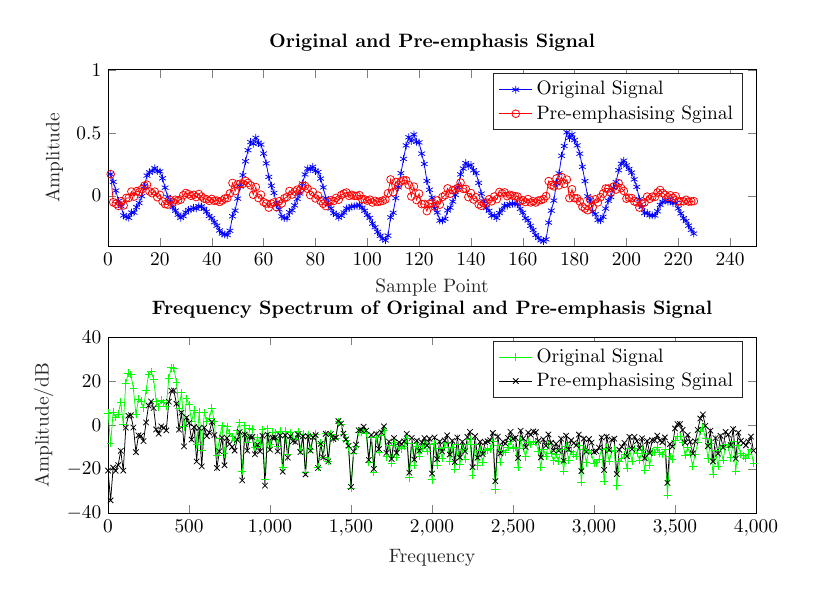
\begin{tikzpicture}[scale = 0.7]

\begin{axis}[%
width=4.628in,
height=1.259in,
at={(0.776in,2.432in)},
scale only axis,
xmin=0,
xmax=250,
xlabel style={font=\color{white!15!black}},
xlabel={Sample Point},
ymin=-0.4,
ymax=1,
ylabel style={font=\color{white!15!black}},
ylabel={Amplitude},
%axis background/.style={fill=white},
title style={font=\bfseries},
title={Original and Pre-emphasis Signal},
legend style={legend cell align=left, align=left, draw=white!15!black}
]
\addplot [color=blue, mark=asterisk, mark options={solid, blue}]
  table[row sep=crcr]{%
1	0.1710205078125\\
2	0.110565185546875\\
3	0.040985107421875\\
4	-0.042022705078125\\
5	-0.08331298828125\\
6	-0.156463623046875\\
7	-0.166229248046875\\
8	-0.1754150390625\\
9	-0.133636474609375\\
10	-0.13385009765625\\
11	-0.090850830078125\\
12	-0.05804443359375\\
13	-0.00384521484375\\
14	0.076141357421875\\
15	0.159820556640625\\
16	0.185546875\\
17	0.19622802734375\\
18	0.218780517578125\\
19	0.1961669921875\\
20	0.19305419921875\\
21	0.13812255859375\\
22	0.063873291015625\\
23	-0.009979248046875\\
24	-0.044891357421875\\
25	-0.091400146484375\\
26	-0.1187744140625\\
27	-0.1507568359375\\
28	-0.174896240234375\\
29	-0.162628173828125\\
30	-0.132598876953125\\
31	-0.113494873046875\\
32	-0.10845947265625\\
33	-0.096099853515625\\
34	-0.102142333984375\\
35	-0.083587646484375\\
36	-0.0858154296875\\
37	-0.1041259765625\\
38	-0.1270751953125\\
39	-0.161102294921875\\
40	-0.178375244140625\\
41	-0.210052490234375\\
42	-0.23822021484375\\
43	-0.27587890625\\
44	-0.30035400390625\\
45	-0.3079833984375\\
46	-0.312103271484375\\
47	-0.278228759765625\\
48	-0.162994384765625\\
49	-0.11859130859375\\
50	-0.022796630859375\\
51	0.07318115234375\\
52	0.16387939453125\\
53	0.27362060546875\\
54	0.361480712890625\\
55	0.425811767578125\\
56	0.412353515625\\
57	0.460205078125\\
58	0.41900634765625\\
59	0.4063720703125\\
60	0.3349609375\\
61	0.25665283203125\\
62	0.149383544921875\\
63	0.0792236328125\\
64	0.0224609375\\
65	-0.06884765625\\
66	-0.108978271484375\\
67	-0.164337158203125\\
68	-0.176971435546875\\
69	-0.178253173828125\\
70	-0.131591796875\\
71	-0.115447998046875\\
72	-0.076568603515625\\
73	-0.025115966796875\\
74	0.017669677734375\\
75	0.096893310546875\\
76	0.16900634765625\\
77	0.215362548828125\\
78	0.209747314453125\\
79	0.22991943359375\\
80	0.19683837890625\\
81	0.187713623046875\\
82	0.13604736328125\\
83	0.065582275390625\\
84	-0.019989013671875\\
85	-0.068267822265625\\
86	-0.101409912109375\\
87	-0.138641357421875\\
88	-0.14892578125\\
89	-0.17291259765625\\
90	-0.158782958984375\\
91	-0.13348388671875\\
92	-0.1014404296875\\
93	-0.09796142578125\\
94	-0.0859375\\
95	-0.082916259765625\\
96	-0.080322265625\\
97	-0.072052001953125\\
98	-0.094970703125\\
99	-0.119781494140625\\
100	-0.152618408203125\\
101	-0.17633056640625\\
102	-0.221282958984375\\
103	-0.250823974609375\\
104	-0.287872314453125\\
105	-0.31842041015625\\
106	-0.3424072265625\\
107	-0.354705810546875\\
108	-0.31707763671875\\
109	-0.172119140625\\
110	-0.135589599609375\\
111	-0.019287109375\\
112	0.067169189453125\\
113	0.17877197265625\\
114	0.292236328125\\
115	0.399566650390625\\
116	0.46441650390625\\
117	0.435394287109375\\
118	0.48638916015625\\
119	0.427703857421875\\
120	0.422943115234375\\
121	0.33447265625\\
122	0.25225830078125\\
123	0.116851806640625\\
124	0.04705810546875\\
125	-0.015594482421875\\
126	-0.1002197265625\\
127	-0.1329345703125\\
128	-0.197235107421875\\
129	-0.197052001953125\\
130	-0.184051513671875\\
131	-0.11669921875\\
132	-0.09490966796875\\
133	-0.04632568359375\\
134	0.006561279296875\\
135	0.06829833984375\\
136	0.169189453125\\
137	0.215545654296875\\
138	0.25921630859375\\
139	0.2352294921875\\
140	0.244476318359375\\
141	0.20233154296875\\
142	0.179534912109375\\
143	0.101654052734375\\
144	0.016571044921875\\
145	-0.044586181640625\\
146	-0.0966796875\\
147	-0.119781494140625\\
148	-0.158233642578125\\
149	-0.156646728515625\\
150	-0.17626953125\\
151	-0.13751220703125\\
152	-0.11114501953125\\
153	-0.0792236328125\\
154	-0.078765869140625\\
155	-0.067535400390625\\
156	-0.063262939453125\\
157	-0.063629150390625\\
158	-0.0672607421875\\
159	-0.10467529296875\\
160	-0.134796142578125\\
161	-0.178253173828125\\
162	-0.1961669921875\\
163	-0.239501953125\\
164	-0.272216796875\\
165	-0.312469482421875\\
166	-0.3353271484375\\
167	-0.3536376953125\\
168	-0.362213134765625\\
169	-0.346832275390625\\
170	-0.213714599609375\\
171	-0.118499755859375\\
172	-0.03851318359375\\
173	0.100311279296875\\
174	0.17791748046875\\
175	0.31695556640625\\
176	0.39520263671875\\
177	0.503753662109375\\
178	0.458831787109375\\
179	0.48699951171875\\
180	0.442657470703125\\
181	0.399261474609375\\
182	0.33367919921875\\
183	0.229644775390625\\
184	0.11602783203125\\
185	-0.00494384765625\\
186	-0.03558349609375\\
187	-0.125457763671875\\
188	-0.147186279296875\\
189	-0.19287109375\\
190	-0.195404052734375\\
191	-0.167938232421875\\
192	-0.10205078125\\
193	-0.039398193359375\\
194	-0.0107421875\\
195	0.0623779296875\\
196	0.10833740234375\\
197	0.202972412109375\\
198	0.253631591796875\\
199	0.278656005859375\\
200	0.241241455078125\\
201	0.212554931640625\\
202	0.18341064453125\\
203	0.1295166015625\\
204	0.06976318359375\\
205	-0.027740478515625\\
206	-0.089080810546875\\
207	-0.137451171875\\
208	-0.1378173828125\\
209	-0.1556396484375\\
210	-0.155364990234375\\
211	-0.1573486328125\\
212	-0.123809814453125\\
213	-0.072418212890625\\
214	-0.048370361328125\\
215	-0.03900146484375\\
216	-0.048614501953125\\
217	-0.042999267578125\\
218	-0.05706787109375\\
219	-0.057952880859375\\
220	-0.100799560546875\\
221	-0.140594482421875\\
222	-0.17822265625\\
223	-0.201568603515625\\
224	-0.237548828125\\
225	-0.27130126953125\\
226	-0.3009033203125\\
};
\addlegendentry{Original Signal}

\addplot [color=red, mark=o, mark options={solid, red}]
  table[row sep=crcr]{%
1	0.1710205078125\\
2	-0.051904296875\\
3	-0.0640518188476562\\
4	-0.0809585571289062\\
5	-0.0433914184570313\\
6	-0.0773162841796875\\
7	-0.0175888061523438\\
8	-0.0174972534179688\\
9	0.0330078125\\
10	-0.00689544677734374\\
11	0.0363067626953125\\
12	0.0282638549804688\\
13	0.0512969970703125\\
14	0.0797943115234375\\
15	0.0874862670898438\\
16	0.0337173461914063\\
17	0.01995849609375\\
18	0.0323638916015625\\
19	-0.0116744995117187\\
20	0.00669555664062502\\
21	-0.0452789306640625\\
22	-0.0673431396484375\\
23	-0.0706588745117187\\
24	-0.0354110717773437\\
25	-0.0487533569335937\\
26	-0.0319442749023438\\
27	-0.037921142578125\\
28	-0.03167724609375\\
29	0.00352325439453124\\
30	0.0218978881835938\\
31	0.0124740600585938\\
32	-0.000639343261718758\\
33	0.00693664550781249\\
34	-0.0108474731445313\\
35	0.0134475708007812\\
36	-0.00640716552734376\\
37	-0.022601318359375\\
38	-0.028155517578125\\
39	-0.040380859375\\
40	-0.0253280639648437\\
41	-0.0405960083007812\\
42	-0.0386703491210938\\
43	-0.0495697021484375\\
44	-0.03826904296875\\
45	-0.0226470947265625\\
46	-0.01951904296875\\
47	0.0182693481445312\\
48	0.101322937011719\\
49	0.0362533569335937\\
50	0.0898651123046875\\
51	0.0948379516601563\\
52	0.0943572998046875\\
53	0.117935180664062\\
54	0.101541137695313\\
55	0.0824050903320312\\
56	0.00783233642578129\\
57	0.06846923828125\\
58	-0.0181884765625\\
59	0.0083160400390625\\
60	-0.051092529296875\\
61	-0.06156005859375\\
62	-0.0944366455078125\\
63	-0.0626907348632812\\
64	-0.052801513671875\\
65	-0.090185546875\\
66	-0.043572998046875\\
67	-0.0608078002929688\\
68	-0.0208511352539062\\
69	-0.0101303100585937\\
70	0.0377487182617187\\
71	0.00956420898437499\\
72	0.0331069946289062\\
73	0.0476242065429687\\
74	0.0415298461914062\\
75	0.0801071166992187\\
76	0.0769577026367188\\
77	0.0548065185546875\\
78	0.00515289306640626\\
79	0.0306594848632813\\
80	-0.0215850830078125\\
81	0.0007171630859375\\
82	-0.0422805786132812\\
83	-0.0636627197265625\\
84	-0.0822921752929688\\
85	-0.0492782592773438\\
86	-0.0365554809570312\\
87	-0.0423019409179688\\
88	-0.0172164916992188\\
89	-0.03143310546875\\
90	0.00548400878906249\\
91	0.0173599243164062\\
92	0.0253692626953125\\
93	-0.00159301757812501\\
94	0.0071258544921875\\
95	-0.00127563476562501\\
96	-0.00155181884765625\\
97	0.004254150390625\\
98	-0.0265213012695313\\
99	-0.029559326171875\\
100	-0.0388259887695312\\
101	-0.0313430786132813\\
102	-0.0537689208984375\\
103	-0.0406051635742188\\
104	-0.0495895385742188\\
105	-0.0449417114257812\\
106	-0.0399078369140625\\
107	-0.0294189453125\\
108	0.0198928833007813\\
109	0.129104614257812\\
110	0.027923583984375\\
111	0.109523010253906\\
112	0.085491943359375\\
113	0.114961242675781\\
114	0.122402954101563\\
115	0.121942138671875\\
116	0.0848281860351563\\
117	-0.00580139160156246\\
118	0.0727645874023438\\
119	-0.0343658447265625\\
120	0.0166244506835938\\
121	-0.0673233032226562\\
122	-0.06549072265625\\
123	-0.122793579101562\\
124	-0.0639511108398437\\
125	-0.0602996826171875\\
126	-0.0854049682617188\\
127	-0.037725830078125\\
128	-0.070947265625\\
129	-0.00967864990234377\\
130	0.00314788818359374\\
131	0.0581497192382812\\
132	0.01595458984375\\
133	0.0438385009765625\\
134	0.0505706787109375\\
135	0.0620651245117188\\
136	0.104306030273438\\
137	0.054815673828125\\
138	0.0544479370117188\\
139	-0.0110260009765625\\
140	0.02100830078125\\
141	-0.0299209594726562\\
142	-0.0126800537109375\\
143	-0.0689041137695312\\
144	-0.0800003051757812\\
145	-0.0603286743164062\\
146	-0.0543228149414062\\
147	-0.027935791015625\\
148	-0.0444412231445312\\
149	-0.00632476806640625\\
150	-0.0274551391601563\\
151	0.02994384765625\\
152	0.0194915771484375\\
153	0.0263641357421875\\
154	-0.00350341796875001\\
155	0.00729217529296874\\
156	0.000895690917968747\\
157	-0.00352935791015625\\
158	-0.00681304931640625\\
159	-0.040777587890625\\
160	-0.0353546142578125\\
161	-0.0501968383789063\\
162	-0.0268264770507813\\
163	-0.053143310546875\\
164	-0.04468994140625\\
165	-0.053863525390625\\
166	-0.0384811401367188\\
167	-0.035076904296875\\
168	-0.02625732421875\\
169	-0.00272979736328127\\
170	0.115776062011719\\
171	0.0845291137695312\\
172	0.0740615844726562\\
173	0.136898803710937\\
174	0.0826217651367188\\
175	0.147933959960938\\
176	0.0940948486328125\\
177	0.128311157226562\\
178	-0.0197341918945312\\
179	0.0511093139648438\\
180	-0.0199920654296875\\
181	-0.0212631225585938\\
182	-0.0456192016601562\\
183	-0.0873504638671875\\
184	-0.102134704589844\\
185	-0.115170288085937\\
186	-0.0308868408203125\\
187	-0.0916534423828125\\
188	-0.0280014038085938\\
189	-0.0530441284179688\\
190	-0.012176513671875\\
191	0.0176956176757812\\
192	0.0574905395507812\\
193	0.057550048828125\\
194	0.0266860961914063\\
195	0.0725830078125\\
196	0.049078369140625\\
197	0.100051879882812\\
198	0.0608078002929688\\
199	0.0377059936523438\\
200	-0.0234817504882812\\
201	-0.0166244506835938\\
202	-0.0185165405273438\\
203	-0.0447235107421875\\
204	-0.053277587890625\\
205	-0.0940155029296875\\
206	-0.0627273559570312\\
207	-0.0528244018554688\\
208	-0.00723876953124999\\
209	-0.024713134765625\\
210	-0.00750732421875\\
211	-0.00975189208984376\\
212	0.02567138671875\\
213	0.0452011108398437\\
214	0.0204269409179687\\
215	0.00695037841796875\\
216	-0.0115631103515625\\
217	0.00318450927734375\\
218	-0.0162185668945313\\
219	-0.0037384033203125\\
220	-0.0457443237304688\\
221	-0.0448348999023438\\
222	-0.0446578979492188\\
223	-0.032257080078125\\
224	-0.0460586547851562\\
225	-0.0456298828125\\
226	-0.0431671142578125\\
};
\addlegendentry{Pre-emphasising Sginal}

\end{axis}

\begin{axis}[%
width=4.628in,
height=1.259in,
at={(0.776in,0.523in)},
scale only axis,
xmin=0,
xmax=4000,
xlabel style={font=\color{white!15!black}},
xlabel={Frequency},
ymin=-40,
ymax=40,
ylabel style={font=\color{white!15!black}},
ylabel={Amplitude/dB},
%axis background/.style={fill=white},
title style={font=\bfseries},
title={Frequency Spectrum of Original and Pre-emphasis Signal},
legend style={legend cell align=left, align=left, draw=white!15!black}
]
\addplot [color=green, mark=+, mark options={solid, green}]
  table[row sep=crcr]{%
0	5.40827081371513\\
15.625	-8.35104019707008\\
31.25	5.88308834270092\\
46.875	3.5224246352649\\
62.5	5.11692891931389\\
78.125	10.5210439782491\\
93.75	0.582932939112161\\
109.375	19.1224868911888\\
125	23.6436789023546\\
140.625	23.0253624724447\\
156.25	16.6939656646261\\
171.875	4.81015076739891\\
187.5	11.7873739562541\\
203.125	10.9212749395109\\
218.75	7.94021027130261\\
234.375	15.8452467422361\\
250	23.0045642082464\\
265.625	24.3717866147316\\
281.25	20.9413920717262\\
296.875	10.7543033828817\\
312.5	8.38580154301781\\
328.125	11.3477712866978\\
343.75	10.3370846916314\\
359.375	8.70175319631826\\
375	21.4373706642711\\
390.625	26.0417958116667\\
406.25	25.8273681640777\\
421.875	19.5157629571\\
437.5	7.43474824661809\\
453.125	14.8459976200642\\
468.75	-0.764269411503386\\
484.375	12.0799913539139\\
500	9.30715240389339\\
515.625	1.53134553616693\\
531.25	6.94852149303798\\
546.875	-8.89693642150358\\
562.5	6.0088705911594\\
578.125	-11.5901933428386\\
593.75	5.76848525245907\\
609.375	1.74345585874974\\
625	3.10565747284029\\
640.625	7.76345332731354\\
656.25	1.57602161970784\\
671.875	-13.5563864594262\\
687.5	-6.18063981561064\\
703.125	-0.201662038541201\\
718.75	-12.9068393611873\\
734.375	-0.667329532544346\\
750	-3.67648652242013\\
765.625	-5.12171296436723\\
781.25	-6.9639899042268\\
796.875	-2.22572659954514\\
812.5	1.16759722933188\\
828.125	-20.9557451697116\\
843.75	-0.307314615876585\\
859.375	-7.74712647806466\\
875	-1.52570683014233\\
890.625	-1.84924400257029\\
906.25	-9.8648838366823\\
921.875	-5.61088222791363\\
937.5	-8.80038396588559\\
953.125	-1.92291227286994\\
968.75	-24.6545881197325\\
984.375	-1.62640419920319\\
1000	-8.55779715073643\\
1015.625	-3.22149969739933\\
1031.25	-3.26397519688733\\
1046.875	-9.68331780683202\\
1062.5	-2.62210416427206\\
1078.125	-19.1879252828376\\
1093.75	-2.77816732916265\\
1109.375	-13.0539060806095\\
1125	-3.4025550074751\\
1140.625	-5.84290757985882\\
1156.25	-6.26830686127279\\
1171.875	-2.95871924951334\\
1187.5	-11.1051977965283\\
1203.125	-3.99144368871817\\
1218.75	-21.4367861959042\\
1234.375	-4.19769878523073\\
1250	-10.7980942324398\\
1265.625	-4.88786397573113\\
1281.25	-3.97902174636401\\
1296.875	-18.9718997564802\\
1312.5	-8.09959294145157\\
1328.125	-14.3851809982545\\
1343.75	-3.74362092087673\\
1359.375	-16.3254435020903\\
1375	-4.08544344489408\\
1390.625	-6.39454142533365\\
1406.25	-5.83793969745179\\
1421.875	1.55946793048503\\
1437.5	0.341185546548993\\
1453.125	-4.24673440444078\\
1468.75	-7.02721806424154\\
1484.375	-9.96437066144842\\
1500	-28.7081156490545\\
1515.625	-12.7206330150189\\
1531.25	-9.69690308674991\\
1546.875	-3.20616858075224\\
1562.5	-3.17443183262903\\
1578.125	-1.77570976731911\\
1593.75	-3.60643252587893\\
1609.375	-16.9454871715211\\
1625	-5.71437770562643\\
1640.625	-21.2125296372085\\
1656.25	-5.40366222280517\\
1671.875	-12.3561060098302\\
1687.5	-4.80787682431354\\
1703.125	-2.16494032903246\\
1718.75	-14.2734006655386\\
1734.375	-9.26424364173217\\
1750	-17.1858954967744\\
1765.625	-7.7544618123369\\
1781.25	-14.5429621000044\\
1796.875	-9.81217120459039\\
1812.5	-10.6861880283406\\
1828.125	-9.52226170388984\\
1843.75	-6.17936172816236\\
1859.375	-23.8473239847329\\
1875	-8.07994931504511\\
1890.625	-18.0203670312643\\
1906.25	-9.47845632024982\\
1921.875	-14.1006319986631\\
1937.5	-10.3922735593436\\
1953.125	-8.45957382089354\\
1968.75	-11.8996155603159\\
1984.375	-8.87491852360245\\
2000	-24.74208969957\\
2015.625	-8.37060600739844\\
2031.25	-18.3040907786186\\
2046.875	-10.3836302171195\\
2062.5	-14.9301070995161\\
2078.125	-9.95648982966084\\
2093.75	-7.69142027227938\\
2109.375	-16.4380706393584\\
2125	-10.2948682821614\\
2140.625	-19.9062272225408\\
2156.25	-8.85605555897793\\
2171.875	-17.9429688423413\\
2187.5	-10.9146121672467\\
2203.125	-15.3167256709734\\
2218.75	-8.81712187302642\\
2234.375	-6.57511488814576\\
2250	-22.6182557733251\\
2265.625	-8.57682813331342\\
2281.25	-18.3718637454596\\
2296.875	-11.2533096842985\\
2312.5	-16.8397295607204\\
2328.125	-11.5519428795264\\
2343.75	-11.2033704251985\\
2359.375	-10.6327420861428\\
2375	-7.43287156910064\\
2390.625	-29.3558397576353\\
2406.25	-9.14145281533861\\
2421.875	-16.7819947643236\\
2437.5	-11.5932955942435\\
2453.125	-12.401402771118\\
2468.75	-9.86176694414701\\
2484.375	-7.18497906030814\\
2500	-10.350339962494\\
2515.625	-9.90944097199439\\
2531.25	-19.113251753867\\
2546.875	-6.81154938297959\\
2562.5	-10.336903260382\\
2578.125	-14.3163297857775\\
2593.75	-7.73341794001978\\
2609.375	-8.75629398726465\\
2625	-7.30322900466805\\
2640.625	-7.68964581381112\\
2656.25	-11.669780572866\\
2671.875	-19.1701326246384\\
2687.5	-10.9577139919911\\
2703.125	-13.9392605975164\\
2718.75	-8.85468061910957\\
2734.375	-12.6493264607757\\
2750	-16.1678327532318\\
2765.625	-13.161750667107\\
2781.25	-16.3692527362455\\
2796.875	-10.9242272049411\\
2812.5	-20.9773469593145\\
2828.125	-9.60803370340763\\
2843.75	-15.8888463912936\\
2859.375	-11.7313679635032\\
2875	-13.0206119223406\\
2890.625	-14.0585661318926\\
2906.25	-9.24359526471755\\
2921.875	-25.8282850412012\\
2937.5	-11.1180463886498\\
2953.125	-17.0883973328615\\
2968.75	-11.3464725816051\\
2984.375	-12.9742007728034\\
3000	-17.2629856816225\\
3015.625	-17.0194868319483\\
3031.25	-15.3384822622595\\
3046.875	-10.7746592594997\\
3062.5	-25.5085624343159\\
3078.125	-10.4276063486108\\
3093.75	-16.4824286228385\\
3109.375	-11.8109323939791\\
3125	-11.4114399277246\\
3140.625	-27.4855905861035\\
3156.25	-16.491967531025\\
3171.875	-15.0786550968426\\
3187.5	-13.3550243692627\\
3203.125	-19.4420638092286\\
3218.75	-10.6362040661084\\
3234.375	-16.2583299229511\\
3250	-10.7361075227836\\
3265.625	-12.6608598851841\\
3281.25	-15.8807287069735\\
3296.875	-11.4089514340232\\
3312.5	-20.4432570698499\\
3328.125	-12.6904912516215\\
3343.75	-18.1566530256949\\
3359.375	-12.2559780652447\\
3375	-12.4372119164276\\
3390.625	-10.2438242308491\\
3406.25	-12.5122027371215\\
3421.875	-13.2487619983794\\
3437.5	-11.1106856948236\\
3453.125	-31.7691236655032\\
3468.75	-14.1651875872632\\
3484.375	-15.3057884538561\\
3500	-7.11760931549762\\
3515.625	-5.17608318353374\\
3531.25	-5.15927198064225\\
3546.875	-7.8047527396488\\
3562.5	-13.643141988004\\
3578.125	-10.0869637010959\\
3593.75	-13.222032814356\\
3609.375	-18.5326891041806\\
3625	-13.0280382533479\\
3640.625	-7.85327709921161\\
3656.25	-2.7038488993809\\
3671.875	-0.857990483909159\\
3687.5	-5.97216429864982\\
3703.125	-15.2006294057977\\
3718.75	-8.24046754983135\\
3734.375	-22.236669577926\\
3750	-11.6160514640818\\
3765.625	-18.6724018061854\\
3781.25	-10.5752669995076\\
3796.875	-15.8860071586964\\
3812.5	-8.81539237596156\\
3828.125	-10.0241399422373\\
3843.75	-14.8054171139467\\
3859.375	-7.5324367089931\\
3875	-20.9759696783014\\
3890.625	-9.19406881199881\\
3906.25	-12.9161243193082\\
3921.875	-13.8957592754897\\
3937.5	-14.939583831215\\
3953.125	-13.1980906459716\\
3968.75	-10.9678497031454\\
3984.375	-17.3225897308445\\
};
\addlegendentry{Original Signal}

\addplot [color=black, mark=x, mark options={solid, black}]
  table[row sep=crcr]{%
0	-20.6123290995645\\
15.625	-34.1299592859091\\
31.25	-19.2423539353726\\
46.875	-20.6940841724776\\
62.5	-18.0809553494303\\
78.125	-11.6430746596222\\
93.75	-20.5815131358616\\
109.375	-1.0975181725915\\
125	4.30657255888305\\
140.625	4.51038860774119\\
156.25	-1.0558159831426\\
171.875	-12.2264902917873\\
187.5	-4.5831609218443\\
203.125	-4.82545284997052\\
218.75	-7.22071179873665\\
234.375	1.23595424391961\\
250	8.91609739961893\\
265.625	10.7763023974814\\
281.25	7.81364438876564\\
296.875	-1.92867375912481\\
312.5	-3.87336522794903\\
328.125	-0.506775993991639\\
343.75	-1.1304685833433\\
359.375	-2.39504208686808\\
375	10.6963347415095\\
390.625	15.6426261863844\\
406.25	15.7571627674857\\
421.875	9.76251081597605\\
437.5	-2.01275789873099\\
453.125	5.69375724329825\\
468.75	-9.63106472130658\\
484.375	3.48942031648761\\
500	0.984131936504656\\
515.625	-6.53229789948619\\
531.25	-0.863460104380869\\
546.875	-16.4645504008007\\
562.5	-1.3212825041124\\
578.125	-18.6894348877042\\
593.75	-1.10606377251877\\
609.375	-4.91231383891711\\
625	-3.33696239227523\\
640.625	1.52861741684403\\
656.25	-4.45615084974566\\
671.875	-19.3907872622879\\
687.5	-11.8219471599802\\
703.125	-5.65435444031222\\
718.75	-18.1752083540102\\
734.375	-5.75549133203015\\
750	-8.5883927489717\\
765.625	-9.86116051689162\\
781.25	-11.5346300664447\\
796.875	-6.63107345143944\\
812.5	-3.07584096960801\\
828.125	-25.0405371587852\\
843.75	-4.23660731082547\\
859.375	-11.5239574788186\\
875	-5.15301019820154\\
890.625	-5.32985564129025\\
906.25	-13.2015465078096\\
921.875	-8.80625023443639\\
937.5	-11.857027528347\\
953.125	-4.8433216237004\\
968.75	-27.4411773378451\\
984.375	-4.28151480503647\\
1000	-11.0837014800836\\
1015.625	-5.62040407071246\\
1031.25	-5.53802289926368\\
1046.875	-11.8345918925596\\
1062.5	-4.65263009861322\\
1078.125	-21.0996734326504\\
1093.75	-4.57305531298638\\
1109.375	-14.73380098796\\
1125	-4.96927549629866\\
1140.625	-7.29822586037157\\
1156.25	-7.61395057375775\\
1171.875	-4.19637324305102\\
1187.5	-12.2365058150957\\
1203.125	-5.01800997059766\\
1218.75	-22.3601769918934\\
1234.375	-5.01944380073409\\
1250	-11.5196879981468\\
1265.625	-5.51076715124292\\
1281.25	-4.50466236081407\\
1296.875	-19.4016743899084\\
1312.5	-8.43486785042321\\
1328.125	-14.6272931889751\\
1343.75	-3.89387917282648\\
1359.375	-16.385129344999\\
1375	-4.05581209168495\\
1390.625	-6.2768226634893\\
1406.25	-5.63333874109602\\
1421.875	1.84976962564848\\
1437.5	0.71602950343598\\
1453.125	-3.788484430833\\
1468.75	-6.48667680186781\\
1484.375	-9.34263200639211\\
1500	-28.0062533223922\\
1515.625	-11.9397011928245\\
1531.25	-8.83793700460029\\
1546.875	-2.27018511401583\\
1562.5	-2.16243005374164\\
1578.125	-0.688671481180554\\
1593.75	-2.44532278443807\\
1609.375	-15.7112547685549\\
1625	-4.40795565266113\\
1640.625	-19.8348356214774\\
1656.25	-3.95559904808715\\
1671.875	-10.8385620209656\\
1687.5	-3.22172631615092\\
1703.125	-0.511043940518553\\
1718.75	-12.5526057596237\\
1734.375	-7.47738467172878\\
1750	-15.333794359773\\
1765.625	-5.83792819024877\\
1781.25	-12.5627937887744\\
1796.875	-7.76915443209275\\
1812.5	-8.58109776144388\\
1828.125	-7.35586194515465\\
1843.75	-3.95240580261007\\
1859.375	-21.5605548171018\\
1875	-5.7340996979307\\
1890.625	-15.61615988452\\
1906.25	-7.01660494200652\\
1921.875	-11.5818403083079\\
1937.5	-7.81723633278251\\
1953.125	-5.82897691840711\\
1968.75	-9.21413614730149\\
1984.375	-6.13522528448434\\
2000	-21.9488430451439\\
2015.625	-5.52445827586617\\
2031.25	-15.4056864305557\\
2046.875	-7.43360602460823\\
2062.5	-11.9290923296654\\
2078.125	-6.90510642272506\\
2093.75	-4.59028301457816\\
2109.375	-13.2877873311912\\
2125	-7.0960399009011\\
2140.625	-16.6594480810841\\
2156.25	-5.56191345972066\\
2171.875	-14.6020452268417\\
2187.5	-7.52748226173081\\
2203.125	-11.8839586278316\\
2218.75	-5.33928090844338\\
2234.375	-3.05275741599958\\
2250	-19.0519335354871\\
2265.625	-4.96708732647356\\
2281.25	-14.7192451445971\\
2296.875	-7.55834876291462\\
2312.5	-13.102956607942\\
2328.125	-7.77388311418828\\
2343.75	-7.38454410700572\\
2359.375	-6.77366462401119\\
2375	-3.53405362676975\\
2390.625	-25.4177873566441\\
2406.25	-5.16466743545154\\
2421.875	-12.76697344149\\
2437.5	-7.54053101617122\\
2453.125	-8.31138337053923\\
2468.75	-5.73497698984963\\
2484.375	-3.02189874600564\\
2500	-6.15144549360244\\
2515.625	-5.67520465038301\\
2531.25	-14.844142060647\\
2546.875	-2.50803105939255\\
2562.5	-5.99943738684741\\
2578.125	-9.94537385915745\\
2593.75	-3.32942594915582\\
2609.375	-4.31971648684003\\
2625	-2.83451318744764\\
2640.625	-3.18923558130815\\
2656.25	-7.13811660448402\\
2671.875	-14.6076524453349\\
2687.5	-6.36485203850724\\
2703.125	-9.31644828321667\\
2718.75	-4.20234639747312\\
2734.375	-7.96789588757925\\
2750	-11.4577285474641\\
2765.625	-8.42339277065218\\
2781.25	-11.6030583723717\\
2796.875	-6.13061093563055\\
2812.5	-16.1567207414683\\
2828.125	-4.76080694395902\\
2843.75	-11.0154260012621\\
2859.375	-6.83215841101991\\
2875	-8.09601528467531\\
2890.625	-9.10898214651208\\
2906.25	-4.26942137940242\\
2921.875	-20.8299164632501\\
2937.5	-6.09587613319628\\
2953.125	-12.0428162703302\\
2968.75	-6.27786948433173\\
2984.375	-7.88296236084318\\
3000	-12.1494966677702\\
3015.625	-11.8841299659934\\
3031.25	-10.1816383744982\\
3046.875	-5.59670730352508\\
3062.5	-20.3098795291083\\
3078.125	-5.20856781994758\\
3093.75	-11.2434080440437\\
3109.375	-6.55230162603191\\
3125	-6.13356915874618\\
3140.625	-22.1888483702389\\
3156.25	-11.1767208267394\\
3171.875	-9.74526930464845\\
3187.5	-8.0038633688945\\
3203.125	-14.0734899962821\\
3218.75	-5.25057838815986\\
3234.375	-10.8560119151724\\
3250	-5.3174553430683\\
3265.625	-7.22623034879895\\
3281.25	-10.4304773207506\\
3296.875	-5.94343243010612\\
3312.5	-14.9628234390078\\
3328.125	-7.19549477614484\\
3343.75	-12.6474443118855\\
3359.375	-6.73290657551376\\
3375	-6.90062600101288\\
3390.625	-4.69407115916509\\
3406.25	-6.94962872875318\\
3421.875	-7.67371225373218\\
3437.5	-5.5235044254408\\
3453.125	-26.1701541240623\\
3468.75	-8.55477209726115\\
3484.375	-9.68426843899604\\
3500	-1.48532532878637\\
3515.625	0.466625063899398\\
3531.25	0.49352162971015\\
3546.875	-2.14221187914557\\
3562.5	-7.97119123312836\\
3578.125	-4.40593967844154\\
3593.75	-7.53227144890834\\
3609.375	-12.8345256466728\\
3625	-7.32180730740681\\
3640.625	-2.13931264830196\\
3656.25	3.01751566644326\\
3671.875	4.87044137361844\\
3687.5	-0.236997432179462\\
3703.125	-9.45905929892083\\
3718.75	-2.49282548292758\\
3734.375	-16.4832863691365\\
3750	-5.85725749508568\\
3765.625	-12.908527047843\\
3781.25	-4.80664103737853\\
3796.875	-10.1129592184399\\
3812.5	-3.03825134862799\\
3828.125	-4.24323440945766\\
3843.75	-9.0210753730288\\
3859.375	-1.74498679793128\\
3875	-15.1857394007084\\
3890.625	-3.40138576196616\\
3906.25	-7.12131590620433\\
3921.875	-8.09915274870182\\
3937.5	-9.14150630484265\\
3953.125	-7.3988691234801\\
3968.75	-5.16781110198559\\
3984.375	-11.5220609070467\\
};
\addlegendentry{Pre-emphasising Sginal}

\end{axis}
\end{tikzpicture}%
\end{frame}


\end{document}